%%%%%%%%%%%%%%%%%%%%%%%%%%%%%%%%%%%%%%%%%%%%%%%%%%%%
%%%                                              %%%
%%%     Language Science Press Master File       %%%
%%%         follow the instructions below        %%%
%%%                                              %%%
%%%%%%%%%%%%%%%%%%%%%%%%%%%%%%%%%%%%%%%%%%%%%%%%%%%% 

\documentclass[output=book,
  nonflat,
  modfonts
%   colorlinks
%   ,draft,draftmode
		  ]{langsci/langscibook}    
  
%%%%%%%%%%%%%%%%%%%%%%%%%%%%%%%%%%%%%%%%%%%%%%%%%%%%
%%%                                              %%%
%%%          additional packages                 %%%
%%%                                              %%%
%%%%%%%%%%%%%%%%%%%%%%%%%%%%%%%%%%%%%%%%%%%%%%%%%%%%
 

\title{Methods in prosody:\, \newlineCover A Romance language perspective}  
\author{Ingo Feldhausen\and Jan Fliessbach\lastand Maria del Mar Vanrell} 
\renewcommand{\lsSeriesNumber}{6}  
% \renewcommand{\lsCoverTitleFont}[1]{\sffamily\addfontfeatures{Scale=MatchUppercase}\fontsize{38pt}{12.75mm}\selectfont #1}

\renewcommand{\lsISBNdigital}{978-3-96110-104-7}
\renewcommand{\lsISBNhardcover}{978-3-96110-105-4}

\renewcommand{\lsSeries}{silp}          
\renewcommand{\lsSeriesNumber}{6}
\renewcommand{\lsURL}{http://langsci-press.org/catalog/book/183}
\renewcommand{\lsID}{183}
\renewcommand{\lsBookDOI}{10.5281/zenodo.1471564}

\typesetter{Jan Fliessbach\lastand Felix Kopecky}
\proofreader{Adrien Barbaresi, Amir Ghorbanpour, Aysel Saricaoglu, Brett Reynolds, Conor Pyle, Daniela Kolbe-Hanna, Jeroen van de Weijer, Sebastian Nordhoff\lastand Varun deCastro-Arrazola}

\BackBody{This book presents a collection of pioneering papers reflecting current methods in prosody research with a focus on Romance languages. The rapid expansion of the field of prosody research in the last decades has given rise to a proliferation of methods that has left little room for the critical assessment of these methods. The aim of this volume is to bridge this gap by embracing original contributions, in which experts in the field assess, reflect, and discuss different methods of data gathering and analysis. The book might thus be of interest to scholars and established researchers as well as to students and young academics who wish to explore the topic of prosody, an expanding and promising area of study.}

\usepackage{langsci-optional}
\usepackage{langsci-gb4e}
\usepackage{langsci-lgr}

\usepackage{listings}
\lstset{basicstyle=\ttfamily,tabsize=2,breaklines=true}

%added by author
% \usepackage{tipa}
\usepackage{multirow}
\graphicspath{{figures/}}
\usepackage{langsci-branding}

%% hyphenation points for line breaks
%% Normally, automatic hyphenation in LaTeX is very good
%% If a word is mis-hyphenated, add it to this file
%%
%% add information to TeX file before \begin{document} with:
%% %% hyphenation points for line breaks
%% Normally, automatic hyphenation in LaTeX is very good
%% If a word is mis-hyphenated, add it to this file
%%
%% add information to TeX file before \begin{document} with:
%% %% hyphenation points for line breaks
%% Normally, automatic hyphenation in LaTeX is very good
%% If a word is mis-hyphenated, add it to this file
%%
%% add information to TeX file before \begin{document} with:
%% \include{localhyphenation}
\hyphenation{
affri-ca-te
affri-ca-tes
an-no-tated
com-ple-ments
com-po-si-tio-na-li-ty
non-com-po-si-tio-na-li-ty
Gon-zá-lez
out-side
Ri-chárd
se-man-tics
STREU-SLE
Tie-de-mann
}
\hyphenation{
affri-ca-te
affri-ca-tes
an-no-tated
com-ple-ments
com-po-si-tio-na-li-ty
non-com-po-si-tio-na-li-ty
Gon-zá-lez
out-side
Ri-chárd
se-man-tics
STREU-SLE
Tie-de-mann
}
\hyphenation{
affri-ca-te
affri-ca-tes
an-no-tated
com-ple-ments
com-po-si-tio-na-li-ty
non-com-po-si-tio-na-li-ty
Gon-zá-lez
out-side
Ri-chárd
se-man-tics
STREU-SLE
Tie-de-mann
}
\bibliography{localbibliography} 

%%%%%%%%%%%%%%%%%%%%%%%%%%%%%%%%%%%%%%%%%%%%%%%%%%%%
%%%                                              %%%
%%%             Frontmatter                      %%%
%%%                                              %%%
%%%%%%%%%%%%%%%%%%%%%%%%%%%%%%%%%%%%%%%%%%%%%%%%%%%% 
\begin{document}     

\newcommand{\sent}{\enumsentence}
\newcommand{\sents}{\eenumsentence}
\let\citeasnoun\citet

\renewcommand{\lsCoverTitleFont}[1]{\sffamily\addfontfeatures{Scale=MatchUppercase}\fontsize{44pt}{16mm}\selectfont #1}
   
 

\maketitle                
\frontmatter 

\currentpdfbookmark{Contents}{name} % adds a PDF bookmark
\tableofcontents 

\addchap{Preface}
\begin{refsection}

%content goes here
 
% \printbibliography[heading=subbibliography]
\end{refsection}


\addchap{Acknowledgements} 
%\section{Acknowledgements}

This book is based on my habilitation thesis conducted in the course of my post-doctoral position at the Osnabrück University (2015--2020). I am profoundly grateful to many people for their constant support throughout this research process.


First and foremost, I would like to acknowledge with gratitude the support of my supervisors, Trudel Meisenburg and Laura Colantoni, who, while always showing confidence in my work, never stopped helping, challenging and sharing their ideas with me. I enjoyed all discussions and time with them! I also thank Frank Kügler for his interest, support and willingness to review my study -- this all happened at a coffee break at the ICPhS\,2019 in Melbourne and I was very happy to get him on board.



This work would have never been published without the interest and support of the editors of the series Open Romance Linguistics in Language Science Press (LSP). I am especially thankful to Lorenzo Filipponio for his advice, patience and availability, and two peer reviewers for their insightful comments and very valuable suggestions that helped to improve the manuscript.



In the Czech Republic, I thank Kamil Gregůrek and Language School \textit{Hispánica} in Brno, \textit{Instituto Cervantes} in Prague, Štěpánka Černikovská and Jan Chromý from the Faculty of Arts at Charles University in Prague and Paolo Divizia from the Faculty of Arts at Masaryk University in Brno for helping me to recruit and organise participants in my experiments. I am also very grateful to Marek Stehlík from the Faculty of Informatics at Masaryk University in Brno and Filip Smolík from the Laboratory of Behavioral and Linguistic Studies (LABELS) in Prague for giving me the opportunity to run my experiments in their departments.



Furthermore, I thank my colleagues in Germany and elsewhere, among them Bistra Andreeva, Stefan Baumann, Ariadna Benet, Susana Cortés, Elisabeth De\-lais-Rous\-sa\-rie, Yves D’hulst, Gorka Elordieta, Wendy Elvira-García, Ingo Feldhausen, Christoph Gabriel, Fatima Hamlaoui, Sun-Ah Jun, Ina Lehmkuhle, Ineke Mennen, Nathalie Nicolay, Francesca Nicora, Katharina Nimz, Pekka Posio, Pilar Prieto, Karin Puga, Uli Reich, Valentin Rose, Paolo Roseano, Fabian Santiago, Karsten Schmidt, Rolf Schöneich, Raphaël Sichel-Bazin, Johanna Stahnke, Maria del Mar Vanrell, Meg Zellers, and Marzena Żygis, for their help, discussions and/or valuable feedback at different conferences and at different stages of the project. 



A special word of gratitude goes to Michael Kennedy-Scanlon, Dale Bruton and LSP community for English proofreading as well as to my students Ron Gerstmann, Laura Strokorb and Belén María Viñas Fernández for orthographic transcriptions of the data and to Luisa Sprehe and Roxanne Krüger for carefully checking the bibliography. I am also grateful to all the motivated and patient speakers who participated in my study, without whom this work would never have been possible.



Last but not least, I thank my husband Jordan, my family and all my friends for always being there and for having kept me going.

\addchap{Abbreviations}
\begin{tabular}{ll}
CR & Common Room     \\
NCR & non-Common Room        \\
SGH & Selwyn Girls' High     \\
The & BBs: The Blazer Brigade \\
\isi{The PCs} & The Palms Crew  \\
\end{tabular} 

\mainmatter   


%%%%%%%%%%%%%%%%%%%%%%%%%%%%%%%%%%%%%%%%%%%%%%%%%%%%%%%%%%%%%%
%
%                      Introduction  
%
%%%%%%%%%%%%%%%%%%%%%%%%%%%%%%%%%%%%%%%%%%%%%%%%%%%%%%%%%%%%%%
% 

\part{Introduction}
\renewcommand\thechapter{}
\renewcommand\thesection{\arabic{section}}
\renewcommand\thetable{\arabic{table}}
\renewcommand\thefigure{\arabic{figure}}
\addchap{Introduction}

Of all the fields of study to which human beings have devoted themselves, linguistics could lay claim to being the most conservative. Two thousand five hundred years ago, Panini began it by describing an individual human language, and describing individual languages is what the majority of linguists are still doing. Even during the last couple of decades, in which linguists have begun to be interested in some of the larger issues that language involves, the main thrust toward clarifying those issues has involved making more and more detailed and ingenious descriptions of currently existing natural languages. In consequence, little headway has been made toward answering the really important questions which language raises, such as: how is language acquired by the individual, and how was it acquired by the species?

The importance of these questions is, I think, impossible to exaggerate. Language has made our species what it is, and until we really understand it -- that is, understand what is necessary for it to be acquired and transmitted, and how it interacts with the rest of our cognitive apparatus -- we cannot hope to understand ourselves. And unless we can understand ourselves, we will continue to watch in helpless frustration while the world we have created slips further and further from our control.

The larger and, in a popular sense, more human issues which language involves lie outside the scope of the present work, and will be dealt with at length in a forthcoming volume, \textit{Language} \textit{and} \textit{Species.} First, there is a good deal of academic spadework to be done. In the chapters that follow, I shall try to develop a unified theory which will propose at least a partial answer to three questions, none of which has as yet been satisfactorily resolved:

%\setcounter{itemize}{0}
\begin{enumerate}
\item How did creole languages originate?
\item How do children acquire language?
\item How did human language originate?
\end{enumerate} 

Traditionally, these three questions, insofar as they have been treated at all, have been treated as wholly unrelated. None of the solutions offered for (1) have had any relevance to (2) or (3); none of the solu\-tions offered for (2) have had any relevance to (1) or (3); and none of the solutions offered for (3) have had any relevance to (1) or (2). It has even been explicitly denied, although without a shred of support\-ing evidence, that an answer to (1) could possibly be an answer to (3) \citep{Sankoff1979}. Here and there, a few insightful scholars have hinted at possible links between the problems, and such insights will be ac\-knowledged in subsequent pages. However, a single, unified treatment has never even been attempted, and this book, whatever its short\-comings, may therefore claim at least some measure of originality. Doubtless many of its details will need revision or replacement; the explorer is seldom the best cartographer. However, of one thing I am totally convinced: that the three questions are really one question, and that an answer to any one of them which does not at the same time answer the other two will be, ipso facto, a wrong answer.

I shall begin with the origin of creoles. To some, this may appear the least general and least interesting question of the three. However, as I shall show, creoles constitute the indispensable key to the two larger problems, and this should come as no surprise to those familiar with the history of science, in which, repeatedly, the sideshow of one generation has been the central arena of the next. In \chapref{ch:1}, I shall examine the relationship between the variety of Creole English spoken in Hawaii and the pidgin which immediately preceded it, and I shall show how several elements of that creole could not have been derived from its antecedent pidgin, or from any of the other languages that were in contact at the time of creole formation, and that therefore these elements must have been, in some sense, ``invented''. In \chapref{ch:2}, I shall discuss some (not all -- there would not be space for all) of the features which are shared by a wide range of creole languages and show some striking resemblances between the ``inventions'' of Hawaii and ``inventions'' of other regions which must have emerged quite independently; and I shall also try to probe more deeply into certain aspects of creole syntax and semantics which may prove signifi\-cant when we come to deal with the other two questions. In \chapref{ch:3}, which will deal with ``normal'' language acquisition in noncreole societies, I shall show that some of the things which children seem to acquire effortlessly, as well as some which they get consistently wrong -- both equally puzzling to previous accounts of ``language learning{\textquotedbl} -- follow naturally from the theory which was developed to account for creole origins: that all members of our species are born with a bio\-program for language which can function even in the absence of ade\-quate input. In \chapref{ch:4}, I shall try to show where this bioprogram comes from: partly from the species-specific structure of human perception and cognition, and partly from processes inherent in the expansion of a linear language. At the same time, we will be able to resolve the continuity paradox (``language is too different from animal communication systems to have ever evolved from them{\textquotedbl}; ``language, like any other adaptive mechanism, must have been derived by regular evolutionary processes{\textquotedbl}) which has lain like some huge roadblock across the study of language origins. In the final chapter, I shall briefly summarize and integrate the findings of previous chapters, and suggest answers to some of the criticisms which may be brought against the concept of a genetic program for human language.

\begingroup
\fontsize{10}{12}\selectfont

%%%%%%%%%%%%%%%%%%%%%%%%%%%%%%%%%%%%%%%%%%%%%%%%%%%%%%%%%%%%%%
%
%                      Dictionary  
%
%%%%%%%%%%%%%%%%%%%%%%%%%%%%%%%%%%%%%%%%%%%%%%%%%%%%%%%%%%%%%%
\nocite{Heine1999}
\part{Ik-English dictionary}
\lohead{}
\rohead{} 
\ohead{}
\ihead{}
\chead{\rightmark\hfill\leftmark} 

\newcommand{\headrulewidth}{0pt}
\setlength{\columnsep}{3em}
 
\setlength{\parindent}{0pt}


\renewcommand{\lsgloss}[1]{} 
\renewcommand{\citationform}[1]{\textbf{#1}\markboth{#1}{#1}}    

\begin{letter}{a}
\tbLX{a}\tbHM{} \tbPH{à} \tbPS{conj.} \tbSN \tbGE{and} \tbXV{O waɛ la a wa gaŋ.} \tbXE{S/he came and left.} \tbSN \tbGE{in order to} \tbXV{O waɛ la a na nyɛ te.} \tbXE{S/he has come in order to visit us.}
\tbLX{a}\tbHM{} \tbPH{á} \tbPS{conj.} \tbGE{but} \tbXV{A wola ka o ba wa?} \tbXE{But why didn't s/he come?} \tbVA{ana}
\tbLX{a}\tbHM{} \tbPH{à} \tbPS{pron.} \tbGE{they, them (3rd person plural weak form nonhuman)} \tbXV{Vɛŋ ka a kpɛ a zage.} \tbXE{Let them go into the pen.} \tbXV{De a moɔ eŋ a.} \tbXE{Give them the grass.}
\tbLX{a}\tbHM{} \tbPH{à} \tbPS{def. art.} \tbGE{the} \tbXV{A bie kpɛ la a die.} \tbXE{The child has gone into the room.}
\tbLX{a}\tbHM{} \tbPH{á} \tbPS{v.} \tbGE{to hate} \tbXV{Te a ba la.} \tbXE{We hate them.} \tbPD{aɛ, aara, aara, aareba, aaraa, aareba }
\tbLX{aa}\tbHM{} \tbPH{áà} \tbPS{interj.} \tbGE{expression of surprise and regret} \tbXV{ A ŋmane ŋmarɛɛ la, aa.} \tbXE{The calabash is broken; what a pity!} \tbXV{ Aa, ka N da baŋ ka lɛ N gaaɛ.} \tbXE{Oh, if I had known, I would have gone.}
\tbLX{aa}\tbHM{} \tbPH{áá} \tbPS{interj.} \tbGE{expression of regret}
\tbLX{aa}\tbHM{} \tbPH{àà} \tbPS{interj.} \tbGE{expression expressing  {``}I told you so."}
\tbLX{aae}\tbHM{} \tbPH{ááɪ́} \tbPS{interj.} \tbGE{expression of pain}
\tbLX{a-a}\tbHM{} \tbPH{á-à} \tbPS{interj.} \tbSN \tbGE{expression of disapproval} \tbXV{A-a, ta de ona.} \tbXE{Oh no, don't go that way.} \tbSN \tbGE{ why?; expression of doubt} \tbXV{A-a, fo naŋ ba gaa?} \tbXE{Well, you haven't gone yet?}
\tbLX{ãa}\tbHM{} \tbPH{ã̀ã́} \tbPS{adv.} \tbSN \tbGE{yes (answer to a call)} \tbXV{N boɔle la a bie ka o sage ka {``}ãa."} \tbXE{I called the child and he answered, {``}Yes."} \tbSN \tbGE{what? (exclamation of disbelief)} \tbXV{Ka Naa boɔle fo ka fo zagere, ãa.} \tbXE{You refuse to answere the chief's call, what?}
\tbLX{ãaa}\tbHM{} \tbPH{ã̀ã́ã̀} \tbPS{interj.} \tbGE{is that so? (expression of uncertain surprise)} \tbXV{Bayuoː A pɔgebil-pɛɛre na taa la poɔ. Ayuoː Ãaa?} \tbXE{Bayuo: That teenage girl is pregnant. Ayuo: Is that true?}
\tbLX{âaa}\tbHM{} \tbPH{ã̀ã́ã́} \tbPS{part.} \tbGE{answer in agreement} \tbXV{Fo na gaa la? âaa.} \tbXE{Will you go? Yes, I will.}
\tbLX{aa-ee}\tbHM{} \tbPH{áá-ɪ̀ɪ́} \tbPS{interj.} \tbGE{expression of lack of confidence in someone's ability to perform a task} \tbXV{Aa-ee, fo koŋ daŋ ma ta.} \tbXE{I don't think you can get there before me.}
\tbLX{aa-hii}\tbHM{} \tbPH{áá-hĩ̀ĩ̀} \tbPS{interj.} \tbGE{expression of total despair}
\tbLX{aane}\tbHM{} \tbPH{áánɪ̀} \tbPS{adj.} \tbGE{infertile (woman )} \tbOP{aama} \tbTP{aanɛɛ}
\tbLX{aaŋ}\tbHM{} \tbPH{áàŋ} \tbPS{interj.} \tbGE{well then}
\tbLX{aba}\tbHM{} \tbPH{ábà} \tbPS{interj.} \tbSN \tbGE{expression of despair over a repeated mishap} \tbXV{A bie la lee la, aba.} \tbXE{The child has fallen again, oh no!} \tbSN \tbGE{expression of satisfaction or agreement} \tbXV{Aba, lɛ ka N boɔrɔ.} \tbXE{Good, that is what I want.} \tbSN \tbGE{expression of empathy} \tbXV{Aba, mɔ kyɛ so a bie kõɔ} \tbXE{Try and bathe the child.}
\tbLX{abaa}\tbHM{} \tbPH{ábàà} \tbPS{interj.} \tbSN \tbGE{exclamation of satisfaction or commendation} \tbXV{Abaa, fo waa bie.} \tbXE{Well done, you are a good child.} \tbSN \tbGE{exclamation of despair or being distraught} \tbXV{Abaa, vɛŋ a zɔɔre lɛ.} \tbXE{Oh, stop the fight.}
\tbLX{abɛ}\tbHM{} \tbPH{àbɛ́} \tbPS{n.} \tbSN \tbGE{palm tree} \tbSN \tbGE{palm fruit}
\tbLX{abɛbiri}\tbHM{} \tbPH{àbɛ̀bírì} \tbPS{n.} \tbGE{palm fruit} \tbSG{abɛbiruu} \tbOP{abɛbie} \tbTP{abɛbiree}
\tbLX{abɛdãã}\tbHM{} \tbPH{àbɛ́dã́ã̀} \tbPS{n.} \tbGE{palm wine} \tbSG{abɛdããõ} \tbTP{abɛdaanɛɛ}
\tbLX{abɛkãã}\tbHM{} \tbPH{àbɛ́kã́ã̀} \tbPS{n.} \tbGE{palm oil} \tbTP{abɛkaanɛɛ}
\tbLX{abɛsaare}\tbHM{} \tbPH{ábɛ́sáárɪ̀} \tbPS{n.} \tbGE{palm-frond broom} \tbOP{abɛsaɛ} \tbTP{abɛsaarɛɛ}
\tbLX{abɛteɛ}\tbHM{} \tbPH{àbɛ̀tɪ̀ɛ̀} \tbPS{n.} \tbGE{palm tree} \tbOP{abɛteere} \tbTP{abɛteerɛɛ}
\tbLX{abuobo}\tbHM{} \tbPH{ábúóbò} \tbPS{interrogative pronoun} \tbGE{which ones (nonhuman)} \tbXV{Abuobo ka fo boɔrɔ?} \tbXE{Which ones do you want?}
\tbLX{Afereka}\tbHM{} \tbPH{áfɪ́rɪ́kà} \tbPS{n.} \tbGE{Africa} \tbOP{Aferekare} \tbTP{Aferekarɛɛ}
\tbLX{Aferekaneɛ}\tbHM{} \tbPH{áfíríkànɪ́ɛ́} \tbPS{n.} \tbGE{African} \tbOP{Aferekanoba}
\tbLX{afu}\tbHM{} \tbPH{àfú} \tbPS{n.} \tbGE{preface (of a book)} \tbOP{afuri} \tbTP{afuree}
\tbLX{age}\tbHM{} \tbPH{ágɪ́} \tbPS{v.} \tbSN \tbGE{to dance} \tbSN \tbGE{to jump up and down} \tbPD{agɛɛ, agra, agra, agreba, agraa, agreba } \tbSE{} \tbGE{}
\tbLX{age}\tbHM{} \tbPH{ágɪ̀} \tbPS{v.} \tbSN \tbGE{to fly} \tbSN \tbGE{erect, ejaculate (penis)} \tbSN \tbGE{to jump over} \tbSN \tbGE{to be frightened; to miss a heartbeat} \tbPD{agɛɛ, agra, agra, agreba, agraa, agreba } \tbSE{pɔlaa age} \tbGE{to be frightened}
\tbLX{agoo}\tbHM{} \tbPH{àgòò} \tbPS{v.} \tbGE{to ask for permission to join someone (knock door)} %\tbPD{-, -, -, -, -, -}
\tbLX{agoo}\tbHM{} \tbPH{àgòò} \tbPS{n.} \tbGE{a type of silky, colourful fabric} \tbOP{agoori} \tbTP{agooree}
\tbLX{agye}\tbHM{} \tbPH{ádzé} \tbPS{n.} \tbGE{bad luck} \tbOP{agyeri} \tbTP{agyeree}
\tbLX{ahâa}\tbHM{} \tbPH{àhã́ã́} \tbPS{interj.} \tbGE{that's right (expression of agreement)} \tbXV{Ahaa, o binzie la be.} \tbXE{That's right, that is its position.}
\tbLX{ahaŋ}\tbHM{} \tbPH{àháŋ} \tbPS{interj.} \tbGE{an expression that denotes {``}well?"} \tbXV{Ahaŋ a polisi la waana.} \tbXE{All is well, as the police are coming.}
\tbLX{ai}\tbHM{} \tbPH{àí} \tbPS{part.} \tbGE{no}
\tbLX{aii}\tbHM{} \tbPH{áìì} \tbPS{interj.} \tbGE{an expression of despair} \tbXV{Aii, a nɔgyɛle ŋmarɛɛ.} \tbXE{Oh no; the egg is broken!}
\tbLX{akaase}\tbHM{} \tbPH{àkáásɪ̀} \tbPS{interj.} \tbGE{expression of boastful challenge} \tbXV{Akaase, neɛ kyebe na daŋ ma kɔnoɔre.} \tbXE{I dare anyone to finish his portion of the weeding before me.}
\tbLX{akaasemanakei}\tbHM{} \tbPH{ákáásɪ̀mànà} \tbPS{interj.} \tbGE{expression of disappointment at failure} \tbXV{A bie ba toɔ tuo daga, akaasemanakei.} \tbXE{The child has failed to carry the box, what a pity.} \tbVA{akaase}
\tbLX{akai}\tbHM{} \tbPH{àkàí} \tbPS{interj.} \tbGE{expression of disgust and disagreement} \tbXV{ Akai, fo deme kyebe.} \tbXE{Too bad, you have no case.}
\tbLX{aku}\tbHM{} \tbPH{ákú} \tbPS{interj.} \tbGE{expression of despair, loss, empathy} \tbXV{A nannyigri la maaleŋ fa la n zɔmeŋɛ na, aku.} \tbXE{The thieves have robbed my friend again, how awful!} \tbVA{akuroku}
\tbLX{akuroku}\tbHM{} \tbPH{àkúrókú} \tbPS{interj.} \tbGE{emphatic form of aku} \tbVA{akuraku; aku}
\tbLX{akuu}\tbHM{} \tbPH{àkúú} \tbPS{interj.} \tbGE{expression indicating one's inability to do a task} \tbXV{Akuu, ta ko ma, N koŋ toɔ̂ a tuori tuo.} \tbXE{Ei, don't kill me; I can't carry the load.}
\tbLX{Ala}\tbHM{} \tbPH{álà} \tbPS{n.} \tbGE{God}
\tbLX{ala}\tbHM{} \tbPH{álà} \tbPS{interj.} \tbGE{I swear} \tbXV{Ala, a dɔɔ ŋa naane so a woɔ.} \tbXE{I swear, the bag does not belong to this man.}
\tbLX{alaakosebaroo}\tbHM{} \tbPH{àláákosɪ́bárʊ́ʊ́} \tbPS{interj.} \tbGE{in the name of God}
\tbLX{ale}\tbHM{} \tbPH{álɪ̀} \tbPS{v.} \tbGE{to open (ring), to stretch out} \tbXV{Ka fooŋ ba ale a fenetere, o koŋ kpɛ a fo nubiri.} \tbXE{If you don't open up the ring you can't put it on your finger.} \tbPD{alɛɛ, alla, alla, aleba, allaa}%, , -}
\tbLX{alee}\tbHM{} \tbPH{àléé} \tbPS{part.} \tbGE{expression ordering one to get out; away with you} \tbXV{A bibiiri naŋ di a bondirii baare la ka ba ba yeli ka alee, ka ba wa yi gaa sakuuri.} \tbXE{When the children had finished eating, their father ordered them to go to school at once.} %\tbPD{-, -, -, -, -, -}
\tbLX{aleɛma}\tbHM{} \tbPH{àlɪ́ɛ́mà} \tbPS{n.} \tbGE{metaphor (literature)}
\tbLX{alɛ}\tbHM{} \tbPH{álɛ̀} \tbPS{interj.} \tbGE{expression of surprise mixed with fear} \tbXV{Alɛ, fentel diglii ka fo deɛnɛ ne?} \tbXE{Whoa, you're playing with electricity?}
\tbLX{aloo}\tbHM{} \tbPH{álòó} \tbPS{interj.} \tbGE{hello}
\tbLX{aloopelee}\tbHM{} \tbPH{álóópèléè} \tbPS{n.} \tbGE{aeroplane} \tbOP{aloopelli} \tbTP{aloopellee} \tbVA{ayɔɔmapelee}
\tbLX{aloopeleeduoraa}\tbHM{} \tbPH{álóópèléédúóráà} \tbPS{n.} \tbGE{airport} \tbOP{aloopeleeduori}
\tbLX{ama}\tbHM{} \tbPH{àmá} \tbPS{conj.} \tbGE{but, however} \tbXV{ A bɔlŋmeɛrebɛ mɔɛ la ama ba ba di.} \tbXE{The football players played well, but they did not win.}
\tbLX{ama}\tbHM{} \tbPH{ámà} \tbPS{pron.} \tbGE{these (3rd person plural demonstrative nonhuman)} \tbXV{A dogere ama daaroŋ tuo.} \tbXE{These pots are expensive.}
\tbLX{ambaŋenaa}\tbHM{} \tbPH{ámbáŋɪ́náá} \tbPS{n.} \tbGE{a type of small tree with large leaves and pink fruit} \tbOP{ambaŋene} \tbTP{ambaŋenɛɛ}
\tbLX{Ameleka}\tbHM{} \tbPH{ámɪ́lɪ́kà} \tbPS{n.} \tbGE{ America} \tbOP{amelekare} \tbTP{amelekarɛɛ} \tbVA{Hameleka}
\tbLX{aminekaŋa}\tbHM{} \tbPH{àmínékàŋá} \tbPS{adv.} \tbSN \tbGE{perhaps, maybe} \tbXV{Aminekaŋa o koŋ wa pampana.} \tbXE{Perhaps s/he will not come now.} \tbSN \tbGE{sometimes} \tbVA{minekaŋa}
\tbLX{amma}\tbHM{} \tbPH{ámmá} \tbPS{conj.} \tbGE{much more than (exaggeration)} \tbXV{A bie zoro to, amma soɔŋaa.} \tbXE{The boy runs really fast, much faster than the hare.}
\tbLX{ammeseɛrɛ}\tbHM{} \tbPH{ámmɪ̀sɪ́ɛ́rɛ̀} \tbPS{n.} \tbGE{thanks} \tbXV{Fo taa la ammeseɛrɛ ne fo naŋ toŋ a toma.} \tbXE{I am thankful to you for doing the work.} \tbTP{ammeseɛrɛɛ}
\tbLX{ammine}\tbHM{} \tbPH{ámmìné} \tbPS{pron.} \tbGE{which people (3rd person plural human interrogative pronoun)}
\tbLX{ampe}\tbHM{} \tbPH{ámpé} \tbPS{n.} \tbGE{a game traditionally played by women} \tbOP{amperi} \tbTP{amperee}
\tbLX{ana}\tbHM{} \tbPH{áná} \tbPS{pron.} \tbGE{those (3rd person plural strong form nonhuman)} \tbXV{Ana ka te na wuo.} \tbXE{We'll collect those.}
\tbLX{anaare}\tbHM{} \tbPH{ànáárɪ̀} \tbPS{adj.} \tbGE{four} \tbOP{anaare} \tbTP{anaarɛɛ} \tbVA{naare}
\tbLX{ananso}\tbHM{} \tbPH{ánánsʊ́} \tbPS{conj.} \tbGE{because} \tbXV{O naŋ taa libie ananso ka o ba mɛ yiri.} \tbXE{S/he built a house because s/he has money.} \tbVA{ana la so}
\tbLX{ananso}\tbHM{} \tbPH{ánánsʊ́} \tbPS{n.} \tbGE{reason} \tbXV{A fo toma zagere gaabo ananso la wola?} \tbXE{What is your reason for refusing to go to work?}
\tbLX{anaŋ}\tbHM{} \tbPH{ánǎŋ} \tbPS{pron.} \tbGE{those ones (3rd person plural demonstrative)} \tbXV{Te na iri la anaŋ naŋ sãa te wuli a boŋkoɔrɔ.} \tbXE{We'll select the ones that are bad and show them to the seller.}
\tbLX{anaŋ}\tbHM{} \tbPH{ánáŋ} \tbPS{pron.} \tbGE{it (a problem, a situation)} \tbXV{Ka anaŋ waa lɛ, ta di a seemaa.} \tbXE{If that is the case, don't eat the food.}
\tbLX{andonɛɛ}\tbHM{} \tbPH{ándʊ́nɛ́ɛ́} \tbPS{n.} \tbSN \tbGE{world} \tbXV{Andonɛɛ waa la yɛloŋ.} \tbXE{The world is large.} \tbSN \tbGE{people of the world} \tbXV{Andonɛɛ ba baŋ ka a wono ba mine.} \tbXE{People of the world do not know that some people are suffering.}
\tbLX{ane}\tbHM{} \tbPH{ànɪ̀} \tbPS{conj.} \tbSN \tbGE{and} \tbXV{Dɛre ane Daŋyi maŋ daŋ la sakuuri gaabo.} \tbXE{Dɛre and Daŋyi always go to school early.} \tbSN \tbGE{although, despite} \tbXV{Ane ka zie e la kpeɛŋaa kyɛ noba mine naŋ ba sage dɔge seŋ lɛ puori tuubu.} \tbXE{Although times are hard, some people do not want to practise family planning.} \tbSN \tbGE{with} \tbXV{O pɔge daa la a dɔɔ ane o faŋa zaa ka o te le.} \tbXE{The woman pushed the man with all her strength and he fell over.}
\tbLX{aneazaa}\tbHM{} \tbPH{ánɪ́ázàá} \tbPS{conj.} \tbGE{despite, even though, in spite of} \tbXV{Aneazaa ka saa ba miire kyɛ kõɔ naŋ be la a baa poɔ.} \tbXE{Even though it has not been raining, there is still water in the pond.}
\tbLX{aneɛ}\tbHM{} \tbPH{ánɪ́ɛ̀} \tbPS{n.} \tbGE{effort, attempt} \tbXV{A tontonema da erɛ la aneɛ na baare a toma kyɛ ka saa ba sage.} \tbXE{The workers tried to finish the job but the rain would not allow them.}
\tbLX{anesɛ}\tbHM{} \tbPH{ánɪ́sɛ̀} \tbPS{adj.} \tbGE{welcome (an expression of goodwill to a stranger who has just arrived)} \tbXV{Anesɛ, kpeɛrɛ waana.} \tbXE{Welcome, come in!} %\tbPD{-, -, -, -, -, -}
\tbLX{angyoɔso}\tbHM{} \tbPH{ándzʊ̀ɔ̀sʊ́} \tbPS{n.} \tbGE{gratitude, thanks} \tbXV{Fo taa la angyoɔso ne a kyɔɔtaa fo naŋ ko ma.} \tbXE{Accept my thanks for the gift.} \tbOP{angyoɔsere} \tbTP{angyoɔserɛɛ}
\tbLX{anii}\tbHM{} \tbPH{àníì} \tbPS{adj.} \tbGE{eight} \tbOP{aniini} \tbTP{aniinee}
\tbLX{anlee}\tbHM{} \tbPH{ánléé} \tbPS{n.} \tbSN \tbGE{a traditional women's dance} \tbSN \tbGE{music for such a dance} \tbOP{anleeri} \tbTP{anlerri/anleree} \tbVA{an-yee}
\tbLX{annoo}\tbHM{} \tbPH{ánnʊ́ʊ́} \tbPS{pron.} \tbGE{who;  which person (interrogative pronoun)} \tbVA{aŋ la o}
\tbLX{ansaŋ}\tbHM{} \tbPH{ánsáŋ} \tbPS{conj.} \tbGE{before} \tbXV{Vɛŋ ka saa mi ansaŋ ka fo bore a kamaana.} \tbXE{Let it rain before you sow the maize.}
\tbLX{ansiŋinee}\tbHM{} \tbPH{ánsíŋínéé} \tbPS{n.} \tbSN \tbGE{a type of edible berry that turns violet when ripe} \tbSN \tbGE{the tree of this fruit} \tbSG{ansiŋinuu} \tbOP{ansiŋini} \tbVA{ansiinee}
\tbLX{ansoɔnee}\tbHM{} \tbPH{ánsʊ́ɔ́nɪ́ɪ́} \tbPS{n.} \tbGE{a woman who has recently given birth} \tbOP{ansoɔne/ansoɔmɔ} \tbTP{ansoɔnɛɛ}
\tbLX{antere}\tbHM{} \tbPH{ántèré} \tbPS{n.} \tbGE{noon; used as a greeting, good afternoon (Southern Dagaare dialect)} %\tbPD{-, -, -, -, -, -}
\tbLX{anuu}\tbHM{} \tbPH{ànúú} \tbPS{adj.} \tbGE{five} \tbOP{anuuri} \tbTP{anuuree}
\tbLX{anwoŋ}\tbHM{} \tbPH{ánwóŋ} \tbPS{n.} \tbGE{one who is great or strong (physically or spiritually)} \tbOP{annwonni} \tbTP{anwonnee}
\tbLX{aŋ}\tbHM{} \tbPH{ǎŋ} \tbPS{adj.} \tbGE{to be alerted; used to caution or persuade} \tbXV{Ka fo wa gɛrɛ a libidaana na yiri, aŋ baŋ ne baare.} \tbXE{If you are going to that rich man’s house you'd better beware of the dogs.} %\tbPD{-, -, -, -, -, -}
\tbLX{aŋ}\tbHM{} \tbPH{áŋ} \tbPS{pron.} \tbGE{who (interrogative pronoun)} \tbXV{Aŋ la ba nɔŋ bompaala?} \tbXE{Who does not like new things?}
\tbLX{aŋa}\tbHM{} \tbPH{áŋá} \tbPS{n.} \tbGE{no one (retort; implies the matter is none of the asker's business)} \tbXV{Aŋ la wa a kyɛ? Aŋa la wa.} \tbXE{Who came here? No one. (Why do you care?)}
\tbLX{aŋa}\tbHM{} \tbPH{àŋá} \tbPS{adv.} \tbGE{like} \tbXV{O kono la aŋa bibile na.} \tbXE{S/he cries like a baby.} \tbVA{ŋa}
\tbLX{aŋgaara}\tbHM{} \tbPH{áŋgáárá} \tbPS{adj.} \tbGE{having the blades burnt away, leaving the stalks (used for grass)} \tbXV{A kyeɛ zo kpɛ la a mɔ-aŋgaara poɔ.} \tbXE{The squirrel has escaped into the stalky bush.} \tbOP{aŋgaare} \tbTP{aŋgaarɛɛ}
\tbLX{aŋgeli}\tbHM{} \tbPH{áŋgélí} \tbPS{n.} \tbGE{a type of long grass used to weave sleeping mats} \tbOP{aŋgelli} \tbTP{aŋgelee}
\tbLX{aŋgoɔle}\tbHM{} \tbPH{áŋgʊ́ɔ̀lɪ̀} \tbPS{v.} \tbGE{to adorn, to decorate} \tbXV{Ba aŋgoɔle la a naa wiri.} \tbXE{They have decorated the chief's horse.} \tbPD{aŋgoɔlɛɛ, aŋgoɔlɔ, aŋgoɔlɔ, aŋgoɔleba, aŋgoɔlaa}%, , -}
\tbLX{aŋguoŋaa}\tbHM{} \tbPH{áŋgúóŋáà} \tbPS{n.} \tbGE{a type of tree with round, pink fruit} \tbOP{aŋguoni/aŋguomo} \tbTP{aŋguonee} \tbVA{pl.var. aŋguôaa}
\tbLX{aŋkaa}\tbHM{} \tbPH{àŋkàá} \tbPS{n.} \tbGE{orange (fruit)} \tbSG{aŋkaaroo} \tbOP{aŋkaare/aŋkaɛ} \tbTP{aŋkarɛɛ}
\tbLX{Aŋkara}\tbHM{} \tbPH{àŋkàrà} \tbPS{n.} \tbGE{Accra} \tbOP{Aŋkarre} \tbTP{Aŋkarrɛɛ}
\tbLX{aŋko}\tbHM{} \tbPH{áŋkò} \tbPS{n.} \tbGE{river blindness} \tbOP{aŋkori} \tbTP{aŋkoree}
\tbLX{aŋkorɔ}\tbHM{} \tbPH{áŋkʊ̀rɔ́} \tbPS{n.} \tbGE{barrel, drum} \tbOP{aŋkorre} \tbTP{aŋkorɛɛ/aŋkorrɛɛ} \tbVA{aŋkora}
\tbLX{ão}\tbHM{} \tbPH{ã̀ʊ̃̀} \tbPS{interj.} \tbGE{of course (expression of certainty)} \tbXV{A. Fo na kuli la be? B. ão.} \tbXE{A. Will you go home? B. Of course I willl.}
\tbLX{apa}\tbHM{} \tbPH{ápà} \tbPS{interj.} \tbGE{expression of unpleasant surprise} \tbXV{A soɔŋaa muri la a baa bare kyɛ zo, apa.} \tbXE{The rabbit dodged the dog and escaped, what a pity.} \tbVA{aparapa}
\tbLX{aparapa}\tbHM{} \tbPH{ápárápà} \tbPS{interj.} \tbGE{emphatic expression of despair} \tbXV{Aparapa, a soɔŋaa ŋa meŋ la zoe?} \tbXE{Oh no, this hare too has escaped?} \tbVA{apa}
\tbLX{ara}\tbHM{} \tbPH{àrá} \tbPS{adj.} \tbGE{to gather up one's courage} \tbXV{A pɔge ara kyɛ daa la a dɔɔlee eŋ tambɔgeŋ.} \tbXE{The woman gathered up her courage and pushed the man into a ditch.} %\tbPD{-, -, -, -, -, -}
\tbLX{arambiri}\tbHM{} \tbPH{árámbírí} \tbPS{n.} \tbGE{kidney} \tbXV{A dɔɔta yeli ka a baala arambiri kaŋa sãaɛ la.} \tbXE{The doctor said one of the patient's kidneys had failed.} \tbSG{arambiruu} \tbOP{arembie} \tbTP{arambiiree}
\tbLX{are}\tbHM{} \tbPH{árɪ́} \tbPS{v. pl.} \tbGE{to cut, harvest (maize)}
\tbLX{are}\tbHM{} \tbPH{árɪ́} \tbPS{v.} \tbGE{to be related through the mother's line} \tbXV{N are la Kusielee.} \tbXE{I am maternally related to the Kusielee clan.} \tbPD{arɛɛ, ara, ara, areba, araa}%, , -}
\tbLX{are}\tbHM{} \tbPH{àrɪ̀} \tbPS{v.} \tbSN \tbGE{to stand} \tbSN \tbGE{to wait} \tbXV{N baŋ ka o na are la ka N gaa te pɔge o.} \tbXE{I know s/he will wait so that I go to meet him/her.} \tbSN \tbGE{to stop} \tbXV{A wɔɔkye kyɛŋɛɛ la tasoga tasoga leɛ are.} \tbXE{The watch worked for a while and then stopped.} \tbPD{arɛɛ, ara, ara, areba, araa}%, , -}
\tbLX{are}\tbHM{} \tbPH{árɪ̀} \tbPS{v.} \tbGE{to tear off from the main body (branch or limb of an animal)} \tbXV{A maŋgo wɔŋ zue la ka a ulee kaŋa are le.} \tbXE{The mango tree has borne so many fruits that one of the branches tore off.} \tbPD{arɛɛ, ara, ara, areba, araa, areba }
\tbLX{areba}\tbHM{} \tbPH{árɪ́bá} \tbPS{n.} \tbGE{maternal uncle} \tbOP{aremine} \tbTP{arrɛɛ}
\tbLX{arekpoŋ}\tbHM{} \tbPH{árɪ́kpóŋ} \tbPS{n.} \tbGE{eldest niece} \tbOP{arekponni} \tbTP{arekponnee}
\tbLX{arelee}\tbHM{} \tbPH{árɪ́lèé} \tbPS{n.} \tbGE{nephew or niece} \tbOP{arebilii} \tbTP{arebilee/arebillee}
\tbLX{aremateke}\tbHM{} \tbPH{àrɪ́mátɪ́kɪ̀} \tbPS{n.} \tbGE{arithmetic} \tbOP{arematekere} \tbVA{kuntaŋ (Akan)}
\tbLX{arezie}\tbHM{} \tbPH{àrɪ̀zíé} \tbPS{n.} \tbSN \tbGE{standing place, spot} \tbSN \tbGE{post, position, rank} \tbXV{O arezie kpoŋ.} \tbXE{S/he holds a high position.} \tbSN \tbGE{position, stand (for or against an idea)} \tbXV{O ba wuli o arezie a nɔkpeɛne poɔ.} \tbXE{She has not indicated her position with regard to the argument.} \tbOP{areziiri} \tbTP{areziiree}
\tbLX{aroozie}\tbHM{} \tbPH{árʊ́ʊ́zíé} \tbPS{n.} \tbSN \tbGE{standing place; position} \tbSN \tbGE{adverb of place (on, under)} \tbOP{arooziiri} \tbTP{aroo\-zii\-ree}
\tbLX{aseŋ}\tbHM{} \tbPH{àsɪ́ŋ} \tbPS{adv.} \tbGE{for instance, like}
\tbLX{asibiti}\tbHM{} \tbPH{ásíbítì} \tbPS{n.} \tbGE{hospital, clinic} \tbOP{asibitiri} \tbTP{asibitiree} \tbVA{asiiti, asimeti, asebere}
\tbLX{ata}\tbHM{} \tbPH{átà} \tbPS{adj.} \tbGE{three} \tbOP{atare} \tbTP{atarɛɛ} \tbSE{ata ata} \tbGE{in threes}
\tbLX{awae}\tbHM{} \tbPH{àwáɪ̀} \tbPS{adj.} \tbGE{nine} \tbOP{awarre} \tbTP{awarɛɛ/awarrɛɛ} \tbVA{wae}\tbSE{awae awae} \tbGE{nine each}
\tbLX{awola}\tbHM{} \tbPH{àwʊ́là} \tbPS{interrogative pronoun} \tbSN \tbGE{how much (price)} \tbXV{Awola ka fo da a kparoo?} \tbXE{How much did the shirt cost you?} \tbSN \tbGE{how many (nonhuman)} \tbXV{Teere awola ka yɛ sɛle?} \tbXE{How many trees did you plant?}
\tbLX{awommu}\tbHM{} \tbPH{àwómmú} \tbPS{n.} \tbGE{hardship, suffering} \tbXV{Ka kɔŋeŋ le awommu maŋ pɔge la noba yaga.} \tbXE{When there is a famine, many people experience a lot of suffering.} \tbTP{awonnee} \tbVA{awonaa}
\tbLX{awulo}\tbHM{} \tbPH{áwúló} \tbPS{n.} \tbGE{continuous, loud, sharp cry of pain} \tbXV{A pɔge na bie naŋ kpi la lɔɔrɔ awulo.} \tbXE{The woman who lost her son is crying hysterically.} \tbTP{awulee}
\tbLX{ayi}\tbHM{} \tbPH{áyì} \tbPS{adj.} \tbGE{two} \tbOP{ayiri} \tbTP{ayiree} \tbSE{ayi ayi} \tbGE{in twos}
\tbLX{ayililili}\tbHM{} \tbPH{áyílílílí} \tbPS{interj.} \tbGE{joyous, shrill shouting in commendation (usually by women)} \tbXV{A pɔgeba ŋmɛ la kulinni, ayililili, eŋ a bawaseɛrebɛ.} \tbXE{The women made shrill noises of commendation for the dancers.} \tbVA{ayiyiyiyi}
\tbLX{ayoɔbo}\tbHM{} \tbPH{àyʊ̀ɔ̀bʊ́} \tbPS{adj.} \tbGE{six} \tbOP{ayoɔre} \tbTP{ayoɔrɛɛ}
\tbLX{Ayoree}\tbHM{} \tbPH{áyóréé} \tbPS{n.} \tbGE{name of a clan} \tbOP{Ayoruu}
\tbLX{Ayɔɔ}\tbHM{} \tbPH{áyɔ̀ɔ̀} \tbPS{n.} \tbGE{name traditionallly given to a female child born on a market day} \tbOP{Ayɔɔmine} \tbTP{Ayɔɔrɛɛ}
\tbLX{ayɔpõĩ}\tbHM{} \tbPH{àyʊ̀ɔ̀pṍĩ̀} \tbPS{adj.} \tbGE{seven} \tbOP{ayoɔ\-pon\-ni} \tbTP{ayoɔponnee}
\tbLX{Ayuo}\tbHM{} \tbPH{áyúó} \tbPS{n.} \tbGE{name traditionally given to a female child born on a funeral day} \tbOP{Ayumine} \tbTP{Ayuu\-ree}
\tbLX{Azaasoba}\tbHM{} \tbPH{àzàásʊ́bá} \tbPS{n.} \tbGE{almighty}
\end{letter}

\begin{letter}{b}
\newentry
\citationform{bàbà}%
\lexicalunit{bàbàà-}%
\plural{bá\-bàìk{\higha}}%
\pos{n}%
\hypertarget{9d9fd2ad-e3e2-4ad2-8e05-440fb3e0c941}{}%
\definition{armpit, underarm}%
\glosses{armpit;underarm}%
%------------------------------
\newentry
\citationform{babat{\higha}}%
\lexicalunit{babatí-}%
\plural{ba\-bátíkw{\higha}}%
\sensenr{1}%
\pos{n}%
\hypertarget{c771c370-e2ed-4bdc-ad1a-8f5a93e32312}{}%
\definition{his/her/its father}%
\glosses{father (his/her/its)}%
\sensenr{2}%
\pos{n}%
\hypertarget{79565770-e043-49ab-8e93-4e0c8f719741}{}%
\definition{his/her uncle (father's brother)}%
\glosses{uncle (his/her father's brother)}%
%------------------------------
\newentry
\citationform{babatíím}%
\lexicalunit{babatí-ímà-}%
\plural{ba\-batí\-wík{\higha}}%
\pos{n}%
\hypertarget{e1f91bbc-265d-4ff1-afd5-7d58eb15d40c}{}%
\definition{his/her cousin (father's brother's child)}%
\glosses{cousin (his/her father's brother's child)}%
%------------------------------
\newentry
\citationform{babatínánès}%
\lexicalunit{babatínánèsì-}%
\pos{n}%
\hypertarget{1056c167-72b9-4548-87fe-64667a77bd8c}{}%
\definition{fatherhood, fatherliness}%
\glosses{fatherhood;fatherliness}%
%------------------------------
\newentry
\citationform{babatíɲót{\higha}}%
\lexicalunit{babatí-ɲótà-}%
\pos{n}%
\hypertarget{f858bedf-9871-45b1-963d-d9be2d2dfc5d}{}%
\definition{his/her father-in-law (sibling's spouse's father)}%
\glosses{father-in-law (his/her sibling's spouse's father)}%
%------------------------------
\newentry
\citationform{bábò}%
\lexicalunit{bábòò-}%
\plural{bá\-boín}%
\sensenr{1}%
\pos{n}%
\hypertarget{0dad49d1-3779-4e31-a7e1-d2eeeeb51f38}{}%
\definition{your father}%
\glosses{father (your)}%
\sensenr{2}%
\pos{n}%
\hypertarget{19fd7fbe-8950-47b6-b5d1-03d196f22466}{}%
\definition{your uncle (father's brother)}%
\glosses{uncle (your father's brother)}%
%------------------------------
\newentry
\citationform{bábòìm}%
\lexicalunit{bábò-ìmà-}%
\plural{bá\-bowik{\higha}}%
\pos{n}%
\hypertarget{556dd583-7b0b-472f-80fd-50ae9fe25f6b}{}%
\definition{your cousin (father's brother's child)}%
\glosses{cousin (your father's brother's child)}%
%------------------------------
\newentry
\citationform{báboɲót{\higha}}%
\lexicalunit{bábo-ɲótá-}%
\pos{n}%
\hypertarget{3b885809-619e-4c49-9baf-ad50f2114a65}{}%
\definition{your father-in-law (sibling's spouse's father)}%
\glosses{father-in-law (your sibling's spouse's father)}%
%------------------------------
\newentry
\citationform{bác{\Í}k{\higha}}%
\lexicalunit{bác{\Í}kà-}%
\plural{bá\-c{\Í}\-k{\Ì}k{\higha}}%
\sensenr{1}%
\pos{n}%
\hypertarget{032124a0-dd75-457a-b9b4-efc5a2f9a1b3}{}%
\definition{area, place, spot}%
\glosses{area;place;spot (place)}%
\sensenr{2}%
\pos{n}%
\hypertarget{41019635-cc7d-4e7b-a661-892d1b8d462a}{}%
\definition{corridor, walkway}%
\glosses{corridor;walkway}%
\sensenr{3}%
\pos{n}%
\hypertarget{bd74a64e-9924-48e5-98bd-5bbd153ba79a}{}%
\definition{part, section}%
\glosses{part;section}%
%------------------------------
\newentry
\citationform{bàd{\higha}}%
\lexicalunit{bàdì-}%
\pos{n}%
\hypertarget{fc070f66-0440-4087-8a16-b9d19c12b726}{}%
\definition{giant, goliath: any huge person or thing}%
\glosses{giant;goliath}%
%------------------------------
\newentry
\citationform{bàdìàm}%
\lexicalunit{bàdì-àmà-}%
\plural{ba\-diik{\higha}}%
\sensenr{1}%
\pos{n}%
\hypertarget{26d9bc97-ca4c-430e-80cc-378e084b7a40}{}%
\definition{sorcerer, wizard}%
\glosses{sorcerer;wizard}%
\sensenr{2}%
\pos{n}%
\hypertarget{c9cd05a9-ff44-457d-abec-2fb0efc88998}{}%
\definition{anything spooky, weird, uncanny}%
\glosses{spooky thing;weird thing}%
%------------------------------
\newentry
\citationform{bàdìàm}%
\lexicalunit{bàdì-àmà-}%
\pos{n}%
\hypertarget{4a650351-1c4c-47a7-8d85-60b83f7d5ea9}{}%
\definition{canine tooth, cuspid}%
\glosses{canine tooth;cuspid}%
%------------------------------
\newentry
\citationform{badirét{\higha}}%
\lexicalunit{badirétí-}%
\pos{n}%
\hypertarget{9c8f48fa-f23c-488b-bef1-229463e5b2fd}{}%
\definition{devilry, sorcery, wizardry}%
\glosses{devilry;sorcery;wizardry}%
%------------------------------
\newentry
\citationform{badirétínànès}%
\lexicalunit{badirétínànèsì-}%
\pos{n}%
\hypertarget{62b99656-51bc-4498-a9c8-dd668b7261a9}{}%
\definition{sorcery, wizardry}%
\glosses{sorcery;wizardry}%
\noteseealso{ƙʉ\-tsʼá\-nánès}%
%------------------------------
\newentry
\citationform{badítésuƙot{\higha}}%
\lexicalunit{badítésuƙotí-}%
\sensenr{1}%
\pos{v}%
\hypertarget{fc649e1c-fd64-4f9f-8065-28c040d1ddde}{}%
\definition{to make die}%
\glosses{die (make)}%
\sensenr{2}%
\pos{v}%
\hypertarget{188001d0-2d72-4d6a-80dd-18cd56770f1a}{}%
\definition{to make break}%
\glosses{break (make)}%
%------------------------------
\newentry
\citationform{bàdòn}%
\lexicalunit{bàdònì-}%
\sensenr{1}%
\pos{v}%
\hypertarget{d889d41c-bcd3-4001-b4ee-fa362a1312dd}{}%
\definition{to die}%
\glosses{die}%
\sensenr{2}%
\pos{v}%
\hypertarget{ebe3ae93-9862-4f75-94f1-1c8c96439828}{}%
\definition{to be in a coma, unconscious}%
\glosses{coma (be in a);unconscious}%
\sensenr{3}%
\pos{v}%
\hypertarget{40511075-4bd4-4a44-b987-83791f624581}{}%
\definition{to be broken}%
\glosses{broken}%
%------------------------------
\newentry
\citationform{badona aráɡwan{\Í}}%
\pos{n}%
\hypertarget{ece7b9ef-06d2-4193-8f3a-acd20042268b}{}%
\definition{lunar eclipse}%
\glosses{eclipse (lunar);lunar eclipse}%
\literalmeaning{death of the moon}%
%------------------------------
\newentry
\citationform{badona fetí}%
\pos{n}%
\hypertarget{c89cd176-fdbe-4ecd-960b-6e720b1eed99}{}%
\definition{solar eclipse}%
\glosses{eclipse (solar);solar eclipse}%
\literalmeaning{death of the sun}%
%------------------------------
\newentry
\citationform{badona ná jèjèⁱ}%
\pos{n}%
\hypertarget{21341bc5-addf-440a-bb8e-a6fa836370f6}{}%
\definition{natural death}%
\glosses{death (natural)}%
\literalmeaning{death on a sleeping mat}%
%------------------------------
\newentry
\citationform{bàdònìàm}%
\lexicalunit{bàdònì-àmà-}%
\plural{ba\-doniik{\higha}}%
\pos{n}%
\hypertarget{38e468ba-0f4c-4a20-baee-f211ce4aafdf}{}%
\definition{dead person, deceased}%
\glosses{dead person;deceased}%
%------------------------------
\newentry
\citationform{bàdònìsìm}%
\lexicalunit{bàdònì-sìmà-}%
\plural{ba\-doni\-simi\-tín}%
\pos{n}%
\hypertarget{c088c63c-b07f-4d95-b553-f63382b5f1c2}{}%
\definition{sisal species whose flat white leaves are cut into strips and used to bind bodies for burial}%
\glosses{sisal species}%
%------------------------------
\newentry
\citationform{badonuƙot{\higha}}%
\lexicalunit{badonuƙotí-}%
\sensenr{1}%
\pos{v}%
\hypertarget{0f179797-c3ac-48bc-b6c5-3e3ce170fd5f}{}%
\definition{to die}%
\glosses{die}%
\sensenr{2}%
\pos{v}%
\hypertarget{c287e53b-8df0-4bd2-b498-ab492b5c2c68}{}%
\definition{to collapse, go unconscious}%
\glosses{collapse;unconscious (go)}%
\sensenr{3}%
\pos{v}%
\hypertarget{f72d137a-616d-434f-81ea-335e9f336cb2}{}%
\definition{to break}%
\glosses{break}%
%------------------------------
\newentry
\citationform{bàɗ{\higha}}%
\lexicalunit{bàɗà-}%
\pos{n}%
\hypertarget{e79e4ce6-2bdd-47a0-a0a4-3beaeed20476}{}%
\definition{muscle twitching}%
\glosses{muscle twitching}%
%------------------------------
\newentry
\citationform{baɗɨbaɗas}%
\lexicalunit{baɗɨbaɗas{\Í}-}%
\plural{báɗ{\Í}\-bàɗà\-s{\Ì}k{\higha}}%
\pos{n}%
\hypertarget{9cc8d582-cce0-4ac8-ae48-01495a45c94e}{}%
\definition{fontanelle, soft spot}%
\glosses{fontanelle;soft spot}%
\noteseealso{bɔɗɨbɔɗɔs}%
%------------------------------
\newentry
\citationform{bakuts{\higha}}%
\lexicalunit{bakutsí-}%
\plural{bá\-kútsìk{\higha}}%
\pos{n}%
\hypertarget{88a74fdc-8041-488e-938c-c87a80d23a18}{}%
\definition{breast, chest, pectus, thorax}%
\glosses{breast (area);chest;pectus;thorax}%
%------------------------------
\newentry
\citationform{bakútsêd{\higha}}%
\lexicalunit{bakútsédè-}%
\sensenr{1}%
\pos{n}%
\hypertarget{4df22466-886a-40da-80c2-92a8a16aa4cb}{}%
\definition{middle, central part}%
\glosses{central part;middle part;part (middle)}%
\sensenr{2}%
\pos{n}%
\hypertarget{5c171d9d-5dca-49e8-912c-ca93b8a97e49}{}%
\definition{belly (of a pot)}%
\glosses{belly (of a pot)}%
\literalmeaning{its chest}%
%------------------------------
\newentry
\citationform{bakutsísítsʼ{\higha}}%
\lexicalunit{bakutsí-sítsʼà-}%
\pos{n}%
\hypertarget{a0c3f03f-f3e0-444d-9585-b60b84aee928}{}%
\definition{chest hair}%
\glosses{chest hair}%
%------------------------------
\newentry
\citationform{baƙáík{\higha}}%
\lexicalunit{baƙáíkà-}%
\pos{n}%
\hypertarget{b58dd78f-e3ca-47fb-aed8-7d4b46aa2486}{}%
\definition{exhaustion brought on by exertion, hunger, or thirst}%
\glosses{exhaustion}%
%------------------------------
\newentry
\citationform{baƙúlúmòn}%
\lexicalunit{baƙúlúmònì-}%
\pos{v}%
\hypertarget{c98795cd-2846-4a1b-8636-fcc5f0bdee12}{}%
\definition{to be thickly round (of long objects like rope, string, trees, etc.)}%
\glosses{round (and thick);thick (and round)}%
%------------------------------
\newentry
\citationform{bálábálatés}%
\lexicalunit{bálábalatésí-}%
\pos{v}%
\hypertarget{81ef2394-d9bd-48e0-93da-df309ed230ea}{}%
\definition{to disregard, ignore, tune out}%
\glosses{disregard;ignore;tune out}%
%------------------------------
\newentry
\citationform{balɛ́s}%
\lexicalunit{balɛ́s{\Í}-}%
\pos{v}%
\hypertarget{f7d800a4-120e-48a2-af9b-bc6a7ffd580f}{}%
\definition{to disregard, ignore, neglect}%
\glosses{disregard;ignore;neglect}%
%------------------------------
\newentry
\citationform{balɛ́sá as{\Í}}%
\pos{v}%
\hypertarget{5eb28b6b-f5fd-4e7e-8c0a-6938ca395e1d}{}%
\definition{to neglect oneself (e.g. in hygiene or work)}%
\glosses{neglect oneself}%
%------------------------------
\newentry
\citationform{balɛtɛ́s}%
\lexicalunit{balɛtɛ́s{\Í}-}%
\pos{v}%
\hypertarget{387d5931-70c2-47ef-84fe-78b314d4773c}{}%
\definition{to disregard, ignore, neglect}%
\glosses{disregard;ignore;neglect}%
%------------------------------
\newentry
\citationform{banɛ́s}%
\lexicalunit{banɛ́s{\Í}-}%
\pos{v}%
\hypertarget{e5e4038d-59f2-4a8b-a22b-35bd1db0b8fc}{}%
\definition{to sharpen, whet}%
\glosses{sharpen;whet}%
%------------------------------
\newentry
\citationform{bàr}%
\lexicalunit{bàrɔ̀-}%
\plural{bá\-r{\Í}\-t{\Í}n}%
\sensenr{1}%
\pos{n}%
\hypertarget{3049af30-8127-44c9-a9b6-a26bad4181c8}{}%
\definition{flock, herd}%
\glosses{flock;herd}%
\sensenr{2}%
\pos{n}%
\hypertarget{195c86dc-00b0-43ec-b829-d50249704941}{}%
\definition{riches, wealth}%
\glosses{riches;wealth}%
%------------------------------
\newentry
\citationform{baráʝónuƙot{\higha}}%
\lexicalunit{baráʝónuƙotí-}%
\pos{v}%
\hypertarget{891973f5-3e86-469f-90a3-46735f063448}{}%
\definition{to sleep (of more than one person)}%
\glosses{sleep (of many)}%
%------------------------------
\newentry
\citationform{barat{\higha}}%
\lexicalunit{barat{\Í}-}%
\plural{bá\-rát{\Ì}k{\higha}}%
\pos{n}%
\hypertarget{1314729f-6b4f-410e-8a2c-6ad59cc22bad}{}%
\definition{sisal species with flat leaves whose fibers are used to make string, rope, hunting nets, and termite traps; pieces of the plant may be tied to the limbs of the dead before they are burried}%
\glosses{Sansevieria species;sisal species}%
\scientificname{Sansevieria {\SP}}%
%------------------------------
\newentry
\citationform{barat{\higha}}%
\lexicalunit{barat{\Í}-}%
\plural{bá\-rát{\Ì}k{\higha}}%
\pos{n}%
\hypertarget{8ba5a5f7-56d4-4e9c-8160-14083c0e01b9}{}%
\definition{large fig tree species whose fruits are eaten and whose sap is chewed as gum; beehives are placed in its branches}%
\glosses{Ficus platyphylla;fig tree species}%
\scientificname{Ficus platyphylla}%
%------------------------------
\newentry
\citationform{barat{\Í}dɛ̀}%
\lexicalunit{barat{\Í}-dɛ̀à-}%
\pos{n}%
\hypertarget{e3fb4d1d-bb90-4860-9f6e-3bebea25ee86}{}%
\definition{base or foot of a fig tree (\textit{Ficus platyphylla}), often a sacred place or the site of significant cultural activities like dances and prayers}%
\glosses{fig tree base}%
%------------------------------
\newentry
\citationform{barat{\Í}ɡwà}%
\lexicalunit{barat{\Í}-ɡwàà-}%
\pos{n}%
\hypertarget{f3c31226-517a-433c-a5e6-b35f7a6d9b9e}{}%
\definition{yellow white-eye}%
\glosses{white-eye (yellow)}%
\literalmeaning{fig tree bird}%
\scientificname{Zosterops senegalensis}%
%------------------------------
\newentry
\citationform{barat{\Í}sím}%
\lexicalunit{barat{\Í}-símà-}%
\plural{ba\-rat{\Í}\-símí\-tín}%
\pos{n}%
\hypertarget{499ea224-4b1a-482b-93dc-1896acb1394b}{}%
\definition{rope made of the fibers of a \textit{Sanseviera} sisal plant}%
\glosses{sisal rope}%
%------------------------------
\newentry
\citationform{barats{\higha}}%
\lexicalunit{baratsó-}%
\plural{ba\-rátsíkw{\higha}}%
\sensenr{1}%
\pos{n}%
\hypertarget{1678bb8a-973c-46b9-982e-5b3046057677}{}%
\definition{morning}%
\glosses{morning}%
\sensenr{2}%
\pos{n}%
\hypertarget{1f5b0f45-94ab-42bd-8337-9f8439d51da8}{}%
\definition{morrow}%
\glosses{morrow}%
%------------------------------
\newentry
\citationform{barats{\higho}}%
\pos{n}%
\hypertarget{a1f98909-74c5-4a49-9e0a-b4eb8b59d464}{}%
\definition{in the morning}%
\glosses{in the morning;tomorrow (morning)}%
%------------------------------
\newentry
\citationform{bárɛ́tɔ̀n}%
\lexicalunit{bárɛ́tɔ̀n{\Ì}-}%
\pos{v}%
\hypertarget{9830da3e-15ef-40a3-ad8e-8864b7baef74}{}%
\definition{to start getting rich or wealthy}%
\glosses{rich (get);wealthy (get)}%
%------------------------------
\newentry
\citationform{barís}%
\lexicalunit{barísá-}%
\plural{ba\-rísík{\higha}}%
\pos{n}%
\hypertarget{d6ad9cbc-8a99-410c-8c52-290f245885a6}{}%
\definition{rock hyrax}%
\glosses{hyrax (rock)}%
\scientificname{Procavia johnstoni}%
%------------------------------
\newentry
\citationform{bar{\Í}tɛ́sʉƙɔt{\higha}}%
\lexicalunit{bar{\Í}tɛ́sʉƙɔt{\Í}-}%
\pos{v}%
\hypertarget{76cf4bb6-80b6-4ff1-af7b-0ce7aafbfc7e}{}%
\definition{to enrich, make rich (originally in terms of livestock)}%
\glosses{enrich;rich (make)}%
%------------------------------
\newentry
\citationform{bàrɔ̀àm}%
\lexicalunit{bàrɔ̀-àmà-}%
\plural{ba\-roik{\higha}}%
\pos{n}%
\hypertarget{bb2f5667-7362-4ae4-9446-d8bcce9ca9bb}{}%
\definition{rich or wealthy person (originally in terms of livestock)}%
\glosses{rich person;wealthy person}%
\noteseealso{bàrɔ̀n{\Ì}àm}%
%------------------------------
\newentry
\citationform{bàròìm}%
\lexicalunit{bàrò-ìmà-}%
\plural{bá\-r{\Í}\-t{\Í}\-níwik{\higha}}%
\pos{n}%
\hypertarget{baceb7fc-c0a3-496e-9f52-18ed87ff1290}{}%
\definition{small flock or herd}%
\glosses{flock (small);herd (small)}%
%------------------------------
\newentry
\citationform{bàrɔ̀n}%
\lexicalunit{bàrɔ̀n{\Ì}-}%
\pos{v}%
\hypertarget{2fa3265b-623e-4584-b861-164df6989751}{}%
\definition{to be rich, wealthy, well-off (originally in terms of livestock)}%
\glosses{rich;wealthy;well-off}%
%------------------------------
\newentry
\citationform{bàrɔ̀n{\Ì}àm}%
\lexicalunit{bàrɔ̀n{\Ì}-àmà-}%
\plural{ba\-rɔniik{\higha}}%
\pos{n}%
\hypertarget{776ee28b-8b79-475e-aceb-1d6704d8a414}{}%
\definition{rich or wealthy person (originally in terms of livestock)}%
\glosses{rich person;wealthy person}%
\noteseealso{bàrɔ̀àm}%
%------------------------------
\newentry
\citationform{barɔnʉƙɔt{\higha}}%
\lexicalunit{barɔnʉƙɔt{\Í}-}%
\pos{v}%
\hypertarget{77cb5502-c283-4ff9-8e03-cefb18b748ee}{}%
\definition{to get rich or wealthy}%
\glosses{rich (get);wealthy (get)}%
%------------------------------
\newentry
\citationform{bás}%
\lexicalunit{básá-}%
\plural{bá\-sín}%
\pos{n}%
\hypertarget{4ac8401b-ccc1-4d91-8ee8-ffe8a37210d6}{}%
\definition{beam, ray, or shaft of light}%
\glosses{beam of light;lightbeam;ray of light;shaft of light}%
\noteseealso{sʉ́w{\higha}}%
%------------------------------
\newentry
\citationform{basaúr}%
\lexicalunit{basaúré-}%
\pos{n}%
\hypertarget{25c29191-4b7d-44e1-b9d4-ce87338016a8}{}%
\definition{eland}%
\glosses{eland}%
\scientificname{Tragelaphus (Taurotragus) oryx}%
%------------------------------
\newentry
\citationform{basaúréèkw{\higha}}%
\lexicalunit{basaúré-èkù-}%
\pos{n}%
\hypertarget{f1881eef-862c-4dec-9db6-502a1b8e8f41}{}%
\definition{medium-sized tree species found growing down the Rift Valley escarpment; it has red flowers and extremely hard wood used for roof rafters}%
\glosses{tree species}%
\literalmeaning{eland-eye}%
%------------------------------
\newentry
\citationform{Basaúréik{\higha}}%
\lexicalunit{Basaúré-icé-}%
\pos{n}%
\hypertarget{ccd6c216-fc00-4c10-9692-973d30357f83}{}%
\definition{traditional men's age-group with the eland as its totem (\# 6 in historical line)}%
\glosses{age-group (Eland)}%
\literalmeaning{Eland-Folk}%
\notealsocalled{Ŋ{\Í}wápɛtoik{\higha}}%
%------------------------------
\newentry
\citationform{bàsɔ̀n}%
\lexicalunit{bàsɔ̀n{\Ì}-}%
\pos{v}%
\hypertarget{f6b38400-8736-4e0c-a60c-f80669f4b08f}{}%
\definition{to dot, fleck, spot (e.g. insect droppings)}%
\glosses{dot;fleck;spot}%
%------------------------------
\newentry
\citationform{batánón}%
\lexicalunit{batánónì-}%
\sensenr{1}%
\pos{v}%
\hypertarget{69aa5c42-8b57-4b69-acde-31909d1720e1}{}%
\definition{to be easy, simple}%
\glosses{easy;simple}%
\sensenr{2}%
\pos{v}%
\hypertarget{d1c70683-23f6-453c-9ed8-fd3c78284062}{}%
\definition{to be `easy', easily seduced}%
\glosses{easy (to seduce)}%
\sensenr{3}%
\pos{v}%
\hypertarget{1fc86df2-aa5b-4fd8-a02b-7cf1cce4f4fc}{}%
\definition{to be gentle, kind}%
\glosses{gentle;kind}%
\sensenr{4}%
\pos{v}%
\hypertarget{b7798624-0c0f-4ec7-a6a4-1b08908c1db0}{}%
\definition{to be humble}%
\glosses{humble}%
\sensenr{5}%
\pos{v}%
\hypertarget{3f57a45b-88bb-44ca-9f88-820263793ded}{}%
\definition{to be cheap}%
\glosses{cheap}%
%------------------------------
\newentry
\citationform{bàts{\highe}}%
\lexicalunit{=bèè/bɛ̀ɛ̀}%
\pos{adv}%
\hypertarget{2186843b-32d7-4bc3-9f71-07042ebb5c29}{}%
\definition{last, yester-: yester-hour, yesterday, yesteryear}%
\glosses{last (unit of time);yester-}%
%------------------------------
\newentry
\citationform{bátsɛ́s}%
\lexicalunit{bátsɛ́s{\Ì}-}%
\pos{v}%
\hypertarget{13771611-9e93-463d-8aaa-ccf9da29d4f0}{}%
\definition{to scrape off (e.g. bark, peelings, skin)}%
\glosses{scrape off}%
\noteseealso{sɛkɛ́s \textup{and} tʉkʉrɛs}%
%------------------------------
\newentry
\citationform{bátsʼ{\higha}}%
\lexicalunit{bátsʼá-}%
\pos{n}%
\hypertarget{68d9080a-8758-4341-b7e1-117b33fe41c8}{}%
\definition{pus, suppuration}%
\glosses{pus;suppuration}%
%------------------------------
\newentry
\citationform{baúcùè}%
\lexicalunit{baú-cùè-}%
\pos{n}%
\hypertarget{92a474d0-1bc6-457e-a15d-39ef2f92d616}{}%
\definition{amniotic fluid}%
\glosses{amniotic fluid;waters (amniotic)}%
%------------------------------
\newentry
\citationform{bɛ́bam}%
\lexicalunit{bɛ́bamá-}%
\sensenr{1}%
\pos{n}%
\hypertarget{1c21ee09-718f-4331-bb4e-798b799ff79f}{}%
\definition{fat slug (describing termites with fatty bodies)}%
\glosses{fat slug}%
\sensenr{2}%
\pos{n}%
\hypertarget{11aa3afb-4632-4c5a-8e85-ec45f47d5d99}{}%
\definition{fat-ass, fatso}%
\glosses{fat-ass;fatso}%
%------------------------------
\newentry
\citationform{béberés}%
\lexicalunit{béberésí-}%
\sensenr{1}%
\pos{v}%
\hypertarget{350b786c-8152-419d-8ee2-ac7e4b18f6e6}{}%
\definition{to pull, tow}%
\glosses{pull;tow}%
\sensenr{2}%
\pos{v}%
\hypertarget{13d42277-daed-4b9a-b6ab-4ec62ffd78d5}{}%
\definition{to draw out, extract (e.g. blood or information)}%
\glosses{draw out;extract}%
%------------------------------
\newentry
\citationform{béberésúƙot{\higha}}%
\lexicalunit{béberésúƙotí-}%
\pos{v}%
\hypertarget{e6c60549-e56d-4ec6-8104-a7027b668d9d}{}%
\definition{to drag away/off, pull away}%
\glosses{drag away;drag off;pull away}%
%------------------------------
\newentry
\citationform{béberésuƙota as{\Í}}%
\sensenr{1}%
\pos{v}%
\hypertarget{d92bcfcc-c646-47a6-8817-408525d28b90}{}%
\definition{to scoot, skid}%
\glosses{scoot;skid}%
\sensenr{2}%
\pos{v}%
\hypertarget{7a5185ef-7315-4324-b8c7-cab1e087c2ee}{}%
\definition{to refuse treatment for oneself}%
\glosses{refuse treatment}%
%------------------------------
\newentry
\citationform{béberetés}%
\lexicalunit{béberetésí- }%
\sensenr{1}%
\pos{v}%
\hypertarget{27396840-88b0-4b02-a558-2353911767c7}{}%
\definition{to pull in, pull this way}%
\glosses{pull in;pull this way}%
\sensenr{2}%
\pos{v}%
\hypertarget{2b81cb30-2711-421c-828c-728285582437}{}%
\definition{to imbibe, ingest, take (drink or medicine)}%
\glosses{imbibe;ingest;take (swallow)}%
%------------------------------
\newentry
\citationform{béberiés}%
\lexicalunit{béberiesí-}%
\pos{v}%
\hypertarget{b28ff58e-6073-44ee-9c26-654e41422254}{}%
\definition{to drag or pull along}%
\glosses{drag along;pull along}%
%------------------------------
\newentry
\citationform{bɛ̀ɗ{\highE}}%
\lexicalunit{bɛ̀ɗɛ̀}%
\sensenr{1}%
\pos{ideo}%
\hypertarget{0f9efa58-e62d-4710-a037-87894951aa89}{}%
\definition{thinly}%
\glosses{thinly}%
\sensenr{2}%
\pos{ideo}%
\hypertarget{e05f7a4f-e4c7-4ec4-ad24-e2fb1210eb0d}{}%
\definition{lightly in color}%
\glosses{lightly (in color)}%
%------------------------------
\newentry
\citationform{bɛɗɛ́dɔ̀n}%
\lexicalunit{bɛɗɛ́dɔ̀n{\Ì}-}%
\sensenr{1}%
\pos{v}%
\hypertarget{845c5658-1f07-41dd-aed8-2bc5dbf9f341}{}%
\definition{to be delicately thin, gossamer}%
\glosses{delicate (thin);gossamer;thin (delicately)}%
\sensenr{2}%
\pos{v}%
\hypertarget{aec9d58c-eeef-4166-abed-1a5515218a02}{}%
\definition{to be light in color}%
\glosses{light in color}%
%------------------------------
\newentry
\citationform{bɛ́ɗɛ́s}%
\lexicalunit{bɛ́ɗɛ́s{\Ì}-}%
\sensenr{1}%
\pos{v}%
\hypertarget{37221b5d-502e-4c3b-bf12-b6ac86efd2c6}{}%
\definition{to need, want}%
\glosses{need;want}%
\sensenr{2}%
\pos{v}%
\hypertarget{a820af61-d5e0-4791-ba63-2a94e6b767d1}{}%
\definition{to look or search for, seek}%
\glosses{look for;search for;seek}%
\sensenr{3}%
\pos{v}%
\hypertarget{735427dd-025f-4b01-a45e-bcbc98947700}{}%
\definition{to intend (to do)}%
\glosses{intend (to do)}%
\sensenr{4}%
\pos{v}%
\hypertarget{bee739f7-c995-4da0-840a-ca4c38ae0abd}{}%
\definition{to almost do (by accident)}%
\glosses{almost do}%
%------------------------------
\newentry
\citationform{bɛ́ɗɛ́sa ɦyekesí}%
\pos{v}%
\hypertarget{30137561-1ff3-4d84-8721-6c500a692a58}{}%
\definition{to try to earn a living}%
\glosses{earn a living}%
\literalmeaning{to look for life}%
%------------------------------
\newentry
\citationform{bɛ́ɗɛ́sa wasɔ́{\highE}}%
\pos{v}%
\hypertarget{289beac8-c62f-4ca7-8ffd-0ef3c3375d87}{}%
\definition{to stand (for nomination)}%
\glosses{stand (for nomination)}%
%------------------------------
\newentry
\citationform{bɛɗɛtɛ́s}%
\lexicalunit{bɛɗɛtɛ́s{\Í}-}%
\pos{v}%
\hypertarget{b9df7e31-f1e9-4b83-b780-95d91392488a}{}%
\definition{to look or search for, seek}%
\glosses{look for;search for;seek}%
\noteseealso{ɨkʉʝɛs}%
%------------------------------
\newentry
\citationform{béɗíbeɗú}%
\lexicalunit{béɗíbeɗúù-}%
\plural{béɗí\-beɗúìk{\higha}}%
\sensenr{1}%
\pos{n}%
\hypertarget{5d31c5dd-c200-4d58-a99a-2bb73afcf18c}{}%
\definition{butterfly}%
\glosses{butterfly}%
\sensenr{2}%
\pos{n}%
\hypertarget{7d4462ed-4564-4570-9a4e-7492d1c47791}{}%
\definition{letter, missive}%
\glosses{letter;missive}%
\noteseealso{bóɗíboɗú}%
%------------------------------
\newentry
\citationform{beemón}%
\lexicalunit{beemónì-}%
\pos{v}%
\hypertarget{0bd71374-ae84-4215-8548-0a4294c7facc}{}%
\definition{to crack slightly without coming apart}%
\glosses{crack slightly}%
%------------------------------
\newentry
\citationform{bɛf}%
\lexicalunit{bɛfá-}%
\plural{bɛ\-fɨt{\Í}n}%
\pos{n}%
\hypertarget{b654f76c-393c-456c-8a85-b05587efbddf}{}%
\definition{puff adder or viper in general}%
\glosses{adder (puff);puff adder;viper}%
\scientificname{Bitis arietans}%
%------------------------------
\newentry
\citationform{bɛ̀f}%
\lexicalunit{bɛ̀fʉ̀}%
\pos{ideo}%
\hypertarget{990aba6b-3245-4bc3-83fb-51229897e362}{}%
\definition{bulkily, heftily}%
\glosses{bulkily;heftily}%
%------------------------------
\newentry
\citationform{bɛfa na ɡóɡòròʝìkà{\highe}}%
\pos{n}%
\hypertarget{c457bbe2-4d6d-4bf8-84e9-af00dffe7d60}{}%
\definition{Gaboon viper}%
\glosses{viper (Gaboon)}%
\literalmeaning{adder with ridges}%
\scientificname{Bitis gabonica}%
%------------------------------
\newentry
\citationform{bɛfácɛ́mɛ́r}%
\lexicalunit{bɛfá-cɛ́mɛ́r{\Í}-}%
\pos{n}%
\hypertarget{ee6dd794-de4a-48e6-a1c2-d6099828806d}{}%
\definition{small reedlike plant species with thorns and whose roots are pounded, ground, and applied to snake-bites; legend is that puff adders themselves taught people about this treatment}%
\glosses{Cissus rhodesiae;plant species}%
\literalmeaning{puff adder herb}%
\scientificname{Cissus rhodesiae}%
%------------------------------
\newentry
\citationform{bɛfʉ́dɔ̀n}%
\lexicalunit{bɛfʉ́dɔ̀n{\Ì}-}%
\pos{v}%
\hypertarget{78980d02-da99-477f-a722-e6b1a3dcd1df}{}%
\definition{to be bulky, hefty}%
\glosses{bulky;hefty}%
\noteseealso{bɛfʉ́kʉ́mɔ̀n}%
%------------------------------
\newentry
\citationform{bɛfʉ́kʉ́mɔ̀n}%
\lexicalunit{bɛfʉ́kʉ́mɔ̀n{\Ì}-}%
\pos{v}%
\hypertarget{8bd20832-3ab6-43ad-8ce5-8b8515154c6b}{}%
\definition{to be bulky, hefty}%
\glosses{bulky;hefty}%
\noteseealso{bɛfʉ́dɔ̀n}%
%------------------------------
\newentry
\citationform{bèkw{\higha}}%
\lexicalunit{bèkù-}%
\plural{bek\-witín}%
\pos{n}%
\hypertarget{d3d2ebfd-e1f3-4bbd-ba77-eacd9015daf3}{}%
\definition{warthog boar}%
\glosses{warthog boar}%
\scientificname{Phacochoerus aethiopicus}%
%------------------------------
\newentry
\citationform{bɛná}%
\lexicalunit{<bɛnɔ́ɔ́n}%
\pos{v}%
%------------------------------
\newentry
\citationform{beniitesa kíʝá{\highe}}%
\pos{n}%
\hypertarget{d5327b97-36d0-42de-a67e-7297946921ca}{}%
\definition{transformation of the land (e.g. due to development or weather patterns)}%
\glosses{land transformation;transformation of land}%
%------------------------------
\newentry
\citationform{beníón}%
\lexicalunit{beníónì-}%
\sensenr{1}%
\pos{v}%
\hypertarget{df5cbca6-fa83-4f90-94b5-e312c6838b12}{}%
\definition{to not be (someone or something)}%
\glosses{be (not);not be}%
\sensenr{2}%
\pos{v}%
\hypertarget{d1c76945-2597-4667-a7c2-d4be9d8604b0}{}%
\definition{to be unique}%
\glosses{unique}%
\noteseealso{bɛnɔ́ɔ́n}%
%------------------------------
\newentry
\citationform{beníónuƙot{\higha}}%
\lexicalunit{beníónuƙotí-}%
\pos{v}%
\hypertarget{adb48fb2-c552-4276-9e87-a81a472c8906}{}%
\definition{to change, transform}%
\glosses{change;transform}%
%------------------------------
\newentry
\citationform{bɛnɔ́ɔ́n}%
\lexicalunit{bɛnɔ́ɔ́n{\Ì}-/bɛná-}%
\sensenr{1}%
\pos{v}%
\hypertarget{0232eb25-8a74-4d25-a69a-59aee922c71e}{}%
\definition{to not be (someone or something)}%
\glosses{be (not);not be}%
\sensenr{2}%
\pos{v}%
\hypertarget{e02cccb1-ed0e-47ff-b30e-60d01a7a99c2}{}%
\definition{to be unique}%
\glosses{unique}%
\noteseealso{beníón}%
%------------------------------
\newentry
\citationform{bɛrɛ́s}%
\lexicalunit{bɛrɛ́s{\Í}-}%
\sensenr{1}%
\pos{v}%
\hypertarget{fd176feb-8ff2-41c0-a869-9f66c4f9bd76}{}%
\definition{to build, construct, mould, make}%
\glosses{build;construct;mould;make}%
\sensenr{2}%
\pos{v}%
\hypertarget{66d7f683-d474-4e31-a081-79ffd2a487e1}{}%
\definition{to develop, raise up (e.g. a community or country)}%
\glosses{develop;raise up (develop)}%
\sensenr{3}%
\pos{v}%
\hypertarget{a1e2d1d5-9a5e-40d6-8523-135fb3a5fadf}{}%
\definition{to braid, plait, weave}%
\glosses{braid;plait;weave}%
\sensenr{4}%
\pos{v}%
\hypertarget{10d012bf-7f91-460b-a970-b90e2ac680c8}{}%
\definition{to bombard with spears, spear (many animals at once)}%
\glosses{bombard with spears;spear (many)}%
%------------------------------
\newentry
\citationform{bɛrɛ́sá mɛná{\highE}}%
\pos{v}%
\hypertarget{8d8def31-0106-4585-89c8-a4d0997ec126}{}%
\definition{to go over matters, process issues}%
\glosses{go over matters;process issues}%
\literalmeaning{to build matters}%
%------------------------------
\newentry
\citationform{bɛrɛ́s{\Í}àm}%
\lexicalunit{bɛrɛ́s{\Í}-àmà-}%
\plural{bɛ\-rɛ́\-síik{\higha}}%
\pos{n}%
\hypertarget{78f694fe-82f7-489e-9b06-8048d3377eb0}{}%
\definition{builder}%
\glosses{builder}%
%------------------------------
\newentry
\citationform{bɛrɛ́s{\Í}ama dómítíní}%
\pos{n}%
\hypertarget{57e50779-a10e-47c6-b1ba-391908f35fbf}{}%
\definition{potter}%
\glosses{potter}%
%------------------------------
\newentry
\citationform{bɛrɛtɛ́s}%
\lexicalunit{bɛrɛtɛ́s{\Í}-}%
\pos{v}%
\hypertarget{103d86f7-f1a3-4802-9f40-7103524705a7}{}%
\definition{to craft, form, shape, sculpt}%
\glosses{craft;form;shape;sculpt}%
%------------------------------
\newentry
\citationform{bɛrɛtɛ́sá mɛná{\highE}}%
\pos{v}%
\hypertarget{ab1eacc1-17e6-42c4-bf51-92cd20322e83}{}%
\definition{to come to a consensus}%
\glosses{come to a consensus}%
%------------------------------
\newentry
\citationform{bèrrr}%
\lexicalunit{bèrrr}%
\pos{ideo}%
\hypertarget{18435f0b-3dd4-48bf-b938-3ea547b7d91b}{}%
\definition{baa! (bleating sound of goats and sheep)}%
\glosses{baa!}%
%------------------------------
\newentry
\citationform{betsínákwɛ̀t{\higha}}%
\lexicalunit{betsíná-kwɛ̀tà- }%
\plural{be\-tsínák\-wɛt{\Í}k{\higha} }%
\pos{n}%
\hypertarget{cac8da1d-285a-479a-a8bd-a29a78cf6e18}{}%
\definition{left hand}%
\glosses{hand (left);left hand}%
%------------------------------
\newentry
\citationform{betsínáŋabér}%
\lexicalunit{betsíná-ŋabérí-}%
\plural{be\-tsíná\-ŋabé\-rík{\higha}}%
\pos{n}%
\hypertarget{1331549c-d92f-4391-bce5-815eebcc18f0}{}%
\definition{lefthand rib}%
\glosses{left rib;rib (lefthand)}%
%------------------------------
\newentry
\citationform{betsínón}%
\lexicalunit{betsínónì-}%
\sensenr{1}%
\pos{v}%
\hypertarget{8e4fa46c-6e88-4ff5-8a61-51eaa51a8afa}{}%
\definition{to be awkward, gauche, inept (e.g.in one's limbs or speech)}%
\glosses{awkward;gauche;inept}%
\sensenr{2}%
\pos{n}%
\hypertarget{ad8c7674-386e-4a85-8670-565c2f2ef285}{}%
\definition{to be left-handed, sinistral}%
\glosses{left-handed;sinistral}%
\noteseealso{ɨɓaŋ{\Í}ɓáŋɔ̀n}%
%------------------------------
\newentry
\citationform{bɛ̀ʉ̀r}%
\lexicalunit{bɛ̀ʉ̀rà-}%
\pos{n}%
\hypertarget{ca6acb41-8cac-495a-ab12-b249141b02d7}{}%
\definition{fork-tailed drongo}%
\glosses{drongo (fork-tailed)}%
\scientificname{Dicrurus adsimilis}%
\noteseealso{mɛ̀ʉ̀r}%
%------------------------------
\newentry
\citationform{béúrètòn}%
\lexicalunit{béúrètònì-}%
\pos{v}%
\hypertarget{25edf6fe-00e0-4c1d-bcf6-3d521451099d}{}%
\definition{to bellow, roar}%
\glosses{bellow;roar}%
\noteseealso{ábʉ̀bʉ̀ƙɔ̀n}%
%------------------------------
\newentry
\citationform{bezekanitetésá tódà{\highe}}%
\pos{v}%
\hypertarget{2d4bc909-da25-4a01-b501-5ab850c062a1}{}%
\definition{to exchange words}%
\glosses{exchange words}%
%------------------------------
\newentry
\citationform{bezekánón}%
\lexicalunit{bezekánónì-}%
\pos{v}%
\hypertarget{2fd57203-f660-4c38-88e4-1b94ec220315}{}%
\definition{to fail to cross paths or meet}%
\glosses{fail to cross paths;fail to meet}%
%------------------------------
\newentry
\citationform{bézèkètìkìn}%
\lexicalunit{bézèkètìkìnì-}%
\pos{n}%
\hypertarget{e638a526-ae3c-4302-96c3-411c6faf1466}{}%
\definition{crossroad, junction}%
\glosses{crossroad;junction}%
%------------------------------
\newentry
\citationform{bì}%
\lexicalunit{bì-}%
\plural{bìt{\higha}}%
\pos{pro}%
\hypertarget{51525806-0be1-4e63-868c-a723e4885607}{}%
\definition{you/your (singular)}%
\glosses{you (singular);your (singular)}%
%------------------------------
\newentry
\citationform{bîb{\higha}}%
\lexicalunit{bíbà-}%
\pos{n}%
\hypertarget{1608754d-b242-40f7-bd63-46abeb3a17fb}{}%
\definition{dove, pigeon}%
\glosses{dove;pigeon}%
%------------------------------
\newentry
\citationform{bɨbɨʝ{\higha}}%
\lexicalunit{bɨbɨʝ{\Í}-}%
\plural{b{\Í}\-b{\Ì}ʝ{\Ì}k{\higha}}%
\pos{n}%
\hypertarget{559fb0c0-f66d-45da-b13b-390aa72ce510}{}%
\definition{chicken breastbone}%
\glosses{breastbone (of a chicken)}%
%------------------------------
\newentry
\citationform{bicék{\higha}}%
\lexicalunit{bi-cékì-}%
\pos{n}%
\hypertarget{faa8da86-9789-4de4-bed9-7012a15b6025}{}%
\definition{your wife}%
\glosses{wife (your)}%
%------------------------------
\newentry
\citationform{b{\Ì}ɗ{\higha}}%
\lexicalunit{b{\Ì}ɗà-}%
\plural{bɨɗɨ\-t{\Í}n}%
\sensenr{1}%
\pos{n}%
\hypertarget{e80c55b2-c892-4a94-9283-c7ab22cc9837}{}%
\definition{bile, gall}%
\glosses{bile;gall}%
\sensenr{2}%
\pos{n}%
\hypertarget{f66c7206-b0c7-472e-850b-a4d06d6fd021}{}%
\definition{gallbladder}%
\glosses{gallbladder}%
%------------------------------
\newentry
\citationform{b{\Ì}ɗàhò}%
\lexicalunit{b{\Ì}ɗà-hòò-}%
\plural{bɨɗa\-hoík{\higha}}%
\pos{n}%
\hypertarget{7038a8a8-fc14-4168-87bd-022f88c5b909}{}%
\definition{gallbladder}%
\glosses{gallbladder}%
%------------------------------
\newentry
\citationform{biéákw{\higha}}%
\lexicalunit{bi-éákwá-}%
\pos{n}%
\hypertarget{0c2ff8b7-4cdd-4573-8b73-211ae099dac5}{}%
\definition{your husband}%
\glosses{husband (your)}%
%------------------------------
\newentry
\citationform{biemetá}%
\lexicalunit{bi-emetáà-}%
\plural{bie\-metá\-tikw{\higha}}%
\pos{n}%
\hypertarget{72eda102-f3ea-43fc-90cb-4b4bdd30f82c}{}%
\definition{your parent-in-law (of men)}%
\glosses{father-in-law (your, of men);mother-in-law (your, of men);parent-in-law (your, of men)}%
%------------------------------
\newentry
\citationform{biɛ́n}%
\lexicalunit{bi-ɛ́n{\Í}-}%
\pos{pro}%
\hypertarget{7f17c3b7-de6c-488a-859f-174375c3fb07}{}%
\definition{yours (singular)}%
\glosses{yours (singular)}%
%------------------------------
\newentry
\citationform{biím}%
\lexicalunit{bi-imá-}%
\plural{bi\-wík{\higha}}%
\sensenr{1}%
\pos{n}%
\hypertarget{7f698dd2-bb2a-4203-a1e8-6e08f42c1239}{}%
\definition{your child}%
\glosses{child (your)}%
\sensenr{2}%
\pos{n}%
\hypertarget{7934a852-afae-48be-badb-2f79fdb6acae}{}%
\definition{your niece or nephew (brother's child)}%
\glosses{nephew (your brother's son);niece (your brother's daughter)}%
%------------------------------
\newentry
\citationform{bɨlamʉ́s{\Í}àm}%
\lexicalunit{bɨlamʉ́s{\Í}-àmà-}%
\plural{bɨ\-lamʉ́\-síik{\higha}}%
\pos{n}%
\hypertarget{6aa9ad66-358a-4668-86a4-e4d22d91e9a1}{}%
\definition{village elder who adjudicates community matters}%
\glosses{elder who judges;judging elder}%
%------------------------------
\newentry
\citationform{b{\Í}l{\Í}kɛrɛtɛ́}%
\lexicalunit{b{\Í}l{\Í}kɛrɛtɛ́ɛ̀-}%
\pos{n}%
\hypertarget{b3e81a33-a59f-4239-af33-5de801d60517}{}%
\definition{crested francolin}%
\glosses{francolin (crested)}%
\scientificname{Francolinus sephaena}%
%------------------------------
\newentry
\citationform{bilóbà}%
\lexicalunit{bi-lóbàà-}%
\pos{n}%
\hypertarget{6848e5e8-7919-4b8d-b213-6fbc682a042e}{}%
\definition{your grandchild}%
\glosses{grandchild (your)}%
%------------------------------
\newentry
\citationform{b{\Í}lɔɔrɔ́}%
\lexicalunit{b{\Í}lɔɔrɔ́ɔ̀-}%
\pos{n}%
\hypertarget{65588448-fd5b-4342-8b93-196a82c4a6da}{}%
\definition{fiscal, shrike}%
\glosses{fiscal;shrike}%
\scientificname{Lanius {\SP}}%
%------------------------------
\newentry
\citationform{binamúí}%
\lexicalunit{bi-namúíì-}%
\plural{bi\-namúá\-tikw{\higha}}%
\sensenr{1}%
\pos{n}%
\hypertarget{51d5d9a4-5bca-4abc-a9e8-4c678c80e0c7}{}%
\definition{your sibling-in-law (husband's sibling)}%
\glosses{brother-in-law (your husband's brother);sister-in-law (your husband's sister)}%
\sensenr{2}%
\pos{n}%
\hypertarget{5d131db5-1fde-44c4-8d65-4eeb034b29d7}{}%
\definition{your sister-in-law (brother's wife)}%
\glosses{sister-in-law (your brother's wife)}%
%------------------------------
\newentry
\citationform{binamúíìm}%
\lexicalunit{bi-namúí-ìmà-}%
\plural{bi\-namúí\-wik{\higha}}%
\pos{n}%
\hypertarget{e499a9cc-7eba-4f04-a040-0d82c0fe5677}{}%
\definition{your niece or nephew (husband's sibling's child)}%
\glosses{nephew (your husband's sibling's son);niece (your husband's sibling's son)}%
%------------------------------
\newentry
\citationform{binêb{\higha}}%
\lexicalunit{bi-nébù-}%
\pos{n}%
\hypertarget{5701ac60-5977-4399-83ef-8ac6f612f29d}{}%
\definition{yourself (singular)}%
\glosses{yourself (singular)}%
\literalmeaning{your body}%
%------------------------------
\newentry
\citationform{b{\Ì}ɲ}%
\lexicalunit{b{\Ì}ɲ{\Ì}-}%
\pos{n}%
\hypertarget{0263af79-aef0-414d-b8eb-dee48ac38ea8}{}%
\definition{tiny red waterworm that swims vertically}%
\glosses{waterworm (red)}%
%------------------------------
\newentry
\citationform{bɨɲɛ́s}%
\lexicalunit{bɨɲɛ́s{\Í}-}%
\pos{v}%
\hypertarget{31a1e244-f156-4d77-af3e-10483251ace4}{}%
\definition{to push nearer to}%
\glosses{push near to}%
%------------------------------
\newentry
\citationform{biɲót{\higha}}%
\lexicalunit{bi-ɲótá-}%
\sensenr{1}%
\pos{n}%
\hypertarget{f18a14c5-c174-40ca-a0fd-63fca4d3fab4}{}%
\definition{your foreign friend}%
\glosses{friend (your foreign)}%
\sensenr{2}%
\pos{n}%
\hypertarget{fea61b37-3167-4504-a1ab-09ef3ef7ddfd}{}%
\definition{your sibling-in-law (child's spouse's parent)}%
\glosses{brother-in-law (your child's spouse's father);sister-in-law (your child's spouse's mother)}%
%------------------------------
\newentry
\citationform{biɲótáìm}%
\lexicalunit{bi-ɲótá-ìmà-}%
\plural{biɲó\-táwik{\higha}}%
\pos{n}%
\hypertarget{9f8e8066-8d2f-45c4-90de-096803584c9a}{}%
\definition{your niece or nephew-in-law (child's spouse's sibling)}%
\glosses{nephew-in-law (your child's spouse's brother);niece-in-law (your child's spouse's sister)}%
%------------------------------
\newentry
\citationform{bɨrá}%
\lexicalunit{<bɨrɔ́ɔ́n}%
\pos{v}%
%------------------------------
\newentry
\citationform{bɨráʉ́tɔ̀n}%
\lexicalunit{bɨráʉ́tɔ̀n{\Ì}-}%
\pos{v}%
\hypertarget{9f5c6ce6-6225-48c9-aea0-2cede5ac3257}{}%
\definition{to be decreased, less}%
\glosses{decreased;less}%
%------------------------------
\newentry
\citationform{b{\Í}rɛ́s}%
\lexicalunit{b{\Í}rɛ́s{\Ì}-}%
\pos{v}%
\hypertarget{f761b819-54b6-4d34-92ca-27280d36196f}{}%
\definition{to avail, give, help}%
\glosses{avail;help;give}%
%------------------------------
\newentry
\citationform{bíro}%
\lexicalunit{bíroó-}%
\pos{n}%
\hypertarget{5ffb47f6-c9fb-479f-beed-cb723b067e4a}{}%
\definition{bird species}%
\glosses{bird species}%
%------------------------------
\newentry
\citationform{bɨrɔ́ɔ́n}%
\lexicalunit{bɨrɔ́ɔ́n{\Ì}-/bɨrá-}%
\pos{v}%
\hypertarget{014d4b33-e98e-46be-b727-7d1630acda0b}{}%
\definition{to be lacking, not there, unavailable}%
\glosses{not be (somewhere);not there;lacking;unavailable}%
%------------------------------
\newentry
\citationform{bɨrɔ́ɔ́n{\Ì}mɛ̀n}%
\lexicalunit{bɨrɔ́ɔ́n{\Ì}-mɛ̀nà-}%
\pos{n}%
\hypertarget{941a8353-205b-4ebf-86a0-8d8aa7972bf7}{}%
\definition{lack (as in `due to the lack of {\dots}')}%
\glosses{lack}%
%------------------------------
\newentry
\citationform{bisák{\higha}}%
\lexicalunit{bisáká-}%
\pos{n}%
\hypertarget{075059ae-1b99-4a92-bc7a-fcd6fc583e6a}{}%
\definition{appetite for meat, meat hunger}%
\glosses{appetite (for meat);hunger for meat;meat hunger}%
%------------------------------
\newentry
\citationform{bìt{\higha}}%
\lexicalunit{bìtì-}%
\pos{pro}%
\hypertarget{8d8a404a-6a2e-48b1-b5de-c1b02fe8fb76}{}%
\definition{you/your (plural)}%
\glosses{you (plural);your (plural)}%
%------------------------------
\newentry
\citationform{bitáŋá}%
\lexicalunit{bi-táŋá{\Ì}-}%
\pos{n}%
\hypertarget{3a3559a7-b842-41ab-bae2-a6f6ee32b662}{}%
\definition{your co-: cohort, colleague, comrade, {\ETC}}%
\glosses{co- (your);cohort (your);colleague (your)}%
%------------------------------
\newentry
\citationform{bítés}%
\lexicalunit{bítésì-}%
\pos{v}%
\hypertarget{910697b3-ac70-4981-a7d9-6cfa84f7ca09}{}%
\definition{to spray}%
\glosses{spray}%
%------------------------------
\newentry
\citationform{bɨtɛ́tɔ́n}%
\lexicalunit{bɨtɛ́tɔ́n{\Ì}-}%
\pos{v}%
\hypertarget{7caf970f-99f2-4403-985b-39557d478770}{}%
\definition{to increase, multiply}%
\glosses{increase;multiply}%
%------------------------------
\newentry
\citationform{bitiɛn}%
\lexicalunit{biti-ɛn{\Í}-}%
\pos{pro}%
\hypertarget{01733bdc-032b-4911-8ebe-001465d34109}{}%
\definition{yours (plural)}%
\glosses{yours (plural)}%
%------------------------------
\newentry
\citationform{bitinebitín}%
\lexicalunit{biti-nebitíní-}%
\pos{n}%
\hypertarget{8c8def69-faef-40a1-94b9-23f3a6dd6cf0}{}%
\definition{yourselves (plural)}%
\glosses{yourselves (plural)}%
\literalmeaning{your bodies}%
%------------------------------
\newentry
\citationform{bɨtɨtam}%
\lexicalunit{bɨtɨtamá-}%
\pos{n}%
\hypertarget{095799ed-e77a-46d9-a599-bf72194916d2}{}%
\definition{increase, profit}%
\glosses{increase;profit}%
%------------------------------
\newentry
\citationform{bɨtɨtɛtɛ́s}%
\lexicalunit{bɨtɨtɛtɛ́s{\Í}-}%
\pos{v}%
\hypertarget{67a5b10d-01e4-4055-aeda-f164c2a20702}{}%
\definition{to increase, multiply}%
\glosses{increase;multiply}%
%------------------------------
\newentry
\citationform{bitsétón}%
\lexicalunit{bitsétónì-}%
\sensenr{1}%
\pos{v}%
\hypertarget{88bb5a1f-7a14-4e69-b6d8-91c38b9debfd}{}%
\definition{to expire, pass away, perish}%
\glosses{expire;pass away;perish}%
\sensenr{2}%
\pos{v}%
\hypertarget{9bd23c25-9b27-4ae2-b4f4-076e8ba568e4}{}%
\definition{to be exhausted, used up (energy, wealth)}%
\glosses{exhausted;used up}%
%------------------------------
\newentry
\citationform{biy{\higha}}%
\lexicalunit{biyá-}%
\pos{n}%
\hypertarget{c58d4a98-e518-4fa5-a8f4-395fe7f265b3}{}%
\definition{outside}%
\glosses{outside}%
%------------------------------
\newentry
\citationform{biyáxán}%
\lexicalunit{biyá-xánà-}%
\pos{n}%
\hypertarget{8962083a-9d78-417c-861b-87f814f35f86}{}%
\definition{outside}%
\glosses{outside}%
%------------------------------
\newentry
\citationform{bízès}%
\lexicalunit{bízèsì-}%
\pos{v}%
\hypertarget{3f42aa30-76fc-49e5-922a-90d63c06386f}{}%
\definition{to press, push, squeeze}%
\glosses{press;push on;squeeze}%
%------------------------------
\newentry
\citationform{bízetés}%
\lexicalunit{bízetésí-}%
\pos{v}%
\hypertarget{6a45cd58-95fb-4871-9408-5da4ea10423b}{}%
\definition{to press out, squeeze out}%
\glosses{press out;squeeze out}%
%------------------------------
\newentry
\citationform{bízibizatés}%
\lexicalunit{bízibizatésí-}%
\pos{v}%
\hypertarget{0db065df-219d-4685-a7fd-7f5b768d3906}{}%
\definition{to press or squeeze all over}%
\glosses{press all over;squeeze all over}%
%------------------------------
\newentry
\citationform{bɔ̀}%
\lexicalunit{bɔ̀ɔ̀-}%
\plural{bɔɨ\-t{\Í}n}%
\pos{n}%
\hypertarget{4adb24ef-f570-4202-9cc2-fbc510ed14ea}{}%
\definition{section of the large intestine}%
\glosses{intestine (large)}%
%------------------------------
\newentry
\citationform{bɔbá}%
\lexicalunit{bɔbáà-}%
\plural{bɔ\-bá{\Í}n}%
\sensenr{1}%
\pos{n}%
\hypertarget{821a083c-9a86-40bc-b09c-c1d38d41b6e5}{}%
\definition{my grandfather}%
\glosses{grandfather (my)}%
\sensenr{2}%
\pos{n}%
\hypertarget{6adca5d6-284f-40c5-a886-c68f169d7a30}{}%
\definition{my father-in-law (of women)}%
\glosses{father-in-law (my, of women)}%
%------------------------------
\newentry
\citationform{bɔbat{\higha}}%
\lexicalunit{bɔbatí-}%
\plural{bɔ\-batíkw{\higha}}%
\sensenr{1}%
\pos{n}%
\hypertarget{504701ab-9b7f-4597-9117-07bba49639cf}{}%
\definition{his/her grandfather}%
\glosses{grandfather (his/her)}%
\sensenr{2}%
\pos{n}%
\hypertarget{0e05c0a0-82f3-413b-9359-817cbde0daae}{}%
\definition{her father-in-law}%
\glosses{father-in-law (her)}%
%------------------------------
\newentry
\citationform{bɔ́bɔ̀}%
\lexicalunit{bɔ́bɔ̀ɔ̀-}%
\plural{bɔ́\-bɔ{\Í}n}%
\sensenr{1}%
\pos{n}%
\hypertarget{4aaaeac1-c1ff-4891-ab8e-b43a47738ec8}{}%
\definition{your grandfather}%
\glosses{grandfather (your)}%
\sensenr{2}%
\pos{n}%
\hypertarget{bdf47497-4152-4e74-b8b2-4045021aaa74}{}%
\definition{your father-in-law (of women)}%
\glosses{father-in-law (your, of women)}%
%------------------------------
\newentry
\citationform{bɔɗɨbɔɗɔs}%
\lexicalunit{bɔɗɨbɔɗɔs{\Í}-}%
\plural{bɔ́ɗ{\Í}\-bɔ̀ɗɔ̀s{\Ì}k{\higha}}%
\pos{n}%
\hypertarget{e28c85c1-a70d-4c72-93bf-587c3720d2cd}{}%
\definition{fontanelle, soft spot}%
\glosses{fontanelle;soft spot}%
\noteseealso{baɗɨbaɗas}%
%------------------------------
\newentry
\citationform{bóɗíboɗú}%
\lexicalunit{bóɗíboɗúù-}%
\plural{bóɗi\-boɗúìk{\higha}}%
\sensenr{1}%
\pos{n}%
\hypertarget{a234b022-bbbc-46cd-be2f-7a9048032dae}{}%
\definition{butterfly}%
\glosses{butterfly}%
\sensenr{2}%
\pos{n}%
\hypertarget{a5af03d4-bbc0-43f0-b41c-828c5fc3e06d}{}%
\definition{letter, missive}%
\glosses{letter;missive}%
\noteseealso{béɗíbeɗú}%
%------------------------------
\newentry
\citationform{bɔɗɔ́k{\higha}}%
\lexicalunit{bɔɗɔ́kʉ́-}%
\plural{bɔɗɔ́\-k{\Í}k{\higha}}%
\sensenr{1}%
\pos{n}%
\hypertarget{746de365-e2f0-416d-8d88-f70bea9c0691}{}%
\definition{bark, husk, rind}%
\glosses{bark;husk;rind}%
\sensenr{2}%
\pos{n}%
\hypertarget{21978bcc-392e-440c-bf77-a167908ac206}{}%
\definition{gun safety mechanism}%
\glosses{safety (gun)}%
%------------------------------
\newentry
\citationform{bɔ̀f}%
\lexicalunit{bɔ̀fɔ̀}%
\pos{ideo}%
\hypertarget{4c210793-4c65-4508-96f6-4e726258cd5e}{}%
\definition{puffily}%
\glosses{puffily}%
%------------------------------
\newentry
\citationform{bofétón}%
\lexicalunit{bofétónì-}%
\pos{v}%
\hypertarget{0319a0bb-34f2-4d1d-b57d-74063995d952}{}%
\definition{to shout, yell}%
\glosses{shout;yell}%
%------------------------------
\newentry
\citationform{bɔfɔ́dɔ̀n}%
\lexicalunit{bɔfɔ́dɔ̀n{\Ì}-}%
\pos{v}%
\hypertarget{66111610-338e-40e1-ab2d-941514ecc6bf}{}%
\definition{to be puffy, tumid, turgid}%
\glosses{puffy;tumid;turgid}%
%------------------------------
\newentry
\citationform{bɔfɔƙɔr}%
\lexicalunit{bɔfɔƙɔ́rɛ́-}%
\plural{bɔ\-fɔƙɔ́\-r{\Í}k{\higha}}%
\pos{n}%
\hypertarget{4f009eba-b357-426e-a78f-f7639dc6572c}{}%
\definition{ram: uncastrated male goat}%
\glosses{ram (goat)}%
%------------------------------
\newentry
\citationform{bófón}%
\lexicalunit{bófónì-}%
\pos{v}%
\hypertarget{e9bec6c6-2600-49e4-8b5a-c4567dbc6c9c}{}%
\definition{to shout, yell}%
\glosses{shout;yell}%
%------------------------------
\newentry
\citationform{bóɡès}%
\lexicalunit{bóɡèsì-}%
\pos{v}%
\hypertarget{48cd749e-0da7-46e6-8808-c5137fec2651}{}%
\definition{to catch off guard, storm, surprise, take by surprise}%
\glosses{catch off guard;storm (attack);surprise;take by surprise}%
\noteseealso{itúúmés}%
%------------------------------
\newentry
\citationform{bɔɨbɔ́ɔ́n}%
\lexicalunit{bɔɨbɔ́ɔ́n{\Ì}-}%
\pos{v}%
\hypertarget{d76982e0-a338-4ec4-b437-68f553117093}{}%
\definition{to be reddish-brown}%
\glosses{reddish-brown}%
%------------------------------
\newentry
\citationform{bɔ̀k{\higha}}%
\lexicalunit{bɔ̀kà-}%
\plural{bɔ́\-k{\Í}\-t{\Í}n}%
\pos{n}%
\hypertarget{9f32ac9a-8f0c-4617-83f8-887370bb5461}{}%
\definition{crotch or fork in a plant or tree}%
\glosses{crotch of a tree;fork of a tree}%
%------------------------------
\newentry
\citationform{bɔ̀kɛ̀d{\higha}}%
\lexicalunit{bɔ̀kɛ̀dɛ̀-}%
\plural{bɔ̀k{\Ì}n}%
\pos{n}%
\hypertarget{031b5ad0-85fc-4acb-8357-e8a95cef60ea}{}%
\definition{crotch or fork in a plant or tree}%
\glosses{crotch (of a tree);fork (of a tree)}%
%------------------------------
\newentry
\citationform{bòkìbòk{\higha}}%
\lexicalunit{bòkìbòkì-}%
\plural{bo\-kíbó\-kìk{\higha}}%
\pos{n}%
\hypertarget{0e15cb4b-48a0-4123-a819-8894dc1955b4}{}%
\definition{jowl}%
\glosses{jowl}%
%------------------------------
\newentry
\citationform{bokímón}%
\lexicalunit{bokímónì-}%
\pos{v}%
\hypertarget{18292244-72ac-473a-a8d9-23588d2dab8e}{}%
\definition{to get caught or stuck in/on}%
\glosses{stuck (become)}%
%------------------------------
\newentry
\citationform{bɔkɔ́k{\higha}}%
\lexicalunit{bɔkɔ́kɔ́-}%
\plural{bɔ\-kɔ́\-k{\Í}k{\higha}}%
\pos{n}%
\hypertarget{be93b41e-7ca2-4b35-ba43-acbdeda19058}{}%
\definition{old black honeycomb}%
\glosses{honeycomb (old black)}%
%------------------------------
\newentry
\citationform{bɔkɔ́s}%
\lexicalunit{bɔkɔ́s{\Í}-}%
\plural{bɔ\-kɔ́\-s{\Í}k{\higha}}%
\pos{n}%
\hypertarget{de8c0118-f895-409d-97c5-04150a3f62b5}{}%
\definition{neckbone, upper cervical vertibrae}%
\glosses{neckbone;vertibrae (upper cervical)}%
%------------------------------
\newentry
\citationform{bɔƙát{\Í}n}%
\lexicalunit{bɔƙát{\Í}n{\Í}-}%
\plural{bò\-kèt{\higha}}%
\sensenr{1}%
\pos{n}%
\hypertarget{7b262145-5369-4989-9e9d-53876bc8565f}{}%
\definition{bride}%
\glosses{bride}%
\sensenr{2}%
\pos{n}%
\hypertarget{0c8646b8-f67c-4f26-9fd1-f1938517f161}{}%
\definition{daughter-in-law}%
\glosses{daughter-in-law}%
%------------------------------
\newentry
\citationform{bɔƙát{\Í}n{\Í}èàkw{\higha}}%
\lexicalunit{bɔƙát{\Í}n{\Í}-èàkwà-}%
\pos{n}%
\hypertarget{5652fa20-4dd8-45c0-ac1c-f38f632d4750}{}%
\definition{bridegroom, groom}%
\glosses{bridegroom;groom}%
%------------------------------
\newentry
\citationform{bɔlɛ́sʉ́ƙɔt{\higha}}%
\lexicalunit{bɔlɛ́sʉ́ƙɔt{\Í}-}%
\pos{v}%
\hypertarget{6169c712-25f5-4a04-9f26-5fb06bcb26b7}{}%
\definition{to forego, give up, relinquish}%
\glosses{forego;give up;relinquish}%
%------------------------------
\newentry
\citationform{bɔlɨtɛ́sʉ́ƙɔt{\higha}}%
\lexicalunit{bɔlɨtɛ́sʉ́ƙɔt{\Í}-}%
\pos{v}%
\hypertarget{5b88d2bd-f296-4517-8a89-631a46fb584b}{}%
\definition{to make someone stop doing}%
\glosses{stop}%
%------------------------------
\newentry
\citationform{bɔlɔl}%
\lexicalunit{bɔlɔlɔ́-}%
\plural{bo\-lólíkw{\higha}}%
\pos{n}%
\hypertarget{d2a01ab3-c3e5-400e-8f26-b310ea941156}{}%
\definition{backyard: spot outside a home where ashes/rubbish are dumped and where people go for their toilet}%
\glosses{backyard;dump (garbage)}%
%------------------------------
\newentry
\citationform{bɔlɔnʉƙɔt{\higha}}%
\lexicalunit{bɔlɔnʉƙɔt{\Í}-}%
\pos{v}%
\hypertarget{80ad9e0e-e9e2-4020-a7e3-fef5f10ddbcf}{}%
\definition{to cease, desist, stop doing}%
\glosses{cease;desist;stop doing}%
%------------------------------
\newentry
\citationform{bòmòn}%
\lexicalunit{bòmònì-}%
\sensenr{1}%
\pos{v}%
\hypertarget{6542ac0c-7f1e-4238-a104-ed34f6ef716a}{}%
\definition{to be dense, thick (of undergrowth)}%
\glosses{dense (of undergrowth);thick (of undergrowth)}%
\sensenr{2}%
\pos{v}%
\hypertarget{49b73893-00aa-4d31-8a3d-876635c9836b}{}%
\definition{to be fertile, prolific (of people and animals)}%
\glosses{fertile;prolific}%
%------------------------------
\newentry
\citationform{bɔn}%
\lexicalunit{bɔnɛ́-}%
\pos{n}%
\hypertarget{da7487ea-77a8-4aa3-9c88-c1f03b2043f7}{}%
\definition{caretaking, provision (for dependent persons)}%
\glosses{caretaking;provision}%
%------------------------------
\newentry
\citationform{bɔnán}%
\lexicalunit{bɔnán{\Í}-}%
\plural{bɔ\-nánáikw{\higha}}%
\pos{n}%
\hypertarget{a9c2e8c1-b5c1-4ec6-bf30-c9c11a6f6850}{}%
\definition{dependent, orphan}%
\glosses{dependent;orphan}%
%------------------------------
\newentry
\citationform{bɔnánés}%
\lexicalunit{bɔnánésì-}%
\pos{n}%
\hypertarget{a1320214-0d19-4b9c-b1a9-97da67ffdea4}{}%
\definition{dependence, orphanhood}%
\glosses{dependence;orphanhood}%
%------------------------------
\newentry
\citationform{bɔnɛ́ám}%
\lexicalunit{bɔnɛ́-ámà-}%
\plural{bɔ\-néík{\higha}}%
\pos{n}%
\hypertarget{45992ca9-bfc8-4e43-9a30-56448358c396}{}%
\definition{caretaker, provider}%
\glosses{caretaker;provider}%
%------------------------------
\newentry
\citationform{bɔnɛ́s}%
\lexicalunit{bɔnɛ́s{\Í}-}%
\sensenr{1}%
\pos{v}%
\hypertarget{b1980985-aed3-48a5-839d-d5e2e43f3efd}{}%
\definition{to care or provide for (esp. with food)}%
\glosses{care for;provide for}%
\sensenr{2}%
\pos{v}%
\hypertarget{6ac673d4-217b-4ae0-b641-d0823ba92dc8}{}%
\definition{to feed, give food relief}%
\glosses{feed;give food relief}%
\sensenr{3}%
\pos{v}%
\hypertarget{af1d35c0-0674-4807-8bfc-066185e670ba}{}%
\definition{to domesticate, tame (by feeding)}%
\glosses{domesticate;tame}%
%------------------------------
\newentry
\citationform{bònìt{\higha}}%
\lexicalunit{bònìtà-}%
\plural{bo\-nítík{\higha}}%
\sensenr{1}%
\pos{n}%
\hypertarget{b0e8a004-3bb7-407f-80e2-8e5aadc7cad0}{}%
\definition{kind, species, type, variety}%
\glosses{kind;type;species;variety}%
\sensenr{2}%
\pos{n}%
\hypertarget{297bd61a-d471-423f-ad77-9d9b9ff7fc07}{}%
\definition{clan}%
\glosses{clan}%
\noteseealso{ɲákaɓɨlá}%
%------------------------------
\newentry
\citationform{bɔ̀ɲ}%
\lexicalunit{bɔ̀ɲɔ̀}%
\pos{ideo}%
\hypertarget{5f36a01d-62f2-408e-9855-87cd2e3024bb}{}%
\definition{brittlely}%
\glosses{brittlely}%
%------------------------------
\newentry
\citationform{bɔɲɔ́dɔ̀n}%
\lexicalunit{bɔɲɔ́dɔ̀n{\Ì}-}%
\pos{v}%
\hypertarget{178ea4c2-f83d-435b-b246-42fdb92d4468}{}%
\definition{to be brittle}%
\glosses{brittle}%
%------------------------------
\newentry
\citationform{bɔ́ŋɔ́n}%
\lexicalunit{bɔ́ŋɔ́n{\Ì}-}%
\sensenr{1}%
\pos{v}%
\hypertarget{e381001e-977c-404a-b13c-9357f33c28de}{}%
\definition{to be nearly ripe (showing some color)}%
\glosses{nearly ripe}%
\sensenr{2}%
\pos{v}%
\hypertarget{a96e4e55-0f1c-4582-a50d-e7008e7d68c4}{}%
\definition{to be fruit-laden}%
\glosses{fruit-laden}%
%------------------------------
\newentry
\citationform{boŋórén}%
\lexicalunit{boŋórénì-}%
\plural{bo\-ŋóré\-nìk{\higha}}%
\pos{n}%
\hypertarget{926ecb65-69e4-422d-98e2-fe2d15b658d6}{}%
\definition{red dirt or soil (naturally occuring or from being burnt)}%
\glosses{dirt (red);soil (red)}%
%------------------------------
\newentry
\citationform{bòrèn}%
\lexicalunit{bòrènì-}%
\plural{bó\-rénìk{\higha}}%
\sensenr{1}%
\pos{n}%
\hypertarget{22bb6e62-b40e-4168-9f00-744af38f18b4}{}%
\definition{fatty chicken tail}%
\glosses{tail (chicken)}%
\sensenr{2}%
\pos{n}%
\hypertarget{654ac839-7cd3-4f52-aa7f-c0f7561e3700}{}%
\definition{small bottle-like gourd used as a butter or oil flask}%
\glosses{gourd flask}%
%------------------------------
\newentry
\citationform{bɔrɛ́tɔ́n}%
\lexicalunit{bɔrɛ́tɔ́n{\Ì}-}%
\sensenr{1}%
\pos{v}%
\hypertarget{4374d713-35a2-4ee8-8acb-8fd99c157bea}{}%
\definition{to become tired, tire}%
\glosses{tired (become);tire}%
\sensenr{2}%
\pos{v}%
\hypertarget{de50baab-4e27-4c6e-adfa-47bf10e12ef4}{}%
\definition{to become bored, lose interest}%
\glosses{bored (become);lose interest}%
%------------------------------
\newentry
\citationform{bɔrɔ́ɗɔ́mɔ̀n}%
\lexicalunit{bɔrɔ́ɗɔ́mɔ̀n{\Ì}-}%
\pos{v}%
\hypertarget{2ab30dca-3d01-469a-8529-c923facba183}{}%
\definition{to be shriveled, shrunken (like a deflated ball or one's eyes)}%
\glosses{shriveled;shrunken}%
%------------------------------
\newentry
\citationform{bòròk{\higha}}%
\lexicalunit{bòròkù-}%
\pos{n}%
\hypertarget{8250a367-c247-47f6-abde-63687731696b}{}%
\definition{bushpig}%
\glosses{bushpig}%
\scientificname{Potamochoerus porcus}%
%------------------------------
\newentry
\citationform{borokucúrúk{\higha}}%
\lexicalunit{boroku-cúrúkù-}%
\pos{n}%
\hypertarget{b5f6d74f-56ce-4b50-b16b-1fa12cf3f510}{}%
\definition{bush\-pig boar}%
\glosses{bushpig boar}%
%------------------------------
\newentry
\citationform{bòròkùìm}%
\lexicalunit{bòròkù-ìmà-}%
\plural{bo\-roku\-wik{\higha}}%
\pos{n}%
\hypertarget{18cbb559-c9a1-4e53-b54a-5dc42a6e9a77}{}%
\definition{bushpig piglet}%
\glosses{bushpig piglet}%
%------------------------------
\newentry
\citationform{borokuŋwa}%
\lexicalunit{boroku-ŋwaá-}%
\pos{n}%
\hypertarget{e8bf2dc8-ee0a-4ff2-8760-bd5bf8cd5e28}{}%
\definition{bushpig sow}%
\glosses{bushpig sow}%
%------------------------------
\newentry
\citationform{bɔrɔƙɔƙ{\higha}}%
\lexicalunit{bɔrɔƙɔƙɔ́-}%
\plural{bɔ\-rɔ́ƙɔ́ƙ{\Ì}k{\higha}}%
\pos{n}%
\hypertarget{1c10aa6d-d386-46da-a8de-2c3b29ef390d}{}%
\definition{tobacco cone}%
\glosses{cone of tobacco;tobacco cone}%
%------------------------------
\newentry
\citationform{bɔ́rɔ́n}%
\lexicalunit{bɔ́rɔ́n{\Ì}-}%
\sensenr{1}%
\pos{v}%
\hypertarget{5842b11d-4bd5-4ec5-b933-6cd8623e98bb}{}%
\definition{to be tired}%
\glosses{tired}%
\sensenr{2}%
\pos{v}%
\hypertarget{26c0fef4-e003-4223-9d1b-55be623413eb}{}%
\definition{to be bored, uninterested}%
\glosses{bored;uninterested}%
%------------------------------
\newentry
\citationform{bɔrɔ́ɔ́n}%
\lexicalunit{bɔrɔ́ɔ́n{\Ì}-}%
\sensenr{1}%
\pos{v}%
\hypertarget{03d35703-6114-4a64-9e1d-0d2d945112e0}{}%
\definition{to be ajar, open}%
\glosses{ajar;open}%
\sensenr{2}%
\pos{v}%
\hypertarget{f7fe3d28-60cb-44af-8692-0de85364d03d}{}%
\definition{to be loud (of a voice)}%
\glosses{loud}%
\noteseealso{ŋaw{\Í}ɔ́n}%
%------------------------------
\newentry
\citationform{bɔ́rɔ́rɔ̀n}%
\lexicalunit{bɔ́rɔ́rɔ̀n{\Ì}-}%
\pos{v}%
\hypertarget{8b73c845-ab27-44a0-90c4-660e37ccba3b}{}%
\definition{to cry out (in alarm, fear, or pain)}%
\glosses{cry out}%
\noteseealso{we\-ré\-tsón}%
%------------------------------
\newentry
\citationform{bɔ̀rɔ̀ts{\higha}}%
\lexicalunit{bɔ̀rɔ̀tsà-}%
\pos{n}%
\hypertarget{25b386c1-4de8-470d-b99c-0654e465e086}{}%
\definition{erosion, landslide, mudslide}%
\glosses{erosion;landslide;mudslide}%
\noteseealso{dìdìàk{\higha}}%
%------------------------------
\newentry
\citationform{Bɔ̀rɔ̀tsààk{\higha}}%
\lexicalunit{Bɔ̀rɔ̀tsà-àkà-}%
\pos{n}%
\hypertarget{dc886d82-e27b-4fe1-8b15-0ec0b2e1373d}{}%
\definition{name of a place}%
\glosses{name (place)}%
\literalmeaning{erosion-mouth}%
%------------------------------
\newentry
\citationform{borotsiés}%
\lexicalunit{borotsiesí-}%
\pos{v}%
\hypertarget{2e97804b-470b-4cb3-83ea-3b175dd63e13}{}%
\definition{to blow gently on}%
\glosses{blow on gently}%
%------------------------------
\newentry
\citationform{bɔrɔ́tsɔ́mɔ̀n}%
\lexicalunit{bɔrɔ́tsɔ́mɔ̀n{\Ì}-}%
\pos{v}%
\hypertarget{bec46f65-de8e-4f2f-b749-65290970e8bf}{}%
\definition{to be goopy, sludgy (of any viscous li\-quid)}%
\glosses{goopy;sludgy}%
\noteseealso{ɓɔrɔ́tɔ́mɔ̀n}%
%------------------------------
\newentry
\citationform{bòs}%
\lexicalunit{bòsì-}%
\plural{bo\-sitín}%
\pos{n}%
\hypertarget{b328a4cf-6c2b-43d5-a736-5e073e4690c1}{}%
\definition{ear}%
\glosses{ear}%
%------------------------------
\newentry
\citationform{bósánòn}%
\lexicalunit{bósánònì-}%
\pos{v}%
\hypertarget{224aad9b-549b-49e0-839d-8d72186257b8}{}%
\definition{to be blue-gray}%
\glosses{blue-gray}%
\noteseealso{kábusubusánón}%
%------------------------------
\newentry
\citationform{bɔsɛtɛ́s}%
\lexicalunit{bɔsɛtɛ́s{\Í}-}%
\sensenr{1}%
\pos{v}%
\hypertarget{d4b6d195-13d2-4bf1-ab69-c8aaefeb0711}{}%
\definition{to collect, gather (e.g. contributions, donations)}%
\glosses{collect (contributions);gather (contributions)}%
\sensenr{2}%
\pos{v}%
\hypertarget{b41b274e-97ec-44d1-a164-84dec1b6723a}{}%
\definition{to summarize, sum up}%
\glosses{summarize;sum up}%
\noteseealso{ɨtsʉnɛtɛ́s}%
%------------------------------
\newentry
\citationform{bòsìèkw{\higha}}%
\lexicalunit{bòsì-èkù-}%
\plural{bo\-siek\-witín}%
\pos{n}%
\hypertarget{4af3ff4f-984b-4a19-adab-0274089b3ce6}{}%
\definition{ear hole}%
\glosses{ear hole}%
%------------------------------
\newentry
\citationform{bòsìɔ̀k{\higha}}%
\lexicalunit{bòsì-ɔ̀kà-}%
\plural{bo\-siɔ\-kɨt{\Í}n}%
\sensenr{1}%
\pos{n}%
\hypertarget{cfbd8952-b834-4b29-9883-ded3765bd8a2}{}%
\definition{temporal (outer ear) bone, os temporale}%
\glosses{bone (temporal);os temporale}%
\sensenr{2}%
\pos{n}%
\hypertarget{c8c963e8-9205-4765-a4b4-3064972d42ca}{}%
\definition{inner ear bone}%
\glosses{bone (inner ear);inner ear bone}%
%------------------------------
\newentry
\citationform{bòsìsìtsʼ{\higha}}%
\lexicalunit{bòsì-sìtsʼà-}%
\pos{n}%
\hypertarget{95e9342c-e0df-4834-9f63-7c06099db8ec}{}%
\definition{ear hair}%
\glosses{ear hair}%
%------------------------------
\newentry
\citationform{bɔsɨtɛtɛ́s}%
\lexicalunit{bɔsɨtɛtɛ́s{\Í}-}%
\pos{v}%
\hypertarget{b0a3f566-3b49-454e-9c13-38da1b979101}{}%
\definition{to extract contributions from}%
\glosses{contributions (extract)}%
%------------------------------
\newentry
\citationform{bositíníàm}%
\lexicalunit{bositíní-àmà-}%
\plural{bo\-sití\-níik{\higha}}%
\sensenr{1}%
\pos{n}%
\hypertarget{a103664a-f070-4339-ba2d-2107e7fbb773}{}%
\definition{deaf person}%
\glosses{deaf person}%
\sensenr{2}%
\pos{n}%
\hypertarget{bbc15e2a-02f3-4392-9415-7897abd604fa}{}%
\definition{nickname for a hare or rabbit}%
\glosses{hare nickname;rabbit nickname}%
%------------------------------
\newentry
\citationform{bot{\higha}}%
\lexicalunit{botá-}%
\plural{bo\-titín}%
\sensenr{1}%
\pos{n}%
\hypertarget{fdac2382-0dc6-4521-8842-aa2b739fdc01}{}%
\definition{burden, cargo, load}%
\glosses{burden;cargo;load}%
\sensenr{2}%
\pos{n}%
\hypertarget{68e1a656-d0c9-4cb7-8ccd-505b40b86f71}{}%
\definition{migration, movement, wave}%
\glosses{migration;movement (migration);wave (of migration)}%
%------------------------------
\newentry
\citationform{botáám}%
\lexicalunit{botá-ámà-}%
\plural{bo\-táík{\higha}}%
\pos{n}%
\hypertarget{6db1a9bd-da96-4431-bf53-95657e9c7a6d}{}%
\definition{immigrant, migrant}%
\glosses{immigrant;migrant}%
%------------------------------
\newentry
\citationform{boted{\higho}}%
\pos{n}%
\hypertarget{09936240-9866-480b-b28f-0e022fdf23b2}{}%
\definition{all, as a whole, entirely}%
\glosses{all;as a whole;entirely}%
%------------------------------
\newentry
\citationform{bɔ́tɛ́s}%
\lexicalunit{bɔ́tɛ́s{\Ì}-}%
\pos{v}%
\hypertarget{a54505a3-7a7e-444f-ab0e-042950c07f13}{}%
\definition{to shape (with a blade), shave}%
\glosses{shape (with a blade);shave}%
%------------------------------
\newentry
\citationform{bɔtɛtam}%
\lexicalunit{bɔtɛtamá-}%
\pos{n}%
\hypertarget{35dce383-f549-447d-8387-29e0c6bb861f}{}%
\definition{wood shaving}%
\glosses{shaving (wood)}%
%------------------------------
\newentry
\citationform{botétón}%
\lexicalunit{botétónì-}%
\pos{v}%
\hypertarget{2497af95-c2d0-4d8c-a317-864832e79f74}{}%
\definition{to migrate or move this way}%
\glosses{migrate this way;move this way}%
%------------------------------
\newentry
\citationform{botibotos}%
\lexicalunit{botibotosí-}%
\pos{v}%
\hypertarget{a68e03fd-e3fc-45dc-b878-4669de459449}{}%
\definition{to be migratory, nomadic}%
\glosses{migratory;nomadic}%
%------------------------------
\newentry
\citationform{botibotosíám}%
\lexicalunit{botibotosí-ámà-}%
\plural{bo\-tibo\-tosíík{\higha}}%
\pos{n}%
\hypertarget{d25f3a9d-b0a2-4f5b-a5d7-fe6188de75f3}{}%
\definition{drifter, migrant, nomad}%
\glosses{drifter;migrant;nomad}%
%------------------------------
\newentry
\citationform{botitín}%
\lexicalunit{botitíní-}%
\pos{n}%
\hypertarget{74fcf0f7-609e-4a42-8208-9b3eea1b2567}{}%
\definition{baggage, cargo, luggage}%
\glosses{baggage;cargo;luggage}%
%------------------------------
\newentry
\citationform{bòtòn}%
\lexicalunit{bòtònì-}%
\pos{v}%
\hypertarget{f0a7e8f6-1cb8-4301-8129-1e594005124a}{}%
\definition{to migrate, move}%
\glosses{migrate;move (migrate)}%
%------------------------------
\newentry
\citationform{botonuƙot{\higha}}%
\lexicalunit{botonuƙotí-}%
\pos{v}%
\hypertarget{c519fa69-ee8b-442c-9bfd-6f7727b18957}{}%
\definition{to migrate or move away}%
\glosses{migrate away;move away}%
%------------------------------
\newentry
\citationform{bótsón}%
\lexicalunit{bótsónì-}%
\sensenr{1}%
\pos{v}%
\hypertarget{ab07dfc7-7dc3-4d30-a406-31a3ffe4c94f}{}%
\definition{to be clear, open, vacant}%
\glosses{clear;open;vacant}%
\sensenr{2}%
\pos{v}%
\hypertarget{eda0bd19-89d0-40ea-96b3-605ec17a35b2}{}%
\definition{to be empty, hollow}%
\glosses{empty;hollow}%
%------------------------------
\newentry
\citationform{bótsóna iká{\highe}}%
\pos{v}%
\hypertarget{31498379-0231-48ae-823c-ef4ee0309741}{}%
\definition{to be clear, sober (of one's mind)}%
\glosses{clear (of mind);sober (not drunk)}%
%------------------------------
\newentry
\citationform{bóx}%
\lexicalunit{bóxá-}%
\sensenr{1}%
\pos{n}%
\hypertarget{4d2dc317-ad3b-4843-b449-8102446e5119}{}%
\definition{nightjar}%
\glosses{nightjar}%
\sensenr{2}%
\pos{n}%
\hypertarget{3e8c01eb-797e-402f-84e7-fa3076fa11b8}{}%
\definition{idiot, moron, stupid person}%
\glosses{idiot;moron;stupid person}%
%------------------------------
\newentry
\citationform{boxoƙorét{\higha}}%
\lexicalunit{boxoƙorétí-}%
\plural{boxoƙo\-rétík{\higha}}%
\pos{n}%
\hypertarget{fa61b717-300e-4789-8192-11c728a8e6ba}{}%
\definition{tall softwood tree species whose bland, red berries are eaten by children and whose wood is carved into bowls and cups}%
\glosses{Cussonia arborea;tree species}%
\scientificname{Cussonia arborea}%
%------------------------------
\newentry
\citationform{bú}%
\lexicalunit{búá-}%
\pos{n}%
\hypertarget{b62afa5b-efea-4b7c-8a6b-ea858bf792ca}{}%
\definition{airborn dust, dust cloud}%
\glosses{dust cloud;dust (airborn)}%
%------------------------------
\newentry
\citationform{buanítésuƙot{\higha}}%
\lexicalunit{buanítésuƙotí-}%
\pos{v}%
\hypertarget{4f06c280-20b9-4d6a-97ad-4dd14be70a49}{}%
\definition{to lose, hide, make disappear, misplace}%
\glosses{disappear (make);hide;lose;misplace}%
%------------------------------
\newentry
\citationform{buanón}%
\lexicalunit{buanónì-}%
\pos{v}%
\hypertarget{71321e24-a825-48dd-bcf6-daaa5d716cea}{}%
\definition{to be lost, disappeared, misplaced}%
\glosses{disappeared;lost;misplaced}%
%------------------------------
\newentry
\citationform{buanónuƙot{\higha}}%
\lexicalunit{buanónuƙotí-}%
\pos{v}%
\hypertarget{04640e42-8146-40c4-92ed-13a46fea86f2}{}%
\definition{to disappear, fade, evaporate, get lost}%
\glosses{disappear;fade;evaporate;lost (get)}%
%------------------------------
\newentry
\citationform{bubú}%
\lexicalunit{bubú}%
\pos{nurs}%
\hypertarget{f52959a3-b177-4b8b-b976-ea4cd0e828b4}{}%
\definition{nighty-night! (a nursery word for sleeping)}%
\glosses{nighty-night!}%
%------------------------------
\newentry
\citationform{bùbù}%
\lexicalunit{bùbùà-}%
\plural{bú\-bùìk{\higha}}%
\pos{n}%
\hypertarget{d21d1763-a443-41f3-bf8b-505453a382da}{}%
\definition{abdomen, belly, gut}%
\glosses{abdomen;belly;gut}%
%------------------------------
\newentry
\citationform{bùbùàƙw{\higha}}%
\lexicalunit{bùbù-àƙɔ̀-}%
\sensenr{1}%
\pos{n}%
\hypertarget{46ffa14c-6d70-474a-89fd-4a9e3afd1aca}{}%
\definition{abdominal cavity, bowel, gut}%
\glosses{bowel;cavity (abdominal);gut}%
\sensenr{2}%
\pos{n}%
\hypertarget{233b834b-6a7d-4e11-907a-f72105bd2d60}{}%
\definition{bolt carrier}%
\glosses{bolt carrier}%
%------------------------------
\newentry
\citationform{búbùèd{\higha}}%
\lexicalunit{búbùèdè-}%
\pos{n}%
\hypertarget{70051b53-38cf-41cf-8b46-8c6f74c1abbf}{}%
\definition{underbelly, underside}%
\glosses{underbelly;underside}%
\literalmeaning{its belly}%
%------------------------------
\newentry
\citationform{búbuiem}%
\lexicalunit{búbui-emé-}%
\pos{n}%
\hypertarget{98307c56-d6a7-463e-993d-155abe7bde5f}{}%
\definition{back part or underpart of an animal's leg, from the ankle to the thigh, which is the women's special cut of meat}%
\glosses{back of leg}%
%------------------------------
\newentry
\citationform{bʉbʉn}%
\lexicalunit{bʉbʉná-}%
\plural{bʉ́\-bʉ̀n{\Ì}k{\higha}}%
\sensenr{1}%
\pos{n}%
\hypertarget{626ae24a-e510-4a95-a93f-c22b2f20db29}{}%
\definition{cinder, coal, ember}%
\glosses{cinder;coal;ember}%
\sensenr{2}%
\pos{n}%
\hypertarget{90b4a6a0-b643-4cf2-9bf6-60d8753a3add}{}%
\definition{bullet, slug}%
\glosses{bullet;slug (bullet)}%
%------------------------------
\newentry
\citationform{bʉbʉnɔ́ɔ́ʝ{\higha}}%
\lexicalunit{bʉbʉnɔ́-ɔ́ʝà-}%
\plural{bʉ\-bʉnɔ́ɔ́ʝ{\Í}\-t{\Í}n}%
\pos{n}%
\hypertarget{d24969c3-9d1f-499c-94b5-de82d6fa6561}{}%
\definition{bullet or gunshot wound}%
\glosses{bullet wound;wound (bullet)}%
%------------------------------
\newentry
\citationform{bùbùɔ̀ʝ{\higha}}%
\lexicalunit{bùbù-ɔ̀ʝà-}%
\plural{bu\-buɔʝɨ\-t{\Í}n}%
\pos{n}%
\hypertarget{4a82eba1-fff9-4254-8ed6-59afba85f5dd}{}%
\definition{stomach ulcer}%
\glosses{ulcer (stomach)}%
%------------------------------
\newentry
\citationform{bubuxánón}%
\lexicalunit{bubuxánónì-}%
\sensenr{1}%
\pos{v}%
\hypertarget{f55220f6-b53e-4feb-96a3-b1def6c9e819}{}%
\definition{to be soft (like ripe figs)}%
\glosses{soft}%
\sensenr{2}%
\pos{v}%
\hypertarget{4397a436-29e1-4285-8132-5f1cb0c14684}{}%
\definition{to blistered, vesicated}%
\glosses{blistered;vesicated}%
%------------------------------
\newentry
\citationform{bubuxánónuƙot{\higha}}%
\nobreaklexicalunit{bubuxánónuƙotí-}%
\sensenr{1}%
\pos{v}%
\hypertarget{b19124c2-9c09-4fa7-9cf9-477ef7566e87}{}%
\definition{to become soft, soften (like ripe figs)}%
\glosses{soft (become);soften}%
\sensenr{2}%
\pos{v}%
\hypertarget{d0e30da1-a787-4a46-b9e7-221a67233e16}{}%
\definition{to blister, vesicate}%
\glosses{blister;vesicate}%
\noteseealso{ileɓíléɓòn}%
%------------------------------
\newentry
\citationform{budés}%
\lexicalunit{budésí-}%
\pos{v}%
\hypertarget{a53ae669-6b67-41a9-8fef-499fc5ada668}{}%
\definition{to conceal or hide oneself}%
\glosses{conceal oneself;hide oneself}%
%------------------------------
\newentry
\citationform{búdès}%
\lexicalunit{búdèsì-}%
\sensenr{1}%
\pos{v}%
\hypertarget{6803721a-d313-48c7-a549-c0372f7497ef}{}%
\definition{to bury, inhume, inter, lay to rest}%
\glosses{bury;inhume;inter;lay to rest}%
\sensenr{2}%
\pos{v}%
\hypertarget{fc15e9e0-d8ef-45e6-8345-e5c9a489bda0}{}%
\definition{to conceal, hide}%
\glosses{conceal;hide}%
\noteseealso{muɗés \textup{and} tʉnʉkɛs}%
%------------------------------
\newentry
\citationform{budésón}%
\lexicalunit{budésónì-}%
\pos{v}%
\hypertarget{4fd21aeb-3b57-4b5a-a9e7-bbbfcdc4b0bb}{}%
\definition{to be concealed, hidden}%
\glosses{concealed;hidden}%
%------------------------------
\newentry
\citationform{budésónuƙot{\higha}}%
\lexicalunit{budésónuƙotí-}%
\pos{v}%
\hypertarget{5d179f9f-d5e2-48c9-b528-a3b4739e9d2a}{}%
\definition{to become hidden}%
\glosses{hidden (become)}%
%------------------------------
\newentry
\citationform{búdesuƙot{\higha}}%
\lexicalunit{búdesuƙotí-}%
\sensenr{1}%
\pos{v}%
\hypertarget{6456cd1e-7637-465f-84ef-2e4aa7af7731}{}%
\definition{to bury}%
\glosses{bury}%
\sensenr{2}%
\pos{v}%
\hypertarget{959d3609-eb76-432b-8b51-9dbab9ff702d}{}%
\definition{to conceal, hide}%
\glosses{conceal;hide}%
%------------------------------
\newentry
\citationform{búdòs}%
\lexicalunit{búdòsì-}%
\pos{v}%
\hypertarget{d30dffac-d114-4da5-a293-d6d6ddefac97}{}%
\definition{to be concealed, covert, hidden, private, secret}%
\glosses{concealed;covert;hidden;private;secret}%
%------------------------------
\newentry
\citationform{bùɗàm}%
\lexicalunit{bùɗàmà-}%
\pos{n}%
\hypertarget{6d953763-7a99-4cd2-a8cb-18265082eff2}{}%
\definition{darkness}%
\glosses{darkness}%
%------------------------------
\newentry
\citationform{buɗamaakón}%
\lexicalunit{buɗamaakónì-}%
\sensenr{1}%
\pos{v}%
\hypertarget{98f75d7b-c54d-4e6c-acb0-c95ad1cc1a6b}{}%
\definition{to be dark (of many)}%
\glosses{dark (of many)}%
\sensenr{2}%
\pos{v}%
\hypertarget{da556ecd-e528-4465-9cbd-1ab1b627df46}{}%
\definition{to be black (of many)}%
\glosses{black (of many)}%
\sensenr{3}%
\pos{v}%
\hypertarget{687cb6a2-efae-4251-bc8b-22c9c2d413dc}{}%
\definition{to be dirty (of many)}%
\glosses{dirty (of many)}%
\sensenr{4}%
\pos{v}%
\hypertarget{983a9a4b-6403-4bb9-ace2-e54f3f504e60}{}%
\definition{to be dim (of many)}%
\glosses{dim (of many)}%
%------------------------------
\newentry
\citationform{buɗamés}%
\lexicalunit{buɗamésí-}%
\pos{v}%
\hypertarget{739cf7d4-1e5c-4054-97c5-ddb5765a0d5a}{}%
\definition{to move after dark}%
\glosses{move after dark}%
%------------------------------
\newentry
\citationform{buɗámón}%
\lexicalunit{buɗámónì-}%
\sensenr{1}%
\pos{v}%
\hypertarget{a391ce43-884d-4abd-8951-15db9f4f2697}{}%
\definition{to be dark}%
\glosses{dark}%
\sensenr{2}%
\pos{v}%
\hypertarget{d8910915-67a6-4101-aad9-b7e885a4bd7e}{}%
\definition{to be black}%
\glosses{black}%
\sensenr{3}%
\pos{v}%
\hypertarget{c55505b9-d1a1-4990-9125-d953d338f070}{}%
\definition{to be dirty}%
\glosses{dirty}%
\sensenr{4}%
\pos{v}%
\hypertarget{19b102ab-fc26-46f0-adb3-fbd6dda13ca1}{}%
\definition{to be dim (of eyesight)}%
\glosses{dim (of eyesight)}%
\sensenr{5}%
\pos{v}%
\hypertarget{8ca8081b-d131-42ae-8fae-e6013886bad6}{}%
\definition{to be dim or dull in intellect}%
\glosses{dim (in intellect);dull (in intellect)}%
\sensenr{6}%
\pos{v}%
\hypertarget{5054e936-bdfb-48a4-a2c1-399467493818}{}%
\definition{to be meaningless, pointless}%
\glosses{meaningless;pointless}%
%------------------------------
\newentry
\citationform{buɗámónìàm}%
\lexicalunit{buɗámónì-àmà-}%
\plural{buɗá\-móniik{\higha}}%
\sensenr{1}%
\pos{n}%
\hypertarget{a047edb8-89b3-49b3-b718-e32f89ab6001}{}%
\definition{black person}%
\glosses{black person}%
\sensenr{2}%
\pos{n}%
\hypertarget{6ecbf712-5ba5-4298-9d57-c3bb42df3c61}{}%
\definition{African}%
\glosses{African}%
\sensenr{3}%
\pos{n}%
\hypertarget{7a797276-4c5b-439f-9211-50d239a8d641}{}%
\definition{human being}%
\glosses{human being}%
%------------------------------
\newentry
\citationform{Buɗámóniicékíʝ{\higha}}%
\lexicalunit{Buɗámóni-icé-kíʝà-}%
\pos{n}%
\hypertarget{6d7c1da4-2a23-41a3-9db5-1e06e71f6321}{}%
\definition{Africa}%
\glosses{Africa;name (place)}%
%------------------------------
\newentry
\citationform{bùɗ{\highu}}%
\lexicalunit{bùɗù}%
\pos{ideo}%
\hypertarget{54b719a0-1eb3-4e50-8585-9ab56d580338}{}%
\definition{softly}%
\glosses{softly}%
%------------------------------
\newentry
\citationform{buɗúditésúƙot{\higha}}%
\lexicalunit{buɗúditésúƙotí-}%
\pos{v}%
\hypertarget{4796c8e5-2c82-4beb-bc99-c33a5677fe95}{}%
\definition{to make soft, soften up}%
\glosses{soft (make);soften up}%
%------------------------------
\newentry
\citationform{buɗúdòn}%
\lexicalunit{buɗúdònì-}%
\pos{v}%
\hypertarget{615e7922-62c8-49b0-bfd5-5a2f9ab0419b}{}%
\definition{to be soft}%
\glosses{soft}%
%------------------------------
\newentry
\citationform{bùf}%
\lexicalunit{bùfù}%
\pos{ideo}%
\hypertarget{e08a5155-e08f-4274-9aa7-cb54e64cc1bc}{}%
\definition{spongily}%
\glosses{spongily}%
%------------------------------
\newentry
\citationform{bufúdòn}%
\lexicalunit{bufúdònì-}%
\pos{v}%
\hypertarget{2ab798c1-24a4-4ad2-8c80-8d8ba336e494}{}%
\definition{to be spongy}%
\glosses{spongy}%
%------------------------------
\newentry
\citationform{buɡwám}%
\lexicalunit{b-uɡwámá-}%
\plural{buɡwá\-mátikw{\higha}}%
\sensenr{1}%
\pos{n}%
\hypertarget{69fd26ac-c425-4582-80a6-1dcab43176ef}{}%
\definition{your sibling-in-law (wife's sibling)}%
\glosses{brother-in-law (your wife's brother);sister-in-law (your wife's sister)}%
\sensenr{2}%
\pos{n}%
\hypertarget{197d03bf-1d31-458b-b68f-e7606ac8ba57}{}%
\definition{your sibling-in-law (brother's wife's sibling)}%
\glosses{brother-in-law (your brother's wife's brother);sister-in-law (your brother's wife's sister)}%
\sensenr{3}%
\pos{n}%
\hypertarget{858e1356-1eab-4773-b902-e8038c1f293b}{}%
\definition{your brother-in-law (sister's husband)}%
\glosses{brother-in-law (your sister's husband)}%
\sensenr{4}%
\pos{n}%
\hypertarget{13548c99-3934-46ec-a646-4a8c3d80f2c2}{}%
\definition{your sibling-in-law (sister's husband's sibling)}%
\glosses{brother-in-law (your sister's husband's brother);sister-in-law (your sister's husband's sister)}%
%------------------------------
\newentry
\citationform{bukites}%
\lexicalunit{bukitesí-}%
\pos{v}%
\hypertarget{019f874d-8aee-4002-8c31-a92d5c5cbf75}{}%
\definition{to lay prostrate}%
\glosses{lay prostrate}%
%------------------------------
\newentry
\citationform{bùkòn}%
\lexicalunit{bùkònì-}%
\pos{v}%
\hypertarget{c5771308-0f54-4aae-8c74-79aea725c947}{}%
\definition{to be or lie prostrate}%
\glosses{prostrate;lie prostrate}%
%------------------------------
\newentry
\citationform{bukonuƙot{\higha}}%
\lexicalunit{bukonuƙotí-}%
\pos{v}%
\hypertarget{a82f751c-d65e-4b17-9da4-a92a873f927d}{}%
\definition{to lie down prostrate}%
\glosses{lie down prostrate}%
\noteseealso{eponuƙot{\higha} \textup{and} itsólóŋòn}%
%------------------------------
\newentry
\citationform{bukukánón}%
\lexicalunit{bukukánónì-}%
\pos{v}%
\hypertarget{330b63d3-45dc-40bc-a660-cd797e3358c3}{}%
\definition{to be or lie prostrate (e.g. while deep in thought)}%
\glosses{lie prostrate;prostrate}%
%------------------------------
\newentry
\citationform{bukures}%
\lexicalunit{bukuresí-}%
\pos{v}%
\hypertarget{3462585d-5917-4740-b92a-605b54e7de9b}{}%
\definition{to overturn, turn over, upset}%
\glosses{overturn;turn over;upset}%
\noteseealso{iɓéléés and iɓélúkéés}%
%------------------------------
\newentry
\citationform{bukúrésuƙot{\higha}}%
\lexicalunit{bukúrésuƙotí-}%
\sensenr{1}%
\pos{v}%
\hypertarget{9cf0c2ed-6685-4acc-a742-a49adcd86608}{}%
\definition{to overturn, turn over, upset}%
\glosses{overturn;turn over;upset}%
\sensenr{2}%
\pos{v}%
\hypertarget{3ceaf2c0-0e11-4e04-8309-105a2e02919c}{}%
\definition{to cover up}%
\glosses{cover up}%
%------------------------------
\newentry
\citationform{bukúrésuƙota as{\Í}}%
\pos{v}%
\hypertarget{395f1407-7f9c-4d39-b382-6916df1e1864}{}%
\definition{to dump over, overturn, spill}%
\glosses{dump over;overturn;spill over}%
%------------------------------
\newentry
\citationform{buƙ{\higha}}%
\lexicalunit{buƙú-}%
\pos{n}%
\hypertarget{aac5da41-85ff-4334-b096-69d7175227e6}{}%
\definition{brideprice (and all associated ceremonies)}%
\glosses{brideprice}%
%------------------------------
\newentry
\citationform{buƙés}%
\lexicalunit{buƙésí-}%
\pos{v}%
\hypertarget{2de1de47-da2c-4d13-9c2a-5dfc98927630}{}%
\definition{to pay for a bride by giving gifts and doing work for her family on a continual basis}%
\glosses{pay brideprice}%
%------------------------------
\newentry
\citationform{buƙésúƙot{\higha}}%
\lexicalunit{buƙésúƙotí-}%
\pos{v}%
\hypertarget{9cfe4a40-4ca4-49e5-84fc-30f6fb40a010}{}%
\definition{to pay out for a bride by giving gifts and doing work for her family on a continual basis}%
\glosses{pay out brideprice}%
%------------------------------
\newentry
\citationform{buƙetés}%
\lexicalunit{buƙetésí-}%
\pos{v}%
\hypertarget{030a65bc-afe0-4dab-8084-b38a9c56f2b6}{}%
\definition{to start paying for a bride by giving gifts and working for her family on a continual basis}%
\glosses{pay brideprice}%
%------------------------------
\newentry
\citationform{buƙitetés}%
\lexicalunit{buƙitetésí-}%
\pos{v}%
\hypertarget{e4ac0d1c-ada9-418b-86c5-a864822f94b4}{}%
\definition{to extract brideprice}%
\glosses{brideprice (extract);extract brideprice}%
%------------------------------
\newentry
\citationform{buƙós}%
\lexicalunit{buƙósí-}%
\pos{v}%
\hypertarget{851a1fdf-f0a2-4616-95e2-7ad56de91ff6}{}%
\definition{to be married (of a woman) by virtue of having been paid for with brideprice}%
\glosses{married (of a bride)}%
%------------------------------
\newentry
\citationform{buƙotam}%
\lexicalunit{buƙotamá-}%
\pos{n}%
\hypertarget{5394b54d-d18c-4ec8-98c7-aa7cf814b4bd}{}%
\definition{anything pay\-able as part of the brideprice}%
\glosses{brideprice gift}%
%------------------------------
\newentry
\citationform{buƙúám}%
\lexicalunit{buƙú-ámà-}%
\plural{buƙúík{\higha}}%
\pos{n}%
\hypertarget{be26f8cd-98dc-44f2-9e2d-0b662c575482}{}%
\definition{brideprice payer: the groom and any of his relatives}%
\glosses{brideprice payer}%
%------------------------------
\newentry
\citationform{buƙusítésuƙot{\higha}}%
\lexicalunit{buƙusítésuƙotí-}%
\pos{v}%
\hypertarget{62a66fe1-343c-4699-a405-30f3bc65c10f}{}%
\definition{to overturn, turn over, upset}%
\glosses{overturn;turn over;upset}%
%------------------------------
\newentry
\citationform{bʉláʝámɔ̀n}%
\lexicalunit{bʉláʝámɔ̀n{\Ì}-}%
\pos{v}%
\hypertarget{82089add-c991-42e0-a2bc-8d9447340267}{}%
\definition{to be debile, sapless, weak (from fatigue or sickness)}%
\glosses{debile;sapless;weak}%
\noteseealso{daƙwádòn}%
%------------------------------
\newentry
\citationform{bùlòn}%
\lexicalunit{bùlònì-}%
\sensenr{1}%
\pos{v}%
\hypertarget{10dd37ed-aff2-47e2-91e1-b13eb7a74585}{}%
\definition{to be empty, void}%
\glosses{empty;void}%
\sensenr{2}%
\pos{v}%
\hypertarget{1f5c480f-9049-499c-84fe-d70cd9368476}{}%
\definition{to be unoccupied, vacant}%
\glosses{unoccupied;vacant}%
\sensenr{3}%
\pos{v}%
\hypertarget{4b4bea01-4114-43d5-9250-e486b63f8532}{}%
\definition{to be free, unburdened}%
\glosses{free;unburdened}%
\sensenr{4}%
\pos{v}%
\hypertarget{7b8cc2f5-3733-4e27-9d24-1d34548b51b8}{}%
\definition{to be destitute, impoverished, poor}%
\glosses{poor}%
%------------------------------
\newentry
\citationform{bulonuƙot{\higha}}%
\lexicalunit{bulonuƙotí-}%
\sensenr{1}%
\pos{v}%
\hypertarget{3eeec20c-877c-4e3f-960c-b7a84e6958b4}{}%
\definition{to empty out}%
\glosses{empty out}%
\sensenr{2}%
\pos{v}%
\hypertarget{b55fe2d5-0453-4139-affc-5eb8f1948eee}{}%
\definition{to become unoccupied or vacant}%
\glosses{unoccupied (become);vacant (become)}%
\sensenr{3}%
\pos{v}%
\hypertarget{a38cd340-fc85-4e18-8144-03da8585ea54}{}%
\definition{to die off/out, go extinct}%
\glosses{die off;die out;extinct (go);go extinct}%
%------------------------------
\newentry
\citationform{bʉlʉbʉlát{\higha}}%
\lexicalunit{bʉlʉbʉlát{\Í}-}%
\plural{bʉ\-lʉbʉ\-lát{\Í}k{\higha}}%
\pos{n}%
\hypertarget{8bdb6038-c96c-4091-bd71-7b278923895b}{}%
\definition{fire lily: plant species whose bulb is used to store tobacco (promoting fermentation) and is made into a thread to patch beehives or gourds; its large red or pink flowers are worn on the head by children during its brief blooming season}%
\glosses{Drimia altissima;fire lily;lily (fire)}%
\scientificname{Drimia altissima}%
%------------------------------
\newentry
\citationform{bʉlʉbʉláta na sábàìkà{\highe}}%
\pos{n}%
\hypertarget{b517f8ba-5272-4aee-b7e6-506c168f1eb4}{}%
\definition{plant species whose leaves are made into children's bracelets}%
\glosses{plant species;Typha species}%
\literalmeaning{lily of the rivers}%
\scientificname{Typha {\SP}}%
%------------------------------
\newentry
\citationform{bʉlʉbʉlɔs}%
\lexicalunit{bʉlʉbʉlɔs{\Í}-}%
\sensenr{1}%
\pos{v}%
\hypertarget{1024a18a-6914-4f8e-a642-1ad018fa46b1}{}%
\definition{to be froo\-fy, poofy, puffy (of animal tails and hairstyles)}%
\glosses{froofy;poofy;puffy}%
\sensenr{2}%
\pos{v}%
\hypertarget{35329732-7256-4b05-b1a6-28ca22c1c225}{}%
\definition{to be bristling, bristly (of hedgehogs, porcupines, and women with lots of jewelry)}%
\glosses{bristling;bristly}%
%------------------------------
\newentry
\citationform{bulukét{\higha}}%
\lexicalunit{bulukétí-}%
\plural{bu\-luké\-tík{\higha}}%
\pos{n}%
\hypertarget{d190315a-88c6-497d-a2be-16c47279a38e}{}%
\definition{small gourd used as an enema to rectally self-administer concoctions against intestinal illness}%
\glosses{gourd enema}%
%------------------------------
\newentry
\citationform{bùlùƙ{\highu}}%
\lexicalunit{bùlùƙù}%
\pos{ideo}%
\hypertarget{92b0885f-8f0d-4300-8915-d77a95dc2a2d}{}%
\definition{splash! (sound made by something landing in water)}%
\glosses{splash!}%
%------------------------------
\newentry
\citationform{bulúƙúmòn}%
\lexicalunit{bulúƙúmònì-}%
\pos{v}%
\hypertarget{0823dcf6-5a7d-4a4a-85fe-8a748af7c8c7}{}%
\definition{to be bulbous, bulging (like a gourd or a head)}%
\glosses{bulbous;bulging}%
\noteseealso{lɔrɔ́dɔ̀n}%
%------------------------------
\newentry
\citationform{bulútésuƙot{\higha}}%
\lexicalunit{bulútésuƙotí-}%
\sensenr{1}%
\pos{v}%
\hypertarget{65863d25-3372-4ed2-8167-4acaaa513534}{}%
\definition{to empty out}%
\glosses{empty out}%
\sensenr{2}%
\pos{v}%
\hypertarget{49638eba-552b-469a-97b8-c6527e38bccd}{}%
\definition{to clear out, vacate}%
\glosses{clear out;vacate}%
\sensenr{3}%
\pos{v}%
\hypertarget{e6b47e86-ae8a-435e-aa45-3c04eaa07b07}{}%
\definition{to eradicate, wipe out}%
\glosses{eradicate;wipe out}%
%------------------------------
\newentry
\citationform{bunétón}%
\lexicalunit{bunétónì-}%
\pos{v}%
\hypertarget{a0c7981b-273d-4106-9f3f-0be41376738c}{}%
\definition{to come across, happen upon}%
\glosses{come across;happen upon}%
%------------------------------
\newentry
\citationform{bùnòn}%
\lexicalunit{bùnònì-}%
\pos{v}%
\hypertarget{8b0e0be3-e86e-4be8-8c0e-8051f12ee5ff}{}%
\definition{to come across, happen upon}%
\glosses{come across;happen upon}%
%------------------------------
\newentry
\citationform{bùɲ}%
\lexicalunit{bùɲà}%
\pos{ideo}%
\hypertarget{f77e6fa4-be8e-4357-8b99-de458dfcaa28}{}%
\definition{crumbly}%
\glosses{crumbly}%
%------------------------------
\newentry
\citationform{buɲádòn}%
\lexicalunit{buɲádònì-}%
\pos{v}%
\hypertarget{d43a5ef4-8213-485f-ac94-69dbcff23fb5}{}%
\definition{to be crumbly}%
\glosses{crumbly}%
%------------------------------
\newentry
\citationform{búɲèn}%
\lexicalunit{búɲènì-}%
\plural{buɲé\-ník{\higha}}%
\pos{n}%
\hypertarget{8b833af1-404d-4c51-9127-306539875c1f}{}%
\definition{crumbly substance (like rock or soil that crumbles to powder when you pinch it between your fingers)}%
\glosses{crumbly substance}%
%------------------------------
\newentry
\citationform{bur}%
\lexicalunit{buré-}%
\pos{n}%
\hypertarget{bd8ece6c-5c12-40fd-828a-70f9b11fad2f}{}%
\definition{dust}%
\glosses{dust}%
%------------------------------
\newentry
\citationform{bùr}%
\lexicalunit{bùrà}%
\pos{ideo}%
\hypertarget{b87397a7-9ff5-4b04-86d8-bb9c891264d4}{}%
\definition{mushily}%
\glosses{mushily}%
%------------------------------
\newentry
\citationform{burádòn}%
\lexicalunit{burádònì-}%
\pos{v}%
\hypertarget{f3747f55-c430-474f-b732-21ad7dba94c6}{}%
\definition{to be mushy, soft (like boiled pumpkin, damp soil, or egg yolk)}%
\glosses{mushy;soft}%
\noteseealso{dabúdòn}%
%------------------------------
\newentry
\citationform{bùràts{\higha}}%
\lexicalunit{bùràts{\Ì}-}%
\plural{bu\-ráts{\Í}k{\higha}}%
\pos{n}%
\hypertarget{86b1d3fa-324d-4bed-9ee6-b7c932f4aaf4}{}%
\definition{bat-eared fox}%
\glosses{fox (bat-eared)}%
\scientificname{Otocyon megalotis}%
%------------------------------
\newentry
\citationform{bʉrɛ́tɔ́n}%
\lexicalunit{bʉrɛ́tɔ́n{\Ì}-}%
\sensenr{1}%
\pos{v}%
\hypertarget{e2d42532-c84c-4f56-8b0d-a882e2774d59}{}%
\definition{to fly, take flight, take off flying}%
\glosses{fly;take flight;take off flying}%
\sensenr{2}%
\pos{v}%
\hypertarget{7ec3319c-3c24-41ef-a7cf-cf5174febb4c}{}%
\definition{to wake suddenly}%
\glosses{wake suddenly}%
%------------------------------
\newentry
\citationform{bʉ̀rɔ̀n}%
\lexicalunit{bʉ̀rɔ̀n{\Ì}-}%
\pos{v}%
\hypertarget{2b1a7055-384c-4451-90b6-08edac6d4d6d}{}%
\definition{to fly}%
\glosses{fly}%
%------------------------------
\newentry
\citationform{bʉrɔnʉƙɔt{\higha}}%
\lexicalunit{bʉrɔnʉƙɔt{\Í}-}%
\pos{v}%
\hypertarget{1dff5b3a-b4bf-4a09-9f48-0521f604fd24}{}%
\definition{to fly off/away, take off flying}%
\glosses{fly away;fly off;take off flying}%
%------------------------------
\newentry
\citationform{Burukáy{\higha}}%
\lexicalunit{Burukáí-}%
\pos{n}%
\hypertarget{f320712d-1d34-4003-8e9c-b4dc392cfc43}{}%
\definition{Turkanaland, northwest Kenya}%
\glosses{name (place);Turkanaland}%
%------------------------------
\newentry
\citationform{bùrùkùts{\higha}}%
\lexicalunit{bùrùkùtsì-}%
\plural{bu\-rúkú\-tsìk{\higha}}%
\pos{n}%
\hypertarget{14e24815-f052-4ef9-b198-e570a234ce7b}{}%
\definition{kneecap, patella}%
\glosses{kneecap;patella}%
%------------------------------
\newentry
\citationform{bùsùbùs}%
\lexicalunit{bùsùbùsì-}%
\plural{bú\-sùbù\-sìk{\higha}}%
\pos{n}%
\hypertarget{744cab2a-0de0-4436-bc5e-5b4f70cf8cad}{}%
\definition{papyrus-like water plant species whose stalks are used as drinking straws and whose white pith is used to kill owls, hyenas, and other wizardly creatures}%
\glosses{Cyperus alternifolius;plant species}%
\scientificname{Cyperus alternifolius}%
%------------------------------
\newentry
\citationform{bútés}%
\lexicalunit{bútésì-}%
\pos{v}%
\hypertarget{d6d823eb-d4d5-4bc4-9b31-0493b1bad53f}{}%
\definition{to drink like a cow in long slow drags}%
\glosses{drink like a cow}%
%------------------------------
\newentry
\citationform{bùts{\higha}}%
\lexicalunit{bùtsà-}%
\plural{bu\-tsitín}%
\pos{n}%
\hypertarget{5d82e96a-8766-48b7-b400-1cea064ca335}{}%
\definition{patch of ground where birds dust-bathe}%
\glosses{dust bath (of birds)}%
%------------------------------
\newentry
\citationform{búúbuanón}%
\lexicalunit{búúbuanónì-}%
\pos{v}%
\hypertarget{b68c159e-1e7c-4931-8eca-7871ac20586a}{}%
\definition{to be infrequent, rare, scarce}%
\glosses{infrequent;rare;scarce}%
%------------------------------
\newentry
\citationform{buúù}%
\lexicalunit{buúù}%
\pos{ideo}%
\hypertarget{e8490280-0f23-4170-bfad-095edb9d7b2e}{}%
\definition{moo! (sound of cows lowing)}%
\glosses{moo!}%
%------------------------------
\end{letter}

\begin{letter}{ɓ}
\newentry
\citationform{ɓa}%
\lexicalunit{ɓa}%
\pos{ideo}%
\hypertarget{8fa6df7c-f3ba-46f3-a47f-b62115cb4cda}{}%
\definition{unliftably}%
\glosses{unliftably}%
%------------------------------
\newentry
\citationform{ɓá}%
\lexicalunit{ɓá}%
\pos{nurs}%
\hypertarget{99daeac9-c060-4f97-8702-6171dc2d1c58}{}%
\definition{yum-yum! (a nursery word for food or eating)}%
\glosses{yum-yum!}%
\noteseealso{mamá}%
%------------------------------
\newentry
\citationform{ɓaaɓánón}%
\lexicalunit{ɓaaɓánónì-}%
\pos{v}%
\hypertarget{5cbaa5ea-76b9-4bd6-b4ef-b755f7a2dec7}{}%
\definition{to be cracked}%
\glosses{cracked}%
%------------------------------
\newentry
\citationform{ɓaɓaránón}%
\lexicalunit{ɓaɓaránónì-}%
\pos{v}%
\hypertarget{e0d0ee81-7908-4afc-be23-b1afe193ae4b}{}%
\definition{to linger, loiter (sitting or standing)}%
\glosses{linger;loiter}%
%------------------------------
\newentry
\citationform{ɓàʝ{\higha}}%
\lexicalunit{ɓàʝ{\Ì}-}%
\plural{ɓaʝɨ\-t{\Í}n}%
\pos{n}%
\hypertarget{8de120d3-c371-4bba-b737-133312f96f2e}{}%
\definition{large tree species whose bark is decocted and drunk for heartburn and whose parasitic plant is applied to swollen body parts; its bark may also be chewed and applied to one's head and attached to one's bracelet as a charm to make one attractive to friends and invisible to enemies}%
\glosses{Boscia angustifolia;tree species}%
\scientificname{Boscia angustifolia}%
%------------------------------
\newentry
\citationform{ɓakɨɓákɔ́n}%
\lexicalunit{ɓakɨɓákɔ́n{\Ì}-}%
\pos{v}%
\hypertarget{421aea31-23d6-4209-8e95-fe3a90e289e1}{}%
\definition{to be slightly bitter}%
\glosses{bitter (slightly)}%
%------------------------------
\newentry
\citationform{ɓaláŋ}%
\lexicalunit{ɓaláŋ{\Í}-}%
\plural{ɓa\-láŋ{\Í}k{\higha}}%
\pos{n}%
\hypertarget{e492a1a3-ce68-4cb8-8fc1-b42cf16276fe}{}%
\definition{toothbrush tree: species whose stems are used to clean teeth, whose root decoction is drunk for chest or stomach pain (esp. women after delivery), and whose fruits are eaten raw}%
\glosses{Salvadora persica;toothbrush tree}%
\scientificname{Salvadora persica}%
%------------------------------
\newentry
\citationform{ɓal{\Í}dɔ̀n}%
\lexicalunit{ɓal{\Í}dɔ̀n{\Ì}-}%
\pos{v}%
\hypertarget{4a0773c2-3a46-442d-9294-2ee8237c0539}{}%
\definition{to be gleaming, glistening}%
\glosses{gleaming;glistening}%
\noteseealso{pirídòn}%
%------------------------------
\newentry
\citationform{ɓaŋás}%
\lexicalunit{ɓaŋás{\Í}-}%
\sensenr{1}%
\pos{n}%
\hypertarget{fa2fa017-76ab-41f1-b0fa-a68286477876}{}%
\definition{looseness, slackness}%
\glosses{looseness;slackness}%
\sensenr{2}%
\pos{n}%
\hypertarget{42d2ee8f-ef00-471a-bdaa-3c035392366f}{}%
\definition{plainness, simplicity}%
\glosses{plainness;simplicity}%
%------------------------------
\newentry
\citationform{ɓàŋɔ̀n}%
\lexicalunit{ɓàŋɔ̀n{\Ì}-}%
\sensenr{1}%
\pos{v}%
\hypertarget{f44a4f9f-6213-4d1d-96fc-4f5dc8751f4d}{}%
\definition{to be free, loose, slack}%
\glosses{free;loose;slack}%
\sensenr{2}%
\pos{v}%
\hypertarget{0a00fbbe-ef0a-4ce4-a965-acdaaf7803cf}{}%
\definition{to be plain, simple, uncomplicated}%
\glosses{plain;simple;uncomplicated}%
%------------------------------
\newentry
\citationform{ɓaram}%
\lexicalunit{ɓaramá-}%
\pos{n}%
\hypertarget{ce11313a-f70a-4b3c-bb59-5584ab45d6d0}{}%
\definition{sour porridge used as mash to make beer}%
\glosses{mash (sour);sour mash}%
%------------------------------
\newentry
\citationform{ɓarán}%
\lexicalunit{ɓarán{\Í}-}%
\plural{ɓa\-rán{\Í}k{\higha}}%
\pos{n}%
\hypertarget{89898552-be7f-4188-b5f1-d9c2834afa59}{}%
\definition{inner chamber of an anthill or termite mound}%
\glosses{anthill chamber;termite mound chamber}%
%------------------------------
\newentry
\citationform{ɓarɨɓár{\Í}tɛ́sʉƙɔt{\higha}}%
\lexicalunit{ɓarɨɓár{\Í}tɛ́sʉƙɔt{\Í}-}%
\pos{v}%
\hypertarget{2f603d6d-286f-4e9c-937b-7285992664b8}{}%
\definition{to enlarge slightly, make a bit bigger (from small to medium)}%
\glosses{bigger (make a bit);enlarge slightly}%
%------------------------------
\newentry
\citationform{ɓariɓárón}%
\lexicalunit{ɓariɓárónì-}%
\pos{v}%
\hypertarget{7d8e9c98-cd24-477e-ba1f-9830fae4139a}{}%
\definition{to be piquant, sharp in taste, tart}%
\glosses{piquant;sharp in taste;tart}%
\noteseealso{ɓárikíkón}%
%------------------------------
\newentry
\citationform{ɓarɨɓárɔ́n}%
\lexicalunit{ɓarɨɓárɔ́n{\Ì}-}%
\pos{v}%
\hypertarget{b08d35ae-41e5-43df-bcba-b236d9660276}{}%
\definition{to be medium-sized}%
\glosses{medium-sized}%
\noteseealso{ʝɔ̀ƙɔ̀n \textup{and} lerúkúmòn}%
%------------------------------
\newentry
\citationform{ɓarɨɓárɔ́nʉƙɔt{\higha}}%
\lexicalunit{ɓarɨɓárɔ́nʉƙɔt{\Í}-}%
\pos{v}%
\hypertarget{feff737d-420d-4369-bc50-7c8372a51ac7}{}%
\definition{to become a bit bigger, enlarge slightly (from small to medium)}%
\glosses{better (make a bit);enlarge slightly}%
%------------------------------
\newentry
\citationform{ɓárikíkón}%
\lexicalunit{ɓárikíkónì-}%
\pos{v}%
\hypertarget{57bdaf11-345b-4eb3-8763-a7be68c26431}{}%
\definition{to be piquant, sharp in taste, tart}%
\glosses{piquant;sharp in taste;tart}%
\noteseealso{ɓariɓárón}%
%------------------------------
\newentry
\citationform{ɓarites}%
\lexicalunit{ɓaritesí-}%
\sensenr{1}%
\pos{v}%
\hypertarget{1ff66dc6-6247-464f-bc78-cc541f4b0b11}{}%
\definition{to make sour}%
\glosses{sour (make)}%
\sensenr{2}%
\pos{v}%
\hypertarget{5c0f547b-a4c5-4aae-a431-d5d2f8880ac1}{}%
\definition{to make feel bad, upset}%
\glosses{feel bad (make);upset (emotionally)}%
%------------------------------
\newentry
\citationform{ɓarítésuƙot{\higha}}%
\lexicalunit{ɓarítésuƙotí-}%
\sensenr{1}%
\pos{v}%
\hypertarget{f4b0b7cb-8b2e-4b10-9e98-3ecc44634e9c}{}%
\definition{to make sour}%
\glosses{sour (make)}%
\sensenr{2}%
\pos{v}%
\hypertarget{08575a47-a69d-4072-a45e-c6202e730d13}{}%
\definition{to make feel bad, upset}%
\glosses{feel bad (make);upset (emotionally)}%
%------------------------------
\newentry
\citationform{ɓáritson}%
\lexicalunit{ɓáritsoní-}%
\pos{n}%
\hypertarget{fae4d68e-7a11-47e1-ae9a-d70c681c4250}{}%
\definition{small black ant species that causes pain if it gets in an eye}%
\glosses{ant species (black)}%
\notealsocalled{sɨŋ{\Í}l}%
%------------------------------
\newentry
\citationform{ɓàròn}%
\lexicalunit{ɓàrònì-}%
\pos{v}%
\hypertarget{b7de08d4-e024-4a58-a54c-b89ca1a4bbc3}{}%
\definition{to be sour, tart}%
\glosses{sour;tart}%
%------------------------------
\newentry
\citationform{ɓaronuƙot{\higha}}%
\lexicalunit{ɓaronuƙotí-}%
\pos{v}%
\hypertarget{a4a7aa6b-8e9e-438e-bc19-5a6bda43d538}{}%
\definition{to ferment, sour}%
\glosses{ferment;sour}%
%------------------------------
\newentry
\citationform{ɓatísimú}%
\lexicalunit{ɓatísimúù-}%
\pos{n}%
\hypertarget{b265cc21-e4b5-41ec-a1ab-99d316a34f01}{}%
\definition{baptism}%
\glosses{baptism}%
%------------------------------
\newentry
\citationform{ɓatísimúêd{\higha}}%
\lexicalunit{ɓatísimú-édì-}%
\plural{ɓa\-tísi\-múé\-ditín}%
\pos{n}%
\hypertarget{1e8d30cd-ac67-416e-9d01-0aa47b18675e}{}%
\definition{baptismal name, Christian name}%
\glosses{baptismal name;Christian name}%
%------------------------------
\newentry
\citationform{ɓatísimúkabáɗ{\higha}}%
\lexicalunit{ɓatísimú-kabáɗá-}%
\plural{ɓa\-tísi\-múka\-báɗík{\higha}}%
\pos{n}%
\hypertarget{ae84d305-64ed-4203-8714-05d39da456bb}{}%
\definition{baptismal certificate}%
\glosses{baptismal certificate}%
%------------------------------
\newentry
\citationform{ɓátsɛ́s}%
\lexicalunit{ɓátsɛ́s{\Ì}-}%
\pos{v}%
\hypertarget{548722ed-4989-4c12-a96c-d687e4912227}{}%
\definition{to spread around (e.g. food in order to cool it)}%
\glosses{spread around}%
\noteseealso{iwies}%
%------------------------------
\newentry
\citationform{ɓátsɛ́sa as{\Í}}%
\pos{v}%
\hypertarget{dc654355-d505-41f7-a4ec-d62f45523f6a}{}%
\definition{to spread oneself open (that is, one's legs while sitting, often immodestly)}%
\glosses{spread oneself open}%
%------------------------------
\newentry
\citationform{ɓatsilárón}%
\lexicalunit{ɓatsilárónì-}%
\pos{v}%
\hypertarget{d4c07ddf-02bb-4dc8-9743-5549d9cd277a}{}%
\definition{to be acerbic, acrid}%
\glosses{acerbic;acrid}%
%------------------------------
\newentry
\citationform{ɓa{\highu}}%
\lexicalunit{ɓau}%
\pos{ideo}%
\hypertarget{b674df35-8f34-475f-9007-378737990cb7}{}%
\definition{seriously, steadily}%
\glosses{seriously;steadily}%
%------------------------------
\newentry
\citationform{ɓàz}%
\lexicalunit{ɓàzì}%
\sensenr{1}%
\pos{interj}%
\hypertarget{9ce771f4-4b5c-430a-a68b-dd0852af1389}{}%
\definition{so then, then}%
\glosses{so then;then}%
\sensenr{2}%
\pos{interj}%
\hypertarget{bbc9ddc4-ef21-4e1d-a589-1cf7ebe25d10}{}%
\noperioddefinition{so there, you see?}%
\glosses{so there!}%
%------------------------------
\newentry
\citationform{ɓɛ́ɓɛ́lɛ́s}%
\lexicalunit{ɓɛ́ɓɛ́lɛ́s{\Í}-}%
\pos{v}%
\hypertarget{03a92c25-a973-4488-8bdd-726a886da8bb}{}%
\definition{to split open/apart}%
\glosses{split apart;split open}%
%------------------------------
\newentry
\citationform{ɓɛ́ɓɛ́lɔ́s}%
\lexicalunit{ɓɛ́ɓɛ́lɔ́s{\Í}-}%
\pos{v}%
\hypertarget{48abd247-b532-402f-9fc3-baf67f2ff665}{}%
\definition{to be split open/ apart}%
\glosses{split apart;split open}%
%------------------------------
\newentry
\citationform{ɓɛɨɓɛ́ɔ́n}%
\lexicalunit{ɓɛɨɓɛ́ɔ́n{\Ì}-}%
\pos{v}%
\hypertarget{318a2c39-9b8e-49dc-9c09-8008c9ed02d8}{}%
\definition{to burn or sting (of pain)}%
\glosses{burn (of pain);sting (of pain)}%
%------------------------------
\newentry
\citationform{ɓɛʝɛ́kw{\higha}}%
\lexicalunit{ɓɛʝɛ́kʉ̀-}%
\pos{n}%
\hypertarget{e150b492-7f3f-400b-b799-cfd9b82286fa}{}%
\definition{late-flying edible termites that are less nutritious and tasty than their forerunners}%
\glosses{termites (late-flying)}%
%------------------------------
\newentry
\citationform{ɓɛkam}%
\lexicalunit{ɓɛkamá-}%
\pos{n}%
\hypertarget{194f1d26-fc4d-4d84-98bb-9a218f49fa2a}{}%
\definition{incitement, provocation}%
\glosses{incitement;provocation}%
%------------------------------
\newentry
\citationform{ɓɛkánón}%
\lexicalunit{ɓɛkánónì-}%
\pos{v}%
\hypertarget{6c56e828-f525-45d7-8eb4-ed4f3bcc1dc9}{}%
\definition{to be incitive, inflammatory, provoking, rankling}%
\glosses{incitive;inflammatory;provoking;rankling}%
%------------------------------
\newentry
\citationform{ɓɛk{\highE}}%
\lexicalunit{ɓɛkɛ}%
\pos{ideo}%
\hypertarget{0d7f4814-f7db-40bd-887c-6c80396804f7}{}%
\definition{snap! (sound of something thin snapping)}%
\glosses{snap!}%
%------------------------------
\newentry
\citationform{ɓɛkɛ́s}%
\lexicalunit{ɓɛkɛ́s{\Í}-}%
\pos{v}%
\hypertarget{a0ba0542-e36c-4bf5-90f0-5b553f9b8679}{}%
\definition{to perforate, puncture}%
\glosses{perforate;puncture}%
%------------------------------
\newentry
\citationform{ɓɛkɛtɛ́s}%
\lexicalunit{ɓɛkɛtɛ́s{\Í}-}%
\sensenr{1}%
\pos{v}%
\hypertarget{a16a933b-6712-4f48-bc3f-190389864e1f}{}%
\definition{to perforate, puncture}%
\glosses{perforate;puncture}%
\sensenr{2}%
\pos{v}%
\hypertarget{0170426b-39f1-4080-bc2d-7c3fa6256724}{}%
\definition{to incite, provoke, rankle}%
\glosses{incite;provoke;rankle}%
%------------------------------
\newentry
\citationform{ɓɛkɛ́tɔ́n}%
\lexicalunit{ɓɛkɛ́tɔ́n{\Ì}-}%
\pos{v}%
\hypertarget{2b6a0e4c-c701-41df-b58c-0e09d39a5668}{}%
\definition{to hatch (of chicks)}%
\glosses{hatch (of chicks)}%
\noteseealso{ɨɓɛ́ɓɛ́ɛ̀tɔ̀n}%
%------------------------------
\newentry
\citationform{ɓɛkɨɓɛ́kɔ́n}%
\lexicalunit{ɓɛkɨɓɛ́kɔ́n{\Ì}-}%
\pos{v}%
\hypertarget{620c7f40-d05c-43f5-aa47-3944ef264401}{}%
\definition{to rustle}%
\glosses{rustle}%
%------------------------------
\newentry
\citationform{ɓɛƙɛ́s}%
\lexicalunit{ɓɛƙɛ́s{\Í}-}%
\sensenr{1}%
\pos{v}%
\hypertarget{a554ee5f-710b-45ee-bd07-cac6bfa956c4}{}%
\definition{to walk}%
\glosses{walk}%
\sensenr{2}%
\pos{v}%
\hypertarget{613382f0-1fc6-46ca-9b91-bef2936828b4}{}%
\definition{to travel}%
\glosses{travel}%
\sensenr{3}%
\pos{v}%
\hypertarget{5eb97479-7f61-41aa-91ab-4233b0668871}{}%
\definition{to move}%
\glosses{move}%
%------------------------------
\newentry
\citationform{ɓɛƙɛ́sá buɗámík{\highe}}%
\pos{v}%
\hypertarget{e28d87e3-d4e6-4358-a87d-6e26125a0eda}{}%
\definition{to move blindly}%
\glosses{move blindly}%
%------------------------------
\newentry
\citationform{ɓɛƙɛ́sá kútúŋìk{\higho}}%
\pos{v}%
\hypertarget{194102c1-7bd3-4af4-a59b-581057aede64}{}%
\definition{to walk on the knees}%
\glosses{walk on knees}%
%------------------------------
\newentry
\citationform{ɓɛƙɛ́sá kwɛ̀t{\Ì}k{\highO}}%
\pos{v}%
\hypertarget{ed772530-7e95-4239-b172-ea918d9390dc}{}%
\definition{to walk on the hands}%
\glosses{walk on hands}%
%------------------------------
\newentry
\citationform{ɓɛƙɛ́sá turúùk{\highe}}%
\pos{v}%
\hypertarget{7f617ba4-6941-4a0b-9cb6-6b8a44959322}{}%
\definition{to stumble ahead}%
\glosses{stumble ahead}%
%------------------------------
\newentry
\citationform{ɓɛƙɛ́sá wɛwɛɛs}%
\pos{v}%
\hypertarget{163527d7-9bb1-4c65-aa15-8c308fc5b61a}{}%
\definition{to walk leisurely}%
\glosses{walk leisurely}%
%------------------------------
\newentry
\citationform{ɓɛƙɛ́sá ziál}%
\pos{v}%
\hypertarget{4ed3bbcd-0b0e-4e1f-9235-034a4f0a4662}{}%
\definition{to walk laboriously (like an obese or pregnant person)}%
\glosses{walk laboriously}%
%------------------------------
\newentry
\citationform{ɓɛƙɛ́s{\Í}àm}%
\lexicalunit{ɓɛƙɛ́s{\Í}-àmà-}%
\plural{ɓɛƙɛ́\-síik{\higha}}%
\sensenr{1}%
\pos{n}%
\hypertarget{3c3d95c3-c79e-4db4-9822-a40b5418f5b7}{}%
\definition{pedestrian, walker}%
\glosses{pedestrian;walker}%
\sensenr{2}%
\pos{n}%
\hypertarget{78d285d1-ff1e-4bb8-b039-4f99690c4bc5}{}%
\definition{traveler, wayfarer}%
\glosses{traveler;wayfarer}%
%------------------------------
\newentry
\citationform{ɓɛƙɛ́s{\Í}ama mukú}%
\pos{n}%
\hypertarget{11533373-0c7e-4015-bfe6-616cc01ce05a}{}%
\definition{one who walks at night (like a lover or wizard or merely someone who has not reached their destination by dark)}%
\glosses{night-walker}%
%------------------------------
\newentry
\citationform{ɓɛƙɛ́s{\Í}kabáɗ{\higha}}%
\lexicalunit{ɓɛƙɛ́s{\Í}-kabáɗá-}%
\plural{ɓɛƙɛ́\-s{\Í}\-kabáɗík{\higha}}%
\pos{n}%
\hypertarget{8f2eeeec-fb44-4d5b-9a13-d129fb35c438}{}%
\definition{identity card, passport}%
\glosses{I.D.;identity car;passport}%
%------------------------------
\newentry
\citationform{ɓɛƙɛ́s{\Í}nɔ́s}%
\lexicalunit{ɓɛƙɛ́s{\Í}nɔ́s{\Í}-}%
\sensenr{1}%
\pos{v}%
\hypertarget{1314b59c-570e-47b9-86db-2e5f447e38a6}{}%
\definition{to walk together}%
\glosses{walk together}%
\sensenr{2}%
\pos{v}%
\hypertarget{09d8f366-63ca-44df-bde4-677044ace136}{}%
\definition{to travel together}%
\glosses{travel together}%
%------------------------------
\newentry
\citationform{ɓɛƙɛsɔs}%
\lexicalunit{ɓɛƙɛsɔs{\Í}-}%
\pos{v}%
\hypertarget{b1b770c4-2b7b-460d-9cee-ec56207df45f}{}%
\definition{to be ambulatory, mobile, on the move}%
\glosses{ambulatory;mobile;on the move}%
%------------------------------
\newentry
\citationform{ɓɛƙɛsɔs{\Í}ám}%
\lexicalunit{ɓɛƙɛsɔs{\Í}-ámà-}%
\plural{ɓɛƙɛ\-sɔsíík{\higha}}%
\pos{n}%
\hypertarget{186e4570-f0bf-44ab-b7ed-4ab01808ed20}{}%
\definition{roamer, rover, wanderer}%
\glosses{roamer;rover;wanderer}%
%------------------------------
\newentry
\citationform{ɓɛlɛ́ɓɛ́lánón}%
\lexicalunit{ɓɛlɛ́ɓɛ́lánónì-}%
\pos{v}%
\hypertarget{214db0c7-8929-452b-928a-ba51a12735e9}{}%
\definition{to be chapped, cracked, split open}%
\glosses{chapped;cracked;split open}%
%------------------------------
\newentry
\citationform{Ɓèlèkw{\higha}}%
\lexicalunit{Ɓèlèkù-}%
\pos{n}%
\hypertarget{1c6b16fb-b0ae-47da-a1eb-f1d7a610e891}{}%
\definition{name of a flat area in Turkanaland, Kenya}%
\glosses{name (place)}%
%------------------------------
\newentry
\citationform{ɓɛlɛlɛts{\highE}}%
\lexicalunit{ɓɛlɛlɛtsɛ}%
\pos{ideo}%
\hypertarget{911d9350-de6d-489c-bb4f-9399f1f8a147}{}%
\definition{flatly, pronely}%
\glosses{flatly;pronely}%
%------------------------------
\newentry
\citationform{ɓelémón}%
\lexicalunit{ɓelémónì-}%
\sensenr{1}%
\pos{v}%
\hypertarget{9d9f27c7-fd09-4497-af28-3d307ebfe694}{}%
\definition{to crack or split open (like burnt skin)}%
\glosses{crack open;split open}%
\sensenr{2}%
\pos{v}%
\hypertarget{6451d020-919f-4478-a694-27e29e160da6}{}%
\definition{to break (of day), dawn}%
\glosses{break (of day);dawn}%
%------------------------------
\newentry
\citationform{ɓɛlɛ́rɛ́mɔ̀n}%
\lexicalunit{ɓɛlɛ́rɛ́mɔ̀n{\Ì}-}%
\pos{v}%
\hypertarget{27a0ce88-b8e3-4d46-9696-6e5716640e30}{}%
\definition{to be bug-eyed}%
\glosses{bug-eyed}%
%------------------------------
\newentry
\citationform{ɓɛlɛ́s}%
\lexicalunit{ɓɛlɛ́s{\Í}-}%
\pos{v}%
\hypertarget{abb0b487-23e0-41f0-87a4-c46640554bff}{}%
\definition{to crack, split}%
\glosses{crack;split}%
%------------------------------
\newentry
\citationform{ɓɛlɛtɛ́s}%
\lexicalunit{ɓɛlɛtɛ́s{\Í}-}%
\pos{v}%
\hypertarget{b87f612c-4e5e-4480-a6a2-470dfeb916eb}{}%
\definition{to crack, split}%
\glosses{crack;split}%
%------------------------------
\newentry
\citationform{ɓeletiés}%
\lexicalunit{ɓeletiesí-}%
\pos{v}%
\hypertarget{70bb8c9e-99de-4f22-98ac-9038e6c6eb9f}{}%
\definition{to split apart multiply}%
\glosses{split apart multiply}%
%------------------------------
\newentry
\citationform{ɓɛlɔ́s}%
\lexicalunit{ɓɛlɔ́s{\Í}-}%
\pos{v}%
\hypertarget{30a9e81d-0a1a-465d-a67b-b778752f33be}{}%
\definition{to be cracked, split}%
\glosses{cracked;split}%
%------------------------------
\newentry
\citationform{ɓereɲiés}%
\lexicalunit{ɓereɲiesí-}%
\pos{v}%
\hypertarget{9919cd64-40c2-42f0-aa6b-fb3c539c7847}{}%
\definition{to pry open/ apart (like grass so one can look through, or one's eyelids when fighting sleep)}%
\glosses{pry apart;pry open}%
%------------------------------
\newentry
\citationform{ɓɛtɛ́lɛ́mɔ̀n}%
\lexicalunit{ɓɛtɛ́lɛ́mɔ̀n{\Ì}-}%
\pos{v}%
\hypertarget{692e4300-943e-4a55-99c6-491dc3059bf9}{}%
\definition{to be flatly or shallowly concave}%
\glosses{concave (flatly);flatly concave;shallowly concave}%
\noteseealso{fɛtɛ́lɛ́mɔ̀n}%
%------------------------------
\newentry
\citationform{ɓetsʼaakón}%
\lexicalunit{ɓetsʼaakónì-}%
\sensenr{1}%
\pos{v}%
\hypertarget{ad8e0049-2531-4975-804e-6e2f1af7e90a}{}%
\definition{to be white (of many)}%
\glosses{white (of many)}%
\sensenr{2}%
\pos{v}%
\hypertarget{07495f01-c28b-44a7-af5f-936a5979d918}{}%
\definition{to be light in color (of many)}%
\glosses{light (in color, of many)}%
\sensenr{3}%
\pos{v}%
\hypertarget{4b7776ce-95a6-4cac-8edc-74cb6e544076}{}%
\definition{to be clear, transparent (of many)}%
\glosses{clear (of many);transparent (of many)}%
%------------------------------
\newentry
\citationform{ɓetsʼakáw{\higha}}%
\lexicalunit{ɓetsʼa-káú-}%
\pos{n}%
\hypertarget{5f85a2f2-5021-4ebd-b80e-e5c3e42eb7dc}{}%
\definition{shrub spe\-cies with ash-white bark, found growing down the escarpment; a decoction of its bark can be applied as a salve for skin abrasions}%
\glosses{Olinia rochetiana;shrub species}%
\literalmeaning{white-ash}%
\scientificname{Olinia rochetiana}%
%------------------------------
\newentry
\citationform{ɓètsʼìɓètsʼòn}%
\lexicalunit{ɓètsʼìɓètsʼònì-}%
\sensenr{1}%
\pos{v}%
\hypertarget{b2017111-a9e7-48eb-a846-451877b08b96}{}%
\definition{to be slightly white, whitish}%
\glosses{white (slightly);whitish}%
\sensenr{2}%
\pos{v}%
\hypertarget{5d73829b-7295-4427-b306-af163ea318e7}{}%
\definition{to be slightly light (of daytime)}%
\glosses{light (slightly)}%
%------------------------------
\newentry
\citationform{ɓɛtsʼɨɗɔ́ɗɔ́n}%
\lexicalunit{ɓɛtsʼɨɗɔ́ɗɔ́n{\Ì}-}%
\pos{v}%
\hypertarget{f55c9299-e195-42ad-82e5-ef6524fe5f81}{}%
\definition{to be whitish}%
\glosses{whitish}%
%------------------------------
\newentry
\citationform{ɓetsʼitetés}%
\lexicalunit{ɓetsʼitetésí-}%
\sensenr{1}%
\pos{v}%
\hypertarget{ef74885b-e9e2-41c6-b13e-8013c552e12f}{}%
\definition{to make white, whiten}%
\glosses{white (make);whiten}%
\sensenr{2}%
\pos{v}%
\hypertarget{69445dea-4d1c-4168-93d3-7a190291e839}{}%
\definition{to embarrass, humiliate, shame}%
\glosses{embarrass;humiliate;shame}%
%------------------------------
\newentry
\citationform{Ɓètsʼòn}%
\lexicalunit{Ɓètsʼònì-}%
\pos{n}%
\hypertarget{53be9c6f-ee5b-4f58-a3f7-fa4e801fd00a}{}%
\definition{February: month of white dryness}%
\glosses{February}%
\noteseealso{Lokwaŋ}%
%------------------------------
\newentry
\citationform{ɓètsʼòn}%
\lexicalunit{ɓètsʼònì-}%
\sensenr{1}%
\pos{v}%
\hypertarget{6b63bee7-bbad-489d-8d6f-96e6e1c14c16}{}%
\definition{to be white}%
\glosses{white}%
\sensenr{2}%
\pos{v}%
\hypertarget{c1f507fa-a893-4074-8d2d-b7573c43c095}{}%
\definition{to be light in color}%
\glosses{light (in color)}%
\sensenr{3}%
\pos{v}%
\hypertarget{c426573a-0166-4b4d-8404-30f244e02524}{}%
\definition{to be clear, transparent}%
\glosses{clear;transparent}%
\sensenr{4}%
\pos{v}%
\hypertarget{40f2a143-314b-4920-8722-50365ebbc25a}{}%
\definition{to be clean, pure}%
\glosses{clean;pure}%
\sensenr{5}%
\pos{v}%
\hypertarget{6feeccd5-0cb8-40f2-b2a1-a0e551a8d42e}{}%
\definition{to be holy}%
\glosses{holy}%
%------------------------------
\newentry
\citationform{ɓètsʼònìàm}%
\lexicalunit{ɓètsʼònì-àmà-}%
\plural{ɓetsʼo\-niik{\higha}}%
\pos{n}%
\hypertarget{f7897d31-4d48-47d6-805b-0d936e38ba69}{}%
\definition{white person: American, European, or any Caucasian}%
\glosses{American;Caucasian;European;white person}%
\noteseealso{ɲémúsukit{\higha}}%
%------------------------------
\newentry
\citationform{Ɓetsʼoniicékíʝ{\higha}}%
\lexicalunit{Ɓetsʼoni-icé-kíʝà-}%
\pos{n}%
\hypertarget{0b3714db-7531-47b8-b40a-bf49522fa632}{}%
\definition{America (North), Europe}%
\glosses{America;Europe;name (place);North America}%
\literalmeaning{white people land}%
%------------------------------
\newentry
\citationform{Ɓetsʼoniicétôd{\higha}}%
\lexicalunit{Ɓetsʼoni-icé-tódà-}%
\pos{n}%
\hypertarget{74c20fa3-bf53-4799-9298-976963706614}{}%
\definition{English or any European language}%
\glosses{English language;European language;language (European)}%
\literalmeaning{white people talk}%
\noteseealso{Ŋímusukúìtòd{\higha}}%
%------------------------------
\newentry
\citationform{ɓìɓ{\higha}}%
\lexicalunit{ɓìɓà-}%
\pos{n}%
\hypertarget{11692379-53fa-4dcd-aeb5-68c5fb300c8d}{}%
\definition{egg, ovum}%
\glosses{egg;ovum}%
%------------------------------
\newentry
\citationform{ɓiɓáhò}%
\lexicalunit{ɓiɓá-hòò-}%
\plural{ɓiɓá\-hoík{\higha}}%
\pos{n}%
\hypertarget{48a4e926-96c6-4487-93b3-5a6ac1147b7e}{}%
\definition{eggsack, ovary}%
\glosses{eggsack;ovary}%
%------------------------------
\newentry
\citationform{ɓ{\Í}ɓ{\Í}tɛ́s}%
\lexicalunit{ɓ{\Í}ɓ{\Í}tɛ́s{\Í}-}%
\pos{v}%
\hypertarget{7233781a-7594-4f9b-b32a-6f4cd385db4e}{}%
\definition{to drink with a straw}%
\glosses{drink with a straw}%
%------------------------------
\newentry
\citationform{ɓ{\Í}k{\Ì}rà}%
\lexicalunit{ɓ{\Í}k{\Ì}ràà-}%
\plural{ɓ{\Í}\-kɨra{\Í}n}%
\pos{n}%
\hypertarget{4a729c38-fc4f-47d1-81e3-56a2b259adcb}{}%
\definition{nun, Catholic sister}%
\glosses{nun;sister (Catholic)}%
%------------------------------
\newentry
\citationform{ɓilés}%
\lexicalunit{ɓilésí-}%
\pos{v}%
\hypertarget{38cd5f6d-bd63-48f5-95a1-da0b650ab6dc}{}%
\definition{to cut out, excise, resect (something soft like an organ)}%
\glosses{cut out;excise;resect}%
%------------------------------
\newentry
\citationform{ɓilésúƙot{\higha}}%
\lexicalunit{ɓilésúƙotí-}%
\pos{v}%
\hypertarget{b698cb1d-c83a-40b8-8649-f2a715438d27}{}%
\definition{to disembowel, eviscerate, gut}%
\glosses{disembowel;eviscerate;gut}%
%------------------------------
\newentry
\citationform{ɓɨl{\Í}ɓ{\Í}lɛ́s}%
\lexicalunit{ɓɨl{\Í}ɓ{\Í}lɛ́s{\Í}-}%
\pos{v}%
\hypertarget{2e9023e8-bddb-42ee-8601-75b8c3f26a01}{}%
\definition{to break into pie\-ces, shatter}%
\glosses{break into pieces;shatter}%
%------------------------------
\newentry
\citationform{ɓilímón}%
\lexicalunit{ɓilímónì-}%
\pos{v}%
\hypertarget{87d42f56-1ab9-4607-9929-d3360e282dc8}{}%
\definition{to burst, deflate, erupt, explode}%
\glosses{burst;deflate;erupt;explode}%
%------------------------------
\newentry
\citationform{ɓìr}%
\lexicalunit{ɓìrì}%
\pos{ideo}%
\hypertarget{e8536787-633b-4622-b1fb-8c81d86800db}{}%
\definition{squashily, squishily}%
\glosses{squashily;squishily}%
%------------------------------
\newentry
\citationform{ɓirés}%
\lexicalunit{ɓirésí-}%
\pos{v}%
\hypertarget{42feae85-c2f2-49c9-82db-054118c27b9a}{}%
\definition{to squash, squish}%
\glosses{squash;squish}%
\noteseealso{rɛɗɛ́s}%
%------------------------------
\newentry
\citationform{ɓirídòn}%
\lexicalunit{ɓirídònì-}%
\pos{v}%
\hypertarget{389f9c50-12d8-4291-8cc3-abbc72ca66fb}{}%
\definition{to be squashy, squishy (like boiled greens or wet ground)}%
\glosses{squashy;squishy}%
\noteseealso{rɔʝɔ́dɔ̀n}%
%------------------------------
\newentry
\citationform{ɓirímón}%
\lexicalunit{ɓirímónì-}%
\pos{v}%
\hypertarget{3f446f64-a534-46f2-8554-a1fffb804319}{}%
\definition{to get squashed or squished}%
\glosses{squashed (get);squished (get)}%
%------------------------------
\newentry
\citationform{ɓírítésuƙot{\higha}}%
\lexicalunit{ɓírítésuƙotí-}%
\pos{v}%
\hypertarget{6b25e5b1-5289-4cce-b765-fcaa2c682f52}{}%
\definition{to squash, squish}%
\glosses{squash;squish}%
%------------------------------
\newentry
\citationform{ɓɨs}%
\lexicalunit{ɓɨsá-}%
\plural{ɓ{\Í}\-s{\Í}\-t{\Í}n}%
\sensenr{1}%
\pos{n}%
\hypertarget{5d8f5833-1104-4474-828d-7b6cb3ce7e28}{}%
\definition{spear}%
\glosses{spear}%
\sensenr{2}%
\pos{n}%
\hypertarget{39738b69-2d9a-403e-95fd-80b998a5415a}{}%
\definition{baby boy}%
\glosses{boy (baby)}%
%------------------------------
\newentry
\citationform{ɓɨsáák{\higha}}%
\lexicalunit{ɓɨsá-ákà-}%
\plural{ɓɨ\-sáá\-k{\Í}\-t{\Í}n}%
\pos{n}%
\hypertarget{17b82d0a-1c14-41bd-8155-68aa70a269bb}{}%
\definition{spearhead}%
\glosses{spearhead}%
\literalmeaning{spear-mouth}%
%------------------------------
\newentry
\citationform{ɓɨsáɓóló}%
\lexicalunit{ɓɨsá-ɓólóò-}%
\plural{ɓɨ\-sáɓó\-lóíkw{\higha}}%
\pos{n}%
\hypertarget{4f061196-c2d7-433d-9895-2d1b03c49935}{}%
\definition{neck of a spearhead}%
\glosses{spearhead neck}%
\literalmeaning{spear-gourd}%
%------------------------------
\newentry
\citationform{ɓɨsáím}%
\lexicalunit{ɓɨsá-ímà-}%
\plural{ɓ{\Í}\-s{\Í}\-t{\Í}\-níwik{\higha}}%
\pos{n}%
\hypertarget{c530e798-80f2-4d02-a294-3ff1e35658d9}{}%
\definition{dart}%
\glosses{dart}%
%------------------------------
\newentry
\citationform{ɓo}%
\lexicalunit{ɓoó-}%
\plural{ɓoi\-tín}%
\pos{n}%
\hypertarget{b3ebc8a1-3258-40f7-ab74-c5e3a56cd995}{}%
\definition{escarpment}%
\glosses{escarpment}%
%------------------------------
\newentry
\citationform{ɓóák{\higha}}%
\lexicalunit{ɓó-ákà-}%
\pos{n}%
\hypertarget{65adbf75-617e-49b8-9be8-c5c06629c16d}{}%
\definition{top edge of an escarpment}%
\glosses{escarpment edge}%
\literalmeaning{escarpment-mouth}%
%------------------------------
\newentry
\citationform{ɓòɓòn}%
\lexicalunit{ɓòɓònì-}%
\sensenr{1}%
\pos{v}%
\hypertarget{3d2687bd-4a58-4de6-850a-4481da98110d}{}%
\definition{to be deep}%
\glosses{deep}%
\sensenr{2}%
\pos{v}%
\hypertarget{921bfdd3-ef7b-4005-985f-aec29a000a7a}{}%
\definition{to be high-pitched, shrill}%
\glosses{high-pitched;shrill}%
\sensenr{3}%
\pos{v}%
\hypertarget{28546d9e-8a8e-4346-8910-b54422af874b}{}%
\definition{to be sexually insatiable (of a woman)}%
\glosses{sexually insatiable (of a woman)}%
%------------------------------
\newentry
\citationform{ɓoɓonuƙot{\higha}}%
\lexicalunit{ɓoɓonuƙotí-}%
\pos{v}%
\hypertarget{c9654ee5-c11f-4bd3-8cfa-7ffb8d897c5e}{}%
\definition{to become deeper, deepen}%
\glosses{deepen;deeper (become)}%
%------------------------------
\newentry
\citationform{ɓɔɗ{\higha}}%
\lexicalunit{ɓɔɗá-}%
\plural{ɓɔɗɨ\-t{\Í}n}%
\pos{n}%
\hypertarget{3a5036e2-d9e6-4e90-8b4e-5e1ebc475d93}{}%
\definition{clearing or glade where crops are dried and threshed}%
\glosses{clearing;glade;threshing floor}%
\noteseealso{ɗ{\Í}pɔ̀}%
%------------------------------
\newentry
\citationform{ɓɔɗáʝʉ́m}%
\lexicalunit{ɓɔɗá-ʝʉ́mʉ̀-}%
\pos{n}%
\hypertarget{b29dd552-e4f9-46b4-a4e9-dba6ae409166}{}%
\definition{dirt mixed with threshed grain that is then sifted}%
\glosses{dirt mixed with grain;grain-filled dirt}%
%------------------------------
\newentry
\citationform{ɓóéɗ{\higha}}%
\lexicalunit{ɓó-éɗì-}%
\pos{n}%
\hypertarget{ffe6f092-0bfd-4b4d-a468-c3be92aaf01d}{}%
\definition{shrub species whose round roots are peeled, boiled, and eaten during times of famine; they are said to cause severe itching in the throat and are thus swallowed quickly without chewing}%
\glosses{Arisaema ruwenzoricum;shrub species}%
\literalmeaning{escarpment-grain}%
\scientificname{Arisaema ruwenzoricum}%
%------------------------------
\newentry
\citationform{ɓokóánètòn}%
\lexicalunit{ɓokóánètònì-}%
\pos{v}%
\hypertarget{b0ca6ceb-cb8c-4c20-9120-26896a8b0625}{}%
\definition{to be tri-colored}%
\glosses{tri-colored}%
%------------------------------
\newentry
\citationform{ɓɔ́kɔ̀ɲ}%
\lexicalunit{ɓɔ́kɔ̀ɲ{\Ì}-}%
\plural{ɓo\-kóɲíkw{\higha}}%
\pos{n}%
\hypertarget{ce97722b-b279-448d-8e25-f7862df75613}{}%
\definition{bank, embankment, slope}%
\glosses{bank;embankment;slope}%
%------------------------------
\newentry
\citationform{ɓɔ́l}%
\lexicalunit{ɓɔ́lá-}%
\plural{ɓɔ́\-l{\Í}\-t{\Í}n}%
\pos{n}%
\hypertarget{9105313f-48e1-4385-ab73-9451fac9b787}{}%
\definition{shin}%
\glosses{shin}%
%------------------------------
\newentry
\citationform{ɓòlìɓòl}%
\lexicalunit{ɓòlìɓòlì-}%
\plural{ɓo\-líɓó\-lìk{\higha}}%
\sensenr{1}%
\pos{n}%
\hypertarget{7507057e-12e9-40aa-8e5a-fa313c0dc6e1}{}%
\definition{dewlap: fold of loose skin on a animal's throat}%
\glosses{dewlap}%
\sensenr{2}%
\pos{n}%
\hypertarget{10d45d99-e476-47ac-a866-63ed635af32a}{}%
\definition{hood (of a snake)}%
\glosses{hood (of a snake)}%
\sensenr{3}%
\pos{n}%
\hypertarget{e479cc0e-aa47-490a-a8ca-7cb8c913db55}{}%
\definition{goiter}%
\glosses{goiter}%
%------------------------------
\newentry
\citationform{ɓólìs}%
\lexicalunit{ɓólìsò-}%
\plural{ɓo\-lísík{\higha}}%
\pos{n}%
\hypertarget{3098fe2e-8e1d-4cb1-80a0-dc668e3e981d}{}%
\definition{tree species whose leaves are burnt green, together with the \textit{ɲɛ́ɛkɨmá} tree to smoke insect pests out of a garden}%
\glosses{Croton dichogamus;tree species}%
\scientificname{Croton dichogamus}%
%------------------------------
\newentry
\citationform{ɓoló}%
\lexicalunit{ɓolóò-}%
\plural{ɓó\-lóikw{\higha}}%
\pos{n}%
\hypertarget{7df98ea0-5bb7-4eba-9b7d-f63af39f211d}{}%
\definition{big round gourd}%
\glosses{gourd (big round)}%
%------------------------------
\newentry
\citationform{ɓólóèd{\higha}}%
\lexicalunit{ɓólóèdè-}%
\pos{n}%
\hypertarget{280f858f-8250-4fb7-9cd7-91179b0cc8a2}{}%
\definition{place where an arrowhead and shaft meet}%
\glosses{arrowhead base}%
%------------------------------
\newentry
\citationform{ɓòlòkòts{\higha}}%
\lexicalunit{ɓòlòkòtsì-}%
\plural{ɓo\-lókó\-tsìk{\higha}}%
\pos{n}%
\hypertarget{670cfb32-b5c4-4a4d-8110-be1988843e73}{}%
\definition{scoop made from a small bisected gourd which often has a beaded handle sewn into it}%
\glosses{gourd scoop}%
%------------------------------
\newentry
\citationform{ɓolóɲómòn}%
\lexicalunit{ɓolóɲómònì-}%
\pos{v}%
\hypertarget{bdd673ed-4f89-4e28-a40f-b401fe1fa9b4}{}%
\definition{to be wide-mouthed (of any opening like an anus, gourd, hole, or circumcized penis)}%
\glosses{wide-mouthed}%
%------------------------------
\newentry
\citationform{ɓɔlɔrɔts{\higha}}%
\lexicalunit{ɓɔlɔrɔtsɔ́-}%
\plural{ɓɔ\-lɔ́\-rɔ́\-ts{\Ì}k{\higha}}%
\pos{n}%
\hypertarget{1fefe800-2c55-4881-9199-825d54a0da6c}{}%
\definition{milkweed locust}%
\glosses{locust (milkweed);Phymateus species}%
\scientificname{Phymateus {\SP}}%
%------------------------------
\newentry
\citationform{ɓòŋ}%
\lexicalunit{ɓòŋì-}%
\plural{ɓo\-ŋitín}%
\pos{n}%
\hypertarget{849b350a-e08e-40ca-8a78-f4a8a5329423}{}%
\definition{tree species whose bitter yellow fruits are boiled multiple times, exposing the seeds which are eaten only during famines}%
\glosses{Balanites pedicellaris;tree species}%
\scientificname{Balanites pedicellaris}%
%------------------------------
\newentry
\citationform{ɓór}%
\lexicalunit{ɓóré-}%
\plural{ɓó\-rítín}%
\pos{n}%
\hypertarget{7c4bc3af-7aa7-46c4-9191-d9d07ae19344}{}%
\definition{boma, corral, kraal, livestock pen}%
\glosses{boma;corral;kraal;livestock pen}%
%------------------------------
\newentry
\citationform{ɓɔ́r{\Í}tɔ̀n}%
\lexicalunit{ɓɔ́r{\Í}tɔ̀n{\Ì}-}%
\pos{v}%
\hypertarget{db0986a5-7bee-4c26-bda0-68fac2deac5d}{}%
\definition{to discharge, emit, secrete (like pus or snot)}%
\glosses{discharge;emit;secrete}%
%------------------------------
\newentry
\citationform{ɓɔrɔ́tɔ́mɔ̀n}%
\lexicalunit{ɓɔrɔ́tɔ́mɔ̀n{\Ì}-}%
\pos{v}%
\hypertarget{d66f7975-5843-437d-8463-b4eb5b418c79}{}%
\definition{to be goopy, gunky (like millet beer, coagulating blood, drying eye drainage, snot, or saliva)}%
\glosses{goopy;gunky}%
\noteseealso{bɔrɔ́tsɔ́mɔ̀n}%
%------------------------------
\newentry
\citationform{ɓɔt{\Í}}%
\lexicalunit{ɓɔt{\Í}{\Ì}-}%
\pos{n}%
\hypertarget{6c013213-16ba-4d48-9f9d-09de71ca806f}{}%
\definition{bland, watery meal mush (posho) eaten without accompanying sauce in times of famine}%
\glosses{meal mush (watery);posho (watery)}%
%------------------------------
\newentry
\citationform{ɓotólómòn}%
\lexicalunit{ɓotólómònì-}%
\pos{v}%
\hypertarget{2ad56cd2-eaef-4dfc-89c9-8a073546987b}{}%
\definition{to be pooched out, protruding}%
\glosses{pooched out;protruding}%
%------------------------------
\newentry
\citationform{ɓòtòŋ}%
\lexicalunit{ɓòtòŋù-}%
\plural{ɓó\-tóŋìk{\higha}}%
\pos{n}%
\hypertarget{a5450df3-7949-4415-aa90-2636133e01a0}{}%
\definition{bunch, clump, cluster (like a swarm of bees, a regime of bananas, a cluster of figs)}%
\glosses{bunch;clump;cluster}%
%------------------------------
\newentry
\citationform{ɓotsetés}%
\lexicalunit{ɓotsetésí-}%
\pos{v}%
\hypertarget{3a729165-f0b5-4bf0-a748-a344384dc479}{}%
\definition{to pluck or pull off}%
\glosses{pluck off;pull off}%
%------------------------------
\newentry
\citationform{ɓòts{\higho}}%
\lexicalunit{ɓòtsò}%
\pos{ideo}%
\hypertarget{bacfa12b-67fd-480b-b306-070be16e76a5}{}%
\definition{rigidly, stiffly}%
\glosses{rigidly;stiffly}%
%------------------------------
\newentry
\citationform{ɓotsódòn}%
\lexicalunit{ɓotsódònì-}%
\sensenr{1}%
\pos{v}%
\hypertarget{b053be96-68f0-489d-aa47-9f9cf1e366da}{}%
\definition{to be inflexible, rigid, stiff}%
\glosses{inflexible;rigid;stiff}%
\sensenr{2}%
\pos{v}%
\hypertarget{1ebb1091-a391-4aba-862d-815fa5320fe4}{}%
\definition{to be absent-minded, inattentive}%
\glosses{absent-minded;inattentive}%
\noteseealso{kɛtɛ́rɛ́mɔ̀n}%
%------------------------------
\newentry
\citationform{ɓɔtsɔ́t{\higha}}%
\lexicalunit{ɓɔtsɔ́t{\Í}-}%
\plural{ɓɔ\-tsɔ́\-t{\Í}k{\higha}}%
\pos{n}%
\hypertarget{4ffed035-ba26-448c-9a28-3bdeef057f33}{}%
\definition{awl}%
\glosses{awl}%
%------------------------------
\newentry
\citationform{ɓotsotiés}%
\lexicalunit{ɓotsotiesí-}%
\pos{v}%
\hypertarget{4ca76d99-b960-48bb-b886-5a86908c0f91}{}%
\definition{to pluck or pull off continually (as when harvesting)}%
\glosses{pluck off repeatedly;pull off repeatedly}%
%------------------------------
\newentry
\citationform{ɓʉ́ɓʉ́s}%
\lexicalunit{ɓʉ́ɓʉ́sà-}%
\plural{ɓʉ́ɓʉ́\-s{\Ì}k{\higha}}%
\pos{n}%
\hypertarget{73df93c4-fec2-4881-a74a-12b95b731fde}{}%
\definition{natural perfume made from the dried heart of the \textit{tsʉ́ʉ́r} tree}%
\glosses{perfume (natural)}%
%------------------------------
\newentry
\citationform{ɓʉɓʉsánón}%
\lexicalunit{ɓʉɓʉsánónì-}%
\sensenr{1}%
\pos{v}%
\hypertarget{80b11c2a-44fe-4e91-9327-7f6807f6deef}{}%
\definition{to be rotten at the core, have the heart-rot disease (of trees)}%
\glosses{heart-rot (have);rotten at core}%
\sensenr{2}%
\pos{v}%
\hypertarget{d32b7a2e-cb2f-4a8b-9771-a1c8c358ab86}{}%
\definition{to be indolent, slothful}%
\glosses{indolent;slothful}%
%------------------------------
\newentry
\citationform{ɓʉkʉ́lá}%
\lexicalunit{ɓʉkʉ́lá{\Ì}-}%
\plural{ɓʉ\-kʉ́\-lá{\Ì}k{\higha}}%
\pos{n}%
\hypertarget{1a864ec5-ff20-4e11-a8f1-ae2691725d3b}{}%
\definition{Gerrard's acacia: hardwood tree whose wood is used for building and fencing, whose bark fiber makes a rope for tying, and whose bark decoction is drunk to cleanse the gut}%
\glosses{Acacia gerrardii;acacia (Gerrard's)}%
\scientificname{Acacia gerrardii}%
%------------------------------
\newentry
\citationform{ɓuƙés}%
\lexicalunit{ɓuƙésí-}%
\pos{v}%
\hypertarget{5a427e8d-427e-492d-be88-6916cb7b397d}{}%
\definition{to elevate, lift, raise (as onto someone's head)}%
\glosses{elevate;lift;raise}%
\noteseealso{ɨkɛɛtɛ́s}%
%------------------------------
\newentry
\citationform{ɓuƙésá botá{\highe}}%
\pos{v}%
\hypertarget{4cd45ecf-7c64-4aa0-8f61-ecac2f3db191}{}%
\definition{to load a load}%
\glosses{load a load}%
%------------------------------
\newentry
\citationform{ɓuƙetés}%
\lexicalunit{ɓuƙetésí-}%
\pos{v}%
\hypertarget{1608698a-34ae-4d73-b0ea-fe44906f3310}{}%
\definition{to lift off, lower, unload (as from someone's head)}%
\glosses{lift off;lower;unload}%
%------------------------------
\newentry
\citationform{ɓuƙetésá botá{\highe}}%
\pos{v}%
\hypertarget{db225d00-63b9-460f-bc60-f66a0c689687}{}%
\definition{to offload or unload a load}%
\glosses{offload a load;unload a load}%
%------------------------------
\newentry
\citationform{ɓuƙetésá mɛná{\highE}}%
\pos{v}%
\hypertarget{0eebd052-f98d-481f-84c0-7c9dcad37dec}{}%
\definition{to cause problems}%
\glosses{cause problems}%
\literalmeaning{to unload issues}%
%------------------------------
\newentry
\citationform{ɓuƙétón}%
\lexicalunit{ɓuƙétónì-}%
\pos{v}%
\hypertarget{b21c9995-77e3-4b93-a374-4e6275dec557}{}%
\definition{to enter, go in}%
\glosses{enter;go in}%
%------------------------------
\newentry
\citationform{ɓuƙítésuƙot{\higha}}%
\lexicalunit{ɓuƙítésuƙotí-}%
\sensenr{1}%
\pos{v}%
\hypertarget{e6fff1d2-fbe1-423a-b6a6-3c7b79487fce}{}%
\definition{to make enter, put in, take in}%
\glosses{enter (make);put in;take in}%
\sensenr{2}%
\pos{v}%
\hypertarget{961fbd98-8957-4c74-aefa-16808ab727b9}{}%
\definition{to enter, include}%
\glosses{enter;include}%
\sensenr{3}%
\pos{v}%
\hypertarget{9c8ca9f6-017c-4f85-8928-3ac53f2c815e}{}%
\definition{to employ, hire}%
\glosses{employ;hire}%
%------------------------------
\newentry
\citationform{ɓuƙítésuƙotíám}%
\lexicalunit{ɓuƙítésuƙotí-ámà-}%
\plural{ɓuƙí\-tésuƙo\-tíík{\higha}}%
\pos{n}%
\hypertarget{80f3c72d-5b72-4180-9331-53c2cb6326a4}{}%
\definition{employer, hirer}%
\glosses{employer;hirer}%
%------------------------------
\newentry
\citationform{ɓùƙòn}%
\lexicalunit{ɓùƙònì-}%
\pos{v}%
\hypertarget{49d39a33-32b1-41d4-8bca-139a421fcf69}{}%
\definition{to enter, go in}%
\glosses{enter;go in}%
\note{Not to be confused with \textit{ɓúƙón}.}%
%------------------------------
\newentry
\citationform{ɓúƙón}%
\lexicalunit{ɓúƙónì-}%
\pos{v}%
\hypertarget{6dc10032-3293-41a2-aba3-67011f7f1f1f}{}%
\definition{to commit adultery}%
\glosses{commit adultery}%
\note{Not to be confused with \textit{ɓùƙòn}.}%
%------------------------------
\newentry
\citationform{ɓúƙónìàm}%
\lexicalunit{ɓúƙónì-àmà-}%
\plural{ɓúƙó\-niik{\higha}}%
\pos{n}%
\hypertarget{6b16eef4-7251-4ac4-8b26-b9314f82ed26}{}%
\definition{adulterer, adulteress}%
\glosses{adulterer;adulteress}%
%------------------------------
\newentry
\citationform{ɓuƙonuƙot{\higha}}%
\lexicalunit{ɓuƙonuƙotí-}%
\sensenr{1}%
\pos{v}%
\hypertarget{256f1e37-7726-40e9-88c1-03d44ec8e2e5}{}%
\definition{to enter, go in}%
\glosses{enter;go in}%
\sensenr{2}%
\pos{v}%
\hypertarget{711a4e95-e19c-43a2-878c-a3366ccaacb5}{}%
\definition{to join in, participate}%
\glosses{join in;participate}%
\sensenr{3}%
\pos{v}%
\hypertarget{3f293104-4fb1-4c63-a8aa-246afc8b7aef}{}%
\definition{to pass through (specifically the legs of an old person during a ceremony of blessing the next generation)}%
\glosses{pass through}%
\sensenr{4}%
\pos{v}%
\hypertarget{f319e008-081e-46d2-bac5-e34feacf932f}{}%
\definition{to go under, sink}%
\glosses{go under (water);sink}%
%------------------------------
\newentry
\citationform{ɓʉlɛs}%
\lexicalunit{ɓʉlɛsɛ}%
\pos{ideo}%
\hypertarget{b26c88fb-b624-4e7e-9668-f74d36ed17b6}{}%
\definition{in large numbers}%
\glosses{large numbers (in)}%
%------------------------------
\newentry
\citationform{ɓʉlʉɓʉl}%
\lexicalunit{ɓʉlʉɓʉlʉ}%
\pos{ideo}%
\hypertarget{f5520231-4574-43ad-8c28-7c0544d2d1f7}{}%
\definition{sound of quaking or shaking (like an earthquake)}%
\glosses{quaking sound;shaking sound}%
%------------------------------
\newentry
\citationform{ɓulúrúmòn}%
\lexicalunit{ɓulúrúmònì-}%
\pos{v}%
\hypertarget{707cad42-16af-4811-9bb4-7526998f9a8f}{}%
\definition{to be callous, scarred}%
\glosses{callous;scarred}%
%------------------------------
\newentry
\citationform{ɓʉ́nɛ́s}%
\lexicalunit{ɓʉ́nɛ́s{\Ì}-}%
\pos{v}%
\hypertarget{22f84c1b-593b-4c71-8bad-e06ebe7ae135}{}%
\definition{to cut through a tubular object (like a pipe or log)}%
\glosses{cut through}%
%------------------------------
\newentry
\citationform{ɓʉnɛtam}%
\lexicalunit{ɓʉnɛtamá-}%
\pos{n}%
\hypertarget{88f57729-8a66-42ca-b8c0-0e24423593d8}{}%
\definition{something cuttable cylindrically, tubularly (like a beehive)}%
\glosses{cuttable}%
%------------------------------
\newentry
\citationform{ɓʉnɛtɛ́s}%
\lexicalunit{ɓʉnɛtɛ́s{\Í}-}%
\pos{v}%
\hypertarget{69b6cf74-9e50-474b-bf5b-7bf38f340c4d}{}%
\definition{to cut through a tubular object (like a pipe or log)}%
\glosses{cut through}%
%------------------------------
\newentry
\citationform{ɓʉ̀nɔ̀n}%
\lexicalunit{ɓʉ̀nɔ̀n{\Ì}-}%
\pos{v}%
\hypertarget{051f4bb8-ffc2-4025-b350-fe48d8d71909}{}%
\definition{to move past, pass by}%
\glosses{move past;pass by}%
%------------------------------
\newentry
\citationform{ɓʉnɔnʉƙɔt{\higha}}%
\lexicalunit{ɓʉnɔnʉƙɔt{\Í}-}%
\pos{v}%
\hypertarget{f9021711-44b3-4251-9aa7-304a86d2b5c0}{}%
\definition{to go past, pass by going}%
\glosses{go past;pass by going}%
%------------------------------
\newentry
\citationform{ɓʉnʉ́mɔ́n}%
\lexicalunit{ɓʉnʉ́mɔ́n{\Ì}-}%
\pos{v}%
\hypertarget{a02f2f49-11a0-4110-9e99-d9feb97f04a6}{}%
\definition{to disperse, scatter}%
\glosses{disperse;scatter}%
\noteseealso{ɨwɛ́ɛ́lánón}%
%------------------------------
\newentry
\citationform{ɓʉnʉ́mɔ́nà sèà{\highe}}%
\sensenr{1}%
\pos{v}%
\hypertarget{3626d08b-7056-4cfc-87dc-a36e46fe2ff6}{}%
\definition{to blush, flush, run hot (of one's blood out of excitement or embarrassment)}%
\glosses{blush;flush;run hot (of blood)}%
\sensenr{2}%
\pos{v}%
\hypertarget{92774dde-cb27-44eb-b719-72dc3c956d4d}{}%
\definition{to run cold (of one's blood out of terror)}%
\glosses{run cold (of blood)}%
\literalmeaning{dispersal of blood}%
%------------------------------
\newentry
\citationform{ɓʉnʉtɛ́s}%
\lexicalunit{ɓʉnʉtɛ́s{\Í}-}%
\pos{v}%
\hypertarget{51da8e6a-49c4-4a11-b4d4-b517d97078b8}{}%
\definition{to disperse, scatter}%
\glosses{disperse;scatter}%
%------------------------------
\newentry
\citationform{ɓunutiés}%
\lexicalunit{ɓunutiesí-}%
\pos{v}%
\hypertarget{39dbd4a4-deb6-4c7a-b734-3927bd61a673}{}%
\definition{to scarify: make small cuts for cosmetic or medical reasons}%
\glosses{scarify}%
%------------------------------
\newentry
\citationform{ɓúrukúkón}%
\lexicalunit{ɓúrukúkónì-}%
\pos{v}%
\hypertarget{6e1b0cf1-4319-4546-b8e1-54ba17aec5b9}{}%
\definition{to germinate, sprout}%
\glosses{germinate;sprout}%
%------------------------------
\newentry
\citationform{ɓútánés}%
\lexicalunit{ɓútánésí-}%
\pos{v}%
\hypertarget{fc0334ca-ca17-4d86-8f69-d000c1753aa6}{}%
\definition{to have sex repeatedly and often}%
\glosses{have sex (frequently);sex (have frequent)}%
%------------------------------
\newentry
\citationform{ɓut{\highu}}%
\lexicalunit{ɓutu}%
\pos{ideo}%
\hypertarget{4c2d04a5-f29e-4218-9b0e-3c01e6f41724}{}%
\definition{all, entirely}%
\glosses{all;entirely}%
%------------------------------
\newentry
\citationform{ɓutúrúmòn}%
\lexicalunit{ɓutúrúmònì-}%
\pos{v}%
\hypertarget{017af90f-0ece-4bf1-b5be-8dfe4336e5f7}{}%
\definition{to be bul\-ky, hulky}%
\glosses{bulky;hulky}%
%------------------------------
\newentry
\citationform{ɓuumón}%
\lexicalunit{ɓuumónì-}%
\pos{v}%
\hypertarget{19421458-5866-4585-bd90-e60f0efa74f6}{}%
\definition{to get dislocated, out-of-joint}%
\glosses{dislocated (get);out-of-joint (get)}%
%------------------------------
\end{letter}

\newpage
\begin{letter}{C}
\fmtLemma{caa\-ci}
\fmtCitation{(o)caa\-ci}
\fmtPOS{n}%
\fmtNC{1a/10}
\fmtSense{type of woven mat}
\fmtExampleRL{Ocaa\-ci oni naa\-ni ya\-mu\-lu\-ki\-re?}
\fmtExampleEN{Who wove this caaci mat?}

\fmtLemma{caa\-ka}%
\fmtOne{1}
\fmtCitation{(oku)\-caa\-ka}
\fmtPOS{v}%
\fmtTrans{tr}
\fmtPFV{caa\-ki\-re}
\fmtSense{to start, to begin, to commence}
\fmtExampleRL{Caa\-ka oru\-ba\-zo lwa\-mu.}
\fmtExampleEN{Begin your speech.}

\fmtLemma{caa\-ka}%
\fmtOne{2}
\fmtCitation{(oku)\-caa\-ka}
\fmtPOS{v}%
\fmtTrans{intr}
\fmtPFV{caa\-ki\-re}
\fmtSense{(of news, emotions) to spread, to become popular}
\fmtExampleRL{Ama\-wuu\-ro ga kwi\-za kwa\-mwe ga\-caa\-ki\-re.}
\fmtExampleEN{The news of his arrival has spread widely.}

\fmtLemma{caa\-nya}
\fmtCitation{(oku)\-caa\-nya}
\fmtPOS{v}%
\fmtTrans{tr}
\fmtPFV{caa\-nyi\-re}
\fmtSense{to heap, to pile}
\fmtExampleRL{Caa\-nya enkwi ezo ozi\-ree\-te ani.}
\fmtExampleEN{Gather that firewood in heaps and bring it here.}

\fmtLemma{caa\-yi}
\fmtCitation{(o)caa\-yi}
\fmtPOS{n}%
\fmtNC{1a}
\fmtSource{from  Sw.}
\fmtSense{tea}
\fmtExampleRL{Mpe\-rya\-yo eki\-ko\-po kya ca\-yai.}
\fmtExampleEN{Give me a cup of tea.}

\fmtLemma{ca\-bbu\-ka}
\fmtCitation{(oku)\-ca\-bbu\-ka}
\fmtPOS{v}%
\fmtTrans{intr}
\fmtPFV{ca\-bbu\-ki\-re}
\fmtSubentry(a)
\fmtSense{to peel off}
\fmtExampleRL{Empuu\-ju ya mu\-saa\-le ya\-ca\-bbu\-ki\-re.}
\fmtExampleEN{The bark of the tree peeled off.}
\fmtSubentry(b)
\fmtSense{(of pottery) to break from}
\fmtExampleRL{Ensu\-wa eca\-bbu\-ki\-re\-ku aka\-tu\-ndu ka\-doo\-li.}
\fmtExampleEN{A small piece has broken off the pot.}

\fmtLemma{ca\-bbu\-la}
\fmtCitation{(oku)\-ca\-bbu\-la}
\fmtPOS{v}%
\fmtTrans{tr}
\fmtPFV{ca\-bbuu\-re}
\fmtSense{to break a piece from}
\fmtExampleRL{Ya\-ba oku ki\-na\-ga onca\-bbuu\-re\-ku aka\-tu\-ndu.}
\fmtExampleEN{Go and break off a piece of the pot for me.}

\fmtLemma{ca\-ci}
\fmtCitation{(o)ca\-ci}
\fmtPOS{n}%
\fmtNC{1a/2}
\fmtSense{top prisoner (a prisoner with a high social rank in a prison hierarchy)}
\fmtExampleRL{Oca\-ci yee\-na abba mu\-bbwe.}
\fmtExampleEN{The top prisoner is still a prisoner.}

\fmtLemma{ca\-cu}
\fmtCitation{(o)ca\-cu}
\fmtPOS{n}%
\fmtNC{1a}
\fmtSense{husk (of cereal crops \eg maize, rice etc.)}
\fmtExampleRL{Ebi\-so\-lo bi\-rya oca\-cu wa bi\-yi\-mba.}
\fmtExampleEN{Animals feed on husks from beans.}

\fmtLemma{ca\-ka\-la}%
\fmtOne{1}
\fmtCitation{(o)ca\-ka\-la}
\fmtPOS{n}%
\fmtNC{1a}
\fmtSense{retail merchandise}
\fmtExampleRL{OMu\-pii\-na atu\-nda ca\-ka\-la omu ka\-ta\-le.}
\fmtExampleEN{Mupiina sells retail merchandise at the market.}

\fmtLemma{ca\-ka\-la}%
\fmtOne{2}
\fmtCitation{(oku)\-ca\-ka\-la}
\fmtPOS{v}%
\fmtTrans{intr}
\fmtPFV{ca\-kai\-re}
\fmtSense{to enjoy oneself, to party, to have fun}
\fmtExampleRL{Abaa\-na ba\-ko\-be\-re na\-mbu baa\-bi\-re ku\-ca\-ka\-la.}
\fmtExampleEN{The children have said that they have gone to party.}

\fmtLemma{ca\-mbai\-tu\-ka}
\fmtCitation{(oku)\-ca\-mbai\-tu\-ka}
\fmtPOS{v}%
\fmtTrans{intr}
\fmtPFV{ca\-mbai\-tu\-ki\-re}
\fmtSubentry(a)
\fmtSense{(of liquid) to sway, to shake back and forth, to shake from side to side}
\fmtExampleRL{Eki\-do\-mo\-la eki\-ta\-yi\-zwi\-re ki\-ca\-mbai\-tu\-ka mu\-no.}
\fmtExampleEN{A half-fool jerry can shakes from side to side vigorously.}
\fmtSubentry(b)
\fmtSense{to boil}
\fmtExampleRL{Amai\-zi ga\-ku\-ca\-mbai\-tu\-ka.}
\fmtExampleEN{The water is boiling.}
\fmtSubentry(c)
\fmtSense{to be in a civil strife, to have a civil conflict}
\fmtExampleRL{Ki\-ki eki\-zwi\-re\-ku oku\-ca\-mbai\-tu\-ka kwa ba\-ntu?}
\fmtExampleEN{What is the cause of the current civil strife?}

\fmtLemma{ca\-mbai\-tu\-la}
\fmtCitation{(oku)\-ca\-mbai\-tu\-la}
\fmtPOS{v}%
\fmtTrans{tr}
\fmtPFV{ca\-mbai\-twi\-re}
\fmtSubentry(a)
\fmtSense{to stir up}
\fmtExampleRL{Onso\-ke aca\-mbai\-tu\-la mu\-no amai\-zi.}
\fmtExampleEN{A whirlwind makes the water turbulent.}
\fmtSubentry(b)
\fmtSense{to provoke}
\fmtExampleRL{Le\-ka ku\-ca\-mbai\-tu\-la ba\-ntu abo ba\-kwi\-za ku\-ku\-ku\-bba.}
\fmtExampleEN{Don't provoke those people, they may beat you up.}

\fmtLemma{ca\-mu\-ka}
\fmtCrossreference{\textnormal{see also} cambaituka}
\fmtCitation{(oku)\-ca\-mu\-ka}
\fmtPOS{v}%
\fmtTrans{intr}
\fmtPFV{ca\-mu\-ki\-re}
\fmtSubentry(a)
\fmtSense{to boil}
\fmtExampleRL{Amai\-zi ga ku\-su\-mba akai\-ta ga\-ca\-mu\-ki\-re.}
\fmtExampleEN{The water for cooking the millet paste has boiled.}
\fmtSubentry(b)
\fmtSense{to be excited}
\fmtExampleRL{Ka mu\-ca\-mu\-ki\-re bu\-ndi eree\-ro?}
\fmtExampleEN{Oh, why are you so excited today?}

\fmtLemma{ca\-nga}
\fmtCitation{(oku)\-ca\-nga}
\fmtPOS{v}%
\fmtTrans{tr}
\fmtPFV{ca\-ngi\-re}
\fmtSource{from  Sw.}
\fmtSubentry(a)
\fmtSense{to shuffle (playing cards)}
\fmtExampleRL{Ca\-nga oca\-ni\-si tu\-zee\-nye.}
\fmtExampleEN{Shuffle the cards and let's play.}
\fmtSubentry(b)
\fmtSense{to confuse}
\fmtExampleRL{Lwa\-ki mu\-ku\-ca\-nga abaa\-na aba\-to?}
\fmtExampleEN{Why do you confuse the young children?}
\fmtSubentry(c)
\fmtSense{to play skilfully (football)}
\fmtExampleRL{OKa\-ba\-ga\-mbe amai\-te oku\-ca\-nga aka\-pii\-ra.}
\fmtExampleEN{Kabagambe knows how to play football skilfully.}
\fmtSubentry(d)
\fmtSense{to clean and sort out the nets (in preparation for fishing)}
\fmtExampleRL{Mu\-wu\-lu\-kye obu\-ti\-mba obwo tu\-bu\-ca\-nge.}
\fmtExampleEN{Get out those nets so that we can have them sorted out and cleaned.}
\fmtSubentry(e)
\fmtSense{fig.\,to have extramarital relationships in a treacherous way}
\fmtExampleRL{Omu\-ka\-li waa\-mwe aca\-nga aba\-sai\-za.}
\fmtExampleEN{His wife has extramarital relations in a treacherous way.}

\fmtLemma{ca\-nga\-ca\-nga}
\fmtCitation{(oku)\-ca\-nga\-ca\-nga}
\fmtPOS{v}%
\fmtTrans{tr}
\fmtPFV{ca\-ngi\-re\-ca\-ngi\-re}
\fmtSense{to mix up things in a confusing way}
\fmtExampleRL{Amai\-te oku\-ca\-nga\-ca\-nga ca\-ni\-si.}
\fmtExampleEN{He knows how to shuffle cards in a confusing way.}

\fmtLemma{ca\-ngi\-sya}
\fmtCitation{(oku)\-ca\-ngi\-sya}
\fmtPOS{v}%
\fmtTrans{tr}
\fmtPFV{ca\-ngi\-si\-rye}
\fmtSense{to shuffle (playing cards)}
\fmtExampleRL{Ca\-ngi\-sya ama\-ta\-tu tu\-zee\-nye.}
\fmtExampleEN{Shuffle the cards and let's play.}

\fmtLemma{ca\-ni\-si}
\fmtCitation{(o)ca\-ni\-si}
\fmtPOS{n}%
\fmtNC{1a/10}
\fmtSense{playing card}
\fmtExampleRL{Mmai\-te oku\-zee\-nya oca\-ni\-si.}
\fmtExampleEN{I know how to play cards.}

\fmtLemma{ca\-pa\-ti}
\fmtCitation{(e)ca\-pa\-ti}
\fmtPOS{n}%
\fmtNC{9/10}
\fmtSource{from  Hindi}
\fmtSense{chapat (UgE), chapatti (a thin pancake cooked on a griddle)}
\fmtExampleRL{Eca\-pa\-ti zi\-gu\-la bi\-taa\-nu.}
\fmtExampleEN{A chapatti costs 500 shillings.}

\fmtLemma{ca\-pu\-la}
\fmtCitation{(oku)\-ca\-pu\-la}
\fmtPOS{v}%
\fmtTrans{tr}
\fmtPFV{ca\-pwi\-re}
\fmtSense{to speak fast}
\fmtExampleRL{Wee\-na oca\-pu\-la mu\-no ebi\-ga\-mbo aba\-ntu ti\-ba\-kwe\-te\-ja.}
\fmtExampleEN{You speak very fast, people cannot follow you.}

\fmtLemma{ce}
\fmtPOS{interj}
\fmtSense{hush}
\fmtExampleRL{Mu\-si\-ri\-ke ce ba\-ta\-ba\-wuu\-ra.}
\fmtExampleEN{Keep quiet, they may overhear you.}

\fmtLemma{cee\-da}
\fmtCitation{(oku)\-cee\-da}
\fmtPOS{v}%
\fmtTrans{tr}
\fmtPFV{cee\-de\-re}
\fmtSense{to hit, to beat forcefully (with a stick)}
\fmtExampleRL{Nkwi\-za ku\-ku\-cee\-da omwi\-go.}
\fmtExampleEN{I will hit you hard with a stick.}

\fmtLemma{cee\-na}
\fmtCitation{(oku)\-cee\-na}
\fmtPOS{v}%
\fmtTrans{tr}
\fmtPFV{cee\-ne\-re}
\fmtSense{to curse, to damn}
\fmtExampleRL{Lwa\-ki ocee\-na abaa\-na ba mu\-ga\-ndaa\-wo?}
\fmtExampleEN{Why do you curse your sister's children?}

\fmtLemma{cee\-ra\-na}
\fmtCitation{(oku)\-cee\-ra\-na}
\fmtPOS{v}%
\fmtTrans{intr}
\fmtPFV{cee\-rai\-ne}
\fmtSense{to insist, to be persistent}
\fmtExampleRL{Cee\-ra\-na mu\-no le\-ke ba\-ku\-sa\-su\-le empii\-ya zaa\-mu.}
\fmtExampleEN{Insist until they pay you your money.}

\fmtLemma{cei\-ce\-cei}
\fmtPOS{ideo}
\fmtSense{total silence, total stillness}
\fmtExampleRL{Nku\-kwe\-ta osi\-ri\-ki\-re\-mbe cei\-cei\-cei!}
\fmtExampleEN{I am calling you and you are totally silent!}

\fmtLemma{ce\-ke\-ce\-ke}
\fmtPOS{adv}
\fmtSense{(of rain) continuously}
\fmtExampleRL{Oi\-ke\-ndi aku\-se\-nse\-ka ce\-ke\-ce\-ke ta\-ku\-kya.}
\fmtExampleEN{It is pouring rain continuously.}

\fmtLemma{ce\-nce\-ge\-ra}
\fmtCitation{(oku)\-ce\-nce\-ge\-ra}
\fmtPOS{v}%
\fmtTrans{intr}
\fmtPFV{ce\-nce\-gei\-re}
\fmtSense{to hop, to jump, to spring, to leap}
\fmtExampleRL{Aya\-bi\-re awo ng’a\-ku\-ce\-nce\-ge\-ra nka eki\-ke\-re.}
\fmtExampleEN{She passed there hopping like a frog.}

\fmtLemma{ce\-pe}
\fmtCitation{(e)ce\-pe}
\fmtPOS{n}%
\fmtNC{9/10}
\fmtSense{pip (a decoration worn on a military uniform to denote rank)}
\fmtExampleRL{Omu\-ku\-lu wa ma\-ye ba\-mwo\-ngei\-re ece\-pe.}
\fmtExampleEN{The army officer has been awarded more pips.}

\fmtLemma{coi\-coi\-coi}
\fmtCitation{(o)coi\-coi\-coi}
\fmtPOS{n}%
\fmtNC{1a}
\fmtSense{quarrel, argument, disagreement, squabble, fight, dispute}
\fmtExampleRL{Ocoi\-coi\-coi ali\-waa\-wo di?}
\fmtExampleEN{When will the quarrel end?}

\fmtLemma{co\-ndoo\-za}
\fmtCitation{(oku)\-co\-ndoo\-za}
\fmtPOS{v}%
\fmtTrans{tr}
\fmtPFV{co\-ndoo\-ze\-re}
\fmtSense{to investigate, to inspect}
\fmtExampleRL{Nku\-co\-ndoo\-za ku bwi\-bbi obu\-li omu ki\-cwe\-ka.}
\fmtExampleEN{I am investigating a theft in this area.}

\fmtLemma{coo\-ba}
\fmtCitation{(oku)\-coo\-ba}
\fmtPOS{v}%
\fmtTrans{tr}
\fmtPFV{coo\-be\-re}
\fmtSubentry(a)
\fmtSense{to fill up}
\fmtExampleRL{Lee\-ta eki\-do\-mo\-la kya ama\-lwa ekyo tu\-ki\-coo\-be.}
\fmtExampleEN{Bring that jerry can of finger millet brew and let's fill it up.}
\fmtSubentry(b)
\fmtSense{to finish, to complete}
\fmtExampleRL{Ti\-mwai\-re eka nga ti\-mu\-coo\-be\-re lu\-bbi\-mbi lwa\-nywe.}
\fmtExampleEN{You will not go home unless you complete your assignment.}
\fmtSubentry(c)
\fmtSense{to spear}
\fmtExampleRL{Omu\-yii\-gi acoo\-be\-re oki\-so\-lo.}
\fmtExampleEN{The hunter speared an animal while hunting.}

\fmtLemma{coo\-be\-ra}
\fmtCitation{(oku)\-coo\-be\-ra}
\fmtPOS{v}%
\fmtTrans{tr}
\fmtPFV{coo\-bei\-re}
\fmtSense{to wear a piece of garment on top of the other}
\fmtExampleRL{Oku go\-me\-si eyo coo\-be\-ra\-ku eree\-su.}
\fmtExampleEN{Wear a leesu on top of the gomesi.}

\fmtLemma{coo\-de\-ra}
\fmtCitation{(oku)\-co\-de\-ra}
\fmtPOS{v}%
\fmtTrans{intr}
\fmtPFV{coo\-dei\-re}
\fmtSense{to limp}
\fmtExampleRL{Omu\-kai\-re aku\-coo\-de\-ra.}
\fmtExampleEN{The old woman is limping.}

\fmtLemma{coo\-ka}
\fmtCitation{(oku)\-coo\-ka}
\fmtPOS{v}%
\fmtTrans{tr}
\fmtPFV{coo\-ke\-re}
\fmtSense{to collect, to gather}
\fmtExampleRL{Twa\-sa\-ngi\-re ba\-maa\-re oku\-coo\-ka obu\-te\-be omu ka\-sii\-ka.}
\fmtExampleEN{We found them when they had already gathered the chairs in the room.}

\fmtLemma{coo\-lya}
\fmtCitation{(oku)\-coo\-lya}
\fmtPOS{v}%
\fmtTrans{intr}
\fmtPFV{coi\-rye}
\fmtSense{(of birds) to cackle}
\fmtExampleRL{Obu\-ko\-ko bu\-ku\-coo\-lya.}
\fmtExampleEN{The chickens are cackling.}

\fmtLemma{coo\-ra}
\fmtCitation{(oku)\-coo\-ra}
\fmtPOS{v}%
\fmtTrans{tr}
\fmtPFV{coi\-re}
\fmtSense{to pile, to heap}
\fmtExampleRL{Ebi\-tee\-re mu\-bi\-coo\-re amwei.}
\fmtExampleEN{Pile the potatoes in one place.}

\fmtLemma{cu\-bbya}
\fmtCitation{(oku)\-cu\-bbya}
\fmtPOS{v}%
\fmtTrans{tr}
\fmtPFV{cu\-bbi\-rye}
\fmtSense{to dip lightly into sauce}
\fmtExampleRL{Cu\-bbya eki\-yaa\-ta omu mu\-ku\-bi oki\-rye.}
\fmtExampleEN{Dip the potato into the sauce and then eat it.}

\fmtLemma{cu\-cu\-ka}
\fmtCitation{(oku)\-cu\-cu\-ka}
\fmtPOS{v}%
\fmtTrans{intr}
\fmtPFV{cu\-cu\-ki\-re}
\fmtSense{(of garments) to fade, (of skin) to be pale}
\fmtExampleRL{Olu\-go\-ye lwa\-nge lu\-cu\-cu\-ki\-re.}
\fmtExampleEN{My clothes have faded.}

\fmtLemma{cu\-cu\-ki}
\fmtCitation{\textnormal{(e.g.}\,zi\-cu\-cu\-ki, lu\-cu\-cu\-ki\textnormal{)}}
\fmtPOS{adj}
\fmtSense{faded}
\fmtExampleRL{Olu\-go\-ye olu\-cu\-cu\-ki lwa\-ni?}
\fmtExampleEN{Who is the owner of the faded garment?}

\fmtLemma{cu\-cu\-la}
\fmtCitation{(oku)\-cu\-cu\-la}
\fmtPOS{v}%
\fmtTrans{intr}
\fmtPFV{cu\-cwi\-re}
\fmtSubentry(a)
\fmtSense{(of skin) to be harsh, to be dry}
\fmtSubentry(b)
\fmtSense{to look pale, to lose lustre, to lose colour, to fade}
\fmtExampleRL{Ncu\-cwi\-re olu\-ko\-bba.}
\fmtExampleEN{My skin looks pale.}

\fmtLemma{cu\-cu\-lya}
\fmtCitation{(oku)\-cu\-cu\-lya}
\fmtPOS{v}%
\fmtTrans{tr}
\fmtPFV{cu\-cwi\-rye}
\fmtSense{to make pale, to cause to lose lustre, to tarnish, to make rough}
\fmtExampleRL{Amai\-zi ago ga\-cu\-cu\-lya olu\-ko\-bba.}
\fmtExampleEN{That water makes the skin pale.}

\fmtLemma{cu\-ga}
\fmtCitation{(oku)\-cu\-ga}
\fmtPOS{v}%
\fmtTrans{tr}
\fmtPFV{cu\-gi\-re}
\fmtSense{to have sex with, to have sexual intercourse with}
\fmtExampleRL{Aba\-ta\-mii\-re bai\-ngi be\-ndya mu\-no oku\-cu\-ga.}
\fmtExampleEN{Most drunkards like having sex a lot.}

\fmtLemma{cu\-ku\-nda}
\fmtCitation{(oku)\-cu\-ku\-nda}
\fmtPOS{v}%
\fmtTrans{tr}
\fmtPFV{cu\-ku\-ndi\-re}
\fmtSense{to shake (with the aim of getting crystallised form to liquid form)}
\fmtExampleRL{Cu\-ku\-nda omu\-ba\-zi gwa mwa\-na le\-ke agu\-nywe.}
\fmtExampleEN{Shake the child's medicine before she takes it.}

\fmtLemma{cu\-lee\-ra}
\fmtCitation{(oku)\-cu\-lee\-ra}
\fmtPOS{v}%
\fmtTrans{intr}
\fmtPFV{cu\-lei\-re}
\fmtSense{to be calm, to be settled, to settle down}
\fmtExampleRL{Cu\-lee\-ra mu\-nywa\-ni wa\-nge ebi\-ntu bi\-kwi\-za ku\-te\-ree\-ra.}
\fmtExampleEN{Be calm, my dear, all will be fine.}

\fmtLemma{cu\-lee\-ri}
\fmtCitation{\textnormal{(e.g.}\,ma\-cu\-lee\-ri, ki\-cu\-lee\-ri, ba\-cu\-lee\-ri\textnormal{)}}
\fmtPOS{adj}
\fmtSense{peaceful, quiet, calm}
\fmtExampleRL{Nta\-ka oku\-bba omu kya\-lo eki\-cu\-lee\-ri.}
\fmtExampleEN{I like to live in a peaceful village.}

\fmtLemma{cu\-lee\-rya}
\fmtCitation{(oku)\-cu\-lee\-rya}
\fmtPOS{v}%
\fmtTrans{tr}
\fmtPFV{cu\-lei\-rye}
\fmtSense{to calm down, to make quiet}
\fmtExampleRL{OMu\-se\-ve\-ni akoo\-re mu\-no oku\-cu\-lee\-rya embee\-ra omu Co\-ngo.}
\fmtExampleEN{Museveni has done a lot to calm down the situation in Congo.}

\fmtLemma{cu\-ma}
\fmtCitation{(oku)\-cu\-ma}
\fmtPOS{v}%
\fmtTrans{tr}
\fmtPFV{cu\-mi\-re}
\fmtSubentry(a)
\fmtSense{to throw, to cast}
\fmtExampleRL{Omwa\-na aku\-cu\-ma ama\-bbaa\-le oku nyu\-mba.}
\fmtExampleEN{The child is throwing stones at the house.}
\fmtSubentry(b)
\fmtSense{to throw away, to get rid of, to dispose, to discard}
\fmtExampleRL{Cu\-ma\-yo ebi\-fu\-ka ebyo ndoo\-wo ya\-bi\-rya.}
\fmtExampleEN{Throw away those leftovers, no one will eat them.}

\fmtLemma{cu\-mba}
\fmtCitation{(oku)\-cu\-mba}
\fmtPOS{v}%
\fmtTrans{tr}
\fmtPFV{cu\-mbi\-re}
\fmtSense{to boil, to cook}
\fmtExampleRL{Cu\-mba ama\-tai ago tu\-ga\-nywe.}
\fmtExampleEN{Boil the milk and we'll take it.}

\fmtLemma{cu\-mu\-ka}
\fmtCitation{(oku)\-cu\-mu\-ka}
\fmtPOS{v}%
\fmtTrans{tr}
\fmtPFV{cu\-mu\-ki\-re}
\fmtSense{to kindle, to set on fire, to set ablaze}
\fmtExampleRL{Cu\-mu\-ka enyu\-mba eyo.}
\fmtExampleEN{Set that house ablaze.}

\fmtLemma{cuu\-muu\-kii\-rya}
\fmtCitation{(oku)cu\-muu\-kii\-rya}
\fmtPOS{v}%
\fmtTrans{tr}
\fmtPFV{cu\-muu\-ki\-rii\-rye}
\fmtSense{to treat with a steam bath (for medical purposes)}
\fmtExampleRL{Omwa\-na oyo alwai\-re, mu\-cuu\-muu\-kii\-rye.}
\fmtExampleEN{That child is sick, treat him with a steam bath.}

\fmtLemma{cu\-nda}
\fmtCitation{(oku)\-cu\-nda}
\fmtPOS{v}%
\fmtTrans{tr}
\fmtPFV{ci\-ndi\-re}
\fmtSense{to shake vigorously}
\fmtExampleRL{Aku\-cu\-nda ama\-tai le\-ke atoo\-le\-ku ama\-gi\-ta.}
\fmtExampleEN{She is churning milk to get ghee.}

\fmtLemma{cu\-ndu\-la}
\fmtCitation{(oku)\-cu\-ndu\-la}
\fmtPOS{v}%
\fmtTrans{tr}
\fmtPFV{cu\-ndwi\-re}
\fmtSense{to pour away, to have a discharge}
\fmtExampleRL{Ota\-cu\-ndu\-la mai\-zi ago, ga\-wee\-rye ente.}
\fmtExampleEN{Don’t pour away that water, give it to the cows.}

\fmtLemma{cu\-ngu\-la}
\fmtCrossreference{\textnormal{see} cungura}
\fmtDialect{Lunyala}

\fmtLemma{cu\-ngu\-ra}
\fmtDialect{Ruruuli}
\fmtCitation{(oku)\-cu\-ngu\-ra}
\fmtPOS{v}%
\fmtTrans{tr}
\fmtPFV{cu\-ngwi\-re}
\fmtSubentry(a)
\fmtSense{to redeem, to save, to rescue}
\fmtExampleRL{OMu\-sa ya\-cu\-ngwi\-re abaa\-na ba Isi\-ra\-yi\-ri.}
\fmtExampleEN{Moses rescued the children of Israel.}
\fmtSubentry(b)
\fmtSense{to liberate}
\fmtExampleRL{Obu\-zi\-ga bu\-cu\-ngu\-ra ei\-ya\-nga.}
\fmtExampleEN{Bravery liberates the country.}
\fmtSubentry(c)
\fmtSense{to pay a fine to the in-laws to earn recognition for being the father of a child}
\fmtExampleRL{Omu\-si\-ga\-zi ya\-cu\-ngwi\-re owa\-na.}
\fmtExampleEN{The youth paid a fine for the child.}

\fmtLemma{cu\-pa}
\fmtCitation{(e)cu\-pa}
\fmtPOS{n}%
\fmtNC{9/10}
\fmtSource{from  Sw.}
\fmtSense{bottle}
\fmtExampleRL{Lee\-ta ecu\-pa tu\-tee\-mu ama\-fu\-ta.}
\fmtExampleEN{Bring the bottle and let's put paraffin in it.}

\fmtLemma{cu\-pu\-la}%
\fmtOne{1}
\fmtCitation{(oku)\-cu\-pu\-la}
\fmtPOS{v}%
\fmtTrans{tr}
\fmtPFV{cu\-pwi\-re}
\fmtSubentry(a)
\fmtSense{to kick}
\fmtExampleRL{Omwo\-jo acu\-pwi\-re omwi\-ra\-waa\-mwe.}
\fmtExampleEN{The boy has kicked his friend.}
\fmtSubentry(b)
\fmtFixedexpression{cu\-pu\-la (o)mu\-ge\-re}
\fmtSense{to kick}
\fmtExampleRL{Ba\-mu\-cu\-pwi\-re omu\-ge\-re oku ka\-bu\-nda.}
\fmtExampleEN{He was kicked in the belly.}

\fmtLemma{cu\-pu\-la}%
\fmtOne{2}
\fmtCitation{(oku)\-cu\-pu\-la}
\fmtPOS{v}%
\fmtTrans{tr}
\fmtPFV{cu\-pwi\-re}
\fmtSense{to make counterfeits, to fake, to forge}
\fmtExampleRL{Aba\-na\-yu\-ga\-nda ba\-cu\-pu\-la ese\-nte.}
\fmtExampleEN{Ugandans make counterfeit money.}

\fmtLemma{cu\-pu\-li}
\fmtCitation{\textnormal{(e.g.}\,ki\-cu\-pu\-li, bi\-cu\-pu\-li\textnormal{)}}
\fmtPOS{adj}
\fmtSense{fake, non-original, counterfeit, inferior}
\fmtExampleRL{Ga\-ni ama\-tai ga\-ti\-ki\-ri ti bi\-cu\-pu\-li ebi\-ri oku ka\-ta\-le.}
\fmtExampleEN{It is real milk not the fake one on the market.}

\fmtLemma{cu\-raa\-na}
\fmtCitation{(oku)\-cu\-raa\-na}
\fmtPOS{v}%
\fmtTrans{intr}
\fmtPFV{cu\-rai\-ne}
\fmtSubentry(a)
\fmtSense{to live in peace}
\fmtExampleRL{Tu\-ku\-saa\-na ku\-cu\-raa\-na mu Uga\-nda.}
\fmtExampleEN{We deserve to live in peace in Uganda.}
\fmtSubentry(b)
\fmtSense{to be well-off, to be wealthy, to be rich, to be prosperous}
\fmtExampleRL{Wee\-na oi\-za ku\-cu\-raa\-na ni wa\-ko\-la omu\-no.}
\fmtExampleEN{You will be well-off if you work hard.}

\fmtLemma{cu\-raa\-ni\-ki\-sya}
\fmtCitation{(oku)\-cu\-raa\-ni\-ki\-sya}
\fmtPOS{v}%
\fmtTrans{tr}
\fmtPFV{cu\-raa\-ni\-ki\-si\-rye}
\fmtSense{to arbitrate, to adjudicate, to judge, to mediate}
\fmtExampleRL{Cu\-raa\-ni\-ki\-sya aba\-ntu ba\-le\-ke ku\-lwa\-na.}
\fmtExampleEN{Arbitrate between those people so that they stop fighting.}

\fmtLemma{cu\-raa\-nu\-ka}
\fmtCitation{(oku)\-cu\-raa\-nu\-ka}
\fmtPOS{v}%
\fmtTrans{tr}
\fmtPFV{cu\-raa\-nu\-ki\-re}
\fmtSense{to fully understand, to comprehend}
\fmtExampleRL{Amai\-te oku\-tu\-so\-me\-sya Olu\-ju\-ngu ni\-tu\-cu\-raa\-nu\-ka ei\-so\-mo.}
\fmtExampleEN{He knows how to teach us English and we fully understand it.}

\fmtLemma{cu\-ra\-ni\-sya}
\fmtCitation{(oku)\-cu\-ra\-ni\-sya}
\fmtPOS{v}%
\fmtTrans{tr}
\fmtPFV{cu\-raa\-ni\-si\-rye}
\fmtSense{to calm down, to pacify, to quiet, to quiet down}
\fmtExampleRL{Fu\-ba oku\-bo\-na ng’o\-ku\-cu\-ra\-ni\-sya aba\-ntu abo.}
\fmtExampleEN{Try to calm down those people.}

\fmtLemma{cu\-ra\-nu\-ra}
\fmtCitation{(oku)\-cu\-ra\-nu\-ra}
\fmtPOS{v}%
\fmtTrans{tr}
\fmtPFV{cu\-ra\-nwi\-re}
\fmtSense{to satisfy, to meet the expectations of}
\fmtExampleRL{Fu\-ba mu\-no oku\-bo\-na ng’o\-ku\-cu\-ra\-nu\-ra aba\-ntu abo.}
\fmtExampleEN{Try to see that you satisfy those people.}

\fmtLemma{cu\-ru\-cu\-ru}%
\fmtOne{1}
\fmtPOS{ideo}
\fmtSense{real, typical, pure}
\fmtExampleRL{Na\-ku\-ta\-ki\-re oku\-swe\-ra Mu\-ruu\-li cu\-ru\-cu\-ru.}
\fmtExampleEN{I would like to marry a typical Muruuli.}

\fmtLemma{cu\-ru\-cu\-ru}%
\fmtOne{2}
\fmtPOS{ideo}
\fmtSense{insufficiently}
\fmtExampleRL{Ompai\-re bwi\-zi cu\-ru\-cu\-ru.}
\fmtExampleEN{You have given me insufficient water.}

\fmtLemma{cu\-ru\-ka}
\fmtCitation{(oku)\-cu\-ru\-ka}
\fmtPOS{v}%
\fmtTrans{intr}
\fmtPFV{cu\-ru\-ki\-re}
\fmtSense{to escape}
\fmtExampleRL{N’o\-ta\-gu\-mya ka\-nyo\-nyi ka\-cu\-ru\-ka.}
\fmtExampleEN{If you don’t secure the bird tightly, it can escape.}

\fmtLemma{cuu\-cu}
\fmtCitation{(o)cuu\-cu}
\fmtPOS{n}%
\fmtNC{1a}
\fmtSense{dust}
\fmtExampleRL{Emo\-to\-ka edu\-du\-mwi\-re ocuu\-cu.}
\fmtExampleEN{The car has raised dust.}

\fmtLemma{cuu\-ka}%
\fmtOne{1}
\fmtCitation{(e)cuu\-ka}
\fmtPOS{n}%
\fmtNC{9/10}
\fmtSense{ox plough}
\fmtExampleRL{Nje ndu\-mi\-sya cuu\-ka.}
\fmtExampleEN{I use an ox plough to farm.}

\fmtLemma{cuu\-ka}%
\fmtOne{2}
\fmtCitation{(oku)\-cuu\-ka}
\fmtPOS{v}%
\fmtTrans{tr}
\fmtPFV{cuu\-ki\-re}
\fmtSense{to emit (smoke), to smoke, to smoulder}
\fmtExampleRL{Eta\-nuu\-lu ya\-nge eta\-ndi\-ki\-re oku\-cuu\-ka.}
\fmtExampleEN{My kiln has begun to smoke.}

\fmtLemma{cuu\-kii\-rya}%
\fmtCitation{(oku)\-cuu\-kii\-rya}
\fmtPOS{v}%
\fmtTrans{ditr}
\fmtPFV{cuu\-ki\-rii\-rye}
\fmtSense{to fumigate, to burn (incense), to treat with steam or smoke from herb (usually by putting them on a clay surface; the practice is meant to drive spirits away, as well as provide a good smell and repel mosquitoes), to do smoke cleansing}
\fmtExampleRL{Cuu\-kii\-rya enyu\-mba ebi\-mbu\-gu\-mbu\-gu awu\-lu\-ke.}
\fmtExampleEN{Fumigate the house so that the vampire bats get out.}

\fmtLemma{cu\-ku\-nda}
\fmtCitation{(oku)\-cuu\-ku\-nda}
\fmtPOS{v}%
\fmtTrans{tr}
\fmtPFV{cu\-ku\-ndi\-re}
\fmtSense{to shake (with the aim of getting crystallised form to liquid form)}

\fmtLemma{cuu\-ma}
\fmtCitation{(oku)\-cuu\-ma}
\fmtPOS{v}%
\fmtTrans{intr}
\fmtPFV{cuu\-mi\-re}
\fmtSense{to smell, to stink}
\fmtExampleRL{Eki\-na\-ge ki\-ni ki\-ku\-cuu\-ma bu\-ndi ndoo\-wo ayi\-nza oku\-ki\-rya.}
\fmtExampleEN{The tilapia smells badly, no one can eat it.}

\fmtLemma{cuu\-muu\-ka}
\fmtCrossreference{\textnormal{see also} cuuka}
\fmtCitation{(oku)\-cuu\-muu\-ka}
\fmtPOS{v}%
\fmtTrans{intr}
\fmtPFV{cuu\-muu\-ki\-re}
\fmtSense{to emit smoke, to smoke}
\fmtExampleRL{Lwa\-ki eta\-nuu\-lu yaa\-mu eku\-cuu\-muu\-ka mu\-no?}
\fmtExampleEN{Why is your kiln emitting so much smoke?}

\fmtLemma{cuu\-nya}
\fmtCitation{(oku)\-cuu\-nya}
\fmtPOS{v}%
\fmtTrans{intr}
\fmtPFV{cuu\-nyi\-re}
\fmtSense{to taste good, to have a pleasant taste}
\fmtExampleRL{Omu\-ku\-bi gwa ncwi gu\-cuu\-nya ku\-sai.}
\fmtExampleEN{The sauce made from fish is delicious.}

\fmtLemma{cuu\-nyi}
\fmtCitation{\textnormal{(e.g.}\,mu\-cuu\-nyi, gu\-cuu\-nyi, ncuu\-nyi\textnormal{)}}
\fmtPOS{adj}
\fmtSense{well spiced}
\fmtExampleRL{Nta\-ka oku\-lya omu\-ku\-bi ogu\-cuu\-nyi.}
\fmtExampleEN{I like eating a well-spiced sauce.}

\fmtLemma{cuu\-pa}
\fmtCitation{(oku)\-cuu\-pa}
\fmtPOS{v}%
\fmtTrans{tr}
\fmtPFV{cuu\-pi\-re}
\fmtSense{to deceive, to defraud, to trick, to swindle}
\fmtExampleRL{We le\-ka ku\-cuu\-pa mwi\-ra\-waa\-mu.}
\fmtExampleEN{Stop deceiving your friend.}

\fmtLemma{cuu\-wa}
\fmtCitation{(oku)\-cuu\-wa}
\fmtPOS{v}%
\fmtTrans{intr}
\fmtPFV{cuu\-wi\-re}
\fmtSense{to be satisfied}
\fmtExampleRL{Ndii\-re ena\-na\-nsi ni ncuu\-wa.}
\fmtExampleEN{I have eaten a pineapple and I am satisfied.}

\fmtLemma{cwa}%
\fmtOne{1}
\fmtCitation{(oku)\-cwa}
\fmtPOS{v}%
\fmtTrans{tr}
\fmtPFV{cwi\-re}
\fmtSense{to break}
\fmtExampleRL{Cwa eki\-saa\-le ekyo ebi\-cwe\-ka bi\-sa\-tu.}
\fmtExampleEN{Break that stick into three pieces.}

\fmtLemma{cwa}%
\fmtOne{2}
\fmtCitation{(oku)\-cwa}
\fmtPOS{v}%
\fmtTrans{tr}
\fmtPFV{cwi\-re}
\fmtSense{to give a verdict, to rule}
\fmtExampleRL{Ema\-mbya ni\-mwo ba\-kwi\-za oku\-cwa omu\-sa\-ngo gwa kwe\-nda enyu\-mba.}
\fmtExampleEN{They will rule on the demolition of the house tomorrow.}

\fmtLemma{cwa}%
\fmtOne{3}
\fmtCrossreference{\textnormal{see also} cwanta}
\fmtCitation{(oku)\-cwa}
\fmtPOS{v}%
\fmtTrans{intr}
\fmtPFV{cwi\-re}
\fmtSense{to spit}
\fmtExampleRL{Naa\-ni acwi\-re awo?}
\fmtExampleEN{Who spat there?}

\fmtLemma{cwa\-cwa\-na}
\fmtCitation{(oku)\-cwa\-cwa\-na}
\fmtPOS{v}%
\fmtTrans{tr}
\fmtPFV{cwa\-cwai\-ne}
\fmtSense{to chop into pieces, to cut up, to blend}
\fmtExampleRL{Cwa\-cwa\-na enya\-ma eyo ogi\-ga\-bi\-re aba\-ntu.}
\fmtExampleEN{Chop the meat and distribute it to the people.}

\fmtLemma{cwa\-ka}
\fmtCitation{(oku)\-cwa\-ka}
\fmtPOS{v}%
\fmtTrans{tr}
\fmtPFV{cwa\-ki\-re}
\fmtSubentry(a)
\fmtSense{to incite (a dog)}
\fmtExampleRL{Cwa\-ka ombwe\-ne akwa\-te oki\-so\-lo.}
\fmtExampleEN{Incite the dog to catch the animal.}
\fmtSubentry(b)
\fmtSense{to instigate, to prompt, to encourage, to provoke}
\fmtExampleRL{Wa\-li\-wo aku\-cwa\-ka aba\-ntu oku\-jee\-ma?}
\fmtExampleEN{Is there someone who is instigating the people to strike?}

\fmtLemma{cwa\-kii\-rya}
\fmtCitation{(oku)\-cwa\-kii\-rya}
\fmtPOS{v}%
\fmtTrans{tr}
\fmtPFV{cwa\-kii\-rii\-rye}
\fmtSense{to instigate, to prompt, to incite, to encourage, to provoke}
\fmtExampleRL{Naa\-ni\-te oyo aku\-cwa\-kii\-rya aba\-ntu oku\-lwa\-na?}
\fmtExampleEN{Who is the one inciting the people to fight?}

\fmtLemma{cwa\-nga\-ni\-za}%
\fmtOne{1}
\fmtCitation{(oku)\-cwa\-nga\-ni\-za}
\fmtPOS{v}%
\fmtTrans{tr}
\fmtPFV{cwa\-nga\-nii\-ze, cwa\-nga\-ni\-zi\-re}
\fmtSense{to arrange, to organise, to bring order to}
\fmtExampleRL{Cwa\-nga\-ni\-za edii\-ro aba\-ge\-ni ba\-kwi\-za.}
\fmtExampleEN{Get the living room in order, the visitors are coming.}

\fmtLemma{cwa\-nga\-ni\-za}%
\fmtOne{2}
\fmtCitation{(oku)\-cwa\-nga\-ni\-za}
\fmtPOS{v}%
\fmtTrans{tr}
\fmtPFV{cwa\-nga\-nii\-ze, cwa\-nga\-ni\-zi\-re}
\fmtSense{to cross, to traverse}
\fmtExampleRL{Onjo\-ka acwa\-nga\-nii\-ze olu\-guu\-do mu\-koo\-to.}
\fmtExampleEN{The snake that has crossed the road is big.}

\fmtLemma{cwa\-nta}
\fmtCitation{(oku)\-cwa\-nta}
\fmtPOS{v}%
\fmtTrans{intr}
\fmtPFV{cwa\-nti\-re}
\fmtSense{to spit}
\fmtExampleRL{Naa\-ni aku\-cwa\-nta awo?}
\fmtExampleEN{Who is spitting there?}

\fmtLemma{cwa\-ntii\-ra}
\fmtCitation{(oku)\-cwa\-ntii\-ra}
\fmtPOS{v}%
\fmtTrans{intr}
\fmtPFV{cwa\-ntii\-re}
\fmtSense{to drizzle, to rain lightly}
\fmtExampleRL{Obwi\-ke\-ndi bu\-ta\-ndi\-ki\-re oku\-cwa\-ntii\-ra ti\-tu\-ku\-so\-bo\-la kwa\-ba.}
\fmtExampleEN{It has started to drizzle, we cannot go.}

\fmtLemma{cwe\-ke\-ra}
\fmtCitation{(oku)\-cwe\-ke\-ra}
\fmtPOS{v}%
\fmtTrans{intr}
\fmtPFV{cwe\-kei\-re}
\fmtSense{to vanish, to end, to stop}
\fmtExampleRL{Oku\-lii\-sya ebi\-bu\-nguu\-ra nka ekya\-bu\-suu\-bu\-li omu Uga\-nda kwa\-cwe\-kei\-re irai.}
\fmtExampleEN{Rearing caterpillars as an economic activity in Uganda stopped long time ago.}

\fmtLemma{cwe\-ree\-ra}
\fmtCitation{(oku)\-cwe\-ree\-ra}
\fmtPOS{v}%
\fmtTrans{intr}
\fmtPFV{cwee\-rei\-re}
\fmtSense{to drizzle, to rain lightly}
\fmtExampleRL{Oi\-ke\-ndi aku\-cwe\-ree\-ra mwa\-nu\-le engo\-ye.}
\fmtExampleEN{It is drizzling, please get the clothes inside the house.}

\fmtLemma{cwi cwi cwi}
\fmtPOS{ideo}
\fmtSense{completely, totally}
\fmtExampleRL{Amai\-zi ga\-wei\-re\-mu cwi cwi cwi.}
\fmtExampleEN{The water is completely gone.}

\fmtLemma{cwi}%
\fmtOne{1}
\fmtPOS{ideo}
\fmtSense{cry of a rat}
\fmtExampleRL{Ome\-se aku\-nga cwi.}
\fmtExampleEN{The rat screams ``cwi".}

\fmtLemma{cwi}%
\fmtOne{2}
\fmtPOS{ideo}
\fmtSense{whole}
\fmtExampleRL{Onko\-ko amu\-lii\-re cwi.}
\fmtExampleEN{He has eaten the whole chicken.}
\end{letter}

\begin{letter}{d}
\newentry
\citationform{dà}%
\lexicalunit{<dòòn}%
\pos{v}%
%------------------------------
\newentry
\citationform{daás}%
\lexicalunit{daas{\Í}-}%
\sensenr{1}%
\pos{n}%
\hypertarget{b3a9c1b0-9afc-481a-80fd-2a3ee03fe89c}{}%
\definition{beauty, handsomeness, loveliness, prettiness}%
\glosses{beauty;handsomeness;loveliness;prettiness}%
\sensenr{2}%
\pos{n}%
\hypertarget{bc3aa474-193f-447c-b8e5-1531faea4c6d}{}%
\definition{generosity, magnanimity, philanthropy}%
\glosses{generosity;magnanimity;philanthropy}%
\sensenr{3}%
\pos{n}%
\hypertarget{d1eec1df-5d59-4d6d-92a1-d3a7be3e41cd}{}%
\definition{agreeableness, niceness, pleasantness}%
\glosses{agreeableness;niceness;pleasantness}%
\sensenr{4}%
\pos{n}%
\hypertarget{8b7158e5-afaf-44b4-87b3-c3859ee0efd0}{}%
\definition{glory, radiance, splendor}%
\glosses{glory;radiance;splendor}%
\sensenr{5}%
\pos{n}%
\hypertarget{84262bf7-bd22-4375-98a4-f3cf90815adb}{}%
\definition{holiness, sanctity}%
\glosses{holiness;sanctity}%
%------------------------------
\newentry
\citationform{dàb{\Ì}ʝ{\higha}}%
\lexicalunit{dàb{\Ì}ʝà-}%
\pos{n}%
\hypertarget{88d08f60-3c67-43d2-b1c9-4b0e66c627a0}{}%
\definition{bird species}%
\glosses{bird species}%
%------------------------------
\newentry
\citationform{dàb{\highu}}%
\lexicalunit{dàbù}%
\pos{ideo}%
\hypertarget{204265b0-40d0-4d77-9caf-d0e72b832d3c}{}%
\definition{mushily, softly, tenderly}%
\glosses{mushily;softly;tenderly}%
%------------------------------
\newentry
\citationform{dabúdòn}%
\lexicalunit{dabúdònì-}%
\sensenr{1}%
\pos{v}%
\hypertarget{d0124a3b-3162-4017-b8fc-848692bb8115}{}%
\definition{to be mushy, soft (like a ripe avocado)}%
\glosses{mushy;soft}%
\sensenr{2}%
\pos{v}%
\hypertarget{937e417f-f7cd-4be9-8d96-efcb09b96af8}{}%
\definition{to be soft and tender (like a baby)}%
\glosses{soft and tender}%
\noteseealso{burádòn}%
%------------------------------
\newentry
\citationform{dadáŋ}%
\lexicalunit{dadáŋ{\Ì}-}%
\plural{da\-dáŋ{\Í}n}%
\sensenr{1}%
\pos{n}%
\hypertarget{172c07d7-883b-4376-b748-0ed945cbb9fc}{}%
\definition{my grandmother}%
\glosses{grandmother (my)}%
\sensenr{2}%
\pos{n}%
\hypertarget{63070dbc-ddae-4e68-a209-75692d2bd978}{}%
\definition{my mother-in-law (of women)}%
\glosses{mother-in-law (my, of women)}%
%------------------------------
\newentry
\citationform{dádàt{\higha}}%
\lexicalunit{dádàtì-}%
\plural{da\-datíkw{\higha}}%
\sensenr{1}%
\pos{n}%
\hypertarget{4b042784-0fd1-41a2-8e67-74d39694d3c1}{}%
\definition{his/her grandmother}%
\glosses{grandmother (his/her)}%
\sensenr{2}%
\pos{n}%
\hypertarget{d20ecfcd-b6d1-4e4a-8ce3-a6140c1e9569}{}%
\definition{her mother-in-law}%
\glosses{mother-in-law (her)}%
%------------------------------
\newentry
\citationform{dádata dáŋá{\highe}}%
\pos{n}%
\hypertarget{4ec6b2d5-42c8-49a3-847c-3d6d0ddb5851}{}%
\definition{queen of an edible-termite colony}%
\glosses{queen termite;termite queen}%
%------------------------------
\newentry
\citationform{dádò}%
\lexicalunit{dádòò-}%
\plural{dá\-doín}%
\sensenr{1}%
\pos{n}%
\hypertarget{65a0661b-9dfa-4a1d-af11-2023c9e7b4ae}{}%
\definition{your grandmother}%
\glosses{grandmother (your)}%
\sensenr{2}%
\pos{n}%
\hypertarget{48fe3e63-b48b-460a-9857-ab48bfb47bbc}{}%
\definition{your mother-in-law (of women)}%
\glosses{mother-in-law (your, of women)}%
%------------------------------
\newentry
\citationform{daiƙot{\higha}}%
\lexicalunit{<doonuƙot{\higha}}%
\pos{v}%
%------------------------------
\newentry
\citationform{daites}%
\lexicalunit{daitesí-}%
\pos{v}%
\hypertarget{fc736216-2893-4256-ab26-a1acd8e2d368}{}%
\definition{to adorn, beautify, embellish, make lovely or nice}%
\glosses{adorn;beautify;embellish;lovely (make);nice (make)}%
%------------------------------
\newentry
\citationform{daitetésá as{\Í}}%
\pos{v}%
\hypertarget{44e333bd-8fe3-445d-945c-8c4462e1ecf4}{}%
\definition{to beautify oneself, make oneself look good}%
\glosses{beautify oneself;make oneself look good}%
%------------------------------
\newentry
\citationform{dàʝ{\higha}}%
\lexicalunit{dàʝà-}%
\plural{daʝi\-tín}%
\pos{n}%
\hypertarget{d8af3d0d-038f-4d4a-9bb5-4cc2fe8f9f2e}{}%
\definition{beer residue, draff, dregs}%
\glosses{beer dregs;draff;dregs;residue (beer)}%
\noteseealso{ɗʉká}%
%------------------------------
\newentry
\citationform{Dakáy{\higha}}%
\lexicalunit{Daká{\Ì}-}%
\pos{n}%
\hypertarget{5e9f758f-4a35-442d-92dd-5b57669413e9}{}%
\definition{a personal name}%
\glosses{name (personal)}%
%------------------------------
\newentry
\citationform{dakúáƙw{\higha}}%
\lexicalunit{dakú-áƙɔ̀-}%
\pos{n}%
\hypertarget{2f8f755f-4888-441d-8e18-0b945addfb79}{}%
\definition{forest, woodland}%
\glosses{forest;woodland}%
\noteseealso{ríʝáàƙw{\higha}}%
%------------------------------
\newentry
\citationform{dakúɓɔ́l}%
\lexicalunit{dakú-ɓɔ́lɛ̀-}%
\plural{dak\-wití\-níɓɔ\-lɨt{\Í}n}%
\pos{n}%
\hypertarget{a30e213e-4af4-4e85-81b1-83fdbf1c09ed}{}%
\definition{tree trunk}%
\glosses{tree trunk;trunk (tree)}%
\literalmeaning{tree-shin}%
%------------------------------
\newentry
\citationform{dakúdɛ̀}%
\lexicalunit{dakú-dɛ̀à-}%
\plural{dak\-wití\-nídɛ{\Í}k{\higha}}%
\pos{n}%
\hypertarget{6a50d9da-4ed6-4e81-9259-f2659f9b14d0}{}%
\definition{base/foot of a tree}%
\glosses{foot of a tree}%
\literalmeaning{tree-foot}%
%------------------------------
\newentry
\citationform{dakúkwɛ́t{\higha}}%
\lexicalunit{dakú-kwɛ́tà-}%
\plural{da\-kúkwɛ́\-t{\Í}k{\higha}}%
\pos{n}%
\hypertarget{a530ab58-0c5a-4cd7-9641-15dec22efbc2}{}%
\definition{bough, branch, limb}%
\glosses{bough;branch;limb (of a tree)}%
\literalmeaning{tree-arm}%
%------------------------------
\newentry
\citationform{dakúsɔ́k{\higha}}%
\lexicalunit{dakú-sɔ́kɔ̀-}%
\plural{da\-kúsɔ́\-k{\Í}\-t{\Í}n}%
\pos{n}%
\hypertarget{041b9546-1eef-45e3-95da-6acfc56b4e81}{}%
\definition{root}%
\glosses{root}%
\literalmeaning{tree-hoof}%
%------------------------------
\newentry
\citationform{dakw{\higha}}%
\lexicalunit{dakú-}%
\plural{dak\-witín}%
\sensenr{1}%
\pos{n}%
\hypertarget{9ec40821-0537-477f-ab72-456384ce9a41}{}%
\definition{plant, shrub, tree}%
\glosses{plant; shrub;tree}%
\sensenr{2}%
\pos{n}%
\hypertarget{ed583ea9-f202-4cde-9a44-ddb6bf9b5a36}{}%
\definition{wood}%
\glosses{wood}%
\sensenr{3}%
\pos{n}%
\hypertarget{e9b50115-b6b3-4da3-8d38-653d16bf8a2f}{}%
\definition{piece of wood, pole, stick}%
\glosses{pole (wooden);stick;wood (piece of)}%
\sensenr{4}%
\pos{n}%
\hypertarget{096c82e6-2904-40da-b638-794447a71e89}{}%
\definition{firewood}%
\glosses{firewood}%
%------------------------------
\newentry
\citationform{dakwa kɔn}%
\pos{n}%
\hypertarget{6c0e8fcf-35f9-4c4a-a89a-e0802dc90075}{}%
\definition{one million}%
\glosses{million}%
\literalmeaning{one tree}%
%------------------------------
\newentry
\citationform{dàƙw{\higha}}%
\lexicalunit{dàƙwà}%
\pos{ideo}%
\hypertarget{2f55e6df-d1f2-43ce-ab88-ab321f7866b7}{}%
\definition{weakly}%
\glosses{weakly}%
%------------------------------
\newentry
\citationform{daƙwádòn}%
\lexicalunit{daƙwádònì-}%
\pos{v}%
\hypertarget{08bf69cc-8de1-49ed-b520-7f6d22388f09}{}%
\definition{to be debile, sapless, weak}%
\glosses{debile;sapless;weak}%
\noteseealso{bʉláʝámɔ̀n}%
%------------------------------
\newentry
\citationform{dàlìs}%
\lexicalunit{dàlìsà-}%
\sensenr{1}%
\pos{n}%
\hypertarget{c99a1485-dabc-4461-842b-93b9ea6384e6}{}%
\definition{small plant species whose roots are peeled, crushed, and used as soap, especially as laundry detergent}%
\glosses{Dolichos oliveri;plant species}%
\scientificname{Dolichos oliveri}%
\sensenr{2}%
\pos{n}%
\hypertarget{4233ee7c-3645-4245-88cf-b6629da626a4}{}%
\definition{soap}%
\glosses{soap}%
%------------------------------
\newentry
\citationform{dàn}%
\lexicalunit{dàn{\Ì}}%
\pos{adv}%
\hypertarget{4073491e-f8b0-44e5-85f3-f51cb95ea022}{}%
\definition{exactly, precisely}%
\glosses{exactly;precisely}%
%------------------------------
\newentry
\citationform{Dáŋ}%
\lexicalunit{Dáŋá-}%
\pos{n}%
\hypertarget{47f653f4-5640-4b90-8dcf-4415501c22db}{}%
\definition{March: month of edible termites}%
\glosses{March}%
\noteseealso{Lɔɗʉ́ŋɛ}%
%------------------------------
\newentry
\citationform{dáŋ}%
\lexicalunit{dáŋá-}%
\pos{n}%
\hypertarget{a630cbb8-3914-4b8f-9e0b-c403cfc54aeb}{}%
\definition{termite species whose winged alates are traditionally caught and consumed as a major source of nutrition}%
\glosses{termite (edible)}%
%------------------------------
\newentry
\citationform{dáŋáàk{\higha}}%
\lexicalunit{dáŋá-àkà-}%
\plural{dá\-ŋáa\-kitín}%
\pos{n}%
\hypertarget{aed39a4e-18c4-4bc8-a2b9-bec8cfd746f0}{}%
\definition{opening in an edible-termite mound}%
\glosses{termite opening}%
\literalmeaning{termite-mouth}%
%------------------------------
\newentry
\citationform{dáŋádadát{\higha}}%
\lexicalunit{dáŋá-dadátí-}%
\plural{dá\-ŋáda\-dátíkw{\higha}}%
\pos{n}%
\hypertarget{9816e735-5d95-45e9-8313-0b09b097b555}{}%
\definition{queen of an edible-termite colony}%
\glosses{queen termite;termite queen}%
\literalmeaning{termite-grandmother}%
%------------------------------
\newentry
\citationform{dáŋádɛ̀}%
\lexicalunit{dáŋá-dɛ̀à-}%
\plural{dá\-ŋádɛ{\Í}k{\higha}}%
\pos{n}%
\hypertarget{3e96c1fa-6052-48e4-ba73-1d77ec886e27}{}%
\definition{base of an edible-termite mound}%
\glosses{termite mound base}%
\literalmeaning{termite-foot}%
%------------------------------
\newentry
\citationform{dáŋádidí}%
\lexicalunit{dáŋá-didíì-}%
\pos{n}%
\hypertarget{a4592839-81f4-4f6c-a9a9-cbef634db86a}{}%
\definition{annual rain which stimulates the mass flight of edible termites}%
\glosses{termite rain}%
%------------------------------
\newentry
\citationform{dáŋáhò}%
\lexicalunit{dáŋá-hòò-}%
\plural{dá\-ŋáhoík{\higha}}%
\pos{n}%
\hypertarget{6a228153-0027-4e8c-992f-682cb3bc065b}{}%
\definition{housing of grass and soil made to trap edible termites as they emerge from the ground to fly}%
\glosses{termite housing}%
%------------------------------
\newentry
\citationform{dáŋáʝʉ̀m}%
\lexicalunit{dáŋá-ʝʉ̀mʉ̀-}%
\pos{n}%
\hypertarget{bcb1d5b7-be64-44ac-9dcc-227a544067be}{}%
\definition{dirt mixed with edible termites inside a trapping hole}%
\glosses{termite dirt}%
%------------------------------
\newentry
\citationform{dáŋákìts{\higha}}%
\lexicalunit{dáŋá-kìtsà-}%
\plural{dá\-ŋáki\-tsitín}%
\pos{n}%
\hypertarget{c4ebc2e7-8e55-4f88-9fe5-adb503a7ed74}{}%
\definition{abandoned edible-termite mound}%
\glosses{termite mound (old)}%
%------------------------------
\newentry
\citationform{dáŋámorók{\higha}}%
\lexicalunit{dáŋá-morókú-}%
\plural{dá\-ŋámo\-rókík{\higha}}%
\pos{n}%
\hypertarget{b52b5e4c-e903-4a15-b539-66efc54e85fd}{}%
\definition{hollow clay column built up by edible termites}%
\glosses{termite column}%
\literalmeaning{termite-throat}%
%------------------------------
\newentry
\citationform{dáŋátsóy{\higha}}%
\lexicalunit{dáŋá-tsóí-}%
\pos{n}%
\hypertarget{10fc938e-6b32-4f60-b24e-1b947558715f}{}%
\definition{season for harvesting edible termites (usually around March)}%
\glosses{termite season}%
%------------------------------
\newentry
\citationform{dáŋéèkw{\higha}}%
\lexicalunit{dáŋé-èkù-}%
\plural{dá\-ŋéek\-witín}%
\pos{n}%
\hypertarget{959bb608-f110-493d-8a69-b8440be6ea2a}{}%
\definition{outlet in the ground from which edible termites emerge to fly}%
\glosses{termite outlet}%
\literalmeaning{termite-eye}%
%------------------------------
\newentry
\citationform{dayaakón}%
\lexicalunit{dayaakónì-}%
\pos{v}%
\hypertarget{4cc6bc2e-93a3-4b59-a42c-5a814e506dbf}{}%
\definition{to be good, nice, proper (of many)}%
\glosses{good (of many);nice (of many);proper (of many)}%
%------------------------------
\newentry
\citationform{dɛ}%
\lexicalunit{dɛá-}%
\plural{dɛ̀{\Ì}k{\higha}}%
\sensenr{1}%
\pos{n}%
\hypertarget{564998c0-14bc-4f05-be65-8132a5e119f0}{}%
\definition{foot, leg}%
\glosses{foot;leg}%
\sensenr{2}%
\pos{n}%
\hypertarget{4a2a4dae-bc7b-44a7-962b-18459bee4dc6}{}%
\definition{footprint}%
\glosses{footprint}%
\sensenr{3}%
\pos{n}%
\hypertarget{b3ee953c-ea05-4927-bd7a-9a03855c92d6}{}%
\definition{base, foot (of non-animal things)}%
\glosses{base;foot (non-animal)}%
\sensenr{4}%
\pos{n}%
\hypertarget{70d9d4ec-e86e-4cce-9e20-225a07adffc7}{}%
\definition{tire, tire track, wheel}%
\glosses{tire;tire track;wheel}%
\sensenr{5}%
\pos{n}%
\hypertarget{48954dc7-9c87-4bfb-9c5c-b15647c2a714}{}%
\definition{taboo of neglecting to share the hind-quarters of bushmeat with the elders}%
\glosses{leg-meat taboo;taboo of leg meat}%
%------------------------------
\newentry
\citationform{dɛááƙw{\higha}}%
\lexicalunit{dɛá-áƙɔ̀-}%
\pos{n}%
\hypertarget{86358b4f-c822-4a88-a708-3b89b43982be}{}%
\definition{sole of the foot}%
\glosses{sole (of foot)}%
%------------------------------
\newentry
\citationform{dɛáám}%
\lexicalunit{dɛá-ámà-}%
\plural{dɛɨ\-kaik{\higha}}%
\sensenr{1}%
\pos{n}%
\hypertarget{6968ca5a-791b-452b-ac5f-e177595ebae1}{}%
\definition{courier, footman, messenger}%
\glosses{courier;footman;messenger}%
\sensenr{2}%
\pos{n}%
\hypertarget{226c9ca5-a6ab-40ca-84e0-0b38a0f1f515}{}%
\definition{disciple, follower}%
\glosses{disciple;follower}%
%------------------------------
\newentry
\citationform{dɛáɡwarí}%
\lexicalunit{dɛá-ɡwaríì-}%
\pos{n}%
\hypertarget{e522a205-edde-4e41-a024-96aa860eaa1a}{}%
\definition{top of the foot}%
\glosses{top of foot}%
%------------------------------
\newentry
\citationform{dɛákɔ́rɔ́k{\higha}}%
\lexicalunit{dɛá-kɔ́rɔ́kʉ́-}%
\plural{dɛá\-kɔ́\-rɔ́\-k{\Í}k{\higha}}%
\pos{n}%
\hypertarget{06d1fd4a-306f-4f00-80a4-eb82f8d74874}{}%
\definition{toe}%
\glosses{toe}%
\literalmeaning{foot-finger}%
%------------------------------
\newentry
\citationform{dɛámórók{\higha}}%
\lexicalunit{dɛá-mórókú-}%
\plural{dɛɨ\-kamo\-rókík{\higha}}%
\pos{n}%
\hypertarget{0fdcac5e-0d77-4d07-94cd-67d7a64bdd63}{}%
\definition{ankle}%
\glosses{ankle}%
\literalmeaning{foot-throat}%
\noteseealso{kɔpɨkɔp{\higha}}%
%------------------------------
\newentry
\citationform{dɛ̀dɛ̀s}%
\lexicalunit{dɛ̀dɛ̀sà-}%
\pos{n}%
\hypertarget{44c48dfa-41ba-494b-98ee-99ad1889583e}{}%
\definition{willow warbler}%
\glosses{warbler (willow)}%
\scientificname{Phylloscopus trochilus}%
%------------------------------
\newentry
\citationform{déé}%
\lexicalunit{=déé}%
\pos{dem}%
\hypertarget{cbec79f8-f732-4d1c-b510-a04a87e4cbff}{}%
\definition{that (one already known or mentioned)}%
\glosses{that (already known)}%
%------------------------------
\newentry
\citationform{dɛɛd{\higha}}%
\lexicalunit{dɛɛdɛ-}%
\plural{dɛ̀{\Ì}k{\Ì}n}%
\sensenr{1}%
\pos{n}%
\hypertarget{75c0e2a1-605c-4846-ae0f-00c1dfe2e251}{}%
\definition{foot, leg (of a particular person or thing)}%
\glosses{foot;leg}%
\sensenr{2}%
\pos{n}%
\hypertarget{6412552c-c224-4f1d-a32c-40d2e5de537b}{}%
\definition{base, foot (of a particular non-animal thing)}%
\glosses{base;foot (non-animal)}%
\sensenr{3}%
\pos{n}%
\hypertarget{69544ce5-0cfa-441f-a5a9-03123d7d95f3}{}%
\definition{handle}%
\glosses{handle}%
\sensenr{4}%
\pos{n}%
\hypertarget{90f31d14-267b-40c3-9b01-2296f4fed745}{}%
\definition{butt of a gun}%
\glosses{butt (of gun)}%
%------------------------------
\newentry
\citationform{dɛ̀ɛ̀dà hò{\highe}}%
\pos{n}%
\hypertarget{df2b9806-ecb2-4f25-ad55-f6d0a314ced7}{}%
\definition{footer, foundation, groundwork}%
\glosses{footer;foundation;groundwork}%
\literalmeaning{foot of a house}%
%------------------------------
\newentry
\citationform{dɛ́ɡɛ̀mɔ̀n}%
\lexicalunit{dɛ́ɡɛ̀mɔ̀n{\Ì}-}%
\pos{v}%
\hypertarget{ada6a4b3-a265-45bc-a7fb-4f8fbf281a76}{}%
\definition{to crouch, duck down}%
\glosses{crouch;duck down}%
\noteseealso{rábʉ̀xɔ̀n}%
%------------------------------
\newentry
\citationform{dɛ̀{\Ì}kà àɗ{\highe}}%
\pos{n}%
\hypertarget{a003f152-b476-484f-b5c8-4ec6bf526ea2}{}%
\definition{traditional three-legged stool}%
\glosses{stool (three-legged)}%
\literalmeaning{three legs}%
%------------------------------
\newentry
\citationform{dɛ̀{\Ì}kà{\highO}}%
\sensenr{1}%
\pos{n}%
\hypertarget{6c939728-764a-4234-8296-7435eaf78ea0}{}%
\definition{on the feet or legs}%
\glosses{on the feet;on the legs}%
\sensenr{2}%
\pos{n}%
\hypertarget{f59c3fd5-015e-44d4-890e-14bd07a43407}{}%
\definition{underfoot}%
\glosses{underfoot}%
%------------------------------
\newentry
\citationform{dɛɨkatsɨr{\Í}m}%
\lexicalunit{dɛɨka-tsɨr{\Í}mʉ́-}%
\plural{dɛɨ\-katsɨ\-r{\Í}\-m{\Í}k{\higha}}%
\pos{n}%
\hypertarget{cbbfdbf4-e8f9-4bbf-aac4-6249ac99a07b}{}%
\definition{metal anklet}%
\glosses{anklet (metal)}%
%------------------------------
\newentry
\citationform{dɛ̀{\Ì}k{\highO}}%
\pos{n}%
\hypertarget{19474605-3e5a-41e0-aad3-7e5e28acac69}{}%
\definition{by foot, on foot}%
\glosses{by foot;on foot}%
%------------------------------
\newentry
\citationform{dɛ̀ʝ{\highE}}%
\lexicalunit{dɛ̀ʝɛ̀}%
\pos{ideo}%
\hypertarget{e1850fe3-d5ab-45b5-b452-b5167fb995f8}{}%
\definition{chubbily, plumply}%
\glosses{chubbily;plumply}%
%------------------------------
\newentry
\citationform{dɛʝɛ́dɔ̀n}%
\lexicalunit{dɛʝɛ́dɔ̀n{\Ì}-}%
\pos{v}%
\hypertarget{6467c183-4d3f-4b5c-9c3d-cca90f98a28e}{}%
\definition{to be chubby, plump}%
\glosses{chubby;plump}%
%------------------------------
\newentry
\citationform{dek{\higha}}%
\lexicalunit{deké-}%
\plural{de\-kitín}%
\pos{n}%
\hypertarget{f328183d-584e-4251-ac4a-05239faabacc}{}%
\definition{long decorated goat-leather hind-apron worn by women and swished like a tail during dances}%
\glosses{hind-apron (leather)}%
%------------------------------
\newentry
\citationform{dekitíníàm}%
\lexicalunit{dekitíní-àmà-}%
\plural{de\-kití\-níik{\higha}}%
\pos{n}%
\hypertarget{8510c0bb-ae50-4d16-a5b4-4dd8a8c3814c}{}%
\definition{an unmarried woman who may be promiscuous and who may have had a child out of wedlock; hussy}%
\glosses{hussy;woman (unmarried)}%
%------------------------------
\newentry
\citationform{dèƙw{\higha}}%
\lexicalunit{dèƙù-}%
\pos{n}%
\hypertarget{4dc19282-3492-47ad-9e16-61b8a3af86c5}{}%
\definition{argument, dispute, quarrel}%
\glosses{argument;dispute;quarrel}%
%------------------------------
\newentry
\citationform{deƙwideƙos}%
\lexicalunit{deƙwideƙosí-}%
\pos{v}%
\hypertarget{8a8fd8a7-32c9-474a-8f9c-749558d7705f}{}%
\definition{to be argumentative, contentious, quarrelsome}%
\glosses{argumentative;contentious;quarrelsome}%
%------------------------------
\newentry
\citationform{deƙwideƙosíám}%
\lexicalunit{deƙwideƙosí-ámà-}%
\plural{deƙwi\-deƙo\-síík{\higha}}%
\pos{n}%
\hypertarget{b4c1b7aa-c18c-45e5-8513-ef6bb0fbdef0}{}%
\definition{quarreler, quarrelsome person}%
\glosses{quarreler}%
%------------------------------
\newentry
\citationform{déƙwítetés}%
\lexicalunit{déƙwítetésí-}%
\pos{v}%
\hypertarget{a34c2d46-e60c-47d6-8eae-867798f52917}{}%
\definition{to argue with, contradict, fight, start a quarrel with}%
\glosses{argue with;contradict;fight;quarrel with (start a)}%
%------------------------------
\newentry
\citationform{dèmìyw{\higha}}%
\lexicalunit{dèmìyò-}%
\plural{de\-mííkw{\higha}}%
\pos{n}%
\hypertarget{1b0c28d0-1ced-464b-bc41-44a9df218063}{}%
\definition{wild olive: tree whose termite-proof wood is used in building and for firewood and whose black berries are eaten and used as a dye, whose bark is crushed, soaked, and drunk for malaria, and whose roots are pounded and used for stomach ailments}%
\glosses{Olea europaea (africana);wild olive tree}%
\scientificname{Olea europaea (africana)}%
%------------------------------
\newentry
\citationform{dèŋ}%
\lexicalunit{dèŋè}%
\pos{ideo}%
\hypertarget{fb9deeec-d342-428c-8529-e4346729f7dd}{}%
\definition{a long time (esp. waiting in vain)}%
\glosses{a long time}%
%------------------------------
\newentry
\citationform{dɛŋɛlɛs}%
\lexicalunit{dɛŋɛlɛs{\Í}-}%
\sensenr{1}%
\pos{v}%
\hypertarget{089c4456-a1e0-4ccf-b0cd-ac41984a153a}{}%
\definition{to raise (the leg) to kick}%
\glosses{raise to kick}%
\sensenr{2}%
\pos{v}%
\hypertarget{4736da31-9365-4309-8ea7-1d49d5248e09}{}%
\definition{to spread (legs) apart while standing}%
\glosses{spread (legs) apart}%
%------------------------------
\newentry
\citationform{dɛŋɛlɛsá dɛá{\highE}}%
\sensenr{1}%
\pos{v}%
\hypertarget{dd7964f7-5e85-4dc1-8192-a28a8ced598e}{}%
\definition{to stride}%
\glosses{stride}%
\sensenr{2}%
\pos{v}%
\hypertarget{ee069718-2664-4b35-837b-70a79c48fde1}{}%
\definition{to straddle}%
\glosses{straddle}%
%------------------------------
\newentry
\citationform{dɛŋʉ́ɲʉ́nɔ́s}%
\lexicalunit{dɛŋʉ́ɲʉ́nɔ́s{\Í}-}%
\pos{v}%
\hypertarget{0d0e22dc-a3b9-43df-909c-571e783a09e0}{}%
\definition{to hate each other}%
\glosses{hate each other}%
%------------------------------
\newentry
\citationform{dɛ̀r}%
\lexicalunit{dɛ̀rɛ̀}%
\pos{ideo}%
\hypertarget{9ff224da-a82b-4c8f-aad7-2e266c6dffe4}{}%
\definition{anemically, feebly, frailly}%
\glosses{anemically;feebly;frailly}%
%------------------------------
\newentry
\citationform{dɛ̀rɛ̀dɛ̀r}%
\lexicalunit{dɛ̀rɛ̀dɛ̀rɛ̀}%
\pos{ideo}%
\hypertarget{1c574309-559f-49d1-9f58-7ea8a3347c5a}{}%
\definition{sound of a metal saucepan rolling}%
\glosses{rolling sound}%
%------------------------------
\newentry
\citationform{dɛrɛ́dɔ̀n}%
\lexicalunit{dɛrɛ́dɔ̀n{\Ì}-}%
\pos{v}%
\hypertarget{ab2f888f-247b-49ab-8955-5660194cdad3}{}%
\definition{to be anemic, feeble, frail}%
\glosses{anemic;feeble;frail}%
%------------------------------
\newentry
\citationform{dɛrɛ́ƙ{\higha}}%
\lexicalunit{dɛrɛ́ƙ{\Ì}-}%
\plural{dɛ\-rɛ́ƙ{\Í}k{\higha}}%
\sensenr{1}%
\pos{n}%
\hypertarget{303e08a7-0557-4bdc-b89d-774768a34940}{}%
\definition{hornet, vespid, wasp}%
\glosses{hornet;vespid;wasp}%
\sensenr{2}%
\pos{n}%
\hypertarget{9929e5de-b53e-4e8e-b5cf-3eea8dc67348}{}%
\definition{desert rose: flowering plant species with a big base, long thin branches, and pink flowers that attract bees and wasps; its oblong root is dug and rolled by children who pretend it is prey in their spearing practice}%
\glosses{Adenium obesum;desert rose}%
\scientificname{Adenium obesum}%
%------------------------------
\newentry
\citationform{detés}%
\lexicalunit{detésí-}%
\pos{v}%
\hypertarget{add37342-9376-4ca8-abce-0300bf007149}{}%
\definition{to bring}%
\glosses{bring}%
%------------------------------
\newentry
\citationform{dèwòn}%
\lexicalunit{dèwònì-}%
\pos{v}%
\hypertarget{0f3b0422-6c8a-4c04-aaa2-c9fa8e895684}{}%
\definition{to be extremely hard (of wood)}%
\glosses{hard (of wood)}%
%------------------------------
\newentry
\citationform{d{\Í}}%
\lexicalunit{d{\Í}}%
\pos{nurs}%
\hypertarget{74db3271-5027-4d27-8683-26f1b199fa9b}{}%
\definition{poo-poo! (a nursery word for defecating or feces)}%
\glosses{poo-poo!}%
%------------------------------
\newentry
\citationform{dìdì}%
\lexicalunit{dìdìì-}%
\sensenr{1}%
\pos{n}%
\hypertarget{2339223c-940d-47b8-bcd1-ff77ac5b48d8}{}%
\definition{weather (especially rain)}%
\glosses{weather}%
\sensenr{2}%
\pos{n}%
\hypertarget{6eda1876-cfd6-4600-b4ae-775db2e358f5}{}%
\definition{precipitation, rain}%
\glosses{precipitation;rain}%
\sensenr{3}%
\pos{n}%
\hypertarget{6ab28f84-844c-4d2d-83ec-ec1ffc365ee5}{}%
\definition{small blackish shrub species whose root decoction is drunk as a remedy for rainy weather ailments like body aches and pains}%
\glosses{shrub species}%
\sensenr{4}%
\pos{n}%
\hypertarget{f68a24e4-a1af-434b-a1d2-e9c0f3305b35}{}%
\definition{soldiers}%
\glosses{soldiers}%
%------------------------------
\newentry
\citationform{Dìdìàk{\higha}}%
\lexicalunit{Dìdì-àkà-}%
\pos{n}%
\hypertarget{41d78b70-8aa0-4a52-bbfa-c1299b5fd16e}{}%
\definition{name of a river}%
\glosses{name (river)}%
\literalmeaning{rain-mouth}%
%------------------------------
\newentry
\citationform{dìdìàk{\higha}}%
\lexicalunit{dìdì-àkà-}%
\plural{di\-dia\-kɨt{\Í}n}%
\pos{n}%
\hypertarget{c7cb3c80-1d72-40c6-81d9-f3848afaa8fd}{}%
\definition{erosion, landslide, mudslide}%
\glosses{erosion;landslide;mudslide}%
\literalmeaning{rain-mouth}%
\noteseealso{bɔ̀ròts{\higha}}%
%------------------------------
\newentry
\citationform{didiɡwarí}%
\lexicalunit{didi-ɡwaríì-}%
\sensenr{1}%
\pos{n}%
\hypertarget{cfa39764-d4e1-4f1d-aadf-cd0066de9dfc}{}%
\definition{atmosphere, sky, outer space}%
\glosses{atmosphere;sky;space (outer)}%
\sensenr{2}%
\pos{n}%
\hypertarget{856788b6-481a-4949-ba65-f08b9f6c60c2}{}%
\definition{afterlife, heaven}%
\glosses{afterlife;heaven (religious)}%
\sensenr{3}%
\pos{n}%
\hypertarget{c7900714-1c1e-4ba0-bdf1-47d9c682dacb}{}%
\definition{God}%
\glosses{God}%
\sensenr{4}%
\pos{n}%
\hypertarget{4b7832a7-595e-4737-8adc-e8a7ad8830e0}{}%
\definition{salt}%
\glosses{salt}%
\literalmeaning{weather-top}%
%------------------------------
\newentry
\citationform{dìdìk{\highe}}%
\pos{n}%
\hypertarget{8b0c677b-e7d0-4f72-8467-5c417a476707}{}%
\definition{up, upward}%
\glosses{up;upward}%
%------------------------------
\newentry
\citationform{didiɲeɗeké}%
\lexicalunit{didi-ɲeɗekéè-}%
\pos{n}%
\hypertarget{7b5e456a-3acb-4dbb-9c44-f13529bb258d}{}%
\definition{sickness associated with rainy weather or drinking cold water (thus being perhaps flu or pneumonia)}%
\glosses{rain sickness}%
%------------------------------
\newentry
\citationform{dìdìɔ̀k{\higha}}%
\lexicalunit{dìdì-ɔ̀kà-}%
\pos{n}%
\hypertarget{4977cc65-76a6-4b94-b006-fbc6d5a32f9c}{}%
\definition{clear sky}%
\glosses{sky (clear)}%
\literalmeaning{rain-bone}%
%------------------------------
\newentry
\citationform{didis}%
\lexicalunit{didisá-}%
\plural{dí\-dìsìk{\higha}}%
\pos{n}%
\hypertarget{8b2aac1c-2758-4f09-9dcd-44ef1d1aadd5}{}%
\definition{female genitalia, pubic area, pudendum}%
\glosses{genitalia (female);pubic area;pudendum}%
%------------------------------
\newentry
\citationform{didisíɔ́k{\higha}}%
\lexicalunit{didisí-ɔ́kà-}%
\pos{n}%
\hypertarget{8b26613c-7a6a-454e-88a4-2bcf1003bf9a}{}%
\definition{pubic bone, pubis}%
\glosses{bone (pubic);pubic bone;pubis}%
%------------------------------
\newentry
\citationform{didisísítsʼ{\higha}}%
\lexicalunit{didisí-sítsʼà-}%
\pos{n}%
\hypertarget{34dfdfa0-1d20-4060-9fdb-2fe5b8ec1b6c}{}%
\definition{pubic hair}%
\glosses{hair (pubic);pubic hair}%
\literalmeaning{pubis-hair}%
\noteseealso{ɔ́zàsìtsʼ{\higha}}%
%------------------------------
\newentry
\citationform{diditsóy{\higha}}%
\lexicalunit{didi-tsóí-}%
\pos{n}%
\hypertarget{c2308e45-2cd8-44c5-ac8d-ebf076c1d46a}{}%
\definition{rainy season}%
\glosses{rainy season;season (rainy)}%
\noteseealso{ɔtáy{\higha}}%
%------------------------------
\newentry
\citationform{díí}%
\lexicalunit{=díí}%
\pos{dem}%
\hypertarget{f45fb7bb-a6b0-4d27-b410-6c93b084dd6d}{}%
\definition{those (already known or mentioned)}%
\glosses{those (already known)}%
%------------------------------
\newentry
\citationform{dikw{\higha}}%
\lexicalunit{dikwá-}%
\plural{dik\-witín}%
\sensenr{1}%
\pos{n}%
\hypertarget{f17e8cdd-cfbb-4d33-aa96-54ffa4ef410d}{}%
\definition{dance, song}%
\glosses{dance;song}%
\sensenr{2}%
\pos{n}%
\hypertarget{a761cb56-da7d-46dd-b993-90db66c59b67}{}%
\definition{ring-tone}%
\glosses{ring-tone}%
%------------------------------
\newentry
\citationform{dikwa na tsokóbè}%
\pos{n}%
\hypertarget{a116aea3-1463-447f-b668-0b85ccb10544}{}%
\definition{zigzagging men's dance modeled on the flight of Abdim's stork}%
\glosses{dance (stork-style);stork-style dance}%
%------------------------------
\newentry
\citationform{dikwáhò}%
\lexicalunit{dikwá-hòò-}%
\plural{dik\-wáhoík{\higha}}%
\pos{n}%
\hypertarget{d68b3ab7-db31-4685-bdb4-d605f17926ff}{}%
\definition{dance hall, disco}%
\glosses{dance hall;disco}%
%------------------------------
\newentry
\citationform{dikwétón}%
\lexicalunit{dikwétónì-}%
\pos{v}%
\hypertarget{64592b2d-0e00-49db-a60e-a4b705173900}{}%
\definition{to dance}%
\glosses{dance}%
%------------------------------
\newentry
\citationform{dikwétóna ŋabɔ́bɔ̀ɔ̀}%
\pos{v}%
\hypertarget{68b4f3cd-c8bb-41d3-9e69-8cb996399b48}{}%
\definition{to dance at the danceground (where it is forbidden to dance before the chief elder sings his ox-song)}%
\glosses{dance at danceground}%
%------------------------------
\newentry
\citationform{dikwidikos}%
\lexicalunit{dikwidikosí-}%
\pos{v}%
\hypertarget{0a99e6d9-e893-42f3-8f74-d181978228c0}{}%
\definition{to always be dancing, like to dance}%
\glosses{dance (like to)}%
%------------------------------
\newentry
\citationform{dìkwòn}%
\lexicalunit{dìkwònì-}%
\pos{v}%
\hypertarget{ec5fc972-86b0-4d43-af99-03d22f8e38f9}{}%
\definition{to beat, palpitate, pulsate, throb, thump}%
\glosses{beat (pulsate);palpitate;pulsate;throb;thump}%
\noteseealso{ƙádiƙádòn}%
%------------------------------
\newentry
\citationform{dɨƙwam}%
\lexicalunit{dɨƙwamá-}%
\plural{dɨƙwá\-mík{\higha}}%
\pos{n}%
\hypertarget{f379efc4-7660-48e2-820a-3665f28ad562}{}%
\definition{headrest, pillow (traditionally a stone or stool)}%
\glosses{headrest;pillow}%
%------------------------------
\newentry
\citationform{d{\Í}ƙwɛ́s}%
\lexicalunit{d{\Í}ƙwɛ́s{\Ì}-}%
\pos{v}%
\hypertarget{e05e6072-63eb-40d2-96ef-b4a8992b77f1}{}%
\definition{to prop or rest (the head on a stone or stool)}%
\glosses{prop (the head);rest (the head)}%
%------------------------------
\newentry
\citationform{dililitsʼ{\higha}}%
\lexicalunit{dililitsʼá-}%
\pos{n}%
\hypertarget{1cbd4f7a-1a01-4e26-a91c-e85539ff06d0}{}%
\definition{dipteran, gnat}%
\glosses{dipteran;gnat}%
%------------------------------
\newentry
\citationform{D{\Í}mán}%
\lexicalunit{D{\Í}mán{\Ì}-}%
\pos{n}%
\hypertarget{90ec8042-c554-4f64-b4d6-6e4ee53f69b0}{}%
\definition{name of a large area to the south of \textit{Lopokók{\higha}}}%
\glosses{name (place)}%
%------------------------------
\newentry
\citationform{D{\Í}mán{\Ì}àk{\higha}}%
\lexicalunit{D{\Í}mán{\Ì}-àkà-}%
\pos{n}%
\hypertarget{da31e84a-e65f-47fd-b12c-fb85fa9b3917}{}%
\definition{name of a mountain and associated river}%
\glosses{name (hill/mountain);name (river)}%
\literalmeaning{\textit{D{\Í}mán's} mouth}%
%------------------------------
\newentry
\citationform{dimés}%
\lexicalunit{dimésí-}%
\pos{v}%
\hypertarget{778d987f-bb89-4052-bbf1-64749ef54393}{}%
\definition{to deny, refuse, reject}%
\glosses{deny;refuse;reject}%
%------------------------------
\newentry
\citationform{dimésá bubue ŋɔɛs{\Í}}%
\pos{n}%
\hypertarget{a67c7282-9973-4332-b6ce-349c86867c2c}{}%
\definition{dyspepsia, indigestion}%
\glosses{dyspepsia;indigestion}%
\literalmeaning{refusal of the stomach to grind}%
%------------------------------
\newentry
\citationform{dimités}%
\lexicalunit{dimitésí-}%
\pos{v}%
\hypertarget{bd4cd5b9-09af-4854-be91-b5f1576c9a2a}{}%
\definition{to forbid, prohibit, proscribe}%
\glosses{forbid;prohibit;proscribe}%
\noteseealso{itáléés}%
%------------------------------
\newentry
\citationform{dimitetés}%
\lexicalunit{dimitetésí-}%
\pos{v}%
\hypertarget{8b88c4fc-4bef-4e9f-9fe0-d5931934178b}{}%
\definition{to forbid, prohibit, proscribe}%
\glosses{forbid;prohibit;proscribe}%
%------------------------------
\newentry
\citationform{dìr}%
\lexicalunit{dìrì}%
\pos{ideo}%
\hypertarget{b8cbaea1-a43b-4715-bfd7-72056c18ce82}{}%
\definition{compactedly}%
\glosses{compactedly}%
%------------------------------
\newentry
\citationform{diriɓá}%
\lexicalunit{<diriɓóón}%
\pos{v}%
%------------------------------
\newentry
\citationform{diriɓóón}%
\lexicalunit{diriɓóónì-/diriɓá-}%
\pos{v}%
\hypertarget{0b41e82e-9e65-4bed-92e7-9e0a4183af44}{}%
\definition{to be immovable, stabile, stationary}%
\glosses{immovable;stabile;stationary}%
%------------------------------
\newentry
\citationform{diridírón}%
\lexicalunit{diridírónì-}%
\pos{v}%
\hypertarget{ab68a664-ae9c-42b6-99a7-7ad5678cd1e2}{}%
\definition{to be sugary, sweet}%
\glosses{sugary;sweet}%
%------------------------------
\newentry
\citationform{dirídòn}%
\lexicalunit{dirídònì-}%
\sensenr{1}%
\pos{v}%
\hypertarget{367f7283-6a2f-4c1b-b0b1-57e404353a9a}{}%
\definition{to be compacted, hard (of a full container like a bag of cement or sack of grain)}%
\glosses{compacted;hard (filled)}%
\sensenr{2}%
\pos{v}%
\hypertarget{7ed63617-fd7b-46fe-ac6d-43ee477296d8}{}%
\definition{to be insolent, insubordinate}%
\glosses{insolent}%
%------------------------------
\newentry
\citationform{diriʝiʝ{\higha}}%
\lexicalunit{diriʝiʝí-}%
\plural{di\-ríʝíʝìk{\higha}}%
\pos{n}%
\hypertarget{517bbb44-850d-4013-a8f3-2b03a596f7eb}{}%
\definition{gingiva, gum}%
\glosses{gingiva;gum (of mouth)}%
%------------------------------
\newentry
\citationform{dɨrɨɲ{\Í}ɲɔ́n}%
\lexicalunit{dɨrɨɲ{\Í}ɲɔ́n{\Ì}-}%
\pos{v}%
\hypertarget{52cba304-c218-46fd-8971-7c2202b15c86}{}%
\definition{to be tough: hard to chew or crush}%
\glosses{chewy;tough}%
%------------------------------
\newentry
\citationform{dìyòàm}%
\lexicalunit{dìyò-àmà-}%
\plural{diyoik{\higha}}%
\pos{n}%
\hypertarget{6759c7ad-8620-4dea-9fcf-528728b56a58}{}%
\definition{elder who sits at the lookout}%
\glosses{elder}%
%------------------------------
\newentry
\citationform{diyoama ná zè}%
\pos{n}%
\hypertarget{28036c79-161f-43d5-b2fe-1e9b9253eb2a}{}%
\definition{chief local elder}%
\glosses{chief elder;elder (chief)}%
%------------------------------
\newentry
\citationform{dìyw{\higha}}%
\lexicalunit{dìyò-}%
\plural{dii\-tín}%
\sensenr{1}%
\pos{n}%
\hypertarget{88697906-392e-4603-90d2-8e5986bdb269}{}%
\definition{lookout or observatory that serves as a local meeting place for men}%
\glosses{lookout;observatory;sitting place}%
\sensenr{2}%
\pos{n}%
\hypertarget{e3e7a5f6-4c82-4ed9-9e25-9b63cd981139}{}%
\definition{ethnic group, people, tribe}%
\glosses{ethnic group;people (tribe);tribe}%
%------------------------------
\newentry
\citationform{dɔ́bàtòd{\higha}}%
\lexicalunit{dɔ́bà-tòdà-}%
\pos{n}%
\hypertarget{821a7eb9-a72c-4ab6-943f-53d88518e3df}{}%
\definition{muddled talk, nonsense}%
\glosses{muddled talk;nonsense}%
\literalmeaning{mud-talk}%
%------------------------------
\newentry
\citationform{dódètòn}%
\lexicalunit{dódètònì-}%
\pos{v}%
\hypertarget{f4dc4b97-f5e5-4264-baa1-37917e8c956f}{}%
\definition{to begin aching or hurting}%
\glosses{ache (begin to);hurt (begin to)}%
%------------------------------
\newentry
\citationform{dodík{\higha}}%
\lexicalunit{dodíkí-}%
\pos{n}%
\hypertarget{d35b4c61-5443-4a2f-b0aa-eaa2d263bb2e}{}%
\definition{plant species whose big brown fruits are edible and sweet and whose branching stems are used to make mingling sticks}%
\glosses{Canthium species;plant species}%
\scientificname{Canthium {\SP}}%
%------------------------------
\newentry
\citationform{dodimórón}%
\lexicalunit{dodimórónì-}%
\pos{v}%
\hypertarget{421ff24c-b26e-4f9d-938a-2ec2b82b0e22}{}%
\definition{to be frozen or paralyzed (out of fear)}%
\glosses{frozen (in fear);paralyzed (from fear)}%
%------------------------------
\newentry
\citationform{Dɔ́dɔ̀f}%
\lexicalunit{Dɔ́dɔ̀fà-}%
\pos{n}%
\hypertarget{25552ecc-99cc-4296-be05-985f52099c9d}{}%
\definition{name of a river}%
\glosses{name (river)}%
%------------------------------
\newentry
\citationform{dódòk{\higha}}%
\lexicalunit{dódòkù-}%
\plural{dó\-dokaikw{\higha}}%
\pos{n}%
\hypertarget{ad6addee-d77c-4c7b-a655-887e534200e5}{}%
\definition{malnourished child (as when births are not spaced adequately, leading to a lack of breastmilk)}%
\glosses{malnourished child}%
%------------------------------
\newentry
\citationform{dódòn}%
\lexicalunit{dódònì-}%
\pos{v}%
\hypertarget{f9683853-69e0-4b35-97e7-edb280c80332}{}%
\definition{to ache, be painful, hurt}%
\glosses{ache;hurt;painful}%
%------------------------------
\newentry
\citationform{dɔ́dɔ̀rɔ̀n}%
\lexicalunit{dɔ́dɔ̀rɔ̀n{\Ì}-}%
\pos{v}%
\hypertarget{a82e9dfa-4a3f-4d84-973b-50d576392035}{}%
\definition{to move on one's buttocks}%
\glosses{move on buttocks}%
%------------------------------
\newentry
\citationform{dɔ́dɔrɔnʉƙɔt{\higha}}%
\lexicalunit{dɔ́dɔrɔnʉƙɔt{\Í}-}%
\pos{v}%
\hypertarget{39a86686-74ae-4207-a6a7-777f44eb58af}{}%
\definition{to move away on one's buttocks}%
\glosses{move away on buttocks}%
%------------------------------
\newentry
\citationform{dòɗ{\higha}}%
\lexicalunit{dòɗì-}%
\plural{doɗi\-tín}%
\pos{n}%
\hypertarget{c98c092a-72a7-4dc1-a477-fe75cd78ac1b}{}%
\definition{vagina}%
\glosses{vagina}%
%------------------------------
\newentry
\citationform{dòɗìdòɗìɡwà}%
\lexicalunit{dòɗìdòɗì-ɡwàà-}%
\pos{n}%
\hypertarget{9933af93-fc13-4603-b255-00e236eec53a}{}%
\definition{bird species}%
\glosses{bird species}%
\literalmeaning{vagina-vagina bird}%
%------------------------------
\newentry
\citationform{dòɗìèkw{\higha}}%
\lexicalunit{dòɗì-èkù-}%
\pos{n}%
\hypertarget{fe78734e-c87d-4766-9dde-2f1800fc43eb}{}%
\definition{uterine cervix}%
\glosses{cervix}%
\literalmeaning{vagina-eye}%
%------------------------------
\newentry
\citationform{dɔ́ɡɔ̀lɔ̀mɔ̀n}%
\lexicalunit{dɔ́ɡɔ̀lɔ̀mɔ̀n{\Ì}-}%
\pos{v}%
\hypertarget{4eb78981-fe4f-4ea5-a12a-ffc075a119e1}{}%
\definition{to be bent, bowed (like a bow or bowlegged person)}%
\glosses{bent;bowed}%
%------------------------------
\newentry
\citationform{doʝánónuƙot{\higha}}%
\lexicalunit{doʝánónuƙotí-}%
\pos{v}%
\hypertarget{8db982d2-8b67-461e-bc66-c6e878200c1f}{}%
\definition{to freak out, go crazy, panic, go into pandemonium}%
\glosses{crazy (go);freak out;go crazy;pandemonium (go into);panic}%
%------------------------------
\newentry
\citationform{dòkìr}%
\lexicalunit{dòkìrà-}%
\plural{do\-kíraikw{\higha}}%
\pos{n}%
\hypertarget{6e8ffdb7-b9ec-4ea6-a5c2-ce020168be72}{}%
\definition{old honeycomb filled with crystallized honey}%
\glosses{honeycomb (crystallized)}%
%------------------------------
\newentry
\citationform{doƙofiés}%
\lexicalunit{doƙofiesí-}%
\pos{v}%
\hypertarget{caaf6cc5-4638-479a-830c-91aa75bed139}{}%
\definition{to bark at, speak harshly to}%
\glosses{bark at;speak harshly to}%
%------------------------------
\newentry
\citationform{dòl}%
\lexicalunit{dòlò}%
\pos{ideo}%
\hypertarget{d73e13e0-50e7-4c52-8fc4-1a730a2719aa}{}%
\definition{loosely or unfastenedly}%
\glosses{loosely}%
%------------------------------
\newentry
\citationform{dolés}%
\lexicalunit{dolésí-}%
\pos{v}%
\hypertarget{57011aae-4003-4916-a7fd-52b74fc10080}{}%
\definition{to pull back, retract (e.g. the foreskin)}%
\glosses{pull back;retract}%
\noteseealso{rʉʝɛ́s}%
%------------------------------
\newentry
\citationform{doletés}%
\lexicalunit{doletésí-}%
\pos{v}%
\hypertarget{1f1de31c-e24b-432b-b4ce-9ff25103f9a9}{}%
\definition{to pull back, retract (esp. the foreskin)}%
\glosses{pull back;retract}%
%------------------------------
\newentry
\citationform{doletésá kwan{\Í}}%
\pos{v}%
\hypertarget{5fbe90a6-70d6-4773-8af1-4051cba20fc8}{}%
\definition{to pull back or retract the foreskin}%
\glosses{pull back foreskin;retract foreskin}%
%------------------------------
\newentry
\citationform{doletésá ɔ́zà{\highE}}%
\pos{v}%
\hypertarget{d66a3dd0-d12a-4463-9b93-02f3c3bc3a31}{}%
\definition{to project an anorectal appendage (to catch prey)}%
\glosses{project anorectum}%
%------------------------------
\newentry
\citationform{dolódòn}%
\lexicalunit{dolódònì-}%
\pos{v}%
\hypertarget{0ea7d779-ab6e-470a-95df-276910690be9}{}%
\definition{to be loose, unaffixed, unfastened (like a hoe on its handle)}%
\glosses{loose;unaffixed;unfastened}%
\noteseealso{roiróón}%
%------------------------------
\newentry
\citationform{dololoƙ{\higha}}%
\lexicalunit{dololoƙí-}%
\plural{do\-lólóƙìk{\higha}}%
\pos{n}%
\hypertarget{da664cb4-59f5-4623-8532-39012041540b}{}%
\definition{grain kernels hollowed out by weevils}%
\glosses{kernels (hollowed)}%
\noteseealso{dololotsʼ{\higha}}%
%------------------------------
\newentry
\citationform{dololotsʼ{\higha}}%
\lexicalunit{dololotsʼí-}%
\plural{do\-lólótsʼìk{\higha}}%
\pos{n}%
\hypertarget{4a5a82c2-9074-478c-9e52-4e578381cf43}{}%
\definition{grain kernels hollowed out by weevils}%
\glosses{kernels (hollowed)}%
\noteseealso{dololoƙ{\higha}}%
%------------------------------
\newentry
\citationform{dóm}%
\lexicalunit{dómá-}%
\plural{dó\-mítín}%
\pos{n}%
\hypertarget{0be169d3-83ef-4589-86d3-85540f984106}{}%
\definition{cooking pan or pot}%
\glosses{pan;pot;saucepan}%
%------------------------------
\newentry
\citationform{dómá na buɗám}%
\pos{n}%
\hypertarget{ffc75c62-bcd0-40aa-af67-245bbdb1ca25}{}%
\definition{clay pot blackened from soot}%
\glosses{clay pot (blackened)}%
%------------------------------
\newentry
\citationform{dómáìm}%
\lexicalunit{dómá-ìmà-}%
\plural{dó\-mítí\-níwik{\higha}}%
\pos{n}%
\hypertarget{8417e01c-63a0-4c5b-9219-f4be41f131d4}{}%
\definition{small cooking pan or pot}%
\glosses{pan (small);pot (small);saucepan (small)}%
%------------------------------
\newentry
\citationform{dómóɔ̀z}%
\lexicalunit{dómó-ɔ̀zà-}%
\plural{dó\-mítí\-níɔ\-zɨt{\Í}n}%
\pos{n}%
\hypertarget{e60dd25f-fc57-4b72-91c9-9ebd6614310e}{}%
\definition{bottom of a cooking pot or pan}%
\glosses{bottom of pot/pan;pan bottom;pot bottom}%
%------------------------------
\newentry
\citationform{dómóɔ̀zà mɛ̀sɛ̀}%
\pos{n}%
\hypertarget{87a8f4b7-3d54-4700-af7a-ab2d2c597f83}{}%
\definition{beer dregs left at the bottom of a pot}%
\glosses{beer dregs (in a pot)}%
%------------------------------
\newentry
\citationform{dónés}%
\lexicalunit{dónésì-}%
\pos{v}%
\hypertarget{e79a3bba-b52a-47a4-9ff1-97b490e79594}{}%
\definition{to donate, give out, present}%
\glosses{donate;give out;present}%
%------------------------------
\newentry
\citationform{dónésìàm}%
\lexicalunit{dónésì-àmà-}%
\plural{dó\-nésiik{\higha}}%
\pos{n}%
\hypertarget{391c52a4-5fc2-4280-aee7-caf47521a803}{}%
\definition{donor, philanthropist}%
\glosses{donor;philanthropist}%
%------------------------------
\newentry
\citationform{dónésuƙot{\higha}}%
\lexicalunit{dónésuƙotí-}%
\pos{v}%
\hypertarget{e1e8accf-8a61-4ed8-b087-f51bbedb82f4}{}%
\definition{to donate, give out, present}%
\glosses{donate;give out;present}%
%------------------------------
\newentry
\citationform{donitiésuƙot{\higha}}%
\lexicalunit{donitiesúƙotí-}%
\pos{v}%
\hypertarget{65b7d113-4376-4d94-bba0-a0a88ca41d33}{}%
\definition{to donate or give out sporadically}%
\glosses{donate sporadically}%
%------------------------------
\newentry
\citationform{dòòn}%
\lexicalunit{dòònì-/da-}%
\sensenr{1}%
\pos{v}%
\hypertarget{0a1bb49b-3340-4882-8b6b-08f545cc161b}{}%
\definition{to be attractive, beautiful, fair, fine, good-looking, handsome, lovely, pretty}%
\glosses{attractive;beautiful;fair;fine;good-looking;lovely;handsome;pretty}%
\sensenr{2}%
\pos{v}%
\hypertarget{900c37ee-d8b4-42de-aa62-c88cf4b26640}{}%
\definition{to be agreeable, nice, pleasant}%
\glosses{agreeble;nice;pleasant}%
\sensenr{3}%
\pos{v}%
\hypertarget{d2627dc9-92ea-47b2-82e5-1aa3fb782ffc}{}%
\definition{to be generous, magnanimous,philanthropic}%
\glosses{generous;magnanimous;philanthropic}%
\sensenr{4}%
\pos{v}%
\hypertarget{1850021c-480e-4bd5-96b7-fe9c702f1c38}{}%
\definition{to be glorious, radiant, resplendent, splendid}%
\glosses{glorious;radiant;resplendent;splendid}%
\sensenr{5}%
\pos{v}%
\hypertarget{fd5f15f7-db66-4fe3-af33-a7c392cc35b3}{}%
\definition{holy, saintly}%
\glosses{holy;saintly}%
%------------------------------
\newentry
\citationform{dòònìàm}%
\lexicalunit{dòònì-àmà-}%
\plural{doo\-niik{\higha}}%
\pos{n}%
\hypertarget{34efe86a-bbb2-443c-9ef4-630e5047605f}{}%
\definition{generous, magnanimous person}%
\glosses{generous person;magnanimous person}%
%------------------------------
\newentry
\citationform{doonuƙot{\higha}}%
\lexicalunit{doonuƙotí-/daiƙot-}%
\pos{v}%
\hypertarget{65daf723-36e6-45a5-9271-059343e7f24c}{}%
\definition{to become better, improve (in any of the characteristics expressed by \textit{dòòn})}%
\glosses{better (get);improve}%
\noteseealso{xɔ́dɔnʉƙɔt{\higha}}%
%------------------------------
\newentry
\citationform{dosés}%
\lexicalunit{dosésí-}%
\pos{v}%
\hypertarget{d020b399-fd75-4a22-a3e2-db633ded72e5}{}%
\definition{to thatch}%
\glosses{thatch}%
%------------------------------
\newentry
\citationform{dɔ̀x}%
\lexicalunit{dɔ̀xà-}%
\plural{dɔxɨ\-t{\Í}n}%
\pos{n}%
\hypertarget{fabdebb4-64e6-49d9-8dc4-382b3221b7d7}{}%
\definition{dried rheum, mucopurulent discharge: thin mucus secreted from the eyes, nose, or mouth}%
\glosses{discharge (mucupurulent);mucus (dried);rheum (dried)}%
%------------------------------
\newentry
\citationform{dɔxɛ́s}%
\lexicalunit{dɔxɛ́s{\Í}-}%
\pos{v}%
\hypertarget{049b6c91-0356-44ba-a666-9cee462a3932}{}%
\definition{to berate, chide, rebuke, reprimand, scold}%
\glosses{berate;chide;rebuke;reprimand;scold}%
%------------------------------
\newentry
\citationform{dɔxɛ́sʉ́ƙɔt{\higha}}%
\lexicalunit{dɔxɛ́sʉ́ƙɔt{\Í}-}%
\pos{v}%
\hypertarget{0325b8a2-2fa6-434c-844d-37e5c6a42bd9}{}%
\definition{to berate, chide, rebuke, reprimand, scold}%
\glosses{berate;chide;rebuke;reprimand;scold}%
%------------------------------
\newentry
\citationform{dɔ̂b{\higha}}%
\lexicalunit{dɔ́bà-}%
\plural{dɔ́\-bɨt{\Í}n}%
\pos{n}%
\hypertarget{34a251a7-e349-4163-8658-0114b01509ce}{}%
\definition{mire, muck, mud}%
\glosses{mire;muck;mud}%
%------------------------------
\newentry
\citationform{dʉbam}%
\lexicalunit{dʉbamá-}%
\pos{n}%
\hypertarget{e992c36f-a481-4751-b6f1-6f0b19870472}{}%
\definition{dough}%
\glosses{dough}%
\literalmeaning{kneadable}%
%------------------------------
\newentry
\citationform{dʉbɛ́s}%
\lexicalunit{dʉbɛ́s{\Í}-}%
\sensenr{1}%
\pos{v}%
\hypertarget{ce65a7fd-4bf9-44a3-aaed-62b263acc0b5}{}%
\definition{to knead, work (mixing a solid with a liquid)}%
\glosses{knead;work (knead)}%
\sensenr{2}%
\pos{v}%
\hypertarget{de69bd0d-c3b1-4192-9422-fc78b4b6885e}{}%
\definition{to ruffle, tousle}%
\glosses{ruffle;tousle}%
\sensenr{3}%
\pos{v}%
\hypertarget{176ff56b-138c-42ae-a48a-226181a84dca}{}%
\definition{to call for rain by putting leaves in water in a calabash and then sprinkling water into the air}%
\glosses{call for rain}%
%------------------------------
\newentry
\citationform{dʉ́bɛ̀s}%
\lexicalunit{dʉ́bɛ̀s{\Ì}-}%
\pos{v}%
\hypertarget{45fd8470-59eb-413e-9ea3-8fed68ff6f15}{}%
\definition{to capture, catch (with the hands)}%
\glosses{capture;catch}%
%------------------------------
\newentry
\citationform{dúduránón}%
\lexicalunit{dúduránónì-}%
\pos{v}%
\hypertarget{a97e6531-4d3f-4c48-b03c-d2097e5c1647}{}%
\definition{to be puffy, swollen (of skin, as from a bee-sting, poisonous plant, or rash)}%
\glosses{puffy;swollen}%
\noteseealso{leɓúdòn}%
%------------------------------
\newentry
\citationform{dʉɗɛ́r}%
\lexicalunit{dʉɗɛ́rɛ̀-}%
\plural{dʉɗɛ́\-r{\Í}k{\higha}}%
\pos{n}%
\hypertarget{5818f2f8-abf0-4407-b6d8-573649c7f022}{}%
\definition{biting water beetle (reported to draw blood if swallowed)}%
\glosses{beetle (water)}%
%------------------------------
\newentry
\citationform{dʉ́ɡʉ̀mɛ̀tɔ̀n}%
\lexicalunit{dʉ́ɡʉ̀mɛ̀tɔ̀n{\Ì}-}%
\pos{v}%
\hypertarget{d2438989-5242-4c76-a1c7-9dbe32cb3069}{}%
\definition{to bend or hunch over}%
\glosses{bend over;hunch over}%
%------------------------------
\newentry
\citationform{dʉ́ɡʉ̀mɔ̀n}%
\lexicalunit{dʉ́ɡʉ̀mɔ̀n{\Ì}-}%
\pos{v}%
\hypertarget{0ce42df8-87f7-451f-a83a-939f825b455b}{}%
\definition{to be bent or hunched over}%
\glosses{bent over;hunched over}%
%------------------------------
\newentry
\citationform{duƙésúƙot{\higha}}%
\lexicalunit{duƙésúƙotí-}%
\pos{v}%
\hypertarget{263abb5e-ca5e-44ec-9ae9-d1520b018d55}{}%
\definition{to take (some\-where)}%
\glosses{take (somewhere)}%
%------------------------------
\newentry
\citationform{duƙésúƙota mòrà{\highe}}%
\pos{v}%
\hypertarget{a73edb2c-9844-413d-a828-c511e0ee01dd}{}%
\definition{to flee, run away}%
\glosses{flee;run away}%
\literalmeaning{to take the fear}%
%------------------------------
\newentry
\citationform{dùl}%
\lexicalunit{dùlù}%
\pos{ideo}%
\hypertarget{9d21117a-0286-4003-a50c-639b2761b79e}{}%
\definition{mushily, squishily}%
\glosses{mushily}%
%------------------------------
\newentry
\citationform{dulátsʼámòn}%
\lexicalunit{dulátsʼámònì-}%
\pos{v}%
\hypertarget{19b48da6-c304-4b15-b46d-acf734b49e18}{}%
\definition{to be juicy (of oily foods like meat)}%
\glosses{juicy (of meat)}%
%------------------------------
\newentry
\citationform{Dúlél}%
\lexicalunit{Dúlélí-}%
\pos{n}%
\hypertarget{611b6420-22ed-4759-962c-5092b551890d}{}%
\definition{name of a certain stream with a rock beehive}%
\glosses{name (river)}%
%------------------------------
\newentry
\citationform{dulúdòn}%
\lexicalunit{dulúdònì-}%
\pos{v}%
\hypertarget{b4d476e8-ad7c-4180-b72f-e09c74c2f564}{}%
\definition{to be mushy, squishy (like feces, mud, or rotten fruit)}%
\glosses{mushy;squishy}%
\noteseealso{duxúdòn}%
%------------------------------
\newentry
\citationform{dúlúƙuƙú}%
\lexicalunit{dúlúƙuƙúù-}%
\plural{dú\-lú\-ƙu\-ƙú\-ìk{\higha}}%
\pos{n}%
\hypertarget{edb25800-0ce1-4729-b896-c10f04773c8f}{}%
\definition{small round or oval gourd used as cup or container}%
\glosses{gourd (small round)}%
%------------------------------
\newentry
\citationform{dulúmón}%
\lexicalunit{dulúmónì-}%
\sensenr{1}%
\pos{v}%
\hypertarget{45f76c4a-fa72-409c-8193-bbd4bd96792f}{}%
\definition{to become suddenly diarrheal, loose}%
\glosses{diarrheal;loose (of stool)}%
\sensenr{2}%
\pos{v}%
\hypertarget{944e77fb-141c-4560-aa4d-b92f82893eb3}{}%
\definition{to erupt, flare up, ignite}%
\glosses{erupt;flare up;ignite}%
%------------------------------
\newentry
\citationform{dʉmɛ́ɗɛ́mɔ̀n}%
\lexicalunit{dʉmɛ́ɗɛ́mɔ̀n{\Ì}-}%
\pos{v}%
\hypertarget{dafd1671-9c13-4ab9-acdb-147a8a62c5b5}{}%
\definition{to be distractible, have a short attention span}%
\glosses{distractible;attention span (have a short)}%
%------------------------------
\newentry
\citationform{dʉmʉ́n}%
\lexicalunit{dʉmʉ́ná-}%
\plural{dʉ\-mʉ́\-náikw{\higha}}%
\pos{n}%
\hypertarget{5e18e063-1a86-4b42-b4df-cf412063351a}{}%
\definition{dung beetle}%
\glosses{beetle (dung)}%
%------------------------------
\newentry
\citationform{dʉmʉ́ná mòrìɗò{\highe}}%
\pos{n}%
\hypertarget{31e71cb3-9f61-4aa2-8879-41fd6959a06b}{}%
\definition{bruchid beetle}%
\glosses{beetle (bruchid)}%
\literalmeaning{beetle of beans}%
\scientificname{Bruchidae}%
%------------------------------
\newentry
\citationform{dunaakón}%
\lexicalunit{dunaakónì-}%
\pos{v}%
\hypertarget{89fa1a94-dd74-4ac1-9c5c-84716ac0358a}{}%
\definition{to be elderly, old (of many)}%
\glosses{elderly (of many);old (of many)}%
%------------------------------
\newentry
\citationform{dunaakóniik{\higha}}%
\lexicalunit{dunaakóni-icé-}%
\pos{n}%
\hypertarget{7a130b0d-54e7-4da1-b2f5-127c8b042e2e}{}%
\definition{the elderly, old people}%
\glosses{elderly (the);old people}%
%------------------------------
\newentry
\citationform{dúnéìm}%
\lexicalunit{dúné-ìmà-}%
\plural{dú\-néikw{\higha}}%
\pos{n}%
\hypertarget{15e1ba56-91ce-41c0-bc53-df8ef4b29ee4}{}%
\definition{old woman}%
\glosses{old woman;woman (old)}%
%------------------------------
\newentry
\citationform{Dúnémorók{\higha}}%
\lexicalunit{Dúné-morókú-}%
\pos{n}%
\hypertarget{058e4109-c6fa-497a-a7ed-fb6f01a9a62c}{}%
\definition{name of a hill or mountain}%
\glosses{name (hill/mountain)}%
\literalmeaning{old-voice}%
%------------------------------
\newentry
\citationform{dúnésìàm}%
\lexicalunit{dúnésì-àmà-}%
\plural{dú\-nésiik{\higha}}%
\pos{n}%
\hypertarget{e37ef341-0824-405c-a6c1-103c9057612c}{}%
\definition{elderly or old person}%
\glosses{elderly person;old person}%
%------------------------------
\newentry
\citationform{dúnésòn}%
\lexicalunit{dúnésònì-}%
\sensenr{1}%
\pos{v}%
\hypertarget{626e5329-5bcb-4677-a614-420b87091b9f}{}%
\definition{to be elderly, old}%
\glosses{elderly;old}%
\sensenr{2}%
\pos{v}%
\hypertarget{b33b8654-efdf-41a8-8092-bdb1ac7c7e7e}{}%
\definition{to be doddery, senile}%
\glosses{doddery;senile}%
%------------------------------
\newentry
\citationform{dunétón}%
\lexicalunit{dunétónì-}%
\pos{v}%
\hypertarget{8f40eb4d-6cc3-4ccb-bbfd-430ff6256c99}{}%
\definition{to age, grow old}%
\glosses{age;grow old}%
%------------------------------
\newentry
\citationform{dununúòn}%
\lexicalunit{dununúònì-}%
\pos{v}%
\hypertarget{a186ca6f-c56e-47d4-b6a1-de174a3f14a6}{}%
\definition{to be miniscule, tiny}%
\glosses{miniscule;tiny}%
%------------------------------
\newentry
\citationform{duŋúlúmòn}%
\lexicalunit{duŋúlúmònì-}%
\sensenr{1}%
\pos{v}%
\hypertarget{bd4ef55d-82ed-4f06-a2c3-acfd82f01a30}{}%
\definition{to be blunt, dull}%
\glosses{blunt;dull}%
\sensenr{2}%
\pos{v}%
\hypertarget{9f873fe8-b62c-475d-8406-64631d0f61c1}{}%
\definition{to be born without a hand}%
\glosses{born handless}%
\noteseealso{líídòn \textup{and} tufádòn}%
%------------------------------
\newentry
\citationform{dùràts{\higha}}%
\lexicalunit{dùràts{\Ì}-}%
\plural{dú\-ráts{\Ì}k{\higha}}%
\pos{n}%
\hypertarget{1eb3d1c7-3115-4a44-87b7-5802581dabac}{}%
\definition{brown jewel beetle}%
\glosses{beetle (brown jewel)}%
\scientificname{Buprestidae}%
%------------------------------
\newentry
\citationform{dʉrʉdʉr}%
\lexicalunit{dʉrʉdʉrá-}%
\plural{dʉ\-rʉ́\-dʉ̀r{\Ì}k{\higha}}%
\sensenr{1}%
\pos{n}%
\hypertarget{f988c605-1dbe-4c90-90a3-8546480b88f7}{}%
\definition{carpenter bee}%
\glosses{bee (carpenter)}%
\scientificname{Xylocopa {\SP}}%
\sensenr{2}%
\pos{n}%
\hypertarget{6567e6d5-dcfa-47ba-aa86-251b9736f09d}{}%
\definition{radio}%
\glosses{radio}%
\sensenr{3}%
\pos{n}%
\hypertarget{efeec793-7600-42d1-a433-f9141d8b4497}{}%
\definition{mobile phone}%
\glosses{mobile phone;phone (mobile)}%
%------------------------------
\newentry
\citationform{dʉrʉdʉra na tímoí}%
\pos{n}%
\hypertarget{417f8c0f-52b6-46aa-8ea0-6f14dbcade62}{}%
\definition{hand-held HF radio, walkie-talkie }%
\glosses{hand-held radio;walkie-talkie}%
\literalmeaning{carpenter bee with a tail}%
%------------------------------
\newentry
\citationform{dús}%
\lexicalunit{dúsé-}%
\plural{dú\-sítín}%
\pos{n}%
\hypertarget{c166184a-5d12-497a-bf87-b4132a253646}{}%
\definition{grassland, plain, savannah}%
\glosses{grassland;plain;savannah}%
%------------------------------
\newentry
\citationform{dùù}%
\lexicalunit{dùù}%
\pos{ideo}%
\hypertarget{d060f033-7b3c-486a-9b19-2aafa32e8a04}{}%
\definition{deeply}%
\glosses{deeply}%
%------------------------------
\newentry
\citationform{dʉʉdʉ́}%
\lexicalunit{dʉʉdʉ́}%
\pos{nurs}%
\hypertarget{8f4503fa-52bd-4937-8739-2a429e02adf5}{}%
\definition{sitty-sit! (a nursery word for sitting down)}%
\glosses{sitty-sit!}%
%------------------------------
\newentry
\citationform{dùx}%
\lexicalunit{dùxù}%
\pos{ideo}%
\hypertarget{b152dda0-22d3-4b43-b44e-96fae203bc06}{}%
\definition{mushily, squishily}%
\glosses{mushily}%
%------------------------------
\newentry
\citationform{duxúdòn}%
\lexicalunit{duxúdònì-}%
\pos{v}%
\hypertarget{a05cd336-40d8-437b-85d9-27de62470933}{}%
\definition{to be mushy, squishy (like feces, mud, or rotten fruit)}%
\glosses{mushy;squishy}%
\noteseealso{dulúdòn}%
%------------------------------
\end{letter}

\begin{letter}{ɗ}
\newentry
\citationform{ɗa}%
\lexicalunit{ɗi-}%
\pos{pro}%
\hypertarget{e6f137b9-273c-442a-ab9c-c80588975195}{}%
\definition{these ones}%
\glosses{these ones}%
%------------------------------
\newentry
\citationform{ɗa}%
\lexicalunit{ɗɨ-}%
\pos{pro}%
\hypertarget{4ff24c6c-6b6d-4d27-89bf-88028383c8eb}{}%
\definition{this one}%
\glosses{this one}%
%------------------------------
\newentry
\citationform{ɗa áɗònì}%
\pos{pro}%
\hypertarget{627d7233-af9d-4f76-a989-da4ced5e8503}{}%
\definition{the third (one)}%
\glosses{third (one)}%
%------------------------------
\newentry
\citationform{ɗa ʝ{\Í}r{\Ì}}%
\pos{pro}%
\hypertarget{b163e9de-2164-426f-b07a-83f55c948150}{}%
\definition{the last (one)}%
\glosses{last (one)}%
%------------------------------
\newentry
\citationform{ɗa kɔ́nɔ̀n{\Ì}}%
\pos{pro}%
\hypertarget{8ce38091-fe24-446c-ada7-5caf4c11e15c}{}%
\definition{the first (one)}%
\glosses{first (one)}%
%------------------------------
\newentry
\citationform{ɗa leɓétsónì}%
\pos{pro}%
\hypertarget{0583b5e9-87ae-4d5a-876c-faa144875879}{}%
\definition{the second (one)}%
\glosses{second (one)}%
%------------------------------
\newentry
\citationform{ɗa na}%
\pos{pro}%
\hypertarget{06982b3e-3c8e-403a-848d-16fc837a25e8}{}%
\definition{this one}%
\glosses{this one}%
%------------------------------
\newentry
\citationform{ɗa ne}%
\pos{pro}%
\hypertarget{0b8aa264-5e82-4375-a414-e4443ce0d4b4}{}%
\definition{that one}%
\glosses{that one}%
%------------------------------
\newentry
\citationform{ɗa ni}%
\pos{pro}%
\hypertarget{8e1ee6a2-392f-4f9c-8528-910ffe450be1}{}%
\definition{these ones}%
\glosses{these ones}%
%------------------------------
\newentry
\citationform{ɗa tsʼaɡúsónì}%
\pos{pro}%
\hypertarget{9faa55ea-b9bb-47d9-8564-6c9b0d2fb647}{}%
\definition{the fourth (one)}%
\glosses{fourth (one)}%
%------------------------------
\newentry
\citationform{ɗa túdònì}%
\pos{pro}%
\hypertarget{59de525c-8909-441a-8ff5-e78575094777}{}%
\definition{the fifth (one)}%
\glosses{fifth (one)}%
%------------------------------
\newentry
\citationform{ɗa wáx{\Ì}}%
\pos{pro}%
\hypertarget{dc423c99-f745-4a6a-8582-409da1513450}{}%
\definition{the first (one)}%
\glosses{first (one)}%
%------------------------------
\newentry
\citationform{ɗàɗ{\higha}}%
\lexicalunit{ɗàɗà-}%
\plural{ɗaɗi\-tín}%
\pos{n}%
\hypertarget{9df1f6b8-b21a-432e-a59a-f3886761b31d}{}%
\definition{honey}%
\glosses{honey}%
%------------------------------
\newentry
\citationform{ɗàɗàɡwà}%
\lexicalunit{ɗàɗà-ɡwàà-}%
\pos{n}%
\hypertarget{631989ec-3d8d-49f7-be14-9254986b5df1}{}%
\definition{dragonfly}%
\glosses{dragonfly}%
\literalmeaning{honey-bird}%
%------------------------------
\newentry
\citationform{ɗàɗàhò}%
\lexicalunit{ɗàɗà-hòò-}%
\plural{ɗaɗa\-hoík{\higha}}%
\pos{n}%
\hypertarget{50420868-e3f2-45ef-ac00-bc24f93def16}{}%
\definition{honeycomb}%
\glosses{honeycomb}%
\literalmeaning{honey-house}%
\noteseealso{tsʼɨƙáhò}%
%------------------------------
\newentry
\citationform{ɗaɗátésuƙot{\higha}}%
\lexicalunit{ɗaɗátésuƙotí-}%
\sensenr{1}%
\pos{v}%
\hypertarget{2bf163e3-44c1-439e-b22e-164a16a4b4a5}{}%
\definition{to drop or spill}%
\glosses{drop;spill}%
\sensenr{2}%
\pos{v}%
\hypertarget{f593af0d-2522-42d0-b45c-f469ef4a69d7}{}%
\definition{to hold or push down (e.g. a person in a fight)}%
\glosses{hold down;push down}%
%------------------------------
\newentry
\citationform{ɗàɗèèw{\higha}}%
\lexicalunit{ɗàɗè-èò-}%
\plural{ɗaɗee\-witín}%
\pos{n}%
\hypertarget{3dc0d333-47d7-49f0-992b-d48ac45b611f}{}%
\definition{leather honey bag}%
\glosses{honey bag}%
%------------------------------
\newentry
\citationform{ɗáɗítés}%
\lexicalunit{ɗáɗítésí-}%
\pos{v}%
\hypertarget{f6fcca5d-3fe9-49d3-ba24-07b9ef7dfbf5}{}%
\definition{to consume, devour, inhale (food or drink)}%
\glosses{consume;devour;inhale (food)}%
%------------------------------
\newentry
\citationform{ɗáɗítésa ríʝá{\highe}}%
\pos{v}%
\hypertarget{e6f05d9c-69e9-4638-a4f2-09e6d0a18654}{}%
\definition{to crash through brush}%
\glosses{crash through brush}%
\literalmeaning{to devour forest}%
%------------------------------
\newentry
\citationform{ɗàk{\higha}}%
\lexicalunit{ɗàkà}%
\pos{ideo}%
\hypertarget{c76c4065-235f-4bff-b6ce-cdd778a1ee8c}{}%
\definition{dryly as a bone}%
\glosses{dryly}%
%------------------------------
\newentry
\citationform{ɗakɨtár}%
\lexicalunit{ɗakɨtár{\Ì}-}%
\plural{ɗa\-kɨtá\-r{\Ì}k{\higha}}%
\pos{n}%
\hypertarget{8f311f06-f7f3-4f56-973b-ddf2a1529805}{}%
\definition{clinic, health center, hospital, infirmary}%
\glosses{clinic;health center;hospital;infirmary}%
%------------------------------
\newentry
\citationform{ɗakɨtár{\Ì}àm}%
\lexicalunit{ɗakɨtár{\Ì}-àmà-}%
\plural{ɗa\-kɨtá\-riik{\higha}}%
\sensenr{1}%
\pos{n}%
\hypertarget{e8b88d78-7de5-4463-9635-145ced4865ed}{}%
\definition{doctor, physician}%
\glosses{doctor;physician}%
\sensenr{2}%
\pos{n}%
\hypertarget{03eda119-5ff0-488c-9993-abaebcd68167}{}%
\definition{nurse}%
\glosses{nurse}%
%------------------------------
\newentry
\citationform{ɗakɨtárɨama ínó{\highe}}%
\pos{n}%
\hypertarget{f5e4fe54-4652-46a7-94a5-bfa7523dd41f}{}%
\definition{animal doctor, veterinarian, vet}%
\glosses{animal doctor;doctor (animal);veterinarian}%
%------------------------------
\newentry
\citationform{ɗáƙón}%
\lexicalunit{ɗáƙónì-}%
\pos{v}%
\hypertarget{4397b5cc-7cd6-4e3e-b58b-ae097ce02fed}{}%
\definition{to slur, speak indistinctly}%
\glosses{slur;speak indistinctly}%
\noteseealso{iŋáʝápánón}%
%------------------------------
\newentry
\citationform{ɗalés}%
\lexicalunit{ɗalésí-}%
\pos{v}%
\hypertarget{fcce3cb2-ded5-4fdd-ba76-24f63c3cfac4}{}%
\definition{to scoop out (water slowly seeping out of river sand)}%
\glosses{scoop out (water)}%
\noteseealso{ɨlaɓɛtɛ́s \textup{and} tɛ́bɛtɛ́s}%
%------------------------------
\newentry
\citationform{ɗálútés}%
\lexicalunit{ɗálútésí-}%
\pos{v}%
\hypertarget{178753c6-d974-4a0d-b228-b1d76d9c03f9}{}%
\definition{to hit, strike}%
\glosses{hit;strike}%
%------------------------------
\newentry
\citationform{ɗam}%
\lexicalunit{ɗamʉ́-}%
\plural{ɗa\-mɨt{\Í}n}%
\pos{n}%
\hypertarget{0d5305ce-4670-4a05-9053-d8a134b8ff44}{}%
\definition{brain}%
\glosses{brain}%
%------------------------------
\newentry
\citationform{ɗamatés}%
\lexicalunit{ɗamatésí-}%
\sensenr{1}%
\pos{v}%
\hypertarget{f2c3adaf-5d56-4a5b-bff5-d99b5344cb32}{}%
\definition{to set fire to}%
\glosses{set fire to}%
\sensenr{2}%
\pos{v}%
\hypertarget{de6f54a7-78f6-47b3-8d51-8632ce3c0059}{}%
\definition{to fire or open fire on}%
\glosses{fire on;open fire on}%
%------------------------------
\newentry
\citationform{ɗamɨɗámɔ́n}%
\lexicalunit{ɗamɨɗámɔ́n{\Ì}-}%
\pos{v}%
\hypertarget{a744140c-05f3-413d-a88a-cc79ca115ddc}{}%
\definition{to jump up and down excitedly}%
\glosses{jump excitedly}%
%------------------------------
\newentry
\citationform{ɗàmʉ̀s}%
\lexicalunit{ɗàmʉ̀sʉ̀}%
\sensenr{1}%
\pos{adv}%
\hypertarget{aba331b3-4ab3-4605-819b-14a9eac31603}{}%
\definition{fast, quickly}%
\glosses{fast;quickly}%
\sensenr{2}%
\pos{subordconn}%
\hypertarget{8bc9383c-ff5b-4eda-baf7-76554a5ab034}{}%
\definition{before}%
\glosses{before}%
\sensenr{3}%
\pos{subordconn}%
\hypertarget{01745e15-e0ce-4c46-a644-08466981ea92}{}%
\definition{unless}%
\glosses{unless}%
\sensenr{4}%
\pos{subordconn}%
\hypertarget{6e8c52ac-5e02-44bb-8f14-0f53f8c6aa04}{}%
\definition{until}%
\glosses{until}%
\noteseealso{ɗɛ̀mʉ̀s}%
%------------------------------
\newentry
\citationform{ɗàŋ{\Ì}ɗàŋ}%
\lexicalunit{ɗàŋ{\Ì}ɗàŋ{\Ì}}%
\pos{quant}%
\hypertarget{829c9661-ab99-459f-bf95-abb07c042b45}{}%
\definition{all, entire, whole}%
\glosses{all;entire;whole}%
%------------------------------
\newentry
\citationform{ɗapálámɔ̀n}%
\lexicalunit{ɗapálámɔ̀n{\Ì}-}%
\pos{v}%
\hypertarget{85636a77-9a58-404d-bf77-37bc1498473e}{}%
\definition{to be flat (of objects rather than land)}%
\glosses{flat (of objects)}%
%------------------------------
\newentry
\citationform{ɗaráɗáránón}%
\lexicalunit{ɗaráɗáránónì-}%
\pos{v}%
\hypertarget{67885e00-8eb7-4c34-9479-84ad197d96ce}{}%
\definition{to be losing, molting, or shedding}%
\glosses{molting;shedding}%
%------------------------------
\newentry
\citationform{ɗarámɔ́n}%
\lexicalunit{ɗarámɔ́n{\Ì}-}%
\pos{v}%
\hypertarget{9b97f1ce-3a5c-4f93-9d8a-5e3e825bb9e1}{}%
\definition{to slide or slough off (like boiled feathers or dead tissue)}%
\glosses{slide off;slough off}%
%------------------------------
\newentry
\citationform{Ɗàsòƙ{\higha}}%
\lexicalunit{Ɗàsòƙò-}%
\pos{n}%
\hypertarget{2e5745b0-d75a-4d38-b9f1-e808d4bbcb61}{}%
\definition{Dodoth County, area around \textit{Kàlàpàtà}}%
\glosses{Dodoth County;name (place)}%
%------------------------------
\newentry
\citationform{ɗàsòn}%
\lexicalunit{ɗàsònì-}%
\pos{v}%
\hypertarget{351a014b-0632-4237-bb90-4fa88a6b12e9}{}%
\definition{to be even, flat, level (of an area)}%
\glosses{flat (of land);level}%
%------------------------------
\newentry
\citationform{ɗatáɗátánón}%
\lexicalunit{ɗatáɗátánónì-}%
\pos{v}%
\hypertarget{6f8bddb3-a6e7-4f5d-91e9-c8ef7eb96160}{}%
\definition{to be decayed, decomposed, rotted}%
\glosses{decayed;decomposed;rotted}%
%------------------------------
\newentry
\citationform{ɗatáɲámòn}%
\lexicalunit{ɗatáɲámònì-}%
\pos{v}%
\hypertarget{ceabcb64-3b40-45d3-bf62-cb47337245dc}{}%
\definition{to be barrel-shaped, cylindrical}%
\glosses{barrel-shaped;cylindrical}%
%------------------------------
\newentry
\citationform{ɗatólóɲòn}%
\lexicalunit{ɗatólóɲònì-}%
\pos{v}%
\hypertarget{a87db0e9-949b-46dc-8e03-7fbe79b84e8f}{}%
\definition{to be unstable, unsturdy}%
\glosses{unstable;unsturdy}%
\noteseealso{ikáɓóɓánón}%
%------------------------------
\newentry
\citationform{ɗàw{\higha}}%
\lexicalunit{ɗàò-}%
\plural{ɗá\-wítín}%
\sensenr{1}%
\pos{n}%
\hypertarget{0c12bd55-514f-4adf-a64c-d46709b6375e}{}%
\definition{blade, knife}%
\glosses{blade;knife}%
\sensenr{2}%
\pos{n}%
\hypertarget{a3918014-b08a-4c31-a1e0-c960775ba582}{}%
\definition{propeller blade}%
\glosses{propeller blade}%
%------------------------------
\newentry
\citationform{ɗɛɗɛanón}%
\lexicalunit{ɗɛɗɛanónì-}%
\pos{v}%
\hypertarget{d2baf978-cff3-4a1d-959d-799651f26604}{}%
\definition{to crack, crackle, pop (like roasting maize, tree on fire, thunder, gunfire, or people talking angrily)}%
\glosses{crack (sound);crackle;pop (sound)}%
\noteseealso{rɛɗɛɗánón}%
%------------------------------
\newentry
\citationform{ɗɛ́f}%
\lexicalunit{ɗɛ́fɛ́-}%
\plural{ɗɛ́\-f{\Í}\-t{\Í}n}%
\pos{n}%
\hypertarget{b17bf7b2-7445-4d2c-bf55-d83ce1b0fd15}{}%
\definition{small well-worn leather mat (often used as a sleeping mat for children)}%
\glosses{mat (small leather)}%
%------------------------------
\newentry
\citationform{ɗɛ̀k{\higha}}%
\lexicalunit{ɗɛ̀kà-}%
\plural{ɗɛ́\-k{\Í}\-t{\Í}n}%
\pos{n}%
\hypertarget{75841f9d-1a4e-4626-8ae0-9f95b611bd2f}{}%
\definition{small gourd used to churn butter}%
\glosses{gourd (butter)}%
%------------------------------
\newentry
\citationform{ɗɛ̀ƙwɔ̀n}%
\lexicalunit{ɗɛ̀ƙwɔ̀n{\Ì}-}%
\sensenr{1}%
\pos{v}%
\hypertarget{ca0628fd-24ca-4072-9873-22cebc83b9dd}{}%
\definition{to be bland, flavorless, tasteless, vapid}%
\glosses{bland;flavorless;tasteless;vapid}%
\sensenr{2}%
\pos{v}%
\hypertarget{6e49e0ed-f4d0-4d46-9465-c516b12f2889}{}%
\definition{to not make any sense}%
\glosses{not make sense}%
\noteseealso{ʝɔ̀lɔ̀n}%
%------------------------------
\newentry
\citationform{ɗɛlɛ́mɔ́n}%
\lexicalunit{ɗɛlɛ́mɔ́n{\Ì}-}%
\sensenr{1}%
\pos{v}%
\hypertarget{4c9955de-70ec-4206-aacb-c13eccbdcb5b}{}%
\definition{to cling, stick (e.g. parasites)}%
\glosses{cling;stick}%
\sensenr{2}%
\pos{v}%
\hypertarget{9da8f2db-23a5-4bce-90ba-6671d61244a8}{}%
\definition{to stick to, stick with (as in to continue on, remain with)}%
\glosses{stick to (keep on);stick with (keep on)}%
%------------------------------
\newentry
\citationform{ɗɛ̀m}%
\lexicalunit{ɗɛ̀mɛ̀}%
\pos{ideo}%
\hypertarget{98d47d07-4e66-4d19-bb26-85b9ba3cd17c}{}%
\definition{chattily, talkatively}%
\glosses{chattily;talkatively}%
%------------------------------
\newentry
\citationform{ɗɛmɛ́dɔ̀n}%
\lexicalunit{ɗɛmɛ́dɔ̀n{\Ì}-}%
\pos{v}%
\hypertarget{703b5206-a27a-4ab8-b708-67874d314efe}{}%
\definition{to be chatty, talkative}%
\glosses{chatty;talkative}%
\noteseealso{ɗɛmɨɗɛ́mɔ́n \textup{and} ɨkʉ́tʉ́kánón}%
%------------------------------
\newentry
\citationform{ɗɛmɨɗɛ́mɔ́n}%
\lexicalunit{ɗɛmɨɗɛ́mɔ́n{\Ì}-}%
\pos{v}%
\hypertarget{d247cb00-3bbf-4795-bfc9-30c497e2ad4d}{}%
\definition{to be chatty, talkative}%
\glosses{chatty;talkative}%
\noteseealso{ɗɛmɛ́dɔ̀n \textup{and} ɨkʉ́tʉ́kánón}%
%------------------------------
\newentry
\citationform{ɗɛ̀mʉ̀s}%
\lexicalunit{ɗɛ̀mʉ̀sʉ̀}%
\sensenr{1}%
\pos{adv}%
\hypertarget{9137fa01-abc7-49d5-b15a-27b1dab8c44d}{}%
\definition{fast, quickly}%
\glosses{fast;quickly}%
\sensenr{2}%
\pos{subordconn}%
\hypertarget{05f95c30-aa5c-4e38-95e5-692a83666e27}{}%
\definition{before}%
\glosses{before}%
\sensenr{3}%
\pos{subordconn}%
\hypertarget{19b7514e-2620-431a-9983-ba3ddd687126}{}%
\definition{unless}%
\glosses{unless}%
\sensenr{4}%
\pos{subordconn}%
\hypertarget{1b38d74b-ed25-42aa-b17d-4c2339f488fb}{}%
\definition{until}%
\glosses{until}%
\noteseealso{ɗàmʉ̀s}%
%------------------------------
\newentry
\citationform{ɗɛ̀ɲ}%
\lexicalunit{ɗɛ̀ɲɛ̀}%
\pos{ideo}%
\hypertarget{64650664-e7ff-45fd-a8af-86a82a2e79d6}{}%
\definition{flatly}%
\glosses{flatly}%
%------------------------------
\newentry
\citationform{ɗɛɲɨɗɛɲɔs}%
\lexicalunit{ɗɛɲɨɗɛɲɔs{\Í}-}%
\pos{v}%
\hypertarget{be40dbf9-8cd2-47a7-b392-b335eb78040a}{}%
\definition{to be restless, uncomfortable}%
\glosses{restless;uncomfortable}%
%------------------------------
\newentry
\citationform{ɗɛ̀p{\highE}}%
\lexicalunit{ɗɛ̀pɛ̀}%
\pos{ideo}%
\hypertarget{dbfd8ea7-e052-4320-9eae-88e7c1438c93}{}%
\definition{thinly}%
\glosses{thinly}%
%------------------------------
\newentry
\citationform{ɗɛpɛ́dɔ̀n}%
\lexicalunit{ɗɛpɛ́dɔ̀n{\Ì}-}%
\pos{v}%
\hypertarget{7bab6dcd-94e5-4bf4-83a5-f54a5f75f9f8}{}%
\definition{to be undesirably thin (like a thin sleeping mat)}%
\glosses{thin (too)}%
\notecompare{bɛɗɛ́dɔ̀n}%
%------------------------------
\newentry
\citationform{ɗér}%
\lexicalunit{ɗéró-}%
\pos{n}%
\hypertarget{9336400b-02ed-41f0-9504-aa4aff83d7a3}{}%
\definition{mouse, rat}%
\glosses{mouse;rat}%
%------------------------------
\newentry
\citationform{ɗérá na áwìkà{\highe}}%
\pos{n}%
\hypertarget{476f8b9d-139b-4c1c-b3dd-bbbcad2c1d19}{}%
\definition{house rat}%
\glosses{house rat;rat (house)}%
%------------------------------
\newentry
\citationform{ɗerét{\higha}}%
\lexicalunit{ɗerétú-}%
\plural{ɗe\-rétíkw{\higha}}%
\pos{n}%
\hypertarget{65abfa4a-310f-44a4-8a8c-2dbe3b1b01f4}{}%
\definition{Sudan gum arabic or gum acacia: tree species with hooked thorns that rip skin and clothing; hunters often remove clothing before trying to penetrate its brush; found down in the Turkana plains, it is used for fencing and is eaten by livestock}%
\glosses{Acacia senegal;acacia (gum);Sudan gum arabic}%
\scientificname{Acacia senegal}%
\noteseealso{lofílitsí}%
%------------------------------
\newentry
\citationform{ɗɛ̀rɛ̀ts{\higha}}%
\lexicalunit{ɗɛ̀rɛ̀tsà-}%
\pos{n}%
\hypertarget{5805ee1f-3e48-4773-a680-1c7eb7e23a96}{}%
\definition{small pieces or sticks of kindling or tinder}%
\glosses{kindling (small);tinder (small)}%
%------------------------------
\newentry
\citationform{ɗérócɛmɛ́r}%
\lexicalunit{ɗéró-cɛmɛ́r{\Í}-}%
\pos{n}%
\hypertarget{d5fe7233-aec3-4e05-af9b-04d5c218e50f}{}%
\definition{rat poison (modern or traditional)}%
\glosses{rat poison}%
%------------------------------
\newentry
\citationform{ɗéródɛ{\Í}k{\higha}}%
\lexicalunit{ɗéró-dɛ{\Í}ká-}%
\pos{n}%
\hypertarget{e86556ac-5e03-47f1-97b3-99c062e7ccc2}{}%
\definition{pitter-pattering rain}%
\glosses{rain (gentle)}%
\literalmeaning{mouse-feet}%
%------------------------------
\newentry
\citationform{ɗɛsɛ́ɗɛ́sánón}%
\lexicalunit{ɗɛsɛ́ɗɛ́sánónì-}%
\pos{v}%
\hypertarget{d0cfe499-7ef8-4fec-94b1-3cdc7f7a5cfa}{}%
\definition{to break or come apart (like an old rope)}%
\glosses{break apart;come apart}%
%------------------------------
\newentry
\citationform{ɗɛsɛ́mɔ́n}%
\lexicalunit{ɗɛsɛ́mɔ́n{\Ì}-}%
\sensenr{1}%
\pos{v}%
\hypertarget{d36efc2a-df74-4472-8904-18d7a7a93982}{}%
\definition{to break, cut (like a rope or wire)}%
\glosses{break;cut}%
\sensenr{2}%
\pos{v}%
\hypertarget{940a1b6f-5840-4390-8ba1-da4a46519bb9}{}%
\definition{to connect, join, rejoin}%
\glosses{connect;join;rejoin}%
%------------------------------
\newentry
\citationform{ɗɛtɛ́ɗɛ́tánón}%
\lexicalunit{ɗɛtɛ́ɗɛ́tánónì-}%
\sensenr{1}%
\pos{v}%
\hypertarget{0be24c73-7367-49d8-8670-ad31778bb6a0}{}%
\definition{to be strewn about (like bones or feces)}%
\glosses{strewn about}%
\sensenr{2}%
\pos{v}%
\hypertarget{31db414c-447f-4de2-a910-21cf0164a65e}{}%
\definition{to laugh uproariously (`fall over laughing')}%
\glosses{laugh uproariously}%
%------------------------------
\newentry
\citationform{ɗɛ́tɛ́s}%
\lexicalunit{ɗɛ́tɛ́s{\Ì}-}%
\pos{v}%
\hypertarget{bb91c584-c144-41ae-b020-e6e2f2a7fa01}{}%
\definition{to blow (a projectile)}%
\glosses{blow (a projectile)}%
%------------------------------
\newentry
\citationform{ɗɛ̀ts{\highE}}%
\lexicalunit{ɗɛ̀tsɛ̀}%
\pos{ideo}%
\hypertarget{51cc5c1d-6a6a-4d69-8f8e-097b9bdd7daa}{}%
\definition{fetidly, foully}%
\glosses{fetidly;foully}%
%------------------------------
\newentry
\citationform{ɗɛtsɨɗɛ́tsɔ́n}%
\lexicalunit{ɗɛtsɨɗɛ́tsɔ́n{\Ì}-}%
\pos{v}%
\hypertarget{c4ba7c0b-10f6-4578-bc0a-e5b4fd83ae9c}{}%
\definition{to be fetid, foul, rank}%
\glosses{fetid;foul;rank}%
%------------------------------
\newentry
\citationform{ɗɛʉɗɛ́wɔ́n}%
\lexicalunit{ɗɛʉɗɛ́wɔ́n{\Ì}-}%
\pos{v}%
\hypertarget{3028adcd-83a8-48c8-b097-c096e9557a56}{}%
\definition{to ring hollow, sound empty}%
\glosses{ring hollow;sound empty}%
%------------------------------
\newentry
\citationform{ɗewen}%
\lexicalunit{ɗewení-}%
\plural{ɗe\-wéníkw{\higha}}%
\pos{n}%
\hypertarget{5b443df4-00dc-47c9-a1e4-3b62c6db2dfb}{}%
\definition{large tree species with small edible yellow fruits and whose bark is decocted and drunk for abdominal ailments associated with the appendix, pancreas, liver, pancreas, {\ETC}}%
\glosses{Berchemia discolor;tree species}%
\scientificname{Berchemia discolor}%
%------------------------------
\newentry
\citationform{ɗɛ̂ɡ{\higha}}%
\lexicalunit{ɗɛ́ɡɛ̀-}%
\pos{n}%
\hypertarget{8516901f-8c8c-453f-8ae4-fb53bc1b7d7b}{}%
\definition{tamarind seeds}%
\glosses{tamarind seeds}%
%------------------------------
\newentry
\citationform{ɗ{\Ì}}%
\lexicalunit{ɗ{\Ì}}%
\sensenr{1}%
\pos{ideo}%
\hypertarget{45429bb8-a844-4811-9943-9741b75b1ed3}{}%
\definition{switch! (sound made by a small stick hitting skin)}%
\glosses{switch!}%
\sensenr{2}%
\pos{ideo}%
\hypertarget{f41beaaa-dc83-4642-a625-18ee5f0a0048}{}%
\definition{snapǃ (sound of small sticks breaking)}%
\glosses{snap!}%
%------------------------------
\newentry
\citationform{ɗiak{\higha}}%
\lexicalunit{ɗiaká-}%
\plural{ɗia\-káikw{\higha}}%
\pos{n}%
\hypertarget{e89139ee-358a-4eca-bd35-4313ad9f4632}{}%
\definition{baby, infant, suckling}%
\glosses{baby;infant;suckling}%
%------------------------------
\newentry
\citationform{ɗìɗ{\higha}}%
\lexicalunit{ɗìɗè-}%
\pos{n}%
\hypertarget{046e7582-4d20-4c9d-989a-bc93290cca8d}{}%
\definition{ass, donkey}%
\glosses{ass (donkey);donkey}%
%------------------------------
\newentry
\citationform{Ɗìɗèàw{\higha}}%
\lexicalunit{Ɗìɗè-àwà-}%
\pos{n}%
\hypertarget{b3b2b082-2edb-4c1e-a8a3-e19da725fdeb}{}%
\definition{name of a place in Timu Forest}%
\glosses{name (place)}%
\literalmeaning{donkey-place}%
%------------------------------
\newentry
\citationform{ɗiɗecúrúk{\higha}}%
\lexicalunit{ɗiɗe-cúrúkù-}%
\pos{n}%
\hypertarget{2be41f81-2c54-4bfa-b7fd-756319d23dc6}{}%
\definition{jack: male donkey}%
\glosses{donkey (male);jack}%
%------------------------------
\newentry
\citationform{ɗìɗèìm}%
\lexicalunit{ɗìɗè-ìmà-}%
\plural{ɗiɗe\-wik{\higha}}%
\pos{n}%
\hypertarget{e7437677-6f17-44e2-889c-3fd17fdb4074}{}%
\definition{foal: young donkey}%
\glosses{donkey (young);foal}%
%------------------------------
\newentry
\citationform{ɗìɗèkwàts{\higha}}%
\lexicalunit{ɗìɗè-kwàtsì-}%
\pos{n}%
\hypertarget{84766680-6248-4dc1-88d7-2795d6a3b96e}{}%
\definition{stale, watery beer (often with a reddish color)}%
\glosses{beer (stale)}%
\literalmeaning{donkey-piss}%
%------------------------------
\newentry
\citationform{ɗìɗèŋàm}%
\lexicalunit{ɗìɗè-ŋàmà-}%
\pos{n}%
\hypertarget{d9f39ee0-20ae-410f-b994-fbc130fa9272}{}%
\definition{sorghum variety with brownish-gray seeds}%
\glosses{sorghum variety (brownish-gray)}%
\literalmeaning{donkey-sorghum}%
%------------------------------
\newentry
\citationform{ɗiɗeŋwa}%
\lexicalunit{ɗiɗe-ŋwaá-}%
\pos{n}%
\hypertarget{9796635c-a6f6-435c-b67d-16c6e2cce824}{}%
\definition{jenny: female donkey}%
\glosses{donkey (female);jenny}%
%------------------------------
\newentry
\citationform{ɗìɗèsɔ̀k{\higha}}%
\lexicalunit{ɗìɗè-sɔ̀kɔ̀-}%
\pos{n}%
\hypertarget{a91554dc-8889-4415-a20f-eaef814e90cc}{}%
\definition{stool with two legs and circular foot and head}%
\glosses{stool (two-legged)}%
\literalmeaning{donkey-hoof}%
%------------------------------
\newentry
\citationform{ɗìɗèwàz}%
\lexicalunit{ɗìɗè-wàzò-}%
\pos{n}%
\hypertarget{f09a3a02-3e8f-4be7-9c0e-e31e48fe1cd2}{}%
\definition{female foal: young female donkey}%
\glosses{foal (female)}%
%------------------------------
\newentry
\citationform{ɗ{\Í}ɗ{\Í}tɛ́sʉƙɔt{\higha}}%
\lexicalunit{ɗ{\Í}ɗ{\Í}tɛ́sʉƙɔt{\Í}-}%
\pos{v}%
\hypertarget{7be7f55f-1627-4a84-b11d-98cf4ab62c29}{}%
\definition{to pick-pocket, sneak, snitch}%
\glosses{pick-pocket;sneak;snitch}%
%------------------------------
\newentry
\citationform{ɗ{\Í}ɗ{\Í}tɛtɛ́s}%
\lexicalunit{ɗ{\Í}ɗ{\Í}tɛtɛ́s{\Í}-}%
\pos{v}%
\hypertarget{67689f6b-1490-4664-b2b7-8b5182e086e4}{}%
\definition{to pick-pocket, sneak, snitch}%
\glosses{pick-pocket;sneak;snitch}%
%------------------------------
\newentry
\citationform{ɗ{\Í}ɗ{\Í}tɔ̀n}%
\lexicalunit{ɗ{\Í}ɗ{\Í}tɔ̀n{\Ì}-}%
\pos{v}%
\hypertarget{ffc77325-69d1-4501-8d85-e5f48b593dc8}{}%
\definition{to breathe fitfully (like a crying child or someone dying)}%
\glosses{breathe fitfully}%
%------------------------------
\newentry
\citationform{ɗiisí}%
\lexicalunit{ɗiisíì-}%
\pos{n}%
\hypertarget{9653c6c9-5e71-4d77-864b-74f86b00807c}{}%
\definition{District Commissioner}%
\glosses{District Commissioner}%
%------------------------------
\newentry
\citationform{ɗɨɨt{\higha}}%
\lexicalunit{ɗɨɨt{\Í}-}%
\pos{n}%
\hypertarget{4f9b2d13-1e4b-4b1a-9390-7b34bef0cb4b}{}%
\definition{bird species}%
\glosses{bird species}%
%------------------------------
\newentry
\citationform{ɗilat{\higha}}%
\lexicalunit{ɗilatí-}%
\plural{ɗi\-látikw{\higha}}%
\pos{n}%
\hypertarget{64f016a4-27ba-4a45-9d21-67f0003d1b1b}{}%
\definition{vine species whose root decoction is highly medicinal}%
\glosses{vine species}%
%------------------------------
\newentry
\citationform{ɗɨnɛ́s}%
\lexicalunit{ɗɨnɛ́s{\Í}-}%
\pos{v}%
\hypertarget{62532567-9ff5-4557-9d34-41e09d026559}{}%
\definition{to block, obstruct, stop up}%
\glosses{block;obstruct;stop up}%
%------------------------------
\newentry
\citationform{ɗɨnɔ́s}%
\lexicalunit{ɗɨnɔ́s{\Í}-}%
\sensenr{1}%
\pos{v}%
\hypertarget{98806b52-7674-44fa-ae46-fcb5c7c8f25b}{}%
\definition{to be blocked, obstructed, stopped up}%
\glosses{blocked;obstructed;stopped up}%
\sensenr{2}%
\pos{v}%
\hypertarget{2bd52bfb-ba3b-41ae-ba1c-1d485edaee37}{}%
\definition{to be congested (e.g. from \isi{nasal} allergies)}%
\glosses{congested (nasally)}%
\sensenr{3}%
\pos{v}%
\hypertarget{8eec3fc2-e5fb-45ff-a97e-9e644e87c3db}{}%
\definition{to be stone-deaf}%
\glosses{stone-deaf}%
%------------------------------
\newentry
\citationform{ɗipímón}%
\lexicalunit{ɗipímónì-}%
\sensenr{1}%
\pos{v}%
\hypertarget{aca443f5-5b64-40b4-88c1-cfb9c526ce67}{}%
\definition{to calm, cool, die, or settle down}%
\glosses{calm dowwn;cool down;die down;settle down}%
\sensenr{2}%
\pos{v}%
\hypertarget{645842e4-ba06-4efc-bec4-37898328250d}{}%
\definition{to descend, go down low (e.g. into a deep valley)}%
\glosses{descend;go down low}%
\sensenr{3}%
\pos{v}%
\hypertarget{b51541bf-5006-44c2-973b-87ef08f69fc1}{}%
\definition{to screw around on an errand}%
\glosses{screw around on errand}%
%------------------------------
\newentry
\citationform{ɗ{\Í}pɔ̀}%
\lexicalunit{ɗ{\Í}pɔ̀ɔ̀-}%
\plural{ɗɨ\-pɔ́{\Í}k{\higha}}%
\sensenr{1}%
\pos{n}%
\hypertarget{7b1a0534-c814-4060-b0cc-01d3e9ca7e34}{}%
\definition{clearing or glade where crops are dried and/or threshed}%
\glosses{clearing;glade;threshing floor}%
\sensenr{2}%
\pos{n}%
\hypertarget{71836c68-8304-435c-a7fb-3a69047a28d4}{}%
\definition{animal bed}%
\glosses{animal bed;bed (animal)}%
\sensenr{3}%
\pos{n}%
\hypertarget{38d063e5-a8a2-48ab-8803-ca0dd7f03e80}{}%
\definition{open air market}%
\glosses{market (open air)}%
\noteseealso{ɓɔɗ{\higha}}%
%------------------------------
\newentry
\citationform{ɗ{\Ì}r}%
\lexicalunit{ɗ{\Ì}r{\Ì}}%
\pos{adv}%
\hypertarget{0acfc70b-3e6e-4c97-950c-be6d8207efb1}{}%
\definition{right or straight away}%
\glosses{right away;straight away}%
%------------------------------
\newentry
\citationform{ɗír}%
\lexicalunit{ɗírá-/ɗíró-}%
\sensenr{1}%
\pos{n}%
\hypertarget{dcf770db-9c62-4353-9cd7-8cfdd2597c86}{}%
\definition{semen, sperm}%
\glosses{semen;sperm}%
\sensenr{2}%
\pos{n}%
\hypertarget{05b68998-e706-436e-9ba3-ccea72da739b}{}%
\definition{nocturnal emission}%
\glosses{nocturnal emission}%
%------------------------------
\newentry
\citationform{ɗis}%
\lexicalunit{ɗisá-}%
\pos{n}%
\hypertarget{2c8973b0-6085-427c-9b38-1b7317bc440e}{}%
\definition{belowground, underground}%
\glosses{belowground;underground}%
%------------------------------
\newentry
\citationform{ɗ{\Í}tá}%
\lexicalunit{ɗ{\Í}tá}%
\pos{prep}%
\hypertarget{21b8f71d-9f84-4cb9-9c4d-fe767f535bc7}{}%
\definition{as, like}%
\glosses{as;like}%
\note{A noun following this word takes the \isi{genitive case}.}%
%------------------------------
\newentry
\citationform{ɗ{\Í}tɛ́s}%
\lexicalunit{ɗ{\Í}tɛ́s{\Ì}-}%
\pos{v}%
\hypertarget{251d8c4c-7efc-42ee-8f0e-c5a4f594f675}{}%
\definition{to remove or take gingerly (as when uprooting seedlings for transplating)}%
\glosses{remove gingerly;take gingerly}%
%------------------------------
\newentry
\citationform{ɗ{\Í}tɛ́sʉƙɔt{\higha}}%
\lexicalunit{ɗ{\Í}tɛ́sʉƙɔt{\Í}-}%
\pos{v}%
\hypertarget{99aab316-6222-44ec-9f90-7f1577478fb9}{}%
\definition{to remove or take away gingerly}%
\glosses{remove gingerly;take away gingerly}%
%------------------------------
\newentry
\citationform{ɗiwaakón}%
\lexicalunit{ɗiwaakónì-}%
\pos{v}%
\hypertarget{92d4e7fd-ff67-4bc7-bb06-9ad9f848362a}{}%
\definition{to be red (of many)}%
\glosses{red (of many)}%
%------------------------------
\newentry
\citationform{Ɗiwamúce}%
\lexicalunit{Ɗiwa-múceé-}%
\pos{n}%
\hypertarget{6467cc73-1d09-413f-9fd2-0343dff42d63}{}%
\definition{August: month of worn trails}%
\glosses{August}%
\literalmeaning{the trail is worn}%
\noteseealso{Iɗátáŋɛ́r \textup{and} Lósʉ́ɓán}%
%------------------------------
\newentry
\citationform{ɗiwiɗíwón}%
\lexicalunit{ɗiwiɗíwónì-}%
\pos{v}%
\hypertarget{c5901f64-7a06-4a12-8e80-5d9291f2b192}{}%
\definition{to be pink\-ish-red}%
\glosses{pinkish-red}%
%------------------------------
\newentry
\citationform{ɗiwítésuƙot{\higha}}%
\lexicalunit{ɗiwítésuƙotí-}%
\pos{v}%
\hypertarget{72232bb4-5fa6-4b7a-b350-d444720bdfa5}{}%
\definition{to make red, redden}%
\glosses{red (make);redden}%
%------------------------------
\newentry
\citationform{ɗìwòn}%
\lexicalunit{ɗìwònì-}%
\sensenr{1}%
\pos{v}%
\hypertarget{2c1177fe-04b1-47a8-b6a4-8db76ed6db24}{}%
\definition{to be red}%
\glosses{red}%
\sensenr{2}%
\pos{v}%
\hypertarget{729276bd-653c-48a3-996e-f2eef9aeca44}{}%
\definition{to be brown-skinned}%
\glosses{brown-skinned}%
\sensenr{3}%
\pos{v}%
\hypertarget{c273e52a-8c4f-40ec-8997-51764e7abcd6}{}%
\definition{to be well worn (of footpaths or roads)}%
\glosses{well worn (of paths)}%
%------------------------------
\newentry
\citationform{ɗìwònìàm}%
\lexicalunit{ɗìwònì-àmà-}%
\plural{ɗi\-woniik{\higha}}%
\pos{n}%
\hypertarget{d9fb5c62-3fe1-4766-8834-e0f922026dda}{}%
\definition{brown-skinned person}%
\glosses{brown-skinned person}%
%------------------------------
\newentry
\citationform{ɗiwonuƙot{\higha}}%
\lexicalunit{ɗiwonuƙotí-}%
\pos{v}%
\hypertarget{82473ddd-8716-4021-8d0f-779e2e763dc7}{}%
\definition{to become red, redden}%
\glosses{red (become);redden}%
%------------------------------
\newentry
\citationform{Ɗɔan}%
\lexicalunit{Ɗɔan{\Í}-}%
\pos{n}%
\hypertarget{aa509098-ddbc-432a-876e-7c3ac88e1d75}{}%
\definition{a personal name}%
\glosses{name (personal)}%
%------------------------------
\newentry
\citationform{ɗɔan}%
\lexicalunit{ɗɔan{\Í}-}%
\sensenr{1}%
\pos{n}%
\hypertarget{0e0cdfd6-ddef-4b18-b27a-3f32879062e2}{}%
\definition{weed(s)}%
\glosses{weed(s)}%
\sensenr{2}%
\pos{n}%
\hypertarget{8b69f144-0cac-4dbf-a4bb-a387dac23399}{}%
\definition{weeding}%
\glosses{weeding}%
%------------------------------
\newentry
\citationform{ɗɔanés}%
\lexicalunit{ɗɔanésí-}%
\pos{v}%
\hypertarget{5bd189df-8506-4212-9f81-990bb3fc4edd}{}%
\definition{to weed}%
\glosses{weed}%
%------------------------------
\newentry
\citationform{ɗoɗékw{\higha}}%
\lexicalunit{ɗoɗékú-}%
\pos{n}%
\hypertarget{dac424c5-b429-4781-965d-e86a1ce77618}{}%
\definition{corner of the eye, peripheral vision}%
\glosses{corner of the eye;peripheral vision}%
%------------------------------
\newentry
\citationform{ɗóɗés}%
\lexicalunit{ɗóɗésì-}%
\sensenr{1}%
\pos{v}%
\hypertarget{411f8d03-5703-4451-8ae1-898dc76cef35}{}%
\definition{to indicate, point at/to/out}%
\glosses{indicate;point at;point out;point to}%
\sensenr{2}%
\pos{v}%
\hypertarget{eb4b5fc4-17a9-4ccd-a86c-82f474b690a0}{}%
\definition{to show}%
\glosses{show}%
%------------------------------
\newentry
\citationform{ɗóɗésa muceé}%
\pos{v}%
\hypertarget{db31b4bc-71a5-467c-a29b-51df937753a6}{}%
\definition{to get going, set out, take off}%
\glosses{get going;set out;take off}%
\literalmeaning{to show the way}%
%------------------------------
\newentry
\citationform{ɗoɗésúƙot{\higha}}%
\lexicalunit{ɗoɗésúƙotí-}%
\sensenr{1}%
\pos{v}%
\hypertarget{8db5f112-cf53-4b8e-9eb2-a60547cd64d9}{}%
\definition{to indicate, point at/out/to}%
\glosses{indicate;point at;point out;point to}%
\sensenr{2}%
\pos{v}%
\hypertarget{6f1e9ac0-5c32-4639-b5d6-39b6734e46cf}{}%
\definition{to demonstrate, illustrate, show}%
\glosses{demonstrate;illustrate;show}%
\sensenr{3}%
\pos{v}%
\hypertarget{adcd8062-9729-4e12-8a5a-9b86352ddd42}{}%
\definition{to expose, reveal}%
\glosses{expose;reveal}%
\sensenr{4}%
\pos{v}%
\hypertarget{45a77288-4641-46e9-aed2-76088886f84d}{}%
\definition{to introduce}%
\glosses{introduce}%
\sensenr{5}%
\pos{v}%
\hypertarget{1ba74790-6f21-4884-9280-68fa26a26d44}{}%
\definition{to announce, report}%
\glosses{announce;report}%
%------------------------------
\newentry
\citationform{ɗoɗésúƙota ɲásáat{\Í}}%
\pos{v}%
\hypertarget{b19fa580-76df-4bca-b6dd-83999af99151}{}%
\definition{to tell the time}%
\glosses{tell the time}%
\literalmeaning{to point to the hour}%
%------------------------------
\newentry
\citationform{ɗóɗiés}%
\lexicalunit{ɗóɗiesí-}%
\sensenr{1}%
\pos{v}%
\hypertarget{e4ecb7a5-1713-4617-a798-b630de785367}{}%
\definition{to pinpoint}%
\glosses{pinpoint}%
\sensenr{2}%
\pos{v}%
\hypertarget{275483ba-d29c-48a7-8990-512d3ac5ed6e}{}%
\definition{to bewitch by pointing, point to secretly so as to curse}%
\glosses{bewitch by pointing;point to secretly}%
%------------------------------
\newentry
\citationform{ɗóɗiesá tsòònì}%
\pos{v}%
\hypertarget{af025a5b-ad39-4957-bbb6-71f1c403eb46}{}%
\definition{to point at the sunset as a curse: ``Go down with the sun at sunset!"}%
\glosses{point at sunset}%
%------------------------------
\newentry
\citationform{ɗóɗítetés}%
\lexicalunit{ɗóɗítetésí-}%
\pos{v}%
\hypertarget{ae9a6dde-6932-4c4c-8623-2831523737ad}{}%
\definition{to reveal, show}%
\glosses{reveal;show}%
\noteseealso{enitésúƙot{\higha}}%
%------------------------------
\newentry
\citationform{ɗóɗítetésá as{\Í}}%
\pos{v}%
\hypertarget{1d48c5c4-24be-44a6-af9e-5ba589a61360}{}%
\definition{to let oneself be known, show oneself}%
\glosses{let oneself be known;show oneself}%
%------------------------------
\newentry
\citationform{Ɗóɗò}%
\lexicalunit{Ɗóɗòò-}%
\pos{n}%
\hypertarget{db91ffa7-405c-4674-9a04-23a39eba9f8d}{}%
\definition{name of a river}%
\glosses{name (river)}%
\literalmeaning{sheep}%
%------------------------------
\newentry
\citationform{ɗóɗò}%
\lexicalunit{ɗóɗòò-}%
\plural{ɗóɗòìkw{\higha}}%
\pos{n}%
\hypertarget{4548c605-a42c-4339-adc3-04634cbd25b3}{}%
\definition{sheep}%
\glosses{sheep}%
%------------------------------
\newentry
\citationform{ɗoɗôb{\higha}}%
\lexicalunit{ɗoɗóbà-}%
\plural{ɗoɗó\-bìk{\higha}}%
\pos{n}%
\hypertarget{f72b1ab8-b94e-4f85-b021-49d8ada03085}{}%
\definition{baby carrier or sling}%
\glosses{baby carrier;baby sling}%
%------------------------------
\newentry
\citationform{ɗóɗòbàr}%
\lexicalunit{ɗóɗò-bàrɔ̀-}%
\plural{ɗóɗo\-barɨ\-t{\Í}n}%
\pos{n}%
\hypertarget{bd01a028-fb13-40f8-8382-f64f9d2af2b0}{}%
\definition{flock of sheep}%
\glosses{flock of sheep}%
%------------------------------
\newentry
\citationform{ɗóɗocurúk{\higha}}%
\lexicalunit{ɗóɗo-curúkú-}%
\pos{n}%
\hypertarget{e624a2db-c268-436c-bd8f-0af684710dfa}{}%
\definition{ram: male sheep}%
\glosses{ram (sheep)}%
%------------------------------
\newentry
\citationform{ɗóɗòèm}%
\lexicalunit{ɗóɗò-èmè-}%
\pos{n}%
\hypertarget{e258e652-0670-4c53-97b1-d331bb47ce4b}{}%
\definition{mutton: sheep meat}%
\glosses{mutton}%
%------------------------------
\newentry
\citationform{ɗóɗòìm}%
\lexicalunit{ɗóɗò-ìmà-}%
\plural{ɗóɗo\-wik{\higha}}%
\pos{n}%
\hypertarget{8d7295db-7187-4ab1-96b1-f1013ae0184d}{}%
\definition{lamb: young sheep}%
\glosses{lamb}%
%------------------------------
\newentry
\citationform{ɗóɗòƙwàz}%
\lexicalunit{ɗóɗò-ƙwàzà-}%
\sensenr{1}%
\pos{n}%
\hypertarget{db76decd-6726-4282-95f4-efc5e039d1ff}{}%
\definition{sheep-leather clothing (with wool removed)}%
\glosses{clothing (sheep-leather);sheep-leather clothing}%
\sensenr{2}%
\pos{n}%
\hypertarget{d40624f7-794a-4c94-9736-78fdabac675e}{}%
\definition{short sheep-leather skirt worn by young girls}%
\glosses{skirt (sheep-leather);sheep-leather skirt}%
%------------------------------
\newentry
\citationform{ɗóɗoŋwa}%
\lexicalunit{ɗóɗo-ŋwaá-}%
\pos{n}%
\hypertarget{9375d324-5bbb-4509-a5e1-c93171c99a15}{}%
\definition{ewe: female sheep}%
\glosses{ewe}%
%------------------------------
\newentry
\citationform{ɗóɗòsìtsʼ{\higha}}%
\lexicalunit{ɗóɗò-sìtsʼà-}%
\pos{n}%
\hypertarget{418ef9d8-f63c-4312-9791-33be4fe1ea79}{}%
\definition{fleece, wool}%
\glosses{fleece;wool}%
%------------------------------
\newentry
\citationform{ɗóɗotimóy{\higha}}%
\lexicalunit{ɗóɗo-timóí-}%
\plural{ɗóɗo\-timóík{\higha}}%
\pos{n}%
\hypertarget{cc305b4a-d11a-4cc1-be58-7afee1801e59}{}%
\definition{tail of fat-tailed sheep, highly prized for its oil content}%
\glosses{sheep tail}%
%------------------------------
\newentry
\citationform{ɗɔ́f}%
\lexicalunit{ɗɔ́fá-}%
\pos{n}%
\hypertarget{dc212985-0ae6-44e7-9797-74d7febf29bc}{}%
\definition{shrew}%
\glosses{shrew}%
%------------------------------
\newentry
\citationform{ɗɔ́ɡɨɗɔ̂ɡ{\higha}}%
\lexicalunit{ɗɔ́ɡɨɗɔ́ɡɔ̀-}%
\plural{ɗɔ́ɡɨɗɔ́ɡ{\Ì}k{\higha}}%
\pos{n}%
\hypertarget{77c1095f-8ab1-499e-8817-c3eb94a827fa}{}%
\definition{yellow sugar-ant species often found eating honey}%
\glosses{ant species (sugar-eating);sugar ant}%
%------------------------------
\newentry
\citationform{ɗɔ̀k{\highO}}%
\lexicalunit{ɗɔ̀kɔ̀}%
\pos{ideo}%
\hypertarget{0b79d142-ebf6-4ce3-9d3b-8014b3c8be10}{}%
\definition{scrumptiously, yummily}%
\glosses{scrumptiously;yummily}%
%------------------------------
\newentry
\citationform{ɗɔkɔ́dɔ̀n}%
\lexicalunit{ɗɔkɔ́dɔ̀n{\Ì}-}%
\pos{v}%
\hypertarget{32033dd8-c26c-4282-aaee-730d52b0a345}{}%
\definition{to be scrumptious, yummy}%
\glosses{scrumptious;yummy}%
%------------------------------
\newentry
\citationform{ɗɔkɔ́lɔ́mɔ̀n}%
\lexicalunit{ɗɔkɔ́lɔ́mɔ̀n{\Ì}-}%
\pos{v}%
\hypertarget{d31de5d1-ae51-4ce4-9bc1-3bb8b117cb14}{}%
\definition{to stammer, stutter}%
\glosses{stammer;stutter}%
\noteseealso{ɗákón \textup{and} ɨkʉʝʉ́kʉ́ʝɔ̀n}%
%------------------------------
\newentry
\citationform{ɗókóts{\higha}}%
\lexicalunit{ɗókótsì-}%
\pos{n}%
\hypertarget{23efe78b-e1ba-45a0-8346-98cd6dd44e83}{}%
\definition{sorghum variety with yellow seeds and sweet canes}%
\glosses{sorghum variety (yellow)}%
%------------------------------
\newentry
\citationform{ɗòk{\highu}}%
\lexicalunit{ɗòkù}%
\pos{adv}%
\hypertarget{6762731e-6b8e-4db7-a73c-062cbacac89b}{}%
\definition{sole, solitary}%
\glosses{sole;solitary}%
%------------------------------
\newentry
\citationform{ɗɔƙ{\Í}tɛ́sʉƙɔt{\higha}}%
\lexicalunit{ɗɔƙ{\Í}tɛ́sʉƙɔt{\Í}-}%
\pos{v}%
\hypertarget{d69ca199-d38c-45e5-a9b1-bed6a00f5530}{}%
\definition{to dam\-pen, make wet, moisten}%
\glosses{dampen;moisten;wet (make)}%
%------------------------------
\newentry
\citationform{ɗɔ̀ƙɔ̀n}%
\lexicalunit{ɗɔ̀ƙɔ̀n{\Ì}-}%
\sensenr{1}%
\pos{v}%
\hypertarget{759583ff-da8a-4990-a6a7-34b2a88452b9}{}%
\definition{to be damp, moist, wet}%
\glosses{damp;moist;wet}%
\sensenr{2}%
\pos{n}%
\hypertarget{18d0f991-9524-4ce3-8bed-f1b147a9f56b}{}%
\definition{mucus, phlegm, snot, sputum}%
\glosses{mucus;phlegm;snot;sputum}%
%------------------------------
\newentry
\citationform{ɗɔƙɔnʉƙɔt{\higha}}%
\lexicalunit{ɗɔƙɔnʉƙɔt{\Í}-}%
\pos{v}%
\hypertarget{190716e7-ea66-4c37-8305-5d163859a0d5}{}%
\definition{to become damp, moist, or wet}%
\glosses{damp (become);moist (become);wet (become)}%
%------------------------------
\newentry
\citationform{ɗòl}%
\lexicalunit{ɗòlì-}%
\plural{ɗó\-lítín}%
\sensenr{1}%
\pos{n}%
\hypertarget{cff803c9-102d-45b3-b8b7-184d5ec7d4d1}{}%
\definition{tattered animal carcass with only the skin remaining}%
\glosses{carcass}%
\sensenr{2}%
\pos{n}%
\hypertarget{cc3ce977-4480-4d71-bf0e-9ddc3f3507c3}{}%
\definition{shell of an abandoned beehive}%
\glosses{beehive shell;shell (of a beehive)}%
%------------------------------
\newentry
\citationform{ɗɔ̀l}%
\lexicalunit{ɗɔ̀lɛ̀-}%
\plural{ɗɔ́\-l{\Í}\-t{\Í}n}%
\sensenr{1}%
\pos{n}%
\hypertarget{76822655-d8f1-4473-83ad-63bdac44f3d3}{}%
\definition{small unripe pumpkin}%
\glosses{pumpkin (small unripe)}%
\sensenr{2}%
\pos{n}%
\hypertarget{69f11dfb-3cfc-4fde-ac9a-79cbd7b088d5}{}%
\definition{ulcer}%
\glosses{ulcer}%
\noteseealso{ŋ{\Í}kalʉtʉ́rɔ}%
%------------------------------
\newentry
\citationform{ɗòlà kòn}%
\pos{n}%
\hypertarget{86f73d53-0631-4368-95a0-3584e3cb3120}{}%
\definition{one billion}%
\glosses{billion}%
\literalmeaning{one beehive shell}%
%------------------------------
\newentry
\citationform{ɗɔ̀m}%
\lexicalunit{ɗɔ̀mɔ̀}%
\pos{ideo}%
\hypertarget{9f5a5818-6f6d-42b9-84d8-0e752907edd2}{}%
\definition{gluily, gooily}%
\glosses{gluily;gooily}%
%------------------------------
\newentry
\citationform{ɗɔmɔ́dɔ̀n}%
\lexicalunit{ɗɔmɔ́dɔ̀n{\Ì}-}%
\pos{v}%
\hypertarget{cc847ee7-ae41-48a1-8950-84f6af78173e}{}%
\definition{to be gluey, gooey}%
\glosses{gluey;gooey}%
%------------------------------
\newentry
\citationform{Ɗómòk{\higha}}%
\lexicalunit{Ɗómòkò-}%
\pos{n}%
\hypertarget{929ce498-f809-4085-9607-f5b4c0c17721}{}%
\definition{name of a place in Timu and its associated human habitations}%
\glosses{name (place)}%
%------------------------------
\newentry
\citationform{ɗooɲómòn}%
\lexicalunit{ɗooɲómònì-}%
\sensenr{1}%
\pos{v}%
\hypertarget{4225eec5-c528-48ec-a4f3-00ec06909547}{}%
\definition{to be deformed or missing (of an eye)}%
\glosses{deformed (of an eye);missing (of an eye)}%
\sensenr{2}%
\pos{v}%
\hypertarget{570d1be3-7397-41b8-bd16-46a817af0a4f}{}%
\definition{to have a bad eye, monocular vision}%
\glosses{bad eye (have a);monocular vision (have)}%
%------------------------------
\newentry
\citationform{ɗɔ̀r}%
\lexicalunit{ɗɔ̀rɔ̀}%
\pos{ideo}%
\hypertarget{de18569c-db18-4fe3-84f9-5b681333fec8}{}%
\definition{slickly, slipperily}%
\glosses{slickly;slipperily}%
%------------------------------
\newentry
\citationform{ɗoriɗórón}%
\lexicalunit{ɗoriɗórónì-}%
\pos{v}%
\hypertarget{9103c54c-36ce-4323-83e0-b07808ff8b3f}{}%
\definition{to happen quickly (like a person appearing near after being seen from afar, or foods that are cooked quickly, like rice)}%
\glosses{happen quickly}%
%------------------------------
\newentry
\citationform{ɗɔrɔ́dɔ̀n}%
\lexicalunit{ɗɔrɔ́dɔ̀n{\Ì}-}%
\pos{v}%
\hypertarget{c6d15598-f5b4-4278-bae6-1215424694a3}{}%
\definition{to be slick, slippery}%
\glosses{slick;slippery}%
%------------------------------
\newentry
\citationform{ɗorôɡ{\higha}}%
\lexicalunit{ɗoróɡè-}%
\plural{ɗo\-róɡìk{\higha}}%
\pos{n}%
\hypertarget{f1a831fb-4fa0-4e7c-8a04-552d87edbe3f}{}%
\definition{roan antelope}%
\glosses{antelope (roan)}%
\scientificname{Hippotragus equinus}%
%------------------------------
\newentry
\citationform{ɗòs}%
\lexicalunit{ɗòsì-}%
\pos{n}%
\hypertarget{7ca3fa04-4bb4-454e-b12f-8595b1f09fd9}{}%
\definition{gum, mucilage}%
\glosses{gum (of trees);mucilage}%
%------------------------------
\newentry
\citationform{ɗɔ̀s}%
\lexicalunit{ɗɔ̀sɔ̀}%
\pos{ideo}%
\hypertarget{d2bf4ac1-0b6f-4b7f-a88c-cb171ca7438b}{}%
\definition{gummily}%
\glosses{gummily}%
%------------------------------
\newentry
\citationform{ɗɔsɔ́}%
\lexicalunit{ɗɔsɔ́ɔ̀-}%
\pos{n}%
\hypertarget{cfe3b847-b415-47a2-b069-58d05f3c75c7}{}%
\definition{vine species whose seeds are eaten raw or cooked and whose roots are eaten raw, cooked, or roasted}%
\glosses{Vigna species;vine species}%
\scientificname{Vigna {\SP}}%
%------------------------------
\newentry
\citationform{ɗɔsɔ́dɔ̀n}%
\lexicalunit{ɗɔsɔ́dɔ̀n{\Ì}-}%
\pos{v}%
\hypertarget{72a42ea3-0b44-4d4e-8980-9c8d2195dedf}{}%
\definition{to gummy}%
\glosses{gummy}%
%------------------------------
\newentry
\citationform{ɗotíɗótòn}%
\lexicalunit{ɗotíɗótònì-}%
\pos{v}%
\hypertarget{61cb3541-9b81-4efa-a43b-142b3127a617}{}%
\definition{to go restlessly from place to place}%
\glosses{go around restlessly}%
%------------------------------
\newentry
\citationform{ɗɔtɔ́}%
\lexicalunit{ɗɔtɔ́ɔ̀-}%
\sensenr{1}%
\pos{n}%
\hypertarget{22f18477-2197-4a69-a97c-05a58081bdb7}{}%
\definition{rubbery gum (like that of barat{\higha})}%
\glosses{gum (rubbery)}%
\sensenr{2}%
\pos{n}%
\hypertarget{5db8577d-4b30-4805-af00-927eba615e49}{}%
\definition{rubber}%
\glosses{rubber}%
\sensenr{3}%
\pos{n}%
\hypertarget{81398e47-83c2-45a9-b41d-56ac5a71dbd1}{}%
\definition{chewing gum}%
\glosses{gum (chewing)}%
%------------------------------
\newentry
\citationform{ɗɔtsánón}%
\lexicalunit{ɗɔtsánónì-}%
\sensenr{1}%
\pos{v}%
\hypertarget{6b028c60-8be6-4ad1-b6e1-b68d4b73463c}{}%
\definition{to be joined together}%
\glosses{joined together}%
\sensenr{2}%
\pos{v}%
\hypertarget{875d485f-ff2e-4852-9d9f-70078f50716b}{}%
\definition{to cooperate}%
\glosses{cooperate}%
\sensenr{3}%
\pos{v}%
\hypertarget{5e7e2602-70eb-45ae-9d17-d72c1e1bb682}{}%
\definition{to be compacted}%
\glosses{compacted}%
\noteseealso{kumutsánón}%
%------------------------------
\newentry
\citationform{ɗɔtsánónuƙot{\higha}}%
\lexicalunit{ɗɔtsánónuƙotí-}%
\sensenr{1}%
\pos{v}%
\hypertarget{2747ecba-0b64-4559-8139-7c363d500ffc}{}%
\definition{to join or meet together}%
\glosses{join together;meet together}%
\sensenr{2}%
\pos{v}%
\hypertarget{1b0419d0-98e5-4dca-86ad-7d82b4129b1f}{}%
\definition{to cooperate}%
\glosses{cooperate}%
%------------------------------
\newentry
\citationform{ɗɔtsɛ́s}%
\lexicalunit{ɗɔtsɛ́s{\Í}-}%
\sensenr{1}%
\pos{v}%
\hypertarget{23a3d863-7a25-48a9-bff9-20845bd46049}{}%
\definition{to add}%
\glosses{add}%
\sensenr{2}%
\pos{v}%
\hypertarget{72801fdd-fce1-4f86-baa7-1c99171d05c3}{}%
\definition{to add or mix in}%
\glosses{add in;mix in}%
\sensenr{3}%
\pos{v}%
\hypertarget{884fe256-8d98-43b2-9715-24aa93088cf7}{}%
\definition{to add together, combine, join}%
\glosses{add together;combine;join}%
%------------------------------
\newentry
\citationform{ɗɔtsɛ́sá ɦyekesí}%
\pos{v}%
\hypertarget{8d4f9662-025b-442b-9861-76425647bbcd}{}%
\definition{to contribute resources}%
\glosses{contribute resources}%
\literalmeaning{to add life}%
%------------------------------
\newentry
\citationform{ɗɔtsɛ́sʉ́ƙɔt{\higha}}%
\lexicalunit{ɗɔtsɛ́sʉ́ƙɔt{\Í}-}%
\sensenr{1}%
\pos{v}%
\hypertarget{3d8b63ec-41be-4218-9def-28034697ddb9}{}%
\definition{to add}%
\glosses{add}%
\sensenr{2}%
\pos{v}%
\hypertarget{e8eaf9cf-8b5e-484c-a019-f381e763a6c2}{}%
\definition{to add or mix in}%
\glosses{add in;mix in}%
\sensenr{3}%
\pos{v}%
\hypertarget{2cf9954a-c187-41b9-baec-9fb47c7ec618}{}%
\definition{to add together, combine, join}%
\glosses{add together;combine;join}%
%------------------------------
\newentry
\citationform{ɗɔtsɛ́sʉ́ƙɔta mɛná{\highE}}%
\pos{v}%
\hypertarget{116349b0-8fb5-4a31-9fa8-81a79872139a}{}%
\definition{to summarize, sum up}%
\glosses{summarize;sum up}%
%------------------------------
\newentry
\citationform{ɗɔtsɛtɛ́s}%
\lexicalunit{ɗɔtsɛtɛ́s{\Í}-}%
\sensenr{1}%
\pos{v}%
\hypertarget{1430f832-4aa6-4ba4-b925-3607687a179e}{}%
\definition{to add up, combine}%
\glosses{add up;combine}%
\sensenr{2}%
\pos{v}%
\hypertarget{2b6ca8c3-c9cd-40d8-99c0-b65c377b6a95}{}%
\definition{to attach, join}%
\glosses{attach;join}%
\sensenr{3}%
\pos{v}%
\hypertarget{97ad7290-589d-46ae-b385-2ab020cd75b5}{}%
\definition{to list}%
\glosses{list}%
%------------------------------
\newentry
\citationform{ɗɔtsɛtɛ́sá as{\Í}}%
\pos{v}%
\hypertarget{192a4964-532a-4175-b54e-5460dcce7416}{}%
\definition{to gather oneselves}%
\glosses{gather oneselves}%
%------------------------------
\newentry
\citationform{ɗɔtsɛtɛ́sá tódà{\highe}}%
\pos{v}%
\hypertarget{f62cabbe-551a-4222-b73e-e413c69d8d10}{}%
\definition{to negotiate, reach a consensus}%
\glosses{negotiate;reach a consensus}%
\literalmeaning{to add up speech}%
%------------------------------
\newentry
\citationform{ɗɔtsɔ́s}%
\lexicalunit{ɗɔtsɔ́s{\Í}-}%
\sensenr{1}%
\pos{v}%
\hypertarget{77cf6ba3-6fc8-4bf7-855f-d1a23517dc55}{}%
\definition{to be added}%
\glosses{added}%
\sensenr{2}%
\pos{v}%
\hypertarget{86119642-d2e7-4a09-aefa-00889001ae24}{}%
\definition{to be attached, joined}%
\glosses{attached;joined}%
\sensenr{3}%
\pos{v}%
\hypertarget{27369a3e-a3e0-4f88-ad33-9d46c5cb7021}{}%
\definition{to be compacted}%
\glosses{compacted}%
%------------------------------
\newentry
\citationform{ɗòwòn}%
\lexicalunit{ɗòwònì-}%
\sensenr{1}%
\pos{v}%
\hypertarget{28ec6425-24da-4d53-be9b-76f561320594}{}%
\definition{to be pristine, unspoiled, untouched, virginal (like a forest)}%
\glosses{pristine;unspoiled;untouched;virginal}%
\sensenr{2}%
\pos{v}%
\hypertarget{22214384-eed8-444b-9c83-7ee56babb71f}{}%
\definition{to be left alone, unused (like a path or old village)}%
\glosses{left alone;unused}%
%------------------------------
\newentry
\citationform{ɗòx}%
\lexicalunit{ɗòxò}%
\pos{ideo}%
\hypertarget{49b23721-abd4-4965-8694-582dec702037}{}%
\definition{fitly, healthily}%
\glosses{fitly;healthily}%
%------------------------------
\newentry
\citationform{ɗɔ̀x}%
\lexicalunit{ɗɔ̀xɔ̀}%
\pos{ideo}%
\hypertarget{4b5c79f9-c5e5-4768-abc6-df12aaa7502a}{}%
\definition{unsteadily}%
\glosses{unsteadily}%
%------------------------------
\newentry
\citationform{ɗɔ́xɛát{\higha}}%
\lexicalunit{ɗɔ́xɛat{\Í}-}%
\plural{ɗɔ́xɛa\-t{\Í}k{\higha}}%
\pos{n}%
\hypertarget{7f70f1da-9bad-4852-83f6-74e2a0ab1208}{}%
\definition{star}%
\glosses{star}%
%------------------------------
\newentry
\citationform{Ɗɔ́xɛatá na baratsó{\highe}}%
\pos{n}%
\hypertarget{9af6bb3a-ff5c-4759-824d-02cba6ab9a94}{}%
\definition{morning star}%
\glosses{star (morning)}%
%------------------------------
\newentry
\citationform{ɗɔ́xɛatá na ɓɛƙɛ́s}%
\pos{n}%
\hypertarget{b7577269-c283-4b99-82bb-9d49bc7e7686}{}%
\definition{satellite}%
\glosses{satellite}%
\literalmeaning{star that moves}%
%------------------------------
\newentry
\citationform{ɗɔ́xɛatá na tsúwà}%
\pos{n}%
\hypertarget{9e081e9d-2029-4e14-b45a-2413f2bad805}{}%
\definition{meteor, shooting star}%
\glosses{meteor;star (shooting)}%
\literalmeaning{start that runs}%
%------------------------------
\newentry
\citationform{Ɗɔ́xɛatá tsòònì}%
\pos{n}%
\hypertarget{4230075d-296d-4d5b-94c7-41671f932f44}{}%
\definition{morning star}%
\glosses{star (morning)}%
%------------------------------
\newentry
\citationform{Ɗɔ́xɛatá x{\Ì}ŋàtà{\highe}}%
\pos{n}%
\hypertarget{e31eedc6-6b6e-4414-b7b3-befc3439ad86}{}%
\definition{evening star}%
\glosses{star (evening)}%
%------------------------------
\newentry
\citationform{ɗoxódòn}%
\lexicalunit{ɗoxódònì-}%
\pos{v}%
\hypertarget{8fbbf9d2-9e8a-4e4f-bb64-1e99c02ee4a6}{}%
\definition{to be fit, heal\-thy, in shape}%
\glosses{fit;healthy;in shape}%
%------------------------------
\newentry
\citationform{ɗɔxɔ́dɔ̀n}%
\lexicalunit{ɗɔxɔ́dɔ̀n{\Ì}-}%
\pos{v}%
\hypertarget{9a5adac6-3f16-461d-be82-ef38ab401b85}{}%
\definition{to be rickety, wobbly (of people, while walking)}%
\glosses{rickety;wobbly}%
%------------------------------
\newentry
\citationform{ɗɔ̀xɔ̀ƙ{\higha}}%
\lexicalunit{ɗɔ̀xɔ̀ƙɔ̀-}%
\plural{ɗɔxɔ́ƙ{\Í}k{\higha}}%
\pos{n}%
\hypertarget{8e4eb116-3c11-4ebf-8281-6acac5a64aaf}{}%
\definition{gourd flesh, pulp}%
\glosses{gourd flesh;gourd pulp}%
%------------------------------
\newentry
\citationform{ɗuɗuanón}%
\lexicalunit{ɗuɗuanónì-}%
\pos{v}%
\hypertarget{e6601a20-bdf4-40bc-948a-9c073f648cf6}{}%
\definition{to growl, grumble, gurgle (of digestion)}%
\glosses{growl (of stomach);grumble (of stomach);gurgle (of stomach)}%
%------------------------------
\newentry
\citationform{ɗʉ̀ɗʉ̀ŋ}%
\lexicalunit{ɗʉ̀ɗʉ̀ŋʉ̀}%
\pos{ideo}%
\hypertarget{3ebcb0d9-24b2-47b1-b80e-3157e6a72f4a}{}%
\definition{to the end}%
\glosses{to the end}%
\noteseealso{tùtùr}%
%------------------------------
\newentry
\citationform{ɗués}%
\lexicalunit{ɗuesí-}%
\pos{v}%
\hypertarget{8ea6f37a-adcd-4121-ad71-c8069d004f9b}{}%
\definition{to deracinate, extirpate, pull up, uproot}%
\glosses{deracinate;extirpate;pull up;uproot}%
\noteseealso{rués}%
%------------------------------
\newentry
\citationform{ɗuetés}%
\lexicalunit{ɗuetésí-}%
\pos{v}%
\hypertarget{da2a4e93-2461-4756-8979-3fbd8a41351f}{}%
\definition{to deracinate, extirpate, pull up, uproot}%
\glosses{deracinate;extirpate;pull up;uproot}%
%------------------------------
\newentry
\citationform{ɗʉká}%
\lexicalunit{ɗʉká{\Í}-}%
\plural{ɗʉ\-ká{\Í}k{\higha}}%
\pos{n}%
\hypertarget{fd4976f8-c0af-4b00-ab82-4dcbd6c40a15}{}%
\definition{beer residue, draff, dregs}%
\glosses{beer dregs;draff;dregs;residue (beer)}%
\noteseealso{dàʝ{\higha}}%
%------------------------------
\newentry
\citationform{ɗʉkán}%
\lexicalunit{ɗʉkán{\Ì}-}%
\plural{ɗʉ\-kán{\Ì}k{\higha}}%
\pos{n}%
\hypertarget{2951f04a-6e49-4fad-a280-3ee348a938d2}{}%
\definition{kiosk, shop, store}%
\glosses{kiosk;shop;store}%
\noteseealso{ɲáɗʉkán}%
%------------------------------
\newentry
\citationform{ɗukes}%
\lexicalunit{ɗukesí-}%
\sensenr{1}%
\pos{n}%
\hypertarget{3d62819d-f1db-413d-abdb-1c604112856b}{}%
\definition{pollen}%
\glosses{pollen}%
\sensenr{2}%
\pos{n}%
\hypertarget{3ff6ce7d-d225-450a-8ad9-64e66c463c3e}{}%
\definition{egg yolk}%
\glosses{egg yolk;yolk (egg)}%
\sensenr{3}%
\pos{n}%
\hypertarget{14255200-f5d3-44b7-b298-b733e0543c5c}{}%
\definition{yellow color}%
\glosses{yellow color}%
%------------------------------
\newentry
\citationform{ɗukés}%
\lexicalunit{ɗukésí-}%
\pos{v}%
\hypertarget{a83a0bfb-a136-4320-9e79-f0fdc457598b}{}%
\definition{to strain (muscles, causing burning pain, especially when climbing a steep hill or mountain)}%
\glosses{strain (muscles)}%
%------------------------------
\newentry
\citationform{ɗùk{\highu}}%
\lexicalunit{ɗùkù}%
\pos{ideo}%
\hypertarget{5c6e67a5-c931-4842-bfdb-c7cddb03918c}{}%
\definition{circularly, roundly}%
\glosses{circularly;roundly}%
%------------------------------
\newentry
\citationform{ɗùk{\highu}}%
\lexicalunit{ɗùkù}%
\pos{ideo}%
\hypertarget{8740692b-dffa-4d3b-8284-8ea06cd8e978}{}%
\definition{very smelly or stinky}%
\glosses{smelly (very);stinky (very)}%
%------------------------------
\newentry
\citationform{ɗukúditésúƙot{\higha}}%
\lexicalunit{ɗukúditésúƙotí-}%
\pos{v}%
\hypertarget{268c708f-f80a-4c70-9d8b-5651e3d5bb15}{}%
\definition{to make round, round}%
\glosses{round (make);round}%
%------------------------------
\newentry
\citationform{ɗukúdòn}%
\lexicalunit{ɗukúdònì-}%
\sensenr{1}%
\pos{v}%
\hypertarget{2f0a2159-3662-4e4e-b763-067daa50d068}{}%
\definition{to be circular, round}%
\glosses{circular;round}%
\sensenr{2}%
\pos{v}%
\hypertarget{ba45a176-0b18-4313-8c1b-19c88f78baab}{}%
\definition{to be in large denominations, undivided (of cash)}%
\glosses{in large denominations (of cash);undivided (of cash)}%
%------------------------------
\newentry
\citationform{ɗukuɗúkón}%
\lexicalunit{ɗukuɗúkónì-}%
\pos{v}%
\hypertarget{a63a497b-fa9b-4905-b9cf-89707f2720f9}{}%
\definition{to boom, rumble, thunder}%
\glosses{boom;rumble;thunder}%
%------------------------------
\newentry
\citationform{ɗukúmétòn}%
\lexicalunit{ɗukúmétònì-}%
\pos{v}%
\hypertarget{3a66f230-7cfc-42f4-b147-bb4c2d2ca837}{}%
\definition{to crumble, disintegrate, fall apart}%
\glosses{crumble;disintegrate;fall apart}%
%------------------------------
\newentry
\citationform{ɗukúmón}%
\lexicalunit{ɗukúmónì-}%
\pos{v}%
\hypertarget{d003e566-b791-4e07-aa37-2da54c0500cc}{}%
\definition{to crumble, dis\-integrate, fall apart}%
\glosses{crumble;disintegrate;fall apart}%
%------------------------------
\newentry
\citationform{ɗuƙúkón}%
\lexicalunit{ɗuƙúkónì-}%
\pos{v}%
\hypertarget{e2dafdd6-e3b4-498c-8997-9ddd2cd90e3c}{}%
\definition{to suffer internally or quietly (from hunger or sickness)}%
\glosses{suffer internally;suffer quietly}%
%------------------------------
\newentry
\citationform{ɗùl}%
\lexicalunit{ɗùlù}%
\pos{ideo}%
\hypertarget{6e1681b4-a007-4123-8d64-c830bbd080fc}{}%
\definition{thud! (sound of a person landing on the ground)}%
\glosses{thud!}%
%------------------------------
\newentry
\citationform{ɗúlúnós}%
\lexicalunit{ɗúlúnósí-}%
\pos{v}%
\hypertarget{41e5e01d-0917-4cc4-a85a-1917deb5044b}{}%
\definition{to be at odds, uncooperative with each other}%
\glosses{odds with each other (be at);uncooperative with each other}%
%------------------------------
\newentry
\citationform{ɗúlútés}%
\lexicalunit{ɗúlútésí-}%
\pos{v}%
\hypertarget{22f2ce0f-295f-48cd-a467-d08c28a064a3}{}%
\definition{to pound, pummel (with a fist or stick)}%
\glosses{pound;pummel}%
%------------------------------
\newentry
\citationform{ɗʉ̀m}%
\lexicalunit{ɗʉ̀mʉ̀}%
\pos{ideo}%
\hypertarget{7ebc4820-7ee6-4043-aa77-e724ff4a9d24}{}%
\definition{very well-cooked}%
\glosses{well-cooked (very)}%
%------------------------------
\newentry
\citationform{Ɗʉmánámérìx}%
\lexicalunit{Ɗʉmáná-mérìxì-}%
\pos{n}%
\hypertarget{7c13d0d2-c63b-4fa8-a076-aacc7eb31f07}{}%
\definition{name of a hill or mountain}%
\glosses{name (hill/mountain)}%
%------------------------------
\newentry
\citationform{ɗʉmɛ́s}%
\lexicalunit{ɗʉmɛ́s{\Í}-}%
\pos{v}%
\hypertarget{a995d8a7-dd86-4eff-82d7-e9eda2bf2f2b}{}%
\definition{to pick up}%
\glosses{pick up}%
\noteseealso{ɨɗɛpɛs}%
%------------------------------
\newentry
\citationform{ɗʉmɛtɛ́s}%
\lexicalunit{ɗʉmɛtɛ́s{\Í}-}%
\sensenr{1}%
\pos{v}%
\hypertarget{133f0b8b-ca8a-45a9-8255-07513d5444b1}{}%
\definition{to pick up}%
\glosses{pick up}%
\sensenr{2}%
\pos{v}%
\hypertarget{15915c50-2922-4e88-b76f-f5407593d046}{}%
\definition{to choose, pick, select}%
\glosses{choose;pick;select}%
\noteseealso{ɨɗɛpɛtɛ́s}%
%------------------------------
\newentry
\citationform{ɗʉmʉ́dɔ̀n}%
\lexicalunit{ɗʉmʉ́dɔ̀n{\Ì}-}%
\pos{v}%
\hypertarget{2fc8890a-3c38-49fa-8fe5-faff3b772c45}{}%
\definition{to be cooked well-done}%
\glosses{cooked (well);well-done}%
%------------------------------
\newentry
\citationform{ɗúó}%
\pos{pro}%
\hypertarget{619225b4-dcf7-4914-bc0c-94ac441666b0}{}%
\definition{because (of), due to (the fact that)}%
\glosses{because (of);due to (the fact that)}%
\note{This word is followed either by a noun in the \isi{genitive case} or a \isi{subordinate clause} with the \isi{dummy pronoun} on its verb.}%
%------------------------------
\newentry
\citationform{ɗʉ́r}%
\lexicalunit{ɗʉ́rá-}%
\plural{ɗʉ́\-r{\Í}\-t{\Í}n}%
\pos{n}%
\hypertarget{b264e5bf-f86f-4531-a66f-04ff637a7ea7}{}%
\definition{fetus}%
\glosses{fetus}%
%------------------------------
\newentry
\citationform{ɗʉ́rɛ́s}%
\lexicalunit{ɗʉ́rɛ́s{\Ì}-}%
\pos{v}%
\hypertarget{418f91d0-8830-4c0f-8b2a-646a9ff7f90f}{}%
\definition{to pull on, tug, yank}%
\glosses{pull on;tug;yank}%
\noteseealso{ɗʉtɛ́s}%
%------------------------------
\newentry
\citationform{ɗʉrɛtɛ́s}%
\lexicalunit{ɗʉrɛtɛ́s{\Í}-}%
\pos{v}%
\hypertarget{39fa3b24-6d9d-46fd-b561-ab7f9004c418}{}%
\definition{to pull out, yank out}%
\glosses{pull out;yank out}%
\noteseealso{ɗʉtɛtɛ́s}%
%------------------------------
\newentry
\citationform{ɗʉ̀rʉ̀}%
\lexicalunit{ɗʉ̀rʉ̀ʉ̀-}%
\pos{n}%
\hypertarget{682d5f0b-648c-446a-8d46-2602f152fa33}{}%
\definition{mild vulgarity: a damn thing, shit, squat}%
\glosses{damnǃ;shitǃ}%
%------------------------------
\newentry
\citationform{ɗʉ́rʉɗɔ́ɔ̀}%
\lexicalunit{ɗʉ́rʉɗɔ́ɔ̀}%
\pos{interj}%
\hypertarget{617099ac-e674-4a03-b575-4a9cd6326a60}{}%
\definition{fool! idiotǃ (an insult to someone who made a mistake)}%
\glosses{fool!;idiot!}%
%------------------------------
\newentry
\citationform{ɗusés}%
\lexicalunit{ɗusésí-}%
\sensenr{1}%
\pos{v}%
\hypertarget{f3a7abd9-6329-4813-8450-97882146fb4f}{}%
\definition{to break, pull apart, separate, sever, tear}%
\glosses{break;pull apart;separate;sever;tear}%
\sensenr{2}%
\pos{v}%
\hypertarget{9cd0afb8-122b-4a0e-8be9-8857b6d2cac0}{}%
\definition{to harvest (honey by pulling out honeycombs)}%
\glosses{harvest (honey)}%
%------------------------------
\newentry
\citationform{ɗusésúƙot{\higha}}%
\lexicalunit{ɗusésúƙotí-}%
\pos{v}%
\hypertarget{b9caf033-8701-4e85-aee4-c58fe18c8289}{}%
\definition{to break off, pull apart, separate, sever, tear off}%
\glosses{break off;pull apart;separate;sever;tear off}%
%------------------------------
\newentry
\citationform{ɗusúmón}%
\lexicalunit{ɗusúmónì-}%
\pos{v}%
\hypertarget{88628c5a-5d0c-4b5d-99e1-3890a4e3cf21}{}%
\definition{to break, come apart, cut, snap, tear (of rope-like objects)}%
\glosses{break;come apart;cut;snap;tear}%
%------------------------------
\newentry
\citationform{ɗusutes}%
\lexicalunit{ɗusutesí-}%
\pos{v}%
\hypertarget{dcc05864-1579-4638-a9bb-cb12d7e1b4e0}{}%
\definition{to break, cut, pull apart, sever, tear (rope-like objects)}%
\glosses{break;cut;pull apart;sever;tear}%
%------------------------------
\newentry
\citationform{ɗusutesíáw{\higha}}%
\lexicalunit{ɗusutesí-áwà-}%
\plural{ɗu\-sute\-síá\-wík{\higha}}%
\pos{n}%
\hypertarget{a2423e23-a3c9-4ea2-a765-8d53de530cf9}{}%
\definition{breakage point}%
\glosses{breakage point}%
%------------------------------
\newentry
\citationform{ɗùt{\higha}}%
\lexicalunit{ɗùtà-}%
\plural{ɗú\-títín}%
\pos{n}%
\hypertarget{c245d450-4950-4a2e-abc0-6e166eb644d2}{}%
\definition{huge wide-bottom gourd}%
\glosses{gourd (wide-bottom)}%
%------------------------------
\newentry
\citationform{ɗʉtɛ́s}%
\lexicalunit{ɗʉtɛ́s{\Í}-}%
\pos{v}%
\hypertarget{2ec67530-8aae-4e4c-9d15-9f3a7e6c73ab}{}%
\definition{to pull on, tug, yank}%
\glosses{pull on;tug;yank}%
\noteseealso{ɗʉ́rɛ́s}%
%------------------------------
\newentry
\citationform{ɗʉtɛtɛ́s}%
\lexicalunit{ɗʉtɛtɛ́s{\Í}-}%
\pos{v}%
\hypertarget{6c6e8af3-bb04-4dd5-9022-ec3e59395725}{}%
\definition{to pull out, yank out}%
\glosses{pull out;yank out}%
\noteseealso{ɗʉrɛtɛ́s}%
%------------------------------
\newentry
\citationform{ɗùt{\highu}}%
\lexicalunit{ɗùtù}%
\pos{ideo}%
\hypertarget{8b9f41cf-1a18-41e1-9e34-9ad3db760d22}{}%
\definition{very decayed or rotten}%
\glosses{decayed (very);rotten (very)}%
%------------------------------
\newentry
\citationform{ɗutúdòn}%
\lexicalunit{ɗutúdònì-}%
\pos{v}%
\hypertarget{f1072d1b-5665-4261-b4cd-01bd89cd6fed}{}%
\definition{to be decayed, de\-composed, rotten}%
\glosses{decayed;decomposed;rotten}%
%------------------------------
\newentry
\citationform{ɗutúɗútánón}%
\lexicalunit{ɗutúɗútánónì-}%
\pos{v}%
\hypertarget{70cd7aed-fa20-4fde-a2b8-f30f8e1b0249}{}%
\definition{to be decaying, decomposing, rotting}%
\glosses{decaying;decomposing;rotting}%
%------------------------------
\newentry
\citationform{ɗutúɗútánónuƙot{\higha}}%
\lexicalunit{\mbox{ɗutúɗútánónuƙotí-}}%
\pos{v}%
\hypertarget{74c3c25e-93e0-448c-804b-12e4037060b4}{}%
\definition{to decay, decompose, rot}%
\glosses{decay;decompose;rot}%
\noteseealso{masánétòn \textup{and} mʉsánétòn}%
%------------------------------
\end{letter}

\begin{letter}{dz}
\newentry
\citationform{dzàbùl}%
\lexicalunit{dzàbùlà-}%
\plural{dzá\-bùlìk{\higha}}%
\pos{n}%
\hypertarget{d787c7a0-d028-41d7-8554-64df288c864e}{}%
\definition{female eland}%
\glosses{eland (female)}%
\scientificname{Tragelaphus (Taurotragus) oryx}%
%------------------------------
\newentry
\citationform{dzàƙ{\higha}}%
\lexicalunit{dzàƙà-}%
\plural{dzáƙaikw{\higha}}%
\pos{n}%
\hypertarget{b532c6db-2b10-40fa-8f65-27111e38745c}{}%
\definition{son}%
\glosses{son}%
%------------------------------
\newentry
\citationform{dzàƙɛ̀d{\higha}}%
\lexicalunit{dzàƙɛ̀dɛ̀-}%
\pos{n}%
\hypertarget{b64364d5-a83b-4f9d-b8db-220b178aaa3e}{}%
\definition{his/her son}%
\glosses{son (his/her)}%
%------------------------------
\newentry
\citationform{dzálón}%
\lexicalunit{dzálónì-}%
\pos{v}%
\hypertarget{2112a7a1-6872-4f61-af8a-435d4914dc61}{}%
\definition{to cry easily (usually for no good reason)}%
\glosses{cry easily}%
\noteseealso{ɨɲɛ́ɛ́mɔ̀n}%
%------------------------------
\newentry
\citationform{dzàr}%
\lexicalunit{dzàrà-}%
\pos{n}%
\hypertarget{327fa345-0a7b-4833-8482-c19d5ac0e78c}{}%
\definition{red-billed oxpecker, tickbird}%
\glosses{oxpecker (red-billed);tickbird}%
\scientificname{Buphagus erythrorhynchus}%
%------------------------------
\newentry
\citationform{dzɛ́rɛ́dzɛránón}%
\lexicalunit{dzɛ́rɛ́dzɛránónì-}%
\pos{v}%
\hypertarget{129eb0d4-cc7a-4f9e-8b08-87aeb74ef887}{}%
\definition{to be in shreds, shredded}%
\glosses{in shreds;shredded}%
%------------------------------
\newentry
\citationform{dzɛrɛ́s}%
\lexicalunit{dzɛrɛ́s{\Í}-}%
\sensenr{1}%
\pos{v}%
\hypertarget{7bcbfe1c-a376-4739-8433-37ad3df80ece}{}%
\definition{to rend, rip, shred, tear}%
\glosses{rend;rip;shred;tear}%
\sensenr{2}%
\pos{v}%
\hypertarget{0d395e6a-937f-4ad1-bed0-b3ac02244754}{}%
\definition{to strike (a match)}%
\glosses{strike (a match)}%
\sensenr{3}%
\pos{v}%
\hypertarget{4f4fcd39-72f6-4f2e-94be-bb645286763d}{}%
\definition{to gash, slash}%
\glosses{gash;slash}%
%------------------------------
\newentry
\citationform{dzeretiés}%
\lexicalunit{dzeretiesí- }%
\sensenr{1}%
\pos{v}%
\hypertarget{91b50192-2f7a-41a6-b6c4-00211c111624}{}%
\definition{to shred, strip, tear off}%
\glosses{shred;strip;tear off }%
\sensenr{2}%
\pos{v}%
\hypertarget{cbdcd531-7d6f-40ba-a620-80b00b306975}{}%
\definition{to make facial incisions}%
\glosses{facial incisions (make)}%
\sensenr{3}%
\pos{v}%
\hypertarget{56b19bb9-c433-4bdc-a86e-9f423a140414}{}%
\definition{to stripe}%
\glosses{stripe}%
%------------------------------
\newentry
\citationform{dzeretiésuƙot{\higha}}%
\lexicalunit{dzeretiesúƙotí-}%
\pos{v}%
\hypertarget{1785ce4c-694f-4462-8990-165d70f4cdd4}{}%
\definition{to shred, strip, tear off}%
\glosses{shred;strip;tear off}%
%------------------------------
\newentry
\citationform{dzɛ̀rɔ̀n}%
\lexicalunit{dzɛ̀rɔ̀n{\Ì}-}%
\pos{v}%
\hypertarget{8e09af70-f328-49b4-9718-a381ceaf6442}{}%
\definition{to dash, tear off}%
\glosses{dash;tear off}%
%------------------------------
\newentry
\citationform{dzɛrɔ́sɔ́n}%
\lexicalunit{dzɛrɔ́sɔ́n{\Ì}-}%
\pos{v}%
\hypertarget{4aa5d672-5540-4130-b206-8976009d34d7}{}%
\definition{to be rent, ripped, shredded, torn}%
\glosses{rent (torn);ripped;shredded;torn}%
%------------------------------
\newentry
\citationform{dzibér}%
\lexicalunit{dzibérí-}%
\plural{dzí\-bèrìk{\higha}}%
\pos{n}%
\hypertarget{19561a58-7a54-4783-9e25-30308c0db1b5}{}%
\definition{axe, hatchet}%
\glosses{axe;hatchet}%
%------------------------------
\newentry
\citationform{dzíbèrìkàmɛ̀s}%
\lexicalunit{dzíbèrìkà-mɛ̀sɛ̀-}%
\pos{n}%
\hypertarget{b7002c24-3ea0-4027-8e96-abce4fb99c74}{}%
\definition{annual agricultural ceremony during which beer is drunk as a reward for clearing new gardens and beer dregs are poured all over the axes used for clearing}%
\glosses{axe-blessing ceremony}%
\literalmeaning{axes-beer}%
%------------------------------
\newentry
\citationform{dzîɡw{\higha}}%
\lexicalunit{dzíɡwà-}%
\sensenr{1}%
\pos{n}%
\hypertarget{7e5d4ca9-d42b-4917-939b-152a6e59b431}{}%
\definition{business, commerce, trade}%
\glosses{business;commerce;trade}%
\sensenr{2}%
\pos{n}%
\hypertarget{5cfcca96-ea11-4a57-8dc1-3a08a21c5f99}{}%
\definition{price}%
\glosses{price}%
%------------------------------
\newentry
\citationform{dzíɡwààm}%
\lexicalunit{dzíɡwà-àmà-}%
\plural{dzíɡwaik{\higha}}%
\pos{n}%
\hypertarget{36b84fa8-140a-4ba0-b77f-33794690dfbc}{}%
\definition{buyer, customer}%
\glosses{buyer;customer}%
%------------------------------
\newentry
\citationform{dzíɡwààw{\higha}}%
\lexicalunit{dzíɡwà-àwà-}%
\plural{dzíɡwaa\-wík{\higha}}%
\pos{n}%
\hypertarget{85f4db97-85be-48bf-9997-83b503ac2186}{}%
\definition{market}%
\glosses{market}%
\noteseealso{ɲámákɛ̀t{\higha}}%
%------------------------------
\newentry
\citationform{dzíɡwam}%
\lexicalunit{dzíɡwamá-}%
\pos{n}%
\hypertarget{22b86a13-0803-4f15-b5a7-db218a898ebd}{}%
\definition{commodity, merchandise, product, or ware (bought or sold)}%
\glosses{commodity;merchandise;product;ware}%
%------------------------------
\newentry
\citationform{dzíɡwès}%
\lexicalunit{dzíɡwèsì-}%
\pos{v}%
\hypertarget{26689c9f-e901-433e-b6b7-c9fa471b0b04}{}%
\definition{to do commerce, trade (sell or buy)}%
\glosses{buy;do business;commerce (do);sell;trade}%
%------------------------------
\newentry
\citationform{dzíɡwèsèd{\higha}}%
\lexicalunit{dzíɡwèsèdè-}%
\pos{n}%
\hypertarget{ea824587-1b81-4a38-a9cd-60ca26a58ebb}{}%
\definition{price}%
\glosses{price}%
%------------------------------
\newentry
\citationform{dzíɡwèsìàm}%
\lexicalunit{dzíɡwèsì-àmà-}%
\plural{dzíɡw\-esiik{\higha}}%
\pos{n}%
\hypertarget{8445de64-22fd-4785-8321-3c7b3c7bd818}{}%
\definition{buyer, customer}%
\glosses{buyer;customer}%
%------------------------------
\newentry
\citationform{dzíɡwesuƙot{\higha}}%
\lexicalunit{dzíɡwesuƙotí-}%
\pos{v}%
\hypertarget{acad8c2e-a494-4fc1-95f4-1cbd8b212c1b}{}%
\definition{to sell}%
\glosses{sell}%
%------------------------------
\newentry
\citationform{dzíɡwesuƙotíám}%
\lexicalunit{dzíɡwesuƙotí-ámà-}%
\plural{dzíɡwe\-suƙo\-tíík{\higha}}%
\pos{n}%
\hypertarget{b27f78d1-070f-46e7-b93b-138d527e4091}{}%
\definition{seller}%
\glosses{seller}%
%------------------------------
\newentry
\citationform{dzíɡwetam}%
\lexicalunit{dzíɡwetamá-}%
\pos{n}%
\hypertarget{43a4bee6-f5d8-491a-a88b-c41a15d0878c}{}%
\definition{commodity, merchandise, product, or ware (to be bought)}%
\glosses{commodity;merchandise;product;ware}%
\literalmeaning{buyable}%
%------------------------------
\newentry
\citationform{dzíɡwetés}%
\lexicalunit{dzíɡwetésí-}%
\pos{v}%
\hypertarget{12cedf00-33ea-4c92-95ac-08f245a9c031}{}%
\definition{to buy}%
\glosses{buy}%
%------------------------------
\newentry
\citationform{dzííƙotam}%
\lexicalunit{dzííƙotamá-}%
\pos{n}%
\hypertarget{3696b6cc-146d-4626-9a2e-83283127cc9c}{}%
\definition{commodity, merchandize, product, or ware (to be sold)}%
\glosses{commodity;merchandise;product;ware}%
\literalmeaning{sellable}%
%------------------------------
\newentry
\citationform{dziŋ}%
\lexicalunit{dziŋá-}%
\plural{dzi\-ŋitín}%
\pos{n}%
\hypertarget{f38e2eef-edd2-4b48-aba9-f14815995f36}{}%
\definition{base, foot, floor (of a house or hill)}%
\glosses{base;foot (non-animal);floor}%
%------------------------------
\newentry
\citationform{dziŋánànès}%
\lexicalunit{dziŋánànèsì-}%
\pos{n}%
\hypertarget{99715e3e-d687-4b1d-b54f-2d200f165be6}{}%
\definition{lowland living}%
\glosses{lowland living}%
%------------------------------
\newentry
\citationform{dzɔɗát{\higha}}%
\lexicalunit{dzɔɗát{\Í}-}%
\plural{dzɔɗá\-t{\Í}k{\higha}}%
\pos{n}%
\hypertarget{a221893b-4c3a-432d-856b-1b8ecb5987d0}{}%
\definition{rectum}%
\glosses{rectum}%
%------------------------------
\newentry
\citationform{dzɔɗát{\Í}nànès}%
\lexicalunit{dzɔɗát{\Í}nànèsì-}%
\pos{n}%
\hypertarget{4bb77f45-0a03-41ba-8d44-bafa4a24d680}{}%
\definition{grabbiness, greediness}%
\glosses{grabbiness;greediness}%
\literalmeaning{acting like a rectum}%
%------------------------------
\newentry
\citationform{dzôɡ{\higha}}%
\lexicalunit{dzóɡà-}%
\plural{dzóɡi\-tín}%
\pos{n}%
\hypertarget{2fb4ebc7-0286-4a86-bc51-baea33e98ed1}{}%
\definition{large tree species whose small red berries are loved by children and baboons alike; the seeds, when dried and ground, yield a sooty black, smelly paste that women put into their hair and onto their skin for cosmetic purposes; this paste is also used to tan hides; the tree's twigs make toothbrushes, and its wood is used for building and fencing}%
\glosses{Pappea capensis;tree species}%
\scientificname{Pappea capensis}%
%------------------------------
\newentry
\citationform{dzoluɡánón}%
\lexicalunit{dzoluɡánónì-}%
\pos{v}%
\hypertarget{ce4e1136-018a-4300-9400-663d34c7312f}{}%
\definition{to have hidden motives}%
\glosses{have hidden motives}%
%------------------------------
\newentry
\citationform{dzòn}%
\lexicalunit{dzònì-}%
\plural{dzó\-níkw{\higha}}%
\pos{n}%
\hypertarget{98d40a31-c753-4a2e-8b96-b4f28a306539}{}%
\definition{hand-dug well}%
\glosses{well (hand-dug)}%
%------------------------------
\newentry
\citationform{dzònìàm}%
\lexicalunit{dzònì-àmà-}%
\plural{dzo\-niik{\higha}}%
\pos{n}%
\hypertarget{27193b0a-cff9-4023-93bf-24d6014d86e9}{}%
\definition{Toposa person}%
\glosses{Toposa person}%
\literalmeaning{well-person}%
%------------------------------
\newentry
\citationform{dzú}%
\lexicalunit{dzúú-}%
\pos{n}%
\hypertarget{a7343a6e-32f3-4a0b-8fdb-f5aad5d70382}{}%
\definition{burglary, larceny, theft, thievery}%
\glosses{burlgary;larceny;theft;thievery}%
%------------------------------
\newentry
\citationform{dzúám}%
\lexicalunit{dzú-ámà- }%
\plural{dzúík{\higha}}%
\pos{n}%
\hypertarget{2dd8ac58-6372-46ea-84e5-a0e1337f9c62}{}%
\definition{burgler, stealer, thief}%
\glosses{burglar;stealer;thief}%
%------------------------------
\newentry
\citationform{dzuesés}%
\lexicalunit{dzuesésí-}%
\pos{v}%
\hypertarget{6ff730ec-d1bb-4927-85a6-fd28d2760ff6}{}%
\definition{to burgle, steal, thieve}%
\glosses{burgle;steal;thieve}%
%------------------------------
\newentry
\citationform{dzuesésúƙota as{\Í}}%
\pos{v}%
\hypertarget{21033d4a-7feb-4857-a8fa-23223bb19fa2}{}%
\definition{to sneak off/away}%
\glosses{sneak away;sneak off}%
%------------------------------
\newentry
\citationform{dzuesetés}%
\lexicalunit{dzuesetésí-}%
\pos{v}%
\hypertarget{a48fba9c-6520-4fdc-937d-00f4959ac7e9}{}%
\definition{to burgle, steal, thieve (and bring this way)}%
\glosses{burgle;steal;thieve}%
%------------------------------
\newentry
\citationform{dzuƙés}%
\lexicalunit{dzuƙésí-}%
\sensenr{1}%
\pos{v}%
\hypertarget{c92c1cb5-e387-437a-a3ca-73cc885a4767}{}%
\definition{to displace, move, relocate}%
\glosses{displace;move;relocate}%
\sensenr{2}%
\pos{v}%
\hypertarget{51a827af-c066-4cf4-8b67-56ad335808fb}{}%
\definition{to pass, waste (time)}%
\glosses{pass (time);waste (time)}%
%------------------------------
\newentry
\citationform{dzuƙésúƙot{\higha}}%
\lexicalunit{dzuƙésúƙotí-}%
\pos{v}%
\hypertarget{cca9ddd7-3e0a-4bef-9e3d-c6a49d6bb388}{}%
\definition{to displace, move, or relocate away}%
\glosses{displace away;move away;relocate away}%
%------------------------------
\newentry
\citationform{dzuƙetés}%
\lexicalunit{dzuƙetésí-}%
\pos{v}%
\hypertarget{213155bc-9fc3-4647-bad1-39fab9d21eaf}{}%
\definition{to displace, move, or relocate this way}%
\glosses{displace this way;move this way;relocate this way}%
%------------------------------
\newentry
\citationform{dzúƙudzuƙiés}%
\lexicalunit{dzúƙudzuƙiesí-}%
\pos{v}%
\hypertarget{56140261-b2fa-4124-80a0-73022892e8e0}{}%
\definition{to post\-pone or put off repeatedly}%
\glosses{postpone repeatedly;put off repeatedly}%
%------------------------------
\newentry
\citationform{dzúnánès}%
\lexicalunit{dzúnánèsì-}%
\pos{n}%
\hypertarget{40e03ed7-82f2-45fd-a078-5f94a19773c4}{}%
\definition{thievery, thieving}%
\glosses{thievery;thieving}%
%------------------------------
\end{letter}

\begin{letter}{E}
\fmtLemma{e}%
\fmtOne{1}
\fmtPOS{part}
\fmtSense{to, in, at, from (locative of noun class 23)}
\fmtExampleRL{Wa\-ya\-ba e Ka\-mpa\-la?}
\fmtExampleEN{Will you go to Kampala?}

\fmtLemma{e-}%
\fmtOne{2}
\fmtPOS{pf}
\fmtSense{augment of noun classes 4, 5, 7, 8, 9, and 10}

\fmtLemma{(-)e}%
\fmtOne{3}
\fmtPOS{sf}
\fmtSense{subjunctive suffix on verbs}

\fmtLemma{e-}%
\fmtOne{4}
\fmtPOS{pf}
\fmtSense{subject agreement prefix of noun class 9 on verbs}

\fmtLemma{e-}%
\fmtOne{5}
\fmtSense{subject and object agreement prefix of noun class 23 on verbs}

\fmtLemma{e}%
\fmtOne{6}
\fmtPOS{interj}
\fmtSense{oh}
\fmtExampleRL{E, oyo naa\-ni?}
\fmtExampleEN{Oh, who is that?}

\fmtLemma{eba\-bii\-ra}
\fmtCitation{(okw)e\-ba\-bii\-ra}
\fmtPOS{v}%
\fmtTrans{intr}
\fmtPFV{eba\-bi\-rii\-re}
\fmtSense{to shriek, to scream, to screech}
\fmtExampleRL{Omwa\-na akwe\-ba\-bii\-ra na ki?}
\fmtExampleEN{What is making the baby shriek?}

\fmtLemma{eba\-bu\-lya}
\fmtCitation{(okw)e\-ba\-bu\-lya}
\fmtPOS{v}%
\fmtTrans{intr}
\fmtPFV{eba\-bwi\-rye}
\fmtSense{to peel off}
\fmtExampleRL{Olu\-su\-su lwe\-ba\-bu\-lya ng’a\-mai\-zi ga\-lwo\-ke\-rye.}
\fmtExampleEN{The skin peels off when the water burns it.}

\fmtLemma{eba\-ga\-la}
\fmtCitation{(okw)e\-ba\-ga\-la}
\fmtPOS{v}%
\fmtTrans{tr}
\fmtPFV{eba\-gai\-re}
\fmtSubentry(a)
\fmtSense{to mount (an animal), to get up on in order to ride it}
\fmtExampleRL{Omu\-sai\-za oyo yee\-ba\-gai\-re emba\-laa\-si.}
\fmtExampleEN{That man mounts the horse.}
\fmtSubentry(b)
\fmtSense{to ride (an animal)}
\fmtExampleRL{Omu\-wa\-ra\-bu yee\-ba\-gai\-re ondo\-go\-yi.}
\fmtExampleEN{The Arab is riding on a donkey.}

\fmtLemma{ebai\-za\-ga\-la}
\fmtCitation{(okw)e\-bai\-za\-ga\-la}
\fmtPOS{v}%
\fmtTrans{intr}
\fmtPFV{ebai\-za\-gai\-re}
\fmtSubentry(a)
\fmtSense{to belch, to burp}
\fmtExampleRL{Ni\-ya\-mii\-re ento\-nge eya\-se\-mbe\-re\-yo ni yee\-bai\-za\-ga\-la.}
\fmtExampleEN{After she bit into the last bit, she belched.}
\fmtSubentry(b)
\fmtSense{fig. to use vulgar language}
\fmtExampleRL{Omu\-sai\-za ya\-ya\-bi\-re ni yee\-ba\-za\-gaa\-ra omwi\-ra\-waa\-mwe.}
\fmtExampleEN{The man went and used vulgar language before his friend.}

\fmtLemma{eba\-laa\-mii\-rya}
\fmtCitation{(okw)e\-ba\-laa\-mii\-rya}
\fmtPOS{v}%
\fmtTrans{tr}
\fmtPFV{eba\-laa\-mi\-rii\-rye}
\fmtSense{to pass via the outskirts of}
\fmtExampleRL{Omu\-sai\-za ngo\-di akwe\-ba\-laa\-mii\-rya oNa\-ka\-so\-ngo\-la.}
\fmtExampleEN{There is a man passing via the outskirts of Nakasongola.}

\fmtLemma{eba\-la\-ngu\-la}
\fmtCitation{(okw)e\-ba\-la\-ngu\-la}
\fmtPOS{v}%
\fmtTrans{intr}
\fmtPFV{eba\-la\-ngwi\-re}
\fmtSubentry(a)
\fmtSense{(of the sun) to scorch, to shine brightly with much heat}
\fmtExampleRL{Ei\-sa\-na li\-kwe\-ba\-la\-ngu\-la mu\-no.}
\fmtExampleEN{The sun is shining too much.}
\fmtSubentry(b)
\fmtSense{to cry unceasingly}
\fmtExampleRL{Omwa\-na akwe\-ba\-la\-ngu\-la.}
\fmtExampleEN{The child is crying unceasingly.}

\fmtLemma{eba\-lya}
\fmtCitation{(okw)e\-ba\-lya}
\fmtPOS{v}%
\fmtTrans{tr}
\fmtPFV{ebaa\-rye}
\fmtSense{to thank, to express (one's) gratitude to}
\fmtExampleRL{Nyi\-zi\-re ku\-kwe\-ba\-lya.}
\fmtExampleEN{I've come to thank you.}

\fmtLemma{eba\-mba}
\fmtCitation{(okw)e\-ba\-mba}
\fmtPOS{v}%
\fmtTrans{intr}
\fmtPFV{eba\-mbi\-re}
\fmtSense{to sit with legs spread apart}
\fmtExampleRL{Omu\-ka\-li oyo yee\-ba\-mbi\-re.}
\fmtExampleEN{That woman is sitting with her legs spread apart.}

\fmtLemma{eba\-za\-ga\-la}
\fmtCrossreference{\textnormal{see} ebai\-za\-ga\-la}

\fmtLemma{ebba\-la}
\fmtCitation{(okw)e\-bba\-la}
\fmtPOS{v}%
\fmtTrans{tr}
\fmtPFV{ebbai\-re}
\fmtSense{to avoid, to keep away from, to stay away from}
\fmtExampleRL{Mwa\-na wa\-nge le\-ke\-ra\-wo oku\-ta\-mbu\-la obwi\-re we\-bba\-le ebi\-zi\-bu.}
\fmtExampleEN{My child, stop walking at night s that you can stay away from problems.}

\fmtLemma{ebbi\-rya}
\fmtCrossreference{\textnormal{see} eibbi\-rya}

\fmtLemma{ebbi\-sa}
\fmtCrossreference{\textnormal{see} ebbisa}

\fmtLemma{ebbu\-bbu\-tya}
\fmtCitation{(okw)e\-bbu\-bbu\-tya}
\fmtPOS{v}%
\fmtTrans{intr}
\fmtPFV{ebbu\-bbu\-ti\-rye}
\fmtSense{to feign foolishness}
\fmtExampleRL{OBi\-sa\-bye\-re yee\-bbu\-bbu\-tya, n’o\-mu\-buu\-lya ky’a\-mai\-te, aku\-ko\-ba nti ta\-ki\-mai\-te.}
\fmtExampleEN{Bisabyere feigns foolishness: when you ask him what he knows, he tells you that he doesn't know it.}

\fmtLemma{ebbuu\-ka}
\fmtCitation{(okw)e\-bbuu\-ka}
\fmtPOS{v}%
\fmtTrans{tr}
\fmtPFV{ebbuu\-ki\-re}
\fmtSense{to smear oneself with (e.g.\,vaseline)}
\fmtExampleRL{Omwa\-na yee\-bbuu\-ki\-re ebi\-gi\-ta.}
\fmtExampleEN{The girl has smeared herself with vaseline.}

\fmtLemma{ebbye\-te\-ka}
\fmtCitation{(okw)e\-bbye\-te\-ka}
\fmtPOS{v}%
\fmtTrans{intr}
\fmtPFV{ebbye\-teke\-re}
\fmtSense{to sit (especially in a dirty place), to sit anyhow}
\fmtExampleRL{Le\-ka kwe\-bbye\-te\-ka.}
\fmtExampleEN{Don’t sit in a dirty place.}

\fmtLemma{ebee\-ra}
\fmtCitation{(okw)e\-bee\-ra}
\fmtPOS{v}%
\fmtTrans{tr}
\fmtPFV{ebee\-rei\-re}
\fmtSense{to forget, to fail to think of}
\fmtExampleRL{Otee\-bee\-ra oku\-so\-ma eBbai\-bbu\-li.}
\fmtExampleEN{Don't forget to read the Bible.}

\fmtLemma{ebee\-ri}
\fmtCitation{\textnormal{(e.g.}\,mwe\-bee\-ri. bee\-bee\-ri\textnormal{)}}
\fmtPOS{adj}
\fmtSense{forgetful, oblivious}
\fmtExampleRL{Omu\-ka\-li omwe\-bee\-ri ye\-be\-rei\-re omwa\-na waa\-mwe omu bbaa\-si.}
\fmtExampleEN{The forgetful woman forgot her child in the bus.}

\fmtLemma{ebe\-mbe\-ra}
\fmtCitation{(okw)e\-be\-mbe\-ra}
\fmtPOS{v}%
\fmtTrans{tr}
\fmtPFV{ebe\-mbei\-re}
\fmtSense{to lead, to head, to be at the head of, to go first, to precede, to be the best}
\fmtExampleRL{OIsa\-ba\-nya\-la ni\-ye yee\-be\-mbe\-ra oBu\-nya\-la.}
\fmtExampleEN{Isabanyala is the one who leads the Bunyala Kingdom.}

\fmtLemma{ebe\-re\-ka}
\fmtCitation{(okw)e\-be\-re\-ka}
\fmtPOS{v}%
\fmtTrans{intr}
\fmtPFV{ebe\-re\-ke\-re}
\fmtSubentry(a)
\fmtSense{to get stuck onto, to be fixed to}
\fmtExampleRL{Eki\-bu\-nguu\-ra kye\-be\-re\-ke\-re oku nte.}
\fmtExampleEN{The caterpillar is stuck onto the cow.}
\fmtSubentry(b)
\fmtSense{fig. to defile}
\fmtExampleRL{Omu\-sai\-za ye\-be\-re\-ke\-re oku kaa\-na aka\-to.}
\fmtExampleEN{A man defiled a very young girl.}

\fmtLemma{ebe\-re\-ngu\-la}
\fmtCitation{(okw)e\-be\-re\-ngu\-la}
\fmtPOS{v}%
\fmtTrans{intr}
\fmtPFV{ebe\-re\-ngwi\-re}
\fmtSense{to shine brightly, to be bright}
\fmtExampleRL{Okwe\-zi ku\-kwe\-be\-re\-ngu\-la.}
\fmtExampleEN{The moon is shining brightly.}

\fmtLemma{ebi\-ro di}
\fmtCrossreference{\textnormal{see} bi\-ro}

\fmtLemma{ebo\-ne\-re\-za}
\fmtCitation{(okw)e\-bo\-ne\-re\-za}
\fmtPOS{v}%
\fmtTrans{intr}
\fmtPFV{ebo\-ne\-rei\-ze}
\fmtSense{to subject oneself to self-denial (lit.\,to punish oneself)}
\fmtExampleRL{Aba\-ka\-tu\-li\-ki bee\-bo\-ne\-re\-za omu ki\-sii\-bo.}
\fmtExampleEN{The Catholics subject themselves to self-denial during Lent.}

\fmtLemma{ebu\-gii\-rya}
\fmtCitation{(okw)e\-bu\-gii\-rya}
\fmtPOS{v}%
\fmtTrans{tr}
\fmtPFV{ebu\-gi\-rii\-rye}
\fmtSense{to encircle}
\fmtExampleRL{Aba\-bi\-ni ba\-bi\-na bee\-bu\-gii\-rya.}
\fmtExampleEN{The dancers dance in circles.}

\fmtLemma{ebu\-kii\-ra}
\fmtCitation{(okw)e\-bu\-kii\-ra}
\fmtPOS{v}%
\fmtTrans{tr}
\fmtPFV{ebu\-kii\-re}
\fmtSubentry(a)
\fmtSense{to remember, to recall, to think of}
\fmtExampleRL{Yee\-bu\-kii\-re saa\-ti yaa\-mwe ng’ai\-ki\-re.}
\fmtExampleEN{He remembered about his shirt on arrival.}
\fmtSubentry(b)
\fmtSense{to come to realise, to register, to become aware of, to become conscious of}
\fmtExampleRL{We naa\-bii\-re okwe\-bu\-kii\-ra nti mwi\-bbi, ng’a\-ya\-bi\-re.}
\fmtExampleEN{By the time I came to realise that he was a thief, he had left.}

\fmtLemma{ebu\-kya}
\fmtCitation{(okw)e\-bu\-kya}
\fmtPOS{v}%
\fmtTrans{tr}
\fmtPFV{ebu\-ki\-rye}
\fmtSense{to come to realise suddenly}
\fmtExampleRL{Na\-bbai\-re nkwa\-ba Ki\-ti\-mbwa okwe\-bu\-kya nga ndi Mba\-le.}
\fmtExampleEN{I was going to Kitimba only to realise that I had already reached Mbale.}

\fmtLemma{ebu\-la\-nka\-nia}
\fmtCitation{(okw)e\-bu\-la\-nka\-nia}
\fmtPOS{v}%
\fmtTrans{intr}
\fmtPFV{ebu\-la\-nkai\-nie}
\fmtSense{to pretend to be busy (in order to avoid doing the assignment)}
\fmtExampleRL{Mwo\-jo le\-ka kwe\-bu\-la\-nka\-nia oli\-na oku\-ko\-la olu\-bbi\-mbi lwa\-mu.}
\fmtExampleEN{Please stop pretending to be busy, you must do your assignment.}

\fmtLemma{ebu\-lu\-nga}
\fmtCitation{(okw)e\-bu\-lu\-nga}
\fmtPOS{v}%
\fmtTrans{intr}
\fmtPFV{ebu\-lu\-ngi\-re}
\fmtSense{to play in dirt}
\fmtExampleRL{Omwa\-na akwe\-bu\-lu\-nga.}
\fmtExampleEN{A child is playing in dirt.}

\fmtLemma{ebu\-lu\-ngi}
\fmtCitation{\textnormal{(e.g.}\,kye\-bu\-lu\-ngi, nee\-bu\-lu\-ngi, lwe\-bu\-lu\-ngi\textnormal{)}}
\fmtPOS{adj}
\fmtSense{oval, cylindrical, spherical}
\fmtExampleRL{Ei\-wu\-li erye\-bu\-lu\-ngi lyo\-nkai ni\-ryo li\-zwa\-mu akaa\-na.}
\fmtExampleEN{It is only the oval egg which hatches.}

\fmtLemma{ebu\-lu\-ngu\-li}
\fmtCitation{\textnormal{(e.g.}\,kye\-bu\-lu\-ngu\-li, nee\-bu\-lu\-ngu\-li, lwe\-bu\-lu\-ngu\-li\textnormal{)}}
\fmtPOS{adj}
\fmtSense{circular, round}
\fmtExampleRL{Omu\-pii\-ra gu\-bba gwe\-bu\-lu\-ngu\-li.}
\fmtExampleEN{A ball is round.}

\fmtLemma{ebu\-lya\-bu\-lya}
\fmtCitation{(okw)e\-bu\-lya\-bu\-lya}
\fmtPOS{v}%
\fmtTrans{intr}
\fmtPFV{ebwi\-rye\-bwi\-rye}
\fmtSense{to be evasive, to not to be straightforward}
\fmtExampleRL{Omu\-ka\-ma oyo ye\-bu\-lya\-bu\-lya.}
\fmtExampleEN{That chief is not straightforward.}

\fmtLemma{ebu\-mba}
\fmtCitation{(okw)e\-bu\-mba}
\fmtPOS{v}%
\fmtTrans{intr}
\fmtPFV{ebu\-mbi\-re}
\fmtSubentry(a)
\fmtSense{to feel isolated, to feel lonely}
\fmtExampleRL{Yee\-bu\-mbi\-re omaa\-mwe ng’a\-fii\-re.}
\fmtExampleEN{She felt lonely when she lost her mum.}
\fmtSubentry(b)
\fmtSense{to be humble, to humble oneself}
\fmtExampleRL{Yee\-bu\-mbii\-re omu mai\-so ga paa\-pa.}
\fmtExampleEN{He humbled himself before the pope.}
\fmtSubentry(c)
\fmtSense{to close (one's legs, wings of a butterfly)}
\fmtExampleRL{Omu\-ka\-li yee\-bu\-mbi\-re, n’ai\-mu\-ka.}
\fmtExampleEN{The woman brought her legs together and got up.}

\fmtLemma{ebu\-lu\-ngu\-la}
\fmtCitation{(okw)e\-bu\-lu\-ngu\-la}
\fmtPOS{v}%
\fmtTrans{intr}
\fmtPFV{ebu\-lu\-ngwi\-re}
\fmtSense{to roll, to turn over}
\fmtExampleRL{Emo\-to\-ka ya\-gwi\-re ne yee\-bu\-lu\-ngu\-la.}
\fmtExampleEN{The car fell and rolled over.}

\fmtLemma{ebu\-tu\-ka}
\fmtCitation{(okw)e\-bu\-tu\-ka}
\fmtPOS{v}%
\fmtTrans{intr}
\fmtPFV{ebu\-tu\-ki\-re}
\fmtSense{to respond, to answer}
\fmtExampleRL{Omaa\-mwe ya\-mwe\-te\-re ni\-yee\-bu\-tu\-ka.}
\fmtExampleEN{He responded when his mother called him.}

\fmtLemma{ebuu\-lya}
\fmtCitation{(okw)e\-buu\-lya}
\fmtPOS{v}%
\fmtTrans{intr}
\fmtPFV{ebwi\-rye}
\fmtSense{to consult, to inquire, to seek advice}
\fmtExampleRL{Ya\-ba wee\-buu\-lye\-ku oku bai\-ra\-baa\-mu.}
\fmtExampleEN{Go and consult your colleagues.}

\fmtLemma{(-)ebw}
\fmtCrossreference{\textnormal{see} (-)ibw}

\fmtLemma{ebwa}
\fmtCitation{(okw)e\-bwa}
\fmtPOS{v}%
\fmtTrans{tr}
\fmtPFV{ebe\-rwe, ebwe\-re}
\fmtSense{to forget}
\fmtExampleRL{Yee\-bwe\-re okwe\-ta aba\-byai\-re okwi\-za oku mu\-ko\-lo.}
\fmtExampleEN{He forgot to invite the parents to come to the function.}

\fmtLemma{ebyo}
\fmtCrossreference{\textnormal{see} o\textnormal{\fmtOne{3}}}

\fmtLemma{ecaa\-ka}
\fmtCitation{(okw)e\-caa\-ka}
\fmtPOS{v}%
\fmtTrans{intr}
\fmtPFV{ecaa\-ki\-re}
\fmtSubentry(a)
\fmtSense{to do skilfully}
\fmtExampleRL{Aba\-bi\-ni bee\-caa\-ki\-re oku si\-tee\-gi.}
\fmtExampleEN{The dancers danced skilfully on the stage.}
\fmtSubentry(b)
\fmtSense{to riot, to demonstrate}
\fmtExampleRL{Abee\-gi ba Ma\-ke\-re\-re be\-ndya mu\-no okwe\-caa\-ka.}
\fmtExampleEN{Makerere University students like rioting.}

\fmtLemma{eca\-nga}
\fmtCitation{(okw)e\-ca\-nga}
\fmtPOS{v}%
\fmtTrans{intr}
\fmtPFV{eca\-ngi\-re}
\fmtSubentry(a)
\fmtSense{to break down, to stop functioning properly}
\fmtExampleRL{Emo\-to\-ka ye\-ca\-ngi\-re ni tu\-kwa\-ba.}
\fmtExampleEN{The car broke down while going to Kampala.}
\fmtSubentry(b)
\fmtSense{to change one's mind}
\fmtExampleRL{Naa\-bi\-re oku\-mu\-twa\-ra empii\-ya ze twa\-la\-gai\-ne, bai\-tu na\-ya\-ji\-rye yee\-ca\-ngi\-re.}
\fmtExampleEN{I went to take to him the money we had agreed upon, but I found that he had changed his mind.}
\fmtSubentry(c)
\fmtSense{to be upset}
\fmtExampleRL{Omwa\-na yee\-ca\-ngi\-re n’a\-ku\-bba abai\-ra baa\-mwe.}
\fmtExampleEN{The child became upset and beat her friends.}

\fmtLemma{ecu\-ngu\-la}
\fmtCitation{(okw)e\-cu\-ngu\-ra}
\fmtPOS{v}%
\fmtTrans{intr}
\fmtPFV{ecu\-ngwi\-re}
\fmtSense{to liberate oneself, to free oneself}
\fmtExampleRL{Yaa\-li atee\-kei\-bwe okwe\-cu\-ngu\-la.}
\fmtExampleEN{She had to liberate herself from captivity.}

\fmtLemma{ecwa\-cwa\-na}
\fmtCitation{(okw)e\-cwa\-cwa\-na}
\fmtPOS{v}%
\fmtTrans{intr}
\fmtPFV{ecwa\-cwai\-ne}
\fmtSubentry(a)
\fmtSense{to be furious, to be aggressive}
\fmtExampleRL{Ni\-ba\-mu\-ko\-be\-re\-ku ni yee\-cwa\-cwa\-na.}
\fmtExampleEN{He became furious when they gave him advice.}
\fmtSubentry(b)
\fmtSense{to protest, to demonstrate against}
\fmtExampleRL{Aba\-suu\-bu\-zi be\-cwa\-cwai\-ne olwa mu\-so\-lo ogw’a\-ka\-li\-rii\-rye.}
\fmtExampleEN{The business people have demonstrated against high taxes.}

\fmtLemma{edee\-dya}
\fmtCitation{(okw)e\-dee\-dya}
\fmtPOS{v}%
\fmtTrans{intr}
\fmtPFV{edee\-de\-rye}
\fmtSubentry(a)
\fmtSense{to swing}
\fmtExampleRL{Nsa\-ngi\-re abaa\-na ba\-kwe\-dee\-dya oku mu\-saa\-le.}
\fmtExampleEN{I found the children on a tree swinging.}
\fmtSubentry(b)
\fmtSense{to behave disrespectfully}
\fmtExampleRL{Mwa\-na we le\-ke\-ra awo okwe\-dee\-dya\-nga oku ba\-ntu.}
\fmtExampleEN{Child, stop behaving disrespectfully to people.}

\fmtLemma{edi}
\fmtCrossreference{\textnormal{see} di}
\fmtSubentry(a)
\fmtSubentry(b)
\fmtSense{there (class 23 distal demonstrative)}
\fmtExampleRL{Aya\-bi\-re edi.}
\fmtExampleEN{He has gone there.}

\fmtLemma{edo\-mya}
\fmtCitation{(okw)e\-do\-mya}
\fmtPOS{v}%
\fmtTrans{intr}
\fmtPFV{edo\-me\-rye}
\fmtSense{to behave foolishly}
\fmtExampleRL{Le\-ke\-ra\-wo okwe\-do\-mya.}
\fmtExampleEN{Stop behaving foolishly.}

\fmtLemma{edyo\-la}
\fmtCitation{(okw)e\-dyo\-la}
\fmtPOS{v}%
\fmtTrans{intr}
\fmtPFV{edyoi\-re}
\fmtSense{(of clouds) to gather}
\fmtExampleRL{Ebii\-gu\-ru bi\-kwe\-dyo\-la tu\-yi\-nza oku\-fu\-na oi\-ke\-ndi.}
\fmtExampleEN{Clouds are gathering, we may get some rain.}

\fmtLemma{ee}
\fmtPOS{interj}
\fmtSense{yes}
\fmtExampleRL{Ee, ya\-ya\-bi\-re.}
\fmtExampleEN{Yes, he went.}

\fmtLemma{efoo\-la}
\fmtCitation{(okw)e\-foo\-la}
\fmtPOS{v}%
\fmtTrans{intr}
\fmtPFV{efoi\-re}
\fmtSubentry(a)
\fmtSense{to change}
\fmtExampleRL{Embee\-ra ya bwi\-re e Bu\-laa\-ya yee\-foo\-la bu\-li ki\-see\-ra.}
\fmtExampleEN{The weather in Europe changes frequently.}
\fmtSubentry(b)
\fmtSense{to be unreliable, to be inconsistent}
\fmtExampleRL{Oyo mwe\-ge\-nde\-re\-ze, ye\-foo\-la.}
\fmtExampleEN{Be careful, he is unreliable.}
\fmtSubentry(c)
\fmtSense{to impersonate, to pretend to be}
\fmtExampleRL{Ti mu\-sa\-wo bai\-tu yee\-foo\-la\-mbe.}
\fmtExampleEN{He is not a doctor, he is only pretending to be one.}

\fmtLemma{efu\-ga}
\fmtCitation{(okw)e\-fu\-ga}
\fmtPOS{v}%
\fmtTrans{intr}
\fmtPFV{efu\-gi\-re}
\fmtSubentry(a)
\fmtSense{to behave oneself}
\fmtExampleRL{Boo\-jo mwe\-fu\-ge mu\-ta\-lwa\-ni\-ra me\-re!}
\fmtExampleEN{Boys, behave yourself and don’t fight for food!}
\fmtSubentry(b)
\fmtSense{to gain independence}
\fmtExampleRL{Uga\-nda yee\-fu\-gi\-re mu 1962.}
\fmtExampleEN{Uganda gained independence in 1962.}

\fmtLemma{efu\-kuu\-ra}
\fmtCitation{(okw)e\-fu\-ku\-ra}
\fmtPOS{v}%
\fmtTrans{intr}
\fmtPFV{efu\-kwi\-re}
\fmtSense{to change one's mind}
\fmtExampleRL{OMu\-so\-ke ni ya\-boi\-ne opu\-re\-zi\-de\-nti ni yee\-fu\-kuu\-ra.}
\fmtExampleEN{Musoke changed his mind when he saw the president.}

\fmtLemma{efu\-ma\-nga\-ra\-na}
\fmtCitation{(okw)e\-fu\-ma\-nga\-ra\-na}
\fmtPOS{v}%
\fmtTrans{intr}
\fmtPFV{efu\-ma\-nga\-rai\-ne}
\fmtSense{to be controversial, to be inconsistent}
\fmtExampleRL{Kyo\-to le\-ka kwe\-fu\-ma\-nga\-ra\-na.}
\fmtExampleEN{Kyoto, stop being controversial.}

\fmtLemma{efu\-ndya}
\fmtCitation{(okw)e\-fu\-ndya}
\fmtPOS{v}%
\fmtTrans{intr}/\fmtTrans{tr}
\fmtPFV{efu\-ndi\-rye}
\fmtSubentry(a)
\fmtSense{to move over, to make space}
\fmtExampleRL{Mwe\-fu\-ndye\-mu ka\-doo\-li njee\-na nyi\-ka\-le.}
\fmtExampleEN{Kindly move over so that I can sit.}
\fmtSubentry(b)
\fmtSense{to take possession of (something meant for sharing), to appropriate, to seize}
\fmtExampleRL{Omwa\-la wa\-nge yee\-fu\-ndi\-rye eki\-sii\-ka kyo\-na kyo\-na, ta\-sii\-ma mu\-ntu wo\-ndi kwi\-ngi\-ra\-mu.}
\fmtExampleEN{My daughter took possession of the entire room. She does not allow any other person to enter it.}

\fmtLemma{efu\-nga}
\fmtCitation{(okw)e\-fu\-nga}
\fmtPOS{v}%
\fmtTrans{intr}
\fmtPFV{efu\-ngi\-re}
\fmtSense{to use pads (during menstruation)}
\fmtExampleRL{Omu\-ka\-li n’a\-bba omu kwe\-zi yee\-fu\-nga.}
\fmtExampleEN{When a woman is menstruating, she uses pads.}

\fmtLemma{ega}
\fmtCitation{(okw)e\-ga}
\fmtPOS{v}%
\fmtTrans{tr}
\fmtPFV{ege\-re}
\fmtSense{to learn}
\fmtExampleRL{Ye\-ga oku\-lii\-sya ente.}
\fmtExampleEN{Learn to rear cattle.}

\fmtLemma{egaa\-la}
\fmtCitation{(okw)e\-gaa\-la}
\fmtPOS{v}%
\fmtTrans{intr}
\fmtPFV{gai\-re}
\fmtSense{to sit with legs wide apart}
\fmtExampleRL{Omwa\-la odi yee\-gaa\-la.}
\fmtExampleEN{That girl sits with her legs wide apart.}

\fmtLemma{egaa\-na}
\fmtCitation{(okw)e\-gaa\-na}
\fmtPOS{v}%
\fmtTrans{tr}
\fmtPFV{egai\-ne}
\fmtSubentry(a)
\fmtSense{to deny, to reject}
\fmtExampleRL{Obu\-nya\-la baa\-bwe\-gai\-ne omu bi\-ro bya bu\-fu\-gi obwa ma\-twa\-le.}
\fmtExampleEN{They denied being Banyala during the colonial period.}
\fmtSubentry(b)
\fmtSense{to disown, to denounce}
\fmtExampleRL{Omwa\-na ye\-gai\-ne oi\-te waa\-mwe.}
\fmtExampleEN{The child has denounced his father.}

\fmtLemma{ega\-ba\-ngu\-la}
\fmtCitation{(okw)e\-ga\-ba\-ngu\-la}
\fmtPOS{v}%
\fmtTrans{intr}
\fmtPFV{ega\-ba\-ngwi\-re}
\fmtSense{to be promiscuous, to be licentious, to be loose}
\fmtExampleRL{Omwa\-la waa\-mu yee\-ga\-ba\-ngu\-la omu ba\-sai\-za.}
\fmtExampleEN{Your daughter is licentious.}

\fmtLemma{ega\-ba\-nia}
\fmtCitation{(okw)e\-ga\-ba\-nia}
\fmtPOS{v}%
\fmtTrans{tr}
\fmtPFV{ega\-bai\-nie}
\fmtSense{to share, to divide among themselves}
\fmtExampleRL{Mba\-di adi ba\-kwe\-ga\-ba\-nia emi\-ye\-mbe.}
\fmtExampleEN{They are there sharing mangoes amongst themselves.}

\fmtLemma{ega\-bu\-la}
\fmtCitation{(okw)e\-ga\-bu\-la}
\fmtPOS{v}%
\fmtTrans{intr}
\fmtPFV{ega\-bwi\-re}
\fmtSubentry(a)
\fmtSense{to surrender, to give up}
\fmtExampleRL{Ya\-gai\-ne okwe\-ga\-bu\-la egi\-ri ega\-vu\-me\-nti.}
\fmtExampleEN{He refused to surrender to the government.}
\fmtSubentry(b)
\fmtSense{to be promiscuous, to be licentious, to be loose}
\fmtExampleRL{Oyo yee\-ga\-bu\-la bu\-lii\-zo eji ba\-sai\-za.}
\fmtExampleEN{That woman is licentious.}

\fmtLemma{egai\-ta}
\fmtCitation{(okw)e\-gai\-ta}
\fmtPOS{v}%
\fmtTrans{intr}
\fmtPFV{egai\-ti\-re}
\fmtSubentry(a)
\fmtSense{to join}
\fmtExampleRL{OJu\-sti\-ne yee\-gai\-ti\-re oku D.P.}
\fmtExampleEN{Justine joined the DP party.}
\fmtSubentry(b)
\fmtSense{to unite, to get united, to join together, to cooperate}
\fmtExampleRL{Twe\-gai\-te tu\-wa\-ndii\-ke eki\-dee\-ro.}
\fmtExampleEN{Let's unite and write the dictionary.}
\fmtSubentry(c)
\fmtSense{to have sex}

\fmtLemma{ega\-la\-nzu\-la}
\fmtCitation{(okw)e\-ga\-la\-nzu\-la}
\fmtPOS{v}%
\fmtTrans{intr}
\fmtPFV{ega\-la\-nzwi\-re}
\fmtSubentry(a)
\fmtSense{to overturn, to turn over}
\fmtExampleRL{Emo\-to\-ka yee\-ga\-la\-nzwi\-re.}
\fmtExampleEN{The car overturned.}
\fmtSubentry(b)
\fmtSense{to roll}
\fmtExampleRL{Obwa\-na bu\-kwe\-ga\-la\-nzu\-la omu ita\-ka\-li.}
\fmtExampleEN{The children are rolling in the soil.}

\fmtLemma{ega\-li\-ka}
\fmtCitation{(okw)e\-ga\-li\-ka}
\fmtPOS{v}%
\fmtTrans{intr}
\fmtPFV{ega\-li\-ki\-re}
\fmtSense{to lie on the back}
\fmtExampleRL{Omwa\-na yee\-ga\-li\-ki\-re.}
\fmtExampleEN{The child is lying on its back.}

\fmtLemma{ega\-ma}
\fmtCitation{(okw)e\-ga\-ma}
\fmtPOS{v}%
\fmtTrans{tr}
\fmtPFV{ega\-mi\-re}
\fmtSense{to take shelter from (rain or sun), to find cover from, to shelter oneself from}
\fmtExampleRL{Aya\-bi\-re kwe\-ga\-ma isa\-na omu ki\-wo\-lee\-rya.}
\fmtExampleEN{She has gone to take shelter in the shade.}

\fmtLemma{ega\-mbya}
\fmtCitation{(okw)e\-ga\-mbya}
\fmtPOS{v}%
\fmtTrans{intr}
\fmtPFV{egambi\-rye}
\fmtSense{to use words irresponsibly}
\fmtExampleRL{Aba\-ta\-mii\-re bee\-ga\-mbya mu\-no.}
\fmtExampleEN{Drunkards use words very irresponsibly.}

\fmtLemma{ega\-raa\-lya}
\fmtDialect{Ruruuli}
\fmtCitation{(okw)e\-ga\-raa\-lya}
\fmtPOS{v}%
\fmtTrans{intr}
\fmtPFV{ega\-rai\-rye}
\fmtSense{to pass time, to waste time}
\fmtExampleRL{Nkwa\-ba ku bii\-ci kwe\-ga\-raa\-lya n’o\-mu\-nywa\-ni wa\-nge.}
\fmtExampleEN{I am going to the beach with my friend to pass time.}

\fmtLemma{ega\-yii\-ra}
\fmtCitation{(okw)e\-ga\-yii\-ra}
\fmtPOS{v}%
\fmtTrans{tr}
\fmtPFV{ega\-yi\-rii\-re}
\fmtSource{from archaic}
\fmtSense{to plead, to beg}
\fmtExampleRL{Omwi\-bbi ya\-bee\-ga\-yi\-rii\-re ba\-ta\-mwi\-ta.}
\fmtExampleEN{The thief pleaded with them not to kill him.}

\fmtLemma{ege\-mu\-la}
\fmtCitation{(okw)e\-ge\-mu\-la}
\fmtPOS{v}%
\fmtTrans{intr}
\fmtPFV{ege\-mwi\-re}
\fmtSense{to surrender, to give up}
\fmtExampleRL{Yee\-ge\-mwi\-re ye\-nkai omu ba\-te\-mu.}
\fmtExampleEN{He surrendered to the murderers.}

\fmtLemma{ege\-nde\-re\-za}
\fmtCitation{(okw)e\-ge\-nde\-re\-za}
\fmtPOS{v}%
\fmtTrans{intr}
\fmtPFV{ege\-nde\-rei\-ze}
\fmtSense{to be careful, to be cautious, to watch out}
\fmtExampleRL{Wee\-ge\-nde\-re\-ze egaa\-li eta\-ku\-ku\-bbi\-ra\-wo.}
\fmtExampleEN{Be careful not to fall off the bicycle.}

\fmtLemma{ege\-ra (a)maa\-ni}
\fmtCitation{(okw)e\-ge\-ra}
\fmtPFV{ege\-re}
\fmtSense{to fight}
\fmtExampleRL{Iza ani twe\-ge\-re amaa\-ni.}
\fmtExampleEN{Come here and let's fight.}

\fmtLemma{ege\-sya}
\fmtCitation{(okw)e\-ge\-sya}
\fmtPOS{v}%
\fmtTrans{ditr}
\fmtPFV{ege\-se\-rye}
\fmtSense{to teach, to educate, to instruct}
\fmtExampleRL{Mwe\-ge\-sye abaa\-na oku\-ra\-mya.}
\fmtExampleEN{Teach the children to worship.}

\fmtLemma{ege\-za}
\fmtCitation{(okw)e\-ge\-za}
\fmtPOS{v}%
\fmtTrans{intr}
\fmtPFV{ege\-ze\-re}
\fmtSense{to try on, to fit}
\fmtExampleRL{Ya\-ba wee\-ge\-ze omu nkai\-to zi\-di.}
\fmtExampleEN{Go and try on those shoes.}

\fmtLemma{ege\-zaa\-mu}
\fmtCitation{(okw)e\-ge\-zaa\-mu}
\fmtPOS{v}%
\fmtTrans{tr}
\fmtPFV{ege\-ze\-re\-mu}
\fmtSubentry(a)
\fmtSense{to attempt, to try, to make an effort}
\fmtExampleRL{Ye\-ge\-ze\-re\-mu oku\-ku\-bba omaa\-mwe.}
\fmtExampleEN{He tried to beat his mother.}
\fmtSubentry(b)
\fmtSense{to rehearse, to practice}
\fmtExampleRL{Abe\-mbi ba\-kwe\-ge\-zaa\-mu.}
\fmtExampleEN{The singers are rehearsing.}

\fmtLemma{ege\-zi\-wa\-lya}
\fmtCitation{(okw)e\-ge\-zi\-wa\-lya}
\fmtPOS{v}%
\fmtTrans{intr}
\fmtPFV{ege\-zi\-wai\-rye}
\fmtSense{to make oneself wise, to make a pretense of being wise, to be a wiseacre, to be a know-all}
\fmtExampleRL{Omu\-ka\-li waa\-mu oyo ata\-ka mu\-no okwe\-ge\-zi\-wa\-lya.}
\fmtExampleEN{Your wife likes to be a wiseacre so much.}

\fmtLemma{egi\-mba}
\fmtCitation{(okw)e\-gi\-mba}
\fmtPOS{v}%
\fmtTrans{intr}
\fmtPFV{egi\-mbi\-re}
\fmtSense{(of clouds) to move, to paddle (in a canoe)}
\fmtExampleRL{Ebi\-cu bi\-kwe\-gi\-mba.}
\fmtExampleEN{The clouds are moving.}

\fmtLemma{egi\-nya}
\fmtCitation{(okw)e\-gi\-nya}
\fmtPOS{v}%
\fmtTrans{intr}
\fmtPFV{egi\-nyi\-re}
\fmtSense{to be crumpled, to be wrinkled, to be folded, to fold oneself up}
\fmtExampleRL{Olu\-go\-ye lwa\-nge lwe\-gi\-nyi\-re.}
\fmtExampleEN{My cloth is crumpled.}

\fmtLemma{egi\-nyi}
\fmtCitation{\textnormal{(e.g.}\,bwe\-ge\-nyi, lwe\-ge\-nyi, mwe\-ge\-nyi\textnormal{)}}
\fmtPOS{adj}
\fmtSense{wrinkled, with creases}
\fmtExampleRL{Aba\-kai\-re aba\-mwe ba\-bba n’o\-bu\-syo obwe\-gi\-nyi.}
\fmtExampleEN{Some old people have wrinkled faces.}

\fmtLemma{egi\-ri}
\fmtPOS{prep}
\fmtSense{to, towards, in front of, before}
\fmtExampleRL{Mwi\-re egi\-ri oKa\-nca le\-ke mu\-fu\-ne emi\-re\-mbe.}
\fmtExampleEN{Turn to God and you will have peace.}

\fmtLemma{ego}
\fmtCrossreference{\textnormal{see} o\textnormal{\fmtOne{3}}}

\fmtLemma{ego\-da}
\fmtCitation{(okw)e\-go\-da}
\fmtPOS{v}%
\fmtTrans{intr}
\fmtPFV{ego\-de\-re}
\fmtSense{to bend, to stoop, to lower oneself, to bend oneself}
\fmtExampleRL{Omu\-go\-ngo gwa mu\-kai\-re gwe\-go\-de\-re.}
\fmtExampleEN{The old woman is stooping.}

\fmtLemma{ego\-de\-ra}
\fmtCitation{(okw)e\-go\-de\-ra}
\fmtPOS{v}%
\fmtTrans{intr}
\fmtPFV{ego\-dei\-re}
\fmtSense{to persist, to endure}
\fmtExampleRL{Wee\-go\-de\-re oku nsi\-ka okwi\-kya ni wa\-yi\-kya olu\-bbi\-mbi.}
\fmtExampleEN{Keep going until you finish the part you are digging.}

\fmtLemma{ego\-ga}
\fmtCitation{(okw)e\-go\-ga}
\fmtPOS{v}%
\fmtTrans{intr}
\fmtPFV{ego\-ge\-re}
\fmtSense{to retch, to gag, to make an effort to vomit, to heav}
\fmtExampleRL{Omwa\-na ata\-ndi\-ki\-re okwe\-go\-ga.}
\fmtExampleEN{The child has started to retch.}

\fmtLemma{ego\-ka}
\fmtCrossreference{\textnormal{see} ego\-ga}

\fmtLemma{ego\-lo\-la}
\fmtCitation{(okw)e\-go\-lo\-la}
\fmtPOS{v}%
\fmtTrans{intr}
\fmtPFV{ego\-loi\-re}
\fmtSubentry(a)
\fmtSense{to stretch out, to stretch oneself}
\fmtExampleRL{Mwi\-kai\-re mu\-no mwa\-be mwe\-go\-lo\-le\-mu.}
\fmtExampleEN{You have been sitting for a long time, go and stretch out.}
\fmtSubentry(b)
\fmtSense{to stand straight on attention}
\fmtExampleRL{Omu\-si\-ri\-ka\-le ye\-go\-loi\-re.}
\fmtExampleEN{The solder is standing straight at attention.}

\fmtLemma{ego\-mba}
\fmtCitation{(okw)e\-go\-mba}
\fmtPOS{v}%
\fmtTrans{intr}
\fmtPFV{ego\-mbe\-re}
\fmtSense{to admire, to desire, to crave}
\fmtExampleRL{Nee\-go\-mba amaa\-ni ga Sau\-da\-h.}
\fmtExampleEN{I admire Saudah's stamina.}

\fmtLemma{egu\-gu\-nga}
\fmtCitation{(okw)e\-gu\-gu\-nga}
\fmtPOS{v}%
\fmtTrans{intr}
\fmtPFV{egu\-gu\-ngi\-re}
\fmtSense{to riot, to go on strike, to rebel, to demonstrate, to protest}
\fmtExampleRL{Aba Ma\-ke\-re\-re bee\-gu\-gu\-nga mu\-no.}
\fmtExampleEN{Makererians often go on strike.}

\fmtLemma{egu\-la}
\fmtCitation{(okw)e\-gu\-la}
\fmtPOS{v}%
\fmtTrans{intr}
\fmtPFV{eguu\-re}
\fmtSense{to pay in order to get a land title}
\fmtExampleRL{Mwe\-gu\-le egi mu\-ka\-ma wa ita\-ka\-li.}
\fmtExampleEN{Pay and get the land titles from the landlord.}

\fmtLemma{egu\-mbuu\-ra}
\fmtCitation{(okw)e\-gu\-mbuu\-ra}
\fmtPOS{v}%
\fmtTrans{intr}
\fmtPFV{egu\-mbu\-lii\-re}
\fmtSense{to acquire a bad habit, to start doing (something bad), to fall into the habit of, to become involved in}
\fmtExampleRL{Yee\-gu\-mbuu\-lii\-re oku\-nywa enjaa\-ye.}
\fmtExampleEN{He uses marijuana habitually.}

\fmtLemma{egu\-nga}
\fmtCitation{(okw)e\-gu\-nga}
\fmtPOS{v}%
\fmtTrans{intr}
\fmtPFV{egu\-ngi\-re}
\fmtSense{to riot, to go on strike, to rebel, to demonstrate, to protest}
\fmtExampleRL{Aba\-ko\-li ba\-kwe\-gu\-nga lwa ku\-ba\-ka\-lya ku\-bbi.}
\fmtExampleEN{Workers are demonstrating against mistreatment.}

\fmtLemma{eguu\-da}
\fmtCrossreference{\textnormal{see} guu\-da}
\fmtCitation{(okw)e\-guu\-da}
\fmtPOS{v}%
\fmtTrans{intr}
\fmtPFV{eguu\-di\-re}
\fmtSubentry(a)
\fmtSense{to spear oneself}
\fmtExampleRL{Omu\-yii\-gi yee\-guu\-di\-re ei\-su\-mu n’a\-fa.}
\fmtExampleEN{The hunter speared himself to death.}
\fmtSubentry(b)
\fmtSense{to lack appetite}
\fmtExampleRL{Omwo\-yo gwa\-nge gwe\-guu\-di\-re oku\-lya enya\-ma.}
\fmtExampleEN{I have no appetite for meat.}

\fmtLemma{egu\-ya}
\fmtCitation{(okw)e\-gu\-ya}
\fmtPOS{v}%
\fmtTrans{intr}
\fmtPFV{egu\-yi\-rye}
\fmtSense{to gratify, to please, to cajole, to flatter, to regard as important}
\fmtExampleRL{Oli\-na okwe\-gu\-ya omaa\-wo ni waa\-bba okwe\-ndya aku\-sa\-suu\-re ebi\-sa\-le bya iso\-me\-ro.}
\fmtExampleEN{You have to please your mother if you want her to pay the school fees.}

\fmtLemma{egyo}
\fmtCrossreference{\textnormal{see} o\textnormal{\fmtOne{3}}}

\fmtLemma{ei\-bba}
\fmtCitation{(okw)ei\-bba}
\fmtPOS{v}%
\fmtTrans{intr}
\fmtPFV{eibbi\-re}
\fmtSubentry(a)
\fmtSense{to escape, to run away, to break out, to break free, to slip away}
\fmtExampleRL{Yei\-bbi\-re omu nko\-myo.}
\fmtExampleEN{He escaped from the prison.}
\fmtSubentry(b)
\fmtSense{to move away stealthily, to sneak out}
\fmtExampleRL{Tu\-bbai\-re na\-ye ani bai\-tu atwei\-bbi\-re\-ku n’a\-ya\-ba.}
\fmtExampleEN{We were here together, but he snuck away.}

\fmtLemma{ei\-bba\-ka}
\fmtCitation{(okw)ei\-bba\-ka}
\fmtPOS{v}%
\fmtTrans{intr}
\fmtPFV{eibba\-ki\-re}
\fmtSubentry(a)
\fmtSense{to meddle, to have restless fingers, to have the habit of picking up things}
\fmtSubentry(b)
\fmtSense{to steal}
\fmtExampleRL{Omwa\-na yei\-bba\-ka n’e\-bya bai\-ra\-baa\-mwe.}
\fmtExampleEN{The child steals his friends' property.}

\fmtLemma{ei\-bbii\-ra}
\fmtCitation{(okw)ei\-bbii\-ra}
\fmtPOS{v}%
\fmtTrans{tr}
\fmtPFV{eibbi\-rii\-re}
\fmtSense{to do something stealthily, to approach stealthily, to poach}
\fmtExampleRL{Aba\-ntu aba\-mwe bei\-bbii\-ra ni ba\-nywa omwe\-nge.}
\fmtExampleEN{Some people drink alcohol in secret.}

\fmtLemma{ei\-bbi\-rya}
\fmtCrossreference{\textnormal{see} ebbi\-rya}
\fmtCitation{(okw)ei\-bbi\-rya}
\fmtPOS{v}%
\fmtTrans{intr}
\fmtPFV{eibbii\-rye}
\fmtSubentry(a)
\fmtSense{to dive}
\fmtExampleRL{Mmai\-te okwei\-bbi\-rya omu mai\-zi.}
\fmtExampleEN{I know how to dive in water.}
\fmtSubentry(b)
\fmtSense{to become immersed in, to be utterly dedicated to (\eg God, studies)}
\fmtSubentry(c)
\fmtSense{to deny one's identity, to deny a charge or accusation}
\fmtExampleRL{Otei\-bbi\-rya! Ba\-za nti oli Mu\-ruu\-li.}
\fmtExampleEN{Don't deny your identity! Say that you are a Muruuli.}

\fmtLemma{ei\-bbi\-sa}
\fmtCitation{(okw)ei\-bbi\-sa}
\fmtPOS{v}%
\fmtTrans{intr}
\fmtPFV{eibbi\-si\-re}
\fmtSense{to hide, to take cover}
\fmtExampleRL{Oku lu\-ta\-lo twei\-bbi\-sa\-nga mu ka\-pa\-nga.}
\fmtExampleEN{During the war we used to hide in Lantana camara.}

\fmtLemma{ei\-be\-mbe\-ra}
\fmtCrossreference{\textnormal{see} ebe\-mbe\-ra}

\fmtLemma{ei\-ca}
\fmtCitation{(okw)ei\-ca}
\fmtPOS{v}%
\fmtTrans{intr}
\fmtPFV{eici\-rye}
\fmtSubentry(a)
\fmtSense{to be well off}
\fmtExampleRL{OKa\-ta\-bu\-la yei\-ca ebi\-ro bi\-ni.}
\fmtExampleEN{Katabula is well-off of these days.}
\fmtSubentry(b)
\fmtSense{to exalt oneself, to act in a boastful manner, to be filled with self-conceit}
\fmtExampleRL{OKa\-te\-re\-ga yei\-ca mu\-no.}
\fmtExampleEN{Katerega exalts himself very much.}
\fmtSubentry(c)
\fmtFixedexpression{eica (o)mwo\-yo}
\fmtSense{to be relieved}
\fmtExampleRL{Ni ba\-nko\-bei\-re nti omu\-ka\-ma akwi\-za ni nei\-ca mwo\-yo.}
\fmtExampleEN{I was relieved to learn that the chief is coming.}

\fmtLemma{ei\-caa\-ka}
\fmtCrossreference{\textnormal{see} ecaa\-ka}

\fmtLemma{ei\-cu\-ngu\-la}
\fmtCrossreference{\textnormal{see} ecu\-ngu\-la}

\fmtLemma{ei\-ga\-ma}
\fmtCrossreference{\textnormal{see} ega\-ma}

\fmtLemma{ei\-go\-ga}
\fmtCrossreference{\textnormal{see} ego\-ga}

\fmtLemma{ei\-ka}
\fmtCitation{(okw)ei\-ka}
\fmtPOS{v}%
\fmtTrans{tr}
\fmtPFV{eiki\-re}
\fmtSense{to push (when giving birth)}
\fmtExampleRL{Wei\-ke omwa\-na awu\-lu\-ke.}
\fmtExampleEN{Push the child out.}

\fmtLemma{ei\-ka\-ma}
\fmtCitation{(okw)ei\-ka\-ma}
\fmtPOS{v}%
\fmtTrans{tr}
\fmtPFV{eika\-mi\-re}
\fmtSense{to push (when giving birth), to push hard when defecating (\eg when you are constipated)}
\fmtExampleRL{Wei\-ka\-me omwa\-na awu\-lu\-ke.}
\fmtExampleEN{Push the child out.}

\fmtLemma{ei\-ki\-rii\-rya}
\fmtCitation{(okw)ei\-ki\-rii\-rya}
\fmtPOS{v}%
\fmtTrans{intr}
\fmtPFV{eiki\-ri\-rii\-rye}
\fmtSubentry(a)
\fmtSense{to murmur in agreement, to produce indistinct sounds to express affirmation or agreement}
\fmtExampleRL{Ba\-ku\-mu\-ko\-ba akwei\-ki\-rii\-rya\-mbe.}
\fmtExampleEN{They were talking to her and she just kept murmuring in agreement.}
\fmtSubentry(b)
\fmtSense{to moan, to groan}

\fmtLemma{ei\-ki\-rii\-rya\-mu}
\fmtCitation{(okw)ei\-ki\-rii\-rya\-mu}
\fmtPOS{v}%
\fmtTrans{intr}
\fmtPFV{eiki\-rii\-rye\-mu}
\fmtSense{to be confident, to believe in oneself}
\fmtExampleRL{ORu\-th yei\-ki\-rii\-rya\-mu.}
\fmtExampleEN{Ruth believes in herself.}

\fmtLemma{ei\-ki\-sya\-mu\-lya}
\fmtCitation{(okw)ei\-ki\-sya\-mu\-lya}
\fmtPOS{v}%
\fmtTrans{intr}
\fmtPFV{eiki\-sya\-mwi\-rye}
\fmtSubentry(a)
\fmtSense{to sneeze}
\fmtExampleRL{Omwa\-na yei\-ki\-sya\-mwi\-rye alwai\-re eki\-yi\-nzi.}
\fmtExampleEN{The child is sneezing because of the flu.}
\fmtSubentry(b)
\fmtSense{to be disgusted with, to give up on}

\fmtLemma{ei\-ko\-mai\-ko\-ma}
\fmtCitation{(okw)ei\-ko\-mai\-ko\-ma}
\fmtPOS{v}%
\fmtTrans{intr}
\fmtPFV{eiki\-sya\-mwi\-rye}
\fmtSubentry(a)
\fmtSense{to steal}
\fmtExampleRL{Omwa\-na wa Ga\-nse\-ko ata\-ndi\-ki\-re okwei\-ko\-mai\-ko\-ma.}
\fmtExampleEN{Ganseko’s child has started to steal.}
\fmtSubentry(b)
\fmtSense{to quarrel over trivial matters, to pick on, to nag}
\fmtExampleRL{Wee\-na wei\-ko\-mai\-ko\-ma, eka\-laa\-mu yoo\-na n’e\-ku\-lwa\-ni\-sya?}
\fmtExampleEN{You quarrel over trivial matters, can a mere pencil cause you to quarrel?}

\fmtLemma{ei\-ma\-ga\-la\-lya}
\fmtCrossreference{\textnormal{see} ema\-ga\-la\-lya}

\fmtLemma{ei\-mbya}
\fmtCitation{(okw)ei\-mbya}
\fmtPOS{v}%
\fmtTrans{intr}
\fmtPFV{eimbi\-rye}
\fmtSubentry(a)
\fmtSense{to join hands, to come together, to unite, to come together}
\fmtExampleRL{Amo\-s yee\-yi\-mbi\-rye n’o\-Ka\-to oku\-lu\-ma amai\-do.}
\fmtExampleEN{Amos and Kato joined forces and grew groundnuts.}
\fmtSubentry(b)
\fmtSense{to connive, to conspire, to plot}
\fmtExampleRL{Amo\-s yee\-yi\-mbi\-rye n’o\-Gra\-ce ni bai\-bba egaa\-li ya Nte\-ge.}
\fmtExampleEN{Amos and Grace conspired and stole Ntege's bicycle.}

\fmtLemma{ei\-na\-mi\-ra}
\fmtCrossreference{\textnormal{see} enamira}

\fmtLemma{ei\-na\-ti\-ra}
\fmtCrossreference{\textnormal{see} ena\-ti\-ra}

\fmtLemma{ei\-ni\-ka}
\fmtCitation{(okw)ei\-ni\-ka}
\fmtPOS{v}%
\fmtTrans{intr}
\fmtPFV{eini\-ki\-re}
\fmtSense{to sink, to become submerged, to immerse oneself}
\fmtExampleRL{Obwa\-to bwe twa\-ta\-ka\-nga okwa\-bi\-ra\-mu bwei\-ni\-ki\-re ni bwi\-ta aba\-ntu.}
\fmtExampleEN{The boat which we wanted to travel with was sunk and killed people.}

\fmtLemma{ei\-nu\-la}
\fmtCitation{(okw)ei\-nu\-la}
\fmtPOS{v}%
\fmtTrans{intr}
\fmtPFV{einwi\-re}
\fmtSense{to do to one's satisfaction}
\fmtExampleRL{Na\-lii\-re ni nei\-nu\-la.}
\fmtExampleEN{I ate to my satisfaction.}

\fmtLemma{ei\-nu\-nu\-la}
\fmtCitation{(okw)ei\-nu\-nu\-la}
\fmtPOS{v}%
\fmtTrans{intr}
\fmtPFV{einu\-nwi\-re}
\fmtSense{(of a child) to grow teeth, to develop teeth}
\fmtExampleRL{Omwa\-na yei\-nu\-nwi\-re.}
\fmtExampleEN{The child has grown teeth.}

\fmtLemma{ei\-nyai\-nya}
\fmtCitation{(okw)ei\-nyai\-nya}
\fmtPOS{v}%
\fmtTrans{intr}
\fmtPFV{einyai\-nyi\-re}
\fmtSense{(of a cloth) to wrinkle, to crumple}
\fmtExampleRL{Esaa\-ti ya\-nge yei\-nyai\-nyi\-re.}
\fmtExampleEN{My shirt is wrinkled.}

\fmtLemma{ei\-pa\-mpa\-li\-ka}
\fmtCrossreference{\textnormal{see} epa\-mpa\-li\-ka}

\fmtLemma{ei\-pa\-nka}
\fmtCrossreference{\textnormal{see} epa\-nka}

\fmtLemma{ei\-rai}
\fmtCrossreference{\textnormal{see} irai}

\fmtLemma{ei\-ra\-ku}
\fmtCitation{(okw)ei\-ra\-ku}
\fmtPOS{v}%
\fmtTrans{intr}
\fmtPFV{eire\-ku}
\fmtSense{to change (for the better), to reform, to improve}
\fmtExampleRL{Mwi\-ra\-wa\-nge wei\-re\-ku.}
\fmtExampleEN{My dear, change for the better.}

\fmtLemma{ei\-rya}
\fmtCitation{(okw)ei\-rya}
\fmtPOS{v}%
\fmtTrans{tr}
\fmtPFV{eiryi\-re}
\fmtSense{(of a ghost or spirit) to haunt, to come back among the living}
\fmtExampleRL{Omu\-zi\-mu gu\-kwei\-rya oJa\-ne.}
\fmtExampleEN{The ghost is haunting Jane.}

\fmtLemma{ei\-sa\-nii\-sii\-rya}
\fmtCitation{(okw)ei\-sa\-nii\-sii\-rya}
\fmtPOS{v}%
\fmtTrans{tr}
\fmtPFV{eisa\-ni\-sii\-rye}
\fmtSense{to pretend, compare oneself, imagine oneself, imagine, visualize}
\fmtExampleRL{Ta\-yi\-nza ku\-byei\-sa\-nii\-sii\-rya.}
\fmtExampleEN{He cannot imagine them.}

\fmtLemma{ei\-sa\-ni\-ka}
\fmtCitation{(okw)ei\-sa\-ni\-ka}
\fmtPOS{v}%
\fmtTrans{intr}
\fmtPFV{eisa\-ni\-ki\-re}
\fmtSense{to show off}
\fmtExampleRL{Omu\-ka\-li oni yei\-sa\-ni\-ka mu\-no.}
\fmtExampleEN{This woman shows off a lot.}

\fmtLemma{ei\-si\-si\-ra}
\fmtCrossreference{\textnormal{see} esi\-si\-ra}

\fmtLemma{ei\-suu\-ka}
\fmtCitation{(okw)ei\-suu\-ka}
\fmtPOS{v}%
\fmtTrans{intr}
\fmtPFV{eisuu\-ki\-re}
\fmtSense{to return, to come back}
\fmtExampleRL{Wei\-suu\-ke\-yo gy’o\-ku\-zwa.}
\fmtExampleEN{Welcome back from where you had gone.}

\fmtLemma{ei\-suu\-kya\-yo}
\fmtCitation{(okw)ei\-suu\-kya\-yo}
\fmtPOS{v}%
\fmtTrans{tr}
\fmtPFV{eisuu\-ki\-rye\-yo}
\fmtSense{to welcome}
\fmtExampleRL{Mwei\-suu\-kye\-yo oi\-te waa\-nywe.}
\fmtExampleEN{Welcome your father.}

\fmtLemma{ei\-ta\-ki\-sya}
\fmtCrossreference{\textnormal{see} eta\-ki\-sya}

\fmtLemma{ei\-te\-ja}
\fmtCrossreference{\textnormal{see} ete\-ja}

\fmtLemma{ei\-tii\-ka}
\fmtCrossreference{\textnormal{see} etii\-ka}

\fmtLemma{ei\-ti\-ja}
\fmtCitation{(okw)ei\-ti\-ja}
\fmtPOS{v}%
\fmtTrans{intr}
\fmtPFV{eiti\-ji\-rye}
\fmtSense{to pretend to be weak}
\fmtExampleRL{We lwa\-ki okwei\-ti\-ja ng’a\-maa\-ni gaa\-mu ota n'a\-go?}
\fmtExampleEN{Why do you pretend to be weak when you are strong?}

\fmtLemma{ei\-to\-nga}
\fmtCrossreference{\textnormal{see} eto\-nga}

\fmtLemma{ei\-tu\-mbya}
\fmtCrossreference{\textnormal{see} etu\-mbya}

\fmtLemma{ei\-ya\-wo}
\fmtCitation{(okw)ei\-ya\-wo}
\fmtPOS{v}%
\fmtTrans{intr}
\fmtPFV{eiyi\-re\-wo}
\fmtSense{to leave, to depart from, to go away from}
\fmtExampleRL{Iswe twei\-yi\-re\-wo tu\-kwa\-ba Ka\-mpa\-la.}
\fmtExampleEN{We have left for Kampala.}

\fmtLemma{ei\-zi\-ra}
\fmtCitation{(okw)ei\-zi\-ra}
\fmtPOS{v}%
\fmtTrans{tr}
\fmtPFV{eizii\-re}
\fmtSubentry(a)
\fmtSense{(of a member of a clan) to belong to a totem, to adopt as a totem}
\fmtExampleRL{Weei\-zi\-ra mu\-zi\-ro ki?}
\fmtExampleEN{Which totem do you belong to?}
\fmtSubentry(b)
\fmtSense{to regard as an anathema, to hold as an abomination}

\fmtLemma{ei\-zu\-ka\-nya}
\fmtCitation{(okw)ei\-zu\-ka\-nya}
\fmtPOS{v}%
\fmtTrans{tr}
\fmtPFV{eizu\-ka\-nyi\-rye}
\fmtSense{to revise, to edit, to correct}
\fmtExampleRL{Mwei\-zu\-ka\-nye\-nge bye mu\-wa\-ndii\-ki\-re.}
\fmtExampleEN{Revise what you have written.}

\fmtLemma{ei\-zu\-ki\-rya}
\fmtCitation{(okw)ei\-zu\-ki\-rya}
\fmtPOS{v}%
\fmtTrans{intr}/\fmtTrans{tr}
\fmtPFV{eizu\-ki\-rye}
\fmtSubentry(a)
\fmtSense{to remember, to recall, to recollect}
\fmtExampleRL{Fu\-ba\-nga mu\-no okwei\-zu\-ki\-rya bye wa\-ye\-ge\-re.}
\fmtExampleEN{Try very hard to remember what you learnt.}
\fmtSubentry(b)
\fmtSense{to realise, to perceive, to understand, to grasp, to comprehend}
\fmtExampleRL{Na\-ya\-bi\-re okwei\-zu\-ki\-rya obu\-kwe\-nda ng’a\-ya\-bi\-re.}
\fmtExampleEN{I understood the message after he had gone.}
\fmtSubentry(c)
\fmtSense{to be self-driven, to be self-motivated}
\fmtExampleRL{Fu\-ba\-nga mu\-no okwei\-zu\-ki\-rya omu mi\-ru\-mo gya\-mu.}
\fmtExampleEN{Try to be self-driven in whatever you do.}

\fmtLemma{ei\-zu\-kya}
\fmtCitation{(okw)ei\-zu\-kya}
\fmtPOS{v}%
\fmtTrans{intr}
\fmtPFV{eizu\-ki\-rye}
\fmtSense{to regret, to be sorry about, to rue}
\fmtExampleRL{Okwi\-za kwei\-zu\-kya nga to\-so\-me\-re.}
\fmtExampleEN{You will regret it if you don’t study.}

\fmtLemma{eja\-ga}
\fmtCitation{(okw)e\-ja\-ga}
\fmtPOS{v}%
\fmtTrans{intr}
\fmtPFV{eja\-gi\-re}
\fmtSubentry(a)
\fmtSense{to be excited, to make merry, to cheer up}
\fmtExampleRL{Olwa\-lee\-ro aba\-ntu be\-ja\-gi\-re ni baa\-boi\-ne oku omu\-ka\-ma.}
\fmtExampleEN{Today the people were excited when they saw the king.}
\fmtSubentry(b)
\fmtSense{to bustle, to be full of activity}
\fmtExampleRL{Na\-mu\-boi\-ne nka akwe\-ja\-ga n'a\-ba\-ge\-ni.}
\fmtExampleEN{I saw her busying herself with visitors.}

\fmtLemma{ejee\-guu\-la}
\fmtCitation{(okw)e\-jee\-guu\-la}
\fmtPOS{v}%
\fmtTrans{intr}
\fmtPFV{ejee\-gwi\-re}
\fmtSense{to behave indecently, to bring oneself into disrepute}
\fmtExampleRL{Le\-ka kwe\-jee\-guu\-la\-nga mu ba\-ntu.}
\fmtExampleEN{Stop behaving indecently in public.}

\fmtLemma{eji}
\fmtPOS{prep}
\fmtSense{to, towards}
\fmtExampleRL{Aya\-bi\-re eji ibaa\-mwe.}
\fmtExampleEN{She has gone to her husband.}

\fmtLemma{eju\-na}
\fmtCitation{(okw)e\-ju\-na}
\fmtPOS{v}%
\fmtTrans{tr}
\fmtPFV{eju\-ni\-re}
\fmtSense{to give birth, to bear}
\fmtExampleRL{Omwe\-rya\-na wa Na\-mpii\-na yee\-ju\-ni\-re omwa\-na mwo\-jo.}
\fmtExampleEN{Nampiina’s daughter-in-law has given birth to a baby boy.}

\fmtLemma{ejuu\-mu\-ka}
\fmtCitation{(okw)e\-juu\-mu\-ka}
\fmtPOS{v}%
\fmtTrans{intr}
\fmtPFV{ejuu\-mu\-ki\-re}
\fmtSense{to lie down, to be turned upside down, to be turned over}
\fmtExampleRL{Ka\-nee\-juu\-mu\-ke\-ku ani.}
\fmtExampleEN{Let me lie down here for a while.}

\fmtLemma{eka}
\fmtCitation{eka}
\fmtPOS{n}%
\fmtNC{9}
\fmtSubentry(a)
\fmtSense{home}
\fmtExampleRL{Ya\-ba ma\-ngu eka.}
\fmtExampleEN{Go home right away.}
\fmtSubentry(b)
\fmtSense{family}
\fmtExampleRL{Eka ya Mu\-so\-ke te\-ta na mpi\-sa.}
\fmtExampleEN{Musoke's family is undisciplined.}

\fmtLemma{ekaa\-ka}
\fmtCitation{(okw)e\-kaa\-ka}
\fmtPOS{v}%
\fmtTrans{intr}
\fmtPFV{ekaa\-ki\-re}
\fmtSubentry(a)
\fmtSense{to crack, to break, to split, to crackle}
\fmtExampleRL{Mpu\-lii\-re omu\-saa\-le nga gu\-kwe\-kaa\-ka.}
\fmtExampleEN{I have heard a tree cracking.}
\fmtSubentry(b)
\fmtSense{to have a pulled muscle, to have sprained ligaments}
\fmtExampleRL{Eki\-nywa ky’o\-mu\-zee\-nyi wa mu\-pii\-ra kye kaa\-ki\-re.}
\fmtExampleEN{The football player has sprained his muscle.}

\fmtLemma{eka\-ka\-ba}
\fmtCitation{(okw)e\-ka\-ka\-ba}
\fmtPOS{v}%
\fmtTrans{intr}
\fmtPFV{eka\-ka\-bi\-re}
\fmtSense{to strive, to try hard, to do one's best}
\fmtExampleRL{Otee\-kwa okwe\-ka\-ka\-ba le\-ke otu\-nge kyo\-kwe\-ndya.}
\fmtExampleEN{You must strive in order to achieve what you want.}

\fmtLemma{eka\-ka\-tya}
\fmtCitation{(okw)e\-ka\-ka\-tya}
\fmtPOS{v}%
\fmtTrans{tr}
\fmtPFV{eka\-ka\-ti\-rye}
\fmtSense{to be sure, to be certain, to assure oneself, to feel confident}
\fmtExampleRL{Nkwe\-ka\-ka\-tya kye nku\-ko\-ba.}
\fmtExampleEN{I am sure of what I am saying.}

\fmtLemma{eka\-laa\-bbii\-rya}
\fmtCitation{(okw)e\-ka\-laa\-bbii\-rya}
\fmtPOS{v}%
\fmtTrans{intr}
\fmtPFV{eka\-laa\-bbi\-rii\-rye}
\fmtSense{to make an effort, to strive, to try hard}
\fmtExampleRL{Tu\-kwe\-ka\-la\-bbii\-rya tu\-ma\-le ma\-ngu eki\-dee\-ro ki\-ni.}
\fmtExampleEN{We are striving to finish this dictionary quickly.}

\fmtLemma{eka\-la\-kaa\-sa}
\fmtCrossreference{\textnormal{see also} egu\-gu\-nga}
\fmtCitation{(okw)e\-ka\-la\-kaa\-sa}
\fmtPOS{v}%
\fmtTrans{intr}
\fmtPFV{eka\-la\-kaa\-si\-re}
\fmtSense{to demonstrate, to protest}
\fmtExampleRL{Abee\-gi bee\-ka\-la\-kaa\-sa lwa bu\-ta\-ba\-wu\-lii\-rya.}
\fmtExampleEN{Students demonstrate against not being heard.}

\fmtLemma{eka\-la\-ngu\-la}
\fmtCitation{(okw)e\-ka\-la\-ngu\-la}
\fmtPOS{v}%
\fmtTrans{intr}
\fmtPFV{eka\-la\-ngwi\-re}
\fmtSubentry(a)
\fmtSense{to persevere, to persist, to continue, to carry on, to go on, to keep on}
\fmtExampleRL{Boo\-jo twe\-ka\-la\-ngu\-le tu\-ma\-le\-ku olu\-bbi\-mbi lu\-ni.}
\fmtExampleEN{Boys, let us persevere and complete this task.}
\fmtSubentry(b)
\fmtSense{to work hard, to be determined}
\fmtExampleRL{Ka ne\-ka\-la\-ngu\-le ntu\-nge ebya\-nge.}
\fmtExampleEN{Let me work hard and get some wealth for myself.}

\fmtLemma{eka\-li\-rii\-rya}
\fmtCitation{(okw)e\-ka\-li\-rii\-rya}
\fmtPOS{v}%
\fmtTrans{intr}
\fmtPFV{eka\-li\-rii\-rye}
\fmtSense{to look keenly, to look intently, to look closely, to stare, to examine}
\fmtExampleRL{Naa\-li ndi\-na okwe\-ka\-li\-rii\-rya nta\-ko\-la nso\-bi.}
\fmtExampleEN{I had to look intently so that I didn’t make a mistake.}

\fmtLemma{eka\-lya}
\fmtCitation{(okw)e\-ka\-lya}
\fmtPOS{v}%
\fmtTrans{intr}
\fmtPFV{ekaa\-rye}
\fmtSense{to pretend to be fine, to turn a blind eye}
\fmtExampleRL{Ba\-mu\-ku\-bbi\-re bai\-tu akwe\-ka\-lya\-mbe.}
\fmtExampleEN{He has been beaten, he is just pretending to be okay.}

\fmtLemma{eka\-mba}
\fmtCitation{(okw)e\-ka\-mba}
\fmtPOS{v}%
\fmtTrans{intr}
\fmtPFV{eka\-mbi\-re}
\fmtSense{to put in effort, to strive}
\fmtExampleRL{Mwa\-na wa\-nge wee\-ka\-mbe oli\-ge omu bwo\-ro.}
\fmtExampleEN{My child, please put in more effort and get out of poverty.}

\fmtLemma{eka\-na\-nsu\-la}
\fmtCitation{(okw)e\-ka\-sa\-nsu\-la}
\fmtPOS{v}%
\fmtTrans{intr}
\fmtPFV{eka\-na\-nswi\-re}
\fmtSense{to treat with revulsion, to show disgust, to show aversion}
\fmtExampleRL{Le\-ke\-ra\-wo okwe\-ka\-na\-nsu\-la oku ba\-lwi\-re.}
\fmtExampleEN{Stop treating the patients with revulsion.}

\fmtLemma{eka\-na\-sa}
\fmtCitation{(okw)e\-ka\-na\-sa}
\fmtPOS{v}%
\fmtTrans{intr}
\fmtPFV{eka\-na\-si\-re}
\fmtSubentry(a)
\fmtSense{to show aversion, to show dislike}
\fmtExampleRL{Aba\-ka\-li ba\-ta\-ka mu\-no okwe\-ka\-na\-sa.}
\fmtExampleEN{Women like showing aversion.}
\fmtSubentry(b)
\fmtSense{to be fussy, to be touchy}
\fmtExampleRL{Lwa\-ki we\-ka\-na\-sa bu\-li lu\-na\-ku?}
\fmtExampleEN{Why are you finicky every day?}

\fmtLemma{eka\-pi\-ka}
\fmtCitation{(okw)e\-ka\-pi\-ka}
\fmtPOS{v}%
\fmtTrans{intr}/\fmtTrans{tr}
\fmtPFV{eka\-pi\-ki\-re}
\fmtSubentry(a)
\fmtSense{to wear many clothes, to wear tight clothes}
\fmtExampleRL{Nee\-ka\-pi\-ki\-re engo\-ye isa\-tu.}
\fmtExampleEN{I have worn three garments.}
\fmtSubentry(b)
\fmtSense{to be dressed in formal atti\-re}
\fmtSubentry(c)
\fmtSense{to have a sour face}
\fmtExampleRL{Abbai\-re ye\-ka\-pi\-ki\-re mu\-no ei\-go\-lo.}
\fmtExampleEN{He had a sour face last night.}

\fmtLemma{eka\-yu\-la}
\fmtCitation{(okw)e\-ka\-yu\-la}
\fmtPOS{v}%
\fmtTrans{intr}
\fmtPFV{ekaywi\-re}
\fmtSense{to show resentment, to show dissatisfaction, to show discontentment}
\fmtExampleRL{Lwa\-ki okwe\-ka\-yu\-la ku mwa\-na omu\-to?}
\fmtExampleEN{Why do you show resentment to a child?}

\fmtLemma{eka\-yu\-li}
\fmtCitation{\textnormal{(e.g.}\,mwe\-ka\-yu\-li, bee\-ka\-yu\-li\textnormal{)}}
\fmtPOS{adj}
\fmtSense{irritable, irritable, bad-tempered, short-tempered, touchy, moody}
\fmtExampleRL{Omu\-ko\-li oyo mwe\-ka\-yu\-li.}
\fmtExampleEN{That worker is irritable.}

\fmtLemma{eke\-be\-ja}
\fmtCitation{(okw)e\-ke\-be\-ja}
\fmtPOS{v}%
\fmtTrans{tr}
\fmtPFV{eke\-be\-je\-re}
\fmtSense{to examine, to inspect, to scrutinise, to investigate, to analyse, to review, to evaluate, to survey}
\fmtExampleRL{Odo\-ki\-ta ali mu ka\-sii\-ka akwe\-ke\-be\-ja omu\-lwai\-re.}
\fmtExampleEN{The doctor is in the examination room examining the patient.}

\fmtLemma{ekee\-ra}
\fmtCitation{(okw)e\-kee\-ra}
\fmtPOS{v}%
\fmtTrans{intr}
\fmtPFV{eke\-rei\-re}
\fmtSubentry(a)
\fmtSense{to be first, to do first}
\fmtExampleRL{Ni mu\-kwi\-ngi\-ra ebbaa\-si, oni ni\-ye yee\-kee\-ra.}
\fmtExampleEN{When boarding a bus, this one will be the first to enter.}
\fmtSubentry(b)
\fmtFixedexpression{mwe\-zi (o)gu\-kwe\-kee\-ra}
\fmtSense{January}

\fmtLemma{eke\-nde\-ke\-ka}
\fmtCitation{(okw)e\-ke\-nde\-ke\-ka}
\fmtPOS{v}%
\fmtTrans{intr}
\fmtPFV{eke\-nde\-ke\-ke\-re}
\fmtSense{to be extra careful}
\fmtExampleRL{Oka\-bo\-na yee\-ke\-nde\-ke\-ka na ku\-wee\-re\-za oKa\-nca.}
\fmtExampleEN{A priest is extra careful while serving God.}

\fmtLemma{eke\-nge\-ra}
\fmtCitation{(okw)e\-ke\-nge\-ra}
\fmtPOS{v}%
\fmtTrans{tr}
\fmtPFV{eke\-ngei\-re}
\fmtSubentry(a)
\fmtSense{to be cautious of, to be suspicious of, to beware of, to be on guard against}
\fmtExampleRL{Omu\-sai\-za odi mwe\-ke\-nge\-re, ami\-nsa ebya\-la.}
\fmtExampleEN{Be cautious of that man, he may affect you with spells.}
\fmtSubentry(b)
\fmtSense{to suspect}
\fmtExampleRL{Nkwe\-ke\-nge\-ra omu\-ntu oyo ya\-ka\-bba omwi\-ti.}
\fmtExampleEN{I suspect that person to be a murderer.}

\fmtLemma{eke\-ree\-ra}
\fmtCrossreference{\textnormal{see} ekee\-ra}

\fmtLemma{ekii\-ka}
\fmtCitation{(okw)e\-kii\-ka}
\fmtPOS{v}%
\fmtTrans{intr}
\fmtPFV{ekii\-ki\-re}
\fmtSubentry(a)
\fmtSense{to lie across, to place oneself sideways}
\fmtExampleRL{Eki\-saa\-le kye\-kii\-ki\-re omu nzi\-ra.}
\fmtExampleEN{A tree is lying across the road.}
\fmtSubentry(b)
\fmtSense{to stand in the way of, to block the way of}
\fmtExampleRL{Omwo\-jo yee\-kii\-ki\-re omu nso\-nga zai\-swe.}
\fmtExampleEN{The young man has stood in the way of our concerns.}
\fmtSubentry(c)
\fmtSense{(of an unborn baby) to lie in a breech position}
\fmtExampleRL{Omwa\-na yee\-kii\-ki\-re omu nda ya maa\-mwei.}
\fmtExampleEN{The baby is presenting itself in a breech position in the mother's womb.}

\fmtLemma{ekii\-ki\-ngi\-ri\-za}
\fmtCitation{(okw)e\-kii\-ki\-ngi\-ri\-za}
\fmtPOS{v}%
\fmtTrans{intr}
\fmtPFV{ekii\-ki\-ngi\-rii\-ze}
\fmtSense{to exalt oneself, to elevate by praise, to oneself}
\fmtExampleRL{OYe\-su ya\-ko\-be\-re nti bu\-li ye\-kii\-ki\-ngi\-ri\-za ali\-ka\-ka\-nyi\-zi\-bwa.}
\fmtExampleEN{Jesus said that whoever exalts himself will be humbled.}

\fmtLemma{eko\-do\-lya}
\fmtDialect{Ruruuli}
\fmtCitation{(okw)e\-ko\-do\-lya}
\fmtPOS{v}%
\fmtTrans{intr}
\fmtPFV{eko\-doi\-rye}
\fmtSubentry(a)
\fmtSense{to grumble over trivial matters}
\fmtExampleRL{ONa\-mbu\-bi yee\-ko\-do\-lya n’e\-bi\-ntu abi\-taa\-lu\-mu.}
\fmtExampleEN{Nambubi grumbles over trivial matters.}
\fmtSubentry(b)
\fmtSense{to engage in petty theft, to engage in misdemeanour}
\fmtExampleRL{Omwo\-jo odi yee\-ko\-do\-lya.}
\fmtExampleEN{That boy engages in petty theft.}

\fmtLemma{eko\-ko\-ta}
\fmtCitation{(okw)e\-ko\-ko\-ta}
\fmtPOS{v}%
\fmtTrans{intr}
\fmtPFV{eko\-ko\-te\-re}
\fmtSense{to crawl, to creep, to go on all fours}
\fmtExampleRL{Naa\-ni oyo akwe\-ko\-ko\-te\-ra omu maa\-ya?}
\fmtExampleEN{Who is that crawling beneath the bed?}

\fmtLemma{eko\-ko\-tee\-rya}
\fmtCitation{(okw)e\-ko\-ko\-tee\-rya}
\fmtPOS{v}%
\fmtTrans{intr}
\fmtPFV{eko\-ko\-te\-rei\-rye}
\fmtSense{to resist, to oppose, to fight against, to refuse to accept, to object to, to defy}
\fmtExampleRL{Ombu\-li ba\-ku\-mu\-twa\-la oku\-lya ei\-su\-bi, akwe\-ko\-ko\-tee\-rya.}
\fmtExampleEN{They are taking the goat to eat the grass, but it is refusing to go.}

\fmtLemma{eko\-mai\-ko\-ma}
\fmtCitation{(okw)e\-ko\-mai\-ko\-ma}
\fmtPOS{v}%
\fmtTrans{intr}
\fmtPFV{eko\-mai\-ko\-me\-re}
\fmtSubentry(a)
\fmtSense{to quarrel over trivial matters, to quarrel over nothing}
\fmtExampleRL{Wee\-na wee\-ko\-mai\-ko\-ma, eka\-laa\-mu yoo\-na n’e\-ku\-lwa\-ni\-sya?}
\fmtExampleEN{You quarrel over trivial matters, can a mere pencil cause you to quarrel?}
\fmtSubentry(b)
\fmtSense{to steal, to indulge in petty theft}
\fmtExampleRL{Oli ka\-nga di okwe\-ko\-mai\-ko\-ma?}
\fmtExampleEN{When will you stop indulging in petty theft?}

\fmtLemma{eko\-na}
\fmtCitation{(okw)e\-ko\-na}
\fmtPOS{v}%
\fmtTrans{intr}
\fmtPFV{eko\-ne\-re}
\fmtSense{to stumble, to trip (over)}
\fmtExampleRL{Ye\-ko\-ne\-re n’a\-gwa.}
\fmtExampleEN{He stumbled and fell.}

\fmtLemma{eku\-bbe\-mbe\-ra}
\fmtCitation{(okw)e\-ku\-bbe\-mbe\-ra}
\fmtPOS{v}%
\fmtTrans{intr}/\fmtTrans{tr}
\fmtPFV{eko\-mai\-ko\-me\-re}
\fmtSubentry(a)
\fmtSense{to lead, to come first}
\fmtExampleRL{Omu\-taa\-ni waa\-mwe ni\-ye ye\-ku\-bbe\-mbei\-re omu ki\-bii\-na.}
\fmtExampleEN{His son came first in his class.}
\fmtSubentry(b)
\fmtSense{to chair}
\fmtExampleRL{Ya\-ko\-me\-re Ma\-rti\-n okwe\-ku\-bbe\-mbe\-ra olu\-kii\-ko olwo.}
\fmtExampleEN{He appointed Martin to chair the meeting.}

\fmtLemma{eku\-bbi\-ra\-wo}
\fmtCitation{(okw)e\-ku\-bbi\-ra\-wo}
\fmtPOS{v}%
\fmtTrans{intr}
\fmtPFV{eku\-bbii\-re\-wo}
\fmtSense{to fall heavily}
\fmtExampleRL{Omu\-saa\-le gw’e\-ku\-bbii\-re\-wo.}
\fmtExampleEN{The tree has fallen heavily.}

\fmtLemma{eku\-bii\-ra}
\fmtCitation{(okw)e\-ku\-bii\-ra}
\fmtPOS{v}%
\fmtTrans{intr}
\fmtPFV{eku\-bi\-rii\-re}
\fmtSubentry(a)
\fmtSense{to be misaligned, to lean to one side, (of a ship) to list}
\fmtExampleRL{Enzi\-ga ya gaa\-li yee\-ku\-bii\-rii\-re.}
\fmtExampleEN{The bicycle wheel is misaligned.}
\fmtSubentry(b)
\fmtSense{to be partial, to be biased, to be prejudiced, to be partisan}
\fmtExampleRL{Omu\-la\-mu\-li akwe\-ku\-bii\-ra.}
\fmtExampleEN{The judge is partial.}

\fmtLemma{eku\-du\-mba\-lya}
\fmtCitation{(okw)e\-ku\-du\-mba\-lya}
\fmtPOS{v}%
\fmtTrans{intr}
\fmtPFV{eku\-du\-mbai\-rye}
\fmtSense{to exalt oneself, to hold oneself in very high regard, to think highly of oneself, to be proud of oneself}
\fmtExampleRL{Lwa\-ki wee\-ku\-du\-mba\-lya mu\-no nga ndoo\-wo kyo\-li?}
\fmtExampleEN{Why are you exalting yourself when you are a nobody?}

\fmtLemma{eku\-kuu\-tii\-rya}
\fmtCitation{(okw)e\-ku\-kuu\-tii\-rya}
\fmtPOS{v}%
\fmtTrans{intr}
\fmtPFV{eku\-kuu\-tii\-rye}
\fmtSense{to follow closely behind, to keep, to close to, to stick to, to press oneself against}
\fmtExampleRL{Ebbaa\-si ni ya\-bbai\-re eri ampi oku\-si\-mbu\-la omu\-ntu owo\-ndi ya\-yi\-zi\-re ni ye\-ku\-kuu\-tii\-rya\-mu.}
\fmtExampleEN{Just as the bus was about to leave, another person squeezed in.}

\fmtLemma{eku\-lii\-sii\-rya}
\fmtCitation{(okw)e\-ku\-lii\-sii\-rya}
\fmtPOS{v}%
\fmtTrans{intr}
\fmtPFV{eku\-lii\-sii\-rye}
\fmtSense{to boast, to exalt oneself, to promote oneself, to claim to be older or of higher status than one is}
\fmtExampleRL{Na\-nka we ota\-ka mu\-no okwe\-ku\-lii\-sii\-rya.}
\fmtExampleEN{You really want to exalt yourself.}

\fmtLemma{eku\-lu\-kuu\-nya}
\fmtCitation{(okw)e\-ku\-lu\-kuu\-nya}
\fmtPOS{v}%
\fmtTrans{intr}
\fmtPFV{eku\-lu\-kuu\-nyi\-re}
\fmtSense{to wallow, to grovel, to play in dirt}
\fmtExampleRL{Lwa\-ki okwe\-ku\-lu\-kuu\-nya omu ita\-ka\-li?}
\fmtExampleEN{Why are you playing in dirt?}

\fmtLemma{eku\-lu\-ngi}
\fmtCitation{\textnormal{(e.g.}\,mwe\-ku\-lu\-ngi, gwe\-ku\-lu\-ngi\textnormal{)}}
\fmtPOS{adj}
\fmtSense{round, circular, oval, cylindrical, spherical}
\fmtExampleRL{Omu\-pii\-ra ogu\-sa\-mbi\-bwa gu\-ta gwe\-ku\-lu\-ngi.}
\fmtExampleEN{A ball which is played with is round.}

\fmtLemma{eku\-niai\-mu\-la}
\fmtCitation{(okw)e\-ku\-niai\-mu\-la}
\fmtPOS{v}%
\fmtTrans{intr}
\fmtPFV{eku\-niai\-mwi\-re}
\fmtSense{to fall with a thud, to fall heavily}
\fmtExampleRL{Omu\-ka\-li ni yaa\-li aku\-lu\-ga omu bbaa\-si ni yee\-ku\-niai\-mu\-la eki\-gwo.}
\fmtExampleEN{When the woman was getting off the bus, she fell with a thud.}

\fmtLemma{eku\-nu\-la}
\fmtCitation{(okw)e\-ku\-nu\-la}
\fmtPOS{v}%
\fmtTrans{intr}
\fmtPFV{eku\-nwi\-re}
\fmtSubentry(a)
\fmtSense{to bruise, to be susceptible to bruising}
\fmtExampleRL{Wee\-ku\-nwi\-re mu\-no olu\-su\-su.}
\fmtExampleEN{Your skin is very bruised.}
\fmtSubentry(b)

\fmtLemma{eku\-nuu\-ra}
\fmtCitation{(okw)e\-ku\-nuu\-ra}
\fmtPOS{v}%
\fmtTrans{tr}
\fmtPFV{eku\-nwi\-re}
\fmtSense{to be shy (to do something), to look coy}
\fmtExampleRL{Nee\-ku\-nwi\-re oku\-sa\-nga omu\-sai\-za eya\-ta\-ka\-nga oku\-nswe\-ra.}
\fmtExampleEN{I was shy about meeting the man who wanted to marry me.}

\fmtLemma{eku\-ru\-kuu\-tya}
\fmtCrossreference{\textnormal{see also} ekuu\-tya}
\fmtCitation{(okw)e\-ku\-ruu\-ku\-tya}
\fmtPOS{v}%
\fmtTrans{intr}
\fmtPFV{eku\-ru\-kuu\-ti\-rye}
\fmtSense{to rub oneself}
\fmtExampleRL{Ombe\-re\-ge akwe\-ku\-ru\-kuu\-tya oku mwo\-mo.}
\fmtExampleEN{The pig is rubbing itself against the wall.}

\fmtLemma{eku\-ru\-ndya}
\fmtCitation{(okw)e\-ku\-ru\-ndya}
\fmtPOS{v}%
\fmtTrans{intr}
\fmtPFV{eku\-ru\-ndi\-rye}
\fmtSense{to crawl, to creep, to go on all fours}
\fmtExampleRL{Omu\-yii\-gi eya\-bbai\-re akwe\-ku\-ru\-ndya oku ita\-ka\-li onfu\-lu\-gu\-ndu ya\-mu\-ne\-ne\-re.}
\fmtExampleEN{The hunter who was crawling was bitten by a puff adder.}

\fmtLemma{ekuu\-ma}
\fmtCitation{(okw)e\-kuu\-ma}
\fmtPOS{v}%
\fmtTrans{tr}
\fmtPFV{ekuu\-mi\-re}
\fmtSense{to protect oneself against, to beware of, to watch out for, to guard oneself against}
\fmtExampleRL{Mwe\-kuu\-me endwai\-re ya na\-mu\-nywa.}
\fmtExampleEN{Protect yourself against HIV/AIDS.}

\fmtLemma{ekuu\-tya}
\fmtCitation{(okw)e\-kuu\-tya}
\fmtPOS{v}%
\fmtTrans{intr}
\fmtPFV{ekuu\-ti\-rye}
\fmtSense{to rub oneself}
\fmtExampleRL{Wee\-kuu\-tye oku mwo\-mo.}
\fmtExampleEN{Rub yourself against the wall.}

\fmtLemma{ekwa\-ta}
\fmtCitation{(okw)e\-kwa\-ta}
\fmtPOS{v}%
\fmtTrans{intr}/\fmtTrans{tr}
\fmtPFV{ekwai\-te}
\fmtSubentry(a)
\fmtSense{to hold (onto), to adhere (to)}
\fmtExampleRL{Wee\-kwa\-te oku itaa\-gi eryo ota\-gwa.}
\fmtExampleEN{Hold onto that branch so that you don’t fall down.}
\fmtSubentry(b)
\fmtSense{to be compact}
\fmtExampleRL{Ei\-ta\-ka\-li lye\-kwai\-te.}
\fmtExampleEN{The soil is compact.}
\fmtSubentry(c)
\fmtSense{to take for oneself, to seize for oneself, to reserve (\eg a room)}
\fmtExampleRL{Naa\-ni yee\-kwai\-te eki\-sii\-ka ki\-ni?}
\fmtExampleEN{Who reserved this room?}

\fmtLemma{ekwa\-ta\-kwa\-ta}
\fmtCitation{(okw)e\-kwa\-ta\-kwa\-ta}
\fmtPOS{v}%
\fmtTrans{intr}
\fmtPFV{ekwai\-te\-kwai\-te}
\fmtSubentry(a)
\fmtSense{to look for money, to search oneself}
\fmtExampleRL{Wee\-kwa\-te\-kwa\-te, tu\-ju\-ne omwa\-na oni.}
\fmtExampleEN{Look for money and we will help this child.}
\fmtSubentry(b)
\fmtSense{to be shey, to be diffident, to be reluctant}

\fmtLemma{ekwa\-ti}
\fmtCitation{\textnormal{(e.g.}\,mwe\-kwa\-ti, lye\-kwa\-ti\textnormal{)}}
\fmtPOS{adj}
\fmtSense{dark}
\fmtExampleRL{Omu\-si\-ga\-zi azwai\-re saa\-ti ya bbu\-lu mwe\-kwa\-ti.}
\fmtExampleEN{A youth is wearing a dark blue shirt.}

\fmtLemma{ekwa\-ti\-kwa\-ti}
\fmtCitation{\textnormal{(e.g.}\,gwe\-ka\-ti\-kwa\-ti, kye\-kwa\-ti\-kwa\-ti\textnormal{)}}
\fmtPOS{adj}
\fmtSense{light}
\fmtExampleRL{Omwo\-jo azwai\-re saa\-ti ya kye\-nju omwe\-kwa\-ti\-kwa\-ti.}
\fmtExampleEN{The youth is wearing a light-yellow shirt.}

\fmtLemma{ekwe\-ka}
\fmtCrossreference{\textnormal{see also} ebbi\-sa}
\fmtCitation{(okw)e\-kwe\-ka}
\fmtPOS{v}%
\fmtTrans{intr}
\fmtPFV{ekwe\-ke\-re}
\fmtSense{to hide, to conceal oneself}
\fmtExampleRL{Omwa\-na yee\-kwe\-ke\-re mu nta\-bbu.}
\fmtExampleEN{The child has hidden under the bed.}

\fmtLemma{ekya\-li\-gi\-re\-mu}
\fmtPOS{conj}
\fmtSense{thus, so, as a result, consequently}
\fmtExampleRL{Ba\-lwai\-ne ekya\-li\-gi\-re\-mu ni bai\-ta\-nga\-na.}
\fmtExampleEN{They fought and as a result they killed each other.}

\fmtLemma{ekya\-zwi\-re\-mu}
\fmtCrossreference{\textnormal{see also} ekya\-li\-gi\-re\-mu}
\fmtPOS{conj}
\fmtSense{thus, so, as a result, consequently}
\fmtExampleRL{Ba\-lwai\-ne ekya\-zwi\-re\-mu ni bai\-ta\-nga\-na.}
\fmtExampleEN{They fought and as a result they killed each other.}

\fmtLemma{ekyo}
\fmtCrossreference{\textnormal{see} o\textnormal{\fmtOne{3}}}

\fmtLemma{ekyu\-sa}
\fmtCitation{(okw)e\-kyu\-sa (ei\-ndu\-la)}
\fmtPOS{v}%
\fmtTrans{intr}
\fmtPFV{ekyu\-si\-re}
\fmtSense{to change one's mind, to change sides, to turn oneself}
\fmtExampleRL{Ya\-li asaa\-re\-wo oku\-mu\-su\-mbi\-rwa bai\-tu ni yee\-kyu\-sa.}
\fmtExampleEN{She had decided to marry him, but she changed her mind.}

\fmtLemma{ema}%
\fmtOne{1}
\fmtCitation{(okw)e\-ma}
\fmtPOS{v}%
\fmtTrans{intr}
\fmtPFV{eme\-re}
\fmtSense{to conceive, to become pregnant, to become impregnated}
\fmtExampleRL{Onte wa\-nge aye\-me\-re.}
\fmtExampleEN{My cow has conceived.}

\fmtLemma{ema}%
\fmtOne{2}
\fmtCitation{(okw)e\-ma}
\fmtPOS{v}%
\fmtTrans{intr}
\fmtPFV{eme\-re}
\fmtSense{to step (on, into)}
\fmtExampleRL{Aye\-me\-re oku mwo\-mo n’a\-gwi\-ra\-gu\-rya.}
\fmtExampleEN{He has stepped on the wall and soiled it.}

\fmtLemma{emaa\-ra}
\fmtCitation{(okw)e\-maa\-ra}
\fmtPOS{v}%
\fmtTrans{intr}
\fmtPFV{ema\-lii\-re}
\fmtSense{to be dedicated, to be devoted, to be self-supporting}
\fmtExampleRL{Oyo yee\-maa\-ra mu\-no omu mi\-ru\-mu gya\-mwe.}
\fmtExampleEN{He is dedicated to his work.}

\fmtLemma{ema\-ga\-la\-lya}
\fmtCitation{(okw)e\-ma\-ga\-la\-lya}
\fmtPOS{v}%
\fmtTrans{intr}
\fmtPFV{ema\-ga\-lai\-rye}
\fmtSubentry(a)
\fmtSense{to be unsettled, to be in state of confusion, to be in despair, to be in state of desperation, to look hopeless}
\fmtExampleRL{Omu\-ka\-li akwe\-ma\-ga\-lya oku\-zwa ni ya\-fee\-rei\-rwe oi\-ba waa\-mwe.}
\fmtExampleEN{The woman has been at a loss ever since she lost her husband.}
\fmtSubentry(b)
\fmtSense{to act stupidly, to act silly, to act foolishly}
\fmtExampleRL{Lwa\-ki wee\-ma\-ga\-la\-lya nka ata\-li\-na ma\-ge\-zi?}
\fmtExampleEN{Why do you act like a fool?}

\fmtLemma{ema\-gya}
\fmtCitation{(okw)e\-ma\-gya}
\fmtPOS{v}%
\fmtTrans{intr}
\fmtPFV{ema\-gi\-rye}
\fmtSense{to be unsettled, to be in state of confusion, to be in despair, to be in state of desperation, to look hopeless}
\fmtExampleRL{Ba\-mbi omu\-sai\-za ka\-ti yee\-ma\-gya\-mbe.}
\fmtExampleEN{Oh dear, the man is now in a state of despair.}

\fmtLemma{ema\-la}
\fmtCitation{(okw)e\-ma\-la}
\fmtPOS{v}%
\fmtTrans{intr}
\fmtPFV{emaa\-re}
\fmtSense{to be self-sufficient, to be self-supporting}
\fmtExampleRL{Nje nee\-ma\-la ndoo\-wo kye nju\-ra.}
\fmtExampleEN{I am self-sufficient, there is nothing I lack.}

\fmtLemma{ema\-lai\-ma\-la}
\fmtCitation{(okw)e\-ma\-lai\-ma\-la}
\fmtPOS{v}%
\fmtTrans{intr}
\fmtPFV{emaa\-rei\-maa\-re}
\fmtSense{to fake innocence}
\fmtExampleRL{Owa\-yi\-ni ya\-mu\-nywi\-re, ati ali awo akwe\-ma\-lai\-ma\-la.}
\fmtExampleEN{He drank the wine, but now he is faking innocence.}

\fmtLemma{ema\-la\-ma\-la}
\fmtCrossreference{\textnormal{see} ema\-lai\-ma\-la}

\fmtLemma{ema\-lii\-ra}
\fmtCitation{(okw)e\-ma\-lii\-ra}
\fmtPOS{v}%
\fmtTrans{intr}
\fmtPFV{ema\-li\-rii\-re}
\fmtSense{to be independent, to be self-reliant, to be self-sufficient, to be self-supporting}
\fmtExampleRL{Le\-ke\-ra awo oku\-lo\-woo\-za nti wee\-ma\-lii\-ra omu bu\-li ki\-ntu.}
\fmtExampleEN{Stop thinking that you are independent in everything.}

\fmtLemma{ema\-li\-nga}
\fmtCitation{(okw)e\-ma\-li\-nga}
\fmtPOS{v}%
\fmtTrans{intr}
\fmtPFV{ema\-li\-ngi\-re}
\fmtSense{to waste time}
\fmtExampleRL{Mu\-le\-ke\-ra\-wo okwe\-ma\-li\-nga, mwa\-be mu\-syo\-me amai\-zi.}
\fmtExampleEN{Stop wasting time, go and fetch water.}

\fmtLemma{ema\-li\-nka}
\fmtCitation{(okw)e\-ma\-li\-nka}
\fmtPOS{v}%
\fmtTrans{intr}
\fmtPFV{ema\-li\-nki\-re}
\fmtSense{to elevate oneself, to be conceited, to be arrogant, to overreach oneself, to bite off more than one can chew}
\fmtExampleRL{OMu\-sa ye\-ma\-li\-nka ta\-yi\-ki\-ri\-za nti wa\-li\-wo ayi\-nza oku\-mu\-wa\-ngu\-la.}
\fmtExampleEN{Musa is very conceited, he will never believe that he can be defeated.}

\fmtLemma{ema\-nsu\-li\-sya}
\fmtCitation{(okw)e\-ma\-nsu\-li\-sya}
\fmtPOS{v}%
\fmtTrans{tr}
\fmtPFV{ema\-nsu\-li\-si\-rye}
\fmtSense{to reject pretentiously}
\fmtExampleRL{ONa\-ka\-to omwo\-jo aku\-mu\-ta\-ka, bai\-tu aku\-mwe\-ma\-nsu\-li\-sya\-ku.}
\fmtExampleEN{Nakato loves the boy, but she is rejecting him pretentiously.}

\fmtLemma{emba}
\fmtCitation{(okw)e\-mba}
\fmtPOS{v}%
\fmtTrans{tr}
\fmtPFV{embe\-re}
\fmtSense{to sing}
\fmtExampleRL{Ya\-ye\-mbe\-re n’o\-mwa\-na waa\-mwe n’a\-wa\-ngu\-la empa\-ka.}
\fmtExampleEN{She sang with her child and won the competition.}

\fmtLemma{emee\-ra}
\fmtCitation{(okw)e\-mee\-ra}
\fmtPOS{v}%
\fmtTrans{intr}
\fmtPFV{eme\-rei\-re}
\fmtSubentry(a)
\fmtSense{to stand}
\fmtExampleRL{Iza oye\-mee\-re ani.}
\fmtExampleEN{Come and stand here.}
\fmtSubentry(b)
\fmtSense{to contest, to compete}
\fmtExampleRL{Aye\-mee\-rei\-re ku ki\-fo kya ise\-nte\-be.}
\fmtExampleEN{He is competing for the post of chairperson.}
\fmtSubentry(c)
\fmtSense{to get an erection}
\fmtExampleRL{Omu\-fee\-rwa ta\-so\-bo\-la kwe\-mee\-ra.}
\fmtExampleEN{An impotent person cannot get an erection.}

\fmtLemma{emee\-ra\-wo}
\fmtCitation{(okw)e\-mee\-ra\-wo}
\fmtPOS{v}%
\fmtTrans{intr}/\fmtTrans{tr}
\fmtPFV{eme\-rei\-re\-wo}
\fmtSubentry(a)
\fmtSense{to be established, to be founded}
\fmtExampleRL{Obu\-ka\-ma bwa\-ye\-mee\-rei\-re\-wo ng'e\-bi\-ro bya kwe\-zi 8-10-2004.}
\fmtExampleEN{The Kingdom was established on the 8th of October 2004.}
\fmtSubentry(b)
\fmtSense{to support}
\fmtExampleRL{OKa\-to ya\-ye\-mee\-rei\-re\-wo mu\-no ku lwa\-nge omu lu\-mbe lwa taa\-ta.}
\fmtExampleEN{Kato supported me a lot during my father's funeral.}
\fmtSubentry(c)
\fmtSense{to contest}
\fmtExampleRL{Aye\-mee\-rei\-re\-wo oku ki\-fo kya ise\-nte\-be.}
\fmtExampleEN{He is competing for the post of chairperson.}

\fmtLemma{emee\-rya}
\fmtCitation{(okw)e\-mee\-rya}
\fmtPOS{v}%
\fmtTrans{tr}
\fmtPFV{eme\-rei\-rye}
\fmtSense{to stop}
\fmtExampleRL{Abee\-gi ba\-ge\-ze\-re\-ku okwe\-mee\-rya ebbaa\-si bai\-tu n’e\-tee\-mee\-ra.}
\fmtExampleEN{The students tried to stop the bus, but it didn't stop.}

\fmtLemma{eme\-mu\-la}
\fmtCitation{(okw)e\-me\-mu\-la}
\fmtPOS{v}%
\fmtTrans{intr}
\fmtPFV{eme\-mwi\-re}
\fmtSense{to shine brightly, to burn, to blaze}
\fmtExampleRL{Ei\-sa\-na li\-kwe\-me\-mu\-la mu\-no.}
\fmtExampleEN{The sun is shining brightly.}

\fmtLemma{emi\-gi\-ra\-mu}
\fmtCitation{(okw)e\-mi\-gi\-ra\-mu}
\fmtPOS{v}%
\fmtTrans{intr}
\fmtPFV{emi\-gii\-re\-mu}
\fmtSense{to participate, to take part}
\fmtExampleRL{Twe\-mi\-gi\-re\-mu omu ku\-wa\-ndii\-ka eki\-dee\-ro.}
\fmtExampleEN{Let's participate in writing the dictionary.}

\fmtLemma{Emma\-nue\-l}
\fmtCitation{Emma\-nue\-l}
\fmtPOS{n}%
\fmtNC{1a}
\fmtSense{Biblical name which means God is with us}
\fmtExampleRL{Eri\-mwe oku ma\-ba\-ra ga Ye\-su ni\-ye Emma\-nue\-l.}
\fmtExampleEN{One of Jesus' names is Emmanuel.}

\fmtLemma{emo\-da}
\fmtCitation{(okw)e\-mo\-da}
\fmtPOS{v}%
\fmtTrans{intr}
\fmtPFV{emo\-de\-re}
\fmtSense{to make funny faces, to play the clown, to be humorous, to be frivolous, to be comical}
\fmtExampleRL{Abaa\-la abo ba\-ta\-ka mu\-no okwe\-mo\-da.}
\fmtExampleEN{Those girls are fond of making funny faces.}

\fmtLemma{emo\-do\-nko\-la}
\fmtCitation{(okw)e\-mo\-do\-nko\-la}
\fmtPOS{v}%
\fmtTrans{intr}
\fmtPFV{emo\-do\-nko\-re}
\fmtSense{to act funny, to play around, to kid around}
\fmtExampleRL{Wee\-na okwe\-mo\-do\-nko\-la bu\-ndi.}
\fmtExampleEN{You are acting funny.}

\fmtLemma{emo\-lo\-nga}
\fmtCitation{(okw)e\-mo\-lo\-nga}
\fmtPOS{v}%
\fmtTrans{intr}
\fmtPFV{emo\-lo\-nge\-re}
\fmtSense{to isolate oneself}
\fmtExampleRL{Le\-ka kwe\-mo\-lo\-nga okwi\-za ku\-lwa\-la omu\-ti\-ma.}
\fmtExampleEN{Stop isolating yourself, you will suffer from stress.}

\fmtLemma{emu\-la}
\fmtCitation{(okw)e\-mu\-la}
\fmtPOS{v}%
\fmtTrans{intr}
\fmtPFV{emwi\-re}
\fmtSubentry(a)
\fmtSense{to swear, to curse, to use bad language, to utter profanities, to be vulgur}
\fmtExampleRL{Ata\-ka mu\-no okwe\-mu\-la omu ba\-ntu.}
\fmtExampleEN{He likes using profanities in public a lot.}
\fmtSubentry(b)
\fmtFixedexpression{emu\-la (o)Ka\-nca}
\fmtSense{to blaspheme}
\fmtExampleRL{Oka\-bo\-na ya\-ko\-be\-re oYe\-su nti aku\-we\-mu\-la oKa\-nca.}
\fmtExampleEN{The priest told Jesus that he was profaning God.}

\fmtLemma{emu\-lu\-gu\-nya}
\fmtCitation{(okw)e\-mu\-lu\-gu\-nya (go\-ngoi\-zo\-ka)}
\fmtPOS{v}%
\fmtTrans{intr}
\fmtPFV{emu\-lu\-gu\-nyi\-re}
\fmtSense{to complain, to grumble, to protest}
\fmtExampleRL{Mu\-kwe\-mu\-lu\-gu\-nyi\-ra bwe\-ree\-re nywe\-na mwa\-lii\-re ku\-sai.}
\fmtExampleEN{You are complaining for no reason, you all ate enough.}

\fmtLemma{emu\-lu\-la}
\fmtCitation{(okw)e\-mu\-mu\-la}
\fmtPOS{v}%
\fmtTrans{intr}
\fmtPFV{emu\-lu\-lwi\-re}
\fmtSense{to slip away, to creep away, to walk away stealthily, to sneak out}
\fmtExampleRL{Omu\-ge\-ni omu\-ku\-lu ye\-mu\-lu\-lwi\-re\-mbe.}
\fmtExampleEN{The guest of honour just snuck away.}

\fmtLemma{emu\-nyu\-ngu\-la}
\fmtCitation{(okw)e\-mu\-nyu\-ngu\-la}
\fmtPOS{v}%
\fmtTrans{intr}
\fmtPFV{emu\-nyu\-ngwi\-re}
\fmtSense{(of birds and animals) to play in dust}
\fmtExampleRL{Onko\-wu akwe\-mu\-nyu\-ngu\-la omu cuu\-cu.}
\fmtExampleEN{The guinea fowl is playing in dust.}

\fmtLemma{emya}
\fmtCitation{(okw)e\-mya}
\fmtPOS{v}%
\fmtTrans{tr}
\fmtPFV{eme\-rye}
\fmtSense{(of bull) to mount}
\fmtExampleRL{Onu\-mi oyo aye\-mya ente iku\-mi.}
\fmtExampleEN{That bull mounts ten different cows.}

\fmtLemma{ena}%
\fmtOne{1}
\fmtCitation{(okw)e\-na}
\fmtPOS{v}%
\fmtTrans{intr}
\fmtPFV{ene\-re}
\fmtSubentry(a)
\fmtSense{to be erect}
\fmtExampleRL{Aka\-sii\-sa ka mu\-sai\-za kaa\-ye\-ne\-re.}
\fmtExampleEN{The man's penis is erect.}
\fmtSubentry(b)
\fmtSense{to have an erection}
\fmtExampleRL{Omu\-sai\-za oyo aku\-bo\-ne\-ka aye\-ne\-re.}
\fmtExampleEN{It seems that man has an erection.}

\fmtLemma{(-)ena}%
\fmtOne{2}
\fmtPOS{sf}
\fmtSense{also, too, as well}
\fmtExampleRL{Wee\-na oli mu\-bbi.}
\fmtExampleEN{You are also bad.}

\fmtLemma{enaa\-ni\-ka}
\fmtCitation{(okw)e\-naa\-ni\-ka}
\fmtPOS{v}%
\fmtTrans{tr}
\fmtPFV{enaa\-ni\-ki\-re}
\fmtSense{to wear (shoes)}
\fmtExampleRL{Mwe\-naa\-ni\-ki\-re enkai\-to ezi\-sai.}
\fmtExampleEN{You are wearing very nice shoes.}

\fmtLemma{ena\-ga}
\fmtCitation{(okw)e\-na\-ga}
\fmtPOS{v}%
\fmtTrans{intr}
\fmtPFV{ena\-gi\-re}
\fmtSubentry(a)
\fmtSense{to wobble, to stagger}
\fmtExampleRL{Omu\-kai\-re yee\-na\-ga olwa\-ku\-bba amaa\-ni ga\-mu\-wei\-re\-mu.}
\fmtExampleEN{The old woman wobbles because she no longer has the strength.}
\fmtSubentry(b)
\fmtSense{to isolate oneself}
\fmtExampleRL{Le\-ka kwe\-na\-ga\-nga n’o\-zwa oku ba\-ntu.}
\fmtExampleEN{Stop isolating yourself from other people.}
\fmtSubentry(c)
\fmtFixedexpression{ena\-ga lya lu\-ma\-nyo}
\fmtSense{to pretend to be what you are not}
\fmtExampleRL{Oyo akwe\-na\-ga\-mbe lya lu\-ma\-nyo.}
\fmtExampleEN{He is just pretending to be what he is not.}

\fmtLemma{ena\-gi\-za}
\fmtCitation{(okw)e\-na\-gi\-za}
\fmtPOS{v}%
\fmtTrans{tr}
\fmtPFV{ena\-gii\-ze}
\fmtSense{to drape, wrap}
\fmtExampleRL{Omu\-ka\-li yee\-na\-gii\-ze olu\-go\-ye oku ma\-be\-ga.}
\fmtExampleEN{The woman has draped a cloth on her back.}

\fmtLemma{ena\-mi\-ra}
\fmtCitation{(okw)e\-na\-mi\-ra}
\fmtPOS{v}%
\fmtTrans{intr}
\fmtPFV{ena\-mii\-re}
\fmtSubentry(a)
\fmtSense{to bow down, to bow in respect, to stoop, to bend down, to bend over}
\fmtExampleRL{Yee\-na\-mii\-re omu mai\-so ga Ka\-nca.}
\fmtExampleEN{He bowed before the Lord.}
\fmtSubentry(b)
\fmtSense{to be sad, to feel unhappy, to feel depressed, to be aggrieved}
\fmtExampleRL{Mwa\-na wa\-nge lwa\-ki wee\-na\-mii\-re?}
\fmtExampleEN{Why are you sad, my child?}
\fmtSubentry(c)
\fmtSense{to pass time}
\fmtExampleRL{Aya\-bi\-re ku mu\-caa\-mu kwe\-na\-mi\-ra.}
\fmtExampleEN{He has gone to her neighbours' home to pass time.}

\fmtLemma{ena\-ti\-ra}
\fmtCitation{(okw)e\-na\-ti\-ra}
\fmtPOS{v}%
\fmtTrans{intr}
\fmtPFV{ena\-tii\-re}
\fmtSense{to be sad, to be aggrieved, to be anguished}
\fmtExampleRL{Nee\-na\-tii\-re nga mpu\-lii\-re oku\-fa kwa Pro\-f. Wa\-lu\-si\-mbi.}
\fmtExampleEN{I felt sad when I heard the news of Prof. Walusimbi's death.}

\fmtLemma{ena\-ti\-ri}
\fmtCitation{\textnormal{(e.g.}\,mwe\-ta\-ni\-ri, bee\-ta\-ni\-ri\textnormal{)}}
\fmtPOS{adj}
\fmtSense{miserable, unhappy, depressed}
\fmtExampleRL{Lwa\-ki omu\-ka\-li oyo mwe\-na\-ti\-ri?}
\fmtExampleEN{Why is that woman miserable?}

\fmtLemma{enda}%
\fmtOne{1}
\fmtCitation{(okw)e\-nda}
\fmtPOS{v}%
\fmtTrans{tr}
\fmtPFV{ende\-re}
\fmtSubentry(a)
\fmtSense{to break}
\fmtExampleRL{Ye\-nda\-mu eki\-saa\-le ekyo ebi\-tu\-ndu bi\-bi\-ri.}
\fmtExampleEN{Break that stick into two.}
\fmtSubentry(b)
\fmtSense{to close (a pocket knife, umbrella), to fold}

\fmtLemma{enda}%
\fmtOne{2}
\fmtCitation{\textnormal{(e.g.}\,mwe\-ndi, be\-ndi\textnormal{)}}
\fmtPOS{adj}
\fmtSense{generous}
\fmtExampleRL{Omu\-ntu omwe\-nda aga\-ba mu\-no.}
\fmtExampleEN{A generous person shares a lot.}

\fmtLemma{enda\-wo}
\fmtCrossreference{\textnormal{see} yenda\-wo}
\fmtCitation{(okw)e\-nda\-wo}
\fmtPOS{v}%
\fmtTrans{tr}
\fmtPFV{ende\-re\-wo}
\fmtSense{to take back (e.g. words), to retract, to refute}
\fmtExampleRL{Ye\-nda\-wo by’o\-ba\-zi\-re.}
\fmtExampleEN{Take back what you have said.}

\fmtLemma{ende}
\fmtDialect{Buyende}
\fmtCitation{\textnormal{(e.g.}\,kye\-nde, bye\-nde\textnormal{)}}
\fmtPOS{adj}
\fmtSense{favourite}
\fmtExampleRL{Omu\-ka\-li omwe\-nde tai\-rya mu\-sa\-ngo.}
\fmtExampleEN{A favourite wife does no wrong.}

\fmtLemma{endee\-rya}
\fmtCitation{(okw)e\-ndee\-rya}
\fmtPOS{v}%
\fmtTrans{tr}
\fmtPFV{ende\-rei\-rye}
\fmtSubentry(a)
\fmtSense{to provoke, to instigate}
\fmtExampleRL{OYo\-kaa\-na aku\-ne\-ndee\-rya tu\-lwa\-ne.}
\fmtExampleEN{John is provoking me to fight.}
\fmtSubentry(b)
\fmtSense{to incite}
\fmtExampleRL{Mu\-ta\-ye\-ndee\-rya mbwe\-ne oyo akwi\-za ku\-ba\-ne\-na.}
\fmtExampleEN{Don’t incite that dog, it will bite them.}

\fmtLemma{ende\-ka}
\fmtCitation{(okw)e\-nde\-ka}
\fmtPOS{v}%
\fmtTrans{intr}
\fmtPFV{ende\-ke\-re}
\fmtSense{to break, to fracture, to bend at the joint}
\fmtExampleRL{Ei\-gu\-mba ni lye\-nde\-ka, omu\-yu\-ngi ali\-yu\-nga.}
\fmtExampleEN{When a bone fractures, an orthopaedic surgeon puts it together.}

\fmtLemma{ende\-ki}
\fmtCitation{\textnormal{(e.g.}\,mwe\-ndi\-ki, lwe\-nde\-ki\textnormal{)}}
\fmtPOS{adj}
\fmtSense{broken}
\fmtExampleRL{Omu\-ko\-nda gwa ki\-ko\-po gwe\-nde\-ki.}
\fmtExampleEN{The handle of the cup is broken.}

\fmtLemma{ende\-ree\-rya}
\fmtCrossreference{\textnormal{see} endee\-rya}

\fmtLemma{endya}
\fmtCitation{(okw)e\-ndya}
\fmtPOS{v}%
\fmtTrans{tr}
\fmtPFV{ende\-rye}
\fmtSense{to want, to desire, to wish}
\fmtExampleRL{Nkwe\-ndya oi\-ze\-ku ewa\-nge onkya\-re\-ku.}
\fmtExampleEN{I want you to come to my place and pay me a visit.}

\fmtLemma{ene\-nya}
\fmtCitation{(okw)e\-ne\-nya}
\fmtPOS{v}%
\fmtTrans{intr}
\fmtPFV{ene\-nye\-re}
\fmtSense{to repent, to blame oneself}
\fmtExampleRL{Mwa\-be egi\-ri oYe\-su mwe\-ne\-nye.}
\fmtExampleEN{Turn to Jesus and repent.}

\fmtLemma{enga}
\fmtCitation{(okw)e\-nga}
\fmtPOS{v}%
\fmtTrans{intr}
\fmtPFV{enge\-re}
\fmtSense{to ripen, to be ripe}
\fmtExampleRL{Emi\-ye\-mbe gi\-ta\-ndi\-ki\-re okwe\-nga.}
\fmtExampleEN{The mangoes have started to ripen.}

\fmtLemma{enga\-na}
\fmtCrossreference{\textnormal{see also} inga\-na}

\fmtLemma{enge\-ra}
\fmtCitation{(okw)e\-nge\-ra}
\fmtPOS{v}%
\fmtTrans{intr}
\fmtPFV{engei\-re}
\fmtSense{to ripen, to become ripe}
\fmtExampleRL{Omu\-ye\-mbe gwe\-ngei\-re.}
\fmtExampleEN{The mango is ripe.}

\fmtLemma{enge\-ree\-ra}
\fmtCitation{(okw)e\-nge\-ree\-ra}
\fmtPOS{v}%
\fmtTrans{intr}
\fmtPFV{enge\-rei\-re}
\fmtSubentry(a)
\fmtSense{to be yellowish, to become yellowish}
\fmtExampleRL{Omu\-cu\-ngwai gwe\-nge\-rei\-re.}
\fmtExampleEN{The orange is yellowish.}
\fmtSubentry(b)
\fmtSense{(of metal) to be red hot, (of a boil or an abscess) to be inflamed}
\fmtExampleRL{Ekyo\-ma ati kye\-nge\-rei\-re.}
\fmtExampleEN{The metal has now become red hot.}

\fmtLemma{enge\-ri}
\fmtCitation{\textnormal{(e.g.}\,mwe\-nge\-ri, lye\-nge\-ri, ze\-nge\-ri\textnormal{)}}
\fmtPOS{adj}
\fmtSense{ripe}
\fmtExampleRL{Ofe\-ne gw'o\-lee\-te\-re ti mwe\-nge\-ri.}
\fmtExampleEN{The jackfruit which you have brought is not ripe.}

\fmtLemma{engi}
\fmtCitation{\textnormal{(e.g.}\,mwe\-ngi, lye\-ngi, kye\-ngi\textnormal{)}}
\fmtPOS{adj}
\fmtSense{ripe}
\fmtExampleRL{Ofe\-ne gw'o\-lee\-te\-re mwe\-ngi.}
\fmtExampleEN{The jackfruit which you have brought is ripe.}

\fmtLemma{eni}%
\fmtOne{1}
\fmtPOS{adv}
\fmtSubentry(a)
\fmtSense{this way, here (noun class 23 proximal demonstrative)}
\fmtExampleRL{Ira eni oi\-ka\-le.}
\fmtExampleEN{Come this way and sit down.}
\fmtSubentry(b)
\fmtFixedexpression{eni n'edi}
\fmtSense{here and there}
\fmtExampleRL{Ya\-yo\-mbo\-ke\-re enyu\-mba gi\-koo\-to, eru\-ga eni n’e\-di.}
\fmtExampleEN{He built a big house, it extends from here to there.}

\fmtLemma{eni}%
\fmtOne{2}
\fmtCrossreference{\textnormal{see} ni{\textnormal{\fmtOne{2}}}}

\fmtLemma{enka\-la\-ngu\-la}
\fmtCrossreference{\textnormal{see} ekala\-ngu\-la}

\fmtLemma{enka\-na}
\fmtCrossreference{\textnormal{see} inga\-na}

\fmtLemma{enka\-nia\-nka\-nia}
\fmtCitation{(okw)e\-nka\-nia\-nka\-nia}
\fmtPOS{v}%
\fmtTrans{tr}
\fmtPFV{enka\-nia\-ka\-nie}
\fmtSense{to measure equally, to divide equally}
\fmtExampleRL{Mwe\-nka\-nie\-nka\-nie ebi\-ntu ebyo le\-ke mu\-bi\-we aba\-kai\-re.}
\fmtExampleEN{Divide those items equally and give it to the elderly.}

\fmtLemma{eno\-ba}
\fmtCitation{(okw)e\-no\-ba}
\fmtPOS{v}%
\fmtTrans{intr}
\fmtPFV{eno\-be\-re}
\fmtSense{to be disillusioned, to be disappointed}
\fmtExampleRL{Mwi\-ra\-nge omu\-ka\-li yee\-no\-be\-re ni yee\-zi\-nda.}
\fmtExampleEN{My dear, the woman got disillusioned and committed suicide.}

\fmtLemma{enya\-nya\-la}
\fmtCitation{(okw)e\-nya\-nya\-la}
\fmtPOS{v}%
\fmtTrans{tr}
\fmtPFV{enya\-nyai\-re}
\fmtSense{to treat with disgust, to treat with aversion, to grimace, to make a facial expression of disgust}
\fmtExampleRL{Le\-ka kwe\-nya\-nya\-la mu\-kai\-re.}
\fmtExampleEN{Don’t treat the old woman with disgust.}

\fmtLemma{enye\-ne\-re}
\fmtCitation{\textnormal{(e.g.}\,bee\-nye\-ne\-re, mwe\-nye\-ne\-re, ke\-nye\-ne\-re\textnormal{)}}
\fmtPOS{adj}
\fmtSubentry(a)
\fmtSense{actual, real}
\fmtExampleRL{Ni\-ye mu\-ka\-ma wa pee\-ni mwe\-nye\-ne\-re.}
\fmtExampleEN{He is the actual owner of this pen.}
\fmtSubentry(b)
\fmtSense{typical, classic, normal, real, true, actual}
\fmtExampleRL{Oyo Mu\-ruu\-li mwe\-nye\-ne\-re.}
\fmtExampleEN{He is a typical Muruuli.}
\fmtSubentry(c)
\fmtSense{by oneself, alone}
\fmtExampleRL{Yei\-zii\-re mwe\-nye\-ne\-re.}
\fmtExampleEN{He came by himself.}

\fmtLemma{enyi\-ni}
\fmtCitation{\textnormal{(e.g.}\,mwe\-nyi\-ni, bee\-nyi\-ni, lye\-nyi\-ni\textnormal{)}}
\fmtPOS{adj}
\fmtSense{real, true, actual}
\fmtExampleRL{Si\-nga tu\-bbai\-re n’o\-mu\-ntu omu\-wee\-si omwe\-nyi\-ni.}
\fmtExampleEN{I wish we had a real blacksmith.}

\fmtLemma{enzee\-ra}
\fmtCitation{(okw)e\-nzee\-ra}
\fmtPOS{v}%
\fmtTrans{intr}
\fmtPFV{enzei\-re}
\fmtSense{to wander (about), to roam}
\fmtExampleRL{Omwa\-na oyo akwe\-nzee\-ra omu ma\-nyu\-mba ga ba\-ntu.}
\fmtExampleEN{That child wanders into people’s homes.}

\fmtLemma{enzi}
\fmtCitation{\textnormal{(e.g.}\,mwe\-nzi, be\-nzi\textnormal{)}}
\fmtPOS{adj}
\fmtSense{promiscuous}
\fmtExampleRL{Omu\-sai\-za omwe\-nzi afa ku\-bbi.}
\fmtExampleEN{A promiscuous man faces a bad death.}

\fmtLemma{eŋaa\-la}
\fmtCitation{(okw)e\-ŋaa\-la}
\fmtPOS{v}%
\fmtTrans{intr}
\fmtPFV{eŋai\-re}
\fmtSense{to sit with legs wide apart}
\fmtExampleRL{Omu\-ka\-li oyo yee\-ŋaa\-la mu\-no.}
\fmtExampleEN{That woman often sits a lot with her legs apart.}

\fmtLemma{eŋa\-ŋa}
\fmtCitation{(okw)e\-ŋa\-ŋa}
\fmtPOS{v}%
\fmtTrans{intr}
\fmtPFV{eŋa\-ŋi\-re}
\fmtSense{to become furious, to growl}
\fmtExampleRL{Oyo n’a\-go\-nge\-ra yee\-ŋa\-ŋa.}
\fmtExampleEN{When he gets annoyed, he becomes furious.}

\fmtLemma{epaa\-kuu\-la}
\fmtCitation{(okw)e\-paa\-kuu\-la}
\fmtPOS{v}%
\fmtTrans{intr}
\fmtPFV{epaa\-kwi\-re}
\fmtSense{to be arrogant}
\fmtExampleRL{Ba\-bbai\-re ba\-kwe\-paa\-kuu\-la nti ti\-baa\-ya\-be, bai\-re ni baa\-ba.}
\fmtExampleEN{They were arrogantly opposed to leaving, but they eventually left.}

\fmtLemma{epaa\-ruu\-ra}
\fmtCrossreference{\textnormal{see} epaatuu\-ra}

\fmtLemma{epaa\-tuu\-ra}
\fmtCitation{(okw)e\-paa\-tuu\-ra}
\fmtPOS{v}%
\fmtTrans{intr}
\fmtPFV{epaa\-twi\-re}
\fmtSense{to fall down heavily}
\fmtExampleRL{Omu\-sai\-za azwi\-re oku mo\-to\-ka ni yee\-paa\-tuu\-ra oku bbu\-loo\-ka n’a\-fa.}
\fmtExampleEN{A man got out of the car, fell heavily on a brick, and died.}

\fmtLemma{epa\-ku\-la}
\fmtCitation{(okw)e\-pa\-ku\-la}
\fmtPOS{v}%
\fmtTrans{intr}
\fmtPFV{epa\-kwi\-re}
\fmtSense{to have a tendency to pilfer, to steal (things of little value), to be light-fingered}
\fmtExampleRL{Ge\-ndee\-ra omu\-sai\-za yee\-pa\-ku\-la\-pa\-ku\-la.}
\fmtExampleEN{Be careful, that man engages in pilfering.}

\fmtLemma{epa\-mpaa\-ta}
\fmtCitation{(okw)epa\-mpaa\-ta}
\fmtPOS{v}%
\fmtTrans{intr}
\fmtPFV{pa\-mpaa\-ti\-re}
\fmtSense{to search oneself, to check oneself}
\fmtExampleRL{Empii\-ya zi\-mu\-buu\-re\-ku akwe\-pa\-mpaa\-ta.}
\fmtExampleEN{He lost the money and he is searching himself.}

\fmtLemma{epa\-mpa\-li\-ka}
\fmtCrossreference{\textnormal{see also} epaakuu\-la}
\fmtCitation{(okw)e\-pa\-mpa\-li\-ka}
\fmtPOS{v}%
\fmtTrans{intr}
\fmtPFV{epa\-mpa\-li\-ki\-re}
\fmtSense{to be ostentatious, to pretend to be much better, to act beyond one's capacity, to overreach oneself, to bite off more than one can chew, to be presumptuous, to show off}
\fmtExampleRL{Lwa\-ki wee\-pa\-mpa\-li\-ki\-re?}
\fmtExampleEN{Why are you ostentatious?}

\fmtLemma{epa\-nka}
\fmtCitation{(okw)e\-pa\-nka}
\fmtPOS{v}%
\fmtTrans{intr}
\fmtPFV{epa\-nki\-re}
\fmtSense{to be ostentatious, to pretend to be much better, to flatter oneself, to boast, to become self-important or egotistical, to put on airs}
\fmtExampleRL{Okwe\-pa\-nka gy’o\-ku\-bba nii\-we pu\-re\-zi\-de\-nti.}
\fmtExampleEN{You are boasting as if you are the president.}

\fmtLemma{epa\-nki}
\fmtCitation{\textnormal{(e.g.}\,mwe\-pa\-nki, bee\-pa\-nki\textnormal{)}}
\fmtPOS{adj}
\fmtSense{arrogant, boastful, pompous, proud}
\fmtExampleRL{Omu\-ntu omwe\-pa\-nki aya\-ka\-lya\-mu aba\-ntu amai\-so.}
\fmtExampleEN{An arrogant person looks down upon other people.}

\fmtLemma{epa\-nkuu\-la}
\fmtCitation{(okw)e\-pa\-nkuu\-la}
\fmtPOS{v}%
\fmtTrans{tr}
\fmtPFV{epa\-nkwi\-re}
\fmtSense{to boast, to brag, to swagger}
\fmtExampleRL{Yee\-pa\-nkuu\-la nti ti\-yaa\-lye bi\-nyee\-bwa, ti\-ya\-maa\-re n’a\-bi\-rya!}
\fmtExampleEN{He was boasting that he does not eat groundnuts, but he eventually ate them!}

\fmtLemma{epe\-na}
\fmtCitation{(okw)e\-pe\-na}
\fmtPOS{v}%
\fmtTrans{intr}
\fmtPFV{epe\-ne\-re}
\fmtSense{to play the ‘dodgy game’}
\fmtExampleRL{Abaa\-la baa\-bi\-re kwe\-pe\-na.}
\fmtExampleEN{The girls have gone to play the dodgy game.}

\fmtLemma{epi\-fa\-ni\-ya}
\fmtCitation{epi\-fa\-ni\-ya}
\fmtPOS{n}%
\fmtNC{9}
\fmtSource{from En.}
\fmtSense{epiphany (the manifestation of Christ to the Gentiles as represented by the Magi)}
\fmtExampleRL{OYe\-su oku\-bo\-ne\-ke\-ra edi aba\-ntu kya\-li epi\-fa\-ni\-ya.}
\fmtExampleEN{It was an epiphany for Jesus to appear to the people.}

\fmtLemma{epii\-ka}
\fmtCitation{(okw)e\-pii\-ka}
\fmtPOS{v}%
\fmtTrans{intr}
\fmtPFV{epii\-ki\-re}
\fmtSense{to eat too much, to overeat}
\fmtExampleRL{Omwa\-na yee\-pii\-ki\-re eme\-re eki\-da ni ki\-mu\-lu\-ma.}
\fmtExampleEN{The child ate too much food and had an upset stomach.}

\fmtLemma{epi\-ka}
\fmtCitation{(okw)e\-pi\-ka}
\fmtPOS{v}%
\fmtTrans{intr}
\fmtPFV{epi\-ki\-re}
\fmtSense{to bloat}
\fmtExampleRL{Enda nku\-wuu\-ra eta\-ndi\-ki\-re okwe\-pi\-ka.}
\fmtExampleEN{I feel my stomach has started to bloat.}

\fmtLemma{epu\-ku\-la}
\fmtCitation{(okw)e\-pu\-ku\-la}
\fmtPOS{v}%
\fmtTrans{intr}
\fmtPFV{epu\-kwi\-re}
\fmtSense{to rumble, to boom, to thunder}
\fmtExampleRL{Bai\-tu ki\-ki ekyo eki\-kwe\-pu\-ku\-la?}
\fmtExampleEN{What is rumbling like that?}

\fmtLemma{(-)er}
\fmtCrossreference{\textnormal{see} (-)ir}

\fmtLemma{era}%
\fmtOne{1}
\fmtCitation{(okw)e\-ra}
\fmtPOS{v}%
\fmtTrans{intr}
\fmtPFV{eere}
\fmtSubentry(a)
\fmtSense{to be clean}
\fmtExampleRL{Olu\-go\-ye lwa Za\-ri\-na lu\-kwe\-ra.}
\fmtExampleEN{Zarina's cloth is clean.}
\fmtSubentry(b)
\fmtSense{to be holy}
\fmtExampleRL{Omu\-sai\-za akwe\-ra afii\-re.}
\fmtExampleEN{A holy man has died.}

\fmtLemma{era}%
\fmtOne{2}
\fmtCitation{(okw)e\-ra}
\fmtPOS{v}%
\fmtTrans{intr}
\fmtPFV{eere}
\fmtSense{to yield}
\fmtExampleRL{Emi\-ye\-mbe gya\-yee\-re era ati tu\-kwa\-ba ku\-tu\-nda\-ku nzai.}
\fmtExampleEN{The mango tree yielded enough mangoes, we are now planning to sell some abroad.}

\fmtLemma{era}%
\fmtOne{3}
\fmtPOS{conj}
\fmtSense{and, also}
\fmtExampleRL{Omu\-ye\-mbe gwa\-tai\-re\-ku emi\-ye\-mbi gi\-ngi era tu\-ku\-tee\-ka\-tee\-ka ku\-gi\-tu\-nda egi\-mwei enzai.}
\fmtExampleEN{The mango trees yielded enough mangoes, we are now planning to sell some abroad.}

\fmtLemma{eraa\-yii\-rya}
\fmtCitation{(okw)e\-raa\-yii\-rya}
\fmtPOS{v}%
\fmtTrans{intr}
\fmtPFV{eraa\-yii\-rye}
\fmtSense{to stand on one's toes}
\fmtExampleRL{Okwe\-raa\-yii\-rya ku\-bo\-na ki?}
\fmtExampleEN{You are standing on your toes, what do you want to see?}

\fmtLemma{era\-bi\-ra}
\fmtCitation{(okw)e\-ra\-bi\-ra}
\fmtPOS{v}%
\fmtTrans{tr}
\fmtPFV{era\-bii\-re}
\fmtSense{to forget}
\fmtExampleRL{Otee\-ra\-bi\-ra kwi\-za.}
\fmtExampleEN{Don’t forget to come.}

\fmtLemma{era\-li\-ka}
\fmtCitation{(okw)e\-ra\-li\-ka}
\fmtPOS{v}%
\fmtTrans{intr}
\fmtPFV{era\-li\-kii\-re}
\fmtSubentry(a)
\fmtSense{to lie on the back}
\fmtExampleRL{Oku\-bba\-sya ni wee\-ra\-li\-ki\-re ki\-bbi.}
\fmtExampleEN{It is bad to sleep lying on the back.}
\fmtSubentry(b)
\fmtSense{to toss one's head back (to be able the empty a drink from a cup or bottle)}
\fmtExampleRL{Omwa\-na anywi\-re ama\-tai ne yee\-ra\-li\-ka.}
\fmtExampleEN{The child drank milk and tossed his head back.}

\fmtLemma{era\-li\-kii\-ra}
\fmtCitation{(okw)e\-ra\-li\-kii\-ra}
\fmtPOS{v}%
\fmtTrans{intr}
\fmtPFV{era\-li\-kii\-ri\-re}
\fmtSense{to worry, to be worried, to be concerned, to be anxious}
\fmtExampleRL{Lwa\-ki mwe\-ra\-li\-kii\-ra mu\-no?}
\fmtExampleEN{Why are you so worried?}

\fmtLemma{era\-li\-kii\-ri}
\fmtCitation{\textnormal{(e.g.}\,mwe\-ra\-li\-kii\-ri, bee\-ra\-li\-kii\-ri\textnormal{)}}
\fmtPOS{adj}
\fmtSense{worried, troubled, bothered, concerned}
\fmtExampleRL{Aba\-ka\-li bee\-ra\-li\-kii\-ri olwa ma\-ba\-nza.}
\fmtExampleEN{The women are worried because of the debts.}

\fmtLemma{era\-nga}
\fmtCitation{(okw)e\-ra\-nga}
\fmtPOS{v}%
\fmtTrans{intr}
\fmtPFV{era\-nge\-re}
\fmtSense{to introduce oneself to the clan for marriage}
\fmtExampleRL{Baa\-bi\-re kwe\-ra\-nga bu\-koi.}
\fmtExampleEN{They have gone to the in-laws for a marriage introduction.}

\fmtLemma{era\-te}
\fmtPOS{adv}
\fmtSense{again, still}
\fmtExampleRL{Era\-te oi\-zi\-re?}
\fmtExampleEN{You have come again?}

\fmtLemma{era\-yii\-ra}
\fmtCitation{(okw)e\-ra\-yii\-ra}
\fmtPOS{v}%
\fmtTrans{tr}
\fmtPFV{era\-yi\-rii\-re}
\fmtSense{to swear, to take an oath}
\fmtExampleRL{Nee\-ra\-yi\-rii\-re ti\-nkyai\-ra ani.}
\fmtExampleEN{I swear to never come back here.}

\fmtLemma{(-)e\-re}
\fmtCrossreference{\textnormal{see} -i\-re}
\fmtPOS{sf}
\fmtSense{perfective aspect suffix on verbs}

\fmtLemma{eree\-ra}
\fmtCitation{(okw)e\-ree\-ra}
\fmtPOS{v}%
\fmtTrans{tr}
\fmtPFV{ere\-rei\-re}
\fmtSense{to be next to, to be adjacent to}
\fmtExampleRL{Eki\-ba\-nja kya\-nge kye\-re\-rei\-re iso\-me\-ro.}
\fmtExampleEN{My land is next to the school.}

\fmtLemma{eree\-re}
\fmtCitation{\textnormal{(e.g.}\,gye\-ree\-re, ze\-ree\-re , lwe\-ree\-re\textnormal{)}}
\fmtPOS{adj}
\fmtSubentry(a)
\fmtSense{empty, bare}
\fmtExampleRL{Enyu\-mba gye\-ree\-re.}
\fmtExampleEN{The house is empty.}
\fmtSubentry(b)
\fmtSense{empty-handed}
\fmtExampleRL{Ata\-mbwi\-re mi\-ko\-no zee\-ree\-re.}
\fmtExampleEN{He went without anything in his hands.}
\fmtSubentry(c)
\fmtSense{only}
\fmtExampleRL{Lee\-ta mi\-gaa\-ti gye\-ree\-re.}
\fmtExampleEN{Bring only bread.}

\fmtLemma{eree\-tee\-rya}
\fmtCitation{(okw)e\-ree\-tee\-rya}
\fmtPOS{v}%
\fmtTrans{intr}
\fmtPFV{eree\-te\-rei\-rye}
\fmtSense{to associate oneself with (especially an unpleasant person)}
\fmtExampleRL{Lwa\-ki okwe\-ree\-tee\-rya omwi\-bbi oyo?}
\fmtExampleEN{Why do you associate yourself with the thief?}

\fmtLemma{ere\-kee\-rya}
\fmtCitation{(okw)e\-re\-kee\-rya}
\fmtPOS{v}%
\fmtTrans{tr}
\fmtPFV{ere\-ke\-rei\-rye}
\fmtSense{to forego, to stop, to give up, to abstain from, to postpone, to put off}
\fmtExampleRL{Mwe\-re\-kee\-rye obu\-sii\-ya\-ni ama\-ka gaa\-nywe ga\-te\-ree\-re.}
\fmtExampleEN{Stop committing adultery so that your families will be stable.}

\fmtLemma{ere\-ma}
\fmtCitation{(okw)e\-re\-ma}
\fmtPOS{v}%
\fmtTrans{intr}
\fmtPFV{ere\-me\-re}
\fmtSense{to become independent, to gain independence}
\fmtExampleRL{Uga\-nda yee\-re\-me\-re mu mwa\-ka gwa 1962.}
\fmtExampleEN{Uganda became independent in 1962.}

\fmtLemma{ere\-raa\-na}
\fmtCitation{(okw)e\-re\-raa\-na}
\fmtPOS{v}%
\fmtTrans{intr}
\fmtPFV{ere\-rai\-ne}
\fmtSense{to be near, to be close}
\fmtExampleRL{Gu\-la ei\-ta\-ka\-li okwe\-re\-raa\-na oSa\-mwi\-ri.}
\fmtExampleEN{Buy the land near Swamiri's.}

\fmtLemma{eri\-bya}
\fmtCitation{(okw)e\-ri\-bya}
\fmtPOS{v}%
\fmtTrans{intr}
\fmtPFV{eri\-bi\-rye}
\fmtSense{to grip on, to cling on tightly}
\fmtExampleRL{Omwa\-na yee\-ri\-bi\-rye oku maa\-mwe.}
\fmtExampleEN{The child clung tightly to her mother.}

\fmtLemma{eri\-nda}
\fmtCitation{(okw)e\-ri\-nda}
\fmtPOS{v}%
\fmtTrans{intr}
\fmtPFV{eri\-ndi\-re}
\fmtSense{to be watchful, to be on the alert, to be cautious, to watch out}
\fmtExampleRL{Mwe\-ri\-nde oku kya\-lo ku\-li\-ku abai\-ti.}
\fmtExampleEN{Be on the alert, there are murderers in the village.}

\fmtLemma{eri\-ndu\-ka}
\fmtCitation{(okw)e\-ri\-ndu\-ka}
\fmtPOS{v}%
\fmtTrans{intr}
\fmtPFV{eri\-ndu\-ki\-re}
\fmtSubentry(a)
\fmtSense{to be scared, to be frightened}
\fmtExampleRL{Omwo\-jo yee\-ri\-ndu\-ki\-re onjo\-ka.}
\fmtExampleEN{The boy is frightened by the snake.}
\fmtSubentry(b)
\fmtSense{to be surprised by, to be startled by}
\fmtExampleRL{Omu\-ka\-li ya\-ku\-bbi\-re\-wo eki\-ga\-mbo n'e\-twe\-ri\-ndu\-ka.}
\fmtExampleEN{A woman used an abusive word and we were surprised.}

\fmtLemma{eri\-nga\-ti\-ra}
\fmtCitation{(okw)e\-ri\-nga\-ti\-ra}
\fmtPOS{v}%
\fmtTrans{intr}
\fmtPFV{eri\-nga\-ti\-re}
\fmtSense{to be sad, to unhappy, to gloomy, to be overwhelmed with grief}
\fmtExampleRL{Lwa\-ki okwe\-ri\-nga\-ti\-ra?}
\fmtExampleEN{Why are you sad?}

\fmtLemma{ero\-ko\-mpo\-la}
\fmtCitation{(okw)e\-ro\-ko\-mpo\-la}
\fmtPOS{v}%
\fmtTrans{intr}
\fmtPFV{ero\-ko\-mpoi\-re}
\fmtSense{to talk irresponsibly}
\fmtExampleRL{Aka\-ka\-li ako ka\-ta\-ka mu\-no okwe\-ro\-ko\-mpo\-la n’e\-bi\-ga\-mbo.}
\fmtExampleEN{That small woman really likes to talk irresponsibly.}

\fmtLemma{ero\-nda}
\fmtCitation{(okw)e\-ro\-nda}
\fmtPOS{v}%
\fmtTrans{intr}
\fmtPFV{ero\-nde\-re}
\fmtSense{to make a fuss, to be picky, to quarrel over small things}
\fmtExampleRL{Omu\-ka\-li wa\-nge yee\-ro\-nda\-lo\-nda na bu\-li ki\-mwei.}
\fmtExampleEN{My wife makes a fuss over anything.}

\fmtLemma{eroo\-ra}
\fmtCitation{(okw)e\-roo\-ra}
\fmtPOS{v}%
\fmtTrans{intr}/\fmtTrans{tr}
\fmtPFV{ero\-rei\-re}
\fmtSubentry(a)
\fmtSense{to see for oneself, to look at, to watch}
\fmtExampleRL{Mwi\-ze mwe\-roo\-re oku mu\-syo\-li.}
\fmtExampleEN{Come and look at the night dancer.}
\fmtSubentry(b)
\fmtSense{to despise, to loathe, to look down on, to sneer at}
\fmtExampleRL{Aba\-lu\-ga\-nda ni mu\-lwa\-na\-nga\-na aba\-ntu ba\-bee\-roo\-ra.}
\fmtExampleEN{When relatives fight, people start despising them.}

\fmtLemma{eroo\-tee\-ra}
\fmtCitation{(okw)e\-roo\-tee\-ra}
\fmtPOS{v}%
\fmtTrans{intr}
\fmtPFV{eroo\-te\-rei\-re}
\fmtSense{to have a wet dream}
\fmtExampleRL{Aboo\-jo ba\-te\-ra okwe\-roo\-tee\-ra.}
\fmtExampleEN{Boys usually have wet dreams.}

\fmtLemma{eroo\-tee\-rya}
\fmtCitation{(okw)e\-roo\-tee\-rya}
\fmtPOS{v}%
\fmtTrans{intr}
\fmtPFV{eroo\-tee\-rei\-rye}
\fmtSense{to have a wet dream}
\fmtExampleRL{Aboo\-jo ba\-te\-ra okwe\-roo\-tee\-rya.}
\fmtExampleEN{Boys usually have wet dreams.}

\fmtLemma{eru}
\fmtCitation{\textnormal{(e.g.}\,mweu, gwe\-ru, nje\-ru\textnormal{)}}
\fmtPOS{adj}
\fmtSense{white}
\fmtExampleRL{Enkai\-to za\-nge zee\-ru.}
\fmtExampleEN{My shoes are white.}

\fmtLemma{eru\-guu\-ra}
\fmtCitation{(okw)e\-ru\-guu\-ra}
\fmtPOS{v}%
\fmtTrans{tr}
\fmtPFV{eru\-gwi\-re}
\fmtSense{to encircle, to surround, to go round}
\fmtExampleRL{Baa\-si\-mbi\-re emi\-saa\-le okwe\-ru\-guu\-ra embu\-ga ya Isa\-ba\-nya\-la.}
\fmtExampleEN{They surrounded the Iasabanyala’s palace with trees.}

\fmtLemma{eru\-guu\-ri}
\fmtCitation{\textnormal{(e.g.}\,mwe\-ru\-guu\-ri, gwe\-ru\-guu\-ri, kye\-ru\-guu\-ri\textnormal{)}}
\fmtPOS{adj}
\fmtSense{round, circular}
\fmtExampleRL{Omu\-pii\-ra gwa gaa\-li gu\-ta gwe\-ru\-guu\-ri.}
\fmtExampleEN{The bicycle's tyre is round.}

\fmtLemma{eru\-guu\-rya}
\fmtCrossreference{\textnormal{see also} ruguu\-rya}
\fmtCitation{(okw)e\-ru\-guu\-ra}
\fmtPOS{v}%
\fmtTrans{tr}
\fmtPFV{eru\-guu\-rii\-rye}
\fmtSense{to surround, to encircle}
\fmtExampleRL{Bbaa\-si\-mbi\-re emi\-saa\-le okwe\-ru\-guu\-rya enyu\-mba.}
\fmtExampleEN{They planted trees around the house.}

\fmtLemma{eru\-kii\-ri}
\fmtCitation{\textnormal{(e.g.}\,mwe\-ru\-kiii\-ri, beee\-ru\-kii\-ri, kye\-ru\-kii\-ri\textnormal{)}}
\fmtPOS{adj}
\fmtSense{whitish}
\fmtExampleRL{Emo\-to\-ka yaa\-mwe gye\-ru\-kii\-ri.}
\fmtExampleEN{His car is whitish.}

\fmtLemma{eru\-ku\-kya}
\fmtCitation{(okw)e\-ru\-ku\-kya}
\fmtPOS{v}%
\fmtTrans{tr}
\fmtPFV{eru\-ku\-ki\-rye}
\fmtSense{to soften, to soak}
\fmtExampleRL{Ye\-ru\-ku\-kya ese\-fu\-lya edi ni wa\-ma\-la ogi\-kuu\-te.}
\fmtExampleEN{Soak the saucepan and clean it afterwards.}

\fmtLemma{eru\-la}%
\fmtOne{1}
\fmtCitation{(okw)e\-ru\-la}
\fmtPOS{v}%
\fmtTrans{tr}
\fmtPFV{erwi\-re}
\fmtSense{to clear for cultivation}
\fmtExampleRL{Mwe\-ru\-le eki\-si\-ko tu\-si\-ge ama\-ca\-nde.}
\fmtExampleEN{Clear the bush and we'll grow simsim.}

\fmtLemma{eru\-la}%
\fmtOne{2}
\fmtCitation{(okw)e\-ru\-la}
\fmtPOS{v}%
\fmtTrans{intr}
\fmtPFV{erwi\-re}
\fmtSense{to be named after somebody}
\fmtExampleRL{Oni omwa\-na baa\-mwe\-rwi\-re\-mu zei\-za waa\-mwe.}
\fmtExampleEN{This child was named after his grandfather.}

\fmtLemma{eru\-mu\-ka}
\fmtCitation{(okw)e\-ru\-mu\-ka}
\fmtPOS{v}%
\fmtTrans{intr}
\fmtPFV{eru\-mu\-ki\-re}
\fmtSense{to have nosebleed, to bleed from the nose}
\fmtExampleRL{Omwa\-na akwe\-ru\-mu\-ka.}
\fmtExampleEN{The child is having a nosebleed.}

\fmtLemma{eru\-ndu\-ka}
\fmtCitation{(okw)e\-ru\-ndu\-ka}
\fmtPOS{v}%
\fmtTrans{intr}
\fmtPFV{eru\-ndu\-ki\-re}
\fmtSense{to be frightened, to be scared}
\fmtExampleRL{Wee\-ri\-ndu\-ki\-re ki?}
\fmtExampleEN{What has scared you?}

\fmtLemma{eruu\-ba}
\fmtCitation{(okw)e\-ruu\-ba}
\fmtPOS{v}%
\fmtTrans{intr}
\fmtPFV{eruu\-bi\-re}
\fmtSense{to join, to team up with}
\fmtExampleRL{Wee\-ruu\-be n’a\-bai\-ra\-baa\-mu ba\-di.}
\fmtExampleEN{Join your other colleagues.}

\fmtLemma{eru\-ye\-ru}
\fmtCitation{\textnormal{(e.g.}\,lwe\-ru\-ye\-ru, bye\-ru\-ye\-ru, mwe\-ru\-ye\-ru\textnormal{)}}
\fmtPOS{adj}
\fmtSense{off-white}
\fmtExampleRL{Ya\-guu\-re eki\-tee\-tee\-yi kye\-ru\-ye\-ru.}
\fmtExampleEN{She bought an off-white dress.}

\fmtLemma{erwa\-na\-ku}
\fmtCitation{(okw)e\-rwa\-na\-ku}
\fmtPOS{v}%
\fmtTrans{intr}
\fmtPFV{erwai\-ne\-ku}
\fmtSense{to defend oneself}
\fmtExampleRL{Mwe\-ge okwe\-rwa\-na\-ku.}
\fmtExampleEN{Learn to defend yourself.}

\fmtLemma{erya}%
\fmtOne{1}
\fmtCitation{(okw)e\-rya}
\fmtPOS{v}%
\fmtTrans{intr}
\fmtPFV{eryi\-re}
\fmtSense{to be purified, to cleanse oneself}
\fmtExampleRL{Baa\-ya\-ba\-nga ewa Ye\-su oku\-bee\-rya.}
\fmtExampleEN{They used to go to Jesus to be purified.}

\fmtLemma{erya}%
\fmtOne{2}
\fmtCitation{(okw)e\-rya}
\fmtPOS{v}%
\fmtTrans{intr}
\fmtPFV{eryi\-re}
\fmtSense{to have a bumper harvest}
\fmtExampleRL{Omwa\-ka ogu\-wei\-re twa\-yee\-rye eme\-re.}
\fmtExampleEN{We had a bumper harvest last year.}

\fmtLemma{eryo}
\fmtCrossreference{\textnormal{see} o\textnormal{\fmtOne{3}}}

\fmtLemma{esa}
\fmtCitation{(okw)e\-sa}
\fmtPOS{v}%
\fmtTrans{tr}
\fmtPFV{ese\-re}
\fmtSense{to play (a board game)}
\fmtExampleRL{Nje mmai\-te okwe\-sa omwe\-so.}
\fmtExampleEN{I know how to play the mweso board game.}

\fmtLemma{esaa\-si\-ra}
\fmtCitation{(okw)e\-saa\-si\-ra}
\fmtPOS{v}%
\fmtTrans{intr}
\fmtPFV{esaa\-sii\-re}
\fmtSense{to have self-pity, to pity oneself, to feel sorry for oneself}
\fmtExampleRL{Omu\-ntu eyee\-saa\-si\-ra ta\-tu\-nga bi\-ntu.}
\fmtExampleEN{A person who has self-pity doesn't acquire property.}

\fmtLemma{esaa\-yii\-rya}
\fmtCitation{(okw)e\-saa\-yii\-rya}
\fmtPOS{v}%
\fmtTrans{intr}
\fmtPFV{esaa\-yi\-rii\-rye}
\fmtSense{to apply makeup}
\fmtExampleRL{Aba\-ka\-li ba\-twa\-la obwi\-re bwi\-ngi nga ba\-kwe\-saa\-yii\-rya.}
\fmtExampleEN{Women spend a lot of time applying makeup.}

\fmtLemma{esa\-bu\-la}
\fmtCrossreference{\textnormal{see} sabu\-la}

\fmtLemma{esa\-lii\-ra}
\fmtCitation{(okw)e\-sa\-lii\-ra}
\fmtPOS{v}%
\fmtTrans{intr}
\fmtPFV{esa\-li\-rii\-re}
\fmtSubentry(a)
\fmtSense{to develop a crack}
\fmtExampleRL{Eso\-waa\-ni ya\-nge yee\-sa\-li\-rii\-re.}
\fmtExampleEN{My plate has developed a crack.}
\fmtSubentry(b)
\fmtSense{to turn septic, to become infected}
\fmtExampleRL{Ekyo\-ya kye\-sa\-li\-rii\-re.}
\fmtExampleEN{The wound has turned septic.}

\fmtLemma{esa\-mba}
\fmtCitation{(okw)e\-sa\-mba}
\fmtPOS{v}%
\fmtTrans{tr}
\fmtPFV{esa\-mbi\-re}
\fmtSense{to avoid, to keep away from, to stay away from, to steer clear of}
\fmtExampleRL{Mwe\-sa\-mbe enta\-lo za ba\-sai\-za abo.}
\fmtExampleEN{Avoid the fights of those men.}

\fmtLemma{esa\-ra\-gu\-la}
\fmtCitation{(okw)e\-sa\-ra\-gu\-la}
\fmtPOS{v}%
\fmtTrans{intr}
\fmtPFV{esa\-ra\-gwi\-re}
\fmtSense{to boil, to reach the boiling point}
\fmtExampleRL{Amai\-zi ga\-kwe\-sa\-ra\-gu\-la.}
\fmtExampleEN{The water is boiling.}

\fmtLemma{esa\-rai\-gu\-la}
\fmtCrossreference{\textnormal{see} esara\-gu\-la}

\fmtLemma{esa\-sa\-ngu\-la}
\fmtCitation{(okw)e\-saa\-nsa\-gu\-la}
\fmtPOS{v}%
\fmtTrans{intr}
\fmtPFV{esaa\-nsa\-gwi\-re}
\fmtSense{to be in the state of despair, to be demoralised}
\fmtExampleRL{Omu\-ka\-li ni ba\-mu\-bi\-kii\-re ne ye\-sa\-sa\-ngu\-la mu\-no.}
\fmtExampleEN{When they announced the death of her husband, the woman fell into a state of despair.}

\fmtLemma{esee\-tya}
\fmtCitation{(okw)e\-see\-tya}
\fmtPOS{v}%
\fmtTrans{intr}
\fmtPFV{esee\-tye\-re}
\fmtSubentry(a)
\fmtSense{to clean one's anus by rubbing it against the ground}
\fmtExampleRL{Abaa\-na aba\-to ba\-ta\-ka mu\-no okwe\-see\-tya.}
\fmtExampleEN{Young children like cleaning their anus by rubbing it against the ground.}
\fmtSubentry(b)
\fmtSense{(of spirits) to move on buttocks}
\fmtExampleRL{Omu\-ntu oni akwe\-see\-tya nk’a\-ba\-ndwa Guu\-da.}
\fmtExampleEN{This person moves on their buttocks as if he were possessed with the spirit called Guuda.}

\fmtLemma{ese\-nda}
\fmtCitation{(okw)e\-se\-nda}
\fmtPOS{v}%
\fmtTrans{intr}
\fmtPFV{ese\-nde\-re}
\fmtSense{to move away, to give space}
\fmtExampleRL{Wee\-se\-nde\-ku enyu\-ma ka\-doo\-li.}
\fmtExampleEN{Move back slightly.}

\fmtLemma{ese\-ngee\-rya}
\fmtCitation{(okw)e\-se\-ngee\-rya}
\fmtPOS{v}%
\fmtTrans{tr}
\fmtPFV{ese\-nge\-rei\-rye}
\fmtSubentry(a)
\fmtSense{to follow, to go behind, to go after, to walk behind}
\fmtExampleRL{Ya\-se\-nge\-rei\-rye omu\-ka\-li okwi\-ki\-ra kya\-ru\-mwe oku ma\-duu\-ka.}
\fmtExampleEN{She followed the woman all the way to the shops.}
\fmtSubentry(b)
\fmtSense{to beg, to plead, to appeal to, to ask}
\fmtExampleRL{Nkwe\-se\-nge\-rei\-rye bai\-ra\-ba iza ema\-mbya.}
\fmtExampleEN{I am begging you to come tomorrow.}
\fmtSubentry(c)
\fmtSense{to turn to (God)}
\fmtExampleRL{Mwe\-se\-ngee\-rye oKa\-nca aba\-saa\-si\-re ebi\-bbi.}
\fmtExampleEN{Turn to God, he will forgive your sins.}

\fmtLemma{ese\-nge\-sya}
\fmtCitation{(okw)e\-se\-nge\-sya}
\fmtPOS{v}%
\fmtTrans{intr}
\fmtPFV{ese\-nge\-se\-rye}
\fmtSense{to squat, to settle on land unlawfully}
\fmtExampleRL{Omu\-sai\-za oyo ye\-se\-nge\-se\-rye ewa\-nge.}
\fmtExampleEN{That man settled on my land without my permission.}

\fmtLemma{ese\-re\-ka}
\fmtCitation{(okw)e\-se\-re\-ka}
\fmtPOS{v}%
\fmtTrans{intr}
\fmtPFV{ese\-re\-ke\-re}
\fmtSense{(of chicks) to hide under the hen's wings}
\fmtExampleRL{Obu\-ko\-ko bwe\-se\-re\-ka omu bi\-pa\-pa bya bu\-gu\-ma.}
\fmtExampleEN{The chicks hide under their mother's wings.}

\fmtLemma{ese\-re\-ra}
\fmtCitation{(okw)e\-se\-re\-ra}
\fmtPOS{v}%
\fmtTrans{tr}
\fmtPFV{ese\-rei\-re}
\fmtSense{to give (cattle) to drink, to give water to}
\fmtExampleRL{Ente nzee\-se\-re\-ra oku iru\-ba lya\-nge.}
\fmtExampleEN{I give water to the cattle from my well.}

\fmtLemma{esi\-ga}
\fmtCitation{(okw)e\-si\-ga}
\fmtPOS{v}%
\fmtTrans{tr}
\fmtPFV{esi\-gi\-re}
\fmtSense{to trust, to believe in, to have confidence in}
\fmtExampleRL{Nje nkwe\-si\-ga mu\-no.}
\fmtExampleEN{I trust you a lot.}

\fmtLemma{esi\-gaa\-rya}
\fmtCitation{(okw)e\-si\-gaa\-rya}
\fmtPOS{v}%
\fmtTrans{tr}
\fmtPFV{esi\-gaa\-li\-rye}
\fmtSense{to keep (to oneself), to save, to put aside, to set aside}
\fmtExampleRL{Wee\-si\-gaa\-rye\-nge\-ku empii\-ya.}
\fmtExampleEN{Save some of your money.}

\fmtLemma{esi\-ga\-ma}
\fmtCitation{(okw)e\-si\-ga\-ma}
\fmtPOS{v}%
\fmtTrans{intr}/\fmtTrans{tr}
\fmtPFV{esi\-ga\-mi\-re}
\fmtSubentry(a)
\fmtSense{to cause, to bring about, to lead to, to result in}
\fmtExampleRL{Ebi\-zi\-bu bya\-nge byo\-na bye\-si\-gai\-me ku nii\-we.}
\fmtExampleEN{You are the one causing all my problems.}
\fmtSubentry(b)
\fmtSense{to rely on, to count on}
\fmtExampleRL{Nje nee\-si\-ga\-mi\-re ku bu\-koi\-za oku\-fu\-na ebi\-sa\-le bya iso\-me\-ro.}
\fmtExampleEN{I rely on my maternal uncles’ side for my school fees.}

\fmtLemma{esi\-gi\-ka}
\fmtCitation{(okw)e\-si\-gi\-ka}
\fmtPOS{v}%
\fmtTrans{intr}
\fmtPFV{esi\-gi\-ki\-re}
\fmtSubentry(a)
\fmtSense{to lean (against)}
\fmtExampleRL{Omu\-sai\-za akee\-rwe yee\-si\-gi\-ki\-re oku mu\-saa\-le.}
\fmtExampleEN{The tired man is leaning against a tree.}
\fmtSubentry(b)
\fmtSense{to be trustworthy, to inspire confidence}

\fmtLemma{esi\-gu\-la}
\fmtCitation{(okw)e\-si\-gu\-la}
\fmtPOS{v}%
\fmtTrans{intr}
\fmtPFV{esi\-gwi\-re}
\fmtSense{to rely on, to count on}
\fmtExampleRL{Okwe\-si\-guu\-ra ku Amo\-s ema\-mbya akwa\-ba waa\-bwe.}
\fmtExampleEN{You are relying on Amos, but tomorrow he will be gone.}

\fmtLemma{esi\-gwa}
\fmtCitation{\textnormal{(e.g.}\,mwe\-si\-gwa, bee\-si\-gwa\textnormal{)}}
\fmtPOS{adj}
\fmtSense{faithful, loyal, devoted}
\fmtExampleRL{Ndi mwe\-si\-gwa egi\-ri oKa\-nca wa\-nge.}
\fmtExampleEN{I am faithful to my God.}

\fmtLemma{esii\-ma}
\fmtCitation{(okw)e\-sii\-ma}
\fmtPOS{v}%
\fmtTrans{intr}
\fmtPFV{esii\-mi\-re}
\fmtSense{to be happy, to be glad, to be pleased}
\fmtExampleRL{Twe\-sii\-mi\-re mu\-no olwa nsi yai\-swe ei\-ku\-ra lya Afri\-ca.}
\fmtExampleEN{We are very happy with our country, the pearl of Africa.}

\fmtLemma{esii\-mi\-sya}
\fmtCitation{(okw)e\-sii\-mi\-sya}
\fmtPOS{v}%
\fmtTrans{tr}
\fmtPFV{esii\-mi\-si\-rye}
\fmtSense{to be proud of}
\fmtExampleRL{Aba\-byai\-re bee\-sii\-mi\-sya omwa\-ra waa\-bwe.}
\fmtExampleEN{The parents are proud of their daughter.}

\fmtLemma{esi\-ma\-gii\-rya}
\fmtCitation{(okw)e\-si\-ma\-gii\-rya}
\fmtPOS{v}%
\fmtTrans{intr}
\fmtPFV{esi\-ma\-gii\-rye}
\fmtSense{to doze, to nap, to drowse, to snooze}
\fmtExampleRL{Ni kaa\-maa\-re ni ka\-ta\-ndi\-ka okwe\-si\-ma\-gii\-rya.}
\fmtExampleEN{Eventually she started dozing.}

\fmtLemma{esi\-mba}
\fmtCitation{(okw)e\-si\-mba}
\fmtPOS{v}%
\fmtTrans{intr}
\fmtPFV{esi\-mbi\-re}
\fmtSense{to stand, to plant oneself, to take up a position}
\fmtExampleRL{Otee\-si\-mba ku itee\-wo ng’a\-ku\-lya.}
\fmtExampleEN{Don’t stand next to your father while he is eating.}

\fmtLemma{esi\-mba\-wo}
\fmtCitation{(okw)e\-si\-mba\-wo}
\fmtPOS{v}%
\fmtTrans{intr}
\fmtPFV{esi\-mbi\-re\-wo}
\fmtSense{to contest, to compete for, to try to win}
\fmtExampleRL{Aku\-ta\-ka kwe\-si\-mba\-wo oku bu\-kwe\-nda bwa paa\-la\-me\-nti.}
\fmtExampleEN{He wants to run for the post of member of parliament.}

\fmtLemma{esi\-mo\-ngo\-ra\-na}
\fmtCitation{(okw)e\-si\-mo\-ngo\-ra\-na}
\fmtPOS{v}%
\fmtTrans{intr}
\fmtPFV{esi\-mo\-ngo\-rai\-ne}
\fmtSense{to be inconsistent, to changeable, to unpredictable}
\fmtExampleRL{Oyo mwe\-ge\-nde\-re\-ze, ye\-si\-mo\-ngo\-ra\-na.}
\fmtExampleEN{Be careful, he is unpredictable.}

\fmtLemma{esi\-ndyo\-la}
\fmtCitation{(okw)e\-si\-ndyo\-la}
\fmtPOS{v}%
\fmtTrans{intr}
\fmtPFV{esi\-ndyoi\-re}
\fmtSense{to somersault}
\fmtExampleRL{Omu\-ta\-mii\-re yee\-si\-ndyoi\-re n’a\-gwa.}
\fmtExampleEN{A drunkard somersaulted and fell down.}

\fmtLemma{esi\-rii\-kii\-rya}
\fmtCitation{(okw)e\-si\-rii\-kii\-rya}
\fmtPOS{v}%
\fmtTrans{intr}/\fmtTrans{tr}
\fmtPFV{esi\-rii\-ki\-rii\-rye}
\fmtSubentry(a)
\fmtSense{to not disclose, to conceal, to hide}
\fmtExampleRL{Ndi\-na eki\-zi\-bu lwa kwe\-si\-rii\-kii\-rya.}
\fmtExampleEN{I have a problem, although I have not disclosed it.}
\fmtSubentry(b)
\fmtSense{to pretend to be quiet, to respond with silence, to turn a deaf ear}
\fmtExampleRL{Omu\-ka\-li oyo amai\-te okwe\-si\-rii\-kii\-rya bai\-tu nga mu\-la\-lu ki\-ta\-lo.}
\fmtExampleEN{That woman pretends to be quiet, yet she is very stubborn.}

\fmtLemma{esi\-si\-ra}
\fmtCitation{(okw)e\-si\-si\-ra}
\fmtPOS{v}%
\fmtTrans{intr}
\fmtPFV{esi\-sii\-re}
\fmtSense{to treat with disgust, to have aversion to}
\fmtExampleRL{Le\-ka kwe\-si\-si\-ra mu\-kai\-re.}
\fmtExampleEN{Don’t treat the old woman with disgust.}

\fmtLemma{esi\-si\-wa\-la}
\fmtCitation{(okw)e\-si\-si\-wa\-la}
\fmtPOS{v}%
\fmtTrans{intr}
\fmtPFV{esi\-si\-wai\-re}
\fmtSense{to tremble all over, to shiver, to have a creepy sensation, to have a tingling sensation, to be shocked, to be traumatise, to be upset, to be disturbed}
\fmtExampleRL{Ni na\-bwoi\-ne omu\-tu\-mbi ni nee\-si\-si\-wa\-la.}
\fmtExampleEN{When I saw a corpse, I was shocked.}

\fmtLemma{eso\-bo\-la}
\fmtCitation{(okw)e\-so\-bo\-la}
\fmtPOS{v}%
\fmtTrans{intr}
\fmtPFV{eso\-boi\-re}
\fmtSense{to be capable}
\fmtExampleRL{Akwe\-so\-bo\-la, ya\-pa\-ngi\-sya mo\-to\-ka.}
\fmtExampleEN{He is capable, he will hire a car.}

\fmtLemma{eso\-nyi\-wa}
\fmtCitation{(okw)e\-so\-nyi\-wa}
\fmtPOS{v}%
\fmtTrans{tr}
\fmtPFV{eso\-nyi\-wi\-re}
\fmtSense{to ignore, to disregard, to take no notice of, to pay no attention to}
\fmtExampleRL{Wee\-so\-nyi\-we bye ya\-ku\-koo\-re.}
\fmtExampleEN{Ignore what he did to you.}

\fmtLemma{eso\-roo\-lya}
\fmtCitation{(okw)e\-so\-roo\-lya}
\fmtPOS{v}%
\fmtTrans{intr}
\fmtPFV{eso\-roi\-rye}
\fmtSense{to assemble, to gather together}
\fmtExampleRL{Mwe\-so\-roo\-lye ani.}
\fmtExampleEN{Assemble here.}

\fmtLemma{esu\-ku\-la}
\fmtCitation{(okw)e\-su\-ku\-la}
\fmtPOS{v}%
\fmtTrans{intr}
\fmtPFV{esu\-kwi\-re}
\fmtSense{to move bouncing one's breasts}
\fmtExampleRL{Omu\-ka\-li waa\-mu yee\-su\-ku\-la omu ba\-ntu.}
\fmtExampleEN{Your wife walks with her breasts bouncing in public.}

\fmtLemma{esu\-li\-ka}
\fmtCitation{(okw)e\-su\-li\-ka}
\fmtPOS{v}%
\fmtTrans{intr}
\fmtPFV{esu\-li\-ki\-re}
\fmtSubentry(a)
\fmtSense{to be upside down, to be turned over, to turn oneself upside down}
\fmtSubentry(b)
\fmtSense{to wane}
\fmtExampleRL{Okwe\-zi kwe\-su\-li\-ki\-re.}
\fmtExampleEN{The moon has waned.}

\fmtLemma{esu\-lu\-ka}
\fmtCitation{(okw)e\-su\-lu\-ka}
\fmtPOS{v}%
\fmtTrans{intr}
\fmtPFV{esu\-lu\-ki\-re}
\fmtSense{to incline, to tilt, to angle}
\fmtExampleRL{We to\-ku\-bo\-na nga kye\-su\-lu\-ki\-re!}
\fmtExampleEN{Don’t you see that it is tilting!}

\fmtLemma{esu\-nga}
\fmtCitation{(okw)e\-su\-nga}
\fmtPOS{v}%
\fmtTrans{intr}
\fmtPFV{esu\-ngi\-re}
\fmtSense{to look forward to, to be eager, to be keen on}
\fmtExampleRL{Emba\-ga ya Amo\-s tu\-ku\-gye\-su\-nga mu\-no.}
\fmtExampleEN{We are looking forward to Amos’ wedding.}

\fmtLemma{esuu\-bee\-tya}
\fmtCitation{(okw)e\-suu\-bee\-tya}
\fmtPOS{v}%
\fmtTrans{intr}
\fmtPFV{esuu\-bee\-te\-rye}
\fmtSubentry(a)
\fmtSense{to hang down}
\fmtExampleRL{Omu\-la\-mbo gwa mu\-sai\-za eyee\-zi\-ndi\-re ba\-gu\-sa\-ngi\-re nga gu\-kwe\-suu\-bee\-tya ku mu\-saa\-le.}
\fmtExampleEN{The body of a man who committed suicide was found hanging down from the tree.}
\fmtSubentry(b)
\fmtSense{to swing}
\fmtExampleRL{Mboi\-ne aba\-ka\-li nga ba\-kwe\-suu\-bee\-tya ku kye\-suu\-bo kya baa\-na.}
\fmtExampleEN{I have seen women swinging using the children's swing.}

\fmtLemma{eswa\-nta}
\fmtCitation{(okw)e\-swa\-nta}
\fmtPOS{v}%
\fmtTrans{intr}
\fmtPFV{eswa\-nti\-re}
\fmtSense{to be proud, to be boastful, to be insolent, to become angry, to display one strength}

\fmtLemma{eswe\-kee\-rya}
\fmtCitation{(okw)e\-swe\-kee\-rya}
\fmtPOS{v}%
\fmtTrans{intr}
\fmtPFV{eswe\-ke\-rei\-rye}
\fmtSense{to throw over one's shoulders}
\fmtExampleRL{Aba\-ka\-li bee\-swe\-ke\-rei\-rye engo\-ye obwi\-re bwa mu\-lo\-mbe.}
\fmtExampleEN{The women threw clothes over their shoulders when the weather was cool.}

\fmtLemma{(-)esy}
\fmtCrossreference{\textnormal{see} (-)isy}

\fmtLemma{esye\-tya}
\fmtCrossreference{\textnormal{see} etyetya}

\fmtLemma{eta}
\fmtCitation{(okw)e\-ta}
\fmtPOS{v}%
\fmtTrans{tr}
\fmtPFV{ete\-re}
\fmtSense{to call, to summon}
\fmtExampleRL{OKa\-to aya\-bi\-re kwe\-ta mu\-ga\-nda waa\-mwe.}
\fmtExampleEN{Kato has gone to call his brother.}

\fmtLemma{etaa\-ga}
\fmtCitation{(okw)e\-taa\-ga}
\fmtPOS{v}%
\fmtTrans{tr}
\fmtPFV{etaa\-gi\-re}
\fmtSense{to need, to want, to like}
\fmtExampleRL{Obbai\-re okwe\-taa\-ga ki?}
\fmtExampleEN{What do you need?}

\fmtLemma{etaa\-ya}
\fmtCitation{(okw)e\-taa\-ya}
\fmtPOS{v}%
\fmtTrans{intr}
\fmtPFV{etaa\-yi\-re}
\fmtSense{to be free, to feel free}
\fmtExampleRL{Mwe\-taa\-ye, ani waa\-nywe.}
\fmtExampleEN{Feel free, you are at home.}

\fmtLemma{eta\-bu\-la}
\fmtCitation{(okw)e\-ta\-bu\-la}
\fmtPOS{v}%
\fmtTrans{intr}
\fmtPFV{eta\-bwi\-re}
\fmtSense{to mix thoroughly under heat before boiling point}
\fmtExampleRL{Era\-ngi yee\-ta\-bwi\-re ku\-sai.}
\fmtExampleEN{The colour has mixed well.}

\fmtLemma{eta\-bu\-li\-sya}
\fmtCitation{(okw)e\-ta\-bu\-li\-sya}
\fmtPOS{v}%
\fmtTrans{tr}
\fmtPFV{eta\-bu\-li\-si\-rye}
\fmtSense{to pretend to stir}
\fmtExampleRL{Lwa\-ki wee\-ta\-bu\-li\-sye obu\-sye\-ra?}
\fmtExampleEN{Why do you pretend to stir the millet porridge?}

\fmtLemma{eta\-ki\-ra}
\fmtCitation{(okw)e\-ta\-ki\-ra}
\fmtPOS{v}%
\fmtTrans{tr}
\fmtPFV{eta\-kii\-re}
\fmtSense{to attract (an unpleasant reaction, e.g. trouble or beating), to invite for oneself}
\fmtExampleRL{Omwo\-jo omu\-woo\-le yee\-ta\-ki\-ra mii\-go.}
\fmtExampleEN{A stubborn boy invites beatings for himself.}

\fmtLemma{eta\-ki\-sya}
\fmtCitation{(okw)e\-ta\-ki\-sya}
\fmtPOS{v}%
\fmtTrans{tr}
\fmtPFV{eta\-ki\-si\-rye}
\fmtSense{to wish for oneself}
\fmtExampleRL{OWa\-nza\-la yee\-ta\-ki\-sya ye\-nkai bu\-li ki\-ntu eki\-sai.}
\fmtExampleEN{Wanzala wishes all the good things for himself.}

\fmtLemma{eta\-mbuu\-ra}
\fmtCitation{(okw)e\-ta\-mbuu\-ra}
\fmtPOS{v}%
\fmtTrans{intr}
\fmtPFV{eta\-mbu\-lii\-re}
\fmtSense{to go away, to leave, to depart}
\fmtExampleRL{Yee\-ta\-mbu\-lii\-re n’a\-zwa\-wo.}
\fmtExampleEN{She walked away.}

\fmtLemma{eta\-mwa}
\fmtCitation{(okw)e\-ta\-mwa}
\fmtPOS{v}%
\fmtTrans{intr}
\fmtPFV{eta\-mi\-rwe}
\fmtSense{to be fed up, to be disillusioned}
\fmtExampleRL{Ebi\-zi\-bu ni bi\-kii\-ka wee\-ta\-mwa.}
\fmtExampleEN{When there are too many problems you get fed up.}

\fmtLemma{eta\-nta\-la}
\fmtCitation{(okw)e\-ta\-nta\-la}
\fmtPOS{v}%
\fmtTrans{tr}
\fmtPFV{eta\-ntai\-re}
\fmtSense{to avoid, to keep away from, to stay away from, to steer clear of}
\fmtExampleRL{Wee\-ta\-nta\-le aka\-bbi nga ka\-kya\-li ku\-kwi\-ka\-ku.}
\fmtExampleEN{Avoid the trouble before it happens to you.}

\fmtLemma{eta\-wu\-la}
\fmtCitation{(okw)e\-ta\-wu\-la}
\fmtPOS{v}%
\fmtTrans{intr}
\fmtPFV{eta\-wi\-re}
\fmtSense{to move up and down, to be unsettled, to be restless, to be fidgety}
\fmtExampleRL{Oyo lwa\-ki akwe\-ta\-wu\-la mu\-no?}
\fmtExampleEN{Why is that one so restless?}

\fmtLemma{eta\-yi\-ri\-ra}
\fmtCitation{(okw)e\-ta\-yi\-ri\-ra}
\fmtPOS{v}%
\fmtTrans{tr}
\fmtPFV{eta\-yi\-rii\-re}
\fmtSense{to pester, to plague, to annoy, to bother}
\fmtExampleRL{ONa\-mpii\-na anee\-ta\-yi\-rii\-re\-ku emi\-ru\-ndi gi\-ngi ng’a\-ku\-ta\-ka mu\-se\-nde\-kee\-rye, ni ngaa\-na.}
\fmtExampleEN{Nampiina has approached me several times pestering me to accompany her, but I refused.}

\fmtLemma{ete\-bu\-ka}
\fmtCitation{(okw)e\-te\-bu\-ka}
\fmtPOS{v}%
\fmtTrans{intr}
\fmtPFV{ete\-bu\-ki\-re}
\fmtSense{to respond to a call, to react to a call}
\fmtExampleRL{Ni ba\-yee\-ta ei\-ba\-ra lya\-mu, bai\-ra\-ba wee\-te\-bu\-ke.}
\fmtExampleEN{When they call your name please respond.}

\fmtLemma{etee\-ka\-ni\-za}
\fmtCitation{(okw)e\-tee\-ka\-ni\-za}
\fmtPOS{v}%
\fmtTrans{intr}
\fmtPFV{etee\-ka\-ni\-zi\-re}
\fmtSense{to prepare oneself, to get prepared, to get ready}
\fmtExampleRL{Twe\-tee\-ka\-ni\-ze mo\-to\-ka ekwi\-za ku\-tu\-twa\-la.}
\fmtExampleEN{Let’s be prepared (lit.\,Let us prepare ourselves), the car is coming to take us}

\fmtLemma{etee\-ka\-tee\-ka}
\fmtCitation{(okw)e\-tee\-ka\-tee\-ka}
\fmtPOS{v}%
\fmtTrans{intr}
\fmtPFV{etee\-ka\-tee\-ke\-re}
\fmtSense{to prepare oneself, to get prepared, to get ready}
\fmtExampleRL{Tu\-kwe\-tee\-ka\-tee\-ka tu\-kwa\-ba ku mba\-ga.}
\fmtExampleEN{We are getting ready for the wedding.}

\fmtLemma{etee\-rya}
\fmtCitation{(okw)e\-tee\-rya}
\fmtPOS{v}%
\fmtTrans{intr}
\fmtPFV{ete\-rei\-rye}
\fmtSense{to call repeatedly}
\fmtExampleRL{Omu\-ntu akwe\-tee\-rya aka\-yu\-la.}
\fmtExampleEN{A person who calls you repeatedly is annoying.}

\fmtLemma{etee\-sa}
\fmtCitation{(okw)e\-tee\-sa}
\fmtPOS{v}%
\fmtTrans{intr}
\fmtPFV{etee\-se\-re}
\fmtSense{to agree before a negotiation, to take a common stand, to agree on something}
\fmtExampleRL{Tu\-soo\-ke twe\-tee\-se ale twi\-ti\-ra\-ne Omu\-ka\-ma.}
\fmtExampleEN{Let's agree first, then we meet the King.}

\fmtLemma{etee\-ta}
\fmtCitation{(okw)e\-tee\-ta}
\fmtPOS{v}%
\fmtTrans{tr}
\fmtPFV{etee\-te\-re}
\fmtSense{to rub off, to clean off, to shake off}
\fmtExampleRL{Wee\-tee\-te ebi\-ta\-ka\-li omu nga\-lo.}
\fmtExampleEN{Clean the dirt off your hands.}

\fmtLemma{ete\-ge\-fu}
\fmtCrossreference{\textnormal{see also} etege\-ki}
\fmtCitation{\textnormal{(e.g.}\,lye\-te\-ge\-fu, bee\-te\-ge\-fu, mwe\-te\-ge\-fu\textnormal{)}}
\fmtPOS{adj}
\fmtSense{ready, prepared, all set}
\fmtExampleRL{Oli mwe\-te\-ge\-fu okwa\-ba?}
\fmtExampleEN{Are you ready to go?}

\fmtLemma{ete\-ge\-ka}
\fmtCitation{(okw)e\-te\-ge\-ka}
\fmtPOS{v}%
\fmtTrans{intr}
\fmtPFV{ete\-ge\-ke\-re}
\fmtSense{to be ready, to be prepared, to be all set}
\fmtExampleRL{Mba\-le\-ke\-re eka nga ba\-kwe\-te\-ge\-ka.}
\fmtExampleEN{I left them at home while they were getting ready.}

\fmtLemma{ete\-ge\-ki}
\fmtCitation{\textnormal{(e.g.}\,mwe\-te\-ge\-ki, bee\-te\-ge\-ki, lye\-te\-ge\-fu\textnormal{)}}
\fmtPOS{adj}
\fmtSense{ready}
\fmtExampleRL{Omwe\-te\-ge\-ki omwei ai\-ze ani.}
\fmtExampleEN{Whoever is ready should come here.}

\fmtLemma{ete\-ge\-re\-za}
\fmtCitation{(okw)e\-te\-ge\-re\-za}
\fmtPOS{v}%
\fmtTrans{tr}
\fmtPFV{ete\-ge\-rei\-ze}
\fmtSubentry(a)
\fmtSense{to grasp, to comprehend, to understand, to recognize, to identify}
\fmtSubentry(b)
\fmtSense{to assess, to look keenly into, to analyse}
\fmtExampleRL{Ba\-kwe\-te\-ge\-re\-za bi\-zi\-bu bya baa\-na.}
\fmtExampleEN{They are assessing the children's problems.}

\fmtLemma{ete\-gu\-la}
\fmtCitation{(okw)e\-te\-gu\-la}
\fmtPOS{v}%
\fmtTrans{intr}
\fmtPFV{ete\-gwi\-re}
\fmtSense{to leave (in anticipation of a problem), to flee}
\fmtExampleRL{Wee\-te\-gu\-le ng’o\-bwi\-re bu\-kya\-li ba\-ta\-ku\-kwa\-ta.}
\fmtExampleEN{Leave early so that they won't arrest you.}

\fmtLemma{ete\-ja}
\fmtCitation{(okw)i\-te\-ja}
\fmtPOS{v}%
\fmtTrans{tr}
\fmtPFV{ete\-je\-rye}
\fmtSense{to understand, to realise, to comprehend, to grasp, to be aware of}
\fmtExampleRL{We we\-te\-ja ma\-ngu.}
\fmtExampleEN{You understand quickly.}
\fmtSense{to examine}
\fmtSense{understanding}
\fmtExampleRL{ODi\-ndi mu\-sai\-za mwe\-te\-ja.}
\fmtExampleEN{Dindi is an understanding man.}

\fmtLemma{ete\-ma}
\fmtCitation{(okw)e\-te\-ma}
\fmtPOS{v}%
\fmtTrans{tr}
\fmtPFV{ete\-me\-re}
\fmtSense{to pledge, to promise, to vow, to commit oneself, to promise oneself}
\fmtExampleRL{Twa\-bbai\-re mu lu\-kii\-ko bu\-li omwei ni yee\-te\-ma kye ya\-so\-bo\-la oku\-wee\-rya.}
\fmtExampleEN{We were in a meeting and each of us pledged what one can offer.}

\fmtLemma{ete\-nde\-be\-ka}
\fmtCitation{(okw)e\-te\-nde\-be\-ka}
\fmtPOS{v}%
\fmtTrans{intr}
\fmtPFV{ete\-nde\-beke\-re}
\fmtSense{to humble oneself}
\fmtExampleRL{N’o\-ya\-ba omu mai\-so ga Mu\-ka\-ma, wee\-te\-nde\-be\-ka.}
\fmtExampleEN{When you go to the King, you humble yourself.}

\fmtLemma{ete\-ngee\-ra}
\fmtCitation{(okw)e\-te\-ngee\-ra}
\fmtPOS{v}%
\fmtTrans{intr}/\fmtTrans{tr}
\fmtPFV{ete\-nge\-rei\-re}
\fmtSubentry(a)
\fmtSense{to balance a load on the head while walking}
\fmtExampleRL{Yee\-te\-nge\-rei\-re ensu\-wa oku mu\-twe.}
\fmtExampleEN{She is balancing the pot on her head.}
\fmtSubentry(b)
\fmtSense{(of a baby) to attempt to stand}
\fmtExampleRL{Omwa\-na akwe\-te\-ngee\-ra.}
\fmtExampleEN{The child is attempting to stand.}
\fmtSubentry(c)
\fmtSense{to be independent, to be self-reliant}
\fmtExampleRL{Wee\-te\-ngee\-re oko\-le omu\-li\-mu gwa\-mu.}
\fmtExampleEN{Be independent and do your work.}

\fmtLemma{ete\-sya}
\fmtCitation{(okw)e\-te\-sya}
\fmtPOS{v}%
\fmtTrans{tr}
\fmtPFV{ete\-se\-rye}
\fmtSubentry(a)
\fmtSense{to send for, to cause to come, to order (\eg goods)}
\fmtExampleRL{Nyee\-te\-se\-rye oKa\-to ai\-ze ati.}
\fmtExampleEN{I have sent for Kato to come now.}
\fmtSubentry(b)
\fmtSense{to invite}
\fmtExampleRL{Yee\-te\-se\-rye aba\-taa\-ni baa\-mwe bai\-ze.}
\fmtExampleEN{He invited all his sons to come.}

\fmtLemma{etii\-ka}
\fmtCitation{(okw)e\-tii\-ka}
\fmtPOS{v}%
\fmtTrans{intr}/\fmtTrans{tr}
\fmtPFV{etii\-ki\-re}
\fmtSubentry(a)
\fmtSense{to carry (on the head), to put on one's head, to carry (of vehicles)}
\fmtExampleRL{Omu\-ka\-li yee\-tii\-ka enkwi oku mu\-twe bu\-li ki\-ro.}
\fmtExampleEN{The woman carries firewood on her head every day.}
\fmtSubentry(b)
\fmtFixedexpression{etii\-ka ki\-koo\-do}
\fmtSense{to be infected with measles}
\fmtExampleRL{Omu irwa\-li\-ro mu\-li\-mu abaa\-na bai\-ngi abee\-tii\-ki\-re.}
\fmtExampleEN{There are many children in the hospital who are suffering from measles.}
\fmtSubentry(c)
\fmtSense{to be infected with measles}
\fmtExampleRL{Yee\-tii\-ki\-re ki\-koo\-do.}
\fmtExampleEN{He got measles.}
\fmtSubentry(d)
\fmtSense{to be at the head of the class}

\fmtLemma{etii\-na}
\fmtCitation{(okw)e\-tii\-na}
\fmtPOS{v}%
\fmtTrans{intr}
\fmtPFV{etii\-ni\-re}
\fmtSense{to lack confidence, to be timid, to feel insecure}
\fmtExampleRL{Le\-ka kwe\-tii\-na, eki\-ba\-lo wa\-ki\-ko\-la ku\-sai.}
\fmtExampleEN{Don't be timid, you will perform well in mathematics.}

\fmtLemma{etii\-za}
\fmtCitation{(okw)e\-tii\-za}
\fmtPOS{v}%
\fmtTrans{tr}
\fmtPFV{etii\-zi\-re}
\fmtSense{to borrow}
\fmtExampleRL{Ya\-ba wee\-tii\-ze eka\-nzu twa\-be.}
\fmtExampleEN{Go and borrow a kanzu and let's go.}

\fmtLemma{eti\-mba}
\fmtCitation{(okw)e\-ti\-mba}
\fmtPOS{v}%
\fmtTrans{tr}
\fmtPFV{eti\-mbi\-re}
\fmtSense{to hang (a curtain, picture), to set (\eg a mosquito net)}
\fmtExampleRL{Omu\-go\-le ya\-suu\-re ti\-yee\-ti\-mbi\-re ta\-nda\-lu\-wa.}
\fmtExampleEN{The bride slept without setting the mosquito net.}

\fmtLemma{eto}
\fmtCrossreference{\textnormal{see} o\textnormal{\fmtOne{3}}}

\fmtLemma{eto\-mboi\-ta}
\fmtCitation{(okw)e\-to\-mboi\-ta}
\fmtPOS{v}%
\fmtTrans{intr}
\fmtPFV{eto\-mboi\-te\-re}
\fmtSense{to complain, to grumble, to whine, to make a fuss}
\fmtExampleRL{Le\-ke\-ra\-wo okwe\-to\-mboi\-ta\-nga bu\-li kai\-re.}
\fmtExampleEN{Stop complaining all the time.}

\fmtLemma{eto\-na}
\fmtCitation{(okw)e\-to\-na}
\fmtPOS{v}%
\fmtTrans{intr}
\fmtPFV{eto\-ne\-re}
\fmtSense{to apply makeup, to use decorative cosmetics}
\fmtExampleRL{Abaa\-la aba\-to ba\-ta\-ka mu\-no okwe\-to\-na.}
\fmtExampleEN{Girls love to do makeup.}

\fmtLemma{eto\-nda}
\fmtCrossreference{\textnormal{see also} sengeree\-rya}
\fmtCitation{(okw)e\-to\-nda}
\fmtPOS{v}%
\fmtTrans{intr}
\fmtPFV{eto\-nde\-re}
\fmtSense{to apologise, to make an apology, to ask forgiveness, to ask for pardon}
\fmtExampleRL{Omu\-ntu owa nge\-so ezi\-sai yee\-to\-nda.}
\fmtExampleEN{A person with good manners apologises.}

\fmtLemma{eto\-nga}
\fmtCitation{(okw)e\-to\-nga}
\fmtPOS{v}%
\fmtTrans{tr}
\fmtPFV{eto\-nge\-re}
\fmtSense{to take upon oneself, to motivate oneself, to find motivation for}
\fmtExampleRL{Ndi\-na ei\-ba\-nza, nkwe\-to\-nga nje\-na ka\-ti oku\-li\-sa\-su\-la.}
\fmtExampleEN{I have a debt, I take it upon myself to pay it.}

\fmtLemma{eto\-ngo\-la}
\fmtCitation{(okw)e\-to\-ngo\-la}
\fmtPOS{v}%
\fmtTrans{intr}
\fmtPFV{eto\-ngoi\-re}
\fmtSense{to be self-reliant, to be independent}
\fmtExampleRL{Wee\-to\-ngo\-le nk’o\-mu\-sai\-za.}
\fmtExampleEN{Be self-reliant as a man.}

\fmtLemma{eto\-ngo\-lo\-la}
\fmtCitation{(okw)e\-to\-ngo\-lo\-la}
\fmtPOS{v}%
\fmtTrans{intr}
\fmtPFV{eto\-ngo\-loi\-re}
\fmtSense{to complain, to grumble, to whine, to make a fuss}
\fmtExampleRL{Le\-ke\-ra\-wo okwe\-to\-ngo\-lo\-la\-nga bu\-li kai\-re.}
\fmtExampleEN{Stop complaining all the time.}

\fmtLemma{etoo\-la\-too\-la}
\fmtCitation{(okw)e\-too\-la\-too\-la}
\fmtPOS{v}%
\fmtTrans{intr}
\fmtPFV{etoi\-re\-toi\-re}
\fmtSense{to engage in petty theft}
\fmtExampleRL{Lwa\-ki wee\-too\-la\-too\-la?}
\fmtExampleEN{Why do you engage in petty theft?}

\fmtLemma{etoo\-la\-wo}
\fmtCitation{(okw)e\-too\-la\-wo}
\fmtPOS{v}%
\fmtTrans{intr}
\fmtPFV{etoi\-re\-wo}
\fmtSense{to go away, to leave, to depart}
\fmtExampleRL{Nje nee\-toi\-re\-wo.}
\fmtExampleEN{I have left.}

\fmtLemma{etoo\-loo\-la}
\fmtCitation{(okw)e\-too\-loo\-la}
\fmtPOS{v}%
\fmtTrans{tr}
\fmtPFV{etoo\-loi\-re}
\fmtSense{to move round, to do circular movement around, to surround, to encircle}
\fmtExampleRL{Ata\-ndi\-ki\-re okwe\-to\-loo\-la enyu\-mba.}
\fmtExampleEN{He started going round the house.}

\fmtLemma{etoo\-loo\-li}
\fmtCitation{\textnormal{(e.g.}\,gwe\-too\-loo\-li, nee\-too\-loo\-li\textnormal{)}}
\fmtPOS{adj}
\fmtSense{round, circular}
\fmtExampleRL{Omu\-pii\-ra gwa mo\-to\-ka gwe\-too\-loo\-li.}
\fmtExampleEN{The car tyre is round.}

\fmtLemma{etu\-ku\-ta}
\fmtCitation{(okw)e\-tu\-ku\-ta}
\fmtPOS{v}%
\fmtTrans{intr}
\fmtPFV{etu\-ku\-ti\-re}
\fmtSense{(of blood) to clot, to get bruised, to become swollen}
\fmtExampleRL{We ba\-mu\-ku\-bbi\-re endo\-bo wee\-tu\-ku\-ti\-re.}
\fmtExampleEN{Blood has clotted at the spot where he was kicked.}

\fmtLemma{etu\-ma}
\fmtCitation{(okw)e\-tu\-ma}
\fmtPOS{v}%
\fmtTrans{intr}
\fmtPFV{etu\-mi\-re}
\fmtSense{to be self-driven, to be motivated}
\fmtExampleRL{Ye\-ga okwe\-tu\-ma.}
\fmtExampleEN{Learn to be self-driven.}

\fmtLemma{etu\-mbya}
\fmtCitation{(okw)e\-tu\-mbya}
\fmtPOS{v}%
\fmtTrans{intr}
\fmtPFV{etu\-mbi\-rye}
\fmtSense{to hold oneself in very high regard, to think highly of oneself}
\fmtExampleRL{OMu\-bii\-to yee\-tu\-mbya mu\-no.}
\fmtExampleEN{Mubiito thinks highly of himself.}

\fmtLemma{etu\-mi\-nkii\-ri}
\fmtCitation{\textnormal{(e.g.}\,mwe\-tu\-mi\-nkii\-ri, be\-tu\-mi\-ntii\-ri\textnormal{)}}
\fmtPOS{adj}
\fmtSense{acting without permission, acting without authority}
\fmtExampleRL{Oli\-re\-ka\-wo di oku\-bba omwe\-tu\-mi\-nkii\-ri?}
\fmtExampleEN{When will you ever stop acting without permission?}

\fmtLemma{etu\-mi\-nkii\-rya}
\fmtCitation{(okw)e\-tu\-mi\-nkii\-rya}
\fmtPOS{v}%
\fmtTrans{intr}
\fmtPFV{etu\-mi\-nki\-rii\-rye}
\fmtSense{to act without permission or without authority}
\fmtExampleRL{Omu\-ntu eyee\-tu\-mi\-nkii\-rya asii\-sa ebi\-ntu.}
\fmtExampleEN{A person who acts without authority spoils things.}

\fmtLemma{etye\-be\-ka}
\fmtCitation{(okw)e\-tye\-be\-ka}
\fmtPOS{v}%
\fmtTrans{intr}
\fmtPFV{etye\-be\-ke\-re}
\fmtSense{to sit in someone's chair without permission, to sit down (esp. in an inappropriate place)}
\fmtExampleRL{Lwa\-ki okwe\-tye\-be\-ka mu nte\-be ya isa\-ma\-ka?}
\fmtExampleEN{Why do you sit in the chair of the head of the family?}

\fmtLemma{etye\-tya}
\fmtCitation{(okw)e\-tye\-tya}
\fmtPOS{v}%
\fmtTrans{tr}
\fmtPFV{etye\-te\-rye}
\fmtSense{to clean one's anus by rubbing it against the ground}
\fmtExampleRL{Abaa\-na ba mu kya\-lo bee\-tye\-tya nga ba\-ru\-gi\-re mu byo\-loo\-ni.}
\fmtExampleEN{Children in the village clean their anus by rubbing it against the ground after visiting the toilet.}

\fmtLemma{ewa}
\fmtPOS{prep}
\fmtSense{to, from or at the house or place of (a person)}
\fmtExampleRL{Ya\-ba ewa Se\-z ontoo\-lye\-yo empa\-sa.}
\fmtExampleEN{Go to Sez's place and get me an axe.}

\fmtLemma{ewai\-mya}
\fmtCitation{(okw)e\-wai\-mya}
\fmtPOS{v}%
\fmtTrans{tr}
\fmtPFV{ewai\-mi\-rye}
\fmtSense{to take power by force}
\fmtExampleRL{Ami\-n yee\-wai\-mi\-rye n’a\-foo\-ka opu\-re\-zi\-de\-nti.}
\fmtExampleEN{Amin took power by force and became president.}

\fmtLemma{ewai\-sya}
\fmtCitation{(okw)e\-wai\-sya}
\fmtPOS{v}%
\fmtTrans{intr}/\fmtTrans{tr}
\fmtPFV{ewai\-si\-rye}
\fmtSubentry(a)
\fmtSense{to attempt, to try}
\fmtExampleRL{Lwa\-ki wee\-wai\-si\-rya oku by’o\-taa\-so\-bo\-le?}
\fmtExampleEN{Why do you attempt what you cannot do?}
\fmtSubentry(b)
\fmtSense{to be arrogant, to be full of oneself}
\fmtExampleRL{Bai\-ra\-ba mu\-sai\-za we wee\-wai\-sya mu\-no.}
\fmtExampleEN{You are a very arrogant man.}
\fmtSubentry(c)
\fmtSense{to boast, to brag, to swagger}
\fmtExampleRL{Omu\-sai\-za oyo yee\-wai\-sya olwa nte z’a\-li\-na.}
\fmtExampleEN{That man boasts because of the cattle he has.}

\fmtLemma{ewa\-la}
\fmtCitation{(okw)e\-wa\-la}
\fmtPOS{v}%
\fmtTrans{tr}
\fmtPFV{ewaa\-re}
\fmtSense{to avoid, to keep away from, to stay away from}
\fmtExampleRL{Wee\-wa\-le okwa\-raa\-ta\-na.}
\fmtExampleEN{Avoid exchanging harsh words.}

\fmtLemma{ewa\-nii\-kii\-rya}
\fmtCitation{(okw)e\-wa\-nii\-kii\-rya}
\fmtPOS{v}%
\fmtTrans{intr}
\fmtPFV{ewa\-nii\-ki\-rii\-rye}
\fmtSense{to attempt something beyond one's capacities, to be ostentatious, to pretend to be important}
\fmtExampleRL{Lwa\-ki aba\-ntu bee\-wa\-nii\-kii\-rya?}
\fmtExampleEN{Why do people pretend to be important?}

\fmtLemma{ewa\-ni\-ka}
\fmtCitation{(okw)e\-wa\-ni\-ka}
\fmtPOS{v}%
\fmtTrans{intr}/\fmtTrans{tr}
\fmtPFV{ewa\-ni\-ki\-re}
\fmtSubentry(a)
\fmtSense{(of the sky) to be clear}
\fmtExampleRL{Ei\-gu\-ru lye\-wa\-ni\-ki\-re.}
\fmtExampleEN{The sky is clear.}
\fmtSubentry(b)
\fmtSense{to attempt something beyond one's capacities, to be ostentatious, to pretend to be important}
\fmtExampleRL{Lwa\-ki wee\-wa\-ni\-ka oku ba\-ntu?}
\fmtExampleEN{Why do you pretend to be important?}

\fmtLemma{ewee\-ka}
\fmtCrossreference{\textnormal{see also} ebaga\-la}
\fmtCitation{(okw)e\-wee\-ka}
\fmtPOS{v}%
\fmtTrans{intr}/\fmtTrans{tr}
\fmtPFV{ewee\-ke\-re}
\fmtSubentry(a)
\fmtSense{to ride (an animal)}
\fmtExampleRL{Omu\-gai\-ga yee\-we\-ke\-re oku mba\-laa\-si.}
\fmtExampleEN{The rich man is riding a horse.}
\fmtSubentry(b)
\fmtSense{to get on one's back, to be on one's back}
\fmtExampleRL{Omwa\-na yee\-wee\-ke\-re oku mu\-go\-ngo gwa nyi\-na.}
\fmtExampleEN{The child is on her mother's back.}

\fmtLemma{ewee\-rya}
\fmtCitation{(okw)e\-wee\-rya}
\fmtPOS{v}%
\fmtTrans{intr}
\fmtPFV{ewei\-rye}
\fmtSubentry(a)
\fmtSense{to come stealthily, to sneak in}
\fmtExampleRL{Yai\-ki\-re ani ng’a\-kwe\-wee\-rya nga ta\-kwe\-ndya abai\-ngi ba\-mu\-bo\-ne.}
\fmtExampleEN{He arrived here stealthily because he didn't want many people to see him.}
\fmtSubentry(b)
\fmtSense{to act shyly, to behave in a timid manner}
\fmtExampleRL{Na\-mu\-sa\-ngi\-re omu iduu\-ka lya\-mwe n’a\-ta\-ndi\-ka okwe\-wee\-rya.}
\fmtExampleEN{He acted shy when I met him in his shop.}

\fmtLemma{ewee\-rya\-mu}
\fmtCitation{(okw)e\-wee\-rya\-mu}
\fmtPOS{v}%
\fmtTrans{tr}
\fmtPFV{ewai\-re\-mu}
\fmtSense{to drink}
\fmtExampleRL{Esaa\-wa ni zai\-ki\-re ei\-ku\-mi n’ei\-bi\-ri ni nee\-wee\-rya\-mu obu\-fi\-ri\-fi\-ri bu\-bi\-ri.}
\fmtExampleEN{When it was 6 p.m. I drank two sachets of local gin.}

\fmtLemma{ewee\-rya\-yo}
\fmtCitation{(okw)e\-wee\-rya\-yo}
\fmtPOS{v}%
\fmtTrans{intr}
\fmtPFV{ewei\-rya\-yo}
\fmtSense{to dedicate oneself, to sacrifice oneself}
\fmtExampleRL{Twe\-wee\-rye\-yo oku\-wee\-re\-za oKa\-nca.}
\fmtExampleEN{Let's dedicate ourselves to serving God.}

\fmtLemma{ewe\-nye\-ka}
\fmtCitation{(okw)e\-we\-nye\-ka}
\fmtPOS{v}%
\fmtTrans{intr}
\fmtPFV{ewe\-nye\-ke\-re}
\fmtSense{to bend, to be bent}
\fmtExampleRL{Omu\-ta\-yi\-mbwa gwe\-we\-nye\-ke\-re.}
\fmtExampleEN{The iron rod is bent.}

\fmtLemma{ewe\-re\-nkee\-rya}
\fmtCitation{(okw)e\-we\-re\-nkee\-rya}
\fmtPOS{v}%
\fmtTrans{intr}
\fmtPFV{ewe\-re\-nke\-rei\-rye}
\fmtSense{to go far, to settle far away}
\fmtExampleRL{OMa\-ga\-mbo yee\-we\-re\-nke\-rei\-rye omu kya\-lo.}
\fmtExampleEN{Magambo went far away from the village.}

\fmtLemma{ewe\-re\-ra}
\fmtCitation{(okw)e\-we\-re\-ra}
\fmtPOS{v}%
\fmtTrans{tr}
\fmtPFV{ewe\-rei\-re}
\fmtSense{to threaten}
\fmtExampleRL{Lwa\-ki oKa\-ba\-ga\-mbe aku\-nee\-we\-re\-ra oku\-nyi\-ta?}
\fmtExampleEN{Why is Kabagambe threatening to kill me?}

\fmtLemma{ewo\-go\-ma}
\fmtCitation{(okw)e\-wo\-go\-ma}
\fmtPOS{v}%
\fmtTrans{intr}
\fmtPFV{ewo\-go\-me\-re}
\fmtSubentry(a)
\fmtSense{to rest, to take shelter}
\fmtExampleRL{Nje nfu\-ni\-re awa kwe\-wo\-go\-ma.}
\fmtExampleEN{I have gotten a place to rest.}
\fmtSubentry(b)
\fmtSense{to take refuge, to find refuge}
\fmtExampleRL{Aba\-swa\-gi ba bu\-wu\-da\-mo bee\-wo\-go\-me\-re omu Uga\-nda.}
\fmtExampleEN{The refugees have found refuge in Uganda.}

\fmtLemma{ewu\-gu\-la}
\fmtCitation{(okw)e\-wu\-gu\-la}
\fmtPOS{v}%
\fmtTrans{intr}
\fmtPFV{ewu\-gwi\-re}
\fmtSense{to run away, to flee, to leave (in anticipation of a problem)}
\fmtExampleRL{Wee\-wu\-gu\-le\-ku aba\-so\-roo\-lya ba mu\-so\-lo mba\-bo.}
\fmtExampleEN{Run away, the tax collectors are coming.}

\fmtLemma{ewu\-li}
\fmtCitation{\textnormal{(e.g.}\,mwe\-wu\-li, bee\-wu\-li\textnormal{)}}
\fmtPOS{adj}
\fmtSense{proud}
\fmtExampleRL{Ti\-mbo\-na\-nga mu\-tu\-ndi wa duu\-ka mwe\-wu\-li nka Mw. Mu\-so\-ke.}
\fmtExampleEN{I have never seen such a proud shopkeeper as Musoke.}

\fmtLemma{ewu\-lu\-ngi}
\fmtCrossreference{\textnormal{see} ebulungi}

\fmtLemma{ewu\-nda}
\fmtCrossreference{\textnormal{see also} etona}
\fmtCitation{(okw)e\-wu\-nda}
\fmtPOS{v}%
\fmtTrans{intr}
\fmtPFV{ewu\-ndi\-re}
\fmtSense{to apply makeup, to use decorative cosmetics}
\fmtExampleRL{Abaa\-la aba\-to ba\-ta\-ka mu\-no okwe\-wu\-nda.}
\fmtExampleEN{Girls love to apply makeup.}

\fmtLemma{ewu\-ngu\-la}
\fmtCitation{(okw)e\-wu\-ngu\-la}
\fmtPOS{v}%
\fmtTrans{intr}
\fmtPFV{ewu\-ngwi\-re}
\fmtSense{to step out, to exit, to go out}
\fmtExampleRL{Ye\-wu\-ngwi\-re\-mu ka\-doo\-li bai\-tu akwi\-za.}
\fmtExampleEN{He has stepped out briefly, he is coming back.}

\fmtLemma{ewu\-ngu\-lya}
\fmtCitation{(okw)e\-wu\-ngu\-lya}
\fmtPOS{v}%
\fmtTrans{intr}
\fmtPFV{ewu\-ngwi\-rye}
\fmtSense{to move around (searching for something), to move up and down}
\fmtExampleRL{Obwai\-rai akwe\-wu\-ngu\-lya ani.}
\fmtExampleEN{He has been moving around for some time.}

\fmtLemma{ewuu\-nya}
\fmtCitation{(okw)e\-wuu\-nya}
\fmtPOS{v}%
\fmtTrans{tr}
\fmtPFV{ewuu\-nyi\-re}
\fmtSense{to be surprised, to be puzzled, to wonder}
\fmtExampleRL{Nkwe\-wuu\-nyi\-re mu\-no oku\-bba nga to\-mai\-te Kya\-gwi\-re.}
\fmtExampleEN{I am surprised that you don’t know Kyagwire.}

\fmtLemma{ewuu\-ra}
\fmtCitation{(okw)e\-wuu\-ra}
\fmtPOS{v}%
\fmtTrans{intr}
\fmtPFV{ewu\-lii\-re}
\fmtSense{to be proud, to think highly of oneself}
\fmtExampleRL{ONa\-mu\-ka\-sa yee\-wuu\-ra mu\-no.}
\fmtExampleEN{Namukasa is very proud.}

\fmtLemma{eya}%
\fmtOne{1}
\fmtCitation{(okw)e\-ya}
\fmtPOS{v}%
\fmtTrans{intr}
\fmtPFV{eye\-re}
\fmtSense{(of the moon) to be full}
\fmtExampleRL{Okwe\-zi ku\-kwe\-ya.}
\fmtExampleEN{It is now the full moon.}

\fmtLemma{eya}%
\fmtOne{2}
\fmtCitation{(okw)e\-ya}
\fmtPOS{v}%
\fmtTrans{tr}
\fmtPFV{eye\-re}
\fmtSense{to sweep}
\fmtExampleRL{Ye\-ya eki\-sii\-ka kya\-mu.}
\fmtExampleEN{Sweep your room.}

\fmtLemma{eya\-bi\-ra}
\fmtCitation{(okw)e\-ya\-bi\-ra}
\fmtPOS{v}%
\fmtTrans{intr}
\fmtPFV{eya\-bii\-re}
\fmtSense{to leave, to go away}
\fmtExampleRL{Ni mwa\-bba mu\-kya\-li ani, nje nkwe\-ya\-bi\-ra.}
\fmtExampleEN{If you are still here, I am leaving.}

\fmtLemma{eya\-bi\-sya}
\fmtCitation{(okw)e\-ya\-bi\-sya}
\fmtPOS{v}%
\fmtTrans{intr}
\fmtPFV{eya\-bi\-si\-rye}
\fmtSubentry(a)
\fmtSense{to gate-crash, to come to a party uninvited, to crash a party}
\fmtExampleRL{Wee\-ya\-bi\-sya otyai oku bu\-ge\-nyi gye ba\-taa\-kwe\-te\-re?}
\fmtExampleEN{How could you go to the party uninvited?}
\fmtSubentry(b)
\fmtSense{to go somewhere with an intention to spy}
\fmtExampleRL{Ye\-ya\-bi\-si\-rye oku bu\-ge\-nyi.}
\fmtExampleEN{He went to the party with the intention to spy.}

\fmtLemma{eya\-ga\-la}
\fmtCitation{(okw)e\-ya\-ga\-la}
\fmtPOS{v}%
\fmtTrans{intr}
\fmtPFV{eya\-gai\-re}
\fmtSense{to be happy, to enjoy oneself}
\fmtExampleRL{Aba\-ntu ba mu Ibbaa\-le bee\-ya\-ga\-la.}
\fmtExampleEN{The people of Ibbaale are happy.}

\fmtLemma{eya\-kaa\-ka\-nia}
\fmtCitation{(okw)e\-ya\-kaa\-ka\-nia}
\fmtPOS{v}%
\fmtTrans{intr}
\fmtPFV{eya\-kaa\-kai\-nie}
\fmtSense{to be pompous, to be egoistic}
\fmtExampleRL{Lwa\-ki okwe\-ya\-kaa\-ka\-nia ebi\-na\-mbu\-la\-mu?}
\fmtExampleEN{Why are you so pompous over such trivial matters?}

\fmtLemma{eya\-ka\-lii\-rya}
\fmtCitation{(okw)e\-ya\-ka\-lii\-rya}
\fmtPOS{v}%
\fmtTrans{intr}
\fmtPFV{eya\-ka\-li\-rii\-rye}
\fmtSense{to act without permission}
\fmtExampleRL{Wee\-ya\-ka\-li\-rii\-rye n’o\-ya\-ba\-yo.}
\fmtExampleEN{You acted without my permission and went there.}

\fmtLemma{eya\-ka\-li\-rii\-rya}
\fmtCitation{(okw)e\-ya\-ka\-lii\-rya}
\fmtPOS{v}%
\fmtTrans{intr}
\fmtPFV{eya\-ka\-li\-rii\-rye}
\fmtSubentry(a)
\fmtSense{to be complicated, to become unbearable}
\fmtExampleRL{Embee\-ra eni eya\-ka\-lii\-rii\-rye, bai\-tu we oko\-la otyai oku\-bbaa\-wo?.}
\fmtExampleEN{This situation is unbearable, what do you do to survive?}
\fmtSubentry(b)
\fmtSense{to pretend to be more important}

\fmtLemma{eya\-ka\-lya}
\fmtCitation{(okw)e\-ya\-ka\-lya}
\fmtPOS{v}%
\fmtTrans{intr}
\fmtPFV{eya\-kai\-rye}
\fmtSense{to behave, to act}
\fmtExampleRL{Abai\-bbi bee\-ya\-ka\-lya ku\-bbi.}
\fmtExampleEN{Thieves behave badly.}

\fmtLemma{eya\-ma}
\fmtCitation{(okw)e\-ya\-ma}
\fmtPOS{v}%
\fmtTrans{tr}
\fmtPFV{eya\-mi\-re}
\fmtSense{to vow, to swear, to promise, to give one's word}
\fmtExampleRL{Nee\-ya\-mi\-re oku\-gu\-la ente\-be ya Ka\-ni\-sa.}
\fmtExampleEN{I pledged to buy a chair for the church.}

\fmtLemma{eya\-mba}
\fmtCitation{(okw)e\-ya\-mba}
\fmtPOS{v}%
\fmtTrans{intr}
\fmtPFV{eya\-mbi\-re}
\fmtSubentry(a)
\fmtSense{to help oneself}
\fmtExampleRL{Mwe\-ya\-mbe ku\-bba ndoo\-wo ya\-ba\-ya\-mba.}
\fmtExampleEN{Help yourself because no one is willing to help you.}
\fmtSubentry(b)
\fmtSense{to defecate, to poo}
\fmtExampleRL{Nkwa\-bba kwe\-ya\-mba.}
\fmtExampleEN{I am going to defecate.}

\fmtLemma{eya\-mbu\-la}
\fmtCitation{(okw)e\-ya\-mbu\-la}
\fmtPOS{v}%
\fmtTrans{intr}
\fmtPFV{eya\-mbwi\-re}
\fmtSense{to undress, to strip (off)}
\fmtExampleRL{OLu\-ka akwe\-ya\-mbuu\-ra olu\-go\-ye omu ba\-ntu.}
\fmtExampleEN{Luke is undressing in public.}

\fmtLemma{eya\-mpai\-re\-we}
\fmtPOS{interj}
\fmtSense{my goodness (expressing surprise, anger)}
\fmtExampleRL{Eya\-mpai\-re\-we, n’a\-mboi\-ne ai\-ru\-ki\-re\-mbe.}
\fmtExampleEN{My goodness, he simply ran away on seeing me.}

\fmtLemma{eya\-nza}
\fmtCitation{(okw)e\-ya\-nza}
\fmtPOS{v}%
\fmtTrans{intr}
\fmtPFV{eya\-nzi\-re}
\fmtSense{to be thankful, to be grateful}
\fmtExampleRL{Nee\-ya\-nzi\-re mu\-no olwa bi\-ntu by’o\-mpai\-re.}
\fmtExampleEN{I am very thankful for what you have given me.}

\fmtLemma{eya\-nza\-la}
\fmtCrossreference{\textnormal{see also} ebamba}
\fmtCitation{(okw)e\-ya\-nza\-la}
\fmtPOS{v}%
\fmtTrans{intr}
\fmtPFV{eya\-nzai\-re}
\fmtSense{to sit with legs spread apart}
\fmtExampleRL{Omu\-ka\-li oyo yee\-ya\-nzai\-re.}
\fmtExampleEN{That woman is sitting with her legs spread apart.}

\fmtLemma{eya\-sa\-mu\-lya}
\fmtCitation{(okw)e\-ya\-sa\-mu\-lya}
\fmtPOS{v}%
\fmtTrans{intr}
\fmtPFV{eya\-sa\-mwi\-rye}
\fmtSubentry(a)
\fmtSense{to sneeze}
\fmtExampleRL{Omwa\-na yee\-ya\-sa\-mwi\-rye alwai\-re eki\-yi\-nzi.}
\fmtExampleEN{The child is sneezing because of the flu.}
\fmtSubentry(b)
\fmtSense{to quarrel, to argue}
\fmtExampleRL{OWa\-nzi\-ge n’o\-mu\-ka\-li waa\-mwe bee\-ya\-sa\-mu\-lya lu\-koo\-ko.}
\fmtExampleEN{Wanzige occasionally quarrels with his wife.}

\fmtLemma{eya\-ta\-yi\-mu}
\fmtCitation{eya\-ta\-yi\-mu}
\fmtPOS{n}%
\fmtNC{1a}
\fmtSource{from En.}
\fmtSense{airtime, credit which allows one to use a mobile phone network}
\fmtExampleRL{Eya\-ta\-yi\-mu awei\-re\-ku oku si\-mu ya\-nge.}
\fmtExampleEN{My phone is short of airtime.}

\fmtLemma{eya\-tya}
\fmtCitation{(okw)e\-ya\-tya}
\fmtPOS{v}%
\fmtTrans{intr}
\fmtPFV{eya\-ti\-rye}
\fmtSubentry(a)
\fmtSense{to crack, to fracture}
\fmtExampleRL{Omu\-si\-si ate\-nge\-te\-rye n’a\-lee\-te\-ra enyu\-mba okwe\-ya\-tya.}
\fmtExampleEN{The earthquake has caused the house to crack.}
\fmtSubentry(b)
\fmtFixedexpression{kwe\-ya\-tya kwe ita\-ka\-li}
\fmtSense{landslide}
\fmtExampleRL{Okwe\-ya\-tya kwa ita\-ka\-li ku\-ta\-ndi\-ki\-re e Bu\-duu\-da.}
\fmtExampleEN{Landslides have started in Buduuda.}

\fmtLemma{eya\-tya\-mu}
\fmtCitation{(okw)e\-ya\-tya\-mu}
\fmtPOS{v}%
\fmtTrans{intr}
\fmtPFV{eya\-ti\-rye\-mu}
\fmtSense{to be divided, to disunite}
\fmtExampleRL{Iswe Aba\-pii\-na ti\-tu\-kwi\-za kwe\-ya\-tya\-mu.}
\fmtExampleEN{We the Bapiima will not be divided.}

\fmtLemma{eya\-ya}
\fmtCitation{(okw)e\-ya\-ya}
\fmtPOS{v}%
\fmtTrans{intr}
\fmtPFV{eya\-yi\-re}
\fmtSense{to boast, to brag, to swagger}
\fmtExampleRL{Lwa\-ki okwe\-ya\-ya otyo?}
\fmtExampleEN{Why are you boasting like that?}

\fmtLemma{eya\-ya\-mu\-lya}
\fmtCitation{(okw)e\-ya\-ya\-mu\-lya}
\fmtPOS{v}%
\fmtTrans{intr}
\fmtPFV{eya\-ya\-mwi\-rye}
\fmtSense{to yawn, to yawn noisily and stretch oneself}
\fmtExampleRL{Kwa\-ta oku mu\-nwa nga okwe\-ya\-ya\-mu\-lya.}
\fmtExampleEN{Cover your mouth when yawning.}

\fmtLemma{eya\-yi}
\fmtCitation{\textnormal{(e.g.}\,mwe\-ya\-yi, bee\-ya\-yi\textnormal{)}}
\fmtPOS{adj}
\fmtSense{one who is determined to cause harm}
\fmtExampleRL{Omu\-sai\-za omwe\-ya\-yi ate\-me\-re omwa\-na.}
\fmtExampleEN{A man determined to cause harm has killed the child.}

\fmtLemma{eya\-yi\-ra}
\fmtCitation{(okw)e\-ya\-yi\-ra}
\fmtPOS{v}%
\fmtTrans{tr}
\fmtPFV{eya\-yii\-re}
\fmtSense{to threaten}
\fmtExampleRL{Amwe\-ya\-yii\-re oku\-mwi\-ta.}
\fmtExampleEN{He threatened to kill him.}

\fmtLemma{eye\-bee\-ra}
\fmtCitation{(okw)e\-ye\-bee\-ra}
\fmtPOS{v}%
\fmtTrans{tr}
\fmtPFV{eye\-bee\-rei\-re}
\fmtSense{to forget, to leave behind, to fail to take}
\fmtExampleRL{Wee\-ye\-bee\-rei\-re eka\-laa\-mu yaa\-mu.}
\fmtExampleEN{You have forgotten your pen.}

\fmtLemma{eye\-bee\-ri}
\fmtCitation{\textnormal{(e.g.}\,mwe\-ye\-bee\-ri, bee\-ye\-bee\-ri\textnormal{)}}
\fmtPOS{adj}
\fmtSense{forgetful, absentminded}
\fmtExampleRL{Ozei\-za waa\-mu ya\-foo\-ke\-re mwe\-ye\-bee\-ri.}
\fmtExampleEN{Your grandfather has become forgetful.}

\fmtLemma{eye\-bu\-ki\-ra}
\fmtCitation{(okw)e\-ye\-bu\-ki\-ra}
\fmtPOS{v}%
\fmtTrans{tr}
\fmtPFV{eye\-bu\-kii\-re}
\fmtSense{to remember}
\fmtExampleRL{Amaa\-re ni yee\-ye\-bu\-ki\-ra oku\-su\-mba eme\-re.}
\fmtExampleEN{He finally remembered to cook food.}

\fmtLemma{eye\-mee\-ra}
\fmtCitation{(okw)e\-ye\-mee\-ra}
\fmtPOS{v}%
\fmtTrans{tr}
\fmtPFV{eye\-mee\-rei\-re}
\fmtSubentry(a)
\fmtSense{to represent, to stand in for}
\fmtExampleRL{Naa\-ni ye yee\-ye\-mee\-rei\-re oTi\-to?}
\fmtExampleEN{Who represented Titus?}
\fmtSubentry(b)
\fmtSense{to stand surety for, to stand bail for}
\fmtExampleRL{Mwa\-be mwe\-ye\-mee\-re omwi\-ra waa\-nywe azwe omu nko\-myo.}
\fmtExampleEN{Go and stand surety for your friend so that he can be release from the prison.}

\fmtLemma{eye\-nde\-sya}
\fmtCrossreference{\textnormal{see also} etaki\-sya}
\fmtCitation{(okw)e\-ye\-nde\-sya}
\fmtPOS{v}%
\fmtTrans{intr}
\fmtPFV{eye\-nde\-se\-rye}
\fmtSense{to wish for oneself}
\fmtExampleRL{OWa\-nza\-la yee\-ye\-nde\-sya ye\-nkai ebi\-ntu ebi\-sai.}
\fmtExampleEN{Wanzala wishes for himself all the good things.}

\fmtLemma{eye\-rya}
\fmtCitation{(okw)e\-ye\-rya}
\fmtPOS{v}%
\fmtTrans{tr}
\fmtPFV{eye\-rye}
\fmtSubentry(a)
\fmtSense{to tell the truth, to be frank about something unpleasant}
\fmtExampleRL{Ya\-ye\-ye\-rye omu\-ka\-ma waa\-mwe.}
\fmtExampleEN{He told his boss the naked truth.}
\fmtSubentry(b)
\fmtSense{to repent}
\fmtExampleRL{Wee\-ye\-rye omu mai\-so ga Ka\-nca aku\-ga\-nyi\-re.}
\fmtExampleEN{Repent to God to receive his forgiveness.}

\fmtLemma{eye\-ta}
\fmtCitation{(okw)e\-ye\-ta}
\fmtPOS{v}%
\fmtTrans{tr}
\fmtPFV{eye\-te\-re}
\fmtSense{to identify oneself, to call oneself, to consider oneself}
\fmtExampleRL{Aba\-ga\-nda baa\-tu\-gai\-ne okwe\-ye\-ta ama\-ba\-ra aga Ba\-nya\-la.}
\fmtExampleEN{The Baganda forbade us from identifying ourselves by Nyala names.}

\fmtLemma{eyii\-ya}
\fmtCitation{(okw)e\-yii\-ya}
\fmtPOS{v}%
\fmtTrans{intr}
\fmtPFV{eyii\-yi\-re}
\fmtSense{to work for oneself}
\fmtExampleRL{Omwo\-jo oyo eki\-ba\-nja kye ya\-guu\-re, ye\-yii\-yi\-re ye\-nkai.}
\fmtExampleEN{The land which that boy bought was earned by his own hard work.}

\fmtLemma{eyi\-mbya}
\fmtCitation{(okw)e\-yi\-mbya}
\fmtPOS{v}%
\fmtTrans{intr}
\fmtPFV{eyi\-mbi\-rye}
\fmtSense{to be united}
\fmtExampleRL{Aba\-ruu\-li twe\-yi\-mbye twi\-mu\-le oBu\-ruu\-li.}
\fmtExampleEN{Let us, the Baruuli, be united and develop the Buruuli Kingdom.}

\fmtLemma{eyi\-ndu\-la}
\fmtCitation{(okw)e\-yi\-ndu\-la}
\fmtPOS{v}%
\fmtTrans{intr}
\fmtPFV{eyi\-ndwi\-re}
\fmtSubentry(a)
\fmtSense{to change (e.g. colour or appearance), to bleach, to get bleaching}
\fmtExampleRL{Omu\-ka\-li eyaa\-li omwi\-ra\-gu\-zu yee\-yi\-ndwi\-re n’a\-foo\-ka mwe\-ru.}
\fmtExampleEN{The woman who was dark-skinned bleached herself and became brown.}
\fmtSubentry(b)
\fmtSense{to change one's mind, to change one's attitude}
\fmtExampleRL{Naa\-bi\-re oku\-mu\-twa\-ra empii\-ya ze twa\-la\-gai\-ne, bai\-tu n'a\-ya\-ji\-rye yee\-yi\-ndwi\-re.}
\fmtExampleEN{I went to take to him the money we agreed upon, but I found that he had changed his mind.}
\fmtSubentry(c)
\fmtSense{(of weather) to change}
\fmtExampleRL{Obwi\-re bwe\-yi\-ndwi\-re oi\-ke\-ndi ali ampi oku\-too\-nya.}
\fmtExampleEN{The weather has changed, it is about to rain.}
\fmtSubentry(d)
\fmtSense{to turn against}
\fmtExampleRL{Wee\-yi\-ndu\-lii\-re abai\-ra baa\-mu.}
\fmtExampleEN{You turned against your friends.}

\fmtLemma{eyi\-nu\-la}
\fmtCitation{(okw)e\-yi\-nu\-la}
\fmtPOS{v}%
\fmtTrans{intr}
\fmtPFV{eyi\-nwi\-re}
\fmtSense{to feel complacent, to be smug, to be conceited, to be self-satisfied}
\fmtExampleRL{Le\-ka kwe\-yi\-nu\-la na bu\-se\-nte bw’o\-fu\-ni\-re, bu\-kwi\-za ku\-waa\-wo.}
\fmtExampleEN{Do not feel complacent because of that little money you have, it will be gone soon.}

\fmtLemma{eyo}
\fmtCrossreference{\textnormal{see} o\textnormal{\fmtOne{3}}}

\fmtLemma{eyo\-koo\-ka}
\fmtCitation{(okw)e\-yo\-koo\-ka}
\fmtPOS{v}%
\fmtTrans{intr}
\fmtPFV{eyo\-kooke\-re}
\fmtSense{to retch, to gag}
\fmtExampleRL{Ja\-ne akwe\-yo\-koo\-ka lwa mu\-su\-ja.}
\fmtExampleEN{Jane is retching due to malaria.}

\fmtLemma{eyo\-mbo\-ka}
\fmtCitation{(okw)e\-yo\-mbo\-ka}
\fmtPOS{v}%
\fmtTrans{tr}
\fmtPFV{eyo\-mbo\-ke\-re}
\fmtSense{to develop oneself, to progress, to advance}
\fmtExampleRL{Aba\-ntu ba Lu\-wee\-ro ba\-ta\-ndi\-ki\-re okwe\-yo\-mbo\-ka.}
\fmtExampleEN{The people from Luweero have started progressing.}

\fmtLemma{eyo\-nge\-ra\-yo}
\fmtCitation{(okw)e\-yo\-nge\-ra\-yo}
\fmtPOS{v}%
\fmtTrans{intr}
\fmtPFV{eyo\-ngei\-re\-yo}
\fmtSubentry(a)
\fmtSense{to increase}
\fmtExampleRL{Omu\-we\-ndo gwa baa\-na ab’o\-ku nzi\-ra gwe\-yo\-ngei\-re\-yo.}
\fmtExampleEN{The number of street children has increased.}
\fmtSubentry(b)
\fmtSense{to go ahead, to continue, to proceed}
\fmtExampleRL{Wee\-yo\-nge\-ra\-yo oya\-ka\-le oku ma\-duu\-ka.}
\fmtExampleEN{Go ahead and pass by the shops.}

\fmtLemma{eyu\-nga}
\fmtCitation{(okw)e\-yu\-nga}
\fmtPOS{v}%
\fmtTrans{tr}
\fmtPFV{eyu\-ngi\-re}
\fmtSense{to meet, to join}
\fmtExampleRL{Amwe\-yu\-ngii\-re\-ku Mu\-ko\-no.}
\fmtExampleEN{He joined him at Mukono.}

\fmtLemma{ezi\-nda}
\fmtCitation{(okw)e\-zi\-nda}
\fmtPOS{v}%
\fmtTrans{intr}
\fmtPFV{ezi\-ndi\-re}
\fmtSense{to commit suicide}
\fmtExampleRL{Omu\-sai\-za yee\-zi\-ndii\-re ku mu\-saa\-le.}
\fmtExampleEN{The man hanged himself on the tree.}

\fmtLemma{ezi\-ngii\-rya}
\fmtCrossreference{\textnormal{see also} ezi\-ngi\-rii\-rya}
\fmtCitation{(okw)e\-zi\-ngii\-rya}
\fmtPOS{v}%
\fmtTrans{intr}
\fmtPFV{ezi\-ngii\-rye}
\fmtSense{to be a burden, to stay close to (a person against his will)}
\fmtExampleRL{Lwa\-ki wee\-zi\-ngii\-rya oku ba\-ntu aba\-ndi?}
\fmtExampleEN{Why are you a burden to other people?}

\fmtLemma{ezi\-ngi\-rii\-rya}
\fmtCrossreference{\textnormal{see also} ezi\-ngii\-rya}
\fmtCitation{(okw)e\-zi\-ngi\-rii\-rya}
\fmtPOS{v}%
\fmtTrans{intr}
\fmtPFV{ezi\-ngi\-rii\-rye, ezi\-ngii\-rye}
\fmtSense{to be a burden, to stay close to (a person against his will)}

\fmtLemma{ezi\-ri\-ba\-nga}
\fmtCitation{(okw)e\-zi\-ri\-ba\-nga}
\fmtPOS{v}%
\fmtTrans{intr}
\fmtPFV{ezi\-ri\-ba\-ngi\-re}
\fmtSense{to writhe in pain, to cry in pain}
\fmtExampleRL{Aku\-ngi\-re ni yee\-zi\-ri\-ba\-nga.}
\fmtExampleEN{He wailed and writhed in pain on the ground.}

\fmtLemma{ezi\-ri\-ngii\-rya}
\fmtCitation{(okw)e\-zi\-ri\-ngii\-rya}
\fmtPOS{v}%
\fmtTrans{intr}
\fmtPFV{ezi\-ri\-ngi\-rii\-rye}
\fmtSense{to wind around, to wrap oneself around, to coil oneself around}
\fmtExampleRL{Ombu\-li yee\-zi\-ri\-ngi\-rii\-rye oku mu\-saa\-le.}
\fmtExampleEN{A goat has wound itself around a tree with a rope.}

\fmtLemma{ezu\-ka\-nya}
\fmtCitation{(okw)e\-zu\-ka\-nya}
\fmtPOS{v}%
\fmtTrans{tr}
\fmtPFV{ezu\-nkai\-nye}
\fmtSense{to recall, to remember, to revise}
\fmtExampleRL{Mwei\-zu\-ka\-nye\-nge bye\-mu\-wa\-ndii\-ki\-re.}
\fmtExampleEN{Remember what you have written.}

\fmtLemma{ezwa\-mu}
\fmtCitation{(okw)e\-zwa\-mu}
\fmtPOS{v}%
\fmtTrans{tr}
\fmtPFV{ezwi\-re}
\fmtSense{to decide, to make up one's mind}
\fmtExampleRL{Ye\-zwi\-re\-mu n'a\-mu\-ku\-bba nga kya\-ka\-li\-rii\-rye.}
\fmtExampleEN{It became too much, and he decided to beat him.}

\end{letter}
\begin{letter}{f}
\newentry
\citationform{fá}%
\lexicalunit{<féés}%
\pos{v}%
%------------------------------
\newentry
\citationform{fâd{\higha}}%
\lexicalunit{fádò-}%
\plural{fá\-dikw{\higha}}%
\pos{n}%
\hypertarget{bed28ad3-337b-47e9-85a9-dfcfe576110c}{}%
\definition{scale, shell}%
\glosses{scale;shell}%
%------------------------------
\newentry
\citationform{faɗás}%
\lexicalunit{faɗás{\Í}-}%
\pos{n}%
\hypertarget{7cf5ca80-8dda-4a82-b9ae-8944eacb4471}{}%
\definition{divination, prophecy}%
\glosses{divination;prophecy}%
%------------------------------
\newentry
\citationform{faɗetés}%
\lexicalunit{faɗetésí-}%
\pos{v}%
\hypertarget{a1111f31-e82a-45f5-9edf-c3274d6b0e03}{}%
\definition{to extract, pull out (like jiggers or a thorn)}%
\glosses{extract;pull out}%
%------------------------------
\newentry
\citationform{faɗétón}%
\lexicalunit{faɗétónì-}%
\pos{v}%
\hypertarget{5edcce1c-f828-41a0-a427-2fd617a1f63e}{}%
\definition{to be casual, cavalier, nonchalant about life}%
\glosses{casual;cavalier;nonchalant}%
%------------------------------
\newentry
\citationform{fàɗìɡùr}%
\lexicalunit{fàɗì-ɡùrò-}%
\pos{n}%
\hypertarget{bfdcdd58-9328-43e4-8237-b35670847ae2}{}%
\definition{grass species with a pungent odor and taste, used for thatching houses; the Didinga are said to use a decoction of its roots to treat children's diarrhea}%
\glosses{Fadigura species;grass species}%
\literalmeaning{bitter-heart}%
\scientificname{Fadigura {\SP}}%
%------------------------------
\newentry
\citationform{faɗites}%
\lexicalunit{faɗitesí-}%
\sensenr{1}%
\pos{v}%
\hypertarget{f20eb544-906a-41d3-a503-d5d0d7cb0d96}{}%
\definition{to make bitter in taste}%
\glosses{bitter (make)}%
\sensenr{2}%
\pos{v}%
\hypertarget{2e4a7230-1885-452a-bc55-614e4c074b15}{}%
\definition{to discourage, embitter}%
\glosses{discourage;embitter}%
%------------------------------
\newentry
\citationform{fàɗòn}%
\lexicalunit{fàɗònì-}%
\sensenr{1}%
\pos{v}%
\hypertarget{b7a24dff-db80-43bb-918d-6c8aa3b1576f}{}%
\definition{to be bitter}%
\glosses{bitter}%
\sensenr{2}%
\pos{v}%
\hypertarget{1be6a947-c028-4736-bdca-19a5b1151a55}{}%
\definition{to divine, prophesy}%
\glosses{divine;prophesy}%
%------------------------------
\newentry
\citationform{fàɗònìàm}%
\lexicalunit{fàɗònì-àmà-}%
\plural{faɗo\-niik{\higha}}%
\pos{n}%
\hypertarget{8d17b276-fb50-45b5-9f51-71af022bbca1}{}%
\definition{diviner, prophet}%
\glosses{diviner;prophet}%
%------------------------------
\newentry
\citationform{fáídomés}%
\lexicalunit{fáídomésí-}%
\pos{v}%
\hypertarget{5cbcda42-995e-4c3a-aab0-7097f4e58803}{}%
\definition{to brew beer and/or cook food for a housewarming party}%
\glosses{housewarming (host a)}%
\literalmeaning{to pot-boil}%
%------------------------------
\newentry
\citationform{fàìdw{\higha}}%
\lexicalunit{fàìdò-}%
\plural{fai\-díkw{\higha}}%
\pos{n}%
\hypertarget{b6cfd8c4-b6cb-4cab-81fe-1f69d57f0320}{}%
\definition{hardwood tree species with a black heart that is used for making beautiful black-brown walking sticks}%
\glosses{tree species}%
%------------------------------
\newentry
\citationform{fàk{\higha}}%
\lexicalunit{fàkà}%
\pos{ideo}%
\hypertarget{5da779d3-e4dc-4511-9ebd-9414d9756dd6}{}%
\definition{broad-bladedly}%
\glosses{broad-bladedly}%
%------------------------------
\newentry
\citationform{fakádòn}%
\lexicalunit{fakádònì-}%
\pos{v}%
\hypertarget{ee20d7b9-7066-4b3f-828e-b0e711066290}{}%
\definition{to be broad-bladed (like a leaf or spearhead)}%
\glosses{broad-bladed}%
%------------------------------
\newentry
\citationform{fàlòn}%
\lexicalunit{fàlònì-}%
\pos{v}%
\hypertarget{279aa8fd-ebcb-4a80-8c1c-25c5ab1881f0}{}%
\definition{to fail to get, miss, miss out on}%
\glosses{fail to get;miss;miss out on}%
%------------------------------
\newentry
\citationform{fàr}%
\lexicalunit{fàrà}%
\pos{adv}%
\hypertarget{0e644053-7829-40a6-a4d1-9bd2c3c29579}{}%
\definition{in the future}%
\glosses{future;in the future}%
\notealsopronounced{fàrò}%
%------------------------------
\newentry
\citationform{fátár}%
\lexicalunit{fátárà-}%
\plural{fá\-tárikw{\higha}}%
\pos{n}%
\hypertarget{bb05f256-e566-4288-8e15-60dd3912ddf9}{}%
\definition{ridge running vertically}%
\glosses{ridge (vertical)}%
\noteseealso{ɲɔɗɔ́kɛ́t{\higha}}%
%------------------------------
\newentry
\citationform{fátárààk{\higha}}%
\lexicalunit{fátárà-àkà-}%
\plural{fá\-tári\-kóá\-k{\Í}\-t{\Í}n}%
\pos{n}%
\hypertarget{574b9411-b2e3-402d-8f4d-43e60d5103c2}{}%
\definition{top of a vertically running ridge}%
\glosses{ridgetop (vertical)}%
\literalmeaning{ridge-mouth}%
%------------------------------
\newentry
\citationform{fátárààkànànès}%
\lexicalunit{fátárààkànànèsì-}%
\pos{n}%
\hypertarget{9d2e8974-1a0d-49ae-83fd-db596251a054}{}%
\definition{having the habit of going to the escarpment's vertical-running ridges and valleys to look for food as a way to escape domestic problems like conflict or hunger}%
\glosses{foraging in the valleys}%
%------------------------------
\newentry
\citationform{fatsámánòn}%
\lexicalunit{fatsámánònì-}%
\pos{v}%
\hypertarget{2b88b17c-0301-4a2e-a798-15097f8b2326}{}%
\definition{to be laid flat}%
\glosses{laid flat}%
%------------------------------
\newentry
\citationform{fatsifatsos}%
\lexicalunit{fatsifatsosí-}%
\pos{v}%
\hypertarget{4a2abb70-3c01-4701-9762-6c508fe50916}{}%
\definition{to lie around or sleep flat on one's back}%
\glosses{lie around flat}%
%------------------------------
\newentry
\citationform{fátsón}%
\lexicalunit{fátsónì-}%
\pos{v}%
\hypertarget{a8513de2-7d4e-48fb-bdb4-3e11f08d96bb}{}%
\definition{to like on the back, lie face-up}%
\glosses{lie face-up;lie on the back}%
%------------------------------
\newentry
\citationform{féés}%
\lexicalunit{féésì-/fá-}%
\pos{v}%
\hypertarget{aeb4c555-b2d9-43ee-be3d-03896251479e}{}%
\definition{to cook by boiling}%
\glosses{boil;cook by boiling}%
%------------------------------
\newentry
\citationform{féésa íditíní}%
\pos{v}%
\hypertarget{13f0a686-9311-47ec-bb6f-3a5c440dcc5c}{}%
\definition{to cook for one's unmarried friends (of a newly married man, as a celebration of getting access to `breasts', i.e. his new wife)}%
\glosses{cook for friends}%
\literalmeaning{to cook breasts}%
%------------------------------
\newentry
\citationform{féíàw{\higha}}%
\lexicalunit{féí-àwà-}%
\plural{féía\-wík{\higha}}%
\pos{n}%
\hypertarget{4e5fd316-a2dd-4efa-97d3-e3ec7c09f3d5}{}%
\definition{bath, bathroom, shower}%
\glosses{bath;bathroom;shower}%
%------------------------------
\newentry
\citationform{féítetés}%
\lexicalunit{féítetésí-}%
\pos{v}%
\hypertarget{c65c41fd-4cd3-4c99-bb44-ef66b4501ef1}{}%
\definition{to bathe}%
\glosses{bathe}%
%------------------------------
\newentry
\citationform{fekifekos}%
\lexicalunit{fekifekosí-}%
\pos{v}%
\hypertarget{0dad406f-d037-4822-ad3d-66aae1d2dfb1}{}%
\definition{to be giggly, laugh a lot}%
\glosses{giggly;laugh a lot}%
%------------------------------
\newentry
\citationform{fekitetés}%
\lexicalunit{fekitetésí-}%
\pos{v}%
\hypertarget{f7246e1a-c482-4081-bbb8-06b74fc11773}{}%
\definition{to amuse, entertain, make laugh}%
\glosses{amuse;entertain;laugh (make)}%
%------------------------------
\newentry
\citationform{fèkòn}%
\lexicalunit{fèkònì-}%
\pos{v}%
\hypertarget{75f493be-9055-470e-a264-45df23a42a7f}{}%
\definition{to laugh}%
\glosses{laugh}%
%------------------------------
\newentry
\citationform{fen}%
\lexicalunit{fení-}%
\plural{fe\-nitín}%
\pos{n}%
\hypertarget{e37f06d1-38c8-4a02-9a98-729cf2b12980}{}%
\definition{digging stick with a wide flat end}%
\glosses{digging stick}%
%------------------------------
\newentry
\citationform{fèn}%
\lexicalunit{fènì-}%
\pos{n}%
\hypertarget{84c144dc-8e6e-4bc7-baf5-cc12f3977f04}{}%
\definition{fart, flatulence, gas}%
\glosses{fart;flatulence;gas (intestinal)}%
%------------------------------
\newentry
\citationform{fɛ̀n}%
\lexicalunit{fɛ̀nɛ̀}%
\pos{ideo}%
\hypertarget{92b9c604-6c21-47cd-a116-ecb4dfe596b4}{}%
\definition{flatulently, gassily}%
\glosses{flatulently;gassily}%
%------------------------------
\newentry
\citationform{fɛnɛ́dɔ̀n}%
\lexicalunit{fɛnɛ́dɔ̀n{\Ì}-}%
\pos{v}%
\hypertarget{42505989-0f3f-4523-b9ee-fa7782fd7409}{}%
\definition{to be flatulent, gassy}%
\glosses{flatulent;gassy}%
%------------------------------
\newentry
\citationform{fenétón}%
\lexicalunit{fenétónì-}%
\pos{v}%
\hypertarget{8e080d51-8bcf-4ea1-bd39-8bcee3c52036}{}%
\definition{to break wind, fart, pass gas}%
\glosses{break wind;fart;pass gas}%
%------------------------------
\newentry
\citationform{féón}%
\lexicalunit{féónì-}%
\pos{v}%
\hypertarget{76d89fb6-a6b8-4296-a801-7712dc248e9b}{}%
\definition{to bathe, shower}%
\glosses{bathe;shower}%
%------------------------------
\newentry
\citationform{fet{\higha}}%
\lexicalunit{fetí-}%
\sensenr{1}%
\pos{n}%
\hypertarget{e924de91-1b5c-45e6-8d46-423f2a4c6a44}{}%
\definition{sun}%
\glosses{sun}%
\sensenr{2}%
\pos{n}%
\hypertarget{dc326904-bac3-4aa0-91f3-cad6c82fa9d1}{}%
\definition{thirst}%
\glosses{thirst}%
\sensenr{3}%
\pos{n}%
\hypertarget{7b7d31d6-e6b5-4bf2-8608-10aa202f08c0}{}%
\definition{clock, watch}%
\glosses{clock;watch}%
%------------------------------
\newentry
\citationform{fɛtɛ́lɛ́mɔ̀n}%
\lexicalunit{fɛtɛ́lɛ́mɔ̀n{\Ì}-}%
\pos{v}%
\hypertarget{a6606b63-fbae-483e-b93c-70e0de7ecafd}{}%
\definition{to be flatly or shallowly concave}%
\glosses{concave (flatly);flatly concave;shallowly concave}%
\noteseealso{ɓɛtɛ́lɛ́mɔ̀n}%
%------------------------------
\newentry
\citationform{Fetíám}%
\lexicalunit{Fetí-ámà-}%
\plural{Fe\-tíík{\higha}}%
\pos{n}%
\hypertarget{425b4b5e-fb2d-4ab0-ba1b-8e2b72cd4f10}{}%
\definition{Jie person}%
\glosses{Jie person}%
\literalmeaning{sun-person}%
%------------------------------
\newentry
\citationform{fetíbàs}%
\lexicalunit{fetí-bàsà-}%
\plural{fe\-tíbà\-sìn}%
\pos{n}%
\hypertarget{b00d998b-61f4-4d7f-819f-11783d57aed1}{}%
\definition{sunbeam, sunray}%
\glosses{sunbeam;sunray}%
%------------------------------
\newentry
\citationform{fetíékùàm}%
\lexicalunit{fetí-ékù-àmà-}%
\plural{fe\-tíé\-kuik{\higha}}%
\pos{n}%
\hypertarget{32d5d149-5e9a-489a-9adb-d7b8adbd92b6}{}%
\definition{easterner}%
\glosses{easterner}%
\literalmeaning{sun-eye person}%
%------------------------------
\newentry
\citationform{fetíékuxan}%
\lexicalunit{fetí-éku-xaná-}%
\pos{dem}%
\hypertarget{265ecce0-8b5d-4c61-b376-53f28b3e6cfd}{}%
\definition{easterly direction}%
\glosses{easterly direction}%
%------------------------------
\newentry
\citationform{fetíékw{\higha}}%
\lexicalunit{fetí-ékù-}%
\pos{n}%
\hypertarget{517df385-2c1a-466d-95a4-ee73d631fb4d}{}%
\definition{east}%
\glosses{east}%
\literalmeaning{sun-eye}%
%------------------------------
\newentry
\citationform{fètìfèt{\higha}}%
\lexicalunit{fètìfètì-}%
\plural{fe\-tífé\-tìk{\higha}}%
\pos{n}%
\hypertarget{4bdc1b24-6ade-4173-b745-c6fc2fd9b1b8}{}%
\definition{nape of the neck, scruff}%
\glosses{nape (of neck);scruff}%
%------------------------------
\newentry
\citationform{fetíɡwà}%
\lexicalunit{fetí-ɡwàà-}%
\pos{n}%
\hypertarget{725f1efe-c089-4487-8f27-3c5709176b29}{}%
\definition{bird species}%
\glosses{bird species}%
\literalmeaning{sun bird}%
%------------------------------
\newentry
\citationform{fetíhò}%
\lexicalunit{fetí-hòò-}%
\plural{fe\-tíhoík{\higha}}%
\pos{n}%
\hypertarget{77d6ec5f-236b-4e49-96fe-d6182b4bd2ed}{}%
\definition{range on both horizons in which the sun rises and sets relatively constantly during dry and rainy seasons}%
\glosses{sun range}%
\literalmeaning{sun-hut}%
%------------------------------
\newentry
\citationform{Fetíícétôd{\higha}}%
\lexicalunit{Fetí-ícé-tódà-}%
\pos{n}%
\hypertarget{53f81fa7-38c1-4a61-9a2d-13bd0fad3d4a}{}%
\definition{Jie dialect of the Ateker (Teso-Turkana) speech varieties}%
\glosses{Jie dialect}%
\literalmeaning{sun-people speech}%
%------------------------------
\newentry
\citationform{féy{\higha}}%
\lexicalunit{féí-}%
\pos{n}%
\hypertarget{9f0df0a2-6201-4bf7-b135-747573ad39fe}{}%
\definition{bathing, showering}%
\glosses{bathing;showering}%
%------------------------------
\newentry
\citationform{fìfòn}%
\lexicalunit{fìfònì-}%
\pos{v}%
\hypertarget{8d68fd3a-cc52-474f-aa77-9fdbd6d4e1c6}{}%
\definition{to be annoying, bothersome, irritating}%
\glosses{annoying;bothersome;irritating}%
\noteseealso{ɨtsánánòn}%
%------------------------------
\newentry
\citationform{fiifíón}%
\lexicalunit{fiifíónì-}%
\pos{v}%
\hypertarget{e2da5764-7f0b-40f5-8d96-0c67d001bd06}{}%
\definition{to be felt on the skin (like a breeze or scratching an itch)}%
\glosses{felt (on the skin)}%
%------------------------------
\newentry
\citationform{f{\Ì}r}%
\lexicalunit{f{\Ì}r{\Ì}}%
\pos{ideo}%
\hypertarget{866df4be-828a-4813-b706-f592e567b552}{}%
\definition{fully}%
\glosses{fully}%
%------------------------------
\newentry
\citationform{firifíránón}%
\lexicalunit{firifíránónì-}%
\pos{v}%
\hypertarget{9a45ce76-f68f-40dc-a4ad-2daf758fa4ac}{}%
\definition{to be avoid\-ant, circumventing, evasive, steering clear}%
\glosses{avoidant;circumventing;evasive;steering clear}%
\noteseealso{wirifíránón}%
%------------------------------
\newentry
\citationform{firímón}%
\lexicalunit{firímónì-}%
\pos{v}%
\hypertarget{cf90bb1b-671a-41f4-9220-0d0460c38379}{}%
\definition{to be clogged or constipated from overeating}%
\glosses{clogged;constipated}%
%------------------------------
\newentry
\citationform{fíritsʼár}%
\lexicalunit{fíritsʼárì-}%
\pos{n}%
\hypertarget{a63fd285-6f2a-451d-8aa1-a467719fe365}{}%
\definition{bird species}%
\glosses{bird species}%
%------------------------------
\newentry
\citationform{fírítsʼés}%
\lexicalunit{fírítsʼésí-}%
\pos{v}%
\hypertarget{86866e4d-1e48-4fc2-86de-514633260a12}{}%
\definition{to trample to pieces}%
\glosses{trample to pieces}%
%------------------------------
\newentry
\citationform{fítés}%
\lexicalunit{fítésì-}%
\pos{v}%
\hypertarget{bcb2e5bc-17e3-4c10-a9e5-290c10db350b}{}%
\definition{to clean, wash}%
\glosses{clean;wash}%
%------------------------------
\newentry
\citationform{fítésa kíʝá{\highe}}%
\pos{v}%
\hypertarget{2c39fbe2-7057-44b1-9263-fbbb6134e971}{}%
\definition{to create peace}%
\glosses{create peace}%
\literalmeaning{to wash the land}%
%------------------------------
\newentry
\citationform{fítésuƙot{\higha}}%
\lexicalunit{fítésuƙotí-}%
\pos{v}%
\hypertarget{d96873f0-c783-418a-a732-a2c9d9ed1b19}{}%
\definition{to wash up/ away}%
\glosses{wash away;wash up}%
%------------------------------
\newentry
\citationform{fítésuƙota ɡúró{\highe}}%
\pos{v}%
\hypertarget{1025c044-d117-48c1-920d-b033b13a6643}{}%
\definition{to repent, self-cleanse}%
\glosses{repent;self-cleanse}%
\literalmeaning{to wash the heart}%
%------------------------------
\newentry
\citationform{fítésuƙota kwɛ́t{\Ì}kà{\highE}}%
\pos{v}%
\hypertarget{e9fc7134-e25b-4a37-a4be-0a77ad3c3a2c}{}%
\definition{to wash hands (for health or peace)}%
\glosses{wash hands}%
%------------------------------
\newentry
\citationform{fitetés}%
\lexicalunit{fitetésí-}%
\pos{v}%
\hypertarget{453b0a37-fc00-451c-98f4-dfb44e7e9dca}{}%
\definition{to wash up}%
\glosses{wash up}%
%------------------------------
\newentry
\citationform{fitídòn}%
\lexicalunit{fitídònì-}%
\pos{v}%
\hypertarget{a08ccddb-6cfe-4c57-ab90-48d66b44492f}{}%
\definition{to be dull (of blades)}%
\glosses{dull (of blades)}%
%------------------------------
\newentry
\citationform{fìtⁱ}%
\lexicalunit{fìtì}%
\pos{ideo}%
\hypertarget{820c9a9a-bd46-49a4-84a5-1919bba9134b}{}%
\definition{dully (of blades)}%
\glosses{dully (of blades)}%
%------------------------------
\newentry
\citationform{fiuu}%
\lexicalunit{fiuu}%
\pos{ideo}%
\hypertarget{6a6a54e5-9118-4212-9ee3-c9d1428cf204}{}%
\definition{zing! (sound of a bullet passing close by)}%
\glosses{zing!}%
\note{The vowels in this word are pronounced silently.}%
%------------------------------
\newentry
\citationform{fɔ́ɗ{\higha}}%
\lexicalunit{fɔ́ɗɛ́-}%
\plural{fɔ́ɗ{\Í}\-t{\Í}n}%
\sensenr{1}%
\pos{n}%
\hypertarget{2aaa752c-b552-4bb1-b3a1-c307ba236196}{}%
\definition{long goat-leather loincloth worn by women (wider at the waist and at the knees, narrower in between)}%
\glosses{loincloth}%
\sensenr{2}%
\pos{n}%
\hypertarget{8610c329-437d-480d-95d7-7b5c02d2ad34}{}%
\definition{tiny garden plot}%
\glosses{garden (tiny)}%
\sensenr{3}%
\pos{n}%
\hypertarget{9dd5ff89-4c6a-4911-ac89-f0a64f64cfbf}{}%
\definition{mudflap}%
\glosses{mudflap}%
%------------------------------
\newentry
\citationform{fɔ́ɗ{\Í}t{\Í}n{\Í}àm}%
\lexicalunit{fɔ́ɗ{\Í}t{\Í}n{\Í}-àmà-}%
\plural{fɔ́ɗ{\Í}\-t{\Í}\-níik{\higha}}%
\pos{n}%
\hypertarget{85580b02-fd40-4205-86e2-13b226137d79}{}%
\definition{old woman}%
\glosses{woman (old)}%
\literalmeaning{loincloths-person}%
\noteseealso{dúnéìm}%
%------------------------------
\newentry
\citationform{fɔfɔ́ʝ{\higha}}%
\lexicalunit{fɔfɔ́ʝá-}%
\plural{fɔ\-fɔ́ʝ{\Í}k{\higha}}%
\pos{n}%
\hypertarget{6f4cf39f-7f18-4ef7-a599-44427543bc9f}{}%
\definition{dried fruit of the \textit{tsʼɔƙɔm} tree}%
\glosses{fruit of \textit{tsʼɔƙɔm}}%
%------------------------------
\newentry
\citationform{fɔ́fɔ́tɛ́s}%
\lexicalunit{fɔ́fɔ́tɛ́s{\Í}-}%
\pos{v}%
\hypertarget{51aa8f98-79a3-47c0-baee-e8f569c10c47}{}%
\definition{to drag, grate, scrape (along the ground)}%
\glosses{drag;grate;scrape}%
\noteseealso{ɨfɔɛs}%
%------------------------------
\newentry
\citationform{fóʝón}%
\lexicalunit{fóʝónì-}%
\pos{v}%
\hypertarget{f242a0e5-c6b6-40e9-b085-073f2a9b62bf}{}%
\definition{to whistle}%
\glosses{whistle}%
%------------------------------
\newentry
\citationform{fɔ̀k{\highO}}%
\lexicalunit{fɔ̀kɔ̀}%
\pos{ideo}%
\hypertarget{5f24eec6-4142-4b83-9d55-c325f326998e}{}%
\definition{lightweightly}%
\glosses{lightweightly}%
%------------------------------
\newentry
\citationform{fɔkɔ́dɔ̀n}%
\lexicalunit{fɔkɔ́dɔ̀n{\Ì}-}%
\pos{v}%
\hypertarget{56d6b79d-f367-4515-bbd2-b2063d019c0b}{}%
\definition{to be lightweight}%
\glosses{lightweight}%
\noteseealso{ɔfɔ́dɔ̀n \textup{and} olódòn}%
%------------------------------
\newentry
\citationform{folólómòn}%
\lexicalunit{folólómònì-}%
\pos{v}%
\hypertarget{0643bb76-8b7c-47fa-9a8d-87b6155c8ee3}{}%
\definition{to be wide open (like an open road)}%
\glosses{wide open}%
%------------------------------
\newentry
\citationform{fòlòn}%
\lexicalunit{fòlònì-}%
\pos{v}%
\hypertarget{7f7a2821-b539-4c5e-9522-d03138cd8192}{}%
\definition{to exuviate, molt, shed (scales or skin)}%
\glosses{exuviate;molt;shed}%
%------------------------------
\newentry
\citationform{fɔrɔ́s{\Ì}tà}%
\lexicalunit{fɔrɔ́s{\Ì}tàà-}%
\pos{n}%
\hypertarget{6f6a0c94-9158-4ae6-906d-a66f28d4ce29}{}%
\definition{forest}%
\glosses{forest}%
%------------------------------
\newentry
\citationform{fɔrɔ́tsʼɔ́mɔ̀n}%
\lexicalunit{fɔrɔ́tsʼɔ́mɔ̀n{\Ì}-}%
\pos{v}%
\hypertarget{378b727a-77f4-4779-8fd2-f2edda7ce4b9}{}%
\definition{to be deflated, flat (like a ball or tire)}%
\glosses{deflated;flat (deflated)}%
%------------------------------
\newentry
\citationform{fɔ́tɛ́s}%
\lexicalunit{fɔ́tɛ́s{\Ì}-}%
\pos{v}%
\hypertarget{6d80fd0e-03ea-4ad2-9cb6-adc29d6b442e}{}%
\definition{to winnow by tossing up and down in an open container (using one's breath or the wind to remove chaff)}%
\glosses{winnow (by tossing)}%
%------------------------------
\newentry
\citationform{fotólón}%
\lexicalunit{fotólónì-}%
\pos{v}%
\hypertarget{563a57f4-d55d-447c-91c3-10e46ab71fae}{}%
\definition{to be clear, open, unobstructed (like a line-of-sight)}%
\glosses{clear;open;unobstructed}%
%------------------------------
\newentry
\citationform{fòts{\higha}}%
\lexicalunit{fòtsà-}%
\plural{fo\-tsitín}%
\pos{n}%
\hypertarget{f76aa086-4518-4ca7-9345-76b4c044780c}{}%
\definition{gorge, ravine}%
\glosses{gorge;ravine}%
\noteseealso{ɲɔ́kɔ́pɛ}%
%------------------------------
\newentry
\citationform{fòtsàìk{\higha}}%
\lexicalunit{fòtsà-ìkà-}%
\plural{fo\-tsití\-níi\-kitín}%
\pos{n}%
\hypertarget{26a5b690-537d-4b09-8730-9211fe0e2541}{}%
\definition{top end of a steep gorge}%
\glosses{top of a gorge}%
\literalmeaning{gorge-head}%
%------------------------------
\newentry
\citationform{fɔ̀tsʼ{\highO}}%
\lexicalunit{fɔ̀tsʼɔ̀}%
\pos{ideo}%
\hypertarget{5e99e415-ae58-430e-9819-6dd97d719db3}{}%
\definition{boggily, marshily, swampily}%
\glosses{boggily;marshily;swampily}%
%------------------------------
\newentry
\citationform{fɔtsʼɔ́dɔ̀n}%
\lexicalunit{fɔtsʼɔ́dɔ̀n{\Ì}-}%
\pos{v}%
\hypertarget{57c42966-5682-4032-9a8e-1c931fb327f2}{}%
\definition{to be boggy, marshy, soggy, swampy}%
\glosses{boggy;marshy;soggy;swampy}%
%------------------------------
\newentry
\citationform{fʉ́fʉ́t{\higha}}%
\lexicalunit{fʉ́fʉ́tà-}%
\plural{fʉ́\-fʉ́\-t{\Ì}k{\higha}}%
\pos{n}%
\hypertarget{2d884512-7d85-485c-8a32-a5f62eec9d1a}{}%
\definition{fresh footpath or trail (of animals or people, e.g. through grass)}%
\glosses{footpath (fresh);trail (fresh)}%
%------------------------------
\newentry
\citationform{fuʝúlúmòn}%
\lexicalunit{fuʝúlúmònì-}%
\pos{v}%
\hypertarget{d9a46f70-30c0-4b71-ba68-0fa0dc0dc64f}{}%
\definition{to be cliff\-like, cliffy}%
\glosses{clifflike;cliffy}%
%------------------------------
\newentry
\citationform{fúluƙurú}%
\lexicalunit{fúluƙurúù-}%
\pos{n}%
\hypertarget{b5cd1502-c844-42b6-9be9-4874e7d37db9}{}%
\definition{turaco (Ross's and white-crested species)}%
\glosses{turaco}%
\notealsopronounced{ƙúlufurú}%
%------------------------------
\newentry
\citationform{fùr}%
\lexicalunit{fùrù}%
\pos{ideo}%
\hypertarget{f17a53f5-9b86-45f1-a229-b0532e9df657}{}%
\definition{streaming out, going separate ways}%
\glosses{streaming out}%
%------------------------------
\newentry
\citationform{furés}%
\lexicalunit{furésí-}%
\sensenr{1}%
\pos{v}%
\hypertarget{2fb70ea6-e584-4f78-af66-ef878cc87057}{}%
\definition{to scavenge, scrounge for}%
\glosses{scavenge;scrounge for}%
\sensenr{2}%
\pos{v}%
\hypertarget{faaea755-78ea-4b36-86ca-db6d4a558e68}{}%
\definition{to be sexually promiscuous}%
\glosses{promiscuous (sexually)}%
%------------------------------
\newentry
\citationform{furésíàm}%
\lexicalunit{furésí-àmà-}%
\plural{fú\-résiik{\higha}}%
\pos{n}%
\hypertarget{aa2b8960-6679-4ffc-8c09-40cb35072880}{}%
\definition{scavenger}%
\glosses{scavenger}%
%------------------------------
\newentry
\citationform{furúdòn}%
\lexicalunit{furúdònì-}%
\pos{v}%
\hypertarget{7ca79cb5-642a-41d5-a6f6-3c135c8fb114}{}%
\definition{to pour out or stream out (and part ways)}%
\glosses{pour out;stream out}%
%------------------------------
\newentry
\citationform{fútés}%
\lexicalunit{fútésì-}%
\pos{v}%
\hypertarget{74f76568-780c-4f0c-877e-6f711f54f676}{}%
\definition{to blow}%
\glosses{blow}%
%------------------------------
\newentry
\citationform{fútésuƙot{\higha}}%
\lexicalunit{fútésuƙotí-}%
\pos{v}%
\hypertarget{72c6cc32-dc29-465d-a72b-1e637fd5ecaf}{}%
\definition{to blow off/ away}%
\glosses{blow away;blow off}%
%------------------------------
\newentry
\citationform{fútón}%
\lexicalunit{fútónì-}%
\sensenr{1}%
\pos{v}%
\hypertarget{4357770f-e270-4fc4-b678-fa66bce59701}{}%
\definition{to blow}%
\glosses{blow}%
\sensenr{2}%
\pos{v}%
\hypertarget{03d85f98-df03-4ac2-beb5-c1f14ed2520a}{}%
\definition{to make noise (vehicle)}%
\glosses{make noise;noise (make, of a vehicle)}%
%------------------------------
\newentry
\citationform{fùtsʼàtsʼ{\higha}}%
\lexicalunit{fùtsʼàtsà}%
\pos{ideo}%
\hypertarget{d989fd3c-ab20-4d0d-8f0c-f9a62db2b790}{}%
\definition{carelessly, heedlessly}%
\glosses{carelessly;heedlessly}%
%------------------------------
\newentry
\citationform{futsʼátsʼésuƙot{\higha}}%
\lexicalunit{futsʼátsʼésuƙotí-}%
\pos{v}%
\hypertarget{1196776c-7147-456a-9d4c-138dd919a58f}{}%
\definition{to throw down carelessly}%
\glosses{throw down carelessly}%
%------------------------------
\newentry
\citationform{fútsʼiés}%
\lexicalunit{fútsʼiesí-}%
\sensenr{1}%
\pos{v}%
\hypertarget{c3d60666-5147-4f4c-b969-6868ea26c1ca}{}%
\definition{to resuscitate, revive (especially with steam)}%
\glosses{resuscitate;revive}%
\sensenr{2}%
\pos{v}%
\hypertarget{7ca61a64-8c8b-448f-a940-8e070cf314b1}{}%
\definition{to rekindle (with one's breath)}%
\glosses{rekindle (with breath)}%
%------------------------------
\newentry
\citationform{fùt{\highu}}%
\lexicalunit{fùtù}%
\pos{ideo}%
\hypertarget{ed7d4a93-e2bf-46fb-b4be-8de453b61a56}{}%
\definition{cut off completely}%
\glosses{cut off completely}%
%------------------------------
\newentry
\citationform{fùù}%
\lexicalunit{fùù}%
\pos{ideo}%
\hypertarget{009e848c-7ede-46f5-b38e-921ae4bb24a8}{}%
\definition{sound of an empty gourd}%
\glosses{empty sound}%
%------------------------------
\newentry
\citationform{fúútòn}%
\lexicalunit{fúútònì-}%
\sensenr{1}%
\pos{v}%
\hypertarget{336ac459-f099-466c-9874-8a6deaeb70a0}{}%
\definition{to breathe heavily}%
\glosses{breathe heavily}%
\sensenr{2}%
\pos{v}%
\hypertarget{a728021c-46f3-48f9-b092-324e6e1f7906}{}%
\definition{to hiss (of snakes)}%
\glosses{hiss}%
%------------------------------
\newentry
\citationform{fùùt{\highu}}%
\lexicalunit{fùùtù}%
\pos{ideo}%
\hypertarget{ba021b63-b14c-48db-9687-c1849064e082}{}%
\definition{whoosh! (sound of flowing)}%
\glosses{whooshǃ}%
%------------------------------
\end{letter}

\begin{letter}{g}
\newentry
\citationform{ɡaanaakón}%
\lexicalunit{ɡaanaakónì-}%
\pos{v}%
\hypertarget{b5040725-6b00-47c8-82c5-140b3646e566}{}%
\definition{to be bad, evil, wicked (of many)}%
\glosses{bad (of many);evil (of many);wicked (of many)}%
%------------------------------
\newentry
\citationform{ɡaánàs}%
\lexicalunit{ɡaánàs{\Ì}-}%
\sensenr{1}%
\pos{n}%
\hypertarget{001b220e-dc28-452a-bfc2-cb893d9881b1}{}%
\definition{badness, evil, wickedness}%
\glosses{badness;evil;wickedness}%
\sensenr{2}%
\pos{n}%
\hypertarget{29ab842d-f967-4899-bfa7-2ec7293800a3}{}%
\definition{anger, annoyance, fury, rage}%
\glosses{anger;annoyance;fury;rage}%
\sensenr{3}%
\pos{n}%
\hypertarget{bb0e2390-b883-407c-8029-d8d4b0426bd1}{}%
\definition{danger, peril, risk}%
\glosses{danger;peril;risk}%
%------------------------------
\newentry
\citationform{ɡàànìk{\highe}}%
\pos{v}%
\hypertarget{26add970-0da1-4ba2-8cf3-6994f845d02e}{}%
\definition{badly, poorly}%
\glosses{badly;poorly}%
%------------------------------
\newentry
\citationform{ɡaanítésuƙot{\higha}}%
\lexicalunit{ɡaanítésuƙotí-}%
\sensenr{1}%
\pos{v}%
\hypertarget{6c6de77f-4173-41a8-a01c-2b7b7e873c48}{}%
\definition{to make bad, worsen}%
\glosses{bad (make);worsen}%
\sensenr{2}%
\pos{v}%
\hypertarget{2a02cfd2-cd2d-4757-88ac-5dc23dbdb90e}{}%
\definition{to anger, annoy, upset}%
\glosses{anger;annoy;upset}%
%------------------------------
\newentry
\citationform{ɡaanón}%
\lexicalunit{ɡaanónì-}%
\sensenr{1}%
\pos{v}%
\hypertarget{1d296605-c8c5-4edc-a482-e6832536782c}{}%
\definition{to be bad, evil, wicked}%
\glosses{bad;evil;wocked}%
\sensenr{2}%
\pos{v}%
\hypertarget{43d6d8b5-ae2f-49e9-b211-2f9d0a52393d}{}%
\definition{to be angry, annoyed, upset}%
\glosses{angry;annoyed;upset}%
\sensenr{3}%
\pos{v}%
\hypertarget{f5699294-a726-4a41-b536-2312d72cab44}{}%
\definition{to be dangerous, perilous, risky}%
\glosses{dangerous;perilous;risky}%
\sensenr{4}%
\pos{v}%
\hypertarget{90fb8ef5-bfb3-42ba-ae90-2e37b0603f1d}{}%
\definition{to really like, be `into' (e.g. playing football)}%
\glosses{like (a lot)}%
%------------------------------
\newentry
\citationform{ɡaanónuƙot{\higha}}%
\lexicalunit{ɡaanónuƙotí-}%
\sensenr{1}%
\pos{v}%
\hypertarget{10d8326a-5358-4c60-aa8c-4a688200401b}{}%
\definition{to become worse, worsen}%
\glosses{worse (become);worsen}%
\sensenr{2}%
\pos{v}%
\hypertarget{ed0bfdfc-745f-4d47-9a4b-9016509172b7}{}%
\definition{to become angry, annoyed, upset}%
\glosses{angry (become);annoyed (become);upset (become)}%
%------------------------------
\newentry
\citationform{ɡaɗ{\higha}}%
\lexicalunit{ɡaɗɛ́-}%
\pos{n}%
\hypertarget{221d9ab5-b0d7-4dc1-9213-8b87c5768466}{}%
\definition{destruction and violence directed treacherously towards one's own family, property, clan, neighbor, {\ETC}}%
\glosses{domestic violence;violence (domestic)}%
\noteseealso{ɡaɗɛ́s}%
%------------------------------
\newentry
\citationform{ɡaɗár}%
\lexicalunit{ɡaɗárá-}%
\plural{ɡaɗá\-r{\Í}k{\higha}}%
\sensenr{1}%
\pos{n}%
\hypertarget{66364b80-8cc2-4791-ac37-13d4490f9331}{}%
\definition{goo, goop, slime}%
\glosses{goo;goop;slime}%
\sensenr{2}%
\pos{n}%
\hypertarget{f8f16647-9926-4ead-a32f-0e74fe2351ca}{}%
\definition{chyme}%
\glosses{chyme}%
\sensenr{3}%
\pos{n}%
\hypertarget{29305c96-a8ac-42ab-a33c-e79130f93449}{}%
\definition{cervical mucus}%
\glosses{mucus (cervical)}%
%------------------------------
\newentry
\citationform{ɡaɗɛ́ám}%
\lexicalunit{ɡaɗɛ́-ámà-}%
\plural{ɡaɗéík{\higha}}%
\pos{n}%
\hypertarget{57776903-8e89-4514-84ef-e920165bf88c}{}%
\definition{person who destroys property and assaults people from within his own home, garden, or community}%
\glosses{violent person}%
%------------------------------
\newentry
\citationform{ɡaɗɛ́s}%
\lexicalunit{ɡaɗɛ́s{\Í}-}%
\pos{v}%
\hypertarget{09862502-d769-4adb-af6c-bab2035ddcf8}{}%
\definition{to violently destroy one's own property, leading to the cessation of rain and a poor harvest for the whole community}%
\glosses{destroy violently}%
%------------------------------
\newentry
\citationform{ɡaɗikam}%
\lexicalunit{ɡaɗikamá-}%
\pos{n}%
\hypertarget{dd673993-1f0a-4cde-ad22-d98914c87798}{}%
\definition{foraging}%
\glosses{foraging}%
%------------------------------
\newentry
\citationform{ɡaɗikamáám}%
\lexicalunit{ɡaɗikamá-ámà-}%
\plural{ɡaɗi\-kamáík{\higha}}%
\pos{n}%
\hypertarget{0c3ffd54-8258-44e1-a60d-15eb4c482967}{}%
\definition{forager}%
\glosses{forager}%
\noteseealso{wààm}%
%------------------------------
\newentry
\citationform{ɡàɗɔ̀n}%
\lexicalunit{ɡàɗɔ̀n{\Ì}-}%
\pos{v}%
\hypertarget{3ab9205a-1394-4c2a-96a4-98c38d594609}{}%
\definition{to be insufficient, lacking, not be enough}%
\glosses{insufficient;lacking;not enough}%
%------------------------------
\newentry
\citationform{Gaɗukúɲ}%
\lexicalunit{Gaɗukúɲù-}%
\pos{n}%
\hypertarget{a7d9a263-2a0f-489b-97d7-2a5fe4b52ec5}{}%
\definition{Gaɗukuɲ: one of the Ik's twelve clans}%
\glosses{clan (Gaɗukuɲ)}%
%------------------------------
\newentry
\citationform{Gaɗukúɲùàm}%
\lexicalunit{Gaɗukúɲù-àmà-}%
\plural{Gaɗu\-kúɲuik{\higha}}%
\pos{n}%
\hypertarget{3d18a170-24a3-4540-81f4-0644b99599a0}{}%
\definition{Gaɗukuɲ clan member}%
\glosses{clan member (Gaɗukuɲ)}%
%------------------------------
\newentry
\citationform{ɡafarɛs}%
\lexicalunit{ɡafarɛs{\Í}-}%
\pos{v}%
\hypertarget{acf7465b-4c25-4c7c-9c74-0af55bb2d4a9}{}%
\definition{to jab, stab}%
\glosses{jab;stab}%
\notealsopronounced{ɡɛfɛrɛs}%
%------------------------------
\newentry
\citationform{ɡafariés}%
\lexicalunit{ɡafariesí-}%
\sensenr{1}%
\pos{v}%
\hypertarget{9fbd9078-ffbb-427f-adbe-04e31ef1abef}{}%
\definition{to jab or stab repeatedly}%
\glosses{jab repeatedly;stab repeatedly}%
\sensenr{2}%
\pos{v}%
\hypertarget{d35537b5-3519-4e3e-a56e-fa0fb866dfa3}{}%
\definition{to scoop up and eat with fingers}%
\glosses{scoop with fingers}%
%------------------------------
\newentry
\citationform{ɡàfìɡàf}%
\lexicalunit{ɡàfìɡàfù-}%
\plural{ɡa\-fíɡá\-fìk{\higha}}%
\sensenr{1}%
\pos{n}%
\hypertarget{f93142a3-28e8-4cf4-b8f5-c3e33400afd0}{}%
\definition{lung}%
\glosses{lung}%
\sensenr{2}%
\pos{n}%
\hypertarget{8ab6a431-c179-4035-9ffd-362dc5a24f9d}{}%
\definition{radiator}%
\glosses{radiator}%
%------------------------------
\newentry
\citationform{ɡafíɡáfikaɲeɗeké}%
\lexicalunit{ɡafíɡáfika-ɲeɗekéè-}%
\pos{n}%
\hypertarget{87357e15-209e-43ae-a008-277afc887a9e}{}%
\definition{pulmonary tuberculosis in animals}%
\glosses{tuberculosis (pulmonary)}%
\literalmeaning{lung-disease}%
%------------------------------
\newentry
\citationform{ɡaɡaanón}%
\lexicalunit{ɡaɡaanónì-}%
\pos{v}%
\hypertarget{08947134-6ae3-45b6-a692-aa263e02aed6}{}%
\definition{to chuckle, giggle}%
\glosses{chuckle;giggle}%
%------------------------------
\newentry
\citationform{ɡáí}%
\lexicalunit{ɡáí}%
\pos{quant}%
\hypertarget{eb4b62da-9d1f-4e6e-8c0b-621fec813173}{}%
\definition{both}%
\glosses{both}%
%------------------------------
\newentry
\citationform{ɡàʝ{\higha}}%
\lexicalunit{ɡàʝà}%
\pos{ideo}%
\hypertarget{3e1cb9e7-8e2b-433d-96f0-7bd46b9843bd}{}%
\definition{stammeringly, stutteringly}%
\glosses{stammeringly;stutteringly}%
%------------------------------
\newentry
\citationform{ɡaʝádòn}%
\lexicalunit{ɡaʝádònì-}%
\pos{v}%
\hypertarget{fb81a7ca-c69d-4013-9fc7-0d78826ce13e}{}%
\definition{to be stammering, stuttering}%
\glosses{stammering;stuttering}%
\noteseealso{ɨƙʉʝʉ́kʉ́ʝɔ̀n}%
%------------------------------
\newentry
\citationform{ɡaʝádònìtòd{\higha}}%
\lexicalunit{ɡaʝádònì-tòdà-}%
\pos{n}%
\hypertarget{ea46c234-d738-4545-8ab9-9b0f4cff954a}{}%
\definition{stammering or stuttering speech}%
\glosses{stammering speech}%
%------------------------------
\newentry
\citationform{ɡakímón}%
\lexicalunit{ɡakímónì-}%
\pos{v}%
\hypertarget{35a461c9-cc49-4cc8-b9d5-bfd7db28b90e}{}%
\definition{to lurch, reel, stagger (due to drunkenness, sickness, or old age)}%
\glosses{lurch;reel;stagger}%
%------------------------------
\newentry
\citationform{ɡáƙón}%
\lexicalunit{ɡáƙónì-}%
\pos{v}%
\hypertarget{ea757b8d-cd44-4fab-b6c8-8a711b232147}{}%
\definition{to leave early (before dawn)}%
\glosses{leave early}%
\noteseealso{isókón}%
%------------------------------
\newentry
\citationform{ɡaƙúrúmòn}%
\lexicalunit{ɡaƙúrúmònì-}%
\pos{v}%
\hypertarget{3a56afea-97cc-485e-8318-c19085c53d19}{}%
\definition{to be grouchy, grumpy}%
\glosses{grouchy;grumpy}%
\noteseealso{ŋ{\Í}z{\Ì}mɔ̀ɔ̀n}%
%------------------------------
\newentry
\citationform{Gàlàts{\higha}}%
\lexicalunit{Gàlàts{\Ì}-}%
\pos{n}%
\hypertarget{286aec2b-5651-4252-a8a5-ed02c366b6ec}{}%
\definition{name of a hill or mountain}%
\glosses{name (hill/mountain)}%
%------------------------------
\newentry
\citationform{ɡamam}%
\lexicalunit{ɡamamá-}%
\pos{n}%
\hypertarget{1cd1ef39-f1a8-4358-89ca-2d4b1ef13f73}{}%
\definition{firewood, kindling, tinder}%
\glosses{firewood;kindling;tinder}%
\literalmeaning{kindlable}%
%------------------------------
\newentry
\citationform{ɡamés}%
\lexicalunit{ɡamésí-}%
\pos{v}%
\hypertarget{c8a84149-816b-4f8d-8221-db99a4d4f9f3}{}%
\definition{to kindle, light or start (a fire)}%
\glosses{kindle;light (fire);start (fire)}%
%------------------------------
\newentry
\citationform{ɡamésá tsʼaɗí}%
\pos{v}%
\hypertarget{d8ce6799-ef40-4dfa-8e5c-ac4b8d5ad782}{}%
\definition{to kindle, light, or start a fire}%
\glosses{kindle a fire;light a fire;start a fire}%
%------------------------------
\newentry
\citationform{ɡàràʝ{\higha}}%
\lexicalunit{ɡàràʝ{\Ì}-}%
\plural{ɡá\-ráʝ{\Ì}k{\higha}}%
\pos{n}%
\hypertarget{b6f1a0b8-c8ce-498a-a893-13787b774123}{}%
\definition{tree species with slick, reddish bark and branches which are ideal for placing beehives; its seed-pods split open exposing little black seeds with red tips and itchy hairs; these are fried, ground, and cooked, yielding a nice edible seed-butter}%
\glosses{Sterculia stenocarpa;tree species}%
\scientificname{Sterculia stenocarpa}%
%------------------------------
\newentry
\citationform{Gàràʝ{\Ì}àw{\higha}}%
\lexicalunit{Gàràʝ{\Ì}-àwà-}%
\pos{n}%
\hypertarget{12aa513a-1f5f-4795-b33f-91cdac673803}{}%
\definition{name of a place and village near \textit{Lopokók{\higha}}}%
\glosses{name (place)}%
\literalmeaning{\textit{ɡàràʝ}-place}%
%------------------------------
\newentry
\citationform{ɡárés}%
\lexicalunit{ɡárésì-}%
\pos{v}%
\hypertarget{c74cdfdb-6f3e-467d-a1f9-a636c856eff0}{}%
\definition{to dish out/up, serve (food)}%
\glosses{dish out;dish up;serve (food)}%
%------------------------------
\newentry
\citationform{ɡáruɓúɓón}%
\lexicalunit{ɡáruɓúɓónì-}%
\pos{v}%
\hypertarget{6aa4f189-95ac-408d-9758-d57a9701c47a}{}%
\definition{to flourish, thrive (of plants)}%
\glosses{flourish (of plants);thrive (of plants)}%
\notealsopronounced{karuɓúɓón}%
%------------------------------
\newentry
\citationform{ɡàsàr}%
\lexicalunit{ɡàsàrà-}%
\pos{n}%
\hypertarget{c6e00758-ca3b-4c4f-89a4-c1f5d83bf53f}{}%
\definition{Cape buffalo}%
\glosses{buffalo}%
\scientificname{Syn\-cerus caffer}%
%------------------------------
\newentry
\citationform{Gasaraik{\higha}}%
\lexicalunit{Gasara-icé-}%
\pos{n}%
\hypertarget{b57b09e6-c1c7-4aaa-8399-fd2b7c12cdfd}{}%
\definition{traditional men's age-group with the cape buffalo as its totem (\#10 in historical line)}%
\glosses{age-group (Buffalo)}%
\literalmeaning{Buffalo-Folk}%
%------------------------------
\newentry
\citationform{ɡàsàràìm}%
\lexicalunit{ɡàsàrà-ìmà-}%
\plural{ɡa\-sara\-wik{\higha}}%
\pos{n}%
\hypertarget{6f00f425-c881-4049-93ef-bb6f2b670358}{}%
\definition{buffalo calf}%
\glosses{buffalo calf}%
%------------------------------
\newentry
\citationform{ɡàsàràkwàts{\higha}}%
\lexicalunit{ɡàsàrà-kwàtsì-}%
\pos{n}%
\hypertarget{29c958f8-f563-4962-b6eb-c2ed2aede18f}{}%
\definition{small plant species that resembles a potato and smells like buffalo urine; its leaves are rubbed curatively into foot sores}%
\glosses{plant species;Plecthranthus species}%
\literalmeaning{buffalo-urine}%
\scientificname{Plecthranthus {\SP}}%
%------------------------------
\newentry
\citationform{ɡasaraŋwa}%
\lexicalunit{ɡasara-ŋwaá-}%
\pos{n}%
\hypertarget{c6b0ea4e-ad08-4477-bcc5-d88f66329743}{}%
\definition{buffalo cow}%
\glosses{buffalo cow}%
%------------------------------
\newentry
\citationform{ɡaso}%
\lexicalunit{ɡasoó-}%
\sensenr{1}%
\pos{n}%
\hypertarget{c7900183-a17e-4255-a53d-7f155f1064c6}{}%
\definition{warthog}%
\glosses{warthog}%
\scientificname{Phacochoerus aethiopicus}%
\sensenr{2}%
\pos{n}%
\hypertarget{c8560e2f-5c21-4522-bcc6-5399f3d8653a}{}%
\definition{military tank}%
\glosses{tank (military)}%
%------------------------------
\newentry
\citationform{ɡasoa na ɨl{\Í}r}%
\pos{n}%
\hypertarget{54ab835e-e70a-4b6d-b148-c801dcabcb34}{}%
\definition{armored military vehicle with machine-gun turret}%
\glosses{armored vehicle}%
\literalmeaning{wart\-hog that rotates}%
%------------------------------
\newentry
\citationform{ɡasóím}%
\lexicalunit{ɡasó-ímà-}%
\plural{ɡa\-sówík{\higha}}%
\pos{n}%
\hypertarget{d9828cb4-8c61-4f31-9c0c-e628e78a7875}{}%
\definition{warthog piglet}%
\glosses{warthog piglet}%
%------------------------------
\newentry
\citationform{ɡasoŋwa}%
\lexicalunit{ɡaso-ŋwaá-}%
\pos{n}%
\hypertarget{6ba21086-b660-451c-9f6b-2450d9a41e60}{}%
\definition{warthog sow}%
\glosses{warthog sow}%
%------------------------------
\newentry
\citationform{ɡàts{\higha}}%
\lexicalunit{ɡàtsà}%
\pos{ideo}%
\hypertarget{0ef2bf66-2d62-4eaa-b9a4-a63cbe61ab7f}{}%
\definition{rockily, stonily}%
\glosses{rockily;stonily}%
%------------------------------
\newentry
\citationform{ɡatsádòn}%
\lexicalunit{ɡatsádònì-}%
\pos{v}%
\hypertarget{733c6efd-cf0a-4214-8a58-8bc1336ba495}{}%
\definition{to be rocky, stony}%
\glosses{rocky;stony}%
%------------------------------
\newentry
\citationform{ɡaúsúmòn}%
\lexicalunit{ɡaúsúmònì-}%
\pos{v}%
\hypertarget{be5ba3cc-edea-443c-bacd-c14baaff8941}{}%
\definition{to be shag\-gy, unruly (of hair)}%
\glosses{shaggy;unruly (of hair)}%
%------------------------------
\newentry
\citationform{ɡáʒàd{\higha}}%
\lexicalunit{ɡáʒàd{\Ì}-}%
\plural{ɡá\-ʒàd{\Ì}k{\higha}}%
\pos{n}%
\hypertarget{60609a83-f227-4c2f-96de-684e6b330fef}{}%
\definition{red-pod terminalia: large shady tree species whose branches can support beehives and whose trunks are carved into beehives; the heart is ground and mixed with oil to make a perfume called \textit{ɓʉ́ɓʉ́s}; and a bark decoction is drunk with \textit{rukûdz{\higha}} and \textit{tikorotót{\higha}}}%
\glosses{red-pod terminalia;Terminalia brownii}%
\scientificname{Terminalia brownii}%
%------------------------------
\newentry
\citationform{ɡáʒadɨŋwa}%
\lexicalunit{ɡáʒadɨ-ŋwaá-}%
\pos{n}%
\hypertarget{8d565af8-3faa-48e4-8fe3-de45b645fd8f}{}%
\definition{blabbermouth, gossiper}%
\glosses{blabbermouth;gossiper}%
%------------------------------
\newentry
\citationform{ɡɛbɛʝ{\higha}}%
\lexicalunit{ɡɛbɛʝ{\Í}-}%
\plural{ɡɛ\-bɛ́ʝ{\Í}k{\higha}}%
\pos{n}%
\hypertarget{e842eb28-2cfd-4075-b391-bbcb480caa9c}{}%
\definition{shrub species found down in the Kenyan plains where the Turkana eat its fruits}%
\glosses{Boscia coriacea;shrub species}%
\scientificname{Boscia coriacea}%
%------------------------------
\newentry
\citationform{ɡɛf}%
\lexicalunit{ɡɛfá-}%
\pos{n}%
\hypertarget{bab24f38-db75-4a2f-988b-1177c88c735c}{}%
\definition{deadly abdominal disease (possibly cancer)}%
\glosses{abdominal disease}%
%------------------------------
\newentry
\citationform{ɡɛfɛrɛs}%
\lexicalunit{ɡɛfɛrɛs{\Í}-}%
\pos{v}%
\hypertarget{cdee2a56-52ed-49bf-9d66-184cecfcdecf}{}%
\definition{to jab, stab}%
\glosses{jab;stab}%
\notealsopronounced{ɡafarɛs}%
%------------------------------
\newentry
\citationform{ɡéɡès}%
\lexicalunit{ɡéɡèsì-}%
\pos{v}%
\hypertarget{28f16ed1-18d1-4419-8490-950f9ca3c2cc}{}%
\definition{to chug, gulp, guzzle}%
\glosses{chug;gulp;guzzle}%
\noteseealso{ɨʝ{\Í}{\Í}rɛ́sʉƙɔt{\higha}}%
%------------------------------
\newentry
\citationform{ɡɛrɛ́sà}%
\lexicalunit{ɡɛrɛ́sàà-}%
\pos{n}%
\hypertarget{bd05d35e-2f71-4ac5-81ba-09ca46ba50ed}{}%
\definition{British colonial government in East Africa}%
\glosses{British colonial government;government (British colonial)}%
%------------------------------
\newentry
\citationform{ɡerúsúmòn}%
\lexicalunit{ɡerúsúmònì-}%
\pos{v}%
\hypertarget{29a605bf-5cb9-4737-8fe1-90773da36252}{}%
\definition{to be flabby, pudgy, tubby}%
\glosses{flabby;pudgy;tubby}%
\noteseealso{rexúkúmòn}%
%------------------------------
\newentry
\citationform{ɡìd{\higha}}%
\lexicalunit{ɡìdà-}%
\plural{ɡí\-ditín}%
\pos{n}%
\hypertarget{c57e182f-ef0b-4c6e-a5cb-8432436e0cec}{}%
\definition{cloud}%
\glosses{cloud}%
%------------------------------
\newentry
\citationform{ɡida ná buɗám}%
\pos{n}%
\hypertarget{4bf5281b-700a-4b2a-940c-21960b92c0a4}{}%
\definition{dark raincloud}%
\glosses{cloud (dark)}%
%------------------------------
\newentry
\citationform{ɡìdà nà ɓètsʼ{\higha}}%
\pos{n}%
\hypertarget{bd019d55-b419-4acf-b3db-8578f8adac38}{}%
\definition{rainless cloud}%
\glosses{cloud (white)}%
%------------------------------
\newentry
\citationform{ɡìdòɔ̀k{\higha}}%
\lexicalunit{ɡìdò-ɔ̀kà-}%
\sensenr{1}%
\pos{n}%
\hypertarget{9f8edf2d-11d5-4f8c-a23a-89137a6bc07e}{}%
\definition{clear, cloudless sky}%
\glosses{sky (clear)}%
\sensenr{2}%
\pos{n}%
\hypertarget{4f2ce8b9-38e4-47a7-a91f-083181edb915}{}%
\definition{Heaven}%
\glosses{Heaven}%
\literalmeaning{cloud-bone}%
\noteseealso{dìdìɔ̀k{\higha}}%
%------------------------------
\newentry
\citationform{ɡìɡ{\higha}}%
\lexicalunit{ɡìɡà-}%
\plural{ɡíɡi\-tín}%
\pos{n}%
\hypertarget{29a54e7c-a1a3-4328-9a5b-e2d062b90044}{}%
\definition{elephant trunk, proboscis}%
\glosses{elephant trunk;trunk (elephant)}%
%------------------------------
\newentry
\citationform{ɡíɡìr}%
\lexicalunit{ɡíɡìrò-}%
\pos{n}%
\hypertarget{fd8ccc7e-606c-4c23-b4f0-9fa9b1e48d9c}{}%
\definition{downward place, lowland}%
\glosses{downward place;lowland}%
%------------------------------
\newentry
\citationform{ɡíɡìròk{\highe}}%
\pos{n}%
\hypertarget{4baf057d-2d6f-4b5e-85db-3772d8402953}{}%
\definition{down, downward}%
\glosses{down;downward}%
%------------------------------
\newentry
\citationform{ɡíɡiroxan}%
\lexicalunit{ɡíɡiro-xaná-}%
\pos{dem}%
\hypertarget{202938f7-dad0-4e47-be75-063ee311f505}{}%
\definition{southerly direction}%
\glosses{southerly direction}%
%------------------------------
\newentry
\citationform{ɡ{\Í}ʝɛ́s}%
\lexicalunit{ɡ{\Í}ʝɛ́s{\Ì}-}%
\pos{v}%
\hypertarget{6de49a18-f6fa-438d-bdb0-ba8d3c40b576}{}%
\definition{to shave (hair)}%
\glosses{shave (hair)}%
%------------------------------
\newentry
\citationform{ɡɨʝɛtɛ́s}%
\lexicalunit{ɡɨʝɛtɛ́s{\Í}-}%
\sensenr{1}%
\pos{v}%
\hypertarget{afd23591-cc03-49a3-a2a4-39f81cac9d40}{}%
\definition{to shave off (hair)}%
\glosses{shave off (hair)}%
\sensenr{2}%
\pos{v}%
\hypertarget{f07a06bd-67de-44b2-af5d-1a321358621a}{}%
\definition{to massacre, raze}%
\glosses{massacre;raze}%
%------------------------------
\newentry
\citationform{ɡìʝìt{\higha}}%
\lexicalunit{ɡìʝìtà-}%
\plural{ɡíʝí\-tìk{\higha}}%
\pos{n}%
\hypertarget{0bd80fe7-1681-4392-9a67-8ae5904a5a3e}{}%
\definition{handmade razor}%
\glosses{razor (handmade)}%
%------------------------------
\newentry
\citationform{ɡirés}%
\lexicalunit{ɡirésí-}%
\sensenr{1}%
\pos{v}%
\hypertarget{c38da759-ef28-4e02-b910-757eba3ecc0e}{}%
\definition{to keep, save, store}%
\glosses{keep;save;store}%
\sensenr{2}%
\pos{v}%
\hypertarget{6a9d5888-0666-4e1d-87cb-f44742f5efec}{}%
\definition{to have, possess}%
\glosses{have;possess}%
%------------------------------
\newentry
\citationform{ɡirésá as{\Í}}%
\pos{v}%
\hypertarget{bff0f965-4e8a-457a-a057-d5067375a173}{}%
\definition{to keep one's business to oneself}%
\glosses{keep to oneself}%
%------------------------------
\newentry
\citationform{ɡirésá {\Ì}ts{\Ì}kà{\highE}}%
\pos{v}%
\hypertarget{0ca7fb61-a636-483d-aba2-7af15727a72e}{}%
\definition{to keep the law}%
\glosses{keep the law}%
%------------------------------
\newentry
\citationform{ɡirésá mɛná{\highE}}%
\pos{v}%
\hypertarget{d0825cf7-5e8c-4364-99bb-d96d863b48a3}{}%
\definition{to keep one's thoughts secret}%
\glosses{keep thoughts secret}%
%------------------------------
\newentry
\citationform{ɡirésíàw{\higha}}%
\lexicalunit{ɡirésí-àwà-}%
\plural{ɡi\-résía\-wík{\higha}}%
\pos{n}%
\hypertarget{1fcf9388-74a1-4a9c-8cfc-93d8660bd570}{}%
\definition{storage place, store (cupboard, cabinet, cave, etc.)}%
\glosses{storage place;store}%
%------------------------------
\newentry
\citationform{ɡirú}%
\lexicalunit{ɡirúù-}%
\pos{n}%
\hypertarget{490aea27-a42f-4bc4-af70-2b80b8a442ca}{}%
\definition{locust}%
\glosses{locust}%
%------------------------------
\newentry
\citationform{ɡɨzá}%
\lexicalunit{ɡɨzá{\Ì}-}%
\plural{ɡɨ\-zá{\Ì}k{\higha}}%
\pos{n}%
\hypertarget{7b99aeb1-c070-4e52-beb3-657c80f3f69c}{}%
\definition{large flat boulder or table rock (where many people can grind their grains together at one time)}%
\glosses{boulder (flat);rock (table)}%
%------------------------------
\newentry
\citationform{ɡobétón}%
\lexicalunit{ɡobétónì-}%
\pos{v}%
\hypertarget{a1d0c97e-a513-4274-8520-e769466e0e17}{}%
\definition{to become overcast, cloud up}%
\glosses{cloud up;overcast (become)}%
%------------------------------
\newentry
\citationform{ɡɔ̀ɓ{\higha}}%
\lexicalunit{ɡɔ̀ɓà-}%
\plural{ɡɔ́ɓ{\Í}\-t{\Í}n}%
\pos{n}%
\hypertarget{ddf872f5-3b78-419e-a626-3b48489df1cc}{}%
\definition{knot in wood}%
\glosses{knot (in wood)}%
%------------------------------
\newentry
\citationform{ɡɔ̀ɓ{\highO}}%
\lexicalunit{ɡɔ̀ɓɔ̀}%
\pos{ideo}%
\hypertarget{7e554dce-6550-4ab0-9a7e-3852c9125f1e}{}%
\definition{hardly}%
\glosses{hardly}%
%------------------------------
\newentry
\citationform{ɡɔɓɔ́dɔ̀n}%
\lexicalunit{ɡɔɓɔ́dɔ̀n{\Ì}-}%
\pos{v}%
\hypertarget{a3f557af-a058-40da-907a-7a7183197945}{}%
\definition{to be impenetrably hard (like a tree knot or the seeds of the \textit{t{\Í}laŋ} tree)}%
\glosses{hard (impenetrably)}%
%------------------------------
\newentry
\citationform{ɡodiyw{\higha}}%
\lexicalunit{ɡodiyó-}%
\plural{ɡo\-diík{\higha}}%
\pos{n}%
\hypertarget{ed65e38d-bda6-4e3d-b44e-cc85ede67b92}{}%
\definition{large shady tree species whose wood is used to make digging sticks and in whose branches beehives can be placed}%
\glosses{Diospyros scabra;tree species}%
\scientificname{Diospyros scabra}%
%------------------------------
\newentry
\citationform{ɡɔɗ{\Í}r{\Í}mɔ̀n}%
\lexicalunit{ɡɔɗ{\Í}r{\Í}mɔ̀n{\Ì}-}%
\pos{v}%
\hypertarget{6a4e3065-b6e3-493b-aa61-2dd70514222a}{}%
\definition{to be puny, tiny, weeny}%
\glosses{puny;tiny;weeny}%
%------------------------------
\newentry
\citationform{ɡɔɗɔ́ɛ̀}%
\lexicalunit{ɡɔɗɔ́ɛ̀-}%
\plural{ɡɔɗɔ́{\Ì}k{\higha}}%
\pos{n}%
\hypertarget{5a51255b-55f7-4c4c-ac2e-afce0b23749d}{}%
\definition{brownish-black worm that eats bee larvae and honeycomb}%
\glosses{worm (bee-eating)}%
%------------------------------
\newentry
\citationform{ɡóɡès}%
\lexicalunit{ɡóɡèsì-}%
\pos{v}%
\hypertarget{3ad84b49-b5eb-4c38-af32-6b675fcaef63}{}%
\definition{to nail, peg, perforate with a tool}%
\glosses{nail;peg;perforate (with a tool)}%
%------------------------------
\newentry
\citationform{ɡɔɡɔm}%
\lexicalunit{ɡɔɡɔmɔ́-}%
\plural{ɡɔ́ɡɔ̀m{\Ì}k{\higha}}%
\pos{n}%
\hypertarget{edddff99-f8f9-4108-bd17-e22aa37677f7}{}%
\definition{breast\-bone, sternum}%
\glosses{breastbone;sternum}%
\noteseealso{toroɓ{\higha}}%
%------------------------------
\newentry
\citationform{ɡɔ̀ɡɔ̀r}%
\lexicalunit{ɡɔ̀ɡɔ̀rɔ̀}%
\pos{ideo}%
\hypertarget{44483a5f-12f2-421b-9888-048d10e26ef9}{}%
\definition{decrepitly}%
\glosses{decrepitly}%
%------------------------------
\newentry
\citationform{ɡòɡòròʝ{\higha}}%
\lexicalunit{ɡòɡòròʝì-}%
\plural{ɡóɡò\-ròʝìk{\higha}}%
\sensenr{1}%
\pos{n}%
\hypertarget{2c8e01b8-edd6-497b-9a0d-2ad0e1ba1632}{}%
\definition{spine}%
\glosses{spine}%
\sensenr{2}%
\pos{n}%
\hypertarget{fdff5274-e8a3-4d57-b708-2251c66c56e7}{}%
\definition{midrib}%
\glosses{midrib}%
\sensenr{3}%
\pos{n}%
\hypertarget{bc9956bd-b16b-4247-a468-4e81116b8fbc}{}%
\definition{straight middle part}%
\glosses{part (straight, middle);straight part}%
\sensenr{4}%
\pos{n}%
\hypertarget{01144f2b-80f1-4a9b-b19f-19a288b06885}{}%
\definition{ridge}%
\glosses{ridge}%
%------------------------------
\newentry
\citationform{ɡòɡòròʝòɔ̀k{\higha}}%
\lexicalunit{ɡòɡòròʝò-ɔ̀kà-}%
\pos{n}%
\hypertarget{8f8c1ec1-72bb-40f1-93bf-57be60212d8f}{}%
\definition{backbone, spine, vertebrae}%
\glosses{backbone;spine;vertebrae}%
%------------------------------
\newentry
\citationform{ɡɔ́ɡɔ̀rɔ̀mɔ̀n}%
\lexicalunit{ɡɔ́ɡɔ̀rɔ̀mɔ̀n{\Ì}-}%
\pos{v}%
\hypertarget{f0ceac8a-b4c2-4e59-89f3-945137ef05ba}{}%
\definition{to be bony, decrepit, rickety, scraggy}%
\glosses{bony;decrepit;rickety;scraggy}%
%------------------------------
\newentry
\citationform{ɡòk{\higha}}%
\lexicalunit{ɡòkà-}%
\pos{n}%
\hypertarget{43a3ecb7-ab37-4b66-bd91-77b4dac0d3e9}{}%
\definition{insomnia, sleeplessness, wakefulness}%
\glosses{insomnia;sleepnessness;wakefulness}%
%------------------------------
\newentry
\citationform{ɡɔ̀k{\higha}}%
\lexicalunit{ɡɔ̀kà-}%
\plural{ɡɔ́\-k{\Í}\-t{\Í}n}%
\sensenr{1}%
\pos{n}%
\hypertarget{54bae9bc-e0c9-4c4d-b7c1-d110083505c5}{}%
\definition{larynx, voicebox}%
\glosses{larynx;voicebox}%
\sensenr{2}%
\pos{n}%
\hypertarget{f2c89f7b-1448-4281-948c-983e9c71749b}{}%
\definition{eyeball}%
\glosses{eyeball}%
%------------------------------
\newentry
\citationform{ɡokirós}%
\lexicalunit{ɡokirósí-}%
\pos{v}%
\hypertarget{74101baf-e9c0-4a2b-98fa-6c1b6170f9bc}{}%
\definition{to be unsettled}%
\glosses{unsettled}%
%------------------------------
\newentry
\citationform{ɡɔ̀k{\highO}}%
\lexicalunit{ɡɔ̀kɔ̀}%
\pos{ideo}%
\hypertarget{fe4576d7-85c1-4df3-8576-d4594644675e}{}%
\definition{stiffly}%
\glosses{stiffly}%
%------------------------------
\newentry
\citationform{ɡɔkɔ́dɔ̀n}%
\lexicalunit{ɡɔkɔ́dɔ̀n{\Ì}-}%
\pos{v}%
\hypertarget{e1f349d4-10b2-4ca5-ae82-3506d7d6b588}{}%
\definition{to be stiff : impliable or unsupple}%
\glosses{impliable;stiff;unsupple}%
%------------------------------
\newentry
\citationform{ɡòkòn}%
\lexicalunit{ɡòkònì-}%
\sensenr{1}%
\pos{v}%
\hypertarget{6b2fa203-4b88-499c-9bda-abc7bb54bcfd}{}%
\definition{to be sleepless, have insomnia}%
\glosses{insomnia (have);sleepless}%
\sensenr{2}%
\pos{v}%
\hypertarget{f652a85b-ab08-4d74-8d5f-d47e5860846a}{}%
\definition{to be awake for sex}%
\glosses{awake for sex}%
\note{Not to be confused with \textit{ɡóƙón}.}%
%------------------------------
\newentry
\citationform{ɡóƙ{\higha}}%
\lexicalunit{ɡóƙá-}%
\pos{n}%
\hypertarget{b79e45e6-28b9-425b-9137-c62f25de5c36}{}%
\definition{sitting as a group}%
\glosses{sitting as a group}%
%------------------------------
\newentry
\citationform{ɡoƙaakétòn}%
\lexicalunit{ɡoƙaakétònì-}%
\pos{v}%
\hypertarget{eafe208e-1dc6-4418-98e1-c643b0576d57}{}%
\definition{to sit down (of many)}%
\glosses{sit down (of many)}%
%------------------------------
\newentry
\citationform{ɡóƙáàw{\higha}}%
\lexicalunit{ɡóƙá-àwà-}%
\plural{ɡóƙáa\-wík{\higha}}%
\pos{n}%
\hypertarget{1f9304ec-9299-43fd-9835-630e80deec3e}{}%
\definition{place where groups of people sit together}%
\glosses{sitting place}%
%------------------------------
\newentry
\citationform{ɡóƙón}%
\lexicalunit{ɡóƙónì-}%
\pos{v}%
\hypertarget{d98c18db-d1f3-4492-bede-366c47f88c7b}{}%
\definition{to be seated, sitting (of many)}%
\glosses{seated (of many);sitting (of many)}%
\note{Not to be confused with \textit{ɡòkòn}.}%
%------------------------------
\newentry
\citationform{ɡɔ́l{\Ì}ɗ{\higha}}%
\lexicalunit{ɡɔ́l{\Ì}ɗ{\Ì}-}%
\pos{n}%
\hypertarget{af55cef6-afae-4cc2-a012-dad8b2ca3ea5}{}%
\definition{gold}%
\glosses{gold}%
%------------------------------
\newentry
\citationform{ɡɔ́lɔ́ɡɔlánón}%
\lexicalunit{ɡɔ́lɔ́ɡɔlánónì-}%
\pos{v}%
\hypertarget{f4681836-81bf-4e40-b753-058d8107a8a5}{}%
\definition{to be crooked, twisted (like a river or stick)}%
\glosses{crooked;twisted}%
%------------------------------
\newentry
\citationform{ɡomóí}%
\lexicalunit{ɡomóíá-}%
\pos{n}%
\hypertarget{eb1147bf-b748-46b8-a01f-fb4d2ca868f1}{}%
\definition{small shrub species whose bitter yellow berries are cooked and eaten; the plant is beaten on paths to thwart enemies, and it also serves as a treatment for stomach ailments}%
\glosses{Maerua pseudopetalosa;shrub species}%
\scientificname{Maerua pseudopetalosa}%
%------------------------------
\newentry
\citationform{Gomóíàw{\higha}}%
\lexicalunit{Gomóí-àwà-}%
\pos{n}%
\hypertarget{bc634220-6712-4628-b94a-b7e4f13e2e42}{}%
\definition{name of a hill}%
\glosses{name (hill/mountain)}%
\literalmeaning{\textit{ɡomóí}-place}%
%------------------------------
\newentry
\citationform{ɡòmòʝòʝ{\higha}}%
\lexicalunit{ɡòmòʝòʝì-}%
\pos{n}%
\hypertarget{e4dd11e3-4ad3-4a3c-baa3-2db29d7e9bc4}{}%
\definition{small plant species whose round roots are worn around the neck and whose smell is believed to frighten snakes away; the roots (or seeds, Heine 1999) are chewed and the bitter juice swallowed for colds and coughs}%
\glosses{Cyperus distans;plant species}%
\scientificname{Cyperus distans}%
%------------------------------
\newentry
\citationform{ɡɔmɔr}%
\lexicalunit{ɡɔmɔrʉ́-}%
\plural{ɡɔ\-mɔ́\-r{\Í}k{\higha}}%
\pos{n}%
\hypertarget{5e15d9fc-86bb-443c-802c-a6eeb75fb3e6}{}%
\definition{Nubian acacia: thorn tree species whose bark is pounded and added to porridge or the juice is mixed with sheep blood and fat and taken as a treatment for the \textit{loɓáí} disease; the bark is also made into children's necklaces and charms for spiritual protection}%
\glosses{Acacia nubica;acacia (Nubian)}%
\scientificname{Acacia nubica}%
%------------------------------
\newentry
\citationform{ɡɔn}%
\lexicalunit{ɡɔnɛ́-}%
\plural{ɡɔ́\-n{\Í}\-t{\Í}n}%
\pos{n}%
\hypertarget{1fea8f05-913e-4bb7-b8b4-b71d27d03e9f}{}%
\definition{stump}%
\glosses{stump}%
%------------------------------
\newentry
\citationform{ɡònè}%
\lexicalunit{ɡònè}%
\pos{prep}%
\hypertarget{f6b62e71-cb39-495b-b3cd-d2059dffc706}{}%
\definition{all the way to, until, up to}%
\glosses{all the way to;until;up to}%
\note{A noun following this word takes the oblique case.}%
%------------------------------
\newentry
\citationform{ɡonés}%
\lexicalunit{ɡonésí-}%
\sensenr{1}%
\pos{v}%
\hypertarget{19825a70-0d4f-405b-ad67-304d77759e91}{}%
\definition{to check out, inspect, look at, view}%
\glosses{check out;inspect;look at;view}%
\sensenr{2}%
\pos{v}%
\hypertarget{50784d5a-a1cc-4a86-9036-483ddd54b441}{}%
\definition{to be alert, awake}%
\glosses{alert;awake}%
%------------------------------
\newentry
\citationform{ɡonésá kom{\higho}}%
\pos{v}%
\hypertarget{aed70e09-a292-4311-9236-d6d13a6812ca}{}%
\definition{to be wide-eyed (when alert to danger or embarassed)}%
\glosses{wide-eyed}%
\literalmeaning{to see much}%
%------------------------------
\newentry
\citationform{ɡonésétòn}%
\lexicalunit{ɡonésétònì-}%
\pos{v}%
\hypertarget{6b4ab49d-3c1a-41e7-bd50-e2b8a95fe1a3}{}%
\definition{to awaken, wake up}%
\glosses{awaken;wake up}%
%------------------------------
\newentry
\citationform{ɡonésúƙot{\higha}}%
\lexicalunit{ɡonésúƙotí-}%
\pos{v}%
\hypertarget{272f3c4b-4a12-40e7-b213-152e7db4911b}{}%
\definition{to check out, inspect, look at, view (over there)}%
\glosses{check out (there);inspect (there);look at (there);view (there)}%
%------------------------------
\newentry
\citationform{ɡonetés}%
\lexicalunit{ɡonetésí-}%
\pos{v}%
\hypertarget{266bb4ab-3be1-4de9-9e94-4c1d22afedd1}{}%
\definition{to check out, inspect, look at, view (here)}%
\glosses{check out (here);inspect (here);look at (here);view (here)}%
%------------------------------
\newentry
\citationform{ɡónímós}%
\lexicalunit{ɡónímósí-}%
\pos{v}%
\hypertarget{0e05282f-304f-4af5-b7c0-e35e52356ab6}{}%
\definition{to look at each other}%
\glosses{look at each other}%
%------------------------------
\newentry
\citationform{ɡóózés}%
\lexicalunit{ɡóózésí-}%
\sensenr{1}%
\pos{v}%
\hypertarget{df7403ff-00c7-4143-be40-2c10691b9d9e}{}%
\definition{to cast, throw, toss}%
\glosses{cast;throw;toss}%
\sensenr{2}%
\pos{v}%
\hypertarget{df2cd6bb-77d5-4ed1-bde7-c6814483c751}{}%
\definition{to abandon, desert, forsake}%
\glosses{abandon;desert;forsake}%
\sensenr{3}%
\pos{v}%
\hypertarget{09808ea1-d68e-445e-9da6-53215565a039}{}%
\definition{to vote for}%
\glosses{vote for}%
%------------------------------
\newentry
\citationform{ɡóózésíàm}%
\lexicalunit{ɡóózésí-àmà-}%
\plural{ɡóó\-zésíik{\higha}}%
\sensenr{1}%
\pos{n}%
\hypertarget{f5e9b399-aead-4d0f-983d-e011c39bf3f1}{}%
\definition{one who throws meat at people sitting in age-groups}%
\glosses{thrower (of meat)}%
\sensenr{2}%
\pos{n}%
\hypertarget{f98b6b14-621b-4fc8-8cfd-21756abb1cba}{}%
\definition{voter}%
\glosses{voter}%
%------------------------------
\newentry
\citationform{ɡóózésíàw{\higha}}%
\lexicalunit{ɡóózésí-àwà-}%
\plural{ɡóó\-zésía\-wík{\higha}}%
\pos{n}%
\hypertarget{60ad229a-2921-47b3-922e-a64f230507cc}{}%
\definition{polling station}%
\glosses{polling station}%
%------------------------------
\newentry
\citationform{ɡóózesuƙot{\higha}}%
\lexicalunit{ɡóózesuƙotí-}%
\sensenr{1}%
\pos{v}%
\hypertarget{0ee265d1-e3ed-4e98-91e8-33ca9c40c462}{}%
\definition{to cast, throw, or toss away}%
\glosses{cast away;throw away;toss away}%
\sensenr{2}%
\pos{v}%
\hypertarget{e274e82f-0b5e-4f36-af04-479724a683d3}{}%
\definition{to abandon, desert, forsake}%
\glosses{abandon;desert;forsake}%
\sensenr{3}%
\pos{v}%
\hypertarget{64115881-2912-4c1f-a55e-02609d5a656e}{}%
\definition{to lose, misplace}%
\glosses{lose;misplace}%
%------------------------------
\newentry
\citationform{ɡóózetés}%
\lexicalunit{ɡóózetésí-}%
\pos{v}%
\hypertarget{883743d8-0941-4d60-acb6-7ac6201f3046}{}%
\definition{to cast, throw, or toss this away}%
\glosses{cast this way;throw this way;toss this way}%
%------------------------------
\newentry
\citationform{ɡóózinósúƙot{\higha}}%
\lexicalunit{ɡóózinósúƙotí-}%
\pos{v}%
\hypertarget{736f6155-fdcc-4256-914b-f8f6e5bd489a}{}%
\definition{to for\-sake each other}%
\glosses{forsake each other}%
%------------------------------
\newentry
\citationform{ɡóózosuƙot{\higha}}%
\lexicalunit{ɡóózosuƙotí-}%
\sensenr{1}%
\pos{v}%
\hypertarget{6940f9a9-cd81-4127-90bc-1e74c69d42ee}{}%
\definition{to be abandoned, deserted, forsaken}%
\glosses{abandoned;deserted;forsaken}%
\sensenr{2}%
\pos{v}%
\hypertarget{bed72a32-234d-4384-842c-b31c557a8ab3}{}%
\definition{to be lost, misplaced}%
\glosses{lost;misplaced}%
%------------------------------
\newentry
\citationform{ɡórés}%
\lexicalunit{ɡórésì-}%
\sensenr{1}%
\pos{v}%
\hypertarget{55a29f53-8dc1-49cb-843c-48631cc53e78}{}%
\definition{to cross over, go across, pass over}%
\glosses{cross over;go across;go over;pass over}%
\sensenr{2}%
\pos{v}%
\hypertarget{b43fa057-ebb8-4808-9116-11b51fb4b959}{}%
\definition{to pass (an examination or test)}%
\glosses{pass (a test)}%
\notealsopronounced{íɡorés}%
%------------------------------
\newentry
\citationform{ɡóriés}%
\lexicalunit{ɡóriesí-}%
\pos{v}%
\hypertarget{195bf2c0-2868-4c7e-9f21-a7751834f5c1}{}%
\definition{to cross over, go across, or pass over repeatedly}%
\glosses{cross repeatedly;go across repeatedly;pass over repeatedly}%
\notealsopronounced{íɡoriés}%
%------------------------------
\newentry
\citationform{ɡóriesá ɓɨsá{\highE}}%
\pos{v}%
\hypertarget{dfcb13f7-9860-4e98-87aa-dbf5177f53cf}{}%
\definition{to cross or pass over a spear}%
\glosses{cross over a spear;pass over a spear}%
%------------------------------
\newentry
\citationform{ɡɔ̀r{\Ì}ɡɔ̀r}%
\lexicalunit{ɡɔ̀r{\Ì}ɡɔ̀r{\Ì}-}%
\plural{ɡɔ́\-r{\Í}ɡɔ̀r{\Ì}k{\higha}}%
\sensenr{1}%
\pos{n}%
\hypertarget{07cd80e7-abe9-486b-9382-b8188020f2ee}{}%
\definition{hoof}%
\glosses{hoof}%
\sensenr{2}%
\pos{n}%
\hypertarget{995e5ece-1943-4ced-a02d-968d5580bb19}{}%
\definition{bare foot}%
\glosses{bare foot}%
%------------------------------
\newentry
\citationform{ɡɔ́r{\Í}ɡɔ̀r{\Ì}k{\highO}}%
\pos{n}%
\hypertarget{f4349eff-b9ff-417e-bb71-f55675e77622}{}%
\definition{barefoot}%
\glosses{barefoot}%
\literalmeaning{on hooves}%
%------------------------------
\newentry
\citationform{Gɔrɨs}%
\lexicalunit{Gɔrɨs{\Í}-}%
\pos{n}%
\hypertarget{f8490b43-9ccd-4246-b511-0daa8ee18d6a}{}%
\definition{name of a river near \textit{Kàlàpàtà} where the Dodoth and Turkana fought each other}%
\glosses{name (river)}%
%------------------------------
\newentry
\citationform{ɡɔrɔ́x}%
\lexicalunit{ɡɔrɔ́x{\Í}-}%
\plural{ɡɔ\-rɔ́x{\Í}k{\higha}}%
\pos{n}%
\hypertarget{b7302680-a1df-431c-a0af-0999bc684555}{}%
\definition{eyelid, palpebra (upper and lower)}%
\glosses{eyelid;palpebra}%
%------------------------------
\newentry
\citationform{ɡóʒòw{\higha}}%
\lexicalunit{ɡóʒòù-}%
\plural{ɡó\-ʒòwìk{\higha}}%
\pos{n}%
\hypertarget{467b90c8-4276-4cf4-9400-134b4cfd5e57}{}%
\definition{fog, mist}%
\glosses{fog;mist}%
%------------------------------
\newentry
\citationform{Góʒòwìk{\higha}}%
\lexicalunit{Góʒòwìkà-}%
\pos{n}%
\hypertarget{e9b9b9cb-1d21-4481-8ba1-e913319d0373}{}%
\definition{name of a hill or mountain}%
\glosses{name (hill/mountain)}%
\literalmeaning{mists}%
%------------------------------
\newentry
\citationform{ɡubes}%
\lexicalunit{ɡubesí-}%
\plural{ɡú\-bèsìk{\higha}}%
\pos{n}%
\hypertarget{77fed5f6-5787-4f83-a3eb-8618900cc9b8}{}%
\definition{thigh}%
\glosses{thigh}%
%------------------------------
\newentry
\citationform{ɡubés}%
\lexicalunit{ɡubésí-}%
\pos{v}%
\hypertarget{9a3323fb-b672-4c8e-96f0-a570184fcf6a}{}%
\definition{to blanket, cover}%
\glosses{blanket;cover}%
%------------------------------
\newentry
\citationform{ɡubesíɔ́k{\higha}}%
\lexicalunit{ɡubesí-ɔ́kà-}%
\plural{ɡú\-besi\-kɔɔ\-kɨt{\Í}n}%
\pos{n}%
\hypertarget{e4d0b9a7-207b-4525-abc8-4b260b7f4379}{}%
\definition{femur, thighbone}%
\glosses{femur;thighbone}%
%------------------------------
\newentry
\citationform{ɡubésúƙot{\higha}}%
\lexicalunit{ɡubésúƙotí-}%
\pos{v}%
\hypertarget{489e0896-d93b-40fd-9959-523cc87f54f7}{}%
\definition{to blanket over, cover or wrap up}%
\glosses{blanket over;cover up;wrap up}%
%------------------------------
\newentry
\citationform{ɡʉɓɛ́r}%
\lexicalunit{ɡʉɓɛ́rá-}%
\pos{n}%
\hypertarget{e8218576-bb7a-4f06-8531-f6b8590b0c11}{}%
\definition{leopard}%
\glosses{leopard}%
\scientificname{Panthera pardus}%
%------------------------------
\newentry
\citationform{ɡúɗúsam}%
\lexicalunit{ɡúɗúsamá-}%
\pos{n}%
\hypertarget{fcfd6934-6fa1-4a50-9e75-b99eaf0b320f}{}%
\definition{fragment, shard}%
\glosses{fragment;shard}%
%------------------------------
\newentry
\citationform{ɡuf}%
\lexicalunit{ɡufá-}%
\plural{ɡú\-fítín}%
\pos{n}%
\hypertarget{f099b068-ec2b-4435-a76b-a8d5ea52cec4}{}%
\definition{foam, froth}%
\glosses{foam;froth}%
%------------------------------
\newentry
\citationform{ɡuféém}%
\lexicalunit{ɡufé-émè-}%
\pos{n}%
\hypertarget{8d8f5248-4e57-4273-af77-2cf6e70ba3e4}{}%
\definition{armpit muscle, teres major}%
\glosses{armpit muscle;teres major}%
\literalmeaning{froth-muscle}%
%------------------------------
\newentry
\citationform{ɡʉ́ɡʉ̀rɔ̀n}%
\lexicalunit{ɡʉ́ɡʉ̀rɔ̀n{\Ì}-}%
\pos{v}%
\hypertarget{93221fa4-f4c8-45fc-9f9f-505e3dd20891}{}%
\definition{to be severely hunched or stooped over}%
\glosses{hunched over;stooped over}%
%------------------------------
\newentry
\citationform{ɡùʝ{\higha}}%
\lexicalunit{ɡùʝè-}%
\pos{n}%
\hypertarget{1c64132a-1b8f-4c32-ae0d-6ae9d82fb006}{}%
\definition{small plant species whose flat leaves tortoises like to eat and people may boil as an edible vegetable}%
\glosses{Commelina species;plant species}%
\scientificname{Commelina {\SP}}%
%------------------------------
\newentry
\citationform{ɡʉ̀lʉ̀ʝ{\highU}}%
\lexicalunit{ɡʉ̀lʉ̀ʝʉ̀}%
\pos{ideo}%
\hypertarget{d3890b9e-84d7-422d-9cf9-ca3e2130cab0}{}%
\definition{gulp! (sound of swallowing something big)}%
\glosses{gulp!}%
%------------------------------
\newentry
\citationform{ɡúr}%
\lexicalunit{ɡúró-}%
\plural{ɡú\-rítín}%
\sensenr{1}%
\pos{n}%
\hypertarget{12360efe-2c4f-4147-8479-7dac5c8755d7}{}%
\definition{inner chest containing the `heart' (emotional and physical)}%
\glosses{chest (inner)}%
\sensenr{2}%
\pos{n}%
\hypertarget{69f84524-5f8e-462a-951d-e1436d244c0a}{}%
\definition{heart, soul, psyche}%
\glosses{heart (soul);psyche;soul}%
\sensenr{3}%
\pos{n}%
\hypertarget{c86932e2-c069-408f-af88-932ec606f926}{}%
\definition{battery}%
\glosses{battery}%
\sensenr{4}%
\pos{n}%
\hypertarget{5c422d64-28e3-4ea9-9e23-34ee92dc41a5}{}%
\definition{engine, motor}%
\glosses{engine;motor}%
\note{See \textit{ɡúróèɗ} for the physical heart.}%
%------------------------------
\newentry
\citationform{ɡʉ̀r}%
\lexicalunit{ɡʉ̀rà-}%
\plural{ɡʉ́\-r{\Í}\-t{\Í}n}%
\pos{n}%
\hypertarget{a5e57e4e-8d4b-4120-8a1f-f8d33e8e346b}{}%
\definition{sickle bush: small, fast-growing hardwood tree species with strong thorns and which is used in blacksmithing and building and whose bark juice can act as a mouthwash}%
\glosses{Dichrostachys cinerea;sickle bush}%
\scientificname{Dichrostachys cinerea}%
\note{Not to be confused with \textit{ɡúr}.}%
%------------------------------
\newentry
\citationform{ɡúránòn}%
\lexicalunit{ɡúránònì-}%
\pos{v}%
\hypertarget{5045d99c-4c80-4371-b4f2-4f9dd7795faa}{}%
\definition{to be hotheaded, hot-tempered, irascible}%
\glosses{hot-tempered;irascible;hotheaded;hot-tempered}%
%------------------------------
\newentry
\citationform{ɡúránós}%
\lexicalunit{ɡúránósí-}%
\pos{v}%
\hypertarget{d6508269-2d99-4f16-bada-ee1ba1496ed2}{}%
\definition{to be hotheaded, hot-tempered, irascible}%
\glosses{hot-tempered;irascible;hotheaded;hot-tempered}%
%------------------------------
\newentry
\citationform{ɡúréda dakwí}%
\pos{n}%
\hypertarget{65a60c59-6729-440f-b035-e5dbbe946c3f}{}%
\definition{duramen, heartwood}%
\glosses{duramen;heartwood}%
%------------------------------
\newentry
\citationform{ɡúróàm}%
\lexicalunit{ɡúró-àmà-}%
\plural{ɡú\-róik{\higha}}%
\sensenr{1}%
\pos{n}%
\hypertarget{b4c9a0f0-13b3-442e-b3f5-7a8723a41813}{}%
\definition{hothead, hot-tempered person}%
\glosses{hothead;hot-tempered person}%
\sensenr{2}%
\pos{n}%
\hypertarget{5fad4f8d-a706-4956-86f8-f12fd6c04666}{}%
\definition{calm, even-keeled person}%
\glosses{calm person}%
%------------------------------
\newentry
\citationform{ɡúróèɗ{\higha}}%
\lexicalunit{ɡúró-èɗì-}%
\pos{n}%
\hypertarget{112cdaa7-b38f-4fb0-a1af-5e7b0d1db508}{}%
\definition{physical heart}%
\glosses{heart (physical)}%
\literalmeaning{heart-kernel}%
\note{See \textit{ɡúr} for the emotional heart.}%
%------------------------------
\newentry
\citationform{ɡúróɛ́n{\highO}}%
\pos{n}%
\hypertarget{83c7bfce-2512-42a9-bdd5-7e75375c3490}{}%
\definition{from the heart, sincerely}%
\glosses{from the heart;sincerely}%
%------------------------------
\newentry
\citationform{Gutí}%
\lexicalunit{Gutíì-}%
\pos{n}%
\hypertarget{b3749243-4928-4105-88fa-6fec233d3e69}{}%
\definition{a personal name}%
\glosses{name (personal)}%
%------------------------------
\newentry
\citationform{ɡʉtsʼʉrɛs}%
\lexicalunit{ɡʉtsʼʉrɛs{\Í}-}%
\pos{v}%
\hypertarget{cbbd18c3-9848-47ee-afdf-de3424aa3460}{}%
\definition{to do away with, get rid of, rid oneself of}%
\glosses{do away with;get rid of;rid oneself of}%
%------------------------------
\newentry
\citationform{ɡutsʼuriés}%
\lexicalunit{ɡutsʼuriesí-}%
\pos{v}%
\hypertarget{d22dd5d8-ebca-40c3-a488-ffc054355f81}{}%
\definition{to do away with, get rid of}%
\glosses{do away with;get rid of}%
%------------------------------
\newentry
\citationform{ɡutsʼuriesá tódà{\highe}}%
\pos{v}%
\hypertarget{3d686267-c4e4-4669-bbf5-7ef6c1651ecb}{}%
\definition{to speak harshly, meanly}%
\glosses{speak harshly;speak meanly}%
\literalmeaning{to get rid of speech}%
%------------------------------
\newentry
\citationform{ɡʉtsʼʉ́r{\Í}nɔ́s}%
\lexicalunit{ɡʉtsʼʉ́r{\Í}nɔ́s{\Í}-}%
\pos{v}%
\hypertarget{21394642-0ce2-46ea-99e7-802a959315ec}{}%
\definition{to repulse each other out of mutual hatred}%
\glosses{repulse each other}%
%------------------------------
\newentry
\citationform{ɡwa}%
\lexicalunit{ɡwaá-}%
\sensenr{1}%
\pos{n}%
\hypertarget{77e5eba5-6a63-4c11-8562-bfe70ba81143}{}%
\definition{bird, fowl}%
\glosses{bird;fowl}%
\sensenr{2}%
\pos{n}%
\hypertarget{e2841732-7b60-424c-9331-8b4e530cea38}{}%
\definition{air, sky}%
\glosses{air;sky}%
\note{Not to be confused with \textit{ɡwà}.}%
%------------------------------
\newentry
\citationform{ɡwà}%
\lexicalunit{ɡwàà-}%
\plural{ɡwai\-tín}%
\sensenr{1}%
\pos{n}%
\hypertarget{01103b01-ffc9-419c-8ece-e606a20869bb}{}%
\definition{stomach}%
\glosses{stomach}%
\sensenr{2}%
\pos{n}%
\hypertarget{3651bfbc-7482-4e75-9518-7be72ce9ae43}{}%
\definition{craw, crop}%
\glosses{craw;crop}%
\note{Not to be confused with \textit{ɡwa}.}%
%------------------------------
\newentry
\citationform{ɡwaa na awá{\highe}}%
\pos{n}%
\hypertarget{2edd5abc-4ecd-4e18-8161-d1eab53d4d09}{}%
\definition{domestic bird}%
\glosses{bird (domestic)}%
%------------------------------
\newentry
\citationform{ɡwáák{\higha}}%
\lexicalunit{ɡwá-ákà-}%
\plural{ɡwáá\-k{\Í}\-t{\Í}n}%
\pos{n}%
\hypertarget{53c6fd67-f397-4de9-ab54-f52a9a71e115}{}%
\definition{beak, bill}%
\glosses{beak;bill}%
\literalmeaning{bird-mouth}%
%------------------------------
\newentry
\citationform{ɡwábàr}%
\lexicalunit{ɡwá-bàrɔ̀-}%
\plural{ɡwá\-barɨ\-t{\Í}n}%
\pos{n}%
\hypertarget{be6ac56c-8018-4d3f-96f0-d43260b9329f}{}%
\definition{flock of birds}%
\glosses{flock of birds}%
%------------------------------
\newentry
\citationform{ɡwácúrúk{\higha}}%
\lexicalunit{ɡwá-cúrúkú-}%
\pos{n}%
\hypertarget{8b5873c1-f260-46bd-a22f-cef78d0da6c0}{}%
\definition{male bird: cock, rooster, tercel, {\ETC}}%
\glosses{bird (male);cock;rooster;tercel}%
%------------------------------
\newentry
\citationform{ɡwadam}%
\lexicalunit{ɡwadamá-}%
\sensenr{1}%
\pos{n}%
\hypertarget{2b1adbce-7789-4b2c-8c4b-9978db35666a}{}%
\definition{congealed animal fat}%
\glosses{fat (congealed)}%
\sensenr{2}%
\pos{n}%
\hypertarget{74821a3d-cb9f-4ab3-9604-0b80a3f76599}{}%
\definition{delicacy, treat}%
\glosses{delicacy;treat}%
%------------------------------
\newentry
\citationform{Gwáɡwààm}%
\lexicalunit{Gwáɡwà-àmà-}%
\plural{Gwáɡwaik{\higha}}%
\pos{n}%
\hypertarget{432b0e51-0414-420d-a8a0-1fb5710455da}{}%
\definition{Dodoth person}%
\glosses{Dodoth person}%
%------------------------------
\newentry
\citationform{Gwáɡwaicétôd{\higha}}%
\lexicalunit{Gwáɡwaicé-tódà-}%
\pos{n}%
\hypertarget{0b91ae9f-486b-4afa-ae86-912006465536}{}%
\definition{Dodoth dialect of the Ateker (Teso-Turkana) speech varieties}%
\glosses{Dodoth dialect}%
%------------------------------
\newentry
\citationform{ɡwáho}%
\lexicalunit{ɡwá-hoó-}%
\plural{ɡwá\-hoík{\higha}}%
\pos{n}%
\hypertarget{73737fd1-859e-4bc5-a25f-13f46da23df9}{}%
\definition{bird\-house, nest}%
\glosses{birdhouse;nest}%
%------------------------------
\newentry
\citationform{ɡwáím}%
\lexicalunit{ɡwá-ímà-}%
\plural{ɡwá\-wík{\higha}}%
\pos{n}%
\hypertarget{86be526e-847b-4d16-9329-8cd05024d1e3}{}%
\definition{chick}%
\glosses{chick}%
%------------------------------
\newentry
\citationform{ɡwaítón}%
\lexicalunit{ɡwaítónì-}%
\pos{v}%
\hypertarget{1092f71a-679e-4e2a-9ad2-8cc61bf367aa}{}%
\definition{to leave in a huff, storm off}%
\glosses{leave in a huff;storm off}%
\noteseealso{{\Í}ɡw{\Ì}ʝ{\Ì}rɔ̀n}%
%------------------------------
\newentry
\citationform{ɡwa{\Í}tsʼ{\higha}}%
\lexicalunit{ɡwa{\Í}tsʼ{\Í}-}%
\sensenr{1}%
\pos{n}%
\hypertarget{41a6c942-62c2-4a76-b3c1-ea63d0d3bd7e}{}%
\definition{giraffe}%
\glosses{giraffe}%
\scientificname{Giraffa camelopardalis}%
\sensenr{2}%
\pos{n}%
\hypertarget{5abd8558-839f-401f-9767-521a5eb94cd5}{}%
\definition{camel}%
\glosses{camel}%
%------------------------------
\newentry
\citationform{ɡwa{\Í}tsʼ{\Í}cikw{\higha}}%
\lexicalunit{ɡwa{\Í}tsʼ{\Í}-cikó-}%
\pos{n}%
\hypertarget{c3e96ab8-b86a-42ed-bc5e-0e8b37cb46cb}{}%
\definition{giraffe bull}%
\glosses{giraffe bull}%
%------------------------------
\newentry
\citationform{Gwa{\Í}tsʼíik{\higha}}%
\lexicalunit{Gwa{\Í}tsʼí-icé-}%
\pos{n}%
\hypertarget{4ac1f8ca-5cd5-4b4c-9fce-c9fa9250bb46}{}%
\definition{traditional men's age-group with the giraffe as its totem (\#8 in the historical line)}%
\glosses{age-group (Giraffe)}%
\literalmeaning{Giraffe-Folk}%
%------------------------------
\newentry
\citationform{ɡwa{\Í}tsʼíìm}%
\lexicalunit{ɡwa{\Í}tsʼí-ìmà-}%
\plural{ɡwa{\Í}tsʼ{\Í}\-wik{\higha}}%
\pos{n}%
\hypertarget{f35c747e-0acc-4b47-83f0-89752003148a}{}%
\definition{giraffe calf}%
\glosses{giraffe calf}%
%------------------------------
\newentry
\citationform{ɡwa{\Í}tsʼ{\Í}lɔ̀d{\higha}}%
\lexicalunit{ɡwa{\Í}tsʼ{\Í}-lɔ̀dà-}%
\plural{ɡwa{\Í}tsʼ{\Í}\-lɔ́\-dɨt{\Í}n}%
\pos{n}%
\hypertarget{a405a67c-0cb1-4322-ad1a-9853284e2a40}{}%
\definition{tassel made from the bushy end of a giraffe's tail}%
\glosses{tassel (giraffe-tail)}%
%------------------------------
\newentry
\citationform{ɡwa{\Í}tsʼ{\Í}ŋwa}%
\lexicalunit{ɡwa{\Í}tsʼ{\Í}-ŋwaá-}%
\pos{n}%
\hypertarget{03fcdedf-3e7d-46e2-a027-814a2257b453}{}%
\definition{giraffe cow}%
\glosses{giraffe cow}%
%------------------------------
\newentry
\citationform{ɡwàʝ{\higha}}%
\lexicalunit{ɡwàʝà}%
\pos{ideo}%
\hypertarget{54ac250b-dcbf-468e-b604-feeed4bf0c20}{}%
\definition{wham! (sound of hitting the ground heavily)}%
\glosses{wham!}%
%------------------------------
\newentry
\citationform{ɡwàʝ{\higha}}%
\lexicalunit{ɡwàʝì-}%
\plural{ɡwaʝi\-tín}%
\pos{n}%
\hypertarget{e36d21f8-a853-4f2a-aa1a-c0dc345db133}{}%
\definition{belly, paunch, pot-belly}%
\glosses{belly;paunch;pot-belly}%
%------------------------------
\newentry
\citationform{ɡwalát{\higha}}%
\lexicalunit{ɡwalát{\Í}-}%
\plural{ɡwa\-lát{\Í}k{\higha}}%
\pos{n}%
\hypertarget{8518b78e-2b16-4c90-a0b9-016966cf65bf}{}%
\definition{labret, lip plug}%
\glosses{labret;lip plug;plug (lip)}%
%------------------------------
\newentry
\citationform{ɡwamétón}%
\lexicalunit{ɡwamétónì-}%
\pos{v}%
\hypertarget{d3b3ccea-f386-44dd-b8e2-15700912c970}{}%
\definition{to stand up (of more than one person)}%
\glosses{stand up (of many)}%
%------------------------------
\newentry
\citationform{ɡwámón}%
\lexicalunit{ɡwámónì-}%
\pos{v}%
\hypertarget{6f42e81b-ba9a-4c3d-9a00-b18c21d8328d}{}%
\definition{to stand (of more than one person)}%
\glosses{stand (of many)}%
%------------------------------
\newentry
\citationform{ɡwan}%
\lexicalunit{ɡwan{\Í}-}%
\sensenr{1}%
\pos{n}%
\hypertarget{f06dda90-91ff-4e99-a9c8-ca3f2d4e2645}{}%
\definition{bushbaby, lesser galago}%
\glosses{bushbaby;galago (lesser)}%
\scientificname{Galago senegalensis}%
\sensenr{2}%
\pos{n}%
\hypertarget{0f7c6bda-6a92-4b6c-9ad2-21e0b2cf9df1}{}%
\definition{pair of trousers}%
\glosses{trousers (pair of)}%
%------------------------------
\newentry
\citationform{ɡwaŋwa}%
\lexicalunit{ɡwa-ŋwaá-}%
\pos{n}%
\hypertarget{53b79205-3771-4e98-bcf8-1ccdbb53c3c6}{}%
\definition{female bird, biddy, hen}%
\glosses{biddy;bird (female);hen}%
%------------------------------
\newentry
\citationform{ɡwarés}%
\lexicalunit{ɡwarésí-}%
\pos{v}%
\hypertarget{d6a55838-f5fa-464c-b6aa-f914b9c12701}{}%
\definition{to throw multiple things in a downward motion}%
\glosses{throw down}%
%------------------------------
\newentry
\citationform{ɡwarí}%
\lexicalunit{ɡwaríì-}%
\sensenr{1}%
\pos{n}%
\hypertarget{6fb60fa5-1730-448c-9205-92e50725c0fe}{}%
\definition{top}%
\glosses{top}%
\sensenr{2}%
\pos{n}%
\hypertarget{293d13ac-de66-4334-822b-64aadbcad4a2}{}%
\definition{location, presence}%
\glosses{location;presence}%
%------------------------------
\newentry
\citationform{ɡwaríêd{\higha}}%
\lexicalunit{ɡwaríédè-}%
\pos{n}%
\hypertarget{5781d38d-546a-4f76-9fb4-d350440759da}{}%
\definition{top part}%
\glosses{part (top);top part}%
%------------------------------
\newentry
\citationform{ɡwaríédek{\highe}}%
\pos{n}%
\hypertarget{7b8fcd45-2a39-4744-8dfa-9d11f39f9e56}{}%
\definition{on, on top}%
\glosses{on;on top}%
%------------------------------
\newentry
\citationform{ɡwárixan}%
\lexicalunit{ɡwári-xaná-}%
\pos{dem}%
\hypertarget{2ed445d0-327b-41d5-8973-423f40ba49d8}{}%
\definition{northerly direction}%
\glosses{northerly direction}%
%------------------------------
\newentry
\citationform{ɡwas}%
\lexicalunit{ɡwasá-}%
\plural{ɡwà\-sìk{\higha}}%
\sensenr{1}%
\pos{n}%
\hypertarget{1b427125-fbb6-4e89-9505-6d862a7710fc}{}%
\definition{pebble, small rock, stone}%
\glosses{pebble;rock (small);stone}%
\sensenr{2}%
\pos{n}%
\hypertarget{de1d266c-5ed1-4eea-8e92-01d170a2b62f}{}%
\definition{grinding stone}%
\glosses{grinding stone}%
\sensenr{3}%
\pos{n}%
\hypertarget{3886fa14-2df3-43f9-b355-30158ad30f8c}{}%
\definition{nugget}%
\glosses{nugget}%
\sensenr{4}%
\pos{n}%
\hypertarget{77884aae-2861-43f0-8a06-2a6d9788c22c}{}%
\definition{battery}%
\glosses{battery}%
\sensenr{5}%
\pos{n}%
\hypertarget{c8ba047c-544c-425a-b61b-782f9269d64b}{}%
\definition{medal}%
\glosses{medal}%
%------------------------------
\newentry
\citationform{ɡwasa na féí}%
\pos{n}%
\hypertarget{e17465dc-7132-46ab-86b9-a222d64817dc}{}%
\definition{bathing stone (for rubbing one's heels)}%
\glosses{bathing stone}%
%------------------------------
\newentry
\citationform{ɡwàsìkàkìts{\higha}}%
\lexicalunit{ɡwàsìkà-kìtsà-}%
\pos{n}%
\hypertarget{8a85c58b-9ab5-4dbf-8290-7beb2ace98a5}{}%
\definition{grave marked by a pile of stones}%
\glosses{grave (pile of stones)}%
\literalmeaning{stones-pile}%
%------------------------------
\newentry
\citationform{ɡwɛɛ́tsʼɛ́mɔ̀n}%
\lexicalunit{ɡwɛɛ́tsʼɛ́mɔ̀n{\Ì}-}%
\pos{v}%
\hypertarget{12bacd79-8ec6-4da1-abbb-692fd9262658}{}%
\definition{to stop seasonal swarming (of termites)}%
\glosses{stop swarming (of termites)}%
%------------------------------
\newentry
\citationform{ɡweɡweritiés}%
\lexicalunit{ɡweɡweritiesí-}%
\pos{v}%
\hypertarget{53410cc9-5fd7-4edf-a59f-945c8269102f}{}%
\definition{to scratch, scribble, scrawl}%
\glosses{scratch;scribble;scrawl}%
%------------------------------
\newentry
\citationform{ɡweɡweritiós}%
\lexicalunit{ɡweɡweritiosí-}%
\sensenr{1}%
\pos{v}%
\hypertarget{d40b895f-5720-49b4-97b3-823b4faae611}{}%
\definition{to be scratched, scribbled, scrawled}%
\glosses{scratched;scribbled;scrawled}%
\sensenr{2}%
\pos{v}%
\hypertarget{8ce1ee11-196b-42f4-a641-1f5016939287}{}%
\definition{to be striped}%
\glosses{striped}%
%------------------------------
\newentry
\citationform{ɡwɛ̀ʝ{\highE}}%
\lexicalunit{ɡwɛ̀ʝɛ̀}%
\pos{ideo}%
\hypertarget{8265de85-be2a-44d9-ad9c-3b4169bed5ee}{}%
\definition{roughly}%
\glosses{roughly}%
%------------------------------
\newentry
\citationform{ɡwèlèʝ{\highe}}%
\lexicalunit{ɡwèlèʝè}%
\sensenr{1}%
\pos{ideo}%
\hypertarget{860292b9-de14-4c61-b7ef-ea5c2a6c5ae2}{}%
\definition{unsteadily, wobbly}%
\glosses{unsteadily;wobbly}%
\sensenr{2}%
\pos{ideo}%
\hypertarget{15ee87e3-f0bc-4551-84f7-edd7eb726b5b}{}%
\definition{empty-handedly}%
\glosses{empty-handedly}%
%------------------------------
\newentry
\citationform{ɡwelítésuƙot{\higha}}%
\lexicalunit{ɡwelítésuƙotí-}%
\pos{v}%
\hypertarget{c017f4b3-4cd0-482e-9a8b-489bbe25fb29}{}%
\definition{to distract, make forget}%
\glosses{distract;forget (make)}%
%------------------------------
\newentry
\citationform{ɡwèlòn}%
\lexicalunit{ɡwèlònì-}%
\pos{v}%
\hypertarget{f4ad35e5-aabc-42de-92c3-43871d2ec4cb}{}%
\definition{to be forgotten}%
\glosses{forgotten}%
\noteseealso{iɓíléròn}%
%------------------------------
\newentry
\citationform{ɡwɛɲɛ́mɔ́n}%
\lexicalunit{ɡwɛɲɛ́mɔ́n{\Ì}-}%
\sensenr{1}%
\pos{v}%
\hypertarget{cd22d20a-592b-45d8-8d8b-5c87c0140740}{}%
\definition{to be bright, brilliant (of the sun at daybreak)}%
\glosses{bright;brilliant}%
\sensenr{2}%
\pos{v}%
\hypertarget{963dd73f-75e1-4b54-94ce-dc6b66e337ff}{}%
\definition{to be wide awake, wide open (of one's eyes)}%
\glosses{wide awake}%
%------------------------------
\newentry
\citationform{ɡwɛrɛ́ʝɛ́ʝɔ̀n}%
\lexicalunit{ɡwɛrɛ́ʝɛ́ʝɔ̀n{\Ì}-}%
\pos{v}%
\hypertarget{f8936b8c-c6ba-4604-806b-a6cd61828436}{}%
\definition{to be coarse, gritty, mealy (like poorly ground flour or boiled maize with loose shells)}%
\glosses{coarse;gritty;mealy}%
%------------------------------
\newentry
\citationform{ɡwétsʼón}%
\lexicalunit{ɡwétsʼónì-}%
\pos{v}%
\hypertarget{1a81905c-e7f0-4f7c-8325-12c7e0a7c515}{}%
\definition{to be sweet, tasty, yummy}%
\glosses{sweet;tasty;yummy}%
%------------------------------
\newentry
\citationform{ɡwi}%
\lexicalunit{ɡwié-}%
\plural{ɡwii\-tín}%
\pos{n}%
\hypertarget{0e72bf6c-2c61-4bef-adef-819dd340ba8c}{}%
\definition{grove, stand}%
\glosses{grove;stand (of trees)}%
\note{May also be spelled as \textit{ɡuy{\higha}}.}%
%------------------------------
\newentry
\citationform{ɡwidídòn}%
\lexicalunit{ɡwidídònì-}%
\pos{v}%
\hypertarget{41e6db85-c201-416f-b65d-241d293a3c0e}{}%
\definition{to be limber, lithe}%
\glosses{limber;lithe}%
%------------------------------
\newentry
\citationform{ɡwìdⁱ}%
\lexicalunit{ɡwìdì}%
\pos{ideo}%
\hypertarget{248485fa-9cc2-4f23-89c7-5b48a762cfdd}{}%
\definition{limberly, lithely}%
\glosses{limberly;lithely}%
%------------------------------
\newentry
\citationform{ɡw{\Ì}rɔ̀n}%
\lexicalunit{ɡw{\Ì}rɔ̀n{\Ì}-}%
\pos{v}%
\hypertarget{b9b7ff0b-8eba-41ea-9b86-7c4698edca27}{}%
\definition{to squirm away, wriggle out}%
\glosses{squirm away;wriggle out}%
%------------------------------
\end{letter}


\begin{letter}{h}
\tbLX{ha}\tbHM{} \tbPH{há} \tbPS{v.} \tbGE{to hire} \tbPD{haɛ, haara, haara, hareba, haaraa}%, , -}
\tbLX{haa}\tbHM{} \tbPH{háà} \tbPS{v.} \tbGE{to open by stretching out two ends e.g. lips} \tbPD{haaɛ, haara, haara, haareba, haaraa, haareba }
\tbLX{haa}\tbHM{} \tbPH{hàá} \tbPS{adv.} \tbGE{all (Central Dagaare dialect)} \tbVA{zaa}
\tbLX{haale}\tbHM{} \tbPH{háálɪ̀} \tbPS{adv.} \tbGE{even, extremely} \tbVA{haali}
\tbLX{haali}\tbHM{} \tbPH{háálì} \tbPS{adv.} \tbGE{ greatly, very much}
\tbLX{haali}\tbHM{} \tbPH{háálì} \tbPS{conj.} \tbGE{even if} \tbXV{Haali ka a bieŋ wa kyɛ te koŋ o a gane.} \tbXE{Even if the child comes we will not give him/her the book.}
\tbLX{haanaa}\tbHM{} \tbPH{háánáá} \tbPS{n.} \tbGE{blackberry} \tbOP{haane} \tbTP{haanɛɛ}
\tbLX{haare}\tbHM{} \tbPH{háárɪ̀} \tbPS{v.} \tbGE{to shout at; to frighten or drive away} \tbPD{haarɛɛ, haara, haara, haareba, haaraa, haareba }
\tbLX{hage}\tbHM{} \tbPH{hágɪ́} \tbPS{v.} \tbSN \tbGE{hold tight} \tbXV{A dɔɔ hage la o pɔge nyuu taa lɛ.} \tbXE{The man held tight to his wife’s neck.} \tbSN \tbGE{tighten} \tbXV{Ka fooŋ wa nyɔge foŋ hage taa lɛ.} \tbXE{When you get hold of it tighten your grip.} \tbPD{hagɛɛ, hagera, hagera, hagereba, hageraa, hagereba }
\tbLX{ha-haa}\tbHM{} \tbPH{hà-háá} \tbPS{adv.} \tbGE{wide open}
\tbLX{hai}\tbHM{} \tbPH{háí} \tbPS{interj.} \tbGE{so?}
\tbLX{hale}\tbHM{} \tbPH{hálɪ̀} \tbPS{v.} \tbGE{to smell strongly and unpleasantly, to reek} \tbPD{halɛɛ, hala, halla, haleba, halaa, haleba }
\tbLX{hale}\tbHM{} \tbPH{hálɪ̀} \tbPS{v.} \tbGE{to speak in anger} \tbPD{halɛɛ, hala, halla, haleba, halaa, haleba }
\tbLX{halhale}\tbHM{} \tbPH{hàlhálɪ́} \tbPS{v.} \tbGE{to strive with, to struggle} \tbPD{halhalɛɛ, halhala, halhala, halhaleba, halhalaa}%, , -}
\tbLX{haligba}\tbHM{} \tbPH{hálìgbà} \tbPS{conj.} \tbGE{even}
\tbLX{hama}\tbHM{} \tbPH{hámà} \tbPS{n.} \tbGE{hammer} \tbOP{hamare} \tbTP{hamarɛɛ}
\tbLX{hama}\tbHM{} \tbPH{hàmá} \tbPS{adv.} \tbGE{plenty}
\tbLX{hamama}\tbHM{} \tbPH{hàmàmà} \tbPS{adj.} \tbGE{resounding (singing)}
\tbLX{hamamma}\tbHM{} \tbPH{hàmàmmà} \tbPS{adj.} \tbGE{loudly and continuously}
\tbLX{hamm}\tbHM{} \tbPH{hàmm} \tbPS{adv.} \tbGE{large}
\tbLX{hankyere}\tbHM{} \tbPH{hánʧɪ́rɪ́} \tbPS{n.} \tbGE{handkerchief} \tbOP{hankyeɛ} \tbTP{hankyerɛɛ}
\tbLX{haŋe}\tbHM{} \tbPH{háŋ} \tbPS{v.} \tbSN \tbGE{to suffer} \tbSN \tbGE{to perspire, sweat (nd)} \tbPD{haŋɛɛ, hana, hana, hanema, hanaa, hanema }
\tbLX{hap}\tbHM{} \tbPH{háp} \tbPS{v.} \tbGE{to clutch tightly (North Dagaare dialect)} \tbPD{habɛɛ, hapra, hapra, hapreba, hapraa, hapreba }
\tbLX{harahara}\tbHM{} \tbPH{háráhárá} \tbPS{adv.} \tbGE{rough}
\tbLX{hare}\tbHM{} \tbPH{hàrɪ̀} \tbPS{v.} \tbGE{of the stomach (overwhelmed by hunger)} \tbPD{hanrɛɛ, hara, hara, hareba, haraa, hareba }
\tbLX{helli}\tbHM{} \tbPH{héllí} \tbPS{v.} \tbGE{sharp shout e.g. during hearty laughter; the sharp cry of a dog when hit} \tbPD{hellee, helle, helle, helibe, hellaa}%, , -}
\tbLX{heŋi}\tbHM{} \tbPH{héŋ} \tbPS{v.} \tbGE{to draw in one's stomach} \tbPD{heŋee, heŋine/henne, heŋine/henne, henime, hennaa, henime }
\tbLX{heremm}\tbHM{} \tbPH{hérèmm} \tbPS{adj.} \tbGE{very tight}
\tbLX{hɛɛ}\tbHM{} \tbPH{hɛ́ɛ̀} \tbPS{interj.} \tbGE{caution, be careful}
\tbLX{hɛɛ}\tbHM{} \tbPH{hɛ́ɛ́} \tbPS{adv.} \tbGE{overtaken completely e.g. sleep}
\tbLX{hɛge}\tbHM{} \tbPH{hɛ̀gɪ̀} \tbPS{v.} \tbGE{to increase e.g. fire} \tbPD{hɛgɛɛ, hɛgerɛ, hɛgerɛ, hɛgerebɛ, hɛgeraa, hɛgerebɛ }
\tbLX{hɛgele}\tbHM{} \tbPH{hɛ́glɪ́} \tbPS{v.} \tbGE{to cramp} \tbPD{hɛgelɛɛ, hɛgelɛ, hɛgelɛ, hɛgelebɛ, hɛgelaa, hɛgelebɛ }
\tbLX{hɛgelɛgɛ}\tbHM{} \tbPH{hɛ́gɪ́lɛ́gɛ́} \tbPS{adv.} \tbGE{tired and helpless} \tbVA{sɛgelɛgɛ}
\tbLX{hɛgere}\tbHM{} \tbPH{hɛ́grɪ̀} \tbPS{v.} \tbGE{to pant e.g. dog} \tbPD{hɛgerɛɛ, hɛgerɛ, hɛgerɛ, hɛgerebɛ, hɛgeraa, hɛgerebɛ }
\tbLX{hɛgɛkɛ}\tbHM{} \tbPH{hɛ̀gɛ̀kɛ̀} \tbPS{adv.} \tbGE{large and red e.g. bonfire}
\tbLX{hɛmɛmmɛ}\tbHM{} \tbPH{hɛ̀mɛ̀mmɛ̀} \tbPS{adj.} \tbGE{very sweet}
\tbLX{hɛrɛ}\tbHM{} \tbPH{hɛ̀rɛ̀} \tbPS{adv.} \tbGE{manner of taking a big sip of fluid}
\tbLX{hieri}\tbHM{} \tbPH{híérì} \tbPS{v.} \tbGE{to yawn} \tbPD{hieree, hiere, hiere, hieribe, hieraa, hieribe }
\tbLX{hĩi}\tbHM{} \tbPH{hĩ̀ĩ̀} \tbPS{interj.} \tbGE{expression of sorrow (sobbing)}
\tbLX{hiini}\tbHM{} \tbPH{hììnì} \tbPS{v.} \tbGE{to cry earnestly, to wail, to sob, to moan} \tbPD{hiinee, hiine, hiine, hiinime, hiinaa, hiinime }
\tbLX{hiri}\tbHM{} \tbPH{hìrì} \tbPS{v.} \tbGE{to get to the climax} \tbPD{hiree, hire}%, , -, -, -, -}
\tbLX{hiri}\tbHM{} \tbPH{hìrì} \tbPS{v.} \tbGE{to become hot} \tbPD{hiree, hire}%, , -, -, -, -}
\tbLX{hiri}\tbHM{} \tbPH{hìrì} \tbPS{v.} \tbGE{to become serious} \tbPD{hiree, hire}%, , -, -, -, -}

\tbLX{hogoko}\tbHM{} \tbPH{hògòkò} \tbPS{adv.} \tbGE{intensely red}
\tbLX{holi}\tbHM{} \tbPH{hólí} \tbPS{n.} \tbGE{triangular blade} \tbOP{holo} \tbTP{hollee}
\tbLX{hoo}\tbHM{} \tbPH{hòò} \tbPS{adv.} \tbGE{open and endless}
\tbLX{hoo}\tbHM{} \tbPH{hóó} \tbPS{interj.} \tbGE{hooting}
\tbLX{hõo}\tbHM{} \tbPH{hʊ̃̀ʊ̃̀} \tbPS{interj.} \tbGE{expression of despair, depression}
\tbLX{hoone}\tbHM{} \tbPH{hʊ̀ʊ̀nɪ̀} \tbPS{v.} \tbGE{to growl} \tbPD{hoonɛɛ, hoonɔ, hoonɔ, honema, hoonaa, honema }
\tbLX{hɔɔpɛmpɛlɛŋ}\tbHM{} \tbPH{hɔ̀ɔ̀pɛ́mpɛ́lɛ́ŋ} \tbPS{n.} \tbGE{spleen} \tbOP{hɔɔpɛmpɛlle} \tbTP{hɔɔpɛmpɛlɛɛ} \tbVA{zagepɛmpɛlɛŋ}
\tbLX{hunihuni}\tbHM{} \tbPH{hùnìhúní} \tbPS{v.} \tbSN \tbGE{to speak in undertone} \tbSN \tbGE{to gossip} \tbPD{hunihunee, hunihuno, hunihuno, hunihunimo}%, -, - }
    \tbVA{vunnii}
%\tbLX{hunihuni}\tbHM{} \tbPH{hùnìhúní} \tbPS{v.} \tbGE{to gossip} \tbPD{hunihunee, hunihuno, hunihuno, hunihunimo, -, - } \tbVA{vunnii}
\tbLX{hunni}\tbHM{} \tbPH{húnnì} \tbPS{v.} \tbGE{whisper into the ear, gossip} \tbPD{hunnee, hunno, hunno, hunimo, hunnaaa}%, , -}
\tbLX{huuni}\tbHM{} \tbPH{húúní} \tbPS{v.} \tbSN \tbGE{to hum (dispirited)} \tbSN \tbGE{of a dog's expression of a familiar person; welcome} \tbPD{huunee, huuno, huuno, huunimo, huunaa}%, , -}
\end{letter}

\begin{letter}{ɦy}
\newentry
\citationform{ɦyakwés}%
\lexicalunit{ɦyakwésí-}%
\pos{v}%
\hypertarget{a58f8248-3d14-41cb-b42e-f7bea1912f28}{}%
\definition{to hush, shush}%
\glosses{hush;shush}%
%------------------------------
\newentry
\citationform{ɦyàƙàtàk{\higha}}%
\lexicalunit{ɦyàƙàtàkà-}%
\pos{n}%
\hypertarget{97b7fa8f-425b-4216-9d68-d05ea2db2d47}{}%
\definition{a bit far, faraway, some distance away}%
\glosses{far (a bit);faraway}%
%------------------------------
\newentry
\citationform{ɦyàtàk{\higha}}%
\lexicalunit{ɦyàtàkà-}%
\pos{n}%
\hypertarget{a67bd1a0-83e8-4965-8ac6-dd0cee1b608c}{}%
\definition{close by, nearby, in the vicinity}%
\glosses{close by;nearby;vicinity (in the)}%
%------------------------------
\newentry
\citationform{ɦyeés}%
\lexicalunit{ɦyeesí-}%
\pos{v}%
\hypertarget{6e45ec0e-2adb-4879-a295-d71808bbfe0c}{}%
\definition{to know}%
\glosses{know}%
\note{Another form of the root of this word is \textit{íye-}.}%
%------------------------------
\newentry
\citationform{ɦyeésúƙot{\higha}}%
\lexicalunit{ɦyeésúƙotí-}%
\pos{v}%
\hypertarget{4cfaead5-e01d-4cdd-be32-75035eeedcf7}{}%
\definition{to come to know, learn, learn how}%
\glosses{know (come to);learn}%
%------------------------------
\newentry
\citationform{ɦyeímós}%
\lexicalunit{ɦyeímósí-}%
\pos{v}%
\hypertarget{28089198-7605-45a1-a307-0cd2bee5a6fd}{}%
\definition{to be kin, related}%
\glosses{kin;related}%
\literalmeaning{to know each other}%
\notealsopronounced{ɦyeínós}%
%------------------------------
\newentry
\citationform{ɦyeínós}%
\lexicalunit{ɦyeínósí-}%
\pos{v}%
\hypertarget{338d7cc4-b616-43cb-b70e-f8634688ae8f}{}%
\definition{to be kin, related}%
\glosses{kin;related}%
\literalmeaning{to know each other}%
\notealsopronounced{ɦyeímós}%
%------------------------------
\newentry
\citationform{ɦyeínósá ƙwaaté{\higho}}%
\pos{v}%
\hypertarget{3771755b-9e22-405f-9903-988557190e47}{}%
\definition{to be related by birth}%
\glosses{related by birth}%
%------------------------------
\newentry
\citationform{ɦyeínósá na ƙɔ́ɓà{\highE}}%
\pos{v}%
\hypertarget{eb773233-0b81-400b-afe5-c4a50fe3604f}{}%
\definition{kinship or relation by birth}%
\glosses{birth relation;kinship by birth}%
\literalmeaning{relation of the umbilical cord}%
%------------------------------
\newentry
\citationform{ɦyeínósá na séà{\highe}}%
\pos{v}%
\hypertarget{d07b6e63-58ff-4ed6-82a1-7578cb2d353b}{}%
\definition{to be related by blood}%
\glosses{blood relation;kinship by blood}%
\literalmeaning{relation of blood}%
%------------------------------
\newentry
\citationform{ɦyeínósá sitsʼésú}%
\pos{v}%
\hypertarget{34cc5b77-e89e-4249-92d2-c044e288f862}{}%
\definition{to be related by marriage}%
\glosses{related by marriage}%
%------------------------------
\newentry
\citationform{ɦyeités}%
\lexicalunit{ɦyeitésí-}%
\sensenr{1}%
\pos{v}%
\hypertarget{8137cedc-60b0-4d62-9381-29871d5129c2}{}%
\definition{to check out, familiarize oneself with, get to know}%
\glosses{check out;familiarize oneself with;get to know}%
\sensenr{2}%
\pos{v}%
\hypertarget{f805c309-380b-49f6-a739-b89d23aa81e3}{}%
\definition{to discern, recognize, tell apart}%
\glosses{discern;recognize;tell apart}%
\sensenr{3}%
\pos{v}%
\hypertarget{8a918cf8-11b8-45a6-bb80-a5ff2dc67e14}{}%
\definition{to prospect, survey}%
\glosses{prospect;survey}%
%------------------------------
\newentry
\citationform{ɦyeitésá ar{\Í}{\Í}kà{\highE}}%
\pos{v}%
\hypertarget{307d33a9-73a8-4f6a-a98c-e38d4453bf36}{}%
\definition{to haruspicate: to divine the future by inspecting patterns in animal entrails}%
\glosses{entrails (inspect);haruspicate;inspect entrails}%
%------------------------------
\newentry
\citationform{ɦyeítésihò}%
\lexicalunit{ɦyeítési-hòò-}%
\plural{ɦyeí\-tési\-hoík{\higha}}%
\pos{n}%
\hypertarget{5db0eb1f-c3c4-4e7d-badf-5aa179c959d9}{}%
\definition{examination room}%
\glosses{examination room}%
%------------------------------
\newentry
\citationform{ɦyeitésúƙot{\higha}}%
\lexicalunit{ɦyeitésúƙotí-}%
\pos{v}%
\hypertarget{9058e207-768d-4d42-b226-0d7f53c45cd4}{}%
\definition{to inform, let know, tell}%
\glosses{inform;let know;tell}%
%------------------------------
\newentry
\citationform{ɦyeitetés}%
\lexicalunit{ɦyeitetésí-}%
\pos{v}%
\hypertarget{b3f86b5e-83e2-4f71-a02f-6e4cd4f7e944}{}%
\definition{to inform, let know, tell}%
\glosses{inform;let know;tell}%
%------------------------------
\newentry
\citationform{ɦyekes}%
\lexicalunit{ɦyekesí-}%
\sensenr{1}%
\pos{v}%
\hypertarget{2b133e7c-b290-43b4-b19c-98d68a9caeb0}{}%
\definition{to be alive, live}%
\glosses{alive;live}%
\sensenr{2}%
\pos{n}%
\hypertarget{bd5e5724-2285-42d6-ae63-bf42856d2295}{}%
\definition{being, existence, life}%
\glosses{being;existence;life}%
\sensenr{3}%
\pos{n}%
\hypertarget{1e4bd016-a9f7-437e-9f99-79bbe9c86418}{}%
\definition{livelihood, living, survival}%
\glosses{livelihood;living;survival}%
%------------------------------
\newentry
\citationform{ɦyekesíám}%
\lexicalunit{ɦyekesí-ámà-}%
\plural{ɦye\-kesíík{\higha}}%
\pos{n}%
\hypertarget{05d76cc9-5590-4ffc-a983-af4b847d811f}{}%
\definition{dependant, long-term guest (who may be asked to help work without payment)}%
\glosses{dependant;guest (long-term)}%
%------------------------------
\newentry
\citationform{ɦyekétón}%
\lexicalunit{ɦyekétónì-}%
\pos{v}%
\hypertarget{6d183f9d-9dea-48ec-bbbf-8c5a71a02010}{}%
\definition{to come back to life, resurrect, revive}%
\glosses{come back to life;resurrect;revive}%
%------------------------------
\newentry
\citationform{ɦyekitetés}%
\lexicalunit{ɦyekitetésí-}%
\pos{v}%
\hypertarget{299a051b-0df4-4ecf-a441-e619f69aa367}{}%
\definition{to reanimate, resurrect, revive}%
\glosses{reanimate;resurrect;revive}%
%------------------------------
\newentry
\citationform{ɦyɛnɛ́tɔ́n}%
\lexicalunit{ɦyɛnɛ́tɔ́n{\Ì}-}%
\pos{v}%
\hypertarget{ae00a8cc-1bd1-4c9a-b0c9-789d3348b2c4}{}%
\definition{to barf, hurl, puke, regurgitate, vomit, upchuck}%
\glosses{barf;hurl (vomit);puke;regurgitate;vomit}%
%------------------------------
\newentry
\citationform{ɦyɛnɛ́tɔ́na pɨɔ}%
\pos{v}%
\hypertarget{9ed58a41-39ef-4e39-8ed1-bfd0fc184906}{}%
\definition{to vomit pure liquid}%
\glosses{vomit liquid}%
\note{The sound represented by \textit{pɨɔ} is whispered.}%
%------------------------------
\newentry
\citationform{ɦyɛ̀nɔ̀n}%
\lexicalunit{ɦyɛ̀nɔ̀n{\Ì}-}%
\pos{v}%
\hypertarget{24fa6bb4-14ff-4dc0-977e-db62db23dd49}{}%
\definition{to barf, hurl, puke, regurgitate, vomit, upchuck}%
\glosses{barf;hurl (vomit);puke;regurgitate;vomit}%
%------------------------------
\newentry
\citationform{ɦyɛtás}%
\lexicalunit{ɦyɛtás{\Í}-}%
\pos{n}%
\hypertarget{ee01fdca-6d74-4db0-b8d7-e35d1df6091f}{}%
\definition{ferocity, fierceness, meanness, savagery}%
\glosses{ferocity;fierceness;meanness;savagery}%
%------------------------------
\newentry
\citationform{ɦyɛtɨɦyɛtɔs}%
\lexicalunit{ɦyɛtɨɦyɛtɔs{\Í}-}%
\pos{v}%
\hypertarget{e75c8461-2809-4373-8665-13ad78a6a272}{}%
\definition{to be ferocious, fierce, mean, savage}%
\glosses{ferocious;fierce;mean;savage}%
%------------------------------
\newentry
\citationform{ɦyɛ̀tɔ̀n}%
\lexicalunit{ɦyɛ̀tɔ̀n{\Ì}-}%
\pos{v}%
\hypertarget{bf511a0e-17ee-4de3-aec8-1b5b14e7e9d1}{}%
\definition{to be ferocious, fierce, mean, savage}%
\glosses{ferocious;fierce;mean;savage}%
%------------------------------
\newentry
\citationform{ɦyɔ̀}%
\lexicalunit{ɦyɔ̀ɔ̀-}%
\pos{n}%
\hypertarget{7d3de994-fd34-4c22-b687-0747708da881}{}%
\definition{cattle, cow(s)}%
\glosses{cattle;cow(s)}%
\note{Can refer to one or more cattle/cows.}%
%------------------------------
\newentry
\citationform{ɦyɔ̀àm}%
\lexicalunit{ɦyɔ̀-àmà-}%
\plural{ɦyoik{\higha}}%
\pos{n}%
\hypertarget{56c09850-cb0f-4d03-b091-5e2614573d67}{}%
\definition{foreigner: non-Ik, especially a member of a pastoralist tribe}%
\glosses{foreigner;outsider}%
\literalmeaning{cattle-person}%
%------------------------------
\newentry
\citationform{ɦyɔ̀bàr}%
\lexicalunit{ɦyɔ̀-bàrò-}%
\plural{ɦyɔ\-barɨ\-t{\Í}n}%
\pos{n}%
\hypertarget{c05dbf9f-905b-4f2d-a719-cad659b667cb}{}%
\definition{herd of cattle}%
\glosses{cattle herd;herd of cattle}%
%------------------------------
\newentry
\citationform{ɦyɔ̀cèk{\higha}}%
\lexicalunit{ɦyɔ̀-cèkì-}%
\plural{ɦyɔ\-cɨkám}%
\pos{n}%
\hypertarget{d4d85dbe-b640-495e-b728-3eae7f826e1a}{}%
\definition{foreign woman: non-Ik, especially a member of a pastoralist tribe}%
\glosses{foreign woman;woman (foreign)}%
\literalmeaning{cattle-woman}%
%------------------------------
\newentry
\citationform{ɦyɔɛn}%
\lexicalunit{ɦyɔ-ɛn{\Í}-}%
\pos{n}%
\hypertarget{6ee946cc-4153-4c5c-ad9b-864a3773757f}{}%
\definition{foreign language: any but especially that of a pastoralist tribe}%
\glosses{foreign language;language (foreign)}%
\literalmeaning{cattle's (language)}%
%------------------------------
\newentry
\citationform{ɦyɔ̀ètsʼ{\higha}}%
\lexicalunit{ɦyɔ̀-ètsʼì-}%
\pos{n}%
\hypertarget{7647cc88-6b2a-4e17-b689-d6b46ffa7f04}{}%
\definition{cowdung, manure}%
\glosses{cowdung;dung (cow);manure}%
\noteseealso{ŋɔt{\higha}}%
%------------------------------
\newentry
\citationform{ɦyòìdw{\higha}}%
\lexicalunit{ɦyò-ìdò-}%
\plural{ɦyoi\-ditín}%
\sensenr{1}%
\pos{n}%
\hypertarget{8841cc47-c512-4328-90a6-3b1d150c1eeb}{}%
\definition{cow udder}%
\glosses{cow udder;udder (cow)}%
\sensenr{2}%
\pos{n}%
\hypertarget{b885b1aa-3cb5-466e-a37a-e6f266887807}{}%
\definition{cow milk}%
\glosses{cow milk;milk (cow)}%
%------------------------------
\newentry
\citationform{ɦyòìm}%
\lexicalunit{ɦyò-ìmà-}%
\plural{ɦyo\-wik{\higha}}%
\pos{n}%
\hypertarget{7ee8f33d-425c-46b9-8ac6-31d7fb10707c}{}%
\definition{foreign child: non-Ik, especially of any pastoralist tribe}%
\glosses{child (foreign);foreign child}%
\literalmeaning{cattle-child}%
%------------------------------
\newentry
\citationform{ɦyɔjejé}%
\lexicalunit{ɦyɔ-jejéì-}%
\pos{n}%
\hypertarget{3c545afa-5f01-4d21-9cc0-d578f6afdac2}{}%
\definition{cowhide, cow leather, cowskin}%
\glosses{cowhide;cow leather;cowskin;leather (cow)}%
%------------------------------
\newentry
\citationform{ɦyɔ̀ʝàn}%
\lexicalunit{ɦyɔ̀-ʝàn{\Ì}-}%
\pos{n}%
\hypertarget{09e8289a-989d-4601-8c63-cc372bc6e3fc}{}%
\definition{short grass species loved by cattle and used to make brooms}%
\glosses{Eragrostis braunii;grass (cow-broom)}%
\scientificname{Eragrostis braunii}%
%------------------------------
\newentry
\citationform{ɦyòm}%
\lexicalunit{ɦyòmò}%
\pos{ideo}%
\hypertarget{227372dc-f57c-4342-9056-be6a5f8b48fb}{}%
\definition{crack! (sound of a stick breaking easily)}%
\glosses{crack!}%
%------------------------------
\newentry
\citationform{ɦyɔŋwa}%
\lexicalunit{ɦyɔ-ŋwaá-}%
\pos{n}%
\hypertarget{2707f74d-a97e-4bba-881a-e470c7ccea75}{}%
\definition{cow}%
\glosses{cow}%
\note{This is the term for a female cow; see \textit{ɦyɔ̀} for `cow' in general.}%
%------------------------------
\newentry
\citationform{ɦyoós}%
\lexicalunit{ɦyoosí-}%
\pos{v}%
\hypertarget{9586b013-8a4f-424d-b0f6-52345b42cf0a}{}%
\definition{to be famous, known, reputed, well-known}%
\glosses{famous;known;reputed;well-known}%
%------------------------------
\newentry
\citationform{ɦyɔtaƙáy{\higha}}%
\lexicalunit{ɦyɔ-taƙá{\Í}-}%
\plural{ɦyɔ\-taƙá{\Í}k{\higha}}%
\pos{n}%
\hypertarget{fa045591-c457-4502-9852-81b768505ba7}{}%
\definition{cow-leather shoe}%
\glosses{cow-leather shoe;shoe (cow-leather)}%
%------------------------------
\newentry
\citationform{ɦyɔ̀tòd{\higha}}%
\lexicalunit{ɦyɔ̀-tòdà-}%
\plural{ɦyɔ\-todai\-cík{\higha}}%
\pos{n}%
\hypertarget{a5ba9833-8634-4079-9f6f-d03491864fcd}{}%
\definition{foreign language: any but especially that of a pastoralist tribe like the Dodoth, Toposa, and Turkana}%
\glosses{foreign language;language (foreign)}%
\literalmeaning{cattle-talk}%
%------------------------------
\newentry
\citationform{ɦyɔtɔ́ɡɛ̀tɔ̀n}%
\lexicalunit{ɦyɔtɔ́ɡɛ̀tɔ̀n{\Ì}-}%
\sensenr{1}%
\pos{v}%
\hypertarget{c4bd1519-5e72-4a79-9ddb-655c4dd88a29}{}%
\definition{to approach, come close, draw near}%
\glosses{approach;come close;draw near}%
\sensenr{2}%
\pos{v}%
\hypertarget{ee09ee8e-ea9f-4d73-9229-c7da53f3d926}{}%
\definition{to be approximate}%
\glosses{approximate}%
%------------------------------
\newentry
\citationform{ɦyɔtɔ́ɡɨmɔ́s}%
\lexicalunit{ɦyɔtɔ́ɡɨmɔ́s{\Í}-}%
\pos{v}%
\hypertarget{5423b990-372f-4e9b-96ae-e625474ccdaf}{}%
\definition{to be close/near to each another}%
\glosses{close to each other;near to each another}%
%------------------------------
\newentry
\citationform{ɦyɔtɔ́ɡɔ̀n}%
\lexicalunit{ɦyɔtɔ́ɡɔ̀n{\Ì}-}%
\sensenr{1}%
\pos{v}%
\hypertarget{0af8b9cf-c3fc-4147-8484-d987013e0390}{}%
\definition{to be close, near}%
\glosses{close;near}%
\sensenr{2}%
\pos{v}%
\hypertarget{d0761970-79c0-4440-aeeb-debf0860fbed}{}%
\definition{to be approximate}%
\glosses{approximate}%
\sensenr{3}%
\pos{v}%
\hypertarget{54a40e35-7d16-454e-87a0-2d23ba63f18d}{}%
\definition{to be almost}%
\glosses{almost}%
%------------------------------
\newentry
\citationform{ɦyɔtɔ́ɡɔ̀n{\Ì}àm}%
\lexicalunit{ɦyɔtɔ́ɡɔ̀n{\Ì}-àmà-}%
\plural{ɦyɔ\-tɔ́ɡɔ\-niik{\higha}}%
\pos{n}%
\hypertarget{1f2f051e-fbdf-4c6d-90b2-8277698356ef}{}%
\definition{friend or neighbor whom you want to stay close to}%
\glosses{neighbor (close)}%
%------------------------------
\newentry
\citationform{ɦyɔtɔ́ɡɔnʉƙɔt{\higha}}%
\lexicalunit{ɦyɔtɔ́ɡɔnʉƙɔt{\Í}-}%
\pos{v}%
\hypertarget{8c9f0c01-a479-483b-b917-1f2ec6c450fd}{}%
\definition{to approach (going), go near}%
\glosses{approach (going);go near}%
%------------------------------
\newentry
\citationform{ɦyʉƙʉm}%
\lexicalunit{ɦyʉƙʉmʉ́-}%
\plural{ɦyʉ́ƙʉ́\-m{\Ì}k{\higha}}%
\pos{n}%
\hypertarget{2f6c236e-f8fa-468c-ac19-6ddc52eafcf0}{}%
\definition{neck}%
\glosses{neck}%
%------------------------------
\newentry
\citationform{ɦyʉƙʉma ƙwázà{\highe}}%
\pos{n}%
\hypertarget{c04a461f-1ba5-43aa-a62e-575901159159}{}%
\definition{collar, neckband}%
\glosses{collar;neckband}%
\literalmeaning{neck of clothing}%
%------------------------------
\newentry
\citationform{ɦyʉƙʉmʉ́ɔ́k{\higha}}%
\lexicalunit{ɦyʉƙʉmʉ́-ɔ́kà-}%
\pos{n}%
\hypertarget{a88e952d-559d-487e-8117-0bbf72582bc2}{}%
\definition{cervical vertebrae, neckbone}%
\glosses{cervical vertebrae;neckbone}%
%------------------------------
\newentry
\citationform{ɦyʉƙʉmʉ́ts{\Í}r{\Í}m}%
\nobreaklexicalunit{ɦyʉƙʉmʉ́-ts{\Í}r{\Í}mʉ́-}%
\plural{ɦyʉƙʉ\-mʉ́\-ts{\Í}\-r{\Í}\-m{\Í}k{\higha}}%
\pos{n}%
\hypertarget{710bc56f-3798-4c0d-b8b5-0647f2477947}{}%
\definition{metal neckring worn as jewelry}%
\glosses{neckring (metal)}%
%------------------------------
\newentry
\citationform{ɦyʉƙʉ́n}%
\lexicalunit{ɦyʉƙʉ́ná-}%
\plural{ɦyʉƙʉ́\-n{\Í}k{\higha}}%
\pos{n}%
\hypertarget{e77f437b-b24e-48f1-8e49-159afffb8ca0}{}%
\definition{back interior wall of a house/hut (opposite the front door)}%
\glosses{wall (back interior)}%
%------------------------------
\end{letter}

\begin{letter}{I}

\fmtLemma{iba}
\fmtCitation{(o)i\-ba}
\fmtPOS{n}%
\fmtNC{1a/2}
\fmtSense{husband}
\fmtExampleRL{Oi\-ba waa\-mwe mu\-sai\-za mu\-koo\-to.}
\fmtExampleEN{Her husband is a big man.}

\fmtLemma{ibaa\-gi\-ro}
\fmtCitation{(e)i\-baa\-gi\-ro}
\fmtPOS{n}%
\fmtNC{5/6}
\fmtSense{abattoir, slaughterhouse}
\fmtExampleRL{Enya\-ma ngi\-guu\-ra mu ibaa\-gi\-ro.}
\fmtExampleEN{I buy meat from the abattoir.}

\fmtLemma{ibaa\-ti}
\fmtCitation{(e)i\-baa\-ti}
\fmtPOS{n}%
\fmtNC{5/6}
\fmtSource{from Ar.\,via Sw.}
\fmtSense{iron sheet}
\fmtExampleRL{Eki\-ka kya ibaa\-ti ki\-ni ki\-wa\-ngaa\-li.}
\fmtExampleEN{This type of iron sheet is long lasting.}

\fmtLemma{ibai\-zi\-ro}
\fmtCitation{(e)i\-bai\-zi\-ro}
\fmtPOS{n}%
\fmtNC{5/6}
\fmtSense{carpentry workshop}
\fmtExampleRL{Eki\-ko\-nko\-ro nki\-guu\-re mu ibai\-zi\-ro.}
\fmtExampleEN{I bought the stool in the carpentry workshop.}

\fmtLemma{iba\-la}
\fmtCitation{(e)i\-ba\-la}
\fmtPOS{n}%
\fmtNC{5/6}
\fmtSense{stain, spot, smudge}
\fmtExampleRL{Olu\-go\-ye lwa\-mwe lu\-li\-ku ei\-ba\-la eri\-ra\-gu\-zu.}
\fmtExampleEN{His garment has a black stain.}

\fmtLemma{iba\-nza}
\fmtCitation{(e)i\-ba\-nza}
\fmtPOS{n}%
\fmtNC{5/6}
\fmtSense{debt}
\fmtExampleRL{Oki\-mai\-te\-ku nti nta n’ei\-ba\-nza lya\-mu?}
\fmtExampleEN{Do you know that I have your debt?}

\fmtLemma{iba\-ra}
\fmtCitation{(e)i\-ba\-ra}
\fmtPOS{n}%
\fmtNC{5/6}
\fmtSense{name}
\fmtExampleRL{Nko\-be\-ra ei\-ba\-ra lya\-mu erya ki\-ka.}
\fmtExampleEN{Tell me your clan name.}

\fmtLemma{iba\-ti\-ri\-zo}
\fmtCitation{(e)i\-ba\-ti\-ri\-zo}
\fmtPOS{n}%
\fmtNC{5/6}
\fmtSense{baptismal font (an article of church furniture used for baptism)}
\fmtExampleRL{Ei\-ba\-ti\-ri\-zo lya ba\-po\-le\-si\-ta\-nti li\-bba mu ka\-ni\-sa.}
\fmtExampleEN{The baptismal font is found in the church.}

\fmtLemma{ibba}
\fmtCitation{(okw)i\-bba}
\fmtPOS{v}%
\fmtTrans{tr}
\fmtPFV{ibbi\-re}
\fmtSense{to steal, to rob}
\fmtExampleRL{Ai\-bba omu\-wo\-go gwa mu\-lu\-mi ampi bu\-li ki\-ro.}
\fmtExampleEN{He steals the farmer's cassava almost every day.}

\fmtLemma{ibbaa\-le}
\fmtCitation{(e)i\-bbaa\-le}
\fmtPOS{n}%
\fmtNC{5/6}
\fmtSubentry(a)
\fmtSense{stone, rock}
\fmtExampleRL{Omwa\-na aku\-cu\-ma ama\-bbaa\-le oku nyu\-mba.}
\fmtExampleEN{The child is throwing stones at the house.}
\fmtSubentry(b)
\fmtSense{(water) ice}
\fmtExampleRL{Amai\-zi ga\-koo\-re ama\-bbaa\-le.}
\fmtExampleEN{The water has turned into ice.}
\fmtSubentry(c)
\fmtSense{Ibbaale is a place of cultural significance where a number of shrines are found, it also has caves believed to be the habitat of the ghost called Ibbaale}

\fmtLemma{ibba\-go}
\fmtCitation{(e)i\-bba\-go}
\fmtPOS{n}%
\fmtNC{5/6}
\fmtSubentry(a)
\fmtSense{draft, preliminary version}
\fmtExampleRL{So\-ma\-mu omu ibba\-go lya\-nge.}
\fmtExampleEN{Read through my draft please.}
\fmtSubentry(b)
\fmtSense{bill, draft law, proposed piece of legislation, proposal}
\fmtExampleRL{Ei\-bba\-go lya itee\-ka li\-twa\-lii\-bwe omu nga\-ngo.}
\fmtExampleEN{The bill has been taken to parliament.}

\fmtLemma{ibba\-nga}
\fmtCitation{(e)i\-bba\-nga}
\fmtPOS{n}%
\fmtNC{5}
\fmtSubentry(a)
\fmtSense{sky}
\fmtExampleRL{Enye\-nyee\-zi zi\-ri mu ibba\-nga.}
\fmtExampleEN{The stars are in the sky.}
\fmtSubentry(b)
\fmtSense{air}
\fmtExampleRL{Ende\-ge eta\-mbuu\-ra mu ibba\-nga.}
\fmtExampleEN{The aeroplane flies in the air.}
\fmtSubentry(c)
\fmtSense{space}
\fmtExampleRL{Wa\-ndii\-ka\-nga nga oku\-le\-ka\-wo ama\-bba\-nga aka\-ti wa bi\-ga\-mbo.}
\fmtExampleEN{Leaving spaces between words when writing.}
\fmtSubentry(d)
\fmtSense{time, period}
\fmtExampleRL{Aba\-ruu\-li ba\-maa\-re ei\-bba\-nga lya mya\-ka iku\-mi na isa\-tu nga bee\-re\-me\-re.}
\fmtExampleEN{The Baruuli have been independent for a period of thirteen years.}

\fmtLemma{ibba\-nge}
\fmtCitation{(e)i\-bba\-nge}
\fmtPOS{n}%
\fmtNC{5}
\fmtSense{freedom, liberty}
\fmtExampleRL{OKa\-nca ni\-ye ya\-tu\-wai\-re ei\-bba\-nge lya ku\-si\-nza.}
\fmtExampleEN{It is God who gave us the freedom to worship.}

\fmtLemma{ibba\-ngo}
\fmtCitation{(e)i\-bba\-ngo}
\fmtPOS{n}%
\fmtNC{5/6}
\fmtSubentry(a)
\fmtSense{hunchback}
\fmtExampleRL{Ei\-bba\-ngo lya mu\-ka\-li li\-ri\-ku ekyo\-ya.}
\fmtExampleEN{The woman's hunchback is infected with a wound.}
\fmtSubentry(b)
\fmtSense{(of an animal) hump}
\fmtExampleRL{Engu\-ndu zi\-bba n’a\-ma\-bba\-ngo aga\-koo\-to.}
\fmtExampleEN{Bulls usually have big humps.}

\fmtLemma{Ibba\-ngo}%
\fmtOne{1}
\fmtCitation{(o)Ibba\-ngo}
\fmtPOS{n}%
\fmtNC{1a}
\fmtSubentry(c)
\fmtSense{royal name for Bunyala kings}
\fmtExampleRL{Ibba\-ngo iba\-ra lya mu\-ka\-ma wa Bu\-nya\-la.}
\fmtExampleEN{Ibbango is a name given to the king of Bunyala.}

\fmtLemma{ibba\-ni}
\fmtCitation{(e)i\-bba\-ni}
\fmtPOS{n}%
\fmtNC{5}
\fmtSense{breast infection, mastitis}
\fmtExampleRL{Omu\-ka\-li alwai\-re ei\-bba\-ni.}
\fmtExampleEN{The woman has mastitis.}

\fmtLemma{ibba\-no}%
\fmtOne{1}
\fmtCitation{(e)i\-bba\-no}
\fmtPOS{n}%
\fmtNC{5}
\fmtSubentry(a)
\fmtSense{misfortune, disaster}
\fmtExampleRL{Ei\-bba\-no li\-gwi\-re oku kya\-lo.}
\fmtExampleEN{A misfortune has befallen the village.}
\fmtSubentry(b)
\fmtSense{tragedy (e.g. when speaking of death)}
\fmtExampleRL{Omu\-ntu okwe\-zi\-nda li\-bba ibba\-no.}
\fmtExampleEN{It is a tragedy for one to commit suicide.}

\fmtLemma{ibba\-no}%
\fmtOne{2}
\fmtPOS{interj}
\fmtSense{used to address mourners, my condolences}
\fmtExampleRL{Ibba\-no!}
\fmtExampleEN{What a pity!}

\fmtLemma{ibbi\-ka}
\fmtCitation{(okw)i\-bbi\-ka}
\fmtPOS{v}%
\fmtTrans{tr}
\fmtPFV{ibbi\-ki\-re}
\fmtSense{to dip, to immerse}
\fmtExampleRL{Ai\-bbi\-ka eki\-ba\-ju omu ma\-lwa.}
\fmtExampleEN{He dips the calabash in the local brew.}

\fmtLemma{ibbi\-ra}
\fmtCitation{(okw)i\-bbi\-ra}
\fmtPOS{v}%
\fmtTrans{intr}
\fmtPFV{ibbii\-re}
\fmtSense{to drown}
\fmtExampleRL{Ya\-yi\-bbii\-re omu nya\-nja.}
\fmtExampleEN{He drowned in the lake.}

\fmtLemma{ibbo}
\fmtCitation{(o)i\-bbo}
\fmtPOS{n}%
\fmtNC{1a}
\fmtSense{cowpea (\textit{Vigna ungui\-cu\-la\-ta}) powder (made from crushed dried cooked leaves of the cowpea plant)}
\fmtExampleRL{Oibbo wa maa\-ma awu\-mbi\-re.}
\fmtExampleEN{My mother's cowpea powder has been eaten by worms.}

\fmtLemma{ibbo\-mbo}
\fmtCitation{(e)i\-bbo\-mbo}
\fmtPOS{n}%
\fmtNC{5}
\fmtSense{\textit{Mo\-mo\-rdi\-ca foe\-ti\-da} (a perennial climbing vine)}
\fmtExampleRL{Ei\-bbo\-mbo ri\-ta\-mba eki\-koo\-ro.}
\fmtExampleEN{\textit{Mo\-mo\-rdi\-ca foetida} cures cough.}

\fmtLemma{ibbo\-ngo}
\fmtCitation{(e)i\-bbo\-ngo}
\fmtPOS{n}%
\fmtNC{5/6}
\fmtSense{tooth gap}
\fmtExampleRL{OKya\-ku\-wa ali\-na ama\-bbo\-ngo ya\-gwi\-re amai\-no ni ga\-zwa\-mu.}
\fmtExampleEN{Kyakuwa has tooth gaps: she lost her teeth when she fell.}

\fmtLemma{ibbu\-gu\-mu}
\fmtCitation{(e)i\-bbu\-gu\-mu}
\fmtPOS{n}%
\fmtNC{5}
\fmtSubentry(a)
\fmtSense{warmth, heat, hotness}
\fmtExampleRL{Ebi\-ro bi\-ni e Na\-ka\-so\-ngo\-lo ndoo\-yo bbu\-gu\-mu.}
\fmtExampleEN{These days there is no warmth in Nakasongola.}
\fmtSubentry(b)
\fmtSense{excitement, thrill, pleasure, delight, joy}
\fmtExampleRL{Abee\-gi ba\-fu\-ni\-re ei\-bbu\-gu\-mu.}
\fmtExampleEN{The students have gotten some excitement.}

\fmtLemma{ibbu\-ka}%
\fmtOne{1}
\fmtCitation{(okw)i\-bbu\-ka}
\fmtPOS{v}%
\fmtTrans{tr}
\fmtPFV{ibbu\-ki\-re}
\fmtSense{to soak}
\fmtExampleRL{Omwa\-na akwi\-bbu\-ka engo\-ye omu bbe\-nsa\-ni.}
\fmtExampleEN{The child is soaking the clothes in the washing basin.}

\fmtLemma{ibbu\-ka}%
\fmtOne{2}
\fmtPOS{interj}
\fmtSense{expression used in response to a child's sneeze, lit.\,open}
\fmtExampleRL{Omwa\-na ni\-ye ye\-syai\-mu\-la ba\-mwi\-ra\-mu nti, ibbu\-ka!}
\fmtExampleEN{When a child sneezes, people around say ``Ibbuka!".}

\fmtLemma{ibbu\-lu\-ku\-ka}
\fmtCitation{(okw)i\-bbu\-lu\-ku\-ka}
\fmtPOS{v}%
\fmtTrans{intr}
\fmtPFV{ibbu\-lu\-ku\-ki\-re}
\fmtSubentry(a)
\fmtSense{to emerge, to come into view}
\fmtExampleRL{Omu\-saa\-nyi akwi\-bbu\-lu\-ku\-ka omu mai\-zi.}
\fmtExampleEN{The swimmer is emerging from the water.}
\fmtSubentry(b)
\fmtSense{to recover financially}
\fmtExampleRL{Ya\-bbai\-re asee\-ge\-re bai\-tu ati\-bu\-ni ai\-bbu\-lu\-ku\-ki\-re.}
\fmtExampleEN{He incurred a financial loss, but he has now recovered.}

\fmtLemma{ibbu\-lu\-la}
\fmtCitation{(okw)i\-bbu\-lu\-la}
\fmtPOS{v}%
\fmtTrans{tr}
\fmtPFV{ibbu\-lwi\-re}
\fmtSense{to recover something from water}
\fmtExampleRL{Bai\-bbu\-lwi\-re obwa\-to omu mai\-zi.}
\fmtExampleEN{They recovered the boats from the water.}

\fmtLemma{ibbu\-mba}
\fmtCitation{(e)i\-bbu\-mba}
\fmtPOS{n}%
\fmtNC{5}
\fmtSense{clay}
\fmtExampleRL{Ei\-bbu\-mba tu\-li\-bu\-mbi\-sya nsu\-wa.}
\fmtExampleEN{We use the clay to mould pots.}

\fmtLemma{ibbu\-tyai}
\fmtCitation{(e)i\-bbu\-tyai}
\fmtPOS{n}%
\fmtNC{5}
\fmtSense{fermented millet flour}
\fmtExampleRL{Lee\-ta oi\-bbu\-tyai tu\-mu\-sii\-ke.}
\fmtExampleEN{Bring the fermented millet flour and let's roast it.}

\fmtLemma{ibee\-re}
\fmtCitation{(e)i\-bee\-re}
\fmtPOS{n}%
\fmtNC{5/6}
\fmtSense{breast}
\fmtExampleRL{Omwa\-la amee\-re ama\-bee\-re.}
\fmtExampleEN{The girl has grown breasts.}

\fmtLemma{ibe\-ga}
\fmtCitation{(e)i\-be\-ga}
\fmtPOS{n}%
\fmtNC{5/6}
\fmtSubentry(a)
\fmtSense{back}
\fmtExampleRL{Ta omwa\-na oku ibe\-ga.}
\fmtExampleEN{Put the child on your back.}
\fmtSubentry(b)
\fmtSense{shoulder}
\fmtExampleRL{Omu\-gu\-gu aku\-gu\-twa\-ra ku ibe\-ga.}
\fmtExampleEN{He carries the luggage on his shoulder.}

\fmtLemma{ibii\-ki\-ro}
\fmtCitation{(e)i\-bii\-ki\-ro}
\fmtPOS{n}%
\fmtNC{5/6}
\fmtSubentry(a)
\fmtSense{store, storeroom, storehouse}
\fmtExampleRL{Ebi\-yi\-mba bi\-bii\-ke omu ibii\-ki\-ro.}
\fmtExampleEN{Keep the beans in the storeroom.}
\fmtSubentry(b)
\fmtSense{treasury}
\fmtExampleRL{Empii\-ya mu\-zi\-te omu ibii\-ki\-ro.}
\fmtExampleEN{Put the money in the treasury.}
\fmtSubentry(c)
\fmtSense{archive}
\fmtExampleRL{E Nsa\-mbya wa\-li\-yo ei\-bii\-ki\-ro eri\-koo\-to.}
\fmtExampleEN{There is a big archive at Nsambya.}

\fmtLemma{ibi\-ra}
\fmtCitation{(e)i\-bi\-ra}
\fmtPOS{n}%
\fmtNC{5/6}
\fmtSense{hook, fishhook, barb}
\fmtExampleRL{Ei\-bi\-ra li\-kwa\-ta mpuu\-ta.}
\fmtExampleEN{The hook is used to catch the Nile perch.}

\fmtLemma{ibi\-ri}
\fmtCrossreference{used in isolation and with class 9 nouns, see (-)biri}
\fmtPOS{num}
\fmtSense{two}
\fmtExampleRL{Tu\-li ku na\-mba abi\-ri na ibi\-ri.}
\fmtExampleEN{We are number twenty two.}

\fmtLemma{ibu\-ba}
\fmtCitation{(e)i\-bu\-ba}
\fmtPOS{n}%
\fmtNC{5}
\fmtSubentry(a)
\fmtSense{benign tumour, painless tumour}
\fmtExampleRL{Mbai\-re n’ei\-bu\-ba li\-ni oku\-zwa ni na\-bya\-lii\-bwe.}
\fmtExampleEN{I have had this benign tumour since I was born.}
\fmtSubentry(b)
\fmtSense{state of being possessive}
\fmtExampleRL{Aba\-sai\-za ba\-ta n’ei\-bu\-ba oku ba\-ka\-li baa\-bwe.}
\fmtExampleEN{Men are very possessive of their wives.}

\fmtLemma{ibu\-ga}
\fmtCitation{(e)i\-bu\-ga}
\fmtPOS{n}%
\fmtNC{5/6}
\fmtSense{large gourd}
\fmtExampleRL{Ntee\-ra omwe\-nge gwa\-nge omu ibu\-ga.}
\fmtExampleEN{Put my alcohol into the large gourd.}

\fmtLemma{ibu\-la}
\fmtCrossreference{\textnormal{see} ibura}
\fmtDialect{Lunyala}

\fmtLemma{ibu\-mbi\-ro}
\fmtCitation{(e)i\-bu\-mbi\-ro}
\fmtPOS{n}%
\fmtNC{5/6}
\fmtSense{potter's workshop, pottery}
\fmtExampleRL{Omu\-bu\-mbi abu\-mbi\-ra mu ibu\-mbi\-ro.}
\fmtExampleEN{The potter works at the pottery workshop.}

\fmtLemma{ibu\-nda}
\fmtCitation{(e)i\-bu\-nda}
\fmtPOS{n}%
\fmtNC{5/6}
\fmtSense{side of the stomach or abdomen}
\fmtExampleRL{Oso\-bo\-la oku\-bo\-na ei\-bu\-nda lya mbu\-li.}
\fmtExampleEN{You can see the side of the goat's abdomen.}

\fmtLemma{ibu\-ra}%
\fmtOne{1}
\fmtDialect{Ruruuli}
\fmtCitation{(e)i\-bu\-ra}
\fmtPOS{n}%
\fmtNC{5}
\fmtSense{scarcity, shortage, undersupply, insufficiency, scarceness}
\fmtExampleRL{Ebi\-ro bi\-ni wa\-li\-wo ei\-bu\-ra lya me\-re.}
\fmtExampleEN{There is a shortage of food these days.}

\fmtLemma{ibu\-ra}%
\fmtOne{2}
\fmtDialect{Ruruuli}
\fmtCitation{(okw)i\-bu\-la}
\fmtPOS{v}%
\fmtTrans{ditr}
\fmtPFV{ibwi\-re}
\fmtSense{to serve (food), dish out}
\fmtExampleRL{Ko\-ba omaa\-wo atwi\-buu\-re eme\-re.}
\fmtExampleEN{Tell your mother to serve us food.}

\fmtLemma{ibuu\-ra}
\fmtCitation{(e)i\-buu\-ra}
\fmtPOS{n}%
\fmtNC{5/6}
\fmtSense{deserted house}
\fmtExampleRL{Abaa\-na ba ku nguu\-do bai\-ngi ba\-su\-la mu ibuu\-ra edi.}
\fmtExampleEN{Many street children sleep in that deserted house.}

\fmtLemma{ibu\-ya}
\fmtCitation{(e)i\-bu\-ya}
\fmtPOS{n}%
\fmtNC{5/6}
\fmtSense{occupation, profession, activity}
\fmtExampleRL{Oku\-lii\-sya ni\-kyo ibu\-ya lya Ba\-nya\-la eri\-ku\-lu.}
\fmtExampleEN{Cattle farming is the main activity among the Banyala.}

\fmtLemma{-ibw}
\fmtPOS{sf}
\fmtSense{passive suffix (extension) on verbs}

\fmtLemma{ibwa}
\fmtCitation{(e)i\-bwa}
\fmtPOS{n}%
\fmtNC{5/6}
\fmtSense{wound}
\fmtExampleRL{Ei\-bwa lya mwo\-jo oyo ka li\-rwi\-re oku\-wo\-na!}
\fmtExampleEN{The boy's wound has taken a long time to heal!}

\fmtLemma{ibyai\-re}
\fmtCitation{(e)i\-byai\-re}
\fmtPOS{n}%
\fmtNC{5}
\fmtSense{children, offspring, progeny}
\fmtExampleRL{Ata n’ei\-bya\-re ly’a\-baa\-na mu\-kaa\-ga.}
\fmtExampleEN{She has six offspring.}

\fmtLemma{ibya\-ro}
\fmtCitation{(e)i\-bya\-ro}
\fmtPOS{n}%
\fmtNC{5/6}
\fmtSense{traditional maternity centre, maternity ward}
\fmtExampleRL{Omu\-ka\-li ba\-mu\-twai\-re mu ibya\-ro ku\-bya\-la.}
\fmtExampleEN{The woman has been taken to the maternity centre to give birth.}

\fmtLemma{ica}%
\fmtOne{1}
\fmtCitation{(okw)i\-ca}
\fmtPOS{v}%
\fmtTrans{intr}
\fmtPFV{ici\-rye}
\fmtSense{to breathe}
\fmtExampleRL{Omwa\-na wa\-nge akwi\-ca ku\-bbi.}
\fmtExampleEN{My child is not breathing properly.}

\fmtLemma{ica}%
\fmtOne{2}
\fmtCitation{(okw)i\-ca}
\fmtPOS{v}%
\fmtTrans{tr}
\fmtPFV{ici\-rye}
\fmtSense{to accomplish, to complete, to finish, to finalise}
\fmtExampleRL{Omu\-ko\-li yai\-ci\-rye olu\-bbi\-mbi lwa\-mwe.}
\fmtExampleEN{The worker completed his assignment.}

\fmtLemma{icu\-mbi\-ro}
\fmtCitation{(e)i\-cu\-mbi\-ro}
\fmtPOS{n}%
\fmtNC{5/6}
\fmtSense{kitchen}
\fmtExampleRL{Eme\-re eri mu icu\-mbi\-ro.}
\fmtExampleEN{The food is in the kitchen.}

\fmtLemma{icu\-mu}
\fmtCitation{(e)i\-cu\-mu}
\fmtPOS{n}%
\fmtNC{5}
\fmtSense{an allergy that causes severe sneezing}
\fmtExampleRL{OGa\-va mu\-lwai\-re wa icu\-mu.}
\fmtExampleEN{Gava has an allergy which makes him sneeze.}

\fmtLemma{icwi}
\fmtPOS{interj}
\fmtSense{oh my goodness (used to express surprise, displeasure, shock, pity)}
\fmtExampleRL{Icwi! Awa\-ngwi\-re atyai aka\-lu\-lu?}
\fmtExampleEN{My goodness, how did he win the election?}

\fmtLemma{idaa\-la}
\fmtCitation{(e)i\-daa\-la}
\fmtPOS{n}%
\fmtNC{5/6}
\fmtSubentry(a)
\fmtSense{step, stage, phase}
\fmtExampleRL{Oku\-ku\-la ku\-bbaa\-mu ama\-daa\-la asa\-tu.}
\fmtExampleEN{Growth goes through three phases.}
\fmtSubentry(b)
\fmtSense{ladder}
\fmtExampleRL{Ndee\-te\-ra ei\-daa\-la nku\-ta\-ka ku\-nii\-na mu\-saa\-le gu\-ni.}
\fmtExampleEN{Bring the ladder, I would like to climb this tree.}
\fmtSubentry(c)
\fmtSense{level, rank}
\fmtExampleRL{Musobo\-la oku\-ku\-laa\-ku\-la\-na oku\-zwa oku idaa\-la li\-mwe okwi\-ra oku li\-ndi.}
\fmtExampleEN{You can progress from one rank to another.}

\fmtLemma{idaa\-li}
\fmtCitation{(e)i\-daa\-li}
\fmtPOS{n}%
\fmtNC{5/6}
\fmtSense{asparagus fern}
\fmtExampleRL{Ama\-daa\-li ga\-bbaa\-ku ama\-wa.}
\fmtExampleEN{The asparagus fern has thorns.}

\fmtLemma{ide\-mbe}
\fmtCitation{(e)i\-de\-mbe}
\fmtPOS{n}%
\fmtNC{5}
\fmtSense{freedom, rights, peace}
\fmtExampleRL{Oli\-na ei\-de\-mbe oku\-si\-moo\-la nka n’o\-ku\-ta\-ka.}
\fmtExampleEN{You have the freedom to speak the way you want.}

\fmtLemma{idi\-nda}
\fmtCitation{(e)i\-di\-nda}
\fmtPOS{n}%
\fmtNC{5/6}
\fmtSense{cuff (the end part of a sleeve)}
\fmtExampleRL{Engo\-ye zi\-bbaa\-ku ama\-di\-nda.}
\fmtExampleEN{Clothes have cuffs.}

\fmtLemma{iduu\-ka}
\fmtCitation{(e)i\-duu\-ka}
\fmtPOS{n}%
\fmtNC{5/6}
\fmtSource{from Sw.}
\fmtSense{shop, store}
\fmtExampleRL{Ya\-ba oku iduu\-ka ogu\-le su\-kaa\-li.}
\fmtExampleEN{Go to the shop and buy sugar.}

\fmtLemma{ifu\-lo}
\fmtCrossreference{\textnormal{see} ifuro}
\fmtDialect{Lunyala}

\fmtLemma{ifu\-mbe}
\fmtCitation{(o)i\-fu\-mbe}
\fmtPOS{n}%
\fmtNC{1a/10}
\fmtSense{African civet (\textit{Civettictis civetta}}
\fmtExampleRL{Ei\-fu\-mbe zi\-rya ama\-paa\-paa\-li.}
\fmtExampleEN{African civets eat pawpaws.}

\fmtLemma{ifu\-mbi\-ro}
\fmtCrossreference{\textnormal{see} isumbiro}

\fmtLemma{ifu\-ro}
\fmtDialect{Ruruuli}
\fmtCitation{(e)i\-fu\-lo}
\fmtPOS{n}%
\fmtNC{5/6}
\fmtSense{foam, froth}
\fmtExampleRL{Amai\-zi ga\-koo\-re ei\-fu\-ro.}
\fmtExampleEN{The water foams.}

\fmtLemma{ifu\-ru\-ngu}
\fmtCitation{(o)i\-fu\-ru\-ngu}
\fmtPOS{n}%
\fmtNC{1a/10}
\fmtSense{turaco}
\fmtExampleRL{Ei\-fu\-ru\-ngu zi\-bba za bbu\-lu omwe\-kwa\-ti era zi\-rya mu\-no ama\-pee\-ra.}
\fmtExampleEN{The turaco is dark blue and eats a lot of guavas.}

\fmtLemma{iga}
\fmtCitation{(e)i\-ga}
\fmtPOS{n}%
\fmtNC{5/6}
\fmtSense{cooking stone}
\fmtExampleRL{Ekyo\-to ki\-bba n’a\-mai\-ga asa\-tu.}
\fmtExampleEN{A fireplace has three cooking stones.}

\fmtLemma{igaa\-la}%
\fmtCitation{(okw)i\-gaa\-la}
\fmtPOS{v}%
\fmtTrans{intr}/\fmtTrans{tr}
\fmtPFV{iga\-lii\-re}
\fmtSubentry(a)
\fmtSense{to block (a passage)}
\fmtExampleRL{Epai\-pu na\-gi\-gaa\-lii\-re amai\-zi ga\-le\-ke ku\-se\-nse\-ka.}
\fmtExampleEN{I blocked the pipe so that the water is not wasted.}
\fmtSubentry(b)
\fmtSense{to patch up, to mend, to repair, to fix}
\fmtExampleRL{Igaa\-la eki\-tu\-li eki\-ri omu yu\-ni\-foo\-mu ya mwa\-na.}
\fmtExampleEN{Patch up the hole in the child's uniform.}
\fmtSubentry(c)
\fmtSense{to dress a wound}
\fmtExampleRL{Omu\-sa\-wu ai\-gaa\-la ebyo\-ya bu\-li ki\-ro.}
\fmtExampleEN{The doctor dresses the wound every day.}
\fmtSubentry(d)
\fmtSense{(of a wound) to heal}
\fmtExampleRL{Ekyo\-ya ki\-gaa\-lii\-re ku\-sai.}
\fmtExampleEN{The wound has healed properly.}

\fmtLemma{iga\-la}
\fmtCrossreference{\textnormal{see} igara}
\fmtDialect{Lunyala}

\fmtLemma{iga\-le}
\fmtCitation{\textnormal{(e.g.}\,kii\-ga\-le, bii\-ga\-le\textnormal{)}}
\fmtPOS{adj}
\fmtSense{covered, closed}
\fmtExampleRL{Ekii\-na kii\-ga\-le.}
\fmtExampleEN{The pit is covered.}

\fmtLemma{iga\-na}
\fmtCitation{(e)i\-ga\-na}
\fmtPOS{n}%
\fmtNC{5/6}
\fmtSense{herd}
\fmtExampleRL{OKi\-rya ata n’ei\-ga\-na lya nte.}
\fmtExampleEN{Kirya has a herd of cattle.}

\fmtLemma{iga\-ni}
\fmtCitation{(e)i\-ga\-ni}
\fmtPOS{n}%
\fmtNC{5}
\fmtSense{dedication, effort}
\fmtExampleRL{Omu\-ko\-li wa\-nge ako\-la emi\-ru\-mu n’ei\-ga\-ni.}
\fmtExampleEN{My worker does the job with dedication.}

\fmtLemma{iga\-nzo}
\fmtCitation{(e)i\-ga\-nzo}
\fmtPOS{n}%
\fmtNC{5/6}
\fmtSubentry(a)
\fmtSense{fishing ground}
\fmtExampleRL{Baa\-bi\-re ku iga\-nzo ku\-te\-ga ncwi.}
\fmtExampleEN{They have gone to the fishing ground to fish.}
\fmtSubentry(b)
\fmtSense{sudd (an area of floating vegetation in a stretch of the White Nile, thick enough to impede navigation)}
\fmtExampleRL{Aba\-te\-gi aba\-mwei ba\-bba ku iga\-nzo.}
\fmtExampleEN{Some fishermen live on the sudd.}

\fmtLemma{iga\-ra}
\fmtDialect{Ruruuli}
\fmtCitation{(okw)i\-ga\-ra}
\fmtPOS{v}%
\fmtTrans{tr}
\fmtPFV{igai\-re}
\fmtSense{to close, to shut}
\fmtExampleRL{Iga\-ra olwi\-ge lwa\-nge.}
\fmtExampleEN{Close my door.}

\fmtLemma{iga\-ra\-wo}
\fmtCitation{(okw)i\-ga\-ra\-wo}
\fmtPOS{v}%
\fmtTrans{tr}
\fmtPFV{igai\-re\-wo}
\fmtSense{to close, to bring to an end, to end, to conclude, to finish}
\fmtExampleRL{Iga\-ra\-wo olu\-kii\-ko obwi\-re bwa\-bi\-re.}
\fmtExampleEN{Close the meeting, it is late.}

\fmtLemma{igee\-ra}
\fmtCitation{(okw)i\-gee\-ra}
\fmtPOS{v}%
\fmtTrans{intr}
\fmtPFV{ige\-rei\-re}
\fmtSense{to come closer, to approach, to draw closer}
\fmtExampleRL{Ko\-ba aba\-jwa\-ka abo bai\-gee\-re ani.}
\fmtExampleEN{Ask those guards to come closer.}

\fmtLemma{ige\-go}
\fmtCitation{(e)i\-ge\-go}
\fmtPOS{n}%
\fmtNC{5/6}
\fmtSense{molar tooth}
\fmtExampleRL{Ama\-ge\-go ni\-go ge gee\-ra\-yo omu mu\-nwa.}
\fmtExampleEN{The molar teeth are the last ones in the mouth.}

\fmtLemma{ige\-mo}
\fmtCitation{(e)i\-ge\-mo}
\fmtPOS{n}%
\fmtNC{5/6}
\fmtSense{cuff (\eg of trousers)}

\fmtLemma{ige\-mu}
\fmtCrossreference{\textnormal{see} igemo}

\fmtLemma{ige\-ree\-ra}
\fmtCitation{(okw)i\-ge\-ree\-ra}
\fmtPOS{v}%
\fmtTrans{tr}
\fmtPFV{ige\-re\-rei\-re}
\fmtSense{to approach, to come toward, to come nearer}
\fmtExampleRL{Omu\-sai\-za oMu\-ruu\-li tai\-ge\-ree\-ra daa\-ni waa\-mwe.}
\fmtExampleEN{A Muruuli man doesn't come close to his mother-in-law.}

\fmtLemma{igi\-gi}
\fmtCitation{(e)i\-gi\-gi}
\fmtPOS{n}%
\fmtNC{5/6}
\fmtSense{curtain}
\fmtExampleRL{Omu\-lya\-ngo gwa\-mwe agu\-tai\-re\-mu ei\-gi\-gi.}
\fmtExampleEN{He has put a curtain in his doorway.}

\fmtLemma{igi\-ka}
\fmtCitation{(okw)i\-gi\-ka}
\fmtPOS{v}%
\fmtTrans{tr}
\fmtPFV{igi\-ki\-re}
\fmtSubentry(a)
\fmtSense{to support, to prop up}
\fmtExampleRL{Ba\-kwe\-ndya oku\-yi\-gi\-ka enko\-ndo oku nyu\-mba eni.}
\fmtExampleEN{They need to support the house with a pole.}
\fmtSubentry(b)
\fmtFixedexpression{igi\-ka (a)mai\-ga}
\fmtSense{to put in place cooking stones, to set up cooking stones}
\fmtExampleRL{Bai\-gi\-ki\-re amai\-ga omu jo\-koo\-ni.}
\fmtExampleEN{The have set up the cooking stones in the kitchen.}

\fmtLemma{igi\-ki\-rya}
\fmtCitation{(okw)i\-gi\-ki\-rya}
\fmtPOS{v}%
\fmtTrans{tr}
\fmtPFV{igi\-kii\-rye}
\fmtSense{to support (e.g.\,cooking stones) with a smaller stone}
\fmtExampleRL{Yi\-gi\-ki\-rya eki\-na\-ga omu\-ku\-bi gu\-ta\-su\-ku\-ka.}
\fmtExampleEN{Support the pan with a supporting stone so that the sauce does not spill.}

\fmtLemma{igi\-ki\-ryo}
\fmtCitation{(e)i\-gi\-ki\-ryo}
\fmtPOS{n}%
\fmtNC{5/6}
\fmtSense{supporting stone}
\fmtExampleRL{Epi\-pa gi\-yi\-gi\-ke ei\-gi\-ki\-ryo eta\-gwa.}
\fmtExampleEN{Put a supporting stone there so that the barrel does not fall down.}

\fmtLemma{igo\-be}
\fmtCitation{(e)i\-go\-be}
\fmtPOS{n}%
\fmtNC{5}
\fmtSense{(of dogs) mating season}
\fmtExampleRL{Embwe\-ne zi\-ri ku igo\-be.}
\fmtExampleEN{The dogs are in their mating season.}

\fmtLemma{igo\-lo}
\fmtCitation{(e)i\-go\-lo}
\fmtPOS{adv}
\fmtSubentry(a)
\fmtSense{in the afternoon}
\fmtExampleRL{Ewaa\-mu nai\-za\-yo igo\-lo.}
\fmtExampleEN{I will come to your place in the afternoon.}
\fmtSubentry(b)
\fmtSense{last evening}
\fmtExampleRL{Ya\-boi\-ne omwe\-be\-mbe\-zi wa iya\-nga ei\-go\-lo.}
\fmtExampleEN{He met the president last evening.}
\fmtSubentry(c)
\fmtSense{yesterday}
\fmtExampleRL{Ei\-go\-lo ya\-bbai\-re\-ku ani.}
\fmtExampleEN{He was here yesterday.}

\fmtLemma{igo\-loi\-go\-lo}
\fmtCitation{(e)i\-go\-loi\-go\-lo}
\fmtPOS{adv}
\fmtSense{early evening, late afternoon}
\fmtExampleRL{Ya\-yi\-ki\-re ani ei\-go\-loi\-go\-lo.}
\fmtExampleEN{He arrived here in the early evening.}

\fmtLemma{igo\-lo\-li\-mwei}
\fmtCitation{(e)i\-go\-lo\-li\-mwei}
\fmtPOS{adv}
\fmtSense{early evening}
\fmtExampleRL{Naa\-bi\-re igo\-lo\-li\-mwei.}
\fmtExampleEN{I left in the early evening.}

\fmtLemma{igo\-mbe}
\fmtCitation{(o)i\-go\-mbe}
\fmtPOS{n}%
\fmtNC{1a}
\fmtSubentry(a)
\fmtSense{western wind}
\fmtExampleRL{Oi\-go\-mbe ala\-nga ike\-ndi.}
\fmtExampleEN{The western wind announces rain.}
\fmtSubentry(b)
\fmtSense{wind that predicts rain}
\fmtExampleRL{Oi\-go\-mbe ala\-nga nti si\-zo\-ni ya\-ku\-si\-ga eri ampi okwi\-ka.}
\fmtExampleEN{The wind that predicts rain is an indicator that the sawing season is about to start.}

\fmtLemma{igo\-mbo\-lo\-la}
\fmtCitation{(e)i\-go\-mbo\-lo\-la}
\fmtPOS{n}%
\fmtNC{5/6}
\fmtSense{sub-county}
\fmtExampleRL{Aya\-bi\-re oku igo\-mbo\-lo\-la.}
\fmtExampleEN{He has gone to the sub-county.}

\fmtLemma{igo\-na}
\fmtCitation{(e)i\-go\-na}
\fmtPOS{n}%
\fmtNC{5/6}
\fmtSense{type of vegetation which grows on a lake shore}

\fmtLemma{igo\-se}
\fmtCitation{(e)i\-go\-se}
\fmtPOS{n}%
\fmtNC{5/6}
\fmtSense{testicle of an animal}
\fmtExampleRL{Ama\-go\-se ga ntaa\-ma ga\-so\-bo\-la oku\-lii\-bwa.}
\fmtExampleEN{The testicles of a sheep can be eaten.}

\fmtLemma{igu\-gu\-nyu}
\fmtCitation{(e)i\-gu\-gu\-nyu}
\fmtPOS{n}%
\fmtNC{9/10}
\fmtSense{hip}
\fmtExampleRL{Ei\-gu\-gu\-nyu li\-ku\-ndu\-ma bu\-ndi.}
\fmtExampleEN{My hip hurts.}

\fmtLemma{igu\-ka}
\fmtCitation{(oku)\-i\-gu\-ka}
\fmtPOS{v}%
\fmtTrans{intr}
\fmtPFV{igu\-ki\-re}
\fmtSubentry(a)
\fmtSense{to arrive}
\fmtExampleRL{Omu\-ge\-ni omu\-ku\-lu ai\-gu\-ki\-re.}
\fmtExampleEN{The guest of honour has arrived.}
\fmtSubentry(b)
\fmtSense{to open, to become open}
\fmtExampleRL{Ekya\-nko\-mee\-ro olwi\-ge lwa\-nge lu\-yi\-gu\-ki\-re.}
\fmtExampleEN{Finally, my door is open again.}
\fmtSubentry(c)
\fmtSense{(of a tree) to fall}
\fmtExampleRL{Omu\-saa\-le gu\-yi\-gu\-ki\-re.}
\fmtExampleEN{The tree has fallen down.}

\fmtLemma{igu\-ki\-ra}
\fmtCitation{(okw)i\-gu\-ki\-ra}
\fmtPOS{v}%
\fmtTrans{intr}
\fmtPFV{igu\-kii\-re}
\fmtSense{to come out}
\fmtExampleRL{N’o\-ya\-kaa\-ra e No\-ngo oi\-gu\-ki\-ra mu Kye\-ri\-ma.}
\fmtExampleEN{When you go via Nongo you come out of Kyerima.}

\fmtLemma{igu\-la}
\fmtCitation{(oku)\-i\-gu\-la}
\fmtPOS{v}%
\fmtTrans{intr}
\fmtPFV{igwi\-re}
\fmtSense{to open}
\fmtExampleRL{Ya\-yi\-gwi\-re\-wo olwi\-ge.}
\fmtExampleEN{She opened the door.}

\fmtLemma{igu\-mba}
\fmtCitation{(e)i\-gu\-mba}
\fmtPOS{n}%
\fmtNC{5/6}
\fmtSense{bone}
\fmtExampleRL{Omu\-sai\-za aye\-nde\-ke\-re ei\-gu\-mba.}
\fmtExampleEN{The man's bone is broken.}

\fmtLemma{igu\-ru}
\fmtCitation{(e)i\-gu\-ru}
\fmtPOS{n}%
\fmtNC{5}
\fmtSubentry(a)
\fmtSense{sky}
\fmtExampleRL{Oku igu\-ru ndoo\-ku bi\-cu.}
\fmtExampleEN{There are no clouds in the sky.}
\fmtSubentry(b)
\fmtSense{top, place above}
\fmtSubentry(c)
\fmtSense{heaven, paradise}
\fmtExampleRL{OYe\-su atu\-be\-nde\-rei\-re omu igu\-ru.}
\fmtExampleEN{Jesus is waiting for us in heaven.}
\fmtSubentry(d)
\fmtFixedexpression{igu\-ru we lye\-su\-ru\-kii\-re}
\fmtSense{horizon}
\fmtExampleRL{Ei\-gu\-ru we lye\-su\-ru\-kii\-re ti ni\-gyo nka\-ngo ya nsi.}
\fmtExampleEN{The horizon is not the end of the earth.}

\fmtLemma{igwa\-ra}
\fmtCitation{(e)i\-gwa\-ra}
\fmtPOS{n}%
\fmtNC{5/6}
\fmtSense{vuvuzela}
\fmtExampleRL{Aba\-pii\-na ba\-fuu\-wa ama\-gwa\-ra.}
\fmtExampleEN{The Bapiina clan plays the vuvuzela.}

\fmtLemma{ijaa\-bbu}
\fmtCitation{(e)i\-jaa\-bbu}
\fmtPOS{n}%
\fmtNC{9/10}
\fmtSource{from Ar. }
\fmtSense{hijab (a head covering worn in public by some Muslim women)}
\fmtExampleRL{Abbwe\-re ijaa\-bbu.}
\fmtExampleEN{She is wearing a hijab.}

\fmtLemma{ijwi}
\fmtPOS{interj}
\fmtSense{my goodness (used to express shock, surprise)}
\fmtExampleRL{Ijwi\-… Afii\-re ki\-? ata\-bbai\-re mu\-lwai\-re!}
\fmtExampleEN{My goodness, what has he died of? He was not sick.}

\fmtLemma{ika}
\fmtCitation{(okw)i\-ka}
\fmtPOS{v}%
\fmtTrans{intr}
\fmtPFV{iki\-re}
\fmtSubentry(a)
\fmtSense{to arrive at, to come to, to reach}
\fmtExampleRL{Ndi ampi okwi\-ka e wa\-nge.}
\fmtExampleEN{I am about to arrive home.}
\fmtSubentry(b)
\fmtSense{to extend, to stretch}
\fmtExampleRL{Eki\-ba\-nja kya\-nge kii\-ka edi.}
\fmtExampleEN{My land extends up to there.}
\fmtSubentry(c)
\fmtSense{(of taste) to be appropriate, to be of the right measure, to be enough}
\fmtExampleRL{Omuu\-nyu gwi\-ki\-re omu mu\-ku\-bi.}
\fmtExampleEN{There is enough salt in the sauce.}

\fmtLemma{ikaa\-ka}
\fmtCitation{(e)i\-kaa\-ka}
\fmtPOS{n}%
\fmtNC{5}
\fmtSense{obstinacy, inflexibility, stubbornness}
\fmtExampleRL{Omu\-sai\-za oyo ya\-gai\-ne oku\-sa\-su\-la aba\-ko\-li baa\-mwe wa ikaa\-ka.}
\fmtExampleEN{That man refused to pay his workers, he is so obstinate.}

\fmtLemma{ikaa\-nya}
\fmtCitation{(okw)i\-kaa\-nya}
\fmtPOS{v}%
\fmtTrans{intr}
\fmtPFV{ikai\-nye}
\fmtSense{to reach an agreement, to reach a consensus}
\fmtExampleRL{Mwi\-kaa\-nye mu\-zwe mu kwa\-raa\-ta\-na.}
\fmtExampleEN{Settle your differences and stop quarrelling.}

\fmtLemma{ikaa\-ra}
\fmtCitation{(okw)i\-kaa\-ra}
\fmtPOS{v}%
\fmtTrans{intr}/\fmtTrans{tr}
\fmtPFV{ikai\-re}
\fmtSubentry(a)
\fmtSense{to oppress, to abuse, to maltreat, to ill-treat, to tyrannise}
\fmtExampleRL{Lwa\-ki mu\-ka\-li we oi\-kaa\-ra\-nga abaa\-na ba\-mwi\-ra waa\-mu?}
\fmtExampleEN{Woman, why do you treat your friend's children badly?}
\fmtSubentry(b)
\fmtSense{to sit, to sit down}
\fmtExampleRL{Ikaa\-ra oku ki\-ko\-nko\-ro ekyo ndoo\-wo nte\-be gi\-ndi.}
\fmtExampleEN{Sit on that wooden stool, there are no more seats.}
\fmtSubentry(c)
\fmtSense{to settle, to calm down, to quiet down}
\fmtExampleRL{Ikaa\-ra ansi oso\-me ebi\-ta\-bo bya\-mu.}
\fmtExampleEN{Settle down and read your books.}
\fmtSubentry(d)
\fmtFixedexpression{ikaa\-ra ku lu\-bu\-ga}
\fmtSense{(of females) to live in one's parents' home without being married}
\fmtExampleRL{Omwa\-la akyai\-kai\-re ku lu\-bu\-ga, akya\-li ku\-fu\-na mu\-sai\-za aku\-mu\-twa\-la.}
\fmtExampleEN{The girl is still living at her parents' home, she has not yet got a man to marry her.}

\fmtLemma{ikaa\-ryo}
\fmtCitation{(e)i\-kaa\-ryo}
\fmtPOS{n}%
\fmtNC{5/6}
\fmtSense{drying lane}
\fmtExampleRL{Ebi\-tee\-re mu\-bi\-kaa\-rye mu ikaa\-ryo.}
\fmtExampleEN{Dry the potatoes on the drying lane.}

\fmtLemma{ika\-byo}
\fmtCitation{(e)i\-ka\-byo}
\fmtPOS{n}%
\fmtNC{5}
\fmtSense{rudeness, lack of manners, impudence, insolence}
\fmtExampleRL{Ei\-ka\-byo ti\-ri\-kwi\-ki\-ri\-zi\-sya kwe\-nde\-bwa ba\-ntu.}
\fmtExampleEN{Rudeness does not make you popular with people.}

\fmtLemma{ikai\-ka\-na}
\fmtCitation{(okw)i\-kai\-ka\-na}
\fmtPOS{v}%
\fmtTrans{intr}
\fmtPFV{ikai\-kai\-ne}
\fmtSubentry(a)
\fmtSense{to stabilise, to normalise, to calm}
\fmtExampleRL{Enya\-nja ei\-kai\-kai\-ne.}
\fmtExampleEN{The sea has calmed.}
\fmtSubentry(b)
\fmtSense{to calm down, to become tranquil}
\fmtExampleRL{Ba\-nza oi\-kai\-ka\-ne nga okya\-li ku\-ba\-za.}
\fmtExampleEN{Calm down before you speak.}

\fmtLemma{ika\-la}%
\fmtOne{1}
\fmtCitation{(okw)i\-ka\-la}
\fmtPOS{v}%
\fmtTrans{intr}/\fmtTrans{tr}
\fmtPFV{ikai\-re}
\fmtSubentry(a)
\fmtSense{to sit (down), to take a seat}
\fmtExampleRL{Ika\-la ansi olye eme\-re.}
\fmtExampleEN{Sit down and eat.}
\fmtSubentry(b)
\fmtSense{to live, to reside, to stay}
\fmtExampleRL{Nyi\-ka\-la Ka\-nju\-ki ku kya\-lo Bu\-yo\-be.}
\fmtExampleEN{I live in Kanjuki-Buyombe village.}
\fmtSubentry(c)
\fmtSense{(of \eg committee) to convene, to meet}
\fmtExampleRL{Olu\-ku\-mbaa\-no lwa Bu\-ruu\-li lwi\-kai\-re.}
\fmtExampleEN{The council of the Baruuli has convened.}
\fmtSubentry(d)
\fmtSense{to write (an exam), to take, to sit}
\fmtExampleRL{Nkwi\-za kwi\-ka\-la ebi\-buu\-lyo bya\-nge ema\-mbya.}
\fmtExampleEN{I will sit my exams tomorrow.}

\fmtLemma{ika\-la}%
\fmtOne{2}
\fmtCitation{(e)i\-ka\-la}
\fmtPOS{n}%
\fmtNC{5/6}
\fmtSubentry(a)
\fmtSense{charcoal}
\fmtExampleRL{Ama\-ka\-la ga\-bu\-sye\-re ebi\-ro bi\-ni mu\-ga\-kee\-ke\-ree\-rye.}
\fmtExampleEN{Charcoal is very expensive these days, use it sparingly.}
\fmtSubentry(b)
\fmtSense{battery}
\fmtExampleRL{Ti\-ndi\-na ma\-ka\-la ga la\-di\-yo ya\-nge.}
\fmtExampleEN{I don’t have batteries for my radio.}

\fmtLemma{ika\-lii\-ra}
\fmtCitation{(okw)i\-ka\-lii\-ra}
\fmtPOS{v}%
\fmtTrans{intr}
\fmtPFV{ika\-lii\-re}
\fmtSense{to sit and wait for a long time}
\fmtExampleRL{Nkwi\-za ku\-mwi\-ka\-lii\-ra okwi\-ca ni na\-mu\-bo\-na.}
\fmtExampleEN{I will sit and wait until I see him.}

\fmtLemma{ika\-li\-sya}
\fmtCitation{(okw)i\-ka\-li\-sya}
\fmtPOS{v}%
\fmtTrans{tr}
\fmtPFV{ika\-li\-si\-rye}
\fmtSense{to enthrone, to install}
\fmtExampleRL{Aba\-nya\-la bai\-ka\-li\-si\-rye Omu\-ka\-ma waa\-bwe.}
\fmtExampleEN{The Banyala have enthroned their king.}

\fmtLemma{ika\-nsu}
\fmtCitation{(e)i\-ka\-nsu}
\fmtPOS{n}%
\fmtNC{5}
\fmtSense{hot temper, tendency to become angry very quickly}
\fmtExampleRL{Mwa\-na we ei\-ka\-nsu lya\-mu li\-ri\-kwi\-kya a\-lai.}
\fmtExampleEN{My child, your hot temper will destroy you.}

\fmtLemma{ika\-ta}%
\fmtOne{1}
\fmtCitation{(okw)i\-ka\-ta}
\fmtPOS{v}%
\fmtTrans{tr}
\fmtPFV{ika\-ti\-re}
\fmtSubentry(a)
\fmtSense{to press (a boil, a pustule)}
\fmtExampleRL{Ika\-ta ei\-yu\-te otoo\-le\-mu amaa\-ra.}
\fmtExampleEN{Press the boil to extract the pus.}
\fmtSubentry(b)
\fmtSense{to massage}
\fmtExampleRL{Ika\-ta omu\-go\-ngo gwa\-mwe a\-bbee\-ku ka\-le\-ka\-le.}
\fmtExampleEN{Massage his back so that he gets some relief.}
\fmtSubentry(c)
\fmtSense{to massage the belly of a mother of a new born baby to tone the muscles}

\fmtLemma{ika\-ta}%
\fmtOne{2}
\fmtCitation{(okw)i\-ka\-ta}
\fmtPOS{v}%
\fmtTrans{tr}
\fmtPFV{ika\-ti\-re}
\fmtSense{to throw down with a heavy plop}
\fmtExampleRL{Ai\-ka\-ti\-re ensa\-wu ansi.}
\fmtExampleEN{He has thrown down the bag with a heavy plop.}

\fmtLemma{ika\-ti\-ra}
\fmtCitation{(okw)i\-ka\-ti\-ra}
\fmtPOS{v}%
\fmtTrans{tr}
\fmtPFV{ika\-tii\-re}
\fmtSense{to pack, to package}
\fmtExampleRL{Ika\-ti\-ra ensa\-wu ya pa\-mba ku\-sai.}
\fmtExampleEN{Pack the cotton into the sack.}

\fmtLemma{ika\-yu}
\fmtCitation{(e)i\-ka\-yu}
\fmtPOS{n}%
\fmtNC{5}
\fmtSense{rudeness, lack of manners, impudence, insolence}
\fmtExampleRL{Ei\-ka\-yu li\-ku\-no\-be\-sya aba\-ntu.}
\fmtExampleEN{Rudeness makes people hate you.}

\fmtLemma{ike\-ka}
\fmtCitation{(e)i\-ke\-ka}
\fmtPOS{n}%
\fmtNC{5}
\fmtSense{season of slicing sweet potatoes}
\fmtExampleRL{Twi\-ge\-rei\-re ebi\-ro bya ike\-ka.}
\fmtExampleEN{We are approaching the sweet potatoe slicing season.}

\fmtLemma{ike\-ndi}
\fmtCitation{(o)i\-ke\-ndi}
\fmtPOS{n}%
\fmtNC{1a}
\fmtSense{rain}
\fmtExampleRL{Oi\-ke\-ndi asi\-nga ku\-gwa mu kwe\-zi Kwai\-se\-nsa\-ncwi.}
\fmtExampleEN{Usually there is heavy rain in May.}

\fmtLemma{ike\-re\-nda}
\fmtCitation{(e)i\-ke\-re\-nda}
\fmtPOS{n}%
\fmtNC{5/6}
\fmtSense{tablet (of medicine), pill}
\fmtExampleRL{Mmii\-re ei\-ke\-re\-nda li\-mwei lyo\-nkai.}
\fmtExampleEN{I have taken only one tablet.}

\fmtLemma{ikii\-ra}%
\fmtOne{1}
\fmtCitation{(okw)i\-kii\-ra}
\fmtPOS{v}%
\fmtTrans{tr}
\fmtPFV{iki\-rii\-re}
\fmtSense{to approach, to go near to, to come close to}
\fmtExampleRL{Ya\-ba oi\-kii\-re omu\-ku\-lu omu\-ma\-nyi\-sye ebi\-zi\-bu bya\-mu.}
\fmtExampleEN{Go and approach the head and tell him about your problems.}

\fmtLemma{ikii\-ra}%
\fmtOne{2}
\fmtCitation{(okw)i\-kii\-ra}
\fmtPOS{v}%
\fmtTrans{intr}
\fmtPFV{iki\-rii\-re}
\fmtSense{to be completed, to be achieved, to come true}
\fmtExampleRL{Obu\-la\-ngi bwa Yo\-kaa\-na bwai\-ki\-rii\-re.}
\fmtExampleEN{John's prophecy was fulfilled.}

\fmtLemma{ikii\-ra}%
\fmtOne{3}
\fmtCitation{(okw)i\-kii\-ra}
\fmtPOS{v}%
\fmtTrans{intr}
\fmtPFV{iki\-rii\-re}
\fmtSense{to be righteous, to be true}

\fmtLemma{ikii\-ri}
\fmtCitation{\textnormal{(e.g.}\,gii\-kii\-ri, bii\-kii\-ri, mwi\-kii\-ri\textnormal{)}}
\fmtPOS{adj}
\fmtSubentry(a)
\fmtSense{(of food) clean, pure, undefiled}
\fmtExampleRL{Eme\-re tu\-maa\-re oku\-gi\-sa\-bi\-ra ati\-bu\-ni gi\-kii\-ri.}
\fmtExampleEN{We have prayed for the food, now it is clean.}
\fmtSubentry(b)
\fmtSense{righteous}
\fmtExampleRL{Ki\-ta\-ka n’o\-bba mwi\-kii\-ri omu mai\-so ga Ka\-nca.}
\fmtExampleEN{It is better to be righteous before God.}

\fmtLemma{ikii\-rya}%
\fmtOne{1}
\fmtCitation{(okw)i\-kii\-rya}
\fmtPOS{v}%
\fmtTrans{tr}
\fmtPFV{iki\-rii\-rye}
\fmtSubentry(a)
\fmtSense{to perfect, to polish, to hone, to refine}
\fmtExampleRL{Ya\-ki\-koo\-re emi\-ru\-ndi gi\-ngi okwi\-ca ni ya\-kii\-ki\-rii\-rye.}
\fmtExampleEN{He practiced it so much that he perfected it.}
\fmtSubentry(b)
\fmtSense{to fulfil}
\fmtExampleRL{Lwa\-ki osuu\-bi\-za\-nga n’o\-ta\-yi\-kii\-rya.}
\fmtExampleEN{Why do you make promises, which you never fulfil?}

\fmtLemma{ikii\-rya}%
\fmtOne{2}
\fmtCitation{(okw)i\-kii\-rya}
\fmtPOS{v}%
\fmtTrans{intr}
\fmtPFV{iki\-rii\-rye}
\fmtSense{(of crops) to reach maturity, to become ripe}
\fmtExampleRL{Ebi\-duu\-ma bi\-ta\-ndi\-ki\-re okwi\-kii\-rya.}
\fmtExampleEN{Maize is about to ripen.}

\fmtLemma{iki\-ngo}
\fmtCitation{(e)i\-ki\-ngo}
\fmtPOS{n}%
\fmtNC{5/6}
\fmtSense{air potato, air yam (\textit{Dio\-sco\-rea bulbi\-fe\-ra})}
\fmtExampleRL{Ama\-ki\-ngo ga\-woo\-ma.}
\fmtExampleEN{Air potatoes are tasty.}

\fmtLemma{iki\-ra}
\fmtCitation{(okw)i\-ki\-ra}
\fmtPOS{v}%
\fmtTrans{tr}
\fmtPFV{ikii\-re}
\fmtSense{to perform rituals for (a new garden)}
\fmtExampleRL{Baa\-bi\-re kwi\-ki\-ra mu\-si\-ri gwa bi\-yaa\-ta.}
\fmtExampleEN{They have gone to perform rituals for the new potato garden.}

\fmtLemma{iki\-ra\-na}
\fmtCitation{(okw)i\-ki\-ra\-na}
\fmtPOS{v}%
\fmtTrans{intr}
\fmtPFV{iki\-rai\-ne}
\fmtSense{to match perfectly, to be equal, (of a musical instrument) to be in tune}
\fmtExampleRL{Oyo omu\-ka\-li wa\-nge twai\-ki\-rai\-ne.}
\fmtExampleEN{My wife and I are a perfect match.}

\fmtLemma{iki\-rii\-ra}
\fmtCitation{(okw)i\-ki\-rii\-ra}
\fmtPOS{v}%
\fmtTrans{intr}
\fmtPFV{iki\-rii\-re}
\fmtSubentry(a)
\fmtSense{to be perfect, to be faultless}
\fmtExampleRL{To\-so\-bo\-la kwi\-ki\-rii\-ra mu bu\-li ki\-mwei.}
\fmtExampleEN{You cannot be perfect in everything.}
\fmtSubentry(b)
\fmtSense{to reach the destination on the same day}
\fmtExampleRL{Aya\-bi\-re lwa\-lee\-ro nai\-ki\-rii\-ra mi\-re\-mbe.}
\fmtExampleEN{He left and arrived on the same day safely.}

\fmtLemma{iki\-rii\-ri}
\fmtCitation{\textnormal{(e.g.}\,gii\-kii\-ri, bii\-kii\-ri, mwi\-kii\-ri\textnormal{)}}
\fmtPOS{adj}
\fmtSense{perfect, saint, holy}
\fmtExampleRL{OKa\-nca mwi\-kii\-ri\-ri. Eki\-sa kya\-mwe kya bwi\-ki\-rii\-ri.}
\fmtExampleEN{God is holy. His kindness is saintly.}

\fmtLemma{iki\-ri\-za}
\fmtCitation{(okw)i\-ki\-ri\-za}
\fmtPOS{v}%
\fmtTrans{tr}
\fmtPFV{iki\-rii\-ze}
\fmtSubentry(a)
\fmtSense{to allow, to let, to permit, to give permission}
\fmtExampleRL{Nyi\-ki\-ri\-za nswe\-re omwa\-ra waa\-mu.}
\fmtExampleEN{Allow me to marry your daughter.}
\fmtSubentry(b)
\fmtSense{to agree, to consent to, to say yes to}
\fmtExampleRL{Na\-mu\-ko\-be\-re ebi\-zi\-bu bya\-nge nai\-ki\-ri\-za oku\-mpa ese\-nte.}
\fmtExampleEN{I told him about my problem, and he agreed to give me money.}
\fmtSubentry(c)
\fmtSense{to accept, to trust}
\fmtExampleRL{We\-mbe iki\-ri\-za by'a\-ku\-ko\-ba le\-ke oya\-ka\-le\-mu.}
\fmtExampleEN{Just accept whatever he is saying, you will succeed.}
\fmtSubentry(d)
\fmtSense{to have faith, to practice (a religion)}
\fmtExampleRL{Nta n’o\-kwi\-ki\-ri\-za kwi\-ngi omu mwa\-na wa\-nge.}
\fmtExampleEN{I have a lot of faith in my child.}

\fmtLemma{iki\-ri\-za\-ga\-nya}
\fmtCitation{(okw)i\-ki\-ri\-za\-ga\-nya}
\fmtPOS{v}%
\fmtTrans{intr}
\fmtPFV{iki\-ri\-za\-gai\-nye}
\fmtSense{to reach a consensus}
\fmtExampleRL{Twi\-ki\-re oku nyi\-ki\-ri\-za\-ga\-nya.}
\fmtExampleEN{We have reached a consensus.}

\fmtLemma{iki\-rya}
\fmtCitation{(okw)i\-ki\-rya}
\fmtPOS{v}%
\fmtTrans{tr}
\fmtPFV{iki\-rii\-rye}
\fmtSense{to keep in a place temporarily}
\fmtExampleRL{Lee\-ta omwa\-na omwi\-ki\-rye ani.}
\fmtExampleEN{Bring the child and keep her here temporarily.}

\fmtLemma{iko\-da}
\fmtCitation{(e)i\-ko\-da}
\fmtPOS{n}%
\fmtNC{5}
\fmtSense{rudeness, impoliteness, naughtiness}
\fmtExampleRL{Abaa\-na ba bi\-ro bi\-ni ba\-ta n’ei\-ko\-da.}
\fmtExampleEN{Today's children are naughty.}

\fmtLemma{iko\-ke}
\fmtCitation{(e)i\-ko\-ke}
\fmtPOS{n}%
\fmtNC{5}
\fmtSense{ash}
\fmtExampleRL{Oba ekyo\-to ki\-woo\-re, too\-la\-mu ei\-ko\-ke.}
\fmtExampleEN{Remove the ash from the cooking place if it has cooled down.}

\fmtLemma{iko\-me\-ra}
\fmtCitation{(e)i\-ko\-me\-ra}
\fmtPOS{n}%
\fmtNC{5/6}
\fmtSense{prison}
\fmtExampleRL{Omu\-sai\-za ya\-fi\-rii\-re omu iko\-me\-ra.}
\fmtExampleEN{The man died in the prison.}

\fmtLemma{ikoo\-ko}
\fmtCitation{(e)i\-koo\-ko}
\fmtPOS{n}%
\fmtNC{5/6}
\fmtSense{cambium and sapwood parts of a tree}
\fmtExampleRL{Ebi\-ye\-nze bya\-bya\-lii\-re omu ikoo\-ko lya mu\-saa\-le.}
\fmtExampleEN{Cockroaches laid eggs on the bark of the tree.}

\fmtLemma{ikoo\-ro}
\fmtCitation{(e)i\-koo\-ro}
\fmtPOS{n}%
\fmtNC{5/6}
\fmtSense{factory, plant}
\fmtExampleRL{Ei\-koo\-ro lya bi\-kai\-zo li\-yii\-re.}
\fmtExampleEN{The sugar factory has burnt down.}

\fmtLemma{iko\-ti}
\fmtCitation{(e)i\-ko\-ti}
\fmtPOS{n}%
\fmtNC{5/6}
\fmtSense{neck}
\fmtExampleRL{Omu\-sai\-za ali\-na ei\-ko\-ti eri\-koo\-to nk’e\-rya mbe\-re\-ge.}
\fmtExampleEN{The man has a big neck like a pig's.}

\fmtLemma{iku\-bbi\-ro}
\fmtCitation{(e)i\-ku\-bbi\-ro}
\fmtPOS{n}%
\fmtNC{5}
\fmtSense{thorough beating, good thrashing}
\fmtExampleRL{Baa\-mu\-ku\-bbi\-re n’a\-si\-ga\-la omu iku\-bbi\-ro.}
\fmtExampleEN{He received a good thrashing.}

\fmtLemma{iku\-de}
\fmtCitation{(e)i\-ku\-de}
\fmtPOS{n}%
\fmtNC{5/6}
\fmtSense{hip}
\fmtExampleRL{Omu\-ka\-li ali\-na ama\-ku\-de aga\-koo\-to.}
\fmtExampleEN{The woman has big hips.}

\fmtLemma{iku\-ka}
\fmtCitation{(e)i\-ku\-ka}
\fmtPOS{n}%
\fmtNC{5/6}
\fmtSense{type of water potato, aquatic vegetation}
\fmtExampleRL{Ama\-ku\-ka gai\-ta encwi.}
\fmtExampleEN{Floating water plants kill fish.}

\fmtLemma{iku\-lu\-lu}
\fmtCitation{(o)i\-ku\-lu\-lu}
\fmtPOS{n}%
\fmtNC{1a/10}
\fmtSense{ostrich}
\fmtExampleRL{Iku\-lu\-lu ni\-kyo ki\-nyo\-nyi eki\-si\-nga obu\-koo\-to.}
\fmtExampleEN{The ostrich is the biggest bird.}

\fmtLemma{iku\-mbaa\-ni\-ro}
\fmtCitation{(e)i\-ku\-mbaa\-ni\-ro}
\fmtPOS{n}%
\fmtNC{5/6}
\fmtSubentry(a)
\fmtSense{social centre}
\fmtExampleRL{Oku bu\-li iru\-gu\-za ku\-bbaa\-ku ei\-ku\-mbaa\-ni\-ro.}
\fmtExampleEN{Every sub-county has a social centre.}
\fmtSubentry(b)
\fmtSense{temple, house of worship, synagogue}
\fmtExampleRL{Omu\-ka\-ma Su\-le\-maa\-ni ya\-yo\-mbo\-kei\-re oKa\-nca ei\-ku\-mbaa\-ni\-ro.}
\fmtExampleEN{King Solomon constructed a temple for God.}

\fmtLemma{iku\-mbe}
\fmtCitation{(e)i\-ku\-mbe}
\fmtPOS{n}%
\fmtNC{9/10}
\fmtSense{public, community}
\fmtExampleRL{Ki\-sai ebi\-fo bya iku\-mbe oku\-bba n’e\-byo\-loo\-ni.}
\fmtExampleEN{It is good for public places to have toilets.}

\fmtLemma{iku\-mi}
\fmtPOS{num}
\fmtSubentry(a)
\fmtSense{ten}
\fmtExampleRL{Omu\-cu\-ngwa gu\-li\-mu emi\-ru\-ndi iku\-mi.}
\fmtExampleEN{An orange comes in ten types.}
\fmtSubentry(b)
\fmtFixedexpression{mwe\-zi gwa iku\-mi}
\fmtSense{October}
\fmtSubentry(c)
\fmtFixedexpression{mwe\-zi gwa iku\-mi na gu\-mwei }
\fmtSense{November}
\fmtSubentry(d)
\fmtFixedexpression{mwe\-zi gwa iku\-mi n’eibi\-ri}
\fmtSense{December}
\fmtSubentry(e)
\fmtFixedexpression{iku\-mi na (-)mwei}
\fmtCitation{\textnormal{(e.g.}\,iku\-mi n'e\-mwei, iku\-mi n'o\-mwei\textnormal{)}}
\fmtSense{eleven}
\fmtSubentry(f)
\fmtFixedexpression{iku\-mi na ibi\-ri}
\fmtSense{twelve}
\fmtSubentry(g)
\fmtFixedexpression{iku\-mi na inai}
\fmtSense{fourteen}
\fmtSubentry(h)
\fmtFixedexpression{iku\-mi na isa\-tu}
\fmtSense{thirteen}
\fmtSubentry(i)
\fmtFixedexpression{iku\-mi na itaa\-nu}
\fmtSense{fifteen}
\fmtSubentry(j)
\fmtSense{sixteen}
\fmtFixedexpression{iku\-mi na mu\-ka\-nga}
\fmtSubentry(k)
\fmtFixedexpression{iku\-mi na mu\-na\-nai}
\fmtSense{eighteen}
\fmtSubentry(l)
\fmtFixedexpression{iku\-mi na mu\-sa\-nju}
\fmtSense{seventeen}
\fmtSubentry(m)
\fmtFixedexpression{iku\-mi na mwe\-ndai}
\fmtSense{nineteen}

\fmtLemma{iku\-ndi}
\fmtCrossreference{\textnormal{see also} mukundi}
\fmtCitation{(e)i\-ku\-ndi}
\fmtPOS{n}%
\fmtNC{5/6}
\fmtSense{navel, umbilicus}
\fmtExampleRL{Ei\-ku\-ndi lya mwa\-na li\-ku\-mu\-lu\-ma.}
\fmtExampleEN{The child's navel hurts.}

\fmtLemma{iku\-ra}
\fmtCitation{(e)i\-ku\-ra}
\fmtPOS{n}%
\fmtNC{5/6}
\fmtSubentry(a)
\fmtSense{pearl}
\fmtExampleRL{OYe\-su ni\-ye ibbaa\-le erya iku\-ra.}
\fmtExampleEN{Jesus is a precious pearl.}
\fmtSubentry(b)
\fmtSense{stone put inside the drum}
\fmtExampleRL{Ei\-bbaa\-le eri\-bba mu\-nda mu ngo\-ma ba\-lye\-ta ei\-ku\-ra.}
\fmtExampleEN{The stone put inside the drum is called 'ikura'.}

\fmtLemma{iku\-ta}
\fmtCitation{(okw)i\-ku\-ta}
\fmtPOS{v}%
\fmtTrans{intr}
\fmtPFV{iku\-ti\-re}
\fmtSense{to be satisfied, to be content}
\fmtExampleRL{Ka nsuu\-bi\-re nti ati oi\-ku\-ti\-re.}
\fmtExampleEN{Let me hope that you are now satisfied.}

\fmtLemma{ikuu\-ku}
\fmtCitation{(o)i\-kuu\-ku}
\fmtPOS{n}%
\fmtNC{1a/10}
\fmtSubentry(a)
\fmtSense{type of weed}
\fmtExampleRL{Oi\-kuu\-ku mu\-zi\-bu wa ku\-zi\-kya.}
\fmtExampleEN{Ikuuku is difficult to weed.}
\fmtSubentry(b)
\fmtSense{dangerous thing or person}
\fmtExampleRL{OKa\-ju\-ra afuu\-ki\-re ikuu\-ku ta\-kya\-wuu\-ra.}
\fmtExampleEN{Kajura has become very dangerous because he no longer listens.}

\fmtLemma{ikya}
\fmtCitation{(okw)i\-kya}
\fmtPOS{v}%
\fmtTrans{tr}
\fmtPFV{iki\-rye}
\fmtSubentry(a)
\fmtSense{to deliver, to bring, to take, to transport, to courier}
\fmtExampleRL{Ikya obu\-kwe\-nda bu\-ni eji je\-ge\-nge.}
\fmtExampleEN{Deliver this message to the king.}
\fmtSubentry(b)
\fmtSense{to have ready for harvest}
\fmtExampleRL{OMu\-ka\-la\-sa ai\-ki\-rye emi\-ye\-mbe.}
\fmtExampleEN{Mukalasa has his mangoes ready for harvest.}
\fmtSubentry(c)
\fmtSense{to do something for the sake of it}
\fmtExampleRL{Ako\-la kwi\-kya mu\-rwa.}
\fmtExampleEN{He is working for the sake of it.}
\fmtSubentry(d)
\fmtFixedexpression{ikya (o)mwo\-yo}
\fmtSense{to calm down, relax}
\fmtExampleRL{Mwa\-na wa\-nge ikya omwo\-yo oi\-za ku\-te\-ree\-ra.}
\fmtExampleEN{My dear, relax, everything will be okay.}
\fmtSubentry(e)
\fmtFixedexpression{ikya (o)mwo\-yo}
\fmtSense{to sigh, to breathe out, to exhale}
\fmtExampleRL{Ni ya\-mboi\-ne nai\-kya omwo\-yo.}
\fmtExampleEN{He sighed with relief when he saw me.}

\fmtLemma{ima}
\fmtCitation{(okw)i\-ma}
\fmtPOS{v}%
\fmtTrans{ditr}
\fmtPFV{imi\-re}
\fmtSense{to deny, to refuse, to turn down, to reject, to decline}
\fmtExampleRL{Baa\-nyi\-mi\-re omu\-ki\-sa gwa kwa\-ba omu iso\-me\-ro.}
\fmtExampleEN{I was denied the opportunity to go to school.}

\fmtLemma{imaa\-mu}
\fmtCitation{(o)i\-maa\-mu}
\fmtPOS{n}%
\fmtNC{1a/2}
\fmtSource{from Ar. }
\fmtSense{imam (an Islamic leader)}
\fmtExampleRL{Aba\-si\-raa\-mu ba Ga\-li\-raa\-ya ba\-fu\-ni\-re oi\-maa\-mu owo\-ndi.}
\fmtExampleEN{The Muslims at Galiraa\-ya have got a new imam.}

\fmtLemma{imi}
\fmtCitation{\textnormal{(e.g.}\,mwi\-mi, bee\-mi\textnormal{)}}
\fmtPOS{adj}
\fmtSense{mean, stingy, ungenerous}
\fmtExampleRL{Omu\-ntu omwi\-mi ai\-ma n’o\-waa\-mwe.}
\fmtExampleEN{A stingy person does not want to share even with his relative.}

\fmtLemma{imo\-ko\-le}
\fmtCitation{(e)i\-mo\-ko\-le}
\fmtPOS{n}%
\fmtNC{5}
\fmtSense{left side, the left}
\fmtExampleRL{Omu\-ko\-no gwa\-nge ogwa imo\-ko\-le gu\-ndu\-ma.}
\fmtExampleEN{I feel pain in my left arm.}

\fmtLemma{imu\-ka}
\fmtCitation{(okw)i\-mu\-ka}
\fmtPOS{v}%
\fmtTrans{intr}
\fmtPFV{imu\-ki\-re}
\fmtSubentry(a)
\fmtSense{to stand up, to rise, to get on one's feet}
\fmtExampleRL{Imu\-ka twa\-be.}
\fmtExampleEN{Stand up and let's go.}
\fmtSubentry(b)
\fmtSense{to wake up}
\fmtExampleRL{Imu\-ka olye eme\-re.}
\fmtExampleEN{Wake up and eat.}
\fmtSubentry(c)
\fmtSense{(of a war) to erupt}
\fmtExampleRL{Olu\-ta\-lo lwa\-yi\-mu\-kii\-re e Co\-ngo.}
\fmtExampleEN{A war erupted in Congo.}

\fmtLemma{imu\-ki}
\fmtCitation{\textnormal{(e.g.}\,kii\-mu\-ki, bii\-mu\-ki, kye\-mu\-ki\textnormal{)}}
\fmtPOS{adj}
\fmtSense{growing well}
\fmtExampleRL{Ebi\-duu\-ma bya\-nge bii\-mu\-ki.}
\fmtExampleEN{My maize is growing well.}

\fmtLemma{imu\-ki\-ra\-mu}
\fmtCitation{(okw)i\-mu\-ki\-ra\-mu}
\fmtPOS{v}%
\fmtTrans{intr}
\fmtPFV{imu\-kii\-re\-mu}
\fmtSense{to act immediately}
\fmtExampleRL{Na\-mwe\-te\-re nai\-mu\-ki\-ra\-mu.}
\fmtExampleEN{I called him and he acted immediately.}

\fmtLemma{imu\-la}
\fmtCitation{(okw)i\-mu\-la}
\fmtPOS{v}%
\fmtTrans{tr}
\fmtPFV{imwi\-re}
\fmtSubentry(a)
\fmtSense{to lift, to pick up, to raise, to hold up, to elevate}
\fmtExampleRL{Imu\-la ensa\-wu eyo ogye\-tii\-ke oku mu\-twe.}
\fmtExampleEN{Lift that bag and carry it on your head.}
\fmtSubentry(b)
\fmtSense{to wake up, to awaken, to cause to stop sleeping}
\fmtExampleRL{Ya\-ba oi\-mu\-le oi\-tee\-wo alye kyai\-go\-lo.}
\fmtExampleEN{Go and wake up your father for supper.}
\fmtSubentry(c)
\fmtSense{to raise one's hand}
\fmtExampleRL{Eyee\-te\-je\-rye ayi\-mu\-le omu\-ko\-no.}
\fmtExampleEN{Raise your hand if you have understood.}
\fmtSubentry(d)
\fmtSense{to invoke (a spirit), to summon}
\fmtExampleRL{Baa\-bi\-re kwi\-mu\-la mba\-ndwa.}
\fmtExampleEN{They have gone to invoke the spirits.}
\fmtSubentry(e)
\fmtSense{to introduce, to recognise the presence of people by asking them to stand up}
\fmtExampleRL{Yi\-mu\-la aba\-ge\-ni abo le\-ke aba\-ntu ba\-ba\-ma\-nye.}
\fmtExampleEN{Introduce the visitors so that people may know them.}
\fmtSubentry(f)
\fmtSense{to help, to assist, to aid}
\fmtExampleRL{Bu\-li ki\-ro ONya\-nge\-ndo ayi\-mu\-la omu\-lwai\-re.}
\fmtExampleEN{Nyangendo helps a patient every night.}

\fmtLemma{imuu\-ra}
\fmtCitation{(okw)i\-muu\-ra}
\fmtPOS{v}%
\fmtTrans{tr}
\fmtPFV{imu\-lii\-re}
\fmtSense{to break the hard crust of the potato mound in order to allow water and air to permeate through it}

\fmtLemma{inaa\-mii\-ra}
\fmtCitation{(okw)i\-naa\-mii\-ra}
\fmtPOS{v}%
\fmtTrans{intr}
\fmtPFV{ina\-mi\-rii\-re}
\fmtSense{to hunch, to bend (down), to incline one's body}
\fmtExampleRL{Lwa\-ki oyi\-naa\-mii\-ra otyo, omu\-go\-ngo gu\-kwi\-za ku\-lwa\-la.}
\fmtExampleEN{Why are you bending like that? Your back will get injured.}

\fmtLemma{inai}
\fmtCrossreference{used in isolation and with class 9 nouns, see also \textit{nai}}
\fmtPOS{num}
\fmtSense{four}
\fmtExampleRL{Oyi\-nza oku\-kwa\-ta ena\-mba ei\-nai eki\-tu\-ndu.}
\fmtExampleEN{You may get number four and a half.}

\fmtLemma{ina\-la}
\fmtCitation{(okw)i\-na\-la}
\fmtPOS{v}%
\fmtTrans{intr}
\fmtPFV{inai\-re}
\fmtSense{to become impoverished, to become poor}
\fmtExampleRL{Omu\-sai\-za oyo yaa\-li mu\-guu\-da bai\-tu ati ata\-ndi\-ki\-re okwi\-na\-la.}
\fmtExampleEN{That man was rich, but he became poor.}

\fmtLemma{ina\-ma}
\fmtCitation{(okw)i\-na\-ma}
\fmtPOS{v}%
\fmtTrans{intr}
\fmtPFV{ina\-mi\-re}
\fmtSubentry(a)
\fmtSense{to bend (down), to incline one's body}
\fmtExampleRL{Akwi\-na\-ma oku\-ko\-ma ebi\-sa\-si\-ro.}
\fmtExampleEN{He is bending down to pick up rubbish.}
\fmtSubentry(b)
\fmtSense{to bow (as a sign of respect or greeting)}
\fmtExampleRL{Aba\-ja\-paa\-ni bai\-na\-ma nga ba\-ku\-la\-mu\-kya.}
\fmtExampleEN{The Japanese bow while greeting.}

\fmtLemma{ina\-mi\-ra}
\fmtCitation{(okw)i\-na\-mi\-ra}
\fmtPOS{v}%
\fmtTrans{intr}
\fmtPFV{ina\-mii\-re}
\fmtSense{to chat, to pass time, to converse, to chatter}
\fmtExampleRL{Aboo\-jo mwi\-ze twi\-na\-mi\-re.}
\fmtExampleEN{Friends, come and let's chat.}

\fmtLemma{ina\-mi\-ri}
\fmtCitation{\textnormal{(e.g.}\,mwi\-na\-mi\-ri\textnormal{)}}
\fmtPOS{adj}
\fmtSense{to be sad}
\fmtExampleRL{Ya\-li mwi\-na\-mi\-ri n'a\-tu\-li\-ka ama\-li\-ga.}
\fmtExampleEN{She was so sad, tears flowed down her face.}

\fmtLemma{ina\-mya}
\fmtCitation{(okw)i\-na\-mya}
\fmtPOS{v}%
\fmtTrans{tr}
\fmtPFV{ina\-mi\-rye}
\fmtSense{to bend, to force into a curve or an angle}
\fmtExampleRL{Ina\-mya omu\-ye\-mbe tu\-no\-ko\-le emi\-ye\-mbe.}
\fmtExampleEN{Bend the mango tree so that we can pick the mangoes.}

\fmtLemma{ina\-yi\-na}
\fmtCitation{(okw)i\-na\-yi\-na}
\fmtPOS{v}%
\fmtTrans{intr}
\fmtPFV{ina\-yi\-ni\-re}
\fmtSense{to loiter, to stroll, to wander, to roam around}
\fmtExampleRL{Ebi\-so\-lo bya\-mu bi\-kwi\-na\-yi\-na kya\-njo.}
\fmtExampleEN{Your animals are roaming around.}

\fmtLemma{ina\-za}
\fmtCitation{(okw)i\-na\-za}
\fmtPOS{v}%
\fmtTrans{tr}
\fmtPFV{inai\-ze}
\fmtSubentry(a)
\fmtSense{to destroy, to ruin, to harm, to crash, to demolish}
\fmtExampleRL{Ei\-ba\-ra eri\-bbi lii\-na\-za ebi\-see\-ra bya mwa\-na ebya mu mai\-so.}
\fmtExampleEN{A bad name destroys a child's future.}
\fmtSubentry(b)
\fmtSense{to impoverish, to make poor}
\fmtExampleRL{Ega\-vu\-me\-nti ya Obo\-te ya\-yi\-nai\-ze Obu\-ga\-nda.}
\fmtExampleEN{Obote's government impoverished the Buganda Kingdom.}

\fmtLemma{indu\-ka}
\fmtCitation{(okw)i\-ndu\-ka}
\fmtPOS{v}%
\fmtTrans{intr}
\fmtPFV{indu\-ki\-re}
\fmtSubentry(a)
\fmtSense{to turn, to move around, to rotate}
\fmtExampleRL{Yi\-ndu\-ka olo\-le oku gu\-lyo.}
\fmtExampleEN{Turn and face right.}
\fmtSubentry(b)
\fmtSense{to change direction, to go different way}
\fmtExampleRL{Ya\-yi\-ndu\-ki\-re n’a\-kwa\-ta ogwa bu\-gwa.}
\fmtExampleEN{He changed direction and took the western route.}
\fmtSubentry(c)
\fmtSense{to break away, to separate from}
\fmtExampleRL{OMu\-se\-ve\-ni ya\-yi\-ndu\-ki\-re oku DP.}
\fmtExampleEN{Museveni broke away from the Democratic Party.}

\fmtLemma{indu\-la}
\fmtCitation{(okw)i\-ndu\-la}
\fmtPOS{v}%
\fmtTrans{tr}
\fmtPFV{indwi\-re}
\fmtSubentry(a)
\fmtSense{to change, to modify}
\fmtExampleRL{Omwo\-jo aku\-yi\-ndu\-la ama\-mi\-ro.}
\fmtExampleEN{The boy's voice is changing due to puberty.}
\fmtSubentry(b)
\fmtSense{to transfer}
\fmtExampleRL{ODa\-ma\-li a\-bbai\-re mu\-ntu mu\-sai, wa\-bu\-la ba\-mu\-yi\-ndwi\-re.}
\fmtExampleEN{Damali has been a good person, but she has been transferred.}
\fmtSubentry(c)
\fmtSense{to avert (disease, bad weather, calamity), to prevent, to ward off}
\fmtExampleRL{Eki\-yi\-ndu\-la ki\-yi\-ndu\-la emi\-sa\-ngo.}
\fmtExampleEN{The Abutilon indicum plant is believed to avert judgement of cases in courts of law.}
\fmtSubentry(d)
\fmtSense{to transfer labour pains to the husband (It is believed that a woman can transfer the labour pains to the father of the child.)}
\fmtExampleRL{Omu\-ka\-li anyi\-ndu\-lii\-re eki\-da.}
\fmtExampleEN{The woman has transferred her labour pains to me.}
\fmtSubentry(e)
\fmtSense{to open (a page of a book)}
\fmtExampleRL{Yi\-ndu\-la oyi\-re oku olu\-pa\-pu\-la lwa 104 olwa ki\-dee\-ro kya Lu\-ga\-nda.}
\fmtExampleEN{Open page 104 of the Luganda dictionary.}
\fmtSubentry(f)
\fmtSense{to interpret, to translate}
\fmtExampleRL{Ayi\-nduu\-ra aba\-ge\-nyi oru\-ba\-zo oku\-zwa omu\-li\-mi olu\-ndi.}
\fmtExampleEN{She interprets speech from a different language for visitors.}

\fmtLemma{indu\-lu\-ge\-nsi\-ya}
\fmtCitation{(e)i\-ndu\-lu\-ge\-nsi\-ya}
\fmtPOS{n}%
\fmtNC{9}
\fmtSource{from En.}
\fmtSense{indulgence}
\fmtExampleRL{N’oju\-na aboo\-ro ng’o\-li mu ki\-sii\-bo ofu\-na ei\-ndu\-lu\-ge\-nsi\-ya oku\-zwa ewa Ka\-nca.}
\fmtExampleEN{When you give alms to the poor, you receive indulgences from God.}

\fmtLemma{ingaa\-ni\-sya}
\fmtCitation{(okw)i\-ngaa\-ni\-sya}
\fmtPOS{v}%
\fmtTrans{tr}
\fmtPFV{inga\-ni\-si\-rye}
\fmtSense{to exchange, to trade, to swap}
\fmtExampleRL{Aba\-sa\-mbi ba mu\-pii\-ra ba\-te\-ra okwi\-ngaa\-ni\-sya emi\-joo\-zi.}
\fmtExampleEN{Football players usually exchange their jerseys.}

\fmtLemma{ingai}%
\fmtCitation{\textnormal{(e.g.}\,zi\-ngai\textnormal{)}}
\fmtPOS{interrog}
\fmtSubentry(a)
\fmtSense{how much, how many}
\fmtExampleRL{Omu\-wai\-re empii\-ya zi\-ngai?}
\fmtExampleEN{How much money have you given him?}
\fmtSubentry(b)
\fmtFixedexpression{ka ingai}
\fmtSense{how often}
\fmtExampleRL{Ka ingai nga nkwi\-za ani n’o\-ta\-bo\-ne\-ke\-ku?}
\fmtExampleEN{How often have I come here without seeing you?}

\fmtLemma{inga\-na}
\fmtCrossreference{\textnormal{see} enkana}
\fmtCitation{(okw)i\-nga\-na}
\fmtPOS{v}%
\fmtTrans{intr}
\fmtPFV{ingai\-ne}
\fmtSubentry(a)
\fmtSense{to be equal, to be like, to be the same
}
\fmtExampleRL{Omu\-sai\-za oyo n’o\-mu\-ka\-li waa\-mwe bai\-nga\-na.}
\fmtExampleEN{That man and his wife are equal.}
\fmtSubentry(b)
\fmtSense{to quarrel, to verbally assault, to argue, to fight}
\fmtExampleRL{Bai\-nga\-na mu\-no bai\-tu ba\-si\-ga\-la ba\-kwe\-ndya\-ga\-na.}
\fmtExampleEN{They quarrel a lot, but still love each other.}

\fmtLemma{ingi}
\fmtCitation{\textnormal{(e.g.}\,ki\-ngi, bi\-ngi\textnormal{)}}
\fmtPOS{adj}
\fmtSense{numerous, multiple, many}
\fmtExampleRL{Ebi\-duu\-ma bi\-ngi ebi\-ro bi\-ni.}
\fmtExampleEN{Maize is plentiful these days.}

\fmtLemma{ingi\-ni\-ya}
\fmtCitation{(o)i\-ngi\-ni\-ya}
\fmtPOS{n}%
\fmtNC{1a/2}
\fmtSource{from En.}
\fmtSense{engineer}
\fmtExampleRL{Omwa\-na wa\-nge aku\-so\-mee\-ra bwa ingi\-ni\-ya.}
\fmtExampleEN{My child is studying to become an engineer.}

\fmtLemma{ingi\-ra}
\fmtCitation{(okw)i\-ngi\-ra}
\fmtPOS{v}%
\fmtTrans{intr}
\fmtPFV{ingii\-re}
\fmtSubentry(a)
\fmtSense{to enter, to go inside}
\fmtExampleRL{Yi\-ngi\-ra oyi\-ka\-le ansi.}
\fmtExampleEN{Enter and sit down!}
\fmtSubentry(b)
\fmtSense{to intervene, to interfe\-re}
\fmtExampleRL{Iza oi\-ngi\-re omu nso\-nga za mu\-to waa\-mu.}
\fmtExampleEN{Come and intervene in the matters concerning your younger brother.}

\fmtLemma{ingi\-rii\-ra}
\fmtCitation{(okw)i\-ngi\-rii\-ra}
\fmtPOS{v}%
\fmtTrans{intr}/\fmtTrans{tr}
\fmtPFV{ingi\-rii\-re}
\fmtSubentry(a)
\fmtSense{to attack, to assault}
\fmtExampleRL{Bbaa\-mwi\-ngi\-rii\-re ne ba\-mwi\-bba ebi\-ntu byo\-na.}
\fmtExampleEN{They attacked her and stole everything from her.}
\fmtSubentry(b)
\fmtSense{to impede, to hinder, to inhibit, to disturb, to interfe\-re}
\fmtExampleRL{Lwa\-ki okwi\-ngi\-rii\-ra entee\-ka\-tee\-ka za mwi\-raa\-wo?}
\fmtExampleEN{Why do you interfere with your colleague’s affairs?}
\fmtSubentry(c)
\fmtSense{(of a man) to live at his wife's home}
\fmtExampleRL{Omu Ba\-ruu\-li omu\-sai\-za okwi\-ngi\-rii\-ra omu\-ka\-li.}
\fmtExampleEN{It is a taboo among the Baruuli for a man to live at his wife's home.}

\fmtLemma{ingi\-rya}%
\fmtOne{1}
\fmtCitation{(okw)i\-ngi\-rya}
\fmtPOS{v}%
\fmtTrans{tr}
\fmtPFV{ingii\-rye}
\fmtSubentry(a)
\fmtSense{to take into, to bring in, to take in}
\fmtExampleRL{OBi\-ntu\-bi\-zi\-bu akwi\-ngi\-rya obu\-sye omu nyu\-mba.}
\fmtExampleEN{Bintubizibu is taking millet flour into the house.}
\fmtSubentry(b)
\fmtSense{to adopt (a child)}
\fmtExampleRL{Omwa\-na oyo na\-mwi\-ngii\-rye omu lu\-bu\-ga lwa\-nge.}
\fmtExampleEN{I adopted that child into my family.}

\fmtLemma{ingi\-rya\-mu}
\fmtCitation{(okw)i\-ngi\-rya\-mu}
\fmtPOS{v}%
\fmtTrans{tr}
\fmtPFV{ingii\-rye\-mu}
\fmtSense{to include, to incorporate}
\fmtExampleRL{Baa\-bwi\-rye bi\-ga\-mbo ki ebya\-ku\-ta omu nso\-boo\-ro.}
\fmtExampleEN{They asked which words need to be included in the dictionary.}

\fmtLemma{ingi\-sya}
\fmtCitation{(okw)i\-ngi\-sya}
\fmtPOS{v}%
\fmtTrans{tr}
\fmtPFV{ingi\-si\-rye}
\fmtSense{to exchange, to swap, to barter}
\fmtExampleRL{Bai\-ngi\-si\-rye ena\-mba za si\-mu ni bai\-ti\-rai\-ne.}
\fmtExampleEN{They exchanged phone numbers when they met.}

\fmtLemma{ini}
\fmtCitation{(e)i\-ni}
\fmtPOS{n}%
\fmtNC{5/6}
\fmtSense{liver}
\fmtExampleRL{Ei\-ni lya\-mwe li\-rwai\-re.}
\fmtExampleEN{His liver is infected.}

\fmtLemma{ini\-ka}
\fmtCitation{(okw)i\-ni\-ka}
\fmtPOS{v}%
\fmtTrans{tr}
\fmtPFV{ini\-ki\-re}
\fmtSubentry(a)
\fmtSense{to immerse, to dip, to duck, to submerge}
\fmtExampleRL{Ka\-bo\-na ya\-yi\-ni\-ki\-re omwa\-na omu mai\-zi.}
\fmtExampleEN{The priest immersed the child in water.}
\fmtSubentry(b)
\fmtSense{to soak}
\fmtExampleRL{Ini\-ka obu\-sye tu\-ko\-le ama\-lwa.}
\fmtExampleEN{Soak the millet and we will make beer.}

\fmtLemma{ini\-ko}
\fmtCitation{(e)i\-ni\-ko}
\fmtPOS{n}%
\fmtNC{5/6}
\fmtSubentry(a)
\fmtSense{flank hip bone}
\fmtExampleRL{Ya\-ye\-nde\-kei\-re mu ini\-ko.}
\fmtExampleEN{He sustained a fracture of the flank hip bone.}
\fmtSubentry(b)
\fmtSense{pelvic girdle}
\fmtExampleRL{Aye\-nde\-ke\-re ama\-ni\-ko.}
\fmtExampleEN{He has broken his pelvic girdle.}

\fmtLemma{ino\-li}
\fmtCitation{(e)i\-no\-li}
\fmtPOS{n}%
\fmtNC{5/6}
\fmtSense{fat}
\fmtExampleRL{Ontaa\-ma a\-bba n’a\-ma\-no\-li gai\-ngi.}
\fmtExampleEN{The mutton has a lot of fat.}

\fmtLemma{iso\-ngo\-lya nku\-be\-be}
\fmtCitation{(e)i\-so\-ngo\-lya nku\-be\-be}
\fmtPOS{n}%
\fmtNC{5/6}
\fmtSense{sharp-pointed stump or log}
\fmtExampleRL{Ei\-so\-ngo\-lya nku\-be\-be li\-su\-mi\-ta abaa\-na nga ba\-ku\-zee\-nye\-ra omu ki\-si\-ko.}
\fmtExampleEN{Sharp-pointed logs often prick children while they play in the bush.}

\fmtLemma{inu\-ka}
\fmtCitation{(okw)i\-nu\-ka}
\fmtPOS{v}%
\fmtTrans{intr}
\fmtPFV{inu\-ki\-re}
\fmtSense{to end the day's work}
\fmtExampleRL{Obwi\-re bwa kwi\-nu\-ka ni\-bwo bu\-ni.}
\fmtExampleEN{It is time to end the day's work.}

\fmtLemma{inu\-la}
\fmtCitation{(okw)i\-nu\-la}
\fmtPOS{v}%
\fmtTrans{tr}
\fmtPFV{inwi\-re}
\fmtSense{to ask (someone) to end the day's work}
\fmtExampleRL{Ya\-ba omwi\-nu\-le.}
\fmtExampleEN{Go and ask her to stop working.}

\fmtLemma{inu\-lu\-la}
\fmtCitation{(okw)\-e\-nu\-lu\-la}
\fmtPOS{v}%
\fmtTrans{intr}
\fmtPFV{inu\-lwi\-re}
\fmtSubentry(a)
\fmtSense{to save oneself from trouble}
\fmtExampleRL{Omu\-li\-raa\-nwa ta\-li\-na se\-nte za kwe\-nu\-lu\-la ku\-zwa mu bu\-zi\-bu bw’a\-li\-mu.}
\fmtExampleEN{My neighbour has no money to save himself from the trouble he is in.}
\fmtSubentry(b)
\fmtSense{to attain independence}
\fmtExampleRL{Uga\-nda ye\-nu\-lwi\-re oku\-zwa omu mi\-ko\-no gya Ba\-ju\-ngu mu 1962.}
\fmtExampleEN{Uganda attained independence from the British in 1962.}

\fmtLemma{inu\-nu\-ka}
\fmtCitation{(okw)i\-nu\-nu\-ka}
\fmtPOS{v}%
\fmtTrans{intr}
\fmtPFV{inu\-nu\-ki\-re}
\fmtSense{to straighten one's back}
\fmtExampleRL{Ni ya\-boi\-ne omu\-ka\-li waa\-mwe n’ai\-nu\-nu\-ka.}
\fmtExampleEN{When he saw his wife, he straightened his back.}

\fmtLemma{ipaa\-paa\-li}
\fmtCitation{(e)i\-paa\-paa\-li}
\fmtPOS{n}%
\fmtNC{5/6}
\fmtSense{papaya}
\fmtExampleRL{Na\-guu\-re ama\-paa\-paa\-li ataa\-nu nga ga baa\-na ba\-nge.}
\fmtExampleEN{I bought five papayas for my children.}

\fmtLemma{ipee\-ra}
\fmtCitation{(e)i\-pee\-ra}
\fmtPOS{n}%
\fmtNC{9/10}
\fmtSource{from Port.\,via Sw.}
\fmtSense{guava}
\fmtExampleRL{Ba\-mu\-lii\-re\-ku ei\-pee\-ra.}
\fmtExampleEN{He has missed eating guava.}

\fmtLemma{ipee\-sa}
\fmtCitation{(e)i\-pee\-sa}
\fmtPOS{n}%
\fmtNC{5/6}
\fmtSense{button}
\fmtExampleRL{Esaa\-ti ya\-nge eri\-ku ama\-pee\-sa ataa\-nu.}
\fmtExampleEN{My shirt has five buttons.}

\fmtLemma{-ir}
\fmtPOS{sf}
\fmtSense{applicative suffix (extension) on verbs}

\fmtLemma{ira}%
\fmtOne{1}
\fmtCitation{(okw)i\-ra}
\fmtPOS{v}%
\fmtTrans{intr}
\fmtSubentry(a)
\fmtSense{to go, to move towards, to move in the direction of}
\fmtExampleRL{Ira edi.}
\fmtExampleEN{Go that way.}
\fmtSubentry(b)
\fmtSense{to come (back), to return}
\fmtExampleRL{Bai\-ra di e Ka\-yu\-nga?}
\fmtExampleEN{When are they returning to Kayunga?}
\fmtSubentry(c)
\fmtFixedexpression{ira (e)nyu\-ma}
\fmtSense{to move in reverse, to move back}
\fmtExampleRL{Emo\-to\-ka ya\-gii\-rye enyu\-ma ku\-bba ye\-ra\-bii\-re ensa\-wu yaa\-mu.}
\fmtExampleEN{He reversed the car because he had forgotten his bag.}
\fmtSubentry(d)
\fmtFixedexpression{ira (e)nyu\-ma}
\fmtSense{to regress, to deteriorate}
\fmtExampleRL{Bbi\-zi\-nee\-nsi yaa\-mwe ei\-re enyu\-ma.}
\fmtExampleEN{His business is not performing well.}

\fmtLemma{ira}%
\fmtOne{2}
\fmtCitation{(e)i\-ra}
\fmtPOS{n}%
\fmtNC{5/6}
\fmtSense{pearl}
\fmtExampleRL{Abaa\-na baa\-boi\-ne ei\-ra oku nya\-nja.}
\fmtExampleEN{The children found a pearl at the lake shore.}

\fmtLemma{ira\-ga\-zu}
\fmtCrossreference{\textnormal{see} iragazu}
\fmtCitation{\textnormal{(e.g.}\,gi\-ra\-gu\-zu, bye\-ra\-ga\-zu, lwi\-ra\-ga\-zu\textnormal{)}}
\fmtPOS{adj}
\fmtSense{black}
\fmtExampleRL{Olu\-go\-ye lwa\-mwe lwi\-ra\-ga\-zu.}
\fmtExampleEN{His cloth is black.}

\fmtLemma{ira\-gu\-lya}
\fmtCitation{(okw)i\-ra\-gu\-lya}
\fmtPOS{v}%
\fmtTrans{tr}
\fmtPFV{ira\-gwi\-rye}
\fmtSubentry(a)
\fmtSense{to soil, to smear, to stain,}
\fmtExampleRL{Omwa\-na ai\-ra\-gwi\-rye saa\-ti ya\-nge.}
\fmtExampleEN{A child has soiled my shirt.}
\fmtSubentry(b)
\fmtSense{to dye black, to blacken, to make black}
\fmtExampleRL{Ku mba\-ga ya mwa\-ra wa\-nge aba\-ka\-li bai\-ra\-gu\-rya ei\-so\-ke.}
\fmtExampleEN{For my daughter’s wedding, the women will dye their hair black.}

\fmtLemma{ira\-gu\-ra}
\fmtCitation{(okw)i\-ra\-gu\-ra}
\fmtPOS{v}%
\fmtTrans{intr}
\fmtPFV{ira\-gwi\-re}
\fmtSense{to be dirty, to be filthy}
\fmtExampleRL{Egi\-raa\-si ekwi\-ra\-gu\-ra.}
\fmtExampleEN{The glass is dirty.}

\fmtLemma{ira\-gu\-ya}
\fmtCitation{(okw)i\-ra\-gu\-rya}
\fmtPOS{v}%
\fmtTrans{intr}
\fmtPFV{ira\-gwi\-rye}
\fmtSense{(of a beard) to grow}
\fmtExampleRL{Omu\-taa\-ni wa\-nge ai\-ra\-gwi\-rye omu\-le\-zu.}
\fmtExampleEN{My son has started growing a beard.}

\fmtLemma{ira\-gu\-zu}
\fmtCrossreference{\textnormal{see} iragazu}

\fmtLemma{irai}
\fmtCitation{(e)i\-rai}
\fmtPOS{n}%
\fmtNC{9/10}
\fmtSubentry(a)
\fmtSense{ancient times, old age}
\fmtExampleRL{Mpee\-rya eki\-ta\-bo ekyo ekya irai.}
\fmtExampleEN{Give me that ancient book.}
\fmtSubentry(b)
\fmtSense{once, long ago, in the past, earlier, already}
\fmtExampleRL{Yaa\-bi\-re irai nga okya\-bba\-si\-rye.}
\fmtExampleEN{He went a long time ago while you were still asleep.}
\fmtSubentry(c)
\fmtFixedexpression{irai budi}
\fmtSense{long ago}
\fmtExampleRL{Ei\-rai bu\-di ng’o\-mu\-ka\-li ta\-lya ndu.}
\fmtExampleEN{In the past women used not to eat lungfish.}
\fmtSubentry(d)
\fmtFixedexpression{irai n’(e)i\-rai}
\fmtSense{since time immemorial, very long ago, in the distant past}
\fmtExampleRL{Ei\-rai n’ei\-rai ng’a\-ba\-ka\-li aBa\-ga\-nda ti\-ba\-vu\-ga gaa\-li.}
\fmtExampleEN{Long ago, Baganda women did not ride bicycles.}

\fmtLemma{ira\-ka}%
\fmtOne{1}
\fmtCitation{(e)i\-ra\-ka}
\fmtPOS{n}%
\fmtNC{5/6}
\fmtSubentry(a)
\fmtSense{sound, noise}
\fmtExampleRL{Ki\-ki ekyo eki\-koo\-re ei\-ra\-ka eri\-koo\-to?}
\fmtExampleEN{What made the loud sound?}
\fmtSubentry(b)
\fmtSense{voice}
\fmtExampleRL{Ka\-ngu\-la oku ira\-ka aba\-ntu ba\-ku\-wuu\-re.}
\fmtExampleEN{Speak loudly and clearly so that people hear you.}

\fmtLemma{ira\-ka}%
\fmtOne{2}
\fmtCitation{(e)i\-ra\-ka}
\fmtPOS{n}%
\fmtNC{5/6}
\fmtSense{\textit{Cy\-pe\-rus ro\-tu\-ndus} (coco-grass, Java grass, nut grass)}

\fmtLemma{ira\-lu}
\fmtCitation{(e)i\-ra\-lu}
\fmtPOS{n}%
\fmtNC{5}
\fmtSubentry(a)
\fmtSense{madness, insanity}
\fmtExampleRL{Omu Ka\-mpa\-la mu\-li\-mu aba\-gwi wa ira\-lu bai\-ngi.}
\fmtExampleEN{There are many madmen in Kampala.}
\fmtSubentry(b)
\fmtSense{stubbornness}
\fmtExampleRL{Le\-ke\-ra\-wo ei\-ra\-lu.}
\fmtExampleEN{Stop this stubbornness.}

\fmtLemma{ira\-mi\-ryo}
\fmtCitation{(e)i\-ra\-mi\-ryo}
\fmtPOS{n}%
\fmtNC{5/6}
\fmtSense{place of worship (\eg a shrine)}
\fmtExampleRL{Baa\-bi\-re mu ira\-mi\-ryo ku\-ra\-mya.}
\fmtExampleEN{They have gone to the shrine to worship.}

\fmtLemma{ira\-mu}
\fmtCitation{(okw)i\-ra\-mu}
\fmtPOS{v}%
\fmtTrans{tr}
\fmtPFV{ire\-mu}
\fmtSubentry(a)
\fmtSense{to do again, to repeat}
\fmtExampleRL{Nje okwi\-ra\-mu okwa\-ba ewa mu\-ka\-li oyo, ko\-yi!}
\fmtExampleEN{Me, to go back to that woman's place? No way!}
\fmtSubentry(b)
\fmtSense{to answer, to respond, to reply}
\fmtExampleRL{Odi na\-mwi\-ra\-mu, ``e\-se\-nte nkwi\-za ku\-ku\-wa," nti, ``oo\-h!" nti, ``ee\-h." aa\-h, n’a\-ya\-ba.}
\fmtExampleEN{And the other one responded, ``I will give the money". Then he said ``Ooh!", ``Eeh!", ``Aah", and he left.}
\fmtSubentry(c)
\fmtSense{to repeat (an exam)}
\fmtExampleRL{Ira\-mu omu ki\-bii\-na oso\-bo\-le okwa\-ka\-la oku\-sai.}
\fmtExampleEN{Repeat the class so that you get good grades.}

\fmtLemma{ira\-myo}%
\fmtOne{1}
\fmtCitation{(e)i\-ra\-myo}
\fmtPOS{n}%
\fmtNC{5/6}
\fmtSubentry(a)
\fmtSense{church}
\fmtExampleRL{Ei\-ra\-myo lya ba\-ka\-tu\-li\-ki ka li\-sai!}
\fmtExampleEN{The Catholic church is very good.}
\fmtSubentry(b)
\fmtSense{church service}
\fmtExampleRL{Ei\-ra\-myo lya lee\-ro li\-ku\-le\-mbei\-rwe Na\-ka\-zi\-bwe.}
\fmtExampleEN{Today's church service was led by Nakazibwe.}

\fmtLemma{ira\-myo}%
\fmtOne{2}
\fmtPOS{interj}
\fmtSense{the traditional way of thanking the potter}
\fmtExampleRL{Ira\-myo! - Binaga!}
\fmtExampleEN{Let them bake well! – The pots!}

\fmtLemma{ira\-nga}
\fmtCitation{(e)i\-ra\-nga}
\fmtPOS{n}%
\fmtNC{5/6}
\fmtSubentry(a)
\fmtSense{canna lily plant}
\fmtExampleRL{Eki\-me\-ra kya ei\-ra\-nga ki\-zwa\-ku ama\-la\-nga.}
\fmtExampleEN{The canna lily plant produces the canna lily grain.}
\fmtSubentry(b)
\fmtSense{canna lily seed}
\fmtExampleRL{Ama\-ra\-nga ni\-go ba\-tee\-ka omu nsa\-nsi.}
\fmtExampleEN{Canna lily seeds are used to make shakers.}
\fmtSubentry(c)
\fmtSense{steel ball}
\fmtExampleRL{Egaa\-li ebaa\-mu ama\-ra\-nga.}
\fmtExampleEN{The bicycle has steel balls.}

\fmtLemma{ira\-nti}
\fmtCitation{(e)i\-ra\-nti}
\fmtPOS{n}%
\fmtNC{5/6}
\fmtSense{pole supporting a hunting net}
\fmtExampleRL{Ebi\-ti\-mba mu\-bi\-te oku ma\-ra\-nti.}
\fmtExampleEN{Set the hunting nets on the poles.}

\fmtLemma{-ire}
\fmtPOS{sf}
\fmtSense{perfective aspect suffix on verbs}

\fmtLemma{ire\-mbo}%
\fmtCitation{(e)i\-re\-mbo}
\fmtPOS{n}%
\fmtNC{5/6}
\fmtSubentry(a)
\fmtSense{(of a house) front side}
\fmtExampleRL{Ya\-ka\-ngii\-re mu ire\-mbo n’a\-yi\-ra\-yo.}
\fmtExampleEN{He stopped in front of the house and went back.}
\fmtSubentry(b)
\fmtSense{home}
\fmtExampleRL{Ki\-ta\-ka bu\-li mu\-ntu n’a\-bba n’ei\-re\-mbo.}
\fmtExampleEN{Every person deserves to have a home.}

\fmtLemma{iri\-bwa}
\fmtCitation{(okw)i\-ri\-bwa}
\fmtPOS{v}%
\fmtTrans{intr}
\fmtPFV{irii\-bwe}
\fmtSense{to regain consciousness, to come to}
\fmtExampleRL{Abbai\-re aka\-bi\-re ai\-rii\-bwe.}
\fmtExampleEN{A person who had fainted regained consciousness.}

\fmtLemma{iri\-ga}
\fmtCitation{(e)i\-ri\-ga}
\fmtPOS{n}%
\fmtNC{5/6}
\fmtSense{tear drop, tear}
\fmtExampleRL{Taa\-li\-na go\-nze ei\-ri\-ga eri\-mwei omu mai\-so.}
\fmtExampleEN{She doesn’t have even a single teardrop.}

\fmtLemma{irii\-bwa}
\fmtCitation{(e)i\-rii\-bwa}
\fmtPOS{n}%
\fmtNC{5/6}
\fmtSense{cucumber}
\fmtExampleRL{Ama\-lii\-bwa ga\-woo\-ma nk’e\-byo\-ngu.}
\fmtExampleEN{Cucumbers taste like pumpkins.}

\fmtLemma{irii\-ka}
\fmtCitation{(okw)i\-rii\-ka}
\fmtPOS{v}%
\fmtTrans{intr}
\fmtPFV{irii\-ki\-re}
\fmtSense{to grumble, to complain, to grouse, to whine, to mutter, to protest, to make a fuss}
\fmtExampleRL{Le\-ke\-ra\-wo oku\-kwi\-rii\-ka.}
\fmtExampleEN{Stop grumbling.}

\fmtLemma{irii\-ra}%
\fmtOne{1}
\fmtCitation{(okw)i\-rii\-ra}
\fmtPOS{v}%
\fmtTrans{intr}
\fmtPFV{iri\-rii\-re}
\fmtSense{to go and return on the same day}
\fmtExampleRL{Ba\-yi\-ri\-rii\-re e Ka\-mpa\-la.}
\fmtExampleEN{They went to Kampala and returned on the same day.}

\fmtLemma{irii\-ra}%
\fmtOne{2}
\fmtCitation{(okw)i\-rii\-ra}
\fmtPOS{v}%
\fmtTrans{intr}
\fmtPFV{iri\-rii\-re}
\fmtSense{to be next}
\fmtExampleRL{Nii\-we okwi\-rii\-ra.}
\fmtExampleEN{You are next.}

\fmtLemma{irii\-ro}
\fmtCitation{(e)i\-rii\-ro}
\fmtPOS{n}%
\fmtNC{5/6}
\fmtSense{dining room, sitting room}
\fmtExampleRL{Eme\-re tu\-gi\-rii\-ra mu i\-rii\-ro.}
\fmtExampleEN{We eat food in the dining room.}

\fmtLemma{irii\-rya}
\fmtCitation{(okw)i\-rii\-rya}
\fmtPOS{v}%
\fmtTrans{tr}
\fmtPFV{irii\-rye}
\fmtSubentry(a)
\fmtSense{to return, to replace, to bring back, to give back}
\fmtExampleRL{Nyi\-rii\-rya esaa\-wa ya\-nge.}
\fmtExampleEN{Bring me back my watch.}
\fmtSubentry(b)
\fmtSense{to replace seeds that have failed to germinate}
\fmtExampleRL{Yi\-rii\-rya ebi\-duu\-ma ebyo.}
\fmtExampleEN{Replace the maize seeds that failed to germinate.}
\fmtSubentry(c)
\fmtSense{to give a tip, to tip}
\fmtExampleRL{Omaa\-ma amai\-te okwi\-rii\-rya aba\-ko\-li ba mu woo\-tee\-ri.}
\fmtExampleEN{Mom often gives a tip to hotel workers.}

\fmtLemma{irii\-si\-ryo}
\fmtCitation{(e)i\-rii\-si\-ryo}
\fmtPOS{n}%
\fmtNC{5/6}
\fmtSense{animal farm}
\fmtExampleRL{Ata n’ei\-rii\-si\-ryo li\-koo\-to.}
\fmtExampleEN{He has a big animal farm.}

\fmtLemma{iri\-ka}
\fmtCitation{(okw)i\-ri\-ka}
\fmtPOS{v}%
\fmtTrans{tr}
\fmtPFV{iri\-ki\-re}
\fmtSense{to keep together, to gather in one place}
\fmtExampleRL{Enyama, ebi\-yaa\-ta, su\-kaa\-li byo\-na\-byo\-na ba\-bi\-yi\-ri\-ki\-re omu ki\-sii\-ka ki\-mwei.}
\fmtExampleEN{They kept all the meat, potatoes, and sugar together in one room.}

\fmtLemma{iri\-ndu\-ka}
\fmtCitation{(okw)i\-ri\-ndu\-ka}
\fmtPOS{v}%
\fmtTrans{intr}
\fmtPFV{iri\-ndu\-ki\-re}
\fmtSense{to move in large numbers}
\fmtExampleRL{Olu\-go\-lo\-go\-mbo lwa mbu\-li lu\-yi\-ri\-ndu\-ki\-re mu bi\-duu\-ma bya\-nge.}
\fmtExampleEN{Many goats moved into my maize garden.}

\fmtLemma{iri\-ngi\-ta}
\fmtCitation{(okw)i\-ri\-ngi\-ta}
\fmtPOS{v}%
\fmtTrans{intr}
\fmtPFV{iri\-ngi\-ti\-re}
\fmtSense{to roll, to move by turning over and over}
\fmtExampleRL{Eki\-bbaa\-le ki\-kwi\-ri\-ngi\-ta.}
\fmtExampleEN{The stone is rolling.}

\fmtLemma{iri\-ngi\-tya}
\fmtCitation{(okw)i\-ri\-ngi\-tya}
\fmtPOS{v}%
\fmtTrans{tr}
\fmtPFV{iri\-ngi\-ti\-rye}
\fmtSense{to roll, to cause to move by turning over and over}
\fmtExampleRL{Yi\-ri\-ngi\-tya eki\-ko\-nge ekyo.}
\fmtExampleEN{Roll that tree stump.}

\fmtLemma{iro}
\fmtCrossreference{\textnormal{see also} irowo}
\fmtCitation{(e)i\-ro}
\fmtPOS{n}%
\fmtNC{5}
\fmtSense{craving for smoking, smoking urge}
\fmtExampleRL{Omu\-nywi wa taa\-ba a\-bba n’ei\-ro.}
\fmtExampleEN{A smoker has a craving for cigarettes.}

\fmtLemma{iro\-bo}
\fmtCitation{(e)i\-ro\-bo}
\fmtPOS{n}%
\fmtNC{5/6}
\fmtSense{hook, fishhook, barb}
\fmtExampleRL{Ei\-ro\-bo lya\-nge ndi\-te\-ge\-sya ma\-le.}
\fmtExampleEN{I use my hook to catch the mudfish.}

\fmtLemma{iro\-go}
\fmtCitation{(e)i\-ro\-go}
\fmtPOS{n}%
\fmtNC{5}
\fmtSense{witchcraft}
\fmtExampleRL{Aba\-ntu aba\-mwe ba\-ko\-la ei\-ro\-go.}
\fmtExampleEN{Some people practice witchcraft.}

\fmtLemma{iro\-mba}
\fmtCitation{(e)i\-ro\-mba}
\fmtPOS{n}%
\fmtNC{5/6}
\fmtSense{big navel}
\fmtExampleRL{Omu\-ka\-li oyo ata n’ei\-ro\-mba.}
\fmtExampleEN{The woman has a big navel.}

\fmtLemma{iro\-ngo}
\fmtCitation{(o)i\-ro\-ngo}
\fmtPOS{n}%
\fmtNC{1a}
\fmtSense{east wind}
\fmtExampleRL{Oi\-ro\-ngo n’a\-ku\-bba ala\-nga isa\-na.}
\fmtExampleEN{The east wind announces a drought.}

\fmtLemma{iro\-wo}
\fmtCrossreference{\textnormal{see also} iro}
\fmtCitation{(e)i\-ro\-wo}
\fmtPOS{n}%
\fmtNC{5}
\fmtSense{craving for smoking, smoking urge}
\fmtExampleRL{Ata n’ei\-ro\-wo lya ku\-nywa taa\-ba.}
\fmtExampleEN{She has a craving to smoke a cigarette.}

\fmtLemma{iru\-ba}
\fmtCitation{(e)i\-ru\-ba}
\fmtPOS{n}%
\fmtNC{5/6}
\fmtSense{well, borehole}
\fmtExampleRL{Baa\-bi\-re ku\-sa\-ka iru\-ba.}
\fmtExampleEN{They have gone to dig the well.}

\fmtLemma{iru\-bu\-za}
\fmtCitation{(okw)i\-ru\-bu\-za}
\fmtPOS{v}%
\fmtTrans{tr}
\fmtPFV{iru\-bi\-zi\-re, iru\-bwi\-ze}
\fmtSense{to move (animals) from one grazing place to the other}
\fmtExampleRL{Ya\-ba oi\-ru\-bu\-ze embu\-li, obwi\-re bwi\-ki\-re.}
\fmtExampleEN{Go, it is time to transfer the goats.}

\fmtLemma{iru\-gu\-za}
\fmtCitation{(e)i\-ru\-gu\-za}
\fmtPOS{n}%
\fmtNC{5/6}
\fmtSense{sub-county}
\fmtExampleRL{Na\-bya\-lii\-bwe mu iru\-gu\-za lya Ibbaa\-le.}
\fmtExampleEN{I was born in Bbaale sub-county.}

\fmtLemma{iru\-ka}
\fmtCitation{(okw)i\-ru\-ka}
\fmtPOS{v}%
\fmtTrans{intr}
\fmtPFV{iru\-ki\-re}
\fmtSense{to run, to run away, (of a vehicle) to move fast}
\fmtExampleRL{Omwa\-na ai\-ru\-ka mu\-no oku\-si\-nga aba\-ku\-lu.}
\fmtExampleEN{The child runs faster than adults.}

\fmtLemma{iru\-ke}
\fmtCitation{(e)i\-ru\-ke}
\fmtPOS{n}%
\fmtNC{5/6}
\fmtSense{gorilla}
\fmtExampleRL{Amai\-ru\-ke kya\-bu\-la\-mbu\-li omu Uga\-nda.}
\fmtExampleEN{Gorillas are a tourist attraction in Uganda.}

\fmtLemma{iru\-kii\-ra}
\fmtCitation{(okw)i\-ru\-kii\-ra}
\fmtPOS{v}%
\fmtTrans{tr}
\fmtPFV{iru\-ki\-rii\-re}
\fmtSense{to help, to rescue, to assist}
\fmtExampleRL{Mwi\-ru\-kii\-re ba\-di aba\-gwi\-re oku bu\-ta\-ndu.}
\fmtExampleEN{Rescue those who were involved in the accident.}

\fmtLemma{iru\-kya}
\fmtCitation{(okw)i\-ru\-kya}
\fmtPOS{v}%
\fmtTrans{tr}
\fmtPFV{iru\-ki\-rye}
\fmtSubentry(a)
\fmtSense{to chase away, to drive away}
\fmtExampleRL{Iru\-kya ebi\-nyo\-nyi omu ndu\-mi\-ro ya bwi\-ta.}
\fmtExampleEN{Chase away those birds from the millet garden.}
\fmtSubentry(b)
\fmtSense{to fire, to dismiss}
\fmtExampleRL{Ba\-mwi\-ru\-kyi\-rye oku mu\-li\-mu mu bu\-ta\-li bwe\-nka\-nya.}
\fmtExampleEN{He was dismissed from his job unfairly.}

\fmtLemma{iru\-ma}%
\fmtOne{1}
\fmtCitation{(o)i\-ru\-ma}
\fmtPOS{n}%
\fmtNC{1a/10}
\fmtSense{dove, pigeon}
\fmtExampleRL{Oi\-ru\-ma awoo\-ma mu\-no.}
\fmtExampleEN{Dove is very tasty.}

\fmtLemma{iru\-ma}%
\fmtOne{2}
\fmtCitation{(e)i\-ru\-ma}
\fmtPOS{n}%
\fmtNC{5}
\fmtSense{season for farming, sowing season}
\fmtExampleRL{Twi\-ge\-rei\-re ebi\-ro bya iru\-ma.}
\fmtExampleEN{We are approaching the sowing season.}

\fmtLemma{Iru\-ma}%
\fmtOne{3}
\fmtCitation{Iru\-ma}
\fmtPOS{n}%
\fmtNC{1a}
\fmtSense{Kabaka's landing site}
\fmtExampleRL{Ba\-ta\-nga\-rai\-ne oku mwa\-lo gwa Ka\-ba\-ka ogwe\-te\-bwa Iru\-ma.}
\fmtExampleEN{They met at Kabaka's landing site called Iruma.}

\fmtLemma{iru\-ngu}%
\fmtOne{1}
\fmtCitation{(e)i\-ru\-ngu}
\fmtPOS{n}%
\fmtNC{5/6}
\fmtSense{desert}
\fmtExampleRL{Ki\-zi\-bu oku\-lu\-ma ebi\-too\-ke omu iru\-ngu.}
\fmtExampleEN{It is hard to grow matoke in the desert.}

\fmtLemma{Iru\-ngu}%
\fmtOne{2}
\fmtCitation{(o)i\-ru\-ngu}
\fmtPOS{n}%
\fmtNC{1a}
\fmtSense{type of spirit responsible for success in hunting and riches}

\fmtLemma{irwa\-li\-ro}
\fmtCrossreference{\textnormal{see} irwaro}

\fmtLemma{irwa\-ro}
\fmtCitation{(e)i\-rwa\-ro}
\fmtPOS{n}%
\fmtNC{5/6}
\fmtSense{hospital, ward}
\fmtExampleRL{Ba\-mu\-twai\-re mu irwa\-ro lya Na\-ka\-so\-ngo\-la.}
\fmtExampleEN{He has been taken to Nakasongola hospital.}

\fmtLemma{irya}
\fmtCitation{(okw)i\-rya}
\fmtPOS{v}%
\fmtTrans{tr}
\fmtPFV{irye}
\fmtSubentry(a)
\fmtSense{to return, to put back, to take back}
\fmtExampleRL{Irya enkai\-to zaa\-mwe ma\-ngu\-ma\-ngu.}
\fmtExampleEN{Return his shoes immediately.}
\fmtSubentry(b)
\fmtFixedexpression{irya (o)bu\-ku\-ku}
\fmtSense{to go back to past grudges}
\fmtExampleRL{OBa\-li\-mwe\-za na\-mu\-ko\-be\-re\-ku, n’a\-nyi\-rii\-rya obu\-ku\-ku.}
\fmtExampleEN{I warned Balimweza, but he kept going back to his past grudges.}
\fmtSubentry(c)
\fmtFixedexpression{irya (o)bwe\-nku\-lu\-mu}
\fmtSense{to regurgitate}
\fmtExampleRL{Embu\-li zi\-mwe oku bi\-so\-lo ebii\-rya obwe\-nku\-lu\-mu.}
\fmtExampleEN{Goats are one of the animals which regurgitate.}
\fmtSubentry(d)
\fmtFixedexpression{irya (a)ma\-gi\-ta}
\fmtSense{to perform the ceremony where the bride goes home to officially visit her relatives after the wedding}
\fmtExampleRL{Omu\-ka\-li aya\-bi\-re kwi\-rya\-yo ma\-gi\-ta.}
\fmtExampleEN{The woman has gone back home to officially visit her relatives after marriage.}
\fmtSubentry(e)
\fmtFixedexpression{irya (o)mu\-sa\-ngo}
\fmtSense{to commit an offence, to commit a crime, to break the law}
\fmtExampleRL{Lwa\-ki okwi\-rya emi\-sa\-ngo bu\-li ka\-see\-ra?}
\fmtExampleEN{Why do you keep committing offences every now and then?}

\fmtLemma{irya\-ku}
\fmtCitation{(okw)i\-rya\-ku}
\fmtPOS{v}%
\fmtTrans{tr}
\fmtPFV{irye\-ku}
\fmtSubentry(a)
\fmtSense{to do next}
\fmtExampleRL{Ni na\-ma\-la e wa\-nge, nkwi\-rya\-ku waa\-mu.}
\fmtExampleEN{When I finish working at my home, I will work at yours next.}
\fmtSubentry(b)
\fmtSense{to have (a further child)}
\fmtExampleRL{Omwa\-na tu\-mwi\-rye\-ku.}
\fmtExampleEN{Let us have another child, please.}
\fmtSubentry(c)
\fmtSense{to remarry, to marry again, to marry (another woman)}
\fmtExampleRL{Omu\-ka\-li oku\-mwi\-rya\-ku di?}
\fmtExampleEN{When will you remarry?}

\fmtLemma{irya\-mu}
\fmtCitation{(okw)i\-rya\-mu}
\fmtPOS{v}%
\fmtTrans{tr}
\fmtPFV{irye\-mu}
\fmtSubentry(a)
\fmtSense{to refill, to replace}
\fmtExampleRL{Irya\-mu amai\-zi omu ki\-do\-mo\-la.}
\fmtExampleEN{Refill the jerry can with water.}
\fmtSubentry(b)
\fmtSense{to replant}
\fmtExampleRL{Ebi\-duu\-ma bya\-nge bya\-gai\-ne oku\-me\-ra, nkwi\-rya\-mu bi\-ndi.}
\fmtExampleEN{My maize did not germinate well, so I am replanting.}
\fmtSubentry(c)
\fmtFixedexpression{irya\-mu (a)maa\-ni}
\fmtSense{to encourage, to support}
\fmtExampleRL{Aba\-wa\-gi\-zi bai\-rya\-mu amaa\-ni etii\-mu yaa\-bwe.}
\fmtExampleEN{The fans encourage their team.}

\fmtLemma{irya\-wo}
\fmtCitation{(okw)i\-rya\-wo}
\fmtPOS{v}%
\fmtTrans{tr}
\fmtPFV{irye\-wo}
\fmtSubentry(a)
\fmtSense{to shut, to close}
\fmtExampleRL{Ai\-za eka nai\-rya\-wo olwi\-ge.}
\fmtExampleEN{He comes home and shuts the door.}
\fmtSubentry(b)
\fmtSense{to restore, to revive, to bring back}
\fmtExampleRL{Twi\-rye\-wo emi\-rwa, enge\-so n’e\-mi\-kii\-ro\-kii\-ro gyai\-swe.}
\fmtExampleEN{Let us revive our norms, values and traditions.}

\fmtLemma{irya\-yo}
\fmtCitation{(okw)i\-rya\-yo}
\fmtPOS{v}%
\fmtTrans{tr}
\fmtPFV{irye\-yo}
\fmtSense{to take back, to return, to put back, to pay back}
\fmtExampleRL{Irya\-yo omu\-kee\-ka ogwo omu nyu\-mba.}
\fmtExampleEN{Take that mat back to the house.}

\fmtLemma{isa}
\fmtCitation{(e)i\-sa}
\fmtPOS{n}%
\fmtNC{5}
\fmtSense{(of a person) category, kind, type}
\fmtExampleRL{Nku\-te mu isa ki?}
\fmtExampleEN{What kind of a person are you?}

\fmtLemma{isaa\-ba\-tuu\-bi}
\fmtCitation{(o)i\-saa\-ba\-tuu\-bi}
\fmtPOS{n}%
\fmtNC{1a/2}
\fmtSense{glutton}
\fmtExampleRL{Oyo omu\-sai\-za isaa\-ba\-tuu\-bi.}
\fmtExampleEN{That man is a glutton.}

\fmtLemma{isaa\-mi\-ro}
\fmtCitation{(e)i\-saa\-mi\-ro}
\fmtPOS{n}%
\fmtNC{5/6}
\fmtSense{bark cloth making workshop}
\fmtExampleRL{Ka\-twa\-be omu isaa\-mi\-ro nku\-saa\-mi\-re\-yo olu\-bu\-go.}
\fmtExampleEN{Let us go to the bark cloth making workshop and I will make bark cloth.}

\fmtLemma{isaa\-nii\-ko}
\fmtCitation{(e)i\-saa\-nii\-ko}
\fmtPOS{n}%
\fmtNC{5}
\fmtSense{used banana leaves}
\fmtExampleRL{Ei\-saa\-nii\-ko li\-ni li\-na\-ge omu lu\-su\-ku.}
\fmtExampleEN{Throw away the used banana leaves at the banana plantation.}

\fmtLemma{isaa\-si}
\fmtCitation{(e)i\-saa\-si}
\fmtPOS{n}%
\fmtNC{5}
\fmtSense{pity, mercy}
\fmtExampleRL{OYe\-su agi\-ra ei\-saa\-si oku ba\-ntu aba\-ku\-bo\-naa\-bo\-na.}
\fmtExampleEN{Jesus has mercy upon people who are suffering.}

\fmtLemma{isaa\-yi\-rii\-ryo}
\fmtCitation{(e)i\-sai\-ri\-rii\-ryo}
\fmtPOS{n}%
\fmtNC{5/6}
\fmtSense{processing plant}
\fmtExampleRL{Opa\-mba tu\-mu\-twa\-le omu isaa\-yi\-rii\-ryo ba\-mu\-ko\-le\-mu enko\-si.}
\fmtExampleEN{Let us bring the cotton to the processing plant and they will make it into fibre.}

\fmtLemma{isaa\-zi}
\fmtCitation{(e)i\-saa\-zi}
\fmtPOS{n}%
\fmtNC{5/6}
\fmtSense{milking parlour}
\fmtExampleRL{Ya\-ba omu isaa\-zi ondee\-te\-re\-yo ama\-tai.}
\fmtExampleEN{Go to the milking parlour and bring me some milk.}

\fmtLemma{isa\-ba\-guu\-da}
\fmtCitation{(o)i\-sa\-ba\-guu\-da}
\fmtPOS{n}%
\fmtNC{1a/2}
\fmtSense{richest person}
\fmtExampleRL{Oi\-sa\-ba\-guu\-da wa ku\-ni ni\-ye naa\-ni?}
\fmtExampleEN{Who is the richest person here?}

\fmtLemma{isa\-ba\-ka\-bo\-na}
\fmtCitation{(o)i\-sa\-ba\-ka\-bo\-na}
\fmtPOS{n}%
\fmtNC{1a/2}
\fmtSense{high priest, archpriest}
\fmtExampleRL{Oisa\-ba\-ka\-bo\-na akwi\-za olwa\-lee\-ro oku\-taa\-ku abaa\-na emi\-ko\-no.}
\fmtExampleEN{The high priest is coming today to carry out the children's confirmation.}

\fmtLemma{isa\-ba\-la\-bi\-ri\-zi}
\fmtCitation{(o)i\-sa\-ba\-la\-bi\-ri\-zi}
\fmtPOS{n}%
\fmtNC{1a/2}
\fmtSense{archbishop (of the Church of Uganda)}
\fmtExampleRL{Oi\-sa\-ba\-la\-bi\-ri\-zi ni\-ye akuu\-ra aba\-la\-bi\-ri\-zi.}
\fmtExampleEN{The Archbishop is the head of all the bishops.}

\fmtLemma{isa\-ba\-loo\-lee\-ri}
\fmtCitation{(o)i\-sa\-ba\-loo\-lee\-ri}
\fmtPOS{n}%
\fmtNC{1a/2}
\fmtSense{archbishop (of the Church of Uganda)}

\fmtLemma{Isa\-ba\-nya\-la}
\fmtCitation{(o)Isa\-Ba\-nya\-la}
\fmtPOS{n}%
\fmtNC{1a/2}
\fmtSense{Isabanyala (the traditional leader of Banyala)}
\fmtExampleRL{OIsa\-ba\-nya\-la li\-mwei oku ma\-ba\-ra ga mu\-ka\-ma wa Bu\-nya\-la.}
\fmtExampleEN{Isabanyala is one of the names given to the cultural leader of the Banyala.}

\fmtLemma{Isa\-ba\-ruu\-li}
\fmtCitation{(o)Isa\-ba\-ruu\-li}
\fmtPOS{n}%
\fmtNC{1a/2}
\fmtSense{Isabaruuli (the traditional leader of Baluuri)}
\fmtExampleRL{OIsa\-ba\-ruu\-li li\-mwei oku ma\-ba\-ra ga mu\-ka\-ma wa Bu\-ruu\-li.}
\fmtExampleEN{Isabaruuli is one of the names given to the cultural leader of the Baruuli.}

\fmtLemma{isa\-ba\-wa\-ndii\-ki}
\fmtCitation{(o)i\-sa\-ba\-wa\-ndii\-ki}
\fmtPOS{n}%
\fmtNC{1a/2}
\fmtSense{secretary general}
\fmtExampleRL{OBa\-la\-ba ni\-ye isa\-ba\-wa\-ndii\-ki wa Bu\-ka\-ma bwa Bu\-nya\-la.}
\fmtExampleEN{Balaba is the secretary general of the Bunyala kingdom.}

\fmtLemma{isa\-ga}
\fmtCitation{(e)i\-sa\-ga}
\fmtPOS{n}%
\fmtNC{5/6}
\fmtSense{twig}
\fmtExampleRL{Ku\-mbaa\-nia ama\-sa\-ga tu\-su\-mbe ocaa\-yi.}
\fmtExampleEN{Collect the twigs and we will make tea.}

\fmtLemma{isa\-ga\-ma}
\fmtCitation{(e)i\-sa\-ga\-ma}
\fmtPOS{n}%
\fmtNC{5}
\fmtSense{blood}
\fmtExampleRL{Aba\-ka\-ro\-mo\-ja ba\-lya ei\-sa\-ga\-ma lya nte.}
\fmtExampleEN{The Karamojong eat cow blood.}

\fmtLemma{isa\-ju}
\fmtCitation{(e)i\-sa\-ju}
\fmtPOS{n}%
\fmtNC{5/6}
\fmtSense{fat}
\fmtExampleRL{Abaa\-na ba\-ta\-ka mu\-no oku\-lya ama\-sa\-ju.}
\fmtExampleEN{Children like to eat fats very much.}

\fmtLemma{isa\-le}
\fmtCitation{(e)i\-sa\-le}
\fmtPOS{n}%
\fmtNC{5/6}
\fmtSense{sea shell}
\fmtExampleRL{Ama\-sa\-le gai\-ngi e Na\-ma\-sa\-le.}
\fmtExampleEN{There are many seashells at the Namasale landing site.}

\fmtLemma{isa\-ma\-ka}
\fmtCrossreference{\textnormal{see} isemaka}

\fmtLemma{isa\-mba}%
\fmtOne{1}
\fmtCitation{(o)i\-sa\-mba}
\fmtPOS{n}%
\fmtNC{1a/10}
\fmtSense{eagle}
\fmtExampleRL{Oi\-sa\-mba alii\-re akaa\-na ka nko\-ko.}
\fmtExampleEN{The eagle ate the chick.}

\fmtLemma{isa\-mba}%
\fmtOne{2}
\fmtCitation{(e)i\-sa\-mba}
\fmtPOS{n}%
\fmtNC{5/6}
\fmtSource{from Sw.}
\fmtSense{sha\-mba, plantation}
\fmtExampleRL{Nta n’ei\-sa\-mba lya njaa\-ye.}
\fmtExampleEN{I have a marijuana plantation.}

\fmtLemma{isa\-mbi\-ro}
\fmtCitation{(e)i\-sa\-mbi\-ro}
\fmtPOS{n}%
\fmtNC{5/6}
\fmtSense{playground, football pitch}
\fmtExampleRL{Ei\-sa\-mbi\-ro lya mu\-pii\-ra li\-ni li\-fu\-ndi.}
\fmtExampleEN{This football pitch is small.}

\fmtLemma{isa\-mbi\-ryo}
\fmtCitation{(e)i\-sa\-mbi\-ryo}
\fmtPOS{n}%
\fmtNC{5/6}
\fmtSense{spur (of a cock)}
\fmtExampleRL{Empa\-nga zi\-bba n’a\-ma\-sa\-mbi\-ryo oku ma\-gu\-lu.}
\fmtExampleEN{Cocks have spurs on their legs.}

\fmtLemma{Isa\-mbu\-la}
\fmtCitation{(e)Isa\-mbu\-la}
\fmtPOS{n}%
\fmtNC{9}
\fmtSense{July}
\fmtExampleRL{Ndii\-za omu kwe\-zi kwa Isa\-mbu\-la.}
\fmtExampleEN{I will come in July.}

\fmtLemma{isa\-mbya}
\fmtCitation{(e)i\-sa\-mbya}
\fmtPOS{n}%
\fmtNC{5}
\fmtSense{second rain season, second season for planting (which usually begins from around August)}
\fmtExampleRL{Nku\-bboo\-ka bi\-yaa\-ta bya isa\-mbya.}
\fmtExampleEN{I am planting potatoes for the second rainy season.}

\fmtLemma{isa\-mi}
\fmtCitation{(e)i\-sa\-mi}
\fmtPOS{n}%
\fmtNC{5}
\fmtSense{lake fly}
\fmtExampleRL{Ei\-sa\-mi li\-bba li\-ngi mu bi\-ro bya kya\-nda.}
\fmtExampleEN{There are too many lake flies during the dry season.}

\fmtLemma{isa\-na}%
\fmtOne{1}
\fmtCitation{(e)i\-sa\-na}
\fmtPOS{n}%
\fmtNC{5}
\fmtSubentry(a)
\fmtSense{sun, sunshine}
\fmtExampleRL{N’o\-lo\-la omu isa\-na ensaa\-le z’ai\-sa\-na zi\-kwi\-ta amai\-so.}
\fmtExampleEN{If you look directly into the sun, the rays will injure your eyes.}
\fmtSubentry(b)
\fmtSense{drought, dry spell}
\fmtExampleRL{Ei\-sa\-na ka lya\-ka\-li\-rii\-rye!}
\fmtExampleEN{The drought is excessive.}
\fmtSubentry(c)
\fmtFixedexpression{isa\-na li\-gwi\-re}
\fmtSense{at dusk}
\fmtExampleRL{Nai\-za nga ei\-sa\-na li\-gwi\-re.}
\fmtExampleEN{I will come at dusk.}
\fmtSubentry(d)
\fmtFixedexpression{isa\-na li\-mii\-re}
\fmtSense{at dusk}
\fmtExampleRL{Ya\-fii\-re nga ei\-sa\-na li\-mii\-re.}
\fmtExampleEN{He died at dusk.}
\fmtSubentry(e)
\fmtFixedexpression{isa\-na lya kya\-nda}
\fmtSense{dry season}
\fmtExampleRL{Omu ike\-ka tu\-bba n’ei\-sa\-na lya kya\-ndya.}
\fmtExampleEN{We are experiencing a dry season during the sweet potato slicing season.}
\fmtSubentry(f)
\fmtSense{hepatitis}
\fmtExampleRL{Oyo mu\-lwai\-re wa isa\-na.}
\fmtExampleEN{That person is suffering from hepatitis.}

\fmtLemma{isa\-na}%
\fmtOne{2}
\fmtCitation{(okw)i\-sa\-na}
\fmtPOS{v}%
\fmtTrans{tr}
\fmtPFV{isai\-ne}
\fmtSense{to look like, to be like, to resemble}
\fmtExampleRL{We oi\-sa\-na itee\-wo.}
\fmtExampleEN{You look like your dad.}

\fmtLemma{isa\-nga}
\fmtCitation{(e)i\-sa\-nga}
\fmtPOS{n}%
\fmtNC{5/6}
\fmtSense{tusk}
\fmtExampleRL{Onzo\-gi a\-bba n’a\-ma\-sa\-nga.}
\fmtExampleEN{The elephant has tusks.}

\fmtLemma{isa\-ni}
\fmtCitation{(e)i\-sa\-ni}
\fmtPOS{n}%
\fmtNC{5/6}
\fmtSense{statue, idol}
\fmtExampleRL{Ei\-sa\-ni lya Bi\-ki\-ra Ma\-ria li\-sai.}
\fmtExampleEN{The statue of Holy Mary is nice.}

\fmtLemma{isa\-nii\-sii\-rya}
\fmtCitation{(okw)i\-sa\-nii\-sii\-rya}
\fmtPOS{v}%
\fmtTrans{intr}
\fmtPFV{isa\-nii\-si\-rii\-rye}
\fmtSense{to look familiar, to look recognisable}
\fmtExampleRL{Eki\-fo ki\-ni nku\-ki\-sa\-nii\-sii\-rya.}
\fmtExampleEN{This place looks familiar to me.}

\fmtLemma{isa\-ni\-ka}
\fmtCitation{(okw)i\-sa\-ni\-ka}
\fmtPOS{v}%
\fmtTrans{tr}
\fmtPFV{isa\-ni\-ki\-re}
\fmtSense{to look like, to resemble}

\fmtLemma{isa\-nsa}
\fmtCitation{(e)i\-sa\-nsa}
\fmtPOS{n}%
\fmtNC{5/6}
\fmtSense{type of wild fruit which grows in a cluster and is red when ripe}
\fmtSense{type of wild cooking matoke}

\fmtLemma{isa\-nso}
\fmtCitation{(e)i\-sa\-nso}
\fmtPOS{n}%
\fmtNC{5/6}
\fmtSense{twig}
\fmtExampleRL{Ama\-sa\-nso ga mu\-saa\-le ge\-nde\-ke\-re.}
\fmtExampleEN{The tree's twigs are broken.}

\fmtLemma{isa\-nyu}
\fmtCitation{(e)i\-sa\-nyu}
\fmtPOS{n}%
\fmtNC{5}
\fmtSense{happiness, joy}
\fmtExampleRL{Ota\-sii\-sa isa\-nyu lyai\-swe.}
\fmtExampleEN{Don’t ruin our happiness.}

\fmtLemma{isa\-ra}
\fmtCitation{(e)i\-sa\-ra}
\fmtPOS{n}%
\fmtNC{5}
\fmtSense{stale local brew}
\fmtExampleRL{Ti\-nta\-ka ku\-nywa isa\-ra.}
\fmtExampleEN{I don’t like drinking stale local brew.}

\fmtLemma{isa\-sa}
\fmtCitation{(e)i\-sa\-sa}
\fmtPOS{n}%
\fmtNC{5/6}
\fmtSense{blacksmith's workshop}
\fmtExampleRL{Omu\-ka\-li ali omu kwe\-zi tai\-ki\-ri\-zi\-bwa kwi\-ka\-la omu isa\-sa.}
\fmtExampleEN{A woman who is menstruating is not allowed to sit in a blacksmith's workshop.}

\fmtLemma{isa\-si}
\fmtCitation{(e)i\-sa\-si}
\fmtPOS{n}%
\fmtNC{5/6}
\fmtSense{bullet}
\fmtExampleRL{Ba\-ku\-bbi\-re ongi\-ri ei\-sa\-si.}
\fmtExampleEN{They shot the warthog with a bullet.}

\fmtLemma{isa\-tu}
\fmtCrossreference{used in isolation and with class 9 nouns, see (-)satu}
\fmtCitation{(e)i\-sa\-tu}
\fmtPOS{num}
\fmtSense{three}
\fmtExampleRL{Na\-mba isa\-tu ku gu\-mo\-so.}
\fmtExampleEN{Number three is on the left hand.}

\fmtLemma{isa\-za}
\fmtCitation{(e)i\-sa\-za}
\fmtPOS{n}%
\fmtNC{5/6}
\fmtSense{county}
\fmtExampleRL{Na\-bya\-lii\-bwe omu isa\-za lya Bu\-ko\-ma\-nsi\-mbi.}
\fmtExampleEN{I was born in Bukomansimbi county.}

\fmtLemma{ise\-ba\-lo\-ngo}
\fmtCitation{(o)i\-se\-ba\-lo\-ngo}
\fmtPOS{n}%
\fmtNC{1a/2}
\fmtSense{father of twins}
\fmtExampleRL{Oi\-se\-ba\-lo\-ngo n’a\-fa, azi\-ki\-bwa igo\-loi\-go\-lo.}
\fmtExampleEN{When a father of twins dies, he is buried in the evening.}

\fmtLemma{ise\-bi\-ntu}
\fmtCitation{(o)i\-se\-bi\-ntu}
\fmtPOS{n}%
\fmtNC{1a/2}
\fmtSense{property owner, rich person}
\fmtExampleRL{OBu\-gu\-rwa ni\-ye ise\-bi\-ntu wa ku\-ni.}
\fmtExampleEN{Bugurwa is the property owner in this area.}

\fmtLemma{ise\-ma\-ka}
\fmtCitation{(o)i\-se\-ma\-ka}
\fmtPOS{n}%
\fmtNC{1a/2}
\fmtSense{family head}
\fmtExampleRL{Ise\-ma\-ka ye\-nkai ni\-ye ai\-ki\-ri\-zi\-bwa okwi\-kaa\-ra omu nte\-be.}
\fmtExampleEN{It is only the head of the family who is allowed to sit in the chair.}

\fmtLemma{ise\-ma\-kaa\-bi\-ri}
\fmtCitation{(o)i\-se\-ma\-kaa\-bi\-ri}
\fmtPOS{n}%
\fmtNC{1a/2}
\fmtSense{polygamous man}
\fmtExampleRL{Oi\-se\-ma\-kaa\-bi\-ri ta\-bba na mi\-re\-mbe.}
\fmtExampleEN{A polygamous man is never at peace.}

\fmtLemma{ise\-ma\-tee\-ka}
\fmtCitation{(o)i\-se\-ma\-tee\-ka}
\fmtPOS{n}%
\fmtNC{1a/2}
\fmtSense{constitution}
\fmtExampleRL{Oi\-se\-ma\-tee\-ka wai\-swe asai\-ne akuu\-mi\-bwe ku\-sai.}
\fmtExampleEN{Our constitution should be well protected.}

\fmtLemma{ise\-nde\-mwa\-ki}
\fmtCitation{(o)i\-se\-nde\-mwa\-ki}
\fmtPOS{n}%
\fmtNC{1a/2}
\fmtSense{go-getter, achiever, high achiever, man/woman of action}
\fmtExampleRL{Abai\-se\-nde\-mwa\-ki ba\-bba ba\-wa\-ngu\-zi.}
\fmtExampleEN{Go-getters are always successful.}

\fmtLemma{ise\-nga}
\fmtCitation{(o)i\-se\-nga}
\fmtPOS{n}%
\fmtNC{1a/2}
\fmtSense{paternal aunt}
\fmtExampleRL{Aya\-bi\-re n’oi\-se\-nga waa\-mwe.}
\fmtExampleEN{She has gone with her paternal aunt.}

\fmtLemma{ise\-nku\-lu}
\fmtCitation{(o)i\-se\-nku\-lu}
\fmtPOS{n}%
\fmtNC{1a/2}
\fmtSense{leader, head}
\fmtExampleRL{Ni\-ye ise\-nku\-lu wa ki\-to\-ngo\-le kya bya\-bwo\-mi.}
\fmtExampleEN{He is the head of the health department.}

\fmtLemma{ise\-nte\-be}
\fmtCitation{(o)i\-se\-nte\-be}
\fmtPOS{n}%
\fmtNC{1a/2}
\fmtSense{chairperson, chairman, chairwoman}
\fmtExampleRL{Ni\-ye ise\-nte\-be wa di\-si\-tu\-li\-ki\-ti ya Isi\-ngi\-ro.}
\fmtExampleEN{He is the chairman of Isingiro district.}

\fmtLemma{ishi}
\fmtPOS{interj}
\fmtSense{yuck, ew, ick (expression of strong distaste or disgust)}
\fmtExampleRL{Ishi, to\-so\-bo\-la ku\-cu\-lee\-ra!}
\fmtExampleEN{Yuck, can't you settle down!}

\fmtLemma{isi\-bya\-la}
\fmtCitation{(o)i\-si\-bya\-la}
\fmtPOS{n}%
\fmtNC{1a/2}
\fmtSense{father-in-law}
\fmtExampleRL{Oi\-si\-bya\-la wa\-nge mu\-lwai\-re mu\-no.}
\fmtExampleEN{My father-in-law is very sick.}

\fmtLemma{isi\-ga}
\fmtCitation{(e)i\-si\-mba}
\fmtPOS{n}%
\fmtNC{5/6}
\fmtSense{planting season}

\fmtLemma{isi\-mba}%
\fmtOne{1}
\fmtCitation{(o)i\-si\-mba}
\fmtPOS{n}%
\fmtNC{1a/10}
\fmtSense{genet}
\fmtExampleRL{Oi\-si\-mba alii\-re onko\-ko wa\-nge.}
\fmtExampleEN{The genet has eaten my hen.}

\fmtLemma{isi\-mba}%
\fmtOne{2}
\fmtCitation{(e)i\-si\-mba}
\fmtPOS{n}%
\fmtNC{5/6}
\fmtSense{planting season}
\fmtExampleRL{OMu\-se\-ve\-n ya\-bya\-lii\-bwe omu bi\-ro bya isi\-mba.}
\fmtExampleEN{Museven was born during the planting season.}

\fmtLemma{isi\-mbi}
\fmtCitation{(e)i\-si\-mbi}
\fmtPOS{n}%
\fmtNC{9/10}
\fmtSense{bedroom}
\fmtExampleRL{Ba\-kwi\-ra\-mu oku\-saa\-yii\-rya ei\-si\-mbi.}
\fmtExampleEN{They are redecorating the bedroom.}

\fmtLemma{Isi\-ra\-yi\-ri}
\fmtCitation{Isi\-ra\-yi\-ri}
\fmtPOS{n}%
\fmtNC{9}
\fmtSense{Israel}
\fmtExampleRL{OMu\-sa yaa\-kai\-rye abaa\-na ba Isi\-ra\-yi\-ri omu nya\-nja\-gi\-koo\-to eye\-te\-bwa Re\-d sea.}
\fmtExampleEN{Moses led the Israelites through the Red Sea.}

\fmtLemma{isi\-re}
\fmtPOS{adv}
\fmtSense{nonsensically}
\fmtExampleRL{Omu\-sai\-za oyo aba\-za isi\-re bu\-li ka\-see\-ra.}
\fmtExampleEN{That man always talks nonsensically.}

\fmtLemma{isi\-sye}
\fmtCitation{(o)i\-si\-sye}
\fmtPOS{n}%
\fmtNC{1a}
\fmtSense{type of water weed which grows underneath water and is breeding ground for small fish}

\fmtLemma{iso\-goo\-ro}
\fmtCitation{(e)i\-so\-goo\-ro}
\fmtPOS{n}%
\fmtNC{5/6}
\fmtSense{brewing container}
\fmtExampleRL{Ei\-so\-goo\-ro lya\-nge lii\-zwi\-re ensa\-nde.}
\fmtExampleEN{My brewing container is full of juice.}

\fmtLemma{isoi\-gi}
\fmtCitation{(e)i\-soi\-gi}
\fmtPOS{n}%
\fmtNC{5}
\fmtSense{dry banana leaf}
\fmtExampleRL{Aba\-sa\-gi\-ki ba NRM ba\-zwa\-la ei\-soi\-gi nka aba\-syo\-li.}
\fmtExampleEN{NRM supporters wear dry banana leaves like night dancers.}

\fmtLemma{iso\-ke}
\fmtCitation{(e)i\-so\-ke}
\fmtPOS{n}%
\fmtNC{5}
\fmtSubentry(a)
\fmtSense{hair}
\fmtExampleRL{Ge\-mba ei\-so\-ke oku mu\-twe ogwa mwa\-na.}
\fmtExampleEN{Shave off the child's hair.}
\fmtSubentry(b)
\fmtFixedexpression{iso\-ke lya bi\-ra\-ndi}
\fmtSense{artificially curled hair}
\fmtExampleRL{Omu\-ka\-li wa\-nge ata n’ei\-so\-ke lya bi\-ra\-ndi.}
\fmtExampleEN{My wife has curled hair.}

\fmtLemma{iso\-mba}
\fmtCitation{(o)i\-so\-mba}
\fmtPOS{n}%
\fmtNC{1a/10}
\fmtSubentry(a)
\fmtSense{giant pouched rat}
\fmtExampleRL{Ei\-so\-mba zi\-ma\-lii\-re ebi\-ko\-po.}
\fmtExampleEN{Giant pouched rats have carried away all my cups.}
\fmtSubentry(b)

\fmtLemma{iso\-me\-ro}
\fmtCitation{(e)i\-so\-me\-ro}
\fmtPOS{n}%
\fmtNC{5/6}
\fmtSense{school}
\fmtExampleRL{Ayo\-mbo\-ke\-re ei\-so\-me\-ro lya lu\-ka\-le.}
\fmtExampleEN{He built a community school.}

\fmtLemma{iso\-mo}
\fmtCitation{(e)i\-so\-mo}
\fmtPOS{n}%
\fmtNC{5/6}
\fmtSense{subject, lesson}
\fmtExampleRL{Mu\-kwi\-ra mu iso\-mo ki?}
\fmtExampleEN{Which lesson are you going to?}

\fmtLemma{iso\-nge\-ryo}
\fmtCitation{(e)i\-so\-nge\-ryo}
\fmtPOS{n}%
\fmtNC{5/6}
\fmtSense{canine tooth}
\fmtExampleRL{Ongi\-ri oni mu\-ku\-lu, ali\-na ei\-so\-nge\-ryo li\-na\-mu\-lai.}
\fmtExampleEN{This warthog is so old, it has a long canine tooth.}

\fmtLemma{iso\-ngi\-no}
\fmtCitation{(e)i\-so\-ngi\-no}
\fmtPOS{n}%
\fmtNC{5/6}
\fmtSense{hip}
\fmtExampleRL{ONa\-ncwe\-zi ata n’a\-ga\-so\-ngi\-no aga\-koo\-to.}
\fmtExampleEN{Nancwezi has big hips.}

\fmtLemma{iso\-ngo\-lyo}
\fmtCrossreference{\textnormal{see} isongeryo}

\fmtLemma{iso\-nko}
\fmtCitation{(e)i\-so\-nko}
\fmtPOS{n}%
\fmtNC{5/6}
\fmtSense{snail shell}
\fmtExampleRL{Eki\-ri\-ŋa\-li\-ŋa ki\-bba mu iso\-nko.}
\fmtExampleEN{A snail lives in a shell.}

\fmtLemma{iso\-roo\-ryo}
\fmtCitation{(e)i\-so\-roo\-ryo}
\fmtPOS{n}%
\fmtNC{5/6}
\fmtSense{collection centre (\eg coffee, pineapple)}
\fmtExampleRL{Ei\-so\-roo\-ryo lya mwa\-ni li\-ri Kye\-ri\-ma.}
\fmtExampleEN{The coffee collection centre is in Kyerima.}

\fmtLemma{isu\-bi}
\fmtCitation{(e)i\-su\-bi}
\fmtPOS{n}%
\fmtNC{5}
\fmtSense{grass}
\fmtExampleRL{Ente te\-zi\-kya\-li\-na isu\-bi olwa kya\-nda.}
\fmtExampleEN{The cows no longer have grass because of the drought.}

\fmtLemma{isu\-mbi\-ro}
\fmtCitation{(e)i\-su\-mbi\-ro}
\fmtPOS{n}%
\fmtNC{5/6}
\fmtSense{kitchen}
\fmtExampleRL{Ba\-li mu isu\-mbi\-ro ba\-ku\-lya me\-re.}
\fmtExampleEN{They are in the kitchen eating.}

\fmtLemma{isu\-mo}
\fmtCrossreference{\textnormal{see} isumu}

\fmtLemma{isu\-mu}
\fmtCitation{(e)i\-su\-mu}
\fmtPOS{n}%
\fmtNC{5/6}
\fmtSense{spear}
\fmtExampleRL{Mpee\-rya ei\-su\-mu eri\-ndi.}
\fmtExampleEN{Give me another spear.}

\fmtLemma{isu\-nsuu\-ro}
\fmtCitation{(e)i\-su\-nsuu\-ro}
\fmtPOS{n}%
\fmtNC{5/6}
\fmtSense{ginnery}
\fmtExampleRL{Opa\-mpa mu\-twa\-le oku isu\-nsuu\-ro nga obwi\-re bu\-kya\-li kwa\-ka\-la.}
\fmtExampleEN{Take the cotton to the ginnery before it is too late.}

\fmtLemma{isuu\-ka}%
\fmtOne{1}
\fmtCitation{(okw)i\-suu\-ka}
\fmtPOS{v}%
\fmtTrans{tr}
\fmtPFV{isuu\-ki\-re}
\fmtSense{to congratulate}
\fmtExampleRL{Omwa\-na oyo mwi\-suu\-kye emi\-so\-mo.}
\fmtExampleEN{Congratulate that child for completing her studies.}

\fmtLemma{isuu\-ka}%
\fmtOne{2}
\fmtCitation{(okw)i\-suu\-ka}
\fmtPOS{v}%
\fmtTrans{tr}
\fmtPFV{isuu\-ki\-re}
\fmtSense{to recover (from an illness), to get better}
\fmtExampleRL{Yai\-suu\-ki\-re obu\-lwai\-re.}
\fmtExampleEN{He recovered from the illness.}

\fmtLemma{isuu\-ka}%
\fmtOne{3}
\fmtCitation{(e)i\-suu\-ka}
\fmtPOS{n}%
\fmtNC{5/6}
\fmtSense{bed sheet}
\fmtExampleRL{Nguu\-re ama\-suu\-ka ga\-yaa\-ka.}
\fmtExampleEN{I bought new bed sheets.}

\fmtLemma{isuu\-ka\-yo}
\fmtPOS{interj}
\fmtSense{Welcome back!}
\fmtExampleRL{Isuu\-ka\-yo oku iso\-me\-ro.}
\fmtExampleEN{Welcome back from school!}

\fmtLemma{isuu\-kya}
\fmtCitation{(okw)\-ei\-suu\-kya}
\fmtPOS{v}%
\fmtTrans{tr}
\fmtPFV{eisuu\-ki\-rye}
\fmtSense{to congratulate}
\fmtExampleRL{Twa\-be twi\-suu\-kye omwa\-na oku\-fu\-na edi\-gu\-li.}
\fmtExampleEN{Let’s go and congratulate the graduate.}

\fmtLemma{isuu\-ya}
\fmtCitation{(e)i\-suu\-ya}
\fmtPOS{n}%
\fmtNC{5/6}
\fmtSense{prognathism (abnormally extended jaw)}
\fmtExampleRL{Omu\-sai\-za ali\-na ama\-suu\-ya aga\-koo\-to.}
\fmtExampleEN{The man has a bad case of prognathism.}

\fmtLemma{iswe}
\fmtPOS{pro}
\fmtSense{we, us (first person plural independent pronoun)}
\fmtExampleRL{Iswe tu\-ku\-ta\-ka kwe\-ga omu ki\-fo kya kwe\-cwa\-cwa\-na.}
\fmtExampleEN{As for us, we want to learn instead of going on strike.}

\fmtLemma{iswei\-gi}
\fmtCitation{(e)i\-swei\-gi}
\fmtPOS{n}%
\fmtNC{5/6}
\fmtSense{dry banana leaf}
\fmtExampleRL{Omu\-lwai\-re ya\-bba\-sya\-nga ansi oku iswei\-gi.}
\fmtExampleEN{The sick person could sleep on dried banana leaves.}

\fmtLemma{iswe\-na}
\fmtPOS{pro}
\fmtSubentry(a)
\fmtSense{all of us}
\fmtExampleRL{Iswe\-na tu\-kwi\-za.}
\fmtExampleEN{All of us are coming.}
\fmtSubentry(b)
\fmtSense{we too, we as well}
\fmtExampleRL{Iswe\-na tu\-lya ama\-too\-ke bu\-li ki\-ro.}
\fmtExampleEN{We too eat matoke every day.}

\fmtLemma{-isy}
\fmtPOS{sf}
\fmtSense{causative suffix (extension) on verbs}

\fmtLemma{isya}
\fmtCitation{(okw)i\-sya}
\fmtPOS{v}%
\fmtTrans{tr}
\fmtPFV{isi\-rye}
\fmtSense{to brew}
\fmtExampleRL{Ya\-yi\-si\-rye ama\-lwa aga\-sai aga ba\-ge\-ni.}
\fmtExampleEN{He brewed very nice finger millet brew for the visitors.}

\fmtLemma{isya\-du}
\fmtPOS{adv}
\fmtSense{scornfully, contemptuously, mockingly, in a sneering manner, in a superior manner}
\fmtExampleRL{Omwo\-jo oyo aba\-za isya\-du.}
\fmtExampleEN{That boy speaks scornfully.}

\fmtLemma{isye\-na}
\fmtPOS{pro}
\fmtSense{all of us}
\fmtExampleRL{Twa\-bbaa\-yo isye\-na.}
\fmtExampleEN{All of us will be there.}

\fmtLemma{isyo\-ma}
\fmtCitation{(e)i\-syo\-ma}
\fmtPOS{n}%
\fmtNC{5/6}
\fmtSense{creeping aerial yam}
\fmtExampleRL{Nei\-zi\-ra ma\-syo\-ma.}
\fmtExampleEN{I belong to the creeping aerial yam clan.}

\fmtLemma{ita}%
\fmtOne{1}
\fmtCitation{(okw)i\-ta}
\fmtPOS{v}%
\fmtTrans{tr}
\fmtPFV{iti\-re}
\fmtSubentry(a)
\fmtSense{to kill, to murder, to put to death}
\fmtExampleRL{Twi\-ta njo\-ka za ka\-suu\-me zo\-nkai.}
\fmtExampleEN{We only kill dangerous snakes.}
\fmtSubentry(b)
\fmtSense{to slaughter, to butcher, to kill, to slay}
\fmtExampleRL{Omu\-ge\-ni omu\-la\-ge oso\-bo\-la oku\-mwi\-ti\-ra ombu\-li.}
\fmtExampleEN{You can slaughter a goat for an invited guest.}
\fmtSubentry(c)
\fmtSense{to destroy}

\fmtLemma{ita}%
\fmtOne{2}
\fmtCitation{(okw)i\-ta}
\fmtPOS{v}%
\fmtTrans{tr}
\fmtPFV{iti\-re}
\fmtSense{to plant (sweet potato vines)}
\fmtExampleRL{Abaa\-la nywe\-na mwa\-be mu\-yi\-ti\-re ebi\-yaa\-ta.}
\fmtExampleEN{All of you girls, go and plant the potato vines.}

\fmtLemma{itaa\-gi}
\fmtCitation{(e)i\-taa\-gi}
\fmtPOS{n}%
\fmtNC{5/6}
\fmtSense{branch (\eg of a tree or organisation)}
\fmtExampleRL{Ei\-taa\-gi lya mu\-saa\-le lye\-nde\-ke\-re.}
\fmtExampleEN{The tree branch broke.}

\fmtLemma{itaa\-li}
\fmtCitation{(e)i\-taa\-li}
\fmtPOS{n}%
\fmtNC{5/6}
\fmtSense{maatali drums used primarily by Muslims at social and religious functions}
\fmtExampleRL{Aba\-si\-raa\-mu bu\-ku\-bba ama\-taa\-li oku mi\-ko\-lo.}
\fmtExampleEN{Moslems play mataali drums during functions.}

\fmtLemma{itaa\-nu}
\fmtCrossreference{used in isolation and with class 9 nouns, see (-)taanu}
\fmtCitation{(e)i\-taa\-nu}
\fmtPOS{num}
\fmtSense{five}

\fmtLemma{ita\-ba\-lo\-ngo}
\fmtCitation{(o)i\-ta\-ba\-lo\-ngo}
\fmtPOS{n}%
\fmtNC{1a/2}
\fmtSense{father of twins}
\fmtExampleRL{Oi\-ta\-ba\-lo\-ngo ya\-ka\-zwa ani aya\-bi\-re Ma\-sa\-ka.}
\fmtExampleEN{The father of the twins has just left, he has gone to Masaka.}

\fmtLemma{ita\-bi}
\fmtCitation{(e)i\-ta\-bi}
\fmtPOS{n}%
\fmtNC{5/6}
\fmtSense{branch, bough, subdivision or section (of a company or association)}
\fmtExampleRL{Omu\-saa\-le gu\-ni gu\-li\-ku ama\-ta\-bi gai\-ngi.}
\fmtExampleEN{This tree has many branches.}

\fmtLemma{ita\-faa\-li}
\fmtCitation{(e)i\-ta\-faa\-li}
\fmtPOS{n}%
\fmtNC{5/6}
\fmtSense{brick}
\fmtExampleRL{Lee\-ta ani ei\-ta\-faa\-li li\-mwei.}
\fmtExampleEN{Bring one brick here.}

\fmtLemma{ita\-ka\-li}
\fmtCitation{(e)i\-ta\-ka\-li}
\fmtPOS{n}%
\fmtNC{5}
\fmtSense{land, soil, ground}
\fmtExampleRL{Nguu\-re ei\-ta\-ka\-li obu\-kai\-re iku\-mi.}
\fmtExampleEN{I bought the land for ten million.}

\fmtLemma{ita\-ko}
\fmtCitation{(e)i\-ta\-ko}
\fmtPOS{n}%
\fmtNC{5/6}
\fmtSource{from Sw.}
\fmtSense{buttock, cheek}
\fmtExampleRL{Bo\-na omu\-sai\-za ali\-na ama\-ta\-ko aga\-koo\-to.}
\fmtExampleEN{Look at the man with big buttocks.}

\fmtLemma{ita\-ma}
\fmtCitation{(e)i\-ta\-ma}
\fmtPOS{n}%
\fmtNC{5/6}
\fmtSubentry(a)
\fmtSense{cheek}
\fmtExampleRL{Omwa\-la ata n’a\-ma\-ta\-ma ga\-koo\-to.}
\fmtExampleEN{The girl has big cheeks.}
\fmtSubentry(b)
\fmtSense{blade (of a spear)}
\fmtExampleRL{Ei\-su\-mu lya\-mwe li\-ri\-ku ama\-ta\-ma ga\-ga\-zi.}
\fmtExampleEN{His spear has big blades.}

\fmtLemma{ita\-mbi\-ro}
\fmtCitation{(e)i\-ta\-mbi\-ro}
\fmtPOS{n}%
\fmtNC{5/6}
\fmtSubentry(a)
\fmtSense{hospital, clinic}
\fmtExampleRL{Omu\-lwai\-re mu\-mu\-twa\-le omu ita\-mbi\-ro.}
\fmtExampleEN{Take the patient to hospital.}
\fmtSubentry(b)
\fmtSense{altar}
\fmtExampleRL{Omu\-buu\-li\-zi ya\-fee\-rei\-re ku ita\-mbi\-ro.}
\fmtExampleEN{The priest died at the altar.}

\fmtLemma{ita\-mii\-ro}
\fmtCitation{(e)i\-ta\-mii\-ro}
\fmtPOS{n}%
\fmtNC{5}
\fmtSense{drunkenness}
\fmtExampleRL{Ei\-ta\-mii\-ro lya\-mu\-su\-li\-si\-rye mu bbaa\-la.}
\fmtExampleEN{Drunkenness made him sleep in the bar.}

\fmtLemma{ita\-mu\-to}
\fmtCitation{(o)i\-ta\-mu\-to}
\fmtPOS{n}%
\fmtNC{1a/2}
\fmtSense{paternal uncle}
\fmtExampleRL{Na\-ku\-rii\-re wa ita mu\-to.}
\fmtExampleEN{I grew up in my paternal uncle's home.}

\fmtLemma{ita\-nga}
\fmtCitation{(e)i\-ta\-nga}
\fmtPOS{n}%
\fmtNC{5/6}
\fmtSense{tell-tale (a piece of fabric on a sailboat that shows the direction of the wind)}
\fmtExampleRL{Bbwa ei\-ta\-nga oku lya\-to tu\-so\-bo\-le oku\-ma\-nya ompu\-ngo gy’a\-ku\-li\-ga.}
\fmtExampleEN{Tie a tell-tale on the boat so that we know where the wind is blowing from.}

\fmtLemma{Ita\-nge}
\fmtCitation{(o)Ita\-nge}
\fmtPOS{n}%
\fmtNC{1a}
\fmtSense{Father, God}
\fmtExampleRL{Ka\-to\-nda otaa\-ta, Ka\-to\-nda mwa\-na ne Ka\-to\-nda omwo\-yo akwe\-ra, amii\-na.}
\fmtExampleEN{God the Father, the Son, and the Holy Spirit, amen.}

\fmtLemma{ita\-ngi}
\fmtCrossreference{\textnormal{see} itaagi}

\fmtLemma{ite}
\fmtCitation{(o)i\-te}
\fmtPOS{n}%
\fmtNC{1a/2}
\fmtSense{father}
\fmtExampleRL{Oi\-te wa\-nge ya\-li\-na ente bi\-nai.}
\fmtExampleEN{My father had four hundred cows.}

\fmtLemma{itee\-ka}
\fmtCitation{(e)i\-tee\-ka}
\fmtPOS{n}%
\fmtNC{5/6}
\fmtSense{law}
\fmtExampleRL{Ama\-tee\-ka ga Uga\-nda ba\-ga\-kyu\-sa\-kyu\-sa bu\-li bwi\-re.}
\fmtExampleEN{Uganda's laws are changed every now and then.}

\fmtLemma{itee\-wo}
\fmtCitation{(o)i\-tee\-wo}
\fmtPOS{n}%
\fmtNC{1}
\fmtSense{your father}
\fmtExampleRL{Ya\-ba oi\-mu\-le oi\-tee\-wo alye ekyai\-go\-lo.}
\fmtExampleEN{Go and wake up your father for supper.}

\fmtLemma{ite\-gu\-la}
\fmtCitation{(e)i\-te\-gu\-la}
\fmtPOS{n}%
\fmtNC{5/6}
\fmtSense{roofing tile}
\fmtExampleRL{Wa\-si\-gai\-re\-wo ei\-te\-gu\-la li\-mwei.}
\fmtExampleEN{There is one roofing tile left.}

\fmtLemma{ite\-mbo}
\fmtCitation{(e)i\-te\-mbo}
\fmtPOS{n}%
\fmtNC{5/6}
\fmtSense{young banana plantation}
\fmtExampleRL{Ngo\-di aku\-zu\-ba mu ite\-mbo lya\-mwe.}
\fmtExampleEN{He is there weeding his young banana plantation.}

\fmtLemma{ite\-nde\-ke\-ro}
\fmtCitation{(e)i\-te\-nde\-ke\-ro}
\fmtPOS{n}%
\fmtNC{5/6}
\fmtSense{training institute, college, university}
\fmtExampleRL{Omwa\-na aya\-bi\-re mu ite\-nde\-ke\-ro lya bu\-lu\-mi.}
\fmtExampleEN{The child has joined the Institute of Agriculture.}

\fmtLemma{ite\-nte}
\fmtCitation{(e)i\-te\-nte}
\fmtPOS{n}%
\fmtNC{5}
\fmtSense{stubbornness, obstinacy}
\fmtExampleRL{Omwa\-na wa ite\-nte ba\-mu\-ku\-bbi\-re.}
\fmtExampleEN{The stubborn child was beaten.}

\fmtLemma{ite\-ri}
\fmtCitation{(o)i\-te\-ri}
\fmtPOS{n}%
\fmtNC{1a}
\fmtSense{dayflower (\textit{Commelina})}
\fmtExampleRL{Oi\-te\-ri ya\-mee\-re ampi omu ki\-tu\-nga.}
\fmtExampleEN{A dayflower grew near the swamp.}

\fmtLemma{itii\-ra}
\fmtCitation{(okw)i\-tii\-ra}
\fmtPOS{v}%
\fmtTrans{tr}
\fmtPFV{iti\-rii\-re}
\fmtSense{to irrigate, to water}
\fmtExampleRL{Itii\-ra ebi\-ru\-me bya\-mu le\-ke obi\-fu\-ne\-mu.}
\fmtExampleEN{Irrigate your crops if you want to benefit from them.}

\fmtLemma{iti\-ki\-ra}
\fmtCitation{(okw)i\-ti\-ki\-ra}
\fmtPOS{v}%
\fmtTrans{intr}
\fmtPFV{iti\-kii\-re}
\fmtSense{to be thorough, to be efficient}
\fmtExampleRL{Ti\-ya\-li mwi\-ti\-ki\-re omu mu\-li\-mu gwa\-mwe.}
\fmtExampleEN{He was not thorough in his work.}

\fmtLemma{iti\-ki\-ri}%
\fmtOne{1}
\fmtCitation{\textnormal{(e.g.}\,kye\-ti\-ki\-ri, byee\-ti\-ki\-ri, lwe\-ti\-ki\-ri\textnormal{)}}
\fmtPOS{adj}
\fmtSense{real, true, original}
\fmtExampleRL{Ga\-ni ama\-tai ga\-ti\-ki\-ri ti bi\-cu\-pu\-li ebi\-ri oku ka\-ta\-le.}
\fmtExampleEN{It is real milk, not the fake one on the market.}

\fmtLemma{iti\-ki\-ri}%
\fmtOne{2}
\fmtCitation{\textnormal{(e.g.}\,mwi\-ti\-ki\-ri, bee\-ti\-ki\-ri\textnormal{)}}
\fmtPOS{adj}
\fmtSense{dark-skinned, swarthy}
\fmtExampleRL{Oi\-te wa\-nge mu\-sai\-za mwi\-ti\-ki\-ri.}
\fmtExampleEN{My father is a dark-skinned man.}

\fmtLemma{iti\-mba}
\fmtCitation{(o)i\-ti\-mba}
\fmtPOS{n}%
\fmtNC{1a/10}
\fmtSense{python}
\fmtExampleRL{Ya\-boi\-ne oi\-ti\-mba omu ki\-si\-ko ei\-go\-lo.}
\fmtExampleEN{He saw a python in the bush yesterday.}

\fmtLemma{iti\-nde}
\fmtCitation{(e)i\-ti\-nde}
\fmtPOS{n}%
\fmtNC{5/6}
\fmtSense{clod, lump of soil}
\fmtExampleRL{Omu\-lu\-mi aku\-te\-ma ma\-ti\-nde.}
\fmtExampleEN{The farmer is breaking clods of soil.}

\fmtLemma{iti\-ra}%
\fmtOne{1}
\fmtCitation{(okw)i\-ti\-ra}
\fmtPOS{v}%
\fmtTrans{intr}
\fmtPFV{itii\-re}
\fmtSense{to have a running stomach, to have an upset stomach}
\fmtExampleRL{Omwa\-na wa\-nge akwi\-ti\-ra.}
\fmtExampleEN{My child has a running stomach.}

\fmtLemma{iti\-ra}%
\fmtOne{2}
\fmtCitation{(okw)i\-ti\-ra}
\fmtPOS{v}%
\fmtTrans{intr}
\fmtPFV{itii\-re}
\fmtSense{to fumigate a container with grass}
\fmtExampleRL{Ekya\-nzi ba\-ki\-ti\-ra na ki\-cu\-nga.}
\fmtExampleEN{A milk gourd is cleaned with smoke from a small kiln.}

\fmtLemma{iti\-ra}%
\fmtOne{3}
\fmtCitation{(okw)i\-ti\-ra}
\fmtPOS{v}%
\fmtTrans{tr}
\fmtPFV{itii\-re}
\fmtSense{to cull, to thin out}
\fmtExampleRL{Obwi\-ta ni bu\-bba bwi\-ngi ba\-bwi\-ti\-ra.}
\fmtExampleEN{When there are too many millet plants in one place, they are thinned out.}

\fmtLemma{iti\-ra\-na}
\fmtCitation{(okw)i\-ti\-ra\-na}
\fmtPOS{v}%
\fmtTrans{intr}
\fmtPFV{iti\-rai\-ne}
\fmtSense{to meet face to face, to encounter}
\fmtExampleRL{Nyi\-ti\-rai\-ne n’o\-nyi\-bya\-la wa\-nge.}
\fmtExampleEN{I met my mother-in-law face-to-face.}

\fmtLemma{iti\-ri\-ga\-na}
\fmtCitation{(okw)i\-ti\-ri\-ga\-na}
\fmtPOS{v}%
\fmtTrans{intr}
\fmtPFV{iti\-ri\-gai\-ne}
\fmtSense{to lose control}
\fmtExampleRL{Owa boo\-da\-boo\-da yai\-ti\-ri\-gai\-ne epi\-ki\-pi\-ki.}
\fmtExampleEN{The bodaboda driver lost control.}

\fmtLemma{ito\-faa\-li}
\fmtCrossreference{\textnormal{see} itafaali}

\fmtLemma{itoi\-go}
\fmtCitation{(e)i\-toi\-go}
\fmtPOS{n}%
\fmtNC{5}
\fmtSense{rainy season which lasts from March to June, first planting season}
\fmtExampleRL{Ebi\-yaa\-ta tu\-bi\-bboo\-ka kwa itoi\-go.}
\fmtExampleEN{We grow sweet potatoes during the rainy season.}

\fmtLemma{ito\-ndo}
\fmtCitation{(e)i\-to\-ndo}
\fmtPOS{n}%
\fmtNC{5/6}
\fmtSense{drop, spot, blotch}
\fmtExampleRL{Ndoo\-wo wa\-de ei\-to\-ndo lya mai\-zi eree\-ro.}
\fmtExampleEN{There is not a single drop of water today.}

\fmtLemma{itoo\-ke}
\fmtCitation{(e)i\-too\-ke}
\fmtPOS{n}%
\fmtNC{5/6}
\fmtSense{banana}
\fmtExampleRL{Ba\-na\-yu\-ga\-nda ba\-ta\-ka mu\-no oku\-lya ama\-too\-ke.}
\fmtExampleEN{Ugandans really love eating matoke.}

\fmtLemma{itu\-bba}
\fmtCitation{(e)i\-tu\-bba}
\fmtPOS{n}%
\fmtNC{5/6}
\fmtSubentry(a)
\fmtSense{wooden plate}
\fmtExampleRL{Ama\-tu\-bba ga\-buu\-re ebi\-ro bi\-ni.}
\fmtExampleEN{Wooden plates are rare these days.}
\fmtSubentry(b)
\fmtSense{boat-shaped vessel used for making local brew}
\fmtExampleRL{Naa\-bya ei\-tu\-bba.}
\fmtExampleEN{Wash the vessel used for making the local brew.}

\fmtLemma{itu\-gu\-nda}
\fmtCitation{(e)i\-tu\-gu\-nda}
\fmtPOS{n}%
\fmtNC{5/6}
\fmtSense{\textit{Vangueria apiculata} (shrub or small tree with edible fruit)}
\fmtExampleRL{Ei\-tu\-gu\-nda ki\-ka kya ki\-ba\-la kya mu ki\-si\-ko eki\-ta ensi\-go egi\-gu\-mu.}
\fmtExampleEN{\textit{Vangueria apiculate} is a type of wild fruit with a very hard seed.}

\fmtLemma{itu\-ka}
\fmtCitation{(okw)i\-tu\-ka}
\fmtPOS{v}%
\fmtTrans{intr}
\fmtPFV{ituki\-re}
\fmtSense{to recur, to reappear, to happen repeatedly}
\fmtExampleRL{Obu\-lwai\-re bwa mu\-sai\-za oyo bwi\-tu\-ka bu\-li lu\-va\-nyu\-ma lwa kwe\-zi.}
\fmtExampleEN{That man’s illness recurs every month.}

\fmtLemma{itu\-ki\-rya}
\fmtCitation{(okw)i\-tu\-ki\-rya}
\fmtPOS{v}%
\fmtTrans{tr}
\fmtPFV{itu\-kii\-rye}
\fmtSense{to reopen (an investigation, inquiry, case), to revisit, to repeat, to revive}
\fmtExampleRL{Epo\-lii\-si etu\-ki\-rye omu\-sa\-ngo.}
\fmtExampleEN{The police have reopened the investigation.}

\fmtLemma{itu\-la}%
\fmtOne{1}
\fmtCitation{(okw)i\-tu\-la}
\fmtPOS{v}%
\fmtTrans{tr}
\fmtPFV{itwi\-re}
\fmtSubentry(a)
\fmtSense{to reopen (an investigation, inquiry, case), to revisit, to repeat, to revive}
\fmtExampleRL{Na\-bbai\-re mmai\-te nti omu\-sa\-ngo gwa\-wei\-re, ya\-gwi\-twi\-re bu\-yaa\-ka.}
\fmtExampleEN{I thought the case was closed, but he reopened it.}
\fmtSubentry(b)
\fmtSense{to exacerbate, to aggravate, to make worse}
\fmtExampleRL{Omwo\-jo yai\-twi\-re obu\-lwai\-re bwa maa\-mwe.}
\fmtExampleEN{The young man aggravated his mother's sickness.}

\fmtLemma{itu\-la}%
\fmtOne{2}
\fmtCitation{(okw)i\-tu\-la}
\fmtPOS{v}%
\fmtTrans{tr}
\fmtPFV{itwi\-re}
\fmtSense{to beat patterns (into bark cloth with a finely grooved mallet as the last step in making bark cloth)}
\fmtExampleRL{Itu\-la olu\-bu\-go olwo lu\-go\-nde.}
\fmtExampleEN{Beat patterns into bark cloth with a finely grooved mallet.}

\fmtLemma{itu\-la}%
\fmtOne{3}
\fmtCitation{(e)i\-tu\-la}
\fmtPOS{n}%
\fmtNC{5}
\fmtSense{type of mallet with small curves}
\fmtExampleRL{Nko\-le\-sya itu\-la okwi\-tu\-la.}
\fmtExampleEN{I use a mallet with small curves to soften the bark cloth.}

\fmtLemma{itu\-lu\-ku\-ka}
\fmtCitation{(okw)i\-tu\-lu\-ku\-ka}
\fmtPOS{v}%
\fmtTrans{intr}
\fmtPFV{itu\-lu\-ku\-ki\-re}
\fmtSubentry(a)
\fmtSense{(of water) to flow from (a container), to run out, to trickle down, to drip}
\fmtExampleRL{Amai\-zi ga\-kwi\-tu\-lu\-ku\-ka oku\-zwa omu ki\-do\-mo\-la.}
\fmtExampleEN{Water is running out of the jerry can.}
\fmtSubentry(b)
\fmtSense{(of tears) to flow}
\fmtSubentry(c)
\fmtSense{(of hair) to fall down}
\fmtSubentry(d)
\fmtSense{(of ghee, butter) to become clear}
\fmtExampleRL{Ama\-gi\-ta gai\-tu\-lu\-ku\-ki\-re ku\-sai mu\-no.}
\fmtExampleEN{The ghee has completely separated from the milk solids.}

\fmtLemma{itu\-lu\-la}
\fmtCitation{(okw)i\-tu\-lu\-la}
\fmtPOS{v}%
\fmtTrans{tr}
\fmtPFV{itu\-lwi\-re}
\fmtSense{to decant, to transfer, to tip, to pour into, to pour out, to drain out, to strain}
\fmtExampleRL{Akwi\-tu\-lu\-la amai\-zi omu ko\-nte\-yi\-na egi\-ndi.}
\fmtExampleEN{She is decanting the water into another container.}

\fmtLemma{itu\-ma}
\fmtCitation{(e)i\-tu\-ma}
\fmtPOS{n}%
\fmtNC{5}
\fmtSense{meanness, nastiness, unkindness}
\fmtExampleRL{Aba\-ntu bee\-yo ba\-ta n’ei\-tu\-ma.}
\fmtExampleEN{People from that area are bad-hearted.}

\fmtLemma{itu\-mbi}
\fmtCitation{(e)i\-tu\-mbi}
\fmtPOS{n}%
\fmtNC{5}
\fmtSense{midnight}
\fmtExampleRL{Ya\-ta\-ndi\-ki\-re oku\-ta\-na\-ka mu itu\-mbi.}
\fmtExampleEN{He started vomiting at midnight.}

\fmtLemma{itu\-ndi}
\fmtCitation{(e)i\-tu\-ndi}
\fmtPOS{n}%
\fmtNC{5}
\fmtSense{high demand}
\fmtExampleRL{Ati\-bu\-ni amai\-do ga\-li ku itu\-ndi.}
\fmtExampleEN{These days groundnuts are in high demand.}

\fmtLemma{itu\-ndi\-ro}
\fmtCitation{(e)i\-tu\-ndi\-ro rya ma\-tu\-fa\-t}
\fmtPOS{n}%
\fmtNC{5/6}
\fmtSense{petrol station, fuel station, gas station, filling station}
\fmtExampleRL{Ei\-tu\-ndi\-ro ly’a\-ma\-fu\-ta li\-kwai\-te omuu\-ro.}
\fmtExampleEN{The petrol station has caught fire.}

\fmtLemma{itu\-ndu\-baa\-li}
\fmtCitation{(e)i\-tu\-ndu\-baa\-li}
\fmtPOS{n}%
\fmtNC{5/6}
\fmtSense{tarpaulin, tarp}
\fmtExampleRL{Atu\-gu\-lii\-re ei\-tu\-ndu\-baa\-li erya ku\-le\-ja amai\-zi.}
\fmtExampleEN{He bought us a tarpaulin for tapping water.}

\fmtLemma{itu\-ndu\-ro}
\fmtCrossreference{\textnormal{see} isumu}

\fmtLemma{itu\-ngo}
\fmtCitation{(e)i\-tu\-ngo}
\fmtPOS{n}%
\fmtNC{5}
\fmtSubentry(a)
\fmtSense{riches, wealth}
\fmtExampleRL{Omwo\-jo aka\-nyi\-rye ei\-tu\-ngo.}
\fmtExampleEN{That boy has accumulated a lot of wealth.}
\fmtSubentry(b)
\fmtSense{domestic animal (cattle, sheep or goats)}
\fmtExampleRL{Omu\-sai\-za ali\-na ei\-tu\-ngo lya bi\-so\-lo.}
\fmtExampleEN{That man has many domestic animals.}

\fmtLemma{itwa\-le}
\fmtCitation{(e)i\-twa\-le}
\fmtPOS{n}%
\fmtNC{5/6}
\fmtSubentry(a)
\fmtSense{administrative unit in the Islamic faith at parish level}
\fmtExampleRL{Shei\-kh Mu\-sa ni\-ye akuu\-ra ei\-twa\-le lya Bu\-ko\-ma\-nsi\-mbi.}
\fmtExampleEN{Sheikh Musa is the one who leads the parish administrative unit for Muslims in Bukomansibi.}
\fmtSubentry(b)
\fmtSense{constituency}
\fmtExampleRL{Omu Ka\-yu\-nga mu\-li\-mu ama\-twa\-le asa\-tu.}
\fmtExampleEN{There are three constituencies in Kayunga.}
\fmtSubentry(c)
\fmtSense{colony, dependency, protectorate}
\fmtExampleRL{Ke\-nya lya\-li itwa\-le lya Bu\-nge\-re\-za.}
\fmtExampleEN{Kenya was a British colony.}

\fmtLemma{iwa}
\fmtCitation{(e)i\-wa}
\fmtPOS{n}%
\fmtNC{5/6}
\fmtSense{thorn, prickle, spike}
\fmtExampleRL{Ama\-wa ga\-nsu\-mi\-ti\-re nga nku\-zwa omu ndu\-mi\-ro.}
\fmtExampleEN{I was pricked by thorns on my way back from the garden.}

\fmtLemma{iwa\-ko}
\fmtCitation{(e)i\-wa\-ko}
\fmtPOS{n}%
\fmtNC{5/6}
\fmtSense{pregnancy (of an animal), conception}
\fmtExampleRL{Ombu\-li oyo ali\-na ei\-wa\-ko ti\-mu\-ku\-so\-bo\-la ku\-mu\-baa\-ga.}
\fmtExampleEN{That goat is pregnant, you cannot have it slaughtered.}

\fmtLemma{iwa\-ndii\-ki\-ro}
\fmtCitation{(e)i\-wa\-ndii\-ki\-ro}
\fmtPOS{n}%
\fmtNC{5/6}
\fmtSense{secretariat}
\fmtExampleRL{Ei\-wa\-ndii\-ki\-ro eri\-ku\-lu erya NRM li\-ri ku nzi\-ra ya Kya\-do\-ndo.}
\fmtExampleEN{The NRM secretariat is along the Kyadondo road.}

\fmtLemma{iwa\-ni\-ka}
\fmtCitation{(e)i\-wa\-ni\-ka}
\fmtPOS{n}%
\fmtNC{5/6}
\fmtSubentry(a)
\fmtSense{treasury}
\fmtExampleRL{Omu iwa\-ni\-ka lya Isa\-ba\-ruu\-li mu\-li\-mu empii\-ya zi\-ngi.}
\fmtExampleEN{There is a lot of money in the Isabaruuli's treasury.}
\fmtSubentry(b)
\fmtSense{mortuary, morgue}
\fmtExampleRL{Emi\-ra\-mbo egi\-ri omu iwa\-ni\-ka gi\-ku\-ju\-nda.}
\fmtExampleEN{The bodies in the mortuary are rotting.}

\fmtLemma{iwe\-se\-ro}
\fmtCitation{(e)i\-we\-se\-ro}
\fmtPOS{n}%
\fmtNC{5/6}
\fmtSense{metal fabrication workshop, blacksmith's workshop or plant}
\fmtExampleRL{Omu iwe\-se\-ro lya Mu\-ka\-la\-zi mu\-li\-mu enyi\-ge eza byo\-ma zi\-ngi.}
\fmtExampleEN{There is a number of metal doors in Mukalazi's metal fabrication workshop.}

\fmtLemma{iwo\-lu}
\fmtCitation{(e)i\-wo\-lu}
\fmtPOS{n}%
\fmtNC{5/6}
\fmtSense{leftovers}
\fmtExampleRL{Mpee\-rya oku iwo\-lu ndye\-ku.}
\fmtExampleEN{Give me the leftovers and I'll eat some.}

\fmtLemma{iwo\-ndo}
\fmtCitation{(e)i\-wo\-ndo}
\fmtPOS{n}%
\fmtNC{5/6}
\fmtSense{coconut-like wild fruit}
\fmtExampleRL{Enke\-mbo zi\-ta\-ka mu\-no oku\-lya ama\-wo\-ndo.}
\fmtExampleEN{Monkeys are fond of eating coconut-like wild fruit.}

\fmtLemma{iwoo\-bee\-si}
\fmtCitation{(e)i\-woo\-bee\-si}
\fmtPOS{n}%
\fmtNC{5/6}
\fmtSense{hook}
\fmtExampleRL{Ama\-wo\-bee\-si ga\-te\-ga ncwi.}
\fmtExampleEN{Hooks are used to catch fish.}

\fmtLemma{iwoo\-le}
\fmtCitation{(e)i\-woo\-le}
\fmtPOS{n}%
\fmtNC{5}
\fmtSense{stubbornness, obstinacy}
\fmtExampleRL{Ei\-woo\-le lya\-mwe lya\-mu\-lu\-gii\-re\-ku oku\-fee\-rwa omu\-lu\-mu.}
\fmtExampleEN{His stubbornness cost him his job.}

\fmtLemma{iwoo\-ryo}
\fmtCitation{(e)i\-woo\-ryo}
\fmtPOS{n}%
\fmtNC{5/6}
\fmtSense{court of justice}
\fmtExampleRL{Ya\-le\-ge\-re omu\-sa\-ngo omu iwoo\-ryo.}
\fmtExampleEN{He reported the case at the court of law.}

\fmtLemma{iwo\-woo\-lo}
\fmtCitation{(e)i\-wo\-woo\-lo}
\fmtPOS{n}%
\fmtNC{5/6}
\fmtSense{lung (of an animal)}
\fmtExampleRL{Nta\-ka mu\-no oku\-lya ama\-woo\-woo\-lo.}
\fmtExampleEN{I like eating animal lungs.}

\fmtLemma{iwu\-la}%
\fmtOne{1}
\fmtCitation{(okw)i\-wu\-la}
\fmtPOS{v}%
\fmtTrans{tr}
\fmtPFV{iwii\-re}
\fmtSense{to dig out, to scoop out, to excavate}
\fmtExampleRL{Yi\-wu\-la ei\-ta\-ka\-li oku\-zwa omu kii\-na tu\-bu\-mbe ebbu\-loo\-ka.}
\fmtExampleEN{Dig out the soil so that we can lay bricks.}

\fmtLemma{iwu\-la}%
\fmtOne{2}
\fmtCrossreference{\textnormal{see} ibura}

\fmtLemma{iwu\-li}
\fmtCitation{(e)i\-wu\-li}
\fmtPOS{n}%
\fmtNC{5/6}
\fmtSubentry(a)
\fmtSense{egg}
\fmtExampleRL{Onko\-ko ana\-gi\-re ama\-wu\-li gai\-ngi.}
\fmtExampleEN{The hen laid many eggs.}
\fmtSubentry(b)
\fmtFixedexpression{iwu\-li li\-zi\-rii\-rwa}
\fmtSense{unhatched egg}
\fmtExampleRL{Ei\-wu\-li eri\-zi\-rii\-rwa lya\-ti\-ki\-re.}
\fmtExampleEN{The unhatched egg cracked.}

\fmtLemma{iwu\-we}
\fmtCitation{(e)i\-wu\-we}
\fmtPOS{n}%
\fmtNC{5/6}
\fmtSense{lung (of a human being)}
\fmtExampleRL{Omu\-ntu a\-bba n’a\-ma\-wu\-we abi\-ri.}
\fmtExampleEN{A human being has two lungs.}

\fmtLemma{iya}%
\fmtOne{1}
\fmtCitation{(okw)i\-ya}
\fmtPOS{v}%
\fmtTrans{tr}
\fmtPFV{iyi\-re}
\fmtSubentry(a)
\fmtSense{to get, to obtain, to acqui\-re}
\fmtExampleRL{OKa\-wee\-si empii\-ya azii\-ya mu ku\-te\-ga bi\-na\-ge.}
\fmtExampleEN{Kaweesi gets money from fishing tilapia.}
\fmtSubentry(b)
\fmtSense{to take away, to remove}
\fmtExampleRL{Iya\-wo eki\-do\-mo\-la ki\-ni oki\-twa\-le omu nyu\-mba.}
\fmtExampleEN{Take away this jerry can and take it into the house.}
\fmtSubentry(c)
\fmtSense{to uproot, to root out}
\fmtExampleRL{Naa\-ni eya\-yii\-re endo\-kwai za\-nge oku\-zwa mu bbee\-di?}
\fmtExampleEN{Who uprooted my trees?}
\fmtSubentry(d)
\fmtSense{to harvest (by uprooting, \eg groundnut, mushroom)}
\fmtExampleRL{Baa\-bi\-re kwi\-ya mai\-do.}
\fmtExampleEN{They have gone to harvest groundnuts.}
\fmtSubentry(e)
\fmtSense{(in agriculture) to thin out, to trim}
\fmtExampleRL{Aya\-bi\-re kwi\-ya pa\-mba.}
\fmtExampleEN{He has gone to thin out the cotton plants.}
\fmtSubentry(f)
\fmtSense{to set free, to release}
\fmtExampleRL{Omu\-bbwe ba\-mwi\-yi\-re omu nko\-myo.}
\fmtExampleEN{The prisoner has been released from prison.}

\fmtLemma{iya}%
\fmtOne{2}
\fmtCitation{(okw)i\-ya}
\fmtPOS{v}%
\fmtTrans{tr}
\fmtPFV{iyi\-re}
\fmtSense{to toddle, to take the first step to walk}
\fmtExampleRL{Omwa\-na ata\-ndi\-ki\-re okwi\-ya ama\-gu\-lu.}
\fmtExampleEN{The baby has taken its first steps.}

\fmtLemma{iya}%
\fmtOne{3}
\fmtCitation{(e)i\-ya}
\fmtPOS{n}%
\fmtNC{5/6}
\fmtSense{shelf}
\fmtExampleRL{Ama\-duu\-ka ga\-bbaa\-mu ama\-ya.}
\fmtExampleEN{Shops have shelves.}

\fmtLemma{iya}%
\fmtOne{4}
\fmtCitation{(e)i\-ya}
\fmtPOS{n}%
\fmtNC{5/6}
\fmtSense{axe}
\fmtExampleRL{Ei\-ya lya mu\-bai\-zi lya\-buu\-re.}
\fmtExampleEN{The carpenter’s axe is lost.}

\fmtLemma{iyai}
\fmtPOS{interj}
\fmtSense{goodness (expression of surprise)}
\fmtExampleRL{Iyai! Omwa\-na anyi\-ru\-ki\-re\-ku.}
\fmtExampleEN{Goodness! The child has run away.}

\fmtLemma{iya\-ku}
\fmtCitation{(okw)i\-ya\-ku}
\fmtPOS{v}%
\fmtTrans{tr}
\fmtPFV{iyi\-re\-ku}
\fmtSubentry(a)
\fmtSense{to take away, to take part of, to take off a piece}
\fmtExampleRL{Yayi\-re\-ku ebi\-fi bi\-sa\-tu ebya nya\-ma n’a\-bi\-ga\-bi\-ra abaa\-li omu bwe\-taa\-vu.}
\fmtExampleEN{She took away three pieces of meat and shared them with the needy.}
\fmtSubentry(b)
\fmtSense{to remove (\eg a leader), to overthrow}
\fmtExampleRL{Baa\-mwi\-re\-ku ewoo\-fii\-si yaa\-mwe lwa bu\-nya\-ku\-li.}
\fmtExampleEN{He was removed from his office because of corruption.}

\fmtLemma{iya\-li}
\fmtCitation{(e)i\-ya\-li}
\fmtPOS{n}%
\fmtNC{5}
\fmtSubentry(a)
\fmtSense{envy}
\fmtExampleRL{Aba\-ntu aba\-ta n’ei\-ya\-li ti\-ba\-lya\-ba mu igu\-ru.}
\fmtExampleEN{The envious will never go to heaven.}
\fmtSubentry(b)
\fmtSense{jealousy}
\fmtExampleRL{Oi\-ba waa\-mwe ata n’ei\-ya\-li.}
\fmtExampleEN{Her husband is jealous. (lit.\,Her husband has jealousy.)}

\fmtLemma{iya\-mu}
\fmtCitation{(okw)i\-ya\-mu}
\fmtPOS{v}%
\fmtTrans{tr}
\fmtPFV{iyi\-re\-mu}
\fmtSense{to remove, to take off}
\fmtExampleRL{Iya\-mu enkai\-to zaa\-mu le\-ke oi\-ngi\-re omu\-zi\-gi\-ti.}
\fmtExampleEN{Remove your shoes and then enter the mosque.}

\fmtLemma{iya\-na}
\fmtCitation{(okw)i\-ya\-na}
\fmtPOS{v}%
\fmtTrans{intr}
\fmtPFV{iya\-ni\-re}
\fmtSense{to make oneself look important}
\fmtExampleRL{Lwa\-ki wee\-yi\-ya\-na?}
\fmtExampleEN{Why do you want to make yourself look important?}

\fmtLemma{iya\-nga}%
\fmtOne{1}
\fmtCitation{(e)i\-ya\-nga}
\fmtPOS{n}%
\fmtNC{5/6}
\fmtSubentry(a)
\fmtSense{indigenous group, ethnic group, race, tribe}
\fmtExampleRL{Uga\-nda eri\-na ama\-nga gai\-ngi.}
\fmtExampleEN{Uganda has many different indigenous groups.}
\fmtSubentry(b)
\fmtSense{nation, country, state}
\fmtExampleRL{Ei\-ya\-nga lya Ke\-nya lii\-zi\-re\-mu aka\-ca\-mbai\-tu\-ko.}
\fmtExampleEN{The country of Kenya is unstable.}

\fmtLemma{iya\-ngwe}
\fmtCitation{(e)i\-ya\-ngwe}
\fmtPOS{n}%
\fmtNC{5}
\fmtSense{noon, midday}
\fmtExampleRL{Lwa\-ki ota\-mbwi\-re omu iya\-ngwe?}
\fmtExampleEN{Why did you travel at noon?}

\fmtLemma{iya\-no}
\fmtCitation{(e)i\-ya\-no}
\fmtPOS{n}%
\fmtNC{5/6}
\fmtSubentry(a)
\fmtSense{taboo, culturally or socially unacceptable act}
\fmtExampleRL{Ei\-rai omu\-ka\-li oku\-lya ondu ya\-bba\-nga akoo\-re iya\-no.}
\fmtExampleEN{Long ago it was culturally inappropriate for a woman to eat a lungfish.}
\fmtSubentry(b)
\fmtSense{terrible event, catastrophe, tragedy}
\fmtExampleRL{Ga\-bba maa\-no oi\-te wa mwa\-na oku\-mu\-twe\-ka enda.}
\fmtExampleEN{It is a tragedy when a father impregnates his own daughter.}

\fmtLemma{iya\-wo}
\fmtCitation{(okw)i\-ya\-wo}
\fmtPOS{v}%
\fmtTrans{tr}
\fmtPFV{iyi\-re\-wo}
\fmtSense{to remove, to take away, to put away}
\fmtExampleRL{Iya\-wo ebi\-ta\-bo bya\-mu oku mee\-za.}
\fmtExampleEN{Remove your books from the table.}

\fmtLemma{iye}%
\fmtOne{1}
\fmtCitation{(e)i\-ye}
\fmtPOS{n}%
\fmtNC{5/6}
\fmtSense{army, regiment, armed force}
\fmtExampleRL{Ei\-ye lya Uga\-nda li\-te\-nde\-ke ku\-sai.}
\fmtExampleEN{Uganda's army is professionally trained.}

\fmtLemma{iye}%
\fmtOne{2}
\fmtPOS{interj}
\fmtSense{yes (expresses agreement)}
\fmtExampleRL{Iye, njee\-na nkwi\-za ku\-bbaa\-yo.}
\fmtExampleEN{Yes, I will also be there.}

\fmtLemma{iye\-mbe}%
\fmtOne{1}
\fmtCitation{(e)i\-ye\-mbe}
\fmtPOS{n}%
\fmtNC{5/6}
\fmtSense{fetish, spirit associated with a fetish, spell, hex}
\fmtExampleRL{Aba\-ntu aba\-mwe e Ka\-yu\-nga ba\-ta n’a\-me\-mbe.}
\fmtExampleEN{Some people in Kayunga have fetishes.}

\fmtLemma{iye\-mbe}%
\fmtOne{2}
\fmtCitation{(e)i\-ye\-mbe}
\fmtPOS{n}%
\fmtNC{5/6}
\fmtSense{horn}
\fmtExampleRL{Ame\-mbe ga nte wa\-nge ga\-so\-ngo\-li.}
\fmtExampleEN{My cow's horns are straight.}

\fmtLemma{iye\-ngo}
\fmtCitation{(e)i\-ye\-ngo}
\fmtPOS{n}%
\fmtNC{5/6}
\fmtSubentry(a)
\fmtSense{wave}
\fmtExampleRL{Ei\-ye\-ngo li\-ku\-bbi\-re akaa\-to ni kaa\-ti\-ka.}
\fmtExampleEN{The wave hit the canoe and it broke.}
\fmtSubentry(b)
\fmtSense{air wave}
\fmtExampleRL{Ama\-ra\-ka ga la\-di\-yo ga\-ka\-la mu ma\-ye\-ngo.}
\fmtExampleEN{Radio sounds are transmitted through air waves.}

\fmtLemma{iye\-rya}
\fmtCitation{(e)i\-ye\-rya}
\fmtPOS{n}%
\fmtNC{5/6}
\fmtSense{harvest, harvesting season}
\fmtExampleRL{Tu\-li mu iye\-rya lya me\-re.}
\fmtExampleEN{We are in the harvesting season.}

\fmtLemma{iyi\-mbe}
\fmtCrossreference{\textnormal{see} yimbe}

\fmtLemma{iyoo\-ro}
\fmtCitation{(e)i\-yoo\-ro}
\fmtPOS{n}%
\fmtNC{5/6}
\fmtSense{hardcore stone}
\fmtExampleRL{Ba\-lo\-nde\-re ama\-yoo\-ro oku\-zwa omu ki\-ro\-mbe.}
\fmtExampleEN{They picked hardcore stones from the stone quarry.}

\fmtLemma{iyo\-roo\-ro}
\fmtCitation{(e)i\-yo\-roo\-ro}
\fmtPOS{n}%
\fmtNC{5/6}
\fmtSense{nursery bed}
\fmtExampleRL{Ewai\-swe wa\-li\-yo ei\-yo\-roo\-ro lya mi\-cu\-ngwai.}
\fmtExampleEN{There is a nursery bed of orange trees in our area.}

\fmtLemma{iyu\-te}
\fmtCitation{(e)i\-yu\-te}
\fmtPOS{n}%
\fmtNC{5/6}
\fmtSense{boil, pustule}
\fmtExampleRL{Alwai\-re ei\-yu\-te oku ita\-ma.}
\fmtExampleEN{He has a boil on his cheek.}

\fmtLemma{iyuu\-ni}
\fmtCitation{(e)i\-yuu\-ni}
\fmtPOS{n}%
\fmtNC{5/6}
\fmtSense{yam}
\fmtExampleRL{Ama\-yuu\-ni ge ba\-su\-mbi\-re eree\-ro ti\-ga\-yii\-re.}
\fmtExampleEN{The yams they prepared today were not well cooked.}

\fmtLemma{iza}
\fmtCitation{(okw)i\-za}
\fmtPOS{v}%
\fmtTrans{intr}
\fmtPFV{izi\-re}
\fmtSubentry(a)
\fmtSense{to come, to appear, to show up}
\fmtExampleRL{Ai\-za bu\-li lwa Sa\-nde n’a\-nkya\-ra.}
\fmtExampleEN{Every Sunday, she comes here and visits me.}
\fmtSubentry(b)
\fmtSense{will, shall (used to build remote habitual future)}
\fmtExampleRL{Ebi\-ko\-lwa bya\-mwe ebya ki\-sa bi\-kwi\-za kwi\-zu\-ki\-rwa\-nga.}
\fmtExampleEN{His acts of kindness will always be remembered.}

\fmtLemma{iza\-za}
\fmtCitation{(e)i\-za\-za}
\fmtPOS{n}%
\fmtNC{5/6}
\fmtSense{shrine}
\fmtExampleRL{Ei\-za\-za lya Ba\-yi\-nda li\-ri ku Iru\-ba lya Na\-ki\-to\-ko\-lo.}
\fmtExampleEN{The Bayinda's shrine is found at Nakitokolo.}

\fmtLemma{izi\-moo\-ra}
\fmtCitation{(e)i\-zi\-moo\-ra}
\fmtPOS{n}%
\fmtNC{5/6}
\fmtSense{stretch mark}
\fmtExampleRL{Omu\-ka\-li oyo ali\-na ama\-zi\-moo\-ra oku nda.}
\fmtExampleEN{That woman has stretch marks on her stomach.}

\fmtLemma{izo}
\fmtCitation{(e)i\-zo}
\fmtPOS{adv}
\fmtSubentry(a)
\fmtSense{tomorrow, yesterday, day from now}
\fmtExampleRL{OJo\-y alii\-za izo.}
\fmtExampleEN{Joy will come tomorrow.}
\fmtSubentry(b)
\fmtFixedexpression{izo ma\-mbya}
\fmtSense{day after tomorrow, day before yesterday, two days from today}
\fmtExampleRL{Yai\-za izo ma\-mbya.}
\fmtExampleEN{He will come the day after tomorrow.}

\fmtLemma{izo\-bo\-ne}
\fmtCitation{(e)i\-zo\-bo\-ne}
\fmtPOS{n}
\fmtSense{colourfulness}
\fmtExampleRL{Emba\-ga izo\-bo\-ne ti lya\-ngu ku\-tee\-ka\-tee\-ka nga to\-li\-na se\-nte.}
\fmtExampleEN{A colourful wedding is not easy to organise when you do not have money.}

\fmtLemma{izu\-ba}%
\fmtOne{1}
\fmtCitation{(e)i\-zu\-ba}
\fmtPOS{n}%
\fmtNC{5/6}
\fmtSense{weed}
\fmtExampleRL{Ei\-zu\-ba lii\-ti\-re ebi\-duu\-ma.}
\fmtExampleEN{The weed was destroyed.}

\fmtLemma{izu\-ba}%
\fmtOne{2}
\fmtCitation{(e)i\-zu\-ba}
\fmtPOS{n}%
\fmtNC{5/6}
\fmtSense{well}
\fmtExampleRL{Ei\-zu\-ba lyai\-swe lya\-kaa\-re olwa kya\-nda.}
\fmtExampleEN{Our well has dried up because of the drought.}

\fmtLemma{izu\-ki\-ra}
\fmtCitation{(okw)i\-zu\-ki\-ra}
\fmtPOS{v}%
\fmtTrans{tr}
\fmtPFV{izu\-kii\-re}
\fmtSense{to remember, to recall}
\fmtExampleRL{Okwi\-zu\-ki\-ra kye na\-ku\-ko\-be\-re?}
\fmtExampleEN{Do you remember what I told you?}

\fmtLemma{izu\-ki\-rya}
\fmtCitation{(okw)i\-zu\-ki\-rya}
\fmtPOS{v}%
\fmtTrans{tr}
\fmtPFV{izu\-kii\-rye}
\fmtSense{to remind, to make one think of, to cause one to remember}
\fmtExampleRL{Taa\-yo ei\-ga\-ni okwi\-zu\-ki\-rya abaa\-na abo oku\-so\-ma.}
\fmtExampleEN{Make sure that you remind those children to study.}

\fmtLemma{izu\-ku\-rya}
\fmtCitation{(okw)i\-zu\-ku\-rya}
\fmtPOS{v}%
\fmtTrans{intr}
\fmtPFV{izu\-ku\-rye}
\fmtSense{to become a grandparent, to have grandchildren}
\fmtExampleRL{Ata\-ndi\-ki\-re okwi\-zu\-ku\-rya.}
\fmtExampleEN{He became a grand\-parent.}

\fmtLemma{izu\-la}
\fmtCitation{(okw)i\-zu\-la}
\fmtPOS{v}%
\fmtTrans{tr}
\fmtPFV{izwi\-re}
\fmtSense{to be full with, to be filled with}
\fmtExampleRL{Jaa\-ga ei\-zwi\-re amai\-zi.}
\fmtExampleEN{The jug is full of water.}

\fmtLemma{izu\-li}
\fmtCitation{\textnormal{(e.g.}\,kii\-zu\-li, gii\-zu\-li\textnormal{)}}
\fmtPOS{adj}
\fmtSense{full}
\fmtExampleRL{Mpa eki\-ko\-po kii\-zu\-li.}
\fmtExampleEN{Give me a full cup.}

\fmtLemma{izu\-lya}
\fmtCitation{(okw)i\-zu\-lya}
\fmtPOS{v}%
\fmtTrans{tr}
\fmtPFV{izwi\-rye}
\fmtSubentry(a)
\fmtSense{to fill, to make full, to charge}
\fmtExampleRL{Yai\-zwi\-rye ejaa\-ga ama\-tai.}
\fmtExampleEN{She filled the jug with milk.}
\fmtSubentry(b)
\fmtSense{to flood with, to overflow with, to become submerged with water}
\fmtExampleRL{OKa\-mpa\-la ai\-zu\-lya amai\-zi omu bi\-ro bya ike\-ndi.}
\fmtExampleEN{Kampala floods during the rainy season.}

\fmtLemma{izwe\-ra}
\fmtCitation{(okw)i\-zwe\-ra}
\fmtPOS{v}%
\fmtTrans{tr}
\fmtPFV{izwei\-re}
\fmtSense{(to lock with a security bar across the door}
\fmtExampleRL{Naa\-ni yai\-zwe\-ra olwi\-ge lwa\-nge?}
\fmtExampleEN{Who locked my door with a security bar?}

\fmtLemma{izwe\-ri}
\fmtCitation{(e)izwe\-ri}
\fmtPOS{adv}
\fmtSubentry(a)
\fmtSense{day after tomorrow, day before yesterday, two days from today}
\fmtExampleRL{Abaa\-na ba\-lya\-ba oku iso\-me\-ro izwe\-ri.}
\fmtExampleEN{The children will go to school the day after tomorrow.}
\fmtSubentry(b)
\fmtSense{recently, not long ago, a short time ago}
\fmtExampleRL{Yaa\-bi\-re izwe\-ri.}
\fmtExampleEN{He has left recently.}
\end{letter}
\begin{letter}{j}
\newentry
\citationform{jèjè}%
\lexicalunit{jèjèì-}%
\plural{jé\-jèìk{\higha}}%
\sensenr{1}%
\pos{n}%
\hypertarget{042d00d7-63e0-4b22-9aa0-beb9a39e3b41}{}%
\definition{leather}%
\glosses{leather }%
\sensenr{2}%
\pos{n}%
\hypertarget{1d5f94fe-53ae-4e4f-aa69-4d26122210c8}{}%
\definition{leather mat, sleeping skin}%
\glosses{leather mat;mat (leather);sleeping skin}%
%------------------------------
\newentry
\citationform{jíjè}%
\lexicalunit{jíjèì-}%
\plural{jí\-jèìk{\higha}}%
\pos{n}%
\hypertarget{b8657bc5-862d-4004-ac89-9da4602dd50d}{}%
\definition{opposite side of a ravine, river, or valley}%
\glosses{opposite side}%
%------------------------------
\end{letter}

\begin{letter}{ʝ}
\newentry
\citationform{ʝá}%
\lexicalunit{=ʝá}%
\pos{adv}%
\hypertarget{7d2fcab0-b51e-418a-ba93-6ec2b6ca22db}{}%
\definition{just, then}%
\glosses{just;then}%
%------------------------------
\newentry
\citationform{ʝâb{\higho}}%
\lexicalunit{ʝábò}%
\pos{adv}%
\hypertarget{84975d69-dc0a-49b0-b316-916e7cf825e0}{}%
\definition{after all (an expression of counter-expectation)}%
\glosses{after all}%
%------------------------------
\newentry
\citationform{ʝáɓúɡwà}%
\lexicalunit{ʝáɓú-ɡwàà-}%
\pos{n}%
\hypertarget{d91b7989-57d7-4e29-9f7f-6a6cc8516c61}{}%
\definition{helmeted guineafowl}%
\scientificname{Numida meleagris}%
\glosses{guineafowl (helmeted)}%
%------------------------------
\newentry
\citationform{ʝàɡw{\higha}}%
\lexicalunit{ʝàɡò-}%
\plural{ʝáɡwi\-tín}%
\pos{n}%
\hypertarget{a2cd6b62-1b3a-4730-af59-4ef502c0ee2a}{}%
\definition{daughter}%
\glosses{daughter}%
%------------------------------
\newentry
\citationform{ʝáɡwèd{\higha}}%
\lexicalunit{ʝáɡwèdè-}%
\pos{n}%
\hypertarget{ea9d1cbb-f651-433c-9bff-a8e008015893}{}%
\definition{his/her daughter}%
\glosses{daughter (his/her)}%
%------------------------------
\newentry
\citationform{ʝák{\higha}}%
\lexicalunit{ʝáká-}%
\pos{n}%
\hypertarget{fbef5bc2-bc90-4da5-b491-0793394dfd2b}{}%
\definition{elders, old men}%
\glosses{elders;men (old);old men}%
%------------------------------
\newentry
\citationform{ʝàkàlʉ̀kà}%
\lexicalunit{ʝàkàlʉ̀kàà-}%
\pos{n}%
\hypertarget{5f4cd262-797f-45da-a5f6-f32b1da473ad}{}%
\definition{ecstatic spiritual dance during which drums are beated, songs are sung, and a mentally/spiritually disturbed person goes into a trance and dances in order for the spirit to leave him/her}%
\glosses{dance (ecstatic);spirit dance}%
%------------------------------
\newentry
\citationform{ʝákám}%
\lexicalunit{ʝákámà-}%
\plural{ʝák{\higha}}%
\pos{n}%
\hypertarget{4efc9488-7a38-4236-b553-06a43555e7ee}{}%
\definition{elder, old man}%
\glosses{elder;man (old);old man}%
%------------------------------
\newentry
\citationform{ʝákámànànès}%
\lexicalunit{ʝákámànànèsì-}%
\pos{n}%
\hypertarget{11467632-1678-41ba-8ae2-442b71796012}{}%
\definition{elderliness, eldership (of men)}%
\glosses{elderliness;eldership}%
%------------------------------
\newentry
\citationform{ʝaƙátós}%
\lexicalunit{ʝaƙátósí-}%
\pos{v}%
\hypertarget{e20dcaf6-2586-42a9-b391-c98fc48795b0}{}%
\definition{to gag, heave, retch}%
\glosses{gag;heave;retch}%
\noteseealso{xáƙátòn}%
%------------------------------
\newentry
\citationform{ʝàƙw{\higha}}%
\lexicalunit{ʝàƙwà}%
\pos{ideo}%
\hypertarget{c6561a96-0897-4067-b89e-81e5fe243b91}{}%
\definition{cowardly, fearfully}%
\glosses{cowardly;fearfully}%
%------------------------------
\newentry
\citationform{ʝaƙwádòn}%
\lexicalunit{ʝaƙwádònì-}%
\pos{v}%
\hypertarget{70e3247e-336f-4843-8063-8207f399d9d0}{}%
\definition{to be cowardly, faint-hearted, fearful}%
\glosses{cowardly;faint-hearted;fearful}%
%------------------------------
\newentry
\citationform{ʝaláʝálánón}%
\lexicalunit{ʝaláʝálánónì-}%
\pos{v}%
\hypertarget{85be1d78-3ea8-47b1-9c5b-00d6784a5c73}{}%
\definition{to be different, diverse, several, various}%
\glosses{different;diverse;several;various}%
%------------------------------
\newentry
\citationform{ʝalanites}%
\lexicalunit{ʝalanitesí-}%
\pos{v}%
\hypertarget{f1f13259-6c23-4a57-9b94-28ffd3521a92}{}%
\definition{to differentiate, distinguish}%
\glosses{differentiate;distinguish}%
%------------------------------
\newentry
\citationform{ʝalánón}%
\lexicalunit{ʝalánónì-}%
\sensenr{1}%
\pos{v}%
\hypertarget{d991b7ff-899e-434d-8b91-9d96d9df6b5e}{}%
\definition{to be different, dissimilar}%
\glosses{different;dissimilar}%
\sensenr{2}%
\pos{v}%
\hypertarget{4fdecc85-d865-4622-9016-fb5085cc6c55}{}%
\definition{to be alien, foreign, unrelated}%
\glosses{alien;foreign;unrelated}%
%------------------------------
\newentry
\citationform{ʝalánónuƙot{\higha}}%
\lexicalunit{ʝalánónuƙotí-}%
\pos{v}%
\hypertarget{f9afdbfe-8001-41b4-a675-40439af2cd7a}{}%
\definition{to become different, differ}%
\glosses{differ;different (become)}%
%------------------------------
\newentry
\citationform{ʝáláts{\higha}}%
\lexicalunit{ʝáláts{\Ì}-}%
\plural{ʝá\-láts{\Ì}k{\higha}}%
\pos{n}%
\hypertarget{90baf674-53f2-43cd-8158-3e44f9d3c5ad}{}%
\definition{plant species found on the Turkana plains and whose large tubers are dug up, roasted, and eaten}%
\glosses{plant species}%
%------------------------------
\newentry
\citationform{ʝàm}%
\lexicalunit{ʝàmù}%
\pos{ideo}%
\hypertarget{637167ea-84a2-45ea-be79-4302e4dfec42}{}%
\definition{silkily, smoothly}%
\glosses{silkily;smoothly}%
%------------------------------
\newentry
\citationform{ʝamúdòn}%
\lexicalunit{ʝamúdònì-}%
\pos{v}%
\hypertarget{b2e40832-4606-4f5e-a92e-1f9cb8751169}{}%
\definition{to be silky-smooth, velvety}%
\glosses{silky-smooth;velvety}%
%------------------------------
\newentry
\citationform{ʝan}%
\lexicalunit{ʝan{\Í}-}%
\plural{ʝa\-nɨt{\Í}n}%
\sensenr{1}%
\pos{n}%
\hypertarget{45f5b098-3b6b-457d-9d06-1affdf99f61d}{}%
\definition{broomgrass: grass species used to make brooms and to cover beehives and granaries}%
\glosses{Andropogon chinensis;broomgrass }%
\scientificname{Andropogon chinensis}%
\sensenr{2}%
\pos{n}%
\hypertarget{5f13676f-d184-4140-b2f7-cec3deccf4a9}{}%
\definition{broom}%
\glosses{broom}%
\noteseealso{ʝɛn}%
%------------------------------
\newentry
\citationform{Jʼàòàw{\higha}}%
\lexicalunit{Jʼàò-àwà-}%
\pos{n}%
\hypertarget{7cd8ea69-a16b-4504-a8e9-4427be979da5}{}%
\definition{name of a deserted village in the east where \textit{ʝàw{\higha}} shrubs used to grow}%
\glosses{name (place)}%
%------------------------------
\newentry
\citationform{ʝaobɔɗɔ́k{\higha}}%
\lexicalunit{ʝao-bɔɗɔ́ká-}%
\pos{n}%
\hypertarget{5932bffa-df5a-46a8-8fc1-d74654f810c8}{}%
\definition{bark of the \textit{ʝàw{\higha}} shrub used as soap}%
\glosses{bark soap}%
%------------------------------
\newentry
\citationform{ʝarámétòn}%
\lexicalunit{ʝarámétònì-}%
\pos{v}%
\hypertarget{38ef208c-5c5a-4fce-9f74-d669165ef628}{}%
\definition{to be dazed, in shock, stunned}%
\glosses{dazed;in shock;stunned}%
\noteseealso{ɨʝárɔ́n}%
%------------------------------
\newentry
\citationform{ʝaulímòn}%
\lexicalunit{ʝaulímònì-}%
\pos{v}%
\hypertarget{f5169e44-345f-42bd-b86d-0ba96568ead7}{}%
\definition{to be soft, supple (like Caucasian hair)}%
\glosses{soft;supple}%
%------------------------------
\newentry
\citationform{ʝàw{\higha}}%
\lexicalunit{ʝàò-}%
\plural{ʝá\-wítín}%
\pos{n}%
\hypertarget{907d9dfc-bcca-4fb5-9b2f-2671036ba916}{}%
\definition{shrub species whose yellow fruits are eaten raw, whose interior bark is used as soap and treatment against head-lice, and whose wood and stem are used for flutes, switches, sticks, tool handles, and roof rafters}%
\glosses{Grewia bicolor;shrub species}%
\scientificname{Grewia bicolor}%
%------------------------------
\newentry
\citationform{ʝay{\higha}}%
\lexicalunit{ʝa{\Í}-}%
\plural{ʝaɨ\-t{\Í}n}%
\pos{n}%
\hypertarget{58c8ea90-de44-41f2-a57e-f3587242c7aa}{}%
\definition{grass species used for thatching huts and for holding a woman's placenta when it is collected and thrown out}%
\glosses{Gramineae species;grass species}%
\scientificname{Gramineae {\SP}}%
%------------------------------
\newentry
\citationform{ʝɛʝɛ́tɔ́n}%
\lexicalunit{ʝɛʝɛ́tɔ́n{\Ì}-}%
\sensenr{1}%
\pos{v}%
\hypertarget{a00a61a2-acc1-4879-bee6-8c348439fd60}{}%
\definition{to remain, stay on}%
\glosses{remain;stay on}%
\sensenr{2}%
\pos{v}%
\hypertarget{8601cdbf-99a8-46ba-bd7d-ce94d5fbbe39}{}%
\definition{to be extra, leftover}%
\glosses{extra;leftover}%
%------------------------------
\newentry
\citationform{ʝɛ̀ʝɔ̀n}%
\lexicalunit{ʝɛ̀ʝɔ̀n{\Ì}-}%
\sensenr{1}%
\pos{v}%
\hypertarget{88c10fa9-e06c-460c-87eb-2dcfb2a02417}{}%
\definition{to remain, stay}%
\glosses{remain;stay}%
\sensenr{2}%
\pos{v}%
\hypertarget{4fc6277e-4dd2-4108-835d-fc28fd063de6}{}%
\definition{to live on, survive}%
\glosses{live on;survive}%
%------------------------------
\newentry
\citationform{ʝɛn}%
\lexicalunit{ʝɛn{\Í}-}%
\plural{ʝɛ\-nɨt{\Í}n}%
\sensenr{1}%
\pos{n}%
\hypertarget{78b88023-9a78-41aa-b3f9-bd70fddda7a3}{}%
\definition{broomgrass: grass species used to make brooms and to cover beehives and granaries}%
\glosses{Andropogon chinensis;broomgrass}%
\scientificname{Andropogon chinensis}%
\sensenr{2}%
\pos{n}%
\hypertarget{cf464025-3ed8-4abd-9f16-75d9e48a40da}{}%
\definition{broom}%
\glosses{broom}%
\noteseealso{ʝan}%
%------------------------------
\newentry
\citationform{ʝíìkⁱ}%
\lexicalunit{ʝíìkì}%
\pos{adv}%
\hypertarget{70515ace-c3b4-42be-b438-cbcab0ee45d5}{}%
\definition{all the time, always}%
\glosses{all the time;always}%
%------------------------------
\newentry
\citationform{ʝɨʝɨ̂d{\higha}}%
\lexicalunit{ʝɨʝ{\Í}dɔ̀-}%
\plural{ʝiʝí\-dikw{\higha}}%
\pos{n}%
\hypertarget{49e1192b-6566-4373-9fff-efb4a0240b87}{}%
\definition{plant species whose whitish reeds are used to make granaries, houses, and termite traps}%
\glosses{Acalypha fruticosa;plant species}%
\scientificname{Acalypha fruticosa}%
%------------------------------
\newentry
\citationform{ʝ{\Ì}k{\highE}}%
\lexicalunit{=ʝ{\Ì}{\Ì}}%
\pos{adv}%
\hypertarget{effca10f-7a1c-4601-bdcd-3b652a8e98ed}{}%
\definition{also, as well, in addition, too}%
\glosses{also;as well;in addition;too}%
%------------------------------
\newentry
\citationform{ʝikiʝíkón}%
\lexicalunit{ʝikiʝíkónì-}%
\pos{v}%
\hypertarget{153f27ec-cc27-4b5e-a0a4-f01ec72648f5}{}%
\definition{to sway gently}%
\glosses{sway gently}%
%------------------------------
\newentry
\citationform{ʝ{\Í}l{\Í}fɨf{\Í}}%
\lexicalunit{ʝ{\Í}l{\Í}fɨf{\Í}{\Ì}-}%
\pos{n}%
\hypertarget{9e8516e8-9288-42dd-b0c3-6fcf78a7b485}{}%
\definition{bird species (possibly a red-winged starling)}%
\glosses{bird species}%
%------------------------------
\newentry
\citationform{ʝɨl{\Í}w{\higha}}%
\lexicalunit{ʝɨl{\Í}ʉ́-}%
\pos{n}%
\hypertarget{292de630-b463-439f-86ef-d6f03cebf68d}{}%
\definition{yellow-rumped seedeater}%
\glosses{seedeater (yellow-rumped)}%
\scientificname{Serinus reichenowi}%
%------------------------------
\newentry
\citationform{ʝ{\Ì}r}%
\lexicalunit{ʝ{\Ì}r{\Ì}-}%
\pos{n}%
\hypertarget{813c26d7-0197-413b-841a-e982e4f3ea25}{}%
\definition{back, behind, rear}%
\glosses{back;behind;rear}%
%------------------------------
\newentry
\citationform{ʝ{\Ì}r}%
\lexicalunit{ʝ{\Ì}r{\Ì}}%
\pos{ideo}%
\hypertarget{63b3aa90-453e-48ea-b0a0-04ed067cffa0}{}%
\definition{hushedly, quietly, silently}%
\glosses{hushedly;quietly;silently}%
%------------------------------
\newentry
\citationform{ʝ{\Í}rɛ̂d{\higha}}%
\lexicalunit{ʝ{\Í}rɛ́dɛ̀-}%
\plural{ʝ{\Í}\-r{\Í}n}%
\sensenr{1}%
\pos{n}%
\hypertarget{762a620c-e8be-4f0e-af68-203aba16121c}{}%
\definition{leftover, remainder}%
\glosses{leftover;remainder}%
\sensenr{2}%
\pos{n}%
\hypertarget{863f5e67-c18f-40d2-8684-0a3a8bb91941}{}%
\definition{back part, rear end}%
\glosses{back part;part (back);rear end}%
%------------------------------
\newentry
\citationform{ʝ{\Ì}r{\Ì}àm}%
\lexicalunit{ʝ{\Ì}r{\Ì}-àmà-}%
\plural{ʝɨ\-riik{\higha}}%
\sensenr{1}%
\pos{n}%
\hypertarget{87d8ff48-ce9a-4a97-8474-658c05892afd}{}%
\definition{last/latest person}%
\glosses{last person;latest person}%
\sensenr{2}%
\pos{n}%
\hypertarget{71887450-3ab8-4528-8952-13d01bf81d1b}{}%
\definition{lastborn}%
\glosses{lastborn}%
\noteseealso{eŋún}%
\sensenr{3}%
\pos{n}%
\hypertarget{93ced3d2-4710-42a8-93f8-982498d92b61}{}%
\definition{last wife who follows one around, attending to every need}%
\glosses{wife (last)}%
\noteseealso{káráts{\Ì}kààm}%
%------------------------------
\newentry
\citationform{ʝɨr{\Í}ʝ{\Í}rɛ̀tɔ̀n}%
\lexicalunit{ʝɨr{\Í}ʝ{\Í}rɛ̀tɔ̀n{\Ì}-}%
\pos{v}%
\hypertarget{2cc55e79-f155-495f-8b3f-c03ea7820761}{}%
\definition{to fill, swell, or well up (e.g. tears, tide, water)}%
\glosses{fill up;swell up;well up}%
%------------------------------
\newentry
\citationform{ʝɨr{\Í}ʝ{\Í}rɔ̀n}%
\lexicalunit{ʝɨr{\Í}ʝ{\Í}rɔ̀n{\Ì}-}%
\pos{v}%
\hypertarget{9b3edcd2-62f1-4c75-aa48-a4c7616138e3}{}%
\definition{to fill, swell, or well up (e.g. tears, tide, water)}%
\glosses{fill up;swell up;well up}%
%------------------------------
\newentry
\citationform{ʝ{\Ì}r{\Ì}k{\highE}}%
\pos{n}%
\hypertarget{bc6ac5eb-efd3-41dc-bf1e-bf36255b4c70}{}%
\definition{back, backward, behind, to the rear}%
\glosses{back;backward;behind;to the rear}%
%------------------------------
\newentry
\citationform{ʝ{\Í}r{\Í}n}%
\lexicalunit{ʝ{\Í}r{\Í}n{\Ì}-}%
\pos{n}%
\hypertarget{d0ce100a-6dbc-4e87-9463-a046a4e5276c}{}%
\definition{leftovers, remainders}%
\glosses{leftovers;remainders}%
%------------------------------
\newentry
\citationform{ʝ{\Ì}rɔ̀k{\higha}}%
\lexicalunit{ʝ{\Ì}rɔ̀kʉ̀-}%
\plural{ʝ{\Í}\-rɔ́\-k{\Ì}k{\higha}}%
\pos{n}%
\hypertarget{2ba1cf8b-9f44-46eb-ade0-61e02f0f36dc}{}%
\definition{sharpened stick-spear used in spear-throwing practice}%
\glosses{spear (sharpened stick)}%
%------------------------------
\newentry
\citationform{ʝ{\Ì}rʉ̀}%
\sensenr{1}%
\pos{n}%
\hypertarget{61bb72a0-9088-462a-86b5-65f2e60c9400}{}%
\definition{after, later}%
\glosses{after;later}%
\sensenr{2}%
\pos{n}%
\hypertarget{0de6e93c-b6a4-4cd0-b61e-0e866ef8b47b}{}%
\definition{behind, in the back/rear}%
\glosses{behind;in the back;in the rear}%
%------------------------------
\newentry
\citationform{ʝɨ̂k{\highI}}%
\lexicalunit{ʝ{\Í}k{\Ì}}%
\sensenr{1}%
\pos{adv}%
\hypertarget{e77c90a6-11da-46a0-a353-96b0c3f66073}{}%
\definition{completely, totally, very}%
\glosses{completely;totally;very}%
\sensenr{2}%
\pos{adv}%
\hypertarget{2d25e15c-ea1b-4666-bc34-6cbc7fe1724b}{}%
\definition{forever}%
\glosses{forever}%
\sensenr{3}%
\pos{adv}%
\hypertarget{29e7d78b-cd1c-476e-bb81-ebbcbd746d96}{}%
\definition{never}%
\glosses{never}%
\noteseealso{mʉ̀kà}%
%------------------------------
\newentry
\citationform{ʝɔɓɛ́tɔ́n}%
\lexicalunit{ʝɔɓɛ́tɔ́n{\Ì}-}%
\pos{v}%
\hypertarget{f010d205-e0f9-4811-80e8-34216edfe204}{}%
\definition{to grow back, regrow, resprout}%
\glosses{grow back;regrow;resprout}%
%------------------------------
\newentry
\citationform{ʝɔ̀ɓɔ̀n}%
\lexicalunit{ʝɔ̀ɓɔ̀n{\Ì}-}%
\pos{v}%
\hypertarget{abfd5e2d-3626-4cce-b347-744e53a263d8}{}%
\definition{to be regrowing, resprouting}%
\glosses{regrowing;resprouting}%
%------------------------------
\newentry
\citationform{ʝɔ̀ƙɔ̀n}%
\lexicalunit{ʝɔ̀ƙɔ̀n{\Ì}-}%
\pos{v}%
\hypertarget{3ca16714-f5b3-4f7d-9ff3-e3df719218df}{}%
\definition{to be medium-sized}%
\glosses{medium-sized}%
\noteseealso{ɓarɨɓárɔ́n \textup{and} lerúkúmòn}%
%------------------------------
\newentry
\citationform{ʝolíl}%
\lexicalunit{ʝolílé-}%
\pos{n}%
\hypertarget{5c2613ba-a048-4f98-a724-f1e4fd577b59}{}%
\definition{black kite}%
\glosses{kite (black)}%
\scientificname{Milvus migrans}%
%------------------------------
\newentry
\citationform{ʝɔ̀lɔ̀n}%
\lexicalunit{ʝɔ̀lɔ̀n{\Ì}-}%
\sensenr{1}%
\pos{v}%
\hypertarget{17eb0645-0b8a-4fc7-90e1-35dca1f12a89}{}%
\definition{to be bland, flavorless, tasteless, vapid}%
\glosses{bland;flavorless;tasteless;vapid}%
\sensenr{2}%
\pos{v}%
\hypertarget{e17b435f-9fd1-4f5a-9c71-8cd926764d85}{}%
\definition{to be boring, dull, lackluster, uninteresting}%
\glosses{boring;dull (boring);lackluster;uninteresting}%
\noteseealso{ɗɛ̀ƙwɔ̀n}%
%------------------------------
\newentry
\citationform{ʝooʝo}%
\lexicalunit{ʝooʝoó-}%
\pos{n}%
\hypertarget{03279b48-cbfc-4f88-ae3a-1538f43f9ed3}{}%
\definition{vine species whose potato-like roots are edible}%
\glosses{vine species}%
%------------------------------
\newentry
\citationform{ʝòrìʝòr}%
\lexicalunit{ʝòrìʝòrì-}%
\plural{ʝo\-ríʝó\-rìk{\higha}}%
\pos{n}%
\hypertarget{485d03df-46f7-4a8f-b818-565e56d113de}{}%
\definition{cricket}%
\glosses{cricket}%
%------------------------------
\newentry
\citationform{ʝɔrɔr}%
\lexicalunit{ʝɔrɔrɔ́-}%
\plural{ʝɔ\-rɔ́\-r{\Í}k{\higha}}%
\sensenr{1}%
\pos{n}%
\hypertarget{4d4d002d-62da-4496-a06d-f58aa25e2b89}{}%
\definition{singing ants: large black ants that can be heard as they march to and from raids on termite mounds}%
\glosses{ants species (singing);singing ants}%
\scientificname{Pachycondyla {\SPP}}%
\sensenr{2}%
\pos{n}%
\hypertarget{caef0b72-010a-4c32-885a-c2eecb0a026e}{}%
\definition{soldiers}%
\glosses{soldiers}%
%------------------------------
\newentry
\citationform{ʝɔrɔrɔ́ám}%
\lexicalunit{ʝɔrɔrɔ́-ámà-}%
\plural{ʝɔ\-rɔr}%
\pos{n}%
\hypertarget{41f3b81c-12e6-429f-8cbf-f292b24286d2}{}%
\definition{soldier}%
\glosses{soldier}%
\literalmeaning{singing-ant person}%
\noteseealso{kéààm}%
%------------------------------
\newentry
\citationform{ʝɔt{\higha}}%
\lexicalunit{ʝɔtɛ́-}%
\pos{n}%
\hypertarget{c855a144-1ebf-4ea2-9a93-1be606bb209a}{}%
\definition{desert rose: flowering plant species with a big base, long thin branches, and pink flowers that attract bees and wasps; its oblong root is dug and rolled by children who pretend it is prey in their spearing practice}%
\glosses{Adenium obesum;desert rose}%
\scientificname{Adenium obesum}%
\note{Not to be confused with \textit{ʝɔ̂d{\higha}}. See also \textit{dɛrɛ́ƙ{\higha}}.}%
%------------------------------
\newentry
\citationform{ʝɔ̂d{\higha}}%
\lexicalunit{ʝɔ́dɛ̀-}%
\pos{n}%
\hypertarget{4e8b608b-0be2-44d9-a908-40e9607715a7}{}%
\definition{sisal plant whose fibers are used to make hunting nets}%
\glosses{Sansevieria species;sisal species}%
\scientificname{Sansevieria {\SP}}%
\note{Not to be confused with \textit{ʝɔt{\higha}}.}%
%------------------------------
\newentry
\citationform{ʝʉɛ́s}%
\lexicalunit{ʝʉɛs{\Í}-}%
\sensenr{1}%
\pos{v}%
\hypertarget{06872540-7cd3-4352-b052-ffd0f7ebe925}{}%
\definition{to roast}%
\glosses{roast}%
\sensenr{2}%
\pos{v}%
\hypertarget{2f3339f2-40f8-489e-b3f5-80661da2e638}{}%
\definition{to bake}%
\glosses{bake}%
%------------------------------
\newentry
\citationform{ʝʉ́ɛ́tɔ̀n}%
\lexicalunit{ʝʉ́ɛ́tɔ̀n{\Ì}-}%
\pos{v}%
\hypertarget{8209a237-967e-48a7-a81a-3e5bbea1d7ac}{}%
\definition{to come out, shine forth (of heavenly bodies)}%
\glosses{come out (of stars);shine forth (of heavenly bodies)}%
%------------------------------
\newentry
\citationform{ʝʉ̀ʝʉ̀}%
\lexicalunit{ʝʉ̀ʝʉ̀ʉ̀-}%
\pos{n}%
\hypertarget{b1b7d95b-de11-46b1-8493-1030e7e73bed}{}%
\definition{small plant species with edible cucumber-like roots}%
\glosses{plant species}%
%------------------------------
\newentry
\citationform{ʝulam}%
\lexicalunit{ʝulamá-}%
\plural{ʝu\-lámík{\higha}}%
\pos{n}%
\hypertarget{ce641499-e004-423e-b430-bfe3e9fec62f}{}%
\definition{chunk, piece, segment}%
\glosses{chunk;piece;segment}%
%------------------------------
\newentry
\citationform{ʝulamáím}%
\lexicalunit{ʝulamá-ímà-}%
\plural{ʝu\-lámí\-kawik{\higha}}%
\pos{n}%
\hypertarget{0a54a69d-fa29-41be-adde-6ab374d3e720}{}%
\definition{small chunk, piece, or segment }%
\glosses{chunk (small);piece (small);segment (small)}%
%------------------------------
\newentry
\citationform{ʝulés}%
\lexicalunit{ʝulésí-}%
\pos{v}%
\hypertarget{de688d75-e860-4de0-bbe5-c83f54d15a11}{}%
\definition{to section, segment, cut in chunks}%
\glosses{cut in chunks;section;segment}%
%------------------------------
\newentry
\citationform{ʝʉm}%
\lexicalunit{ʝʉmʉ́-}%
\sensenr{1}%
\pos{n}%
\hypertarget{8b74cbca-a93b-48dc-9d2d-db8b91bae35d}{}%
\definition{dirt, earth, soil}%
\glosses{dirt;earth;soil}%
\sensenr{2}%
\pos{n}%
\hypertarget{6ef1a12e-0a09-4e9d-b7c7-f40de1ab07e1}{}%
\definition{ground}%
\glosses{ground}%
%------------------------------
\newentry
\citationform{ʝʉma na zîz}%
\pos{n}%
\hypertarget{2e0a3758-90d4-42cf-882d-18940cc39bb4}{}%
\definition{fertile soil}%
\glosses{fertile soil;soil (fertile)}%
\literalmeaning{soil that is plump}%
%------------------------------
\newentry
\citationform{ʝʉmááƙw{\higha}}%
\lexicalunit{ʝʉmá-áƙɔ̀-}%
\pos{n}%
\hypertarget{9823f3db-bfa2-42b1-8c5b-0e928008b410}{}%
\definition{underground}%
\glosses{underground}%
%------------------------------
\newentry
\citationform{ʝʉmʉ́cúé}%
\lexicalunit{ʝʉmʉ́-cúè-}%
\pos{n}%
\hypertarget{0f106554-16f9-426f-a3a9-120119504cc3}{}%
\definition{groundwater, water table}%
\glosses{groundwater;water table}%
%------------------------------
\newentry
\citationform{ʝʉmʉʝʉmás}%
\lexicalunit{ʝʉmʉʝʉmás{\Í}-}%
\pos{n}%
\hypertarget{c8edb32c-1398-4752-9665-c404731ee6cb}{}%
\definition{sand}%
\glosses{sand}%
%------------------------------
\newentry
\citationform{ʝʉmʉ́kábaɗ{\higha}}%
\lexicalunit{ʝʉmʉ́-kábaɗá-}%
\plural{ʝʉ\-mʉ́\-kábàɗìk{\higha}}%
\pos{n}%
\hypertarget{8fbaa4eb-d414-49cc-8c8b-41bc7942c4ec}{}%
\definition{land deed or title}%
\glosses{land deed;land title}%
%------------------------------
\newentry
\citationform{ʝù{\higho}}%
\lexicalunit{ʝùò}%
\pos{ideo}%
\hypertarget{3166236c-ca19-4a1c-a564-0bc4be381bf1}{}%
\definition{feebly, frailly, weakly}%
\glosses{feebly;frailly;weakly}%
%------------------------------
\newentry
\citationform{ʝuódòn}%
\lexicalunit{ʝuódònì-}%
\pos{v}%
\hypertarget{eaf3361d-28f6-4f9d-bf8e-f55d62e38563}{}%
\definition{to be feeble, frail, weak}%
\glosses{feeble;frail;weak}%
\noteseealso{ɨpáláƙɔ̀n}%
%------------------------------
\newentry
\citationform{ʝʉ̀ɔ̀n}%
\lexicalunit{ʝʉ̀ɔ̀n{\Ì}-}%
\pos{v}%
\hypertarget{2bd265e5-90bf-4457-93d3-305bc6696fc9}{}%
\definition{to be out: visible and shining (of heavenly bodies)}%
\glosses{out (of stars)}%
%------------------------------
\newentry
\citationform{ʝʉɔ́s}%
\lexicalunit{ʝʉɔs{\Í}-}%
\sensenr{1}%
\pos{v}%
\hypertarget{57ac36e8-540c-42ea-86b1-5a7b50bc723a}{}%
\definition{to be roasted}%
\glosses{roasted}%
\sensenr{2}%
\pos{v}%
\hypertarget{80e3d217-2897-4dc1-8de5-bde552bdd843}{}%
\definition{to be baked}%
\glosses{baked}%
%------------------------------
\newentry
\citationform{ʝʉ́ránànès}%
\lexicalunit{ʝʉ́ránànèsì-}%
\pos{n}%
\hypertarget{5d06275a-0d71-47ed-a5a1-b985368d8c66}{}%
\definition{provocativeness}%
\glosses{provocativeness}%
%------------------------------
\newentry
\citationform{ʝʉ́ránòn}%
\lexicalunit{ʝʉ́ránònì-}%
\pos{v}%
\hypertarget{73d93cc5-a5dd-4a47-aa39-59d8b1172a5d}{}%
\definition{to be provoking, pushing}%
\glosses{provoking;pushing}%
%------------------------------
\newentry
\citationform{ʝʉ́rɛ́s}%
\lexicalunit{ʝʉ́rɛ́s{\Ì}-}%
\sensenr{1}%
\pos{v}%
\hypertarget{558b798e-a013-47d0-8ee2-4f29e9a01c06}{}%
\definition{to massage, press on, rub, work}%
\glosses{massage;press on;rub}%
\sensenr{2}%
\pos{v}%
\hypertarget{75decdc7-60bc-4cca-8301-d7f9e0ee1dda}{}%
\definition{to sniff, snuff (tobacco through the nose)}%
\glosses{sniff (tobacco);snuff (tobacco)}%
%------------------------------
\newentry
\citationform{ʝʉ́rɛ́s{\Ì}àm}%
\lexicalunit{ʝʉ́rɛ́s{\Ì}-àmà-}%
\plural{ʝʉ́\-rɛ́\-siik{\higha}}%
\sensenr{1}%
\pos{n}%
\hypertarget{4b926067-597d-4ab1-ac14-2ad7498c7dc8}{}%
\definition{midwife (who massages the womb)}%
\glosses{midwife}%
\sensenr{2}%
\pos{n}%
\hypertarget{840b2c93-b568-4e87-9b74-8f815f5d3083}{}%
\definition{massager, masseuse, physical therapist}%
\glosses{massager;masseuse;physical therapist}%
%------------------------------
\newentry
\citationform{ʝʉ́rɛ́sʉƙɔt{\higha}}%
\lexicalunit{ʝʉ́rɛ́sʉƙɔt{\Í}-}%
\sensenr{1}%
\pos{v}%
\hypertarget{5cea75b0-4d76-42b2-a88c-9d7c3c8e9182}{}%
\definition{to massage out, press out, rub down/out}%
\glosses{massage out;press out;rub down/out}%
\sensenr{2}%
\pos{v}%
\hypertarget{af26dc3b-38ef-40e4-b097-c04e30d3a636}{}%
\definition{to snuff (tobacco)}%
\glosses{snuff (tobacco)}%
%------------------------------
\newentry
\citationform{ʝʉrɛtɛ́s}%
\lexicalunit{ʝʉrɛtɛ́s{\Í}-}%
\pos{v}%
\hypertarget{79c70180-8a2a-4bc1-91e2-2a9e42f6518f}{}%
\definition{to massage out, press out, rub down/out}%
\glosses{massage out;press out;rub down/out}%
%------------------------------
\newentry
\citationform{ʝʉrʉm}%
\lexicalunit{ʝʉrʉmʉ́-}%
\plural{ʝʉ\-rʉ́\-m{\Í}k{\higha}}%
\pos{n}%
\hypertarget{71d9069d-450d-42b4-81f4-822070e0c1f8}{}%
\definition{crook, rod, staff, stick}%
\glosses{rod;staff;stick}%
%------------------------------
\newentry
\citationform{ʝʉ́rʉ́t{\highU}}%
\lexicalunit{ʝʉ́rʉ́tʉ̀}%
\pos{ideo}%
\hypertarget{d6f0fe75-44d0-410f-a761-75afc5dd5e09}{}%
\definition{schlip! (sound of slipping)}%
\glosses{schlip!}%
\noteseealso{sɛ̀lɛ̀t{\highE}}%
%------------------------------
\newentry
\citationform{ʝʉrʉ́tʉ́mɔ̀n}%
\lexicalunit{ʝʉrʉ́tʉ́mɔ̀n{\Ì}-}%
\pos{v}%
\hypertarget{badd0e9e-ccb0-4c4c-ad97-d9a0ee65a67b}{}%
\definition{to be slick, slippery}%
\glosses{slick;slippery}%
\noteseealso{ʝʉrʉtʉ́tɔ́n}%
%------------------------------
\newentry
\citationform{ʝʉrʉtʉ́tɔ́n}%
\lexicalunit{ʝʉrʉtʉ́tɔ́n{\Ì}-}%
\pos{v}%
\hypertarget{93dc8621-e906-4451-847f-f248b99b397f}{}%
\definition{to be slick, slippery}%
\glosses{slick;slippery}%
\noteseealso{ʝʉrʉ́tʉ́mɔ̀n}%
%------------------------------
\newentry
\citationform{ʝʉ́tɛ́s}%
\lexicalunit{ʝʉ́tɛ́s{\Ì}-}%
\sensenr{1}%
\pos{v}%
\hypertarget{4b0250ca-9b35-4302-ad6c-073afd04f414}{}%
\definition{to squeeze, wring (e.g. chyme from intestines)}%
\glosses{squeeze;wring}%
\sensenr{2}%
\pos{v}%
\hypertarget{80ba62eb-1895-4359-ac92-16f7163c1d7d}{}%
\definition{to milk}%
\glosses{milk}%
\noteseealso{ʝʉ́tɛ́s}%
%------------------------------
\newentry
\citationform{ʝʉ́tɛ́sʉƙɔt{\higha}}%
\lexicalunit{ʝʉ́tɛ́sʉƙɔt{\Í}-}%
\pos{v}%
\hypertarget{85e5eee6-9801-4ec3-bc35-c5495c3f3cb1}{}%
\definition{to squeeze or wring out (e.g. chyme from intestines)}%
\glosses{squeeze out;wring out}%
%------------------------------
\end{letter}

\begin{letter}{k}
\newentry
\citationform{Kaaɓɔ́ŋ}%
\lexicalunit{Kaaɓɔ́ŋ{\Ì}-}%
\pos{n}%
\hypertarget{45cb5845-591e-4d9d-a84b-f9c17336b2ce}{}%
\definition{Kaabong town}%
\glosses{Kaabong town;name (place)}%
%------------------------------
\newentry
\citationform{Kaaɓɔ́ŋɨmucé}%
\lexicalunit{Kaaɓɔ́ŋɨ-mucéè-}%
\pos{n}%
\hypertarget{2d99d56a-f535-4307-bf11-71082b932374}{}%
\definition{Kaabong Road}%
\glosses{Kaabong Road}%
%------------------------------
\newentry
\citationform{Kaacikóy{\higha}}%
\lexicalunit{Kaacikóì-}%
\pos{n}%
\hypertarget{8860f7a2-12aa-412b-8abd-c59f8fc4b27c}{}%
\definition{name of a hill or mountain}%
\glosses{name (hill/mountain)}%
%------------------------------
\newentry
\citationform{Kaakámár}%
\lexicalunit{Kaakámár{\Ì}-}%
\pos{n}%
\hypertarget{85485678-24d3-491a-8ef3-16ee58d92eae}{}%
\definition{name of a rocky hill near Kaabong}%
\glosses{name (hill/mountain)}%
%------------------------------
\newentry
\citationform{Káákuma}%
\lexicalunit{Káákumaá-}%
\pos{n}%
\hypertarget{319d0258-6726-4700-ab5c-8fb8b9159dab}{}%
\definition{Kaakuma town}%
\glosses{Kaakuma town;name (place)}%
%------------------------------
\newentry
\citationform{Kaaláɓè}%
\lexicalunit{Kaaláɓèè-}%
\pos{n}%
\hypertarget{afe01aa1-daa8-4abe-acac-f80c4ba5efca}{}%
\definition{name of a place}%
\glosses{name (place)}%
%------------------------------
\newentry
\citationform{Kaatíríám}%
\lexicalunit{Kaatíríámù-}%
\pos{n}%
\hypertarget{c8d80741-40d2-437a-9335-74fa217a7be4}{}%
\definition{name of a hill or mountain}%
\glosses{name (hill/mountain)}%
%------------------------------
\newentry
\citationform{kàbàɗ{\higha}}%
\lexicalunit{kàbàɗà-}%
\plural{ká\-bàɗìk{\higha}}%
\sensenr{1}%
\pos{n}%
\hypertarget{1347a045-1fc3-4909-9838-6af7be0dcce2}{}%
\definition{rag, shred}%
\glosses{rag;shred}%
\sensenr{2}%
\pos{n}%
\hypertarget{51830a24-6322-40f8-8e6a-346456fd7298}{}%
\definition{document, paper, sheet of paper}%
\glosses{document;paper;sheet (paper)}%
\sensenr{3}%
\pos{n}%
\hypertarget{faddc314-563d-4ec4-9fe0-d9dba325178b}{}%
\definition{ballot}%
\glosses{ballot}%
%------------------------------
\newentry
\citationform{kabaɗa na ɓɛƙɛ́s{\Í}}%
\pos{n}%
\hypertarget{0a786201-eb36-4c53-b50b-6194f79ec0e5}{}%
\definition{passport}%
\glosses{passport}%
\literalmeaning{paper for traveling}%
%------------------------------
\newentry
\citationform{kabaɗa na hɔnɛ́s{\Í}ɛ̀ kàèè}%
\pos{n}%
\hypertarget{48e901e8-5963-472b-a9fc-db804b751d25}{}%
\definition{driver's license, driving permit}%
\glosses{driver's license;driving permit}%
\literalmeaning{paper for driving of a vehicle}%
%------------------------------
\newentry
\citationform{kabaɗa na teréɡì}%
\pos{n}%
\hypertarget{4d1499fe-ed5a-4bbf-bc5b-a3da730dd665}{}%
\definition{work contract}%
\glosses{contract (work)}%
\literalmeaning{paper for work}%
%------------------------------
\newentry
\citationform{kabas}%
\lexicalunit{kabasá-}%
\plural{ká\-bàsìk{\higha}}%
\sensenr{1}%
\pos{n}%
\hypertarget{4761b3d5-42f1-4d2a-8c10-86f6f3bc6039}{}%
\definition{flour, grist}%
\glosses{flour;grist}%
\sensenr{2}%
\pos{n}%
\hypertarget{01426590-7ebf-4438-9013-c9c575537408}{}%
\definition{dust, powder}%
\glosses{dust;powder}%
%------------------------------
\newentry
\citationform{kábàsìn}%
\lexicalunit{kábàsìnì-}%
\pos{n}%
\hypertarget{7f391765-2e66-4069-b2c5-5a5270ae4c4b}{}%
\definition{dust, powder}%
\glosses{dust;powder}%
\literalmeaning{its powders}%
%------------------------------
\newentry
\citationform{kábìlànètòn}%
\lexicalunit{kábìlànètònì-}%
\sensenr{1}%
\pos{v}%
\hypertarget{6fa14c56-71e3-4b8c-bf4b-7ebf645b7bd8}{}%
\definition{to be black with white patches}%
\glosses{black-and-white}%
\sensenr{2}%
\pos{v}%
\hypertarget{01f0f185-3a84-4c41-a005-dbbb8a3ea711}{}%
\definition{to be flecked or mixed with fat}%
\glosses{flecked with fat}%
%------------------------------
\newentry
\citationform{kábùn}%
\lexicalunit{kábùnù-}%
\plural{ká\-bùnìk{\higha}}%
\pos{n}%
\hypertarget{d89054bf-8b1c-4b0b-ba62-1f1b04493d64}{}%
\definition{clique, coterie, social group}%
\glosses{clique;coterie;group (social)}%
%------------------------------
\newentry
\citationform{kábusubusánón}%
\lexicalunit{kábusubusánónì-}%
\pos{v}%
\hypertarget{f43d1cf8-4967-4278-a5ab-570ad9cb5af2}{}%
\definition{to be blue-gray (e.g. haze over the land, or the color of tobacco mixed with soda ash)}%
\glosses{blue-gray}%
\noteseealso{bósánòn}%
%------------------------------
\newentry
\citationform{kàɓ{\higha}}%
\lexicalunit{kàɓà-}%
\plural{káɓí\-tín}%
\pos{n}%
\hypertarget{8a8003c9-b3ed-4563-a2eb-e493e9742b27}{}%
\definition{diaphragm, midriff}%
\glosses{diaphragm;midriff}%
%------------------------------
\newentry
\citationform{kàɓàɲ}%
\lexicalunit{kàɓàɲà-}%
\plural{káɓáɲìk{\higha}}%
\pos{n}%
\hypertarget{e13bfdd0-f127-4abc-b635-ff9a014a6690}{}%
\definition{big bowl made from half a gourd}%
\glosses{bowl (gourd)}%
%------------------------------
\newentry
\citationform{kaɓéléɓelánón}%
\lexicalunit{kaɓéléɓelánónì-}%
\pos{v}%
\hypertarget{c7b84ded-5ce1-4994-9fda-d5112776ec17}{}%
\definition{to bank, roll (e.g. when flying or sleeping)}%
\glosses{bank;roll}%
%------------------------------
\newentry
\citationform{kaɓúrútsánón}%
\lexicalunit{kaɓúrútsánónì-}%
\pos{v}%
\hypertarget{544dc129-33bf-4580-85e3-eeb409f7116e}{}%
\definition{to be dirty, murky, turbid}%
\glosses{dirty;murky;turbid}%
%------------------------------
\newentry
\citationform{Kaɓʉ́tákurí}%
\lexicalunit{Kaɓʉ́tákuríì-}%
\pos{n}%
\hypertarget{678b0adc-25a1-4d5c-9e30-ebc417a88f59}{}%
\definition{name of a hill or mountain}%
\glosses{name (hill/mountain)}%
%------------------------------
\newentry
\citationform{kadɨx}%
\lexicalunit{kadɨxá-}%
\plural{ká\-d{\Ì}x{\Ì}k{\higha}}%
\pos{n}%
\hypertarget{d229fb6b-f68e-4a81-8f2f-818e4f9e706a}{}%
\definition{sorghum flowers}%
\glosses{sorghum flowers}%
%------------------------------
\newentry
\citationform{Kádzàn}%
\lexicalunit{Kádzàn{\Ì}-}%
\pos{n}%
\hypertarget{fd9f1783-3578-412b-afca-146a32f204e7}{}%
\definition{name of a mountain}%
\glosses{name (hill/mountain)}%
%------------------------------
\newentry
\citationform{káɗìò}%
\lexicalunit{káɗìò}%
\pos{subordconn}%
\hypertarget{60f9c8c8-8e70-4968-8914-724669f0a5f6}{}%
\definition{while (not yet)}%
\glosses{while (not yet)}%
%------------------------------
\newentry
\citationform{kaɗokóy{\higha}}%
\lexicalunit{kaɗokóì-}%
\pos{n}%
\hypertarget{3503ae72-7995-4a33-a5dc-447fa4c4c72e}{}%
\definition{vervet monkey}%
\glosses{monkey (vervet)}%
\scientificname{Ceropithecus aethiops}%
%------------------------------
\newentry
\citationform{kaɗóts{\higho}}%
\lexicalunit{kaɗótsó}%
\pos{ideo}%
\hypertarget{33695a59-2f99-4c83-b9fa-842dc4526ec7}{}%
\definition{slenderly, slimly}%
\glosses{slenderly;slimly}%
%------------------------------
\newentry
\citationform{kaɗótsómòn}%
\lexicalunit{kaɗótsómònì-}%
\pos{v}%
\hypertarget{4df42d4f-f9ce-47ff-9b04-9ad216436abb}{}%
\definition{to be slender, slim}%
\glosses{slender;slim}%
\noteseealso{s{\Í}dɔ̀rɔ̀mɔ̀n \textup{and} tɔ̀kɔ̀n}%
%------------------------------
\newentry
\citationform{kàè}%
\lexicalunit{kàèè-}%
\sensenr{1}%
\pos{n}%
\hypertarget{824bea50-22fd-438f-82d2-ecc4b4d13b08}{}%
\definition{tortoise}%
\glosses{tortoise}%
\scientificname{Kinixys belliana}%
\sensenr{2}%
\pos{n}%
\hypertarget{c1930b05-a8a2-4c0c-80a3-3f7a92652a3f}{}%
\definition{small truck, vehicle}%
\glosses{truck (small);vehicle}%
%------------------------------
\newentry
\citationform{Kaeh{\Í}ƙɔ́}%
\lexicalunit{Kae-h{\Í}ƙɔ́ɔ̀-}%
\pos{n}%
\hypertarget{84a18b3a-66ab-48d9-86a2-eb59ace7f5a2}{}%
\definition{name of a place}%
\glosses{name (place)}%
\literalmeaning{tortoise-chameleon}%
%------------------------------
\newentry
\citationform{kàèìm}%
\lexicalunit{kàè-ìmà-}%
\plural{kae\-wik{\higha}}%
\sensenr{1}%
\pos{n}%
\hypertarget{d29c45d1-82c1-4cdd-9acd-b489293e7571}{}%
\definition{tortoise hatchling, young tortoise}%
\glosses{tortoise hatchling;young tortoise}%
\sensenr{2}%
\pos{n}%
\hypertarget{a3d05dba-3fe4-494b-ae3c-f0422b8cf770}{}%
\definition{car, small vehicle}%
\glosses{car;vehicle (small)}%
%------------------------------
\newentry
\citationform{kàèƙwàz}%
\lexicalunit{kàè-ƙwàzà-}%
\plural{kaeƙwa\-zík{\higha}}%
\pos{n}%
\hypertarget{2e4f251f-a2ac-4508-931a-ebbbbaa4730b}{}%
\definition{tortoise shell}%
\glosses{tortoise shell}%
\literalmeaning{tortoise-clothing}%
%------------------------------
\newentry
\citationform{kaetaƙáy{\higha}}%
\lexicalunit{kae-taƙá{\Í}-}%
\plural{kae\-taƙá{\Í}k{\higha}}%
\pos{n}%
\hypertarget{9363805b-a97a-41bc-a416-96a751843bce}{}%
\definition{tire shoe}%
\glosses{tire shoe}%
\literalmeaning{car (tortoise)-shoe}%
%------------------------------
\newentry
\citationform{kàf}%
\lexicalunit{kàfʉ̀-}%
\pos{n}%
\hypertarget{25ffdf02-c3de-43e9-8989-005620409b24}{}%
\definition{sticker, thorn}%
\glosses{sticker;thorn}%
%------------------------------
\newentry
\citationform{kaiɗeíáƙát{\higha}}%
\lexicalunit{kaiɗeí-áƙátí-}%
\pos{n}%
\hypertarget{a0c7eca4-df81-4467-8040-10cb46b01d4c}{}%
\definition{pumpkin stem base}%
\glosses{pumpkin stem base}%
\literalmeaning{pumpkin-nose}%
%------------------------------
\newentry
\citationform{kaiɗeíbɔrɔƙɔ́ƙ{\higha}}%
\lexicalunit{kaiɗeí-bɔrɔƙɔ́ƙɔ́-}%
\plural{kaiɗeí\-bɔrɔƙɔ́ƙ{\Í}k{\higha}}%
\pos{n}%
\hypertarget{2e226d25-91ca-4948-9b30-1334d7afa2f5}{}%
\definition{piece of a cut up pumpkin}%
\glosses{pumpkin piece}%
\literalmeaning{pumpkin-cone}%
%------------------------------
\newentry
\citationform{kaiɗeícúé}%
\lexicalunit{kaiɗeí-cúè-}%
\pos{n}%
\hypertarget{eb5e7ed6-1608-472d-b77b-2af82004d540}{}%
\definition{pumpkin juice}%
\glosses{pumpkin juice}%
\literalmeaning{pumpkin-water}%
%------------------------------
\newentry
\citationform{kaiɗeíékw{\higha}}%
\lexicalunit{kaiɗeí-ékù-}%
\plural{kaiɗeíék\-wítín}%
\pos{n}%
\hypertarget{3fa82f66-64be-4c87-8b28-7183e224faf2}{}%
\definition{pumpkin seed}%
\glosses{pumpkin seed}%
%------------------------------
\newentry
\citationform{kaiɗey{\higha}}%
\lexicalunit{kaiɗeí-}%
\pos{n}%
\hypertarget{12afcf9f-dcac-421e-b72c-048d18b78b8a}{}%
\definition{pumpkin}%
\glosses{pumpkin}%
%------------------------------
\newentry
\citationform{kaiká}%
\lexicalunit{<kaikóón}%
\pos{v}%
%------------------------------
\newentry
\citationform{Kaɨkɛm}%
\lexicalunit{Kaɨkɛmɛ́-}%
\pos{n}%
\hypertarget{21069ef1-bb4d-41b8-a68c-ccb15abbcd73}{}%
\definition{name of a campground near \textit{Lowákuʝ} which was used during the era of British road construction in Karamoja}%
\glosses{name (place)}%
%------------------------------
\newentry
\citationform{Kaɨkɔ́ɓà}%
\lexicalunit{Kaɨkɔ́ɓàà-}%
\pos{n}%
\hypertarget{72b86d47-4bd8-46fe-abcf-606177c9d919}{}%
\definition{name of a place in \textit{Tímù} and associated human habitations}%
\glosses{name (place)}%
%------------------------------
\newentry
\citationform{kaikóón}%
\lexicalunit{kaikóónì-/kaiká-}%
\pos{v}%
\hypertarget{4214c5c7-2852-4613-afe3-48502695c57d}{}%
\definition{to dim, darken}%
\glosses{darken;dim}%
%------------------------------
\newentry
\citationform{kaɨn}%
\lexicalunit{kaɨn{\Í}-}%
\plural{ka{\Í}\-n{\Í}k{\higha}}%
\pos{n}%
\hypertarget{76f499be-9e12-4f2a-a876-4caae400ea62}{}%
\definition{year}%
\glosses{year}%
%------------------------------
\newentry
\citationform{ka{\Í}n{\Í}ka ńda ka{\Í}n{\Í}k{\higha}}%
\pos{n}%
\hypertarget{309f85c4-d7e4-4161-baf8-f20469597406}{}%
\definition{forever and ever}%
\glosses{forever and ever}%
\literalmeaning{years and years}%
%------------------------------
\newentry
\citationform{ka{\Í}n{\Í}kò nùk{\higho}}%
\pos{n}%
\hypertarget{5e69fcb6-d34a-45c7-8cca-82329282516c}{}%
\definition{long ago, years ago}%
\glosses{long ago;years ago}%
\literalmeaning{in those years}%
%------------------------------
\newentry
\citationform{kaɨnɔ na}%
\pos{n}%
\hypertarget{c045eca8-7044-419d-89c5-fcfe8491a677}{}%
\definition{this year}%
\glosses{this year}%
\noteseealso{nakaɨna}%
%------------------------------
\newentry
\citationform{kaɨnɔ na far}%
\pos{n}%
\hypertarget{b0429dd6-b97d-4038-a6ca-a2f3923f00f3}{}%
\definition{three years from now}%
\glosses{three years from now}%
%------------------------------
\newentry
\citationform{kaɨnɔ na táà}%
\pos{n}%
\hypertarget{22e6de5f-939f-40c6-ae4c-536103b5706e}{}%
\definition{a year from now, next year}%
\glosses{next year}%
%------------------------------
\newentry
\citationform{kaɨnɔ na tso}%
\pos{n}%
\hypertarget{af6c17f2-468f-48c1-b75f-822736434db7}{}%
\definition{two years from now, year after next}%
\glosses{two years from now;year after next}%
%------------------------------
\newentry
\citationform{kaɨnɔ nɔk{\highO}}%
\pos{n}%
\hypertarget{c4d37f07-9e8a-4425-bc9e-2795f0f7504e}{}%
\definition{three years ago}%
\glosses{three years ago}%
%------------------------------
\newentry
\citationform{kaɨnɔ nɔɔ kɛ}%
\pos{n}%
\hypertarget{48683201-eb68-47ce-9d09-1299863dd2e7}{}%
\definition{four years ago}%
\glosses{four years ago}%
%------------------------------
\newentry
\citationform{kaɨnɔ nótso}%
\pos{n}%
\hypertarget{679aabcc-a09e-4124-ae14-91e72536390c}{}%
\definition{two years ago, year before last}%
\glosses{two years ago;year before last}%
\noteseealso{nɔkɛɨna}%
%------------------------------
\newentry
\citationform{kaɨnɔ sɨn}%
\pos{n}%
\hypertarget{8d487ae6-29af-4feb-92c5-63424d942499}{}%
\definition{a year ago, last year, yesteryear}%
\glosses{last year;yesteryear}%
%------------------------------
\newentry
\citationform{kaites}%
\lexicalunit{kaitesí-}%
\sensenr{1}%
\pos{v}%
\hypertarget{8c92d463-0d7f-4610-b3a2-4df0f231072b}{}%
\definition{to taste}%
\glosses{taste}%
\sensenr{2}%
\pos{v}%
\hypertarget{98fde138-1def-4031-9634-564e9f333e2d}{}%
\definition{to sample, test, try}%
\glosses{sample;test;try}%
%------------------------------
\newentry
\citationform{kak{\higha}}%
\lexicalunit{kaká-}%
\pos{n}%
\hypertarget{ec35c304-b1f1-458b-9aec-504e2facf3ff}{}%
\definition{leaf, leaves}%
\glosses{leaf}%
%------------------------------
\newentry
\citationform{kakáánón}%
\lexicalunit{kakáánónì-}%
\pos{v}%
\hypertarget{020c3a2e-3385-4440-83cd-23413a4235f7}{}%
\definition{to be antsy, fidgety, moving restlessly}%
\glosses{antsy;fidgety}%
%------------------------------
\newentry
\citationform{Kakaɗ{\higha}}%
\lexicalunit{Kakaɗ{\Í}-}%
\pos{n}%
\hypertarget{1ad79fbd-eaad-4fad-a997-cc7020d6c5aa}{}%
\definition{name of a hill or mountain}%
\glosses{name (hill/mountain)}%
%------------------------------
\newentry
\citationform{kakɨrɛ́s}%
\lexicalunit{kakɨrɛ́s{\Í}-}%
\pos{v}%
\hypertarget{755c17bc-df31-4f1c-8844-2bc7aa5f8f58}{}%
\definition{to roll or twist up (e.g. grass for a head-pad, or clothing at the waist)}%
\glosses{roll up;twist up}%
%------------------------------
\newentry
\citationform{Kàkʉ̀tà}%
\lexicalunit{Kàkʉ̀tàà-}%
\pos{n}%
\hypertarget{7255a32e-65a5-43ed-b785-9d9d070259e5}{}%
\definition{name of a mountain}%
\glosses{name (hill/mountain)}%
%------------------------------
\newentry
\citationform{Kàƙòlò}%
\lexicalunit{Kàƙòlòò-}%
\pos{n}%
\hypertarget{39618656-9ab8-4bb9-a93c-4407f0c0ba91}{}%
\definition{name of a river}%
\glosses{name (river)}%
%------------------------------
\newentry
\citationform{kál}%
\lexicalunit{kálé-}%
\plural{kálítín}%
\pos{n}%
\hypertarget{f110e4d0-b301-469d-8180-82eea65007d3}{}%
\definition{credit, debt, loan}%
\glosses{credit;debt;loan}%
%------------------------------
\newentry
\citationform{kalápátánitetés}%
\lexicalunit{kalápátánitetésí-}%
\pos{v}%
\hypertarget{397e4a07-5df3-4aa8-95be-e8dff05c72a4}{}%
\definition{to flatten or level out}%
\glosses{flatten out; level out}%
%------------------------------
\newentry
\citationform{kalápátánón}%
\lexicalunit{kalápátánónì-}%
\pos{v}%
\hypertarget{9f483386-c838-4893-bb7d-e5b361aef68d}{}%
\definition{to be flat, level (of landscapes)}%
\glosses{flat (of an area);level (of an area)}%
%------------------------------
\newentry
\citationform{kalápátánónuƙot{\higha}}%
\lexicalunit{kalápátánónuƙo\-tí-}%
\pos{v}%
\hypertarget{702f485c-d112-43d3-a3a1-45ebd602ac87}{}%
\definition{to flatten or level out}%
\glosses{flatten out (an area);level out (an area)}%
%------------------------------
\newentry
\citationform{Kàlèànàŋìrò}%
\lexicalunit{Kàlèànàŋìròò-}%
\pos{n}%
\hypertarget{b58b55df-7a64-4e94-9427-0d02ad7193f2}{}%
\definition{name of a hill or mountain}%
\glosses{name (hill/mountain)}%
%------------------------------
\newentry
\citationform{kalɛ́ɛ́tsɛránón}%
\lexicalunit{kalɛ́ɛ́tsɛránónì-}%
\sensenr{1}%
\pos{v}%
\hypertarget{b2354240-3aa7-429b-8abe-b78c93f3f107}{}%
\definition{to be scrawny, scrubby (e.g. crops or trees)}%
\glosses{scrawny;scrubby}%
\sensenr{2}%
\pos{v}%
\hypertarget{8d96fe4f-5dc4-4baa-8dd7-77892d7d9b82}{}%
\definition{to be wimpy, wussy}%
\glosses{wimpy;wussy}%
\noteseealso{sikwárámòn}%
%------------------------------
\newentry
\citationform{Kàlèwèr}%
\lexicalunit{Kàlèwèrì-}%
\pos{n}%
\hypertarget{e4c5f223-b781-487f-8ae0-77f2f8738936}{}%
\definition{name of a flat hilltop where some Ik lived in the mid-1900s}%
\glosses{name (hill/mountain)}%
%------------------------------
\newentry
\citationform{Kali}%
\lexicalunit{Kalií-}%
\pos{n}%
\hypertarget{fe284b3e-b6e6-4030-a9e3-99075a2ea902}{}%
\definition{a personal name}%
\glosses{name (personal)}%
%------------------------------
\newentry
\citationform{Kalɨmapʉ́s}%
\lexicalunit{Kalɨmapʉ́s{\Ì}-}%
\pos{n}%
\hypertarget{055248bd-c223-4d31-a71e-d1fa335e88c0}{}%
\definition{a personal name}%
\glosses{name (personal)}%
%------------------------------
\newentry
\citationform{Kalɔbɛɲɛ́ɲ}%
\lexicalunit{Kalɔbɛɲɛ́ɲ{\Ì}-}%
\pos{n}%
\hypertarget{008909ba-9623-4a7d-b8cc-f8a47c7ae5cb}{}%
\definition{name of a hill or mountain}%
\glosses{name (hill/mountain)}%
%------------------------------
\newentry
\citationform{Kàlɔ̀ʝɔ̀kɛ̀ɛ̀s}%
\lexicalunit{Kàlɔ̀ʝɔ̀kɛ̀ɛ̀sɛ̀-}%
\pos{n}%
\hypertarget{7964731f-af59-4ab8-8b89-8daf597c3eee}{}%
\definition{name of a river}%
\glosses{name (river)}%
%------------------------------
\newentry
\citationform{Kaloŋoléárɛ́ŋan}%
\lexicalunit{Kaloŋoléárɛ́ŋaní-}%
\pos{n}%
\hypertarget{723b12e9-a140-49c8-bc67-75bf8ddf0be8}{}%
\definition{name of a hill or mountain}%
\glosses{name (hill/mountain)}%
%------------------------------
\newentry
\citationform{Kalɔtʉ́kɔ́}%
\lexicalunit{Kalɔtʉ́kɔ́ɔ̀-}%
\pos{n}%
\hypertarget{dc3af576-9175-40cb-b0c6-c1af0fd7e7c9}{}%
\definition{name of a river}%
\glosses{name (river)}%
%------------------------------
\newentry
\citationform{Kaloturum}%
\lexicalunit{Kaloturumú-}%
\pos{n}%
\hypertarget{ebc4d1ff-5fa7-45ef-9139-a7cff6b3c3f0}{}%
\definition{name of a river}%
\glosses{name (river)}%
%------------------------------
\newentry
\citationform{Kalouwan}%
\lexicalunit{Kalouwaná-}%
\pos{n}%
\hypertarget{9156ec53-3245-4f48-9aab-66ee3b5f6b92}{}%
\definition{name of a river}%
\glosses{name (river)}%
%------------------------------
\newentry
\citationform{Kalɔyáŋ}%
\lexicalunit{Kalɔyáŋ{\Ì}-}%
\pos{n}%
\hypertarget{14a89a67-d2b3-4c7f-8e74-5196588ff21a}{}%
\definition{a personal name}%
\glosses{name (personal)}%
%------------------------------
\newentry
\citationform{kámáránón}%
\lexicalunit{kámáránónì-}%
\sensenr{1}%
\pos{v}%
\hypertarget{65ee389a-6c4a-4039-a95a-9cde41bf5e65}{}%
\definition{to be horizontal, cross, go across}%
\glosses{cross;go across;horizontal}%
\sensenr{2}%
\pos{v}%
\hypertarget{8c8f16dd-85e1-4dde-93fc-b4465c777506}{}%
\definition{to point backward (of horns)}%
\glosses{point backward}%
\sensenr{3}%
\pos{v}%
\hypertarget{ad6148db-5ad1-42c8-9c44-0f27ed2359f5}{}%
\definition{to be cross-eyed, strabismic}%
\glosses{cross-eyed;strabismic}%
%------------------------------
\newentry
\citationform{kámáránónuƙot{\higha}}%
\nobreaklexicalunit{kámáránónuƙotí-}%
\pos{v}%
\hypertarget{0918e460-853d-4f63-b42e-f6c9b15936ff}{}%
\definition{to cross, go across, go horizontally}%
\glosses{cross;go across;go horizontally}%
%------------------------------
\newentry
\citationform{kámáriés}%
\lexicalunit{kámáriesí-}%
\sensenr{1}%
\pos{v}%
\hypertarget{ba51d491-b2d2-4a44-9d33-63b78ee464e2}{}%
\definition{to horizontalize: to make or mark horizontally}%
\glosses{horizontalize}%
\sensenr{2}%
\pos{v}%
\hypertarget{668abb17-60ac-47f2-b8db-078736548211}{}%
\definition{to weave the weft or woof}%
\glosses{weave woof}%
%------------------------------
\newentry
\citationform{kámáriésúƙot{\higha}}%
\lexicalunit{kámáriesúƙotí-}%
\pos{v}%
\hypertarget{0ede3a21-c08c-497b-b1fe-0f839e21ac01}{}%
\definition{to horizontalize: to make or mark horizontally}%
\glosses{horizontalize}%
%------------------------------
\newentry
\citationform{kámáriós}%
\lexicalunit{kámáriosí-}%
\sensenr{1}%
\pos{v}%
\hypertarget{2f43239c-7f76-4906-b0de-42e84b34bd83}{}%
\definition{to be horizontalized: made or marked horizontally}%
\glosses{horizontalized}%
\sensenr{2}%
\pos{v}%
\hypertarget{ce5a00c7-44f1-445d-818b-a3ebd023b240}{}%
\definition{to be side-striped}%
\glosses{side-striped}%
%------------------------------
\newentry
\citationform{Kámíón}%
\lexicalunit{Kámíónò-}%
\pos{n}%
\hypertarget{1a7018b7-69ed-42af-9d61-bfcc2a73afae}{}%
\definition{Kamion: the administrative center of Ikland and its associated human habitations}%
\glosses{Kamion;name (place)}%
%------------------------------
\newentry
\citationform{Kámíónòàk{\higha}}%
\lexicalunit{Kámíónò-àkà-}%
\pos{n}%
\hypertarget{3cb47d82-e9d5-4c55-897c-d1a86d9c6868}{}%
\definition{name of a spring and stream near Kamion}%
\glosses{name (river)}%
\literalmeaning{\textit{Kámíon}-mouth}%
%------------------------------
\newentry
\citationform{Kámíónomucé}%
\lexicalunit{Kámíóno-mucéè-}%
\pos{n}%
\hypertarget{92dc9ac9-ace6-4f78-9ac1-e4c5189afcad}{}%
\definition{Kamion Road}%
\glosses{Kamion Road}%
%------------------------------
\newentry
\citationform{Kamɔ́rɔ́mɔrát{\higha}}%
\lexicalunit{Kamɔ́rɔ́mɔrát{\Í}-}%
\pos{n}%
\hypertarget{1a1d9abc-979c-4b28-86e7-3298703b3936}{}%
\definition{name of a hill or mountain}%
\glosses{name (hill/mountain)}%
%------------------------------
\newentry
\citationform{kamudurudádòn}%
\nobreaklexicalunit{kamudurudádònì-}%
\pos{v}%
\hypertarget{b8d4ddda-6cf6-49db-8115-f8d4c564c468}{}%
\definition{to be doddering, senile}%
\glosses{doddering;senile}%
%------------------------------
\newentry
\citationform{kan}%
\lexicalunit{kaná-}%
\plural{ka\-nɨt{\Í}n}%
\pos{n}%
\hypertarget{9659a7de-8200-4c84-9d44-f27e69360b56}{}%
\definition{upper back}%
\glosses{back (upper)}%
%------------------------------
\newentry
\citationform{Kanaɗáp{\higha}}%
\lexicalunit{Kanaɗápʉ̀-}%
\pos{n}%
\hypertarget{06792737-7f59-42c0-9053-db96805cf84c}{}%
\definition{name of a river}%
\glosses{name (river)}%
%------------------------------
\newentry
\citationform{Kanákɛ́rɛt{\higha}}%
\lexicalunit{Kanákɛ́rɛtɛ́-}%
\pos{n}%
\hypertarget{68401d5f-deee-4431-a2eb-41fecfd970e9}{}%
\definition{name of a river}%
\glosses{name (river)}%
%------------------------------
\newentry
\citationform{Kanamútó}%
\lexicalunit{Kanamútóò-}%
\pos{n}%
\hypertarget{d06e9aef-d2ec-4609-b4f4-58b2a9d169bf}{}%
\definition{name of a hill or mountain}%
\glosses{name (hill/mountain)}%
%------------------------------
\newentry
\citationform{Kanarɔ́}%
\lexicalunit{Kanarɔ́ɔ̀-}%
\pos{n}%
\hypertarget{056631ed-eedb-4755-9cf1-89f8c04d03f5}{}%
\definition{name of a place in \textit{Tímù} and its associated human habitations}%
\glosses{name (place)}%
%------------------------------
\newentry
\citationform{Kanatárúk{\higha}}%
\lexicalunit{Kanatárúkù-}%
\pos{n}%
\hypertarget{3cc2c271-8c1c-46bf-bbf6-a046fc711ad1}{}%
\definition{name of a small hill in Kenya that often has vultures perched on it}%
\glosses{name (hill/mountain)}%
\note{The Ik name is \textit{Kɔ̀pàkwàr}.}%
%------------------------------
\newentry
\citationform{kànàxà}%
\lexicalunit{kànàxàà-}%
\plural{ka\-náxá{\Ì}k{\higha}}%
\pos{n}%
\hypertarget{766d4751-2dd2-4ce8-a785-a20b90d3956a}{}%
\definition{beehive (traditional or modern)}%
\glosses{beehive;hive}%
%------------------------------
\newentry
\citationform{kànàxàdɛ̀}%
\lexicalunit{kànàxà-dɛ̀à-}%
\plural{ka\-náxáɨ\-kadɛ{\Í}k{\higha}}%
\pos{n}%
\hypertarget{eaebdcf2-22ca-4dae-ac10-d6da73f470bb}{}%
\definition{base of a tree containing a beehive}%
\glosses{base of beehive tree}%
\literalmeaning{beehive-foot}%
%------------------------------
\newentry
\citationform{kanɛd{\higha}}%
\lexicalunit{kanɛdɛ-}%
\sensenr{1}%
\pos{n}%
\hypertarget{731e2a04-44cd-4adb-8ac5-1f0adf31b57f}{}%
\definition{back, behind, rear}%
\glosses{back;behind;rear}%
\sensenr{2}%
\pos{n}%
\hypertarget{a36db0ae-6912-494a-ab81-27d193871b04}{}%
\definition{outer part}%
\glosses{outer part}%
%------------------------------
\newentry
\citationform{kànɛ̀dɛ̀k{\highE}}%
\sensenr{1}%
\pos{n}%
\hypertarget{72b55fa7-4213-4747-bec1-d6a8eb49536c}{}%
\definition{behind}%
\glosses{behind}%
\sensenr{2}%
\pos{n}%
\hypertarget{45807a9d-a988-4260-a024-1ec4a4b2709e}{}%
\definition{outside}%
\glosses{outside}%
\literalmeaning{in its back}%
%------------------------------
\newentry
\citationform{kánɛ́s}%
\lexicalunit{kánɛ́s{\Ì}-}%
\sensenr{1}%
\pos{v}%
\hypertarget{e41c11c8-3b58-4dc5-97b1-8528bd3d63ef}{}%
\definition{to lick}%
\glosses{lick}%
\sensenr{2}%
\pos{v}%
\hypertarget{64b561c4-f916-4cde-9275-0da0bba6206e}{}%
\definition{to wipe off/up}%
\glosses{wipe off;wipe up}%
\sensenr{3}%
\pos{v}%
\hypertarget{aa1d9068-0628-4a30-a4e5-1fb66668a562}{}%
\definition{to annihilate, exterminate, wipe out}%
\glosses{annihilate;exterminate;wipe out}%
%------------------------------
\newentry
\citationform{kán{\Ì}}%
\lexicalunit{kán{\Ì}}%
\pos{subordconn}%
\hypertarget{6eb3313a-4fb0-4e28-92b1-3504b98c66ad}{}%
\definition{in order that, so that}%
\glosses{in order that;so that}%
%------------------------------
\newentry
\citationform{kánɨ mookóo}%
\pos{subordconn}%
\hypertarget{69edf256-114d-4d1b-b658-f90ca122ecd4}{}%
\definition{in order that {\dots} not, so that {\dots} not}%
\glosses{in order that {\dots} not;so that {\dots} not}%
%------------------------------
\newentry
\citationform{kánɨ náa táa}%
\pos{subordconn}%
\hypertarget{8d9d0027-dae1-4535-9819-955d072454b3}{}%
\definition{in order that, so that}%
\glosses{in order that;so that}%
%------------------------------
\newentry
\citationform{kanímétòn}%
\lexicalunit{kanímétònì-}%
\pos{v}%
\hypertarget{1bf3ec25-209e-409c-ba1a-a4f9313a3b8f}{}%
\definition{to go extinct, be annihilated, wiped out}%
\glosses{annihilated;extinct (go);wiped out}%
%------------------------------
\newentry
\citationform{kanɨt{\Í}nʉ́}%
\pos{n}%
\hypertarget{8bc3b25f-fd0a-4045-9372-d19b56e61be2}{}%
\definition{behind}%
\glosses{behind}%
\literalmeaning{at/from their backs}%
%------------------------------
\newentry
\citationform{kánɔ́n}%
\lexicalunit{kánɔ́n{\Ì}-}%
\pos{v}%
\hypertarget{df0226fd-900d-4700-8ad9-f25f64fe116c}{}%
\definition{to be clear, cloudless, unclouded}%
\glosses{clear;cloudless;unclouded}%
%------------------------------
\newentry
\citationform{Kaɲ{\Í}kààl}%
\lexicalunit{Kaɲ{\Í}kààl{\Ì}-}%
\pos{n}%
\hypertarget{35094a6e-aaf9-404c-b270-50777bd7a33a}{}%
\definition{name of a river}%
\glosses{name (river)}%
%------------------------------
\newentry
\citationform{kaɲʉm}%
\lexicalunit{kaɲʉmʉ́-}%
\pos{n}%
\hypertarget{f9dc3d6c-1365-4c7d-9fd5-976852e99630}{}%
\definition{sesame, simsim}%
\glosses{Sesamum indicum;sesame;simsim}%
\scientificname{Sesamum indicum}%
%------------------------------
\newentry
\citationform{kàŋ}%
\lexicalunit{kàŋà}%
\pos{ideo}%
\hypertarget{3bd37f9c-f153-434d-9c47-f046a890a2d3}{}%
\definition{chewily}%
\glosses{chewily}%
%------------------------------
\newentry
\citationform{kaŋádòn}%
\lexicalunit{kaŋádònì-}%
\sensenr{1}%
\pos{v}%
\hypertarget{a903e08e-ac3a-4f03-b819-d621997fd279}{}%
\definition{to be chewy, tough to chew}%
\glosses{chewy;tough (to chew)}%
\sensenr{2}%
\pos{v}%
\hypertarget{55c7176a-9596-486e-bfa8-7bc39c8fd73e}{}%
\definition{to be stammering, stuttering}%
\glosses{stammering;stuttering}%
\noteseealso{kwaídòn}%
%------------------------------
\newentry
\citationform{kàŋɛ̀r}%
\lexicalunit{kàŋɛ̀rà-}%
\plural{ka\-ŋɛ́\-r{\Í}k{\higha}}%
\pos{n}%
\hypertarget{876d3827-f724-419c-a6a6-88b62678519d}{}%
\definition{calabash, gourd}%
\glosses{calabash;gourd}%
%------------------------------
\newentry
\citationform{kàŋɛ̀rèèkw{\higha}}%
\lexicalunit{kàŋɛ̀rè-èkù-}%
\plural{ka\-ŋɛreek\-witín}%
\pos{n}%
\hypertarget{6ce4cffe-08ee-4619-9e46-e7d7d675de2f}{}%
\definition{gourd seed}%
\glosses{gourd seed}%
%------------------------------
\newentry
\citationform{Kapalú}%
\lexicalunit{Kapalúù-}%
\pos{n}%
\hypertarget{7dd241ae-3fde-40fa-beca-ed016f1da918}{}%
\definition{name of a place in \textit{Tímù} between \textit{Lokinéne} and \textit{Tulútúl}}%
\glosses{name (place)}%
%------------------------------
\newentry
\citationform{Kàpɛ̀tà}%
\lexicalunit{Kàpɛ̀tàà-}%
\pos{n}%
\hypertarget{547060a1-20e3-43d3-9400-f056b62022a7}{}%
\definition{name of a mountain pass between \textit{Lɔɓáláŋɨt} and \textit{Ɔrɔ́m}}%
\glosses{name (hill/mountain)}%
%------------------------------
\newentry
\citationform{Kapɛtapʉ́s}%
\lexicalunit{Kapɛtapʉ́s{\Ì}-}%
\pos{n}%
\hypertarget{3f0d937d-34b7-4526-ba54-4ab60d3d7bf5}{}%
\definition{name of a hill or mountain}%
\glosses{name (hill/mountain)}%
%------------------------------
\newentry
\citationform{Kapísima}%
\lexicalunit{Kapísimaá-}%
\pos{n}%
\hypertarget{8758ae8d-56fc-497b-8f65-bef81ea72c6a}{}%
\definition{name of a place in Kenya}%
\glosses{name (place)}%
%------------------------------
\newentry
\citationform{kapʉrat{\higha}}%
\lexicalunit{kapʉratá-}%
\pos{n}%
\hypertarget{dcaca96b-9def-4a35-95b4-22f633df5461}{}%
\definition{vine species whose leaves cause skin itchiness}%
\glosses{Ipomoea wightii;vine species}%
\scientificname{Ipomoea wightii}%
%------------------------------
\newentry
\citationform{karám}%
\lexicalunit{karámʉ́-}%
\plural{ka\-rám{\Í}k{\higha}}%
\pos{n}%
\hypertarget{f14ad8a9-4382-4b36-86cb-bf473f217f7e}{}%
\definition{male eland}%
\glosses{eland (male)}%
\scientificname{Tragelaphus (Taurotragus) oryx}%
%------------------------------
\newentry
\citationform{karámá}%
\lexicalunit{<karámóòn}%
\pos{v}%
%------------------------------
\newentry
\citationform{karámóòn}%
\lexicalunit{karámóònì-/karámá-}%
\pos{v}%
\hypertarget{ff4ea6ee-5498-4617-939f-c9c198d25111}{}%
\definition{to be irresponsible, lax, lazy}%
\glosses{lazy}%
%------------------------------
\newentry
\citationform{karan}%
\lexicalunit{karan{\Í}-}%
\plural{ka\-rán{\Í}k{\higha}}%
\pos{n}%
\hypertarget{53b744c3-baa7-4845-8161-d196a88a6c4d}{}%
\definition{assistant, secretary}%
\glosses{assistant;secretary}%
%------------------------------
\newentry
\citationform{kàràts{\higha}}%
\lexicalunit{kàràts{\Ì}-}%
\plural{ká\-ráts{\Ì}k{\higha}}%
\sensenr{1}%
\pos{n}%
\hypertarget{9f8181bd-cc5c-4ec1-b414-275d409c1c10}{}%
\definition{headrest, neckrest that doubles as a stool}%
\glosses{headrest;neckrest}%
\sensenr{2}%
\pos{n}%
\hypertarget{befff98d-14a2-493e-8601-fa50c8821aee}{}%
\definition{chair, seat, stool}%
\glosses{chair;seat;stool}%
%------------------------------
\newentry
\citationform{káráts{\Ì}k{\higha}}%
\lexicalunit{káráts{\Ì}kà-}%
\pos{n}%
\hypertarget{522cf52a-d35e-4cf5-b5b7-706286d74d0c}{}%
\definition{court fee: fine a defendent must pay}%
\glosses{court fee}%
\literalmeaning{seats}%
%------------------------------
\newentry
\citationform{káráts{\Ì}kààm}%
\lexicalunit{káráts{\Ì}kà-àmà-}%
\plural{ká\-rátsɨ\-kaik{\higha}}%
\sensenr{1}%
\pos{n}%
\hypertarget{974d37c2-5f2d-4efc-9d63-ce284218d2a3}{}%
\definition{stool carver}%
\glosses{stool carver}%
\sensenr{2}%
\pos{n}%
\hypertarget{3f9d7d0b-65e1-49cd-8dda-6f248bba352f}{}%
\definition{jury member}%
\glosses{jury member}%
\sensenr{3}%
\pos{n}%
\hypertarget{cee39225-0793-42ee-a3eb-d91950935a18}{}%
\definition{last wife who attends to every need}%
\glosses{wife (last)}%
\literalmeaning{chairs-person}%
%------------------------------
\newentry
\citationform{karatsʉ́na}%
\lexicalunit{karatsʉ́naá-}%
\pos{n}%
\hypertarget{4389a1d6-677a-4d59-b38e-b1644df8201f}{}%
\definition{young men}%
\glosses{men (young);youth (male)}%
\noteseealso{ŋ{\Í}mɔ́kɔ́ka}%
%------------------------------
\newentry
\citationform{karatsʉ́náám}%
\lexicalunit{karatsʉ́na-ámà-}%
\plural{ka\-ratsʉ́\-na}%
\pos{n}%
\hypertarget{b9c9eaab-4c3d-4d9d-9ab4-8a5f01b39104}{}%
\definition{young man}%
\glosses{young man}%
%------------------------------
\newentry
\citationform{kàrɛ̀}%
\lexicalunit{kàrɛ̀ɛ̀-}%
\plural{ka\-rɛ́{\Í}k{\higha}}%
\pos{n}%
\hypertarget{dd4619e0-e232-4f6d-89f7-eabbd8949aa0}{}%
\definition{tree species whose wood is used to carve stools}%
\glosses{Canthium species;tree species}%
\scientificname{Canthium {\SP}}%
%------------------------------
\newentry
\citationform{Karéɲaŋ}%
\lexicalunit{Karéɲaŋá-}%
\pos{n}%
\hypertarget{10292a16-4ccd-4c3e-87f2-74f00e55d6b0}{}%
\definition{name of a mountain spring with yellow soil}%
\glosses{name (hill/mountain)}%
%------------------------------
\newentry
\citationform{Kàrɛ̀ŋà}%
\lexicalunit{Kàrɛ̀ŋàà-}%
\pos{n}%
\hypertarget{6d87bf4e-c4cf-4a2c-be3f-74748832afdf}{}%
\definition{name of a river with reddish soil}%
\glosses{name (river)}%
%------------------------------
\newentry
\citationform{Kàrɛ̀ŋààm}%
\lexicalunit{Kàrɛ̀ŋà-àmà-}%
\plural{Ka\-rɛŋaik{\higha}}%
\pos{n}%
\hypertarget{6c6638e9-e4ed-4587-bd6d-f0a554131fa4}{}%
\definition{Napore person}%
\glosses{Napore person}%
%------------------------------
\newentry
\citationform{kárɨká}%
\lexicalunit{kárɨká}%
\sensenr{1}%
\pos{adv}%
\hypertarget{bf513683-b2b7-4f18-973e-1943a362c85f}{}%
\definition{most likely, probably}%
\glosses{most likely;probably}%
\sensenr{2}%
\pos{adv}%
\hypertarget{1708c5b9-bcbd-46b3-9580-b45f10884ae1}{}%
\definition{actually, certainly, really}%
\glosses{actually;certainly;really}%
%------------------------------
\newentry
\citationform{karimésém}%
\lexicalunit{karimésémà-}%
\pos{n}%
\hypertarget{4dc3eb7e-ca9f-45c3-a911-2fe935731fcf}{}%
\definition{small, reddish weed that grows on overturned soil and chokes out young crops}%
\glosses{weed species}%
%------------------------------
\newentry
\citationform{kàròƙ{\higha}}%
\lexicalunit{kàròƙò-}%
\plural{ka\-róƙík{\higha}}%
\pos{n}%
\hypertarget{a565a30c-4c05-4d49-b081-361f1ce2983a}{}%
\definition{burnt ground, scorched earth}%
\glosses{earth (scorched);ground (burnt)}%
%------------------------------
\newentry
\citationform{karɔŋ}%
\lexicalunit{karɔŋɔ́-}%
\plural{ka\-rɔ́\-ŋ{\Í}k{\higha}}%
\pos{n}%
\hypertarget{7bb82860-455b-4cb6-af18-f4910e715bdc}{}%
\definition{harvest, harvest time }%
\glosses{harvest;harvest time}%
\noteseealso{watsóy{\higha}}%
%------------------------------
\newentry
\citationform{káruɓú}%
\lexicalunit{káruɓúù-}%
\plural{ká\-ruɓúìk{\higha}}%
\pos{n}%
\hypertarget{de49a66e-90fc-48c4-a867-613a12512f4c}{}%
\definition{unripe maize}%
\glosses{maize (unripe)}%
\noteseealso{íɡùm \textup{and} ɲaŋárʉ́tɛ̀}%
%------------------------------
\newentry
\citationform{karuɓúɓón}%
\lexicalunit{karuɓúɓónì-}%
\pos{v}%
\hypertarget{2e00e073-5c2d-4710-882b-09e968c09bcd}{}%
\definition{to flourish, thrive (of plants)}%
\glosses{flourish (of plants);thrive (of plants)}%
\noteseealso{ɡáruɓúɓón}%
%------------------------------
\newentry
\citationform{Karʉmɛmɛ́}%
\lexicalunit{Karʉmɛmɛ́ɛ̀-}%
\pos{n}%
\hypertarget{9827931e-0b69-4650-bde0-38aeb2ddb780}{}%
\definition{name of a hill or mountain}%
\glosses{name (hill/mountain)}%
%------------------------------
\newentry
\citationform{kárʉ̀tsʼ{\higha}}%
\lexicalunit{kárʉ̀tsʼʉ̀-}%
\plural{ka\-rʉ́tsʼ{\Í}k{\higha}}%
\pos{n}%
\hypertarget{8facdd25-119f-47c0-8585-6a1e337f7475}{}%
\definition{carrot}%
\glosses{carrot}%
%------------------------------
\newentry
\citationform{karʉ́tsʼʉ́mɔ̀n}%
\lexicalunit{karʉ́tsʼʉ́mɔ̀n{\Ì}-}%
\pos{v}%
\hypertarget{f2c93836-866b-4f4c-a0b4-c03d66a95fb0}{}%
\definition{to be crunchy (like a carrot)}%
\glosses{crunchy}%
%------------------------------
\newentry
\citationform{Kàsìlè}%
\lexicalunit{Kàsìlèè-}%
\pos{n}%
\hypertarget{4c91b456-7f52-4255-9ffa-74b4bb6dcd06}{}%
\definition{Kathile town and surrounding area}%
\glosses{Kathile town;name (place)}%
%------------------------------
\newentry
\citationform{kas{\Í}r}%
\lexicalunit{kas{\Í}rá-}%
\pos{n}%
\hypertarget{d12ca16b-516e-4418-b1dc-3c3ce47ee59b}{}%
\definition{cane, stalk  (esp. the ones with sweet pith, like maize, sorghum, and sugarcane)}%
\glosses{cane;stalk}%
%------------------------------
\newentry
\citationform{kás{\Í}t{\higha}}%
\lexicalunit{kás{\Í}tà-}%
\plural{ká\-s{\Í}\-t{\Ì}k{\higha}}%
\pos{n}%
\hypertarget{2b56581e-59d3-4220-80e5-885dde10ae5a}{}%
\definition{hook-thorn acacia: tree species with white flowers and whose branches are used in fencing and whose twigs are used to make the lower (female) firesticks}%
\glosses{acacia (hook-thorn);Acacia mellifera}%
\scientificname{Acacia mellifera}%
%------------------------------
\newentry
\citationform{kasurúɓé}%
\lexicalunit{kasurúɓéè-}%
\pos{n}%
\hypertarget{a0c2894d-891a-4b27-ae49-44a0b7648a99}{}%
\definition{fine for sexual misconduct: adultery or illegitimate impregnation}%
\glosses{fine for sexual misconduct}%
%------------------------------
\newentry
\citationform{kàsw{\higha}}%
\lexicalunit{kàsò-}%
\plural{ká\-sítín}%
\pos{n}%
\hypertarget{d3a5c6af-d95e-4065-bdf6-d071c3866581}{}%
\definition{stick bent over as the spring mechanism for a snare}%
\glosses{snare spring}%
%------------------------------
\newentry
\citationform{katálámòn}%
\lexicalunit{katálámònì-}%
\pos{v}%
\hypertarget{67e9a3f9-afa1-4b68-ad58-d23bc5748a6b}{}%
\definition{to be large and leaflike (e.g. elephant ears or fig-tree leaves)}%
\glosses{leaflike}%
%------------------------------
\newentry
\citationform{Kátárʉkɔ́t{\higha}}%
\lexicalunit{Kátárʉkɔ́tɔ́-}%
\pos{n}%
\hypertarget{0619353d-25ec-4e8d-90ab-5c23de0c63ef}{}%
\definition{name of a hill or mountain}%
\glosses{name (hill/mountain)}%
%------------------------------
\newentry
\citationform{Katólìkà}%
\lexicalunit{Katólìkàà-}%
\sensenr{1}%
\pos{n}%
\hypertarget{d955cc99-0e05-46d0-b03d-b4a2d67c25a8}{}%
\definition{Catholic church}%
\glosses{Catholic church}%
\sensenr{2}%
\pos{n}%
\hypertarget{1c02f73b-1064-4f80-bec5-ab1dd7a8ebd5}{}%
\definition{Catholicism}%
\glosses{Catholicism}%
%------------------------------
\newentry
\citationform{katólìkà}%
\lexicalunit{katólìkàà-}%
\pos{n}%
\hypertarget{25b05cbe-964c-49af-9fb5-b3c9f782ec81}{}%
\definition{maize variety with multicolored kernels}%
\glosses{maize variety (multicolored)}%
%------------------------------
\newentry
\citationform{Katólìkààm}%
\lexicalunit{Katólìkà-àmà-}%
\plural{Ka\-tóli\-kaik{\higha}}%
\pos{n}%
\hypertarget{90fee611-b344-4163-9b33-8c554956b2a4}{}%
\definition{Catholic person}%
\glosses{Catholic person}%
%------------------------------
\newentry
\citationform{Katoposiɲaŋ}%
\lexicalunit{Katoposiɲaŋá-}%
\pos{n}%
\hypertarget{0083140f-ae7f-4696-b60a-d35c1c186d84}{}%
\definition{name of a river in Turkanaland}%
\glosses{name (river)}%
%------------------------------
\newentry
\citationform{Kátɔ́rɔ̀sà}%
\lexicalunit{Kátɔ́rɔ̀sàà-}%
\pos{n}%
\hypertarget{dc056c75-cdec-4f77-8438-6e52c4b0053a}{}%
\definition{name of a river}%
\glosses{name (river)}%
%------------------------------
\newentry
\citationform{kàts{\higha}}%
\lexicalunit{kàts{\Ì}-}%
\plural{ká\-ts{\Í}n}%
\pos{n}%
\hypertarget{8f1236fc-3e85-4e94-8641-234c89052ef9}{}%
\definition{tip, top}%
\glosses{tip;top}%
%------------------------------
\newentry
\citationform{Katsakól}%
\lexicalunit{Katsakólí-}%
\pos{n}%
\hypertarget{b805c66f-7f74-4b43-a1d8-48de63623ed4}{}%
\definition{name of a hill and an associated river}%
\glosses{name (hill/mountain);name (river)}%
%------------------------------
\newentry
\citationform{Kátsápeto}%
\lexicalunit{Kátsápetoó-}%
\pos{n}%
\hypertarget{d5840515-715d-4a56-98e9-9b5886904aca}{}%
\definition{name of a river}%
\glosses{name (river)}%
%------------------------------
\newentry
\citationform{katsés}%
\lexicalunit{katsésí-}%
\pos{v}%
\hypertarget{7455f410-a8c3-4222-ae3a-098e1af22a6a}{}%
\definition{to gaze or squint at while shielding the eyes}%
\glosses{squint at}%
%------------------------------
\newentry
\citationform{kátsɛ̂d{\higha}}%
\lexicalunit{kátsɛ́dɛ̀-}%
\pos{n}%
\hypertarget{fd728174-bc16-4460-ac06-45c8bfbd509a}{}%
\definition{tip, top}%
\glosses{tip;top}%
%------------------------------
\newentry
\citationform{Katsolé}%
\lexicalunit{Katsoléè-}%
\pos{n}%
\hypertarget{cc56d267-e9a6-4c60-877f-00e5728c49ff}{}%
\definition{name of a hill or mountain}%
\glosses{name (hill/mountain)}%
%------------------------------
\newentry
\citationform{katʉmán}%
\lexicalunit{katʉmán{\Í}-}%
\pos{n}%
\hypertarget{99509c3c-36aa-46b5-abb6-52a4ffe90726}{}%
\definition{maize variety with white kernels that matures quickly and has short stems and short cobs}%
\glosses{maize variety (white)}%
%------------------------------
\newentry
\citationform{katúrúturánón}%
\lexicalunit{katúrúturánónì-}%
\pos{v}%
\hypertarget{0d2742ae-dfa3-4099-bc6a-0c975fe80087}{}%
\definition{to be broken out, bumpy, rashy (of skin)}%
\glosses{broken out (of skin);bumpy (of skin);rashy}%
%------------------------------
\newentry
\citationform{kaûdz{\higha}}%
\lexicalunit{kaúdzò-}%
\sensenr{1}%
\pos{n}%
\hypertarget{9c7f7432-a590-4116-9ad6-c7245f7fb213}{}%
\definition{money tree: tree species whose flat, round, brown, and sweet oily fruits are boiled many times and eaten, and whose wood is used for building houses and fencing}%
\glosses{Craibia laurentii;money tree}%
\scientificname{Craibia laurentii}%
\sensenr{2}%
\pos{n}%
\hypertarget{cc715f77-ea65-41d5-af94-229a5563d3c4}{}%
\definition{money}%
\glosses{money}%
\note{For some speakers, the root has the form of \textit{kaúdzè-}}%
\noteseealso{ŋárɔpɨyá}%
%------------------------------
\newentry
\citationform{kaúdzà nì ɓètsʼ{\higha}}%
\pos{n}%
\hypertarget{44429676-eb08-4e6b-acb8-c55572655e84}{}%
\definition{cash, hard currency}%
\glosses{cash}%
\literalmeaning{money that is white}%
%------------------------------
\newentry
\citationform{kaúdzèèkw{\higha}}%
\lexicalunit{kaúdzè-èkù-}%
\plural{kaú\-dzeek\-witín}%
\sensenr{1}%
\pos{n}%
\hypertarget{5f3aa273-fb14-415a-a316-35dad92c642b}{}%
\definition{coin}%
\glosses{coin}%
\sensenr{2}%
\pos{n}%
\hypertarget{28441e07-2b76-4911-90c1-fddeab77bf4f}{}%
\definition{shilling}%
\glosses{shilling}%
\literalmeaning{money-tree eye}%
%------------------------------
\newentry
\citationform{kaúdzokabáɗ{\higha}}%
\lexicalunit{kaúdzo-kabáɗá-}%
\plural{kaú\-dzoka\-báɗík{\higha}}%
\sensenr{1}%
\pos{n}%
\hypertarget{0af9509e-e33b-439f-94f3-d95b5b337632}{}%
\definition{bill, note (of money)}%
\glosses{bill;note (monetary)}%
\sensenr{2}%
\pos{n}%
\hypertarget{5de08968-df8d-448f-b593-5a1fbf7e0842}{}%
\definition{bank check, check}%
\glosses{bank check;check (bank)}%
\literalmeaning{money-tree paper}%
%------------------------------
\newentry
\citationform{kaúdzòmɛ̀n}%
\lexicalunit{kaúdzò-mɛ̀nà-}%
\pos{n}%
\hypertarget{5d7d36e2-4315-4410-9f1d-f4a8ad5b825f}{}%
\definition{finance, financial matters}%
\glosses{finance;financial matters}%
%------------------------------
\newentry
\citationform{káw{\higha}}%
\lexicalunit{káú-}%
\plural{ká\-wítín}%
\pos{n}%
\hypertarget{8e5bff5f-da2c-445f-a188-9eacaac041d4}{}%
\definition{ash(es)}%
\glosses{ash(es)}%
%------------------------------
\newentry
\citationform{Kawalakɔ́l}%
\lexicalunit{Kawalakɔ́l{\Ì}-}%
\pos{n}%
\hypertarget{c7958c2b-2a64-45e9-984c-56ffbce037e0}{}%
\definition{name of a place}%
\glosses{name (place)}%
%------------------------------
\newentry
\citationform{Kàwàlɛ̀ɛ̀s}%
\lexicalunit{Kàwàlɛ̀ɛ̀sɛ̀-}%
\pos{n}%
\hypertarget{a220b7b3-169d-4dca-ad8d-01e02a5bcb80}{}%
\definition{name of a river near \textit{Lóɗwàr}}%
\glosses{name (river)}%
%------------------------------
\newentry
\citationform{kawam}%
\lexicalunit{kawamá-}%
\pos{n}%
\hypertarget{63dcebf9-888e-4697-840a-2bebeda46315}{}%
\definition{area clearable by cutting (e.g. to make a new garden)}%
\glosses{clearable area}%
%------------------------------
\newentry
\citationform{Kawes}%
\lexicalunit{Kawesí-}%
\pos{n}%
\hypertarget{d01f3647-33b9-4913-9053-cffa65affb70}{}%
\definition{a personal name}%
\glosses{name (personal)}%
%------------------------------
\newentry
\citationform{Kawés}%
\lexicalunit{Kawésí-}%
\pos{n}%
\hypertarget{9b4d9a2c-2917-413c-a0b7-28751de694bb}{}%
\definition{November: month of clearing woodland}%
\glosses{November}%
\noteseealso{Loipo}%
%------------------------------
\newentry
\citationform{kawés}%
\lexicalunit{kawésí-}%
\pos{v}%
\hypertarget{a5b52430-d134-40da-84e9-b50783c7575d}{}%
\definition{to cut with a bladed tool (e.g. an axe or machete)}%
\glosses{cut with a blade}%
%------------------------------
\newentry
\citationform{Kàx{\Ì}ɛ̀rà}%
\lexicalunit{Kàx{\Ì}ɛ̀ràà-}%
\pos{n}%
\hypertarget{0cc7bbc0-c4c2-4f69-9537-bdbbb120cde1}{}%
\definition{name of a hill or mountain}%
\glosses{name (hill/mountain)}%
%------------------------------
\newentry
\citationform{kaxɨt{\higha}}%
\lexicalunit{kaxɨt{\Í}-}%
\pos{n}%
\hypertarget{69f77e56-49c9-4ee1-9bac-0758522bb6da}{}%
\definition{grass species whose fruits are a staple food}%
\glosses{grass species}%
%------------------------------
\newentry
\citationform{kazaanón}%
\lexicalunit{kazaanónì-}%
\pos{v}%
\hypertarget{b8a0ece2-d7a4-485b-b036-52b9d047aa04}{}%
\definition{to be scattered, strewn}%
\glosses{scattered;strewn}%
\noteseealso{ɨɗɛrɔs}%
%------------------------------
\newentry
\citationform{kazɨt{\higha}}%
\lexicalunit{kazɨt{\Í}-}%
\plural{ká\-z{\Ì}t{\Ì}k{\higha}}%
\pos{n}%
\hypertarget{2ad3eff1-567a-4a5e-836c-8e4f7690f73f}{}%
\definition{anus}%
\glosses{anus}%
%------------------------------
\newentry
\citationform{kâʒw{\higha}}%
\lexicalunit{káʒò-}%
\plural{ká\-ʒitín}%
\sensenr{1}%
\pos{n}%
\hypertarget{57b50117-0079-4f07-9429-a672c5796763}{}%
\definition{torch made of a bundle of small sticks}%
\glosses{torch}%
\sensenr{2}%
\pos{n}%
\hypertarget{361b0a69-5cab-4480-9298-8536d703af5a}{}%
\definition{maize tassel}%
\glosses{tassel (of maize)}%
%------------------------------
\newentry
\citationform{ke}%
\lexicalunit{=ke}%
\pos{dem}%
\hypertarget{bed282b8-3235-4255-9f5d-7861b5ed1fc5}{}%
\definition{that (over there)}%
\glosses{that (over there)}%
%------------------------------
\newentry
\citationform{kéà}%
\lexicalunit{kéàà-}%
\pos{n}%
\hypertarget{868e0ad7-acee-4af0-ad67-92ce7a8e81ed}{}%
\definition{army, military, soldiers}%
\glosses{army}%
\notefrom{the British King's African Rifles (KAR)}%
%------------------------------
\newentry
\citationform{kéààm}%
\lexicalunit{kéà-àmà-}%
\plural{kéà}%
\pos{n}%
\hypertarget{dfdfea13-31f3-4c49-9136-6f18b83d89b0}{}%
\definition{soldier}%
\glosses{soldier}%
\noteseealso{ʝɔrɔrɔ́ám}%
%------------------------------
\newentry
\citationform{kéám}%
\lexicalunit{kéámà-}%
\pos{n}%
\hypertarget{11917f8b-6049-4150-ba71-61ac5c7b095e}{}%
\definition{every person}%
\glosses{every person}%
%------------------------------
\newentry
\citationform{kébàdà}%
\lexicalunit{kébàdì-}%
\pos{n}%
\hypertarget{b7af9d65-5f22-4d1e-86f7-e35d36836263}{}%
\definition{colossus, giant, monster of a, whale of a}%
\glosses{colossus;giant;monster (of a);whale (of a)}%
\note{Referring to an entity some distance away.}%
%------------------------------
\newentry
\citationform{kêd{\higha}}%
\lexicalunit{kédì-}%
\pos{n}%
\hypertarget{15083782-9221-4de6-8407-b872c66a9876}{}%
\definition{degree, measure}%
\glosses{degree;measure}%
%------------------------------
\newentry
\citationform{kéda ke}%
\pos{dem}%
\hypertarget{8a547781-3494-4b45-a42b-b4861ec6cc30}{}%
\definition{over there, there (far)}%
\glosses{over there;there (far)}%
%------------------------------
\newentry
\citationform{kéda zikîb{\higha}}%
\pos{n}%
\hypertarget{38d8621d-b66a-4219-8de6-e41688749317}{}%
\definition{a long time or while}%
\glosses{a long time;a long while}%
%------------------------------
\newentry
\citationform{kedíánètòn}%
\lexicalunit{kedíánètònì-}%
\pos{v}%
\hypertarget{f8cf376b-ba72-4d7c-bfb9-fa08f5314a21}{}%
\definition{to be black with a white rump}%
\glosses{black with white rump}%
%------------------------------
\newentry
\citationform{kédìè kɔ̀n}%
\pos{n}%
\hypertarget{977aa911-9b3a-4898-897f-acbd74150946}{}%
\definition{at one time, together}%
\glosses{at one time;together}%
\literalmeaning{in one measure}%
%------------------------------
\newentry
\citationform{kédie kwáts{\higha}}%
\pos{n}%
\hypertarget{85b0cf64-2f80-4c66-b84e-006308d113d9}{}%
\definition{slowly}%
\glosses{slowly}%
%------------------------------
\newentry
\citationform{kédììm}%
\lexicalunit{kédì-ìmà-}%
\sensenr{1}%
\pos{n}%
\hypertarget{66020e32-ab04-42b4-858a-ca14ba9ae91d}{}%
\definition{a bit}%
\glosses{a bit}%
\sensenr{2}%
\pos{n}%
\hypertarget{6a721bdd-c7f6-44d8-9f78-f24c209ae21c}{}%
\definition{a time, a while}%
\glosses{a time;a while}%
%------------------------------
\newentry
\citationform{kédiima kwáts{\higha}}%
\sensenr{1}%
\pos{n}%
\hypertarget{58293614-d36f-474c-a019-c03f831b0c13}{}%
\definition{a little bit}%
\glosses{a little bit}%
\sensenr{2}%
\pos{n}%
\hypertarget{ed2c9bd8-7746-4253-a252-6d7af7981a68}{}%
\definition{a little while, a short time}%
\glosses{a little while;a short time}%
%------------------------------
\newentry
\citationform{kédò kɔ̀n}%
\pos{n}%
\hypertarget{e1eb23ef-d7fe-4717-9ae7-16fefa4f47d0}{}%
\definition{at one time, together}%
\glosses{at one time;together}%
\literalmeaning{by one measure}%
%------------------------------
\newentry
\citationform{kɛɗa}%
\lexicalunit{kɛ-ɗɨ-}%
\pos{pro}%
\hypertarget{e26cc04b-ab63-4e43-8e7a-f1d0731382ad}{}%
\definition{that one (over there)}%
\glosses{that one (over there)}%
%------------------------------
\newentry
\citationform{kɛɗá}%
\lexicalunit{kɛ-ɗ{\Í}-}%
\pos{pro}%
\hypertarget{218ed47b-a407-4d4a-929a-c6f003c1ac22}{}%
\definition{that one (just there)}%
\glosses{that one (just there)}%
%------------------------------
\newentry
\citationform{kɛ̀ɗ{\higha}}%
\lexicalunit{kɛ̀ɗà-}%
\plural{kɛ́ɗ{\Í}\-t{\Í}n}%
\pos{n}%
\hypertarget{a6941150-7ad5-4688-ac78-0b88140f8e91}{}%
\definition{reed}%
\glosses{reed}%
%------------------------------
\newentry
\citationform{kèɗè}%
\lexicalunit{kèɗè}%
\sensenr{1}%
\pos{coordconn}%
\hypertarget{80eb0591-5e4b-4246-a1a5-c4d04412a04b}{}%
\definition{or}%
\glosses{or}%
\sensenr{2}%
\pos{adv}%
\hypertarget{a4723a3b-b736-4883-bd7a-ebfacc76511f}{}%
\definition{incorrectly, mistakenly}%
\glosses{incorrectly;mistakenly}%
%------------------------------
\newentry
\citationform{Kéékoŋa}%
\lexicalunit{Kéékoŋa{\Í}-}%
\pos{n}%
\hypertarget{49231fe8-18a7-4fc7-9262-3b92b3afc217}{}%
\definition{name of a river east of \textit{Lopokók{\higha}}}%
\glosses{name (river)}%
%------------------------------
\newentry
\citationform{Keepák{\higha}}%
\lexicalunit{Keepákà-}%
\pos{n}%
\hypertarget{99712f6b-6a06-443a-ac63-9525d0954f25}{}%
\definition{name of a rocky hill with two peaks near Kaabong}%
\glosses{name (hill/mountain)}%
%------------------------------
\newentry
\citationform{keîdz{\higha}}%
\lexicalunit{keídzò-}%
\pos{n}%
\hypertarget{62a00688-027c-42f2-bc3f-b91f910e69b8}{}%
\definition{wild potato: plant species with edible tubers}%
\glosses{potato (wild)}%
%------------------------------
\newentry
\citationform{kɛɨnats{\higha}}%
\pos{n}%
\hypertarget{2f60c168-e43e-42d3-ba49-1949bd093358}{}%
\definition{next year, the coming year}%
\glosses{next year;the coming year}%
\note{A contraction of \textit{kaɨna na ats{\higha}} `the year that is coming'.}%
%------------------------------
\newentry
\citationform{kéíta ke}%
\pos{dem}%
\hypertarget{9b8829a2-14cf-4d32-a301-f72d12f84207}{}%
\definition{over there, there (far)}%
\glosses{over there;there (far)}%
%------------------------------
\newentry
\citationform{kɛkɛrɛs}%
\lexicalunit{kɛkɛrɛs{\Í}-}%
\pos{v}%
\hypertarget{ac191f35-f787-48fc-906e-3739ff8f75d8}{}%
\definition{to tie or wind around}%
\glosses{tie around;wind around}%
%------------------------------
\newentry
\citationform{kɛ́láy{\higha}}%
\lexicalunit{kɛ́lá{\Ì}-}%
\plural{kɛ́\-lá{\Ì}k{\higha}}%
\pos{n}%
\hypertarget{5730246b-45da-468a-b4cb-8b3ccbd7e616}{}%
\definition{small fruited teclea: hardwood tree species growing near rivers and whose wood is used for building}%
\glosses{teclea (small fruited);Teclea nobilis;tree species}%
\scientificname{Teclea nobilis}%
\noteseealso{ɲɛmaɨlɔŋ}%
%------------------------------
\newentry
\citationform{kèlèrw{\higha}}%
\lexicalunit{kèlèrò-}%
\plural{ke\-lérík{\higha}}%
\pos{n}%
\hypertarget{eeaf967a-f1df-4fa2-8d9b-60260a0dea41}{}%
\definition{thorny plant species whose root decoction is drunk hot as a remedy for stomach acidity}%
\glosses{Harrisonia abyssinica;plant species}%
\scientificname{Harrisonia abyssinica}%
%------------------------------
\newentry
\citationform{kémús}%
\lexicalunit{kémúsì-}%
\plural{ké\-músìk{\higha}}%
\sensenr{1}%
\pos{n}%
\hypertarget{c55ea80d-65ff-4c4d-80ea-45cd3ca6908c}{}%
\definition{old, dry, matted grass}%
\glosses{grass (matted)}%
\sensenr{2}%
\pos{n}%
\hypertarget{0f07bf9f-058d-45fc-b89f-636de72f07de}{}%
\definition{long, matted hair}%
\glosses{matted hair}%
%------------------------------
\newentry
\citationform{kémúsánón}%
\lexicalunit{kémúsánónì-}%
\pos{v}%
\hypertarget{5669598e-4030-433f-ab99-b5d0b5a9dc29}{}%
\definition{to be felted, matted}%
\glosses{felted;matted}%
%------------------------------
\newentry
\citationform{kɛ̀ɲ}%
\lexicalunit{kɛ̀ɲɛ̀}%
\pos{ideo}%
\hypertarget{5739d226-0098-4bb9-a038-9c282d67e51f}{}%
\definition{killing one-by-one}%
\glosses{killing one-by-one}%
%------------------------------
\newentry
\citationform{Kéɲà}%
\lexicalunit{Kéɲàà-}%
\pos{n}%
\hypertarget{819addd5-4a22-4001-9b09-c12acf1abce4}{}%
\definition{Kenya}%
\glosses{Kenya}%
%------------------------------
\newentry
\citationform{kéŋán}%
\lexicalunit{kéŋánà-}%
\pos{n}%
\hypertarget{5d4ef4bc-79db-4b82-b4e3-8671bbc97140}{}%
\definition{each one}%
\glosses{each one}%
%------------------------------
\newentry
\citationform{kerêb{\higha}}%
\lexicalunit{kerébè-}%
\plural{ke\-rébìk{\higha}}%
\pos{n}%
\hypertarget{8a8fcf2b-a3f8-4873-80f3-c544b3839916}{}%
\definition{layer of a grass-thatched roof}%
\glosses{thatching layer}%
%------------------------------
\newentry
\citationform{kèrèmìdz{\higha}}%
\lexicalunit{kèrèmìdzà-}%
\pos{n}%
\hypertarget{2b6c367a-a09d-4405-b85b-94721da51f32}{}%
\definition{an inedibly bitter thing (e.g. some kinds of gourd)}%
\glosses{bitter thing}%
%------------------------------
\newentry
\citationform{kɛrɛ́s}%
\lexicalunit{kɛrɛ́s{\Í}-}%
\pos{v}%
\hypertarget{9fe82c57-d068-458b-b5e7-5679b6cdba84}{}%
\definition{to falsely accuse}%
\glosses{accuse falsely}%
%------------------------------
\newentry
\citationform{keretsʼ{\higha}}%
\lexicalunit{keretsʼú-}%
\plural{ke\-rétsʼík{\higha}}%
\pos{n}%
\hypertarget{8719113c-5290-4b29-84fe-10c71f569bf5}{}%
\definition{termite soil: soil dampened by fresh termite dung and saliva}%
\glosses{termite soil}%
%------------------------------
\newentry
\citationform{kɛ́r{\Í}nɔ́s}%
\lexicalunit{kɛ́r{\Í}nɔ́s{\Í}-}%
\pos{v}%
\hypertarget{de478d6f-8a9c-43b4-bed4-60d7624fbf9c}{}%
\definition{to falsely accuse each other}%
\glosses{accuse each other falsely}%
%------------------------------
\newentry
\citationform{kɛ́r{\Í}nɔ́s{\Í}àm}%
\lexicalunit{kɛ́r{\Í}nɔ́s{\Í}-àmà-}%
\plural{kɛ́\-r{\Í}\-nɔ́\-síik{\higha}}%
\pos{n}%
\hypertarget{808693cc-7095-4506-a43b-cc69bb5a23bb}{}%
\definition{false accuser or witness}%
\glosses{accuser (false);witness (false)}%
\noteseealso{lóliit{\higha}}%
%------------------------------
\newentry
\citationform{Kerûb{\higha}}%
\lexicalunit{Kerúbè-}%
\pos{n}%
\hypertarget{6f8c8b49-350e-47ae-a365-885f9d5e1739}{}%
\definition{name of a river}%
\glosses{name (river)}%
%------------------------------
\newentry
\citationform{kɛ̀s}%
\lexicalunit{kɛ̀sà-}%
\plural{kɛ́\-s{\Í}\-t{\Í}n}%
\pos{n}%
\hypertarget{60507938-eb4a-4d86-8c5b-a443dd23eb8f}{}%
\definition{cataract}%
\glosses{cataract}%
%------------------------------
\newentry
\citationform{kesen}%
\lexicalunit{kesení-}%
\plural{ké\-sénìk{\higha}}%
\pos{n}%
\hypertarget{0cebbe17-3190-4a13-8db2-478b1ae34bd3}{}%
\definition{shield}%
\glosses{shield}%
%------------------------------
\newentry
\citationform{keseníɡwà}%
\lexicalunit{kesení-ɡwàà-}%
\pos{n}%
\hypertarget{4c1bf12e-e6e1-4c6d-bd68-2b35ef92f075}{}%
\definition{bee eater}%
\glosses{bee eater}%
\literalmeaning{shield-bird}%
\scientificname{Merops {\SP}}%
\noteseealso{cooríɡwà}%
%------------------------------
\newentry
\citationform{Kɛ́tɛ́l}%
\lexicalunit{Kɛ́tɛ́là-}%
\pos{n}%
\hypertarget{94ec7598-800c-4c3d-939a-052a5d5c85e1}{}%
\definition{name of a hill or mountain}%
\glosses{name (hill/mountain)}%
%------------------------------
\newentry
\citationform{kɛtɛ́lɨtɛtɛ́s}%
\lexicalunit{kɛtɛ́lɨtɛtɛ́s{\Í}-}%
\pos{v}%
\hypertarget{5154a3b2-7273-4abe-b86a-e0a7a2b6a59b}{}%
\definition{to make seen or visible}%
\glosses{seen (make);visible (make)}%
%------------------------------
\newentry
\citationform{kɛtɛ́lɔ́n}%
\lexicalunit{kɛtɛ́lɔ́n{\Ì}-}%
\pos{v}%
\hypertarget{72e0dbb9-cff4-4d88-91a3-d62957c1884c}{}%
\definition{to be clearly seen, visible, stand out}%
\glosses{seen clearly;visible;stand out}%
%------------------------------
\newentry
\citationform{kɛtɛ́rɛ́mɔ̀n}%
\lexicalunit{kɛtɛ́rɛ́mɔ̀n{\Ì}-}%
\pos{v}%
\hypertarget{3c79e203-95e2-4652-bfd3-3bc66cb83678}{}%
\definition{to be inflexible, rigid, stiff, unbending}%
\glosses{inflexible;rigid;stiff;unbending}%
\noteseealso{ɓotsódòn}%
%------------------------------
\newentry
\citationform{kétsóibaráts{\higha}}%
\lexicalunit{kétsói-barátsó-}%
\pos{n}%
\hypertarget{8f50621c-5551-46ef-953e-b12fe3b918df}{}%
\definition{day after tomorrow, tomorrow next}%
\glosses{day after tomorrow;tomorrow next}%
%------------------------------
\newentry
\citationform{kétsóita ke}%
\pos{n}%
\hypertarget{7f46ff43-96ce-43a8-b080-3f9a65d9f83a}{}%
\definition{three days from now}%
\glosses{three days from now}%
%------------------------------
\newentry
\citationform{kɛ́xána kɛ}%
\pos{dem}%
\hypertarget{6b68ab8d-3509-4b6e-9873-859c4468231b}{}%
\definition{that direction/way}%
\glosses{that direction;that way}%
%------------------------------
\newentry
\citationform{kɛ́xɛ́s}%
\lexicalunit{kɛ́xɛ́s{\Ì}-}%
\sensenr{1}%
\pos{v}%
\hypertarget{fb0a97b4-ba0a-45c9-b51e-e2d5a4da464e}{}%
\definition{to fry (with or without oil)}%
\glosses{fry}%
\sensenr{2}%
\pos{v}%
\hypertarget{a4cf8313-2d54-46f8-8842-b91a9d04fc2e}{}%
\definition{to dry by cooking (when no oil is used)}%
\glosses{dry by cooking}%
%------------------------------
\newentry
\citationform{kɛ́xɛ́s{\Ì}àm}%
\lexicalunit{kɛ́xɛ́s{\Ì}-àmà-}%
\plural{kɛ́xɛ́\-siik{\higha}}%
\sensenr{1}%
\pos{n}%
\hypertarget{63d2fc02-a06d-42fc-ab4c-41d3c834889c}{}%
\definition{fryer: one who fries food}%
\glosses{fryer}%
\sensenr{2}%
\pos{n}%
\hypertarget{d124fa57-01da-4a3b-a215-f3fe8a650518}{}%
\definition{Didinga man}%
\glosses{Didinga man}%
%------------------------------
\newentry
\citationform{ki}%
\lexicalunit{=ki}%
\pos{dem}%
\hypertarget{b7b18139-7646-4976-9f41-b0247c9c1281}{}%
\definition{those (over there)}%
\glosses{those (over there)}%
%------------------------------
\newentry
\citationform{kíbàdà}%
\lexicalunit{kíbàdì-}%
\pos{n}%
\hypertarget{61d23315-1869-4216-a2df-da098d32a3a7}{}%
\definition{overabundance, plentitude (over there)}%
\glosses{overabundance (there);plentitude (there)}%
%------------------------------
\newentry
\citationform{kìɓèɓè}%
\lexicalunit{kìɓèɓèì-}%
\plural{kiɓéɓéìk{\higha}}%
\pos{n}%
\hypertarget{54847a9a-e622-4642-8523-fb42403324a6}{}%
\definition{prolapsed uterus}%
\glosses{uterus (prolapsed)}%
\noteseealso{k{\Ì}tʉ̀lɛ̀}%
%------------------------------
\newentry
\citationform{kìɓèɓèàm}%
\lexicalunit{kìɓèɓè-àmà-}%
\plural{kiɓeɓeik{\higha}}%
\pos{n}%
\hypertarget{29424730-878c-42bb-ab97-625418ae2cf8}{}%
\definition{greedy, selfish person}%
\glosses{greedy person;selfish person}%
\literalmeaning{one like a prolapsed uterus}%
%------------------------------
\newentry
\citationform{k{\Í}ɓɛ́zam}%
\lexicalunit{k{\Í}ɓɛ́zamá-}%
\pos{n}%
\hypertarget{cf53b52b-a191-4e0b-b0e8-02f49733056e}{}%
\definition{chip, flake (of wood)}%
\glosses{chip (wood);flake (wood)}%
%------------------------------
\newentry
\citationform{k{\Í}ɓ{\Í}ɓ{\Ì}t{\higha}}%
\lexicalunit{k{\Í}ɓ{\Í}ɓ{\Ì}tà-}%
\pos{n}%
\hypertarget{3846e979-86b1-44fc-817a-c65f2f070df8}{}%
\definition{dwarf gecko}%
\glosses{gecko (dwarf)}%
\scientificname{Lygodactylus {\SP}}%
%------------------------------
\newentry
\citationform{Kiɓíc{\higha}}%
\lexicalunit{Kiɓícì-}%
\pos{n}%
\hypertarget{51cd785b-2197-47ee-b962-c2f1242134bd}{}%
\definition{name of a place in Kenya}%
\glosses{name (place)}%
\notealsopronounced{Gɨb{\Í}ʝ{\higha}}%
%------------------------------
\newentry
\citationform{k{\Í}ɓɔ́ɔ̀z}%
\lexicalunit{k{\Í}ɓɔ́ɔ̀zà-}%
\sensenr{1}%
\pos{n}%
\hypertarget{999edde2-db22-40d7-8102-be0bf2ab811c}{}%
\definition{heartburn, pyrosis}%
\glosses{heartburn;pyrosis}%
\sensenr{2}%
\pos{n}%
\hypertarget{9fcf0a6c-6c0b-4902-ac04-1b4bf63f9b5b}{}%
\definition{phlegm in the mouth of a newborn baby}%
\glosses{phlegm (newborn)}%
%------------------------------
\newentry
\citationform{kídzìmètòn}%
\lexicalunit{kídzìmètònì-}%
\pos{v}%
\hypertarget{eea52a8f-2e2a-4fb3-b7da-6107a5690b57}{}%
\definition{to climb down this way, come down, descend this way}%
\glosses{climb down (this way);come down;descend (this way)}%
\notealsopronounced{tsíɡìmètòn}%
%------------------------------
\newentry
\citationform{kídzìmòn}%
\lexicalunit{kídzìmònì-}%
\pos{v}%
\hypertarget{152ce3c2-b0e1-4ad2-85d0-c0a323afa076}{}%
\definition{to descend, move down}%
\glosses{descend;move down}%
%------------------------------
\newentry
\citationform{kídzimonuƙot{\higha}}%
\lexicalunit{kídzimonuƙotí-}%
\pos{v}%
\hypertarget{2a4ba9c8-7fff-4f96-8451-800c76f9d824}{}%
\definition{to climb down, descend, or go down that way}%
\glosses{climb down (that way);descend (that way);go down}%
%------------------------------
\newentry
\citationform{kiɗa}%
\lexicalunit{ki-ɗi-}%
\pos{pro}%
\hypertarget{74d9ef2b-99dc-4b87-9fc3-9a9bcbf84554}{}%
\definition{those ones (over there)}%
\glosses{those ones (over there)}%
%------------------------------
\newentry
\citationform{kiɗá}%
\lexicalunit{ki-ɗí-}%
\pos{pro}%
\hypertarget{fcfd7bcd-2761-498e-9e27-671bbcfc47a0}{}%
\definition{those ones (just there)}%
\glosses{those ones (just there)}%
%------------------------------
\newentry
\citationform{kɨɗapánɛ́tɔ̀n}%
\lexicalunit{kɨɗapánɛ́tɔ̀n{\Ì}-}%
\pos{v}%
\hypertarget{d1c05b1e-89f8-4d2e-bb41-778fe6325a24}{}%
\definition{to be black with white cheeks}%
\glosses{black with white cheeks}%
%------------------------------
\newentry
\citationform{kiɗíása}%
\lexicalunit{ki-ɗíá-saí-}%
\pos{pro}%
\hypertarget{f4d28699-5f65-430b-aca1-c8360c3c4a70}{}%
\definition{other(s), the others}%
\glosses{other(s);the others}%
%------------------------------
\newentry
\citationform{kiɗíwítsánón}%
\lexicalunit{kiɗíwítsánónì-}%
\pos{v}%
\hypertarget{4a147f1e-40ed-4d80-be09-3da9ecfde4f4}{}%
\definition{to be slender, slim, slight (like a needle or a thin person)}%
\glosses{slender;slim;slight}%
%------------------------------
\newentry
\citationform{k{\Í}ɗɔ̀}%
\lexicalunit{k{\Í}ɗɔ̀ɔ̀-}%
\pos{n}%
\hypertarget{2356af9c-f596-4b11-a3c3-e664be08a6d0}{}%
\definition{tchagra (black- and brown-crowned)}%
\glosses{tchagra}%
\scientificname{Tchagra australis/senegala}%
%------------------------------
\newentry
\citationform{kiɗoɗots{\higha}}%
\lexicalunit{kiɗoɗotsí-}%
\plural{kiɗóɗó\-tsìk{\higha}}%
\pos{n}%
\hypertarget{b4c9e24f-89f1-4623-9939-38c7760c45c4}{}%
\definition{atom, molecule, \isi{particle}, speck}%
\glosses{atom;molecule;speck;particle}%
%------------------------------
\newentry
\citationform{k{\Í}ɗɔlɛ́}%
\lexicalunit{k{\Í}ɗɔlɛ́ɛ̀-}%
\plural{k{\Í}ɗɔ\-lɛ́{\Ì}k{\higha}}%
\pos{n}%
\hypertarget{8882de06-bf68-4734-93c0-756f7b2797df}{}%
\definition{baby primate, primate infant}%
\glosses{baby primate;primate infant}%
%------------------------------
\newentry
\citationform{kɨɗɔnʉƙɔt{\higha}}%
\lexicalunit{kɨɗɔnʉƙɔt{\Í}-}%
\sensenr{1}%
\pos{v}%
\hypertarget{447344df-425e-4f70-a7da-705ea576363f}{}%
\definition{to shrink, shrivel (e.g. one's stomach when inhaling)}%
\glosses{shrink;shrivel}%
\sensenr{2}%
\pos{v}%
\hypertarget{09a3637a-0873-49be-9f3e-00fc97cc2057}{}%
\definition{to dodge, sidestep}%
\glosses{dodge;sidestep}%
\noteseealso{hɛ́ɗɔ́nʉƙɔt{\higha}}%
%------------------------------
\newentry
\citationform{Kiɗorinamót{\higha}}%
\lexicalunit{Kiɗorinamótí-}%
\pos{n}%
\hypertarget{cac78e79-9ddb-47f5-a6e6-4fd8a5d783fd}{}%
\definition{name of a river}%
\glosses{name (river)}%
%------------------------------
\newentry
\citationform{kíʝ{\higha}}%
\lexicalunit{kíʝá-}%
\plural{kíʝík{\higha}}%
\sensenr{1}%
\pos{n}%
\hypertarget{343a365d-812e-41fa-b6f6-261517318f4a}{}%
\definition{earth, globe, world}%
\glosses{earth;globe;world}%
\sensenr{2}%
\pos{n}%
\hypertarget{036a9aca-9301-47ed-b131-c59318ecebc0}{}%
\definition{cosmos, universe}%
\glosses{cosmos;universe}%
\sensenr{3}%
\pos{n}%
\hypertarget{417bdf0e-a6a7-460b-aabe-086d2f34f5a8}{}%
\definition{environment, nature}%
\glosses{environment;nature}%
\sensenr{4}%
\pos{n}%
\hypertarget{74947dc6-4ef4-437e-b0b1-8a17f6f6fc8a}{}%
\definition{land, property, real estate}%
\glosses{land;property;real estate}%
\sensenr{5}%
\pos{n}%
\hypertarget{4ebc1750-64ff-4697-b54e-370653a58a3a}{}%
\definition{location, place}%
\glosses{location;place}%
\sensenr{6}%
\pos{n}%
\hypertarget{5e8e5c56-d6d8-4377-b76d-762e9aad93d1}{}%
\definition{country, nation, state}%
\glosses{country;nation;state}%
\sensenr{7}%
\pos{n}%
\hypertarget{be56766c-fa4f-4a99-8d3e-6b040b0addf3}{}%
\definition{floor}%
\glosses{floor}%
%------------------------------
\newentry
\citationform{kíʝá na ɨɗɨmɔtɔ́s}%
\pos{n}%
\hypertarget{99bd624e-6691-4f67-bd09-dc726587c52c}{}%
\definition{creation}%
\glosses{creation}%
%------------------------------
\newentry
\citationform{kíʝáìm}%
\lexicalunit{kíʝá-ìmà-}%
\plural{kíʝá\-wik{\higha}}%
\pos{n}%
\hypertarget{67a2a296-cc32-4bba-9f04-54b750e3c917}{}%
\definition{fairy, imp, sprite: small humanoid that inhabits the wild places, has magical powers, and interacts with humans in mischievous and mysterious ways}%
\glosses{fairy;imp;sprite}%
\literalmeaning{earth-child}%
%------------------------------
\newentry
\citationform{kíʝák{\highe}}%
\pos{n}%
\hypertarget{7e4f0e25-3f68-4324-b4fa-055557b6847a}{}%
\definition{down}%
\glosses{down}%
%------------------------------
\newentry
\citationform{kíʝámɛ̀n}%
\lexicalunit{kíʝá-mɛ̀nà-}%
\pos{n}%
\hypertarget{60081a9a-a656-40ff-b810-9b28b401bd30}{}%
\definition{current issues, recent news}%
\glosses{current issues}%
\literalmeaning{land-matters}%
%------------------------------
\newentry
\citationform{kíʝíkààm}%
\lexicalunit{kíʝíkà-àmà-}%
\plural{kíʝí\-kaik{\higha}}%
\pos{n}%
\hypertarget{75ba84a2-464f-452e-82b6-589f5ffd9cd7}{}%
\definition{alien, foreigner, outsider}%
\glosses{alien;foreigner;outsider}%
%------------------------------
\newentry
\citationform{kikímón}%
\lexicalunit{kikímónì-}%
\pos{v}%
\hypertarget{ce2e1f67-0670-49e9-b234-2b188f8f8379}{}%
\definition{to be stocky, thickset}%
\glosses{stocky;thickset}%
%------------------------------
\newentry
\citationform{kileleɓú}%
\lexicalunit{kileleɓúù-}%
\plural{ki\-leleɓúìk{\higha}}%
\pos{n}%
\hypertarget{c5367ed5-3268-4e22-81be-04c53ba593ee}{}%
\definition{intercostal muscle: meat between two ribs}%
\glosses{muscle (intercostal);rib (meat)}%
%------------------------------
\newentry
\citationform{k{\Í}l{\Í}kɨlɨká}%
\lexicalunit{k{\Í}l{\Í}kɨlɨkáà-}%
\pos{n}%
\hypertarget{68832f91-ceca-4913-ab65-13337f64e08c}{}%
\definition{long-crested eagle}%
\glosses{eagle (long-crested)}%
\scientificname{Lophaetus occipitalis}%
%------------------------------
\newentry
\citationform{k{\Í}l{\Í}ŋ{\Ì}t{\higha}}%
\lexicalunit{k{\Í}l{\Í}ŋ{\Ì}tà-}%
\pos{n}%
\hypertarget{990a592a-9d73-4c26-b63f-862e19543fa2}{}%
\definition{bull (male) elephant}%
\glosses{elephant bull}%
\scientificname{Loxodonta africana}%
%------------------------------
\newentry
\citationform{kɨl{\Í}w{\Í}tánón}%
\lexicalunit{kɨl{\Í}w{\Í}tánónì-}%
\pos{v}%
\hypertarget{47d0922e-e517-4d42-ac57-0bffaa91b4ab}{}%
\definition{to be clean, clear (e.g. area, sky, water)}%
\glosses{clean;clear}%
%------------------------------
\newentry
\citationform{kìlòlòɓ{\higha}}%
\lexicalunit{kìlòlòɓà-}%
\pos{n}%
\hypertarget{0fe1a31f-28d9-4196-ae1c-560aacdb8e59}{}%
\definition{bird species}%
\glosses{bird species}%
%------------------------------
\newentry
\citationform{kílootór}%
\lexicalunit{kílootóró-}%
\pos{n}%
\hypertarget{4ceb3902-828c-4408-90b8-2858eba89230}{}%
\definition{kingfisher (African pygmy or malachite)}%
\glosses{kingfisher}%
\scientificname{Alcedo cristata/Ispidina picta}%
%------------------------------
\newentry
\citationform{kɨlɔ́r{\Í}t{\higha}}%
\lexicalunit{kɨlɔ́r{\Í}tà-}%
\pos{n}%
\hypertarget{425bd7a9-8333-412a-9872-0d11c618918f}{}%
\definition{Egyptian thorn or scented-pod acacia: tree species whose inner bark is chewed as cough remedy and whose seed-juice is used as a disinfectant}%
\glosses{Acacia nilotica;Egyptian thorn;acacia (scented-pod)}%
\scientificname{Acacia nilotica}%
%------------------------------
\newentry
\citationform{Kilóróŋ}%
\lexicalunit{Kilóróŋò-}%
\pos{n}%
\hypertarget{b1be0d75-9910-49ce-844b-65ba9a205e3c}{}%
\definition{name of a mountain pass}%
\glosses{name (hill/mountain)}%
%------------------------------
\newentry
\citationform{k{\Í}máts{\higha}}%
\lexicalunit{k{\Í}mátsa}%
\pos{ideo}%
\hypertarget{162460f3-599d-415c-9aca-0cdae6321072}{}%
\definition{thump thump (sound of feet stepping)}%
\glosses{thump thump}%
%------------------------------
\newentry
\citationform{k{\Í}máts{\higha}}%
\lexicalunit{k{\Í}máts{\Ì}-}%
\plural{k{\Í}\-máts{\Ì}k{\higha}}%
\pos{n}%
\hypertarget{5dad65da-e6af-4093-8996-b92e6835b691}{}%
\definition{footfall, footstep, step}%
\glosses{footfall;footstep;step}%
%------------------------------
\newentry
\citationform{kimír}%
\lexicalunit{kimírá-}%
\pos{n}%
\hypertarget{fcc1e791-fd36-4828-be49-c1c4efc94136}{}%
\definition{red-billed quelea}%
\glosses{quelea (red-billed)}%
\scientificname{Quelea quelea}%
%------------------------------
\newentry
\citationform{k{\Ì}mɔ̀ɗɔ̀rɔ̀ts{\higha}}%
\lexicalunit{k{\Ì}mɔ̀ɗɔ̀rɔ̀tsà-}%
\pos{n}%
\hypertarget{665680bb-9823-454f-92d5-700308cd09b3}{}%
\definition{flowering plant species whose sap, when heated up, is used as glue to fix metal implements or to mend gourds}%
\glosses{Kleinia species;plant species}%
\scientificname{Kleinia {\SP}}%
%------------------------------
\newentry
\citationform{k{\Í}mʉ́r}%
\lexicalunit{k{\Í}mʉ́rà-}%
\pos{n}%
\hypertarget{7d4a77d3-06fc-43a6-9069-39d69b5ba489}{}%
\definition{mosquito}%
\glosses{mosquito}%
%------------------------------
\newentry
\citationform{k{\Í}ná}%
\lexicalunit{k{\Í}ná}%
\pos{coordconn}%
\hypertarget{742bcf93-4211-458e-8011-6d50f583bcdb}{}%
\definition{so then, then}%
\glosses{so then;then}%
%------------------------------
\newentry
\citationform{Kɨnám}%
\lexicalunit{Kɨnámá-}%
\pos{n}%
\hypertarget{e3e95dd5-e964-46cf-ad1b-78218f762359}{}%
\definition{May: month of mushrooms}%
\glosses{May}%
\noteseealso{Titímá}%
%------------------------------
\newentry
\citationform{kɨnám}%
\lexicalunit{kɨnámá-}%
\plural{kɨ\-nám{\Í}k{\higha}}%
\pos{n}%
\hypertarget{827dfec9-6c08-4f72-80e2-1a3d4b00c257}{}%
\definition{mushroom}%
\glosses{mushroom}%
%------------------------------
\newentry
\citationform{kɨnata}%
\lexicalunit{kɨnataá-}%
\plural{kɨ\-nátá{\Ì}k{\higha}}%
\pos{n}%
\hypertarget{a6653a27-b549-4700-a2c5-e794395fe763}{}%
\definition{hand-held grinding stone}%
\glosses{grinding stone (hand-held)}%
%------------------------------
\newentry
\citationform{kíníám}%
\lexicalunit{kíní-ámá-}%
\pos{n}%
\hypertarget{f1bfb4fb-a51e-47b5-9dae-3cd016adda03}{}%
\definition{strangers, unrecognized people (e.g. those seen from afar without being recognized)}%
\glosses{strangers}%
\note{Plural form of \textit{kɔ́nɔ́m}.}%
%------------------------------
\newentry
\citationform{kíníɛ́n}%
\lexicalunit{kíní-ɛ́n{\Í}-}%
\pos{pro}%
\hypertarget{a535559e-0364-486f-8eea-b537fa0af7fc}{}%
\definition{a few, some (plural)}%
\glosses{a few;some (plural)}%
%------------------------------
\newentry
\citationform{Kinimé}%
\lexicalunit{Kiniméè-}%
\pos{n}%
\hypertarget{05130594-dd7d-448f-a373-a96e6b29cb9e}{}%
\definition{a personal name}%
\glosses{name (personal)}%
\notealsopronounced{Kunumé}%
%------------------------------
\newentry
\citationform{k{\Í}n{\Í}ŋàn}%
\lexicalunit{k{\Í}n{\Í}ŋàn{\Ì}-}%
\plural{k{\Í}\-n{\Í}\-ŋan{\Í}n}%
\pos{n}%
\hypertarget{9447fa79-4fc6-4090-af5e-2c776e0c79df}{}%
\definition{each one}%
\glosses{each one}%
%------------------------------
\newentry
\citationform{kínítòd{\higha}}%
\lexicalunit{kíní-tòdà-}%
\pos{n}%
\hypertarget{b505197c-e804-472a-b462-15b2277ae9a1}{}%
\definition{incomprehensible speech, strange talk}%
\glosses{strange talk}%
%------------------------------
\newentry
\citationform{kìnòròt{\higha}}%
\lexicalunit{kìnòròtì-}%
\plural{ki\-nóró\-tìk{\higha}}%
\pos{n}%
\hypertarget{becf0e27-99a6-49ae-88a5-c6c5284e7096}{}%
\definition{peg, stake (e.g. used to tack down animal skins)}%
\glosses{peg;stake}%
%------------------------------
\newentry
\citationform{kiɲom}%
\lexicalunit{kiɲomú-}%
\plural{kiɲó\-mík{\higha}}%
\pos{n}%
\hypertarget{75f0cf39-c8df-4fb8-9b9f-2b64256d0abe}{}%
\definition{seed(s)}%
\glosses{seed(s)}%
%------------------------------
\newentry
\citationform{kìŋ}%
\lexicalunit{kìŋì}%
\pos{ideo}%
\hypertarget{b4d44de8-87b4-422e-8bb6-94bf9e3ec7c3}{}%
\definition{for good, permanently}%
\glosses{for good;permanently}%
%------------------------------
\newentry
\citationform{kíón}%
\lexicalunit{kíónì-}%
\pos{v}%
\hypertarget{43d23230-5a1e-40b1-8447-8fde3d6c8790}{}%
\definition{to be less-than-full, not full}%
\glosses{less-than-full;not full}%
%------------------------------
\newentry
\citationform{kɨpʉ́ránètòn}%
\lexicalunit{kɨpʉ́ránètònì-}%
\pos{v}%
\hypertarget{4b31ff4b-a7eb-4152-8d0d-8e7ddfa5ec0d}{}%
\definition{to be maroon: dark-brownish to purplish-red}%
\glosses{brown (dark);maroon;purplish-red}%
%------------------------------
\newentry
\citationform{kɨrarap{\higha}}%
\lexicalunit{kɨrarapá-}%
\sensenr{1}%
\pos{n}%
\hypertarget{ef0c8a7a-126c-41a8-9151-7229316442e8}{}%
\definition{green scum or slime found on top of stagnant water}%
\glosses{scum;slime}%
\sensenr{2}%
\pos{n}%
\hypertarget{1e1e08ec-b4c3-47be-b742-b06e3e2125ff}{}%
\definition{skin on boiled milk}%
\glosses{skin on milk}%
\sensenr{3}%
\pos{n}%
\hypertarget{8414fd45-3d77-46ec-a88a-1af610f027df}{}%
\definition{soft outer layer of stomach}%
\glosses{outer stomach}%
%------------------------------
\newentry
\citationform{kírérebú}%
\lexicalunit{kírérebúù-}%
\pos{n}%
\hypertarget{64a7242b-fe5d-4a14-8223-0e721e409663}{}%
\definition{millet left in the field to sprout the next year}%
\glosses{millet left in field}%
%------------------------------
\newentry
\citationform{kirot{\higha}}%
\lexicalunit{kirotí-}%
\pos{n}%
\hypertarget{3b645f2b-e587-4f97-baa7-3fe9a7380826}{}%
\definition{perspiration, sweat}%
\glosses{perspiration;sweat}%
%------------------------------
\newentry
\citationform{kirotánón}%
\lexicalunit{kirotánónì-}%
\pos{v}%
\hypertarget{bee8df0e-75ec-431c-9d41-e0f85093845a}{}%
\definition{to perspire, sweat}%
\glosses{perspire;sweat}%
%------------------------------
\newentry
\citationform{kís}%
\lexicalunit{kísá-}%
\pos{n}%
\hypertarget{d3a652e5-762b-4491-914b-250639b3652d}{}%
\definition{dispersion, distribution}%
\glosses{dispersion;distribution}%
%------------------------------
\newentry
\citationform{kísáàm}%
\lexicalunit{kísá-àmà-}%
\plural{kí\-sáik{\higha}}%
\pos{n}%
\hypertarget{e44af70e-0572-47af-8b07-8232bc9c7bca}{}%
\definition{distributor}%
\glosses{distributor}%
%------------------------------
\newentry
\citationform{kisanes}%
\lexicalunit{kisanesí-}%
\pos{v}%
\hypertarget{df51fad9-9822-423e-8f0f-cde150c7f58c}{}%
\definition{to dispense, disperse, distribute, divide out/up}%
\glosses{dispense;disperse;distribute;divide out;divide up}%
\noteseealso{tɔkɔrɛs}%
%------------------------------
\newentry
\citationform{kisanesíám}%
\lexicalunit{kisanesí-ámà-}%
\plural{ki\-sane\-síík{\higha}}%
\pos{n}%
\hypertarget{6b29adff-4817-470d-af8d-2ea076677cdb}{}%
\definition{distributor}%
\glosses{distributor}%
%------------------------------
\newentry
\citationform{kísés}%
\lexicalunit{kísésì-}%
\pos{v}%
\hypertarget{671aa393-e09e-4ad3-874d-5e3c3cf638db}{}%
\definition{to dispense, disperse, distribute, divide out/up}%
\glosses{dispense;disperse;distribute;divide out;divide up}%
\noteseealso{tɔkɔrɛs}%
%------------------------------
\newentry
\citationform{kitétón}%
\lexicalunit{kitétónì-}%
\pos{v}%
\hypertarget{3f92ecbf-847c-4a7e-8bed-7b6d017175e2}{}%
\definition{to begin quivering, shaking, shivering, or trembling}%
\glosses{shake (begin to);quiver (begin to);shiver (begin to);tremble (begin to)}%
%------------------------------
\newentry
\citationform{kitítésuƙot{\higha}}%
\lexicalunit{kitítésuƙotí-}%
\sensenr{1}%
\pos{v}%
\hypertarget{de9232c5-578c-48d8-aa88-d3425456993d}{}%
\definition{to make quiver, shake, shiver, or tremble}%
\glosses{quiver (make);shake (make);shiver (make);tremble (make)}%
\sensenr{2}%
\pos{v}%
\hypertarget{95c1747e-a1e4-4c93-9fe1-eadc893b608f}{}%
\definition{to frighten, intimidate, scare, threaten}%
\glosses{frighten;intimidate;scare;threaten}%
\noteseealso{xɛɓɨtɛ́sʉ́ƙɔt{\higha}}%
%------------------------------
\newentry
\citationform{kìtòn}%
\lexicalunit{kìtònì-}%
\sensenr{1}%
\pos{v}%
\hypertarget{cbb5f5b1-c958-4567-9e98-93d3a5e3bf77}{}%
\definition{to shake, quiver, shiver, tremble}%
\glosses{shake;quiver;shiver;tremble}%
\sensenr{2}%
\pos{v}%
\hypertarget{74b9b62e-3ec9-438a-90d0-33e7dd209390}{}%
\definition{to be aflutter, jittery, nervous}%
\glosses{aflutter}%
%------------------------------
\newentry
\citationform{kɨtɔ́ɔ́sɔ̀n}%
\lexicalunit{kɨtɔ́ɔ́sɔ̀n{\Ì}-}%
\pos{v}%
\hypertarget{4be97f53-7efe-4094-9a2e-724c9768bf63}{}%
\noperioddefinition{to be what color? what shape? what texture?}%
\glosses{what color?;what shape?;what texture?}%
%------------------------------
\newentry
\citationform{kìts{\higha}}%
\lexicalunit{kìtsà-}%
\plural{kí\-tsín}%
\sensenr{1}%
\pos{n}%
\hypertarget{06c0b370-490a-49b2-81e4-c03c3c135db2}{}%
\definition{heap, mound, pile}%
\glosses{heap;mound;pile}%
\sensenr{2}%
\pos{n}%
\hypertarget{05c5442b-0b3f-4085-8c5f-0323670cebcd}{}%
\definition{tall anthill}%
\glosses{tall anthill}%
\noteseealso{ɲatúkít{\higha}}%
%------------------------------
\newentry
\citationform{k{\Ì}tsàɗɔ̀s}%
\lexicalunit{k{\Ì}tsàɗɔ̀s{\Ì}-}%
\pos{n}%
\hypertarget{ea745ebb-0b7f-442a-b2a7-bde24fe20b5e}{}%
\definition{vine species whose roots are eaten raw or roasted}%
\glosses{Vigna oblongifolia;vine species}%
\scientificname{Vigna oblongifolia}%
%------------------------------
\newentry
\citationform{kitsetés}%
\lexicalunit{kitsetésí-}%
\pos{v}%
\hypertarget{e32f0da1-c415-4bef-a538-ae354a9737a0}{}%
\definition{to heap or pile up}%
\glosses{heap up;pile up}%
\noteseealso{iruketés}%
%------------------------------
\newentry
\citationform{kìtsòn}%
\lexicalunit{kìtsònì-}%
\sensenr{1}%
\pos{v}%
\hypertarget{eae58489-0414-42d6-be76-4464549f3b3f}{}%
\definition{to be undercooked}%
\glosses{undercooked}%
\sensenr{2}%
\pos{v}%
\hypertarget{af94e2c3-13b3-474e-a42b-4008ac2f8ba1}{}%
\definition{to be unclear, vague (of information)}%
\glosses{unclear (information);vague}%
\noteseealso{ɨmʉ́ránón}%
%------------------------------
\newentry
\citationform{kitsonuƙot{\higha}}%
\lexicalunit{kitsonuƙotí-}%
\sensenr{1}%
\pos{v}%
\hypertarget{6fa57bc6-6bb2-45a6-8650-20994a278b32}{}%
\definition{to undercook (due to waning fire)}%
\glosses{undercook}%
\sensenr{2}%
\pos{v}%
\hypertarget{fe3964ab-5a52-4211-9dba-d78270de319e}{}%
\definition{to lose interest}%
\glosses{lose interest}%
\sensenr{3}%
\pos{v}%
\hypertarget{b13d3d1a-5f29-4233-b9cc-cade3b5656d5}{}%
\definition{to fade (of color)}%
\glosses{fade (of color)}%
\noteseealso{sɛkɔnʉƙɔt{\higha}}%
%------------------------------
\newentry
\citationform{k{\Ì}tʉ̀lɛ̀}%
\lexicalunit{k{\Ì}tʉ̀lɛ̀{\Ì}-}%
\plural{kɨ\-tʉ́\-lɛ́{\Ì}k{\higha}}%
\pos{n}%
\hypertarget{b007122c-f22d-4506-8188-aae5f48a01aa}{}%
\definition{prolapsed uterus}%
\glosses{uterus (prolapsed)}%
\noteseealso{kìɓèɓè}%
%------------------------------
\newentry
\citationform{kɨw{\Í}l}%
\lexicalunit{kɨw{\Í}lá-}%
\plural{kɨ\-w{\Í}\-l{\Í}k{\higha}}%
\pos{n}%
\hypertarget{fd2c7fe8-98b2-460a-9be5-240c8972a309}{}%
\definition{area newly cleared and burnt off for cultivation}%
\glosses{garden (newly cleared)}%
%------------------------------
\newentry
\citationform{k{\Í}xána ke}%
\pos{n}%
\hypertarget{4e41879e-2d76-4878-b062-c355451664a9}{}%
\definition{over there, that way}%
\glosses{over there;that way}%
%------------------------------
\newentry
\citationform{kíxw{\higha}}%
\lexicalunit{kíxó-}%
\plural{kíxí\-tín}%
\pos{n}%
\hypertarget{66e591e8-8023-40cd-804c-7a5eff129cea}{}%
\definition{freshly cut switch}%
\glosses{switch}%
%------------------------------
\newentry
\citationform{kiyá ki}%
\pos{dem}%
\hypertarget{91ba8fb0-0d5b-490b-bd02-29d0c697ef29}{}%
\definition{those areas or places}%
\glosses{those areas;those places}%
%------------------------------
\newentry
\citationform{kiyér}%
\lexicalunit{kiyérí-}%
\pos{n}%
\hypertarget{08814333-5029-4df1-9178-769446b15c5a}{}%
\definition{bird species}%
\glosses{bird species}%
%------------------------------
\newentry
\citationform{k{\Í}yɔɔrɔ́}%
\lexicalunit{k{\Í}yɔɔrɔ́ɔ̀-}%
\pos{n}%
\hypertarget{494c41ab-7bce-4021-b877-2aa8eaf85163}{}%
\definition{white-crested helmet shrike}%
\glosses{shrike (white-crested)}%
\scientificname{Prionops plumatus}%
%------------------------------
\newentry
\citationform{kó}%
\lexicalunit{kó}%
\pos{nurs}%
\hypertarget{082fb27f-ca19-41ee-b8bb-9e180063b32b}{}%
\definition{wa-wa! (a nursery word for drinking or water)}%
\glosses{wa-wa!}%
%------------------------------
\newentry
\citationform{kɔ̀ɓɔ̀n}%
\lexicalunit{kɔ̀ɓɔ̀n{\Ì}-}%
\pos{v}%
\hypertarget{87906b97-0757-44b1-817a-812e5c492eb8}{}%
\definition{to be ripening (e.g. maize when its kernels are still hard)}%
\glosses{ripening}%
%------------------------------
\newentry
\citationform{Kocí}%
\lexicalunit{Kocíì-}%
\pos{n}%
\hypertarget{69733813-28ae-4c3b-9e0c-9b31b02d70b8}{}%
\definition{a personal name}%
\glosses{name (personal)}%
%------------------------------
\newentry
\citationform{Kɔ́cɔ́kɨɔ}%
\lexicalunit{Kɔ́cɔ́kɨɔ́-}%
\pos{n}%
\hypertarget{fde9afaf-94d8-4dc4-b237-0ba66ab08ba5}{}%
\definition{name of a mountain slope, associated river, and associated human habitation}%
\glosses{name (hill/mountain);name (river)}%
%------------------------------
\newentry
\citationform{Kocom}%
\lexicalunit{Kocomó-}%
\pos{n}%
\hypertarget{cac4a3f8-e71b-4059-927f-7b389974a559}{}%
\definition{name of a mountainous area with a huge cavern that used to be frequented by baboons}%
\glosses{name (hill/mountain)}%
%------------------------------
\newentry
\citationform{kodow{\higha}}%
\lexicalunit{kodoú-}%
\plural{kó\-dòwìk{\higha}}%
\sensenr{1}%
\pos{n}%
\hypertarget{4b8df66f-1536-4e59-9d5e-677addfa3d67}{}%
\definition{gazelle (possibly Grant's)}%
\glosses{gazelle}%
\scientificname{Gazella granti}%
\sensenr{2}%
\pos{n}%
\hypertarget{368c7d1d-b1d5-4dea-b744-c906255d504a}{}%
\definition{yellowish color (like that of a gazelle)}%
\glosses{yellowish color (gazelle)}%
%------------------------------
\newentry
\citationform{Kodowíík{\higha}}%
\lexicalunit{Kodowí-ícé-}%
\pos{n}%
\hypertarget{1283c4aa-9e19-4bc7-aba1-4d049010413a}{}%
\definition{traditional men's age-group with a gazelle as its totem (11th and final Ik age-group)}%
\glosses{age-group (Gazelle)}%
\literalmeaning{Gazelle-Folk}%
%------------------------------
\newentry
\citationform{kɔ̀dz{\higha}}%
\lexicalunit{kɔ̀dzà-}%
\pos{n}%
\hypertarget{c6a85ad4-a1d1-42b8-a42c-8727bd74b9b2}{}%
\definition{yellow-necked spurfowl}%
\glosses{spurfowl (yellow-necked)}%
\scientificname{Francolinus leucoscepus}%
%------------------------------
\newentry
\citationform{koɗó}%
\lexicalunit{koɗóò-}%
\pos{n}%
\hypertarget{89b8cbd5-d466-4712-8f04-1e737e5ce532}{}%
\definition{pestilence, plague (partially manifested in skin boils)}%
\glosses{pestilence;plague}%
%------------------------------
\newentry
\citationform{koɗósón}%
\lexicalunit{koɗósónì-}%
\pos{v}%
\hypertarget{d1335174-fac4-460d-a1b0-a0d2e27d5563}{}%
\definition{to be bent forward (of horns)}%
\glosses{bent forward}%
%------------------------------
\newentry
\citationform{Kɔɛ́s}%
\lexicalunit{Kɔɛ́s{\Í}-}%
\pos{n}%
\hypertarget{2a5f3463-ec35-4e48-a78e-fd0aa6f596c1}{}%
\definition{a personal name}%
\glosses{name (personal)}%
\note{May also be spelled as Kwɛɛ́s.}%
%------------------------------
\newentry
\citationform{kɔɛ́s}%
\lexicalunit{kɔɛs{\Í}-}%
\sensenr{1}%
\pos{v}%
\hypertarget{518ad56d-439c-4303-af1a-1581fa2feb0e}{}%
\definition{to await, expect, wait (for/on)}%
\glosses{await;expect;wait (for/on)}%
\sensenr{2}%
\pos{v}%
\hypertarget{d8aff350-08c2-4874-bdc1-0b96786cda55}{}%
\definition{to attend to, tend (e.g. a garden, keeping watch for animal and human crop thieves)}%
\glosses{attend to (garden);tend (garden)}%
%------------------------------
\newentry
\citationform{kɔ́ɛ́s}%
\lexicalunit{kɔ́ɛ́s{\Ì}-}%
\pos{v}%
\hypertarget{da36fab0-d0cc-4672-92a8-2b4cf0204912}{}%
\definition{to bleed for healing, leech, phlebotomize}%
\glosses{bleed for healing;leech;phlebotomize}%
%------------------------------
\newentry
\citationform{kɔɛs{\Í}àm}%
\lexicalunit{kɔɛs{\Í}-àmà-}%
\plural{kɔɛ\-síik{\higha}}%
\pos{n}%
\hypertarget{1c72335f-0265-44d2-9a9d-79125c1901f7}{}%
\definition{bird-scarer, garden attendant}%
\glosses{attendant (garden);bird-scarer}%
%------------------------------
\newentry
\citationform{kɔɛtɛ́s}%
\lexicalunit{kɔɛtɛ́s{\Í}-}%
\pos{v}%
\hypertarget{d72182d1-aacb-4a0d-bb17-db2725e76c0c}{}%
\definition{to await, expect, wait (for/on)}%
\glosses{await;expect;wait (for/on)}%
%------------------------------
\newentry
\citationform{koferemáásìò}%
\lexicalunit{koferemáásìò-}%
\pos{n}%
\hypertarget{86a27f7c-6c7d-4925-8e81-f71f7847d5a5}{}%
\definition{Confirmation: Catholic sacrament allowing a baptized person to fully participate in the church}%
\glosses{Confirmation (religious)}%
%------------------------------
\newentry
\citationform{Kòfòè}%
\lexicalunit{Kòfòèò-}%
\pos{n}%
\hypertarget{68b29d30-a2c6-45dd-ac37-7304f4447cb9}{}%
\definition{name of a hill or mountain}%
\glosses{name (hill/mountain)}%
%------------------------------
\newentry
\citationform{kɔ{\Í}n}%
\lexicalunit{kɔ{\Í}ná-}%
\plural{kɔ{\Í}\-n{\Í}k{\higha}}%
\pos{n}%
\hypertarget{d972e64e-79ac-42e5-8169-885763d28740}{}%
\definition{scent, whiff}%
\glosses{scent;whiff}%
%------------------------------
\newentry
\citationform{koisiés}%
\lexicalunit{koisiesí-}%
\pos{v}%
\hypertarget{1ed2eb0d-02a1-4d9e-a3de-88051e8da556}{}%
\definition{to wait in vain}%
\glosses{wait in vain}%
%------------------------------
\newentry
\citationform{kóʝ{\higha}}%
\lexicalunit{kóʝà}%
\pos{adv}%
\hypertarget{bb99eedc-9576-41f8-b3fc-703fd71eea0d}{}%
\definition{may {\dots}, please}%
\glosses{may {\dots};please}%
%------------------------------
\newentry
\citationform{kɔ̀k{\higha}}%
\lexicalunit{kɔ̀kà-}%
\pos{n}%
\hypertarget{34f6668f-1dd3-4388-81c6-b3e619734c39}{}%
\definition{small reeds woven together to make granaries}%
\glosses{reeds (small)}%
%------------------------------
\newentry
\citationform{kɔkɛ́s}%
\lexicalunit{kɔkɛ́s{\Í}-}%
\sensenr{1}%
\pos{v}%
\hypertarget{d9835384-e03e-4e22-8113-7c2b62dfed22}{}%
\definition{to close, shut}%
\glosses{close;shut}%
\sensenr{2}%
\pos{v}%
\hypertarget{9fbd7211-10e9-407f-939a-2a414adf1a5c}{}%
\definition{to cover}%
\glosses{cover}%
\noteseealso{mʉtsʼʉtɛs}%
%------------------------------
\newentry
\citationform{kɔkɛ́sá as{\Í}}%
\sensenr{1}%
\pos{v}%
\hypertarget{89ed0e6b-b11a-4266-a788-3b05132667a7}{}%
\definition{to shut oneself in}%
\glosses{shut oneself in}%
\sensenr{2}%
\pos{v}%
\hypertarget{76ccaf2f-3d5c-482b-bbe1-37a43a959e37}{}%
\definition{to cover oneself (e.g. in clothing)}%
\glosses{cover oneself}%
%------------------------------
\newentry
\citationform{kɔkɛ́sá mɛná{\highE}}%
\pos{v}%
\hypertarget{1891dbd2-c7d7-48fc-9d32-e4e6a929a8d6}{}%
\definition{to conceal matters, cover up issues}%
\glosses{conceal matters;cover up issues}%
%------------------------------
\newentry
\citationform{kɔkɛ́sʉ́ƙɔt{\higha}}%
\lexicalunit{kɔkɛ́sʉ́ƙɔt{\Í}-}%
\pos{v}%
\hypertarget{bbd91074-189b-49ce-a5f4-229a386237ef}{}%
\definition{to shut out}%
\glosses{shut out}%
%------------------------------
\newentry
\citationform{kɔkɛtɛ́s}%
\lexicalunit{kɔkɛtɛ́s{\Í}-}%
\sensenr{1}%
\pos{v}%
\hypertarget{e97f26a6-4b0c-4bd9-a4cc-f42cd585d824}{}%
\definition{to close, shut}%
\glosses{close;shut}%
\sensenr{2}%
\pos{v}%
\hypertarget{0b37d75b-ecc3-4aee-bf48-63dfb1d4cbcf}{}%
\definition{to cover}%
\glosses{cover}%
\sensenr{3}%
\pos{v}%
\hypertarget{8d06907c-9a0c-41fc-bcaf-2cf5576af941}{}%
\definition{to shut down, turn off}%
\glosses{shut down;turn off}%
%------------------------------
\newentry
\citationform{kɔkɛtɛ́sá mɛná{\highE}}%
\pos{v}%
\hypertarget{51f45d02-ed08-400f-9509-73b94893d206}{}%
\definition{to bring to a close, conclude, wrap up (matters)}%
\glosses{bring matters to a close;conclude matters}%
%------------------------------
\newentry
\citationform{kokímétòn}%
\lexicalunit{kokímétònì-}%
\pos{v}%
\hypertarget{0f9497cd-798f-481f-a1de-804dec0d1f64}{}%
\definition{to close, shut}%
\glosses{close;shut}%
%------------------------------
\newentry
\citationform{kɔk{\Í}r{\Í}kɔk{\higha}}%
\lexicalunit{kɔk{\Í}r{\Í}kɔkɔ́-}%
\pos{n}%
\hypertarget{11502f7d-e05d-4eed-96d4-d34dfb5f45ce}{}%
\definition{bush barbet, tinkerbird (red-fronted)}%
\glosses{bush barbet;tinkerbird (red-fronted)}%
\scientificname{Pogoniulus sp./Tricholaema {\SP}}%
%------------------------------
\newentry
\citationform{kɔkɨtɛtɛ́s}%
\lexicalunit{kɔkɨtɛtɛ́s{\Í}-}%
\pos{v}%
\hypertarget{7ac1c04b-751c-4702-a179-e8b6145a66aa}{}%
\definition{to make to close/shut}%
\glosses{close (make);shut (make)}%
%------------------------------
\newentry
\citationform{Kɔkɔ́}%
\lexicalunit{Kɔkɔ́ɔ̀-}%
\pos{n}%
\hypertarget{a9ce7ee0-7e3b-48e0-913a-a16f612d371d}{}%
\definition{a personal name}%
\glosses{name (personal)}%
%------------------------------
\newentry
\citationform{kɔkɔ́}%
\lexicalunit{kɔkɔ́}%
\pos{nurs}%
\hypertarget{8a37ac38-06b5-4154-b385-94d45074bd8e}{}%
\definition{no-no! (a nursery word for `Don't touchǃ')}%
\glosses{no-no!}%
%------------------------------
\newentry
\citationform{kokoes}%
\lexicalunit{kokoesí-}%
\pos{v}%
\hypertarget{d77cffc7-0fbb-4c67-8a35-71126826f92c}{}%
\definition{to entrap, trap (termites by digging a hole and lining it with sisal leaves)}%
\glosses{trap (termites)}%
%------------------------------
\newentry
\citationform{kokór}%
\lexicalunit{kokóró-}%
\plural{ko\-kóríkw{\higha}}%
\pos{n}%
\hypertarget{6fdfb937-997f-4a2e-8aeb-12663ec89b5a}{}%
\definition{ridge}%
\glosses{ridge}%
%------------------------------
\newentry
\citationform{kòkòròts{\higha}}%
\lexicalunit{kòkòròtsì-}%
\pos{n}%
\hypertarget{0198509e-fb18-476f-9665-4b54ff5a5410}{}%
\definition{small plant species with nasty hooked thorns and which is burned in fields to kill pests or to stop rain}%
\glosses{Asparagus flagellaris;plant species}%
\scientificname{Asparagus flagellaris}%
%------------------------------
\newentry
\citationform{kɔkɔsánón}%
\lexicalunit{kɔkɔsánónì-}%
\pos{v}%
\hypertarget{f7aec27b-2059-40ab-bc24-335647d90d96}{}%
\definition{to be mature (of plants or people)}%
\glosses{mature}%
%------------------------------
\newentry
\citationform{Kókósowa}%
\lexicalunit{Kókósowaá-}%
\pos{n}%
\hypertarget{86b2b4ab-c49e-480e-9d8f-d4cfe755366d}{}%
\definition{name of a hill or mountain}%
\glosses{name (hill/mountain)}%
%------------------------------
\newentry
\citationform{Kokóy{\higha}}%
\lexicalunit{kokóí-}%
\pos{n}%
\hypertarget{73622999-d5f7-4bb6-9537-5228878ab667}{}%
\definition{a personal name}%
\glosses{name (personal)}%
%------------------------------
\newentry
\citationform{kɔl}%
\lexicalunit{kɔlá-}%
\plural{kó\-líkw{\higha}}%
\pos{n}%
\hypertarget{22032aa3-349a-4204-ae4f-926310d8a493}{}%
\definition{young goat ram (uncastrated)}%
\glosses{ram (young goat)}%
%------------------------------
\newentry
\citationform{kɔlánétòn}%
\lexicalunit{kɔlánétònì-}%
\sensenr{1}%
\pos{v}%
\hypertarget{bd04678f-0dff-4ee8-9e7d-706ee42c39f8}{}%
\definition{to have a stripe down the spine}%
\glosses{striped down the spine}%
\sensenr{2}%
\pos{v}%
\hypertarget{7cfd0995-d35a-4f58-88d2-ebd3c7bf0d0a}{}%
\definition{to be clear (of a path)}%
\glosses{clear (of a path)}%
%------------------------------
\newentry
\citationform{kɔlɛ́rà}%
\lexicalunit{kɔlɛ́ràà-}%
\pos{n}%
\hypertarget{4dc09ccb-6a1b-43cc-89d1-f7f2b3f9a718}{}%
\definition{cholera}%
\glosses{cholera}%
%------------------------------
\newentry
\citationform{kɔlɨl}%
\lexicalunit{kɔlɨl{\Í}-}%
\pos{n}%
\hypertarget{a4288f1a-5be0-46aa-a1a7-fe67881638ba}{}%
\definition{cucumber}%
\glosses{cucumber}%
%------------------------------
\newentry
\citationform{kɔlɨl{\Í}cúé}%
\lexicalunit{kɔlɨl{\Í}-cúè-}%
\pos{n}%
\hypertarget{40d3870f-c95e-4b4d-8e68-6aa921662a7f}{}%
\definition{cucumber juice}%
\glosses{cucumber juice}%
%------------------------------
\newentry
\citationform{kɔlɨl{\Í}ékw{\higha}}%
\lexicalunit{kɔlɨl{\Í}-ékù-}%
\plural{kɔ\-lɨl{\Í}ék\-wítín}%
\pos{n}%
\hypertarget{b6b674d1-9bd4-4fe7-b027-f97aa4b40a87}{}%
\definition{cucumber seed}%
\glosses{cucumber seed}%
%------------------------------
\newentry
\citationform{kɔlɨl{\Í}kú}%
\lexicalunit{kɔlɨl{\Í}-kúà-}%
\pos{n}%
\hypertarget{75685c11-3bb5-4043-81e8-6e73adf87e6d}{}%
\definition{cucumber grass: short grass species used for picking up slippery things (like cucumber seeds) and wiping the rear ends of infants}%
\glosses{cucumber grass;Gramineae species}%
\scientificname{Gramineae {\SP}}%
%------------------------------
\newentry
\citationform{koliméw{\higha}}%
\lexicalunit{koliméù-}%
\pos{n}%
\hypertarget{6724b02f-6c88-4710-a7e6-3e874a6e55f0}{}%
\definition{patas monkey}%
\glosses{monkey (patas)}%
\scientificname{Erythrocebus patas}%
%------------------------------
\newentry
\citationform{kɔlɔlánón}%
\lexicalunit{kɔlɔlánónì-}%
\sensenr{1}%
\pos{v}%
\hypertarget{87a050a5-a64e-48a2-a3ea-d35cef5790b5}{}%
\definition{to be derelict, dilapidated, ramshackle, run-down}%
\glosses{derelict;dilapidated;ramshackle;run-down}%
\sensenr{2}%
\pos{v}%
\hypertarget{93111027-64be-454b-a193-9092ebaf216b}{}%
\definition{to be dried up, wasted away (crops or cadavers)}%
\glosses{dried up;wasted away}%
%------------------------------
\newentry
\citationform{kólór}%
\lexicalunit{kólórò-}%
\pos{n}%
\hypertarget{f8a57db8-6581-4fd4-9c6b-9dde88071a05}{}%
\definition{bird species}%
\glosses{bird species}%
%------------------------------
\newentry
\citationform{kɔ́lɔ́ts{\higha}}%
\lexicalunit{kɔ́lɔ́ts{\Ì}-}%
\plural{kɔ́\-lɔ́\-ts{\Ì}k{\higha}}%
\pos{n}%
\hypertarget{8a88ebbb-50b5-4681-a579-bbd6562e370c}{}%
\definition{men's coverall, overall, or smock made of animal skin}%
\glosses{coverall (skin);overall (skin);smock (skin)}%
%------------------------------
\newentry
\citationform{kom}%
\lexicalunit{komá-}%
\pos{n}%
\hypertarget{9730748a-3430-484a-9bb1-0dbf97d8aa88}{}%
\definition{lots, many, multitude}%
\glosses{lots;many;multitude}%
%------------------------------
\newentry
\citationform{kòm}%
\lexicalunit{kòmà}%
\pos{quant}%
\hypertarget{f5dbfca8-cbe6-41d8-95eb-cf54cb2f516c}{}%
\definition{many}%
\glosses{many}%
%------------------------------
\newentry
\citationform{komás}%
\lexicalunit{komás{\Í}-}%
\pos{n}%
\hypertarget{794b6a35-2c77-46e4-8852-71c1eaab7ac7}{}%
\definition{manyness, multiplicity, plurality}%
\glosses{manyness;multiplicity;plurality}%
%------------------------------
\newentry
\citationform{kombót{\higha}}%
\lexicalunit{kombótì-}%
\pos{n}%
\hypertarget{849f8e73-2bf8-4fa5-9779-308b13e0db80}{}%
\definition{liquor, strong drink}%
\glosses{liquor;drink (strong)}%
\noteseealso{tule}%
%------------------------------
\newentry
\citationform{kómétsʼàɗ{\higha}}%
\lexicalunit{kómé-tsʼàɗì-}%
\pos{n}%
\hypertarget{a0863c29-eced-40c8-8339-75e059a19a3f}{}%
\definition{conflagration, inferno, wildfire}%
\glosses{conflagration;inferno;wildfire}%
%------------------------------
\newentry
\citationform{komikómón}%
\lexicalunit{komikómónì-}%
\pos{v}%
\hypertarget{a0fcf4cf-0efa-4298-b914-fea548157a28}{}%
\definition{to be slightly numerous, not few-not many}%
\glosses{slightly numerous}%
%------------------------------
\newentry
\citationform{komitésá as{\Í}}%
\pos{v}%
\hypertarget{14a1951d-c19e-48f3-b32c-662dff01aea2}{}%
\definition{to multiply oneselves}%
\glosses{multiply oneselves}%
%------------------------------
\newentry
\citationform{komítésuƙot{\higha}}%
\lexicalunit{komítésuƙotí-}%
\pos{v}%
\hypertarget{443651a1-0652-45cb-9709-75401450b5b4}{}%
\definition{to increase, multiply}%
\glosses{increase;multiply}%
%------------------------------
\newentry
\citationform{Kòmòkùà}%
\lexicalunit{Kòmòkùàà-}%
\pos{n}%
\hypertarget{49662ad1-193c-4ecd-b7c4-f312f463986f}{}%
\definition{Komokua (I \& II): two of the Ik's twelve clans}%
\glosses{clan (Komokua)}%
%------------------------------
\newentry
\citationform{Kòmòkùààm}%
\lexicalunit{Kòmòkùà-àmà-}%
\plural{Ko\-mokuaik{\higha}}%
\pos{n}%
\hypertarget{7aa161f5-c151-495a-9a2c-42b9031031b9}{}%
\definition{Komokua clan member}%
\glosses{clan member (Komokua)}%
%------------------------------
\newentry
\citationform{komolánón}%
\lexicalunit{komolánónì-}%
\pos{v}%
\hypertarget{7a7a40e3-ac02-4fc9-ad2d-a7c539d419a7}{}%
\definition{to be patched, spotted (in color)}%
\glosses{patched;spotted}%
\noteseealso{koríánètòn \textup{and} tábàsànètòn}%
%------------------------------
\newentry
\citationform{kómoló}%
\lexicalunit{kómolóò-}%
\plural{kó\-molóìk{\higha}}%
\pos{n}%
\hypertarget{361dae58-7582-491b-a3bc-102d03164e55}{}%
\definition{tree species whose large fruits are sucked like an orange and from whose wood branched mingling sticks are made and whose strong wood is used for building}%
\glosses{Canthium lactescens;tree species}%
\scientificname{Canthium lactescens}%
%------------------------------
\newentry
\citationform{kɔmɔ́m}%
\lexicalunit{kɔmɔ́má-}%
\plural{kɔ\-mɔ́\-m{\Í}k{\higha}}%
\sensenr{1}%
\pos{n}%
\hypertarget{bd2329da-ceb8-40da-b768-456489d5e58e}{}%
\definition{scale, scurf}%
\glosses{scale;scurf}%
\sensenr{2}%
\pos{n}%
\hypertarget{a4fce489-cf26-4d91-a8eb-e44cbae88767}{}%
\definition{cracked skin on the foot}%
\glosses{skin (cracked)}%
\sensenr{3}%
\pos{n}%
\hypertarget{f716f4f1-068f-4150-8fa3-7afd84767596}{}%
\definition{small plant species with painful, paper-thin thorns that stick in the feet of baboons and humans}%
\glosses{plant species}%
%------------------------------
\newentry
\citationform{kòmòn}%
\lexicalunit{kòmònì-}%
\pos{v}%
\hypertarget{a05c489e-1d00-4c42-9f82-78e3464ba923}{}%
\definition{to be many, multitudinous, plural}%
\glosses{many;multitudinous;plural}%
%------------------------------
\newentry
\citationform{komos}%
\lexicalunit{komosí-}%
\plural{kó\-mósìk{\higha}}%
\pos{n}%
\hypertarget{95c062ed-1a54-4d2d-8fb1-bb770cc03b95}{}%
\definition{butt cheek, buttock}%
\glosses{butt cheek;buttock;cheek (butt)}%
%------------------------------
\newentry
\citationform{kómósikaa ɓetsʼaakátìk{\highe}}%
\pos{n}%
\hypertarget{410e6b6b-da77-487a-8c5d-02bf70689a45}{}%
\definition{young children}%
\glosses{children (young);young children}%
\literalmeaning{buttocks being white}%
\note{So-called from their scooting around in the dust.}
%------------------------------
\newentry
\citationform{komóts{\higha}}%
\lexicalunit{komótsá-}%
\plural{ko\-mótsík{\higha}}%
\sensenr{1}%
\pos{n}%
\hypertarget{9e8e7101-d421-429c-98c8-b12e9527b29a}{}%
\definition{elephant trunk}%
\glosses{trunk (elephant)}%
\sensenr{2}%
\pos{n}%
\hypertarget{d6abeb37-ba81-47a4-9aae-89642885850c}{}%
\definition{plant species whose hollow bamboo-like stems are used to blow spirits out of any bodily orifice and whose root decoction is fed to dogs to make them fierce}%
\glosses{plant species}%
%------------------------------
\newentry
\citationform{komótsɛ́ɛ̀b{\higha}}%
\lexicalunit{komótsɛ́-ɛ̀bà-}%
\plural{ko\-mótsɛ́ɛ\-bɨt{\Í}n}%
\pos{n}%
\hypertarget{99e95372-558a-4c0e-af5f-8c688f351b3b}{}%
\definition{artillery gun, cannon}%
\glosses{artillery gun;cannon}%
\literalmeaning{elephant-trunk gun}%
%------------------------------
\newentry
\citationform{kon}%
\lexicalunit{koní-}%
\plural{ko\-nitín}%
\pos{n}%
\hypertarget{3598280a-06d6-4322-ba08-07e618d04900}{}%
\definition{ligament, sinew, tendon}%
\glosses{ligament;sinew;tendon}%
%------------------------------
\newentry
\citationform{kɔn}%
\lexicalunit{kɔn{\Í}-}%
\pos{pro}%
\hypertarget{5983dd53-31f8-42b0-b3bd-12759ff6bb9f}{}%
\definition{another, some other}%
\glosses{another;some other (sg.)}%
%------------------------------
\newentry
\citationform{kɔ̀n}%
\lexicalunit{kɔ̀nà}%
\pos{num}%
\hypertarget{c77226db-c50a-4bdc-b087-e14ce7d0cb73}{}%
\definition{one}%
\glosses{one}%
%------------------------------
\newentry
\citationform{kɔ́náxàn}%
\lexicalunit{kɔ́ná-xànà-}%
\pos{n}%
\hypertarget{665741e3-a7a1-424d-be6d-585412be54ad}{}%
\definition{unusual way}%
\glosses{unusual way}%
%------------------------------
\newentry
\citationform{kɔ́náy{\higha}}%
\lexicalunit{kɔ́n-áí-}%
\pos{pro}%
\hypertarget{a2604242-a2a8-4f4f-9022-f2fe682949af}{}%
\definition{somewhere else}%
\glosses{somewhere else}%
%------------------------------
\newentry
\citationform{kɔ́nɛ́ɛ́ná ámá{\highe}}%
\pos{n}%
\hypertarget{26930ea5-7124-4a2a-809f-0e4f6e5d204d}{}%
\definition{somebody, someone}%
\glosses{somebody;someone}%
%------------------------------
\newentry
\citationform{kɔ́nɛ́ɛ́ná kɔ́rɔ́ɓádì}%
\pos{n}%
\hypertarget{82723b5c-1f65-40e5-9a48-4c331026645f}{}%
\definition{something}%
\glosses{something}%
%------------------------------
\newentry
\citationform{kɔn{\Í}ám}%
\lexicalunit{kɔn{\Í}-ámà-}%
\pos{pro}%
\hypertarget{c706822c-a311-4888-9aa4-3a5afe7f287e}{}%
\definition{someone}%
\glosses{someone}%
%------------------------------
\newentry
\citationform{kóníátìk{\highe}}%
\pos{v}%
\hypertarget{314a929c-880b-4ae5-bf9a-53ce11e09833}{}%
\definition{one at a time, one-by-one}%
\glosses{one at a time;one-by-one}%
%------------------------------
\newentry
\citationform{kɔ́n{\Í}ɛ́n}%
\lexicalunit{kɔ́n{\Í}-ɛ́n{\Í}-}%
\pos{pro}%
\hypertarget{d6f231be-6ef6-44ee-b7dc-686aaaa75bc9}{}%
\definition{a/an, some (singular)}%
\glosses{a;an;some (singular)}%
%------------------------------
\newentry
\citationform{kóníón}%
\lexicalunit{kóníónì-}%
\pos{v}%
\hypertarget{469730a6-2549-4aa5-b85b-2f3c64c637be}{}%
\definition{to be one at a time, one-by-one}%
\glosses{one at a time;one-by-one}%
%------------------------------
\newentry
\citationform{kónionúƙot{\higha}}%
\lexicalunit{kónionúƙotí-}%
\pos{v}%
\hypertarget{3ac3b965-03af-4930-9b77-5a955d2afe2d}{}%
\definition{to go off one-by-one}%
\glosses{go off one-by-one}%
%------------------------------
\newentry
\citationform{kɔ́n{\Í}s}%
\lexicalunit{kɔ́n{\Í}s{\Ì}-}%
\pos{n}%
\hypertarget{6adc25b1-e243-4d89-a73b-a423926e2b62}{}%
\definition{inbreeding, incest}%
\glosses{inbreeding;incest}%
%------------------------------
\newentry
\citationform{kɔ́n{\Í}s{\Ì}àm}%
\lexicalunit{kɔ́n{\Í}s{\Ì}-àmà-}%
\plural{kɔ́\-n{\Í}\-siik{\higha}}%
\pos{n}%
\hypertarget{14208587-8a06-440a-ac00-a537087922b8}{}%
\definition{inbreeder, incestuous person}%
\glosses{inbreeder;incestuous person}%
%------------------------------
\newentry
\citationform{kɔn{\Í}tɛ́sʉƙɔt{\higha}}%
\lexicalunit{kɔn{\Í}tɛ́sʉƙɔt{\Í}-}%
\pos{v}%
\hypertarget{f21e3a54-af42-4a58-b3f1-2322db8f5c4b}{}%
\definition{to make into one, unite}%
\glosses{make into one;one (make into);unite}%
%------------------------------
\newentry
\citationform{kɔnɨtɛtɛ́s}%
\lexicalunit{kɔnɨtɛtɛ́s{\Í}-}%
\sensenr{1}%
\pos{v}%
\hypertarget{018df664-44bd-4249-a6dd-c14d354e86ec}{}%
\definition{to take nearly everything (e.g. food or things)}%
\glosses{take nearly all}%
\sensenr{2}%
\pos{v}%
\hypertarget{b1da3c9b-e7ee-47cd-b6cd-13de4c92bd90}{}%
\definition{to hit from behind}%
\glosses{hit from behind}%
%------------------------------
\newentry
\citationform{kɔ́n{\Í}tɨák{\highe}}%
\sensenr{1}%
\pos{pro}%
\hypertarget{e1fdfb5e-fb89-4b07-ad60-b1c462cd7e88}{}%
\definition{once and for all}%
\glosses{once and for all}%
\sensenr{2}%
\pos{pro}%
\hypertarget{55327163-675c-47a6-bd3f-e2cef61fa157}{}%
\definition{completely, totally}%
\glosses{completely;totally}%
%------------------------------
\newentry
\citationform{kónító ódòwì}%
\pos{n}%
\hypertarget{e623e0f9-0519-4bee-964e-c2ca7cfec5d2}{}%
\definition{another day, one day, once upon a time}%
\glosses{another day;one day;once upon a time}%
\note{Often shortened to \textit{kóntódòwì}.}%
%------------------------------
\newentry
\citationform{kɔn{\highO}}%
\pos{num}%
\hypertarget{eabe57e4-fa71-4a99-ae43-aaa654bded56}{}%
\definition{once, one time}%
\glosses{once;one time}%
\literalmeaning{by one}%
%------------------------------
\newentry
\citationform{kɔ́nɔ́m}%
\lexicalunit{kɔ́nɔ́mà-}%
\plural{kí\-níám}%
\pos{n}%
\hypertarget{4b53eff4-79b6-49fb-9983-0ec8a73fe858}{}%
\definition{stranger}%
\glosses{stranger}%
%------------------------------
\newentry
\citationform{kɔ̀nɔ̀n}%
\lexicalunit{kɔ̀nɔ̀n{\Ì}-}%
\sensenr{1}%
\pos{v}%
\hypertarget{289a1492-b357-4c7d-a7af-d820df1b1348}{}%
\definition{to be one}%
\glosses{one}%
\sensenr{2}%
\pos{v}%
\hypertarget{a31ba3c7-d7c5-4fb4-bfb6-d18d491ba21c}{}%
\definition{to be alone}%
\glosses{alone}%
%------------------------------
\newentry
\citationform{kɔnɔna áɗònù}%
\pos{v}%
\hypertarget{a5cff9b5-e6cb-4027-812e-b5bb8e84f305}{}%
\definition{to be a third (fraction)}%
\glosses{third (be a)}%
%------------------------------
\newentry
\citationform{kɔnɔna leɓétsónù}%
\pos{v}%
\hypertarget{af9b25d1-e2e1-456d-b657-f78ed143aba1}{}%
\definition{to be a half}%
\glosses{half (be a)}%
%------------------------------
\newentry
\citationform{kɔnɔna toomínú}%
\pos{v}%
\hypertarget{9dd8df3b-8e1e-425c-a1df-1e0d82e26791}{}%
\definition{to be a tenth (fraction)}%
\glosses{tenth (be a)}%
%------------------------------
\newentry
\citationform{kɔnɔna tsʼaɡúsónù}%
\pos{v}%
\hypertarget{888a3f14-7655-4cab-ace2-beedab7d5d55}{}%
\definition{to be a fourth (fraction)}%
\glosses{fourth (be a)}%
%------------------------------
\newentry
\citationform{kɔnɔna túdònù}%
\pos{v}%
\hypertarget{cf40195d-b1c8-45d7-8f29-b867c214dab2}{}%
\definition{to be a fifth (fraction)}%
\glosses{a fifth (be)}%
%------------------------------
\newentry
\citationform{kɔŋɛ́s}%
\lexicalunit{kɔŋɛ́s{\Í}-}%
\pos{v}%
\hypertarget{527e7a74-4443-47f4-921d-7b8023ad75cb}{}%
\definition{to cook (by heating water and stirring)}%
\glosses{cook by stirring}%
\notecompare{itiŋés}%
%------------------------------
\newentry
\citationform{kɔŋɛ́s{\Í}àm}%
\lexicalunit{kɔŋɛ́s{\Í}-àmà-}%
\plural{kɔ\-ŋɛ́\-síik{\higha}}%
\pos{n}%
\hypertarget{a6ef6ed5-b86d-4674-ad8c-83b54a0ffaec}{}%
\definition{chef, cook}%
\glosses{chef;cook}%
%------------------------------
\newentry
\citationform{kɔŋɛ́s{\Í}dàkw{\higha}}%
\lexicalunit{kɔŋɛ́s{\Í}-dàkù-}%
\plural{kɔ\-ŋɛ́\-s{\Í}\-dakwi\-tín}%
\pos{n}%
\hypertarget{29843c21-3227-43e6-9b2b-b95e2518d849}{}%
\definition{cooking stick (for stirring food)}%
\glosses{cooking stick}%
%------------------------------
\newentry
\citationform{Kóŋɡò}%
\lexicalunit{Kóŋɡòò-}%
\pos{n}%
\hypertarget{b3970280-fba4-4549-8343-060576106a37}{}%
\definition{Congo, Democratic Republic of Congo (DRC)}%
\glosses{Congo;DRC}%
%------------------------------
\newentry
\citationform{kɔ́ɔ́}%
\lexicalunit{kɔ́ɔ́}%
\pos{dem}%
\hypertarget{b94bbdba-3afa-4640-b7fe-c9639af9baa2}{}%
\definition{there}%
\glosses{there}%
\note{A noun following this word takes the \isi{genitive case}.}%
%------------------------------
\newentry
\citationform{kɔ́ɔ́ kɛ}%
\pos{dem}%
\hypertarget{8ecb4a7c-c607-46b5-a723-11ee14ccde5c}{}%
\definition{in that direction, over there, there}%
\glosses{in that direction;over there;there (far)}%
%------------------------------
\newentry
\citationform{kɔ́ɔ́ kíʝ{\higho}}%
\sensenr{1}%
\pos{n}%
\hypertarget{05855cd7-f32d-4ac1-8b98-95cc55b0bf77}{}%
\definition{down, downward}%
\glosses{down;downward}%
\sensenr{2}%
\pos{n}%
\hypertarget{bb3f4973-c1da-4964-a56e-ef41652bae7b}{}%
\definition{below}%
\glosses{below}%
\sensenr{3}%
\pos{n}%
\hypertarget{cf767aed-de84-4ac1-85c4-433755550552}{}%
\definition{south, southward}%
\glosses{south;southward}%
\literalmeaning{there by the land}%
%------------------------------
\newentry
\citationform{kɔ́ɔ́ kwar{\highO}}%
\sensenr{1}%
\pos{n}%
\hypertarget{98c1c816-57b8-4172-93d7-6602421890a9}{}%
\definition{up, upward}%
\glosses{up;upward}%
\sensenr{2}%
\pos{n}%
\hypertarget{abf2cfec-afc8-45a0-8eac-cef4989de73e}{}%
\definition{north, northward}%
\glosses{north;northward}%
\literalmeaning{there by the mountain}%
%------------------------------
\newentry
\citationform{kɔ́ɔ́kíʝóàm}%
\lexicalunit{kɔ́ɔ́kíʝó-àmà-}%
\plural{kɔ́ɔ́\-kíʝóik{\higha}}%
\pos{n}%
\hypertarget{2aebaa65-0edc-4729-bfaa-2e35b7b3d261}{}%
\definition{southerner}%
\glosses{southerner}%
%------------------------------
\newentry
\citationform{kɔ́ɔ́kwarɔ́ám}%
\lexicalunit{kɔ́ɔ́kwarɔ́-ámà-}%
\plural{kɔ́ɔ́k\-waróík{\higha}}%
\pos{n}%
\hypertarget{1d8b1b94-0e09-4a6b-920b-20ffd6caebc8}{}%
\definition{northerner}%
\glosses{northerner}%
%------------------------------
\newentry
\citationform{kɔ̀p{\higha}}%
\lexicalunit{kɔ̀pà-}%
\sensenr{1}%
\pos{n}%
\hypertarget{83f054ab-807a-4658-8b4f-42ba512e38b5}{}%
\definition{vulture}%
\glosses{vulture}%
\sensenr{2}%
\pos{n}%
\hypertarget{43dff06f-4357-4c6c-9f52-7adff652b301}{}%
\definition{funerary goat killed to appease the spirit of the deceased}%
\glosses{funerary goat;goat (funerary)}%
\noteseealso{ɲépúɲa}%
%------------------------------
\newentry
\citationform{Kɔ̀pàkwàr}%
\lexicalunit{Kɔ̀pà-kwàrà-}%
\pos{n}%
\hypertarget{ddebe062-fe58-4188-b63a-a7db2727e430}{}%
\definition{name of a small hill in Kenya that often has vultures perched on it}%
\glosses{name (hill/mountain)}%
\literalmeaning{vulture-mountain}%
\notealsocalled{Kanatárúk{\higha}}%
%------------------------------
\newentry
\citationform{kɔpɨkɔp{\higha}}%
\lexicalunit{kɔpɨkɔp{\Í}-}%
\plural{kɔ\-p{\Í}\-kɔ́\-p{\Ì}k{\higha}}%
\pos{n}%
\hypertarget{9220e6e8-3c73-4dd1-8953-d50053612069}{}%
\definition{ankle}%
\glosses{ankle}%
\noteseealso{dɛámórók{\higha}}%
%------------------------------
\newentry
\citationform{kɔr}%
\lexicalunit{kɔrɛ́-}%
\pos{n}%
\hypertarget{76b9a108-4abd-4d41-8927-04259dabd1c9}{}%
\definition{charred meat, muchomo}%
\glosses{meat (charred);muchomo}%
%------------------------------
\newentry
\citationform{kɔrɛtɛ́s}%
\lexicalunit{kɔrɛtɛ́s{\Í}-}%
\pos{v}%
\hypertarget{1e78b41f-9b9e-4ce6-bdeb-f8a241ab1220}{}%
\definition{to blacken, char, scorch}%
\glosses{blacken;char;scorch}%
%------------------------------
\newentry
\citationform{kɔrɛ́tɔ́n}%
\lexicalunit{kɔrɛ́tɔ́n{\Ì}-}%
\pos{v}%
\hypertarget{427d5dba-0c3e-45e8-94c5-8f4ef8f97239}{}%
\definition{to get blackened, charred, scorched}%
\glosses{blackened;charred;scorched}%
%------------------------------
\newentry
\citationform{kòrì}%
\lexicalunit{kòrì}%
\pos{coordconn}%
\hypertarget{3abebef0-54f2-44c4-ac32-f71def9955c1}{}%
\definition{or}%
\glosses{or}%
%------------------------------
\newentry
\citationform{koríánètòn}%
\lexicalunit{koríánètònì-}%
\pos{v}%
\hypertarget{38db7844-dfe7-48fc-bbcc-fcab6ed37c69}{}%
\definition{to be patched, spotted (like a giraffe)}%
\glosses{patched}%
\noteseealso{komolánón \textup{and} tábàsànètòn}%
%------------------------------
\newentry
\citationform{kóríètòn}%
\lexicalunit{kóríètònì-}%
\pos{v}%
\hypertarget{a74cb8d1-578f-4a18-81c0-c8f00a08f1f1}{}%
\definition{to contend, struggle, wrestle}%
\glosses{contend;struggle;wrestle}%
%------------------------------
\newentry
\citationform{koríón}%
\lexicalunit{koríónì-}%
\pos{v}%
\hypertarget{ff51006e-eecb-46cb-be32-9f75b22630c7}{}%
\definition{to be in labor, parturiency}%
\glosses{in labor;labor (be in)}%
%------------------------------
\newentry
\citationform{kɔrɨtɛtɛ́s}%
\lexicalunit{kɔrɨtɛtɛ́s{\Í}-}%
\sensenr{1}%
\pos{v}%
\hypertarget{9fb17c49-1478-41ce-aa34-8cd4b180e74d}{}%
\definition{to blacken, char, scorch}%
\glosses{blacken;char;scorch}%
\sensenr{2}%
\pos{v}%
\hypertarget{dbeea94c-3032-425a-abab-5654889da9f3}{}%
\definition{to beat, crush, or destroy (slang for defeating someone)}%
\glosses{beat (win);crush (win)}%
%------------------------------
\newentry
\citationform{Koríye}%
\lexicalunit{Koríyeé-}%
\pos{n}%
\hypertarget{8f118231-3f99-4f70-a0a3-28d215319227}{}%
\definition{a personal name}%
\glosses{name (personal)}%
%------------------------------
\newentry
\citationform{kɔrɔanón}%
\lexicalunit{kɔrɔanónì-}%
\pos{v}%
\hypertarget{6257aaf9-81fc-4336-ae67-d60938c3b649}{}%
\definition{to struggle, wrestle}%
\glosses{struggle;wrestle}%
\noteseealso{koríón}%
%------------------------------
\newentry
\citationform{kɔ́rɔ́ɓâd{\higha}}%
\lexicalunit{kɔ́rɔ́ɓádì-}%
\plural{kú\-rúɓâd{\higha}}%
\pos{n}%
\hypertarget{aa82b23c-b8ed-42da-a2a7-612e2f032b0d}{}%
\definition{entity, item, object, thing}%
\glosses{entity;item;object;thing}%
%------------------------------
\newentry
\citationform{kɔ́rɔ́ɓáìdàkw{\higha}}%
\lexicalunit{kɔ́rɔ́ɓáì-dàkù-}%
\pos{n}%
\hypertarget{1334e6a2-4a81-442e-b188-88af7b0194f8}{}%
\definition{unidentified or unknown plant or tree}%
\glosses{plant (unknown);tree (unknown)}%
%------------------------------
\newentry
\citationform{Koroɓé}%
\lexicalunit{Koroɓéè-}%
\pos{n}%
\hypertarget{0a239e11-dc87-4f39-8686-b751a58c9164}{}%
\definition{a personal name}%
\glosses{name (personal)}%
%------------------------------
\newentry
\citationform{kɔrɔ́ɗɔ́mɔ̀n}%
\lexicalunit{kɔrɔ́ɗɔ́mɔ̀n{\Ì}-}%
\pos{v}%
\hypertarget{02aa2680-406f-400a-80ec-74e50f1ca4c7}{}%
\definition{to be gaunt, haggard, ragged, thin}%
\glosses{gaunt;haggard;ragged;thin}%
\noteseealso{ɨkárɔ́n}%
%------------------------------
\newentry
\citationform{kɔrɔ́k{\higha}}%
\lexicalunit{kɔrɔ́kʉ́-}%
\plural{kɔ\-rɔ́\-k{\Í}k{\higha}}%
\pos{n}%
\hypertarget{af4ee5ca-bb3b-454d-9fff-a2c23f49b676}{}%
\definition{digit, finger, toe}%
\glosses{digit;finger;toe}%
%------------------------------
\newentry
\citationform{kɔrɔ́ká ná zè}%
\sensenr{1}%
\pos{n}%
\hypertarget{c7f5284a-fdd8-4d7c-8ef5-6aac8235dcde}{}%
\definition{thumb}%
\glosses{thumb}%
\sensenr{2}%
\pos{n}%
\hypertarget{7fa07b1a-c992-4549-ab21-49f51632dba4}{}%
\definition{big toe}%
\glosses{toe (big)}%
\literalmeaning{digit that is big}%
%------------------------------
\newentry
\citationform{kɔrɔ́k{\Í}kààm}%
\lexicalunit{kɔrɔ́k{\Í}kà-àmà-}%
\plural{kɔ\-rɔ́\-k{\Í}\-kaik{\higha}}%
\pos{n}%
\hypertarget{a9b44626-972c-4b0c-bdeb-9fb158f6ab58}{}%
\definition{kleptomaniac}%
\glosses{kleptomaniac}%
\literalmeaning{fingers-person}%
%------------------------------
\newentry
\citationform{kɔrɔ́k{\Í}kànànès}%
\lexicalunit{kɔrɔ́k{\Í}kànànèsì-}%
\pos{n}%
\hypertarget{3a4ef29f-5cff-4639-b718-4361f6c4cf64}{}%
\definition{kleptomania}%
\glosses{kleptomania}%
%------------------------------
\newentry
\citationform{kɔrɔ́kɔ́ɔ̀k{\higha}}%
\lexicalunit{kɔrɔ́kɔ́-ɔ̀kà-}%
\plural{kɔ\-rɔ́\-k{\Í}\-kɔɔ\-kɨt{\Í}n}%
\pos{n}%
\hypertarget{91ed3145-93d6-4dea-b0b0-a1cfa2036744}{}%
\definition{finger bone, toe bone}%
\glosses{finger bone;toe bone}%
%------------------------------
\newentry
\citationform{Kɔrɔmɔt{\higha}}%
\lexicalunit{Kɔrɔmɔtá-}%
\pos{n}%
\hypertarget{86e8c694-53b7-4ccc-9ee1-06e33e802bba}{}%
\definition{Toposa}%
\glosses{Toposa}%
%------------------------------
\newentry
\citationform{Kɔrɔmɔtáhó}%
\lexicalunit{Kɔrɔmɔtá-hóò-}%
\plural{kɔ\-rɔmɔ\-táhóík{\higha}}%
\pos{n}%
\hypertarget{cd82c09b-8263-451c-8a46-bde6571942c4}{}%
\definition{conical hut made in the style of the Toposa people}%
\glosses{hut (Toposa)}%
%------------------------------
\newentry
\citationform{Kɔrɔmɔtáŋám}%
\lexicalunit{Kɔrɔmɔtá-ŋámà-}%
\pos{n}%
\hypertarget{2407ba40-5af1-41ce-83f8-5919657fc893}{}%
\definition{sorghum variety associated with the Toposa tribe, with white stalks, stems, and seeds}%
\glosses{sorghum variety (Toposa)}%
%------------------------------
\newentry
\citationform{Kɔrɔmɔtátôd{\higha}}%
\lexicalunit{Kɔrɔmɔtá-tódà-}%
\pos{n}%
\hypertarget{d7904af5-582a-4a76-9480-137e1e2cc403}{}%
\definition{Toposa \isi{dialect} of the Ateker (Teso-Turkana) speech varieties}%
\glosses{Toposa dialect}%
%------------------------------
\newentry
\citationform{Koror}%
\lexicalunit{Kororí-}%
\pos{n}%
\hypertarget{385db928-4281-400b-89b4-1b8953bcd905}{}%
\definition{name of a place}%
\glosses{name (place)}%
%------------------------------
\newentry
\citationform{kɔrɔ̂b{\higha}}%
\lexicalunit{kɔrɔ́bɛ̀-}%
\plural{kɔ\-rɔ́\-baikw{\higha}}%
\pos{n}%
\hypertarget{9cfa851d-403f-45dc-9fdd-a0b3151b4ffb}{}%
\definition{calf}%
\glosses{calf}%
%------------------------------
\newentry
\citationform{kòrrr}%
\lexicalunit{kòrrr}%
\pos{ideo}%
\hypertarget{550b0428-6035-4027-932f-6f6fce22a3da}{}%
\definition{swish swish (sound of someone moving by)}%
\glosses{swish swish}%
%------------------------------
\newentry
\citationform{Koryaŋ}%
\lexicalunit{Koryaŋí-}%
\pos{n}%
\hypertarget{404b2379-273d-489a-8084-f7374e889b0d}{}%
\definition{a personal name}%
\glosses{name (personal)}%
%------------------------------
\newentry
\citationform{Kɔsɔŋ}%
\lexicalunit{Kɔsɔŋɔ́-}%
\pos{n}%
\hypertarget{b0a7a962-6a7f-49e9-83ff-c4594fd648b1}{}%
\definition{personal name of an Ik man who was shot by the Turkana for beating up a warrior who was stealing from his garden}%
\glosses{name (personal)}%
%------------------------------
\newentry
\citationform{kòsòw{\higha}}%
\lexicalunit{kòsòù-}%
\pos{n}%
\hypertarget{52debc62-4605-4dc0-82e5-ec4a913035f9}{}%
\definition{dried out figs (of any of the various fig tree species)}%
\glosses{figs (dried out)}%
%------------------------------
\newentry
\citationform{kóteré}%
\lexicalunit{kóteré}%
\sensenr{1}%
\pos{prep}%
\hypertarget{b70ec0da-c4a5-45cd-a744-ea7d7d4cd8aa}{}%
\definition{because of, due to}%
\glosses{because of;due to}%
\sensenr{2}%
\pos{subordconn}%
\hypertarget{63db19dd-f838-41cd-9c38-2f214b680b45}{}%
\definition{because, due to the fact that, for the reason that}%
\glosses{because;due to the fact that;for the reason that}%
\sensenr{3}%
\pos{subordconn}%
\hypertarget{9e9808dd-bfd0-48a9-8e91-08f87c25881f}{}%
\definition{in order that, so that}%
\glosses{in order that;so that}%
\note{A noun following this word takes the \isi{oblique case}.}%
\noteseealso{ikóteré}%
%------------------------------
\newentry
\citationform{kɔ́tɛ́s}%
\lexicalunit{kɔ́tɛ́s{\Ì}-}%
\sensenr{1}%
\pos{v}%
\hypertarget{6311d217-2763-42f6-a28d-50b7de786e6a}{}%
\definition{to curse, cuss out}%
\glosses{curse;cuss out}%
\sensenr{2}%
\pos{v}%
\hypertarget{7e71e837-e2be-46a2-9ed3-795c887dd482}{}%
\definition{to exorcize (e.g. evil spirits)}%
\glosses{exorcize}%
%------------------------------
\newentry
\citationform{kɔ́tɛ́sa súɡùrìkà{\highe}}%
\pos{v}%
\hypertarget{9bfd3a7c-b67a-45ec-904e-f8ef7e7a0f3a}{}%
\definition{to exorcize spirits}%
\glosses{exorcize spirits}%
%------------------------------
\newentry
\citationform{kɔ́tɛ́s{\Ì}àm}%
\lexicalunit{kɔ́tɛ́s{\Ì}-àmà-}%
\plural{kɔ́\-tɛ́\-siik{\higha}}%
\pos{n}%
\hypertarget{ba045b78-80ef-4643-b081-45e53ceca050}{}%
\definition{exorcist}%
\glosses{exorcist}%
%------------------------------
\newentry
\citationform{kotím}%
\lexicalunit{kotímá-}%
\plural{ko\-tímík{\higha}}%
\pos{n}%
\hypertarget{badcf3a9-9fc0-4c6f-93ac-afbd2f2c4b45}{}%
\definition{hole or hollow in a tree}%
\glosses{hole (in tree);hollow (in tree)}%
%------------------------------
\newentry
\citationform{kotímácùè}%
\lexicalunit{kotímá-cùè-}%
\sensenr{1}%
\pos{n}%
\hypertarget{3b02c4ac-37ad-4282-bfcb-4ee0d727e957}{}%
\definition{water found in a tree hollow}%
\glosses{water (tree hollow)}%
\sensenr{2}%
\pos{n}%
\hypertarget{c5a7893d-0491-4939-bc95-d21f14a3ff2b}{}%
\definition{black tea}%
\glosses{tea (black)}%
%------------------------------
\newentry
\citationform{kòt{\higho}}%
\lexicalunit{kòtò}%
\sensenr{1}%
\pos{coordconn}%
\hypertarget{c42a7a34-7759-4a15-aee7-b608c282c681}{}%
\definition{so, then, therefore, thus}%
\glosses{so;then;therefore;thus}%
\sensenr{2}%
\pos{coordconn}%
\hypertarget{397d6b0c-4a84-43d5-bfeb-659bbc0bb5c6}{}%
\definition{but}%
\glosses{but}%
%------------------------------
\newentry
\citationform{kòtòb{\higha}}%
\lexicalunit{kòtòbà-}%
\plural{ko\-tóbaikw{\higha}}%
\pos{n}%
\hypertarget{04576ea0-4855-4550-af7c-481fcfdd7e18}{}%
\definition{female greater kudu}%
\glosses{kudu (female greater)}%
\scientificname{Tragelaphus strepsiceros}%
%------------------------------
\newentry
\citationform{kɔtɔl}%
\lexicalunit{kɔtɔl{\Í}-}%
\pos{n}%
\hypertarget{35ff5978-e7fc-44d2-83ee-cc7d33c80aa3}{}%
\definition{African white-backed vulture}%
\glosses{vulture (African white-backed)}%
\scientificname{Gyps africanus}%
%------------------------------
\newentry
\citationform{kɔtɔ́r}%
\lexicalunit{kɔtɔ́rá-}%
\pos{n}%
\hypertarget{b919751f-6a8e-4e88-bd49-95becb0cd193}{}%
\definition{oribi}%
\glosses{oribi}%
\scientificname{Ourebia ourebi}%
%------------------------------
\newentry
\citationform{Kotorúbé}%
\lexicalunit{Kotorúbéè-}%
\pos{n}%
\hypertarget{c719f5dc-f1c3-4c08-b8f6-ba44cce9b29c}{}%
\definition{name of a hill or mountain}%
\glosses{name (hill/mountain)}%
%------------------------------
\newentry
\citationform{kɔ́ts{\higha}}%
\lexicalunit{kɔ́tsá-}%
\pos{n}%
\hypertarget{6bfb8a82-8fa2-4ab8-91b9-6d221cea853b}{}%
\definition{scabies}%
\glosses{scabies}%
%------------------------------
\newentry
\citationform{kotsés}%
\lexicalunit{kotsésí-}%
\pos{v}%
\hypertarget{3151cd97-7657-4b2e-bc73-835ecd8304fd}{}%
\definition{to fetch, get (water)}%
\glosses{fetch (water);get (water)}%
%------------------------------
\newentry
\citationform{kotsetés}%
\lexicalunit{kotsetésí-}%
\pos{v}%
\hypertarget{dbbe0e02-adb1-4ee6-8c60-95e5294f885f}{}%
\definition{to fetch, get (water)}%
\glosses{fetch (water);get (water)}%
%------------------------------
\newentry
\citationform{kotsítésuƙot{\higha}}%
\lexicalunit{kotsítésuƙotí-}%
\pos{v}%
\hypertarget{eaced415-64f5-4c2c-94e0-9e3a13dd843a}{}%
\definition{to ensnare, entrap, snare, trap}%
\glosses{ensnare;entrap;snare;trap}%
\noteseealso{sáɡwès}%
%------------------------------
\newentry
\citationform{kòtsòn}%
\lexicalunit{kòtsònì-}%
\pos{v}%
\hypertarget{03d7148c-017e-4cb7-81fa-04e51ae8d7b2}{}%
\definition{to be ensnared, entrapped, snared, trapped}%
\glosses{ensnared;entrapped;snared;trapped}%
\noteseealso{sáɡoanón}%
%------------------------------
\newentry
\citationform{kotsonuƙot{\higha}}%
\lexicalunit{kotsonuƙotí-}%
\pos{v}%
\hypertarget{4a587316-54d9-4b99-8d02-f763ccb126de}{}%
\definition{to become ensnared, entrapped, snared, or trapped}%
\glosses{ensared (become);entrapped (become);snared (become);trapped (become)}%
%------------------------------
\newentry
\citationform{kɔ̀wɛ̀ nòk{\higho}}%
\pos{v}%
\hypertarget{ba432071-ebf5-42ab-bbad-f33afce205a2}{}%
\definition{long ago}%
\glosses{long ago}%
%------------------------------
\newentry
\citationform{kɔ̀wɔ̀n}%
\lexicalunit{kɔ̀wɔ̀n{\Ì}-}%
\sensenr{1}%
\pos{v}%
\hypertarget{f5e5b20f-4f5b-4b7e-a946-f0c3bdc1f4d4}{}%
\definition{to be ancient, old}%
\glosses{ancient;old}%
\sensenr{2}%
\pos{v}%
\hypertarget{b12f3673-e9cb-4845-82f8-25c3d580c09a}{}%
\definition{to be chronic}%
\glosses{chronic}%
\sensenr{3}%
\pos{v}%
\hypertarget{cf57f34a-7903-4f90-9ea8-5728f7d9bd9c}{}%
\definition{to be old-fashioned, outmoded}%
\glosses{old-fashioned;outmoded}%
\sensenr{4}%
\pos{v}%
\hypertarget{885d1c62-5ca1-45e9-b391-5b95de472425}{}%
\definition{to have been around already a while}%
\glosses{have been around}%
%------------------------------
\newentry
\citationform{koxésúƙot{\higha}}%
\lexicalunit{koxésúƙotí-}%
\pos{v}%
\hypertarget{ceb7a327-17c9-4efb-948a-f9a679bdbc17}{}%
\definition{to scratch vigorously to the point of bleeding}%
\glosses{scratch vigorously}%
%------------------------------
\newentry
\citationform{kù}%
\lexicalunit{kùà-}%
\pos{n}%
\hypertarget{f7e36f75-c467-4779-81ff-ad568af8fc50}{}%
\definition{grass}%
\glosses{grass}%
%------------------------------
\newentry
\citationform{kua m{\Í}nɛ́sɨɛ kwaɨt{\Í}n{\Í}}%
\pos{n}%
\hypertarget{4c7f4b5d-8bec-48ec-864c-e4a6e07dcd11}{}%
\definition{grass toothpick}%
\glosses{toothpick (grass)}%
\literalmeaning{grass of the picking of teeth}%
%------------------------------
\newentry
\citationform{kua ni ɲeryaŋí}%
\pos{n}%
\hypertarget{5df3df80-e861-46bd-884a-ab786eaa5022}{}%
\definition{iron sheets used for roofing houses}%
\glosses{iron sheets}%
\literalmeaning{grasses of modernity}%
%------------------------------
\newentry
\citationform{kûb{\higha}}%
\lexicalunit{kúbà-}%
\plural{kú\-bitín}%
\pos{n}%
\hypertarget{bc69c621-7a13-43e5-afaf-b80a4da404a7}{}%
\definition{unseen hillside}%
\glosses{hillside (unseen)}%
%------------------------------
\newentry
\citationform{kúbam}%
\lexicalunit{kúbamá-}%
\pos{n}%
\hypertarget{93b0b1ae-b81f-4961-97d6-21b311b637f8}{}%
\definition{more}%
\glosses{more}%
\literalmeaning{unseeable}%
%------------------------------
\newentry
\citationform{kʉ́bɛ̀l}%
\lexicalunit{kʉ́bɛ̀là-}%
\plural{kʉ́\-bɛ̀l{\Ì}k{\higha}}%
\pos{n}%
\hypertarget{f0a7407d-e4ed-49f0-8c5b-0d987db841ab}{}%
\definition{push hoe}%
\glosses{hoe (push type)}%
%------------------------------
\newentry
\citationform{kʉ́bɛ̀lɛ̀mɔ̀n}%
\lexicalunit{kʉ́bɛ̀lɛ̀mɔ̀n{\Ì}-}%
\pos{v}%
\hypertarget{14ab65a8-ee46-4e46-a945-3e77e2f63fb6}{}%
\definition{to be precipitous, steep (on two sides)}%
\glosses{precipitous;steep}%
%------------------------------
\newentry
\citationform{kúbòn}%
\lexicalunit{kúbònì-}%
\pos{v}%
\hypertarget{8a456a96-a313-4232-ae5b-afc079210cc8}{}%
\definition{to be invisible, out of sight, unobserved, unseen}%
\glosses{invisible;out of sight;unseen;unobserved}%
%------------------------------
\newentry
\citationform{kúbonuƙot{\higha}}%
\lexicalunit{kúbonuƙotí-}%
\pos{v}%
\hypertarget{0e616db4-3392-4ac6-a1c5-4297c8ebf3e3}{}%
\definition{to disappear, go out of sight, vanish}%
\glosses{disappear;go out of sight;vanish}%
%------------------------------
\newentry
\citationform{kúbùr}%
\lexicalunit{kúbùrà-}%
\plural{kú\-buraikw{\higha}}%
\pos{n}%
\hypertarget{0f13f729-5e17-4e57-99e9-5bcea2110ae6}{}%
\definition{big container (e.g. gourd, jerrycan, tank)}%
\glosses{container (big)}%
%------------------------------
\newentry
\citationform{kùɓ{\higha}}%
\lexicalunit{kùɓà-}%
\plural{kúɓí\-tín}%
\pos{n}%
\hypertarget{bcdd5133-be58-40cf-a643-9143b113628b}{}%
\definition{hill}%
\glosses{hill}%
%------------------------------
\newentry
\citationform{kʉɓá}%
\lexicalunit{kʉɓáà-}%
\plural{kʉɓáá\-tikw{\higha}}%
\pos{n}%
\hypertarget{a88c68b3-cbfd-476d-a443-93cac0349e42}{}%
\definition{husband of my wife's sister}%
\glosses{husband (of my wife's sister)}%
%------------------------------
\newentry
\citationform{kùɓààƙw{\higha}}%
\lexicalunit{kùɓà-àƙɔ̀-}%
\pos{n}%
\hypertarget{c677f403-7a13-4e0c-af22-b35e232d0ffc}{}%
\definition{flat hilltop}%
\glosses{hilltop (flat)}%
%------------------------------
\newentry
\citationform{Kùɓààw{\higha}}%
\lexicalunit{Kùɓà-àwà-}%
\pos{n}%
\hypertarget{9e91c7d0-b9e1-495f-91c4-f909206b1a4a}{}%
\definition{name of a hill}%
\glosses{name (hill/mountain)}%
\literalmeaning{hill-place}%
%------------------------------
\newentry
\citationform{kuɓaɡwarí}%
\lexicalunit{kuɓa-ɡwaríì-}%
\pos{n}%
\hypertarget{b0298257-29d4-4dd0-aaf9-b110683e23f1}{}%
\definition{hilltop}%
\glosses{hilltop}%
%------------------------------
\newentry
\citationform{kúc{\higha}}%
\lexicalunit{kúcé-}%
\plural{kú\-cítín}%
\pos{n}%
\hypertarget{f8ab1d92-4f9c-4b46-9920-3a239f8c0391}{}%
\definition{outcropping, rocky outcrop}%
\glosses{outcropping;rocky outcrop}%
\note{May also be spelled as \textit{kwíc{\higha}}.}%
%------------------------------
\newentry
\citationform{kúɗaakón}%
\lexicalunit{kúɗaakónì-}%
\pos{v}%
\hypertarget{e4bbde7f-e293-47d6-a847-a1d4c7047728}{}%
\definition{to be low, short (of many)}%
\glosses{low (of many);short (of many)}%
%------------------------------
\newentry
\citationform{kuɗás}%
\lexicalunit{kuɗás{\Í}-}%
\pos{n}%
\hypertarget{747ccd77-6c4f-40b5-bd70-b2e86526a94a}{}%
\definition{lowness, shortness}%
\glosses{lowness;shortness}%
%------------------------------
\newentry
\citationform{kuɗítésuƙot{\higha}}%
\lexicalunit{kuɗítésuƙotí-}%
\pos{v}%
\hypertarget{1ac59612-1f9e-4f43-b15c-c8a9b8a02a73}{}%
\definition{to make short, shorten}%
\glosses{short (make);shorten}%
%------------------------------
\newentry
\citationform{kúɗón}%
\lexicalunit{kúɗónì-}%
\pos{v}%
\hypertarget{bfc4906e-12d9-4c10-9e8f-2d8fddfad2c8}{}%
\definition{to be low, short}%
\glosses{low;short}%
%------------------------------
\newentry
\citationform{kʉ́f}%
\lexicalunit{kʉ́fá-}%
\plural{kʉ́\-f{\Í}\-t{\Í}n}%
\pos{n}%
\hypertarget{8e893364-5ea7-4ae0-9ddf-01fdd13ac27a}{}%
\definition{light rain, sprinkle (just enough to moisten surfaces)}%
\glosses{rain (light);sprinkle (rain)}%
%------------------------------
\newentry
\citationform{kukát{\higha}}%
\lexicalunit{kukát{\Í}-}%
\plural{ku\-kát{\Í}k{\higha}}%
\pos{n}%
\hypertarget{16a3c2e8-5e51-42f5-948c-a12e6b291436}{}%
\definition{half-grown primate}%
\glosses{primate (half-grown)}%
%------------------------------
\newentry
\citationform{kukú}%
\lexicalunit{kukú}%
\pos{nurs}%
\hypertarget{1a8cf5bd-86f5-482b-bd17-b7089593109c}{}%
\definition{up-up! (a nursery word for riding on mother's back)}%
\glosses{up-up!}%
%------------------------------
\newentry
\citationform{kùk{\highu}}%
\lexicalunit{kùkù}%
\pos{ideo}%
\hypertarget{bb2808e2-c036-4f01-8cac-440615d4c33a}{}%
\definition{on an empty stomach, without eating}%
\glosses{on empty stomach;without eating}%
%------------------------------
\newentry
\citationform{kùk{\highu}}%
\lexicalunit{kùkù}%
\pos{ideo}%
\hypertarget{fadcac01-bfef-492e-b1e4-aa0572b574dc}{}%
\definition{thump thump (sound of someone running)}%
\glosses{thump thump}%
%------------------------------
\newentry
\citationform{kukuanón}%
\lexicalunit{kukuanónì-}%
\pos{v}%
\hypertarget{e3b6f7d3-ee64-4335-a29b-541385bde611}{}%
\definition{to scramble down}%
\glosses{scramble down}%
%------------------------------
\newentry
\citationform{kukuɗets{\higha}}%
\lexicalunit{kukuɗetsí-}%
\pos{n}%
\hypertarget{e6008cde-08f6-4b50-8c21-322cfccbb7fd}{}%
\definition{slate-colored boubou}%
\glosses{boubou (slate-colored)}%
\scientificname{Laniarius funebris}%
%------------------------------
\newentry
\citationform{kùkùsèn}%
\lexicalunit{kùkùsènì-}%
\plural{ku\-kúsé\-nìk{\higha}}%
\sensenr{1}%
\pos{n}%
\hypertarget{fce015fd-0716-43de-b35a-c4a6d1801581}{}%
\definition{subterranean hive built by ground bees}%
\glosses{beehive (ground bee); ground beehive}%
\sensenr{2}%
\pos{n}%
\hypertarget{b50df5c1-2a8a-4cb1-8dcd-73c783f197be}{}%
\definition{underground hole used for storage}%
\glosses{storage hole}%
%------------------------------
\newentry
\citationform{kʉkʉ́ʉ́k{\highU}}%
\lexicalunit{kʉkʉ́ʉ́kʉ̀}%
\pos{ideo}%
\hypertarget{f0955c55-9d68-40ec-a4ef-c387ba32a948}{}%
\definition{cockle-doodle-doo! (sound of a rooster crowing)}%
\glosses{cockle-doodle-doo!}%
%------------------------------
\newentry
\citationform{kʉláɓ{\higha}}%
\lexicalunit{kʉlaɓá-}%
\pos{n}%
\hypertarget{75ddf5a5-16e5-42c3-af1f-5e0c8bf60b03}{}%
\definition{bushbuck}%
\glosses{bushbuck}%
\scientificname{Tragelaphus scriptus}%
%------------------------------
\newentry
\citationform{kʉláɓákàk{\higha}}%
\lexicalunit{kʉláɓá-kàkà-}%
\pos{n}%
\hypertarget{1b395f48-5b7a-4b9a-90da-19ad59d08f63}{}%
\definition{bushbuck leaf: shrub species that bushbucks like to eat and whose leaves yield a red dye}%
\glosses{bushbuck leaf;Fuerstia africana}%
\scientificname{Fuerstia africana}%
%------------------------------
\newentry
\citationform{kùm}%
\lexicalunit{kùmù}%
\pos{ideo}%
\hypertarget{e9af3ac3-a741-47a7-9ab7-9e84885628a8}{}%
\definition{flop! wham! (sound of hitting the ground hard)}%
\glosses{flop!;wham!}%
%------------------------------
\newentry
\citationform{Kumet{\higha}}%
\lexicalunit{Kumetí-}%
\pos{n}%
\hypertarget{f2bdbba5-25b1-4464-b20d-41f574eb1f3d}{}%
\definition{name of a river}%
\glosses{name (river)}%
%------------------------------
\newentry
\citationform{kumutsánón}%
\lexicalunit{kumutsánónì-}%
\pos{v}%
\hypertarget{328f9811-35f5-4305-9c28-3c98d9a0e30f}{}%
\definition{to be joined together}%
\glosses{joined together}%
\noteseealso{ɗɔtsánón}%
%------------------------------
\newentry
\citationform{kunét{\higha}}%
\lexicalunit{kunétá-}%
\pos{n}%
\hypertarget{f229f5ba-e729-44da-84a2-be30d5226e10}{}%
\definition{tree species whose yellow fruits are eaten raw, whose oily seeds are fried, mashed, and used as smearing oil or soap, and whose wood is used for fencing}%
\glosses{tree species;Ximenia americana}%
\scientificname{Ximenia americana}%
%------------------------------
\newentry
\citationform{kuɲuk{\higha}}%
\lexicalunit{kuɲukú-}%
\plural{kúɲú\-kìk{\higha}}%
\pos{n}%
\hypertarget{d7300603-15c2-41f1-a70b-7540b495a73f}{}%
\definition{pestle}%
\glosses{pestle}%
\noteseealso{àʝ{\higha} \textup{and} iwótsídàkw{\higha}}%
%------------------------------
\newentry
\citationform{kuɲukúdzibér}%
\lexicalunit{kuɲukú-dzibérí-}%
\plural{kuɲu\-kúdzi\-bérík{\higha}}%
\pos{n}%
\hypertarget{7eb3678d-0eb7-48e6-b778-ac0379e6b218}{}%
\definition{traditional axe or hatchet}%
\glosses{axe (traditional);hatchet (traditional)}%
%------------------------------
\newentry
\citationform{kùp{\higha}}%
\lexicalunit{kùpà-}%
\pos{n}%
\hypertarget{1fad75ef-894d-4111-9227-5485e977a9da}{}%
\definition{cloud cover, cloudiness}%
\glosses{cloud cover;cloudiness}%
%------------------------------
\newentry
\citationform{kùpààƙw{\higha}}%
\lexicalunit{kùpà-àƙɔ̀-}%
\pos{n}%
\hypertarget{cb4c13cc-3a00-4fdd-a739-4e9f7b7fd573}{}%
\definition{cloudiness, overcast weather}%
\glosses{cloudiness;overcast weather}%
%------------------------------
\newentry
\citationform{kʉpɛ́s}%
\lexicalunit{kʉpɛ́s{\Í}-}%
\sensenr{1}%
\pos{v}%
\hypertarget{2ce8d432-e9b9-41ec-ae7b-732941851fd5}{}%
\definition{to burn, scald}%
\glosses{burn;scald}%
\sensenr{2}%
\pos{v}%
\hypertarget{41916ddd-e58a-44ee-8642-07debb2949a4}{}%
\definition{to affect, move emotionally}%
\glosses{affect;move emotionally}%
%------------------------------
\newentry
\citationform{kʉpɛ́sʉ́ƙɔt{\higha}}%
\lexicalunit{kʉpɛ́sʉ́ƙɔt{\Í}-}%
\pos{v}%
\hypertarget{b6dc91e6-edc6-4b3c-ae90-287a2d263581}{}%
\definition{to burn, scald}%
\glosses{burn;scald}%
%------------------------------
\newentry
\citationform{kupétón}%
\lexicalunit{kupétónì-}%
\pos{v}%
\hypertarget{6fde739e-dcb5-4ecd-8b78-546ad6c142e0}{}%
\definition{to cloud over/up, get cloudy}%
\glosses{cloud over/up;get cloudy}%
%------------------------------
\newentry
\citationform{Kùpòn}%
\lexicalunit{Kùpònì-}%
\pos{n}%
\hypertarget{94742cb6-93d2-46a8-9dc8-25ec00382a8c}{}%
\definition{January: month of cloudiness}%
\glosses{January}%
\noteseealso{Lomuk{\higha}}%
%------------------------------
\newentry
\citationform{kùpòn}%
\lexicalunit{kùpònì-}%
\pos{v}%
\hypertarget{69c59f20-3d7f-4572-974d-f06fc1b0f5ad}{}%
\definition{to be cloudy, gray (of weather), overcast}%
\glosses{cloudy;gray (of weather);overcast}%
%------------------------------
\newentry
\citationform{kupukúpón}%
\lexicalunit{kupukúpónì-}%
\pos{v}%
\hypertarget{3ffbb327-850e-43be-9399-e684b08c2ca2}{}%
\definition{to cloud over/up, get cloudy}%
\glosses{cloud over/up;get cloudy}%
%------------------------------
\newentry
\citationform{kur}%
\lexicalunit{kurí-}%
\plural{ku\-ritín}%
\sensenr{1}%
\pos{n}%
\hypertarget{7f597a89-eeda-4f41-945c-5e0cb5b5560a}{}%
\definition{shade}%
\glosses{shade}%
\sensenr{2}%
\pos{n}%
\hypertarget{4ac9ce90-f8d1-4ad9-a4cf-3849792e37af}{}%
\definition{shelter}%
\glosses{shelter}%
\sensenr{3}%
\pos{n}%
\hypertarget{9563b7bd-60f0-4a4a-ae4a-c78ed52dd085}{}%
\definition{assembly, gathering, meeting (i.e. people sitting in the shade)}%
\glosses{assembly;gathering;meeting}%
%------------------------------
\newentry
\citationform{kùr}%
\lexicalunit{kùrì-}%
\plural{kú\-rítín}%
\pos{n}%
\hypertarget{adf9e011-2c40-4d04-bf23-7ba56319d4b5}{}%
\definition{tree species whose bark, leaves, or roots are pounded and soaked in water yielding a decoction that is drunk for chest problems; the residue can also be applied to alleviate back and chest pain}%
\glosses{tree species;Vepris glomerata}%
\scientificname{Vepris glomerata}%
%------------------------------
\newentry
\citationform{kùr}%
\lexicalunit{kùrù}%
\pos{ideo}%
\hypertarget{61dae655-f437-45c5-83f3-e1b9af693a92}{}%
\definition{klop klop (sound of trotting footsteps)}%
\glosses{klop klop}%
%------------------------------
\newentry
\citationform{kʉ́rà}%
\lexicalunit{kʉ́rà{\Ì}-}%
\plural{kʉ\-rá{\Í}k{\higha}}%
\pos{n}%
\hypertarget{d90935d4-d89c-456a-afbd-7c2259f298fc}{}%
\definition{wait-a-bit acacia: small tree species whose wood is used for building and fencing, whose sticks are used to thresh grain, and whose roots are crushed, soaked, and drunk to ward off evil spirits}%
\glosses{Acacia brevispica;acacia (wait-a-bit)}%
\scientificname{Acacia brevispica}%
%------------------------------
\newentry
\citationform{Kʉráhò}%
\lexicalunit{Kʉrá-hòò-}%
\pos{n}%
\hypertarget{394d0d2b-accd-463b-8466-669302b4328c}{}%
\definition{name of a hill or mountain}%
\glosses{name (hill/mountain)}%
\literalmeaning{wait-a-bit acacia hut}%
%------------------------------
\newentry
\citationform{Kʉ́rà{\Ì}àƙw{\higha}}%
\lexicalunit{Kʉ́rà{\Ì}-àƙɔ̀-}%
\pos{n}%
\hypertarget{a3e8107c-889a-4beb-957c-ac7884293673}{}%
\definition{name of a place}%
\glosses{name (place)}%
\literalmeaning{among wait-a-bit acacias}%
%------------------------------
\newentry
\citationform{kʉ́ràk{\higha}}%
\lexicalunit{kʉ́ràk{\Ì}-}%
\sensenr{1}%
\pos{n}%
\hypertarget{7964adc6-b886-4037-ad23-30afe43394c4}{}%
\definition{fan-tailed raven}%
\glosses{raven (fan-tailed)}%
\scientificname{Corvus rhipidurus}%
\sensenr{2}%
\pos{n}%
\hypertarget{2adc2482-7e54-4d14-b01a-bf2c580b8c87}{}%
\definition{pied crow}%
\glosses{crow (pied)}%
\scientificname{Corvus albus}%
%------------------------------
\newentry
\citationform{kurés}%
\lexicalunit{kurésí-}%
\pos{v}%
\hypertarget{a62c4afa-ebff-4daa-b4ec-15cf5f53231b}{}%
\definition{to beat, defeat, overwhelm}%
\glosses{beat (defeat);defeat;overwhelm}%
\noteseealso{ɨlɔɛs}%
%------------------------------
\newentry
\citationform{kurésúƙot{\higha}}%
\lexicalunit{kurésúƙotí-}%
\pos{v}%
\hypertarget{6ab13fdd-5d0c-424d-bb26-7096479fa37b}{}%
\definition{to beat, defeat, overwhelm}%
\glosses{beat (defeat);defeat;overwhelm}%
%------------------------------
\newentry
\citationform{kurétón}%
\lexicalunit{kurétónì-}%
\pos{v}%
\hypertarget{39dfdca0-acff-47be-ba17-d2f754166255}{}%
\definition{to jar, jolt}%
\glosses{jar;jolt}%
\note{The object of this verb takes the \isi{dative} case.}%
%------------------------------
\newentry
\citationform{kuritésúƙota as{\Í}}%
\pos{v}%
\hypertarget{ee9ed321-acb2-478c-a61c-27f4e5981d60}{}%
\definition{to forfeit, give in/up, quit}%
\glosses{forfeit;give in;give up;quit}%
%------------------------------
\newentry
\citationform{kurósúƙot{\higha}}%
\lexicalunit{kurósúƙotí-}%
\pos{v}%
\hypertarget{da9bbb03-70a1-444c-96b2-ae920ffecd79}{}%
\definition{to become difficult, overwhelming}%
\glosses{difficult (become);overwhelming (become)}%
%------------------------------
\newentry
\citationform{kúrúɓáa ni cɛmá{\highE}}%
\pos{n}%
\hypertarget{9409b446-ae43-4d1a-9262-f9eccf1fdc88}{}%
\definition{arms, weapons}%
\glosses{arms;weapons}%
%------------------------------
\newentry
\citationform{kúrúɓáa ni epwí}%
\pos{n}%
\hypertarget{334525bf-2ef3-4d0f-9c2a-7e1a7b899e16}{}%
\definition{beddings}%
\glosses{beddings}%
%------------------------------
\newentry
\citationform{kúrúɓáà nùù kɔ̀w{\higha}}%
\pos{n}%
\hypertarget{e84b0fef-dfcf-41d6-a956-f79db96a6e3e}{}%
\definition{artifacts}%
\glosses{artifacts}%
\literalmeaning{things that are old}%
%------------------------------
\newentry
\citationform{kúrúɓâd{\higha}}%
\lexicalunit{kúrúɓádì-}%
\sensenr{1}%
\pos{n}%
\hypertarget{3f2a8d9a-e31b-464b-9cea-cd4e702211b3}{}%
\definition{entities, items, objects, things}%
\glosses{entities;items;objects;things}%
\sensenr{2}%
\pos{n}%
\hypertarget{2c119ca1-6912-442b-af6b-efd30c64d1eb}{}%
\definition{goods, belongings}%
\glosses{goods;belongings}%
%------------------------------
\newentry
\citationform{kúrúɓáicík{\higha}}%
\lexicalunit{kúrúɓá-icíká-}%
\pos{n}%
\hypertarget{09823cb8-0e8e-4b87-aed6-a1aef953b765}{}%
\definition{belongings, commodities, goods, stuff}%
\glosses{belongings;commodities;goods;stuff}%
\literalmeaning{various things}%
%------------------------------
\newentry
\citationform{kúrúɓáìnòìn}%
\lexicalunit{kúrúɓáì-nòìnì-}%
\pos{n}%
\hypertarget{ad8bfcd4-b5b5-4edb-9aae-c808b685354c}{}%
\definition{new discovered things}%
\glosses{things (newly discovered)}%
%------------------------------
\newentry
\citationform{kurukur}%
\lexicalunit{kurukurí-}%
\pos{n}%
\hypertarget{f0849ef3-ffdf-4555-aa1f-c4c2aa7b4853}{}%
\definition{black wingless insect that devours clothing}%
\glosses{insect (cloth-eating)}%
%------------------------------
\newentry
\citationform{kùrùkùr}%
\lexicalunit{kùrùkùrù}%
\pos{ideo}%
\hypertarget{c2e265cc-912b-477e-90ce-7940048ae258}{}%
\definition{sound of a gourd rolling}%
\glosses{rolling sound}%
%------------------------------
\newentry
\citationform{kúrúkúr}%
\lexicalunit{kúrúkúrí-}%
\plural{kú\-rúkú\-rík{\higha}}%
\sensenr{1}%
\pos{n}%
\hypertarget{92314c35-71e6-40e8-a79a-9b79a107ff34}{}%
\definition{shadow}%
\glosses{shadow}%
\sensenr{2}%
\pos{n}%
\hypertarget{8328370d-9330-4521-91ea-3c891b7a107c}{}%
\definition{apparition, ghost, shade, specter, wraith}%
\glosses{apparition;ghost;shade;specter;wraith}%
\sensenr{3}%
\pos{n}%
\hypertarget{ec70e43e-796f-4856-b237-00732cd00569}{}%
\definition{reflection}%
\glosses{reflection}%
\sensenr{4}%
\pos{n}%
\hypertarget{77ad12d3-dcba-416c-bee0-eeb5e4420cb3}{}%
\definition{photo(graph), picture, snapshot}%
\glosses{photo(graph);picture;snapshot}%
\sensenr{5}%
\pos{n}%
\hypertarget{4e435bff-2c0c-4930-a1cf-dec9218b4735}{}%
\definition{idol}%
\glosses{idol}%
%------------------------------
\newentry
\citationform{kurukúrétòn}%
\lexicalunit{kurukúrétònì-}%
\pos{v}%
\hypertarget{aa656d62-727e-493c-a72d-772886787faf}{}%
\definition{to darken with shade or shadows}%
\glosses{darken;get shady}%
%------------------------------
\newentry
\citationform{kúrúkúríka ni ɓɛƙɛ́s}%
\pos{n}%
\hypertarget{3ee744af-cc87-4611-940b-2021aed936ad}{}%
\definition{film, movie, television, video}%
\glosses{film (movie);movie;television;video}%
\literalmeaning{shadows that move}%
\noteseealso{ɲévíɗyo}%
%------------------------------
\newentry
\citationform{kurukúrón}%
\lexicalunit{kurukúrónì-}%
\pos{v}%
\hypertarget{2720b217-54a2-45d9-a2e4-fc99ff9d39cf}{}%
\definition{to avert the eyes, avoid eye contact}%
\glosses{avert eyes;avoid eye contact}%
%------------------------------
\newentry
\citationform{kʉrʉ́kʉ́rɔ́s}%
\lexicalunit{kʉrʉ́kʉ́rɔ́s{\Í}-}%
\pos{v}%
\hypertarget{0e932def-dfbf-4f6c-bc37-c936cdff7694}{}%
\definition{to be active, energetic}%
\glosses{active;energetic}%
\noteseealso{kwɨɲ{\Í}dɔ̀n}%
%------------------------------
\newentry
\citationform{Kúrúlè}%
\lexicalunit{Kúrúlèè-}%
\pos{n}%
\hypertarget{384c4c0f-5b7c-434c-a9b9-2dbb72f27a68}{}%
\definition{personal name of a former Ik chief elder}%
\glosses{name (personal)}%
%------------------------------
\newentry
\citationform{Kùrùmò}%
\lexicalunit{Kùrùmòò-}%
\pos{n}%
\hypertarget{e5360ea3-7e53-4cfe-ae14-b94d9e1bdca3}{}%
\definition{name of a place on Mount Morúŋole}%
\glosses{name (place)}%
%------------------------------
\newentry
\citationform{Kʉsɛ́m}%
\lexicalunit{Kʉsɛ́mʉ̀-}%
\pos{n}%
\hypertarget{d72e49ab-6cfc-42d2-bc3d-552d17e1d19b}{}%
\definition{a personal name}%
\glosses{name (personal)}%
\notealsopronounced{Kʉsám}%
%------------------------------
\newentry
\citationform{kʉ̀tɔ̀n}%
\lexicalunit{kʉ̀tɔ̀n{\Ì}-}%
\sensenr{1}%
\pos{v}%
\hypertarget{0bb4fba1-6884-4759-ab12-9250a57f94b5}{}%
\definition{to say}%
\glosses{say}%
\sensenr{2}%
\pos{v}%
\hypertarget{58ef55a1-55fe-4061-a10d-fa9bbfd4171d}{}%
\definition{to name}%
\glosses{name}%
\sensenr{3}%
\pos{v}%
\hypertarget{044973f4-d8ce-424c-b069-4e0a3ada7d7f}{}%
\definition{to go\_\_\_: make a sound or perform an action that is expressed with one of the language's many ideophones}%
\glosses{go [a sound]}%
\sensenr{4}%
\pos{v}%
\hypertarget{8b3956a4-aaf2-4b10-97a9-f6d4c47992c5}{}%
\definition{to intend to do}%
\glosses{intend to do}%
\sensenr{5}%
\pos{v}%
\hypertarget{0c0e1993-81c0-4751-ba85-6c19e14ba0dc}{}%
\definition{to arrive in}%
\glosses{arrive in}%
%------------------------------
\newentry
\citationform{kʉtɔnʉƙɔt{\higha}}%
\lexicalunit{kʉtɔnʉƙɔt{\Í}-}%
\sensenr{1}%
\pos{v}%
\hypertarget{3167d9d0-bc0c-47ca-a6ad-2aa81db7517e}{}%
\definition{to pronounce, say, utter}%
\glosses{pronounce;say;utter}%
\sensenr{2}%
\pos{v}%
\hypertarget{75612517-59b6-4419-93d3-9b973f0714e7}{}%
\definition{to `do' or `go': make a sound or perform an action that is expressed with one of the language's many ideophones}%
\glosses{go [+\isi{ideophone}]}%
%------------------------------
\newentry
\citationform{kʉtsáƙáàw{\higha}}%
\lexicalunit{kʉtsáƙá-àwà-}%
\plural{kʉ\-tsáƙáa\-wík{\higha}}%
\pos{n}%
\hypertarget{1e57a62b-a611-4296-9d91-ae0c85f817cf}{}%
\definition{urinating spot}%
\glosses{urinating spot}%
%------------------------------
\newentry
\citationform{kʉtsáƙón}%
\lexicalunit{kʉtsáƙónì-}%
\pos{v}%
\hypertarget{dbcbf769-69f5-4de4-981f-ec21388278b3}{}%
\definition{to pee, urinate}%
\glosses{pee;urinate}%
%------------------------------
\newentry
\citationform{kutsúbàè}%
\lexicalunit{kutsúbàè-}%
\pos{n}%
\hypertarget{c05583ae-224c-4219-ba01-1aa71b90c120}{}%
\definition{vine species which is peeled and whose pith is roasted and eaten; a root decoction is drunk for body pain}%
\glosses{vine species}%
%------------------------------
\newentry
\citationform{kʉ́tʉ́k{\higha}}%
\lexicalunit{kʉ́tʉ́kʉ̀-}%
\pos{n}%
\hypertarget{0e644faf-fb2e-4e57-be6d-ea451338ebd6}{}%
\definition{first portion of edible termites to be eaten}%
\glosses{termite (first eaten portion)}%
\noteseealso{wàx{\Ì}dòm}%
%------------------------------
\newentry
\citationform{kútúŋ}%
\lexicalunit{kútúŋù-}%
\plural{kú\-túŋìk{\higha}}%
\pos{n}%
\hypertarget{b98862ee-cf50-4495-b9cc-42d6a992e769}{}%
\definition{knee}%
\glosses{knee}%
%------------------------------
\newentry
\citationform{kutúŋétòn}%
\lexicalunit{kutúŋétònì-}%
\pos{v}%
\hypertarget{2652ccbe-3cd9-4c3a-8c68-c73e0c512df3}{}%
\definition{to genuflect, kneel}%
\glosses{genuflect;kneel}%
%------------------------------
\newentry
\citationform{kutúŋón}%
\lexicalunit{kutúŋónì-}%
\pos{v}%
\hypertarget{94815134-84d1-466e-b2cd-ff907c85330e}{}%
\definition{to be kneeling}%
\glosses{kneeling}%
%------------------------------
\newentry
\citationform{kútúŋùdàd{\higha}}%
\lexicalunit{kútúŋù-dàdà-}%
\pos{n}%
\hypertarget{2ed4f503-2253-42eb-bf5c-1a91b8bcccdc}{}%
\definition{small red flying ant species that appears at evening time}%
\glosses{ant species (red flying)}%
%------------------------------
\newentry
\citationform{kutút{\higha}}%
\lexicalunit{kutútá-}%
\plural{ku\-tútík{\higha}}%
\pos{n}%
\hypertarget{777186e2-7dd3-440a-a0ad-2323f723b09d}{}%
\definition{anthill, termite mound}%
\glosses{anthill;termite mound}%
%------------------------------
\newentry
\citationform{Kʉwám}%
\lexicalunit{Kʉwámʉ̀-}%
\pos{n}%
\hypertarget{31308866-c7b1-42aa-8a5b-a04d5b7991db}{}%
\definition{a personal name}%
\glosses{name (personal)}%
%------------------------------
\newentry
\citationform{kùx}%
\lexicalunit{kùxù}%
\pos{ideo}%
\hypertarget{5adb5c5b-0fa1-49d8-ab91-085141fb69a2}{}%
\definition{greasy, oily}%
\glosses{greasy;oily}%
%------------------------------
\newentry
\citationform{kwàà}%
\lexicalunit{kwàà}%
\pos{nurs}%
\hypertarget{e2e97c39-c867-41bc-a738-434bdebe8e4f}{}%
\definition{pee-pee: a nursery word for urine or urinating}%
\glosses{pee-pee}%
%------------------------------
\newentry
\citationform{kwààk{\highe}}%
\pos{n}%
\hypertarget{930c3b0a-6628-44ad-958b-3d28cd869e72}{}%
\definition{ago, before, since}%
\glosses{ago;before;since}%
\note{May also be spelled as \textit{kɔ̀wà kè}.}%
%------------------------------
\newentry
\citationform{kwaake nák{\higha}}%
\pos{n}%
\hypertarget{21cd0922-616c-4595-bed8-47e126406a99}{}%
\definition{since earlier today}%
\glosses{since earlier today}%
\note{May also be spelled as \textit{kɔwa ke nák{\higha}}.}%
%------------------------------
\newentry
\citationform{kwààkè nòk{\higho}}%
\pos{n}%
\hypertarget{3f76b884-6c6f-405d-a25e-8bce3afa2df1}{}%
\definition{long since, since long ago}%
\glosses{long since; since long ago}%
\note{May also be spelled as \textit{kɔ̀wà kè nòk{\higho}}.}%
%------------------------------
\newentry
\citationform{kwààkè s{\Ì}n}%
\pos{n}%
\hypertarget{0291bc9e-1904-41d3-8c28-bf9232d77731}{}%
\definition{since yesterday}%
\glosses{since yesterday}%
\note{May also be spelled as \textit{kɔ̀wà kè s{\Ì}n}.}%
%------------------------------
\newentry
\citationform{kwaár}%
\lexicalunit{kwaárá-}%
\plural{kwaá\-r{\Í}k{\higha}}%
\pos{n}%
\hypertarget{57db7303-7d37-448b-be06-c2aa3145673b}{}%
\definition{troop of baboons}%
\glosses{baboon troop;troop (of baboons)}%
%------------------------------
\newentry
\citationform{kwaídòn}%
\lexicalunit{kwaídònì-}%
\pos{v}%
\hypertarget{a4239b78-fc05-4674-b144-eee51d9dddfe}{}%
\definition{to be chewy, tough to chew}%
\glosses{chewy;tough (to chew)}%
\noteseealso{kaŋádòn}%
%------------------------------
\newentry
\citationform{kwàìn}%
\lexicalunit{kwàìnì-}%
\sensenr{1}%
\pos{n}%
\hypertarget{c2dabb70-a85b-4240-a7e7-05a1c51512d1}{}%
\definition{edges, sides}%
\glosses{edges;sides}%
\sensenr{2}%
\pos{n}%
\hypertarget{33384b66-2691-4954-a8f1-dabb182e6bee}{}%
\definition{vulval (genital) labia}%
\glosses{labia (vulval)}%
%------------------------------
\newentry
\citationform{kwal{\Í}kwálɔ̀n}%
\lexicalunit{kwal{\Í}kwálɔ̀n{\Ì}-}%
\pos{v}%
\hypertarget{14ead72c-ed48-482f-bfa0-5265c48c1843}{}%
\definition{to quake, quiver, shake, shiver, tremble}%
\glosses{quake;quiver;shake;shiver;tremble}%
\noteseealso{irikíríkòn}%
%------------------------------
\newentry
\citationform{kwan}%
\lexicalunit{kwan{\Í}-}%
\plural{kwa\-nɨt{\Í}n}%
\sensenr{1}%
\pos{n}%
\hypertarget{637ed8a2-a410-426c-bcd2-87fac0703fda}{}%
\definition{penis, phallus}%
\glosses{penis;phallus}%
\sensenr{2}%
\pos{n}%
\hypertarget{a2635645-506f-4d7d-833a-82149bfc4804}{}%
\definition{stinger}%
\glosses{stinger}%
%------------------------------
\newentry
\citationform{kwanɛd{\higha}}%
\lexicalunit{kwanɛdɛ-}%
\pos{n}%
\hypertarget{c915e623-90ae-4781-b16b-2b18e6504e6a}{}%
\definition{tiny stick used as a trigger in a bird snare}%
\glosses{snare trigger}%
\literalmeaning{its penis}%
%------------------------------
\newentry
\citationform{kwan{\Í}éɗ{\higha}}%
\lexicalunit{kwan{\Í}-éɗì-}%
\pos{n}%
\hypertarget{d705f6f3-2fbd-426b-9b07-7c1e00356a9d}{}%
\definition{glans penis}%
\glosses{glans penis}%
\literalmeaning{penis-kernel}%
%------------------------------
\newentry
\citationform{kwan{\Í}ékw{\higha}}%
\lexicalunit{kwan{\Í}-ékù-}%
\pos{n}%
\hypertarget{41b29c61-47c4-4921-8823-15137142169b}{}%
\definition{penis hole, urethral meatus}%
\glosses{penis hole;urethral meatus}%
\literalmeaning{penis-eye}%
%------------------------------
\newentry
\citationform{kwan{\Í}tsʼɛ́}%
\lexicalunit{kwan{\Í}-tsʼɛ́à-}%
\pos{n}%
\hypertarget{d38627ba-ec16-48ca-b56e-424ae00f4b13}{}%
\definition{foreskin}%
\glosses{foreskin}%
\literalmeaning{penis-skin}%
%------------------------------
\newentry
\citationform{kwaɲɛ́s}%
\lexicalunit{kwaɲɛ́s{\Í}-}%
\pos{v}%
\hypertarget{1715f0c7-731e-4adb-bdf0-598cc1d9a578}{}%
\definition{to foil, thwart}%
\glosses{foil;thwart}%
%------------------------------
\newentry
\citationform{kwaɲɛ́sʉ́ƙɔt{\higha}}%
\lexicalunit{kwaɲɛ́sʉ́ƙɔt{\Í}-}%
\pos{v}%
\hypertarget{9c0b504e-e694-4049-82e1-936f1aef89c5}{}%
\definition{to foil, thwart}%
\glosses{foil;thwart}%
%------------------------------
\newentry
\citationform{kwar}%
\lexicalunit{kwará-}%
\plural{kwà\-r{\Ì}k{\higha}}%
\pos{n}%
\hypertarget{be273b78-f428-46f0-8aa4-f4cf2252ea59}{}%
\definition{mountain}%
\glosses{mountain}%
%------------------------------
\newentry
\citationform{kwarádɛ̀}%
\lexicalunit{kwará-dɛ̀à-}%
\plural{kwa\-rɨka\-dɛ{\Í}k{\higha}}%
\pos{n}%
\hypertarget{e88e1cd7-3adb-426a-9855-723c837aa0b8}{}%
\definition{base or foot of a mountain}%
\glosses{base of a mountain;foot of a mountain}%
%------------------------------
\newentry
\citationform{kwaráɡwarí}%
\lexicalunit{kwará-ɡwaríì-}%
\pos{n}%
\hypertarget{1dae2517-d59b-4dcb-aa40-89f8979ce438}{}%
\definition{mountaintop, peak, summit}%
\glosses{mountaintop;peak;summit}%
%------------------------------
\newentry
\citationform{kwaréékw{\higha}}%
\lexicalunit{kwaré-ékù-}%
\pos{n}%
\hypertarget{8939741c-7d20-4916-bcae-4744ac825123}{}%
\definition{mountain saddle}%
\glosses{mountain saddle;saddle (of a mountain)}%
\literalmeaning{mountain-eye}%
%------------------------------
\newentry
\citationform{kwàrìkààm}%
\lexicalunit{kwàrìkà-àmà-}%
\plural{kwa\-rɨkaik{\higha}}%
\pos{n}%
\hypertarget{6fe6ef35-740b-4913-bca5-df39ab002117}{}%
\definition{mountain dweller}%
\glosses{mountain dweller}%
%------------------------------
\newentry
\citationform{Kwarikabubúík{\higha}}%
\nobreaklexicalunit{Kwarika-bubúíkà-}%
\pos{n}%
\hypertarget{210355d8-0756-4154-b8ca-2a133bcde120}{}%
\definition{name of a place}%
\glosses{name (place)}%
\literalmeaning{mountain-bellies}%
%------------------------------
\newentry
\citationform{kwats{\higha}}%
\lexicalunit{kwatsí-}%
\sensenr{1}%
\pos{n}%
\hypertarget{df42ea46-44e7-4faf-8ce8-fb9b8c86f911}{}%
\definition{pee, urine}%
\glosses{pee;urine}%
\sensenr{2}%
\pos{n}%
\hypertarget{8ff35b9e-16e9-482d-8979-6b9159d3ef95}{}%
\definition{offspring, progeny}%
\glosses{offspring;progeny}%
%------------------------------
\newentry
\citationform{kwatsíém}%
\lexicalunit{kwatsí-émè-}%
\pos{n}%
\hypertarget{3cb1a443-10da-4cb7-894e-19760e29e557}{}%
\definition{soft flesh below the buttock}%
\glosses{buttock underside}%
\literalmeaning{urine-meat}%
%------------------------------
\newentry
\citationform{kwátsíkaakón}%
\lexicalunit{kwátsíkaakónì-}%
\sensenr{1}%
\pos{v}%
\hypertarget{4dfbeb2d-66a2-4a86-a6a9-0e66830a33c0}{}%
\definition{to be little, small (of many)}%
\glosses{little (of many);small (of many)}%
\sensenr{2}%
\pos{v}%
\hypertarget{4a367871-16dc-4f40-91c4-f8d64c239b45}{}%
\definition{to be young (of many)}%
\glosses{young (of many)}%
%------------------------------
\newentry
\citationform{kwatsítésuƙot{\higha}}%
\lexicalunit{kwatsítésuƙotí-}%
\pos{v}%
\hypertarget{6d8a4a6a-69fe-4a1f-a916-4fc331eab1fd}{}%
\definition{to decrease size, make smaller, shrink down}%
\glosses{decrease size;shrink down;smaller (make)}%
%------------------------------
\newentry
\citationform{kwatsitésúƙota as{\Í}}%
\pos{v}%
\hypertarget{cc575b8f-ff6e-413c-bf8b-885aa5689bdb}{}%
\definition{to humble oneself}%
\glosses{humble oneself}%
%------------------------------
\newentry
\citationform{kwátsón}%
\lexicalunit{kwátsónì-}%
\sensenr{1}%
\pos{v}%
\hypertarget{9734b9a3-4bf1-47b9-b876-ffbdd26fcec5}{}%
\definition{to be little, small}%
\glosses{little in size;small}%
\sensenr{2}%
\pos{v}%
\hypertarget{4253ea85-666c-4bec-ad38-909cbf0581d1}{}%
\definition{to be young}%
\glosses{young}%
%------------------------------
\newentry
\citationform{kwátsónuƙot{\higha}}%
\lexicalunit{kwátsónuƙotí-}%
\pos{v}%
\hypertarget{e1bc86ee-3613-4b02-96e0-73143240613d}{}%
\definition{to become little or small, decrease in size, shrink down}%
\glosses{decrease in size;little (become);small (become);shrink down}%
%------------------------------
\newentry
\citationform{kwayɔ́ɔ́k{\higha}}%
\lexicalunit{kwayɔ́-ɔ́kà-}%
\plural{kwai\-tíníɔ\-kɨt{\Í}n}%
\pos{n}%
\hypertarget{d27d7c35-9184-4e9d-91e6-3b3ab2a677c9}{}%
\definition{root of a tooth}%
\glosses{root (of a tooth)}%
\literalmeaning{tooth-bone}%
%------------------------------
\newentry
\citationform{kwayw{\higha}}%
\lexicalunit{kwayó-}%
\plural{kwai\-tín}%
\sensenr{1}%
\pos{n}%
\hypertarget{a1ad144b-3243-4ba6-bed5-c6dddde6d56b}{}%
\definition{tooth}%
\glosses{tooth}%
\sensenr{2}%
\pos{n}%
\hypertarget{0b28769a-051c-4d0e-8669-05f87d9d8ae7}{}%
\definition{edge, fringe, side}%
\glosses{edge;fringe;side}%
%------------------------------
\newentry
\citationform{kwàⁱ}%
\lexicalunit{kwàì}%
\pos{ideo}%
\hypertarget{a1e638db-8ec2-4d21-9742-27681cc808c8}{}%
\definition{chewily}%
\glosses{chewily}%
%------------------------------
\newentry
\citationform{kwédekwedánón}%
\nobreaklexicalunit{kwédekwedánónì-}%
\pos{v}%
\hypertarget{95897973-a44a-4412-ba97-63252b7c84ea}{}%
\definition{to be bony, cadaverous, skeletal}%
\glosses{bony;cadaverous;skeletal}%
%------------------------------
\newentry
\citationform{kwɛ́dɔ̀n}%
\lexicalunit{kwɛ́dɔ̀n{\Ì}-}%
\sensenr{1}%
\pos{v}%
\hypertarget{149e37e2-3625-4b18-b8a8-202d725308a5}{}%
\definition{to bend sideways}%
\glosses{bend sideways}%
\sensenr{2}%
\pos{v}%
\hypertarget{fcb36a8b-a54c-4427-af63-87092b2a77a8}{}%
\definition{to go off course, veer}%
\glosses{go off course;veer}%
\sensenr{3}%
\pos{v}%
\hypertarget{b810f577-63f9-4fb8-8c98-99dae2c69229}{}%
\definition{to split open (of bean pods)}%
\glosses{split open (of pods)}%
%------------------------------
\newentry
\citationform{kweed{\higha}}%
\lexicalunit{kweede-}%
\pos{n}%
\hypertarget{deb0cdb4-9191-481f-b52d-e5fd19b3cf6a}{}%
\definition{edge, fringe, side}%
\glosses{edge;fringe;side}%
\literalmeaning{its tooth}%
%------------------------------
\newentry
\citationform{kweeda ƙwázà{\highe}}%
\pos{n}%
\hypertarget{90ed4fb7-4a4a-4b3d-8151-97286b811315}{}%
\definition{hem}%
\glosses{hem}%
%------------------------------
\newentry
\citationform{kweelémòn}%
\lexicalunit{kweelémònì-}%
\sensenr{1}%
\pos{v}%
\hypertarget{70c62a6f-fe4b-458a-97fc-444bf652d99c}{}%
\definition{to protrude, stick out (of ears)}%
\glosses{protrude (ears);stick out (ears)}%
\sensenr{2}%
\pos{v}%
\hypertarget{a06b0e02-abcc-488d-8738-b4831e682220}{}%
\definition{to be ashamed, embarrassed, humiliated}%
\glosses{ashamed;embarrassed;humiliated}%
%------------------------------
\newentry
\citationform{kwɛlɛ́ɗ{\higha}}%
\lexicalunit{kwɛlɛ́ɗá-}%
\pos{n}%
\hypertarget{200d75c0-685c-49c2-9b42-876cc4a210b6}{}%
\definition{blackish-brown edible flying ant species}%
\glosses{ant species (blackish flying)}%
%------------------------------
\newentry
\citationform{kwɛ́rɛɗɛ́ɗɔ́n}%
\lexicalunit{kwɛ́rɛɗɛ́ɗɔ́n{\Ì}-}%
\pos{v}%
\hypertarget{9e6cebfe-5969-4c00-9892-1dae23e86f37}{}%
\definition{to balk, refuse to comply, resist}%
\glosses{balk;resist}%
%------------------------------
\newentry
\citationform{kwɛ̀rɛ̀t{\highE}}%
\lexicalunit{kwɛ̀rɛ̀tɛ̀}%
\pos{ideo}%
\hypertarget{d8466a74-5b70-4829-a051-4177e9e3a44a}{}%
\definition{totally finished}%
\glosses{finished (totally)}%
%------------------------------
\newentry
\citationform{kwɛrɛ́xɔ́n}%
\lexicalunit{kwɛrɛ́xɔ́n{\Ì}-}%
\pos{v}%
\hypertarget{2726169b-13c0-40ee-ab45-1c769d00aa00}{}%
\definition{to be gray-haired, grizzly, hoary}%
\glosses{gray-haired;grizzly;hoary}%
%------------------------------
\newentry
\citationform{kwɛt{\higha}}%
\lexicalunit{kwɛtá-}%
\plural{kwɛ̀t{\Ì}k{\higha}}%
\sensenr{1}%
\pos{n}%
\hypertarget{d74afde6-7718-4d17-b5b7-3f352dce250b}{}%
\definition{arm}%
\glosses{arm}%
\sensenr{2}%
\pos{n}%
\hypertarget{71ae8005-bd3a-409e-bd55-dde32df253e9}{}%
\definition{hand}%
\glosses{hand}%
\sensenr{3}%
\pos{n}%
\hypertarget{2dd47b23-8820-4272-8cff-f2079cf6c201}{}%
\definition{arm-like appendage or extremity}%
\glosses{appendage (arm-like);extremity (arm-like)}%
\sensenr{4}%
\pos{n}%
\hypertarget{7544deb1-33d0-4ee4-ad0d-4dd7b4b17856}{}%
\definition{branch}%
\glosses{branch}%
\sensenr{5}%
\pos{n}%
\hypertarget{87ee1bec-9f50-4e37-87bb-1919bb13ae09}{}%
\definition{sleeve}%
\glosses{sleeve}%
%------------------------------
\newentry
\citationform{kwɛtááƙw{\higha}}%
\lexicalunit{kwɛtá-áƙɔ̀-}%
\pos{n}%
\hypertarget{6575b93e-3863-4e0c-bb45-17518a0ca7bd}{}%
\definition{palm of the hand}%
\glosses{palm (of hand)}%
\literalmeaning{inner hand}%
%------------------------------
\newentry
\citationform{kwɛtákán}%
\lexicalunit{kwɛtá-kánà-}%
\pos{n}%
\hypertarget{e4a4bf49-4991-46cb-a896-31f467494a54}{}%
\definition{back of the hand}%
\glosses{back of hand}%
\literalmeaning{hand-back}%
%------------------------------
\newentry
\citationform{kwɛtákɔ́rɔ́ɓád{\higha}}%
\lexicalunit{kwɛtá-kɔ́rɔ́ɓádì-}%
\plural{kwɛ\-tákú\-rúɓâd{\higha}}%
\pos{n}%
\hypertarget{4e5cf986-b1c6-4241-bc4f-ea6040c81a04}{}%
\definition{handmade object}%
\glosses{handmade object}%
\literalmeaning{hand-thing}%
%------------------------------
\newentry
\citationform{kwɛtámórók{\higha}}%
\lexicalunit{kwɛtá-mórókú-}%
\pos{n}%
\hypertarget{61a28576-94c5-46df-b4b2-bb30d679090d}{}%
\definition{wrist}%
\glosses{wrist}%
\literalmeaning{hand-throat}%
%------------------------------
\newentry
\citationform{kwɛt{\Í}k{\Í}n{\highO}}%
\pos{n}%
\hypertarget{384e3e0e-a218-4b4e-8dda-a748cc7ac70a}{}%
\definition{empty-handed, unrewarded}%
\glosses{empty-handed;unrewarded}%
\literalmeaning{with hands (only)}%
%------------------------------
\newentry
\citationform{kwɛtsʼɛ́mɔ́n}%
\lexicalunit{kwɛtsʼɛ́mɔ́n{\Ì}-}%
\sensenr{1}%
\pos{v}%
\hypertarget{491ee7c6-5a2c-4a91-887d-b70dc32f3f34}{}%
\definition{to get damaged or shattered (esp. a gourd)}%
\glosses{damaged (get);shattered (get)}%
\sensenr{2}%
\pos{v}%
\hypertarget{786dc7b7-93b7-4cd9-87fa-661d823efd44}{}%
\definition{to be divulged, let out, revealed (a secret)}%
\glosses{divulged;let out (secret);revealed}%
%------------------------------
\newentry
\citationform{kwɛtsʼɛ́s}%
\lexicalunit{kwɛtsʼɛ́s{\Í}-}%
\sensenr{1}%
\pos{v}%
\hypertarget{f7880957-d6cb-4717-a94b-5e8921db13b8}{}%
\definition{to damage, shatter}%
\glosses{damage;shatter}%
\sensenr{2}%
\pos{v}%
\hypertarget{c542de5e-268a-47ed-9699-34aa1c24dbb8}{}%
\definition{to divulge, let out, reveal (a secret)}%
\glosses{divulge;let out (secret);reveal}%
%------------------------------
\newentry
\citationform{kwɛ̀x}%
\lexicalunit{kwɛ̀xɛ̀}%
\pos{ideo}%
\hypertarget{ffee147f-c1a3-442e-9ead-f8be1d425408}{}%
\definition{thinly}%
\glosses{thinly}%
%------------------------------
\newentry
\citationform{kwɛxɛ́dɔ̀n}%
\lexicalunit{kwɛxɛ́dɔ̀n{\Ì}-}%
\pos{v}%
\hypertarget{c6eb81bf-473e-4df6-8f22-697f5a213317}{}%
\definition{to be thin (of flat surfaces, like cloth or leather)}%
\glosses{thin (of a surface)}%
%------------------------------
\newentry
\citationform{kwídètòn}%
\lexicalunit{kwídètònì-}%
\pos{v}%
\hypertarget{2b40e6a1-0e55-45e9-812b-ed4a232fe31f}{}%
\definition{to have a penile erection}%
\glosses{erection (have an)}%
%------------------------------
\newentry
\citationform{kwídikwidós}%
\lexicalunit{kwídikwidósí-}%
\pos{v}%
\hypertarget{5f655878-99f1-4131-a248-f07e9743fe93}{}%
\definition{to be aroused, horny, turned on (sexually)}%
\glosses{aroused sexually;horny (sexually);turned on sexually}%
%------------------------------
\newentry
\citationform{kwídòn}%
\lexicalunit{kwídònì-}%
\pos{v}%
\hypertarget{6b4c94b8-ac60-44b0-964e-a7c6de6e582d}{}%
\definition{to have a penile erection}%
\glosses{erection (have an)}%
%------------------------------
\newentry
\citationform{kw{\Í}lɨl{\Í}}%
\lexicalunit{kw{\Í}lɨl{\Í}{\Ì}-}%
\sensenr{1}%
\pos{n}%
\hypertarget{7d60faf2-11b2-419a-ba8d-efe049757ba7}{}%
\definition{ripe desert dates }%
\glosses{desert dated (ripe)}%
\sensenr{2}%
\pos{n}%
\hypertarget{271d0efb-31dd-4f6b-beca-b1e8a6e0e27c}{}%
\definition{local Ik tobacco variety (possibly indigenous?)}%
\glosses{Ik tobacco}%
%------------------------------
\newentry
\citationform{kwɨnɨƙ{\higha}}%
\lexicalunit{kwɨnɨƙ{\Í}-}%
\pos{n}%
\hypertarget{e549520c-6db9-4507-9ce8-e0ece986f59a}{}%
\definition{dassie, hyrax}%
\glosses{dassie;hyrax}%
%------------------------------
\newentry
\citationform{kwɨnɨƙ{\Í}kú}%
\lexicalunit{kwɨnɨƙ{\Í}-kúà-}%
\pos{n}%
\hypertarget{2f5290d2-cb04-4897-b186-d5ae93c8eb05}{}%
\definition{hyrax grass: tall grass species eaten by hyraxes and used to store tobacco in and to make beehive plugs}%
\glosses{GRAMINEAE species;grass species;hyrax grass}%
\scientificname{GRAMINEAE {\SP}}%
%------------------------------
\newentry
\citationform{kw{\Ì}ɲ}%
\lexicalunit{kw{\Ì}ɲì}%
\pos{ideo}%
\hypertarget{c48d0cd1-88be-4d3a-b210-b687376ed148}{}%
\definition{actively, energetically}%
\glosses{actively;energetically}%
%------------------------------
\newentry
\citationform{kwɨɲ{\Í}dɔ̀n}%
\lexicalunit{kwɨɲ{\Í}dɔ̀n{\Ì}-}%
\pos{v}%
\hypertarget{54636532-dfe6-4cf3-bb8d-53d8871de236}{}%
\definition{to be active, energetic}%
\glosses{active;energetic}%
\noteseealso{kʉrʉ́kʉ́rɔ́s}%
%------------------------------
\newentry
\citationform{kw{\Í}ɲ{\Í}kà}%
\lexicalunit{<kw{\Í}ɲ{\Í}kɔ̀ɔ̀n}%
\pos{v}%
%------------------------------
\newentry
\citationform{kw{\Í}ɲ{\Í}kɔ̀ɔ̀n}%
\lexicalunit{kw{\Í}ɲ{\Í}kɔ̀ɔ̀n{\Ì}-/kw{\Í}ɲ{\Í}ka-}%
\pos{v}%
\hypertarget{0ede0642-313d-438c-bf6f-7d95706d23b9}{}%
\definition{to bare the teeth}%
\glosses{bare teeth}%
%------------------------------
\newentry
\citationform{kwìr}%
\lexicalunit{kwìrì}%
\pos{ideo}%
\hypertarget{61c3cfbf-10c0-4c9f-8fa5-4284f45a280e}{}%
\definition{slickly, slipperily}%
\glosses{slickly;slipperily}%
%------------------------------
\newentry
\citationform{kw{\Í}rɛ́s}%
\lexicalunit{kw{\Í}rɛ́s{\Ì}-}%
\pos{v}%
\hypertarget{8b8b018d-1938-4ceb-9946-ae10cac978d0}{}%
\definition{to anoint, embrocate, inunct (the victorious, e.g. with soot, marrow, tobacco, or crushed termites)}%
\glosses{anoint;embrocate;inunct}%
\noteseealso{tsáŋés}%
%------------------------------
\newentry
\citationform{kwirídòn}%
\lexicalunit{kwirídònì-}%
\pos{v}%
\hypertarget{082e1e1d-b6e7-434f-9fe7-3d93d2a2918d}{}%
\definition{to be slick, slippery, slippy (like a raw tendon)}%
\glosses{slick;slippery;slippy}%
%------------------------------
\newentry
\citationform{kw{\Í}ts{\Í}ladidí}%
\lexicalunit{kw{\Í}ts{\Í}ladidíì-}%
\pos{n}%
\hypertarget{e7fc71be-03a3-4d88-b568-9f4125751e16}{}%
\definition{Jackson's francolin}%
\glosses{francolin (Jackson's)}%
\scientificname{Francolinus jacksoni}%
%------------------------------
\newentry
\citationform{kwitsʼídòn}%
\lexicalunit{kwitsʼídònì-}%
\pos{v}%
\hypertarget{033d00ab-b012-44b9-b228-782a10c62617}{}%
\definition{to be juicy}%
\glosses{juicy}%
%------------------------------
\newentry
\citationform{kwitsʼíkwítsʼánón}%
\lexicalunit{kwitsʼíkwítsʼá\-nónì-}%
\pos{v}%
\hypertarget{1c51ed8a-2ffc-4b03-bdaf-0cd3bab15687}{}%
\definition{to be moody, tempermental}%
\glosses{moody;tempermental}%
%------------------------------
\newentry
\citationform{kwìtsʼⁱ}%
\lexicalunit{kwìtsʼì}%
\pos{ideo}%
\hypertarget{971c9230-991f-4600-9c9d-ba43dc563bd0}{}%
\definition{juicily}%
\glosses{juicily}%
%------------------------------
\end{letter}

\begin{letter}{ƙ}
\newentry
\citationform{ƙà}%
\lexicalunit{<ƙòòn}%
\pos{v}%
%------------------------------
\newentry
\citationform{ƙádès}%
\lexicalunit{ƙádèsì-}%
\pos{v}%
\hypertarget{d8e4e4f0-f6bc-44da-b11e-89b00d566a10}{}%
\definition{to shoot}%
\glosses{shoot}%
%------------------------------
\newentry
\citationform{ƙádesuƙot{\higha}}%
\lexicalunit{ƙádesuƙotí-}%
\pos{v}%
\hypertarget{a2d1e4f3-3645-4f92-a07b-11093f1524a4}{}%
\definition{to shoot}%
\glosses{shoot}%
%------------------------------
\newentry
\citationform{ƙádetésá kadɨxá{\highE}}%
\pos{v}%
\hypertarget{50a126d4-63ad-4ded-891b-66b44dc3e6c6}{}%
\definition{to flower, go to flower (of sorghum)}%
\glosses{flower (sorghum)}%
\literalmeaning{to emit flowers}%
%------------------------------
\newentry
\citationform{ƙádiƙádès}%
\lexicalunit{ƙádiƙádèsì-}%
\pos{v}%
\hypertarget{38f9fd17-ec87-4192-814f-17a519384a58}{}%
\definition{to thud, thump (e.g. a beehive to check its contents)}%
\glosses{thud;thump}%
%------------------------------
\newentry
\citationform{ƙádiƙadiés}%
\lexicalunit{ƙádiƙadiesí-}%
\pos{v}%
\hypertarget{0743ce75-846e-4328-8bed-5f7d23494f89}{}%
\definition{to shoot repeatedly}%
\glosses{shoot repeatedly}%
%------------------------------
\newentry
\citationform{ƙádiƙádòn}%
\lexicalunit{ƙádiƙádònì-}%
\pos{v}%
\hypertarget{06fd68bc-389a-4bac-bc83-8c863f11f8a5}{}%
\definition{to beat, pulsate, pulse (of blood in veins)}%
\glosses{beat (heart);pulsate;pulse}%
\noteseealso{dìkwòn}%
%------------------------------
\newentry
\citationform{ƙádòn}%
\lexicalunit{ƙádònì-}%
\pos{v}%
\hypertarget{5d8e31b6-9375-49f4-8117-f83c5ad6c12d}{}%
\definition{to ripen (of tree fruit)}%
\glosses{ripen}%
%------------------------------
\newentry
\citationform{ƙáidetés}%
\lexicalunit{ƙáidetésí-}%
\pos{v}%
\hypertarget{e19dc63a-be52-4b69-b937-033ca45ee124}{}%
\definition{to go bring, go get}%
\glosses{go bring;go get}%
%------------------------------
\newentry
\citationform{ƙàƙ{\higha}}%
\lexicalunit{ƙàƙà-}%
\pos{n}%
\hypertarget{64871c39-618c-4747-9d8e-8819c1f8f049}{}%
\definition{hunt, hunting}%
\glosses{hunt;hunting}%
%------------------------------
\newentry
\citationform{ƙaƙa ŋúnítín{\higho}}%
\pos{n}%
\hypertarget{01e1efb9-5f15-4f95-974b-671a25b97315}{}%
\definition{hunting with rope neck-snares}%
\glosses{hunting with ropes}%
%------------------------------
\newentry
\citationform{ƙàƙààm}%
\lexicalunit{ƙàƙà-àmà-}%
\plural{ƙaƙaik{\higha}}%
\pos{n}%
\hypertarget{64582a47-5a15-4646-a52b-a14c748973fc}{}%
\definition{hunter}%
\glosses{hunter}%
%------------------------------
\newentry
\citationform{ƙaƙates}%
\lexicalunit{ƙaƙatesí-}%
\pos{n}%
\hypertarget{9683a459-35b6-4ab1-9cc4-c1476f4aa1bd}{}%
\definition{to brace or stabilize (a trap, e.g. with several sticks)}%
\glosses{brace;stabilize}%
%------------------------------
\newentry
\citationform{ƙaƙés}%
\lexicalunit{ƙaƙésí-}%
\pos{v}%
\hypertarget{1a904ce1-7ec3-4a85-9188-af4768d8e401}{}%
\definition{to hunt}%
\glosses{hunt}%
%------------------------------
\newentry
\citationform{ƙaƙótsómòn}%
\lexicalunit{ƙaƙótsómònì-}%
\pos{v}%
\hypertarget{e271d855-e1a9-48e5-b34b-018ea99e0d7e}{}%
\definition{to be wide-legged (in stance and stride)}%
\glosses{wide-legged}%
%------------------------------
\newentry
\citationform{ƙaƙúŋ}%
\lexicalunit{ƙaƙúŋù-}%
\plural{ƙaƙú\-ŋìk{\higha}}%
\pos{n}%
\hypertarget{fee561b3-9a1b-4142-9b0b-677601884f46}{}%
\definition{back corner of the lower jawbone, mandibular angle}%
\glosses{jawbone corner;mandibular angle}%
%------------------------------
\newentry
\citationform{ƙal{\Í}ƙálɛ́s}%
\lexicalunit{ƙal{\Í}ƙálɛ́s{\Í}-}%
\pos{v}%
\hypertarget{aa7b0b69-def2-4bba-a8f8-6ba4bd26c964}{}%
\definition{to corral, round up}%
\glosses{corral;round up}%
\noteseealso{ikoŋetés}%
%------------------------------
\newentry
\citationform{ƙálítsʼ{\higha}}%
\lexicalunit{ƙálítsʼì-}%
\plural{ƙá\-lítsʼìk{\higha}}%
\pos{n}%
\hypertarget{8407fa26-7004-4e7d-baa9-74c3a0039873}{}%
\definition{jaw, mandible}%
\glosses{jaw;mandible}%
%------------------------------
\newentry
\citationform{ƙálítsʼìɔ̀k{\higha}}%
\lexicalunit{ƙálítsʼì-ɔ̀kà-}%
\plural{ƙá\-lítsʼi\-kɔɔ\-kɨt{\Í}n}%
\pos{n}%
\hypertarget{3740484c-67a1-4271-b0ec-fe41638c99e7}{}%
\definition{jawbone, mandibular bone}%
\glosses{jawbone;mandibular bone}%
%------------------------------
\newentry
\citationform{ƙámá kiɗíé}%
\pos{v}%
\hypertarget{4eec4b5c-fdd6-4625-8cfc-30d66bd8e90e}{}%
\definition{maybe, perhaps}%
\glosses{maybe;perhaps}%
\literalmeaning{it's like those (words)}%
%------------------------------
\newentry
\citationform{ƙámétòn}%
\lexicalunit{ƙámétònì-}%
\pos{v}%
\hypertarget{6a0f8d3b-4761-4db5-ba91-be80715ded30}{}%
\definition{to become like}%
\glosses{become like}%
%------------------------------
\newentry
\citationform{ƙámítetés}%
\lexicalunit{ƙámítetésí-}%
\pos{v}%
\hypertarget{6a25d3c6-6568-4de3-8f69-fee70b398639}{}%
\definition{to compare, liken}%
\glosses{compare;liken}%
%------------------------------
\newentry
\citationform{ƙámón}%
\lexicalunit{ƙámónì-}%
\pos{v}%
\hypertarget{c547aeaa-3534-490c-90db-5a8c60f7326b}{}%
\definition{to be like, resemble}%
\glosses{like;resemble}%
%------------------------------
\newentry
\citationform{ƙámónà tsʼɛ̀ɛ̀n}%
\pos{v}%
\hypertarget{9360791d-75f2-458f-9748-62e0ad097fb6}{}%
\definition{to be like this}%
\glosses{like this}%
%------------------------------
\newentry
\citationform{ƙámónuƙot{\higha}}%
\lexicalunit{ƙámónuƙotí-}%
\pos{v}%
\hypertarget{5fdbb494-0f2e-45a4-821e-bdb37520ba6e}{}%
\definition{to become like}%
\glosses{become like}%
%------------------------------
\newentry
\citationform{ƙánàk{\higha}}%
\lexicalunit{ƙánàà}%
\pos{adv}%
\hypertarget{9ac4e99c-c5a8-4a22-b340-84d5eef054fb}{}%
\definition{would have {\dots} (earlier today)}%
\glosses{would have {\dots} (earlier today)}%
%------------------------------
\newentry
\citationform{ƙanés}%
\lexicalunit{ƙanésí-}%
\pos{v}%
\hypertarget{947365b8-403c-47f4-83c9-9a01faa31938}{}%
\definition{to take in hand}%
\glosses{take in hand}%
%------------------------------
\newentry
\citationform{ƙanésúƙot{\higha}}%
\lexicalunit{ƙanésúƙotí-}%
\sensenr{1}%
\pos{v}%
\hypertarget{104510ed-f478-4ab9-bf6a-20332d4d6528}{}%
\definition{to remove, take away}%
\glosses{remove;take away}%
\sensenr{2}%
\pos{v}%
\hypertarget{8e8b01b7-6bf1-474d-b5c4-4a65986d1167}{}%
\definition{to subtract}%
\glosses{subtract}%
%------------------------------
\newentry
\citationform{ƙanésúƙota ɡwaá{\highe}}%
\pos{v}%
\hypertarget{3e9a2c3b-f7a8-40cc-a22f-f85dfda00265}{}%
\definition{to solve a bird problem in the garden by burying a bird alive as a sacrifice}%
\glosses{remove a bird}%
\literalmeaning{to take away the bird}%
\noteseealso{muɗésá ɡwaá{\highe}}%
%------------------------------
\newentry
\citationform{ƙanetés}%
\lexicalunit{ƙanetésí-}%
\sensenr{1}%
\pos{v}%
\hypertarget{c41db399-34c8-46bd-90f9-198e3b120981}{}%
\definition{to get, take hold of}%
\glosses{get;take hold of}%
\sensenr{2}%
\pos{v}%
\hypertarget{c306fe1f-9751-4467-9de8-6fe006264ef1}{}%
\definition{to remove, take out}%
\glosses{remove;take out}%
\sensenr{3}%
\pos{v}%
\hypertarget{abad2c72-5ff3-4496-87b6-395a125e9dec}{}%
\definition{to desire, wish for (of one's heart)}%
\glosses{desire;wish for}%
\sensenr{4}%
\pos{v}%
\hypertarget{0fa491b0-3250-486b-b157-eb61b3b3cec6}{}%
\definition{to apprehend, sense}%
\glosses{apprehend;sense}%
%------------------------------
\newentry
\citationform{ƙanitetés}%
\lexicalunit{ƙanitetésí-}%
\pos{v}%
\hypertarget{7647fab5-b89a-49b4-a019-4eeba5564fff}{}%
\definition{to cause to get}%
\glosses{get (cause to)}%
%------------------------------
\newentry
\citationform{ƙánòk{\higho}}%
\lexicalunit{ƙánòò}%
\pos{adv}%
\hypertarget{e28e990e-1b0f-4f7c-a177-c069a077c62f}{}%
\definition{would have {\dots} (long ago)}%
\glosses{would have {\dots} (long ago)}%
%------------------------------
\newentry
\citationform{ƙanotós}%
\lexicalunit{ƙanotósí-}%
\pos{v}%
\hypertarget{4f08820f-7955-4274-8ca4-6343b0d0de9e}{}%
\definition{to be chosen, elect, special}%
\glosses{chosen;elect;special}%
%------------------------------
\newentry
\citationform{ƙáraƙár}%
\lexicalunit{ƙáraƙárà-}%
\pos{n}%
\hypertarget{3f44e170-3a2c-4788-84be-771d3c3d823d}{}%
\definition{green wood-hoopoe}%
\glosses{hoopoe (green wood-)}%
\scientificname{Phoeniculus purpureus}%
%------------------------------
\newentry
\citationform{ƙásàm}%
\lexicalunit{ƙásàmʉ̀}%
\pos{adv}%
\hypertarget{b02ef3fa-fc27-4aaf-8207-451ea8c784e2}{}%
\definition{would have {\dots} (yesterday)}%
\glosses{would have {\dots} (yesterday)}%
%------------------------------
\newentry
\citationform{ƙɛ́daikén}%
\lexicalunit{ƙɛ́daikén}%
\pos{dem}%
\hypertarget{4af31f43-686a-4fbe-b5a2-4039533d2669}{}%
\definition{there}%
\glosses{there}%
%------------------------------
\newentry
\citationform{ƙeɗétón}%
\lexicalunit{ƙeɗétónì-}%
\pos{v}%
\hypertarget{d9f8d129-165d-41ca-83e8-8c51be4fecb9}{}%
\definition{to be newly pregnant (showing no sign)}%
\glosses{pregnant (newly)}%
%------------------------------
\newentry
\citationform{ƙɛ̀ƙ{\highE}}%
\lexicalunit{ƙɛ̀ƙɛ̀}%
\pos{ideo}%
\hypertarget{c181a990-522f-46b9-a942-cc74498cef93}{}%
\definition{crunch crunch (sound of feet on hard ground)}%
\glosses{crunch crunch}%
%------------------------------
\newentry
\citationform{ƙɛƙɛanón}%
\lexicalunit{ƙɛƙɛanónì-}%
\pos{v}%
\hypertarget{b1d25dd4-cdcb-4c62-9421-3d1ec4deb721}{}%
\definition{to walk making a crunching sound}%
\glosses{walk crunchily}%
%------------------------------
\newentry
\citationform{ƙɛƙɛ́r}%
\lexicalunit{ƙɛƙɛ́rá-}%
\pos{n}%
\hypertarget{7a4d2862-6af2-48e6-a08c-d3a1f744bbc9}{}%
\definition{grasshopper}%
\glosses{grasshopper}%
%------------------------------
\newentry
\citationform{ƙɛƙɛram}%
\lexicalunit{ƙɛƙɛramá-}%
\pos{n}%
\hypertarget{c4ef1d2b-b4ad-4a3c-80d4-c371ee630b8e}{}%
\definition{traditional Ik food made of honey mixed with edible termites}%
\glosses{termite-and-honey dish}%
%------------------------------
\newentry
\citationform{ƙɛ́ƙɛ́rɛ́s}%
\lexicalunit{ƙɛ́ƙɛ́rɛ́s{\Í}-}%
\pos{v}%
\hypertarget{cfcb6c84-0e5c-49c5-9bd9-9adbe58648b9}{}%
\definition{to mix (specifically honey and edible termites)}%
\glosses{mix (honey and termites)}%
%------------------------------
\newentry
\citationform{ƙeƙérón}%
\lexicalunit{ƙeƙérónì-}%
\pos{v}%
\hypertarget{22e8f10c-e012-4a84-88b3-a094f7a1aaa8}{}%
\definition{to detour, steer clear, take a wide detour (so as to avoid something dangerous or unpleasant)}%
\glosses{detour widely;steer clear}%
\noteseealso{wɛ́dɔ̀n}%
%------------------------------
\newentry
\citationform{ƙɛ́lɛ́s}%
\lexicalunit{ƙɛ́lɛ́s{\Ì}-}%
\pos{v}%
\hypertarget{2dc59db2-8ceb-4c64-ad8e-6b95dc665a87}{}%
\definition{to pick out, select (one's portion or property from others, e.g. goats from a herd)}%
\glosses{pick out;select}%
%------------------------------
\newentry
\citationform{ƙɛ́lɛ́sʉƙɔta as{\Í}}%
\pos{v}%
\hypertarget{3f4a255f-8a3f-4ad2-a891-266f8ec38590}{}%
\definition{to set oneself apart}%
\glosses{set oneself apart}%
%------------------------------
\newentry
\citationform{ƙɛlɛtɛ́sá as{\Í}}%
\pos{v}%
\hypertarget{c097044b-f310-4b2e-9448-3a39f0938569}{}%
\definition{to pull oneself away}%
\glosses{pull oneself away}%
%------------------------------
\newentry
\citationform{ƙélíetés}%
\lexicalunit{ƙélíetesí-}%
\pos{v}%
\hypertarget{97dbdd73-aa5b-4210-8a93-c833d7a70c99}{}%
\definition{to select iteratively}%
\glosses{select iteratively}%
%------------------------------
\newentry
\citationform{ƙɛ́rɨƙɛ́rɔ́n}%
\lexicalunit{ƙɛ́rɨƙɛ́rɔ́n{\Ì}-}%
\pos{v}%
\hypertarget{ee159f65-a329-46ce-93cc-284c952c682e}{}%
\definition{to be astringent}%
\glosses{astringent}%
\noteseealso{tɛrɛrɛ́ɔ́n}%
%------------------------------
\newentry
\citationform{ƙ{\Í}dɨƙ{\Í}dɔ̀n}%
\lexicalunit{ƙ{\Í}dɨƙ{\Í}dɔ̀n{\Ì}-}%
\pos{v}%
\hypertarget{252951e9-4674-4da1-a2a9-e7e73d10ae49}{}%
\definition{to pour, stream, teem (e.g. ants, water, enemies, vehicles in a convoy, etc.)}%
\glosses{pour;stream;teem}%
%------------------------------
\newentry
\citationform{ƙ{\Í}dzatiés}%
\lexicalunit{ƙ{\Í}dzatiesí-}%
\sensenr{1}%
\pos{v}%
\hypertarget{c23c9cd0-f4c0-4a2a-b5ff-ce645229c430}{}%
\definition{to bite repeatedly}%
\glosses{bite repeatedly}%
\sensenr{2}%
\pos{v}%
\hypertarget{66aa5701-dcb9-4004-bd1c-1a3488ce558b}{}%
\definition{to interlace, interlock, mesh}%
\glosses{mesh}%
%------------------------------
\newentry
\citationform{ƙ{\Í}dzɛ̀s}%
\lexicalunit{ƙ{\Í}dzɛ̀s{\Ì}-}%
\sensenr{1}%
\pos{v}%
\hypertarget{73c3bdb9-5e42-466b-bab1-d52b5d8d4fef}{}%
\definition{to bite, chomp}%
\glosses{bite;chomp}%
\sensenr{2}%
\pos{v}%
\hypertarget{1af99701-607e-496d-94a0-9b1d1ad413e9}{}%
\definition{to sting}%
\glosses{sting}%
\sensenr{3}%
\pos{v}%
\hypertarget{22c1483b-5caf-459a-9d95-baa88e451c8c}{}%
\definition{to overcrowd, overrun}%
\glosses{overcrowd;overrun}%
\noteseealso{átsʼɛ́s}%
%------------------------------
\newentry
\citationform{ƙ{\Í}dzɛsa dáŋá{\highe}}%
\pos{v}%
\hypertarget{9c82eaae-b6f1-41ed-b705-55135980bb91}{}%
\definition{to `bite' or eat whole termites alive}%
\glosses{eat live termites}%
%------------------------------
\newentry
\citationform{ƙ{\Í}dzɛ̀s{\Ì}kwàyw{\higha}}%
\lexicalunit{ƙ{\Í}dzɛ̀s{\Ì}-kwàyò-}%
\plural{ƙ{\Í}\-dzɛsɨk\-wai\-tín}%
\pos{n}%
\hypertarget{154e9109-4ad6-426b-9dc3-7869d34cda06}{}%
\definition{fang, incisor}%
\glosses{fang;incisor}%
\literalmeaning{biting-tooth}%
%------------------------------
\newentry
\citationform{ƙ{\Í}dz{\Ì}kà}%
\lexicalunit{<ƙ{\Í}dz{\Ì}kɔ̀ɔ̀n}%
\pos{v}%
%------------------------------
\newentry
\citationform{ƙ{\Í}dz{\Ì}kɔ̀ɔ̀n}%
\lexicalunit{ƙ{\Í}dz{\Ì}kɔ̀ɔ̀n{\Ì}-/ƙ{\Í}dzɨka-}%
\pos{v}%
\hypertarget{29b324ca-c877-427b-aeb8-c474f8c7c6c2}{}%
\definition{to clench the teeth (visibly)}%
\glosses{clench teeth}%
\noteseealso{wɨɗɨɗánón}%
%------------------------------
\newentry
\citationform{ƙ{\Í}dzɨnɔ́s}%
\lexicalunit{ƙ{\Í}dzɨnɔ́s{\Í}-}%
\sensenr{1}%
\pos{v}%
\hypertarget{1f70c2be-1254-44ea-b851-eb86440b4cd3}{}%
\definition{to bite each other}%
\glosses{bite each other}%
\sensenr{2}%
\pos{v}%
\hypertarget{c6f6259e-ed12-4cfe-9c23-8d3b76c8ab9c}{}%
\definition{to move in single file}%
\glosses{single file}%
%------------------------------
\newentry
\citationform{ƙ{\Í}dzɨtɛtɛ́s}%
\lexicalunit{ƙ{\Í}dzɨtɛtɛ́s{\Í}-}%
\pos{v}%
\hypertarget{95dfdc22-4c52-4460-b4a8-5fdf2168a851}{}%
\definition{to join end-to-end}%
\glosses{join end-to-end}%
\literalmeaning{to make bite}%
%------------------------------
\newentry
\citationform{ƙ{\Í}dzɔ̀n}%
\lexicalunit{ƙ{\Í}dzɔ̀n{\Ì}-}%
\sensenr{1}%
\pos{v}%
\hypertarget{22bafde2-13d1-48be-b11a-b555224533c0}{}%
\definition{to adhere, cling, stick}%
\glosses{adhere;cling;stick}%
\sensenr{2}%
\pos{v}%
\hypertarget{a8a37ea0-e604-4085-a25a-f63e0a85b688}{}%
\definition{to emerge and begin to fly away (of edible termites)}%
\glosses{emerge (of termites)}%
%------------------------------
\newentry
\citationform{ƙ{\Í}ɛƙ{\Í}ɛƙ{\Í}ɛ}%
\lexicalunit{ƙ{\Í}ɛƙ{\Í}ɛƙ{\Í}ɛ}%
\pos{ideo}%
\hypertarget{5c1e3f01-1aee-49f5-b316-ce3bec66a7b7}{}%
\definition{cheep cheep! chirp chirp! (sound made by young birds)}%
\glosses{cheep cheep!;chirp chirp!}%
%------------------------------
\newentry
\citationform{ƙ{\Í}{\Í}t{\Í}n{\Í}sɔ̀k{\higha}}%
\lexicalunit{ƙ{\Í}{\Í}t{\Í}n{\Í}-sɔ̀kà-}%
\plural{ƙ{\Í}{\Í}\-t{\Í}\-n{\Í}\-sɔkɨ\-t{\Í}n}%
\pos{n}%
\hypertarget{61b41e71-7390-4d62-bbf4-6f3f79a7d36e}{}%
\definition{leather tassel}%
\glosses{leather tassel}%
\literalmeaning{strap-root}%
%------------------------------
\newentry
\citationform{ƙìròn}%
\lexicalunit{ƙìrònì-}%
\pos{v}%
\hypertarget{54e26f93-b5ce-4c2b-bd86-d8118fa2f266}{}%
\definition{to thunder}%
\glosses{thunder}%
%------------------------------
\newentry
\citationform{ƙironuƙot{\higha}}%
\lexicalunit{ƙironuƙotí-}%
\sensenr{1}%
\pos{v}%
\hypertarget{436c2708-c61d-465c-9ecd-385b90799fc8}{}%
\definition{to thunder}%
\glosses{thunder}%
\sensenr{2}%
\pos{v}%
\hypertarget{52592ee3-e8a8-4c42-8223-8e1cf99818ca}{}%
\definition{to thunder off (like an elephant)}%
\glosses{thunder off}%
%------------------------------
\newentry
\citationform{ƙìròt{\higha}}%
\lexicalunit{ƙìròtì-}%
\plural{ƙi\-rótík{\higha}}%
\pos{n}%
\hypertarget{1624c7a7-e0d7-4bf8-a4f9-61497728ccb9}{}%
\definition{opposite riverbank}%
\glosses{riverbank (opposite)}%
%------------------------------
\newentry
\citationform{ƙɨtɛ́s}%
\lexicalunit{ƙɨtɛ́s{\Í}-}%
\pos{v}%
\hypertarget{c8f94351-e6a8-447a-880d-94b0076bae92}{}%
\definition{to pinch off (e.g. tobacco leaves)}%
\glosses{pinch off}%
%------------------------------
\newentry
\citationform{ƙ{\Í}w{\higha}}%
\lexicalunit{ƙ{\Í}ɔ́-}%
\plural{ƙ{\Í}{\Í}\-t{\Í}n}%
\pos{n}%
\hypertarget{22c569af-3529-47b7-9939-5f0540f0503d}{}%
\definition{strap made of leather or any other material}%
\glosses{leather strap;strap}%
%------------------------------
\newentry
\citationform{ƙó}%
\lexicalunit{<ƙòòn}%
\pos{v}%
%------------------------------
\newentry
\citationform{ƙɔ̀ɓ{\higha}}%
\lexicalunit{ƙɔ̀ɓà-}%
\plural{ƙɔ́ɓ{\Í}\-t{\Í}n}%
\sensenr{1}%
\pos{n}%
\hypertarget{767e58c9-586a-459b-aa7b-3cf0ec07dd02}{}%
\definition{belly button, navel}%
\glosses{belly button;navel}%
\sensenr{2}%
\pos{n}%
\hypertarget{0547e1bb-9e80-4ea2-88cb-c9bd37dc5dfa}{}%
\definition{pistol grip}%
\glosses{pistol grip}%
%------------------------------
\newentry
\citationform{ƙɔɓa na zikîb{\higha}}%
\pos{n}%
\hypertarget{9184cffe-5f5f-43fa-aa66-d74a26843479}{}%
\definition{umbilical hernia}%
\glosses{umbilical hernia}%
\literalmeaning{navel that is long}%
%------------------------------
\newentry
\citationform{ƙɔɓasim}%
\lexicalunit{ƙɔɓa-simá-}%
\plural{ƙɔ́ɓ{\Í}\-t{\Í}\-n{\Í}\-simi\-tín}%
\pos{n}%
\hypertarget{a9620214-aa7d-4b5e-9a32-b800a101466a}{}%
\definition{umbilical cord}%
\glosses{umbilical cord}%
%------------------------------
\newentry
\citationform{ƙɔ̀ɓàsìtsʼ{\higha}}%
\lexicalunit{ƙɔ̀ɓà-sìtsʼà-}%
\pos{n}%
\hypertarget{6c7062e9-6708-4933-a201-7bdc2ed8059e}{}%
\definition{navel hair}%
\glosses{navel hair}%
%------------------------------
\newentry
\citationform{ƙɔ́ɓʉƙɔ́ɓ{\higha}}%
\lexicalunit{ƙɔ́ɓʉƙɔ́ɓʉ̀-}%
\pos{n}%
\hypertarget{62d42414-6aa7-4fbb-aad3-703ba286c68e}{}%
\definition{large tree species (possibly fig) with edible yellow fruits}%
\glosses{tree species}%
%------------------------------
\newentry
\citationform{ƙɔ́dɔ̀l}%
\lexicalunit{ƙɔ́dɔ̀lɛ̀-}%
\plural{ƙɔ́\-dɔ̀l{\Ì}k{\higha}}%
\sensenr{1}%
\pos{n}%
\hypertarget{38189341-e351-4cf0-b6b2-f4eef0e7bd9b}{}%
\definition{forearm}%
\glosses{forearm}%
\sensenr{2}%
\pos{n}%
\hypertarget{26409ba4-f9f1-4e7d-9e3b-1daed058f1b0}{}%
\definition{section of stalk above a maize cob}%
\glosses{section}%
\noteseealso{ɲepíkísit{\higha}}%
%------------------------------
\newentry
\citationform{ƙɔ́dɔxɔ́}%
\lexicalunit{ƙɔ́dɔxɔ́ɔ̀-}%
\plural{ƙɔ́\-doxɔ́{\Ì}k{\higha}}%
\pos{n}%
\hypertarget{fb07baa2-3576-41a0-a60c-dd3455801c89}{}%
\definition{centipede}%
\glosses{centipede}%
%------------------------------
\newentry
\citationform{ƙɔɗɨtɛs}%
\lexicalunit{ƙɔɗɨtɛs{\Í}-}%
\pos{v}%
\hypertarget{a283e48e-fb9d-43a2-9b6f-802049429fa3}{}%
\definition{to make cry}%
\glosses{cry (make);wail (make);weep (make)}%
%------------------------------
\newentry
\citationform{ƙɔ̀ɗɔ̀n}%
\lexicalunit{ƙɔ̀ɗɔ̀n{\Ì}-}%
\sensenr{1}%
\pos{v}%
\hypertarget{5540a129-1be7-4430-acbf-4a2c359b4ca6}{}%
\definition{to cry, wail, weep}%
\glosses{cry;wail;weep}%
\sensenr{2}%
\pos{v}%
\hypertarget{0242007e-1db9-4e40-964c-55a8d0abbb02}{}%
\definition{to call (of animals and birds)}%
\glosses{call (animals)}%
\sensenr{3}%
\pos{v}%
\hypertarget{e9a3ba05-7256-4676-807d-4c1dd9526bf7}{}%
\definition{to bemoan, complain, lament}%
\glosses{bemoan;complain;lament}%
\noteseealso{topóɗón}%
%------------------------------
\newentry
\citationform{ƙɔ̀ɗɔ̀t{\higha}}%
\lexicalunit{ƙɔ̀ɗɔ̀tà-}%
\plural{ƙɔɗɔ́\-t{\Í}k{\higha}}%
\pos{n}%
\hypertarget{9fffc3e8-c9fd-4b4c-a11d-028eda270294}{}%
\definition{climbing crook: hooked stick used for climbing trees}%
\glosses{crook (climbing);stick (climbing)}%
%------------------------------
\newentry
\citationform{ƙɔɛ́s}%
\lexicalunit{ƙɔɛs{\Í}-}%
\pos{v}%
\hypertarget{0af11f4d-dce8-436e-b27c-974b7605d485}{}%
\definition{to straighten, stretch}%
\glosses{straighten;stretch}%
\noteseealso{ƙɔƙatés}%
%------------------------------
\newentry
\citationform{ƙɔfɔ́}%
\lexicalunit{ƙɔfɔ́ɔ̀-}%
\plural{ƙo\-fóikw{\higha}}%
\sensenr{1}%
\pos{n}%
\hypertarget{d82be340-7dc3-4345-82d7-364603e28f76}{}%
\definition{round gourd traditionally cut in half to make two bowls}%
\glosses{gourd (round)}%
\sensenr{2}%
\pos{n}%
\hypertarget{81d95bc7-09a0-467a-84df-fa3af5a356ff}{}%
\definition{bowl made from half of a round gourd}%
\glosses{gourd bowl}%
%------------------------------
\newentry
\citationform{ƙɔfɔ́èɗ{\higha}}%
\lexicalunit{ƙɔfɔ́-èɗì-}%
\pos{n}%
\hypertarget{15a7e1d6-7fbc-4ece-bc63-a7b9372b54a9}{}%
\definition{first harvest of grain}%
\glosses{grain harvest (first)}%
\literalmeaning{gourd-bowl grain}%
%------------------------------
\newentry
\citationform{ƙɔfóìm}%
\lexicalunit{ƙɔfó-ìmà-}%
\plural{ƙo\-fói\-kówík{\higha}}%
\pos{n}%
\hypertarget{340afe67-5fac-4293-82ad-8ca11dbc9820}{}%
\definition{small round gourd}%
\glosses{gourd (small round)}%
%------------------------------
\newentry
\citationform{ƙɔƙatés}%
\lexicalunit{ƙɔƙatésí-}%
\sensenr{1}%
\pos{v}%
\hypertarget{98671e0a-177a-4c79-aa7f-3702eeb25283}{}%
\definition{to straighten, stretch}%
\glosses{straighten;stretch}%
\sensenr{2}%
\pos{v}%
\hypertarget{e788cdb7-1531-4f24-a656-c04be4091293}{}%
\definition{to exercise (the body)}%
\glosses{exercise (the body)}%
\noteseealso{ƙɔɛ́s}%
%------------------------------
\newentry
\citationform{ƙoƙó}%
\lexicalunit{ƙoƙóò-}%
\plural{ƙoƙóikw{\higha}}%
\pos{n}%
\hypertarget{046ab162-cc34-4969-ad1d-f3ee19175c90}{}%
\definition{big wide-mouthed gourd}%
\glosses{gourd (wide-mouthed)}%
%------------------------------
\newentry
\citationform{ƙɔƙɔanón}%
\lexicalunit{ƙɔƙɔanónì-}%
\sensenr{1}%
\pos{v}%
\hypertarget{038af91b-2487-4aaf-a651-5c3abe4c2dd0}{}%
\definition{to stretch}%
\glosses{stretch}%
\sensenr{2}%
\pos{v}%
\hypertarget{3427ae75-a6e0-46b6-a935-16f5ff209001}{}%
\definition{to advertise, flaunt (one's physical attributes)}%
\glosses{advertise (attributes);flaunt}%
%------------------------------
\newentry
\citationform{ƙoƙórómòn}%
\lexicalunit{ƙoƙórómònì-}%
\pos{v}%
\hypertarget{b3bc2fde-4af4-419a-a4a1-69238c0d8b04}{}%
\definition{to be gruff, hoarse, husky}%
\glosses{gruff (of voice);hoarse;husky (of voice)}%
\noteseealso{rɔ́ƙɔ́rɔƙánón}%
%------------------------------
\newentry
\citationform{ƙɔ̀ƙɔ̀t{\higha}}%
\lexicalunit{ƙɔ̀ƙɔ̀tà-}%
\pos{n}%
\hypertarget{aa2b63fb-cac7-49bc-813e-b109f7ed9e07}{}%
\definition{red-billed hornbill}%
\glosses{hornbill (red-billed)}%
\scientificname{Tockus erythrorhynchus}%
%------------------------------
\newentry
\citationform{ƙolom}%
\lexicalunit{ƙolomú-}%
\plural{ƙó\-lómìk{\higha}}%
\pos{n}%
\hypertarget{fe27d175-df3b-4628-b54f-3b6257a71e0b}{}%
\definition{wooden spoon}%
\glosses{spoon (wooden)}%
%------------------------------
\newentry
\citationform{Ƙolomúsábá}%
\lexicalunit{Ƙolomú-sábáà-}%
\pos{n}%
\hypertarget{60613c13-14f5-4d52-800d-68e3546d64f2}{}%
\definition{name of a river and associated human habitations in Kenya; now called \textit{Oropoi}}%
\glosses{name (river)}%
\literalmeaning{spoon-river}%
%------------------------------
\newentry
\citationform{ƙòlòn}%
\lexicalunit{ƙòlònì-}%
\pos{v}%
\hypertarget{d8003c43-3331-4706-b278-99663b0198bc}{}%
\definition{to bleed from the nose, have a nosebleed}%
\glosses{bleed from nose;nosebleed (have a)}%
%------------------------------
\newentry
\citationform{ƙɔɔlɔ́mɔ̀nà dɛ̀{\Ì}kà{\highE}}%
\pos{v}%
\hypertarget{c7f0d4c2-b498-4724-893d-c80887e4e2ff}{}%
\definition{to be clubfooted, have talipes}%
\glosses{clubfooted}%
%------------------------------
\newentry
\citationform{ƙòòn}%
\lexicalunit{ƙòònì-/ƙa-}%
\pos{v}%
\hypertarget{e182f71f-586c-489f-9507-56cfe19fc728}{}%
\definition{to go, leave}%
\glosses{go;leave (go)}%
%------------------------------
\newentry
\citationform{ƙooná dìdìk{\highe}}%
\pos{v}%
\hypertarget{50f5a403-096d-4c5d-ae26-b84508e4321e}{}%
\definition{to go up}%
\glosses{go up}%
%------------------------------
\newentry
\citationform{ƙooná ɡìdààƙɔ̀k{\highE}}%
\pos{v}%
\hypertarget{ebf87cf3-9d81-4cae-9dca-3abcf7d4b20c}{}%
\definition{to go behind the clouds}%
\glosses{go behind clouds}%
%------------------------------
\newentry
\citationform{ƙoona ɡíɡìròk{\highe}}%
\pos{v}%
\hypertarget{86d3a9b0-6738-46b0-8445-15f4cb21880c}{}%
\definition{to go down}%
\glosses{go down}%
%------------------------------
\newentry
\citationform{ƙòònà ʝ{\Ì}r}%
\pos{v}%
\hypertarget{6eddb9ee-de01-49ce-befb-75f851388092}{}%
\definition{to go away forever}%
\glosses{go away forever}%
%------------------------------
\newentry
\citationform{ƙoona ʝ{\Í}r{\Ì}k{\highE}}%
\pos{v}%
\hypertarget{788ab2f2-cac7-48eb-9909-fdcd4ca3c65a}{}%
\definition{to go back or behind}%
\glosses{go back;go behind}%
%------------------------------
\newentry
\citationform{ƙoona rutet{\higho}}%
\pos{v}%
\hypertarget{3998fb0a-22f8-410b-a188-e445486ac0c7}{}%
\definition{to go along the side}%
\glosses{go along the side}%
%------------------------------
\newentry
\citationform{ƙoona wáx{\Ì}k{\highE}}%
\pos{v}%
\hypertarget{b29e40f0-c70a-4cbb-9a23-12c7c0fea56a}{}%
\definition{to go ahead or in front}%
\glosses{go ahead;go in front}%
%------------------------------
\newentry
\citationform{ƙòònìàm}%
\lexicalunit{ƙòònì-àmà-}%
\plural{ƙoo\-niik{\higha}}%
\pos{n}%
\hypertarget{37866055-4922-48ea-8623-06f0ec97cf11}{}%
\definition{goer, traveler}%
\glosses{goer;traveler}%
%------------------------------
\newentry
\citationform{ƙór}%
\lexicalunit{ƙóré-}%
\plural{ƙó\-rítín}%
\pos{n}%
\hypertarget{a23878de-920a-48fc-8ae0-79b1e59b838c}{}%
\definition{back of knee, posterior knee}%
\glosses{knee (posterior)}%
\note{Not to be confused with \textit{ƙɔ́r}.}%
%------------------------------
\newentry
\citationform{ƙɔ́r}%
\lexicalunit{ƙɔ́rɛ́-}%
\plural{ƙó\-ríkw{\higha}}%
\pos{n}%
\hypertarget{2c55f0d7-8c82-4e9a-954b-abecc1ee28b9}{}%
\definition{dipper, ladle (made from cutting a small gourd in two)}%
\glosses{dipper;ladle}%
\note{Not to be confused with \textit{ƙór}.}%
%------------------------------
\newentry
\citationform{ƙóróèm}%
\lexicalunit{ƙóró-èmè-}%
\pos{n}%
\hypertarget{ba926967-85aa-4911-9ac2-297a10f03beb}{}%
\definition{plantaris muscle: behind the knee}%
\glosses{muscle (plantaris)}%
%------------------------------
\newentry
\citationform{ƙɔ́rɔmɔmɔ́n}%
\lexicalunit{ƙɔ́rɔmɔmɔ́n{\Ì}-}%
\pos{v}%
\hypertarget{eb39649e-4fc0-4e97-8aae-fcdfd5b92027}{}%
\definition{to be shriveled, withered (like dry leaves or an old corpse)}%
\glosses{shriveled;withered}%
%------------------------------
\newentry
\citationform{ƙɔ̀rɔ̀n}%
\lexicalunit{ƙɔ̀rɔ̀n{\Ì}-}%
\pos{v}%
\hypertarget{04f61009-e50d-4701-9011-73a8d2ea11f5}{}%
\definition{to strut, swagger}%
\glosses{strut;swagger}%
\noteseealso{ɨƙɔ́ɔ́rɛ́sá as{\Í}}%
%------------------------------
\newentry
\citationform{ƙórór}%
\lexicalunit{ƙórórò-}%
\pos{n}%
\hypertarget{c61e9148-3137-4854-b586-5c76fa64140a}{}%
\definition{African scops-owl}%
\glosses{owl (African scops-)}%
\scientificname{Otus senegalensis}%
%------------------------------
\newentry
\citationform{ƙɔxɛ́s}%
\lexicalunit{ƙɔxɛ́s{\Í}-}%
\pos{v}%
\hypertarget{4ae61a3c-9c9f-4022-91c9-043ba1615f92}{}%
\definition{to manually maneuver, or manipulate into the right position (e.g. a midwife guiding a preborn infant)}%
\glosses{maneuver (manually);manipulate (manually)}%
%------------------------------
\newentry
\citationform{ƙúdès}%
\lexicalunit{ƙúdèsì-}%
\sensenr{1}%
\pos{v}%
\hypertarget{bf6de398-b583-4d12-bf56-68ab0d9f64a7}{}%
\definition{to dump, pour, spill}%
\glosses{dump;pour;spill}%
\sensenr{2}%
\pos{v}%
\hypertarget{301657af-16ca-456a-8c50-98820c68dfdc}{}%
\definition{to pay (poll-tax)}%
\glosses{pay (tax)}%
%------------------------------
\newentry
\citationform{ƙúdesa ɗíróe as{\Í}}%
\pos{v}%
\hypertarget{b9d218fe-0de9-4a95-b7e7-0c75f781f61d}{}%
\definition{to be emitted nocturnally (of semen)}%
\glosses{emit nocturnally (semen)}%
%------------------------------
\newentry
\citationform{ƙúdesa káúe mucéíkàk{\highe}}%
\pos{v}%
\hypertarget{8a715486-0fce-4ca9-9490-a85c3e78c37e}{}%
\definition{to sprinkle ashes along paths}%
\glosses{sprinkle ashes on paths}%
%------------------------------
\newentry
\citationform{ƙúdèsìàm}%
\lexicalunit{ƙúdèsì-àmà-}%
\plural{ƙú\-desiik{\higha}}%
\pos{n}%
\hypertarget{2eed1a54-42e1-42ca-9050-ac145224adb7}{}%
\definition{dump truck, tipper}%
\glosses{dump truck;tipper}%
%------------------------------
\newentry
\citationform{ƙúdesuƙot{\higha}}%
\lexicalunit{ƙúdesuƙotí-}%
\pos{v}%
\hypertarget{697855f3-8cf6-4234-bb7c-5c33b312d87c}{}%
\definition{to dump or pour out, spill}%
\glosses{dump out;pour out;spill}%
%------------------------------
\newentry
\citationform{ƙúdetés}%
\lexicalunit{ƙúdetésí-}%
\sensenr{1}%
\pos{v}%
\hypertarget{216680e8-1e0c-46c1-abdd-2a7c3d8e93cf}{}%
\definition{to dump out, pour out, spill}%
\glosses{dump out;pour out;spill}%
\sensenr{2}%
\pos{v}%
\hypertarget{e0055a89-2959-494b-a034-3822017255da}{}%
\definition{to miscarry}%
\glosses{miscarry}%
%------------------------------
\newentry
\citationform{ƙúdetésá ɗíró{\highe}}%
\pos{v}%
\hypertarget{543716be-594b-41a5-bc7d-377b0367d1fe}{}%
\definition{to come, ejaculate}%
\glosses{ejaculate}%
\literalmeaning{to spill semen}%
%------------------------------
\newentry
\citationform{ƙúduƙûd{\higha}}%
\lexicalunit{ƙúduƙúdù-}%
\pos{n}%
\hypertarget{c2edd484-eda4-4811-a0ae-08190c7d16ef}{}%
\definition{safari ant}%
\glosses{ant (safari);safari ant}%
\scientificname{Dorylus {\SPP}}%
%------------------------------
\newentry
\citationform{ƙʉɗɛ́s}%
\lexicalunit{ƙʉɗɛ́s{\Í}-}%
\pos{v}%
\hypertarget{97e620a0-fc0d-40c4-9f4b-873b927be671}{}%
\definition{to suck, suck on}%
\glosses{suck;suck on}%
\noteseealso{tsʼʉ́ʉ́tɛ́s}%
%------------------------------
\newentry
\citationform{ƙʉɗɛtɛ́s}%
\lexicalunit{ƙʉɗɛtɛ́s{\Í}-}%
\pos{v}%
\hypertarget{0e96ac72-c3f4-4591-a2be-3cf10087f967}{}%
\definition{to suck out (e.g. bone marrow)}%
\glosses{suck out}%
%------------------------------
\newentry
\citationform{ƙʉ́ɗʉ́nɔ́s}%
\lexicalunit{ƙʉ́ɗʉ́nɔ́s{\Í}-}%
\pos{v}%
\hypertarget{551a69f3-8a67-44ad-a8f5-81c6133c7308}{}%
\definition{to suck on each other (e.g. during foreplay)}%
\glosses{suck on each other}%
%------------------------------
\newentry
\citationform{ƙʉʝʉ́dɔ̀n}%
\lexicalunit{ƙʉʝʉ́dɔ̀n{\Ì}-}%
\pos{v}%
\hypertarget{73e670bb-00fe-45e1-9005-eafeb0c37936}{}%
\definition{to garble}%
\glosses{garble}%
%------------------------------
\newentry
\citationform{ƙʉ́ƙ{\higha}}%
\lexicalunit{ƙʉ́ƙá-}%
\plural{ƙʉ́ƙ{\Í}\-t{\Í}n}%
\pos{n}%
\hypertarget{c9747ddb-29a2-4211-b88e-e1a58d993d61}{}%
\definition{runt}%
\glosses{runt}%
%------------------------------
\newentry
\citationform{ƙʉ́ƙ{\Í}n}%
\lexicalunit{ƙʉ́ƙ{\Í}n{\Ì}-}%
\pos{n}%
\hypertarget{4288781b-fd1f-4293-92aa-b55ee1ca674d}{}%
\definition{brood, litter, pack of runts}%
\glosses{brood;litter}%
\note{Also used disparagingly of human children.}
%------------------------------
\newentry
\citationform{ƙʉƙʉmanés}%
\lexicalunit{ƙʉƙʉmanésí-}%
\pos{v}%
\hypertarget{01078a93-4231-45a6-a943-b5244196c157}{}%
\definition{to turn one's back to (e.g. one's mother-in-law)}%
\glosses{turn one's back to}%
%------------------------------
\newentry
\citationform{ƙʉƙʉmánítésuƙot{\higha}}%
\lexicalunit{ƙʉƙʉmánítésu\-ƙotí-}%
\pos{v}%
\hypertarget{77161e09-36d0-4236-ab9b-d8f67f141080}{}%
\definition{to turn back to back}%
\glosses{turn back to back}%
%------------------------------
\newentry
\citationform{ƙʉƙʉmánón}%
\lexicalunit{ƙʉƙʉmánónì-}%
\pos{v}%
\hypertarget{d58a3cb6-ca1b-4aa9-ab4c-198f6850ad56}{}%
\definition{to face back to back}%
\glosses{face back to back}%
%------------------------------
\newentry
\citationform{ƙʉƙʉmánónuƙot{\higha}}%
\nobreaklexicalunit{ƙʉƙʉmánónuƙotí-}%
\pos{v}%
\hypertarget{592dba2c-8c57-469a-959c-a0790f189e21}{}%
\definition{to turn back to back}%
\glosses{turn back to back}%
%------------------------------
\newentry
\citationform{ƙúl}%
\lexicalunit{ƙúló-}%
\plural{ƙú\-lítín}%
\pos{n}%
\hypertarget{e90a88d0-ecf2-4646-93ad-bf4ec0ba6b97}{}%
\definition{log}%
\glosses{log}%
%------------------------------
\newentry
\citationform{ƙʉlɛ́}%
\lexicalunit{ƙʉlɛ́ɛ̀-}%
\plural{ƙʉ\-lɛ́{\Ì}k{\higha}}%
\pos{n}%
\hypertarget{7493d64d-00d4-4625-aa0d-cc566ae159e6}{}%
\definition{elbow}%
\glosses{elbow}%
%------------------------------
\newentry
\citationform{ƙʉlɛ́èm}%
\lexicalunit{ƙʉlɛ́-èmè-}%
\pos{n}%
\hypertarget{f66acb09-5855-4d17-9bf5-5aee06f844d1}{}%
\definition{lower tricep}%
\glosses{tricep (lower)}%
\literalmeaning{elbow-flesh}%
%------------------------------
\newentry
\citationform{ƙumúƙúmánón}%
\lexicalunit{ƙumúƙúmánónì-}%
\sensenr{1}%
\pos{v}%
\hypertarget{b6a2cad0-491d-4cb9-821c-f838b6a28e7e}{}%
\definition{to be bumpy, pot-holed, rough}%
\glosses{bumpy;pot-holed;rough (road)}%
\sensenr{2}%
\pos{v}%
\hypertarget{e3951833-ff5c-418a-b8df-3c06672af173}{}%
\definition{to be hilly, rough, uneven}%
\glosses{hilly;rough;uneven}%
%------------------------------
\newentry
\citationform{ƙʉtsʼ{\higha}}%
\lexicalunit{ƙʉtsʼá}%
\sensenr{1}%
\pos{n}%
\hypertarget{87473944-cd5d-487c-939f-eaf599f247f6}{}%
\definition{grub, worm}%
\glosses{grub;worm}%
\sensenr{2}%
\pos{n}%
\hypertarget{c2707fdb-ca88-4e3c-a9dd-4dcad6b7640c}{}%
\definition{bug, insect}%
\glosses{bug;insect}%
\sensenr{3}%
\pos{n}%
\hypertarget{7e28895c-d47d-4a8a-ab47-9db30e611a2b}{}%
\definition{germ, microbe, parasite}%
\glosses{germ;microbe;parasite}%
%------------------------------
\newentry
\citationform{ƙʉtsʼáám}%
\lexicalunit{ƙʉtsʼá-ámà-}%
\plural{ƙʉtsʼáík{\higha}}%
\pos{n}%
\hypertarget{eba4e424-1a49-4ec2-b0c0-bb121ab1d910}{}%
\definition{creep, freak, weirdo (e.g. the members of tribes who practice sorcery)}%
\glosses{creep;freak;weirdo}%
\literalmeaning{worm-person}%
%------------------------------
\newentry
\citationform{ƙʉtsʼácɛ́mɛ́r}%
\lexicalunit{ƙʉtsʼá-cɛ́mɛ́r{\Í}-}%
\pos{n}%
\hypertarget{823448a5-ef76-46c5-bd0d-c82f0dcfbcc4}{}%
\definition{insecticide (modern or traditional)}%
\glosses{insecticide}%
\literalmeaning{bug-medicine}%
%------------------------------
\newentry
\citationform{ƙʉtsʼánánès}%
\lexicalunit{ƙʉtsʼánánèsì-}%
\sensenr{1}%
\pos{n}%
\hypertarget{c4feca2c-598b-4ba6-a4c4-ce3c8f544db9}{}%
\definition{harmfulness, ruinousness}%
\glosses{harmfulness;ruinousness}%
\sensenr{2}%
\pos{n}%
\hypertarget{9414b73d-192e-4343-97e9-7a86169d80e1}{}%
\definition{sorcery, wizardry}%
\glosses{sorcery;wizardry}%
\literalmeaning{being wormlike}%
\noteseealso{badirétínànès}%
%------------------------------
\newentry
\citationform{ƙùtsʼàtsʼ{\higha}}%
\lexicalunit{ƙùtsʼàtsʼì-}%
\plural{ƙutsʼátsʼík{\higha}}%
\pos{n}%
\hypertarget{fa4466b2-8ac7-40be-b899-5797c77a8f6b}{}%
\definition{gland, lymph node, secretor}%
\glosses{gland;lymph node;secretor}%
%------------------------------
\newentry
\citationform{ƙutsʼátsʼíka ni tatí}%
\pos{n}%
\hypertarget{7184dab5-5064-4356-884a-ea760938af98}{}%
\definition{salivary glands}%
\glosses{salivary glands}%
%------------------------------
\newentry
\citationform{ƙút{\highu}}%
\lexicalunit{ƙútú}%
\pos{ideo}%
\hypertarget{ce963110-7c10-466f-93ac-dd38c6739bac}{}%
\definition{cluck! (the sound a hen makes)}%
\glosses{cluck!}%
%------------------------------
\newentry
\citationform{ƙúzùmòn}%
\lexicalunit{ƙúzùmònì-}%
\pos{v}%
\hypertarget{d41e54e1-576e-411f-a090-86bca6d19ce0}{}%
\definition{to be bent over}%
\glosses{bent over}%
%------------------------------
\newentry
\citationform{ƙwáaƙwá}%
\lexicalunit{ƙwáaƙwáà-}%
\pos{n}%
\hypertarget{a6c3acf1-34db-4cd5-99a6-54ede2ec0412}{}%
\definition{white-bellied go-away bird}%
\glosses{go-away bird (white-bellied)}%
\scientificname{Corythaixoides leucogaster}%
%------------------------------
\newentry
\citationform{ƙwaát{\higha}}%
\lexicalunit{ƙwaatá-}%
\pos{n}%
\hypertarget{2cc1d3ac-5af1-4ab3-ba89-29fe69ad7fe8}{}%
\definition{frog, toad}%
\glosses{frog;toad}%
%------------------------------
\newentry
\citationform{ƙwaát{\higha}}%
\lexicalunit{ƙwaaté-}%
\pos{n}%
\hypertarget{5839415e-7e54-4566-8077-0e31497a2df8}{}%
\definition{birth, birthing, giving birth}%
\glosses{birth;giving birth}%
%------------------------------
\newentry
\citationform{ƙwaata ɓíɓà{\highe}}%
\pos{n}%
\hypertarget{755a70ac-b149-4403-bf88-01cb9426f603}{}%
\definition{laying of eggs}%
\glosses{laying of eggs}%
%------------------------------
\newentry
\citationform{ƙwaatá na áwìkà{\highe}}%
\pos{n}%
\hypertarget{2f612257-edf2-4bb9-9872-fcfb82b9d6fd}{}%
\definition{toad}%
\glosses{toad}%
\literalmeaning{frog of homes}%
%------------------------------
\newentry
\citationform{ƙwaata ná ɡààn}%
\pos{n}%
\hypertarget{b5caf493-5c12-4e2a-82dd-7a2591251c8b}{}%
\definition{birthing complications, difficult labor (breach, miscarriage, etc.)}%
\glosses{birthing complications;labor (difficult)}%
\literalmeaning{birth that is bad}%
%------------------------------
\newentry
\citationform{ƙwaatetés}%
\lexicalunit{ƙwaatetésí-}%
\pos{v}%
\hypertarget{a09d6a96-d84e-4b87-8e8b-42106a153a92}{}%
\definition{to bear, deliver, give birth to}%
\glosses{bear a child;deliver a child;give birth to}%
%------------------------------
\newentry
\citationform{ƙwaatetésíàm}%
\lexicalunit{ƙwaatetésí-àmà-}%
\plural{ƙwaa\-teté\-síik{\higha}}%
\pos{n}%
\hypertarget{fc089bea-dfae-403c-b10a-111e84a715c2}{}%
\definition{parent (by birth)}%
\glosses{parent}%
%------------------------------
\newentry
\citationform{ƙwaatítetés}%
\lexicalunit{ƙwaatítetésí-}%
\sensenr{1}%
\pos{v}%
\hypertarget{e89c8902-1c19-4d3e-95e2-53d266c39e9a}{}%
\definition{to help give birth, midwife}%
\glosses{give birth (help);midwife}%
\sensenr{2}%
\pos{v}%
\hypertarget{2c98019d-46ad-433f-ac4f-2a0e8311f9ba}{}%
\definition{to produce}%
\glosses{produce}%
%------------------------------
\newentry
\citationform{ƙwaatítetésíàm}%
\lexicalunit{ƙwaatítetésí-àmà-}%
\plural{ƙwaa\-títe\-tésíik{\higha}}%
\pos{n}%
\hypertarget{cf7b15bf-2907-4c67-891a-0790f75f5a54}{}%
\definition{midwife}%
\glosses{midwife}%
%------------------------------
\newentry
\citationform{ƙwaatón}%
\lexicalunit{ƙwaatónì-}%
\pos{v}%
\hypertarget{5cd5bdc3-a684-4558-83a0-9f415a6e9213}{}%
\definition{to give birth}%
\glosses{give birth}%
%------------------------------
\newentry
\citationform{ƙwàɗ{\highe}}%
\lexicalunit{ƙwàɗè}%
\pos{quant}%
\hypertarget{ea6f7229-c826-424b-9fd2-1ac72bf59131}{}%
\definition{few}%
\glosses{few}%
%------------------------------
\newentry
\citationform{ƙwaɗiƙwáɗón}%
\lexicalunit{ƙwaɗiƙwáɗónì-}%
\pos{v}%
\hypertarget{3b6c25a2-9799-42f3-bafc-fdfa53dbd411}{}%
\definition{to be fewer}%
\glosses{fewer}%
%------------------------------
\newentry
\citationform{ƙwàɗòn}%
\lexicalunit{ƙwàɗònì-}%
\pos{v}%
\hypertarget{a7baf27b-d86d-405e-b15b-938c58f1aa71}{}%
\definition{to be few, little}%
\glosses{few;little in amount}%
%------------------------------
\newentry
\citationform{ƙwaɗonuƙot{\higha}}%
\lexicalunit{ƙwaɗonuƙotí-}%
\pos{v}%
\hypertarget{e1c3ecdd-46f9-466e-a338-2443a8d75883}{}%
\definition{to become fewer, decrease in number}%
\glosses{decrease in number;fewer (become)}%
%------------------------------
\newentry
\citationform{ƙwár}%
\lexicalunit{ƙwárá-}%
\plural{ƙwá\-rítín}%
\sensenr{1}%
\pos{n}%
\hypertarget{44a45315-3cc8-4177-af5e-1e3ef5168aa1}{}%
\definition{cicatrix, scar}%
\glosses{cicatrix;scar}%
\sensenr{2}%
\pos{n}%
\hypertarget{2a4fb158-0220-4504-af56-d730e84b0473}{}%
\definition{bruise, contusion}%
\glosses{bruise;contusion}%
%------------------------------
\newentry
\citationform{ƙwàz}%
\lexicalunit{ƙwàzà-}%
\plural{ƙwá\-zìk{\higha}}%
\pos{n}%
\hypertarget{a0e78f17-0467-4d23-b92e-96c295141825}{}%
\definition{cloth, clothes, clothing, garment}%
\glosses{cloth(es);clothing;garment}%
%------------------------------
\newentry
\citationform{ƙwàzàìm}%
\lexicalunit{ƙwàzà-ìmà-}%
\plural{ƙwá\-zika\-wik{\higha}}%
\pos{n}%
\hypertarget{678a1854-4207-4337-a53d-fa4a763d5f64}{}%
\definition{small cloth}%
\glosses{cloth (small)}%
%------------------------------
\newentry
\citationform{ƙwɛ̀ʝ{\highE}}%
\lexicalunit{ƙwɛ̀ʝɛ̀}%
\pos{ideo}%
\hypertarget{181592c7-5795-4a45-ad42-bf5430000336}{}%
\definition{bllgh bllgh (sound of water boiling in a pot)}%
\glosses{bllgh bllgh (boiling)}%
%------------------------------
\newentry
\citationform{ƙwɛʝɛ́dɔ̀n}%
\lexicalunit{ƙwɛʝɛ́dɔ̀n{\Ì}-}%
\pos{v}%
\hypertarget{cdce33b8-460e-49a5-8b5e-da4a78f4f162}{}%
\definition{to be boiling, boil (with a rattling sound)}%
\glosses{boil;boiling}%
%------------------------------
\newentry
\citationform{ƙwɛʝ{\Í}ƙwɛ́ʝɔ̀n}%
\lexicalunit{ƙwɛʝ{\Í}ƙwɛ́ʝɔ̀n{\Ì}-}%
\pos{v}%
\hypertarget{ea9febaa-2404-4858-a82b-bec009dcc0fd}{}%
\definition{to be boiling (with a rattling sound)}%
\glosses{boil;boiling}%
%------------------------------
\newentry
\citationform{ƙwɛsɛ́}%
\lexicalunit{ƙwɛsɛ́ɛ̀-}%
\plural{ƙwé\-séikw{\higha}}%
\sensenr{1}%
\pos{n}%
\hypertarget{217b346d-2a10-442e-a99d-93595481a3bc}{}%
\definition{broken gourd}%
\glosses{gourd (broken)}%
\sensenr{2}%
\pos{n}%
\hypertarget{8614c9ef-7a59-4bb9-81e0-9ba2deb1fe0b}{}%
\definition{piece of junk, scrap}%
\glosses{piece of junk;scrap}%
%------------------------------
\newentry
\citationform{ƙwɨʝɛ́s}%
\lexicalunit{ƙwɨʝɛ́s{\Í}-}%
\pos{v}%
\hypertarget{4d69eacb-847b-4662-a53d-e3206cbda3e0}{}%
\definition{to dislocate (a joint), luxate}%
\glosses{dislocate (joint);luxate}%
%------------------------------
\newentry
\citationform{ƙwɨʝ{\Í}mɔ́n}%
\lexicalunit{ƙwɨʝ{\Í}mɔ́n{\Ì}-}%
\pos{v}%
\hypertarget{4f7cc954-fc2b-4943-ae3f-58c3645efb99}{}%
\definition{to get dislocated, luxated}%
\glosses{dislocated;luxated}%
%------------------------------
\newentry
\citationform{ƙw{\Í}l}%
\lexicalunit{ƙw{\Í}l{\Í}}%
\pos{ideo}%
\hypertarget{9b8fbd8a-27ab-431f-9e16-2c35eb33fb83}{}%
\definition{clink! (sound of metal on metal)}%
\glosses{clink!}%
%------------------------------
\newentry
\citationform{ƙw{\Ì}x}%
\lexicalunit{ƙw{\Ì}x{\Ì}}%
\pos{ideo}%
\hypertarget{edf012d2-8ca3-418e-8787-e5bc4925bcb1}{}%
\definition{greenly}%
\glosses{greenly}%
%------------------------------
\newentry
\citationform{ƙwɨx{\Í}dɔ̀n}%
\lexicalunit{ƙwɨx{\Í}dɔ̀n{\Ì}-}%
\pos{v}%
\hypertarget{b6df195f-6cf3-4b33-bc8b-c8f09a252c8e}{}%
\definition{to be verdant, very green}%
\glosses{green (very);verdant}%
\noteseealso{x{\Í}dɔ̀n}%
%------------------------------
\end{letter}

\begin{letter}{l}
\newentry
\citationform{Laatso}%
\lexicalunit{Laatsoó-}%
\pos{n}%
\hypertarget{aec90bf8-062e-4604-8d70-eeb3ed087a52}{}%
\definition{name of a hill or mountain}%
\glosses{name (hill/mountain)}%
%------------------------------
\newentry
\citationform{laɓ{\higha}}%
\lexicalunit{laɓá-}%
\plural{láɓíkw{\higha}}%
\pos{n}%
\hypertarget{391041ff-1b95-4dc5-9ff8-7735337060cb}{}%
\definition{cache, stash (whose location may be forgotten)}%
\glosses{cache;stash}%
%------------------------------
\newentry
\citationform{laɓáɲámòn}%
\lexicalunit{laɓáɲámònì-}%
\pos{v}%
\hypertarget{08fd76dd-d38f-4d02-912c-82ed7f38f7d5}{}%
\definition{to be gaping, wide-mouthed, yawning}%
\glosses{gaping;wide-mouthed;yawning}%
\noteseealso{lafárámòn}%
%------------------------------
\newentry
\citationform{làf}%
\lexicalunit{làfʉ̀-}%
\plural{lá\-fítín}%
\pos{n}%
\hypertarget{f6a4c5dd-ab0e-4c7d-8043-78fc13d6132e}{}%
\definition{breast (of meat), pec, pectoral muscle}%
\glosses{breast (cut of meat);pec;pectoral muscle}%
%------------------------------
\newentry
\citationform{lafárámòn}%
\lexicalunit{lafárámònì-}%
\pos{v}%
\hypertarget{c0efb618-c18d-4511-b791-e7ea75bc1cb7}{}%
\definition{to be gaping, wide-mouthed, yawning}%
\glosses{gaping;wide-mouthed;yawning}%
\noteseealso{laɓáɲámòn}%
%------------------------------
\newentry
\citationform{láɡalaɡetés}%
\lexicalunit{láɡalaɡetésí-}%
\pos{v}%
\hypertarget{a36d1a5d-51f5-407c-ab37-427db36bdd16}{}%
\definition{to check or spy on/out}%
\glosses{check on;check out;spy on;spy out}%
%------------------------------
\newentry
\citationform{làʝ{\higha}}%
\lexicalunit{làʝà}%
\pos{ideo}%
\hypertarget{70a624fa-4811-4d7a-a83d-061c1c7d26ad}{}%
\definition{loosely}%
\glosses{loosely}%
%------------------------------
\newentry
\citationform{laʝádòn}%
\lexicalunit{laʝádònì-}%
\pos{v}%
\hypertarget{9b23a15e-ce50-40bb-8cc2-965f6d5bb0c0}{}%
\definition{to be loosely tied down, unsecured}%
\glosses{loosely tied down;unsecured}%
\noteseealso{haʝádòn \textup{and} yaŋádòn}%
%------------------------------
\newentry
\citationform{laʝámétòn}%
\lexicalunit{laʝámétònì-}%
\sensenr{1}%
\pos{v}%
\hypertarget{bfe8f1f0-fa28-40be-a914-0438c3b39105}{}%
\definition{to collapse, crumple, fall down}%
\glosses{collapse;crumple;fall down}%
\sensenr{2}%
\pos{v}%
\hypertarget{7ef63037-09ee-4fa8-9373-3976fbf68a8a}{}%
\definition{to wilt, wither}%
\glosses{wilt;wither}%
\sensenr{3}%
\pos{v}%
\hypertarget{0928a4b9-9863-482e-a9b4-7ddad953240d}{}%
\definition{to dissolve, melt (of fat)}%
\glosses{dissolve;melt}%
\noteseealso{ɲalámétòn}%
%------------------------------
\newentry
\citationform{laʝetés}%
\lexicalunit{laʝetésí-}%
\sensenr{1}%
\pos{v}%
\hypertarget{257b19ab-4d76-4715-80d2-1bb0458c1518}{}%
\definition{to lay down/over loosely (e.g. the last layer of grass on a thatched roof)}%
\glosses{lay loosely}%
\sensenr{2}%
\pos{v}%
\hypertarget{a821769b-6605-456a-a4b7-0097720aa318}{}%
\definition{to take off (e.g. beads from one's neck)}%
\glosses{take off}%
%------------------------------
\newentry
\citationform{lakámétòn}%
\lexicalunit{lakámétònì-}%
\pos{v}%
\hypertarget{154e2553-c981-45d2-a405-9398c9194722}{}%
\definition{to descend, go down (out of sight)}%
\glosses{descend (out of sight);go down (out of sight)}%
%------------------------------
\newentry
\citationform{lakámón}%
\lexicalunit{lakámónì-}%
\pos{v}%
\hypertarget{7938aa69-1ce3-4346-84e5-e857d60696b1}{}%
\definition{to descend, go down (out of sight)}%
\glosses{descend (out of sight);go down (out of sight)}%
%------------------------------
\newentry
\citationform{lakates}%
\lexicalunit{lakatesí-}%
\pos{v}%
\hypertarget{42ecc2fe-3188-4125-b84a-3b35ab9fb56c}{}%
\definition{to push into/over the side}%
\glosses{push into;push over side}%
%------------------------------
\newentry
\citationform{lakatiés}%
\lexicalunit{lakatiesí-}%
\sensenr{1}%
\pos{v}%
\hypertarget{50388aed-2c0a-40cb-b965-70299df0a539}{}%
\definition{to push into/ over the side repeatedly}%
\glosses{push into repeatedly;push over side repeatedly}%
\sensenr{2}%
\pos{v}%
\hypertarget{7c27cbfb-2f57-4b67-a890-8e8b08bf12f1}{}%
\definition{to down, gulp down, inhale (food)}%
\glosses{down (food);gulp down;inhale (food)}%
\noteseealso{itúlákáɲés}%
%------------------------------
\newentry
\citationform{láládziránón}%
\lexicalunit{láládziránónì-}%
\pos{v}%
\hypertarget{e6faac11-f371-447f-b35f-d9b9c85bfe0f}{}%
\definition{to be ripped, shredded, in shreds}%
\glosses{ripped;shredded}%
%------------------------------
\newentry
\citationform{lalatíɓón}%
\lexicalunit{lalatíɓónì-}%
\plural{la\-latíɓó\-nìk{\higha}}%
\pos{n}%
\hypertarget{e3ef17ca-afd2-4c76-adfc-91b3f61d4ba8}{}%
\definition{flat stone, stone slab (used to grind tobacco, carry rubbish, cover granaries, or cover a rock well to protect it from the befouling of baboons)}%
\glosses{slab (stone);stone (flat)}%
%------------------------------
\newentry
\citationform{làlòn}%
\lexicalunit{làlònì-}%
\pos{v}%
\hypertarget{7704395b-279b-4293-879a-af57d3a81def}{}%
\definition{to be hideous, ugly}%
\glosses{hideous;ugly}%
\noteseealso{itópénòn}%
%------------------------------
\newentry
\citationform{lalʉ́ʝɔ́n}%
\lexicalunit{lalʉ́ʝɔ́n{\Ì}-}%
\pos{v}%
\hypertarget{6faf7ce4-a9e2-453b-b9c7-9e5e5fcacaf3}{}%
\definition{to be roomy, spacious}%
\glosses{roomy;spacious}%
\noteseealso{ɨlɔ́lɔ́mɔ̀n}%
%------------------------------
\newentry
\citationform{láŋ}%
\lexicalunit{láŋá-}%
\plural{lá\-ŋítín}%
\pos{n}%
\hypertarget{83ebf2e3-df61-4d19-b2bc-d040e9e8b465}{}%
\definition{bogus, counterfeit, fake, phoney, pseudo-}%
\glosses{bogus;counterfeit;fake;phoney;pseudo-}%
%------------------------------
\newentry
\citationform{laŋádòn}%
\lexicalunit{laŋádònì-}%
\pos{v}%
\hypertarget{e48960d7-357a-427d-b024-b201ba1bcc16}{}%
\definition{to be stifling, sultry, unpleasantly warm}%
\glosses{stifling (weather);sultry (weather);warm (unpleasantly)}%
%------------------------------
\newentry
\citationform{laŋírímòn}%
\lexicalunit{laŋírímònì-}%
\pos{v}%
\hypertarget{27b5005a-15c6-42f1-b8cb-3c3e2e1c0e02}{}%
\definition{to be broad, stout (e.g. bodies, buildings)}%
\glosses{broad;stout}%
%------------------------------
\newentry
\citationform{laŋírón}%
\lexicalunit{laŋírónì-}%
\pos{v}%
\hypertarget{fa7b3d0d-2ddc-4ea2-be63-bf8c0e0eb84b}{}%
\definition{to be broad, stout (e.g. bodies, buildings)}%
\glosses{broad;stout}%
%------------------------------
\newentry
\citationform{làr}%
\lexicalunit{làrà-}%
\plural{lá\-ríkw{\higha}}%
\pos{n}%
\hypertarget{4af6d2a9-c81e-4917-83d5-2448472925b9}{}%
\definition{tobacco pipe}%
\glosses{pipe (tobacco);tobacco pipe}%
%------------------------------
\newentry
\citationform{laradakw{\higha}}%
\lexicalunit{lara-dakú-}%
\plural{lá\-rákó\-dakwi\-tín}%
\pos{n}%
\hypertarget{05e0190f-29f8-43b1-adce-b7d59a5e90f7}{}%
\definition{pipe-stem (often made from Carissa stems)}%
\glosses{pipe-stem}%
%------------------------------
\newentry
\citationform{látsó}%
\lexicalunit{látsóò-}%
\plural{lá\-tsóìk{\higha}}%
\pos{n}%
\hypertarget{1d731414-1dd0-4d6b-b2c0-e731c33bdf97}{}%
\definition{drop-off, edge of a cliff or rock, precipice}%
\glosses{drop-off;edge (cliff);precipice}%
%------------------------------
\newentry
\citationform{látsóìk{\higha}}%
\lexicalunit{látsóìkà-}%
\pos{n}%
\hypertarget{fa5557c7-4b41-45a7-856f-4d81e7d96809}{}%
\definition{falls, waterfall}%
\glosses{falls;waterfall}%
\literalmeaning{cliff edges}%
%------------------------------
\newentry
\citationform{leat{\higha}}%
\lexicalunit{leatí-}%
\plural{lea\-tíkw{\higha}}%
\sensenr{1}%
\pos{n}%
\hypertarget{a3849b32-26ef-4a82-95ec-24b25acb7d1c}{}%
\definition{his/her/its brother}%
\glosses{brother (his/her/its)}%
\sensenr{2}%
\pos{n}%
\hypertarget{2d3f9bf7-7000-4513-8d14-fa4ebd1ef37c}{}%
\definition{his/her cousin (father's brother's son)}%
\glosses{cousin (his/her father's brother's son)}%
%------------------------------
\newentry
\citationform{leatíím}%
\lexicalunit{leatí-ímà-}%
\plural{lea\-tíwík{\higha}}%
\pos{n}%
\hypertarget{0fbf7982-3514-4b7c-ab36-47baea45fcce}{}%
\definition{his/her niece or nephew (brother's child)}%
\glosses{nephew (his/her brother's son);niece (his/her brother's daughter)}%
%------------------------------
\newentry
\citationform{leatínánès}%
\lexicalunit{leatínánèsì-}%
\pos{n}%
\hypertarget{178c07af-19a7-4077-81fa-8b8ae0d02d50}{}%
\definition{brotherhood, brotherliness}%
\glosses{brotherhood;brotherliness}%
%------------------------------
\newentry
\citationform{lɛ̀ɓ{\higha}}%
\lexicalunit{lɛ̀ɓà-}%
\pos{n}%
\hypertarget{9d59b621-2fe9-46b2-8f96-63008887bed3}{}%
\definition{liquid honey}%
\glosses{honey (liquid)}%
%------------------------------
\newentry
\citationform{lɛɓɛ́ɲɛ́mɔ̀n}%
\lexicalunit{lɛɓɛ́ɲɛ́mɔ̀n{\Ì}-}%
\pos{v}%
\hypertarget{ab132387-0dde-42a9-a88e-479d759e5421}{}%
\definition{to be open-topped, unlidded}%
\glosses{open-topped;unlidded}%
%------------------------------
\newentry
\citationform{lèɓèts{\highe}}%
\lexicalunit{lèɓètsè}%
\pos{num}%
\hypertarget{42e36724-84e3-400e-8ef6-0197bb7306c7}{}%
\definition{two}%
\glosses{two}%
%------------------------------
\newentry
\citationform{leɓetsíón}%
\lexicalunit{leɓetsíónì-}%
\pos{v}%
\hypertarget{634e7af7-057e-4a52-825f-627346d3566e}{}%
\definition{to be in twos, two-by-two}%
\glosses{in twos;two-by-two}%
%------------------------------
\newentry
\citationform{leɓetsítésuƙot{\higha}}%
\lexicalunit{leɓetsítésuƙotí-}%
\pos{v}%
\hypertarget{0fd59bc3-d647-472d-92bd-ebb09da0e703}{}%
\definition{to make two, put in twos or two-by-two}%
\glosses{put in twos;put two-by-two;two (make)}%
%------------------------------
\newentry
\citationform{lèɓèts{\higho}}%
\pos{num}%
\hypertarget{db186252-192e-4a71-b676-b6df253fd94a}{}%
\definition{twice, two times}%
\glosses{twice;two times}%
%------------------------------
\newentry
\citationform{leɓétsón}%
\lexicalunit{leɓétsónì-}%
\pos{v}%
\hypertarget{1b3f91dd-1b62-4866-974c-1e0128714e39}{}%
\definition{to be two}%
\glosses{two}%
%------------------------------
\newentry
\citationform{lèɓ{\highu}}%
\lexicalunit{lèɓù}%
\pos{ideo}%
\hypertarget{700e43fb-4da4-430e-ac30-910c713d9243}{}%
\definition{pudgily, puffily}%
\glosses{pudgily;puffily}%
%------------------------------
\newentry
\citationform{leɓúdòn}%
\lexicalunit{leɓúdònì-}%
\pos{v}%
\hypertarget{9f75b657-13f5-49e3-98c0-a4ae6a5db85e}{}%
\definition{to be pudgy, puffy (like a plump person or swollen body part)}%
\glosses{pudgy;puffy}%
\noteseealso{dúduránón}%
%------------------------------
\newentry
\citationform{lèdèr}%
\lexicalunit{lèdèrè}%
\pos{ideo}%
\hypertarget{b41ff796-fd36-4afb-9b74-541b9d99ae63}{}%
\definition{running naked}%
\glosses{running naked}%
%------------------------------
\newentry
\citationform{léɗ{\higha}}%
\lexicalunit{léɗá-}%
\pos{n}%
\hypertarget{0a21a634-8553-4f1f-924b-fd10b6fc335f}{}%
\noperioddefinition{gecko species?}%
\glosses{gecko species?}%
%------------------------------
\newentry
\citationform{lɛɛmɛ́tɔ̀n}%
\lexicalunit{lɛɛmɛ́tɔ̀n{\Ì}-}%
\pos{v}%
\hypertarget{122d31e5-1c78-4ed8-9f5e-e20a29d6a586}{}%
\definition{to stick out/up (like a snake from the grass)}%
\glosses{stick out/up}%
%------------------------------
\newentry
\citationform{leɡé}%
\lexicalunit{leɡéè-}%
\sensenr{1}%
\pos{n}%
\hypertarget{ce1baa95-5cfd-494a-8272-6cab2308ce47}{}%
\definition{craziness, insanity, madness, mental illness}%
\glosses{craziness;insanity;madness;mental illness}%
\sensenr{2}%
\pos{n}%
\hypertarget{7ad3972a-8ef0-4f19-aa18-403fca6fbc6e}{}%
\definition{demon possession}%
\glosses{demon possession}%
\noteseealso{lejé}%
%------------------------------
\newentry
\citationform{lejé}%
\lexicalunit{lejéè-}%
\sensenr{1}%
\pos{n}%
\hypertarget{3ebf0c86-7da1-4a67-9999-44e6263e913b}{}%
\definition{craziness, insanity, madness, mental illness}%
\glosses{craziness;insanity;madness;mental illness}%
\sensenr{2}%
\pos{n}%
\hypertarget{2e3791d4-b633-4dde-8b96-0136ffc90a36}{}%
\definition{demon possession}%
\glosses{demon possession}%
\notealsopronounced{leɡé}%
%------------------------------
\newentry
\citationform{lejéàm}%
\lexicalunit{lejé-àmà-}%
\plural{le\-jéik{\higha}}%
\pos{n}%
\hypertarget{f22899ba-75d9-4f71-8a1e-4ed6a0022d27}{}%
\definition{mad person, demon-possessed person}%
\glosses{crazy person; mad person; demon-possessed person}%
\notealsopronounced{legéàm}%
%------------------------------
\newentry
\citationform{lejéèd{\higha}}%
\lexicalunit{lejéèdè-}%
\sensenr{1}%
\pos{n}%
\hypertarget{6222ee4f-d76d-4c54-a9c9-ce5cb465746c}{}%
\definition{craziness, insanity, madness, mental illness}%
\glosses{craziness;insanity;madness;mental illness}%
\sensenr{2}%
\pos{n}%
\hypertarget{890c7703-09e4-47f0-b174-7b9617a1fbc3}{}%
\definition{demon possession}%
\glosses{demon possession}%
%------------------------------
\newentry
\citationform{lejénánès}%
\lexicalunit{lejénánèsì-}%
\sensenr{1}%
\pos{n}%
\hypertarget{63a1140e-f519-4b58-b2db-71f6739435f6}{}%
\definition{craziness, insanity, mental illness}%
\glosses{craziness;insanity;illness (mental);mental illness}%
\sensenr{2}%
\pos{n}%
\hypertarget{f3c1820d-2499-497f-9273-24d2ef131195}{}%
\definition{demonic possession}%
\glosses{demon \isi{possession};\isi{possession} (demonic)}%
%------------------------------
\newentry
\citationform{lejétòd{\higha}}%
\lexicalunit{lejé-tòdà-}%
\pos{n}%
\hypertarget{2f4eba29-76e3-43a3-a87b-e1aec42c6082}{}%
\definition{insane talk}%
\glosses{insane talk}%
%------------------------------
\newentry
\citationform{lɛ́ʝ{\highE}}%
\lexicalunit{lɛ́ʝɛ́}%
\pos{ideo}%
\hypertarget{48cdf37a-7be3-42a6-8da5-c6ce1f832ce4}{}%
\definition{flash!: sound of bursting in flames}%
\glosses{flash!}%
%------------------------------
\newentry
\citationform{lɛ́ʝɛ́tɔ́n}%
\lexicalunit{lɛ́ʝɛ́tɔ́n{\Ì}-}%
\pos{v}%
\hypertarget{a74493f4-4dce-4806-84ba-237c1e6a37bc}{}%
\definition{to catch fire, erupt in flames, ignite}%
\glosses{catch fire;erupt (in flames);ignite}%
%------------------------------
\newentry
\citationform{lɛkɛ́s}%
\lexicalunit{lɛkɛ́s{\Í}-}%
\pos{v}%
\hypertarget{33efdd00-3f66-4e54-8e9e-92e732691541}{}%
\definition{to retrieve from storage (e.g. grain from a granary)}%
\glosses{retrieve (food)}%
%------------------------------
\newentry
\citationform{lɛkɛ́s{\Í}àm}%
\lexicalunit{lɛkɛ́s{\Í}-àmà-}%
\plural{lɛ\-kɛ́\-síik{\higha}}%
\pos{n}%
\hypertarget{9e3768cd-76d6-4141-942d-bad7ea7caad1}{}%
\definition{food retriever (esp. stored food in granaries)}%
\glosses{retriever (of food)}%
%------------------------------
\newentry
\citationform{lɛlɛmánétòn}%
\lexicalunit{lɛlɛmánétònì-}%
\pos{v}%
\hypertarget{a9014920-cf4c-46bd-863b-9a05b6feaa8d}{}%
\definition{to appear, come into view, emerge}%
\glosses{appear;come into view;emerge}%
%------------------------------
\newentry
\citationform{lɛlɛmánón}%
\lexicalunit{lɛlɛmánónì-}%
\pos{v}%
\hypertarget{fec54a5b-321a-464b-8204-14af062634ae}{}%
\definition{to be appearing, coming into view, emerging (e.g. a snake from a hole, or a vehicle over a hill)}%
\glosses{appearing;coming into view;emerging}%
%------------------------------
\newentry
\citationform{lɛlɛ́tɔ́n}%
\lexicalunit{lɛlɛ́tɔ́n{\Ì}-}%
\pos{v}%
\hypertarget{761a0ba4-37f6-4745-8759-9ce986e3d6d3}{}%
\definition{to appear, come into view, emerge}%
\glosses{appear;come into view;emerge}%
\noteseealso{pɛlɛ́mɛ́tɔ̀n}%
%------------------------------
\newentry
\citationform{lɛ́lɔ́n}%
\lexicalunit{lɛ́lɔ́n{\Ì}-}%
\pos{v}%
\hypertarget{8a35dd7b-72fa-417d-b198-f869bcd3f8ad}{}%
\definition{to be fully seen, completely visible}%
\glosses{seen;visible}%
%------------------------------
\newentry
\citationform{Lemú}%
\lexicalunit{Lemúù-}%
\pos{n}%
\hypertarget{c91d9def-afcf-4e6d-9926-abdd1558a657}{}%
\definition{a personal name}%
\glosses{name (personal)}%
%------------------------------
\newentry
\citationform{lemúánètòn}%
\lexicalunit{lemúánètònì-}%
\sensenr{1}%
\pos{v}%
\hypertarget{5d14c60c-d56b-46a9-b26e-3ea7b68076ce}{}%
\definition{to be hornless}%
\glosses{hornless}%
\sensenr{2}%
\pos{v}%
\hypertarget{4db9d266-a206-49f3-b4e1-2032be321bd7}{}%
\definition{to be bare, naked, nude}%
\glosses{bare;naked;nude}%
%------------------------------
\newentry
\citationform{lɛŋ}%
\lexicalunit{lɛŋá-}%
\pos{n}%
\hypertarget{f85b3110-da6b-4966-9cbf-3da7cafe3a5d}{}%
\definition{honey badger, ratel}%
\glosses{honey badger;ratel}%
\scientificname{Mellivora capensis}%
%------------------------------
\newentry
\citationform{lɛŋɛ́rɛ́mɔ̀n}%
\lexicalunit{lɛŋɛ́rɛ́mɔ̀n{\Ì}-}%
\pos{v}%
\hypertarget{7058c22d-bad6-47c9-a8e4-9b0321459fcf}{}%
\definition{to be circumcised}%
\glosses{circumcised}%
%------------------------------
\newentry
\citationform{lɛŋɛ́s}%
\lexicalunit{lɛŋɛ́s{\Í}-}%
\sensenr{1}%
\pos{v}%
\hypertarget{fd7613ff-c8aa-4ade-abb7-a3d38bed526b}{}%
\definition{to hunt (for honey)}%
\glosses{hunt (honey)}%
\sensenr{2}%
\pos{v}%
\hypertarget{d35f034f-cd65-4525-a98d-2bba7c7d34dd}{}%
\definition{to bum, cadge, freeload, mooch, sponge}%
\glosses{bum;cadge;freeload;mooch;sponge}%
%------------------------------
\newentry
\citationform{lɛŋɛ́s{\Í}àm}%
\lexicalunit{lɛŋɛ́s{\Í}-àmà-}%
\plural{lɛ\-ŋɛ́\-síik{\higha}}%
\sensenr{1}%
\pos{n}%
\hypertarget{fcd32bcd-6bd0-4e7c-bb2e-bbf7551dfb25}{}%
\definition{honey hunter}%
\glosses{honey hunter}%
\sensenr{2}%
\pos{n}%
\hypertarget{5cac312f-c0f9-45ea-8f16-4b66ba72bc63}{}%
\definition{bum, cadger, freeloader, moocher, sponge}%
\glosses{bum;cadger;freeloader;moocher;sponge}%
%------------------------------
\newentry
\citationform{leŋúrúmòn}%
\lexicalunit{leŋúrúmònì-}%
\pos{v}%
\hypertarget{551824c4-bfa9-458f-b3a8-654db5d80528}{}%
\definition{to be bare, naked, nude}%
\glosses{bare;naked;nude}%
%------------------------------
\newentry
\citationform{léó}%
\lexicalunit{léóò-}%
\plural{léóín}%
\sensenr{1}%
\pos{n}%
\hypertarget{19e29e91-10da-4b01-a2ad-d7ccbe078f3a}{}%
\definition{your brother}%
\glosses{brother (your)}%
\sensenr{2}%
\pos{n}%
\hypertarget{db737e88-e9dd-4ef8-85ec-e4244bfb31e2}{}%
\definition{your cousin (father's brother's son)}%
\glosses{cousin (your father's brother's son)}%
%------------------------------
\newentry
\citationform{léóím}%
\lexicalunit{léó-ímá-}%
\plural{léó\-wík{\higha}}%
\pos{n}%
\hypertarget{97fee837-1eec-45f9-86cf-d33a5b194e7f}{}%
\definition{your niece or nephew (brother's child)}%
\glosses{nephew (your brother's son);niece (your brother's daughter)}%
%------------------------------
\newentry
\citationform{lɛ̀r}%
\lexicalunit{lɛ̀rà-}%
\plural{lɛ́\-r{\Í}\-t{\Í}n}%
\pos{n}%
\hypertarget{dd942c9c-448d-46bc-aa07-246f19a22bc8}{}%
\definition{fever tree, or Naivasha thorn: tall acacia with powdery green-white bark, whose wood is used to carve stools}%
\glosses{Acacia xanthophloea;fever tree; acacia (Naivaisha thorn)}%
\scientificname{Acacia xanthophloea}%
%------------------------------
\newentry
\citationform{lɛ̀r}%
\lexicalunit{lɛ̀rɛ̀}%
\pos{ideo}%
\hypertarget{a7fcc40e-f43e-4271-adda-0fcbf35a6c07}{}%
\definition{hardly, unbreakably}%
\glosses{hardly;unbreakably}%
%------------------------------
\newentry
\citationform{Lɛ̀rààƙw{\higha}}%
\lexicalunit{Lɛ̀rà-àƙɔ̀-}%
\pos{n}%
\hypertarget{3c7bc92c-b27c-414f-87a1-705e8cc4f73b}{}%
\definition{name of a place}%
\glosses{name (place)}%
\literalmeaning{among fever trees}%
%------------------------------
\newentry
\citationform{lɛrɛ́dɔ̀n}%
\lexicalunit{lɛrɛ́dɔ̀n{\Ì}-}%
\sensenr{1}%
\pos{v}%
\hypertarget{4ab8b489-90c4-4dac-bca3-6863cb291b5d}{}%
\definition{to be hard, unbreakable (e.g. bone, hardwood, rock)}%
\glosses{hard (substance);unbreakable}%
\sensenr{2}%
\pos{v}%
\hypertarget{269840d0-fe29-4163-bbaa-da0b88c6ad7c}{}%
\definition{to be frozen still, still, stock-still, stone-still (e.g. an eagle's unblinking eyes)}%
\glosses{frozen (still);still;stock-still; stone-still}%
\sensenr{3}%
\pos{v}%
\hypertarget{2936472c-c14f-4ec8-93ec-f9d61110a606}{}%
\definition{to be blockheaded, boneheaded}%
\glosses{blockheaded;boneheaded}%
%------------------------------
\newentry
\citationform{lɛrɛ́kɛ́mɔ̀n}%
\lexicalunit{lɛrɛ́kɛ́mɔ̀n{\Ì}-}%
\pos{v}%
\hypertarget{c4c6a342-1006-4ad5-8ae3-2d08453db60a}{}%
\definition{to be gnarled, knobby (like bones or bulging, dried out eyes)}%
\glosses{gnarled;knobby}%
%------------------------------
\newentry
\citationform{lerúkúmòn}%
\lexicalunit{lerúkúmònì-}%
\pos{v}%
\hypertarget{498ac39d-0c3b-4457-8fae-59fba6ca2236}{}%
\definition{to be medium-sized}%
\glosses{medium-sized}%
\noteseealso{ɓarɨɓárɔ́n \textup{and} ʝɔ̀ƙɔ̀n}%
%------------------------------
\newentry
\citationform{lèt{\higha}}%
\lexicalunit{lètà-}%
\plural{lé\-títín}%
\pos{n}%
\hypertarget{79b5b478-75db-4757-8d81-bb70dbafabce}{}%
\definition{girl's loincloth made of beaded strings}%
\glosses{loincloth (beaded)}%
%------------------------------
\newentry
\citationform{léts{\higha}}%
\lexicalunit{létsá-}%
\pos{n}%
\hypertarget{30308c63-1429-4fd1-8c58-6967ce4a1f50}{}%
\definition{tiny termite species}%
\glosses{termite (tiny)}%
%------------------------------
\newentry
\citationform{lɛtsɛ́kɛ́ɛd{\higha}}%
\lexicalunit{lɛtsɛ́kɛ́ɛdɛ-}%
\pos{n}%
\hypertarget{d115fbcb-60f5-4d4c-8308-7ed594b594e5}{}%
\definition{purity of food (e.g. white-ants with no wings or dirt, honey with no rubbish, or grain with no chaff)}%
\glosses{purity (of food)}%
%------------------------------
\newentry
\citationform{lɛ̀tsʼ{\highE}}%
\lexicalunit{lɛ̀tsʼɛ̀}%
\pos{ideo}%
\hypertarget{0e8fbe4c-d66f-409b-8b63-c9422456dfd9}{}%
\definition{bendily, whippily}%
\glosses{bendily;whippily}%
%------------------------------
\newentry
\citationform{lɛtsʼɛ́dɔ̀n}%
\lexicalunit{lɛtsʼɛ́dɔ̀n{\Ì}-}%
\pos{v}%
\hypertarget{c18cceb6-d964-4a8c-891e-f69e74d0ec55}{}%
\definition{to be bendy, whippy (like a limber body, or long hair whipping back and forth)}%
\glosses{bendy;whippy}%
%------------------------------
\newentry
\citationform{leûz}%
\lexicalunit{leúzò-}%
\pos{n}%
\hypertarget{6694425b-2056-40d9-b7e6-6213de46d43b}{}%
\definition{charcoal}%
\glosses{charcoal}%
%------------------------------
\newentry
\citationform{leúzìn}%
\lexicalunit{leúzìnì-}%
\pos{n}%
\hypertarget{8735e45b-6a57-43f1-be22-87002bb57706}{}%
\definition{gunpowder}%
\glosses{gunpowder}%
\literalmeaning{its charcoal}%
%------------------------------
\newentry
\citationform{lèwèɲ}%
\lexicalunit{lèwèɲì-}%
\pos{n}%
\hypertarget{95d4660d-123c-4cda-9a3b-f5a57f539e15}{}%
\definition{common ostrich}%
\glosses{ostrich}%
\scientificname{Struthio camelus}%
%------------------------------
\newentry
\citationform{lèwèɲìdɛ̀}%
\lexicalunit{lèwèɲì-dɛ̀à-}%
\plural{le\-weɲi\-dɛ{\Í}k{\higha}}%
\pos{n}%
\hypertarget{37a793b7-4c2d-4967-96bb-e29275d33636}{}%
\definition{tripod}%
\glosses{tripod}%
\literalmeaning{ostrich-foot}%
%------------------------------
\newentry
\citationform{Leweɲiik{\higha}}%
\lexicalunit{Leweɲi-icé-}%
\pos{n}%
\hypertarget{b08c6468-9f29-4f8c-9d56-7ec7d3534945}{}%
\definition{traditional men's age-group with the ostrich as its totem (\#9 in the historical line)}%
\glosses{age-group (Ostrich)}%
\literalmeaning{Ostrich-Folk}%
%------------------------------
\newentry
\citationform{lɛ̂z}%
\lexicalunit{lɛ́zà-}%
\plural{lɛ́\-zɨt{\Í}n}%
\pos{n}%
\hypertarget{1c37427b-ba41-4f2a-8212-6d51c96e9004}{}%
\definition{mistletoe, parasitic plant (sometimes used for medicine and witchcraft)}%
\glosses{mistletoe;parasitic plant}%
%------------------------------
\newentry
\citationform{lì}%
\lexicalunit{lìì}%
\sensenr{1}%
\pos{ideo}%
\hypertarget{7448f6a2-581b-4151-86c0-1e47f92fdbc6}{}%
\definition{bluntly, dully}%
\glosses{bluntly;dully}%
\sensenr{2}%
\pos{ideo}%
\hypertarget{5e0f0b3d-a0d7-4c81-add6-141930169728}{}%
\definition{quietly, silently}%
\glosses{quietly;silently}%
%------------------------------
\newentry
\citationform{lìà}%
\lexicalunit{lìà}%
\pos{ideo}%
\hypertarget{e889d541-faaa-484f-9000-945c64ac608d}{}%
\definition{bright white, milky white, pure white}%
\glosses{white (very)}%
%------------------------------
\newentry
\citationform{líídòn}%
\lexicalunit{líídònì-}%
\sensenr{1}%
\pos{v}%
\hypertarget{0c848f26-19a4-41e0-a4c8-002a1246e2af}{}%
\definition{to be blunt, dull}%
\glosses{blunt;dull}%
\sensenr{2}%
\pos{v}%
\hypertarget{a2713902-3860-4710-b5fd-31839b9c2d4b}{}%
\definition{to be quiet, silent}%
\glosses{quiet;silent}%
\noteseealso{duŋúlúmòn \textup{and} tufádòn}%
%------------------------------
\newentry
\citationform{likiɗes}%
\lexicalunit{likiɗesí-}%
\pos{v}%
\hypertarget{fdb1ed9e-faab-420e-8898-a4c842f28234}{}%
\definition{to reach and pull down}%
\glosses{reach and pull down}%
%------------------------------
\newentry
\citationform{lɨk{\Í}ɗ{\Í}mɔ̀n}%
\lexicalunit{lɨk{\Í}ɗ{\Í}mɔ̀n{\Ì}-}%
\pos{v}%
\hypertarget{d10aec8d-14ac-4318-86a1-d9971cd42ccb}{}%
\definition{to be cuneal, wedge-shaped (e.g. container, upper body)}%
\glosses{cuneal;wedge-shaped}%
%------------------------------
\newentry
\citationform{liƙés}%
\lexicalunit{liƙésí-}%
\pos{v}%
\hypertarget{440c599e-4dcf-4473-89d7-5d64d92f6391}{}%
\definition{to lean, tilt (e.g. one's head backward)}%
\glosses{lean;tilt}%
%------------------------------
\newentry
\citationform{lilétón}%
\lexicalunit{lilétónì-}%
\pos{v}%
\hypertarget{4f8c6126-8857-4ac9-ba20-b70c7ae558b1}{}%
\definition{to appall, astonish, shock, horrify}%
\glosses{appall;astonish;shock;horrify}%
\note{The experiencer of this feeling is marked with the \isi{dative} case.}%
%------------------------------
\newentry
\citationform{lìr}%
\lexicalunit{lìrì}%
\pos{ideo}%
\hypertarget{4a97e3d2-6352-46f8-8f39-7865168031ad}{}%
\definition{heavily}%
\glosses{heavily}%
%------------------------------
\newentry
\citationform{l{\Ì}tɔ̀n}%
\lexicalunit{l{\Ì}tɔ̀n{\Ì}-}%
\pos{v}%
\hypertarget{32bab769-4c1e-4dd2-ab55-24804af5eb05}{}%
\definition{to be new (of plant growth)}%
\glosses{new (plant growth)}%
%------------------------------
\newentry
\citationform{líùù}%
\lexicalunit{líùù}%
\pos{ideo}%
\hypertarget{51e7750a-54d5-4f4c-8efa-e836d94532b3}{}%
\definition{zing! (sound of a bullet passing close by)}%
\glosses{zing!}%
\note{The vowels of this word are pronounced silently.}%
%------------------------------
\newentry
\citationform{l{\Ì}w}%
\lexicalunit{l{\Ì}w{\Ì}}%
\pos{ideo}%
\hypertarget{93dc20e7-41b5-411f-8a35-1b78134f3324}{}%
\definition{smoothly}%
\glosses{smoothly}%
%------------------------------
\newentry
\citationform{lɨw{\Í}dɔ̀n}%
\lexicalunit{lɨw{\Í}dɔ̀n{\Ì}-}%
\pos{v}%
\hypertarget{7b84d391-952c-46aa-9396-c0ad9dc691d0}{}%
\definition{to be smooth (e.g. a book, skin, or wood)}%
\glosses{smooth}%
%------------------------------
\newentry
\citationform{lobá}%
\lexicalunit{lobáà-}%
\plural{ló\-baa\-tikw{\higha}}%
\pos{n}%
\hypertarget{8cf3198d-1130-4f9c-8dec-19d8c1e005e8}{}%
\definition{grandchild}%
\glosses{grandchild}%
%------------------------------
\newentry
\citationform{Lɔbɛɛ́l}%
\lexicalunit{Lɔbɛɛ́lɛ̀-}%
\pos{n}%
\hypertarget{fcbe27c5-250e-4154-8aa9-097d0b41e16b}{}%
\definition{name of a rocky hill far south of Ikland where Jie warriors used to ambush vehicles}%
\glosses{name (hill/mountain)}%
%------------------------------
\newentry
\citationform{lóburuʝ{\higha}}%
\lexicalunit{lóburuʝí-}%
\pos{n}%
\hypertarget{63b05a3d-aa89-48b7-a7b4-a664b8e48988}{}%
\definition{mildew, mold}%
\glosses{mildew;mold}%
\noteseealso{ɲóróiroy{\higha}}%
%------------------------------
\newentry
\citationform{lɔɓaɓal}%
\lexicalunit{lɔɓaɓal{\Í}-}%
\pos{n}%
\hypertarget{7118f554-7486-4989-88e0-43ab0585b59c}{}%
\definition{drying rack (on which grass is put below and above the grain being dried)}%
\glosses{drying rack}%
%------------------------------
\newentry
\citationform{Lɔɓalɛl}%
\lexicalunit{Lɔɓalɛlɛ́-}%
\pos{n}%
\hypertarget{9caf5903-a0df-40a0-802d-b479aa711a88}{}%
\definition{month of weeding}%
\glosses{month of weeding}%
%------------------------------
\newentry
\citationform{loɓáy{\higha}}%
\lexicalunit{loɓáí-}%
\pos{n}%
\hypertarget{605ec995-fa37-47ec-b238-69a651e7a07a}{}%
\definition{unknown kind of sickness that causes emaciation (said to originate in Turkanaland)}%
\glosses{sickness (kind of)}%
%------------------------------
\newentry
\citationform{lɔɓɛlɛɲ}%
\lexicalunit{lɔɓɛlɛɲ{\Í}-}%
\pos{n}%
\hypertarget{004e55e1-a383-43bb-abbd-f1392fc6ae74}{}%
\definition{plant disease that shrivels grain seed-heads and destroys the seeds}%
\glosses{grain disease}%
%------------------------------
\newentry
\citationform{lóɓíliwás}%
\lexicalunit{lóɓíliwásì-}%
\pos{n}%
\hypertarget{cc5961a3-0b5b-4ecb-8d54-22fef6093751}{}%
\definition{white-tailed mongoose}%
\glosses{mongoose (white-tailed)}%
\scientificname{Ichneumia albicauda}%
%------------------------------
\newentry
\citationform{lɔ́ɓ{\Í}rɨɓ{\Í}r}%
\lexicalunit{lɔ́ɓ{\Í}rɨɓ{\Í}rá-}%
\plural{lɔ́ɓ{\Í}\-rɨɓ{\Í}\-r{\Í}k{\higha}}%
\pos{n}%
\hypertarget{1aca8c82-74a5-476d-85bf-37f9fe2f9c1b}{}%
\definition{medulla spinalis, spinal cord}%
\glosses{medulla spinalis;spinal cord}%
%------------------------------
\newentry
\citationform{lɔɓɨ̂z}%
\lexicalunit{lɔɓ{\Í}z{\Ì}-}%
\plural{lɔɓ{\Í}\-z{\Ì}k{\higha}}%
\pos{n}%
\hypertarget{951c458f-e0d2-4c67-9019-8b8f3e4933fc}{}%
\definition{inner rooftop, upper ceiling (where roof sticks are jammed into a point)}%
\glosses{ceiling (upper);rooftop (inner)}%
%------------------------------
\newentry
\citationform{lɔ̀ɓ{\highO}}%
\lexicalunit{lɔ̀ɓɔ̀}%
\pos{ideo}%
\hypertarget{e1620f8b-bdff-43ce-93dd-3f5a80ec74ae}{}%
\definition{thickly}%
\glosses{thickly}%
%------------------------------
\newentry
\citationform{lɔɓɔ́dɨtɛtɛ́s}%
\lexicalunit{lɔɓɔ́dɨtɛtɛ́s{\Í}-}%
\pos{v}%
\hypertarget{bfb1772a-f621-43ae-9d6b-d630dc7bba3c}{}%
\definition{to thicken up optimally (e.g. beer, cement, porridge)}%
\glosses{thicken up (optimally)}%
%------------------------------
\newentry
\citationform{lɔɓɔ́dɔ̀n}%
\lexicalunit{lɔɓɔ́dɔ̀n{\Ì}-}%
\pos{v}%
\hypertarget{1227ddaa-a8b9-4bfa-a988-f580ef54b24f}{}%
\definition{to be optimally thick (e.g. beer, cement, porridge)}%
\glosses{thick (optimally)}%
%------------------------------
\newentry
\citationform{lòɓòlìà}%
\lexicalunit{lòɓòlìà-}%
\pos{n}%
\hypertarget{ab17ac8a-417f-4762-a291-e9de44f6b33e}{}%
\definition{morning glory: flowery vine whose leaves are cooked and eaten as a vegetable}%
\glosses{Basella alba;morning glory}%
\scientificname{Basella alba}%
%------------------------------
\newentry
\citationform{loɓóŋiɓóŋ}%
\lexicalunit{loɓóŋiɓóŋì-}%
\pos{n}%
\hypertarget{8555ee7d-38b0-4613-bfa9-e708033a946c}{}%
\definition{small flowering plant species whose bark and/or stems are crushed, cooked, and taken for stomach ailments}%
\glosses{Kleinia species;plant species}%
\scientificname{Kleinia {\SP}}%
%------------------------------
\newentry
\citationform{Lɔɓɔsɔɔŋɔ́r}%
\lexicalunit{Lɔɓɔsɔɔŋɔ́r{\Ì}-}%
\pos{n}%
\hypertarget{a81b839d-183f-4e39-9364-3f69655d2569}{}%
\definition{name of a river and ravine running northeast from \textit{Looɗóì}}%
\glosses{name (river)}%
%------------------------------
\newentry
\citationform{loɓôz}%
\lexicalunit{loɓózò-}%
\plural{loɓó\-zìk{\higha}}%
\pos{n}%
\hypertarget{d2d45dc8-384a-4e5c-8be3-1f5f66f492f9}{}%
\definition{neb, snout}%
\glosses{neb;snout}%
%------------------------------
\newentry
\citationform{Loɓúɓúwo}%
\lexicalunit{Loɓúɓúwoó-}%
\pos{n}%
\hypertarget{10ff5756-3132-474d-a7c3-11aa5b4b2977}{}%
\definition{a personal name}%
\glosses{name (personal)}%
%------------------------------
\newentry
\citationform{lɔɓʉ́kɛʝɛ́n}%
\lexicalunit{lɔɓʉ́kɛʝɛ́n{\Ì}-}%
\pos{n}%
\hypertarget{fdb05bf6-efce-477f-b71d-73035c5324d9}{}%
\definition{stunted growth}%
\glosses{stunted growth}%
%------------------------------
\newentry
\citationform{lóɓúlukúɲ}%
\lexicalunit{lóɓúlukúɲù-}%
\sensenr{1}%
\pos{n}%
\hypertarget{ca1098a8-a7e0-4b4c-8954-46b3b4a0b038}{}%
\definition{rhinocerus beetle grub}%
\glosses{grub (rhinocerus beetle)}%
\scientificname{Oryctes {\SP}}%
\sensenr{2}%
\pos{n}%
\hypertarget{6c14e396-56fe-43eb-8d23-16ad4fc436a0}{}%
\definition{HIV-AIDS}%
\glosses{AIDS;HIV}%
\noteseealso{sílím}%
%------------------------------
\newentry
\citationform{Lɔɓʉrák{\higha}}%
\lexicalunit{Lɔɓʉráká-}%
\pos{n}%
\hypertarget{a8407899-0d04-43ac-baa6-3bf56e381db4}{}%
\definition{name of a small hill where Ik lived in the mid-1900s}%
\glosses{name (place)}%
%------------------------------
\newentry
\citationform{loɓúrútùt{\higha}}%
\lexicalunit{loɓúrútùtù-}%
\pos{n}%
\hypertarget{e0ad3024-c725-480d-b93f-a9f07be99b9e}{}%
\definition{bishop bird (red or yellow)}%
\glosses{bishop bird (red/yellow)}%
\scientificname{Euplectes {\SP}}%
%------------------------------
\newentry
\citationform{Lɔcám}%
\lexicalunit{Lɔcámʉ̀-}%
\pos{n}%
\hypertarget{7689e10b-eace-453e-bcb3-6c56bad7d1e9}{}%
\definition{a personal name}%
\glosses{name (personal)}%
%------------------------------
\newentry
\citationform{Lɔcáp{\higha}}%
\lexicalunit{Lɔcápʉ̀-}%
\pos{n}%
\hypertarget{07c51a37-160f-4aa1-a67d-b10da55257b0}{}%
\definition{a personal name}%
\glosses{name (personal)}%
%------------------------------
\newentry
\citationform{Lɔcáráƙwat{\higha}}%
\lexicalunit{Lɔcáráƙwat{\Í}-}%
\pos{n}%
\hypertarget{75f8b36b-e28d-4e74-a2e6-884f747eb638}{}%
\definition{name of a hill or mountain and surrounding area}%
\glosses{name (hill/mountain)}%
%------------------------------
\newentry
\citationform{lɔ̀cɛ̀ɡɛ̀r}%
\lexicalunit{lɔ̀cɛ̀ɡɛ̀rɛ̀-}%
\plural{lɔ\-cɛ́ɡɛ́\-r{\Ì}k{\higha}}%
\pos{n}%
\hypertarget{890341e1-8e37-43e5-9352-64ff2daf8358}{}%
\definition{three-legged stool with a round seat}%
\glosses{stool (three-legged)}%
%------------------------------
\newentry
\citationform{lócén}%
\lexicalunit{lócénì-}%
\pos{n}%
\hypertarget{28b607b3-4433-4472-8c98-437fdc5c2ec1}{}%
\definition{shrub species that, at the order of a witchdoctor, may be put on one's threshold to counteract the curse of dead person; it may also be put in one's bathwater to ward off trouble or sprayed on a trap for success}%
\glosses{Asclepiadaceae species;shrub species}%
\scientificname{Asclepiadaceae {\SP}}%
%------------------------------
\newentry
\citationform{Locíyo}%
\lexicalunit{Locíyoó-}%
\pos{n}%
\hypertarget{6409f39c-0611-4d5d-983a-d26cbd43447f}{}%
\definition{a personal name}%
\glosses{name (personal)}%
%------------------------------
\newentry
\citationform{Locom}%
\lexicalunit{Locomó-}%
\pos{n}%
\hypertarget{746486c3-a90d-4246-9c6c-05c21f00d262}{}%
\definition{name of a hill or mountain}%
\glosses{name (hill/mountain)}%
%------------------------------
\newentry
\citationform{Locóm}%
\lexicalunit{Locómò-}%
\pos{n}%
\hypertarget{830144a6-17ac-4493-bd60-a1042fd255e2}{}%
\definition{a personal name}%
\glosses{name (personal)}%
%------------------------------
\newentry
\citationform{Locómín}%
\lexicalunit{Locómínì-}%
\pos{n}%
\hypertarget{5dd588e2-f1c1-4365-a1f5-82688b0b9084}{}%
\definition{a personal name}%
\glosses{name (personal)}%
%------------------------------
\newentry
\citationform{Lɔcɔ́r{\Í}àlɔ̀s{\Ì}à}%
\lexicalunit{Lɔcɔ́r{\Í}àlɔ̀s{\Ì}à-}%
\pos{n}%
\hypertarget{bcd3182c-35d2-4347-bdee-f0e012be7b42}{}%
\definition{name of a hill or mountain and associated river}%
\glosses{name (hill/mountain);name (river)}%
%------------------------------
\newentry
\citationform{lòcòrò}%
\lexicalunit{lòcòròò-}%
\pos{n}%
\hypertarget{bbf666e8-f747-4964-9df3-9d8510eb616c}{}%
\definition{water scorpion}%
\glosses{scorpion (water)}%
\scientificname{Nepidae}%
%------------------------------
\newentry
\citationform{Locóto}%
\lexicalunit{Locótoó-}%
\pos{n}%
\hypertarget{fc589ff2-c3d5-4c1e-93e2-fc064e383296}{}%
\definition{name of a place}%
\glosses{name (place)}%
%------------------------------
\newentry
\citationform{lɔ̀d{\higha}}%
\lexicalunit{lɔ̀dà-}%
\plural{lɔ́\-dɨt{\Í}n}%
\sensenr{1}%
\pos{n}%
\hypertarget{62d07c73-cd3d-4188-a189-dc58827524f1}{}%
\definition{animal-tail tassel worn by men as an accessory}%
\glosses{tassel (animal-tail)}%
\sensenr{2}%
\pos{n}%
\hypertarget{e0211ed7-89c3-48e7-b9a4-975b23f82f9b}{}%
\definition{silky hair at the end of animal tails}%
\glosses{tail-hair}%
%------------------------------
\newentry
\citationform{loɗeɗ{\higha}}%
\lexicalunit{loɗeɗé-}%
\pos{n}%
\hypertarget{406b890b-78af-421b-b213-b2652dfda924}{}%
\definition{vine species with cucumber-like fruits and leaves that are rubbed on the inner thighs of a birthing mother and tied to the waist of the newborn to prevent diarrhea}%
\glosses{Cucumis figarei;vine species}%
\scientificname{Cucumis figarei}%
%------------------------------
\newentry
\citationform{lóɗíkór}%
\lexicalunit{lóɗíkóró-}%
\pos{n}%
\hypertarget{e4117159-b907-4c58-9d91-9aa3cef56461}{}%
\definition{scorpion}%
\glosses{scorpion}%
%------------------------------
\newentry
\citationform{lóɗíkórócɛmɛ́r}%
\lexicalunit{lóɗíkóró-cɛmɛ́r{\Í}-}%
\pos{n}%
\hypertarget{8c4c7fc3-0b81-4447-8d51-b0edfd20778c}{}%
\definition{scorpion herb: succulent plant species whose latex is applied to scorpion stings and whose reddish stems may be worn by girls as a kind of wig}%
\glosses{Euphorbia prostrata;scorpion herb}%
\scientificname{Euphorbia prostrata}%
%------------------------------
\newentry
\citationform{lóɗíwé}%
\lexicalunit{lóɗíwéí-}%
\pos{n}%
\hypertarget{92ae4e11-13db-4563-810c-4dc1a3e15769}{}%
\definition{tree species whose bitter leaves are eaten as a vegetable}%
\glosses{Maerua angolensis;tree species}%
\scientificname{Maerua angolensis}%
%------------------------------
\newentry
\citationform{Lɔ́ɗɔ́wɔ̀n}%
\lexicalunit{Lɔ́ɗɔ́wɔ̀nɔ̀-}%
\pos{n}%
\hypertarget{fe115a2a-92eb-4e10-880e-ea31baade699}{}%
\definition{name of a hill or mountain}%
\glosses{name (hill/mountain)}%
%------------------------------
\newentry
\citationform{lɔ́ɗʉ́mɛ́l}%
\lexicalunit{lɔ́ɗʉ́mɛ́lá-}%
\pos{n}%
\hypertarget{cf99cd4c-bde0-4ed5-9e67-c57bb8d0cf08}{}%
\definition{firefly (that glows green)}%
\glosses{firefly}%
%------------------------------
\newentry
\citationform{Lɔɗʉ́ŋɛ}%
\lexicalunit{Lɔɗʉ́ŋɛɛ́-}%
\pos{n}%
\hypertarget{0293ff90-9476-4b2b-9042-f39a14f811c0}{}%
\definition{March: month of edible termites}%
\glosses{March}%
\noteseealso{Dáŋ}%
%------------------------------
\newentry
\citationform{Lɔɗʉ́r}%
\lexicalunit{Lɔɗʉ́rʉ̀-}%
\pos{n}%
\hypertarget{275b3831-e19e-49ab-bff6-9ce4498185d2}{}%
\definition{name of a hill or mountain and associated river}%
\glosses{name (hill/mountain);name (river)}%
%------------------------------
\newentry
\citationform{loɗúrú}%
\lexicalunit{loɗúrúù-}%
\plural{loɗú\-rúìk{\higha}}%
\pos{n}%
\hypertarget{d2877a03-ef8e-49b4-b91a-ca8681aeeef0}{}%
\definition{granary, storehouse}%
\glosses{granary;storehouse}%
%------------------------------
\newentry
\citationform{loɗúrúdɛ̀}%
\lexicalunit{loɗúrú-dɛ̀à-}%
\plural{loɗú\-rúdɛ{\Í}k{\higha}}%
\pos{n}%
\hypertarget{1e001f52-8181-4c57-bdc4-135edd1ec66e}{}%
\definition{base of a granary}%
\glosses{granary base}%
%------------------------------
\newentry
\citationform{loɗúrúkɔ̀k{\higha}}%
\lexicalunit{loɗúrú-kɔ̀kà-}%
\pos{n}%
\hypertarget{6e7bb358-c01d-4739-9151-8651fbc71dfd}{}%
\definition{granary reed: shrub whose stems are used to make granaries and whose reddish parasitic plant is worn as a charm or ground and blown into the air to ward off enemies}%
\glosses{granary reed}%
%------------------------------
\newentry
\citationform{loɗúwa}%
\lexicalunit{loɗúwaá-}%
\pos{n}%
\hypertarget{2de2aa7d-8cfb-4608-9843-50ef4de14b73}{}%
\definition{jet, jet plane}%
\glosses{jet (plane)}%
%------------------------------
\newentry
\citationform{Lóɗwàr}%
\lexicalunit{Lóɗwàr{\Ì}-}%
\sensenr{1}%
\pos{n}%
\hypertarget{d53baea0-39b5-4b7a-b019-4edba09ff00d}{}%
\definition{Lodwar town in Turkanaland, Kenya}%
\glosses{Lodwar town}%
\sensenr{2}%
\pos{n}%
\hypertarget{30e19d85-be74-4043-97d6-7a01eafc0510}{}%
\definition{name of a cave with a lot of edible termites}%
\glosses{name (place)}%
%------------------------------
\newentry
\citationform{lofílitsí}%
\lexicalunit{lofílitsíì-}%
\pos{n}%
\hypertarget{e8c9e8fd-ab31-4375-8831-b3e89649f892}{}%
\definition{Sudan gum arabic or gum acacia: tree species with nasty hooked thorns that rip skin and clothing; hunters often remove clothing before trying to penetrate its brush; this tree, found down in the Turkana plains is used for fencing and is eaten by livestock}%
\glosses{Acacia senegal;acacia (gum);Sudan gum arabic}%
\scientificname{Acacia senegal}%
\noteseealso{ɗerét{\higha}}%
%------------------------------
\newentry
\citationform{lófúk{\higha}}%
\lexicalunit{lófúkù-}%
\pos{n}%
\hypertarget{9810b3d4-eeba-40ed-ab56-b414d3b744cd}{}%
\definition{Verreaux's eagle-owl}%
\glosses{owl (eagle-)}%
\scientificname{Bubo lacteus}%
%------------------------------
\newentry
\citationform{lɔɡɛ́m}%
\lexicalunit{lɔɡɛ́mʉ̀-}%
\pos{n}%
\hypertarget{289c5f5a-0995-4cb1-a8fd-1d03c2f7d8e5}{}%
\definition{game warden, game ranger, wildlife authorities}%
\glosses{ranger (game);warden (game);wildlife authorities}%
\notefrom{English `game' park}%
%------------------------------
\newentry
\citationform{loɡeréɲo}%
\lexicalunit{loɡeréɲoó-}%
\pos{n}%
\hypertarget{fb9237d5-617d-43f9-a88f-d8598f2afe86}{}%
\definition{green stink bug}%
\glosses{stink bug (green)}%
\scientificname{Pentatomidae}%
%------------------------------
\newentry
\citationform{Lɔɡyɛ́l}%
\lexicalunit{Lɔɡyɛ́l{\Ì}-}%
\pos{n}%
\hypertarget{fa64f96c-0a43-4ffa-ab0c-d3d49042f7c2}{}%
\definition{a personal name}%
\glosses{name (personal)}%
%------------------------------
\newentry
\citationform{loiɓóròk{\higha}}%
\lexicalunit{loiɓóròkù-}%
\pos{n}%
\hypertarget{f8e725c2-4792-41e6-b0ee-3ccf31b5d9d8}{}%
\definition{tall grass species found in the forest which is used to rain-proof granaries}%
\glosses{grass species}%
%------------------------------
\newentry
\citationform{Loíkí}%
\lexicalunit{Loíkíì-}%
\pos{n}%
\hypertarget{b205eb58-57ac-4fbd-83f9-dcb98972a147}{}%
\definition{a personal name}%
\glosses{name (personal)}%
%------------------------------
\newentry
\citationform{Loipo}%
\lexicalunit{Loipoó-}%
\pos{n}%
\hypertarget{c9a1e805-80b4-445a-b6df-beb10193b299}{}%
\definition{November: month of clearing woodland}%
\glosses{November}%
\noteseealso{Kawés}%
%------------------------------
\newentry
\citationform{Lɔɨs{\Í}ká}%
\lexicalunit{Lɔɨs{\Í}káà-}%
\pos{n}%
\hypertarget{994a43e1-ad66-43a9-bcff-f424c06b8adb}{}%
\definition{name of a river}%
\glosses{name (river)}%
%------------------------------
\newentry
\citationform{Lòìtà}%
\lexicalunit{Lòìtàà-}%
\pos{n}%
\hypertarget{2719a91c-69ee-484f-a1e2-e067f2604569}{}%
\definition{name of a place in \textit{Tímù} and its associated human habitations}%
\glosses{name (place)}%
%------------------------------
\newentry
\citationform{Lɔɨtánɨt{\higha}}%
\lexicalunit{Lɔɨtánɨt{\Í}-}%
\pos{n}%
\hypertarget{841e30cd-cedb-4007-abf6-7376dbe57cc6}{}%
\definition{name of a river and surrounding area in \textit{Lɔkɨtɔ́{\Ì}} where the Ik used to initiate age-groups}%
\glosses{name (river)}%
%------------------------------
\newentry
\citationform{lɔʝála}%
\lexicalunit{lɔʝálaá-}%
\pos{n}%
\hypertarget{3efd4bb1-8f29-452c-a0e2-b019aa465d28}{}%
\definition{jail}%
\glosses{jail}%
\noteseealso{ɲáʝála}%
%------------------------------
\newentry
\citationform{loʝeméy{\higha}}%
\lexicalunit{loʝeméí-}%
\pos{n}%
\hypertarget{0780ad31-c04c-46e4-a563-6c406336234b}{}%
\definition{shrub whose milky white sap is put in sores}%
\glosses{shrub species}%
%------------------------------
\newentry
\citationform{Lóʝérè}%
\lexicalunit{Lóʝérèè-}%
\pos{n}%
\hypertarget{5b448c68-e5b0-48e6-b88d-f132b7ec55da}{}%
\definition{a personal name}%
\glosses{name (personal)}%
\notealsopronounced{Lóʝórè}%
%------------------------------
\newentry
\citationform{lɔ́ʝɔʝɔ́}%
\lexicalunit{lɔ́ʝɔʝɔ́ɔ̀-}%
\pos{n}%
\hypertarget{e678645a-f9b8-4687-8d98-75f83e03e22e}{}%
\definition{regrown grain (i.e. when millet or sorghum grow back and produce again)}%
\glosses{grain (regrown)}%
%------------------------------
\newentry
\citationform{lɔʝɔkɔtáw{\higha}}%
\lexicalunit{lɔʝɔkɔtáʉ̀-}%
\pos{n}%
\hypertarget{d1502825-8a0d-44da-8e73-8f0bb7b11467}{}%
\definition{philanthopist: donor, humanitarian, missionary, non-governmental organization (NGO)}%
\glosses{humanitarian;missionary;NGO (non-governmental organization;non-governmental organization;philanthropist}%
\notefrom{ the Ateker (Teso-Turkana) word meaning `good-hearted'}%
%------------------------------
\newentry
\citationform{lɔ̀ʝʉ̀rʉ̀tà}%
\lexicalunit{lɔ̀ʝʉ̀rʉ̀tàà-}%
\pos{n}%
\hypertarget{4dd3dedb-a93c-4ec5-9715-0b2f7da51c22}{}%
\definition{slipknot}%
\glosses{slipknot}%
%------------------------------
\newentry
\citationform{loʝúulú}%
\lexicalunit{loʝúulúù-}%
\pos{n}%
\hypertarget{7913e130-59d9-4a83-b25c-35793e5a3220}{}%
\definition{sorghum variety with drooping seed-heads, red seeds; it is very bitter and used to make leaven}%
\glosses{sorghum variety (droopy)}%
%------------------------------
\newentry
\citationform{Lɔkaaƙɨlɨt{\higha}}%
\lexicalunit{Lɔkaaƙɨlɨt{\Í}-}%
\pos{n}%
\hypertarget{01ed7dcc-c806-4560-b155-02939e6a4adc}{}%
\definition{name of a hill or mountain}%
\glosses{name (hill/mountain)}%
%------------------------------
\newentry
\citationform{Lòkààpèlòt{\higha}}%
\lexicalunit{Lòkààpèlòtò-}%
\pos{n}%
\hypertarget{71dd0938-2662-4290-8992-fc9018c4ae10}{}%
\definition{name of the river draining \textit{Nàkòrìtààw{\higha}}}%
\glosses{name (river)}%
%------------------------------
\newentry
\citationform{lɔkaap{\Í}n}%
\lexicalunit{lɔkaap{\Í}n{\Í}-}%
\plural{lɔ\-kaa\-p{\Í}\-n{\Í}k{\higha}}%
\pos{n}%
\hypertarget{1816b72b-82f9-491f-b012-f8dd050dbf0c}{}%
\definition{shoelace, shoe-strap}%
\glosses{shoelace;shoe-strap}%
%------------------------------
\newentry
\citationform{lɔkabʉ́ás}%
\lexicalunit{lɔkabʉ́ás{\Ì}-}%
\pos{n}%
\hypertarget{a54579d2-a079-4624-9f9d-a9a5906d8c07}{}%
\definition{crumbly rock}%
\glosses{rock (crumbly)}%
%------------------------------
\newentry
\citationform{lɔkáʝʉ́}%
\lexicalunit{lɔkáʝʉ́ʉ̀-}%
\pos{n}%
\hypertarget{1fb6a97a-d2b7-430e-a7e9-c701c3acddc9}{}%
\definition{water running down a flat surface (e.g. over a rock, into a cave, over a tin roof)}%
\glosses{running water}%
%------------------------------
\newentry
\citationform{lokaliliŋ}%
\lexicalunit{lokaliliŋí-}%
\pos{n}%
\hypertarget{11318ef0-083d-4c3b-b540-e5c1b4168799}{}%
\definition{lineolate blind snake}%
\glosses{snake (blind)}%
\scientificname{Typhlops lineolatus}%
%------------------------------
\newentry
\citationform{Lokapel}%
\lexicalunit{Lokapelí-}%
\pos{n}%
\hypertarget{b8e74bcb-81f3-4864-af9e-fc3b29d96a66}{}%
\definition{a personal name}%
\glosses{name (personal)}%
%------------------------------
\newentry
\citationform{lɔkapɛt{\higha}}%
\lexicalunit{lɔkapɛtá-}%
\plural{lɔ\-kápɛ́\-t{\Ì}k{\higha}}%
\sensenr{1}%
\pos{n}%
\hypertarget{73621826-561d-4f85-b273-2cf3a1aea2a5}{}%
\definition{appendix}%
\glosses{appendix}%
\sensenr{2}%
\pos{n}%
\hypertarget{b4ea7de9-2dfe-479c-9a64-0d86c3668c5b}{}%
\definition{appendicitis}%
\glosses{appendicitis}%
%------------------------------
\newentry
\citationform{lɔkapʉ́r}%
\lexicalunit{lɔkapʉ́rá-}%
\pos{n}%
\hypertarget{4ba3ccd6-e633-427e-a503-1a910b2ce16c}{}%
\definition{steam, vapor}%
\glosses{steam;vapor}%
%------------------------------
\newentry
\citationform{Lɔkasaŋatɛ́}%
\lexicalunit{Lɔkasaŋatɛ́ɛ̀-}%
\pos{n}%
\hypertarget{ee6207d1-0361-401e-8090-54d65d02efeb}{}%
\definition{name of a river near \textit{Lowákuʝ{\higha}}}%
\glosses{name (river)}%
%------------------------------
\newentry
\citationform{lɔ̀kàtàt{\higha}}%
\lexicalunit{lɔ̀kàtàtà-}%
\plural{lɔ\-kátá\-t{\Ì}k{\higha}}%
\pos{n}%
\hypertarget{a95d7e87-09cd-4457-aa4d-6a18795a5f81}{}%
\definition{African wild date palm}%
\glosses{palm (African wild date);Phoenix reclinata}%
\scientificname{Phoenix reclinata}%
%------------------------------
\newentry
\citationform{lɔkátɔ́rɔ̀t{\higha}}%
\lexicalunit{lɔkátɔ́rɔ̀tɔ̀-}%
\pos{n}%
\hypertarget{0244656c-da8f-4aa9-9c6b-68be5185aa3d}{}%
\definition{breakfast beer drunk early in the morning to warm up the body, e.g. before going to the garden to work}%
\glosses{beer (breakfast)}%
%------------------------------
\newentry
\citationform{Lɔ̀kàts{\higha}}%
\lexicalunit{Lɔ̀kàts{\Ì}-}%
\pos{n}%
\hypertarget{b7fb4feb-1b02-4ad9-8093-40ba1a0573d8}{}%
\definition{a personal name}%
\glosses{name (personal)}%
%------------------------------
\newentry
\citationform{lɔkaʉɗ{\higha}}%
\lexicalunit{lɔkaʉɗɛ́-}%
\pos{n}%
\hypertarget{cc522064-7717-4c2c-b8ea-5edb975bd95a}{}%
\definition{maize weevil}%
\glosses{weevil (maize)}%
\scientificname{Sitophilus {\SPP}}%
%------------------------------
\newentry
\citationform{Lokauwa}%
\lexicalunit{Lokauwaá-}%
\pos{n}%
\hypertarget{7e810887-32bd-4bc3-b081-9526de9df715}{}%
\definition{a personal name}%
\glosses{name (personal)}%
%------------------------------
\newentry
\citationform{lokemú}%
\lexicalunit{lokemúù-}%
\plural{lo\-kemúìk{\higha}}%
\pos{n}%
\hypertarget{5832eddc-835e-425a-b425-4210c608a0ea}{}%
\definition{mbira, sanza, thumb piano}%
\glosses{mbira;sanza;thumb piano}%
%------------------------------
\newentry
\citationform{Lokéɲériɓɔ}%
\lexicalunit{Lokéɲériɓɔɔ́-}%
\pos{n}%
\hypertarget{7411bb28-8117-45d3-b0e7-07d192be9102}{}%
\definition{a personal name}%
\glosses{name (personal)}%
%------------------------------
\newentry
\citationform{lɔ́kɛ́rʉ́}%
\lexicalunit{lɔ́kɛ́rʉ́ʉ̀-}%
\pos{n}%
\hypertarget{9e385984-9829-4ca2-bed6-fb704630c16b}{}%
\definition{tree species with a distinctive pungent odor and whose berries are eaten by children; its leaves are pounded, soaked, and the juice is poured into infected ears}%
\glosses{Cassia singueana;tree species}%
\scientificname{Cassia singueana}%
%------------------------------
\newentry
\citationform{loki}%
\lexicalunit{lokií-}%
\pos{n}%
\hypertarget{487a554f-45aa-4024-ad07-44b9bf7cead5}{}%
\definition{brown parrot}%
\glosses{parrot}%
\scientificname{Poicephalus meyeri}%
%------------------------------
\newentry
\citationform{lókíɓoɓó}%
\lexicalunit{lókíɓoɓóò-}%
\pos{n}%
\hypertarget{e29527d7-797c-4a1f-993d-64576bc69143}{}%
\definition{gecko}%
\glosses{gecko}%
%------------------------------
\newentry
\citationform{Lokicókio}%
\lexicalunit{Lokicókió-}%
\pos{n}%
\hypertarget{b4733bd2-08bb-4403-97f3-73b707605ffb}{}%
\definition{Lokichokio town in northwest Kenya}%
\glosses{Lokichokio town;name (place)}%
%------------------------------
\newentry
\citationform{Lɔk{\Í}ʝʉká}%
\lexicalunit{Lɔk{\Í}ʝʉkáà-}%
\pos{n}%
\hypertarget{be0a6986-7e42-4901-a657-9adae4f520dc}{}%
\definition{name of rebel group who resisted colonial British rule in northeast Uganda and northwest Kenya}%
\glosses{name (personal)}%
%------------------------------
\newentry
\citationform{Lòkìlè}%
\lexicalunit{Lòkìlèè-}%
\pos{n}%
\hypertarget{cbacc3ca-3f4b-4b2f-a2df-786f3ad7a6c6}{}%
\definition{name of a hill or mountain and associated river}%
\glosses{name (hill/mountain);name (river)}%
%------------------------------
\newentry
\citationform{lokilókón}%
\lexicalunit{lokilókónì-}%
\pos{v}%
\hypertarget{45e1a567-bcee-4933-af7a-f4da469b6c89}{}%
\definition{to be loose, wiggly (e.g. a tooth or stump)}%
\glosses{loose;wiggly}%
%------------------------------
\newentry
\citationform{lókílóróŋ}%
\lexicalunit{lókílóróŋó-}%
\pos{n}%
\hypertarget{6675e834-7c04-4385-b66d-8d50a98b6e6d}{}%
\definition{queen bee}%
\glosses{bee queen;queen bee}%
\notealsocalled{okílóŋór}%
%------------------------------
\newentry
\citationform{Lokinéne}%
\lexicalunit{Lokinéneé-}%
\pos{n}%
\hypertarget{b6f73ed3-7720-4c14-9232-35aedaa809f0}{}%
\definition{name of a ridge in Timu and its associated human habitations}%
\glosses{name (hill/mountain)}%
%------------------------------
\newentry
\citationform{Lɔk{\Í}ŋɔ́l}%
\lexicalunit{Lɔk{\Í}ŋɔ́l{\Ì}-}%
\pos{n}%
\hypertarget{4e6dea5d-2c42-4b91-8544-4328739c83f2}{}%
\definition{an older name for Oropoi, Kenya}%
\glosses{name (place)}%
%------------------------------
\newentry
\citationform{Lokipáka}%
\lexicalunit{Lokipákaá-}%
\pos{n}%
\hypertarget{e958d0c9-2d12-4ee2-83cd-a32cfbbc9eb7}{}%
\definition{name of a hill or mountain and associated river}%
\glosses{name (hill/mountain);name (river)}%
%------------------------------
\newentry
\citationform{lɔkɨram}%
\lexicalunit{lɔkɨramá-}%
\pos{n}%
\hypertarget{70c1a1e8-3661-4b06-9075-62bf97a3649e}{}%
\definition{garden edge (not the same as the boundary between gardens)}%
\glosses{garden edge}%
%------------------------------
\newentry
\citationform{lɔk{\Í}r{\Í}ɗɨɗ{\Í}}%
\lexicalunit{lɔk{\Í}r{\Í}ɗɨɗ{\Í}{\Ì}-}%
\pos{n}%
\hypertarget{5dea38c2-46a4-4b3f-bee4-106df3ae93ab}{}%
\definition{maize variety with small cobs and mixed black and white kernels}%
\glosses{maize variety (black and white)}%
%------------------------------
\newentry
\citationform{Lókírù}%
\lexicalunit{Lókírùù-}%
\pos{n}%
\hypertarget{166beb08-7725-4d16-8bb1-eb470d535488}{}%
\definition{a personal name}%
\glosses{name (personal)}%
%------------------------------
\newentry
\citationform{lɔkɨs{\Í}ná}%
\lexicalunit{lɔkɨs{\Í}náà-}%
\pos{n}%
\hypertarget{addaaf97-ec49-4758-ae96-edff8c1e7870}{}%
\definition{a condition that involves a twitching under the skin of the left breast/pec, which is believed to be a disease}%
\glosses{breast twitch}%
%------------------------------
\newentry
\citationform{Lɔkɨtɛlɛ́ɛ́lɔɓ{\higha}}%
\lexicalunit{Lɔkɨtɛlɛ́ɛ́lɔɓá-}%
\pos{n}%
\hypertarget{ff80a92f-cf73-426e-a7d9-9e1fb78940d7}{}%
\definition{name of a place in the east near \textit{Tulútúl}}%
\glosses{name (place)}%
%------------------------------
\newentry
\citationform{lokítoɲí}%
\lexicalunit{lokítoɲíì-}%
\pos{n}%
\hypertarget{2071f958-72f4-442f-b664-1899f78735f1}{}%
\definition{smooth, black, and very hard kind of stone (used as a blacksmith's hammer)}%
\glosses{stone (hard black)}%
\notealsocalled{sàbàɡwàs}%
%------------------------------
\newentry
\citationform{lòkìtòŋ}%
\lexicalunit{lòkìtòŋò-}%
\plural{lo\-kító\-ŋìk{\higha}}%
\pos{n}%
\hypertarget{77379404-e9b3-4813-8cf9-758ba2e64336}{}%
\definition{doorstep, threshold}%
\glosses{doorstep;threshold}%
\noteseealso{lòrìòŋòn}%
%------------------------------
\newentry
\citationform{Lɔkɨtɔ́y{\higha}}%
\lexicalunit{Lɔkɨtɔ́{\Ì}-}%
\pos{n}%
\hypertarget{06122e3d-4464-4c5f-8f6b-5f88f1b25cd2}{}%
\definition{name of a river and associated human habitations}%
\glosses{name (river)}%
%------------------------------
\newentry
\citationform{Lɔkɨtɔ́y{\higha}}%
\lexicalunit{Lɔkɨtɔ́{\Ì}-}%
\pos{n}%
\hypertarget{2168b965-008f-4d6e-ad2a-824cd8a424a0}{}%
\definition{name of a hill, the surrounding area, and associated human habitations}%
\glosses{name (hill/mountain)}%
%------------------------------
\newentry
\citationform{lɔkɨtʉ́r}%
\lexicalunit{lɔkɨtʉ́rá-}%
\pos{n}%
\hypertarget{a37096b2-c830-47ee-a4ce-15b837b150a1}{}%
\definition{pinworms}%
\glosses{pinworms}%
%------------------------------
\newentry
\citationform{lokiyo}%
\lexicalunit{lokiyoó-}%
\pos{n}%
\hypertarget{c0f373ab-fd62-468c-b38e-bb0d4a4299f9}{}%
\definition{eye disease that closes the eyes and causes tears}%
\glosses{eye disease}%
%------------------------------
\newentry
\citationform{lòk{\higho}}%
\lexicalunit{lòkò}%
\pos{ideo}%
\hypertarget{2be3e759-a673-4e3b-9f75-8044f1bfc379}{}%
\definition{jiggily, loosely}%
\glosses{jiggily;loosely}%
%------------------------------
\newentry
\citationform{lokoɓél}%
\lexicalunit{lokoɓélè-}%
\plural{lo\-koɓé\-lín}%
\pos{n}%
\hypertarget{c72d4d59-6e8c-40d0-b21d-3a1df248f2f0}{}%
\definition{grain thief}%
\glosses{grain thief;thief (of grain)}%
%------------------------------
\newentry
\citationform{lokódòn}%
\lexicalunit{lokódònì-}%
\pos{v}%
\hypertarget{e396cf80-3a87-4825-8c74-82d40f105a7e}{}%
\definition{to be jiggly, loose (e.g. a car part or tool-head)}%
\glosses{jiggly;loose}%
%------------------------------
\newentry
\citationform{lɔkɔ́ɗ{\higha}}%
\lexicalunit{lɔkɔ́ɗá-}%
\plural{lɔ\-kɔ́ɗ{\Í}k{\higha}}%
\pos{n}%
\hypertarget{144fc653-8033-4faf-bb0e-675d16352c6e}{}%
\definition{hooked stick}%
\glosses{stick (hooked)}%
%------------------------------
\newentry
\citationform{lókóɗém}%
\lexicalunit{lókóɗémá-}%
\pos{n}%
\hypertarget{4832aa80-edb9-44aa-806c-30cafea5351b}{}%
\definition{thorny vine species used in house-building}%
\glosses{Toddalia asiatica;vine species}%
\scientificname{Toddalia asiatica}%
%------------------------------
\newentry
\citationform{lɔkɔɗɛtɛ́s}%
\lexicalunit{lɔkɔɗɛtɛ́s{\Í}-}%
\pos{v}%
\hypertarget{f23a840d-eaf2-46d9-a141-7297e2a00977}{}%
\definition{to pull down (with a hooked stick)}%
\glosses{pull down}%
%------------------------------
\newentry
\citationform{lɔkɔɗ{\Í}kɔ́ɗɔ́n}%
\lexicalunit{lɔkɔɗ{\Í}kɔ́ɗɔ́n{\Ì}-}%
\pos{v}%
\hypertarget{2c25379d-4900-4a66-9deb-18616d791177}{}%
\definition{to have a crooked neck}%
\glosses{crooked neck (have a)}%
%------------------------------
\newentry
\citationform{lɔkɔ́ɗɔ́n}%
\lexicalunit{lɔkɔ́ɗɔ́n{\Ì}-}%
\pos{v}%
\hypertarget{0d211583-c797-4422-825d-1e05b452b1f8}{}%
\definition{to be hooked, hook-shaped}%
\glosses{hooked;hook-shaped}%
\noteseealso{sokóɗómòn}%
%------------------------------
\newentry
\citationform{lòkòɗòŋìrò}%
\lexicalunit{lòkòɗòŋìròò-}%
\pos{n}%
\hypertarget{0f698999-caf2-413c-9132-5e674559a165}{}%
\definition{gluttony, gobbling (food to the deprivation of others)}%
\glosses{gluttony;gobbling (food)}%
%------------------------------
\newentry
\citationform{lòkòɗòŋìròàm}%
\lexicalunit{lòkòɗòŋìrò-àmà-}%
\plural{lo\-kiɗo\-ŋiroik{\higha}}%
\pos{n}%
\hypertarget{28f53b1c-36b2-4739-9cd8-1947c4ea7a22}{}%
\definition{glutton, gobbler, gourmand}%
\glosses{glutton;gobbler (of food);gourmand}%
\noteseealso{loƙeƙes}%
%------------------------------
\newentry
\citationform{lokoɗoŋironánés}%
\nobreaklexicalunit{lokoɗoŋironánésí-}%
\pos{n}%
\hypertarget{b37ee13e-ab23-4207-8ade-8b2be7735823}{}%
\definition{gluttonousness, rapaciousness}%
\glosses{gluttonousness;rapaciousness}%
%------------------------------
\newentry
\citationform{lokoit{\higha}}%
\lexicalunit{lokoití-}%
\plural{lo\-kóí\-tìk{\higha}}%
\pos{n}%
\hypertarget{65929c72-a03b-43f7-9dff-5b82caa00bd2}{}%
\definition{big white waist bead}%
\glosses{bead (big white)}%
%------------------------------
\newentry
\citationform{lókók{\higha}}%
\lexicalunit{lókókò-}%
\pos{n}%
\hypertarget{328e915b-952d-45d0-9ab6-ee8bd48244df}{}%
\definition{solider ant or termite}%
\glosses{ant (soldier);soldier ant;soldier termite;termite (soldier)}%
%------------------------------
\newentry
\citationform{Lɔkɔl}%
\lexicalunit{Lɔkɔl{\Í}-}%
\pos{n}%
\hypertarget{1466d087-6d3a-4368-92e2-b672f047bf42}{}%
\definition{a personal name}%
\glosses{name (personal)}%
%------------------------------
\newentry
\citationform{Lɔ́kɔ̀l}%
\lexicalunit{Lɔ́kɔ̀l{\Ì}-}%
\pos{n}%
\hypertarget{1e557c2c-6891-46ba-979d-4c9bb959915a}{}%
\definition{name of a place}%
\glosses{name (place)}%
%------------------------------
\newentry
\citationform{lokóoɗo}%
\lexicalunit{lokóoɗoó-}%
\plural{lo\-kóòɗòìk{\higha}}%
\pos{n}%
\hypertarget{76ab6fab-7a42-445d-885a-632cd2ab630c}{}%
\definition{large leather sack}%
\glosses{sack (leather)}%
%------------------------------
\newentry
\citationform{lɔkɔ́r}%
\lexicalunit{lɔkɔ́r{\Í}-}%
\plural{lɔ\-kɔ́\-r{\Í}k{\higha}}%
\pos{n}%
\hypertarget{f0bca2f5-2f3b-4eb2-94da-5791ec934581}{}%
\definition{crotch, groin}%
\glosses{crotch;groin}%
%------------------------------
\newentry
\citationform{Lòkòrìkìpì}%
\lexicalunit{Lòkòrìkìpìì-}%
\pos{n}%
\hypertarget{cdfed992-08ac-43bf-8a35-edbf77613bcb}{}%
\definition{name of a place near \textit{Loyóro}}%
\glosses{name (place)}%
%------------------------------
\newentry
\citationform{lòkòsòs}%
\lexicalunit{lòkòsòsì-}%
\plural{lo\-kósó\-sìk{\higha}}%
\pos{n}%
\hypertarget{2e276952-85b8-4ab4-ab25-65c93ecd6ce3}{}%
\definition{anthill or termite mound with large holes}%
\glosses{anthill (holey);termite mound (holey)}%
%------------------------------
\newentry
\citationform{Lɔ̀kʉ̀ɗà}%
\lexicalunit{Lɔ̀kʉ̀ɗàà-}%
\pos{n}%
\hypertarget{ecc176d0-4dfb-455b-ba13-0deb5ac716df}{}%
\definition{personal name of a Dodoth man from Loyoro who administered the Ik during the reign of the Baganda king Mutesa I}%
\glosses{name (personal)}%
%------------------------------
\newentry
\citationform{lɔkʉ́ɗ{\higha}}%
\lexicalunit{lɔkʉ́ɗá-}%
\plural{lɔ\-kʉ́ɗ{\Í}k{\higha}}%
\pos{n}%
\hypertarget{1ed48f2a-fd8c-47df-90f6-a1257bb0c6fe}{}%
\definition{small garden barn or granary with a door on the side}%
\glosses{granary (small)}%
%------------------------------
\newentry
\citationform{lókúɗukuɗét{\higha}}%
\lexicalunit{lókúɗukuɗétí-}%
\pos{n}%
\hypertarget{18411d14-2af4-4c3b-a042-ea442916a026}{}%
\definition{vine species that is highly poisonous and whose fruits are ground, mixed with food, and used as rat poison}%
\glosses{Capparis tomentosa;vine species}%
\scientificname{Capparis tomentosa}%
%------------------------------
\newentry
\citationform{Lɔkʉlɨt{\higha}}%
\lexicalunit{Lɔkʉlɨt{\Í}-}%
\pos{n}%
\hypertarget{41fb50a0-a731-4837-8481-fd88270836ec}{}%
\definition{Year of \textit{Lɔkʉlɨt}, a good year following \textit{Lotííra}}%
\glosses{Year of Lɔkʉlɨt}%
%------------------------------
\newentry
\citationform{lokum}%
\lexicalunit{lokumú-}%
\plural{lo\-kúmík{\higha}}%
\pos{n}%
\hypertarget{5196fc2c-67b9-4716-8b88-60a76c33bdc9}{}%
\definition{large, tall tree species whose yellow fruits are eaten raw and which vultures like to nest in}%
\glosses{Mimusops kummel;tree species}%
\scientificname{Mimusops kummel}%
%------------------------------
\newentry
\citationform{Lɔkʉ́ma}%
\lexicalunit{Lɔkʉ́ma{\Í}-}%
\pos{n}%
\hypertarget{221cbcfc-e558-4650-aeba-b00b2e2dd127}{}%
\definition{name of a river}%
\glosses{name (river)}%
%------------------------------
\newentry
\citationform{Lɔ́kʉ́rʉ́k{\higha}}%
\lexicalunit{Lɔ́kʉ́rʉ́kʉ́-}%
\pos{n}%
\hypertarget{125a0319-3f47-4cd8-a848-ec68ef1af044}{}%
\definition{name of a place where ravens used to come to bathe in a rock pool}%
\glosses{name (place)}%
%------------------------------
\newentry
\citationform{lɔkʉtʉ́r}%
\lexicalunit{lɔkʉtʉ́rá-}%
\plural{lɔ\-kʉtʉ́\-r{\Í}k{\higha}}%
\pos{n}%
\hypertarget{4ff27b94-8d5a-45cb-9b23-78998c8fa481}{}%
\definition{gourd with a funnel-like stem}%
\glosses{gourd (funnel-stemmed)}%
%------------------------------
\newentry
\citationform{Lɔkʉwám}%
\lexicalunit{Lɔkʉwámʉ̀-}%
\pos{n}%
\hypertarget{de78e9de-46f2-42b3-ad1b-77d2595c0e5c}{}%
\definition{a personal name}%
\glosses{name (personal)}%
%------------------------------
\newentry
\citationform{Lɔkwakaramɔ́y{\higha}}%
\lexicalunit{Lɔkwakaramɔ́{\Ì}-}%
\pos{n}%
\hypertarget{f253b3df-7cc6-4e36-8da0-2591b0cc3302}{}%
\definition{name of a mountainside, the surrounding area, and associated human habitations}%
\glosses{name (hill/mountain)}%
%------------------------------
\newentry
\citationform{Lokwaŋ}%
\lexicalunit{Lokwaŋá-}%
\pos{n}%
\hypertarget{a0fc2ff1-ebf9-4f0f-932a-10921f453e07}{}%
\definition{February: month of planting}%
\glosses{February}%
\noteseealso{Ɓètsʼòn}%
%------------------------------
\newentry
\citationform{Lokwaŋ}%
\lexicalunit{Lokwaŋá-}%
\pos{n}%
\hypertarget{d08d88db-6479-4546-81d8-67f17c9d492b}{}%
\definition{a personal name}%
\glosses{name (personal)}%
%------------------------------
\newentry
\citationform{loƙeƙes}%
\lexicalunit{loƙeƙesí-}%
\plural{loƙéƙé\-sìk{\higha}}%
\pos{n}%
\hypertarget{b0e03579-363c-4589-ad26-3cb467da9935}{}%
\definition{glutton, gobbler, gourmand}%
\glosses{glutton;gobbler (of food);gourmand}%
\noteseealso{lòkòɗòŋìròàm}%
%------------------------------
\newentry
\citationform{loƙírot{\higha}}%
\lexicalunit{loƙírotí-}%
\pos{n}%
\hypertarget{5d4e43bd-b095-4d89-906c-3685501a7260}{}%
\definition{robin-chat (white-browed and others?)}%
\glosses{robin-chat}%
\scientificname{Cossypha {\SP}}%
%------------------------------
\newentry
\citationform{loƙól}%
\lexicalunit{loƙólé-}%
\pos{n}%
\hypertarget{19caba3b-8703-448f-af15-3aeeeda58597}{}%
\definition{eagle}%
\glosses{eagle}%
%------------------------------
\newentry
\citationform{lóƙólíl}%
\lexicalunit{lóƙólílá-}%
\plural{lóƙó\-lílík{\higha}}%
\pos{n}%
\hypertarget{f64211dd-2da8-4abc-8357-f8445eb65926}{}%
\definition{swing}%
\glosses{swing}%
%------------------------------
\newentry
\citationform{lɔ́ƙɔ́ŋ}%
\lexicalunit{lɔ́ƙɔ́ŋʉ̀-}%
\plural{lɔ́ƙɔ́\-ŋ{\Ì}k{\higha}}%
\pos{n}%
\hypertarget{9e943bef-7246-41e6-9031-5264d1fd27fd}{}%
\definition{sacred tree where ceremonies like \textit{itówéés} are held}%
\glosses{tree (sacred)}%
\notealsocalled{ɲɔ́ƙɔ́ŋ}%
%------------------------------
\newentry
\citationform{lɔ́ƙɔ́ŋʉ̀dɛ̀}%
\lexicalunit{lɔ́ƙɔ́ŋʉ̀-dɛ̀à-}%
\plural{lɔ́ƙɔ́\-ŋɨka\-dɛ{\Í}k{\higha}}%
\pos{n}%
\hypertarget{7318f04f-4e1c-4c9c-b0c7-d8db9472cd83}{}%
\definition{base of the sacred tree}%
\glosses{base of sacred tree}%
%------------------------------
\newentry
\citationform{loƙózòmòn}%
\lexicalunit{loƙózòmònì-}%
\pos{v}%
\hypertarget{b8847c09-3b26-4e23-a6f4-3ec11a8399b4}{}%
\definition{to be long-necked (of gourd or women who wear neck-beads)}%
\glosses{long-necked}%
%------------------------------
\newentry
\citationform{loƙú}%
\lexicalunit{loƙúù-}%
\plural{loƙúaikw{\higha}}%
\pos{n}%
\hypertarget{dc1ace05-b6e2-45f5-aa0c-f41c948f653d}{}%
\definition{medium-sized, small-mouthed gourd (used for storing water, beer, or grain)}%
\glosses{gourd (small-mouthed)}%
%------------------------------
\newentry
\citationform{Loƙúm}%
\lexicalunit{Loƙúmú-}%
\pos{n}%
\hypertarget{1c8e2665-6708-4eb9-af47-e3a716c8936f}{}%
\definition{name of a savannah area south of \textit{Tímù}}%
\glosses{name (place)}%
%------------------------------
\newentry
\citationform{lolataɓ{\higha}}%
\lexicalunit{lolataɓá-}%
\pos{n}%
\hypertarget{4b99177e-cd91-46b9-8a03-6fa36b9fd91d}{}%
\definition{large, flat floor-like boulder}%
\glosses{boulder (flat)}%
%------------------------------
\newentry
\citationform{lɔlɛ́ɛʉ́}%
\lexicalunit{lɔlɛ́ɛʉ́ʉ̀-}%
\pos{n}%
\hypertarget{95de3b0c-cb43-4958-be72-075ebe2c304a}{}%
\definition{cattle disease that causes meat to become bitter}%
\glosses{cattle disease}%
%------------------------------
\newentry
\citationform{Lɔlɛ́l{\Í}à}%
\lexicalunit{Lɔlɛ́l{\Í}à-}%
\pos{n}%
\hypertarget{abbb94ae-b09c-417c-b675-7fbf32aa617d}{}%
\definition{name of a place}%
\glosses{name (place)}%
%------------------------------
\newentry
\citationform{Lolém}%
\lexicalunit{Lolémù-}%
\pos{n}%
\hypertarget{221fb837-32fb-4749-aef9-637456943da0}{}%
\definition{a personal name}%
\glosses{name (personal)}%
%------------------------------
\newentry
\citationform{lolemukán}%
\lexicalunit{lolemukán{\Í}-}%
\plural{lo\-lemu\-kán{\Í}k{\higha}}%
\pos{n}%
\hypertarget{92a27cfa-2c4b-4416-a90b-09734f546b09}{}%
\definition{tool or weapon without a handle}%
\glosses{tool (handle-less)}%
%------------------------------
\newentry
\citationform{lóliit{\higha}}%
\lexicalunit{lóliití-}%
\pos{n}%
\hypertarget{a901e456-c422-4c13-a663-94e2e929de70}{}%
\definition{false accuser or witness}%
\glosses{accuser (false);witness (false)}%
\noteseealso{kɛ́r{\Í}nɔ́s{\Í}àm}%
%------------------------------
\newentry
\citationform{lolíts{\higha}}%
\lexicalunit{lolítsí-}%
\pos{n}%
\hypertarget{954d767d-705e-4bb5-abf0-8bb706dadd53}{}%
\definition{dense forest, jungle}%
\glosses{forest (dense);jungle}%
%------------------------------
\newentry
\citationform{Lolítsíàƙw{\higha}}%
\lexicalunit{Lolítsí-àƙɔ̀-}%
\pos{n}%
\hypertarget{c94fc17b-c542-4280-90ee-97249f8774e3}{}%
\definition{name of a densely forested place}%
\glosses{name (place)}%
\literalmeaning{in the jungle}%
%------------------------------
\newentry
\citationform{lɔlɔanón}%
\lexicalunit{lɔlɔanónì-}%
\pos{v}%
\hypertarget{f4bd7a57-ffa9-462d-a921-a182ac913c82}{}%
\definition{to be discontent, dissatisfied}%
\glosses{discontent;dissatisfied}%
%------------------------------
\newentry
\citationform{Lɔlɔɓáy{\higha}}%
\lexicalunit{Lɔlɔɓá{\Í}-}%
\pos{n}%
\hypertarget{eeac3dae-071c-4fa4-aeb8-f920771462ea}{}%
\definition{October}%
\glosses{October}%
\noteseealso{Terés}%
%------------------------------
\newentry
\citationform{lolómónuƙot{\higha}}%
\lexicalunit{lolómónuƙotí-}%
\sensenr{1}%
\pos{v}%
\hypertarget{7b5cc2d3-ac82-45eb-9154-1f4a987ba517}{}%
\definition{to shrivel up (e.g. seeds in the ground)}%
\glosses{shrivel up}%
\sensenr{2}%
\pos{v}%
\hypertarget{3076257e-fb7d-4930-9990-fd2b11aa9c9e}{}%
\definition{to decay, dry out (e.g. bones, hair)}%
\glosses{decay;dry out}%
%------------------------------
\newentry
\citationform{lòlòt{\higha}}%
\lexicalunit{lòlòtà-}%
\pos{n}%
\hypertarget{d2633318-273d-488a-bd0d-bee2ea55d257}{}%
\definition{giant Gambian rat}%
\glosses{rat (giant Gambia)}%
\scientificname{Cricetomys gambianus}%
%------------------------------
\newentry
\citationform{lolotánón}%
\lexicalunit{lolotánónì-}%
\pos{v}%
\hypertarget{775b7f19-2ac1-4579-94e8-f7cdf7fb492c}{}%
\definition{to be crowded or jammed together}%
\glosses{crowded together;jammed together}%
%------------------------------
\newentry
\citationform{lɔ́lɔw{\Í}}%
\lexicalunit{lɔ́lɔw{\Í}{\Ì}-}%
\pos{n}%
\hypertarget{1ea4ce90-a085-493e-ad41-f367cce94a94}{}%
\definition{tall tree species whose sap is rubbed into wounds as a disinfectant, whose wood is used for carving wooden containers, and whose trunk is used to support the sacred tree (\textit{lɔ́ƙɔ́ŋ})}%
\glosses{Commiphora campestris;tree species}%
\scientificname{Commiphora campestris}%
%------------------------------
\newentry
\citationform{Lóloy{\higha}}%
\lexicalunit{Lóloí-}%
\pos{n}%
\hypertarget{36628041-a202-4ba1-a8d0-c759e8531ca5}{}%
\definition{name of a river}%
\glosses{name (river)}%
%------------------------------
\newentry
\citationform{Lɔmaan{\Í}kɔ}%
\lexicalunit{Lɔmaan{\Í}kɔɔ́-}%
\pos{n}%
\hypertarget{bd9a2264-e73a-4367-a939-c90ed53018eb}{}%
\definition{name of a river}%
\glosses{name (river)}%
%------------------------------
\newentry
\citationform{Lɔmacarɨwárɛt{\higha}}%
\lexicalunit{Lɔmacarɨwárɛtɛ́-}%
\pos{n}%
\hypertarget{d5efae0d-5848-4cd4-916f-4169d810fd3f}{}%
\definition{name of a river}%
\glosses{name (river)}%
%------------------------------
\newentry
\citationform{Lɔmálɛ́r}%
\lexicalunit{Llɔmálɛ́r{\Ì}-}%
\pos{n}%
\hypertarget{e6faa9ca-d481-437b-8764-de019ea43f3c}{}%
\definition{name of a place}%
\glosses{name (place)}%
%------------------------------
\newentry
\citationform{Lomaruk{\higha}}%
\lexicalunit{Lomarukú-}%
\pos{n}%
\hypertarget{7a94fd2a-bce1-41d0-9da2-7a80713b8e0e}{}%
\definition{April: month of mushrooms}%
\glosses{April}%
\noteseealso{Lɔmɔ́y{\higha}}%
%------------------------------
\newentry
\citationform{Lomataŋaáw{\higha}}%
\lexicalunit{Lomataŋá-áwà-}%
\pos{n}%
\hypertarget{464ba335-f4f6-4218-b8e5-18608250c394}{}%
\definition{name of a place where some Ik used to live}%
\glosses{name (place)}%
%------------------------------
\newentry
\citationform{Lɔ́mɛ́ʝ{\higha}}%
\lexicalunit{lɔ́mɛ́ʝà-}%
\pos{n}%
\hypertarget{244cf732-cbc3-4cf0-ac62-7d40b9e4806e}{}%
\definition{name of a mountain sloping westward off \textit{Morúŋole}}%
\glosses{name (hill/mountain)}%
%------------------------------
\newentry
\citationform{lɔmɛ́ʝɛ́kɛlɛ́}%
\lexicalunit{lɔmɛ́ʝɛ́kɛlɛ́ɛ̀-}%
\pos{n}%
\hypertarget{4601d0a2-8a85-499b-b4e5-1e3cfff0341d}{}%
\definition{cockroach, roach}%
\glosses{cockroach;roach}%
%------------------------------
\newentry
\citationform{lóméléw{\higha}}%
\lexicalunit{lóméléwá-}%
\plural{ló\-mélé\-wá\-ikw{\higha}}%
\pos{n}%
\hypertarget{57ff6288-2923-4604-b2d8-a992149604ac}{}%
\definition{widow(er)}%
\glosses{widow(er)}%
\noteseealso{ɲepúrósit{\higha}}%
%------------------------------
\newentry
\citationform{loménio}%
\lexicalunit{loménió-}%
\pos{n}%
\hypertarget{5805007c-65ad-4d96-b5f6-c48e5469a000}{}%
\definition{swallow, swift}%
\glosses{swallow (bird);swift (bird)}%
%------------------------------
\newentry
\citationform{Lɔmɛ́r}%
\lexicalunit{Lɔmɛ́rà-}%
\pos{n}%
\hypertarget{660ac0c8-268c-4a09-b29f-9948b042ddde}{}%
\definition{a personal name}%
\glosses{name (personal)}%
%------------------------------
\newentry
\citationform{Loméríɗok{\higha}}%
\lexicalunit{Loméríɗokó-}%
\pos{n}%
\hypertarget{f66e5760-173d-4e9b-91f2-284e423dae20}{}%
\definition{name of a hill or mountain}%
\glosses{name (hill/mountain)}%
%------------------------------
\newentry
\citationform{lomerúk{\higha}}%
\lexicalunit{lomerúká-}%
\pos{n}%
\hypertarget{9eae01a8-bc8a-45e8-9070-42256e2aadb6}{}%
\definition{sweet-smelling plant species growing underground, invisible until guinea-fowl uncover it; a decoction from its red roots is drunk as a medicine}%
\glosses{plant species}%
%------------------------------
\newentry
\citationform{Lɔm{\Í}ʝ{\higha}}%
\lexicalunit{Lɔm{\Í}ʝí-}%
\pos{n}%
\hypertarget{50d332ee-0e16-4e83-9a08-ea7b4155406d}{}%
\definition{name of a mountain and surrounding area that was home to a fairy who told on wrongdoers}%
\glosses{name (hill/mountain)}%
%------------------------------
\newentry
\citationform{Lómìl}%
\lexicalunit{Lómìlà-}%
\pos{n}%
\hypertarget{adf1a626-7e90-4489-93c9-314eb2749ec3}{}%
\definition{name of a river}%
\glosses{name (river)}%
%------------------------------
\newentry
\citationform{Lɔ́mɨl}%
\lexicalunit{Llɔ́mɨl{\Í}-}%
\pos{n}%
\hypertarget{b3ec4c0f-8bae-494c-9c14-91a2c5d4bf75}{}%
\definition{name of a hill or mountain}%
\glosses{name (hill/mountain)}%
%------------------------------
\newentry
\citationform{lòmìl}%
\lexicalunit{lòmìlà-}%
\pos{n}%
\hypertarget{d80be046-2162-4e38-a7bf-ebd7fe543a24}{}%
\definition{new honeycomb deposits}%
\glosses{honeycomb (new)}%
%------------------------------
\newentry
\citationform{lɔ́mɨl{\Í}}%
\lexicalunit{lɔ́mɨl{\Í}{\Ì}-}%
\pos{n}%
\hypertarget{2e07f313-824f-4ce1-8283-e0b2b2bd4976}{}%
\definition{scincid, skink}%
\glosses{skink}%
\scientificname{Mabuya margaritifer}%
%------------------------------
\newentry
\citationform{lɔ́m{\Í}lɨm{\Í}l}%
\lexicalunit{lɔ́m{\Í}lɨm{\Í}lá-}%
\pos{n}%
\hypertarget{a2f7f328-65c6-4445-a608-08156fcd27cf}{}%
\definition{glandular swelling}%
\glosses{glandular swelling}%
%------------------------------
\newentry
\citationform{lɔ́mɔ́ɗaát{\higha}}%
\lexicalunit{lɔ́mɔ́ɗaát{\Í}-}%
\pos{n}%
\hypertarget{85c66c70-8332-4866-98ef-13d7c6c8c4d8}{}%
\definition{short grass species with small hooks that catch clothing and itch and which is tied to sorghum stalks to discourage birds from landing}%
\glosses{grass species;Triumfetta annua}%
\scientificname{Triumfetta annua}%
%------------------------------
\newentry
\citationform{Lomoɗokoɡéc}%
\lexicalunit{Lomoɗokoɡecí-}%
\pos{n}%
\hypertarget{276076b9-d214-46e2-a59c-18c726620b5b}{}%
\definition{July: month of gourd harvest}%
\glosses{July}%
\noteseealso{Il{\Í}ŋéètsʼ{\higha}}%
%------------------------------
\newentry
\citationform{Lomoɗóɲ}%
\lexicalunit{Lomoɗóɲó-}%
\pos{n}%
\hypertarget{cab2df32-d037-4610-a05d-059c52732e2c}{}%
\definition{name of a mountain and associated human habitations}%
\glosses{name (hill/mountain)}%
%------------------------------
\newentry
\citationform{lómoloró}%
\lexicalunit{lómoloróò-}%
\pos{n}%
\hypertarget{38f140ee-f343-4ff3-9142-bac1691c5e86}{}%
\definition{sharp stick forming the pinnacle of a traditional hut}%
\glosses{pinnacle (of hut);tiptop (of hut)}%
%------------------------------
\newentry
\citationform{Lomoŋin}%
\lexicalunit{Lomoŋiní-}%
\pos{n}%
\hypertarget{eaec9bc5-9ed9-40f0-9029-6b192dcd9e3b}{}%
\definition{a personal name}%
\glosses{name (personal)}%
%------------------------------
\newentry
\citationform{lomóŋin}%
\lexicalunit{lomóŋiní-}%
\plural{lo\-móŋi\-ník{\higha}}%
\pos{n}%
\hypertarget{18bcb90c-32e2-440a-9dd3-85f3c29eef3f}{}%
\definition{large gunny sack}%
\glosses{gunny sack (large);sack (large gunny)}%
\noteseealso{ɲáwaawá}%
%------------------------------
\newentry
\citationform{Lɔmɔ́y{\higha}}%
\lexicalunit{Lɔmɔ́{\Ì}-}%
\pos{n}%
\hypertarget{c981a756-7403-48dd-b404-2d48b6174799}{}%
\definition{a personal name}%
\glosses{name (personal)}%
%------------------------------
\newentry
\citationform{Lɔmɔ́y{\higha}}%
\lexicalunit{Lɔmɔ́{\Í}-}%
\pos{n}%
\hypertarget{a2804fb2-b6d7-4154-af3b-06cbe5ce9cbe}{}%
\definition{April: month of mushrooms}%
\glosses{April}%
\noteseealso{Lomaruk{\higha}}%
%------------------------------
\newentry
\citationform{lɔmɔ́y{\higha}}%
\lexicalunit{lɔmɔ́{\Ì}-}%
\pos{n}%
\hypertarget{aeb5f70a-88ac-4b8b-801b-5d02adfb5c08}{}%
\definition{plant whose parts are rubbed on the open wounds of cattle to ward off flies and biting insects}%
\glosses{Datura stramonium;plant species}%
\scientificname{Datura stramonium}%
%------------------------------
\newentry
\citationform{lɔmɔ́y{\higha}}%
\lexicalunit{lɔmɔ́{\Ì}-}%
\pos{n}%
\hypertarget{c3bcf215-99dd-4819-9acf-041b3271f23e}{}%
\definition{poisonous mushroom species with a conical top}%
\glosses{mushroom species}%
%------------------------------
\newentry
\citationform{lomucir}%
\lexicalunit{lomucirí-}%
\plural{lo\-múcí\-rik{\higha}}%
\pos{n}%
\hypertarget{bfefbc5b-ab2a-4e74-8339-08111c232b82}{}%
\definition{type of bolt-action rifle}%
\glosses{rifle (bolt-action)}%
%------------------------------
\newentry
\citationform{Lomuk{\higha}}%
\lexicalunit{Lomukú-}%
\pos{n}%
\hypertarget{f8d1425d-7fb5-4a15-8808-177ea704a5ab}{}%
\definition{January: month of grass burning}%
\glosses{January}%
\noteseealso{Kùpòn}%
%------------------------------
\newentry
\citationform{lomuƙe}%
\lexicalunit{lomuƙeí-}%
\pos{n}%
\hypertarget{f4ebab1a-cf94-4a7d-acd2-4799d488774a}{}%
\definition{courgette, edible gourd, squash, zucchini}%
\glosses{courgette;gourd (edible);Lagenaria species;squash;zucchini}%
\scientificname{Lagenaria {\SP}}%
%------------------------------
\newentry
\citationform{Lɔmʉ́ɲɛ́n}%
\lexicalunit{Lɔmʉ́ɲɛ́n{\Ì}-}%
\pos{n}%
\hypertarget{ac23da02-e553-4687-89b1-e2be78c04501}{}%
\definition{a personal name}%
\glosses{name (personal)}%
%------------------------------
\newentry
\citationform{Lómúrìà}%
\lexicalunit{Lómúrìà-}%
\pos{n}%
\hypertarget{67b009f0-5818-4f67-bb87-7c04b07793e2}{}%
\definition{a personal name}%
\glosses{name (personal)}%
%------------------------------
\newentry
\citationform{Lomutsú}%
\lexicalunit{Lomutsúù-}%
\pos{n}%
\hypertarget{5a73612d-6e39-4402-8fe0-a17b2cfbdbfd}{}%
\definition{a personal name}%
\glosses{name (personal)}%
%------------------------------
\newentry
\citationform{Loɲá}%
\lexicalunit{Loɲáà-}%
\pos{n}%
\hypertarget{69f8ed38-53fb-4b42-b7b4-aafd3160726f}{}%
\definition{a personal name}%
\glosses{name (personal)}%
%------------------------------
\newentry
\citationform{Lɔɲákw{\higha}}%
\lexicalunit{Lɔɲákʉ́-}%
\pos{n}%
\hypertarget{0b3dfba1-30f0-4f86-b6b5-d15887daf2cd}{}%
\definition{name of a mountain pass}%
\glosses{name (hill/mountain)}%
%------------------------------
\newentry
\citationform{Loɲáŋálem}%
\lexicalunit{Loɲáŋálemú-}%
\pos{n}%
\hypertarget{2bdb4a5d-1791-4c69-9045-6435daaed4cb}{}%
\definition{a personal name}%
\glosses{name (personal)}%
%------------------------------
\newentry
\citationform{Lɔ̀ɲàŋàsʉ̀wà}%
\lexicalunit{Lɔ̀ɲàŋàsʉ̀wàà-}%
\pos{n}%
\hypertarget{0a0da954-1cd9-452b-83e1-71f2f3ac5b04}{}%
\definition{a personal name}%
\glosses{name (personal)}%
%------------------------------
\newentry
\citationform{Lɔŋása}%
\lexicalunit{Lɔŋása{\Í}-}%
\pos{n}%
\hypertarget{31251ca1-0d7c-4798-a0bc-91a6f32f6388}{}%
\definition{name of a river}%
\glosses{name (river)}%
%------------------------------
\newentry
\citationform{loŋazut{\higha}}%
\lexicalunit{loŋazutú-}%
\pos{n}%
\hypertarget{ce3f7e48-9eae-44fd-b7e3-eded8469f356}{}%
\definition{mixture of seeds from the bride and bridegroom's families that is ceremonially planted as a symbol of the admixed fertility of bodies and lands}%
\glosses{seed mixture (nuptial)}%
%------------------------------
\newentry
\citationform{lòŋìr}%
\lexicalunit{lòŋìrò-}%
\pos{n}%
\hypertarget{763eeb79-0d48-4388-b74f-76093441930d}{}%
\definition{short tree species found growing in thick groves and whose sweet black fruits are eaten}%
\glosses{Meyna tetraphylla;tree species}%
\scientificname{Meyna tetraphylla}%
%------------------------------
\newentry
\citationform{lɔŋɨzɛt{\higha}}%
\lexicalunit{lɔŋɨzɛtɛ́-}%
\pos{n}%
\hypertarget{b2d8aee3-32c6-4417-870e-f0ad8042c9f2}{}%
\definition{black cleg, biting fly (associated with warthogs)}%
\glosses{cleg (black);fly (biting)}%
%------------------------------
\newentry
\citationform{lɔ́ŋ{\Í}zɨŋ{\Î}z}%
\lexicalunit{lɔ́ŋ{\Í}zɨŋ{\Í}zá-}%
\sensenr{1}%
\pos{n}%
\hypertarget{9b6315a3-e83a-406a-9bf4-c86251d8c25c}{}%
\definition{burrowing ground beetle (that can ring trees)}%
\glosses{beetle (burrowing ground)}%
\sensenr{2}%
\pos{n}%
\hypertarget{73d241d1-6893-4d78-b3b0-7559e6823101}{}%
\definition{cut that developes spontaneously under the toes, which the Ik treat with earwax}%
\glosses{toe cut}%
%------------------------------
\newentry
\citationform{lɔŋɔanón}%
\lexicalunit{lɔŋɔanónì-}%
\pos{v}%
\hypertarget{c1dcb97a-f134-416e-99dc-1fd5c367b312}{}%
\definition{to be confused, disorderly, jumbled, topsy-turvy}%
\glosses{confused;disorderly;jumbled;topsy-turvy}%
%------------------------------
\newentry
\citationform{lɔŋɔanónuƙot{\higha}}%
\lexicalunit{lɔŋɔanónuƙotí-}%
\sensenr{1}%
\pos{v}%
\hypertarget{53f1d67e-055d-45c6-a87d-442aa627e451}{}%
\definition{to become confused, disorderly, or jumbled up}%
\glosses{confused (become);disorderly (become);jumbled up (become)}%
\sensenr{2}%
\pos{v}%
\hypertarget{2b7116b9-cc80-42c1-a0bd-a0778b4d5050}{}%
\definition{to go into pandemonium, panic}%
\glosses{pandemonium (go into);panic}%
%------------------------------
\newentry
\citationform{Loŋóle}%
\lexicalunit{Loŋóleé-}%
\pos{n}%
\hypertarget{6ffef138-998f-4672-abd0-0946daf9479d}{}%
\definition{a personal name}%
\glosses{name (personal)}%
%------------------------------
\newentry
\citationform{Lòŋòlè}%
\lexicalunit{Lòŋòlèè-}%
\pos{n}%
\hypertarget{81b06d57-9dbb-4d5a-abb6-99f250b1249a}{}%
\definition{a personal name}%
\glosses{name (personal)}%
%------------------------------
\newentry
\citationform{loŋóléhò}%
\lexicalunit{loŋólé-hòò-}%
\plural{lo\-ŋólé\-hoík{\higha}}%
\pos{n}%
\hypertarget{34d51409-c1b8-4cc6-9fcd-96f107a2ccdb}{}%
\definition{hip joint socket}%
\glosses{hip joint socket}%
%------------------------------
\newentry
\citationform{Loŋólépalɔ́r}%
\lexicalunit{Loŋólépalɔ́rɔ́-}%
\pos{n}%
\hypertarget{c686da7a-a22c-494e-9a25-4171b405e12c}{}%
\definition{a personal name}%
\glosses{name (personal)}%
%------------------------------
\newentry
\citationform{Loŋólì}%
\lexicalunit{Loŋólìì-}%
\pos{n}%
\hypertarget{eec5648c-5224-4daa-8075-f140f2916373}{}%
\definition{a personal name}%
\glosses{name (personal)}%
%------------------------------
\newentry
\citationform{loŋórómòn}%
\lexicalunit{loŋórómònì-}%
\pos{v}%
\hypertarget{a85bc7a1-ed54-4625-921c-e4012f227188}{}%
\definition{to be domical, hemispherical (like a round hut)}%
\glosses{domical;hemispherical}%
%------------------------------
\newentry
\citationform{lɔŋɔ́t{\higha}}%
\lexicalunit{lɔŋɔ́tá-}%
\pos{n}%
\hypertarget{7067c4c7-1f46-46a1-9dee-afd381763f8e}{}%
\definition{enemies, foes}%
\glosses{enemies;foes}%
%------------------------------
\newentry
\citationform{lɔŋɔ́tánànès}%
\lexicalunit{lɔŋɔ́tánànèsì-}%
\pos{n}%
\hypertarget{db45b368-22e5-4956-859e-3d7ce5f51946}{}%
\definition{enmity, hostility}%
\glosses{enmity;hostility}%
%------------------------------
\newentry
\citationform{loŋɔ́tásìtsʼ{\higha}}%
\lexicalunit{loŋɔ́tá-sìtsʼà-}%
\pos{n}%
\hypertarget{74f09d59-d1d8-480d-be72-5c77ee73f130}{}%
\definition{sacrifice for warding off enemies}%
\glosses{sacrifice (against enemies)}%
%------------------------------
\newentry
\citationform{lɔŋɔ́tɔ́m}%
\lexicalunit{lɔŋɔ́tɔ́mà-}%
\plural{lɔ\-ŋɔ́t{\higha}}%
\pos{n}%
\hypertarget{2bb76cd5-898e-478a-ab43-ede285323537}{}%
\definition{enemy, foe}%
\glosses{enemy;foe}%
%------------------------------
\newentry
\citationform{Lɔ́ŋʉ́sʉl}%
\lexicalunit{Lɔ́ŋʉ́sʉlʉ́-}%
\pos{n}%
\hypertarget{a61d01d7-3ec7-4df0-bd89-db1beb63de09}{}%
\definition{name of a hill or mountain}%
\glosses{name (hill/mountain)}%
%------------------------------
\newentry
\citationform{Loocíkwa}%
\lexicalunit{Loocíkwaá-}%
\pos{n}%
\hypertarget{a0869762-36c1-45e5-a527-ed1656f666b1}{}%
\definition{name of a hill}%
\glosses{name (hill/mountain)}%
%------------------------------
\newentry
\citationform{Lɔɔɗ{\Í}ŋ}%
\lexicalunit{Lɔɔɗ{\Í}ŋ{\Ì}-}%
\pos{n}%
\hypertarget{9fa88f63-d5c0-4616-bcb9-bf2a9004e6ca}{}%
\definition{name of a mountain in Didingaland, South Sudan}%
\glosses{name (hill/mountain)}%
\notealsocalled{Lotukéì}%
%------------------------------
\newentry
\citationform{Lòòɗòs}%
\lexicalunit{Lòòɗòsì-}%
\pos{n}%
\hypertarget{2f87b96a-dba3-4086-9ef4-955aa1f6dfee}{}%
\definition{name of a hill or mountain}%
\glosses{name (hill/mountain)}%
%------------------------------
\newentry
\citationform{Looɗóy{\higha}}%
\lexicalunit{Looɗóì-}%
\pos{n}%
\hypertarget{7bf819bb-89ce-4193-8b8f-f6ed7ef1d210}{}%
\definition{name of a hill in Timu, the surrounding area, and associated human habitations}%
\glosses{name (hill/mountain)}%
%------------------------------
\newentry
\citationform{lɔɔmʉ́yá}%
\lexicalunit{lɔɔmʉ́yáà-}%
\pos{n}%
\hypertarget{6a1f30a0-21d5-4f78-ad11-fd89bb825b50}{}%
\definition{blue-eared starling (greater or lesser)}%
\glosses{starling (blue-eared)}%
\scientificname{Lamprotornis}%
%------------------------------
\newentry
\citationform{lɔɔrán}%
\lexicalunit{lɔɔrán{\Í}-}%
\pos{n}%
\hypertarget{cdc618c5-4d34-4eed-a004-e9d6060751e0}{}%
\definition{glow of a fire at night}%
\glosses{glow (of fire)}%
%------------------------------
\newentry
\citationform{lóórì}%
\lexicalunit{lóórìì-}%
\plural{lóó\-rììk{\higha}}%
\pos{n}%
\hypertarget{ede4d956-6189-49a4-b7a2-36d89e89f06c}{}%
\definition{lorry, truck}%
\glosses{lorry;truck}%
\noteseealso{ɲolórì}%
%------------------------------
\newentry
\citationform{lɔɔrʉ́k{\higha}}%
\lexicalunit{lɔɔrʉ́kʉ́-}%
\pos{n}%
\hypertarget{0ab1edaf-4499-487b-b98b-858b807f3610}{}%
\definition{whydah (Eastern paradise or pin-tailed)}%
\glosses{whydah}%
\scientificname{Vidua {\SP}}%
%------------------------------
\newentry
\citationform{Lɔɔsɔ́m}%
\lexicalunit{Lɔɔsɔ́mɔ̀-}%
\pos{n}%
\hypertarget{5102c7ec-30e9-46b2-aac3-8e57d4418196}{}%
\definition{name of a river}%
\glosses{name (river)}%
%------------------------------
\newentry
\citationform{lɔ́pɛ́ɗɛpɛ́ɗ{\higha}}%
\lexicalunit{lɔ́pɛ́ɗɛpɛ́ɗɛ́-}%
\pos{n}%
\hypertarget{134ca376-9d7f-417b-a08e-7d6047b35f98}{}%
\definition{bat}%
\glosses{bat}%
%------------------------------
\newentry
\citationform{Lopéɗó}%
\lexicalunit{Lopéɗóò-}%
\pos{n}%
\hypertarget{e4745656-5c7a-4433-83c7-90022de307cb}{}%
\definition{name of a mountainous area south of Ikland}%
\glosses{name (hill/mountain)}%
%------------------------------
\newentry
\citationform{Lopeleméri}%
\lexicalunit{Lopelemérií-}%
\pos{n}%
\hypertarget{ac92361b-6c63-43a1-afd4-00ce732112a0}{}%
\definition{a personal name}%
\glosses{name (personal)}%
%------------------------------
\newentry
\citationform{Lɔpɛlɨpɛl}%
\lexicalunit{Lɔpɛlɨpɛl{\Í}-}%
\pos{n}%
\hypertarget{e8c04ce7-71b5-4c1e-9c66-b9a2a5d5f7bc}{}%
\definition{name of a place far southwest of Ikland}%
\glosses{name (place)}%
%------------------------------
\newentry
\citationform{lopem}%
\lexicalunit{lopemú-}%
\plural{lo\-pémík{\higha}}%
\sensenr{1}%
\pos{n}%
\hypertarget{4b2caaa8-cf88-4606-aac4-9c683eb47796}{}%
\definition{flat area}%
\glosses{flat area}%
\sensenr{2}%
\pos{n}%
\hypertarget{fd1f8995-4448-432a-ba26-fa6129794310}{}%
\definition{plateau, tableland}%
\glosses{plateau;tableland}%
\sensenr{3}%
\pos{n}%
\hypertarget{98602c97-5e78-4253-84fe-c0b78b795bcb}{}%
\definition{level, storey}%
\glosses{level;storey}%
%------------------------------
\newentry
\citationform{lopemúím}%
\lexicalunit{lopemú-ímà-}%
\plural{lo\-pémí\-ka\-wik{\higha}}%
\pos{n}%
\hypertarget{6be4060b-872a-495f-8c6b-00a40d8ff47a}{}%
\definition{stair, step}%
\glosses{stair;step}%
%------------------------------
\newentry
\citationform{lopéren}%
\lexicalunit{lopérení-}%
\pos{n}%
\hypertarget{f68de488-1419-4103-b2a7-0257e7d72ee7}{}%
\definition{ghost, ghoul, phantom, wraith (associated with rivers)}%
\glosses{ghost;ghoul;phantom;wraith}%
%------------------------------
\newentry
\citationform{Lɔpɛ́t{\higha}}%
\lexicalunit{Lɔpɛ́t{\Í}-}%
\pos{n}%
\hypertarget{f96956f9-3192-4052-adca-fe8a102de796}{}%
\definition{name of a hill or mountain}%
\glosses{name (hill/mountain)}%
%------------------------------
\newentry
\citationform{lópey{\higha}}%
\lexicalunit{lópeí-}%
\plural{ló\-pèìk{\higha}}%
\pos{n}%
\hypertarget{7dde4f02-3d78-4b1f-8bb6-4986a66bb322}{}%
\definition{pancreas}%
\glosses{pancreas}%
%------------------------------
\newentry
\citationform{Lopéyók{\higha}}%
\lexicalunit{Lopéyóko-}%
\pos{n}%
\hypertarget{79581006-406f-4904-90ef-258a6a3b3d94}{}%
\definition{a personal name}%
\glosses{name (personal)}%
%------------------------------
\newentry
\citationform{Lopíar}%
\lexicalunit{Lopíar{\Í}-}%
\pos{n}%
\hypertarget{6fca1a6d-b330-4df8-b530-7b6d8a79ca58}{}%
\definition{Year of \textit{Lopíar} (1980), a year that brought disease and famine on the Ik, leading to the death and displacement of many}%
\glosses{Year of Lopíar}%
%------------------------------
\newentry
\citationform{Lopíè}%
\lexicalunit{Lopíè-}%
\pos{n}%
\hypertarget{2788272d-49c9-432e-90de-3cb6059cd6d4}{}%
\definition{a personal name}%
\glosses{name (personal)}%
%------------------------------
\newentry
\citationform{lɔ́p{\Í}rɨp{\Í}r}%
\lexicalunit{lɔ́p{\Í}rɨp{\Í}rá-}%
\pos{n}%
\hypertarget{18ee66cb-dc0a-43b1-a88e-b4967303b971}{}%
\definition{wood-boring insect (identified by the piles of sawdust it leaves below)}%
\glosses{insect (wood-boring)}%
%------------------------------
\newentry
\citationform{lɔpɨtá}%
\lexicalunit{lɔpɨtá{\Í}-}%
\plural{lɔ\-pɨtá{\Í}k{\higha}}%
\sensenr{1}%
\pos{n}%
\hypertarget{5ecdb2b3-8ab1-424f-9bea-35c2fdd5f250}{}%
\definition{drying rack}%
\glosses{rack (drying)}%
\sensenr{2}%
\pos{n}%
\hypertarget{67bf8430-03e8-4240-94b9-4e5bc2b836ce}{}%
\definition{platform, podium}%
\glosses{platform;podium}%
\sensenr{3}%
\pos{n}%
\hypertarget{6e46d699-5acb-4714-a393-d465920535c4}{}%
\definition{altar}%
\glosses{altar}%
%------------------------------
\newentry
\citationform{lɔpɨtáá na ƙófóikó{\highe}}%
\pos{n}%
\hypertarget{94103205-6c12-409a-9036-18e838a72ed4}{}%
\definition{dish-drying rack}%
\glosses{dish-rack}%
%------------------------------
\newentry
\citationform{Lopokók{\higha}}%
\lexicalunit{Lopokókò-}%
\pos{n}%
\hypertarget{26cf4056-b6c7-41aa-a920-3c0f759c27e7}{}%
\definition{name of a mountain to the east of Timu}%
\glosses{name (hill/mountain)}%
\notealsocalled{Soƙoɡwáás}%
%------------------------------
\newentry
\citationform{Loporukɔlɔ́ŋ}%
\lexicalunit{Loporukɔlɔ́ŋ{\Ì}-}%
\pos{n}%
\hypertarget{5c619a4d-4a9f-4e83-9e08-5fd056ad9672}{}%
\definition{name of a place}%
\glosses{name (place)}%
%------------------------------
\newentry
\citationform{lɔpɔ́ts{\higha}}%
\lexicalunit{lɔpɔ́tsá-}%
\pos{n}%
\hypertarget{fb857cbf-2392-4992-bcec-22e28dd333b2}{}%
\definition{clear fluid found in an elephant's stomach}%
\glosses{stomach fluid (elephant)}%
%------------------------------
\newentry
\citationform{lɔ́pʉ́l}%
\lexicalunit{lɔ́pʉ́l{\Ì}-}%
\plural{lɔ́\-pʉ́\-l{\Ì}k{\higha}}%
\pos{n}%
\hypertarget{87564632-3b70-48a7-b478-7183a3219c66}{}%
\definition{small oblong edible gourd}%
\glosses{gourd (edible);Lagenaria species;squash}%
\scientificname{Lagenaria {\SP}}%
%------------------------------
\newentry
\citationform{Lopúsór}%
\lexicalunit{Lopúsórì-}%
\pos{n}%
\hypertarget{67710a15-7eb9-4528-a9f5-4dc1821355d7}{}%
\definition{a personal name}%
\glosses{name (personal)}%
%------------------------------
\newentry
\citationform{Lopúwà}%
\lexicalunit{Lopúwàà-}%
\pos{n}%
\hypertarget{02cb8e82-df08-4817-af7d-5bc62ab68d61}{}%
\definition{name of a mountain where there is a large well}%
\glosses{name (hill/mountain)}%
%------------------------------
\newentry
\citationform{Lópúwà}%
\lexicalunit{Lópúwàà}%
\pos{n}%
\hypertarget{6ead872c-d393-4b39-95cf-d6c5d9d79d59}{}%
\definition{a personal name}%
\glosses{name (personal)}%
%------------------------------
\newentry
\citationform{lɔ̀r}%
\lexicalunit{lɔ̀rɔ̀}%
\pos{ideo}%
\hypertarget{2d956680-a4e2-489a-8db3-49391c34357c}{}%
\definition{bulbously, bulgingly}%
\glosses{bulbously;bulgingly}%
%------------------------------
\newentry
\citationform{Lɔrɛŋ}%
\lexicalunit{Lɔrɛŋɛ́-}%
\pos{n}%
\hypertarget{487db6b9-4474-400f-9c08-72694eecea37}{}%
\definition{name of a flat place in Turkanaland, Kenya}%
\glosses{name (place)}%
%------------------------------
\newentry
\citationform{Loriɓóɓó}%
\lexicalunit{Loriɓóɓóò-}%
\pos{n}%
\hypertarget{4e2ba486-0ab1-48f3-acf8-52ec320130f9}{}%
\definition{name of an area at bottom of a ridge along the Ik escarpment}%
\glosses{name (place)}%
%------------------------------
\newentry
\citationform{lɔr{\Í}ɗ{\higha}}%
\lexicalunit{lɔr{\Í}ɗá-}%
\pos{n}%
\hypertarget{0495d3b5-81f6-4f32-9c5b-56aa284960e9}{}%
\definition{urinary tract infection (possibly sexually transmitted, manifested in painful urination)}%
\glosses{infection (urinary)}%
%------------------------------
\newentry
\citationform{lɔ̀r{\Ì}ƙ{\Ì}là}%
\lexicalunit{lɔ̀r{\Ì}ƙ{\Ì}làà-}%
\pos{n}%
\hypertarget{e5887ad0-1f32-481b-b1f2-215c2223bbcf}{}%
\definition{genet}%
\glosses{genet}%
\scientificname{Genetta tigrina}%
%------------------------------
\newentry
\citationform{loríónómor}%
\lexicalunit{loríónómorí-}%
\pos{n}%
\hypertarget{b3f9711f-7a9c-49c5-9f5b-93ab3037533d}{}%
\definition{long-leaf tobacco (now found growing in the wild)}%
\glosses{tobacco (long-leaf)}%
\noteseealso{pɛ́lɛ́ɗɛ̀k{\higha}}%
%------------------------------
\newentry
\citationform{lòrìòŋòn}%
\lexicalunit{lòrìòŋònì-}%
\pos{n}%
\hypertarget{3449f809-c565-478c-bab4-3dab24a80f79}{}%
\definition{doorstep, threshold}%
\glosses{doorstep;threshold}%
\noteseealso{lòkìtòŋ}%
%------------------------------
\newentry
\citationform{lorít{\higha}}%
\lexicalunit{lorítá-}%
\pos{n}%
\hypertarget{9d4cc6c3-5abc-4d6c-adde-0965ab672160}{}%
\definition{shrub species growing at the base of boulders; its small black roots are dug up and crushed during termite harvest to ensure a good harvest; roots may also be ground, dried, and applied to sores as a disinfectant, or drunk as a remedy for underarm and back pain}%
\glosses{shrub species}%
%------------------------------
\newentry
\citationform{lɔrɔ́dɔ̀n}%
\lexicalunit{lɔrɔ́dɔ̀n{\Ì}-}%
\pos{v}%
\hypertarget{83c3b7d5-51ca-4a2e-971d-d26ef551da7e}{}%
\definition{to be bulbous, bulging}%
\glosses{bulbous;bulging}%
\noteseealso{bulúƙúmòn}%
%------------------------------
\newentry
\citationform{lorokon}%
\lexicalunit{lorokoní-}%
\plural{lo\-rókó\-nìk{\higha}}%
\pos{n}%
\hypertarget{9751d7ce-4aea-4b72-86f0-7aa1c3e7747e}{}%
\definition{adze}%
\glosses{adze}%
%------------------------------
\newentry
\citationform{Lorokonídàkw{\higha}}%
\lexicalunit{Lorokoní-dàkù-}%
\pos{n}%
\hypertarget{6bb89d45-14d3-4038-83e3-265222cf3694}{}%
\definition{constellation of seven-stars resembling an adze handle}%
\glosses{constellation (seven-star)}%
\literalmeaning{adze-wood}%
%------------------------------
\newentry
\citationform{lorokoníɡwà}%
\lexicalunit{lorokoní-ɡwàà-}%
\pos{n}%
\hypertarget{7c0ceec1-6a08-43a7-9df1-6dc1c10a9a07}{}%
\definition{bird species}%
\glosses{bird species}%
\literalmeaning{adze-bird}%
%------------------------------
\newentry
\citationform{Lorukuɗe}%
\lexicalunit{Lorukuɗeé-}%
\pos{n}%
\hypertarget{9fe8f27f-ff77-4f0d-b258-b1f331d48379}{}%
\definition{personal name of a Jie shopkeeper}%
\glosses{name (personal)}%
%------------------------------
\newentry
\citationform{lorwaneta}%
\lexicalunit{lorwanetaá-}%
\plural{lor\-wáné\-tàìk{\higha}}%
\pos{n}%
\hypertarget{47512d80-a494-42af-841e-3fd15398de93}{}%
\definition{Maasai blanket}%
\glosses{blanket (Maasai style)}%
%------------------------------
\newentry
\citationform{lɔsalát{\higha}}%
\lexicalunit{lɔsalát{\Í}-}%
\pos{n}%
\hypertarget{701e49e7-83d5-4092-81df-49fc55878464}{}%
\definition{plant species whose root decoction is blown into the anus with a pipe to treat diarrhea}%
\glosses{Gomphocarpus fruticosus;plant species}%
\scientificname{Gomphocarpus fruticosus}%
%------------------------------
\newentry
\citationform{Lɔ̀sɛ̀rà}%
\lexicalunit{Lɔ̀sɛ̀ràà-}%
\pos{n}%
\hypertarget{b7c70094-92af-42a3-8921-12e1af89f5d4}{}%
\definition{name of a hill}%
\glosses{name (hill/mountain)}%
%------------------------------
\newentry
\citationform{Losíke}%
\lexicalunit{Losíkeé-}%
\pos{n}%
\hypertarget{761f09e5-6bed-4046-a5dd-185c87941d08}{}%
\definition{a personal name}%
\glosses{name (personal)}%
%------------------------------
\newentry
\citationform{Lósíl}%
\lexicalunit{Lósílì-}%
\pos{n}%
\hypertarget{80d4924c-6394-4e7a-a5ba-89f78dcbcd6f}{}%
\definition{name of a hill or mountain}%
\glosses{name (hill/mountain)}%
%------------------------------
\newentry
\citationform{lósínák{\higha}}%
\lexicalunit{lósínáká-}%
\pos{n}%
\hypertarget{33f96690-03ab-4634-89ce-15894b3b2649}{}%
\definition{smut fungus (on maize or sorghum)}%
\glosses{smut fungus}%
%------------------------------
\newentry
\citationform{Losíroíáw{\higha}}%
\lexicalunit{Losíroí-áwà-}%
\pos{n}%
\hypertarget{8a6c7cd6-77c6-463e-9793-2aefe0ae95fe}{}%
\definition{name of an Ik home that was burned down long ago by a boy named \textit{Losíroi}}%
\glosses{name (place)}%
\literalmeaning{\textit{Losíroi}'s place}%
%------------------------------
\newentry
\citationform{Losíroy{\higha}}%
\lexicalunit{Losíroí-}%
\pos{n}%
\hypertarget{1fb094e0-8e6f-4831-a291-62c919d15648}{}%
\definition{a personal name}%
\glosses{name (personal)}%
%------------------------------
\newentry
\citationform{Lòsòlìà}%
\lexicalunit{Lòsòlìà-}%
\pos{n}%
\hypertarget{b3aa1076-e6e2-4232-a576-322587c19aec}{}%
\definition{name of a mountain northwest of Ikland that the Ik used to hunt and gather on}%
\glosses{name (hill/mountain)}%
\notealsocalled{Mt. Zulia}%
%------------------------------
\newentry
\citationform{Losor}%
\lexicalunit{Losoró-}%
\pos{n}%
\hypertarget{84aea33a-985d-4eab-bf16-395908f16778}{}%
\definition{name of a place}%
\glosses{name (place)}%
%------------------------------
\newentry
\citationform{lósùàɲ}%
\lexicalunit{lósùàɲà-}%
\plural{lo\-súáɲìk{\higha}}%
\pos{n}%
\hypertarget{1719f45f-a928-4718-895d-1b8e3178b76a}{}%
\definition{sharp\-en\-ing stone, whetstone}%
\glosses{stone (sharpening);whetstone}%
%------------------------------
\newentry
\citationform{Lósʉ́ɓán}%
\lexicalunit{Lósʉ́ɓáná-}%
\pos{n}%
\hypertarget{4774d608-a13e-44bd-986b-6087e7f161c1}{}%
\definition{August}%
\glosses{August}%
\noteseealso{Ɗiwamúce \textup{and} Iɗátáŋɛ́r}%
%------------------------------
\newentry
\citationform{losúk{\higha}}%
\lexicalunit{losúkù-}%
\pos{n}%
\hypertarget{88a5a115-2348-4370-8c54-dd33e46ad810}{}%
\definition{candidiasis, moniliasis: fungal infection of the mouth and throat}%
\glosses{candidiasis;moniliasis}%
%------------------------------
\newentry
\citationform{lòtàbùsèn}%
\lexicalunit{lòtàbùsènì-}%
\plural{lo\-tábù\-sènìk{\higha}}%
\pos{n}%
\hypertarget{723a407c-d0f0-4160-bc8d-3ce02949ca62}{}%
\definition{dust devil, whirlwind}%
\glosses{dust devil;whirlwind}%
%------------------------------
\newentry
\citationform{lotáɗá}%
\lexicalunit{lotáɗáà-}%
\pos{n}%
\hypertarget{39a1f208-9632-4d97-9c76-84c83e9fbd1c}{}%
\definition{bandit, robber}%
\glosses{bandit;robber}%
%------------------------------
\newentry
\citationform{lotáɗánànès}%
\lexicalunit{lotáɗánànèsì-}%
\pos{n}%
\hypertarget{8ef86cd7-afe4-49c4-b0bf-191222c4b0ee}{}%
\definition{banditry, robbery}%
\glosses{banditry;robbery}%
%------------------------------
\newentry
\citationform{lɔ̀tàfàr}%
\lexicalunit{lɔ̀tàfàrà-}%
\pos{n}%
\hypertarget{c036122a-d2cd-40bd-8311-7b3f1ba0cf4c}{}%
\definition{grass species whose seeds are ground and eaten; children also use it in play-fighting}%
\glosses{Gramineae species;grass species}%
\scientificname{Gramineae {\SP}}%
%------------------------------
\newentry
\citationform{Loteteleít{\higha}}%
\lexicalunit{Loteteleítì-}%
\pos{n}%
\hypertarget{229f6b7f-49a4-49f9-88be-cb351ec36bb4}{}%
\definition{name of a river near \textit{Ròŋòt{\higha}}}%
\glosses{name (river)}%
\notealsocalled{Sɔ́ɡɛsabá}%
%------------------------------
\newentry
\citationform{Lotííra}%
\lexicalunit{Lotííraá-}%
\pos{n}%
\hypertarget{0ad659e6-484b-44ca-b140-1bea6eb57331}{}%
\definition{Year of \textit{Lotííra} that brought famine to the Ik}%
\glosses{Year of Lotííra}%
%------------------------------
\newentry
\citationform{lɔ́t{\Í}lɨt{\Í}l}%
\lexicalunit{lɔ́t{\Í}lɨt{\Í}l{\Ì}-}%
\pos{n}%
\hypertarget{e3d120ff-bec1-43d5-8ccb-ffc7c1185137}{}%
\definition{grass species whose long, sharp seeds stick to clothing and prick the skin; Ik children pretend they are spears}%
\glosses{grass species}%
%------------------------------
\newentry
\citationform{Lotim}%
\lexicalunit{Lotimá-}%
\pos{n}%
\hypertarget{f220fd31-7352-432f-b453-f94781126c48}{}%
\definition{name of a small mountain, the surrounding area, and associated human habitations}%
\glosses{name (hill/mountain)}%
%------------------------------
\newentry
\citationform{lotímálèmòn}%
\lexicalunit{lotímálèmònì-}%
\pos{v}%
\hypertarget{50502294-18d9-47f8-abb5-2ab561cbdc93}{}%
\definition{to be emaciated, gaunt, skeletal}%
\glosses{emaciated;gaunt;skeletal}%
%------------------------------
\newentry
\citationform{Lotíɲam}%
\lexicalunit{Lotíɲamá-}%
\pos{n}%
\hypertarget{09402ccc-4626-43f9-a403-12185920b8d8}{}%
\definition{name of a place between \textit{Kámíón} and \textit{Lɔkwakaramɔ́{\Ì}} and its villages}%
\glosses{name (place)}%
%------------------------------
\newentry
\citationform{Lotirém}%
\lexicalunit{Lotirémò-}%
\pos{n}%
\hypertarget{9602f387-f5a7-4342-bc88-94734e01c2bb}{}%
\definition{name of a verticle ridge running up to \textit{Gàlàts{\higha}}, where the Ik used to live in the mid-1900s}%
\glosses{name (place)}%
%------------------------------
\newentry
\citationform{lotiwúót{\higha}}%
\lexicalunit{lotiwúótò-}%
\pos{n}%
\hypertarget{1b6a4592-80c7-4e16-a2d3-08c5e50cb9ab}{}%
\definition{bird species (possibly an oriole)}%
\glosses{bird species}%
%------------------------------
\newentry
\citationform{Lotíyá}%
\lexicalunit{Lotíyáà-}%
\pos{n}%
\hypertarget{b450eb5c-1c02-4fb1-a06e-554b8be88f7c}{}%
\definition{name of a hill or mountain}%
\glosses{name (hill/mountain)}%
%------------------------------
\newentry
\citationform{lɔ́tɔ́ɓ{\higha}}%
\lexicalunit{lɔ́tɔ́ɓà-}%
\pos{n}%
\hypertarget{d13884b3-a166-4c23-bc49-11650951f76c}{}%
\definition{tobacco}%
\glosses{tobacco}%
%------------------------------
\newentry
\citationform{lɔ́tɔ́ɓa ná zè}%
\pos{n}%
\hypertarget{905b09dd-d511-45bc-9424-dd51b21bd183}{}%
\definition{cannabis, marijuana}%
\glosses{cannabis;marijuana}%
\literalmeaning{tobacco that is big}%
%------------------------------
\newentry
\citationform{lɔ́tɔ́ɓààm}%
\lexicalunit{lɔ́tɔ́ɓà-àmà-}%
\plural{lɔ́\-tɔ́ɓaik{\higha}}%
\sensenr{1}%
\pos{n}%
\hypertarget{b5bd863c-6338-4166-81df-b6a58e3f706a}{}%
\definition{tobacco user}%
\glosses{tobacco user}%
\sensenr{2}%
\pos{n}%
\hypertarget{2edcb232-c0f1-4ac8-a5c3-8072aed75371}{}%
\definition{Didinga person}%
\glosses{Didinga person}%
%------------------------------
\newentry
\citationform{lɔ́tɔ́ɓabɔrɔƙɔ́ƙ{\higha}}%
\lexicalunit{lɔ́tɔ́ɓa-bɔrɔƙɔ́ƙɔ̀-}%
\plural{lɔ́\-tɔ́ɓa\-bɔrɔƙɔ́\-k{\Í}k{\higha}}%
\pos{n}%
\hypertarget{c4d05af7-8dd4-4a15-84f4-f9cbf5069611}{}%
\definition{tobacco cone}%
\glosses{cone of tobacco;tobacco cone}%
%------------------------------
\newentry
\citationform{lɔ́tɔ́ɓàɡwàs}%
\lexicalunit{lɔ́tɔ́ɓà-ɡwàsà-}%
\plural{lɔ́\-tɔ́ɓaɡwa\-sík{\higha}}%
\sensenr{1}%
\pos{n}%
\hypertarget{e97a3da4-5894-4fcf-bf24-89d1ae089a46}{}%
\definition{tobacco grinding stone}%
\glosses{tobacco grinding stone}%
\sensenr{2}%
\pos{n}%
\hypertarget{951349bb-a05f-46ce-a51e-f3bbb1dd8af3}{}%
\definition{young monkeys}%
\glosses{young monkeys}%
%------------------------------
\newentry
\citationform{lɔ́tɔ́ɓàɲɛ̀ƙ{\higha}}%
\lexicalunit{lɔ́tɔ́ɓà-ɲɛ̀ƙɛ̀-}%
\pos{n}%
\hypertarget{7aa6cf61-08a4-4012-b3b6-48813bbc2b6b}{}%
\definition{hunger for tobacco, urge for nicotine}%
\glosses{tobacco hunger;urge (nicotine)}%
%------------------------------
\newentry
\citationform{lɔ́tɔ́ɓàsèd{\higha}}%
\lexicalunit{lɔ́tɔ́ɓà-sèdà-}%
\plural{lɔ́\-tɔ́ɓa\-sedík{\higha}}%
\pos{n}%
\hypertarget{d4e2dc0f-20c0-4015-b225-0a3057cc6e7b}{}%
\definition{tobacco garden}%
\glosses{tobacco garden}%
%------------------------------
\newentry
\citationform{lɔtɔ́ƙ{\higha}}%
\lexicalunit{lɔtɔ́ƙɔ́-}%
\plural{lɔ\-tɔ́ƙ{\Í}k{\higha}}%
\pos{n}%
\hypertarget{b238687e-4b8c-4c5c-b672-c9c4c9d97f00}{}%
\definition{garden rain shelter}%
\glosses{garden rain shelter}%
%------------------------------
\newentry
\citationform{Lɔtɔ́ƙ{\Í}kààw{\higha}}%
\lexicalunit{Lɔtɔ́ƙ{\Í}kà-àwà-}%
\pos{n}%
\hypertarget{885879b8-4c89-4859-b94f-e9c4ea9b9950}{}%
\definition{name of a place}%
\glosses{name (place)}%
\literalmeaning{garden shelters place}%
%------------------------------
\newentry
\citationform{Lɔtɔlɛ́r}%
\lexicalunit{Lɔtɔlɛ́rɛ̀-}%
\pos{n}%
\hypertarget{0e95c706-0f61-420b-89d5-a9ddf7bff6a5}{}%
\definition{name of a place and associated human habitations}%
\glosses{name (place)}%
%------------------------------
\newentry
\citationform{lótórobét{\higha}}%
\lexicalunit{lótórobétí-}%
\pos{n}%
\hypertarget{de3a9942-1d93-4943-bb6a-b00c58606cfd}{}%
\definition{vine with long edible seed-pods}%
\glosses{vine species;Zehneria scabra}%
\scientificname{Zehneria scabra}%
%------------------------------
\newentry
\citationform{Lotséto}%
\lexicalunit{Lotsétoó-}%
\pos{n}%
\hypertarget{806a394a-e3db-442d-9735-4f426597e19c}{}%
\definition{month of bad honey}%
\glosses{month of bad honey}%
%------------------------------
\newentry
\citationform{lɔtsɔ́ɡɔ̀m}%
\lexicalunit{lɔtsɔ́ɡɔ̀mà-}%
\pos{n}%
\hypertarget{5aaeed0f-10dc-43f2-8e48-079120048985}{}%
\definition{millet-like grass that is an inedible weed}%
\glosses{grass species}%
%------------------------------
\newentry
\citationform{lòtsòr}%
\lexicalunit{lòtsòrò-}%
\pos{n}%
\hypertarget{4dc78e61-293c-4966-ad9e-e21aa5e0516e}{}%
\definition{firefinch (red-billed and others?)}%
\glosses{firefinch}%
\scientificname{Lagonosticta senegala}%
%------------------------------
\newentry
\citationform{Lòtsòròɓò}%
\lexicalunit{Lòtsòrò-ɓòò-}%
\pos{n}%
\hypertarget{a16dda9b-890c-46e9-a47a-0e2ddcbf48ee}{}%
\definition{name of a hill or mountain and associated river}%
\glosses{name (hill/mountain);name (river)}%
\literalmeaning{firefinch-escarpment}%
%------------------------------
\newentry
\citationform{lótsóts{\higha}}%
\lexicalunit{lótsótsò-}%
\pos{n}%
\hypertarget{dec18f60-71cf-49f7-bd79-0b43e087a5ad}{}%
\definition{biting fly, cowfly}%
\glosses{cowfly;fly (biting)}%
%------------------------------
\newentry
\citationform{Lotsul}%
\lexicalunit{Lotsulú-}%
\pos{n}%
\hypertarget{cfa19e96-b65d-4758-95d8-63ae62ab2b3f}{}%
\definition{a personal name}%
\glosses{name (personal)}%
%------------------------------
\newentry
\citationform{lótsúm}%
\lexicalunit{lótsúmù-}%
\plural{ló\-tsúmìk{\higha}}%
\pos{n}%
\hypertarget{64070f49-1b55-437d-a0ce-cbb92aad7cd1}{}%
\definition{thatched storehouse}%
\glosses{storehouse}%
%------------------------------
\newentry
\citationform{lotsʼilotsʼ{\higha}}%
\lexicalunit{lotsʼilotsʼí-}%
\plural{lotsʼí\-lótsʼìk{\higha}}%
\pos{n}%
\hypertarget{7782936b-ac0f-4f00-bc2e-0ccef822c91f}{}%
\definition{animal-hoof rattle}%
\glosses{rattle (animal-hoof)}%
%------------------------------
\newentry
\citationform{Lɔ̀tʉ̀ɗɔ̀}%
\lexicalunit{Lɔ̀tʉ̀ɗɔ̀ɔ̀-}%
\pos{n}%
\hypertarget{7326f996-a197-41b6-8814-eb21f3be5934}{}%
\definition{a personal name}%
\glosses{name (personal)}%
%------------------------------
\newentry
\citationform{lotúɗuzé}%
\lexicalunit{lotúɗuzéè-}%
\pos{n}%
\hypertarget{ae9691a6-1314-46a8-a0d7-92a5d4b8a478}{}%
\definition{nickname for a hyrax}%
\glosses{hyrax nickname}%
%------------------------------
\newentry
\citationform{Lotuk{\higha}}%
\lexicalunit{Lotukú-}%
\pos{n}%
\hypertarget{52ac1fda-c08b-4e36-bec9-b29f6059c3f1}{}%
\definition{a personal name}%
\glosses{name (personal)}%
%------------------------------
\newentry
\citationform{Lotukéy{\higha}}%
\lexicalunit{Lotukéì-}%
\pos{n}%
\hypertarget{02c23b5f-d2d7-4cb8-8973-a512ac2d8d42}{}%
\definition{a personal name}%
\glosses{name (personal)}%
%------------------------------
\newentry
\citationform{lótúrum}%
\lexicalunit{lótúrumú-}%
\pos{n}%
\hypertarget{9961fe0e-1758-4a37-9b57-44f485b4a6b9}{}%
\definition{olive pigeon}%
\glosses{pigeon (olive)}%
\scientificname{Columba arquatrix}%
%------------------------------
\newentry
\citationform{Lotyak{\higha}}%
\lexicalunit{Lotyakí-}%
\pos{n}%
\hypertarget{d6335e1d-d5c6-4959-864b-753935f58aad}{}%
\definition{September}%
\glosses{September}%
\noteseealso{Nakariɓ{\higha}}%
%------------------------------
\newentry
\citationform{Lotyaŋ}%
\lexicalunit{Lotyaŋí-}%
\pos{n}%
\hypertarget{0745ecb7-a905-490e-9eb7-5da5867d8134}{}%
\definition{a personal name}%
\glosses{name (personal)}%
%------------------------------
\newentry
\citationform{loúk{\higha}}%
\lexicalunit{loukú-}%
\sensenr{1}%
\pos{n}%
\hypertarget{54df3977-ec33-45e3-9754-3fa07d81a635}{}%
\definition{carnivore, predator}%
\glosses{carnivore;predator}%
\sensenr{2}%
\pos{n}%
\hypertarget{5a05d100-d443-4ae2-991d-cbbcac3332eb}{}%
\definition{greedyguts}%
\glosses{greedyguts}%
%------------------------------
\newentry
\citationform{Loukómor}%
\lexicalunit{Loukómorú-}%
\pos{n}%
\hypertarget{bcee402d-e7b9-4c0c-b35c-9b2f085d1a8d}{}%
\definition{name of a mountain in Turkanaland, Kenya}%
\glosses{name (hill/mountain)}%
%------------------------------
\newentry
\citationform{loukúétsʼ{\higha}}%
\lexicalunit{loukú-étsʼì-}%
\pos{n}%
\hypertarget{68bdb405-d859-426a-bbb4-96d3c0814b87}{}%
\definition{cadaver, corpse}%
\glosses{cadaver;corpse}%
\literalmeaning{predator-shit}%
%------------------------------
\newentry
\citationform{Loúnoy{\higha}}%
\lexicalunit{Loúnoí-}%
\pos{n}%
\hypertarget{89f592a2-8eb0-4f52-8768-0a6fdb2e9f42}{}%
\definition{World Vision: NGO that administered relief food distributions to the Ik in the 2010s}%
\glosses{World Vision}%
%------------------------------
\newentry
\citationform{loúpal}%
\lexicalunit{loúpal{\Í}-}%
\pos{n}%
\hypertarget{dad8b582-dbb2-44e7-b459-00b0f4a1dd62}{}%
\definition{cobra}%
\glosses{cobra}%
\scientificname{Naja {\SP}}%
%------------------------------
\newentry
\citationform{lóúpè}%
\lexicalunit{lóúpèè-}%
\pos{n}%
\hypertarget{207f6d1b-bb6f-46ab-91d2-e3308f1a5def}{}%
\definition{shrub species whose bitter roots are chewed or pounded, soaked in water, and drunk for stomachaches}%
\glosses{Pachycarpus schweinfurthii;shrub species}%
\scientificname{Pachycarpus schweinfurthii}%
%------------------------------
\newentry
\citationform{Lourien}%
\lexicalunit{Louriení-}%
\pos{n}%
\hypertarget{f4a62434-a8f2-4e4c-8a68-45738921d858}{}%
\definition{a personal name}%
\glosses{name (personal)}%
%------------------------------
\newentry
\citationform{Loúsúnà}%
\lexicalunit{Loúsúnàà-}%
\pos{n}%
\hypertarget{d00843a2-b621-4740-b177-be2a445ed334}{}%
\definition{name of a place}%
\glosses{name (place)}%
%------------------------------
\newentry
\citationform{lɔʉtsʉ́r}%
\lexicalunit{lɔʉtsʉ́rá-}%
\pos{n}%
\hypertarget{55affd72-8225-4405-bca8-c5bf82bf5703}{}%
\definition{freshly pounded tobacco, still green}%
\glosses{tobacco (pounded)}%
%------------------------------
\newentry
\citationform{Lowákuʝ{\higha}}%
\lexicalunit{Lowákuʝí-}%
\pos{n}%
\hypertarget{31a2dab1-eb11-4108-9e96-f92db787fe83}{}%
\definition{name of a mountain southwest of Ikland}%
\glosses{name (hill/mountain)}%
%------------------------------
\newentry
\citationform{lɔwɨɗ{\higha}}%
\lexicalunit{lɔwɨɗ{\Í}-}%
\plural{lɔ\-w{\Í}ɗ{\Í}k{\higha}}%
\pos{n}%
\hypertarget{c93d5c81-57e4-432d-8a52-c6085897af4f}{}%
\definition{small-animal trap (e.g. for hyraxes and squirrels)}%
\glosses{trap (small-animal)}%
%------------------------------
\newentry
\citationform{lɔwɨɲ}%
\lexicalunit{lɔwɨɲ{\Í}-}%
\pos{n}%
\hypertarget{d1d1dceb-af2e-4b4d-a240-2abd098a05ea}{}%
\definition{stingless bee, sweat bee}%
\glosses{bee (stingless);bee (sweat)}%
\scientificname{Hypotrigona {\SP}}%
%------------------------------
\newentry
\citationform{lɔ́w{\Í}rɨw{\Í}r}%
\lexicalunit{lɔ́w{\Í}rɨw{\Í}r{\Í}-}%
\pos{n}%
\hypertarget{beea22cd-ede9-4b07-b302-ec0728e1a129}{}%
\definition{optical illusion of having seen something distant moving quickly}%
\glosses{illusion of movement}%
%------------------------------
\newentry
\citationform{Loyaŋorok{\higha}}%
\lexicalunit{Loyaŋorokó-}%
\pos{n}%
\hypertarget{80f469bc-7779-4c60-a266-046e177fe6e8}{}%
\definition{a personal name}%
\glosses{name (personal)}%
%------------------------------
\newentry
\citationform{loyeté}%
\lexicalunit{loyetéè-}%
\pos{n}%
\hypertarget{055de15a-44ff-4201-bcc7-e18be6b8972e}{}%
\definition{ground barbet (d'Arnaud's or red-and-yellow)}%
\glosses{barbet (ground)}%
\scientificname{Trachyphonus {\SP}}%
%------------------------------
\newentry
\citationform{Loyóro}%
\lexicalunit{Loyóroó-}%
\pos{n}%
\hypertarget{29754c7d-db8e-488c-9844-820d3de2103c}{}%
\definition{name of a place far southeast of Ikland}%
\glosses{name (place)}%
%------------------------------
\newentry
\citationform{lozikinet{\higha}}%
\lexicalunit{lozikinetí-}%
\pos{n}%
\hypertarget{7caf6dc5-0a9f-4916-8528-9ecf8c99aae1}{}%
\definition{rope stretched horizontally to support neck snares}%
\glosses{snare rope}%
\noteseealso{lozikit{\higha}}%
%------------------------------
\newentry
\citationform{lozikit{\higha}}%
\lexicalunit{lozikití-}%
\pos{n}%
\hypertarget{d9ef8439-9427-43ac-bd98-c1b03b7219a0}{}%
\definition{rope stretched horizontally to support neck snares}%
\glosses{snare rope}%
\noteseealso{lozikinet{\higha}}%
%------------------------------
\newentry
\citationform{luɗés}%
\lexicalunit{luɗésí-}%
\pos{v}%
\hypertarget{402590a3-d5b4-419f-8cbe-bb9aa33a1ce4}{}%
\definition{to dent, depress, indent}%
\glosses{dent;depress;indent}%
\noteseealso{rábaɗamitésúƙot{\higha}}%
%------------------------------
\newentry
\citationform{luɗúmón}%
\lexicalunit{luɗúmónì-}%
\pos{v}%
\hypertarget{46748388-24d3-4e3d-a2b1-57b99b22518f}{}%
\definition{to be dented, depressed, indented}%
\glosses{dented;indented}%
%------------------------------
\newentry
\citationform{lúɡùm}%
\lexicalunit{lúɡùmà-}%
\sensenr{1}%
\pos{n}%
\hypertarget{9ce1ded9-94e7-4429-9b71-ca7ac997b9ea}{}%
\definition{solidified meal mush (posho)}%
\glosses{meal mush (solid);posho (solid)}%
\sensenr{2}%
\pos{n}%
\hypertarget{3f5326bf-9027-4110-ad1c-ffdf2107c40c}{}%
\definition{tough maize kernels (past maturation)}%
\glosses{maize kernels (tough)}%
%------------------------------
\newentry
\citationform{lùʝ{\highu}}%
\lexicalunit{lùʝù}%
\pos{ideo}%
\hypertarget{586da704-c49d-4fca-ab64-11ca1e532fa4}{}%
\definition{flabbily, flaccidly}%
\glosses{flabbily;flaccidly}%
%------------------------------
\newentry
\citationform{luʝúdòn}%
\lexicalunit{luʝúdònì-}%
\pos{v}%
\hypertarget{0cd6e3a9-fd5f-449e-936c-cec7138a1e53}{}%
\definition{to be flabby, flaccid}%
\glosses{flabby;flaccid}%
%------------------------------
\newentry
\citationform{lʉʝʉlʉ́ʝɛ́s}%
\lexicalunit{lʉʝʉlʉ́ʝɛ́s{\Í}-}%
\pos{v}%
\hypertarget{0015f88b-dae5-40a8-9eef-ff0d635f398e}{}%
\definition{to fill completely}%
\glosses{fill completely}%
%------------------------------
\newentry
\citationform{lʉʝʉlʉ́ʝɔ́n}%
\lexicalunit{lʉʝʉlʉ́ʝɔ́n{\Ì}-}%
\pos{v}%
\hypertarget{15df3c79-a13d-4c78-a0e4-be9afb4071af}{}%
\definition{to be completely full}%
\glosses{full completely}%
%------------------------------
\newentry
\citationform{Lúkà}%
\lexicalunit{Lúkàà-}%
\sensenr{1}%
\pos{n}%
\hypertarget{2049a719-2325-4302-b6e6-2135bc0674c0}{}%
\definition{Luke}%
\glosses{Luke;name (personal)}%
\sensenr{2}%
\pos{n}%
\hypertarget{411c2b1c-5c48-4be9-bafc-55d847bf5de6}{}%
\definition{Luke: book in the New Testament}%
\glosses{Luke (biblical)}%
%------------------------------
\newentry
\citationform{luk{\higha}}%
\lexicalunit{luká-}%
\pos{n}%
\hypertarget{5bcca0c3-0a5c-4d1a-9a5e-00692cca43af}{}%
\definition{tree squirrel}%
\glosses{squirrel (tree)}%
%------------------------------
\newentry
\citationform{lúkúɗukuɗánón}%
\lexicalunit{lúkúɗukuɗánónì-}%
\sensenr{1}%
\pos{v}%
\hypertarget{21725ea2-f3f9-4827-af6d-98c4474a4197}{}%
\definition{to slither}%
\glosses{slither}%
\sensenr{2}%
\pos{v}%
\hypertarget{c594316f-6620-48fe-8b8c-88bdcd82417b}{}%
\definition{to meander, weave, wind, zigzag}%
\glosses{meander/weave;wind;zigzag}%
\noteseealso{ɨkɔɗ{\Í}kɔ́ɗɔ̀n \textup{and} iƙulúƙúlòn}%
%------------------------------
\newentry
\citationform{lukutiés}%
\lexicalunit{lukutiesí-}%
\pos{v}%
\hypertarget{327d8fde-c7de-4e42-931d-34d82419b5dd}{}%
\definition{to down, gulp down, inhale (food)}%
\glosses{down (food);gulp down;inhale (food)}%
\noteseealso{lakatiés}%
%------------------------------
\newentry
\citationform{luƙáámitésúƙot{\higha}}%
\lexicalunit{luƙáámitésúƙotí-}%
\pos{v}%
\hypertarget{9fb08fa8-d465-4e53-8f4f-7266765ad7c6}{}%
\definition{to make inadequate, insufficient, or lacking}%
\glosses{inadequate (make);insufficient (make);lacking (make)}%
%------------------------------
\newentry
\citationform{luƙáámòn}%
\lexicalunit{luƙáámònì-}%
\pos{v}%
\hypertarget{8941a703-e8e7-4df9-9cf1-54cc0856eb27}{}%
\definition{to be inadequate, insufficient, lacking}%
\glosses{inadequate;insufficient;lacking}%
%------------------------------
\newentry
\citationform{luƙés}%
\lexicalunit{luƙésí-}%
\pos{v}%
\hypertarget{f993cb55-0fe8-4bd9-877a-3929a1114ad1}{}%
\definition{to down, swallow}%
\glosses{swallow}%
%------------------------------
\newentry
\citationform{lúl}%
\lexicalunit{lúlà-}%
\pos{n}%
\hypertarget{fdc0bbef-4944-4fa2-b93a-00390ca69473}{}%
\definition{heavens, firmament, sky}%
\glosses{heavens;firmament;sky}%
%------------------------------
\newentry
\citationform{lùm}%
\lexicalunit{lùmù}%
\pos{ideo}%
\hypertarget{b59146a5-6d3f-4aed-97f9-0c55c8219271}{}%
\definition{malleably, pliably, softly}%
\glosses{malleably;pliably;softly}%
%------------------------------
\newentry
\citationform{lumúdòn}%
\lexicalunit{lumúdònì-}%
\pos{v}%
\hypertarget{b8de738c-6f19-4688-978d-86305c028245}{}%
\definition{to be malleable, pliable, soft}%
\glosses{malleable;pliable;soft (of metal)}%
%------------------------------
\newentry
\citationform{lúulú}%
\lexicalunit{lúulúù-}%
\sensenr{1}%
\pos{n}%
\hypertarget{86d3de56-f06b-446c-a17b-c5daf7b5d23d}{}%
\definition{kindling, tinder, touchwood}%
\glosses{kindling;tinder;touchwood}%
\sensenr{2}%
\pos{n}%
\hypertarget{52a21834-11aa-4fa6-bf19-6f3e161492e3}{}%
\definition{lizard species that lives in Kenya}%
\glosses{lizard {\SP}}%
%------------------------------
\newentry
\citationform{lwàŋ}%
\lexicalunit{lwàŋà}%
\pos{ideo}%
\hypertarget{4390c129-a372-48bc-a7eb-e74be6a3759c}{}%
\definition{out of sight}%
\glosses{out of sight}%
%------------------------------
\newentry
\citationform{lyàm}%
\lexicalunit{lyàmà}%
\pos{ideo}%
\hypertarget{2c36290b-825b-415f-b09d-db15bd6ce932}{}%
\definition{powderily}%
\glosses{powderily}%
%------------------------------
\newentry
\citationform{lyamádòn}%
\lexicalunit{lyamádònì-}%
\pos{v}%
\hypertarget{1162f5c6-451d-4a46-9060-98dd65d6da2c}{}%
\definition{to be powdery}%
\glosses{powdery}%
\noteseealso{ɲapíɗímòn}%
%------------------------------
\end{letter}

\begin{letter}{M}
\fmtLemma{ma}
\fmtCrossreference{\textnormal{see} maama}

\fmtLemma{maa\-ba}
\fmtCitation{(a)maa\-ba}
\fmtPOS{n}%
\fmtNC{6}
\fmtSense{departure, leaving}
\fmtExampleRL{Amaa\-ba gaa\-bwe ga lwa\-lee\-ro.}
\fmtExampleEN{Today is their departure day.}

\fmtLemma{maa\-bi\-re}
\fmtPOS{adv}
\fmtSubentry(a)
\fmtSense{for good, for ever}
\fmtExampleRL{Ya\-ya\-bi\-re maa\-bi\-re.}
\fmtExampleEN{She left for good.}
\fmtSubentry(b)
\fmtSense{whereabouts, location, position}
\fmtExampleRL{Ti\-mmai\-te maa\-bi\-re gaa\-mwe.}
\fmtExampleEN{I don't know her whereabouts.}

\fmtLemma{maa\-di}
\fmtCitation{(a)maa\-di}
\fmtPOS{n}%
\fmtNC{6}
\fmtSense{contention, disagreement, dispute, quarrel}
\fmtExampleRL{Amaa\-di obu\-ndi ga\-zwa\-mu oku\-lwa\-na.}
\fmtExampleEN{Sometimes contention can lead to fighting.}

\fmtLemma{maa\-li}
\fmtCitation{(e)maa\-li}
\fmtPOS{n}%
\fmtNC{9}
\fmtSource{from Ar.\,via Sw.}
\fmtSense{money, wealth, riches}
\fmtExampleRL{Aba\-si\-raa\-mu ba\-ta mu\-no emaa\-li.}
\fmtExampleEN{Muslims have a lot of money.}

\fmtLemma{maa\-lo\-ngo}
\fmtCitation{(o)maa\-lo\-ngo}
\fmtPOS{n}%
\fmtNC{1a/2}
\fmtSense{mother of many twins}
\fmtExampleRL{Omaa\-lo\-ngo abba maa\-ma wa ba\-lo\-ngo.}
\fmtExampleEN{Maalongo means the mother of twins.}

\fmtLemma{maa\-ma}
\fmtCitation{(o)maa\-ma}
\fmtPOS{n}%
\fmtNC{1a/2}
\fmtSubentry(a)
\fmtSense{mother}
\fmtExampleRL{Omaa\-ma wa\-nge akwi\-za lwa\-lee\-ro oku\-lu\-ga e Ka\-mpa\-la.}
\fmtExampleEN{My mother is coming today from Kampala.}
\fmtSubentry(b)
\fmtSense{used to express surprise, wonder}
\fmtExampleRL{Maa\-ma! Bo\-na enta\-le!}
\fmtExampleEN{Oh my goodness! Look at the lions!}
\fmtSubentry(c)
\fmtFixedexpression{maa\-ma ya\-mpai\-re}
\fmtSense{clothing made out of different pieces of cloth, patchwork clothing}
\fmtExampleRL{Azwai\-re maa\-ma ya\-mpai\-re.}
\fmtExampleEN{He is wearing a patchwork dress.}

\fmtLemma{maa\-maa\-la}
\fmtCitation{(oku)\-maa\-maa\-la}
\fmtPOS{v}%
\fmtTrans{intr}
\fmtPFV{maa\-mai\-re}
\fmtSense{to live long}
\fmtExampleRL{Omu\-sai\-za oyo amaa\-mai\-re mu\-no.}
\fmtExampleEN{That man has lived for a long life.}

\fmtLemma{maa\-maa\-lya}
\fmtCitation{(oku)\-maa\-maa\-lya}
\fmtPOS{v}%
\fmtTrans{tr}
\fmtPFV{maa\-mai\-rye}
\fmtSense{to wish the king a good long life}
\fmtExampleRL{Aba\-ruu\-li ba\-maa\-maa\-lya omu\-ka\-ma waa\-bwe.}
\fmtExampleEN{The Baruuli wish their king a good long life.}

\fmtLemma{maa\-mi\-ra}
\fmtCitation{(oku)\-maa\-mi\-ra}
\fmtPOS{v}%
\fmtTrans{intr}/\fmtTrans{tr}
\fmtPFV{maa\-mii\-re}
\fmtSubentry(a)
\fmtSense{to sit on (eggs) to hatch them, to brood, to incubate}
\fmtExampleRL{Onko\-ko aku\-maa\-mi\-ra ma\-wu\-li.}
\fmtExampleEN{The hen is sitting on her eggs.}
\fmtSubentry(b)
\fmtSense{to be everywhere, to spread over, to extend over, to cover a large area}
\fmtExampleRL{Aba\-nya\-rwa\-nda baa\-maa\-mii\-re omu Uga\-nda.}
\fmtExampleEN{The Rwandans are everywhere in Uganda.}

\fmtLemma{maa\-ni}
\fmtCitation{(a)maa\-ni}
\fmtPOS{n}%
\fmtNC{6}
\fmtSubentry(a)
\fmtSense{strength, energy, power}
\fmtExampleRL{Oli\-na oku\-bba n’a\-maa\-ni gai\-ngi okwe\-tii\-ka ensa\-wu eyo.}
\fmtExampleEN{You will need a lot of strength to carry that bag.}
\fmtSubentry(b)
\fmtSense{effort, exertion, energy}
\fmtExampleRL{Taa\-mu amaa\-ni omu by'o\-ku\-ko\-la.}
\fmtExampleEN{Put in more effort into what you are doing.}
\fmtSubentry(c)
\fmtFixedexpression{maa\-ni g'ai\-sa\-na}
\fmtSense{solar energy}
\fmtExampleRL{Egu\-loo\-pu zaa\-mwe zaa\-ki\-ra ku maa\-ni g'ai\-sa\-na.}
\fmtExampleEN{His bulbs use solar energy.}

\fmtLemma{maa\-no}
\fmtCitation{(a)maa\-no}
\fmtPOS{n}%
\fmtNC{6}
\fmtSubentry(a)
\fmtSense{misfortune, bad luck, trouble}
\fmtExampleRL{Amaa\-no ga\-gwi\-re oku kya\-lo kyai\-swe.}
\fmtExampleEN{A misfortune has befallen our village.}
\fmtSubentry(b)
\fmtSense{abomination, disgrace, atrocity}
\fmtExampleRL{Ga\-ni maa\-no! Omu\-sai\-za oku\-bya\-la omu mwa\-ra waa\-mwe.}
\fmtExampleEN{It's an abomination for a father to impregnate his daughter.}

\fmtLemma{maa\-nu}
\fmtCitation{(e)maa\-nu}
\fmtPOS{n}%
\fmtNC{9}
\fmtSource{from En.}
\fmtSense{manna}
\fmtExampleRL{OKa\-nca ya\-ga\-bi\-rii\-re Abai\-si\-ra\-yi\-ri emaa\-nu.}
\fmtExampleEN{God fed the Israelites with manna.}

\fmtLemma{maa\-nyi}
\fmtCitation{(a)maa\-nyi}
\fmtPOS{n}%
\fmtNC{6}
\fmtSense{urine}
\fmtExampleRL{Eki\-sii\-ka ky’a\-baa\-na ki\-wu\-nya amaa\-nyi.}
\fmtExampleEN{The children's bedroom smells of urine.}

\fmtLemma{maa\-nyuu\-ka}%
\fmtOne{1}
\fmtCitation{(oku)\-maa\-nyuu\-ka}
\fmtPOS{v}%
\fmtTrans{tr}
\fmtPFV{maa\-nyuu\-ki\-re}
\fmtSense{to moult, to shed (old feathers or hair)}
\fmtExampleRL{Enko\-ko zi\-maa\-nyuu\-ki\-re ebyo\-ya.}
\fmtExampleEN{The hen is shedding feathers.}

\fmtLemma{maa\-nyuu\-ka}%
\fmtOne{2}
\fmtCitation{(oku)\-maa\-nyuu\-ka}
\fmtPOS{v}%
\fmtTrans{intr}
\fmtPFV{maa\-nyuu\-ki\-re}
\fmtSense{to run very fast, to run away}
\fmtExampleRL{Bo\-na omu\-sai\-za aku\-maa\-nyuu\-ka.}
\fmtExampleEN{Look at the man running very fast.}

\fmtLemma{maa\-nyuu\-la}
\fmtCitation{(oku)\-maa\-nyuu\-la}
\fmtPOS{v}%
\fmtTrans{tr}
\fmtPFV{maa\-nyui\-re}
\fmtSense{to pluck off (of hair, feathers)}
\fmtExampleRL{Naa\-ni aku\-maa\-nyuu\-la\-nga ebyo\-ya bya mbaa\-ta?}
\fmtExampleEN{Who keeps plucking off the duck's feathers?}

\fmtLemma{maa\-pu}
\fmtCitation{(e)maa\-pu}
\fmtPOS{n}%
\fmtNC{9/10}
\fmtSource{from En.}
\fmtSense{map}
\fmtExampleRL{Nku\-bbi\-ra emaa\-pu ya Uga\-nda.}
\fmtExampleEN{Draw for me a map of Uganda.}

\fmtLemma{maa\-ra}%
\fmtOne{1}
\fmtCitation{(a)maa\-ra}
\fmtPOS{n}%
\fmtNC{6}
\fmtSense{middle of the sole}
\fmtExampleRL{Amaa\-ra ga\-ku\-mu\-lu\-ma.}
\fmtExampleEN{The middles of his feet are hurting.}

\fmtLemma{maa\-ra}%
\fmtOne{2}
\fmtCitation{(a)maa\-ra}
\fmtPOS{n}%
\fmtNC{6}
\fmtSense{pus}
\fmtExampleRL{Ekyo\-ya kya\-mwe ki\-ri\-mu amaa\-ra.}
\fmtExampleEN{His wound has pus.}

\fmtLemma{maa\-wo}
\fmtCitation{(o)maa\-wo}
\fmtPOS{n}%
\fmtNC{1}
\fmtSense{your mother}
\fmtExampleRL{Ko\-ba omaa\-wo atwi\-buu\-re eme\-re.}
\fmtExampleEN{Tell your mother to serve us food.}

\fmtLemma{maa\-ya}%
\fmtOne{1}
\fmtCitation{(o)maa\-ya}
\fmtPOS{n}%
\fmtNC{1a/10}
\fmtSense{ostrich}
\fmtExampleRL{Omaa\-ya ni\-kyo ki\-nyo\-nyi eki\-si\-nga obu\-koo\-to omu nsi yoo\-na.}
\fmtExampleEN{The ostrich is the biggest bird in the whole world.}

\fmtLemma{maa\-ya}%
\fmtOne{2}
\fmtCitation{(a)maa\-ya}
\fmtPOS{n}%
\fmtNC{6}
\fmtSense{place under the bed}
\fmtExampleRL{Ecu\-pa agi\-tai\-re mu maa\-ya.}
\fmtExampleEN{He placed the bottle under the bed.}

\fmtLemma{ma\-baa\-go}
\fmtCitation{(a)ma\-baa\-go}
\fmtPOS{n}%
\fmtNC{6}
\fmtSense{meat given to the person who has skinned an animal}
\fmtExampleRL{Omu\-yi\-gi ta\-fu\-ni\-re ma\-baa\-go.}
\fmtExampleEN{The hunter has not gotten his share of the meat for skinning.}

\fmtLemma{ma\-bbaa\-le}
\fmtCrossreference{\textnormal{see also} ibbaale}
\fmtCitation{(a)ma\-bbaa\-le}
\fmtPOS{n}%
\fmtNC{6}
\fmtSense{arthritis}
\fmtExampleRL{Nku\-lu\-mwa ama\-bbaa\-le.}
\fmtExampleEN{I am suffering from arthritis.}

\fmtLemma{ma\-bbaa\-ta}
\fmtCitation{(a)ma\-bbaa\-ta}
\fmtPOS{n}%
\fmtNC{6}
\fmtSense{testicles}
\fmtExampleRL{Embe\-re\-ge zi\-bba n’a\-ma\-bbaa\-ta aga\-koo\-to.}
\fmtExampleEN{The pigs have big testicles.}

\fmtLemma{ma\-bba\-li}
\fmtCitation{(a)ma\-bba\-li}
\fmtPOS{n}%
\fmtNC{6}
\fmtSubentry(a)
\fmtSense{side}
\fmtExampleRL{Oku ma\-bba\-li g’o\-mwi\-ga ku\-li\-ku ebi\-too\-go.}
\fmtExampleEN{There are papyrus plants beside the river.}
\fmtSubentry(b)
\fmtSense{aside, to the side}

\fmtLemma{ma\-bbe\-re\-ge}
\fmtCrossreference{\textnormal{see also} mberege}
\fmtPOS{adv}
\fmtSense{like a pig}
\fmtExampleRL{Omwa\-na oyo alya ma\-bbe\-re\-ge.}
\fmtExampleEN{That child eats like a pig.}

\fmtLemma{ma\-bbi}
\fmtCitation{(a)ma\-bbi}
\fmtPOS{n}%
\fmtNC{6}
\fmtSense{faeces, excrement, shit}
\fmtExampleRL{Ama\-bbi ga mbwe\-ne ga\-ku\-wu\-nya mu\-no.}
\fmtExampleEN{The dog's faeces are very smelly.}

\fmtLemma{ma\-bbi\-se}
\fmtPOS{adv}
\fmtSense{stealthily, secretly}
\fmtExampleRL{Ya\-ta\-mbwi\-re ma\-bbi\-se n’a\-ya\-ba.}
\fmtExampleEN{He walked stealthily and then left.}

\fmtLemma{ma\-bbo\-ngo}
\fmtCitation{(a)ma\-bbo\-ngo}
\fmtPOS{n}%
\fmtNC{6}
\fmtSense{tooth gap, missing teeth}
\fmtExampleRL{Omu\-sai\-za omu\-ku\-lu ali\-na ama\-bbo\-ngo.}
\fmtExampleEN{The old man has a tooth gap.}

\fmtLemma{ma\-bbwe\-ne}
\fmtPOS{adv}
\fmtSense{like a dog, dog-like}
\fmtExampleRL{Aba\-ka\-li ba bi\-ro bi\-ni ba\-nyaa\-la ma\-bbwe\-ne.}
\fmtExampleEN{Women these days urinate like a dog.}

\fmtLemma{ma\-bee\-re}
\fmtCitation{(a)ma\-bee\-re}
\fmtPOS{n}%
\fmtNC{6}
\fmtSense{infection of the inner ear, otitis interna}
\fmtExampleRL{Omwa\-na waa\-bwe alwai\-re ma\-bee\-re.}
\fmtExampleEN{Their child is suffering from otitis interna.}

\fmtLemma{ma\-be\-ga}
\fmtCitation{(a)ma\-be\-ga}
\fmtPOS{n}%
\fmtNC{6}
\fmtSubentry(a)
\fmtSense{back, spine}
\fmtExampleRL{Ta omwa\-na tha\-t oku ma\-be\-ga.}
\fmtExampleEN{Put the child on its back.}
\fmtSubentry(b)
\fmtSense{shoulder}
\fmtExampleRL{Omwa\-na amu\-gi\-ngii\-re ku ma\-be\-ga.}
\fmtExampleEN{She is carrying the baby on her shoulders.}
\fmtSubentry(c)
\fmtSense{behind, backside, rear side}
\fmtExampleRL{Naa\-ni ali ema\-be\-ga waa\-mwe?}
\fmtExampleEN{Who is behind him?}

\fmtLemma{ma\-boo\-ki}
\fmtCitation{(a)ma\-boo\-ki}
\fmtPOS{n}%
\fmtNC{6}
\fmtSense{water}
\fmtExampleRL{Lee\-ta ama\-boo\-ki nywe\-ku.}
\fmtExampleEN{Bring me some water and I'll drink it.}

\fmtLemma{ma\-ca\-nde}
\fmtCitation{(a)ma\-ca\-nde}
\fmtPOS{n}%
\fmtNC{6}
\fmtSense{simsim (UgE)/sesame}
\fmtExampleRL{Nta\-ka mu\-no oku\-lya ama\-ca\-nde.}
\fmtExampleEN{I like eating simsim a lot.}

\fmtLemma{ma\-ca\-ti}
\fmtCitation{(a)ma\-ca\-ti}
\fmtPOS{n}%
\fmtNC{6}
\fmtSense{pride, arrogance, self-esteem}
\fmtExampleRL{Ama\-ca\-ti ago goo\-na\-goo\-na gaa\-ki mwa\-na wa\-nge?}
\fmtExampleEN{My dear child, what is all that pride for?}

\fmtLemma{ma\-cu\-mu\-cu\-mu}
\fmtCitation{(a)ma\-cu\-mu\-cu\-mu}
\fmtPOS{n}%
\fmtNC{6}
\fmtSense{thorn apple (\textit{Da\-tu\-ra stramonium})}

\fmtLemma{ma\-cu\-nda}
\fmtCitation{(a)ma\-cu\-nda}
\fmtPOS{n}%
\fmtNC{6}
\fmtSubentry(a)
\fmtSense{yoghurt}
\fmtExampleRL{Aku\-nywa ma\-cu\-nda.}
\fmtExampleEN{He is eating yoghurt.}
\fmtSubentry(b)
\fmtSense{buttermilk}
\fmtExampleRL{Ama\-cu\-nda ga\-wee\-rye embe\-re\-ge.}
\fmtExampleEN{Give the buttermilk to the pigs.}
\fmtSubentry(c)
\fmtSense{type of white fast growing millet}
\fmtExampleRL{Obwi\-ta bu\-ni ba\-bwe\-ta ma\-cu\-nda.}
\fmtExampleEN{This type of millet is called macunda.}

\fmtLemma{ma\-da\-kwa}
\fmtCitation{(a)ma\-da\-kwa}
\fmtPOS{n}%
\fmtNC{6}
\fmtSense{mashed beans used as sauce}
\fmtExampleRL{Ei\-zo twa\-lii\-re ma\-da\-kwa.}
\fmtExampleEN{Yesterday we ate mashed beans as a sauce.}

\fmtLemma{ma\-du\-ka}
\fmtCitation{(oku)\-ma\-du\-ka}
\fmtPOS{v}%
\fmtTrans{intr}
\fmtPFV{ma\-du\-ki\-re}
\fmtSense{(of a night dancer, magician) to walk}
\fmtExampleRL{Omu\-syo\-li ama\-du\-ka bwe\-ree\-re.}
\fmtExampleEN{A night dancer walks naked.}

\fmtLemma{ma\-duu\-du}
\fmtDialect{Lu\-nyala}
\fmtCitation{(a)ma\-duu\-du}
\fmtPOS{n}%
\fmtNC{6}
\fmtSubentry(a)
\fmtSense{physalis, Cape gooseberry (\textit{Physalis peruviana})}
\fmtExampleRL{Nta\-ka mu\-no oku\-lya ama\-duu\-du.}
\fmtExampleEN{I like eating physalis very much.}
\fmtSubentry(b)
\fmtSense{shrub with trumpet-shaped flowers (one of the two varieties, viz.\,\textit{Datura stra\-mo\-nium} (thorn apple, jimsonweed or devil's snare) or \textit{Thylachium af\-ri\-ca\-num})}
\fmtExampleRL{Ama\-duu\-du ga\-ko\-le\-se\-bwa oku\-ta\-mii\-rya aba\-ntu.}
\fmtExampleEN{The devil's snare is used to intoxicate people.}

\fmtLemma{ma\-duu\-li}
\fmtPOS{adv}
\fmtSense{in Kiruuli fashion, in Kiruuli way}
\fmtExampleRL{Aba\-za ma\-duu\-li.}
\fmtExampleEN{He speaks in a Kiruuli way.}

\fmtLemma{ma\-dwa}
\fmtCitation{(o)ma\-dwa}
\fmtPOS{n}%
\fmtNC{1a/10}
\fmtSense{mixture of groundnuts with peas}
\fmtExampleRL{Oma\-dwa awoo\-ma mu\-no.}
\fmtExampleEN{The mixture of groundnuts with peas is very tasty.}

\fmtLemma{ma\-dwa\-nsa}
\fmtCitation{(o)ma\-dwa\-nsa}
\fmtPOS{n}%
\fmtNC{1a/2}
\fmtSense{toothless person}
\fmtExampleRL{Omu\-sai\-za ma\-dwa\-nsa ale\-me\-rei\-rwe oku\-nya\-nya enya\-ma.}
\fmtExampleEN{The toothless person has failed to chew the meat.}

\fmtLemma{ma\-fee\-ree\-re}
\fmtCitation{(a)ma\-fee\-ree\-re}
\fmtPOS{n}%
\fmtNC{6}
\fmtSense{total loss}
\fmtExampleRL{Ga\-ni ma\-fee\-ree\-re.}
\fmtExampleEN{This is a total loss.}

\fmtLemma{ma\-fu\-ta}
\fmtCitation{(a)ma\-fu\-ta}
\fmtPOS{n}%
\fmtNC{6}
\fmtSource{from Sw.}
\fmtSubentry(a)
\fmtSense{oil}
\fmtExampleRL{E Kai\-so\-too\-nya ba\-sa\-ka\-yo ama\-fu\-ta.}
\fmtExampleEN{They drill for oil in Kaisotoonya.}
\fmtSubentry(b)
\fmtSense{petrol, fuel}
\fmtExampleRL{Emo\-to\-ka ewei\-re\-mu ama\-fu\-ta.}
\fmtExampleEN{The car has run out of fuel.}
\fmtSubentry(c)
\fmtSense{kerosene}
\fmtExampleRL{Ndee\-te\-ra ecu\-pa ya ma\-fu\-ta.}
\fmtExampleEN{Bring me a bottle of kerosene.}

\fmtLemma{ma\-ga}
\fmtCitation{(o)ma\-ga}
\fmtPOS{n}%
\fmtNC{1a/10}
\fmtSense{pied kingfisher (\textit{eryle rudis})}
\fmtExampleRL{Oma\-ga alya empe\-re omu mai\-zi.}
\fmtExampleEN{The pied kingfisher eats sprats from the water.}

\fmtLemma{ma\-ga\-di}
\fmtCitation{(a)ma\-ga\-di}
\fmtPOS{n}%
\fmtNC{6}
\fmtSense{rock salt}
\fmtExampleRL{Omuu\-nyu gwa ma\-ga\-di gu\-bba gu\-sai.}
\fmtExampleEN{Rock salt is tasty.}

\fmtLemma{ma\-ga\-do}%
\fmtOne{1}
\fmtCitation{(a)ma\-ga\-do}
\fmtPOS{n}%
\fmtNC{6}
\fmtSense{potter's workshop}
\fmtExampleRL{Ali mu ma\-ga\-do aku\-bu\-mba.}
\fmtExampleEN{He is moulding in the potter’s workshop.}

\fmtLemma{Ma\-ga\-do}%
\fmtOne{2}
\fmtCitation{(o)Ma\-ga\-do}
\fmtPOS{n}%
\fmtNC{1a/2}
\fmtSense{name given to a child born after hardships}
\fmtExampleRL{Oma\-ga\-do ya\-bya\-lii\-bwe nga eka waa\-bwe eri\-yo obu\-zi\-bu.}
\fmtExampleEN{Magado was born when his family was going through hardships.}

\fmtLemma{ma\-ga\-laa\-mii\-ra}
\fmtPOS{adv}
\fmtSense{on one's back (of sleeping)}
\fmtExampleRL{Abba\-si\-rye ma\-ga\-laa\-mii\-ra.}
\fmtExampleEN{He is sleeping on his back.}

\fmtLemma{ma\-ga\-la\-la}
\fmtCitation{(oku)\-ma\-ga\-la\-la}
\fmtPOS{v}%
\fmtTrans{intr}
\fmtPFV{ma\-ga\-lai\-re}
\fmtSense{to be startled, to be scared}
\fmtExampleRL{Boo\-na\-boo\-na ba\-ma\-ga\-lai\-re olwa bai\-bbi.}
\fmtExampleEN{They are all scared because of the thieves.}
\fmtSense{to run riot, to go wild, to revolt}

\fmtLemma{ma\-ga\-la\-li}
\fmtCitation{\textnormal{(e.g.}\,mu\-ma\-ga\-la\-li, ba\-ma\-ga\-li, gi\-ma\-la\-li\textnormal{)}}
\fmtPOS{adj}
\fmtSense{careless, inattentive, incautious, negligent, absentminded}
\fmtExampleRL{Odi omwa\-na mu\-ma\-ga\-la\-li mu\-no.}
\fmtExampleEN{That child is very careless.}

\fmtLemma{ma\-ga\-la\-ma}
\fmtPOS{adv}
\fmtSense{on one's back (\eg of falling)}
\fmtExampleRL{Omu\-kai\-re agwi\-re ma\-ga\-la\-ma.}
\fmtExampleEN{An old woman fell flat on her back.}

\fmtLemma{ma\-ga\-li\-ka}
\fmtCitation{(oku)\-ma\-ga\-li\-ka}
\fmtPOS{v}%
\fmtTrans{intr}
\fmtPFV{ma\-ga\-li\-ki\-re}
\fmtSense{to scatter, to be scattered, to spread}
\fmtExampleRL{Ebi\-yi\-mba bi\-se\-nse\-ke\-re n’e\-bi\-ma\-ga\-li\-ka ansi.}
\fmtExampleEN{The beans poured out and scattered on the floor.}

\fmtLemma{ma\-ga\-lo}
\fmtCitation{(o)ma\-ga\-lo}
\fmtPOS{n}%
\fmtNC{1a/10}
\fmtSense{pliers, pincers, tongs}
\fmtExampleRL{Erii\-no ali\-too\-le\-se\-rye\-yo ma\-ga\-lo!}
\fmtExampleEN{He removed his tooth using pliers!}

\fmtLemma{Ma\-ga\-mbo}
\fmtCitation{(o)Ma\-ga\-mbo}
\fmtPOS{n}%
\fmtNC{1a/2}
\fmtSense{son of a contested father}
\fmtExampleRL{Abee\-ka eyo ba\-ta\-nka\-na obwi\-te bwa Ma\-ga\-mbo.}
\fmtExampleEN{Members of that family contest Magambo's paternity.}

\fmtLemma{ma\-ga\-ru\-ra}
\fmtCitation{(a)ma\-ga\-ru\-ra}
\fmtPOS{n}%
\fmtNC{6}
\fmtSense{volunteer crop, after harvest sprouts (of any crop)}
\fmtExampleRL{Aya\-bi\-re ku\-ke\-sa bwi\-ta bwa ma\-ga\-ru\-ra.}
\fmtExampleEN{He has gone to harvest volunteer millet.}

\fmtLemma{ma\-gei\-zo}
\fmtCitation{(a)ma\-gei\-zo}
\fmtPOS{n}%
\fmtNC{6}
\fmtSense{obesity, corpulence}
\fmtExampleRL{Obwo ti bu\-koo\-to bwa bu\-lii\-zo bai\-tu ma\-gei\-zo.}
\fmtExampleEN{That is not normal weight gain but obesity.}

\fmtLemma{ma\-ge\-nge}
\fmtCitation{(o)ma\-ge\-nge}
\fmtPOS{n}%
\fmtNC{1a/10}
\fmtSense{\textit{Oxygonum sinuatum}}
\fmtExampleRL{Oma\-ge\-nge asu\-mi\-ta mu\-no.}
\fmtExampleEN{\textit{Oxygonum sinuatum} pricks badly.}

\fmtLemma{ma\-ge\-re\-ga\-nko\-ko}
\fmtCitation{(a)ma\-ge\-re\-ga\-nko\-ko}
\fmtPOS{n}%
\fmtNC{6}
\fmtSense{kind of grass with prickly seeds}

\fmtLemma{ma\-ge\-zi}
\fmtCitation{(a)ma\-ge\-zi}
\fmtPOS{n}%
\fmtNC{6}
\fmtSubentry(a)
\fmtSense{wisdom, knowledge, advice}
\fmtExampleRL{Ama\-ge\-zi ni\-kyo ki\-pi\-mo ky’a\-bu\-guu\-da.}
\fmtExampleEN{Wisdom is the measure of wealth.}
\fmtSubentry(b)
\fmtSense{creativity, solution}
\fmtSubentry(c)
\fmtFixedexpression{sa\-la (a)ma\-ge\-zi}
\fmtSense{to think up, to work out, to design}
\fmtExampleRL{Sa\-la ama\-ge\-zi aga\-kwi\-ka e Ka\-mpa\-la.}
\fmtExampleEN{Work out a way to reach Kampala.}

\fmtLemma{ma\-ge\-zi\-ga\-nya\-la}
\fmtCitation{(a)ma\-ge\-zi\-ga\-nya\-la}
\fmtPOS{n}%
\fmtNC{6}
\fmtSense{item made locally by the Banyala}
\fmtExampleRL{Empa\-sa eni ma\-ge\-zi\-ga\-nya\-la.}
\fmtExampleEN{This knife is made locally by the Banyala.}

\fmtLemma{ma\-gi\-ta}
\fmtCitation{(a)ma\-gi\-ta}
\fmtPOS{n}%
\fmtNC{6}
\fmtSense{ghee}
\fmtExampleRL{Ama\-gi\-ta ga\-woo\-me\-sya omu\-ku\-bi.}
\fmtExampleEN{Ghee makes the sauce tasty.}

\fmtLemma{ma\-go\-ba}
\fmtCitation{(a)ma\-go\-ba}
\fmtPOS{n}%
\fmtNC{6}
\fmtSense{profit, gain, benefit}
\fmtExampleRL{Atu\-ngi\-re ama\-go\-ba omu byai\-tu\-ndi bya\-mwe.}
\fmtExampleEN{He has accumulated a profit from his businesses.}

\fmtLemma{ma\-go\-mbe}
\fmtCitation{(a)ma\-go\-mbe}
\fmtPOS{n}%
\fmtNC{6}
\fmtSubentry(a)
\fmtSense{tomb, grave}
\fmtExampleRL{Ama\-go\-mbe ga ngu\-li Ami\-n ti\-ga\-ma\-nyii\-bwe.}
\fmtExampleEN{The grave of the late Amin is not known.}
\fmtSubentry(b)
\fmtSense{burial ground, cemetery, graveyard}
\fmtExampleRL{Ama\-go\-mbe gaa\-bwe ga\-li ku lu\-bu\-ga.}
\fmtExampleEN{Their cemetery is in the courtyard.}
\fmtSubentry(c)
\fmtSense{place of the dead, the underworld}
\fmtExampleRL{E ma\-go\-mbe ndoo\-yo isa\-nyu.}
\fmtExampleEN{There is no joy in the underworld.}
\fmtSubentry(d)
\fmtSense{abyss, seemingly bottomless pit}
\fmtExampleRL{Ei\-ta\-ka\-li lya\-mwe li\-ri\-mu ama\-go\-mbe.}
\fmtExampleEN{There is an abyss in his land.}

\fmtLemma{ma\-gu\-la}
\fmtCitation{(a)ma\-gu\-la}
\fmtPOS{n}%
\fmtNC{6}
\fmtSense{buying season}
\fmtExampleRL{Ndii\-za mu ma\-gu\-la.}
\fmtExampleEN{I will come during the buying season.}

\fmtLemma{ma\-gu\-lu}%
\fmtOne{1}
\fmtCrossreference{\textnormal{see also} ka\-gulu}
\fmtCitation{(e)ma\-gu\-lu}
\fmtPOS{n}%
\fmtNC{9/10}
\fmtSense{foot side of a bed}
\fmtExampleRL{Ya\-ba ema\-gu\-lu wa ki\-ta\-bu kya\-nge otoo\-le\-yo eki\-ta\-bo.}
\fmtExampleEN{Go to the foot side of my bed and bring me the book.}

\fmtLemma{ma\-gu\-lu g'ai\-sa\-na}%
\fmtOne{2}
\fmtCitation{(a)ma\-gu\-lu g'ai\-sa\-na}
\fmtPOS{n}%
\fmtNC{6}
\fmtSense{sunrays}
\fmtExampleRL{Ama\-gu\-lu gai\-sa\-na ga\-nku\-bbi\-re omu mai\-so.}
\fmtExampleEN{The sunrays are affecting my eyes.}

\fmtLemma{ma\-gu\-lu\-ga\-nko\-ko}
\fmtCitation{(a)ma\-gu\-lu\-ga\-nko\-ko}
\fmtPOS{n}%
\fmtNC{6}
\fmtSense{pottery wheel, throwing wheel}
\fmtExampleRL{Lee\-ta ama\-gu\-lu\-ga\-nko\-ko nda\-ma\-ntii\-rye eki\-na\-ga.}
\fmtExampleEN{Bring the pottery wheel and I will smoothen the pot.}

\fmtLemma{Ma\-gu\-zi}
\fmtCitation{(o)Ma\-gu\-zi}
\fmtPOS{n}%
\fmtNC{1a/2}
\fmtSense{name of a boy who was born out of wedlock}
\fmtExampleRL{OMa\-gu\-zi aboi\-ne ku\-bba ba\-mu\-byai\-re nzai.}
\fmtExampleEN{It is a pity that Maguzi was born out of wedlock.}

\fmtLemma{ma\-gwa\-ra}
\fmtCitation{(a)ma\-gwa\-ra}
\fmtPOS{n}%
\fmtNC{6}
\fmtSense{traditional horn, vuvuzela}
\fmtExampleRL{Ngo\-di aku\-fuu\-wa ma\-gwa\-ra.}
\fmtExampleEN{She is blowing a traditional vuvuzela.}

\fmtLemma{ma\-gye}
\fmtCitation{(a)ma\-gye}
\fmtPOS{n}%
\fmtNC{6}
\fmtSense{military, army}
\fmtExampleRL{Endu\-mba oku nka\-mbi z’a\-ma\-gye ya\-si\-si\-mwi\-re ga\-vu\-me\-nti.}
\fmtExampleEN{The attack on the army barracks was a wakeup call for the government.}

\fmtLemma{ma\-nda}
\fmtCitation{(a)ma\-nda}
\fmtPOS{n}%
\fmtNC{6}
\fmtSense{argumentativity}
\fmtExampleRL{Omu\-sai\-za oyo ata n’a\-ma\-nda.}
\fmtExampleEN{That man is argumentative.}

\fmtLemma{ma\-ha\-di}
\fmtCrossreference{\textnormal{see} maadi}

\fmtLemma{ma\-ha\-no}
\fmtCrossreference{\textnormal{see} maano}

\fmtLemma{mai\-do}
\fmtCitation{(a)mai\-do}
\fmtPOS{n}%
\fmtNC{6}
\fmtSense{groundnut}
\fmtExampleRL{Nsu\-mbi\-re mu\-ku\-bi gwa mai\-do.}
\fmtExampleEN{I prepared a groundnut sauce.}

\fmtLemma{mai\-ka}
\fmtCitation{(a)mai\-ka}
\fmtPOS{n}%
\fmtNC{6}
\fmtSense{arrival, advent, coming}
\fmtExampleRL{Amai\-ka ga Ye\-su ga\-li ampi.}
\fmtExampleEN{The coming of Jesus is near.}

\fmtLemma{mai\-ka\-la}
\fmtCitation{(a)mai\-ka\-la}
\fmtPOS{n}%
\fmtNC{6}
\fmtSubentry(a)
\fmtSense{enthronement, coronation, inauguration}
\fmtExampleRL{Twa\-bbai\-re ku mai\-ka\-la ga mu\-ka\-ma.}
\fmtExampleEN{We went to attend the anniversary of the king's coronation.}
\fmtSubentry(b)
\fmtSense{way of sitting}
\fmtExampleRL{Amai\-ka\-la ga ba\-ntu ga\-wu\-ka\-na oku\-si\-nzii\-ra oku bu\-wa\-ngwa bwa ba\-ntu.}
\fmtExampleEN{The way people sit varies from culture to culture.}
\fmtSubentry(c)
\fmtSense{(of a baby crawling) on one's buttocks}
\fmtExampleRL{Omwa\-na oni aku\-ru\-ndu\-ka mai\-ka\-la.}
\fmtExampleEN{This child is crawling on its buttocks.}

\fmtLemma{mai\-ki\-re}
\fmtCitation{(a)mai\-ki\-re}
\fmtPOS{n}%
\fmtNC{6}
\fmtSense{right time, proper moment}
\fmtExampleRL{Ga\-ni ni\-go mai\-ki\-re ga bu\-ge\-nyi.}
\fmtExampleEN{This is the right time for weeding.}

\fmtLemma{mai\-nu\-ka}
\fmtCitation{(a)mai\-nu\-ka}
\fmtPOS{n}%
\fmtNC{6}
\fmtSense{end of the work day, knocking-off time}
\fmtExampleRL{Obwi\-re bwa mai\-nu\-ka bwi\-ki\-re.}
\fmtExampleEN{The time for ending the day's work is now.}

\fmtLemma{mai\-ra}
\fmtCitation{(a)mai\-ra}
\fmtPOS{n}%
\fmtNC{6}
\fmtSense{return, coming back}
\fmtExampleRL{Naa\-lya mai\-ra ti ati.}
\fmtExampleEN{I will eat on my return, not now.}

\fmtLemma{mai\-rai\-ra}
\fmtCitation{(a)mai\-rai\-ra}
\fmtPOS{n}%
\fmtNC{6}
\fmtSense{double work}
\fmtExampleRL{Onyii\-rye mu mai\-rai\-ra.}
\fmtExampleEN{You have made me do double work.}

\fmtLemma{mai\-ru}%
\fmtOne{1}
\fmtCitation{(a)mai\-ru}
\fmtPOS{n}%
\fmtNC{6}
\fmtSense{strong desire, craving}
\fmtExampleRL{Omu\-sai\-za odi ata n’a\-mai\-ru ga nya\-ma.}
\fmtExampleEN{That man has a craving for beef.}

\fmtLemma{mai\-ru}%
\fmtOne{2}
\fmtCitation{(a)mai\-ru}
\fmtPOS{n}%
\fmtNC{6}
\fmtSense{mastoiditis}
\fmtExampleRL{Omwa\-na alwai\-re amai\-ru.}
\fmtExampleEN{The child is suffering from mastoiditis.}

\fmtLemma{mai\-ryo}
\fmtCitation{(a)mai\-ryo}
\fmtPOS{n}%
\fmtNC{6}
\fmtSense{second helping of food}
\fmtExampleRL{Ga\-ni nku\-lya mai\-ryo.}
\fmtExampleEN{I am taking a second helping of the food.}

\fmtLemma{mai\-sa}%
\fmtOne{1}
\fmtCitation{(a)mai\-sa}
\fmtPOS{n}%
\fmtNC{6}
\fmtSubentry(a)
\fmtSense{bad behaviour, bad manners}
\fmtExampleRL{Abee\-gi ba\-ba\-pe\-ke\-re oku iso\-me\-ro lwa gai\-sa ga\-bbi.}
\fmtExampleEN{The students were expelled from school because of their bad behaviour.}
\fmtSubentry(b)
\fmtSense{life imprisonment, imprisonment for life, life sentence}
\fmtExampleRL{Omwi\-ti ba\-mu\-bbwe\-re mai\-sa.}
\fmtExampleEN{The killer has been sentenced to life imprisonment.}

\fmtLemma{mai\-sa}%
\fmtOne{2}
\fmtCitation{(oku)\-mai\-sa}
\fmtPOS{v}%
\fmtTrans{tr}
\fmtPFV{mai\-si\-re}
\fmtSense{to pluck (\eg a chicken), to remove feathers}
\fmtExampleRL{Mu\-mai\-se onko\-ko tu\-mu\-lye ekya\-mi\-sa\-na.}
\fmtExampleEN{Pluck the chicken so that we can have it for lunch.}

\fmtLemma{mai\-so}
\fmtCitation{(a)mai\-so}
\fmtPOS{n}%
\fmtNC{6}
\fmtSense{face}
\fmtExampleRL{Omu\-lwai\-re azi\-mbi\-re omu mai\-so.}
\fmtExampleEN{The patient's face is swollen.}

\fmtLemma{mii\-sa}
\fmtCitation{(oku)\-mii\-sa}
\fmtPOS{v}%
\fmtTrans{tr}
\fmtPFV{mii\-si\-re}
\fmtSense{to sow (millet grain), to broadcast}
\fmtExampleRL{Mii\-sa obwi\-ta obwo, enju\-ra ya\-too\-nye\-re.}
\fmtExampleEN{Sow the millet grains, the rains have started.}

\fmtLemma{mai\-zi}
\fmtCitation{(a)mai\-zi}
\fmtPOS{n}%
\fmtNC{6}
\fmtSubentry(a)
\fmtSense{water}
\fmtExampleRL{Mpee\-rya amai\-zi nywee\-ku.}
\fmtExampleEN{Give me some water to drink.}
\fmtSubentry(b)
\fmtFixedexpression{mai\-zi ga ike\-ndi}
\fmtSense{rainwater}
\fmtExampleRL{Aku\-le\-ja mai\-zi ga ike\-ndi aso\-bo\-le oku\-su\-kii\-ra ebi\-ru\-me bya\-mwe.}
\fmtExampleEN{He is tapping rainwater so that he can irrigate his crops.}
\fmtSubentry(c)
\fmtFixedexpression{mai\-zi ga ki\-sai\-za}
\fmtSense{semen}
\fmtExampleRL{Oyo ta\-li\-na mai\-zi ga ki\-sai\-za.}
\fmtExampleEN{He has no semen.}

\fmtLemma{ma\-jaa\-ni}
\fmtCitation{(a)ma\-jaa\-ni}
\fmtPOS{n}%
\fmtNC{6}
\fmtSense{tea leaves}
\fmtExampleRL{Ta ama\-jaa\-ni oku ma\-tai.}
\fmtExampleEN{Put tea leaves into the milk.}

\fmtLemma{ma\-ja\-ri\-ja}
\fmtCitation{(a)ma\-ja\-ri\-ja}
\fmtPOS{n}%
\fmtNC{6}
\fmtSense{decoration, ornament}
\fmtExampleRL{Ama\-ja\-ri\-ja ge ya\-tai\-re oku gaa\-li ga\-sai.}
\fmtExampleEN{The decoration he put on the bicycle is superb.}

\fmtLemma{ma\-ji\-mba\-ji\-mba}
\fmtPOS{adv}
\fmtSense{forcefully, hurriedly}
\fmtExampleRL{Ba\-mu\-twai\-re ma\-ji\-mba\-ji\-mba.}
\fmtExampleEN{They took him forcefully.}

\fmtLemma{ma\-jo\-ka}
\fmtPOS{adv}
\fmtSense{(of a baby crawling) on the belly}
\fmtExampleRL{Omwa\-na oku\-ku\-ru\-ndu\-ka ma\-jo\-ka.}
\fmtExampleEN{The baby is crawling on its belly.}

\fmtLemma{ma\-ka}
\fmtCitation{(a)ma\-ka}
\fmtPOS{n}%
\fmtNC{6}
\fmtSubentry(a)
\fmtSense{family}
\fmtExampleRL{Ama\-ka gaa\-mwe ga\-ta n’e\-nge\-so ezi\-sai.}
\fmtExampleEN{His family is disciplined.}
\fmtSubentry(b)
\fmtSense{home, house}
\fmtExampleRL{Ali\-na ama\-ka gaa\-mwe.}
\fmtExampleEN{He has his home.}

\fmtLemma{ma\-ka\-la}
\fmtCrossreference{\textnormal{see} ikala}
\fmtDialect{Lu\-nyala}

\fmtLemma{ma\-ka\-li}
\fmtPOS{adv}
\fmtSense{in a lady-like style, in a woman like manner}
\fmtExampleRL{Epi\-ki\-pi\-ki agii\-ka\-la\-ku ma\-ka\-li.}
\fmtExampleEN{He sits on a motorcycle in a lady-like style.}

\fmtLemma{ma\-ka\-nda}
\fmtCitation{(a)ma\-ka\-nda}
\fmtPOS{n}%
\fmtNC{6}
\fmtSubentry(a)
\fmtSense{well-established position}
\fmtExampleRL{Omwe\-be\-mbe\-zi ya\-si\-mbi\-re ama\-ka\-nda omu iru\-gu\-za lya\-mwe.}
\fmtExampleEN{The leader is well established in the sub-county.}
\fmtSubentry(b)
\fmtSense{resolute strength of character}
\fmtExampleRL{Oi\-se\-nte\-be ya\-si\-mbi\-re ama\-ka\-nda oku\-bya\-nye\-ge\-sya.}
\fmtExampleEN{The chairman was resolute in promoting education.}

\fmtLemma{ma\-ka\-ni\-ka}
\fmtCitation{(o)ma\-ka\-ni\-ka}
\fmtPOS{n}%
\fmtNC{1a/2}
\fmtSource{from En.}
\fmtSense{mechanical engineer, mechanic}
\fmtExampleRL{Oma\-ka\-ni\-ka akoo\-ra omu ga\-la\-gi eyo abba mu\-ro\-fu bu\-li ka\-see\-ra.}
\fmtExampleEN{The mechanic who works in that garage is always dirty.}

\fmtLemma{ma\-ka\-nsi}
\fmtCitation{(e)ma\-ka\-nsi}
\fmtPOS{n}%
\fmtNC{9/10}
\fmtSource{from Ar.\,via Sw.}
\fmtSense{scissors, pair of scissors}
\fmtExampleRL{Mpee\-rya ema\-ka\-nsi ya\-nge, nsa\-le omwa\-na wa\-nge ei\-so\-ke.}
\fmtExampleEN{Give me my scissors and I'll cut my child's hair.}

\fmtLemma{ma\-ka\-ra}
\fmtCrossreference{\textnormal{see} ikala}

\fmtLemma{ma\-ka\-zi}
\fmtCrossreference{\textnormal{see} makali}

\fmtLemma{ma\-ke\-be}
\fmtCitation{(a)ma\-ke\-be}
\fmtPOS{n}%
\fmtNC{6}
\fmtSense{East Coast fever, Theileriosis (a disease of cattle)}
\fmtExampleRL{Onya\-na wa\-nge alwai\-re ama\-ke\-be.}
\fmtExampleEN{My calf is suffering from East Coast fever.}

\fmtLemma{ma\-kee\-re\-re}
\fmtCitation{(a)ma\-kee\-re\-re}
\fmtPOS{n}%
\fmtNC{6}
\fmtSense{early morning}
\fmtExampleRL{Akwi\-za ma\-kee\-re\-re.}
\fmtExampleEN{He will come in the early morning.}

\fmtLemma{ma\-ke\-nde\-ge\-re}
\fmtCitation{(a)ma\-ke\-nde\-ge\-re}
\fmtPOS{n}%
\fmtNC{6}
\fmtSubentry(a)
\fmtSense{middle, centre}
\fmtExampleRL{Ai\-ki\-re omu ma\-ke\-nde\-ge\-re ga lu\-ge\-ndo.}
\fmtExampleEN{He has reached the middle of the journey.}
\fmtSubentry(b)
\fmtSense{waist, waistline}
\fmtExampleRL{Ali\-na ama\-ke\-nde\-ge\-re ga\-dyo\-li.}
\fmtExampleEN{She has a small waistline.}

\fmtLemma{ma\-ke\-rwa\-ke\-rwa}
\fmtPOS{adv}
\fmtSense{(of sitting) in an exhausted way}
\fmtExampleRL{Lee\-ro nk’oi\-kai\-re ma\-ke\-rwa\-ke\-rwa?}
\fmtExampleEN{Why are you sitting in a manner that shows that you are exhausted?}

\fmtLemma{ma\-kii\-nii\-ke}
\fmtPOS{adv}
\fmtSense{mockingly, laughingly}
\fmtExampleRL{Omu\-ka\-li aku\-se\-ka ma\-kii\-nii\-ke!}
\fmtExampleEN{He is laughing mockingly!}

\fmtLemma{ma\-ko\-bboi\-to}
\fmtCitation{(a)ma\-ko\-bboi\-to}
\fmtPOS{n}%
\fmtNC{6}
\fmtSense{semen}
\fmtExampleRL{Ebi\-so\-lo ebi\-sai\-za bi\-bba n’a\-ma\-ko\-bboi\-to.}
\fmtExampleEN{Male animals have semen.}

\fmtLemma{ma\-ko\-bo}
\fmtCitation{(a)ma\-ko\-bo}
\fmtPOS{n}%
\fmtNC{6}
\fmtSense{advice}
\fmtExampleRL{Ompoi\-go\-le ta\-wuu\-ra ma\-ko\-bo.}
\fmtExampleEN{A stubborn person does not take advice.}

\fmtLemma{ma\-ko\-ko}
\fmtCitation{(a)ma\-ko\-ko}
\fmtPOS{n}%
\fmtNC{6}
\fmtSource{from taboo}
\fmtSense{premature ejaculation}
\fmtExampleRL{Oi\-baa\-mwe wa ma\-ko\-ko.}
\fmtExampleEN{Her husband suffers from premature ejaculation.}

\fmtLemma{ma\-ko\-ma}
\fmtCitation{(a)ma\-ko\-ma}
\fmtPOS{n}%
\fmtNC{6}
\fmtSense{election}
\fmtExampleRL{Ama\-ko\-ma ga ba\-kwe\-nda ga ma\-mbya.}
\fmtExampleEN{The election of the delegates is tomorrow.}

\fmtLemma{ma\-ku\-ka}
\fmtCitation{(a)ma\-ku\-ka}
\fmtPOS{n}%
\fmtNC{6}
\fmtSense{type of water potato (usually eaten during famine)}
\fmtExampleRL{Ama\-ku\-ka tu\-ga\-lya kwa nza\-la.}
\fmtExampleEN{Water potatoes are eaten during a famine.}

\fmtLemma{ma\-ku\-kuu\-ru}
\fmtCitation{(a)ma\-ku\-kuu\-ru}
\fmtPOS{n}%
\fmtNC{6}
\fmtSense{lion's shape}
\fmtExampleRL{Omu\-sai\-za ya\-kuu\-re ma\-ku\-kuu\-ru.}
\fmtExampleEN{The man has a lion's shape.}

\fmtLemma{ma\-ku\-lu}
\fmtCrossreference{\textnormal{see} makuru}

\fmtLemma{ma\-ku\-ra}
\fmtCitation{(a)ma\-ku\-ra}
\fmtPOS{n}%
\fmtNC{6}
\fmtSubentry(a)
\fmtSense{gifts for a king (archaic)}
\fmtExampleRL{Omu\-ka\-ma ba\-mu\-wai\-re ama\-ku\-ra.}
\fmtExampleEN{They have given gifts to the king.}
\fmtSubentry(b)
\fmtSense{wonderful item, magnificent item}

\fmtLemma{ma\-ku\-ru}
\fmtCitation{(a)ma\-ku\-lu}
\fmtPOS{n}%
\fmtNC{6}
\fmtSubentry(a)
\fmtSense{meaning, sense}
\fmtExampleRL{Eki\-ga\-mbo ekyo ki\-ri\-na ma\-ku\-ru ki?}
\fmtExampleEN{What is the meaning of that word?}
\fmtSubentry(b)
\fmtSense{importance}
\fmtSubentry(c)
\fmtSense{news, newspaper}
\fmtExampleRL{Ama\-ku\-ru ago nga\-wu\-lii\-re ku nda\-sa\-ma\-ra\-ka.}
\fmtExampleEN{I have heard those news from the radio.}

\fmtLemma{ma\-kuu\-mo}
\fmtCitation{(a)ma\-kuu\-mo}
\fmtPOS{n}%
\fmtNC{6}
\fmtSense{stooped back, hunch, stoop}
\fmtExampleRL{Ama\-kuu\-mo ga\-mu\-le\-me\-se\-rye oku\-wa\-sa.}
\fmtExampleEN{Having a stooped back was the reason he failed to marry.}

\fmtLemma{ma\-kuu\-wa}
\fmtCitation{(a)ma\-kuu\-wa}
\fmtPOS{n}%
\fmtNC{6}
\fmtSense{marabou stork}
\fmtExampleRL{Ama\-kuu\-wa ga\-bba mu ki\-bu\-ga.}
\fmtExampleEN{Marabous stay in urban places.}

\fmtLemma{ma\-kwoi\-ga}
\fmtCitation{(a)ma\-kwoi\-ga}
\fmtPOS{n}%
\fmtNC{6}
\fmtSense{sweet potato harvest season, digging up the sweet potatoes}
\fmtExampleRL{Ama\-kwoi\-ga ga bi\-yaa\-ta ga\-ta\-ndi\-ka kwa kya\-nda.}
\fmtExampleEN{The sweet potato harvest season begins during the dry season.}

\fmtLemma{ma\-la}%
\fmtOne{1}
\fmtCitation{(oku)\-ma\-la}
\fmtPOS{v}%
\fmtTrans{intr}/\fmtTrans{tr}
\fmtPFV{maa\-re}
\fmtSubentry(a)
\fmtSense{to complete, to finish}
\fmtExampleRL{Tu\-maa\-re omu\-rwa ogwa ku\-ge\-mba ei\-so\-ke.}
\fmtExampleEN{We have completed the ritual of shaving off the hair.}
\fmtSubentry(b)
\fmtSense{to finish (off), to consume, to eat up}
\fmtExampleRL{Ma\-la\-wo eme\-re egyo.}
\fmtExampleEN{Finish off that food.}
\fmtSubentry(c)
\fmtSense{to destroy, to ruin}
\fmtExampleRL{Omu\-sai\-za oyo amaa\-re\-wo obwo\-mi bwa ba\-ntu.}
\fmtExampleEN{That man has destroyed people’s lives.}
\fmtSubentry(d)
\fmtSense{to be enough, to be plenty}
\fmtExampleRL{Amai\-zi ago ti\-ga\-ku\-tu\-ma\-la iswe\-na ku\-naa\-ba.}
\fmtExampleEN{That water is not enough for all of us to bathe.}
\fmtSubentry(e)
\fmtSense{to reach orgasms, to come}

\fmtLemma{ma\-la}%
\fmtOne{2}
\fmtCitation{(a)ma\-la}
\fmtPOS{n}%
\fmtNC{6}
\fmtSubentry(a)
\fmtSense{intestines}
\fmtExampleRL{Ama\-la ga nte ga\-bba ga\-lai.}
\fmtExampleEN{The intestines of a cow are long.}
\fmtSubentry(b)
\fmtSense{offal}
\fmtExampleRL{Ata\-ka mu\-no oku\-lya ama\-la.}
\fmtExampleEN{He likes eating offal.}

\fmtLemma{ma\-laa\-ya}
\fmtCitation{(o)ma\-laa\-ya}
\fmtPOS{n}%
\fmtNC{1a/2}
\fmtSource{from Ar.\,via Sw.}
\fmtSense{prostitute}
\fmtExampleRL{Aba\-ma\-laa\-ya bai\-ngi omu Du\-bai.}
\fmtExampleEN{There are many prostitutes in Dubai.}

\fmtLemma{ma\-lai\-ka}
\fmtCitation{(o)ma\-lai\-ka}
\fmtPOS{n}%
\fmtNC{1a/2}
\fmtSense{angel}
\fmtExampleRL{Ga\-bu\-lye\-ri ma\-lai\-ka wa Ka\-nca.}
\fmtExampleEN{Gabriel is God’s angel.}

\fmtLemma{ma\-la\-la}
\fmtCitation{(a)ma\-la\-la}
\fmtPOS{n}%
\fmtNC{6}
\fmtSubentry(a)
\fmtSense{pride, arrogance}
\fmtExampleRL{Obu\-si\-raa\-mu ti\-bwi\-ki\-ri\-za ma\-la\-la.}
\fmtExampleEN{Islam does not condone pride.}
\fmtSubentry(b)
\fmtFixedexpression{ma\-la\-la ga go\-ma\-si}
\fmtSense{gathers on a gomesi's sleeve}
\fmtExampleRL{Ego\-me\-si ebbaa\-ku ama\-la\-la.}
\fmtExampleEN{A gomesi always has gathers on the sleeves.}

\fmtLemma{ma\-la\-mu}
\fmtCitation{(oku)\-ma\-la\-mu}
\fmtPOS{v}%
\fmtTrans{tr}
\fmtPFV{maa\-re\-mu}
\fmtSense{to empty, to remove content, to clear}
\fmtExampleRL{Ma\-la\-mu ama\-tai ago omu ki\-doo\-me.}
\fmtExampleEN{Empty the milk container.}

\fmtLemma{ma\-la\-wo}
\fmtCitation{(oku)\-ma\-la\-wo}
\fmtPOS{v}%
\fmtTrans{tr}
\fmtPFV{maa\-re\-wo}
\fmtSense{to finish (off), to consume, to eat up}
\fmtExampleRL{Ma\-la\-wo eme\-re eyo oku su\-waa\-ni.}
\fmtExampleEN{Finish off that food on the plate.}

\fmtLemma{ma\-le}
\fmtPOS{adv}
\fmtSense{very, extremely, exceedingly, exceptionally, really, truly}
\fmtExampleRL{Eki\-nyu\-mba ki\-ni ki\-koo\-to ma\-le.}
\fmtExampleEN{This house is very big!}
\fmtSense{catfish (genus \textit{Clarias})}
\fmtExampleRL{Oma\-le awoo\-ma mu\-no.}
\fmtExampleEN{The catfish is tasty.}

\fmtLemma{ma\-le\-be}
\fmtCrossreference{\textnormal{see also} male\-re}
\fmtCitation{(a)ma\-le\-be}
\fmtPOS{n}%
\fmtNC{6}
\fmtSense{top, peak, crest}
\fmtExampleRL{Anii\-ni\-re ai\-gu\-ru mu ma\-le\-be ga nyu\-mba.}
\fmtExampleEN{He climbed to the top of the house.}

\fmtLemma{ma\-lee\-co}
\fmtCitation{(a)ma\-lee\-co}
\fmtPOS{n}%
\fmtNC{6}
\fmtSense{tender grass, regrowth (after a bushfire)}
\fmtExampleRL{Ente zi\-ta\-ka mu\-no oku\-lya ama\-lee\-cu.}
\fmtExampleEN{Cows like eating new grass shoots after a bushfire.}

\fmtLemma{ma\-lee\-cu}
\fmtCrossreference{\textnormal{see} maleeco}
\fmtExampleRL{Ente zi\-ta\-ka mu\-no oku\-lya ama\-lee\-cu.}
\fmtExampleEN{Cows like eating new grass shoots after a bushfire.}

\fmtLemma{ma\-lee\-re}
\fmtCitation{(a)ma\-lee\-re}
\fmtPOS{n}%
\fmtNC{6}
\fmtSense{\textit{Lentinus prolifer} (mushroom growing on tree stumps, whitish-yellow bracket fungus)}
\fmtExampleRL{Ama\-lee\-re ti\-ba\-ga\-lya.}
\fmtExampleEN{\textit{Letinuse prolifer} is not edible.}

\fmtLemma{Ma\-le\-mbo}
\fmtCitation{(o)Ma\-le\-mbo}
\fmtPOS{n}%
\fmtNC{1a/2}
\fmtSense{name of a girl whose father is a relative to the mother}

\fmtLemma{ma\-le\-ngo}
\fmtCitation{(a)ma\-le\-ngo}
\fmtPOS{n}%
\fmtNC{6}
\fmtSense{direction}
\fmtExampleRL{Oyo gw’o\-ku\-swa\-ga\-na ali mu ma\-le\-ngo ago.}
\fmtExampleEN{The person you are looking for is in that direction.}

\fmtLemma{ma\-le\-ngwe}
\fmtCitation{(a)ma\-le\-ngwe}
\fmtPOS{n}%
\fmtNC{6}
\fmtSense{direction of, side of}
\fmtExampleRL{Aku\-su\-ngee\-rya ma\-le\-ngwe ga Ka\-ngu\-lu\-mi\-ra.}
\fmtExampleEN{He is craning to look in the direction of Kangulumira.}

\fmtLemma{ma\-le\-re}
\fmtCrossreference{\textnormal{see also} malebe}
\fmtCitation{(a)ma\-le\-re}
\fmtPOS{n}%
\fmtNC{6}
\fmtSense{top, peak, crest}
\fmtExampleRL{Ya\-nii\-ni\-re n’ai\-ka mu ma\-le\-re ga mu\-saa\-le.}
\fmtExampleEN{He climbed up to the top of the tree.}

\fmtLemma{ma\-li}
\fmtCitation{(a)ma\-li}
\fmtPOS{n}%
\fmtNC{6}
\fmtSense{vermin, pest, parasite}
\fmtExampleRL{Ama\-li ga\-maa\-re\-wo ebi\-ri\-me byai\-swe.}
\fmtExampleEN{Vermin destroyed all our crops.}

\fmtLemma{ma\-li\-ga}
\fmtCitation{(a)ma\-li\-ga}
\fmtPOS{n}%
\fmtNC{6}
\fmtSense{tears}
\fmtExampleRL{Aku\-ku\-nga ma\-li\-ga ga bu\-go\-bya.}
\fmtExampleEN{He is crying crocodile tears.}

\fmtLemma{ma\-lii\-bwa}
\fmtCitation{(a)ma\-lii\-bwa}
\fmtPOS{n}%
\fmtNC{6}
\fmtSense{bottle gourd (Lagenaria siceraria)}
\fmtExampleRL{Ama\-lii\-bwa ti\-ga\-lwa mu\-nda.}
\fmtExampleEN{The Lagenaria siceraria is digested very fast. (lit.\,The edible Lagenaria siceraria does not take long inside.)}

\fmtLemma{ma\-lii\-ra}
\fmtCitation{(oku)\-ma\-lii\-ra}
\fmtPOS{v}%
\fmtTrans{intr}
\fmtPFV{ma\-li\-rii\-re}
\fmtSense{to be determined, to resolve, to decide firmly, to Make up one's mind}
\fmtExampleRL{Ma\-lii\-ra oi\-re\-yo eka.}
\fmtExampleEN{Make up your mind and go back home.}

\fmtLemma{ma\-lii\-ra\-mwei}
\fmtCitation{(a)ma\-lii\-ra\-mwei}
\fmtPOS{n}%
\fmtNC{6}
\fmtSense{tooth gap}
\fmtExampleRL{Omu\-kai\-re ata n’a\-ma\-lii\-raa\-mwei.}
\fmtExampleEN{The old woman has tooth gaps.}

\fmtLemma{ma\-lii\-rya}
\fmtCitation{(oku)\-ma\-lii\-rya}
\fmtPOS{v}%
\fmtTrans{tr}
\fmtPFV{ma\-li\-rii\-rye}
\fmtSubentry(a)
\fmtSense{to conclude, to complete, to wind up, to finish}
\fmtExampleRL{Ma\-lii\-rya oru\-ba\-zo lwa\-mu obwi\-re bwa\-bi\-re.}
\fmtExampleEN{Conclude your speech, it is getting late.}
\fmtSubentry(b)
\fmtSense{to solve, to resolve, to clarify}
\fmtExampleRL{Ma\-lii\-rya enso\-nga ezo.}
\fmtExampleEN{Solve those issues.}

\fmtLemma{ma\-li\-ku\-pu}
\fmtCitation{(a)ma\-li\-ku\-pu}
\fmtPOS{n}%
\fmtNC{6}
\fmtSense{big shoes, rubber boots, tyre sandals}
\fmtExampleRL{Azwai\-re ma\-li\-ku\-pu.}
\fmtExampleEN{He is wearing big shoes.}

\fmtLemma{ma\-li\-mba}
\fmtCitation{(a)ma\-li\-mba}
\fmtPOS{adv}
\fmtSense{cross-legged}
\fmtExampleRL{Ai\-kai\-re ma\-li\-mba.}
\fmtExampleEN{She is sitting cross-legged.}

\fmtLemma{ma\-li\-ri\-ra}
\fmtCrossreference{\textnormal{see} maliira}

\fmtLemma{ma\-lo}
\fmtCitation{(a)ma\-lo}
\fmtPOS{n}%
\fmtNC{6}
\fmtSense{thirst}
\fmtExampleRL{Nkuu\-ra nku\-fa ama\-lo.}
\fmtExampleEN{I am dying of thirst. (lit.\,I feel I am dying of thirst.)}

\fmtLemma{ma\-lo\-le}
\fmtCitation{(a)ma\-lo\-le}
\fmtPOS{n}%
\fmtNC{6}
\fmtSense{pink eye, conjunctivitis}
\fmtExampleRL{Mu\-lwai\-re wa ma\-lo\-le.}
\fmtExampleEN{She is suffering from conjunctivitis.}

\fmtLemma{ma\-lo\-ndo}
\fmtPOS{adv}
\fmtSense{cross-legged}
\fmtExampleRL{Ai\-kai\-re ma\-lo\-ndo.}
\fmtExampleEN{He is sitting cross-legged.}

\fmtLemma{ma\-lu\-su}
\fmtCitation{(a)ma\-lu\-su}
\fmtPOS{n}%
\fmtNC{6}
\fmtSense{saliva}
\fmtExampleRL{Ama\-lu\-su ga\-bbaa\-mu eki\-ru\-ngo eki\-ya\-mba oku\-sya eme\-re.}
\fmtExampleEN{Saliva contains enzymes which help to digest food.}

\fmtLemma{ma\-lwa}
\fmtCitation{(a)ma\-lwa}
\fmtPOS{n}%
\fmtNC{6}
\fmtSense{finger millet beer, sorghum beer}
\fmtExampleRL{Mba\-di ba\-ku\-nywa ma\-lwa.}
\fmtExampleEN{They are drinking finger millet beer.}

\fmtLemma{ma\-lya}
\fmtCitation{(a)ma\-lya}
\fmtPOS{n}%
\fmtNC{6}
\fmtSubentry(a)
\fmtSense{meal}
\fmtSubentry(b)
\fmtFixedexpression{ma\-lya ga kyai\-gu\-lo}
\fmtSense{supper time}
\fmtSubentry(c)
\fmtFixedexpression{ma\-lya ga kya\-mi\-sa\-na}
\fmtSense{lunch time}
\fmtExampleRL{Yai\-ki\-re ani ku saa\-wa za ma\-lya ga kya\-mi\-sa\-na.}
\fmtExampleEN{He arrived here during lunch time.}

\fmtLemma{ma\-maa\-la}
\fmtCitation{(oku)\-ma\-maa\-la}
\fmtPOS{v}%
\fmtTrans{intr}
\fmtPFV{ma\-mai\-re}
\fmtSubentry(a)
\fmtSense{to last long, to be durable}
\fmtExampleRL{Esaa\-ti yaa\-mu ema\-mai\-re emya\-ka iku\-mi.}
\fmtExampleEN{Your shirt has lasted for ten years.}
\fmtSubentry(b)
\fmtSense{to live long (used when wishing the king a good long life)}
\fmtExampleRL{Ma\-maa\-la omu\-ka\-ma.}
\fmtExampleEN{Long live the king.}

\fmtLemma{ma\-maa\-li}
\fmtCitation{\textnormal{(e.g.}\,mu\-ma\-maa\-li, ba\-ma\-maa\-li, ki\-ma\-maa\-li\textnormal{)}}
\fmtPOS{adj}
\fmtSense{long-lasting, long-lived}
\fmtExampleRL{Ab’e\-ka egyo ba\-ta ba\-ma\-maa\-li.}
\fmtExampleEN{People from that home live long.}

\fmtLemma{ma\-maa\-lya}
\fmtCitation{(oku)\-ma\-maa\-lya}
\fmtPOS{v}%
\fmtTrans{tr}
\fmtPFV{ma\-mai\-rye}
\fmtSense{to keep (people) alive}
\fmtExampleRL{OKa\-nca ni\-ye ama\-maa\-lya.}
\fmtExampleEN{It is God who keeps people alive.}

\fmtLemma{ma\-mbo}
\fmtCitation{(e)ma\-mbo}
\fmtPOS{n}%
\fmtNC{9/10}
\fmtSense{stapler}
\fmtExampleRL{Ti\-tu\-li\-na ma\-mbo yoo\-na oku\-bbwa empa\-pu\-la zi\-ni.}
\fmtExampleEN{We do not have a stapler to staple these papers.}

\fmtLemma{ma\-mbu\-ka}
\fmtCitation{(a)ma\-mbu\-ka}
\fmtPOS{n}%
\fmtNC{6}
\fmtSense{north, the north}
\fmtExampleRL{Onga\-nda ni\-ye ompu\-ngo awu\-lu\-ka ama\-si\-ri\-mu\-ka n’ai\-ra ama\-mbu\-ka.}
\fmtExampleEN{The southern wind blows from the south to the north.}

\fmtLemma{ma\-mbu\-lu\-gya}
\fmtCitation{(a)ma\-mbu\-lu\-gya}
\fmtPOS{n}%
\fmtNC{6}
\fmtSense{mumps}
\fmtExampleRL{Ki\-ro\-wo\-ze\-bwa nti ama\-mbu\-lu\-gya ga\-sii\-sa obu\-sai\-za.}
\fmtExampleEN{It is believed that mumps cause impotence. (lit.\,It is believed that mumps kill penises.)}

\fmtLemma{ma\-mbya}
\fmtPOS{adv}
\fmtSubentry(a)
\fmtSense{in the morning}
\fmtExampleRL{Nai\-ki\-re ma\-mbya.}
\fmtExampleEN{I reached my destination in the morning.}
\fmtSubentry(b)
\fmtSense{morning}
\fmtExampleRL{Ema\-bya ya lee\-ro eku\-bu\-gu\-mii\-ra mu\-no.}
\fmtExampleEN{This morning is very warm.}
\fmtSubentry(c)
\fmtSense{tomorrow}
\fmtExampleRL{Nai\-za ma\-mbya.}
\fmtExampleEN{I will come tomorrow.}
\fmtSubentry(c)
\fmtFixedexpression{ma\-mbya ka\-rai}
\fmtSense{early morning}
\fmtExampleRL{Yai\-ki\-re ma\-mbya ka\-rai.}
\fmtExampleEN{He came very early in the morning.}
\fmtSubentry(d)
\fmtSense{tomorrow}
\fmtSubentry(f)
\fmtFixedexpression{kyo\-si ma\-mbya}
\fmtSense{day after tomorrow}
\fmtExampleRL{Twa\-ya\-ba ekyo\-si ma\-mbya.}
\fmtExampleEN{We will go the day after tomorrow.}

\fmtLemma{ma\-me\-ra}
\fmtCitation{(a)ma\-me\-ra}
\fmtPOS{n}%
\fmtNC{6}
\fmtSense{germination, period of growth, period of sprouting}
\fmtExampleRL{Ebi\-yi\-mba bii\-ki\-re omu ma\-me\-ra.}
\fmtExampleEN{The beans have reached the germination stage.}

\fmtLemma{ma\-mii\-ma}%
\fmtOne{1}
\fmtCitation{(a)ma\-mii\-ma}
\fmtPOS{n}%
\fmtNC{6}
\fmtSense{pride, conceit, cockiness}
\fmtExampleRL{Ama\-mii\-ma ti\-ga\-bba ga\-sai.}
\fmtExampleEN{Pride is never good.}

\fmtLemma{ma\-mii\-ma}%
\fmtOne{2}
\fmtPOS{adv}
\fmtSense{tightly, closely}
\fmtExampleRL{Empa\-le emu\-kwai\-te ma\-mii\-ma.}
\fmtExampleEN{The trousers fit tightly.}

\fmtLemma{ma\-mii\-ra}
\fmtCitation{(oku)\-ma\-mii\-ra}
\fmtPOS{v}%
\fmtTrans{tr}
\fmtPFV{ma\-mi\-rii\-re}
\fmtSense{to sprinkle, to sprinkle on}
\fmtExampleRL{Ma\-mii\-ra omuu\-nyu oku nya\-ma.}
\fmtExampleEN{Sprinkle salt on the meat.}

\fmtLemma{ma\-mi\-ro}
\fmtCitation{(a)ma\-mi\-ro}
\fmtPOS{n}%
\fmtNC{6}
\fmtSubentry(a)
\fmtSense{throat}
\fmtExampleRL{Ti\-nku\-lya ku\-sai ama\-mi\-ro ga\-ku\-ndu\-ma.}
\fmtExampleEN{I am not eating properly because my throat hurts.}
\fmtSubentry(b)
\fmtSense{voice}
\fmtExampleRL{Ama\-mi\-ro gaa\-mwe ga\-zi\-ndai\-re.}
\fmtExampleEN{He has a hoarse voice.}
\fmtSubentry(c)
\fmtSense{changing voice (in puberty), voice breaking}
\fmtExampleRL{Omwo\-jo aku\-yi\-ndu\-la ama\-mi\-ro.}
\fmtExampleEN{The boy's voice is changing due to puberty.}

\fmtLemma{ma\-mpa}
\fmtPOS{prep}
\fmtSense{like}
\fmtExampleRL{Ota\-mbu\-la ma\-mpa itee\-wo.}
\fmtExampleEN{You walk like your father.}

\fmtLemma{ma\-mu\-ka}
\fmtCitation{(oku)\-ma\-mu\-ka}
\fmtPOS{v}%
\fmtTrans{intr}
\fmtPFV{ma\-mu\-ki\-re}
\fmtSense{(of a bird) to fly}
\fmtExampleRL{Eki\-nyo\-nyi ki\-ma\-mu\-ki\-re oku mu\-saa\-le.}
\fmtExampleEN{The bird has flown off the tree.}

\fmtLemma{ma\-na}
\fmtCitation{(e)ma\-na}
\fmtPOS{n}%
\fmtNC{9/10}
\fmtSource{from taboo}
\fmtSense{vagina}
\fmtExampleRL{Ka\-nsa akwa\-ta ema\-na ye\-yo\-ngei\-re ebi\-ro bi\-ni.}
\fmtExampleEN{Cancer of the vagina is very common these days.}

\fmtLemma{ma\-na\-nu}
\fmtCitation{(a)ma\-na\-nu}
\fmtPOS{n}%
\fmtNC{6}
\fmtSense{truth, fact}
\fmtExampleRL{Ba\-za ma\-na\-nu go\-nze nga ga\-saa\-ra.}
\fmtExampleEN{Speak the truth, even if it is bitter.}

\fmtLemma{ma\-ndi\-gaa\-di}
\fmtCitation{(e)ma\-ndi\-gaa\-di}
\fmtPOS{n}%
\fmtNC{9}
\fmtSource{from En.}
\fmtSense{mudguard}
\fmtExampleRL{Eni ni\-gyo ma\-ndi\-gaa\-di ya gaa\-li.}
\fmtExampleEN{This is a mudguard for a bicycle.}

\fmtLemma{ma\-ndu\-le}
\fmtCitation{(e)ma\-ndu\-le}
\fmtPOS{n}%
\fmtNC{9}
\fmtSense{concentrated local gin}
\fmtExampleRL{Ema\-ndu\-le ka\-doo\-li emwi\-ta.}
\fmtExampleEN{He almost died from concentrated local gin.}

\fmtLemma{ma\-nga\-da}
\fmtCitation{(o)ma\-nga\-da}
\fmtPOS{n}%
\fmtNC{1a/2}
\fmtSense{tangerine}
\fmtExampleRL{Ma\-nga\-nda ba\-mu\-nyoo\-ka\-mu ensa\-nde.}
\fmtExampleEN{The tangerine are used to make juice.}

\fmtLemma{ma\-ngu}
\fmtCitation{(a)ma\-ngu}
\fmtPOS{adv}
\fmtSubentry(a)
\fmtSense{hurriedly, quickly, fast, immediately}
\fmtExampleRL{Ta\-mbu\-la ma\-ngu, ti\-wa\-lii\-re me\-re?}
\fmtExampleEN{Walk quickly, didn’t you eat food?}
\fmtSubentry(b)
\fmtSense{soon}
\fmtExampleRL{Nyi\-nza obu\-ta\-mu\-bo\-na ma\-ngu.}
\fmtExampleEN{I may not see him soon.}
\fmtSubentry(c)
\fmtFixedexpression{ma\-ngu \-nga}
\fmtSense{as soon as}
\fmtExampleRL{Ama\-ngu nga omwi\-ka gu\-ta\-ndi\-ki\-re oku\-so\-li\-ma, na\-swe\-kwi\-re eki\-na\-ga.}
\fmtExampleEN{As soon as the steam started to be released, I uncovered the pot.}
\fmtSubentry(d)
\fmtFixedexpression{ma\-ngu agwo}
\fmtSense{immediately, hurriedly, quickly}
\fmtExampleRL{Ya\-fu\-ni\-re eki\-two n’a\-kya\-nzu\-lu\-la ama\-ngu agwo.}
\fmtExampleEN{She got a present and unwrapped it immediately.}
\fmtSubentry(e)

\fmtLemma{ma\-nju}
\fmtCitation{(e)ma\-nju}
\fmtPOS{n}%
\fmtNC{9}
\fmtSubentry(a)
\fmtSense{rear side of a house, space behind a house}
\fmtExampleRL{Ingii\-ra mu mu\-lya\-ngo gwa ma\-nju bai\-ra\-ba.}
\fmtExampleEN{Enter through the back door, please.}
\fmtSubentry(b)
\fmtSense{toilet}
\fmtExampleRL{Aya\-bi\-re ma\-nju.}
\fmtExampleEN{He has gone to the toilet.}
\fmtSubentry(c)
\fmtSense{behind, at the back}
\fmtExampleRL{Aya\-bi\-re ma\-nju ku\-te\-ma mu\-saa\-le.}
\fmtExampleEN{He has gone behind the house to cut down a tree.}

\fmtLemma{ma\-no\-li}
\fmtCitation{(a)ma\-no\-li}
\fmtPOS{n}%
\fmtNC{6}
\fmtSense{fat}
\fmtExampleRL{Ti ki\-sai ku\-lya ama\-no\-li gai\-ngi.}
\fmtExampleEN{It is not good to eat too much fat.}

\fmtLemma{ma\-nsi\-ra}
\fmtCitation{(oku)\-ma\-nsi\-ra}
\fmtPOS{v}%
\fmtTrans{tr}
\fmtPFV{ma\-nsi\-rii\-re}
\fmtSense{to sprinkle, to spray}
\fmtExampleRL{Ma\-nsi\-ra amai\-zi omu nyu\-mba.}
\fmtExampleEN{Sprinkle the water in the house.}

\fmtLemma{ma\-nsu\-la}
\fmtCitation{(oku)\-ma\-nsu\-la}
\fmtPOS{v}%
\fmtTrans{tr}
\fmtPFV{ma\-nswi\-re}
\fmtSubentry(a)
\fmtSense{to throw away, to toss, to get rid of}
\fmtExampleRL{Mu\-ma\-nsu\-le\-ku eki\-bu\-nguu\-ra.}
\fmtExampleEN{Help her get rid of the caterpillar.}
\fmtSubentry(b)
\fmtSense{(of a trap) to swing, to sway, to wag}
\fmtExampleRL{Eki\-ma\-nsuu\-li ki\-ma\-nsu\-la\-mbe eki\-so\-lo.}
\fmtExampleEN{The trap just sways the animal.}

\fmtLemma{ma\-nsu\-lya}
\fmtCitation{(oku)\-ma\-nsu\-lya}
\fmtPOS{v}%
\fmtTrans{tr}
\fmtPFV{ma\-nswi\-rye}
\fmtSense{to flick off}
\fmtExampleRL{Aka\-bu\-nguu\-ra ka\-bbai\-re ka\-ku\-mu\-ta\-mbuu\-ra oku saa\-ti n’a\-ka\-ma\-nsu\-lya edi.}
\fmtExampleEN{A caterpillar was crawling on her shirt, and she flicked it off.}

\fmtLemma{ma\-nta}
\fmtCitation{(oku)\-ma\-nta}
\fmtPOS{v}%
\fmtTrans{tr}
\fmtPFV{ma\-nti\-re}
\fmtSense{to fill with mud (in construction)}
\fmtExampleRL{Nju\-na\-ku oku\-ma\-nta enyu\-mba.}
\fmtExampleEN{Help me to fill the structure of the house with mud.}

\fmtLemma{ma\-nti}
\fmtPOS{interj}
\fmtSense{used ot express sympathy or sorrow or to encourage people in a difficult situation (\eg take heart, cheer up)}
\fmtExampleRL{Bai\-ra\-ba ma\-nti! Okwi\-za ku\-te\-ree\-ra.}
\fmtExampleEN{Take heart dear! All will be well with you.}

\fmtLemma{ma\-nvuu\-li}
\fmtCitation{(e)ma\-nvuu\-li}
\fmtPOS{n}%
\fmtNC{9/10}
\fmtSource{from Sw.}
\fmtSense{umbrella}
\fmtExampleRL{Okwa nju\-ra nta\-mbu\-la n’e\-ma\-nvuu\-li.}
\fmtExampleEN{In the rain I walk with an umbrella.}

\fmtLemma{ma\-nya}
\fmtCitation{(oku)\-ma\-nya}
\fmtPOS{v}%
\fmtTrans{tr}
\fmtPFV{mai\-te}
\fmtSense{to know, to learn}
\fmtExampleRL{Ma\-nya ebi\-ga\-mbo bya Ka\-nca bi\-kwi\-za ku\-ju\-na oku\-bba n’o\-bwo\-mi obu\-sai.}
\fmtExampleEN{Learn the word of God, it will help you to live a good life.}

\fmtLemma{ma\-nyaa\-le}
\fmtCitation{(a)ma\-nyaa\-le}
\fmtPOS{n}%
\fmtNC{6}
\fmtSource{from taboo}
\fmtSense{sexual fluids, vaginal fluid}
\fmtExampleRL{Aba\-ka\-li ba\-bba n’a\-ma\-nyaa\-le.}
\fmtExampleEN{Women have sexual fluids.}

\fmtLemma{ma\-nya\-nte}
\fmtCitation{(a)ma\-nya\-nte}
\fmtPOS{n}%
\fmtNC{6}
\fmtSense{unbearable conditions}
\fmtExampleRL{Ewai\-swe eni tu\-li mu ma\-nya\-nte.}
\fmtExampleEN{We are living in unbearable conditions this way.}

\fmtLemma{ma\-nyi\-bwa}
\fmtCitation{(oku)\-ma\-nyi\-bwa}
\fmtPOS{v}%
\fmtTrans{intr}
\fmtPFV{maa\-nyii\-bwe}
\fmtSense{to be famous, to be well-known, to be popular}
\fmtExampleRL{Omu\-ka\-li oyo ama\-nyii\-bwe mu\-no.}
\fmtExampleEN{That woman is well-known.}

\fmtLemma{ma\-nyii\-ra}
\fmtCitation{(oku)\-ma\-nyii\-ra}
\fmtPOS{v}%
\fmtTrans{tr}
\fmtPFV{ma\-nyi\-rii\-re}
\fmtSubentry(a)
\fmtSense{to be used to, to get familiar with, to be experienced}
\fmtExampleRL{Ki\-bba ki\-sai oku\-ma\-nyii\-ra omu\-ntu.}
\fmtExampleEN{It is good to get used to people.}
\fmtSubentry(b)
\fmtSense{to take (a person) for granted}
\fmtExampleRL{Le\-ke\-ra\-wo oku\-mma\-nyii\-ra.}
\fmtExampleEN{Stop taking me for granted.}

\fmtLemma{ma\-nyi\-ki}
\fmtCitation{\textnormal{(e.g.}\,mu\-ma\-nyi\-ki, ba\-ma\-nyi\-ki, li\-ma\-nyi\-ki\textnormal{)}}
\fmtPOS{adj}
\fmtSense{famous, popular, well-known}
\fmtExampleRL{Omu\-ntu omu\-ma\-nyi\-ki ki\-sai ako\-le ebi\-ntu ebi\-sai.}
\fmtExampleEN{It is good for a popular person to do good things.}

\fmtLemma{ma\-nyi\-nka\-na}
\fmtCitation{(oku)\-ma\-nyi\-nka\-na}
\fmtPOS{v}%
\fmtTrans{intr}
\fmtPFV{ma\-nyi\-nkai\-ne}
\fmtSense{to be famous, to popular, to be well-known}
\fmtExampleRL{OSe\-zi ama\-nyi\-nkai\-ne mu\-no omu Ka\-yu\-nga.}
\fmtExampleEN{Sezi is very popular in Kayunga.}

\fmtLemma{ma\-nyi\-sya}
\fmtCitation{(oku)\-ma\-nyi\-sya}
\fmtPOS{v}%
\fmtTrans{ditr}
\fmtPFV{ma\-nyi\-si\-rye}
\fmtSense{to notify, to inform, to alert, to announce}
\fmtExampleRL{Ma\-nyi\-sya abee\-gi oku Lwa\-bba\-la\-za lu\-na\-ku lu\-ku\-lu.}
\fmtExampleEN{Inform the students that Monday is a public holiday.}

\fmtLemma{ma\-ra\-ga\-no}
\fmtCitation{(a)ma\-ra\-ga\-no}
\fmtPOS{n}%
\fmtNC{6}
\fmtSense{necklace made of beads}
\fmtExampleRL{Omwa\-la ye\-bbwe\-re ama\-ra\-ga\-no.}
\fmtExampleEN{The girl is wearing a necklace made of beads.}

\fmtLemma{ma\-ra\-ka}
\fmtCitation{(a)ma\-ra\-ka}
\fmtPOS{n}%
\fmtNC{6}
\fmtSense{sound, noise, note, pitch}
\fmtExampleRL{Ama\-ra\-ka ga ngo\-ma za Ki\-nya\-la nga\-mai\-te.}
\fmtExampleEN{I know the Kinyala drum sound.}

\fmtLemma{ma\-ra\-kwa\-ŋa}
\fmtCitation{(a)ma\-ra\-kwa\-ŋa}
\fmtPOS{n}%
\fmtNC{6}
\fmtSense{canna lily (lit.\,Canna bidentata)}
\fmtExampleRL{Ama\-ra\-kwa\-ŋa gwo\-na mu\-ku\-bi gwa bi\-koo\-la.}
\fmtExampleEN{The canna lily is also a vegetable.}

\fmtLemma{ma\-ra\-nga}%
\fmtOne{1}
\fmtCitation{(a)ma\-ra\-nga}
\fmtPOS{n}%
\fmtNC{6}
\fmtSense{cow urine}
\fmtExampleRL{Ama\-ra\-nga ga\-ku\-wu\-nya omu ki\-wo\-ngo\-le.}
\fmtExampleEN{Cow urine stinks in the kraal.}

\fmtLemma{ma\-ra\-nga}%
\fmtOne{2}
\fmtCitation{(a)ma\-ra\-nga}
\fmtPOS{n}%
\fmtNC{6}
\fmtSense{canna lily (Canna bidentata)}
\fmtExampleRL{Ama\-ra\-nga ga\-taa\-ku ebi\-mu\-li bi\-sai.}
\fmtExampleEN{The canna lily makes good flowers.}

\fmtLemma{ma\-ra\-ra\-nga\-bo}
\fmtPOS{adv}
\fmtSense{just like that, without anything}
\fmtExampleRL{Ata\-mbwi\-re ma\-ra\-ra\-nga\-bo ndoo\-wo gwe ya\-ko\-bei\-re\-ku.}
\fmtExampleEN{He left just like that without informing anyone.}

\fmtLemma{ma\-ru\-gu\-za}
\fmtCitation{(o)ma\-ru\-gu\-zu}
\fmtPOS{n}%
\fmtNC{1a/2}
\fmtSense{glutton}
\fmtExampleRL{Oma\-ru\-gu\-za alwa\-ni\-ra enya\-ma ku mi\-ko\-lo.}
\fmtExampleEN{A glutton fights for meat during functions.}

\fmtLemma{ma\-ru\-su}
\fmtCrossreference{\textnormal{see} malusu}

\fmtLemma{ma\-saa\-saa\-ne}
\fmtPOS{adv}
\fmtSubentry(a)
\fmtSense{in different directions, in disarray}
\fmtExampleRL{Bai\-ru\-ki\-re ma\-saa\-saa\-ne.}
\fmtExampleEN{They ran away in disarray.}
\fmtSubentry(b)
\fmtSense{randomly, indiscriminately}
\fmtExampleRL{Emii\-go ya\-ba\-ku\-bbi\-re gya ma\-saa\-saa\-ne.}
\fmtExampleEN{He beat them randomly.}

\fmtLemma{ma\-saa\-yii\-ryo}
\fmtCrossreference{\textnormal{see} masaayi\-riiryo}

\fmtLemma{ma\-saa\-yi\-rii\-ryo}
\fmtCitation{(a)ma\-sa\-yi\-rii\-ryo}
\fmtPOS{n}%
\fmtNC{6}
\fmtSense{smartness, cleverness, wit}
\fmtExampleRL{Ama\-saa\-yi\-rii\-ryo agai\-ngi gaa\-kya\-mi\-rye onye\-me\-ra omu\-nwa.}
\fmtExampleEN{Too much smartness made zebra's mouth bend. (Ruruuli-Lu\-nyala proverb)}

\fmtLemma{ma\-sai\-za}
\fmtPOS{adv}
\fmtSense{manly, in a man-like manner, in a manly manner}
\fmtExampleRL{Ata\-mbu\-la ma\-sai\-za.}
\fmtExampleEN{He walks in a manly manner.}

\fmtLemma{ma\-sa\-ju}
\fmtCitation{(a)ma\-sa\-ju}
\fmtPOS{n}%
\fmtNC{6}
\fmtSense{fat}
\fmtExampleRL{Ama\-sa\-ju ga nya\-ma ti gu\-sai.}
\fmtExampleEN{The fat of the meat is not good.}

\fmtLemma{ma\-sa\-la}
\fmtCitation{(a)ma\-sa\-la}
\fmtPOS{n}%
\fmtNC{6}
\fmtSense{food}
\fmtExampleRL{Baa\-bi\-re ku\-lya ma\-sa\-la.}
\fmtExampleEN{They have gone to eat food.}

\fmtLemma{ma\-sa\-nda}
\fmtCitation{(a)ma\-sa\-nda}
\fmtPOS{n}%
\fmtNC{6}
\fmtSubentry(a)
\fmtSense{sap, latex}
\fmtExampleRL{Omu\-ku\-kuu\-ru gu\-li\-na ama\-sa\-nda gai\-ngi.}
\fmtExampleEN{The candelabra tree has a lot of sap.}
\fmtSubentry(b)
\fmtSense{glue}
\fmtExampleRL{Ko\-le\-sya ma\-sa\-nda oku\-kwa\-ti\-sya empa\-pu\-la.}
\fmtExampleEN{Use glue to stick sheets of paper together.}

\fmtLemma{ma\-sa\-nga\-nzi\-ra}
\fmtCitation{(a)ma\-sa\-nga\-nzi\-ra}
\fmtPOS{n}%
\fmtNC{6}
\fmtSense{crossroads, junction}
\fmtExampleRL{Omu\-la\-lu ai\-kai\-re omu ma\-sa\-nga\-nzi\-ra.}
\fmtExampleEN{The madman sits at the junction.}

\fmtLemma{ma\-sa\-nsa}
\fmtCitation{(a)ma\-sa\-nsa}
\fmtPOS{n}%
\fmtNC{6}
\fmtSense{\textit{Aframomum africanum}}

\fmtLemma{ma\-sa\-nya\-la\-ze}
\fmtCitation{(a)ma\-sa\-nya\-la\-ze}
\fmtPOS{n}%
\fmtNC{6}
\fmtSubentry(a)
\fmtSense{numbness, paralysis}
\fmtExampleRL{Nkuu\-ra ama\-sa\-nya\-la\-ze omu ma\-gu\-lu.}
\fmtExampleEN{I feel numbness in my legs.}
\fmtSubentry(b)
\fmtSense{electricity, power}
\fmtExampleRL{Ama\-sa\-nya\-la\-ze gai\-ki\-re e Mi\-sa\-nga.}
\fmtExampleEN{The electricity has been installed up to Misanga.}

\fmtLemma{ma\-sa\-nyu}
\fmtCitation{(a)ma\-sa\-nyu}
\fmtPOS{n}%
\fmtNC{6}
\fmtSense{happiness, joy}
\fmtExampleRL{Ama\-sa\-nyu gai\-ngi omu ma\-ka olwa\-lee\-ro.}
\fmtExampleEN{Today the home is filled with happiness.}

\fmtLemma{ma\-sa\-si}
\fmtCitation{(a)ma\-sa\-si}
\fmtPOS{n}%
\fmtNC{6}
\fmtSubentry(a)
\fmtSense{bullet}
\fmtSubentry(b)
\fmtFixedexpression{ma\-sa\-si ga ma\-sa\-nda}
\fmtSense{rubber bullet}
\fmtExampleRL{Abee\-gi ba Ma\-kee\-re\-re ba\-ba\-ku\-bbi\-re ama\-sa\-si ga ma\-sa\-nda.}
\fmtExampleEN{Makerere students were shot with rubber bullets.}
\fmtSubentry(c)
\fmtFixedexpression{ma\-sa\-si ga mu\-uro}
\fmtSense{live bullet}
\fmtExampleRL{Abai\-bbi baa\-ba\-ku\-bbi\-re ama\-sa\-si ga muu\-ro.}
\fmtExampleEN{The thieves were shot at using live bullets.}

\fmtLemma{ma\-see\-ge\-ryo}
\fmtCitation{(a)ma\-see\-ge\-ryo}
\fmtPOS{n}%
\fmtNC{6}
\fmtSense{beginning, start}
\fmtExampleRL{Ga\-kya\-li ma\-see\-ge\-ryo.}
\fmtExampleEN{It is just the beginning.}

\fmtLemma{ma\-see\-nee\-ko}
\fmtCitation{(a)ma\-see\-nee\-ko}
\fmtPOS{n}%
\fmtNC{6}
\fmtSense{irony, sati\-re}
\fmtExampleRL{Ama\-see\-nee\-ko ka\-ko\-dyo omu ku\-wa\-ndii\-ka ebi\-su\-bii\-ro.}
\fmtExampleEN{Irony is a technique used in writing stories.}

\fmtLemma{ma\-se\-ga}
\fmtCitation{(a)ma\-se\-ga}
\fmtPOS{n}%
\fmtNC{6}
\fmtSense{receding hairline}
\fmtExampleRL{Ata n’a\-ma\-se\-ga.}
\fmtExampleEN{He has a receding hairline.}

\fmtLemma{Ma\-se\-re\-ke}
\fmtCitation{(o)Ma\-se\-re\-ke}
\fmtPOS{n}%
\fmtNC{1a/2}
\fmtSense{name given to a child born in an unstable marriage}
\fmtExampleRL{OMa\-se\-re\-ke ya\-bya\-lii\-bwe nga oi\-te wa\-mwe ali\-na obu\-ta\-ku\-kwa\-ta\-ga\-na n’o\-nyi\-na.}
\fmtExampleEN{Masereke was born when his father had some misunderstandings with his mother.}

\fmtLemma{ma\-sii\-ni}
\fmtCitation{(e)ma\-sii\-ni}
\fmtPOS{n}%
\fmtNC{9/10}
\fmtSource{from En.}
\fmtSense{machine (a general term for all types of machinery)}
\fmtExampleRL{Mmu\-gu\-lii\-re ema\-sii\-ni egi\-yaa\-ka.}
\fmtExampleEN{I bought him a new machine.}

\fmtLemma{ma\-sii\-ya\-no}
\fmtCitation{(a)ma\-sii\-ya\-no}
\fmtPOS{n}%
\fmtNC{6}
\fmtSense{obscenity, indecency, immorality, impropriety, vulgarity}
\fmtExampleRL{Ama\-sii\-ya\-no gaa\-ka\-li\-rii\-rye omu bi\-bu\-ga.}
\fmtExampleEN{Obscenity is widespread in urban areas.}

\fmtLemma{ma\-si\-kii\-ni}
\fmtCitation{(o)ma\-si\-kii\-ni}
\fmtPOS{n}%
\fmtNC{1a/2}
\fmtSource{from Ar.\,via Sw.}
\fmtSense{beggar}
\fmtExampleRL{Bai\-ra\-ba, oma\-si\-kii\-ni oyo mu\-we\-rye oku me\-re.}
\fmtExampleEN{Give some food to that beggar, please.}

\fmtLemma{ma\-si\-nku}
\fmtCitation{(a)ma\-si\-nku}
\fmtPOS{n}%
\fmtNC{6}
\fmtSense{bundle of pointed sticks and metal used to trap catfish}
\fmtExampleRL{Ama\-si\-nku ba\-ga\-kwa\-ti\-sya ma\-le.}
\fmtExampleEN{They use a bundle of pointed sticks to catch catfish.}

\fmtLemma{ma\-si\-ra}
\fmtCitation{(a)ma\-si\-ra}
\fmtPOS{n}%
\fmtNC{6}
\fmtSense{pus}
\fmtExampleRL{Ekyo\-ya kya mu\-lwai\-re ki\-ku\-zwa\-mu ama\-si\-ra.}
\fmtExampleEN{The pus is oozing from the patient's wound.}

\fmtLemma{ma\-si\-ri\-mu\-ka}
\fmtCitation{(a)ma\-si\-ri\-mu\-ka}
\fmtPOS{n}%
\fmtNC{6}
\fmtSense{south, the south}
\fmtExampleRL{Aya\-bi\-re mu ma\-si\-ri\-mu\-ka ga Uga\-nda.}
\fmtExampleEN{He has gone to the southern part of Uganda.}

\fmtLemma{ma\-si\-ta\-mi\-re}
\fmtCitation{(a)ma\-si\-ta\-mi\-re}
\fmtPOS{n}%
\fmtNC{6}
\fmtSense{way of squatting (of a dog)}
\fmtExampleRL{Ombwe\-ne ta\-le\-ka ma\-si\-ta\-mi\-re ga maa\-mwe.}
\fmtExampleEN{You can't teach an old dog new tricks. (lit.\,A puppy cannot stop squatting like its mother dog.) (Ruruuli-Lu\-nyala proverb)}

\fmtLemma{Ma\-si\-ya}
\fmtCitation{(o)Ma\-si\-ya}
\fmtPOS{n}%
\fmtNC{1a/2}
\fmtSense{Messiah}
\fmtExampleRL{OYe\-su ni\-ye Ma\-si\-ya.}
\fmtExampleEN{Jesus is the Messiah.}

\fmtLemma{ma\-so\-lo}
\fmtPOS{adv}
\fmtSense{(of a baby crawling) like a dog, in a doggy way}
\fmtExampleRL{Omwa\-na aku\-ku\-ru\-ndu\-ka ma\-so\-lo.}
\fmtExampleEN{The baby is crawling like a dog.}

\fmtLemma{ma\-su\-ka}
\fmtCitation{(oku)\-ma\-su\-ka}
\fmtPOS{v}%
\fmtTrans{intr}
\fmtPFV{ma\-su\-ki\-re}
\fmtSubentry(a)
\fmtSense{(of a trap) to be set off, to be released}
\fmtExampleRL{Ya\-ma\-su\-ki\-re n'a\-yi\-ngi\-ra omu nyu\-mba.}
\fmtExampleEN{The trap has been set off, it seems it has trapped a rat.}
\fmtSubentry(b)
\fmtSense{to dart away, to speed away}
\fmtExampleRL{Aka\-ma\-su ka\-ma\-su\-ki\-re ki\-ku\-bo\-ne\-ka ka\-kwai\-te ome\-se.}
\fmtExampleEN{He sped away and entered the house.}

\fmtLemma{ma\-su\-la}
\fmtCitation{(oku)\-ma\-su\-la}
\fmtPOS{v}%
\fmtTrans{tr}
\fmtPFV{ma\-swi\-re}
\fmtSense{to deactivate (a trap), to unset (a trap)}

\fmtLemma{ma\-su\-lu\-bbu}
\fmtCitation{(a)ma\-su\-lu\-bbu}
\fmtPOS{n}%
\fmtNC{6}
\fmtSource{from Ar.\,via Sw.}
\fmtSense{moustache}
\fmtExampleRL{Omu\-ku\-lu wa iso\-me\-ro ali\-na ama\-su\-lu\-bbu aga\-bo\-ne\-ka oku\-sai.}
\fmtExampleEN{The headmaster has a nice-looking moustache.}

\fmtLemma{ma\-su\-lya}
\fmtCitation{(oku)\-ma\-su\-lya}
\fmtPOS{v}%
\fmtTrans{tr}
\fmtPFV{ma\-swi\-rye}
\fmtSense{to deactivate (a trap), to unset (a trap)}
\fmtExampleRL{Ma\-su\-lya omu\-te\-go gu\-ta\-te\-ga baa\-na.}
\fmtExampleEN{Unset that trap, it may hurt the children.}

\fmtLemma{ma\-su\-nu\-nu}
\fmtCitation{(a)ma\-su\-nu\-nu}
\fmtPOS{n}%
\fmtNC{6}
\fmtSense{fresh, still warm milk}
\fmtExampleRL{Ama\-tai ama\-su\-nu\-nu ga\-ta\-mba olu\-se\-ru.}
\fmtExampleEN{Fresh milk cures measles.}

\fmtLemma{ma\-suu\-ni}
\fmtCitation{(a)ma\-suu\-ni}
\fmtPOS{n}%
\fmtNC{6}
\fmtSense{twigs cut to feed animals during a dry season}
\fmtExampleRL{Embu\-li zi\-rya ma\-suu\-ni oku kya\-nda.}
\fmtExampleEN{Goats feed on tree twigs during the dry season.}

\fmtLemma{ma\-suu\-ya}%
\fmtOne{1}
\fmtCitation{(a)ma\-suu\-ya}
\fmtPOS{n}%
\fmtNC{6}
\fmtSubentry(a)
\fmtSense{jowls}
\fmtExampleRL{Bo\-na omu\-sai\-za owa ma\-suu\-ya aga\-koo\-to.}
\fmtExampleEN{Look at the man with big jowls.}
\fmtSubentry(b)
\fmtSense{whiskers}
\fmtExampleRL{Ama\-suu\-ya ga ka\-pa ga\-nya\-mu\-lai.}
\fmtExampleEN{The cat's whiskers are long.}

\fmtLemma{ma\-suu\-ya}%
\fmtOne{2}
\fmtCitation{(a)ma\-suu\-ya}
\fmtPOS{n}%
\fmtNC{6}
\fmtSense{unfertilised eggs}
\fmtExampleRL{Onko\-ko ta\-ya\-ti\-ra ma\-suu\-ya.}
\fmtExampleEN{A hen cannot incubate unfertilised eggs.}

\fmtLemma{ma\-swa\-nswa\-bbi\-ra}
\fmtCitation{(a)ma\-swa\-nswa\-bbi\-ra}
\fmtPOS{n}%
\fmtNC{6}
\fmtSubentry(a)
\fmtSense{irritability, agitation, nervousness}
\fmtExampleRL{OSa\-m mu\-sai\-za wa ma\-swa\-nswa\-bbi\-ra.}
\fmtExampleEN{Sam is an easily excitable person.}
\fmtSubentry(b)
\fmtSense{impatience, restlessness}
\fmtExampleRL{To\-ku\-so\-bo\-la ku\-wa\-ngu\-la olw’a\-ma\-swa\-nswa\-bbi\-ra gaa\-mu.}
\fmtExampleEN{You cannot succeed if you are that impatient.}

\fmtLemma{ma\-taa\-li}
\fmtCitation{(a)ma\-taa\-li}
\fmtPOS{n}%
\fmtNC{6}
\fmtSense{drum type (believed to have originated in the Arab countries)}
\fmtExampleRL{Nye\-gi\-sya oku\-ku\-bba ama\-taa\-li.}
\fmtExampleEN{Teach me how to play the Arab drums.}

\fmtLemma{ma\-tai}
\fmtCitation{(a)ma\-tai}
\fmtPOS{n}%
\fmtNC{6}
\fmtSense{milk}
\fmtExampleRL{Ama\-tai ga\-fii\-re.}
\fmtExampleEN{The milk has gone bad.}

\fmtLemma{ma\-ta\-li\-si}
\fmtCitation{(o)ma\-ta\-li\-si}
\fmtPOS{n}%
\fmtNC{1a/2}
\fmtSubentry(a)
\fmtSense{messenger}
\fmtSubentry(b)
\fmtSense{advertiser}
\fmtExampleRL{Oni ni\-ye ma\-ta\-li\-si wa byai\-tu\-ndi byai\-swe.}
\fmtExampleEN{She is the advertiser for our goods.}

\fmtLemma{ma\-ta\-ma\-tai}
\fmtCitation{(a)ma\-ta\-ma\-tai}
\fmtPOS{n}%
\fmtNC{6}
\fmtSense{colour of cream}
\fmtExampleRL{Ebbu\-la\-wu\-zi yaa\-mwe ya ma\-ta\-ma\-tai.}
\fmtExampleEN{Her blouse is cream-coloured.}

\fmtLemma{ma\-ta\-mbuu\-re}
\fmtCitation{(a)ma\-ta\-mbuu\-re}
\fmtPOS{n}%
\fmtNC{6}
\fmtSense{whereabouts}
\fmtExampleRL{Ta\-ma\-nyi\-si\-bwe\-ku ma\-ta\-mbuu\-re gaa\-mwe.}
\fmtExampleEN{No one knows what is happening to him.}

\fmtLemma{ma\-ta\-nta}
\fmtCitation{(a)ma\-ta\-nta}
\fmtPOS{n}%
\fmtNC{6}
\fmtSense{arrogance, pride, self-importance}
\fmtExampleRL{Mu\-sai\-za we oli\-na ama\-ta\-nta.}
\fmtExampleEN{You are an arrogant man.}

\fmtLemma{ma\-ta\-ra\-gi}
\fmtCitation{(a)ma\-ta\-ra\-gi}
\fmtPOS{n}%
\fmtNC{6}
\fmtSense{property of having gaps (\eg between teeth)}
\fmtExampleRL{Amai\-no gaa\-mwe ga ma\-ta\-ra\-gi.}
\fmtExampleEN{He has spaced-out teeth.}

\fmtLemma{ma\-ta\-tu}
\fmtCitation{(a)ma\-ta\-tu}
\fmtPOS{n}%
\fmtNC{6}
\fmtSubentry(a)
\fmtSense{playing cards}
\fmtExampleRL{Omwa\-na ate\-mwi\-re ama\-ta\-tu goo\-na.}
\fmtExampleEN{The child has torn all the playing cards.}
\fmtSubentry(b)
\fmtSense{game of cards}
\fmtExampleRL{Abaa\-na ba\-ku\-zee\-nya ma\-ta\-tu.}
\fmtExampleEN{The children are playing cards.}

\fmtLemma{ma\-te}
\fmtCitation{ma\-te}
\fmtPOS{adv}
\fmtSense{on all fours (of a baby crawling), like a dog}
\fmtExampleRL{Onke\-re\-mba wa\-nge aku\-ru\-ndu\-ka ma\-te.}
\fmtExampleEN{My baby crawls like a dog.}

\fmtLemma{ma\-te\-ne\-ti}
\fmtCitation{(e)ma\-te\-ne\-ti}
\fmtPOS{n}%
\fmtNC{9}
\fmtSource{from En.}
\fmtSense{labour room, labour ward}
\fmtExampleRL{Aba\-ka\-li ba\-bya\-ra mu ma\-te\-ne\-ti.}
\fmtExampleEN{Women deliver in a labour room.}

\fmtLemma{ma\-tii\-ki\-ra}
\fmtCitation{(a)ma\-tii\-ki\-ra}
\fmtPOS{n}%
\fmtNC{6}
\fmtSource{from En.}
\fmtSense{graduation, graduation ceremony}
\fmtExampleRL{Tu\-kwa\-ba ku ma\-tii\-ki\-ra ga mu\-taa\-ni waa\-mwe.}
\fmtExampleEN{We are going to his son’s graduation.}

\fmtLemma{ma\-ti\-ra}
\fmtCitation{(oku)\-ma\-ti\-ra}
\fmtPOS{v}%
\fmtTrans{intr}
\fmtPFV{ma\-tii\-re}
\fmtSubentry(a)
\fmtSense{to be satisfied}
\fmtExampleRL{Ndii\-re eme\-re ni mma\-ti\-ra.}
\fmtExampleEN{I have eaten and was satisfied.}
\fmtSubentry(b)
\fmtSense{to be convinced, to be persuaded}
\fmtExampleRL{Ama\-tii\-re bye mmu\-ko\-be\-re.}
\fmtExampleEN{He is convinced of what I have told him.}

\fmtLemma{ma\-to\-ngo}
\fmtCitation{(a)ma\-to\-ngo}
\fmtPOS{n}%
\fmtNC{6}
\fmtSense{desolate place, deserted place, uninhabited place}
\fmtExampleRL{Ti ki\-sai kwi\-ka\-la mu ma\-to\-ngo.}
\fmtExampleEN{It is not right to stay in a deserted place.}

\fmtLemma{ma\-too\-ke}
\fmtCitation{(a)ma\-too\-ke}
\fmtPOS{n}%
\fmtNC{6}
\fmtSense{matoke}
\fmtExampleRL{Ama\-too\-ke ni\-yo me\-re egi\-ku\-lu omu Bu\-ga\-nda.}
\fmtExampleEN{Matoke is the staple food in Buganda.}

\fmtLemma{ma\-tu\-ga}
\fmtCitation{(a)ma\-tu\-ga}
\fmtPOS{n}%
\fmtNC{6}
\fmtSense{hydrocele}
\fmtExampleRL{Omu\-sai\-za oyo mu\-lwai\-re wa ma\-tu\-ga.}
\fmtExampleEN{That man is suffering from hydrocele.}

\fmtLemma{ma\-tu\-ka}
\fmtCitation{(oku)\-ma\-tu\-ka}
\fmtPOS{v}%
\fmtTrans{intr}
\fmtPFV{ma\-tu\-ki\-re}
\fmtSense{to jump up suddenly, to spring up}
\fmtExampleRL{Ki\-ki eki\-zwe\-rei\-re\-ku omu\-sai\-za oyo oku\-ma\-tu\-ka?}
\fmtExampleEN{What made that man jump up suddenly?}

\fmtLemma{ma\-wa}
\fmtCitation{(a)ma\-wa}
\fmtPOS{n}%
\fmtNC{6}
\fmtSense{end, completion, conclusion, finish}
\fmtExampleRL{Yai\-kii\-re mu ma\-wa ga bi\-buu\-lyo.}
\fmtExampleEN{He arrived at the end of the examination.}

\fmtLemma{ma\-wa\-di}
\fmtCrossreference{\textnormal{see} maadi}

\fmtLemma{ma\-wee\-si}
\fmtCitation{ma\-wee\-si}
\fmtPOS{adv}
\fmtSense{deceptively}
\fmtExampleRL{Ti\-mmai\-te lwa\-ki akwe\-ya\-ka\-lya ma\-wee\-si.}
\fmtExampleEN{I am not sure why she is behaving deceptively.}

\fmtLemma{ma\-we\-mu\-ko}
\fmtCitation{(a)ma\-we\-mu\-ko}
\fmtPOS{n}%
\fmtNC{6}
\fmtSense{act of a woman giving birth while still staying with her parents or when not yet married}

\fmtLemma{ma\-we\-muu\-ki\-ra\-no}
\fmtCitation{(a)ma\-we\-muu\-ki\-ra\-no}
\fmtPOS{n}%
\fmtNC{6}
\fmtSense{misfortune}
\fmtExampleRL{Ama\-we\-muu\-ki\-ra\-no ni\-kyo ga\-ta\-ku\-wee\-ra mu Bu\-ruu\-li.}
\fmtExampleEN{That is why misfortunes occur frequently in Buruuli.}

\fmtLemma{ma\-wu\-gwe}
\fmtCitation{(a)ma\-wu\-gwe}
\fmtPOS{n}%
\fmtNC{6}
\fmtSense{lungs (of a human)}
\fmtExampleRL{Ama\-wu\-gwe ga mu\-ka\-li ga\-lwai\-re.}
\fmtExampleEN{The woman's lungs are infected.}

\fmtLemma{ma\-wu\-lee\-di}
\fmtCitation{(a)ma\-wu\-lee\-di}
\fmtPOS{n}%
\fmtNC{6}
\fmtSense{Mawlid (the observance of the birthday of Islamic prophet Muhammad)}
\fmtExampleRL{Olwa\-lee\-ro ma\-wu\-lee\-di.}
\fmtExampleEN{Today is Mawlid.}

\fmtLemma{ma\-wu\-ngo}
\fmtCitation{(o)ma\-wo\-ngo}
\fmtPOS{n}%
\fmtNC{1a/2}
\fmtSense{mentally unstable person}
\fmtExampleRL{Omu\-sai\-za oyo anku\-mbo\-ne\-ke\-ra oku\-bba oma\-wu\-ngo.}
\fmtExampleEN{It seems that man is mentally unstable.}

\fmtLemma{ma\-wu\-ro}
\fmtCrossreference{\textnormal{see} mawuuro}

\fmtLemma{ma\-wuu\-ro}
\fmtCitation{(a)ma\-wuu\-ro}
\fmtPOS{n}%
\fmtNC{6}
\fmtSense{news, newspaper}
\fmtExampleRL{Aya\-bi\-re ku\-wu\-lii\-rya ma\-wuu\-ro.}
\fmtExampleEN{He has gone to listen to the news.}

\fmtLemma{ma\-ye}
\fmtCrossreference{\textnormal{see also} ma\-gye}
\fmtCitation{(a)ma\-ye}
\fmtPOS{n}%
\fmtNC{6}
\fmtSense{military, army}
\fmtExampleRL{OKa\-tu\-mba ya\-li mu\-duu\-mi\-zi wa ma\-ye ga Uga\-nda.}
\fmtExampleEN{Katu\-mba was the commander of the Ugandan army.}

\fmtLemma{ma\-yee\-ro}
\fmtCitation{(a)ma\-yee\-ro}
\fmtPOS{n}%
\fmtNC{6}
\fmtSense{cool pleasant weather}
\fmtExampleRL{Obwi\-re bwa lee\-ro bwa ma\-yee\-ro.}
\fmtExampleEN{Today the weather is cool and pleasant.}

\fmtLemma{ma\-ye\-ne\-nge}
\fmtCitation{(a)ma\-ye\-ne\-nge}
\fmtPOS{n}%
\fmtNC{6}
\fmtSense{relapse of a disease, deterioration, setback}
\fmtExampleRL{Okwe\-zi kwa ka\-sa\-tu ni kwi\-ka ama\-ye\-ne\-nge ga\-mu\-lu\-ma.}
\fmtExampleEN{When March approaches, he gets a relapse of his disease.}

\fmtLemma{ma\-ye\-nje}
\fmtCitation{(o)ma\-ye\-nje}
\fmtPOS{n}%
\fmtNC{1a}
\fmtSense{white-spotted cow}
\fmtExampleRL{Onte wa\-nge ma\-ye\-nje.}
\fmtExampleEN{My cow is white-spotted.}

\fmtLemma{ma\-yi\-ki\-re}
\fmtCitation{(a)ma\-yi\-ki\-re}
\fmtPOS{n}%
\fmtNC{6}
\fmtSense{fate, destiny}
\fmtExampleRL{Omwi\-bbi ama\-yi\-ki\-re gaa\-mwe gai\-ki\-re.}
\fmtExampleEN{That thief's fate has finally come.}

\fmtLemma{ma\-yi\-mboo\-ka}
\fmtCitation{(a)ma\-yi\-mboo\-ka}
\fmtPOS{n}%
\fmtNC{6}
\fmtSubentry(a)
\fmtSense{consciousness}
\fmtExampleRL{Ama\-yi\-mboo\-ka gaa\-mwe ga\-li\-wo olu\-zwa\-nyu\-ma lwa na\-ku ibi\-ri.}
\fmtExampleEN{He regained consciousness after two days.}
\fmtSubentry(b)
\fmtSense{resurrection}
\fmtExampleRL{Ama\-yi\-mboo\-ka ga Ye\-su ga\-li ampi okwi\-ka.}
\fmtExampleEN{Jesus' resurrection is about to come.}

\fmtLemma{ma\-yi\-ngaa\-ni}
\fmtCitation{(a)ma\-yi\-ngaa\-ni}
\fmtPOS{n}%
\fmtNC{6}
\fmtSense{share of the loin meat given to the third hunter who spears the animal}
\fmtExampleRL{Ama\-yi\-ngaa\-ni ga\-wee\-bwa omu\-su\-mi\-ti wa ki\-so\-lo owa ka\-sa\-tu.}
\fmtExampleEN{The loin meat is given to the hunter who is third to spear the animal.}

\fmtLemma{ma\-yi\-ro}
\fmtCitation{(e)ma\-yi\-ro}
\fmtPOS{n}%
\fmtNC{9/10}
\fmtSource{from En.}
\fmtSense{mile}
\fmtExampleRL{Olu\-ge\-ndo lu\-kya\-li\-ku ema\-yi\-ro isa\-tu.}
\fmtExampleEN{The destination is three miles away.}

\fmtLemma{ma\-yi\-ya}
\fmtDialect{Ruruuli}
\fmtCitation{(a)ma\-yi\-ya}
\fmtPOS{n}%
\fmtNC{6}
\fmtSense{harvest}
\fmtExampleRL{Ama\-yi\-ya ga mai\-do ga\-bbaa\-wo mu kwe\-zi kwa\-mai\-do.}
\fmtExampleEN{The groundnut harvest takes place in July.}

\fmtLemma{ma\-yu\-mba ku\-mi}
\fmtCrossreference{\textnormal{see also} nyu\-mba}
\fmtSense{lowest administrative unit consisting of ten households}

\fmtLemma{ma\-zi\-ma}
\fmtCrossreference{\textnormal{see} ma\-zuma}

\fmtLemma{ma\-zu\-ba}
\fmtCitation{(a)ma\-zu\-ba}
\fmtPOS{n}%
\fmtNC{6}
\fmtSense{weeding season}
\fmtExampleRL{Obwi\-re bwa ma\-zu\-ba bu\-ta\-ndi\-ki\-re.}
\fmtExampleEN{The weeding season has started.}

\fmtLemma{ma\-zu\-ma}
\fmtCitation{(a)ma\-zu\-ma}
\fmtPOS{n}%
\fmtNC{6}
\fmtSubentry(a)
\fmtSense{truth, facts}
\fmtSubentry(b)
\fmtSense{honesty, frankness, sincerity}
\fmtExampleRL{OMu\-so\-go ata mu\-sai\-za wa ma\-zu\-ma, akuu\-ma eki\-ga\-mbo kya\-mwe.}
\fmtExampleEN{Musogo is a trustworthy man, he will always keep his word.}

\fmtLemma{mbaa\-ga}
\fmtCitation{(e)mbaa\-ga}
\fmtPOS{n}%
\fmtNC{9/10}
\fmtSense{way of skinning an animal}
\fmtExampleRL{Aba\-yii\-gi ba\-ta n’e\-mbaa\-ga egi\-sai.}
\fmtExampleEN{The hunters know an appropriate way of skinning the animal.}

\fmtLemma{mbaa\-lii\-ta}
\fmtCitation{(o)mbaa\-lii\-ta}
\fmtPOS{n}%
\fmtNC{1a/10}
\fmtSense{person with big feet}
\fmtExampleRL{Ombaa\-lii\-ta ta\-zwa\-la nkai\-to.}
\fmtExampleEN{A person with big feet does not wear shoes.}

\fmtLemma{mbaa\-lwa}
\fmtCitation{(e)mbaa\-lwa}
\fmtPOS{n}%
\fmtNC{9/10}
\fmtSense{millet flour}
\fmtExampleRL{Ya\-ba oku kyo\-ma oyi\-ye\-yo embaa\-lwa.}
\fmtExampleEN{Go to the grinding mill and get the millet flour.}

\fmtLemma{mbaa\-ra}
\fmtCrossreference{\textnormal{see also} kimbaara}
\fmtCitation{(o)mbaa\-ra}
\fmtPOS{n}%
\fmtNC{1a/10}
\fmtSense{tsetse fly}
\fmtExampleRL{Embaa\-ra zi\-rwa\-li\-sya omo\-ngoo\-ta.}
\fmtExampleEN{Tsetse flies cause sleeping sickness.}

\fmtLemma{mbaa\-ta}
\fmtCitation{(o)mbaa\-ta}
\fmtPOS{n}%
\fmtNC{1a/10}
\fmtSubentry(a)
\fmtSense{duck}
\fmtExampleRL{Ombaa\-ta ba\-mu\-sa\-lii\-re aba\-ge\-ni.}
\fmtExampleEN{A duck was slaughtered for the visitors.}
\fmtSubentry(b)
\fmtFixedexpression{mbaata wa ku maizi}
\fmtSense{goose}
\fmtExampleRL{E Kie\-l wa\-li\-yo embaa\-ta za ku mai\-zi zi\-ngi.}
\fmtExampleEN{There are many geese in Kiel.}

\fmtLemma{mba\-dwa}
\fmtCitation{(o)mba\-dwa}
\fmtPOS{n}%
\fmtNC{1a/2}
\fmtSubentry(a)
\fmtSense{god, spirit}
\fmtExampleRL{OKa\-pi\-mpi\-ni omwe oku mba\-dwa z’Aba\-nya\-la.}
\fmtExampleEN{Kapimpini is one of the gods among the Banyala.}
\fmtSubentry(b)
\fmtSense{communicate with gods or other spirits, to practice mediumship}
\fmtExampleRL{Mu\-nde\-ke mba\-ndwe OKa\-pi\-mpi\-ni.}
\fmtExampleEN{You should let me practice mediumship with Kapimpini.}

\fmtLemma{mba\-ga}%
\fmtOne{1}
\fmtCitation{(e)mba\-ga}
\fmtPOS{n}%
\fmtNC{9/10}
\fmtSubentry(a)
\fmtSense{wedding}
\fmtExampleRL{Ema\-mbya tu\-kwa\-ba ku mba\-ga.}
\fmtExampleEN{We are going to a wedding tomorrow.}
\fmtSubentry(b)
\fmtSense{party, celebration}
\fmtExampleRL{Tu\-li\-na oku\-tee\-ka\-tee\-ka emba\-ga ya bu\-wa\-ngu\-zi bwai\-swe.}
\fmtExampleEN{We need to organise a party to celebrate our victory.}

\fmtLemma{mba\-ga\-lo}
\fmtCitation{(e)mba\-ga\-lo}
\fmtPOS{n}%
\fmtNC{9/10}
\fmtSense{handbag, purse}
\fmtExampleRL{OBwe\-nda ata\-mbu\-la n’e\-mba\-ga\-lo yaa\-mwe bu\-lii\-zo.}
\fmtExampleEN{Bwenda always walks with her handbag.}

\fmtLemma{mba\-ki}
\fmtCitation{(o)mba\-ki}
\fmtPOS{n}%
\fmtNC{1a/10}
\fmtSubentry(a)
\fmtSense{African wildcat (\textit{Felis lybica})}
\fmtExampleRL{Omba\-ki alya enko\-ko.}
\fmtExampleEN{The African wildcat eats hens.}
\fmtSubentry(b)
\fmtSense{wild person, uncontrollable person}
\fmtExampleRL{Abaa\-na emba\-ki ba\-su\-la ku nzi\-ra.}
\fmtExampleEN{The uncontrollable children sleep on the street.}

\fmtLemma{mba\-laa\-si}
\fmtCitation{(o)mba\-laa\-si}
\fmtPOS{n}%
\fmtNC{1a/10}
\fmtSource{from Ar.\,via Sw.}
\fmtSense{horse}
\fmtExampleRL{Omba\-laa\-si ki\-so\-lo kii\-ru\-ka mu\-no.}
\fmtExampleEN{The horse is a very fast animal.}

\fmtLemma{mba\-la\-be}
\fmtCitation{(e)mba\-la\-be}
\fmtPOS{n}%
\fmtNC{9/10}
\fmtSense{facial pimple, acne}
\fmtExampleRL{Ata n’e\-mba\-la\-be zi\-ngi omu bu\-syo bwa\-mwe.}
\fmtExampleEN{She has many pimples on her face.}

\fmtLemma{mba\-la\-saa\-sa}%
\fmtOne{1}
\fmtCitation{(o)mba\-la\-saa\-sa}
\fmtPOS{n}%
\fmtNC{1a/10}
\fmtSense{variety of lizard (presumed to be aggressive and poisonous)}
\fmtExampleRL{Emba\-la\-saa\-sa zi\-bba n’o\-bu\-sa\-gwa bwi\-ngi.}
\fmtExampleEN{Mbalasaasa lizards are very poisonous.}

\fmtLemma{mba\-la\-saa\-sa}%
\fmtOne{2}
\fmtCitation{(e)mba\-la\-saa\-sa}
\fmtPOS{n}%
\fmtNC{9/10}
\fmtSense{bracelet}
\fmtExampleRL{Aba\-sai\-za b’ai\-rai baa\-zwa\-la\-nga emba\-la\-saa\-sa.}
\fmtExampleEN{Long ago men used to wear bracelets.}

\fmtLemma{mba\-la\-za}
\fmtCitation{(e)mba\-la\-za}
\fmtPOS{n}%
\fmtNC{9/10}
\fmtSense{surface}
\fmtExampleRL{Oko\-njei ame\-ra mu ki\-fo eki\-fu\-ki oku mba\-la\-za.}
\fmtExampleEN{The algae germinate in a cold place on the surface.}

\fmtLemma{mba\-li}
\fmtCitation{(e)mba\-li}
\fmtPOS{n}%
\fmtNC{9/10}
\fmtSense{side}
\fmtExampleRL{Ira edi oku mba\-li ya iso\-me\-ro.}
\fmtExampleEN{Go to the other side of the school.}

\fmtLemma{mba\-li\-ga}
\fmtCitation{(e)mba\-li\-ga}
\fmtPOS{n}%
\fmtNC{9/10}
\fmtSense{splayed foot, duck foot}
\fmtExampleRL{Omu\-sai\-za ali\-na emba\-li\-ga ta\-zee\-nya mu\-pii\-ra ku\-sai.}
\fmtExampleEN{A splay-footed person cannot play football properly.}

\fmtLemma{mba\-lii\-ra}
\fmtCitation{(e)mba\-lii\-ra}
\fmtPOS{n}%
\fmtNC{9/10}
\fmtSense{budget, financial plan}
\fmtExampleRL{Epaa\-la\-me\-nti ewu\-lu\-ki\-rye emba\-lii\-ra ya mwa\-ka ogu\-kwi\-za.}
\fmtExampleEN{Parliament has passed the budget for next year.}

\fmtLemma{mba\-lu}
\fmtCitation{(e)mba\-lu}
\fmtPOS{n}%
\fmtNC{9/10}
\fmtSense{circumcision season, circumcision ceremony (The practice is performed every two years and marks a teenage boy's crossing over into manhood. The candidates are usually between 10 and 18 years old and must prove that they are men by not revealing the pain during the process.)}
\fmtExampleRL{Aba\-gi\-su ba\-ku\-bba aka\-do\-di oku mu\-ko\-lo ogwa ku\-sa\-la emba\-lu.}
\fmtExampleEN{The Bagisu play the ``akadodi" during the circumcision ceremony.}

\fmtLemma{mba\-lu\-ka}
\fmtCitation{(e)mba\-lu\-ka}
\fmtPOS{n}%
\fmtNC{9/10}
\fmtSense{carcass, cadaver}
\fmtExampleRL{Ba\-lii\-re nya\-ma ya mba\-lu\-ka.}
\fmtExampleEN{They ate meat from a carcass.}

\fmtLemma{mba\-lu\-le}
\fmtCitation{(e)mba\-lu\-le}
\fmtPOS{n}%
\fmtNC{9/10}
\fmtSense{hard alcohol, hard liquor}
\fmtExampleRL{Ota\-ka mu\-no oku\-nywa emba\-lu\-le.}
\fmtExampleEN{You like drinking hard liquor.}

\fmtLemma{mba\-mbo}
\fmtDialect{Ruruuli}
\fmtCitation{(e)mba\-mbo}
\fmtPOS{n}%
\fmtNC{9/10}
\fmtSense{skin staple, surgical staple}
\fmtExampleRL{Emba\-mbo ze ntai\-re oku kya\-nzo ti\-zi\-maa\-re ku\-ki\-ree\-ga ku\-sai.}
\fmtExampleEN{The skin staples are not enough to stretch the skin properly.}

\fmtLemma{mba\-nda}
\fmtCitation{(e)mba\-nda}
\fmtPOS{n}%
\fmtNC{9/10}
\fmtSense{chest (of a person or animal)}
\fmtExampleRL{Omu\-sai\-za agwi\-re omu mba\-nda ya mu\-ka\-li waa\-mwe.}
\fmtExampleEN{The man hugged his wife. (lit.\,the man has fallen into his wife's chest.)}
\fmtSense{brisket}
\fmtExampleRL{Aba\-yi\-gi ti\-ba\-ta\-ka ku\-ga\-ba\-na mba\-nda.}
\fmtExampleEN{The hunters don’t want to share the brisket.}

\fmtLemma{mba\-ndu\-le}
\fmtCitation{(e)mba\-ndu\-le}
\fmtPOS{n}%
\fmtNC{9/10}
\fmtSense{concentrated war gin}
\fmtExampleRL{Emba\-ndu\-le eso\-bo\-la okwi\-ta omu\-ntu si\-nga agya\-ka\-lii\-rya oku\-gi\-nywa.}
\fmtExampleEN{Concentrated war gin can kill a person if taken in excess.}

\fmtLemma{mba\-ndwa}
\fmtCitation{(e)mba\-ndwa}
\fmtPOS{n}%
\fmtNC{9/10}
\fmtSense{traditional god, traditional spirit}
\fmtExampleRL{Omwa\-la oyo akwa\-tii\-bwe omba\-ndwa.}
\fmtExampleEN{That girl is possessed by a spirit.}

\fmtLemma{Mba\-ngi\-re}
\fmtCitation{(e)Mba\-ngi\-re}
\fmtPOS{n}%
\fmtNC{1a/2}
\fmtSense{child born before his or her mother's introduction (i.e. traditional wedding)}
\fmtExampleRL{OMba\-ngi\-re baa\-mu\-byai\-re ng’o\-nyi\-na akya\-li ku\-swe\-rwa.}
\fmtExampleEN{Mbagire was born before her mother's official introduction.}

\fmtLemma{mba\-nza}
\fmtCitation{(e)mba\-nza}
\fmtPOS{n}%
\fmtNC{9/10}
\fmtSense{start, beginning}
\fmtExampleRL{Emba\-nza yaa\-mwe ti\-yaa\-li gya\-ngu.}
\fmtExampleEN{He had a difficult start.}

\fmtLemma{mba\-ra\-ba\-ra}
\fmtCitation{(e)mba\-ra\-ba\-ra}
\fmtPOS{n}%
\fmtNC{9}
\fmtSense{tick}
\fmtExampleRL{Emba\-ra\-ba\-ra zi\-sii\-ga ebi\-so\-lo endwai\-re.}
\fmtExampleEN{Ticks transmit diseases in animals.}

\fmtLemma{mba\-sya}
\fmtCitation{(e)mba\-sya}
\fmtPOS{n}%
\fmtNC{9/10}
\fmtSense{sleep, way of sleeping}
\fmtExampleRL{Emba\-sya ya nke\-re\-mba gya\-wu\-ka\-na oku ya mu\-ku\-lu.}
\fmtExampleEN{The sleeping style of a baby is different from that of an adult.}

\fmtLemma{mba\-ti\-ko}
\fmtCitation{(e)mba\-ya}
\fmtPOS{n}%
\fmtNC{9/10}
\fmtSubentry(a)
\fmtSense{saucepan used for mingling millet or maize paste}
\fmtExampleRL{Taa\-ku emba\-ti\-ko ku muu\-ro tu\-ku\-yu\-ge.}
\fmtExampleEN{Put the saucepan on the fire and we'll start mingling.}
\fmtSubentry(b)
\fmtSense{clay pot, clay bowl}
\fmtExampleRL{Emba\-ti\-ko ya\-nge gi\-gu\-mu.}
\fmtExampleEN{My clay bowl is strong.}

\fmtLemma{mba\-ya}
\fmtCitation{(e)mba\-ya}
\fmtPOS{n}%
\fmtNC{9/10}
\fmtSense{dry papyrus}
\fmtExampleRL{Emba\-ya nzi\-ru\-ka\-mu ebi\-paa\-li.}
\fmtExampleEN{I weave papyrus mats using dry papyrus.}

\fmtLemma{mba\-za}
\fmtCitation{(e)mba\-za}
\fmtPOS{n}%
\fmtNC{9/10}
\fmtSense{manner of speaking, way of talking, pronunciation, articulation, speech pattern}
\fmtExampleRL{Emba\-za yaa\-mu gi\-sai.}
\fmtExampleEN{Your way of talking is good.}

\fmtLemma{(-)mbe}
\fmtPOS{part}
\fmtSense{just, only, simply (a focus clitic)}
\fmtExampleRL{Na\-mwe\-te\-re\-mbe.}
\fmtExampleEN{I just called him.}
\fmtSense{no}
\fmtExampleRL{Mbe, ti\-nai\-ze.}
\fmtExampleEN{No, I won’t come.}

\fmtLemma{mbee\-ra}
\fmtCitation{(e)mbee\-ra}
\fmtPOS{n}%
\fmtNC{9}
\fmtSense{condition, situation, quality, kind}
\fmtExampleRL{Embee\-ra gya\-li\-mu ti gi\-sai.}
\fmtExampleEN{The condition he is in is not good.}

\fmtLemma{mbee\-re\-ra}
\fmtCitation{(e)mbee\-re\-ra}
\fmtPOS{n}%
\fmtNC{1a/2}
\fmtSense{virgin}
\fmtExampleRL{Ya\-li akya\-li mbee\-re\-ra we ya\-fu\-mbii\-rwe.}
\fmtExampleEN{She was a virgin when she got married.}

\fmtLemma{mbe\-ga}
\fmtCitation{(e)mbe\-ga}
\fmtPOS{n}%
\fmtNC{1a/2}
\fmtSense{spy, informer, agent}
\fmtExampleRL{Oyo mbe\-ga wa ga\-vu\-me\-nti.}
\fmtExampleEN{That one is a government spy.}

\fmtLemma{mbe\-go}
\fmtCitation{(e)mbe\-go}
\fmtPOS{n}%
\fmtNC{9/10}
\fmtSense{seed}
\fmtExampleRL{Aya\-bi\-re Ka\-mpa\-la ku\-gu\-la mbe\-go za ku\-si\-mba.}
\fmtExampleEN{He has gone to Kampala to buy seeds to plant.}

\fmtLemma{mbe\-nja}
\fmtCitation{(e)mbe\-nja}
\fmtPOS{n}%
\fmtNC{1a/2}
\fmtSense{terminally ill person}
\fmtExampleRL{Twa\-bbai\-re n’o\-mbe\-nja omu irwa\-ro.}
\fmtExampleEN{We were with a terminally ill person in hospital.}

\fmtLemma{mbe\-re\-ge}
\fmtCitation{(o)mbe\-re\-nge}
\fmtPOS{n}%
\fmtNC{1a (or 9)/10}
\fmtSense{pig}
\fmtExampleRL{Embe\-re\-ge zi\-rii\-re omu\-wo\-go wa\-nge.}
\fmtExampleEN{Pigs have eaten my cassava.}

\fmtLemma{mbe\-re\-nge}%
\fmtOne{1}
\fmtCitation{(e)mbe\-re\-nge}
\fmtPOS{n}%
\fmtNC{9}
\fmtSense{concentrated banana juice, juice which comes out in the first stage of preparing banana beer}
\fmtExampleRL{Omu\-lwai\-re ba\-mu\-wai\-re embe\-re\-nge ya nsa\-nde.}
\fmtExampleEN{The patient has been given concentrated banana juice.}

\fmtLemma{mbe\-re\-nge}%
\fmtOne{2}
\fmtCrossreference{\textnormal{see} mpenge\-re}

\fmtLemma{mbi}
\fmtCitation{(e)mbi}
\fmtPOS{n}%
\fmtNC{9/10}
\fmtSense{grave}
\fmtExampleRL{Oru\-fa ba\-mu\-lii\-ki\-re mu mbi.}
\fmtExampleEN{A dead person was buried in the grave.}

\fmtLemma{mbii\-re}
\fmtCitation{(e)mbii\-re}
\fmtPOS{n}%
\fmtNC{9/10}
\fmtSense{type of banana mainly used for beer or juice making}
\fmtExampleRL{Embii\-re nzi\-ka\-mu\-la\-mu ensa\-nde.}
\fmtExampleEN{I make juice from mbiire bananas.}

\fmtLemma{mbi\-ki}
\fmtCitation{(o)mbi\-ki}
\fmtPOS{n}%
\fmtNC{1a/10}
\fmtSense{ill omen (general name of living creature believed to foretell bad events)}

\fmtLemma{mbi\-na}
\fmtCitation{(e)mbi\-na}
\fmtPOS{n}%
\fmtNC{9/10}
\fmtSense{way of dancing, dancing style}
\fmtExampleRL{Embi\-na ya\-nge tei\-sa\-na yaa\-mwe.}
\fmtExampleEN{My way of dancing differs from hers.}

\fmtLemma{mbi\-ri}
\fmtCitation{(o)mbi\-ri}
\fmtPOS{n}%
\fmtNC{1a/10}
\fmtSense{hippopotamus, hippo}
\fmtExampleRL{Ombi\-ri abba mu\-koo\-to mu\-no.}
\fmtExampleEN{The hippo is very big.}

\fmtLemma{mbi\-ri\-go}
\fmtCitation{(e)mbi\-ri\-go}
\fmtPOS{n}%
\fmtNC{9}
\fmtSubentry(a)
\fmtSense{hard situation, difficulty, hardship}
\fmtExampleRL{Nya\-kai\-re mu mbi\-ri\-go okwi\-ka ani.}
\fmtExampleEN{I went through hardships to get this far.}
\fmtSubentry(b)
\fmtSense{drumming done to incite flying termites (When people want to eat flying termites, they wet the termite mound and start drumming around it. Consequently, flying termites start coming out even when they are out of season.)}
\fmtSubentry(c)
\fmtSense{stick-game (game played by boys that involves throwing and hitting sticks without the sticks touching the ground, similar to how tennis is played)}
\fmtExampleRL{Aboo\-jo ba mu kya\-lo ba\-mai\-te oku\-zee\-nya embi\-ri\-go.}
\fmtExampleEN{Boys who live in the village know how to play the stick-game.}

\fmtLemma{mbi\-ro}
\fmtCitation{(e)mbi\-ro}
\fmtPOS{n}%
\fmtNC{9}
\fmtSubentry(a)
\fmtSense{speed}
\fmtExampleRL{Ya\-yi\-ru\-ki\-re mbi\-ro mu\-no aso\-bo\-le okwi\-ka yo omu bwi\-re.}
\fmtExampleEN{He drove very fast in order to get there on time.}
\fmtSubentry(b)
\fmtSense{running, athletics}
\fmtExampleRL{Amai\-te okwi\-ru\-ka embi\-ro.}
\fmtExampleEN{He is good at running.}
\fmtSubentry(c)
\fmtSense{diarrhoea}
\fmtExampleRL{Ata n’o\-bu\-lwai\-re bwa mbi\-ro.}
\fmtExampleEN{He is suffering from diarrhoea.}
\fmtSubentry(d)
\fmtFixedexpression{ku mbi\-ro}
\fmtSense{speedily, hurriedly}
\fmtExampleRL{Emi\-ri\-mu gya\-mwe agi\-ko\-la ku mbi\-ro.}
\fmtExampleEN{He does his work speedily.}

\fmtLemma{mbi\-rya\-nga}%
\fmtOne{1}
\fmtCitation{(o)mbi\-rya\-nga}
\fmtPOS{n}%
\fmtNC{1a/10}
\fmtSense{yellow marbled lung fish (\textit{Protopetrus aethiopicus})}

\fmtLemma{mbi\-rya\-nga}%
\fmtOne{2}
\fmtCitation{(e)mbi\-rya\-nga}
\fmtPOS{n}%
\fmtNC{9/10}
\fmtSense{type of thorny tree which resembles \textit{Acacia sieberiana}}
\fmtExampleRL{Embi\-rya\-nga zi\-bba ampi n’a\-mai\-zi.}
\fmtExampleEN{Embiryanga grows near bodies of water.}

\fmtLemma{mbi\-so}
\fmtCitation{(e)mbi\-so}
\fmtPOS{n}%
\fmtNC{9/10}
\fmtSubentry(a)
\fmtSense{burrow}
\fmtExampleRL{Ose\-ke\-su asu\-la mu mbi\-so.}
\fmtExampleEN{The porcupine lives (lit.\,sleeps) in a burrow. }
\fmtSubentry(b)
\fmtSense{grave}
\fmtExampleRL{Omu\-tu\-mbi ba\-gu\-bii\-kii\-rye omu mbi\-so.}
\fmtExampleEN{The corpse has been placed into the grave.}
\fmtSubentry(c)
\fmtSense{tunnel}
\fmtSubentry(d)
\fmtSense{secret, confidential information, mystery}
\fmtExampleRL{Omu\-ku\-lu wa ma\-gye ya\-ya\-ti\-rye embi\-so ya iya\-nga.}
\fmtExampleEN{The general revealed state secrets.}

\fmtLemma{mbo\-go}
\fmtCitation{(o)mbo\-go}
\fmtPOS{n}%
\fmtNC{1a/10}
\fmtSense{buffalo}
\fmtExampleRL{Ombo\-go abba ki\-so\-lo ky’a\-maa\-ni.}
\fmtExampleEN{The buffalo is a strong animal.}

\fmtLemma{mboi}
\fmtCitation{(o)mboi}
\fmtPOS{n}%
\fmtNC{1a/2}
\fmtSense{belligerent person}
\fmtExampleRL{Omboi awa\-ku\-la enta\-lo ni we ki\-ta\-kwe\-ta\-gi\-sya.}
\fmtExampleEN{A belligerent person starts fights even where they are not called for.}

\fmtLemma{mboi\-ja\-na}
\fmtPOS{adv}
\fmtSense{alone}
\fmtExampleRL{Abaa\-mwe ba\-mu\-le\-ke\-re\-wo n’a\-si\-ga\-la mboi\-ja\-na.}
\fmtExampleEN{His family left him, and he remained alone.}

\fmtLemma{mbo\-lee\-ra}%
\fmtOne{1}
\fmtCitation{(e)mbo\-lee\-ra}
\fmtPOS{n}%
\fmtNC{9/10}
\fmtSense{rotten stem of a banana}
\fmtExampleRL{Embo\-lee\-ra ba\-gi\-ko\-le\-sya oku\-zi\-za ebi\-tu\-li omu se\-fu\-lya.}
\fmtExampleEN{A rotten banana stem is used to mend a leaking saucepan.}

\fmtLemma{mbo\-lee\-ra}%
\fmtOne{2}
\fmtPOS{adv}
\fmtSense{without waking up}
\fmtExampleRL{Oyo mu\-ga\-rai abba\-si\-rye mbo\-lee\-ra.}
\fmtExampleEN{The lazy one is sleeping without waking up.}

\fmtLemma{mbo\-li}
\fmtCrossreference{\textnormal{see also} se\-mu\-tu\-ndu}
\fmtCitation{(o)mbo\-li}
\fmtPOS{n}%
\fmtNC{1a/10}
\fmtSense{\textit{Bagrus docmak} (semutundu, Sudan catfish)}
\fmtExampleRL{Aba\-ga\-nda ba\-ta\-ka mu\-no oku\-lya embo\-li.}
\fmtExampleEN{The Baganda like eating \textit{Bagrus docmak}.}

\fmtLemma{mbo\-ne\-ka}
\fmtCitation{(e)mbo\-ne\-ka}
\fmtPOS{n}%
\fmtNC{9}
\fmtSense{appearance, look}
\fmtExampleRL{Eki\-fo ki\-ni ki\-ta n’e\-mbo\-ne\-ka gi\-sai.}
\fmtExampleEN{This place looks good.}

\fmtLemma{mbo\-ne\-syo}
\fmtCitation{(e)mbo\-ne\-syo}
\fmtPOS{n}%
\fmtNC{9/10}
\fmtSense{sign, symptom}
\fmtExampleRL{Ona\-mu\-nywa ata\-ndi\-ki\-re oku\-la\-nga embo\-ne\-syo.}
\fmtExampleEN{The symptoms of HIV have started to show.}

\fmtLemma{mbo\-ni}
\fmtCitation{(e)mbo\-ni}
\fmtPOS{n}%
\fmtNC{9/10}
\fmtSense{pupil (of an eye)}
\fmtExampleRL{Embo\-ni z’a\-mai\-so gaa\-mwe zii\-ra\-ga\-zu.}
\fmtExampleEN{His pupils are dark.}

\fmtLemma{mbo\-nia}
\fmtCitation{(e)mbo\-nia}
\fmtPOS{n}%
\fmtNC{9}
\fmtSense{eye defect}
\fmtExampleRL{Aba\-ntu ba\-ta n’e\-mbo\-nia za nja\-wu\-lo.}
\fmtExampleEN{People have different eye defects.}

\fmtLemma{mbo\-nio}
\fmtCitation{(e)mbo\-nio}
\fmtPOS{n}%
\fmtNC{10}
\fmtSubentry(a)
\fmtSense{glasses, spectacles}
\fmtExampleRL{Omu\-sai\-za atai\-re\-ku embo\-nio oku mai\-so.}
\fmtExampleEN{The man is wearing glasses.}
\fmtSubentry(b)
\fmtSense{magnifying glass}
\fmtExampleRL{Oli\-na oku\-bba n’e\-mbo\-nio oku\-so\-bo\-la oku\-bo\-na obu\-sii\-sa.}
\fmtExampleEN{You need a magnifying glass to be able to see bacteria.}
\fmtSubentry(c)
\fmtSense{microscope}
\fmtExampleRL{Ei\-sa\-ga\-ma aku\-lye\-te\-je\-rya mu mbo\-nio.}
\fmtExampleEN{He is examining blood under the microscope.}

\fmtLemma{mboo\-bo}
\fmtCitation{(e)mboo\-bo}
\fmtPOS{n}%
\fmtNC{9/10}
\fmtSubentry(a)
\fmtSense{tail tip}
\fmtExampleRL{Emboo\-bo ba\-gi\-ko\-la\-mu ebi\-ntu bi\-ngi.}
\fmtExampleEN{They make many things from animal tail tips.}
\fmtSubentry(b)
\fmtSense{whip (made from an animal tail)}
\fmtExampleRL{Omu\-sai\-za ata\-mbu\-la\-ta\-mbu\-la n’e\-mboo\-bo yaa\-mwe.}
\fmtExampleEN{The man walks around with his whip.}

\fmtLemma{mboo\-ko}
\fmtCitation{(e)mboo\-ko}
\fmtPOS{n}%
\fmtNC{9/10}
\fmtSense{cane, stick}
\fmtExampleRL{Nde\-te\-ra emboo\-ko nku\-bbe omwi\-bbi.}
\fmtExampleEN{Bring me a cane so that I can beat this thief.}

\fmtLemma{mboo\-zi}
\fmtCitation{(e)mboo\-zi}
\fmtPOS{n}%
\fmtNC{9/10}
\fmtSense{conversation, dialogue, discourse, communication}
\fmtExampleRL{Mba\-le\-ke\-re ba\-li mu mboo\-zi ya ka\-fu\-bo.}
\fmtExampleEN{I left during a serious conversation.}

\fmtLemma{mbo\-toi\-to}
\fmtCitation{(e)mbo\-toi\-to}
\fmtPOS{n}%
\fmtNC{1a/2}
\fmtSense{passive person}
\fmtExampleRL{Ombo\-toi\-to ba\-mu\-lii\-re\-ku eme\-re.}
\fmtExampleEN{The passive person missed the food.}

\fmtLemma{mbo\-we\-ra}
\fmtCitation{(e)mbo\-we\-ra}
\fmtPOS{n}%
\fmtNC{9/10}
\fmtSense{leg-cuff (used to tie the legs of an animal during milking)}
\fmtExampleRL{Onte mu\-bbwe embo\-we\-ra tu\-mu\-ka\-me.}
\fmtExampleEN{Tie the cow with the leg-cuffs so that we can milk it.}

\fmtLemma{mbo\-yi}
\fmtCitation{(o)mbo\-yi}
\fmtPOS{n}%
\fmtNC{1a/2}
\fmtSense{harsh person}
\fmtExampleRL{Ki\-bbi omu\-ntu oku\-bba ombo\-yi.}
\fmtExampleEN{It is bad for a person to be harsh.}

\fmtLemma{mbu}
\fmtPOS{part}
\fmtSense{allegedly, presumably, reportedly (introduces reported speech, in contrast to nti, mbu indicates uncertainty)}
\fmtExampleRL{Na\-wu\-lii\-re mbu ba\-kwi\-za.}
\fmtExampleEN{I heard that they are coming.}

\fmtLemma{mbu\-bbu}
\fmtCitation{(e)mbu\-bbu}
\fmtPOS{n}%
\fmtNC{9}
\fmtSense{tall grass with prickly spicules, thatching grass}

\fmtLemma{mbu\-ga}
\fmtCitation{(e)mbu\-ga}
\fmtPOS{n}%
\fmtNC{9/10}
\fmtSubentry(a)
\fmtSense{courtyard}
\fmtExampleRL{Embu\-ga za ba\-ka\-ma zi\-bba zi\-ga\-zi.}
\fmtExampleEN{The chiefs' courtyards are always wide.}
\fmtSubentry(b)
\fmtSense{king's palace}
\fmtExampleRL{Twa\-ba mbu\-ga ku\-wa Ka\-ba\-ka ma\-ku\-ra.}
\fmtExampleEN{We are going to the palace to take gifts to the king's palace.}
\fmtSubentry(c)
\fmtSense{headquarter}
\fmtExampleRL{Embu\-ga ya di\-si\-tu\-li\-ki\-ti ya Ka\-yu\-nga eta Nte\-nje\-ru.}
\fmtExampleEN{The headquarters of Kayunga district are in Ntenjeru.}

\fmtLemma{mbu\-gu}
\fmtCitation{(e)mbu\-gu}
\fmtPOS{n}%
\fmtNC{9/10}
\fmtSense{type of climbing woody shrub (Paullinia pinnata)}
\fmtExampleRL{Embu\-gu ti\-zi\-kya\-bo\-ne\-ka ebi\-ro bi\-ni.}
\fmtExampleEN{Paullinia pinnata is very rare these days.}

\fmtLemma{mbu\-ku\-li}
\fmtCitation{(o)mbu\-ku\-li}
\fmtPOS{n}%
\fmtNC{1a/2}
\fmtSense{foreteller, prophesier, prophet of doom (especially the one who foretells doom)}
\fmtExampleRL{Oma\-ga\-do ya\-si\-moi\-re nk’o\-mbu\-ku\-li.}
\fmtExampleEN{Magado spoke like a prophet of doom.}

\fmtLemma{mbu\-lai\-so\-boo\-ro}
\fmtCitation{(o)mbu\-lai\-so\-boo\-ro}
\fmtPOS{n}%
\fmtNC{1a/2}
\fmtSense{lazy person, weakling}
\fmtExampleRL{Ti\-nta\-ka kwe\-ree\-ra mbu\-lai\-so\-boo\-ro.}
\fmtExampleEN{I don’t want to live near a lazy person.}

\fmtLemma{mbu\-la\-bi\-re\-nga}
\fmtCitation{(o)mbu\-la\-bi\-re\-nga}
\fmtPOS{n}%
\fmtNC{1a/2}
\fmtSense{indiscreet person}
\fmtExampleRL{Ombu\-la\-bi\-re\-nga to\-mu\-ko\-be\-ra kya ku mwo\-yo.}
\fmtExampleEN{Never tell an indiscreet person your secret.}

\fmtLemma{mbu\-la\-bu\-koi}
\fmtCitation{(o)mbu\-la\-bu\-koi}
\fmtPOS{n}%
\fmtNC{1a/2}
\fmtSense{vulgar person (lit.\,a person who does not fear in-laws)}
\fmtExampleRL{Ombu\-la\-bu\-koi ta\-bba n’a\-ma\-ge\-zi.}
\fmtExampleEN{A vulgar person is a fool.}

\fmtLemma{Mbu\-lai\-ba\-ra}
\fmtCitation{(o)Mbu\-lai\-ba\-ra}
\fmtPOS{n}%
\fmtNC{1a}
\fmtSense{name given to a child whose father is not known}
\fmtExampleRL{Mbu\-lai\-ba\-ra iba\-ra erya\-li\-ki\-bwa omwa\-na ata\-mai\-tii\-bwe\-ku ite waa\-mwe.}
\fmtExampleEN{Mbulaibara is a name given to a child whose father is not known.}

\fmtLemma{mbu\-lai\-ko\-ti}
\fmtCitation{(o)mbu\-lai\-ko\-ti}
\fmtPOS{n}%
\fmtNC{1a/2}
\fmtSense{short-necked person}
\fmtExampleRL{Ombu\-lai\-ko\-ti aba\-ndwi\-re omu\-ka\-li omu\-sai.}
\fmtExampleEN{The short-necked person has married a beautiful wife.}

\fmtLemma{mbu\-lai\-so\-ke}
\fmtCitation{(o)mbu\-lai\-so\-ke}
\fmtPOS{n}%
\fmtNC{1a/2}
\fmtSense{bold baby}
\fmtExampleRL{Abyai\-re omwa\-na ombu\-lai\-so\-ke.}
\fmtExampleEN{She delivered a bold baby.}

\fmtLemma{mbu\-la\-ka\-le\-ju}
\fmtCitation{(o)mbu\-la\-ka\-le\-ju}
\fmtPOS{n}%
\fmtNC{1a/2}
\fmtSense{youth, young person}
\fmtExampleRL{Aba\-mbu\-la\-ka\-le\-ju aba bi\-ro bi\-ni ti\-ba\-ku\-ta\-ka ku\-ko\-la.}
\fmtExampleEN{Young people these days do not want to work.}

\fmtLemma{mbu\-la\-ka\-ntu}
\fmtCitation{(o)mbu\-la\-ka\-ntu}
\fmtPOS{n}%
\fmtNC{1a/2}
\fmtSense{poor person, pauper}
\fmtExampleRL{Ba\-mbu\-la\-ka\-ntu ba\-bba ku nguu\-do nga ba\-ku\-sa\-bii\-rya.}
\fmtExampleEN{Paupers are always in the streets begging.}

\fmtLemma{mbu\-la\-kya\-mwe}
\fmtCitation{(o)mbu\-la\-kya\-mwe}
\fmtPOS{n}%
\fmtNC{1a/2}
\fmtSense{poor person, pauper}
\fmtExampleRL{Ba\-mbu\-la\-kya\-mwe ba\-su\-la ku nguu\-do obwi\-re.}
\fmtExampleEN{Paupers sleep in the streets at night.}

\fmtLemma{mbu\-la\-nso\-ni}
\fmtCitation{(o)mbu\-la\-nso\-ni}
\fmtPOS{n}%
\fmtNC{1a/2}
\fmtSense{shameless person, brazen person}
\fmtExampleRL{Ogu\-sai\-za ogu\-mbu\-la\-nso\-ni gwa\-so\-be\-rye oku mwa\-na.}
\fmtExampleEN{A rapist man defiled a child.}

\fmtLemma{mbu\-li}
\fmtCitation{(o)mbu\-li}
\fmtPOS{n}%
\fmtNC{1a/10}
\fmtSubentry(a)
\fmtSense{goat}
\fmtExampleRL{Aguu\-re embu\-li itaa\-nu.}
\fmtExampleEN{She bought five goats.}
\fmtSubentry(b)
\fmtFixedexpression{mbu\-li bu\-gu\-ma}
\fmtSense{female goat}
\fmtExampleRL{Nku\-ta\-ka ompe\-rye ombu\-li bu\-gu\-ma.}
\fmtExampleEN{I request for you to give me a female goat.}
\fmtSubentry(c)
\fmtFixedexpression{mbu\-li kai\-ja\-bu\-le\-ju}
\fmtSense{male goat, billy goat}
\fmtExampleRL{Obu\-gu\-ma wa\-nge abyai\-re ombu\-li kai\-ja\-bu\-le\-ju.}
\fmtExampleEN{My goat has delivered a billy goat.}
\fmtSubentry(d)
\fmtFixedexpression{mbu\-li wa bi\-kwi\-zi}
\fmtSense{goat covered in thick fur}
\fmtExampleRL{Ombu\-li wa bi\-kwi\-zi abo\-ne\-ka ku\-sai.}
\fmtExampleEN{The goat covered in thick fur looks nice.}
\fmtSubentry(e)
\fmtFixedexpression{mbu\-li wa ki\-suu\-ra}
\fmtSense{tufted goat}
\fmtExampleRL{Aba\-suu\-li bei\-zi\-ra mbu\-li wa ki\-suu\-ra.}
\fmtExampleEN{The tufted goat is the totem for Kisuuli clan.}

\fmtLemma{mbu\-ndu}
\fmtCitation{(e)mbu\-ndu}
\fmtPOS{n}%
\fmtNC{9/10}
\fmtSubentry(a)
\fmtSense{gun, firearm}
\fmtExampleRL{Bu\-li mu\-ntu ba\-mu\-wee\-rye embu\-ndu olwa bya\-kwe\-ri\-nda bya\-mwe.}
\fmtExampleEN{Everyone should be given a gun for personal security.}
\fmtSubentry(b)
\fmtFixedexpression{ku\-bba (e)mbu\-ndu}
\fmtSense{(of a tyre) to burst}
\fmtExampleRL{Omu\-pii\-ra gu\-ku\-bbi\-re embu\-ndu.}
\fmtExampleEN{The tyre has burst.}

\fmtLemma{mbu\-ra\-gaa\-yo}
\fmtCitation{(o)mbu\-ra\-gaa\-yo}
\fmtPOS{n}%
\fmtNC{1a/2}
\fmtSense{weakling}
\fmtExampleRL{Ombu\-ra\-gaa\-yo ate\-ra ku\-bba mwo\-ro.}
\fmtExampleEN{A weakling is usually poor.}

\fmtLemma{mbu\-ra\-ma\-tai}
\fmtCitation{(o)o\-mbu\-ra\-ma\-tai}
\fmtPOS{n}%
\fmtNC{1a/10}
\fmtSense{cow with insufficient production of milk}
\fmtExampleRL{Ti\-ndii\-sya nte mbu\-ra\-ma\-tai.}
\fmtExampleEN{I don’t rear cows that don’t produce enough milk.}

\fmtLemma{mbu\-ra\-ra}
\fmtCitation{(e)mbu\-ra\-ra}
\fmtPOS{n}%
\fmtNC{9/10}
\fmtSense{\textit{Hyparrhenia rufa} (soft long grass commonly used for thatching)}
\fmtExampleRL{Ente zi\-ta\-ka mu\-no oku\-lya embu\-ra\-ra.}
\fmtExampleEN{Cows like eating thatching grass.}

\fmtLemma{mbuu\-bi}
\fmtCitation{(o)mbuu\-bi}
\fmtPOS{n}%
\fmtNC{1a}
\fmtSense{greyish cow with tiny white spots}
\fmtExampleRL{Onte wa\-nge mbuu\-bi.}
\fmtExampleEN{My cow is greyish with tiny white spots.}

\fmtLemma{mbuu\-ru}
\fmtCitation{(o)mbuu\-ru}
\fmtPOS{n}%
\fmtNC{1a/10}
\fmtSense{variety of matoke (East African Highland banana) believed to be the tastiest among all local varieties}
\fmtExampleRL{Ombuu\-ru awoo\-ma eme\-re.}
\fmtExampleEN{Mbuuru makes a tasty food.}

\fmtLemma{mbwe\-ne}
\fmtCitation{(o)mbwe\-ne}
\fmtPOS{n}%
\fmtNC{1a/10}
\fmtSubentry(a)
\fmtSense{dog}
\fmtExampleRL{Ombwe\-ne ni\-ye mu\-nywa\-ni wa mu\-ntu asi\-nga.}
\fmtExampleEN{A dog is man’s best friend.}
\fmtSubentry(b)
\fmtFixedexpression{mbwe\-ne mu\-yi\-gi}
\fmtSense{hunting dog}

\fmtLemma{mbwe\-ra}
\fmtCrossreference{\textnormal{see} mbuwera}

\fmtLemma{mbya\-la}
\fmtCitation{(e)mbya\-la}
\fmtPOS{n}%
\fmtNC{9/10}
\fmtSense{way of giving birth, \eg by caesarean section, normal birth, painless birth}
\fmtExampleRL{Embya\-la ya mu\-ka\-li wa Bu\-gu\-mi\-rwa ya ku\-mu\-se\-me\-za.}
\fmtExampleEN{Mrs. Bugumirwa gave birth by caesarean.}

\fmtLemma{mbya\-li}
\fmtCitation{(o)mbya\-li}
\fmtPOS{n}%
\fmtNC{1a/2}
\fmtSense{fertile woman}
\fmtExampleRL{Ombya\-li mu\-ka\-li mu\-sai oku\-swe\-ra.}
\fmtExampleEN{A fertile woman is good for a wife.}

\fmtLemma{mbya\-lo}
\fmtCitation{(e)mbya\-lo}
\fmtPOS{n}%
\fmtNC{9}
\fmtSense{number of births}
\fmtExampleRL{Oyo omu\-ka\-li wa mbya\-lo zi\-ngai?}
\fmtExampleEN{How many times has that woman given birth?}

\fmtLemma{mee\-ri}
\fmtCitation{(e)mee\-ri}
\fmtPOS{n}%
\fmtNC{9/10}
\fmtSource{from Sw.}
\fmtSense{ship}
\fmtExampleRL{Yai\-zii\-re ku mee\-ri.}
\fmtExampleEN{He came by ship.}

\fmtLemma{mee\-ya}
\fmtCitation{(o)mee\-ya}
\fmtPOS{n}%
\fmtNC{1a/2}
\fmtSource{from En.}
\fmtSense{mayor}
\fmtExampleRL{Omee\-ya wa Na\-ka\-so\-ngo\-la ni\-ye Ka\-to.}
\fmtExampleEN{The mayor of Nakasongola town is called Kato.}

\fmtLemma{mee\-za}
\fmtCitation{(e)mee\-za}
\fmtPOS{n}%
\fmtNC{9/10}
\fmtSource{from Port.\,via Sw.}
\fmtSense{table}
\fmtExampleRL{Eme\-re eri ku mee\-za.}
\fmtExampleEN{The food is on the table.}

\fmtLemma{me\-ga}
\fmtCitation{(oku)\-me\-ga}
\fmtPOS{v}%
\fmtTrans{tr}
\fmtPFV{me\-ge\-re}
\fmtSense{to serve (food)}
\fmtExampleRL{Me\-ge\-ra aba\-ntu eme\-re ba\-lye mu bwi\-re.}
\fmtExampleEN{Serve food to the people so that they can eat in time.}

\fmtLemma{me\-gu\-ka}
\fmtCitation{(oku)\-me\-gu\-ka}
\fmtPOS{v}%
\fmtTrans{intr}
\fmtPFV{me\-gu\-ki\-re}
\fmtSense{to break, to break off, to crumble, to fall to pieces}
\fmtExampleRL{Eki\-ko\-po ki\-me\-gu\-ki\-re\-ku.}
\fmtExampleEN{The cup has some pieces broken off.}

\fmtLemma{me\-gu\-la}
\fmtCitation{(oku)\-me\-gu\-la}
\fmtPOS{v}%
\fmtTrans{tr}
\fmtPFV{me\-gwi\-re}
\fmtSense{to break off, to crumble, to fall into pieces}
\fmtExampleRL{Me\-gu\-la\-ku aka\-tu\-ndu oku su\-kaa\-li\-gu\-ru le\-ke tu\-tee\-ke omu mwe\-nge.}
\fmtExampleEN{Break off a small piece of brewing sugar and put it into the local brew.}

\fmtLemma{mei\-ga}
\fmtCitation{(oku)\-mei\-ga}
\fmtPOS{v}%
\fmtTrans{intr}
\fmtPFV{mei\-ge\-re}
\fmtSense{to wrestle, to defeat in wrestling}
\fmtExampleRL{Oyo amai\-te oku\-mei\-ga mu\-no.}
\fmtExampleEN{That one knows how to wrestle very well.}

\fmtLemma{me\-ja}
\fmtCitation{(o)me\-ja}
\fmtPOS{n}%
\fmtNC{1a/2}
\fmtSense{major (an army officer of high rank)}
\fmtExampleRL{Ome\-ja ba\-mu\-ku\-bbii\-re esa\-lu\-ti.}
\fmtExampleEN{The major was saluted. (lit.\,They have made a salute for the major).}

\fmtLemma{me\-kai}
\fmtCrossreference{\textnormal{see} mekai}
\fmtSense{how often, how much, how many}
\fmtExampleRL{Abaa\-na aba\-kwa\-ba okwe\-mba ba\-li ba\-me\-kai?}
\fmtExampleEN{How many children are going to sing?}

\fmtLemma{me\-ke\-ta}
\fmtCitation{(oku)\-me\-ke\-ta}
\fmtPOS{v}%
\fmtTrans{intr}/\fmtTrans{tr}
\fmtPFV{me\-ke\-te\-re}
\fmtSubentry(a)
\fmtSense{to chew noisily, to chomp, to crunch, to munch}
\fmtExampleRL{Omu\-sai\-za aku\-me\-ke\-ta embe\-re\-nge.}
\fmtExampleEN{The man is chewing popcorn noisily.}
\fmtSubentry(b)
\fmtSense{(of bones) to ache}
\fmtExampleRL{Ama\-gu\-mba ga\-ku\-me\-ke\-ta.}
\fmtExampleEN{My bones are aching.}

\fmtLemma{me\-ma}
\fmtCitation{(oku)\-me\-ma}
\fmtPOS{v}%
\fmtTrans{intr}
\fmtPFV{me\-me\-re}
\fmtSubentry(a)
\fmtSense{(of potato or cassava) to become waterless but delicious}
\fmtExampleRL{Omu\-wo\-go wa\-nge ata\-ndi\-ki\-re oku\-me\-ma.}
\fmtExampleEN{My cassava has started becoming hard and sweet.}
\fmtSubentry(b)
\fmtSense{to disobey, to be disobedient}
\fmtExampleRL{Omu\-ka\-li wa\-nge ata\-ndi\-ki\-re oku\-me\-ma.}
\fmtExampleEN{My wife has started to disobey me.}

\fmtLemma{me\-mba}
\fmtCitation{(o)me\-mba}
\fmtPOS{n}%
\fmtNC{1a/2}
\fmtSource{from En.}
\fmtSense{member}
\fmtExampleRL{Oni me\-mba wa ka\-bbuu\-ru kai\-swe.}
\fmtExampleEN{This is a member of our group.}

\fmtLemma{me\-mi}
\fmtCitation{\textnormal{(e.g.}\,ki\-me\-mi, gi\-me\-mi\textnormal{)}}
\fmtPOS{adj}
\fmtSense{(of potato or cassava) dry but delicious}
\fmtExampleRL{Ebi\-yaa\-ta bi\-ni bi\-me\-mi.}
\fmtExampleEN{These sweet potatoes are dry but delicious.}

\fmtLemma{me\-ngo}
\fmtCitation{(e)me\-ngo}
\fmtPOS{n}%
\fmtNC{9/10}
\fmtSense{grinding stone, large grinding stone locally known as the female grinding stone}
\fmtExampleRL{Obwi\-ta mbu\-sye\-ra ku me\-ngo.}
\fmtExampleEN{I grind millet using a grinding stone.}

\fmtLemma{me\-nya}
\fmtCitation{(oku)\-me\-nya}
\fmtPOS{v}%
\fmtTrans{intr}/\fmtTrans{tr}
\fmtPFV{me\-nye\-re}
\fmtSubentry(a)
\fmtSense{to be heavy, to be of great weight}
\fmtExampleRL{Eki\-ge\-ga ki\-ku\-me\-nya.}
\fmtExampleEN{The basket is heavy.}
\fmtSubentry(b)
\fmtSense{to break}
\fmtExampleRL{Me\-nya\-me\-nya omu\-saa\-le ogwo tu\-su\-mbe.}
\fmtExampleEN{Break that tree into pieces so that we can start cooking.}

\fmtLemma{me\-nye\-ka}
\fmtCitation{(oku)\-me\-nye\-ka}
\fmtPOS{v}%
\fmtTrans{intr}/\fmtTrans{tr}
\fmtPFV{me\-nye\-ke\-re}
\fmtSubentry(a)
\fmtSense{to break}
\fmtExampleRL{Omwa\-na ya\-me\-nye\-ke\-re oku\-gu\-lu ng’a\-ku\-zee\-nya aka\-pii\-ra.}
\fmtExampleEN{The child broke his leg while playing football.}
\fmtSubentry(b)
\fmtSense{to feel exhausted, to feel tired, to be exhausted, to be tired}
\fmtExampleRL{Olwa\-lee\-ro me\-nye\-ke\-re mu\-no.}
\fmtExampleEN{I feel exhausted today.}
\fmtSubentry(c)
\fmtSense{to struggle, to work hard}
\fmtExampleRL{Nku\-me\-nye\-ka mu\-no ena\-ku zi\-ni.}
\fmtExampleEN{I am struggling a lot these days.}

\fmtLemma{me\-ra}
\fmtCitation{(oku)\-me\-ra}
\fmtPOS{v}%
\fmtTrans{intr}
\fmtPFV{mee\-re}
\fmtSubentry(a)
\fmtSense{to germinate, to begin to grow}
\fmtExampleRL{Ama\-paa\-paa\-li ga\-ta\-ndi\-ki\-re oku\-me\-ra.}
\fmtExampleEN{The pawpaw has started germinating.}
\fmtSubentry(b)
\fmtSense{to grow (\eg hair)}
\fmtExampleRL{OMu\-sii\-ma amee\-re embwi.}
\fmtExampleEN{Musiima got grey hair.}
\fmtSubentry(c)
\fmtFixedexpression{me\-ra (o)lu\-ti\-ko}
\fmtSense{to get goose pimples, to get goose bumps}
\fmtExampleRL{Ya\-mee\-re olu\-ti\-ko ni ya\-boi\-ne aba po\-lii\-si.}
\fmtExampleEN{He got goose pimples when he saw the policemen.}

\fmtLemma{me\-re}
\fmtCitation{(e)me\-re}
\fmtPOS{n}%
\fmtNC{9/10}
\fmtSense{food}
\fmtExampleRL{Eme\-re ya\-bu\-la omu Na\-ka\-so\-ngo\-la.}
\fmtExampleEN{Food is scarce in Nakasongola.}

\fmtLemma{me\-ree\-ra}
\fmtCitation{(oku)\-me\-ree\-ra}
\fmtPOS{v}%
\fmtTrans{intr}
\fmtPFV{me\-rei\-re}
\fmtSense{(of a goat) to bleat, to cry, to scream}
\fmtExampleRL{Wuu\-ra ombu\-li n’a\-ku\-me\-ree\-ra.}
\fmtExampleEN{Listen to the goat bleating.}

\fmtLemma{me\-re\-ke\-te\-nya}
\fmtCitation{(oku)\-me\-re\-ke\-te\-nya}
\fmtPOS{v}%
\fmtTrans{tr}
\fmtPFV{me\-re\-ke\-tai\-nye}
\fmtSense{to melt}
\fmtExampleRL{Aba\-wee\-si ba\-me\-re\-ke\-te\-nya ebyo\-ma.}
\fmtExampleEN{Blacksmiths melt metals.}

\fmtLemma{me\-re\-mee\-nya}%
\fmtOne{1}
\fmtCitation{(e)me\-re\-mee\-nya}
\fmtPOS{n}%
\fmtNC{9}
\fmtSense{glittering, shining, glistening}
\fmtExampleRL{Eme\-re\-mee\-nya ya zaa\-bu esii\-sa amai\-so.}
\fmtExampleEN{The glittering of gold damages eyes.}

\fmtLemma{me\-re\-mee\-nya}%
\fmtOne{2}
\fmtCitation{(oku)\-me\-re\-mee\-nya}
\fmtPOS{v}%
\fmtTrans{intr}
\fmtPFV{me\-re\-mee\-nye\-re}
\fmtSense{to glitter, to shimmer, to glimmer}
\fmtExampleRL{Mboi\-ne eki\-ku\-me\-re\-mee\-nya nk’o\-njo\-ka.}
\fmtExampleEN{I saw something shimmering like a snake.}

\fmtLemma{me\-ru\-ka}
\fmtCitation{(oku)\-me\-ru\-ka}
\fmtPOS{v}%
\fmtTrans{intr}
\fmtPFV{me\-ru\-ki\-re}
\fmtSense{(of seeds) to regerminate, to sprout up}
\fmtExampleRL{Emwa\-ni zi\-me\-ru\-ki\-re.}
\fmtExampleEN{The coffee seedlings have regerminated.}

\fmtLemma{me\-rya}
\fmtCitation{(oku)\-me\-rya}
\fmtPOS{v}%
\fmtTrans{tr}
\fmtPFV{mee\-rye}
\fmtSense{to grow (in a nursery bed), to cause to grow, to raise, to put up}
\fmtExampleRL{Enyaa\-nya tu\-zi\-me\-rye mu bbee\-di.}
\fmtExampleEN{We should grow tomatoes in a nursery bed.}

\fmtLemma{me\-se}
\fmtCitation{(o)me\-se}
\fmtPOS{n}%
\fmtNC{1a/10}
\fmtSense{rat}
\fmtExampleRL{Eme\-se zi\-sii\-sa ebi\-ntu by’a\-ba\-ntu.}
\fmtExampleEN{Rats destroy people's property.}

\fmtLemma{me\-sya}
\fmtCrossreference{\textnormal{see} mesyamesya}

\fmtLemma{me\-sya\-me\-sya}
\fmtCitation{(oku)\-me\-sya\-me\-sya}
\fmtPOS{v}%
\fmtTrans{intr}
\fmtPFV{me\-se\-rye\-me\-se\-rye}
\fmtSense{to look beautiful, to be attractive}
\fmtExampleRL{ONa\-ka\-le\-be oyo aku\-me\-sya\-me\-sya.}
\fmtExampleEN{That lady is attractive.}

\fmtLemma{mi\-ga}
\fmtCitation{(oku)\-mi\-ga}
\fmtPOS{v}%
\fmtTrans{tr}
\fmtPFV{mi\-gi\-re}
\fmtSubentry(a)
\fmtSense{to press, to squeeze}
\fmtExampleRL{Mi\-ga ekyo\-ya ki\-zwe\-mu amaa\-ra.}
\fmtExampleEN{Squeeze around the wound to draw out the pus.}
\fmtSubentry(b)
\fmtSense{to oppress, to ill-treat, to tyrannise, to suppress}
\fmtExampleRL{Twa\-mi\-gii\-bwe ku\-bba ti\-twa\-li ba iya\-nga lya\-mwe.}
\fmtExampleEN{We were oppressed because we never belonged to his tribe.}

\fmtLemma{mi\-gii\-rya}
\fmtCitation{(oku)\-mi\-gii\-rya}
\fmtPOS{v}%
\fmtTrans{tr}
\fmtPFV{mi\-gi\-rii\-rye}
\fmtSubentry(a)
\fmtSense{to squeeze, to squash}
\fmtSubentry(b)
\fmtSense{to lean heavily against}
\fmtExampleRL{Lwa\-ki oku\-nee\-mi\-gii\-rya\-ku nga\-te wa\-li\-wo ebi\-fo ebye\-re\-re?}
\fmtExampleEN{Why are you leaning on me heavily while there are empty seats?}
\fmtSubentry(c)
\fmtSense{to oppress, to ill-treat, to tyrannise, to suppress}
\fmtExampleRL{Ego\-vu\-me\-nti eku\-mi\-gii\-rya aba\-suu\-bu\-zi.}
\fmtExampleEN{The government is oppressing the business community.}

\fmtLemma{mii\-ma}
\fmtCitation{(oku)\-mii\-ma}
\fmtPOS{v}%
\fmtTrans{tr}
\fmtPFV{mii\-mi\-re}
\fmtSubentry(a)
\fmtSense{to round up}
\fmtExampleRL{Omwi\-bbi tu\-mu\-mii\-mi\-re.}
\fmtExampleEN{We rounded up the thief.}
\fmtSubentry(b)
\fmtSense{to fit tightly to}
\fmtExampleRL{Omwo\-jo azwai\-re empa\-le eku\-mu\-mii\-ma.}
\fmtExampleEN{The boy is wearing tight-fitting trousers.}

\fmtLemma{mii\-mu\-la}
\fmtCitation{(oku)\-mii\-mu\-la}
\fmtPOS{v}%
\fmtTrans{tr}
\fmtPFV{mii\-mwi\-re}
\fmtSense{to be tight on (e.g cloth, trousers)}
\fmtExampleRL{Aka\-go\-ye ka\-mu\-mii\-mwi\-re mu\-no.}
\fmtExampleEN{The clothes are tight on him.}

\fmtLemma{mii\-sa}
\fmtCitation{(oku)\-mii\-sa}
\fmtPOS{v}%
\fmtTrans{tr}
\fmtPFV{mii\-si\-re}
\fmtSubentry(a)
\fmtSense{to pour}
\fmtExampleRL{Mii\-sa\-yo amai\-zi ago ga\-kya\-fu.}
\fmtExampleEN{Pour away that water, it is dirty.}
\fmtSubentry(b)
\fmtSense{to splash, to spray, to spatter}
\fmtExampleRL{Emo\-to\-ka emu\-mi\-sii\-re amai\-zi ga ki\-tu\-nga.}
\fmtExampleEN{A vehicle splashed him with muddy water.}
\fmtSubentry(c)
\fmtSense{to sprinkle}
\fmtExampleRL{Ni\-ye ya\-tu\-mii\-si\-re obu\-ru\-ngo omu me\-re yai\-swe.}
\fmtExampleEN{He is the one who sprinkled the poison in our food.}
\fmtSubentry(d)
\fmtSense{to sow (especially millet, sorghum, sesame), to seed}
\fmtExampleRL{Omu\-ka\-li amii\-si\-re obwi\-ta.}
\fmtExampleEN{The woman has sown millet.}
\fmtSubentry(e)
\fmtFixedexpression{mii\-sa (e)biga\-mbo}
\fmtSense{to spread false rumours or information}
\fmtExampleRL{Ona\-nka oyo amii\-sa ebi\-ga\-mbo.}
\fmtExampleEN{What's-his-name spreads false rumours.}

\fmtLemma{mi\-ni\-si\-ta}
\fmtCitation{(o)mi\-ni\-si\-ta}
\fmtPOS{n}%
\fmtNC{1a/2}
\fmtSource{from En.}
\fmtSense{minister}
\fmtExampleRL{Ja\-ne\-t Ka\-taa\-ha ni\-ye mi\-ni\-si\-ta wa bya\-nye\-ge\-sya.}
\fmtExampleEN{Janet Kataaha is the minister of education.}

\fmtLemma{mi\-nsa\-ni}
\fmtCitation{(e)mi\-nsa\-ni}
\fmtPOS{n}%
\fmtNC{9/10}
\fmtSource{from En.}
\fmtSense{missionaries' headquarters}
\fmtExampleRL{Emi\-nsa\-ni y’a\-ba\-ka\-to\-li\-ki eri Ki\-taa\-sa.}
\fmtExampleEN{The Catholic missionaries' headquarters is in Kitaasa.}

\fmtLemma{mi\-ra}
\fmtCitation{(oku)\-mi\-ra}
\fmtPOS{v}%
\fmtTrans{intr}/\fmtTrans{tr}
\fmtPFV{mii\-re}
\fmtSubentry(a)
\fmtSense{to swallow, to gulp down}
\fmtExampleRL{Mi\-ra eme\-re nga nkya\-li ku\-ku\-ku\-bba.}
\fmtExampleEN{Swallow the food before I beat you.}
\fmtSubentry(b)
\fmtSense{to take medicine (\eg tablets)}
\fmtExampleRL{Aku\-mi\-ra mu\-ba\-zi gwa\-mwe ogwa na\-mu\-nywa.}
\fmtExampleEN{She is taking her medicine for HIV/AIDS.}
\fmtSubentry(c)
\fmtFixedexpression{mi\-ra mu\-le\-ndee\-ra}
\fmtSense{(of a baby) to have a breathing disorder due to nasal congestion}
\fmtExampleRL{Omwa\-na wa Na\-ka\-to ya\-mii\-re mu\-le\-ndee\-ra.}
\fmtExampleEN{Nakato's baby has a breathing disorder due to nasal congestion.}
\fmtSubentry(d)
\fmtSense{(of the sun) to go down}
\fmtExampleRL{Ya\-fii\-re nga ei\-sa\-na li\-mii\-re.}
\fmtExampleEN{He died at dusk.}

\fmtLemma{mi\-ra\-mbi}
\fmtPOS{adv}
\fmtSense{at the foot side of the bed}
\fmtExampleRL{Ama\-gu\-lu ba\-ga\-la\-mbi\-kii\-rya mi\-ra\-mbi.}
\fmtExampleEN{The feet always face the foot side of the bed.}

\fmtLemma{mi\-re\-mbe}
\fmtCitation{(e)mi\-re\-mbe}
\fmtPOS{n}%
\fmtNC{4}
\fmtSubentry(a)
\fmtSense{peace}
\fmtExampleRL{Tu\-ta mi\-re\-mbe omu Uga\-nda.}
\fmtExampleEN{We are at peace in Uganda.}
\fmtSubentry(b)
\fmtSense{peace (used as a form of greeting)}
\fmtExampleRL{Ewaa\-nywe mi\-re\-mbe\-? Mi\-re\-mbe se\-re\-ge\-nyi.}
\fmtExampleEN{Is there peace at your home? All is at peace.}

\fmtLemma{mi\-ri\-mi\-ta}
\fmtCitation{(e)mi\-ri\-mi\-ta}
\fmtPOS{n}%
\fmtNC{9/10}
\fmtSource{from En.}
\fmtSense{millimetre}
\fmtExampleRL{Ekya\-la kya\-mwe ki\-ri\-ku obu\-lai bwa mi\-ri\-mi\-ta ama\-ku\-mi asa\-tu.}
\fmtExampleEN{His finger is thirty millimetres long.}

\fmtLemma{mi\-ri\-mo}
\fmtCrossreference{\textnormal{see} mulimo}

\fmtLemma{mi\-ri\-mu}
\fmtCrossreference{\textnormal{see} mulimo}

\fmtLemma{mi\-ri\-ngu\-lya}
\fmtCitation{(oku)\-mi\-ri\-ngu\-lya}
\fmtPOS{v}%
\fmtTrans{tr}
\fmtPFV{mi\-ri\-ngwi\-rye}
\fmtSense{to swallow without chewing, to devour, to gobble up}
\fmtExampleRL{Omu\-sai\-za aku\-mi\-ri\-ngu\-lya akai\-ta.}
\fmtExampleEN{The man is swallowing the millet without chewing it.}

\fmtLemma{mi\-ri\-ngu\-tya}
\fmtCitation{(oku)\-mi\-ri\-ngu\-tya}
\fmtPOS{v}%
\fmtTrans{tr}
\fmtPFV{mi\-ri\-ngu\-ti\-rye}
\fmtSense{to swallow loudly, to gulp, to gobble (down)}
\fmtExampleRL{Omu\-ka\-li aku\-mi\-ri\-ngu\-tya ama\-lwa nk’o\-mu\-sai\-za wa mwo\-ro\-nko.}
\fmtExampleEN{The woman is gulping down beer like a greedy man.}

\fmtLemma{mi\-ru\-mo}
\fmtCrossreference{\textnormal{see} mulimo}

\fmtLemma{mi\-sa}
\fmtCitation{(e)mi\-sa}
\fmtPOS{n}%
\fmtNC{9/10}
\fmtSense{church mass, church service}
\fmtExampleRL{Eki\-ta\-mbi\-ro kya mi\-sa ki\-wei\-re.}
\fmtExampleEN{The church mass has concluded.}

\fmtLemma{mi\-sa\-go}
\fmtPOS{adv}
\fmtSense{at the head side of the bed}
\fmtExampleRL{Ye\-te ama\-gu\-lu aga\-tai\-re mi\-sa\-go omu ki\-fo kya mi\-ra\-mbi.}
\fmtExampleEN{He put his legs at the head of the bed instead of putting them at the foot of the bed.}

\fmtLemma{mi\-sa\-na}
\fmtPOS{adv}
\fmtSense{at daytime}
\fmtExampleRL{Nai\-za mi\-sa\-na nga bu\-li omwei aku\-mbo\-na.}
\fmtExampleEN{I will come during daytime when everyone can see me.}

\fmtLemma{mi\-si\-nde}
\fmtCitation{(e)mi\-si\-nde}
\fmtPOS{n}%
\fmtNC{4}
\fmtSubentry(a)
\fmtSense{run, race, running competition}
\fmtExampleRL{Abaa\-na ba\-ku\-si\-nga\-ni\-sya mu mi\-si\-nde.}
\fmtExampleEN{The children are running in a running competition.}
\fmtSubentry(b)
\fmtSense{speed}
\fmtExampleRL{Emo\-to\-ka ei\-ru\-ka emi\-si\-nde zi\-ngi.}
\fmtExampleEN{The car moves at high speed.}

\fmtLemma{mi\-si\-nga}
\fmtCitation{(e)mi\-si\-nga}
\fmtPOS{n}%
\fmtNC{4}
\fmtSense{copper}
\fmtExampleRL{Emi\-si\-nga gi\-zwa\-mu wa\-ya z’a\-ma\-sa\-nya\-la\-ze.}
\fmtExampleEN{Electric wires are made from copper.}

\fmtLemma{Mi\-si\-ri}
\fmtCitation{(e)Mi\-si\-ri}
\fmtPOS{n}%
\fmtNC{9}
\fmtSense{Egypt}
\fmtExampleRL{Nta\-ka mu\-no oku\-kya\-ku e Mi\-si\-ri.}
\fmtExampleEN{I like visiting Egypt for a while.}

\fmtLemma{mi\-ta}
\fmtCitation{(e)mi\-ta}
\fmtPOS{n}%
\fmtNC{9/10}
\fmtSource{from En.}
\fmtSense{metre}
\fmtExampleRL{Ai\-ru\-ki\-re emi\-ta ki\-ku\-mi.}
\fmtExampleEN{He has run one hundred metres.}

\fmtLemma{mi\-taa\-fu}
\fmtCitation{(e)mi\-taa\-fu}
\fmtPOS{n}%
\fmtNC{4}
\fmtSense{face wrinkles}
\fmtExampleRL{Omu\-ntu ata n’e\-mi\-taa\-fu omu mai\-so.}
\fmtExampleEN{The man has wrinkles on his face.}

\fmtLemma{mi\-te\-te}
\fmtCitation{(e)mi\-te\-te}
\fmtPOS{n}%
\fmtNC{4}
\fmtSense{peace}
\fmtExampleRL{Ya\-bba\-nga omu kya\-lo kya mi\-te\-te.}
\fmtExampleEN{He lived in a peaceful village.}

\fmtLemma{mi\-zi\-ra}
\fmtCitation{(e)mi\-zi\-ra}
\fmtPOS{n}%
\fmtNC{4}
\fmtSense{euphoria, jubilation}
\fmtExampleRL{Baa\-mu\-ku\-bbii\-re emi\-zi\-ra nga ai\-ki\-re.}
\fmtExampleEN{He was given a warm welcome when he arrived.}

\fmtLemma{mm}
\fmtPOS{interj}
\fmtSense{okay}
\fmtExampleRL{Mm, nai\-za ema\-mbya.}
\fmtExampleEN{Okay, I will come tomorrow.}

\fmtLemma{mo\-do\-la}
\fmtCitation{(oku)\-mo\-do\-la}
\fmtPOS{v}%
\fmtTrans{tr}
\fmtPFV{mo\-doi\-re}
\fmtSense{to open (one's eyes) with an intention of putting drugs or removing something from one's eye}
\fmtExampleRL{Mo\-do\-la erii\-so nku\-too\-le\-mu aka\-sii\-sa.}
\fmtExampleEN{Open your eye so that I can remove the insect.}

\fmtLemma{mo\-go}
\fmtCitation{(o)mo\-go}
\fmtPOS{n}%
\fmtNC{1a/10}
\fmtSense{eggplant weevil}
\fmtExampleRL{Omo\-go asii\-sa enja\-gi.}
\fmtExampleEN{The eggplant weevil destroys eggplants.}

\fmtLemma{mo\-go\-ka}
\fmtCitation{(oku)\-mo\-go\-ka}
\fmtPOS{v}%
\fmtTrans{intr}
\fmtPFV{mo\-go\-ke\-re}
\fmtSense{to break off}
\fmtExampleRL{Eki\-ma\-nte ki\-mo\-go\-ke\-re\-ku.}
\fmtExampleEN{The wall has some pieces broken off.}

\fmtLemma{mo\-go\-la}
\fmtCitation{(oku)\-mo\-go\-la}
\fmtPOS{v}%
\fmtTrans{tr}
\fmtPFV{mo\-goi\-re}
\fmtSense{to break}
\fmtExampleRL{Esaa\-ni yaa\-mu agi\-mo\-goi\-re.}
\fmtExampleEN{He broke your plate.}

\fmtLemma{moi\-za}
\fmtCitation{(oku)\-moi\-za}
\fmtPOS{v}%
\fmtTrans{intr}
\fmtPFV{moi\-ze\-re}
\fmtSense{(of cocks) to fight}
\fmtExampleRL{Enko\-ko zaa\-mwe zi\-ku\-moi\-za.}
\fmtExampleEN{His cocks are fighting.}

\fmtLemma{mo\-ko\-ti}
\fmtCitation{(o)mo\-ko\-ti}
\fmtPOS{n}%
\fmtNC{1a/10}
\fmtSense{cow peas}
\fmtExampleRL{Omo\-ko\-ti mu\-mwa\-ni\-ke ata\-ju\-nda.}
\fmtExampleEN{Dry the cow peas so that they do not rot.}

\fmtLemma{mo\-le\-ka}
\fmtCitation{(oku)\-mo\-le\-ka}
\fmtPOS{v}%
\fmtTrans{tr}
\fmtPFV{mo\-le\-ke\-re}
\fmtSense{to flash (with a torch), to light (with a torch)}
\fmtExampleRL{Tu\-kwa\-ba ne too\-ki ku\-mo\-le\-ka nswa oku ki\-swa.}
\fmtExampleEN{We are going with a torch to light the termites at the termite mound.}

\fmtLemma{mo\-lo\-ko\-ni}
\fmtCitation{(o)mo\-lo\-ko\-ni}
\fmtPOS{n}%
\fmtNC{1a/10}
\fmtSense{cooked hoof}
\fmtExampleRL{Aboo\-jo ba ku\-ni ba\-ta\-ka mu\-no oku\-lya omo\-lo\-ko\-ni.}
\fmtExampleEN{Boys from this area like eating cooked hooves.}

\fmtLemma{mo\-ndo}
\fmtCitation{(o)mo\-ndo}
\fmtPOS{n}%
\fmtNC{1a/10}
\fmtSense{serval (a wild cat native to Africa)}
\fmtExampleRL{Emo\-ndo zi\-rya enko\-ko.}
\fmtExampleEN{The serval cat eats hens.}

\fmtLemma{mo\-ngoo\-ta}
\fmtCitation{(o)mo\-ngoo\-ta}
\fmtPOS{n}%
\fmtNC{1a/10}
\fmtSense{sleeping sickness, African trypanosomiasis}
\fmtExampleRL{Omo\-ngoo\-ta bu\-lwai\-re bu\-lee\-te\-bwa bi\-baa\-ra.}
\fmtExampleEN{Sleeping sickness is caused by the tsetse fly.}

\fmtLemma{moo}
\fmtPOS{ideo}
\fmtSense{moo (the characteristic deep vocal sound of a cow)}
\fmtExampleRL{Ente zi\-ŋoo\-ŋa ’moo\-’.}
\fmtExampleEN{Cows say 'moo'.}

\fmtLemma{moo\-se}
\fmtCitation{(a)moo\-se}
\fmtPOS{n}%
\fmtNC{6}
\fmtSense{necklace made out of seeds}
\fmtExampleRL{Aba\-ka\-li ba\-ta\-ka mu\-no oku\-zwa\-la amoo\-se.}
\fmtExampleEN{Women like wearing necklaces made of seeds.}

\fmtLemma{moo\-zoo\-la}
\fmtCitation{(oku)\-moo\-zoo\-la}
\fmtPOS{v}%
\fmtTrans{intr}
\fmtPFV{moo\-zoi\-re}
\fmtSense{to look slyly}
\fmtExampleRL{Bo\-na omu\-ka\-li n’a\-ku\-moo\-zoo\-la amai\-so nka omwi\-bbi.}
\fmtExampleEN{Look at that woman looking slyly like a thief.}

\fmtLemma{mo\-so}
\fmtCitation{\textnormal{(e.g.}\,gu\-mo\-so, lu\-mo\-so\textnormal{)}}
\fmtSense{left}
\fmtExampleRL{Ira oku lu\-ba\-ju olu\-mo\-so ni\-wo ai\-kai\-re.}
\fmtExampleEN{Turn to the left, that is where he sits.}

\fmtLemma{mo\-to\-ka}
\fmtCitation{(e)mo\-to\-ka}
\fmtPOS{n}%
\fmtNC{9/10}
\fmtSense{car}
\fmtExampleRL{Emo\-to\-ka yaa\-mwe ekai\-ri\-ki\-re.}
\fmtExampleEN{His car broke down.}
\fmtSense{(of eye discharge) to flow in large quantities}
\fmtExampleRL{Amai\-so gaa\-mwe ga\-ku\-mo\-to\-ka.}
\fmtExampleEN{A lot of discharge is coming out of his eyes.}

\fmtLemma{mpaa\-bi}
\fmtCitation{(e)mpaa\-bi}
\fmtPOS{n}%
\fmtNC{9/10}
\fmtSense{court fee, case registration fee, fee paid by a plaintiff before a trial}
\fmtExampleRL{Sa\-su\-la ese\-nte za mpaa\-bi.}
\fmtExampleEN{Pay the court registration fee.}

\fmtLemma{mpaa\-do}
\fmtCitation{(e)mpaa\-do}
\fmtPOS{n}%
\fmtNC{9/10}
\fmtSubentry(a)
\fmtSense{spoon-shaped tool (used to smoothen pieces of pottery especially the inside part)}
\fmtExampleRL{Mpee\-rya\-ku empaa\-do ya\-nge nyo\-yoo\-te eki\-na\-ga.}
\fmtExampleEN{Please give me my spoon-shaped tool so that I can smoothen the pot.}
\fmtSubentry(b)
\fmtFixedexpression{ku\-bba (e)mpaa\-do}
\fmtSense{to smooth (the inside of a pot), to make even}
\fmtExampleRL{Omu\-bu\-mbi aku\-ku\-bba mpaa\-do.}
\fmtExampleEN{The potter is smoothing the pot.}

\fmtLemma{mpaa\-lii\-ko}
\fmtCitation{(e)mpaa\-lii\-ko}
\fmtPOS{n}%
\fmtNC{10}
\fmtSense{Nile perch bait, bait used for fishing the Nile perch}
\fmtExampleRL{Ba\-ku\-mbai\-nie empaa\-lii\-ko zi\-dyo\-li.}
\fmtExampleEN{They collected some bait for fishing Nile perch.}

\fmtLemma{mpaa\-no}
\fmtCitation{(e)mpaa\-no}
\fmtPOS{n}%
\fmtNC{9/10}
\fmtSense{re-payment (a gift given in return of a gift one recieved earlier)}

\fmtLemma{mpaa\-ra\-ki}
\fmtCitation{(o)mpaa\-ra\-ki}
\fmtPOS{n}%
\fmtNC{1a/10}
\fmtSense{Ugandan kob (\textit{Kobus kob thomasi})}
\fmtExampleRL{Ompaa\-ra\-ki ayi\-ru\-ka mu\-no.}
\fmtExampleEN{The Ugandan kob runs very fast.}

\fmtLemma{mpaa\-ta}
\fmtCitation{(e)mpaa\-ta}
\fmtPOS{n}%
\fmtNC{9/10}
\fmtSense{bald head, baldness}
\fmtExampleRL{Empaa\-ta zi\-bba na ba\-guu\-da.}
\fmtExampleEN{Rich people have bald heads.}

\fmtLemma{mpa\-di}
\fmtPOS{adv}
\fmtSense{the\-re}
\fmtExampleRL{Aya\-bi\-re mpa\-di ampi n’e\-ka\-ni\-sa.}
\fmtExampleEN{He has gone there close to the church.}

\fmtLemma{mpa\-fu}
\fmtCitation{(e)mpa\-fu}
\fmtPOS{n}%
\fmtNC{9/10}
\fmtSense{African elemi (\textit{Canarium schweinfurthii})}
\fmtExampleRL{Empa\-fu zi\-woo\-me\-ra ebi\-nyo\-nyi.}
\fmtExampleEN{The African elemi tastes good to birds.}

\fmtLemma{mpa\-ga\-ma}
\fmtCitation{(e)mpa\-ga\-ma}
\fmtPOS{n}%
\fmtNC{9}
\fmtSense{fish bone stuck in the throat}
\fmtExampleRL{Yaa\-lya\-nga n’a\-kwa\-ti\-bwa empa\-ga\-ma.}
\fmtExampleEN{He got a fish bone stuck in his throat while he was eating.}

\fmtLemma{mpa\-gi}
\fmtCitation{(e)mpa\-gi}
\fmtPOS{n}%
\fmtNC{9/10}
\fmtSubentry(a)
\fmtSense{mast, pole}
\fmtExampleRL{Ebbe\-nde\-ra tu\-zi\-ta ku mpa\-gi.}
\fmtExampleEN{We raise flags on masts.}
\fmtSubentry(b)
\fmtSense{centre pole (of a house)}
\fmtExampleRL{Enyu\-mba ya isu\-bi etee\-kwa oku\-bbaa\-mu empa\-gi.}
\fmtExampleEN{A grass-thatched house must have a centre pole.}
\fmtSubentry(c)
\fmtSense{pillar}
\fmtExampleRL{Obu\-si\-raa\-mu bu\-li\-na empa\-gi itaa\-nu.}
\fmtExampleEN{There are five pillars of Islam.}
\fmtSubentry(d)
\fmtFixedexpression{mpa\-gi ya nyi\-ndo}
\fmtSense{philtrum, nose ridge}
\fmtExampleRL{Empa\-gi ya nyi\-ndo yaa\-mwe gi\-rwai\-re.}
\fmtExampleEN{His philtrum has an infection.}

\fmtLemma{mpai\-ma}
\fmtCitation{(e)mpai\-ma}
\fmtPOS{n}%
\fmtNC{9/10}
\fmtSense{dyspnoea, state of breathlessness, being short of air \eg after running very fast, difficult breathing}
\fmtExampleRL{Omwi\-ru\-ki yai\-ru\-ki\-re n’a\-fu\-na empai\-ma.}
\fmtExampleEN{The athlete ran and got out of breath.}

\fmtLemma{mpai\-ru\-me}
\fmtCitation{(o)mpai\-ru\-me}
\fmtPOS{n}%
\fmtNC{1a/10}
\fmtSense{big he-goat}
\fmtExampleRL{OMu\-ka\-la\-sa ampai\-re ompai\-ru\-me wa mbu\-li.}
\fmtExampleEN{Mukalasa has given me a big he-goat.}

\fmtLemma{mpa\-ka}
\fmtCitation{(e)mpa\-ka}
\fmtPOS{n}%
\fmtNC{9/10}
\fmtSubentry(a)
\fmtSense{heated argument}
\fmtExampleRL{Mbaa\-kai\-re\-ku adi nga ba\-li mu mpa\-ka.}
\fmtExampleEN{I walked past them when they were having a heated argument.}
\fmtSubentry(b)
\fmtSense{competition}
\fmtExampleRL{Baa\-bi\-re mu mpa\-ka za kwe\-mba.}
\fmtExampleEN{They have gone to a singing competition.}
\fmtSubentry(c)
\fmtSense{stubborness, obstinacy}
\fmtExampleRL{Ota n’e\-mpa\-ka zi\-ngi.}
\fmtExampleEN{You are very stubborn.}

\fmtLemma{mpa\-ki}
\fmtCitation{(o)mpa\-ki}
\fmtPOS{n}%
\fmtNC{1a/10}
\fmtSense{pregnant heifer}
\fmtExampleRL{Ompa\-ki wa\-nge ba\-mwi\-bbi\-re.}
\fmtExampleEN{My pregnant heifer has been stolen.}

\fmtLemma{mpa\-kwa}
\fmtCitation{(e)mpa\-kwa}
\fmtPOS{n}%
\fmtNC{9/10}
\fmtSense{sticks which support hunting net}
\fmtExampleRL{Eki\-ti\-mba kya ba\-yii\-gi ki\-bbaa\-ku empa\-kwa ezi\-ku\-lee\-ga eki\-ti\-mba.}
\fmtExampleEN{The net has support sticks which hold it straight.}

\fmtLemma{mpa\-la\-la}
\fmtCitation{(e)mpa\-la\-la}
\fmtPOS{n}%
\fmtNC{9/10}
\fmtSense{grasshopper}
\fmtExampleRL{Abaa\-na aba\-to ba\-ta\-ka mu\-no oku\-zee\-nye\-sya empa\-la\-la.}
\fmtExampleEN{Children like playing with grasshoppers.}

\fmtLemma{mpa\-la\-na}
\fmtCitation{(e)mpa\-la\-na}
\fmtPOS{n}%
\fmtNC{9}
\fmtSense{hatred, hate, hostility}
\fmtExampleRL{Wee\-wa\-le empa\-la\-na n’a\-ba\-ntu.}
\fmtExampleEN{Avoid hating others.}

\fmtLemma{mpa\-le}
\fmtCitation{(e)mpa\-le}
\fmtPOS{n}%
\fmtNC{9/10}
\fmtSubentry(a)
\fmtSense{generic name for bottom wear (\eg trousers, shorts, nicker, pants)}
\fmtSubentry(b)
\fmtLemma{mpa\-le gi\-mpi}
\fmtSense{shorts}
\fmtExampleRL{Abaa\-na ba pri\-ma\-ry ba\-zwa\-la empa\-le zi\-mpi.}
\fmtExampleEN{Primary school pupils wear shorts.}
\fmtSubentry(c)
\fmtLemma{mpa\-le i\-rai}
\fmtSense{trousers}
\fmtExampleRL{Omu\-sai\-za omu\-ku\-lu atee\-kwa ku\-zwa\-la mpa\-le gi\-rai ti gi\-mpi omu ba\-ntu.}
\fmtExampleEN{Grownups wear trousers.}
\fmtSubentry(d)
\fmtFixedexpression{mpa\-le za mpee\-ka}
\fmtSense{trousers with suspenders}
\fmtExampleRL{Aba\-zu\-ngu ba\-ta\-ka oku\-zwa\-la empa\-le za mpee\-ka.}
\fmtExampleEN{White people like wearing trousers with suspenders.}

\fmtLemma{mpa\-le\-mu\-le}
\fmtCitation{(e)mpa\-le\-mu\-le}
\fmtPOS{n}%
\fmtNC{9/10}
\fmtSense{scarecrow}
\fmtExampleRL{Omu ndu\-mi\-ro ba\-taa\-mu empa\-le\-mu\-le oku\-go\-ba ebi\-nyo\-nyi.}
\fmtExampleEN{They put up scarecrows to scare away birds.}

\fmtLemma{mpa\-le\-ndai}
\fmtCitation{(e)mpa\-le\-ndai}
\fmtPOS{n}%
\fmtNC{9/10}
\fmtSense{trousers}
\fmtExampleRL{Ei\-rai aba\-ka\-li ti\-ba\-zwa\-la\-nga mpa\-le\-ndai omu Uga\-nda.}
\fmtExampleEN{In the past women used to not wear trousers in Uganda.}

\fmtLemma{mpa\-mbo}%
\fmtOne{1}
\fmtCitation{(e)mpa\-mbo}
\fmtPOS{n}%
\fmtNC{9/10}
\fmtSense{pumpkin seed}
\fmtExampleRL{Empa\-mbo ba\-lya zi\-sii\-ke.}
\fmtExampleEN{Pumpkin seeds are eaten roasted.}

\fmtLemma{mpa\-mbo}%
\fmtOne{2}
\fmtDialect{Lu\-nyala}
\fmtCitation{(e)mpa\-mbo}
\fmtPOS{n}%
\fmtNC{9/10}
\fmtSense{skin staple, surgical staple}

\fmtLemma{mpa\-mpa\-ra}
\fmtCitation{TODO}
\fmtPOS{n}
\fmtSense{not enough breast milk}
\fmtExampleRL{Omu\-ka\-li ata mpa\-mpa\-ra.}
\fmtExampleEN{The woman has little breast milk.}

\fmtLemma{mpa\-na\-ma}
\fmtCitation{(e)mpa\-na\-ma}
\fmtPOS{n}%
\fmtNC{9/10}
\fmtSense{inguinal hernia, hydrocele}
\fmtExampleRL{Omu\-sai\-za odi mu\-lwai\-re wa mpa\-na\-ma.}
\fmtExampleEN{That man is suffering from an inguinal hernia.}

\fmtLemma{mpa\-nda}
\fmtCitation{(e)mpa\-nda}
\fmtPOS{n}%
\fmtNC{9/10}
\fmtSubentry(a)
\fmtSense{catapult, slingshot}
\fmtExampleRL{Ako\-le\-sya mpa\-nda oku\-ku\-bba obu\-nyo\-nyi.}
\fmtExampleEN{He uses a catapult to shoot birds.}
\fmtSubentry(b)
\fmtFixedexpression{ku\-bba (e)mpa\-nda}
\fmtSense{to shoot with a catapult}
\fmtExampleRL{Nje mmai\-te oku\-ku\-bba empa\-nda.}
\fmtExampleEN{I know how to shoot with a catapult.}

\fmtLemma{mpa\-nde}
\fmtCitation{(e)mpa\-nde}
\fmtPOS{n}%
\fmtNC{9/10}
\fmtSubentry(a)
\fmtSense{ba\-mbara groundnut (\textit{Vigna subterranea})}
\fmtExampleRL{Ompa\-nde awoo\-ma oku\-si\-nga amai\-do.}
\fmtExampleEN{Ba\-mbara groundnuts taste better than ordinary groundnuts.}
\fmtSubentry(b)
\fmtFixedexpression{bba kwa mpa\-nde kwa nkoo\-le}
\fmtSense{to be undecided, to be irresolute}
\fmtExampleRL{Ali kwa mpa\-nde kwa nkoo\-le.}
\fmtExampleEN{He is undecided.}

\fmtLemma{mpa\-ndii\-ka}
\fmtCitation{(e)mpa\-ndii\-ka}
\fmtPOS{n}%
\fmtNC{9/10}
\fmtSubentry(a)
\fmtSense{handwriting}
\fmtExampleRL{Empa\-ndii\-ka yaa\-mwe gi\-sai.}
\fmtExampleEN{His handwriting is good.}
\fmtSubentry(b)
\fmtSense{orthography}
\fmtExampleRL{Empa\-ndii\-ka ya Ru\-ruu\-li-Lu\-nyala tetongozebwanga.}
\fmtExampleEN{The Ruruuli-Lu\-nyala orthography is not yet officially recognised.}

\fmtLemma{mpa\-ndu}
\fmtCitation{(e)mpa\-ndu}
\fmtPOS{n}%
\fmtNC{9/10}
\fmtSense{banana sucker}
\fmtExampleRL{Empa\-ndu zi\-kya\-li zi\-doo\-li oku mu\-si\-ri gu\-ni.}
\fmtExampleEN{There are still few banana suckers in this garden.}

\fmtLemma{mpa\-nga}
\fmtCitation{(o)mpa\-nga}
\fmtPOS{n}%
\fmtNC{1a/10}
\fmtSense{cockerel, cock, rooster}
\fmtExampleRL{Omu\-ge\-ni na\-mu\-wai\-re ompa\-nga wa nko\-ko.}
\fmtExampleEN{I gave a cock to the visitor.}

\fmtLemma{mpa\-ngo}
\fmtCitation{(e)mpa\-ngo}
\fmtPOS{n}%
\fmtNC{9}
\fmtSense{coronation, enthronement}
\fmtExampleRL{Baa\-bi\-re ku mpa\-ngo ya Bu\-nyo\-ro.}
\fmtExampleEN{They have gone for the anniversary of the Bu\-nyoro coronation.}

\fmtLemma{mpa\-ngu\-zi}
\fmtCitation{(o)mpa\-ngu\-zi}
\fmtPOS{n}%
\fmtNC{1a/10}
\fmtSense{cockerel, cock, rooster}
\fmtExampleRL{Abai\-bbi bai\-bbi\-re empa\-ngu\-zi za\-nge iku\-mi.}
\fmtExampleEN{The thieves stole ten of my cockerels.}

\fmtLemma{mpa\-ni}
\fmtPOS{adv}
\fmtSense{he\-re}
\fmtExampleRL{Abbai\-re ai\-ka\-la mpa\-ni obwo\-mi bwa\-mwe bwo\-na.}
\fmtExampleEN{He has been living here all his life.}

\fmtLemma{mpa\-nji}
\fmtCitation{(e)mpa\-nji}
\fmtPOS{n}%
\fmtNC{9/10}
\fmtSense{big boat}
\fmtExampleRL{Ya\-guu\-re empa\-nji ati\-bu\-ni mu\-guu\-da.}
\fmtExampleEN{He bought a big boat, he is now very rich.}

\fmtLemma{mpa\-nya}
\fmtCitation{(o)mpa\-nya}
\fmtPOS{n}%
\fmtNC{1a/10}
\fmtSense{he-goat}
\fmtExampleRL{Ti\-nta\-ka ku\-lii\-sya mpa\-nya ku\-bba zi\-wu\-nya.}
\fmtExampleEN{I don’t want to rear he-goats because they smell bad.}

\fmtLemma{mpa\-sa}
\fmtCitation{(e)mpa\-sa}
\fmtPOS{n}%
\fmtNC{9/10}
\fmtSense{axe}
\fmtExampleRL{Nde\-te\-ra empa\-sa ya\-nge nya\-tye omu\-saa\-le gu\-ni.}
\fmtExampleEN{Bring me my axe so that I can chop this tree.}

\fmtLemma{mpa\-wa}
\fmtCitation{(e)mpa\-wa}
\fmtPOS{n}%
\fmtNC{9/10}
\fmtSense{type of water hyacinth}
\fmtExampleRL{Ebi\-na\-ge bi\-su\-la mu mpa\-wa.}
\fmtExampleEN{Tilapias live under the water hyacinth.}

\fmtLemma{mpa\-wo}
\fmtPOS{adv}
\fmtSense{the\-re}
\fmtExampleRL{Ebi\-yi\-mba bi\-ri mpa\-wo twa\-la ebi\-ku\-ku\-ma\-la.}
\fmtExampleEN{The beans are there, take as much as you wish.}

\fmtLemma{mpa\-wu}
\fmtCitation{(e)mpa\-wu}
\fmtPOS{n}%
\fmtNC{9/10}
\fmtSense{small flying termites (They are edible and fly towards morning.)}
\fmtExampleRL{Aba\-nya\-la ba\-lya mu\-no empa\-wu.}
\fmtExampleEN{The Banyara often eat small flying termites.}

\fmtLemma{mpa\-ya}
\fmtCitation{(o)mpa\-ya}
\fmtPOS{n}%
\fmtNC{1a/10}
\fmtSense{he-goat}
\fmtExampleRL{Nta\-ka ku\-gu\-la mpa\-ya wa mbu\-li.}
\fmtExampleEN{I would like to buy a he-goat.}

\fmtLemma{mpa\-zi}%
\fmtOne{1}
\fmtCitation{(o)mpa\-zi}
\fmtPOS{n}%
\fmtNC{1a/10}
\fmtSense{protruding tooth}
\fmtExampleRL{Omu\-sai\-za oyo wa mpa\-zi.}
\fmtExampleEN{That man has protruding teeth.}

\fmtLemma{mpa\-zi}%
\fmtOne{2}
\fmtCitation{(o)mpa\-zi}
\fmtPOS{n}%
\fmtNC{1a/10}
\fmtSense{red ant}
\fmtExampleRL{Empa\-zi zi\-koo\-ra amwei.}
\fmtExampleEN{Red ants work together.}

\fmtLemma{mpe\-dyai}
\fmtCitation{(e)mpe\-dyai}
\fmtPOS{n}%
\fmtNC{1a/2}
\fmtSense{bridesmaid}
\fmtExampleRL{OJa\-ckso\-n ya\-pa\-ngi\-si\-re empe\-dyai ama\-ku\-mi ataa\-nu oku mba\-ga yaa\-mwe.}
\fmtExampleEN{Jackson hired fifty bridesmaids for his wedding.}

\fmtLemma{mpee\-fu}
\fmtCitation{(e)mpee\-fu}
\fmtPOS{n}%
\fmtNC{9/10}
\fmtSense{large edible mushroom}
\fmtExampleRL{Empee\-fu zi\-woo\-ma oku\-si\-nga enya\-ma.}
\fmtExampleEN{Large mushrooms are tastier than meat.}

\fmtLemma{mpee\-ka}
\fmtCitation{(e)mpee\-ka}
\fmtPOS{n}%
\fmtNC{10}
\fmtSense{suspenders}
\fmtExampleRL{Na\-guu\-re empee\-ka za mpa\-le ya\-nge.}
\fmtExampleEN{I bought suspenders for my trousers.}

\fmtLemma{mpee\-ra}
\fmtCitation{(e)mpe\-ra}
\fmtPOS{n}%
\fmtNC{9/10}
\fmtSense{reqard, payment}
\fmtExampleRL{"Wee\-ba\-le wee\-ba\-le\-" mpee\-ra ya mu\-ge\-mbi.}
\fmtExampleEN{"Thank you, thank you!" is the barber's reward. (a proverb)}

\fmtLemma{mpee\-tu}
\fmtDialect{Ruruuli}
\fmtCitation{(e)mpee\-tu}
\fmtPOS{n}%
\fmtNC{9/10}
\fmtSense{whistle (made by using hands)}
\fmtExampleRL{Naa\-ni oyo aku\-fuu\-wa empee\-tu?}
\fmtExampleEN{Who is whistling using their hands?}

\fmtLemma{mpe\-ke}
\fmtCitation{(e)mpe\-ke}
\fmtPOS{n}%
\fmtNC{9/10}
\fmtSubentry(a)
\fmtSense{grain, kernel, seed}
\fmtExampleRL{Alee\-te\-re empe\-ke za bi\-duu\-ma ku\-si\-mba.}
\fmtExampleEN{He brought maize seeds to plant.}
\fmtSubentry(b)
\fmtSense{tablet, pill}
\fmtExampleRL{OJoa\-n ali\-na oku\-mi\-ra empe\-ke zaa\-mwe ku\-sai ni ya\-bba wa\-ku\-wo\-na ma\-ngu.}
\fmtExampleEN{Joan will need to take her tablets regularly if she is to recover quickly.}

\fmtLemma{mpe\-ku}
\fmtCitation{(o)mpe\-ku}
\fmtPOS{n}%
\fmtNC{1a/10}
\fmtSense{type of white mushroom small in size}

\fmtLemma{mpe\-mba}
\fmtCitation{(e)mpe\-mba}
\fmtPOS{n}%
\fmtNC{10}
\fmtSense{recovering, improving}
\fmtExampleRL{Omu\-lwai\-re ata\-ndi\-ki\-re oku\-ku\-bba ku mpe\-mba.}
\fmtExampleEN{The patient is slowly improving.}

\fmtLemma{mpe\-nda}
\fmtCitation{(e)mpe\-nda}
\fmtPOS{n}%
\fmtNC{9/10}
\fmtSense{solution, way out, fix}
\fmtExampleRL{Nku\-te\-ma mpe\-nda ku\-zwa mu bwo\-ro.}
\fmtExampleEN{I am trying to come up with a solution to get out of poverty.}

\fmtLemma{mpe\-ne}
\fmtCitation{(e)mpe\-ne}
\fmtPOS{n}%
\fmtNC{9/10}
\fmtSense{cleft lip}
\fmtExampleRL{Abyai\-re omwa\-na owa mpe\-ne.}
\fmtExampleEN{She delivered a baby with a cleft lip.}

\fmtLemma{mpe\-nge\-re}
\fmtCitation{(e)mpe\-nge\-re}
\fmtPOS{n}%
\fmtNC{9/10}
\fmtSubentry(a)
\fmtSense{roasted maize}
\fmtExampleRL{Abaa\-na ba iso\-me\-ro ba\-ta\-ka mu\-no oku\-lya empe\-nge\-re.}
\fmtExampleEN{Students like eating roasted maize.}
\fmtSubentry(b)
\fmtSense{popcorn, dried maize}
\fmtSubentry(c)
\fmtSense{half-pounded cooked maize}
\fmtExampleRL{Oku nza\-la aba\-ntu ba\-lya empe\-nge\-re.}
\fmtExampleEN{People eat half-pounded cooked maize during a famine.}

\fmtLemma{mpe\-re}
\fmtCitation{(o)mpe\-re}
\fmtPOS{n}%
\fmtNC{1a/10}
\fmtSense{sprat}
\fmtExampleRL{Empe\-re zi\-ta\-mba olu\-se\-ru.}
\fmtExampleEN{Sprats cure measles.}

\fmtLemma{mpe\-re\-ke\-tu}
\fmtCitation{(o)mpe\-re\-ke\-tu}
\fmtPOS{n}%
\fmtNC{1a/10}
\fmtSense{type of edible wild fruit with a bean inside}

\fmtLemma{mpe\-re\-we\-re}
\fmtCitation{(e)mpe\-re\-we\-re}
\fmtPOS{n}%
\fmtNC{9/10}
\fmtSource{from Latin}
\fmtSense{\textit{Acalypha bipartita}}
\fmtExampleRL{Empe\-re\-we\-re ba\-zi\-ru\-ka\-mu bi\-si\-ra.}
\fmtExampleEN{\textit{Acalypha bipartita} is used for making baskets.}

\fmtLemma{mpe\-ro}
\fmtCitation{(e)mpe\-ro}
\fmtPOS{n}%
\fmtNC{9/10}
\fmtSense{border}
\fmtExampleRL{Aya\-bi\-re ku mpe\-ro ya Uga\-nda ne Ke\-nya n’ai\-ra.}
\fmtExampleEN{He went to the border between Uganda and Kenya and came back.}

\fmtLemma{mpe\-ta}
\fmtCitation{(e)mpe\-ta}
\fmtPOS{n}%
\fmtNC{9/10}
\fmtSubentry(a)
\fmtSense{ring}
\fmtExampleRL{Aba\-go\-le ba\-ba\-jwe\-ke\-re empe\-ta oku bya\-la.}
\fmtExampleEN{The rings have been put onto the fingers of the bride and bridegroom.}
\fmtSubentry(b)
\fmtSense{(of a bicycle) nut}
\fmtExampleRL{Empe\-ta ya gaa\-li egwi\-re.}
\fmtExampleEN{One of the bicycle's nuts is lost.}

\fmtLemma{mpe\-wo}
\fmtCitation{(e)mpe\-wo}
\fmtPOS{n}%
\fmtNC{10}
\fmtSubentry(a)
\fmtSense{air}
\fmtExampleRL{Igu\-la\-wo olwi\-ge tu\-fu\-ne empe\-wo egi\-sai.}
\fmtExampleEN{Open the door and let's get some fresh air.}
\fmtSubentry(b)
\fmtSense{coldness}
\fmtExampleRL{Obwi\-re bwa mpe\-wo bu\-saa\-na ku\-nywa caa\-yi wa kaa\-wa.}
\fmtExampleEN{In cold weather, one should drink hot coffee.}
\fmtSubentry(c)
\fmtSense{supernatural power}
\fmtExampleRL{Omu\-sai\-za ali\-ku empe\-wo.}
\fmtExampleEN{The man is possessed by a supernatural power.}
\fmtSubentry(d)
\fmtSense{oxygen}
\fmtExampleRL{Enyu\-mba yaa\-mwe te\-yngi\-rya\-mu mpe\-wo ya bwo\-mi eku\-ma\-la.}
\fmtExampleEN{His house does not let in enough oxygen.}

\fmtLemma{mpi}
\fmtCitation{\textnormal{(e.g.}\,ki\-mpi, bi\-mpi, ka\-mpi\textnormal{)}}
\fmtPOS{adj}
\fmtSense{short, small}
\fmtExampleRL{Aba\-ko\-njo ba\-ntu ba\-mpi.}
\fmtExampleEN{The Bakonjo are short people.}

\fmtLemma{mpii\-ga}
\fmtCitation{(e)mpii\-ga}
\fmtPOS{n}%
\fmtNC{10}
\fmtSubentry(a)
\fmtSense{envy, jealousy}
\fmtExampleRL{Abaa\-na ba\-ta n’e\-mpii\-ga oku bai\-raa\-mwe.}
\fmtExampleEN{The children are envious of their friends.}
\fmtSubentry(b)
\fmtSense{pushy behaviour, aggressive behavior}
\fmtExampleRL{OBya\-ka\-nca ata n’e\-mpii\-ga.}
\fmtExampleEN{Byakanca is aggressive.}

\fmtLemma{mpii\-ri\-ko}
\fmtCitation{(e)mpii\-ri\-ko}
\fmtPOS{n}%
\fmtNC{9/10}
\fmtSense{roe}
\fmtExampleRL{Empii\-ri\-ko za ndu zi\-woo\-ma mu\-no.}
\fmtExampleEN{Lungfish roe is very tasty.}

\fmtLemma{mpii\-ta}
\fmtCitation{(e)mpii\-ta}
\fmtPOS{n}%
\fmtNC{9}
\fmtSubentry(a)
\fmtSense{heat, warmth, high temperature}
\fmtExampleRL{Okwa ike\-ndi enyu\-mba ya\-nge ebbaa\-mu empii\-ta.}
\fmtExampleEN{My house stays warm during the rainy season.}
\fmtSubentry(b)
\fmtSense{temperature}
\fmtExampleRL{Empii\-ta ya mwa\-na enii\-ni\-re.}
\fmtExampleEN{The baby’s temperature has gone up.}
\fmtSubentry(c)
\fmtSense{excitement}
\fmtExampleRL{Omu\-ko\-lo gwa\-bbai\-re gwa mpii\-ta.}
\fmtExampleEN{The function was full of excitement.}
\fmtSubentry(d)
\fmtSense{pressure}
\fmtExampleRL{Nki\-nu\-kwi\-re efu\-la\-si\-ka n’e\-zwa\-mu empii\-ta gi\-ngi.}
\fmtExampleEN{I opened the flask, and it released a lot of pressure.}

\fmtLemma{mpii\-ya}
\fmtCitation{(e)mpii\-ya}
\fmtPOS{n}%
\fmtNC{10}
\fmtSense{money}
\fmtExampleRL{Ali\-na empii\-ya zi\-ngi.}
\fmtExampleEN{He has a lot of money.}

\fmtLemma{mpii\-yi}
\fmtCitation{(e)mpii\-yi}
\fmtPOS{n}%
\fmtNC{9}
\fmtSubentry(a)
\fmtSense{belch, burp}
\fmtExampleRL{Ota\-ku\-bbi\-ra mpii\-yi mu ba\-ntu.}
\fmtExampleEN{Don’t belch in public.}
\fmtSubentry(b)
\fmtFixedexpression{ku\-bba (e)mpii\-yi}
\fmtSense{to belch, to burp}
\fmtExampleRL{Omu\-sai\-za oyo aku\-bba mu\-no empii\-yi.}
\fmtExampleEN{That man often belches bad air.}

\fmtLemma{mpi\-ke}
\fmtCitation{(e)mpi\-ke}
\fmtPOS{n}%
\fmtNC{9/10}
\fmtSense{termite mound}
\fmtExampleRL{Ya\-ba onyaa\-le oku mpi\-ke.}
\fmtExampleEN{Go and urinate on a small termite mound.}

\fmtLemma{mpi\-mpi\-ni}
\fmtCrossreference{\textnormal{see} mpimpiri}

\fmtLemma{mpi\-mpi\-ri}
\fmtCitation{(o)mpi\-mpi\-ri}
\fmtPOS{n}%
\fmtNC{1a/2}
\fmtSense{short person}
\fmtExampleRL{Oi\-baa\-mwe mpi\-mpi\-ri.}
\fmtExampleEN{Her husband is very short.}

\fmtLemma{mpi\-ndu}
\fmtCitation{(e)mpi\-ndu}
\fmtPOS{n}%
\fmtNC{9/10}
\fmtSense{porcupine quill}
\fmtExampleRL{Atai\-re empi\-ndu omu iso\-ke.}
\fmtExampleEN{He has put a porcupine quill in his hair.}

\fmtLemma{mpi\-ndu\-ka}
\fmtCitation{(e)mpi\-ndu\-ka}
\fmtPOS{n}%
\fmtNC{9/10}
\fmtSense{change, alteration, transformation}
\fmtExampleRL{Nta\-ndi\-ki\-re oku\-bo\-na empi\-ndu\-ka omu ku\-so\-ma kwa mwa\-na.}
\fmtExampleEN{I have noticed a change in the child's learning.}

\fmtLemma{mpi\-ndu\-kai\-ndu\-ka}
\fmtCitation{(e)mpi\-ndu\-kai\-ndu\-ka}
\fmtPOS{n}%
\fmtNC{9/10}
\fmtSense{fundamental change}
\fmtExampleRL{Empi\-ndu\-kai\-ndu\-ka zi\-ta\-ndi\-ka mpo\-la.}
\fmtExampleEN{Fundamental changes come slowly.}

\fmtLemma{mpi\-ndu\-la}
\fmtCitation{(e)mpi\-ndu\-la}
\fmtPOS{n}%
\fmtNC{9/10}
\fmtSense{translation, interpretation}
\fmtExampleRL{Empi\-ndu\-la ya ki\-ta\-bo ki\-ni gi\-sai.}
\fmtExampleEN{The translation of this book is good.}

\fmtLemma{mpi\-ri}
\fmtCitation{(o)mpi\-ri}
\fmtPOS{n}%
\fmtNC{1a/10}
\fmtSense{snake}
\fmtExampleRL{Nya\-jii\-rye ompi\-ri omu nzi\-ra.}
\fmtExampleEN{I found a snake in the road.}

\fmtLemma{mpi\-ri\-gi\-nyi}
\fmtCitation{(o)mpi\-ri\-gi\-nyi}
\fmtPOS{n}%
\fmtNC{1a/10}
\fmtSense{very short person}
\fmtExampleRL{Ompi\-ri\-gi\-nyi abbai\-re ani ata n’a\-ma\-ge\-zi gai\-ngi.}
\fmtExampleEN{The very short person who was here is very clever.}

\fmtLemma{mpi\-rii\-ko}
\fmtCitation{(e)mpi\-rii\-ko}
\fmtPOS{n}%
\fmtNC{9/10}
\fmtSense{quarrel, disagreement, controversy, dispute}
\fmtExampleRL{Empi\-rii\-ko ezi\-ri ewaa\-nywe zi\-ku\-si\-gi\-ki\-ra ku ki\-ki?}
\fmtExampleEN{What causes quarrels among you?}

\fmtLemma{mpi\-ri\-ma}
\fmtCitation{(e)mpi\-ri\-ma}
\fmtPOS{n}%
\fmtNC{9/10}
\fmtSense{sword}
\fmtExampleRL{Nta\-mbu\-la n’e\-mpi\-ri\-ma ya\-nge bu\-li gye nya\-ba.}
\fmtExampleEN{I take my sword along everywhere I go.}
\fmtSense{traditional double edged knife (used to punish adulteresses)}
\fmtExampleRL{Empi\-ri\-ma ba\-zi\-ko\-le\-sya\-nga oku\-bo\-ne\-re\-za aba\-ka\-li aba\-sii\-ya\-ni.}
\fmtExampleEN{A traditional double-edged knife was used to punish adulterous women.}

\fmtLemma{mpi\-sa}
\fmtCitation{(e)mpi\-sa}
\fmtPOS{n}%
\fmtNC{9/10}
\fmtSubentry(a)
\fmtSense{practice}
\fmtExampleRL{Empi\-sa ya ku\-sa\-su\-la omu\-twa\-lo eri ampi mu bu\-li iya\-nga omu Uga\-nda.}
\fmtExampleEN{The practice of paying a bride price is present in almost every culture in Uganda.}
\fmtSubentry(b)
\fmtSense{discipline, good manners, good behaviour}
\fmtExampleRL{Eki\-si\-nga omu bu\-fu\-mbo zi\-bba mpi\-sa.}
\fmtExampleEN{What is most important in a marriage is discipline.}

\fmtLemma{mpi\-so}
\fmtCitation{(e)mpi\-so}
\fmtPOS{n}%
\fmtNC{9/10}
\fmtSubentry(a)
\fmtSense{needle}
\fmtExampleRL{Lee\-ta empi\-so ndaa\-bi\-ri\-ze engo\-ye za\-nge.}
\fmtExampleEN{Get me a needle and I'll mend my clothing.}
\fmtSubentry(b)
\fmtSense{injection}
\fmtExampleRL{Omu\-lwai\-re wa ka\-su\-bba ba\-mu\-sa\-lii\-re empi\-so nkaa\-ga.}
\fmtExampleEN{A tuberculosis patient was prescribed sixty injections.}
\fmtSubentry(c)
\fmtSense{syringe}
\fmtExampleRL{Omu ma\-lwa\-ro ndoo\-mu mpi\-so aba\-sa\-wu zi\-ba\-ku\-so\-bo\-la oku\-ko\-le\-sya.}
\fmtExampleEN{There are no syringes in hospitals which the doctors can use.}

\fmtLemma{mpi\-ti}
\fmtCitation{(o)mpi\-ti}
\fmtPOS{n}%
\fmtNC{1a/10}
\fmtSense{hyena}
\fmtExampleRL{Ompi\-ti abba n’a\-mai\-ru gai\-ngi.}
\fmtExampleEN{The hyena is a greedy animal.}

\fmtLemma{mpo\-cai}
\fmtCitation{(e)mpo\-cai}
\fmtPOS{n}%
\fmtNC{9/10}
\fmtSense{green gram, mung bean (\textit{Phaseolus aureus})}
\fmtExampleRL{Empo\-cai ba\-zi\-gai\-ta n’e\-bi\-yaa\-ta ni ba\-ko\-la omu\-go\-yo.}
\fmtExampleEN{Green grams are mixed with potatoes to make a paste locally known as mugoyo.}

\fmtLemma{mpoi\-go\-le}
\fmtCitation{(o)mpoi\-go\-le}
\fmtPOS{n}%
\fmtNC{1a/2}
\fmtSense{person who does not take advice, stubborn person}
\fmtExampleRL{Ompoi\-go\-le ta\-wuu\-ra ma\-ko\-bo.}
\fmtExampleEN{A stubborn person does not take advice.}

\fmtLemma{mpo\-la}
\fmtPOS{adv}
\fmtSense{slowly, calmly}
\fmtExampleRL{Oi\-ti\-mba ako\-kwo\-to\-ka mpo\-la.}
\fmtExampleEN{The python crawls slowly.}

\fmtLemma{mpo\-lo\-bbo\-bbo}
\fmtCitation{(o)mpo\-lo\-bbo\-bbo}
\fmtPOS{n}%
\fmtNC{1a/10}
\fmtSense{small black flying termites (not edible)}
\fmtExampleRL{Empo\-lo\-bbo\-bbo ti\-ba\-zi\-rya.}
\fmtExampleEN{Small black flying termites are not edible.}

\fmtLemma{mpo\-lo\-go\-ma}
\fmtCitation{(o)mpo\-lo\-go\-ma}
\fmtPOS{n}%
\fmtNC{1a/10}
\fmtSense{lion}
\fmtExampleRL{Ompo\-lo\-go\-ma ka\-bo\-ne\-ro aka\-la\-nga obu\-yi\-nza bwa mu\-ka\-ma wa Bu\-ga\-nda.}
\fmtExampleEN{The lion symbolises the power of the king of Buganda.}

\fmtLemma{mpo\-lo\-mi}
\fmtCitation{(o)mpo\-lo\-mi}
\fmtPOS{n}%
\fmtNC{1a}
\fmtSense{talkative person, chatty person}
\fmtExampleRL{Ka\-nja oku\-bba ompo\-lo\-mi.}
\fmtExampleEN{Stop being so talkative.}

\fmtLemma{mpo\-lo\-mo\-lo}
\fmtDialect{Lu\-nyala}
\fmtCitation{(o)mpo\-lo\-mo\-lo}
\fmtPOS{n}%
\fmtNC{1a/10}
\fmtSense{evil spirit}
\fmtExampleRL{Empo\-lo\-mo\-lo zii\-ta aba\-ntu.}
\fmtExampleEN{Evil spirits kill people.}

\fmtLemma{mpo\-lwe}
\fmtCitation{(e)mpo\-lwe}
\fmtPOS{n}%
\fmtNC{9/10}
\fmtSense{final stage in the process of making finger millet, which is a local brew}
\fmtExampleRL{Ama\-lwa ga\-nge mpo\-lwe.}
\fmtExampleEN{My finger millet beer has reached the final stage.}

\fmtLemma{mpo\-lya}
\fmtCitation{(e)mpo\-lya}
\fmtPOS{n}%
\fmtNC{9/10}
\fmtSense{way of cooling}
\fmtExampleRL{Empo\-lya ya mai\-zi ga mu\-cu\-pa ti\-twa\-gi\-sii\-mi\-re.}
\fmtExampleEN{We disapproved of how the bottled water was cooled.}

\fmtLemma{mpo\-me\-ro}
\fmtCitation{(e)mpo\-me\-ro}
\fmtPOS{n}%
\fmtNC{9/10}
\fmtSense{ghee pot}
\fmtExampleRL{Ama\-gi\-ta nga tai\-re mu mpo\-me\-ro.}
\fmtExampleEN{I have put the ghee in a ghee pot.}

\fmtLemma{mpo\-mpo\-go\-ma}
\fmtCitation{(e)mpo\-mpo\-go\-ma}
\fmtPOS{n}%
\fmtNC{9/10}
\fmtSense{deep hole, pit, hollow}
\fmtExampleRL{Oi\-za ku\-gwa omu mpo\-mpo\-go\-ma.}
\fmtExampleEN{You will fall into a deep hole.}

\fmtLemma{mpo\-nda}
\fmtCitation{(e)mpo\-nda}
\fmtPOS{n}%
\fmtNC{9}
\fmtSense{way of pounding}
\fmtExampleRL{Empo\-nda ya mai\-do ebba gi\-ndi ku ya mwa\-ni.}
\fmtExampleEN{The way to pound groundnuts is different from the way to pound coffee.}

\fmtLemma{mpo\-ndo}
\fmtCitation{(e)mpo\-ndo}
\fmtPOS{n}%
\fmtNC{9/10}
\fmtSubentry(a)
\fmtSense{horn (used during hunting), whistle (an instrument used for whistling)}
\fmtExampleRL{Naa\-ni oyo aku\-fuu\-wa empo\-ndo?}
\fmtExampleEN{Who is blowing the horn?}
\fmtSubentry(b)
\fmtSense{whistling with hands}
\fmtExampleRL{Oku\-fuu\-wa empo\-ndo kye\-taa\-gi\-sa ku\-te\-nde\-ke\-bwa kwi\-ngi.}
\fmtExampleEN{Whistling using one's hands requires a lot of training.}

\fmtLemma{mpoo\-za}
\fmtCitation{(e)mpoo\-za}
\fmtPOS{n}%
\fmtNC{9}
\fmtSense{tax}
\fmtExampleRL{Empoo\-za eya\-ka\-li\-rii\-rye omu Uga\-nda.}
\fmtExampleEN{Taxes are exorbitant in Uganda.}

\fmtLemma{mpo\-to\-kwa}
\fmtCitation{(o)mpo\-to\-kwa}
\fmtPOS{n}%
\fmtNC{1a/10}
\fmtSense{half-smoked item (\eg a fish), partially smoked item, partially dry item}
\fmtExampleRL{Mpee\-rya oncwi nga mpo\-to\-kwa.}
\fmtExampleEN{Give me the half-smoked fish.}

\fmtLemma{mpo\-zi}
\fmtPOS{adv}
\fmtSense{by the way}
\fmtExampleRL{Mpo\-zi obba ayi?}
\fmtExampleEN{By the way, where do you stay?}

\fmtLemma{mpu\-ku}
\fmtCitation{(e)mpu\-ku}
\fmtPOS{n}%
\fmtNC{9/10}
\fmtSense{cave}
\fmtExampleRL{Aba\-ntu abai\-rai ba\-bba\-nga mu mpu\-ku.}
\fmtExampleEN{Long ago people used to live in caves.}

\fmtLemma{mpu\-li}%
\fmtOne{1}
\fmtCitation{(o)mpu\-li}
\fmtPOS{n}%
\fmtNC{1a/2}
\fmtSense{lucky person, fortunate person}
\fmtExampleRL{Abbai\-re n’e\-mpu\-li bu\-lii\-zo n’e\-mo\-to\-ka yaa\-mwe egi\-kai\-re.}
\fmtExampleEN{He has always been lucky with his old car.}

\fmtLemma{mpu\-li}%
\fmtOne{2}
\fmtCitation{(e)mpu\-li}
\fmtPOS{n}%
\fmtNC{9/10}
\fmtSense{painless lump on one's forehead}
\fmtExampleRL{OWa\-swa ali\-na empu\-li oku mu\-twe.}
\fmtExampleEN{Waswa has a painless lump on his forehead.}

\fmtLemma{mpu\-li\-ki\-syo}
\fmtCitation{(e)mpu\-li\-ki\-syo}
\fmtPOS{n}%
\fmtNC{9/10}
\fmtSense{microphone}
\fmtExampleRL{Aku\-ba\-zi\-ra ku mpu\-li\-ki\-syo.}
\fmtExampleEN{He is speaking using a microphone.}

\fmtLemma{mpu\-li\-zi\-ga\-nya}
\fmtCitation{(e)mpu\-li\-zi\-ga\-nya}
\fmtPOS{n}%
\fmtNC{9/10}
\fmtSense{media, communication}
\fmtExampleRL{Empu\-li\-zi\-ga\-nya aka\-ti wai\-swe te\-kya\-li\-wo.}
\fmtExampleEN{There is still no communication between us.}

\fmtLemma{mpu\-lu\-bai\-re}
\fmtCitation{(o)mpu\-lu\-bai\-re}
\fmtPOS{n}%
\fmtNC{1a/2}
\fmtSense{deaf-mute}
\fmtExampleRL{Ompu\-lu\-bai\-re abba ta\-wuu\-ra ate ta\-ba\-za.}
\fmtExampleEN{A deaf-mute person can neither hear nor talk.}

\fmtLemma{mpu\-lu\-gu\-mi}
\fmtCitation{(o)mpu\-lu\-gu\-mi}
\fmtPOS{n}%
\fmtNC{1a/2}
\fmtSense{bachelor}
\fmtExampleRL{Ompu\-lu\-gu\-mi ta\-wee\-bwa ki\-tii\-ni\-sya mu bu\-wa\-ngwa bwa Ba\-ruu\-li.}
\fmtExampleEN{A bachelor is never respected among the Baruuli.}

\fmtLemma{mpu\-lu\-kya}
\fmtCitation{(e)mpu\-lu\-kya}
\fmtPOS{n}%
\fmtNC{9/10}
\fmtSense{expenditure, expense}
\fmtExampleRL{Empu\-lu\-kya ya ga\-vu\-me\-nti ya Uga\-nda gi\-koo\-to oku\-si\-nga enyi\-ngi\-rya.}
\fmtExampleEN{The government of Uganda's expenditure is far bigger than its income.}

\fmtLemma{mpu\-lu\-la}
\fmtCitation{(e)mpu\-lu\-la}
\fmtPOS{n}%
\fmtNC{9}
\fmtSense{way of pulling}
\fmtExampleRL{Eno empu\-lu\-la ya mbu\-li yee\-lee\-te\-re obu\-zi\-bu.}
\fmtExampleEN{The way of pulling the goat caused this problem.}

\fmtLemma{mpu\-luu\-suu\-lyo}
\fmtCitation{(e)mpu\-luu\-suu\-lyo}
\fmtPOS{n}%
\fmtNC{9/10}
\fmtSense{noose, running knot}
\fmtExampleRL{Taa\-ku empu\-luu\-suu\-lyo ku mu\-gwa.}
\fmtExampleEN{Put a running knot on the rope.}

\fmtLemma{mpu\-mbu}
\fmtCitation{(e)mpu\-mbu}
\fmtPOS{n}%
\fmtNC{9}
\fmtSubentry(a)
\fmtSense{dust}
\fmtExampleRL{Enyu\-mba yaa\-mwe eri\-mu empu\-mbu.}
\fmtExampleEN{There is a lot of dust in his house.}
\fmtSubentry(b)
\fmtSense{pollen}
\fmtExampleRL{Eki\-mu\-li ti\-ki\-so\-bo\-la ku\-mu\-li\-sa nga ti\-ki\-ri\-na mpu\-mbu.}
\fmtExampleEN{A flower cannot flower without pollen.}

\fmtLemma{mpu\-mi}
\fmtCitation{(e)mpu\-mi}
\fmtPOS{n}%
\fmtNC{9/10}
\fmtSense{frontal bossing (a prominent, protruding forehead)}
\fmtExampleRL{Ali\-na empu\-mi egi\-koo\-to.}
\fmtExampleEN{He has a frontal bossing which is very big.}

\fmtLemma{mpu\-nda}
\fmtCitation{(e)mpu\-nda}
\fmtPOS{n}%
\fmtNC{9/10}
\fmtSense{type of speargrass (\textit{Heteropogon contortus})}
\fmtExampleRL{Ente nzi\-rii\-si\-rye mpu\-nda.}
\fmtExampleEN{I fed the cows with \textit{Heteropogon contortus}.}

\fmtLemma{mpu\-ngi}
\fmtCitation{(o)mpu\-ngi}
\fmtPOS{n}%
\fmtNC{1a/10}
\fmtSense{refugee, asylum seeker}
\fmtExampleRL{Uga\-nda eri\-na empu\-ngi zi\-ngi.}
\fmtExampleEN{There are many refugees in Uganda.}

\fmtLemma{mpu\-ngo}
\fmtCitation{(o)mpu\-ngo}
\fmtPOS{n}%
\fmtNC{1a/10}
\fmtSubentry(a)
\fmtSense{wind}
\fmtExampleRL{Ompu\-ngo mwi\-ngi enzai.}
\fmtExampleEN{There is a lot of wind outside.}
\fmtSubentry(b)
\fmtSense{radio wave}
\fmtExampleRL{Empu\-ngo za la\-di\-yo eyo ti\-zii\-ka wai\-swe.}
\fmtExampleEN{Radio waves don’t reach our area.}

\fmtLemma{mpu\-nu\-suu\-ryo}
\fmtCitation{(e)mpu\-nu\-suu\-ryo}
\fmtPOS{n}%
\fmtNC{9/10}
\fmtSense{noose}
\fmtExampleRL{Naa\-ni amai\-te oku\-ko\-la empu\-nuu\-su\-ryo?}
\fmtExampleEN{Who knows how to make a noose?}

\fmtLemma{mpu\-ru\-ngu\-tya}
\fmtCitation{(e)mpu\-ru\-ngu\-tya}
\fmtPOS{n}%
\fmtNC{9}
\fmtSense{way of pounding}
\fmtExampleRL{Empu\-ru\-ngu\-tya ya mai\-do ya\-bbai\-re gi\-sai.}
\fmtExampleEN{The way of pounding groundnuts was good.}

\fmtLemma{mpu\-ta}
\fmtCitation{(o)mpu\-ta}
\fmtPOS{n}%
\fmtNC{1a/2}
\fmtSense{dull person}
\fmtExampleRL{Bai\-tu mu\-sai\-za we oli mpu\-ta!}
\fmtExampleEN{What a pity that you are a dull person!}

\fmtLemma{mpuu\-cu}
\fmtCitation{(e)mpuu\-cu}
\fmtPOS{n}%
\fmtNC{9/10}
\fmtSense{tyre sandal}
\fmtExampleRL{Aku\-zwa\-la mpuu\-cu.}
\fmtExampleEN{He is wearing tyre sandals.}

\fmtLemma{mpuu\-ju}
\fmtCitation{(e)mpuu\-ju}
\fmtPOS{n}%
\fmtNC{9/10}
\fmtSubentry(a)
\fmtSense{dry bark of a tree}
\fmtExampleRL{Omu\-saa\-le gu\-zwi\-re\-ku empuu\-ju.}
\fmtExampleEN{Dry bark has peeled off the tree.}
\fmtSubentry(b)
\fmtSense{tyre sandal}
\fmtExampleRL{Omu\-ka\-li azwai\-re empuu\-ju.}
\fmtExampleEN{The woman is wearing a pair of tyre sandals.}

\fmtLemma{mpuu\-le}
\fmtCitation{(e)mpuu\-le}
\fmtPOS{n}%
\fmtNC{9/10}
\fmtSubentry(a)
\fmtSense{grain of a cereal}
\fmtExampleRL{Ompuu\-le wa bwi\-ta amu\-gwi\-re omu mai\-so.}
\fmtExampleEN{The millet grain fell into his eye.}
\fmtSubentry(b)
\fmtSense{coarse particles of grain which remain after grinding or pounding}
\fmtExampleRL{Go\-ndya ebi\-nyoo\-bwa bi\-wee\-mu empuu\-le.}
\fmtExampleEN{Pound the groundnut so that there are no more coarse particles.}

\fmtLemma{mpuu\-li}
\fmtCitation{(o)mpuu\-li}
\fmtPOS{n}%
\fmtNC{1a/10}
\fmtSense{bush duiker}
\fmtExampleRL{Ompuu\-li ai\-ru\-ka mu\-no.}
\fmtExampleEN{The bush duiker runs very fast.}

\fmtLemma{mpuu\-mu\-la}
\fmtCitation{(e)mpuu\-mu\-la}
\fmtPOS{n}%
\fmtNC{9}
\fmtSubentry(a)
\fmtSense{way of resting}
\fmtExampleRL{Empuu\-mu\-la yaa\-mu yee\-wuu\-nyi\-sya!}
\fmtExampleEN{The way you rest is amazing!}
\fmtSubentry(b)
\fmtSense{way of breathing}
\fmtExampleRL{Empuu\-mu\-la ya mu\-lwai\-re ti gi\-sai.}
\fmtExampleEN{The patient's breathing is not good.}

\fmtLemma{mpuu\-ro}
\fmtCitation{(o)muu\-ro}
\fmtPOS{n}%
\fmtNC{1a/2}
\fmtSense{absent-minded person}
\fmtExampleRL{Omu\-sai\-za oyo mpuu\-ro.}
\fmtExampleEN{That man is absent-minded.}

\fmtLemma{mpuu\-ta}
\fmtCitation{(o)mpuu\-ta}
\fmtPOS{n}%
\fmtNC{1a/10}
\fmtSense{Nile perch (\textit{Lates niloticus})}
\fmtExampleRL{Ompuu\-ta abba mu\-no\-li.}
\fmtExampleEN{The Nile perch is fatty.}

\fmtLemma{mpuu\-we}
\fmtCitation{(o)mpuu\-we}
\fmtPOS{n}%
\fmtNC{1a/2}
\fmtSense{short and small person, petite person}
\fmtExampleRL{Mu\-ka\-li wa maa\-ni go\-nze nga mpuu\-we.}
\fmtExampleEN{She is a very strong woman despite being short and small.}

\fmtLemma{mpwi\-se}
\fmtCitation{(o)mpwi\-se}
\fmtPOS{n}%
\fmtNC{1a/2}
\fmtSense{forgetful person}
\fmtExampleRL{Omu\-kai\-re oyo afoo\-ke\-re mpwi\-se.}
\fmtExampleEN{That old woman became very forgetful.}

\fmtLemma{mpyo}
\fmtCitation{(o)mpyo}
\fmtPOS{n}%
\fmtNC{1a/10}
\fmtSense{crocodile}
\fmtExampleRL{Ompyo abba n’a\-mai\-no ki\-naa\-nai.}
\fmtExampleEN{A crocodile has eighty teeth.}

\fmtLemma{mpyo\-ra}
\fmtCitation{(e)mpyo\-ra}
\fmtPOS{n}%
\fmtNC{9/10}
\fmtSense{vitiligo (a condition in which the pigment is lost from areas of the skin, causing whitish patches, often with no clear cause)}
\fmtExampleRL{Odi mu\-lwai\-re wa mpyo\-ra.}
\fmtExampleEN{He is suffering from vitiligo.}

\fmtLemma{mu}
\fmtPOS{prep}
\fmtSubentry(a)
\fmtSense{in, into}
\fmtExampleRL{Ai\-ngii\-re mu nyu\-mba.}
\fmtExampleEN{He entered the house.}
\fmtSubentry(b)
\fmtSense{to}
\fmtExampleRL{Yaa\-bi\-re irai omu ka\-ni\-sa.}
\fmtExampleEN{He has already gone to church.}
\fmtSubentry(c)
\fmtSense{from}
\fmtExampleRL{Azwi\-re mu ka\-ta\-le.}
\fmtExampleEN{He came from the market.}
\fmtSubentry(d)
\fmtSense{through}
\fmtExampleRL{Awu\-lu\-kii\-re mu mu\-lya\-ngo gu\-ni.}
\fmtExampleEN{He has passed through this door.}
\fmtSubentry(e)
\fmtFixedexpression{mu mai\-so}
\fmtSense{ahead}
\fmtExampleRL{Ya\-ba omu mai\-so oi\-bbe, ba\-kwi\-za ku\-kwi\-ta!}
\fmtExampleEN{Go ahead and steal, they will kill you!}

\fmtLemma{mu-}%
\fmtOne{1}
\fmtPOS{pf}
\fmtSense{subject agreement prefix of the second person plural on verbs}

\fmtLemma{mu-}%
\fmtOne{2}
\fmtPOS{pf}
\fmtSense{object agreement prefix of class 1 on verbs}

\fmtLemma{mu-}%
\fmtOne{3}
\fmtSense{subject agreement of class 18 on verbs}

\fmtLemma{mu\-baa\-gi}
\fmtCitation{(o)mu\-baa\-gi}
\fmtPOS{n}%
\fmtNC{1/2}
\fmtSense{skinner}
\fmtExampleRL{Omu\-baa\-gi afu\-na enya\-ma ya\-bwe\-re\-re.}
\fmtExampleEN{A skinner gets free meat.}

\fmtLemma{mu\-bai\-zi}
\fmtCitation{(o)mu\-bai\-zi}
\fmtPOS{n}%
\fmtNC{1/2}
\fmtSense{carpenter}
\fmtExampleRL{Omu\-bai\-zi oyo abai\-za ku\-sai.}
\fmtExampleEN{That carpenter makes superb carpentry.}

\fmtLemma{mu\-bai\-zi\-bai\-zi}
\fmtCitation{(o)mu\-bai\-zi\-bai\-zi}
\fmtPOS{n}%
\fmtNC{1/2}
\fmtSense{inexperienced carpenter}
\fmtExampleRL{Oyo mu\-bai\-zi\-bai\-zi\-mbe.}
\fmtExampleEN{That one is just an inexperienced carpenter.}

\fmtLemma{mu\-ba\-ki\-ri}
\fmtCitation{(o)mu\-ba\-ki\-ri}
\fmtPOS{n}%
\fmtNC{1/2}
\fmtSense{intruder, invader}
\fmtExampleRL{Omu\-ba\-ki\-ri ata\-ka mu\-no okwi\-ngi\-rii\-ra ebi\-ta\-ku\-mu\-kwa\-ta\-ku.}
\fmtExampleEN{An intruder never minds his own business. (lit.\,An intruder very much wants to interfere with what does not concern him.)}

\fmtLemma{mu\-ba\-la}%
\fmtOne{1}
\fmtCitation{(o)mu\-ba\-la}
\fmtPOS{n}%
\fmtNC{3/4}
\fmtSubentry(a)
\fmtSense{clan slogan (involves drumbeats and recited words)}
\fmtExampleRL{Wuu\-ra omu\-ba\-la gu\-ku\-tuu\-ta.}
\fmtExampleEN{Listen to the clan slogan being played.}
\fmtSubentry(b)
\fmtSense{type of drum used during ceremonial occasions (each clan has its own characteristic mubala)}

\fmtLemma{mu\-ba\-li\-ya}
\fmtCitation{(o)mu\-ba\-li\-ya}
\fmtPOS{n}%
\fmtNC{1/2}
\fmtSense{seaman, sailor}
\fmtExampleRL{Aba\-ba\-li\-ya ba\-ko\-li ba ku mee\-ri.}
\fmtExampleEN{Seamen work on ships. (lit.\,Seamen are workers of ships.)}

\fmtLemma{mu\-ba\-ndwa}
\fmtCitation{(o)mu\-ba\-ndwa}
\fmtPOS{n}%
\fmtNC{1/2}
\fmtSense{traditional pries}
\fmtExampleRL{Aba\-ba\-ndwa ba\-ta\-mbi\-ra onko\-ko nk’e\-ki\-wo\-ngwa.}
\fmtExampleEN{Traditional priests offer a chicken as a sacrifice.}

\fmtLemma{mu\-ba\-za\-ka\-ngu\-ra}
\fmtCitation{(o)mu\-ba\-za\-ka\-ngu\-ra}
\fmtPOS{n}%
\fmtNC{1/2}
\fmtSense{straightforward person}
\fmtExampleRL{Omu\-ba\-za\-ka\-ngu\-ra ta\-bba wa lu\-ga\-mbo.}
\fmtExampleEN{A straightforward person is not a rumourmonger.}

\fmtLemma{mu\-ba\-zi}
\fmtCitation{(o)mu\-ba\-zi}
\fmtPOS{n}%
\fmtNC{3/4}
\fmtSubentry(a)
\fmtSense{potion, herb, medicine}
\fmtExampleRL{Oki\-ba\-ndwa awai\-re omu\-ka\-li omu\-ba\-zi gwa bwe\-nde.}
\fmtExampleEN{This medicine cured the pregnant woman.}
\fmtSubentry(b)
\fmtSense{medicine, drug, medication, cure}
\fmtExampleRL{Omu\-ba\-zi gu\-ni gu\-ta\-mbi\-re omu\-ka\-zi wa nda.}
\fmtExampleEN{The traditional priest gave the woman a love potion.}

\fmtLemma{mu\-ba\-zii\-ri}%
\fmtOne{1}
\fmtCitation{(o)mu\-ba\-zii\-ri}
\fmtPOS{n}%
\fmtNC{1/2}
\fmtSubentry(a)
\fmtSense{master of ceremonies, MC}
\fmtExampleRL{Omu\-ba\-zii\-ri ata\-ndi\-ki\-re omu\-lu\-mu gwa\-mwe.}
\fmtExampleEN{The master of ceremonies has started his job.}
\fmtSubentry(b)
\fmtSense{spokesperson}
\fmtExampleRL{Oyo ni\-ye mu\-ba\-zii\-ri wa ki\-to\-ngo\-le.}
\fmtExampleEN{That one is the spokesperson of the department.}

\fmtLemma{mu\-ba\-zii\-ri}%
\fmtOne{2}
\fmtCitation{(o)mu\-ba\-zii\-ri}
\fmtPOS{n}%
\fmtNC{1/2}
\fmtSense{tailor, dressmaker}
\fmtExampleRL{Omu\-ba\-zii\-ri wa ngo\-ye odi mu\-yaa\-ye.}
\fmtExampleEN{That tailor is a trickster.}

\fmtLemma{mu\-bba\-nu\-lo}
\fmtCitation{(o)mu\-bba\-nu\-lo}
\fmtPOS{n}%
\fmtNC{3/4}
\fmtSense{gift from in-laws}
\fmtExampleRL{Omu\-ka\-li wa\-nge ai\-zi\-re n’e\-mi\-bba\-nu\-lo gi\-ngi.}
\fmtExampleEN{My wife came back with a lot of gifts from my in-laws.}

\fmtLemma{mu\-bbo\-mbo\-ra}
\fmtCitation{(o)mu\-bbo\-mbo\-ra}
\fmtPOS{n}%
\fmtNC{1/2}
\fmtSense{slave}
\fmtExampleRL{Le\-ka ku\-nya\-ka\-lya nka omu\-bbo\-mbo\-ra.}
\fmtExampleEN{Don’t treat me like a slave.}

\fmtLemma{mu\-bboo\-li}
\fmtCitation{(o)mu\-bboo\-li}
\fmtPOS{n}%
\fmtNC{1/2}
\fmtSense{liar, deceiver}
\fmtExampleRL{OSo\-lo\-mo\-n mu\-bboo\-li, ya\-be\-ye\-ge\-re oi\-te waa\-mwe.}
\fmtExampleEN{Solomon is a liar, he lied to his father.}

\fmtLemma{Mu\-bboo\-pi}
\fmtCitation{(o)Mu\-bboo\-pi}
\fmtPOS{n}%
\fmtNC{1/2}
\fmtSense{male member of one of the clans of the Elephant totem}
\fmtExampleRL{E Na\-ka\-so\-ngo\-la wa\-li\-yo aba\-bboo\-pi bai\-ngi mu\-no.}
\fmtExampleEN{There are many members of the Elephant clan in Nakasongola.}

\fmtLemma{mu\-bbu\-we}
\fmtCrossreference{\textnormal{see also} mubbwe}
\fmtCitation{(o)mu\-bbu\-we}
\fmtPOS{n}%
\fmtNC{1/2}
\fmtSense{prisoner, convict, detainee}
\fmtExampleRL{Aba\-bbu\-we ba\-ba\-twai\-re mu koo\-ti.}
\fmtExampleEN{The prisoners were presented to the court.}

\fmtLemma{mu\-bbwe}
\fmtCrossreference{\textnormal{see also} mubbuwe}
\fmtCitation{(o)mu\-bbwe}
\fmtPOS{n}%
\fmtNC{1/2}
\fmtSense{prisoner, convict, detainee}
\fmtExampleRL{Oca\-ci yee\-na abba mu\-bbwe.}
\fmtExampleEN{The head prisoner is still a prisoner.}

\fmtLemma{mu\-be\-mbe}
\fmtCitation{(o)mu\-be\-mbe}
\fmtPOS{n}%
\fmtNC{1/2}
\fmtSense{leper}
\fmtExampleRL{OYe\-su ya\-ta\-mbi\-re omu\-be\-mbe omu bi\-ro bi\-di.}
\fmtExampleEN{Long ago Jesus cured a leper.}

\fmtLemma{mu\-be\-ye\-gi}
\fmtCitation{(o)mu\-be\-ye\-gi}
\fmtPOS{n}%
\fmtNC{1/2}
\fmtSense{liar, deceiver}
\fmtExampleRL{Oli mu\-be\-ye\-gi mwe\-nye\-ne\-re.}
\fmtExampleEN{You are a typical liar.}

\fmtLemma{mu\-bi\-gi\-za}
\fmtCitation{(o)mu\-bi\-gi\-za}
\fmtPOS{n}%
\fmtNC{1/2}
\fmtSubentry(a)
\fmtSense{mediator, go-between}
\fmtExampleRL{Atu\-wai\-rwe ba\-mu\-lo\-nde\-re nk’o\-mu\-bi\-gi\-za wa Mu\-li\-mi\-sya n’o\-Na\-lu\-yu\-lu.}
\fmtExampleEN{Atuhairwe was chosen to be the mediator between Omulimisya and Naluyulu.}
\fmtSubentry(b)
\fmtSense{moderator}
\fmtExampleRL{Bu\-li nga\-ngo ebbaa\-ku omu\-bi\-gi\-za.}
\fmtExampleEN{Every meeting must have a moderator.}
\fmtSubentry(c)
\fmtSense{master of ceremonies, MC}
\fmtExampleRL{Omu\-bi\-gi\-za wa mba\-ga yaa\-bwe ya\-bbai\-re ta\-mai\-te ku\-bi\-gi\-za.}
\fmtExampleEN{The master of ceremonies for their wedding was not good.}
\fmtSubentry(d)
\fmtSense{speaker}
\fmtExampleRL{OKa\-daa\-ga ni\-ye mu\-bi\-gi\-za wa paa\-la\-me\-nti Uga\-nda.}
\fmtExampleEN{Kadaaga is the parliament speaker of Uganda.}

\fmtLemma{mu\-bii\-ki}
\fmtCitation{(o)mu\-bii\-ki}
\fmtPOS{n}%
\fmtNC{1/2}
\fmtSense{treasurer}
\fmtExampleRL{Omu\-bii\-ki ni\-ye ai\-ru\-ka\-nya empii\-ya za ka\-mpu\-ni.}
\fmtExampleEN{A treasurer administers a company's money.}

\fmtLemma{mu\-bii\-ki\-ra}
\fmtCitation{(o)mu\-bii\-ki\-ra}
\fmtPOS{n}%
\fmtNC{1/2}
\fmtSource{from Ar.\,via Sw.}
\fmtSense{catholic nun}
\fmtExampleRL{Aba\-bii\-ki\-ra ti\-ba\-su\-mbi\-rwa.}
\fmtExampleEN{Nuns do not marry.}

\fmtLemma{Mu\-bii\-to}
\fmtCitation{(o)Mu\-bii\-to}
\fmtPOS{n}%
\fmtNC{1/2}
\fmtSubentry(a)
\fmtSense{a member of the Biito dynasty}
\fmtExampleRL{Obu\-ka\-ma bwa Ba\-bii\-to bwa\-li\-ki\-re irai.}
\fmtExampleEN{The Biito dynasty collapsed long time ago.}
\fmtSubentry(b)
\fmtSense{male member of one of the clans of the Bushbuck or Lion totem}
\fmtExampleRL{Oku kya\-lo ki\-ni ku\-li\-ku oMu\-bii\-to?}
\fmtExampleEN{Is there any person in the village who belongs to the Bushbuck clan?}

\fmtLemma{mu\-bi\-ni}
\fmtCitation{(o)mu\-bi\-ni}
\fmtPOS{n}%
\fmtNC{1/2}
\fmtSense{dancer}
\fmtExampleRL{Omu\-bi\-ni oyo ta\-mai\-te ku\-bi\-na.}
\fmtExampleEN{That dancer is inexperienced.}

\fmtLemma{mu\-bi\-ni\-ki}
\fmtCitation{(o)mu\-bi\-ni\-ki}
\fmtPOS{n}%
\fmtNC{1/2}
\fmtSense{porter}
\fmtExampleRL{Aba\-bi\-ni\-ki ba\-sa\-su\-lwa ki\-doo\-li go\-nze nga bee\-ti\-ka bi\-re\-mee\-ri mu\-no.}
\fmtExampleEN{Porters are usually paid little, although they carry heavy loads.}

\fmtLemma{mu\-bi\-ri}
\fmtCitation{(o)mu\-bi\-ri}
\fmtPOS{n}%
\fmtNC{3/4}
\fmtSubentry(a)
\fmtSense{body}
\fmtExampleRL{Wa mu\-bi\-ri gu\-koo\-to.}
\fmtExampleEN{He is big-bodied.}
\fmtSubentry(b)
\fmtFixedexpression{mu\-bi\-ri (o)gu\-bbi}
\fmtSense{unlucky person}
\fmtExampleRL{Owa mu\-bi\-ri ogu\-bbi n’a\-fu\-na onte afa\-mbe.}
\fmtExampleEN{When an unlucky person gets a cow, it just dies.}
\fmtSubentry(c)
\fmtSense{skin (of a human)}
\fmtExampleRL{Omu\-bi\-ri gwa\-mwe gu\-kwe\-nyi.}
\fmtExampleEN{His skin is pale.}
\fmtSubentry(d)
\fmtSense{fever, malaria}
\fmtExampleRL{Omu\-bi\-ri gu\-ku\-ndu\-ma.}
\fmtExampleEN{I am suffering from malaria.}

\fmtLemma{mu\-bi\-si}
\fmtCitation{(o)mu\-bi\-si}
\fmtPOS{n}%
\fmtNC{3}
\fmtSense{juice}
\fmtExampleRL{Omu\-bi\-si ogwa\-ka\-nyu\-nki\-bwa gu\-bba gu\-sai oku\-nywa.}
\fmtExampleEN{Fresh juice is good for drinking.}

\fmtLemma{mu\-bo\-ni}
\fmtCitation{(o)mu\-bo\-ni}
\fmtPOS{n}%
\fmtNC{1/2}
\fmtSense{spectator}
\fmtExampleRL{Aba\-bo\-ni aba\-ya\-bi\-re e Na\-ki\-vu\-bo ba\-lwa\-nii\-re\-yo.}
\fmtExampleEN{The spectators who went to Nakivubo stadium fought there.}

\fmtLemma{mu\-bu}
\fmtCitation{(o)mu\-bu}
\fmtPOS{n}%
\fmtNC{3/4}
\fmtSense{mosquito}
\fmtExampleRL{Emi\-bu zi\-ngi egu\-lu.}
\fmtExampleEN{Mosquitoes cause malaria.}

\fmtLemma{mu\-bu\-da\-mi}
\fmtCitation{(o)mu\-bu\-da\-mi}
\fmtPOS{n}%
\fmtNC{1/2}
\fmtSense{refugee, asylum seeker}
\fmtExampleRL{Aba\-swa\-ga\-ni ba bu\-bu\-da\-mi bai\-ngi omu Uga\-nda.}
\fmtExampleEN{There are many refugees in Uganda.}

\fmtLemma{mu\-bu\-gu\-zi}
\fmtCitation{(o)mu\-bu\-gu\-zi}
\fmtPOS{n}%
\fmtNC{1/2}
\fmtSense{dog inciter (person who incites dogs to scare an animal during hunting)}
\fmtExampleRL{Ombu\-gu\-zi abu\-gu\-za ki\-so\-lo omu ku\-yii\-ga.}
\fmtExampleEN{The dog inciter incites an animal during hunting.}

\fmtLemma{mu\-bu\-mbi}
\fmtCitation{(o)mu\-bu\-mbi}
\fmtPOS{n}%
\fmtNC{1/2}
\fmtSense{potter}
\fmtExampleRL{Omu\-bu\-mbi waa\-wo mu\-kai\-re ta\-kya\-so\-bo\-la ku\-bu\-mba.}
\fmtExampleEN{That potter is old, he no longer makes pottery.}

\fmtLemma{mu\-bu\-nda\-bu\-nda}
\fmtCitation{(o)mu\-bu\-nda\-bu\-nda}
\fmtPOS{n}%
\fmtNC{1/2}
\fmtSense{refugee}
\fmtExampleRL{Enka\-mbi ya Ki\-cwa\-bu\-ji\-ngo eri\-mu aba\-bu\-nda\-bu\-nda bai\-ngi.}
\fmtExampleEN{The camp at Kicwabujingo is full of refugees.}

\fmtLemma{mu\-buu\-li\-zi}
\fmtCitation{(o)mu\-buu\-li\-zi}
\fmtPOS{n}%
\fmtNC{1/2}
\fmtSense{priest, preacher, minister, clergyman}
\fmtExampleRL{Omu\-buu\-li\-zi ai\-ngii\-re omu ira\-myo.}
\fmtExampleEN{The preacher entered the temple.}

\fmtLemma{mu\-buu\-lo}
\fmtCitation{(o)mu\-buu\-lo}
\fmtPOS{n}%
\fmtNC{3/4}
\fmtSense{seasonal market}
\fmtExampleRL{Atu\-ndi\-ra mu ka\-ta\-le ka mu\-buu\-lo.}
\fmtExampleEN{He sells goods at a seasonal market.}

\fmtLemma{mu\-bu\-zu\-gi}
\fmtCitation{(o)mu\-bu\-zu\-gi}
\fmtPOS{n}%
\fmtNC{1/2}
\fmtSense{commanding hunter, person who heads the hunting}
\fmtExampleRL{Oyo eree\-ro ni\-ye mu\-bu\-zu\-gi.}
\fmtExampleEN{That one is the hunting commander today.}

\fmtLemma{Mu\-bwi\-jwa}
\fmtCitation{(o)Mu\-bwi\-jwa}
\fmtPOS{n}%
\fmtNC{1/2}
\fmtSense{male member of one of the clans of the Hippopotamus totem}
\fmtExampleRL{Omu\-ka\-ma wa Bu\-duu\-li ata mu\-bwi\-jwa.}
\fmtExampleEN{The king of Bu\-ruuli hails from the Hippopotamus clan.}

\fmtLemma{mu\-byai\-re}
\fmtCitation{(o)mu\-byai\-re}
\fmtPOS{n}%
\fmtNC{1/2}
\fmtSense{parent}
\fmtExampleRL{Ta\-mai\-te ba\-byai\-re baa\-mwe.}
\fmtExampleEN{She does not know her parents.}

\fmtLemma{mu\-bya\-le}
\fmtCitation{(o)mu\-bya\-le}
\fmtPOS{n}%
\fmtNC{1/2}
\fmtSense{person native (to a place), person born (in a place)}
\fmtExampleRL{Ndi mu\-bya\-le wa ku\-ni.}
\fmtExampleEN{I am a native of this place.}

\fmtLemma{mu\-bya\-li}
\fmtCitation{(o)mu\-bya\-li}
\fmtPOS{n}%
\fmtNC{1/2}
\fmtSense{fertile woman}
\fmtExampleRL{Omu\-ka\-li oni mu\-bya\-li.}
\fmtExampleEN{This woman is fertile.}

\fmtLemma{mu\-bya\-li\-sya}
\fmtCitation{(o)mu\-bya\-li\-sya}
\fmtPOS{n}%
\fmtNC{1/2}
\fmtSense{midwife, doula}
\fmtExampleRL{Omu\-bya\-li\-sya abya\-li\-si\-rye omu\-ka\-li.}
\fmtExampleEN{A midwife helped the woman to deliver.}

\fmtLemma{mu\-bya\-mo}
\fmtCitation{(o)mu\-bya\-mo}
\fmtPOS{n}%
\fmtNC{3}
\fmtSense{meningitis}
\fmtExampleRL{Omwa\-na akwa\-tii\-bwe obu\-lwai\-re bwa mu\-bya\-mo.}
\fmtExampleEN{The child is suffering from meningitis.}

\fmtLemma{mu\-bya\-nga\-ta\-ni}
\fmtCitation{(o)mu\-bya\-nga\-ta\-ni}
\fmtPOS{n}%
\fmtNC{1/2}
\fmtSense{undecided, indecisive person}
\fmtExampleRL{Ona\-nko\-ro\-go bu\-lii\-zo abba mu\-bya\-nga\-ta\-ni.}
\fmtExampleEN{Nankorogo is always undecided.}

\fmtLemma{Mu\-bya\-si}
\fmtCitation{(o)Mu\-bya\-si}
\fmtPOS{n}%
\fmtNC{1/2}
\fmtSense{male member of one of the clans of the Reedbuck totem}
\fmtExampleRL{Aba\-bya\-si bei\-zi\-ra nja\-za.}
\fmtExampleEN{Abanyasi belong to the Reedbuck totem.}

\fmtLemma{mu\-caa\-mu}
\fmtCitation{(o)mu\-caa\-mu}
\fmtPOS{n}%
\fmtNC{3/4}
\fmtSense{neighbourhood}
\fmtExampleRL{Abaa\-na ba ku mu\-caa\-mu gwa\-ni ti\-ba\-so\-ma.}
\fmtExampleEN{The children in this neighbourhood do not go to school.}

\fmtLemma{mu\-ca\-nga}
\fmtCitation{(o)mu\-ca\-nga}
\fmtPOS{n}%
\fmtNC{3}
\fmtSense{lake sand}
\fmtExampleRL{Omu\-ca\-nga ngwo\-mbo\-ke\-sya nyu\-mba.}
\fmtExampleEN{I use lake sand to build houses.}

\fmtLemma{mu\-cee\-no}
\fmtCitation{(o)mu\-cee\-no}
\fmtPOS{n}%
\fmtNC{3/4}
\fmtSense{curse, spell}
\fmtExampleRL{Omu\-cee\-no ogwo gu\-ba\-ta\-mbuu\-ra\-ku omu fa\-mi\-re yaa\-bwe.}
\fmtExampleEN{That curse runs in their family.}

\fmtLemma{mu\-cee\-re}
\fmtCitation{(o)mu\-cee\-re}
\fmtPOS{n}%
\fmtNC{3}
\fmtSource{from Sw.}
\fmtSense{rice}
\fmtExampleRL{Omu\-cee\-re ti me\-re ya Ba\-ruu\-li.}
\fmtExampleEN{Rice is not the Baruuli's staple food.}

\fmtLemma{Mu\-cho\-pe}
\fmtCitation{(o)Mu\-cho\-pe}
\fmtPOS{n}%
\fmtNC{1/2}
\fmtSense{Cope person (people of mixed heritage between Baruuli and Luo people)}
\fmtExampleRL{Aba\-cho\-pe bai\-ngi e Ki\-rya\-ndo\-ngo.}
\fmtExampleEN{There are many Cope people in Kiryandongo.}

\fmtLemma{Mu\-chwe\-zi}
\fmtCitation{(o)Mu\-chwe\-zi}
\fmtPOS{n}%
\fmtNC{1/2}
\fmtSense{demigods (who occupied the present Bu\-nyoro kingdom)}
\fmtExampleRL{Aba\-chwe\-zi ba\-li ba\-fu\-gi ba Bu\-nyo\-ro.}
\fmtExampleEN{The Bachwezi were the rulers of Bu\-nyoro.}

\fmtLemma{mu\-co\-li}
\fmtDialect{Ruruuli}
\fmtCitation{(o)mu\-co\-li}
\fmtPOS{n}%
\fmtNC{1/2}
\fmtSense{helmsman}
\fmtExampleRL{Omu\-co\-li ai\-ka\-la ku nsa\-nsa.}
\fmtExampleEN{The helmsman sits at the rear of a boat.}

\fmtLemma{mu\-coo\-bi}
\fmtDialect{Lu\-nyala}
\fmtCitation{(o)mu\-coo\-bi}
\fmtPOS{n}%
\fmtNC{1/2}
\fmtSense{helmsman}
\fmtExampleRL{Omu\-coo\-bi ai\-ka\-la ku nsa\-nsa.}
\fmtExampleEN{The helmsman sits at the rear of a boat.}

\fmtLemma{mu\-coo\-ri}
\fmtCitation{(o)mu\-coo\-ri}
\fmtPOS{n}%
\fmtNC{1/2}
\fmtSense{paddler, canoeist}
\fmtExampleRL{Omu\-coo\-ri mu\-sai\-za wa maa\-ni.}
\fmtExampleEN{A paddler is a strong man.}

\fmtLemma{mu\-cu\-nda}
\fmtCitation{(o)mu\-cu\-nda}
\fmtPOS{n}%
\fmtNC{1/2}
\fmtSense{milk vendor}
\fmtExampleRL{Omu\-cu\-nda atu\-gu\-li\-sya ama\-tai iswe\-nai\-swe\-na oku kya\-lo.}
\fmtExampleEN{The milk vendor sells milk to all of us in this village.}

\fmtLemma{mu\-cu\-ngu\-le}
\fmtCitation{(o)mu\-cu\-ngu\-le}
\fmtPOS{n}%
\fmtNC{1/2}
\fmtSense{freed person (\eg a prisoner, hostage)}
\fmtExampleRL{Omu\-cu\-ngu\-le ba\-mu\-wai\-re ebi\-two.}
\fmtExampleEN{The freed person has been given gifts.}

\fmtLemma{mu\-cu\-ngu\-li}
\fmtCitation{(o)mu\-cu\-ngu\-li}
\fmtPOS{n}%
\fmtNC{1/2}
\fmtSense{saviour, helper, redeemer}
\fmtExampleRL{OYe\-su ni\-ye mu\-cu\-ngu\-li wai\-swe.}
\fmtExampleEN{Jesus is our saviour.}

\fmtLemma{mu\-cu\-ngu\-ro}
\fmtCitation{(o)mu\-cu\-ngu\-ro}
\fmtPOS{n}%
\fmtNC{3}
\fmtSense{ransom}
\fmtExampleRL{Ba\-mu\-si\-nda\-bwi\-re nga amaa\-re ku\-taa\-yo mu\-cu\-ngu\-ro.}
\fmtExampleEN{He was released after paying a ransom.}

\fmtLemma{mu\-cu\-ngwa}
\fmtCitation{(o)mu\-cu\-ngwa}
\fmtPOS{n}%
\fmtNC{3/4}
\fmtSource{from Sw.}
\fmtSense{orange (fruit), orange tree plant}
\fmtExampleRL{Ei\-zo na\-lii\-re omu\-cu\-ngwa.}
\fmtExampleEN{I ate an orange yesterday.}

\fmtLemma{mu\-cu\-ngwai}
\fmtCrossreference{\textnormal{see} mucungwa}

\fmtLemma{mu\-cuu\-zi}
\fmtCitation{(o)mu\-cuu\-zi}
\fmtPOS{n}%
\fmtNC{3/4}
\fmtSource{from Sw.}
\fmtSense{gravy, sauce}
\fmtExampleRL{Nku\-ta\-ka ku\-wuu\-ta ku mu\-cuu\-zi.}
\fmtExampleEN{I would like to take some gravy.}

\fmtLemma{Mu\-cwa}
\fmtCitation{(o)Mu\-cwa}
\fmtPOS{n}%
\fmtNC{1/2}
\fmtSense{male member of one of the clans of the Bushbuck totem}
\fmtExampleRL{Omu\-wa\-ndii\-ki wa mu\-ka\-ma wa Bu\-duu\-li ata Mu\-cwa.}
\fmtExampleEN{The king's private secretary is of the Bushbuck clan.}

\fmtLemma{mu\-cwe}
\fmtCitation{(o)mu\-cwe}
\fmtPOS{n}%
\fmtNC{3}
\fmtSense{soup (specifically of meat)}
\fmtExampleRL{Nsu\-ki\-ra ani omu\-cwe.}
\fmtExampleEN{Pour soup for me.}

\fmtLemma{Mu\-cwe\-zi}
\fmtCitation{(o)Mu\-cwe\-zi}
\fmtPOS{n}%
\fmtNC{1/2}
\fmtSense{male member of one of the clans of the Pangolin totem}
\fmtExampleRL{Aba\-cwe\-zi bei\-zi\-ra puu\-cu.}
\fmtExampleEN{The totem for the Bacwezi is the pangolin.}

\fmtLemma{mu\-da}
\fmtCitation{(o)mu\-da}
\fmtPOS{n}%
\fmtNC{3/4}
\fmtSense{body louse}
\fmtExampleRL{Ali\-na emi\-da omu ngo\-ye.}
\fmtExampleEN{She has lice in her clothes.}

\fmtLemma{mu\-daa\-la}%
\fmtOne{1}
\fmtCitation{(o)mu\-daa\-la}
\fmtPOS{n}%
\fmtNC{3/4}
\fmtSense{stall, stand, booth, kiosk}
\fmtExampleRL{Aya\-bi\-re ku mu\-daa\-la ku\-gu\-la nya\-ma.}
\fmtExampleEN{He has gone to the stall to buy meat.}

\fmtLemma{mu\-daa\-li}
\fmtCitation{(o)mu\-daa\-li}
\fmtPOS{n}%
\fmtNC{3/4}
\fmtSource{from En.}
\fmtSense{medal}
\fmtExampleRL{OKi\-pte\-gei mwi\-ru\-ki mu\-sai ya\-wa\-ngwi\-re omu\-daa\-li gwa zaa\-bu.}
\fmtExampleEN{Kiptegei is a good runner, he won a gold medal.}

\fmtLemma{mu\-daa\-ma}
\fmtCitation{(o)mu\-daa\-ma}
\fmtPOS{n}%
\fmtNC{3}
\fmtSense{type of local beer (made of sorghum, finger millet, and banana juice)}
\fmtExampleRL{E Bu\-ge\-re\-re ba\-nywa omwe\-nge ogwe\-te\-bwa omu\-daa\-ma.}
\fmtExampleEN{In Bugerere they drink the mudaama type of local beer.}

\fmtLemma{Mu\-daa\-ma}%
\fmtOne{2}
\fmtCitation{(o)Mu\-daa\-ma}
\fmtPOS{n}%
\fmtNC{1/2}
\fmtSense{member of the pangolin totem}
\fmtExampleRL{Aba\-daa\-ma ba\-ta\-mbi.}
\fmtExampleEN{The Badaama people are herbalists.}

\fmtLemma{mu\-da\-li\-zo}
\fmtCitation{(o)mu\-da\-li\-zo}
\fmtPOS{n}%
\fmtNC{3/4}
\fmtSense{decorative strip or ornament put on the cuff of a gomesi}
\fmtExampleRL{Ego\-me\-si ba\-zi\-taa\-ku emi\-da\-li\-zo.}
\fmtExampleEN{They put decorative strips on gomeses.}

\fmtLemma{mu\-di}
\fmtCrossreference{\textnormal{see} (-)di}

\fmtLemma{mu\-di\-di}
\fmtCitation{(o)mu\-di\-di}
\fmtPOS{n}%
\fmtNC{3}
\fmtSense{a lot of, large amount of, much}
\fmtExampleRL{Ampai\-re omu\-di\-di gwa mpii\-ya.}
\fmtExampleEN{He has given me a lot of money.}

\fmtLemma{mu\-di\-gi\-di}
\fmtCitation{(o)mu\-di\-gi\-di}
\fmtPOS{n}%
\fmtNC{1/2}
\fmtSense{reveller, merrymaker, partygoer}
\fmtExampleRL{Omwa\-la wa\-nge mu\-di\-gi\-di, ta\-gwa bi\-nyu\-mu.}
\fmtExampleEN{My daughter is a partygoer, she doesn't miss any parties.}

\fmtLemma{mu\-dii\-ru}
\fmtCitation{(o)mu\-dii\-ru}
\fmtPOS{n}%
\fmtNC{1/2}
\fmtSense{miser, penny-pincher, stingy person, mean person}
\fmtExampleRL{Omu\-dii\-ru aga\-dya aba\-ntu baa\-mwe.}
\fmtExampleEN{A miser makes his people suffer.}

\fmtLemma{mu\-dii\-si}
\fmtCitation{(o)mu\-dii\-si}
\fmtPOS{n}%
\fmtNC{3/4}
\fmtSense{small pot (used by the head of the family to drink brew made of finger millet)}
\fmtExampleRL{Mpee\-rya omu\-dii\-si gwa\-nge nywe\-re\-mu ama\-lwa.}
\fmtExampleEN{Give me my small pot and I'll drink the finger millet beer.}

\fmtLemma{mu\-di\-ndii\-ri}
\fmtCitation{(o)mu\-di\-ndii\-ri}
\fmtPOS{n}%
\fmtNC{3/4}
\fmtSense{leech}
\fmtExampleRL{Omu\-di\-ndii\-ri gu\-bba mu bi\-saa\-bo.}
\fmtExampleEN{The leech is found in muddy soil.}

\fmtLemma{mu\-di\-ndi\-ri}
\fmtCitation{(o)mu\-di\-ndi\-ri}
\fmtPOS{n}%
\fmtNC{3/4}
\fmtSense{liver fluke}
\fmtExampleRL{Omu\-di\-ndi\-ri gwa\-ne\-ne\-re omwa\-na oku\-gu\-lu nga aye\-me\-re omu bi\-nya\-nga\-ta.}
\fmtExampleEN{A liver fluke bit a child when it stepped into the mud.}

\fmtLemma{mu\-di\-ni\-ri}
\fmtCitation{(o)mu\-di\-ni\-ri}
\fmtPOS{n}%
\fmtNC{1/2}
\fmtSense{good looking person}
\fmtExampleRL{Omu\-ka\-li oyo mu\-ndi\-ndi\-ri.}
\fmtExampleEN{That woman is good looking.}

\fmtLemma{mu\-do\-ko}
\fmtCitation{(o)mu\-do\-ko}
\fmtPOS{n}%
\fmtNC{3}
\fmtSense{greed, greediness, gluttony}
\fmtExampleRL{Omwa\-na ata n’o\-mu\-do\-ko gwa nya\-ma.}
\fmtExampleEN{The child is greedy for meat.}

\fmtLemma{mu\-do\-mo}
\fmtCitation{(o)mu\-do\-mo}
\fmtPOS{n}%
\fmtNC{3/4}
\fmtSubentry(a)
\fmtSense{mouth}
\fmtExampleRL{Omu\-do\-mo gwa\-mwe gu\-zi\-mbi\-re.}
\fmtExampleEN{His mouth is swollen.}
\fmtSubentry(b)
\fmtSense{nonsense}
\fmtExampleRL{OKa\-mu\-la\-li aba\-za mu\-no ebya mu\-do\-mo.}
\fmtExampleEN{Kamulali always speaks nonsense.}

\fmtLemma{mu\-do\-mo\-le}
\fmtCitation{(o)mu\-do\-mo\-le}
\fmtPOS{n}%
\fmtNC{1/2}
\fmtSense{woman who is not a virgin}
\fmtExampleRL{Oyo omwa\-la mu\-do\-mo\-le.}
\fmtExampleEN{That girl is no longer a virgin.}

\fmtLemma{mu\-do\-ndo}%
\fmtOne{1}
\fmtCitation{(o)mu\-do\-ndo}
\fmtPOS{n}%
\fmtNC{3/4}
\fmtSense{umbilical hernia (a condition in which the intestine protrudes through the abdominal muscles at the belly button)}
\fmtExampleRL{Omwa\-na wa Fri\-da\-h ali\-na omu\-do\-ndo.}
\fmtExampleEN{Fridah's child has an umbilical hernia.}

\fmtLemma{Mu\-do\-ngo}%
\fmtOne{2}
\fmtCitation{(o)Mu\-do\-ngo}
\fmtPOS{n}%
\fmtNC{1/2}
\fmtSense{male member of one of the clans of the Bushbuck totem}
\fmtExampleRL{Omu\-do\-ngo ye\-na abba wa nga\-bi.}
\fmtExampleEN{Every Mudongo also belongs to the Bushbuck clan.}

\fmtLemma{mu\-du\-mu}
\fmtCitation{(o)mu\-du\-mu}
\fmtPOS{n}%
\fmtNC{3/4}
\fmtSense{pipe, tube, pipeline}
\fmtExampleRL{Tu\-li\-na okwo\-mbo\-ka emi\-du\-mu omwa\-ta\-mbuu\-ra ama\-fu\-ta.}
\fmtExampleEN{We need to build pipelines to transport the oil.}

\fmtLemma{mu\-duu\-li}%
\fmtOne{1}
\fmtCitation{(o)mu\-duu\-li}
\fmtPOS{n}%
\fmtNC{1/2}
\fmtSense{boastful person, arrogant person}
\fmtExampleRL{Aba\-duu\-li ba\-ta ba\-duu\-li.}
\fmtExampleEN{The Ruuli people are boastful.}

\fmtLemma{Mu\-duu\-li}%
\fmtOne{2}
\fmtCrossreference{\textnormal{see also} Muruuli}
\fmtCitation{(o)Mu\-duu\-li}
\fmtPOS{n}%
\fmtNC{1/2}
\fmtSense{Ruuli person}

\fmtLemma{mu\-duu\-mi\-ri}
\fmtCitation{(o)mu\-duu\-mi\-ri}
\fmtPOS{n}%
\fmtNC{1/2}
\fmtSense{captain, commander}
\fmtExampleRL{Omu\-duu\-mi\-ri ni\-ye aduu\-mi\-ra ama\-ye.}
\fmtExampleEN{The commander is the one who commands the army.}

\fmtLemma{mu\-duu\-mi\-zi}
\fmtCrossreference{\textnormal{see} muduumiri}

\fmtLemma{mu\-fa\-li\-saa\-yo}
\fmtCitation{(o)mu\-fa\-li\-saa\-yo}
\fmtPOS{n}%
\fmtNC{1/2}
\fmtSource{from En.}
\fmtSense{Pharisee}
\fmtExampleRL{Abee\-te\-ja ba\-ma\-tee\-ka ba\-bee\-ta ba\-fa\-li\-saa\-yo.}
\fmtExampleEN{The custodians of the law are called Pharisees.}

\fmtLemma{mu\-fee\-rwa}
\fmtCitation{(o)mu\-fee\-rwa}
\fmtPOS{n}%
\fmtNC{1/2}
\fmtSubentry(a)
\fmtSense{bereaved, grieving person}
\fmtExampleRL{Omu\-fee\-rwa ai\-ze\-ku ani aba\-ntu ba\-mu\-bo\-ne.}
\fmtExampleEN{The bereaved should come here so that people can see him.}
\fmtSubentry(b)
\fmtSense{impotent person}
\fmtExampleRL{Omu\-fee\-rwa ta\-so\-bo\-la kwe\-mee\-ra.}
\fmtExampleEN{An impotent person cannot get an erection.}

\fmtLemma{mu\-fe\-ne\-nsi}
\fmtCitation{(o)mu\-fe\-ne\-nsi}
\fmtPOS{n}%
\fmtNC{3/4}
\fmtSource{from Ar.\,via Sw.}
\fmtSense{jackfruit tree and fruit (\textit{Artocarpus heterophyllus})}

\fmtLemma{mu\-fe\-re}
\fmtCitation{(o)mu\-fe\-re}
\fmtPOS{n}%
\fmtNC{1/2}
\fmtSense{conman, swindler, hustler, deceiver, fraud}
\fmtExampleRL{Ebi\-ro bi\-ni aba\-fe\-re ba\-ji\-ngii\-ra emi\-ko\-no gya ba\-ntu.}
\fmtExampleEN{These days conmen forge people's signatures.}

\fmtLemma{Mu\-fi\-ri\-ka}
\fmtCitation{(o)Mu\-fi\-ri\-ka}
\fmtPOS{n}%
\fmtNC{1/2}
\fmtSense{African (person)}
\fmtExampleRL{Aba\-fi\-ri\-ka ba\-si\-nga ku\-bba mu Afri\-ca.}
\fmtExampleEN{Africans are mainly found in Africa.}

\fmtLemma{mu\-fu}
\fmtCitation{(o)mu\-fu}
\fmtPOS{n}%
\fmtNC{1/2}
\fmtSense{dead pearson}
\fmtExampleRL{Omu\-fu ba\-mu\-lii\-ka mu kee\-si.}
\fmtExampleEN{A dead person is buried in a coffin.}

\fmtLemma{mu\-fu\-bee\-to}
\fmtCitation{(o)mu\-fu\-bee\-to}
\fmtPOS{n}%
\fmtNC{3/4}
\fmtSense{casing (for doors, windows)}
\fmtExampleRL{Omwo\-jo ya\-yo\-mbo\-ke\-re enyu\-mba yaa\-mwe na\-taa\-ku omu\-fu\-bee\-to oku lwi\-ge.}
\fmtExampleEN{The boy built his house and put a casing on the door.}

\fmtLemma{mu\-fu\-gi}
\fmtCitation{(o)mu\-fu\-gi}
\fmtPOS{n}%
\fmtNC{1a/2}
\fmtSense{leader, governor}
\fmtExampleRL{Oyo ti mu\-fu\-gi bai\-tu mwe\-be\-mbe\-zi.}
\fmtExampleEN{That one is not a leader but a dictator.}

\fmtLemma{mu\-fu\-ka\-nyi}
\fmtCitation{(o)mu\-fu\-ka\-nyi}
\fmtPOS{n}%
\fmtNC{1/2}
\fmtSense{wrestler}
\fmtExampleRL{Omwo\-jo oyo mu\-fu\-ka\-nyi.}
\fmtExampleEN{That boy is a wrestler.}

\fmtLemma{mu\-fu\-ko}
\fmtCitation{(o)mu\-fu\-ko}
\fmtPOS{n}%
\fmtNC{3/4}
\fmtSubentry(a)
\fmtSense{sack, bag}
\fmtExampleRL{Ama\-ka\-la ga\-te omu mu\-fu\-ko.}
\fmtExampleEN{Put the charcoal in the sack.}
\fmtSubentry(b)
\fmtSense{quiver}

\fmtLemma{mu\-fu\-le\-jje}
\fmtCitation{(o)mu\-fu\-le\-je}
\fmtPOS{n}%
\fmtNC{3/4}
\fmtSource{from Swahili via Lug.} 
\fmtSense{gutter, sewer, drain, canal}
\fmtExampleRL{Agwi\-re omu mu\-fu\-le\-jje gwa mai\-zi.}
\fmtExampleEN{He fell into a gutter.}

\fmtLemma{Mu\-fu\-ma}
\fmtCitation{(o)Mu\-fu\-ma}
\fmtPOS{n}%
\fmtNC{1/2}
\fmtSense{male member of one of the clans of the Buffalo totem}
\fmtExampleRL{Aba\-fu\-ma bei\-zi\-ra mbo\-go.}
\fmtExampleEN{The Bafuma belong to the Buffalo clan.}

\fmtLemma{mu\-fu\-mbo}
\fmtCitation{(o)mu\-fu\-mbo}
\fmtPOS{n}%
\fmtNC{1/2}
\fmtSense{married person}
\fmtExampleRL{Omu\-ka\-li oyo mu\-fu\-mbo.}
\fmtExampleEN{That woman is married.}

\fmtLemma{mu\-fu\-mu}
\fmtCitation{(o)mu\-fu\-mu}
\fmtPOS{n}%
\fmtNC{1/2}
\fmtSense{herbalist, traditional healer, traditional doctor, witch doctor}
\fmtExampleRL{Omu\-fu\-mu anta\-bu\-lii\-re omu\-ba\-zi.}
\fmtExampleEN{The herbalist has prepared for me medicine.}

\fmtLemma{mu\-fu\-ru\-ki}
\fmtCitation{(o)mu\-fu\-ru\-ki}
\fmtPOS{n}%
\fmtNC{1/2}
\fmtSubentry(a)
\fmtSense{nomad}
\fmtExampleRL{Aba\-fu\-ru\-ki bai\-zi\-re n’e\-nte zi\-ngi.}
\fmtExampleEN{Nomads have come with many cows.}
\fmtSubentry(b)
\fmtSense{new resident, temporary resident, newcomer, tenant, emigrant}
\fmtExampleRL{Aba\-fu\-ru\-ki bai\-ngi omu Ki\-ti\-mbwa.}
\fmtExampleEN{There are very many new residents in Kitimbwa.}

\fmtLemma{mu\-fu\-ti}
\fmtCitation{(o)mu\-fu\-ti}
\fmtPOS{n}%
\fmtNC{1/2}
\fmtSense{mufti (an Islamic scholar who interprets and expounds Islamic law), supreme leader of the Islamic faith}
\fmtExampleRL{Uga\-nda eri\-na aba\-mu\-fu\-ti ba\-bi\-ri.}
\fmtExampleEN{Uganda has two muftis.}

\fmtLemma{mu\-ga}
\fmtCitation{(o)mu\-ga}
\fmtPOS{n}%
\fmtNC{3}
\fmtSense{respect}
\fmtExampleRL{Oi\-se\-ma\-ka awei\-re\-mu omu\-ga.}
\fmtExampleEN{The family head no longer commands respect.}

\fmtLemma{mu\-gaa\-ga}
\fmtCitation{(o)mu\-gaa\-ga}
\fmtPOS{n}%
\fmtNC{3/4}
\fmtSense{bangle, bracelet}
\fmtExampleRL{Nzwai\-re omu\-gaa\-ga oku mu\-ko\-no.}
\fmtExampleEN{I am wearing a bangle on my hand.}

\fmtLemma{mu\-gaa\-li}
\fmtCitation{(o)mu\-gaa\-li}
\fmtPOS{n}%
\fmtNC{3/4}
\fmtSense{type of hardwood tree (used for making mortar and drums)}

\fmtLemma{mu\-gaa\-ti}
\fmtCitation{(o)mu\-gaa\-ti}
\fmtPOS{n}%
\fmtNC{3/4}
\fmtSource{from Sw.}
\fmtSubentry(a)
\fmtSense{bread, loaf of bread}
\fmtExampleRL{Aguu\-re omu\-gaa\-ti gu\-mwei.}
\fmtExampleEN{She bought one loaf of bread.}
\fmtSubentry(b)
\fmtFixedexpression{mu\-gaa\-ti (o)gu\-tu\-mbi\-sii\-bwe}
\fmtSense{leavened bread (bread with yeast)}
\fmtExampleRL{Ndya mu\-gaa\-ti ogu\-ta\-tu\-mbii\-sii\-bwe.}
\fmtExampleEN{I eat leavened bread.}

\fmtLemma{mu\-ga\-ba}
\fmtCitation{(o)mu\-ga\-ba}
\fmtPOS{n}%
\fmtNC{3}
\fmtSense{stretch marks}
\fmtExampleRL{Aba\-ka\-li aba wa\-nda ba\-bba n’o\-mu\-ga\-ba.}
\fmtExampleEN{Pregnant women always have stretch marks.}

\fmtLemma{mu\-ga\-be}
\fmtCitation{(o)mu\-ga\-be}
\fmtPOS{n}%
\fmtNC{1/2}
\fmtSense{commander, war leader}
\fmtExampleRL{Bu\-li lu\-ta\-lo lu\-bbaa\-ku omu\-ga\-be.}
\fmtExampleEN{Every battle must have a commander.}

\fmtLemma{mu\-ga\-bi\-ri\-zi}
\fmtCitation{(o)mu\-ga\-bi\-ri\-zi}
\fmtPOS{n}%
\fmtNC{1/2}
\fmtSense{donor}
\fmtExampleRL{Uga\-nda eta n’a\-ba\-ga\-bi\-ri\-zi bai\-ngi.}
\fmtExampleEN{Uganda has many donors.}

\fmtLemma{mu\-ga\-bo}
\fmtCitation{(o)mu\-ga\-bo}
\fmtPOS{n}%
\fmtNC{3/4}
\fmtSense{share, portion, part, quota}
\fmtExampleRL{Bu\-li omwei atu\-ngi\-re omu\-ga\-bo gwa\-mwe.}
\fmtExampleEN{Everyone got his share.}

\fmtLemma{mu\-gai}
\fmtCitation{(o)mu\-gai}
\fmtPOS{n}%
\fmtNC{3/4}
\fmtSense{mingling stick, wooden spatula, wooden cooking spoon}
\fmtExampleRL{Lee\-ta omu\-gai nku\-mye\-ne\-re obwi\-ta.}
\fmtExampleEN{Bring me a mingling stick and I will make you millet meal.}

\fmtLemma{mu\-ga\-li\-raa\-ya}
\fmtCitation{(o)Mu\-ga\-li\-raa\-ya}
\fmtPOS{n}%
\fmtNC{1/2}
\fmtSense{Galilean}
\fmtExampleRL{OYe\-su yaa\-li Mu\-ga\-li\-raa\-ya.}
\fmtExampleEN{Jesus was a Galilean.}

\fmtLemma{mu\-ga\-nda}%
\fmtOne{1}
\fmtCitation{(o)mu\-ga\-nda}
\fmtPOS{n}%
\fmtNC{1/2}
\fmtSubentry(a)
\fmtSense{brother, sister (same gender sibling)}
\fmtExampleRL{Omu\-ga\-nda wa\-nge owo\-ndi mu\-buu\-li\-zi wa\-ngi\-ri mu\-lo\-ko\-le.}
\fmtExampleEN{My other brother is a priest, he is a born-again (as said by a male).}
\fmtSubentry(b)
\fmtSense{pal, friend}
\fmtExampleRL{Mu\-ga\-nda wa\-nge iza ani.}
\fmtExampleEN{Come here, my friend.}
\fmtSubentry(c)
\fmtSense{Ganda person}
\fmtExampleRL{Nswei\-re omu\-ka\-li oMu\-ga\-nda.}
\fmtExampleEN{I married a Ganda woman.}

\fmtLemma{mu\-ga\-nda}%
\fmtOne{2}
\fmtCitation{(o)mu\-ga\-nda}
\fmtPOS{n}%
\fmtNC{3/4}
\fmtSense{bundle, heap}
\fmtExampleRL{Alee\-te\-re emi\-ga\-nda ebi\-ri egya doo\-do.}
\fmtExampleEN{She brought two bundles of amaranth.}

\fmtLemma{mu\-ga\-nde}
\fmtCrossreference{\textnormal{see} muganda}

\fmtLemma{mu\-ga\-nyi\-ri\-zi}
\fmtCitation{(o)mu\-ga\-nyi\-ri\-zi}
\fmtPOS{n}%
\fmtNC{1/2}
\fmtSense{miser, penny-pincher, stingy person, mean person}
\fmtExampleRL{ONa\-mu\-so\-ke ya\-fu\-mbii\-rwe omu\-sai\-za omu\-ga\-nyi\-ri\-zi.}
\fmtExampleEN{Namusoke married a miser.}

\fmtLemma{mu\-ga\-nzi}
\fmtCrossreference{\textnormal{see also} mugonzebwa}
\fmtCitation{(o)mu\-ga\-nzi}
\fmtPOS{n}%
\fmtNC{1/2}
\fmtSense{loved one, darling, dear person, sweetheart}
\fmtExampleRL{Omu\-ka\-li oyo mu\-ga\-nzi mu\-no eji ibaa\-mwe.}
\fmtExampleEN{That woman is dear to her husband.}

\fmtLemma{mu\-ga\-ra\-ga\-sa}
\fmtCitation{(o)mu\-ga\-ra\-ga\-sa}
\fmtPOS{n}%
\fmtNC{3/4}
\fmtSense{iron tree (\textit{Prosopis africana}, hard wood tree, also used as a medicine)}
\fmtExampleRL{Omu\-ga\-ra\-ga\-sa mu\-saa\-le gu\-gu\-mu ate gu\-zwa\-ku omu\-ba\-zi.}
\fmtExampleEN{The iron tree is a hard wood tree but also medicinal.}

\fmtLemma{mu\-ga\-so}%
\fmtOne{1}
\fmtCitation{(o)mu\-ga\-so}
\fmtPOS{n}%
\fmtNC{3/4}
\fmtSense{importance, usefulness, use, value}
\fmtExampleRL{Eko\-mpyu\-ta egyo te\-kya\-li\-na mu\-ga\-so.}
\fmtExampleEN{That computer is useless.}

\fmtLemma{Mu\-ga\-sa}%
\fmtOne{2}
\fmtCitation{(o)Mu\-ga\-sa}
\fmtPOS{n}%
\fmtNC{1}
\fmtSense{type of god, spirit (believed to be responsible for blessing people)}
\fmtExampleRL{OMu\-ga\-sa mba\-ndwa aga\-ba emi\-ki\-sa.}
\fmtExampleEN{Mugasa is a spirit which is believed to give people blessings.}

\fmtLemma{Mu\-ga\-ya}
\fmtCitation{(o)Mu\-ga\-ya}
\fmtPOS{n}%
\fmtNC{1/2}
\fmtSense{male member of one of the following totems: Rhynchosia hirta, Lion or Ratoon pigeon peas}
\fmtExampleRL{Aba\-ga\-ya bei\-zi\-ra ka\-ti\-nvu\-ma.}
\fmtExampleEN{Abagaya belong to the \textit{Rhynchosia hirta} clan.}

\fmtLemma{mu\-ga\-yi}%
\fmtOne{1}
\fmtCitation{(o)mu\-ga\-yi}
\fmtPOS{n}%
\fmtNC{1/2}
\fmtSense{contemptuous person, condescending person, scornful person}
\fmtExampleRL{Omu\-ga\-yi ta\-sii\-ma aba\-ntu aba\-ndi bye ba\-koo\-re.}
\fmtExampleEN{A contemptuous person will never appreciate what other people have done.}

\fmtLemma{mu\-ga\-yi}%
\fmtOne{2}
\fmtCrossreference{\textnormal{see} mugai}

\fmtLemma{mu\-ge}
\fmtCitation{(o)mu\-ge}
\fmtPOS{n}%
\fmtNC{3/4}
\fmtSense{crown, wreath}
\fmtExampleRL{Omu\-ka\-ma yee\-bbwe\-re omu\-ge oku mu\-twe.}
\fmtExampleEN{The king is wearing a crown on his head.}

\fmtLemma{mu\-gee\-ti}
\fmtCitation{(o)mu\-gee\-ti}
\fmtPOS{n}%
\fmtNC{1/2}
\fmtSense{backbiter, rumourmonger}
\fmtExampleRL{Aba\-gee\-ti ti\-ba\-ta na mi\-ka\-go.}
\fmtExampleEN{Backbiters have no friends.}

\fmtLemma{mu\-gei\-zi\-ra-binyaata}
\fmtCitation{(o)mu\-gei\-zi\-ra-binyaata}
\fmtPOS{n}%
\fmtNC{1/2}
\fmtSense{poor but fat person (lit.\,a person who eats food without sauce)}
\fmtExampleRL{OSa\-di\-ki ata mu\-gei\-zi\-ra-binyaata.}
\fmtExampleEN{Sadiki is a poor but fat man.}

\fmtLemma{mu\-ge\-mbi}
\fmtCitation{(o)mu\-ge\-mbi}
\fmtPOS{n}%
\fmtNC{1/2}
\fmtSense{barber}
\fmtExampleRL{"Wee\-ba\-le wee\-ba\-le\-" mpee\-ra ya mu\-ge\-mbi.}
\fmtExampleEN{"Thank you, thank you!" is the barber's reward. (a proverb)}

\fmtLemma{mu\-ge\-ndya}
\fmtCitation{(o)mu\-ge\-ndya}
\fmtPOS{n}%
\fmtNC{1/2}
\fmtSense{caretaker, custodian}
\fmtExampleRL{Ya\-ya\-bi\-re omu irwa\-li\-ro nga ta\-li\-na mu\-ge\-ndya.}
\fmtExampleEN{He went to the hospital without a caretaker.}

\fmtLemma{mu\-ge\-ne\-ke\-ro}
\fmtCitation{(o)mu\-ge\-ne\-ke\-ro}
\fmtPOS{n}%
\fmtNC{3/4}
\fmtSense{hand-made filter}
\fmtExampleRL{Naa\-ni ya\-twai\-re omu\-ge\-ne\-ke\-ro gwa\-nge gwe\-nko\-le\-sya oku\-se\-ngei\-za ei\-ko\-ke?}
\fmtExampleEN{Who took my filter which I use to filter ash?}

\fmtLemma{mu\-ge\-ne\-ko}
\fmtCrossreference{\textnormal{see also} luneke\-re}
\fmtCitation{(o)mu\-ge\-ne\-ko}
\fmtPOS{n}%
\fmtNC{3}
\fmtSense{ash filrate used as salt, liquid salt (made by burning bean husks, the ash is mixed with water and filtered and the solution is used as salt)}
\fmtExampleRL{Twa\-la omu\-ge\-ne\-ko gu\-ni otoo\-nye\-re omu bi\-yi\-mba.}
\fmtExampleEN{Take this liquid salt and pour it into the beans.}

\fmtLemma{mu\-ge\-ni}
\fmtCrossreference{\textnormal{see} mugenyi}
\fmtDialect{Lu\-nyala}

\fmtLemma{mu\-ge\-nyi}
\fmtDialect{Ruruuli}
\fmtCitation{(o)mu\-ge\-nyi}
\fmtPOS{n}%
\fmtNC{1/2}
\fmtSubentry(a)
\fmtSense{visitor, guest}
\fmtExampleRL{Nkya\-lii\-rwe aba\-ge\-nyi.}
\fmtExampleEN{I have guests.}
\fmtSubentry(b)
\fmtFixedexpression{mu\-genyi (o)mu\-la\-ge}
\fmtSense{invited guest, expected guest}
\fmtExampleRL{Omu\-ge\-nyi omu\-la\-ge oso\-bo\-la oku\-mwi\-ti\-ra ombu\-li.}
\fmtExampleEN{You can slaughter a goat for an invited guest.}
\fmtSubentry(c)
\fmtSense{foreigner, stranger}
\fmtExampleRL{Omu Uga\-nda mu\-li\-mu aba\-ge\-nyi bai\-ngi nga ba\-zwa mu nsi eza nja\-wu\-lo.}
\fmtExampleEN{In Uganda there are many foreigners who come from different countries.}

\fmtLemma{mu\-ge\-nzi}
\fmtCitation{(o)mu\-ge\-nzi}
\fmtPOS{n}%
\fmtNC{1/2}
\fmtSense{the late, dead person, departed person}
\fmtExampleRL{Omu\-ge\-nzi Kya\-ka\-bbi yaa\-li mu\-sai\-za mu\-sai.}
\fmtExampleEN{The late Kyakabbi was a good man.}

\fmtLemma{mu\-ge\-ra}
\fmtCitation{(o)mu\-ge\-ra}
\fmtPOS{n}%
\fmtNC{3/4}
\fmtSense{river}
\fmtExampleRL{Omu\-ge\-ra gwa Kii\-ra gu\-na\-mu\-lai.}
\fmtExampleEN{The River Nile is very long.}

\fmtLemma{mu\-ge\-re}
\fmtCrossreference{\textnormal{see also} cupula (o)muge\-re}
\fmtCitation{(o)mu\-ge\-re}
\fmtPOS{n}%
\fmtNC{1a}
\fmtSource{from Lug.} 
\fmtSense{foot}
\fmtExampleRL{Ba\-mu\-cu\-pwi\-re omu\-ge\-re oku ka\-bu\-nda.}
\fmtExampleEN{He was kicked in the belly.}

\fmtLemma{mu\-ge\-to}
\fmtCitation{(o)mu\-ge\-to}
\fmtPOS{n}%
\fmtNC{3/4}
\fmtSense{heap}
\fmtExampleRL{Tuu\-ma\-yo emi\-ge\-to mu\-sa\-nju egya bu\-tu\-ngu\-lu egya ku\-tu\-nda.}
\fmtExampleEN{Make seven heaps of onions to sell.}

\fmtLemma{Mu\-gi\-mba}
\fmtCitation{(o)Mu\-gi\-mba}
\fmtPOS{n}%
\fmtNC{1/2}
\fmtSense{male member of one of the clans of either the Monkey or Catfish totems}
\fmtExampleRL{Aba\-gi\-mba bei\-zi\-ra nke\-mbo.}
\fmtExampleEN{The Bagimba belong to the Monkey clan.}
\fmtSense{bunch (of banana)}
\fmtExampleRL{Olwa\-lee\-ro na\-gu\-la emi\-gi\-mba esa\-tu egya ma\-too\-ke.}
\fmtExampleEN{Today I will buy three bunches of bananas.}

\fmtLemma{mu\-gi\-mba\-gwe\-te\-ke\-re}
\fmtCitation{(o)mu\-gi\-mba\-gwe\-te\-ke\-re}
\fmtPOS{n}%
\fmtNC{1/2}
\fmtSense{quiet and humble person, melancholic person}
\fmtExampleRL{OMu\-ge\-se\-ra yaa\-li mu\-gi\-mba\-gwe\-tee\-ke\-re.}
\fmtExampleEN{Mugesera was a quiet and humble man.}

\fmtLemma{mu\-gi\-mbi}
\fmtCitation{(o)mu\-gi\-mbi}
\fmtPOS{n}%
\fmtNC{1/2}
\fmtSense{paddler, oarsman}
\fmtExampleRL{Omu\-gi\-mbi ta\-li\-na bu\-ma\-nyi\-ri\-vu bu\-ku\-ma\-la ku\-gi\-mba lya\-to.}
\fmtExampleEN{The paddler doesn’t have enough experience to paddle that boat.}

\fmtLemma{mu\-gi\-no}
\fmtCitation{(o)mu\-gi\-no}
\fmtPOS{n}%
\fmtNC{3}
\fmtSense{gum}
\fmtExampleRL{Omu\-ka\-li wa\-nge ata n’o\-mu\-gi\-no ogu\-tu\-ku\-li\-ki.}
\fmtExampleEN{My wife has red gums.}

\fmtLemma{Mu\-gi\-su}
\fmtCitation{(o)Mu\-gi\-su}
\fmtPOS{n}%
\fmtNC{1/2}
\fmtSense{member of Gisu enthnic group}
\fmtExampleRL{Aba\-gi\-su ba\-bba omu ki\-bbuu\-ra.}
\fmtExampleEN{The Gisu people live in settlements of closely related people.}

\fmtLemma{mu\-go}
\fmtCitation{(o)mu\-go}
\fmtPOS{n}%
\fmtNC{3/4}
\fmtSense{rim (of a basket, pot, saucepan)}
\fmtExampleRL{Omu\-go gwa ki\-na\-ga gwe\-nde\-ke\-re.}
\fmtExampleEN{The rim of the pot is broken.}

\fmtLemma{mu\-go\-be}
\fmtCitation{(o)mu\-go\-be}
\fmtPOS{n}%
\fmtNC{3/4}
\fmtSense{cow peas, cow peas plant or leaves (\textit{Vigna unguiculata})}
\fmtExampleRL{Omu\-go\-be gu\-bba gu\-sai.}
\fmtExampleEN{Sauce made from cow pea leaves is delicious.}

\fmtLemma{mu\-go\-bya}
\fmtCitation{(o)mu\-go\-bya}
\fmtPOS{n}%
\fmtNC{1/2}
\fmtSense{treacherous person, insidious person}
\fmtExampleRL{Ti\-nko\-la\-ga\-na na mu\-ntu mu\-go\-bya.}
\fmtExampleEN{I don’t associate with a treacherous person.}

\fmtLemma{mu\-go\-go}%
\fmtOne{1}
\fmtCitation{(o)mu\-go\-go}
\fmtPOS{n}%
\fmtNC{3/4}
\fmtSense{pair (\eg of shoes)}
\fmtExampleRL{ODa\-ma\-li ali\-na emi\-go\-go gya nkai\-to gi\-ngi.}
\fmtExampleEN{Damalie has a lot of pairs of shoes.}

\fmtLemma{mu\-go\-go}%
\fmtOne{2}
\fmtCitation{(o)mu\-go\-go}
\fmtPOS{n}%
\fmtNC{3/4}
\fmtSense{pseudostem, stems or trunk of a banana plant}
\fmtExampleRL{Nte\-me\-ra\-yo emi\-go\-go isa\-tu.}
\fmtExampleEN{Cut three banana stems for me.}

\fmtLemma{mu\-go\-go}%
\fmtOne{3}
\fmtCitation{(o)mu\-go\-go}
\fmtPOS{n}%
\fmtNC{1/2}
\fmtSense{physically handicapped person}
\fmtExampleRL{Abyai\-re onke\-re\-mba mu\-go\-go.}
\fmtExampleEN{She delivered a handicapped baby.}

\fmtLemma{mu\-go\-le}
\fmtCitation{(o)mu\-go\-le}
\fmtPOS{n}%
\fmtNC{1/2}
\fmtSubentry(a)
\fmtSense{bride, bridegroom}
\fmtExampleRL{Omu\-go\-le ya\-fee\-rei\-re oku wo\-lu\-taa\-li omu ku\-ni\-sa.}
\fmtExampleEN{The bride died at the altar in the church.}
\fmtSubentry(b)
\fmtSense{wife}
\fmtExampleRL{OKa\-ba\-se\-ke ali\-na aba\-go\-le ba\-taa\-nu ku mya\-ka anai gyo\-nkai.}
\fmtExampleEN{Kabaseke has five wives at the age of forty.}

\fmtLemma{mu\-go\-ngo}%
\fmtOne{1}
\fmtCitation{(o)mu\-go\-ngo}
\fmtPOS{n}%
\fmtNC{3/4}
\fmtSense{back, rear side}
\fmtExampleRL{Mmwe\-te\-re n’a\-nku\-bba mu\-go\-ngo.}
\fmtExampleEN{I called him and he turned his back on me.}

\fmtLemma{mu\-go\-ngo}%
\fmtOne{2}
\fmtCitation{(o)mu\-go\-ngo}
\fmtPOS{n}%
\fmtNC{3/4}
\fmtSense{work}
\fmtExampleRL{Omu\-go\-ngo gwa nte wa\-nge gu\-wa\-ki\-re ndi ampi oku\-fu\-na ama\-tai.}
\fmtExampleEN{My cow is pregnant, I am about to start getting milk.}

\fmtLemma{Mu\-go\-ngo}%
\fmtOne{3}
\fmtCitation{(o)Mu\-go\-ngo}
\fmtPOS{n}%
\fmtNC{1/2}
\fmtSense{male member of one of the clans of the Grenadier totem}
\fmtExampleRL{Aba\-go\-ngo bei\-zi\-ra na\-ma\-ntii\-ti.}
\fmtExampleEN{Abagongo belong to the Grenadier totem.}

\fmtLemma{mu\-go\-ni}
\fmtCitation{(o)mu\-go\-ni}
\fmtPOS{n}%
\fmtNC{3/4}
\fmtSense{type of local fishing net used to trap mudfish}
\fmtExampleRL{Ebi\-na\-ge mbi\-te\-ge\-sya mu\-go\-ni.}
\fmtExampleEN{I use a mugoni fishing net to fish tilapia.}

\fmtLemma{Mu\-go\-nya}
\fmtCitation{(o)Mu\-go\-nya}
\fmtPOS{n}%
\fmtNC{1/2}
\fmtSense{male member of one of the clans of the Frog or Mushroom totem}
\fmtExampleRL{Omu\-go\-nya yei\-zi\-ra ki\-ke\-re.}
\fmtExampleEN{Mugonya belongs to the Frog clan.}

\fmtLemma{mu\-go\-nze\-bwa}
\fmtCrossreference{\textnormal{see also} muganzi}
\fmtCitation{(o)mu\-go\-nze\-bwa}
\fmtPOS{n}%
\fmtNC{1/2}
\fmtSense{loved one, darling, dear person, sweetheart}
\fmtExampleRL{Omu\-go\-nze\-bwa wa\-nge ai\-ki\-re ku\-sai.}
\fmtExampleEN{My sweetheart has arrived safely.}

\fmtLemma{mu\-goo\-soo\-ro}
\fmtCitation{(o)mu\-goo\-soo\-ro}
\fmtPOS{n}%
\fmtNC{3}
\fmtSense{salary, wage}
\fmtExampleRL{Omu\-goo\-soo\-ro gwa ba\-ko\-li ti\-gu\-kya\-ma\-la.}
\fmtExampleEN{The worker's salary is no longer enough.}

\fmtLemma{mu\-go\-wo\-ngo}
\fmtCitation{(o)mu\-go\-wo\-ngo}
\fmtPOS{n}%
\fmtNC{3/4}
\fmtSense{petiole of a banana plant}
\fmtExampleRL{Eki\-na\-ga nki\-tai\-re\-mu emi\-go\-wo\-ngo.}
\fmtExampleEN{I put the petiole into the saucepan.}

\fmtLemma{mu\-go\-yo}
\fmtCitation{(o)mu\-go\-yo}
\fmtPOS{n}%
\fmtNC{3/4}
\fmtSubentry(a)
\fmtSense{mash of sweet potatoes and beans}
\fmtExampleRL{Ebi\-ro bi\-ni aba\-ntu ti\-ba\-kya\-la mu\-go\-yo.}
\fmtExampleEN{These days people no longer eat beans and sweet potato marsh.}
\fmtSubentry(b)
\fmtSense{heterogeneous mixture, mess}

\fmtLemma{mu\-gu\-gu}
\fmtCitation{(o)mu\-gu\-gu}
\fmtPOS{n}%
\fmtNC{3/4}
\fmtSense{luggage, baggage, load}
\fmtExampleRL{Aya\-bi\-re n’o\-mu\-gu\-gu gwa\-mwe.}
\fmtExampleEN{She has gone with her luggage.}

\fmtLemma{mu\-gu\-mba}
\fmtCitation{(o)mu\-gu\-mba}
\fmtPOS{n}%
\fmtNC{1/2}
\fmtSense{infertile (of a woman)}
\fmtExampleRL{Omu\-ka\-li wa\-nge ata mu\-gu\-mba.}
\fmtExampleEN{My wife is infertile.}

\fmtLemma{mu\-gu\-ru\-si}
\fmtDialect{Ruruuli}
\fmtCitation{(o)mu\-gu\-ru\-si}
\fmtPOS{n}%
\fmtNC{1/2}
\fmtSense{old man}
\fmtExampleRL{Omu\-gu\-ru\-si odi ata n’a\-ma\-ge\-zi gai\-ngi.}
\fmtExampleEN{That old man is very wise.}

\fmtLemma{mu\-gu\-sa}
\fmtCrossreference{\textnormal{see also} muwemba}
\fmtCitation{(o)mu\-gu\-sa}
\fmtPOS{n}%
\fmtNC{3}
\fmtSense{sorghum}
\fmtExampleRL{Omu\-gu\-sa ba\-gu\-ko\-la\-mu ama\-lwa.}
\fmtExampleEN{They make local beer from sorghum.}

\fmtLemma{mu\-guu\-da}
\fmtCitation{(o)mu\-guu\-da}
\fmtPOS{n}%
\fmtNC{1/2}
\fmtSense{rich person}
\fmtExampleRL{Aba\-guu\-da ba\-ru\-ngu\-wa aboo\-ro.}
\fmtExampleEN{The rich discriminate against the poor.}

\fmtLemma{mu\-gu\-wa}
\fmtCitation{(o)mu\-gu\-wa}
\fmtPOS{n}%
\fmtNC{3/4}
\fmtSense{rope}
\fmtExampleRL{Onte mu\-bbwe omu\-gu\-wa.}
\fmtExampleEN{Tie the cow with a rope.}


\fmtLemma{mu\-gwa\-bi}
\fmtCitation{(o)mu\-gwa\-bi}
\fmtPOS{n}%
\fmtNC{3/4}
\fmtSense{smoking pipe for marijuana}
\fmtExampleRL{Omu\-kai\-re oyo enjaa\-ye agi\-nywe\-ra mu mu\-gwa\-bi.}
\fmtExampleEN{That old man smokes marijuana using a pipe.}

\fmtLemma{mu\-gwai\-ra\-lu}
\fmtCrossreference{\textnormal{see} mugwi wa iralu}

\fmtLemma{mu\-gwa\-nse\-nyi}
\fmtCitation{(o)mu\-gwa\-nse\-nyi}
\fmtPOS{n}%
\fmtNC{3/4}
\fmtSense{type of tree used to make mortars}
\fmtExampleRL{Omu\-gwa\-nse\-nyi tu\-ko\-la\-mu ebi\-wu\-lo.}
\fmtExampleEN{We make mortars from the mugwansenyi tree.}

\fmtLemma{mu\-gwe\-ra}
\fmtCitation{(o)mu\-gwe\-ra}
\fmtPOS{n}%
\fmtNC{1/2}
\fmtSense{vice chairperson, deputy}
\fmtExampleRL{Ni\-nje mu\-gwe\-ra waa\-mwe.}
\fmtExampleEN{I am his deputy.}

\fmtLemma{mu\-gwe\-ryai}
\fmtCitation{(o)mu\-gwe\-ryai}
\fmtPOS{n}%
\fmtNC{3/4}
\fmtSense{millet meal (made from freshly harvested millet)}
\fmtExampleRL{Omu\-gwe\-ryai ba\-te\-ra ku\-gu\-lya kwa nza\-la.}
\fmtExampleEN{Millet meal made from freshly harvested millet is usually eaten during a famine.}

\fmtLemma{mu\-gwe\-twa}
\fmtCitation{(o)mu\-gwe\-twa}
\fmtPOS{n}%
\fmtNC{1/2}
\fmtSense{heir}
\fmtExampleRL{Omu\-gwe\-twa ba\-mu\-jwe\-ke\-re eki\-fu\-ndu\-kwa eky’o\-bu\-gwe\-te.}
\fmtExampleEN{The heir had been adorned in his official garment.}

\fmtLemma{mu\-gwi}
\fmtCitation{(o)mu\-gwi}
\fmtPOS{n}%
\fmtNC{3/4}
\fmtSubentry(a)
\fmtSense{black monkey thorn (\textit{Senegalia burkei (Benth.)}}
\fmtSubentry(b)
\fmtFixedexpression{mu\-gwi wa ira\-lu}
\fmtSense{mad person, madman}
\fmtExampleRL{Omu Ka\-mpa\-la mu\-li\-mu aba\-gwi wa ira\-lu bai\-ngi.}
\fmtExampleEN{There are many madmen in Kampala.}

\fmtLemma{Mu\-wa\-ndya}
\fmtCitation{(o)Mu\-ha\-ndya}
\fmtPOS{n}%
\fmtNC{1/2}
\fmtSense{people of the Otter totem}
\fmtExampleRL{Aba\-wa\-ndya bei\-zi\-ra ongo\-nge.}
\fmtExampleEN{The Bawandya belong to the Otter clan.}

\fmtLemma{mu\-hee\-si}
\fmtCrossreference{\textnormal{see} muweesi}

\fmtLemma{mu\-ja}
\fmtCitation{(o)mu\-ja}
\fmtPOS{n}%
\fmtNC{3/4}
\fmtSense{trench, ditch}
\fmtExampleRL{Agwi\-re omu mu\-ja.}
\fmtExampleEN{He fell into a trench.}

\fmtLemma{mu\-jaa\-ja}
\fmtCitation{(o)mu\-jaa\-ja}
\fmtPOS{n}%
\fmtNC{3}
\fmtSense{clove basil, African basil (\textit{Ocimum gratissimum})}
\fmtExampleRL{Ntai\-re omu\-jaa\-ja oku caa\-yi.}
\fmtExampleEN{I added clove basil to the tea.}

\fmtLemma{mu\-jee\-ne\-ne}
\fmtCitation{(o)mu\-jee\-ne\-ne}
\fmtPOS{n}%
\fmtNC{3}
\fmtSense{honey}
\fmtExampleRL{Omu\-jee\-ne\-ne gu\-ta\-mba eki\-koo\-lo.}
\fmtExampleEN{Honey cures a cough.}

\fmtLemma{mu\-je\-re\-je\-re}
\fmtCitation{(o)mu\-je\-re\-je\-re}
\fmtPOS{n}%
\fmtNC{3/4}
\fmtSense{sacred tree (believed to fulfill wishes)}
\fmtExampleRL{Aba\-ntu ba\-ya\-ba\-nga oku mu\-je\-re\-je\-re oku\-sa\-ba omu\-ki\-sa.}
\fmtExampleEN{People used to go to the sacred tree to ask for blessings.}

\fmtLemma{mu\-ji\-gai\-jo}
\fmtCitation{(o)mu\-ji\-gai\-jo}
\fmtPOS{n}%
\fmtNC{1/2}
\fmtSense{first-born, first child}
\fmtExampleRL{Omwa\-na wa\-nge omu\-ji\-gai\-jo mwa\-la.}
\fmtExampleEN{My first-born is a girl.}

\fmtLemma{mu\-ji\-go}
\fmtCitation{(o)mu\-ji\-go}
\fmtPOS{n}%
\fmtNC{3/4}
\fmtSense{cowbell}
\fmtExampleRL{Onte ba\-mu\-bbwe\-re\-mu omu\-ji\-go ata\-bu\-la.}
\fmtExampleEN{They tied a cowbell around the cow's neck so that it does not get lost.}

\fmtLemma{Mu\-ji\-mu}
\fmtCitation{(o)mu\-ji\-mu}
\fmtPOS{n}%
\fmtNC{1/2}
\fmtSense{male member of one of the clans of either Cane rat or Hyena totem}
\fmtExampleRL{Aba\-ji\-mu bei\-zi\-ra mpi\-ti.}
\fmtExampleEN{The Bajimu belong to the Hyena totem.}

\fmtLemma{mu\-ju\-gi\-ri\-za}
\fmtCitation{(o)mu\-ju\-gi\-ri\-za}
\fmtPOS{n}%
\fmtNC{1/2}
\fmtSense{coordinator}
\fmtExampleRL{Ni\-nje mu\-ju\-gi\-ri\-za wa pu\-lo\-gu\-ra\-mu eni.}
\fmtExampleEN{I am the coordinator of this program.}

\fmtLemma{mu\-ju\-gu\-to}
\fmtCitation{(o)mu\-ju\-gu\-to}
\fmtPOS{n}%
\fmtNC{3/4}
\fmtSense{bellows (a device with an air bag used for blowing air into a fire)}
\fmtExampleRL{Aba\-wee\-si ba\-ko\-le\-sya omu\-ju\-gu\-to oku\-ku\-ma omuu\-ro.}
\fmtExampleEN{The blacksmiths use bellows to fan the fire.}

\fmtLemma{mu\-ju\-le}
\fmtCitation{(o)mu\-ju\-le}
\fmtPOS{n}%
\fmtNC{3}
\fmtSense{nosebleed}
\fmtExampleRL{Aku\-jwa omu\-ju\-le ku\-zwa Lwa\-bba\-la\-za.}
\fmtExampleEN{He has had a nosebleed since Monday.}

\fmtLemma{mu\-ju\-lu\-ngu\-ta\-ni}
\fmtCitation{(o)mu\-ju\-lu\-ngu\-ta\-ni}
\fmtPOS{n}%
\fmtNC{1/2}
\fmtSense{ill-mannered person}
\fmtExampleRL{Naa\-ni eyai\-ki\-rii\-ze omu\-sai\-za omu\-ju\-lu\-ngu\-ta\-ni okwi\-za oku bu\-ge\-nyi bwai\-se?}
\fmtExampleEN{Who allowed an ill-mannered person to attend our party?}

\fmtLemma{mu\-ju\-mbi}
\fmtCitation{(o)mu\-ju\-mbi}
\fmtPOS{n}%
\fmtNC{3/4}
\fmtSense{relentless rain, incessant rain}
\fmtExampleRL{Omwa\-na abya\-li\-bwa mu mu\-ju\-mbi ba\-mwa\-li\-ka Mu\-ju\-mbi.}
\fmtExampleEN{A child born during the relentless rain is named Muju\-mbi.}

\fmtLemma{mu\-ju\-ndi}
\fmtCitation{(o)mu\-ju\-ndi}
\fmtPOS{n}%
\fmtNC{1/2}
\fmtSense{tycoon, industrialist, businessman, financier, entrepreneur, millionaire, multimillionaire, merchant prince}
\fmtExampleRL{Omu\-ju\-ndi ba\-mu\-kwa\-tii\-re mu bwi\-bbi.}
\fmtExampleEN{The tycoon has been arrested for stealing.}

\fmtLemma{mu\-ju\-ngu}
\fmtCitation{(o)mu\-ju\-ngu}
\fmtPOS{n}%
\fmtNC{1/2}
\fmtSource{from Sw.}
\fmtSense{white person, European}
\fmtExampleRL{Aba\-ju\-ngu ba\-bya\-la ki\-doo\-li.}
\fmtExampleEN{White people produce few children.}

\fmtLemma{mu\-ju\-ni}
\fmtCitation{(o)mu\-ju\-ni}
\fmtPOS{n}%
\fmtNC{1/2}
\fmtSense{saviour, Redeemer}
\fmtExampleRL{Nii\-we mu\-ju\-ni wai\-swe.}
\fmtExampleEN{You are our saviour.}

\fmtLemma{mu\-ju\-nwa}
\fmtCitation{(o)mu\-ju\-nwa}
\fmtPOS{n}%
\fmtNC{1/2}
\fmtSense{born-again Christian}
\fmtExampleRL{Omu\-ju\-nwa abba ali\-na ku\-bba kya\-ku\-bo\-ne\-ra\-ku omu mpi\-sa.}
\fmtExampleEN{A born-again Christian should be exemplary in character.}

\fmtLemma{mu\-juu\-rwa}
\fmtCitation{(o)mu\-juu\-rwa}
\fmtPOS{n}%
\fmtNC{1/2}
\fmtSubentry(a)
\fmtSense{witness}
\fmtExampleRL{Lee\-ta aba\-juu\-rwa baa\-mu omu koo\-ti.}
\fmtExampleEN{Present your witnesses to the court.}
\fmtSubentry(b)
\fmtSense{godfather, godmother}
\fmtExampleRL{Omu\-juu\-rwa wa\-nge ya\-fee\-rei\-re omu bu\-ta\-ndwa bwa mo\-to\-ka.}
\fmtExampleEN{My godfather died in a motor accident.}

\fmtLemma{mu\-jwa\-ka}
\fmtCitation{(o)mu\-jwa\-ka}
\fmtPOS{n}%
\fmtNC{1/2}
\fmtSubentry(a)
\fmtSense{volunteer}
\fmtExampleRL{Aba\-jwa\-ka ti\-ba\-sa\-su\-lwa mu\-saa\-la bai\-tu ba\-ba\-wa ka\-sii\-mo.}
\fmtExampleEN{Volunteers do not get a salary, but they are given a compensation.}
\fmtSubentry(b)
\fmtSense{royal guard}
\fmtExampleRL{Aba\-jwa\-ka baa\-bi\-re n’o\-mu\-ka\-ma oku\-bo\-na nga ba\-ku\-mu\-kuu\-ma ku\-sai.}
\fmtExampleEN{The royal guards have gone with the king to ensure he is fully protected.}

\fmtLemma{mu\-jwa\-mu\-ju\-le}
\fmtCitation{(o)mu\-jwa\-mu\-ju\-le}
\fmtPOS{n}%
\fmtNC{1/2}
\fmtSense{one who is prone to nose bleeding}
\fmtExampleRL{Oni yee\-na mu\-jwa\-mu\-ju\-le.}
\fmtExampleEN{This one is also prone to nose bleeding.}

\fmtLemma{mu\-jwa\-wu\-ki}
\fmtCitation{(o)mu\-jwa\-wu\-ki}
\fmtPOS{n}%
\fmtNC{1/2}
\fmtSense{devotee, devout person}
\fmtExampleRL{OPee\-te\-ro yaa\-li mu\-jwa\-wu\-ki wa dii\-ni.}
\fmtExampleEN{Peter was a religious devotee.}

\fmtLemma{mu\-ka}
\fmtCitation{(o)mu\-ka}
\fmtPOS{n}%
\fmtNC{1/2}
\fmtSense{wife of (used with a proper name of the husband)}
\fmtExampleRL{Omu\-ka Yo\-ze\-fu ya\-byai\-re aba\-lo\-ngo.}
\fmtExampleEN{Joseph’s wife gave birth to twins.}

\fmtLemma{mu\-kaa\-ga}%
\fmtOne{1}
\fmtPOS{num}
\fmtSubentry(a)
\fmtSense{six}
\fmtExampleRL{Ata n’ei\-bya\-re ly’a\-baa\-na mu\-kaa\-ga.}
\fmtExampleEN{She has six offspring.}
\fmtSubentry(b)
\fmtFixedexpression{mwe\-zi gwa mu\-kaa\-ga}
\fmtSense{June}

\fmtLemma{mu\-kaa\-ga}%
\fmtOne{2}
\fmtCitation{(o)mu\-kaa\-ga}
\fmtPOS{n}%
\fmtNC{3}
\fmtSense{bride price}
\fmtExampleRL{Omu\-kaa\-ga gu\-gu\-la mu\-ka\-li.}
\fmtExampleEN{A bride price is used to pay for a wife.}

\fmtLemma{mu\-kaa\-gwa}
\fmtCitation{(o)mu\-kaa\-gwa}
\fmtPOS{n}%
\fmtNC{1/2}
\fmtSubentry(a)
\fmtSense{sister-in-law}
\fmtExampleRL{Mu\-kaa\-gwa wa\-nge mu\-ka\-li mu\-ka\-kaa\-lu\-ka\-ni.}
\fmtExampleEN{My sister-in-law is a hard-working woman.}
\fmtSubentry(b)
\fmtFixedexpression{mu\-nywi wa mu\-kago}
\fmtSense{friend, comrade, companion}
\fmtExampleRL{Mu\-kaa\-gwa wa\-nge nko\-be\-ra eki\-ku\-ku\-ga\-dya.}
\fmtExampleEN{My friend, tell me what is disturbing you?}

\fmtLemma{mu\-kaa\-ki}
\fmtCitation{(o)mu\-kaa\-ki}
\fmtPOS{n}%
\fmtNC{3/4}
\fmtSubentry(a)
\fmtSense{funnel}
\fmtExampleRL{Lee\-ta omu\-kaa\-ki nyi\-tu\-lu\-le amai\-zi omu ki\-do\-mo\-la.}
\fmtExampleEN{Bring a funnel and I will pour water into the jerry can.}
\fmtSubentry(b)
\fmtSense{filter (used to filter local beer)}
\fmtExampleRL{Ko\-le\-sya omu\-kaa\-ki ose\-ngei\-ze omwe\-nge gwa bi\-go\-go.}
\fmtExampleEN{Use the filter to strain the local banana brew.}
\fmtSubentry(c)
\fmtSense{loudspeaker, megaphone, microphone}
\fmtExampleRL{Omu\-lii\-sya wa nji\-ri aku\-si\-moo\-ra ku mu\-kaa\-ki.}
\fmtExampleEN{The preacher is speaking through a microphone.}

\fmtLemma{mu\-ka\-bu\-ki}
\fmtCitation{(o)mu\-ka\-bu\-ki}
\fmtPOS{n}%
\fmtNC{1/2}
\fmtSense{expert, professional}
\fmtExampleRL{OMa\-ku\-mbi mu\-ka\-bu\-ki omu bya bu\-fu\-mu.}
\fmtExampleEN{Maku\-mbi is an expert in herbal medicine.}

\fmtLemma{mu\-ka\-go}
\fmtCitation{(o)mu\-ka\-go}
\fmtPOS{n}%
\fmtNC{3/4}
\fmtSense{blood brotherhood, friendship}
\fmtExampleRL{Omu\-ka\-go mpi\-sa ya bu\-wa\-ngwa eya\-foo\-la\-nga aba\-ntu oku\-bba aba lu\-ga\-nda.}
\fmtExampleEN{Blood brotherhood is a cultural practice which makes people become like brothers.}
\fmtSubentry(a)
\fmtSense{friendship, blood brotherhood}
\fmtExampleRL{Omu\-ka\-go mpi\-sa ya bu\-wa\-ngwa eya\-foo\-la\-nga aba\-ntu oku\-bba aba\-lu\-ga\-nda.}
\fmtExampleEN{Blood brotherhood is a cultural practice which makes people become like brothers.}
\fmtSubentry(b)
\fmtSense{alliance, coalition}
\fmtExampleRL{Aba bi\-bii\-na bya bu\-fu\-zi bai\-ti\-re omu\-ka\-go oku\-lwa\-ni\-sya enfu\-ga egi\-bbi.}
\fmtExampleEN{The political parties entered an alliance to fight against bad governance.}

\fmtLemma{mu\-kai}
\fmtCrossreference{\textnormal{see also} katinvuma}
\fmtCitation{(o)mu\-kai}
\fmtPOS{n}%
\fmtNC{3/4}
\fmtSense{blue-seeded snoutbean, hairy snoutbean (Rhynchosia hirta)}
\fmtExampleRL{Aba\-koo\-le\-ki bei\-zi\-ra mu\-kai.}
\fmtExampleEN{The Bakooleki belong to the \textit{Rhynchosia hirta} clan.}

\fmtLemma{mu\-kai\-ku\-ru}
\fmtCitation{(o)mu\-kai\-ku\-ru}
\fmtPOS{n}%
\fmtNC{1/2}
\fmtSense{elderly woman}
\fmtExampleRL{Omu\-kai\-ku\-ru ba\-mu\-sa\-ngi\-re afee\-rei\-re omu nyu\-mba.}
\fmtExampleEN{They found an old woman dead in the house.}

\fmtLemma{mu\-kai\-re}
\fmtCitation{(o)mu\-kai\-re}
\fmtPOS{n}%
\fmtNC{1/2}
\fmtSense{elderly person, parent}
\fmtExampleRL{Aba\-kai\-re ti\-ba\-li\-na wa ku\-raa\-ra.}
\fmtExampleEN{The elderly people have nowhere to sleep.}

\fmtLemma{mu\-kai\-so}
\fmtCitation{(o)mu\-kai\-so}
\fmtPOS{n}%
\fmtNC{1/2}
\fmtSense{witness}
\fmtExampleRL{Lee\-ta ani omu\-kai\-so waa\-mu.}
\fmtExampleEN{Bring your witness here.}

\fmtLemma{mu\-ka\-la\-ba\-nda}
\fmtCitation{(o)mu\-ka\-la\-ba\-nda}
\fmtPOS{n}%
\fmtNC{3/4}
\fmtSense{wooden shoe, wooden slipper, wooden sandal}
\fmtExampleRL{Emi\-ka\-la\-ba\-nda za\-du\-bi\-re.}
\fmtExampleEN{Wooden shoes are old-fashioned.}

\fmtLemma{mu\-ka\-la\-sa}
\fmtCitation{(o)mu\-ka\-la\-sa}
\fmtPOS{n}%
\fmtNC{1/2}
\fmtSense{agricultural officer trained at Bukalasa Agricultural College}
\fmtExampleRL{OKi\-rya ata mu\-ka\-la\-sa.}
\fmtExampleEN{Kirya is an agricultural officer from Bukalasa Agricultural College.}

\fmtLemma{mu\-ka\-li}
\fmtCitation{(o)mu\-ka\-li}
\fmtPOS{n}%
\fmtNC{1/2}
\fmtSubentry(a)
\fmtSense{woman}
\fmtExampleRL{Ei\-rai aba\-ka\-li omu Bu\-ruu\-li ba\-zwa\-la\-nga go\-me\-si zo\-nkai.}
\fmtExampleEN{In the past, Baruuli women used to only wear gomesi.}
\fmtSubentry(b)
\fmtSense{wife}
\fmtExampleRL{Omu\-ka\-li wa Mu\-sii\-ta ya\-koo\-re mu\-no okwe\-mee\-rya\-wo eka yaa\-mwe nga oi\-ba waa\-mwe ali mu\-ko\-me\-ra.}
\fmtExampleEN{Musiita's wife worked hard to sustain the family while her husband was in prison.}

\fmtLemma{mu\-ka\-li\-vii\-ni}
\fmtCitation{(o)mu\-ka\-li\-vii\-ni}
\fmtPOS{n}%
\fmtNC{1/2}
\fmtSource{from En.}
\fmtSense{Calvinist}
\fmtExampleRL{Aba\-ka\-li\-vii\-ni ba\-zwa mu Bu\-laa\-ya.}
\fmtExampleEN{The Calvinists come from Europe.}

\fmtLemma{mu\-ka\-lo}
\fmtCitation{(o)mu\-ka\-lo}
\fmtPOS{n}%
\fmtNC{3/4}
\fmtSense{smoked meat}
\fmtExampleRL{Twa\-lii\-re mu\-ka\-lo gwa nya\-ma ei\-go\-lo.}
\fmtExampleEN{We ate smoked meat yesterday.}

\fmtLemma{mu\-ka\-lu\-bba\-nga}
\fmtCitation{(o)o\-mu\-ka\-lu\-bba\-nga}
\fmtPOS{n}%
\fmtNC{1/2}
\fmtSense{woman who cannot have sex with men}
\fmtExampleRL{Omu\-ka\-lu\-bba\-nga ta\-so\-bo\-la ku\-su\-mbi\-rwa.}
\fmtExampleEN{A woman who cannot have sex with men cannot be married.}

\fmtLemma{mu\-ka\-ma}
\fmtCitation{(o)mu\-ka\-ma}
\fmtPOS{n}%
\fmtNC{1/2}
\fmtSubentry(a)
\fmtSense{owner, holder, proprietor}
\fmtExampleRL{Go\-nze nga mwe\-go\-di wa kya\-la ni\-ye mu\-ka\-ma wa kii\-bu\-lo.}
\fmtExampleEN{Even if he has a deformed finger, he is the owner of the meal. (A proverb used to encourage people to respect people regardless of who they are.)}
\fmtSubentry(b)
\fmtSense{chief}
\fmtExampleRL{Omu\-ka\-ma wa kya\-lo kyai\-swe mu\-lwai\-re.}
\fmtExampleEN{The chief of our village is sick.}
\fmtSubentry(c)
\fmtSense{king}
\fmtExampleRL{Omu\-ka\-ma wa Bu\-ruu\-li ai\-ki\-re oku mu\-ko\-lo gwa ku\-to\-ngo\-za eki\-dee\-ro kya Ru\-ruu\-li-Lu\-nyala.}
\fmtExampleEN{The king of Buruuli has arrived to launch the Ruruuli-Lu\-nyala dictionary.}
\fmtSubentry(d)
\fmtSense{leader, master, boss}
\fmtExampleRL{Ni\-nje mu\-ka\-ma wa iru\-gu\-za li\-ni.}
\fmtExampleEN{I am the leader of this sub county.}
\fmtSubentry(e)
\fmtSense{husband}
\fmtExampleRL{Ya\-li mu\-ka\-ma mu\-sai go\-nze ng’o\-mu\-ka\-li waa\-mwe ti\-ya\-mu\-sii\-mi\-re.}
\fmtExampleEN{He was a good husband although his wife never appreciated it.}
\fmtSubentry(f)
\fmtSense{Lord (a name for God or Christ)}
\fmtExampleRL{OYe\-su ni\-ye Mu\-ka\-ma wai\-swe.}
\fmtExampleEN{Jesus is our Lord.}
\fmtSubentry(g)
\fmtFixedexpression{mu\-kama wa ki\-solo}
\fmtSense{owner of a trapped animal (The hunted animal belongs to the owner of the trap. It does not matter who speared the animal.)}
\fmtExampleRL{Omu\-ka\-ma wa ki\-ti\-mba ni\-ye abba mu\-ka\-ma wa ki\-so\-lo.}
\fmtExampleEN{The owner of the hunting trap becomes the owner of the trapped animal.}
\fmtSubentry(h)
\fmtSense{(euphemism) measles}
\fmtExampleRL{Omu\-ka\-ma agwi\-re omu baa\-na.}
\fmtExampleEN{There is an outbreak of measles among the children.}

\fmtLemma{mu\-ka\-nda\-la}
\fmtCitation{(o)mu\-ka\-nda\-la}
\fmtPOS{n}%
\fmtNC{3/4}
\fmtSense{girdle (a belt or cord worn around the waist and used as a money purse)}
\fmtExampleRL{Omu\-ka\-nda\-la gwe na\-bii\-ki\-re\-mu ese\-nte zaa\-mu gu\-buu\-re.}
\fmtExampleEN{The girdle in which I kept your money is lost.}

\fmtLemma{mu\-ka\-ngu\-la}
\fmtCitation{(o)mu\-ka\-ngu\-la}
\fmtPOS{n}%
\fmtNC{1/2}
\fmtSense{chief hunter (a hunter who serves as captain during hunting)}
\fmtExampleRL{Oki\-so\-lo abba\-ndi\-re omu\-ka\-ngu\-la.}
\fmtExampleEN{The animal knocked down the chief hunter.}

\fmtLemma{Mu\-ka\-ngwa}
\fmtCitation{(o)Mu\-ka\-ngwa}
\fmtPOS{n}%
\fmtNC{1/2}
\fmtSense{male member of one the clans of the Feather-legged hen totem}
\fmtExampleRL{Aba\-ka\-ngwa bei\-zi\-ra nko\-ko mu\-se\-nja ti nko\-ko wo\-ndi.}
\fmtExampleEN{The Bakangwa belong to the Feather-legged hen clan, not any other type.}

\fmtLemma{mu\-ka\-nza}
\fmtCitation{(o)mu\-ka\-nza}
\fmtPOS{n}%
\fmtNC{3/4}
\fmtSense{papyrus flower}
\fmtExampleRL{Encwi ba\-zi\-bbwe\-se\-rye mi\-ka\-nza.}
\fmtExampleEN{They tied the fish with papyrus flowers.}

\fmtLemma{mu\-ka\-pa}
\fmtCrossreference{\textnormal{see also} pala}
\fmtCitation{(o)mu\-ka\-pa}
\fmtPOS{n}%
\fmtNC{3/4}
\fmtSense{rubber tree (\textit{Hevea brasiliensis})}

\fmtLemma{Mu\-ka\-ra\-mo\-ja}
\fmtCitation{(o)Mu\-ka\-ra\-mo\-ja}
\fmtPOS{n}%
\fmtNC{1/2}
\fmtSense{Karamojong person}
\fmtExampleRL{Aba\-ka\-ra\-mo\-ja ba\-ta\-ka mu\-no ebi\-raa\-to.}
\fmtExampleEN{Karamojongs like tyre sandals.}

\fmtLemma{mu\-ka\-tu\-li\-ki}
\fmtCitation{(o)mu\-ka\-tu\-li\-ki}
\fmtPOS{n}%
\fmtNC{1/2}
\fmtSense{Catholic}
\fmtExampleRL{Aba\-ka\-tu\-li\-ki ba\-kuu\-rwa oPaa\-pa oku\-zwa omu Yi\-ta\-le.}
\fmtExampleEN{Catholics are led by the Pope from Italy.}

\fmtLemma{mu\-ka\-zi}
\fmtCitation{(o)mu\-ka\-zi}
\fmtPOS{n}%
\fmtNC{1/2}
\fmtSense{woman, wife}
\fmtExampleRL{Aba\-ka\-zi ba mu ka\-ta\-le ba\-ba\-za mu\-no.}
\fmtExampleEN{The women who work in the market talk a lot.}

\fmtLemma{mu\-ke\-be}
\fmtCitation{(o)mu\-ke\-be}
\fmtPOS{n}%
\fmtNC{3/4}
\fmtSource{from Sw.}
\fmtSense{tin, can}
\fmtExampleRL{Ndee\-te\-ra omu\-ke\-be nka\-me.}
\fmtExampleEN{Bring me a can and I will milk.}

\fmtLemma{mu\-ke\-be\-zi}
\fmtCitation{(o)mu\-ke\-be\-zi}
\fmtPOS{n}%
\fmtNC{1/2}
\fmtSense{church warden}
\fmtExampleRL{OKa\-su\-mba ni\-ye mu\-ke\-be\-zi wa ka\-ni\-sa ya Ibaa\-le.}
\fmtExampleEN{Kasu\-mba is the church warden for the church at Ibaale.}

\fmtLemma{mu\-kee\-ka}
\fmtCitation{(o)mu\-kee\-ka}
\fmtPOS{n}%
\fmtNC{3/4}
\fmtSense{mat}
\fmtExampleRL{Nyi\-kai\-re ku mu\-kee\-ka oSu\-sa\-n gwe ya\-lu\-ki\-re.}
\fmtExampleEN{I am sitting on the mat which Susan wove.}

\fmtLemma{mu\-kei\-ti}
\fmtCitation{(o)mu\-kei\-ti}
\fmtPOS{n}%
\fmtNC{1/2}
\fmtSense{spy, undercover agent, intelligence agent}
\fmtExampleRL{Omu\-kei\-ti eya\-kei\-ta\-nga Uga\-nda baa\-mwi\-ti\-re.}
\fmtExampleEN{The spy who used to spy on Uganda was killed.}

\fmtLemma{mu\-ke\-ke\-ra}
\fmtCitation{(o)mu\-ke\-ke\-ra}
\fmtPOS{n}%
\fmtNC{3/4}
\fmtSense{piece of cloth tied around the waist as a sign of mourning}
\fmtExampleRL{Ba\-mu\-bbwe\-re omu\-ke\-ke\-ra nga afee\-rei\-bwe onyi\-na.}
\fmtExampleEN{They tied a piece of cloth around her waist when her mother died.}

\fmtLemma{mu\-ke\-ne}
\fmtCitation{(o)mu\-ke\-ne}
\fmtPOS{n}%
\fmtNC{1}
\fmtSense{silver fish}
\fmtExampleRL{Omu\-ke\-ne ata\-li\-ki\-bwa\-mbe mu isa\-na.}
\fmtExampleEN{The silverfish is just sundried.}

\fmtLemma{mu\-ke\-ne\-ne}
\fmtCitation{(o)mu\-ke\-ne\-ne}
\fmtPOS{n}%
\fmtNC{3/4}
\fmtSense{\textit{Morus alba} (white mulberry)}

\fmtLemma{mu\-ke\-re\-mba}
\fmtCitation{(o)mu\-ke\-re\-mba}
\fmtPOS{n}%
\fmtNC{3/4}
\fmtSense{\textit{Polyscias fulva} (tree used for carving and handicrafts and to make drums, xylophones, and mortars)}
\fmtExampleRL{Omu\-ke\-re\-mba ba\-gu\-ko\-la\-mu endi\-ga.}
\fmtExampleEN{\textit{Polyscias fulva} is used to make xylophones.}

\fmtLemma{Mu\-ki\-di}
\fmtCitation{(o)Mu\-ki\-di}
\fmtPOS{n}%
\fmtNC{1/2}
\fmtSense{person from Bukedi}
\fmtExampleRL{Nswei\-re omu\-ka\-li omu\-ki\-di.}
\fmtExampleEN{I married a woman from Bukedi.}

\fmtLemma{mu\-kii\-ki\-ryo}
\fmtCitation{(o)mu\-kii\-ki\-ryo}
\fmtPOS{n}%
\fmtNC{3/4}
\fmtSubentry(a)
\fmtSense{rafter}
\fmtExampleRL{Aya\-bi\-re oku si\-too\-wa oku\-gu\-la emi\-kii\-ki\-ryo gya nyu\-mba yaa\-mwe.}
\fmtExampleEN{He has gone to the store to buy rafters for his house.}
\fmtSubentry(b)
\fmtSense{log used to close a door (instead of a lock)}
\fmtExampleRL{Olwi\-ge lu\-si\-gi\-ke omu\-kii\-ki\-ryo ku\-bba ti\-ru\-li\-na ka\-bbwi.}
\fmtExampleEN{Block the door with a door log because it does not have a bolt.}

\fmtLemma{mu\-kii\-ro\-kii\-ro}
\fmtCitation{(o)mu\-kii\-ro\-kii\-ro}
\fmtPOS{n}%
\fmtNC{3/4}
\fmtSense{traditional practice, ritual}
\fmtExampleRL{Gi\-ni ni\-gyo mi\-kii\-ro\-kii\-ro gye twa\-ka\-la\-mu omu ku\-swe\-ra.}
\fmtExampleEN{These are the traditional practices we undergo during a wedding.}

\fmtLemma{mu\-kii\-se}
\fmtCitation{(o)mu\-kii\-se}
\fmtPOS{n}%
\fmtNC{1/2}
\fmtSense{representative}
\fmtExampleRL{Omu\-kii\-se wai\-swe oku iru\-gu\-za ako\-la ku\-sai emi\-ri\-mu gya\-mwe.}
\fmtExampleEN{Our representative of the sub county executes his duty perfectly well.}

\fmtLemma{mu\-ki\-ku\-yu}
\fmtCitation{(o)mu\-ki\-ku\-yu}
\fmtPOS{n}%
\fmtNC{1/2}
\fmtSense{Ki\-ku\-yu person}
\fmtExampleRL{Aba\-ki\-ku\-yu ba\-zwa Ke\-nya.}
\fmtExampleEN{The Ki\-kuyu people come from Kenya.}

\fmtLemma{mu\-ki\-njaa\-gi}
\fmtCitation{(o)mu\-ki\-njaa\-gi}
\fmtPOS{n}%
\fmtNC{1/2}
\fmtSource{from Sw.}
\fmtSense{butcher, meat seller}
\fmtExampleRL{Omu\-ki\-njaa\-gi ya\-nte\-mei\-re enya\-ma gi\-bbi.}
\fmtExampleEN{The butcher sold me bad meat.}

\fmtLemma{mu\-ki\-ra}
\fmtCitation{(o)mu\-ki\-ra}
\fmtPOS{n}%
\fmtNC{1/2}
\fmtSense{tail (of animals, birds and vehicles)}
\fmtExampleRL{Ombu\-li ata n’o\-mu\-ki\-ra gu\-mpi.}
\fmtExampleEN{A goat has a short tail.}

\fmtLemma{mu\-ki\-sa}
\fmtCitation{(o)mu\-ki\-sa}
\fmtPOS{n}%
\fmtNC{3/4}
\fmtSubentry(a)
\fmtSense{luck, good fortune, good luck}
\fmtExampleRL{OPe\-te\-ro ata n’o\-mu\-ki\-sa gwa se\-nte.}
\fmtExampleEN{Peter is lucky with money.}
\fmtSubentry(b)
\fmtSense{chance, opportunity}
\fmtExampleRL{Ya\-bbai\-re n’o\-mu\-ki\-sa oku\-tee\-ba egoo\-lo, omu\-pii\-ra n’a\-gu\-dii\-muu\-la ai\-gu\-ru.}
\fmtExampleEN{He had a chance to score a goal, but he kicked the ball up into the air.}
\fmtSubentry(c)
\fmtSense{blessing, benediction}
\fmtExampleRL{Omu\-lii\-sya aga\-ba emi\-ki\-sa edi eki\-bii\-na bu\-li lwa Sa\-nde.}
\fmtExampleEN{A priest gives blessings to his flock every Sunday.}

\fmtLemma{mu\-ki\-yaa\-na}
\fmtCitation{(o)mu\-ki\-yaa\-na}
\fmtPOS{n}%
\fmtNC{1/2}
\fmtSense{traditional midwife, traditional birth attendant, doula}
\fmtExampleRL{Omu\-ki\-yaa\-na amai\-te oku\-bya\-li\-sya aba\-ka\-li ku\-sai.}
\fmtExampleEN{The traditional midwife knows how to help women to give birth safely.}

\fmtLemma{mu\-ko\-bi wa nji\-ri}
\fmtCitation{(o)mu\-ko\-bi wa nji\-ri}
\fmtSense{gospel preacher, evangelist}
\fmtExampleRL{OMu\-si\-si mu\-ko\-bi wa nji\-ri.}
\fmtExampleEN{Musisi is a gospel preacher.}

\fmtLemma{mu\-koi}
\fmtCrossreference{\textnormal{see} mukwei}

\fmtLemma{mu\-ko\-ka}
\fmtCitation{(o)mu\-ko\-ka}
\fmtPOS{n}%
\fmtNC{3}
\fmtSense{runoff, surface runoff, overland flow, water which flows in streams during or after the rain}
\fmtExampleRL{Omu\-ko\-ka ya\-ku\-lu\-ku\-ti\-rye emya\-ni za\-nge.}
\fmtExampleEN{The runoff water washed away my coffee beans.}

\fmtLemma{mu\-ko\-koo\-we}
\fmtCitation{(o)mu\-ko\-koo\-we}
\fmtPOS{n}%
\fmtNC{3/4}
\fmtSense{\textit{Ficus ovata} (type of fig tree)}
\fmtExampleRL{Omu\-ko\-koo\-we gu\-bba mu\-saa\-le gu\-koo\-to.}
\fmtExampleEN{\textit{Ficus ovata} is a big tree.}

\fmtLemma{mu\-ko\-li}
\fmtCitation{(o)mu\-ko\-li}
\fmtPOS{n}%
\fmtNC{1/2}
\fmtSubentry(a)
\fmtSense{worker}
\fmtExampleRL{Oli mu\-ko\-li mu\-sai, oko\-la emi\-ri\-mu gya\-mu mu bwi\-re.}
\fmtExampleEN{You are a good worker, you do your work on time.}
\fmtSubentry(b)
\fmtFixedexpression{mu\-koli wa ki\-bbi}
\fmtSense{sinner}

\fmtLemma{mu\-ko\-li\-go}%
\fmtOne{1}
\fmtCitation{(o)mu\-ko\-li\-go}
\fmtPOS{n}%
\fmtNC{3/4}
\fmtSubentry(a)
\fmtSense{yoke (a wooden crosspiece that is fastened over two cows and then fastened on a cart)}
\fmtExampleRL{Emba\-laa\-si zi\-bbwe\-ku omu\-ko\-li\-go ebi\-ro bya ku\-lu\-ma bii\-ki\-re.}
\fmtExampleEN{Tie a yoke on the horses, the season for ploughing has started.}
\fmtSubentry(b)
\fmtSense{piece of metal or wood tied around the neck of animal to make it less active}
\fmtExampleRL{Mu\-bbwe\-ku omu\-ko\-li\-go oku nte oyo atai\-ru\-ka.}
\fmtExampleEN{Tie a piece of wood on the cow's neck so that it does not run away.}
\fmtSubentry(c)
\fmtSense{burden, nuisance}
\fmtExampleRL{Obwo\-jo bu\-ni mu\-ko\-li\-go gwe\-nye\-re\-re edi Uga\-nda.}
\fmtExampleEN{This leadership is a real burden to Ugandans.}

\fmtLemma{mu\-ko\-lo}%
\fmtOne{1}
\fmtCitation{(o)mu\-ko\-lo}
\fmtPOS{n}%
\fmtNC{3/4}
\fmtSense{function, party, ceremony, event}
\fmtExampleRL{Baa\-bi\-re ku mu\-ko\-lo gwa mba\-ga.}
\fmtExampleEN{They have gone to a wedding party.}

\fmtLemma{mu\-ko\-lo}%
\fmtOne{2}
\fmtCitation{(o)mu\-ko\-lo}
\fmtPOS{n}%
\fmtNC{1/2}
\fmtSense{unlucky person, unfortunate person, poor fellow}
\fmtExampleRL{Omu\-ka\-li oyo ata mu\-ko\-lo, abaa\-na baa\-mwe boo\-na ti\-ba\-li\-na mi\-ru\-mu.}
\fmtExampleEN{That woman is unlucky, all her children are jobless.}

\fmtLemma{mu\-ko\-ma\-ko\-ma}
\fmtCrossreference{\textnormal{see also} lukomako\-ma}
\fmtCitation{(o)mu\-ko\-ma\-ko\-ma}
\fmtPOS{n}%
\fmtNC{3/4}
\fmtSense{\textit{Grewia mollis}}
\fmtExampleRL{Omu\-ko\-ma\-ko\-ma gu\-bba mu\-saa\-le gu\-dyo\-li.}
\fmtExampleEN{\textit{Grewia mollis} is a small tree.}

\fmtLemma{mu\-ko\-me}
\fmtCitation{(o)mu\-ko\-me}
\fmtPOS{n}%
\fmtNC{1/2}
\fmtSense{chosen one, believing Christian}
\fmtExampleRL{Ndi mu\-ko\-me wa Ka\-nca.}
\fmtExampleEN{I am the chosen one of God.}

\fmtLemma{mu\-ko\-mee\-re}
\fmtCitation{(o)mu\-ko\-mee\-re}
\fmtPOS{n}%
\fmtNC{1/2}
\fmtSense{crucified person}
\fmtExampleRL{OYe\-su ni\-ye yaa\-li mu\-ko\-mee\-re oku mu\-ssa\-la\-ba.}
\fmtExampleEN{Jesus was the one crucified on the cross.}

\fmtLemma{mu\-ko\-me\-ra}
\fmtCitation{(o)mu\-ko\-me\-ra}
\fmtPOS{n}%
\fmtNC{1/2}
\fmtSense{prisoner, convict}
\fmtExampleRL{Omu\-ka\-li wa Mu\-sii\-ta ya\-koo\-re mu\-no okwe\-mee\-rya\-wo eka yaa\-mwe nga oi\-ba waa\-mwe ali mu\-ko\-me\-ra.}
\fmtExampleEN{Musiita's wife worked hard to sustain the family while her husband was in prison.}

\fmtLemma{mu\-ko\-mo\-le}
\fmtCitation{(o)mu\-ko\-no\-le}
\fmtPOS{n}%
\fmtNC{1/2}
\fmtSense{circumcised person}
\fmtExampleRL{Aba\-sai\-za aba\-si\-raa\-mu boo\-na ba\-bba ba\-ko\-mo\-le.}
\fmtExampleEN{All Muslim men are circumcised.}

\fmtLemma{mu\-ko\-mo\-li}
\fmtCitation{(o)mu\-ko\-mo\-li}
\fmtPOS{n}%
\fmtNC{1/2}
\fmtSense{circumcision surgeon}
\fmtExampleRL{Omu\-ko\-mo\-li ni\-ye ali\-na oku\-ko\-mo\-la abaa\-na aba\-to.}
\fmtExampleEN{The circumcision surgeon is the one who is supposed to circumcise children.}

\fmtLemma{mu\-ko\-nda}
\fmtCitation{(o)mu\-ko\-nda}
\fmtPOS{n}%
\fmtNC{3/4}
\fmtSense{handle (of a utensil)}
\fmtExampleRL{Omu\-ko\-nda gwa ki\-ko\-po gu\-gu\-bbi.}
\fmtExampleEN{The handle of the cup is dirty.}

\fmtLemma{mu\-ko\-ndi\-ko\-ndi}
\fmtCitation{(o)mu\-ko\-ndi\-ko\-ndi}
\fmtPOS{n}%
\fmtNC{3/4}
\fmtSense{guinea grass (\textit{Megathyrsus maximus})}
\fmtExampleRL{Omu\-ko\-ndi\-ko\-ndi gu\-ko\-la ebye\-yo.}
\fmtExampleEN{Guinea grass is used to make brooms.}

\fmtLemma{mu\-ko\-ndwa}
\fmtCitation{(o)mu\-ko\-ndwa}
\fmtPOS{n}%
\fmtNC{3/4}
\fmtSense{type of shrub with small leaves}
\fmtExampleRL{Obu\-koo\-la bwa mu\-ko\-ndwa bu\-ka\-mbu\-wa\-lya ombwe\-ne.}
\fmtExampleEN{Omukondwa leaves are given to a dog to make it fiercer.}

\fmtLemma{mu\-ko\-ni}
\fmtCitation{(o)mu\-ko\-ni}
\fmtPOS{n}%
\fmtNC{1/2}
\fmtSense{pounder (a person who pounds herbs)}
\fmtExampleRL{Omu\-ko\-ni wa mu\-ba\-zi abba n’a\-maa\-ni gai\-ngi.}
\fmtExampleEN{The herb pounder is always a strong person.}

\fmtLemma{mu\-ko\-nko}
\fmtCitation{(o)mu\-ko\-nko}
\fmtPOS{n}%
\fmtNC{3/4}
\fmtSense{pestle}
\fmtExampleRL{Omu\-ko\-nko gwa\-nge gwe\-nde\-ke\-re.}
\fmtExampleEN{My pestle has broken.}

\fmtLemma{mu\-ko\-no}
\fmtCitation{(o)mu\-ko\-no}
\fmtPOS{n}%
\fmtNC{3/4}
\fmtSubentry(a)
\fmtSense{arm, hand}
\fmtExampleRL{Eki\-cwe\-ka kya mu\-ko\-no gwa\-nge ekyai\-gu\-ru ki\-bbai\-re ki\-ku\-ndu\-ma oku\-li\-ga ewii\-ki ewei\-re.}
\fmtExampleEN{The upper part of my arm has been hurting since last week.}
\fmtSubentry(b)
\fmtSense{signature}
\fmtExampleRL{Ebi\-ro bi\-ni aba\-fe\-re ba\-ji\-ngii\-ra emi\-ko\-no gya ba\-ntu.}
\fmtExampleEN{These days conmen forge people's signatures.}
\fmtSubentry(c)
\fmtSense{sleeve}
\fmtSubentry(d)
\fmtFixedexpression{tee\-bwa\-ku (e)mi\-ko\-no}
\fmtSense{confirmation (in the Christian Church)}
\fmtExampleRL{Abaa\-na ba\-kwa\-ba ku\-tee\-bwa\-ku mi\-ko\-no.}
\fmtExampleEN{The children have gone for the confirmation.}

\fmtLemma{mu\-koo\-be\-ro}
\fmtCitation{(o)mu\-koo\-be\-ro}
\fmtPOS{n}%
\fmtNC{3/4}
\fmtSense{edge of a hunting net}
\fmtExampleRL{Oki\-so\-lo aka\-ngi\-re ku mu\-koo\-be\-ro gwa ki\-ti\-mba.}
\fmtExampleEN{The animal passed close to the edge of the hunting net.}

\fmtLemma{Mu\-koo\-byo}
\fmtCitation{(o)Mu\-koo\-byo}
\fmtPOS{n}%
\fmtNC{3}
\fmtSense{name given to a boat which belonged to Semei Lwakirenzi Kakungulu (A British colonial agent and he served in various capacities \eg Buruuli Saza Chief. Later he was assigned to Bugerere, now Kayunga district.)}

\fmtLemma{mu\-koo\-ge}
\fmtCitation{(o)mu\-koo\-ge}
\fmtPOS{n}%
\fmtNC{3/4}
\fmtSense{tamarind tree (\textit{Tamarindus indica})}
\fmtExampleRL{Omu\-koo\-ge gu\-bba gu\-gu\-mu.}
\fmtExampleEN{The tamarind is a hard-wood tree.}

\fmtLemma{mu\-koo\-koo\-we}
\fmtCitation{(o)mu\-koo\-koo\-we}
\fmtPOS{n}%
\fmtNC{3/4}
\fmtSense{type of fig tree (\textit{Ficus ova\-ta})}
\fmtExampleRL{Omu\-koo\-koo\-we gu\-ta\-mba ebyo\-ya.}
\fmtExampleEN{\textit{Ficus ovata} cures wounds.}

\fmtLemma{mu\-ko\-zi}
\fmtCitation{(o)mu\-ko\-zi}
\fmtPOS{n}%
\fmtNC{1/2}
\fmtSense{maid, servant, worker, labourer}
\fmtExampleRL{Ata n’o\-mu\-ko\-zi omwei.}
\fmtExampleEN{He has one maid.}

\fmtLemma{mu\-ku\-bba\-nco\-lo\-ka}
\fmtCitation{(o)mu\-ku\-bba\-nco\-lo\-ka}
\fmtPOS{n}%
\fmtNC{1/2}
\fmtSource{from taboo}
\fmtSense{person suffering from premature ejaculation}
\fmtExampleRL{Ya\-swei\-rwe omu\-sai\-za mu\-ku\-bba\-nco\-lo\-ka.}
\fmtExampleEN{She married a man who suffers from premature ejaculation.}

\fmtLemma{mu\-ku\-bbii\-ri}
\fmtCitation{(o)mu\-ku\-bbii\-ri}
\fmtPOS{n}%
\fmtNC{1/2}
\fmtSubentry(a)
\fmtSense{(in hunting) person who scares an animal into the hunting net}
\fmtExampleRL{Eki\-so\-lo kya\-kai\-re oku mu\-ku\-bbii\-ri.}
\fmtExampleEN{The animal escaped from the person meant to scare it into the hunting net.}
\fmtSubentry(b)
\fmtSense{supporter, backer}

\fmtLemma{mu\-ku\-bbya\-bi\-go\-go}
\fmtCitation{(o)mu\-ku\-bbya\-bi\-go\-g}
\fmtPOS{n}%
\fmtNC{1/2}
\fmtSense{lenient person, merciful person, indulgent person (lit.\,one who beats with banana fibress)}
\fmtExampleRL{Omu\-so\-me\-sya ya\-foo\-ke\-re mu\-ku\-bbya\-bi\-go\-go.}
\fmtExampleEN{The teacher has become lenient.}

\fmtLemma{mu\-ku\-bi}
\fmtCitation{(o)mu\-ku\-bi}
\fmtPOS{n}%
\fmtNC{3/4}
\fmtSense{sauce (any accompaniment to starchy foods, often contains a source of protein)}
\fmtExampleRL{Mu\-mu\-wee\-rye omu\-ku\-bi gwa mai\-do.}
\fmtExampleEN{Give him groundnut sauce.}

\fmtLemma{mu\-ku\-bi\-ri\-za}
\fmtCitation{(o)mu\-ku\-bi\-ri\-za}
\fmtPOS{n}%
\fmtNC{1/2}
\fmtSense{head of the laity}
\fmtExampleRL{Omu\-ku\-bi\-ri\-za asi\-moi\-re ku\-sai.}
\fmtExampleEN{The head of the laity has spoken well.}

\fmtLemma{mu\-ku\-gi\-ro}
\fmtCitation{(o)mu\-ku\-gi\-ro}
\fmtPOS{n}%
\fmtNC{3/4}
\fmtSubentry(a)
\fmtSense{border, edge, side}
\fmtSubentry(b)
\fmtSense{fence (surrounding a garden to prevent animals from destroying crops)}
\fmtExampleRL{Maa\-re oku\-taa\-ku omu\-ku\-gi\-ro ku ndu\-mi\-ro ya\-nge.}
\fmtExampleEN{I have finished putting a fence around my garden.}
\fmtSubentry(c)
\fmtSense{hem (on clothes)}
\fmtExampleRL{Eki\-tee\-tee\-yi kya mwa\-na ki\-tee\-ku omu\-ku\-gi\-ro.}
\fmtExampleEN{Put a hem on the child's dress.}
\fmtSubentry(d)
\fmtSense{design on the cuffs of a gomesi}
\fmtExampleRL{Ego\-me\-si yaa\-mwe eri\-ku omu\-ku\-gi\-ro.}
\fmtExampleEN{Her gomesi has design on the cuffs.}

\fmtLemma{mu\-ku\-gu}
\fmtCitation{(o)mu\-ku\-gu}
\fmtPOS{n}%
\fmtNC{1/2}
\fmtSense{expert, professional}
\fmtExampleRL{Ndi mu\-ku\-gu omu Ru\-ruu\-li.}
\fmtExampleEN{I am an expert in Luruuli.}

\fmtLemma{mu\-ku\-ju\-ku\-ju}
\fmtCitation{(o)mu\-ku\-ju\-ku\-ju}
\fmtPOS{n}%
\fmtNC{1/2}
\fmtSense{shrewd, clever, smart, cunning}
\fmtExampleRL{Ki\-sai oku\-bba omu\-ku\-ju\-ku\-ju.}
\fmtExampleEN{It is good to be a shrewd person.}

\fmtLemma{mu\-ku\-ku}
\fmtCitation{(o) mu\-ku\-ku}
\fmtPOS{n}%
\fmtNC{1/2}
\fmtSense{miser, stingy person}
\fmtExampleRL{Omu\-ku\-ku ta\-so\-bo\-la ku\-swe\-ra mwa\-ra wa\-nge.}
\fmtExampleEN{A stingy person cannot marry my daughter.}

\fmtLemma{mu\-ku\-kuu\-ru}
\fmtCrossreference{\textnormal{see also} nkukuuru}
\fmtCitation{(o)mu\-ku\-kuu\-ru}
\fmtPOS{n}%
\fmtNC{3/4}
\fmtSense{candelabra tree (\textit{Euphorbia candelabrum}, a succulent species of plant in the family)}
\fmtExampleRL{Ama\-sa\-nda ga mu\-ku\-kuu\-ru ga\-bbi oku mai\-so.}
\fmtExampleEN{The sap of \textit{Euphorbia candelabrum} is dangerous for the eyes.}

\fmtLemma{mu\-ku\-le\-mbe\-ze}
\fmtCrossreference{\textnormal{see also} mwebembezi}
\fmtCitation{(o)mu\-ku\-le\-mbe\-ze}
\fmtPOS{n}%
\fmtNC{1/2}
\fmtSense{leader, head, commander, guide, leading light}
\fmtExampleRL{Aba\-ku\-le\-mbe\-ze ba Ka\-ni\-sa ya Uga\-nda ba\-koo\-re ku\-sai.}
\fmtExampleEN{The leaders of the Church of Uganda have performed very well.}

\fmtLemma{mu\-ku\-lu}
\fmtCitation{(o)mu\-ku\-lu}
\fmtPOS{n}%
\fmtNC{1/2}
\fmtSubentry(a)
\fmtSense{adult, mature person, grown-up}
\fmtSubentry(b)
\fmtSense{elder, elder sibbling}
\fmtExampleRL{Oyo ni\-ye mu\-ku\-lu wai\-swe omu ki\-ka.}
\fmtExampleEN{That one is our elder in the clan.}
\fmtSubentry(c)
\fmtSense{superior, boss, chief, supervisor}
\fmtSubentry(d)
\fmtSense{official, officer, officeholder}
\fmtExampleRL{Omu\-ku\-lu oyo azwi\-re mu ki\-to\-ngo\-le kya bya\-bwo\-mi.}
\fmtExampleEN{That official is from the ministry of health.}
\fmtSubentry(e)
\fmtFixedexpression{mu\-kulu wa ki\-ka}
\fmtSense{clan leader}
\fmtExampleRL{Omu\-ku\-lu wa ki\-ka aku\-duu\-ma omu\-gwe\-twa.}
\fmtExampleEN{The clan leader is giving advice to the heir.}
\fmtSubentry(f)
\fmtFixedexpression{mu\-kulu wa nga\-nda}
\fmtSense{clan leader}
\fmtExampleRL{OMu\-nywa\-ni ni\-ye mu\-ku\-lu wa nga\-nda.}
\fmtExampleEN{Mu\-nywani is the clan leader.}
\fmtSubentry(g)
\fmtFixedexpression{mu\-kulu wa ma\-gye}
\fmtSense{general}
\fmtExampleRL{Omu\-ku\-lu wa ma\-gye ya\-ya\-ti\-rye embi\-so ya iya\-nga.}
\fmtExampleEN{The general revealed state secrets.}

\fmtLemma{mu\-ku\-lu\-lo}
\fmtCitation{(o)mu\-ku\-lu\-lo}
\fmtPOS{n}%
\fmtNC{3/4}
\fmtSubentry(a)
\fmtSense{trail (\eg of a car), track}
\fmtExampleRL{Mboi\-ne omu\-ku\-lu\-lo gwa njo\-ka.}
\fmtExampleEN{I have seen a snake's trail.}
\fmtSubentry(b)
\fmtSense{legacy}

\fmtLemma{mu\-ku\-mbaa\-ni}
\fmtCitation{(o)mu\-ku\-mbaa\-ni}
\fmtPOS{n}%
\fmtNC{1/2}
\fmtSense{religious follower, churchgoer, member of congregation}
\fmtExampleRL{OMa\-ta\-yo ya\-li\-na aba\-ku\-mbaa\-ni bai\-ngi.}
\fmtExampleEN{Mathew had many followers.}

\fmtLemma{mu\-ku\-mbi}
\fmtCitation{(o)mu\-ku\-mbi}
\fmtPOS{n}%
\fmtNC{1/2}
\fmtSense{marcher, walker}
\fmtExampleRL{Aba\-ku\-mbi baa\-ku\-mbi\-re olu\-na\-ku lwo\-na omu ki\-bu\-ga.}
\fmtExampleEN{The marchers marched for a while in town.}

\fmtLemma{mu\-ku\-mpa\-nya}
\fmtCitation{(o)mu\-ku\-mpa\-nya}
\fmtPOS{n}%
\fmtNC{1/2}
\fmtSource{from Lug.} 
\fmtSense{dishonest person, untruthful person, cheater, fraud, liar}
\fmtExampleRL{Nno\-ba oku\-ko\-le\-sya omu\-ntu omu\-ku\-mpa\-nya omu ka\-mpu\-ni ya\-nge.}
\fmtExampleEN{I hate employing dishonest people in my company.}

\fmtLemma{mu\-ku\-ndi}
\fmtCrossreference{\textnormal{see also} ikundi}
\fmtCitation{(o)mu\-ku\-ndi}
\fmtPOS{n}%
\fmtNC{3/4}
\fmtSense{navel, umbilicus}
\fmtExampleRL{Omu\-ku\-ndi gwa\-mwe gu\-koo\-to ate gu\-te\-ra oku\-mu\-lu\-ma.}
\fmtExampleEN{His navel is big and always hurts him.}

\fmtLemma{mu\-ku\-ngu\-li}
\fmtCitation{(o)mu\-ku\-ngu\-li}
\fmtPOS{n}%
\fmtNC{1/2}
\fmtSense{harvester}
\fmtExampleRL{Omu\-ku\-ngu\-li yaa\-ka\-ku\-ngu\-la ensa\-wu inai eza bi\-nye\-bwa.}
\fmtExampleEN{The harvester has harvested four bags of groundnuts so far.}

\fmtLemma{mu\-ku\-nku\-bya}
\fmtCitation{(o)mu\-ku\-nku\-bya}
\fmtPOS{n}%
\fmtNC{1/2}
\fmtSense{exaggerator}
\fmtExampleRL{Omu\-ku\-nku\-bya ebi\-ro ebi\-mwei alee\-ta enta\-lo.}
\fmtExampleEN{An exaggerator sometimes causes misunderstandings.}

\fmtLemma{mu\-ku\-nyu}
\fmtCitation{(o)mu\-ku\-nyu}
\fmtPOS{n}%
\fmtNC{3/4}
\fmtSense{\textit{Ficus mucuso} or \textit{Ficus sycomorus}}
\fmtExampleRL{Omu\-ku\-nyu mu\-saa\-le gu\-koo\-to.}
\fmtExampleEN{\textit{Ficus mucuso} is a big tree.}

\fmtLemma{mu\-ku\-nzi}
\fmtCitation{(o)mu\-ku\-nzi}
\fmtPOS{n}%
\fmtNC{1/2}
\fmtSense{one's mother's secret lover}
\fmtExampleRL{Ataa\-fe asa\-nga mu\-ku\-nzi wa nyi\-na.}
\fmtExampleEN{A lucky person meets his mother's secret lover. (a proverb)}

\fmtLemma{mu\-ku\-pya}
\fmtCitation{(o)mu\-ku\-pya}
\fmtPOS{n}%
\fmtNC{1/2}
\fmtSense{dishonest person, cheater, cheat, fraud}
\fmtExampleRL{Omu\-ka\-li omu\-ku\-pya ta\-bba mu\-ka\-li mu\-sai.}
\fmtExampleEN{A dishonest woman cannot make a good wife.}

\fmtLemma{mu\-ku\-ri\-si\-taa\-yo}
\fmtCitation{(o)mu\-ku\-ri\-si\-taa\-yo}
\fmtPOS{n}%
\fmtNC{1/2}
\fmtSense{Christian}
\fmtExampleRL{Aba\-ku\-ri\-si\-taa\-yo ba\-se\-ngee\-rya ba Ye\-su.}
\fmtExampleEN{Christians are followers of Jesus.}

\fmtLemma{mu\-ku\-ru\-lo}
\fmtCrossreference{\textnormal{see} mukululo}
\fmtExampleRL{Emi\-ku\-ru\-lo gi\-ni gya mo\-to\-ka gi\-koo\-to.}
\fmtExampleEN{These tyre marks are from a huge car.}

\fmtLemma{mu\-ku\-ru\-ndyo}
\fmtCitation{(o)mu\-ku\-ru\-ndyo}
\fmtPOS{n}%
\fmtNC{3/4}
\fmtSense{legacy}
\fmtExampleRL{Eka\-ni\-sa gye ya\-yo\-mbo\-ke\-re ni\-gwo gu\-mwei ku mi\-ku\-ru\-ndyo gya\-mwe.}
\fmtExampleEN{The church he built is part of his legacy.}

\fmtLemma{Mu\-ku\-ru\-ngo}
\fmtCitation{(o)Mu\-ku\-ru\-ngo}
\fmtPOS{n}%
\fmtNC{1/2}
\fmtSense{male member of one of the clans belonging to the Cow totem}
\fmtExampleRL{Ozei\-za wa\-nge Mu\-ku\-ru\-ngo.}
\fmtExampleEN{My grandfather is Omukurungo.}

\fmtLemma{Mu\-ku\-rwe}
\fmtCitation{(o)Mu\-ku\-rwe}
\fmtPOS{n}%
\fmtNC{1/2}
\fmtSense{male member of one of the clans belonging to the Genet totem}
\fmtExampleRL{Aba\-ku\-rwe bei\-zi\-ra ka\-si\-mba.}
\fmtExampleEN{Abakurwe belongs to the Genet totem.}

\fmtLemma{mu\-kuu\-mi}
\fmtCitation{(o)mu\-kuu\-mi}
\fmtPOS{n}%
\fmtNC{1/2}
\fmtSubentry(a)
\fmtSense{guard, gatekeeper}
\fmtExampleRL{Omu\-kuu\-mi wa ire\-mbo lya iso\-me\-ro ata\-mii\-re abaa\-na ba\-kwi\-za ku\-to\-lo\-ka.}
\fmtExampleEN{The school gatekeeper is drunk, the students will escape.}
\fmtSubentry(b)
\fmtFixedexpression{mu\-kuu\-mi wa i\-ko\-me\-ra}
\fmtSense{warder, prison warden, jailer}
\fmtExampleRL{Omu\-kuu\-mi wa iko\-me\-ra oluu\-si atu\-lu\-gu\-nya aba\-bbwe.}
\fmtExampleEN{The warder sometimes mistreats the prisoners.}

\fmtLemma{mu\-kuu\-tu}
\fmtCitation{(o)mu\-kuu\-tu}
\fmtPOS{n}%
\fmtNC{3/4}
\fmtSense{metal tool used for digging out potatoes}
\fmtExampleRL{Lee\-ta omu\-kuu\-tu tu\-sa\-ke ebi\-yaa\-ta.}
\fmtExampleEN{Bring the potato digger and we will dig out sweet potatoes.}

\fmtLemma{mu\-ku\-yi\-ku\-yi}
\fmtCitation{(o)mu\-ku\-yi\-ku\-yi}
\fmtPOS{n}%
\fmtNC{1/2}
\fmtSense{wisecracker}
\fmtExampleRL{Bai\-tu mu\-sai\-za we lwa\-ki oli mu\-ku\-yi\-ku\-yi?}
\fmtExampleEN{Man, why are you a wisecracker?}

\fmtLemma{mu\-ku\-za}
\fmtCitation{(o)mu\-ku\-za}
\fmtPOS{n}%
\fmtNC{1/2}
\fmtSense{regent, guardian}
\fmtExampleRL{Omu\-ku\-za ni\-ye ala\-bii\-ra omu\-si\-ka.}
\fmtExampleEN{The regent is the one who looks after the heir.}

\fmtLemma{mu\-ku\-za\-nya\-na}
\fmtCitation{(o)mu\-ku\-za\-nya\-na}
\fmtPOS{n}%
\fmtNC{3/4}
\fmtSense{Blighia unijugata (type of tree with high medicinal value)}
\fmtExampleRL{Omu\-ku\-za\-nya\-na mu\-saa\-le ogu\-zwa\-ku omu\-ba\-zi.}
\fmtExampleEN{Blighia unijugata is a medicinal tree.}

\fmtLemma{mu\-ku\-zu}
\fmtCrossreference{\textnormal{see} mukunzi}

\fmtLemma{mu\-kwa\-lya}
\fmtCitation{(o)mu\-kwa\-lya}
\fmtPOS{n}%
\fmtNC{3/4}
\fmtSense{provocative laughter, burst of laughter (often scornful in character)}
\fmtExampleRL{Naa\-ni oyo aku\-bbi\-re omu\-kwa\-lya nga tu\-li mu kwe\-na\-ti\-ra?}
\fmtExampleEN{Who burst into provocative laughter while we are mourning?}

\fmtLemma{mu\-kwa\-no}
\fmtCitation{(o)mu\-kwa\-no}
\fmtPOS{n}%
\fmtNC{3/4}
\fmtSense{friendship, amity, camaraderie, comradeship, relationship}
\fmtExampleRL{Ti\-mmai\-te lwa\-ki omu\-kwa\-no gwa\-mwe n’a\-ba\-ku\-nzi baa\-mwe ti\-gu\-bbee\-ree\-ra.}
\fmtExampleEN{I don’t know why her relationships with her boyfriends do not last long.}

\fmtLemma{mu\-kwa\-ti}
\fmtCitation{(o)mu\-kwa\-ti wa ba\-ka\-li}
\fmtPOS{n}%
\fmtNC{1/2}
\fmtSubentry(a)
\fmtSense{holder, handler}
\fmtSubentry(b)
\fmtFixedexpression{mu\-kwa\-ti wa ba\-ka\-li}
\fmtSense{rapist, defiler}
\fmtExampleRL{Omu\-so\-ke omu\-kwa\-ti wa ba\-ka\-li, ba\-mu\-bbwe\-re.}
\fmtExampleEN{Musoke, the rapist, has been imprisoned.}
\fmtSubentry(c)
\fmtFixedexpression{mu\-kwa\-ti wa goo\-lo}
\fmtSense{goalkeeper}
\fmtExampleRL{Omu\-kwa\-ti wa goo\-lo aye\-nde\-ke\-re omu\-ko\-no.}
\fmtExampleEN{The goalkeeper sustained a broken hand.}
\fmtSubentry(d)
\fmtFixedexpression{mu\-kwa\-ti wa nsa\-wo}
\fmtSense{treasurer}
\fmtSubentry(e)
\fmtFixedexpression{mu\-kwa\-ti wa nsi\-ka}
\fmtSense{farmer, devoted farmer}
\fmtExampleRL{Mu\-ka\-la\-zi mu\-kwa\-ti wa nsi\-ka.}
\fmtExampleEN{Mukalazi is a devoted farmer.}

\fmtLemma{mu\-kwa\-to}
\fmtCitation{(o)mu\-kwa\-to}
\fmtPOS{n}%
\fmtNC{3/4}
\fmtSense{handle (of a hoe or axe)}
\fmtExampleRL{Omu\-kwa\-to gwa mpa\-sa gu\-mpi.}
\fmtExampleEN{The axe handle is short.}

\fmtLemma{mu\-kwei}
\fmtCitation{(o)mu\-kwei}
\fmtPOS{n}%
\fmtNC{1/2}
\fmtSense{brother-in-law (of a man), son-in-law}
\fmtExampleRL{Omu Bu\-nya\-la mu\-kwei ba\-mu\-wa nko\-ko nga akyai\-re.}
\fmtExampleEN{Among the Banyala an in-law is given a chicken whenever he visits.}

\fmtLemma{mu\-kwe\-ku\-li}
\fmtCitation{(o)mu\-kwe\-ku\-li}
\fmtPOS{n}%
\fmtNC{1/2}
\fmtSense{inventor, discoverer, explorer, finder}
\fmtExampleRL{OSa\-nde ni\-ye yaa\-li mu\-kwe\-ku\-li wa ki\-ta\-bo.}
\fmtExampleEN{Sande is the one who found the book.}

\fmtLemma{mu\-kwe\-kwe}%
\fmtOne{1}
\fmtCitation{(o)mu\-kwe\-kwe}
\fmtPOS{n}%
\fmtNC{3}
\fmtSubentry(a)
\fmtSense{legacy, aftermath, effect}
\fmtExampleRL{Obo\-te ya\-le\-ke\-re omu\-kwe\-kwe omu ki\-to\-ngo\-le kya bya\-bwo\-mi.}
\fmtExampleEN{Obote left a legacy in the health sector.}
\fmtSubentry(b)
\fmtSense{tyre mark}
\fmtExampleRL{Mo\-to\-ka ya\-naa\-ni eya\-kai\-ra ani\-? Nku\-bo\-na omu\-kwe\-kwe.}
\fmtExampleEN{Whose car was here? I can see tyre marks in the courtyard.}

\fmtLemma{mu\-kwe\-kwe}%
\fmtOne{2}
\fmtCitation{(o)mu\-kwe\-kwe}
\fmtPOS{n}%
\fmtNC{3/4}
\fmtSense{rat burrow}
\fmtExampleRL{Omu\-kwe\-kwe gwa mee\-se gu\-li\-mu onjo\-ka.}
\fmtExampleEN{There is a snake in the rat burrow.}

\fmtLemma{mu\-kwe\-nda}
\fmtCitation{(o)mu\-kwe\-nda}
\fmtPOS{n}%
\fmtNC{1/2}
\fmtSubentry(a)
\fmtSense{messenger, representative, member of parliament}
\fmtExampleRL{Mmu\-tu\-mii\-re omu\-kwe\-nda amwe\-te.}
\fmtExampleEN{I sent a messenger to call him.}
\fmtSubentry(b)
\fmtSense{clan representative}
\fmtExampleRL{Oyo mu\-kwe\-nda omu bu\-ka\-ma bwa Bu\-ruu\-li.}
\fmtExampleEN{He is a representative in the Buruuli kingdom's council.}
\fmtSubentry(c)
\fmtSense{apostle}
\fmtExampleRL{OPe\-te\-r yaa\-li mu\-kwe\-nda wa Ye\-su.}
\fmtExampleEN{Peter was an apostle of Jesus.}
\fmtSubentry(d)
\fmtSense{clergyman}

\fmtLemma{mu\-kya\-la}
\fmtCitation{(o)mu\-kya\-la}
\fmtPOS{n}%
\fmtNC{1/2}
\fmtSubentry(a)
\fmtSense{lady, madam, woman}
\fmtExampleRL{Omu\-kya\-la oyo ni\-ye mu\-kwe\-nda omu\-ka\-li owa Na\-ka\-so\-ngo\-la omu lu\-ku\-ra\-to olu\-ku\-lu.}
\fmtExampleEN{That lady is a female member of parliament.}
\fmtSubentry(b)
\fmtSense{wife}
\fmtExampleRL{OBre\-nda ni\-ye mu\-kya\-la wa omu\-la\-bi\-ri\-zi.}
\fmtExampleEN{Brenda is the wife of the Bishop.}
\fmtSubentry(c)
\fmtSense{title used before a surname or full name to address a woman}
\fmtExampleRL{Omu\-kya\-la Bo\-ge\-re mwe\-ge\-sya oku Ntuu\-ma Pri\-ma\-ry Schoo\-l.}
\fmtExampleEN{Mrs. Bogere is a teacher at Ntuuma Primary School.}

\fmtLemma{mu\-kya\-mu}
\fmtCitation{(o)mu\-kya\-mu}
\fmtPOS{n}%
\fmtNC{3/4}
\fmtSense{neighbourhood}
\fmtExampleRL{Aboo\-jo ba\-ni ba ku mu\-kya\-mu.}
\fmtExampleEN{These boys are from the neighbourhood.}

\fmtLemma{mu\-kya\-we}
\fmtCitation{(o)mu\-kya\-we}
\fmtPOS{n}%
\fmtNC{1/2}
\fmtSense{unloved person, enemy}
\fmtExampleRL{Omu\-ka\-li oyo mu\-kya\-we edi oi\-baa\-mwe.}
\fmtExampleEN{That woman is not dear to her husband.}

\fmtLemma{mu\-kyu\-ki}
\fmtCitation{(o)mu\-kyu\-ki}
\fmtPOS{n}%
\fmtNC{1/2}
\fmtSense{convert, new believer}
\fmtExampleRL{Aba\-kyu\-ki ba\-ta\-ngii\-rwa omu Ka\-ni\-sa yai\-swe.}
\fmtExampleEN{Converts are very welcome in our church.}

\fmtLemma{mu\-kyu\-sa}
\fmtCitation{(o)mu\-kyu\-sa}
\fmtPOS{n}%
\fmtNC{1/2}
\fmtSense{interpreter}
\fmtExampleRL{Omu\-kyu\-sa aye\-me\-rei\-re ampi n’o\-mu\-ntu gwa ku\-kyu\-si\-ra.}
\fmtExampleEN{The interpreter is standing near the person he is interpreting for.}

\fmtLemma{mu\-laa\-lo}
\fmtCitation{(o)mu\-laa\-lo}
\fmtPOS{n}%
\fmtNC{1/2}
\fmtSubentry(a)
\fmtSense{cattleman, herdsman}
\fmtExampleRL{Omu\-laa\-lo wa\-nge mu\-lwai\-re ni\-nje ndi\-na oku\-lii\-sya ente za\-nge olwa\-lee\-ro.}
\fmtExampleEN{My herdsman is sick so I will have to look after my cows today.}
\fmtSubentry(b)
\fmtSense{Hima person}
\fmtExampleRL{Aba\-laa\-lo ba\-ta ba\-lii\-sya.}
\fmtExampleEN{The Hima people are pastoralists.}

\fmtLemma{mu\-laa\-me}
\fmtCitation{(o)mu\-laa\-me}
\fmtPOS{n}%
\fmtNC{1/2}
\fmtSense{cursed person}
\fmtExampleRL{Omu\-laa\-me afa ku\-bbi.}
\fmtExampleEN{A cursed person dies a terrible death.}

\fmtLemma{mu\-laa\-mi\-re}
\fmtCitation{(o)mu\-laa\-mi\-re}
\fmtPOS{n}%
\fmtNC{1/2}
\fmtSense{beneficiary of the will}
\fmtExampleRL{Omu\-laa\-mi\-re asii\-si\-re ebi\-ntu bya\-mwe.}
\fmtExampleEN{The beneficiary of the will has misused his property.}

\fmtLemma{mu\-laa\-we}
\fmtCitation{(o)mu\-laa\-we}
\fmtPOS{n}%
\fmtNC{1/2}
\fmtSense{eunuch}
\fmtExampleRL{Omu lu\-bi\-ri mwa\-bba\-nga\-mu aba\-laa\-we.}
\fmtExampleEN{There used to be eunuchs in the palace.}

\fmtLemma{mu\-la\-bba}
\fmtCitation{(o)mu\-la\-bba}
\fmtPOS{n}%
\fmtNC{3/4}
\fmtSense{ridge pole of a house, main beam of the roof frame, rafter}
\fmtExampleRL{Engo\-ye ba\-zi\-bii\-ka ku mu\-la\-bba ku\-bba ti\-ba\-li\-na waa\-di\-roo\-pu.}
\fmtExampleEN{They keep the clothes on the rafter because they have no wardrobe.}

\fmtLemma{mu\-la\-be}
\fmtCitation{(o)mu\-la\-be}
\fmtPOS{n}%
\fmtNC{1/2}
\fmtSense{enemy, foe, rival}
\fmtExampleRL{Ya\-le\-kuu\-lii\-re ku\-bba abbai\-re n’a\-ba\-la\-be bai\-ngi oku mu\-lu\-mu.}
\fmtExampleEN{He left because he had many enemies at his workplace.}

\fmtLemma{mu\-la\-bi\-ri\-zi}
\fmtCitation{(o)Mu\-la\-bi\-ri\-zi}
\fmtPOS{n}%
\fmtNC{1/2}
\fmtSense{bishop (of the Church of Uganda)}
\fmtExampleRL{Omu\-la\-bi\-ri\-zi ni\-ye ataa\-ku aba\-ku\-ri\-si\-taa\-yo emi\-ko\-no.}
\fmtExampleEN{The Bishop is the one who carries out the confirmation of Christians.}

\fmtLemma{mu\-la\-bu\-ki}
\fmtCitation{(o)mu\-la\-bu\-ki}
\fmtPOS{n}%
\fmtNC{1/2}
\fmtSense{quick person, fast person}
\fmtExampleRL{OKi\-taa\-ku\-le mu\-sai\-za mu\-la\-bu\-ki nga aku\-ta\-mbu\-la.}
\fmtExampleEN{Kitaakule is quick when walking.}

\fmtLemma{mu\-la\-gu\-li}
\fmtCitation{(o)mu\-la\-gu\-li}
\fmtPOS{n}%
\fmtNC{1/2}
\fmtSubentry(a)
\fmtSense{sorcerer, witch doctor, traditional healer}
\fmtExampleRL{Aya\-bi\-re wa mu\-la\-gu\-li oku\-fu\-na omu\-ba\-zi.}
\fmtExampleEN{She has gone to a sorcerer to get medicine.}
\fmtSubentry(b)
\fmtSense{fortune-teller, prophet}
\fmtExampleRL{Aba\-la\-gu\-li ba bi\-ro bi\-ni ba\-be\-ye\-gi.}
\fmtExampleEN{Today's fortune-tellers are lairs.}
\fmtSubentry(c)
\fmtSense{magician}
\fmtExampleRL{Omu\-la\-gu\-li ni\-ye mu\-ntu ako\-la ebye\-ki\-ra\-gu\-li.}
\fmtExampleEN{A magician is a person who does magic tricks.}

\fmtLemma{mu\-la\-la\-ma}
\fmtCitation{(o)mu\-la\-la\-ma}
\fmtPOS{n}%
\fmtNC{3/4}
\fmtSense{meningitis}
\fmtExampleRL{Aba\-sa\-wu baa\-bi\-re ku\-ge\-ma ba\-ntu mu\-la\-la\-ma.}
\fmtExampleEN{The medics have gone to immunise people against meningitis.}

\fmtLemma{mu\-la\-lu}
\fmtCitation{(o)mu\-la\-lu}
\fmtPOS{n}%
\fmtNC{1/2}
\fmtSense{mad person, madman}
\fmtExampleRL{Omu\-la\-lu aku\-bbi\-re omwa\-na ei\-bbaa\-le.}
\fmtExampleEN{The madman hit a child with a stone.}

\fmtLemma{mu\-la\-mbo}
\fmtCitation{(o)mu\-la\-mbo}
\fmtPOS{n}%
\fmtNC{3/4}
\fmtSense{dead body, carcass, corpse, cadaver}
\fmtExampleRL{Omu\-la\-mbo gwa mwa\-na ba\-gwa\-jii\-rye ku nzi\-ra.}
\fmtExampleEN{They found a child’s corpse near the road.}

\fmtLemma{mu\-la\-mbu\-li}
\fmtCitation{(o)mu\-la\-mbu\-li}
\fmtPOS{n}%
\fmtNC{1/2}
\fmtSense{tourist, traveller, globetrotter}
\fmtExampleRL{Tu\-fu\-na aba\-la\-mbu\-li bai\-ngi omu Uga\-nda.}
\fmtExampleEN{We receive many tourists in Uganda.}

\fmtLemma{mu\-la\-mu}
\fmtCitation{(o)mu\-la\-mu}
\fmtPOS{n}%
\fmtNC{1/2}
\fmtSense{brother-in-law, sister-in-law}
\fmtExampleRL{Omu\-la\-mu wa\-nge mu\-lwai\-re.}
\fmtExampleEN{My brother-in-law is sick.}

\fmtLemma{mu\-la\-mu\-la}
\fmtCitation{(o)mu\-la\-mu\-la}
\fmtPOS{n}%
\fmtNC{3/4}
\fmtSense{\textit{Dracaena fragrans} (type of herb used for cleansing and as a landmark)}
\fmtExampleRL{Omu\-la\-mu\-la ba\-gu\-si\-mba ku mpe\-ro za ki\-ba\-nja.}
\fmtExampleEN{\textit{Dracaena fragrans} is planted along land boundaries.}

\fmtLemma{mu\-la\-mu\-li}
\fmtCitation{(o)mu\-la\-mu\-li}
\fmtPOS{n}%
\fmtNC{1/2}
\fmtSubentry(a)
\fmtSense{judge, magistrate, justice}
\fmtExampleRL{Omu\-la\-mu\-li ya\-saa\-re ku\-bbi omu\-sa\-ngo.}
\fmtExampleEN{The judge made an unfair judgement.}
\fmtSubentry(b)
\fmtSense{arbitrator, conciliator, mediator}
\fmtExampleRL{Omu\-la\-mu\-li wa mu\-sa\-ngo gu\-ni ti\-mu\-sii\-mi\-re.}
\fmtExampleEN{I did not like the arbitrator of this case.}
\fmtSubentry(c)
\fmtSense{official, officer, officeholder}
\fmtExampleRL{Omu\-la\-mu\-li wa ki\-to\-ngo\-le ki\-ni ali ampi okwi\-ka.}
\fmtExampleEN{The officer in charge of this organisation is about to come.}
\fmtSubentry(d)
\fmtSense{male member of one of the clans of the Pangolin totem}
\fmtSubentry(e)
\fmtFixedexpression{mu\-la\-mu\-li wa mu\-pii\-ra}
\fmtSense{football referee}
\fmtExampleRL{Aba\-zee\-nyi baa\-ku\-bbi\-re omu\-la\-mu\-li wa mu\-pii\-ra lwa ku\-bba ya\-gu\-la\-mwi\-re ku\-bbi.}
\fmtExampleEN{The players beat the referee because he did not judge the match properly.}

\fmtLemma{mu\-la\-mu\-zi}
\fmtCrossreference{\textnormal{see} mulamuli}

\fmtLemma{mu\-la\-mwa}
\fmtCitation{(o)mu\-la\-mwa}
\fmtPOS{n}%
\fmtNC{3/4}
\fmtSense{theme, main topic, thesis}
\fmtExampleRL{Nko\-be\-ra omu\-la\-mwa gwe mu\-li\-ku.}
\fmtExampleEN{Tell me about your goal.}

\fmtLemma{mu\-la\-ndi\-ra}
\fmtCitation{(o)mu\-la\-ndi\-ra}
\fmtPOS{n}%
\fmtNC{3/4}
\fmtSubentry(a)
\fmtSense{root}
\fmtExampleRL{N’o\-bu\-tu\-ngu\-lu bu\-bba n’e\-mi\-ra\-ndi\-ra.}
\fmtExampleEN{Even onions have roots.}
\fmtSubentry(b)
\fmtSense{ancestral lineage, heritage}
\fmtExampleRL{Ogwo ni\-gwo mu\-la\-ndi\-ra gwai\-swe gwe\-tu\-zwa\-mu.}
\fmtExampleEN{That is our ancestral lineage.}

\fmtLemma{mu\-la\-nga}
\fmtCitation{(o)mu\-la\-nga}
\fmtPOS{n}%
\fmtNC{3/4}
\fmtSubentry(a)
\fmtSense{loud cry, alarm, wail, groan}
\fmtExampleRL{Na\-ni aku\-bbi\-re omu\-la\-nga gwe mpu\-lii\-re enzai?}
\fmtExampleEN{Who made that loud cry I heard outside?}
\fmtSubentry(b)
\fmtSense{appeal, plea, urgent request}
\fmtExampleRL{Nku\-ba\-ku\-bbi\-ra omu\-la\-nga okwi\-za e wa\-nge ema\-mbya.}
\fmtExampleEN{I am appealing to you to come to my place tomorrow.}

\fmtLemma{mu\-la\-nga\-sa}
\fmtCitation{(o)mu\-la\-nga\-sa}
\fmtPOS{n}%
\fmtNC{1/2}
\fmtSense{loner, introvert}
\fmtExampleRL{Oyo omwa\-la mu\-la\-nga\-sa ta\-zee\-nya n’a\-bai\-raa\-mwe.}
\fmtExampleEN{That girl is a loner, she never plays with her friends.}

\fmtLemma{mu\-la\-ngi}
\fmtCitation{(o)mu\-la\-ngi}
\fmtPOS{n}%
\fmtNC{1/2}
\fmtSubentry(a)
\fmtSense{pro\-phet}
\fmtExampleRL{OIsaa\-ya yaa\-li mu\-la\-ngi.}
\fmtExampleEN{Isaiah was a prophet.}
\fmtSubentry(b)
\fmtFixedexpression{mu\-la\-ngi wa bu\-be\-ye\-gi}
\fmtSense{false prophet}
\fmtExampleRL{Aba\-la\-ngi ba bu\-be\-ye\-gi bai\-ngi omu Uga\-nda.}
\fmtExampleEN{There are many false prophets in Uganda.}

\fmtLemma{mu\-la\-ngii\-re}
\fmtCitation{(o)mu\-la\-ngii\-re}
\fmtPOS{n}%
\fmtNC{1/2}
\fmtSense{proclaimed winner}
\fmtExampleRL{Omu\-la\-ngii\-re ti ni\-ye awa\-ngwi\-re aka\-lu\-lu omu ma\-na\-nu.}
\fmtExampleEN{The proclaimed winner is not the true winner of the election.}

\fmtLemma{mu\-la\-ngii\-ri}
\fmtCitation{(o)mu\-la\-ngii\-ri}
\fmtPOS{n}%
\fmtNC{1/2}
\fmtSubentry(a)
\fmtSense{guide, tour guide}
\fmtExampleRL{Twa\-be n’o\-mu\-la\-ngii\-ri atu\-la\-ngii\-re mu ikuu\-me\-ro lya bi\-so\-lo.}
\fmtExampleEN{Let us go with a guide to show us around the zoo.}
\fmtSubentry(b)
\fmtSense{proclaimer, announcer}
\fmtExampleRL{Omu\-la\-ngii\-ri wa ba\-go\-le omu ka\-ni\-sa ti\-mu\-mai\-te.}
\fmtExampleEN{I don’t know the announcer of the wedding couple in the church.}

\fmtLemma{mu\-la\-ngi\-ra}
\fmtCitation{(o)mu\-la\-ngi\-ra}
\fmtPOS{n}%
\fmtNC{1/2}
\fmtSense{prince}
\fmtExampleRL{OSse\-ma\-koo\-ki\-ro ata mu\-la\-ngi\-ra wa Bu\-ga\-nda.}
\fmtExampleEN{Ssemakookiro is a prince of Buganda Kingdom.}

\fmtLemma{Mu\-la\-ŋo}
\fmtCitation{(o)Mu\-la\-ŋo}
\fmtPOS{n}%
\fmtNC{1/2}
\fmtSense{Langi person}
\fmtExampleRL{Omu\-ka\-li wa\-nge Mu\-la\-ŋo.}
\fmtExampleEN{My wife is a Langi.}

\fmtLemma{mu\-le\-be}
\fmtCitation{(o)mu\-le\-be}
\fmtPOS{n}%
\fmtNC{1/2}
\fmtSubentry(a)
\fmtSense{what's-his-name, so-and-so (used as a term of address for a man whose clan name one cannot recall or does not know)}
\fmtExampleRL{Mu\-le\-be, wee\-kee\-re oi\-ze\-ku ani.}
\fmtExampleEN{You, come here first.}
\fmtSubentry(b)
\fmtSense{hallo, hi (informal way of greeting among peers)}
\fmtExampleRL{Mu\-le\-be, oku\-ko\-ba ki?}
\fmtExampleEN{Hi, how are you?}

\fmtLemma{mu\-le\-bee\-ki}
\fmtCitation{(o)Mu\-le\-bee\-ki}
\fmtPOS{n}%
\fmtNC{1/2}
\fmtSense{male member of one of the clans of the Bushbuck totem}
\fmtExampleRL{Aba\-le\-bee\-ki bei\-zi\-ra nga\-bi.}
\fmtExampleEN{The Balebeeki people belong to the Bushbuck clan.}

\fmtLemma{mu\-lee\-ge\-ro}
\fmtCitation{(o)mu\-lee\-ge\-ro}
\fmtPOS{n}%
\fmtNC{3/4}
\fmtSense{skin used to make bellows}
\fmtExampleRL{Omu\-lee\-ge\-ro gu\-zwa mu kya\-nzo kya ntaa\-ma.}
\fmtExampleEN{The bellows is made from a sheep's skin.}

\fmtLemma{mu\-lee\-gi}%
\fmtOne{1}
\fmtCitation{(o)mu\-lee\-gi}
\fmtPOS{n}%
\fmtNC{1/2}
\fmtSubentry(a)
\fmtSense{skinner (a person who skins animals and prepares skins)}
\fmtExampleRL{Omu\-lee\-gi wa bya\-nzo abi\-ree\-ge\-re ku\-sai byo\-me.}
\fmtExampleEN{The skinner has spread the skins properly so that they can dry well.}
\fmtSubentry(b)
\fmtFixedexpression{mu\-lee\-gi wa mpa\-nka}
\fmtSense{bicycle mechanic who aligns wheels, wheel aligner}
\fmtExampleRL{Omu\-lee\-gi wa mpa\-nka oyo ta\-mai\-te ku\-lee\-ga ku\-sai.}
\fmtExampleEN{That bicycle mechanic does not know how to align wheels properly.}

\fmtLemma{mu\-lee\-gi}%
\fmtOne{2}
\fmtCitation{(o)mu\-lee\-gi}
\fmtPOS{n}%
\fmtNC{1/2}
\fmtSense{penniless drinker (drinker who waits to be given alcohol to drink for free)}
\fmtExampleRL{Ba\-si\-ndi\-ki\-re omu\-lee\-gi n’a\-zwa omu baa\-la.}
\fmtExampleEN{They pushed a penniless drinker out of the bar.}

\fmtLemma{mu\-lee\-ra}
\fmtCitation{(o)mu\-lee\-ra}
\fmtPOS{n}%
\fmtNC{3/4}
\fmtSense{embroidered design on the front of a kanzu}
\fmtExampleRL{Eka\-nzu za Ba\-ga\-nda zi\-ngi zi\-bbaa\-ku omu\-lee\-ra.}
\fmtExampleEN{Most Baganda kanzus have reddish embroidery.}

\fmtLemma{mu\-lee\-te}
\fmtCitation{(o)mu\-lee\-te}
\fmtPOS{n}%
\fmtNC{3/4}
\fmtSense{husk separated from millet during winnowing}
\fmtExampleRL{Nse\-ge\-nye\-re ku\-sai obwi\-ta ni bu\-waa\-ku omu\-lee\-te.}
\fmtExampleEN{I winnowed the millet properly, such that no husks were left.}

\fmtLemma{mu\-le\-gi}%
\fmtOne{1}
\fmtCitation{(o)mu\-le\-gi}
\fmtPOS{n}%
\fmtNC{1/2}
\fmtSubentry(a)
\fmtSense{taster, person whose job it is to taste beer}
\fmtExampleRL{Ona\-nka oyo mu\-le\-gi wa mwe\-nge.}
\fmtExampleEN{That person is the one who tastes alcoholic drinks.}
\fmtSubentry(b)
\fmtSense{complainant, plaintiff}
\fmtExampleRL{Oyo ni\-ye mu\-le\-gi wa mu\-sa\-ngo gu\-di.}
\fmtExampleEN{That is the complainant of that case.}

\fmtLemma{mu\-lei\-tu\-ki}
\fmtCitation{(o)mu\-lei\-tu\-ki}
\fmtPOS{n}%
\fmtNC{1/2}
\fmtSense{wanderer, roamer, rover}
\fmtExampleRL{Aba\-lii\-sya ba\-ta ba\-lei\-tu\-ki.}
\fmtExampleEN{Cattle keepers are wanderers.}

\fmtLemma{mu\-le\-kwa}
\fmtCitation{(o)mu\-le\-kwa}
\fmtPOS{n}%
\fmtNC{1/2}
\fmtSubentry(a)
\fmtSense{orphan}
\fmtExampleRL{Aba\-mu\-le\-kwa aba\-mwe ti\-ba\-bba na mi\-re\-mbe.}
\fmtExampleEN{Some orphans do not have peace.}
\fmtSubentry(b)
\fmtSense{name given to a boy born when his parent is dead}
\fmtExampleRL{OMu\-le\-kwa ya\-bya\-lii\-bwe nga oi\-te waa\-mwe afii\-re.}
\fmtExampleEN{Mulekwa was born when his father died.}

\fmtLemma{mu\-le\-ma}
\fmtCitation{(o)mu\-le\-ma}
\fmtPOS{n}%
\fmtNC{1/2}
\fmtSense{person with a mobility or physical disability}
\fmtExampleRL{Omu\-le\-ma awa\-ngwi\-re aka\-lu\-lu.}
\fmtExampleEN{The person with a mobility diasbility has won the election.}

\fmtLemma{mu\-le\-ma\-ngu\-ndu}
\fmtCitation{(o)mu\-le\-ma\-ngu\-ndu}
\fmtPOS{n}%
\fmtNC{3/4}
\fmtSense{type of tree whose roots can cure stomach worms}
\fmtExampleRL{Omu\-le\-ma\-ngu\-ndu gu\-ta\-mba enzo\-ka.}
\fmtExampleEN{Mulemangundu tree cures stomach worms.}

\fmtLemma{mu\-le\-mbe}
\fmtCitation{(o)mu\-le\-mbe}
\fmtPOS{n}%
\fmtNC{3/4}
\fmtSubentry(a)
\fmtSense{generation, era, reign}
\fmtExampleRL{Omu\-le\-mbe gu\-ni gu\-bbai\-re gu\-bbi.}
\fmtExampleEN{This generation has been unfortunate.}
\fmtSubentry(b)
\fmtSense{modernity, novelty, trendiness}
\fmtExampleRL{Nkwe\-ndya oku\-guu\-ra omwa\-ra wa\-nge enkai\-to eya mu\-le\-mbe.}
\fmtExampleEN{I would like to buy fashionable shoes for my daughter.}

\fmtLemma{mu\-le\-mbo}
\fmtCitation{(o)mu\-le\-mbo}
\fmtPOS{n}%
\fmtNC{3/4}
\fmtSense{\textit{Ficus lutea} (giant leaved fig)}

\fmtLemma{mu\-le\-mee\-ra}
\fmtCitation{(o)mu\-le\-mee\-ra}
\fmtPOS{n}%
\fmtNC{3/4}
\fmtSense{type of a hard tree from which Kagoro's stick is obtained}
\fmtExampleRL{Omu\-le\-mee\-ra gu\-gwi\-re.}
\fmtExampleEN{The mulemeera tree has fallen.}

\fmtLemma{mu\-le\-mi}
\fmtCitation{(o)mu\-le\-mi}
\fmtPOS{n}%
\fmtNC{1/2}
\fmtSense{ruler, leader, chief}
\fmtExampleRL{Omu\-le\-mi wa bu\-ru\-gu\-za abbai\-re ani.}
\fmtExampleEN{The sub-county chief was here.}

\fmtLemma{mu\-le\-ndee\-ra}
\fmtCitation{(o)mu\-le\-ndee\-ra}
\fmtPOS{n}%
\fmtNC{3}
\fmtSense{amniotic fluid}
\fmtExampleRL{Omu\-le\-ndee\-ra gu\-ya\-mba omwa\-na oku\-ku\-la oku\-sai.}
\fmtExampleEN{The amniotic fluid helps the child to develop properly.}

\fmtLemma{mu\-le\-ngo}
\fmtCitation{(o)mu\-le\-ngo}
\fmtPOS{n}%
\fmtNC{3/4}
\fmtSense{heap, pile}
\fmtExampleRL{Ngu\-li\-sya\-yo emi\-re\-ngo gya bi\-yaa\-ta etaa\-nu.}
\fmtExampleEN{Sell me five heaps of sweet potatoes.}

\fmtLemma{mu\-le\-re}
\fmtCitation{(o)mu\-le\-re}
\fmtPOS{n}%
\fmtNC{3/4}
\fmtSense{flute, pipe, horn, trumpet, clarinet}
\fmtExampleRL{Aba\-lii\-sya bu\-lii\-zo ba\-fuu\-wa omu\-le\-re nga ba\-ku\-li\-sya.}
\fmtExampleEN{Cattle keepers usually play the flute while grazing.}

\fmtLemma{mu\-le\-ri}
\fmtCitation{(o)mu\-le\-ri}
\fmtPOS{n}%
\fmtNC{1/2}
\fmtSense{babysitter}
\fmtExampleRL{Omwa\-na na\-mu\-lee\-tei\-re omu\-le\-ri.}
\fmtExampleEN{I have brought a babysitter to help my wife.}

\fmtLemma{mu\-le\-zu}
\fmtCitation{(o)mu\-le\-zu}
\fmtPOS{n}%
\fmtNC{3/4}
\fmtSense{beard}
\fmtExampleRL{Ndee\-te\-ra eki\-ri\-ta eyo nge\-mbe omu\-le\-zu.}
\fmtExampleEN{Bring me that razor blade and I'll shave off my beard.}

\fmtLemma{mu\-lii\-sa}
\fmtCitation{(o)Mu\-lii\-sa}
\fmtPOS{n}%
\fmtNC{1/2}
\fmtSense{male member of the guinea fowl totem}
\fmtExampleRL{Aba\-lii\-sa bei\-zi\-ra nko\-wu.}
\fmtExampleEN{Abaliisa belong to the guinea fowl totem.}

\fmtLemma{mu\-lii\-sya}
\fmtCitation{(o)mu\-lii\-sya}
\fmtPOS{n}%
\fmtNC{1/2}
\fmtSubentry(a)
\fmtSense{shepherd, herdsman, farmer}
\fmtExampleRL{Omu\-lii\-sya wa\-nge alii\-si\-rya bi\-so\-lo mu kii\-na\-mo.}
\fmtExampleEN{My shepherd grazes livestock in the valley.}
\fmtSubentry(b)
\fmtSense{parish priest, pastor}
\fmtExampleRL{Eli\-ja\-h ni\-ye mu\-lii\-sya wa ka\-ni\-sa yai\-swe.}
\fmtExampleEN{Elijah is the parish priest of our church.}
\fmtSubentry(c)
\fmtFixedexpression{mu\-liisya mbu\-li}
\fmtSense{goat keeper}
\fmtExampleRL{Aba\-lii\-sya mbu\-li bai\-ngi e Ibbaa\-le.}
\fmtExampleEN{There are many goat keepers in Bbaale.}

\fmtLemma{mu\-lii\-ti}
\fmtCitation{(o)mu\-lii\-ti}
\fmtPOS{n}%
\fmtNC{3/4}
\fmtSense{bird trap}
\fmtExampleRL{Omu\-lii\-ti gu\-so\-bo\-la okwi\-ta enko\-wu.}
\fmtExampleEN{A bird trap can kill a guinea fowl.}

\fmtLemma{mu\-li\-kii\-rya}
\fmtCitation{(o)mu\-li\-kii\-rya}
\fmtPOS{n}%
\fmtNC{3}
\fmtSense{darkness}
\fmtExampleRL{Omu\-li\-kii\-rya gwi\-ngi omu nyu\-mba.}
\fmtExampleEN{There is a lot of darkness in the house.}

\fmtLemma{mu\-li\-ki\-rya}
\fmtCitation{(o)mu\-li\-ki\-rya}
\fmtPOS{n}%
\fmtNC{1/2}
\fmtSense{firefighter, fireman}
\fmtExampleRL{Aba\-li\-ki\-rya ba\-fu\-ni\-re aka\-be\-nje nga ba\-kwi\-za oku\-li\-ki\-rya olu\-yii\-ra.}
\fmtExampleEN{The firefighters were involved in an accident on the way to stop the bushfire.}

\fmtLemma{mu\-li\-ki\-rya\-muu\-ro}
\fmtCitation{(o)mu\-li\-ki\-rya\-muu\-ro}
\fmtPOS{n}%
\fmtNC{1/2}
\fmtSense{firefighter, fireman}
\fmtExampleRL{Omu\-li\-ki\-rya\-muu\-ro ali\-kii\-rye ekyo\-mbo\-ke kya Ka\-ta\-le.}
\fmtExampleEN{The firefighter extinguished the fire in Katali’s building.}

\fmtLemma{mu\-li\-mi}
\fmtCrossreference{\textnormal{see} mulumi}

\fmtLemma{mu\-li\-mo}
\fmtCitation{(o)mu\-li\-mo}
\fmtPOS{n}%
\fmtNC{3/4}
\fmtSubentry(a)
\fmtSense{job, work, employment}
\fmtExampleRL{Na\-wu\-lii\-re omu\-li\-mo gwa ku\-yo\-nja ba\-ku\-la\-nga.}
\fmtExampleEN{I heard about the job of cleaner being advertised.}
\fmtSubentry(b)
\fmtSense{mission, assignment, operation, enterprise}
\fmtExampleRL{Ega\-vu\-me\-nti ya Uga\-nda esi\-ndi\-ki\-re aba\-si\-ri\-ka\-le baa\-yo oku mu\-li\-mo e So\-ma\-lia.}
\fmtExampleEN{The government of Uganda has sent its soldiers on a mission to Somalia.}

\fmtLemma{mu\-li\-mu}
\fmtCrossreference{\textnormal{see} mulimo}

\fmtLemma{mu\-li\-ndi}
\fmtCitation{(o)mu\-li\-ndi}
\fmtPOS{n}%
\fmtNC{1/2}
\fmtSense{guard, watchman}
\fmtExampleRL{Eka yaa\-mwe eri\-ku omu\-li\-ndi.}
\fmtExampleEN{There is a guard at his home.}

\fmtLemma{mu\-li\-ndu}
\fmtCitation{(o)mu\-li\-ndu}
\fmtPOS{n}%
\fmtNC{3/4}
\fmtSense{tradition, custom, practice}
\fmtExampleRL{Ba\-ki\-ba\-ndwa ba\-bba n’e\-mi\-ri\-ndu.}
\fmtExampleEN{Traditional priests have many traditions.}

\fmtLemma{mu\-li\-ngi\-za}
\fmtCitation{(o)mu\-li\-ngi\-za}
\fmtPOS{n}%
\fmtNC{1/2}
\fmtSense{a neighbour who lives opposite to your house}

\fmtLemma{mu\-li\-ngo}%
\fmtOne{1}
\fmtCitation{(o)mu\-li\-ngo}
\fmtPOS{n}%
\fmtNC{3/4}
\fmtSubentry(a)
\fmtSense{way, method, manner, technique}
\fmtExampleRL{Nko\-be\-ra\-yo emi\-ri\-ngo esa\-tu omu\-ntu gya\-yi\-nza oku\-ku\-maa\-mu ebi\-na\-ge.}
\fmtExampleEN{Tell me any three ways one can preserve fish.}
\fmtSubentry(b)
\fmtSense{style, manner, trend}
\fmtExampleRL{Ebi\-ro bi\-ni tu\-ta n’e\-nzwa\-la ya mi\-ri\-ngo zi\-ngi.}
\fmtExampleEN{These days we have many styles of dressing.}

\fmtLemma{mu\-li\-ngo}%
\fmtOne{2}
\fmtCitation{(o)mu\-li\-ngo}
\fmtPOS{n}%
\fmtNC{3/4}
\fmtSense{twisted walking stick (for a spirit called Kawumpuli)}
\fmtExampleRL{Ogwo mu\-li\-ngo gwa ka\-wu\-mpu\-li gw’a\-kwa\-ta.}
\fmtExampleEN{That is the twisted walking stick which Kawumpuli uses.}

\fmtLemma{mu\-li\-raa\-no}
\fmtCrossreference{\textnormal{see also} mulirwana}
\fmtCitation{(o)mu\-li\-raa\-no}
\fmtPOS{n}%
\fmtNC{1/2}
\fmtSense{neighbour}

\fmtLemma{mu\-li\-rwa\-na}
\fmtCrossreference{\textnormal{see also} muliraano}
\fmtCitation{(o)mu\-li\-rwa\-na}
\fmtPOS{n}%
\fmtNC{1/2}
\fmtSense{neighbour}
\fmtExampleRL{Omu\-li\-rwa\-na wa\-nge ata mu\-sai\-zi mwa\-ndi mu\-no nku\-tee\-ka\-tee\-ka ku\-fu\-na nyu\-mba gi\-ndi.}
\fmtExampleEN{My neighbour is very cruel, I am planning to get a new house.}

\fmtLemma{mu\-li\-sa}
\fmtCitation{(oku)\-mu\-li\-sa}
\fmtPOS{v}%
\fmtTrans{intr}
\fmtPFV{mu\-li\-si\-re}
\fmtSense{to flower}
\fmtExampleRL{Eki\-mu\-li ti\-ki\-so\-bo\-la ku\-mu\-li\-sa nga ti\-ki\-ri\-na mpu\-mbu.}
\fmtExampleEN{A flower cannot flower without pollen.}

\fmtLemma{mu\-lo\-go}
\fmtCitation{(o)mu\-lo\-go}
\fmtPOS{n}%
\fmtNC{1/2}
\fmtSense{witch, wizard, warlock}
\fmtExampleRL{Ti\-nta\-ka kwe\-ree\-ra ba\-lo\-go.}
\fmtExampleEN{I don’t want to be a neighbour to wizards.}

\fmtLemma{mu\-lo\-ko\-le}
\fmtCitation{(o)mu\-lo\-ko\-le}
\fmtPOS{n}%
\fmtNC{1/2}
\fmtSense{born-again Christian}
\fmtExampleRL{Aba\-lo\-ko\-le bai\-ngi omu Uga\-nda.}
\fmtExampleEN{There are many born-again Christians in Uganda.}

\fmtLemma{mu\-lo\-ko\-zi}
\fmtCitation{(o)mu\-lo\-ko\-zi}
\fmtPOS{n}%
\fmtNC{1/2}
\fmtSense{saviour}

\fmtLemma{mu\-lo\-lee\-ri}
\fmtCitation{(o)mu\-lo\-lee\-ri}
\fmtPOS{n}%
\fmtNC{1/2}
\fmtSubentry(a)
\fmtSense{caretaker}
\fmtExampleRL{Na\-nkya ni\-ye mu\-lo\-lee\-ri wa mu\-lwai\-re.}
\fmtExampleEN{Nankya is a caretaker for the sick.}
\fmtSubentry(b)
\fmtSense{babysitter}
\fmtExampleRL{Omu\-lo\-lee\-ri wa baa\-na oni wa iga\-ni ate ata\-ka mu\-no abaa\-na.}
\fmtExampleEN{The babysitter is hard-working and loves children very much.}
\fmtSubentry(c)
\fmtSense{spectator, viewer}
\fmtExampleRL{Omu\-lo\-lee\-ri wa mu\-pii\-ra ya\-le\-mei\-re omu ki\-saa\-we olu\-zwa\-nyu\-ma lwa tii\-mu yaa\-mwe oku\-wa\-ngu\-lwa.}
\fmtExampleEN{The spectator refused to leave the pitch after his team suffered a defeat.}
\fmtSubentry(d)
\fmtFixedexpression{mu\-loleeri wa kani\-sa}
\fmtSense{usher, attendant}
\fmtExampleRL{Omu\-lo\-lee\-ri wa ka\-ni\-sa ya Na\-ka\-so\-ngo\-la ya\-tu\-ta\-ngii\-ri\-re ku\-sai.}
\fmtExampleEN{The Nakasongola church usher received us gloriously.}

\fmtLemma{mu\-lo\-mbe}
\fmtCitation{(o)mu\-lo\-mbe}
\fmtPOS{n}%
\fmtNC{3}
\fmtSense{coldness, cold weather}
\fmtExampleRL{Omu\-lo\-mbe ti gwa bu\-lii\-zo mu Uga\-nda.}
\fmtExampleEN{Coldness is not common in Uganda.}

\fmtLemma{mu\-lo\-ndi}
\fmtCitation{(o)mu\-lo\-ndi}
\fmtPOS{n}%
\fmtNC{1/2}
\fmtSense{voter}
\fmtExampleRL{Aba\-lo\-ndi omu Uga\-nda ti\-ba\-mai\-te ide\-mbe lya\-bwe erya ku\-ko\-mya.}
\fmtExampleEN{Voters in Uganda are not aware of their voting rights.}

\fmtLemma{mu\-lo\-ndo}
\fmtCitation{(o)mu\-lo\-ndo}
\fmtPOS{n}%
\fmtNC{1/2}
\fmtSense{fisherman, fisher}
\fmtExampleRL{Aba\-lo\-ndo bai\-ngi oku kya\-mbu.}
\fmtExampleEN{There are many fishermen at the landing site.}

\fmtLemma{mu\-lo\-ngo}%
\fmtOne{1}
\fmtCitation{(o)mu\-lo\-ngo}
\fmtPOS{n}%
\fmtNC{1/2}
\fmtSense{twin}
\fmtExampleRL{OIsi\-ngo\-ma ni\-ye omwei oku ba\-lo\-ngo ba\-nge.}
\fmtExampleEN{Isingoma is one of my twins.}

\fmtLemma{mu\-lo\-ngo}%
\fmtOne{2}
\fmtCitation{(o)mu\-lo\-ngo}
\fmtPOS{n}%
\fmtNC{3/4}
\fmtSense{white nongo (\textit{Albizia glaberrima})}
\fmtExampleRL{Omu\-lo\-ngo gu\-zwa\-mu ama\-nda ga\-sai.}
\fmtExampleEN{White nongo produces good charcoal.}

\fmtLemma{mu\-lo\-ngoo\-se}
\fmtCitation{(o)mu\-lo\-ngoo\-se}
\fmtPOS{n}%
\fmtNC{1/2}
\fmtSense{person who undergoes a surgical operation}
\fmtExampleRL{Omu\-sa\-wo ya\-si\-bwi\-re omu\-lo\-ngoo\-se ei\-go\-lo.}
\fmtExampleEN{The doctor discharged the person who underwent surgery yesterday.}

\fmtLemma{mu\-lo\-ngoo\-ti}
\fmtCitation{(o)mu\-lo\-ngoo\-ti}
\fmtPOS{n}%
\fmtNC{3/4}
\fmtSubentry(a)
\fmtSense{tower}
\fmtExampleRL{Bo\-mbo\-ke\-re adi omu\-lo\-ngoo\-ti omu ki\-tu\-ndu kyai\-swe.}
\fmtExampleEN{They have constructed a tower in our area.}
\fmtSubentry(b)
\fmtSense{(radio) mast, (radio) tower, aerial}
\fmtExampleRL{Omu\-lo\-ngoo\-ti gwa MTN gu\-li Ga\-li\-raa\-ya.}
\fmtExampleEN{The MTN mast is at Galiraaya.}

\fmtLemma{mu\-loo\-pi}
\fmtCitation{(o)mu\-loo\-pi}
\fmtPOS{n}%
\fmtNC{1/2}
\fmtSense{complainant, plaintiff}
\fmtExampleRL{Omu\-loo\-pi omu\-sa\-ngo gu\-mu\-si\-ngi\-re.}
\fmtExampleEN{The complainant lost the case.}

\fmtLemma{mu\-lu\-ka}
\fmtCitation{(o)mu\-lu\-ka}
\fmtPOS{n}%
\fmtNC{3/4}
\fmtSense{parish}
\fmtExampleRL{Na\-ka\-so\-ngo\-la eri\-mu emi\-ru\-ka eme\-kai?}
\fmtExampleEN{How many parishes are in Nakasongola?}

\fmtLemma{mu\-lu\-ki}
\fmtCitation{(o)mu\-lu\-ki}
\fmtPOS{n}%
\fmtNC{1/2}
\fmtSense{weaver, knitter}
\fmtExampleRL{Aba\-lu\-ki ba mu\-kee\-ka ti\-ba\-fu\-na mu mu\-li\-mu gwa\-bwe.}
\fmtExampleEN{Mat weavers do not benefit from their enterprise.}

\fmtLemma{mu\-lu\-luu\-za}
\fmtCitation{(o)mu\-lu\-luu\-za}
\fmtPOS{n}%
\fmtNC{3/4}
\fmtSense{Vernonia amygdalina}
\fmtExampleRL{Go\-nze aba saa\-ya\-nsi ti\-ba\-ki\-ka\-ka\-sa\-nga, aba\-ntu bai\-ki\-ri\-za nti omu\-lu\-luu\-za gu\-ta\-mba omu\-bi\-ri.}
\fmtExampleEN{Although it has not been scientifically proven, people believe that Vernonia amygdalina cures malaria.}

\fmtLemma{mu\-lu\-mi}
\fmtCitation{(o)mu\-lu\-mi}
\fmtPOS{n}%
\fmtNC{1/2}
\fmtSense{farmer}
\fmtExampleRL{Oi\-ta\-nge ata mu\-lu\-mi era ni mwai\-ya empii\-ya.}
\fmtExampleEN{My father is a farmer and that is his source of income.}

\fmtLemma{mu\-lu\-mi\-sya}
\fmtCitation{(o)mu\-lu\-mi\-sya}
\fmtPOS{n}%
\fmtNC{1/2}
\fmtSense{agricultural officer}
\fmtExampleRL{OKi\-rya ni\-ye mu\-lu\-mi\-sya wa Ibbaa\-le.}
\fmtExampleEN{Kirya is the agricultural officer at Ibbaale.}

\fmtLemma{mu\-lu\-mu}
\fmtCrossreference{\textnormal{see} mulimo}

\fmtLemma{mu\-lu\-mwo\-yo}
\fmtCitation{(o)mu\-lu\-mwo\-yo}
\fmtPOS{n}%
\fmtNC{1/2}
\fmtSubentry(a)
\fmtSense{adopted person}
\fmtExampleRL{Ewai\-swe ani ataa\-wo omu\-lu\-mwo\-yo.}
\fmtExampleEN{At home we have an adopted person.}
\fmtSubentry(b)
\fmtSense{cold-hearted person, unsympathetic person, unkind person}
\fmtExampleRL{Omu\-sai\-za mu\-lu\-mwo\-yo yai\-ti\-re ombo\-li wa\-nge owa mwa\-ko.}
\fmtExampleEN{A cold-hearted man killed my goat that was pregnant.}
\fmtSubentry(c)
\fmtSense{people who eat fish}
\fmtExampleRL{Aba\-lu\-mwo\-yo ti\-ba\-so\-bo\-la ku\-bba ba\-ki\-ba\-ndwa.}
\fmtExampleEN{People who usually eat fish cannot be traditional priests.}

\fmtLemma{mu\-lu\-ndi}%
\fmtOne{1}
\fmtCitation{(o)mu\-lu\-ndi}
\fmtPOS{n}%
\fmtNC{3/4}
\fmtSense{occasion, instant, time}
\fmtExampleRL{Ya\-ba\-yo omu\-lu\-ndi gu\-mwei obo\-ne oba wa\-mu\-ku\-raa\-tii\-rya.}
\fmtExampleEN{Go there for one more time and see if you can convince him.}

\fmtLemma{mu\-lu\-ndi}%
\fmtOne{2}
\fmtCitation{(o)mu\-lu\-ndi}
\fmtPOS{n}%
\fmtNC{3/4}
\fmtSense{shin}
\fmtExampleRL{Egaa\-li emu\-te\-me\-re omu\-lu\-ndi lwa\-ku\-bba te\-ya\-zwai\-re buu\-ti\-si.}
\fmtExampleEN{The bicycle has cut his shin because he did not wear shin-guards.}

\fmtLemma{mu\-lu\-ngu\-la}
\fmtCitation{(oku)\-mu\-lu\-ngu\-la}
\fmtPOS{v}%
\fmtTrans{tr}
\fmtPFV{mu\-lu\-ngwi\-re}
\fmtSense{to remove (esp. maize from the cob)}
\fmtExampleRL{Mu\-lu\-ngu\-la ebi\-duu\-ma ebyo.}
\fmtExampleEN{Remove the maize from the cobs.}

\fmtLemma{Mu\-luu\-ru}
\fmtCitation{(o)Mu\-luu\-ru}
\fmtPOS{n}%
\fmtNC{1/2}
\fmtSense{Alur (a Nilotic ethnic group who live in northwestern Uganda)}
\fmtExampleRL{Aba\-ntu aba\-zwa e Ne\-bbi ba\-bba ba\-luu\-ru.}
\fmtExampleEN{People who come from Nebbi are called the Alur.}

\fmtLemma{mu\-lwai\-re}
\fmtCitation{(o)mu\-lwai\-re}
\fmtPOS{n}%
\fmtNC{1/2}
\fmtSense{patient, sick person}
\fmtExampleRL{Mu\-so\-ke mu\-lwai\-re wa ka\-su\-bba era ba\-mu\-sa\-lii\-re empi\-so nkaa\-ga.}
\fmtExampleEN{Musoke is suffering from TB and he has been prescribed sixty injections.}

\fmtLemma{mu\-lwa\-ni}
\fmtCitation{(o)mu\-lwa\-ni}
\fmtPOS{n}%
\fmtNC{1/2}
\fmtSubentry(a)
\fmtSense{fighter}
\fmtExampleRL{Omwo\-jo oyo mu\-lwa\-ni mu\-sai.}
\fmtExampleEN{That boy is a good fighter.}
\fmtSubentry(b)
\fmtSense{person who likes fighting, belligerent person}
\fmtExampleRL{Ti\-nta\-ka kwi\-ka\-la n’a\-mu\-ntu mu\-lwa\-ni.}
\fmtExampleEN{I hate staying with a person who likes fighting.}

\fmtLemma{mu\-lwa\-nii\-ri}
\fmtCitation{(o)mu\-lwa\-nii\-ri}
\fmtPOS{n}%
\fmtNC{1/2}
\fmtSubentry(a)
\fmtSense{fighter}
\fmtSubentry(b)
\fmtFixedexpression{mu\-lwaniiri wa irembe}
\fmtSense{freedom fighter}
\fmtExampleRL{Aba\-lwa\-nii\-ri ba mi\-re\-mbe ba\-we\-rei\-bwe emi\-daa\-li.}
\fmtExampleEN{The freedom fighters have been given medals.}
\fmtSubentry(c)
\fmtFixedexpression{mu\-lwaniiri wa iya\-nga}
\fmtSense{patriot, nationalist}
\fmtExampleRL{Aba\-lwa\-nii\-ri ba iya\-nga omu Uga\-nda aba\-si\-nga te\-bai\-zu\-ki\-rwa nga ba\-maa\-re oku\-fa.}
\fmtExampleEN{Many of Uganda's patriots are not remembered after death.}

\fmtLemma{mu\-lyai\-rya\-wo}
\fmtCitation{(o)mu\-lyai\-rya\-wo}
\fmtPOS{n}%
\fmtNC{1/2}
\fmtSense{careful spender}
\fmtExampleRL{Omu\-lyai\-rya\-wo ata eki\-tii\-bwa omu bya bu\-guu\-da bya\-mwe.}
\fmtExampleEN{A careful spender always respects his wealth.}

\fmtLemma{mu\-lya\-ka}
\fmtCitation{(o)mu\-lya\-ka}
\fmtPOS{n}%
\fmtNC{1/2}
\fmtSubentry(a)
\fmtSense{bad debtor}
\fmtExampleRL{Omu\-lya\-ka ti\-mmu\-tii\-za se\-nte za\-nge.}
\fmtExampleEN{I don’t lend my money to a bad debtor.}
\fmtSubentry(b)
\fmtSense{cunning and deceitful person, extortioner, cheater, fraudster, treacherous, dishonest person}
\fmtExampleRL{Omu\-ka\-li oyo ata mu\-lya\-ka.}
\fmtExampleEN{That woman is a fraudster.}

\fmtLemma{mu\-lya\-nde\-go}
\fmtCitation{(o)mu\-lya\-nde\-go}
\fmtPOS{n}%
\fmtNC{1/2}
\fmtSense{glutton, overeater}
\fmtExampleRL{Omu\-lya\-nde\-go ni\-ye mu\-ntu alya mu\-no.}
\fmtExampleEN{A glutton is a person who eats too much.}

\fmtLemma{mu\-lya\-ndu}
\fmtCitation{(o)mu\-lya\-ndu}
\fmtPOS{n}%
\fmtNC{1/2}
\fmtSense{lungfish eater}
\fmtExampleRL{Omu\-ntu yee\-na alya endu aye\-te\-bwa mu\-lya\-ndu.}
\fmtExampleEN{Any person who eats lungfish is called 'a lung fish eater'.}

\fmtLemma{mu\-lya\-ngo}
\fmtCitation{(o)mu\-lya\-ngo}
\fmtPOS{n}%
\fmtNC{3/4}
\fmtSense{door}
\fmtExampleRL{Ingii\-ra mu mu\-lya\-ngo gwa ma\-nju bai\-ra\-ba.}
\fmtExampleEN{Enter through the back door, please.}

\fmtLemma{mu\-lya\-nka\-ngu}
\fmtCitation{(o)mu\-lya\-nka\-ngu}
\fmtPOS{n}%
\fmtNC{1/2}
\fmtSense{cruel person}
\fmtExampleRL{Omu\-lya\-nka\-ngu ti ki\-sai ku\-mu\-le\-ke\-ra baa\-na.}
\fmtExampleEN{It is not good to leave children under the care of a cruel person.}

\fmtLemma{mu\-lya\-nyo\-nyi}
\fmtCitation{(o)mu\-lya\-nyo\-nyi}
\fmtPOS{n}%
\fmtNC{3/4}
\fmtSense{type of fig tree (\textit{Ficus ovata})}
\fmtExampleRL{Omu\-lya\-nyo\-nyi gu\-zwa\-ku embu\-go.}
\fmtExampleEN{People get barkcloth from \textit{Ficus ovata}.}

\fmtLemma{mu\-lya\-zaa\-maa\-nya}
\fmtCrossreference{\textnormal{see} mulyazaamanyi}

\fmtLemma{mu\-lya\-zaa\-ma\-nyi}
\fmtCitation{(o)mu\-lya\-zaa\-ma\-nyi}
\fmtPOS{n}%
\fmtNC{1/2}
\fmtSense{bad debtor (a person who refuses to pay deliberatly), person who intentionally refused to pay}
\fmtExampleRL{Aba\-lya\-zaa\-ma\-nyi bai\-ngi e Ka\-mpa\-la.}
\fmtExampleEN{There are many bad debtors in Kampala.}

\fmtLemma{mu\-ma\-nyi}
\fmtCitation{(o)mu\-ma\-nyi}
\fmtPOS{n}%
\fmtNC{1/2}
\fmtSense{knowledgeable person, expert}
\fmtExampleRL{Oni mu\-ma\-nyi wa ku\-ba\-la.}
\fmtExampleEN{This is a knowledgeable mathematician.}

\fmtLemma{mu\-ma\-nzi}
\fmtCitation{(o)mu\-ma\-nzi}
\fmtPOS{n}%
\fmtNC{1/2}
\fmtSense{hero, brave person}
\fmtExampleRL{Uga\-nda ei\-zu\-ki\-ra aba\-ma\-nzi baa\-yo nga mwe\-nda Ogwa\-mu\-kaa\-ga.}
\fmtExampleEN{Uganda remembers its heroes on the 9th of June.}

\fmtLemma{Mu\-mba\-la}
\fmtCitation{(o)Mu\-mba\-la}
\fmtPOS{n}%
\fmtNC{1/2}
\fmtSense{male member of one of the clans of either the \textit{Apus affinis} or Abdim's stork totem}
\fmtExampleRL{Omu\-mba\-la yei\-zi\-ra mu\-mba\-la.}
\fmtExampleEN{Omu\-mbala belongs to the Apus affinis clan.}
\fmtSense{little swift (\textit{Apus affinis})}

\fmtLemma{mu\-mbu\-ti}
\fmtCitation{(o)Mu\-mbu\-ti}
\fmtPOS{n}%
\fmtNC{1/2}
\fmtSense{pygmy}
\fmtExampleRL{Aba\-mbu\-ti ba\-zwa Co\-ngo.}
\fmtExampleEN{Pygmies come from Congo.}

\fmtLemma{mu\-mbwa}
\fmtCitation{(e)mu\-mbwa}
\fmtPOS{n}%
\fmtNC{9/10}
\fmtSense{medicinal clay stick (a clay stick with herbs stuffed in it)}
\fmtExampleRL{Aku\-si\-ra emu\-mbwa ku lu\-gi\-yo.}
\fmtExampleEN{He is rubbing a medicinal clay stick against a potsherd.}

\fmtLemma{mu\-mii\-sa\-bya\-la}
\fmtCitation{(o)mu\-mii\-sa\-bya\-la}
\fmtPOS{n}%
\fmtNC{1/2}
\fmtSense{poisoner}
\fmtExampleRL{To\-lya\-nga wa mu\-mii\-sa\-bya\-la ku\-bba aso\-ba\-la oku\-wee\-rya obu\-ru\-ngu.}
\fmtExampleEN{Never eat from the poisoner's house because he will poison you.}

\fmtLemma{mu\-mi\-nsa\-ni}
\fmtCitation{(o)mu\-mi\-nsa\-ni}
\fmtPOS{n}%
\fmtNC{1/2}
\fmtSense{missionary}
\fmtExampleRL{Aba\-ma\-ni\-nsa\-ni ni\-bo ba\-lee\-te\-re edii\-ni ya bu\-ku\-li\-si\-taa\-yo omu Uga\-nda.}
\fmtExampleEN{It is the missionaries who brought Christianity in Uganda.}

\fmtLemma{mu\-mi\-ri}
\fmtCitation{(o)mu\-mi\-ri}
\fmtPOS{n}%
\fmtNC{1/2}
\fmtSense{person who swallows food without chewing it}
\fmtExampleRL{Omu\-mi\-ri wa me\-re abee\-ra aba mu\-wo\-lo\-nko.}
\fmtExampleEN{A person who swallows food without chewing is a greedy one.}

\fmtLemma{mu\-mi\-ro}%
\fmtOne{1}
\fmtCitation{(o)mu\-mi\-ro}
\fmtPOS{n}%
\fmtNC{3/4}
\fmtSense{throat}
\fmtExampleRL{Obu\-lwai\-re bu\-mu\-kwai\-te omu mi\-mi\-ro.}
\fmtExampleEN{He has an infection in the throat.}

\fmtLemma{Mu\-mi\-ro}%
\fmtOne{2}
\fmtCitation{(o)Mu\-mi\-ro}
\fmtPOS{n}%
\fmtNC{1/2}
\fmtSense{Lango person}
\fmtExampleRL{Aba\-mi\-ro ba\-ntu ba\-lii\-sya era ba\-zwa Li\-ra ne Apa\-cw.}
\fmtExampleEN{The Langi people are cattle-keepers and come from Lira and Apac districts.}

\fmtLemma{mu\-mi\-ro\-nkoo\-yo}
\fmtCitation{(o)mu\-mi\-ro\-nkoo\-yo}
\fmtPOS{n}%
\fmtNC{3/4}
\fmtSense{gullet, oesophagus, food pipe}
\fmtExampleRL{Eme\-re eya\-ka\-la omu mu\-mi\-ro\-nkoo\-yo okwa\-ba omu mu\-nda.}
\fmtExampleEN{The food passes through the gullet to the stomach.}

\fmtLemma{mu\-mo\-le}
\fmtCitation{(o)mu\-mo\-le}
\fmtPOS{n}%
\fmtNC{3/4}
\fmtSense{bundled reeds, which serve as a torch}
\fmtExampleRL{Ko\-lee\-rya omu\-mo\-le tu\-fu\-ne eki\-ta\-ngaa\-la.}
\fmtExampleEN{Light the bundled reeds so that we can have some light.}

\fmtLemma{Mu\-moo\-li}
\fmtCitation{(o)Mu\-moo\-li}
\fmtPOS{n}%
\fmtNC{1/2}
\fmtSense{male member of one of the clans of the Bushbuck clan}
\fmtExampleRL{Aba\-moo\-li bei\-zi\-ra nga\-bi.}
\fmtExampleEN{The Bamooli belong to the Bushbuck totem.}

\fmtLemma{mu\-mu\-ro}
\fmtCitation{(o)mu\-mu\-ro}
\fmtPOS{n}%
\fmtNC{3/4}
\fmtSense{gullet, oesophagus, food pipe}
\fmtExampleRL{Eme\-re emu\-laa\-lii\-re omu mu\-mu\-ro.}
\fmtExampleEN{Food has got stuck in his gullet.}

\fmtLemma{mu\-mwe\-nye\-re\-ke\-ti}
\fmtCitation{(o)mu\-mwe\-nye\-re\-ke\-ti}
\fmtPOS{n}%
\fmtNC{1/2}
\fmtSense{smiley person, cheerful person, friendly person, joyful person}
\fmtExampleRL{Omu\-mwe\-nye\-re\-ke\-ti abba mu\-ntu mu\-sai okwi\-ka\-ra na\-ye.}
\fmtExampleEN{A cheerful person is a nice person to live with.}

\fmtLemma{mu\-mwo}
\fmtPOS{adv}
\fmtSense{that way, that direction}
\fmtExampleRL{Akwai\-te mu\-mwo.}
\fmtExampleEN{He has gone in that direction.}

\fmtLemma{mu\-mye\-ni}
\fmtCitation{(o)mu\-mye\-ni}
\fmtPOS{n}%
\fmtNC{1/2}
\fmtSense{mingler}
\fmtExampleRL{ONa\-nsii\-ta mu\-mye\-ni mu\-sai wa kai\-ta.}
\fmtExampleEN{Nansiita is a good mingler of millet paste.}

\fmtLemma{mu\-naa\-la}
\fmtCitation{(o)mu\-naa\-la}
\fmtPOS{n}%
\fmtNC{3/4}
\fmtSense{tower, bell tower}
\fmtExampleRL{Omu\-naa\-la gwa ka\-ni\-sa gu\-gwi\-re.}
\fmtExampleEN{A tower of the church has fallen.}

\fmtLemma{mu\-naa\-nai}
\fmtCrossreference{\textnormal{see} kinanai}
\fmtSubentry(a)
\fmtSense{eight, eighth}
\fmtExampleRL{Abaa\-na na\-byai\-re mu\-naa\-nai.}
\fmtExampleEN{I produced eight children.}
\fmtSubentry(b)
\fmtFixedexpression{mwe\-zi gwa mu\-naa\-nai}
\fmtSense{August}

\fmtLemma{mu\-naa\-wuu\-li}
\fmtCitation{(o)mu\-naa\-wuu\-li}
\fmtPOS{n}%
\fmtNC{1/2}
\fmtSense{troublemaker}
\fmtExampleRL{Omu\-ka\-li oyo mu\-naa\-wuu\-li wa nta\-lo, azu\-ma abai\-raa\-mwe awa\-na\-mbu\-la nso\-nga.}
\fmtExampleEN{That woman is a troublemaker, she always insults her colleagues for no reason.}

\fmtLemma{mu\-na\-ddii\-ni}
\fmtCitation{(o)mu\-na\-ddii\-ni}
\fmtPOS{n}%
\fmtNC{1/2}
\fmtSource{from Lug.} 
\fmtSense{religious person, pious person, devout person, believer, devotee}
\fmtExampleRL{Aba\-na\-dii\-ni mba\-bo ba\-kwi\-za oku\-tu\-ku\-le\-me\-be\-ra omu ku\-ra\-mya.}
\fmtExampleEN{The religious people are coming to lead us in prayers.}

\fmtLemma{mu\-na\-gi\-ro}
\fmtCitation{(o)mu\-na\-gi\-ro}
\fmtPOS{n}%
\fmtNC{3/4}
\fmtSense{cloak, cape, mantle, robe}
\fmtExampleRL{Ye\-na\-gii\-re omu\-na\-gi\-ro oku ibe\-ga.}
\fmtExampleEN{He threw his cloak over his shoulder.}

\fmtLemma{mu\-na\-ku}
\fmtCitation{(o)mu\-na\-ku}
\fmtPOS{n}%
\fmtNC{1/2}
\fmtSense{destitute person, penniless person, pauper}
\fmtExampleRL{Tu\-li\-na aba\-na\-ku bai\-ngi oku nguu\-do za Ka\-mpa\-la.}
\fmtExampleEN{The are many destitute people on Kampala's streets.}

\fmtLemma{mu\-na\-mu\-ki\-sa}
\fmtCitation{(o)mu\-na\-mu\-ki\-sa}
\fmtPOS{n}%
\fmtNC{1/2}
\fmtSense{lucky person}
\fmtExampleRL{Omu\-na\-mu\-ki\-sa bu\-li ky'a\-koo\-re ky'a\-ka\-la\-mu.}
\fmtExampleEN{A lucky person is always successful in whatever he does.}

\fmtLemma{mu\-na\-nai}
\fmtCrossreference{\textnormal{see} kinanai}

\fmtLemma{mu\-na\-na\-nsi}
\fmtCitation{(o)mu\-na\-na\-nsi}
\fmtPOS{n}%
\fmtNC{3}
\fmtSense{juice made from a mixture of pineapple, ginger, tea leaves, and sugar}

\fmtLemma{Mu\-na\-ndi}
\fmtCitation{(o)Mu\-na\-ndi}
\fmtPOS{n}%
\fmtNC{1/2}
\fmtSense{Nandi person}
\fmtExampleRL{Aba\-na\-ndi ba\-zwa Ke\-nya.}
\fmtExampleEN{The Nandi people come from Kenya.}

\fmtLemma{Mu\-na\-nko\-re}
\fmtCitation{(o)Mu\-na\-nko\-re}
\fmtPOS{n}%
\fmtNC{1/2}
\fmtSense{Nkore person}
\fmtExampleRL{Aba\-na\-nko\-re ba\-ta ba\-lii\-sya ba nte.}
\fmtExampleEN{People from Nkore are cattle keepers.}

\fmtLemma{mu\-na\-nsi}
\fmtCitation{(o)mu\-na\-nsi}
\fmtPOS{n}%
\fmtNC{1/2}
\fmtSense{indigenous person, native of a country, citizen}
\fmtExampleRL{Iswe tu\-li ba\-na\-nsi ba Uga\-nda.}
\fmtExampleEN{We are the indigenous people of Uganda.}

\fmtLemma{mu\-na\-nu\-ki}
\fmtCitation{(o)mu\-na\-nu\-ki}
\fmtPOS{n}%
\fmtNC{1/2}
\fmtSense{person convinced by an explanation or facts}
\fmtExampleRL{Omu\-na\-nu\-ki ta\-loo\-pa.}
\fmtExampleEN{A person who is convinced by the facts cannot complain.}

\fmtLemma{mu\-na\-nzi\-gu}
\fmtCitation{(o)mu\-na\-nzi\-gu}
\fmtPOS{n}%
\fmtNC{1/2}
\fmtSense{enemy, foe}
\fmtExampleRL{Uga\-nda eta n’a\-ba\-na\-nzi\-gu bai\-ngi ku\-bba etwa\-la ama\-gye gaa\-yo omu nsi ezi\-ndi.}
\fmtExampleEN{Uganda has many enemies because it sends its soldiers to other countries.}

\fmtLemma{mu\-na\-saa\-ya\-nsi}
\fmtCitation{(o)mu\-na\-saa\-ya\-nsi}
\fmtPOS{n}%
\fmtNC{1/2}
\fmtSource{from En.}
\fmtSense{scientist, researcher}
\fmtExampleRL{Oba\-na\-saa\-ya\-nsi ati\-bu\-ni ba\-so\-la oku\-kyu\-sa emi\-so\-koo\-lo.}
\fmtExampleEN{Scientists can now transplant bone marrow.}

\fmtLemma{Mu\-na\-yu\-ga\-nda}
\fmtCitation{(o)Mu\-na\-yu\-ga\-nda}
\fmtPOS{n}%
\fmtNC{1/2}
\fmtSense{Ugandan}
\fmtExampleRL{Aba\-na\-yu\-ga\-nda be\-ndya mu\-no oku\-ba\-ndu\-la aba\-ka\-li abai\-ngi.}
\fmtExampleEN{Ugandans like to marry many women.}

\fmtLemma{mu\-na\-za\-lee\-si}
\fmtCitation{(o)mu\-na\-za\-lee\-si}
\fmtPOS{n}%
\fmtNC{1/2}
\fmtSense{Nazarene (person from Nazareth)}
\fmtExampleRL{Ye\-su ata mu\-na\-za\-lee\-si.}
\fmtExampleEN{Jesus is a Nazarene.}

\fmtLemma{mu\-nda}%
\fmtOne{1}
\fmtCitation{(o)mu\-nda}
\fmtPOS{n}%
\fmtNC{3/4}
\fmtSubentry(a)
\fmtSense{inside, interior inner part}
\fmtExampleRL{Omu ku\-bu\-mba ba\-ko\-le\-sya nde\-bu\-lyo oku\-la\-ma\-ntii\-rya omu\-nda omu nsu\-wa.}
\fmtExampleEN{In pottery, they use a piece of calabash to smoothen the inside of a pot.}
\fmtSubentry(b)
\fmtSense{stomach}

\fmtLemma{mu\-nda}%
\fmtOne{2}
\fmtPOS{adv}
\fmtSense{inside}
\fmtExampleRL{Si\-nda\-bu\-la eki\-bba\-mbo tu\-bo\-ne ebi\-ri mu\-nda.}
\fmtExampleEN{Open the parcel and let's see what is inside.}

\fmtLemma{mu\-ne\-be\-ri}
\fmtCitation{(o)mu\-ne\-be\-ri}
\fmtPOS{n}%
\fmtNC{1/2}
\fmtSense{overweight person, flabby person}
\fmtExampleRL{OMu\-ka\-sa ata mu\-ne\-be\-ri bai\-tu nga ate wa maa\-ni era mu\-ko\-li.}
\fmtExampleEN{Mukasa is a flabby person, but he is strong and hard-working.}

\fmtLemma{mu\-ne\-nee\-ri}
\fmtCitation{(o)mu\-ne\-nee\-ri}
\fmtPOS{n}%
\fmtNC{1/2}
\fmtSense{mean person, stingy person, ungenerous person}
\fmtExampleRL{Omu\-ne\-nee\-ri ta\-ga\-ba ki\-ntu kyo\-na.}
\fmtExampleEN{The stingy person cannot donate anything.}

\fmtLemma{mu\-nge\-re\-za}
\fmtCitation{(o)mu\-nge\-re\-za}
\fmtPOS{n}%
\fmtNC{1/2}
\fmtSense{Englishman}
\fmtExampleRL{Aba\-nge\-re\-za boo\-ta omuu\-ro omu bi\-see\-ra bya bu\-ti\-ti.}
\fmtExampleEN{The English warm themselves from the fireplace during winter.}

\fmtLemma{mu\-ni}
\fmtCrossreference{\textnormal{see} ni{\textnormal{\fmtOne{2}}}}

\fmtLemma{mu\-ni\-ki}
\fmtCitation{(o)mu\-ni\-ki}
\fmtPOS{n}%
\fmtNC{3/4}
\fmtSense{piece of something edible (\eg meat, jackfruit), segment, slice}
\fmtExampleRL{Omwa\-na aso\-moi\-rye omu\-ni\-ki omu ka\-na\-ga.}
\fmtExampleEN{A child has snatched a piece of meat from the cooking pot.}

\fmtLemma{mu\-nku\-ju\-mba}
\fmtCitation{(o)mu\-nku\-ju\-mba}
\fmtPOS{n}%
\fmtNC{1/2}
\fmtSense{white person}
\fmtExampleRL{Ebi\-ro bi\-ni aba\-nku\-nju\-ba bai\-ngi ku kya\-lo kyai\-swe.}
\fmtExampleEN{There are many white people in our village these days.}

\fmtLemma{mu\-nkuu\-la}
\fmtCitation{(oku)\-mu\-nkuu\-la}
\fmtPOS{v}%
\fmtTrans{tr}
\fmtPFV{mu\-nkui\-re}
\fmtSubentry(a)
\fmtSense{to munch, to chomp, to chew food audibly}
\fmtExampleRL{Ti ki\-sai oku\-mu\-nkuu\-la eme\-re omu ba\-ntu.}
\fmtExampleEN{It is not good to chomp food in a public place.}
\fmtSubentry(b)
\fmtSense{to devour, to eat ravenously, to eat with zest, to eat with gusto}
\fmtExampleRL{Oi\-se\-ma\-ka aku\-mu\-nkuu\-la ebi\-yaa\-ta bi\-nyaa\-ta.}
\fmtExampleEN{The family head is eating the potatoes ravenously without sauce.}

\fmtLemma{Mu\-nno}
\fmtCitation{Mu\-nno}
\fmtPOS{n}%
\fmtNC{1a}
\fmtSense{name of a newspaper}
\fmtExampleRL{Ama\-wuu\-ro ga Mu\-nno ti\-ga\-kya\-tu\-ndwa.}
\fmtExampleEN{Munno newspaper is no longer on the market.}

\fmtLemma{mu\-no}
\fmtPOS{adv}
\fmtSubentry(a)
\fmtSense{plenty, much}
\fmtExampleRL{Mu\-li bai\-ngi mu\-no oku\-bba\-sya mu ki\-sii\-ka ki\-ni.}
\fmtExampleEN{You are too many to stay in this room.}
\fmtSubentry(b)
\fmtSense{long (of time)}
\fmtExampleRL{Alwi\-re\-wo mu\-no okwi\-ka.}
\fmtExampleEN{He has taken long to arrive.}

\fmtLemma{mu\-no\-be}
\fmtCitation{(o)mu\-no\-be}
\fmtPOS{n}%
\fmtNC{1/2}
\fmtSense{hated one, enemy}
\fmtExampleRL{Omu\-no\-be ti\-baa\-mu\-wai\-re me\-re.}
\fmtExampleEN{The hated one was not given food.}

\fmtLemma{Mu\-no\-no}
\fmtCitation{(o)Mu\-no\-no}
\fmtPOS{n}%
\fmtNC{1/2}
\fmtSense{male member of the leopard totem}
\fmtExampleRL{Aba\-no\-no bei\-zi\-ra ngoi.}
\fmtExampleEN{The Banono belong to the Leopard clan.}

\fmtLemma{mu\-nsu\-ti}
\fmtCitation{(o)mu\-nsu\-ti}
\fmtPOS{n}%
\fmtNC{3/4}
\fmtSense{tail of a bird, rectrices, tail feathers}
\fmtExampleRL{Abaa\-na ba\-mai\-si\-re omu\-nsu\-ti gwa ki\-nyo\-nyi.}
\fmtExampleEN{Children have plucked tail feathers of the bird.}

\fmtLemma{mu\-ntu}
\fmtCitation{(o)mu\-ntu}
\fmtPOS{n}%
\fmtNC{1/2}
\fmtSense{person, human}
\fmtExampleRL{OKa\-nca ya\-to\-nde\-re aba\-ntu ab’e\-nja\-wu\-lo lwa nso\-nga.}
\fmtExampleEN{God created many different people for a reason.}

\fmtLemma{mu\-nu\-bbi}
\fmtCitation{(o)mu\-nu\-bbi}
\fmtPOS{n}%
\fmtNC{1/2}
\fmtSense{Nubian person}
\fmtExampleRL{Aba\-nu\-bbi bai\-ngi e Bo\-mbo.}
\fmtExampleEN{There are many Nubians in Bombo.}

\fmtLemma{mu\-nu\-nu\-li}
\fmtCitation{(o)mu\-nu\-nu\-li}
\fmtPOS{n}%
\fmtNC{1/2}
\fmtSense{saviour, redeemer}
\fmtExampleRL{OYe\-su yai\-zi\-re oku nsi nk’o\-mu\-nu\-nu\-li wai\-swe.}
\fmtExampleEN{Jesus came to the world as our saviour.}

\fmtLemma{mu\-nwa}
\fmtCitation{(o)mu\-nwa}
\fmtPOS{n}%
\fmtNC{3/4}
\fmtSubentry(a)
\fmtSense{mouth}
\fmtExampleRL{Bbu\-mba\-ta omu\-nwa gwa\-mu!}
\fmtExampleEN{Shut your mouth please!}
\fmtSubentry(b)
\fmtSense{lip}
\fmtExampleRL{Emi\-nwa gya\-mwe gi\-ri\-ku ebyo\-ya.}
\fmtExampleEN{His lips have wounds on them.}
\fmtSubentry(c)
\fmtSense{beak, bill}
\fmtExampleRL{Ontu\-wai abba n’o\-mu\-nwa ogu\-sai.}
\fmtExampleEN{A crested crane has a nice-looking beak.}

\fmtLemma{mu\-nwa\-gwa\-nsi}
\fmtCitation{(o)mu\-nwa\-gwa\-nsi}
\fmtPOS{n}%
\fmtNC{1/2}
\fmtSense{deceiver, liar}
\fmtExampleRL{Omu\-ntu omu\-nwa\-gwa\-nsi ti\-ye\-si\-gi\-ka.}
\fmtExampleEN{A liar cannot be trusted.}

\fmtLemma{mu\-nwe}
\fmtCitation{(o)mu\-nwe}
\fmtPOS{n}%
\fmtNC{3/4}
\fmtSense{unit, single, item, cigarette stick}
\fmtExampleRL{Mpe\-rya\-yo omu\-nwe gwa si\-ga\-la.}
\fmtExampleEN{Give me cigarette.}

\fmtLemma{mu\-nyaa\-nya}%
\fmtOne{1}
\fmtCrossreference{\textnormal{see also} nyaanya}
\fmtCitation{(o)mu\-nyaa\-nya}
\fmtPOS{n}%
\fmtNC{3/4}
\fmtSense{tomato (\textit{Lycopersicon esculentiym})}
\fmtExampleRL{Ya\-ba oku mu\-nyaa\-nya ondee\-te\-re enyaa\-nya.}
\fmtExampleEN{Go to the tomato plant and bring for me tomatoes.}

\fmtLemma{mu\-nyaa\-nya}%
\fmtOne{2}
\fmtCitation{(o)mu\-nyaa\-nya}
\fmtPOS{n}%
\fmtNC{1/2}
\fmtSense{term of address used to address a female sibling to a male}
\fmtExampleRL{Nya\-ka\-to mu\-nyaa\-nya wa Isi\-ngo\-ma.}
\fmtExampleEN{Nyakato is a sister to Isingoma.}

\fmtLemma{mu\-nya\-ge}
\fmtCitation{(o)mu\-nya\-ge}
\fmtPOS{n}%
\fmtNC{1/2}
\fmtSense{captive, prisoner}
\fmtExampleRL{Aba\-nya\-ge bai\-ngi ba\-tu\-lu\-gu\-nyi\-zi\-bwa ebi\-ro bi\-ni ate nga kye\-ndai ma\-tee\-ka.}
\fmtExampleEN{Many captives are mistreated these days, yet it is against the law.}

\fmtLemma{mu\-nya\-gi}
\fmtCitation{(o)mu\-nya\-gi}
\fmtPOS{n}%
\fmtNC{1/2}
\fmtSense{grabber, thief, robber}
\fmtExampleRL{Aba\-nya\-gi bai\-ti\-re omu\-sai\-za ata\-li\-na mu\-sa\-ngo.}
\fmtExampleEN{The grabbers have killed an innocent man.}

\fmtLemma{mu\-nya\-go}
\fmtCitation{(o)mu\-nya\-go}
\fmtPOS{n}%
\fmtNC{3}
\fmtSense{loot, booty, prey}
\fmtExampleRL{Aba\-lwa\-ni ba Uga\-nda baa\-lee\-te\-re omu\-nya\-go gwi\-ngi oku\-zwa e Co\-ngo.}
\fmtExampleEN{Ugandan fighters brought a lot of loot from Congo.}

\fmtLemma{mu\-nyai}
\fmtCitation{(o)mu\-nyai}
\fmtPOS{n}%
\fmtNC{3/4}
\fmtSense{Jackson's forest lizard (\textit{Adolfus jacksoni})}
\fmtExampleRL{Omu\-nyai gu\-su\-la mu nyu\-mba.}
\fmtExampleEN{The Jackson's forest lizard lives in people's houses.}

\fmtLemma{mu\-nya\-ku\-li}
\fmtCitation{(o)mu\-nya\-ku\-li}
\fmtPOS{n}%
\fmtNC{1/2}
\fmtSense{pickpocket, bag-snatcher}
\fmtExampleRL{Enguu\-do za Ka\-mpa\-la zi\-ri\-ku aba\-nya\-ku\-li bai\-ngi.}
\fmtExampleEN{There are many pickpockets in the streets of Kampala.}

\fmtLemma{Mu\-nya\-la}
\fmtCitation{(o)Mu\-nya\-la}
\fmtPOS{n}%
\fmtNC{1/2}
\fmtSense{person from Bu\-nyala}
\fmtExampleRL{Aba\-nya\-la bai\-ngi omu Bu\-so\-ga.}
\fmtExampleEN{There are many Banyala people in Busoga.}

\fmtLemma{mu\-nya\-la\-lo}
\fmtCitation{(o)mu\-nya\-la\-lo}
\fmtPOS{n}%
\fmtNC{3}
\fmtSense{watery stool, diarrhoea}
\fmtExampleRL{Onke\-re\-mba aniei\-re mu\-nya\-la\-lo.}
\fmtExampleEN{The baby has defecated watery stool.}

\fmtLemma{mu\-nya\-le}
\fmtCitation{(o)mu\-nya\-le}
\fmtPOS{n}%
\fmtNC{3}
\fmtSense{soot}
\fmtExampleRL{Omuu\-ro gu\-lee\-ta omu\-nya\-le omu jo\-koo\-ni.}
\fmtExampleEN{Fire causes soot in the kitchen.}

\fmtLemma{Mu\-nya\-ma}
\fmtCitation{(o)Mu\-nya\-ma}
\fmtPOS{n}%
\fmtNC{1/2}
\fmtSubentry(a)
\fmtSense{male member of one of the clans of the White-browed robin-chat totem}
\fmtExampleRL{Aba\-nya\-ma bei\-zi\-ra nyo\-nzai.}
\fmtExampleEN{The Banyama people belong to the White-browed robin chat totem.}
\fmtSubentry(b)
\fmtSense{name given to the boat which Kakungulu used to sail on lake Kyoga}
\fmtExampleRL{Erya\-to oKa\-ku\-ngu\-lu lye ya\-ko\-le\-sya\-nga oku Kyo\-ga ba\-rye\-ta\-nga 'Mu\-nya\-ma\-'.}
\fmtExampleEN{The boat which Kakungulu used on Lake Kyoga was called 'Mu\-nyama'.}

\fmtLemma{mu\-nya\-ma\-nga}
\fmtCitation{(o)mu\-nya\-ma\-nga}
\fmtPOS{n}%
\fmtNC{1/2}
\fmtSense{foreigner, non-native, stranger}
\fmtExampleRL{Aba\-nya\-ma\-nga bai\-ngi omu Ka\-yu\-nga.}
\fmtExampleEN{There are many foreigners in Kayunga.}

\fmtLemma{mu\-nya\-ma\-tee\-ka}
\fmtCitation{(o)mu\-nya\-ma\-tee\-ka}
\fmtPOS{n}%
\fmtNC{1/2}
\fmtSense{lawyer, attorney, legal advisor}
\fmtExampleRL{Aba\-nya\-ma\-tee\-ka ba Lu\-kwa\-go ti\-ba\-bo\-ne\-ke\-re omu koo\-ti.}
\fmtExampleEN{Lukwago’s lawyers have not appeared in the court.}

\fmtLemma{mu\-nya\-nya}
\fmtCitation{(o)mu\-nya\-nya}
\fmtPOS{n}%
\fmtNC{3}
\fmtSense{place where orphans sit when a heir is going to be installed}
\fmtExampleRL{Ba\-mu\-le\-kwa ba\-bee\-ka\-li\-sya ku mu\-nya\-nya nka ba\-taa\-ku omu\-si\-ka.}
\fmtExampleEN{The orphans sit in a place called 'omu\-nyanya' when the heir is being installed.}

\fmtLemma{mu\-nya\-nzi\-gu}
\fmtDialect{Ruruuli}
\fmtCitation{(o)mu\-nya\-nzi\-gu}
\fmtPOS{n}%
\fmtNC{1/2}
\fmtSense{enemy, foe}
\fmtExampleRL{Ki\-ta\-lo mu\-no oku\-bba ne mu\-ka\-ma waa\-mwe nga mu\-nya\-nzi\-gu waa\-mu.}
\fmtExampleEN{It is a pity to have the boss as your enemy.}

\fmtLemma{mu\-nya\-nzu\-gu}
\fmtCrossreference{\textnormal{see} mu\-nyanzigu}
\fmtDialect{Lu\-nyala}

\fmtLemma{Mu\-nya\-rwa\-nda}
\fmtCitation{(o)Mu\-nya\-rwa\-nda}
\fmtPOS{n}%
\fmtNC{1/2}
\fmtSense{Rwandan}
\fmtExampleRL{Aba\-nya\-rwa\-nda ba\-na\-nsi ba Rwa\-nda.}
\fmtExampleEN{Rwandans are citizens of Rwanda.}

\fmtLemma{mu\-nyee\-ra}
\fmtCitation{(o)mu\-nyee\-ra}
\fmtPOS{n}%
\fmtNC{1a/10}
\fmtSense{type of small ants, they assemble in large numbers on uncovered meat or bones}
\fmtExampleRL{Mu\-nyee\-ra ata\-mbu\-lya obu\-sii\-sa obu\-lee\-ta endwai\-re.}
\fmtExampleEN{The small ant transmits bacteria which cause diseases.}

\fmtLemma{mu\-nyee\-ri}
\fmtCitation{(o)mu\-nyee\-ri}
\fmtPOS{n}%
\fmtNC{1a/10}
\fmtSense{marsh mongoose (\textit{Atilax paludinosus})}
\fmtExampleRL{Omu\-nyee\-ri alya enko\-ko.}
\fmtExampleEN{The marsh mongoose preys on chicken.}

\fmtLemma{mu\-nyee\-to}
\fmtCitation{(o)mu\-nyee\-to}
\fmtPOS{n}%
\fmtNC{3}
\fmtSubentry(a)
\fmtSense{teenage years (13 to 19 years of age)}
\fmtExampleRL{Abaa\-la abai\-ki\-re oku mu\-nyee\-to ba\-nye\-re\-ke\-ta.}
\fmtExampleEN{Girls in their teens look pretty.}
\fmtSubentry(b)
\fmtSense{generation, age group, peer group}
\fmtExampleRL{Omu\-nyee\-to gwai\-swe gwa\-li gu\-sai, ku\-bba ti\-waa\-li\-wo si\-rii\-mu.}
\fmtExampleEN{Our generation was good because there was no HIV/AIDS.}

\fmtLemma{mu\-nye\-re\-re}
\fmtCitation{(o)mu\-nye\-re\-re}
\fmtPOS{n}%
\fmtNC{3/4}
\fmtSense{soft hair}
\fmtExampleRL{Nta n’ei\-so\-ke erya mu\-nye\-re\-re.}
\fmtExampleEN{I have soft hair.}

\fmtLemma{mu\-nyi\-ri\-ro}
\fmtCitation{(o)mu\-nyi\-ri\-ro}
\fmtPOS{n}%
\fmtNC{3}
\fmtSense{good appearance, goo looks}
\fmtExampleRL{Onte wa\-nge ai\-zi\-re\-ku omu\-nyi\-ri\-ro.}
\fmtExampleEN{My cow got a good appearance.}

\fmtLemma{mu\-nyo\-lo}
\fmtCrossreference{\textnormal{see also} kinyolo}
\fmtCitation{(o)mu\-nyo\-lo}
\fmtPOS{n}%
\fmtNC{3/4}
\fmtSense{doorknob, door handle}
\fmtExampleRL{Olwi\-ge lwa\-nge ndu\-tai\-re\-ku omu\-nyo\-lo.}
\fmtExampleEN{I have put a doorknob on my door.}

\fmtLemma{mu\-nyo\-lo\-lo}
\fmtCitation{(o)mu\-nyo\-lo\-lo}
\fmtPOS{n}%
\fmtNC{3/4}
\fmtSense{drawbar (a solid coupling between a hauling vehicle and its hauled load)}
\fmtExampleRL{Gu\-la omu\-nyo\-lo\-lo ogu\-ndi gu\-ni gu\-kai\-ri\-ki\-re.}
\fmtExampleEN{Buy another drawbar, this one has grown old.}

\fmtLemma{mu\-nyo\-nyo\-ga\-no}
\fmtCitation{(o)mu\-nyo\-nyo\-ga\-no}
\fmtPOS{n}%
\fmtNC{3/4}
\fmtSense{scuffle, commotion}
\fmtExampleRL{Wa\-bbai\-re\-yo omu\-nyo\-nyo\-ga\-no omu lu\-kii\-ko.}
\fmtExampleEN{There has been a scuffle in the meeting.}

\fmtLemma{mu\-nyo\-nyo\-li}
\fmtCitation{(o)mu\-nyo\-nyo\-li}
\fmtPOS{n}%
\fmtNC{1/2}
\fmtSense{teacher of the Law}
\fmtExampleRL{E Isi\-ra\-yi\-ri wa\-li\-yo aba\-nyo\-nyo\-li ba ma\-tee\-ka bai\-ngi.}
\fmtExampleEN{There are plenty of teachers of the Law in Israel.}

\fmtLemma{Mu\-nyo\-ro}
\fmtCitation{(o)Mu\-nyo\-ro}
\fmtPOS{n}%
\fmtNC{1/2}
\fmtSense{person who comes from Bu\-nyoro}
\fmtExampleRL{Aba\-nyo\-ro ba\-zwa Bu\-nyo\-ro.}
\fmtExampleEN{The Banyoro people come from Bu\-nyoro.}

\fmtLemma{mu\-nyo\-roo\-zi}
\fmtCitation{(o)mu\-nyo\-roo\-zi}
\fmtPOS{n}%
\fmtNC{3/4}
\fmtSense{earthworm}
\fmtExampleRL{Obu\-nyo\-roo\-zi bu\-bo\-ne\-ka kwa ike\-ndi.}
\fmtExampleEN{Earthworms appear during rainy season.}

\fmtLemma{mu\-nyu\-ngu\-la}
\fmtCitation{(oku)\-mu\-nyu\-ngu\-la}
\fmtPOS{v}%
\fmtTrans{tr}
\fmtPFV{mu\-nyu\-ngwi\-re}
\fmtSense{to rinse (clothes), to wash out}

\fmtLemma{mu\-nyu\-ngu\-lya}
\fmtCitation{(oku)\-mu\-nyu\-ngu\-lya}
\fmtPOS{v}%
\fmtTrans{tr}
\fmtPFV{mu\-nyu\-ngwi\-rye}
\fmtSense{to rinse (clothes), to wash out}
\fmtExampleRL{Nta\-ndi\-ki\-re oku\-mu\-nyu\-ngu\-lya engo\-ye.}
\fmtExampleEN{I have started rinsing clothes.}

\fmtLemma{mu\-nyu\-nyu\-la}
\fmtCitation{(o)mu\-nyu\-nyu\-la}
\fmtPOS{n}%
\fmtNC{3/4}
\fmtSense{\textit{Markhamia lutea}}
\fmtExampleRL{Omu\-nyu\-nyu\-la mu\-saa\-le gu\-gu\-mu.}
\fmtExampleEN{\textit{Markhamia lutea} is a hard tree.}

\fmtLemma{mu\-nyuu\-nyu\-nti}
\fmtCitation{(o)mu\-nyuu\-nyu\-nti}
\fmtPOS{n}%
\fmtNC{1/2}
\fmtSense{exploiter, oppressor (lit.\,the one who sucks)}
\fmtExampleRL{Aba\-mu\-si\-ga\-mpii\-ya aba\-si\-nga okwi\-za omu Uga\-nda ba\-nyuu\-nyu\-nti.}
\fmtExampleEN{Many of the investors who come to Uganda are exploiters.}

\fmtLemma{mu\-nywa\-ni}
\fmtCitation{(o)mu\-nywa\-ni}
\fmtPOS{n}%
\fmtNC{1/2}
\fmtSense{pal, close friend, blood brother}
\fmtExampleRL{Mu\-nywa\-ni wa\-nge to\-nzwa\-mu ni\-nje waa\-mu.}
\fmtExampleEN{My friend, do not give up on me, I am your friend!}

\fmtLemma{mu\-nywe\-nge\-te}
\fmtCitation{(o)mu\-nywe\-nge\-te}
\fmtPOS{n}%
\fmtNC{3/4}
\fmtSense{head louse}
\fmtExampleRL{Omu\-nywe\-nge\-te gu\-ku\-mu\-ta\-mbuu\-ra omu mpaa\-ta.}
\fmtExampleEN{A louse is moving on his bald head.}

\fmtLemma{mu\-nywi}
\fmtCitation{(o)mu\-nywi}
\fmtPOS{n}%
\fmtNC{1/2}
\fmtSubentry(a)
\fmtSense{drunkard, alcoholic}
\fmtExampleRL{Olu\-su\-su lu\-ku\-cu\-cu\-ki\-re nk’o\-lwa mu\-nywi.}
\fmtExampleEN{Your skin is pale like that of a drunkard.}
\fmtSubentry(b)
\fmtSense{friend, companion, soul mate, mate}
\fmtExampleRL{ONa\-mpa\-la mu\-nywi wa mu\-ka\-go wa\-nge.}
\fmtExampleEN{Nampala is my close friend.}
\fmtSubentry(c)
\fmtFixedexpression{mu\-nywi wa njaaye}
\fmtSense{marijuana consumer}
\fmtSubentry(d)
\fmtFixedexpression{mu\-nywi wa taaba}
\fmtSense{smoker}

\fmtLemma{mu\-paa\-paa\-li}
\fmtCitation{(o)mu\-paa\-paa\-li}
\fmtPOS{n}%
\fmtNC{3/4}
\fmtSense{pawpaw tree, papaya tree}
\fmtExampleRL{Omu\-paa\-paa\-li gu\-ta\-ndi\-ki\-re okwi\-za\-ku ama\-paa\-paa\-li.}
\fmtExampleEN{The pawpaw tree has started yielding fruits.}

\fmtLemma{mu\-paa\-ti}
\fmtCitation{(o)mu\-paa\-ti}
\fmtPOS{n}%
\fmtNC{1/2}
\fmtSense{alien, stranger, outsider}
\fmtExampleRL{Lwa\-ki oku\-nya\-ka\-lya nk’o\-mu\-paa\-ti.}
\fmtExampleEN{Why do you treat me like a stranger?}

\fmtLemma{mu\-pa\-ka\-si}
\fmtCitation{(o)mu\-pa\-ka\-si}
\fmtPOS{n}%
\fmtNC{1/2}
\fmtSense{labourer, manual worker, worker}
\fmtExampleRL{Atwai\-re ba\-pa\-ka\-si mu ndu\-mi\-ro.}
\fmtExampleEN{He has taken the labourers to the garden.}

\fmtLemma{mu\-pa\-li\-si}
\fmtCitation{(o)mu\-pa\-li\-si}
\fmtPOS{n}%
\fmtNC{3/4}
\fmtSource{from Sw.}
\fmtSense{mattress}
\fmtExampleRL{Ti\-tu\-li\-na mu\-pa\-li\-si gwa ku\-raa\-ra\-ku.}
\fmtExampleEN{We have no mattress to sleep on.}

\fmtLemma{mu\-pee\-ki}
\fmtCitation{(o)mu\-pee\-ki}
\fmtPOS{n}%
\fmtNC{1/2}
\fmtSense{person who pesters others, person who annoys others, nuisance}

\fmtLemma{mu\-pee\-ra}
\fmtCitation{(o)mu\-pee\-ra}
\fmtPOS{n}%
\fmtNC{3/4}
\fmtSense{guava tree (\textit{Psidium guajava})}
\fmtExampleRL{Ebi\-koo\-la bya ma\-pee\-ra bi\-rya\-mu ei\-sa\-ga\-ma.}
\fmtExampleEN{Guava's leaves are used treat anaemia.}

\fmtLemma{Mu\-pii\-na}
\fmtCitation{(o)Mu\-pii\-na}
\fmtPOS{n}%
\fmtNC{1/2}
\fmtSense{male member of one of the clans of the Bushbuck totem}
\fmtExampleRL{OBi\-ntu\-bi\-zi\-bu mu\-sai\-za Mu\-pii\-na.}
\fmtExampleEN{Bintubizibu belongs to the Bushbuck clan.}

\fmtLemma{mu\-pii\-ra}
\fmtCitation{(o)mu\-pii\-ra}
\fmtPOS{n}%
\fmtNC{3/4}
\fmtSubentry(a)
\fmtSense{tyre}
\fmtExampleRL{Omu\-pii\-ra gwa mo\-to\-ka gu\-puu\-li\-nki\-re.}
\fmtExampleEN{The tyre has burst.}
\fmtSubentry(b)
\fmtSense{ball}
\fmtExampleRL{Tu\-kwi\-za kwe\-ndya\-yo emi\-pii\-ra ama\-ku\-mi abi\-ri egya mpa\-ka.}
\fmtExampleEN{We will need twenty balls for the tournament.}
\fmtSubentry(c)
\fmtSense{football (game)}
\fmtExampleRL{OMe\-si mu\-zee\-nyi wa mu\-pii\-ra mu\-sai.}
\fmtExampleEN{Mesi plays football very well.}

\fmtLemma{mu\-po\-lii\-si}
\fmtCitation{(o)mu\-po\-lii\-si}
\fmtPOS{n}%
\fmtNC{1/2}
\fmtSense{police officer, policeman}
\fmtExampleRL{Omu\-po\-lii\-si ya\-ba\-kwai\-te.}
\fmtExampleEN{The police officer arrested them.}

\fmtLemma{mu\-po\-lo\-te\-si\-ta\-nti}
\fmtCitation{(o)mu\-po\-lo\-te\-si\-ta\-nti}
\fmtPOS{n}%
\fmtNC{1/2}
\fmtSource{from En.}
\fmtSense{Protestant}
\fmtExampleRL{Aba\-po\-lo\-te\-si\-ta\-nti ba\-ta mu ka\-ni\-sa ya Uga\-nda.}
\fmtExampleEN{Protestants belong to the Church of Uganda.}

\fmtLemma{mu\-pu\-nta}
\fmtCitation{(o)mu\-pu\-nta}
\fmtPOS{n}%
\fmtNC{1/2}
\fmtSense{surveyor (of land)}

\fmtLemma{mu\-ra\-ka}
\fmtCitation{(o)mu\-ra\-ka}
\fmtPOS{n}%
\fmtNC{3}
\fmtSense{appeal, request, plea}
\fmtExampleRL{Nku\-ta\-ka ku\-ba\-ku\-bbi\-ra omu\-ra\-ka mu\-le\-ke abaa\-na abaa\-la ba\-so\-me.}
\fmtExampleEN{I would like to appeal to you to leave girls in school.}

\fmtLemma{mu\-ra\-ma}
\fmtCitation{(o)mu\-ra\-ma}
\fmtPOS{n}%
\fmtNC{3/4}
\fmtSense{\textit{Combretum molle}}
\fmtExampleRL{Omu\-ra\-ma gu\-zwa\-mu enkwi ezi\-sai.}
\fmtExampleEN{\textit{Combretum molle} provides good firewood.}

\fmtLemma{Mu\-ra\-nzi}%
\fmtOne{1}
\fmtCitation{(o)Mu\-ra\-nzi}
\fmtPOS{n}%
\fmtNC{1/2}
\fmtSense{male member of one of the clans of the African civet cat totem}
\fmtExampleRL{Aba\-ra\-nzi bei\-zi\-ra yi\-mbe.}
\fmtExampleEN{Abaranzi belong to African civet cat totem.}

\fmtLemma{mu\-ra\-nzi}%
\fmtOne{2}
\fmtCrossreference{\textnormal{see} mulangi}

\fmtLemma{mu\-ra\-si}
\fmtCitation{(o)mu\-ra\-si}
\fmtPOS{n}%
\fmtNC{1/2}
\fmtSense{enemy, foe}
\fmtExampleRL{Oli mu\-ra\-si wa\-nge. Ota\-nse\-mbee\-ra.}
\fmtExampleEN{You are my enemy. Don’t come near me.}

\fmtLemma{mu\-ri\-nga}
\fmtCitation{(o)mu\-ri\-nga}
\fmtPOS{n}%
\fmtNC{3/4}
\fmtSense{bangle, bracelet}
\fmtExampleRL{Aba\-ka\-li ba\-ta\-ka mu\-no oku\-zwa\-la emi\-ri\-nga.}
\fmtExampleEN{Women like wearing bangles a lot.}

\fmtLemma{mu\-ro\-ngo}
\fmtCitation{(o)mu\-ro\-ngo}
\fmtPOS{n}%
\fmtNC{3/4}
\fmtSense{white nongo (\textit{Albizia glaberrima}, medium-sized tree used for constructing a traditional shrine)}
\fmtExampleRL{Omu\-ro\-ngo gu\-ko\-la empa\-gi za bi\-roo\-ro.}
\fmtExampleEN{\textit{Albizia gla\-berrima} wood is used to construct shrines.}

\fmtLemma{mu\-ro\-ngoo\-ro}
\fmtCitation{(o)mu\-ro\-ngoo\-ro}
\fmtPOS{n}%
\fmtNC{3/4}
\fmtSense{salary, wage}
\fmtExampleRL{Nkwa\-ba ku\-tu\-nga mu\-ro\-ngoo\-ro gwa\-nge.}
\fmtExampleEN{I am going to receive my salary.}

\fmtLemma{Mu\-roo\-ma}
\fmtCitation{(o)Mu\-roo\-ma}
\fmtPOS{n}%
\fmtNC{1/2}
\fmtSense{Roman}
\fmtExampleRL{Aba\-roo\-ma aba\-si\-nga ba\-bba ba\-ka\-tu\-li\-ki.}
\fmtExampleEN{Most Romans are Catholics.}

\fmtLemma{mu\-ru\-gu\-za}
\fmtCitation{(o)mu\-ru\-gu\-za}
\fmtPOS{n}%
\fmtNC{1/2}
\fmtSense{subcounty chief}
\fmtExampleRL{Ndi ani oku iri\-gu\-za nku\-be\-ndee\-ra mu\-ru\-gu\-za.}
\fmtExampleEN{I am here at the subcounty waiting for the subcounty chief.}

\fmtLemma{mu\-ru\-mu\-nyai}
\fmtCitation{(o)mu\-ru\-mu\-nyai}
\fmtPOS{n}%
\fmtNC{3/4}
\fmtSense{lizard}
\fmtExampleRL{Emi\-ru\-mu\-nyai zi\-ta\-ka oku\-bba omu nyu\-mba ya isu\-bi.}
\fmtExampleEN{Lizards like living in grass-thatched houses.}

\fmtLemma{mu\-ru\-ndi}%
\fmtOne{1}
\fmtCitation{(o)mu\-ru\-ndi}
\fmtPOS{n}%
\fmtNC{3/4}
\fmtSense{round, time}
\fmtExampleRL{Nya\-bi\-re\-yo emi\-ru\-ndi ebi\-ri ti\-nku\-mwa\-jaa\-yo.}
\fmtExampleEN{I have gone there two times without finding him there.}

\fmtLemma{mu\-ru\-ndi}%
\fmtOne{2}
\fmtCitation{(o)mu\-ru\-ndi}
\fmtPOS{n}%
\fmtNC{1/2}
\fmtSense{Burundian}
\fmtExampleRL{ABa\-ru\-ndi bai\-ngi bai\-ru\-kii\-re omu Uga\-nda olwa nta\-lo ezi\-ri ewaa\-bwe.}
\fmtExampleEN{Many Burundian have fled into Uganda because of wars in their country.}

\fmtLemma{mu\-ru\-ndu}
\fmtCrossreference{\textnormal{see also} kirundu}
\fmtCitation{(o)mu\-ru\-ndu}
\fmtPOS{n}%
\fmtNC{3/4}
\fmtSense{\textit{Antiaris toxicaria} (a tree in the mulberry and fig family)}

\fmtLemma{mu\-ru\-suu\-ra}
\fmtCitation{(o)mu\-ru\-suu\-ra}
\fmtPOS{n}%
\fmtNC{1/2}
\fmtSense{robber, thief}
\fmtExampleRL{Aba\-ru\-suu\-ra bai\-bbi\-re ebi\-ntu by’a\-ba\-ntu.}
\fmtExampleEN{Robbers have stolen people’s property.}

\fmtLemma{Mu\-ruu\-li}
\fmtCitation{(o)Mu\-ruu\-li}
\fmtPOS{n}%
\fmtNC{1/2}
\fmtSense{Ruuli person}

\fmtLemma{Mu\-ruu\-ru}
\fmtCitation{(o)Mu\-ruu\-ru}
\fmtPOS{n}%
\fmtNC{1/2}
\fmtSense{Alur person}
\fmtExampleRL{ABa\-ruu\-ru ba\-bba Arua.}
\fmtExampleEN{The Alur people live in Arua.}

\fmtLemma{mu\-ruu\-si}
\fmtCitation{(o)mu\-ruu\-si}
\fmtPOS{n}%
\fmtNC{3/4}
\fmtSense{she-goat}
\fmtExampleRL{Omu\-ruu\-si gwa mbu\-li wa\-nge gu\-doo\-li.}
\fmtExampleEN{My she-goat is small.}

\fmtLemma{mu\-ruu\-suu\-ra}
\fmtCitation{(o)mu\-ruu\-suu\-ra}
\fmtPOS{n}%
\fmtNC{1/2}
\fmtSense{royal guard, soldier (specifically from Bu\-nyoro)}
\fmtExampleRL{Aba\-ruu\-suu\-ra ba\-ba\-pa\-ngi\-sya\-nga oku\-lwa\-na enta\-lo mu Uga\-nda.}
\fmtExampleEN{The Bu\-nyoro royal guards used to be hired to fight wars in Uganda.}

\fmtLemma{mu\-rwa}
\fmtCitation{(o)mu\-rwa}
\fmtPOS{n}%
\fmtNC{3/4}
\fmtSubentry(a)
\fmtSense{ritual, tradition, custom, ceremony}
\fmtExampleRL{Tu\-maa\-re omu\-rwa ogwa ku\-ge\-mba ei\-so\-ke.}
\fmtExampleEN{We have completed the ritual of shaving off the hair.}
\fmtSubentry(b)
\fmtFixedexpression{(kw)ica (o)murwa}
\fmtSense{to do shoddily, to do badly, to do poorly}
\fmtExampleRL{Enyu\-mba ye ya\-gyo\-mbo\-ke\-re kwi\-ca mu\-rwa.}
\fmtExampleEN{He built the house shoddily.}

\fmtLemma{Mu\-sa}
\fmtCitation{(o)Mu\-sa}
\fmtPOS{n}%
\fmtNC{1/2}
\fmtSense{Moses}
\fmtExampleRL{OMu\-sa ya\-cu\-ngwi\-re abaa\-na ba Isi\-ra\-yi\-ri.}
\fmtExampleEN{Moses redeemed the Israelites.}

\fmtLemma{mu\-saa\-gi}
\fmtCitation{(o)mu\-saa\-gi}
\fmtPOS{n}%
\fmtNC{1/2}
\fmtSense{person who likes to crack jokes, joker, jester}
\fmtExampleRL{Omu\-ntu omu\-saa\-gi mu\-sai mu\-no oku\-bba na\-ye.}
\fmtExampleEN{A person who likes to crack jokes with people is a blessing to have around.}

\fmtLemma{mu\-saa\-la}
\fmtCitation{(o)mu\-saa\-la}
\fmtPOS{n}%
\fmtNC{3/4}
\fmtSubentry(a)
\fmtSense{salary, wage}
\fmtExampleRL{Nkwa\-ba ku\-tu\-nga mu\-saa\-la gwa\-nge ogwa mu\-kaa\-ga.}
\fmtExampleEN{I am going to receive my salary for June.}
\fmtSubentry(b)

\fmtLemma{mu\-saa\-la\-ba}
\fmtCitation{(o)mu\-saa\-la\-ba}
\fmtPOS{n}%
\fmtNC{3/4}
\fmtSource{from Ar.\,via Sw.}
\fmtSense{cross, crucifix}
\fmtExampleRL{OYe\-su ba\-mu\-ba\-mbi\-re oku mu\-sa\-la\-bba.}
\fmtExampleEN{Jesus was crucified on the cross.}

\fmtLemma{mu\-saa\-le}
\fmtCitation{(o)mu\-saa\-le}
\fmtPOS{n}%
\fmtNC{3/4}
\fmtSubentry(a)
\fmtSense{tree}
\fmtExampleRL{Ewaa\-mwe wa\-li\-yo omu\-saa\-le ogu\-koo\-to.}
\fmtExampleEN{There is a big tree at his home.}
\fmtSubentry(b)
\fmtFixedexpression{mu\-saa\-le gwa goo\-lo}
\fmtSense{goal post}
\fmtExampleRL{Omu\-saa\-le gwa goo\-lo gu\-gwi\-re olwa ike\-ndi omwi\-ngi.}
\fmtExampleEN{The goal post has fallen due to heavy rainfall.}

\fmtLemma{mu\-saa\-lo}
\fmtCitation{(o)mu\-saa\-lo}
\fmtPOS{n}%
\fmtNC{3/4}
\fmtSense{prayer mat}
\fmtExampleRL{Emi\-zi\-gi\-ti gi\-bba\-mu emi\-saa\-lo.}
\fmtExampleEN{There are prayer mats in mosques.}

\fmtLemma{mu\-saa\-mi}
\fmtCitation{(o)mu\-saa\-mi}
\fmtPOS{n}%
\fmtNC{1/2}
\fmtSense{assistant to a herbalist}
\fmtExampleRL{Omu\-saa\-mi ni\-ye aya\-mba\-ku omu\-sa\-wu wa ki\-na\-nsi oku\-ku\-mbaa\-nia omu\-ba\-zi.}
\fmtExampleEN{The assistant herbalist is the one who helps the herbalist to collect herbs.}
\fmtSense{barkcloth maker}
\fmtExampleRL{Omu\-saa\-mi wa mbu\-go amaa\-re oku\-saa\-ma embu\-go.}
\fmtExampleEN{The barkcloth maker has finished making barkcloth.}

\fmtLemma{mu\-saa\-nyi}
\fmtCitation{(o)mu\-saa\-nyi}
\fmtPOS{n}%
\fmtNC{1/2}
\fmtSense{swimmer}
\fmtExampleRL{Omu\-saa\-nyi wai\-swe awa\-ngwi\-re empa\-ka za ku\-saa\-nya.}
\fmtExampleEN{Our swimmer has won the swimming competitions.}

\fmtLemma{mu\-saa\-si\-ra}
\fmtCitation{(o)mu\-saa\-si\-ra}
\fmtPOS{n}%
\fmtNC{3/4}
\fmtSense{type of tree whose bark is used as a catalyst in making banana juice}

\fmtLemma{mu\-saa\-si\-rwa}
\fmtCitation{(o)mu\-saa\-si\-rwa}
\fmtPOS{n}%
\fmtNC{1/2}
\fmtSense{freed person (e.g.\,prisoner, hostage)}
\fmtExampleRL{Omu\-saa\-si\-rwa ai\-re\-yo eka.}
\fmtExampleEN{A freed person has gone back home.}

\fmtLemma{mu\-saa\-wi}
\fmtCitation{(o)mu\-saa\-wi}
\fmtPOS{n}%
\fmtNC{1/2}
\fmtSense{mower}
\fmtExampleRL{Omu\-saa\-wi ali ampi ku\-ma\-la oku\-saa\-wa olu\-ko\-me\-ra.}
\fmtExampleEN{The mower is about to finish mowing the lawn.}

\fmtLemma{mu\-saa\-yi}
\fmtCitation{(o)mu\-saa\-yi}
\fmtPOS{n}%
\fmtNC{3}
\fmtSubentry(a)
\fmtSense{blood}
\fmtExampleRL{Epi\-ki\-pi\-ki ya\-mu\-bba\-ndi\-re n’a\-zwa\-mu omu\-saa\-yi gwi\-ngi.}
\fmtExampleEN{The motorcycle knocked him, and he lost a lot of blood.}
\fmtSubentry(b)
\fmtSense{breed}
\fmtExampleRL{Zi\-ni ente za mu\-saa\-yi ki?}
\fmtExampleEN{Which breed are these cows?}

\fmtLemma{mu\-saa\-yii\-rya}
\fmtCitation{(o)mu\-saa\-yii\-rya}
\fmtPOS{n}%
\fmtNC{1/2}
\fmtSense{shoeshiner, boot polisher}
\fmtExampleRL{Omu\-saa\-yii\-rya wa nkai\-to ta\-mai\-te ku\-saa\-yii\-rya ate mu\-be\-ye\-gi.}
\fmtExampleEN{That shoeshiner does not know how to shine shoes, and he is a liar.}

\fmtLemma{mu\-sa\-bbi}
\fmtCitation{(o)mu\-sa\-bbi}
\fmtPOS{n}%
\fmtNC{3/4}
\fmtSense{fishing stick used to trap mudfish}
\fmtExampleRL{Aya\-bi\-re Ka\-su\-bi ku\-te\-ma mi\-sa\-bbi.}
\fmtExampleEN{He has gone to Kasubi to cut fishing sticks for trapping the mudfish.}

\fmtLemma{mu\-sa\-bi}
\fmtCitation{(o)mu\-sa\-bi}
\fmtPOS{n}%
\fmtNC{1/2}
\fmtSubentry(a)
\fmtSense{churchgoer, prayerful person, devout person}
\fmtExampleRL{Eree\-ro aba\-sa\-bi ba\-bbai\-re bai\-ngi omu ka\-ni\-sa.}
\fmtExampleEN{There were many churchgoers in the church today.}
\fmtSubentry(b)
\fmtSense{intercessor}
\fmtExampleRL{Bu\-li ka\-ni\-sa eri\-na oku\-bbaa\-mu aba\-sa\-bi.}
\fmtExampleEN{Every church must have a group of intercessors.}

\fmtLemma{mu\-sa\-bii\-rya}
\fmtCitation{(o)mu\-sa\-bii\-rya}
\fmtPOS{n}%
\fmtNC{1/2}
\fmtSource{from Ar.\,via Sw.}
\fmtSense{beggar}
\fmtExampleRL{Omu ki\-bu\-ga eki\-ku\-lu mu\-li\-mu aba\-sa\-bii\-rya bai\-ngi mu\-no.}
\fmtExampleEN{There are very many beggars in the city.}

\fmtLemma{Mu\-sa\-ddu\-kaa\-yo}
\fmtCitation{(o)Mu\-sa\-ddu\-kaa\-yo}
\fmtPOS{n}%
\fmtNC{1/2}
\fmtSense{Sadducee (a sect or group of Jews that was active in Judea during the Second Temple period)}
\fmtExampleRL{OBa\-sa\-ddu\-kaa\-yo baa\-wai\-re\-yo oYe\-su ba\-mwi\-te.}
\fmtExampleEN{The Sadducees handed over Jesus to be crucified.}

\fmtLemma{mu\-sa\-gi\-ki}
\fmtCitation{(o)mu\-sa\-gi\-ki}
\fmtPOS{n}%
\fmtNC{1a/2}
\fmtSense{supporter}
\fmtExampleRL{Opu\-re\-zi\-de\-nti ya\-te\-nde\-re aba\-sa\-gi\-ki baa\-mwe olwa bu\-gu\-mi\-nki\-ri\-za.}
\fmtExampleEN{The president acclaimed his supporters for being patient.}

\fmtLemma{Mu\-sai\-gi}
\fmtCitation{(o)Mu\-sai\-gi}
\fmtPOS{n}%
\fmtNC{1/2}
\fmtSense{male member of one of the clans of the Waterbuck totem}
\fmtExampleRL{Aba\-sai\-gi bei\-zi\-ra nzo\-be.}
\fmtExampleEN{The Basaigi belong to the Waterbuck clan.}

\fmtLemma{mu\-sai\-za}
\fmtCitation{(o)mu\-sai\-za}
\fmtPOS{n}%
\fmtNC{1/2}
\fmtSense{man, male, adult male, guy}
\fmtExampleRL{Omu\-sai\-za aya\-ti\-rye olu\-kwi.}
\fmtExampleEN{The man has split the firewood into two.}

\fmtLemma{mu\-sa\-ka-maizi}
\fmtCitation{(o)mu\-sa\-ka-maizi}
\fmtPOS{n}%
\fmtNC{3/4}
\fmtSense{taproot}
\fmtExampleRL{Omu\-tu\-mba ti\-gu\-bba na mu\-sa\-ka-maizi.}
\fmtExampleEN{Milicia excelsa tree has no taproot.}

\fmtLemma{mu\-sa\-ka\-la}
\fmtCitation{(o)mu\-sa\-ka\-la}
\fmtPOS{n}%
\fmtNC{3/4}
\fmtSense{type of large banana plant, yields soft food}
\fmtExampleRL{Ama\-too\-ke ga mu\-sa\-ka\-la ga\-woo\-ma.}
\fmtExampleEN{Musakala makes good banana meal.}

\fmtLemma{mu\-sa\-ki}
\fmtCitation{(o)mu\-sa\-ki}
\fmtPOS{n}%
\fmtNC{1/2}
\fmtSense{hole-digger}
\fmtExampleRL{Omu\-sa\-ki wa bii\-na amaa\-re oku\-sa\-ka ebii\-na bya mu\-wo\-go.}
\fmtExampleEN{The hole-digger has finished digging the holes for planting cassava.}

\fmtLemma{mu\-sa\-la\-bba}
\fmtCitation{(o)mu\-sa\-la\-bba}
\fmtPOS{n}%
\fmtNC{3/4}
\fmtSense{cross (used for crucifixion)}
\fmtExampleRL{OYe\-su ba\-mu\-ba\-mbi\-re oku mu\-sa\-la\-bba.}
\fmtExampleEN{Jesus was crucified on the cross.}

\fmtLemma{mu\-sa\-la\-ma\-la}
\fmtCitation{(o)mu\-sa\-la\-ma\-la}
\fmtPOS{n}%
\fmtNC{1/2}
\fmtSense{lumberjack, tree feller}
\fmtExampleRL{Aba\-sa\-la\-ma\-la ba\-maa\-re\-wo emi\-saa\-le gyai\-swe.}
\fmtExampleEN{The tree fellers have cut all our trees.}

\fmtLemma{mu\-sa\-la\-nkwa\-wa}
\fmtCitation{(o)mu\-sa\-la\-nkwa\-wa}
\fmtPOS{n}%
\fmtNC{3/4}
\fmtSense{sleeveless clothing}
\fmtExampleRL{Aba\-ka\-li be\-ndya mu\-no oku\-zwa\-la omu\-sa\-la\-nkwa\-wa.}
\fmtExampleEN{Women like wearing sleeveless clothes.}

\fmtLemma{mu\-sa\-le}
\fmtCitation{(o)mu\-sa\-le}
\fmtPOS{n}%
\fmtNC{3/4}
\fmtSense{cut, laceration}
\fmtExampleRL{Aba\-ka\-ra\-mo\-ja ba\-ta n’e\-mi\-sa\-le omu mai\-so.}
\fmtExampleEN{Karamojong have cuts in their faces.}

\fmtLemma{mu\-sa\-li}
\fmtCitation{(o)mu\-sa\-li}
\fmtPOS{n}%
\fmtNC{1/2}
\fmtSense{butcher, slaughterer}
\fmtExampleRL{Oku\-si\-gi\-ki\-ra oku ise\-ma\-tee\-ka wa Uga\-nda, aba\-sa\-li ba bi\-so\-lo ba\-li\-na ku\-bba ba\-si\-raa\-mu.}
\fmtExampleEN{According to the constitution of Uganda, animal slaughters have to be Moslems.}
\fmtSense{circumcision surgeon}
\fmtExampleRL{Aba\-sa\-li ba\-fu\-ni\-re oku\-te\-nde\-ke\-bwa omu nsa\-la ya ki\-ku\-gu.}
\fmtExampleEN{The circumcision surgeons have been trained in modern circumcision techniques.}

\fmtLemma{mu\-sa\-lii\-re}
\fmtCitation{(o)mu\-sa\-lii\-re}
\fmtPOS{n}%
\fmtNC{1/2}
\fmtSense{circumcised}
\fmtExampleRL{Aba\-sai\-za aba\-sa\-lii\-re ba\-sa\-bii\-bwe oku\-ku\-bi\-ri\-za aba\-ndi boo\-na oku\-sa\-lii\-rwa.}
\fmtExampleEN{All the circumcised men have been asked to encourage others to be circumcised.}

\fmtLemma{mu\-sa\-lo}
\fmtCitation{(o)mu\-sa\-lo}
\fmtPOS{n}%
\fmtNC{1/2}
\fmtSense{an animal on heat}
\fmtExampleRL{Ombu\-li wa\-nge ali ku mu\-sa\-lo.}
\fmtExampleEN{My she-goat is on heat.}

\fmtLemma{Mu\-sa\-ma\-li\-ya}
\fmtCitation{(o)mu\-sa\-ma\-li\-ya}
\fmtPOS{n}%
\fmtNC{1/2}
\fmtSubentry(a)
\fmtSense{Samaritan (a person from the region of ancient Palestine around Samaria, between Galilee in the north and Judaea in the south)}
\fmtSubentry(b)
\fmtFixedexpression{Mu\-sa\-ma\-li\-ya (o)mu\-sai}
\fmtSense{good Samaritan, charitable person, helpful person}
\fmtExampleRL{Omu\-sa\-ma\-li\-ya omu\-sai ye mu\-ntu aju\-na aba\-ndi.}
\fmtExampleEN{A good Samaritan is a person who helps others.}

\fmtLemma{mu\-sa\-mba\-nso\-ne}
\fmtCitation{(o)mu\-sa\-mba\-nso\-ne}
\fmtPOS{n}%
\fmtNC{3/4}
\fmtSense{animal that escapes from being slaughtered}
\fmtExampleRL{Ti\-ngu\-la mu\-sa\-mba\-nso\-ne.}
\fmtExampleEN{I don’t buy an animal that escaped from being slaughtered.}

\fmtLemma{mu\-sa\-mbi}
\fmtCitation{(o)mu\-sa\-mbi}
\fmtPOS{n}%
\fmtNC{1/2}
\fmtSense{player}
\fmtExampleRL{Omu\-sa\-mbi wa mu\-pii\-ra ya\-gwi\-re n’a\-su\-bwa oku\-tee\-ba egoo\-lo.}
\fmtExampleEN{The football player fell and missed scoring a goal.}

\fmtLemma{Mu\-sa\-mbu}
\fmtCitation{(o)Mu\-sa\-mbu}
\fmtPOS{n}%
\fmtNC{1/2}
\fmtSense{male member of one of the clans of the Heron totem}
\fmtExampleRL{Aba\-sa\-mbu bei\-zi\-ra wa\-lu\-gaa\-ga.}
\fmtExampleEN{The Basambu belong to the Heron clan.}

\fmtLemma{mu\-sa\-mbwa}
\fmtCitation{(o)mu\-sa\-mbwa}
\fmtPOS{n}%
\fmtNC{3/4}
\fmtSense{spirit, ghost}
\fmtExampleRL{Olu\-so\-zi lwa Ibbaa\-le lu\-li\-ku omu\-sa\-mbwa.}
\fmtExampleEN{There is a ghost at Bbaa\-le hill.}

\fmtLemma{mu\-sa\-mbya}
\fmtCitation{(o)mu\-sa\-mbya}
\fmtPOS{n}%
\fmtNC{3/4}
\fmtSense{\textit{Mar\-kha\-mia lutea} (tree often used in house construction and for certain types of xylophones, Nile tulip)}
\fmtExampleRL{Omu\-sa\-mbya gu\-bba mu\-saa\-le gu\-gu\-mu.}
\fmtExampleEN{\textit{Mar\-kha\-mia lutea} is a hard tree.}

\fmtLemma{mu\-sa\-mi\-ze}
\fmtCitation{(o)mu\-sa\-mi\-ze}
\fmtPOS{n}%
\fmtNC{1/2}
\fmtSense{traditional priest}
\fmtExampleRL{Aba\-sa\-mi\-ze bai\-ki\-ri\-ri\-za omu dii\-ni ya bu\-wa\-ngwa.}
\fmtExampleEN{Traditional priests believe in traditional religion.}

\fmtLemma{mu\-sa\-ndai\-gi}
\fmtCitation{(o)mu\-sa\-ndai\-gi}
\fmtPOS{n}%
\fmtNC{1/2}
\fmtSubentry(a)
\fmtSense{person who sews the hem of the mat}
\fmtExampleRL{Omu\-sa\-ndai\-gi ama\-li\-rii\-rye oku\-ta ensa\-ndai\-go oku mu\-kee\-ka.}
\fmtExampleEN{The hem sewer has finished putting a hem on to the mat.}
\fmtSubentry(b)
\fmtSense{traditional healer who performs blood-letting, traditional cupper, traditional acupuncturist (who cuts the body and puts herbs in the cuts as a way of treating people)}

\fmtLemma{mu\-sa\-ngi}
\fmtCitation{(o)mu\-sa\-ngi}
\fmtPOS{n}%
\fmtNC{1/2}
\fmtSource{from Sw.}
\fmtSense{brother-in-law (specifically, one's wife's sister's husband)}
\fmtExampleRL{Mu\-sa\-ngi wa\-nge ya\-twai\-re omu\-ka\-li wa\-nge.}
\fmtExampleEN{My brother-in-law has taken my wife.}

\fmtLemma{mu\-sa\-ngo}
\fmtCitation{(o)mu\-sa\-ngo}
\fmtPOS{n}%
\fmtNC{3/4}
\fmtSubentry(a)
\fmtSense{crime, law case, offence}
\fmtExampleRL{Wai\-rye mu\-sa\-ngo ki?}
\fmtExampleEN{Which crime did you commit?}
\fmtSubentry(b)
\fmtFixedexpression{sa\-la (o)mu\-sa\-ngo}
\fmtSense{to give verdict, to bring in a verdict}
\fmtExampleRL{Omu\-la\-mu\-li akwa\-ba ku\-sa\-la mu\-sa\-ngo.}
\fmtExampleEN{The judge is going to give verdict on the case.}

\fmtLemma{mu\-sa\-nju}
\fmtPOS{num}
\fmtSubentry(a)
\fmtSense{seven, seventh}
\fmtExampleRL{Ono ali\-na abaa\-na mu\-sa\-nju.}
\fmtExampleEN{This one has seven children.}
\fmtSubentry(b)
\fmtFixedexpression{mwe\-zi gwa mu\-sa\-nju}
\fmtSense{July}

\fmtLemma{mu\-sa\-nsa}
\fmtCrossreference{\textnormal{see also} lusansa}
\fmtCitation{(o)mu\-sa\-nsa}
\fmtPOS{n}%
\fmtNC{3/4}
\fmtSense{wild date palm (\textit{Phoenix reclinata})}
\fmtExampleRL{Ebi\-koo\-la bya mu\-sa\-nsa bi\-ko\-le\-se\-bwa oku\-lu\-ka emi\-kee\-ka.}
\fmtExampleEN{The leaves of the wild date palm are used to weave mats.}

\fmtLemma{mu\-sa\-sa}
\fmtCitation{(o)mu\-sa\-sa}
\fmtPOS{n}%
\fmtNC{3/4}
\fmtSense{\textit{Shirakiopsis elliptica} or \textit{Sapium ellipticum} (forest-edge tree, its wood is hard and is used for making anvils for beating bark cloth and for making charcoal)}

\fmtLemma{mu\-sa\-ve\-ya}
\fmtCitation{(o)mu\-sa\-ve\-ya}
\fmtPOS{n}%
\fmtNC{1/2}
\fmtSource{from En.}
\fmtSense{land surveyor}
\fmtExampleRL{Aba\-sa\-ve\-ya ba\-ku\-pi\-ma ei\-ta\-ka\-li lya\-nge.}
\fmtExampleEN{The land surveyors are surveying my land.}

\fmtLemma{mu\-sa\-wo}
\fmtCrossreference{\textnormal{see} musawu}

\fmtLemma{mu\-sa\-wu}
\fmtCitation{(o)mu\-sa\-wu}
\fmtPOS{n}%
\fmtNC{1/2}
\fmtSense{doctor, medical practitioner, clinician}
\fmtExampleRL{Ei\-rwa\-ro lya Na\-ka\-so\-ngo\-la ndoo\-mu ba\-sa\-wu ba\-ku\-ma\-la.}
\fmtExampleEN{Nakasongola health centre has few medical practitioners.}

\fmtLemma{Mu\-se\-be\-yi}
\fmtCitation{(o)Mu\-se\-be\-yi}
\fmtPOS{n}%
\fmtNC{1/2}
\fmtSense{person who comes from Sebei}
\fmtExampleRL{OMu\-se\-be\-yi azwa Se\-bei omu nso\-zi.}
\fmtExampleEN{The Sebei people come from the mountainous region of Sebei.}

\fmtLemma{mu\-see\-gi}
\fmtCitation{(o)mu\-see\-gi}
\fmtPOS{n}%
\fmtNC{1/2}
\fmtSense{pauper, beggar, destitute person}
\fmtExampleRL{Omu\-see\-gi afee\-rei\-re oku nzi\-ra.}
\fmtExampleEN{The pauper has died on the side of the road.}

\fmtLemma{mu\-see\-gu}
\fmtCitation{(o)mu\-see\-gu}
\fmtPOS{n}%
\fmtNC{1/2}
\fmtSubentry(a)
\fmtSense{trainer of traditional priests}
\fmtExampleRL{Omwa\-na ba\-mu\-twai\-re ku mu\-see\-gu kwe\-ga bu\-fu\-mu.}
\fmtExampleEN{The child has been taken to the trainer of traditional priests to be trained as a traditional healer.}
\fmtSubentry(b)
\fmtSense{shameless person, immoral person, dissolute person}
\fmtExampleRL{Waa\-li\-wo omu\-sai\-za omu\-see\-gu eya\-zye\-gu\-la\-nga.}
\fmtExampleEN{There was a vulgar man who used to speak vulgarly.}

\fmtLemma{mu\-see\-nyi}
\fmtCitation{(o)mu\-see\-nyi}
\fmtPOS{n}%
\fmtNC{3/4}
\fmtSense{firewood collector}
\fmtExampleRL{Nje nko\-la nk’o\-mu\-see\-nyi wa nkwi.}
\fmtExampleEN{I work as a firewood collector.}

\fmtLemma{mu\-see\-ra}%
\fmtOne{1}
\fmtCitation{(o)mu\-see\-ra}
\fmtPOS{n}%
\fmtNC{3/4}
\fmtSense{full-grown chicken which has not yet produced eggs}
\fmtExampleRL{Omu\-see\-ra gu\-bba n’e\-nya\-ma egi\-go\-ndu.}
\fmtExampleEN{A young chicken that has not yet produced eggs has soft meat.}

\fmtLemma{Mu\-see\-ra}%
\fmtOne{2}
\fmtCitation{(o)Mu\-see\-ra}
\fmtPOS{n}%
\fmtNC{1/2}
\fmtSense{male member of one of the clans of the Rhino totem}

\fmtLemma{mu\-see\-se}
\fmtCitation{(o)mu\-see\-se}
\fmtPOS{n}%
\fmtNC{3/4}
\fmtSense{\textit{Rhus natalensis}}
\fmtExampleRL{Omu\-see\-se gu\-bba mu\-saa\-le gu\-gu\-mu.}
\fmtExampleEN{\textit{Rhus natalensis} is a hard wood tree.}

\fmtLemma{mu\-see\-twe}
\fmtCitation{(o)mu\-see\-twe}
\fmtPOS{n}%
\fmtNC{3/4}
\fmtSense{flat land, flat road}
\fmtExampleRL{Twi\-ki\-re oku mu\-see\-twe.}
\fmtExampleEN{We have reached a flat road.}

\fmtLemma{mu\-se\-ge}
\fmtCrossreference{\textnormal{see} musegwe}

\fmtLemma{mu\-se\-gwe}
\fmtCitation{(o)mu\-se\-gwe}
\fmtPOS{n}%
\fmtNC{3/4}
\fmtSense{wolf}
\fmtExampleRL{Omu\-se\-gwe gu\-bba gwa\-ndi.}
\fmtExampleEN{A wolf is a fierce animal.}

\fmtLemma{mu\-se\-ngee\-rya}
\fmtCitation{(o)mu\-se\-ngee\-rya}
\fmtPOS{n}%
\fmtNC{1/2}
\fmtSense{follower, fan, enthusiast, devotee}
\fmtExampleRL{Bu\-li mu\-su\-mba abbaa\-ku aba\-se\-ngee\-rya.}
\fmtExampleEN{Every pastor has followers.}

\fmtLemma{mu\-se\-ngi}
\fmtCitation{(o)mu\-se\-ngi}
\fmtPOS{n}%
\fmtNC{1/2}
\fmtSense{new settler}
\fmtExampleRL{Oyo mu\-se\-ngi oku ita\-ka\-li li\-ni.}
\fmtExampleEN{That is a new settler on this land.}

\fmtLemma{Mu\-se\-nja}
\fmtCitation{(o)Mu\-se\-nja}
\fmtPOS{n}%
\fmtNC{1/2}
\fmtSense{male member of one of the clans of the Feather-legged hen clan}
\fmtExampleRL{Aba\-se\-nja bei\-zi\-ra onko\-nko wa byo\-ya ku ma\-gu\-lu.}
\fmtExampleEN{The Basenja belong to the Feather-legged hen.}

\fmtLemma{mu\-se\-nka}
\fmtCitation{(o)mu\-se\-nka}
\fmtPOS{n}%
\fmtNC{3/4}
\fmtSense{\textit{Oxalis} (species of the wood sorrel family)}
\fmtExampleRL{Omu\-se\-nka tu\-lya\-ku bya\-na.}
\fmtExampleEN{We eat \textit{Oxalis}.}

\fmtLemma{mu\-se\-nse}
\fmtCrossreference{\textnormal{see} museese}

\fmtLemma{mu\-se\-nyi}
\fmtCitation{(o)mu\-se\-nyi}
\fmtPOS{n}%
\fmtNC{3/4}
\fmtSense{pullet, young hen}
\fmtExampleRL{Nguu\-re omu\-se\-nyi gwa nko\-ko.}
\fmtExampleEN{I have bought a pullet.}

\fmtLemma{mu\-se\-nyu}
\fmtCitation{(o)mu\-se\-nyu}
\fmtPOS{n}%
\fmtNC{3/4}
\fmtSense{sand}
\fmtExampleRL{Omu\-se\-nyu gwo\-mbo\-ka enyu\-mba.}
\fmtExampleEN{Sand is used to build houses.}

\fmtLemma{mu\-se\-re\-ki}
\fmtCitation{(o)mu\-se\-re\-ki}
\fmtPOS{n}%
\fmtNC{1/2}
\fmtSense{thatcher, roofer}
\fmtExampleRL{Omu\-se\-re\-ki wa nyu\-mba ya\-nge mu\-ku\-gu.}
\fmtExampleEN{The roofer of my house is skilled.}

\fmtLemma{mu\-se\-ri}
\fmtCitation{(o)mu\-se\-ri}
\fmtPOS{n}%
\fmtNC{1/2}
\fmtSense{cannibal, practitioner of the black magic believed to dance around naked at night and to have powers to enter corpses}
\fmtExampleRL{Twa\-tye\-ke\-re omu\-se\-ri ni tu\-mu\-kwa\-ta.}
\fmtExampleEN{We ambushed the cannibal and we caught him.}

\fmtLemma{Mu\-se\-se}
\fmtCitation{(o)Mu\-se\-se}
\fmtPOS{n}%
\fmtNC{1/2}
\fmtSense{person who comes from the Sese islands}
\fmtExampleRL{Omu\-se\-se azwa Sse\-se.}
\fmtExampleEN{Musese is someone who comes from the Ssese islands.}

\fmtLemma{Mu\-se\-ve\-ni}
\fmtCitation{(o)Mu\-se\-ve\-ni}
\fmtPOS{n}%
\fmtNC{3}
\fmtSense{reign of Museveni, era of Museveni}
\fmtExampleRL{Olu\-guu\-do olwo lwa ko\-lei\-bwe ku mu\-le\-mbe oMu\-se\-ve\-ni.}
\fmtExampleEN{That road was constructed during Museveni's era.}

\fmtLemma{mu\-si\-be}
\fmtCitation{(o)mu\-si\-be}
\fmtPOS{n}%
\fmtNC{1/2}
\fmtSense{prisoner, captive}
\fmtExampleRL{Aba\-si\-be ba\-ba\-tu\-lu\-gu\-nya mu\-no omu nko\-myo.}
\fmtExampleEN{The prisoners are mistreated in prisons.}

\fmtLemma{mu\-si\-bi w'a\-ba\-go\-le}
\fmtCitation{(o)mu\-si\-bi w'a\-ba\-go\-le}
\fmtNC{1/2}
\fmtFixedexpression{mu\-si\-bi w'a\-ba\-go\-le}
\fmtSense{bridal hairdresser, bridal stylist}
\fmtExampleRL{Omu\-si\-bi w’a\-ba\-go\-le ni\-ye ayo\-yoo\-ta ei\-so\-ke lya ba\-go\-le.}
\fmtExampleEN{The bridal stylist is the one who treats the brides' hair.}

\fmtLemma{mu\-si\-ga\-mpii\-ya}
\fmtCitation{(o)mu\-si\-ga\-mpii\-ya}
\fmtPOS{n}%
\fmtNC{1/2}
\fmtSense{investor, venture capitalist}
\fmtExampleRL{Aba\-mu\-si\-ga\-mpii\-ya aba\-na\-mbu\-la\-mu bai\-ngii\-re omu Uga\-nda.}
\fmtExampleEN{Fake investors have entered Uganda.}

\fmtLemma{mu\-si\-ga\-zi}
\fmtCitation{(o)mu\-si\-ga\-zi}
\fmtPOS{n}%
\fmtNC{1/2}
\fmtSense{teenager, adolescent, youth, young person}
\fmtExampleRL{Aba\-si\-ga\-zi bai\-ngi ba\-ku\-ta\-ka ku\-we\-bwa nta\-ndi\-kwa ba\-ta\-ndi\-ke\-wo obu\-li\-mu obu\-doo\-li.}
\fmtExampleEN{Many youths want to be given a starting capital to start small businesses.}

\fmtLemma{mu\-si\-gi\-re}
\fmtCitation{(o)mu\-si\-gi\-re}
\fmtPOS{n}%
\fmtNC{1/2}
\fmtSense{assistant, deputy}
\fmtExampleRL{Ni\-nje mu\-si\-gi\-re wa ka\-ma\-ra.}
\fmtExampleEN{I am the deputy to the county chief.}

\fmtLemma{mu\-si\-go}
\fmtCitation{(o)mu\-si\-go}
\fmtPOS{n}%
\fmtNC{3/4}
\fmtSense{oar, paddle}
\fmtExampleRL{Lee\-ta omu\-si\-go ngi\-mbe obwa\-to.}
\fmtExampleEN{Bring an oar and I'll ride the boat.}

\fmtLemma{mu\-si\-gu\-li}
\fmtCitation{(o)mu\-si\-gu\-li}
\fmtPOS{n}%
\fmtNC{1/2}
\fmtSense{tempter, adulterer, seducer}
\fmtExampleRL{Omu\-si\-gu\-li baa\-mwi\-ti\-re ku\-bbi mu\-no.}
\fmtExampleEN{The seducer has been killed mercilessly.}

\fmtLemma{mu\-sii\-gi}
\fmtCitation{(o)mu\-sii\-gi}
\fmtPOS{n}%
\fmtNC{1/2}
\fmtSense{painter, person who paints buildings}
\fmtExampleRL{Omu\-sii\-gi ai\-zi\-re oku\-sii\-ga ebyo\-mbo\-ko bya iso\-me\-ro.}
\fmtExampleEN{The painter has come to paint the school buildings.}

\fmtLemma{mu\-sii\-ki}
\fmtCitation{(o)mu\-sii\-ki}
\fmtPOS{n}%
\fmtNC{1/2}
\fmtSense{person who fries or roasts food (\eg chapatti, fish)}

\fmtLemma{mu\-sii\-ro}
\fmtCitation{(o)mu\-sii\-ro}
\fmtPOS{n}%
\fmtNC{3/4}
\fmtSense{wave that sweeps the shore}
\fmtExampleRL{Omu\-sii\-ro gu\-twai\-re esaa\-ni ze mbai\-re nku\-naa\-bya.}
\fmtExampleEN{The shore waves washed away plates which I was washing.}

\fmtLemma{mu\-sii\-si}
\fmtCitation{(o)mu\-sii\-si}
\fmtPOS{n}%
\fmtNC{1/2}
\fmtSense{sinner, spoiler}
\fmtExampleRL{OYe\-su ya\-yi\-zi\-re oku\-lo\-ko\-ka aba\-sii\-si.}
\fmtExampleEN{Jesus came to save the lives of sinners.}

\fmtLemma{mu\-sii\-si\-ka\-li}
\fmtCitation{(o)mu\-sii\-si\-ka\-li}
\fmtPOS{n}%
\fmtNC{1/2}
\fmtSense{degenerate, pervert}
\fmtExampleRL{Omu\-ntu omu\-sii\-si\-ka\-li ba\-mu\-bbwe\-re.}
\fmtExampleEN{They arrested the degenerate.}

\fmtLemma{Mu\-sii\-ta}
\fmtCitation{(o)Mu\-sii\-ta}
\fmtPOS{n}%
\fmtNC{1/2}
\fmtSense{male member of one of the clans of the Sheep totem}
\fmtExampleRL{Aba\-sii\-ta bei\-zi\-ra ntaa\-ma.}
\fmtExampleEN{The Basiita belong to the Sheep clan.}

\fmtLemma{mu\-sii\-yaa\-ni}
\fmtCitation{(o)mu\-sii\-yaa\-ni}
\fmtPOS{n}%
\fmtNC{1/2}
\fmtSense{nymphomaniac, person with hypersexuality}
\fmtExampleRL{Omu\-ka\-li oyo mu\-sii\-yaa\-ni.}
\fmtExampleEN{That woman is a nymphomaniac.}

\fmtLemma{mu\-si\-ka}
\fmtCitation{(o)mu\-si\-ka}
\fmtPOS{n}%
\fmtNC{1/2}
\fmtSense{heir}
\fmtExampleRL{Ema\-mbya tu\-kwa\-ba ku\-taa\-ku omu\-si\-ka.}
\fmtExampleEN{We are going to install the heir tomorrow.}

\fmtLemma{mu\-si\-ka\-moo\-li}
\fmtCitation{(o)mu\-si\-ka\-moo\-li}
\fmtPOS{n}%
\fmtNC{3/4}
\fmtSource{from En.}
\fmtSense{sycamore tree}
\fmtExampleRL{Omu\-saa\-le omu\-si\-ka\-moo\-li gu\-ba\-zi\-bwa\-ku omu Bbai\-bbu\-li.}
\fmtExampleEN{The Bible talks about the sycamore tree.}

\fmtLemma{mu\-si\-ka\-wu\-tu}
\fmtCitation{(o)mu\-si\-ka\-wu\-tu}
\fmtPOS{n}%
\fmtNC{1/2}
\fmtSource{from En.}
\fmtSense{boy scout}
\fmtExampleRL{Omu\-si\-ka\-wu\-tu wa mu\-ga\-so mu\-no omu ki\-tu\-ndu.}
\fmtExampleEN{A scout is of great use in the community.}

\fmtLemma{mu\-si\-moo\-li}
\fmtCitation{(o)mu\-si\-moo\-li}
\fmtPOS{n}%
\fmtNC{1/2}
\fmtSense{talkative person, loquacious person, chatterer, tattler}
\fmtExampleRL{Omu\-si\-moo\-li ta\-ku\-na\-gi\-sya itu\-ngo.}
\fmtExampleEN{A talkative person should not make you lose what you have. (a Ruruuli-Lu\-nyala proverb)}

\fmtLemma{mu\-si\-nde}
\fmtCitation{(o)mu\-si\-nde}
\fmtPOS{n}%
\fmtNC{3/4}
\fmtSense{loud sound, bang, roar, thud, crash}
\fmtExampleRL{Mpu\-lii\-re omu\-si\-nde gw’a\-maa\-ni omu ki\-bu\-ga.}
\fmtExampleEN{I have heard a roar in the city.}

\fmtLemma{mu\-si\-nga}
\fmtCitation{(o)mu\-si\-nga}
\fmtPOS{n}%
\fmtNC{3/4}
\fmtSense{bangle made of copper}
\fmtExampleRL{Oma\-ga\-do ya\-guu\-re emi\-si\-nga.}
\fmtExampleEN{Magado bought bangles made of copper.}

\fmtLemma{mu\-si\-nga\-ba\-ka\-li}
\fmtCitation{(o)mu\-si\-nga\-ba\-ka\-li}
\fmtPOS{n}%
\fmtNC{3/4}
\fmtSense{African tulip tree, Nandi flame, Nile flame (traditional medication used to treat erectile dysfunction, \textit{Spathodea campanulata})}
\fmtExampleRL{Aba\-na\-yu\-ga\-nda ba\-ko\-le\-sya omu\-si\-nga\-ba\-ka\-li oku\-fu\-na amaa\-ni ga\-ki\-sai\-za.}
\fmtExampleEN{Ugandans use \textit{Spathodea campanulata} as an aphrodisiac.}

\fmtLemma{mu\-si\-ngi}
\fmtCitation{(o)mu\-si\-ngi}
\fmtPOS{n}%
\fmtNC{3/4}
\fmtSense{foundation, base, substructure}
\fmtExampleRL{Nta\-ndi\-ki\-re okwo\-mbo\-ka omu\-si\-ngi gwa nyu\-mba.}
\fmtExampleEN{I have started constructing the foundation of the house.}

\fmtLemma{mu\-si\-ngo}%
\fmtOne{1}
\fmtCitation{(o)mu\-si\-ngo}
\fmtPOS{n}%
\fmtNC{3/4}
\fmtSense{collateral, surity, bail, guarantee, down payment, security}
\fmtExampleRL{Na\-mu\-wai\-re emo\-to\-ka ya\-nge nk’o\-mu\-si\-ngo ku iba\-nza.}
\fmtExampleEN{I gave him my car as surety for the loan.}

\fmtLemma{Mu\-si\-ngo}%
\fmtOne{2}
\fmtCitation{(o)Mu\-si\-ngo}
\fmtPOS{n}%
\fmtNC{1/2}
\fmtSense{male member of one of the clans of the Leopard totem}
\fmtExampleRL{Aba\-si\-ngo bei\-zi\-ra ngwei.}
\fmtExampleEN{The Basingo belong to the Leopard clan.}

\fmtLemma{mu\-si\-no}
\fmtCitation{(o)mu\-si\-no}
\fmtPOS{n}%
\fmtNC{3/4}
\fmtSense{clitoris}
\fmtExampleRL{Aba\-ka\-li aba\-se\-be\-yi ba\-ba\-sa\-la\-ku emi\-si\-no.}
\fmtExampleEN{The Sebei women have their clitoris cut.}

\fmtLemma{mu\-si\-pi}
\fmtCitation{(o)mu\-si\-pi}
\fmtPOS{n}%
\fmtNC{3/4}
\fmtSubentry(a)
\fmtSense{belt}
\fmtExampleRL{Ti\-ndi\-na mpii\-ya kwe\-guu\-ra mu\-si\-pi gu\-yaa\-ka.}
\fmtExampleEN{I don’t have money to buy myself a new belt.}
\fmtSubentry(b)
\fmtSense{white collar on a dove's neck}
\fmtExampleRL{Onka\-yi\-ba abba n’o\-mu\-si\-pi omu iko\-ti.}
\fmtExampleEN{The dove has a white collar on the neck.}

\fmtLemma{mu\-si\-raa\-mu}
\fmtCitation{(o)mu\-si\-raa\-mu}
\fmtPOS{n}%
\fmtNC{1/2}
\fmtSense{Muslim}
\fmtExampleRL{Aba\-si\-raa\-mu bai\-ki\-rii\-rya mu Alla\-h.}
\fmtExampleEN{Muslims believe in Allah.}

\fmtLemma{mu\-si\-ri}
\fmtCitation{(o)mu\-si\-ri}
\fmtPOS{n}%
\fmtNC{3/4}
\fmtSense{garden, field}
\fmtExampleRL{Ya\-lu\-mi\-re omu\-si\-ri gwa njaa\-ye.}
\fmtExampleEN{He planted a field of marijuana.}

\fmtLemma{mu\-si\-ri\-ka\-le}
\fmtCitation{(o)mu\-si\-ri\-ka\-le}
\fmtPOS{n}%
\fmtNC{1/2}
\fmtSource{from Ar.\,via Sw.}
\fmtSense{soldier}
\fmtExampleRL{Omu\-si\-ri\-ka\-le omu\-te\-nde\-ke ta\-bba mwa\-ndi.}
\fmtExampleEN{A well-trained soldier is not cruel.}

\fmtLemma{mu\-si\-ri\-ki}
\fmtCitation{(o)mu\-si\-ri\-ki}
\fmtPOS{n}%
\fmtNC{1/2}
\fmtSense{quite person}
\fmtExampleRL{Omu\-si\-ri\-ki ta\-bba na bya kwei\-zu\-kya.}
\fmtExampleEN{A quiet person has no regrets.}

\fmtLemma{mu\-si\-ru}
\fmtCitation{(o)mu\-si\-ru}
\fmtPOS{n}%
\fmtNC{1/2}
\fmtSense{stupid person, fool}
\fmtExampleRL{Ka\-nja okwe\-ya\-ka\-lya nk’o\-mu\-si\-ru.}
\fmtExampleEN{Stop behaving like a fool.}

\fmtLemma{mu\-si\-si}
\fmtCitation{(o)mu\-si\-si}
\fmtPOS{n}%
\fmtNC{1}
\fmtSense{earthquake}
\fmtExampleRL{E Ka\-se\-se ba\-ga\-di\-bwa mu\-no omu\-si\-si.}
\fmtExampleEN{People in Kasese are affected by the earthquake a lot.}

\fmtLemma{mu\-si\-si\-ri}
\fmtCitation{(o)mu\-si\-si\-ri}
\fmtPOS{n}%
\fmtNC{3/4}
\fmtSubentry(a)
\fmtSense{rainy wind (blown towards people)}
\fmtExampleRL{Iga\-la olwi\-ge omu\-si\-si\-ri gwa\-ka\-li\-rii\-rye.}
\fmtExampleEN{Close the door the rainy wind is too much.}
\fmtSubentry(b)
\fmtSense{shock, fright, scare, fear}
\fmtExampleRL{Na\-fu\-nyi\-re omu\-si\-si\-ri ni na\-bwoi\-ne omu\-tu\-mbi oku lu\-ba\-la\-za lwa\-nge.}
\fmtExampleEN{I had a shock of my life when I saw a dead body on the veranda of my house.}

\fmtLemma{mu\-si\-ta\-le}
\fmtCitation{(o)mu\-si\-ta\-le}
\fmtPOS{n}%
\fmtNC{3/4}
\fmtSense{line, dash, stroke}
\fmtExampleRL{Ku\-bba omu\-si\-ta\-le ogu\-go\-lo\-ko\-ki omu ki\-ta\-bo kya\-mu.}
\fmtExampleEN{Draw a straight line in your book.}

\fmtLemma{mu\-si\-ta\-mi}
\fmtCitation{(o)mu\-si\-ta\-mi}
\fmtPOS{n}%
\fmtNC{1/2}
\fmtSense{squatter}
\fmtExampleRL{Ei\-ta\-ka\-li lya\-nge li\-ri\-ku aba\-su\-ta\-mi bai\-ngi.}
\fmtExampleEN{My land has many squatters.}

\fmtLemma{mu\-si\-wa}
\fmtCitation{(o)mu\-si\-wa}
\fmtPOS{n}%
\fmtNC{3/4}
\fmtSense{vein, blood vessel}
\fmtExampleRL{Omu\-si\-wa ni\-gwo gu\-ta\-mbu\-lya ei\-sa\-ga\-ma.}
\fmtExampleEN{A blood vessel is where blood flows.}

\fmtLemma{mu\-si\-zi}
\fmtCitation{(o)mu\-si\-zi}
\fmtPOS{n}%
\fmtNC{3/4}
\fmtSense{\textit{Maesopsis eminii} (umbrella tree)}

\fmtLemma{mu\-so\-boo\-ri}
\fmtCitation{(o)mu\-so\-boo\-ri}
\fmtPOS{n}%
\fmtNC{1/2}
\fmtSubentry(a)
\fmtSense{interpreter, translator}
\fmtExampleRL{Uga\-nda te\-ri\-na ba\-so\-boo\-ri ba ndi\-mi zi\-na\-nsi ba\-te\-nde\-ki.}
\fmtExampleEN{Uganda does not have trained interpreters for local languages.}
\fmtSubentry(b)
\fmtFixedexpression{mu\-so\-boo\-ri wa ma\-tee\-ka}
\fmtSense{interpreter of the law}
\fmtExampleRL{Aba\-so\-boo\-ri ba ma\-tee\-ka ba\-bba Ma\-ke\-re\-re.}
\fmtExampleEN{The interpreters of the law are found in Makerere.}

\fmtLemma{mu\-so\-bya}
\fmtCitation{(o)mu\-so\-bya}
\fmtPOS{n}%
\fmtNC{1/2}
\fmtSubentry(a)
\fmtSense{offender, culprit, wrongdoer, criminal}
\fmtExampleRL{Omu\-so\-bya ni\-ye oyo ai\-rye omu\-sa\-ngo.}
\fmtExampleEN{The offender is the one who commits a crime.}
\fmtSubentry(b)
\fmtSense{person in wrong, mistaken person}
\fmtExampleRL{Omu\-la\-mu\-li yaa\-li mu\-so\-bya.}
\fmtExampleEN{The judge was in the wrong.}

\fmtLemma{mu\-so\-byo}
\fmtDialect{Ruruuli}
\fmtCitation{(o)mu\-so\-byo}
\fmtPOS{n}%
\fmtNC{3/4}
\fmtSense{pointed stick for digging sweet potatoes}
\fmtExampleRL{Lee\-ta omu\-so\-byo twa\-be tu\-saa\-ke ebi\-yaa\-ta.}
\fmtExampleEN{Bring the digging stick, and we will go harvest sweet potatoes.}

\fmtLemma{Mu\-so\-ga}%
\fmtOne{1}
\fmtCitation{(o)Mu\-so\-ga}
\fmtPOS{n}%
\fmtNC{1/2}
\fmtSense{person who hails from Busoga}
\fmtExampleRL{Omu\-so\-ga azwa Bu\-so\-ga.}
\fmtExampleEN{A Musoga hails from Busoga.}

\fmtLemma{Mu\-so\-go}%
\fmtOne{2}
\fmtCitation{(o)Mu\-so\-go}
\fmtPOS{n}%
\fmtNC{1/2}
\fmtSense{male member of one the clans of the Blue duiker totem}
\fmtExampleRL{Aba\-so\-go bei\-zi\-ra nga\-da.}
\fmtExampleEN{Abasogo belong to Blue duiker clan.}

\fmtLemma{mu\-so\-ke}
\fmtCitation{(o)mu\-so\-ke}
\fmtPOS{n}%
\fmtNC{1}
\fmtSense{rainbow}
\fmtExampleRL{Omu\-so\-ke ka\-bo\-ne\-ro aka\-la\-nga nti oKa\-nca asaa\-sii\-re aba\-ntu baa\-mu.}
\fmtExampleEN{A rainbow is a sign that God has pardoned his people.}

\fmtLemma{mu\-so\-koo\-lo}
\fmtCitation{(o)mu\-so\-koo\-lo}
\fmtPOS{n}%
\fmtNC{3/4}
\fmtSense{bone marrow}
\fmtExampleRL{Oba\-na\-saa\-ya\-nsi ati\-bu\-ni ba\-so\-bo\-la oku\-kyu\-sa emi\-so\-koo\-lo.}
\fmtExampleEN{Scientists can now transplant bone marrows.}

\fmtLemma{mu\-so\-ko\-to}
\fmtCitation{(o)mu\-so\-ko\-to}
\fmtPOS{n}%
\fmtNC{3/4}
\fmtSubentry(a)
\fmtSense{paper cone, improvised cone-shaped container}
\fmtExampleRL{Enswa zaa\-guu\-re azi\-twa\-lii\-re mu mu\-so\-ko\-to.}
\fmtExampleEN{He took the flying termites which he bought in a cone.}
\fmtSubentry(b)
\fmtSense{hand-rolled cigarette, roll-your-own cigarette, marijuana joint}
\fmtExampleRL{Nkoo\-ra\-yo omu\-so\-ko\-to gwa taa\-ba.}
\fmtExampleEN{Make for me a roll-your-own cigarette.}
\fmtSubentry(c)
\fmtSense{way of wrapping the dead (a dead person is usually wrapped in several cloths)}
\fmtExampleRL{Oru\-fa twa\-mu\-zi\-ngi\-re mu\-so\-ko\-to.}
\fmtExampleEN{We wrapped the dead in cloth.}

\fmtLemma{mu\-so\-kyo}
\fmtCitation{(o)mu\-so\-kyo}
\fmtPOS{n}%
\fmtNC{3/4}
\fmtSense{opening of a fishing basket, mouth of a fishing basket}
\fmtExampleRL{Ome\-se ya\-ne\-ne\-re omu\-so\-kyo.}
\fmtExampleEN{The rat bit the opening of a fishing basket.}

\fmtLemma{mu\-so\-lo}
\fmtCitation{(o)mu\-so\-lo}
\fmtPOS{n}%
\fmtNC{3/4}
\fmtSense{tax}
\fmtExampleRL{Maa\-re oku\-sa\-su\-la omu\-so\-lo.}
\fmtExampleEN{I have finished paying the tax.}

\fmtLemma{mu\-so\-mbi}
\fmtCitation{(o)mu\-so\-mbi}
\fmtPOS{n}%
\fmtNC{1/2}
\fmtSense{carrier (as an occupation), transporter}
\fmtExampleRL{Oyo mu\-so\-mbi wa ma\-wu\-li.}
\fmtExampleEN{That is the carrier of eggs.}

\fmtLemma{mu\-so\-me\-sya}
\fmtCitation{(o)mu\-so\-me\-sya}
\fmtPOS{n}%
\fmtNC{1/2}
\fmtSense{teacher, instructor}
\fmtExampleRL{Omu\-so\-me\-sya ya\-so\-me\-se\-rye ku\-sai abaa\-na ni baa\-ka\-la.}
\fmtExampleEN{The teacher taught students well, and they passed the exam.}

\fmtLemma{mu\-so\-mi}
\fmtCitation{(o)mu\-so\-mi}
\fmtPOS{n}%
\fmtNC{1/2}
\fmtSense{student}
\fmtExampleRL{Aba\-so\-mi ba Ma\-ke\-re\-re be\-cwa\-cwa\-na bu\-li mwa\-ka.}
\fmtExampleEN{Makerere students riot every year.}

\fmtLemma{mu\-so\-mo}
\fmtCitation{(o)mu\-so\-mo}
\fmtPOS{n}%
\fmtNC{3/4}
\fmtSense{seminar, workshop}
\fmtExampleRL{Nkwa\-ba ku mu\-so\-mo gwa ka\-ni\-sa.}
\fmtExampleEN{I am going for the church seminar.}

\fmtLemma{mu\-so\-nde\-sya}
\fmtCitation{(o)mu\-so\-nde\-sya}
\fmtPOS{n}%
\fmtNC{1/2}
\fmtSense{fundraiser, money mobiliser (a person who mobilises money on behalf of others, \eg organisation)}
\fmtExampleRL{Omu\-so\-nde\-sya ni yai\-ki\-re, aba\-ntu ba\-so\-nde\-re mu bwa\-ngu ese\-nte.}
\fmtExampleEN{When the money mobiliser arrived, the people hurriedly contributed money.}

\fmtLemma{mu\-so\-ndi}
\fmtCitation{(o)mu\-so\-ndi}
\fmtPOS{n}%
\fmtNC{1/2}
\fmtSense{contributor (who contributes money, assistance)}
\fmtExampleRL{Omu\-so\-ndi wa se\-nte lee\-ro ta\-li\-wo.}
\fmtExampleEN{The contributor of the money is not present today.}

\fmtLemma{Mu\-so\-nga}
\fmtCitation{(o)mu\-so\-nga}
\fmtPOS{n}%
\fmtNC{1/2}
\fmtSense{male member of one of the clans of the Grasshopper totem}

\fmtLemma{mu\-so\-ngi}
\fmtCitation{(o)mu\-so\-ngi}
\fmtPOS{n}%
\fmtNC{1/2}
\fmtSense{the second person who spears the animal during hunting}

\fmtLemma{mu\-so\-no}
\fmtCitation{(o)mu\-so\-no}
\fmtPOS{n}%
\fmtNC{3/4}
\fmtSense{fashion, trend, style, design, fad}
\fmtExampleRL{Omu\-so\-no gwa ku\-zwa\-la ebi\-tee\-tee\-yi ebi\-rai gwai\-re.}
\fmtExampleEN{The fashion of wearing long dresses is reintroduced.}

\fmtLemma{mu\-so\-nyi\-we}
\fmtCitation{(o)mu\-so\-nyi\-we}
\fmtPOS{n}%
\fmtNC{1/2}
\fmtSense{forgiven person, penitent, repenter}
\fmtExampleRL{Omu\-so\-nyi\-we asa\-bi\-re mu\-no le\-ke atai\-ra\-mu ku\-sii\-sa.}
\fmtExampleEN{The forgiven person prayed hard so that he will not sin again.}

\fmtLemma{mu\-so\-nyi\-wi}
\fmtCrossreference{\textnormal{see} musonyiwe}

\fmtLemma{mu\-soo\-le\-soo\-le}
\fmtPOS{adv}
\fmtSense{one by one, one at a time, singly, individually}
\fmtExampleRL{Aba\-ntu bai\-zi\-re mu\-soo\-le\-soo\-le.}
\fmtExampleEN{People came one by one.}

\fmtLemma{mu\-so\-roo\-lya\-bu\-ka\-ma}
\fmtCitation{(o)mu\-so\-roo\-lya\-bu\-ka\-ma}
\fmtPOS{n}%
\fmtNC{3/4}
\fmtSense{tax collector}
\fmtExampleRL{OKa\-koo\-za ni\-ye mu\-so\-roo\-lya\-bu\-ka\-ma wa Bu\-nyo\-ro.}
\fmtExampleEN{Kakooza is the tax collector in Bu\-nyoro kingdom.}

\fmtLemma{mu\-so\-roo\-re}
\fmtCitation{(o)mu\-so\-roo\-re}
\fmtPOS{n}%
\fmtNC{1/2}
\fmtSense{reject, outcast, pariah}
\fmtExampleRL{Omwo\-jo odi ata mu\-so\-roo\-re, oi\-taa\-mwe ya\-mu\-cee\-ne\-re.}
\fmtExampleEN{That boy is a reject because his father has cursed him.}
\fmtSense{chosen person (biblical)}
\fmtExampleRL{Abee\-ge\-sya ba\-li ba\-so\-roo\-rye ba Ye\-su.}
\fmtExampleEN{The disciples were the chosen of Jesus.}

\fmtLemma{mu\-so\-roo\-ri}
\fmtCitation{(o)mu\-so\-roo\-ri}
\fmtPOS{n}%
\fmtNC{1/2}
\fmtSense{person who discriminates against others on the basis of race, ethnicity or religion, racist}
\fmtExampleRL{Omu Uga\-nda mu\-li\-mu aba\-so\-roo\-ri bai\-ngi.}
\fmtExampleEN{There are many people who practice ethnical discrimination in Uganda.}

\fmtLemma{mu\-su\-bbaa\-wa}
\fmtCitation{(o)mu\-su\-bbaa\-wa}
\fmtPOS{n}%
\fmtNC{3/4}
\fmtSource{from Sw.}
\fmtSense{candle}
\fmtExampleRL{Omu\-su\-bbaa\-wa gu\-li\-kii\-re.}
\fmtExampleEN{The candle has burnt out.}

\fmtLemma{mu\-suu\-bu\-li}
\fmtCitation{(o)mu\-suu\-bu\-li}
\fmtPOS{n}%
\fmtNC{1/2}
\fmtSense{businessman, trader}
\fmtExampleRL{OGa\-li\-ma\-ka ni\-ye mu\-su\-bu\-li wa mbu\-li.}
\fmtExampleEN{Galimaka is the one who deals in goat selling and buying business.}

\fmtLemma{mu\-suu\-bu\-zi}
\fmtCrossreference{\textnormal{see also} musuubuli}
\fmtCitation{(o)mu\-su\-bu\-zi}
\fmtPOS{n}%
\fmtNC{1/2}
\fmtSource{from Lug.} 
\fmtSense{businessman, trader}
\fmtExampleRL{Aba\-suu\-bu\-zi be\-cwa\-cwai\-ne olwa mu\-so\-lo ogw’a\-ka\-li\-rii\-rye.}
\fmtExampleEN{The business people have demonstrated against high taxes.}

\fmtLemma{mu\-su\-ja}
\fmtCitation{(o)mu\-su\-ja}
\fmtPOS{n}%
\fmtNC{3/4}
\fmtSense{malaria}
\fmtExampleRL{Omu\-su\-ja ni\-bwo bu\-lwai\-re obu\-kya\-si\-ngi\-re okwi\-ta aba\-ntu omu Uga\-nda.}
\fmtExampleEN{Malaria is the number one killer disease in Uganda.}

\fmtLemma{Mu\-su\-kwe}
\fmtCitation{(o)Mu\-su\-kwe}
\fmtPOS{n}%
\fmtNC{1/2}
\fmtSense{male member of one of the clans of the Mushroom totem}

\fmtLemma{mu\-su\-ma}
\fmtCitation{(o)mu\-su\-ma}
\fmtPOS{n}%
\fmtNC{1/2}
\fmtSense{thief, robber}
\fmtExampleRL{Omu\-su\-ma ai\-bbi\-re obwi\-ta bwa\-nge.}
\fmtExampleEN{A thief has stolen my millet.}

\fmtLemma{mu\-su\-maa\-li}
\fmtCitation{(o)mu\-su\-maa\-li}
\fmtPOS{n}%
\fmtNC{3/4}
\fmtSource{from Ar.\,via Sw.}
\fmtSense{nail (a small metal spike)}
\fmtExampleRL{Omu\-su\-maa\-li gu\-su\-mi\-ti\-re omwa\-na omu kye\-me\-ro.}
\fmtExampleEN{A nail has pierced the child's sole.}

\fmtLemma{mu\-su\-mba}
\fmtCitation{(o)mu\-su\-mba}
\fmtPOS{n}%
\fmtNC{1/2}
\fmtSense{pastor}
\fmtExampleRL{Omu\-su\-mba wa ira\-myo lya Ki\-ti\-mbwa ni\-ye Ka\-lya\-ngo.}
\fmtExampleEN{The pastor of Kitimbwa church is Kalyango.}

\fmtLemma{mu\-su\-mbi}
\fmtCitation{(o)mu\-su\-mbi}
\fmtPOS{n}%
\fmtNC{1/2}
\fmtSense{cook, brewer}
\fmtExampleRL{Tu\-kwe\-ndya aba\-su\-mbi abaa\-su\-mbi\-ra abaa\-na.}
\fmtExampleEN{We need cooks who will cook for the children.}

\fmtLemma{mu\-su\-mee\-ni}
\fmtCitation{(o)mu\-su\-mee\-ni}
\fmtPOS{n}%
\fmtNC{3/4}
\fmtSource{from Sw.}
\fmtSubentry(a)
\fmtSense{hand saw, tree cutting machine}
\fmtExampleRL{Omu\-su\-mee\-ni gu\-sa\-la embaa\-wo ku\-sai ate mu bwa\-ngu.}
\fmtExampleEN{A hand saw cuts timber neatly and fast.}
\fmtSubentry(b)
\fmtFixedexpression{mu\-su\-mee\-ni gwa mu\-te\-go}
\fmtSense{bow saw}
\fmtExampleRL{Omu\-su\-mee\-ni gwa mu\-te\-go gu\-bba gu\-gu\-mu.}
\fmtExampleEN{The bow saw is durable.}

\fmtLemma{mu\-su\-mi\-ki}
\fmtCitation{(o)mu\-su\-mi\-ki}
\fmtPOS{n}%
\fmtNC{1/2}
\fmtSense{person who installs an heir}
\fmtExampleRL{Omu\-su\-mi\-ki amaa\-re oku\-su\-mi\-ka omu\-si\-ka.}
\fmtExampleEN{The person who installs an heir has finished installing one.}

\fmtLemma{mu\-su\-mi\-ti}
\fmtCitation{(o)mu\-su\-mi\-ti}
\fmtPOS{n}%
\fmtNC{1/2}
\fmtSense{hunter, spearman}
\fmtExampleRL{Omu\-su\-mi\-ti owa ka\-bi\-ri ni\-ye atwa\-la ensi\-ca.}
\fmtExampleEN{The hunter who is second to spear an animal takes the neck part.}

\fmtLemma{mu\-su\-mu}
\fmtCitation{(o)mu\-su\-mu}
\fmtPOS{n}%
\fmtNC{1/2}
\fmtSense{herbalist, traditional healer}
\fmtExampleRL{Aba\-su\-mu ba\-ko\-le\-sya omu\-ba\-zi oku\-ta\-mba endwai\-re.}
\fmtExampleEN{Traditional healers use herbs to cure diseases.}

\fmtLemma{mu\-su\-ngi}
\fmtCitation{(o)mu\-su\-ngi}
\fmtPOS{n}%
\fmtNC{1/2}
\fmtSense{satirist, comedian, comic}
\fmtExampleRL{Na\-ni amai\-te aba\-su\-ngi ba ku\-ni we ba\-zee\-nye\-ra?}
\fmtExampleEN{Who knows where the comedians of this place perform?}

\fmtLemma{mu\-su\-ni}
\fmtCitation{(o)mu\-su\-ni wa gi\-ta}
\fmtPOS{n}%
\fmtNC{1/2}
\fmtSubentry(a)
\fmtSense{player of a string instrument}
\fmtSubentry(b)
\fmtFixedexpression{mu\-su\-ni wa gi\-ta}
\fmtSense{guitar player}
\fmtExampleRL{Omu\-su\-ni wa gi\-ta ta\-su\-na\-mbe kyo\-nkai aye\-mba n’o\-kwe\-mba.}
\fmtExampleEN{The guitar player not only plays but also sings.}

\fmtLemma{mu\-su\-nku}
\fmtCitation{(o)o\-mu\-su\-nku}
\fmtPOS{n}%
\fmtNC{3/4}
\fmtSense{tall jungle grass used for thatching}

\fmtLemma{mu\-su\-si}
\fmtCitation{(o)mu\-su\-si}
\fmtPOS{n}%
\fmtNC{1/2}
\fmtSense{peeler, person who peels}
\fmtExampleRL{Aba\-su\-si b’a\-ma\-too\-ke ba\-saa\-nii\-re oku\-bba nga ba\-te\-nde\-ke.}
\fmtExampleEN{People who peel matoke should be trained.}

\fmtLemma{mu\-su\-su}
\fmtCitation{(o)mu\-su\-su}
\fmtPOS{n}%
\fmtNC{3/4}
\fmtSense{elephant shrew}
\fmtExampleRL{Omu\-su\-su gu\-wu\-nya ku\-bbi.}
\fmtExampleEN{The elephant shrew smells badly.}

\fmtLemma{mu\-su\-tai}
\fmtCitation{(o)mu\-su\-tai}
\fmtPOS{n}%
\fmtNC{3/4}
\fmtSense{\textit{Albizia coriaria}}
\fmtExampleRL{Omu\-su\-tai mu\-saa\-le gu\-gu\-mu.}
\fmtExampleEN{\textit{Albizia coriaria} is a hard tree.}

\fmtLemma{mu\-suu\-bu\-li}
\fmtCitation{(o)mu\-suu\-bu\-li}
\fmtPOS{n}%
\fmtNC{1/2}
\fmtSense{trader, dealer, merchant, buyer, seller}
\fmtExampleRL{Omu\-le\-kwa mu\-suu\-bu\-li wa bi\-na\-ge.}
\fmtExampleEN{Mulekwa is a fish trader.}

\fmtLemma{mu\-suu\-si}
\fmtCitation{(o)mu\-suu\-si}
\fmtPOS{n}%
\fmtNC{3}
\fmtSense{husk (\eg of sorghum or millet)}
\fmtExampleRL{Omu\-suu\-si gu\-mu\-gwi\-re omu mai\-so.}
\fmtExampleEN{A piece of husk has fallen in his eye.}

\fmtLemma{mu\-su\-wa}
\fmtCitation{(o)mu\-su\-wa}
\fmtPOS{n}%
\fmtNC{3/4}
\fmtSense{blood vessel}
\fmtExampleRL{Omu\-su\-wa gu\-ta\-mbu\-lya ei\-sa\-ga\-ma.}
\fmtExampleEN{A blood vessel transports blood.}

\fmtLemma{mu\-swa\-ga\-nii\-ri}
\fmtCitation{(o)mu\-swa\-ga\-nii\-ri}
\fmtPOS{n}%
\fmtNC{1/2}
\fmtSense{researcher, scientist}
\fmtExampleRL{Omu\-swa\-ga\-nii\-ri ai\-zi\-re lwa ka\-sii\-sa aka\-lya ebi\-duu\-ma.}
\fmtExampleEN{The researcher has come to research about the army worm.}

\fmtLemma{Mu\-swai\-ri}
\fmtCitation{(o)Mu\-swai\-ri}
\fmtPOS{n}%
\fmtNC{1/2}
\fmtSense{Swahili person}

\fmtLemma{mu\-swa\-ki}
\fmtCitation{(o)mu\-swa\-ki}
\fmtPOS{n}%
\fmtNC{3/4}
\fmtSource{from Ar.\,via Sw.}
\fmtSense{piece of twig used for cleaning teeth as a toothbrush}
\fmtExampleRL{Nko\-le\-sya mu\-swa\-ki gwa ka\-saa\-le.}
\fmtExampleEN{I use a stick as a toothbrush.}

\fmtLemma{mu\-swe\-re}
\fmtCitation{(o)mu\-swe\-re}
\fmtPOS{n}%
\fmtNC{1/2}
\fmtSense{married woman}
\fmtExampleRL{Omu\-ka\-li omu\-swe\-re asai\-ne ku\-zwa\-la ku\-sai.}
\fmtExampleEN{A married woman should dress decently.}

\fmtLemma{mu\-swi}
\fmtCitation{(o)mu\-swi}
\fmtPOS{n}%
\fmtNC{3/4}
\fmtSense{cane rat (species of the genus \textit{Thryonomyds} used as bushmeat)}
\fmtExampleRL{ONnaa\-ba\-ge\-re\-ka wa Bu\-ga\-nda yei\-zi\-ra mu\-swi.}
\fmtExampleEN{The Nnaabagereka (queen of Buganda) belongs to the Cane rat clan.}

\fmtLemma{mu\-sye\-ri}
\fmtCitation{(o)mu\-sye\-ri}
\fmtPOS{n}%
\fmtNC{1/2}
\fmtSense{price-gouging seller, merchant who sells at exorbitant prices}
\fmtExampleRL{Omu\-sye\-ri atu\-nda ebi\-ntu ku bbee\-yi gi\-koo\-to.}
\fmtExampleEN{A price-gouging seller sells commodities at high prices.}

\fmtLemma{mu\-sye\-te\-te}
\fmtCitation{(o)mu\-sye\-te\-te}
\fmtPOS{n}%
\fmtNC{3/4}
\fmtSense{mousebird}
\fmtExampleRL{Omu\-sye\-te\-te gu\-bo\-ne\-ka ku\-sai.}
\fmtExampleEN{A mousebird looks pretty.}

\fmtLemma{mu\-syo}
\fmtDialect{Ruruuli}
\fmtCitation{(o)mu\-syo}
\fmtPOS{n}%
\fmtNC{3/4}
\fmtSense{knife}
\fmtExampleRL{Omu\-ka\-li ako\-le\-sya mu\-syo oku\-sa\-la enya\-ma.}
\fmtExampleEN{The woman uses a knife to cut the meat.}

\fmtLemma{mu\-syo\-li}
\fmtCitation{(o)mu\-syo\-li}
\fmtPOS{n}%
\fmtNC{1/2}
\fmtSense{magician, witch, night dancer (UgE)}
\fmtExampleRL{Ei\-zo twa\-kwai\-te omu\-syo\-li ng’a\-ku\-syo\-la endu\-mi\-ro ya mu\-li\-ri\-rwa\-na waa\-mwe.}
\fmtExampleEN{Yesterday we arrested a night dancer bewitching his neighbour’s garden.}

\fmtLemma{mu\-taa\-ni}
\fmtCitation{(o)mu\-taa\-ni}
\fmtPOS{n}%
\fmtNC{1/2}
\fmtSense{son}
\fmtExampleRL{Omu\-taa\-ni wa Ma\-ga\-do aswei\-re omwa\-la wa Mu\-le\-kwa.}
\fmtExampleEN{Magado's son married Mulekwa's daughter.}

\fmtLemma{mu\-taa\-no}
\fmtCitation{(o)mu\-taa\-no}
\fmtPOS{n}%
\fmtNC{3/4}
\fmtSense{boundary, border}
\fmtExampleRL{ORwa\-be\-nge ni\-gwo mu\-taa\-no gwa Bu\-le\-mee\-zi n’o\-Bu\-ruu\-li.}
\fmtExampleEN{Rwabenge village marks the boundary between Bulemeezi and Buruuli.}

\fmtLemma{mu\-taa\-ra}
\fmtCitation{(o)mu\-taa\-ra}
\fmtPOS{n}%
\fmtNC{3/4}
\fmtSense{\textit{Polyscias fulva} (type of tree used for carving and handicrafts, \eg for drums, xylophones and mortars)}
\fmtExampleRL{Omu\-taa\-ra ba\-gu\-bai\-za\-mu endi\-ga.}
\fmtExampleEN{\textit{Polyscias fulva} is used to make xylophones.}

\fmtLemma{mu\-taa\-wa\-na}
\fmtCitation{(o)mu\-taa\-wa\-na}
\fmtPOS{n}%
\fmtNC{3/4}
\fmtSense{problem, trouble}
\fmtExampleRL{Ota\-tu\-lee\-te\-ra mu\-ta\-waa\-na tu\-li boo\-ro.}
\fmtExampleEN{Don’t cause us problems, my dear, we are poor.}

\fmtLemma{mu\-taa\-yi}
\fmtCitation{(o)mu\-taa\-yi}
\fmtPOS{n}%
\fmtNC{1/2}
\fmtSense{friend, soul mate, companion, pal, buddy}
\fmtExampleRL{Omu\-taa\-yi omu kye\-taa\-go abba mu\-taa\-yi wa da\-la.}
\fmtExampleEN{A friend in need is a friend indeed.}

\fmtLemma{mu\-ta\-baa\-li}
\fmtCitation{(o)mu\-ta\-baa\-li}
\fmtPOS{n}%
\fmtNC{1/2}
\fmtSense{warrior, fighter}
\fmtExampleRL{Aba\-ka\-ra\-mo\-ja ba\-mai\-tii\-bwe oku\-bba aba\-ta\-baa\-li.}
\fmtExampleEN{The Karamojong are known to be great warriors.}

\fmtLemma{mu\-ta\-baa\-zi}
\fmtCrossreference{\textnormal{see} mutabaali}

\fmtLemma{mu\-ta\-ba\-ngu\-li}
\fmtCitation{(o)mu\-ta\-ba\-ngu\-li}
\fmtPOS{n}%
\fmtNC{1/2}
\fmtSense{troublemaker, agitator}
\fmtExampleRL{Omu\-ntu oyo mu\-ta\-ba\-ngu\-li aye\-ndee\-rya abai\-raa\-mwe.}
\fmtExampleEN{That person is a troublemaker, he keeps inciting others.}

\fmtLemma{mu\-ta\-bu\-li}
\fmtCitation{(o)mu\-ta\-bu\-li}
\fmtPOS{n}%
\fmtNC{1/2}
\fmtSense{troublemaker, agitator}
\fmtExampleRL{Omu\-ta\-bu\-li akya\-nka\-lai\-nie omu\-ko\-lo gwai\-se.}
\fmtExampleEN{The troublemaker has disorganised our party.}

\fmtLemma{mu\-ta\-gai\-tii\-rya}
\fmtCitation{(o)mu\-ta\-gai\-tii\-rya}
\fmtPOS{n}%
\fmtNC{1/2}
\fmtSense{cheerer, comedian, satirist, comic}
\fmtExampleRL{OMa\-ria\-ch mu\-ta\-gai\-tii\-rya mu\-sai.}
\fmtExampleEN{Mariach is a good comedian.}

\fmtLemma{mu\-ta\-jwe\-ka}
\fmtCitation{(o)mu\-ta\-jwe\-ka}
\fmtPOS{n}%
\fmtNC{1/2}
\fmtSense{speaker of parliament}
\fmtExampleRL{Owa\-ki\-tii\-ni\-sya oKa\-daa\-ga ni\-ye mu\-ta\-jwe\-ka wa pa\-li\-ya\-me\-nti ya Uga\-nda.}
\fmtExampleEN{Hon. Kadaaga is the speaker of Uganda’s parliament.}

\fmtLemma{mu\-ta\-la}
\fmtCitation{(o)mu\-ta\-la}
\fmtPOS{n}%
\fmtNC{3/4}
\fmtSense{area, village, settlement, newly acquired land}
\fmtExampleRL{Oku mu\-ta\-la ogwo ti\-ba\-li\-na me\-re ni\-gyo nso\-nga lwa\-ki abaa\-na baa\-bwe ti\-ba\-ku\-so\-ma.}
\fmtExampleEN{In that village they do not have enough food, that is why their children cannot go to school.}

\fmtLemma{mu\-ta\-la\-bai\-ne}
\fmtCrossreference{\textnormal{see} mutarabai\-ne}

\fmtLemma{mu\-ta\-li\-ki}
\fmtCitation{(o)mu\-ta\-li\-ki}
\fmtPOS{n}%
\fmtNC{1/2}
\fmtSense{meat roaster, fish smoker}
\fmtExampleRL{Aba\-ta\-li\-ki ba bi\-na\-ge aba\-sai ba\-te\-ra ku\-bba ba\-ka\-li ti ba\-sai\-za.}
\fmtExampleEN{Good fish smokers are usually women, not men.}

\fmtLemma{mu\-ta\-li\-ko}
\fmtCitation{(o)mu\-ta\-li\-ko}
\fmtPOS{n}%
\fmtNC{3/4}
\fmtSense{fish smoking rack}
\fmtExampleRL{Nku\-ta\-ka kwo\-mbo\-ka mu\-ta\-li\-ko gwa bi\-na\-ge.}
\fmtExampleEN{I want to build a fish smoking rack.}

\fmtLemma{mu\-ta\-maa\-li}
\fmtCitation{(o)mu\-ta\-maa\-li}
\fmtPOS{n}%
\fmtNC{3/4}
\fmtSense{type of tree which floats on water}
\fmtExampleRL{Omu\-ta\-maa\-li gu\-me\-ra ku lu\-kei\-to lwa mai\-zi.}
\fmtExampleEN{The floating tree grows near the water.}

\fmtLemma{mu\-ta\-mba\-ndu\-lwe}
\fmtCitation{(o)mu\-ta\-mba\-ndu\-lwe}
\fmtPOS{n}%
\fmtNC{1/2}
\fmtSense{terrorist, extremist}
\fmtExampleRL{Omu\-ta\-mba\-ndu\-lwe ai\-ti\-re aba\-ntu ba\-taa\-nu aba\-ta\-li\-na mu\-sa\-ngo.}
\fmtExampleEN{A terrorist has killed five innocent people.}

\fmtLemma{mu\-ta\-mbi}
\fmtCitation{(o)mu\-ta\-mbi}
\fmtPOS{n}%
\fmtNC{1/2}
\fmtSense{herbalist, traditional healer, traditional doctor, witch doctor}
\fmtExampleRL{Omu bi\-bu\-ga mu\-li\-mu aba\-ta\-mbi aba\-fe\-re bai\-ngi.}
\fmtExampleEN{There are many fake herbalists in cities.}

\fmtLemma{mu\-ta\-mbu\-li}
\fmtCitation{(o)mu\-ta\-mbu\-li}
\fmtPOS{n}%
\fmtNC{1/2}
\fmtSense{long distance walker, traveller, walker, pilgrim}
\fmtExampleRL{Aba\-ta\-mbu\-li abaa\-li ba\-ku\-zwa Ethio\-pia ba\-fi\-rii\-re omu ka\-be\-nje ka nde\-ge.}
\fmtExampleEN{The travellers who were leaving Ethiopia perished in a plane crash.}

\fmtLemma{mu\-ta\-mii\-re}
\fmtCitation{(o)mu\-ta\-mii\-re}
\fmtPOS{n}%
\fmtNC{1/2}
\fmtSense{drunkard, alcoholic}
\fmtExampleRL{Omu\-ta\-mii\-re ati\-ngaa\-na nga aku\-ta\-mbu\-la.}
\fmtExampleEN{A drunkard staggers while walking.}

\fmtLemma{mu\-ta\-ndi\-ki}
\fmtCitation{(o)mu\-ta\-ndi\-ki}
\fmtPOS{n}%
\fmtNC{1/2}
\fmtSubentry(a)
\fmtSense{founder, founding father, originator}
\fmtExampleRL{Naa\-ni omu\-ta\-ndi\-ki wa ka\-ni\-sa ya ba\-lo\-ko\-le?}
\fmtExampleEN{Who is the founder of the born-again church?}
\fmtSubentry(b)
\fmtSense{lead singer}
\fmtExampleRL{Omu\-ta\-ndi\-ki ya\-le\-me\-rwe oku\-ta\-ndi\-ka olwe\-mbo omu do\-boo\-zi eri\-sai.}
\fmtExampleEN{The lead singer failed to start the song in the right tone.}

\fmtLemma{mu\-ta\-ngii\-ri}
\fmtCitation{(o)mu\-ta\-ngii\-ri}
\fmtPOS{n}%
\fmtNC{1/2}
\fmtSense{usher}
\fmtExampleRL{Aba\-ta\-ngii\-ri ba ku ka\-ni\-sa ya Itu\-mba ti\-ba\-sa\-nyu\-ki\-re ba\-ntu ku\-sai ba\-ge\-ni aba\-ba\-kya\-li\-re ewii\-ki ewei\-re.}
\fmtExampleEN{The ushers at Itu\-mba church were not so welcoming to the guests who visited them last week.}

\fmtLemma{mu\-ta\-ngi\-ri\-zi}
\fmtCitation{(o)mu\-ta\-ngi\-ri\-zi}
\fmtPOS{n}%
\fmtNC{1/2}
\fmtSense{guarantor, sponsor, stand-in, voucher}
\fmtExampleRL{Na\-bbwe\-bwei\-bwe omu nko\-myo oku\-ma\-la emya\-ka ei\-ku\-mi lwa\-ku\-bba ti\-naa\-li\-na mu\-ta\-ngi\-ri\-zi.}
\fmtExampleEN{I was kept in prison for ten years because I had no guarantor.}

\fmtLemma{mu\-ta\-ngo}
\fmtCitation{(o)mu\-ta\-ngo}
\fmtPOS{n}%
\fmtNC{3/4}
\fmtSense{fine, financial penalty, financial sanction}
\fmtExampleRL{Nkwi\-za ku\-ku\-ta\-ngi\-sya omu\-ta\-ngo n’o\-taa\-we ki\-tii\-bwa lwi\-ka\-la lwa koo\-ti.}
\fmtExampleEN{I will make you pay a fine if you don’t respect the court session.}

\fmtLemma{mu\-ta\-pu\-ta}
\fmtCitation{(o)mu\-ta\-pu\-ta}
\fmtPOS{n}%
\fmtNC{1/2}
\fmtSense{interpreter, translator}
\fmtExampleRL{Tu\-fu\-ne omu\-ta\-pu\-ta eya\-tu\-ta\-pu\-ti\-ra ebi\-ga\-mbo bya mu\-ge\-ni.}
\fmtExampleEN{Let's have an interpreter to interpret the visitor's speech.}

\fmtLemma{mu\-ta\-ra\-bai\-ne}
\fmtCitation{(o)mu\-ta\-ra\-bai\-ne}
\fmtPOS{n}%
\fmtNC{3/4}
\fmtSubentry(a)
\fmtSense{accident}
\fmtExampleRL{Obu\-le\-mu obwo ya\-bu\-fu\-nii\-re mu mu\-ta\-ra\-bai\-ne ogwa\-gwi\-re\-wo.}
\fmtExampleEN{He got that disability due to the accident that happened.}
\fmtSubentry(b)
\fmtSense{problem}
\fmtExampleRL{Agwi\-re oku mu\-ta\-ra\-bai\-ne ogwa maa\-ni.}
\fmtExampleEN{He has a serious problem.}

\fmtLemma{mu\-ta\-ra\-gi}
\fmtCrossreference{\textnormal{see also} kataragi}
\fmtCitation{(o)mu\-ta\-ra\-gi}
\fmtPOS{n}%
\fmtNC{3/4}
\fmtSense{\textit{Gardenia thunbergia}}

\fmtLemma{mu\-ta\-ra\-ma}
\fmtCitation{(o)mu\-ta\-ra\-ma}
\fmtPOS{n}%
\fmtNC{3/4}
\fmtSense{type of tree}

\fmtLemma{mu\-ta\-waa\-na}
\fmtCitation{(o)mu\-ta\-waa\-na}
\fmtPOS{n}%
\fmtNC{3/4}
\fmtSense{danger, problem}
\fmtExampleRL{Ba\-bbai\-re ba\-kwi\-za ni ba\-fu\-na omu\-ta\-waa\-na.}
\fmtExampleEN{They had a problem while they were coming.}

\fmtLemma{mu\-ta\-yii\-ri}
\fmtCitation{(o)mu\-ta\-yii\-ri}
\fmtPOS{n}%
\fmtNC{1/2}
\fmtSense{circumcision surgeon}
\fmtExampleRL{Aba\-ta\-yii\-ri ba mba\-lu aBa\-gi\-su ba\-ta ba\-ku\-gu.}
\fmtExampleEN{The traditional circumcision surgeons among the Bagisu are highly skilled.}

\fmtLemma{mu\-ta\-yi\-mbwa}
\fmtCitation{(o)mu\-ta\-yi\-mbwa}
\fmtPOS{n}%
\fmtNC{3/4}
\fmtSense{iron bar, iron rod}
\fmtExampleRL{Emi\-ta\-yi\-mbwa tu\-gi\-ko\-le\-sya okwo\-mbo\-ka ebyo\-mbo\-ke ebi\-koo\-to.}
\fmtExampleEN{We use iron bars to build huge buildings.}

\fmtLemma{mu\-ta\-zi\-ndu\-ka}
\fmtCitation{(o)mu\-ta\-zi\-ndu\-ka}
\fmtPOS{n}%
\fmtNC{1/2}
\fmtSense{habitual latecomer}
\fmtExampleRL{Omu\-ta\-zi\-ndu\-ka alwi\-sya abai\-raa\-mwei.}
\fmtExampleEN{A habitual latecomer delays his colleagues.}

\fmtLemma{mu\-tee\-ki\-tee\-ki}
\fmtCitation{(o)mu\-tee\-ki\-tee\-ki}
\fmtPOS{n}%
\fmtNC{1/2}
\fmtSense{organiser, planner}
\fmtExampleRL{Omu\-tee\-ki\-tee\-ki wa mi\-zee\-nyo aso\-be\-rye n’a\-wai\-re egoo\-lo egi\-fu.}
\fmtExampleEN{The organiser of the sport event has made a mistake by giving a score by mistake.}

\fmtLemma{mu\-tee\-ko}
\fmtCitation{(o)mu\-tee\-ko}
\fmtPOS{n}%
\fmtNC{3/4}
\fmtSubentry(a)
\fmtSense{heap, stack, pile}
\fmtExampleRL{Bu\-li mu\-tee\-ko gwa nyaa\-nya gu\-ku\-gu\-la enku\-mi itaa\-nu eza si\-ri\-ngi.}
\fmtExampleEN{Each heap of tomatoes costs five thousand shillings.}
\fmtSubentry(b)
\fmtSense{basket used to store cooked food (esp. in rural areas)}
\fmtExampleRL{Emi\-tee\-ko ba\-gi\-ko\-le\-sya oku\-bii\-ka eme\-re egi\-su\-mbe na\-da\-la omu bya\-lo.}
\fmtExampleEN{Food storage baskets are used to keep cooked food especially in rural areas.}

\fmtLemma{mu\-tee\-se\-ngee\-rya}
\fmtCitation{(o)mu\-tee\-se\-ngee\-rya}
\fmtPOS{n}%
\fmtNC{1/2}
\fmtSense{ruthless person, merciless person}
\fmtExampleRL{Ti ki\-sai omu\-tee\-se\-ngee\-rya oku\-bba omu\-nywa\-nyi waa\-mu.}
\fmtExampleEN{A ruthless person is not good to have as a friend.}

\fmtLemma{mu\-te\-ge\-ki}
\fmtCitation{(o)mu\-te\-ge\-ki}
\fmtPOS{n}%
\fmtNC{1/2}
\fmtSense{organiser, planner}
\fmtExampleRL{Aba\-te\-gi\-ki ba mu\-pii\-ra gwa lee\-ro ba\-bbai\-re ba\-ku\-pya.}
\fmtExampleEN{The organisers of today's match were fraud.}

\fmtLemma{mu\-te\-gi}
\fmtCitation{(o)mu\-te\-gi}
\fmtPOS{n}%
\fmtNC{1/2}
\fmtSense{fisherman, fisher}
\fmtExampleRL{Aba\-te\-gi bai\-ngi oku nya\-nja ya Kyo\-ga.}
\fmtExampleEN{There are many fishermen on Lake Kyoga.}

\fmtLemma{mu\-te\-go}
\fmtCitation{(o)mu\-te\-go}
\fmtPOS{n}%
\fmtNC{3/4}
\fmtSense{trap}
\fmtExampleRL{Ombi\-ri ya\-gwi\-re omu mu\-te\-go ogwa\-li gu\-te\-ge\-rwe ombe\-re\-ge.}
\fmtExampleEN{The hippo fell into a trap which was meant for a wild pig.}

\fmtLemma{mu\-te\-mbe}
\fmtCitation{(o)mu\-te\-mbe}
\fmtPOS{n}%
\fmtNC{3/4}
\fmtSense{short rope which holds a fishing hook on a floating rope for fishing}

\fmtLemma{mu\-te\-mbee\-yi}
\fmtCitation{(o)mu\-te\-mbee\-yi}
\fmtPOS{n}%
\fmtNC{1/2}
\fmtSource{from Sw.}
\fmtSense{hawker, street vendor}
\fmtExampleRL{OKa\-mpa\-la ali\-mu aba\-te\-mbee\-yi bai\-ngi.}
\fmtExampleEN{There are many hawkers in Kampala.}

\fmtLemma{mu\-te\-mbo}
\fmtCitation{(o)mu\-te\-mbo}
\fmtPOS{n}%
\fmtNC{1/2}
\fmtSubentry(a)
\fmtSense{food storage basket}
\fmtExampleRL{Ti\-ndi\-na mu\-te\-mbo gwa ku\-bii\-ki\-ra\-mu bi\-duu\-ma bya\-nge.}
\fmtExampleEN{I have no food storage basket for keeping my maize.}
\fmtSubentry(b)
\fmtSense{twine net for carrying small water pots or milk pots}
\fmtSubentry(c)
\fmtSense{newcomer, new settler}
\fmtExampleRL{Omu\-te\-mbo ali\-na oku\-sa\-su\-la empii\-ya za bwi\-ka\-li.}
\fmtExampleEN{Every new settler has to pay a residence fee.}

\fmtLemma{mu\-te\-mi}
\fmtCitation{(o)mu\-te\-mi}
\fmtPOS{n}%
\fmtNC{1/2}
\fmtSense{butcher, slaughterer}
\fmtExampleRL{Omu\-te\-mi wa mbe\-re\-ge atu\-li\-nki\-ra mbe\-re\-ge.}
\fmtExampleEN{The pork butcher smells like pigs.}

\fmtLemma{mu\-te\-mu}
\fmtCitation{(o)mu\-te\-mu}
\fmtPOS{n}%
\fmtNC{1/2}
\fmtSubentry(a)
\fmtSense{murderer, assassin}
\fmtExampleRL{Omu\-te\-mu ya\-te\-mwi\-re omwa\-la e Ka\-ki\-ri omu\-tu\-mbi n’a\-gu\-na\-ga omu ki\-bi\-ra.}
\fmtExampleEN{A murderer killed a girl at Kakiri and threw the body into the forest.}
\fmtSubentry(b)
\fmtSense{traditional surgeon who removes a dead foetus from a dead mother}

\fmtLemma{mu\-te\-mu\-li}
\fmtCitation{(o)mu\-te\-mu\-li}
\fmtPOS{n}%
\fmtNC{1/2}
\fmtSense{habitual tearer who tears clothing unsparingly}
\fmtExampleRL{Omwa\-na oni mu\-te\-mu\-li wa ngo\-ye.}
\fmtExampleEN{That child is a habitual tearer of clothes.}

\fmtLemma{mu\-te\-nde\-ki}
\fmtCitation{(o)mu\-te\-nde\-ki}
\fmtPOS{n}%
\fmtNC{1/2}
\fmtSense{trainer, coach}
\fmtExampleRL{Ha\-mi\-s ni\-ye mu\-te\-nde\-ki wa mu\-pii\-ra gwa ma\-gu\-lu.}
\fmtExampleEN{Hamis is a football coach.}

\fmtLemma{mu\-te\-nde\-ra}
\fmtCitation{(o)mu\-te\-nde\-ra}
\fmtPOS{n}%
\fmtNC{3/4}
\fmtSense{step, level, stage}
\fmtExampleRL{Oku\-wa\-ndii\-ka eki\-dee\-ro kwa\-ka\-la mu mi\-te\-nde\-ra egi\-ra\-ngu\-lu\-le oku\-sai.}
\fmtExampleEN{Writing a dictionary goes through well-defined steps.}

\fmtLemma{mu\-te\-nde\-ri}
\fmtCitation{(o)mu\-te\-nde\-ri}
\fmtPOS{n}%
\fmtNC{1/2}
\fmtSense{trainer of the traditional priests}
\fmtExampleRL{Aba\-ki\-ba\-ndwa boo\-na ba\-li\-na kwa\-ka\-la mu mi\-ko\-no gya mu\-te\-nde\-ri omu\-ku\-gu.}
\fmtExampleEN{All traditional priests have to go through the hands of a well-trained trainer.}

\fmtLemma{mu\-te\-nga}%
\fmtOne{1}
\fmtCitation{(o)mu\-te\-nga}
\fmtPOS{n}%
\fmtNC{3}
\fmtSense{earthquake}
\fmtExampleRL{Omu\-te\-nga na\-ya\-ka\-la ensi eyuu\-guu\-ma.}
\fmtExampleEN{When there is an earthquake, the earth shakes.}

\fmtLemma{mu\-te\-nga}%
\fmtOne{2}
\fmtCitation{(o)mu\-te\-nga}
\fmtPOS{n}%
\fmtNC{3/4}
\fmtSense{hemless pot}
\fmtExampleRL{Nkoo\-ra\-yo omu\-te\-nga gwa ki\-na\-ga.}
\fmtExampleEN{Make for me a hemless pot.}

\fmtLemma{mu\-te\-ngai\-gu\-ru}
\fmtCitation{(o)mu\-te\-ngai\-gu\-ru}
\fmtPOS{n}%
\fmtNC{3/4}
\fmtSense{earthquake}
\fmtExampleRL{Omu\-te\-ngai\-gu\-ru eyaa\-kai\-re ei\-go\-lo ya\-yi\-ti\-re aba\-ntu bai\-ngi mu\-no.}
\fmtExampleEN{Yesterday's earthquake killed many people.}

\fmtLemma{mu\-te\-ngee\-ri}
\fmtCitation{(o)mu\-te\-ngee\-ri}
\fmtPOS{n}%
\fmtNC{3/4}
\fmtSense{open shelter, tent-like shelter, temporary shelter}
\fmtExampleRL{Omu kwa\-bya olu\-mbe aba\-ntu bo\-mbo\-ka emi\-te\-ngee\-ri.}
\fmtExampleEN{During the celebration of the last funeral rites, people construct temporary structures.}

\fmtLemma{mu\-te\-nge\-nga\-nwa}
\fmtCitation{(o)mu\-te\-nge\-nga\-nwa}
\fmtPOS{n}%
\fmtNC{3/4}
\fmtSense{wild raspberry plant}

\fmtLemma{mu\-te\-re}
\fmtCitation{(o)mu\-te\-re}
\fmtPOS{n}%
\fmtNC{1a}
\fmtSense{leafy plant that forms sticky sauce}

\fmtLemma{mu\-tii\-ni}%
\fmtOne{1}
\fmtCitation{(o)mu\-tii\-ni}
\fmtPOS{n}%
\fmtNC{1/2}
\fmtSubentry(a)
\fmtSense{teenager, adolescent, youth, young person}
\fmtExampleRL{Aba\-tii\-ni ba\-ku\-bi\-ri\-zii\-bwe okwe\-wa\-la osi\-rii\-mu ni ba\-bba nga ba\-ku\-si\-ga\-la boo\-mi.}
\fmtExampleEN{The teenagers have been appealed to be aware of HIV/AIDS so that they stay healthy.}
\fmtSubentry(b)
\fmtSense{coward}
\fmtExampleRL{Omu\-tii\-ni ta\-so\-bo\-la ku\-ta\-ndi\-ka mu\-lu\-mu ku\-bba abba oku\-tii\-na oku\-fii\-rwa.}
\fmtExampleEN{A coward cannot start a business because he fears making losses.}

\fmtLemma{mu\-tii\-ni}%
\fmtOne{2}
\fmtCitation{(o)mu\-tii\-ni}
\fmtPOS{n}%
\fmtNC{3/4}
\fmtSource{from Ar.\,via Sw.}
\fmtSense{sycamore fig (\textit{Ficus sycomorus})}
\fmtExampleRL{Ba\-tu\-ko\-be\-re omu Bbai\-bbu\-li nti oZa\-ka\-yo ya\-ni\-ni\-re omu\-saa\-le omu\-tii\-ni.}
\fmtExampleEN{We are told in the Bible that Zacchaeus climbed a sycamore tree.}

\fmtLemma{mu\-ti\-ma}
\fmtCitation{(o)mu\-ti\-ma}
\fmtPOS{n}%
\fmtNC{3/4}
\fmtSense{heart}
\fmtExampleRL{Omu\-ti\-ma gwa mwa\-na gu\-li\-ku eki\-wuu\-lu aku\-ta\-ka ku\-lo\-ngoo\-se\-bwa ma\-ngu.}
\fmtExampleEN{The child's heart has a hole, he needs an urgent surgery.}

\fmtLemma{mu\-ti\-ndo}
\fmtCitation{(o)mu\-ti\-ndo}
\fmtPOS{n}%
\fmtNC{3}
\fmtSense{standard, quality, grade}
\fmtExampleRL{Omu\-ti\-ndo gwa woo\-tee\-ri eni gu\-sai.}
\fmtExampleEN{This hotel's standard is commendable.}

\fmtLemma{mu\-ti\-ngwa}
\fmtCitation{(o)mu\-ti\-ngwa}
\fmtPOS{n}%
\fmtNC{1/2}
\fmtSense{impotent man}
\fmtExampleRL{Kya\-twe\-wuu\-nyi\-si\-rye oku\-wuu\-ra nti omu\-ti\-ngwa ya\-bba\-ndwi\-re omu\-ka\-li.}
\fmtExampleEN{We were shocked to learn that an impotent man got married.}

\fmtLemma{mu\-ti\-nti\-bba\-li}
\fmtCitation{(o)mu\-ti\-nti\-bba\-li}
\fmtPOS{n}%
\fmtNC{1/2}
\fmtSense{coward}
\fmtExampleRL{Omu\-ti\-nti\-bba\-li ta\-wa\-ngu\-la lu\-ta\-lo.}
\fmtExampleEN{A coward does not win a fight.}

\fmtLemma{mu\-ti\-tii\-ro}
\fmtCitation{(o)mu\-ti\-tii\-ro}
\fmtPOS{n}%
\fmtNC{3}
\fmtSense{winter}
\fmtExampleRL{Obwi\-re bwa mu\-ti\-tii\-ro omu Kie\-l bu\-bba bu\-fi\-ki mu\-no oku mu\-ntu atai\-ka\-la\-yo.}
\fmtExampleEN{The winter season in Kiel is too cold for a non-native.}

\fmtLemma{mu\-ti\-ti\-mba}
\fmtCitation{(o)mu\-ti\-ti\-mba}
\fmtPOS{n}%
\fmtNC{3/4}
\fmtSense{huge amount}
\fmtExampleRL{Ntu\-ngi\-re omu\-ti\-ti\-mba gwa mpii\-ya oku\-zwa omu bu\-lu\-mi.}
\fmtExampleEN{I have got a huge amount of money from farming.}

\fmtLemma{mu\-ti\-ti\-ri}
\fmtCitation{(o)mu\-ti\-ti\-ri}
\fmtPOS{n}%
\fmtNC{3}
\fmtSense{coldness, cold weather}
\fmtExampleRL{Bu\-ni bwi\-re bwa mu\-ti\-ti\-ri.}
\fmtExampleEN{This is the season for cold weather.}

\fmtLemma{mu\-to}
\fmtCitation{(o)mu\-to}
\fmtPOS{n}%
\fmtNC{1a/2}
\fmtSense{child, kid}
\fmtExampleRL{Ebbai\-bbu\-li eko\-ba nti, abo aba\-kwi\-sa abaa\-na aba\-to ni\-bo ba\-li\-si\-ki\-ra obu\-ka\-ma bwa mu igu\-ru.}
\fmtExampleEN{The Bible says that those who behave like children will inherit the kingdom of God.}

\fmtLemma{mu\-to\-ko}
\fmtCitation{(o)mu\-to\-ko}
\fmtPOS{n}%
\fmtNC{3}
\fmtSense{slowness (in doing things), lethargic behaviour, unenergetic action}
\fmtExampleRL{Omwa\-na oyo ata n’o\-mu\-to\-ko.}
\fmtExampleEN{That child is slow at doing things (lit.\,has slowness).}

\fmtLemma{mu\-to\-ma}
\fmtCitation{(o)mu\-to\-ma}
\fmtPOS{n}%
\fmtNC{3/4}
\fmtSense{barkcloth tree (\textit{Ficus natalensis})}
\fmtExampleRL{Omu\-to\-ma tu\-gu\-too\-la\-mu embu\-go.}
\fmtExampleEN{We get barkcloth from the bark tree.}

\fmtLemma{mu\-to\-nde}
\fmtCitation{(o)mu\-to\-nde}
\fmtPOS{n}%
\fmtNC{1/2}
\fmtSense{human being, person, man}
\fmtExampleRL{Aba\-to\-nde ni\-bo ba\-kya\-si\-ngi\-re oku\-bba aba mu\-ta\-waa\-na oku nsi omu bi\-to\-nde ebi\-ndi.}
\fmtExampleEN{Human beings are the deadliest creatures on earth.}

\fmtLemma{Mu\-to\-ndi}
\fmtCitation{(o)Mu\-to\-ndi}
\fmtPOS{n}%
\fmtNC{1}
\fmtSense{creator}
\fmtExampleRL{Naa\-ni mu\-to\-ndi wa nca n’ei\-gu\-ru?}
\fmtExampleEN{Who is the creator of the earth and heavens?}

\fmtLemma{mu\-to\-ngo\-le}
\fmtCitation{(o)mu\-to\-ngo\-le}
\fmtPOS{n}%
\fmtNC{1/2}
\fmtSense{sub-parish chief}
\fmtExampleRL{Omu\-to\-ngo\-le akoo\-ra ansi wa mu\-woo\-pi.}
\fmtExampleEN{The sub-parish chief is under the parish chief.}

\fmtLemma{mu\-to\-ni}
\fmtCitation{(o)mu\-to\-ni}
\fmtPOS{n}%
\fmtNC{1/2}
\fmtSense{donator, donor}
\fmtExampleRL{Oyo ni\-ye mu\-to\-ni wa nte odi.}
\fmtExampleEN{That is the donator of that cow.}

\fmtLemma{mu\-to\-ni\-to\-ni}
\fmtCitation{(o)mu\-to\-ni\-to\-ni}
\fmtPOS{n}%
\fmtNC{1/2}
\fmtSense{decorator, designer}
\fmtExampleRL{Omu\-to\-ni\-to\-ni abo\-ne\-ke\-se\-rye ku\-sai enyu\-mba ya Ga\-li\-ma\-ka.}
\fmtExampleEN{The decorator has made Galimaka's house look good.}

\fmtLemma{mu\-tu\-gu\-nda}
\fmtCitation{(o)mu\-tu\-gu\-nda}
\fmtPOS{n}%
\fmtNC{3/4}
\fmtSense{\textit{Van\-gue\-ria apiculata} (type of a pear tree with edible fruits)}
\fmtExampleRL{Omwa\-na anii\-ni\-re omu\-saa\-le gwa mu\-tu\-gu\-nda na\-fu\-ni\-ra abee\-ka yaa\-mwe ebi\-ba\-la.}
\fmtExampleEN{The child climbed a \textit{Vangueria apiculata} tree and got some fruits for her family.}

\fmtLemma{mu\-tu\-li\-ka}
\fmtCitation{(o)mu\-tu\-li\-ka}
\fmtPOS{n}%
\fmtNC{3/4}
\fmtSense{\textit{Phyllanthus ovalifolius} (much-branched, often dense shrub or tree)}
\fmtExampleRL{Aba\-maa\-ma ba\-ko\-le\-sya mu\-tu\-li\-ka oku\-ta\-mba olu\-se\-ru mu baa\-na.}
\fmtExampleEN{The mothers use \textit{Phyllanthus ovalifolius} to treat measles among children.}

\fmtLemma{mu\-tu\-lu\-mbi}
\fmtCitation{(o)mu\-tu\-lu\-mbi}
\fmtPOS{n}%
\fmtNC{3/4}
\fmtSense{dead animal, carcass, cadaver}
\fmtExampleRL{Nya\-jii\-rye omu\-tu\-lu\-mbi gwa mbwe\-ne omu ndu\-mi\-ro.}
\fmtExampleEN{I found a dead dog in my garden.}

\fmtLemma{mu\-tu\-mba}
\fmtCitation{(o)mu\-tu\-mba}
\fmtPOS{n}%
\fmtNC{3/4}
\fmtSense{\textit{Milicia excelsa} (African teak, mvule, iroko)}
\fmtExampleRL{Omu\-tu\-mba gu\-zwa\-mu embaa\-wo ezi\-gu\-mu.}
\fmtExampleEN{Milicia excelsa gives hard timber.}

\fmtLemma{mu\-tu\-mbi}
\fmtCitation{(o)mu\-tu\-mbi}
\fmtPOS{n}%
\fmtNC{3/4}
\fmtSense{dead body, carcass, corpse, cadaver}
\fmtExampleRL{Omu\-tu\-mbi gwa mwa\-la gwe bai\-ti\-re ba\-gwa\-jii\-rye mu ki\-bi\-ra.}
\fmtExampleEN{The body of the girl whom they killed was found in the forest.}

\fmtLemma{mu\-tu\-me}
\fmtCitation{(o)mu\-tu\-me}
\fmtPOS{n}%
\fmtNC{1/2}
\fmtSubentry(a)
\fmtSense{messenger, office messenger}
\fmtExampleRL{OJoa\-n ako\-la nk’o\-mu\-tu\-me oku di\-si\-tu\-li\-ki\-ti ya Na\-ka\-so\-ngo\-la.}
\fmtExampleEN{Joan works as a messenger at the Nakasongola district headquarters.}
\fmtSubentry(b)
\fmtSense{apostle, disciple}
\fmtExampleRL{Ande\-re\-ya ya\-li mu\-tu\-me wa Ye\-su.}
\fmtExampleEN{Andrew was a disciple of Jesus.}

\fmtLemma{mu\-tu\-nda\-bi\-kai\-re}
\fmtCitation{(o)mu\-tu\-nda\-bi\-kai\-re}
\fmtPOS{n}%
\fmtNC{1/2}
\fmtSense{second-hand seller}
\fmtExampleRL{Omu\-tu\-nda\-bi\-kai\-re wa wai\-swe afu\-na ese\-nte zi\-ngi.}
\fmtExampleEN{The second-hand dealer from our place gets a lot of money.}

\fmtLemma{mu\-tu\-ndi}
\fmtCitation{(o)mu\-tu\-ndi}
\fmtPOS{n}%
\fmtNC{1/2}
\fmtSense{seller, salesman, shopkeeper, merchant, trader}
\fmtExampleRL{Omu Uga\-nda mu\-taa\-mu aba\-tu\-ndi aba\-te\-nde\-ke ba\-doo\-li.}
\fmtExampleEN{There are few professional salesmen in Uganda.}

\fmtLemma{mu\-tu\-ngi}
\fmtCitation{(o)mu\-tu\-ngi}
\fmtPOS{n}%
\fmtNC{1/2}
\fmtSense{tailor, dressmaker}
\fmtExampleRL{Omu\-tu\-ngi wa ngo\-ye abuu\-rye empa\-le ya\-nge.}
\fmtExampleEN{The tailor has lost my trousers.}

\fmtLemma{mu\-tu\-ngu\-ra\-ngo\-ma}
\fmtCitation{(o)mu\-tu\-ngu\-ra\-ngo\-ma}
\fmtPOS{n}%
\fmtNC{3/4}
\fmtSense{type of hardwood tree}

\fmtLemma{mu\-tu\-nta}
\fmtCitation{(o)mu\-tu\-nta}
\fmtPOS{n}%
\fmtNC{3}
\fmtSense{facial hair (\eg on the forehead)}
\fmtExampleRL{Nsa\-la\-ku omu\-tu\-nta mbo\-ne\-ke ku\-sai.}
\fmtExampleEN{Please shave off my facial hair so that I look beautiful.}

\fmtLemma{mu\-tuu\-go}
\fmtCitation{(o)mu\-tuu\-go}
\fmtPOS{n}%
\fmtNC{3/4}
\fmtSense{African fan palm (\textit{Borassus aethiopum})}
\fmtExampleRL{Omu\-tuu\-go gu\-ko\-lwa\-mu emi\-zi\-nga gya bwo\-ki.}
\fmtExampleEN{\textit{Borassus aethiopum} is used to make beehives.}

\fmtLemma{mu\-twa\-lo}
\fmtCitation{(o)mu\-twa\-lo}
\fmtPOS{n}%
\fmtNC{3/4}
\fmtSubentry(a)
\fmtSense{bride price (payment made by the groom to the family of the bride)}
\fmtExampleRL{Empi\-sa ya ku\-sa\-su\-la omu\-twa\-lo eri ampi mu bu\-li iya\-nga omu Uga\-nda.}
\fmtExampleEN{The practice of paying bride price is present in almost every culture in Uganda.}
\fmtSubentry(b)
\fmtSense{ten thousand}
\fmtExampleRL{Eki\-ro ya mbu\-li egu\-la mu\-twa\-lo.}
\fmtExampleEN{A kilogram of goat’s meat costs ten thousand.}
\fmtSubentry(c)
\fmtSense{luggage, baggage}
\fmtExampleRL{Aya\-bi\-re n’o\-mu\-twa\-lo ogu\-ta\-li gwa\-mwe mu nso\-bi.}
\fmtExampleEN{She has gone with a luggage that is not hers by mistake.}
\fmtSubentry(d)
\fmtSense{reserve food}
\fmtExampleRL{Bii\-ka omu\-twa\-lo gwa bi\-tee\-re gwe twa\-li\-rya okwa nza\-la.}
\fmtExampleEN{Keep some dry sliced potatoes as reserve food which we will eat during famine.}

\fmtLemma{mu\-twe}
\fmtCitation{(o)mu\-twe}
\fmtPOS{n}%
\fmtNC{3/4}
\fmtSubentry(a)
\fmtSense{head}
\fmtExampleRL{Omwa\-na ya\-bba\-mba\-tai\-re omu\-twe.}
\fmtExampleEN{The child has a flat head.}
\fmtSubentry(b)
\fmtSense{headache}
\fmtExampleRL{Twa\-la omwa\-na waa\-mu omu irwa\-li\-ro ba\-zuu\-le eki\-ku\-mu\-lu\-mi\-sya\-nga omu\-twe bu\-li ka\-see\-ra.}
\fmtExampleEN{Please take your child to hospital so that they figure out the cause of that constant headache.}
\fmtSubentry(c)
\fmtSense{head, boss, chief, leader}
\fmtExampleRL{Oyo ni\-ye mu\-twe gwa bai\-bbi aba\-ku\-tu\-ti\-go\-mya.}
\fmtExampleEN{He is the ringleader of the thieves who are terrorising us.}
\fmtSubentry(d)
\fmtFixedexpression{mu\-twe (o)gu\-ku\-lu}
\fmtSense{head, boss, chief, leader}
\fmtExampleRL{Nii\-we mu\-twe ogu\-ku\-lu mu ka\-mpu\-ni yai\-swe bba\-ku ky’o\-ku\-ko\-la.}
\fmtExampleEN{You are the boss in our company, do something.}
\fmtSubentry(e)
\fmtFixedexpression{mu\-twe (o)gu\-ku\-lu}
\fmtSense{main idea, main topic}
\fmtExampleRL{Omu\-twe ogu\-ku\-lu omu ru\-ba\-zo lwa\-mwe gwa\-bbai\-re ki?}
\fmtExampleEN{What was the main theme in her speech?}
\fmtSubentry(f)
\fmtFixedexpression{mu\-twe gwa mai\-ga}
\fmtSense{plagiocephaly shaped head}
\fmtExampleRL{Omwa\-na waa\-mwe wa mu\-twe gwa mai\-ga.}
\fmtExampleEN{His child has a plagiocephaly shaped head.}

\fmtLemma{mu\-tye\-ki}
\fmtCitation{(o)mu\-tye\-ki}
\fmtPOS{n}%
\fmtNC{1/2}
\fmtSense{person who lays in wait (for)}
\fmtExampleRL{Omu\-tye\-ki w’a\-ba\-ka\-li ba\-mu\-kwai\-te.}
\fmtExampleEN{The person who lays in wait for women has been captured.}

\fmtLemma{muu\-nyu}
\fmtCitation{(o)muu\-nyu}
\fmtPOS{n}%
\fmtNC{3}
\fmtSense{salt}
\fmtExampleRL{Oru\-ngi\-re omuu\-nyu gwi\-ngi omu mu\-ku\-bi.}
\fmtExampleEN{You have put a lot of salt into the sauce.}

\fmtLemma{muu\-ro}
\fmtCitation{(o)muu\-ro}
\fmtPOS{n}%
\fmtNC{3}
\fmtSubentry(a)
\fmtSense{fi\-re}
\fmtExampleRL{We\-mba omuu\-ro tu\-so\-bo\-le oku\-fu\-na oku ki\-ta\-nga\-la.}
\fmtExampleEN{Light the fire so that we get some light.}
\fmtSubentry(b)
\fmtSense{speed}
\fmtSubentry(c)
\fmtSense{electricity, power}
\fmtExampleRL{Omuu\-ro e Na\-ka\-so\-ngo\-la gu\-bbai\-re te\-gu\-li\-ku oku\-ma\-la ewii\-ki gi\-ra\-mba.}
\fmtExampleEN{Electricity has been off in Nakasongola for the whole week.}
\fmtSubentry(d)
\fmtSense{hellfi\-re}
\fmtExampleRL{Aba\-ko\-li ba bi\-bbi ba\-lya\-ba mu muu\-ro.}
\fmtExampleEN{Sinners will go to the hellfire.}
\fmtSubentry(e)
\fmtSense{(of football) hard shot}
\fmtExampleRL{Omu\-kwa\-ti wa goo\-lo ba\-mu\-ku\-bbi\-re omuu\-ro nai\-ru\-ka n’o\-mu goo\-lo.}
\fmtExampleEN{They targeted a hard shot at the goalkeeper, and he ran away from the goal.}

\fmtLemma{mu\-vu\-bo}
\fmtCitation{(o)mu\-vu\-bo}
\fmtPOS{n}%
\fmtNC{3/4}
\fmtSense{bellows (a device with an air bag that emits a stream of air used for blowing air into a fire)}
\fmtExampleRL{Omwi\-ka gw’a\-ka\-la mu mu\-vu\-bo n’e\-we\-mba omuu\-ro ogu\-saa\-nuu\-kya ebyo\-ma.}
\fmtExampleEN{The air goes through the bellows to blow the fire for smelting.}

\fmtLemma{mu\-vu\-bu\-ka}
\fmtCitation{(o)mu\-vu\-bu\-ka}
\fmtPOS{n}%
\fmtNC{1/2}
\fmtSense{teenager, adolescent, youth, young person}
\fmtExampleRL{Uga\-nda ni\-yo esi\-nga omu\-we\-ndo gwa ba\-vu\-bu\-ka omu Afri\-ca.}
\fmtExampleEN{Uganda has the biggest population of youths in Africa.}

\fmtLemma{mu\-vu\-ga\-nyi}
\fmtCitation{(o)mu\-vu\-ga\-nyi}
\fmtPOS{n}%
\fmtNC{1/2}
\fmtSense{competitor, contestant}
\fmtExampleRL{Omu\-vu\-ga\-nyi n’o\-Wa\-nza\-la ya\-ya\-kai\-re\-mu go\-nze nga ya\-bbai\-re mu\-lwai\-re.}
\fmtExampleEN{Wanzala's competitor won the race despite the fact that he was sick.}

\fmtLemma{mu\-vu\-gi}
\fmtCitation{(o)mu\-vu\-gi}
\fmtPOS{n}%
\fmtNC{1/2}
\fmtSubentry(a)
\fmtSense{driver}
\fmtExampleRL{Omu\-vu\-gi ba\-mu\-si\-ngi\-si\-rye ogwa ku\-vu\-gi\-sya eki\-ma\-ma.}
\fmtExampleEN{The driver was convicted of reckless driving.}
\fmtSubentry(b)
\fmtFixedexpression{mu\-vu\-gi wa gaa\-li}
\fmtSense{cyclist}
\fmtExampleRL{Omu\-vu\-gi wa gaa\-li abba\-ndi\-re omu\-ntu n’a\-fee\-ra\-wo.}
\fmtExampleEN{The cyclist knocked a person dead.}
\fmtSubentry(c)
\fmtFixedexpression{mu\-vu\-gi wa lu\-pa\-nka}
\fmtSense{gay, homosexual}
\fmtSubentry(d)
\fmtFixedexpression{mu\-vu\-gi wa mee\-ri}
\fmtSense{helmsman}
\fmtExampleRL{Ti\-tu\-so\-bo\-la kwa\-ba ku bi\-zi\-nga bya Se\-se ku\-bba omu\-vu\-gi wa mee\-ri mu\-lwai\-re.}
\fmtExampleEN{We cannot go to the Ssese islands because the helmsman is sick.}
\fmtSubentry(e)
\fmtFixedexpression{mu\-vu\-gi wa nde\-ge }\fmtSense{pilot}
\fmtExampleRL{Omu\-vu\-gi wa nde\-ge ya\-le\-mei\-bwe okwi\-ru\-ki\-ra oku lu\-nyi\-ri\-ri lwa nde\-ge yaa\-bwe na\-gi\-ku\-bba eki\-gwo.}
\fmtExampleEN{The pilot missed the runway and crashed the plane.}

\fmtLemma{mu\-vu\-le}
\fmtCitation{(o)mu\-vu\-le}
\fmtPOS{n}%
\fmtNC{3/4}
\fmtSense{\textit{Milicia excelsa} (African teak, mvule, iroko)}
\fmtExampleRL{Omu\-vu\-le gu\-zwa\-mu embaa\-wo ezi\-sai.}
\fmtExampleEN{\textit{Milicia excelsa} tree yields very good timbers.}

\fmtLemma{mu\-vu\-mbu\-li}
\fmtCitation{(o)mu\-vu\-mbu\-li}
\fmtPOS{n}%
\fmtNC{1/2}
\fmtSense{discoverer, explorer}
\fmtExampleRL{OJo\-hn Ha\-nni\-ng Spe\-ke ni\-ye omwei oku ba\-vu\-mbu\-li aba\-soo\-ke\-re okwi\-za omu Uga\-nda.}
\fmtExampleEN{John Hanning Speke was one of the first explorers who came to Uganda.}

\fmtLemma{mu\-vu\-yo}
\fmtCitation{(o)mu\-vu\-yo}
\fmtPOS{n}%
\fmtNC{3/4}
\fmtSense{confusion, disorder, chaos}
\fmtExampleRL{Aka\-ta\-le ka\-bbai\-re\-mu omu\-vu\-yo gwi\-ngi lee\-ro nga ti\-kya\-ngu na\-ku\-fu\-na kyo\-kwe\-ndya.}
\fmtExampleEN{There was a lot of confusion in the market today, you could hardly find what you wanted.}

\fmtLemma{mu\-wa\-dii\-ri}
\fmtCitation{(o)mu\-wa\-dii\-ri}
\fmtPOS{n}%
\fmtNC{1/2}
\fmtSense{argumentative person, belligerent person}
\fmtExampleRL{Omu\-wa\-dii\-ri ta\-sii\-ma mu\-ntu yee\-na ku\-mu\-si\-nga.}
\fmtExampleEN{An argumentative person does not allow anybody to win any argument.}

\fmtLemma{mu\-wa\-gi\-ri}
\fmtCitation{(o)mu\-wa\-gi\-ri}
\fmtPOS{n}%
\fmtNC{1/2}
\fmtSense{supporter, fan}
\fmtExampleRL{Omu\-wa\-gi\-ri wa\-nge omu\-ku\-lu omu mpa\-ka za ku\-bba\-ka ni\-ye Ma\-nje\-ri.}
\fmtExampleEN{My main fan in netball competitions is Manjeri.}

\fmtLemma{mu\-wa\-ka\-ni}
\fmtCitation{(o)mu\-wa\-ka\-ni}
\fmtPOS{n}%
\fmtNC{1/2}
\fmtSense{protester, demonstrator}
\fmtExampleRL{Ei\-zo e Ka\-mpa\-la wa\-bbai\-re\-yo aba\-wa\-ka\-ni bai\-ngi nga ba\-ku\-wa\-ka\-ni\-sya emi\-so\-lo egi\-nii\-ni\-re.}
\fmtExampleEN{Yesterday Kampala was full of protestors who were protesting against rising taxes.}

\fmtLemma{mu\-wa\-ku\-li}
\fmtCitation{(o)mu\-wa\-ku\-li}
\fmtPOS{n}%
\fmtNC{1/2}
\fmtSubentry(a)
\fmtSense{harvester}
\fmtExampleRL{Omu\-wa\-ku\-li wa\-bwo\-ki bu\-mu\-ne\-ne\-re n’a\-fa.}
\fmtExampleEN{Bees have stung the honey harvester dead.}
\fmtSubentry(b)
\fmtSense{instigator, initiator, mastermind}
\fmtExampleRL{Naa\-ni ya\-li mu\-wa\-ku\-li wa ka\-vu\-yo?}
\fmtExampleEN{Who was the instigator of the strike?}
\fmtSubentry(c)
\fmtSense{troublemaker}

\fmtLemma{mu\-wa\-la\-ni}
\fmtCitation{(o)mu\-wa\-la\-ni}
\fmtPOS{n}%
\fmtNC{1/2}
\fmtSense{hater, foe, enemy}
\fmtExampleRL{Enee\-ya\-ka\-lya eyo ekwi\-za oku\-ku\-lee\-te\-ra aba\-wa\-la\-ni bai\-ngi.}
\fmtExampleEN{That behaviour will bring you a lot of haters.}

\fmtLemma{mu\-wa\-li\-mu}
\fmtCitation{(o)mu\-wa\-li\-mu}
\fmtPOS{n}%
\fmtNC{1/2}
\fmtSource{from Ar.\,via Sw.}
\fmtSense{teacher in Islam (a title of respect given to men of learning or distinction)}
\fmtExampleRL{Omu\-wa\-li\-mu ai\-ngii\-re omu mu\-zi\-gi\-ti okwe\-ge\-sya enfu\-mbi\-rwa ya ki\-si\-raa\-mu.}
\fmtExampleEN{The sharia teacher has entered the mosque to teach about marriage in Islam.}

\fmtLemma{mu\-wa\-mbe}
\fmtCitation{(o)mu\-wa\-mbe}
\fmtPOS{n}%
\fmtNC{1/2}
\fmtSubentry(a)
\fmtSense{abductee}
\fmtExampleRL{Aba\-wa\-mbe boo\-na ba\-cu\-ngii\-rwe ama\-ye aga\-gai\-te aga Uga\-nda ne Ke\-nya.}
\fmtExampleEN{All the abductees were rescued by the combined force of Uganda and Kenya.}
\fmtSubentry(b)
\fmtSense{prisoner of war}
\fmtExampleRL{Omu\-wa\-mbe ba\-mu\-tai\-si\-rye.}
\fmtExampleEN{They released the prisoner of war.}

\fmtLemma{mu\-wa\-mbi}
\fmtCitation{(o)mu\-wa\-mbi}
\fmtPOS{n}%
\fmtNC{1/2}
\fmtSubentry(a)
\fmtSense{abductor, kidnapper}
\fmtExampleRL{Omu\-wa\-mbi wa ba\-ntu ba\-mu\-kwai\-te nga aku\-wa\-mba abaa\-na ba\-so\-me\-ro ba\-taa\-nu.}
\fmtExampleEN{They have captured the kidnapper who was trying to kidnap five pupils.}
\fmtSubentry(b)
\fmtSense{coup leader}
\fmtExampleRL{Omu\-wa\-mbi awa\-mbi\-re ga\-vu\-me\-nti n’a\-bbu\-wa aba\-mi\-ni\-si\-ta.}
\fmtExampleEN{The coup leader has overthrown the government and arrested the ministers.}

\fmtLemma{mu\-wa\-nda}
\fmtDialect{Ruruuli}
\fmtCitation{(o)mu\-wa\-nda}
\fmtPOS{n}%
\fmtNC{3/4}
\fmtSense{road, way, path}
\fmtExampleRL{Omu\-wa\-nda gu\-ni gu\-kwa\-ba ku Na\-nsa\-na Pri\-ma\-ry schoo\-l.}
\fmtExampleEN{This road goes to Nansana Primary school.}

\fmtLemma{mu\-wa\-ndii\-ki}
\fmtCitation{(o)mu\-wa\-ndii\-ki}
\fmtPOS{n}%
\fmtNC{1/2}
(a)
\fmtSense{author, writer}
\fmtExampleRL{OBi\-ntu\-bi\-zi\-bu ni\-ye mu\-wa\-ndii\-ki wa ki\-ta\-bo ki\-ni.}
\fmtExampleEN{Bintubizibu is the author of this book.}
(b)
\fmtSense{secretary}
\fmtFixedexpression{mu\-wa\-ndii\-ki wa lu\-kii\-ko}
\fmtExampleRL{Tu\-ko\-mye omu\-wa\-ndii\-ki wa lu\-kii\-ko lu\-ni nga enkii\-ko ezi\-ku\-lu zi\-kya\-li ku\-ta\-ndi\-ka.}
\fmtExampleEN{Appoint a secretary of the council before formal meetings begin.}
(c)
\fmtFixedexpression{mu\-wa\-ndii\-ki wa ba\-kai\-re}
\fmtSense{secretary for elderly}
\fmtExampleRL{Omu\-kya\-la oni ni\-ye mu\-wa\-ndii\-ki wa\-ba\-kai\-re.}
\fmtExampleEN{This lady is the secretary for the elderly.}
(d)
\fmtFixedexpression{mu\-wa\-ndii\-ki wa ba\-ka\-li}
\fmtSense{secretary for women}
\fmtExampleRL{Omu\-ka\-li wa Lwa\-nga ni\-ye mu\-wa\-ndii\-ki wa ba\-ka\-li.}
(e)
\fmtFixedexpression{mu\-wa\-ndii\-ki wa ba\-kya\-la}
\fmtSense{secretary for women}
(f)
\fmtFixedexpression{mu\-wa\-ndii\-ki wa ba\-le\-ma}
\fmtSense{secretary for people with special needs}
(g)
\fmtFixedexpression{mu\-wa\-ndii\-ki wa ba\-si\-ga\-zi}
\fmtSense{secretary for the youth}
\fmtExampleRL{Omu\-wa\-ndii\-ki wa ba\-si\-ga\-zi akii\-kii\-ra ba\-si\-ga\-zi.}
\fmtExampleEN{The secretary for the youth represents the youth.}

\fmtLemma{mu\-wa\-ngii\-rya}
\fmtCitation{(o)mu\-wa\-ngii\-rya}
\fmtPOS{n}%
\fmtNC{1/2}
\fmtSense{blackmailer}
\fmtExampleRL{Omu\-wa\-ngii\-rya asii\-sa ama\-ba\-ra ga ba\-ntu.}
\fmtExampleEN{A blackmailer damages people's name.}

\fmtLemma{mu\-wa\-ngu\-li}
\fmtCrossreference{\textnormal{see also} wangula}
\fmtCitation{(o)mu\-wa\-ngu\-li}
\fmtPOS{n}%
\fmtNC{1/2}
\fmtSense{winner, champion, victor}
\fmtExampleRL{Omu\-wa\-ngu\-li ba\-mu\-wai\-re ebi\-two bi\-ngi mu\-no.}
\fmtExampleEN{They have given the winner several gifts.}

\fmtLemma{mu\-wa\-ngu\-zi}
\fmtCrossreference{\textnormal{see also} wangula}
\fmtCitation{(o)mu\-wa\-ngu\-zi}
\fmtPOS{n}%
\fmtNC{1/2}
\fmtSense{winner, champion, victor}
\fmtExampleRL{Omu\-wa\-ngu\-zi wa mpa\-ka zai\-zo ni\-ye Atu\-hai\-rwe.}
\fmtExampleEN{Atuhairwe is the winner of yesterday’s competition.}

\fmtLemma{mu\-wa\-nii\-ri}
\fmtCitation{(o)mu\-wa\-nii\-ri}
\fmtPOS{n}%
\fmtNC{1/2}
\fmtSense{supporter, helper}
\fmtExampleRL{OKa\-nca ni\-ye mu\-wa\-nii\-ri wa bwo\-mi bwa\-nge.}
\fmtExampleEN{God is the supporter of my life.}

\fmtLemma{mu\-wa\-ni\-ka}
\fmtCitation{(o)mu\-wa\-ni\-ka}
\fmtPOS{n}%
\fmtNC{1/2}
\fmtSense{treasurer}
\fmtExampleRL{Omu\-wa\-ni\-ka abii\-ka mpii\-ya.}
\fmtExampleEN{The treasurer keeps money.}

\fmtLemma{Mu\-wa\-ra\-bu}
\fmtCitation{(o)mu\-wa\-ra\-bu}
\fmtPOS{n}%
\fmtNC{1/2}
\fmtSense{Arab}
\fmtExampleRL{Aba\-wa\-ra\-bu aba\-mwe ba\-zwa Mi\-si\-ri.}
\fmtExampleEN{Some Arabs come from Egypt.}

\fmtLemma{mu\-wee\-re\-za}
\fmtCitation{(o)mu\-wee\-re\-za}
\fmtPOS{n}%
\fmtNC{1/2}
\fmtSense{servant, helper, waiter, waitress}
\fmtExampleRL{Omu\-ka\-ma abba n’a\-ba\-wee\-re\-za aba\-mu\-koo\-ra emi\-ri\-mu egya nja\-wu\-lo.}
\fmtExampleEN{The king has different servants who support him in different capacities.}

\fmtLemma{mu\-wee\-si}
\fmtCitation{(o)mu\-wee\-si}
\fmtPOS{n}%
\fmtNC{1/2}
\fmtSense{blacksmith}
\fmtExampleRL{Omu\-wee\-si awee\-sa ebi\-ntu bi\-ngi omu\-li enso\-ne, ensi\-ka n’e\-bi\-pa\-nga.}
\fmtExampleEN{The blacksmith makes different items such as knives, hoes, and pangas.}

\fmtLemma{mu\-we\-mba}
\fmtCrossreference{\textnormal{see also} mugusa}
\fmtCitation{(o)mu\-we\-mba}
\fmtPOS{n}%
\fmtNC{3}
\fmtSense{sorghum}
\fmtExampleRL{Omu\-we\-mba gu\-ko\-le\-bwa\-mu ebi\-ntu bi\-ngi omu\-li ama\-lwa, akai\-ta, n’e\-bi\-ndi.}
\fmtExampleEN{Sorghum is used for different purposes such as in making local beer and sorghum paste among others.}

\fmtLemma{mu\-we\-ndo}
\fmtCitation{(o)mu\-we\-ndo}
\fmtPOS{n}%
\fmtNC{3/4}
\fmtSubentry(a)
\fmtSense{number, amount, quantity}
\fmtExampleRL{Nko\-be\-ra omu\-we\-ndo gwa ba\-ntu aba\-li awo.}
\fmtExampleEN{Tell me the number of people present.}
\fmtSubentry(b)
\fmtSense{amount}
\fmtExampleRL{Ti\-mmai\-te mu\-we\-ndo gwa mpii\-ya zi\-ri oku aka\-wu\-nti ya\-nge.}
\fmtExampleEN{I don’t know the amount of money on my account.}
\fmtSubentry(c)
\fmtSense{price, cost}
\fmtExampleRL{Nko\-be\-ra omu\-we\-ndo gwa ko\-mpyu\-ta eyo.}
\fmtExampleEN{Tell me the price of that computer.}
\fmtSubentry(d)
\fmtSense{value, worth}
\fmtExampleRL{Ei\-ta\-ka\-li li\-ni lya mu\-we\-ndo ki?}
\fmtExampleEN{What is the value of this land?}

\fmtLemma{mu\-wi}
\fmtCitation{(o)mu\-wi}
\fmtPOS{n}%
\fmtNC{1/2}
\fmtSubentry(a)
\fmtSense{giver, donor}
\fmtSubentry(b)
\fmtFixedexpression{mu\-wi wa mpii\-ya}
\fmtSense{giver, donor, contributor}
\fmtExampleRL{OMa\-ta\-ma ni\-ye mu\-wi wa mpii\-ya ezi\-ko\-le\-se\-bwa omu ka\-mpu\-ni eni.}
\fmtExampleEN{Matama is the donor of the funds for this company.}
\fmtSubentry(c)
\fmtFixedexpression{mu\-wi wa ma\-ge\-zi}
\fmtSense{advisor, consultant}
\fmtExampleRL{Ni\-nje mu\-wi wa ma\-ge\-zi wa Mu\-se\-ve\-ni omu\-ku\-lu oku nso\-nga za byai\-ta\-ka\-li.}
\fmtExampleEN{I am Museveni's chief advisor on land issues.}

\fmtLemma{mu\-wo\-go}
\fmtDialect{Lu\-nyala}
\fmtCitation{(o)mu\-wo\-go}
\fmtPOS{n}%
\fmtNC{3/4}
\fmtSense{cassava}
\fmtExampleRL{Eki\-to\-ngo\-le kya\-bu\-lu\-mi e Ka\-wa\-nda ki\-wu\-lu\-ki\-rye ebi\-ka bii\-ngi ebya mu\-wo\-go.}
\fmtExampleEN{Kawanda Agricultural Centre has introduced different varieties of cassava.}

\fmtLemma{mu\-wo\-lee\-rya}
\fmtCitation{(o)mu\-wo\-lee\-rya}
\fmtPOS{n}%
\fmtNC{1/2}
\fmtSense{pleader, defending lawyer}
\fmtExampleRL{Omu\-bbwe ta\-li\-ku mu\-wo\-lee\-rya wa\-ku\-mu\-kii\-ki\-ra mu mbu\-ga.}
\fmtExampleEN{The prisoner has no pleader to represent him in court.}

\fmtLemma{mu\-wo\-li}
\fmtCitation{(o)mu\-wo\-li}
\fmtPOS{n}%
\fmtNC{1/2}
\fmtSense{lender, loaner}
\fmtExampleRL{Oyo ni\-ye mu\-wo\-li wa se\-nte eyai\-bbi\-re enyu\-mba ya mu\-ka\-li.}
\fmtExampleEN{That is the money lender who stole the woman's house.}

\fmtLemma{mu\-wo\-ndi}
\fmtCitation{(o)mu\-wo\-ndi}
\fmtPOS{n}%
\fmtNC{1/2}
\fmtSense{pounder}
\fmtExampleRL{Omu\-wo\-ndi awo\-nde\-re ku\-bbi obwi\-ta.}
\fmtExampleEN{The pounder has pounded the millet badly.}

\fmtLemma{mu\-wo\-ndo}%
\fmtOne{1}
\fmtCitation{(o)mu\-wo\-ndo}
\fmtPOS{n}%
\fmtNC{3}
\fmtSense{colostrum}
\fmtExampleRL{Omu\-wo\-ndo gu\-sai mu\-no oku nya\-na omu\-to.}
\fmtExampleEN{Colostrum is good for a newly born calf.}

\fmtLemma{mu\-wo\-ndo}%
\fmtOne{2}
\fmtCitation{(o)mu\-wo\-ndo}
\fmtPOS{n}%
\fmtNC{3/4}
\fmtSense{tree type (medium size used for locally made whistles)}
\fmtExampleRL{Omu\-wo\-ndo tu\-ko\-la\-mu empo\-ndo.}
\fmtExampleEN{We make whistles out of muwondo.}

\fmtLemma{mu\-woo\-jo}
\fmtCitation{(o)mu\-woo\-jo}
\fmtPOS{n}%
\fmtNC{3}
\fmtSense{loneliness, solitude}
\fmtExampleRL{Aba\-sa\-wu ba\-ko\-be\-re nti oku\-fa kwa\-mwe kwa\-li\-gi\-re ku bi\-ro\-woo\-za ebya\-lee\-tei\-bwe omu\-woo\-jo.}
\fmtExampleEN{The doctors said that the main cause of his death was stress due loneliness.}

\fmtLemma{mu\-woo\-pi}
\fmtCitation{(o)mu\-woo\-pi}
\fmtPOS{n}%
\fmtNC{1/2}
\fmtSense{parish chief}
\fmtExampleRL{Ni\-nje mu\-woo\-pi wa ki\-woo\-pi ki\-ni.}
\fmtExampleEN{I am the parish chief of this parish.}

\fmtLemma{mu\-woo\-za}
\fmtCitation{(o)mu\-woo\-za}
\fmtPOS{n}%
\fmtNC{1/2}
\fmtSense{tax collector, taxman}
\fmtExampleRL{Omu\-woo\-za ata\-ndi\-ki\-re oku\-woo\-za.}
\fmtExampleEN{The tax collector has started collecting the tax.}

\fmtLemma{mu\-wo\-ro\-nko}
\fmtCitation{(o)mu\-wo\-ro\-nko}
\fmtPOS{n}%
\fmtNC{3}
\fmtSense{greed}
\fmtExampleRL{Omu\-wo\-ro\-nko ni\-gwo gu\-li\-gi\-re\-ku obu\-ku\-pya obwa\-ka\-li\-rii\-rye omu Uga\-nda.}
\fmtExampleEN{Greed has been the cause of the high corruption in Uganda.}

\fmtLemma{mu\-wo\-to\-kwa}
\fmtCitation{(o)mu\-wo\-to\-kwa}
\fmtPOS{n}%
\fmtNC{3}
\fmtSense{(of food) partial dryness, state of being half-smoked}
\fmtExampleRL{Ebi\-na\-ge bya mu\-wo\-to\-kwa bi\-ju\-nda ma\-ngu.}
\fmtExampleEN{Half-smoked tilapia gets spoilt easily.}

\fmtLemma{mu\-wu\-la}
\fmtCitation{(o)mu\-wu\-la}
\fmtPOS{n}%
\fmtNC{3/4}
\fmtSense{piece, segment, slice (\eg of meat), piece of boneless meat, kernel}
\fmtExampleRL{Omu\-wu\-la gwa nya\-ma gwa\-mu\-ni\-gi\-re olwa mu\-do\-ko.}
\fmtExampleEN{He was chocked by a piece of boneless meat because of greed.}

\fmtLemma{mu\-wu\-le\-nge}
\fmtCitation{(o)mu\-wu\-le\-nge}
\fmtPOS{n}%
\fmtNC{3/4}
\fmtSense{hollow}
\fmtExampleRL{Eki\-re\-nge\-re\-nge ki\-ta n’o\-mu\-wu\-le\-nge.}
\fmtExampleEN{A straw is hollow.}

\fmtLemma{mu\-wu\-lu\-ngu\-tyo}
\fmtCitation{(o)mu\-wu\-lu\-ngu\-tyo}
\fmtPOS{n}%
\fmtNC{3/4}
\fmtSense{pestle}
\fmtExampleRL{Omu\-wu\-lu\-ngu\-tyo gu\-wo\-nda ebi\-nyee\-bwa.}
\fmtExampleEN{A pestle is used to pound groundnuts.}

\fmtLemma{mu\-wu\-lu\-nkai\-ni}
\fmtCitation{(o)mu\-wu\-lu\-nkai\-ni}
\fmtPOS{n}%
\fmtNC{1/2}
\fmtSense{mentally unstable person, mentally disturbed person}
\fmtExampleRL{Aba\-wu\-lu\-nkai\-ni be\-yo\-ngei\-re obwi\-ngi olwa bu\-nywi bwa njaa\-ye.}
\fmtExampleEN{There is an increased number of mentally disturbed people because of smoking marijuana.}

\fmtLemma{mu\-wu\-mbo}
\fmtCitation{(o)mu\-wu\-mbo}
\fmtPOS{n}%
\fmtNC{3/4}
\fmtSense{mound, heap of food (esp. matooke), large quantity of food placed in a banana leaf for cooking}
\fmtExampleRL{Ibu\-la omu\-wu\-mbo gwa ma\-too\-ke ogwo tu\-gu\-lye nga gu\-kya\-yo\-ca.}
\fmtExampleEN{Serve that parcel of matoke wrapped in banana leaves so that we eat before it is cold.}

\fmtLemma{mu\-wu\-nda}
\fmtCitation{(o)mu\-wu\-nda}
\fmtPOS{n}%
\fmtNC{3/4}
\fmtSense{pointed metal stick used to spear catfish, pointed metal tool}

\fmtLemma{mu\-wu\-ngu\-li}
\fmtCitation{(o)mu\-wu\-ngu\-li}
\fmtPOS{n}%
\fmtNC{1/2}
\fmtSense{boat director, captain}
\fmtExampleRL{Omu\-wu\-ngu\-li wa lya\-to ni\-ye ala\-ngii\-ra erya\-to gye li\-kwi\-ra.}
\fmtExampleEN{A boat director is the one who directs the sailor of the boat.}

\fmtLemma{mu\-wuu\-li}%
\fmtOne{1}
\fmtCitation{(o)mu\-wuu\-li}
\fmtPOS{n}%
\fmtNC{1/2}
\fmtSense{pounder}
\fmtExampleRL{Omu\-wuu\-li wa mwo\-go agwi\-re ansi lwa ku\-ke\-rwa.}
\fmtExampleEN{The cassava pounder has collapsed because of exhaustion.}

\fmtLemma{Mu\-wuu\-li}%
\fmtOne{2}
\fmtCitation{(o)Mu\-wuu\-li}
\fmtPOS{n}%
\fmtNC{1/2}
\fmtSense{male member of one the clans of the Duiker totem}

\fmtLemma{mu\-wuu\-lu}
\fmtCitation{(o)mu\-wuu\-lu}
\fmtPOS{n}%
\fmtNC{1/2}
\fmtSense{bachelor}
\fmtExampleRL{Omaa\-re ibba\-nga ki ng’o\-li mu\-wuu\-lu?}
\fmtExampleEN{For how long have you been a bachelor?}

\fmtLemma{mu\-yaa\-ti}
\fmtCitation{(o)mu\-yaa\-ti}
\fmtPOS{n}%
\fmtNC{3/4}
\fmtSense{type of hardwood tree (used in house construction)}
\fmtExampleRL{Omu\-yaa\-ti gwo\-mbo\-ka enyu\-mba.}
\fmtExampleEN{Muyaati tree is used to construct a house.}

\fmtLemma{mu\-yaa\-ye}
\fmtCitation{(o)mu\-yaa\-ye}
\fmtPOS{n}%
\fmtNC{1/2}
\fmtSense{rogue, villain, scoundrel}
\fmtExampleRL{OKa\-ju\-ra ya\-foo\-ke\-re mu\-yaa\-ye, ati ai\-bba ba\-ntu.}
\fmtExampleEN{Kajura has turned into a rogue, he now steals from people.}

\fmtLemma{Mu\-ya\-li}
\fmtCitation{(o)Mu\-ya\-li}
\fmtPOS{n}%
\fmtNC{1/2}
\fmtSense{male member of one the clans of the Lungfish totem}
\fmtExampleRL{Omu\-nywa\-ni wa\-nge ata Mu\-ya\-li.}
\fmtExampleEN{My friend belongs to the Lungfish totem.}

\fmtLemma{Mu\-ya\-nja}
\fmtCitation{(o)Mu\-ya\-nja}
\fmtPOS{n}%
\fmtNC{1/2}
\fmtSense{male member of one the clans of the Lungfish totem}
\fmtExampleRL{OKa\-ju\-ra ata Mu\-ya\-nja.}
\fmtExampleEN{Kajura belongs to the Lungfish clan.}

\fmtLemma{mu\-yee\-ke\-ra}
\fmtCitation{(o)mu\-yee\-ke\-ra}
\fmtPOS{n}%
\fmtNC{1/2}
\fmtSense{rebel, insurgent, revolutionary}
\fmtExampleRL{Aba\-yee\-ke\-ra bai\-ti\-re aba\-ntu bai\-ngi omu Syria.}
\fmtExampleEN{Rebels have killed many people in Syria.}

\fmtLemma{mu\-ye\-mbe}
\fmtCitation{(o)mu\-ye\-mbe}
\fmtPOS{n}%
\fmtNC{3/4}
\fmtSense{mango (fruit and tree)}
\fmtExampleRL{Nsaa\-ra\-ku oku mu\-ye\-mbe ndye\-ku.}
\fmtExampleEN{Slice off a piece of the mango for me to eat.}

\fmtLemma{mu\-yi\-gi}
\fmtDialect{Ruruuli}
\fmtCitation{(o)mu\-yi\-gi}
\fmtPOS{n}%
\fmtNC{1/2}
\fmtSense{hunter}
\fmtExampleRL{Omu\-yi\-gi ai\-ti\-re ompuu\-li.}
\fmtExampleEN{The hunter has killed a duiker.}

\fmtLemma{mu\-yi\-gi\-ri\-zwa}
\fmtCitation{(o)mu\-yi\-gi\-ri\-zwa}
\fmtPOS{n}%
\fmtNC{1/2}
\fmtSense{disciple, apostle, follower}
\fmtExampleRL{Omu\-yi\-gi\-ri\-zwa wa Ye\-su ya\-bbai\-re kya\-ku\-bo\-ne\-ra\-ku edi aba\-ntu boo\-na.}
\fmtExampleEN{The disciple of Jesus became the example to the rest of the world.}

\fmtLemma{mu\-yi\-go}
\fmtDialect{Ruruuli}
\fmtCitation{(o)mu\-yi\-go}
\fmtPOS{n}%
\fmtNC{3/4}
\fmtSubentry(a)
\fmtSense{hunting, hunt}
\fmtExampleRL{Wa\-bba\-nga\-wo ebi\-see\-ra bya mu\-yi\-go.}
\fmtExampleEN{There was time for hunting.}
\fmtSubentry(b)
\fmtSense{chase}

\fmtLemma{mu\-yii\-gi}
\fmtDialect{Lu\-nyala}
\fmtCitation{(o)mu\-yii\-gi}
\fmtPOS{n}%
\fmtNC{1/2}
\fmtSense{hunter}
\fmtExampleRL{Omu\-yii\-gi ai\-ti\-re ompuu\-li.}
\fmtExampleEN{The hunter has killed a bush duiker.}

\fmtLemma{mu\-yii\-go}
\fmtDialect{Lu\-nyala}
\fmtCitation{(o)mu\-yii\-go}
\fmtPOS{n}%
\fmtNC{3/4}
\fmtSubentry(a)
\fmtSense{hunting, hunt}
\fmtExampleRL{Tu\-kwa\-ba ku mu\-yii\-go gwa mi\-swi.}
\fmtExampleEN{We are going on a hunt for cane rats.}
\fmtSubentry(b)
\fmtSense{chase}
\fmtExampleRL{Ei\-zo twa\-koo\-re omu\-yii\-go gwa bai\-bbi.}
\fmtExampleEN{Yesterday we had a chase for thieves.}

\fmtLemma{mu\-yii\-sya}
\fmtCitation{(o)mu\-yii\-sya}
\fmtPOS{n}%
\fmtNC{1/2}
\fmtSense{brewer, beer-maker}
\fmtExampleRL{Omu\-yii\-sya wa ma\-lwa oyo ye\-wuu\-nyi\-sya, ku\-bba ayii\-sya bai\-tu te ta\-nywa\-ku.}
\fmtExampleEN{That brewer is amazing, she brews beer but never drinks.}

\fmtLemma{mu\-yii\-to}
\fmtCitation{(o)mu\-yi\-to}
\fmtPOS{n}%
\fmtNC{3/4}
\fmtSense{time, era, epoch, generation}
\fmtExampleRL{Abaa\-na ba mu\-yii\-to gu\-ni te\-ba\-kya\-wuu\-ra.}
\fmtExampleEN{Children of this era are hard-hearted.}

\fmtLemma{mu\-yii\-ya}
\fmtCitation{(o)mu\-yii\-ya}
\fmtPOS{n}%
\fmtNC{1/2}
\fmtSubentry(a)
\fmtSense{innovator}
\fmtExampleRL{Omu\-yii\-ya wa mo\-to\-ka ya\-li wa ma\-ge\-zi gai\-ngi.}
\fmtExampleEN{The car innovator was very creative.}
\fmtSubentry(b)
\fmtSense{composer}
\fmtExampleRL{Oyo mu\-yii\-ya wa nye\-mbo za ka\-ni\-sa ze be\-mbe\-re eree\-ro.}
\fmtExampleEN{That is the composer of all the church songs which they have sang today.}

\fmtLemma{mu\-yi\-ma}
\fmtCitation{(o)mu\-yi\-ma}
\fmtPOS{n}%
\fmtNC{1/2}
\fmtSense{trustee, custodian, keeper}
\fmtExampleRL{Kya\-twe\-wuu\-nyi\-si\-rye oku\-wuu\-ra nti aba\-yi\-ma ba\-tu\-ndi\-re ebi\-ntu byo\-na ebya ka\-ni\-sa.}
\fmtExampleEN{We were shocked to learn that the trustees sold all the church property.}

\fmtLemma{mu\-yi\-mba}
\fmtCitation{(o)mu\-yi\-mba}
\fmtPOS{n}%
\fmtNC{3/4}
\fmtSense{type of tree (mainly found in water areas and on islands)}

\fmtLemma{mu\-yi\-mbo}
\fmtCitation{(o)mu\-yi\-mbo}
\fmtPOS{n}%
\fmtNC{3/4}
\fmtSense{set of xylophones}
\fmtExampleRL{Mbai\-zi\-ra\-yo emi\-yi\-mbo isa\-tu egya ndi\-ga.}
\fmtExampleEN{Make for me three sets of xylophones.}

\fmtLemma{mu\-yi\-mboo\-li}
\fmtCitation{(o)mu\-yi\-mboo\-li}
\fmtPOS{n}%
\fmtNC{1/2}
\fmtSense{person with the power to resurrect the dead}
\fmtExampleRL{OYe\-su ni\-ye mu\-yi\-mboo\-li wa ba\-ntu.}
\fmtExampleEN{Jesus is the one who resurrects people.}

\fmtLemma{mu\-yi\-mbya}
\fmtCitation{(o)mu\-yi\-mbya}
\fmtPOS{n}%
\fmtNC{1/2}
\fmtSubentry(a)
\fmtSense{mediator}
\fmtExampleRL{Omu\-yi\-mbya aju\-na ama\-ka aga\-ta\-ba\-ngu\-ki\-re ne ga\-fu\-na emi\-re\-mbe.}
\fmtExampleEN{A mediator helps families with conflicts to find peace.}
\fmtSubentry(b)
\fmtSense{broker, dealer, middleman}
\fmtExampleRL{Omu\-yi\-mbya agai\-ta omu\-gu\-li n’o\-mu\-tu\-ndi.}
\fmtExampleEN{A broker connects the buyer and the seller.}

\fmtLemma{Mu\-yi\-nda}
\fmtCitation{(o)Mu\-yi\-nda}
\fmtPOS{n}%
\fmtNC{1/2}
\fmtSense{male member of one of the clans of the Monkey totem}
\fmtExampleRL{Aba\-yi\-nda bei\-zi\-ra nke\-mbo.}
\fmtExampleEN{The Bayi\-nda belongs to the Monkey clan.}

\fmtLemma{Mu\-yi\-ndi}
\fmtCitation{(o)mu\-yi\-ndi}
\fmtPOS{n}%
\fmtNC{1/2}
\fmtSense{Indian}
\fmtExampleRL{Omu\-ntu omu\-yi\-ndi azwa Bu\-yi\-ndi.}
\fmtExampleEN{An Indian comes from India.}

\fmtLemma{mu\-yi\-ndo}
\fmtCitation{(o)mu\-yi\-ndo}
\fmtPOS{n}%
\fmtNC{3}
\fmtSense{objects which come with the flood, jetsam}
\fmtExampleRL{Omwi\-zu\-lo gwa mai\-zi gwai\-zi\-re n’o\-mu\-yi\-ndo omwa\-bbai\-re ebi\-na\-ge ne bi\-ntu ebi\-ndi.}
\fmtExampleEN{The floods came with a lot of objects which included fish as well as other items.}

\fmtLemma{Mu\-yi\-ndu}
\fmtCitation{(o)Mu\-yi\-ndu}
\fmtPOS{n}%
\fmtNC{1/2}
\fmtSense{male member of one of the clans of the Cow totem}

\fmtLemma{mu\-yi\-ndu\-li}
\fmtCitation{(o)mu\-yi\-ndu\-li}
\fmtPOS{n}%
\fmtNC{1/2}
\fmtSense{translator, interpreter}
\fmtExampleRL{Aba\-yi\-ndu\-li ba Bbai\-bbu\-li ba\-li ba\-te\-nde\-ke ku\-sai omu lu\-li\-mi lwe ba\-yi\-ndu\-la\-nga.}
\fmtExampleEN{The translators of the Bible were well trained in the language they were translating.}

\fmtLemma{mu\-yi\-ni}
\fmtCrossreference{\textnormal{see} mwini}

\fmtLemma{mu\-yi\-ri\-ki\-ti}
\fmtCitation{(o)mu\-yi\-ri\-ki\-ti}
\fmtPOS{n}%
\fmtNC{3/4}
\fmtSense{coral tree (\textit{Erythrina abyssinica}, its leaves and bark are used to treat nausea)}
\fmtExampleRL{Omu\-yi\-ri\-ki\-ti gu\-ko\-le\-se\-bwa oku\-ta\-mba oku\-ta\-na\-ka.}
\fmtExampleEN{A coral tree is locally used to treat nausea.}

\fmtLemma{mu\-yo}
\fmtDialect{Ruruuli}
\fmtCitation{(o)mu\-yo}
\fmtPOS{n}%
\fmtNC{3/4}
\fmtSense{knife}
\fmtExampleRL{Omu\-ka\-li ako\-le\-sya mu\-yo oku\-tii\-ma\-tii\-ma enya\-ma.}
\fmtExampleEN{The woman uses a knife to chop meat.}

\fmtLemma{mu\-yo\-ndo}
\fmtCitation{(o)mu\-yo\-ndo}
\fmtPOS{n}%
\fmtNC{3/4}
\fmtSense{cincture, rope-like narrow girdle}
\fmtExampleRL{Omwa\-wu\-le ya\-bbwe\-re omu\-yo\-ndo omu nke\-nde.}
\fmtExampleEN{The priest wore a cincture around the waist.}

\fmtLemma{mu\-yo\-nga}
\fmtCitation{(o)mu\-yo\-nga}
\fmtPOS{n}%
\fmtNC{3/4}
\fmtSubentry(a)
\fmtSense{stray fi\-re}
\fmtExampleRL{Aka\-yo\-nga ka\-yo\-ke\-rye enyu\-mba.}
\fmtExampleEN{A stray fire burnt the house.}
\fmtSubentry(b)
\fmtSense{residue of bushfire, remains of a burnt house, burnout remains, charred remains}
\fmtExampleRL{Abaa\-na bee\-sii\-gi\-re omu\-yo\-nga.}
\fmtExampleEN{The children have smeared themselves with the residue of a bushfire.}

\fmtLemma{mu\-yo\-njo}
\fmtCitation{(o)mu\-yo\-njo}
\fmtPOS{n}%
\fmtNC{3/4}
\fmtSense{chicken basket (used to transport chicken)}
\fmtExampleRL{Abbwe\-re omu\-yo\-njo gwa nko\-ko oku gaa\-li.}
\fmtExampleEN{He is carrying a chicken basket on a bicycle.}

\fmtLemma{mu\-yo\-nzai}
\fmtCitation{(o)mu\-yo\-nzai}
\fmtPOS{n}%
\fmtNC{3/4}
\fmtSense{\textit{Carissa spinarum} (conkerberry or bush plum)}

\fmtLemma{mu\-yu\-daa\-ya}
\fmtCitation{(o)mu\-yu\-daa\-ya}
\fmtPOS{n}%
\fmtNC{1/2}
\fmtSense{Jew}
\fmtExampleRL{Aba\-yu\-daa\-ya ba\-bba Isi\-ra\-yi\-ri.}
\fmtExampleEN{Jews live in Israel.}

\fmtLemma{mu\-yu\-ngi}
\fmtCitation{(o)mu\-yu\-ngi}
\fmtPOS{n}%
\fmtNC{1/2}
\fmtSense{traditional bonesetter}
\fmtExampleRL{Omu\-yu\-ngi ayu\-nga ama\-gu\-mba age\-nde\-ki.}
\fmtExampleEN{A traditional bonesetter sets broken bones.}

\fmtLemma{mu\-yu\-nja\-ga\-to}
\fmtCrossreference{\textnormal{see also} muyunjiiri}
\fmtCitation{(o)mu\-yu\-na\-ga\-to}
\fmtPOS{n}%
\fmtNC{1/2}
\fmtSense{person who harvests young fruit (esp. of bananas)}
\fmtExampleRL{Omu\-yu\-nja\-ga\-to ta\-ka\-nyi\-sya ma\-too\-ke mu lu\-su\-ku.}
\fmtExampleEN{A person who harvests young matoke cannot have food in plenty.}

\fmtLemma{mu\-yu\-njii\-ri}
\fmtCrossreference{\textnormal{see also} muyunjagato}
\fmtCitation{(o)mu\-yu\-njii\-ri}
\fmtPOS{n}%
\fmtNC{1/2}
\fmtSense{person who harvests young fruit (esp. of bananas)}

\fmtLemma{mu\-za\-la}
\fmtCitation{(o)mu\-za\-la}
\fmtPOS{n}%
\fmtNC{1/2}
\fmtSense{hungry person, starving person}
\fmtExampleRL{OYe\-su ya\-lii\-si\-rye abai\-si\-ra\-yi\-ri aba\-za\-la emaa\-nu.}
\fmtExampleEN{Jesus fed the hungry Israelites with manna.}

\fmtLemma{mu\-ze}
\fmtCitation{(o)mu\-ze}
\fmtPOS{n}%
\fmtNC{3/4}
\fmtSense{bad habit, addiction}
\fmtExampleRL{Owa mu\-ze ogu\-bbi ta\-kya\-la.}
\fmtExampleEN{A person with a bad habit does not visit people. (Ruruuli-Lu\-nyala proverb). (Even when he has not committed any wrong, she/he is the one suspected).}

\fmtLemma{mu\-zee\-nyee\-ri}
\fmtCitation{(o)mu\-zee\-nyee\-ri}
\fmtPOS{n}%
\fmtNC{1/2}
\fmtSense{very playful person}
\fmtExampleRL{Omwa\-na oyo ata mu\-zee\-nyee\-ri mu\-no.}
\fmtExampleEN{That child is so playful.}

\fmtLemma{mu\-zee\-nyi}
\fmtCitation{(o)mu\-zee\-nyi}
\fmtPOS{n}%
\fmtNC{1/2}
\fmtSubentry(a)
\fmtSense{player (a person taking part in a sport or game), participant, contestant}
\fmtExampleRL{Omu\-zee\-nyi wa mu\-pii\-ra agwi\-re ansi n’a\-bbai\-re aku\-ge\-za\-ku oku\-tee\-ba omu\-pii\-ra.}
\fmtExampleEN{The football player fell as he tried to score the goal.}
\fmtSubentry(b)
\fmtSense{playful person}
\fmtExampleRL{Nta\-ka oku\-bba n’a\-baa\-na aba\-zee\-nyi.}
\fmtExampleEN{I like staying with playful children.}

\fmtLemma{mu\-zee\-nyo}
\fmtCitation{(o)mu\-zee\-nyo}
\fmtPOS{n}%
\fmtNC{3/4}
\fmtSubentry(a)
\fmtSense{game, sport}
\fmtExampleRL{Mu\-ku\-zee\-nya mu\-zee\-nyo ki?}
\fmtExampleEN{Which game are you playing?}
\fmtSubentry(b)
\fmtSense{play, drama, theatrical work}
\fmtExampleRL{Baa\-bi\-re ku\-bo\-na mu\-zee\-nyo gwa Amoo\-ti.}
\fmtExampleEN{They have gone to watch Amoot's drama.}
\fmtSubentry(c)
\fmtFixedexpression{mu\-zee\-nyo gwa nto\-mi}
\fmtSense{boxing}
\fmtExampleRL{Omu\-zee\-nyo gwa nto\-mi gu\-ta\-ka wa maa\-ni.}
\fmtExampleEN{Boxing requires a strong person.}

\fmtLemma{mu\-zee\-yi}
\fmtCitation{(o)mu\-zee\-yi}
\fmtPOS{n}%
\fmtNC{1/2}
\fmtSource{from Sw.}
\fmtSubentry(a)
\fmtSense{elderly person, elder}
\fmtExampleRL{Omu\-zee\-yi ai\-kai\-re oku nte\-be mu bu\-gu\-bi.}
\fmtExampleEN{The elderly person is sitting in a chair with difficulty.}
\fmtSubentry(b)
\fmtSense{sir, mister (a title used before a surname to address a senior man or before a kinship term)}
\fmtSubentry(c)
\fmtSense{rich person}

\fmtLemma{mu\-zee\-yi\-tuu\-ni}
\fmtCitation{(o)mu\-zee\-yi\-tuu\-ni}
\fmtPOS{n}%
\fmtNC{3/4}
\fmtSource{from Ar.\,via Sw.}
\fmtSense{olive tree}
\fmtExampleRL{Ebi\-ba\-la bya mu\-zee\-yi\-tuu\-ni bi\-ko\-lwa\-mu obu\-tto.}
\fmtExampleEN{The fruits from the olive tree are used to make olive oil.}

\fmtLemma{mu\-zi}
\fmtCitation{(o)mu\-zi}
\fmtPOS{n}%
\fmtNC{3/4}
\fmtSense{root}
\fmtExampleRL{Omu\-zi gu\-ko\-ko\-ta amai\-zi oku\-zwa omu ita\-ka\-li ni gaa\-ba omu ki\-me\-ra.}
\fmtExampleEN{The root draws water from the soil to the plant.}

\fmtLemma{mu\-zi\-ga}%
\fmtOne{1}
\fmtCitation{(o)mu\-zi\-ga}
\fmtPOS{n}%
\fmtNC{3}
\fmtSubentry(a)
\fmtSense{venous blood}
\fmtExampleRL{Ba\-ka\-mwi\-re omu\-zi\-ga omu nte.}
\fmtExampleEN{They drew venous blood from the cow.}
\fmtSubentry(b)
\fmtSense{cramp, rheumatism}

\fmtLemma{mu\-zi\-ga}%
\fmtOne{2}
\fmtCitation{(o)mu\-zi\-ga}
\fmtPOS{n}%
\fmtNC{1/2}
\fmtSense{brave person}
\fmtExampleRL{Omu\-zi\-ga ni\-ye mu\-ntu ata\-tii\-na bu\-le\-mu.}
\fmtExampleEN{A brave person is the one who is not afraid of any difficulties.}

\fmtLemma{mu\-zi\-gai\-jo}
\fmtCrossreference{\textnormal{see} mujigaijo}
\fmtDialect{Ruruuli}

\fmtLemma{mu\-zi\-gi}
\fmtCitation{(o)mu\-zi\-gi}
\fmtPOS{n}%
\fmtNC{1/2}
\fmtSense{tracker (person who sights animals during a hunt)}
\fmtExampleRL{Omu\-zi\-gi aboi\-ne oki\-so\-lo waa\-li.}
\fmtExampleEN{The tracker has sighted where the animal is.}

\fmtLemma{mu\-zi\-gi\-ti}
\fmtCitation{(o)mu\-zi\-gi\-ti}
\fmtPOS{n}%
\fmtNC{3/4}
\fmtSource{from Ar.\,via Sw.}
\fmtSense{mosque}
\fmtExampleRL{Omu\-zi\-gi\-ti ni\-kyo ki\-fo eki\-to\-ngo\-le aba\-si\-raa\-mu gye ba\-sa\-bi\-ra.}
\fmtExampleEN{A mosque is the official praying centre for Moslems.}

\fmtLemma{mu\-zi\-go}
\fmtCitation{(o)mu\-zi\-go}
\fmtPOS{n}%
\fmtNC{3/4}
\fmtSense{one-room rented house, small apartment (in a block of apartments), studio apartment}
\fmtExampleRL{Mpa\-ngi\-sii\-rye abaa\-na ba\-nge emi\-zi\-go ebi\-ri.}
\fmtExampleEN{I have rented two small apartments for my children.}

\fmtLemma{mu\-zi\-gu}
\fmtCitation{(o)mu\-zi\-gu}
\fmtPOS{n}%
\fmtNC{1/2}
\fmtSense{assailant, attacker}
\fmtExampleRL{Ebi\-ro bi\-ni aba\-zi\-gu ba\-ku\-wa\-mba abaa\-na ate ni ba\-bai\-ta.}
\fmtExampleEN{These days assailants kidnap children and kill them.}

\fmtLemma{mu\-zii\-sa}
\fmtCitation{(o)mu\-zii\-sa}
\fmtPOS{n}%
\fmtNC{3/4}
\fmtSense{taproot}
\fmtExampleRL{Omu\-tu\-mba gu\-ta n’o\-mu\-zii\-sa ogu\-nya\-mu\-lai.}
\fmtExampleEN{A Milicia excelsa tree has a very long taproot.}

\fmtLemma{mu\-zi\-ki}
\fmtCitation{(o)mu\-zi\-ki}
\fmtPOS{n}%
\fmtNC{3}
\fmtSource{from En.}
\fmtSense{music}
\fmtExampleRL{Omwo\-jo anyu\-mii\-rwe omu\-zi\-ki.}
\fmtExampleEN{The boy is enjoying the music.}

\fmtLemma{mu\-zi\-kya}
\fmtCitation{(o)mu\-zi\-kya}
\fmtPOS{n}%
\fmtNC{1/2}
\fmtSense{lazy person who fails to weed his fields}
\fmtExampleRL{Ale\-ka omu\-si\-ri gwa\-mwe ni gu\-zii\-ka abba mu\-zi\-ca.}
\fmtExampleEN{The one who leaves his garden to be bushy is called a lazy person.}

\fmtLemma{mu\-zi\-mu}
\fmtCrossreference{\textnormal{see} muzumu}

\fmtLemma{mu\-zi\-mya\-mwo\-to}
\fmtCitation{(o)mu\-zi\-mya\-mwo\-to}
\fmtPOS{n}%
\fmtNC{1/2}
\fmtSource{from Sw.}
\fmtSense{fire-fighter, fireman}
\fmtExampleRL{Omu\-zi\-mya\-mwo\-to ali\-ki\-rya muu\-ro.}
\fmtExampleEN{A fire fighter extinguishes the fires.}

\fmtLemma{mu\-zi\-ndaa\-lo}
\fmtCitation{(o)mu\-zi\-ndaa\-lo}
\fmtPOS{n}%
\fmtNC{3/4}
\fmtSense{loudspeaker}
\fmtExampleRL{Omu\-zi\-ndaa\-lo gu\-tu\-mbu\-la ei\-ra\-ka.}
\fmtExampleEN{A loudspeaker amplifies the voice.}

\fmtLemma{mu\-zi\-ndi}
\fmtCitation{(o)mu\-zi\-ndi}
\fmtPOS{n}%
\fmtNC{1/2}
\fmtSense{attacker, invader, assaulter}
\fmtExampleRL{Omu\-zi\-ndi eya\-yi\-ti\-re abaa\-na ba\-mu\-kwai\-te.}
\fmtExampleEN{They have arrested the attacker who killed the children.}

\fmtLemma{mu\-zi\-nga}
\fmtCitation{(o)mu\-zi\-nga}
\fmtPOS{n}%
\fmtNC{3/4}
\fmtSubentry(a)
\fmtSense{beehive}
\fmtExampleRL{Enzo\-ki zi\-bba omu mu\-zi\-nga.}
\fmtExampleEN{The bees stay in a beehive.}
\fmtSubentry(b)
\fmtSense{heavy machine gun}
\fmtExampleRL{Emi\-zi\-nga ba\-te\-ra ku\-gi\-ko\-le\-sya mu nta\-lo.}
\fmtExampleEN{Heavy machine guns are always used during wars.}
\fmtSubentry(c)
\fmtSense{gun salute}
\fmtExampleRL{Opu\-re\-zi\-de\-nti baa\-mu\-ku\-bbii\-re omu\-zi\-nga.}
\fmtExampleEN{They fired a gun salute for the President.}

\fmtLemma{mu\-zi\-ngo}
\fmtCitation{(o)mu\-zi\-ngo}
\fmtPOS{n}%
\fmtNC{3/4}
\fmtSubentry(a)
\fmtSense{scroll, document, manuscript, volume}
\fmtExampleRL{Too\-la\-yo omu\-zi\-ngo gwa mpa\-pu\-la ogwo tu\-bo\-ne oba\-nga gu\-kya\-li\-na omu\-ga\-so.}
\fmtExampleEN{Get that scroll of paper, and let's see if it is still useful.}
\fmtSubentry(b)
\fmtSense{page}
\fmtExampleRL{Swe\-ku\-la eki\-ta\-bo kya Lu\-ka, esuu\-la ibi\-ri, omu\-zi\-ngo gwa 110.}
\fmtExampleEN{Open the book of Luke, chapter two, page 110.}

\fmtLemma{mu\-zi\-ngoo\-nyi}
\fmtCitation{(o)mu\-zi\-ngoo\-nyi}
\fmtPOS{n}%
\fmtNC{3/4}
\fmtSense{petiole and midrib of a banana leaf}
\fmtExampleRL{Emi\-zi\-ngoo\-nyi tu\-zi\-fu\-na\-mu obu\-kee\-do bwe tu\-lu\-ka\-mu ebii\-bbo.}
\fmtExampleEN{We get fibre from the banana midribs and use them to make baskets.}

\fmtLemma{mu\-zi\-ngoo\-nyo}
\fmtCrossreference{\textnormal{see} muzingoonyi}

\fmtLemma{mu\-zi\-ra}%
\fmtOne{1}
\fmtCitation{(o)mu\-zi\-ra}
\fmtPOS{n}%
\fmtNC{1/2}
\fmtSource{from Lug.} 
\fmtSense{hero, brave person}
\fmtExampleRL{Omu\-zi\-ra ba\-mu\-wai\-re eki\-tu\-wo.}
\fmtExampleEN{They have given a gift to a hero.}

\fmtLemma{Mu\-zi\-ra}%
\fmtOne{2}
\fmtCitation{(o)Mu\-zi\-ra}
\fmtPOS{n}%
\fmtNC{1/2}
\fmtSense{member of one the clans of the Lungfish totem}
\fmtExampleRL{Aba\-zi\-ra bei\-zi\-ra ndu ombi\-rya\-nga.}
\fmtExampleEN{The Bazira clan belongs to the Lungfish clan.}

\fmtLemma{mu\-zi\-ra}%
\fmtOne{3}
\fmtCitation{(o)mu\-zi\-ra}
\fmtPOS{n}%
\fmtNC{3/4}
\fmtSense{joyous ululation}
\fmtExampleRL{Ba\-mu\-ku\-bbii\-re omu\-zi\-ra nga ai\-zi\-re.}
\fmtExampleEN{They welcomed him with joyous ululations on his arrival.}

\fmtLemma{mu\-zi\-ri}
\fmtCrossreference{\textnormal{see also} zira}
\fmtCitation{(o)mu\-zi\-ri}
\fmtPOS{n}%
\fmtNC{1/2}
\fmtSense{person who rejects food when annoyed}
\fmtExampleRL{Omu\-zi\-ri azi\-mba mu\-twe, omu\-li azi\-mba ki\-da.}
\fmtExampleEN{A person who rejects foods causes stress to himself while that who eats is happy. (lit.\,The person who rejects food gets his head swollen, while the one who eats, gets his stomach swollen.) (a Ruruuli-Lu\-nyala proverb)}

\fmtLemma{mu\-zi\-ro}
\fmtCitation{(o)mu\-zi\-ro}
\fmtPOS{n}%
\fmtNC{3/4}
\fmtSense{totem}
\fmtExampleRL{Omu\-zi\-ro gwa\-nge ngi\-ri.}
\fmtExampleEN{My totem is the warthog.}

\fmtLemma{mu\-zi\-zi\-ko}
\fmtCitation{(o)mu\-zi\-zi\-ko}
\fmtPOS{n}%
\fmtNC{3/4}
\fmtSense{hindrance, obstruction, obstacle, roadblock, barricade}
\fmtExampleRL{OKa\-nca atoo\-le emi\-zi\-zi\-ko omu mu\-wa\-nda gwa\-mu.}
\fmtExampleEN{God should remove all hindrances from your way.}

\fmtLemma{mu\-zi\-zo}
\fmtCitation{(o)mu\-zi\-zo}
\fmtPOS{n}%
\fmtNC{3/4}
\fmtSense{taboo}
\fmtExampleRL{Kya mu\-zi\-zo oku\-swe\-ra owa lu\-ga\-nda lwa\-mu.}
\fmtExampleEN{It is a taboo to marry a person of the same clan.}

\fmtLemma{mu\-zo}
\fmtCitation{(o)mu\-zo}
\fmtPOS{n}%
\fmtNC{3/4}
\fmtSense{\textit{Teclea nobilis} (type of tree used for making walking sticks and mallets)}
\fmtExampleRL{Te\-ma omu\-zo obai\-ze\-mu omu\-ko\-nko.}
\fmtExampleEN{Cut the \textit{Teclea nobilis} tree and make a pestle from it.}

\fmtLemma{mu\-zu\-bi}
\fmtCitation{(o)mu\-zu\-bi}
\fmtPOS{n}%
\fmtNC{1/2}
\fmtSense{weeder, cultivator,}
\fmtExampleRL{Pa\-ngi\-sya omu\-zu\-bi aku\-zu\-bi\-re omu bi\-go\-go bya\-mu.}
\fmtExampleEN{Hire a weeder to weed your banana plantation.}

\fmtLemma{mu\-zu\-gu}
\fmtCitation{(o)mu\-zu\-gu}
\fmtPOS{n}%
\fmtNC{1/2}
\fmtSense{criminal, thug}
\fmtExampleRL{Aba\-zu\-gu baa\-mu\-tye\-ke\-re ku ire\-mbo lya nyu\-mba yaa\-mwe.}
\fmtExampleEN{The criminals ambushed him at the gate of his house.}

\fmtLemma{mu\-zu\-mu}
\fmtCitation{(o)mu\-zu\-mu}
\fmtPOS{n}%
\fmtNC{3/4}
\fmtSense{ghost, spirit, phantom}
\fmtExampleRL{Omu\-zu\-mu gwa ru\-fa gu\-ku\-ga\-dya aba\-ntu.}
\fmtExampleEN{The ghost of the dead is haunting people.}

\fmtLemma{mu\-zu\-ngu}
\fmtCrossreference{\textnormal{see} mujungu}

\fmtLemma{mu\-zwa\-la\-zi\-too\-nya}
\fmtCitation{(o)mu\-zwa\-la\-zi\-too\-nya}
\fmtPOS{n}%
\fmtNC{3/4}
\fmtSense{bottle brush tree (\textit{Callistemon citrinus})}
\fmtExampleRL{Asi\-mbi\-re aka\-mu\-zwa\-la\-zi\-too\-nya oku lu\-bu\-ga lwa\-mwe.}
\fmtExampleEN{He has planted a cedar tree on his compound.}

\fmtLemma{mu\-zya\-na}
\fmtCitation{(o)mu\-zya\-na}
\fmtPOS{n}%
\fmtNC{1/2}
\fmtSense{female servant, housemaid, maid, housekeeper, female domestic worker}
\fmtExampleRL{Omu ki\-kaa\-li kya mu\-ka\-ma mu\-bbaa\-mu aba\-zya\-na.}
\fmtExampleEN{There are female servants in the king’s palace.}

\fmtLemma{mu\-zyo}
\fmtCitation{(o)mu\-zyo}
\fmtPOS{n}%
\fmtNC{3/4}
\fmtSense{drumstick}
\fmtExampleRL{Lee\-ta emi\-zyo tu\-tuu\-tye engo\-ma.}
\fmtExampleEN{Bring the drumsticks and let's sound the drums.}

\fmtLemma{mwa\-di\-ve\-nti}
\fmtCitation{(o)mwa\-di\-ve\-nti}
\fmtPOS{n}%
\fmtNC{1/2}
\fmtSense{Seventh-day Adventist}
\fmtExampleRL{Aba\-di\-ve\-nt baa\-ba oku ka\-ni\-sa ku Saa\-bi\-ti.}
\fmtExampleEN{Adventists go to church on Sabath.}

\fmtLemma{mwa\-ka}
\fmtCitation{(o)mwa\-ka}
\fmtPOS{n}%
\fmtNC{3/4}
\fmtSense{year}
\fmtExampleRL{Omwa\-ka gu\-li ampi oku\-waa\-ku ko\-la mu\-no okwi\-ka oku bi\-ru\-bii\-ri\-rwa bya\-mu.}
\fmtExampleEN{The year is ending soon, please work hard towards your set goals.}

\fmtLemma{mwa\-ka\-li}
\fmtCitation{(o)mwa\-ka\-li}
\fmtPOS{n}%
\fmtNC{1/2}
\fmtSense{passer-by}
\fmtExampleRL{Nje ndi mwa\-ka\-li nkwi\-za kwa\-ba ma\-ngu.}
\fmtExampleEN{I am just a passer-by, I will leave soon.}

\fmtLemma{mwa\-ko}
\fmtCitation{(o)mwa\-ko}
\fmtPOS{n}%
\fmtNC{3/4}
\fmtSense{pregnancy (of an animal)}
\fmtExampleRL{Omwa\-ko gwa nte wa\-nge oyo gwa ka\-sa\-tu.}
\fmtExampleEN{This is the third pregnancy for my cow.}

\fmtLemma{mwa\-la}%
\fmtOne{1}
\fmtDialect{Lu\-nyala}
\fmtCitation{(o)mwa\-la}
\fmtPOS{n}%
\fmtNC{1/2}
\fmtSense{daughter, girl}
\fmtExampleRL{Aba\-byai\-re ba\-ngi ba\-lo\-woo\-za oku\-ku\-lya omwa\-na omwa\-la kya\-ngu oku\-si\-nga oku\-ku\-lya omwo\-jo.}
\fmtExampleEN{Many parents think that girls are easier to raise than boys.}

\fmtLemma{mwa\-la}%
\fmtOne{2}
\fmtCitation{(o)mwa\-la}
\fmtPOS{n}%
\fmtNC{3/4}
\fmtSense{trench, ditch, drain}
\fmtExampleRL{KCCA esai\-ne okwo\-mbo\-ka emya\-la egi\-koo\-to omu Ka\-mpa\-la olwa kwe\-wa\-la omwi\-zu\-lo.}
\fmtExampleEN{KCCA should construct big trenches in Kampala to avoid flooding.}

\fmtLemma{mwa\-laa\-lo}
\fmtCitation{(o)mwa\-laa\-lo}
\fmtPOS{n}%
\fmtNC{3/4}
\fmtSense{vertical stripe}
\fmtExampleRL{Esaa\-ti yaa\-mwe eri\-mu emya\-laa\-lo.}
\fmtExampleEN{His shirt has vertical stripes.}

\fmtLemma{mwa\-lii\-ro}
\fmtCitation{(o)mwa\-lii\-ro}
\fmtPOS{n}%
\fmtNC{3/4}
\fmtSense{level (of a house), floor, storey}
\fmtExampleRL{Asu\-la ku mwa\-lii\-ro gwa mu\-kaa\-ga.}
\fmtExampleEN{He stays on the sixth floor.}

\fmtLemma{mwa\-lo}
\fmtCitation{(o)mwa\-lo}
\fmtPOS{n}%
\fmtNC{3/4}
\fmtSense{landing site (on a lake)}
\fmtExampleRL{Omwa\-lo gwa Rwa\-mpa\-nga gu\-li\-ku amaa\-to gai\-ngi.}
\fmtExampleEN{There are many boats at Rwampanga landing site.}

\fmtLemma{mwa\-mba}%
\fmtOne{1}
\fmtCitation{(o)mwa\-mba}
\fmtPOS{n}%
\fmtNC{3/4}
\fmtSubentry(a)
\fmtSense{whetstone, file}
\fmtExampleRL{Twa\-la eja\-mbi\-ya eyo ogi\-wa\-gaa\-re oku mwa\-mba.}
\fmtExampleEN{Take the machete and sharpen it with a whetstone.}
\fmtSubentry(b)
\fmtSense{four-sided roof}
\fmtExampleRL{Mmai\-te oku\-sa\-kaa\-ra enyu\-mba ya mwa\-mba.}
\fmtExampleEN{I know how to roof a house with a four-sided roof.}

\fmtLemma{Mwa\-mba}%
\fmtOne{2}
\fmtCitation{(o)mwa\-mba}
\fmtPOS{n}%
\fmtNC{1/2}
\fmtSense{male member of the Lungfish totem}

\fmtLemma{mwa\-mba\-la\-nsaa\-le}
\fmtCitation{(o)mwa\-mba\-la\-nsaa\-le}
\fmtPOS{n}%
\fmtNC{1/2}
\fmtSense{royal guard}
\fmtExampleRL{Aba\-mba\-la\-nsaa\-le ni\-bo ba\-kuu\-ma Omu\-ka\-ma.}
\fmtExampleEN{It is the royal guard who protect the king.}

\fmtLemma{mwa\-mi}
\fmtCitation{(o)mwa\-mi}
\fmtPOS{n}%
\fmtNC{1/2}
\fmtSubentry(a)
\fmtSense{man, male}
\fmtExampleRL{Mwa\-mi wa\-nge, okwa\-ba ayi?}
\fmtExampleEN{My husband, where are you going?}
\fmtSubentry(b)
\fmtSense{sir, mister (a title used before a surname to address or refer to a man)}
\fmtExampleRL{Omwa\-mi Bwi\-raa\-bi ai\-ki\-re bai\-ra\-ba mu\-fu\-ni\-re wa kwi\-ka\-la.}
\fmtExampleEN{Mr. Bwirabi has arrived, please get him where to sit.}
\fmtSubentry(c)
\fmtSense{husband}
\fmtSubentry(d)
\fmtSense{chief, head, master}
\fmtExampleRL{Omwa\-mi wa ki\-woo\-pi ki\-ni ni\-ye Rwa\-ki\-ra.}
\fmtExampleEN{The chief of this parish is Rwakira.}

\fmtLemma{mwa\-na}
\fmtCitation{(o)mwa\-na}
\fmtPOS{n}%
\fmtNC{1/2}
\fmtSense{child}
\fmtExampleRL{Omwa\-na waa\-mwe mu\-lwai\-re wa lu\-se\-ru.}
\fmtExampleEN{Her child is suffering from measles.}

\fmtLemma{mwa\-na\-wa\-gaa\-li}
\fmtCitation{(o)mwa\-na\-wa\-gaa\-li}
\fmtPOS{n}%
\fmtNC{1/2}
\fmtSense{taxi conductor}
\fmtExampleRL{Abaa\-na\-ba\-gaa\-li ba\-so\-loo\-za ebi\-sa\-le omu ba\-ta\-mbu\-li.}
\fmtExampleEN{Taxi conductors collect fares from the passengers.}

\fmtLemma{mwa\-ndaa\-la}
\fmtDialect{Lu\-nyala}
\fmtCitation{(o)mwa\-ndaa\-la}
\fmtPOS{n}%
\fmtNC{3/4}
\fmtSubentry(a)
\fmtSense{plateau, tableland}
\fmtExampleRL{Isa\-ba\-nya\-la ni\-ye mwa\-ndaa\-la ogu\-ta\-sya\-tuu\-ki\-rwa\-ku.}
\fmtExampleEN{Isabaruuli is a plateau, which you cannot trespass.}
\fmtSubentry(b)
\fmtSense{royal name for Banyala kings}

\fmtLemma{mwa\-ndaa\-ra}
\fmtCrossreference{\textnormal{see} mwandaala}
\fmtDialect{Ruruuli}

\fmtLemma{mwa\-ndu}
\fmtDialect{Buyende}
\fmtCitation{(o)mwa\-ndu}
\fmtPOS{n}%
\fmtNC{3}
\fmtSense{bride price}
\fmtExampleRL{Lee\-ta omwa\-ndu nku\-wee\-rye omwa\-la wa\-nge.}
\fmtExampleEN{Give me the bride price and I will give you my daughter.}

\fmtLemma{mwa\-ngaa\-la}
\fmtCitation{(o)mwa\-ngaa\-la}
\fmtPOS{n}%
\fmtNC{3/4}
\fmtSense{tunnel, underground passage, opening, empty space}
\fmtExampleRL{Enyu\-mba ya ngu\-li Ga\-da\-fi yaa\-li\-mu omwa\-ngaa\-la.}
\fmtExampleEN{The house of the late Gadafi had a tunnel.}

\fmtLemma{mwa\-ngai\-zu\-ma}
\fmtCitation{(o)mwa\-ngai\-zu\-ma}
\fmtPOS{n}%
\fmtNC{1}
\fmtSense{rainbow}
\fmtExampleRL{Omwa\-ngai\-zu\-ma ka\-bo\-ne\-ro aka\-la\-nga nti oi\-ke\-ndi ya\-ka\-bbai\-re mu\-bbi.}
\fmtExampleEN{The rainbow is a sign that there was to be a heavy rain. (This is a belief among the Banyala and Baruuli).}

\fmtLemma{mwa\-ngo}%
\fmtOne{1}
\fmtCitation{(o)mwa\-ngo}
\fmtPOS{n}%
\fmtNC{3/4}
\fmtSense{frame (of a door)}
\fmtExampleRL{Emya\-ngo gya nnyii\-ge za\-nge gi\-kai\-ri\-ki\-re.}
\fmtExampleEN{My door frames are worn out.}

\fmtLemma{Mwa\-ngo}%
\fmtOne{2}
\fmtCitation{(o)Mwa\-ngo}
\fmtPOS{n}%
\fmtNC{1/2}
\fmtSense{male member of one of the clans of the Mushroom totem}

\fmtLemma{mwa\-ni}
\fmtCitation{(o)mwa\-ni}
\fmtPOS{n}%
\fmtNC{1a/10}
\fmtSense{coffee, coffee beans, coffee plant}
\fmtExampleRL{Emwa\-ni ni\-kyo ki\-ru\-me ekya\-ma\-gu\-zi eki\-ku\-lu omu Uga\-nda.}
\fmtExampleEN{Coffee is Uganda's chief cash crop.}

\fmtLemma{mwa\-ni\-na\-ze}
\fmtCrossreference{\textnormal{see also} mwonyoko}
\fmtDialect{Buyende}
\fmtCitation{(o)mwa\-ni\-na\-ze}
\fmtPOS{n}%
\fmtNC{1/2}
\fmtSense{brother or sister of the opposite sex (sister of a man, brother of a woman)}
\fmtExampleRL{Omwa\-ni\-na\-ze ata mu\-lu\-mi wa me\-re ya\-ku\-lya.}
\fmtExampleEN{My brother is a farmer.}

\fmtLemma{mwa\-njo}
\fmtCitation{(o)mwa\-njo}
\fmtPOS{n}%
\fmtNC{3}
\fmtSense{front, in front, in advance, the foremost place}
\fmtExampleRL{Ai\-kai\-re n’o\-mu\-ge\-ni omu\-ku\-lu oku omwa\-njo.}
\fmtExampleEN{He is sitting with the guest of honour at the foremost place.}

\fmtLemma{mwa\-nya}
\fmtCitation{(o)mwa\-nya}
\fmtPOS{n}%
\fmtNC{3/4}
\fmtSense{space}
\fmtExampleRL{Le\-ka\-wo emya\-nya aka\-ti wa mi\-saa\-le egyo gi\-so\-bo\-le oku\-ku\-la oku\-sai.}
\fmtExampleEN{Leave space between those trees so that they grow well.}

\fmtLemma{mwa\-ra}
\fmtCrossreference{\textnormal{see} mwala}
\fmtDialect{Ruruuli}

\fmtLemma{mwa\-si}
\fmtCitation{(o)mwa\-si}
\fmtPOS{n}%
\fmtNC{3/4}
\fmtSense{sneeze, sneeze as a bad omen (it is considered bad omen to sneeze at the beginning of a trip or enterprise).}
\fmtExampleRL{Ya\-ku\-bbi\-re emya\-si iku\-mi.}
\fmtExampleEN{He sneezed ten times. (lit.\,He beat ten sneezes.)}

\fmtLemma{mwa\-sii\-ri}
\fmtCitation{(o)mwa\-sii\-ri}
\fmtPOS{n}%
\fmtNC{1/2}
\fmtSubentry(a)
\fmtSense{hunter who is positioned to chase an animal into a net}
\fmtSubentry(b)
\fmtSense{backer, cheerer, supoprter}

\fmtLemma{mwa\-si\-rya}
\fmtCitation{(o)mwa\-si\-rya}
\fmtPOS{n}%
\fmtNC{1/2}
\fmtSense{person who incites dogs during hunting}

\fmtLemma{mwa\-tya\-mpa\-sa}%
\fmtOne{1}
\fmtCitation{(o)mwa\-tya\-mpa\-sa}
\fmtPOS{n}%
\fmtNC{3/4}
\fmtSense{\textit{Beilschmiedia ugandensis}}
\fmtExampleRL{Omu\-saa\-le omwa\-tya\-mpa\-sa gu\-bba gu\-gu\-mu mu\-no.}
\fmtExampleEN{The \textit{Beilschmiedia ugandensis} tree is a hard-wood tree.}

\fmtLemma{mwa\-tya\-mpa\-sa}%
\fmtOne{2}
\fmtCitation{(o)mwa\-tya\-mpa\-sa}
\fmtPOS{n}%
\fmtNC{3/4}
\fmtSense{African hoopoe (\textit{Upupa africana})}

\fmtLemma{Mwa\-tya\-mpa\-sa}%
\fmtOne{3}
\fmtCitation{(o)mwa\-tya\-mpa\-sa}
\fmtPOS{n}%
\fmtNC{1}
\fmtSense{name or title given to the traditional leaders of Bu\-nyala and Buruuli}
\fmtExampleRL{OMwa\-tya\-mpa\-sa akwi\-za olwa\-lee\-ro.}
\fmtExampleEN{The king is coming today.}

\fmtLemma{Mwa\-tya\-nso\-zi}
\fmtCitation{(o)mwa\-tya\-nso\-zi}
\fmtPOS{n}%
\fmtNC{1}
\fmtSense{title given to Bu\-nyala kings}

\fmtLemma{mwa\-wu\-le}
\fmtCitation{(o)mwa\-wu\-le}
\fmtPOS{n}%
\fmtNC{1/2}
\fmtSense{reverend, priest}
\fmtExampleRL{Omwa\-wu\-le wa Ibbaa\-le awu\-mwi\-re emi\-ri\-mu.}
\fmtExampleEN{The reverend of Bbaale parish has retired from active service.}

\fmtLemma{mwe}
\fmtCrossreference{\textnormal{see} (-)mwei}

\fmtLemma{mwe\-ba\-ga\-li}
\fmtCitation{(o)mwe\-ba\-ga\-li}
\fmtPOS{n}%
\fmtNC{1/2}
\fmtSense{horseman, rider, equestrian, jockey}
\fmtExampleRL{Omwe\-ba\-ga\-li wa mba\-laa\-si ya\-le\-mei\-bwe oku\-wa\-ngu\-la empa\-ka.}
\fmtExampleEN{The horseman failed to win the competition.}

\fmtLemma{mwe\-be\-mbe\-ri}
\fmtCrossreference{\textnormal{see also} mwebembezi}
\fmtCitation{(o)mwe\-be\-mbe\-ri}
\fmtPOS{n}%
\fmtNC{1/2}
\fmtSense{leader, head, commander}
\fmtExampleRL{Omwe\-be\-mbe\-ri ni\-ye mu\-ntu eyee\-be\-mbe\-ra aba\-ntu.}
\fmtExampleEN{A leader is a person who leads people.}

\fmtLemma{mwe\-be\-mbe\-ze}
\fmtCrossreference{\textnormal{see} mwebembezi}

\fmtLemma{mwe\-be\-mbe\-zi}
\fmtCrossreference{\textnormal{see also} mwebemberi and mukulembeze}
\fmtCitation{(o)mwe\-be\-mbe\-zi}
\fmtPOS{n}%
\fmtNC{1/2}
\fmtSense{leader, head, commander, guide}
\fmtExampleRL{Omwe\-be\-mbe\-zi odi mu\-gu\-mu ta\-so\-bo\-la ku\-yi\-ndu\-la mu kya\-ba\-zi\-re.}
\fmtExampleEN{That leader is firm, he cannot change anything from what he has said.}

\fmtLemma{mwe\-bu\-li\-bwa\-ku}
\fmtCitation{(o)mwe\-bu\-li\-bwa\-ku}
\fmtPOS{n}%
\fmtNC{1/2}
\fmtSense{consultant, knowledgeable person}
\fmtExampleRL{Tu\-li\-na oku\-ku\-le\-sya omu\-ntu omu\-la\-bu\-ki ako\-le nka omwe\-bu\-li\-bwa\-ku.}
\fmtExampleEN{We should employ a knowledgeable person to serve as our consultant.}

\fmtLemma{mwe\-cwa\-cwa\-ni}
\fmtCitation{(o)mwe\-cwa\-cwa\-ni}
\fmtPOS{n}%
\fmtNC{1/2}
\fmtSense{protester, rioter}
\fmtExampleRL{Abe\-cwa\-cwa\-ni ba Ma\-ke\-re\-re ba\-ba\-kwai\-te lwa ku\-sii\-sa byo\-mbo\-ke bya ite\-nde\-ke\-ro.}
\fmtExampleEN{The protestors at Makerere have been arrested for damaging the university buildings.}

\fmtLemma{mwe\-ga}
\fmtCitation{(o)mwe\-ga}
\fmtPOS{n}%
\fmtNC{1/2}
\fmtSense{amateur, nonprofessional, nonspecialist, layman, layperson}
\fmtExampleRL{Ti\-nso\-bo\-la kwi\-ki\-ri\-za mwe\-ga ku\-vu\-ga mo\-to\-ka ya\-nge.}
\fmtExampleEN{I cannot allow an amateur to drive my car.}

\fmtLemma{mwe\-gai\-ti}
\fmtCitation{(o)mwe\-gai\-ti}
\fmtPOS{n}%
\fmtNC{1/2}
\fmtSense{cooperative member}
\fmtExampleRL{Oi\-te wa\-nge yaa\-li mwe\-gai\-ti omu bii\-na bya bwe\-gai\-ti bi\-ngi.}
\fmtExampleEN{My father was a member of several cooperatives.}

\fmtLemma{mwe\-ga\-yii\-ri}
\fmtCitation{(o)mwe\-ga\-yii\-ri}
\fmtPOS{n}%
\fmtNC{1/2}
\fmtSense{intercessor}
\fmtExampleRL{Bu\-li ka\-ni\-sa eri\-na oku\-bbaa\-mu abee\-ga\-yii\-ri.}
\fmtExampleEN{Every church must have a group of intercessors.}

\fmtLemma{mwe\-ga\-yii\-ri\-zi}
\fmtCrossreference{\textnormal{see} mwegayiiri}

\fmtLemma{mwe\-ge\-se\-bwa}
\fmtCrossreference{\textnormal{see} mwegesya}

\fmtLemma{mwe\-ge\-swa}
\fmtCrossreference{\textnormal{see} mwegesya}

\fmtLemma{mwe\-ge\-sya}
\fmtCitation{(o)mwe\-ge\-sya}
\fmtPOS{n}%
\fmtNC{1/2}
\fmtSubentry(a)
\fmtSense{teacher, educator, instructor}
\fmtExampleRL{Omwe\-ge\-sya aye\-ge\-sya baa\-na oku\-wa\-ndii\-ka.}
\fmtExampleEN{A teacher teaches children how to write.}
\fmtSubentry(c)
\fmtSense{catechist}
\fmtExampleRL{Omwe\-ge\-sya wai\-swe ba\-mu\-yi\-ndwi\-re oku\-mu\-twa\-la omu ka\-ni\-sa egi\-ndi.}
\fmtExampleEN{Our catechist has been transferred to another church.}

\fmtLemma{mwe\-ge\-sye}
\fmtCitation{(o)mwe\-ge\-sye}
\fmtPOS{n}%
\fmtNC{1/2}
\fmtSubentry(b)
\fmtSense{learned person, educated person}
\fmtExampleRL{Omwe\-ge\-sye ali\-na oku\-bba n’a\-ma\-ge\-zi gai\-ngi oku\-so\-bo\-la okwe\-ye\-mee\-rya\-wo.}
\fmtExampleEN{A learned person should have a wealth of knowledge to survive.}

\fmtLemma{mwe\-gi}
\fmtCitation{(o)mwe\-gi}
\fmtPOS{n}%
\fmtNC{1/2}
\fmtSense{student, pupil}
\fmtExampleRL{Omwe\-gi wa\-nge anyu\-mu\-ngu\-ki\-re\-mu oku nso\-nga ezi\-mwe ezi\-kwa\-ba omu mai\-so.}
\fmtExampleEN{My student is now a bit enlightened on current issues.}

\fmtLemma{mwe\-gu\-gu\-ngi}
\fmtCitation{(o)mwe\-gu\-gu\-ngi}
\fmtPOS{n}%
\fmtNC{1/2}
\fmtSense{protester, rioter}
\fmtExampleRL{Abe\-gu\-gu\-ngi ba\-ba\-fuu\-yii\-re omwi\-ka ogu\-ba\-la\-ga\-la.}
\fmtExampleEN{The rioters were sprayed with tear gas.}

\fmtLemma{mwe\-gwe\-gwe}
\fmtCitation{(o)mwe\-gwe\-gwe}
\fmtPOS{n}%
\fmtNC{3/4}
\fmtSubentry(a)
\fmtSense{side, part}
\fmtExampleRL{Omwa\-na ba\-mu\-tai\-re ku mwe\-gwe\-gwe gu\-di ogwa wee\-ma.}
\fmtExampleEN{They have put the child on that side of the tent.}
\fmtSubentry(b)
\fmtSense{extreme end, edge}
\fmtExampleRL{Ebbai\-ro ega\-la\-nzu\-ki\-re n'ei\-ka oku mwe\-gwe\-gwe.}
\fmtExampleEN{The pen rolled and stopped at the edge of the table.}

\fmtLemma{(-)mwei}
\fmtCitation{\textnormal{(e.g.}\,omwei, ki\-mwei\textnormal{)}}
\fmtPOS{num}
\fmtSubentry(a)
\fmtSense{one}
\fmtExampleRL{Ani wa\-li\-wo omu\-ntu omwei ye\-nkai.}
\fmtExampleEN{There is only one person here.}
\fmtSubentry(b)
\fmtSense{some, a number of}
\fmtExampleRL{Aba\-yii\-gi aba\-mwei ti\-bai\-zi\-re lee\-ro kwi\-ga.}
\fmtExampleEN{Some hunters have not come to today's hunting.}
\fmtSubentry(c)
\fmtFixedexpression{(-)mwei \mbox{(-)mwei}}
\fmtCitation{\textnormal{(e.g.}\,ki\-mwei ki\-mwei, ga\-mwei ga\-mwei\textnormal{)}}
\fmtSense{one by one, separately and in succession, singly}
\fmtExampleRL{Engo\-ye lee\-ta lu\-mwei lu\-mwei.}
\fmtExampleEN{Bring the clothes one by one.}

\fmtLemma{mwe\-je\-ngu\-li}
\fmtCitation{(o)mwe\-je\-ngu\-li}
\fmtPOS{n}%
\fmtNC{1/2}
\fmtSense{comedian, comic, satirist}
\fmtExampleRL{Mwe\-je\-ngu\-li ase\-ke\-sya aba\-ntu.}
\fmtExampleEN{A comedian entertains people.}

\fmtLemma{mwe\-ko}
\fmtCitation{(o)mwe\-ko}
\fmtPOS{n}%
\fmtNC{3/4}
\fmtSense{string of cloth}
\fmtExampleRL{Ye\-bbwe\-re omwe\-ko oku go\-me\-si eta\-gwa.}
\fmtExampleEN{She tied a string of cloth to hold the gomesi.}

\fmtLemma{mwe\-mbee\-ri}
\fmtCitation{(o)mwe\-mbee\-ri}
\fmtPOS{n}%
\fmtNC{1/2}
\fmtSense{singer in traditional prayers of the Baruuli and Banyala}
\fmtExampleRL{Omwe\-mbee\-ri wa mba\-ndwa mu\-mu\-we ombu\-li waa\-mwe nka eki\-se\-mbo kya kwe\-mba ku\-sai.}
\fmtExampleEN{A singer in a traditional worship should be given a goat as a reward for singing well.}

\fmtLemma{mwe\-mbi}
\fmtCitation{(o)mwe\-mbi}
\fmtPOS{n}%
\fmtNC{1/2}
\fmtSense{singer, vocalist}
\fmtExampleRL{Omu Uga\-nda mu\-li\-mu abe\-mbi aba\-to bai\-ngi.}
\fmtExampleEN{There are many upcoming singers in Uganda.}

\fmtLemma{mwe\-mwe\-tu\-ka}
\fmtCitation{(oku)\-mwe\-mwe\-tu\-ka}
\fmtPOS{v}%
\fmtTrans{intr}
\fmtPFV{mwe\-mwe\-tu\-ki\-re}
\fmtSense{to cackle, to burst out laughing, to lough loudly}
\fmtExampleRL{Na\-ta\-mi\-rwe aba\-ntu aba\-mwe\-mwe\-tu\-ka bu\-li kai\-re.}
\fmtExampleEN{I hate people who cackle all the time.}

\fmtLemma{mwe\-ndai}
\fmtPOS{num}
\fmtSubentry(a)
\fmtSense{nine}
\fmtSubentry(b)
\fmtFixedexpression{mwe\-zi gwa mwe\-ndai}
\fmtSense{September}

\fmtLemma{mwe\-nde}
\fmtCitation{(o)mwe\-nde}
\fmtPOS{n}%
\fmtNC{3}
\fmtSense{cluster (of mushrooms before opening)}
\fmtExampleRL{Omu\-lii\-sya ya\-boi\-ne omwe\-nde gwa bu\-ti\-ko omu ki\-bi\-ra.}
\fmtExampleEN{The cattle keeper saw a cluster of mushrooms in the forest.}

\fmtLemma{mwe\-nge}
\fmtCitation{(o)mwe\-nge}
\fmtPOS{n}%
\fmtNC{3}
\fmtSubentry(a)
\fmtSense{alcohol, local brew, local beer}
\fmtExampleRL{Omwe\-nge gu\-sii\-si\-re aba\-ntu bai\-ngi.}
\fmtExampleEN{Alcohol has ruined many people.}
\fmtSubentry(b)
\fmtFixedexpression{mwe\-nge gwa bi\-go\-go}
\fmtSense{local banana brew}
\fmtExampleRL{Aba\-na\-yu\-ga\-nda aba\-si\-nga omu bya\-lo ba\-nywa omwe\-nge gwa bi\-go\-go.}
\fmtExampleEN{Most Ugandans in the rural area drink banana brew.}

\fmtLemma{mwe\-nka\-no\-nka\-no}
\fmtCitation{(o)mwe\-nka\-no\-nka\-no}
\fmtPOS{n}%
\fmtNC{3}
\fmtSense{gender equality}
\fmtExampleRL{Aba\-sai\-za aba\-mwe omu Uga\-nda ba\-kya\-wa\-nya omwe\-nka\-no\-nka\-no.}
\fmtExampleEN{Some men in Uganda have kept opposing gender equality.}

\fmtLemma{mwe\-nya}
\fmtCitation{(oku)\-mwe\-nya}
\fmtPOS{v}%
\fmtTrans{intr}
\fmtPFV{mwe\-nye\-re}
\fmtSense{to smile}
\fmtExampleRL{Omwa\-la oyo aku\-mwe\-nya omu nge\-ri eku\-se\-nda\-se\-nda.}
\fmtExampleEN{That girl is smiling enticingly.}

\fmtLemma{mwe\-nyee\-ra}
\fmtCitation{(oku)\-mwe\-nyee\-ra}
\fmtPOS{v}%
\fmtTrans{intr}
\fmtPFV{mwe\-nye\-rei\-re}
\fmtSense{to giggle, to laugh lightly in a silly manner}
\fmtExampleRL{Amwe\-nyee\-ra bu\-li lwa abo\-na oku aba\-ntu.}
\fmtExampleEN{He giggles whenever he sees people.}

\fmtLemma{mwe\-nye\-re\-ke\-ta}
\fmtCitation{(oku)\-mwe\-nye\-re\-ke\-ta}
\fmtPOS{v}%
\fmtTrans{intr}
\fmtPFV{mwe\-nye\-re\-ke\-te\-re}
\fmtSense{to smile when there is no reason for smiling}
\fmtExampleRL{Le\-ke\-ra\-wo oku\-mwe\-nye\-re\-ke\-ta.}
\fmtExampleEN{Stop smiling when there is no reason to do so.}

\fmtLemma{mwe\-paa\-ko\-paa\-ko}
\fmtCitation{(o)mwe\-paa\-ko\-paa\-ko}
\fmtPOS{n}%
\fmtNC{3}
\fmtSense{boasting, pomposity, arrogance, self-importance, conceit}
\fmtExampleRL{Omwe\-paa\-ko\-paa\-ko gwi\-ngi omu boo\-jo abo.}
\fmtExampleEN{There is a lot of arrogance among those boys.}

\fmtLemma{mwe\-pa\-nko}
\fmtCitation{(o)mwe\-pa\-nko}
\fmtPOS{n}%
\fmtNC{3/4}
\fmtSense{boasting, pomposity, arrogance, self-importance, conceit}

\fmtLemma{mwe\-pi\-si\-koo\-pi}
\fmtCitation{(o)mwe\-pi\-si\-koo\-pi}
\fmtPOS{n}%
\fmtNC{1/2}
\fmtSource{from En.}
\fmtSense{bishop (of the Catholic church)}
\fmtExampleRL{Omwe\-pi\-si\-koo\-pi ayi\-zi\-re oku\-ba\-ti\-za abaa\-na.}
\fmtExampleEN{The Catholic bishop has come to baptise the children.}

\fmtLemma{mwe\-ra}
\fmtCitation{(o)mwe\-ra}
\fmtPOS{n}%
\fmtNC{3}
\fmtSense{unrefined millet grain}
\fmtExampleRL{Lee\-ta omwe\-ra gwa bwi\-ta tu\-gu\-se\-ge\-nye.}
\fmtExampleEN{Bring the unrefined millet grain and we will sieve it.}

\fmtLemma{mwe\-ra\-mai\-no}
\fmtCitation{(o)mwe\-ra\-mai\-no}
\fmtPOS{n}%
\fmtNC{3/4}
\fmtSense{\textit{Acacia sieberiana}}
\fmtExampleRL{Omwe\-ra\-mai\-no gu\-bba n’a\-ma\-wa gai\-ngi.}
\fmtExampleEN{\textit{Acacia sieberiana} is a tree with many thorns.}

\fmtLemma{mwe\-re\-ko}
\fmtCitation{(o)mwe\-re\-ko}
\fmtPOS{n}%
\fmtNC{3/4}
\fmtSense{small grinding stone (the one you hold in the hands to grind, locally known as the male grinding stone)}
\fmtExampleRL{Omu bya\-lo bai\-ngi ba\-kya\-ko\-le\-sya omwe\-re\-ko oku\-sya obwi\-ta.}
\fmtExampleEN{In many rural areas they still use a grinding stone to grind millet.}

\fmtLemma{mwe\-ro}
\fmtCitation{(o)mwe\-ro}
\fmtPOS{n}%
\fmtNC{3}
\fmtSense{abundance, plentifulness, copiousness, plenty}
\fmtExampleRL{Oi\-ke\-ndi wa mwe\-ro.}
\fmtExampleEN{The rain is plenty. (lit.\,The rainy is in abundance.)}

\fmtLemma{mwe\-ryai}
\fmtCitation{(o)mwe\-ryai}
\fmtPOS{n}%
\fmtNC{3/4}
\fmtSense{freshly harvested millet}
\fmtExampleRL{Ema\-mbya twa\-lya kai\-ta ka mwe\-ryai.}
\fmtExampleEN{Tomorrow we will eat a meal of freshly harvested millet.}

\fmtLemma{mwe\-rya\-na}
\fmtCitation{(o)mwe\-rya\-na}
\fmtPOS{n}%
\fmtNC{1/2}
\fmtSense{daughter-in-law}
\fmtExampleRL{Omwei\-rya\-na wa\-nge ya\-no\-be\-re n'a\-ya\-ba oku\-ko\-la enzai.}
\fmtExampleEN{My daughter-in-law left the marriage for a job overseas.}

\fmtLemma{mwe\-si}
\fmtCitation{(o)mwe\-si}
\fmtPOS{n}%
\fmtNC{1/2}
\fmtSense{board game player}
\fmtExampleRL{Omwe\-so gu\-bbaa\-ku abee\-si ba\-bi\-ri.}
\fmtExampleEN{It takes two to play the board game.}

\fmtLemma{mwe\-sii\-mi}
\fmtCitation{(o)mwe\-sii\-mi}
\fmtPOS{n}%
\fmtNC{1/2}
\fmtSense{martyr, saint}
\fmtExampleRL{OMa\-wa\-gga\-li ni\-yo omwei oku bee\-sii\-mi ba Uga\-nda.}
\fmtExampleEN{Mawaggali is one of the blessed martyrs of Uganda.}

\fmtLemma{mwe\-so}
\fmtCitation{(o)mwe\-so}
\fmtPOS{n}%
\fmtNC{3/4}
\fmtSense{type of board game, mweso game}
\fmtExampleRL{Mmai\-te okwe\-sa omwe\-so.}
\fmtExampleEN{I know how to play the mweso board game.}

\fmtLemma{mwe\-ta\-ngo}
\fmtCitation{(o)mwe\-ta\-ngo}
\fmtPOS{n}%
\fmtNC{3/4}
\fmtSense{\textit{Chenopodium opulifolium}}
\fmtExampleRL{Omwe\-ta\-ngo gu\-ta\-mba ete\-nsu\-lo.}
\fmtExampleEN{\textit{Chenopodium opulifolium} treats tonsillitis.}

\fmtLemma{mwe\-tii\-ki}
\fmtCitation{(o)mwe\-tii\-ki}
\fmtPOS{n}%
\fmtNC{1/2}
\fmtSense{bearer, porter}
\fmtExampleRL{Nkwe\-ndya\-yo omwe\-tii\-ki omwei anju\-ne\-ku oku ki\-fo gye nkwo\-mbo\-ka.}
\fmtExampleEN{I need one porter to assist me at the construction site.}

\fmtLemma{mwe\-tii\-ko}
\fmtCitation{(o)mwe\-tii\-ko}
\fmtPOS{n}%
\fmtNC{3/4}
\fmtSubentry(a)
\fmtSense{luggage, baggage}
\fmtExampleRL{Omu\-go\-le aya\-bi\-re n’o\-mwe\-tii\-ko gwa\-mwe omu kya\-lo.}
\fmtExampleEN{The bride has left with her luggage to the village.}
\fmtSubentry(b)
\fmtSense{measles}
\fmtExampleRL{Omwa\-na ali\-na omwe\-tii\-ko.}
\fmtExampleEN{The child is suffering from measles.}

\fmtLemma{mwe\-too\-loo\-lo}
\fmtCitation{(o)mwe\-too\-loo\-lo}
\fmtPOS{n}%
\fmtNC{3/4}
\fmtSense{children's game which involves turning around}
\fmtExampleRL{Abaa\-na ba\-zee\-nya omwe\-too\-loo\-lo nga ba\-kwe\-too\-loo\-la.}
\fmtExampleEN{The children are playing the mwetooloolo game of rotation and turn around.}

\fmtLemma{mwe\-ye\-mee\-ri}
\fmtCitation{(o)mwe\-ye\-mee\-ri}
\fmtPOS{n}%
\fmtNC{1/2}
\fmtSubentry(a)
\fmtSense{guarantor, surety, sponsor}
\fmtExampleRL{Ba\-mu\-tu\-mi\-re omwe\-ye\-mee\-ri omwei le\-ke ba\-mu\-tai\-sye.}
\fmtExampleEN{They sent him for a guarantor before they released him.}
\fmtSubentry(b)
\fmtSense{godparent}
\fmtExampleRL{OMba\-ngi\-re ni\-ye yaa\-li omwe\-ye\-mee\-ri wa mwa\-na wa\-nge nga aku\-ba\-ti\-zi\-bwa.}
\fmtExampleEN{Mbangire was the godparent of my child at his baptism.}

\fmtLemma{mwe\-yi}
\fmtCitation{(o)mwe\-yi}
\fmtPOS{n}%
\fmtNC{1/2}
\fmtSense{cleaner, sweeper}
\fmtExampleRL{Ei\-rwa\-li\-ro lyai\-swe ndoo\-mu mwe\-yi ni\-gyo nso\-nga lwa\-ki li\-si\-re.}
\fmtExampleEN{Our hospital has no cleaner, that is why it is dirty.}

\fmtLemma{mwe\-yi\-ndu\-li}
\fmtCitation{(o)mwe\-yi\-ndu\-li}
\fmtPOS{n}%
\fmtNC{1/2}
\fmtSense{liar, deceiver}
\fmtExampleRL{Omwe\-yi\-ndu\-li ta\-gu\-mi\-ra ku nda\-gaa\-no.}
\fmtExampleEN{A liar does not respect agreements.}

\fmtLemma{mwe\-zi}
\fmtCrossreference{\textnormal{see also} kwezi}
\fmtCitation{(o)mwe\-zi}
\fmtPOS{n}%
\fmtNC{3/4}
\fmtSense{month}
\fmtExampleRL{Omwe\-zi gu\-ni enju\-ra ekwa\-ba ku\-too\-nya.}
\fmtExampleEN{It will rain this month.}

\fmtLemma{mwi\-bbi}
\fmtCitation{(o)mwi\-bbi}
\fmtPOS{n}%
\fmtNC{1/2}
\fmtSense{thief, robber}
\fmtExampleRL{Omwi\-bbi ai\-ru\-ki\-re n’e\-si\-mu ya\-nge.}
\fmtExampleEN{The thief has run away with my phone.}

\fmtLemma{mwi\-bo}
\fmtCitation{(o)mwi\-bo}
\fmtPOS{n}%
\fmtNC{1/2}
\fmtSense{mother of a new born child who has not yet resumed sexual intercourse with her husband}

\fmtLemma{mwi\-ca}%
\fmtOne{1}
\fmtCitation{(o)mwi\-ca}
\fmtPOS{n}%
\fmtNC{1/2}
\fmtSense{sub-parish chief}
\fmtExampleRL{Omu\-ka\-ma wa iru\-gu\-za aye\-te\-re abai\-ca boo\-na\-boo\-na omu lu\-kii\-ko ema\-mbya.}
\fmtExampleEN{The county chief invited all the sub-parish chiefs for a meeting tomorrow.}

\fmtLemma{mwi\-ca}%
\fmtOne{2}
\fmtCitation{(o)mwi\-ca}
\fmtPOS{n}%
\fmtNC{3/4}
\fmtSense{sausage tree (\textit{Kigelia africana})}
\fmtExampleRL{Omwi\-ca gu\-ta\-mba enka\-ka.}
\fmtExampleEN{The sausage tree cures yellow fever.}

\fmtLemma{Mwi\-ca}%
\fmtOne{3}
\fmtCitation{(o)Mwi\-ca}
\fmtPOS{n}%
\fmtNC{1/2}
\fmtSense{male member of one of the clans of the Mushroom totem}

\fmtLemma{mwi\-ga}
\fmtCitation{(o)mwi\-ga}
\fmtPOS{n}%
\fmtNC{3/4}
\fmtSense{river}
\fmtExampleRL{Nkwa\-ba ku mwi\-ga ku\-syo\-ma mai\-zi.}
\fmtExampleEN{I am going to the river to fetch water.}

\fmtLemma{mwi\-ga\-la\-nda}
\fmtCitation{(o)mwi\-ga\-la\-nda}
\fmtPOS{n}%
\fmtNC{1/2}
\fmtSense{last-born child}

\fmtLemma{mwi\-ga\-li}
\fmtCitation{(o)mwi\-ga\-li}
\fmtPOS{n}%
\fmtNC{1/2}
\fmtSubentry(a)
\fmtSense{blind person}
\fmtSubentry(b)
\fmtFixedexpression{mwi\-ga\-li wa mai\-so}
\fmtSense{blind person}
\fmtExampleRL{Omwi\-ga\-li wa mai\-so akwe\-ndya omwi\-go gu\-mu\-ju\-ne\-ku oku\-ta\-mbu\-la.}
\fmtExampleEN{A blind person needs a walking stick to aid him when he is walking.}
\fmtSubentry(c)
\fmtFixedexpression{mwi\-ga\-li wa ma\-twi}
\fmtSense{deaf person}
\fmtExampleRL{Omwi\-ga\-li wa ma\-twi ta\-wuu\-ra by’o\-ku\-ko\-ba.}
\fmtExampleEN{The deaf person does not hear what you are saying.}
\fmtSubentry(d)
\fmtFixedexpression{mwi\-ga\-li wa mu\-nwa}
\fmtSense{mute person, speechless person}
\fmtExampleRL{Omwi\-ga\-li wa mu\-nwa ta\-si\-moo\-la.}
\fmtExampleEN{A mute person does not speak.}

\fmtLemma{mwi\-go}
\fmtCitation{(o)mwi\-go}
\fmtPOS{n}%
\fmtNC{3/4}
\fmtSubentry(a)
\fmtSense{stick, cane}
\fmtExampleRL{To\-ya\-ba\-nga mu ki\-si\-ko nga to\-kwai\-te mwi\-go.}
\fmtExampleEN{Never go to the bush without a stick.}
\fmtSubentry(b)
\fmtSense{walking stick}
\fmtExampleRL{Aba\-kai\-re omu\-no ba\-ta\-mbuu\-ra ku mwi\-go.}
\fmtExampleEN{Old people walk using a walking stick.}

\fmtLemma{mwi\-jo}
\fmtCitation{(o)mwi\-jo}
\fmtPOS{n}%
\fmtNC{3/4}
\fmtSense{generation}
\fmtExampleRL{Aba\-ntu ba mwi\-jo ogu\-kai\-re ti\-ba\-mai\-te ku\-ko\-le\-sya byo\-ma bi\-ka\-li\-ma\-ge\-zi.}
\fmtExampleEN{People of the older generation do not know how to use a computer properly.}

\fmtLemma{mwi\-jo\-ro\-mi}
\fmtCitation{(o)mwi\-jo\-ro\-mi}
\fmtPOS{n}%
\fmtNC{3}
\fmtSense{royal jelly (a highly nutritious secretion of honey bees that is fed to young larvea)}
\fmtExampleRL{Ona\-mu\-nzo\-ki alya mwi\-jo\-ro\-mi.}
\fmtExampleEN{The queen bee feeds on royal jelly.}

\fmtLemma{mwi\-ju\-ku\-ru}
\fmtCitation{(o)mwi\-ju\-ku\-ru}
\fmtPOS{n}%
\fmtNC{1/2}
\fmtSense{grandchild}
\fmtExampleRL{Ndi\-na abai\-ju\-ku\-ru abai\-ki\-rye emya\-ka ama\-ku\-mi abi\-ri.}
\fmtExampleEN{I have grand children who are twenty years old.}

\fmtLemma{mwi\-ka}
\fmtCitation{(o)mwi\-ka}
\fmtPOS{n}%
\fmtNC{3}
\fmtSubentry(a)
\fmtSense{smoke, fume}
\fmtExampleRL{Emo\-to\-ka ezi\-kai\-re zi\-puu\-mu\-ka omwi\-ka ogu\-sii\-sa obu\-to\-nde.}
\fmtExampleEN{Old cars release thick fumes, which destroy the environment.}
\fmtSubentry(b)
\fmtSense{vapour, steam}
\fmtExampleRL{Amai\-zi aga\-kwe\-sa\-ra\-gu\-la ga\-zwa\-mu omwi\-ka.}
\fmtExampleEN{Boiling water releases vapour.}
\fmtSubentry(c)
\fmtSense{air pressure}
\fmtExampleRL{Ke\-be\-ra omwi\-ka omu mi\-pii\-ra gyo\-na nga tu\-kya\-li ku\-si\-mbu\-la.}
\fmtExampleEN{Check the air pressure in all the tires before we leave.}
\fmtLemma{mwi\-ka ogu\-sii\-ya}
\fmtSubentry(d)
\fmtFixedexpression{mwi\-ka (o)gu\-sii\-ya}
\fmtSense{tear gas}
\fmtExampleRL{Abe\-cwa\-cwa\-ni ba\-ba\-ku\-bbi\-re\-mu omwi\-ka ogu\-sii\-ya.}
\fmtExampleEN{The rioters were sprayed with tear gas.}

\fmtLemma{mwi\-ka\-li}
\fmtCitation{(o)mwi\-ka\-li}
\fmtPOS{n}%
\fmtNC{1/2}
\fmtSubentry(a)
\fmtSense{resident, inhabitant}
\fmtExampleRL{Nje ndi mwi\-ka\-li wa ku\-kya\-lo ki\-ni.}
\fmtExampleEN{I am a resident of this village.}
\fmtSubentry(b)
\fmtSense{citizen, national, resident}
\fmtExampleRL{Abai\-ka\-li ba Uga\-nda be\-ge\-sye mu\-no.}
\fmtExampleEN{Uganda's citizens are well educated.}
\fmtSubentry(c)
\fmtSense{committee member}
\fmtExampleRL{Ndi mwi\-ka\-li oku ka\-kii\-ko ka di\-si\-tu\-li\-ki\-ti aka\-wee\-rya ama\-ge\-zi oku nso\-nga za bya\-bu\-lu\-mi.}
\fmtExampleEN{I am a committee member on the district agricultural advisory council.}

\fmtLemma{mwi\-kii\-ri}
\fmtCitation{(o)mwi\-kii\-ri}
\fmtPOS{n}%
\fmtNC{1/2}
\fmtSense{righteous person}
\fmtExampleRL{Omu nsi ndoo\-mu bai\-kii\-ri.}
\fmtExampleEN{There are no righteous people in the world.}

\fmtLemma{mwi\-ki\-rii\-ri}
\fmtCrossreference{\textnormal{see} mwikiiri}

\fmtLemma{mwi\-ki\-ri\-za}
\fmtCitation{(o)mwi\-ki\-ri\-za}
\fmtPOS{n}%
\fmtNC{1/2}
\fmtSense{believer}
\fmtExampleRL{Abai\-ki\-ri\-za be\-be\-nde\-rei\-bwe obwo\-mi obu\-ta\-li\-waa\-wo.}
\fmtExampleEN{Eternal life is waiting for the believers.}

\fmtLemma{Mwi\-ki\-rwa\-ku}
\fmtCitation{(o)mwi\-ki\-rwa\-ku}
\fmtPOS{n}%
\fmtNC{1/2}
\fmtSense{title given to a prime minister of Bu\-nyala}

\fmtLemma{mwi\-ko}
\fmtCitation{(o)mwi\-ko}
\fmtPOS{n}%
\fmtNC{3/4}
\fmtSense{trowel}
\fmtExampleRL{Mpee\-re\-za omwi\-ko nku\-bbe ebi\-sii\-ka bya nyu\-mba ya\-nge epu\-la\-si\-ta.}
\fmtExampleEN{Give me a trowel and I plaster the walls of my house.}

\fmtLemma{mwi\-ku}
\fmtDialect{Kiryandongo}
\fmtCitation{(o)mwi\-ku}
\fmtPOS{n}%
\fmtNC{3}
\fmtSense{good taste, aroma}
\fmtExampleRL{Omu\-ni\-ki gwa nya\-ma gu\-li\-mu omwi\-ku.}
\fmtExampleEN{Lean meat has a good taste.}

\fmtLemma{mwi\-ku\-to}
\fmtCitation{(o)mwi\-ku\-to}
\fmtPOS{n}%
\fmtNC{3}
\fmtSense{satiety, satiation, fullness after eating}
\fmtExampleRL{Omwi\-ku\-to gu\-ndi ku\-bbi.}
\fmtExampleEN{I have overeaten. (lit.\,Satiation is harassing me.)}

\fmtLemma{mwi\-mu\-li}
\fmtCitation{(o)mwi\-mu\-li}
\fmtPOS{n}%
\fmtNC{1/2}
\fmtSense{lifter}
\fmtExampleRL{Abai\-mu\-li ba bi\-re\-mee\-ri ba\-lya mu\-no.}
\fmtExampleEN{Weightlifters eat a lot.}

\fmtLemma{mwi\-na\-zi}
\fmtCitation{(o)mwi\-na\-zi}
\fmtPOS{n}%
\fmtNC{1/2}
\fmtSense{pauper, poor person}
\fmtExampleRL{Omwi\-na\-zi ta\-so\-bo\-la kwei\-kya\-ku bya\-kwe\-ndya.}
\fmtExampleEN{A pauper cannot provide for himself what he wants.}

\fmtLemma{mwi\-ndu\-ki\-ra izoo\-ba}
\fmtCitation{(o)mwi\-ndu\-ki\-ra izoo\-ba}
\fmtPOS{n}%
\fmtNC{3/4}
\fmtSense{type of small tree (medicinal and bends in the direction of the sun)}

\fmtLemma{mwi\-ni}
\fmtCitation{(o)mwi\-ni}
\fmtPOS{n}%
\fmtNC{3/4}
\fmtSense{handle (\eg of a hoe, shovel or spade)}
\fmtExampleRL{Ya\-ko\-le\-se\-rye omwi\-ni ogu\-bbi n’a\-bai\-zu\-ka enga\-lo.}
\fmtExampleEN{He used a rough hoe handle and got blisters.}

\fmtLemma{mwi\-raa\-mwe}
\fmtCrossreference{\textnormal{see} mwiramwe}
\fmtDialect{Lu\-nyala}

\fmtLemma{Mwi\-ra\-ga\-zu}
\fmtCitation{(o)Mwi\-ra\-ga\-zu}
\fmtPOS{n}%
\fmtNC{1a/2}
\fmtSense{African, person of African decent}
\fmtExampleRL{Obu\-wa\-ngwa bwa Bai\-ra\-ga\-zu bwa\-sii\-si\-kai\-re aba\-fu\-gi ba ma\-twa\-le ni bai\-zi\-re.}
\fmtExampleEN{The culture of Africans fell apart when Europeans colonised Africa.}

\fmtLemma{mwi\-ra\-mwe}
\fmtCitation{(o)mwi\-ra\-mwe}
\fmtPOS{n}%
\fmtNC{1/2}
\fmtSense{his/her companion, his/her friend, his/her pal}
\fmtExampleRL{Ako\-poi\-re omwi\-ra\-mwe enso\-ne.}
\fmtExampleEN{He cut his friend with a knife.}

\fmtLemma{mwi\-ra\-nge}
\fmtCitation{mwi\-ra\-nge}
\fmtPOS{n}%
\fmtNC{1}
\fmtSense{(often as a term of address) my friend, my dear}
\fmtExampleRL{Mwi\-ra\-nge to\-faa\-yo tu\-kwi\-za ku\-pa\-nga\-pa\-nga.}
\fmtExampleEN{My darling, take heart, we will come up with something.}

\fmtLemma{mwi\-ra\-waa\-mwe}
\fmtCrossreference{mwiramwe}
\fmtDialect{Ruruuli}

\fmtLemma{mwi\-ri\-gi\-nyi}
\fmtCitation{(o)mwi\-ri\-gi\-nyi}
\fmtPOS{n}%
\fmtNC{3/4}
\fmtSense{small scaleless fish}

\fmtLemma{mwi\-ri\-ki\-ti}
\fmtCrossreference{\textnormal{see} muyirikita}

\fmtLemma{mwi\-ri\-ma}
\fmtCitation{(o)mwi\-ri\-ma}
\fmtPOS{n}%
\fmtNC{3/4}
\fmtSense{tree species}
\fmtExampleRL{Ya\-ba omu ki\-bi\-ra onte\-me\-re omwi\-go gwa mu\-saa\-le omwi\-ri\-ma.}
\fmtExampleEN{Go into the forest and cut for me a stick of the mwirima tree.}

\fmtLemma{mwi\-ru}
\fmtCitation{(o)mwi\-ru}
\fmtPOS{n}%
\fmtNC{1/2}
\fmtSubentry(a)
\fmtSense{slave}
\fmtExampleRL{Abai\-ru ba\-tu\-ndwa\-nga mu Ame\-ri\-ka oku\-ko\-la omu sa\-mba.}
\fmtExampleEN{Slaves used to be sold in America to work on plantations.}
\fmtSubentry(b)
\fmtSense{nephew or niece}

\fmtLemma{mwi\-ru\-ki}
\fmtCitation{(o)mwi\-ru\-ki}
\fmtPOS{n}%
\fmtNC{1/2}
\fmtSense{runner, athlete}
\fmtExampleRL{OKi\-pte\-gei mwi\-ru\-ki mu\-sai ya\-wa\-ngwi\-re omu\-daa\-li gwa zaa\-bu.}
\fmtExampleEN{Kiptegei is a good runner, he won a gold medal.}

\fmtLemma{mwi\-ru\-ma}
\fmtCitation{(o)mwi\-ru\-ma}
\fmtPOS{n}%
\fmtNC{3}
\fmtSense{darkness}
\fmtExampleRL{Omwi\-ru\-ma gu\-kwai\-te tu\-yi\-ngi\-re omu nyu\-mba.}
\fmtExampleEN{Darkness has set in, let's go into the house.}

\fmtLemma{mwi\-ta\-njo\-ka}
\fmtCitation{(o)mwi\-ta\-njo\-ka}
\fmtPOS{n}%
\fmtNC{3/4}
\fmtSense{\textit{Senna hirsuta} (a large upright herbaceous plant or long-lived shrub with yellow flowers)}
\fmtExampleRL{Omwi\-ta\-njo\-ka gu\-ta\-mba enda ng’e\-ku\-ku\-lu\-ma.}
\fmtExampleEN{\textit{Senna hirsuta} cures stomach ache.}

\fmtLemma{Mwi\-ta\-nzi\-ge}
\fmtCitation{Mwi\-ta\-nzi\-ge}
\fmtPOS{n}%
\fmtNC{1a (or 9)/10}
\fmtSense{Lake Albert}
\fmtExampleRL{Mwi\-ta\-nzi\-ge eri Bu\-nyo\-ro.}
\fmtExampleEN{Lake Albert is found in Bu\-nyoro.}

\fmtLemma{mwi\-ti}
\fmtCitation{(o)mwi\-ti}
\fmtPOS{n}%
\fmtNC{1/2}
\fmtSubentry(a)
\fmtSense{killer, murderer}
\fmtExampleRL{Abai\-ti bo\-ngei\-re okwi\-ta aba\-ntu.}
\fmtExampleEN{The murderers have continued to kill people.}
\fmtSubentry(b)
\fmtSense{the first person to spear an animal once it gets into the hunting net}

\fmtLemma{mwi\-wa}
\fmtCitation{(o)mwi\-wa}
\fmtPOS{n}%
\fmtNC{1/2}
\fmtSense{nephew, niece}
\fmtExampleRL{Mwe\-te aba\-yi\-wa bai\-swe boo\-na\-boo\-na bai\-ze ani.}
\fmtExampleEN{Call all our nephews to come here.}

\fmtLemma{mwi\-ya}
\fmtCitation{(o)mwi\-ya}
\fmtPOS{n}%
\fmtNC{1/2}
\fmtSense{co-wife}
\fmtExampleRL{Ta\-ta\-ki\-ra kaa\-ki\-mwe mwi\-ya waa\-mwe.}
\fmtExampleEN{She absolutely hates her co-wife.}

\fmtLemma{mwi\-za\-na\-maa\-mwe}
\fmtDialect{Lu\-nyala}
\fmtCitation{(o)mwi\-za\-na\-maa\-mwe}
\fmtPOS{n}%
\fmtNC{1/2}
\fmtSense{child who comes with his or her mother into a marriage}

\fmtLemma{mwi\-zi}
\fmtCitation{(o)mwi\-zi}
\fmtPOS{n}%
\fmtNC{1/2}
\fmtSubentry(a)
\fmtSense{sister-in-law}
\fmtExampleRL{Omwi\-zi wa\-nge abbai\-re wa mu\-ga\-so mu\-no edi oi\-ba wa\-nge.}
\fmtExampleEN{My sister-in-law has been very helpful to my husband.}
\fmtSubentry(b)
\fmtSense{newcomer}
\fmtExampleRL{Oyo omu\-ka\-li mwi\-zi omu Ka\-mpa\-la.}
\fmtExampleEN{That woman is a newcomer in Kampala.}

\fmtLemma{mwi\-zi\-gai\-jo}
\fmtCrossreference{\textnormal{see} mujigaijo}
\fmtDialect{Lu\-nyala}

\fmtLemma{mwi\-zo}
\fmtCitation{(o)mwi\-zo}
\fmtPOS{n}%
\fmtNC{3/4}
\fmtSense{potato-harvesting stick}
\fmtExampleRL{Lee\-ta omwi\-zo twa\-be.}
\fmtExampleEN{Bring potato-harvesting stick, and we'll harvest the sweet potatoes.}

\fmtLemma{mwi\-zu\-ku\-lu}
\fmtCitation{(o)mwi\-zu\-ku\-lu}
\fmtPOS{n}%
\fmtNC{1/2}
\fmtSense{grandchild}
\fmtExampleRL{Omwi\-zu\-ku\-lu abba mwa\-na wa mu\-taa\-ni oba mwa\-ra wa mu\-ntu.}
\fmtExampleEN{A grandchild is a child to one's son or daughter.}

\fmtLemma{mwi\-zu\-lo}
\fmtCitation{(o)mwi\-zu\-lo}
\fmtPOS{n}%
\fmtNC{3/4}
\fmtSense{flood}
\fmtExampleRL{Omwi\-zu\-lo gu\-foo\-ke\-re eki\-zu\-bu kya bu\-lii\-zo omu Ka\-mpa\-la.}
\fmtExampleEN{Floods have become a common problem in Kampala.}

\fmtLemma{mwi\-zu\-lyo}
\fmtCitation{(o)mwi\-zu\-lyo}
\fmtPOS{n}%
\fmtNC{3/4}
\fmtSense{slum, shantytown, shacktown}
\fmtExampleRL{Ti\-nso\-bo\-la kwo\-mbo\-ka ma\-ka ga\-nge mu mwi\-zu\-lyo.}
\fmtExampleEN{I cannot build my home in a slum.}

\fmtLemma{mwo\-go}
\fmtDialect{Ruruuli}
\fmtCitation{(o)mwo\-go}
\fmtPOS{n}%
\fmtNC{3/4}
\fmtSense{cassava (\textit{Manihot esculenta})}
\fmtExampleRL{Omwo\-go ni\-kyo ki\-ru\-me eki\-ru\-mi\-bwa ampi mu bu\-li ki\-tu\-ndu kya Uga\-nda.}
\fmtExampleEN{Cassava is one of the major crops grown in almost all parts of Uganda.}

\fmtLemma{mwo\-go\-yo\-go}
\fmtCitation{(o)mwo\-go\-yo\-go}
\fmtPOS{n}%
\fmtNC{3/4}
\fmtSense{wild cassava}
\fmtExampleRL{Emi\-yo\-go\-yo\-go ti\-gi\-rii\-bwa.}
\fmtExampleEN{Wild cassava is not edible.}

\fmtLemma{mwo\-jo}%
\fmtOne{1}
\fmtCitation{(o)mwo\-jo}
\fmtPOS{n}%
\fmtNC{1/2}
\fmtSubentry(a)
\fmtSense{boy}
\fmtExampleRL{Omwo\-jo oni ata n’e\-nge\-so.}
\fmtExampleEN{This boy is well behaved.}
\fmtSubentry(b)
\fmtSense{son}
\fmtExampleRL{Ndi omwei oku boo\-jo ba Ki\-rya.}
\fmtExampleEN{I am one of Kirya's sons.}
\fmtSubentry(c)
\fmtSense{colleague, pal}
\fmtExampleRL{Omu\-ka\-li odi mwo\-jo mwi\-ra\-nge.}
\fmtExampleEN{That woman is my pal.}

\fmtLemma{mwo\-jo}%
\fmtOne{2}
\fmtCrossreference{\textnormal{see} muwoojo}
\fmtDialect{Ruruuli}

\fmtLemma{mwo\-ki}
\fmtCitation{(o)mwo\-ki}
\fmtPOS{n}%
\fmtNC{1/2}
\fmtSense{roaster (a profession)}
\fmtExampleRL{Aboo\-ki ba nya\-ma boo\-ca enya\-ma ampi mu bu\-li ki\-bu\-ga.}
\fmtExampleEN{Meat roasters roast meat in several trading centres.}

\fmtLemma{mwo\-le}
\fmtCitation{(e)mwo\-le}
\fmtPOS{n}%
\fmtNC{9/10}
\fmtSense{burrow, warren}
\fmtExampleRL{Omu\-swi gu\-su\-la mu mwo\-le.}
\fmtExampleEN{The cane rat lives in a burrow.}

\fmtLemma{mwo\-le\-ki}
\fmtCitation{(o)mwo\-le\-ki}
\fmtPOS{n}%
\fmtNC{1/2}
\fmtSense{exhibitor}
\fmtExampleRL{Omwo\-le\-ki wa bi\-ntu aku\-so\-me\-sya enko\-le\-sya yaa\-byo.}
\fmtExampleEN{The exhibitor of things is teaching about their usage.}

\fmtLemma{mwo\-le\-ko}
\fmtCitation{(o)mwo\-le\-ko}
\fmtPOS{n}%
\fmtNC{1/2}
\fmtSense{exhibition, display}
\fmtExampleRL{Nkwa\-ba ku mwo\-le\-ko kwo\-le\-sa bi\-ntu bya\-nge.}
\fmtExampleEN{I am going to the exhibition to show case my products.}

\fmtLemma{mwo\-lo}
\fmtCitation{(o)mwo\-lo}
\fmtPOS{n}%
\fmtNC{3/4}
\fmtSense{scythe}

\fmtLemma{mwo\-loo\-la}
\fmtCrossreference{\textnormal{see} mworoora}
\fmtDialect{Lu\-nyala}

\fmtLemma{mwo\-mbo\-ki}
\fmtCitation{(o)mwo\-mbo\-ki}
\fmtPOS{n}%
\fmtNC{1/2}
\fmtSense{builder, construction worker}
\fmtExampleRL{Abo\-mbo\-ki ni\-bo ba\-ntu aba\-ku\-gu\-ki\-re okwo\-mbo\-ka ebyo\-mbe\-ko.}
\fmtExampleEN{Builders are professions who build buildings.}

\fmtLemma{mwo\-mo}
\fmtCitation{(o)mwo\-mo}
\fmtPOS{n}%
\fmtNC{3/4}
\fmtSense{wall}
\fmtExampleRL{Ombe\-re\-ge akwe\-ku\-ru\-kuu\-tya oku mwo\-mo.}
\fmtExampleEN{The pig is rubbing itself against the wall.}

\fmtLemma{mwo\-na}%
\fmtOne{1}
\fmtCitation{(oku)\-mwo\-na}
\fmtPOS{v}%
\fmtTrans{tr}
\fmtPFV{mwo\-ne\-re}
\fmtSense{to smear (a house) with cow dung, to paint with cow dung}
\fmtExampleRL{Mu\-zi\-ndu\-ke ka\-rai tu\-mwo\-ne enyu\-mba.}
\fmtExampleEN{Wake up very early so that we can smear the house with cow dung.}

\fmtLemma{mwo\-na}%
\fmtOne{2}
\fmtCrossreference{\textnormal{see} ona}

\fmtLemma{mwo\-nyo\-ko}
\fmtDialect{Lu\-nyala}
\fmtCitation{(o)mwo\-nyo\-ko}
\fmtPOS{n}%
\fmtNC{1/2}
\fmtSense{brother or sister of the opposite sex (sister of a man, brother of a woman)}
\fmtExampleRL{Omwo\-nyo\-ko wa\-nge ya\-su\-mbii\-rwe omu\-sai\-za omwa\-ndi.}
\fmtExampleEN{My sister got married to a cruel husband.}

\fmtLemma{mwo\-ro}
\fmtCitation{(o)mwo\-ro}
\fmtPOS{n}%
\fmtNC{1/2}
\fmtSense{poor person, poverty-stricken person}
\fmtExampleRL{N’o\-mwo\-ro abba n’a\-ma\-ge\-zi.}
\fmtExampleEN{Even a poor person can be intelligent.}

\fmtLemma{mwo\-ro\-nko}
\fmtCitation{(o)mwo\-ro\-nko}
\fmtPOS{n}%
\fmtNC{3}
\fmtSense{greed, great desire, interest, passion}
\fmtExampleRL{Okaa\-pa ata n’o\-mwo\-ro\-nko gwa ma\-tai.}
\fmtExampleEN{The cat desires milk a lot.}

\fmtLemma{mwo\-roo\-li}
\fmtCitation{(o)mwo\-roo\-li}
\fmtPOS{n}%
\fmtNC{1/2}
\fmtSense{caretaker, caregiver}
\fmtExampleRL{Tu\-nga omwo\-roo\-li wa baa\-na nga mu\-ku\-gu\-ki.}
\fmtExampleEN{Get a professional caretaker for the children.}

\fmtLemma{mwo\-roo\-ra}
\fmtDialect{Ruruuli}
\fmtCitation{(o)mwo\-roo\-ra}
\fmtPOS{n}%
\fmtNC{3/4}
\fmtSense{flame tree (\textit{Erythrina abyssinica})}
\fmtExampleRL{Omwo\-roo\-ra ba\-gu\-ko\-le\-sya oku\-ta\-mba eno\-ga omu baa\-na.}
\fmtExampleEN{The frame tree is used to cure baby skin rash.}

\fmtLemma{mwo\-si}
\fmtCitation{(o)mwo\-si}
\fmtPOS{n}%
\fmtNC{3}
\fmtSense{smoke, exhaust fumes}
\fmtExampleRL{Oku\-ma\-la ei\-bba\-nga eri\-ngi omu mwo\-si ki\-yi\-nza oku\-ku\-lwa\-li\-sya ama\-wu\-gwe.}
\fmtExampleEN{Prolonged exposure to smoke can damage your lungs.}

\fmtLemma{Mwo\-so\-do\-ki\-si}
\fmtCitation{(o)mwo\-so\-do\-ki\-si}
\fmtPOS{n}%
\fmtNC{1/2}
\fmtSense{adherent of the Eastern Orthodox Church}
\fmtExampleRL{Aba\-so\-do\-ki\-si baa\-ya\-wu\-kai\-ne ku ba\-ka\-tu\-li\-ki.}
\fmtExampleEN{The adherents of the Eastern Orthodox Church broke away from the Catholics.}

\fmtLemma{mwo\-wo}
\fmtCitation{(o)mwo\-wo}
\fmtPOS{n}%
\fmtNC{3/4}
\fmtSense{type of fig tree (\textit{Ficus ovata})}
\fmtExampleRL{Ai\-kai\-re mu ki\-wo\-lee\-rya kya mwo\-wo.}
\fmtExampleEN{He sits in the shade of the \textit{Ficus ovata} tree.}

\fmtLemma{mwo\-yo}
\fmtCitation{(o)mwo\-yo}
\fmtPOS{n}%
\fmtNC{3/4}
\fmtSubentry(a)
\fmtSense{heart}
\fmtExampleRL{Omwo\-yo gu\-ku\-mu\-lu\-ma.}
\fmtExampleEN{His heart aches.}
\fmtSubentry(b)
\fmtSense{spirit, ghost}
\fmtExampleRL{Emyo\-yo egi\-bbi gi\-ku\-ga\-dya aba\-ntu.}
\fmtExampleEN{Bad spirits are disturbing people.}
\fmtSubentry(c)
\fmtFixedexpression{mwo\-yo (a)kwe\-ra}
\fmtSense{holy spirit}
\fmtExampleRL{OYe\-su ya\-tu\-le\-kei\-re omwo\-yo akwe\-ra.}
\fmtExampleEN{Jesus left us with the Holy Spirit.}
\fmtSubentry(d)
\fmtFixedexpression{mwo\-yo gwa iya\-nga}
\fmtSense{patriotism}
\fmtExampleRL{Omwo\-yo gwa iya\-nga ti\-gu\-so\-bo\-la ku\-tu\-mbu\-lwa nga aba\-ntu ba\-ku\-bo\-naa\-bo\-na.}
\fmtExampleEN{Patriotism cannot be promoted when the citizens are suffering.}
\fmtSubentry(e)
\fmtFixedexpression{mwo\-yo gwa lu\-la\-ga\-la}
\fmtSense{unfurling cigar leaf of banana}
\fmtExampleRL{Asaa\-re enda\-ga\-la na\-saa\-ra\-mu n’o\-mwo\-yo gwa lu\-la\-ga\-la.}
\fmtExampleEN{She prunes banana leaves as well as the bud.}

\fmtLemma{mwo\-zi}
\fmtCitation{(o)mwo\-zi}
\fmtPOS{n}%
\fmtNC{1/2}
\fmtSense{laundry worker}
\fmtExampleRL{Omwo\-zi wa ngo\-ye oni ayo\-za engo\-ye ku\-sai.}
\fmtExampleEN{The laundry worker washes the clothes well.}

\fmtLemma{mwu\-zi\-ku\-lu}
\fmtCitation{(o)mwi\-zu\-ku\-lu}
\fmtPOS{n}%
\fmtNC{1/2}
\fmtSense{grandchild}

\fmtLemma{mya}
\fmtPOS{ideo}
\fmtSense{in a manner of a flashlight, brightly}
\fmtExampleRL{Ei\-gu\-ru li\-mya\-nkwi\-rye mya.}
\fmtExampleEN{It flashed brightly.}

\fmtLemma{myai}
\fmtPOS{ideo}
\fmtSense{completely, totally, utterly}
\fmtExampleRL{Ese\-nte zi\-buu\-re myai.}
\fmtExampleEN{The money has disappeared completely.}

\fmtLemma{mya\-ngaa\-sa\-na}
\fmtCitation{(oku)\-mya\-ngaa\-sa\-na}
\fmtPOS{v}%
\fmtTrans{intr}
\fmtPFV{mya\-ngaa\-sai\-ne}
\fmtSense{to glitter, to sparkle, to gleam}
\fmtExampleRL{Ti\-bu\-li eki\-mya\-ngaa\-sa\-na nti zaa\-bu.}
\fmtExampleEN{All that glitters is not gold.}

\fmtLemma{mya\-nku\-lya}
\fmtCitation{(oku)\-mya\-nku\-lya}
\fmtPOS{v}%
\fmtTrans{intr}
\fmtPFV{mya\-nkwi\-rye}
\fmtSubentry(a)
\fmtSense{to glow, to shine}
\fmtExampleRL{Obwi\-re ni bu\-swe\-ka obo\-na obu\-nye\-nyee\-zi ni bu\-ku\-mya\-nku\-lya.}
\fmtExampleEN{When the night falls you see worms glowing.}
\fmtSubentry(b)
\fmtSense{to flash}
\fmtExampleRL{Na\-ku\-bbi\-re ekii\-sa\-ni bai\-tu eka\-me\-ra ti\-ya\-mya\-nkwi\-rye.}
\fmtExampleEN{I took a photo but the camera didn't flash.}

\fmtLemma{mye\-na}
\fmtCitation{(oku)\-mye\-na}
\fmtPOS{v}%
\fmtTrans{tr}
\fmtPFV{mye\-ne\-re}
\fmtSense{to mingle, to blend, to mix}
\fmtExampleRL{Ti\-mmai\-te ku\-mye\-na kai\-ta.}
\fmtExampleEN{I don’t know how to prepare a millet paste.}

\fmtLemma{mye\-ne}
\fmtCitation{(e.gka\-mwe\-ne, bu\-mwe\-ne.)}
\fmtPOS{adj}
\fmtSense{mingled, blended, mixed}
\fmtExampleRL{Akai\-ta aka\-mye\-ne ka\-wei\-re\-wo.}
\fmtExampleEN{Mingled millet is finished.}

\fmtLemma{myo\-la}
\fmtCitation{(oku)\-myo\-la}
\fmtPOS{v}%
\fmtTrans{tr}
\fmtPFV{myoi\-re}
\fmtSense{to twist, to wind}
\fmtExampleRL{Ekyo\-ma ki\-ni ki\-myo\-la emi\-ta\-yi\-mbwa.}
\fmtExampleEN{This machine can twist rods.}

\fmtLemma{myu}
\fmtPOS{ideo}
\fmtSense{very tightly}
\fmtExampleRL{Ba\-mu\-bbwe\-re be myu.}
\fmtExampleEN{They tied him tightly.}

\fmtLemma{myu\-ki}
\fmtCitation{\textnormal{(e.g.}\,lu\-myu\-ki, bi\-myu\-ki, li\-myu\-ki\textnormal{)}}
\fmtPOS{adj}
\fmtSense{red}
\fmtExampleRL{Azwai\-re eki\-tee\-tee\-yi ki\-myu\-ki.}
\fmtExampleEN{She is wearing a red dress.}

\fmtLemma{myu\-ki\-myu\-ki}
\fmtCitation{\textnormal{(e.g.}\,lu\-myu\-ki\-myu\-ki, ki\-myu\-ki\-myu\-ki\textnormal{)}}
\fmtPOS{adj}
\fmtSense{reddish}
\fmtExampleRL{Esaa\-ti yaa\-mwe gi\-myu\-ki\-myu\-ki.}
\fmtExampleEN{His shirt is reddish.}

\fmtLemma{myu\-myu\-la}
\fmtCitation{(oku)\-myu\-myu\-la}
\fmtPOS{v}%
\fmtTrans{tr}
\fmtPFV{myu\-myui\-re}
\fmtSense{to tie tightly}
\fmtExampleRL{Myu\-myu\-la eki\-bba\-mbo ekyo ki\-ta\-yo\-no\-ka.}
\fmtExampleEN{Tie that parcel tightly so that it does not get torn.}
\end{letter}
\begin{letter}{n}
\newentry
\citationform{na}%
\lexicalunit{na=}%
\pos{subordconn}%
\hypertarget{4593f4b0-cf05-4fe4-afb5-ef484f941816}{}%
\definition{if, when (hypothetically)}%
\glosses{if;when (hypothetically)}%
\note{The main verb in the clause that follows this particle takes the sequential aspect. Note also that for some Ik speakers, this particle has a `floating' high tone after it, making the first syllable of the next word have a high tone. }%
%------------------------------
\newentry
\citationform{na}%
\lexicalunit{=na}%
\sensenr{1}%
\pos{dem}%
\hypertarget{531bc7dd-8341-4ec0-ae4b-40a842a47926}{}%
\definition{this}%
\glosses{this}%
\sensenr{2}%
\pos{rel}%
\hypertarget{c758b636-9c76-4fd2-a7d0-5089949689c3}{}%
\definition{that/which (singular)}%
\glosses{that (singular);which (singular)}%
%------------------------------
\newentry
\citationform{nà}%
\lexicalunit{<nɛɛ́s}%
\pos{v}%
%------------------------------
\newentry
\citationform{na tsóíta kɔn{\Í}}%
\pos{n}%
\hypertarget{ae0ffa32-7aa9-4516-9f52-60bc2a5780d5}{}%
\definition{one day}%
\glosses{one day}%
%------------------------------
\newentry
\citationform{náà}%
\lexicalunit{náà}%
\pos{subordconn}%
\hypertarget{77771d1f-9b9f-45a9-a84f-593d2bfc2f90}{}%
\definition{when {\dots}(earlier today)}%
\glosses{when (earlier today)}%
\note{The main verb in the clause that follows this word takes the dummy pronoun.}%
%------------------------------
\newentry
\citationform{náà}%
\lexicalunit{náà}%
\pos{subordconn}%
\hypertarget{e17d77e7-c039-4d02-9857-d6f59967894d}{}%
\definition{when}%
\glosses{when}%
\note{The main verb that follows this word takes the simultaneous aspect.}%
%------------------------------
\newentry
\citationform{náa táà}%
\sensenr{1}%
\pos{subordconn}%
\hypertarget{bb1d7ce4-e4c5-422a-9625-ea47b56d1baa}{}%
\definition{when}%
\glosses{when}%
\sensenr{2}%
\pos{subordconn}%
\hypertarget{62ef1ee3-93d9-4df3-b1a3-5c59f0952628}{}%
\definition{lest, otherwise}%
\glosses{lest;otherwise}%
%------------------------------
\newentry
\citationform{náabʉ́s}%
\lexicalunit{náabʉ́s{\Ì}-}%
\pos{n}%
\hypertarget{94bb4a1c-83d6-41a7-8f60-d6278bc030da}{}%
\definition{four-toed hedgehog}%
\glosses{hedgehog (four-toed)}%
\scientificname{Erinaceus albiventris}%
%------------------------------
\newentry
\citationform{nááƙwa}%
\lexicalunit{nááƙɔ̀-}%
\pos{n}%
\hypertarget{56910a87-670d-4e4c-a099-b7b4e7c8acfa}{}%
\definition{even, including}%
\glosses{even;including}%
%------------------------------
\newentry
\citationform{Náápoŋo}%
\lexicalunit{Náápoŋoó-}%
\pos{n}%
\hypertarget{2c064463-edf9-4a4b-ab08-2ffcdfd289fb}{}%
\definition{name of a hillside, the surrounding area, and associated human habitations}%
\glosses{name (place);name (hill/mountain)}%
%------------------------------
\newentry
\citationform{naarákɨlɛ}%
\lexicalunit{naarákɨlɛɛ́-}%
\pos{n}%
\hypertarget{267198ca-ffbd-4720-8d49-215735878cf3}{}%
\definition{large tree species whose reddish berries are eaten but whose bark is poisonous; wood is used for house-building or making tool-handles}%
\glosses{tree species}%
%------------------------------
\newentry
\citationform{naaseɲaŋ}%
\lexicalunit{naaseɲaŋá-}%
\pos{n}%
\hypertarget{9be3491b-21f4-4a71-8191-15f09f576738}{}%
\definition{worker bee}%
\glosses{bee (worker)}%
%------------------------------
\newentry
\citationform{náàtì}%
\lexicalunit{náàtì}%
\pos{coordconn}%
\hypertarget{3c350248-c1a1-4c93-bb52-661ff3b09b35}{}%
\definition{and then}%
\glosses{and then}%
%------------------------------
\newentry
\citationform{nábàdà}%
\lexicalunit{nábàdì-}%
\pos{n}%
\hypertarget{498c9402-bdaa-4d21-ad32-c3777d7a099e}{}%
\definition{colossus, giant, monster of a, whale of a}%
\glosses{colossus;giant;monster (of a);whale (of a)}%
\note{This word refers to an entity close by.}%
%------------------------------
\newentry
\citationform{nábàts{\highe}}%
\lexicalunit{nábèè}%
\pos{adv}%
\hypertarget{975dc631-cba7-4153-bf4d-8ef2748e5d10}{}%
\definition{must have {\dots} (earlier today)}%
\glosses{must have {\dots} (earlier today)}%
%------------------------------
\newentry
\citationform{nábèè}%
\lexicalunit{nábèè}%
\pos{subordconn}%
\hypertarget{c6fde651-6f12-4068-abfe-ffaa055899ae}{}%
\definition{if {\dots} had (yesterday)}%
\glosses{if {\dots} had (yesterday)}%
\note{The main verb in the clause that follows this word takes the sequential aspect.}%
%------------------------------
\newentry
\citationform{nabêz}%
\lexicalunit{nabézà-}%
\pos{n}%
\hypertarget{a06c0093-c377-49ba-93fa-fbb7770a3a53}{}%
\definition{allergic skin reaction, skin allergy}%
\glosses{allergy (skin);allergic reaction (skin)}%
%------------------------------
\newentry
\citationform{nabɨɗɨt{\higha}}%
\lexicalunit{nabɨɗɨt{\Í}-}%
\plural{ná\-b{\Ì}ɗ{\Ì}t{\Ì}k{\higha}}%
\pos{n}%
\hypertarget{8676ae71-65e6-487a-9fdd-38f0bda07dd9}{}%
\definition{adjoining area, quarter, section}%
\glosses{area (adjoining);quarter (area);section (area)}%
%------------------------------
\newentry
\citationform{nábɔnʉƙɔt{\higha}}%
\lexicalunit{nábɔnʉƙɔt{\Í}-}%
\sensenr{1}%
\pos{v}%
\hypertarget{b3fc5fd7-95ce-430d-b37a-9f86f29247e2}{}%
\definition{to be done, completed, finished}%
\glosses{completed;done (finished);finished}%
\sensenr{2}%
\pos{v}%
\hypertarget{6ff91cdf-d5eb-4694-be14-9996af9e90da}{}%
\definition{to be enough, plenty, sufficient}%
\glosses{enough;plenty;sufficient}%
\noteseealso{ŋábɔnʉƙɔt{\higha}}%
%------------------------------
\newentry
\citationform{naɓálámorú}%
\lexicalunit{naɓálámorúù-}%
\pos{n}%
\hypertarget{7624c7d5-6d72-4749-9ae3-cdeba1f79459}{}%
\definition{mouse species}%
\glosses{mouse species}%
%------------------------------
\newentry
\citationform{naɓó}%
\lexicalunit{naɓó}%
\sensenr{1}%
\pos{adv}%
\hypertarget{d648aaee-c67a-426e-bd38-615b572b6928}{}%
\definition{again}%
\glosses{again}%
\sensenr{2}%
\pos{coordconn}%
\hypertarget{c8a7d075-7853-4c2b-bfa8-f63b0e3aee34}{}%
\definition{furthermore, moreover}%
\glosses{furthermore;moreover}%
%------------------------------
\newentry
\citationform{Nacákʉ́nɛ̀t{\higha}}%
\lexicalunit{Nacákʉ́nɛ̀t{\Ì}-}%
\pos{n}%
\hypertarget{6b6af690-3fa4-45a8-9f54-2c2027ede5d7}{}%
\definition{name of a place southwest of Ikland where a girl threw herself to her death to avoid marrying a man she did not want}%
\glosses{name (place)}%
%------------------------------
\newentry
\citationform{Nacapíò}%
\lexicalunit{Nacapíò-}%
\pos{n}%
\hypertarget{5ceb60c8-9ed9-4f06-98eb-7900b0ee8142}{}%
\definition{a personal name}%
\glosses{name (personal)}%
%------------------------------
\newentry
\citationform{nàdɛ̀kwɛ̀l}%
\lexicalunit{nàdɛ̀kwɛ̀là-}%
\pos{n}%
\hypertarget{28fe84be-7032-4268-8423-b742e09aa90c}{}%
\definition{edible melon (desert vine) species whose soft leaves are also eaten; its seeds are dried, fried, ground, and mixed with vegetables to be eaten}%
\glosses{Citrullus species;melon species;watermelon}%
\scientificname{Citrullus {\SP}}%
%------------------------------
\newentry
\citationform{nádzàƙ{\higha}}%
\lexicalunit{nádzàƙà-}%
\pos{n}%
\hypertarget{472750ca-a71b-4b02-9cdf-44b137b0850a}{}%
\definition{my friend}%
\glosses{friend (my);my friend}%
%------------------------------
\newentry
\citationform{naɗa na}%
\pos{pro}%
\hypertarget{5e091304-ba1d-4d74-9899-f40920e25fb3}{}%
\definition{this one}%
\glosses{this one}%
%------------------------------
\newentry
\citationform{naɗɛ́p{\higha}}%
\lexicalunit{naɗɛ́pɛ̀-}%
\plural{naɗɛ́\-p{\Ì}k{\higha}}%
\pos{n}%
\hypertarget{773b407b-670a-4373-91dc-7543766a50b8}{}%
\definition{flea(s)}%
\glosses{flea(s)}%
\scientificname{Siphonaptera}%
\noteseealso{ŋ{\Í}kaɗɛp{\Í}ɗɛ́p{\higha}}%
%------------------------------
\newentry
\citationform{nàɗ{\Ì}àk{\higha}}%
\lexicalunit{nàɗ{\Ì}àkà-}%
\plural{naɗ{\Í}á\-k{\Ì}k{\higha}}%
\sensenr{1}%
\pos{n}%
\hypertarget{182814e6-0491-4225-ae4a-7fd9fc746e39}{}%
\definition{patch of styled, colored hair on the back of men's heads}%
\glosses{hair-patch (styled)}%
\sensenr{2}%
\pos{n}%
\hypertarget{2fbbed7f-d6ad-4ed3-ae1e-cb27f3b15e61}{}%
\definition{men's nylon skullcap in which feathers are stuck}%
\glosses{skullcap (nylon)}%
%------------------------------
\newentry
\citationform{Naɗóóɲ}%
\lexicalunit{Naɗóóɲò-}%
\pos{n}%
\hypertarget{f2cb02c7-e690-4ea1-97ea-6e450f7ae00b}{}%
\definition{a nickname for a one-eyed person}%
\glosses{name (personal)}%
%------------------------------
\newentry
\citationform{Nàɗù}%
\lexicalunit{Nàɗùù-}%
\pos{n}%
\hypertarget{0a12c01e-1d5d-4ce8-a5a9-30f849243724}{}%
\definition{a personal name}%
\glosses{name (personal)}%
%------------------------------
\newentry
\citationform{náɡanâɡ{\higha}}%
\lexicalunit{náɡanáɡà-}%
\pos{n}%
\hypertarget{cdc9427f-6bf2-427b-a8ad-70491e9ae7a8}{}%
\definition{Nile monitor lizard}%
\glosses{lizard (Nile monitor)}%
\scientificname{Varanus niloticus}%
%------------------------------
\newentry
\citationform{Naɡomocóm}%
\lexicalunit{Naɡomocómò-}%
\pos{n}%
\hypertarget{38158ebc-9f22-4119-a11f-d7a2f2e1585e}{}%
\definition{name of a hill or mountain}%
\glosses{name (hill/mountain)}%
%------------------------------
\newentry
\citationform{naídòn}%
\lexicalunit{naídònì-}%
\pos{v}%
\hypertarget{a7549be2-3b6c-4843-a42f-f1529a66f142}{}%
\definition{to be viscous (like honey or oil)}%
\glosses{viscous}%
%------------------------------
\newentry
\citationform{Naiɗíɗ{\higha}}%
\lexicalunit{Naiɗíɗì-}%
\pos{n}%
\hypertarget{9cfdd5e4-7225-42f8-82c9-7a4afd7f386a}{}%
\definition{name of a hill in Timu}%
\glosses{name (hill/mountain)}%
%------------------------------
\newentry
\citationform{naíké}%
\pos{dem}%
\hypertarget{c17c4478-3334-4318-adcd-95e640838e73}{}%
\definition{here}%
\glosses{here}%
%------------------------------
\newentry
\citationform{naɨƙɔt{\higha}}%
\lexicalunit{<nɛɛsʉ́ƙɔt{\higha}}%
\pos{v}%
%------------------------------
\newentry
\citationform{náìlòn}%
\lexicalunit{náìlònì-}%
\pos{n}%
\hypertarget{ca909802-a232-4484-9e27-77f6717a76ec}{}%
\definition{nylon}%
\glosses{nylon}%
%------------------------------
\newentry
\citationform{na{\Í}nɛ́ɛtɛ́s}%
\lexicalunit{na{\Í}nɛ́ɛtɛ́s{\Í}-}%
\pos{v}%
\hypertarget{407c90a7-fe6c-46ae-b8e5-0b099cdc76bd}{}%
\definition{to accustom, acquaint, familiarize, habituate}%
\glosses{accustom;acquaint;familiarize;habituate}%
%------------------------------
\newentry
\citationform{ná{\Í}nɛnɛ́}%
\lexicalunit{ná{\Í}nɛnɛ́ɛ-}%
\pos{n}%
\hypertarget{b10f78cf-59bb-4afa-be02-a8edd2735293}{}%
\definition{large fig tree species whose dark fruits are eaten raw}%
\glosses{Ficus species;fig tree species}%
\scientificname{Ficus {\SP}}%
%------------------------------
\newentry
\citationform{ná{\Í}nɔ́s}%
\lexicalunit{ná{\Í}nɔ́s{\Í}-}%
\pos{v}%
\hypertarget{26142f39-403c-41b0-9fbb-46a51d497cac}{}%
\definition{to be mutually acquainted, used to each other}%
\glosses{acquainted (mutually);used to each other}%
%------------------------------
\newentry
\citationform{Ná{\Ì}tà}%
\lexicalunit{Ná{\Ì}tàà-}%
\pos{n}%
\hypertarget{fb4b9bdd-d3c8-4305-b974-20af379a51d7}{}%
\definition{name of a rocky hill}%
\glosses{name (hill/mountain)}%
%------------------------------
\newentry
\citationform{na{\Í}tá}%
\lexicalunit{na{\Í}tá}%
\sensenr{1}%
\pos{subordconn}%
\hypertarget{90b7e431-a868-4b9b-9e34-456ef7173615}{}%
\definition{how, like, the way (something is or is done)}%
\glosses{how (it is);like (it is);way (it is)}%
\sensenr{2}%
\pos{subordconn}%
\hypertarget{37f6ec3f-8b83-4ff4-b786-312121376839}{}%
\definition{seeing as how, since}%
\glosses{seeing as how;since}%
%------------------------------
\newentry
\citationform{náíta na}%
\pos{dem}%
\hypertarget{75705c90-bd3b-4972-ac53-5dd3a6c05915}{}%
\definition{here}%
\glosses{here}%
%------------------------------
\newentry
\citationform{naɨtak{\Í}pʉ́rat{\higha}}%
\lexicalunit{naɨtak{\Í}pʉ́ratá-}%
\pos{n}%
\hypertarget{95291f2e-e38c-4f9b-a03c-3f843b16a9ca}{}%
\definition{caracal}%
\glosses{caracal}%
\scientificname{Caracal caracal}%
%------------------------------
\newentry
\citationform{Náɨtáy{\higha}}%
\lexicalunit{Náɨtá{\Ì}-}%
\pos{n}%
\hypertarget{ac4dc09e-c35a-48ad-995b-1d80d57040e8}{}%
\definition{name of a hill or mountain}%
\glosses{name (hill/mountain)}%
%------------------------------
\newentry
\citationform{na{\Í}tɛ́sʉƙɔt{\higha}}%
\lexicalunit{na{\Í}tɛ́sʉƙɔt{\Í}-}%
\pos{v}%
\hypertarget{a792c1c3-0a10-436c-a051-60136a2878d0}{}%
\definition{to accustom, acquaint, familiarize, habituate}%
\glosses{accustom;acquaint;familiarize;habituate}%
%------------------------------
\newentry
\citationform{nák{\higha}}%
\lexicalunit{=náà}%
\sensenr{1}%
\pos{dem}%
\hypertarget{00aa9cb5-74e3-4439-ace0-6338cae50bb2}{}%
\definition{that (earlier today)}%
\glosses{that (earlier)}%
\sensenr{2}%
\pos{rel}%
\hypertarget{e76b2f47-11f0-4cdc-80a7-da35bff9b99d}{}%
\definition{that/which (earlier today)}%
\glosses{that (earlier);which (earlier)}%
\sensenr{3}%
\pos{adv}%
\hypertarget{54bc591a-26b5-4ffb-b078-57a475d4cc0e}{}%
\definition{earlier today}%
\glosses{earlier today}%
%------------------------------
\newentry
\citationform{Nakaɓinín}%
\lexicalunit{Nakaɓiníní-}%
\pos{n}%
\hypertarget{675d4047-1e21-4c3a-9d47-4df92201218b}{}%
\definition{month of honey}%
\glosses{month of honey}%
%------------------------------
\newentry
\citationform{Nakaɗapalá{\Í}t{\higha}}%
\lexicalunit{Nakaɗapalá{\Í}t{\Ì}-}%
\pos{n}%
\hypertarget{fdbc9534-6bd0-4196-a8ea-48aa4e11d832}{}%
\definition{name of a hill or mountain}%
\glosses{name (hill/mountain)}%
%------------------------------
\newentry
\citationform{nakaɨn}%
\pos{n}%
\hypertarget{632e762f-ac78-45a9-952d-2a8b46a5cf52}{}%
\definition{this year}%
\glosses{this year}%
\noteseealso{kaɨnɔ na}%
%------------------------------
\newentry
\citationform{nakaɨna far}%
\pos{n}%
\hypertarget{414b4f78-a195-479f-a572-92c2cb7a94bd}{}%
\definition{in three years, three years from now}%
\glosses{in three years;three years from now}%
%------------------------------
\newentry
\citationform{nakaɨna tso}%
\pos{n}%
\hypertarget{312c6705-8083-46b2-ba06-055a28dbd5e9}{}%
\definition{in two years, two years from now, year after next}%
\glosses{in two years;two years from now}%
%------------------------------
\newentry
\citationform{Nakalalé}%
\lexicalunit{Nakalaléè-}%
\pos{n}%
\hypertarget{2b9f25c0-cd5a-473e-87a1-31c230233063}{}%
\definition{name of a hill or mountain}%
\glosses{name (hill/mountain)}%
%------------------------------
\newentry
\citationform{Nakalelé}%
\lexicalunit{Nakaleléè-}%
\pos{n}%
\hypertarget{246f43a8-1530-42f1-802b-d1033dc45f9f}{}%
\definition{name of a place}%
\glosses{name (place)}%
%------------------------------
\newentry
\citationform{Nakamemeot{\higha}}%
\lexicalunit{Nakamemeotó-}%
\pos{n}%
\hypertarget{e598966e-d0e9-4f2b-9ec6-2afb299bad8f}{}%
\definition{name of a natural well}%
\glosses{name (river)}%
%------------------------------
\newentry
\citationform{Nakariɓ{\higha}}%
\lexicalunit{Nakariɓá-}%
\pos{n}%
\hypertarget{fa907005-0ffc-4d78-8e80-029cd2e1884d}{}%
\definition{September: month of chaff}%
\glosses{September}%
\noteseealso{Lotyak{\higha}}%
%------------------------------
\newentry
\citationform{nakariɓ{\higha}}%
\lexicalunit{nakariɓá-}%
\pos{n}%
\hypertarget{cde6f722-a6c0-455c-9f86-a953672ccbbb}{}%
\definition{chaffs, husks (from millet, rice, sorghum)}%
\glosses{chaffs;husks}%
%------------------------------
\newentry
\citationform{nakatʉmán}%
\lexicalunit{nakatʉmán{\Í}-}%
\pos{n}%
\hypertarget{6c869eae-2d09-45d0-a2d0-d124961c5deb}{}%
\definition{maize variety with white kernels that matures quickly and has short stems and short cobs}%
\glosses{maize variety (white)}%
\noteseealso{katʉmán}%
%------------------------------
\newentry
\citationform{Nak{\Í}ŋa}%
\lexicalunit{Nak{\Í}ŋaá-}%
\pos{n}%
\hypertarget{a3cb8aa8-5d87-4a18-bb2c-ac067064428b}{}%
\definition{a personal name}%
\glosses{name (personal)}%
%------------------------------
\newentry
\citationform{Nak{\Í}r{\Í}kɛ̀t{\higha}}%
\lexicalunit{Nak{\Í}r{\Í}kɛ̀tɛ̀-}%
\pos{n}%
\hypertarget{8b7906c0-9526-4379-8d9e-cda680e97d0d}{}%
\definition{name of a hill or mountain}%
\glosses{name (hill/mountain)}%
%------------------------------
\newentry
\citationform{nak{\Í}r{\Í}kɛ̀t{\higha}}%
\lexicalunit{nak{\Í}r{\Í}kɛ̀t{\Ì}-}%
\plural{na\-k{\Í}\-r{\Í}\-kɛt{\Í}k{\higha}}%
\pos{n}%
\hypertarget{d9cef03e-73a2-4f0b-91cb-aa2ee86be3ec}{}%
\definition{barbeque spot, roasting ground (where men cook and eat some of the meat taken during a successful hunt)}%
\glosses{barbeque spot;roasting ground}%
%------------------------------
\newentry
\citationform{nakɨrɔ́r}%
\lexicalunit{nakɨrɔ́r{\Í}-}%
\plural{na\-kɨrɔ́\-r{\Í}k{\higha}}%
\pos{n}%
\hypertarget{9da151d1-f2c0-435e-ab10-141425091a48}{}%
\definition{sheath}%
\glosses{sheath}%
\noteseealso{ɲaɓʉ́rɛ́t{\higha}}%
%------------------------------
\newentry
\citationform{Nákírù}%
\lexicalunit{Nákírùù-}%
\pos{n}%
\hypertarget{77262443-4c09-4163-9db3-92a8e0af2a90}{}%
\definition{a personal name}%
\glosses{name (personal)}%
%------------------------------
\newentry
\citationform{nakítsòɗ{\higha}}%
\lexicalunit{nakítsòɗì-}%
\pos{n}%
\hypertarget{ad0ea7b8-dcb6-419a-af3b-774bc547cd91}{}%
\definition{hedging in or surrounding of animals during a hunt}%
\glosses{hedging in (of prey);surrounding (of prey)}%
%------------------------------
\newentry
\citationform{Nakoɗíle}%
\lexicalunit{Nakoɗíleé-}%
\pos{n}%
\hypertarget{7f761495-3800-43a3-b935-492391178748}{}%
\definition{name of a river}%
\glosses{name (river)}%
%------------------------------
\newentry
\citationform{nakɔlɨták{\higha}}%
\lexicalunit{nakɔlɨtákà-}%
\pos{n}%
\hypertarget{e2544764-8459-46ba-9e67-0d2443599662}{}%
\definition{sand snake}%
\glosses{snake (sand)}%
\scientificname{Psammophis {\SP}}%
%------------------------------
\newentry
\citationform{Nakɔŋ}%
\lexicalunit{Nakɔŋʉ́-}%
\pos{n}%
\hypertarget{78788388-ecd8-40f9-abf4-5d4bb6233344}{}%
\definition{a personal name}%
\glosses{name (personal)}%
%------------------------------
\newentry
\citationform{Nàkòrìtààw{\higha}}%
\lexicalunit{Nàkòrìtà-àwà-}%
\pos{n}%
\hypertarget{0d2c33d7-90d5-44d1-bd46-ad6c368b7398}{}%
\definition{name of a hill and surrounding area in Timu}%
\glosses{name (hill/mountain)}%
%------------------------------
\newentry
\citationform{Nakɔrɔɗɔ́}%
\lexicalunit{Nakɔrɔɗɔ́ɔ̀-}%
\pos{n}%
\hypertarget{68d94dd4-7d8b-49e4-a792-650275b1fea8}{}%
\definition{name of a mountain pass in Toposaland, South Sudan}%
\glosses{name (hill/mountain)}%
%------------------------------
\newentry
\citationform{nakús}%
\lexicalunit{nakúsó-}%
\plural{na\-kúsík{\higha}}%
\pos{n}%
\hypertarget{aa78a542-80a2-423b-9739-4580df7e6556}{}%
\definition{animal bed}%
\glosses{animal bed;bed (animal)}%
\noteseealso{ɗ{\Í}pɔ̀}%
%------------------------------
\newentry
\citationform{nakút{\higha}}%
\lexicalunit{nakútá-}%
\plural{na\-kútík{\higha}}%
\pos{n}%
\hypertarget{1e851e51-e8f6-4d9d-ba06-d5392e296ef7}{}%
\definition{wooden spade used for planting and weeding}%
\glosses{spade (wooden)}%
%------------------------------
\newentry
\citationform{Nàkwàŋà}%
\lexicalunit{Nàkwàŋàà-}%
\pos{n}%
\hypertarget{e10cb482-9f4b-44fb-8eb4-4249ac7ff0b9}{}%
\definition{name of a river}%
\glosses{name (river)}%
%------------------------------
\newentry
\citationform{Nakyéɲ}%
\lexicalunit{Nakyéɲì-}%
\pos{n}%
\hypertarget{632cd8c4-ecdb-49e5-bd96-6f932ca9c0ed}{}%
\definition{a personal name}%
\glosses{name (personal)}%
%------------------------------
\newentry
\citationform{naƙaf}%
\lexicalunit{naƙafʉ́-}%
\plural{náƙá\-f{\Ì}k{\higha}}%
\sensenr{1}%
\pos{n}%
\hypertarget{a07e733a-2631-4127-8ac0-56727da71732}{}%
\definition{tongue}%
\glosses{tongue}%
\sensenr{2}%
\pos{n}%
\hypertarget{35b25544-427f-4f7a-9f36-7cd463b0dd8b}{}%
\definition{language}%
\glosses{language}%
\sensenr{3}%
\pos{n}%
\hypertarget{748282e1-59b6-4383-8b90-1cd404540d5c}{}%
\definition{arrowhead}%
\glosses{arrowhead}%
%------------------------------
\newentry
\citationform{náƙáfɛ̀d{\higha}}%
\lexicalunit{náƙáfɛ̀dɛ̀-}%
\pos{n}%
\hypertarget{608a9528-834f-45d6-b1ce-cd5904053fc8}{}%
\definition{point}%
\glosses{point}%
\literalmeaning{its tongue-tip}%
%------------------------------
\newentry
\citationform{naƙánàk{\higha}}%
\lexicalunit{naƙánàà}%
\sensenr{1}%
\pos{subordconn}%
\hypertarget{7edd5e8e-c2d8-4b07-ace0-983cea42048a}{}%
\definition{if {\dots} would }%
\glosses{if {\dots} would}%
\sensenr{2}%
\pos{subordconn}%
\hypertarget{c692b611-1a74-44d8-b4b4-347d21149d99}{}%
\definition{if {\dots} would have (earlier today)}%
\glosses{if {\dots} would have (earlier)}%
\note{The main verb in the clause the follows this conjunction takes the sequential aspect.}%
%------------------------------
\newentry
\citationform{naƙánòk{\higho}}%
\lexicalunit{naƙánòò}%
\pos{subordconn}%
\hypertarget{087b54de-87e8-4fb1-90a6-7f71e13b9390}{}%
\definition{if {\dots} would have (a while ago)}%
\glosses{if {\dots} would have (a while ago)}%
\note{The main verb in the clause the follows this conjunction takes the sequential aspect.}%
%------------------------------
\newentry
\citationform{naƙásàm}%
\lexicalunit{naƙásàmʉ̀}%
\pos{subordconn}%
\hypertarget{92b2e7f3-418c-43c1-a9db-ef5de48415c2}{}%
\definition{if {\dots} would have (yesterday)}%
\glosses{if {\dots} would have (yesterday)}%
\note{The main verb in the clause following this word takes the sequential aspect.}%
%------------------------------
\newentry
\citationform{naƙ{\Í}lɨƙ{\Í}l}%
\lexicalunit{naƙ{\Í}lɨƙ{\Í}l{\Ì}-}%
\plural{naƙ{\Í}\-l{\Í}ƙí\-l{\Í}k{\higha}}%
\pos{n}%
\hypertarget{4a2b13aa-6fc9-4df1-9423-9dbc659411c4}{}%
\definition{chopper, helicopter, whirlybird}%
\glosses{chopper;helicopter}%
%------------------------------
\newentry
\citationform{náƙ{\Í}rà}%
\lexicalunit{náƙ{\Í}ràà-}%
\pos{n}%
\hypertarget{863faa00-285c-442b-81f0-bf3858def56e}{}%
\definition{aardwolf}%
\glosses{aardwolf}%
\scientificname{Proteles cristatus}%
%------------------------------
\newentry
\citationform{naƙólít{\higha}}%
\lexicalunit{naƙólítì-}%
\plural{naƙó\-lítìk{\higha}}%
\pos{n}%
\hypertarget{9b233145-2b8a-41e4-8c20-4d9b7cc91bdb}{}%
\definition{log or wooden bar used to block a gate or trap entrance}%
\glosses{bar (wooden);log (door-barring)}%
%------------------------------
\newentry
\citationform{naƙʉ́lɛ́}%
\lexicalunit{naƙʉ́lɛ́ɛ̀-}%
\plural{naƙʉ́\-lɛ́{\Ì}k{\higha}}%
\pos{n}%
\hypertarget{5db7d411-4c05-4b30-b8da-4e2827c035dd}{}%
\definition{division, partition, room, section}%
\glosses{division (space);partition;room;section (space)}%
%------------------------------
\newentry
\citationform{nàƙw{\higha}}%
\lexicalunit{nàƙwà}%
\pos{ideo}%
\hypertarget{6d30df8d-4a08-47b5-a42d-c77e40b4a5f7}{}%
\definition{bendily, flexibly}%
\glosses{bendily;flexibly}%
%------------------------------
\newentry
\citationform{naƙwádòn}%
\lexicalunit{naƙwádònì-}%
\pos{v}%
\hypertarget{0cd21ade-ccea-49f3-9aaf-c0e5b7c900e8}{}%
\definition{to be bendy, flexible}%
\glosses{bendy;flexible}%
\noteseealso{naúdòn \textup{and} nɔƙɔ́dɔ̀n}%
%------------------------------
\newentry
\citationform{naƙwɛ́s}%
\lexicalunit{naƙwɛ́s{\Í}-}%
\pos{v}%
\hypertarget{14275496-4dfc-456a-9635-c2f63f38a942}{}%
\definition{to breastfeed, suckle}%
\glosses{breastfeed;suckle}%
%------------------------------
\newentry
\citationform{naƙwɛ́sʉ́ƙɔt{\higha}}%
\lexicalunit{naƙwɛ́sʉ́ƙɔt{\Í}-}%
\pos{v}%
\hypertarget{6db30f58-c03c-4e4b-a704-f72db7fdd312}{}%
\definition{to breast\-feed, suckle}%
\glosses{breastfeed;suckle}%
%------------------------------
\newentry
\citationform{nàƙw{\highI}}%
\lexicalunit{nàƙw{\Ì}}%
\pos{ideo}%
\hypertarget{da66db58-0b7f-4733-a45f-55cbfa0affef}{}%
\definition{looking very good, very dressed up}%
\glosses{dressed up (very);looking very good}%
%------------------------------
\newentry
\citationform{naƙw{\Í}dɛtɛ́s}%
\lexicalunit{naƙw{\Í}dɛtɛ́s{\Í}-}%
\pos{v}%
\hypertarget{2743a680-e54b-46fd-9d58-7e1e498a1798}{}%
\definition{to adorn, beautify, decorate, dress up}%
\glosses{adorn;beautify;decorate;dress up}%
%------------------------------
\newentry
\citationform{naƙw{\Í}dɔ̀n}%
\lexicalunit{naƙw{\Í}dɔ̀n{\Ì}-}%
\pos{v}%
\hypertarget{7c77e426-a1cb-4831-9672-cdd54de1b922}{}%
\definition{to be decked out, dressed up, looking great}%
\glosses{decked out;dressed up;looking great}%
%------------------------------
\newentry
\citationform{naƙw{\Í}n}%
\lexicalunit{naƙw{\Í}n{\Í}-}%
\plural{naƙw{\Í}\-n{\Í}k{\higha}}%
\pos{n}%
\hypertarget{59268c5f-9976-4406-b73a-e3bdb1186ac0}{}%
\definition{forked stick used to hold up hunting nets}%
\glosses{stick (net-holding)}%
%------------------------------
\newentry
\citationform{naƙwɨtɛs}%
\lexicalunit{naƙwɨtɛs{\Í}-}%
\pos{v}%
\hypertarget{d725a9a0-e170-4951-852e-41ec4f85ebbd}{}%
\definition{to breastfeed, give suck to, suckle}%
\glosses{breastfeed;give suck to;suckle}%
%------------------------------
\newentry
\citationform{nàlèmùdzòɗà}%
\lexicalunit{nàlèmùdzòɗàà-}%
\pos{n}%
\hypertarget{0203f370-f80b-4099-85cc-9487fededbc3}{}%
\definition{common rock-thrush}%
\glosses{thrush (rock-)}%
\scientificname{Monticola saxatilis}%
%------------------------------
\newentry
\citationform{nal{\Í}ɨl{\Í}}%
\lexicalunit{nal{\Í}ɨl{\Í}{\Ì}-}%
\pos{n}%
\hypertarget{e5b274c5-b4f1-4d4c-a498-f22c9a7aded8}{}%
\definition{sorghum variety with round seed-heads, whitish-yellowish seeds, and curved stalks}%
\glosses{sorghum variety (round-headed)}%
%------------------------------
\newentry
\citationform{nalóʝón}%
\lexicalunit{nalóʝónì-}%
\pos{v}%
\hypertarget{7ba474d0-75eb-47e3-9137-79fe7e0568fd}{}%
\definition{to ill-fitting, loose}%
\glosses{ill-fitting;loose}%
%------------------------------
\newentry
\citationform{nalɔŋɨzat{\higha}}%
\lexicalunit{nalɔŋɨzatá-}%
\pos{n}%
\hypertarget{8794491d-a309-4a38-a948-4a2042c05d91}{}%
\definition{desert}%
\glosses{desert}%
%------------------------------
\newentry
\citationform{Nàmàƙàr}%
\lexicalunit{Nàmàƙàrà-}%
\pos{n}%
\hypertarget{e2a1e031-176c-44e4-bc4d-e200a435f18f}{}%
\definition{June}%
\glosses{June}%
\noteseealso{Yɛl{\Í}yɛ́l}%
%------------------------------
\newentry
\citationform{nàmɛ̀ɗɔ̀}%
\lexicalunit{nàmɛ̀ɗɔ̀ɔ̀-}%
\plural{na\-mɛ́ɗɔ́{\Ì}k{\higha}}%
\pos{n}%
\hypertarget{bd4f7589-aaff-4334-89a4-3ef211fc6d79}{}%
\definition{occipital bone (back of skull)}%
\glosses{bone (occipital)}%
%------------------------------
\newentry
\citationform{namɛ́ɗɔ́ɛ̀d{\higha}}%
\lexicalunit{namɛ́ɗɔ́ɛ̀dɛ̀-}%
\pos{n}%
\hypertarget{dc6a5ad9-75d1-4e0c-b592-a9083a1a63d5}{}%
\definition{back side (e.g. of an axehead or human head)}%
\glosses{back side}%
\literalmeaning{its occipital bone}%
%------------------------------
\newentry
\citationform{Namerí}%
\lexicalunit{Nameríì-}%
\pos{n}%
\hypertarget{4ab5e605-dd88-4ff9-8fd3-40ca7976a093}{}%
\definition{name of a river flanked with spotted rocks}%
\glosses{name (river)}%
%------------------------------
\newentry
\citationform{Namétúròn}%
\lexicalunit{Namétúrònì-}%
\pos{n}%
\hypertarget{09359b6d-f6a3-4e20-a78a-b912be94f459}{}%
\definition{name of a river in Turkanaland, Kenya}%
\glosses{name (river)}%
%------------------------------
\newentry
\citationform{Namórú}%
\lexicalunit{Namórúù-}%
\pos{n}%
\hypertarget{eedc74fd-246a-4047-b158-6d81e398dbfb}{}%
\definition{name of a river}%
\glosses{name (river)}%
\notealsocalled{Gwasikasabá}%
%------------------------------
\newentry
\citationform{Namɔ́y{\higha}}%
\lexicalunit{Namɔ́{\Ì}-}%
\pos{n}%
\hypertarget{068d070c-97d7-436c-bd76-df52dc03baa7}{}%
\definition{a personal name}%
\glosses{name (personal)}%
%------------------------------
\newentry
\citationform{namʉ́ɗɨt{\higha}}%
\lexicalunit{namʉ́ɗɨt{\Í}-}%
\pos{n}%
\hypertarget{2d0423df-b5ba-494d-bb06-825f97ceefe6}{}%
\definition{large fig tree species whose small yellow berries are eaten raw}%
\glosses{Ficus ingens;fig tree species}%
\scientificname{Ficus ingens}%
%------------------------------
\newentry
\citationform{námúí}%
\lexicalunit{námúíì-}%
\plural{ná\-múa\-tikw{\higha}}%
\sensenr{1}%
\pos{n}%
\hypertarget{fcf957a1-4d69-4c1f-8bfc-a16598e9e270}{}%
\definition{sibling-in-law (husband's sibling)}%
\glosses{brother-in-law (husband's brother);sister-in-law (husband's sister)}%
\sensenr{2}%
\pos{n}%
\hypertarget{bfbdba39-8927-467c-8e3b-51ebdd281c3e}{}%
\definition{sister-in-law (brother's wife)}%
\glosses{sister-in-law (brother's wife)}%
%------------------------------
\newentry
\citationform{nanáà}%
\lexicalunit{nanáà}%
\pos{subordconn}%
\hypertarget{efdcaed5-eeb3-4501-b2c3-b82226d1aa0e}{}%
\definition{when {\dots} had (earlier today)}%
\glosses{when {\dots} had (earlier)}%
\note{The main verb in the clause that follows this word takes the dummy pronoun.}%
%------------------------------
\newentry
\citationform{nanáá}%
\lexicalunit{nanáá}%
\pos{subordconn}%
\hypertarget{67a4254a-eb08-4b85-98c9-8cbcdf938e0f}{}%
\definition{if {\dots} had (earlier today)}%
\glosses{if {\dots} had (earlier)}%
\note{The main verb in the clause that follows this word takes the sequential aspect.}%
%------------------------------
\newentry
\citationform{nanɨŋɨnɨŋ}%
\lexicalunit{nanɨŋɨnɨŋ{\Í}-}%
\plural{na\-n{\Í}\-ŋ{\Í}\-n{\Ì}ŋ{\Ì}k{\higha}}%
\pos{n}%
\hypertarget{7839c549-ee60-4244-8914-8f41b6175d77}{}%
\definition{modern axe or axehead (with a hole for the handle)}%
\glosses{axehead (modern);axe (modern)}%
\noteseealso{naŋɨnɨŋɨn}%
%------------------------------
\newentry
\citationform{nánòk{\higho}}%
\lexicalunit{nánòò}%
\pos{adv}%
\hypertarget{7c7a852f-68a6-4dd6-b893-cef6bcb03c17}{}%
\definition{must have {\dots} (long ago)}%
\glosses{must have {\dots} (long ago)}%
%------------------------------
\newentry
\citationform{nànòò}%
\lexicalunit{nànòò}%
\sensenr{1}%
\pos{subordconn}%
\hypertarget{10550ca5-0ff3-4619-9a10-891986d5a8c6}{}%
\definition{when {\dots} had (a while ago)}%
\glosses{when {\dots} had (a while ago)}%
\sensenr{2}%
\pos{subordconn}%
\hypertarget{e8230da5-68e4-4224-8608-9dce6523c49e}{}%
\definition{if {\dots} had (a while ago)}%
\glosses{if {\dots} had (a while ago)}%
%------------------------------
\newentry
\citationform{Naŋetéɓ{\higha}}%
\lexicalunit{Naŋetéɓè-}%
\pos{n}%
\hypertarget{9d38d455-921f-4759-9738-75c6c79a9bba}{}%
\definition{a personal name}%
\glosses{name (personal)}%
%------------------------------
\newentry
\citationform{naŋɨnɨŋɨn}%
\lexicalunit{naŋɨnɨŋɨn{\Í}-}%
\plural{na\-ŋ{\Í}\-n{\Í}\-ŋ{\Ì}n{\Ì}k{\higha}}%
\pos{n}%
\hypertarget{bf0a18bb-5aac-461a-9e6c-b14bce404795}{}%
\definition{modern axe or axehead (with a hole for the handle)}%
\glosses{axehead (modern);axe (modern)}%
\noteseealso{nanɨŋɨnɨŋ}%
%------------------------------
\newentry
\citationform{Naŋóléɓok{\higha}}%
\lexicalunit{Naŋóléɓokó-}%
\pos{n}%
\hypertarget{73770b2e-2fe9-4393-a66a-2ca5e9d8751b}{}%
\definition{name of a boulder and associated river}%
\glosses{name (hill/mountain);name (river)}%
%------------------------------
\newentry
\citationform{Náŋólì}%
\lexicalunit{Náŋólìì-}%
\pos{n}%
\hypertarget{9f1807ea-10c6-4a91-8b62-a3ee9fbc5bbc}{}%
\definition{a personal name}%
\glosses{name (personal)}%
%------------------------------
\newentry
\citationform{nàŋʉ̀ràmɓɔ̀}%
\lexicalunit{nàŋʉ̀ràmɓɔ̀ɔ̀-}%
\pos{n}%
\hypertarget{a0da9d5e-822b-486a-9b6f-599d7166420e}{}%
\definition{chin-spot batis}%
\glosses{batis (chin-spot)}%
\scientificname{Batis molitor}%
\noteseealso{iwótsíɡwà}%
%------------------------------
\newentry
\citationform{Naɔyak{\Í}ŋɔ́l}%
\lexicalunit{Naɔyak{\Í}ŋɔ́l{\Ì}-}%
\pos{n}%
\hypertarget{61417e21-f3d2-434a-8f58-fbd15a4f1624}{}%
\definition{name of a place}%
\glosses{name (place)}%
%------------------------------
\newentry
\citationform{nápáka na}%
\pos{adv}%
\hypertarget{8de9d475-b9f0-4de0-9121-021bec334a2a}{}%
\definition{now, presently}%
\glosses{now;presently}%
\note{A phrase borrowed from Ateker (Teso-Turkana) languages.}%
%------------------------------
\newentry
\citationform{nàpèì}%
\lexicalunit{nàpèì}%
\sensenr{1}%
\pos{prep}%
\hypertarget{8c840150-306c-45f5-b094-f74009db9e14}{}%
\definition{from}%
\glosses{from}%
\sensenr{2}%
\pos{subordconn}%
\hypertarget{baa92ddc-1bcc-4ad3-a36e-922029a333e0}{}%
\definition{from the time when, since}%
\glosses{from when;since}%
\note{A noun following this word takes the ablative case.}%
\noteseealso{ɲàpèì}%
%------------------------------
\newentry
\citationform{napérít{\higha}}%
\lexicalunit{napérítì-}%
\plural{na\-pérí\-tík{\higha}}%
\pos{n}%
\hypertarget{0bf51323-f57c-46c3-b6ea-68338d2e7e92}{}%
\definition{bivouac, bushcamp, camp}%
\glosses{bivouac;bushcamp;camp}%
%------------------------------
\newentry
\citationform{naperorwá}%
\lexicalunit{naperorwáà-}%
\plural{na\-peror\-wáìk{\higha}}%
\pos{n}%
\hypertarget{fc84c9af-8b3a-4747-a580-5d2d1036e63f}{}%
\definition{oblong purple or yellow pumpkin variety}%
\glosses{pumpkin variety (oblong)}%
%------------------------------
\newentry
\citationform{napɛtɛ́s}%
\lexicalunit{napɛtɛ́s{\Í}-}%
\pos{v}%
\hypertarget{7cb484f6-ec89-4f26-97ff-4892c2ddc387}{}%
\definition{to bring alongside or beside}%
\glosses{bring alongside;bring beside}%
\noteseealso{ɨnapɛtɛ́s}%
%------------------------------
\newentry
\citationform{Napitiro}%
\lexicalunit{Napitiroó-}%
\pos{n}%
\hypertarget{1c6f7b84-26d3-4209-816c-14e49b14e5f3}{}%
\definition{name of a hill or mountain and associated river}%
\glosses{name (hill/mountain);name (river)}%
%------------------------------
\newentry
\citationform{Nápíyò}%
\lexicalunit{Nápíyòò-}%
\pos{n}%
\hypertarget{62c120a3-f5d4-452a-ab53-b8abe725c363}{}%
\definition{a personal name}%
\glosses{name (personal)}%
%------------------------------
\newentry
\citationform{napóɗè}%
\lexicalunit{napóɗèè-}%
\pos{n}%
\hypertarget{3bf648f9-a5b7-4d64-9c36-cedc75d637ca}{}%
\definition{bird species}%
\glosses{bird species}%
%------------------------------
\newentry
\citationform{Napoliso}%
\lexicalunit{Napolisoó-}%
\pos{n}%
\hypertarget{ccbb126d-090e-45f8-95b1-c1a252d51354}{}%
\definition{a personal name}%
\glosses{name (personal)}%
%------------------------------
\newentry
\citationform{nápɔ́n}%
\lexicalunit{nápɔ́n{\Ì}-}%
\pos{v}%
\hypertarget{d093d966-3dd0-4524-af3f-f42b11a8a994}{}%
\definition{to come alongside or beside}%
\glosses{come alongside;come beside}%
%------------------------------
\newentry
\citationform{Nàpɔ̀rɛ̀ààm}%
\lexicalunit{Nàpɔ̀rɛ̀à-àmà-}%
\plural{Na\-pɔrɛaik{\higha}}%
\pos{n}%
\hypertarget{1dffa524-aef2-4815-b383-d9b22680dc1a}{}%
\definition{Napore person}%
\glosses{Napore person}%
%------------------------------
\newentry
\citationform{Napóroto}%
\lexicalunit{Napórotoó-}%
\pos{n}%
\hypertarget{49f7b4c3-8df7-445a-9daa-aa2fa25765c3}{}%
\definition{name of a hill or mountain}%
\glosses{name (hill/mountain)}%
%------------------------------
\newentry
\citationform{narɛ́w{\higha}}%
\lexicalunit{narɛ́ʉ̀-}%
\pos{n}%
\hypertarget{2fae6791-50ed-43b6-b5d1-414a033ad8ed}{}%
\definition{dwarf adder species that lives in northwest Kenya}%
\glosses{adder (dwarf)}%
\scientificname{Bitis {\SP}}%
%------------------------------
\newentry
\citationform{Narót{\higha}}%
\lexicalunit{Narótò-}%
\pos{n}%
\hypertarget{4c3b27ca-87b7-4bfc-8afa-179a30d41a12}{}%
\definition{a personal name}%
\glosses{name (personal)}%
%------------------------------
\newentry
\citationform{narúét{\higha}}%
\lexicalunit{narúétì-}%
\plural{na\-rúé\-tík{\higha}}%
\pos{n}%
\hypertarget{0b4573a9-c344-4bb6-9486-a891691be840}{}%
\definition{community, neighborhood}%
\glosses{community;neighborhood}%
%------------------------------
\newentry
\citationform{narúétìàm}%
\lexicalunit{narúétì-àmà-}%
\plural{na\-rúé\-tiik{\higha}}%
\pos{n}%
\hypertarget{94ad2903-a907-40d2-8d83-ec6e9ae47561}{}%
\definition{neighbor}%
\glosses{neighbor}%
%------------------------------
\newentry
\citationform{narúétinós}%
\lexicalunit{narúétinósí-}%
\pos{v}%
\hypertarget{f569fcda-4825-4688-9f33-98d1c80f8cac}{}%
\definition{to be neighbors, neighbor each other}%
\glosses{be neighbors;neighbor each other}%
%------------------------------
\newentry
\citationform{Narúkyeɲ}%
\lexicalunit{Narúkyeɲí-}%
\pos{n}%
\hypertarget{acc0ceef-d9a9-4a55-a570-e1b611990ce7}{}%
\definition{name of a hill or mountain and surrounding area}%
\glosses{name (hill/mountain)}%
%------------------------------
\newentry
\citationform{narwá}%
\lexicalunit{narúà-}%
\plural{na\-rúáik{\higha}}%
\pos{n}%
\hypertarget{67cc48f4-19ce-4fce-be59-d1f7eaace764}{}%
\definition{long spear shaft (with \textit{ɲɛ́ɓ{\Í}lɨ} as its head)}%
\glosses{spear shaft (long)}%
%------------------------------
\newentry
\citationform{násàm}%
\lexicalunit{násàmʉ̀}%
\pos{adv}%
\hypertarget{fb2d1f97-79fc-4102-8682-1f879dca2c08}{}%
\definition{must have {\dots} (yesterday)}%
\glosses{must have {\dots} (yesterday)}%
%------------------------------
\newentry
\citationform{nàsàmʉ̀}%
\lexicalunit{nàsàmʉ̀}%
\pos{subordconn}%
\hypertarget{43faf44d-624c-426e-93fe-c3fabac7454d}{}%
\definition{when {\dots} had (yesterday)}%
\glosses{when {\dots} had (yesterday)}%
\note{The main verb that follows this word takes the dummy pronoun.}%
%------------------------------
\newentry
\citationform{nasɛmɛ́}%
\lexicalunit{nasɛmɛ́ɛ̀-}%
\plural{na\-sɛ́\-mɛ́{\Ì}k{\higha}}%
\pos{n}%
\hypertarget{0328cfb2-f006-4c08-9f9f-ddf4c4540602}{}%
\definition{oblong gourd with a handle sown onto it}%
\glosses{canteen (gourd);flask (gourd);gourd flask}%
%------------------------------
\newentry
\citationform{nasoroɲ}%
\lexicalunit{nasoroɲí-}%
\plural{na\-sóróɲìk{\higha}}%
\pos{n}%
\hypertarget{b7d34819-178c-4138-b534-4f8f62d2a925}{}%
\definition{intestine}%
\glosses{intestine}%
%------------------------------
\newentry
\citationform{Nasurukéɲ}%
\lexicalunit{Nasurukéɲì-}%
\pos{n}%
\hypertarget{047e40e7-ff11-43da-ab51-4846732fbae4}{}%
\definition{name of a hill or mountain}%
\glosses{name (hill/mountain)}%
%------------------------------
\newentry
\citationform{natɛ́ɓ{\higha}}%
\lexicalunit{natɛ́ɓà-}%
\pos{n}%
\hypertarget{067d4de4-fa09-4019-84db-607779343e93}{}%
\definition{sorghum variety with yellow seeds}%
\glosses{sorghum variety (yellow)}%
%------------------------------
\newentry
\citationform{nateɓú}%
\lexicalunit{nateɓúù-}%
\plural{na\-teɓúìk{\higha}}%
\pos{n}%
\hypertarget{58310a5e-1e57-4adc-b4d5-1b2775d0ec8b}{}%
\definition{worker termite that cares for the queen}%
\glosses{termite worker;worker termite}%
%------------------------------
\newentry
\citationform{natélétsìò}%
\lexicalunit{natélétsìò-}%
\pos{n}%
\hypertarget{5dde703c-8a07-4bcf-bcd5-0bb1a9f88162}{}%
\definition{earwig}%
\glosses{earwig}%
\scientificname{Dermaptera}%
%------------------------------
\newentry
\citationform{natélewá}%
\lexicalunit{natélewáà-}%
\pos{n}%
\hypertarget{ad33603a-e0fc-4c3e-9ac1-7c444758bc2b}{}%
\definition{rat species}%
\glosses{rat species}%
%------------------------------
\newentry
\citationform{natɨɓ{\higha}}%
\lexicalunit{natɨɓá-}%
\plural{na\-t{\Í}ɓ{\Í}k{\higha}}%
\pos{n}%
\hypertarget{68610544-cb8b-4df6-bbe4-1fa722d72e0e}{}%
\definition{braided twine (used in snaring)}%
\glosses{rope (braided);twine}%
%------------------------------
\newentry
\citationform{natɨŋá}%
\lexicalunit{natɨŋáà-}%
\pos{n}%
\hypertarget{a31b134b-acce-48a0-923e-d85a797501ea}{}%
\definition{spotted hyena}%
\glosses{hyena (spotted)}%
\scientificname{Crocuta crocuta}%
\noteseealso{atɔŋ}%
%------------------------------
\newentry
\citationform{Natípem}%
\lexicalunit{Natípemú-}%
\pos{n}%
\hypertarget{f556ee2c-cc64-4d91-89a3-a26ce95ccc36}{}%
\definition{name of a hill or mountain and surrounding area}%
\glosses{name (hill/mountain)}%
%------------------------------
\newentry
\citationform{Natɔkɔ́ɔ́ŋɔr}%
\lexicalunit{Natɔkɔ́ɔ́ŋɔr{\Í}-}%
\pos{n}%
\hypertarget{6ff4c750-184f-45da-8bc4-6c30353bdd99}{}%
\definition{name of a river}%
\glosses{name (river)}%
%------------------------------
\newentry
\citationform{nàtɔ̀lɔ̀kà}%
\lexicalunit{nàtɔ̀lɔ̀kàà-}%
\plural{na\-tɔ́\-lɔ́\-k{\Ì}k{\higha}}%
\pos{n}%
\hypertarget{46d9fd7f-afd2-4de6-b2a5-4e3e3a6d0d8d}{}%
\definition{rainbow}%
\glosses{rainbow}%
%------------------------------
\newentry
\citationform{Nátɔmɛ́}%
\lexicalunit{Nátɔmɛ́{\Ì}-}%
\pos{n}%
\hypertarget{a59e131b-f288-406f-9c41-129dd7c00b8f}{}%
\definition{a personal name}%
\glosses{name (personal)}%
%------------------------------
\newentry
\citationform{Natɔ́rɔ́kɔk{\Í}tɔ́}%
\lexicalunit{Natɔ́rɔ́kɔk{\Í}tɔ́ɔ̀-}%
\pos{n}%
\hypertarget{ac5a832a-a13c-449a-8457-56ddd69dc639}{}%
\definition{name of a place}%
\glosses{name (place)}%
%------------------------------
\newentry
\citationform{Natsapúó}%
\lexicalunit{Natsapúó-}%
\pos{n}%
\hypertarget{c63730c9-e750-4daf-9470-94c9d338a644}{}%
\definition{a personal name}%
\glosses{name (personal)}%
%------------------------------
\newentry
\citationform{nàtsɛ̀r}%
\lexicalunit{nàtsɛ̀rà-}%
\pos{n}%
\hypertarget{bac1a675-62f7-4416-a91f-3afc7c9a32cf}{}%
\definition{striped ground rat}%
\glosses{rat (striped ground)}%
%------------------------------
\newentry
\citationform{natsɛ́s}%
\lexicalunit{natsɛ́s{\Í}-}%
\pos{v}%
\hypertarget{3d4b03c1-5c1e-44c8-be29-c7a5c08721d0}{}%
\definition{to cook out (bitterness or poison by boiling, pouring the water, and reboiling one or more times)}%
\glosses{cook out (poison)}%
%------------------------------
\newentry
\citationform{Natsíámu}%
\lexicalunit{Natsíámù-}%
\pos{n}%
\hypertarget{dcad5147-d0e7-4f82-9548-5a06971f2cfb}{}%
\definition{a personal name}%
\glosses{name (personal)}%
\notealsopronounced{Nacém}%
%------------------------------
\newentry
\citationform{Natsíátà}%
\lexicalunit{Natsíátàà-}%
\pos{n}%
\hypertarget{4f53aa93-049f-40eb-863d-8c507c45cd6c}{}%
\definition{name of a hill or mountain}%
\glosses{name (hill/mountain)}%
%------------------------------
\newentry
\citationform{nats{\Í}ɓɨl{\Í}}%
\lexicalunit{nats{\Í}ɓɨl{\Í}{\Ì}-}%
\pos{n}%
\hypertarget{46a8476b-2b1f-4f72-879a-05b3e6e530f1}{}%
\definition{female bushbuck}%
\glosses{bushbuck (female)}%
\scientificname{Tragelaphus scriptus}%
%------------------------------
\newentry
\citationform{nàtsìkw{\higha}}%
\lexicalunit{nàtsìkò-}%
\plural{na\-tsíkwík{\higha}}%
\pos{n}%
\hypertarget{6a7c6832-1cff-48dc-9a7c-a96b90b9077e}{}%
\definition{ring or wreath of twisted reeds}%
\glosses{reed ring;reed wreath;ring of reeds;wreath of reeds}%
%------------------------------
\newentry
\citationform{Natsuƙúl}%
\lexicalunit{Natsuƙúlù-}%
\pos{n}%
\hypertarget{d96e269a-b691-4268-8499-9b03161e250e}{}%
\definition{name of a seasonal stream west of \textit{Lokinéne}}%
\glosses{name (river)}%
%------------------------------
\newentry
\citationform{natúɗusé}%
\lexicalunit{natúɗuséè-}%
\pos{n}%
\hypertarget{ccbe0c2f-4b0c-4242-9f98-33289c724782}{}%
\definition{woodland crombec (northern or red-faced)}%
\glosses{crombec (woodland)}%
\scientificname{Sylvietta {\SP}}%
%------------------------------
\newentry
\citationform{natúk{\higha}}%
\lexicalunit{natúkù-}%
\pos{n}%
\hypertarget{6456ac54-a418-468e-b347-465654561239}{}%
\definition{group discussion}%
\glosses{group discussion}%
%------------------------------
\newentry
\citationform{Natʉrʉkan}%
\lexicalunit{Natʉrʉkan{\Í}-}%
\pos{n}%
\hypertarget{c9d6cc78-22ec-4dc8-8f94-db338f0d5990}{}%
\definition{name of a river}%
\glosses{name (river)}%
%------------------------------
\newentry
\citationform{naturutur}%
\lexicalunit{naturuturú-}%
\plural{na\-túrú\-tùr\-ìk{\higha}}%
\pos{n}%
\hypertarget{fb4eef06-8499-458a-825a-45d9f6d1d45a}{}%
\definition{cracked gourd}%
\glosses{gourd (cracked)}%
%------------------------------
\newentry
\citationform{nà{\highu}}%
\lexicalunit{nàù}%
\pos{ideo}%
\hypertarget{8069407b-07aa-4d8c-ab98-30cf570ad80a}{}%
\definition{bendily, flexibly}%
\glosses{bendily;flexibly}%
%------------------------------
\newentry
\citationform{naúdòn}%
\lexicalunit{naúdònì-}%
\pos{v}%
\hypertarget{bca39787-e70a-4043-9e26-806475fc813d}{}%
\definition{to be bendy, flexible}%
\glosses{bendy;flexible}%
%------------------------------
\newentry
\citationform{náʉ́mɔ}%
\lexicalunit{náʉ́mɔɔ́-}%
\pos{n}%
\hypertarget{3cbda15e-5c6e-44fd-b257-d6754b595404}{}%
\definition{lappet-faced vulture}%
\glosses{vulture (lappet-faced)}%
\scientificname{Torgos tracheliotus}%
%------------------------------
\newentry
\citationform{Naʉrat{\higha}}%
\lexicalunit{Naʉratá-}%
\pos{n}%
\hypertarget{33848d1b-067f-4953-9405-d5ad1dd4d3d2}{}%
\definition{name of a mountain connected to \textit{Morúŋole}}%
\glosses{name (hill/mountain)}%
%------------------------------
\newentry
\citationform{Nàwà}%
\lexicalunit{Nàwàà-}%
\pos{n}%
\hypertarget{40e5af0d-7b7d-4695-9d51-fae95bbf5ee6}{}%
\definition{a personal name}%
\glosses{name (personal)}%
%------------------------------
\newentry
\citationform{Nawáɗow{\higha}}%
\lexicalunit{Nawáɗoú-}%
\pos{n}%
\hypertarget{1cd204e7-b77a-42fb-8a5f-3974b771c3e0}{}%
\definition{name of a hill and associated human habitations}%
\glosses{name (hill/mountain)}%
%------------------------------
\newentry
\citationform{Nawólóʝam}%
\lexicalunit{Nawólóʝamú-}%
\pos{n}%
\hypertarget{8982a141-f446-407f-b8da-5f22ffacf3ad}{}%
\definition{Year of \textit{Nawólóʝam}, when many cattle died of rinderpest}%
\glosses{Year of Nawólóʝam}%
%------------------------------
\newentry
\citationform{náxána na}%
\pos{dem}%
\hypertarget{3530a720-801f-4597-a8bd-df7bf2bd4c27}{}%
\definition{this direction, this way}%
\glosses{this direction;this way}%
%------------------------------
\newentry
\citationform{nayá}%
\lexicalunit{naí-}%
\pos{n}%
\hypertarget{78443a23-2bf0-479a-b23b-7a98423bd67a}{}%
\definition{here}%
\glosses{here}%
%------------------------------
\newentry
\citationform{Nayaón}%
\lexicalunit{Nayaóní-}%
\pos{n}%
\hypertarget{217e1fd4-9762-4ea4-8f9f-da4d2fffc513}{}%
\definition{a personal name}%
\glosses{name (personal)}%
%------------------------------
\newentry
\citationform{Nayapan}%
\lexicalunit{Nayapan{\Í}-}%
\pos{n}%
\hypertarget{9d5c3567-7cf3-48a6-b166-9781fc172ac4}{}%
\definition{name of a place in Dodoth country where the British cleared land to reduce the problem of tsetse flies in mid-1900s}%
\glosses{name (place)}%
%------------------------------
\newentry
\citationform{nayé}%
\pos{dem}%
\hypertarget{bca8589d-c7c5-45a4-8aec-575328520525}{}%
\definition{here}%
\glosses{here}%
%------------------------------
\newentry
\citationform{nayé kɔ̀nà}%
\pos{dem}%
\hypertarget{79b1f60f-8127-48e3-b987-5b837295de93}{}%
\definition{right here}%
\glosses{right here}%
%------------------------------
\newentry
\citationform{nayé na}%
\pos{dem}%
\hypertarget{d6a7e63c-b7d9-4874-af42-78182d31777a}{}%
\definition{here}%
\glosses{here}%
%------------------------------
\newentry
\citationform{nayé ne}%
\pos{dem}%
\hypertarget{095ebee5-7cbd-494c-8fe8-04b468ea273a}{}%
\definition{just there, there}%
\glosses{there (near)}%
%------------------------------
\newentry
\citationform{názɛ̀ƙwà}%
\lexicalunit{názɛ̀ƙwà}%
\sensenr{1}%
\pos{n}%
\hypertarget{d1e46ef7-7c9b-4859-9877-382a91b6be88}{}%
\definition{while}%
\glosses{while}%
\sensenr{2}%
\pos{n}%
\hypertarget{8ad062ce-5449-43a6-a929-53c0b3deaaff}{}%
\definition{now, soon}%
\glosses{now;soon}%
\note{When used in the sense of `while', this word is followed by a verb with the dummy pronoun attached to it.}%
%------------------------------
\newentry
\citationform{nàⁱ}%
\lexicalunit{nàì}%
\pos{ideo}%
\hypertarget{4e5c7bf8-cd2e-46d9-a992-c41eeca7fffa}{}%
\definition{viscously}%
\glosses{viscously}%
%------------------------------
\newentry
\citationform{ńdà}%
\lexicalunit{ńdà}%
\sensenr{1}%
\pos{coordconn}%
\hypertarget{37bdab39-00a0-41d5-851d-164d7f75ea51}{}%
\definition{and}%
\glosses{and}%
\sensenr{2}%
\pos{prep}%
\hypertarget{32d7ad29-bbf7-46bc-8657-c57531c7f055}{}%
\definition{with}%
\glosses{with}%
\note{In a series of nouns linked by this word, every noun after the first takes the oblique case.}%
%------------------------------
\newentry
\citationform{ńda nébèè kɔ̀n}%
\pos{n}%
\hypertarget{19936ef9-4457-46ba-8817-73aaf78062e7}{}%
\definition{eleven}%
\glosses{eleven}%
%------------------------------
\newentry
\citationform{ndaicé}%
\lexicalunit{ndaicé-}%
\pos{n}%
\hypertarget{ef3134dd-9934-43b2-b86d-c7d6a8dfa96c}{}%
\definition{um, uh, whatca-ma-callit}%
\glosses{uh {\dots};um {\dots};whatcha-ma-callit}%
%------------------------------
\newentry
\citationform{ndaík{\highe}}%
\pos{pro}%
\hypertarget{6fa64c57-378e-4dd7-86bf-3e505d642816}{}%
\noperioddefinition{where?}%
\glosses{where?}%
%------------------------------
\newentry
\citationform{nday{\higho}}%
\pos{n}%
\hypertarget{d6e9443a-aae4-4af4-9fb2-ff4cf376b889}{}%
\noperioddefinition{by what path? which way?}%
\glosses{by what path?;which way?}%
%------------------------------
\newentry
\citationform{ndayúk{\higho}}%
\pos{n}%
\hypertarget{12b19a06-d292-41bf-8b05-b78c4b633090}{}%
\noperioddefinition{it is where?}%
\glosses{where (it is)?}%
%------------------------------
\newentry
\citationform{ndéé}%
\sensenr{1}%
\pos{n}%
\hypertarget{ced876f1-255a-48bc-b1a7-3be4c044b553}{}%
\noperioddefinition{from where?}%
\glosses{from where?}%
\sensenr{2}%
\pos{interj}%
\hypertarget{7136d8ea-5de7-450a-8663-f51d082cb2c4}{}%
\definition{whatever! (an expression of disagreement)}%
\glosses{whatever!}%
%------------------------------
\newentry
\citationform{ǹdò}%
\plural{n\-doín}%
\pos{pro}%
\hypertarget{92fb8ac6-5dee-4f6b-b5a7-3722842f5e6e}{}%
\noperioddefinition{who?}%
\glosses{who?}%
%------------------------------
\newentry
\citationform{ndóó}%
\sensenr{1}%
\pos{prep}%
\hypertarget{05cb4af9-9b73-4a63-82b8-cd01f166de35}{}%
\noperioddefinition{what about {\dots}?}%
\glosses{what about {\dots}?}%
\sensenr{2}%
\pos{subord\-conn}%
\hypertarget{f101dc10-5578-46de-90ba-13f13694c408}{}%
\noperioddefinition{what about (when) {\dots}?}%
\glosses{what about (when) {\dots}?}%
\note{When acting as a preposition, this word is followed by a noun in the nominative case.}%
%------------------------------
\newentry
\citationform{ndóó ɦyè}%
\pos{n}%
\hypertarget{ca7d33b8-c11e-4c9a-86d7-06e7aa219e01}{}%
\noperioddefinition{maybe, perhaps, who knows?}%
\glosses{maybe;perhaps;who knows?}%
%------------------------------
\newentry
\citationform{ndóó m{\Ì}t{\Ì}ɛ̀}%
\pos{v}%
\hypertarget{1b5bc567-8ad5-44fa-adc2-f1106dfb5e4f}{}%
\definition{what if (it is {\dots})}%
\glosses{what if (it is)}%
%------------------------------
\newentry
\citationform{ne}%
\lexicalunit{=ne}%
\pos{dem}%
\hypertarget{c89d7a7f-208c-4980-be8e-7677c330499a}{}%
\definition{that (just there)}%
\glosses{that (just there)}%
%------------------------------
\newentry
\citationform{ne}%
\lexicalunit{ne}%
\pos{interj}%
\hypertarget{9252e942-d986-4aab-914c-8935f3107b43}{}%
\definition{here! here you go! (an expression of giving)}%
\glosses{hereǃ;here you go!}%
%------------------------------
\newentry
\citationform{nêb{\higha}}%
\lexicalunit{nébù-}%
\plural{né\-bitín}%
\sensenr{1}%
\pos{n}%
\hypertarget{e2411af8-5600-4d66-a868-d0e60a858c6c}{}%
\definition{body}%
\glosses{body}%
\sensenr{2}%
\pos{n}%
\hypertarget{06af7c5c-41e7-4757-ad8a-588588fbffc9}{}%
\definition{self}%
\glosses{self}%
%------------------------------
\newentry
\citationform{nébàdà}%
\lexicalunit{nébàdì-}%
\pos{n}%
\hypertarget{92eb9ee3-ceac-4cf5-809b-9da0fcf2cd4c}{}%
\definition{colossus, giant, monster of a, whale of a}%
\glosses{colossus;giant;monster (of a);whale (of a)}%
\note{Referring to an entity a slight distance away.}%
%------------------------------
\newentry
\citationform{nébèd{\higha}}%
\lexicalunit{nébèdè-}%
\plural{né\-bìn}%
\pos{n}%
\hypertarget{5b13f23e-0086-4881-aaa7-31888327e154}{}%
\definition{himself, herself, itself: the very person/thing}%
\glosses{himself;herself;itself;the very person/thing}%
%------------------------------
\newentry
\citationform{nébùnànès}%
\lexicalunit{nébùnànèsì-}%
\pos{n}%
\hypertarget{0e98221b-818b-4f2d-a505-c1a806d39bbc}{}%
\definition{bodiliness, embodiment}%
\glosses{bodiliness;embodiment}%
%------------------------------
\newentry
\citationform{nébùsìtsʼ{\higha}}%
\lexicalunit{nébù-sìtsʼà-}%
\pos{n}%
\hypertarget{8c5a3120-a111-48b3-8c60-5a9e13592252}{}%
\definition{body hair}%
\glosses{body hair}%
%------------------------------
\newentry
\citationform{nédà}%
\lexicalunit{nédì-}%
\pos{dem}%
\hypertarget{aa2d4b1c-ecc6-4d59-9175-6aa84d3be2aa}{}%
\definition{there (near)}%
\glosses{there (near)}%
%------------------------------
\newentry
\citationform{néda ne}%
\pos{dem}%
\hypertarget{bf8db205-3c18-4c9b-b8af-95c6f5f6febc}{}%
\definition{just there, there}%
\glosses{just there;there (near)}%
%------------------------------
\newentry
\citationform{nɛ́ɛ́}%
\lexicalunit{nɛ́ɛ́}%
\pos{subordconn}%
\hypertarget{975a7b28-b63a-4c55-ac48-0f0c687af5ea}{}%
\definition{when}%
\glosses{when}%
\note{The main verb that follows this word takes the simultaneous aspect.}%
%------------------------------
\newentry
\citationform{nɛ́ɛ́}%
\lexicalunit{nɛ́ɛ́}%
\sensenr{1}%
\pos{prep}%
\hypertarget{2b502bc6-b917-4147-9bf4-335d086cdf3a}{}%
\definition{from}%
\glosses{from}%
\sensenr{2}%
\pos{prep}%
\hypertarget{ba7a1c94-1fb9-4950-85ea-a1342a61815b}{}%
\definition{through}%
\glosses{through}%
\note{A noun following this word takes the genitive case.}%
%------------------------------
\newentry
\citationform{nɛɛ́s}%
\lexicalunit{nɛɛs{\Í}-/na-}%
\pos{v}%
\hypertarget{32f2b2bf-8b68-4d37-ba95-0aa1b7a5c767}{}%
\definition{to abide, bear, deal with, endure, tolerate}%
\glosses{abide;bear;deal with;endure;tolerate}%
%------------------------------
\newentry
\citationform{nɛɛsʉ́ƙɔt{\higha}}%
\lexicalunit{nɛɛsʉ́ƙɔt{\Í}-/naɨƙɔt-}%
\pos{v}%
\hypertarget{86f7aa5f-51a7-48f9-8849-7ed527f05eb0}{}%
\definition{to abide, bear, deal with, endure, tolerate}%
\glosses{abide;bear;deal with;endure;tolerate}%
%------------------------------
\newentry
\citationform{néíta ne}%
\pos{dem}%
\hypertarget{a6670972-837c-44c6-90b4-918b121f6a97}{}%
\definition{just there, there}%
\glosses{just there;there (near)}%
%------------------------------
\newentry
\citationform{nɛpɛ́ƙáàm}%
\lexicalunit{nɛpɛ́ƙá-àmà-}%
\plural{nɛ\-pɛ́ƙáik{\higha}}%
\sensenr{1}%
\pos{n}%
\hypertarget{58c97b85-ad5b-4bf2-8024-69055d35ecb3}{}%
\definition{arguer, argumentative person}%
\glosses{arguer;argumentative person}%
\sensenr{2}%
\pos{n}%
\hypertarget{9a177952-1209-48f7-90e8-fdd5f07cc649}{}%
\definition{atheist, unbeliever}%
\glosses{atheist;unbeliever}%
%------------------------------
\newentry
\citationform{nɛpɛƙanitetés}%
\lexicalunit{nɛpɛƙanitetésí-}%
\pos{v}%
\hypertarget{678043e9-cad5-41b2-985b-895ada8107ef}{}%
\definition{to challenge, contradict}%
\glosses{challenge (verbally);contradict}%
%------------------------------
\newentry
\citationform{nɛpɛƙánón}%
\lexicalunit{nɛpɛƙánónì-}%
\pos{v}%
\hypertarget{cc33d1fa-c411-4822-95db-4ba010337170}{}%
\definition{to argue, debate, disagree, protest}%
\glosses{argue;debate;disagree;protest}%
%------------------------------
\newentry
\citationform{nɛ̀rɛ̀}%
\lexicalunit{nɛ̀rɛ̀}%
\pos{ideo}%
\hypertarget{abcda93e-e9a3-4530-a7bb-ce8bb9b82af1}{}%
\definition{teeteringly}%
\glosses{teeteringly}%
%------------------------------
\newentry
\citationform{nɛrɛ́dɔ̀n}%
\lexicalunit{nɛrɛ́dɔ̀n{\Ì}-}%
\pos{v}%
\hypertarget{e05d3165-dd43-4985-b3d3-6cdad03fce26}{}%
\definition{to be teetering, tottering}%
\glosses{teetering;tottering}%
%------------------------------
\newentry
\citationform{nɛ́rɨnɛ́rɔ́n}%
\lexicalunit{nɛ́rɨnɛ́rɔ́n{\Ì}-}%
\sensenr{1}%
\pos{v}%
\hypertarget{45fd2349-fe4b-423b-a612-d45b125b5ee7}{}%
\definition{to quiver, shudder}%
\glosses{quiver;shudder}%
\sensenr{2}%
\pos{v}%
\hypertarget{6b513177-c448-47d5-bf25-09a38e54138c}{}%
\definition{to lurch, stagger}%
\glosses{lurch;stagger}%
%------------------------------
\newentry
\citationform{nés}%
\lexicalunit{nésé}%
\pos{adv}%
\hypertarget{71dc957a-b74c-4934-aca2-4b565b48412a}{}%
\definition{oh, I see; oh, you mean}%
\glosses{oh, I see;oh, you mean}%
%------------------------------
\newentry
\citationform{nɛsɛƙánón}%
\lexicalunit{nɛsɛƙánónì-}%
\pos{v}%
\hypertarget{2ae174d3-6095-4b6b-b76a-5cd90e161c42}{}%
\definition{to be healthy, hygienic}%
\glosses{healthy;hygienic}%
%------------------------------
\newentry
\citationform{nesés}%
\lexicalunit{nesésí-}%
\pos{v}%
\hypertarget{ed99ac45-d8c4-428d-8e75-fecaa795fc7e}{}%
\definition{to hear}%
\glosses{hear}%
\noteseealso{nesíbès}%
%------------------------------
\newentry
\citationform{nesíbes}%
\lexicalunit{nesíbesí-}%
\sensenr{1}%
\pos{v}%
\hypertarget{814726d4-e3dc-4559-b1df-45b7ede90188}{}%
\definition{to hear}%
\glosses{hear}%
\sensenr{2}%
\pos{v}%
\hypertarget{3dbb6444-2094-44c7-bace-104621319113}{}%
\definition{to listen}%
\glosses{listen}%
\sensenr{3}%
\pos{v}%
\hypertarget{09343d71-15ed-4b31-b25b-e4551cdb39f2}{}%
\definition{to comprehend, understand}%
\glosses{comprehend;understand}%
\sensenr{4}%
\pos{v}%
\hypertarget{cbc72c57-c0e4-4bea-890b-9a4f5813643d}{}%
\definition{to heed, obey}%
\glosses{heed;obey}%
\noteseealso{nesés}%
%------------------------------
\newentry
\citationform{nesíbesíám}%
\lexicalunit{nesíbesí-ámà-}%
\plural{ne\-síbe\-síík{\higha}}%
\pos{n}%
\hypertarget{0529c247-58a4-4dd7-8131-11cf6b0a064a}{}%
\definition{listener}%
\glosses{listener}%
%------------------------------
\newentry
\citationform{nesíbiés}%
\lexicalunit{nesíbiesí-}%
\pos{v}%
\hypertarget{0994fdc0-0cf4-4d0a-856e-36d15797a8af}{}%
\definition{to obey habitually}%
\glosses{obey (habitually)}%
%------------------------------
\newentry
\citationform{nesíbos}%
\lexicalunit{nesíbosí-}%
\pos{v}%
\hypertarget{7ed6975a-e6d7-4a68-ac00-b5d91c62d8ba}{}%
\definition{to be understood}%
\glosses{understood}%
%------------------------------
\newentry
\citationform{nesíbunós}%
\lexicalunit{nesíbunósí-}%
\sensenr{1}%
\pos{v}%
\hypertarget{549e17c3-3a34-4412-91e7-da2d77989d4f}{}%
\definition{to understand each other}%
\glosses{understand each other}%
\sensenr{2}%
\pos{v}%
\hypertarget{80225c17-443e-472d-bd92-c8e86e02335a}{}%
\definition{to be understood}%
\glosses{understood}%
%------------------------------
\newentry
\citationform{ni}%
\lexicalunit{=ni}%
\sensenr{1}%
\pos{dem}%
\hypertarget{8e3ae6b7-7775-4b61-baeb-1699f9070e60}{}%
\definition{these}%
\glosses{these}%
\sensenr{2}%
\pos{rel}%
\hypertarget{a529f6cb-e2e7-4f8a-93d3-4b8bff9ef34e}{}%
\definition{that/which (plural)}%
\glosses{that (plural);which (plural)}%
%------------------------------
\newentry
\citationform{n{\Í}ám}%
\lexicalunit{n{\Í}ámà-}%
\pos{n}%
\hypertarget{c851747e-0d43-4f79-b75e-59233fd42c75}{}%
\definition{every person}%
\glosses{every person}%
%------------------------------
\newentry
\citationform{níbàdà}%
\lexicalunit{níbàdì-}%
\pos{n}%
\hypertarget{b2d825de-9560-48dd-a905-d6f9bc80c432}{}%
\definition{overabundance, plen\-ti\-tude (here)}%
\glosses{overabundance (here);plentitude (here)}%
%------------------------------
\newentry
\citationform{niɗa ni}%
\pos{pro}%
\hypertarget{40aac4d1-a95a-45d6-a573-79c3333c69b0}{}%
\definition{these ones}%
\glosses{these ones}%
%------------------------------
\newentry
\citationform{n{\Ì}kw{\highI}}%
\lexicalunit{n{\Ì}kw{\Ì}}%
\pos{ideo}%
\hypertarget{2b63dbb0-8a55-4cd6-aead-529ee1b92a21}{}%
\definition{resistantly, toughly}%
\glosses{resistantly;toughly}%
%------------------------------
\newentry
\citationform{nɨkw{\Í}dɔ̀n}%
\lexicalunit{nɨkw{\Í}dɔ̀n{\Ì}-}%
\pos{v}%
\hypertarget{c7b12dbe-c340-4e87-8575-104595d0a1d7}{}%
\definition{to be resistant, tough, unyielding}%
\glosses{resistant;tough;unyielding}%
%------------------------------
\newentry
\citationform{níkⁱ}%
\lexicalunit{=níì}%
\sensenr{1}%
\pos{dem}%
\hypertarget{3503c983-0f84-4823-8d69-f081730a8c64}{}%
\definition{those (earlier)}%
\glosses{those (earlier)}%
\sensenr{2}%
\pos{rel}%
\hypertarget{6b30d106-5fad-4b37-94a4-73788808ad8f}{}%
\definition{that/which (earlier; plural)}%
\glosses{that (earlier, pl.);which (earlier, pl.)}%
%------------------------------
\newentry
\citationform{n{\Ì}ƙw{\highI}}%
\lexicalunit{n{\Ì}ƙw{\Ì}}%
\pos{ideo}%
\hypertarget{0b8f3357-d197-4a69-a153-55ed018a1250}{}%
\definition{sweetly}%
\glosses{sweetly}%
%------------------------------
\newentry
\citationform{nɨƙw{\Í}dɔ̀n}%
\lexicalunit{nɨƙw{\Í}dɔ̀n{\Ì}-}%
\pos{v}%
\hypertarget{83ffac3c-15b8-419b-93c6-37333bb207dd}{}%
\definition{to be slightly sweet (like porridge with a little sugar)}%
\glosses{sweet (slightly)}%
%------------------------------
\newentry
\citationform{nɨƙw{\Í}n{\Í}ƙɔ̀n}%
\lexicalunit{nɨƙw{\Í}n{\Í}ƙɔ̀n{\Ì}-}%
\pos{v}%
\hypertarget{9a0ba677-30b1-494f-b4d4-713c6e58acf7}{}%
\definition{to whip back and forth}%
\glosses{whip back and forth}%
%------------------------------
\newentry
\citationform{nɨnɛtɛ́s}%
\lexicalunit{nɨnɛtɛ́s{\Í}-}%
\pos{v}%
\hypertarget{235ba34e-8c18-441f-a190-81fb71373110}{}%
\definition{to confirm, corroborate}%
\glosses{confirm;corroborate}%
%------------------------------
\newentry
\citationform{n{\Ì}r}%
\lexicalunit{n{\Ì}r{\Ì}}%
\pos{ideo}%
\hypertarget{a59c9cad-2378-4553-a247-9e2dc9a0b3c6}{}%
\definition{doughily, gooily}%
\glosses{doughily;gooily}%
%------------------------------
\newentry
\citationform{nɨr{\Í}dɔ̀n}%
\lexicalunit{nɨr{\Í}dɔ̀n{\Ì}-}%
\pos{v}%
\hypertarget{668106ea-6dbc-436a-984b-46b6d125602f}{}%
\definition{to be doughy, gooey}%
\glosses{doughy;gooey}%
%------------------------------
\newentry
\citationform{n{\Ì}ts{\Ì}n{\Ì}ts{\higha}}%
\lexicalunit{n{\Ì}ts{\Ì}n{\Ì}ts{\Ì}-}%
\plural{nɨ\-ts{\Í}\-n{\Í}\-ts{\Ì}k{\higha}}%
\pos{n}%
\hypertarget{b63fd1f7-da8e-4bd0-8129-c64f953f1607}{}%
\definition{fatty nape of neck, fat scruff}%
\glosses{nape of neck (fatty);scruff (fat)}%
%------------------------------
\newentry
\citationform{niyá ni}%
\pos{dem}%
\hypertarget{7b682583-8f0b-4b17-97d4-fdf656f3821c}{}%
\definition{these areas or places}%
\glosses{these areas/places}%
%------------------------------
\newentry
\citationform{Nòf}%
\lexicalunit{Nòfò-}%
\pos{n}%
\hypertarget{5db6286f-9d76-4057-aa6d-98556e2f3c9d}{}%
\definition{name of a river and large ravine separating Kamion from Timu to the south}%
\glosses{name (river)}%
%------------------------------
\newentry
\citationform{nòìn}%
\lexicalunit{nòìnì-}%
\pos{n}%
\hypertarget{0387376e-de56-49e4-abe6-88f1009c0f80}{}%
\definition{discovery, find}%
\glosses{discovery;find}%
%------------------------------
\newentry
\citationform{nɔkɛɨn}%
\pos{n}%
\hypertarget{f95192d4-eba4-4683-87ff-9f086d47d29e}{}%
\definition{two years ago, year before last}%
\glosses{two years ago;year before last}%
\noteseealso{kaɨnɔ nótso}%
%------------------------------
\newentry
\citationform{nɔkɛɨna ke}%
\pos{n}%
\hypertarget{acf035d5-0b48-4556-a8ee-82360c55a137}{}%
\definition{three years ago}%
\glosses{three years ago}%
%------------------------------
\newentry
\citationform{nɔkɛɨna kenóó ke}%
\pos{n}%
\hypertarget{ab762453-0b49-4dc8-b43e-1a1f2e9cb5d6}{}%
\definition{four years ago}%
\glosses{four years ago}%
%------------------------------
\newentry
\citationform{nòk{\higho}}%
\lexicalunit{=nòò/nɔ̀ɔ̀}%
\sensenr{1}%
\pos{dem}%
\hypertarget{685f0b2d-6293-41fa-bead-ebd75fb608ca}{}%
\definition{that (long ago)}%
\glosses{that (long ago)}%
\sensenr{2}%
\pos{rel}%
\hypertarget{7b876331-b500-4ae6-b5d6-184ab3d95f04}{}%
\definition{that/which (long ago)}%
\glosses{that (long ago);which (long ago)}%
\sensenr{3}%
\pos{adv}%
\hypertarget{7eb00870-6e3c-42f6-8418-76a7431dc1f8}{}%
\definition{long ago}%
\glosses{long ago}%
%------------------------------
\newentry
\citationform{nɔƙɨnɔ́ƙɔ́n}%
\lexicalunit{nɔƙɨnɔ́ƙɔ́n{\Ì}-}%
\pos{v}%
\hypertarget{fc4f101a-13e6-4998-a861-aa847161e511}{}%
\definition{to bend, flex}%
\glosses{bend;flex}%
%------------------------------
\newentry
\citationform{nɔ̀ƙ{\highO}}%
\lexicalunit{nɔ̀ƙɔ̀}%
\pos{ideo}%
\hypertarget{55fe1fca-145a-4851-9e12-0cb448eca872}{}%
\definition{bendily, flexibly}%
\glosses{bendily;flexibly}%
%------------------------------
\newentry
\citationform{nɔƙɔ́dɔ̀n}%
\lexicalunit{nɔƙɔ́dɔ̀n{\Ì}-}%
\pos{v}%
\hypertarget{ca494abe-29b6-4e51-8d14-f779ed0e31cc}{}%
\definition{to be bendy, flexible}%
\glosses{bendy;flexible}%
\noteseealso{lɛtsʼɛ́dɔ̀n \textup{and} naƙwádòn}%
%------------------------------
\newentry
\citationform{nòò}%
\lexicalunit{nòò}%
\pos{subordconn}%
\hypertarget{574fece9-97f8-4282-acc6-22f104331bb6}{}%
\definition{when {\dots} (long ago)}%
\glosses{when (long ago)}%
\note{The main verb in the clause that follows this word takes the dummy pronoun.}%
%------------------------------
\newentry
\citationform{nɔ́ɔ́}%
\lexicalunit{nɔ́ɔ́}%
\pos{dem}%
\hypertarget{2e0b3bbb-c8ca-4c35-96d1-b3e93a0fb98d}{}%
\definition{here, in this direction}%
\glosses{here;in this direction}%
\note{If this word is followed by a noun, the noun takes the genitive case.}%
%------------------------------
\newentry
\citationform{nɔ́ɔ́ kíʝ{\higho}}%
\sensenr{1}%
\pos{n}%
\hypertarget{a1253959-6208-4d7e-96c3-afdd7df74819}{}%
\definition{below, down}%
\glosses{below;down}%
\sensenr{2}%
\pos{n}%
\hypertarget{e779ec94-73b3-4cac-95e3-7774b8c1db0e}{}%
\definition{south}%
\glosses{south}%
%------------------------------
\newentry
\citationform{nɔ́ɔ́ kwar{\highO}}%
\sensenr{1}%
\pos{n}%
\hypertarget{9c5bddea-482a-4f38-bf6a-dbf43129b356}{}%
\definition{above, up}%
\glosses{above;up}%
\sensenr{2}%
\pos{n}%
\hypertarget{46beca8f-e5b7-4632-8fe0-2ee5b2476fc3}{}%
\definition{north}%
\glosses{north}%
%------------------------------
\newentry
\citationform{nɔ́ɔ́ na}%
\pos{dem}%
\hypertarget{df27c2fa-c634-4a6f-b371-d82bfe910cee}{}%
\definition{in this direction, over here}%
\glosses{in this direction;over here}%
%------------------------------
\newentry
\citationform{nóódwáá}%
\lexicalunit{nóódoú-}%
\pos{n}%
\hypertarget{3f538a95-234e-4662-8937-33734d968345}{}%
\definition{today}%
\glosses{today}%
%------------------------------
\newentry
\citationform{nɔɔ́s}%
\lexicalunit{nɔɔsá-}%
\sensenr{1}%
\pos{n}%
\hypertarget{31c8e719-27d2-47ac-a5ec-bae30b190507}{}%
\definition{cleverness, intelligence, knowledge, shrewdness, wisdom}%
\glosses{cleverness;intelligence;knowledge;shrewdness;wisdom}%
\sensenr{2}%
\pos{n}%
\hypertarget{ea0f10f4-d2e0-4660-942b-9285c72d6980}{}%
\definition{craftiness, cunning, guile}%
\glosses{craftiness;cunning;guile}%
\sensenr{3}%
\pos{n}%
\hypertarget{84d97c77-0faf-4d7f-b64b-45c14f880f89}{}%
\definition{erudition, literacy}%
\glosses{erudition;literacy}%
%------------------------------
\newentry
\citationform{nɔɔsáàm}%
\lexicalunit{nɔɔsá-àmà-}%
\plural{nɔɔ\-sáik{\higha}}%
\pos{n}%
\hypertarget{252356ff-09b0-4106-9553-97ab6f805713}{}%
\definition{clever, intelligent, or wise person}%
\glosses{clever person;intelligent person;wise person}%
%------------------------------
\newentry
\citationform{nɔɔsánétòn}%
\lexicalunit{nɔɔsánétònì-}%
\pos{v}%
\hypertarget{51986f42-ef16-4e39-a503-b4c191666691}{}%
\definition{to gain experience, grow wiser, learn}%
\glosses{experience (gain);wiser (grow);learn}%
%------------------------------
\newentry
\citationform{nɔɔsanitetés}%
\lexicalunit{nɔɔsanitetésí-}%
\pos{v}%
\hypertarget{17612487-7d42-4639-ba53-b9538fab988a}{}%
\definition{to instruct, teach, train}%
\glosses{instruct;teach;train}%
\noteseealso{ɨtátámɛ́s}%
%------------------------------
\newentry
\citationform{nɔɔsánón}%
\lexicalunit{nɔɔsánónì-}%
\sensenr{1}%
\pos{v}%
\hypertarget{ff5917b7-bf8c-4e85-8569-2f7df7a642de}{}%
\definition{to be clever, intelligent, knowledgeable, shrewd, wise}%
\glosses{clever;intelligent;knowledgeable;shrewd;wise}%
\sensenr{2}%
\pos{v}%
\hypertarget{c0f99aa8-f653-41c3-9a84-42faa49dc46d}{}%
\definition{to be crafty, cunning, guileful, sly}%
\glosses{crafty;cunning;guileful}%
\sensenr{3}%
\pos{v}%
\hypertarget{481c22ad-f201-4c86-b07f-e11374ea0768}{}%
\definition{to be erudite, literate}%
\glosses{erudite;literate}%
%------------------------------
\newentry
\citationform{nɔ̀s}%
\lexicalunit{nɔ̀sà-}%
\pos{n}%
\hypertarget{6c89794a-4ce8-487d-9d3a-76ca0aac7308}{}%
\definition{noise, racket, shouting}%
\glosses{noise;racket;shouting}%
%------------------------------
\newentry
\citationform{nɔ̀sààm}%
\lexicalunit{nɔ̀sà-àmà-}%
\plural{nɔ\-saik{\higha}}%
\pos{n}%
\hypertarget{34e2e05a-d642-42a7-81e6-fbff7c2298e0}{}%
\definition{loud person, shouter, yeller}%
\glosses{loud person;shouter;yeller}%
%------------------------------
\newentry
\citationform{nɔsátón}%
\lexicalunit{nɔsátónì-}%
\pos{v}%
\hypertarget{4532d615-df24-4a40-a516-5e71528d66e3}{}%
\definition{to make a racket, shout, yell}%
\glosses{make a racket;shout;yell}%
%------------------------------
\newentry
\citationform{nótsò}%
\lexicalunit{=nótsòò/nɔ́tsɔ̀ɔ̀}%
\sensenr{1}%
\pos{dem}%
\hypertarget{8d19b321-91d7-44fd-94eb-9f85386af6a6}{}%
\definition{that (a while ago)}%
\glosses{that (a while ago)}%
\sensenr{2}%
\pos{rel}%
\hypertarget{e6ad5a33-3739-4f87-9fa7-38fe78500243}{}%
\definition{that/which (a while ago)}%
\glosses{that (a while ago);which (a while ago)}%
\sensenr{3}%
\pos{adv}%
\hypertarget{6da8bda7-569f-4dfc-bc6f-b50c6dfcea50}{}%
\definition{a while ago}%
\glosses{a while ago}%
%------------------------------
\newentry
\citationform{nótsò}%
\lexicalunit{nótsò}%
\pos{subordconn}%
\hypertarget{54c8c6ec-9c16-4553-b556-6470c88cd1a5}{}%
\definition{when (a while ago)}%
\glosses{when (a while ago)}%
\note{The main verb in the clause that follows this word takes the dummy pronoun.}%
%------------------------------
\newentry
\citationform{nɔ̀ts{\highO}}%
\lexicalunit{nɔ̀tsɔ̀}%
\pos{ideo}%
\hypertarget{41d9844c-b558-4375-a04c-3c1674e229e1}{}%
\definition{adhesively, stickily}%
\glosses{adhesively;stickily}%
%------------------------------
\newentry
\citationform{nótso kaɨnɔ sɨn}%
\pos{n}%
\hypertarget{e0ad4172-8323-43e0-ab4f-726b9110551d}{}%
\definition{last year}%
\glosses{last year}%
%------------------------------
\newentry
\citationform{nɔtsɔ́dɔ̀n}%
\lexicalunit{nɔtsɔ́dɔ̀n{\Ì}-}%
\pos{v}%
\hypertarget{bf19194b-a4c6-4efa-be1f-fce1d99f1596}{}%
\definition{to be adhesive, sticky}%
\glosses{adhesive;sticky}%
%------------------------------
\newentry
\citationform{nɔtsɔ́mɔ́n}%
\lexicalunit{nɔtsɔ́mɔ́n{\Ì}-}%
\pos{v}%
\hypertarget{8f9d571b-71e7-4eff-8499-f2db330e29a5}{}%
\definition{to adhere, bond, stick}%
\glosses{adhere;bond;stick}%
%------------------------------
\newentry
\citationform{nótsóò nòk{\higho}}%
\pos{n}%
\hypertarget{c224a9b1-fa7e-4db9-b756-1fec613d686b}{}%
\definition{day before yesterday}%
\glosses{day before yesterday}%
%------------------------------
\newentry
\citationform{ńt{\higha}}%
\lexicalunit{ńtí-}%
\pos{pro}%
\hypertarget{17f59383-cdc3-43cb-a371-7ba31fd72cd3}{}%
\definition{they/them/their}%
\glosses{their;them;they}%
\note{`Their' and `them' are formed by adding the appropriate case ending to this pronoun.}%
%------------------------------
\newentry
\citationform{ńtá}%
\lexicalunit{ńtá}%
\pos{adv}%
\hypertarget{fa02a373-30c6-43b4-9231-24a9cb2b373c}{}%
\definition{not: do(es) not, will not}%
\glosses{do(es) not;not;will not}%
\note{Used to negate statements in the present or future tense.}%
%------------------------------
\newentry
\citationform{ńtá}%
\lexicalunit{ńtá}%
\pos{pro}%
\hypertarget{f6338334-73dd-4018-bd8f-213eab857c56}{}%
\noperioddefinition{where?}%
\glosses{where?}%
%------------------------------
\newentry
\citationform{ńtɛ́ɛ́n}%
\lexicalunit{ńtɛ́-ɛ́n{\Í}-}%
\pos{pro}%
\hypertarget{e476a383-52a2-4c49-a154-6e58794ed7ed}{}%
\noperioddefinition{which (one)?}%
\glosses{which (one)?}%
%------------------------------
\newentry
\citationform{ńtí}%
\lexicalunit{ńtíà}%
\sensenr{1}%
\pos{adv}%
\hypertarget{35ca8466-45e3-4a02-9bf4-aaee76894b25}{}%
\noperioddefinition{how?}%
\glosses{how?}%
\sensenr{2}%
\pos{adv}%
\hypertarget{a07b666d-82d2-48e7-9494-2c4d6a04d18d}{}%
\definition{like this!}%
\glosses{like this!}%
\sensenr{3}%
\pos{interj}%
\hypertarget{edca3992-267e-4057-97ca-7705fae122f0}{}%
\definition{like that! yeah! (an expression of approval)}%
\glosses{like thatǃ;yeah!}%
%------------------------------
\newentry
\citationform{ńtíà ʝà}%
\pos{adv}%
\hypertarget{fe4d6cc1-829c-4a39-83d4-06b5e15d70c3}{}%
\definition{like thatǃ (an expression of approval)}%
\glosses{like thatǃ;that wayǃ}%
%------------------------------
\newentry
\citationform{ńtía ʝɨ̂k{\highI}}%
\pos{adv}%
\hypertarget{8b5c8524-604d-459d-88c4-687f97107ce9}{}%
\definition{like that! (an expression of approval)}%
\glosses{like thatǃ;that way!}%
%------------------------------
\newentry
\citationform{ńtíɛ̀n}%
\lexicalunit{ńtí-ɛ̀n{\Ì}-}%
\pos{pro}%
\hypertarget{6cd2e481-b553-4d7c-a541-7512453694ae}{}%
\definition{theirs}%
\glosses{theirs}%
%------------------------------
\newentry
\citationform{ńtíɛ́n}%
\lexicalunit{ńtí-ɛ́n{\Í}-}%
\pos{pro}%
\hypertarget{0bbd3822-3dd5-4d23-891c-7df0954a7fa9}{}%
\noperioddefinition{which (ones)?}%
\glosses{which (ones)?}%
%------------------------------
\newentry
\citationform{ńtínebitín}%
\lexicalunit{ńtí-nebitíní-}%
\pos{n}%
\hypertarget{be0c91a2-d5f6-49af-bf7a-66447e3f7ff8}{}%
\definition{themselves}%
\glosses{themselves}%
\literalmeaning{their bodies}%
%------------------------------
\newentry
\citationform{ńtóodó}%
\lexicalunit{ńtóodó}%
\pos{interj}%
\hypertarget{70466164-c72f-4656-a4dc-c730731bcf43}{}%
\definition{nah, no}%
\glosses{nah;no}%
\noteseealso{ńtóondó}%
%------------------------------
\newentry
\citationform{ńtóódò}%
\pos{n}%
\hypertarget{98116864-c9a2-4998-9396-6f4e22829891}{}%
\noperioddefinition{when?}%
\glosses{when?}%
%------------------------------
\newentry
\citationform{ńtóondó}%
\lexicalunit{ńtóondó}%
\pos{interj}%
\hypertarget{f88b179d-842a-40d6-8c45-f081d3b14c39}{}%
\definition{nah, no}%
\glosses{nah;no}%
\noteseealso{ńtóodó}%
%------------------------------
\newentry
\citationform{nts{\higha}}%
\lexicalunit{ntsí-}%
\plural{ńt{\higha}}%
\pos{pro}%
\hypertarget{a9a4c56f-5d2b-4c96-acae-bde94a20718b}{}%
\definition{she/her, he/him/his, it/its}%
\glosses{he;her;him;his;it;its}%
\note{`Him', `his', and `her' are formed by adding on the appropriate case ending.}%
%------------------------------
\newentry
\citationform{ntsɛ́n}%
\lexicalunit{nts-ɛ́n{\Í}-}%
\pos{pro}%
\hypertarget{06402f1d-bab1-4b79-b2cc-197078d7f29e}{}%
\definition{his, hers, its}%
\glosses{hers;his;its}%
%------------------------------
\newentry
\citationform{ntsícék{\higha}}%
\lexicalunit{ntsí-cékì-}%
\plural{n\-tsíc{\Í}\-kám}%
\pos{n}%
\hypertarget{cba0fc8b-31b1-4835-8702-622cbddf6095}{}%
\definition{his wife}%
\glosses{wife (his)}%
%------------------------------
\newentry
\citationform{ntsíéákw{\higha}}%
\lexicalunit{ntsí-éákwà-}%
\pos{n}%
\hypertarget{c94c7323-01e5-4526-b8fb-80164ed50544}{}%
\definition{her husband}%
\glosses{husband (her)}%
%------------------------------
\newentry
\citationform{ntsíémetá}%
\lexicalunit{ntsí-émetáà-}%
\plural{n\-tsíé\-metá\-tikw{\higha}}%
\pos{n}%
\hypertarget{35754c8f-1f55-4094-a699-97fac9bb91c0}{}%
\definition{his parent-in-law}%
\glosses{father-in-law (his);mother-in-law (his);parent-in-law (his)}%
%------------------------------
\newentry
\citationform{ntsíím}%
\lexicalunit{ntsí-ímà-}%
\plural{n\-tsíwík{\higha}}%
\sensenr{1}%
\pos{n}%
\hypertarget{d0ba338b-1452-465b-bbb3-d0217a04cfe2}{}%
\definition{his/her/its child}%
\glosses{child (his/her/its)}%
\sensenr{2}%
\pos{n}%
\hypertarget{d8f74849-8a46-48ee-b7ef-592b741587dd}{}%
\definition{his niece or nephew (brother's child)}%
\glosses{nephew (his brother's son);niece (his brother's daughter)}%
%------------------------------
\newentry
\citationform{ntsílóbà}%
\lexicalunit{ntsí-lóbàà-}%
\pos{n}%
\hypertarget{38078d3c-093a-4e36-9b12-70813db56458}{}%
\definition{his/her grandchild}%
\glosses{grandchild (his/her)}%
%------------------------------
\newentry
\citationform{ntsínámúí}%
\lexicalunit{ntsí-námúíì-}%
\plural{n\-tsíná\-múa\-tikw{\higha}}%
\sensenr{1}%
\pos{n}%
\hypertarget{38bd51c3-2a8c-43e3-b206-d5d3615febc7}{}%
\definition{her sibling-in-law (brother's sibling)}%
\glosses{brother-in-law (her husband's brother);sister-in-law (her husband's sister)}%
\sensenr{2}%
\pos{n}%
\hypertarget{e0ff0e31-b60e-435f-8ea6-bce5ee5393b4}{}%
\definition{his sister-in-law (brother's wife)}%
\glosses{sister-in-law (his brother's wife)}%
%------------------------------
\newentry
\citationform{ntsínámúíìm}%
\lexicalunit{ntsí-námúí-ìmà-}%
\plural{n\-tsíná\-múí\-wik{\higha}}%
\pos{n}%
\hypertarget{c51fb8ea-b56c-483c-abfc-c5489c8f8a9d}{}%
\definition{her niece or nephew (husband's sibling's child)}%
\glosses{nephew (her husband's sibling's son);niece (her husband's sibling's daughter)}%
%------------------------------
\newentry
\citationform{ntsínêb{\higha}}%
\lexicalunit{ntsí-nébù-}%
\pos{n}%
\hypertarget{28900511-2439-44e5-8cd5-fedcbd01cd31}{}%
\definition{himself, herself, itself}%
\glosses{himself;herself;itself}%
\literalmeaning{his/her/its body}%
%------------------------------
\newentry
\citationform{ntsíɲót{\higha}}%
\lexicalunit{ntsí-ɲótà-}%
\sensenr{1}%
\pos{n}%
\hypertarget{3d8dede7-56ac-4fd7-b621-536f82d2f84f}{}%
\definition{his/her foreign friend}%
\glosses{friend (his/her foreign)}%
\sensenr{2}%
\pos{n}%
\hypertarget{e2c553fd-e24f-487a-a710-0c9323fa9189}{}%
\definition{his/her sibling-in-law (child's spouse's parent)}%
\glosses{brother-in-law (his/her child's spouse's father);sister-in-law (his/her child's spouse's mother)}%
%------------------------------
\newentry
\citationform{ntsíɲótàìm}%
\lexicalunit{ntsí-ɲótà-ìmà-}%
\plural{n\-tsíɲó\-tawik{\higha}}%
\pos{n}%
\hypertarget{3b2f1bcc-ecf0-458f-a71f-4be2c61837b9}{}%
\definition{his/her niece or nephew-in-law (child's spouse's sibling)}%
\glosses{nephew-in-law (his/her child's spouse's brother);niece-in-law (his/her child's spouse's sister)}%
%------------------------------
\newentry
\citationform{ntsúɡwám}%
\lexicalunit{nts-úɡwámà-}%
\plural{n\-tsúɡwá\-matikw{\higha}}%
\sensenr{1}%
\pos{n}%
\hypertarget{6cda14e4-866f-4877-a456-5c664fc4c8d3}{}%
\definition{his sibling-in-law (wife's sibling)}%
\glosses{brother-in-law (his wife's brother);sister-in-law (his wife's sister)}%
\sensenr{2}%
\pos{n}%
\hypertarget{60225202-701d-43cb-a7a7-dd368ab074f6}{}%
\definition{his sibling-in-law (brother's wife's sibling)}%
\glosses{brother-in-law (his brother's wife's brother);sister-in-law (his brother's wife's sister)}%
\sensenr{3}%
\pos{n}%
\hypertarget{d410848b-a119-4554-bfac-98625a67fb59}{}%
\definition{his/her brother-in-law (sister's husband)}%
\glosses{brother-in-law (sister's husband)}%
\sensenr{4}%
\pos{n}%
\hypertarget{f7868558-5738-405c-95e2-a13047031e2e}{}%
\definition{his/her sibling-in-law (sister's husband's sibling)}%
\glosses{brother-in-law (his/her sister's husband's brother);sister-in-law (his/her sister's husband's sister)}%
%------------------------------
\newentry
\citationform{ntsúó tsʼɔɔ}%
\pos{pro}%
\hypertarget{46ed0ed9-3dd7-4da4-aac8-f02e95cbf199}{}%
\definition{it's likely, probably}%
\glosses{it's likely;probably}%
%------------------------------
\newentry
\citationform{ntsʼáƙáàw{\higha}}%
\lexicalunit{ntsʼáƙá-àwà-}%
\plural{ntsʼáƙáa\-wík{\higha}}%
\pos{n}%
\hypertarget{48a77714-1490-4f07-b371-62e504db987e}{}%
\definition{defecation spot, place to defecate}%
\glosses{defecation spot}%
%------------------------------
\newentry
\citationform{ntsʼáƙón}%
\lexicalunit{ntsʼáƙónì-}%
\pos{v}%
\hypertarget{fba7b30c-534a-42e3-a76f-0f125388c6be}{}%
\definition{to crap, defecate, poop, take a shit}%
\glosses{crap;defecate;poop;shit}%
%------------------------------
\newentry
\citationform{ntsʼáƙóna sèrèìk{\highe}}%
\pos{v}%
\hypertarget{96f3e659-7efa-4ff9-9557-1283af65ae95}{}%
\definition{to leave a big mess behind, muck things up, spoil everything}%
\glosses{leave a mess;muck things up;spoil everything}%
\literalmeaning{to crap in the basin}%
%------------------------------
\newentry
\citationform{nuélì}%
\lexicalunit{nuélìì-}%
\pos{n}%
\hypertarget{0750b0b0-18d5-44ac-ad0d-1f887c026307}{}%
\definition{Christmas service}%
\glosses{Christmas service}%
%------------------------------
\newentry
\citationform{nùk{\highu}}%
\lexicalunit{=nùkù}%
\sensenr{1}%
\pos{dem}%
\hypertarget{09f6c3ed-ac56-495f-b6cc-ce28ddd913fb}{}%
\definition{those (from a while ago)}%
\glosses{those (long ago)}%
\sensenr{2}%
\pos{rel}%
\hypertarget{08a306f5-5a16-4951-90d4-8878e00a1c78}{}%
\definition{that/which a long time ago (plural)}%
\glosses{that (long ago, pl.);which (long ago, pl.)}%
%------------------------------
\newentry
\citationform{nʉ́nʉ́tɔ̀n}%
\lexicalunit{nʉ́nʉ́tɔ̀n{\Ì}-}%
\pos{v}%
\hypertarget{7da21d82-c25b-4ee7-94cf-0ae406a68984}{}%
\definition{to slink away/off (in a crouched posture)}%
\glosses{slink away/off}%
%------------------------------
\newentry
\citationform{nʉs}%
\lexicalunit{nʉsá-}%
\pos{n}%
\hypertarget{6f3b3324-e55b-4384-ac2f-c60f69c8d6e8}{}%
\definition{male leopard}%
\glosses{leopard (male)}%
\scientificname{Panthera pardus}%
%------------------------------
\newentry
\citationform{nʉ̀s}%
\lexicalunit{nʉ̀sʉ̀}%
\pos{ideo}%
\hypertarget{56c8fc72-cb11-41e3-bd2e-82a527c3163f}{}%
\definition{sleeping deeply}%
\glosses{sleeping deeply}%
%------------------------------
\newentry
\citationform{Nʉsíík{\higha}}%
\lexicalunit{Nʉsí-ícé-}%
\pos{n}%
\hypertarget{139e41b2-f313-4522-a067-24f2d055de07}{}%
\definition{traditional men's age-group with the leopard as its totem (\#7 in the historical line)}%
\glosses{age-group (Leopard)}%
\literalmeaning{Leopard-Folk}%
%------------------------------
\newentry
\citationform{nʉsʉ́dɔ̀n}%
\lexicalunit{nʉsʉ́dɔ̀n{\Ì}-}%
\pos{v}%
\hypertarget{1d319757-b6a1-497a-b07b-3bf82eba21d4}{}%
\definition{to be deep asleep, sleeping deeply}%
\glosses{deep asleep;sleeping deeply}%
%------------------------------
\newentry
\citationform{nutsés}%
\lexicalunit{nutsésí-}%
\pos{v}%
\hypertarget{523532f3-4314-4480-b248-e67d8da87e9d}{}%
\definition{to mend with mud}%
\glosses{mend with mud}%
%------------------------------
\newentry
\citationform{nútsù}%
\lexicalunit{=nútsùù}%
\sensenr{1}%
\pos{dem}%
\hypertarget{64c620a8-e128-42d8-a06d-edc2fc794781}{}%
\definition{those (a while ago)}%
\glosses{those (a while ago)}%
\sensenr{2}%
\pos{rel}%
\hypertarget{47e8571f-58b3-4d4a-8df2-f9c69972b17d}{}%
\definition{that/which (a while ago, plural)}%
\glosses{that (a while ago, pl.);which (a while ago, pl.)}%
%------------------------------
\newentry
\citationform{nʉʉnʉ́}%
\lexicalunit{nʉʉnʉ́}%
\pos{nurs}%
\hypertarget{fe089d7d-1d6e-4c85-8c00-cd3302addbe2}{}%
\definition{yum-yum! (a nursery word for breastfeeding!}%
\glosses{yum-yum! (milk)}%
%------------------------------
\end{letter}

\begin{letter}{ɲ}
\newentry
\citationform{ɲáaɲún}%
\lexicalunit{ɲáaɲúnì-}%
\pos{n}%
\hypertarget{98c9663b-7443-4c35-be89-8d7aec707811}{}%
\definition{dormouse}%
\glosses{dormouse}%
\scientificname{Graphiurus sp}%
%------------------------------
\newentry
\citationform{ɲábaŋɡí}%
\lexicalunit{ɲábaŋɡíì-}%
\pos{n}%
\hypertarget{d00c5870-2955-40a5-8fa9-f22d9530d88d}{}%
\definition{bhang, hemp}%
\glosses{bhang;hemp}%
%------------------------------
\newentry
\citationform{ɲábʉlán}%
\lexicalunit{ɲábʉlán{\Ì}-}%
\plural{ɲá\-bʉlá\-n{\Ì}k{\higha}}%
\pos{n}%
\hypertarget{cd5d5bcf-ef87-4aad-afc5-09b5347201ea}{}%
\definition{vest}%
\glosses{vest}%
\notealsopronounced{ɲɛ́bʉlán}%
%------------------------------
\newentry
\citationform{ɲáɓá}%
\lexicalunit{ɲáɓáà-}%
\plural{ɲáɓáìk{\higha}}%
\pos{n}%
\hypertarget{94957a9f-4a3a-4c37-8412-01f9e3af5a97}{}%
\definition{bar, saloon}%
\glosses{bar;saloon}%
%------------------------------
\newentry
\citationform{ɲáɓaarát{\higha}}%
\lexicalunit{ɲáɓaarát{\Í}-}%
\plural{ɲáɓaa\-rát{\Í}k{\higha}}%
\pos{n}%
\hypertarget{e436dac7-aa63-4e79-bf6d-0e7524fd0039}{}%
\definition{wrist knife}%
\glosses{knife (wrist);wrist knife}%
\noteseealso{ɨbɔt{\higha}}%
%------------------------------
\newentry
\citationform{ɲáɓaasá}%
\lexicalunit{ɲáɓaasáà-}%
\plural{ɲáɓaa\-sáìk{\higha}}%
\pos{n}%
\hypertarget{e63dfe4a-2925-4bcf-aeab-94c79dea4a1b}{}%
\definition{envelope}%
\glosses{envelope}%
%------------------------------
\newentry
\citationform{ɲaɓáát{\higha}}%
\lexicalunit{ɲaɓáátì-}%
\plural{ɲaɓáá\-tík{\higha}}%
\pos{n}%
\hypertarget{31e6669b-a725-4a4e-934e-5bb547cdc41e}{}%
\definition{fortune, lot, luck}%
\glosses{fortune;lot;luck}%
%------------------------------
\newentry
\citationform{ɲaɓaɓa}%
\lexicalunit{ɲaɓaɓaá-}%
\pos{n}%
\hypertarget{1440091a-f4ce-49ba-b19c-0c67b296e39f}{}%
\definition{crack skin on the feet (especially the heels)}%
\glosses{cracked skin (on feet)}%
%------------------------------
\newentry
\citationform{ɲáɓáɓú}%
\lexicalunit{ɲáɓáɓúù-}%
\pos{n}%
\hypertarget{352da2f6-26e8-4782-a664-d740adf71fba}{}%
\definition{small plant spe\-cies with reddish stems and edible leaves}%
\glosses{plant species}%
%------------------------------
\newentry
\citationform{ɲáɓáf}%
\lexicalunit{ɲáɓáfʉ̀-}%
\plural{ɲáɓá\-f{\Ì}k{\higha}}%
\pos{n}%
\hypertarget{8395a154-1752-40a8-97a5-26c269c59b8e}{}%
\definition{basin}%
\glosses{basin}%
%------------------------------
\newentry
\citationform{Ɲáɓá{\Í}ɓɔ̀l}%
\lexicalunit{Ɲáɓá{\Í}ɓɔ̀lɔ̀-}%
\plural{ɲáɓá{\Í}ɓɔ\-l{\Í}k{\higha}}%
\pos{n}%
\hypertarget{8aab2b2f-4c17-4b91-91dc-edd5ac43bdba}{}%
\definition{Bible, Christian scripture}%
\glosses{Bible;scripture (Christian)}%
%------------------------------
\newentry
\citationform{ɲaɓá{\Í}t{\higha}}%
\lexicalunit{ɲaɓá{\Í}t{\Ì}-}%
\pos{n}%
\hypertarget{e3bfbc15-3a61-4070-896a-41044234de42}{}%
\definition{predawn}%
\glosses{predawn}%
%------------------------------
\newentry
\citationform{ɲaɓá{\Í}t{\highO}}%
\pos{n}%
\hypertarget{1946f3a3-3377-425f-9310-8aefe0c84954}{}%
\definition{at dawn, before dawn}%
\glosses{at dawn;before dawn}%
%------------------------------
\newentry
\citationform{ɲáɓákɛ̀t{\higha}}%
\lexicalunit{ɲáɓákɛ̀tɛ̀-}%
\plural{ɲáɓá\-kɛt{\Í}k{\higha}}%
\pos{n}%
\hypertarget{36e501a6-4714-4ce4-adb5-1e280d926ed8}{}%
\definition{bucket, pail}%
\glosses{bucket;pail}%
%------------------------------
\newentry
\citationform{ɲaɓáláŋɨt{\higha}}%
\lexicalunit{ɲaɓáláŋɨt{\Í}-}%
\pos{n}%
\hypertarget{e4e9b2bc-4180-46a3-a8fc-2018b251afde}{}%
\definition{soda ash, sodium carbonate}%
\glosses{soda ash;sodium carbonate}%
\noteseealso{ɲámakaɗí}%
%------------------------------
\newentry
\citationform{ɲáɓáŋk{\higha}}%
\lexicalunit{ɲáɓáŋkì-}%
\plural{ɲáɓáŋ\-kík{\higha}}%
\pos{n}%
\hypertarget{f7a62e5f-ab17-4058-8a0c-b27193e79a89}{}%
\definition{bank}%
\glosses{bank}%
%------------------------------
\newentry
\citationform{ɲáɓáo}%
\lexicalunit{ɲáɓáoó-}%
\plural{ɲáɓáòìk{\higha}}%
\sensenr{1}%
\pos{n}%
\hypertarget{3ae7eff0-28a1-4a4f-b93c-e99a6747c0c9}{}%
\definition{board, plank}%
\glosses{board;plank}%
\sensenr{2}%
\pos{n}%
\hypertarget{6127df6f-8f95-4a5f-81a5-e97bfb9b8dce}{}%
\definition{blackboard, chalkboard}%
\glosses{blackboard;chalkboard}%
\sensenr{3}%
\pos{n}%
\hypertarget{acaebe25-6676-4f3e-89f1-51bde31d3c61}{}%
\definition{cage trap}%
\glosses{cage (trap);trap (cage)}%
%------------------------------
\newentry
\citationform{ɲáɓáòìkààm}%
\lexicalunit{ɲáɓáòìkà-àmà-}%
\plural{ɲáɓáoi\-kaik{\higha}}%
\pos{n}%
\hypertarget{98d5add2-1e6f-4681-a277-029c5cb07858}{}%
\definition{carpenter, woodworker}%
\glosses{carpenter;woodworker}%
%------------------------------
\newentry
\citationform{ɲáɓaraɓ{\Í}n}%
\lexicalunit{ɲáɓaraɓ{\Í}n{\Ì}-}%
\plural{ɲáɓa\-raɓ{\Í}\-n{\Ì}k{\higha}}%
\pos{n}%
\hypertarget{b359bc62-62fd-4027-bb66-13242e970eaa}{}%
\definition{binoculars, field glasses}%
\glosses{binoculars;field glasses}%
%------------------------------
\newentry
\citationform{ɲáɓáràk{\Ì}s}%
\lexicalunit{ɲáɓáràk{\Ì}s{\Ì}-}%
\plural{ɲáɓá\-rakɨ\-s{\Í}k{\higha}}%
\pos{n}%
\hypertarget{e2e6fb64-ff49-4315-a417-76c5fe220430}{}%
\definition{army barrack}%
\glosses{barrack}%
%------------------------------
\newentry
\citationform{Ɲáɓarásà}%
\lexicalunit{Ɲáɓarásàà-}%
\plural{ɲáɓa\-rásà{\Ì}k{\higha}}%
\pos{n}%
\hypertarget{264374b8-792e-4d01-bec4-db305952e5bf}{}%
\definition{Monday}%
\glosses{Monday}%
\noteseealso{Ɲákásíá kɔ̀n{\Ì}k{\highE}}%
%------------------------------
\newentry
\citationform{ɲáɓarasán}%
\lexicalunit{ɲáɓarasán{\Ì}-}%
\plural{ɲáɓa\-rasá\-n{\Ì}k{\higha}}%
\pos{n}%
\hypertarget{18d2b24d-589c-48a1-9b5f-0eeeba923728}{}%
\definition{first and thickest layer of thatched grass}%
\glosses{thatching (first layer)}%
%------------------------------
\newentry
\citationform{ɲáɓarút{\higha}}%
\lexicalunit{ɲáɓarútù-}%
\plural{ɲáɓa\-rútìk{\higha}}%
\pos{n}%
\hypertarget{144a2476-4c18-44a4-99dc-7bb80a82c3d6}{}%
\definition{dynamite}%
\glosses{dynamite}%
%------------------------------
\newentry
\citationform{ɲáɓáruwa}%
\lexicalunit{ɲáɓáruwaá-}%
\plural{ɲáɓá\-rùwàìk{\higha}}%
\pos{n}%
\hypertarget{c2152d7d-c5d1-401f-b897-74dbaaf7bedb}{}%
\definition{epistle, letter, missive}%
\glosses{epistle;letter;missive}%
%------------------------------
\newentry
\citationform{ɲáɓás}%
\lexicalunit{ɲáɓás{\Ì}-}%
\plural{ɲáɓá\-s{\Ì}k{\higha}}%
\sensenr{1}%
\pos{n}%
\hypertarget{8493cf8e-7311-4f65-9804-a8d3c65da1d0}{}%
\definition{bus}%
\glosses{bus}%
\sensenr{2}%
\pos{n}%
\hypertarget{6c3bf487-a7f8-445a-ba62-67ae40c41dc2}{}%
\definition{campaign advertisements}%
\glosses{campaign ads}%
%------------------------------
\newentry
\citationform{ɲáɓata}%
\lexicalunit{ɲáɓataá-}%
\sensenr{1}%
\pos{n}%
\hypertarget{53c55a39-7367-4afa-9e60-7c2dce9cb454}{}%
\definition{duck, goose}%
\glosses{duck;goose}%
\sensenr{2}%
\pos{n}%
\hypertarget{15e06a68-7ef1-4f83-a76f-2c25dd099e55}{}%
\definition{tree whose roots are dug up, crushed, and decocted for stomach ailments and eye problems; its roots are also stuck in paths thwart enemies; if left there, it prevents rain and causes problems}%
\glosses{tree species}%
%------------------------------
\newentry
\citationform{Ɲáɓáts{\higha}}%
\lexicalunit{Ɲáɓáts{\Ì}-}%
\pos{n}%
\hypertarget{b628fb61-b649-4994-aa8d-799133596bab}{}%
\definition{personal name of a rebel leader who wanted to take power from the colonial British in northeastern Uganda}%
\glosses{name (personal)}%
%------------------------------
\newentry
\citationform{ɲáɓol}%
\lexicalunit{ɲáɓolí-}%
\plural{ɲáɓò\-lìk{\higha}}%
\pos{n}%
\hypertarget{2275ea71-19f7-4133-926b-74ea7df08935}{}%
\definition{decorative garment consisting of circular plates of patterned beads covering the chest and upper back, connect by straps going over the shoulders; worn by girls and women only}%
\glosses{beaded vest;vest (beaded)}%
%------------------------------
\newentry
\citationform{Ɲáɓoliɡúr}%
\lexicalunit{Ɲáɓoliɡúró-}%
\pos{n}%
\hypertarget{4a14208a-908c-4337-b612-2633c08d2e8f}{}%
\definition{a personal name}%
\glosses{name (personal)}%
%------------------------------
\newentry
\citationform{ɲaɓolya}%
\lexicalunit{ɲaɓolyaá-}%
\sensenr{1}%
\pos{n}%
\hypertarget{23ab61d4-5658-4320-8737-ab64f7ed1532}{}%
\definition{game, play, sport}%
\glosses{game;play;sport}%
\sensenr{2}%
\pos{n}%
\hypertarget{2f89241c-27ea-4bc1-a856-50b15ca2cbe8}{}%
\definition{dancing}%
\glosses{dancing}%
\noteseealso{wáák{\higha}}%
%------------------------------
\newentry
\citationform{ɲáɓúk{\higha}}%
\lexicalunit{ɲáɓúkù-}%
\plural{ɲáɓú\-kìk{\higha}}%
\pos{n}%
\hypertarget{6ea29278-9261-4746-beae-2d62443ef652}{}%
\definition{book}%
\glosses{book}%
%------------------------------
\newentry
\citationform{ɲáɓúka wáánà{\highe}}%
\pos{n}%
\hypertarget{a7e52018-2b9c-4c5e-8fb4-160454819170}{}%
\definition{prayer book}%
\glosses{book of prayers;prayer book}%
%------------------------------
\newentry
\citationform{ɲaɓʉra}%
\lexicalunit{ɲaɓʉra{\Í}-}%
\pos{n}%
\hypertarget{e4a35a42-d673-4b9c-8a40-7ec2337f8307}{}%
\definition{corn, maize}%
\glosses{corn;maize}%
%------------------------------
\newentry
\citationform{ɲaɓʉra{\Í}dàkw{\higha}}%
\lexicalunit{ɲaɓʉra{\Í}-dàkù-}%
\plural{ɲaɓʉ\-ra{\Í}\-dakwi\-tín}%
\pos{n}%
\hypertarget{fea002c4-fd20-45e9-9a59-a7a362c09665}{}%
\definition{corncob, maize cob}%
\glosses{corncob;maize cob}%
%------------------------------
\newentry
\citationform{ɲáɓʉrás}%
\lexicalunit{ɲáɓʉrás{\Ì}-}%
\plural{ɲáɓʉ\-rás{\Ì}k{\higha}}%
\pos{n}%
\hypertarget{0d9d3cf9-04ba-4f3d-bae4-7d3d7a0c8eb7}{}%
\definition{toothbrush}%
\glosses{toothbrush}%
\noteseealso{sʉ́ƙʉ́tɛ́s{\Í}dàkw{\higha} \textup{and} tsɨts{\Í}n}%
%------------------------------
\newentry
\citationform{ɲaɓʉ́rɛ́t{\higha}}%
\lexicalunit{ɲaɓʉ́rɛ́t{\Ì}-}%
\plural{ɲaɓʉ́\-rɛ́\-t{\Í}k{\higha}}%
\pos{n}%
\hypertarget{938275bd-c1e8-43ad-bff3-7a383cda8da0}{}%
\definition{sheath}%
\glosses{sheath}%
\noteseealso{nakɨrɔ́r}%
%------------------------------
\newentry
\citationform{ɲáɓús}%
\lexicalunit{ɲáɓúsì-}%
\plural{ɲáɓú\-sìk{\higha}}%
\sensenr{1}%
\pos{n}%
\hypertarget{58865f22-9e04-43f5-a899-6edb0ec56096}{}%
\definition{parasitic plant species with red berries and that is used to treat aching knees}%
\glosses{parasitic plant species}%
\sensenr{2}%
\pos{n}%
\hypertarget{760e6271-b38b-4606-a93e-d6833ad49ab2}{}%
\definition{large boil}%
\glosses{boil (large)}%
%------------------------------
\newentry
\citationform{ɲáɓwa}%
\lexicalunit{ɲáɓwaá-}%
\pos{n}%
\hypertarget{888d6954-2d50-44ca-8fcf-adc6457df195}{}%
\definition{scrubland}%
\glosses{scrubland}%
%------------------------------
\newentry
\citationform{ɲácáɗa}%
\lexicalunit{ɲácáɗaá-}%
\plural{ɲá\-cáɗá{\Ì}k{\higha}}%
\pos{n}%
\hypertarget{7ea6261e-9a70-4b51-ab8c-c8bd0ee87668}{}%
\definition{men's white leather anklet/bracelet made from the pelts of rabbits, reedbuck bellies, etc}%
\glosses{bracelet (white leather)}%
%------------------------------
\newentry
\citationform{ɲácaƙwarát{\higha}}%
\lexicalunit{ɲácaƙwarát{\Í}-}%
\plural{ɲá\-caƙwa\-rát{\Í}k{\higha}}%
\pos{n}%
\hypertarget{df4fbda7-4894-4a13-a563-e3056f8fb345}{}%
\definition{fork}%
\glosses{fork}%
\noteseealso{ɲɔ́fɔ́k{\higha}}%
%------------------------------
\newentry
\citationform{ɲaɗaɗés}%
\lexicalunit{ɲaɗaɗésí-}%
\pos{v}%
\hypertarget{de61fff0-05f0-42e2-9b74-8b9dbd8df450}{}%
\definition{to collect rubbish (like uprooted weeds)}%
\glosses{collect rubbish}%
%------------------------------
\newentry
\citationform{ɲáɗasɨtá}%
\lexicalunit{ɲáɗasɨtáà-}%
\plural{ɲáɗa\-sɨtáɨk{\higha}}%
\pos{n}%
\hypertarget{eabc4a7e-14c3-4964-817a-ca5baf217aa5}{}%
\definition{chalkboard eraser, duster}%
\glosses{duster;eraser (chalkboard)}%
%------------------------------
\newentry
\citationform{ɲaɗés}%
\lexicalunit{ɲaɗésí-}%
\pos{v}%
\hypertarget{4f5742fd-2153-40f9-8d90-14216f76a530}{}%
\definition{to flatten, level}%
\glosses{flatten;level}%
%------------------------------
\newentry
\citationform{ɲaɗésá ŋƙáƙá{\highe}}%
\pos{v}%
\hypertarget{b65452f8-3e17-4ab1-aaa1-352ea4afa96d}{}%
\definition{to overeat, pig out}%
\glosses{overeat;pig out}%
\literalmeaning{to flatten food}%
%------------------------------
\newentry
\citationform{ɲaɗésúƙot{\higha}}%
\lexicalunit{ɲaɗésúƙotí-}%
\pos{v}%
\hypertarget{47fcad16-328b-49e7-bd9c-a77d52173556}{}%
\definition{to flatten out, level out, raze}%
\glosses{level out;flatten out;raze}%
%------------------------------
\newentry
\citationform{ɲaɗiés}%
\lexicalunit{ɲaɗiesí-}%
\pos{v}%
\hypertarget{d8d080cf-f65a-4355-9586-b841ace9d44a}{}%
\definition{to flatten or level repeatedly}%
\glosses{flatten repeatedly;level repeatedly}%
%------------------------------
\newentry
\citationform{ɲáɗís}%
\lexicalunit{ɲáɗísì-}%
\plural{ɲáɗí\-sìk{\higha}}%
\pos{n}%
\hypertarget{5ecf8d93-db7c-4e5f-b559-9393ef1b224d}{}%
\definition{cloud}%
\glosses{cloud}%
%------------------------------
\newentry
\citationform{ɲáɗís}%
\lexicalunit{ɲáɗísì-}%
\plural{ɲáɗí\-sìk{\higha}}%
\pos{n}%
\hypertarget{902a290b-ad8c-4116-adf6-2d2065259d5b}{}%
\definition{account, narrative, story}%
\glosses{account;narrative;story}%
%------------------------------
\newentry
\citationform{ɲáɗʉkán}%
\lexicalunit{ɲáɗʉkán{\Ì}-}%
\plural{ɲáɗʉ\-kán{\Ì}k{\higha}}%
\pos{n}%
\hypertarget{0bb89602-678c-4cd3-99ec-05dcfbd3f73d}{}%
\definition{kiosk, shop, store}%
\glosses{kiosk;shop;store}%
\noteseealso{ɗʉkán}%
%------------------------------
\newentry
\citationform{ɲáɗúle}%
\lexicalunit{ɲáɗúleé-}%
\plural{ɲáɗú\-lèìk{\higha}}%
\pos{n}%
\hypertarget{69200095-673c-40a1-be09-0914fb12d8ca}{}%
\definition{type of gun}%
\glosses{gun type}%
%------------------------------
\newentry
\citationform{ɲáɗúy{\higha}}%
\lexicalunit{ɲáɗúì-}%
\plural{ɲáɗúìk{\higha}}%
\pos{n}%
\hypertarget{b31047ab-fc03-4f20-82eb-314b4520453e}{}%
\definition{vertical cave or cavern, volcano, volcanic vent}%
\glosses{cave (vertical);cavern (vertical);vent (volcanic);volcano}%
%------------------------------
\newentry
\citationform{ɲáfa{\Í}n}%
\lexicalunit{ɲáfa{\Í}n{\Ì}-}%
\plural{ɲá\-fa{\Í}\-n{\Ì}k{\higha}}%
\pos{n}%
\hypertarget{2b63cc39-fde9-4347-b8bb-8a5c3f7855e8}{}%
\definition{fine, penalty}%
\glosses{fine;penalty (financial)}%
%------------------------------
\newentry
\citationform{ɲáɡaaɗi}%
\lexicalunit{ɲáɡaaɗií-}%
\plural{ɲáɡaaɗíìk{\higha}}%
\pos{n}%
\hypertarget{6e73437e-7699-4542-a937-e4f20c585b55}{}%
\definition{balefire, bonfire}%
\glosses{balefire;bonfire}%
%------------------------------
\newentry
\citationform{ɲáɡaɗiɡáɗ{\higha}}%
\lexicalunit{ɲáɡaɗiɡáɗì-}%
\plural{ɲáɡaɗiɡáɗìk{\higha}}%
\pos{n}%
\hypertarget{b9235f2d-9dff-4321-9436-37064bd9bd4f}{}%
\definition{wheelbarrow}%
\glosses{wheelbarrow}%
\noteseealso{ɲaƙaari}%
%------------------------------
\newentry
\citationform{ɲáɡám}%
\lexicalunit{ɲáɡámʉ̀-}%
\pos{n}%
\hypertarget{5531f32f-69a3-4c81-aad5-50abbcc556b2}{}%
\definition{glue, gum}%
\glosses{glue;gum}%
%------------------------------
\newentry
\citationform{ɲáɡás}%
\lexicalunit{ɲáɡás{\Ì}-}%
\pos{n}%
\hypertarget{406e8cc5-0f81-4916-b426-5680ce6271d8}{}%
\definition{propane gas}%
\glosses{gas (propane);propane gas}%
%------------------------------
\newentry
\citationform{ɲájarán}%
\lexicalunit{ɲájarán{\Ì}-}%
\plural{ɲá\-jará\-n{\Ì}k{\higha}}%
\pos{n}%
\hypertarget{0cacd0cb-a7fa-4d75-bb02-cbf6580a5133}{}%
\definition{sewing machine}%
\glosses{sewing machine}%
%------------------------------
\newentry
\citationform{ɲáʝaará}%
\lexicalunit{ɲáʝaaráà-}%
\plural{ɲá\-jaa\-ráìk{\higha}}%
\pos{n}%
\hypertarget{22a6d45a-5a49-4a6b-9cf8-6506bb95d240}{}%
\definition{button}%
\glosses{button}%
%------------------------------
\newentry
\citationform{ɲáʝála}%
\lexicalunit{ɲáʝálaá-}%
\plural{ɲáʝá\-làìk{\higha}}%
\pos{n}%
\hypertarget{e406cef8-9c27-46f0-96a0-08ec60d03155}{}%
\definition{jail}%
\glosses{jail}%
\noteseealso{lɔʝála}%
%------------------------------
\newentry
\citationform{ɲáʝore}%
\lexicalunit{ɲáʝoreé-}%
\plural{ɲáʝò\-rèìk{\higha}}%
\pos{n}%
\hypertarget{79e307c4-39f5-470a-bbda-1848d40e1a12}{}%
\definition{crew, gang, group (organized for dancing, fighting, or hunting)}%
\glosses{crew;gang;group}%
%------------------------------
\newentry
\citationform{ɲák{\higha}}%
\lexicalunit{ɲáà}%
\sensenr{1}%
\pos{adv}%
\hypertarget{48250052-18e8-4e6e-8626-61ac7a5a651f}{}%
\definition{just}%
\glosses{just}%
\sensenr{2}%
\pos{adv}%
\hypertarget{2e03ffb3-81e6-4a69-bb0d-8510378d8912}{}%
\definition{why {\dots} of course!}%
\glosses{why {\dots} of course!}%
\sensenr{3}%
\pos{adv}%
\hypertarget{8551bec5-22bb-41ac-a560-7b949c5e343d}{}%
\definition{in the hell, in the world}%
\glosses{in the hellǃ;in the worldǃ}%
%------------------------------
\newentry
\citationform{ɲákááɗoŋot{\higha}}%
\lexicalunit{ɲákááɗoŋotí-}%
\plural{ɲá\-kááɗo\-ŋotík{\higha}}%
\pos{n}%
\hypertarget{21d4ae6f-a832-44ee-9261-f8e732994e22}{}%
\definition{cowbell}%
\glosses{cowbell}%
%------------------------------
\newentry
\citationform{ɲákáal}%
\lexicalunit{ɲákáalɛ́-}%
\plural{ɲá\-káa\-l{\Í}k{\higha}}%
\pos{n}%
\hypertarget{82942c16-5107-4fb2-beda-ccbf75f92a0e}{}%
\definition{camel}%
\glosses{camel}%
%------------------------------
\newentry
\citationform{ɲákaasó}%
\lexicalunit{ɲákaasóò-}%
\plural{ɲá\-kaa\-sóìk{\higha}}%
\pos{n}%
\hypertarget{a5bfcbd1-bb90-4727-82e7-452831454cd1}{}%
\definition{robe}%
\glosses{robe}%
%------------------------------
\newentry
\citationform{ɲákábàt{\higha}}%
\lexicalunit{ɲákábàt{\Ì}-}%
\plural{ɲá\-kába\-t{\Í}k{\higha}}%
\pos{n}%
\hypertarget{fce9a5bb-ff11-4722-91e5-504e4f737830}{}%
\definition{cabinet, cupboard}%
\glosses{cabinet;cupboard}%
%------------------------------
\newentry
\citationform{ɲakáɓɛ́t{\higha}}%
\lexicalunit{ɲakáɓɛ́tɛ̀-}%
\plural{ɲa\-káɓɛ́\-t{\Ì}k{\higha}}%
\pos{n}%
\hypertarget{70671136-17e7-49b6-9eb0-1fac5a16e167}{}%
\definition{spade}%
\glosses{spade}%
%------------------------------
\newentry
\citationform{ɲákáɓìc}%
\lexicalunit{ɲákáɓìcì-}%
\pos{n}%
\hypertarget{88fa66f4-cd09-4aaa-a5eb-71190350f15e}{}%
\definition{cabbage}%
\glosses{cabbage}%
%------------------------------
\newentry
\citationform{ɲákaɓɨlá}%
\lexicalunit{ɲákaɓɨláà-}%
\plural{ɲá\-kaɓɨ\-lá{\Ì}k{\higha}}%
\sensenr{1}%
\pos{n}%
\hypertarget{33954b7f-84a1-49d1-bb34-3e543fa534d2}{}%
\definition{ethnic group, people, tribe}%
\glosses{ethnic group;people (tribe);tribe}%
\sensenr{2}%
\pos{n}%
\hypertarget{6acb5168-2c9b-4f1d-9262-f29b9b070193}{}%
\definition{kind, species, type, variety}%
\glosses{kind;species;type;variety}%
\noteseealso{dìyw{\higha}}%
%------------------------------
\newentry
\citationform{ɲákaɓír}%
\lexicalunit{ɲákaɓírì-}%
\pos{n}%
\hypertarget{ba8fe66e-ccc0-4c1b-852b-fdec127dcb9d}{}%
\definition{sorghum variety with red or white seeds and coarse hairs on the seed-heads like those of bullrush}%
\glosses{sorghum variety (hairy)}%
%------------------------------
\newentry
\citationform{ɲákaɓɔɓwáát{\higha}}%
\lexicalunit{ɲákaɓɔɓwáátá-}%
\plural{ɲá\-kaɓɔɓwáá\-t{\Í}k{\higha}}%
\pos{n}%
\hypertarget{ef3c3963-fb00-4045-bbb1-3aa84677512f}{}%
\definition{finger ring}%
\glosses{ring (finger)}%
%------------------------------
\newentry
\citationform{ɲákaɓurúr}%
\lexicalunit{ɲákaɓurúrù-}%
\plural{ɲá\-kaɓurú\-rù\-ìk{\higha}}%
\sensenr{1}%
\pos{n}%
\hypertarget{bf0fb2c8-7ccc-4448-a305-e1ec2d2337d9}{}%
\definition{large tree species in whose branches beehives are put}%
\glosses{tree species}%
\sensenr{2}%
\pos{n}%
\hypertarget{6b1b983b-cf5e-4e8f-b57a-86762b822105}{}%
\definition{large tin can}%
\glosses{large tin can}%
%------------------------------
\newentry
\citationform{ɲákáɗ{\higha}}%
\lexicalunit{ɲákáɗ{\Ì}-}%
\plural{ɲá\-káɗ{\Ì}k{\higha}}%
\sensenr{1}%
\pos{n}%
\hypertarget{859c533d-b8f7-43d2-8c95-af5cfa419025}{}%
\definition{identity card}%
\glosses{card (identity)}%
\sensenr{2}%
\pos{n}%
\hypertarget{5e6b4df8-b49b-4c9a-bfc7-a92f0a22eae7}{}%
\definition{playing card}%
\glosses{card (playing)}%
%------------------------------
\newentry
\citationform{ɲákáɗeŋo}%
\lexicalunit{ɲákáɗeŋoó-}%
\plural{ɲá\-káɗèŋò\-ìk{\higha}}%
\pos{n}%
\hypertarget{ae88b6e8-0c0a-4c90-b9d5-e9ec9219552d}{}%
\definition{women's loincloth decorated with metal ringlets all around the edges}%
\glosses{loincloth (women's)}%
%------------------------------
\newentry
\citationform{ɲákáɗ{\Ì}k{\higha}}%
\lexicalunit{ɲákáɗ{\Ì}kà-}%
\pos{n}%
\hypertarget{ed7c8378-7e00-41b1-9b06-07012967be67}{}%
\definition{playing cards}%
\glosses{cards (playing)}%
%------------------------------
\newentry
\citationform{ɲaka{\Í}ta}%
\lexicalunit{ɲaka{\Í}taá-}%
\pos{n}%
\hypertarget{11cf1858-8546-4766-9cfa-608ddd20ac44}{}%
\definition{sweet potato}%
\glosses{sweet potato}%
%------------------------------
\newentry
\citationform{ɲaka{\Í}tákák{\higha}}%
\lexicalunit{ɲaka{\Í}tá-kákà-}%
\pos{n}%
\hypertarget{4b896170-3d84-498f-9289-ca8fe6bbfde6}{}%
\definition{edible sweet potato leaves}%
\glosses{sweet potato leaves}%
%------------------------------
\newentry
\citationform{ɲákakar}%
\lexicalunit{ɲákakará-}%
\plural{ɲá\-kàkà\-r{\Ì}k{\higha}}%
\pos{n}%
\hypertarget{0a91bd1d-b9dd-4582-a422-b498883fb70e}{}%
\definition{chapeau, wide-brim hat}%
\glosses{chapeau;hat (wide-brim)}%
%------------------------------
\newentry
\citationform{ɲákakurá}%
\lexicalunit{ɲákakuráà-}%
\plural{ɲá\-kaku\-ráìk{\higha}}%
\pos{n}%
\hypertarget{9da13a80-353a-441b-bbda-3f9cedd1bd34}{}%
\definition{hoe}%
\glosses{hoe}%
\notealsocalled{ɲɛ́mɛlɛkʉ́}%
%------------------------------
\newentry
\citationform{ɲákaláát{\higha}}%
\lexicalunit{ɲákaláátà-}%
\plural{ɲá\-kaláá\-t{\Í}k{\higha}}%
\pos{n}%
\hypertarget{f0d9aa20-44da-4403-abdf-3fd391246f1f}{}%
\definition{pan (for cooking, mining, etc.)}%
\glosses{pan}%
%------------------------------
\newentry
\citationform{ɲákalám}%
\lexicalunit{ɲákalámʉ̀-}%
\plural{ɲá\-kalá\-m{\Ì}k{\higha}}%
\pos{n}%
\hypertarget{5ac5f21f-303b-473b-b53e-9970d6b9357f}{}%
\definition{pen}%
\glosses{pen}%
%------------------------------
\newentry
\citationform{Ɲakalees}%
\lexicalunit{Ɲakaleesí-}%
\pos{n}%
\hypertarget{b203428e-fd2f-4204-a486-6950d598ecce}{}%
\definition{a personal name}%
\glosses{name (personal)}%
%------------------------------
\newentry
\citationform{ɲákalɛ́nɗà}%
\lexicalunit{ɲákalɛ́nɗàà-}%
\plural{ɲá\-kalɛ́nɗà\-{\Ì}k{\higha}}%
\pos{n}%
\hypertarget{b5247c84-92de-481e-955d-97b418e4a6a9}{}%
\definition{calendar}%
\glosses{calendar}%
%------------------------------
\newentry
\citationform{ɲákálɨrɨkɨt{\higha}}%
\lexicalunit{ɲákálɨrɨkɨt{\Í}-}%
\plural{ɲá\-kál{\Ì}r{\Ì}k{\Ì}t{\Ì}k{\higha}}%
\pos{n}%
\hypertarget{6e16ef56-c6d3-4a2d-ad68-72619fd7bc99}{}%
\definition{stick with a metal nut affixed on the end}%
\glosses{stick (metal-tipped)}%
%------------------------------
\newentry
\citationform{ɲakalo}%
\lexicalunit{ɲakaloó-}%
\plural{ɲa\-kalóìk{\higha}}%
\pos{n}%
\hypertarget{3bebab63-9ec3-418a-93c8-8a0fe3bf0527}{}%
\definition{alarm, alert}%
\glosses{alarm;alert}%
%------------------------------
\newentry
\citationform{ɲákamariɗúk{\higha}}%
\lexicalunit{ɲákamariɗúkù-}%
\plural{ɲá\-kama\-riɗú\-kùìk{\higha}}%
\pos{n}%
\hypertarget{2217fb4a-40ab-4453-9778-622b8d253475}{}%
\definition{heavy cotton blanket worn as clothing}%
\glosses{blanket (cotton)}%
%------------------------------
\newentry
\citationform{ɲákamarɨkán}%
\lexicalunit{ɲákamarɨkán{\Ì}-}%
\plural{ɲá\-kama\-rɨká\-n{\Ì}k{\higha}}%
\pos{n}%
\hypertarget{cd553595-8ab8-45a1-8b4d-fd83ea083d61}{}%
\definition{women's lightweight cotton shawl}%
\glosses{shawl (cotton)}%
%------------------------------
\newentry
\citationform{ɲákamɓí}%
\lexicalunit{ɲákamɓíì-}%
\plural{ɲá\-kamɓíìk{\higha}}%
\pos{n}%
\hypertarget{a8293fbf-45b4-4471-8501-af24906c79d7}{}%
\definition{bivouac, camp, encampment}%
\glosses{bivouac;camp;encampment}%
%------------------------------
\newentry
\citationform{ɲákamɔ́ŋɔ}%
\lexicalunit{ɲákamɔ́ŋɔɔ́-}%
\pos{n}%
\hypertarget{39626654-cdec-4261-abdc-3dec7c37ddfa}{}%
\definition{pumpkin-like vine species with white milk-sap and that grows in ravines and riverbeds down the escarpment and whose fruits and leaves are eaten raw}%
\glosses{Cynachium species;vine species}%
\scientificname{Cynachium {\SP}}%
%------------------------------
\newentry
\citationform{Ɲákamʉ}%
\lexicalunit{Ɲákamʉʉ́-}%
\pos{n}%
\hypertarget{9bbe60bb-eb6b-4bc6-a516-3ec8d86c2084}{}%
\definition{personal name of the Ik Catholic priest of the \textit{Sìƙètìà} clan who first brought Christianity to the Ik}%
\glosses{name (personal)}%
%------------------------------
\newentry
\citationform{ɲákamʉ́ka}%
\lexicalunit{ɲákamʉ́kaá-}%
\pos{n}%
\hypertarget{3acb7d77-4869-4ae5-871a-a3891a583e7b}{}%
\definition{vine whose yellow roots are decocted and drunk or given rectally as a treatment for stomach ailments}%
\glosses{vine species}%
%------------------------------
\newentry
\citationform{ɲákamʉlára}%
\lexicalunit{ɲákamʉláraá-}%
\plural{ɲá\-kamʉ\-lárà{\Ì}k{\higha}}%
\pos{n}%
\hypertarget{0836232d-f28b-4523-ad56-cf441edb267c}{}%
\definition{red pepper}%
\glosses{pepper (red)}%
%------------------------------
\newentry
\citationform{ɲákámus}%
\lexicalunit{ɲákámusí-}%
\pos{n}%
\hypertarget{c8a36502-addd-43e5-9d78-62c9d7eb84d0}{}%
\definition{pitch darkness (i.e. no moon, thick clouds)}%
\glosses{darkness (pitch)}%
%------------------------------
\newentry
\citationform{ɲákáńsɔ̀là}%
\lexicalunit{ɲákáńsɔ̀làà-}%
\plural{ɲá\-káń\-sɔ̀là\-{\Ì}k{\higha}}%
\pos{n}%
\hypertarget{6e922c8c-4119-4d7e-afc6-065f0d35825a}{}%
\definition{councillor}%
\glosses{councillor}%
%------------------------------
\newentry
\citationform{ɲákáparat{\higha}}%
\lexicalunit{ɲákáparatá-}%
\plural{ɲá\-kápa\-rat{\Í}k{\higha}}%
\pos{n}%
\hypertarget{1d5f75f5-94d4-4571-b9e4-11ba17ab72d2}{}%
\definition{metal nose-ring and mouth cover}%
\glosses{mouth cover}%
%------------------------------
\newentry
\citationform{ɲákápɨrɨt{\higha}}%
\lexicalunit{ɲákápɨrɨt{\Í}-}%
\plural{ɲá\-kápɨ\-rɨt{\Í}k{\higha}}%
\pos{n}%
\hypertarget{7d3eb931-31dc-4778-8873-b84f212ed3d3}{}%
\definition{modern metallic whistle}%
\glosses{whistle (metallic)}%
%------------------------------
\newentry
\citationform{ɲákarám}%
\lexicalunit{ɲákarámʉ̀-}%
\pos{n}%
\hypertarget{7ce84790-f102-45ea-a840-d44d01db3887}{}%
\definition{holiday, time off, vacation}%
\glosses{holiday;time off;vacation}%
%------------------------------
\newentry
\citationform{ɲakárámɨt{\higha}}%
\lexicalunit{ɲakárámɨt{\Í}-}%
\plural{ŋɨ\-kárám}%
\pos{n}%
\hypertarget{756b127d-f185-4b85-8e50-92cec075eb4c}{}%
\definition{do-nothing, idler, lazy bum, loafer, slacker}%
\glosses{bum;do-nothing;idler;loafer;slacker}%
%------------------------------
\newentry
\citationform{ɲákárat{\higha}}%
\lexicalunit{ɲákárat{\Í}-}%
\pos{n}%
\hypertarget{c1a4689f-3465-41f7-bdbe-4d9a853f999e}{}%
\definition{fig tree whose fruits are eaten raw and whose wood is carved into stools and other items; also a favorite place to put beehives}%
\glosses{Ficus species;fig tree species}%
\scientificname{Ficus {\SP}}%
%------------------------------
\newentry
\citationform{ɲákaratás}%
\lexicalunit{ɲákaratás{\Ì}-}%
\plural{ɲá\-kara\-tás{\Ì}k{\higha}}%
\sensenr{1}%
\pos{n}%
\hypertarget{52e42be5-3c25-4ca2-ae49-be832e8f9620}{}%
\definition{paper}%
\glosses{paper}%
\sensenr{2}%
\pos{n}%
\hypertarget{21d66f2f-63dc-4546-953b-48ece539fe0e}{}%
\definition{document}%
\glosses{document}%
%------------------------------
\newentry
\citationform{ɲákási}%
\lexicalunit{ɲákásií-}%
\plural{ɲá\-kásíi\-cík{\higha}}%
\pos{n}%
\hypertarget{03a98442-cf2a-4279-bfbb-280bcc61f852}{}%
\definition{employment, job, task, work}%
\glosses{employment;job;task;work}%
%------------------------------
\newentry
\citationform{Ɲákásíá àɗìk{\highe}}%
\pos{n}%
\hypertarget{9de8e9a4-43f3-40bc-a8d4-5dcccfb97c28}{}%
\definition{Wednesday}%
\glosses{Wednesday}%
\literalmeaning{work\-(day) being three}%
%------------------------------
\newentry
\citationform{Ɲákásíá kɔ̀n{\Ì}k{\highE}}%
\pos{n}%
\hypertarget{4dda3144-263e-445d-b0bf-7302463f2e61}{}%
\definition{Monday}%
\glosses{Monday}%
\literalmeaning{work\-(day) being one}%
\noteseealso{Ɲáɓarásà}%
%------------------------------
\newentry
\citationform{Ɲákásíá lèɓètsìk{\highe}}%
\pos{n}%
\hypertarget{5400ac3a-eb8c-444e-b8d2-1dcb2c079e52}{}%
\definition{Tuesday}%
\glosses{Tuesday}%
\literalmeaning{work\-(day) being two}%
%------------------------------
\newentry
\citationform{Ɲákásíá tsʼaɡúsík{\highe}}%
\pos{n}%
\hypertarget{f85a61ce-2be9-432e-b84f-95dd45247c44}{}%
\definition{Thursday}%
\glosses{Thursday}%
\literalmeaning{work\-(day) being four}%
%------------------------------
\newentry
\citationform{Ɲákásíá tùdìk{\highe}}%
\pos{n}%
\hypertarget{d5bbd69f-2a55-4572-88b8-06581c5dd722}{}%
\definition{Friday}%
\glosses{Friday}%
\literalmeaning{work\-(day) being five}%
%------------------------------
\newentry
\citationform{ɲákásìàm}%
\lexicalunit{ɲákásì-àmà-}%
\plural{ɲá\-kásiik{\higha}}%
\pos{n}%
\hypertarget{c32589b8-89fe-41ae-b3fd-dcea08a9cc07}{}%
\definition{employee, worker}%
\glosses{employee;worker}%
%------------------------------
\newentry
\citationform{ɲákásìèd{\higha}}%
\lexicalunit{ɲákásìèdè-}%
\pos{n}%
\hypertarget{17437465-4079-47a6-8563-ba8db1854af0}{}%
\definition{function, purpose, use}%
\glosses{function;purpose;use}%
%------------------------------
\newentry
\citationform{ɲákatékísìmù}%
\lexicalunit{ɲákatékísìmùù-}%
\pos{n}%
\hypertarget{c1556325-bbe2-409c-a531-1ac21013fd0f}{}%
\definition{catechism}%
\glosses{catechism}%
%------------------------------
\newentry
\citationform{ɲákátɨr{\Í}ɓa}%
\lexicalunit{ɲákátɨr{\Í}ɓaá-}%
\pos{n}%
\hypertarget{6a4ba09f-ced0-4bb1-8f4b-09f3eb941555}{}%
\definition{tree species whose sweet fruits are eaten raw and whose wood is used to make planks for doors}%
\glosses{tree species}%
%------------------------------
\newentry
\citationform{ɲákáúńtì}%
\lexicalunit{ɲákáúńtìì-}%
\plural{ɲá\-káú\-ńtììk{\higha}}%
\pos{n}%
\hypertarget{12ac205f-e754-46c9-93a9-3bb4544a585c}{}%
\definition{county: governmental administrative unit below district and above subcounty}%
\glosses{county}%
\note{The Ik were granted their own county in 2015, which meant they also received their first Member of Parliament. Lokwang Hillary was elected the first Ik MP in February 2016. This was a major step toward counteracting political marginalization.}%
%------------------------------
\newentry
\citationform{ɲakaw{\higha}}%
\lexicalunit{ɲakaʉ́-}%
\sensenr{1}%
\pos{n}%
\hypertarget{84909d62-ef07-435e-8e1e-031fc77b56cf}{}%
\definition{bow (weapon)}%
\glosses{bow (weapon)}%
\sensenr{2}%
\pos{n}%
\hypertarget{e142bb15-1c93-493d-b7ea-4eb04311d0fd}{}%
\definition{fiddle, violin}%
\glosses{fiddle;violin}%
%------------------------------
\newentry
\citationform{ɲákáwa}%
\lexicalunit{ɲákáwaá-}%
\pos{n}%
\hypertarget{fb1f7ff5-ad5d-406c-bdef-103d81509b37}{}%
\definition{coffee}%
\glosses{coffee}%
%------------------------------
\newentry
\citationform{Ɲákáy{\higha}}%
\lexicalunit{Ɲákáì-}%
\pos{n}%
\hypertarget{65935f83-5cd3-482b-837e-46e53dbc6920}{}%
\definition{a personal name}%
\glosses{name (personal)}%
%------------------------------
\newentry
\citationform{ɲákɨláƙ{\higha}}%
\lexicalunit{ɲákɨláƙà-}%
\plural{ɲá\-kɨláƙ{\Ì}k{\higha}}%
\sensenr{1}%
\pos{n}%
\hypertarget{d13d12ae-03cc-4f7b-9a39-1503d79b7dc8}{}%
\definition{bra, brassiere}%
\glosses{bra;brassiere}%
\sensenr{2}%
\pos{n}%
\hypertarget{582c45da-a14d-44cc-a942-4b92dc60e44f}{}%
\definition{traditional leather brassiere worn for dancing}%
\glosses{leather brassiere}%
%------------------------------
\newentry
\citationform{ɲákitamɓára}%
\lexicalunit{ɲákitamɓáraá-}%
\plural{ɲá\-kita\-mɓáràìk{\higha}}%
\pos{n}%
\hypertarget{020d2285-1b47-4bbb-8fd0-f43b973a25a4}{}%
\definition{handkerchief}%
\glosses{handkerchief}%
%------------------------------
\newentry
\citationform{ɲákol}%
\lexicalunit{ɲákolí-}%
\plural{ɲá\-kòlìk{\higha}}%
\sensenr{1}%
\pos{n}%
\hypertarget{d07c5da2-76d0-4d29-8005-bd63537a3704}{}%
\definition{twisted nylon string}%
\glosses{string (nylon)}%
\sensenr{2}%
\pos{n}%
\hypertarget{5183a931-5ddf-4f3b-8117-d6be55f01f5e}{}%
\definition{nylon neck snare}%
\glosses{snare (neck)}%
%------------------------------
\newentry
\citationform{ɲákopiyá}%
\lexicalunit{ɲákopiyáà-}%
\plural{ɲá\-kopiyáìk{\higha}}%
\pos{n}%
\hypertarget{32c4dc6f-0143-4cfd-a1cd-c89b07bfdca5}{}%
\definition{cap, hat}%
\glosses{cap;hat}%
%------------------------------
\newentry
\citationform{Ɲakuʝ{\higha}}%
\lexicalunit{Ɲakuʝí-}%
\plural{ɲa\-kuʝík{\higha}}%
\sensenr{1}%
\pos{n}%
\hypertarget{5cf440dd-1bf5-4614-a514-21679115f5ec}{}%
\definition{god, God}%
\glosses{god;God}%
\note{The Christian word for `God'; see \textit{didiɡwarí} for the traditional name of the Creator.}%
\sensenr{2}%
\pos{interj}%
\hypertarget{a5047ca3-f153-482a-9fc4-c6fdef8674cb}{}%
\definition{oh my God! (an expression of strong emotion)}%
\glosses{oh my God!}%
%------------------------------
\newentry
\citationform{ɲakúʝá}%
\lexicalunit{ɲakúʝáà-}%
\plural{ɲa\-kúʝáìk{\higha}}%
\pos{n}%
\hypertarget{0f2e1231-a6f1-4848-af55-fc0b0fcb4999}{}%
\definition{spring where water seeps out of sand (e.g. in a riverbed)}%
\glosses{sand spring;spring (sand)}%
%------------------------------
\newentry
\citationform{ɲakuʝíám}%
\lexicalunit{ɲakuʝí-ámà-}%
\plural{ɲa\-kuʝíík{\higha}}%
\pos{n}%
\hypertarget{169bdc15-ea2f-4334-98ff-6eb6c577e04f}{}%
\definition{devout, godly person}%
\glosses{devout person;godly person}%
%------------------------------
\newentry
\citationform{ɲakuʝíhò}%
\lexicalunit{ɲakuʝí-hòò-}%
\plural{ɲa\-kuʝí\-hoík{\higha}}%
\pos{n}%
\hypertarget{cb29c003-64b1-440a-967f-4dec76eb3ad3}{}%
\definition{church, house of worship}%
\glosses{church;house of worship}%
\literalmeaning{God-house}%
%------------------------------
\newentry
\citationform{ɲakuʝíícík{\higha}}%
\lexicalunit{ɲakuʝí-ícíká-}%
\sensenr{1}%
\pos{n}%
\hypertarget{59b461bb-4351-4ae0-ac9f-12aac457d63d}{}%
\definition{gods}%
\glosses{gods}%
\sensenr{2}%
\pos{n}%
\hypertarget{f768a419-77ed-425b-b3c4-c6aca72cab86}{}%
\definition{animism}%
\glosses{animism}%
%------------------------------
\newentry
\citationform{ɲakuʝíícíkáàm}%
\lexicalunit{ɲakuʝí-ícíká-àmà-}%
\plural{ɲa\-kuʝíí\-cíkáik{\higha}}%
\sensenr{1}%
\pos{n}%
\hypertarget{5a8b4382-dbee-41be-aecd-086d08c2c287}{}%
\definition{animist}%
\glosses{animist}%
\sensenr{2}%
\pos{n}%
\hypertarget{9d3cce41-9c5c-4b91-bcf4-da61d1de1ca7}{}%
\definition{oracle, prophet, seer}%
\glosses{oracle;prophet;seer}%
%------------------------------
\newentry
\citationform{ɲakuʝímɛ́n}%
\lexicalunit{ɲakuʝí-mɛ́nà-}%
\pos{n}%
\hypertarget{cd2e6027-ae09-4d2b-a5d7-24f27d4f64ef}{}%
\definition{religious matters, theology}%
\glosses{religious matters;theology}%
%------------------------------
\newentry
\citationform{ɲakuʝínánès}%
\lexicalunit{ɲakuʝínánèsì-}%
\pos{n}%
\hypertarget{cccbd677-0ab8-4fb9-9471-ddbd46059983}{}%
\definition{divinity, godhood}%
\glosses{divinity;godhood}%
%------------------------------
\newentry
\citationform{Ɲakuʝíwáán}%
\lexicalunit{Ɲakuʝí-wáánà-}%
\pos{n}%
\hypertarget{a069f94c-03df-442f-bf73-894d2b9df4b7}{}%
\definition{Lord's Prayer: Matthew 6:9-13}%
\glosses{Lord's Prayer}%
%------------------------------
\newentry
\citationform{ɲakwaanʝa}%
\lexicalunit{ɲakwaanʝaá-}%
\plural{ɲak\-wáá\-nʝàìk{\higha}}%
\sensenr{1}%
\pos{n}%
\hypertarget{9a8a0a0b-5088-4198-b8cc-8b8b9e00bf97}{}%
\definition{ball field, field, soccer pitch}%
\glosses{ball field;field (ball);pitch (soccer)}%
\sensenr{2}%
\pos{n}%
\hypertarget{24ffc357-9e66-48d8-bb19-d6799c61aad9}{}%
\definition{airfield, airport, airstrip}%
\glosses{airfield;airport;airstrip}%
%------------------------------
\newentry
\citationform{ɲákwác}%
\lexicalunit{ɲákwác{\Ì}-}%
\plural{ɲák\-wác{\Ì}k{\higha}}%
\pos{n}%
\hypertarget{f4294021-50d8-404a-9704-c19a9d88e447}{}%
\definition{safety pin}%
\glosses{pin (safety);safety pin}%
%------------------------------
\newentry
\citationform{Ɲakwác{\higha}}%
\lexicalunit{Ɲakwácì-}%
\pos{n}%
\hypertarget{55121556-3df8-4d2c-93c1-c677e8e9c4f7}{}%
\definition{name of a rock hill}%
\glosses{name (hill/mountain)}%
%------------------------------
\newentry
\citationform{ɲákwálɨkwal}%
\lexicalunit{ɲákwálɨkwal{\Í}-}%
\plural{ɲák\-wál{\Ì}kwà\-l{\Ì}k{\higha}}%
\pos{n}%
\hypertarget{5072ba6b-7000-427a-9a51-e016e758e406}{}%
\definition{abdominal muscle, ab}%
\glosses{abdominal muscle;ab;muscle (abdominal)}%
%------------------------------
\newentry
\citationform{ɲákwáya}%
\lexicalunit{ɲákwáyaá-}%
\plural{ɲák\-wáyà{\Ì}k{\higha}}%
\pos{n}%
\hypertarget{9c6cbe08-8aed-46be-9ffe-b79c7fb90700}{}%
\definition{choir, chorus}%
\glosses{choir;chorus}%
%------------------------------
\newentry
\citationform{ɲaƙaari}%
\lexicalunit{ɲaƙaarií-}%
\plural{ɲaƙáá\-rììk{\higha}}%
\pos{n}%
\hypertarget{b7a7253c-dbd6-4baa-86c2-7301a6fcd87d}{}%
\definition{wheelbarrow}%
\glosses{wheelbarrow}%
\noteseealso{ɲáɡaɗiɡáɗ{\higha}}%
%------------------------------
\newentry
\citationform{ɲaƙóƙóŋ}%
\lexicalunit{ɲaƙóƙóŋù-}%
\pos{n}%
\hypertarget{7048dec4-b1c1-43d0-9e98-ce28d31a33a7}{}%
\definition{strength}%
\glosses{strength}%
%------------------------------
\newentry
\citationform{ɲaƙwárɛ́t{\higha}}%
\lexicalunit{ɲaƙwárɛ́tɛ̀-}%
\plural{ɲaƙwá\-rɛ́\-t{\Í}k{\higha}}%
\pos{n}%
\hypertarget{ca643e85-991c-443c-b026-920eff6d49fa}{}%
\definition{rake}%
\glosses{rake}%
%------------------------------
\newentry
\citationform{ɲàl}%
\lexicalunit{ɲàlì}%
\pos{ideo}%
\hypertarget{481455b0-8697-467c-a8ef-0680a3f886f5}{}%
\definition{squashily, squishily}%
\glosses{squashily;squishily}%
%------------------------------
\newentry
\citationform{ɲálaaʝá{\Í}t{\higha}}%
\lexicalunit{ɲálaaʝá{\Í}t{\Ì}-}%
\pos{n}%
\hypertarget{dec2f24c-a669-457c-aeba-c1fb87192061}{}%
\definition{tall grass species used for thatching houses}%
\glosses{Gramineae species;grass species}%
\scientificname{Gramineae {\SP}}%
%------------------------------
\newentry
\citationform{ɲáláɗa}%
\lexicalunit{ɲáláɗaá-}%
\plural{ɲá\-láɗàìk{\higha}}%
\pos{n}%
\hypertarget{4f5d5e27-5e9d-4867-a32d-171764cd1a1b}{}%
\definition{ladder}%
\glosses{ladder}%
%------------------------------
\newentry
\citationform{ɲálaín}%
\lexicalunit{ɲálaínì-}%
\plural{ɲá\-laí\-nìk{\higha}}%
\sensenr{1}%
\pos{n}%
\hypertarget{e00d7a37-9cec-475b-8e72-9235c736a69b}{}%
\definition{line}%
\glosses{line}%
\sensenr{2}%
\pos{n}%
\hypertarget{b7ac6007-f079-4847-996b-468809682fa2}{}%
\definition{town, trading center}%
\glosses{town;trading center}%
\noteseealso{táùn}%
%------------------------------
\newentry
\citationform{ɲáláínìkààm}%
\lexicalunit{ɲáláínìkà-àmà-}%
\plural{ɲá\-láí\-nikaik{\higha}}%
\pos{n}%
\hypertarget{89983e81-5bd6-4372-84e2-1abef6c3d07b}{}%
\definition{town-dweller, urbanite}%
\glosses{town-dweller;urbanite}%
%------------------------------
\newentry
\citationform{ɲalakas}%
\lexicalunit{ɲalakas{\Í}-}%
\pos{n}%
\hypertarget{14781cd1-e415-4c23-ae65-e37809a85b93}{}%
\definition{happiness}%
\glosses{happiness}%
%------------------------------
\newentry
\citationform{ɲalakas}%
\lexicalunit{ɲalakas{\Í}-}%
\pos{n}%
\hypertarget{50ce7cdf-6f5a-41bb-846d-5f52a91ee02e}{}%
\definition{vine species that is wrapped around other tree species in the sacred tree monument of agricultural ceremonies}%
\glosses{Securinega virosa;vine species}%
\scientificname{Securinega virosa}%
%------------------------------
\newentry
\citationform{ɲalakʉts{\higha}}%
\lexicalunit{ɲalakʉts{\Í}-}%
\pos{n}%
\hypertarget{cff8e00b-63f2-4699-895c-193bb0ae3662}{}%
\definition{ceremonial beer prepared by a newly married woman for the elders of her husband's clan}%
\glosses{beer (wedding);wedding beer}%
%------------------------------
\newentry
\citationform{ɲálaƙamááìtìɔ̀k{\higha}}%
\nobreaklexicalunit{ɲálaƙamááìtì-ɔ̀kà-}%
\plural{ɲá\-laƙa\-máái\-tiɔ\-kɨt{\Í}n}%
\pos{n}%
\hypertarget{c3701a52-ebc4-45b3-a1a3-ee44b5c6c30f}{}%
\definition{clavicle, collarbone}%
\glosses{clavicle;collarbone}%
%------------------------------
\newentry
\citationform{ɲálaƙamáít{\higha}}%
\lexicalunit{ɲálaƙamáítì-}%
\plural{ɲá\-laƙa\-máí\-tík{\higha}}%
\pos{n}%
\hypertarget{2ad29750-b4b2-450a-917c-3eb50aa6c26f}{}%
\definition{cowl muscle, trapezius}%
\glosses{muscle (cowl);trapezius}%
%------------------------------
\newentry
\citationform{ɲalamatsar}%
\lexicalunit{ɲalamatsar{\Í}-}%
\plural{ɲa\-lámá\-tsàr{\Ì}k{\higha}}%
\pos{n}%
\hypertarget{1558fb77-a8a0-41e9-ba2d-5a9981607530}{}%
\definition{perineal muscle: between the anus and genitalia}%
\glosses{muscle (perineal);perineal muscle}%
\noteseealso{ɲekiɗoŋit{\higha}}%
%------------------------------
\newentry
\citationform{ɲalámétòn}%
\lexicalunit{ɲalámétònì-}%
\pos{v}%
\hypertarget{973b1d3e-bb9b-4f90-a7d2-76075f952903}{}%
\definition{to collapse, crumble, fall down (e.g. plaster from a wall)}%
\glosses{collapse;crumble;fall down (crumble)}%
\noteseealso{laʝámétòn \textup{and} taɲálóòn}%
%------------------------------
\newentry
\citationform{ɲalámónuƙot{\higha}}%
\lexicalunit{ɲalámónuƙotí-}%
\pos{v}%
\hypertarget{c720f217-6968-4e5e-a62e-f071c04b12ba}{}%
\definition{to collapse, crumble, fall down (e.g. plaster from a wall)}%
\glosses{collapse;crumble;fall down (crumble)}%
%------------------------------
\newentry
\citationform{ɲálamorú}%
\lexicalunit{ɲálamorúù-}%
\plural{ɲá\-lamo\-rúìk{\higha}}%
\sensenr{1}%
\pos{n}%
\hypertarget{cdcf68e9-09a8-45c4-bab4-3f473e336419}{}%
\definition{plant species}%
\glosses{plant species}%
\sensenr{2}%
\pos{n}%
\hypertarget{a2c4bfec-cf54-4cb1-85ff-a63ed2ac4057}{}%
\definition{flute}%
\glosses{flute}%
\sensenr{3}%
\pos{n}%
\hypertarget{00a9dd0d-e9e6-4bfa-a23c-619d7b98a13d}{}%
\definition{drinking straw}%
\glosses{drinking straw;straw (drinking)}%
%------------------------------
\newentry
\citationform{Ɲálámʉɲɛna}%
\lexicalunit{Ɲálámʉɲɛnaá-}%
\pos{n}%
\hypertarget{faa4b317-4b45-41ba-b2f6-9703f9c2af71}{}%
\definition{name of a place with colored soil}%
\glosses{name (place)}%
%------------------------------
\newentry
\citationform{ɲálámʉɲɛna}%
\lexicalunit{ɲálámʉɲɛnaá-}%
\pos{n}%
\hypertarget{812a22a0-5ecb-4739-9300-be20efb6d752}{}%
\definition{colored soil (black, red, yellow, etc.)}%
\glosses{colored soil;soil (colored)}%
%------------------------------
\newentry
\citationform{ɲálán}%
\lexicalunit{ɲálán{\Ì}-}%
\plural{ɲá\-lán{\Ì}k{\higha}}%
\pos{n}%
\hypertarget{13136973-fca7-498f-9948-2c3547735e30}{}%
\definition{right hindleg: portion of meat reserved for elders consisting of the whole right leg including the gluteus medius}%
\glosses{hindleg (right);right hindleg}%
%------------------------------
\newentry
\citationform{Ɲálem}%
\lexicalunit{Ɲálemú-}%
\pos{n}%
\hypertarget{292fdc0e-5bc9-44ec-a77f-dccc3c669634}{}%
\definition{a personal name}%
\glosses{name (personal)}%
%------------------------------
\newentry
\citationform{ɲálem}%
\lexicalunit{ɲálemú-}%
\plural{ɲá\-lèmìk{\higha}}%
\pos{n}%
\hypertarget{26b053b7-8353-45a4-9457-3665c7ec7173}{}%
\definition{crest, crown (e.g. of a rooster)}%
\glosses{crest (bird);crown (bird)}%
%------------------------------
\newentry
\citationform{ɲáléso}%
\lexicalunit{ɲálésoó-}%
\plural{ɲá\-lésòìk{\higha}}%
\pos{n}%
\hypertarget{b9f64629-c38c-48ba-9c18-9e1616f2ed11}{}%
\definition{light cloak or shawl}%
\glosses{cloak;shawl}%
%------------------------------
\newentry
\citationform{ɲalídòn}%
\lexicalunit{ɲalídònì-}%
\pos{v}%
\hypertarget{b4a06697-3b9e-4589-ae09-16c07b81c1db}{}%
\definition{to be squashy, squishy (easily compressible)}%
\glosses{squashy;squishy}%
%------------------------------
\newentry
\citationform{ɲal{\Í}ɲal{\Í}}%
\lexicalunit{ɲal{\Í}ɲal{\Í}{\Ì}-}%
\pos{n}%
\hypertarget{2ce43121-7eb3-4eef-87ef-f9af8c7b8f63}{}%
\definition{assortment, melange, mixture, variety}%
\glosses{assortment;melange;mixture;variety}%
%------------------------------
\newentry
\citationform{ɲalʉ́kɛ́t{\higha}}%
\lexicalunit{ɲalʉ́kɛ́tɛ̀-}%
\plural{ɲa\-lʉ́\-kɛ́\-t{\Í}k{\higha}}%
\pos{n}%
\hypertarget{4a7102ea-f463-43b2-ac66-e6a014bb3a5e}{}%
\definition{round coppice or thicket}%
\glosses{coppice (round);thicket (round)}%
%------------------------------
\newentry
\citationform{ɲálukutúʝu}%
\lexicalunit{ɲálukutúʝuú-}%
\pos{n}%
\hypertarget{ffcbf0fe-f371-4b98-9f62-26d89003b7c3}{}%
\definition{serval}%
\glosses{serval}%
\scientificname{Felis serval}%
%------------------------------
\newentry
\citationform{ɲámá}%
\lexicalunit{ɲámáà-}%
\pos{n}%
\hypertarget{63ad5b09-5b03-4de5-8af5-66568171137b}{}%
\definition{grass species used for thatching}%
\glosses{Gramineae species;grass species}%
\scientificname{Gramineae {\SP}}%
%------------------------------
\newentry
\citationform{ɲámaamɓát{\higha}}%
\lexicalunit{ɲámaamɓát{\Ì}-}%
\plural{ɲá\-maa\-mɓát{\Ì}k{\higha}}%
\pos{n}%
\hypertarget{7cb0fabf-3638-4e61-b706-3b5553608266}{}%
\definition{metal roofing sheet}%
\glosses{roofing sheet;sheet (roofing)}%
%------------------------------
\newentry
\citationform{ɲamaɗaŋ}%
\lexicalunit{ɲamaɗaŋ{\Í}-}%
\pos{n}%
\hypertarget{11cd3858-ce11-427b-876d-2108125a03da}{}%
\definition{tick}%
\glosses{tick}%
%------------------------------
\newentry
\citationform{ɲamaɗaŋ{\Í}kú}%
\lexicalunit{ɲamaɗaŋ{\Í}-kúà-}%
\pos{n}%
\hypertarget{17d5bafb-aef7-49ce-996f-fdac4323a17c}{}%
\definition{tick grass: grass species used to cover termite traps}%
\glosses{Eragrostis superba;grass species;tick grass}%
\scientificname{Eragrostis superba}%
%------------------------------
\newentry
\citationform{ɲámakaɗá}%
\lexicalunit{ɲámakaɗáà-}%
\plural{ɲá\-makaɗáìk{\higha}}%
\pos{n}%
\hypertarget{b3158e0e-dc77-4e36-9149-6229028a39bd}{}%
\definition{AK-47 assault rifle}%
\glosses{AK-47}%
%------------------------------
\newentry
\citationform{ɲámakaɗí}%
\lexicalunit{ɲámakaɗíì-}%
\pos{n}%
\hypertarget{2b5e0356-532a-4991-bda6-03ef65de2704}{}%
\definition{soda ash, sodium carbonate}%
\glosses{soda ash;sodium carbonate}%
\noteseealso{ɲaɓáláŋɨt{\higha}}%
%------------------------------
\newentry
\citationform{ɲamakaʝe}%
\lexicalunit{ɲamakaʝeé-}%
\pos{n}%
\hypertarget{ca81c0f5-1d14-4def-be0f-1bd157c61f59}{}%
\definition{sexually-trans\-mitted disease (possibly gonorrhea or syphills)}%
\glosses{sexually-transmitted disease;STD}%
%------------------------------
\newentry
\citationform{ɲámakás}%
\lexicalunit{ɲámakás{\Ì}-}%
\plural{ɲá\-maká\-s{\Ì}k{\higha}}%
\pos{n}%
\hypertarget{f07da593-3246-4db6-9faa-ae3909ed7798}{}%
\definition{scissors}%
\glosses{scissors}%
%------------------------------
\newentry
\citationform{ɲámakáy{\higha}}%
\lexicalunit{ɲámaká{\Ì}-}%
\pos{n}%
\hypertarget{7f9ba38a-e34a-42f0-9c2b-dd1ccec266ac}{}%
\definition{charcoal}%
\glosses{charcoal}%
%------------------------------
\newentry
\citationform{ɲámákɛ̀t{\higha}}%
\lexicalunit{ɲámákɛ̀tɛ̀-}%
\plural{ɲá\-mákɛ\-t{\Í}k{\higha}}%
\pos{n}%
\hypertarget{42f32030-53a6-45b8-8dd4-8ee21a357026}{}%
\definition{market}%
\glosses{market}%
\note{See \textit{dzíɡwààw{\higha}}.}%
%------------------------------
\newentry
\citationform{ɲámakuk{\higha}}%
\lexicalunit{ɲámakukú-}%
\plural{ɲá\-màkù\-kìk{\higha}}%
\pos{n}%
\hypertarget{ec582046-6b53-4762-8386-bad4966facab}{}%
\definition{two-legged stool}%
\glosses{stool (two-legged)}%
%------------------------------
\newentry
\citationform{ɲámáƙ{\higha}}%
\lexicalunit{ɲámáƙ{\Ì}-}%
\plural{ɲá\-máƙ{\Ì}k{\higha}}%
\pos{n}%
\hypertarget{014e6194-819a-414b-88b2-02fa93f5afe4}{}%
\definition{mug, mugful}%
\glosses{mug}%
%------------------------------
\newentry
\citationform{ɲámal}%
\lexicalunit{ɲámal{\Í}-}%
\plural{ɲá\-màl{\Ì}k{\higha}}%
\sensenr{1}%
\pos{n}%
\hypertarget{4cbc4628-2e4d-4b09-9fc1-bf8a01f6cce5}{}%
\definition{arrow or bullet}%
\glosses{arrow;bullet}%
\sensenr{2}%
\pos{n}%
\hypertarget{41676b6f-2e4b-4f3e-8f1e-c3a7b488a53d}{}%
\definition{boy}%
\glosses{boy}%
%------------------------------
\newentry
\citationform{ɲamáláɨt{\higha}}%
\lexicalunit{ɲamáláɨt{\Í}-}%
\plural{ŋɨ\-málá}%
\pos{n}%
\hypertarget{9f48139b-10b2-4aed-b343-0fc26572e8b0}{}%
\definition{prostitute}%
\glosses{prostitute}%
%------------------------------
\newentry
\citationform{ɲámáli}%
\lexicalunit{ɲámálií-}%
\pos{n}%
\hypertarget{2145d2ec-05cb-4348-92e1-9ad0d4506214}{}%
\definition{possessions, property, wealth}%
\glosses{possessions;property;wealth}%
%------------------------------
\newentry
\citationform{ɲámal{\Í}ák{\higha}}%
\lexicalunit{ɲámal{\Í}-ákà-}%
\plural{ɲá\-malɨ\-kaa\-kɨt{\Í}n}%
\pos{n}%
\hypertarget{0acaa91a-5491-43e3-a212-95ae58093a8d}{}%
\definition{arrow hole, bullet hole}%
\glosses{arrow hole;bullet hole}%
%------------------------------
\newentry
\citationform{ɲámal{\Í}dàkw{\higha}}%
\lexicalunit{ɲámal{\Í}-dàkù-}%
\plural{ɲá\-malɨ\-kadak\-witín}%
\pos{n}%
\hypertarget{913f6299-297d-4317-b729-36c00286b724}{}%
\definition{arrow shaft}%
\glosses{arrow shaft;shaft (arrow)}%
%------------------------------
\newentry
\citationform{ɲamalil}%
\lexicalunit{ɲamalilí-}%
\pos{n}%
\hypertarget{bd81f8cd-0cf2-4d50-99d4-c030e3c3e875}{}%
\definition{small riverside tree with blackish bark and leaves and whose stems are used to build granaries}%
\glosses{Saba comorensis;tree species}%
\scientificname{Saba comorensis}%
%------------------------------
\newentry
\citationform{ɲámanikór}%
\lexicalunit{ɲámanikórì-}%
\plural{ɲá\-mani\-kórìk{\higha}}%
\pos{n}%
\hypertarget{431344b3-3444-4973-9e79-5cbb99baf47e}{}%
\definition{farmland, large field including many gardens}%
\glosses{farmland;field (large)}%
%------------------------------
\newentry
\citationform{ɲámáp{\higha}}%
\lexicalunit{ɲámápʉ̀-}%
\plural{ɲá\-máp{\Ì}k{\higha}}%
\pos{n}%
\hypertarget{154b146b-5392-4cee-b611-ed5934fbae82}{}%
\definition{map}%
\glosses{map}%
%------------------------------
\newentry
\citationform{ɲámára}%
\lexicalunit{ɲámáraá-}%
\pos{n}%
\hypertarget{4ccdefbd-c657-4add-b6ed-d378e4d12e13}{}%
\definition{arithmetic, math, mathematics}%
\glosses{arithmetic;math;mathematics}%
%------------------------------
\newentry
\citationform{ɲámaritóít{\higha}}%
\lexicalunit{ɲámaritóítì-}%
\plural{ɲá\-mari\-tóí\-tìk{\higha}}%
\sensenr{1}%
\pos{n}%
\hypertarget{2a3dac27-3db0-4054-bcea-ba7e63a932f7}{}%
\definition{gold anklet or bracelet}%
\glosses{anklet (gold);bracelet (gold)}%
\sensenr{2}%
\pos{n}%
\hypertarget{19c7087e-8fcf-4cfb-9394-bfa51ce9aaf2}{}%
\definition{golden earring}%
\glosses{golden earring}%
%------------------------------
\newentry
\citationform{ɲámasín}%
\lexicalunit{ɲámasínì-}%
\plural{ɲá\-masí\-nìk{\higha}}%
\sensenr{1}%
\pos{n}%
\hypertarget{803506cb-5f8e-4c7a-af94-be8df8867b4c}{}%
\definition{machine}%
\glosses{machine}%
\sensenr{2}%
\pos{n}%
\hypertarget{bc5d0c0f-f061-4047-9948-6e1234a37982}{}%
\definition{grinding mill}%
\glosses{grinding mill;mill}%
%------------------------------
\newentry
\citationform{ɲámát{\higha}}%
\lexicalunit{ɲámát{\Ì}-}%
\plural{ɲá\-mát{\Ì}k{\higha}}%
\pos{n}%
\hypertarget{842a5d69-d3e7-4003-901e-378ebb997407}{}%
\definition{mat}%
\glosses{mat}%
%------------------------------
\newentry
\citationform{ɲamatiɗa}%
\lexicalunit{ɲamatiɗaá-}%
\plural{ɲa\-mátíɗàìk{\higha}}%
\pos{n}%
\hypertarget{411509e5-6ffc-400d-8c30-c68bc6b23a9a}{}%
\definition{homemade gun}%
\glosses{gun (homemade)}%
%------------------------------
\newentry
\citationform{ɲámátsar}%
\lexicalunit{ɲámátsar{\Í}-}%
\plural{ɲá\-mátsa\-r{\Í}k{\higha}}%
\pos{n}%
\hypertarget{f29024ec-9fb2-4a26-a72a-c688b6d10990}{}%
\definition{brand, mark, sign (e.g. cattle brands or clan emblems)}%
\glosses{brand;mark;sign}%
%------------------------------
\newentry
\citationform{ɲamɨɨlɨ}%
\lexicalunit{ɲamɨɨlɨ{\Í}-}%
\plural{ɲa\-m{\Í}{\Í}\-l{\Ì}{\Ì}k{\higha}}%
\pos{n}%
\hypertarget{3ba2b71a-cd45-44a1-b7b3-009b327da42d}{}%
\definition{bicycle, bike}%
\glosses{bicycle;bike}%
%------------------------------
\newentry
\citationform{ɲamɨɨlɨa ŋwáxɔ̀n{\Ì}àmà{\highe}}%
\pos{n}%
\hypertarget{a3f7e607-71ab-42bd-bfc6-4339bff80532}{}%
\definition{wheelchair}%
\glosses{wheelchair}%
\literalmeaning{bicycle of a lame person}%
%------------------------------
\newentry
\citationform{ɲámɨlɨɔŋɔ́r}%
\lexicalunit{ɲámɨlɨɔŋɔ́r{\Ì}-}%
\pos{n}%
\hypertarget{c2caaccf-0516-488f-bea8-6677c8efa6b3}{}%
\noperioddefinition{gecko species?}%
\glosses{gecko species?}%
%------------------------------
\newentry
\citationform{ɲámisíp{\higha}}%
\lexicalunit{ɲámisípù-}%
\plural{ɲá\-misí\-pìk{\higha}}%
\pos{n}%
\hypertarget{626fa74a-d14f-4587-9f70-10fc6500de47}{}%
\definition{belt}%
\glosses{belt}%
%------------------------------
\newentry
\citationform{ɲámoɗ{\higha}}%
\lexicalunit{ɲámoɗó-}%
\plural{ɲá\-mòɗìk{\higha}}%
\pos{n}%
\hypertarget{6c95e2a5-baf9-40b9-a798-f46246a3cbda}{}%
\definition{thigh meat}%
\glosses{thigh meat}%
%------------------------------
\newentry
\citationform{ɲámucúŋ́ƙà}%
\lexicalunit{ɲámucúŋ́ƙàà-}%
\plural{ɲá\-mucú\-ŋ́ƙàìk{\higha}}%
\pos{n}%
\hypertarget{4fb85d93-54c6-444a-8291-de15439b0a49}{}%
\definition{citrus fruit: lemon or orange}%
\glosses{citrus fruit;lemon;orange}%
%------------------------------
\newentry
\citationform{ɲanákɛ́t{\higha}}%
\lexicalunit{ɲanákɛ́t{\Ì}-}%
\plural{ɲa\-nákɛ́\-t{\Í}k{\higha}}%
\pos{n}%
\hypertarget{884aef5c-0256-494b-830f-88632a7d04b2}{}%
\definition{age-group, age-set: traditional grouping of men according to generation and initiation}%
\glosses{age-group;age-set}%
%------------------------------
\newentry
\citationform{ɲánam}%
\lexicalunit{ɲánamʉ́-}%
\plural{ɲá\-nàm{\Ì}k{\higha}}%
\pos{n}%
\hypertarget{7aee1a14-458c-4af7-b014-53325c85cc06}{}%
\definition{lake, ocean, sea}%
\glosses{lake;ocean;sea}%
%------------------------------
\newentry
\citationform{ɲánamɓá}%
\lexicalunit{ɲánamɓáà-}%
\plural{ɲá\-namɓáìk{\higha}}%
\pos{n}%
\hypertarget{1cdc39bc-36af-4ceb-9e50-1adaabe01cc8}{}%
\definition{digit, number}%
\glosses{digit (number);number}%
%------------------------------
\newentry
\citationform{ɲán{\Í}ɓàk{\higha}}%
\lexicalunit{ɲán{\Í}ɓàk{\Ì}-}%
\plural{ɲá\-n{\Í}ɓa\-k{\Í}k{\higha}}%
\pos{n}%
\hypertarget{70f58e11-df26-45e9-892e-e5c1cc808efe}{}%
\definition{handbag, purse}%
\glosses{handbag;purse}%
%------------------------------
\newentry
\citationform{ɲánɨnɔ́}%
\lexicalunit{ɲánɨnɔ́ɔ̀-}%
\plural{ɲá\-nɨnɔ́{\Ì}k{\higha}}%
\pos{n}%
\hypertarget{66470902-8bf7-45b1-ba7c-681c7260b983}{}%
\definition{leather whip}%
\glosses{whip (leather)}%
\note{Traditionally made from twisted buffalo or rhino hide.}%
%------------------------------
\newentry
\citationform{ɲanʉ́p{\Í}t{\higha}}%
\lexicalunit{ɲanʉ́p{\Í}t{\Ì}-}%
\pos{n}%
\hypertarget{16d3d364-b533-400c-989c-8642f27b0fa3}{}%
\definition{belief, faith}%
\glosses{belief;faith}%
%------------------------------
\newentry
\citationform{ɲaɲɛnɨʝɛ́n}%
\lexicalunit{ɲaɲɛnɨ-ʝɛ́n{\Ì}-}%
\pos{n}%
\hypertarget{699d3e6d-aaa7-46bd-8777-756b53eafdf9}{}%
\definition{grass species with little round seed-pods that is picked from rocky outcroppings and used to make brooms}%
\glosses{grass species}%
%------------------------------
\newentry
\citationform{ɲaŋáánètòn}%
\lexicalunit{ɲaŋáánètònì-}%
\sensenr{1}%
\pos{v}%
\hypertarget{33a0ee12-a54d-4183-a972-8409c233fb35}{}%
\definition{to be yellow}%
\glosses{yellow}%
\sensenr{2}%
\pos{v}%
\hypertarget{a1a4952c-52d9-4874-87fb-87fca3e75cc6}{}%
\definition{to be jaundice}%
\glosses{jaundice}%
%------------------------------
\newentry
\citationform{ɲaŋálómòn}%
\lexicalunit{ɲaŋálómònì-}%
\pos{v}%
\hypertarget{d6506e3d-c27a-4bfd-97a4-5dd06325d9ce}{}%
\definition{to be gappy (in teeth), have a tooth gap}%
\glosses{gappy (teeth);tooth gap (have a)}%
%------------------------------
\newentry
\citationform{ɲaŋalúr}%
\lexicalunit{ɲaŋalúrá-}%
\plural{ɲa\-ŋalú\-rík{\higha}}%
\pos{n}%
\hypertarget{d6e5f14f-d61d-4674-987f-d3645dc621fa}{}%
\definition{kidney}%
\glosses{kidney}%
%------------------------------
\newentry
\citationform{ɲaŋárʉ́tɛ̀}%
\lexicalunit{ɲaŋárʉ́tɛ̀ɛ̀-}%
\plural{ɲa\-ŋárʉ́\-tɛ̀{\Ì}k{\higha}}%
\pos{n}%
\hypertarget{054282ba-4450-42af-8001-985b9c142dc0}{}%
\definition{unripe maize (with small kernels)}%
\glosses{maize (unripe)}%
\noteseealso{íɡùm \textup{and} káruɓú}%
%------------------------------
\newentry
\citationform{Ɲaŋasir}%
\lexicalunit{Ɲaŋasirí-}%
\pos{n}%
\hypertarget{08c091ee-5ca7-4a62-9dd3-c9404e08b85f}{}%
\definition{a personal name}%
\glosses{name (personal)}%
%------------------------------
\newentry
\citationform{ɲaŋés}%
\lexicalunit{ɲaŋésí-}%
\pos{v}%
\hypertarget{a916787a-6344-4f37-9d03-398796622ec1}{}%
\definition{to avenge, get payback, retaliate, revenge}%
\glosses{avenge;get payback;retaliate;revenge}%
%------------------------------
\newentry
\citationform{ɲaŋésúƙot{\higha}}%
\lexicalunit{ɲaŋésúƙotí-}%
\pos{v}%
\hypertarget{4ee259c5-f372-4c4e-b6dc-9b7cf2ed3bfc}{}%
\definition{to avenge, get payback, retaliate, revenge}%
\glosses{avenge;payback (get);retaliate;revenge}%
%------------------------------
\newentry
\citationform{ɲaŋólé}%
\lexicalunit{ɲaŋóléè-}%
\plural{ɲa\-ŋóléìk{\higha}}%
\pos{n}%
\hypertarget{5de37fdc-a2ec-4afa-b2e2-3f530cba0686}{}%
\definition{horse}%
\glosses{horse}%
%------------------------------
\newentry
\citationform{Ɲaŋorok{\higha}}%
\lexicalunit{Ɲaŋorokú-}%
\pos{n}%
\hypertarget{f5478b08-b50a-4cdf-bb0b-18ac61c231de}{}%
\definition{a personal name}%
\glosses{name (personal)}%
%------------------------------
\newentry
\citationform{ɲaŋu}%
\lexicalunit{ɲaŋuú-}%
\plural{ɲa\-ŋúík{\higha}}%
\pos{n}%
\hypertarget{d69c6f75-b8e3-4510-8b43-fbc9ab142392}{}%
\definition{monster, mythical beast}%
\glosses{beast (mythical);monster;mythical beast}%
%------------------------------
\newentry
\citationform{ɲápaalí}%
\lexicalunit{ɲápaalíì-}%
\plural{ɲá\-paa\-líìk{\higha}}%
\pos{n}%
\hypertarget{0c270a5e-0872-409c-98d5-de280eeb0d1b}{}%
\definition{small plastic bag or sack}%
\glosses{bag (plastic);sack (small plastic)}%
%------------------------------
\newentry
\citationform{ɲapaaru}%
\lexicalunit{ɲapaaruú-}%
\plural{ɲa\-páá\-rùìk{\higha}}%
\pos{n}%
\hypertarget{10a3db44-768d-42f0-9b2b-b6c30ee82f55}{}%
\definition{catapult, sling, slingshot (made of a leather patch with string attached to each side)}%
\glosses{catapult;sling;slingshot}%
%------------------------------
\newentry
\citationform{ɲápaɗɛr}%
\lexicalunit{ɲápaɗɛr{\Í}-}%
\plural{ɲá\-pàɗɛ̀r{\Ì}k{\higha}}%
\pos{n}%
\hypertarget{b11e5108-63ee-4bb1-906a-210efa11d758}{}%
\definition{big, round, inedible gourd used as a basin or bottle}%
\glosses{gourd (big round)}%
%------------------------------
\newentry
\citationform{ɲápaín}%
\lexicalunit{ɲápaínì-}%
\plural{ɲá\-paí\-nìk{\higha}}%
\pos{n}%
\hypertarget{ec229d91-aa36-4fa7-8241-feff2be2a53e}{}%
\definition{fine for an illegal marriage}%
\glosses{fine (marital)}%
%------------------------------
\newentry
\citationform{ɲápaɨpáy{\higha}}%
\lexicalunit{ɲápaɨpá{\Ì}-}%
\plural{ɲá\-paɨ\-pá{\Ì}k{\higha}}%
\pos{n}%
\hypertarget{fdfe7bdc-bacd-4c59-9999-7d868463bb80}{}%
\definition{papaya, pawpaw}%
\glosses{Carica papaya;papaya;pawpaw}%
\scientificname{Carica papaya}%
%------------------------------
\newentry
\citationform{ɲapala}%
\lexicalunit{ɲapalaá-}%
\pos{n}%
\hypertarget{aea978f7-f572-447c-b883-e31e4f855801}{}%
\definition{bright red soil}%
\glosses{soil (red)}%
%------------------------------
\newentry
\citationform{ɲápalís}%
\lexicalunit{ɲápalísì-}%
\plural{ɲá\-palí\-sìk{\higha}}%
\sensenr{1}%
\pos{n}%
\hypertarget{715e308a-b70e-4153-931f-bd627a861f0b}{}%
\definition{cushion, mattress}%
\glosses{cushion;mattress}%
\sensenr{2}%
\pos{n}%
\hypertarget{d21e428c-d600-402a-af51-cd4216122919}{}%
\definition{cushion}%
\glosses{cushion}%
%------------------------------
\newentry
\citationform{ɲápáma}%
\lexicalunit{ɲápámaá-}%
\pos{n}%
\hypertarget{9d802736-7649-4db0-b6e6-acce0319e5c8}{}%
\definition{cotton}%
\glosses{cotton}%
%------------------------------
\newentry
\citationform{ɲápaŋká}%
\lexicalunit{ɲápaŋkáà-}%
\plural{ɲá\-paŋkáìk{\higha}}%
\pos{n}%
\hypertarget{039ed4f4-bebb-4842-8ea8-baaadf15cc71}{}%
\definition{machete, panga}%
\glosses{machete;panga}%
%------------------------------
\newentry
\citationform{ɲápaŋƙalá{\Í}t{\higha}}%
\lexicalunit{ɲápaŋƙalá{\Í}t{\Ì}-}%
\plural{ɲá\-paŋƙa\-láí\-t{\Ì}k{\higha}}%
\pos{n}%
\hypertarget{9d7dcb58-c0a2-4428-82a3-14bc2334b7c1}{}%
\definition{type of short bolt-action rifle}%
\glosses{rifle (short bolt-action)}%
%------------------------------
\newentry
\citationform{ɲápár}%
\lexicalunit{ɲápár{\Ì}-}%
\plural{ɲá\-pár{\Ì}k{\higha}}%
\pos{n}%
\hypertarget{32d5ce85-2d75-4bea-a6b1-2dfd779679f9}{}%
\definition{flat cover or lid (made from metal, reeds, or anything)}%
\glosses{cover (flat);lid (flat)}%
%------------------------------
\newentry
\citationform{ɲápárìx}%
\lexicalunit{ɲápárìxì-}%
\plural{ɲá\-párixík{\higha}}%
\pos{n}%
\hypertarget{9d9427e5-b1c8-4c50-8157-fd40276cdc98}{}%
\definition{parish: governmental administrative unit below the subcounty and above the ward}%
\glosses{parish}%
%------------------------------
\newentry
\citationform{ɲápat{\higha}}%
\lexicalunit{ɲápat{\Í}-}%
\pos{n}%
\hypertarget{8825656d-b644-4d38-96c2-6a5042ed5a0d}{}%
\definition{plant species with no known uses}%
\glosses{plant species;Thunbergia alata}%
\scientificname{Thunbergia alata}%
%------------------------------
\newentry
\citationform{ɲápáti}%
\lexicalunit{ɲápátií-}%
\plural{ɲá\-pátììk{\higha}}%
\pos{n}%
\hypertarget{09cadaef-cddd-4bc7-bc12-99b18950d19e}{}%
\definition{celebration, party, shindig}%
\glosses{celebration;party;shindig}%
%------------------------------
\newentry
\citationform{ɲapatsole}%
\lexicalunit{ɲapatsoleé-}%
\plural{ɲa\-pátsó\-lèìk{\higha}}%
\pos{n}%
\hypertarget{cf113b85-483b-493a-94d5-4247c0e63e4a}{}%
\definition{bare patch or spot (e.g. where no grass or hair is growing)}%
\glosses{patch (bare); spot (bare)}%
%------------------------------
\newentry
\citationform{ɲapáyál}%
\lexicalunit{ɲapáyál{\Ì}-}%
\plural{ɲa\-páyá\-l{\Ì}k{\higha}}%
\pos{n}%
\hypertarget{3b7f4a0d-f34e-43bc-bd7b-485d52836fe2}{}%
\definition{hard, bare patch of ground where no grass grows}%
\glosses{patch (hard);spot (hard)}%
%------------------------------
\newentry
\citationform{ɲapéɗór}%
\lexicalunit{ɲapéɗórì-}%
\pos{n}%
\hypertarget{b696a87f-034d-4f0e-9afe-aa8d017065ce}{}%
\definition{ability, capability, power}%
\glosses{ability;capability;power}%
%------------------------------
\newentry
\citationform{ɲàpèì}%
\lexicalunit{ɲàpèì}%
\sensenr{1}%
\pos{prep}%
\hypertarget{05b0b07e-904e-4829-a475-abce1afba2a5}{}%
\definition{from}%
\glosses{from}%
\sensenr{2}%
\pos{subordconn}%
\hypertarget{f45a0953-f9db-47f7-b52c-766d4a56e502}{}%
\definition{from the time when, since}%
\glosses{from when;since}%
\note{A noun following this word takes the \isi{ablative case}.}
\noteseealso{nàpèì}%
%------------------------------
\newentry
\citationform{ɲapéryɛ́t{\higha}}%
\lexicalunit{ɲapéryɛ́t{\Ì}-}%
\plural{ɲa\-péryɛ́\-t{\Í}k{\higha}}%
\pos{n}%
\hypertarget{cf2f7ecb-ff4d-4d64-a9fd-1611d57d8bc2}{}%
\definition{uterus, womb}%
\glosses{uterus;womb}%
\noteseealso{epúáw{\higha}}%
%------------------------------
\newentry
\citationform{ɲapíɗímòm}%
\lexicalunit{ɲapíɗímònì-}%
\pos{v}%
\hypertarget{f6ab1bd3-c3f3-4fd2-8093-2fd9abcfba70}{}%
\definition{to be powdery soft}%
\glosses{soft (powdery)}%
\noteseealso{lyamádòn}%
%------------------------------
\newentry
\citationform{ɲápís}%
\lexicalunit{ɲápísì-}%
\plural{ɲá\-písìk{\higha}}%
\pos{n}%
\hypertarget{905747c8-fb9a-409c-b216-71be8fa1431c}{}%
\definition{office}%
\glosses{office}%
%------------------------------
\newentry
\citationform{ɲápukán}%
\lexicalunit{ɲápukán{\Í}-}%
\plural{ɲá\-pukán\-{\Í}k{\higha}}%
\pos{n}%
\hypertarget{70bc2961-d5bc-4b84-9575-4200b790a708}{}%
\definition{administration, government, regime}%
\glosses{administration;government;regime}%
%------------------------------
\newentry
\citationform{ɲápukán{\Í}àm}%
\lexicalunit{ɲápukán{\Í}-àmà-}%
\plural{ɲá\-puká\-níik{\higha}}%
\pos{n}%
\hypertarget{0efd7f83-46f6-4c05-82e5-de79eb67be5f}{}%
\definition{government employee}%
\glosses{government employee}%
%------------------------------
\newentry
\citationform{ɲapʉɔ́t{\higha}}%
\lexicalunit{ɲapʉɔ́t{\Í}-}%
\plural{ɲa\-pʉɔ́\-t{\Í}k{\higha}}%
\pos{n}%
\hypertarget{8089d0bf-1842-4f15-ba94-21a1247e07ac}{}%
\definition{offering of a slaughtered animal}%
\glosses{offering (animal)}%
%------------------------------
\newentry
\citationform{ɲáráɓa}%
\lexicalunit{ɲáráɓaá-}%
\plural{ɲá\-ráɓàìk{\higha}}%
\pos{n}%
\hypertarget{ea715393-38ff-4098-9d24-70cc0f8107cf}{}%
\definition{eras\-er, rubber}%
\glosses{eraser;rubber (eraser)}%
%------------------------------
\newentry
\citationform{ɲáraƙɔ́áƙw{\higha}}%
\lexicalunit{ɲáraƙɔ́-áƙɔ̀-}%
\pos{n}%
\hypertarget{eb0df4fc-a1b3-477c-aa95-6448d71f70d9}{}%
\definition{wild, wild\-erness}%
\glosses{wild (area);wilderness}%
%------------------------------
\newentry
\citationform{ɲáraƙw{\higha}}%
\lexicalunit{ɲáraƙɔ́-}%
\pos{n}%
\hypertarget{fd1105b3-57de-4f95-b8d4-fd64754cc5d9}{}%
\definition{wild, wilderness}%
\glosses{wild (area);wilderness}%
\noteseealso{ɲɛ́k{\Í}tɛla}%
%------------------------------
\newentry
\citationform{ɲàràm}%
\lexicalunit{ɲàràmà-}%
\plural{ɲèr}%
\sensenr{1}%
\pos{n}%
\hypertarget{6339787f-19fe-4e27-8835-4026415fe0ce}{}%
\definition{daughter, girl, maiden, young woman (unmarried)}%
\glosses{daughter;girl;maiden;woman (unmarried)}%
\sensenr{2}%
\pos{n}%
\hypertarget{28c8181c-f8cc-4dd8-9fce-0fc55c183a52}{}%
\definition{girlfriend}%
\glosses{girlfriend}%
%------------------------------
\newentry
\citationform{ɲarama na ɓétsʼ{\higha}}%
\pos{n}%
\hypertarget{d94ba299-8467-4a3a-a433-8ec296d86f35}{}%
\definition{virgin}%
\glosses{virgin}%
\literalmeaning{girl who is white}%
%------------------------------
\newentry
\citationform{ɲarama na t{\Í}lɨw{\higha}}%
\pos{n}%
\hypertarget{349e623b-3855-4f64-9cec-584a1007cf9d}{}%
\definition{virgin}%
\glosses{virgin}%
\literalmeaning{girl who is pure}%
%------------------------------
\newentry
\citationform{ɲàràmàìm}%
\lexicalunit{ɲàràmà-ìmà-}%
\plural{ɲe\-rawik{\higha}}%
\pos{n}%
\hypertarget{27b5a515-5ebb-4f76-8018-f0a152e74634}{}%
\definition{little girl}%
\glosses{girl (little)}%
%------------------------------
\newentry
\citationform{Ɲárámɨram}%
\lexicalunit{Ɲárámɨramʉ́-}%
\pos{n}%
\hypertarget{8341e847-a925-4551-bb55-042a67fea066}{}%
\definition{Saturday}%
\glosses{Saturday}%
%------------------------------
\newentry
\citationform{ɲáraŋɡí}%
\lexicalunit{ɲáraŋɡíì-}%
\pos{n}%
\hypertarget{4a576fb6-ee16-4064-b31c-a41e72ac1bce}{}%
\definition{paint, pigment}%
\glosses{paint;pigment}%
%------------------------------
\newentry
\citationform{ɲárará}%
\lexicalunit{ɲáraráà-}%
\plural{ɲá\-raráìk{\higha}}%
\pos{n}%
\hypertarget{a87a78dc-1785-40c0-ad9b-ada42bc127b5}{}%
\definition{cheetah}%
\glosses{cheetah}%
\scientificname{Acinonyx jubatus}%
%------------------------------
\newentry
\citationform{ɲárás{\Í}ám}%
\lexicalunit{ɲárás{\Í}-ámà-}%
\plural{ɲá\-rásíik{\higha}}%
\pos{n}%
\hypertarget{8939459b-2a78-4f58-853b-999339d2f2d7}{}%
\definition{miscreant, pervert, reprobate}%
\glosses{miscreant;pervert;reprobate}%
%------------------------------
\newentry
\citationform{ɲarátát{\higha}}%
\lexicalunit{ɲarátátà-}%
\plural{ɲa\-rátá\-t{\Í}k{\higha}}%
\pos{n}%
\hypertarget{222530e2-b378-4473-be7f-59ed657a084d}{}%
\definition{wall of a building}%
\glosses{wall}%
%------------------------------
\newentry
\citationform{ɲárém}%
\lexicalunit{ɲárémò-}%
\pos{n}%
\hypertarget{aa410a32-8131-4b37-be27-8d4e91e050e7}{}%
\definition{danger, insecurity, unrest}%
\glosses{danger;insecurity;unrest}%
%------------------------------
\newentry
\citationform{ɲaréréŋ}%
\lexicalunit{ɲaréréŋì-}%
\pos{n}%
\hypertarget{4cf3e2e0-867d-4d35-aa98-1fda0bc3c9c0}{}%
\definition{good fortune or luck}%
\glosses{fortune (good);luck (good)}%
%------------------------------
\newentry
\citationform{ɲarʉ́kʉ́m}%
\lexicalunit{ɲarʉ́kʉ́mʉ̀-}%
\sensenr{1}%
\pos{n}%
\hypertarget{03bb7dc1-87c4-49c2-babb-8f54cf9b4946}{}%
\definition{mucus, phlegm, snot; sputum}%
\glosses{mucus;phlegm;snot;sputum}%
\sensenr{2}%
\pos{n}%
\hypertarget{8340a43f-e4d2-4155-9723-aa56ee2f075b}{}%
\definition{cold, flu}%
\glosses{cold (virus);flu}%
\noteseealso{ɗɔ̀ƙɔ̀n}%
%------------------------------
\newentry
\citationform{ɲárʉ́má}%
\lexicalunit{ɲárʉ́máà-}%
\plural{ɲá\-rʉ́\-má{\Ì}k{\higha}}%
\pos{n}%
\hypertarget{873ad8dc-4928-422f-9a2e-cb5d008412b0}{}%
\definition{injury}%
\glosses{injury}%
%------------------------------
\newentry
\citationform{ɲárʉpɛpɛ́}%
\lexicalunit{ɲárʉpɛpɛ́ɛ̀-}%
\plural{ɲá\-rʉpɛ\-pɛ́{\Ì}k{\higha}}%
\pos{n}%
\hypertarget{967837e5-b383-4f2b-9c52-a9aeea3e210e}{}%
\definition{wooden voice-amplifying horn (3-4 ft. long, open on each end, mouthpiece in the middle, crack between two halves sealed by a leather wrap)}%
\glosses{horn (voice-amplifying)}%
%------------------------------
\newentry
\citationform{ɲásaaʝ{\higha}}%
\lexicalunit{ɲásaaʝ{\Í}-}%
\plural{ɲá\-sààʝ{\Ì}k{\higha}}%
\pos{n}%
\hypertarget{6fc14ca8-22b2-4b5b-a2d0-72f577a07859}{}%
\definition{donkey saddle}%
\glosses{saddle (donkey)}%
%------------------------------
\newentry
\citationform{ɲásaaní}%
\lexicalunit{ɲásaaníì-}%
\plural{ɲá\-saa\-níìk{\higha}}%
\pos{n}%
\hypertarget{785c30a5-5a4d-48c0-ba81-d6d1ef33fafb}{}%
\definition{plate, saucer}%
\glosses{plate;saucer}%
%------------------------------
\newentry
\citationform{ɲásáat{\higha}}%
\lexicalunit{ɲásáat{\Í}-}%
\plural{ɲá\-sáà\-t{\Ì}k{\higha}}%
\sensenr{1}%
\pos{n}%
\hypertarget{32ea25b9-0d65-473e-bead-8edc81311db1}{}%
\definition{hour}%
\glosses{hour}%
\sensenr{2}%
\pos{n}%
\hypertarget{8ab0fd40-c70f-48d5-90bc-31228ad0f988}{}%
\definition{time}%
\glosses{time}%
\sensenr{3}%
\pos{n}%
\hypertarget{cfff2cfb-ec26-4534-a258-3f62c4602c34}{}%
\definition{wristwatch}%
\glosses{watch;wristwatch}%
%------------------------------
\newentry
\citationform{ɲásáat{\Í}á kɔ̀n{\Ì}k{\highE}}%
\pos{n}%
\hypertarget{3f2ad625-b967-4b36-8f53-c2cc3e6b77eb}{}%
\definition{seven o'clock (7:00)}%
\glosses{seven o'clock}%
\literalmeaning{the hour being one}%
%------------------------------
\newentry
\citationform{ɲásáatɨkaa aɗátìk{\highe}}%
\pos{n}%
\hypertarget{92ea8f1d-3d02-4c40-93fa-6f080c23ca2b}{}%
\definition{nine o'clock (9:00)}%
\glosses{nine o'clock}%
\literalmeaning{the hours being three}%
%------------------------------
\newentry
\citationform{ɲásáatɨkaa leɓetsátìk{\highe}}%
\pos{n}%
\hypertarget{9d5a1a19-b919-4eff-83a3-eb933c09ec2c}{}%
\definition{eight o'clock (8:00)}%
\glosses{eight o'clock}%
\literalmeaning{the hours being two}%
%------------------------------
\newentry
\citationform{ɲásáatɨkaa mɨtátie toomín}%
\pos{n}%
\hypertarget{e732f75b-a66e-4fa2-ac40-121f974655ec}{}%
\definition{four o'clock (4:00)}%
\glosses{four o'clock}%
\literalmeaning{the hours being ten}%
%------------------------------
\newentry
\citationform{ɲásáatɨkaa mɨtátie toomíní ńdà kɛ̀ɗ{\Ì} kɔ̀n}%
\pos{n}%
\hypertarget{34f9e528-fb64-41f3-967f-d0ca87b947cd}{}%
\definition{five o'clock (5:00)}%
\glosses{five o'clock}%
\literalmeaning{the hours being ten and one}%
%------------------------------
\newentry
\citationform{ɲásáatɨkaa mɨtátie toomíní ńda kiɗi léɓèts{\highe}}%
\pos{n}%
\hypertarget{a2dc09f9-1134-4fcb-a7fd-0ab85e82c929}{}%
\definition{six o'clock (6:00)}%
\glosses{six o'clock}%
\literalmeaning{the hours being ten and two}%
%------------------------------
\newentry
\citationform{ɲásáatɨkaa tsʼaɡúsátìk{\highe}}%
\pos{n}%
\hypertarget{fd84929a-c327-4c50-b4c6-56211dac22a8}{}%
\definition{ten o'clock (10:00)}%
\glosses{ten o'clock}%
\literalmeaning{the hours being four}%
%------------------------------
\newentry
\citationform{ɲásáatɨkaa tudátie ńdà kɛ̀ɗ{\Ì} kɔ̀n}%
\pos{n}%
\hypertarget{e936919b-d158-41e2-96e0-e0aa02d748b7}{}%
\definition{twelve o'clock (12:00)}%
\glosses{twelve o'clock}%
\literalmeaning{the hours being five and one}%
%------------------------------
\newentry
\citationform{ɲásáatɨkaa tudátie ńdà kìɗì àɗ{\highe}}%
\pos{n}%
\hypertarget{3697defc-2460-4cc1-b561-3fb3f004fbaa}{}%
\definition{two o'clock (2:00)}%
\glosses{two o'clock}%
\literalmeaning{the hours being five and three}%
%------------------------------
\newentry
\citationform{ɲásáatɨkaa tudátie ńda kiɗi léɓèts{\highe}}%
\pos{n}%
\hypertarget{bbbb1fd7-ae76-4097-8f52-24c673eddd84}{}%
\definition{one o'clock (1:00) }%
\glosses{one o'clock}%
\literalmeaning{the hours being five and two}%
%------------------------------
\newentry
\citationform{ɲásáatɨkaa tudátie ńda kiɗi tsʼaɡús}%
\pos{n}%
\hypertarget{2ca9e001-9fe2-49c5-8eba-50be84c09271}{}%
\definition{three o'clock (3:00)}%
\glosses{three o'clock}%
\literalmeaning{the hours being five and four}%
%------------------------------
\newentry
\citationform{ɲásáatɨkaa tudátìk{\highe}}%
\pos{n}%
\hypertarget{8717d2e3-e488-4d59-9928-1f6d5cef1d34}{}%
\definition{eleven o'clock (11:00)}%
\glosses{eleven o'clock}%
\literalmeaning{the hours being five}%
%------------------------------
\newentry
\citationform{ɲásáàtɔ̀ kɔ̀n}%
\pos{n}%
\hypertarget{83edfff3-7bcd-4560-8d46-79e4b2ffbdff}{}%
\definition{at once, at the same time}%
\glosses{at once;at the same time}%
\literalmeaning{by one time}%
%------------------------------
\newentry
\citationform{Ɲásaɓét{\higha}}%
\lexicalunit{Ɲásaɓétì-}%
\pos{n}%
\hypertarget{025c1382-29d7-4d36-a3af-5e41cd85d8ca}{}%
\definition{Sunday}%
\glosses{Sunday}%
%------------------------------
\newentry
\citationform{ɲásaɓét{\higha}}%
\lexicalunit{ɲásaɓétì-}%
\plural{ɲá\-saɓé\-tìk{\higha}}%
\pos{n}%
\hypertarget{87eba4cd-1b87-4b78-bc13-49e9543215b9}{}%
\definition{week}%
\glosses{week}%
%------------------------------
\newentry
\citationform{ɲásáɓúkáúntì}%
\lexicalunit{ɲásáɓúkáúntìì-}%
\plural{ɲá\-sáɓú\-káún\-tììk{\higha}}%
\pos{n}%
\hypertarget{ed473eea-fb0f-4b7f-aa66-f2cc2ff85c40}{}%
\definition{subcounty: governmental administrative unit below county and above parish}%
\glosses{subcounty}%
%------------------------------
\newentry
\citationform{ɲásaɓuní}%
\lexicalunit{ɲásaɓuníì-}%
\pos{n}%
\hypertarget{f033c823-9924-41a9-9439-964aafe0df27}{}%
\definition{detergent, soap}%
\glosses{detergent;soap}%
%------------------------------
\newentry
\citationform{ɲásáɓúpárìx}%
\lexicalunit{ɲásáɓúpárìxì-}%
\plural{ɲá\-sáɓú\-párixík{\higha}}%
\pos{n}%
\hypertarget{b94cf46e-ea08-4f69-ae53-a920bb3cedcd}{}%
\definition{subparish: governmental administrative unit below the parish and above the ward}%
\glosses{subparish}%
%------------------------------
\newentry
\citationform{ɲásaɗukú}%
\lexicalunit{ɲásaɗukúì-}%
\plural{ɲá\-saɗu\-kúìk{\higha}}%
\pos{n}%
\hypertarget{5bed19da-a58c-4a24-b377-7e353b125baa}{}%
\definition{box, storage chest}%
\glosses{box;chest (storage)}%
%------------------------------
\newentry
\citationform{ɲásakaraméntù}%
\lexicalunit{ɲásakaraméntùù-}%
\pos{n}%
\hypertarget{48437522-6e7d-44d5-9beb-7cb285b26a8c}{}%
\definition{Catholic sacrament}%
\glosses{sacrament}%
%------------------------------
\newentry
\citationform{ɲasal}%
\lexicalunit{ɲasal{\Í}-}%
\pos{n}%
\hypertarget{3edd4f5f-0091-4111-afff-b6f5bcef8a9c}{}%
\definition{small plant species with bluish leaves which when ground and mixed with oil are applied to heads to counteract lice}%
\glosses{Cassia hildebrandtii;plant species}%
\scientificname{Cassia hildebrandtii}%
%------------------------------
\newentry
\citationform{ɲásalátà}%
\lexicalunit{ɲásalátàà-}%
\pos{n}%
\hypertarget{fe44d983-6424-4375-a3f1-478691ea104d}{}%
\definition{spinach}%
\glosses{spinach}%
%------------------------------
\newentry
\citationform{ɲásánɗɔ̀l}%
\lexicalunit{ɲásánɗɔ̀lɔ̀-}%
\plural{ɲá\-sánɗɔ\-l{\Í}k{\higha}}%
\pos{n}%
\hypertarget{fe716fdb-d262-4581-ad84-28af62884b86}{}%
\definition{rubber sandal}%
\glosses{sandal (rubber)}%
%------------------------------
\newentry
\citationform{ɲásáníjìn}%
\lexicalunit{ɲásáníjìnì-}%
\pos{n}%
\hypertarget{e6df3ec1-bbf1-49f8-9e01-695a058fdca6}{}%
\definition{Sunny Gin: a Ugandan brand of cheap gin}%
\glosses{gin (Sunny)}%
%------------------------------
\newentry
\citationform{ɲásaŋáɲo}%
\lexicalunit{ɲásaŋáɲoó-}%
\pos{n}%
\hypertarget{70b353ac-3c94-4865-aa5c-dacc57482778}{}%
\definition{bee species that builds nests in flat ground}%
\glosses{ground bee species}%
%------------------------------
\newentry
\citationform{ɲásápari}%
\lexicalunit{ɲásáparií-}%
\plural{ɲá\-sápà\-rììk{\higha}}%
\sensenr{1}%
\pos{n}%
\hypertarget{9d14c9c9-04aa-4c3b-a918-5d97d2293f32}{}%
\definition{round, time}%
\glosses{round;time}%
\sensenr{2}%
\pos{n}%
\hypertarget{f789ee36-2ac2-4098-950f-5f718f613804}{}%
\definition{expedition, journey, trip}%
\glosses{expedition;journey;trip}%
%------------------------------
\newentry
\citationform{ɲásáti}%
\lexicalunit{ɲásátií-}%
\plural{ɲá\-sátììk{\higha}}%
\pos{n}%
\hypertarget{041c4edb-5180-4213-87b3-e83d33383c92}{}%
\definition{shirt}%
\glosses{shirt}%
%------------------------------
\newentry
\citationform{ɲasécón}%
\lexicalunit{ɲasécónì-}%
\plural{ɲa\-sécó\-nìk{\higha}}%
\pos{n}%
\hypertarget{a3a0068d-2f0b-4d1a-b404-b66c016a174c}{}%
\definition{error, mistake, sin}%
\glosses{error;mistake;sin}%
\noteseealso{ɲɔ́mɔkɔsá}%
%------------------------------
\newentry
\citationform{ɲásím}%
\lexicalunit{ɲásímù-}%
\plural{ɲá\-símìk{\higha}}%
\pos{n}%
\hypertarget{d778b57d-4ddc-481d-a575-a727e0551b5c}{}%
\definition{mobile phone}%
\glosses{mobile phone;phone;telephone}%
%------------------------------
\newentry
\citationform{ɲásipiryá}%
\lexicalunit{ɲásipiryáà-}%
\plural{ɲá\-sipi\-ryáìk{\higha}}%
\pos{n}%
\hypertarget{07360201-2d2c-486c-a931-1bed11987fd3}{}%
\definition{metal cooking pan or pot, saucepan}%
\glosses{pan (metal);pot (metal);saucepan}%
\noteseealso{ɲésipiryá}%
%------------------------------
\newentry
\citationform{ɲásírìàm}%
\lexicalunit{ɲásírì-àmà-}%
\plural{ɲá\-síriik{\higha}}%
\pos{n}%
\hypertarget{50e8e52e-eaf0-4796-8d5f-e1088baa263d}{}%
\definition{fine dresser, fashionista}%
\glosses{dresser (fine);fashionista}%
%------------------------------
\newentry
\citationform{ɲátaayá}%
\lexicalunit{ɲátaayáà-}%
\plural{ɲá\-taayá{\Ì}k{\higha}}%
\pos{n}%
\hypertarget{4100f182-c79c-4298-8bac-733582ca19a5}{}%
\definition{kerosene lantern}%
\glosses{lantern}%
%------------------------------
\newentry
\citationform{ɲatal}%
\lexicalunit{ɲatal{\Í}-}%
\plural{ɲa\-tál{\Í}k{\higha}}%
\sensenr{1}%
\pos{n}%
\hypertarget{3d3e90b7-256c-45f9-bce0-2156cf7ea2f2}{}%
\definition{custom, tradition}%
\glosses{custom;tradition}%
\sensenr{2}%
\pos{n}%
\hypertarget{6456ffd6-8e0c-45f7-a0fa-a117f617f135}{}%
\definition{taboo, prohibition}%
\glosses{taboo;prohibition}%
%------------------------------
\newentry
\citationform{ɲátám}%
\lexicalunit{ɲátámʉ̀-}%
\plural{ɲá\-tám{\Ì}k{\higha}}%
\pos{n}%
\hypertarget{878bd23f-f042-47c4-9434-4abda989fc19}{}%
\definition{school term, semester}%
\glosses{semester;term (school)}%
%------------------------------
\newentry
\citationform{ɲátamɨtám}%
\lexicalunit{ɲátamɨtámʉ̀-}%
\plural{ɲá\-tamɨ\-tám{\Ì}k{\higha}}%
\pos{n}%
\hypertarget{fd2b9f81-746b-46f9-a600-887e095fab4a}{}%
\definition{candy, sweet}%
\glosses{candy;sweet}%
%------------------------------
\newentry
\citationform{ɲátamóómìtà}%
\lexicalunit{ɲátamóómìtàà-}%
\plural{ɲá\-tamóó\-mìtàìk{\higha}}%
\pos{n}%
\hypertarget{7b9be5d8-35b6-40e0-b43f-739050b91006}{}%
\definition{thermometer}%
\glosses{thermometer}%
%------------------------------
\newentry
\citationform{ɲátats{\higha}}%
\lexicalunit{ɲátats{\Í}-}%
\plural{ɲá\-táts{\Ì}k{\higha}}%
\pos{n}%
\hypertarget{c6a765f1-152d-4a1f-92cc-c4ec15bcd508}{}%
\definition{spike trap}%
\glosses{trap (spike)}%
%------------------------------
\newentry
\citationform{ɲátauló}%
\lexicalunit{ɲátaulóò-}%
\plural{ɲá\-tau\-lóìk{\higha}}%
\pos{n}%
\hypertarget{caa8bae3-9510-4663-a779-de7e011e347b}{}%
\definition{towel}%
\glosses{towel}%
%------------------------------
\newentry
\citationform{ɲátáy{\higha}}%
\lexicalunit{ɲátáì-}%
\plural{ɲá\-táìk{\higha}}%
\pos{n}%
\hypertarget{116e9f7d-3e73-4050-8395-2bf3b0072f00}{}%
\definition{necktie, tie}%
\glosses{neckttie;tie}%
%------------------------------
\newentry
\citationform{ɲátóè}%
\lexicalunit{ɲátóè-}%
\plural{ɲá\-tóìk{\higha}}%
\pos{n}%
\hypertarget{375dd7f4-ee42-4be3-a9cd-9f4e94136275}{}%
\definition{beaded belt worn by females}%
\glosses{belt (beaded)}%
%------------------------------
\newentry
\citationform{ɲatsʉʉma}%
\lexicalunit{ɲatsʉʉmaá-}%
\plural{ɲa\-tsʉ́ʉ́\-mà{\Ì}k{\higha}}%
\pos{n}%
\hypertarget{c5474090-d744-4345-a4eb-2f1f5ec5c570}{}%
\definition{borehole}%
\glosses{borehole}%
%------------------------------
\newentry
\citationform{ɲatsʉʉmáár{\Í}}%
\lexicalunit{ɲatsʉʉmá-ár{\Í}ɛ́-}%
\plural{ɲa\-tsʉʉ\-máá\-r{\Í}{\Í}k{\higha}}%
\pos{n}%
\hypertarget{369a3049-7850-4bf4-944a-3d9e2cfc9abc}{}%
\definition{borehole pipe}%
\glosses{borehole pipe;pipe (borehole)}%
\literalmeaning{borehole-intestine}%
%------------------------------
\newentry
\citationform{ɲatsʉʉmácúé}%
\lexicalunit{ɲatsʉʉmá-cúè-}%
\pos{n}%
\hypertarget{598fce8e-e12b-4c74-a3fd-76560822a7cf}{}%
\definition{borehole water}%
\glosses{borehole water;water (borehole)}%
%------------------------------
\newentry
\citationform{ɲatsʉʉmádɛ̀}%
\lexicalunit{ɲatsʉʉmá-dɛ̀à-}%
\pos{n}%
\hypertarget{9b6e4ab5-b20a-4b96-a8c5-994eab69d561}{}%
\definition{borehole footing}%
\glosses{borehole footing;footing of a borehole}%
\literalmeaning{borehole-foot}%
%------------------------------
\newentry
\citationform{ɲatsʉʉmáhò}%
\lexicalunit{ɲatsʉʉmá-hòò-}%
\plural{ɲa\-tsʉ́ʉ́\-maɨ\-kahoík{\higha}}%
\pos{n}%
\hypertarget{93003663-cf64-43b3-a807-bf756010125f}{}%
\definition{borehole housing or shaft}%
\glosses{borehole shaft;shaft (borehole)}%
%------------------------------
\newentry
\citationform{ɲatsʉʉmákwɛ́t{\higha}}%
\lexicalunit{ɲatsʉʉmá-kwɛ́tà-}%
\plural{ɲa\-tsʉ́ʉ́\-maɨ\-kakwɛ\-t{\Í}k{\higha}}%
\pos{n}%
\hypertarget{3f2c859c-6ce5-4739-93c0-cefeaeafbea1}{}%
\definition{borehole handle}%
\glosses{borehole handle;handle (borehole)}%
\literalmeaning{borehole-arm}%
%------------------------------
\newentry
\citationform{ɲatsʉʉmánêb{\higha}}%
\lexicalunit{ɲatsʉʉmá-nébù-}%
\plural{ɲa\-tsʉ́ʉ́\-maɨ\-kané\-bitín}%
\pos{n}%
\hypertarget{5e0097fd-2a07-4dd0-a658-cf6ce8d9d2b6}{}%
\definition{borehole casing}%
\glosses{borehole casing;casing (borehole)}%
\literalmeaning{borehole-body}%
%------------------------------
\newentry
\citationform{ɲátúɗu}%
\lexicalunit{ɲátúɗuú-}%
\plural{ɲá\-túɗùìk{\higha}}%
\pos{n}%
\hypertarget{72a67950-7df5-4278-86fe-8368e43aef86}{}%
\definition{big oblong gourd used as a general container}%
\glosses{gourd (big oblong)}%
%------------------------------
\newentry
\citationform{ɲatúkít{\higha}}%
\lexicalunit{ɲatúkítì-}%
\plural{ɲa\-túkí\-tík{\higha}}%
\pos{n}%
\hypertarget{cb8d83af-3ec4-4ec7-82bb-7b7802b5a3fd}{}%
\definition{heap, mound, pile}%
\glosses{heap;mound;pile}%
\noteseealso{kìts{\higha}}%
%------------------------------
\newentry
\citationform{ɲatʉ́kɔ́t{\higha}}%
\lexicalunit{ɲatʉ́kɔ́tɔ̀-}%
\plural{ɲa\-tʉ́\-kɔ́\-t{\Í}k{\higha}}%
\pos{n}%
\hypertarget{b3f85aa9-d412-4a50-9b49-ca1eb40de444}{}%
\definition{assembly, congregation, gathering}%
\glosses{assembly;congregation;gathering}%
%------------------------------
\newentry
\citationform{ɲátúm}%
\lexicalunit{ɲátúmù-}%
\plural{ɲá\-túmìk{\higha}}%
\pos{n}%
\hypertarget{3cf2b8a1-1689-421e-96ab-cb3f46723b69}{}%
\definition{spear with long, flat head (18-24 inches long)}%
\glosses{spear (long-headed)}%
%------------------------------
\newentry
\citationform{ɲáturuɡéy{\higha}}%
\lexicalunit{ɲáturuɡéì-}%
\plural{ɲá\-tu\-ruɡé\-ìk{\higha}}%
\pos{n}%
\hypertarget{f0a0aed9-9f14-4178-8714-b602b6f34793}{}%
\definition{type of large-bore, five-round elephant gun}%
\glosses{elephant gun;gun (large-bore)}%
%------------------------------
\newentry
\citationform{ɲà{\highU}}%
\lexicalunit{ɲàʉ̀}%
\pos{ideo}%
\hypertarget{e3cb5123-ea0f-4216-9f41-355e5ee9fe88}{}%
\definition{crystallizedly}%
\glosses{crystallizedly}%
%------------------------------
\newentry
\citationform{ɲaʉ́dɔ̀n}%
\lexicalunit{ɲaʉ́dɔ̀n{\Ì}-}%
\pos{v}%
\hypertarget{bbd59780-76fa-4ece-af89-dbd5cb692a8c}{}%
\definition{to be crystallized, effloresced}%
\glosses{crystallized}%
%------------------------------
\newentry
\citationform{ɲaʉ́dɔnʉƙɔt{\higha}}%
\lexicalunit{ɲaʉ́dɔnʉƙɔt{\Í}-}%
\pos{v}%
\hypertarget{943d8bc4-c674-457d-b819-5cf81bff0697}{}%
\definition{to crystallize, effloresce}%
\glosses{crystallize;effloresce}%
%------------------------------
\newentry
\citationform{ɲáwaawá}%
\lexicalunit{ɲáwaawáà-}%
\plural{ɲá\-waa\-wáìk{\higha}}%
\pos{n}%
\hypertarget{970403a2-606d-412a-93a2-942b43575625}{}%
\definition{large gunny sack}%
\glosses{gunny sack (large);sack (large gunny)}%
\noteseealso{lomóŋin}%
%------------------------------
\newentry
\citationform{ɲáwáɗ{\higha}}%
\lexicalunit{ɲáwáɗ{\Ì}-}%
\plural{ɲá\-wáɗ{\Ì}k{\higha}}%
\pos{n}%
\hypertarget{f39175b4-a1b5-4627-abf1-640473939d82}{}%
\definition{ward: governmental administrative unit above the village and below the subparish}%
\glosses{ward}%
%------------------------------
\newentry
\citationform{ɲáwáro}%
\lexicalunit{ɲáwároó-}%
\plural{ɲá\-wáròìk{\higha}}%
\pos{n}%
\hypertarget{1205efd1-db3f-4a82-b591-6e3a080c8b8d}{}%
\definition{cloak, shawl}%
\glosses{cloak;shawl}%
\note{Called a `sheet' in Karamojan English.}%
%------------------------------
\newentry
\citationform{ɲáwáróófúr}%
\lexicalunit{ɲáwáró-ófúrí-}%
\pos{n}%
\hypertarget{c983ea1b-349e-43e8-aad0-21e5338893b8}{}%
\definition{bag made from the fabric of a cloak}%
\glosses{bag (cloth)}%
%------------------------------
\newentry
\citationform{ɲáwáya}%
\lexicalunit{ɲáwáyaá-}%
\plural{ɲá\-wáyà{\Ì}k{\higha}}%
\sensenr{1}%
\pos{n}%
\hypertarget{8d636314-0b27-43f6-a75b-f9bd329b9c96}{}%
\definition{wire}%
\glosses{wire}%
\sensenr{2}%
\pos{n}%
\hypertarget{72e9ca49-63bc-439e-a9ee-845ab9644672}{}%
\definition{wire neck snare}%
\glosses{snare (wire neck)}%
%------------------------------
\newentry
\citationform{ɲ́cìcèk{\higha}}%
\lexicalunit{ɲ́cì-cèkì-}%
\pos{n}%
\hypertarget{99530051-2939-4289-82ee-41a2e2368c81}{}%
\definition{my wife}%
\glosses{wife (my)}%
%------------------------------
\newentry
\citationform{ɲ́cìèàkw{\higha}}%
\lexicalunit{ɲ́cì-èàkwà-}%
\pos{n}%
\hypertarget{f2e8c915-50a4-459c-b460-0d08dccc725e}{}%
\definition{my husband}%
\glosses{husband (my)}%
%------------------------------
\newentry
\citationform{ɲ́ciemetá}%
\lexicalunit{ɲ́ci-emetáà-}%
\plural{ɲ́\-cie\-metá\-tíkw{\higha}}%
\pos{n}%
\hypertarget{eafd9ff9-3a13-44ef-a6bb-9e4834bb7ed1}{}%
\definition{my parent-in-law (of men)}%
\glosses{father-in-law (my, of men);mother-in-law (my, of men);parent-in-law (my, of men)}%
%------------------------------
\newentry
\citationform{ɲ́cììm}%
\lexicalunit{ɲ́cì-ìmà-}%
\plural{ɲ́\-ciwik{\higha}}%
\sensenr{1}%
\pos{n}%
\hypertarget{38e3a8d1-b0d8-46a5-b403-93ca281ef41f}{}%
\definition{my child}%
\glosses{child (my)}%
\sensenr{2}%
\pos{n}%
\hypertarget{8cf923fd-3f2c-46d4-9bb4-1fbf1e33700a}{}%
\definition{my niece of nephew (brother's child)}%
\glosses{nephew (my brother's son);niece (my brother's daughter)}%
%------------------------------
\newentry
\citationform{ɲ́cilobá}%
\lexicalunit{ɲ́ci-lobáà-}%
\pos{n}%
\hypertarget{599ad952-d537-4115-ab07-7c3020ce423d}{}%
\definition{my grandchild}%
\glosses{grandchild (my)}%
%------------------------------
\newentry
\citationform{ɲ́cinamúí}%
\lexicalunit{ɲ́ci-namúíì-}%
\plural{ɲ́\-cina\-múá\-tikw{\higha}}%
\sensenr{1}%
\pos{n}%
\hypertarget{0f6bce28-a1a1-4ab0-83cf-b85b4e938530}{}%
\definition{my sibling-in-law (husband's sibling)}%
\glosses{brother-in-law (my husband's brother);sister-in-law (my husband's sister)}%
\sensenr{2}%
\pos{n}%
\hypertarget{a5541f7c-8ad8-42d4-9ae7-540d19e16161}{}%
\definition{my sister-in-law (brother's wife)}%
\glosses{sister-in-law (my brother's wife)}%
%------------------------------
\newentry
\citationform{ɲ́cinamúíìm}%
\lexicalunit{ɲ́ci-namúí-ìmà-}%
\plural{ɲ́\-cina\-múí\-wik{\higha}}%
\pos{n}%
\hypertarget{844919d1-985f-4f66-ba70-b270f69bf980}{}%
\definition{my niece or nephew (husband's sibling's child)}%
\glosses{nephew (my husband's sibling's son);niece (my husband's sibling's daughter)}%
%------------------------------
\newentry
\citationform{ɲ́cìnèb{\higha}}%
\lexicalunit{ɲ́cì-nèbù-}%
\pos{n}%
\hypertarget{6c06d01b-f202-4599-81a8-b64d350cc61f}{}%
\definition{myself}%
\glosses{myself}%
\literalmeaning{my body}%
%------------------------------
\newentry
\citationform{ɲ́cìɲòt{\higha}}%
\lexicalunit{ɲ́cì-ɲòtà-}%
\plural{ɲ́\-ciɲo\-tikw{\higha}}%
\sensenr{1}%
\pos{n}%
\hypertarget{ca9af962-fb1b-48d7-86f8-9389474e49a9}{}%
\definition{my foreign friend}%
\glosses{friend (my foreign)}%
\sensenr{2}%
\pos{n}%
\hypertarget{c15094a1-b2a9-41a7-908f-f03cfea48aae}{}%
\definition{my in-law (my child's spouse's parent)}%
\glosses{in-law (my child's spouse's parent)}%
%------------------------------
\newentry
\citationform{ɲ́cìɲòtàìm}%
\lexicalunit{ɲ́cì-ɲòtà-ìmà-}%
\plural{ɲ́\-ciɲo\-tawik{\higha}}%
\pos{n}%
\hypertarget{1724abfd-43b0-4309-b7c0-00ba88a3884f}{}%
\definition{my niece or nephew-in-law (child's spouse's sibling)}%
\glosses{nephew-in-law (my child's spouse's brother);niece-in-law (my child's spouse's sister)}%
%------------------------------
\newentry
\citationform{ɲ́citaŋá}%
\lexicalunit{ɲ́ci-taŋá{\Í}-}%
\plural{ɲ́\-cita\-ŋá{\Í}\-k{\Ì}n}%
\pos{n}%
\hypertarget{04242b50-6a03-434c-b457-167228a52363}{}%
\definition{my co-: cohort, colleague, {\ETC}}%
\glosses{co- (my);colleague (my)}%
%------------------------------
\newentry
\citationform{ɲ́cuɡwám}%
\lexicalunit{ɲ́c-uɡwámá-}%
\plural{ɲ́\-cuɡwá\-mátikw{\higha}}%
\sensenr{1}%
\pos{n}%
\hypertarget{7c105ee3-43b8-4228-86e7-4fb5ec4035a6}{}%
\definition{my sibling-in-law (my wife's sibling, my brother's wife's sibling, my sister's husband)}%
\glosses{brother-in-law (my wife's brother);sister-in-law (my wife's sister);brother-in-law (my brother's wife's brother);sister-in-law (my brother's wife's sister);brother-in-law (my sister's husband)}%
\sensenr{2}%
\pos{n}%
\hypertarget{8e683818-c7bf-460a-88c7-23c72fafa17b}{}%
\definition{my sister's husband's sibling)}%
\glosses{sister's husband's sibling (my)}%
%------------------------------
\newentry
\citationform{ɲébenɗéra}%
\lexicalunit{ɲébenɗéraá-}%
\plural{ɲé\-benɗé\-ràìk{\higha}}%
\pos{n}%
\hypertarget{1774cf3b-0bca-4c9e-b4ea-98e0cd0b609a}{}%
\definition{flag}%
\glosses{flag}%
%------------------------------
\newentry
\citationform{ɲébeŋɡí}%
\lexicalunit{ɲébeŋɡíì-}%
\plural{ɲé\-beŋɡíìk{\higha}}%
\pos{n}%
\hypertarget{4693e31f-4ce2-4603-81fd-7e610789c022}{}%
\definition{safe, safe-box}%
\glosses{safe;safe-box}%
%------------------------------
\newentry
\citationform{ɲɛ́bʉlán}%
\lexicalunit{ɲɛ́bʉlán{\Ì}-}%
\plural{ɲɛ́\-bʉlá\-n{\Ì}k{\higha}}%
\pos{n}%
\hypertarget{45f3fb18-14d0-4c7b-947d-bf2a6391db68}{}%
\definition{vest}%
\glosses{vest}%
\notealsopronounced{ɲábʉlán}%
%------------------------------
\newentry
\citationform{ɲɛ́ɓákɛ̀t{\higha}}%
\lexicalunit{ɲɛ́ɓákɛ̀tɛ̀-}%
\plural{ɲɛ́ɓá\-kɛt{\Í}k{\higha}}%
\pos{n}%
\hypertarget{7570d1ce-1763-4d32-85d6-53197eab808d}{}%
\definition{bucket, pail}%
\glosses{bucket;pail}%
\noteseealso{ɲáɓákɛ̀t{\higha}}%
%------------------------------
\newentry
\citationform{ɲéɓatál}%
\lexicalunit{ɲéɓatálì-}%
\plural{ɲéɓa\-tálìk{\higha}}%
\pos{n}%
\hypertarget{5c943f88-1239-4f48-b9ef-7115b69c18cd}{}%
\definition{battalion}%
\glosses{battalion}%
%------------------------------
\newentry
\citationform{ɲéɓéɓut{\higha}}%
\lexicalunit{ɲéɓéɓutí-}%
\pos{n}%
\hypertarget{8a80ee82-925b-44d5-b9bb-4312333f35b7}{}%
\definition{Defassa's waterbuck}%
\glosses{waterbuck (Defassa's)}%
\scientificname{Kobus ellipsiprymnus defassa}%
%------------------------------
\newentry
\citationform{ɲɛ́ɓɛ́k{\higha}}%
\lexicalunit{ɲɛ́ɓɛ́k{\Ì}-}%
\plural{ɲɛ́ɓɛ́\-k{\Ì}k{\higha}}%
\pos{n}%
\hypertarget{ee7b7155-d849-4be3-9253-5c206eee6af2}{}%
\definition{bag}%
\glosses{bag}%
%------------------------------
\newentry
\citationform{ɲɛ́ɓɛ́ɲc}%
\lexicalunit{ɲɛ́ɓɛ́ɲc{\Ì}-}%
\plural{ɲɛ́ɓɛɲc{\Í}k{\higha}}%
\pos{n}%
\hypertarget{9d1ca9bb-e426-447e-8e31-ea63ceb40c32}{}%
\definition{bench}%
\glosses{bench}%
%------------------------------
\newentry
\citationform{ɲɛɓɛ́s}%
\lexicalunit{ɲɛɓɛ́s{\Í}-}%
\sensenr{1}%
\pos{v}%
\hypertarget{8b0e7b15-7b28-4736-b422-ace35548cfc1}{}%
\definition{to chew on, ruminate}%
\glosses{chew on;ruminate}%
\sensenr{2}%
\pos{v}%
\hypertarget{2209545c-dd7c-43c7-a0cf-2055d2aa348b}{}%
\definition{to contemplate, mull over, ponder, think on}%
\glosses{contemplate;mull over;ponder;think on}%
%------------------------------
\newentry
\citationform{ɲɛɓɛ́sá tódà{\highe}}%
\pos{v}%
\hypertarget{831ce2a9-dd25-4ae8-80e1-4b3b53dda0a0}{}%
\definition{to grumble to oneself}%
\glosses{grumble to oneself}%
\literalmeaning{to chew on speech}%
%------------------------------
\newentry
\citationform{ɲéɓésèn}%
\lexicalunit{ɲéɓésènì-}%
\plural{ɲéɓé\-seník{\higha}}%
\pos{n}%
\hypertarget{2a65a98a-60c6-4095-856b-b1d5425cb6f7}{}%
\definition{basin}%
\glosses{basin}%
%------------------------------
\newentry
\citationform{ɲéɓeterí}%
\lexicalunit{ɲéɓeteríì-}%
\plural{ɲéɓè\-tèrìk{\higha}}%
\pos{n}%
\hypertarget{a45be9c7-afd6-41f9-8f72-ea7c7935e7d6}{}%
\definition{battery}%
\glosses{battery}%
%------------------------------
\newentry
\citationform{ɲéɓéy{\higha}}%
\lexicalunit{ɲéɓéì-}%
\plural{ɲéɓéìk{\higha}}%
\pos{n}%
\hypertarget{c27df4b2-5a38-45bc-8014-a6d2e8d8d94c}{}%
\definition{cost, expense, price}%
\glosses{cost;expense;price}%
%------------------------------
\newentry
\citationform{ɲéɓía}%
\lexicalunit{ɲéɓíaá-}%
\plural{ɲéɓíàìk{\higha}}%
\pos{n}%
\hypertarget{4d2786ef-fe7d-49ca-80a6-caf1501d4320}{}%
\definition{bottled beer}%
\glosses{beer (bottled)}%
%------------------------------
\newentry
\citationform{ɲɛ́ɓɨás}%
\lexicalunit{ɲɛ́ɓɨás{\Ì}-}%
\pos{n}%
\hypertarget{72028a19-5f42-4ed0-991c-4887711337a8}{}%
\definition{Irish or white potato(es), spud}%
\glosses{potato(es);spud}%
%------------------------------
\newentry
\citationform{ɲéɓílìòn}%
\lexicalunit{ɲéɓílìònì-}%
\plural{ɲéɓí\-lio\-ník{\higha}}%
\pos{n}%
\hypertarget{48ee91d3-a0b8-4f6f-979b-5736a2e62e06}{}%
\definition{billion}%
\glosses{billion}%
%------------------------------
\newentry
\citationform{ɲéɓiró}%
\lexicalunit{ɲéɓiróò-}%
\plural{ɲéɓi\-róìk{\higha}}%
\pos{n}%
\hypertarget{09be2ba2-0028-43bd-b3c9-bc864f53c649}{}%
\definition{stick with a round head}%
\glosses{stick (round-headed)}%
\note{Well-known as a `rungu' in Swahili.}%
%------------------------------
\newentry
\citationform{ɲɛ́ɓɨsár}%
\lexicalunit{ɲɛ́ɓɨsár{\Ì}-}%
\pos{n}%
\hypertarget{1823a3a6-47bd-4214-a772-402363314ed9}{}%
\definition{flavoring, seasoning (e.g. local Royco brand)}%
\glosses{flavoring;seasoning}%
%------------------------------
\newentry
\citationform{ɲéɓisikót{\higha}}%
\lexicalunit{ɲéɓisikótì-}%
\plural{ɲéɓi\-sikó\-tìk{\higha}}%
\pos{n}%
\hypertarget{1f5dfbdc-fa79-4307-a4f0-f33499256699}{}%
\definition{cookie, cracker, sweet biscuit}%
\glosses{biscuit (sweet);cookie;cracker}%
%------------------------------
\newentry
\citationform{ɲɛ́ɓ{\Í}tɨ}%
\lexicalunit{ɲɛ́ɓ{\Í}tɨ{\Í}-}%
\plural{ɲɛ́ɓ{\Í}\-t{\Ì}{\Ì}k{\higha}}%
\pos{n}%
\hypertarget{46dab70b-05b9-444b-ae21-d350466bc4dd}{}%
\definition{short-necked, oval spearhead}%
\glosses{spearhead (short-necked)}%
%------------------------------
\newentry
\citationform{ɲɛɓɔŋ}%
\lexicalunit{ɲɛɓɔŋ{\Í}-}%
\pos{n}%
\hypertarget{6fc2f6d0-ad53-40d7-a106-67c5e332a13e}{}%
\definition{egret}%
\glosses{egret}%
%------------------------------
\newentry
\citationform{ɲéɓúku}%
\lexicalunit{ɲéɓúkuú-}%
\plural{ɲéɓú\-kùìk{\higha}}%
\pos{n}%
\hypertarget{688f51fb-a265-444c-bc8c-1c206176ef41}{}%
\definition{crowd, mob, throng}%
\glosses{crowd;mob;throng}%
%------------------------------
\newentry
\citationform{ɲéɓukuɓúk{\higha}}%
\lexicalunit{ɲéɓukuɓúkù-}%
\plural{ɲéɓu\-kuɓú\-kìk{\higha}}%
\pos{n}%
\hypertarget{e5b4f9f7-c094-4565-b3bd-5631d2593f8e}{}%
\definition{jerrycan cut in half to be an open container}%
\glosses{jerrycan (half)}%
%------------------------------
\newentry
\citationform{ɲeɓúkúit{\higha}}%
\lexicalunit{ɲeɓúkúití-}%
\plural{ŋíɓú\-kúy{\higha}}%
\pos{n}%
\hypertarget{7d1c2e5a-f5b9-4caa-943c-098134f149a3}{}%
\definition{foreigner, outsider}%
\glosses{foreigner;outsider}%
\noteseealso{ɦyɔ̀àm}%
%------------------------------
\newentry
\citationform{ɲéɓulók{\higha}}%
\lexicalunit{ɲéɓulókì-}%
\plural{ɲéɓu\-lókìk{\higha}}%
\pos{n}%
\hypertarget{74675458-92ae-44d2-a16c-d892a9f5c62f}{}%
\definition{block, brick}%
\glosses{block;brick}%
%------------------------------
\newentry
\citationform{ɲeɓune}%
\lexicalunit{ɲeɓuneé-}%
\plural{ɲeɓú\-néìk{\higha}}%
\pos{n}%
\hypertarget{7783ea8b-c50c-4da8-9bfe-299e8595e2ae}{}%
\definition{drinking straw (esp. for beer)}%
\glosses{straw (drinking)}%
%------------------------------
\newentry
\citationform{ɲéɓur}%
\lexicalunit{ɲéɓurí-}%
\plural{ɲéɓù\-rìk{\higha}}%
\sensenr{1}%
\pos{n}%
\hypertarget{0eb796fa-b0a4-40ac-997a-9dfed40b490e}{}%
\definition{butter flask made of leather and wood}%
\glosses{butter flask;flask (butter)}%
\sensenr{2}%
\pos{n}%
\hypertarget{d6ffc474-0da5-4f21-9074-852125cea520}{}%
\definition{drum}%
\glosses{drum}%
%------------------------------
\newentry
\citationform{ɲéɓurankít{\higha}}%
\lexicalunit{ɲéɓurankítì-}%
\plural{ɲéɓu\-ran\-kítìk{\higha}}%
\pos{n}%
\hypertarget{c056faf6-9154-4d20-8ae0-80fa2b5ba1bd}{}%
\definition{blanket}%
\glosses{blanket}%
%------------------------------
\newentry
\citationform{ɲeɓuri}%
\lexicalunit{ɲeɓurií-}%
\pos{n}%
\hypertarget{56bd49a5-efe6-4c2c-bd1d-bbcc2dce303d}{}%
\definition{Bohor reedbuck}%
\glosses{reedbuck (Bohor)}%
\scientificname{Redunca redunca}%
%------------------------------
\newentry
\citationform{ɲéɓurocó}%
\lexicalunit{ɲéɓurocóò-}%
\plural{ɲéɓu\-rocóìk{\higha}}%
\pos{n}%
\hypertarget{25bd56ba-a234-46f1-b0df-d31302b493f6}{}%
\definition{cartridge, shell, shell casing}%
\glosses{cartridge;casing (shell);shell (casing)}%
%------------------------------
\newentry
\citationform{ɲéɓúruɓur}%
\lexicalunit{ɲéɓúruɓurí-}%
\plural{ɲéɓú\-rùɓù\-rìk{\higha}}%
\pos{n}%
\hypertarget{a98d5866-3830-44c5-8300-386a76ef88a9}{}%
\definition{floodplain, wide flat valley}%
\glosses{floodplain;valley (wide)}%
%------------------------------
\newentry
\citationform{ɲeɓuryaŋ}%
\lexicalunit{ɲeɓuryaŋ{\Í}-}%
\plural{ɲeɓú\-ryáŋ{\Ì}k{\higha}}%
\pos{n}%
\hypertarget{4a65192f-7a19-46a3-9c4e-72f040628c39}{}%
\definition{snuff container, tobacco horn}%
\glosses{snuff container;tobacco horn}%
%------------------------------
\newentry
\citationform{ɲéɓusitá}%
\lexicalunit{ɲéɓusitáà-}%
\plural{ɲéɓu\-sitáìk{\higha}}%
\pos{n}%
\hypertarget{873b0837-3c9a-42fe-a38f-7c0ee33903a4}{}%
\definition{booster or relay tower for cellular networks or radio}%
\glosses{booster tower;relay tower;tower (celluar/radio)}%
%------------------------------
\newentry
\citationform{ɲéɓwál}%
\lexicalunit{ɲéɓwálì-}%
\plural{ɲéɓwá\-lìk{\higha}}%
\pos{n}%
\hypertarget{94aeab6c-687a-4393-8c46-040d0fb57ff2}{}%
\definition{riverbed pool of standing water (found in large rivers)}%
\glosses{pool (riverbed);riverbed pool}%
%------------------------------
\newentry
\citationform{ɲecaaƙo}%
\lexicalunit{ɲecaaƙoó-}%
\plural{ɲe\-cááƙòìk{\higha}}%
\pos{n}%
\hypertarget{7480081b-265e-447c-9de4-1cb4a620bf56}{}%
\definition{scrub brush, washing brush}%
\glosses{brush (scrub);scrub brush}%
%------------------------------
\newentry
\citationform{ɲécaal}%
\lexicalunit{ɲécaalá-}%
\pos{n}%
\hypertarget{f3bf1911-e385-4cb2-9f98-f176ca161e62}{}%
\definition{tree species whose wood is carved into spoons and stools}%
\glosses{tree species}%
%------------------------------
\newentry
\citationform{ɲɛ́caal}%
\lexicalunit{ɲɛ́caal{\Í}-}%
\pos{n}%
\hypertarget{7849b29d-7753-4113-a7cc-d92ac4a74d33}{}%
\definition{tree species whose fruits are eaten raw and whose wood is used to carve stools}%
\glosses{Cyphostemma junceum;tree species}%
\scientificname{Cyphostemma junceum}%
%------------------------------
\newentry
\citationform{ɲɛcáát{\higha}}%
\lexicalunit{ɲɛcáát{\Ì}-}%
\plural{ɲɛ\-cáá\-t{\Ì}k{\higha}}%
\pos{n}%
\hypertarget{04b65f0b-5130-41bb-baa4-ad34bfcb75d2}{}%
\definition{men's colored handband}%
\glosses{headband (men's)}%
%------------------------------
\newentry
\citationform{ɲɛcaɓoy{\higha}}%
\lexicalunit{ɲɛcaɓoí-}%
\pos{n}%
\hypertarget{c64a0308-c8da-4047-812d-e7c528ec4567}{}%
\definition{small plant species whose leaves are boiled as greens and whose small fruits are ground and applied to skin cuts}%
\glosses{plant species}%
%------------------------------
\newentry
\citationform{ɲécapatí}%
\lexicalunit{ɲécapatíì-}%
\plural{ɲé\-capa\-tíìk{\higha}}%
\pos{n}%
\hypertarget{63066b6a-56e5-427b-a9e4-64478b864668}{}%
\definition{chapati, fried flatbread (of Indian origin)}%
\glosses{bread (flat);chapati}%
%------------------------------
\newentry
\citationform{ɲɛ́cápɔ̀l}%
\lexicalunit{ɲɛ́cápɔ̀lɔ̀-}%
\plural{ɲɛ́\-cápɔ\-l{\Í}k{\higha}}%
\pos{n}%
\hypertarget{0099a3cb-d8b4-4e4f-bcf7-eed52de1d0c5}{}%
\definition{chapel}%
\glosses{chapel}%
%------------------------------
\newentry
\citationform{ɲécáy{\higha}}%
\lexicalunit{ɲécáì-}%
\pos{n}%
\hypertarget{f150ee60-00f8-4ba3-a111-647d85e96b74}{}%
\definition{tea}%
\glosses{tea}%
%------------------------------
\newentry
\citationform{ɲɛ́cɨpɨtá}%
\lexicalunit{ɲɛ́cɨpɨtáà-}%
\plural{ɲɛ́\-cɨpɨ\-tá{\Ì}k{\higha}}%
\pos{n}%
\hypertarget{dc7475a7-1458-4657-95c3-4acd78185096}{}%
\definition{arrow}%
\glosses{arrow}%
%------------------------------
\newentry
\citationform{ɲɛ́cɔ́ka}%
\lexicalunit{ɲɛ́cɔ́kaá-}%
\plural{ɲɛ́\-cɔ́\-kà{\Ì}k{\higha}}%
\pos{n}%
\hypertarget{71a1da61-7d95-401a-ae0b-7c18ea3e89e5}{}%
\definition{chalk}%
\glosses{chalk}%
%------------------------------
\newentry
\citationform{ɲɛ́cʉma}%
\lexicalunit{ɲɛ́cʉmaá-}%
\pos{n}%
\hypertarget{dbec0cc1-7742-440e-81b3-bf1b0548f872}{}%
\definition{black-and-white colobus monkey}%
\glosses{monkey (colobus)}%
\scientificname{Colobus guereza polykomos}%
%------------------------------
\newentry
\citationform{ɲɛ̀ɗ{\highE}}%
\lexicalunit{ɲɛ̀ɗɛ̀}%
\pos{ideo}%
\hypertarget{7ed742a8-a3c2-46d1-a62b-743ef2ee16ff}{}%
\definition{chafedly, frayedly}%
\glosses{chafedly;frayedly}%
%------------------------------
\newentry
\citationform{ɲɛɗɛ́dɔ̀n}%
\lexicalunit{ɲɛɗɛ́dɔ̀n{\Ì}-}%
\pos{v}%
\hypertarget{ed4579c6-6ac5-4047-af10-130df2af21ec}{}%
\definition{to be chafed, frayed (e.g. a rope or vine)}%
\glosses{chafed;frayed}%
%------------------------------
\newentry
\citationform{ɲeɗeke}%
\lexicalunit{ɲeɗekeé-}%
\plural{ɲeɗe\-kéí\-cík{\higha}}%
\pos{n}%
\hypertarget{c2f2ee77-0722-44f1-83d6-e7fdfcbc4632}{}%
\definition{disease, illness, sickness}%
\glosses{disease;illness;sickness}%
%------------------------------
\newentry
\citationform{ɲeɗekea bákútsìkà{\highe}}%
\pos{n}%
\hypertarget{dfd001e6-5450-428b-942b-dd0431f260e6}{}%
\definition{chest disease (e.g. pneumonia, tuberculosis, etc.)}%
\glosses{chest disease;disease of chest;pneumonia;tuberculosis (pulmonary)}%
%------------------------------
\newentry
\citationform{ɲeɗekea na ɨtɛn{\Í}tʉ́ƙɔta ámák{\higha}}%
\pos{n}%
\hypertarget{55753ff4-bcb4-4cf3-a73c-d34cb1517d1a}{}%
\definition{lockjaw, tetanus}%
\glosses{lockjaw;tetanus}%
\literalmeaning{disease that straightens a person}%
%------------------------------
\newentry
\citationform{ɲeɗekea sakámá{\highe}}%
\pos{n}%
\hypertarget{c40f373a-2d58-44ce-86cf-cf9b05956125}{}%
\definition{liver disease}%
\glosses{disease (liver);liver disease}%
%------------------------------
\newentry
\citationform{ɲeɗekéím}%
\lexicalunit{ɲeɗeké-ímà-}%
\plural{ɲeɗe\-kéwík{\higha}}%
\sensenr{1}%
\pos{n}%
\hypertarget{11663e11-62d0-46c5-a389-ceb34deb0859}{}%
\definition{spirit that causes sickness}%
\glosses{sickness spirit;spirit (sickness-causing)}%
\sensenr{2}%
\pos{n}%
\hypertarget{bc99bfb9-1f08-4392-901c-08166774feb0}{}%
\definition{mild disease, illness, or sickness}%
\glosses{disease (mild);illness (mild);sickness (mild)}%
\literalmeaning{sickness-child}%
%------------------------------
\newentry
\citationform{ɲéɗépe}%
\lexicalunit{ɲéɗépeé-}%
\plural{ɲéɗé\-pèìk{\higha}}%
\pos{n}%
\hypertarget{e9388ecc-e9a1-45aa-9143-72f50f6f1bb7}{}%
\definition{large can: unit of measurement of 20 liters}%
\glosses{can (large)}%
%------------------------------
\newentry
\citationform{ɲɛ́ɗɛpɨɗɛ́p{\higha}}%
\lexicalunit{ɲɛ́ɗɛpɨɗɛ́pɛ̀-}%
\plural{ɲɛ́ɗɛ\-pɨɗɛ́\-p{\Ì}k{\higha}}%
\pos{n}%
\hypertarget{9c157381-22a1-4fa3-8d54-0fece9a0afa4}{}%
\definition{gunny sack}%
\glosses{gunny sack;sack (gunny)}%
%------------------------------
\newentry
\citationform{ɲɛɗɛ́sɛ̂d{\higha}}%
\lexicalunit{ɲɛɗɛ́sɛ́dɛ̀-}%
\pos{n}%
\hypertarget{54948034-b1ab-4c00-a03e-42c1ee3a552c}{}%
\definition{trigger}%
\glosses{trigger}%
\noteseealso{ɲétíƙa}%
%------------------------------
\newentry
\citationform{ɲɛ́ɗ{\Í}ɨt{\higha}}%
\lexicalunit{ɲɛ́ɗ{\Í}ɨt{\Í}-}%
\sensenr{1}%
\pos{n}%
\hypertarget{5f7d67da-1c1c-41cb-9863-c500e6b19a2f}{}%
\definition{tsetse fly}%
\glosses{fly (tsetse);tsetse fly}%
\scientificname{Glossinidae}%
\sensenr{2}%
\pos{n}%
\hypertarget{9c865a1c-6f2b-4df0-9734-4e19c9380d96}{}%
\definition{talking drum}%
\glosses{drum (talking)}%
%------------------------------
\newentry
\citationform{ɲéɗíkìxònàrì}%
\lexicalunit{ɲéɗíkìxònàrìì-}%
\pos{n}%
\hypertarget{2339f70d-ddd1-4572-a46f-7d92671dbd02}{}%
\definition{dictionary, lexicon}%
\glosses{dictionary;lexicon}%
%------------------------------
\newentry
\citationform{ɲéɗíni}%
\lexicalunit{ɲéɗínií-}%
\plural{ɲéɗí\-nììk{\higha}}%
\sensenr{1}%
\pos{n}%
\hypertarget{43e6b9dd-7681-4350-9025-7f6db4fc209e}{}%
\definition{faith, religion}%
\glosses{faith (religion);religion}%
\sensenr{2}%
\pos{n}%
\hypertarget{b75e423a-1657-4e21-b988-7f49249a8c57}{}%
\definition{religious denomination}%
\glosses{denomination (religious)}%
%------------------------------
\newentry
\citationform{ɲéɗiŋ}%
\lexicalunit{ɲéɗiŋí-}%
\plural{ɲéɗì\-ŋìk{\higha}}%
\pos{n}%
\hypertarget{5e43ce9e-945d-426b-95a8-6dcf54e085be}{}%
\definition{long digging stick}%
\glosses{stick (long digging)}%
%------------------------------
\newentry
\citationform{ɲéɗíol}%
\lexicalunit{ɲéɗíolí-}%
\sensenr{1}%
\pos{n}%
\hypertarget{2644b1e5-975a-4a06-bfcd-39fd60ed398e}{}%
\definition{tallow: fat of cattle, goats, or sheep}%
\glosses{tallow}%
\sensenr{2}%
\pos{n}%
\hypertarget{0bc87128-c400-4159-8028-7cf6cbb5dc88}{}%
\definition{cheese}%
\glosses{cheese}%
%------------------------------
\newentry
\citationform{ɲéɗípor}%
\lexicalunit{ɲéɗíporí-}%
\sensenr{1}%
\pos{n}%
\hypertarget{c8c42dff-e2cc-4423-9d80-f246f46ebb0f}{}%
\definition{tobacco soot (found in pipes)}%
\glosses{soot (tobacco)}%
\sensenr{2}%
\pos{n}%
\hypertarget{3fbb52f8-f0ef-4032-8240-f8fa404bb210}{}%
\definition{earwax}%
\glosses{earwax}%
%------------------------------
\newentry
\citationform{ɲéɗísítùrìk{\higha}}%
\lexicalunit{ɲéɗísítùrìkì-}%
\plural{ɲéɗí\-sítù\-rìkìk{\higha}}%
\pos{n}%
\hypertarget{93f0cd7f-6e15-40b7-a77d-e956da4119ad}{}%
\definition{district: governmental administrative unit above the county and below the region}%
\glosses{district}%
%------------------------------
\newentry
\citationform{ɲɛ́ɗɨtác}%
\lexicalunit{ɲɛ́ɗɨtác{\Ì}-}%
\plural{ɲɛ́ɗɨ\-tác{\Ì}k{\higha}}%
\pos{n}%
\hypertarget{7653d907-1583-466d-b714-e249f134f042}{}%
\definition{military detachment}%
\glosses{detachment (military)}%
%------------------------------
\newentry
\citationform{ɲéɗivíxìòn}%
\lexicalunit{ɲéɗivíxìònì-}%
\plural{ɲéɗi\-víxìò\-nìk{\higha}}%
\pos{n}%
\hypertarget{c9246684-c903-4797-8ae0-e88985c8d270}{}%
\definition{military division}%
\glosses{division (military)}%
%------------------------------
\newentry
\citationform{ɲɛ́ɗɔ́nɨɗɔn}%
\lexicalunit{ɲɛ́ɗɔ́nɨɗɔn{\Í}-}%
\pos{n}%
\hypertarget{a1033816-577d-4ccd-98bd-92945bc7bb0d}{}%
\definition{polydactyly: extra fingers or toes}%
\glosses{fingers (extra);polydactyly;toes (extra)}%
%------------------------------
\newentry
\citationform{ɲeɗuar}%
\lexicalunit{ɲeɗuar{\Í}-}%
\pos{n}%
\hypertarget{d2b99062-c265-4e92-994d-4b99477184d7}{}%
\definition{grass species which is tied with \textit{m{\Í}ʒɨʒ} fibers to block wind and to ward off evil spirits from one's home}%
\glosses{Aristida adoensis;grass species}%
\scientificname{Aristida adoensis}%
%------------------------------
\newentry
\citationform{ɲeɗúkór}%
\lexicalunit{ɲeɗúkórì-}%
\plural{ɲeɗú\-kórìk{\higha}}%
\pos{n}%
\hypertarget{2d20e8bf-f542-4c44-b66b-95ad909755d0}{}%
\definition{claimed spot, owned plot (e.g. a home or place of harvesting termites)}%
\glosses{plot (owned);spot (claimed)}%
%------------------------------
\newentry
\citationform{ɲɛɗʉpɛ}%
\lexicalunit{ɲɛɗʉpɛɛ́-}%
\pos{n}%
\hypertarget{1af89c54-957b-4e51-9c50-45fd56d3649b}{}%
\definition{procession, succession}%
\glosses{procession;succession}%
%------------------------------
\newentry
\citationform{ɲɛ́ɗʉráp{\higha}}%
\lexicalunit{ɲɛ́ɗʉrápʉ̀-}%
\pos{n}%
\hypertarget{4712fea1-332c-45c8-bb5d-3dbf28515f88}{}%
\definition{checkers}%
\glosses{checkers}%
%------------------------------
\newentry
\citationform{ɲɛ́ɗʉr{\Í}p{\higha}}%
\lexicalunit{ɲɛ́ɗʉr{\Í}p{\Ì}-}%
\pos{n}%
\hypertarget{92a54e1d-fdfa-4805-a307-36bd6649f00e}{}%
\definition{intravenous drip}%
\glosses{intravenous drip}%
%------------------------------
\newentry
\citationform{ɲéɗúruɗur}%
\lexicalunit{ɲéɗúruɗurí-}%
\pos{n}%
\hypertarget{df509700-7a6c-4f7c-bf0b-0c53a91dbccd}{}%
\definition{food that is burnt or stuck on the bottom of a pot}%
\glosses{food residue;residue (food)}%
%------------------------------
\newentry
\citationform{ɲɛ́ɛkɨmá}%
\lexicalunit{ɲɛ́ɛkɨmáà-}%
\pos{n}%
\hypertarget{13afbb1b-5864-4b9c-b3f7-b0e06a9cfcc9}{}%
\definition{small plant species whose leaves are crushed, mixed with oil, and applied as a perfumed lotion for men and women; its leaves are also mixed with those of the \textit{ɓólìs} tree and burnt green to fumigate gardens for insect pests}%
\glosses{plant species}%
%------------------------------
\newentry
\citationform{ɲɛ́ɛ́ƙɨɛ́ƙ{\higha}}%
\lexicalunit{ɲɛ́ɛ́ƙɨɛ́ƙ{\Ì}-}%
\plural{ɲɛ́ɛ́ƙɨɛ́ƙ{\Ì}k{\higha}}%
\pos{n}%
\hypertarget{2c491726-6df2-438d-a379-b7ca7f0a485e}{}%
\definition{small gourd rattle (with small stones inside)}%
\glosses{gourd rattle;rattle (gourd)}%
%------------------------------
\newentry
\citationform{ɲéema}%
\lexicalunit{ɲéemaá-}%
\plural{ɲéè\-màìk{\higha}}%
\sensenr{1}%
\pos{n}%
\hypertarget{95ec892a-cd20-4fdb-96bb-ec55a48ce6c3}{}%
\definition{tent}%
\glosses{tent}%
\sensenr{2}%
\pos{n}%
\hypertarget{fbb15ab8-56a2-499e-a179-716909a77047}{}%
\definition{tarp, tarpaulin}%
\glosses{tarp}%
%------------------------------
\newentry
\citationform{ɲɛ́ɛ́s}%
\lexicalunit{ɲɛ́ɛ́sɛ̀-}%
\pos{n}%
\hypertarget{31495ceb-f8cd-48ef-8cbd-b8a1883f3695}{}%
\definition{bozo, dude, guy}%
\glosses{bozo;dude;guy}%
%------------------------------
\newentry
\citationform{ɲɛ́ɛ́sɛ}%
\lexicalunit{ɲɛ́ɛ́sɛɛ́-}%
\plural{ɲɛ́ɛ́\-sɛ̀{\Ì}k{\higha}}%
\pos{n}%
\hypertarget{ab9763d9-6a46-4f83-808e-cd102013807a}{}%
\definition{crag: tall cliff or rock with unscalable sides}%
\glosses{crag}%
%------------------------------
\newentry
\citationform{ɲɛ́f{\Í}l}%
\lexicalunit{ɲɛ́f{\Í}l{\Ì}-}%
\pos{n}%
\hypertarget{166b5aa9-5821-4cba-b9a7-bed3120f436d}{}%
\definition{market in Kenya held during British colonial rule}%
\glosses{market (Kenyan)}%
%------------------------------
\newentry
\citationform{ɲɛ́fɨrɛ́m}%
\lexicalunit{ɲɛ́fɨrɛ́mʉ̀-}%
\plural{ɲɛ́\-fɨrɛ́\-m{\Ì}k{\higha}}%
\pos{n}%
\hypertarget{c3936563-04a5-4848-a7ab-3442518ff127}{}%
\definition{door-frame}%
\glosses{doorframe;frame (door)}%
%------------------------------
\newentry
\citationform{ɲéɡelesíà}%
\lexicalunit{ɲéɡelesíàà-}%
\plural{ɲéɡe\-lesíàìk{\higha}}%
\pos{n}%
\hypertarget{c24c3c75-602b-46f1-82a2-1fbcaa749822}{}%
\definition{church}%
\glosses{church}%
%------------------------------
\newentry
\citationform{ɲéɡets{\higha}}%
\lexicalunit{ɲéɡetsí-}%
\plural{ɲéɡè\-tsìk{\higha}}%
\sensenr{1}%
\pos{n}%
\hypertarget{958c244f-49ab-4051-9796-48a6e6859466}{}%
\definition{spur}%
\glosses{spur}%
\sensenr{2}%
\pos{n}%
\hypertarget{c607a75f-1b13-486c-80f3-4da79d79e87e}{}%
\definition{stiff leg hair (of insects)}%
\glosses{hair (stiff)}%
\sensenr{3}%
\pos{n}%
\hypertarget{c009985a-8e48-496b-b613-001b2fb62a79}{}%
\definition{stiff tail-tip of a python}%
\glosses{python tail-tip;tail-tip (of a python)}%
%------------------------------
\newentry
\citationform{ɲɛ́ɡɨlás}%
\lexicalunit{ɲɛ́ɡɨlás{\Ì}-}%
\plural{ɲɛ́ɡɨ\-lás{\Ì}k{\higha}}%
\pos{n}%
\hypertarget{e789a857-1cc1-4526-af82-771e020da9d8}{}%
\definition{mirror}%
\glosses{mirror}%
\noteseealso{ɲɛ́rʉ́ɛ́t{\higha}}%
%------------------------------
\newentry
\citationform{ɲɛ́ɡɨras{\Í}à}%
\lexicalunit{ɲɛ́ɡɨras{\Í}àà-}%
\pos{n}%
\hypertarget{7d12f228-44ca-4d4f-91e9-2503dcd4d954}{}%
\definition{divine grace in Catholicism}%
\glosses{grace (Catholic)}%
%------------------------------
\newentry
\citationform{ɲéɡiróy{\higha}}%
\lexicalunit{ɲéɡiróì-}%
\pos{n}%
\hypertarget{0a9371c7-d43d-44f1-a9c4-00c9d16b370d}{}%
\definition{mountain bamboo}%
\glosses{bamboo (mountain)}%
\scientificname{Arundinaria alpinia}%
%------------------------------
\newentry
\citationform{ɲéɡitá}%
\lexicalunit{ɲéɡitáà-}%
\plural{ɲéɡi\-táìk{\higha}}%
\pos{n}%
\hypertarget{8ba0f4a0-0274-4b9c-a5e7-16616ecb251e}{}%
\definition{guitar}%
\glosses{guitar}%
%------------------------------
\newentry
\citationform{ɲéɡuniyá}%
\lexicalunit{ɲéɡuniyáà-}%
\plural{ɲéɡu\-niyáìk{\higha}}%
\pos{n}%
\hypertarget{205c93af-197d-48fc-91cc-76af670af0c6}{}%
\definition{burlap bag, gunny sack}%
\glosses{bag (burlap);gunny sack;sack (gunny)}%
%------------------------------
\newentry
\citationform{ɲéɡurúf}%
\lexicalunit{ɲéɡurúfù-}%
\plural{ɲéɡu\-rúfìk{\higha}}%
\pos{n}%
\hypertarget{3d52bef4-da29-46d3-9763-b0e97fd610f4}{}%
\definition{club, co-op, group, organization}%
\glosses{club (group);co-op;group;organization}%
%------------------------------
\newentry
\citationform{ɲéɡuruwé}%
\lexicalunit{ɲéɡuruwéè-}%
\plural{ŋ́ɡu\-ruwóy{\higha}}%
\pos{n}%
\hypertarget{c96b4a59-5076-46e2-8f5b-a2f1c5b38ceb}{}%
\definition{hog, pig, swine}%
\glosses{hog;pig;swine}%
%------------------------------
\newentry
\citationform{ɲéɡutá}%
\lexicalunit{ɲéɡutáà-}%
\plural{ɲéɡu\-táìk{\higha}}%
\pos{n}%
\hypertarget{1ebc36d3-86a6-4d85-9b29-56dcdd088ede}{}%
\definition{alphabetical letter}%
\glosses{letter (alphabetical)}%
\noteseealso{ɲéɲuɡutá}%
%------------------------------
\newentry
\citationform{ɲɛɨtánɨt{\higha}}%
\lexicalunit{ɲɛɨtánɨt{\Í}-}%
\plural{ɲɛɨ\-tán{\Ì}t{\Ì}k{\higha}}%
\pos{n}%
\hypertarget{d72de9ea-2823-4273-8b13-f4b3f98b3133}{}%
\definition{fountain, spring}%
\glosses{fountain;spring (water)}%
%------------------------------
\newentry
\citationform{ɲéʝá}%
\lexicalunit{ɲéʝáà-}%
\plural{ɲéʝáìk{\higha}}%
\pos{n}%
\hypertarget{619604c5-f6b5-4146-84c9-4ef44680f37a}{}%
\definition{jug}%
\glosses{jug}%
%------------------------------
\newentry
\citationform{ɲɛʝákáɨt{\higha}}%
\lexicalunit{ɲɛʝákáɨt{\Í}-}%
\plural{ŋ{\Í}ʝá\-káɛ̀}%
\pos{n}%
\hypertarget{c8cdf3be-a59d-4185-8746-3d599d74dfb6}{}%
\definition{subcounty chief}%
\glosses{chief (subcounty)}%
%------------------------------
\newentry
\citationform{ɲɛ́ʝákɛ̀t{\higha}}%
\lexicalunit{ɲɛ́ʝákɛ̀tɛ̀-}%
\plural{ɲɛ́ʝá\-kɛt{\Í}k{\higha}}%
\pos{n}%
\hypertarget{63ba1236-1108-45f6-b453-b61fe98b2089}{}%
\definition{jacket}%
\glosses{jacket}%
%------------------------------
\newentry
\citationform{ɲéʝem}%
\lexicalunit{ɲéʝemú-}%
\pos{n}%
\hypertarget{c9f98c16-2562-462b-a2f2-3b08ac1f6ed8}{}%
\definition{marsh, swamp}%
\glosses{marsh;swamp}%
%------------------------------
\newentry
\citationform{ɲéʝiɡón}%
\lexicalunit{ɲéʝiɡónì-}%
\plural{ɲéʝiɡó\-nìk{\higha}}%
\pos{n}%
\hypertarget{131c1d47-6aaf-421e-8654-4c362c4ce045}{}%
\definition{cooking hut, kitchen}%
\glosses{cooking hut;kitchen}%
%------------------------------
\newentry
\citationform{ɲɛ́ʝ{\Í}p{\higha}}%
\lexicalunit{ɲɛ́ʝ{\Í}p{\Ì}-}%
\plural{ɲɛ́ʝ{\Í}\-p{\Ì}k{\higha}}%
\pos{n}%
\hypertarget{0e1c340f-5351-47dd-8189-d88414cfc29e}{}%
\definition{zipper}%
\glosses{zipper}%
%------------------------------
\newentry
\citationform{ɲɛ́ʝɨrɨkán}%
\lexicalunit{ɲɛ́ʝɨrɨkán{\Ì}-}%
\plural{ɲɛ́ʝɨ\-rɨká\-n{\Ì}k{\higha}}%
\pos{n}%
\hypertarget{40100f52-e30f-4b87-a20d-1943e9234c19}{}%
\definition{jerrycan}%
\glosses{jerrycan}%
%------------------------------
\newentry
\citationform{ɲéʝúùs}%
\lexicalunit{ɲéʝúùsì-}%
\pos{n}%
\hypertarget{ef730957-232c-436b-9331-142f0924722a}{}%
\definition{juice}%
\glosses{juice}%
%------------------------------
\newentry
\citationform{ɲékakúŋ́ɡù}%
\lexicalunit{ɲékakúŋ́ɡùù-}%
\plural{ɲé\-kakú\-ŋ́ɡùìk{\higha}}%
\pos{n}%
\hypertarget{fef4cc1a-6b5b-4157-8a63-4c0d69b98eee}{}%
\definition{small plastic barrel or drum}%
\glosses{barrel (plastic);drum (plastic)}%
%------------------------------
\newentry
\citationform{ɲékeikéy{\higha}}%
\lexicalunit{ɲékeikéì-}%
\plural{ɲé\-kei\-kéìk{\higha}}%
\pos{n}%
\hypertarget{d50af3db-158f-44b5-8412-7a26d380fde9}{}%
\definition{sieve, strainer}%
\glosses{sieve;strainer}%
%------------------------------
\newentry
\citationform{ɲékel}%
\lexicalunit{ɲékelí-}%
\plural{ɲé\-kèlìk{\higha}}%
\sensenr{1}%
\pos{n}%
\hypertarget{90f59513-2b96-43f2-b032-9c4ddc857165}{}%
\definition{articulation, joint}%
\glosses{articulation (anatomical);joint}%
\sensenr{2}%
\pos{n}%
\hypertarget{d53ef550-3ae2-4bb4-836a-73835b64ac16}{}%
\definition{plant section or segment (e.g. of grass or sugarcane)}%
\glosses{section (plant);segment (plant)}%
%------------------------------
\newentry
\citationform{ɲɛ́kɛ́n}%
\lexicalunit{ɲɛ́kɛ́n{\Ì}-}%
\plural{ɲɛ́\-kɛ́\-n{\Ì}k{\higha}}%
\pos{n}%
\hypertarget{f84accf4-4b2a-4dd1-8ecd-5c46ac533051}{}%
\definition{4-liter metal can (based on USAID vegetable oil cans)}%
\glosses{can (metal)}%
%------------------------------
\newentry
\citationform{ɲeker}%
\lexicalunit{ɲekerí-}%
\plural{ɲe\-kérík{\higha}}%
\pos{n}%
\hypertarget{0e54e6d6-5d10-4b50-9d5b-447bb675d070}{}%
\definition{custom, tradition}%
\glosses{custom;tradition}%
%------------------------------
\newentry
\citationform{ɲékerum}%
\lexicalunit{ɲékerumú-}%
\pos{n}%
\hypertarget{4d5bfa58-f624-4afc-8208-beb0b93e441a}{}%
\definition{fig tree species whose fruits are eaten raw}%
\glosses{Ficus species;fig tree species}%
\scientificname{Ficus {\SP}}%
%------------------------------
\newentry
\citationform{ɲékés}%
\lexicalunit{ɲékésì-}%
\plural{ɲé\-késìk{\higha}}%
\pos{n}%
\hypertarget{e2e5bf3f-c20e-41d6-b5a6-a09b3de1e4e2}{}%
\definition{case, suit, trial}%
\glosses{case (legal);suit (legal);trial (legal)}%
%------------------------------
\newentry
\citationform{ɲɛkɛ́sɛ́t{\higha}}%
\lexicalunit{ɲɛkɛ́sɛ́tɛ̀-}%
\plural{ɲɛ\-kɛ́\-sɛ́\-t{\Í}k{\higha}}%
\pos{n}%
\hypertarget{cad26d46-a4ae-4037-a581-d7b0b0186955}{}%
\definition{comb}%
\glosses{comb}%
%------------------------------
\newentry
\citationform{ɲɛkɛsʉpan}%
\lexicalunit{ɲɛkɛsʉpan{\Í}-}%
\pos{n}%
\hypertarget{d683ff2a-8e3c-4716-959c-9f45a488029b}{}%
\definition{rebel, subverter, underminer}%
\glosses{rebel;subverter;underminer}%
%------------------------------
\newentry
\citationform{ɲékiɓirít{\higha}}%
\lexicalunit{ɲékiɓirítì-}%
\plural{ɲé\-kiɓi\-rítìk{\higha}}%
\pos{n}%
\hypertarget{5bcfc54d-859b-435c-b543-c87f95a9c26d}{}%
\definition{match, matchstick}%
\glosses{match;matchstick}%
%------------------------------
\newentry
\citationform{ɲɛ́kɨɗɛkɨɗɛ́}%
\lexicalunit{ɲɛ́kɨɗɛkɨɗɛ́ɛ̀-}%
\pos{n}%
\hypertarget{21252383-6fb7-4bd0-a141-e95df70b3f95}{}%
\definition{sunflower (plant and seeds)}%
\glosses{Helianthus species;sunflower}%
\scientificname{Helianthus {\SP}}%
\noteseealso{ɲɛ́tɔɔk{\Í}ɗɛ́}%
%------------------------------
\newentry
\citationform{ɲekiɗoŋit{\higha}}%
\lexicalunit{ɲekiɗoŋití-}%
\plural{ɲe\-kíɗó\-ŋìtìk{\higha}}%
\pos{n}%
\hypertarget{44f7e7f3-3fa9-4644-bc2a-8e9b51218546}{}%
\definition{perineal muscle: between the anus and genitalia}%
\glosses{muscle (perineal);perineal muscle}%
\noteseealso{ɲalama\-tsar}%
%------------------------------
\newentry
\citationform{ɲékifúl}%
\lexicalunit{ɲékifúlù-}%
\plural{ɲé\-kifú\-lìk{\higha}}%
\pos{n}%
\hypertarget{3beb7179-4cc0-4d3d-946a-e4ec427314cf}{}%
\definition{lock, padlock}%
\glosses{lock;padlock}%
%------------------------------
\newentry
\citationform{ɲékíìkò}%
\lexicalunit{ɲékíìkòò-}%
\plural{ɲé\-kíì\-kòìk{\higha}}%
\pos{n}%
\hypertarget{136dbec8-f576-44c8-897d-4eb18146cf21}{}%
\definition{assembly, meeting}%
\glosses{assembly;meeting}%
%------------------------------
\newentry
\citationform{ɲékiʝikó}%
\lexicalunit{ɲékiʝikóò-}%
\plural{ɲé\-kiʝi\-kóìk{\higha}}%
\pos{n}%
\hypertarget{ee5c69d0-f80a-4ffe-acc8-2fc56f95a948}{}%
\definition{metal spoon}%
\glosses{spoon (metal)}%
%------------------------------
\newentry
\citationform{ɲɛ́k{\Í}lama}%
\lexicalunit{ɲɛ́k{\Í}lamaá-}%
\plural{ɲɛ́\-k{\Í}\-làmà{\Ì}k{\higha}}%
\pos{n}%
\hypertarget{f76e3d38-573d-43e6-9db1-dfaa46e070e2}{}%
\definition{sacrificial goat or ox killed by a groom for his new bride}%
\glosses{sacrifice (wedding);wedding sacrifice}%
\noteseealso{ɲɛkʉma}%
%------------------------------
\newentry
\citationform{ɲɛ́kɨlás}%
\lexicalunit{ɲɛ́kɨlás{\Ì}-}%
\plural{ɲɛ́\-kɨlá\-s{\Ì}k{\higha}}%
\pos{n}%
\hypertarget{78d3d8b2-fc03-4c33-96fd-cf15bdce0ae5}{}%
\definition{class, classroom}%
\glosses{class;classroom}%
%------------------------------
\newentry
\citationform{ɲékilelés}%
\lexicalunit{ɲékilelésì-}%
\pos{n}%
\hypertarget{430b6e4b-cbcd-4095-8a81-ffef9a232bc1}{}%
\definition{mancala: game with many names in different countries that involves counting and moving objects from hole to hole}%
\glosses{bao (game);kalah (game);mancala (game);oware (game)}%
%------------------------------
\newentry
\citationform{ɲekiliriŋ}%
\lexicalunit{ɲekiliriŋí-}%
\pos{n}%
\hypertarget{3ff0e618-1b29-4635-8caa-4d03588a911b}{}%
\definition{golden jackal}%
\glosses{jackal (golden)}%
\scientificname{Canis aureus}%
%------------------------------
\newentry
\citationform{ɲékilitón}%
\lexicalunit{ɲékilitónì-}%
\pos{n}%
\hypertarget{c2eaf5a4-764c-431c-a452-69d522aa9942}{}%
\definition{plant species with edible leaves}%
\glosses{plant species}%
%------------------------------
\newentry
\citationform{ɲɛ́k{\Í}lɔɗa}%
\lexicalunit{ɲɛ́k{\Í}lɔɗaá-}%
\plural{ɲɛ́\-k{\Í}\-lɔ̀ɗà{\Ì}k{\higha}}%
\pos{n}%
\hypertarget{709f397e-fbea-4040-aa4b-7af641dead9a}{}%
\definition{coiled metal anklet or bracelet}%
\glosses{anklet (coiled);bracelet (coiled)}%
%------------------------------
\newentry
\citationform{ɲɛkɨmar}%
\lexicalunit{ɲɛkɨmar{\Í}-}%
\pos{n}%
\hypertarget{57a0177e-d540-408a-8e0f-85f805346802}{}%
\definition{census, population}%
\glosses{census;population}%
%------------------------------
\newentry
\citationform{ɲékimyét{\higha}}%
\lexicalunit{ɲékimyétí-}%
\pos{n}%
\hypertarget{dcd1d3ff-2e82-46f3-8ae5-e4d4238291fd}{}%
\definition{sorghum variety grown by the Turkana}%
\glosses{sorghum variety (Turkana)}%
%------------------------------
\newentry
\citationform{ɲekiner}%
\lexicalunit{ɲekinerí-}%
\plural{ɲe\-kíné\-rik{\higha}}%
\pos{n}%
\hypertarget{bc6b9749-4bf5-46aa-86dc-279e1eb6a96b}{}%
\definition{body part, meat or portion}%
\glosses{body part;cut (of meat);part (body);portion (of meat)}%
%------------------------------
\newentry
\citationform{ɲékiɲés}%
\lexicalunit{ɲékiɲésí-}%
\pos{n}%
\hypertarget{acaf3b79-304c-497f-b8c4-dc613a099641}{}%
\definition{hairstyle in which sides are short and the top is longer}%
\glosses{hairstyle }%
%------------------------------
\newentry
\citationform{ɲɛkɨpanɗɛ}%
\lexicalunit{ɲɛkɨpanɗɛɛ́-}%
\plural{ɲɛ\-k{\Í}\-pánɗɛ̀{\Ì}k{\higha}}%
\pos{n}%
\hypertarget{4f01355c-1583-4b51-b6fe-b0814f9fbe70}{}%
\definition{Kenyan identification card}%
\glosses{card (Kenyan ID);identification card (Kenyan)}%
%------------------------------
\newentry
\citationform{ɲɛ́kɨpɛtɛ́t{\higha}}%
\lexicalunit{ɲɛ́kɨpɛtɛ́t{\Ì}-}%
\plural{ɲɛ́\-kɨpɛ\-tɛ́\-t{\Ì}k{\higha}}%
\pos{n}%
\hypertarget{5317a213-cf00-42af-a8a5-da58559d4171}{}%
\definition{lower back}%
\glosses{back (lower)}%
%------------------------------
\newentry
\citationform{ɲékipeyés}%
\lexicalunit{ɲékipeyésì-}%
\sensenr{1}%
\pos{n}%
\hypertarget{db011cb1-37f1-4155-ba56-b64d7a26f4ff}{}%
\definition{initiation into a higher age-group (done by killing a goat for the next age-group)}%
\glosses{initiation}%
\sensenr{2}%
\pos{n}%
\hypertarget{e8d97a7a-32ab-4c51-bd45-664742413827}{}%
\definition{religious confirmation}%
\glosses{confirmation (religious)}%
%------------------------------
\newentry
\citationform{ɲɛk{\Í}pɔ́r}%
\lexicalunit{ɲɛk{\Í}pɔ́rɔ̀-}%
\plural{ɲɛ\-k{\Í}\-pɔ́\-r{\Í}k{\higha}}%
\pos{n}%
\hypertarget{c0d41fa4-9e8b-4107-a17b-a3e2b49ff345}{}%
\definition{seasonal marsh or swamp}%
\glosses{marsh (seasonal);swamp (seasonal)}%
\noteseealso{ɲotóbòr}%
%------------------------------
\newentry
\citationform{ɲɛk{\Í}pyɛ́}%
\lexicalunit{ɲɛk{\Í}pyɛ́ɛ̀-}%
\plural{ɲɛ\-k{\Í}\-pyɛ́{\Ì}k{\higha}/ŋ{\Í}\-pyɛn}%
\pos{n}%
\hypertarget{c333f4d5-8784-4488-af7f-4e52343a1a3a}{}%
\definition{demon, earth spirit, evil spirit}%
\glosses{demon;spirit (earth);spirit (evil)}%
\noteseealso{ŋ{\Í}pyɛn}%
%------------------------------
\newentry
\citationform{ɲɛ́kɨráɓ{\higha}}%
\lexicalunit{ɲɛ́kɨráɓʉ̀-}%
\plural{ɲɛ́\-kɨráɓ{\Ì}k{\higha}}%
\pos{n}%
\hypertarget{547e16bc-b7d4-4db9-8d43-1de5d0f3ad0e}{}%
\definition{beer brewed for sale}%
\glosses{beer (for sale)}%
%------------------------------
\newentry
\citationform{ɲɛ́kɨsakát{\higha}}%
\lexicalunit{ɲɛ́kɨsakátɛ́-}%
\plural{ɲɛ́\-kɨsa\-kát{\Í}k{\higha}}%
\pos{n}%
\hypertarget{0ff7474a-a296-424b-b02b-08f5a7242fb8}{}%
\definition{grass shelter (used as a shower or toilet)}%
\glosses{grass shelter;shelter (grass)}%
%------------------------------
\newentry
\citationform{ɲɛ́kɨsɛsɛ́}%
\lexicalunit{ɲɛ́kɨsɛsɛ́ɛ̀-}%
\plural{ɲɛ́\-kɨsɛ\-sɛ́{\Ì}k{\higha}}%
\pos{n}%
\hypertarget{945bc7a2-3554-4397-b4d3-afa54c4c1e85}{}%
\definition{nylon sack used for wringing beer from beer mash}%
\glosses{sack (nylon)}%
%------------------------------
\newentry
\citationform{ɲɛ́kɨs{\Í}}%
\lexicalunit{ɲɛ́kɨs{\Í}{\Ì}-}%
\pos{n}%
\hypertarget{d24158aa-5165-4993-8a46-60a3ba9dd070}{}%
\definition{large hardwood tree species in which beehives are placed and whose wood is used to carve stools}%
\glosses{tree species}%
%------------------------------
\newentry
\citationform{ɲekísíɓìt{\higha}}%
\lexicalunit{ɲekísíɓìtì-}%
\plural{ɲe\-kísíɓì\-tìk{\higha}}%
\pos{n}%
\hypertarget{257f1ecc-5360-4edf-8f23-6972648d943c}{}%
\definition{evidence, exhibit}%
\glosses{evidence;exhibit}%
%------------------------------
\newentry
\citationform{ɲɛkɨsɨl}%
\lexicalunit{ɲɛkɨsɨl{\Í}-}%
\pos{n}%
\hypertarget{bd2e8f9f-3fc2-4495-91b6-06a3d1d53d0e}{}%
\definition{lawful order, peace, security, stability}%
\glosses{lawful order;peace;security;stability}%
\noteseealso{ŋíkísila}%
%------------------------------
\newentry
\citationform{ɲɛ́kɨsɨrán}%
\lexicalunit{ɲɛ́kɨsɨrán{\Ì}-}%
\pos{n}%
\hypertarget{1cfa58c8-f4c4-4889-9a66-4bb253524220}{}%
\definition{maliciousness, spitefulness}%
\glosses{maliciousness;spitefulness}%
%------------------------------
\newentry
\citationform{ɲɛ́kɨsɨrán{\Ì}àm}%
\lexicalunit{ɲɛ́kɨsɨrán{\Ì}-àmà-}%
\plural{ɲɛ́\-kɨsɨ\-rániik{\higha}}%
\pos{n}%
\hypertarget{44131a65-f31d-4174-9f77-b81f7940a30c}{}%
\definition{malicious or spiteful person}%
\glosses{malicious person;spiteful person}%
%------------------------------
\newentry
\citationform{ɲekísórìt{\higha}}%
\lexicalunit{ɲekísórìtì-}%
\pos{n}%
\hypertarget{bdfb0993-efcd-4f2b-8d7e-6df14fe2da6b}{}%
\definition{poison, toxin, venom}%
\glosses{poison;toxin;venom}%
%------------------------------
\newentry
\citationform{ɲɛ́k{\Í}taɗa}%
\lexicalunit{ɲɛ́k{\Í}taɗaá-}%
\plural{ɲɛ́\-k{\Í}\-tàɗà{\Ì}k{\higha}}%
\pos{n}%
\hypertarget{5e6aa2e5-0904-4091-b954-5b90e793bec1}{}%
\definition{bed, cot}%
\glosses{bed;cot}%
%------------------------------
\newentry
\citationform{ɲékiteitéy{\higha}}%
\lexicalunit{ɲékiteitéì-}%
\plural{ɲé\-kitei\-téìk{\higha}}%
\pos{n}%
\hypertarget{dab98522-f7c4-4e27-a36a-07823d92ad82}{}%
\definition{dress, gown}%
\glosses{dress;gown}%
%------------------------------
\newentry
\citationform{ɲɛ́k{\Í}tɛla}%
\lexicalunit{ɲɛ́k{\Í}tɛlaá-}%
\plural{ɲɛ́\-k{\Í}\-tɛ̀là{\Ì}k{\higha}}%
\pos{n}%
\hypertarget{f014bf51-f16e-489c-8295-2b79d1509efb}{}%
\definition{wilderness}%
\glosses{wilderness}%
\noteseealso{ɲáraƙw{\higha}}%
%------------------------------
\newentry
\citationform{ɲékitiyó}%
\lexicalunit{ɲékitiyóò-}%
\plural{ɲé\-kitiyóìk{\higha}}%
\pos{n}%
\hypertarget{938574fc-662a-40de-a9b2-07d1e6a3f2a3}{}%
\definition{shovel, spade}%
\glosses{shove;spade}%
%------------------------------
\newentry
\citationform{ɲɛ́k{\Í}tɔ́wɔ́}%
\lexicalunit{ɲɛ́k{\Í}tɔ́wɔ́ɔ̀-}%
\pos{n}%
\hypertarget{5a63ba22-d939-434c-b448-55af1f6af5c9}{}%
\definition{exhaustion, extreme fatigue}%
\glosses{exhaustion;fatigue (extreme)}%
%------------------------------
\newentry
\citationform{ɲɛkɨtsʉl}%
\lexicalunit{ɲɛkɨtsʉl{\Í}-}%
\plural{ɲɛ\-k{\Í}\-tsʉ́\-l{\Ì}k{\higha}}%
\pos{n}%
\hypertarget{627bf6e2-e1b4-4c45-886a-8aface78f8ce}{}%
\definition{fine for unlawful impregnation (incestuous or out of wedlock)}%
\glosses{fine (impregnation)}%
%------------------------------
\newentry
\citationform{ɲɛk{\Í}wɔ́r{\Ì}t{\higha}}%
\lexicalunit{ɲɛk{\Í}wɔ́r{\Ì}t{\Ì}-}%
\plural{ɲɛ\-k{\Í}\-wɔ́\-rɨt{\Í}k{\higha}}%
\pos{n}%
\hypertarget{164eeb47-abb9-43f8-8356-04f262493bf5}{}%
\definition{holy ground, sacred place}%
\glosses{holy ground;sacred place}%
%------------------------------
\newentry
\citationform{ɲékiyóìk{\higha}}%
\lexicalunit{ɲékiyóìkà-}%
\pos{n}%
\hypertarget{c53e85d1-82a6-45cc-a4d9-9ba1bddcfa9c}{}%
\definition{eyeglasses, glasses, spectacles}%
\glosses{eyeglasses;glasses;spectacles}%
%------------------------------
\newentry
\citationform{ɲékiyóika ni fetí}%
\pos{n}%
\hypertarget{35a6f617-7ced-4542-a366-869a0e328fc9}{}%
\definition{shades, sunglasses}%
\glosses{shades (glasses);sunglasses}%
%------------------------------
\newentry
\citationform{ɲɛ́kɔ́kɔ́tɛ́}%
\lexicalunit{ɲɛ́kɔ́kɔ́tɛ́ɛ̀-}%
\pos{n}%
\hypertarget{48006cb6-7885-4939-8f2e-bb0d59899e22}{}%
\definition{aggregate rock}%
\glosses{aggregate rock}%
%------------------------------
\newentry
\citationform{ɲékuduŋƙúru}%
\lexicalunit{ɲékuduŋƙúruú-}%
\plural{ɲé\-kudu\-ŋƙúrùìk{\higha}}%
\pos{n}%
\hypertarget{ebd9b850-c971-4bba-8145-4bf3c84afd50}{}%
\definition{onion}%
\glosses{onion}%
%------------------------------
\newentry
\citationform{Ɲékuɗuɗ{\higha}}%
\lexicalunit{Ɲékuɗuɗú-}%
\pos{n}%
\hypertarget{acd66ea4-5fde-4797-bec5-5d367cd8c4df}{}%
\definition{nickname of the late Luka of \textit{Looɗói}}%
\glosses{name (personal)}%
%------------------------------
\newentry
\citationform{ɲékúkuse}%
\lexicalunit{ɲékúkuseé-}%
\pos{n}%
\hypertarget{7cc0f220-78e8-44a9-b39c-bf57500ab43e}{}%
\definition{soft rock}%
\glosses{rock (soft)}%
%------------------------------
\newentry
\citationform{ɲékukwá}%
\lexicalunit{ɲékukwáà-}%
\pos{n}%
\hypertarget{706fdca5-4ead-4675-8b87-b72956641e30}{}%
\definition{conversation, discussion}%
\glosses{conversation;discussion}%
%------------------------------
\newentry
\citationform{ɲékulukúl}%
\lexicalunit{ɲékulukúlù-}%
\pos{n}%
\hypertarget{56f55765-85e1-49c4-b384-c6720015db93}{}%
\definition{turkey}%
\glosses{turkey}%
%------------------------------
\newentry
\citationform{ɲɛkʉlʉmɛ}%
\lexicalunit{ɲɛkʉlʉmɛɛ́-}%
\plural{ɲɛ\-kʉ́\-lʉ́\-mɛ̀\-{\Ì}k{\higha}}%
\pos{n}%
\hypertarget{46a3a2c1-18fd-4818-a782-3f262e3f5e92}{}%
\definition{wooden jug or pitcher}%
\glosses{jug (wooden);pitcher (wooden)}%
%------------------------------
\newentry
\citationform{ɲɛkʉma}%
\lexicalunit{ɲɛkʉmaá-}%
\plural{ɲɛ\-kʉ́\-má{\Ì}k{\higha}}%
\pos{n}%
\hypertarget{a955308b-78b9-4956-a611-975678fc37ef}{}%
\definition{sacrificial goat or ox killed by a groom for his new bride}%
\glosses{sacrifice (wedding);wedding sacrifice}%
\noteseealso{ɲɛ́k{\Í}lama}%
%------------------------------
\newentry
\citationform{ɲékúŋut{\higha}}%
\lexicalunit{ɲékúŋutú-}%
\plural{ŋi\-kúŋúí}%
\pos{n}%
\hypertarget{9aa2b9ba-5fba-4b46-b35e-30d812cb2b8b}{}%
\definition{parish chief}%
\glosses{chief (parish);parish chief}%
%------------------------------
\newentry
\citationform{ɲɛ́kʉ́rara}%
\lexicalunit{ɲɛ́kʉ́raraá-}%
\pos{n}%
\hypertarget{2f76a2ba-1766-4f0e-a7be-c51f38cd19ec}{}%
\definition{mange}%
\glosses{mange}%
%------------------------------
\newentry
\citationform{ɲekúrúm}%
\lexicalunit{ɲekúrúmù-}%
\plural{ɲe\-kúrú\-mík{\higha}}%
\sensenr{1}%
\pos{n}%
\hypertarget{c9adf589-c836-441a-ae7c-eea680575211}{}%
\definition{gourd used as a milk flask by the Turkana}%
\glosses{flask (gourd);gourd (flask)}%
\sensenr{2}%
\pos{n}%
\hypertarget{6d49d9f4-cae8-441b-8e12-9b08427f6c8d}{}%
\definition{pair of panties, underclothes, underwear}%
\glosses{panties (pair of);underclothes (pair of);underwear (pair of)}%
%------------------------------
\newentry
\citationform{ɲékútàm}%
\lexicalunit{ɲékútàmà-}%
\plural{ɲé\-kútà\-mìk{\higha}}%
\pos{n}%
\hypertarget{ee8dc635-c115-431a-9531-247bb7ae0574}{}%
\definition{small gourd used as a flask to hold butter or oil}%
\glosses{flask (small gourd);gourd flask (small)}%
%------------------------------
\newentry
\citationform{ɲékwaŋa}%
\lexicalunit{ɲékwaŋaá-}%
\pos{n}%
\hypertarget{ca11cae3-1bf0-47e0-b01f-06f2c88bba1a}{}%
\definition{large shrub or tree species with whitish bark and whose wood is used to carve stools}%
\glosses{Pittosporum viridiflorum;tree species}%
\scientificname{Pittosporum viridiflorum}%
%------------------------------
\newentry
\citationform{ɲɛkwɨ}%
\lexicalunit{ɲɛkwɨɛ́-}%
\pos{n}%
\hypertarget{574d2c97-6366-40a6-8db7-d8e1bcd259cb}{}%
\definition{huge scrotal swelling (probably filiariasis)}%
\glosses{filiariasis;scrotal swelling}%
\note{May also be spelled as \textit{ɲɛkʉy{\higha}}.}%
%------------------------------
\newentry
\citationform{ɲɛ́kwɨɲcá}%
\lexicalunit{ɲɛ́kwɨɲcáà-}%
\pos{n}%
\hypertarget{c5a5edc4-7061-4750-ad01-fc43b8ea4997}{}%
\definition{orange-flavored drink}%
\glosses{drink (orange);orange drink}%
%------------------------------
\newentry
\citationform{ɲɛ̀ƙ{\higha}}%
\lexicalunit{ɲɛ̀ƙɛ̀-}%
\pos{n}%
\hypertarget{da22c891-0178-49bd-99f6-43473087d985}{}%
\definition{hunger, hungriness}%
\glosses{hunger;hungriness}%
%------------------------------
\newentry
\citationform{ɲɛƙánón}%
\lexicalunit{ɲɛƙánónì-}%
\pos{v}%
\hypertarget{2f64a3c3-02ea-4d2f-86d3-c78192fc6931}{}%
\definition{to be famished, starving}%
\glosses{famished;starving}%
%------------------------------
\newentry
\citationform{ɲɛƙɨl}%
\lexicalunit{ɲɛƙɨl{\Í}-}%
\plural{ɲɛ́ƙ{\Í}\-l{\Ì}k{\higha}}%
\pos{n}%
\hypertarget{43dd8d82-cde5-4305-b508-881e8a7a6b48}{}%
\definition{necktie with a pouch for keeping money}%
\glosses{necktie (money-keeping)}%
%------------------------------
\newentry
\citationform{ɲɛ́ƙ{\Í}n{\highO}}%
\pos{n}%
\hypertarget{0841323e-2d7e-4657-9633-1fe4b4ccb5e7}{}%
\definition{with hunger, while hungry}%
\glosses{while hungry;with hunger}%
%------------------------------
\newentry
\citationform{ɲɛ́ƙɨrɨƙ{\Í}r}%
\lexicalunit{ɲɛ́ƙɨrɨƙ{\Í}r{\Ì}-}%
\plural{ɲɛ́ƙɨ\-rɨƙ{\Í}\-r{\Ì}k{\higha}}%
\pos{n}%
\hypertarget{6afd2838-f99a-4f25-881b-1905c4660393}{}%
\definition{handsaw, saw}%
\glosses{handsaw;saw}%
%------------------------------
\newentry
\citationform{ɲeƙulu}%
\lexicalunit{ɲeƙuluú-}%
\plural{ɲeƙú\-lúìk{\higha}}%
\pos{n}%
\hypertarget{3a140a32-67d4-4625-bcd3-4d3160f03a08}{}%
\definition{small clay pot (for side dishes)}%
\glosses{clay pot (small);pot (small clay)}%
%------------------------------
\newentry
\citationform{ɲéƙúruƙur}%
\lexicalunit{ɲéƙúruƙurú-}%
\sensenr{1}%
\pos{n}%
\hypertarget{ee6e6ce5-cd70-4d5f-a460-94cb989b3d60}{}%
\definition{corruption, subversion}%
\glosses{corruption;subversion}%
\sensenr{2}%
\pos{n}%
\hypertarget{42b861c3-a08e-41f7-a044-bdc4fce30c38}{}%
\definition{conflict, discord, strife}%
\glosses{conflict;discord;strife}%
%------------------------------
\newentry
\citationform{ɲéƙúrumot{\higha}}%
\lexicalunit{ɲéƙúrumotí-}%
\plural{ɲéƙú\-rùmò\-tìk{\higha}}%
\pos{n}%
\hypertarget{d8b36dda-f3f7-47a5-abc2-cc8c6f7aa3f4}{}%
\definition{gully or trench formed by running water}%
\glosses{gully;trench}%
\noteseealso{urúr}%
%------------------------------
\newentry
\citationform{ɲéleɓuléɓu}%
\lexicalunit{ɲéleɓuléɓuú-}%
\sensenr{1}%
\pos{n}%
\hypertarget{6f56db7d-3ac0-4573-be74-11f1ea3d657e}{}%
\definition{tree species whose berries are eaten raw and whose wood is used as poles for building; a decoction of its bark is drunk to induce vomiting}%
\glosses{Ochna species;tree species}%
\scientificname{Ochna {\SP}}%
\sensenr{2}%
\pos{n}%
\hypertarget{cfa34ea6-7cc5-48f3-9e83-d99aac14d046}{}%
\definition{blistered burn}%
\glosses{burn (blistered)}%
%------------------------------
\newentry
\citationform{ɲɛ́lɛ́ʝɨlɛʝ{\higha}}%
\lexicalunit{ɲɛ́lɛ́ʝɨlɛʝ{\Í}-}%
\pos{n}%
\hypertarget{c6f85163-4818-4026-9f1a-05ff3c0cd7a5}{}%
\definition{odd jobs, temporary work}%
\glosses{odd jobs;work (temporary)}%
%------------------------------
\newentry
\citationform{ɲéleƙeré}%
\lexicalunit{ɲéleƙeréì-}%
\plural{ɲé\-leƙe\-réìk{\higha}}%
\pos{n}%
\hypertarget{8e385d5a-72b3-4e8f-aa09-d30a45ff7163}{}%
\definition{horizontal ring of reeds in a series that supports thatching}%
\glosses{ring of reeds;roof ring (of reeds)}%
%------------------------------
\newentry
\citationform{ɲɛ́lɛl}%
\lexicalunit{ɲɛ́lɛl{\Í}-}%
\plural{ɲɛ́\-lɛ̀l{\Ì}k{\higha}}%
\pos{n}%
\hypertarget{9ce496ba-98d3-4b91-935a-f876061bad90}{}%
\definition{cadaver, corpse}%
\glosses{cadaver;corpse}%
%------------------------------
\newentry
\citationform{Ɲéléle}%
\lexicalunit{Ɲéléleé-}%
\pos{n}%
\hypertarget{7d48c70e-2f7b-4edf-92ed-cfad212eadb8}{}%
\definition{a personal name}%
\glosses{name (personal)}%
%------------------------------
\newentry
\citationform{ɲɛlɛ́lyá}%
\lexicalunit{ɲɛlɛ́lyáà-}%
\plural{ɲɛ\-lɛ́\-lyá{\Ì}k{\higha}}%
\pos{n}%
\hypertarget{7960013d-213f-4028-b9c8-f434ca399439}{}%
\definition{natural well, spring}%
\glosses{spring (water);well (natural)}%
%------------------------------
\newentry
\citationform{ɲɛ́lɛmá}%
\lexicalunit{ɲɛ́lɛmáà-}%
\pos{n}%
\hypertarget{4d47a4c0-56a1-4fb9-9d15-1b78aaa1aa1a}{}%
\definition{style of dance in which two or three dancers (male or female) stand together with arms around each other's waists}%
\glosses{dance (style of)}%
%------------------------------
\newentry
\citationform{ɲelépít{\higha}}%
\lexicalunit{ɲelépítì-}%
\plural{ɲe\-lépí\-tík{\higha}}%
\pos{n}%
\hypertarget{9c4610fe-5c86-415b-9a7d-8c0126d0b0f5}{}%
\definition{milking gourd}%
\glosses{gourd (milking);milking gourd}%
%------------------------------
\newentry
\citationform{ɲelerum}%
\lexicalunit{ɲelerumú-}%
\pos{n}%
\hypertarget{063e80b3-c387-4111-aa4f-c120ec1df9c3}{}%
\definition{argument, disputation, quarreling}%
\glosses{argument;disputation;quarreling}%
%------------------------------
\newentry
\citationform{Ɲɛlɛtsa}%
\lexicalunit{Ɲɛlɛtsaá-}%
\pos{n}%
\hypertarget{e28255fb-731d-4e21-9e20-0e4d3d824d92}{}%
\definition{a personal name}%
\glosses{name (personal)}%
%------------------------------
\newentry
\citationform{ɲɛlɨl}%
\lexicalunit{ɲɛlɨl{\Í}-}%
\pos{n}%
\hypertarget{420a6442-00a1-46eb-bcc0-edcfd99aea18}{}%
\definition{anger, annoyance, fury, rage}%
\glosses{anger;annoyance;fury;rage}%
\noteseealso{ɡaánàs}%
%------------------------------
\newentry
\citationform{ɲɛ́l{\Í}mɨlɨm}%
\lexicalunit{ɲɛ́l{\Í}mɨlɨm{\Í}-}%
\pos{n}%
\hypertarget{13ace7f1-a029-49be-9bea-3afaa42c2cbd}{}%
\definition{drizzle, drizzling rain}%
\glosses{drizzle;rain (drizzling)}%
%------------------------------
\newentry
\citationform{ɲɛ́lɨmɨrá}%
\lexicalunit{ɲɛ́lɨmɨráà-}%
\plural{ɲɛ́\-lɨmɨ\-rá{\Ì}k{\higha}}%
\pos{n}%
\hypertarget{7d64963a-8965-4b61-84a5-bf6fe0bf880d}{}%
\definition{gun sight}%
\glosses{gun sight;sight (weapon)}%
%------------------------------
\newentry
\citationform{ɲɛlɨrát{\higha}}%
\lexicalunit{ɲɛlɨrát{\Í}-}%
\plural{ɲɛ́\-lɨrá\-tíkw{\higha}}%
\pos{n}%
\hypertarget{d119bd08-b4ed-444e-b6a8-dd3083c00ab0}{}%
\definition{long-necked spearhead}%
\glosses{spearhead (long-necked)}%
%------------------------------
\newentry
\citationform{ɲéliwolíwo}%
\lexicalunit{ɲéliwolíwoó-}%
\pos{n}%
\hypertarget{982dbd30-e981-4c40-8fa7-0bd1a17ea0fe}{}%
\definition{trans\isi{gender}, transvestite (male or female)}%
\glosses{trans\isi{gender} person;transvestite}%
%------------------------------
\newentry
\citationform{ɲɛ́lɔ́kɨlɔk{\higha}}%
\lexicalunit{ɲɛ́lɔ́kɨlɔk{\Í}-}%
\pos{n}%
\hypertarget{2e181b26-c2bc-4ec3-9c12-85fb24af3717}{}%
\definition{creeper, vine}%
\glosses{creeper;vine}%
%------------------------------
\newentry
\citationform{ɲélúɗo}%
\lexicalunit{ɲélúɗoó-}%
\pos{n}%
\hypertarget{7974ad2d-051f-46ed-a679-cc156a5e00d1}{}%
\definition{Ludo game}%
\glosses{game (Ludo);Ludo (game)}%
%------------------------------
\newentry
\citationform{ɲélúru}%
\lexicalunit{ɲélúruú-}%
\pos{n}%
\hypertarget{6ba65b01-d3ac-4fed-983c-d3252bd6e71c}{}%
\definition{quail}%
\glosses{quail}%
%------------------------------
\newentry
\citationform{ɲɛmaɨlɔŋ}%
\lexicalunit{ɲɛmaɨlɔŋɔ́-}%
\pos{n}%
\hypertarget{5c4abbf4-7054-4ff6-ae81-0d6040b9d581}{}%
\definition{small fruited teclea: hardwood tree growing near rivers and whose wood is used for building houses}%
\glosses{teclea (small fruited);Teclea nobilis;tree species}%
\scientificname{Teclea nobilis}%
\noteseealso{kɛ́láy{\higha}}%
%------------------------------
\newentry
\citationform{ɲémékweɲ}%
\lexicalunit{ɲémékweɲí-}%
\plural{ɲé\-mékwèɲìk{\higha}}%
\pos{n}%
\hypertarget{e3cc25ad-78c8-4025-88eb-1566310349a8}{}%
\definition{omasum: third stomach of ruminants}%
\glosses{omasum;stomach (third, of ruminants)}%
%------------------------------
\newentry
\citationform{ɲéméle}%
\lexicalunit{ɲéméleé-}%
\plural{ɲé\-mélèìk{\higha}}%
\pos{n}%
\hypertarget{a7cc468a-b774-46a4-b33a-dca668871ac6}{}%
\definition{metal jewelry woven into women's hair}%
\glosses{hair jewelry;jewelry (hair)}%
%------------------------------
\newentry
\citationform{ɲɛ́mɛlɛkʉ́}%
\lexicalunit{ɲɛ́mɛlɛkʉ́ʉ̀-}%
\plural{ɲɛ́\-mɛlɛ\-kʉ́{\Ì}k{\higha}}%
\pos{n}%
\hypertarget{e03ad135-c3c0-473f-a940-46ff21b76b94}{}%
\definition{hoe}%
\glosses{hoe}%
%------------------------------
\newentry
\citationform{ɲɛ́mɛlɛkʉ́à nà ɦyɔ̀ɔ̀{\highE}}%
\pos{n}%
\hypertarget{58492675-0f9a-43b3-b33f-2322e6bc0fa4}{}%
\definition{ox plow}%
\glosses{ox plow;plow (ox-)}%
%------------------------------
\newentry
\citationform{ɲɛ́mɛlɛkʉ́dàkw{\higha}}%
\lexicalunit{ɲɛ́mɛlɛkʉ́-dàkù-}%
\plural{ɲɛ́\-mɛlɛ\-kʉ́ɨ\-kadak\-witín}%
\pos{n}%
\hypertarget{5fd10015-ae8e-47a8-8336-810ad013fdf4}{}%
\definition{hoe handle}%
\glosses{handle (hoe);hoe handle}%
%------------------------------
\newentry
\citationform{ɲɛmɛray{\higha}}%
\lexicalunit{ɲɛmɛra{\Í}-}%
\pos{n}%
\hypertarget{560e60ee-102d-4955-b658-f5003dac5a6e}{}%
\definition{sorghum variety with tall, red seed-heads and sweet canes}%
\glosses{sorghum variety (red)}%
%------------------------------
\newentry
\citationform{ɲéméza}%
\lexicalunit{ɲémézaá-}%
\plural{ɲé\-mézàìk{\higha}}%
\pos{n}%
\hypertarget{e3a49fdc-5b6f-43e4-bad1-9cbe0a9ce928}{}%
\definition{table}%
\glosses{table}%
%------------------------------
\newentry
\citationform{ɲéméza na {\Í}ƙ{\Ì}rà{\highE}}%
\pos{n}%
\hypertarget{c5690b81-5f12-4c96-92d1-a27a01191907}{}%
\definition{desk, writing desk}%
\glosses{desk;writing desk}%
%------------------------------
\newentry
\citationform{ɲémézaɡwarí}%
\lexicalunit{ɲéméza-ɡwaríì-}%
\pos{n}%
\hypertarget{a321c69b-b3cc-4d28-ab65-01474e68cf97}{}%
\definition{tabletop}%
\glosses{tabletop}%
%------------------------------
\newentry
\citationform{ɲɛ́m{\Í}ɗɨmɨɗ{\higha}}%
\lexicalunit{ɲɛ́m{\Í}ɗɨmɨɗ{\Í}-}%
\pos{n}%
\hypertarget{8173754a-e440-47ec-a869-de6bfa207427}{}%
\definition{ear infection}%
\glosses{ear infection}%
%------------------------------
\newentry
\citationform{ɲɛ́mɨɛ́ḿɓɛ̀}%
\lexicalunit{ɲɛ́mɨɛ́ḿɓɛ̀ɛ̀-}%
\plural{ɲɛ́\-mɨɛ́\-ḿɓɛ̀{\Ì}k{\higha}}%
\pos{n}%
\hypertarget{16a5a0c2-8241-47f3-8905-e85d37544d18}{}%
\definition{mango (tree and fruit)}%
\glosses{Mangifera indica;mango}%
\scientificname{Mangifera indica}%
%------------------------------
\newentry
\citationform{ɲémiikó}%
\lexicalunit{ɲémiikóò-}%
\plural{ɲé\-mii\-kóik{\higha}}%
\pos{n}%
\hypertarget{bc0c3a2d-7fa1-4822-9cf2-53e3434060b7}{}%
\definition{wooden spatula}%
\glosses{spatula (wooden)}%
\notealsocalled{cɛbɛn}%
%------------------------------
\newentry
\citationform{ɲémíli}%
\lexicalunit{ɲémílií-}%
\pos{n}%
\hypertarget{0f01a64c-5ed1-4b5f-a8ff-5ff9d8b9c96e}{}%
\definition{salt}%
\glosses{salt}%
%------------------------------
\newentry
\citationform{ɲémílìòn}%
\lexicalunit{ɲémílìònì-}%
\plural{ɲé\-mílio\-ník{\higha}}%
\pos{n}%
\hypertarget{1fbb13f7-853c-4774-9b3c-8347bf7f6dc0}{}%
\definition{million}%
\glosses{million}%
%------------------------------
\newentry
\citationform{ɲɛ́mɨr{\Í}ńɗà}%
\lexicalunit{ɲɛ́mɨr{\Í}ńɗàà-}%
\plural{ɲɛ́\-mɨr{\Í}ń\-ɗà{\Ì}k{\higha}}%
\pos{n}%
\hypertarget{d398efc9-376e-4d89-add7-8afaa8f9488f}{}%
\definition{skirt}%
\glosses{skirt}%
%------------------------------
\newentry
\citationform{ɲémisíp{\higha}}%
\lexicalunit{ɲémisípù-}%
\plural{ɲé\-misí\-pìk{\higha}}%
\pos{n}%
\hypertarget{7f5f339f-ca30-4fb7-be5c-eded2603021c}{}%
\definition{belt}%
\glosses{belt}%
%------------------------------
\newentry
\citationform{ɲémíso}%
\lexicalunit{ɲémísoó-}%
\plural{ɲé\-mísòìk{\higha}}%
\pos{n}%
\hypertarget{e7f1692d-381a-4580-b3b6-169244b13699}{}%
\definition{conclusion, end, ending}%
\glosses{conclusion;end;ending}%
%------------------------------
\newentry
\citationform{ɲémíta}%
\lexicalunit{ɲémítaá-}%
\plural{ɲé\-mítàìk{\higha}}%
\pos{n}%
\hypertarget{084243db-11fe-43b0-89d1-00ed91622818}{}%
\definition{meter}%
\glosses{meter}%
\noteseealso{ɔkɔ́ts{\higha}}%
%------------------------------
\newentry
\citationform{ɲémítìŋ}%
\lexicalunit{ɲémítìŋì-}%
\plural{ɲé\-míti\-ŋík{\higha}}%
\pos{n}%
\hypertarget{19a4d424-3b98-4e93-8abe-36e45f177aac}{}%
\definition{assembly, meeting}%
\glosses{assembly;meeting}%
%------------------------------
\newentry
\citationform{ɲémíxòn}%
\lexicalunit{ɲémíxònì-}%
\plural{ɲé\-míxo\-ník{\higha}}%
\pos{n}%
\hypertarget{38f776ca-8363-4e69-9815-f788a6a1e294}{}%
\definition{mission, station}%
\glosses{mission;station (missionary)}%
%------------------------------
\newentry
\citationform{ɲémúɗets{\higha}}%
\lexicalunit{ɲémúɗetsí-}%
\pos{n}%
\hypertarget{be026489-2760-45c6-a8cc-7a89506a13fd}{}%
\definition{carbon black, crock, soot}%
\glosses{carbon black;crock (soot);soot}%
\noteseealso{ɲémúɗuɗu}%
%------------------------------
\newentry
\citationform{ɲémúɗuɗu}%
\lexicalunit{ɲémúɗuɗuú-}%
\pos{n}%
\hypertarget{4df9c9ed-40c8-49ba-889b-0d55da96bf40}{}%
\definition{carbon black, crock, soot}%
\glosses{carbon black;crock (soot);soot}%
\noteseealso{ɲémúɗets{\higha}}%
%------------------------------
\newentry
\citationform{ɲémúkùɲ}%
\lexicalunit{ɲémúkùɲì-}%
\pos{n}%
\hypertarget{d0e770a1-9bfd-4eeb-ba4a-57ceb51223b8}{}%
\definition{small biting black ant species}%
\glosses{ant species (black biting)}%
%------------------------------
\newentry
\citationform{Ɲémuƙ{\higha}}%
\lexicalunit{Ɲémuƙé-}%
\pos{n}%
\hypertarget{ec7249b3-5491-4bd7-a142-47c8e36f9716}{}%
\definition{a personal name}%
\glosses{name (personal)}%
%------------------------------
\newentry
\citationform{ɲémúƙet{\higha}}%
\lexicalunit{ɲémúƙetí-}%
\pos{n}%
\hypertarget{dbbaefe3-c3b2-4396-9a9b-180ce24d64b1}{}%
\definition{topi}%
\glosses{topi}%
\scientificname{Damaliscus lunatus (tiang?)}%
%------------------------------
\newentry
\citationform{ɲɛmʉna}%
\lexicalunit{ɲɛmʉnaá-}%
\plural{ɲɛ\-mʉ́\-ná{\Ì}k{\higha}}%
\pos{n}%
\hypertarget{63edccee-f2cc-49a1-85e8-dac2fdd12c01}{}%
\definition{delicacy, specialty, treat}%
\glosses{delicacy;specialty;treat}%
%------------------------------
\newentry
\citationform{ɲɛ́mʉnʉkʉ́}%
\lexicalunit{ɲɛ́mʉnʉkʉ́ʉ̀-}%
\pos{n}%
\hypertarget{b182fa40-aa69-46a3-83b1-c752cb9b0cf4}{}%
\definition{body numbness}%
\glosses{numbness (of body)}%
%------------------------------
\newentry
\citationform{ɲémurúŋ́ɡù}%
\lexicalunit{ɲémurúŋ́ɡùù-}%
\pos{n}%
\hypertarget{f6174203-dcff-4121-af3e-afc22c395d85}{}%
\definition{khat, mira}%
\glosses{Catha edulis;khat;mira}%
\scientificname{Catha edulis}%
%------------------------------
\newentry
\citationform{ɲémurúŋ́ɡùàm}%
\nobreaklexicalunit{ɲémurúŋ́ɡù-àmà-}%
\plural{ɲé\-murú\-ŋ́ɡuik{\higha}}%
\sensenr{1}%
\pos{n}%
\hypertarget{b8cf9917-e6a7-4719-8113-51c5c8cc478f}{}%
\definition{khat-chewer}%
\glosses{khat-chewer}%
\sensenr{2}%
\pos{n}%
\hypertarget{8f1e6b49-8e7d-4d78-968c-f4223eede072}{}%
\definition{Didinga person}%
\glosses{Didinga person}%
%------------------------------
\newentry
\citationform{Ɲémusaláɓà}%
\lexicalunit{Ɲémusaláɓàà-}%
\pos{n}%
\hypertarget{c3cffc43-a2cf-4f45-88f2-0699ff0537c1}{}%
\definition{Southern Cross constellation}%
\glosses{constellation (Southern Cross);Southern Cross}%
%------------------------------
\newentry
\citationform{ɲémusaláɓà}%
\lexicalunit{ɲémusaláɓàà-}%
\plural{ɲé\-musa\-láɓàìk{\higha}}%
\pos{n}%
\hypertarget{68d128c9-005c-4de2-bb4a-906a58c9cf79}{}%
\definition{cross}%
\glosses{cross}%
%------------------------------
\newentry
\citationform{ɲémúsukit{\higha}}%
\lexicalunit{ɲémúsukití-}%
\plural{ŋí\-músúk\-wí}%
\pos{n}%
\hypertarget{411510cd-db1e-436e-8fcf-71c2175c92d7}{}%
\definition{white person: American, European, or any Caucasian}%
\glosses{Caucasian;European;white person}%
\noteseealso{ɓè\-tsʼ\-ònìàm}%
%------------------------------
\newentry
\citationform{ɲɛ́mʉsʉmɛ́n}%
\lexicalunit{ɲɛ́mʉsʉmɛ́n{\Ì}-}%
\plural{ɲɛ́\-mʉsʉ\-mɛ́\-n{\Í}k{\higha}}%
\pos{n}%
\hypertarget{646ea0eb-1efc-4ad3-98e4-ebd25d00eb10}{}%
\definition{hacksaw}%
\glosses{hacksaw}%
%------------------------------
\newentry
\citationform{ɲénéne}%
\lexicalunit{ɲénéneé-}%
\plural{ɲé\-néneik{\higha}}%
\sensenr{1}%
\pos{n}%
\hypertarget{80f0ebb7-adea-4ace-a460-b61f3b71c127}{}%
\definition{bundle or sheaf of harvested crops}%
\glosses{bundle (of crops);sheaf (of crops)}%
\sensenr{2}%
\pos{n}%
\hypertarget{bf5b513e-bdf1-42b5-b2d5-b02b6b9faa19}{}%
\definition{bunch of bees (e.g. a swarm clumped up in a tree)}%
\glosses{bunch (of bees)}%
%------------------------------
\newentry
\citationform{ɲénétìwàk{\higha}}%
\lexicalunit{ɲénétìwàkà-}%
\plural{ɲé\-néti\-wakík{\higha}}%
\pos{n}%
\hypertarget{1c062d10-8ece-492f-ba6c-71f5cd48c2e7}{}%
\definition{cellular network}%
\glosses{network (cellular)}%
%------------------------------
\newentry
\citationform{ɲɛ́nɨs}%
\lexicalunit{ɲɛ́nɨs{\Í}-}%
\pos{n}%
\hypertarget{ab1a3b52-0d91-40b9-bbc7-4728435f9675}{}%
\definition{fine attire, regalia}%
\glosses{attire (fine);regalia}%
%------------------------------
\newentry
\citationform{ɲɛ́nʉkʉnʉ́kʉ}%
\lexicalunit{ɲɛ́nʉkʉnʉ́kʉʉ́-}%
\pos{n}%
\hypertarget{0de02095-17ed-49e0-9113-5a8bf94a4c52}{}%
\definition{mole}%
\glosses{mole}%
%------------------------------
\newentry
\citationform{ɲɛ́nʉ́s}%
\lexicalunit{ɲɛ́nʉ́s{\Ì}-}%
\plural{ɲɛ́\-nʉ́\-s{\Ì}k{\higha}}%
\pos{n}%
\hypertarget{fbd35db1-9279-4ab4-846b-464ac95683a9}{}%
\definition{half}%
\glosses{half}%
%------------------------------
\newentry
\citationform{ɲɛ́ɲaaɲá}%
\lexicalunit{ɲɛ́ɲaaɲáà-}%
\plural{ɲɛ́ɲaaɲá{\Ì}k{\higha}}%
\pos{n}%
\hypertarget{e65973b4-45cb-4c04-b4f0-4bb8beaedeb8}{}%
\definition{tomato (plant and fruit)}%
\glosses{Lycopersicon esculentum;tomato}%
\scientificname{Lycopersicon esculentum}%
%------------------------------
\newentry
\citationform{ɲɛ́ɲam}%
\lexicalunit{ɲɛ́ɲamá-}%
\pos{n}%
\hypertarget{6f971922-b80b-4144-aafb-49b631ff5939}{}%
\definition{cancellous bone, spongy bone}%
\glosses{bone (cancellous);bone (spongy);spongy bone}%
\literalmeaning{nibblable}%
%------------------------------
\newentry
\citationform{ɲɛɲɛrɛs}%
\lexicalunit{ɲɛɲɛrɛs{\Í}-}%
\pos{v}%
\hypertarget{c250a86e-5524-4eb5-b629-f621ff81552d}{}%
\definition{to heave, heft, shove (e.g. a heavy object along the ground)}%
\glosses{heave;heft;shove}%
\noteseealso{toremes}%
%------------------------------
\newentry
\citationform{ɲɛ́ɲɛ́s}%
\lexicalunit{ɲɛ́ɲɛ́s{\Ì}-}%
\pos{v}%
\hypertarget{6595b4b7-9f93-44a5-a70f-2951b129c139}{}%
\definition{to nibble, pick (e.g. meat from a bone)}%
\glosses{nibble;pick (nibble)}%
%------------------------------
\newentry
\citationform{ɲɛ́ɲɛwán}%
\lexicalunit{ɲɛ́ɲɛwán{\Ì}-}%
\pos{n}%
\hypertarget{b72b058a-7af3-4272-86be-ba5bfdfcff9e}{}%
\definition{succulent plant species with sweet, yellow, edible fruits}%
\glosses{cactus species}%
%------------------------------
\newentry
\citationform{ɲɛ́ɲɨɲ{\Í}}%
\lexicalunit{ɲɛ́ɲɨɲ{\Í}{\Ì}-}%
\pos{n}%
\hypertarget{b0a5d849-2a20-415f-b438-05c1a35a4e13}{}%
\definition{gold dust}%
\glosses{gold dust}%
%------------------------------
\newentry
\citationform{ɲɛ́ɲɔnɗɔ́}%
\lexicalunit{ɲɛ́ɲɔnɗɔ́ɔ̀-}%
\plural{ɲɛ́ɲɔ\-nɗɔ́{\Ì}k{\higha}}%
\pos{n}%
\hypertarget{f51f6775-320d-4e20-bebb-cc0355195fe9}{}%
\definition{hammer}%
\glosses{hammer}%
%------------------------------
\newentry
\citationform{ɲéɲuɡutá}%
\lexicalunit{ɲéɲuɡutáà-}%
\plural{ɲéɲuɡu\-táìk{\higha}}%
\pos{n}%
\hypertarget{ce37a52a-cfe6-4b44-80ac-2535d2d3aa35}{}%
\definition{alphabetical letter}%
\glosses{letter (alphabetical)}%
\noteseealso{ɲéɡutá}%
%------------------------------
\newentry
\citationform{ɲéŋeɗo}%
\lexicalunit{ɲéŋeɗoó-}%
\pos{n}%
\hypertarget{2e803a50-86af-4981-be88-7defc30a9876}{}%
\definition{vine species whose root decoction is drunk as a treatment for coughing, especially coughing up blood}%
\glosses{vine species}%
%------------------------------
\newentry
\citationform{ɲɛ́ŋɛ́s}%
\lexicalunit{ɲɛ́ŋɛ́s{\Ì}-}%
\pos{v}%
\hypertarget{e2354457-815a-47db-880f-5191f1beafbf}{}%
\definition{to spear all the way through}%
\glosses{spear through}%
%------------------------------
\newentry
\citationform{ɲéŋéso}%
\lexicalunit{ɲéŋésoó-}%
\pos{n}%
\hypertarget{fb7a11df-f552-409d-97a9-1db151f142b7}{}%
\definition{tree whose root decoction is drunk by women to stop postnatal bleeding and whose seeds are used as beads in girls' necklaces; its roots and leaves are crushed, mixed, and flung on crops to make them better than the neighbors'}%
\glosses{Rhynchosia hirta;tree species}%
\scientificname{Rhynchosia hirta}%
%------------------------------
\newentry
\citationform{ɲéómò}%
\lexicalunit{ɲéómòò-}%
\pos{n}%
\hypertarget{b5fd4156-2e14-411a-8cd5-1d02a476730a}{}%
\definition{laundry detergent or soap}%
\glosses{detergent (laundry);soap (laundry)}%
\notefrom{the detergent brand called OMO; see also \textit{hómò}}%
%------------------------------
\newentry
\citationform{ɲéótèl}%
\lexicalunit{ɲéótèlì-}%
\plural{ɲéó\-telík{\higha}}%
\pos{n}%
\hypertarget{66b5705f-17a2-4d72-9755-bd2e96540c6f}{}%
\definition{café, eatery, restaurant}%
\glosses{café;eatery;restaurant}%
%------------------------------
\newentry
\citationform{ɲɛ́pá{\Ì}l}%
\lexicalunit{ɲɛ́pá{\Ì}l{\Ì}-}%
\pos{n}%
\hypertarget{26d86743-bfcb-4c13-a248-91f89e109e56}{}%
\definition{file paper, thin cardboard}%
\glosses{cardboard (thin);paper (file)}%
%------------------------------
\newentry
\citationform{ɲépalatún}%
\lexicalunit{ɲépalatúnì-}%
\plural{ɲé\-pala\-túnìk{\higha}}%
\pos{n}%
\hypertarget{81ee2f75-815f-4246-8a57-0c2fb58ff742}{}%
\definition{platoon}%
\glosses{platoon}%
%------------------------------
\newentry
\citationform{ɲépéɗe}%
\lexicalunit{ɲépéɗeé-}%
\plural{ɲé\-péɗèìk{\higha}}%
\pos{n}%
\hypertarget{e0e1169b-7154-4c90-b56a-b7ebecbb66dd}{}%
\definition{small aluminum disc worn with beads over women's chests}%
\glosses{disc (aluminum)}%
%------------------------------
\newentry
\citationform{ɲépeelí}%
\lexicalunit{ɲépeelíì-}%
\pos{n}%
\hypertarget{6b58bd71-5d46-4133-a1cd-c89145037571}{}%
\definition{metal bucket or pail}%
\glosses{bucket (metal);pail (metal)}%
%------------------------------
\newentry
\citationform{ɲɛpɛlɛrɛŋ}%
\lexicalunit{ɲɛpɛlɛrɛŋ{\Í}-}%
\plural{ɲɛ\-pɛ́\-lɛ́\-rɛ̀ŋ{\Ì}k{\higha}}%
\pos{n}%
\hypertarget{89fe688c-f3f1-4cb0-8f43-156d18993acc}{}%
\definition{piece of scrap metal used as a frying pan}%
\glosses{scrap metal (piece of)}%
%------------------------------
\newentry
\citationform{ɲɛ́pɛ́lʉ}%
\lexicalunit{ɲɛ́pɛ́lʉʉ́-}%
\plural{ɲɛ́\-pɛ́\-lʉ̀{\Ì}k{\higha}}%
\pos{n}%
\hypertarget{0ce2934d-7cb4-4503-8354-dbbd6378bda2}{}%
\definition{furrow, line}%
\glosses{furrow;line (furrow)}%
%------------------------------
\newentry
\citationform{ɲɛ́pɛn}%
\lexicalunit{ɲɛ́pɛn{\Í}-}%
\plural{ɲɛ́\-pɛ̀n{\Ì}k{\higha}}%
\pos{n}%
\hypertarget{4ed3a664-e432-43c7-a932-bbecf7a8919b}{}%
\definition{long-barreled gun with a vented muzzle}%
\glosses{gun (long-barreled)}%
%------------------------------
\newentry
\citationform{ɲɛ́pɛ́nɛk{\higha}}%
\lexicalunit{ɲɛ́pɛ́nɛkɛ́-}%
\plural{ɲɛ́\-pɛ́\-nɛk{\Í}k{\higha}}%
\pos{n}%
\hypertarget{8c5bf124-263a-4aed-aa48-96fd862a161a}{}%
\definition{beard, goatee}%
\glosses{beard;goatee}%
\noteseealso{tɛ̀mʉ̀r}%
%------------------------------
\newentry
\citationform{ɲéperét{\higha}}%
\lexicalunit{ɲéperétì-}%
\plural{ɲé\-peré\-tìk{\higha}}%
\pos{n}%
\hypertarget{3aeaec3a-f0bd-4312-aec1-8b4681406f0c}{}%
\definition{march, parade}%
\glosses{march;parade}%
%------------------------------
\newentry
\citationform{ɲɛ́pɛtá}%
\lexicalunit{ɲɛ́pɛtáà-}%
\plural{ɲɛ́\-pɛtá{\Ì}k{\higha}}%
\pos{n}%
\hypertarget{36fed34b-88b1-454f-8dbe-c4356a2fdbde}{}%
\definition{hinge}%
\glosses{hinge}%
%------------------------------
\newentry
\citationform{ɲépetorón}%
\lexicalunit{ɲépetorónì-}%
\pos{n}%
\hypertarget{d347f924-f877-4cb4-bdf9-c8250d30de8a}{}%
\definition{gasoline, petrol}%
\glosses{gasoline;petrol}%
%------------------------------
\newentry
\citationform{ɲɛ́p{\Í}ɗɨpɨɗ{\higha}}%
\lexicalunit{ɲɛ́p{\Í}ɗɨpɨɗ{\Í}-}%
\pos{n}%
\hypertarget{fba25c83-68a8-4c4a-8a07-29241681f416}{}%
\definition{conflict, discord, strife}%
\glosses{conflict;discord;strife}%
%------------------------------
\newentry
\citationform{ɲɛ́pɨɨrá}%
\lexicalunit{ɲɛ́pɨɨráà-}%
\plural{ɲɛ́\-pɨɨ\-rá{\Ì}k{\higha}}%
\sensenr{1}%
\pos{n}%
\hypertarget{78cf51c4-4b38-42e7-9089-f4e1d94e1a86}{}%
\definition{ball, football, soccer}%
\glosses{ball;football;soccer}%
\sensenr{2}%
\pos{n}%
\hypertarget{8f721135-f4eb-4f6d-a82e-c70ee259c4f6}{}%
\definition{rubber Y-handled slingshot}%
\glosses{slingshot}%
%------------------------------
\newentry
\citationform{ɲépilipíli}%
\lexicalunit{ɲépilipílií-}%
\pos{n}%
\hypertarget{b267fcd6-cc28-4f36-9f6d-8252d6f3dd7e}{}%
\definition{pepper}%
\glosses{pepper}%
%------------------------------
\newentry
\citationform{ɲɛ́p{\Í}n{\Í}s{\Ì}l}%
\lexicalunit{ɲɛ́p{\Í}n{\Í}s{\Ì}l{\Ì}-}%
\plural{ɲɛ́\-p{\Í}\-n{\Í}\-sɨl{\Í}k{\higha}}%
\pos{n}%
\hypertarget{3d4332f5-4b3a-48c8-890b-75a21cdab1df}{}%
\definition{pencil}%
\glosses{pencil}%
%------------------------------
\newentry
\citationform{ɲépípa}%
\lexicalunit{ɲépípaá-}%
\plural{ɲé\-pípàìk{\higha}}%
\pos{n}%
\hypertarget{d3ed90c6-f639-43fe-a28f-84613e708b9a}{}%
\definition{large barrel or drum}%
\glosses{barrel (large);drum (large)}%
%------------------------------
\newentry
\citationform{ɲépípa}%
\lexicalunit{ɲépípaá-}%
\sensenr{1}%
\pos{n}%
\hypertarget{58e5f2ce-fc0c-474b-b611-f7aa7c9f7864}{}%
\definition{tree species whose roots are tied as charms on gates/doors to make any enemies forget their evil intentions}%
\glosses{tree species}%
\sensenr{2}%
\pos{n}%
\hypertarget{54e45838-43a2-40a0-8bd9-66c77fff1340}{}%
\definition{diversionary tactic (e.g. against enemies, in the form of persuasion or a sacrifice)}%
\glosses{diversionary tactic}%
%------------------------------
\newentry
\citationform{ɲépírìà}%
\lexicalunit{ɲépírìàà-}%
\pos{n}%
\hypertarget{6ad06b76-535f-470c-abf3-6819815ba6a8}{}%
\definition{hippo, hippopotamus, river horse}%
\glosses{hippo;hippopotamus}%
\scientificname{Hippopotamus amphibius}%
%------------------------------
\newentry
\citationform{ɲepísíkit{\higha}}%
\lexicalunit{ɲepísíkití-}%
\plural{ɲe\-písí\-kìtìk{\higha}}%
\sensenr{1}%
\pos{n}%
\hypertarget{c2d6ccfd-3d88-4c1d-b962-e88e7454095f}{}%
\definition{forearm}%
\glosses{forearm}%
\sensenr{2}%
\pos{n}%
\hypertarget{7831f6a9-93e8-4da8-b269-a2908bc15cec}{}%
\definition{foreleg}%
\glosses{foreleg}%
\noteseealso{ƙɔ́dɔ̀l}%
%------------------------------
\newentry
\citationform{ɲépísikitíém}%
\lexicalunit{ɲépísikití-émè-}%
\pos{n}%
\hypertarget{102f2ab1-f1b7-4cfd-85ed-fd3477e5a948}{}%
\definition{muscle (meat) of the forearm or foreleg}%
\glosses{extensor (muscle);flexor (muscle);forearm muscle;foreleg muscle}%
%------------------------------
\newentry
\citationform{ɲɛ́p{\Í}s{\Í}tɔ̀l}%
\lexicalunit{ɲɛ́p{\Í}s{\Í}tɔ̀lɔ̀-}%
\plural{ɲɛ́\-p{\Í}\-s{\Í}\-tɔl{\Í}k{\higha}}%
\pos{n}%
\hypertarget{05fcabc8-c525-4d24-bac0-a94956da48c7}{}%
\definition{handgun, pistol, sidearm}%
\glosses{handgun;pistol;sidearm}%
%------------------------------
\newentry
\citationform{ɲépiskóópì}%
\lexicalunit{ɲépiskóópìì-}%
\plural{ɲé\-piskóó\-pììk{\higha}}%
\pos{n}%
\hypertarget{bfa703fd-66dd-411c-833e-e9f996894eb7}{}%
\definition{bishop}%
\glosses{bishop}%
%------------------------------
\newentry
\citationform{ɲɛpɨtɛ}%
\lexicalunit{ɲɛpɨtɛɛ́-}%
\plural{ɲɛ\-pɨtei\-cík{\higha}}%
\sensenr{1}%
\pos{n}%
\hypertarget{efaf4ec8-4222-4cac-a148-ff8b64afe744}{}%
\definition{behavior, habit, manner}%
\glosses{behavior;habit;manner}%
\sensenr{2}%
\pos{n}%
\hypertarget{dcc0976f-c4fe-4b4e-ad0c-07246f2b1aa8}{}%
\definition{method, procedure, way}%
\glosses{method;procedure;way (method)}%
%------------------------------
\newentry
\citationform{ɲɛpɨtɛa ámá{\highe}}%
\pos{n}%
\hypertarget{4d00e711-0139-4d51-a5c3-edbd78df1e17}{}%
\definition{personal attribute, personality trait}%
\glosses{attribute (personal);trait (personality)}%
%------------------------------
\newentry
\citationform{ɲɛ́p{\Í}tsa}%
\lexicalunit{ɲɛ́p{\Í}tsaá-}%
\plural{ɲɛ́\-pítsà{\Ì}k{\higha}}%
\pos{n}%
\hypertarget{95b4affe-0ab0-4ace-ae8f-4b78b32a04f2}{}%
\definition{photo(graph), picture, snapshot}%
\glosses{photo(graph);picture;snapshot}%
%------------------------------
\newentry
\citationform{ɲɛ́pɔrɛ́s{\Ì}tà}%
\lexicalunit{ɲɛ́pɔrɛ́s{\Ì}tàà-}%
\sensenr{1}%
\pos{n}%
\hypertarget{cac5826c-71dc-476a-8200-6ee40bb16ece}{}%
\definition{eucalytus tree species}%
\glosses{Eucalyptus species;eucalypt}%
\scientificname{Eucalyptus {\SP}}%
\sensenr{2}%
\pos{n}%
\hypertarget{2c9eeb7a-d19e-46c7-84d6-8d91817f61ae}{}%
\definition{planted forest (typically of eucalyptus)}%
\glosses{forest (planted)}%
%------------------------------
\newentry
\citationform{ɲépóros}%
\lexicalunit{ɲépórosí-}%
\plural{ɲé\-pórò\-sìk{\higha}}%
\pos{n}%
\hypertarget{f1dbcfb8-34ef-4669-bdc4-2218fb097b0a}{}%
\definition{big scar, keloid scar}%
\glosses{keloid;scar (big)}%
%------------------------------
\newentry
\citationform{ɲɛ́pɔ́s{\Ì}t{\higha}}%
\lexicalunit{ɲɛ́pɔ́s{\Ì}t{\Ì}-}%
\plural{ɲɛ́\-pɔ́\-sɨt{\Í}k{\higha}}%
\pos{n}%
\hypertarget{c46ed636-3af3-4462-9525-5839a385c834}{}%
\definition{police post}%
\glosses{police post;post (police)}%
%------------------------------
\newentry
\citationform{ɲɛ́prɔ́ʝɛ̀k{\Ì}t{\higha}}%
\lexicalunit{ɲɛ́prɔ́ʝɛ̀k{\Ì}t{\Ì}-}%
\plural{ɲɛ́\-prɔ́ʝɛ\-kɨt{\Í}k{\higha}}%
\pos{n}%
\hypertarget{c358423b-5bc5-4453-9f80-f03ccb18ba29}{}%
\definition{work project (especially of NGOs)}%
\glosses{project;work project}%
%------------------------------
\newentry
\citationform{ɲépulé}%
\lexicalunit{ɲépuléè-}%
\pos{n}%
\hypertarget{a0dfbd73-25c4-44bd-b911-dfbc0f35f580}{}%
\definition{groundnut(s), peanut(s)}%
\glosses{groundnut(s);peanut(s)}%
\noteseealso{taráɗá}%
%------------------------------
\newentry
\citationform{Ɲɛpʉlɔ}%
\lexicalunit{Ɲɛpʉlɔɔ́-}%
\pos{n}%
\hypertarget{22cfb93b-ffe9-4613-b216-7a2dccec4aa6}{}%
\definition{a personal name}%
\glosses{name (personal)}%
%------------------------------
\newentry
\citationform{ɲɛ́pʉnʉk{\higha}}%
\lexicalunit{ɲɛ́pʉnʉkʉ́-}%
\plural{ɲɛ́\-pʉ̀nʉ̀k{\Ì}k{\higha}}%
\pos{n}%
\hypertarget{3e120044-fc56-464e-8579-cc3292050709}{}%
\definition{rumen: first stomach of ruminants}%
\glosses{rumen;stomach (first, of ruminants)}%
%------------------------------
\newentry
\citationform{ɲépúɲa}%
\lexicalunit{ɲépúɲaá-}%
\plural{ɲé\-púɲàìk{\higha}}%
\pos{n}%
\hypertarget{79c80041-2a9f-4722-b366-c4acb484b310}{}%
\definition{funerary goat killed to appease the spirit of the dead}%
\glosses{funerary goat;goat (funerary)}%
\noteseealso{kɔ̀p{\higha}}%
%------------------------------
\newentry
\citationform{ɲépúɲáám}%
\lexicalunit{ɲépúɲá-ámà-}%
\plural{ɲé\-púɲáík{\higha}}%
\pos{n}%
\hypertarget{88d64e23-751c-408a-b709-7bd3ce25fe1e}{}%
\definition{one who acquires and kills a funerary goat}%
\glosses{funerary-goat killer}%
%------------------------------
\newentry
\citationform{ɲepúrósit{\higha}}%
\lexicalunit{ɲepúrósití-}%
\plural{ɲe\-púró\-sitík{\higha}}%
\pos{n}%
\hypertarget{12a483cb-7f08-4f5a-bbbe-15900c524919}{}%
\definition{widow(er)}%
\glosses{widow(er)}%
\noteseealso{lóméléw{\higha}}%
%------------------------------
\newentry
\citationform{ɲèr}%
\lexicalunit{ɲèrà-}%
\pos{n}%
\hypertarget{9da430bc-e893-46fe-bebe-8c5e5a61c969}{}%
\definition{daughters, girls, maidens, young unmarried women}%
\glosses{daughters;girls;maidens;women (young unmarried)}%
%------------------------------
\newentry
\citationform{ɲèrààƙw{\higha}}%
\lexicalunit{ɲèrà-àƙɔ̀-}%
\pos{n}%
\hypertarget{5850b842-d58a-4a40-9a57-08b2064829b7}{}%
\definition{company of girls}%
\glosses{company of girls;girl's company}%
\literalmeaning{among girls}%
%------------------------------
\newentry
\citationform{Ɲèràdzòɡ{\higha}}%
\lexicalunit{Ɲèrà-dzòɡà-}%
\pos{n}%
\hypertarget{5b8b2be9-a583-407a-b382-3ce7ca5d8964}{}%
\definition{name of a hillside where girls used to pick \textit{dzôɡ} berries for dying their hair}%
\glosses{name (hill/mountain)}%
\literalmeaning{girls-\textit{dzôɡ}}%
%------------------------------
\newentry
\citationform{ɲèràkù}%
\lexicalunit{ɲèrà-kùà-}%
\pos{n}%
\hypertarget{15b7c944-40db-4d2b-891a-aaf1e4030322}{}%
\definition{girls' grass: grass species which resembles sorghum during rainy season and which girls wear on their heads as decoration; said to be harmful to the eyes}%
\glosses{girls' grass;Gramineae species;grass species}%
\scientificname{Gramineae {\SP}}%
%------------------------------
\newentry
\citationform{Ɲerasabá}%
\lexicalunit{Ɲera-sabáà-}%
\pos{n}%
\hypertarget{7bd607e5-f6e6-43e7-bdfb-a6e9f2460b16}{}%
\definition{name of a river}%
\glosses{name (river)}%
\literalmeaning{girls-river}%
%------------------------------
\newentry
\citationform{Ɲèràtàɓ{\higha}}%
\lexicalunit{Ɲèrà-tàɓà-}%
\pos{n}%
\hypertarget{1f85b819-e4bd-4c7f-8ec8-e6fe4fb8ff81}{}%
\definition{name of a mountainside where a huge boulder once broke apart and crushed some Ik girls}%
\glosses{name (hill/mountain)}%
\literalmeaning{girls-rock}%
%------------------------------
\newentry
\citationform{ɲératíl}%
\lexicalunit{ɲératílì-}%
\plural{ɲé\-ratí\-lìk{\higha}}%
\pos{n}%
\hypertarget{f4990689-cd31-4857-9c6f-77a4860b6a07}{}%
\definition{scale for weighing}%
\glosses{scale (weighing);scales}%
%------------------------------
\newentry
\citationform{Ɲerawik{\higha}}%
\lexicalunit{Ɲera-wicé-}%
\pos{n}%
\hypertarget{3eba1b92-a4a9-487e-8e36-0d759f4d443d}{}%
\definition{constellation of five stars resembling a group of little girls}%
\glosses{constellation (five-star)}%
%------------------------------
\newentry
\citationform{ɲerawik{\higha}}%
\lexicalunit{ɲera-wicé-}%
\pos{n}%
\hypertarget{13a66116-02ab-4270-a235-a08b56ee548a}{}%
\definition{little girls}%
\glosses{girls (little)}%
%------------------------------
\newentry
\citationform{ɲéréɗi}%
\lexicalunit{ɲéréɗií-}%
\plural{ɲé\-réɗììk{\higha}}%
\pos{n}%
\hypertarget{b329c075-812d-4462-9ede-9f391a3ff16f}{}%
\definition{radio, tuner}%
\glosses{radio;tuner}%
%------------------------------
\newentry
\citationform{ɲɛrɛ́t{\higha}}%
\lexicalunit{ɲɛrɛ́t{\Í}-}%
\plural{ɲe\-rétíkw{\higha}}%
\pos{n}%
\hypertarget{e2b1f86e-a812-4f4b-b032-371fc6c723d5}{}%
\definition{drain\-age area, river basin, watershed}%
\glosses{drainage area;river basin;watershed (area)}%
%------------------------------
\newentry
\citationform{ɲériɓá}%
\lexicalunit{ɲériɓáà-}%
\plural{ɲé\-riɓáìk{\higha}}%
\pos{n}%
\hypertarget{6a4c4c66-de50-4d14-8b9c-507fc8556965}{}%
\definition{cordon\-search military operation}%
\glosses{operation (military)}%
%------------------------------
\newentry
\citationform{ɲéríɓiriɓ{\higha}}%
\lexicalunit{ɲéríɓiriɓí-}%
\plural{ɲé\-ríɓi\-riɓík{\higha}}%
\pos{n}%
\hypertarget{033ecb95-86d8-409a-b33c-0421683ae762}{}%
\definition{mirage}%
\glosses{mirage}%
%------------------------------
\newentry
\citationform{ɲéríkirik{\higha}}%
\lexicalunit{ɲéríkirikí-}%
\plural{ɲé\-ríki\-rikík{\higha}}%
\pos{n}%
\hypertarget{9a8b626f-16d5-4fa0-8217-48d58b6830d1}{}%
\definition{earthquake, quake, seism}%
\glosses{earthquake;quake;seism}%
%------------------------------
\newentry
\citationform{ɲɛ́rɨkɨr{\Í}k{\higha}}%
\lexicalunit{ɲɛ́rɨkɨr{\Í}k{\Ì}-}%
\pos{n}%
\hypertarget{37687731-5292-47ce-80cb-208375a2f5df}{}%
\definition{shrub whose red berries are eaten by people and snakes}%
\glosses{Hoslundia opposita;shrub species}%
\scientificname{Hoslundia opposita}%
%------------------------------
\newentry
\citationform{ɲérímama}%
\lexicalunit{ɲérímamaá-}%
\pos{n}%
\hypertarget{b239315b-80ec-4bb9-934a-330e4eafc76e}{}%
\definition{rubbish or trash carried by a flashflood}%
\glosses{flood rubbish;trash (flashflood)}%
%------------------------------
\newentry
\citationform{ɲériŋƙís}%
\lexicalunit{ɲériŋƙísì-}%
\plural{ɲé\-riŋƙí\-sìk{\higha}}%
\pos{n}%
\hypertarget{5909221d-632c-4953-9ce5-2ceeeaafc64c}{}%
\definition{line}%
\glosses{line}%
%------------------------------
\newentry
\citationform{ɲéríósit{\higha}}%
\lexicalunit{ɲéríósití-}%
\plural{ɲé\-ríó\-sitík{\higha}}%
\pos{n}%
\hypertarget{bc3f9f5d-3a7a-4709-802c-31a5f2fe614a}{}%
\definition{chief, king}%
\glosses{chief;king}%
%------------------------------
\newentry
\citationform{ɲéripipí}%
\lexicalunit{ɲéripipíì-}%
\plural{ɲé\-ripi\-píìk{\higha}}%
\pos{n}%
\hypertarget{0e4cc883-3305-4592-a07a-70d7acf0606d}{}%
\definition{brick furnace, kiln}%
\glosses{furnace (brick);kiln}%
%------------------------------
\newentry
\citationform{ɲerípírìp{\higha}}%
\lexicalunit{ɲerípírìpì-}%
\plural{ɲe\-rípí\-ripík{\higha}}%
\pos{n}%
\hypertarget{95633de0-727f-46b2-b9a7-5c453ea99b49}{}%
\definition{crowd, multitude, throng}%
\glosses{crowd;multitude;throng}%
%------------------------------
\newentry
\citationform{ɲéripót{\higha}}%
\lexicalunit{ɲéripótì-}%
\plural{ɲé\-ripó\-tìk{\higha}}%
\pos{n}%
\hypertarget{12018e6c-4748-4e8f-b267-b66885260754}{}%
\definition{message, news, report}%
\glosses{message;news;report}%
%------------------------------
\newentry
\citationform{ɲéritá}%
\lexicalunit{ɲéritáà-}%
\plural{ɲé\-ritáìk{\higha}}%
\pos{n}%
\hypertarget{47c6939e-d881-49c1-acd0-594fb603ff13}{}%
\definition{house trap used to catch larger animals}%
\glosses{trap (large animal)}%
%------------------------------
\newentry
\citationform{ɲéríwi}%
\lexicalunit{ɲéríwií-}%
\plural{ɲé\-ríwììk{\higha}}%
\pos{n}%
\hypertarget{6a9244e3-1ac6-4ffe-ab68-1ae239256e5d}{}%
\definition{outer barrier or fence made of branches and thorns}%
\glosses{barrier (thorny);fence (outer thorny)}%
%------------------------------
\newentry
\citationform{ɲɛ́rɔɓɨrɔ́ɓ{\higha}}%
\lexicalunit{ɲɛ́rɔɓɨrɔ́ɓʉ̀-}%
\plural{ɲɛ́\-rɔɓɨ\-rɔ́ɓ{\Ì}k{\higha}}%
\pos{n}%
\hypertarget{b2af35c2-d286-4f90-8fde-dc8f1f4e0a31}{}%
\definition{plastic bottle}%
\glosses{bottle (plastic)}%
%------------------------------
\newentry
\citationform{ɲɛ́rʉ́ɛ́t{\higha}}%
\lexicalunit{ɲɛ́rʉ́ɛ́tɛ̀-}%
\plural{ɲɛ́\-rʉ́ɛ́\-t{\Ì}k{\higha}}%
\pos{n}%
\hypertarget{89c8091e-99d6-40a9-8e30-3074aa3e845b}{}%
\definition{mirror}%
\glosses{mirror}%
\noteseealso{ɲɛ́ɡɨlás}%
%------------------------------
\newentry
\citationform{ɲerukuɗe}%
\lexicalunit{ɲerukuɗeé-}%
\plural{ɲe\-rúkú\-ɗè\-ìk{\higha}}%
\pos{n}%
\hypertarget{6fd4a385-c011-4102-a064-46c29cc078d7}{}%
\definition{highway, road}%
\glosses{highway;road}%
%------------------------------
\newentry
\citationform{ɲɛ́rʉ́mats{\higha}}%
\lexicalunit{ɲɛ́rʉ́mats{\Í}-}%
\plural{ɲɛ́\-rʉ́\-màts{\Ì}k{\higha}}%
\pos{n}%
\hypertarget{76175fab-f4aa-4e12-8d85-ca830a8d2b23}{}%
\definition{rear speartip}%
\glosses{speartip (rear)}%
%------------------------------
\newentry
\citationform{ɲerupe}%
\lexicalunit{ɲerupeé-}%
\plural{ɲe\-rúpéìk{\higha}}%
\pos{n}%
\hypertarget{3efb03b2-99d7-4e40-ae74-dd8dfe5e5980}{}%
\definition{lingering, intermittent rains between wet and dry seasons}%
\glosses{rains (intermittent)}%
%------------------------------
\newentry
\citationform{ɲɛ́rʉpɛpɛ́}%
\lexicalunit{ɲɛ́rʉpɛpɛ́ɛ̀-}%
\plural{ɲɛ́\-rʉpɛ\-pɛ́{\Ì}k{\higha}}%
\sensenr{1}%
\pos{n}%
\hypertarget{d35bd634-e69f-47f9-a9d9-ca471e7aac51}{}%
\definition{musical horn traditionally made from an animal horn (often oryx)}%
\glosses{horn (musical)}%
\sensenr{2}%
\pos{n}%
\hypertarget{a9e978dc-e6db-4879-9c40-b582bf4757e2}{}%
\definition{trumpet}%
\glosses{trumpet}%
%------------------------------
\newentry
\citationform{ɲérwám}%
\lexicalunit{ɲérwámù-}%
\plural{ɲér\-wámìk{\higha}}%
\pos{n}%
\hypertarget{5a7eb6cc-af05-4863-b393-d7960f5bf99d}{}%
\definition{traditional style grass hut}%
\glosses{grass hut;hut (grass)}%
\note{Similar to the \textit{Icéhò}.}%
%------------------------------
\newentry
\citationform{ɲeryaŋ}%
\lexicalunit{ɲeryaŋí-}%
\sensenr{1}%
\pos{n}%
\hypertarget{85aabde4-7ef8-46da-8157-99ee4b3d2dff}{}%
\definition{administration, government, regime}%
\glosses{administration;government}%
\sensenr{2}%
\pos{n}%
\hypertarget{3f4ff15e-cfb5-4098-afea-b0719c35ed79}{}%
\definition{modernity, modern society}%
\glosses{modernity;modern society}%
%------------------------------
\newentry
\citationform{ɲeryaŋíɓór}%
\lexicalunit{ɲeryaŋí-ɓórè-}%
\plural{ɲe\-ryaŋíɓó\-rítín}%
\pos{n}%
\hypertarget{e5f60518-9084-4ed3-9017-c1963294a023}{}%
\definition{army barrack}%
\glosses{barrack}%
\literalmeaning{government-corral}%
%------------------------------
\newentry
\citationform{ɲeryaŋíhò}%
\lexicalunit{ɲeryaŋí-hòò-}%
\plural{ɲe\-ryaŋí\-hoík{\higha}}%
\pos{n}%
\hypertarget{74a8d70f-608f-41cf-ba9f-770f87c72ba4}{}%
\definition{modern building}%
\glosses{building (modern);modern building}%
%------------------------------
\newentry
\citationform{ɲeryaŋínánès}%
\lexicalunit{ɲeryaŋínánèsì-}%
\pos{n}%
\hypertarget{8641a1ee-b41b-42aa-89e2-817500dc30c3}{}%
\definition{working for the government}%
\glosses{working for government}%
%------------------------------
\newentry
\citationform{ɲeryaŋíŋók{\higha}}%
\lexicalunit{ɲeryaŋí-ŋókì-}%
\pos{n}%
\hypertarget{cf8acc27-d8b5-4d83-a7ab-03d8aed15d42}{}%
\definition{alsatian, German shepherd}%
\glosses{alsatian (dog);German shepherd}%
\literalmeaning{modernity-dog}%
%------------------------------
\newentry
\citationform{ɲɛ́sɛ́àn{\Ì}s}%
\lexicalunit{ɲɛ́sɛ́àn{\Ì}s{\Ì}-}%
\pos{n}%
\hypertarget{6579d0b2-b690-4b48-9b39-43cf246706e0}{}%
\definition{science}%
\glosses{science}%
%------------------------------
\newentry
\citationform{ɲɛ́sɛɛɓɔ́}%
\lexicalunit{ɲɛ́sɛɛɓɔ́ɔ̀-}%
\plural{ɲɛ́\-sɛɛɓɔ́{\Ì}k{\higha}}%
\sensenr{1}%
\pos{n}%
\hypertarget{c275568d-972f-4673-8e43-4a9b920bde76}{}%
\definition{crook, hooked staff}%
\glosses{crook (staff);staff (hook-necked)}%
\sensenr{2}%
\pos{n}%
\hypertarget{610717dc-49df-452b-9fba-a1862d469380}{}%
\definition{penile shaft}%
\glosses{penile shaft;shaft (penile)}%
\sensenr{3}%
\pos{n}%
\hypertarget{8ad0fa82-3e8e-4c4f-98e9-8c8589df7853}{}%
\definition{gearshift, gearstick}%
\glosses{gearshift;gearstick}%
%------------------------------
\newentry
\citationform{ɲésékíxìòn}%
\lexicalunit{ɲésékíxìònì-}%
\plural{ɲé\-sékíxio\-ník{\higha}}%
\pos{n}%
\hypertarget{7cea69be-ebe9-4870-9c61-ac4f423eea84}{}%
\definition{military section}%
\glosses{section (military)}%
%------------------------------
\newentry
\citationform{ɲɛ́sɛ́ƙɔ}%
\lexicalunit{ɲɛ́sɛ́ƙɔɔ́-}%
\pos{n}%
\hypertarget{d90a8367-bce1-4938-8841-9c4a67c147a0}{}%
\definition{disobedience, insubordination}%
\glosses{disobedience;insubordination}%
%------------------------------
\newentry
\citationform{ɲɛ́sɛ́ƙɔ́ám}%
\lexicalunit{ɲɛ́sɛ́ƙɔ́-ámà-}%
\plural{ɲɛ́\-sɛ́ƙóík{\higha}}%
\pos{n}%
\hypertarget{56271659-0b35-4f4f-a292-84dc3c88c311}{}%
\definition{disobedient person}%
\glosses{disobedient person}%
%------------------------------
\newentry
\citationform{ɲésémìnà}%
\lexicalunit{ɲésémìnàà-}%
\plural{ɲé\-sémì\-nàìk{\higha}}%
\pos{n}%
\hypertarget{bdebe3df-8caa-4881-a00d-021a1545515d}{}%
\definition{colloquium, seminar}%
\glosses{colloquium;seminar}%
%------------------------------
\newentry
\citationform{ɲɛsɛpɛɗɛ}%
\lexicalunit{ɲɛsɛpɛɗɛɛ́-}%
\plural{ɲɛ\-sɛ́\-pɛ́ɗɛ̀{\Ì}k{\higha}}%
\pos{n}%
\hypertarget{00284ff7-3d66-46f7-9626-f46a13a599ef}{}%
\definition{cartridge, shell, shell casing}%
\glosses{cartridge;casing (shell);shell (casing)}%
%------------------------------
\newentry
\citationform{ɲésiɓalitútu}%
\lexicalunit{ɲésiɓalitútuú-}%
\pos{n}%
\hypertarget{cddfdb15-92a5-431d-b393-fb93165cf7ff}{}%
\definition{fool's gold, pyrite: small, smooth, gold-colored stones}%
\glosses{fool's gold;iron disulfide}%
\scientificname{Iron disulfide}%
%------------------------------
\newentry
\citationform{ɲésíìt{\higha}}%
\lexicalunit{ɲésíití-}%
\pos{n}%
\hypertarget{ef35f6d8-410d-446c-b663-5997dda100fe}{}%
\definition{ground bee species that builds nests in anthills}%
\glosses{ground bee species}%
%------------------------------
\newentry
\citationform{ɲɛ́sɨláx}%
\lexicalunit{ɲɛ́sɨláx{\Ì}-}%
\plural{ɲɛ́\-sɨláx{\Ì}k{\higha}}%
\pos{n}%
\hypertarget{87c4fb83-a4c1-4a68-be01-42fcf839b473}{}%
\definition{slasher}%
\glosses{slasher}%
\notealsocalled{ɲásɨláx}%
%------------------------------
\newentry
\citationform{ɲɛ́sɨlɨɓá}%
\lexicalunit{ɲɛ́sɨlɨɓáà-}%
\plural{ɲɛ́\-sɨlɨɓá{\Ì}k{\higha}}%
\pos{n}%
\hypertarget{f2d4aaff-2e4e-4fe1-86b4-36be12d0328e}{}%
\definition{aluminum knitting needle}%
\glosses{knitting needle;needle (knitting)}%
%------------------------------
\newentry
\citationform{ɲɛ́s{\Í}lɨsɨl}%
\lexicalunit{ɲɛ́s{\Í}lɨsɨl{\Í}-}%
\pos{n}%
\hypertarget{094404b6-2682-4a91-986e-b498450bb6cd}{}%
\definition{rhomboid muscle}%
\glosses{muscle (rhomboid);rhomboid muscle}%
%------------------------------
\newentry
\citationform{ɲésímìt{\higha}}%
\lexicalunit{ɲésímìtì-}%
\pos{n}%
\hypertarget{1bef2b69-10ac-4af9-99fd-72777f82c530}{}%
\definition{cement}%
\glosses{cement}%
%------------------------------
\newentry
\citationform{ɲésimón}%
\lexicalunit{ɲésimónì-}%
\plural{ɲé\-simó\-nìk{\higha}}%
\pos{n}%
\hypertarget{9ef92082-6758-468b-8047-6733184fe7a3}{}%
\definition{coin}%
\glosses{coin}%
%------------------------------
\newentry
\citationform{ɲɛ́sɨnɗán}%
\lexicalunit{ɲɛ́sɨnɗán{\Ì}-}%
\plural{ɲɛ́\-sɨnɗá\-n{\Ì}k{\higha}}%
\pos{n}%
\hypertarget{f451b9cd-6358-47a4-af8f-f9a183fcc024}{}%
\definition{needle}%
\glosses{needle}%
%------------------------------
\newentry
\citationform{ɲɛsɨŋƙɨrɨ}%
\lexicalunit{ɲɛsɨŋƙɨrɨ{\Í}-}%
\plural{ɲɛ\-s{\Í}\-ŋƙ{\Í}\-r{\Ì}{\Ì}k{\higha}}%
\pos{n}%
\hypertarget{9aa709e6-ac15-4868-bf6e-fb8c2b47a699}{}%
\definition{cooker, stove}%
\glosses{cooker;stove (cooking)}%
%------------------------------
\newentry
\citationform{ɲésipíɗ{\higha}}%
\lexicalunit{ɲésipíɗì-}%
\pos{n}%
\hypertarget{8e948c63-576a-43fd-9d62-5ac638836d24}{}%
\definition{speed, velocity}%
\glosses{speed;velocity}%
%------------------------------
\newentry
\citationform{ɲésipiriyá}%
\lexicalunit{ɲésipiriyáà-}%
\plural{ɲé\-sipi\-ríyáìk{\higha}}%
\pos{n}%
\hypertarget{2066ec89-bea7-4161-ac69-c9c5f0ac58b6}{}%
\definition{metal cooking pan or pot, saucepan}%
\glosses{pan (metal);pot (metal);saucepan}%
\noteseealso{ɲásipiryá}%
%------------------------------
\newentry
\citationform{ɲésiriwáli}%
\lexicalunit{ɲésiriwálií-}%
\plural{ɲé\-siri\-wálììk{\higha}}%
\pos{n}%
\hypertarget{1c5621f6-8fd8-4a25-b278-e2fd25689010}{}%
\definition{pair of short pants, shorts, or trunks}%
\glosses{short pants (pair of);shorts (pair of);trunks (pair of)}%
%------------------------------
\newentry
\citationform{ɲésitó}%
\lexicalunit{ɲésitóò-}%
\plural{ɲé\-sitóìk{\higha}}%
\pos{n}%
\hypertarget{2a48c18d-c5b3-4ab7-82fc-0747ac59fe7b}{}%
\definition{outbuilding, shed, storeroom, store}%
\glosses{outbuilding;shed;store;storeroom}%
%------------------------------
\newentry
\citationform{ɲésóto}%
\lexicalunit{ɲésótoó-}%
\plural{ɲé\-sótòìk{\higha}}%
\pos{n}%
\hypertarget{f2455224-20d5-4bc5-95f8-c6d6a83965f3}{}%
\definition{point\-ed granary cover}%
\glosses{granary cover}%
\notealsocalled{ɲósóto}%
%------------------------------
\newentry
\citationform{ɲésukukú}%
\lexicalunit{ɲésukukúù-}%
\plural{ɲé\-suku\-kúìk{\higha}}%
\pos{n}%
\hypertarget{e291eac5-da6f-44d0-8461-c8e9d4b839f3}{}%
\definition{national holiday}%
\glosses{holiday (national)}%
%------------------------------
\newentry
\citationform{ɲésukúl}%
\lexicalunit{ɲésukúlù-}%
\plural{ɲé\-sukú\-lùìk{\higha}}%
\pos{n}%
\hypertarget{ef77c245-f6bc-4621-a72f-67e9bf0acf0e}{}%
\definition{college, institute, school}%
\glosses{college;institute (educational);school}%
%------------------------------
\newentry
\citationform{ɲesuƙuru}%
\lexicalunit{ɲesuƙuruú-}%
\pos{n}%
\hypertarget{7cfeccb7-f294-49a1-8f76-f4cd1c284d3b}{}%
\definition{small plant species with painful thorns that grows along the ground and is said to be eaten by all types of livestock}%
\glosses{plant species;Tribulus cistoides}%
\scientificname{Tribulus cistoides}%
%------------------------------
\newentry
\citationform{ɲɛsʉp{\higha}}%
\lexicalunit{ɲɛsʉpá-}%
\pos{n}%
\hypertarget{44f0fd2f-3cc5-49a2-8746-cdd7d5f884b4}{}%
\definition{influence, sway}%
\glosses{influence;sway}%
%------------------------------
\newentry
\citationform{ɲésurúr}%
\lexicalunit{ɲésurúrù-}%
\plural{ɲé\-surú\-rìk{\higha}}%
\pos{n}%
\hypertarget{83364003-cceb-43c1-8038-29cff6c4b7b4}{}%
\definition{pick, pickaxe}%
\glosses{pick;pickaxe}%
%------------------------------
\newentry
\citationform{ɲɛ́sʉ́tɛ̀}%
\lexicalunit{ɲɛ́sʉ́tɛ̀ɛ̀-}%
\pos{n}%
\hypertarget{136459d1-bdff-4fac-ae66-7143b4c0ad3e}{}%
\definition{leafy plant species whose roots are eaten raw or roasted}%
\glosses{Hypoxis obtusa;plant species}%
\scientificname{Hypoxis obtusa}%
%------------------------------
\newentry
\citationform{Ɲétayoŋ}%
\lexicalunit{Ɲétayoŋó-}%
\pos{n}%
\hypertarget{d9d46192-e83f-48f0-bf33-97999b9dec5e}{}%
\definition{a personal name}%
\glosses{name (personal)}%
%------------------------------
\newentry
\citationform{ɲeteeɗe}%
\lexicalunit{ɲeteeɗeé-}%
\plural{ɲe\-tééɗèìk{\higha}}%
\sensenr{1}%
\pos{n}%
\hypertarget{c3976415-2cfd-4e8a-af83-47e28255ed2f}{}%
\definition{spring for holding decorative feathers on the head}%
\glosses{spring (feather-holding)}%
\sensenr{2}%
\pos{n}%
\hypertarget{7c4bdd5c-9716-4a2f-a60b-59d0b65d73d3}{}%
\definition{front sight of a weapon}%
\glosses{sight (front, of a weapon)}%
%------------------------------
\newentry
\citationform{ɲɛ́tɛɛr}%
\lexicalunit{ɲɛ́tɛɛr{\Í}-}%
\plural{ɲɛ́\-tɛ̀ɛ̀r{\Ì}k{\higha}}%
\pos{n}%
\hypertarget{534dc457-4068-43e8-8079-af807b54a2c6}{}%
\definition{area, locality, region, zone}%
\glosses{area;locality;region;zone}%
%------------------------------
\newentry
\citationform{ɲétéƙe}%
\lexicalunit{ɲétéƙeé-}%
\plural{ɲé\-téƙèìk{\higha}}%
\pos{n}%
\hypertarget{1fdeffbb-46fe-48c0-acdb-7849d73bc244}{}%
\definition{metal leg trap}%
\glosses{trap (metal)}%
%------------------------------
\newentry
\citationform{ɲɛ́tɛ́lɨtɛl}%
\lexicalunit{ɲɛ́tɛ́lɨtɛl{\Í}-}%
\sensenr{1}%
\pos{n}%
\hypertarget{b094ed94-a97f-44f8-8f55-583afa61eacd}{}%
\definition{lappet, wattle}%
\glosses{lappet;wattle}%
\sensenr{2}%
\pos{n}%
\hypertarget{da1f62ac-c0a3-4028-8299-dffe542cd1b0}{}%
\definition{earlobe scar}%
\glosses{earlobe scar}%
%------------------------------
\newentry
\citationform{ɲɛ́tɛmá}%
\lexicalunit{ɲɛ́tɛmáà-}%
\pos{n}%
\hypertarget{105890d4-b1bf-4589-9e48-841b3c5f961a}{}%
\definition{leisure, leisure time, leisurely walk}%
\glosses{leisure;walk (leisurely)}%
%------------------------------
\newentry
\citationform{ɲétémets{\higha}}%
\lexicalunit{ɲétémetsí-}%
\plural{ɲé\-témè\-tsìk{\higha}}%
\pos{n}%
\hypertarget{ef20d289-86b3-4190-87ac-d7d1056ccf6a}{}%
\definition{vertical granary reed}%
\glosses{granary reed (vertical);reed (granary)}%
%------------------------------
\newentry
\citationform{ɲétenɗé}%
\lexicalunit{ɲétenɗéè-}%
\pos{n}%
\hypertarget{1810fb1a-20ba-409e-87d0-890585b3d387}{}%
\definition{palm tree species}%
\glosses{palm tree species}%
%------------------------------
\newentry
\citationform{ɲétenús}%
\lexicalunit{ɲétenúsí-}%
\plural{ɲe\-ténú\-sìk{\higha}}%
\pos{n}%
\hypertarget{c1727a43-8240-418f-8244-388e8c198198}{}%
\definition{large intestine}%
\glosses{intestine (large)}%
%------------------------------
\newentry
\citationform{ɲétépes}%
\lexicalunit{ɲétépesí-}%
\plural{ɲé\-tépè\-sìk{\higha}}%
\pos{n}%
\hypertarget{917ad63d-c116-42d6-9689-3214bd788792}{}%
\definition{combination of a lip plug and a chin cover made of woven wires}%
\glosses{labret combo;lip plug (combo)}%
%------------------------------
\newentry
\citationform{ɲɛ́tɛrɛƙɛ́ƙɛ}%
\lexicalunit{ɲɛ́tɛrɛƙɛ́ƙɛɛ́-}%
\pos{n}%
\hypertarget{59521419-d181-42b5-a7ea-0d7bf8c49d63}{}%
\definition{meningitis}%
\glosses{meningitis}%
\noteseealso{tɛ́rɛƙɛ́ƙɛ}%
%------------------------------
\newentry
\citationform{ɲɛ́tɛrɛƙɨta}%
\lexicalunit{ɲɛ́tɛrɛƙɨtaá-}%
\plural{ɲɛ́\-tɛ̀rɛ̀ƙ{\Ì}tà{\Ì}k{\higha}}%
\pos{n}%
\hypertarget{bd993ec0-239b-4a52-8a33-bce4097f4191}{}%
\definition{tractor}%
\glosses{tractor}%
%------------------------------
\newentry
\citationform{ɲɛ́tɛrɛƙɨtaa na kwɛtá{\highE}}%
\pos{n}%
\hypertarget{a499c8cd-e8e0-41fe-950f-65904238d15e}{}%
\definition{digger, excavator, power shovel}%
\glosses{digger;excavator;shovel (power-)}%
\literalmeaning{tractor of an arm}%
%------------------------------
\newentry
\citationform{ɲɛ́tɛrɛƙɨtaa na kwɛ́t{\Ì}kà{\highE}}%
\pos{n}%
\hypertarget{a5e5231c-9d6f-4694-a1fb-d77558c46edb}{}%
\definition{hand tiller, hand tractor}%
\glosses{tiller (hand);tractor (hand)}%
\literalmeaning{tractor of arms}%
%------------------------------
\newentry
\citationform{ɲɛ́tɛ́s{\Ì}t{\higha}}%
\lexicalunit{ɲɛ́tɛ́s{\Ì}t{\Ì}-}%
\plural{ɲɛ́\-tɛ́\-s{\Ì}t{\Ì}k{\higha}}%
\pos{n}%
\hypertarget{ab71ef32-38b6-4227-91d8-60bc242a7c20}{}%
\definition{exam, examination, test}%
\glosses{examination;test}%
%------------------------------
\newentry
\citationform{ɲétíƙa}%
\lexicalunit{ɲétíƙaá-}%
\plural{ɲé\-tíƙàìk{\higha}}%
\pos{n}%
\hypertarget{d1af3bb7-85b0-4ed9-bbdd-4f41564dd5b5}{}%
\definition{trigger}%
\glosses{trigger}%
\noteseealso{ɲɛɗɛ́sɛ̂d{\higha}}%
%------------------------------
\newentry
\citationform{ɲétíli}%
\lexicalunit{ɲétílií-}%
\pos{n}%
\hypertarget{beb06da0-beb7-4b18-9a69-1e5fe46b93b0}{}%
\definition{antelope whose horns whistle in the wind (possibly the Ugandan or South Sudan kob)}%
\glosses{antelope (whistling)}%
%------------------------------
\newentry
\citationform{ɲɛ́t{\Í}lɨtɨl}%
\lexicalunit{ɲɛ́t{\Í}lɨtɨl{\Í}-}%
\plural{ɲɛ́\-t{\Í}\-l{\Ì}t{\Ì}l{\Ì}k{\higha}}%
\pos{n}%
\hypertarget{eaa0ef37-b424-4690-91bb-8bcd0f73b26d}{}%
\definition{earring}%
\glosses{earring}%
%------------------------------
\newentry
\citationform{ɲétím}%
\lexicalunit{ɲétímù-}%
\plural{ɲé\-tímìk{\higha}}%
\pos{n}%
\hypertarget{5d8f9913-1e44-49d3-b0b7-a5578afe7a48}{}%
\definition{team}%
\glosses{team}%
%------------------------------
\newentry
\citationform{ɲetíɲáŋ}%
\lexicalunit{ɲetíɲáŋà-}%
\pos{n}%
\hypertarget{3a6267ad-9a1d-4072-95b5-e82506360125}{}%
\definition{Nile crocodile}%
\glosses{crocodile}%
\scientificname{Crocodylus niloticus}%
%------------------------------
\newentry
\citationform{ɲétípa}%
\lexicalunit{ɲétípaá-}%
\plural{ɲé\-típàìk{\higha}}%
\pos{n}%
\hypertarget{d70858a2-f076-4827-b724-18e27c2b53b7}{}%
\definition{dump truck, tipper}%
\glosses{dump truck;tipper}%
%------------------------------
\newentry
\citationform{ɲétiriƙá}%
\lexicalunit{ɲétiriƙáà-}%
\plural{ɲé\-tiriƙáìk{\higha}}%
\pos{n}%
\hypertarget{39a7905d-0ced-4f39-901f-ba7ebf0164ac}{}%
\definition{woven doorway curtain for traditional grass huts}%
\glosses{curtain (doorway)}%
\note{Made from \textit{m{\Í}ʒ{\Ì}ʒ}.}%
%------------------------------
\newentry
\citationform{ɲetits{\higha}}%
\lexicalunit{ɲetitsí-}%
\pos{n}%
\hypertarget{20cd6f2e-e174-464a-b421-e81c538de6ab}{}%
\definition{duty, job, task, work}%
\glosses{duty (work);job;task;work}%
%------------------------------
\newentry
\citationform{ɲɛ́tɔɔk{\Í}ɗɛ́}%
\lexicalunit{ɲɛ́tɔɔk{\Í}ɗɛ́ɛ̀-}%
\pos{n}%
\hypertarget{56bb8faa-5ff3-4a45-88cb-964729a169d4}{}%
\definition{sunflower (plant and seeds)}%
\glosses{Helianthus species;sunflower}%
\scientificname{Helianthus {\SP}}%
\noteseealso{ɲɛ́kɨɗɛkɨɗé}%
%------------------------------
\newentry
\citationform{ɲétorós}%
\lexicalunit{ɲétorósì-}%
\plural{ɲé\-toró\-sìk{\higha}}%
\pos{n}%
\hypertarget{2c7bacc4-6f90-4887-85a8-af3d75b0403d}{}%
\definition{pair of pants or trousers}%
\glosses{pants (pair of);trousers (pair of)}%
\notealsocalled{ɲótorós}%
%------------------------------
\newentry
\citationform{ɲɛtsɨr}%
\lexicalunit{ɲɛtsɨr{\Í}-}%
\pos{n}%
\hypertarget{e2b41ad3-38c1-43b9-9739-b0ef83c5fcaa}{}%
\definition{sacral muscle: muscle attached to the sacrum}%
\glosses{muscle (sacral);sacrum}%
%------------------------------
\newentry
\citationform{ɲɛtsɨr{\Í}ɔ́k{\higha}}%
\lexicalunit{ɲɛtsɨr{\Í}-ɔ́kà-}%
\pos{n}%
\hypertarget{82fabf84-e73d-4df7-a3fb-b41fddee2d45}{}%
\definition{sacrum: triangular bone above the tailbone}%
\glosses{sacrum}%
%------------------------------
\newentry
\citationform{ɲétsúpa}%
\lexicalunit{ɲétsúpaá-}%
\plural{ɲé\-tsúpàìk{\higha}}%
\pos{n}%
\hypertarget{589184be-0d6b-4e29-a023-bb9f21982c57}{}%
\definition{glass bottle}%
\glosses{bottle (glass)}%
%------------------------------
\newentry
\citationform{ɲétsúur}%
\lexicalunit{ɲétsúurí-}%
\plural{ɲé\-tsúù\-rìk{\higha}}%
\pos{n}%
\hypertarget{4a47012f-d59e-4a6d-9dfe-0cdbd80c6687}{}%
\definition{hole in a riverbed hollowed out by churning water}%
\glosses{hole (in river)}%
%------------------------------
\newentry
\citationform{ɲétúle}%
\lexicalunit{ɲétúleé-}%
\plural{ɲé\-túlèìk{\higha}}%
\pos{n}%
\hypertarget{d75744f6-d0e6-4a7d-9a84-c8f427b9ef84}{}%
\definition{traditional wooden whistle}%
\glosses{whistle (wooden)}%
%------------------------------
\newentry
\citationform{ɲétúlerú}%
\lexicalunit{ɲétúlerúu-}%
\pos{n}%
\hypertarget{23c94e7b-b152-44b1-9d12-d858d94c88c2}{}%
\definition{plant species whose nectar children like to suck out}%
\glosses{Leonotis species;plant species}%
\scientificname{Leonotis {\SP}}%
%------------------------------
\newentry
\citationform{ɲɛtʉnɛ}%
\lexicalunit{ɲɛtʉnɛɛ́-}%
\pos{n}%
\hypertarget{4eef1aea-f162-4ad9-8c32-0849931cbd52}{}%
\definition{chickenpox, varicella}%
\glosses{chickenpox;varicella}%
\noteseealso{puurú}%
%------------------------------
\newentry
\citationform{ɲɛ́tʉráwɛ̀l}%
\lexicalunit{ɲɛ́tʉráwɛ̀l{\Ì}-}%
\plural{ɲɛ́\-tʉrá\-wɛ̀l{\Ì}k{\higha}}%
\pos{n}%
\hypertarget{77ea2699-05f8-49c4-95d1-bde1230951cf}{}%
\definition{trowel}%
\glosses{trowel}%
%------------------------------
\newentry
\citationform{ɲɛtʉrɛ́ɛ́là}%
\lexicalunit{ɲɛtʉrɛ́ɛ́làà-}%
\plural{ɲɛ\-tʉrɛ́ɛ́\-là{\Ì}k{\higha}}%
\pos{n}%
\hypertarget{b011d18b-7041-46ec-8841-6203ed402e56}{}%
\definition{trailer}%
\glosses{trailer}%
%------------------------------
\newentry
\citationform{ɲéturuƙúƙu}%
\lexicalunit{ɲéturuƙúƙuú-}%
\plural{ɲé\-turuƙúƙùìk{\higha}}%
\pos{n}%
\hypertarget{6e8d0c68-ea76-4f5e-aad1-55065fbfcad5}{}%
\definition{chicken backbone}%
\glosses{chicken backbone}%
%------------------------------
\newentry
\citationform{ɲetutu}%
\lexicalunit{ɲetutuú-}%
\pos{n}%
\hypertarget{80f05fff-f88d-4ec9-beb2-69fdb383ea57}{}%
\definition{striped hyena}%
\glosses{hyena (striped)}%
\scientificname{Hyaena hyaena}%
%------------------------------
\newentry
\citationform{ɲéúɗe}%
\lexicalunit{ɲéúɗeé-}%
\pos{n}%
\hypertarget{9bb94e6f-1da1-47d3-a2a9-79adbea75e32}{}%
\definition{plant whose carrot-like roots are eaten raw}%
\glosses{plant species}%
%------------------------------
\newentry
\citationform{ɲéuɗuúɗu}%
\lexicalunit{ɲéuɗuúɗuú-}%
\pos{n}%
\hypertarget{e33d75d2-4927-412b-84e1-e74c68ad3d24}{}%
\definition{grass spe\-cies similar to bullrush}%
\glosses{grass species}%
%------------------------------
\newentry
\citationform{ɲéúʝi}%
\lexicalunit{ɲéúʝií-}%
\pos{n}%
\hypertarget{ce0f62f5-bc82-4970-8ce1-5923201856c9}{}%
\definition{gruel, porridge}%
\glosses{gruel;porridge}%
\noteseealso{ŋá{\Í}tɔ̀}%
%------------------------------
\newentry
\citationform{ɲéúlam}%
\lexicalunit{ɲéúlamá-}%
\pos{n}%
\hypertarget{aaeac967-22ca-4de4-a48a-cb3890d51170}{}%
\definition{plant species with no reported uses}%
\glosses{Helichrysum odoratissimum;plant species}%
\scientificname{Helichrysum odoratissimum}%
%------------------------------
\newentry
\citationform{ɲɛ́ʉrɛrɛ́}%
\lexicalunit{ɲɛ́ʉrɛrɛ́ɛ̀-}%
\pos{n}%
\hypertarget{90f715c2-974a-4da1-9b36-ef4867a3df0a}{}%
\definition{sweet-smelling, yellow-flowered weed species whose leaves resemble marijuana}%
\glosses{weed species}%
%------------------------------
\newentry
\citationform{ɲèùrìà}%
\lexicalunit{ɲèùrìà-}%
\pos{n}%
\hypertarget{139dd83d-8dc5-4fc9-8014-b37a6813e17f}{}%
\definition{duel or sparring held for friendly competition or to settle disputes in the community}%
\glosses{duel;spar}%
%------------------------------
\newentry
\citationform{ɲeuríétòn}%
\lexicalunit{ɲeuríétònì-}%
\pos{v}%
\hypertarget{b3053fb7-9f66-4ba2-93d8-6d0b084421d5}{}%
\definition{to duel, spar}%
\glosses{duel;spar}%
%------------------------------
\newentry
\citationform{ɲɛʉrʉlats{\higha}}%
\lexicalunit{ɲɛʉrʉlats{\Í}-}%
\pos{n}%
\hypertarget{31f18ddd-e21e-4edb-881e-092de9fa61e4}{}%
\definition{small plant species whose leaves are ground up and used as a perfume and whose roots are ground, cooked, and drunk for stomachache}%
\glosses{Indigofera arrecta;plant species}%
\scientificname{Indigofera arrecta}%
%------------------------------
\newentry
\citationform{ɲɛ́ʉrʉmɛmɛ́}%
\lexicalunit{ɲɛ́ʉrʉmɛmɛ́ɛ̀-}%
\pos{n}%
\hypertarget{b7fd49ae-a282-4696-8de3-43bdb9f110c9}{}%
\definition{plant species whose roots are pounded or chewed to treat stomach ailments}%
\glosses{Conyza species;plant species}%
\scientificname{Conyza {\SP}}%
%------------------------------
\newentry
\citationform{ɲéúsi}%
\lexicalunit{ɲéúsií-}%
\plural{ɲéú\-sììk{\higha}}%
\pos{n}%
\hypertarget{ea8da672-6c03-4706-8c78-22c2beb49232}{}%
\definition{thread}%
\glosses{thread}%
%------------------------------
\newentry
\citationform{ɲéutsúr}%
\lexicalunit{ɲéutsúrù-}%
\plural{ɲéu\-tsúrìk{\higha}}%
\pos{n}%
\hypertarget{01bcf74a-1586-4482-9ff9-39929b8b1e10}{}%
\definition{levy, tax}%
\glosses{levy;tax}%
%------------------------------
\newentry
\citationform{ɲéútsuríám}%
\lexicalunit{ɲéútsurí-ámà-}%
\plural{ɲéú\-tsuríík{\higha}}%
\pos{n}%
\hypertarget{4b403c79-49ea-407b-9154-90b849804090}{}%
\definition{tax collector}%
\glosses{tax collector}%
%------------------------------
\newentry
\citationform{ɲévíɗyo}%
\lexicalunit{ɲévíɗyoó-}%
\plural{ɲé\-víɗyòìk{\higha}}%
\pos{n}%
\hypertarget{6648dba2-15de-4aba-a170-5632f2d704e4}{}%
\definition{film, movie, television, video}%
\glosses{film (movie);movie;television;video}%
%------------------------------
\newentry
\citationform{ɲévíɗyòhò}%
\lexicalunit{ɲévíɗyò-hòò-}%
\plural{ɲé\-víɗyo\-hoík{\higha}}%
\pos{n}%
\hypertarget{3d8b0e05-4093-4ecf-9b08-b6f64f8a2744}{}%
\definition{cinema, movie theater}%
\glosses{cinema;theater (movie)}%
%------------------------------
\newentry
\citationform{ɲéviiní}%
\lexicalunit{ɲéviiníì-}%
\sensenr{1}%
\pos{n}%
\hypertarget{33f88a2e-1407-4137-aff9-1c9d62e5af5b}{}%
\definition{wine}%
\glosses{wine}%
\sensenr{2}%
\pos{n}%
\hypertarget{20190a4a-8b9b-4b29-9153-8aad1c1f4e33}{}%
\definition{grapes}%
\glosses{grapes}%
%------------------------------
\newentry
\citationform{ɲéviinísèd{\higha}}%
\lexicalunit{ɲéviiní-sèdà-}%
\plural{ɲé\-vii\-níse\-dík{\higha}}%
\pos{n}%
\hypertarget{432c0fb0-cfb5-49f3-a913-80ab985010a0}{}%
\definition{vinery, vineyard}%
\glosses{vinery;vineyard}%
%------------------------------
\newentry
\citationform{ɲɛ́wakɔ́l}%
\lexicalunit{ɲɛ́wakɔ́l{\Ì}-}%
\plural{ɲɛ́\-wakɔ́\-l{\Ì}k{\higha}}%
\pos{n}%
\hypertarget{c6433b30-cd40-490b-8d14-906da1206225}{}%
\definition{headband heavily beaded with small beads in decorative colored patterns}%
\glosses{headband (beaded)}%
%------------------------------
\newentry
\citationform{ɲewale}%
\lexicalunit{ɲewaleé-}%
\plural{ɲe\-wáléìk{\higha}}%
\pos{n}%
\hypertarget{550b1c3d-d5a5-46c0-8fe7-883297eb6953}{}%
\definition{adornment, decoration (e.g. putting on an ostrich feather)}%
\glosses{adornment;decoration}%
%------------------------------
\newentry
\citationform{ɲewataʝá}%
\lexicalunit{ɲewataʝáà-}%
\plural{ɲe\-wataʝáìk{\higha}}%
\pos{n}%
\hypertarget{ddfce0b5-e60b-4f80-87f1-5b721462dfd2}{}%
\definition{pitcher, pitcherful}%
\glosses{pitcher;pitcherful}%
%------------------------------
\newentry
\citationform{ɲéwiinó}%
\lexicalunit{ɲéwiinóò-}%
\pos{n}%
\hypertarget{45d5a044-4932-4a96-b168-0601ee840c40}{}%
\definition{ink}%
\glosses{ink}%
%------------------------------
\newentry
\citationform{ɲɛ́w{\Í}ɲɨwɨɲ}%
\lexicalunit{ɲɛ́w{\Í}ɲɨwɨɲ{\Í}-}%
\pos{n}%
\hypertarget{a568a789-b918-428d-b6e4-41832e806424}{}%
\definition{sweet fermenting wort (mixture of malt and yeast)}%
\glosses{wort (fermenting)}%
%------------------------------
\newentry
\citationform{ɲewuruŋorok{\higha}}%
\lexicalunit{ɲewuruŋorokó-}%
\pos{n}%
\hypertarget{f1e960a4-170d-458e-b70d-f75c245bd2dc}{}%
\definition{striped polecat, zorilla}%
\glosses{polecat;zorilla}%
\scientificname{Ictonyx striatus}%
%------------------------------
\newentry
\citationform{ɲéyoroeté}%
\lexicalunit{ɲéyoroetée-}%
\pos{n}%
\hypertarget{121826e3-5dd2-4c2f-8f98-a7233c8228f9}{}%
\definition{medium-sized tree species found in Timu Forest whose branches are used to make wooden flutes and hunting horns}%
\glosses{Crataeva adansonii;tree species}%
\scientificname{Crataeva adansonii}%
%------------------------------
\newentry
\citationform{ɲéyúnìfòm}%
\lexicalunit{ɲéyúnìfòmò-}%
\plural{ɲéyú\-nifo\-mík{\higha}}%
\pos{n}%
\hypertarget{5d67a30a-aa0d-4a19-b9a6-046fd14ffeae}{}%
\definition{outfit, uniform}%
\glosses{outfit;uniform}%
%------------------------------
\newentry
\citationform{ɲezeí}%
\lexicalunit{ɲezeíì-}%
\plural{ɲé\-zeíìk{\higha}}%
\pos{n}%
\hypertarget{5030d1b5-de66-4642-96df-eee19d35d897}{}%
\definition{inkpad, stamp pad}%
\glosses{inkpad;stamp pad}%
%------------------------------
\newentry
\citationform{ɲícwéɲé}%
\lexicalunit{ɲícwéɲéè-}%
\pos{n}%
\hypertarget{1407ce66-efba-493d-b6fe-5de1167c464b}{}%
\definition{sugar bush: hardwoood tree species whose wood is used for building but which nails cannot pierce}%
\glosses{Protea gaguedi;sugar bush}%
\scientificname{Protea gaguedi}%
%------------------------------
\newentry
\citationform{ɲíkwaamwíyá}%
\lexicalunit{ɲíkwaamwíyáà-}%
\pos{n}%
\hypertarget{ee0cf44c-72a9-4f40-ae12-bbe658269278}{}%
\definition{bird species}%
\glosses{bird species}%
%------------------------------
\newentry
\citationform{ɲimánétòn}%
\lexicalunit{ɲimánétònì-}%
\pos{v}%
\hypertarget{f1c5a083-a534-4743-97b9-78d8483fb650}{}%
\definition{to encounter, meet, run into}%
\glosses{encounter;meet;run into}%
\notealsopronounced{ŋimánétòn}%
%------------------------------
\newentry
\citationform{ɲimanites}%
\lexicalunit{ɲimanitesí-}%
\pos{v}%
\hypertarget{7d4989ca-8e4e-4eff-8fa2-c579e5652fe6}{}%
\definition{to join, mend, repair}%
\glosses{join;mend;repair}%
%------------------------------
\newentry
\citationform{ɲimanitésíàw{\higha}}%
\lexicalunit{ɲimanitésí-àwà-}%
\plural{ɲi\-mani\-tésía\-wík{\higha}}%
\pos{n}%
\hypertarget{3607f6ca-01b6-4271-8c5e-299ffdc2333a}{}%
\definition{edge, joint}%
\glosses{edge;joint}%
%------------------------------
\newentry
\citationform{ɲimánón}%
\lexicalunit{ɲimánónì-}%
\pos{v}%
\hypertarget{33290258-2d5f-4db2-9b31-56df2a7b7c81}{}%
\definition{to encounter, meet}%
\glosses{encounter;meet}%
%------------------------------
\newentry
\citationform{ɲimíɲímàtòn}%
\lexicalunit{ɲimíɲímàtònì-}%
\pos{v}%
\hypertarget{2b7c013f-d998-4321-b248-4f12058b0c3a}{}%
\definition{to cause sharp abdominal pain}%
\glosses{cause abdominal pain}%
\note{The experiencer of the pain is marked grammatically with the \isi{dative} case.}%
%------------------------------
\newentry
\citationform{ɲimirés}%
\lexicalunit{ɲimirésí-}%
\pos{v}%
\hypertarget{9d350c14-709d-47f5-aa9d-641ff70ff9b9}{}%
\definition{to wipe off with a hand or finger (e.g. food from a plate, sweat from one's forehead)}%
\glosses{wipe off}%
%------------------------------
\newentry
\citationform{ɲipídòn}%
\lexicalunit{ɲipídònì-}%
\pos{v}%
\hypertarget{622de0e6-15a0-4748-9ba4-855bd793c5f7}{}%
\definition{to be soft (e.g. fur, grass, mattress)}%
\glosses{soft}%
%------------------------------
\newentry
\citationform{ɲìpⁱ}%
\lexicalunit{ɲìpì}%
\pos{ideo}%
\hypertarget{b1b3327e-c8e0-4754-adf0-0e3788b1ad10}{}%
\definition{softly}%
\glosses{softly}%
%------------------------------
\newentry
\citationform{ɲjɛ́n}%
\lexicalunit{ɲj-ɛ́n{\Í}-}%
\pos{pro}%
\hypertarget{e00db42c-1fb7-49af-80d3-ed1501395356}{}%
\definition{mine}%
\glosses{mine}%
%------------------------------
\newentry
\citationform{ɲjín}%
\lexicalunit{ɲjíní-}%
\pos{pro}%
\hypertarget{b8e59204-d846-4ce9-94f3-4976470c1182}{}%
\definition{we/our/us (inclusive of addressee)}%
\glosses{our (inclusive);we (inclusive);us (inclusive)}%
\note{This pronoun includes the addressee. Contrast with \textit{ŋɡw{\higha}}.}%
%------------------------------
\newentry
\citationform{ɲjíníɛ̀n}%
\lexicalunit{ɲjíní-ɛ̀n{\Ì}-}%
\pos{pro}%
\hypertarget{9b38671a-3d83-416a-ab66-2bea38844cbe}{}%
\definition{ours (including the addressee)}%
\glosses{ours (inclusive)}%
%------------------------------
\newentry
\citationform{ɲjínínebitín}%
\lexicalunit{ɲjíní-nebitíní-}%
\pos{n}%
\hypertarget{da1e7c9f-6332-4c69-aa0a-637fc7a6a6ec}{}%
\definition{ourselves (including the addressee)}%
\glosses{ourselves (inclusive)}%
\literalmeaning{our bodies}%
%------------------------------
\newentry
\citationform{ɲɔ́ɓɔ́ka}%
\lexicalunit{ɲɔ́ɓɔ́kaá-}%
\pos{n}%
\hypertarget{69451736-41b7-4a3e-8a46-f5a5fc860e24}{}%
\definition{broth, gravy}%
\glosses{broth;gravy}%
%------------------------------
\newentry
\citationform{ɲóɓókot{\higha}}%
\lexicalunit{ɲóɓókotó-}%
\plural{ɲóɓó\-kòtìk{\higha}}%
\pos{n}%
\hypertarget{40e6ac94-56cd-4cb4-bf3f-776d46b1745d}{}%
\definition{bowl-shaped cap made of human hair}%
\glosses{cap (human hair)}%
%------------------------------
\newentry
\citationform{ɲɔ́ɓɔɔ́}%
\lexicalunit{ɲɔ́ɓɔɔ́ɔ̀-}%
\pos{n}%
\hypertarget{8c559e61-496f-4f48-a3f2-1276b61f64e7}{}%
\definition{lentils}%
\glosses{lentils}%
%------------------------------
\newentry
\citationform{ɲóɓóot{\higha}}%
\lexicalunit{ɲóɓóotí-}%
\plural{ɲóɓóò\-tìk{\higha}}%
\sensenr{1}%
\pos{n}%
\hypertarget{b0cb11a8-d993-403c-896e-96d64ab48db1}{}%
\definition{garden camp where people stay during harvest}%
\glosses{camp (garden);garden camp}%
\sensenr{2}%
\pos{n}%
\hypertarget{9d6bc2cf-3a97-4885-acd8-8f3ecc631e1f}{}%
\definition{abandoned homestead}%
\glosses{homestead (abandoned)}%
%------------------------------
\newentry
\citationform{ɲoɗôd{\higha}}%
\lexicalunit{ɲoɗódè-}%
\pos{n}%
\hypertarget{4204e176-2fd8-43bd-83df-fa6e28a2a621}{}%
\definition{aardvark, antbear, anteater}%
\glosses{aardvark;antbear;anteater}%
\scientificname{Orycteropus afer}%
%------------------------------
\newentry
\citationform{ɲɔɗɔ́kɛ́t{\higha}}%
\lexicalunit{ɲɔɗɔ́kɛ́tɛ̀-}%
\plural{ɲɔɗɔ́\-kɛ́\-t{\Ì}k{\higha}}%
\pos{n}%
\hypertarget{f2be9d04-f206-4cac-b869-d5e046c9758e}{}%
\definition{ridge running vertically}%
\glosses{ridge (vertical)}%
\noteseealso{fátár}%
%------------------------------
\newentry
\citationform{ɲoɗokole}%
\lexicalunit{ɲoɗokoleé-}%
\plural{ɲoɗó\-kólèìk{\higha}}%
\sensenr{1}%
\pos{n}%
\hypertarget{11640480-4709-4eaa-bf80-bcffc77bf744}{}%
\definition{uvula}%
\glosses{uvula}%
\sensenr{2}%
\pos{n}%
\hypertarget{674277b7-24d3-454d-a227-34e35d432b57}{}%
\definition{plant species}%
\glosses{plant species}%
%------------------------------
\newentry
\citationform{ɲɔɗɔ́la}%
\lexicalunit{ɲɔɗɔ́laá-}%
\plural{ɲɔɗɔ́\-là{\Ì}k{\higha}}%
\pos{n}%
\hypertarget{f34be062-c95b-477b-bc05-9848827e1f10}{}%
\definition{buck, dollar}%
\glosses{buck (dollar);dollar}%
%------------------------------
\newentry
\citationform{ɲóɗomé}%
\lexicalunit{ɲóɗoméè-}%
\pos{n}%
\hypertarget{bb8fdb59-d085-4d3c-84d2-4dc0365adeaf}{}%
\definition{tree species whose gummy yellow fruits are eaten raw and found mostly in Turkana country; its leaves are used for polishing stools, and its wood is used for house poles and carving sticks and hoe handles}%
\glosses{Cordia sinensis;tree species}%
\scientificname{Cordia sinensis}%
%------------------------------
\newentry
\citationform{ɲóɗòmòŋòlè}%
\lexicalunit{ɲóɗòmòŋòlèè-}%
\pos{n}%
\hypertarget{b7563aba-bffd-498b-931c-b5844db3ad20}{}%
\definition{sweet yellow maize variety that matures quickly}%
\glosses{maize variety}%
%------------------------------
\newentry
\citationform{ɲɔɗɔrɔcá}%
\lexicalunit{ɲɔɗɔrɔcáà-}%
\plural{ɲɔɗɔ\-rɔcá{\Ì}k{\higha}}%
\pos{n}%
\hypertarget{de2ee4f1-1faf-42de-b4ec-9aa8f576a42d}{}%
\definition{bridge}%
\glosses{bridge}%
%------------------------------
\newentry
\citationform{ɲóɗós}%
\lexicalunit{ɲóɗósì-}%
\pos{n}%
\hypertarget{9e324465-e0f0-4d80-bf9c-7ce8b4ac2285}{}%
\definition{colostrum, foremilk}%
\glosses{colostrum;foremilk}%
%------------------------------
\newentry
\citationform{ɲɔ́fɔ́k{\higha}}%
\lexicalunit{ɲɔ́fɔ́kɔ̀-}%
\plural{ɲɔ́\-fɔ́\-k{\Ì}k{\higha}}%
\pos{n}%
\hypertarget{ebec6c89-3023-4ccc-a7e6-543971d5002a}{}%
\definition{fork}%
\glosses{fork}%
\noteseealso{ɲácaƙwarát{\higha}}%
%------------------------------
\newentry
\citationform{ɲófóm}%
\lexicalunit{ɲófómù-}%
\plural{ɲó\-fómìk{\higha}}%
\pos{n}%
\hypertarget{185a40e7-e619-4756-a177-d7c917a5a592}{}%
\definition{bench}%
\glosses{bench}%
\noteseealso{ɲɛ́ɓɛ́ɲc}%
%------------------------------
\newentry
\citationform{ɲófuŋƙúwo}%
\lexicalunit{ɲófuŋƙúwoó-}%
\plural{ɲó\-fuŋƙú\-wòìk{\higha}}%
\pos{n}%
\hypertarget{57ba06e4-ce20-438a-831a-7976a8272b64}{}%
\definition{key}%
\glosses{key}%
%------------------------------
\newentry
\citationform{ɲóɡóva}%
\lexicalunit{ɲóɡóvaá-}%
\pos{n}%
\hypertarget{c848cdd6-0a91-41ac-a26e-5c46e08a9394}{}%
\definition{guava (tree and fruit)}%
\glosses{guava;Psidium guajava}%
\scientificname{Psidium guajava}%
%------------------------------
\newentry
\citationform{ɲɔkɔ́ɗɛ́t{\higha}}%
\lexicalunit{ɲɔkɔ́ɗɛ́t{\Ì}-}%
\plural{ɲɔ\-kɔ́ɗɛ́\-t{\Ì}k{\higha}}%
\pos{n}%
\hypertarget{ffe43449-e458-47e8-9511-3eaee4e9de99}{}%
\definition{handle, handgrip}%
\glosses{handle;handgrip}%
%------------------------------
\newentry
\citationform{ɲɔ́kɔɗɔɔŋɔ́r}%
\lexicalunit{ɲɔ́kɔɗɔɔŋɔ́r{\Ì}-}%
\pos{n}%
\hypertarget{f6c09b30-2a8e-4d9a-94b0-0613c950443e}{}%
\definition{bird spe\-cies}%
\glosses{bird species}%
%------------------------------
\newentry
\citationform{ɲokoɗopey{\higha}}%
\lexicalunit{ɲokoɗopeí-}%
\pos{n}%
\hypertarget{a800c612-7ba7-4a8e-96e9-3089900eba10}{}%
\definition{grass species that grows as a weed and has many roots}%
\glosses{Gramineae species;grass species}%
\scientificname{Gramineae {\SP}}%
%------------------------------
\newentry
\citationform{Ɲókoɗós}%
\lexicalunit{Ɲókoɗósí-}%
\pos{n}%
\hypertarget{0475f5d9-3659-47c9-b161-dd74c3461c7c}{}%
\definition{a personal name}%
\glosses{name (personal)}%
%------------------------------
\newentry
\citationform{ɲókóìn}%
\lexicalunit{ɲókóìnì-}%
\plural{ɲó\-kóì\-nìk{\higha}}%
\pos{n}%
\hypertarget{249bf874-d90e-4ab7-bda3-6cdd985b49a9}{}%
\definition{coin}%
\glosses{coin}%
%------------------------------
\newentry
\citationform{ɲókokor}%
\lexicalunit{ɲókokorí-}%
\plural{ɲó\-kòkò\-rìk{\higha}}%
\sensenr{1}%
\pos{n}%
\hypertarget{612900aa-a7e8-4d8c-a50f-2ca87f8ff34a}{}%
\definition{stick ring rolled as a target for spearing practice}%
\glosses{ring (stick);stick ring}%
\sensenr{2}%
\pos{n}%
\hypertarget{87521c4d-bcbf-4a9c-bd8c-5341ddc68241}{}%
\definition{steering wheel}%
\glosses{steering wheel;wheel (steering)}%
\noteseealso{ɲɔkɔlɔɓɛr}%
%------------------------------
\newentry
\citationform{ɲɔ́kɔkɔr}%
\lexicalunit{ɲɔ́kɔkɔrɔ́-}%
\pos{n}%
\hypertarget{5e75b3b2-61d0-4b7b-a082-67d891072e25}{}%
\definition{chicken, poultry}%
\glosses{chicken;poultry}%
\scientificname{Gallus gallus}%
%------------------------------
\newentry
\citationform{ɲɔ́kɔkɔrɔ́hò}%
\lexicalunit{ɲɔ́kɔkɔrɔ́-hòò-}%
\plural{ɲɔ́\-kɔkɔ\-rɔ́\-hoík{\higha}}%
\pos{n}%
\hypertarget{03a6c66b-ccb8-4ed0-8a2a-dc1e978ebf03}{}%
\definition{chicken coop, henhouse}%
\glosses{chicken coop;coop (chicken);henhouse}%
%------------------------------
\newentry
\citationform{ɲɔ́kɔkɔróím}%
\lexicalunit{ɲɔ́kɔkɔró-ímà-}%
\plural{ɲɔ́\-kɔkɔ\-rɔ́\-wík{\higha}}%
\pos{n}%
\hypertarget{c26dc7ae-5bec-4202-8927-a44828aca2a4}{}%
\definition{biddy, chick}%
\glosses{biddy (chick);chick}%
%------------------------------
\newentry
\citationform{ɲókólíƙèt{\higha}}%
\lexicalunit{ɲókólíƙètì-}%
\pos{n}%
\hypertarget{9650b560-e6e9-4841-947d-6f45032cbd9b}{}%
\definition{dentifrice, toothpaste}%
\glosses{dentifrice;toothpaste}%
%------------------------------
\newentry
\citationform{ɲokólíp{\higha}}%
\lexicalunit{ɲokólípì-}%
\pos{n}%
\hypertarget{0aef8818-1962-448a-8f1e-3a4011d1daf2}{}%
\definition{barren, childless, infertile, or sterile animal or person}%
\glosses{barren (animal or person);childless person;infertile (animal or person);sterile (animal or person)}%
\noteseealso{òsòròs}%
%------------------------------
\newentry
\citationform{ɲɔkɔlɔɓɛr}%
\lexicalunit{ɲɔkɔlɔɓɛrɛ́-}%
\plural{ɲɔ\-kɔ́\-lɔ́ɓɛ̀r{\Ì}k{\higha}}%
\pos{n}%
\hypertarget{29d43e71-74b2-483c-b97f-f11eac77454c}{}%
\definition{stick ring rolled as a target for spearing practice}%
\glosses{ring (stick);stick ring}%
\noteseealso{ɲókokor}%
%------------------------------
\newentry
\citationform{ɲókompyútà}%
\lexicalunit{ɲókompyútàà-}%
\plural{ɲó\-kompyú\-tàìk{\higha}}%
\pos{n}%
\hypertarget{01fdc6a4-e048-4713-940a-6d284678d5a1}{}%
\definition{computer}%
\glosses{computer}%
%------------------------------
\newentry
\citationform{ɲɔkɔ́ɲɛ́t{\higha}}%
\lexicalunit{ɲɔkɔ́ɲɛ́t{\Ì}-}%
\plural{ɲɔ\-kɔ́ɲɛ́\-t{\Ì}k{\higha}}%
\pos{n}%
\hypertarget{40a240a2-12e0-4347-8685-7b6a9426d7c7}{}%
\definition{pair of forceps, pliers, or tongs}%
\glosses{forceps;pliers;tongs}%
%------------------------------
\newentry
\citationform{ɲɔkɔɔna}%
\lexicalunit{ɲɔkɔɔnaá-}%
\plural{ɲɔ\-kɔ́ɔ́\-nà{\Ì}k{\higha}}%
\pos{n}%
\hypertarget{17ce625f-a8a6-4a97-b76b-0bcf1058995b}{}%
\definition{corner}%
\glosses{corner}%
%------------------------------
\newentry
\citationform{ɲɔ́kɔ́pɛ̀}%
\lexicalunit{ɲɔ́kɔ́pɛɛ́-}%
\plural{ɲɔ́\-kɔ́\-pɛ̀{\Ì}k{\higha}}%
\pos{n}%
\hypertarget{9382ed42-6adf-462b-bfe3-442f01b0a977}{}%
\definition{gorge, ravine}%
\glosses{gorge;ravine}%
\noteseealso{fòts{\higha}}%
%------------------------------
\newentry
\citationform{ɲókópo}%
\lexicalunit{ɲókópoó-}%
\sensenr{1}%
\pos{n}%
\hypertarget{1fbd2808-da94-4ee3-9d22-e229773e3ad5}{}%
\definition{cup}%
\glosses{cup}%
\sensenr{2}%
\pos{n}%
\hypertarget{dc6fdd6e-2cb8-42cd-ada3-862271f533d1}{}%
\definition{clip, magazine (of a gun)}%
\glosses{clip (of a gun);magazine (of a gun)}%
%------------------------------
\newentry
\citationform{ɲókorimít{\higha}}%
\lexicalunit{ɲókorimítì-}%
\plural{ɲó\-kori\-mítìk{\higha}}%
\pos{n}%
\hypertarget{57222453-8c05-48cf-b87f-db18cc23b039}{}%
\definition{garden boundary (often made of grass and other rubbish piled into rows)}%
\glosses{boundary (garden);garden boundary}%
%------------------------------
\newentry
\citationform{ɲókorot{\higha}}%
\lexicalunit{ɲókorotó-}%
\pos{n}%
\hypertarget{0b35a2d2-28b7-4a2b-b854-6006a4c24c8e}{}%
\definition{dance involving clapping and singing}%
\glosses{clapping dance;dance (clapping)}%
%------------------------------
\newentry
\citationform{ɲókós}%
\lexicalunit{ɲókósì-}%
\plural{ɲó\-kósìk{\higha}}%
\pos{n}%
\hypertarget{4296baf0-2083-421a-8991-0ece9b597833}{}%
\definition{class, course, training, workshop}%
\glosses{class;course;training;workshop}%
%------------------------------
\newentry
\citationform{ɲókót{\higha}}%
\lexicalunit{ɲókótì-}%
\plural{ɲó\-kótìk{\higha}}%
\pos{n}%
\hypertarget{42a24d37-f519-4156-a339-c51012120f10}{}%
\definition{court, courthouse, tribunal}%
\glosses{court;courthouse;tribunal}%
%------------------------------
\newentry
\citationform{ɲókóti}%
\lexicalunit{ɲókótií-}%
\plural{ɲó\-kótììk{\higha}}%
\pos{n}%
\hypertarget{f3fb0485-13ae-4ccf-912d-a62f120877dc}{}%
\definition{coat}%
\glosses{coat}%
%------------------------------
\newentry
\citationform{ɲókotit{\higha}}%
\lexicalunit{ɲókotití-}%
\pos{n}%
\hypertarget{46ce6b78-9bd4-4df0-8bf3-478491373fa5}{}%
\definition{tree species whose fruits are eaten by children and whose wood is carved into stools and wooden containers}%
\glosses{Pseudocedrela species;tree species}%
\scientificname{Pseudocedrela {\SP}}%
%------------------------------
\newentry
\citationform{ɲɔ́kʉɗɔmʉ́tʉ̀}%
\lexicalunit{ɲɔ́kʉɗɔmʉ́tʉ̀ʉ̀-}%
\pos{n}%
\hypertarget{4a590491-0c0e-413b-a29d-8301323d5d47}{}%
\definition{skunk-like animal that catches its prey with an anorectal protrusion}%
\glosses{skunk-like animal}%
%------------------------------
\newentry
\citationform{ɲóƙoloƙolét{\higha}}%
\lexicalunit{ɲóƙoloƙolétí-}%
\pos{n}%
\hypertarget{9d089357-5876-4746-9073-69942bb01830}{}%
\definition{tree whose large yellow fruits are eaten raw and from whose wood three-legged stools are carved}%
\glosses{tree species}%
%------------------------------
\newentry
\citationform{ɲɔ́ƙɔ́ŋ}%
\lexicalunit{ɲɔ́ƙɔ́ŋʉ̀-}%
\plural{ɲɔ́ƙɔ́\-ŋ{\Ì}k{\higha}}%
\pos{n}%
\hypertarget{8baf4827-c3fd-4383-9ff4-70d26b947574}{}%
\definition{sacred tree where ceremonies like \textit{itówéés} are held}%
\glosses{tree (sacred)}%
\notealsocalled{lɔ́ƙɔ́ŋ}%
%------------------------------
\newentry
\citationform{ɲól}%
\lexicalunit{ɲólí-}%
\pos{n}%
\hypertarget{f56b9e5d-bb65-46b3-bb52-b0cd4a0b4642}{}%
\definition{Gunther's dik-dik}%
\glosses{dik-dik (Gunther's)}%
\scientificname{Madoqua guentheri}%
%------------------------------
\newentry
\citationform{ɲólídɛrɛ́ƙ{\higha}}%
\lexicalunit{ɲólí-dɛrɛ́ƙ{\Ì}-}%
\pos{n}%
\hypertarget{4125b035-462e-45e6-9670-3c775b9d027f}{}%
\definition{small black and yellow wasp}%
\glosses{wasp (small)}%
\literalmeaning{dik-dik wasp}%
%------------------------------
\newentry
\citationform{ɲólíkàf}%
\lexicalunit{ɲólí-kàfʉ̀-}%
\pos{n}%
\hypertarget{c7ed823d-6dd0-4c3d-bc48-054ff846107d}{}%
\definition{dik-dik thornbush: nettle-like plant species whose thorns cause itching and which is eaten by livestock}%
\glosses{Barleria acanthoides;dik-dik thornbush;thornbush (dik-dik)}%
\scientificname{Barleria acanthoides}%
%------------------------------
\newentry
\citationform{ɲólíkɨnám}%
\lexicalunit{ɲólí-kɨnámá-}%
\pos{n}%
\hypertarget{e32d4a5f-b055-4867-bbaf-ac64fd5f42c2}{}%
\definition{cone-shaped `dik-dik' mushroom}%
\glosses{dik-dik mushroom;mushroom (dik-dik)}%
%------------------------------
\newentry
\citationform{ɲoloɗiŋ}%
\lexicalunit{ɲoloɗiŋí-}%
\pos{n}%
\hypertarget{27c2857d-75c5-4ba6-be5b-d07760c7f585}{}%
\definition{discrimination, marginalization, segregation}%
\glosses{discrimination;marginalization;segregation}%
%------------------------------
\newentry
\citationform{ɲolóɗo}%
\lexicalunit{ɲolóɗoó-}%
\plural{ɲo\-lóɗòìk{\higha}}%
\pos{n}%
\hypertarget{f75bf4a1-2c66-4fde-9b50-d09de939a20c}{}%
\definition{horizontal ring-beam of flexible sticks that support a hut roof}%
\glosses{ring-beam}%
%------------------------------
\newentry
\citationform{ɲólóit{\higha}}%
\lexicalunit{ɲólóití-}%
\plural{ɲó\-lóì\-tìk{\higha}}%
\pos{n}%
\hypertarget{fbf481fa-3a3d-479b-aa2b-7b6e5f499048}{}%
\definition{anchor, ground (like a log or rock)}%
\glosses{anchor;ground (anchor)}%
%------------------------------
\newentry
\citationform{ɲólóʝ{\higha}}%
\lexicalunit{ɲólóʝì-}%
\plural{ɲó\-lóʝìk{\higha}}%
\pos{n}%
\hypertarget{b596ad33-2392-46e4-9811-516a66de24f1}{}%
\definition{hostel, hotel, inn, lodge, motel}%
\glosses{hostel;hotel;inn;lodge}%
%------------------------------
\newentry
\citationform{ɲolókér}%
\lexicalunit{ɲolókérè-}%
\plural{ɲo\-lóké\-rìk{\higha}}%
\pos{n}%
\hypertarget{89d8aaab-66df-47e2-86a7-ed5b1cb130ab}{}%
\definition{level, line}%
\glosses{level;line (level)}%
%------------------------------
\newentry
\citationform{ɲɔlɔlɔt{\higha}}%
\lexicalunit{ɲɔlɔlɔt{\Í}-}%
\pos{n}%
\hypertarget{8b5a3a8a-cd16-4c75-9534-b2c2b65d6dc5}{}%
\definition{okra (plant and fruit)}%
\glosses{Hibiscus esculentus;okra}%
\scientificname{Hibiscus esculentus}%
%------------------------------
\newentry
\citationform{ɲolórì}%
\lexicalunit{ɲolórìì-}%
\plural{ɲo\-lórììk{\higha}}%
\pos{n}%
\hypertarget{993c586e-f43e-4f2f-841d-5dc41906327b}{}%
\definition{lorry, truck}%
\glosses{lorry;truck}%
\noteseealso{lóórì}%
%------------------------------
\newentry
\citationform{ɲomokoʝo}%
\lexicalunit{ɲomokoʝoó-}%
\pos{n}%
\hypertarget{8f4c2ee5-2915-43f9-a906-e72327ae1a10}{}%
\definition{leftovers, remainder}%
\glosses{leftovers;remainder (of food)}%
\noteseealso{óɡoɗesam}%
%------------------------------
\newentry
\citationform{ɲɔ́mɔkɔsá}%
\lexicalunit{ɲɔ́mɔkɔsáà-}%
\pos{n}%
\hypertarget{a8d185ee-248c-40e6-93c0-2d3826ce666d}{}%
\definition{error, fault, mistake}%
\glosses{error;fault;mistake}%
\noteseealso{ɲasécón}%
%------------------------------
\newentry
\citationform{ɲɔ́mɔkɔsáàm}%
\lexicalunit{ɲɔ́mɔkɔsá-àmà-}%
\plural{ɲɔ́\-mɔkɔ\-sáik{\higha}}%
\pos{n}%
\hypertarget{55cddcd8-30e2-43bd-bf8e-2644808bf0c1}{}%
\definition{criminal, offender, wrongdoer}%
\glosses{criminal;offender;wrongdoer}%
%------------------------------
\newentry
\citationform{ɲómoŋɡó}%
\lexicalunit{ɲómoŋɡóò-}%
\pos{n}%
\hypertarget{c57b43e9-9854-45b9-8596-9da375a2c055}{}%
\definition{cassava, manioc (plant and roots)}%
\glosses{cassava;Manihot species;manioc}%
\scientificname{Manihot {\SP}}%
%------------------------------
\newentry
\citationform{ɲɔmɔránón}%
\lexicalunit{ɲɔmɔránónì-}%
\pos{v}%
\hypertarget{54d6ccfd-c718-42c2-83ee-8756db30410d}{}%
\definition{to be impudent, insolent}%
\glosses{impudent;insolent}%
%------------------------------
\newentry
\citationform{ɲomórótòt{\higha}}%
\lexicalunit{ɲomórótòtò-}%
\pos{n}%
\hypertarget{cf898c5f-30cd-4e64-8ee4-846cf87a75cb}{}%
\definition{African rock python}%
\glosses{python}%
\scientificname{Python sebae}%
%------------------------------
\newentry
\citationform{ɲómóta}%
\lexicalunit{ɲómótaá-}%
\plural{ɲó\-mótàìk{\higha}}%
\pos{n}%
\hypertarget{0da675da-3610-4510-8eee-2579af5bcb36}{}%
\definition{howitzer, mortar}%
\glosses{howitzer;mortar}%
%------------------------------
\newentry
\citationform{ɲómotoká}%
\lexicalunit{ɲómotokáà-}%
\plural{ɲó\-moto\-káìk{\higha}}%
\pos{n}%
\hypertarget{ab653ec9-8840-4060-96dd-841b0a6f875d}{}%
\definition{automobile, car, vehicle}%
\glosses{automobile;car;vehicle}%
%------------------------------
\newentry
\citationform{ɲómotokátáƙáy{\higha}}%
\lexicalunit{ɲómotoká-táƙá{\Í}-}%
\plural{ɲó\-moto\-kátáƙá{\Í}k{\higha}}%
\pos{n}%
\hypertarget{6bf74091-007d-4a91-bf06-6071f1e72710}{}%
\definition{shoe made of tire rubber}%
\glosses{shoe (tire rubber)}%
%------------------------------
\newentry
\citationform{ɲómotokéèkw{\higha}}%
\lexicalunit{ɲómotoké-èkù-}%
\plural{ɲó\-moto\-kéek\-witín}%
\pos{n}%
\hypertarget{b2051308-930b-4862-8ad8-ee6acc99c213}{}%
\definition{headlight}%
\glosses{headlight}%
\literalmeaning{vehicle-eye}%
%------------------------------
\newentry
\citationform{ɲómototó}%
\lexicalunit{ɲómototóò-}%
\pos{n}%
\hypertarget{d345e7c3-19ff-49f9-b276-6aaa5988a8b4}{}%
\definition{banana, plantain (plant and fruit)}%
\glosses{banana;Musa species;plantain}%
\scientificname{Musa {\SP}}%
%------------------------------
\newentry
\citationform{ɲónomokére}%
\lexicalunit{ɲónomokéreé-}%
\pos{n}%
\hypertarget{77735b44-f965-44d2-b486-43668afea82a}{}%
\definition{shrub species whose roots are crushed, soaked in water, and drunk as a remedy for headaches}%
\glosses{shrub species;Withania somnifera}%
\scientificname{Withania somnifera}%
\noteseealso{ikitínícɛmɛ́r}%
%------------------------------
\newentry
\citationform{ɲónót{\higha}}%
\lexicalunit{ɲónótì-}%
\plural{ɲó\-nótìk{\higha}}%
\pos{n}%
\hypertarget{4bef548c-c8b4-4dc3-8879-6482222e04c0}{}%
\definition{monetary bill or note}%
\glosses{bill (monetary);note (monetary)}%
%------------------------------
\newentry
\citationform{Ɲoŋoleɓók{\higha}}%
\lexicalunit{Ɲoŋoleɓókó-}%
\pos{n}%
\hypertarget{df9433d7-4f4b-4983-b644-47634d423727}{}%
\definition{a personal name}%
\glosses{name (personal)}%
%------------------------------
\newentry
\citationform{ɲɔ́ŋɔmɓɛ́}%
\lexicalunit{ɲɔ́ŋɔmɓɛ́ɛ̀-}%
\plural{ɲɔ́\-ŋɔmɓɛ́{\Ì}k{\higha}}%
\pos{n}%
\hypertarget{ca1d7b0e-14b8-40f0-a767-f98c26cf39eb}{}%
\definition{razorblade}%
\glosses{razorblade}%
%------------------------------
\newentry
\citationform{ɲɔŋɔ́rɔ́mɔ̀n}%
\lexicalunit{ɲɔŋɔ́rɔ́mɔ̀n{\Ì}-}%
\pos{v}%
\hypertarget{662507a0-256e-4ca7-bd07-dad2acf2409d}{}%
\definition{to be dirty, soiled, unclean (from dirt or food)}%
\glosses{dirty;soiled;unclean}%
\noteseealso{ŋɔrɔ́ɲɔ́mòn}%
%------------------------------
\newentry
\citationform{ɲɔ́ŋɔtsán}%
\lexicalunit{ɲɔ́ŋɔtsán{\Í}-}%
\pos{n}%
\hypertarget{7d946a8b-bb70-4939-a14f-74b12f35a1be}{}%
\definition{bedlam, pandemonium, panic}%
\glosses{bedlam;pandemonium;panic}%
%------------------------------
\newentry
\citationform{ɲɔ́pɔ́c}%
\lexicalunit{ɲɔ́pɔ́c{\Ì}-}%
\plural{ɲɔ́\-pɔ́\-c{\Ì}k{\higha}}%
\pos{n}%
\hypertarget{2d88523c-dad8-4ef0-aa61-1cd6721bc610}{}%
\definition{billfold, wallet}%
\glosses{billfold;wallet}%
%------------------------------
\newentry
\citationform{ɲɔpɔɗɛ}%
\lexicalunit{ɲɔpɔɗɛɛ́-}%
\pos{n}%
\hypertarget{4aec550b-1209-4e0f-a2f6-cc6cdd5c0780}{}%
\definition{flesh left on a freshly skinned hide}%
\glosses{flesh left on hide}%
\notecompare{xáƙw{\higha}}%
%------------------------------
\newentry
\citationform{ɲɔ́pɔɗɔkʉ́}%
\lexicalunit{ɲɔ́pɔɗɔkʉ́ʉ̀-}%
\pos{n}%
\hypertarget{6f2180f4-0c22-4ca1-8ed0-100d5df41d56}{}%
\definition{biting fly, cleg}%
\glosses{cleg;fly (biting)}%
\scientificname{Haematopota {\SP}}%
%------------------------------
\newentry
\citationform{ɲɔ́pɔkɔca}%
\lexicalunit{ɲɔ́pɔkɔcaá-}%
\pos{n}%
\hypertarget{e99c93b9-a683-42a9-9043-1258d7401443}{}%
\definition{false testimony, perjury}%
\glosses{perjury;testimony (false)}%
%------------------------------
\newentry
\citationform{ɲopol}%
\lexicalunit{ɲopolí-}%
\pos{n}%
\hypertarget{440a88da-06e1-417b-9b5e-c97ea7bf9613}{}%
\definition{best and/or first portion of beer or meat}%
\glosses{portion (best);portion (first)}%
%------------------------------
\newentry
\citationform{ɲɔpɔl}%
\lexicalunit{ɲɔpɔl{\Í}-}%
\pos{n}%
\hypertarget{4ded51a5-2753-4650-a2bf-cba1a3a6eaa7}{}%
\definition{external oblique: muscle from the upper thigh to the lower ribs}%
\glosses{muscle (external oblique)}%
%------------------------------
\newentry
\citationform{ɲɔpɔ́táy{\higha}}%
\lexicalunit{ɲɔpɔ́tá{\Ì}-}%
\plural{ŋɨ\-pɔ́\-táy{\higha}}%
\pos{n}%
\hypertarget{8a19cbda-7ec7-4dbf-9a11-fe1975236ba1}{}%
\definition{slave}%
\glosses{slave}%
\noteseealso{ŋɨpɔ́tá{\Ì}àm}%
%------------------------------
\newentry
\citationform{ɲópoté}%
\lexicalunit{ɲópotéè-}%
\pos{n}%
\hypertarget{3f232391-fe8d-4e01-be15-d3b9b93c1384}{}%
\definition{grain regrown the second time}%
\glosses{grain (regrown)}%
%------------------------------
\newentry
\citationform{Ɲɔrɔbat{\higha}}%
\lexicalunit{Ɲɔrɔbat{\Í}-}%
\pos{n}%
\hypertarget{1a7bfa51-541d-46b3-b82f-7f36ab8140aa}{}%
\definition{name of a river}%
\glosses{name (river)}%
%------------------------------
\newentry
\citationform{Ɲɔrɔbat{\higha}}%
\lexicalunit{Ɲɔrɔbat{\Í}-}%
\pos{n}%
\hypertarget{e8e696b8-9463-4f35-9c1a-72ea87fa710a}{}%
\definition{Ɲorobat: one of the Ik's twelve clans}%
\glosses{clan (Ɲorobat)}%
%------------------------------
\newentry
\citationform{Ɲɔrɔbat{\Í}ám}%
\lexicalunit{Ɲɔrɔbat{\Í}-ámà-}%
\plural{Ɲɔ\-rɔba\-tíík{\higha}}%
\pos{n}%
\hypertarget{3e261aa2-bcb3-4857-87e9-bb4db69d5c58}{}%
\definition{Ɲorobat clan member}%
\glosses{clan member (Ɲorobat)}%
%------------------------------
\newentry
\citationform{Ɲɔ́rɔ́cɔm}%
\lexicalunit{Ɲɔ́rɔ́cɔmɔ́-}%
\pos{n}%
\hypertarget{843ce071-7020-4030-b45c-72964040ed55}{}%
\definition{a personal name}%
\glosses{name (personal)}%
%------------------------------
\newentry
\citationform{ɲóróiroy{\higha}}%
\lexicalunit{ɲóróiroí-}%
\pos{n}%
\hypertarget{76ef7c7c-cce5-4a18-9b77-b75e6044cbb1}{}%
\definition{mildew, mold}%
\glosses{mildew;mold}%
\noteseealso{lóburuʝ{\higha}}%
%------------------------------
\newentry
\citationform{ɲɔrɔƙɔ}%
\lexicalunit{ɲɔrɔƙɔɔ́-}%
\plural{ɲɔ\-rɔ́ƙɔ́{\Ì}k{\higha}}%
\pos{n}%
\hypertarget{a0c71812-6f08-409d-8b36-1b68197b93fc}{}%
\definition{fam\-ine, starvation}%
\glosses{famine;starvation}%
%------------------------------
\newentry
\citationform{ɲɔrɔn}%
\lexicalunit{ɲɔrɔn{\Í}-}%
\pos{n}%
\hypertarget{29a0d987-642e-4d66-8379-60828ca357fe}{}%
\definition{drought}%
\glosses{drought}%
%------------------------------
\newentry
\citationform{ɲorópúò}%
\lexicalunit{ɲorópúò-}%
\pos{n}%
\hypertarget{3b709761-cce8-4e85-86d9-9eb79653b3f8}{}%
\definition{ritual organs from the tongue downward (designated for the elders; not including the liver, stomach, or intestines)}%
\glosses{organs (ritual)}%
%------------------------------
\newentry
\citationform{ɲorótónit{\higha}}%
\lexicalunit{ɲorótónití-}%
\plural{ɲo\-rótó\-nìtìk{\higha}}%
\pos{n}%
\hypertarget{c208cd55-7c54-478f-a629-fe8be901dfa3}{}%
\definition{upper arm}%
\glosses{arm (upper)}%
%------------------------------
\newentry
\citationform{ɲorótónitíém}%
\lexicalunit{ɲorótónití-émè-}%
\pos{n}%
\hypertarget{5daecc44-39ba-4574-ac75-449d2a1c5c1c}{}%
\definition{bicep and/or tricep}%
\glosses{bicep/tricep}%
%------------------------------
\newentry
\citationform{ɲorótónitíɔ́k{\higha}}%
\lexicalunit{ɲorótónití-ɔ́kà-}%
\plural{ɲo\-rótó\-niti\-kɔɔ\-kɨt{\Í}n}%
\pos{n}%
\hypertarget{68f426bb-6fcf-472e-92b4-6a68c90b62c8}{}%
\definition{humerus: bone of the upper arm}%
\glosses{arm bone (upper);humerus}%
%------------------------------
\newentry
\citationform{ɲɔ́sɔ́ɗa}%
\lexicalunit{ɲɔ́sɔ́ɗaá-}%
\plural{ɲɔ́\-sɔ́ɗà{\Ì}k{\higha}}%
\pos{n}%
\hypertarget{6f5a4815-d93f-47d8-8c86-9c18f88f7c3a}{}%
\definition{carbonated drink, pop, soda}%
\glosses{drink (carbonated);pop (soda);soda}%
%------------------------------
\newentry
\citationform{ɲɔsɔkatá}%
\lexicalunit{ɲɔsɔkatáà-}%
\plural{ɲɔ\-sɔka\-tá{\Ì}k{\higha}}%
\pos{n}%
\hypertarget{2a65a676-67ae-4b9e-a92f-8a9bcb6e8672}{}%
\definition{cigarette}%
\glosses{cigarette}%
%------------------------------
\newentry
\citationform{ɲósóƙis}%
\lexicalunit{ɲósóƙisí-}%
\plural{ɲó\-sóƙi\-sík{\higha}}%
\pos{n}%
\hypertarget{1ab819c9-affb-4586-bfb7-370f325cc0b5}{}%
\definition{sock}%
\glosses{sock}%
%------------------------------
\newentry
\citationform{ɲosoƙoloké}%
\lexicalunit{ɲosoƙolokéè-}%
\plural{ɲo\-soƙo\-lokéìk{\higha}}%
\pos{n}%
\hypertarget{ea777945-3653-45a6-b6a5-ce5c320266f7}{}%
\definition{shorts, pair of trunks}%
\glosses{shorts;trunks (pair of)}%
%------------------------------
\newentry
\citationform{ɲɔ́sɔ́la}%
\lexicalunit{ɲɔ́sɔ́laá-}%
\plural{ɲɔ́\-sɔ́\-là{\Ì}k{\higha}}%
\pos{n}%
\hypertarget{c1e7e756-a952-4ade-ad3e-0ac210d4c4ab}{}%
\definition{solar panel}%
\glosses{panel (solar);solar panel}%
%------------------------------
\newentry
\citationform{ɲósomá}%
\lexicalunit{ɲósomáà-}%
\pos{n}%
\hypertarget{7d7156b9-12ed-4fba-8e45-1834a025b337}{}%
\definition{education, school\-ing, studies}%
\glosses{education;schooling;studies}%
%------------------------------
\newentry
\citationform{ɲósomáám}%
\lexicalunit{ɲósomá-ámà-}%
\plural{ɲó\-somáík{\higha}}%
\pos{n}%
\hypertarget{3c631343-5203-4a1a-af03-72f7101325fa}{}%
\definition{pupil, student}%
\glosses{pupil;student}%
%------------------------------
\newentry
\citationform{ɲósomáicík{\higha}}%
\lexicalunit{ɲósomá-icíká-}%
\pos{n}%
\hypertarget{cd689936-b1a4-43c2-849b-7ac2c694c896}{}%
\definition{readings}%
\glosses{readings}%
%------------------------------
\newentry
\citationform{ɲɔ́sɔ́ɔ́ƙat{\higha}}%
\lexicalunit{ɲɔ́sɔ́ɔ́ƙatá-}%
\plural{ɲɔ́\-sɔ́ɔ́ƙà\-t{\Ì}k{\higha}}%
\pos{n}%
\hypertarget{1a058d26-7a4d-42c3-9d43-91ba662af07d}{}%
\definition{large pitfall trap for big game}%
\glosses{pitfall trap;pit (trapping);trapping pit}%
%------------------------------
\newentry
\citationform{ɲósóto}%
\lexicalunit{ɲósótoó-}%
\plural{ɲó\-sótòìk{\higha}}%
\pos{n}%
\hypertarget{21bfc15a-9044-4ed4-ba21-0738216d928a}{}%
\definition{pointed granary cover}%
\glosses{granary cover}%
\notealsocalled{ɲésóto}%
%------------------------------
\newentry
\citationform{ɲósukarí}%
\lexicalunit{ɲósukaríì-}%
\pos{n}%
\hypertarget{a841a192-4a4d-4847-9ac3-71be247607da}{}%
\definition{sugar}%
\glosses{sugar}%
%------------------------------
\newentry
\citationform{ɲɔ́sʉmár}%
\lexicalunit{ɲɔ́sʉmár{\Ì}-}%
\plural{ɲɔ́\-sʉmá\-r{\Ì}k{\higha}}%
\pos{n}%
\hypertarget{5f45ef66-ca63-4307-9cfb-0f07fdc320cd}{}%
\definition{nail}%
\glosses{nail}%
%------------------------------
\newentry
\citationform{ɲòt{\higha}}%
\lexicalunit{ɲòtà-}%
\plural{ɲó\-tíkw{\higha}}%
\sensenr{1}%
\pos{n}%
\hypertarget{421ca09f-cd83-4c8e-a2d8-0111e0bb1c85}{}%
\definition{foreign friend (out-group)}%
\glosses{friend (foreign)}%
\sensenr{2}%
\pos{n}%
\hypertarget{4d7d97ed-2a55-419b-8202-e3083c1a1cc7}{}%
\definition{in-law (distant or removed)}%
\glosses{in-law (removed)}%
%------------------------------
\newentry
\citationform{ɲɔt{\higha}}%
\lexicalunit{ɲɔtɔ́-}%
\sensenr{1}%
\pos{n}%
\hypertarget{d115202d-7839-4c53-9f18-35f955b526b0}{}%
\definition{men}%
\glosses{men}%
\sensenr{2}%
\pos{n}%
\hypertarget{44e79569-2161-4285-92b2-fd08740476ea}{}%
\definition{husbands}%
\glosses{husbands}%
%------------------------------
\newentry
\citationform{ɲotánánès}%
\lexicalunit{ɲotánánèsì-}%
\sensenr{1}%
\pos{n}%
\hypertarget{5134729b-92cf-4015-ba82-7e2e6992ab6a}{}%
\definition{friendliness, friendship (with non-Ik)}%
\glosses{friendliness (out-group);friendship (out-group)}%
\sensenr{2}%
\pos{n}%
\hypertarget{e2cbe3c5-d9f3-492c-a144-384fedaf8d0b}{}%
\definition{to be related indirectly by marriage (e.g. to the parents of a child's or sibling's spouse)}%
\glosses{related by marriage}%
%------------------------------
\newentry
\citationform{ɲotánónuƙot{\higha}}%
\lexicalunit{ɲotánónuƙotí-}%
\pos{v}%
\hypertarget{53fa4b22-67b3-44a1-b1bb-8e87dfbf7dd2}{}%
\definition{to make friends (with non-Ik)}%
\glosses{friends (make foreign)}%
%------------------------------
\newentry
\citationform{ɲótíkónánès}%
\lexicalunit{ɲótíkónánèsì-}%
\pos{n}%
\hypertarget{3ff5cb25-e820-4723-8a3a-45a43f392aef}{}%
\definition{friendliness, friendship (with non-Ik foreigners)}%
\glosses{friendliness (out-group);friendship (out-group)}%
%------------------------------
\newentry
\citationform{ɲɔto ni}%
\pos{interj}%
\hypertarget{bd401cb9-2b11-4192-bb15-df0862809da4}{}%
\definition{these guys, I tell you! (an expression of any positive or negative opinion about men or multiple objects)}%
\glosses{these guys, I tell you!}%
\literalmeaning{these men}%
%------------------------------
\newentry
\citationform{ɲotóbòr}%
\lexicalunit{ɲotóbòrì-}%
\plural{ɲo\-tóbò\-rìk{\higha}}%
\pos{n}%
\hypertarget{22390707-b148-4eda-8934-6b0c233ed01a}{}%
\definition{seasonal marsh or swamp}%
\glosses{marsh (seasonal);swamp (seasonal)}%
\noteseealso{ɲɛk{\Í}pɔ́r}%
%------------------------------
\newentry
\citationform{ɲɔ́tɔɗɔpá}%
\lexicalunit{ɲɔ́tɔɗɔpáà-}%
\plural{ɲɔ́\-tɔɗɔ\-pá{\Ì}k{\higha}}%
\pos{n}%
\hypertarget{e1994e61-d7a6-4c7c-afcb-b5263c85e4d9}{}%
\definition{small oil lamp}%
\glosses{lamp (oil)}%
%------------------------------
\newentry
\citationform{ɲotókósit{\higha}}%
\lexicalunit{ɲotókósití-}%
\plural{ɲo\-tókó\-sìtìk{\higha}}%
\pos{n}%
\hypertarget{59b1a584-b936-48d1-8151-9b4dc65584eb}{}%
\definition{tall column of hair colored with red clay}%
\glosses{hair column}%
%------------------------------
\newentry
\citationform{ɲotolim}%
\lexicalunit{ɲotolimí-}%
\plural{ɲo\-tólí\-mìk{\higha}}%
\pos{n}%
\hypertarget{b1ccda9f-777d-4c17-949f-4dcba7f084f8}{}%
\definition{large metal crowbar or pry bar (used to break and move rocks)}%
\glosses{crowbar;pry bar}%
%------------------------------
\newentry
\citationform{ɲótooɗó}%
\lexicalunit{ɲótooɗóò-}%
\plural{ɲó\-tooɗóìk{\higha}}%
\pos{n}%
\hypertarget{5d5bb63a-04f4-449b-90b1-ab92876957e4}{}%
\definition{crook, curve-necked cane (preferred by Turkana women)}%
\glosses{cane (hooked);crook (cane)}%
%------------------------------
\newentry
\citationform{ɲótorós}%
\lexicalunit{ɲótorósì-}%
\plural{ɲó\-toró\-sìk{\higha}}%
\pos{n}%
\hypertarget{103f8727-67a5-499a-8574-2a74186f8640}{}%
\definition{pair of pants or trousers}%
\glosses{pants (pair of);trousers (pair of)}%
\notealsocalled{ɲétorós}%
%------------------------------
\newentry
\citationform{ɲótóts{\higha}}%
\lexicalunit{ɲótótsì-}%
\plural{ɲó\-tótsìk{\higha}}%
\sensenr{1}%
\pos{n}%
\hypertarget{4c67b808-b050-455a-bc88-145cfdb1a490}{}%
\definition{flashlight, torch}%
\glosses{flashlight;torch}%
\sensenr{2}%
\pos{n}%
\hypertarget{41520b75-866e-4212-b113-ce686bdce506}{}%
\definition{lip herpes}%
\glosses{herpes (of lips);lip herpes}%
%------------------------------
\newentry
\citationform{ɲɔ́tsɔ́ɓɛ}%
\lexicalunit{ɲɔ́tsɔ́ɓɛɛ́-}%
\plural{ɲɔ́\-tsɔ́ɓɛ̀{\Ì}k{\higha}}%
\pos{n}%
\hypertarget{09c05f87-1208-4d37-8fd4-39b9a04b2b3e}{}%
\definition{cap made of giraffe-tail hairs}%
\glosses{cap (giraffe-tail);giraffe-tail cap}%
%------------------------------
\newentry
\citationform{ɲɔ́tsɔ́ɓɨtsɔɓ{\higha}}%
\lexicalunit{ɲɔ́tsɔ́ɓɨtsɔɓ{\Í}-}%
\pos{n}%
\hypertarget{4173a16e-34cb-4182-9eff-3d592d424e08}{}%
\definition{hodgepodge, melange, mishmash}%
\glosses{hodgepodge;melange;mishmash}%
%------------------------------
\newentry
\citationform{ɲótsorón}%
\lexicalunit{ɲótsorónì- }%
\plural{ɲó\-tsoró\-nìk{\higha}}%
\pos{n}%
\hypertarget{f8b3cd4f-b48f-4607-8b53-f41dfde4905e}{}%
\definition{latrine, outhouse, toilet}%
\glosses{latrine;outhouse;toilet}%
\noteseealso{etsʼ\-í\-hò}%
%------------------------------
\newentry
\citationform{ɲóvakáɗò}%
\lexicalunit{ɲóvakáɗòò-}%
\pos{n}%
\hypertarget{161c25a1-acab-45ee-80b2-99f6bad1b3f6}{}%
\definition{avocado (tree and fruit)}%
\glosses{avocado;Persea americana}%
\scientificname{Persea americana}%
%------------------------------
\newentry
\citationform{ɲówoɗí}%
\lexicalunit{ɲówoɗíì-}%
\pos{n}%
\hypertarget{ddc23e24-12b1-436c-9666-456a5f8c6304}{}%
\definition{seed butter, tahini (miture of peanut and sesame pastes)}%
\glosses{butter (seed);seed butter;tahini}%
%------------------------------
\newentry
\citationform{ɲʉmɛ́s}%
\lexicalunit{ɲʉmɛ́s{\Í}-}%
\pos{v}%
\hypertarget{23a60720-667c-42a8-982b-774dc7fd9796}{}%
\definition{to want, wish for}%
\glosses{want;wish for}%
%------------------------------
\newentry
\citationform{ɲʉmɛtɛ́s}%
\lexicalunit{ɲʉmɛtɛ́s{\Í}-}%
\pos{v}%
\hypertarget{6e987622-5264-486d-9efc-23315d4066f0}{}%
\definition{to choose, decide on, settle on}%
\glosses{choose;decide on;settle on}%
\noteseealso{tɔsɛɛtɛ́s \textup{and} xɔ́bɛtɛ́s}%
%------------------------------
\newentry
\citationform{ɲʉ́ɲɛ́s}%
\lexicalunit{ɲʉ́ɲɛ́s{\Ì}-}%
\pos{v}%
\hypertarget{a1965cd6-0cf2-4b1c-b575-e9181b811624}{}%
\definition{to gather and move (e.g. grain, rubbish, soil)}%
\glosses{gather and move}%
%------------------------------
\newentry
\citationform{ɲʉ́ɲɛ́sʉƙɔt{\higha}}%
\lexicalunit{ɲʉ́ɲɛ́sʉƙɔt{\Í}-}%
\pos{v}%
\hypertarget{8ac05b6b-58eb-45d6-bd59-324434e87414}{}%
\definition{to gather up and remove (e.g. grain, rubbish, soil)}%
\glosses{gather and remove}%
%------------------------------
\newentry
\citationform{ɲʉɲɛtɛ́s}%
\lexicalunit{ɲʉɲɛtɛ́s{\Í}-}%
\pos{v}%
\hypertarget{8881db08-0516-4a0f-9485-75408ea3bdac}{}%
\definition{to gather up and move (e.g. grain, rubbish, soil)}%
\glosses{gather up and move}%
%------------------------------
\end{letter}


\begin{letter}{ŋ}
\tbLX{ŋa}\tbHM{} \tbPH{ŋá} \tbPS{pron.} \tbGE{this (third person singular demonstrative)} \tbXV{A dɔɔ ŋa zaameŋ wa la kyɛ.} \tbXE{This man came here yesterday.}
\tbLX{ŋa}\tbHM{} \tbPH{ŋá} \tbPS{adv.} \tbGE{similar to, like} \tbXV{A dɔɔ waa ŋa sogya na.} \tbXE{The man is like a soldier.}
\end{letter}

\begin{letter}{o/ɔ}
\newentry
\citationform{ɔ̂b{\higha}}%
\lexicalunit{ɔ́bà-}%
\plural{ɔ́\-bɨt{\Í}n}%
\pos{n}%
\hypertarget{87851c0e-e51d-4bd2-bcdb-26bc49c0d4c2}{}%
\definition{cheek (inner and outer)}%
\glosses{cheek}%
%------------------------------
\newentry
\citationform{ɔ́bɛ̀r}%
\lexicalunit{ɔ́bɛ̀rà-}%
\pos{n}%
\hypertarget{ac04f425-be94-4ee2-a613-e10b529832eb}{}%
\definition{plant whose edible leaves are cooked and whose seeds are eaten raw, fried, or mixed with honey}%
\glosses{Hibiscus cannbinus;plant species}%
\scientificname{Hibiscus cannbinus}%
%------------------------------
\newentry
\citationform{ɔ́bɛ̀ràkàk{\higha}}%
\lexicalunit{ɔ́bɛ̀rà-kàkà-}%
\pos{n}%
\hypertarget{7e092555-897e-48e1-af83-171703ac3f9b}{}%
\definition{edible leaves of the \textit{ɔ́bɛ̀r} plant}%
\glosses{leaves (Hibiscus cannabinus)}%
%------------------------------
\newentry
\citationform{ɔ́bɛ̀s}%
\lexicalunit{ɔ́bɛ̀s{\Ì}-}%
\sensenr{1}%
\pos{v}%
\hypertarget{ad613f0b-5283-4749-8206-8d2c09e67bae}{}%
\definition{to dominate, occupy (e.g. an area or conversation)}%
\glosses{dominate;occupy}%
\sensenr{2}%
\pos{v}%
\hypertarget{7b748d89-9486-4ca5-b083-5fa83aa0904c}{}%
\definition{to boom, rise (of voices)}%
\glosses{boom (voice);rise (voice)}%
%------------------------------
\newentry
\citationform{óbìʝ{\higha}}%
\lexicalunit{óbìʝò-}%
\pos{n}%
\hypertarget{a9eabcf7-84a7-4363-b79b-41faf23c107b}{}%
\definition{black rhinoceros}%
\glosses{rhinoceros (black)}%
\scientificname{Diceros bicornis}%
\notealsocalled{óbùʝ{\higha}}%
%------------------------------
\newentry
\citationform{óbiʝoetsʼ{\higha}}%
\lexicalunit{óbiʝo-etsʼí-}%
\pos{n}%
\hypertarget{afa6504f-eaf5-43e9-8b5c-e5d28f8e9f48}{}%
\definition{vine species thought to grow where rhinos dropped their dung; its bulbous fruits are made into gourds}%
\glosses{Lagenaria sphaerica;vine species}%
\literalmeaning{rhino-droppings}%
\scientificname{Lagenaria sphaerica}%
%------------------------------
\newentry
\citationform{óbìʝòkwàts{\higha}}%
\lexicalunit{óbìʝò-kwàtsì-}%
\pos{n}%
\hypertarget{52f9d8cb-bb7f-4371-9a64-9d4ef20fcbf5}{}%
\definition{inedible gourd that is extremely bitter and without use}%
\glosses{gourd (bitter)}%
\literalmeaning{rhino-urine}%
%------------------------------
\newentry
\citationform{óbìʝòɔ̀z}%
\lexicalunit{óbìʝò-ɔ̀zà-}%
\pos{n}%
\hypertarget{8f070dac-4f52-4a3b-97d6-0567eff78237}{}%
\definition{tree species whose leaves rhinos like to eat and whose bitter bark infusion is drunk as an anthelmintic (anti-worm) drug}%
\glosses{Albizia anthelmintica;tree species}%
\literalmeaning{rhino-bottom}%
\scientificname{Albizia anthelmintica}%
%------------------------------
\newentry
\citationform{obólén}%
\lexicalunit{obólénì-}%
\plural{ó\-bòlè\-nìk{\higha}}%
\sensenr{1}%
\pos{n}%
\hypertarget{36025050-5ef2-4d3a-b30d-9eda65eddd81}{}%
\definition{hip}%
\glosses{hip}%
\sensenr{2}%
\pos{n}%
\hypertarget{1aeff3d5-b815-499b-8002-a9a548102cc1}{}%
\definition{eastern rains}%
\glosses{rains (eastern)}%
%------------------------------
\newentry
\citationform{obólénìɔ̀k{\higha}}%
\lexicalunit{obólénì-ɔ̀kà-}%
\plural{ó\-bole\-nikɔɔ\-kɨt{\Í}n}%
\pos{n}%
\hypertarget{81288780-8dcb-4a6b-a124-71da0ecb3d97}{}%
\definition{greater trochanter: lower hipbone}%
\glosses{hipbone (lower);trochanter (greater)}%
%------------------------------
\newentry
\citationform{òɓà}%
\lexicalunit{òɓà}%
\pos{interj}%
\hypertarget{0539ce65-32ea-444d-b506-7bd782290601}{}%
\definition{folks! people! (a term for addressing a group)}%
\glosses{folks!;people!}%
\note{Contracted form of \textit{ròɓ{\higha}} `folks'.}%
%------------------------------
\newentry
\citationform{Océn}%
\lexicalunit{Océní-}%
\pos{n}%
\hypertarget{0e6d3fae-a48c-42ce-91c8-22bdc015aaf9}{}%
\definition{a personal name}%
\glosses{name (personal)}%
%------------------------------
\newentry
\citationform{ôd{\higha}}%
\lexicalunit{ódà-}%
\plural{ó\-dikw{\higha}}%
\pos{n}%
\hypertarget{3fa06422-abea-430d-a515-739294fba873}{}%
\definition{ford, river crossing}%
\glosses{crossing (river);ford}%
%------------------------------
\newentry
\citationform{ódàtù}%
\pos{n}%
\hypertarget{bf454cb4-b344-4fcc-bcd4-ff99b4cc26c5}{}%
\definition{all day, the whole day}%
\glosses{all day;the whole day}%
%------------------------------
\newentry
\citationform{ódeedóó}%
\pos{n}%
\hypertarget{4073f641-794e-4268-aa21-bcef5862d60e}{}%
\definition{on that day}%
\glosses{on that day}%
%------------------------------
\newentry
\citationform{ódèèkw{\higha}}%
\lexicalunit{ódè-èkù-}%
\plural{ó\-deek\-wík{\higha}}%
\pos{n}%
\hypertarget{2612a956-3362-45c9-ae5f-aea4a1b7b3d5}{}%
\definition{ford, river crossing}%
\glosses{crossing (river);ford}%
%------------------------------
\newentry
\citationform{òdìòs}%
\lexicalunit{òdìòsì-}%
\pos{n}%
\hypertarget{bd61a573-d4de-4c4c-af01-2f7fd199114f}{}%
\definition{crowd, multitude}%
\glosses{crowd;multitude}%
%------------------------------
\newentry
\citationform{ɔ́dɔ̀k{\higha}}%
\lexicalunit{ɔ́dɔ̀kà-}%
\plural{ɔ́\-dɔk{\Í}k{\higha}}%
\sensenr{1}%
\pos{n}%
\hypertarget{8e6d6c09-9ab9-4f4d-b44a-92156291c3b2}{}%
\definition{gate, gateway}%
\glosses{gate;gateway}%
\sensenr{2}%
\pos{n}%
\hypertarget{9eaf8f42-3240-4b24-a423-427d28d75983}{}%
\definition{patriclan: clan based on the father's lineage}%
\glosses{clan (paternal);patriclan}%
\sensenr{3}%
\pos{n}%
\hypertarget{0b21c35c-9415-45c5-9d62-beeb5973402b}{}%
\definition{chapter}%
\glosses{chapter}%
%------------------------------
\newentry
\citationform{ódò{\higho}}%
\pos{n}%
\hypertarget{889f0222-99a2-40be-8ed1-b7c5515cb343}{}%
\definition{at daytime, during the day}%
\glosses{at daytime;during the day}%
%------------------------------
\newentry
\citationform{ódoo bɨrɨr}%
\pos{n}%
\hypertarget{032dc378-c6b5-480d-8b31-2b396f1c35aa}{}%
\definition{midday, noon}%
\glosses{midday;noon}%
%------------------------------
\newentry
\citationform{ódòw{\higha}}%
\lexicalunit{ódòù-}%
\plural{ó\-doi\-cík{\higha}}%
\pos{n}%
\hypertarget{8427dc0c-bad6-4047-823a-6e6e4f332ee0}{}%
\definition{day}%
\glosses{day}%
%------------------------------
\newentry
\citationform{ódowa ná zè}%
\pos{n}%
\hypertarget{dd8d3594-8437-46c0-81e0-f1bb4ea3a9a0}{}%
\definition{big day, national holiday}%
\glosses{big day;holiday (national)}%
%------------------------------
\newentry
\citationform{ódowicíká kì nùù kì}%
\pos{n}%
\hypertarget{26d24651-9fcb-4707-a402-f2817ec30458}{}%
\definition{back then, long ago}%
\glosses{back then;long ago}%
\literalmeaning{those days then}%
%------------------------------
\newentry
\citationform{ódowicíká nì kòm}%
\pos{n}%
\hypertarget{a85592ba-41aa-4ff9-b7ef-e12c6cedb901}{}%
\definition{a long time or while}%
\glosses{a long time;a long while}%
\literalmeaning{days that are many}%
%------------------------------
\newentry
\citationform{ódowicíká nì ƙwàɗ{\highe}}%
\pos{n}%
\hypertarget{2f12dfa8-0ae6-41de-a5ff-e70bf3d8d6b9}{}%
\definition{a short time or while}%
\glosses{a short time;a short while}%
\literalmeaning{days that are few}%
%------------------------------
\newentry
\citationform{ódowicíkó nì}%
\pos{n}%
\hypertarget{6702b126-65b8-4415-bc5d-a03c76b85de3}{}%
\definition{nowadays, these days}%
\glosses{nowadays;these days}%
%------------------------------
\newentry
\citationform{ódowicíkó nì kɔ̀nà}%
\pos{n}%
\hypertarget{f281077a-b02d-401a-85de-bb21c76d292a}{}%
\definition{nowadays, these very days}%
\glosses{nowadays;these very days}%
%------------------------------
\newentry
\citationform{ódowicíkó nùk{\highu}}%
\pos{n}%
\hypertarget{b5ed009a-1775-4d62-9791-cad4413c2efc}{}%
\definition{back then, long ago, those days}%
\glosses{back then;long ago;those days}%
%------------------------------
\newentry
\citationform{ôdz{\higha}}%
\lexicalunit{ódzà-}%
\plural{ó\-dzitín}%
\pos{n}%
\hypertarget{c59cd5b3-4e4a-47a3-8faa-cecd013dd526}{}%
\definition{dry season}%
\glosses{dry season;season (dry)}%
%------------------------------
\newentry
\citationform{ódzadidí}%
\lexicalunit{ódza-didíì-}%
\pos{n}%
\hypertarget{ded1d5ec-136b-46ff-a48c-56dcaadb02c8}{}%
\definition{light rain at the beginning of dry season}%
\glosses{dry season rain;rain (dry season)}%
%------------------------------
\newentry
\citationform{ódzàkàk{\higha}}%
\lexicalunit{ódzà-kàkà-}%
\pos{n}%
\hypertarget{a65dc898-63d0-484f-8d13-ce8cbfdad7ae}{}%
\definition{dry, crackly leaves of dry season}%
\glosses{dry season leaves;leaves (dry)}%
%------------------------------
\newentry
\citationform{ódzatsóy{\higha}}%
\lexicalunit{ódza-tsóí-}%
\pos{n}%
\hypertarget{17712b68-63a4-4b40-8ff3-977bd5fffe2e}{}%
\definition{dry season}%
\glosses{dry season;season (dry)}%
%------------------------------
\newentry
\citationform{òɗòmòr}%
\lexicalunit{òɗòmòrì-}%
\pos{n}%
\hypertarget{2cc17fc4-dae5-4660-956e-477bad5a2393}{}%
\definition{male bushbuck}%
\glosses{bushbuck (male)}%
\scientificname{Tragelaphus scriptus}%
%------------------------------
\newentry
\citationform{óés}%
\lexicalunit{óésì-}%
\sensenr{1}%
\pos{v}%
\hypertarget{72769e57-8090-480c-a16c-d3fe26a08de0}{}%
\definition{to call, summon}%
\glosses{call;summon}%
\sensenr{2}%
\pos{v}%
\hypertarget{37696217-1ebf-4bbc-b806-76c2daf1445b}{}%
\definition{to invite}%
\glosses{invite}%
\sensenr{3}%
\pos{v}%
\hypertarget{51fea73e-d990-4862-9c91-07f5b4ef37f1}{}%
\definition{to call (a name), name}%
\glosses{call (name);name}%
\note{May also be spelled as \textit{wéés}.}%
%------------------------------
\newentry
\citationform{óésa édie imá{\highe}}%
\pos{v}%
\hypertarget{20235ff1-376f-464e-82f6-b3948912502c}{}%
\definition{to name a newborn child}%
\glosses{name a newborn}%
%------------------------------
\newentry
\citationform{óésés}%
\lexicalunit{óésésì-}%
\pos{v}%
\hypertarget{b43fe5ea-9a56-4b29-9fd1-c460834956fe}{}%
\definition{to call repeatedly}%
\glosses{call repeatedly}%
%------------------------------
\newentry
\citationform{oetés}%
\lexicalunit{oetésí-}%
\pos{v}%
\hypertarget{ddd6c34f-7f4d-4bbc-ae94-ad841c265602}{}%
\definition{to call here}%
\glosses{call here;summon here}%
%------------------------------
\newentry
\citationform{ɔ̀f}%
\lexicalunit{ɔ̀fà-}%
\pos{n}%
\hypertarget{41ffd552-24a4-4dac-ae3a-24a55b0a6e3f}{}%
\definition{cough}%
\glosses{cough}%
%------------------------------
\newentry
\citationform{ɔ̀fàɡwà}%
\lexicalunit{ɔ̀fà-ɡwàà-}%
\pos{n}%
\hypertarget{7cfe5163-e42e-40b4-8dc1-15971f3316ec}{}%
\definition{bird species}%
\glosses{bird species}%
\literalmeaning{coughing-bird}%
%------------------------------
\newentry
\citationform{ɔfɔ́dɔ̀n}%
\lexicalunit{ɔfɔ́dɔ̀n{\Ì}-}%
\sensenr{1}%
\pos{v}%
\hypertarget{a8232461-2847-4de0-9cc4-7fe2c3ba7056}{}%
\definition{to be lightweight}%
\glosses{lightweight}%
\sensenr{2}%
\pos{v}%
\hypertarget{e445f381-3960-4f45-9e94-eb957206ecad}{}%
\definition{to be easy, manageable}%
\glosses{easy;manageable}%
\noteseealso{fɔkɔ́dɔ̀n \textup{and} olódòn}%
%------------------------------
\newentry
\citationform{ɔ̀fɔ̀n}%
\lexicalunit{ɔ̀fɔ̀n{\Ì}-}%
\pos{v}%
\hypertarget{0d8f745c-692c-45df-a360-913318d04482}{}%
\definition{to cough}%
\glosses{cough}%
%------------------------------
\newentry
\citationform{ɔfɔrɔƙ{\higha}}%
\lexicalunit{ɔfɔrɔƙɔ́-}%
\plural{ɔ\-fɔ́\-rɔ́ƙ{\Ì}k{\higha}}%
\sensenr{1}%
\pos{n}%
\hypertarget{459a9394-0be0-41ea-ac15-0baa92bf738b}{}%
\definition{dry honeycomb}%
\glosses{honeycomb (dry)}%
\sensenr{2}%
\pos{n}%
\hypertarget{fac744ad-ff5f-4299-a951-d091419fc49a}{}%
\definition{eggshell}%
\glosses{eggshell}%
%------------------------------
\newentry
\citationform{ofur}%
\lexicalunit{ofurí-}%
\plural{o\-fúrík{\higha}}%
\sensenr{1}%
\pos{n}%
\hypertarget{9ca373db-2d59-4cb9-a2c1-39352a23c682}{}%
\definition{bag, pouch (often made of leather)}%
\glosses{bag;pouch}%
\sensenr{2}%
\pos{n}%
\hypertarget{95fee33f-ec01-47a8-adca-57bfb06f75f0}{}%
\definition{pocket}%
\glosses{pocket}%
\notealsocalled{ofir}%
%------------------------------
\newentry
\citationform{ofura na ʝ{\Í}r{\Ì}}%
\pos{n}%
\hypertarget{9184315b-248f-445f-b216-b1237b7ea508}{}%
\definition{back pocket}%
\glosses{pocket (back)}%
%------------------------------
\newentry
\citationform{ofura na wáx{\Ì}}%
\pos{n}%
\hypertarget{6f8afc38-dd9a-4988-94a6-edb1a0634f2e}{}%
\definition{front pocket}%
\glosses{pocket (front)}%
%------------------------------
\newentry
\citationform{ɔ̀ɡɛ̀r}%
\lexicalunit{ɔ̀ɡɛ̀rà-}%
\plural{ɔ́ɡɛ\-raikw{\higha}}%
\pos{n}%
\hypertarget{38ed291e-6ace-43ba-8fe3-460a27d79b14}{}%
\definition{male monkey or primate of any kind}%
\glosses{monkey (male);primate (male)}%
%------------------------------
\newentry
\citationform{ɔɡɛraŋwa}%
\lexicalunit{ɔɡɛra-ŋwaá-}%
\pos{n}%
\hypertarget{2c99505d-d296-4b6e-8802-f29ba9c15318}{}%
\definition{female monkey or primate of any kind}%
\glosses{monkey (female);primate (female)}%
%------------------------------
\newentry
\citationform{óɡoɗés}%
\lexicalunit{óɡoɗésí-}%
\pos{v}%
\hypertarget{24db8f3b-685f-44fc-bd2b-f5275382ecb8}{}%
\definition{to keep aside, put aside/away, store}%
\glosses{keep aside;put aside;put away;store}%
%------------------------------
\newentry
\citationform{óɡoɗesam}%
\lexicalunit{óɡoɗesamá-}%
\pos{n}%
\hypertarget{260a8169-1323-498c-930f-43e9fff3189b}{}%
\definition{leftover, remainder}%
\glosses{leftover;remainder}%
\literalmeaning{keepable}%
\noteseealso{ʝ{\Í}rɛ̂d \textup{and} ɲomokoʝo}%
%------------------------------
\newentry
\citationform{óɡoɗésúƙot{\higha}}%
\lexicalunit{óɡoɗésúƙotí-}%
\pos{v}%
\hypertarget{f1e080f8-9c05-4153-8705-75e0c600dc8a}{}%
\definition{to keep aside, put or store away (for later)}%
\glosses{keep aside;put aside;put away;store away}%
\noteseealso{oƙésúƙot{\higha}}%
%------------------------------
\newentry
\citationform{óɡoés}%
\lexicalunit{óɡoesí-}%
\sensenr{1}%
\pos{v}%
\hypertarget{52237cbc-d23e-46f7-8a8a-9560be52df98}{}%
\definition{to leave, let}%
\glosses{leave;let}%
\sensenr{2}%
\pos{v}%
\hypertarget{678a80a4-425d-426f-bc88-b524a2685885}{}%
\definition{to excuse, exempt}%
\glosses{excuse;exempt}%
\sensenr{3}%
\pos{v}%
\hypertarget{f59bdf67-05e1-4c10-b556-9682ef3d9cca}{}%
\definition{to concede, renounce claim over}%
\glosses{concede;renounce claim over}%
\sensenr{4}%
\pos{v}%
\hypertarget{94710451-abbc-40cc-840a-eaa11ed264a0}{}%
\definition{to forgive, pardon}%
\glosses{forgive;pardon}%
\note{May also be spelled as \textit{óɡweés}.}%
%------------------------------
\newentry
\citationform{óɡoesíám}%
\lexicalunit{óɡoesí-ámà-}%
\plural{óɡoe\-síík{\higha}}%
\pos{n}%
\hypertarget{7ad55b7b-2bd1-492b-8c1a-b2682d288830}{}%
\definition{judge who pardons}%
\glosses{judge (pardoning)}%
%------------------------------
\newentry
\citationform{ɔɡɔn}%
\lexicalunit{ɔɡɔnɔ́-}%
\pos{n}%
\hypertarget{d759ba3c-da71-4c59-a339-6197a377fa43}{}%
\definition{shrub species whose red or yellow berries are eaten raw and whose stems are made into arrows, spears, and walking sticks and are used to build houses and granaries}%
\glosses{Grewia tenax;shrub species}%
\scientificname{Grewia tenax}%
\noteseealso{alárá}%
%------------------------------
\newentry
\citationform{óɡoós}%
\lexicalunit{óɡoosí-}%
\sensenr{1}%
\pos{v}%
\hypertarget{91429df3-ec6c-4ab8-a230-d4851b4a8210}{}%
\definition{to be left, let}%
\glosses{left;let}%
\sensenr{2}%
\pos{v}%
\hypertarget{58aff4a2-2e5b-425a-b302-e516757c0488}{}%
\definition{to be excused, exempt}%
\glosses{excused;exempt}%
%------------------------------
\newentry
\citationform{óìdìkwòn}%
\lexicalunit{óì-dìkwònì-}%
\pos{v}%
\hypertarget{11908d54-609a-4c3b-87f9-d0d52316e008}{}%
\definition{to dance and sing simultaneously}%
\glosses{dance and sing;sing and dance}%
%------------------------------
\newentry
\citationform{óímós}%
\lexicalunit{óímósí-}%
\pos{v}%
\hypertarget{f8feba9c-8e54-4de2-8403-e3ab054e001e}{}%
\definition{to call each other}%
\glosses{call each other}%
%------------------------------
\newentry
\citationform{óísiés}%
\lexicalunit{óísiesí-}%
\pos{v}%
\hypertarget{fa643560-ffdb-46f6-b8e0-b8985d7d3a19}{}%
\definition{to call continously, keep on calling}%
\glosses{call continuously;keep calling}%
%------------------------------
\newentry
\citationform{ɔ́ʝ{\higha}}%
\lexicalunit{ɔ́ʝá-}%
\plural{ɔ́ʝ{\Í}\-t{\Í}n}%
\sensenr{1}%
\pos{n}%
\hypertarget{5db23934-87a4-4e74-92b9-6526af61e391}{}%
\definition{sore, wound}%
\glosses{sore;wound}%
\sensenr{2}%
\pos{n}%
\hypertarget{cbf56bbb-54e0-4359-8453-01ed441c5dbc}{}%
\definition{knot in wood}%
\glosses{knot (in wood)}%
%------------------------------
\newentry
\citationform{ɔ́ʝáìm}%
\lexicalunit{ɔ́ʝá-ìmà-}%
\plural{ɔ́ʝ{\Í}\-t{\Í}\-n{\Í}\-wík{\higha}}%
\pos{n}%
\hypertarget{b9bb999e-91aa-4291-a3d7-8f893daf2771}{}%
\definition{bleb, blister, small sore}%
\glosses{bleb;blister;sore (small)}%
%------------------------------
\newentry
\citationform{ɔ́ʝátàs}%
\lexicalunit{ɔ́ʝá-tàsà-}%
\pos{n}%
\hypertarget{cfb02f83-daca-4103-85ac-a47b5cf544f3}{}%
\definition{scar}%
\glosses{scar}%
%------------------------------
\newentry
\citationform{ɔ́ʝ{\Í}t{\Í}n{\Í}cɛmɛ́r}%
\lexicalunit{ɔ́ʝ{\Í}t{\Í}n{\Í}-cɛmɛ́r{\Í}-}%
\pos{n}%
\hypertarget{bbd0129f-6f50-473c-9286-2287269646f6}{}%
\definition{small plant species with milky sap that is applied to wounds in order to dry them out}%
\glosses{Becium species;plant species}%
\literalmeaning{wounds-herb}%
\scientificname{Becium {\SP}}%
%------------------------------
\newentry
\citationform{ɔk{\higha}}%
\lexicalunit{ɔká-}%
\plural{ɔ\-kɨt{\Í}n}%
\pos{n}%
\hypertarget{a447d5b5-d824-483d-bea5-595aeec8e545}{}%
\definition{bone, osseous tissue}%
\glosses{bone;tissue (osseous)}%
%------------------------------
\newentry
\citationform{ɔka iká{\highe}}%
\pos{n}%
\hypertarget{5331a36c-19a8-4c7a-bff6-293e9d9774e2}{}%
\definition{cranium, skull}%
\glosses{cranium;skull}%
\literalmeaning{bone of the head}%
%------------------------------
\newentry
\citationform{okílóŋór}%
\lexicalunit{okílóŋóró-}%
\pos{n}%
\hypertarget{2cb0b916-564b-4024-b927-f142a1fc1f0d}{}%
\definition{queen bee}%
\glosses{bee queen;queen bee}%
\notealsocalled{lókílóróŋ}%
%------------------------------
\newentry
\citationform{ókísèn}%
\lexicalunit{ókísènì-}%
\plural{ó\-kísè\-nìk{\higha}}%
\pos{n}%
\hypertarget{d0b098d9-78d4-4787-a06d-f05447a65fe2}{}%
\definition{auction, vendue}%
\glosses{auction;vendue}%
%------------------------------
\newentry
\citationform{ɔkɨt{\Í}n}%
\lexicalunit{ɔkɨt{\Í}n{\Í}-}%
\pos{n}%
\hypertarget{00cdc161-0141-43e2-96c9-84e30f44ba56}{}%
\definition{skeleton}%
\glosses{skeleton}%
\literalmeaning{bones}%
%------------------------------
\newentry
\citationform{ókò}%
\lexicalunit{ókò}%
\pos{adv}%
\hypertarget{24ca3cb2-0ce0-4e7b-bd33-d0d69f28f4d8}{}%
\definition{apparently, seemingly, it seems}%
\glosses{apparently;it seems;seemingly}%
\noteseealso{{\Í}kwà}%
%------------------------------
\newentry
\citationform{ɔkɔ́ts{\higha}}%
\lexicalunit{ɔkɔ́ts{\Í}-}%
\plural{ɔ\-kɔ́\-ts{\Í}k{\higha}}%
\sensenr{1}%
\pos{n}%
\hypertarget{d9d1301f-31ef-4560-992a-8ded19d562a2}{}%
\definition{step, stride}%
\glosses{step;stride}%
\sensenr{2}%
\pos{n}%
\hypertarget{f2b42386-bd30-442d-9b19-33d3fefa0b5c}{}%
\definition{meter, yard}%
\glosses{meter;yard}%
%------------------------------
\newentry
\citationform{oƙésúƙot{\higha}}%
\lexicalunit{oƙésúƙotí-}%
\pos{v}%
\hypertarget{0c5f9093-f065-4f9d-9a4c-fd3ccaa9cd3e}{}%
\definition{to keep aside, put or store away (for later)}%
\glosses{keep aside;put aside;put away;store away}%
\noteseealso{óɡoɗésúƙot{\higha}}%
%------------------------------
\newentry
\citationform{óƙírot{\higha}}%
\lexicalunit{óƙírotí-}%
\pos{n}%
\hypertarget{04595eaf-7187-46c0-a5cd-50213334bc0b}{}%
\definition{bird species}%
\glosses{bird species}%
%------------------------------
\newentry
\citationform{ɔl{\Í}}%
\lexicalunit{ɔl{\Í}{\Ì}-}%
\pos{n}%
\hypertarget{ef7961ad-dbda-46be-b5e2-50588753f561}{}%
\definition{grass whose millet-like seeds are ground into flour}%
\glosses{grass species}%
%------------------------------
\newentry
\citationform{olíɓó}%
\lexicalunit{olíɓóò-}%
\pos{n}%
\hypertarget{9e6eb8fc-6d6a-4319-86a5-6d9d2994fb8f}{}%
\definition{freeloading, mooching, sponging}%
\glosses{freeloading;mooching;sponging}%
%------------------------------
\newentry
\citationform{òlìòt{\higha}}%
\lexicalunit{òlìòtà-}%
\pos{n}%
\hypertarget{d62b6beb-4ba8-462a-aeb5-d04b30eb4927}{}%
\definition{alpha male baboon}%
\glosses{baboon (alpha male)}%
\noteseealso{tìmùòz}%
%------------------------------
\newentry
\citationform{ɔl{\Í}r}%
\lexicalunit{ɔl{\Í}r{\Ì}-}%
\plural{ɔ\-l{\Í}\-raikw{\higha}}%
\pos{n}%
\hypertarget{7e1de938-8365-4246-8392-5fdbf74db318}{}%
\definition{bush hyrax}%
\glosses{hyrax (bush)}%
\scientificname{Heterohyrax brucei}%
%------------------------------
\newentry
\citationform{olódòn}%
\lexicalunit{olódònì-}%
\sensenr{1}%
\pos{v}%
\hypertarget{cd12ac3e-d3a9-411a-a003-c1c02e47528d}{}%
\definition{to be lightweight}%
\glosses{lightweight}%
\sensenr{2}%
\pos{v}%
\hypertarget{c66f1908-b77b-42bb-8877-fd3f96319c0b}{}%
\definition{to be eager, enthusiastic}%
\glosses{eager;enthusiastic}%
\sensenr{3}%
\pos{v}%
\hypertarget{ad769c13-a71e-4530-95c4-25777d509737}{}%
\definition{to be easy to manage, manageable}%
\glosses{easy to manage;manageable}%
\noteseealso{fɔkɔ́dɔ̀n \textup{and} olódòn}%
%------------------------------
\newentry
\citationform{omén}%
\lexicalunit{oméní-}%
\plural{o\-méník{\higha}}%
\pos{n}%
\hypertarget{70a79fff-5c7a-4ced-a029-a34a3047a4c9}{}%
\definition{barb, spike (used in a spike trap)}%
\glosses{barb;spike}%
%------------------------------
\newentry
\citationform{ɔmɔ́x}%
\lexicalunit{ɔmɔ́xá-}%
\plural{ɔ\-mɔ́x{\Í}k{\higha}}%
\sensenr{1}%
\pos{n}%
\hypertarget{7f07ff2e-3c71-406e-95e4-a71c6dc5ff49}{}%
\definition{peel, skin}%
\glosses{peel;skin (plant)}%
\sensenr{2}%
\pos{n}%
\hypertarget{8e66be79-1ec6-44d8-a02f-172fbf067398}{}%
\definition{crust, scab}%
\glosses{crust;scab}%
%------------------------------
\newentry
\citationform{on}%
\lexicalunit{oní-}%
\plural{o\-nitín}%
\pos{n}%
\hypertarget{02a44ff8-432c-4430-96bf-03d8125cecdd}{}%
\definition{abandoned homestead or village, ghost town}%
\glosses{ghost town;homestead (abandoned);village (abandoned)}%
%------------------------------
\newentry
\citationform{ɔn}%
\lexicalunit{ɔná-}%
\pos{n}%
\hypertarget{0c1e70ae-5384-48e4-a331-9bc37e284b01}{}%
\definition{odor, smell, stench}%
\glosses{odor;smell;stench}%
%------------------------------
\newentry
\citationform{ɔnɛd{\higha}}%
\lexicalunit{ɔnɛdɛ-}%
\pos{n}%
\hypertarget{fd7d0038-3ca9-47ce-b1b0-c570771163a0}{}%
\definition{odor, smell, stench (of a particular person or thing)}%
\glosses{odor;smell;stench}%
%------------------------------
\newentry
\citationform{oníáw{\higha}}%
\lexicalunit{oní-áwà-}%
\plural{o\-níá\-wík{\higha}}%
\pos{n}%
\hypertarget{988268bf-ebd0-4daa-9170-6cce39ed61e6}{}%
\definition{abandoned homestead or village}%
\glosses{homestead (abandoned);village (abandoned)}%
%------------------------------
\newentry
\citationform{oɲaŋ}%
\lexicalunit{oɲaŋá-}%
\pos{n}%
\hypertarget{1763ecd4-3214-423e-82d4-a550dde31f7e}{}%
\definition{sorghum variety with big, yellowish seeds}%
\glosses{sorghum variety (yellow)}%
\notealsocalled{aɲaŋ}%
%------------------------------
\newentry
\citationform{oŋerep{\higha}}%
\lexicalunit{oŋerepé-}%
\pos{n}%
\hypertarget{d1d5fc36-5677-4407-9e3a-151261b65bcb}{}%
\definition{rufous beaked snake}%
\glosses{snake (rufous beaked)}%
\scientificname{Rhamphiophis oxyrhynchus}%
%------------------------------
\newentry
\citationform{òŋòr}%
\lexicalunit{òŋòrì-}%
\pos{n}%
\hypertarget{077ff2a7-034a-436d-a5ee-4939804a5656}{}%
\definition{elephant, tusker}%
\glosses{elephant;tusker}%
\scientificname{Loxodonta africana}%
%------------------------------
\newentry
\citationform{Ɔŋɔr}%
\lexicalunit{Ɔŋɔr{\Í}-}%
\pos{n}%
\hypertarget{c78dfacd-aae1-4edb-ae99-a8c2a7d1fa0d}{}%
\definition{a personal name}%
\glosses{name (personal)}%
%------------------------------
\newentry
\citationform{ɔŋɔ́ránètòn}%
\lexicalunit{ɔŋɔ́ránètònì-}%
\pos{v}%
\hypertarget{27a1883e-093d-44e5-84c6-765ceabc335a}{}%
\definition{to be brown, gray, gray-brown}%
\glosses{brown;gray;gray-brown}%
%------------------------------
\newentry
\citationform{Òŋòrìàw{\higha}}%
\lexicalunit{Òŋòrì-àwà-}%
\pos{n}%
\hypertarget{0985894c-600d-4896-8b8b-83845ad75fa8}{}%
\definition{name of a place where many elephants were killed}%
\glosses{name (place)}%
\literalmeaning{elephant-place}%
%------------------------------
\newentry
\citationform{oŋoridɛrɛ́ƙ{\higha}}%
\lexicalunit{oŋori-dɛrɛ́ƙ{\Ì}-}%
\pos{n}%
\hypertarget{788b78cb-e20f-4530-8714-85c6c71e0d5a}{}%
\definition{elephant wasp: large black wasp}%
\glosses{wasp (large)}%
%------------------------------
\newentry
\citationform{Oŋoriik{\higha}}%
\lexicalunit{Oŋori-icé-}%
\pos{n}%
\hypertarget{02eeed2b-fcdb-4ea5-b746-40ed5121843e}{}%
\definition{traditional men's age-group with the elephant as its totem (\#5 in the historical line)}%
\glosses{age-group (Elephant)}%
\literalmeaning{Elephant-Folk}%
%------------------------------
\newentry
\citationform{oŋorikɨnám}%
\lexicalunit{oŋori-kɨnámá-}%
\pos{n}%
\hypertarget{05ee50de-2d52-47e3-a09a-e088e1af064f}{}%
\definition{elephant mushroom: species with a broad, flat top}%
\glosses{mushroom (elephant)}%
%------------------------------
\newentry
\citationform{òŋòrìkù}%
\lexicalunit{òŋòrì-kùà-}%
\pos{n}%
\hypertarget{4eb15b1c-1b83-40bb-891d-ee59efd518fa}{}%
\definition{elephant grass: tall grass species used for thatching}%
\glosses{elephant grass;grass species;Panicum maximum}%
\scientificname{Panicum maximum}%
%------------------------------
\newentry
\citationform{òŋòrìkwàts{\higha}}%
\lexicalunit{òŋòrì-kwàtsì-}%
\pos{n}%
\hypertarget{df1e8a7d-3bc8-4c1c-8335-3da2882a86a3}{}%
\definition{elephant urine: a plant species with no known uses}%
\glosses{plant species;Satureja species}%
\scientificname{Satureja {\SP}}%
%------------------------------
\newentry
\citationform{òŋòrìkwàyw{\higha}}%
\lexicalunit{òŋòrì-kwàyò-}%
\plural{o\-ŋorik\-wai\-tín}%
\pos{n}%
\hypertarget{4c6981cb-d5b6-4956-b5b2-cbf2149df371}{}%
\definition{elephant tusk, ivory}%
\glosses{elephant tusk;ivory;tusk (elephant)}%
%------------------------------
\newentry
\citationform{òŋòrìkwɛ̀t{\higha}}%
\lexicalunit{òŋòrì-kwɛ̀tà-}%
\sensenr{1}%
\pos{n}%
\hypertarget{c1e955ea-d3b1-4cb3-b2d6-e1053ffaef5a}{}%
\definition{elephant trunk}%
\glosses{elephant trunk;proboscis (elephant);trunk (elephant)}%
\sensenr{2}%
\pos{n}%
\hypertarget{325cbb94-45b2-4fab-b789-a11d1ef1e292}{}%
\definition{digger, excavator}%
\glosses{excavator}%
%------------------------------
\newentry
\citationform{oŋoriŋwa}%
\lexicalunit{oŋori-ŋwaá-}%
\pos{n}%
\hypertarget{36fe02cc-5a9c-45dc-9387-e9b81081e3c5}{}%
\definition{cow elephant (female)}%
\glosses{cow (elephant);elephant (female)}%
%------------------------------
\newentry
\citationform{Òŋòrìpàkw{\higha}}%
\lexicalunit{Òŋòrì-pàkò-}%
\pos{n}%
\hypertarget{7d1427a2-c394-4657-b2a5-5eaa0d5e9b9d}{}%
\definition{name of a cave at the base of Ŋurak{\higha}}%
\glosses{name (place)}%
\literalmeaning{elephant-cave}%
%------------------------------
\newentry
\citationform{Oŋorisabá}%
\lexicalunit{Oŋori-sabáà-}%
\pos{n}%
\hypertarget{79eab684-1fea-45d1-ac19-ae557753abca}{}%
\definition{name of a river near \textit{Lòsòlìà} and \textit{Píré}}%
\glosses{name (river)}%
\literalmeaning{elephant-river}%
\notealsocalled{Cakalatɔ́m}%
%------------------------------
\newentry
\citationform{oŋoritaƙáy{\higha}}%
\lexicalunit{oŋori-taƙá{\Í}-}%
\plural{o\-ŋori\-taƙá{\Í}k{\higha}}%
\pos{n}%
\hypertarget{504c8e9e-60ed-4647-bdec-75ea583370e6}{}%
\definition{elephant-leather shoe}%
\glosses{shoe (elephant leather)}%
%------------------------------
\newentry
\citationform{Oŋórîz}%
\lexicalunit{Oŋórízà-}%
\pos{n}%
\hypertarget{739113f6-ec5e-4a54-bf92-caae39793362}{}%
\definition{name of a river and ravine}%
\glosses{name (river)}%
%------------------------------
\newentry
\citationform{òrèɡèm}%
\lexicalunit{òrèɡèmè-}%
\pos{n}%
\hypertarget{b1b01867-5ab4-429c-a6d8-33a62afe6b64}{}%
\definition{lone male baboon}%
\glosses{baboon (lone male)}%
%------------------------------
\newentry
\citationform{Oríáé}%
\lexicalunit{Oríáé-}%
\pos{n}%
\hypertarget{c5fc6e5c-85cf-4b6e-a997-e2e52c0b0b8d}{}%
\definition{Arab or Somali}%
\glosses{Arab;Somali}%
%------------------------------
\newentry
\citationform{Oríáénítòd{\higha}}%
\lexicalunit{Oríáéní-tòdà-}%
\pos{n}%
\hypertarget{f8563483-d9b4-4e05-a8b5-3b07123e7b4c}{}%
\definition{language of Arab or Somali Muslims}%
\glosses{Arabic language;Somali language}%
%------------------------------
\newentry
\citationform{Óríɓò}%
\lexicalunit{Órí-ɓòò-}%
\pos{n}%
\hypertarget{fac16f0e-4b6f-4aaa-be73-c6865d96e504}{}%
\definition{name of a river and ravine in the east of Ikland, as well as the surrounding area and its human habitations}%
\glosses{name (river)}%
%------------------------------
\newentry
\citationform{Óríɓosabá}%
\lexicalunit{Órí-ɓo-sabáà-}%
\pos{n}%
\hypertarget{0d3edb67-5f2f-49d8-9594-e08e629f67af}{}%
\definition{name of a river}%
\glosses{name (river)}%
\literalmeaning{Ori's escarpment-river}%
%------------------------------
\newentry
\citationform{òrìkìrìk{\higha}}%
\lexicalunit{òrìkìrìkì-}%
\pos{n}%
\hypertarget{7c00383f-0fbb-42c9-94d4-18a377604fab}{}%
\definition{large object (esp. a house, rock, or tree)}%
\glosses{object (large)}%
%------------------------------
\newentry
\citationform{ɔr{\Í}yɔ́}%
\lexicalunit{ɔr{\Í}yɔ́ɔ̀-}%
\pos{n}%
\hypertarget{aecf18e2-ac00-465b-ba83-722c10e3d18a}{}%
\definition{bird species}%
\glosses{bird species}%
%------------------------------
\newentry
\citationform{Ɔrɔ́m}%
\lexicalunit{Ɔrɔ́mʉ̀-}%
\pos{n}%
\hypertarget{742e2a57-efb3-47f2-bb16-100f3e36e10e}{}%
\definition{name of a mountain on the border of Karamoja and Acholiland}%
\glosses{name (hill/mountain)}%
%------------------------------
\newentry
\citationform{oromén}%
\lexicalunit{oroméní-}%
\pos{n}%
\hypertarget{29604592-69a4-40bb-bb7e-29d12d9730f3}{}%
\definition{bateleur}%
\glosses{bateleur}%
\scientificname{Tera\-tho\-pius ecaudatus}%
%------------------------------
\newentry
\citationform{orómó}%
\lexicalunit{orómóò-}%
\pos{n}%
\hypertarget{1dac7726-95d2-421f-9091-e2d590cfa696}{}%
\definition{green-pigeon (Bruce's and maybe African)}%
\glosses{pigeon (green-)}%
\scientificname{Treron {\SP}}%
%------------------------------
\newentry
\citationform{ɔrɔr}%
\lexicalunit{ɔrɔrɔ́-}%
\plural{o\-róríkw{\higha}}%
\pos{n}%
\hypertarget{b4de205c-bbe9-455b-ac34-db99a26e7f45}{}%
\definition{large stream, small river (and associated ravine)}%
\glosses{ravine (river);river (small);stream (large)}%
%------------------------------
\newentry
\citationform{òsòròs}%
\lexicalunit{òsòròsì-}%
\plural{o\-sóró\-saikw{\higha}}%
\pos{n}%
\hypertarget{c328ad6d-baee-416b-8cc9-5d82cb61aa07}{}%
\definition{barren, childless, infertile, or sterile person}%
\glosses{barren person;childless person;infertile person;sterile person}%
\noteseealso{ɲokólíp{\higha}}%
%------------------------------
\newentry
\citationform{osorosánón}%
\lexicalunit{osorosánónì-}%
\pos{v}%
\hypertarget{b8d47895-4827-4c2c-8045-f2a8c7152ed8}{}%
\definition{to be barren, childless, infertile, sterile}%
\glosses{barren;childless;infertile;sterile}%
\noteseealso{ikólípánón}%
%------------------------------
\newentry
\citationform{ɔtáy{\higha}}%
\lexicalunit{ɔtá{\Í}-}%
\plural{ɔ\-táíkw{\higha}}%
\pos{n}%
\hypertarget{cce18e49-391f-4a52-8d5c-8c22b5ab0476}{}%
\definition{rainy season}%
\glosses{rainy season;season (rainy)}%
\noteseealso{diditsóy{\higha}}%
%------------------------------
\newentry
\citationform{otés}%
\lexicalunit{otésí-}%
\sensenr{1}%
\pos{v}%
\hypertarget{79bdc34e-dd09-4f6a-a487-743e30a811ec}{}%
\definition{to pour into}%
\glosses{pour into}%
\sensenr{2}%
\pos{v}%
\hypertarget{a2ab511e-41bd-4f71-bacd-b41b68607b12}{}%
\definition{to infix, insert, put in (e.g. poles for a fence or house)}%
\glosses{infix;insert;puti n}%
\sensenr{3}%
\pos{v}%
\hypertarget{09de26e4-623a-453f-b8be-fdbe63e56587}{}%
\definition{to brew}%
\glosses{brew}%
\sensenr{4}%
\pos{v}%
\hypertarget{1770e075-0641-49a6-ac28-84dee17ddfd9}{}%
\definition{to miscarry}%
\glosses{miscarry}%
\sensenr{5}%
\pos{v}%
\hypertarget{e4b8c401-47e4-46ba-837c-8400a0f23cf7}{}%
\definition{to put on, wear (many beads like Turkana women)}%
\glosses{put on (beads);wear (beads)}%
\sensenr{6}%
\pos{v}%
\hypertarget{896a89d6-a4ed-44d6-b94e-2e28b73f6926}{}%
\definition{to thank someone for helping in the garden by pouring into their containers a portion of the grain}%
\glosses{thank (with grain)}%
\noteseealso{ɨtʉrɛs}%
%------------------------------
\newentry
\citationform{otésúƙot{\higha}}%
\lexicalunit{otésúƙotí-}%
\pos{v}%
\hypertarget{af76576f-a5d6-4cd0-a0d7-4c9f94814434}{}%
\definition{to pour into}%
\glosses{pour into}%
%------------------------------
\newentry
\citationform{otetés}%
\lexicalunit{otetésí-}%
\sensenr{1}%
\pos{v}%
\hypertarget{be80f30e-1bb2-4017-a591-7ece9cfff7a9}{}%
\definition{to pour out into}%
\glosses{pour out into}%
\sensenr{2}%
\pos{v}%
\hypertarget{b224187a-8f30-4692-9460-c6fa3721be77}{}%
\definition{to miscarry}%
\glosses{miscarry}%
%------------------------------
\newentry
\citationform{otí}%
\lexicalunit{otí}%
\pos{interj}%
\hypertarget{d5b5de87-feb7-487d-ae23-f2551a78c565}{}%
\definition{whoa! (an expression of awe or mystery)}%
\glosses{whoa!}%
%------------------------------
\newentry
\citationform{otsés}%
\lexicalunit{otsésí-}%
\pos{v}%
\hypertarget{062764b3-7f15-436a-802a-898108cb36e3}{}%
\definition{to board, climb, get on, mount, ride}%
\glosses{board;climb;get on;mount;ride}%
%------------------------------
\newentry
\citationform{otsésíama haúùⁱ}%
\pos{n}%
\hypertarget{c9203155-7d91-4cfd-a19f-e3b974787f3a}{}%
\definition{hyena rider, hyena-riding wizard}%
\glosses{hyena rider;wizard (hyena-riding)}%
%------------------------------
\newentry
\citationform{otsésúƙot{\higha}}%
\lexicalunit{otsésúƙotí-}%
\pos{v}%
\hypertarget{605ca48a-f29a-4474-b588-69ddd9501075}{}%
\definition{to climb on/ up, get on, mount up}%
\glosses{climb on;climb up;get on;mount up}%
%------------------------------
\newentry
\citationform{òtsìɓìl}%
\lexicalunit{òtsìɓìlà-}%
\pos{n}%
\hypertarget{6fe63972-15aa-4246-9dbb-efcaa0f80166}{}%
\definition{common bulbul}%
\glosses{bulbul (common)}%
\scientificname{Pycnonotus barbatus}%
\notealsocalled{tsìɓìl}%
%------------------------------
\newentry
\citationform{òwà}%
\lexicalunit{òwàà-}%
\pos{n}%
\hypertarget{f3a45bf4-1188-49be-bd4a-4fc2a3f94a62}{}%
\definition{yellow desert date(s)}%
\glosses{date (desert);desert date (fruit)}%
%------------------------------
\newentry
\citationform{oyóŋ}%
\lexicalunit{oyóŋò-}%
\pos{n}%
\hypertarget{58b95ff4-05dc-45bc-9683-faf2966b7eeb}{}%
\definition{hyena species}%
\glosses{hyena species}%
%------------------------------
\newentry
\citationform{ɔ́zààk{\higha}}%
\lexicalunit{ɔ́zà-àkà-}%
\pos{n}%
\hypertarget{c57c36ef-53b7-4035-93dc-1d77f919e980}{}%
\definition{anus}%
\glosses{anus}%
%------------------------------
\newentry
\citationform{ɔ́zàhò}%
\lexicalunit{ɔ́zà-hòò-}%
\plural{ɔ́\-zɨt{\Í}\-n{\Í}\-hoík{\higha}}%
\pos{n}%
\hypertarget{2320efd4-cdf7-402b-8e17-722a32509189}{}%
\definition{anal sphincter}%
\glosses{anal sphincter;sphincter (anal)}%
%------------------------------
\newentry
\citationform{ɔ́zàsìtsʼ{\higha}}%
\lexicalunit{ɔ́zà-sìtsʼà-}%
\pos{n}%
\hypertarget{47665600-b14e-469a-9598-be5f79a74f7a}{}%
\definition{pubic hair}%
\glosses{hair (pubic);pubic hair}%
\noteseealso{didisísítsʼ{\higha}}%
%------------------------------
\newentry
\citationform{ɔ́zɛ̀d{\higha}}%
\lexicalunit{ɔ́zɛ̀dɛ̀-}%
\sensenr{1}%
\pos{n}%
\hypertarget{a689cd6d-c7d7-4656-96d3-086d8aaf0dc0}{}%
\definition{back, backside, bottom, rear, rear end}%
\glosses{back;backside;bottom;rear;rear end}%
\sensenr{2}%
\pos{n}%
\hypertarget{f4d23ca9-91da-49a0-9311-bda764fc6f88}{}%
\definition{cap, primer (that ignites gunpowder)}%
\glosses{cap (ignition);primer (ignition)}%
%------------------------------
\newentry
\citationform{ɔ́zɛ̀dà mɛ̀sɛ̀}%
\pos{n}%
\hypertarget{29b96811-e8a1-4855-9a33-0fffd95e453a}{}%
\definition{bottom layer of beer}%
\glosses{beer (bottom layer);bottom layer of beer}%
%------------------------------
\newentry
\citationform{Ɔ́pʉs}%
\lexicalunit{Ɔ́pʉs{\Í}-}%
\pos{n}%
\hypertarget{ae89467a-199f-4e7c-9b3f-489e7804ae0c}{}%
\definition{name of a huge rocky cliff}%
\glosses{name (hill/mountain)}%
%------------------------------
\newentry
\citationform{ɔ̂z}%
\lexicalunit{ɔ́zà-}%
\plural{ɔ́\-zɨt{\Í}n}%
\pos{n}%
\hypertarget{7ce535fa-cc95-49d1-bd1f-20195dee59bc}{}%
\definition{ass, backside, bottom, butt, rear}%
\glosses{ass;backside;bottom;butt;rear}%
\end{letter}
\begin{letter}{P}

\fmtLemma{paa\-ka}%
\fmtOne{1}
\fmtCitation{(e)paa\-ka}
\fmtPOS{n}%
\fmtNC{9/10}
\fmtSource{from En.}
\fmtSubentry(a)
\fmtSense{national park, game reserve}
\fmtExampleRL{E Na\-ki\-to\-ma ali\-yo epaa\-ka ya pyo\-ko.}
\fmtExampleEN{There is a game reserve of rhinos at Nakitoma.}
\fmtSubentry(b)
\fmtSense{taxi park, parking lot, parking area}
\fmtExampleRL{Emo\-to\-ka mu\-zi\-te omu paa\-ka.}
\fmtExampleEN{Put the motorcars in the park.}

\fmtLemma{paa\-ka}%
\fmtOne{2}
\fmtCitation{(oku)\-paa\-ka}
\fmtPOS{v}%
\fmtTrans{tr}
\fmtPFV{paa\-ki\-re}
\fmtSubentry(a)
\fmtSense{to praise, to express admiration for, to speak highly of}
\fmtExampleRL{Aba\-nya\-la ba\-paa\-ka mu\-no Oje\-ge\-nge waa\-bwe.}
\fmtExampleEN{The Banyala praise their king a lot.}
\fmtSubentry(b)
\fmtSense{to flatter}
\fmtExampleRL{Aba\-ku\-mu\-paa\-ka ni\-bo baa\-mu\-lee\-te\-ra obu\-suu\-me.}
\fmtExampleEN{It is those who are flattering him that have caused him trouble.}

\fmtLemma{paa\-la}
\fmtCitation{(oku)\-paa\-la}
\fmtPOS{v}%
\fmtTrans{intr}
\fmtPFV{pai\-re}
\fmtSubentry(a)
\fmtSense{to disperse hurriedly, to run in all directions}
\fmtExampleRL{Aba\-ntu baa\-pai\-re ebbo\-mu ni ya\-vu\-gi\-re.}
\fmtExampleEN{People dispersed hurriedly when the bomb exploded.}
\fmtSubentry(b)
\fmtSense{to run away from home}
\fmtExampleRL{Omwa\-la ni ya\-toi\-re enda, ya\-pai\-re n’o\-mwo\-jo waa\-mwe.}
\fmtExampleEN{The girl who got pregnant ran away from home with her boy.}

\fmtLemma{paa\-la\-me\-nti}
\fmtCitation{(e)paa\-la\-me\-nti}
\fmtPOS{n}%
\fmtNC{9/10}
\fmtSource{from En.}
\fmtSense{parliament}
\fmtExampleRL{Aya\-kai\-re\-mu oku bu\-kwe\-nda bwa paa\-la\-me\-nti.}
\fmtExampleEN{He has gone through as the member of parliament.}

\fmtLemma{paa\-lu\-nka}
\fmtCitation{(oku)\-paa\-lu\-nka}
\fmtPOS{v}%
\fmtTrans{intr}
\fmtPFV{paa\-lu\-nki\-re}
\fmtSense{to pop}
\fmtExampleRL{Oso\-ya\-bi\-ni n'a\-ka\-la apaa\-lu\-nka.}
\fmtExampleEN{When soya bean seeds get dry, they pop.}

\fmtLemma{paa\-pa}
\fmtCitation{(o)paa\-pa}
\fmtPOS{n}%
\fmtNC{1a/2}
\fmtSource{from En.}
\fmtSense{pope}
\fmtExampleRL{Opaa\-pa ni\-ye akuu\-ra Aba\-ka\-tu\-li\-ki ab’Eki\-roo\-ma.}
\fmtExampleEN{The pope is the head of the Roman Catholics.}

\fmtLemma{paa\-paa\-li}
\fmtCrossreference{\textnormal{see} ipaapaali}

\fmtLemma{paa\-ru\-ka}
\fmtCitation{(oku)\-paa\-ru\-ka}
\fmtPOS{v}%
\fmtTrans{intr}
\fmtPFV{paa\-ru\-ki\-re}
\fmtSubentry(a)
\fmtSense{to be in excess, to increase}
\fmtExampleRL{Emi\-we\-ndo gya ma\-fu\-ta gi\-paa\-ru\-ki\-re.}
\fmtExampleEN{The cost of fuel has excessively increased.}
\fmtSubentry(b)
\fmtSense{(of sun) to shine brightly with a lot of heat}
\fmtExampleRL{Ei\-sa\-na li\-paa\-ru\-ki\-re.}
\fmtExampleEN{It is very hot.}

\fmtLemma{paa\-si}
\fmtCitation{(e)paa\-si}
\fmtPOS{n}%
\fmtNC{9/10}
\fmtSource{from Sw.}
\fmtSense{iron (a device for smoothing clothes), flat iron}
\fmtExampleRL{Igee\-rya ani epaa\-si ngo\-lo\-le olu\-go\-ye.}
\fmtExampleEN{Bring the flat iron, and I will iron my cloth.}

\fmtLemma{Paa\-si\-ka}
\fmtCitation{(e)paa\-si\-ka}
\fmtPOS{n}%
\fmtNC{9/10}
\fmtSource{from Sw.}
\fmtSense{Easter Sunday}
\fmtExampleRL{Nai\-za\-yo oku Paa\-si\-ka.}
\fmtExampleEN{I will come there on Easter Sunday.}

\fmtLemma{paa\-si\-ka\-la\-mu}
\fmtCrossreference{\textnormal{see} pasipalamu}

\fmtLemma{paa\-si\-poo\-ta}
\fmtCitation{(e)paa\-si\-poo\-ta}
\fmtPOS{n}%
\fmtNC{9/10}
\fmtSource{from En.}
\fmtSense{passport}
\fmtExampleRL{Aya\-bi\-re ku\-fu\-na paa\-si\-poo\-ta.}
\fmtExampleEN{He has gone to get a passport.}

\fmtLemma{paa\-tii\-ka}
\fmtCitation{(oku)\-paa\-tii\-ka}
\fmtPOS{v}%
\fmtTrans{tr}
\fmtPFV{paa\-tii\-ki\-re}
\fmtSubentry(a)
\fmtSense{to patch, to put a patch on}
\fmtExampleRL{Eki\-tee\-tee\-yi ya\-ki\-paa\-tii\-ke\-re\-ku eki\-we\-ro.}
\fmtExampleEN{She patched her dress with a piece of cloth.}
\fmtSubentry(b)
\fmtSense{to slander, to denigrate, to bash}
\fmtExampleRL{Ba\-ku\-mu\-paa\-tii\-ka\-ku ebi\-ga\-mbo.}
\fmtExampleEN{They are slandering him.}
\fmtSubentry(c)
\fmtSense{to nickname, to give a nickname to, to call by a nickname}
\fmtExampleRL{Omu\-so\-me\-sa ba\-mu\-paa\-tii\-ki\-re ei\-ba\-ra lya Ka\-do\-mo\-la.}
\fmtExampleEN{The teacher was nicknamed Kadomola.}

\fmtLemma{paa\-tii\-ka\-ku}
\fmtCitation{(oku)\-paa\-tii\-ka\-ku}
\fmtPOS{v}%
\fmtTrans{tr}
\fmtPFV{paa\-tii\-ki\-re\-ku}
\fmtSense{to falsely accuse}
\fmtExampleRL{Omu\-su\-mba ba\-mu\-paa\-tii\-ke\-re\-ku emi\-sa\-ngo.}
\fmtExampleEN{The pastor was falsely accused of the offences.}

\fmtLemma{paa\-wu\-nda}
\fmtCitation{(e)paa\-wu\-nda}
\fmtPOS{n}%
\fmtNC{9/10}
\fmtSource{from En.}
\fmtSense{pound, pound sterling}
\fmtExampleRL{Empii\-ya ya\-zi\-mu\-we\-rei\-re mu paa\-wu\-nda.}
\fmtExampleEN{He gave him money in pounds.}

\fmtLemma{paa\-ya}
\fmtCitation{(oku)\-paa\-ya}
\fmtPOS{v}%
\fmtTrans{tr}
\fmtPFV{paa\-yi\-re}
\fmtSense{to slap, to smack, to strike}
\fmtExampleRL{Paa\-ya omu\-sai\-za oyo olu\-yi.}
\fmtExampleEN{Slap that man.}

\fmtLemma{paa\-za}
\fmtCitation{(oku)\-paa\-za}
\fmtPOS{v}%
\fmtTrans{tr}
\fmtPFV{paa\-zi\-re}
\fmtSense{to increase (a price), to hike}
\fmtExampleRL{Aba\-vu\-gi ba ta\-ki\-si ba\-paa\-za ebi\-sa\-le bya nta\-mbu\-la mu bi\-see\-la bya Se\-ku\-ku\-lu.}
\fmtExampleEN{The taxi drivers hike up transport fares during the Christmas season.}

\fmtLemma{pa\-cu\-la}
\fmtCitation{(oku)\-pa\-cu\-la}
\fmtPOS{v}%
\fmtTrans{tr}
\fmtPFV{pa\-cwi\-re}
\fmtSubentry(a)
\fmtSense{to slap hard, to strike, to punch}
\fmtExampleRL{OSe\-ngo\-nzi baa\-mu\-pa\-cwi\-re olu\-wi.}
\fmtExampleEN{Sengonzi was slapped hard.}
\fmtSubentry(b)
\fmtSense{to cut a piece of}
\fmtExampleRL{Mpa\-cuu\-ra\-ku aka\-su\-su ka mu\-saa\-le ogwo.}
\fmtExampleEN{Cut for me a piece of the bark from that tree.}

\fmtLemma{Pa\-dre}
\fmtCitation{(o)Pa\-dre}
\fmtPOS{n}%
\fmtNC{1a/2}
\fmtSource{from Latin}
\fmtSense{priest (of the Catholic church)}
\fmtExampleRL{Aba Nko\-ko\-nje\-ru ba\-ba\-lee\-tei\-re oPa\-dre.}
\fmtExampleEN{They have brought a Catholic priest for Nkokojeru church.}

\fmtLemma{pai pai pai}
\fmtPOS{ideo}
\fmtSense{used to express intensity}
\fmtExampleRL{Baa\-mu\-suu\-nyi\-re pai pai pai.}
\fmtExampleEN{He was caned thoroughly.}

\fmtLemma{pai\-ku\-la}
\fmtCitation{(oku)\-pai\-ku\-la}
\fmtPOS{v}%
\fmtTrans{tr}
\fmtPFV{pai\-kwi\-re}
\fmtSense{to beat hard, to strike, to batter}
\fmtExampleRL{Ya\-mu\-pai\-kwi\-re olu\-yi n’a\-zwa\-mu amai\-no.}
\fmtExampleEN{He beat him thoroughly and he lost his teeth.}

\fmtLemma{pai\-pu}
\fmtCitation{(e)pai\-pu}
\fmtPOS{n}%
\fmtNC{9/10}
\fmtSource{from En.}
\fmtSense{pipe}
\fmtExampleRL{Epai\-pu ya mai\-zi edo\-mo\-ke\-re.}
\fmtExampleEN{The water pipe got a hole.}

\fmtLemma{pa\-ja\-ma}
\fmtCitation{(e)pa\-ja\-ma}
\fmtPOS{n}%
\fmtNC{9/10}
\fmtSource{from En.}
\fmtSense{underwear, underpants}
\fmtExampleRL{Aba\-sai\-za ba\-zwa\-la epa\-ja\-ma.}
\fmtExampleEN{Men wear underpants.}

\fmtLemma{pa\-ka}
\fmtPOS{prep}
\fmtSense{till, until, up to}
\fmtExampleRL{Ti\-nai\-ze pa\-ka nga oi\-ki\-re.}
\fmtExampleEN{I won’t come until you arrive.}

\fmtLemma{pa\-ka\-la}
\fmtCitation{(oku)\-pa\-ka\-la}
\fmtPOS{v}%
\fmtTrans{intr}
\fmtPFV{pa\-kai\-re}
\fmtSense{to rattle, to clatter, to clink}
\fmtExampleRL{Eki\-do\-mo\-la kya\-li ki\-ku\-pa\-ka\-la\-mbe oku gaa\-li.}
\fmtExampleEN{The jerry can was rattling against the bicycle.}

\fmtLemma{pa\-ka\-sa}
\fmtCitation{(oku)\-pa\-ka\-sa}
\fmtPOS{v}%
\fmtTrans{intr}
\fmtPFV{pa\-ka\-si\-re}
\fmtSense{to work for wages}
\fmtExampleRL{Ya\-ya\-bi\-re mu Ame\-ri\-ka ku\-pa\-ka\-sa.}
\fmtExampleEN{He went to America to work as a casual labourer.}

\fmtLemma{pa\-ki\-ra}
\fmtCitation{(oku)\-pa\-ki\-ra}
\fmtPOS{v}%
\fmtTrans{tr}
\fmtPFV{pa\-kii\-re}
\fmtSource{from En.}
\fmtSubentry(a)
\fmtSense{to load, to pack, to fill}
\fmtExampleRL{Osu\-kaa\-li mu\-pa\-ki\-re ku loo\-le.}
\fmtExampleEN{You load sugar onto the lorry.}
\fmtSubentry(b)
\fmtSense{to pack, to stow, to put away}
\fmtExampleRL{Ensa\-wo ngi\-pa\-kii\-re\-mu empii\-ya.}
\fmtExampleEN{I packed money into a sack.}
\fmtSubentry(c)
\fmtSense{to usher (passengers in a vehicle)}
\fmtExampleRL{Pa\-ki\-ra aba\-ta\-mbu\-li mu ta\-ki\-si.}
\fmtExampleEN{Usher the passengers into the taxi.}

\fmtLemma{pa\-ki\-ti}
\fmtCitation{(e)pa\-ki\-ti}
\fmtPOS{n}%
\fmtNC{9/10}
\fmtSource{from En.}
\fmtSense{packet, pack}
\fmtExampleRL{Nguu\-ra\-yo epa\-ki\-ti ya si\-ga\-la.}
\fmtExampleEN{Buy for me a packet of cigarette.}

\fmtLemma{pa\-ku\-la}
\fmtCitation{(oku)\-pa\-ku\-la}
\fmtPOS{v}%
\fmtTrans{tr}
\fmtPFV{pa\-kwi\-re}
\fmtSense{to snatch, to take away without permission}
\fmtExampleRL{Ya\-mpa\-kwi\-re\-ku omu\-ye\-mbe gwa\-nge.}
\fmtExampleEN{He snatched my mango from me.}

\fmtLemma{pa\-ku\-li}
\fmtCitation{(e)pa\-ku\-li}
\fmtPOS{n}%
\fmtNC{9/10}
\fmtSense{bowl, dish}
\fmtExampleRL{Tee\-ka eme\-re omu pa\-ku\-li tu\-ga\-bu\-le aba\-ge\-ni.}
\fmtExampleEN{Put the food in the dish and we will serve the visitors.}

\fmtLemma{pa\-ku\-lu\-la}
\fmtCitation{(oku)\-pa\-ku\-lu\-la}
\fmtPOS{v}%
\fmtTrans{tr}
\fmtPFV{pa\-ku\-lwi\-re}
\fmtSense{to offload, to unload, to remove}
\fmtExampleRL{Pa\-ku\-lu\-la ensa\-wo ezo ku mo\-to\-ka.}
\fmtExampleEN{Offload those sacks from the vehicle.}

\fmtLemma{pa\-la}
\fmtCrossreference{\textnormal{see also} mukapa}
\fmtCitation{(e)pa\-la}
\fmtPOS{n}%
\fmtNC{9/10}
\fmtSense{rubber tree (\textit{Hevea brasiliensis})}
\fmtExampleRL{Omu\-saa\-le gwa pa\-la gu\-zwa\-mu obu\-le\-mbo.}
\fmtExampleEN{\textit{Hevea brasiliensis} produces rubber.}

\fmtLemma{pa\-la\-la}
\fmtCitation{(oku)\-pa\-pa\-la}
\fmtPOS{v}%
\fmtTrans{intr}
\fmtPFV{pa\-pai\-re}
\fmtSubentry(a)
\fmtSense{to stridulate}
\fmtExampleRL{Eki\-nye\-nze ki\-pa\-lai\-re ni kyaa\-ba.}
\fmtExampleEN{A cricket stridulated and flew away.}
\fmtSubentry(b)
\fmtSense{(of a motorcycle) to roar noisily}
\fmtExampleRL{Epi\-ki\-pi\-ki eku\-pa\-la\-la.}
\fmtExampleEN{A motorcycle is roaring noisily.}

\fmtLemma{pa\-la\-mpa}
\fmtCitation{(oku)\-pa\-la\-mpa}
\fmtPOS{v}%
\fmtTrans{tr}
\fmtPFV{pa\-la\-mpi\-re}
\fmtSense{to climb, to go up}
\fmtExampleRL{Omwa\-na aku\-pa\-la\-mpa omu\-saa\-le akwi\-za ku\-gwa.}
\fmtExampleEN{The child who is climbing a tree will fall down.}

\fmtLemma{pa\-lee\-di}
\fmtCitation{(e)pa\-lee\-di}
\fmtPOS{n}%
\fmtNC{9/10}
\fmtSource{from En.}
\fmtSense{parade, procession, march}
\fmtExampleRL{Abaa\-na ba\-li oku pa\-lee\-di.}
\fmtExampleEN{The children are on parade.}

\fmtLemma{pa\-li\-ya\-me\-nti}
\fmtCitation{(e)paa\-li\-ya\-me\-nti}
\fmtPOS{n}%
\fmtNC{9}
\fmtSource{from En.}
\fmtSense{parliament}
\fmtExampleRL{Pa\-li\-ya\-me\-nti ni\-rwo lu\-kii\-ko lwa ba\-kwe\-nda.}
\fmtExampleEN{The parliament is the meeting of the people's representatives.}

\fmtLemma{pa\-mba}
\fmtCitation{(e)pa\-mba}
\fmtPOS{n}%
\fmtNC{9/10}
\fmtSource{from Persian via Sw.}
\fmtSense{cotton}
\fmtExampleRL{Aba\-ntu ba Na\-ka\-so\-ngo\-la ba\-lu\-ma mu\-no opa\-mba.}
\fmtExampleEN{People from Nakasongola grow a lot of cotton.}

\fmtLemma{pa\-mi\-ti}
\fmtCitation{(e)pa\-mi\-ti}
\fmtPOS{n}%
\fmtNC{9/10}
\fmtSource{from En.}
\fmtSense{driving permit, permit, authorisation, license}
\fmtExampleRL{Ka nfu\-ne epa\-mi\-ti eku\-nyi\-ki\-ri\-zi\-sya oku\-ta\-mbu\-lya ente.}
\fmtExampleEN{Let me get a permit that allows me to move with cattle.}

\fmtLemma{pa\-mpa}
\fmtCrossreference{\textnormal{see} pamba}

\fmtExampleEN{That man grew a lot of cotton.}

\fmtLemma{pa\-mpaa\-ta}
\fmtCitation{(oku)\-pa\-mpaa\-ta}
\fmtPOS{v}%
\fmtTrans{intr}
\fmtPFV{pa\-mpaa\-ti\-re}
\fmtSense{to grope, to feel blindly, to fumble around}
\fmtExampleRL{Omu mu\-li\-kii\-rya omu\-ntu apa\-mpaa\-ta\-mbe.}
\fmtExampleEN{People just grope about in darkness.}

\fmtLemma{pa\-mpu}
\fmtCitation{(e)pa\-mpu}
\fmtPOS{n}%
\fmtNC{9/10}
\fmtSense{to pump}
\fmtExampleRL{Ngu\-li\-sya epa\-mpu ya mai\-zi.}
\fmtExampleEN{Sell to me a water pump.}

\fmtLemma{pa\-nga}
\fmtCitation{(oku)\-pa\-nga}
\fmtPOS{v}%
\fmtTrans{tr}
\fmtPFV{pa\-ngi\-re}
\fmtSource{from Ar. via Sw.}
\fmtSubentry(a)
\fmtSense{to arrange}
\fmtExampleRL{Pa\-nga emi\-saa\-le egyo.}
\fmtExampleEN{Arrange those trees.}
\fmtSubentry(b)
\fmtSense{to come up with, to think up}
\fmtExampleRL{Mwi\-ra\-nge to\-faa\-yo tu\-kwi\-za ku\-pa\-nga\-pa\-nga.}
\fmtExampleEN{My darling take heart, we will come up with something.}

\fmtLemma{pa\-ngi\-sya}
\fmtCitation{(oku)\-pa\-ngi\-sya}
\fmtPOS{v}%
\fmtTrans{tr}
\fmtPFV{pa\-ngi\-si\-rye}
\fmtSubentry(a)
\fmtSense{to hire, to lease, to eploy, to engage}
\fmtExampleRL{Amaa\-re oku\-pa\-ngi\-sya emo\-to\-ka.}
\fmtExampleEN{She has already hired a car.}
\fmtSubentry(b)
\fmtSense{to rent}
\fmtExampleRL{Ati aku\-pa\-ngi\-sya enyu\-mba omu Ka\-yu\-nga.}
\fmtExampleEN{He is now renting a house in Kayunga.}

\fmtLemma{pa\-pa}
\fmtCitation{(oku)\-pa\-pa}
\fmtPOS{v}%
\fmtTrans{intr}
\fmtPFV{pa\-pi\-re}
\fmtSubentry(a)
\fmtSense{to act hurriedly, to be in a rush}
\fmtExampleRL{Mu\-sai\-za we opa\-pi\-ra mu\-no!}
\fmtExampleEN{You man, you act so hurriedly!}
\fmtSubentry(b)
\fmtSense{to panic, to be alarmed, to lose one's nerve}
\fmtExampleRL{Ni ya\-mboi\-ne n’a\-tii\-na n’a\-ta\-ndi\-ka oku\-pa\-pa.}
\fmtExampleEN{When he saw me, he got scared and started to panic.}

\fmtLemma{pa\-paa\-lu\-ka}
\fmtCrossreference{\textnormal{see} papaaruka}
\fmtDialect{Lunyala}

\fmtLemma{pa\-paa\-ru\-ka}
\fmtDialect{Ruruuli}
\fmtCitation{(oku)\-pa\-paa\-ru\-ka}
\fmtPOS{v}%
\fmtTrans{intr}
\fmtPFV{pa\-paa\-ru\-ki\-re}
\fmtSense{to fly (away) hurriedly, to run away, to run off}
\fmtExampleRL{Onko\-wu apa\-paa\-lu\-ki\-re.}
\fmtExampleEN{A guinea fowl flew away hurriedly.}

\fmtLemma{pa\-pa\-la}
\fmtCitation{(oku)\-pa\-pa\-la}
\fmtPOS{v}%
\fmtTrans{intr}
\fmtPFV{pa\-pai\-re}
\fmtSense{(of a bird) to flap wings}
\fmtExampleRL{Eki\-nyo\-nyi ki\-ku\-pa\-pa\-la.}
\fmtExampleEN{The bird is flapping its wings.}

\fmtLemma{pa\-pa\-nku\-la}
\fmtCitation{(oku)\-pa\-pa\-nku\-la}
\fmtPOS{v}%
\fmtTrans{tr}
\fmtPFV{pa\-pa\-nkwi\-re}
\fmtSense{to take without permission, to steal}
\fmtExampleRL{Lwa\-ki opa\-pa\-nkwi\-re egaa\-li ya ba\-ndi?}
\fmtExampleEN{Why did you take somebody’s bicycle without permission?}

\fmtLemma{pa\-ra\-cuu\-ti}
\fmtCitation{(e)pa\-ra\-cuu\-ti}
\fmtPOS{n}%
\fmtNC{9/10}
\fmtSense{canoe}
\fmtExampleRL{Epa\-ra\-cuu\-ti ya Ka\-bo\-nge\-ra eku\-too\-nya.}
\fmtExampleEN{Kabongera's canoe leaks.}

\fmtLemma{pa\-ra\-joo\-ki}
\fmtCitation{\textnormal{(e.g.}\,lu\-pa\-ra\-joo\-ki\textnormal{)}}
\fmtPOS{adj}
\fmtSense{one who borrows a lot from others}
\fmtExampleRL{Olu\-nya\-la lu\-li\-mi lu\-pa\-ra\-joo\-ki.}
\fmtExampleEN{Lunyala borrows a lot from other languages.}

\fmtLemma{pa\-ra\-rya}
\fmtCitation{(oku)\-pa\-ra\-rya}
\fmtPOS{v}%
\fmtTrans{intr}
\fmtPFV{pa\-rai\-rye}
\fmtSense{(of termites) to come in small quantity during the harvest season}
\fmtExampleRL{Enswa zaa\-pa\-rai\-rye\-mbe.}
\fmtExampleEN{Flying termites just came in small quantity.}

\fmtLemma{pa\-si\-pa\-si}
\fmtPOS{ideo}
\fmtSense{completely, entirely, totally}
\fmtExampleRL{Ensa\-wo agi\-pa\-kii\-re pa\-si\-pa\-si.}
\fmtExampleEN{He has filled the sack completely.}

\fmtLemma{pa\-si\-pa\-la\-mu}
\fmtCitation{(e)pa\-si\-pa\-la\-mu}
\fmtPOS{n}%
\fmtNC{9/10}
\fmtSource{from En.}
\fmtSense{paspalum grass, crowngrass}
\fmtExampleRL{Tu\-ku\-si\-mba pa\-si\-pa\-la\-mu mu ki\-saa\-we.}
\fmtExampleEN{We are planting paspalum on the field.}

\fmtLemma{pa\-su\-ka}
\fmtCitation{(oku)\-pa\-su\-ka}
\fmtPOS{v}%
\fmtTrans{intr}
\fmtPFV{pa\-su\-ki\-re}
\fmtSense{(of a sesame) to open, to split}
\fmtExampleRL{Ama\-ca\-nde ga\-pa\-su\-ki\-re.}
\fmtExampleEN{The sesame has opened.}

\fmtLemma{pa\-ta}
\fmtCitation{(e)pa\-ta}
\fmtPOS{n}%
\fmtNC{9/10}
\fmtSource{from Sw.}
\fmtSense{door hinge}
\fmtExampleRL{Olwi\-ge lu\-tee\-kwa oku\-bbaa\-ku epa\-ta.}
\fmtExampleEN{A door must have a door hinge.}

\fmtLemma{pa\-ta\-na}
\fmtCitation{(oku)\-pa\-ta\-na}
\fmtPOS{v}%
\fmtTrans{tr}
\fmtPFV{pa\-tai\-ne}
\fmtSource{from Sw.}
\fmtSense{to come to terms, to come to an agreement, to reach an understanding (esp. with regard to work)}
\fmtExampleRL{Nje mmaa\-re oku\-pa\-ta\-na olu\-bbi\-mbi.}
\fmtExampleEN{As for me, I already reached an agreement for work.}

\fmtLemma{pa\-tu\-ro}
\fmtCitation{(e)pa\-tu\-ro}
\fmtPOS{n}%
\fmtNC{9}
\fmtSource{from En.}
\fmtSense{patrol, guard, watch, monitoring}
\fmtExampleRL{Epi\-ki\-pi\-ki ya pa\-tu\-ro eya\-kai\-re\-wo ani.}
\fmtExampleEN{The patrol motorcycle has passed here.}

\fmtLemma{pa\-wu\-da}
\fmtCitation{(o)pa\-wu\-da}
\fmtPOS{n}%
\fmtNC{9/10}
\fmtSource{from En.}
\fmtSense{powder (a cosmetic), face powder}
\fmtExampleRL{Pa\-wu\-da ya\-du\-bi\-re.}
\fmtExampleEN{Face powder is out of fashioned.}

\fmtLemma{pa\-wu\-nda}
\fmtCitation{(e)pa\-wu\-nda}
\fmtPOS{n}%
\fmtNC{9/10}
\fmtSource{from En.}
\fmtSense{pound sterling}
\fmtExampleRL{Aba\-ju\-ngu ba\-ko\-le\-sya pa\-wu\-nda.}
\fmtExampleEN{The British use pound sterling.}

\fmtLemma{pa\-yi\-ni}
\fmtCitation{(e)pa\-yi\-ni}
\fmtPOS{n}%
\fmtNC{9/10}
\fmtSource{from En.}
\fmtSense{pine tree}
\fmtExampleRL{Pa\-yi\-ni mu\-saa\-le gu\-sai.}
\fmtExampleEN{The pine is a good tree.}

\fmtLemma{pee\-ka}
\fmtCitation{(oku)\-pee\-ka}
\fmtPOS{v}%
\fmtTrans{tr}
\fmtPFV{pee\-ke\-re}
\fmtSense{to pester, to demand incessantly}
\fmtExampleRL{Omu\-ka\-li aku\-mpee\-ka tu\-kyle ewaa\-bwe.}
\fmtExampleEN{The woman is pestering me to visit their home.}

\fmtLemma{pee\-ni}
\fmtCitation{(e)pee\-ni}
\fmtPOS{n}%
\fmtNC{9/10}
\fmtSource{from En.}
\fmtSense{pen}
\fmtExampleRL{Abeegesya ba\-ko\-le\-sya pee\-ni egi\-yoo\-ki oku\-go\-lo\-la ebi\-ta\-bo by’a\-bee\-gi.}
\fmtExampleEN{Teachers always use red pen to correct the pupils' work.}

\fmtLemma{pee\-ruu\-ka}
\fmtCitation{(oku)\-pee\-ruu\-ka}
\fmtPOS{v}%
\fmtTrans{intr}
\fmtPFV{pee\-ruu\-ki\-re}
\fmtSense{to become pale}
\fmtExampleRL{Olu\-su\-su lwa\-mwe lu\-pee\-ruu\-ki\-re.}
\fmtExampleEN{Her skin became pale.}

\fmtLemma{pee\-sa}
\fmtCitation{(e)pee\-sa}
\fmtPOS{n}%
\fmtNC{9/10}
\fmtSource{from Hindi via Sw.}
\fmtSense{button}
\fmtExampleRL{Ntee\-ra epee\-sa oku bbu\-la\-wu\-zi.}
\fmtExampleEN{Fix for me the button on my blouse?}

\fmtLemma{pee\-vu\-me\-nti}
\fmtCitation{(e)pee\-vu\-me\-nti}
\fmtPOS{n}%
\fmtNC{9/10}
\fmtSource{from En.}
\fmtSense{pavement, sidewalk}
\fmtExampleRL{Ya\-mu\-bba\-ndii\-re ku pee\-vu\-me\-nti.}
\fmtExampleEN{He hit him on the pavement.}

\fmtLemma{pe\-ka}
\fmtCitation{(oku)\-pe\-ka}
\fmtPOS{v}%
\fmtTrans{tr}
\fmtPFV{pe\-ke\-re}
\fmtSubentry(a)
\fmtSense{to chase, to pursue, to run after}
\fmtExampleRL{Pe\-ka onko\-ko oyo okwi\-kya ni wa\-mu\-kwa\-ta.}
\fmtExampleEN{Chase that hen until you catch it.}
\fmtSubentry(b)
\fmtSense{to send away}
\fmtExampleRL{Omwo\-jo oyo oi\-te\-waa\-mwe ya\-mu\-pe\-ke\-re eka.}
\fmtExampleEN{That boy was sent away from home by his father.}

\fmtLemma{pe\-ku\-ka}
\fmtCitation{(oku)\-pe\-ku\-ka}
\fmtPOS{v}%
\fmtTrans{intr}
\fmtPFV{pe\-ku\-ki\-re}
\fmtSense{to talk nonsense, to say irrelevant things}
\fmtExampleRL{Aku\-pe\-ku\-ka na bi\-ga\-mbo.}
\fmtExampleEN{She is talking nonsense.}
\fmtSubentry(a)
\fmtSense{to hurry, to rush}
\fmtExampleRL{Aku\-pe\-ku\-ka ku\-sa\-nga mo\-to\-ka.}
\fmtExampleEN{He is hurrying to catch a vehicle.}
\fmtSubentry(b)
\fmtSense{(of a heart) to beat fast}
\fmtExampleRL{Omwo\-yo gu\-ku\-mpe\-ku\-ka.}
\fmtExampleEN{My heart is beating fast.}

\fmtLemma{pe\-na\-ti}
\fmtCitation{(e)pe\-na\-ti}
\fmtPOS{n}%
\fmtNC{9/10}
\fmtSource{from En.}
\fmtSense{penalty kick}
\fmtExampleRL{Ba\-ku\-si\-mu\-la\-nga\-na pe\-na\-ti.}
\fmtExampleEN{They are shooting a penalty kick.}

\fmtLemma{Pe\-ne\-te\-nsi\-ya}
\fmtCitation{(e)Pe\-ne\-te\-nsi\-ya}
\fmtPOS{n}%
\fmtNC{9}
\fmtSense{Sacrament of Penance and Reconciliation (one of the seven sacraments of the Catholic Church)}
\fmtExampleRL{Akwe\-ga sa\-ka\-la\-me\-nto ya Pe\-ne\-te\-nsi\-ya.}
\fmtExampleEN{He is studying the Sacrament of Penance and Reconciliation.}

\fmtLemma{pe\-ne\-ti}
\fmtCrossreference{\textnormal{see} penati}

\fmtLemma{pe\-nso\-ni}
\fmtCitation{(e)pe\-nso\-ni}
\fmtPOS{n}%
\fmtNC{9}
\fmtSense{pension, retirement (benefits)}
\fmtExampleRL{Akya\-li ku\-tu\-nga pe\-nso\-ni yaa\-mwe.}
\fmtExampleEN{He has not yet got his pension.}

\fmtLemma{pe\-nte\-koo\-ti}
\fmtCitation{(e)pe\-nte\-koo\-ti}
\fmtPOS{n}%
\fmtNC{9}
\fmtSense{Pentecost}
\fmtExampleRL{Omwo\-yo akwe\-ra ya\-nii\-nu\-ki\-re ku lu\-na\-ku lwa pe\-nta\-koo\-ti.}
\fmtExampleEN{The holy spirit descended on the Pentecost day.}

\fmtLemma{pe\-re\-mu\-lo}
\fmtDialect{Ruruuli}
\fmtCitation{(o)pe\-re\-mu\-lo}
\fmtPOS{n}%
\fmtNC{1a/10}
\fmtSense{evil spirit}
\fmtExampleRL{Epe\-re\-mu\-lo zii\-ta aba\-ntu.}
\fmtExampleEN{Evil spirits kill people.}

\fmtLemma{pe\-te\-ro}
\fmtCrossreference{\textnormal{see also}  lucwamba}
\fmtCitation{(o)pe\-te\-ro}
\fmtPOS{n}%
\fmtNC{1a}
\fmtSense{\textit{Cynodon dactylon} (Bermuda grass, couch grass)}

\fmtLemma{pe\-tu\-la}
\fmtCitation{(oku)\-pe\-tu\-la}
\fmtPOS{v}%
\fmtTrans{tr}
\fmtPFV{pe\-twi\-re}
\fmtSense{to separate stones from the grains}
\fmtExampleRL{Aba\-ka\-li ba\-ya\-bi\-re ku\-pe\-tu\-la bi\-yi\-mba.}
\fmtExampleEN{The women have gone to separate stones from the beans.}

\fmtLemma{pe\-tu\-roo\-li}
\fmtCitation{(e)pe\-tu\-roo\-li}
\fmtPOS{n}%
\fmtNC{9}
\fmtSense{petrol, gasoline, fuel, gas}
\fmtExampleRL{Emo\-to\-ka ezi\-mwei zaa\-ba\-mu pe\-tu\-roo\-li.}
\fmtExampleEN{Some vehicles use petrol.}

\fmtLemma{pii\-ka}
\fmtCitation{(oku)\-pii\-ka}
\fmtPOS{v}%
\fmtTrans{tr}
\fmtPFV{pii\-ki\-re}
\fmtSubentry(a)
\fmtSense{to put into, to pour into}
\fmtExampleRL{Pii\-ka amai\-zi mu cu\-pa.}
\fmtExampleEN{Pour the water into the bottle.}
\fmtSubentry(b)
\fmtSense{to give an excessive amount (\eg food)}
\fmtExampleRL{Omwa\-na owa ka\-do\-ko baa\-mu\-pii\-ka eme\-re.}
\fmtExampleEN{A greedy child is given an excessive amount of food.}

\fmtLemma{pii\-si\-pii\-si}
\fmtCitation{(e)pii\-si\-pii\-si}
\fmtPOS{n}%
\fmtNC{9/10}
\fmtSense{screwdriver}
\fmtExampleRL{Epii\-si\-pii\-si ya\-nge ekai\-ri\-ki\-re.}
\fmtExampleEN{My screwdriver is worn out.}

\fmtLemma{pii\-tii\-ka}
\fmtCitation{(oku)\-pii\-tii\-ka}
\fmtPOS{v}%
\fmtTrans{tr}
\fmtPFV{pii\-tii\-ki\-re}
\fmtSubentry(a)
\fmtSense{to stuff, to cram in carelessly}
\fmtExampleRL{Lwa\-ki oku\-pii\-tii\-ka ebi\-ntu ebi\-ngi omu ka\-sii\-ka aka\-doo\-li?}
\fmtExampleEN{Why do you cram many things in a small room?}
\fmtSubentry(b)
\fmtSense{to write without spacing letters}
\fmtExampleRL{Le\-ka ku\-pii\-tii\-ka bi\-ga\-mbo.}
\fmtExampleEN{Stop writing words without spacing them.}

\fmtLemma{pi\-ka}
\fmtCitation{(oku)\-pi\-ka}
\fmtPOS{v}%
\fmtTrans{intr}/\fmtTrans{tr}
\fmtPFV{pi\-ki\-re}
\fmtSubentry(a)
\fmtSense{to reach, to arrive at}
\fmtExampleRL{Mpi\-ki\-re omu lwe\-ru.}
\fmtExampleEN{I have reached clear waters.}
\fmtSubentry(b)
\fmtSense{to pump up, to add air pressure}
\fmtExampleRL{Pi\-ka omwi\-ka omu gaa\-li.}
\fmtExampleEN{Pump up the bicycle tyre. (lit.\,Add air pressure to the bicycle tyre.)}

\fmtLemma{pi\-kii\-rya}
\fmtCitation{(oku)\-pi\-kii\-rya}
\fmtPOS{v}%
\fmtTrans{tr}
\fmtPFV{pi\-ki\-rii\-rye}
\fmtSubentry(a)
\fmtSense{to pester, to annoy with persistent requests}
\fmtExampleRL{Mu\-mu\-pi\-kii\-rye aya\-be.}
\fmtExampleEN{You pester him to go away.}
\fmtSubentry(b)
\fmtSense{to incite, to encourage, to stimulate, to instigate, to provoke}
\fmtExampleRL{Lwa\-ki oku\-pi\-kii\-rya abaa\-na ba\-lwa\-ne?}
\fmtExampleEN{Why are you inciting the children into fighting?}

\fmtLemma{pi\-ki\-pi\-ki}
\fmtCitation{(e)pi\-ki\-pi\-ki}
\fmtPOS{n}%
\fmtNC{9/10}
\fmtSource{from Sw.}
\fmtSense{motorcycle}
\fmtExampleRL{Omu\-ka\-li aku\-vu\-ga epi\-ki\-pi\-ki.}
\fmtExampleEN{A woman is riding a motorcycle.}

\fmtLemma{pi\-ma}
\fmtCitation{(oku)\-pi\-ma}
\fmtPOS{v}%
\fmtTrans{tr}
\fmtPFV{pi\-mi\-re}
\fmtSubentry(a)
\fmtSense{to measure}
\fmtExampleRL{Pi\-ma enyu\-mba yaa\-mu.}
\fmtExampleEN{Measure the size of your house.}
\fmtSubentry(b)
\fmtSense{to survey (land)}
\fmtExampleRL{Aba\-sa\-ve\-ya ba\-ku\-pi\-ma ei\-ta\-ka\-li lya\-nge.}
\fmtExampleEN{The surveyors are surveying my land.}

\fmtLemma{pi\-ni}
\fmtCitation{(e)pi\-ni}
\fmtPOS{n}%
\fmtNC{9/10}
\fmtSource{from En.}
\fmtSense{pin (earpin, nose pin)}
\fmtExampleRL{Atai\-re aka\-pi\-ni oku ku\-twi.}
\fmtExampleEN{He has put an ear pin in the ear.}

\fmtLemma{pi\-nka}
\fmtCitation{(o)pi\-nka}
\fmtPOS{n}%
\fmtNC{1a}
\fmtSense{pink colour}
\fmtExampleRL{Esa\-pa\-tu za\-nge za pi\-nka.}
\fmtExampleEN{My sandals are pink.}

\fmtLemma{pi\-pa}
\fmtCitation{(e)pi\-pa}
\fmtPOS{n}%
\fmtNC{9/10}
\fmtSource{from Port.\,via Sw.}
\fmtSense{drum, canister, barrel, tank}
\fmtExampleRL{Amai\-zi ga\-su\-ke omu pi\-pa.}
\fmtExampleEN{Pour the water into the drum.}

\fmtLemma{pi\-pi\-ra}
\fmtCitation{(oku)\-pi\-pi\-ra}
\fmtPOS{v}%
\fmtTrans{intr}
\fmtPFV{pi\-pii\-re}
\fmtSubentry(a)
\fmtSense{to hobble}
\fmtSubentry(b)
\fmtSense{(of a faulty engine) to sputter, to pop}
\fmtExampleRL{Epi\-ki\-pi\-ki eku\-pi\-pi\-ra.}
\fmtExampleEN{The motorcycle engine is sputtering.}

\fmtLemma{pi\-pi\-rya}
\fmtCitation{(oku)\-pi\-pi\-rya}
\fmtPOS{v}%
\fmtTrans{intr}
\fmtPFV{pi\-pi\-rii\-rye}
\fmtSense{to escape, to break out, to break free, to free oneself}
\fmtExampleRL{Omu\-sai\-za baa\-mu\-bbwe\-re bai\-tu ya\-pi\-pi\-rya\-nga\-mbe.}
\fmtExampleEN{A man was tied with a rope, but he freed himself.}

\fmtLemma{pi\-ri\-ki\-ta}
\fmtCitation{(oku)\-pi\-ri\-ki\-ta}
\fmtPOS{v}%
\fmtTrans{intr}
\fmtPFV{pi\-ri\-ki\-ti\-re}
\fmtSense{to glitter, to shine, to sparkle, to twinkle, to glimmer}
\fmtExampleRL{Emo\-to\-ka egi\-yaa\-ka epi\-ri\-ki\-ta.}
\fmtExampleEN{A new car shines.}

\fmtLemma{pi\-ri\-mpa}
\fmtCitation{(oku)\-pi\-ri\-mpa}
\fmtPOS{v}%
\fmtTrans{intr}
\fmtPFV{pi\-ri\-mpi\-re}
\fmtSense{to run very fast, to bolt, to sprint}
\fmtExampleRL{Oso\-bo\-la oku\-pi\-ri\-mpa eki\-ku\-mi?}
\fmtExampleEN{Can you run a hundred meters?}

\fmtLemma{pi\-ri\-mpya}%
\fmtOne{1}
\fmtCitation{(oku)\-pi\-ri\-mpya}
\fmtPOS{v}%
\fmtTrans{tr}
\fmtPFV{pi\-ri\-mpi\-rye}
\fmtSense{to chase, to pursue, to run after, to follow}
\fmtExampleRL{Ya\-pi\-ri\-mpi\-rye omwi\-bbi okwi\-ca ni ya\-mu\-kwai\-te.}
\fmtExampleEN{He chased the thief swiftly till he caught him.}

\fmtLemma{pi\-ri\-mpya}%
\fmtOne{2}
\fmtCitation{(oku)\-pi\-ri\-mpya}
\fmtPOS{v}%
\fmtTrans{intr}
\fmtPFV{pi\-ri\-mpi\-rye}
\fmtSense{to run at a terrific speed, to bolt, to sprint}
\fmtExampleRL{Omwa\-na waa\-mu amai\-te oku\-pi\-ri\-mpya eki\-ku\-mi.}
\fmtExampleEN{Your child knows how to sprint one hundred meters.}

\fmtLemma{pi\-ri\-pii\-ya}
\fmtCitation{(oku)\-pi\-ri\-pii\-ya}
\fmtPOS{v}%
\fmtTrans{tr}
\fmtPFV{pi\-ri\-pii\-yi\-re}
\fmtSubentry(a)
\fmtSense{to drill, to bore, to bore a hole in}
\fmtExampleRL{Pi\-ri\-pii\-ya olu\-baa\-wo olu\-tee\-mu eki\-wu\-lu.}
\fmtExampleEN{Drill the timber.}
\fmtSubentry(b)
\fmtSense{to rub sticks together to make fi\-re}
\fmtExampleRL{Aku\-pi\-ri\-pii\-ya le\-ke aya\-kye omuu\-ro.}
\fmtExampleEN{He is rubbing the sticks together in order to make fire.}
\fmtSubentry(c)
\fmtSense{to administer an enema, to give an enema}
\fmtExampleRL{Omwa\-na ba\-mu\-pi\-ri\-pii\-yi\-re n’a\-ta\-ndi\-ka oku\-wu\-lu\-ka.}
\fmtExampleEN{They have administered an enema to the child, and he started passing stool.}

\fmtLemma{pi\-ri\-ri\-ya}
\fmtCitation{(o)pi\-ri\-ri\-ya}
\fmtPOS{n}%
\fmtNC{1a}
\fmtSource{from archaic}
\fmtSense{gin}

\fmtLemma{pi\-rya\-pi\-rya}
\fmtCitation{(oku)\-pi\-rya\-pi\-rya}
\fmtPOS{v}%
\fmtTrans{intr}
\fmtPFV{pii\-rye\-pii\-rye}
\fmtSense{to glitter, to shine, to sparkle, to twinkle, to glint, to gleam, to shimmer, to glimmer}
\fmtExampleRL{Bo\-na ei\-sa\-na li\-ku\-pi\-rya\-pi\-rya.}
\fmtExampleEN{Look at the sun, it is shining.}

\fmtLemma{pi\-si\-to}
\fmtCitation{(e)pi\-si\-to}
\fmtPOS{n}%
\fmtNC{9/10}
\fmtSource{from En.}
\fmtSense{pistol}
\fmtExampleRL{Epi\-si\-to mbu\-ndu gi\-doo\-li.}
\fmtExampleEN{A pistol is a small gun.}

\fmtLemma{pi\-ti\-rya}
\fmtCitation{(oku)\-pi\-ti\-rya}
\fmtPOS{v}%
\fmtTrans{intr}
\fmtPFV{pi\-tii\-rye}
\fmtSense{to walk in an exhausted way}
\fmtExampleRL{Mwi\-ra\-nge lwa\-ki oku\-pi\-ti\-rya?}
\fmtExampleEN{My dear, why are you walking as if you were exhausted?}

\fmtLemma{pi\-ya\-no}
\fmtCitation{(e)pi\-ya\-no}
\fmtPOS{n}%
\fmtNC{9/10}
\fmtSource{from En.}
\fmtSense{piano}
\fmtExampleRL{Naa\-ni amai\-te oku\-zee\-nya epi\-ya\-no.}
\fmtExampleEN{Who knows how to play the piano?}

\fmtLemma{po\-ka}
\fmtCitation{(oku)\-po\-ka}
\fmtPOS{v}%
\fmtTrans{tr}
\fmtPFV{po\-ke\-re}
\fmtSubentry(a)
\fmtSense{to pump}
\fmtExampleRL{Mwa\-be mu\-po\-ke amai\-zi gai\-ze.}
\fmtExampleEN{Go and pump the water.}
\fmtSubentry(b)
\fmtSense{to fill (with air using a pump), to pump (with air)}
\fmtExampleRL{Aku\-po\-ka omwi\-ka omu gaa\-li.}
\fmtExampleEN{He is pumping air into the bicycle tire.}
\fmtSubentry(c)
\fmtSense{to pack, to put things in, to package}
\fmtExampleRL{Mu\-po\-ke engo\-ye za\-nge omu ku\-ti\-ya.}
\fmtExampleEN{Pack my clothes in the bag.}

\fmtLemma{po\-lii\-si}
\fmtCitation{(e)po\-lii\-si}
\fmtPOS{n}%
\fmtNC{9}
\fmtSource{from En.}
\fmtSubentry(a)
\fmtSense{police force}
\fmtExampleRL{Epo\-lii\-si ya Uga\-nda eko\-la emi\-ru\-mu gi\-ngi.}
\fmtExampleEN{The Ugandan police does many things.}
\fmtSubentry(b)
\fmtSense{police station}
\fmtExampleRL{Eki\-te\-be eki\-ku\-lu kya po\-lii\-si ya Uga\-nda ki\-ri Na\-gu\-lu.}
\fmtExampleEN{The main police station in Uganda is in Nagulu.}

\fmtLemma{poo\-ca}
\fmtCitation{(oku)\-poo\-ca}
\fmtPOS{v}%
\fmtTrans{intr}
\fmtPFV{poo\-ce\-rye}
\fmtSense{to suffer, to be in pain}
\fmtExampleRL{Baa\-gwi\-re oku bu\-ta\-ndu era ati\-bu\-ni ba\-li mu irwa\-ro ba\-ku\-poo\-ca.}
\fmtExampleEN{They had an accident and now they are in the hospital suffering.}

\fmtLemma{poo\-li\-yo}
\fmtCitation{(o)poo\-li\-yo}
\fmtPOS{n}%
\fmtNC{1a}
\fmtSource{from En.}
\fmtSense{poliomyelitis, polio}
\fmtExampleRL{Oyo mu\-lwai\-re wa poo\-li\-yo.}
\fmtExampleEN{That one is a poliomyelitis patient.}

\fmtLemma{ppu}
\fmtPOS{ideo}
\fmtSubentry(a)
\fmtSense{sound of a falling object, sound of a thud}
\fmtExampleRL{Omu\-saa\-le gwa\-gwi\-re ppuu!}
\fmtExampleEN{The tree fell heavily.}
\fmtSubentry(b)
\fmtFixedexpression{ppu na ppu}
\fmtSense{from time immemorial}
\fmtExampleRL{Ppu na ppu aba\-ka\-li ti\-baa\-lya\-nga nko\-ko.}
\fmtExampleEN{From time immemorial women have not been eating chicken.}

\fmtLemma{pu\-laa\-ni}
\fmtCitation{(e)pu\-laa\-ni}
\fmtPOS{n}%
\fmtNC{9/10}
\fmtSource{from En.}
\fmtSense{plan, blueprint, diagram}
\fmtExampleRL{Eni ni\-gyo pu\-laa\-ni ya nyu\-mba ya\-nge.}
\fmtExampleEN{This is the plan of my house.}

\fmtLemma{pu\-la\-si\-ta}
\fmtCitation{(e)pu\-la\-si\-ta}
\fmtPOS{n}%
\fmtNC{9/10}
\fmtSource{from En.}
\fmtSense{plaster (for cuts and wounds)}
\fmtExampleRL{Ta epu\-la\-si\-ta oku kyo\-ya.}
\fmtExampleEN{Dress your wound with a plaster.}

\fmtLemma{pu\-le\-sa}
\fmtCitation{(e)pu\-le\-sa}
\fmtPOS{n}%
\fmtNC{9}
\fmtSource{from En.}
\fmtSense{high blood pressure}
\fmtExampleRL{Ekii\-ca ki\-ta\-mba epu\-le\-sa.}
\fmtExampleEN{The fruit of the sausage tree cures high blood pressure.}

\fmtLemma{pu\-li\-gaa\-too\-li}
\fmtCitation{(e)pu\-li\-gaa\-too\-li}
\fmtPOS{n}%
\fmtNC{9}
\fmtSource{from En.}
\fmtSense{(Catholic) purgatory}
\fmtExampleRL{Omwo\-yo gwa ru\-fa gu\-kya\-li mu pu\-li\-gaa\-too\-li.}
\fmtExampleEN{The spirit of the late is still in the purgatory.}

\fmtLemma{pu\-lii\-da}
\fmtCitation{(o)pu\-lii\-da}
\fmtPOS{n}%
\fmtNC{1a/2}
\fmtSource{from En.}
\fmtSense{pleader, defending lawyer}
\fmtExampleRL{Yasabi\-re omu\-la\-mu\-li amwi\-ki\-ri\-ze ye\-kee\-re afu\-ne opu\-lii\-da.}
\fmtExampleEN{He requested the judge to first allow him to get a pleader.}

\fmtLemma{pu\-lo\-fee\-sa}
\fmtCitation{(o)pu\-lo\-fee\-sa}
\fmtPOS{n}%
\fmtNC{1a/2}
\fmtSource{from En.}
\fmtSense{professor}
\fmtExampleRL{Omu\-ko\-li wa pu\-lo\-fee\-sa mwa\-saa\-mii\-ri.}
\fmtExampleEN{The professor's worker is irresponsible.}

\fmtLemma{pu\-lo\-gu\-ra\-mu}
\fmtCitation{(e)pu\-lo\-gu\-ra\-mu}
\fmtPOS{n}%
\fmtNC{9/10}
\fmtSource{from En.}
\fmtSense{program}
\fmtExampleRL{Ni\-nje mu\-ju\-gi\-ri\-za wa pu\-lo\-gu\-ra\-mu eni.}
\fmtExampleEN{I am the coordinator of this program.}

\fmtLemma{pu\-lo\-ti}
\fmtCitation{(e)pu\-lo\-ti}
\fmtPOS{n}%
\fmtNC{9/10}
\fmtSource{from En.}
\fmtSense{plot, piece of ground, allotment}
\fmtExampleRL{Epu\-lo\-ti ya\-nge gi\-ga\-zi.}
\fmtExampleEN{My plot is big.}

\fmtLemma{pu\-lu\-la}
\fmtCitation{(oku)\-pu\-lu\-la}
\fmtPOS{v}%
\fmtTrans{intr}
\fmtPFV{pu\-lwi\-re}
\fmtSense{to have severe diarrhoea}
\fmtExampleRL{Omwa\-na mu\-lwai\-re, aku\-pu\-lu\-la.}
\fmtExampleEN{The child is sick, he is having severe diarrhoea.}

\fmtLemma{pu\-pu\-la}
\fmtCitation{(oku)\-pu\-pu\-la}
\fmtPOS{v}%
\fmtTrans{intr}
\fmtPFV{pu\-pwi\-re}
\fmtSense{(of a stomach) to grumble, to growl, to rumble}
\fmtExampleRL{Enda ya mwa\-na eku\-pu\-pu\-la oku\-zwa ma\-mbya.}
\fmtExampleEN{The child's stomach has been grumbling since morning.}

\fmtLemma{pu\-pu\-lya}
\fmtCitation{(oku)\-pu\-pu\-lya}
\fmtPOS{v}%
\fmtTrans{intr}
\fmtPFV{pu\-pwi\-rye}
\fmtSense{to bubble}
\fmtExampleRL{Amai\-zi ga\-ta\-ndi\-ki\-re oku\-pu\-pu\-lya.}
\fmtExampleEN{The water has started bubbling.}

\fmtLemma{pu\-re\-zi\-de\-nti}
\fmtCitation{(o)pu\-re\-zi\-de\-nti}
\fmtPOS{n}%
\fmtNC{1a/2}
\fmtSource{from En.}
\fmtSense{president}
\fmtExampleRL{Uga\-nda ebbai\-re na ba\-pu\-re\-zi\-de\-nti bai\-ngi.}
\fmtExampleEN{Uganda has had many presidents.}

\fmtLemma{pu\-ru\-ka}
\fmtCitation{(oku)\-pu\-ru\-ka}
\fmtPOS{v}%
\fmtTrans{intr}
\fmtPFV{pu\-ru\-ki\-re}
\fmtSubentry(a)
\fmtSense{(of a bird) to escape, to flee}
\fmtExampleRL{Aka\-nyo\-nyi ka\-pu\-ru\-ki\-re.}
\fmtExampleEN{The bird has escaped.}
\fmtSubentry(b)
\fmtSense{to have diarrhoea}
\fmtExampleRL{Omwa\-na aku\-pu\-ru\-ka abbai\-re ki?}
\fmtExampleEN{What has happened to a child who is having diarrhoea?}

\fmtLemma{pu\-ru\-nju\-ka}
\fmtCitation{(oku)\-pu\-ru\-nju\-ka}
\fmtPOS{v}%
\fmtTrans{intr}
\fmtPFV{pu\-ru\-nju\-ki\-re}
\fmtSense{(of a bird) to evade capture}
\fmtExampleRL{Aka\-nyo\-nyi ka\-pu\-ru\-nju\-ki\-re ni kaa\-ba.}
\fmtExampleEN{A bird evaded capture and flew away.}

\fmtLemma{pu\-si}
\fmtCitation{(o)pu\-si}
\fmtPOS{n}%
\fmtNC{1a/10}
\fmtSource{from En.}
\fmtSense{cat}

\fmtLemma{puu\-cu}
\fmtCitation{(o)puu\-cu}
\fmtPOS{n}%
\fmtNC{1a/10}
\fmtSense{pangolin}
\fmtExampleRL{Opuu\-cu abba wa nso\-ni mu\-no.}
\fmtExampleEN{The pangolin is a shy animal.}

\fmtLemma{puu\-la}
\fmtCitation{(oku)\-puu\-la}
\fmtPOS{v}%
\fmtTrans{intr}
\fmtPFV{pui\-re}
\fmtSense{to throb with pain, to ache}
\fmtExampleRL{Erii\-no li\-ku\-mpuu\-la mu\-no.}
\fmtExampleEN{The tooth is aching a lot.}

\fmtLemma{puu\-li\-nka}
\fmtCitation{(oku)\-puu\-li\-nka}
\fmtPOS{v}%
\fmtTrans{intr}
\fmtPFV{puu\-li\-nki\-re}
\fmtSubentry(a)
\fmtSense{to burst, to split open, to explode}
\fmtExampleRL{Omu\-pii\-ra gu\-puu\-li\-nki\-re.}
\fmtExampleEN{The ball has burst.}
\fmtSubentry(b)
\fmtSense{to explode, to burst}
\fmtExampleRL{Ebbo\-mu epuu\-li\-nki\-re.}
\fmtExampleEN{The bomb has exploded.}
\fmtSubentry(c)
\fmtSense{to escape, to run away, to flee, to break away}
\fmtExampleRL{Omu\-bbwe apuu\-li\-nki\-re.}
\fmtExampleEN{The prisoner has escaped.}
\fmtSubentry(d)
\fmtSense{to get out hurriedly}
\fmtExampleRL{Lwa\-ki omu\-sai\-za oyo aku\-puu\-li\-nka oku\-zwa mu nyu\-mba?}
\fmtExampleEN{Why is that man hurriedly getting out of the house?}

\fmtLemma{puu\-luu\-la}
\fmtCitation{(oku)\-puu\-luu\-la}
\fmtPOS{v}%
\fmtTrans{tr}
\fmtPFV{puu\-lwi\-re}
\fmtSubentry(a)
\fmtSense{to thrash, to hit grains or seeds out of husks}
\fmtExampleRL{Omaa\-ma aku\-puu\-luu\-la obwi\-ta omu lu\-bu\-ga.}
\fmtExampleEN{My mother is threshing corn in the courtyard.}
\fmtSubentry(b)
\fmtSense{to beat severely, to thrash, to batter}
\fmtExampleRL{Ba\-mu\-puu\-lwi\-re emii\-go.}
\fmtExampleEN{They severely beat him.}
\fmtSubentry(c)
\fmtSense{to beat the dust out of}
\fmtExampleRL{Aku\-puu\-luu\-la ebbu\-la\-ngi\-ti.}
\fmtExampleEN{He is beating the dust out of the blanket.}

\fmtLemma{puu\-mu\-ka}
\fmtCitation{(oku)\-puu\-mu\-ka}
\fmtPOS{v}%
\fmtTrans{tr}
\fmtPFV{puu\-mu\-ki\-re}
\fmtSense{release, to discharge}
\fmtExampleRL{Emo\-to\-ka ezi\-kai\-re zi\-puu\-mu\-ka omwi\-ka ogu\-sii\-sa obu\-to\-nde.}
\fmtExampleEN{Old cars release thick fumes, which destroy the environment.}

\fmtLemma{puu\-muu\-la}
\fmtCitation{(oku)\-puu\-muu\-la}
\fmtPOS{v}%
\fmtTrans{tr}
\fmtPFV{puu\-mwi\-re}
\fmtSense{to strike heavily, to hit, to beat}
\fmtExampleRL{Ekii\-ti\-mba mu\-ki\-puu\-muu\-le emii\-go.}
\fmtExampleEN{Strike the python heavily.}

\fmtLemma{puu\-pa}
\fmtCitation{(oku)\-puu\-pa}
\fmtPOS{v}%
\fmtTrans{intr}
\fmtPFV{puu\-pi\-re}
\fmtSubentry(a)
\fmtSense{(of fish) to go bad}
\fmtExampleRL{Encwi zi\-puu\-pa nga zi\-rwi\-re\-wo.}
\fmtExampleEN{The fish go bad when they are not used for too long.}
\fmtSubentry(b)
\fmtSense{fish that has gone bad}
\fmtExampleRL{Omu\-lo\-ndo ba\-mu\-kwai\-te nga aku\-tu\-nda puu\-pa.}
\fmtExampleEN{The fisherman was caught selling fish which has gone bad.}

\fmtLemma{puu\-ya}
\fmtCitation{(oku)\-puu\-ya}
\fmtPOS{v}%
\fmtTrans{tr}
\fmtPFV{puu\-yi\-re}
\fmtSense{to smear (with cow dung)}
\fmtExampleRL{Ema\-mbya nkwa\-ba ku\-puu\-ya nyu\-mba ya\-nge.}
\fmtExampleEN{Tomorrow I am going to smear my house with cow dung.}

\fmtLemma{pwa}
\fmtPOS{ideo}
\fmtSense{in a manner of a shattered object}
\fmtExampleRL{Egi\-raa\-si egwi\-re ansi n’e\-ya\-ti\-ka pwa.}
\fmtExampleEN{The glass fell down and broke completely.}
\fmtSense{very talkative}
\fmtExampleRL{ONa\-ka\-kaa\-wa ata pwa pwa pwa.}
\fmtExampleEN{Nakakaawa is very talkative.}

\fmtLemma{pwa\-nya}
\fmtCitation{(oku)\-pwa\-nya}
\fmtPOS{v}%
\fmtTrans{tr}
\fmtPFV{pwa\-nyi\-re}
\fmtSense{to skewer, to put (on a skewer)}
\fmtExampleRL{Pwa\-nya enya\-ma eni oku nsaa\-le.}
\fmtExampleEN{Put this meat on the skewer.}

\fmtLemma{pye\-ke\-ta}
\fmtCitation{(oku)\-pye\-ke\-ta}
\fmtPOS{v}%
\fmtTrans{tr}
\fmtPFV{pye\-ke\-te\-re}
\fmtSense{to winnow, to remove chaff from grain using a winnower}
\fmtExampleRL{Ndi ani nku\-pye\-ke\-ta mu\-we\-mba gwa\-nge.}
\fmtExampleEN{I am here winnowing my sorghum.}

\fmtLemma{pyo\-ko}
\fmtCitation{(o)pyo\-ko}
\fmtPOS{n}%
\fmtNC{1a/10}
\fmtSense{rhinoceros, rhino}
\fmtExampleRL{Opyo\-ko abba mu\-koo\-to era wa iye\-mbe li\-mwei.}
\fmtExampleEN{The rhinoceros is a big animal and has one horn.}
\end{letter}

\begin{letter}{R}

\fmtLemma{raa\-ka}
\fmtCitation{(oku)\-raa\-ka}
\fmtPOS{v}%
\fmtTrans{intr}
\fmtPFV{raa\-ki\-re}
\fmtSense{(of fish) to spoil, to go bad}
\fmtExampleRL{Encwi zi\-raa\-ki\-re.}
\fmtExampleEN{The fish has spoilt.}

\fmtLemma{raa\-ra}
\fmtCrossreference{\textnormal{see} laala}

\fmtLemma{raa\-tya}
\fmtCitation{(oku)\-raa\-tya}
\fmtPOS{v}%
\fmtTrans{tr}
\fmtPFV{raa\-ti\-rye}
\fmtSense{to put under warm ashes (\eg food, to be kept for later use), to put under cover, to hide}
\fmtExampleRL{Tu\-maa\-re oku\-lya mwa\-be mu\-raa\-tye eme\-re eni.}
\fmtExampleEN{We have finished eating, so go and put the food under warm ashes.}

\fmtLemma{ra\-di\-yo}
\fmtCrossreference{\textnormal{see} ladiyo}

\fmtLemma{ra\-gaa\-na}
\fmtCrossreference{\textnormal{see} lagaana}
\fmtDialect{Ruruuli}

\fmtLemma{ra\-gaa\-ni\-sya}
\fmtCrossreference{\textnormal{see} lagaanisya}
\fmtDialect{Ruruuli}

\fmtLemma{Ra\-ma\-nzaa\-ni}
\fmtCitation{Ra\-ma\-nzaa\-ni}
\fmtPOS{n}%
\fmtNC{9/10}
\fmtSense{Ramadan}
\fmtExampleRL{Omu\-si\-raa\-mu odi ali mu\-kwe\-zi kwa Ra\-ma\-nzaa\-ni.}
\fmtExampleEN{That Moslem is observing the month of Ramadan.}

\fmtLemma{ra\-mya}
\fmtCitation{(oku)\-ra\-mya}
\fmtPOS{v}%
\fmtTrans{tr}
\fmtPFV{ra\-mi\-rye}
\fmtSense{to pray, to worship}
\fmtExampleRL{Mwi\-je tu\-ra\-mye oKa\-nca.}
\fmtExampleEN{Come and let's pray to God.}

\fmtLemma{ra\-ngi}
\fmtCrossreference{\textnormal{see} langi}

\fmtLemma{ra\-pya}
\fmtCitation{(oku)\-ra\-pya}
\fmtPOS{v}%
\fmtTrans{intr}
\fmtPFV{ra\-pi\-rye}
\fmtSubentry(a)
\fmtSense{to roam, to wander, to ramble}
\fmtExampleRL{Abaa\-na ba ku nguu\-do ba\-ra\-pya omu ki\-bu\-ga bu\-li ki\-ro.}
\fmtExampleEN{The street children roam the city every day.}
\fmtSubentry(b)
\fmtSense{to fornicate, to have sexual intercourse with someone one is not married to}
\fmtExampleRL{Omwa\-la oyo ata\-ndi\-ki\-re oku\-ra\-pya.}
\fmtExampleEN{That girl has started to fornicate.}

\fmtLemma{ra\-ra\-nga}
\fmtCitation{(oku)\-ra\-ra\-nga}
\fmtPOS{v}%
\fmtTrans{intr}
\fmtPFV{ra\-ra\-ngi\-re}
\fmtSense{to go into exile}
\fmtExampleRL{Abai\-ti\-re oMa\-ga\-ra ba\-ra\-ra\-ngai\-re.}
\fmtExampleEN{Those who killed Magara went into exile.}
\fmtSense{to spread, to propagate}
\fmtExampleRL{Eki\-ga\-mbo kya mu\-ka\-ma ni kya\-ba kye\-yo\-nge\-ra oku\-ra\-ra\-nga.}
\fmtExampleEN{The word of God continued to spread.}

\fmtLemma{ra\-ra\-ngya}
\fmtCitation{(oku)\-ra\-ra\-ngya}
\fmtPOS{v}%
\fmtTrans{tr}
\fmtPFV{ra\-ra\-ngi\-rye}
\fmtSense{to spread (information), to disseminate, to make public, to make known}
\fmtExampleRL{Na\-ni oyo aku\-ra\-ra\-ngya ama\-wuu\-ro ga ku\-fa?}
\fmtExampleEN{Who is spreading the news of death?}

\fmtLemma{re\-vu\-ra\-ndi}
\fmtCitation{(o)re\-vu\-ra\-ndi}
\fmtPOS{n}%
\fmtNC{1a/2}
\fmtSource{from En.}
\fmtSense{Reverend (form of address to members of the clergy)}

\fmtLemma{rii\-no}
\fmtDialect{Ruruuli}
\fmtCitation{(e)rii\-no}
\fmtPOS{n}%
\fmtNC{5/6}
\fmtSense{tooth}
\fmtExampleRL{Erii\-no li\-ku\-mu\-lu\-ma.}
\fmtExampleEN{He has a toothache.}

\fmtLemma{rii\-so}
\fmtCitation{(e)rii\-so}
\fmtPOS{n}%
\fmtNC{5/6}
\fmtSubentry(a)
\fmtSense{eye}
\fmtExampleRL{Amai\-so gaa\-mwe ga\-koo\-to.}
\fmtExampleEN{His eyes are big.}
\fmtSubentry(b)
\fmtSense{bud (of a tree)}
\fmtExampleRL{Omu\-saa\-le gwi\-rye amai\-so.}
\fmtExampleEN{The buds of the tree have sprouted.}
\fmtSubentry(c)
\fmtSense{concave container used to keep grease for bicycles in case of emergency}
\fmtSubentry(d)
\fmtSense{vanilla bean, vanilla pod}
\fmtExampleRL{Ova\-ni\-la atai\-re\-ku amai\-so.}
\fmtExampleEN{The vanilla is bearing beans.}

\fmtLemma{ri\-ndu\-kya}
\fmtCrossreference{\textnormal{see} lindukya}
\fmtDialect{Ruruuli}

\fmtLemma{ro\-fu}
\fmtCrossreference{\textnormal{see} lofu}

\fmtLemma{ro\-ka}
\fmtCitation{(oku)\-ro\-ka}
\fmtPOS{v}%
\fmtTrans{tr}
\fmtPFV{ro\-ke\-re}
\fmtSense{to sprout, to germinate}
\fmtExampleRL{Emwa\-ni zi\-ro\-ke\-re ma\-ngu.}
\fmtExampleEN{The coffee seedlings have sprouted quite fast.}

\fmtLemma{ro\-kya}
\fmtCitation{(oku)\-ro\-kya}
\fmtPOS{v}%
\fmtTrans{tr}
\fmtPFV{ro\-ke\-rye}
\fmtSubentry(a)
\fmtSense{to beat thoroughly, to give a good thrashing}
\fmtExampleRL{Oyo ba\-mu\-ro\-ke\-rye\-mbe.}
\fmtExampleEN{They have beaten him thoroughly.}
\fmtSubentry(b)
\fmtSense{to prune trees to allow good sprouts to grow}
\fmtExampleRL{Aba\-li\-mi\-sya ba\-tu\-so\-me\-se\-rye oku\-ro\-kya ebi\-ko\-nge.}
\fmtExampleEN{The agricultural officers taught us how to prune trees in order to allow new sprouts to grow.}

\fmtLemma{roo\-ba\-roo\-ba\-na}
\fmtCitation{(oku)\-roo\-ba\-roo\-ba\-na}
\fmtPOS{v}%
\fmtTrans{tr}
\fmtPFV{roo\-ba\-roo\-bai\-ne}
\fmtSense{to be covered with, to be immersed}
\fmtExampleRL{Omwa\-na aroo\-ba\-roo\-bai\-ne ebi\-nya\-nga\-ta.}
\fmtExampleEN{The child is covered in mud.}

\fmtLemma{roo\-ka\-roo\-ka}
\fmtCrossreference{\textnormal{see} lookalooka}
\fmtDialect{Ruruuli}

\fmtLemma{Ru\-ba\-ngo}
\fmtCitation{(o)Ru\-ba\-ngo}
\fmtPOS{n}%
\fmtNC{1a}
\fmtSense{the person believed to be the ancestral father of the Banyala and Baruuli}
\fmtExampleRL{Aba\-ruu\-li n’Aba\-nya\-la bai\-zu\-ku\-lu ba Ru\-ba\-ngo.}
\fmtExampleEN{The Baruuli and the Banyala are Rubango's grandchildren.}

\fmtLemma{ru\-ba\-zo}
\fmtCrossreference{\textnormal{see} lubazo}

\fmtLemma{ru\-bba\-bbya}
\fmtCrossreference{\textnormal{see} lubbabbya}
\fmtDialect{Ruruuli}

\fmtLemma{ru\-bba\-nga}
\fmtCitation{(o)ru\-bba\-nga}
\fmtPOS{n}%
\fmtNC{1a}
\fmtSense{type of spirit, god}
\fmtExampleRL{Oru\-bba\-nga ta\-si\-moo\-la, bai\-tu aga\-ba emi\-ki\-sa.}
\fmtExampleEN{Rubbanga does not speak, but he gives blessings.}

\fmtLemma{ru\-bi\-ngo}
\fmtCrossreference{\textnormal{see} lubingo}

\fmtLemma{ru\-bo\-go}
\fmtCitation{(o)ru\-bo\-go}
\fmtPOS{n}%
\fmtNC{1a/2}
\fmtSense{brown male animal (a bull or he-goat)}
\fmtExampleRL{Oru\-bo\-go wa maa\-ma ba\-mu\-twai\-re.}
\fmtExampleEN{Mother's brownish bull is taken.}

\fmtLemma{ru\-bo\-na}
\fmtPOS{adv}
\fmtSubentry(a)
\fmtSense{red-handed}
\fmtExampleRL{Na\-mu\-kwai\-te ru\-bo\-na n’o\-mu\-ka\-mu\-sai\-za.}
\fmtExampleEN{I caught him red-handed with a married woman.}
\fmtSubentry(b)
\fmtSense{eyewitness, observer, witness}
\fmtExampleRL{Nii\-we oli ru\-bo\-na?}
\fmtExampleEN{Are you an eyewitness?}

\fmtLemma{ru\-bu\-ga}
\fmtCrossreference{\textnormal{see} lubuga}
\fmtDialect{Ruruuli}

\fmtLemma{ru\-cwa\-mba}
\fmtCrossreference{\textnormal{see} lucwamba}
\fmtDialect{Ruruuli}

\fmtLemma{ru\-di\-gi\-do}
\fmtCrossreference{\textnormal{see} ludigido}
\fmtDialect{Ruruuli}

\fmtLemma{ru\-fa}
\fmtCitation{(o)ru\-fa}
\fmtPOS{n}%
\fmtNC{1a/2}
\fmtSense{dead person, corpse, dead body, the deceased}
\fmtExampleRL{Oru\-fa ba\-ku\-mu\-lee\-ta lee\-ro.}
\fmtExampleEN{They are bringing the corpse today.}

\fmtLemma{ru\-fu}
\fmtCrossreference{\textnormal{see} lufu}

\fmtLemma{ru\-ga}
\fmtCitation{(oku)\-ru\-ga}
\fmtPOS{v}%
\fmtTrans{intr}
\fmtPFV{ru\-gi\-re}
\fmtSense{to give up, to surrender}
\fmtExampleRL{Bai\-ra\-ba nto\-be\-re n’e\-nsi, bai\-tu ti\-na\-gi\-ru\-ge\-ku.}
\fmtExampleEN{My dear, I have toiled in this world, but I am not giving up.}

\fmtLemma{ru\-gaa\-zu}
\fmtCitation{(o)ru\-gaa\-zu}
\fmtPOS{n}%
\fmtNC{1a/10}
\fmtSense{male animal (a bull or he-goat) with a brownish skin}
\fmtExampleRL{Ni na\-ya\-kai\-re ebi\-buu\-lyo ni ba\-mpa oru\-gaa\-zu wa nte.}
\fmtExampleEN{When I passed the exams, they gave me a brown bull.}

\fmtLemma{Ru\-ga\-ba}
\fmtDialect{Ruruuli}
\fmtCitation{(o)Ru\-ga\-ba}
\fmtPOS{n}%
\fmtNC{1a}
\fmtSense{God}
\fmtExampleRL{ORu\-ga\-ba otu\-wai\-re enju\-ra omwa\-ka gu\-ni.}
\fmtExampleEN{God has blessed us with rain this year.}

\fmtLemma{ru\-ga\-bo}
\fmtCitation{(o)ru\-ga\-bo}
\fmtPOS{n}%
\fmtNC{1a/2}
\fmtSense{bull with black and white or brown and black patches}
\fmtExampleRL{Oru\-ga\-bo wa nte abo\-ne\-ka ku\-sai.}
\fmtExampleEN{Rugabo looks good.}

\fmtLemma{ru\-ga\-nga\-mai\-ru}
\fmtCitation{(o)ru\-ga\-nga\-mai\-ru}
\fmtPOS{n}%
\fmtNC{1a}
\fmtSense{one of the gods among the Banyal and the Baruuli}

\fmtLemma{ru\-ge\-nyi}
\fmtCrossreference{\textnormal{see} lugenyi}
\fmtDialect{Ruruuli}

\fmtLemma{ru\-go\-ndo}
\fmtCitation{(o)ru\-go\-ndo}
\fmtPOS{n}%
\fmtNC{1a/2}
\fmtSense{striped white and brown bull}
\fmtExampleRL{Oru\-go\-ndo odi mu\-na\-mu\-koo\-to.}
\fmtExampleEN{That spotted white and brown bull is very big.}

\fmtLemma{ru\-goo\-be}
\fmtCitation{(o)ru\-goo\-be}
\fmtPOS{n}%
\fmtNC{1a/2}
\fmtSense{striped black and brown cow}
\fmtExampleRL{Oru\-goo\-be ataa\-mu emya\-laa\-lo.}
\fmtExampleEN{Rugoobe has black and brown stripes.}

\fmtLemma{ru\-gu\-ru}
\fmtPOS{adv}
\fmtSubentry(a)
\fmtSense{north, toward the north, to the north}
\fmtExampleRL{Ya\-ya\-bi\-re ru\-gu\-ru.}
\fmtExampleEN{He went to the north.}
\fmtSubentry(b)
\fmtSense{upward, upwards, up, to the top, skywards}
\fmtExampleRL{Aya\-bi\-re ru\-gu\-ru.}
\fmtExampleEN{He has gone upwards.}

\fmtLemma{ru\-guu\-ra}
\fmtCitation{(oku)\-ru\-guu\-ra}
\fmtPOS{v}%
\fmtTrans{tr}
\fmtPFV{ru\-gui\-re}
\fmtSense{to surround, to besiege}
\fmtExampleRL{Mwe\-ru\-guu\-re enyu\-mba mu\-mu\-bbwe.}
\fmtExampleEN{Surround the house and arrest him.}

\fmtLemma{ru\-guu\-rya}
\fmtCitation{(oku)\-ru\-guu\-rya}
\fmtPOS{v}%
\fmtTrans{tr}
\fmtPFV{ru\-guu\-rii\-rye}
\fmtSubentry(a)
\fmtSense{to wrap around, to coil around, to encircle, to surround}
\fmtExampleRL{Ru\-guu\-rya aka\-ko\-si ka\-ni oku mu\-twe.}
\fmtExampleEN{Wrap around this string on the head.}
\fmtSubentry(b)
\fmtSense{to rotate}
\fmtExampleRL{Omwa\-na aku\-ru\-guu\-rya nzi\-ga ya gaa\-li.}
\fmtExampleEN{The child is rotating the wheel of the bicycle.}

\fmtLemma{Ru\-ha\-nga}
\fmtCrossreference{\textnormal{see} Ruwanga}

\fmtLemma{ru\-ju\-mba}
\fmtCitation{(o)ru\-ju\-mba}
\fmtPOS{n}%
\fmtNC{1a/10}
\fmtSense{brown and black chicken}
\fmtExampleRL{Oru\-ju\-mba tu\-mu\-wai\-re omu\-lwai\-re.}
\fmtExampleEN{We have given a brown and black chicken to a sick person.}

\fmtLemma{ru\-ke\-re\-nge}
\fmtCitation{(o)ru\-ke\-re\-nge}
\fmtPOS{n}%
\fmtNC{1a/10}
\fmtSense{greyish bull}
\fmtExampleRL{Ya\-guu\-re onte oru\-ke\-re\-nge.}
\fmtExampleEN{He bought a greyish bull.}

\fmtLemma{ru\-ko\-me}
\fmtCrossreference{\textnormal{see} lukome}

\fmtLemma{ru\-ko\-ndo}
\fmtCitation{(o)ru\-ko\-ndo}
\fmtPOS{n}%
\fmtNC{1a/10}
\fmtSense{bull with horns growing forward}
\fmtExampleRL{Tu\-boi\-ne onte ru\-ko\-ndo.}
\fmtExampleEN{We have seen a bull with horns growing forward.}

\fmtLemma{ru\-ko\-ro\-go}
\fmtCrossreference{\textnormal{see} lukorogo}

\fmtLemma{ru\-ku\-ba}
\fmtCitation{(o)ru\-ku\-ba}
\fmtPOS{n}%
\fmtNC{1a}
\fmtSense{thunder}
\fmtExampleRL{Oru\-ku\-ba omu\-wu\-lii\-re n’a\-ba\-lu\-ki\-re?}
\fmtExampleEN{Did you hear the thunder?}

\fmtLemma{ru\-ku\-ngo}
\fmtCrossreference{\textnormal{see} lukungo}


\fmtLemma{ru\-ku\-ra\-to}
\fmtCitation{(o)ru\-ku\-ra\-to}
\fmtPOS{n}%
\fmtNC{11}
\fmtSense{council, meeting, assembly, parliamentary session}
\fmtExampleRL{Oru\-ku\-ra\-to lu\-bbai\-re\-mu aba\-ntu ba\-doo\-li.}
\fmtExampleEN{There were few people in the meeting.}

\fmtLemma{ru\-kuu\-ma\-nfuu\-zi}
\fmtCrossreference{\textnormal{see} rukuumansuuzi}
\fmtDialect{Lunyala}

\fmtLemma{ru\-kuu\-ma\-nsuu\-zi}
\fmtDialect{Ruruuli}
\fmtCitation{(o)ru\-kuu\-ma\-nsuu\-zi}
\fmtNC{1a/2}
\fmtSense{person who cares for the orphans}
\fmtExampleRL{Eri\-ya ni\-ye ru\-kuu\-ma\-nsuu\-zi.}
\fmtExampleEN{Eriya is the person who cares for the orphans.}

\fmtLemma{ru\-la}
\fmtCitation{(o)ru\-la}
\fmtPOS{n}%
\fmtNC{11}
\fmtSense{lineage}
\fmtExampleRL{Oru\-la lwa\-mu lwa\-fii\-re.}
\fmtExampleEN{That child is from my lineage.}

\fmtLemma{ru\-le\-mba}
\fmtCitation{(o)ru\-le\-mba}
\fmtPOS{n}%
\fmtNC{1a/10}
\fmtSense{bull with black or brown skin and white dotted patches}
\fmtExampleRL{Oru\-le\-mba ya\-mu\-tu\-ndi\-re aka\-kai\-re ka\-mwei n’o\-mso\-ro\-ngo.}
\fmtExampleEN{He sold a ``rulemba" for over one million.}

\fmtLemma{ru\-maa\-da}
\fmtCrossreference{\textnormal{see} lumaada}

\fmtLemma{ru\-ma\-nyo}
\fmtCrossreference{\textnormal{see} lumanyo}

\fmtLemma{ru\-ngi\-ra}
\fmtCrossreference{\textnormal{see} lungira}
\fmtDialect{Kiryando\-ngo}

\fmtLemma{ru\-nguu\-ra}
\fmtCrossreference{\textnormal{see} lunguura}
\fmtDialect{Ruruuli}

\fmtLemma{ru\-ngu\-wa}
\fmtCitation{(oku)\-ru\-ngu\-wa}
\fmtPOS{v}%
\fmtTrans{tr}
\fmtPFV{ru\-ngu\-wi\-re}
\fmtSubentry(a)
\fmtSense{to sort (objects), to sort out}
\fmtExampleRL{Omu bi\-ntu ebyo ru\-ngu\-wa\-mu ebya\-mu.}
\fmtExampleEN{Sort out your things from those ones.}
\fmtSubentry(b)
\fmtSense{to discriminate against}
\fmtExampleRL{Aba\-guu\-da ba\-ru\-ngu\-wa aboo\-ro.}
\fmtExampleEN{The rich discriminate against the poor.}

\fmtLemma{ru\-ngwa\-ru\-ngwa}
\fmtCitation{(oku)\-ru\-ngwa\-ru\-ngwa}
\fmtPOS{v}%
\fmtTrans{intr}
\fmtPFV{ru\-ngu\-wi\-re\-ru\-ngu\-wi\-re}
\fmtSense{to walk absent-mindedly, to walk preoccupied}
\fmtExampleRL{Omu\-kai\-re oyo lwa\-ki aku\-ru\-ngwa\-ru\-ngwa.}
\fmtExampleEN{Why is that old woman moving in an absent-minded way?}

\fmtLemma{ru\-nwa}
\fmtCitation{(o)ru\-nwa}
\fmtPOS{n}%
\fmtNC{11}
\fmtSense{quarrelsomeness, argumentativity}
\fmtExampleRL{Omu\-ka\-li oyo wa ru\-nwa.}
\fmtExampleEN{That woman is quarrelsome.}

\fmtLemma{Ru\-ruu\-li}
\fmtCitation{(o)Ru\-ruu\-li}
\fmtPOS{n}%
\fmtNC{11}
\fmtSense{the Ruruuli language}
\fmtExampleRL{Oru\-ruu\-li n’Olu\-nya\-la zii\-saa\-na\-nga\-na.}
\fmtExampleEN{Ruruuli and Lunyala are similar.}

\fmtLemma{ru\-sa}
\fmtCitation{(o)ru\-sa}
\fmtPOS{n}%
\fmtNC{1a/10}
\fmtSense{greyish bull or he-goat}
\fmtExampleRL{Ombu\-li oru\-sa aya\-kai\-re ani.}
\fmtExampleEN{A greyish he-goat has passed here.}

\fmtLemma{ru\-sa\-ra}
\fmtCitation{(o)ru\-sa\-ra}
\fmtPOS{n}%
\fmtNC{1a/10}
\fmtSense{bull or he-goat with saggy horns hanging downwards}
\fmtExampleRL{ODa\-ma\-li ya\-tii\-na\-nga onte oru\-sa\-ra.}
\fmtExampleEN{Damali used to be afraid of a bull with saggy horns.}

\fmtLemma{ru\-su\-zi}
\fmtCitation{(o)ru\-su\-zi}
\fmtPOS{n}%
\fmtNC{1a/10}
\fmtSubentry(a)
\fmtSense{genet}
\fmtExampleRL{Oru\-su\-zi alya enko\-ko.}
\fmtExampleEN{The genet eats hens.}
\fmtSubentry(b)
\fmtSense{undomesticated cat, wild cat, feral cat}
\fmtExampleRL{Oru\-su\-zi ama\-lii\-re enko\-ko za\-nge.}
\fmtExampleEN{The undomesticated cat has eaten all my chicken.}

\fmtLemma{ru\-taa\-ra}
\fmtCitation{(o)ru\-taa\-ra}
\fmtPOS{n}%
\fmtNC{1a/10}
\fmtSense{bull with horns pointing sideways}
\fmtExampleRL{Oru\-taa\-ra wa nte ba\-mwe\-ndya mu\-no.}
\fmtExampleEN{Rutaara is liked so much.}

\fmtLemma{ru\-ta\-nga}
\fmtCitation{(o)ru\-ta\-nga}
\fmtPOS{n}%
\fmtNC{1a/10}
\fmtSense{bull or he-goat with black-and-white spotted skin}

\fmtLemma{ru\-ti\-mba}
\fmtCitation{(o)ru\-ti\-mba}
\fmtPOS{n}%
\fmtNC{1a/10}
\fmtSense{greyish bull with stripes}

\fmtLemma{ruu\-ba}
\fmtDialect{Ruruuli}
\fmtCitation{(oku)\-ruu\-ba}
\fmtPOS{v}%
\fmtTrans{tr}
\fmtPFV{ruu\-bi\-re}
\fmtSubentry(a)
\fmtSense{to mix, to blend, to mingle, to combine}
\fmtExampleRL{Omwo\-mbo\-ki ya\-ruu\-bi\-re ose\-mi\-nti n’o\-mu\-se\-nyu ale n’a\-ya\-mbo\-ka omwo\-mo.}
\fmtExampleEN{The builder mixed cement with sand before building the wall.}
\fmtSubentry(b)
\fmtSense{powdered millet with yeast}
\fmtExampleRL{Oruu\-ba ni\-ye ayi\-sya ma\-lwa.}
\fmtExampleEN{The powered millet with yeast is the one used to make finger millet beer.}

\fmtLemma{ruu\-bya}
\fmtDialect{Ruruuli}
\fmtCitation{(oku)\-ruu\-bya}
\fmtPOS{v}%
\fmtTrans{tr}
\fmtPFV{ruu\-bi\-rye}
\fmtSense{to mix (with), to stir (with or into), to mix up}
\fmtExampleRL{Ruu\-bya osu\-kaa\-li omu ma\-tai.}
\fmtExampleEN{Mix milk with sugar.}

\fmtLemma{ruu\-tya}
\fmtCitation{(oku)\-ruu\-tya}
\fmtPOS{v}%
\fmtTrans{tr}
\fmtPFV{ruu\-ti\-rye}
\fmtSense{to throw, to cast away, to toss away}
\fmtExampleRL{Ruu\-tya\-yo ei\-bbaa\-le eryo.}
\fmtExampleEN{Throw away that stone.}

\fmtLemma{ruu\-ya}
\fmtCitation{(oku)\-ruu\-ya}
\fmtPOS{v}%
\fmtTrans{tr}
\fmtPFV{ruu\-yi\-rye}
\fmtSubentry(a)
\fmtSense{to wrap}
\fmtExampleRL{Ruu\-ya aka\-vee\-ra ako oku ki\-mu\-li.}
\fmtExampleEN{Wrap that flower with a polythene bag.}
\fmtSubentry(b)
\fmtSense{to wind a rope around (\eg a pole)}
\fmtExampleRL{Ruu\-ya omu\-gu\-wa oku ki\-ko\-ndo.}
\fmtExampleEN{Wind the rope on the pole.}

\fmtLemma{ru\-waa\-si}
\fmtCrossreference{\textnormal{see} luwaasi}
\fmtDialect{Ruruuli}

\fmtLemma{Ru\-wa\-nga}
\fmtCitation{(o)Ru\-wa\-nga}
\fmtPOS{n}%
\fmtNC{1a}
\fmtSense{God}
\fmtExampleRL{Oru\-wa\-nga atu\-wai\-re enju\-ra.}
\fmtExampleEN{God has blessed us with rain.}

\fmtLemma{ru\-ze\-ru}
\fmtCitation{(o)ru\-ze\-ru}
\fmtPOS{n}%
\fmtNC{1a/10}
\fmtSense{white male cow, goat}
\fmtExampleRL{Aguu\-re onte oru\-ze\-ru.}
\fmtExampleEN{He bought a white male cow.}

\fmtLemma{rwa\-nda\-ga\-da}
\fmtCitation{(o)rwa\-nda\-ga\-da}
\fmtPOS{n}%
\fmtNC{1a/2}
\fmtSense{very tall person}
\fmtExampleRL{OKa\-ye ata rwa\-nda\-ga\-da.}
\fmtExampleEN{Kaye is very tall.}

\fmtLemma{rwa\-rwa\-ngu\-la}
\fmtCitation{(oku)\-rwa\-rwa\-ngu\-la}
\fmtPOS{v}%
\fmtTrans{tr}
\fmtPFV{rwa\-rwa\-ngwi\-re}
\fmtSense{to sound an alarm, to make a very loud alarm}
\fmtExampleRL{Naa\-ni aku\-rwa\-rwa\-ngu\-la enduu\-lu?}
\fmtExampleEN{Who is making such a loud alarm?}

\fmtLemma{rwa\-ta}
\fmtCitation{(o)rwa\-ta}
\fmtPOS{n}%
\fmtNC{1a/2}
\fmtSense{cold-hearted person}
\fmtExampleRL{Ba\-rwa\-ta bai\-ngi mu nsi mu\-ni.}
\fmtExampleEN{There are many cold-hearted people in this world.}

\fmtLemma{rwa\-ta\-maa\-to}
\fmtCitation{(o)rwa\-ta\-maa\-to}
\fmtPOS{n}%
\fmtNC{1a/10}
\fmtSense{strong wind on lakes}
\fmtExampleRL{Orwa\-maa\-to aya\-ti\-rye obwa\-to.}
\fmtExampleEN{The strong wind has broken the boats.}

\fmtLemma{rwei\-ndu\-la}
\fmtCitation{(o)rwei\-ndu\-la}
\fmtPOS{n}%
\fmtNC{1a/2}
\fmtSense{untrustworthy person, trustless person}
\fmtExampleRL{Mu\-tee\-si\-ga mu\-ka\-li oyo ku\-bba ata rwe\-yi\-ndu\-la.}
\fmtExampleEN{Don’t trust the woman because she is untrustworthy.}

\fmtLemma{Rwe\-nzo\-ri}
\fmtCitation{(o)Rwe\-nzo\-ri}
\fmtPOS{n}%
\fmtNC{1a}
\fmtSense{the Rwenzori Mountains range}
\fmtExampleRL{Anii\-ni\-re olu\-so\-zi lwa Rwe\-nzo\-ri.}
\fmtExampleEN{He has climbed the Rwenzori Mountains.}

\fmtLemma{rwi\-to}
\fmtCrossreference{\textnormal{see} lwito}

\fmtLemma{rwo\-da\-ma}
\fmtCitation{(oku)\-rwo\-da\-ma}
\fmtPOS{v}%
\fmtTrans{intr}
\fmtPFV{rwo\-dai\-me, rwo\-da\-mi\-re}
\fmtSense{to squat, to crouch (down), to sit on one's heels}
\fmtExampleRL{Omu\-ka\-li arwo\-dai\-me oku nzi\-ra.}
\fmtExampleEN{The woman is squatting alongside the road.}

\fmtLemma{rwo\-zi}
\fmtCitation{(o)rwo\-zi}
\fmtPOS{n}%
\fmtNC{1a}
\fmtSense{black bull or he-goat}

\fmtLemma{rya\-buu\-kii\-rya}
\fmtCitation{(oku)\-rya\-buu\-kii\-rya}
\fmtPOS{v}%
\fmtTrans{intr}
\fmtPFV{rya\-buu\-ki\-rii\-rye}
\fmtSense{to act recklessly}
\fmtExampleRL{Lwa\-ki orya\-buu\-kii\-rya bu\-lii\-zo?}
\fmtExampleEN{Why do you do things recklessly every now and then?}
\end{letter}
\begin{letter}{s}
\newentry
\citationform{sa}%
\lexicalunit{saí-}%
\pos{pro}%
\hypertarget{851558c1-fbf1-46ab-980a-fba2bdae5b00}{}%
\definition{some more, some other}%
\glosses{more;some more;some other}%
%------------------------------
\newentry
\citationform{Sààŋìròàw{\higha}}%
\lexicalunit{Sààŋìrò-àwà-}%
\pos{n}%
\hypertarget{bb8b2ac3-85bf-41e7-b1b7-7b5c1eab3bc4}{}%
\definition{name of a hill or mountain}%
\glosses{name (hill/mountain)}%
\literalmeaning{Saŋiro's place}%
%------------------------------
\newentry
\citationform{sáásò s{\Ì}n}%
\pos{n}%
\hypertarget{133ab0fa-02bb-4e9f-a39b-23fd1401a9c3}{}%
\definition{yesterday}%
\glosses{yesterday}%
%------------------------------
\newentry
\citationform{sàbà}%
\lexicalunit{sàbàà-}%
\plural{sá\-bàìk{\higha}}%
\pos{n}%
\hypertarget{5a76de92-17a6-4bd0-8046-0ff31c9553d0}{}%
\definition{river}%
\glosses{river}%
\note{Not to be confused with \textit{sábà}.}%
%------------------------------
\newentry
\citationform{sábà}%
\lexicalunit{sábà{\Ì}-}%
\plural{sá\-bà{\Ì}k{\higha}}%
\pos{n}%
\hypertarget{37d1eded-308b-44fa-add6-7f33713b4d7e}{}%
\definition{intra-abdominal fat, organ fat, visceral fat}%
\glosses{fat (intra-abdominal);fat (organ);fat (visceral);organ fat}%
\note{Not to be confused with \textit{sàbà}.}%
%------------------------------
\newentry
\citationform{Sabaa Damán}%
\pos{n}%
\hypertarget{d49c274e-d1d0-49c8-b7bc-575cf7d48c5a}{}%
\definition{name of a river}%
\glosses{name (river)}%
\literalmeaning{River Daman}%
%------------------------------
\newentry
\citationform{sàbààƙw{\higha}}%
\lexicalunit{sàbà-àƙɔ̀-}%
\pos{n}%
\hypertarget{5ac647df-4161-4c9b-b400-644fea1d607c}{}%
\definition{riverbed, river bottom}%
\glosses{riverbed;river bottom}%
%------------------------------
\newentry
\citationform{sàbàɡwàs}%
\lexicalunit{sàbà-ɡwàsà-}%
\plural{sa\-baɡwa\-sík{\higha}}%
\pos{n}%
\hypertarget{529b2305-bf55-4603-b427-d0341fdc823b}{}%
\definition{black hammerstone obtained from riverbeds}%
\glosses{hammerstone (black)}%
\literalmeaning{river-stone}%
%------------------------------
\newentry
\citationform{sábʉ̀rʉ̀rɔ̀n}%
\lexicalunit{sábʉ̀rʉ̀rɔ̀n{\Ì}-}%
\pos{v}%
\hypertarget{db3027df-77b8-456b-8616-df3b4118269e}{}%
\definition{to stick out (e.g. the branches of a leafless tree, hair on cold skin, wet fur)}%
\glosses{stick out}%
%------------------------------
\newentry
\citationform{sáɓés}%
\lexicalunit{sáɓésì-}%
\pos{v}%
\hypertarget{4ccbe7ae-331b-4fad-b58a-781c537a6275}{}%
\definition{to kill, murder, slay (many)}%
\glosses{kill (many);murder (many);slay (many)}%
\notecompare{cɛɛ́s}%
%------------------------------
\newentry
\citationform{sáɓésìàm}%
\lexicalunit{sáɓésì-àmà-}%
\plural{sáɓé\-siik{\higha}}%
\pos{n}%
\hypertarget{ee75208b-5d59-4de1-836a-7178316f82b4}{}%
\definition{killer, murderer, slayer (of more than one)}%
\glosses{killer (of many);murderer (of many);slayer (of many)}%
%------------------------------
\newentry
\citationform{sáɓítetés}%
\lexicalunit{sáɓítetésí-}%
\pos{v}%
\hypertarget{b17fc38b-c43d-4c35-81cc-c4bdb62b6844}{}%
\definition{to cause to kill (more than one)}%
\glosses{kill more than one (make)}%
%------------------------------
\newentry
\citationform{sáɓúmós}%
\lexicalunit{sáɓúmósí-}%
\pos{v}%
\hypertarget{f95a3cb4-5663-40d9-8d09-7736b6b4668f}{}%
\definition{to kill each other}%
\glosses{kill each other}%
%------------------------------
\newentry
\citationform{sáɡoanón}%
\lexicalunit{sáɡoanónì-}%
\pos{v}%
\hypertarget{b7dad592-2d9b-422f-ab17-08fe6c262930}{}%
\definition{to be entangled, entrapped, snared, tangled}%
\glosses{entangled;entrapped;snared;tangled}%
\noteseealso{kòtsòn}%
%------------------------------
\newentry
\citationform{sáɡòsìm}%
\lexicalunit{sáɡò-sìmà-}%
\plural{sáɡo\-simi\-tín}%
\pos{n}%
\hypertarget{2e1aa95a-2c4c-4aab-a542-53d471b433e4}{}%
\definition{net trap, snare}%
\glosses{net (trap);snare;trap (net)}%
%------------------------------
\newentry
\citationform{sâɡw{\higha}}%
\lexicalunit{sáɡò-}%
\pos{n}%
\hypertarget{f32f8246-5239-4d2d-9695-7dc2f0d00e65}{}%
\definition{net-trapping, snaring, trapping with snares}%
\glosses{net-trapping;snaring;trapping with snares}%
%------------------------------
\newentry
\citationform{sáɡwàràmòn}%
\lexicalunit{sáɡwàràmònì-}%
\pos{v}%
\hypertarget{bd7a54e1-5243-437a-af3f-605251501fe4}{}%
\definition{to be bare, shadeless}%
\glosses{bare (tree);shadeless}%
%------------------------------
\newentry
\citationform{sáɡwès}%
\lexicalunit{sáɡwèsì-}%
\sensenr{1}%
\pos{v}%
\hypertarget{366f7aa1-2b60-47f7-b616-2a86713dd702}{}%
\definition{to ensnare, entangle, snare, trap with a net}%
\glosses{ensnare;entangle;snare;trap with net}%
\sensenr{2}%
\pos{v}%
\hypertarget{62cb3f61-2e4d-4fba-ace1-c3ea5333aaf1}{}%
\definition{to catch, corral, round up (as with a net)}%
\glosses{catch;corral;round up}%
\noteseealso{kotsítésuƙot{\higha}}%
%------------------------------
\newentry
\citationform{sáítòn}%
\lexicalunit{sáítònì-}%
\pos{v}%
\hypertarget{ba35a9ff-b27f-43a0-814c-b3ec4cc961a9}{}%
\definition{to encroach, infiltrate, invade (e.g. of enemies or a sickness)}%
\glosses{encroach;infiltrate;invade}%
%------------------------------
\newentry
\citationform{sakalʉ́k{\higha}}%
\lexicalunit{sakalʉ́ká-}%
\pos{n}%
\hypertarget{f0133282-6c93-4d37-84da-20c2ff0af34b}{}%
\definition{male \textit{kodow{\higha}}: unidentified antelope species}%
\glosses{antelope (male)}%
%------------------------------
\newentry
\citationform{sakám}%
\lexicalunit{sakámá-}%
\plural{sa\-kámík{\higha}}%
\pos{n}%
\hypertarget{23a13f94-2753-4a09-ad70-91ce63ffe3c8}{}%
\definition{liver}%
\glosses{liver}%
%------------------------------
\newentry
\citationform{sakánámòn}%
\lexicalunit{sakánámònì-}%
\pos{v}%
\hypertarget{76a63e29-041a-4772-b1f6-20c1332d3d20}{}%
\definition{to be bowl-shaped, concave}%
\glosses{bowl-shaped;concave}%
\noteseealso{tsuƙúlúmòn}%
%------------------------------
\newentry
\citationform{sakátán}%
\lexicalunit{sakátán{\Ì}-}%
\pos{n}%
\hypertarget{354c74d4-d575-4dd1-bdea-ecbe0033020b}{}%
\definition{thick, dry, unburned grass (which when it catches fire causes a hot, fast-burning blaze)}%
\glosses{grass (thick dry)}%
%------------------------------
\newentry
\citationform{sakátánòn}%
\lexicalunit{sakátánònì-}%
\pos{v}%
\hypertarget{4d7ac5e7-c4bc-466a-bbcc-7c10b8780b4a}{}%
\definition{to be dry, thick, and unburned (of grass)}%
\glosses{dry and thick (of grass)}%
%------------------------------
\newentry
\citationform{sakɛɨn}%
\pos{n}%
\hypertarget{2e85811d-5b9e-4679-b508-dbdc339eaed2}{}%
\definition{last year, a year ago}%
\glosses{a year ago;last year}%
%------------------------------
\newentry
\citationform{Saloloŋ}%
\lexicalunit{Saloloŋó-}%
\pos{n}%
\hypertarget{452eb923-6ce4-4b58-9bf4-9715b224f687}{}%
\definition{name of a river}%
\glosses{name (river)}%
%------------------------------
\newentry
\citationform{sáɲamát{\higha}}%
\lexicalunit{sáɲamát{\Í}-}%
\pos{n}%
\hypertarget{6bb83f62-e3c0-4284-9593-fb51203798f0}{}%
\definition{crumbly sedimentary rock}%
\glosses{rock (sedimentary);rock (soft)}%
%------------------------------
\newentry
\citationform{Saŋaɲ}%
\lexicalunit{Saŋaɲ{\Í}-}%
\pos{n}%
\hypertarget{290a46f4-cb92-4ec0-89c7-50e434d0025b}{}%
\definition{a personal name}%
\glosses{name (personal)}%
%------------------------------
\newentry
\citationform{saŋáŋá}%
\lexicalunit{<saŋáŋóòn}%
\pos{v}%
%------------------------------
\newentry
\citationform{saŋáŋóòn}%
\lexicalunit{saŋaŋóónì-/saŋaŋá-}%
\pos{v}%
\hypertarget{8be28e17-3899-4fdf-a465-d10ec37ae78c}{}%
\definition{to be scaly, scurfy (e.g. the skin of a reptile or plucked bird)}%
\glosses{scaly;scurfy}%
%------------------------------
\newentry
\citationform{Saŋar}%
\lexicalunit{Saŋar{\Í}-}%
\pos{n}%
\hypertarget{cf17b674-acdf-4709-a492-f9e0a8dbf7e5}{}%
\definition{name of a river with an associated sacred place and its swarm of bees }%
\glosses{name (river)}%
%------------------------------
\newentry
\citationform{sarɨsar}%
\lexicalunit{sarɨsar{\Í}-}%
\plural{sa\-r{\Í}\-sár{\Ì}k{\higha}}%
\pos{n}%
\hypertarget{6c7e80dd-8c45-4ec9-97a1-c26bb6c7c62e}{}%
\definition{bridge of nose, \isi{nasal} bridge}%
\glosses{bridge of nose;\isi{nasal} bridge}%
%------------------------------
\newentry
\citationform{sar{\Í}sár{\Ì}k{\higha}}%
\lexicalunit{sar{\Í}sár{\Ì}kà-}%
\pos{n}%
\hypertarget{c20dfca3-c09b-4c60-a206-54125f303a7a}{}%
\definition{grill of a vehicle}%
\glosses{grill (of vehicle)}%
%------------------------------
\newentry
\citationform{sárón}%
\lexicalunit{sárónì-}%
\sensenr{1}%
\pos{v}%
\hypertarget{f064cd5a-ca61-4b57-bfcb-a88b14d15530}{}%
\definition{to still be}%
\glosses{still be}%
\sensenr{2}%
\pos{v}%
\hypertarget{26dc9b57-3f32-4d15-baff-77b53e39f546}{}%
\definition{to be not yet, not yet be}%
\glosses{be not yet;not yet be}%
%------------------------------
\newentry
\citationform{sàsàr}%
\lexicalunit{sàsàrà-}%
\pos{n}%
\hypertarget{f457478e-5fe0-4232-9915-2170436eb424}{}%
\definition{beeswax that is chewed and spit out}%
\glosses{beeswax (chewed)}%
%------------------------------
\newentry
\citationform{sát{\higha}}%
\lexicalunit{sátá-}%
\plural{sá\-tíkw{\higha}}%
\pos{n}%
\hypertarget{5261c954-a95c-45a5-91f1-4eeb06168e62}{}%
\definition{shallow pool on the surface of a rock}%
\glosses{pool (rock);rock pool}%
\notecompare{mɔƙɔr}%
%------------------------------
\newentry
\citationform{sátíkócue}%
\lexicalunit{sátíkó-cué-}%
\pos{n}%
\hypertarget{78452ffd-0a34-4316-999c-02d91d51cbb9}{}%
\definition{water from a pool on the surface of a rock}%
\glosses{rock pool water;water (rock pool)}%
%------------------------------
\newentry
\citationform{saúkúmòn}%
\lexicalunit{saúkúmònì-}%
\pos{v}%
\hypertarget{9a4b340f-5d6f-4f0b-983a-126a83c2191f}{}%
\definition{to be fuzzy, hairy, woolly}%
\glosses{fuzzy;hairy;woolly}%
%------------------------------
\newentry
\citationform{sawat{\higha}}%
\lexicalunit{sawatɔ́-}%
\plural{sá\-wát{\Ì}k{\higha}}%
\pos{n}%
\hypertarget{2bda2f44-027c-46b6-9954-fd62cf98c7d0}{}%
\definition{shoulder}%
\glosses{shoulder}%
%------------------------------
\newentry
\citationform{sawatɔ́ɔ́k{\higha}}%
\lexicalunit{sawatɔ́-ɔ́kà-}%
\plural{sá\-wátɨ\-kɔɔ\-kɨt{\Í}n}%
\pos{n}%
\hypertarget{b8f772f7-b5f9-4bec-ac6f-c110bea9d20c}{}%
\definition{shoulder bone, scapula}%
\glosses{bone (shoulder);scapula;shoulder bone}%
%------------------------------
\newentry
\citationform{sawátsámòn}%
\lexicalunit{sawátsámònì-}%
\pos{v}%
\hypertarget{186d0a34-74ff-4dc5-9e08-a1dbef77c845}{}%
\definition{to be gangly, lanky, spindly (like tall grass or tall person)}%
\glosses{gangly;lanky;spindly}%
%------------------------------
\newentry
\citationform{sayó ɲásáàt{\Ì}kà{\highE}}%
\pos{n}%
\hypertarget{5382dd9c-f0a4-408a-87fc-e513cb04ca67}{}%
\definition{sometimes (in terms of hours)}%
\glosses{sometimes (hours)}%
%------------------------------
\newentry
\citationform{sè}%
\lexicalunit{sèà-}%
\pos{n}%
\hypertarget{c7c06841-bb22-4acc-a9e3-c38ec9e8a0bb}{}%
\definition{blood}%
\glosses{blood}%
%------------------------------
\newentry
\citationform{sèààm}%
\lexicalunit{sèà-àmà-}%
\plural{seaik{\higha}}%
\pos{n}%
\hypertarget{c32b69ce-ab83-4280-82a1-64ebc1124c1c}{}%
\definition{bloodthirsty person, killer, murderer}%
\glosses{bloodthirsty person;killer;murderer}%
\literalmeaning{blood-person}%
%------------------------------
\newentry
\citationform{seacɛmɛ́r}%
\lexicalunit{sea-cɛmɛr{\Í}-}%
\pos{n}%
\hypertarget{030b12f5-f236-49c3-8b1c-6af2d0c32e88}{}%
\definition{blood herb: vine species whose roots are crushed, soaked in water, and a) drunk by a woman having just given birth to stop her bleeding or b) sprinkled on weapons by a woman who having just given birth so her bleeding does not jeopardize the hunt's success}%
\glosses{blood herb}%
%------------------------------
\newentry
\citationform{seamucé}%
\lexicalunit{sea-mucéè-}%
\plural{sea\-mucéìk{\higha}}%
\pos{n}%
\hypertarget{82936718-2d15-4447-82f1-e3ec31b7082a}{}%
\definition{blood vessel, vein}%
\glosses{blood vessel;vein;vessel (blood)}%
\literalmeaning{blood-path}%
%------------------------------
\newentry
\citationform{seát{\higho}}%
\pos{n}%
\hypertarget{f5fb7b11-ca2f-4a4a-b7fe-540784087bed}{}%
\definition{empty-handed, unrewarded}%
\glosses{empty-handed;unrewarded}%
%------------------------------
\newentry
\citationform{séɓés}%
\lexicalunit{séɓésì-}%
\sensenr{1}%
\pos{v}%
\hypertarget{78425d3a-48e6-415e-9467-6b38b79ba800}{}%
\definition{to brush, sweep}%
\glosses{brush;sweep}%
\sensenr{2}%
\pos{v}%
\hypertarget{5b36f2b7-ba29-4f83-8ad5-0fd47b150028}{}%
\definition{to sand}%
\glosses{sand}%
\sensenr{3}%
\pos{v}%
\hypertarget{8d0affd7-4412-4988-b0e2-573233c309e8}{}%
\definition{to grade, level (roads)}%
\glosses{grade (roads);level (roads)}%
%------------------------------
\newentry
\citationform{séɓésìàm}%
\lexicalunit{séɓésì-àmà-}%
\plural{séɓé\-siik{\higha}}%
\sensenr{1}%
\pos{n}%
\hypertarget{74502f55-ddce-4544-b17f-ec045a6e8c35}{}%
\definition{sweeper}%
\glosses{sweeper}%
\sensenr{2}%
\pos{n}%
\hypertarget{22c6e6e7-a158-414a-94f3-3dfab9dec09e}{}%
\definition{road grader}%
\glosses{grader (of roads);road grader}%
%------------------------------
\newentry
\citationform{séɓésuƙot{\higha}}%
\lexicalunit{séɓésuƙotí-}%
\pos{v}%
\hypertarget{97aaaf80-4bac-43c7-9a6f-b8e1224f5ad4}{}%
\definition{to brush or sweep away/off}%
\glosses{brush away;brush off;sweep away;sweep off}%
%------------------------------
\newentry
\citationform{séɓetés}%
\lexicalunit{séɓetésí-}%
\pos{v}%
\hypertarget{78ab405b-6fc5-41db-b267-9e3a8787d200}{}%
\definition{to sweep up}%
\glosses{sweep up}%
%------------------------------
\newentry
\citationform{seɓuránón}%
\lexicalunit{seɓuránónì-}%
\pos{v}%
\hypertarget{9c39e55c-690d-417e-9392-371eee6885f1}{}%
\definition{to be scarred up}%
\glosses{scarred up}%
%------------------------------
\newentry
\citationform{sêd{\higha}}%
\lexicalunit{sédà-}%
\plural{sé\-dìk{\higha}}%
\pos{n}%
\hypertarget{9b4a2aa0-0430-4912-8bed-b2548f7e5b31}{}%
\definition{garden}%
\glosses{garden}%
%------------------------------
\newentry
\citationform{seekw{\higha}}%
\lexicalunit{seekó-}%
\pos{n}%
\hypertarget{c209e905-385b-4b36-a1d7-4f7dde95e707}{}%
\definition{bouillon, broth, soup}%
\glosses{bouillon;broth;soup}%
%------------------------------
\newentry
\citationform{sɛ́ɛ́s}%
\lexicalunit{sɛ́ɛ́s{\Ì}-}%
\pos{v}%
\hypertarget{011ecae8-6e38-49fc-b977-1a207d63073d}{}%
\definition{to make a funeral sacrifice of a goat to prevent the deceased's ghost from disturbing the relatives (by stunting their growth and the yield of their crops)}%
\glosses{sacrifice (funeral goat)}%
\noteseealso{ipúɲéés}%
%------------------------------
\newentry
\citationform{sèɡ{\higha}}%
\lexicalunit{sèɡà-}%
\plural{séɡi\-tín}%
\pos{n}%
\hypertarget{32414bc4-3c5e-415a-8a12-3f3b14409b3f}{}%
\definition{umbrella thorn: long-thorned tree species whose bark fiber is used in building and whose seed-pods are eaten by goats}%
\glosses{Acacia tortilis;umbrella thorn tree}%
\scientificname{Acacia tortilis}%
%------------------------------
\newentry
\citationform{Sèɡààw{\higha}}%
\lexicalunit{Sèɡà-àwà-}%
\pos{n}%
\hypertarget{180564e3-6538-482b-9f54-b2e23d17651c}{}%
\definition{name of a place and a deserted village}%
\glosses{name (place)}%
\literalmeaning{umbrella thorn place}%
%------------------------------
\newentry
\citationform{Seɡaik{\higha}}%
\lexicalunit{Seɡa-icé-}%
\pos{n}%
\hypertarget{949e545f-1267-4503-85f1-ca192595fc04}{}%
\definition{traditional men's age-group with the Umbrella Thorn tree as its totem (\#3 in the historical line)}%
\glosses{age-group (Umbrella Thorn)}%
\literalmeaning{Umbrella Thorn Folk}%
%------------------------------
\newentry
\citationform{seɡer}%
\lexicalunit{seɡerí-}%
\plural{séɡè\-rìk{\higha}}%
\pos{n}%
\hypertarget{7c412046-5265-4b4a-87e7-0db0891157de}{}%
\definition{softwood tree whose roots and bark are pounded, soaked, and drunk for stomach ailments and whose bark, when removed from the wood, is used by children as a flue, air-gun (for shooting figs), or air-pump}%
\glosses{Steganotaenia araliacea;tree species}%
\scientificname{Steganotaenia araliacea}%
%------------------------------
\newentry
\citationform{Seɡeríkwár}%
\lexicalunit{Seɡerí-kwárà-}%
\pos{n}%
\hypertarget{5d10d9b1-fae6-4454-a18c-9eb79b0d9a80}{}%
\definition{name of a mountain}%
\glosses{name (hill/mountain)}%
\literalmeaning{\textit{seɡer}-mountain}%
%------------------------------
\newentry
\citationform{Séíkwàr}%
\lexicalunit{Séí-kwàrà-}%
\pos{n}%
\hypertarget{7c4fc6cc-0a85-4d95-8792-f53b280859e4}{}%
\definition{name of a mountain}%
\glosses{name (hill/mountain)}%
\literalmeaning{quartzite-mountain}%
%------------------------------
\newentry
\citationform{seínení}%
\lexicalunit{seíneníì-}%
\pos{n}%
\hypertarget{37a9301e-2b38-4d9c-887b-4339e0f89ead}{}%
\definition{tree species whose branches are used for fencing}%
\glosses{Stereospermum kuntianum;tree species}%
\scientificname{Stereospermum kuntianum}%
%------------------------------
\newentry
\citationform{Séítíníkokór}%
\lexicalunit{Séítíní-kokóró-}%
\pos{n}%
\hypertarget{1afad26a-f737-4d51-b77d-88393d577ed6}{}%
\definition{name of a hill or mountain}%
\glosses{name (hill/mountain)}%
\literalmeaning{quartzite-ridge}%
%------------------------------
\newentry
\citationform{Sɛkɛɗ{\Í}áw{\higha}}%
\lexicalunit{Sɛkɛɗ{\Í}-áwà-}%
\pos{n}%
\hypertarget{f31b4517-b12f-418a-af5d-bc027f701246}{}%
\definition{name of a hill or mountain and associated river}%
\glosses{name (hill/mountain);name (river)}%
\literalmeaning{\textit{Sɛkɛɗ's} place}%
%------------------------------
\newentry
\citationform{sɛkɛmán}%
\lexicalunit{sɛkɛmán{\Í}-}%
\pos{n}%
\hypertarget{c8a78352-a3fa-48b0-8096-8cacc3c85153}{}%
\definition{grain that falls to the ground through the drying platform}%
\glosses{grain (fallen)}%
%------------------------------
\newentry
\citationform{sɛkɛ́s}%
\lexicalunit{sɛkɛ́s{\Í}-}%
\pos{v}%
\hypertarget{3c103d3d-9769-49fa-a671-a8377e20ab9a}{}%
\definition{to scratch or scrub off}%
\glosses{scratch off;scrub off}%
%------------------------------
\newentry
\citationform{sɛkɛ́sʉ́ƙɔt{\higha}}%
\lexicalunit{sɛkɛ́sʉ́ƙɔt{\Í}-}%
\pos{v}%
\hypertarget{bfae5897-e7eb-4e09-a96e-87ac13994b22}{}%
\definition{to scratch or scrub off}%
\glosses{scratch off;scrub off}%
%------------------------------
\newentry
\citationform{Sɛkɛt{\higha}}%
\lexicalunit{Sɛkɛtɛ́-}%
\pos{n}%
\hypertarget{53b6100d-3244-4797-ae77-7d4461ce8c1a}{}%
\definition{name of a river}%
\glosses{name (river)}%
%------------------------------
\newentry
\citationform{sɛkɔnʉƙɔt{\higha}}%
\lexicalunit{sɛkɔnʉƙɔt{\Í}-}%
\pos{v}%
\hypertarget{70579d67-8af9-47e4-8460-d67df12bac0e}{}%
\definition{to fade (of color)}%
\glosses{fade (of color)}%
\noteseealso{kitsonuƙot{\higha}}%
%------------------------------
\newentry
\citationform{sekweres}%
\lexicalunit{sekweresí-}%
\pos{v}%
\hypertarget{4d0faf10-a6a3-4d78-971b-1d203f9ca8f0}{}%
\definition{to scurry up, skitter up}%
\glosses{scurry up;skitter up}%
%------------------------------
\newentry
\citationform{seƙelánón}%
\lexicalunit{seƙelánónì-}%
\pos{v}%
\hypertarget{4155d0db-fd5b-444f-9a49-087caf4f1678}{}%
\definition{to be dessicated, dried out (like old wood)}%
\glosses{dessicated;dried out}%
%------------------------------
\newentry
\citationform{sɛ̀lɛ̀t{\highE}}%
\lexicalunit{sɛ̀lɛ̀tɛ̀}%
\pos{ideo}%
\hypertarget{1ccb0e6d-d559-4b37-9143-d7f478c0463a}{}%
\definition{schlip! (sound of slipping)}%
\glosses{schlip!}%
\noteseealso{ʝʉ́rʉ́t{\ᶶ}}%
%------------------------------
\newentry
\citationform{sɛlɛ́tɛ́mɔ̀n}%
\lexicalunit{sɛlɛ́tɛ́mɔ̀n{\Ì}-}%
\pos{v}%
\hypertarget{c8428250-859f-46df-90a5-be17dab17e52}{}%
\definition{to be slippy, slithery (e.g. a cat, snake, or spear in the air)}%
\glosses{slippy;slithery}%
%------------------------------
\newentry
\citationform{sɛlɛ́tɛ́tɔ̀n}%
\lexicalunit{sɛlɛ́tɛ́tɔ̀n{\Ì}-}%
\pos{v}%
\hypertarget{44c301c6-b273-41d1-9ed5-98e6fc504a31}{}%
\definition{to slide or slip out (like paper from a printer)}%
\glosses{slide out;slip out}%
%------------------------------
\newentry
\citationform{sémédedánón}%
\lexicalunit{sémédedánónì-}%
\pos{v}%
\hypertarget{158f2061-04be-4bf3-9037-cfb87d8b3150}{}%
\definition{to be inclined, sloped}%
\glosses{inclined;sloped}%
%------------------------------
\newentry
\citationform{semélémòn}%
\lexicalunit{semélémònì-}%
\pos{v}%
\hypertarget{9c31e5ca-e5ca-4ced-a796-95350e05f8e1}{}%
\definition{to be elliptical, oval (e.g. cucumber, egg, or river stones)}%
\glosses{elliptical;oval}%
%------------------------------
\newentry
\citationform{sɛ́m{\Ì}s}%
\lexicalunit{sɛ́m{\Ì}s{\Ì}-}%
\pos{n}%
\hypertarget{dd251270-733c-497d-afb5-421a12dd73d3}{}%
\definition{Anglican, Protestant}%
\glosses{Anglican;Protestant}%
%------------------------------
\newentry
\citationform{sɛ́rɛ́ƙɛƙánón}%
\lexicalunit{sɛ́rɛ́ƙɛƙánónì-}%
\pos{v}%
\hypertarget{2a6907e3-9368-412f-99b4-9ef2fe8de635}{}%
\definition{to be runty, shrimpy, stunted}%
\glosses{runty;shrimpy;stunted}%
%------------------------------
\newentry
\citationform{sɛrɛpɛs}%
\lexicalunit{sɛrɛpɛs{\Í}-}%
\pos{v}%
\hypertarget{b68f80e5-a2ab-47bc-84b4-acd1fca72e15}{}%
\definition{to slip in, slip through (e.g. when hiding a stick in the grass)}%
\glosses{slip in;slip through}%
%------------------------------
\newentry
\citationform{sɛrɛ́pɛ́sʉƙɔt{\higha}}%
\lexicalunit{sɛrɛ́pɛ́sʉƙɔt{\Í}-}%
\pos{v}%
\hypertarget{a5b81dfb-1564-4a94-aedd-2c3564346964}{}%
\definition{to slip into/through (e.g. pushing through a fence)}%
\glosses{slip into;slip through}%
%------------------------------
\newentry
\citationform{sèrèy{\higha}}%
\lexicalunit{sèrèì-}%
\plural{se\-réík{\higha}}%
\pos{n}%
\hypertarget{bc220e8b-0904-4cfd-aa14-64b03505c75b}{}%
\definition{gourd basin made from a large gourd cut in half}%
\glosses{basin (gourd);gourd basin}%
%------------------------------
\newentry
\citationform{ser{\Í}nà}%
\lexicalunit{ser{\Í}nàà-}%
\pos{n}%
\hypertarget{4a139a75-70ae-4ee0-8abc-8b31779e5ee3}{}%
\definition{sorghum variety with short stalks and purplish seeds}%
\glosses{sorghum variety (purplish)}%
%------------------------------
\newentry
\citationform{sɛsɛanón}%
\lexicalunit{sɛsɛanónì-}%
\pos{v}%
\hypertarget{8288b0ae-7112-48fa-bef4-c253282c4d1d}{}%
\definition{to whisper}%
\glosses{whisper}%
%------------------------------
\newentry
\citationform{sɛsɛanónìàm}%
\lexicalunit{sɛsɛanónì-àmà-}%
\plural{sɛ\-sɛa\-nóniik{\higha}}%
\pos{n}%
\hypertarget{473be8c3-ea37-419d-902f-012646fcc6bb}{}%
\definition{gossiper, whisperer}%
\glosses{gossiper;whisperer}%
%------------------------------
\newentry
\citationform{sésèn}%
\lexicalunit{sésènì-}%
\pos{n}%
\hypertarget{8dce8f86-a0ee-45dd-b3dc-7ee8da3b9506}{}%
\definition{tree species from which bowls and stools are carved}%
\glosses{Hymenodictyon floribundum;tree species}%
\scientificname{Hymenodictyon floribundum}%
%------------------------------
\newentry
\citationform{Sɛʉsɛ́w{\higha}}%
\lexicalunit{Sɛʉsɛ́ʉ̀-}%
\pos{n}%
\hypertarget{f0338645-b2b9-4302-963a-8ad1408116b9}{}%
\definition{nickname of a colonial British road engineer that worked near Ikland}%
\glosses{name (personal)}%
%------------------------------
\newentry
\citationform{sɛ̀w{\higha}}%
\lexicalunit{sɛ̀wà-}%
\plural{sɛ́\-w{\Í}\-t{\Í}n}%
\pos{n}%
\hypertarget{f79f76d2-2881-4162-8925-62ab6f3a7693}{}%
\definition{cane, club, stick}%
\glosses{cane;club;stick}%
%------------------------------
\newentry
\citationform{séy{\higha}}%
\lexicalunit{séí-}%
\plural{séí\-tín}%
\pos{n}%
\hypertarget{43a4ad8d-d97e-4b11-9060-d9d21f7a4416}{}%
\definition{quartzite}%
\glosses{quartzite}%
%------------------------------
\newentry
\citationform{s{\Î}b{\higha}}%
\lexicalunit{s{\Í}bɔ̀-}%
\pos{n}%
\hypertarget{f3668d8b-3760-4611-9e28-c0c2c41f345e}{}%
\definition{barm, leaven, yeast}%
\glosses{barm;leaven;yeast}%
%------------------------------
\newentry
\citationform{sɨbánón}%
\lexicalunit{sɨbánónì-}%
\pos{v}%
\hypertarget{6788772c-54f2-4b4e-a394-ddd50eb54cb3}{}%
\definition{to be recently impregnated, pregnant (still in the first term when it cannot be seen)}%
\glosses{impregnated (recently);pregnant (recently̠)}%
%------------------------------
\newentry
\citationform{síbiónuƙot{\higha}}%
\lexicalunit{síbiónuƙotí-}%
\pos{v}%
\hypertarget{c7f6f3c1-b260-4a60-b5ca-c54a6398172a}{}%
\definition{to stand around as a group}%
\glosses{stand around as a group}%
%------------------------------
\newentry
\citationform{s{\Í}bɨtɛ́sʉ́ƙɔt{\higha}}%
\lexicalunit{s{\Í}bɨtɛ́sʉ́ƙɔt{\Í}-}%
\pos{v}%
\hypertarget{1864ddfe-5cec-4e06-8ca0-bbfb86029f7c}{}%
\definition{to make stand around}%
\glosses{stand around (make)}%
%------------------------------
\newentry
\citationform{s{\Í}bɔ̀n}%
\lexicalunit{s{\Í}bɔ̀n{\Ì}-}%
\pos{v}%
\hypertarget{d15c7239-0cf1-4243-a626-79c6d42fc510}{}%
\definition{to stand around}%
\glosses{stand around}%
%------------------------------
\newentry
\citationform{s{\Î}d{\higha}}%
\lexicalunit{s{\Í}dà-}%
\pos{n}%
\hypertarget{109c335e-2599-4e90-8dbe-ceccf5f1707d}{}%
\definition{bee larva}%
\glosses{bee larva;larva (bee)}%
%------------------------------
\newentry
\citationform{s{\Í}dàhò}%
\lexicalunit{s{\Í}dà-hòò-}%
\plural{s{\Í}\-dahoík{\higha}}%
\pos{n}%
\hypertarget{aa11fff5-5ed5-4ef0-bdf1-94c079fac597}{}%
\definition{bee larva chamber}%
\glosses{bee larva chamber;chamber (bee larva)}%
%------------------------------
\newentry
\citationform{sídilé}%
\lexicalunit{sídiléè-}%
\pos{n}%
\hypertarget{237dfcad-b4fd-48b5-b465-d00e356f8bd6}{}%
\definition{terrapin, turtle}%
\glosses{terrapin;turtle}%
\scientificname{Pelomedusa subrufa}%
%------------------------------
\newentry
\citationform{s{\Í}dɔ̀rɔ̀mɔ̀n}%
\lexicalunit{s{\Í}dɔ̀rɔ̀mɔ̀n{\Ì}-}%
\pos{v}%
\hypertarget{f752a691-1c4f-48e3-a5eb-c56b2ef513ee}{}%
\definition{to be slender, slim (e.g. person or tree)}%
\glosses{slender;slim}%
%------------------------------
\newentry
\citationform{s{\Í}ɛ́s}%
\lexicalunit{s{\Í}ɛ́s{\Ì}-}%
\pos{v}%
\hypertarget{90a71f53-ac9f-445a-b3df-7d191daa2b73}{}%
\definition{to smear (with funerary goat dung soon after a death)}%
\glosses{smear (goat dung)}%
%------------------------------
\newentry
\citationform{sìɡìrìɡìr}%
\lexicalunit{sìɡìrìɡìrì-}%
\plural{síɡì\-rìɡì\-rìk{\higha}}%
\pos{n}%
\hypertarget{af20bb07-2242-4238-8c35-817cba33affc}{}%
\definition{mane, ridge of hair}%
\glosses{hair ridge;mane;ridge (of hair)}%
%------------------------------
\newentry
\citationform{Siitán}%
\lexicalunit{Siitánì-}%
\pos{n}%
\hypertarget{891533d6-4986-4110-84b5-c59c61376419}{}%
\definition{devil, Lucifer, Satan}%
\glosses{devil;Lucifer;Satan}%
%------------------------------
\newentry
\citationform{s{\Í}kɔ́ɔ́rɛ́s}%
\lexicalunit{s{\Í}kɔ́ɔ́rɛ́s{\Í}-}%
\pos{v}%
\hypertarget{795a61cb-3376-4ed2-8d64-99a62d116689}{}%
\definition{to winnow by pouring from a container to the ground}%
\glosses{winnow (by pouring)}%
%------------------------------
\newentry
\citationform{sikusába}%
\lexicalunit{siku-sábàà-}%
\pos{n}%
\hypertarget{bd565e78-d77f-4cd9-b89b-249fe80fb620}{}%
\definition{tiger beetle larva }%
\glosses{beetle larva (tiger);larva (tiger beetle)}%
\scientificname{Cicindelinae}%
%------------------------------
\newentry
\citationform{sikwárámòn}%
\lexicalunit{sikwárámònì-}%
\pos{v}%
\hypertarget{352460ff-ef03-4eb2-8082-694c10b69d66}{}%
\definition{to be wimpy, wussy}%
\glosses{wimpy;wussy}%
\noteseealso{kalɛ́ɛ́\-tsɛránón}%
%------------------------------
\newentry
\citationform{sikwés}%
\lexicalunit{sikwésí-}%
\pos{v}%
\hypertarget{afe487ec-191d-40ca-b3e7-8396d9de6645}{}%
\definition{to braid, plait}%
\glosses{braid;plait}%
%------------------------------
\newentry
\citationform{sikwetés}%
\lexicalunit{sikwetésí-}%
\sensenr{1}%
\pos{v}%
\hypertarget{f856fec9-98b7-4944-b005-c8eaaeefed98}{}%
\definition{to braid or plait up}%
\glosses{braid up;plait up}%
\sensenr{2}%
\pos{v}%
\hypertarget{aff44f83-22f7-4fc8-ae41-9e4b448435db}{}%
\definition{to afflict, bring calamity upon}%
\glosses{afflict}%
%------------------------------
\newentry
\citationform{siƙ{\higha}}%
\lexicalunit{siƙá-}%
\pos{n}%
\hypertarget{a5eac42c-a752-4b7f-9fd2-dc7da4f10316}{}%
\definition{dew}%
\glosses{dew}%
%------------------------------
\newentry
\citationform{Siƙák{\highe}}%
\pos{n}%
\hypertarget{47e2f796-515c-449b-8d8b-6c4d27067f37}{}%
\definition{name of a place}%
\glosses{name (place)}%
\literalmeaning{in the dew}%
%------------------------------
\newentry
\citationform{Sìƙètìà}%
\lexicalunit{Sìƙètìàà-}%
\pos{n}%
\hypertarget{2cc12d9b-4255-47d5-9e13-3bd6a8f52e21}{}%
\definition{Siƙetia (I \& II): two of the Ik's twelve clans}%
\glosses{clan (Siƙetia)}%
%------------------------------
\newentry
\citationform{Sìƙètìààm}%
\lexicalunit{Sìƙètìà-àmà}%
\plural{Siƙe\-tiaik{\higha}}%
\pos{n}%
\hypertarget{86b59bba-6592-49a7-9e74-df82b572a3f7}{}%
\definition{Siƙetia clan member}%
\glosses{clan member (Siƙetia)}%
%------------------------------
\newentry
\citationform{sɨƙɨs{\Í}ƙánétòn}%
\lexicalunit{sɨƙɨs{\Í}ƙánétònì-}%
\pos{v}%
\hypertarget{57830baf-c61d-4c8e-984e-be0188496929}{}%
\definition{to become grainy, textured (like the \textit{ráɡan} tuber or one's fingerprints)}%
\glosses{grainy;textured}%
%------------------------------
\newentry
\citationform{s{\Í}ƙ{\Í}sɨƙánón}%
\lexicalunit{s{\Í}ƙ{\Í}sɨƙánónì-}%
\pos{v}%
\hypertarget{ae12845f-8a0a-4c8a-aa87-202b638b18c7}{}%
\definition{to be grainy, textured (like the \textit{ráɡan} tuber or one's fingerprints)}%
\glosses{grainy;textured}%
%------------------------------
\newentry
\citationform{síƙón}%
\lexicalunit{síƙónì-}%
\sensenr{1}%
\pos{v}%
\hypertarget{4fdf5444-a23e-47c4-91d1-e2937f6afc51}{}%
\definition{to sneeze, sternutate}%
\glosses{sneeze;sternutate}%
\sensenr{2}%
\pos{v}%
\hypertarget{769c71ab-1bd0-40e5-a5b8-6f6396052478}{}%
\definition{to snort, whistle (e.g. the alarm call of antelopes)}%
\glosses{snort;whistle}%
%------------------------------
\newentry
\citationform{sìƙw{\higha}}%
\lexicalunit{sìƙwà-}%
\sensenr{1}%
\pos{n}%
\hypertarget{eda25304-2f80-4e02-9692-1c959afe681b}{}%
\definition{sneeze, sternutation}%
\glosses{sneeze;sternutation}%
\sensenr{2}%
\pos{n}%
\hypertarget{e8a0494b-588e-4250-a3af-ef21ad549527}{}%
\definition{snort, whistle (e.g. the alarm call of antelopes)}%
\glosses{snort;whistle}%
%------------------------------
\newentry
\citationform{sɨlaɓánón}%
\lexicalunit{sɨlaɓánónì-}%
\pos{v}%
\hypertarget{e971a666-7b23-4523-a32d-e600d99322df}{}%
\definition{to be diluted, thinned out}%
\glosses{diluted;thinned out}%
%------------------------------
\newentry
\citationform{sɨláx{\Ì}ŋ}%
\lexicalunit{sɨláx{\Ì}ŋ{\Ì}-}%
\pos{n}%
\hypertarget{3e547321-57bb-497a-a294-089546f8ba9a}{}%
\definition{cutting or slashing of grass}%
\glosses{cutting of grass;slashing of grass}%
%------------------------------
\newentry
\citationform{sílím}%
\lexicalunit{sílímù-}%
\pos{n}%
\hypertarget{2c2669a1-075f-402c-be48-3db74a29614e}{}%
\definition{HIV-AIDS}%
\glosses{AIDS;HIV}%
\noteseealso{lóɓúlukúɲ}%
%------------------------------
\newentry
\citationform{sɨlɔ́ʝɔ́mɔ̀n}%
\lexicalunit{sɨlɔ́ʝɔ́mɔ̀n{\Ì}-}%
\pos{v}%
\hypertarget{7c2e3f37-bf55-490f-b354-257815b64a42}{}%
\definition{to be bare, denuded, naked, unadorned}%
\glosses{bare;denuded;naked;unadorned}%
\noteseealso{tuɗúsúmòn}%
%------------------------------
\newentry
\citationform{s{\Í}lɔlɔ́ʝ{\higha}}%
\lexicalunit{s{\Í}lɔlɔ́ʝá-}%
\pos{n}%
\hypertarget{cb7b4c8b-fdbe-432a-82a0-203c8c44c94b}{}%
\definition{slender mongoose}%
\glosses{mongoose (slender)}%
\scientificname{Herpestes sanguineus}%
%------------------------------
\newentry
\citationform{Silóy{\higha}}%
\lexicalunit{Silóì-}%
\pos{n}%
\hypertarget{859c154e-1f49-47ab-a0fd-2c82654e5d2d}{}%
\definition{a personal name}%
\glosses{name (personal)}%
%------------------------------
\newentry
\citationform{sim}%
\lexicalunit{simá-}%
\plural{si\-mitín}%
\pos{n}%
\hypertarget{136a3d67-ff2a-411a-a05a-0f84232f5207}{}%
\definition{cord, string, twisted fiber}%
\glosses{cord;fiber (twiste);string}%
%------------------------------
\newentry
\citationform{simááƙát{\higha}}%
\lexicalunit{simá-áƙátí-}%
\plural{si\-mááƙá\-tík{\higha}}%
\pos{n}%
\hypertarget{1a5a8057-608e-450f-880a-a37069ea18f8}{}%
\definition{knot}%
\glosses{knot}%
\literalmeaning{cord-nostril}%
%------------------------------
\newentry
\citationform{simánón}%
\lexicalunit{simánónì-}%
\sensenr{1}%
\pos{v}%
\hypertarget{4b287489-4071-40f8-8c8a-64ca0e002d4e}{}%
\definition{to be fibrous, stringy (like sisal fiber)}%
\glosses{fibrous;stringy}%
\sensenr{2}%
\pos{v}%
\hypertarget{9974610f-5a1a-4bcc-8035-6d64c694f4f4}{}%
\definition{to be sinewy, wiry (e.g. when malnourished)}%
\glosses{sinewy;wiry}%
%------------------------------
\newentry
\citationform{siméékw{\higha}}%
\lexicalunit{simé-ékù-}%
\plural{si\-mítí\-níek\-witín}%
\pos{n}%
\hypertarget{f0f98acc-5736-44f8-ace1-7978da428d30}{}%
\definition{center of a fiber-string snare (once it is set)}%
\glosses{center of snare}%
\literalmeaning{cord-eye}%
%------------------------------
\newentry
\citationform{símíɗiɗí}%
\lexicalunit{símíɗiɗíì-}%
\pos{n}%
\hypertarget{952bdbab-6c35-4ada-88ee-7ba243df7172}{}%
\definition{mote, \isi{particle}, speck}%
\glosses{mote;\isi{particle};speck}%
%------------------------------
\newentry
\citationform{sɨmɨɗ{\Í}m{\Í}ɗɛ́s}%
\lexicalunit{sɨmɨɗ{\Í}m{\Í}ɗɛ́s{\Í}-}%
\pos{v}%
\hypertarget{7be125c6-4aa4-4f1f-bff7-9a81ef514baf}{}%
\definition{to rub between fingers (e.g. dust, flour, or sand)}%
\glosses{rub between fingers}%
%------------------------------
\newentry
\citationform{sɨmɨránón}%
\lexicalunit{sɨmɨránónì-}%
\pos{v}%
\hypertarget{b88415b7-d548-428c-a899-f354c111cb15}{}%
\definition{to be corroded, rusty}%
\glosses{corroded;rusty}%
%------------------------------
\newentry
\citationform{sɨm{\Í}rɔ́n}%
\lexicalunit{sɨm{\Í}rɔ́n{\Ì}-}%
\pos{v}%
\hypertarget{d548cbcb-2a49-47f1-ac75-c7daed797815}{}%
\definition{to corrode, rust}%
\glosses{corrode;rust}%
\noteseealso{iróróòn}%
%------------------------------
\newentry
\citationform{simísímàt{\higha}}%
\lexicalunit{simísímàt{\Ì}-}%
\pos{n}%
\hypertarget{1f2fd4de-1d7f-48cd-a9b1-6984412d5083}{}%
\definition{vine that grows as a weed, is tough to cut with hoe, and which climbs all over crops, dragging them down}%
\glosses{Neotonia wightii;vine species}%
\scientificname{Neotonia wightii}%
%------------------------------
\newentry
\citationform{s{\Ì}n}%
\lexicalunit{=s{\Ì}nà}%
\sensenr{1}%
\pos{dem}%
\hypertarget{45192d33-0025-49fe-8a02-5319db58a4eb}{}%
\definition{that (yesterday)}%
\glosses{that (yesterday)}%
\sensenr{2}%
\pos{rel}%
\hypertarget{74175671-5646-4948-8e2b-86397cd99dc7}{}%
\definition{that/which (yesterday)}%
\glosses{that (yesterday);which (yesterday)}%
%------------------------------
\newentry
\citationform{sìn}%
\lexicalunit{=sìnì}%
\sensenr{1}%
\pos{dem}%
\hypertarget{916ccfdf-1305-4e63-a33d-a5dc0582088d}{}%
\definition{those (yesterday, plural)}%
\glosses{those (yesterday, pl.)}%
\sensenr{2}%
\pos{rel}%
\hypertarget{97f0f788-6f6e-44de-81b0-a5603ac4cd92}{}%
\definition{that/which (yesterday, plural)}%
\glosses{that (yesterday, pl.);which (yesterday, pl.)}%
%------------------------------
\newentry
\citationform{s{\Ì}nà}%
\lexicalunit{s{\Ì}nà}%
\pos{subordconn}%
\hypertarget{639e41ce-3572-4090-9513-9c7d72eda14d}{}%
\definition{when {\dots} (yesterday)}%
\glosses{when (yesterday)}%
\note{The main verb follows this word takes the \isi{dummy pronoun}.}%
%------------------------------
\newentry
\citationform{s{\Í}nɛ́s}%
\lexicalunit{s{\Í}nɛ́s{\Ì}-}%
\pos{v}%
\hypertarget{8815841a-0b5d-49a9-8b7d-ca04c50c647e}{}%
\definition{to cover (a corpse with leaves and branches)}%
\glosses{cover (a corpse)}%
%------------------------------
\newentry
\citationform{sɨŋ{\Í}l}%
\lexicalunit{sɨŋ{\Í}lá-}%
\pos{n}%
\hypertarget{87f340ab-b1d0-48d1-b33c-884fea628b4d}{}%
\definition{small black ant species that causes pain if it gets in an eye}%
\glosses{ant species (black)}%
\notealsocalled{ɓáritson}%
%------------------------------
\newentry
\citationform{siŋírón}%
\lexicalunit{siŋírónì-}%
\pos{v}%
\hypertarget{9308cf4a-cca8-47b5-8303-04865d560ef2}{}%
\definition{to brood, fume, sulk}%
\glosses{brood;fume (angrily);sulk}%
%------------------------------
\newentry
\citationform{sìŋòn}%
\lexicalunit{sìŋònì-}%
\pos{v}%
\hypertarget{00463372-32f9-4dee-9eac-162c732ae695}{}%
\definition{to be depressed, gloomy, sad}%
\glosses{depressed;gloomy;sad}%
%------------------------------
\newentry
\citationform{S{\Í}ɔ̀ɔ̀t{\higha}}%
\lexicalunit{S{\Í}ɔ̀ɔ̀tɔ̀-}%
\pos{n}%
\hypertarget{db37d68f-51e3-4605-a2a2-148d74545d00}{}%
\definition{name of a river}%
\glosses{name (river)}%
\literalmeaning{large-leaf albizia}%
%------------------------------
\newentry
\citationform{s{\Í}ɔ̀ɔ̀t{\higha}}%
\lexicalunit{s{\Í}ɔ̀ɔ̀tɔ̀-}%
\plural{s{\Í}ɔɔ\-t{\Í}k{\higha}}%
\pos{n}%
\hypertarget{cc7a9371-ca51-4b43-a917-7e70f3fd2350}{}%
\definition{large-leafed albizia: tree species from whose wood hoe handles, stools, spoons, and mingling sticks are carved}%
\glosses{Albizia grandibracteata;albizia (large-leaf)}%
\scientificname{Albizia grandibracteata}%
%------------------------------
\newentry
\citationform{s{\Í}r}%
\lexicalunit{s{\Í}r{\Ì}-}%
\pos{n}%
\hypertarget{4dca5bb7-1083-4538-bad9-c8f32a60a97f}{}%
\definition{dropsy, edema}%
\glosses{dropsy;edema}%
%------------------------------
\newentry
\citationform{sír}%
\lexicalunit{sírá-}%
\pos{n}%
\hypertarget{df372db4-07d5-422c-893d-d744d5f6cde4}{}%
\definition{early morning announcement or message of important information delivered by an elder to the whole village}%
\glosses{announcement (morning);message (morning)}%
%------------------------------
\newentry
\citationform{síráàm}%
\lexicalunit{sírá-àmà-}%
\plural{sí\-ráik{\higha}}%
\pos{n}%
\hypertarget{16da96ff-82ee-4079-9367-03844f32c77a}{}%
\definition{announcer, herald (often a village elder)}%
\glosses{announcer;herald}%
%------------------------------
\newentry
\citationform{síránòn}%
\lexicalunit{síránònì-}%
\pos{v}%
\hypertarget{6c42b892-256d-4c4f-9964-3916f6abd8aa}{}%
\definition{to announce, declare, herald}%
\glosses{announce;declare;herald}%
%------------------------------
\newentry
\citationform{Síré}%
\lexicalunit{Síréè-}%
\pos{n}%
\hypertarget{0784cfb9-ef13-4995-8f58-7c5f3ece0d04}{}%
\definition{a personal name}%
\glosses{name (personal)}%
%------------------------------
\newentry
\citationform{sɨs}%
\lexicalunit{sɨs{\Í}-}%
\pos{n}%
\hypertarget{f973f4cd-fe58-4189-bd7c-a7399c919a42}{}%
\definition{honey beer, mead: traditional grain beer with honey added right before drinking, making it potently alcoholic}%
\glosses{beer (honey);honey beer;mead}%
\noteseealso{tsʼɔƙam}%
%------------------------------
\newentry
\citationform{sɨsɨɓɛs}%
\lexicalunit{sɨsɨɓɛs{\Í}-}%
\pos{v}%
\hypertarget{c6ceacc7-5b09-471d-ac23-63f74debf813}{}%
\definition{to bait or lure (bees by putting special leaves in or around a hive's grass entrances)}%
\glosses{bait (bees);lure (bees)}%
%------------------------------
\newentry
\citationform{sɨsɨk{\higha}}%
\lexicalunit{sɨsɨká-}%
\plural{sɨ\-s{\Í}{\Í}\-k{\Ì}n}%
\pos{n}%
\hypertarget{a1137de4-8768-45f8-9ebe-e0b617b63af8}{}%
\definition{center, middle}%
\glosses{center;middle}%
%------------------------------
\newentry
\citationform{sɨsɨkáám}%
\lexicalunit{sɨsɨká-ámà-}%
\plural{sɨ\-sɨkáík{\higha}}%
\pos{n}%
\hypertarget{31da31b1-9cfd-4105-ad7c-93ae1867de65}{}%
\definition{middle child}%
\glosses{middle child}%
%------------------------------
\newentry
\citationform{sɨsɨkák{\highE}}%
\pos{n}%
\hypertarget{9e7227db-f375-41f4-8780-fefc396d3b15}{}%
\definition{between, halfway, in the center/middle}%
\glosses{between;halfway;in the center;in the middle}%
%------------------------------
\newentry
\citationform{sɨs{\Í}kɛ̂d{\higha}}%
\lexicalunit{sɨs{\Í}kɛ́dɛ̀-}%
\pos{n}%
\hypertarget{da2d2349-b46c-4b4d-b044-8f298f4ed2ef}{}%
\definition{center, halfway point, middle}%
\glosses{center;halfway point;middle}%
%------------------------------
\newentry
\citationform{sítsʼ{\higha}}%
\lexicalunit{sítsʼá-}%
\plural{sítsʼí\-tín}%
\pos{n}%
\hypertarget{9fc4cfef-96da-42ea-b77c-0723b4203b12}{}%
\definition{ritual killing, sacrifice}%
\glosses{ritual killing;sacrifice}%
%------------------------------
\newentry
\citationform{sítsʼ{\higha}}%
\lexicalunit{sítsʼá-}%
\sensenr{1}%
\pos{n}%
\hypertarget{a82bd434-5241-448a-8bab-a1dab742b3bb}{}%
\definition{hair}%
\glosses{hair}%
\sensenr{2}%
\pos{n}%
\hypertarget{114b4cbe-3d85-4ade-89a5-587e6f800fa7}{}%
\definition{termite wings}%
\glosses{termite wings}%
%------------------------------
\newentry
\citationform{sítsʼádɛ̀}%
\lexicalunit{sítsʼá-dɛ̀à-}%
\plural{sítsʼá\-dɛ{\Í}k{\higha}}%
\sensenr{1}%
\pos{n}%
\hypertarget{a07d3299-5211-464b-a88f-fe05a79de347}{}%
\definition{hair follicle}%
\glosses{follicle (hair);hair follicle}%
\sensenr{2}%
\pos{n}%
\hypertarget{96fb93ff-3345-4ca6-a7cb-3b92ced0bea9}{}%
\definition{skin bump}%
\glosses{bump (skin);skin bump}%
\literalmeaning{hair-foot}%
%------------------------------
\newentry
\citationform{sitsʼés}%
\lexicalunit{sitsʼésí-}%
\pos{v}%
\hypertarget{d93df215-dd68-447d-8f51-a947b8817838}{}%
\definition{to court, date, engage, woo}%
\glosses{court;date;engage;woo}%
%------------------------------
\newentry
\citationform{sítsʼímós}%
\lexicalunit{sítsʼímósí-}%
\pos{v}%
\hypertarget{c2626d1f-de1d-498c-8c45-fb888a44a3b5}{}%
\definition{to court, date, or engage each other}%
\glosses{court each other;date each other;engage each other}%
%------------------------------
\newentry
\citationform{sɔɓɔ́lɔ́mɔ̀n}%
\lexicalunit{sɔɓɔ́lɔ́mɔ̀n{\Ì}-}%
\pos{v}%
\hypertarget{d3cc3bd0-4f22-4a91-a0dc-077bce85f50b}{}%
\definition{to be overgrown, unkempt (e.g. a garden or home)}%
\glosses{overgrown;unkempt}%
%------------------------------
\newentry
\citationform{sɔ́ɡɛ̀kàk{\higha}}%
\lexicalunit{sɔ́ɡɛ̀-kàkà-}%
\pos{n}%
\hypertarget{f730fe84-ff5e-4b87-b85b-402a04e87b25}{}%
\definition{reed whose fruits are cooked as a vegetable}%
\glosses{Celosia schweinfurthiana;reed species}%
\scientificname{Celosia schweinfurthiana}%
%------------------------------
\newentry
\citationform{Sɔ́ɡɛsabá}%
\lexicalunit{Sɔ́ɡɛ-sabáà-}%
\pos{n}%
\hypertarget{a514229d-895b-4875-9ed4-341d591e1a1c}{}%
\definition{name of a river near \textit{Ròŋòt{\higha}}}%
\glosses{name (river)}%
\literalmeaning{reed-river}%
\notealsocalled{Loteteleít{\higha}}%
%------------------------------
\newentry
\citationform{sɔk{\higha}}%
\lexicalunit{sɔkɔ́-}%
\plural{sɔ\-kɨt{\Í}n}%
\sensenr{1}%
\pos{n}%
\hypertarget{528b851b-f8fe-439c-adc7-fe740ebf6e6b}{}%
\definition{root}%
\glosses{root}%
\sensenr{2}%
\pos{n}%
\hypertarget{8f2821bb-1ad4-47b1-aa64-3a85e72510d2}{}%
\definition{hoof}%
\glosses{hoof}%
\sensenr{3}%
\pos{n}%
\hypertarget{329bf4e7-3f8f-42d0-90f9-8de108a7f7e8}{}%
\definition{leg (of furniture)}%
\glosses{leg (of furniture)}%
%------------------------------
\newentry
\citationform{sɔ́k{\higha}}%
\lexicalunit{sɔ́ká-}%
\plural{sɔ́\-k{\Í}\-t{\Í}n}%
\sensenr{1}%
\pos{n}%
\hypertarget{0a27f5d0-19b3-4566-83c8-1a5ea27828cb}{}%
\definition{grooved spout of a gourd bowl (created by bisecting the gourd's stem)}%
\glosses{gourd spout}%
\sensenr{2}%
\pos{n}%
\hypertarget{299cce38-73d6-44f2-b64e-cc0ada947748}{}%
\definition{gutter, trough}%
\glosses{gutter;trough}%
%------------------------------
\newentry
\citationform{sɔka na ƙwázà{\highE}}%
\pos{n}%
\hypertarget{dba5b3d0-44ac-45e5-8aaf-6d9501482ddc}{}%
\definition{bottom hem}%
\glosses{hem (bottom)}%
\literalmeaning{root of the cloth}%
%------------------------------
\newentry
\citationform{sɔkɛd{\higha}}%
\lexicalunit{sɔkɛdɛ-}%
\plural{sɔ̀k{\Ì}n}%
\pos{n}%
\hypertarget{125441a8-d097-411f-a5ed-8370d1c90716}{}%
\definition{root}%
\glosses{root}%
%------------------------------
\newentry
\citationform{sokóɗómòn}%
\lexicalunit{sokóɗómònì-}%
\pos{v}%
\hypertarget{89bea7be-cf53-4c14-a242-b4b0c23536c2}{}%
\definition{to be hooked, hooklike (like a cane or umbrella)}%
\glosses{hooked;hooklike}%
\noteseealso{lɔkɔ́ɗɔ́n}%
%------------------------------
\newentry
\citationform{sokomet{\higha}}%
\lexicalunit{sokometí-}%
\pos{n}%
\hypertarget{0e8a4ebb-a586-4efd-b749-b62b99944e83}{}%
\definition{small worker ant or termite}%
\glosses{ant (small worker);termite (small worker)}%
%------------------------------
\newentry
\citationform{sokósíìk{\highe}}%
\pos{v}%
\hypertarget{0be8c3b0-116d-45ac-9d5c-a869c5cd3035}{}%
\definition{quietly, softly}%
\glosses{quietly;softly}%
%------------------------------
\newentry
\citationform{Soƙoɡwáás}%
\lexicalunit{Soƙoɡwáás{\Ì}-}%
\pos{n}%
\hypertarget{e087c933-75ea-44f6-a15a-b4246fbc6b54}{}%
\definition{name of a mountain in the east of Ikland}%
\glosses{name (hill/mountain)}%
\notealsocalled{Lopokók{\higha}}%
%------------------------------
\newentry
\citationform{soƙolánón}%
\lexicalunit{soƙolánónì-}%
\pos{v}%
\hypertarget{a3f3a0e8-5495-4972-afc6-0cea8f7c096d}{}%
\definition{to be curved forward ( of horns or trees)}%
\glosses{curved forward}%
%------------------------------
\newentry
\citationform{sɔƙɔ́ɲɔ́mɔ̀n}%
\lexicalunit{sɔƙɔ́ɲɔ́mɔ̀n{\Ì}-}%
\pos{v}%
\hypertarget{a620ae8c-004d-48cd-b3e9-3fffc50f2a08}{}%
\definition{to be clubfooted, clubhanded}%
\glosses{clubfooted;clubhanded}%
%------------------------------
\newentry
\citationform{soƙóríties}%
\lexicalunit{soƙórítiesí-}%
\pos{v}%
\hypertarget{193fc965-6f25-4624-b069-d0970fc4a320}{}%
\definition{to claw, rake with nails, scratch with claws}%
\glosses{claw;rake (with nails);scratch (with claws)}%
%------------------------------
\newentry
\citationform{sòlìsòl}%
\lexicalunit{sòlìsòlì-}%
\pos{n}%
\hypertarget{4e34d729-3679-4e01-bfc3-a34ec4f45162}{}%
\definition{sharp-bladed grass species that can cut skin and is used for thatching and by children to make whistles}%
\glosses{Gramineae species;grass species}%
\scientificname{Gramineae {\SP}}%
%------------------------------
\newentry
\citationform{Somálìà}%
\lexicalunit{Somálìàà-}%
\pos{n}%
\hypertarget{c8e8624f-3b8d-42b4-a256-13a9b4520a1f}{}%
\definition{Somalia}%
\glosses{Somalia}%
%------------------------------
\newentry
\citationform{sómomóʝón}%
\lexicalunit{sómomóʝónì-}%
\pos{v}%
\hypertarget{2cab7354-d911-4b51-a786-be33f9487ebe}{}%
\definition{to be covered in sores, rashy, scabby}%
\glosses{covered in sores;rashy;scabby}%
%------------------------------
\newentry
\citationform{sɔn}%
\lexicalunit{sɔn{\Í}-}%
\plural{sɔ\-nɨt{\Í}n}%
\pos{n}%
\hypertarget{6d2985f5-41b8-4e63-a224-4006dd02d7a9}{}%
\definition{clitoris}%
\glosses{clitoris}%
%------------------------------
\newentry
\citationform{sɔníík{\higha}}%
\lexicalunit{sɔní-íkà-}%
\pos{n}%
\hypertarget{374a4549-10eb-44b4-8140-0fb21c1eb35c}{}%
\definition{head or tip of the clitoris}%
\glosses{clitoris head;clitoris tip}%
%------------------------------
\newentry
\citationform{Sópìà}%
\lexicalunit{Sópìàà-}%
\pos{n}%
\hypertarget{ebc91f7f-db28-4d46-8b9b-64ff1356a2e2}{}%
\definition{Abyssinia, Ethiopia}%
\glosses{Abyssinia;Ethiopia}%
\noteseealso{Isópìà}%
%------------------------------
\newentry
\citationform{sore}%
\lexicalunit{soreé-}%
\sensenr{1}%
\pos{n}%
\hypertarget{d57ada0c-e5b6-4280-9320-40af6a14e319}{}%
\definition{boy}%
\glosses{boy}%
\sensenr{2}%
\pos{n}%
\hypertarget{9aad757b-af3e-43a6-9113-aa0e4f741c9c}{}%
\definition{son}%
\glosses{son}%
%------------------------------
\newentry
\citationform{soréím}%
\lexicalunit{soré-ímà-}%
\plural{so\-réwík{\higha}}%
\sensenr{1}%
\pos{n}%
\hypertarget{47a80be4-671e-4d14-b81d-5d826db460d8}{}%
\definition{little boy}%
\glosses{boy (little)}%
\sensenr{2}%
\pos{n}%
\hypertarget{21bf0d9d-cec5-46d0-9e7e-ed675d1d023a}{}%
\definition{young son}%
\glosses{son (young)}%
%------------------------------
\newentry
\citationform{sɔrɛ́s}%
\lexicalunit{sɔrɛ́s{\Í}-}%
\pos{v}%
\hypertarget{140938b7-5a1f-476b-8859-49ac12d7a8ed}{}%
\definition{to pluck}%
\glosses{pluck}%
%------------------------------
\newentry
\citationform{sɔs}%
\lexicalunit{sɔsá-}%
\sensenr{1}%
\pos{n}%
\hypertarget{f7e47b0c-cd80-4827-b30b-14a478fca9f4}{}%
\definition{black beeswax, propolis}%
\glosses{beeswax (black);propolis}%
\sensenr{2}%
\pos{n}%
\hypertarget{3339cd0f-84f8-4e63-9be2-53e67ee24d38}{}%
\definition{candle wax}%
\glosses{candle wax;wax (candle)}%
%------------------------------
\newentry
\citationform{sosóbòs}%
\lexicalunit{sosóbòsì-}%
\pos{n}%
\hypertarget{bddad7dd-898f-4b43-985d-e9f960152acf}{}%
\definition{sausage tree: whose huge pods are used in fermenting beer or are cut into pieces as charms to stop rain; Dodoth bisect the pod and send a sick person through the halves to be healed; its parasitic plant is also applied to swellings}%
\glosses{Kigelia africana;sausage tree}%
\scientificname{Kigelia africana}%
%------------------------------
\newentry
\citationform{sotés}%
\lexicalunit{sotésí-}%
\pos{v}%
\hypertarget{31aea5aa-c811-4e80-be5e-a330b8d788cf}{}%
\definition{to carve, sculpt}%
\glosses{carve;sculpt}%
%------------------------------
\newentry
\citationform{sotetés}%
\lexicalunit{sotetésí-}%
\pos{v}%
\hypertarget{151b9e6f-823e-41cc-a8d9-2a6813743eef}{}%
\definition{to carve, sculpt}%
\glosses{carve;sculpt}%
%------------------------------
\newentry
\citationform{sɔ̂ɡ{\higha}}%
\lexicalunit{sɔ́ɡɛ̀-}%
\pos{n}%
\hypertarget{ec8296c3-d7ba-4a86-99fd-ca5cfa69154c}{}%
\definition{reed whose reddish stems are used to weave baskets}%
\glosses{reed species}%
%------------------------------
\newentry
\citationform{sʉ́bɛ̀s}%
\lexicalunit{sʉ́bɛ̀s{\Ì}-}%
\sensenr{1}%
\pos{v}%
\hypertarget{467812e8-36b6-4c19-9f03-23deddf1f3da}{}%
\definition{to charm, influence, persuade, sway, tempt (for ill purposes)}%
\glosses{charm;influence;persuade;sway;tempt}%
\sensenr{2}%
\pos{n}%
\hypertarget{5860acb5-1cc1-4bb0-9348-5e0004a32602}{}%
\definition{to politick, win the support of}%
\glosses{politick;win the support of}%
%------------------------------
\newentry
\citationform{sʉ́bɛ̀s{\Ì}àm}%
\lexicalunit{sʉ́bɛ̀s{\Ì}-àmà-}%
\plural{sʉ́\-bɛsiik{\higha}}%
\pos{n}%
\hypertarget{cf2e6467-d119-407e-a4d2-30a719cfac85}{}%
\definition{charmer, influencer, tempter}%
\glosses{charmer;influencer;tempter}%
%------------------------------
\newentry
\citationform{sʉ́bɛsʉƙɔt{\higha}}%
\lexicalunit{sʉ́bɛsʉƙɔt{\Í}-}%
\pos{v}%
\hypertarget{0e1d752f-a452-44c9-9faf-b19262f555e4}{}%
\definition{to charm, influence, persuade, sway, tempt (for ill purposes)}%
\glosses{charm;influence;persuade;sway;tempt}%
%------------------------------
\newentry
\citationform{sʉ́bɨtɛ́sʉ́ƙɔta as{\Í}}%
\pos{v}%
\hypertarget{4d80e970-2348-46db-a16a-ac21163a6f44}{}%
\definition{to seduce, tempt}%
\glosses{seduce;tempt}%
%------------------------------
\newentry
\citationform{sʉ́bʉnɔ́s}%
\lexicalunit{sʉ́bʉnɔ́s{\Í}-}%
\pos{v}%
\hypertarget{0fc75e79-2816-403f-b0e4-75c922af7a92}{}%
\definition{to influence each other (for ill purposes)}%
\glosses{influence each other}%
%------------------------------
\newentry
\citationform{súɓánòn}%
\lexicalunit{súɓánònì-}%
\pos{v}%
\hypertarget{75a9b1d1-852b-4dae-8a69-3d69c282c6ff}{}%
\definition{to get ready or prepare to go}%
\glosses{get ready to go;prepare to go;ready to go (get)}%
%------------------------------
\newentry
\citationform{súɓánònìàm}%
\lexicalunit{súɓánònì-àmà-}%
\plural{súɓá\-noniik{\higha}}%
\pos{n}%
\hypertarget{f8f3b413-1a52-44e4-835d-49ddcfe210c7}{}%
\definition{preparing traveler}%
\glosses{traveler (preparing)}%
%------------------------------
\newentry
\citationform{sʉɓɛ́s}%
\lexicalunit{sʉɓɛ́s{\Í}-}%
\pos{v}%
\hypertarget{cb49e256-c668-42a4-ba41-a5e9ff7ff64a}{}%
\definition{to bewitch, hex, jinx}%
\glosses{bewitch;hex;jinx}%
\noteseealso{ipeɗes}%
%------------------------------
\newentry
\citationform{sʉɓɛ́s{\Í}àm}%
\lexicalunit{sʉɓɛ́s{\Í}-àmà-}%
\plural{sʉɓɛ́\-síik{\higha}}%
\pos{n}%
\hypertarget{a8d0206e-c2d9-4d70-8859-783a64002292}{}%
\definition{bewitcher, hexer}%
\glosses{bewitcher;hexer}%
%------------------------------
\newentry
\citationform{sùɓèt{\higha}}%
\lexicalunit{sùɓètì-}%
\pos{n}%
\hypertarget{1b0afdae-1deb-4563-9e60-1f95f1e0065c}{}%
\definition{preparation for travel}%
\glosses{preparation (for travel);travel preparation}%
%------------------------------
\newentry
\citationform{suɓétón}%
\lexicalunit{suɓétónì-}%
\pos{v}%
\hypertarget{3d559a84-59d7-4743-80d1-50364d322a24}{}%
\definition{to get ready or prepare to go}%
\glosses{get ready to go;prepare to go;ready to go (get)}%
%------------------------------
\newentry
\citationform{sʉ̀ɗ{\higha}}%
\lexicalunit{sʉ̀ɗà-}%
\plural{sʉ́ɗ{\Í}\-t{\Í}n}%
\pos{n}%
\hypertarget{d4cd0ad2-aedf-4b06-b5d4-db427fa7db81}{}%
\definition{last or lowest rib}%
\glosses{rib (lowest)}%
%------------------------------
\newentry
\citationform{Sʉɗán}%
\lexicalunit{Sʉɗán{\Ì}-}%
\pos{n}%
\hypertarget{f33152ff-ffcb-4416-98f0-f1237d9aa064}{}%
\definition{South Sudan}%
\glosses{South Sudan;Sudan (South)}%
%------------------------------
\newentry
\citationform{Suɡur}%
\lexicalunit{Suɡurá}%
\pos{n}%
\hypertarget{6bda59a3-0f83-46fd-893b-6a3b004eef1c}{}%
\definition{a personal name}%
\glosses{name (personal)}%
%------------------------------
\newentry
\citationform{suɡur}%
\lexicalunit{suɡurá-}%
\plural{súɡù\-rìk{\higha}}%
\sensenr{1}%
\pos{n}%
\hypertarget{dfb4d068-7cfd-42b4-8470-84dd936d0389}{}%
\definition{air, air current, breeze, wind}%
\glosses{air;breeze;current of air;wind}%
\sensenr{2}%
\pos{n}%
\hypertarget{03ad40f0-0859-4f98-95c4-74f8de5c2c02}{}%
\definition{spirit}%
\glosses{spirit}%
\sensenr{3}%
\pos{n}%
\hypertarget{e1fb9c33-cec4-4b45-804f-777c649f23e2}{}%
\definition{fever, flu, malaria}%
\glosses{fever;flu;malaria}%
\sensenr{4}%
\pos{n}%
\hypertarget{3e6aad39-3d54-4495-890c-5aad877d1fbd}{}%
\definition{cellular network}%
\glosses{cellular network;network (cellular)}%
\sensenr{5}%
\pos{n}%
\hypertarget{fb03bc02-a03d-423c-a04e-67ae61e0adfb}{}%
\definition{shrub whose root concoction is drunk as a remedy for the \textit{sugur} sickness}%
\glosses{shrub species}%
%------------------------------
\newentry
\citationform{Suɡura ná Dà}%
\pos{n}%
\hypertarget{46097b9e-e1cd-429e-939f-e29745bc25ad}{}%
\definition{Holy Spirit: third person in the Christian Trinity}%
\glosses{Holy Spirit}%
\literalmeaning{spirit that is glorious}%
%------------------------------
\newentry
\citationform{suɡuráɗáw{\higha}}%
\lexicalunit{suɡurá-ɗáò-}%
\plural{suɡu\-ráɗá\-wítín}%
\pos{n}%
\hypertarget{13658fec-bb26-4bdb-9c9c-becfea4ce2eb}{}%
\definition{fan or propeller blade}%
\glosses{blade (fan);blade (propeller);propeller blade}%
%------------------------------
\newentry
\citationform{sʉ́kɛ́s}%
\lexicalunit{sʉ́kɛ́s{\Ì}-}%
\sensenr{1}%
\pos{v}%
\hypertarget{a636c80c-08cf-4385-a5b0-2acc1961382b}{}%
\definition{to bypass, go around, overtake}%
\glosses{bypass;go around;overtake}%
\sensenr{2}%
\pos{v}%
\hypertarget{fbe8b8ac-67c8-4ca4-a8a4-bd0838000bb6}{}%
\definition{to exceed, surpass, top}%
\glosses{exceed;surpass;top}%
\sensenr{3}%
\pos{v}%
\hypertarget{cceb5a4b-15bf-4a0d-a856-9e2180f9d3ed}{}%
\definition{to win}%
\glosses{win}%
\noteseealso{ɨsʉkɛs}%
%------------------------------
\newentry
\citationform{sʉ́ƙɔ́n}%
\lexicalunit{sʉ́ƙɔ́n{\Ì}-}%
\pos{v}%
\hypertarget{68c1dcd1-d3d4-4b17-98ed-bf1f9fcd1628}{}%
\definition{to itch}%
\glosses{itch}%
%------------------------------
\newentry
\citationform{sʉ́ƙʉ́sʉƙá}%
\lexicalunit{sʉ́ƙʉ́sʉƙáà-}%
\pos{n}%
\hypertarget{6fed232a-6000-4ca8-ad8d-684bc462ab89}{}%
\definition{plant species that causes painful itching when touched}%
\glosses{plant species;Tragia insuavis}%
\scientificname{Tragia insuavis}%
%------------------------------
\newentry
\citationform{sʉ́ƙʉ́sʉƙáɡwa}%
\lexicalunit{sʉ́ƙʉ́sʉƙá-ɡwaá-}%
\pos{n}%
\hypertarget{fab77b1f-f723-4b5d-a5e1-ebbb9dc6364a}{}%
\definition{bird species}%
\glosses{bird species}%
%------------------------------
\newentry
\citationform{sʉ̀ƙʉ̀tɛ̀là}%
\lexicalunit{sʉ̀ƙʉ̀tɛ̀làà-}%
\pos{n}%
\hypertarget{57c81c48-84cc-4001-afb3-f1760909d7ad}{}%
\definition{hard crystallized honey}%
\glosses{honey (crystallized)}%
%------------------------------
\newentry
\citationform{sʉ́ƙʉ́tɛ́s}%
\lexicalunit{sʉ́ƙʉ́tɛ́s{\Í}-}%
\pos{v}%
\hypertarget{adeac7aa-8a43-463f-bd57-804eb2971de9}{}%
\definition{to brush, clean, scratch, scrub}%
\glosses{brush;clean;scratch;scrub}%
\noteseealso{sʉ́ʉ́tɛ́s}%
%------------------------------
\newentry
\citationform{sʉ́ƙʉ́tɛ́s{\Í}dàkw{\higha}}%
\lexicalunit{sʉ́ƙʉ́tɛ́s{\Í}-dàkù-}%
\plural{sʉ́ƙʉ́\-tɛ́\-s{\Í}\-dakwi\-tín}%
\pos{n}%
\hypertarget{2730eadf-c982-482e-b39d-8ce0735b5886}{}%
\definition{toothbrush}%
\glosses{toothbrush}%
\literalmeaning{brush-stick}%
\noteseealso{ɲáɓʉrás \textup{and} tsɨts{\Í}n}%
%------------------------------
\newentry
\citationform{sʉ́ƙʉ́tɛ́s{\Í}tsɨr{\Í}m}%
\lexicalunit{sʉ́ƙʉ́tɛ́s{\Í}-tsɨr{\Í}mʉ́-}%
\plural{sʉ́ƙʉ́\-tɛ́\-s{\Í}\-tsɨr{\Í}\-m{\Í}k{\higha}}%
\sensenr{1}%
\pos{n}%
\hypertarget{1dc85cf0-87dc-4285-9cad-5e2b9fab9376}{}%
\definition{metal hook used to scratch irritants like head lice}%
\glosses{hook (metal)}%
\sensenr{2}%
\pos{n}%
\hypertarget{7bfcb201-776d-4370-b389-4ccfa911c472}{}%
\definition{metal rod used to clean gun barrels}%
\glosses{cleaning rod;rod (cleaning)}%
\literalmeaning{scratch-metal}%
%------------------------------
\newentry
\citationform{sʉlʉ́tʉ́mɔ̀n}%
\lexicalunit{sʉlʉ́tʉ́mɔ̀n{\Ì}-}%
\pos{v}%
\hypertarget{72a8fefa-1e72-4f20-9205-42f8ce88d3dd}{}%
\definition{to be oblong}%
\glosses{oblong}%
%------------------------------
\newentry
\citationform{súm}%
\lexicalunit{súmá-}%
\pos{n}%
\hypertarget{8e0183c1-54aa-4f84-8c22-c202409ad76d}{}%
\definition{atmospheric haze}%
\glosses{haze (atmospheric)}%
%------------------------------
\newentry
\citationform{sʉ̀p{\higha}}%
\lexicalunit{sʉ̀pà-}%
\plural{sʉ́\-p{\Í}\-t{\Í}n}%
\sensenr{1}%
\pos{n}%
\hypertarget{6e74c67c-24f0-419c-871d-560e8bdca055}{}%
\definition{breath, exhalation, inhalation}%
\glosses{breath;exhalation;inhalation}%
\sensenr{2}%
\pos{n}%
\hypertarget{971c0662-8f27-422c-8838-4be306abccce}{}%
\definition{spirit}%
\glosses{spirit}%
\sensenr{3}%
\pos{n}%
\hypertarget{c9d27f59-5e63-4852-b8bf-bc0b5a0bb924}{}%
\definition{vowel}%
\glosses{vowel}%
%------------------------------
\newentry
\citationform{sʉpaicíká ni isaák{\higha}}%
\pos{n}%
\hypertarget{7780f73e-2410-4d1e-a693-5e6541bf9965}{}%
\definition{`heavy' vowels: vowels made with Advanced Tongue Root [+\isi{ATR}]}%
\glosses{vowels (heavy)}%
%------------------------------
\newentry
\citationform{sʉpaicíká ni líîd{\higha}}%
\pos{n}%
\hypertarget{aa4ce0d6-96c4-48b4-99e8-d03b4dee66b2}{}%
\definition{voiceless vowels}%
\glosses{vowels (voiceless)}%
%------------------------------
\newentry
\citationform{sʉpaicíká ni nesíbòs}%
\pos{n}%
\hypertarget{7f683e16-a143-4153-86be-0870a3a9fb18}{}%
\definition{voiced vowels}%
\glosses{vowels (voiced)}%
%------------------------------
\newentry
\citationform{sʉpaicíká ni ɔlɔ́daák{\higha}}%
\pos{n}%
\hypertarget{6b436e30-0eb8-4e5a-9419-052f3238f966}{}%
\definition{`light' vowels: made without Advanced Tongue Root [-\isi{ATR}])}%
\glosses{vowels (light)}%
%------------------------------
\newentry
\citationform{sʉpaicíká tódà{\higho}}%
\pos{n}%
\hypertarget{36fbbb7f-1956-4dae-8ee2-53e3d53d8bf9}{}%
\definition{vowels}%
\glosses{vowels}%
\literalmeaning{breathings in speech}%
%------------------------------
\newentry
\citationform{sʉpɛ́tɔ́n}%
\lexicalunit{sʉpɛ́tɔ́n{\Ì}-}%
\pos{v}%
\hypertarget{87e1a584-5efe-4e37-becf-d2b7203df9b8}{}%
\definition{to breathe in, inhale}%
\glosses{breathe in;inhale}%
%------------------------------
\newentry
\citationform{sʉ́pɔ́n}%
\lexicalunit{sʉ́pɔ́n{\Ì}-}%
\pos{v}%
\hypertarget{a67eaad3-f077-4647-9913-6d348d27a77f}{}%
\definition{to breathe, respire}%
\glosses{breathe;respire}%
\noteseealso{ɨɛ́ŋɔ́n}%
%------------------------------
\newentry
\citationform{sʉ́pɔ́nʉƙɔt{\higha}}%
\lexicalunit{sʉ́pɔ́nʉƙɔt{\Í}-}%
\pos{v}%
\hypertarget{b8b09ab7-9715-4cd1-a826-f06df3e9271b}{}%
\definition{to breathe out, exhale}%
\glosses{breathe out;exhale}%
%------------------------------
\newentry
\citationform{súr}%
\lexicalunit{súró-}%
\plural{sú\-rítín}%
\pos{n}%
\hypertarget{83e2d7f2-cd18-4fad-81e3-2561431af0fb}{}%
\definition{shrub species used for firewood and eaten by livestock; it often provides shade for tobacco gardens; elders use its switches to ceremonially whip hunters before their departure on a hunt}%
\glosses{Cadaba farinosa;shrub species}%
\scientificname{Cadaba farinosa}%
\noteseealso{mét{\higha}}%
%------------------------------
\newentry
\citationform{sʉrʉsʉ́rɔ́n}%
\lexicalunit{sʉrʉsʉ́rɔ́n{\Ì}-}%
\sensenr{1}%
\pos{v}%
\hypertarget{e00b014a-134d-4125-a4e9-f8bcf607da58}{}%
\definition{to be straight}%
\glosses{straight}%
\sensenr{2}%
\pos{v}%
\hypertarget{c4e828a1-3ce2-441a-a625-171b662f12e5}{}%
\definition{to be lanky}%
\glosses{lanky}%
%------------------------------
\newentry
\citationform{sʉ́s}%
\lexicalunit{sʉ́sá-}%
\pos{n}%
\hypertarget{e47d101b-c940-4709-9c18-d96fd161356d}{}%
\definition{plant stubble left over from the harvest of grains}%
\glosses{stubble (plant)}%
%------------------------------
\newentry
\citationform{sùtòn}%
\lexicalunit{sùtònì-}%
\pos{v}%
\hypertarget{56900872-c785-426e-a601-28950cfd88b8}{}%
\definition{to rally, respond as a group (e.g. in response to an alarm)}%
\glosses{rally;respond as a group}%
%------------------------------
\newentry
\citationform{sʉ́ʉ́tɛ́s}%
\lexicalunit{sʉ́ʉ́tɛ́s{\Í}-}%
\sensenr{1}%
\pos{v}%
\hypertarget{0b71c278-d648-4059-9279-c65649338696}{}%
\definition{to brush, clean, scratch, scrub}%
\glosses{brush;clean;scratch;scrub}%
\sensenr{2}%
\pos{v}%
\hypertarget{358a9622-8031-4e4e-b52c-796300a3f0f6}{}%
\definition{to sand}%
\glosses{sand}%
\noteseealso{sʉ́ƙʉ́tɛ́s}%
%------------------------------
\newentry
\citationform{sʉ́w{\higha}}%
\lexicalunit{sʉ́wá-}%
\plural{sʉ́\-w{\Í}n}%
\pos{n}%
\hypertarget{6011bb66-8733-4f73-bba8-d602e3c3bb6d}{}%
\definition{beam, ray, or shaft of light}%
\glosses{beam of light;lightbeam;ray of light;shaft of light}%
\noteseealso{bás}%
%------------------------------
\newentry
\citationform{swèèè}%
\lexicalunit{swèèè}%
\pos{ideo}%
\hypertarget{307c2f67-9a4d-45c3-8a89-9a7906c040ed}{}%
\definition{swish! (sound of brushing against something)}%
\glosses{swish!}%
\note{The vowels of this word are pronounced silently.}%
%------------------------------
\end{letter}
\begin{letter}{t}
\newentry
\citationform{tàà}%
\lexicalunit{tàà}%
\pos{comp}%
\hypertarget{e470ff58-647c-42b4-93cd-6b3ebccf65b5}{}%
\definition{i.e., that (is)}%
\glosses{i.e.;that (is)}%
%------------------------------
\newentry
\citationform{táá}%
\lexicalunit{táá=}%
\pos{adv}%
\hypertarget{741f7f04-1bc8-4ed3-8f92-e77a8bdf9d9d}{}%
\definition{next (time)}%
\glosses{next (time)}%
%------------------------------
\newentry
\citationform{táábarats{\higha}}%
\lexicalunit{táábaratsó-}%
\pos{n}%
\hypertarget{e2d689d9-8dfc-4acd-b2c9-21fdc325b86a}{}%
\definition{tomorrow (morning)}%
\glosses{tomorrow (morning)}%
%------------------------------
\newentry
\citationform{táábarats{\higho}}%
\pos{n}%
\hypertarget{e2e7fdaa-28f3-40ab-9575-5875709d60af}{}%
\definition{tomorrow (morning)}%
\glosses{tomorrow (morning)}%
%------------------------------
\newentry
\citationform{taasámòn}%
\lexicalunit{taasámònì-}%
\pos{v}%
\hypertarget{718881e2-3409-4e27-b20c-4aa79b00837f}{}%
\definition{to be sweet-and-sour}%
\glosses{sweet-and-sour}%
\noteseealso{mɨtɨm{\Í}tɔ́n}%
%------------------------------
\newentry
\citationform{tààts{\higha}}%
\lexicalunit{tààtsà-}%
\pos{n}%
\hypertarget{a6fcab22-fb70-4b70-85d3-a3cdeecbd669}{}%
\definition{payment, remuneration}%
\glosses{payment;remuneration}%
%------------------------------
\newentry
\citationform{taatsaama tódà{\highe}}%
\pos{n}%
\hypertarget{d86412d8-7285-4a94-9502-ddc4e81a12a4}{}%
\definition{speaker, spokesperson}%
\glosses{speaker;spokesperson}%
%------------------------------
\newentry
\citationform{taatsakabáɗ{\higha}}%
\lexicalunit{taatsa-kabáɗá-}%
\plural{taa\-tsaka\-báɗík{\higha}}%
\pos{n}%
\hypertarget{cdc1f2ed-017a-4df2-812c-f77d45855864}{}%
\definition{payment slip, receipt, voucher}%
\glosses{payment slip;receipt;voucher}%
%------------------------------
\newentry
\citationform{taatses}%
\lexicalunit{taatsesí-}%
\sensenr{1}%
\pos{v}%
\hypertarget{7c30dd10-3ee9-404e-b6d6-20f777122fe8}{}%
\definition{to pay, remunerate}%
\glosses{pay;remunerate}%
\sensenr{2}%
\pos{v}%
\hypertarget{2fb67d32-2fc2-46bf-9bf1-ae3747a3925c}{}%
\definition{to answer, reply, respond, retort}%
\glosses{answer;reply;respond;retort}%
%------------------------------
\newentry
\citationform{taatsesá bùɗàmàk{\highe}}%
\pos{v}%
\hypertarget{b2e48a9d-bae2-4c61-b0ff-3eb43ad1b0e4}{}%
\definition{to pay haphazardly (for what you did not do or take)}%
\glosses{pay haphazardly}%
\literalmeaning{to pay in the dark}%
%------------------------------
\newentry
\citationform{taatsesa ɗoɗóbò{\highe}}%
\pos{v}%
\hypertarget{e59feeed-1efd-487e-88f2-4110f3cdd03a}{}%
\definition{to show appreciation to one's caregivers (often by giving a gift of beer or honey)}%
\glosses{show appreciation to caregiver(s)}%
\literalmeaning{to pay for the baby-sling}%
%------------------------------
\newentry
\citationform{taatsesa káwí}%
\pos{v}%
\hypertarget{2edf4db1-4265-41b6-8449-5b5cf2068c53}{}%
\definition{to pay a fine unjustly (for a crime one did not commit)}%
\glosses{pay a fine unjustly}%
\literalmeaning{to pay for ashes}%
%------------------------------
\newentry
\citationform{taatsesa ɲéutsúrùⁱ}%
\pos{v}%
\hypertarget{c5f40a6a-c9f2-41d7-87a8-b451ab357f23}{}%
\definition{to pay tax}%
\glosses{pay tax}%
%------------------------------
\newentry
\citationform{taatsesa tsam}%
\pos{v}%
\hypertarget{317ab90e-7fe8-419f-933e-800e8b1f08ae}{}%
\definition{to pay in vain (for what one does not owe)}%
\glosses{pay in vain}%
%------------------------------
\newentry
\citationform{taatsésuƙot{\higha}}%
\lexicalunit{taatsésuƙotí-}%
\sensenr{1}%
\pos{v}%
\hypertarget{523d1469-19f3-4d4c-ba66-58beb700bfaa}{}%
\definition{to pay off, repay}%
\glosses{pay off;repay}%
\sensenr{2}%
\pos{v}%
\hypertarget{ba4313ad-3616-496d-b61a-cef8d4f1b18f}{}%
\definition{to answer, reply, respond, retort}%
\glosses{answer;reply;respond;retort}%
%------------------------------
\newentry
\citationform{taatsetés}%
\lexicalunit{taatsetésí-}%
\pos{v}%
\hypertarget{f5b5f352-a052-47bc-b030-3ed92ba0cee5}{}%
\definition{to answer, reply, respond, retort}%
\glosses{answer;reply;respond;retort}%
%------------------------------
\newentry
\citationform{tâb{\higha}}%
\lexicalunit{tábò-}%
\plural{tá\-bitín}%
\sensenr{1}%
\pos{n}%
\hypertarget{919dd4e3-9232-42ce-910a-e4a89ec7681c}{}%
\definition{shrub species whose berries and young roots are eaten raw, whose branches are used as fighting switches, and whose bark fibers are used to string beads}%
\glosses{shrub species}%
\sensenr{2}%
\pos{n}%
\hypertarget{ffa291e7-5a98-4019-871f-747e9c6c9359}{}%
\definition{allium species: plant growing from a bulb and that produces a single large red flower worn by children as a hat}%
\glosses{Allium species;plant species}%
\scientificname{Allium {\SP}}%
%------------------------------
\newentry
\citationform{tábà{\Ì}àm}%
\lexicalunit{tábà{\Ì}-àmà-}%
\plural{tá\-baiik{\higha}}%
\pos{n}%
\hypertarget{df2d22c0-3b0c-4146-b03e-75e8a7e241d0}{}%
\definition{westerner}%
\glosses{westerner}%
%------------------------------
\newentry
\citationform{tábaɨxan}%
\lexicalunit{tábaɨ-xaná-}%
\pos{dem}%
\hypertarget{8da7507a-dba1-4476-96bd-0bcb4b1e3900}{}%
\definition{westerly direction}%
\glosses{westerly direction}%
%------------------------------
\newentry
\citationform{tabam}%
\lexicalunit{tabamá-}%
\pos{n}%
\hypertarget{5b55c32a-6ffc-47a0-aed9-332968a40727}{}%
\definition{tangible, touchable}%
\glosses{tangible;touchable}%
%------------------------------
\newentry
\citationform{taban}%
\lexicalunit{taban{\Í}-}%
\plural{tá\-bàn{\Ì}k{\higha}}%
\sensenr{1}%
\pos{n}%
\hypertarget{645df21c-952f-4572-820a-0d38ff4abbe3}{}%
\definition{wing}%
\glosses{wing}%
\sensenr{2}%
\pos{n}%
\hypertarget{7dd23606-3e33-49d2-afa8-5c3ae811f25f}{}%
\definition{fin}%
\glosses{fin}%
%------------------------------
\newentry
\citationform{tábàr}%
\lexicalunit{tábàr{\Ì}-}%
\plural{tá\-bàr{\Ì}k{\higha}}%
\pos{n}%
\hypertarget{a33abcfc-cd2e-4c09-a0c6-af8b9becc584}{}%
\definition{dam, pond, pool, waterhole}%
\glosses{dam;pond;pool;waterhole}%
%------------------------------
\newentry
\citationform{tàbàr{\Ì}bàr}%
\lexicalunit{tàbàr{\Ì}bàr{\Ì}-}%
\pos{n}%
\hypertarget{7d329fb3-bc17-4146-9aba-8d35b14040af}{}%
\definition{cocktail acacia ant}%
\glosses{ant (cocktail acacia)}%
\scientificname{Crematogaster {\SP}}%
%------------------------------
\newentry
\citationform{tábarɨcue}%
\lexicalunit{tábarɨ-cué-}%
\sensenr{1}%
\pos{n}%
\hypertarget{facbb890-27cb-4f09-9edd-93117b26efb3}{}%
\definition{pond water}%
\glosses{pond water;water (pond)}%
\sensenr{2}%
\pos{n}%
\hypertarget{40377c38-4bd6-451b-8863-d97db7294a29}{}%
\definition{African tea, milk tea}%
\glosses{milk tea;tea (African);tea (milk)}%
%------------------------------
\newentry
\citationform{tábàsànètòn}%
\lexicalunit{tábàsànètònì-}%
\pos{v}%
\hypertarget{17f9cf88-4bdc-48d8-974b-98164cbfd6fc}{}%
\definition{to be patched, spotted (with different colors)}%
\glosses{patched;spotted}%
\noteseealso{komolánón \textup{and} koríánètòn}%
%------------------------------
\newentry
\citationform{tábày{\higha}}%
\lexicalunit{tábà{\Ì}-}%
\pos{n}%
\hypertarget{a359391e-b201-4ec3-9c92-9bc823bfb4a0}{}%
\definition{west}%
\glosses{west}%
%------------------------------
\newentry
\citationform{tábès}%
\lexicalunit{tábèsì-}%
\sensenr{1}%
\pos{v}%
\hypertarget{27ed9dba-09fd-47d9-bfb9-ce451146ddae}{}%
\definition{to feel, touch}%
\glosses{feel;touch}%
\sensenr{2}%
\pos{v}%
\hypertarget{6aaa7928-b985-42c3-abed-b2d24918a31b}{}%
\definition{to be about, concern, touch on}%
\glosses{be about;concern (topic);touch on (topic)}%
\sensenr{3}%
\pos{v}%
\hypertarget{ed6a88f9-af6e-421d-9eb2-c911ca6f66c1}{}%
\definition{to move or stir emotionally}%
\glosses{move (emotionally);stir (emotionally)}%
%------------------------------
\newentry
\citationform{tábitetés}%
\lexicalunit{tábitetésí-}%
\pos{v}%
\hypertarget{eccf385d-603d-4ce4-b091-173823161c9a}{}%
\definition{to make touch}%
\glosses{touch (make)}%
%------------------------------
\newentry
\citationform{tábodiés}%
\lexicalunit{tábodiesí-}%
\pos{v}%
\hypertarget{b216e9df-2f3d-46e9-88c6-d2d390467153}{}%
\definition{to touch all over}%
\glosses{touch all over}%
%------------------------------
\newentry
\citationform{tábòlèt{\higha}}%
\lexicalunit{tábò-lètà-}%
\plural{tá\-bole\-titín}%
\pos{n}%
\hypertarget{533ebadd-8c38-45f4-9645-17bc3f8fece1}{}%
\definition{girl's loincloth made from the bark of the \textit{tâb{\higha}} shrub}%
\glosses{loincloth (tâb-shrub)}%
%------------------------------
\newentry
\citationform{tabúétòn}%
\lexicalunit{tabúétònì-}%
\pos{v}%
\hypertarget{bb87fe49-1aa7-49b4-9259-1cc27d4e60d9}{}%
\definition{to fizz, foam, or froth up, seethe over}%
\glosses{fizz up;foam up;froth up;seethe over}%
%------------------------------
\newentry
\citationform{tábunós}%
\lexicalunit{tábunósí-}%
\sensenr{1}%
\pos{v}%
\hypertarget{b1cfb03d-db7c-4909-94d6-7c1f58b804fe}{}%
\definition{to touch each other}%
\glosses{touch each other}%
\sensenr{2}%
\pos{v}%
\hypertarget{6a30d0ad-f57f-4fb4-ba1d-ad353ab5d2b9}{}%
\definition{to beat each other}%
\glosses{beat each other}%
%------------------------------
\newentry
\citationform{tabúón}%
\lexicalunit{tabúónì-}%
\sensenr{1}%
\pos{v}%
\hypertarget{b7bba1c5-8d66-48c7-a9fe-fa65733669e4}{}%
\definition{to fizz, foam, froth, seethe}%
\glosses{fizz;foam;froth;seethe}%
\sensenr{2}%
\pos{v}%
\hypertarget{49512425-a066-4b73-a582-ef6e1912a661}{}%
\definition{to build up (the way termites build their mounds)}%
\glosses{build up (of a termite mound)}%
%------------------------------
\newentry
\citationform{tábʉrʉbʉ́rɔ́n}%
\lexicalunit{tábʉrʉbʉ́rɔ́n{\Ì}-}%
\pos{v}%
\hypertarget{5dbf2722-65a0-4e6c-816c-a280b72b42d6}{}%
\definition{to be hot (of the ground)}%
\glosses{hot (of the ground)}%
%------------------------------
\newentry
\citationform{taɓ{\higha}}%
\lexicalunit{taɓá-}%
\plural{taɓíkw{\higha}}%
\pos{n}%
\hypertarget{95ece112-579d-4be1-853a-aa1516618238}{}%
\definition{boulder, large rock}%
\glosses{boulder;rock (large)}%
%------------------------------
\newentry
\citationform{taɓá}%
\lexicalunit{<taɓɛɛs}%
\pos{v}%
%------------------------------
\newentry
\citationform{taɓádɛ̀}%
\lexicalunit{taɓá-dɛ̀à-}%
\plural{táɓí\-kódɛ{\Í}k{\higha}}%
\pos{n}%
\hypertarget{cf5bfe0a-5bc6-497d-b6cf-a63bbb44a9fd}{}%
\definition{base or foot of a boulder}%
\glosses{base of a boulder;boulder base;foot of a boulder}%
%------------------------------
\newentry
\citationform{taɓakés}%
\lexicalunit{taɓakésí-}%
\pos{v}%
\hypertarget{54bcc016-1e8e-49e5-8398-8fc2d74ee397}{}%
\definition{to carry by hand or in one's arms}%
\glosses{carry by hand;carry in arms}%
%------------------------------
\newentry
\citationform{Taɓákókór}%
\lexicalunit{Taɓá-kókóró-}%
\pos{n}%
\hypertarget{3c70a88d-499a-4291-9728-4e53b17a5e87}{}%
\definition{name of a hill or mountain}%
\glosses{name (hill/mountain)}%
\literalmeaning{boulder-ridge}%
%------------------------------
\newentry
\citationform{taɓales}%
\lexicalunit{taɓalesí-}%
\pos{v}%
\hypertarget{cda3b47f-5cca-4a86-b9e2-c68e64361274}{}%
\definition{to despoil, loot, plunder, ransack}%
\glosses{despoil;loot;plunder;ransack}%
%------------------------------
\newentry
\citationform{taɓɛɛs}%
\lexicalunit{taɓɛɛs{\Í}-/taɓá-}%
\pos{v}%
\hypertarget{79c1aea6-ab07-4ec1-8502-b7eabf880a24}{}%
\definition{to extend, hold out (e.g. one's hands, palms-up, to catch something or as a gesture of begging)}%
\glosses{extend (hands);hold out (hands)}%
%------------------------------
\newentry
\citationform{taɓólón}%
\lexicalunit{taɓólónì-}%
\pos{v}%
\hypertarget{a7f6ecbc-cef2-473d-912f-701e869d73d0}{}%
\definition{to exult, gloat}%
\glosses{exult;gloat}%
%------------------------------
\newentry
\citationform{taɓolos}%
\lexicalunit{taɓolosí-}%
\pos{v}%
\hypertarget{939f4dd2-10eb-4e65-9866-b22f5a98e5e0}{}%
\definition{to be exultant, gleeful, gloating}%
\glosses{exultant;gleeful;gloating}%
%------------------------------
\newentry
\citationform{taɓóɲómòn}%
\lexicalunit{taɓóɲómònì-}%
\pos{v}%
\hypertarget{0c735c62-8f96-44e8-8c8d-cd16fb11b772}{}%
\definition{to have flat buttocks}%
\glosses{buttocks (have flat);flat buttocks (have)}%
%------------------------------
\newentry
\citationform{taɗá}%
\lexicalunit{<taɗɛɛs}%
\pos{v}%
%------------------------------
\newentry
\citationform{taɗaɗáŋón}%
\lexicalunit{taɗaɗáŋónì-}%
\pos{v}%
\hypertarget{3fe0f5a1-e131-4941-a155-aa21a5a029f1}{}%
\definition{to be slight\-ly bitter but edible}%
\glosses{bitter (but edible)}%
%------------------------------
\newentry
\citationform{taɗaŋes}%
\lexicalunit{taɗaŋesí-}%
\pos{v}%
\hypertarget{f61e7c8c-5a2e-4ccf-87fd-6de82d985f1e}{}%
\definition{to abide, bear, endure, put up with, stand, tolerate}%
\glosses{abide;bear;endure;put up with;stand;tolerate}%
%------------------------------
\newentry
\citationform{taɗáŋón}%
\lexicalunit{taɗáŋónì-}%
\pos{v}%
\hypertarget{e3075a73-7e6b-438e-b247-a9b058cdbe15}{}%
\definition{to hang in there, keep on, persist, prevail}%
\glosses{hang in there;keep on;persist;prevail}%
%------------------------------
\newentry
\citationform{tàɗàpààm}%
\lexicalunit{tàɗàpà-àmà-}%
\plural{taɗa\-paik{\higha}}%
\pos{n}%
\hypertarget{213d5281-35b2-44d2-bc91-9441054c8b05}{}%
\definition{ambusher}%
\glosses{ambusher}%
%------------------------------
\newentry
\citationform{taɗapes}%
\lexicalunit{taɗapesí-}%
\sensenr{1}%
\pos{v}%
\hypertarget{2d060fcc-d9bc-48fd-a6b0-5e93312d0074}{}%
\definition{to mend, patch, repair}%
\glosses{mend;patch;repair}%
\sensenr{2}%
\pos{v}%
\hypertarget{72b8a911-a3a8-4bbd-8ff8-d823b02560b0}{}%
\definition{to ambush, waylay}%
\glosses{ambush;waylay}%
\noteseealso{ɨɗaarɛ́s}%
%------------------------------
\newentry
\citationform{taɗapetés}%
\lexicalunit{taɗapetésí-}%
\sensenr{1}%
\pos{v}%
\hypertarget{938d07c8-1a3e-4358-8d44-0e11c780a565}{}%
\definition{to mend or patch up, repair}%
\glosses{mend up;patch up;repair}%
\sensenr{2}%
\pos{v}%
\hypertarget{d32623af-942f-4d30-b6fa-fcdebe8e6b01}{}%
\definition{to ambush, waylay}%
\glosses{ambush;waylay}%
%------------------------------
\newentry
\citationform{taɗápítetés}%
\lexicalunit{taɗápítetésí-}%
\pos{v}%
\hypertarget{3eb8367b-3e43-416c-a6d2-5fe5fb7f698f}{}%
\definition{to construct or craft (a proverb, parable, riddle, etc.)}%
\glosses{construct (a saying);craft (a saying)}%
%------------------------------
\newentry
\citationform{taɗápítotós}%
\lexicalunit{taɗápítotósí-}%
\plural{taɗá\-píto\-tósíi\-cík{\higha}}%
\pos{n}%
\hypertarget{3e943554-31d2-46e1-9767-20a17195400d}{}%
\definition{parable, proverb, riddle, saying}%
\glosses{parable;proverb;riddle;saying}%
%------------------------------
\newentry
\citationform{taɗapos}%
\lexicalunit{taɗaposí-}%
\pos{v}%
\hypertarget{56fdbae6-95df-4285-8102-1b01474618f6}{}%
\definition{to be mended, patched, repaired}%
\glosses{mended;patched;repaired}%
%------------------------------
\newentry
\citationform{taɗates}%
\lexicalunit{taɗatesí-}%
\pos{v}%
\hypertarget{fe53b0f5-4964-40c3-a646-8dd54d3fadf9}{}%
\definition{to break new ground by plowing}%
\glosses{break new ground}%
\noteseealso{túburés}%
%------------------------------
\newentry
\citationform{taɗatsánón}%
\lexicalunit{taɗatsánónì-}%
\pos{v}%
\hypertarget{686212b0-c94f-46de-ba37-b89b772e868c}{}%
\definition{to be deficient, lacking, insufficient}%
\glosses{deficient;lacking;insufficient}%
%------------------------------
\newentry
\citationform{taɗɛɛs}%
\lexicalunit{taɗɛɛs{\Í}-/taɗá-}%
\pos{v}%
\hypertarget{7ab614f9-f7bb-4b42-8987-4c057f6f7aa1}{}%
\definition{to overdo (e.g. a job, an amount of food, or even items a thief tries to steal)}%
\glosses{overdo}%
%------------------------------
\newentry
\citationform{tafakés}%
\lexicalunit{tafakésí-}%
\pos{v}%
\hypertarget{d58ac774-d6df-4b2a-8fd8-e991f7003d12}{}%
\definition{to spread out under (e.g. a hide to catch falling flour)}%
\glosses{spread out under}%
%------------------------------
\newentry
\citationform{tafakésá as{\Í}}%
\pos{v}%
\hypertarget{f54b78af-f1a2-4fb2-8e93-0121acfd7f5c}{}%
\definition{to sit immodestly (with legs spread apart)}%
\glosses{sit immodestly}%
%------------------------------
\newentry
\citationform{taítayó}%
\lexicalunit{taítayóò-}%
\pos{n}%
\hypertarget{537f778a-a14e-43fa-839a-a9a89581ed60}{}%
\definition{dizziness, lightheadedness, vertigo}%
\glosses{dizziness;lightheadedness;vertigo}%
%------------------------------
\newentry
\citationform{taʝakes}%
\lexicalunit{taʝakesí-}%
\sensenr{1}%
\pos{v}%
\hypertarget{cdf6f123-a901-4e97-84c6-f1cb66d823bf}{}%
\definition{to hold by the jaw or mouth (e.g. a person or a dog being given medicine by force)}%
\glosses{hold by the mouth}%
\sensenr{2}%
\pos{v}%
\hypertarget{55ab8d4f-0c03-4dcf-b6bc-5bce3868d954}{}%
\definition{to remove the lower jaw (of a slain animal)}%
\glosses{remove the jaw of}%
%------------------------------
\newentry
\citationform{taʝales}%
\lexicalunit{taʝalesí-}%
\pos{v}%
\hypertarget{18143196-48af-40a4-94aa-6bd613175c13}{}%
\definition{to give up, let go of, relinquish, surrender}%
\glosses{give up;let go of;relinquish;surrender}%
%------------------------------
\newentry
\citationform{taʝálésuƙot{\higha}}%
\lexicalunit{taʝálésuƙotí-}%
\pos{v}%
\hypertarget{0517e58f-6317-4efa-a7d9-0e0dad1c6105}{}%
\definition{to give up, let go of, relinquish, surrender}%
\glosses{give up;let go of;relinquish;surrender}%
%------------------------------
\newentry
\citationform{taʝaletés}%
\lexicalunit{taʝaletésí-}%
\pos{v}%
\hypertarget{be41870e-ead0-41b8-bcd4-b60a2e16bed1}{}%
\definition{to give up, let go of, relinquish, surrender}%
\glosses{give up;let go of;relinquish;surrender}%
%------------------------------
\newentry
\citationform{takaɗes}%
\lexicalunit{takaɗesí-}%
\pos{v}%
\hypertarget{eb3147a7-3e27-40c7-ab25-a26d9f2afedf}{}%
\definition{to despise, disdain, hate}%
\glosses{despise;disdain;hate}%
\noteseealso{tsʼábès}%
%------------------------------
\newentry
\citationform{takánétòn}%
\lexicalunit{takánétònì-}%
\pos{v}%
\hypertarget{1096e8a9-690d-4e9a-865b-5961856eb2e5}{}%
\definition{to appear, show up, surface, turn up}%
\glosses{appear;show up;surface;turn up}%
%------------------------------
\newentry
\citationform{Takaniƙʉlɛ́}%
\lexicalunit{Takani-ƙʉlɛ́ɛ̀-}%
\pos{n}%
\hypertarget{37886a03-262d-4895-8020-9b293ac56752}{}%
\definition{name of a place where the Turkana found an old woman because her elbow was visible}%
\glosses{name (place)}%
\literalmeaning{appearing-elbow}%
%------------------------------
\newentry
\citationform{takanités}%
\lexicalunit{takanitesí-}%
\pos{v}%
\hypertarget{58a56442-029a-4d1b-bf3d-7a1b42190abc}{}%
\definition{to detect, discover, find}%
\glosses{detect;discover;find}%
%------------------------------
\newentry
\citationform{takánón}%
\lexicalunit{takánónì-}%
\sensenr{1}%
\pos{v}%
\hypertarget{590e0f46-c812-45ed-9e93-df1c344e36dc}{}%
\definition{to be present, seen, visible}%
\glosses{present;seen;visible}%
\sensenr{2}%
\pos{v}%
\hypertarget{980c4c5f-9d8f-418b-a79a-77ba104f67d5}{}%
\definition{to be clear, evident, obvious}%
\glosses{clear;evident;obvious}%
%------------------------------
\newentry
\citationform{takár}%
\lexicalunit{takár{\Í}-}%
\plural{ta\-kár{\Í}k{\higha}}%
\sensenr{1}%
\pos{n}%
\hypertarget{ae0593a1-653f-4746-8677-76414f402c44}{}%
\definition{forehead}%
\glosses{forehead}%
\sensenr{2}%
\pos{n}%
\hypertarget{5425906d-8d29-4d13-a1d6-d180d2c2c20d}{}%
\definition{face, visage}%
\glosses{face;visage}%
%------------------------------
\newentry
\citationform{takárɛ̂d{\higha}}%
\lexicalunit{takárɛ́dɛ̀-}%
\pos{n}%
\hypertarget{df2ad76b-d098-4acf-89d3-6a1610fb90a1}{}%
\definition{face, front}%
\glosses{face;front}%
%------------------------------
\newentry
\citationform{takátákánón}%
\lexicalunit{takátákánónì-}%
\pos{v}%
\hypertarget{9e72fb2a-6385-4f66-b817-b43863343418}{}%
\definition{to be cracked, fissured, fractured (e.g. heated rock, dried out mud puddle)}%
\glosses{cracked;fissured;fractured}%
\noteseealso{médemedánón}%
%------------------------------
\newentry
\citationform{tákés}%
\lexicalunit{tákésì-}%
\pos{v}%
\hypertarget{4410cfcf-710b-4d1d-aa99-37e030d7721f}{}%
\definition{to mean, mention, refer to}%
\glosses{mean;mention;refer to}%
%------------------------------
\newentry
\citationform{takiés}%
\lexicalunit{takiesí-}%
\pos{v}%
\hypertarget{f685d765-7d56-47be-87bd-b0cd32a93a3c}{}%
\definition{to lift carefully (palm upward)}%
\glosses{lift carefully}%
%------------------------------
\newentry
\citationform{takwés}%
\lexicalunit{takwésí-}%
\pos{v}%
\hypertarget{782f39a5-87d0-4daf-88ff-4d63d2f35168}{}%
\definition{to step or tread on}%
\glosses{step on;tread on}%
%------------------------------
\newentry
\citationform{takwésá ɲamɨɨlɨ{\Í}}%
\pos{v}%
\hypertarget{e2138659-8a5e-44cc-a3f2-91009ecbb61f}{}%
\definition{to pedal a bicycle}%
\glosses{pedal a bicycle}%
%------------------------------
\newentry
\citationform{takwiesúƙota dáŋá{\highe}}%
\pos{v}%
\hypertarget{32ec6f5d-b883-420d-b990-fcfeb9fd5be9}{}%
\definition{to trample edible termites}%
\glosses{trample termites}%
%------------------------------
\newentry
\citationform{takwitakwiés}%
\lexicalunit{takwitakwiesí-}%
\pos{v}%
\hypertarget{44aa1b4e-6ddb-48ea-a91a-dc1477bc41a6}{}%
\definition{to step all over, trample}%
\glosses{step all over;trample}%
%------------------------------
\newentry
\citationform{taƙáá na ŋáɲɔ́s}%
\pos{n}%
\hypertarget{c58d290d-7465-448c-b980-c8ca916ee687}{}%
\definition{open-toed shoe}%
\glosses{shoe (open-toed)}%
%------------------------------
\newentry
\citationform{taƙámón}%
\lexicalunit{taƙámónì-}%
\pos{v}%
\hypertarget{43dec373-074d-4e9e-833b-08d72736e240}{}%
\definition{to chance upon, come across, happen upon}%
\glosses{chance upon;come across;happen upon}%
%------------------------------
\newentry
\citationform{tàƙàt{\higha}}%
\lexicalunit{tàƙàtà-}%
\pos{n}%
\hypertarget{a06480e1-945b-43d1-bf4b-c33a7f83ab0f}{}%
\definition{call-and-response group prayer}%
\glosses{prayer (call-and-response)}%
%------------------------------
\newentry
\citationform{taƙates}%
\lexicalunit{taƙatesí-}%
\pos{v}%
\hypertarget{7af91ef3-e038-4a83-81ee-601421324f96}{}%
\definition{to lead call-and-response group prayers}%
\glosses{lead group prayers;pray (call-and-response)}%
%------------------------------
\newentry
\citationform{taƙátésuƙot{\higha}}%
\lexicalunit{taƙátésuƙotí-}%
\pos{v}%
\hypertarget{fb6c16fb-96b0-4c6d-907f-93da6909059a}{}%
\definition{to pray against/away}%
\glosses{pray away;pray against}%
%------------------------------
\newentry
\citationform{taƙáy{\higha}}%
\lexicalunit{taƙáí-}%
\plural{taƙáík{\higha}}%
\pos{n}%
\hypertarget{dce8904a-db28-4b5d-8250-80a80a19a089}{}%
\definition{shoe}%
\glosses{shoe}%
%------------------------------
\newentry
\citationform{talakes}%
\lexicalunit{talakesí-}%
\sensenr{1}%
\pos{v}%
\hypertarget{059d2d77-6d76-4509-9fdc-b409d1a74b54}{}%
\definition{to free, let go, release}%
\glosses{free;let go;release}%
\sensenr{2}%
\pos{v}%
\hypertarget{2b3a674d-b9bf-4594-82c6-39d780b36457}{}%
\definition{to allow, permit}%
\glosses{allow;permit}%
\noteseealso{hoɗés}%
%------------------------------
\newentry
\citationform{tàlàlìdòm}%
\lexicalunit{tàlàlìdòmò-}%
\pos{n}%
\hypertarget{44532bec-5bf8-4019-87a7-2df51922b26f}{}%
\definition{small animal species that steals food from homes, especially from pots of food (possibly a type of mongoose)}%
\glosses{animal species}%
%------------------------------
\newentry
\citationform{talóón}%
\lexicalunit{talóónì-}%
\pos{v}%
\hypertarget{cd8f0b8c-baa1-4ce8-bf01-b9302758928d}{}%
\definition{to be nauseated, queasy}%
\glosses{nauseated;queasy}%
%------------------------------
\newentry
\citationform{tamá}%
\lexicalunit{<tamɛɛs}%
\pos{v}%
%------------------------------
\newentry
\citationform{tamáísánón}%
\lexicalunit{tamáísánónì-}%
\pos{v}%
\hypertarget{9560f436-816d-4ffa-9cf3-149f69649673}{}%
\definition{to smile}%
\glosses{smile}%
%------------------------------
\newentry
\citationform{tamanɛs}%
\lexicalunit{tamanɛs{\Í}-}%
\pos{v}%
\hypertarget{c1989459-4a17-48e5-b100-c7def14e4e4c}{}%
\definition{to circumvent, encircle, go around, skirt}%
\glosses{circumvent;encircle;go around;skirt}%
%------------------------------
\newentry
\citationform{tamanɛtɛ́s}%
\lexicalunit{tamanɛtɛ́s{\Í}-}%
\pos{v}%
\hypertarget{1f883e44-6ac7-4448-b214-7130077c04fe}{}%
\definition{to circumvent, encircle, go around, skirt}%
\glosses{circumvent;encircle;go around;skirt}%
%------------------------------
\newentry
\citationform{tamánɛ́tɔ̀n}%
\lexicalunit{tamánɛ́tɔ̀n{\Ì}-}%
\pos{v}%
\hypertarget{0642e953-fb8e-4424-a89d-6a73a83e01ea}{}%
\definition{to go or wind around}%
\glosses{go around;wind around}%
%------------------------------
\newentry
\citationform{tamaniés}%
\lexicalunit{tamaniesí-}%
\pos{v}%
\hypertarget{96a732e1-09fc-46d1-860d-102cb7b79d11}{}%
\definition{to circumvent, encircle, go around, or skirt repeatedly}%
\glosses{encircle repeatedly;go around repeatedly;skirt repeatedly}%
%------------------------------
\newentry
\citationform{tamátámatés}%
\lexicalunit{tamátámatésí-}%
\pos{v}%
\hypertarget{0e483975-73cf-429f-bdab-1659265ceb52}{}%
\definition{to consider, contemplate, mull over, ponder, think on}%
\glosses{consider;contemplate;mull over;ponder;think on}%
\noteseealso{tam{\Í}támiés}%
%------------------------------
\newentry
\citationform{Tamateeɓon}%
\lexicalunit{Tamateeɓonó-}%
\pos{n}%
\hypertarget{b2db314d-fe4f-41be-8a7d-169f30a60659}{}%
\definition{name of a river}%
\glosses{name (river)}%
%------------------------------
\newentry
\citationform{tamɛɛs}%
\lexicalunit{tamɛɛs{\Í}-/tamá-}%
\sensenr{1}%
\pos{v}%
\hypertarget{40771e4e-de72-4865-80ff-8b6eab72edae}{}%
\definition{to adore, extol, laud, praise (e.g. one's spouse, a friend, or even an animal like a favorite ox; may involve complimentary words and affectionate physical touch)}%
\glosses{adore;extol;laud;praise}%
\sensenr{2}%
\pos{v}%
\hypertarget{fe3bc3e3-44b9-4ecf-a3ff-77634770e726}{}%
\definition{to give an admiring nickname to}%
\glosses{nickname}%
%------------------------------
\newentry
\citationform{tamɛɛs{\Í}êd{\higha}}%
\lexicalunit{tamɛɛs{\Í}-édì-}%
\plural{ta\-mɛɛ\-s{\Í}é\-ditín}%
\pos{n}%
\hypertarget{f7124d5a-3798-4c82-b9b2-3a2abd8c027d}{}%
\definition{affectionate nickname}%
\glosses{nickname (affectionate)}%
%------------------------------
\newentry
\citationform{tamɛ́s}%
\lexicalunit{tamɛ́s{\Í}-}%
\pos{v}%
\hypertarget{fdcf6605-19eb-4c65-8b78-dba027c15988}{}%
\definition{to think}%
\glosses{think}%
%------------------------------
\newentry
\citationform{tamɛ́s{\Í}àm}%
\lexicalunit{tamɛ́s{\Í}-àmà-}%
\plural{ta\-mɛ́\-síik{\higha}}%
\pos{n}%
\hypertarget{74190e53-2115-4935-a44c-c4347c94c7ed}{}%
\definition{contemplative, thinker}%
\glosses{contemplative;thinker}%
%------------------------------
\newentry
\citationform{tamɛ́sʉ́ƙɔt{\higha}}%
\lexicalunit{tamɛ́sʉ́ƙɔt{\Í}-}%
\pos{v}%
\hypertarget{8dc1bab8-ab91-4fd1-b20b-246ba088283f}{}%
\definition{to recall, recollect, remember, think back on}%
\glosses{recall;recollect;remember;think back on}%
%------------------------------
\newentry
\citationform{tamɛtɛ́s}%
\lexicalunit{tamɛtɛ́s{\Í}-}%
\sensenr{1}%
\pos{v}%
\hypertarget{e9a268c8-2e5e-4f0d-9892-a3d2c1b57688}{}%
\definition{to consider, imagine, ponder, think about}%
\glosses{consider;imagine;ponder;think about}%
\sensenr{2}%
\pos{v}%
\hypertarget{15d74e21-e129-47a5-b9d6-b62cb975f59b}{}%
\definition{to recall, recollect, remember}%
\glosses{recall;recollect;remember}%
\noteseealso{anɛtɛ́s}%
%------------------------------
\newentry
\citationform{tám{\Í}nɔ́s}%
\lexicalunit{tám{\Í}nɔ́s{\Í}-}%
\sensenr{1}%
\pos{v}%
\hypertarget{a93a660d-aa97-4a11-864f-69ac5d8b6aa6}{}%
\definition{to think about each other}%
\glosses{think about each other}%
\sensenr{2}%
\pos{v}%
\hypertarget{3c06e541-0dae-45b3-b67f-adcf1e70cc69}{}%
\definition{to compare each other}%
\glosses{compare each other}%
%------------------------------
\newentry
\citationform{tam{\Í}támiés}%
\lexicalunit{tam{\Í}támiesí-}%
\pos{v}%
\hypertarget{dfd9f696-cba7-4def-9f49-aaf4ada3f6ce}{}%
\definition{to consider, contemplate, mull over, ponder, think on}%
\glosses{consider;contemplate;mull over;ponder;think on}%
\noteseealso{tamátámatés}%
%------------------------------
\newentry
\citationform{tamɨtɛtɛ́s}%
\lexicalunit{tamɨtɛtɛ́s{\Í}-}%
\sensenr{1}%
\pos{v}%
\hypertarget{640a95eb-dc18-4b00-ae5c-7866180d592e}{}%
\definition{to remind}%
\glosses{remind}%
\sensenr{2}%
\pos{v}%
\hypertarget{f28b08b7-233a-41f7-aca1-fbaa29874d20}{}%
\definition{to memorize}%
\glosses{memorize}%
\sensenr{3}%
\pos{v}%
\hypertarget{836d63f3-8462-40c6-b554-b86d52a7a461}{}%
\definition{to record}%
\glosses{record}%
%------------------------------
\newentry
\citationform{tàn}%
\lexicalunit{tàn{\Ì}-}%
\pos{n}%
\hypertarget{84ca7496-9f01-4ad5-a1e1-d621058256e2}{}%
\definition{a lot, plenty}%
\glosses{a lot;plenty}%
\note{Also used as the second word in a compound word, where the first word refers to that which is much or many.}%
%------------------------------
\newentry
\citationform{taná}%
\lexicalunit{<tanɔ́ɔ́n}%
\pos{v}%
%------------------------------
\newentry
\citationform{tànàŋ}%
\lexicalunit{tànàŋà-}%
\pos{n}%
\hypertarget{4dbbedac-b47f-4ac7-9aaf-9e3c26903333}{}%
\definition{mud plaster}%
\glosses{plaster (mud)}%
%------------------------------
\newentry
\citationform{tanaŋes}%
\lexicalunit{tanaŋesí-}%
\sensenr{1}%
\pos{v}%
\hypertarget{bcf892ca-cb16-438d-9010-f66eb5bf7d7d}{}%
\definition{to box, knock, punch, slug}%
\glosses{box;knock;punch;slug}%
\sensenr{2}%
\pos{v}%
\hypertarget{7feb90fc-319b-4ee3-a06d-a51165c47326}{}%
\definition{to mud, plaster (with mud)}%
\glosses{mud (plaster);plaster (with mud)}%
%------------------------------
\newentry
\citationform{tanaŋínáŋesuƙot{\higha}}%
\lexicalunit{\mbox{tanaŋínáŋesuƙotí-}}%
\pos{v}%
\hypertarget{b19037ec-545e-47b5-824a-afe42f248bb6}{}%
\definition{to bang into repeatedly, knock around}%
\glosses{bang into repeatedly;knock around}%
%------------------------------
\newentry
\citationform{tanɔ́ɔ́n}%
\lexicalunit{tanɔ́ɔ́n{\Ì}-/taná-}%
\pos{v}%
\hypertarget{03e21a61-eee7-4482-925f-837c70bdae24}{}%
\noperioddefinition{to be how many?}%
\glosses{how many?}%
%------------------------------
\newentry
\citationform{taɲálá}%
\lexicalunit{<taɲáléés}%
\pos{v}%
%------------------------------
\newentry
\citationform{taɲálá}%
\lexicalunit{<taɲálóòn}%
\pos{v}%
%------------------------------
\newentry
\citationform{taɲáléés}%
\lexicalunit{taɲáléésí-/taɲálá-}%
\pos{v}%
\hypertarget{c5442ddd-7c96-4c9b-be77-10286f160635}{}%
\definition{to divide, parcel, portion (e.g. food or tobacco)}%
\glosses{divide;parcel;portion}%
%------------------------------
\newentry
\citationform{taɲáléetés}%
\lexicalunit{taɲáléetésí-}%
\pos{v}%
\hypertarget{1d14e340-2f70-465f-92e9-80896a10891b}{}%
\definition{to divide up, parcel out, portion out (e.g. food or tobacco)}%
\glosses{divide up;parcel out;portion out}%
%------------------------------
\newentry
\citationform{taɲáléetésá as{\Í}}%
\pos{v}%
\hypertarget{e6677948-e233-48f0-ac02-c03370e13196}{}%
\definition{to collapse, crumble, fall down (e.g. house, riverbank, wall)}%
\glosses{collapse;crumble;fall down (crumble)}%
%------------------------------
\newentry
\citationform{taɲálóòn}%
\lexicalunit{taɲálóònì-/taɲálá-}%
\pos{v}%
\hypertarget{2567e6e6-8df4-4184-bc25-7b006e4f7bd6}{}%
\definition{to collapse, crumble, fall down (e.g. house, riverbank, wall)}%
\glosses{collapse;crumble;fall down (crumble)}%
\noteseealso{ɲalámétòn}%
%------------------------------
\newentry
\citationform{taɲɛɛs}%
\lexicalunit{taɲɛɛs{\Í}-}%
\sensenr{1}%
\pos{v}%
\hypertarget{0666d780-fc64-4330-8ea7-1439ce458879}{}%
\definition{to enlarge, expand}%
\glosses{enlarge;expand}%
\sensenr{2}%
\pos{v}%
\hypertarget{11b5df7c-509f-472c-a046-a49685597bec}{}%
\definition{to elaborate or expound on}%
\glosses{elaborate on;expound on}%
\noteseealso{ɨɲɛɛs}%
%------------------------------
\newentry
\citationform{taɲɛ́ɔ́n}%
\lexicalunit{taɲɛ́ɔ́n{\Ì}-}%
\pos{v}%
\hypertarget{ad31275a-1869-4bf5-8618-d5c6de0ee1b3}{}%
\definition{to blow up, expand (e.g. balloon, cloud, fire)}%
\glosses{blow up;expand}%
\noteseealso{xuanón}%
%------------------------------
\newentry
\citationform{taŋá{\Í}k{\Ì}n}%
\lexicalunit{taŋá{\Í}k{\Ì}n{\Ì}-}%
\pos{pro}%
\hypertarget{920b6cce-3224-4ae6-92cc-3156c7e1d31c}{}%
\definition{co- (plural): cohorts, colleagues, comrades, etc}%
\glosses{co- (plural);cohorts;colleagues;comrades}%
%------------------------------
\newentry
\citationform{tàŋàs}%
\lexicalunit{tàŋàs{\Ì}-}%
\pos{n}%
\hypertarget{f2970b23-de3b-4c07-a568-83669b1813b3}{}%
\definition{marching orders (for hunting, patrolling, etc.)}%
\glosses{marching orders;orders (for marching)}%
%------------------------------
\newentry
\citationform{taŋasɛs}%
\lexicalunit{taŋasɛs{\Í}-}%
\pos{v}%
\hypertarget{9f2f2ad7-9fb9-4cae-b5a7-9457d69f2b4f}{}%
\definition{to discharge, give marching orders to, order out (e.g. hunters or soldiers)}%
\glosses{discharge;give marching orders to;order out}%
%------------------------------
\newentry
\citationform{taŋates}%
\lexicalunit{taŋatesí-}%
\pos{v}%
\hypertarget{a1b3452f-d3b8-4ad6-af55-5e65e6fdf6fa}{}%
\definition{to grab, snatch}%
\glosses{grab;snatch}%
\noteseealso{ŋusés \textup{and} tokopes}%
%------------------------------
\newentry
\citationform{taŋátésuƙot{\higha}}%
\lexicalunit{taŋátésuƙotí-}%
\pos{v}%
\hypertarget{86ecf09c-e69e-4ed9-917d-bbf6d18c417d}{}%
\definition{to grab or snatch away}%
\glosses{grab away;snatch away}%
\noteseealso{tokópésuƙot{\higha}}%
%------------------------------
\newentry
\citationform{taŋatsárón}%
\lexicalunit{taŋatsárónì-}%
\pos{v}%
\hypertarget{b99486ac-1789-4365-b7ee-32dc4042feba}{}%
\definition{to branch, fork, split}%
\glosses{branch;fork;split}%
\noteseealso{tɛlɛ́tsɔ́n \textup{and} toŋélón}%
%------------------------------
\newentry
\citationform{taŋɛ́ɛ̂d{\higha}}%
\lexicalunit{taŋɛ́ɛ́dɛ̀-}%
\plural{ta\-ŋá{\Í}\-kɨn}%
\pos{pro}%
\hypertarget{870e789d-a528-4b35-b2bc-58125576c77b}{}%
\definition{co-: cohort, colleaque, comrade, etc}%
\glosses{co- (singular);cohort;colleague;comrade}%
%------------------------------
\newentry
\citationform{táŋɛ́s}%
\lexicalunit{táŋɛ́s{\Ì}-}%
\pos{v}%
\hypertarget{268e551d-4242-4ba7-aa9d-6528aee34a60}{}%
\definition{to advise, counsel, dissuade (from wrongdoing)}%
\glosses{advise;counsel;dissuade}%
%------------------------------
\newentry
\citationform{taŋɛtɛ́s}%
\lexicalunit{taŋɛtɛ́s{\Í}-}%
\pos{v}%
\hypertarget{5c46906a-e4ea-407b-9d53-2e32149bd45b}{}%
\definition{to advise, counsel, dissuade (from wrongdoing)}%
\glosses{advise;counsel;dissuade}%
%------------------------------
\newentry
\citationform{táŋ{\Í}nɔ́s}%
\lexicalunit{táŋ{\Í}nɔ́s{\Í}-}%
\pos{v}%
\hypertarget{2c98d676-e3ed-4a0b-872d-6ab9377b122f}{}%
\definition{to advise or counsel each other}%
\glosses{advice each other;counsel each other}%
%------------------------------
\newentry
\citationform{tapá}%
\lexicalunit{<tapɛɛs}%
\pos{v}%
%------------------------------
\newentry
\citationform{tapá{\Í}nɔ́s}%
\lexicalunit{tapá{\Í}nɔ́s{\Í}-}%
\pos{v}%
\hypertarget{cd2821db-d401-4d48-891f-338d06897565}{}%
\definition{to accuse or blame each other falsely}%
\glosses{accuse each other falsely;blame each other falsely}%
%------------------------------
\newentry
\citationform{tapɛɛs}%
\lexicalunit{tapɛɛs{\Í}-/tapá-}%
\pos{v}%
\hypertarget{78cdc71c-ce2f-446f-9b8c-c9d1e249faa3}{}%
\definition{to accuse or blame falsely}%
\glosses{accuse falsely;blame falsely}%
%------------------------------
\newentry
\citationform{tárábes}%
\lexicalunit{tárábesí-}%
\sensenr{1}%
\pos{v}%
\hypertarget{121b6e96-ab50-4428-813a-26bdaf53d8fa}{}%
\definition{to fondle or grope (as in a sexual encounter)}%
\glosses{fondle;grope (sexually)}%
\sensenr{2}%
\pos{v}%
\hypertarget{0b45e5d4-8083-4174-85ff-88156b92a8d3}{}%
\definition{to pat down, search (as in a security check)}%
\glosses{pat down;search (pat down)}%
\noteseealso{{\Í}dadamɛ́s}%
%------------------------------
\newentry
\citationform{tárábiés}%
\lexicalunit{tárábiésí-}%
\sensenr{1}%
\pos{v}%
\hypertarget{9aaa9cf1-d37e-459d-9f18-59012566c57d}{}%
\definition{to fondle or grope all over  (as in a sexual encounter)}%
\glosses{fondle all over;grope all over}%
\sensenr{2}%
\pos{v}%
\hypertarget{1ad20b7f-9840-456a-9ee4-bf41d1560c10}{}%
\definition{to pat down or search all over (as in a security check)}%
\glosses{pat down;search all over (pat down)}%
%------------------------------
\newentry
\citationform{taráɗá}%
\lexicalunit{taráɗáà-}%
\sensenr{1}%
\pos{n}%
\hypertarget{8f1e0526-e534-4b22-b4e0-5b4efaa59e7a}{}%
\definition{groundnut(s), peanut(s)}%
\glosses{groundnut(s);peanut(s)}%
\noteseealso{ɲépulé}%
\sensenr{2}%
\pos{n}%
\hypertarget{da8ccf1f-386f-447c-a076-003fc206c781}{}%
\definition{striped ground squirrel}%
\glosses{squirrel (striped ground)}%
\scientificname{Xerus erythropus}%
%------------------------------
\newentry
\citationform{taraŋés}%
\lexicalunit{taraŋésí-}%
\pos{v}%
\hypertarget{29bfc5f6-e18b-4559-a9ba-ee0b90c9a5ec}{}%
\definition{to put or set nearby}%
\glosses{put nearby;set nearby}%
%------------------------------
\newentry
\citationform{tarares}%
\lexicalunit{tararesí-}%
\pos{v}%
\hypertarget{3b2689c0-5e6f-44ca-a057-200d77ace54c}{}%
\definition{to gather, glean, harvest, reap (from the ground)}%
\glosses{gather (glean);glean;harvest;reap}%
\noteseealso{ɨrárátés \textup{and} ɨrarɛs}%
%------------------------------
\newentry
\citationform{tarates}%
\lexicalunit{taratesí-}%
\sensenr{1}%
\pos{v}%
\hypertarget{9770de30-b389-4226-ae68-bbe2573c52a1}{}%
\definition{to be naughty, behave badly}%
\glosses{behave badly;naughty}%
\sensenr{2}%
\pos{v}%
\hypertarget{20ebaeac-8bad-4e62-b6cb-e7d770afc992}{}%
\definition{to abuse sexually, molest}%
\glosses{abuse sexually;molest}%
%------------------------------
\newentry
\citationform{taratiés}%
\lexicalunit{taratiesí-}%
\pos{v}%
\hypertarget{3c9845f4-136c-43f1-bdf2-f813cae09530}{}%
\definition{to be naughty, behave badly (as a habit)}%
\glosses{behave badly;naughty (habitually)}%
%------------------------------
\newentry
\citationform{tar{\Í}ɔ́n}%
\lexicalunit{tar{\Í}ɔ́n{\Ì}-}%
\pos{v}%
\hypertarget{b28f9f03-1a1d-49aa-b07d-d74ae281b087}{}%
\definition{to be pregnant}%
\glosses{pregnant}%
%------------------------------
\newentry
\citationform{tás}%
\lexicalunit{tásá-}%
\plural{tá\-sítín}%
\sensenr{1}%
\pos{n}%
\hypertarget{62d4f970-0453-4832-8d06-8dc3b5ef9274}{}%
\definition{grave, gravesite, tomb}%
\glosses{grave;gravesite;tomb}%
\sensenr{2}%
\pos{n}%
\hypertarget{d2e03cef-3fc8-4200-b6e6-f1aabc287170}{}%
\definition{ghost, ghoul, phantom, wraith}%
\glosses{ghost;ghoul;phantom;wraith}%
\sensenr{3}%
\pos{n}%
\hypertarget{85ccbdf1-62bc-4497-a07f-039174db2180}{}%
\definition{the deceased, departed, the late}%
\glosses{deceased;departed (dead);late (dead)}%
\sensenr{4}%
\pos{n}%
\hypertarget{c7090f20-cccf-4389-8b08-0db0925498cf}{}%
\definition{mark, scar}%
\glosses{mark (on skin);scar}%
%------------------------------
\newentry
\citationform{tasá}%
\lexicalunit{<tasɔ́ɔ́n}%
\pos{v}%
%------------------------------
\newentry
\citationform{tasá}%
\lexicalunit{<tasɛɛs}%
\pos{v}%
%------------------------------
\newentry
\citationform{tasaɓes}%
\lexicalunit{tasaɓesí-}%
\pos{v}%
\hypertarget{7ffc8864-6e20-4e1b-814f-4da0e6b5275a}{}%
\definition{to add on, increase, pile on}%
\glosses{add on;increase;pile on (add)}%
%------------------------------
\newentry
\citationform{tasaɓesa mɛná{\highE}}%
\pos{v}%
\hypertarget{336ca0d3-1634-4f1c-8896-e8262de9b868}{}%
\definition{to exaggerate, hyperbolize}%
\glosses{exaggerate;hyperbolize}%
\literalmeaning{to add on words}%
%------------------------------
\newentry
\citationform{tasálétòn}%
\lexicalunit{tasálétònì-}%
\pos{v}%
\hypertarget{79e3caab-ae3d-4485-9555-aeb0a22ea06d}{}%
\definition{to call off, cancel, forego (e.g. a meal or a journey)}%
\glosses{call off;cancel;forego}%
%------------------------------
\newentry
\citationform{tasálétona kíʝá{\highe}}%
\sensenr{1}%
\pos{n}%
\hypertarget{8a452a5f-cc7b-4574-8de6-921bec6ee484}{}%
\definition{failure of a season (e.g. the harvest)}%
\glosses{failure of a season}%
\sensenr{2}%
\pos{n}%
\hypertarget{8c5341eb-49cc-4ccf-9d72-b4dd63a9dcc5}{}%
\definition{apocalypse, end of the world}%
\glosses{apocalyse;end of the world;world's end}%
%------------------------------
\newentry
\citationform{tasálón}%
\lexicalunit{tasálónì-}%
\pos{v}%
\hypertarget{48a74481-95f4-401a-8172-baf982117a48}{}%
\definition{to call off, cancel, forego (e.g. a meal or a journey)}%
\glosses{call off;cancel;forego}%
%------------------------------
\newentry
\citationform{tasápánitetés}%
\lexicalunit{tasápánitetésí-}%
\pos{v}%
\hypertarget{0fbf4213-2cff-46e2-987b-412028fd7cb1}{}%
\definition{to induct or initiate into a higher age-group}%
\glosses{induct;initiate}%
%------------------------------
\newentry
\citationform{tasapánón}%
\lexicalunit{tasapánónì-}%
\pos{v}%
\hypertarget{67a5221e-3ff9-433d-abe0-232b926330d9}{}%
\definition{to be inducted or initiated into the next age-group}%
\glosses{inducted;initiated}%
%------------------------------
\newentry
\citationform{Tasapetíáw{\higha}}%
\lexicalunit{Tasapetí-áwà-}%
\pos{n}%
\hypertarget{26f156f1-9194-4891-8241-23e2d1c1d893}{}%
\definition{name of a place}%
\glosses{name (place)}%
\literalmeaning{initiation-place}%
%------------------------------
\newentry
\citationform{tasápétòn}%
\lexicalunit{tasápétònì-}%
\pos{n}%
\hypertarget{069bad7a-7601-4405-8bae-8fa96f58bad4}{}%
\definition{to get inducted or initiated into the next age-group}%
\glosses{inducted (get);initiated (get)}%
%------------------------------
\newentry
\citationform{tasɛɛs}%
\lexicalunit{tasɛɛs{\Í}-/tasá-}%
\pos{v}%
\hypertarget{2b9c2956-7fd1-4e3e-a013-cdfe4dc97a86}{}%
\definition{to bring up, raise, rear (children or animals)}%
\glosses{bring up;raise;rear}%
%------------------------------
\newentry
\citationform{tásɛ̂d{\higha}}%
\lexicalunit{tásɛ́dɛ-}%
\plural{tá\-s{\Í}n}%
\sensenr{1}%
\pos{n}%
\hypertarget{f327ad89-f4f6-4346-ae18-935f1caa5a84}{}%
\definition{grave, gravesite, tomb }%
\glosses{grave;gravesite;tomb}%
\sensenr{2}%
\pos{n}%
\hypertarget{0e3ce311-3df2-417b-aa5f-71ec5877f123}{}%
\definition{scar}%
\glosses{scar}%
%------------------------------
\newentry
\citationform{tasónón}%
\lexicalunit{tasónónì-}%
\pos{v}%
\hypertarget{d4d0cd6d-8ad1-4554-a708-30d313c4af47}{}%
\definition{to be sad, sorrowful}%
\glosses{sad;sorrowful}%
\noteseealso{itásónòn}%
%------------------------------
\newentry
\citationform{tasɔ́ɔ́n}%
\lexicalunit{tasɔ́ɔ́n{\Ì}-/tasá-}%
\pos{v}%
\hypertarget{362250c3-cabe-4f7e-8848-63e8ef664b35}{}%
\definition{to amble, promenade, stroll}%
\glosses{amble;promenade;stroll}%
%------------------------------
\newentry
\citationform{tat{\higha}}%
\lexicalunit{tatí-}%
\pos{n}%
\hypertarget{4bc5c402-71c6-42b1-bb8e-f70dd168db88}{}%
\definition{saliva, spit, spittle}%
\glosses{saliva;spit;spittle}%
%------------------------------
\newentry
\citationform{tátà}%
\lexicalunit{tátàà-}%
\plural{tá\-taín}%
\pos{n}%
\hypertarget{db0d59d2-744b-4b46-b7aa-8f52920a2985}{}%
\definition{my aunt (father's sister)}%
\glosses{aunt (my father's sister)}%
%------------------------------
\newentry
\citationform{tátàèàkw{\higha}}%
\lexicalunit{tátà-èàkwà-}%
\pos{n}%
\hypertarget{91e76ebe-b1c8-4f53-85d1-0cf75de93356}{}%
\definition{my uncle (father's sister's husband)}%
\glosses{uncle (my father's sister's husband)}%
%------------------------------
\newentry
\citationform{tátàìm}%
\lexicalunit{tátà-ìmà-}%
\plural{tá\-tawik{\higha}}%
\pos{n}%
\hypertarget{87175d4e-d372-4714-ab54-4e380c2d8181}{}%
\definition{my cousin (father's sister's child)}%
\glosses{cousin (my father's sister's child)}%
%------------------------------
\newentry
\citationform{tatanám}%
\lexicalunit{tatanámà-}%
\pos{n}%
\hypertarget{b8b04ae4-2170-4308-9013-912d1d86389a}{}%
\definition{so-and-so, whats-their-name}%
\glosses{so-and-so;whats-their-name}%
%------------------------------
\newentry
\citationform{tataɲes}%
\lexicalunit{tataɲesí-}%
\pos{v}%
\hypertarget{12858bb2-2648-4ec0-80d4-7064cab344fc}{}%
\definition{to catch sight of suddenly}%
\glosses{catch sight of}%
%------------------------------
\newentry
\citationform{tatat{\higha}}%
\lexicalunit{tatatí-}%
\plural{ta\-tatíkw{\higha}}%
\sensenr{1}%
\pos{n}%
\hypertarget{eda4d3b6-8c14-4e50-9fbb-f7795feaff51}{}%
\definition{his/her aunt (father's sister)}%
\glosses{aunt (his/her father's sister)}%
\sensenr{2}%
\pos{n}%
\hypertarget{9f671150-dad3-4ee8-92fe-e0faafa340a3}{}%
\definition{his/her cousin}%
\glosses{his/her cousin}%
%------------------------------
\newentry
\citationform{tatatíéákw{\higha}}%
\lexicalunit{tatatí-éákwà-}%
\pos{n}%
\hypertarget{6b34d0df-3507-4890-9df8-eafa2ac3d82f}{}%
\definition{his/her uncle (father's sister's husband)}%
\glosses{uncle (his/her father's sister's husband)}%
%------------------------------
\newentry
\citationform{tatatíím}%
\lexicalunit{tatatí-ímà-}%
\plural{ta\-tatí\-wík{\higha}}%
\pos{n}%
\hypertarget{d8ee5998-c3c9-44ef-9642-4b91a25b5858}{}%
\definition{his/her cousin (father's sister's child)}%
\glosses{cousin (his/her father's sister's child)}%
%------------------------------
\newentry
\citationform{tatés}%
\lexicalunit{tatésí-}%
\sensenr{1}%
\pos{v}%
\hypertarget{65abdd62-ee59-4094-9510-addc5d7f630c}{}%
\definition{to spit}%
\glosses{spit}%
\sensenr{2}%
\pos{v}%
\hypertarget{b3d3db74-a4b5-450d-aa4d-612500cdb232}{}%
\definition{to affront, disrespect, insult (e.g. by giving a small amount of food)}%
\glosses{affront;disrespect;insult}%
%------------------------------
\newentry
\citationform{tatésúƙot{\higha}}%
\lexicalunit{tatésúƙotí-}%
\pos{v}%
\hypertarget{59208959-7e3c-4a9f-bf2d-9db8d078df8c}{}%
\definition{to spit out}%
\glosses{spit out}%
%------------------------------
\newentry
\citationform{tatíáʝ{\higha}}%
\lexicalunit{tatí-áʝ{\Ì}-}%
\pos{n}%
\hypertarget{6b1080c4-ef98-48c2-a3f5-2d1537fc2e47}{}%
\definition{spit-pestle plant: species whose finger-sized roots are bitten and the juice is spat on the pestle used to pound termites}%
\glosses{spit-pestle plant}%
%------------------------------
\newentry
\citationform{tatiés}%
\lexicalunit{tatiesí-}%
\sensenr{1}%
\pos{v}%
\hypertarget{75b9c7d6-b673-4298-833c-6feaa587cc78}{}%
\definition{to spit repeatedly}%
\glosses{spit repeatedly}%
\sensenr{2}%
\pos{v}%
\hypertarget{cc607f11-dba8-44a2-af0f-938ac60387ea}{}%
\definition{to bless}%
\glosses{bless}%
\noteseealso{ɨmwa{\Í}mwɛ́ɛ́s}%
%------------------------------
\newentry
\citationform{tatiesíám}%
\lexicalunit{tatiesí-ámà-}%
\plural{ta\-tie\-síík{\higha}}%
\sensenr{1}%
\pos{n}%
\hypertarget{ed2ebe94-bb76-4163-a2c4-a8c16dbdca33}{}%
\definition{spitter (e.g. of morsels fed by a bereaved elder)}%
\glosses{spitter}%
\sensenr{2}%
\pos{n}%
\hypertarget{b6182787-bc85-46d8-93fb-5ef9b6281085}{}%
\definition{blesser}%
\glosses{blesser}%
%------------------------------
\newentry
\citationform{tatíésuƙot{\higha}}%
\lexicalunit{tatíésuƙotí-}%
\pos{v}%
\hypertarget{41dfdf77-bdb4-4a25-b427-930355616eb1}{}%
\definition{to spit out repeatedly (e.g. food as part of a funeral ceremony)}%
\glosses{spit out repeatedly}%
%------------------------------
\newentry
\citationform{tatifíánón}%
\lexicalunit{tatifíánónì-}%
\pos{v}%
\hypertarget{e9a0151a-fb8d-4565-ae20-a1f3460cd9d1}{}%
\definition{to be festering, suppurating (includes pus and dirtiness)}%
\glosses{festering;suppurating}%
%------------------------------
\newentry
\citationform{tatíón}%
\lexicalunit{tatíónì-}%
\pos{v}%
\hypertarget{e4874acc-fa4b-49f3-9386-b1782743dc70}{}%
\definition{to drip (of rain)}%
\glosses{drip (of rain)}%
%------------------------------
\newentry
\citationform{tatiós}%
\lexicalunit{tatiosí-}%
\pos{v}%
\hypertarget{1cbae771-f6df-4c68-9ac4-8f0d874b2704}{}%
\definition{to be blessed}%
\glosses{blessed}%
%------------------------------
\newentry
\citationform{tatitésuƙotíám}%
\lexicalunit{tatitésuƙotí-ámà}%
\plural{ta\-tité\-suƙo\-tíík{\higha}}%
\pos{n}%
\hypertarget{fb792b4e-e1d3-4f0e-9e72-46040ee1f6bc}{}%
\definition{bereaved elder who feeds morsels to the family which they must then spit out on the ground}%
\glosses{spit-inducer}%
%------------------------------
\newentry
\citationform{tátó}%
\lexicalunit{tátóò-}%
\plural{tá\-tóín}%
\pos{n}%
\hypertarget{d350fcd4-df66-450c-bd08-fbc71ac6fbf6}{}%
\definition{your aunt (father's sister)}%
\glosses{aunt (your father's sister)}%
%------------------------------
\newentry
\citationform{tátóéákw{\higha}}%
\lexicalunit{tátó-éákwá-}%
\pos{n}%
\hypertarget{15212421-b4bb-4164-9daa-959c471e178f}{}%
\definition{your uncle (father's sister's husband)}%
\glosses{uncle (your father's sister's husband)}%
%------------------------------
\newentry
\citationform{tátóím}%
\lexicalunit{tátó-ímá-}%
\plural{tá\-tówík{\higha}}%
\pos{n}%
\hypertarget{d8932ed2-57e3-4e29-9b64-0c9549e75415}{}%
\definition{your cousin (father's sister's child)}%
\glosses{cousin (your father's sister's child)}%
%------------------------------
\newentry
\citationform{tàtòn}%
\lexicalunit{tàtònì-}%
\pos{v}%
\hypertarget{7a10439e-31a9-4032-8b11-77e9f05c3af1}{}%
\definition{to spit}%
\glosses{spit}%
%------------------------------
\newentry
\citationform{tatónón}%
\lexicalunit{tatónónì-}%
\pos{v}%
\hypertarget{eafdcbc5-1214-44c7-8f07-0bcf6a0d35c6}{}%
\definition{to sit dejectedly with one's chin in one's hand or on one's knees (due to coldness, depression, sadness, etc.)}%
\glosses{sit dejectedly}%
%------------------------------
\newentry
\citationform{tatsá}%
\lexicalunit{<tatsɔ́ɔ́n}%
\pos{v}%
%------------------------------
\newentry
\citationform{tatsáɗésuƙot{\higha}}%
\lexicalunit{tatsáɗésuƙotí-}%
\pos{v}%
\hypertarget{a843daba-1072-407e-9864-cde84daada95}{}%
\definition{to keep away/back, retain}%
\glosses{keep away;keep back;retain}%
%------------------------------
\newentry
\citationform{tatsáɗón}%
\lexicalunit{tatsáɗónì-}%
\pos{v}%
\hypertarget{f0597014-e90a-4de8-aa02-5ff79fa89319}{}%
\definition{to break away, secede}%
\glosses{break away;secede}%
%------------------------------
\newentry
\citationform{tatsɛ́ɛ́tɔ̀n}%
\lexicalunit{tatsɛ́ɛ́tɔ̀n{\Ì}-}%
\pos{n}%
\hypertarget{f871a6b8-80e4-4388-a2a8-3d32ff9baebb}{}%
\definition{to clear off/up (e.g. weather)}%
\glosses{clear off/up}%
%------------------------------
\newentry
\citationform{tatsɔ́ɔ́n}%
\lexicalunit{tatsɔ́ɔ́n{\Ì}-/tatsá-}%
\pos{v}%
\hypertarget{4ae62aec-9f4e-4597-aff5-1ab7b595b6da}{}%
\definition{to be bright, clear (e.g. of the sky or weather)}%
\glosses{bright (of sky);clear (of weather)}%
%------------------------------
\newentry
\citationform{tatʉ́n}%
\lexicalunit{tatʉ́ná-}%
\plural{ta\-tʉ́\-n{\Í}k{\higha}}%
\pos{n}%
\hypertarget{9f20d9c0-58c2-468e-9321-206c71bce1b3}{}%
\definition{chin, mentum}%
\glosses{chin;mentum}%
%------------------------------
\newentry
\citationform{táùn}%
\lexicalunit{táùnì-}%
\plural{táù\-nìk{\higha}}%
\pos{n}%
\hypertarget{4f8c1b86-b115-41c0-a9d7-85253492809f}{}%
\definition{town, trading center}%
\glosses{town;trading center}%
\noteseealso{ɲálaín}%
%------------------------------
\newentry
\citationform{tawaɗes}%
\lexicalunit{tawaɗesí-}%
\pos{v}%
\hypertarget{bd0cbd96-b4a7-4490-9707-50ff74c21a50}{}%
\definition{to dig (in search of water)}%
\glosses{dig (for water)}%
%------------------------------
\newentry
\citationform{tawanes}%
\lexicalunit{tawanesí-}%
\pos{v}%
\hypertarget{5efa21b9-3c90-4f00-8f4e-60720cddb647}{}%
\definition{to afflict, harm, hurt}%
\glosses{afflict;harm;hurt}%
%------------------------------
\newentry
\citationform{tawanímétòn}%
\lexicalunit{tawanímétònì-}%
\pos{v}%
\hypertarget{2535155b-3b25-4e84-b167-0178d856e370}{}%
\definition{to be afflicted, badly off, suffering}%
\glosses{afflicted;badly off;suffering}%
%------------------------------
\newentry
\citationform{tawánítetés}%
\lexicalunit{tawánítetésí-}%
\pos{v}%
\hypertarget{45e0b970-e3a8-4198-95bf-8cb5673a788b}{}%
\definition{to afflict, harm, hurt}%
\glosses{afflict;harm;hurt}%
%------------------------------
\newentry
\citationform{té}%
\lexicalunit{té}%
\pos{interj}%
\hypertarget{e67bad33-6adc-4b23-96c4-7aa6172180fe}{}%
\definition{oh! (an expression of surprise)}%
\glosses{oh!}%
%------------------------------
\newentry
\citationform{tɛ̀}%
\lexicalunit{tɛ̀}%
\pos{ideo}%
\hypertarget{816df54f-8ac9-484d-8dad-907b11cb10fb}{}%
\definition{snap! (sound of breaking firewood)}%
\glosses{snap!}%
%------------------------------
\newentry
\citationform{tebeleƙes}%
\lexicalunit{tebeleƙesí-}%
\plural{te\-beléƙé\-sìk{\higha}}%
\pos{n}%
\hypertarget{78277d28-69e7-463e-8664-330bc04cfe48}{}%
\definition{broken gourd ladle}%
\glosses{gourd ladle (broken);ladle (broken)}%
%------------------------------
\newentry
\citationform{tɛ́bɛ̀s}%
\lexicalunit{tɛ́bɛ̀s{\Ì}-}%
\pos{v}%
\hypertarget{005730bd-7dab-4320-a725-b28a0c3f2f9a}{}%
\definition{to scoop, take up}%
\glosses{scoop;take up}%
%------------------------------
\newentry
\citationform{tɛ́bɛsɨama ʝʉmw{\Í}}%
\pos{n}%
\hypertarget{5cd48b4a-36fd-4712-8564-6ef95a6e5a6a}{}%
\definition{digger, excavator}%
\glosses{digger;excavator}%
%------------------------------
\newentry
\citationform{tɛ́bɛsɨama kíʝá{\highe}}%
\pos{n}%
\hypertarget{3401c12c-15bd-4d82-9d68-769f04fbd6e5}{}%
\definition{curser of natural resources: sorcerer who takes soil or water from one place to make that area have a drought or a poor crop yield}%
\glosses{curser of natural resources}%
%------------------------------
\newentry
\citationform{tɛ́bɛtaná bì}%
\pos{v}%
\hypertarget{bd7875da-e65d-47bc-866b-385db4667b31}{}%
\definition{welcome! (to one person)}%
\glosses{welcome! (singular)}%
%------------------------------
\newentry
\citationform{tɛ́bɛtaná bìt{\higha}}%
\pos{v}%
\hypertarget{ca88a06b-4418-491b-8774-3895ef2adeed}{}%
\definition{welcome! (to more than one person)}%
\glosses{welcome! (plural)}%
%------------------------------
\newentry
\citationform{tɛ́bɛtɛ́s}%
\lexicalunit{tɛ́bɛtɛ́s{\Í}-}%
\sensenr{1}%
\pos{v}%
\hypertarget{1c132342-8bca-4a3f-a883-adcdee2b08d4}{}%
\definition{to scoop out/up}%
\glosses{scoop out/up}%
\sensenr{2}%
\pos{v}%
\hypertarget{57853479-c65c-4533-a656-3f50f04a67b3}{}%
\definition{to fetch, get}%
\glosses{fetch;get}%
\sensenr{3}%
\pos{v}%
\hypertarget{4aba6806-87d4-4ca6-9069-ca81e06fd426}{}%
\definition{to receive, welcome}%
\glosses{receive;welcome}%
%------------------------------
\newentry
\citationform{tébinés}%
\lexicalunit{tébinésí-}%
\pos{v}%
\hypertarget{4d0ba077-71f6-405d-8f15-8776989d81f4}{}%
\definition{to lean on (e.g. a walking stick)}%
\glosses{lean on}%
%------------------------------
\newentry
\citationform{tébitebiés}%
\lexicalunit{tébitebiesí-}%
\pos{v}%
\hypertarget{f0860ef5-da0d-419a-82f2-300e2655a33e}{}%
\definition{to respond repeatedly (as in bird or animal calls)}%
\glosses{respond repeatedly}%
%------------------------------
\newentry
\citationform{Teɓur}%
\lexicalunit{Teɓurí-}%
\pos{n}%
\hypertarget{30aabda8-80f2-4805-973b-4870e3a71276}{}%
\definition{Abim, Labwor}%
\glosses{Abim;Labwor;name (place)}%
%------------------------------
\newentry
\citationform{teɓúránétòn}%
\lexicalunit{teɓúránétònì-}%
\sensenr{1}%
\pos{v}%
\hypertarget{0519abaf-a7c7-4870-847f-4a2177c6da63}{}%
\definition{to lose reddish-brown color (of newborn Africans)}%
\glosses{lose red-brown color}%
\sensenr{2}%
\pos{v}%
\hypertarget{3e31491f-6497-4704-ac20-258e1e3b9188}{}%
\definition{to enter puberty, mature sexually}%
\glosses{mature sexually;puberty (enter)}%
%------------------------------
\newentry
\citationform{teɓúsúmòn}%
\lexicalunit{teɓúsúmònì-}%
\pos{v}%
\hypertarget{7b4c9e3d-3955-44e3-a276-e81bd87574b8}{}%
\definition{to be bloat\-ed, distended, inflated (e.g. a child's belly)}%
\glosses{bloated;distended;inflated}%
%------------------------------
\newentry
\citationform{tɛɛmɛ́mɔ̀n}%
\lexicalunit{tɛɛmɛ́mɔ̀n{\Ì}-}%
\pos{v}%
\hypertarget{6977353e-650d-443a-b734-9de95abd58b6}{}%
\definition{to be breakable, fragile}%
\glosses{breakable;fragile}%
%------------------------------
\newentry
\citationform{tɛɛtɛ́}%
\lexicalunit{tɛɛtɛ́ɛ̀-}%
\pos{n}%
\hypertarget{fb03dbe7-2c55-4ca8-b1e8-074f7f196d37}{}%
\definition{tree species whose stems are used as house poles and whose wood is carved into spoons}%
\glosses{tree species}%
%------------------------------
\newentry
\citationform{tɛ́ɛ́tɔ̀n}%
\lexicalunit{tɛ́ɛ́tɔ̀n{\Ì}-}%
\pos{v}%
\hypertarget{eb927d41-9c66-4fdb-afb3-2dd96c5dd7f1}{}%
\definition{to drop, fall}%
\glosses{drop;fall}%
%------------------------------
\newentry
\citationform{teɡeles}%
\lexicalunit{teɡelesí-}%
\pos{v}%
\hypertarget{9f078c39-0ce5-4447-a970-835cb336703e}{}%
\definition{to bar, barricade, block}%
\glosses{bar;barricade;block}%
\noteseealso{toƙólésuƙot{\higha}}%
%------------------------------
\newentry
\citationform{teɡelesa ɲerukuɗeé}%
\pos{v}%
\hypertarget{9fff979d-e6bb-47c3-842f-f0b9a139250b}{}%
\definition{to block the road, make a roadblock}%
\glosses{block the road;make roadblock}%
%------------------------------
\newentry
\citationform{téíètòn}%
\lexicalunit{téíètònì-}%
\pos{v}%
\hypertarget{02a11706-7fb0-45eb-9e31-08a9c136bd48}{}%
\definition{to fall down repeatedly}%
\glosses{fall down repeatedly}%
%------------------------------
\newentry
\citationform{tɛɨƙɔ́tɔ̀n}%
\lexicalunit{tɛɨƙɔ́tɔ̀n{\Ì}-}%
\pos{v}%
\hypertarget{d196114a-51fa-4029-b6b9-9a24d02f25e4}{}%
\definition{to drop, fall}%
\glosses{drop;fall}%
\notealsopronounced{tɔɔnʉƙɔt{\higha}}%
%------------------------------
\newentry
\citationform{tɛɨtɛ́sʉƙɔt{\higha}}%
\lexicalunit{tɛɨtɛ́sʉƙɔt{\Í}-}%
\pos{v}%
\hypertarget{298d7efd-f8d7-4612-8787-344891fefc9a}{}%
\definition{to drop, make fall}%
\glosses{drop;fall (make)}%
%------------------------------
\newentry
\citationform{tɛɨtɛtɛ́s}%
\lexicalunit{tɛɨtɛtɛ́s{\Í}-}%
\pos{v}%
\hypertarget{8b43006a-ff33-4278-b132-0bacf8e2763d}{}%
\definition{to drop, make fall}%
\glosses{drop;fall (make)}%
%------------------------------
\newentry
\citationform{tɛ́kɛ̀n{\Ì}kɔ̀l}%
\lexicalunit{tɛ́kɛ̀n{\Ì}kɔ̀lɔ̀-}%
\pos{n}%
\hypertarget{5b7e6902-9f08-432b-b007-3b09408338cc}{}%
\definition{technical school, vocational school}%
\glosses{school (technical);school (vocational);technical school;vocational school}%
%------------------------------
\newentry
\citationform{tɛkɛɲɛs}%
\lexicalunit{tɛkɛɲɛs{\Í}-}%
\pos{v}%
\hypertarget{49e515db-4f8b-4fb0-bf16-7913551d9170}{}%
\definition{to peek or peer through (e.g. eyelids or maize husks)}%
\glosses{peek through;peer through}%
%------------------------------
\newentry
\citationform{tekeɲiés}%
\lexicalunit{tekeɲiesí-}%
\pos{v}%
\hypertarget{993e6416-ebb4-4b1d-a723-4e8111d034ff}{}%
\definition{to peek or peer through repeatedly (e.g. eyelids or maize husks)}%
\glosses{peek through repeatedly;peer through repeatedly}%
%------------------------------
\newentry
\citationform{Tekó}%
\lexicalunit{Tekóò-}%
\pos{n}%
\hypertarget{22b5e49b-d079-40f6-b1cf-ec34c1b19083}{}%
\definition{a personal name}%
\glosses{name (personal)}%
%------------------------------
\newentry
\citationform{tɛ́ƙɛ́dɛ̀mɔ̀n}%
\lexicalunit{tɛ́ƙɛ́dɛ̀mɔ̀n{\Ì}-}%
\pos{v}%
\hypertarget{7c2e95a7-15ff-45ef-81e0-c02867602eff}{}%
\definition{to be shallow}%
\glosses{shallow}%
\noteseealso{tɛƙɛ́zɛ̀mɔ̀n}%
%------------------------------
\newentry
\citationform{tɛƙɛram}%
\lexicalunit{tɛƙɛramá-}%
\pos{n}%
\hypertarget{5d385504-67e7-4cb4-b2a0-334d5886dd1e}{}%
\definition{soldier ant or termite}%
\glosses{ant (soldier);termite (soldier)}%
%------------------------------
\newentry
\citationform{tɛ́ƙɛ́zɛ̀mɔ̀n}%
\lexicalunit{tɛ́ƙɛ́zɛ̀mɔ̀n{\Ì}-}%
\pos{v}%
\hypertarget{c8a56331-18dc-420c-afd0-36f20be3e003}{}%
\definition{to be shallow}%
\glosses{shallow}%
\noteseealso{tɛƙɛ́dɛ̀mɔ̀n}%
%------------------------------
\newentry
\citationform{tɛlɛɛs}%
\lexicalunit{tɛlɛɛs{\Í}-}%
\pos{v}%
\hypertarget{57e8bfc8-5471-46f2-9e55-2b41193e21e7}{}%
\definition{to open up, spread apart (e.g. arms, legs, or wings)}%
\glosses{open up;spread apart}%
%------------------------------
\newentry
\citationform{Tɛ́lɛ́k{\higha}}%
\lexicalunit{Tɛ́lɛ́k{\Ì}-}%
\pos{n}%
\hypertarget{3af498d5-0091-4d29-b904-16b73618d5d5}{}%
\definition{Telek (I \& II): two of the Ik's twelve clans}%
\glosses{clan (Telek)}%
%------------------------------
\newentry
\citationform{Tɛ́lɛ́k{\Ì}àm}%
\lexicalunit{Tɛ́lɛ́k{\Ì}-àmà-}%
\plural{Tɛ́\-lɛ́\-kiik{\higha}}%
\pos{n}%
\hypertarget{5a790438-5696-46d1-a88e-0977895a446b}{}%
\definition{Telek clan member}%
\glosses{clan member (Telek)}%
%------------------------------
\newentry
\citationform{tɛlɛ́tsɔ́n}%
\lexicalunit{tɛlɛ́tsɔ́n{\Ì}-}%
\pos{v}%
\hypertarget{6336d89d-c259-4070-90c8-01e4795832d6}{}%
\definition{to branch, fork, split}%
\glosses{branch;fork;split}%
\noteseealso{taŋatsárón \textup{and} toŋélón}%
%------------------------------
\newentry
\citationform{tɛ̀mʉ̀r}%
\lexicalunit{tɛ̀mʉ̀rà-}%
\plural{tɛ\-mʉ́\-r{\Í}k{\higha}}%
\sensenr{1}%
\pos{n}%
\hypertarget{cb12bba6-4ad2-4f97-a4ec-b3500e8b8ae8}{}%
\definition{beard, goatee}%
\glosses{beard;goatee}%
\sensenr{2}%
\pos{n}%
\hypertarget{e815d98e-a14a-4d72-89c2-a9c8a17fd46f}{}%
\definition{pubic hair}%
\glosses{hair (pubic);pubic hair}%
\noteseealso{ɲɛ́pɛ́nɛk{\higha}}%
%------------------------------
\newentry
\citationform{tenák{\higha}}%
\lexicalunit{tenáa}%
\pos{adv}%
\hypertarget{7b00e564-f791-4788-84ee-856c922a77a4}{}%
\definition{and yet, while (earlier today)}%
\glosses{and yet (earlier today);while (earlier today)}%
%------------------------------
\newentry
\citationform{tènòk{\higho}}%
\lexicalunit{tènòò}%
\pos{adv}%
\hypertarget{b243b947-6628-41c2-a46d-12db77781f3e}{}%
\definition{and yet, while (a long time ago)}%
\glosses{and yet (long ago);while (long ago)}%
%------------------------------
\newentry
\citationform{tènùs}%
\lexicalunit{tènùsè-}%
\pos{n}%
\hypertarget{622cbf88-9eee-4053-9924-c15d5d46e1c2}{}%
\definition{male Beisa oryx}%
\glosses{oryx (male)}%
\scientificname{Oryx gazella beisa}%
%------------------------------
\newentry
\citationform{tɛɲɛfɛs}%
\lexicalunit{tɛɲɛfɛs{\Í}-}%
\pos{v}%
\hypertarget{584357e3-eba7-46e2-b2ba-dc3af86ccc18}{}%
\definition{to harass, hassle}%
\glosses{harass;hassle}%
%------------------------------
\newentry
\citationform{tɛɲɛ́fʉ́nɔ́s}%
\lexicalunit{tɛɲɛ́fʉ́nɔ́s{\Í}-}%
\pos{v}%
\hypertarget{71675040-b02a-41c0-8bca-c30fc20250b7}{}%
\definition{to harass or hassle each other}%
\glosses{harass each other;hassle each other}%
%------------------------------
\newentry
\citationform{tɛŋɛlɛs}%
\lexicalunit{tɛŋɛlɛs{\Í}-}%
\sensenr{1}%
\pos{v}%
\hypertarget{63430cbd-972c-49d1-a86b-c855b3bbaa4d}{}%
\definition{to chip}%
\glosses{chip}%
\sensenr{2}%
\pos{v}%
\hypertarget{6c86aedb-c109-41ea-8f09-b6b5cfbbc8ba}{}%
\definition{to excise (the two lower front teeth for culturally cosmetic purposes)}%
\glosses{excise (teeth)}%
\noteseealso{ŋɛlɛ́s}%
%------------------------------
\newentry
\citationform{tɛ́ŋɛ́r}%
\lexicalunit{tɛ́ŋɛ́r{\Ì}-}%
\pos{n}%
\hypertarget{ad8b5f1b-5f43-4015-9cfe-e8cc9439397e}{}%
\definition{crime, lawbreaking, offense}%
\glosses{crime;lawbreaking;offense}%
%------------------------------
\newentry
\citationform{tɛ́ŋɛ́r{\Ì}àm}%
\lexicalunit{tɛ́ŋɛ́r{\Ì}-àmà-}%
\plural{tɛ́\-ŋɛ́\-riik{\higha}}%
\pos{n}%
\hypertarget{760280b4-4daf-46e6-832b-b9dd9249d2d0}{}%
\definition{criminal, lawbreaker, offender}%
\glosses{criminal;lawbreaker;offender}%
%------------------------------
\newentry
\citationform{terêɡ{\higha}}%
\lexicalunit{teréɡì-}%
\plural{te\-réɡii\-cík{\higha}}%
\sensenr{1}%
\pos{n}%
\hypertarget{11bf90ad-a956-477f-a85d-8d35139510bb}{}%
\definition{employment, job, task, work}%
\glosses{employment;job;task;work}%
\sensenr{2}%
\pos{n}%
\hypertarget{d9fae263-0976-4cea-9ba5-439d6c759781}{}%
\definition{ministry, service}%
\glosses{ministry;service}%
%------------------------------
\newentry
\citationform{teréɡa na kaúdzò{\highe}}%
\pos{n}%
\hypertarget{d1ace811-2d8f-44c0-b228-4e7a2b76714b}{}%
\definition{work for pay}%
\glosses{work for pay}%
%------------------------------
\newentry
\citationform{tereɡanés}%
\lexicalunit{tereɡanésí-}%
\pos{v}%
\hypertarget{d18cb84c-de6a-4f8d-82af-af6f662291d8}{}%
\definition{to work}%
\glosses{work}%
\noteseealso{ikásíés}%
%------------------------------
\newentry
\citationform{teréɡanitetés}%
\lexicalunit{teréɡanitetésí-}%
\pos{v}%
\hypertarget{12e0962b-8a31-4b84-add4-b4e66183b9f4}{}%
\definition{to employ, hire, put to work, work}%
\glosses{employ;hire;put to work;work}%
\noteseealso{ikásíitetés}%
%------------------------------
\newentry
\citationform{teréɡìàm}%
\lexicalunit{teréɡì-àmà-}%
\plural{te\-réɡiik{\higha}}%
\pos{n}%
\hypertarget{5170c735-d61e-46c2-813f-58ed1aa8458e}{}%
\definition{employee, hired hand, worker}%
\glosses{employee;hired hand;worker}%
%------------------------------
\newentry
\citationform{teréɡiama awá{\highe}}%
\pos{n}%
\hypertarget{c0dc0e46-8723-4589-a513-0524e8ed13e2}{}%
\definition{domestic servant, house help}%
\glosses{house help;servant (domestic)}%
%------------------------------
\newentry
\citationform{Teréɡiicíká Dɛɨkaicé}%
\pos{n}%
\hypertarget{46b90575-abcc-4460-b125-422d81c26ac8}{}%
\definition{Acts of the Apostles: New Testament book}%
\glosses{Acts of the Apostles}%
%------------------------------
\newentry
\citationform{teréɡikabáɗ{\higha}}%
\lexicalunit{teréɡi-kabáɗá-}%
\plural{te\-réɡi\-kabáɗík{\higha}}%
\pos{n}%
\hypertarget{0b3bac06-179e-4f3d-96fd-d162d5d246b4}{}%
\definition{work contract}%
\glosses{contract (work);work contract}%
%------------------------------
\newentry
\citationform{tɛ́rɛƙɛ́ƙɛ}%
\lexicalunit{tɛ́rɛƙɛ́ƙɛɛ́-}%
\pos{n}%
\hypertarget{46d56c30-15b9-44b7-a005-d10d727a4c75}{}%
\definition{meningitis}%
\glosses{meningitis}%
\noteseealso{ɲɛ́tɛrɛƙɛ́ƙɛ}%
%------------------------------
\newentry
\citationform{tɛrɛƙɛs}%
\lexicalunit{tɛrɛƙɛsɛ}%
\pos{ideo}%
\hypertarget{5956909c-65fd-46e1-811e-b51edc9a66ee}{}%
\definition{all night, the whole night, till morning}%
\glosses{all night;the whole night;till morning}%
%------------------------------
\newentry
\citationform{terémétòn}%
\lexicalunit{terémétònì-}%
\pos{v}%
\hypertarget{9d999b36-3889-4909-a48e-b4c253e1c132}{}%
\definition{to part ways, separate, split up}%
\glosses{part ways;separate;split up}%
%------------------------------
\newentry
\citationform{terémón}%
\lexicalunit{terémónì-}%
\sensenr{1}%
\pos{v}%
\hypertarget{78b99a97-18e4-4374-b3da-d81c7732c46a}{}%
\definition{to part ways, separate, split apart}%
\glosses{part ways;separate;split apart}%
\sensenr{2}%
\pos{v}%
\hypertarget{1f6b9c9c-a363-47de-a1f7-f56c1d2f21e2}{}%
\definition{to divorce, separate, split up}%
\glosses{divorce;separate;split up}%
\sensenr{3}%
\pos{v}%
\hypertarget{4fb27451-8384-4781-90b0-02b012d9c2b4}{}%
\definition{to rebel, rise up}%
\glosses{rebel;rise up (rebel)}%
%------------------------------
\newentry
\citationform{terémónuƙot{\higha}}%
\lexicalunit{terémónuƙotí-}%
\pos{v}%
\hypertarget{080acbc1-dea1-4656-97d1-79b014e47160}{}%
\definition{to divorce, separate, split up}%
\glosses{divorce;part ways;separate;split up}%
%------------------------------
\newentry
\citationform{tɛrɛrɛ́ɔ́n}%
\lexicalunit{tɛrɛrɛ́ɔ́n{\Ì}-}%
\pos{v}%
\hypertarget{c33cc471-8a53-4f2c-b5da-0ac51e774429}{}%
\definition{to be astringent}%
\glosses{astringent}%
\noteseealso{ƙɛ́rɨƙɛ́rɔ̀n}%
%------------------------------
\newentry
\citationform{Terés}%
\lexicalunit{Terésí-}%
\pos{n}%
\hypertarget{1b80a369-87c7-44cd-bdf6-3bb1ee3007b7}{}%
\definition{October}%
\glosses{October}%
\noteseealso{Lɔlɔɓáy{\higha}}%
%------------------------------
\newentry
\citationform{terés}%
\lexicalunit{terésí-}%
\sensenr{1}%
\pos{v}%
\hypertarget{3de7c4b3-2292-42b3-9319-03fb7a3f2076}{}%
\definition{to divide, separate, split}%
\glosses{divide;separate;split}%
\sensenr{2}%
\pos{v}%
\hypertarget{6c838c01-4351-4f84-8ae7-ff31920f55f2}{}%
\definition{to arbitrate, intercede, liaise, mediate}%
\glosses{arbitrate;intercede;liaise;mediate}%
%------------------------------
\newentry
\citationform{tɛ́rɛ́s}%
\lexicalunit{tɛ́rɛ́s{\Ì}-}%
\pos{v}%
\hypertarget{4d240728-71f9-4dce-ba83-ad9ae0fcf411}{}%
\definition{to roam, rove, wander}%
\glosses{roam;rove;wander}%
%------------------------------
\newentry
\citationform{terésúƙota as{\Í}}%
\pos{v}%
\hypertarget{777714ed-c7b5-47ce-bed9-dbfd88f0e26d}{}%
\definition{to separate oneself, set oneself apart}%
\glosses{separate oneself;set oneself apart}%
%------------------------------
\newentry
\citationform{terétéránitésúƙot{\higha}}%
\lexicalunit{terétéránitésú\-ƙotí-}%
\pos{v}%
\hypertarget{f94e9e6d-ac11-400d-9daf-fab766b2690d}{}%
\definition{to divide up, separate out, split up (in groups or pieces)}%
\glosses{divide up;separate out;split up}%
%------------------------------
\newentry
\citationform{terétéránón}%
\lexicalunit{terétéránónì-}%
\pos{v}%
\hypertarget{45a91f2a-c7d1-47f4-9c23-c7485b87b598}{}%
\definition{to be divided up, separated out, split up (in groups or pieces)}%
\glosses{divided up;separated out;split up}%
%------------------------------
\newentry
\citationform{tereties}%
\lexicalunit{teretiesí-}%
\sensenr{1}%
\pos{v}%
\hypertarget{cc1f0c3a-cf9c-4542-aa8f-efef5763ac1d}{}%
\definition{to divide up, separate, split up (into groups)}%
\glosses{divide up;separate;split up}%
\sensenr{2}%
\pos{v}%
\hypertarget{a0cb2466-c0cd-4b59-8574-3049b34cc3ea}{}%
\definition{to segregate, show favoritism, single out}%
\glosses{segregate;show favoritism;single out}%
%------------------------------
\newentry
\citationform{teretiesá ínó{\highe}}%
\pos{v}%
\hypertarget{73e749a0-252b-48cc-ac67-5d45225f64c2}{}%
\definition{to divide up an animal into parts}%
\glosses{divide up an animal}%
%------------------------------
\newentry
\citationform{teretiinós}%
\lexicalunit{teretiinósí-}%
\pos{v}%
\hypertarget{09e8e7c3-bac3-43fe-987d-c86d66c35920}{}%
\definition{to be disunited with each other, divided amongst each other}%
\glosses{disunited with each other;divided amongst each other}%
%------------------------------
\newentry
\citationform{teretiós}%
\lexicalunit{teretiosí-}%
\sensenr{1}%
\pos{v}%
\hypertarget{6538d7ec-f0d2-462f-a2e5-8b244ee26521}{}%
\definition{to be divided up, separated, split up}%
\glosses{divided up;separated;split up}%
\sensenr{2}%
\pos{v}%
\hypertarget{2d1f96f8-ed4f-45f8-bee4-95605f5d183a}{}%
\definition{to be segregated, singled out}%
\glosses{segregated;singled out}%
%------------------------------
\newentry
\citationform{térútsù}%
\lexicalunit{térútsù}%
\pos{adv}%
\hypertarget{867094ca-dad2-4c5b-a3eb-b11cd3f38eeb}{}%
\definition{after, when already}%
\glosses{after;when already}%
\noteseealso{tórútsù}%
%------------------------------
\newentry
\citationform{tɛ̀s}%
\lexicalunit{tɛ̀sɛ̀}%
\pos{ideo}%
\hypertarget{218caf37-93d4-4b6c-89c1-a34d4051492e}{}%
\definition{broken beyond repair}%
\glosses{broken beyond repair}%
%------------------------------
\newentry
\citationform{tès{\Ì}n}%
\lexicalunit{tès{\Ì}nà}%
\pos{adv}%
\hypertarget{495b9f80-cbf7-4318-9518-df55fb115ff2}{}%
\definition{and yet, while (yesterday, recently)}%
\glosses{and yet (yesterday);while (yesterday)}%
%------------------------------
\newentry
\citationform{tetíŋón}%
\lexicalunit{tetíŋónì-}%
\pos{v}%
\hypertarget{b2e86bb9-39a2-4e4f-8ed8-e252ae925caf}{}%
\definition{to be thick (e.g. clothing or metal)}%
\glosses{thick}%
%------------------------------
\newentry
\citationform{tɛtsɛ́s}%
\lexicalunit{tɛtsɛ́s{\Í}-}%
\pos{v}%
\hypertarget{1fc8bfb3-2097-4b77-b313-69fec7106f44}{}%
\definition{to kick}%
\glosses{kick}%
%------------------------------
\newentry
\citationform{tɛtsɛ́sá jéjèìkà{\highe}}%
\pos{v}%
\hypertarget{2f0ff00a-9cd6-45af-9823-27671bfedb7d}{}%
\definition{to kick hides or skins (in order to spread them out to dry)}%
\glosses{kick hides}%
%------------------------------
\newentry
\citationform{tɛtsɛ́sá ɲéperétì}%
\pos{v}%
\hypertarget{dd265fb0-724f-4994-ab98-de6074f31ab9}{}%
\definition{to march in a parade, parade}%
\glosses{march;parade}%
\literalmeaning{to kick the parade}%
%------------------------------
\newentry
\citationform{tetsítétsiés}%
\lexicalunit{tetsítétsiesí-}%
\pos{v}%
\hypertarget{9dbf1a92-e110-4e17-a076-24b63f077c56}{}%
\definition{to kick repeatedly}%
\glosses{kick repeatedly}%
%------------------------------
\newentry
\citationform{Tɛʉ́sɔ̀}%
\lexicalunit{Tɛʉ́sɔ̀ɔ̀-}%
\pos{n}%
\hypertarget{2f8e7399-502e-4221-a1fd-47aef13c3aac}{}%
\definition{name given the Ik by the Ateker peoples}%
\glosses{Ik people;Teuso}%
%------------------------------
\newentry
\citationform{tɛwɛɛs}%
\lexicalunit{tɛwɛɛs{\Í}-}%
\pos{v}%
\hypertarget{66663fac-8ff8-46d7-82ed-0a4c94524164}{}%
\definition{to broadcast, scatter (seeds), sow}%
\glosses{broadcast;scatter (seeds);sow}%
%------------------------------
\newentry
\citationform{tɛ̀wɛ̀r}%
\lexicalunit{tɛ̀wɛ̀rà-}%
\plural{tɛ\-wɛ́\-r{\Í}k{\higha}}%
\pos{n}%
\hypertarget{239ed96b-ca8d-452d-9092-75ac0f0ef113}{}%
\definition{bridge}%
\glosses{bridge}%
%------------------------------
\newentry
\citationform{tɛwɛrɛs}%
\lexicalunit{tɛwɛrɛs{\Í}-}%
\pos{v}%
\hypertarget{40edc175-f24b-46e7-89be-d082e9c2455e}{}%
\definition{to blacken, dye black (e.g. hair with ground ironstone or the seeds of \textit{Pappea capensis})}%
\glosses{blacken;dye black}%
%------------------------------
\newentry
\citationform{tɛ́zɛ̀ɗɔ̀n}%
\lexicalunit{tɛ́zɛ̀ɗɔ̀n{\Ì}-}%
\pos{v}%
\hypertarget{d04f5108-b45f-44a2-a752-b79d2987cd47}{}%
\definition{to be bent back (e.g. one's leg when sitting)}%
\glosses{bent back}%
%------------------------------
\newentry
\citationform{tɛ́zɛ̀tɔ̀n}%
\lexicalunit{tɛ́zɛ̀tɔ̀n{\Ì}-}%
\sensenr{1}%
\pos{v}%
\hypertarget{a1724317-0621-40a3-baf5-ad5056da97dd}{}%
\definition{to be all done, all gone, finished, out, used up}%
\glosses{all done;all gone;finished;out (finished);used up}%
\sensenr{2}%
\pos{v}%
\hypertarget{029acb60-bd19-4c78-8a9f-6d9509369930}{}%
\definition{to die, expire}%
\glosses{die;expire (die)}%
%------------------------------
\newentry
\citationform{t{\Í}bɨɗɛ́sɔ́n}%
\lexicalunit{t{\Í}bɨɗɛ́sɔ́n{\Ì}-}%
\pos{v}%
\hypertarget{1e96b3f4-82c1-4f8f-9829-5e4f4e08e8c1}{}%
\definition{to be constipated}%
\glosses{constipated}%
%------------------------------
\newentry
\citationform{t{\Í}b{\Ì}ɗ{\Ì}lɔ̀n}%
\lexicalunit{t{\Í}b{\Ì}ɗ{\Ì}lɔ̀n{\Ì}-}%
\pos{v}%
\hypertarget{59f324cf-cd54-4482-a06a-4bece8123c81}{}%
\definition{to go head-over-heels, somersault}%
\glosses{go head-over-heels;somersault}%
%------------------------------
\newentry
\citationform{tɨb{\Í}ɛ́tɔ̀n}%
\lexicalunit{tɨb{\Í}ɛ́tɔ̀n{\Ì}-}%
\sensenr{1}%
\pos{v}%
\hypertarget{37fcc199-4b38-41df-b01b-c0b8a9c394aa}{}%
\definition{to bulge, protrude, stick out}%
\glosses{bulge;protrude;stick out}%
\sensenr{2}%
\pos{v}%
\hypertarget{228a5f4b-581a-41a8-a84d-e61c831f2c5d}{}%
\definition{to be constipated}%
\glosses{constipated}%
%------------------------------
\newentry
\citationform{tɨb{\Í}ɔ́n}%
\lexicalunit{tɨb{\Í}ɔ́n{\Ì}-}%
\pos{v}%
\hypertarget{37fc567e-928c-4c3e-a9e2-882091a2f7d2}{}%
\definition{to be bulging, protruding, sticking out}%
\glosses{bulging;protruding;sticking out}%
%------------------------------
\newentry
\citationform{tíbòlòkòɲ}%
\lexicalunit{tíbòlòkòɲì-}%
\plural{tí\-bòlò\-kòɲìk{\higha}}%
\pos{n}%
\hypertarget{776be7df-51a0-42dd-b82f-049830574ba6}{}%
\definition{claw, nail (finger or toe), talon}%
\glosses{claw;fingernail;nail (finger);talon;toenail}%
%------------------------------
\newentry
\citationform{tɨɓ{\higha}}%
\lexicalunit{tɨɓɔ́-}%
\pos{n}%
\hypertarget{1c21006a-01b1-4742-b28c-25194e6b9dec}{}%
\definition{tall grass species used for thatching and whose stalks are chewed for their sweet juice}%
\glosses{Gramineae species;grass species}%
\scientificname{Gramineae {\SP}}%
%------------------------------
\newentry
\citationform{t{\Ì}ɓ{\highI}}%
\lexicalunit{t{\Ì}ɓ{\Ì}}%
\pos{ideo}%
\hypertarget{47bfbca4-5a18-411b-89aa-36ed4880e9fc}{}%
\definition{tightly}%
\glosses{tightly}%
%------------------------------
\newentry
\citationform{tíɡàkètòn}%
\lexicalunit{tíɡàkètònì-}%
\pos{v}%
\hypertarget{5cfcaef7-09bf-4e7c-8c80-1b14d043068f}{}%
\definition{to get down on all fours}%
\glosses{all fours (get on)}%
%------------------------------
\newentry
\citationform{tíɡàkòn}%
\lexicalunit{tíɡàkònì-}%
\pos{v}%
\hypertarget{e1fba8ab-6881-4bda-94a7-bc2416cb69db}{}%
\definition{to be on all fours}%
\glosses{on all fours}%
%------------------------------
\newentry
\citationform{tíɡàràmàts{\higha}}%
\lexicalunit{tíɡàràmàtsì-}%
\plural{tíɡà\-ràmà\-tsìk{\higha}}%
\pos{n}%
\hypertarget{66328ab6-5ec2-49e5-9bca-2402c6fd5d12}{}%
\definition{eldest child, firstborn}%
\glosses{eldest child;firstborn}%
%------------------------------
\newentry
\citationform{t{\Í}{\Í}r}%
\lexicalunit{t{\Í}{\Í}r{\Ì}-}%
\plural{t{\Í}{\Í}\-r{\Ì}k{\higha}}%
\pos{n}%
\hypertarget{be05b402-c090-49b9-96dd-c99eed191e64}{}%
\definition{tree species with long thorns and often used in fencing and whose wood is carved into stools and digging sticks}%
\glosses{Acacia species}%
\scientificname{Acacia {\SP}}%
%------------------------------
\newentry
\citationform{t{\Í}{\Í}tɨɨt{\Í}{\Ì}}%
\lexicalunit{t{\Í}{\Í}tɨɨt{\Í}{\Ì}}%
\pos{ideo}%
\hypertarget{645d6c9a-97ea-4e41-8c6e-c718d36a87d6}{}%
\definition{vreevreew! (sound of whistling)}%
\glosses{vreevreeew!}%
%------------------------------
\newentry
\citationform{tɨɨtsʼ{\Í}mɔ̀n}%
\lexicalunit{tɨɨtsʼ{\Í}mɔ̀n{\Ì}-}%
\pos{v}%
\hypertarget{3ffab7cb-8efe-4c19-8989-9deb8e8834f3}{}%
\definition{to be narrow, small (of an opening, like an eye)}%
\glosses{narrow (opening);small (opening)}%
%------------------------------
\newentry
\citationform{tɨkɨɛtɛ́s}%
\lexicalunit{tɨkɨɛtɛ́s{\Í}-}%
\pos{v}%
\hypertarget{2cded345-5826-4990-8b60-f2b41f978b5f}{}%
\definition{to hang up (e.g. seeds for next year's planting)}%
\glosses{hang up (in storage)}%
%------------------------------
\newentry
\citationform{tikitetés}%
\lexicalunit{tikitetésí-}%
\pos{v}%
\hypertarget{a1fc80d4-913b-4ad7-b2ec-9357731d192a}{}%
\definition{to scrape clean (e.g. bottom of a pan)}%
\glosses{scrape clean}%
%------------------------------
\newentry
\citationform{tikítíkona ɡúró{\highe}}%
\pos{v}%
\hypertarget{5081eda6-2d3e-482d-a4a6-9e2cffb20c8b}{}%
\definition{to feel faint or weak (from fear, high blood-sugar, etc.)}%
\glosses{feel faint;feel weak}%
%------------------------------
\newentry
\citationform{tíkòŋ}%
\lexicalunit{tíkòŋù-}%
\pos{n}%
\hypertarget{ba049f71-62f9-40ed-b7f7-f69c6d8d9033}{}%
\definition{shrub species whose berries are eaten and whose roots are chewed raw by one who swore not to go somewhere and then goes, the chewing protecting him/her from falling ill}%
\glosses{Lantana trifolia;shrub species}%
\scientificname{Lantana trifolia}%
%------------------------------
\newentry
\citationform{t{\Ì}kɔ̀r}%
\lexicalunit{t{\Ì}kɔ̀rà-}%
\pos{n}%
\hypertarget{143f4f66-784b-49de-89d6-1d92a0fa6f8e}{}%
\definition{hail, ice}%
\glosses{hail;ice}%
%------------------------------
\newentry
\citationform{tikorotót{\higha}}%
\lexicalunit{tikorotótó-}%
\sensenr{1}%
\pos{n}%
\hypertarget{3683a40c-d6c7-4437-9981-84749451a2b3}{}%
\definition{aloe}%
\glosses{aloe;Aloe species}%
\scientificname{Aloe {\SP}}%
\sensenr{2}%
\pos{n}%
\hypertarget{62d92d9b-8fa5-4cfe-bc31-bc210bfc31ac}{}%
\definition{persistent beggar}%
\glosses{beggar (persistent)}%
%------------------------------
\newentry
\citationform{t{\Ì}kɔ̀rɔ̀ts{\higha}}%
\lexicalunit{t{\Ì}kɔ̀rɔ̀ts{\Ì}-}%
\pos{n}%
\hypertarget{cb3475a5-1377-4d3d-8606-8a083aa0e3ea}{}%
\definition{scaly francolin}%
\glosses{francolin (scaly)}%
\scientificname{Francolinus squamatus}%
%------------------------------
\newentry
\citationform{tíkⁱ}%
\lexicalunit{tíkí}%
\pos{ideo}%
\hypertarget{c251d21a-1a9f-47c8-bb5a-adcfa91bfdfd}{}%
\definition{midnight black, pitch black}%
\glosses{black (very)}%
%------------------------------
\newentry
\citationform{tiƙódzòmòn}%
\lexicalunit{tiƙódzòmònì-}%
\pos{v}%
\hypertarget{c0f2558b-a9b4-4ff2-9126-1b3ce4f2fdb2}{}%
\definition{to be shallow}%
\glosses{shallow}%
\noteseealso{tɛƙɛ́dɛ̀mɔ̀n \textup{and} tɛƙɛ́zɛ̀mɔ̀n}%
%------------------------------
\newentry
\citationform{tìl}%
\lexicalunit{tìlà-}%
\pos{n}%
\hypertarget{b7b6dfde-9478-4172-9f32-789dfaeaa64b}{}%
\definition{vine species whose black seeds are worn as beads on girls' loincloths and whose parasitic plant (\textit{tìlàlɛ̀z}) is used by boys as a charm to attract girls}%
\glosses{Cardiospermum corindum;vine species}%
\scientificname{Cardiospermum corindum}%
%------------------------------
\newentry
\citationform{tìlàlèt{\higha}}%
\lexicalunit{tìlà-lètà-}%
\plural{ti\-lale\-titín}%
\pos{n}%
\hypertarget{00e0bb4b-8635-49e8-91c5-bf9b847957ca}{}%
\definition{girls' small beaded loincloth made with the seeds of the \textit{tìl} vine}%
\glosses{loincloth (beaded)}%
%------------------------------
\newentry
\citationform{tìlàlɛ̀z}%
\lexicalunit{tìlà-lɛ̀zà-}%
\pos{n}%
\hypertarget{b32ee020-f58c-4d6e-9099-7e68b762aa57}{}%
\definition{plant that is parasitic to the \textit{tìl} vine and which is used by boys as a charm to attract girls}%
\glosses{parasitic plant species}%
%------------------------------
\newentry
\citationform{t{\Í}làŋ}%
\lexicalunit{t{\Í}làŋ{\Ì}-}%
\pos{n}%
\hypertarget{e8c3e939-3662-4f31-ae91-326265052ec7}{}%
\definition{buffalo thorn: tree species whose reddish-brown fruits are eaten raw and whose wood is used for building and fencing; a bark decoction is drunk to treat pain and snakebites}%
\glosses{buffalo thorn tree;Ziziphus mucronata}%
\scientificname{Ziziphus mucronata}%
%------------------------------
\newentry
\citationform{tiléŋ}%
\lexicalunit{tiléŋì-}%
\plural{ti\-léŋìk{\higha}}%
\pos{n}%
\hypertarget{f9c2a1ae-12d0-4572-bd53-a728be4c4248}{}%
\definition{pupil of the eye}%
\glosses{pupil (of eye)}%
%------------------------------
\newentry
\citationform{tilímón}%
\lexicalunit{tilímónì-}%
\pos{v}%
\hypertarget{f5d8eae9-7931-4864-b5c8-ac2f6549ae29}{}%
\definition{to cease or stop (blowing or boiling)}%
\glosses{cease (blowing or boiling);stop (blowing or boiling)}%
%------------------------------
\newentry
\citationform{tɨl{\Í}wɔ́n}%
\lexicalunit{tɨl{\Í}wɔ́n{\Ì}-}%
\pos{v}%
\hypertarget{591b12e4-73e0-44e2-8806-673c9ef13d76}{}%
\definition{to be pristine, pure, virginal}%
\glosses{pristine;pure;virginal}%
%------------------------------
\newentry
\citationform{tìlòkòts{\higha}}%
\lexicalunit{tìlòkòtsì-}%
\pos{n}%
\hypertarget{43771c67-90c7-498b-80cf-444b49c8675d}{}%
\definition{African grey hornbill}%
\glosses{hornbill (African grey)}%
\scientificname{Tockus nasutus}%
%------------------------------
\newentry
\citationform{tilótsʼómòn}%
\lexicalunit{tilótsʼómònì-}%
\pos{v}%
\hypertarget{abfa5141-c9c4-451f-bf37-b1912930b2ef}{}%
\definition{to be little in volume (a container, tree-hole, etc.)}%
\glosses{little in volume}%
%------------------------------
\newentry
\citationform{Timatéw{\higha}}%
\lexicalunit{Timatéò-}%
\sensenr{1}%
\pos{n}%
\hypertarget{cc8d17ee-5fc2-4998-8fc7-a6aeeb666f39}{}%
\definition{Timothy}%
\glosses{name (personal);Timothy}%
\sensenr{2}%
\pos{n}%
\hypertarget{0d8a188e-563a-4b28-b4e5-ad2fe8e96490}{}%
\definition{Timothy: New Testament book}%
\glosses{Timothy (biblical)}%
%------------------------------
\newentry
\citationform{tɨmɛ́l}%
\lexicalunit{tɨmɛ́l{\Í}-}%
\plural{tɨ\-mɛ́\-l{\Í}k{\higha}}%
\sensenr{1}%
\pos{n}%
\hypertarget{cfb93f7c-9f52-4823-b3b2-ce87131e6729}{}%
\definition{rafter stick (running vertically toward the center in the roof of a grass-thatched hut)}%
\glosses{rafter stick}%
\sensenr{2}%
\pos{n}%
\hypertarget{771ff0dd-6f38-4d45-8498-b7542992b2d4}{}%
\definition{small stick used in a bird snare to trigger the release of a large bent stick connected to a small string}%
\glosses{snare stick}%
%------------------------------
\newentry
\citationform{tɨmɨɗɛs}%
\lexicalunit{tɨmɨɗɛs{\Í}-}%
\pos{v}%
\hypertarget{3c5a7fc7-6fe5-4432-94ca-154e57418122}{}%
\definition{to lick clean, lick up (using one's fingers)}%
\glosses{lick clean;lick up}%
%------------------------------
\newentry
\citationform{timóy{\higha}}%
\lexicalunit{timóí-}%
\plural{ti\-móík{\higha}}%
\pos{n}%
\hypertarget{24dd108e-b46f-4a37-aff9-25ef6773119a}{}%
\definition{tail}%
\glosses{tail}%
%------------------------------
\newentry
\citationform{Tímumucé}%
\lexicalunit{Tímu-mucéè-}%
\pos{n}%
\hypertarget{799dd331-ab92-4719-9cc8-c4f1068946cb}{}%
\definition{Timu Road}%
\glosses{Timu Road}%
%------------------------------
\newentry
\citationform{tìmùòz}%
\lexicalunit{tìmùòzà-}%
\pos{n}%
\hypertarget{ceff21b5-9dc5-4cdc-856d-506eb39cbd7a}{}%
\definition{alpha male baboon}%
\glosses{baboon (alpha male)}%
\noteseealso{òlìòt{\higha}}%
%------------------------------
\newentry
\citationform{tìnòn}%
\lexicalunit{tìnònì-}%
\pos{v}%
\hypertarget{71261f91-8de2-4d60-9614-8b9d3d20b70d}{}%
\definition{to be opaquely thick}%
\glosses{opaque (thick);thick (opaque)}%
%------------------------------
\newentry
\citationform{tɨɲ{\Í}ɲ}%
\lexicalunit{tɨɲ{\Í}ɲ{\Í}-}%
\pos{n}%
\hypertarget{a5e115d4-03a4-40b6-a648-5f8dfc2f0c4f}{}%
\definition{black flying ant species}%
\glosses{ant species (black flying)}%
%------------------------------
\newentry
\citationform{tiŋátiŋá}%
\lexicalunit{tiŋátiŋáà-}%
\pos{n}%
\hypertarget{83ff4c2f-0ade-4627-a339-b9b589cda005}{}%
\definition{rat species}%
\glosses{rat species}%
%------------------------------
\newentry
\citationform{t{\Í}ɔ̀}%
\lexicalunit{t{\Í}ɔ̀}%
\pos{interj}%
\hypertarget{a1918f25-4cd3-4534-9046-d4434302dfcf}{}%
\definition{now now! there there! (an expression of calming)}%
\glosses{now now!;there there!}%
%------------------------------
\newentry
\citationform{t{\Í}ɔ ʝɔ́ɔ̀}%
\pos{interj}%
\hypertarget{4902473e-e9d9-44af-8433-1d341af1a955}{}%
\definition{now now! there there! (an expression of calming)}%
\glosses{now now!;there there!}%
%------------------------------
\newentry
\citationform{tìr}%
\lexicalunit{tìrì}%
\pos{ideo}%
\hypertarget{f689bf87-5a00-4078-98a1-607e9608bc18}{}%
\definition{very full}%
\glosses{full (very)}%
%------------------------------
\newentry
\citationform{tirés}%
\lexicalunit{tirésí-}%
\pos{v}%
\hypertarget{95e433da-8a2a-428e-a695-9c8c6a9c51c6}{}%
\definition{to copulate, have sex, or mate with}%
\glosses{copulate with;have sex with;mate with}%
\note{Not to be confused with \textit{tírés}ǃ}%
%------------------------------
\newentry
\citationform{tírés}%
\lexicalunit{tírésì-}%
\pos{v}%
\hypertarget{66edad6e-5f70-4d42-9675-446f1d50185a}{}%
\definition{to handle, have, hold}%
\glosses{handle;have;hold}%
\note{Not to be confused with \textit{tirés}ǃ}%
%------------------------------
\newentry
\citationform{tírésa dzɔɗát{\Í}}%
\pos{v}%
\hypertarget{c5e5da28-ffc2-4cb5-95df-6f1022e5abba}{}%
\definition{to be greedy}%
\glosses{greedy}%
\literalmeaning{to hold the rectum}%
%------------------------------
\newentry
\citationform{tirésíama ínó{\highe}}%
\pos{n}%
\hypertarget{0b3de149-9173-456c-8920-500c0b4ca084}{}%
\definition{bestialist}%
\glosses{bestialist}%
%------------------------------
\newentry
\citationform{tirésíama tsʼóóniicé}%
\pos{n}%
\hypertarget{02376113-e68f-46f8-9c25-a6985941d7df}{}%
\definition{necrophilist}%
\glosses{necrophilist}%
%------------------------------
\newentry
\citationform{tirésíàw{\higha}}%
\lexicalunit{tirésí-àwà-}%
\plural{ti\-résía\-wík{\higha}}%
\pos{n}%
\hypertarget{ee71f96a-5488-4455-9dcc-09f3d75d21bd}{}%
\definition{sexual rendezvous, tryst}%
\glosses{rendezvous (sexual);tryst}%
%------------------------------
\newentry
\citationform{tírésìàw{\higha}}%
\lexicalunit{tírésì-àwà-}%
\plural{tí\-résia\-wík{\higha}}%
\pos{n}%
\hypertarget{75fc91ef-e4df-43f9-a4c8-9eb13deacd46}{}%
\definition{grip, handgrip, handle, hold}%
\glosses{grip;handgrip;handle;hold}%
%------------------------------
\newentry
\citationform{tɨrɨfɛs}%
\lexicalunit{tɨrɨfɛs{\Í}-}%
\pos{v}%
\hypertarget{c942141f-d6b3-4786-9b52-354a7eb39383}{}%
\definition{to check out, investigate, observe, peer at}%
\glosses{check out;investigate;observe;peer at}%
%------------------------------
\newentry
\citationform{tɨrɨfɛtɛ́s}%
\lexicalunit{tɨrɨfɛtɛ́s{\Í}-}%
\pos{v}%
\hypertarget{3935a8ae-71eb-458a-9df5-c570115481ef}{}%
\definition{to check out, investigate, observe, peer at}%
\glosses{check out;investigate;observe;peer at}%
%------------------------------
\newentry
\citationform{tɨrɨfɛtɛ́s{\Í}àm}%
\lexicalunit{tɨrɨfɛtɛ́s{\Í}-àmà-}%
\plural{tɨ\-rɨfɛ\-tɛ́\-síik{\higha}}%
\pos{n}%
\hypertarget{c17a5ddf-6b1c-4ba0-a65e-a6b3b41041d0}{}%
\definition{detective, investigator}%
\glosses{detective;investigator}%
%------------------------------
\newentry
\citationform{tirifiés}%
\lexicalunit{tirifiesí-}%
\pos{v}%
\hypertarget{411cc901-6f0e-4f54-a02d-dfbdd5f37c13}{}%
\definition{to check out thoroughly, investigate}%
\glosses{check out thoroughly;investigate}%
%------------------------------
\newentry
\citationform{tirifiesíáma ɲápukán{\Í}}%
\pos{n}%
\hypertarget{38c3db05-8f1c-46f3-8909-df92afdd2bc4}{}%
\definition{government investigator or security officer}%
\glosses{investigator (government);security officer (government)}%
%------------------------------
\newentry
\citationform{tɨrɨf{\Í}r{\Í}fɛ́s}%
\lexicalunit{tɨrɨf{\Í}r{\Í}fɛ́s{\Í}-}%
\pos{v}%
\hypertarget{1ec8d2dd-8eb6-4115-badc-def923077f7d}{}%
\definition{to investigate, look around, snoop around}%
\glosses{investigate;look around;snoop around}%
%------------------------------
\newentry
\citationform{T{\Í}r{\Í}kɔ̀l}%
\lexicalunit{T{\Í}r{\Í}kɔ̀l{\Ì}-}%
\pos{n}%
\hypertarget{246e3412-6894-47f9-a8e3-41daeb3e759c}{}%
\definition{name of a river near Lóɗwàr, Kenya}%
\glosses{name (river)}%
%------------------------------
\newentry
\citationform{t{\Í}r{\Ì}ƙà}%
\lexicalunit{t{\Í}r{\Ì}ƙàà-}%
\plural{t{\Í}\-r{\Ì}ƙà{\Ì}k{\higha}}%
\pos{n}%
\hypertarget{ca45adec-90e3-48fa-b2e7-723d72b5b845}{}%
\definition{light striped blanket}%
\glosses{blanket (light)}%
%------------------------------
\newentry
\citationform{tirímós}%
\lexicalunit{tirímósí-}%
\pos{v}%
\hypertarget{109ef30c-7e78-4f23-8cf6-ae400935105f}{}%
\definition{to copulate, have sex, mate with each other}%
\glosses{have sex with each other;mate with each other}%
%------------------------------
\newentry
\citationform{tírínós}%
\lexicalunit{tírínósí-}%
\pos{v}%
\hypertarget{9fcf7a6d-b6ac-4b84-8a9e-621db8e6ff73}{}%
\definition{to hold each other (e.g. while holding hands or walking side-by-side)}%
\glosses{hold each other}%
%------------------------------
\newentry
\citationform{tírínósá kwɛ̀t{\Ì}kà{\highO}}%
\pos{v}%
\hypertarget{05655449-85b5-4b98-916a-e9441e5836ff}{}%
\definition{to hold hands}%
\glosses{hold hands}%
%------------------------------
\newentry
\citationform{t{\Í}rɨr{\Í}ŋɔ́n}%
\lexicalunit{t{\Í}rɨr{\Í}ŋɔ́n{\Ì}-}%
\pos{v}%
\hypertarget{f29c48e3-fc1e-4724-92a7-46814e0067bb}{}%
\definition{to be fortunate, lucky}%
\glosses{fortunate;lucky}%
%------------------------------
\newentry
\citationform{tiritirikwáy{\higha}}%
\lexicalunit{tiritiri-kwá{\Ì}-}%
\pos{n}%
\hypertarget{b2536be2-162e-4651-bc2d-6ac69c8bfe14}{}%
\definition{vine species that is worn around the necks of age-group initiates' wives during the post-initiation ceremony of beer drinking and slaughtering a goat}%
\glosses{vine species}%
%------------------------------
\newentry
\citationform{tiróŋ}%
\lexicalunit{tiróŋí-}%
\plural{ti\-róŋík{\higha}}%
\pos{n}%
\hypertarget{a065ab95-352a-4f83-be34-8d429f9c7723}{}%
\definition{molar}%
\glosses{molar}%
%------------------------------
\newentry
\citationform{tisílón}%
\lexicalunit{tisílónì-}%
\sensenr{1}%
\pos{v}%
\hypertarget{a991abdd-95f0-4d9d-9f39-e3d8f582cc05}{}%
\definition{to be lonely, lonesome}%
\glosses{lonely;lonesome}%
\sensenr{2}%
\pos{v}%
\hypertarget{404076e9-b97f-4bda-ada8-980f4756da4a}{}%
\definition{to be calm, peaceful, placid, quiet}%
\glosses{calm;peaceful;placid;quiet}%
%------------------------------
\newentry
\citationform{titianón}%
\lexicalunit{titianónì-}%
\sensenr{1}%
\pos{v}%
\hypertarget{83f1f14c-3c5e-47e7-9b8e-7d73bee2312a}{}%
\definition{to be piping hot, very hot}%
\glosses{hot (piping);hot (very)}%
\sensenr{2}%
\pos{v}%
\hypertarget{468326df-5b2f-4512-94f6-f56d94bc9fc2}{}%
\definition{to be feverish}%
\glosses{feverish}%
\sensenr{3}%
\pos{v}%
\hypertarget{9afe3cfb-4f07-462d-a936-233760f27ff6}{}%
\definition{to be fashionable, smart, stylish}%
\glosses{fashionable;stylish}%
%------------------------------
\newentry
\citationform{tɨt{\Í}ʝ{\higha}}%
\lexicalunit{tɨt{\Í}ʝ{\Í}-}%
\plural{tɨ\-t{\Í}ʝ{\Í}k{\higha}}%
\pos{n}%
\hypertarget{05358806-1f3a-4faa-9956-88cadd787f63}{}%
\definition{heel}%
\glosses{heel}%
%------------------------------
\newentry
\citationform{tɨt{\Í}ʝ{\Í}kòn}%
\lexicalunit{tɨt{\Í}ʝ{\Í}-kònì-}%
\pos{n}%
\hypertarget{f3f34d87-1b0a-4535-9e5b-e24a55dff9b2}{}%
\definition{Achilles tendon}%
\glosses{tendon (Achilles)}%
%------------------------------
\newentry
\citationform{titikes}%
\lexicalunit{titikesí-}%
\sensenr{1}%
\pos{v}%
\hypertarget{aaa72f3c-af0e-4d16-993a-344e1a9de7e0}{}%
\definition{to hold back, forestall, stall}%
\glosses{hold back;forestall;stall}%
\sensenr{2}%
\pos{v}%
\hypertarget{0d709d6d-5e02-4a0c-a7a7-ac27b121cf2c}{}%
\definition{to hold with teeth, sink teeth into (to prevent escape)}%
\glosses{hold with teeth;sink teeth into}%
%------------------------------
\newentry
\citationform{Titímá}%
\lexicalunit{Titímáà-}%
\pos{n}%
\hypertarget{76bbcc14-14a3-4c08-93cb-4f6648664bf4}{}%
\definition{May: month of ripe grain}%
\glosses{May}%
\noteseealso{Kɨnám}%
%------------------------------
\newentry
\citationform{titímáiƙot{\higha}}%
\lexicalunit{<titímóonuƙot{\higha}}%
\pos{v}%
%------------------------------
\newentry
\citationform{tɨtɨmɛs}%
\lexicalunit{tɨtɨmɛs{\Í}-}%
\pos{v}%
\hypertarget{89197c8c-b8dc-4219-ae15-57d0c2b09869}{}%
\definition{to observe, study}%
\glosses{observe;study}%
%------------------------------
\newentry
\citationform{titímóonuƙot{\higha}}%
\lexicalunit{titímóonuƙotí-/titímá\-iƙot-}%
\pos{v}%
\hypertarget{a9227069-0895-4b6e-b9fb-b156633e9e57}{}%
\definition{to near maturity (of grain) to the point where the seed-heads are about to open up}%
\glosses{near maturity (of grain)}%
%------------------------------
\newentry
\citationform{titír}%
\lexicalunit{titírí-}%
\plural{ti\-tírík{\higha}}%
\pos{n}%
\hypertarget{9af1eb99-7021-4b5d-b123-033aa1772ae6}{}%
\definition{forked pole}%
\glosses{pole (forked)}%
%------------------------------
\newentry
\citationform{titirés}%
\lexicalunit{titirésí-}%
\pos{v}%
\hypertarget{8969d7e2-3f43-4a05-ab6b-a36444eb84a5}{}%
\definition{to prop, support, undergird}%
\glosses{prop;support;undergird}%
%------------------------------
\newentry
\citationform{titirésíɡwàs}%
\lexicalunit{titirésí-ɡwàsà-}%
\plural{ti\-tiré\-síɡwa\-sík{\higha}}%
\pos{n}%
\hypertarget{b180b5ee-8572-44e8-94a8-2aa907390af4}{}%
\definition{stone that supports grinding stones}%
\glosses{stone (supporting)}%
%------------------------------
\newentry
\citationform{titiretés}%
\lexicalunit{titiretésí-}%
\sensenr{1}%
\pos{v}%
\hypertarget{a15d5c67-2d74-4563-9743-1662ee8be99d}{}%
\definition{to hold up, prop up, support, undergird}%
\glosses{hold up;prop up;support;undergird}%
\sensenr{2}%
\pos{v}%
\hypertarget{320104e8-68b1-40ee-913b-ea518e6878b9}{}%
\definition{to delay, hold up, prevent from doing}%
\glosses{delay}%
%------------------------------
\newentry
\citationform{titiritésíàw{\higha}}%
\lexicalunit{titiritésí-àwà-}%
\plural{ti\-tiri\-tésía\-wík{\higha}}%
\pos{n}%
\hypertarget{7ec9db86-4bf8-442a-9c63-39dd1aecfd61}{}%
\definition{brake pedal}%
\glosses{brake pedal}%
%------------------------------
\newentry
\citationform{titisíánón}%
\lexicalunit{titisíánónì-}%
\pos{v}%
\hypertarget{615fc6ab-ca08-4c99-810f-ab97c87e15bb}{}%
\definition{to ache (of lymph nodes in the groin)}%
\glosses{ache (of lymph nodes)}%
%------------------------------
\newentry
\citationform{Títò}%
\lexicalunit{Títòò-}%
\sensenr{1}%
\pos{n}%
\hypertarget{35c73e14-b3d4-498b-b13b-bcaf879b061e}{}%
\definition{Titus}%
\glosses{name (personal);Titus}%
\sensenr{2}%
\pos{n}%
\hypertarget{d0266bfe-d7fc-4454-9198-b0bef25492e7}{}%
\definition{Titus: book in the New Testament}%
\glosses{Titus (biblical)}%
%------------------------------
\newentry
\citationform{tɨtsʼɛ́s}%
\lexicalunit{tɨtsʼɛ́s{\Í}-}%
\sensenr{1}%
\pos{v}%
\hypertarget{608f81ec-b47f-4fad-a3b7-3af14e5ffc69}{}%
\definition{to block, dam, plug}%
\glosses{block;dam;plug}%
\sensenr{2}%
\pos{v}%
\hypertarget{e72db28a-38f6-44f0-87df-28894dcfcf18}{}%
\definition{to conceal, cover (a hole, the truth)}%
\glosses{conceal;cover}%
%------------------------------
\newentry
\citationform{tɨtsʼɛ́sʉ́ƙɔt{\higha}}%
\lexicalunit{tɨtsʼɛ́sʉ́ƙɔt{\Í}-}%
\sensenr{1}%
\pos{v}%
\hypertarget{e66f63fe-85d5-405d-abbe-eee4d94b4c34}{}%
\definition{to block, dam, or plug up}%
\glosses{block up;dam up;plug up}%
\sensenr{2}%
\pos{v}%
\hypertarget{500f709b-3c54-4f8c-966b-00d0211ec422}{}%
\definition{to conceal, cover up (a hole, the truth)}%
\glosses{conceal;cover up}%
%------------------------------
\newentry
\citationform{titsʼímétòn}%
\lexicalunit{titsʼímétònì-}%
\pos{v}%
\hypertarget{5ecb5300-80b9-425c-9c96-386c49abdea1}{}%
\definition{to block, dam, or plug up}%
\glosses{block up;dam up;plug up}%
%------------------------------
\newentry
\citationform{tɨtsʼɔ́s}%
\lexicalunit{tɨtsʼɔ́s{\Í}-}%
\pos{v}%
\hypertarget{1bd532e3-b338-4fd8-acd8-a6eb5b1ba357}{}%
\definition{to be blocked, dammed, plugged}%
\glosses{blocked;dammed;plugged}%
%------------------------------
\newentry
\citationform{t{\Ì}w}%
\lexicalunit{t{\Ì}w{\Ì}}%
\pos{ideo}%
\hypertarget{f0852f70-769d-4a2f-b9d6-022d6631ca30}{}%
\definition{needle-thinly}%
\glosses{needle-thinly}%
%------------------------------
\newentry
\citationform{tɨw{\Í}dɔ̀n}%
\lexicalunit{tɨw{\Í}dɔ̀n{\Ì}-}%
\pos{v}%
\hypertarget{0d978182-8e53-4fc6-91f2-9fe7bd6a0b55}{}%
\definition{to be needle-thin}%
\glosses{needle-thin;thin (needle-)}%
%------------------------------
\newentry
\citationform{tóbìrìbìròn}%
\lexicalunit{tóbìrìbìrònì-}%
\pos{v}%
\hypertarget{27d4c156-c245-4781-8fc7-d046568b010d}{}%
\definition{to ascend, climb, go up}%
\glosses{ascend;climb;go up}%
%------------------------------
\newentry
\citationform{tɔbɔŋ}%
\lexicalunit{tɔbɔŋɔ́-}%
\plural{tɔ́\-bɔ̀ŋ{\Ì}k{\higha}}%
\sensenr{1}%
\pos{n}%
\hypertarget{175a4c55-ec97-4203-951b-55b5c7b1eb09}{}%
\definition{mush (posho) made from boiling water and grain meal}%
\glosses{meal mush;mush (meal);posho}%
\sensenr{2}%
\pos{n}%
\hypertarget{fbac5fc9-84f7-4a32-bc76-c34bbc3cdd17}{}%
\definition{bread}%
\glosses{bread}%
%------------------------------
\newentry
\citationform{tɔbɔŋɔ́ám}%
\lexicalunit{tɔbɔŋɔ́-ámà-}%
\plural{tɔ\-bɔŋóík{\higha}}%
\pos{n}%
\hypertarget{9b3255f3-ebb3-45db-8148-d70052d6a2fd}{}%
\definition{Napore person}%
\glosses{Napore person}%
\literalmeaning{meal mush person}%
%------------------------------
\newentry
\citationform{tɔbɔŋɔ́ɲɛ́ƙ{\higha}}%
\lexicalunit{tɔbɔŋɔ́-ɲɛ́ƙɛ̀-}%
\pos{n}%
\hypertarget{527727f8-b377-4960-9e6b-465b77ba3ffa}{}%
\definition{hunger for meal mush (posho)}%
\glosses{hunger for meal mush}%
%------------------------------
\newentry
\citationform{toɓéíón}%
\lexicalunit{toɓéíónì-}%
\pos{v}%
\hypertarget{05ec1c4c-089b-4e64-b042-6f42a0367f01}{}%
\definition{to be typically correct, right, or true}%
\glosses{correct (typcially);right (typically);true (typically)}%
%------------------------------
\newentry
\citationform{tɔɓɛɨtɛtɛ́s}%
\lexicalunit{tɔɓɛɨtɛtɛ́s{\Í}-}%
\sensenr{1}%
\pos{v}%
\hypertarget{a4e545cc-6dfb-4acb-8ab1-ea16f715cc53}{}%
\definition{to aim, direct, guide, send straight to}%
\glosses{aim;direct;guide;send straight to}%
\sensenr{2}%
\pos{v}%
\hypertarget{cf800b6d-a873-438a-86af-9419702c2418}{}%
\definition{to correct, make right, rectify}%
\glosses{correct;rectify;right (make)}%
\noteseealso{ts{\Í}r{\Í}tɛtɛ́s}%
%------------------------------
\newentry
\citationform{tɔɓɛlɛs}%
\lexicalunit{tɔɓɛlɛs{\Í}-}%
\pos{v}%
\hypertarget{30734a34-828e-439e-9d13-8d721e6c3b5b}{}%
\definition{to hunt, prey on}%
\glosses{hunt;prey on}%
%------------------------------
\newentry
\citationform{tɔɓɛlɛs}%
\lexicalunit{tɔɓɛlɛs{\Í}-}%
\pos{v}%
\hypertarget{b95f0390-1ce7-47c7-bd91-050e0b7f9340}{}%
\definition{to split}%
\glosses{split}%
\noteseealso{ɓɛlɛ́s}%
%------------------------------
\newentry
\citationform{tɔɓɛ́lɛ́sʉƙɔta{\higha}}%
\lexicalunit{tɔɓɛ́lɛ́sʉƙɔt{\Í}-}%
\pos{v}%
\hypertarget{2ad40eb3-22f8-4d1e-8030-7e7b355a0cec}{}%
\definition{to split apart/up}%
\glosses{split apart;split up}%
%------------------------------
\newentry
\citationform{tɔɓɛ́ɲɛ́tɔ̀n}%
\lexicalunit{tɔɓɛ́ɲɛ́tɔ̀n{\Ì}-}%
\pos{v}%
\hypertarget{5e625dee-edee-4399-9782-0b1a5c77d93f}{}%
\definition{to ask for, elicit, evoke, solicit}%
\glosses{ask for;elicit;evoke;solicit}%
%------------------------------
\newentry
\citationform{tɔɓɛ́ɔ́n}%
\lexicalunit{tɔɓɛ́ɔ́n{\Ì}-}%
\sensenr{1}%
\pos{v}%
\hypertarget{991a1b0b-ab45-48e7-8226-ffc8e12766bc}{}%
\definition{to be direct, straight}%
\glosses{direct;straight}%
\sensenr{2}%
\pos{v}%
\hypertarget{ab864468-137e-408c-886d-27ade7bdb707}{}%
\definition{to be correct, right, true}%
\glosses{correct;right;true}%
\noteseealso{ts{\Í}rɔ́n}%
%------------------------------
\newentry
\citationform{toɓés}%
\lexicalunit{toɓésí-}%
\sensenr{1}%
\pos{v}%
\hypertarget{d6571a50-01fa-47cd-bfad-d2d9b1a10945}{}%
\definition{to spear, strike}%
\glosses{spear;strike}%
\sensenr{2}%
\pos{v}%
\hypertarget{5a145d6c-4cc6-4a18-8c9e-a55a019d1e0e}{}%
\definition{to attack, maraud, raid}%
\glosses{attack;maraud;raid}%
%------------------------------
\newentry
\citationform{toɓésá as{\Í}}%
\pos{v}%
\hypertarget{e599f658-f9b5-4bb2-9e8c-183e0c04fd2f}{}%
\definition{to shoot or zip over (i.e. to move quickly)}%
\glosses{shoot over;zip over}%
%------------------------------
\newentry
\citationform{toɓésá dakwí}%
\pos{v}%
\hypertarget{8d4f6a8d-de9d-4073-aef2-0db8df38bc26}{}%
\definition{to spear a tree (as part of a marriage ceremony proving the ability of the groom to provide for his new family)}%
\glosses{spear a tree}%
%------------------------------
\newentry
\citationform{toɓésíàm}%
\lexicalunit{toɓésí-àmà-}%
\plural{toɓé\-síik{\higha}}%
\pos{n}%
\hypertarget{8998d644-dc98-4ebc-a68b-2c63a610d2e1}{}%
\definition{attacker, marauder, raider (esp. of livestock)}%
\glosses{attacker;marauder;raider}%
%------------------------------
\newentry
\citationform{toɓésúƙot{\higha}}%
\lexicalunit{toɓésúƙotí-}%
\pos{v}%
\hypertarget{ee39d287-ae32-4e79-8ed9-9acfbd543745}{}%
\definition{to attack, pillage, plunder, raid}%
\glosses{attack;pillage;plunder;raid}%
%------------------------------
\newentry
\citationform{toɓésúƙota ɓɨsá{\highE}}%
\pos{v}%
\hypertarget{ad96b842-bc21-471b-b470-4dbf84adb621}{}%
\definition{to throw a spear (to curse to death by violence)}%
\glosses{throw a spear}%
%------------------------------
\newentry
\citationform{toɓetés}%
\lexicalunit{toɓetésí-}%
\pos{v}%
\hypertarget{b245945c-dab1-4c40-a64f-570c275144f5}{}%
\definition{to pillage, plunder, raid (and bring back)}%
\glosses{pillage and bring;plunder and bring;raid and bring}%
%------------------------------
\newentry
\citationform{tɔɓɨlɛs}%
\lexicalunit{tɔɓɨlɛs{\Í}-}%
\pos{v}%
\hypertarget{ce26d91d-25d3-447c-92e6-ee513b67be9b}{}%
\definition{to bend, fold}%
\glosses{bend;fold}%
%------------------------------
\newentry
\citationform{tɔɓɨlɛsa as{\Í}}%
\pos{v}%
\hypertarget{a4a07223-fff8-4da7-9d95-37d41a456974}{}%
\definition{to be bent or folded over}%
\glosses{bent over;folded over}%
%------------------------------
\newentry
\citationform{tɔɓɨlɛtɛ́s}%
\lexicalunit{tɔɓɨlɛtɛ́s{\Í}-}%
\pos{v}%
\hypertarget{0075bd1d-7432-4d5b-9460-5c7973e8861a}{}%
\definition{to fold up, roll up}%
\glosses{fold up;roll up}%
%------------------------------
\newentry
\citationform{toɓítóɓiés}%
\lexicalunit{toɓítóɓiesí-}%
\pos{v}%
\hypertarget{956d32a3-a0f4-490c-a644-cda578c1a30b}{}%
\definition{to spear repeatedly}%
\glosses{spear repeatedly}%
%------------------------------
\newentry
\citationform{tɔɓɔk{\higha}}%
\lexicalunit{tɔɓɔkɔ́-}%
\plural{tɔ́ɓɔ́\-k{\Ì}k{\higha}}%
\pos{n}%
\hypertarget{232307e3-2312-49b1-a82c-38636e2d0a72}{}%
\definition{potsherd: piece of broken pottery}%
\glosses{potsherd;pottery (broken)}%
%------------------------------
\newentry
\citationform{tɔ́ɓɔ́k{\Ì}kààm}%
\lexicalunit{tɔ́ɓɔ́k{\Ì}kà-àmà-}%
\plural{tɔ́ɓɔ́\-kɨkaik{\higha}}%
\pos{n}%
\hypertarget{cbacd60c-126c-4d6a-902b-acbe7c6ec750}{}%
\definition{Toposa person}%
\glosses{Toposa person}%
\literalmeaning{potsherds-person}%
%------------------------------
\newentry
\citationform{tɔɓɔ́rɔ́kánón}%
\lexicalunit{tɔɓɔ́rɔ́kánónì-}%
\pos{v}%
\hypertarget{e5cebe4f-4e80-4938-afa1-3cb3f9fa6feb}{}%
\definition{to sprout (of feathers, mushrooms, etc.)}%
\glosses{sprout}%
%------------------------------
\newentry
\citationform{toɓules}%
\lexicalunit{toɓulesí-}%
\pos{v}%
\hypertarget{a393e66c-a920-4e79-8099-78cce036f5f4}{}%
\definition{to appall, horrify, shock}%
\glosses{appall;horrify;shock}%
%------------------------------
\newentry
\citationform{toɓúlón}%
\lexicalunit{toɓúlónì-}%
\pos{v}%
\hypertarget{77e9f451-210b-40ca-afc3-12ade0f63c25}{}%
\definition{to be appalling, astonishing, horrifying, shocking}%
\glosses{appalling;astonishing;horrifying;shocking}%
\noteseealso{ɨɓálɔ́n}%
%------------------------------
\newentry
\citationform{toɓwaŋes}%
\lexicalunit{toɓwaŋesí-}%
\sensenr{1}%
\pos{v}%
\hypertarget{bcfedcd2-c3b4-48ad-ac10-2d2b26295209}{}%
\definition{to break up, disperse, scatter}%
\glosses{break up (a group);disperse;scatter}%
\sensenr{2}%
\pos{v}%
\hypertarget{6a56087d-5774-4fea-9a29-5ecaa6ef6494}{}%
\definition{to change, exchange (money)}%
\glosses{change (money);exchange (money)}%
\noteseealso{ɨwɛ́ɛ́lɛ́s}%
%------------------------------
\newentry
\citationform{tôd{\higha}}%
\lexicalunit{tódà-}%
\plural{tó\-dai\-cík{\higha}}%
\pos{n}%
\hypertarget{5d5e0e34-9071-4fb2-81be-7db8529df732}{}%
\definition{language, speech, talk, telling}%
\glosses{language;speech;talk;telling}%
%------------------------------
\newentry
\citationform{tóda ni buɗám}%
\pos{n}%
\hypertarget{9f466764-f0b9-4823-8af2-a41ccee09dc5}{}%
\definition{muddled, obscure speech}%
\glosses{speech (muddled)}%
%------------------------------
\newentry
\citationform{tódààm}%
\lexicalunit{tódà-àmà-}%
\plural{tó\-daik{\higha}}%
\sensenr{1}%
\pos{n}%
\hypertarget{0f39f4e7-b5db-49d1-9a97-b4ba25f7b947}{}%
\definition{speaker, talker, teller}%
\glosses{speaker;talker;teller}%
\sensenr{2}%
\pos{n}%
\hypertarget{c5812d0a-707e-4f2b-b597-82ca4bb9f9b3}{}%
\definition{representative, spokesperson}%
\glosses{representative;spokesperson}%
%------------------------------
\newentry
\citationform{tódèèkw{\higha}}%
\lexicalunit{tódè-èkù-}%
\plural{tó\-deek\-witín}%
\pos{n}%
\hypertarget{51c5342e-28d4-40e9-8bcc-71c08eed0020}{}%
\definition{point, topic, word}%
\glosses{point (word);topic;word}%
\literalmeaning{speech-eye}%
\noteseealso{mɛnéékw{\higha}}%
%------------------------------
\newentry
\citationform{tódetés}%
\lexicalunit{tódetésí-}%
\sensenr{1}%
\pos{v}%
\hypertarget{78c20b58-ac39-4560-a9a5-0e0d5453f0d4}{}%
\definition{to speak or talk about}%
\glosses{speak about;talk about}%
\sensenr{2}%
\pos{v}%
\hypertarget{f80c481a-cbea-4579-beaa-4a7689bb5032}{}%
\definition{to state the verdict}%
\glosses{state the verdict}%
%------------------------------
\newentry
\citationform{tódètòn}%
\lexicalunit{tódètònì-}%
\pos{v}%
\hypertarget{48eff017-a365-45aa-8f14-5af64d2aeca5}{}%
\definition{to say, speak, tell}%
\glosses{say;speak;tell}%
%------------------------------
\newentry
\citationform{tódinós}%
\lexicalunit{tódinósí-}%
\pos{v}%
\hypertarget{1b140283-6283-43cf-8be8-593e28e7ff2c}{}%
\definition{to converse, speak or talk to each other, tell each other}%
\glosses{converse;speak to each other;talk to each other;tell each other}%
%------------------------------
\newentry
\citationform{tódòn}%
\lexicalunit{tódònì-}%
\pos{v}%
\hypertarget{7856dd8e-99de-461e-a27b-403b5fdb0d3b}{}%
\definition{to speak, talk, tell}%
\glosses{speak;talk;tell}%
%------------------------------
\newentry
\citationform{tódonuƙot{\higha}}%
\lexicalunit{tódonuƙotí-}%
\pos{v}%
\hypertarget{f8ae6b0c-79cb-40b4-ae54-97ff569b3501}{}%
\definition{to begin to speak}%
\glosses{speak (begin to)}%
%------------------------------
\newentry
\citationform{tɔɗɛtɛs}%
\lexicalunit{tɔɗɛtɛs{\Í}-}%
\pos{v}%
\hypertarget{244499bf-5d4a-489c-bc8f-139429ab07d6}{}%
\definition{to flick, flicker, flip, flitter}%
\glosses{flick;flicker;flip;flitter}%
%------------------------------
\newentry
\citationform{tɔɗɛtɛsa as{\Í}}%
\pos{v}%
\hypertarget{f7e3210a-3ba6-405e-80a4-f849c2fda633}{}%
\definition{to flicker, glint (of sunlight over the horizon)}%
\glosses{flicker (of light);glint}%
%------------------------------
\newentry
\citationform{tɔɗɛtɛsa ɛ́bà{\highE}}%
\pos{v}%
\hypertarget{e9902600-45a1-402f-a1ba-54ba83095536}{}%
\definition{to fire a weapon (by pulling the trigger)}%
\glosses{fire a weapon}%
%------------------------------
\newentry
\citationform{tɔɗɛ́tɛ́sʉƙɔt{\higha}}%
\lexicalunit{tɔɗɛ́tɛ́sʉƙɔt{\Í}-}%
\sensenr{1}%
\pos{v}%
\hypertarget{bf868b66-e9b3-445e-bd80-5886dc8b2a9e}{}%
\definition{to flick or flip away/off}%
\glosses{flick away;flick off;flip away;flip off}%
\sensenr{2}%
\pos{v}%
\hypertarget{6462f6a8-b56c-4b8d-af47-3e552ac4ee53}{}%
\definition{to fire (a weapon by pulling the trigger)}%
\glosses{fire (a weapon)}%
\sensenr{3}%
\pos{v}%
\hypertarget{2779ef54-ab7d-468d-b0df-44fdaecb0877}{}%
\definition{to exorcize (a sickness spirit)}%
\glosses{exorcize}%
%------------------------------
\newentry
\citationform{toɗóánètòn}%
\lexicalunit{toɗóánètònì-}%
\pos{v}%
\hypertarget{7ce6f840-4f51-4c07-aa3b-c247bfaa0bd4}{}%
\definition{to be crescent-shaped (e.g. a horn or tooth)}%
\glosses{crescent-shaped}%
%------------------------------
\newentry
\citationform{tɔ́ɗɔ́n}%
\lexicalunit{tɔ́ɗɔ́n{\Ì}-}%
\sensenr{1}%
\pos{v}%
\hypertarget{fa493933-219c-464a-ac16-5cc927dd8597}{}%
\definition{to be contracted, deflated, shriveled, shrunk}%
\glosses{contracted;deflated;shriveled;shrunk}%
\sensenr{2}%
\pos{v}%
\hypertarget{b62bf1d6-7101-4260-87e3-66c3a18be64b}{}%
\definition{to be miniature, miniscule, tiny}%
\glosses{miniature;miniscule;tiny}%
%------------------------------
\newentry
\citationform{tɔ́ɗɔ́nʉƙɔt{\higha}}%
\lexicalunit{tɔ́ɗɔ́nʉƙɔt{\Í}-}%
\pos{v}%
\hypertarget{6dc280a0-46a2-4997-a0bf-b4056e0b4785}{}%
\definition{to contract, deflate, shrink, shrivel (e.g. a flat football)}%
\glosses{contract;deflate;shrink;shrivel}%
%------------------------------
\newentry
\citationform{toɗóón}%
\lexicalunit{toɗóónì-}%
\sensenr{1}%
\pos{v}%
\hypertarget{d86bdd42-4208-45ee-aa86-b32462b879aa}{}%
\definition{to alight, land, touch down}%
\glosses{alight;land;touch down}%
\sensenr{2}%
\pos{v}%
\hypertarget{041a77ad-0047-4c34-be6a-16185853ca40}{}%
\definition{to fall upon (in attack)}%
\glosses{fall upon (attack)}%
\sensenr{3}%
\pos{v}%
\hypertarget{4a61fe18-ce1b-40c6-b166-5407ee892213}{}%
\definition{to begin, start}%
\glosses{begin;start}%
%------------------------------
\newentry
\citationform{tɔɗɔ́pɔ́n}%
\lexicalunit{tɔɗɔ́pɔ́n{\Ì}-}%
\pos{v}%
\hypertarget{31cb7f07-e3a7-409b-81bb-bd2ae1243607}{}%
\definition{to butt, head-butt (esp. in dances that mimic bulls)}%
\glosses{butt;head-butt}%
%------------------------------
\newentry
\citationform{toɗúón}%
\lexicalunit{toɗúónì-}%
\sensenr{1}%
\pos{v}%
\hypertarget{5162bc69-21c8-4ba4-9692-137a32fa7d2b}{}%
\definition{to blow up, burst, erupt, explode}%
\glosses{blow up (explode);burst;erupt;explode}%
\sensenr{2}%
\pos{v}%
\hypertarget{45e56bb5-9c6c-4467-b19d-b3f779ecad3c}{}%
\definition{to stop beating (of the heart from fear)}%
\glosses{stop beating}%
%------------------------------
\newentry
\citationform{tɔɗʉ́pɔ́n}%
\lexicalunit{tɔɗʉ́pɔ́n{\Ì}-}%
\pos{v}%
\hypertarget{b4b4168c-f9f6-4e28-8376-91a3411a77fe}{}%
\definition{to file, move in single file}%
\glosses{file;move in single file}%
\noteseealso{torópón}%
%------------------------------
\newentry
\citationform{toɗyakos}%
\lexicalunit{toɗyakosí-}%
\pos{v}%
\hypertarget{aa748724-51c5-4171-b1e3-26b29400dabc}{}%
\definition{illegal, unlawful}%
\glosses{illegal;unlawful}%
%------------------------------
\newentry
\citationform{tɔfɔ́ɗɔ́n}%
\lexicalunit{tɔfɔ́ɗɔ́n{\Ì}-}%
\sensenr{1}%
\pos{v}%
\hypertarget{a8286bfe-5c73-43bd-aae8-3ef6e3b0cc01}{}%
\definition{to exude, ooze, seep (foul fluids)}%
\glosses{exude;ooze;seep}%
\sensenr{2}%
\pos{v}%
\hypertarget{5687aeb3-464f-43f6-8ab8-d69785416ed8}{}%
\definition{to spatter, splatter (thick liquids)}%
\glosses{spatter;splatter}%
%------------------------------
\newentry
\citationform{tɔ̀fɔ̀l}%
\lexicalunit{tɔ̀fɔ̀là-}%
\plural{tɔ\-fɔ́\-l{\Í}k{\higha}}%
\pos{n}%
\hypertarget{d381b207-5adc-4d2f-b8ed-86e854c00f30}{}%
\definition{tree bark rope}%
\glosses{rope (tree bark)}%
%------------------------------
\newentry
\citationform{tofóróƙánón}%
\lexicalunit{tofóróƙánónì-}%
\pos{v}%
\hypertarget{b2d63014-cf55-4a04-a281-d39749c3f54c}{}%
\definition{to compose and sing a song loudly while walking (a song often about the virtues of one's favorite ox)}%
\glosses{sing while walking}%
%------------------------------
\newentry
\citationform{tofóróƙétòn}%
\lexicalunit{tofóróƙétònì-}%
\pos{v}%
\hypertarget{44d97252-4d16-46a0-80a6-84277335f12c}{}%
\definition{to break into a song one composes while walking (often a song about the virtues of one's favorite ox)}%
\glosses{break into song}%
%------------------------------
\newentry
\citationform{toíɗón}%
\lexicalunit{toíɗónì-}%
\pos{v}%
\hypertarget{ef261308-06e6-4130-ba34-1caa8d7eeb7c}{}%
\definition{to have an S-shaped or scoliotic spine}%
\glosses{scoliosis (have)}%
%------------------------------
\newentry
\citationform{toíésuƙot{\higha}}%
\lexicalunit{toíésuƙotí-}%
\pos{v}%
\hypertarget{bc837d8a-207f-4869-97e8-53ab656d965d}{}%
\definition{to calm or settle down}%
\glosses{calm down;settle down}%
%------------------------------
\newentry
\citationform{toikíkón}%
\lexicalunit{toikíkónì-}%
\sensenr{1}%
\pos{v}%
\hypertarget{8c24a397-8e9a-4746-b911-2dfa0fbea7c7}{}%
\definition{to be safe: calm, reserved, self-controlled}%
\glosses{calm;reserved;safe;self-controlled}%
\sensenr{2}%
\pos{v}%
\hypertarget{c5c4fd3a-8ef4-4685-925d-701c414c78c4}{}%
\definition{to be secure: cautious, thrifty, well-prepared}%
\glosses{cautious;secure;thrifty;well-prepared}%
%------------------------------
\newentry
\citationform{tòìmɛ̀n}%
\lexicalunit{tòìmɛ̀nà-}%
\pos{n}%
\hypertarget{c665d867-f842-48a9-8781-ad19a1733dde}{}%
\definition{that, that is (to say)}%
\glosses{that;that is (to say)}%
%------------------------------
\newentry
\citationform{toíónuƙot{\higha}}%
\lexicalunit{toíónuƙotí-}%
\pos{v}%
\hypertarget{205495ec-1cbc-41ed-8d2e-0d5c1c96ff1c}{}%
\definition{to get better, heal up, stop hurting}%
\glosses{better (get);heal up;stop hurting}%
\noteseealso{iŋáléètòn \textup{and} maráŋónuƙot{\higha}}%
%------------------------------
\newentry
\citationform{toipánón}%
\lexicalunit{toipánónì-}%
\pos{v}%
\hypertarget{035f6d38-2594-4f38-8845-0a628d6e52ad}{}%
\definition{to be able-bodied, youthful (in middle-age)}%
\glosses{able-bodied (of middle age);youthful (of middle-age)}%
%------------------------------
\newentry
\citationform{toipánónìàm}%
\lexicalunit{toipánónì-àmà-}%
\plural{toi\-pánó\-niik{\higha}}%
\pos{n}%
\hypertarget{76442b9f-5edb-41dc-acf3-56aa0e784d05}{}%
\definition{able-bodied, youthful adult (age 40-50)}%
\glosses{able-bodied adult;youthful adult}%
%------------------------------
\newentry
\citationform{tóítetés}%
\lexicalunit{tóítetésí-}%
\pos{v}%
\hypertarget{0d983d0e-f915-4929-9644-fa69f9b564f8}{}%
\definition{to draw out, elicit speech, get to talk}%
\glosses{draw out speech;elicit speech;talk (get to)}%
\noteseealso{ɨɛ́n{\Í}tɛtɛ́s}%
%------------------------------
\newentry
\citationform{tɔʝɛmɛs}%
\lexicalunit{tɔʝɛmɛs{\Í}-}%
\pos{v}%
\hypertarget{3d1dd743-91ea-49e6-a95a-aaaf21cc6d52}{}%
\definition{to jeer, make fun of, mock, ridicule}%
\glosses{jeer;make fun of;mock;ridicule}%
%------------------------------
\newentry
\citationform{tɔʝɨpɛs}%
\lexicalunit{tɔʝɨpɛs{\Í}-}%
\pos{v}%
\hypertarget{817b18bc-8be1-4a86-b982-1cb89d52563d}{}%
\definition{to nibble off one by one (e.g. kernels of sorghum)}%
\glosses{nibble off}%
\noteseealso{ɨɲɨbɛs}%
%------------------------------
\newentry
\citationform{tɔ̀k{\higha}}%
\lexicalunit{tɔ̀kà-}%
\plural{tɔ́\-k{\Í}\-t{\Í}n}%
\pos{n}%
\hypertarget{1c61ce56-07c2-433a-b95a-6f9cf0c1d7ba}{}%
\definition{jugular or supersternal notch: soft indentation between collarbones}%
\glosses{notch (jugular)}%
%------------------------------
\newentry
\citationform{tɔkɛ́ɛ́rɛ́s}%
\lexicalunit{tɔkɛ́ɛ́rɛ́s{\Í}-}%
\pos{v}%
\hypertarget{9924c5c8-a229-4fb3-9938-ba3b26d93373}{}%
\definition{to cross, traverse}%
\glosses{cross;traverse}%
%------------------------------
\newentry
\citationform{tɔkɛtɛs}%
\lexicalunit{tɔkɛtɛs{\Í}-}%
\pos{v}%
\hypertarget{b2820fa2-2038-41bc-a63d-7d0f78edc3b0}{}%
\definition{to extract, pull off/out}%
\glosses{extract;pull off;pull out}%
\noteseealso{tolés}%
%------------------------------
\newentry
\citationform{tɔkɛ́tɛ́sʉƙɔt{\higha}}%
\lexicalunit{tɔkɛ́tɛ́sʉƙɔt{\Í}-}%
\pos{v}%
\hypertarget{255c127d-4b08-47b7-a797-893088811577}{}%
\definition{to extract, pull off/out, remove}%
\glosses{extract;pull off;pull out;remove}%
%------------------------------
\newentry
\citationform{tɔkɛtɛtɛ́s}%
\lexicalunit{tɔkɛtɛtɛ́s{\Í}-}%
\pos{v}%
\hypertarget{57e2d3a9-2e51-44b4-93a7-e7362f085c17}{}%
\definition{to extract, pull out, remove}%
\glosses{extract;pull out;remove}%
\noteseealso{toletés}%
%------------------------------
\newentry
\citationform{tɔk{\Í}ɔ́n}%
\lexicalunit{tɔk{\Í}ɔ́n{\Ì}-}%
\pos{v}%
\hypertarget{0c7dbd8d-ff8d-4f62-89e5-e0c3a0c0bc45}{}%
\definition{to confess}%
\glosses{confess}%
%------------------------------
\newentry
\citationform{Tɔ̀kɔ̀b{\higha}}%
\lexicalunit{Tɔ̀kɔ̀bà-}%
\pos{n}%
\hypertarget{55fc0629-4c1d-46e3-8b89-a30894e89af5}{}%
\definition{a personal name}%
\glosses{name (personal)}%
%------------------------------
\newentry
\citationform{tɔ̀kɔ̀b{\higha}}%
\lexicalunit{tɔ̀kɔ̀bà-}%
\pos{v}%
\hypertarget{60051571-7812-46fd-8038-daa675ce593b}{}%
\definition{agriculture, cultivation, farming, plowing}%
\glosses{agriculture;cultivation;farming;plowing}%
%------------------------------
\newentry
\citationform{tɔ̀kɔ̀bààm}%
\lexicalunit{tɔ̀kɔ̀bà-àmà-}%
\plural{tɔ\-kɔbaik{\higha}}%
\pos{n}%
\hypertarget{2a39f84d-2fa4-4298-974f-38febff27895}{}%
\definition{agriculturalist, cultivator, farmer, plower}%
\glosses{agriculturalist;cultivator;farmer;plower}%
%------------------------------
\newentry
\citationform{tɔkɔbam}%
\lexicalunit{tɔkɔbamá-}%
\pos{n}%
\hypertarget{87b9996e-fbd1-4d09-82fc-22a16a06959c}{}%
\definition{arable, cultivatable, farmable, tillable}%
\glosses{arable;cultivatable;farmable;tillable}%
%------------------------------
\newentry
\citationform{tɔkɔbatsóy{\higha}}%
\lexicalunit{tɔkɔba-tsóí-}%
\pos{n}%
\hypertarget{0d4928c2-498d-4e16-8370-51f9e1e87251}{}%
\definition{farming season, plowing season}%
\glosses{farming season;plowing season}%
%------------------------------
\newentry
\citationform{tɔkɔ́bɛs}%
\lexicalunit{tɔkɔ́bɛs{\Í}-}%
\pos{v}%
\hypertarget{aa0e7c01-30b8-4366-80dc-8c2d39ec33c7}{}%
\definition{to cultivate, farm, plow, till, work}%
\glosses{cultivate;farm;plow;till;work (the soil)}%
%------------------------------
\newentry
\citationform{tɔkɔ́bɨtɛtɛ́s}%
\lexicalunit{tɔkɔ́bɨtɛtɛ́s{\Í}-}%
\pos{v}%
\hypertarget{92ff417f-7a21-4fd5-bb45-224f0b92f3b7}{}%
\definition{to make cultivate or plow (e.g. oxen)}%
\glosses{cultivate (make);plow (make)}%
%------------------------------
\newentry
\citationform{tɔkɔ́bɨtɔtɔ́s}%
\lexicalunit{tɔkɔ́bɨtɔtɔ́s{\Í}-}%
\pos{v}%
\hypertarget{a386ea3c-3235-416d-b47c-9c931b46b4b3}{}%
\definition{to be cultivated, plowed, tilled (usually by oxen)}%
\glosses{cultivated;plowed;tilled}%
%------------------------------
\newentry
\citationform{tokódòn}%
\lexicalunit{tokódònì-}%
\pos{v}%
\hypertarget{c060d130-d550-4866-b2b3-b966e1bf3f06}{}%
\definition{to be tightly tied down so as to be immovable}%
\glosses{tied down tightly}%
%------------------------------
\newentry
\citationform{tɔkɔɗɛs}%
\lexicalunit{tɔkɔɗɛs{\Í}-}%
\pos{v}%
\hypertarget{3732bf70-d5be-41e8-8356-b1ee009411b6}{}%
\definition{to grasp, hold by a handle}%
\glosses{grasp;hold by handle}%
%------------------------------
\newentry
\citationform{tɔkɔɗ{\Í}kɔ́ɗɔ̀n}%
\lexicalunit{tɔkɔɗ{\Í}kɔ́ɗɔ̀n{\Ì}-}%
\pos{v}%
\hypertarget{389a6d75-bafb-4c72-a341-bbc6f6d05a09}{}%
\definition{to cramp (abdominally)}%
\glosses{cramp (abdominally)}%
%------------------------------
\newentry
\citationform{tɔ̀kɔ̀n}%
\lexicalunit{tɔ̀kɔ̀n{\Ì}-}%
\pos{v}%
\hypertarget{82c4ac06-1a3a-42e8-99dc-7021c9056fae}{}%
\definition{to be slender, slim}%
\glosses{slender;slim}%
\noteseealso{kaɗótsómòn \textup{and} s{\Í}dɔ̀rɔ̀mɔ̀n}%
%------------------------------
\newentry
\citationform{tokopes}%
\lexicalunit{tokopesí-}%
\pos{v}%
\hypertarget{3b02cef2-ff76-4850-b37f-df86bc024c49}{}%
\definition{to grab, seize, snatch}%
\glosses{grab;seize;snatch}%
\noteseealso{ɨkamɛs\textup{,} ɨrɛɗɛs\textup{,} \textup{and} ŋusés}%
%------------------------------
\newentry
\citationform{tokópésuƙot{\higha}}%
\lexicalunit{tokópésuƙotí-}%
\pos{v}%
\hypertarget{c1fb0446-f137-4826-939b-c77136d75af4}{}%
\definition{to grab, seize, or snatch away}%
\glosses{grab away;seize;snatch away}%
\noteseealso{taŋátésuƙot{\higha}}%
%------------------------------
\newentry
\citationform{tɔkɔrɛs}%
\lexicalunit{tɔkɔrɛs{\Í}-}%
\sensenr{1}%
\pos{v}%
\hypertarget{f1ef3cc9-a74b-486c-914a-fef33285b713}{}%
\definition{to dispense, disperse, distribute, divide out/up}%
\glosses{dispense;disperse;distribute;divide out;divide up}%
\sensenr{2}%
\pos{v}%
\hypertarget{7248d437-6511-4ccb-997d-61d60838cee5}{}%
\definition{to divide mathematically}%
\glosses{divide mathematically}%
\noteseealso{kisanes \textup{and} kísés}%
%------------------------------
\newentry
\citationform{tɔkɔ́rɛ́sʉƙɔt{\higha}}%
\lexicalunit{tɔkɔ́rɛ́sʉƙɔt{\Í}-}%
\pos{v}%
\hypertarget{122a7abe-2f92-4f87-b8dc-417c14eae420}{}%
\definition{to dispense, disperse, distribute, divide out/up}%
\glosses{dispense;disperse;distribute;divide out;divide up}%
\noteseealso{kisanes \textup{and} kísés}%
%------------------------------
\newentry
\citationform{tɔkɔ́rʉ́kɔ́rɛ́sʉƙɔt{\higha}}%
\nobreaklexicalunit{tɔkɔ́rʉ́kɔ́rɛ́sʉƙɔt{\Í}-}%
\pos{v}%
\hypertarget{ac888309-d2f1-4b7b-9d57-f5d634311d73}{}%
\definition{to dispense, disperse, distribute, divide out/up}%
\glosses{dispense;disperse;distribute;divide out;divide up}%
\noteseealso{kisanes \textup{and} kísés}%
%------------------------------
\newentry
\citationform{tokúétòn}%
\lexicalunit{tokúétònì-}%
\pos{v}%
\hypertarget{382264ef-ac69-4ad2-a06b-eef2804b870f}{}%
\definition{to react suddenly: crack, jerk, snap}%
\glosses{crack (react);jerk (react);react suddenly;snap (react)}%
\noteseealso{tokúréètòn}%
%------------------------------
\newentry
\citationform{tokúréètòn}%
\lexicalunit{tokúréètònì-}%
\pos{v}%
\hypertarget{113eea89-0ffd-4c6f-bbfa-5a8d1c482b4d}{}%
\definition{to react suddenly: crack, jerk, snap}%
\glosses{crack (react);jerk (react);react suddenly;snap (react)}%
\noteseealso{tokúétòn}%
%------------------------------
\newentry
\citationform{tɔƙam}%
\lexicalunit{tɔƙamá-}%
\pos{n}%
\hypertarget{92bf27cd-c51b-46b5-955b-d6ed12ec2f75}{}%
\definition{edible termites that are dewinged and dried}%
\glosses{termites (dried, wingless)}%
%------------------------------
\newentry
\citationform{tɔƙɛrɛtɛ́s}%
\lexicalunit{tɔƙɛrɛtɛ́s{\Í}-}%
\pos{v}%
\hypertarget{56624200-471d-4e32-9292-85952e754290}{}%
\definition{to light (fire)}%
\glosses{light (fire)}%
%------------------------------
\newentry
\citationform{tɔ́ƙɛ́s}%
\lexicalunit{tɔ́ƙɛ́s{\Ì}-}%
\pos{v}%
\hypertarget{60d22552-f2f0-4271-b6bf-ed4e20fedbfd}{}%
\definition{to chip in, contribute, pay (e.g. toward a brideprice or fine)}%
\glosses{chip in;contribute;pay toward}%
%------------------------------
\newentry
\citationform{toƙírá}%
\lexicalunit{<toƙíróòn}%
\pos{v}%
%------------------------------
\newentry
\citationform{toƙíróòn}%
\lexicalunit{toƙíróònì-/toƙírá-}%
\pos{v}%
\hypertarget{c57e6fea-3ee7-403b-a46d-d8621bdc7d54}{}%
\definition{to bear down, charge, react against, turn on (as if to attack)}%
\glosses{bear down;charge (attack);react against;turn on (attack)}%
%------------------------------
\newentry
\citationform{toƙízà}%
\lexicalunit{<toƙízòòn}%
\pos{v}%
%------------------------------
\newentry
\citationform{toƙízeesá as{\Í}}%
\pos{v}%
\hypertarget{e8ff5372-94e5-48db-8bb8-f5044d350866}{}%
\definition{to move in, settle in, stay for a while}%
\glosses{move in;settle in;stay a while}%
%------------------------------
\newentry
\citationform{toƙízèètòn}%
\lexicalunit{toƙízèètònì-}%
\pos{v}%
\hypertarget{b045afcf-e9a5-4303-971f-498af41babff}{}%
\definition{to move in, settle in (e.g. bad weather)}%
\glosses{move in;settle in}%
%------------------------------
\newentry
\citationform{toƙízòòn}%
\lexicalunit{toƙízòònì-/toƙíza-}%
\pos{v}%
\hypertarget{a49c47f8-d896-4b59-9294-aad1356b413d}{}%
\definition{to hang around, stay a while, stick around (e.g. bad weather)}%
\glosses{hang around;stay a while;stick around}%
%------------------------------
\newentry
\citationform{toƙólésuƙot{\higha}}%
\lexicalunit{toƙólésuƙotí-}%
\pos{v}%
\hypertarget{462df9bf-3857-410b-beb9-719d48b40fb3}{}%
\definition{to bar, barricade, block off}%
\glosses{bar;barricade;block off}%
\noteseealso{teɡeles}%
%------------------------------
\newentry
\citationform{tɔƙɔtɔƙ{\higha}}%
\lexicalunit{tɔƙɔtɔƙɔ́-}%
\pos{n}%
\hypertarget{28a797d8-d71f-4634-a31a-a90f4c882529}{}%
\definition{slug, snail}%
\glosses{slug;snail}%
%------------------------------
\newentry
\citationform{tɔƙɔtɔƙáhò}%
\lexicalunit{tɔƙɔtɔƙá-hòò-}%
\plural{tɔƙɔ\-tɔƙá\-hoík{\higha}}%
\pos{n}%
\hypertarget{7105fc18-07f8-4c70-b826-4eaea600eeb8}{}%
\definition{snail shell}%
\glosses{shell (snail);snail shell}%
%------------------------------
\newentry
\citationform{tɔƙʉmʉ́ƙʉ́mɛ́s}%
\lexicalunit{tɔƙʉmʉ́ƙʉ́mɛ́s{\Í}-}%
\pos{v}%
\hypertarget{57389cfa-59ec-4995-8ce7-e325f774928c}{}%
\definition{to fire on, open fire on}%
\glosses{fire on;open fire on}%
%------------------------------
\newentry
\citationform{tɔlɛ́lɛ́ɛtɛ́s}%
\lexicalunit{tɔlɛ́lɛ́ɛtɛ́s{\Í}-}%
\pos{v}%
\hypertarget{71590d91-4379-48bc-80b3-f63c57439aa7}{}%
\definition{to creep or sneak up on}%
\glosses{creep up on;sneak up on}%
%------------------------------
\newentry
\citationform{tɔlɛ́lɛ́ɔ̀n}%
\lexicalunit{tɔlɛ́lɛ́ɔ̀n{\Ì}-}%
\pos{v}%
\hypertarget{0a184917-3c5c-455d-b74a-ff5f3b765c86}{}%
\definition{to dribble, trickle}%
\glosses{dribble;trickle}%
\noteseealso{ɨpɨn{\Í}p{\Í}nɔ̀n}%
%------------------------------
\newentry
\citationform{tolepetés}%
\lexicalunit{tolepetésí-}%
\pos{v}%
\hypertarget{e366465c-0c0c-4a3f-b85d-dcac7ec310b4}{}%
\definition{to drink or eat a lot of}%
\glosses{drink a lot of;eat a lot of}%
%------------------------------
\newentry
\citationform{tolés}%
\lexicalunit{tolésí-}%
\pos{v}%
\hypertarget{cabd0a63-ca50-48b0-97ba-991cc48ed2bd}{}%
\definition{to extract, pull off/out}%
\glosses{extract;pull off;pull out}%
\noteseealso{tɔkɛtɛs}%
%------------------------------
\newentry
\citationform{tolésíàm}%
\lexicalunit{tolésí-àmà-}%
\plural{to\-lésíik{\higha}}%
\pos{n}%
\hypertarget{abe8206c-2274-440e-9ff3-0b4705a0ff1b}{}%
\definition{dentist}%
\glosses{dentist}%
%------------------------------
\newentry
\citationform{toletés}%
\lexicalunit{toletésí-}%
\sensenr{1}%
\pos{v}%
\hypertarget{89d84cbb-d337-41fe-839c-b8bad4e6350e}{}%
\definition{to extract, pull off/out }%
\glosses{extract;pull off;pull out}%
\sensenr{2}%
\pos{v}%
\hypertarget{f8a4f763-1665-47e3-bb5f-6a802e8c5802}{}%
\definition{to dislocate, dislodge}%
\glosses{dislocate;dislodge}%
\noteseealso{tɔkɛtɛtɛ́s}%
%------------------------------
\newentry
\citationform{tolíón}%
\lexicalunit{tolíónì-}%
\pos{v}%
\hypertarget{7d93f2ac-f367-48a8-a117-b1b6306cd287}{}%
\definition{to crawl, move on all fours (like a baby or chameleon)}%
\glosses{crawl;move on all fours}%
\noteseealso{akúkúròn}%
%------------------------------
\newentry
\citationform{tɔlɔɛs}%
\lexicalunit{tɔlɔɛs{\Í}-}%
\pos{v}%
\hypertarget{06a76fa3-5d8c-4858-8c4b-bdb532996a3a}{}%
\definition{to lay or spread out (e.g. clothing or meat to dry)}%
\glosses{lay out;spread out}%
%------------------------------
\newentry
\citationform{tɔlɔɛsa mɛná{\highE}}%
\pos{v}%
\hypertarget{5da7913f-22e0-49ae-a97c-fcf53f97cc7a}{}%
\definition{to lay it out (e.g. feelings or issues)}%
\glosses{lay it out (issues)}%
%------------------------------
\newentry
\citationform{tɔ̀lɔ̀k{\higha}}%
\lexicalunit{tɔ̀lɔ̀kà-}%
\pos{n}%
\hypertarget{1bec30ee-38d3-4cbb-9ce3-36bde4ab8e79}{}%
\definition{trapping}%
\glosses{trapping}%
%------------------------------
\newentry
\citationform{tɔlɔkɛ́s}%
\lexicalunit{tɔlɔkɛ́s{\Í}-}%
\pos{v}%
\hypertarget{897f45d0-0239-4185-bd50-a1ce794ada03}{}%
\definition{to trap}%
\glosses{trap}%
%------------------------------
\newentry
\citationform{tolómétòn}%
\lexicalunit{tolómétònì-}%
\sensenr{1}%
\pos{v}%
\hypertarget{acdccdb4-1e7c-4876-bd98-af5ab38d1b78}{}%
\definition{to come off/out, fall off/out}%
\glosses{come off;come out;fall off;fall out}%
\sensenr{2}%
\pos{v}%
\hypertarget{eca94920-dc70-4201-a509-7bcc77ea4d43}{}%
\definition{to become dislocated, dislodged}%
\glosses{dislocated (become);dislodged (become)}%
%------------------------------
\newentry
\citationform{tolotiés}%
\lexicalunit{tolotiesí-}%
\pos{v}%
\hypertarget{6a0cf962-5dbd-4740-af42-cbecc043089a}{}%
\definition{to extract or pull off/out repeatedly}%
\glosses{extract repeatedly;pull off repeatedly;pull out repeatedly}%
%------------------------------
\newentry
\citationform{tolótólánón}%
\lexicalunit{tolótólánónì-}%
\pos{v}%
\hypertarget{19423b5f-69d6-44d4-81d7-82940a875b89}{}%
\definition{to be (at the age of) losing teeth}%
\glosses{losing teeth}%
%------------------------------
\newentry
\citationform{Tòlòyà}%
\lexicalunit{Tòlòyàà-}%
\pos{n}%
\hypertarget{899a5efe-ffdd-4d2f-9e2f-565ab6bd26e4}{}%
\definition{name of a mountain slope where the road from Kamion descends into Kenya}%
\glosses{name (hill/mountain)}%
%------------------------------
\newentry
\citationform{tolúétòn}%
\lexicalunit{tolúétònì-}%
\pos{v}%
\hypertarget{d97a0c1d-45c6-4f85-9571-6c9ec04dea31}{}%
\definition{to betray, change allegiences, double-cross, turn against/on}%
\glosses{betray;change allegiences;turn against;turn on (betray)}%
%------------------------------
\newentry
\citationform{tɔlʉkɛs}%
\lexicalunit{tɔlʉkɛs{\Í}-}%
\pos{v}%
\hypertarget{cba080ab-fb09-4391-bdce-27560e1e87ca}{}%
\definition{to circle}%
\glosses{circle}%
%------------------------------
\newentry
\citationform{tɔlʉ́kɛ́sʉƙɔt{\higha}}%
\lexicalunit{tɔlʉ́kɛ́sʉƙɔt{\Í}-}%
\sensenr{1}%
\pos{v}%
\hypertarget{d8b4415b-3313-4322-9a01-2b535f812f85}{}%
\definition{to circle}%
\glosses{circle}%
\sensenr{2}%
\pos{v}%
\hypertarget{03ad8a67-511b-4a5d-8dec-b1cdf2de9053}{}%
\definition{to cut out, exclude, isolate}%
\glosses{cut out (exlude);exclude;isolate}%
%------------------------------
\newentry
\citationform{tɔlʉkɛtɛ́s}%
\lexicalunit{tɔlʉkɛtɛ́s{\Í}-}%
\sensenr{1}%
\pos{v}%
\hypertarget{3cb5d6ef-ef2d-4d4d-961a-3c9c24288eeb}{}%
\definition{to circle}%
\glosses{circle}%
\sensenr{2}%
\pos{v}%
\hypertarget{a14ad690-d929-404c-87af-569edfaa3a5a}{}%
\definition{to cut out a circle}%
\glosses{cut a circle}%
%------------------------------
\newentry
\citationform{tɔlʉkʉ́lʉ́kɛ́s}%
\lexicalunit{tɔlʉkʉ́lʉ́kɛ́s{\Í}-}%
\pos{v}%
\hypertarget{26f190b4-2f10-4b4f-a7ad-53c142712e1d}{}%
\definition{to make circles in/on}%
\glosses{circles in (make)}%
%------------------------------
\newentry
\citationform{tɔlʉkʉ́lʉ́kɔ̀n}%
\lexicalunit{tɔlʉkʉ́lʉ́kɔ̀n{\Ì}-}%
\pos{v}%
\hypertarget{c9593210-e81a-4ff3-87f0-cb2e2ecd2e9b}{}%
\definition{to have circles}%
\glosses{have circles}%
%------------------------------
\newentry
\citationform{tolúónìàm}%
\lexicalunit{tolúónì-àmà-}%
\plural{to\-lúó\-niik{\higha}}%
\pos{n}%
\hypertarget{e09c0b4b-f1b5-4b31-895b-a3820edec7e8}{}%
\definition{betrayer, double-crosser, traitor}%
\glosses{betrayer;double-crosser;traitor}%
%------------------------------
\newentry
\citationform{tolúónuƙot{\higha}}%
\lexicalunit{tolúónuƙotí-}%
\pos{v}%
\hypertarget{cf7998e1-3446-4e1e-b3d5-f01b3765f8de}{}%
\definition{to betray, change allegiences, double-cross, turn against/on}%
\glosses{betray;change allegiences;turn against;turn on}%
%------------------------------
\newentry
\citationform{tolúúnós}%
\lexicalunit{tolúúnósí-}%
\pos{v}%
\hypertarget{6fee3c76-30d9-4d53-81bd-96c97d52ee76}{}%
\definition{to betray or turn against/on each other}%
\glosses{betray each other;turn against each other;turn on each other}%
%------------------------------
\newentry
\citationform{tolúútésuƙot{\higha}}%
\lexicalunit{tolúútésuƙotí-}%
\pos{v}%
\hypertarget{a75db745-004a-4583-8f75-7e746dd42f2d}{}%
\definition{to change allegiences, turn against}%
\glosses{change allegiences;turn against}%
%------------------------------
\newentry
\citationform{tòmàlàɗò}%
\lexicalunit{tòmàlàɗòò-}%
\pos{n}%
\hypertarget{c114c710-5e12-46b0-b6f9-5d2b79f4e20a}{}%
\definition{throat infection (with swelling of glands)}%
\glosses{throat infection}%
%------------------------------
\newentry
\citationform{tɔmɛɛs}%
\lexicalunit{tɔmɛɛs{\Í}-}%
\sensenr{1}%
\pos{v}%
\hypertarget{f8c0b54f-c5f3-408e-9e91-1abe515987a0}{}%
\definition{to come/go via, follow}%
\glosses{come via;follow;go via}%
\sensenr{2}%
\pos{v}%
\hypertarget{b33c92ee-8c2f-419c-afd3-2b7c3f30bf1b}{}%
\definition{to stick with, support}%
\glosses{stick with;support}%
%------------------------------
\newentry
\citationform{tɔmɛ́ɛ́sʉƙɔt{\higha}}%
\lexicalunit{tɔmɛ́ɛ́sʉƙɔt{\Í}-}%
\pos{v}%
\hypertarget{20ffc984-3911-49f4-bcf4-b92bc23fdd76}{}%
\definition{to follow, go via/by way of}%
\glosses{follow;go by way of;go via}%
%------------------------------
\newentry
\citationform{tɔmɛɛtɛ́s}%
\lexicalunit{tɔmɛɛtɛ́s{\Í}-}%
\pos{v}%
\hypertarget{87a814e2-35f4-44b6-b30e-92d5c216202a}{}%
\definition{to come by way of, come via, follow here}%
\glosses{come by way of;come via;follow here}%
\noteseealso{ɨɛ́bɛtɛ́s}%
%------------------------------
\newentry
\citationform{tɔmɛɛtɛ́sá tódà{\highe}}%
\pos{v}%
\hypertarget{c614f30c-ec6f-42b1-a3ec-494d0c43eb39}{}%
\definition{to spell it out}%
\glosses{spell it out}%
\literalmeaning{come via the speech}%
%------------------------------
\newentry
\citationform{tɔmɛ́{\Í}nɔ́s}%
\lexicalunit{tɔmɛ́{\Í}nɔ́s{\Í}-}%
\pos{v}%
\hypertarget{56a02357-4728-4e5b-ba1b-1b76024f68b1}{}%
\definition{to stand by or support each other}%
\glosses{stand by each other;support each other}%
\literalmeaning{follow each other}%
%------------------------------
\newentry
\citationform{tɔmɛr{\Í}mɛ́rɔ̀n}%
\lexicalunit{tɔmɛr{\Í}mɛ́rɔ̀n{\Ì}-}%
\pos{v}%
\hypertarget{b42a7663-3874-4db8-815e-1334e930dcfe}{}%
\definition{to be bewildered, dazed, stupefied}%
\glosses{bewildered;dazed;stupefied}%
%------------------------------
\newentry
\citationform{tɔmɨnɛs}%
\lexicalunit{tɔmɨnɛs{\Í}-}%
\pos{v}%
\hypertarget{cfc54596-2daf-4841-9485-4e78a96f0e61}{}%
\definition{to appeal to, attract, draw}%
\glosses{appeal to;attract;draw (attract)}%
%------------------------------
\newentry
\citationform{tɔmɔƙɔrɛs}%
\lexicalunit{tɔmɔƙɔrɛs{\Í}-}%
\plural{tɔ\-mɔ́ƙɔ́\-rɛ̀s{\Ì}k{\higha}}%
\pos{n}%
\hypertarget{ceeea88c-2c5e-4e9c-b7b3-85ed4213b151}{}%
\definition{stick bent in a u-shape and stuck in the ground as part of a bird snare; another larger stick is bent over and hooked on this one and triggered with other sticks}%
\glosses{snare stick (bent)}%
%------------------------------
\newentry
\citationform{tɔ̀mɔ̀rààm}%
\lexicalunit{tɔ̀mɔ̀rà-àmà-}%
\plural{tɔ\-mɔraik{\higha}}%
\pos{n}%
\hypertarget{062b54fa-cc19-4f24-ae76-bc279ac6e602}{}%
\definition{friend or neighbor with whom one shares in common}%
\glosses{friend (sharer);neighbor (sharer)}%
%------------------------------
\newentry
\citationform{tɔmɔram}%
\lexicalunit{tɔmɔramá-}%
\pos{n}%
\hypertarget{6c1bfc8a-f0bd-410e-aede-271cdbf4d25f}{}%
\definition{share, shareable}%
\glosses{share;shareable}%
%------------------------------
\newentry
\citationform{tɔmɔrɛs}%
\lexicalunit{tɔmɔrɛs{\Í}-}%
\pos{v}%
\hypertarget{db530810-f0dc-482c-bbae-59c28fbe14bf}{}%
\definition{to share}%
\glosses{share}%
%------------------------------
\newentry
\citationform{tɔmɔ́r{\Í}nɔ́s}%
\lexicalunit{tɔmɔ́r{\Í}nɔ́s{\Í}-}%
\pos{v}%
\hypertarget{140eec31-3275-48b6-b04f-08f9826bc3fa}{}%
\definition{to share with each other}%
\glosses{share with each other}%
%------------------------------
\newentry
\citationform{tɔmɔ́tɔ́mán{\Ì}àm}%
\lexicalunit{tɔmɔ́tɔ́mán{\Ì}-àmà-}%
\plural{tɔ\-mɔ́\-tɔ́\-mániik{\higha}}%
\pos{n}%
\hypertarget{f893f32b-788d-42f3-aee4-d9bc08e0740e}{}%
\definition{scabby person}%
\glosses{scabby person}%
%------------------------------
\newentry
\citationform{tɔmɔ́tɔ́mánón}%
\lexicalunit{tɔmɔ́tɔ́mánónì-}%
\pos{v}%
\hypertarget{648f307b-4aa6-47b4-ac9c-f90adc55f13a}{}%
\definition{to be covered in sores, scabby}%
\glosses{covered in sores;scabby}%
%------------------------------
\newentry
\citationform{tɔmɔtsɔkánón}%
\lexicalunit{tɔmɔtsɔkánónì-}%
\pos{v}%
\hypertarget{9e54c93f-b0aa-4dff-b9c5-d0b4d2989f60}{}%
\definition{to be verrucose, warty}%
\glosses{verrucose;warty}%
%------------------------------
\newentry
\citationform{tomuɲes}%
\lexicalunit{tomuɲesí-}%
\pos{v}%
\hypertarget{9fd5fad7-9d92-42eb-9c53-5c02501b833f}{}%
\definition{to break off small pieces or chunks of}%
\glosses{break off in pieces}%
%------------------------------
\newentry
\citationform{tɔmʉɲɛs}%
\lexicalunit{tɔmʉɲɛs{\Í}-}%
\pos{v}%
\hypertarget{5b6a163a-facb-4622-bbab-2cfe527eec7f}{}%
\definition{to notch (ears)}%
\glosses{notch (ears)}%
\noteseealso{topones}%
%------------------------------
\newentry
\citationform{tɔnɛɛtɛ́s}%
\lexicalunit{tɔnɛɛtɛ́s{\Í}-}%
\pos{v}%
\hypertarget{b483cc92-66cc-4628-91bb-733dfea89755}{}%
\definition{to foist, impose}%
\glosses{foist;impose}%
%------------------------------
\newentry
\citationform{tɔnɛɛtɛ́sá as{\Í}}%
\pos{v}%
\hypertarget{6535a32e-7861-4784-9386-d078a1c78574}{}%
\definition{to foist or impose oneself}%
\glosses{foist oneself;impose oneself}%
%------------------------------
\newentry
\citationform{tònì}%
\lexicalunit{tònì}%
\sensenr{1}%
\pos{prep}%
\hypertarget{5657128e-6242-4017-ad46-b4c94cd2f260}{}%
\definition{even}%
\glosses{even}%
\sensenr{2}%
\pos{subordconn}%
\hypertarget{a7ee3fc5-edca-4b8f-80b4-8a1a7bc7250d}{}%
\definition{even if, still if}%
\glosses{even if;still if}%
\note{If acting as a preposition, this word is followed by a noun in the oblique case.}%
%------------------------------
\newentry
\citationform{toni naɓó}%
\pos{n}%
\hypertarget{8d8b6ac8-9d16-49c6-b7b5-820de6d1bc8e}{}%
\definition{furthermore, moreover}%
\glosses{furthermore;moreover}%
%------------------------------
\newentry
\citationform{tonokes}%
\lexicalunit{tonokesí-}%
\pos{v}%
\hypertarget{d2090219-a1e6-4ee4-9b22-7097e6cce6cc}{}%
\definition{to lean or rest against}%
\glosses{lean against;rest against}%
\noteseealso{ɨƙɔŋɛs}%
%------------------------------
\newentry
\citationform{tɔnʉpam}%
\lexicalunit{tɔnʉpamá-}%
\pos{n}%
\hypertarget{cf533903-588f-4250-a160-23ce04a7fa54}{}%
\definition{believable, credible, trustworthy}%
\glosses{believable;credible;trustworthy}%
%------------------------------
\newentry
\citationform{tɔnʉpɛs}%
\lexicalunit{tɔnʉpɛs{\Í}-}%
\pos{v}%
\hypertarget{c057b4fb-9005-4e33-ba0e-63ff9a6faa2f}{}%
\definition{to believe, have faith in, trust}%
\glosses{believe;faith in (have);trust}%
%------------------------------
\newentry
\citationform{tɔnʉpɛs{\Í}ám}%
\lexicalunit{tɔnʉpɛs{\Í}-ámà-}%
\plural{tɔ\-nʉpɛ\-síík{\higha}}%
\pos{n}%
\hypertarget{65bbe701-38e9-4b16-9e00-52cfcbcec9fe}{}%
\definition{believer, truster}%
\glosses{believer;truster}%
%------------------------------
\newentry
\citationform{tonyámón}%
\lexicalunit{tonyámónì-}%
\pos{v}%
\hypertarget{dafaa76a-7b43-413f-bd56-cb4c0d189c7a}{}%
\definition{to prowl, stalk}%
\glosses{prowl;stalk}%
%------------------------------
\newentry
\citationform{tonyámónuƙot{\higha}}%
\lexicalunit{tonyámónuƙotí-}%
\pos{v}%
\hypertarget{870f1969-9bd8-4add-b06f-514c756e2829}{}%
\definition{to jump, pounce}%
\glosses{jump (attack);pounce}%
%------------------------------
\newentry
\citationform{tɔɲ{\Í}l{\Í}ɲ{\Í}lɛ́s}%
\lexicalunit{tɔɲ{\Í}l{\Í}ɲ{\Í}lɛ́s{\Í}-}%
\pos{v}%
\hypertarget{c9685753-c63e-4e2f-a0e6-1c101d2950cc}{}%
\definition{to strip off or tear off in thin strips}%
\glosses{strip off;tear off in strips}%
%------------------------------
\newentry
\citationform{tɔɲɨmɛtɛ́s}%
\lexicalunit{tɔɲɨmɛtɛ́s{\Í}-}%
\pos{v}%
\hypertarget{dc5bcb04-fc1b-48c3-bd38-9ad649f02af0}{}%
\definition{to pinch or tweak off}%
\glosses{pinch off;tweak off}%
%------------------------------
\newentry
\citationform{tɔŋɛɗɛs}%
\lexicalunit{tɔŋɛɗɛs{\Í}-}%
\pos{v}%
\hypertarget{f9d3a00a-3a44-40f7-94c2-01df0313e76a}{}%
\definition{to break, pull apart, cut, sever, tear (rope-like objects)}%
\glosses{break;pull apart;cut;sever;tear}%
\noteseealso{ɨkɛ́ŋɛ́ɗɛ́s}%
%------------------------------
\newentry
\citationform{tɔŋɛ́ɛ́rɛ́s}%
\lexicalunit{tɔŋɛ́ɛ́rɛ́s{\Í}-}%
\pos{v}%
\hypertarget{9337c57f-d64c-4b1b-abdb-7298543572bb}{}%
\definition{to divide equally in two}%
\glosses{divide in two}%
%------------------------------
\newentry
\citationform{toŋélón}%
\lexicalunit{toŋélónì-}%
\pos{v}%
\hypertarget{fee9b5b9-114c-4675-9d1a-f53b7cdaf7b3}{}%
\definition{to branch, fork, split}%
\glosses{branch;fork;split}%
\noteseealso{taŋatsárón \textup{and} tɛlɛ́tsɔ́n}%
%------------------------------
\newentry
\citationform{tɔŋɛtɛs}%
\lexicalunit{tɔŋɛtɛs{\Í}-}%
\pos{v}%
\hypertarget{3f6cf67e-24c7-426d-9b47-4a0dc2c70f0d}{}%
\definition{to connect, join, link}%
\glosses{connect;join;link}%
\noteseealso{toropes \textup{and} tɔrʉtsɛs}%
%------------------------------
\newentry
\citationform{tɔŋɛ́tɔ́nʉƙɔt{\higha}}%
\lexicalunit{tɔŋɛ́tɔ́nʉƙɔt{\Í}-}%
\pos{v}%
\hypertarget{6a463933-d4b9-4922-85df-7ad7ed131ae2}{}%
\definition{to connect, join up, link up, rejoin}%
\glosses{connect;join up;link up;rejoin}%
%------------------------------
\newentry
\citationform{tɔ̀ŋɔ̀lààm}%
\lexicalunit{tɔ̀ŋɔ̀là-àmà-}%
\plural{tɔ\-ŋɔlaik{\higha}}%
\pos{n}%
\hypertarget{bc999e90-4d0b-47b2-96d2-6b7499a50c53}{}%
\definition{butcher, slaughterer}%
\glosses{butcher;slaughterer}%
%------------------------------
\newentry
\citationform{tɔŋɔlɛs}%
\lexicalunit{tɔŋɔlɛs{\Í}-}%
\pos{v}%
\hypertarget{190d2afc-fad5-4b6a-9895-f759eab41061}{}%
\definition{to butcher, slaughter, slay}%
\glosses{butcher;slaughter;slay}%
\noteseealso{hoés}%
%------------------------------
\newentry
\citationform{toŋórómòn}%
\lexicalunit{toŋórómònì-}%
\pos{v}%
\hypertarget{0d30d531-7bea-4cbd-84de-e0290b32a007}{}%
\definition{to be carinated, keeled, ridged (steep on both sides)}%
\glosses{carinated;keeled;ridged}%
\noteseealso{toróŋómòn}%
%------------------------------
\newentry
\citationform{toomín}%
\lexicalunit{toomíní-}%
\pos{n}%
\hypertarget{03799820-f6b3-40c4-88a8-a99238491980}{}%
\definition{ten}%
\glosses{ten}%
%------------------------------
\newentry
\citationform{toomínékwà àɗ{\highe}}%
\pos{n}%
\hypertarget{67047cb6-8146-45e4-bbe6-6c66daf9eb87}{}%
\definition{thirty}%
\glosses{thirty}%
\literalmeaning{ten-eye three}%
%------------------------------
\newentry
\citationform{toomínékwa léɓèts{\highe}}%
\pos{n}%
\hypertarget{f877d908-f885-4ffa-a967-b4e7575ce54a}{}%
\definition{twenty}%
\glosses{twenty}%
\literalmeaning{ten-eye two}%
%------------------------------
\newentry
\citationform{toomínékwa tsʼaɡús}%
\pos{n}%
\hypertarget{162eded2-cf31-4f9c-a798-fd9d96a56175}{}%
\definition{forty}%
\glosses{forty}%
\literalmeaning{ten-eye four}%
%------------------------------
\newentry
\citationform{toomínékwa tûd{\highe}}%
\pos{n}%
\hypertarget{f41be66b-8736-4c5d-acb9-1ce9837b8a8e}{}%
\definition{fifty}%
\glosses{fifty}%
\literalmeaning{ten-eye five}%
%------------------------------
\newentry
\citationform{toomínékwa túde ńdà kɛ̀ɗ{\Ì} kɔ̀n}%
\pos{n}%
\hypertarget{00080a7e-49e5-4729-b425-3cf1e921b4a4}{}%
\definition{sixty}%
\glosses{sixty}%
\literalmeaning{ten-eye five and that one}%
%------------------------------
\newentry
\citationform{toomínékwa túde ńdà kìɗì àɗ{\highe}}%
\pos{n}%
\hypertarget{350ea645-c779-4564-9158-8536a92a334a}{}%
\definition{eighty}%
\glosses{eighty}%
\literalmeaning{ten-eye five and those three}%
%------------------------------
\newentry
\citationform{toomínékwa túde ńda kiɗi léɓèts{\highe}}%
\pos{n}%
\hypertarget{7100b43c-d295-42d5-be43-7c6ec822d312}{}%
\definition{seventy}%
\glosses{seventy}%
\literalmeaning{ten-eye five and those two}%
%------------------------------
\newentry
\citationform{toomínékwa túde ńda kiɗi tsʼaɡús}%
\pos{n}%
\hypertarget{066a5bad-6d78-4de5-808d-60b2835cb30c}{}%
\definition{ninety}%
\glosses{ninety}%
\literalmeaning{ten-eye five and those four}%
%------------------------------
\newentry
\citationform{toomíní ńdà kɛ̀ɗ{\Ì} kɔ̀n}%
\pos{n}%
\hypertarget{1423c9a2-72b0-4afa-b235-54680510106e}{}%
\definition{eleven}%
\glosses{eleven}%
\literalmeaning{ten and that one}%
%------------------------------
\newentry
\citationform{toomíní ńdà kìɗi àɗ{\highe}}%
\pos{n}%
\hypertarget{c7f8e4cd-61e6-4e1a-a076-0c485a656407}{}%
\definition{thirteen}%
\glosses{thirteen}%
\literalmeaning{ten and those three}%
%------------------------------
\newentry
\citationform{toomíní ńda kiɗi léɓèts{\highe}}%
\pos{n}%
\hypertarget{d3ef4b9d-2a25-4dbd-a3cc-ccff3f7f0980}{}%
\definition{twelve}%
\glosses{twelve}%
\literalmeaning{ten and those two}%
%------------------------------
\newentry
\citationform{toomíní ńda kiɗi tsʼaɡús}%
\pos{n}%
\hypertarget{036244e0-3db8-4cfa-9950-05b984276336}{}%
\definition{fourteen}%
\glosses{fourteen}%
%------------------------------
\newentry
\citationform{toomíní ńda kiɗi tûd{\highe}}%
\pos{n}%
\hypertarget{e0e542dd-e4d3-4e2a-98f4-a926269a432c}{}%
\definition{fifteen}%
\glosses{fifteen}%
%------------------------------
\newentry
\citationform{toomíní ńda kiɗi túde ńdà kɛ̀ɗ{\Ì} kɔ̀n}%
\pos{n}%
\hypertarget{cba1b7de-3a3c-447e-bdc1-c2b1aa241511}{}%
\definition{sixteen}%
\glosses{sixteen}%
\literalmeaning{ten and those five and that one}%
%------------------------------
\newentry
\citationform{toomíní ńda kiɗi túde ńdà kìɗì àɗ{\highe}}%
\pos{n}%
\hypertarget{b0d7b5bf-3c89-4816-96b9-804d68f2948c}{}%
\definition{eighteen}%
\glosses{eighteen}%
\literalmeaning{ten and those five and those three}%
%------------------------------
\newentry
\citationform{toomíní ńda kiɗi túde ńda kiɗi léɓèts{\highe}}%
\pos{n}%
\hypertarget{b2463a6e-ac10-4a2d-aa73-ad0fc43fe9ee}{}%
\definition{seventeen}%
\glosses{seventeen}%
\literalmeaning{ten and those five and those two}%
%------------------------------
\newentry
\citationform{toomíní ńda kiɗi túde ńda kiɗi tsʼaɡús}%
\pos{n}%
\hypertarget{2f7e351b-f9e4-4073-94e1-d18f71c8cab5}{}%
\definition{nineteen}%
\glosses{nineteen}%
\literalmeaning{ten and those five and those four}%
%------------------------------
\newentry
\citationform{tɔɔnʉƙɔt{\higha}}%
\lexicalunit{tɔɔnʉƙɔt{\Í}-}%
\pos{v}%
\hypertarget{e16a3c53-bd64-4ae5-8b70-8d43127d6baf}{}%
\definition{to go down or set (of the sun)}%
\glosses{go down (of sun);set (of sun)}%
\noteseealso{itsólóŋòn \textup{and} tɔɔsɔ́ŋɔ́n}%
%------------------------------
\newentry
\citationform{Tòòrwààk{\higha}}%
\lexicalunit{Tòòrwà-àkà-}%
\pos{n}%
\hypertarget{849f7f0f-8d6f-41d0-b57c-75664a02abcb}{}%
\definition{name of a hill or mountain and associated river}%
\glosses{name (hill/mountain);name (river)}%
%------------------------------
\newentry
\citationform{tɔɔsɛ́tɔ̀n}%
\lexicalunit{tɔɔsɛ́tɔ̀n{\Ì}-}%
\pos{v}%
\hypertarget{83d4d47c-ca2a-4635-82d9-9455f77a65f9}{}%
\definition{to be available, common}%
\glosses{available;common}%
%------------------------------
\newentry
\citationform{tɔɔsɔ́ŋɔ́n}%
\lexicalunit{tɔɔsɔ́ŋɔ́n{\Ì}-}%
\pos{v}%
\hypertarget{bd8545e8-94cc-46da-8174-ca57bb85d491}{}%
\definition{to go down in the afternoon (of the sun)}%
\glosses{go down (of sun in afternoon)}%
\noteseealso{itsólóŋòn \textup{and} tɔɔnʉƙɔt{\higha}}%
%------------------------------
\newentry
\citationform{topéɗésuƙot{\higha}}%
\lexicalunit{topéɗésuƙotí-}%
\sensenr{1}%
\pos{v}%
\hypertarget{fd78ea45-c7ba-4518-9f57-d1b9ddf47050}{}%
\definition{to be able to, can, capable of}%
\glosses{able to;can;capable of}%
\sensenr{2}%
\pos{v}%
\hypertarget{2e7d0a8b-cb1b-48d8-a963-fe6ae3a892f5}{}%
\definition{to have authority}%
\glosses{authority (have)}%
%------------------------------
\newentry
\citationform{topéɗésuƙotíám}%
\nobreaklexicalunit{topéɗésuƙotí-ámà-}%
\plural{to\-péɗé\-suƙo\-tíík{\higha}}%
\pos{n}%
\hypertarget{aaaa8b77-4789-4502-bcc5-9ce00dfa515a}{}%
\definition{person in authority}%
\glosses{person in authority}%
%------------------------------
\newentry
\citationform{tɔpɛ́ɛ́tɔ̀n}%
\lexicalunit{tɔpɛ́ɛ́tɔ̀n{\Ì}-}%
\pos{v}%
\hypertarget{9c967810-16bb-4bfd-8987-16fed187a9fe}{}%
\definition{to break away, escape, or skip out (and come)}%
\glosses{break away (and come);escape (and come);skip out (and come)}%
%------------------------------
\newentry
\citationform{tɔpɛ́ɔ́n}%
\lexicalunit{tɔpɛ́ɔ́n{\Ì}-}%
\pos{v}%
\hypertarget{aaee2463-8214-40ae-a6fb-288a09ab70cc}{}%
\definition{to escape, get out of, skip out on}%
\glosses{break away;escape;get out;skip out}%
%------------------------------
\newentry
\citationform{tɔpɛ́ɔ́nʉƙɔt{\higha}}%
\lexicalunit{tɔpɛ́ɔ́nʉƙɔt{\Í}-}%
\pos{v}%
\hypertarget{cba1c3d0-9712-4b37-8f28-4bb7b8136138}{}%
\definition{to break away, escape, or skip out (and go)}%
\glosses{break away (and go);escape (and go);skip out (and go)}%
%------------------------------
\newentry
\citationform{Topér}%
\lexicalunit{Topérí-}%
\pos{n}%
\hypertarget{2c99500f-6df4-4472-ba29-9b527a5133d0}{}%
\definition{a personal name}%
\glosses{name (personal)}%
%------------------------------
\newentry
\citationform{tɔpɛtɛs}%
\lexicalunit{tɔpɛtɛs{\Í}-}%
\pos{v}%
\hypertarget{964dc6c0-9ca1-427f-8ece-11d6d1ddbfff}{}%
\definition{to spread out, unfurl, unroll (e.g. a mat)}%
\glosses{spread out;unfurl;unroll}%
%------------------------------
\newentry
\citationform{topétésuƙot{\higha}}%
\lexicalunit{topétésuƙotí-}%
\pos{v}%
\hypertarget{3ad5e35d-8779-407d-b876-f44e6aa5c544}{}%
\definition{to ablactate, wean}%
\glosses{ablactate;wean}%
%------------------------------
\newentry
\citationform{tɔpɛ́tɛ́sʉƙɔt{\higha}}%
\lexicalunit{tɔpɛ́tɛ́sʉƙɔt{\Í}-}%
\pos{v}%
\hypertarget{cc1f0c19-ba08-492b-ae56-cda1b7831b7e}{}%
\definition{to spread out, unfurl, unroll}%
\glosses{spread out;unfurl;unroll}%
%------------------------------
\newentry
\citationform{tɔpɛ́tɔ́n}%
\lexicalunit{tɔpɛ́tɔ́n{\Ì}-}%
\sensenr{1}%
\pos{v}%
\hypertarget{6dddf96d-b442-4151-ad72-81220bb662a5}{}%
\definition{to slant gradually outward (of animal horns)}%
\glosses{slant outward (horns)}%
\sensenr{2}%
\pos{v}%
\hypertarget{f5ed87ae-2308-47c4-933c-e058de8e3208}{}%
\definition{to be flat-topped}%
\glosses{flat-topped}%
%------------------------------
\newentry
\citationform{topíánètòn}%
\lexicalunit{topíánètònì-}%
\pos{v}%
\hypertarget{e155616d-6a91-4a8b-85cb-a4fef4d97845}{}%
\definition{to endure, last, subsist, survive}%
\glosses{endure;last;subsist;survive}%
%------------------------------
\newentry
\citationform{tɔpɨr{\Í}p{\Í}rɛ́s}%
\lexicalunit{tɔpɨr{\Í}p{\Í}rɛ́s{\Í}-}%
\pos{v}%
\hypertarget{adb2afb9-69c7-4588-bddf-7606587bef55}{}%
\definition{to twirl, twist}%
\glosses{twirl;twist}%
%------------------------------
\newentry
\citationform{tɔpɨr{\Í}p{\Í}rɔ̀n}%
\lexicalunit{tɔpɨr{\Í}p{\Í}rɔ̀n{\Ì}-}%
\pos{v}%
\hypertarget{88fefb34-54a3-4f7f-90f6-4abb8e835c94}{}%
\definition{to swirl up, whirl around (e.g. smoke from a fire or a whirlwind)}%
\glosses{swirl up;whirl around}%
%------------------------------
\newentry
\citationform{topóɗón}%
\lexicalunit{topóɗónì-}%
\pos{v}%
\hypertarget{5f1bc7fc-191c-43db-ab74-d21ee209be71}{}%
\definition{to bemoan, bewail, deplore}%
\glosses{bemoan;bewail;deplore}%
\noteseealso{ƙɔ̀ɗɔ̀n}%
%------------------------------
\newentry
\citationform{topones}%
\lexicalunit{toponesí-}%
\pos{v}%
\hypertarget{7473fe79-604e-4ec9-a0e5-8687cf5861cf}{}%
\definition{to notch (animal ears)}%
\glosses{notch (ears)}%
\noteseealso{tɔmʉɲɛs}%
%------------------------------
\newentry
\citationform{topues}%
\lexicalunit{topuesí-}%
\pos{v}%
\hypertarget{ee554791-0608-46a6-ad0e-783213bb3cc7}{}%
\definition{to kill (an animal) to honor or please others}%
\glosses{kill for}%
\noteseealso{ipéyéés}%
%------------------------------
\newentry
\citationform{toputes}%
\lexicalunit{toputesí-}%
\pos{v}%
\hypertarget{f7b4a284-415a-4ec0-9193-d0769920492d}{}%
\definition{to copy, duplicate, replicate, reproduce}%
\glosses{copy;duplicate;replicate;reproduce (copy)}%
%------------------------------
\newentry
\citationform{toputetés}%
\lexicalunit{toputetésí-}%
\pos{v}%
\hypertarget{f33bcf98-5c7d-41b7-afaf-7ca32fd88144}{}%
\definition{to copy, duplicate, replicate, reproduce}%
\glosses{copy;duplicate;replicate;reproduce (copy)}%
%------------------------------
\newentry
\citationform{topútétòn}%
\lexicalunit{topútétònì-}%
\pos{v}%
\hypertarget{b89c49d3-cfee-478c-8a98-4f2adf91017c}{}%
\definition{to look like, match, resemble}%
\glosses{look like;match;resemble}%
%------------------------------
\newentry
\citationform{tɔpwaɲ{\Í}pwáɲɛ́s}%
\lexicalunit{tɔpwaɲ{\Í}pwáɲɛ́s{\Í}-}%
\pos{v}%
\hypertarget{e95dedce-0359-4cc9-a87c-17cf8e6a14ae}{}%
\definition{to break up, crumble (e.g. soft rock)}%
\glosses{break up;crumble}%
%------------------------------
\newentry
\citationform{topwatímétòn}%
\lexicalunit{topwatímétònì-}%
\sensenr{1}%
\pos{v}%
\hypertarget{bade1f6b-23f6-44c7-98b0-a9416a835550}{}%
\definition{to become sated, satiated}%
\glosses{sated (become);satiated (become)}%
\sensenr{2}%
\pos{v}%
\hypertarget{a2b7c346-f1c0-4e5c-b476-c2851d016401}{}%
\definition{to be cleared off, cleared out (like a path or riverbed)}%
\glosses{cleared off}%
%------------------------------
\newentry
\citationform{topwátón}%
\lexicalunit{topwátónì-}%
\pos{v}%
\hypertarget{975ade1c-284b-48eb-8086-5cff9c72cca7}{}%
\definition{to satisfy hunger (and thereby survive)}%
\glosses{satisfy hunger}%
%------------------------------
\newentry
\citationform{tɔ̀r}%
\lexicalunit{tɔ̀rɔ̀}%
\pos{ideo}%
\hypertarget{f05b9d96-e820-4737-adf0-0856bb3a1df2}{}%
\definition{compactedly}%
\glosses{compactedly}%
%------------------------------
\newentry
\citationform{toráƙádòs}%
\lexicalunit{toráƙádòsì-}%
\pos{n}%
\hypertarget{c467e4d4-c796-4b19-9c35-045c8c712cb6}{}%
\definition{non-governmental organization (NGO)}%
\glosses{non-governmental organization;NGO (non-governmental organization}%
%------------------------------
\newentry
\citationform{toreɓes}%
\lexicalunit{toreɓesí-}%
\sensenr{1}%
\pos{v}%
\hypertarget{e4b271ef-1ca4-4477-ab74-65eb517dadf8}{}%
\definition{to spy on, surveil, watch}%
\glosses{spy on;surveil;watch (spy)}%
\sensenr{2}%
\pos{v}%
\hypertarget{24e41f29-6e12-46e2-8d7e-770dfa9db79e}{}%
\definition{to abduct, snatch, take by force}%
\glosses{abduct;snatch;take by force}%
\noteseealso{rɔ́tɛ́s}%
%------------------------------
\newentry
\citationform{tɔrɛɛs}%
\lexicalunit{tɔrɛɛs{\Í}-}%
\pos{v}%
\hypertarget{8d92980f-799d-400b-b0ed-02d4c6b7e676}{}%
\definition{to coerce, extort, force, pressure}%
\glosses{coerce;extort;force;pressure}%
\noteseealso{rɛ́ɛ́s}%
%------------------------------
\newentry
\citationform{toreimétòn}%
\lexicalunit{toreimétònì-}%
\pos{v}%
\hypertarget{84861e1e-60f1-4300-9698-96bb4e7edb29}{}%
\definition{to be coerced, extorted, pressured}%
\glosses{coerced;extorted;pressured}%
%------------------------------
\newentry
\citationform{toremes}%
\lexicalunit{toremesí-}%
\sensenr{1}%
\pos{v}%
\hypertarget{0ba75cc3-b71b-42f4-98d8-cad786c91d41}{}%
\definition{to heave, heft, shove}%
\glosses{heave;heft;shove}%
\sensenr{2}%
\pos{v}%
\hypertarget{d8073652-0fc1-420f-9eac-f27e11342017}{}%
\definition{to mix (porridge with soaked beer mash)}%
\glosses{mix (porridge and mash)}%
\noteseealso{ɲɛɲɛrɛs}%
%------------------------------
\newentry
\citationform{tɔrɛ́mʉ́nɔ́s}%
\lexicalunit{tɔrɛ́mʉ́nɔ́s{\Í}-}%
\pos{v}%
\hypertarget{1b220486-439c-42bd-b1d1-14195fe0d6fe}{}%
\definition{to falsely accuse each other}%
\glosses{falsely accuse each other}%
%------------------------------
\newentry
\citationform{tɔrɛ́s}%
\lexicalunit{tɔrɛ́s{\Í}-}%
\pos{v}%
\hypertarget{157649ac-e521-4123-8b98-14160aeeb910}{}%
\definition{to pitch, toss}%
\glosses{pitch;toss}%
%------------------------------
\newentry
\citationform{tɔrɛ́sʉ́ƙɔt{\higha}}%
\lexicalunit{tɔrɛ́sʉ́ƙɔt{\Í}-}%
\pos{v}%
\hypertarget{308ae18a-41de-4440-b858-65ccdf80a22c}{}%
\definition{to pitch or toss away}%
\glosses{pitch away;toss away}%
%------------------------------
\newentry
\citationform{tɔrɛtɛ́s}%
\lexicalunit{tɔrɛtɛ́s{\Í}-}%
\pos{v}%
\hypertarget{d4d73116-4912-4b87-8455-4c44cfa878ce}{}%
\definition{to pitch or toss this way}%
\glosses{pitch this way;toss this way}%
%------------------------------
\newentry
\citationform{tòrìkààm}%
\lexicalunit{tòrìkà-àmà-}%
\plural{to\-rikaik{\higha}}%
\pos{n}%
\hypertarget{46819463-3613-47c5-9021-35f85d536c78}{}%
\definition{guide, leader}%
\glosses{guide;leader}%
%------------------------------
\newentry
\citationform{Torikaika Rié}%
\pos{n}%
\hypertarget{ce917a9c-84f6-43d8-9afa-4596f057c6d4}{}%
\definition{constellation of six stars}%
\glosses{constellation (six-star)}%
\literalmeaning{leaders of the goats}%
%------------------------------
\newentry
\citationform{torikes}%
\lexicalunit{torikesí-}%
\pos{v}%
\hypertarget{a95104c2-a9fc-4e61-a9fe-e98e289e4c13}{}%
\definition{to guide, lead}%
\glosses{guide;lead}%
%------------------------------
\newentry
\citationform{torikesíám}%
\lexicalunit{torikesí-ámà-}%
\plural{to\-rike\-síík{\higha}}%
\pos{n}%
\hypertarget{2230b573-1aa3-43f8-ad3f-7cdbf1e183ff}{}%
\definition{guide, leader}%
\glosses{guide;leader}%
%------------------------------
\newentry
\citationform{toríkésuƙot{\higha}}%
\lexicalunit{toríkésuƙotí-}%
\pos{v}%
\hypertarget{cace6583-c54d-46a2-b607-900ce18fda3d}{}%
\definition{to guide away, lead away/off}%
\glosses{guide away;lead away;lead off}%
%------------------------------
\newentry
\citationform{toriketés}%
\lexicalunit{toriketésí-}%
\pos{v}%
\hypertarget{3b5a9808-3a81-4ad8-bcdb-571507e9ac3b}{}%
\definition{to guide or lead this way}%
\glosses{guide this way;lead this way}%
%------------------------------
\newentry
\citationform{toríkínós}%
\lexicalunit{toríkínósí-}%
\pos{v}%
\hypertarget{dd2c7579-3c14-499d-8d78-0e0487c65073}{}%
\definition{to move together}%
\glosses{move together}%
%------------------------------
\newentry
\citationform{torítéetés}%
\lexicalunit{torítéetésí-}%
\pos{v}%
\hypertarget{9c38d407-3449-4750-a8ed-a1f2b74f9ccc}{}%
\definition{to accumulate, amass}%
\glosses{accumulate;amass}%
\noteseealso{ɨɗaɲɛtɛ́s}%
%------------------------------
\newentry
\citationform{tɔ́rɔ́bɛs}%
\lexicalunit{tɔ́rɔ́bɛs{\Í}-}%
\sensenr{1}%
\pos{v}%
\hypertarget{b42cafc5-9f6b-459f-8b6c-a7307d19fbd4}{}%
\definition{to gift, give gifts to, present (e.g. the family of newborn twins)}%
\glosses{gift;give gifts to;present}%
\sensenr{2}%
\pos{v}%
\hypertarget{ce0e862d-efeb-4591-8e51-fe4ac6f8e476}{}%
\definition{to award, honor, reward}%
\glosses{award;honor;reward}%
%------------------------------
\newentry
\citationform{tɔ́rɔ́bɛsa na {\Í}lɔɛs{\Í}}%
\pos{n}%
\hypertarget{04ffc396-ddc3-455d-9445-c08fa4fb5f7b}{}%
\definition{award, reward, trophy}%
\glosses{award;reward;trophy}%
\literalmeaning{gifting of victory}%
%------------------------------
\newentry
\citationform{toroɓ{\higha}}%
\lexicalunit{toroɓó-}%
\plural{tó\-róɓìk{\higha}}%
\pos{n}%
\hypertarget{523696a5-a56a-4470-bf0e-75ee6859126b}{}%
\definition{breastbone, sternum}%
\glosses{breastbone;sternum}%
\noteseealso{ɡɔɡɔm}%
%------------------------------
\newentry
\citationform{toroɓóɔ́k{\higha}}%
\lexicalunit{toroɓó-ɔ́kà-}%
\pos{n}%
\hypertarget{b5348544-c33f-44f8-820c-b1227d1d9fa2}{}%
\definition{xiphoid process: bone below the sternum}%
\glosses{bone below sternum;xiphoid process}%
%------------------------------
\newentry
\citationform{tɔrɔ́dɔ̀n}%
\lexicalunit{tɔrɔ́dɔ̀n{\Ì}-}%
\pos{v}%
\hypertarget{6eda6f0c-fe4e-4c38-a0e8-24e5cc3237f4}{}%
\definition{to be compacted, compressed, hard, packed down}%
\glosses{compacted;compressed;hard;packed down}%
%------------------------------
\newentry
\citationform{tɔ̀rɔ̀m{\Ì}ɲ}%
\lexicalunit{tɔ̀rɔ̀m{\Ì}ɲà-}%
\pos{n}%
\hypertarget{f5b0feb9-863b-4d33-85e1-fb2a121a83f9}{}%
\definition{North African crested porcupine}%
\glosses{porcupine}%
\scientificname{Hystrix cristata}%
%------------------------------
\newentry
\citationform{torónón}%
\lexicalunit{torónónì-}%
\pos{v}%
\hypertarget{75c352bc-bf59-499e-9c4f-718de89e2719}{}%
\definition{to fast, go hungry}%
\glosses{fast;go hungry}%
%------------------------------
\newentry
\citationform{Tɔrɔŋɔ́}%
\lexicalunit{Tɔrɔŋɔ́ɔ̀-}%
\pos{n}%
\hypertarget{2818b2bc-af8f-4f50-b682-96f7f8f5e5bc}{}%
\definition{name of a steep ridge and deserted village near \textit{Óríɓo}}%
\glosses{name (place)}%
%------------------------------
\newentry
\citationform{toróŋómòn}%
\lexicalunit{toróŋómònì-}%
\pos{v}%
\hypertarget{4bfa3f91-6ef3-4348-a90d-a999c9f3a614}{}%
\definition{to be carinated, keeled, ridged (steep on both sides)}%
\glosses{carinated;keeled;ridged}%
\noteseealso{toŋórómòn}%
%------------------------------
\newentry
\citationform{toropes}%
\lexicalunit{toropesí-}%
\pos{v}%
\hypertarget{7e36ad35-39e3-4298-86e5-f503a371ca54}{}%
\definition{to connect, join, link}%
\glosses{connect;join;link}%
\noteseealso{tɔŋɛtɛs \textup{and} tɔrʉ\-tsɛs}%
%------------------------------
\newentry
\citationform{torópétòn}%
\lexicalunit{torópétònì-}%
\pos{v}%
\hypertarget{cc17defc-9b3b-4ba9-a366-9a9a7cf2a6ce}{}%
\definition{to come successively, file in}%
\glosses{come successively;file in}%
%------------------------------
\newentry
\citationform{torópón}%
\lexicalunit{torópónì-}%
\pos{v}%
\hypertarget{51247b9c-642e-424d-b9e9-f313afb6b269}{}%
\definition{to file, move in single file}%
\glosses{file;move in single file}%
\noteseealso{tɔɗʉ́pɔ́n}%
%------------------------------
\newentry
\citationform{tɔrʉ́ɓɔ́n}%
\lexicalunit{tɔrʉ́ɓɔ́n{\Ì}-}%
\sensenr{1}%
\pos{v}%
\hypertarget{f853f589-1281-49de-aa1e-a56b6e510d0c}{}%
\definition{to grow back, regrow (of trees)}%
\glosses{grow back;regrow}%
\sensenr{2}%
\pos{v}%
\hypertarget{05bc4911-bfdb-4586-9122-b851b0d21c63}{}%
\definition{to come back, happen again, recur, return}%
\glosses{come back;happen again;recur;return}%
%------------------------------
\newentry
\citationform{tɔrʉtsɛs}%
\lexicalunit{tɔrʉtsɛs{\Í}-}%
\pos{v}%
\hypertarget{df670e44-0017-4c6c-a9ab-680b311d09f6}{}%
\definition{to connect, join, link}%
\glosses{connect;join;link}%
\noteseealso{tɔŋɛtɛs \textup{and} toropes}%
%------------------------------
\newentry
\citationform{tórútsù}%
\lexicalunit{tórútsù}%
\pos{adv}%
\hypertarget{786afebd-08af-4c95-befb-4f4229747b75}{}%
\definition{after, when already}%
\glosses{after;when already}%
\noteseealso{térútsù}%
%------------------------------
\newentry
\citationform{torwá}%
\lexicalunit{<torwóón}%
\pos{v}%
%------------------------------
\newentry
\citationform{torwáíƙot{\higha}}%
\lexicalunit{<torwóónuƙot{\higha}}%
\pos{v}%
%------------------------------
\newentry
\citationform{torwóón}%
\lexicalunit{torwóónì-/torwá-}%
\pos{v}%
\hypertarget{7bf564f5-5c28-464c-bd5a-aedff977b468}{}%
\definition{to be relaxed, stretched out resting}%
\glosses{relaxed;stretched out (resting)}%
%------------------------------
\newentry
\citationform{torwóónuƙot{\higha}}%
\lexicalunit{torwóónuƙotí-/torwá\-íƙot-}%
\pos{v}%
\hypertarget{17c6e979-923f-4d20-b720-201e24e3b64f}{}%
\definition{to relax, stretch out to rest}%
\glosses{relax;stretch out (to rest)}%
%------------------------------
\newentry
\citationform{toryáɓón}%
\lexicalunit{toryáɓónì-}%
\pos{v}%
\hypertarget{ed387cef-696d-4db0-8003-734ef6eda9e4}{}%
\definition{to be in pain, have pain (e.g. during labor)}%
\glosses{have pain;in pain}%
%------------------------------
\newentry
\citationform{toryoŋes}%
\lexicalunit{toryoŋesí-}%
\pos{v}%
\hypertarget{27aee554-3c67-4715-a5a8-96da2be33053}{}%
\definition{to sling over (e.g. a hoe on one's shoulder)}%
\glosses{sling over}%
%------------------------------
\newentry
\citationform{toryóŋón}%
\lexicalunit{toryóŋónì-}%
\pos{v}%
\hypertarget{ba3b4947-53ba-435a-8567-87e1cabccf53}{}%
\definition{to curve backward (of horns)}%
\glosses{curve backward (of horns)}%
%------------------------------
\newentry
\citationform{tɔsɛɛtɛ́s}%
\lexicalunit{tɔsɛɛtɛ́s{\Í}-}%
\pos{v}%
\hypertarget{7485ecb6-9f2b-4fd7-a316-424fe9f2b7ec}{}%
\definition{to choose, elect, pick out, select}%
\glosses{choose;elect;pick out;select}%
\noteseealso{ɲʉmɛtɛ́s \textup{and} xɔ́bɛtɛ́s}%
%------------------------------
\newentry
\citationform{tɔsɛ́sɔ́n}%
\lexicalunit{tɔsɛ́sɔ́n{\Ì}-}%
\pos{v}%
\hypertarget{be0d01f3-1187-4df3-ab61-99d8db6e52f2}{}%
\definition{to err, make a mistake, sin}%
\glosses{err;make a mistake;sin}%
%------------------------------
\newentry
\citationform{tosipetés}%
\lexicalunit{tosipetésí-}%
\pos{v}%
\hypertarget{58a92ac6-b5a3-4d05-831a-5d47c30db6b7}{}%
\definition{to decelerate, slow down (e.g. from a run to a walk)}%
\glosses{decelerate;slow down}%
%------------------------------
\newentry
\citationform{tosípón}%
\lexicalunit{tosípónì-}%
\pos{v}%
\hypertarget{e0be5266-3248-4841-a17f-bec63dec8aba}{}%
\definition{to start raining gently}%
\glosses{start raining}%
%------------------------------
\newentry
\citationform{tɔsɔ́ɗɔ́kɔ̀n}%
\lexicalunit{tɔsɔ́ɗɔ́kɔ̀n{\Ì}-}%
\pos{v}%
\hypertarget{a078cd3d-4b80-4570-bd62-f79e7f6ac2b1}{}%
\definition{to congeal, gel, set up (e.g. cold posho or peanut paste)}%
\glosses{congeal;gel;set up (gel)}%
\noteseealso{ɨpʉ́kákòn}%
%------------------------------
\newentry
\citationform{tɔsʉɓɛs}%
\lexicalunit{tɔsʉɓɛs{\Í}-}%
\pos{v}%
\hypertarget{d6b3b821-898a-45e4-aa4a-527895c6a2c7}{}%
\definition{to create, make}%
\glosses{create;make}%
\noteseealso{ɨɗɨmɛtɛ́s \textup{and} iroketes}%
%------------------------------
\newentry
\citationform{tɔsʉɓɛtɛ́s{\Í}àm}%
\lexicalunit{tɔsʉɓɛtɛ́s{\Í}-àmà-}%
\plural{tɔ\-sʉɓɛ\-tɛ́\-síik{\higha}}%
\pos{n}%
\hypertarget{46574a4b-b5ac-4d06-b9ae-3b80076b1dfc}{}%
\definition{creator, maker}%
\glosses{creator;maker}%
%------------------------------
\newentry
\citationform{tɔt{\higha}}%
\lexicalunit{tɔtɔ́-}%
\pos{n}%
\hypertarget{6984db41-52a4-438b-912a-68acde159e65}{}%
\definition{vine species whose bark is used for tying granaries, whose leaves are cooked as a vegetable, and which is dipped in water and sprinkled by elders to attract rain}%
\glosses{vine species}%
%------------------------------
\newentry
\citationform{totírón}%
\lexicalunit{totírónì-}%
\pos{v}%
\hypertarget{10af8757-b24c-434f-900b-7ac471140973}{}%
\definition{to ascend, climb, go up (a hill, slope)}%
\glosses{ascend;climb;go up}%
%------------------------------
\newentry
\citationform{totó}%
\lexicalunit{totóò-}%
\plural{to\-tóín}%
\pos{n}%
\hypertarget{e3449b02-816c-4552-960f-df3c7dee8190}{}%
\definition{aunt (mother's sister)}%
\glosses{aunt (mother's sister)}%
%------------------------------
\newentry
\citationform{tɔtɔanón}%
\lexicalunit{tɔtɔanónì-}%
\pos{v}%
\hypertarget{ef580ee9-7888-4cf3-838d-dc54911eeea4}{}%
\definition{to crash, rumble, thunder (while moving)}%
\glosses{crash (sound);rumble;thunder}%
%------------------------------
\newentry
\citationform{totóánonuƙot{\higha}}%
\lexicalunit{totóánonuƙotí-}%
\sensenr{1}%
\pos{v}%
\hypertarget{d9c26d02-4b0d-42c5-a65b-1fa6d43199da}{}%
\definition{to get lost, go into exile}%
\glosses{lost;go into exile;lost (get)}%
\sensenr{2}%
\pos{v}%
\hypertarget{ffd73edb-d466-4ca2-83a3-bb554b1d259f}{}%
\definition{to fail, take a loss (e.g. in one's garden)}%
\glosses{fail;loss (take a);take a loss}%
%------------------------------
\newentry
\citationform{totóèàkw{\higha}}%
\lexicalunit{totó-èàkwà-}%
\pos{n}%
\hypertarget{6bbdc04e-3b4e-4ee2-95da-7de4fa0a6585}{}%
\definition{uncle (mother's sister's husband)}%
\glosses{uncle (mother's sister's husband)}%
%------------------------------
\newentry
\citationform{totóìm}%
\lexicalunit{totó-ìmà-}%
\plural{to\-tówik{\higha}}%
\sensenr{1}%
\pos{n}%
\hypertarget{f088148f-c477-46c5-873c-c1af713f2076}{}%
\definition{cousin (mother's sister's child)}%
\glosses{cousin (mother's sister's child)}%
\sensenr{2}%
\pos{n}%
\hypertarget{9f4b41d1-a9aa-4dfb-84c8-51c378c0f3da}{}%
\definition{my cousin child}%
\glosses{my cousin child}%
%------------------------------
\newentry
\citationform{totores}%
\lexicalunit{totoresí-}%
\pos{v}%
\hypertarget{3a42104f-89fd-4aee-8175-77719380405c}{}%
\definition{to adopt (an animal as one's personal mascot, of which one can mimic and praise its attributes); have as a pet}%
\glosses{adopt (a mascot);pet (have as a)}%
%------------------------------
\newentry
\citationform{totot{\higha}}%
\lexicalunit{tototí-}%
\plural{to\-totíkw{\higha}}%
\pos{n}%
\hypertarget{021c98f5-538c-4135-88ac-ca5343925d6f}{}%
\definition{his/her aunt (mother's sister)}%
\glosses{aunt (his/her mother's sister)}%
%------------------------------
\newentry
\citationform{tototíéákw{\higha}}%
\lexicalunit{tototí-éákwà-}%
\pos{n}%
\hypertarget{aa415142-fbee-401e-8088-442279ad6fb3}{}%
\definition{his/her uncle (mother's sister's husband)}%
\glosses{uncle (his/her mother's sister's husband)}%
%------------------------------
\newentry
\citationform{tototíím}%
\lexicalunit{tototí-ímà-}%
\plural{to\-totí\-wík{\higha}}%
\pos{n}%
\hypertarget{02179e2f-5a14-422b-8ffb-942420496833}{}%
\definition{his/her cousin (mother's sister's child)}%
\glosses{cousin (his/her mother's sister's child)}%
%------------------------------
\newentry
\citationform{totséɗón}%
\lexicalunit{totséɗónì-}%
\pos{v}%
\hypertarget{7bd90a3b-a424-4579-b186-7a0b6e60cb1e}{}%
\definition{to creep, prowl, sneak}%
\glosses{creep;prowl;sneak}%
%------------------------------
\newentry
\citationform{totseres}%
\lexicalunit{totseresí-}%
\pos{v}%
\hypertarget{f9f0b35e-01a4-44c1-876d-f47317ce0692}{}%
\definition{to cope with, deal with, handle, manage}%
\glosses{cope with;deal with;handle (manage);manage}%
%------------------------------
\newentry
\citationform{totsérímós}%
\lexicalunit{totsérímósí-}%
\pos{v}%
\hypertarget{ff4ae4d5-e172-40eb-8acf-2c12debf89d7}{}%
\definition{to deal with or manage each other}%
\glosses{deal with each other;manage each other}%
%------------------------------
\newentry
\citationform{totsetes}%
\lexicalunit{totsetesí-}%
\pos{v}%
\hypertarget{dfec6090-36f1-4f56-84c7-33f1c42b62c6}{}%
\definition{to check, mark, tick}%
\glosses{check (mark);mark;tick (mark)}%
%------------------------------
\newentry
\citationform{tɔtsɔ́ɔ́n}%
\lexicalunit{tɔtsɔ́ɔ́n{\Ì}-}%
\sensenr{1}%
\pos{v}%
\hypertarget{5f2ba673-417c-4f9f-972f-449c3abd65ec}{}%
\definition{to be careful, beware, look out (beware)}%
\glosses{beware;careful;look out}%
\sensenr{2}%
\pos{v}%
\hypertarget{674c18c8-9333-429e-98b6-f812c62c94a3}{}%
\definition{to be sensitive (e.g. to light)}%
\glosses{sensitive (to light)}%
%------------------------------
\newentry
\citationform{tɔtsʉɗɛs}%
\lexicalunit{tɔtsʉɗɛs{\Í}-}%
\pos{v}%
\hypertarget{36c40034-5bb6-4953-bc75-749a961fd27f}{}%
\definition{to pluck, pull out (esp. feathers and fur)}%
\glosses{pluck;pull out}%
\notealsopronounced{tʉtsʉɗɛs}%
%------------------------------
\newentry
\citationform{tɔ́tsʼɛ́s}%
\lexicalunit{tɔ́tsʼɛ́s{\Ì}-}%
\pos{v}%
\hypertarget{114dfd61-3e48-4b41-bae8-e08ac3e417c6}{}%
\definition{to hammer, pound (esp. with a stone)}%
\glosses{hammer;pound}%
%------------------------------
\newentry
\citationform{totues}%
\lexicalunit{totuesí-}%
\pos{v}%
\hypertarget{5bb81e41-f927-4823-9584-e820852642eb}{}%
\definition{to extract (evil charms from the body)}%
\glosses{extract (evil charms)}%
%------------------------------
\newentry
\citationform{tɔtʉnɛs}%
\lexicalunit{tɔtʉnɛs{\Í}-}%
\pos{v}%
\hypertarget{32545f5b-3305-412c-b501-a2b9ac725f14}{}%
\definition{to embrace, hug}%
\glosses{embrace;hug}%
%------------------------------
\newentry
\citationform{tɔtʉ́nʉ́mɔ́s}%
\lexicalunit{tɔtʉ́nʉ́mɔ́s{\Í}-}%
\pos{v}%
\hypertarget{0ade8008-8198-4135-953d-f4b753a5ca01}{}%
\definition{to embrace or hug each other}%
\glosses{embrace each other;hug each other}%
%------------------------------
\newentry
\citationform{tɔtʉ́pɔ́n}%
\lexicalunit{tɔtʉ́pɔ́n{\Ì}-}%
\pos{v}%
\hypertarget{557a7d63-cc58-4d83-8b80-2abd8dce804a}{}%
\definition{to be next, follow in line}%
\glosses{follow in line;next}%
%------------------------------
\newentry
\citationform{tòtwàrààm}%
\lexicalunit{tòtwàrà-àmà-}%
\plural{to\-twaraik{\higha}}%
\pos{n}%
\hypertarget{465fb1da-3890-48f3-93d5-31d52715231c}{}%
\definition{governor, ruler, sovereign}%
\glosses{governor;ruler;sovereign}%
\noteseealso{ipúkéésíàm}%
%------------------------------
\newentry
\citationform{toukes}%
\lexicalunit{toukesí-}%
\sensenr{1}%
\pos{v}%
\hypertarget{93e184a1-09b1-4d3f-9e86-5ab8f0bcef1e}{}%
\definition{to fell (trees)}%
\glosses{fell (trees)}%
\sensenr{2}%
\pos{v}%
\hypertarget{82c50518-e732-47cb-ac6d-56357b035587}{}%
\definition{to gag, retch}%
\glosses{gag;retch}%
%------------------------------
\newentry
\citationform{touketés}%
\lexicalunit{touketésí-}%
\sensenr{1}%
\pos{v}%
\hypertarget{c51fc44c-2427-4b14-a23e-370fa9a061ca}{}%
\definition{to fell (trees)}%
\glosses{fell (trees)}%
\sensenr{2}%
\pos{v}%
\hypertarget{a0529497-80dc-49dd-8313-00204075f43a}{}%
\definition{to gag, retch}%
\glosses{gag;retch}%
%------------------------------
\newentry
\citationform{toúmón}%
\lexicalunit{toúmónì-}%
\pos{v}%
\hypertarget{48f87f1d-5dae-4c92-89f7-0d1004d21c8f}{}%
\definition{to be startled, taken off guard}%
\glosses{startled;taken off guard}%
\note{The experiencer of this is marked with the dative case.}%
%------------------------------
\newentry
\citationform{touríánòn}%
\lexicalunit{touríánònì-}%
\pos{v}%
\hypertarget{b764c793-e811-4c97-875d-973a0a91d252}{}%
\definition{to curl up to rest or sleep}%
\glosses{curl up (to rest)}%
%------------------------------
\newentry
\citationform{tɔʉ́rʉ́mɔ̀n}%
\lexicalunit{tɔʉ́rʉ́mɔ̀n{\Ì}-}%
\sensenr{1}%
\pos{v}%
\hypertarget{914f5f2c-c843-4359-bbf9-44c64e50ad2c}{}%
\definition{to incubate}%
\glosses{incubate}%
\sensenr{2}%
\pos{v}%
\hypertarget{4f4115ed-05d2-469d-84d7-7d25861e96bd}{}%
\definition{to nurture (of a woman with a newborn)}%
\glosses{nurture (newborn)}%
\sensenr{3}%
\pos{v}%
\hypertarget{3c0d39b7-7ba4-49af-8463-c5dd956298b7}{}%
\definition{to hang round, linger, stay a while, tarry}%
\glosses{hang around;linger;stay a while;tarry}%
%------------------------------
\newentry
\citationform{towá}%
\lexicalunit{<towóón}%
\pos{v}%
%------------------------------
\newentry
\citationform{towáíƙot{\higha}}%
\lexicalunit{<towóónuƙot{\higha}}%
\pos{v}%
%------------------------------
\newentry
\citationform{towates}%
\lexicalunit{towatesí-}%
\sensenr{1}%
\pos{v}%
\hypertarget{d605757e-e399-473c-9495-03f1d3501911}{}%
\definition{to flick, sprinkle}%
\glosses{flick;sprinkle}%
\sensenr{2}%
\pos{v}%
\hypertarget{f6eb155d-d724-4b13-920e-b14c938aa8a7}{}%
\definition{to fling, toss}%
\glosses{fling;toss}%
\sensenr{3}%
\pos{v}%
\hypertarget{4aa95acc-6935-48e7-accc-84bd6b5b0118}{}%
\definition{to spy on from afar}%
\glosses{spy on from afar}%
%------------------------------
\newentry
\citationform{towátésúƙot{\higha}}%
\lexicalunit{towátésúƙotí-}%
\pos{v}%
\hypertarget{4dc5ae39-f6ff-45da-8ee5-6ba243d550b6}{}%
\definition{to fling or toss away/off}%
\glosses{fling away;fling off;toss away;toss off}%
%------------------------------
\newentry
\citationform{towatetés}%
\lexicalunit{towatetésí-}%
\pos{v}%
\hypertarget{faea6a7b-022b-41e2-9432-d37f60097ba2}{}%
\definition{to flick, sprinkle}%
\glosses{flick;sprinkle}%
%------------------------------
\newentry
\citationform{towoɗetés}%
\lexicalunit{towoɗetésí-}%
\pos{v}%
\hypertarget{01e9eba4-ba38-45e8-a7a5-2ce388d5cfcc}{}%
\definition{to scoop up (e.g. food in one's hand)}%
\glosses{scoop up}%
%------------------------------
\newentry
\citationform{tɔ̀wɔ̀n}%
\lexicalunit{tɔ̀wɔ̀n{\Ì}-}%
\pos{v}%
\hypertarget{9d8178cc-93f9-4d87-ac2c-af141b89594c}{}%
\definition{to leak}%
\glosses{leak}%
%------------------------------
\newentry
\citationform{towóón}%
\lexicalunit{towóónì-/towá-}%
\pos{v}%
\hypertarget{93de9041-42ae-4852-b432-88adcc5bed8d}{}%
\definition{to stand around (e.g. a fire)}%
\glosses{stand around}%
%------------------------------
\newentry
\citationform{towóónuƙot{\higha}}%
\lexicalunit{towóónuƙotí-/towáíƙot-}%
\pos{v}%
\hypertarget{10757563-0228-4934-b94f-7fa5bcc5849b}{}%
\definition{to stand around (e.g. a fire)}%
\glosses{stand around}%
%------------------------------
\newentry
\citationform{Tówotó}%
\lexicalunit{Tówotóò-}%
\pos{n}%
\hypertarget{f85cf01b-5799-46da-9b55-c4bd40f65d40}{}%
\definition{nickname of an old woman named \textit{Matsú}}%
\glosses{name (personal)}%
%------------------------------
\newentry
\citationform{towúryánòn}%
\lexicalunit{towúryánònì-}%
\pos{v}%
\hypertarget{f7af6d23-1464-4459-974e-c38691a08bee}{}%
\definition{to oversleep, stay lying down}%
\glosses{oversleep;stay lying}%
%------------------------------
\newentry
\citationform{tɔwʉ́tɔ́n}%
\lexicalunit{tɔwʉ́tɔ́n{\Ì}-}%
\pos{v}%
\hypertarget{344e9d8c-08ec-4751-a777-3f5b9dde09fc}{}%
\definition{to grow tall}%
\glosses{grow tall;tall (grow)}%
\noteseealso{zikíbètòn}%
%------------------------------
\newentry
\citationform{towutses}%
\lexicalunit{towutsesí-}%
\pos{v}%
\hypertarget{f48938d4-39cf-4234-aba9-554f2f9078cd}{}%
\definition{to bulldoze, level, raze}%
\glosses{bulldoze;level;raze}%
%------------------------------
\newentry
\citationform{towútsónìàm}%
\lexicalunit{towútsónì-àmà-}%
\plural{to\-wútsó\-niik{\higha}}%
\pos{n}%
\hypertarget{fef28e40-278f-4a04-b188-f43208ab964f}{}%
\definition{bulldozer}%
\glosses{bulldozer}%
%------------------------------
\newentry
\citationform{toyeetés}%
\lexicalunit{toyeetésí-}%
\pos{v}%
\hypertarget{83d4abab-6db9-4607-9052-e726e5951599}{}%
\definition{to build, construct}%
\glosses{build;construct}%
\noteseealso{bɛrɛ́s}%
%------------------------------
\newentry
\citationform{toyeres}%
\lexicalunit{toyeresí-}%
\pos{v}%
\hypertarget{9ae80691-24e4-423a-a794-4b4038f5a522}{}%
\definition{to bump, glance, swipe}%
\glosses{bump;glance (bump);swipe}%
\noteseealso{ɨɛ́bɛ̀s}%
%------------------------------
\newentry
\citationform{tɔyɔ́ɔ́n}%
\lexicalunit{tɔyɔ́ɔ́n{\Ì}-}%
\pos{v}%
\hypertarget{769653f2-49cb-450d-af1f-735be975e9f4}{}%
\definition{to bleed, shed blood}%
\glosses{bleed;shed blood}%
%------------------------------
\newentry
\citationform{tʉ̀}%
\lexicalunit{tʉ̀}%
\pos{ideo}%
\hypertarget{848631a2-4be2-4334-86f1-03f6592cd656}{}%
\definition{ptooey! (the sound of spitting)}%
\glosses{ptooey!}%
%------------------------------
\newentry
\citationform{túbès}%
\lexicalunit{túbèsì-}%
\pos{v}%
\hypertarget{84d61152-5f38-4161-b388-7c08907a64ed}{}%
\definition{to follow}%
\glosses{follow}%
%------------------------------
\newentry
\citationform{túbèsìàm}%
\lexicalunit{túbèsì-àmà-}%
\plural{tú\-besiik{\higha}}%
\pos{n}%
\hypertarget{6fadc592-0b17-4964-88d2-c17815d4216f}{}%
\definition{acolyte, devotee, follower}%
\glosses{acolyte;devotee;follower}%
%------------------------------
\newentry
\citationform{túbesiama ámázeámà{\highe}}%
\pos{n}%
\hypertarget{1d69d049-2707-4cf7-8520-84c5572ed9f8}{}%
\definition{government escort, member of an entourage}%
\glosses{entourage member;escort (government)}%
%------------------------------
\newentry
\citationform{túbesiama ɲápukán{\Í}}%
\pos{n}%
\hypertarget{b69f92d5-a738-4d13-93f7-84e3f3c8ac38}{}%
\definition{government official (e.g. councillor or member of parliament)}%
\glosses{government official;official (government)}%
%------------------------------
\newentry
\citationform{túbesuƙot{\higha}}%
\lexicalunit{túbesuƙotí-}%
\pos{v}%
\hypertarget{ba52c314-5cb8-49b1-a988-1794e086a832}{}%
\definition{to follow away/off, go after}%
\glosses{follow away;follow off;go after}%
%------------------------------
\newentry
\citationform{túbunós}%
\lexicalunit{túbunósí-}%
\pos{v}%
\hypertarget{e8482100-a2cc-4564-93f2-af7cb6e503f9}{}%
\definition{to follow each other (e.g. sheep in a flock)}%
\glosses{follow each other}%
%------------------------------
\newentry
\citationform{túbùr}%
\lexicalunit{túbùrà-}%
\plural{tú\-bùrìk{\higha}}%
\pos{n}%
\hypertarget{ac673916-a10a-47ee-a102-e574af56c590}{}%
\definition{newly broken ground, newly plowed garden}%
\glosses{garden (newly plowed);ground (newly broken)}%
%------------------------------
\newentry
\citationform{túburés}%
\lexicalunit{túburesí-}%
\pos{v}%
\hypertarget{77267bcb-7cd6-4d7c-9597-0427fbd0bb64}{}%
\definition{to break new ground by plowing}%
\glosses{break new ground}%
\noteseealso{taɗates}%
%------------------------------
\newentry
\citationform{tʉɓʉnɛ́s}%
\lexicalunit{tʉɓʉnɛ́s{\Í}-}%
\sensenr{1}%
\pos{v}%
\hypertarget{98714e31-1ac9-4e84-bb24-292eb7aead44}{}%
\definition{to cover (an opening)}%
\glosses{cover (an opening)}%
\sensenr{2}%
\pos{v}%
\hypertarget{0e4fb8e1-2fdb-441a-a72d-42952d7d2e89}{}%
\definition{to asphyxiate, smother, suffocate}%
\glosses{asphyxiate;smother;suffocate}%
%------------------------------
\newentry
\citationform{tuɓunímétòn}%
\lexicalunit{tuɓunímétònì-}%
\sensenr{1}%
\pos{v}%
\hypertarget{032154ca-4542-4419-affa-5a4985a86763}{}%
\definition{to get covered (e.g. the opening of a container)}%
\glosses{covered (get)}%
\sensenr{2}%
\pos{v}%
\hypertarget{cd0511ee-d8a6-49e0-9c68-b7a68c1301c1}{}%
\definition{to asphyxiate, suffocate}%
\glosses{asphyxiate;suffocate}%
%------------------------------
\newentry
\citationform{tuɓutes}%
\lexicalunit{tuɓutesí-}%
\pos{v}%
\hypertarget{d4e04e4a-0a28-41ce-a279-fa234cc133de}{}%
\definition{to drop, lose, remove, shed, take off}%
\glosses{drop;lose (drop);remove;shed;take off}%
%------------------------------
\newentry
\citationform{tuɓútésuƙot{\higha}}%
\lexicalunit{tuɓútésuƙotí-}%
\pos{v}%
\hypertarget{33c8fa33-7c5e-4222-898e-760ce6bd374e}{}%
\definition{to drop, lose, remove, shed, take off}%
\glosses{lose (drop);remove;shed;take off}%
%------------------------------
\newentry
\citationform{tuɓutetés}%
\lexicalunit{tuɓutetésí-}%
\pos{v}%
\hypertarget{da488057-8bf3-42d7-9858-a8013d96f3c9}{}%
\definition{to extract, remove, take out}%
\glosses{extract;remove;take out}%
%------------------------------
\newentry
\citationform{tuɓútitésúƙot{\higha}}%
\lexicalunit{tuɓútitésúƙotí-}%
\pos{v}%
\hypertarget{beaf7c03-c7b3-44f2-9f51-0a452ec6836c}{}%
\definition{to fatten up, put weight on}%
\glosses{fatten up;put weight on}%
%------------------------------
\newentry
\citationform{tuɓútónuƙot{\higha}}%
\lexicalunit{tuɓútónuƙotí-}%
\pos{v}%
\hypertarget{51917b00-d8a0-4189-a5dd-9788e6a45d5c}{}%
\definition{to fatten up, gain weight}%
\glosses{fatten up;gain weight;weight (gain)}%
\noteseealso{zízonuƙot{\higha}}%
%------------------------------
\newentry
\citationform{tùd{\highe}}%
\lexicalunit{tùdè}%
\pos{num}%
\hypertarget{66c7f408-7e5b-4166-9b4a-15758001f24e}{}%
\definition{five}%
\glosses{five}%
%------------------------------
\newentry
\citationform{tude ńdà kɛ̀ɗ{\Ì} kɔ̀n}%
\pos{num}%
\hypertarget{49bfea7c-6e84-48b9-bdfd-88f1c08dd212}{}%
\definition{six}%
\glosses{six}%
\literalmeaning{five and that one}%
%------------------------------
\newentry
\citationform{tude ńdà kìɗì àɗ{\highe}}%
\pos{num}%
\hypertarget{5179339c-bb5d-4b36-adb0-76aca4cde238}{}%
\definition{eight}%
\glosses{eight}%
\literalmeaning{five and those three}%
%------------------------------
\newentry
\citationform{tude ńda kiɗi léɓèts{\highe}}%
\pos{num}%
\hypertarget{2ea6dfc6-6e3f-4536-a1a7-b0befe7c3469}{}%
\definition{seven}%
\glosses{seven}%
\literalmeaning{five and those two}%
%------------------------------
\newentry
\citationform{tude ńda kiɗi tsʼaɡús}%
\pos{num}%
\hypertarget{d9467caf-a7ab-4efb-a65d-d08cb8fb50e2}{}%
\definition{nine}%
\glosses{nine}%
\literalmeaning{five and those four}%
%------------------------------
\newentry
\citationform{tùd{\higho}}%
\pos{num}%
\hypertarget{4e956f94-f733-4959-96cb-9592efbd8325}{}%
\definition{five times}%
\glosses{five times}%
%------------------------------
\newentry
\citationform{tùdòn}%
\lexicalunit{tùdònì-}%
\pos{v}%
\hypertarget{9f70e82a-f681-46fd-98dd-11249355f5e6}{}%
\definition{to be five}%
\glosses{five}%
%------------------------------
\newentry
\citationform{tùd{\highu}}%
\lexicalunit{tùdù}%
\pos{ideo}%
\hypertarget{2322b43c-dba7-4c3d-90af-ba2bedefca8f}{}%
\definition{boing! (sound made when a spear fails to penetrate an animal and bounces off)}%
\glosses{boing!}%
%------------------------------
\newentry
\citationform{tùɗ{\higha}}%
\lexicalunit{tùɗà}%
\pos{ideo}%
\hypertarget{56cd2109-a9f3-4ce2-ac47-10855435e640}{}%
\definition{leatherily, toughly}%
\glosses{leatherily;toughly}%
%------------------------------
\newentry
\citationform{tuɗádòn}%
\lexicalunit{tuɗádònì-}%
\pos{v}%
\hypertarget{6315f124-95a0-4ec5-ad9e-bf576ad8abeb}{}%
\definition{to be leathery, tough (like a ratel's hide)}%
\glosses{leathery;tough (leathery)}%
%------------------------------
\newentry
\citationform{tuɗúlón}%
\lexicalunit{tuɗúlónì-}%
\pos{v}%
\hypertarget{d97d3d3c-c77a-48bb-8a54-f3b8fe00dd30}{}%
\definition{to be inverted, upside-down}%
\glosses{inverted;upside-down}%
%------------------------------
\newentry
\citationform{tuɗúlónìàm}%
\lexicalunit{tuɗúlónì-àmà-}%
\plural{tuɗú\-lóniik{\higha}}%
\sensenr{1}%
\pos{n}%
\hypertarget{ed6f8c40-c8a4-4e02-b49e-7c8e60971577}{}%
\definition{sorcerer who stops rain}%
\glosses{rain-stopper;sorcerer (who stops rain)}%
\sensenr{2}%
\pos{n}%
\hypertarget{10434cf8-a97e-443e-826d-7ff1eeea50d2}{}%
\definition{Muslim}%
\glosses{Muslim}%
%------------------------------
\newentry
\citationform{tuɗúlútés}%
\lexicalunit{tuɗúlútésí-}%
\pos{v}%
\hypertarget{a73d1142-a94c-4ba8-b592-fef79753874f}{}%
\definition{to invert, turn upside-down}%
\glosses{invert;turn upside-down}%
%------------------------------
\newentry
\citationform{tuɗúsúmòn}%
\lexicalunit{tuɗúsúmònì-}%
\pos{v}%
\hypertarget{37cab7b4-00cf-490c-a4e0-d43712eca278}{}%
\definition{to be bare, exposed, naked, nude}%
\glosses{bare;exposed;naked;nude}%
\noteseealso{sɨlɔ́ʝɔ́mɔ̀n}%
%------------------------------
\newentry
\citationform{tʉɗʉtam}%
\lexicalunit{tʉɗʉtamá-}%
\pos{n}%
\hypertarget{4f752afa-5279-459d-b96a-eab5139208c4}{}%
\definition{meal mush stirred stiff}%
\glosses{meal mush;mush (meal);posho (stiff)}%
\noteseealso{ɨlɨram \textup{and} tɔbɔŋ}%
%------------------------------
\newentry
\citationform{tʉɗʉtɛs{\Í}dàkw{\higha}}%
\lexicalunit{tʉɗʉtɛs{\Í}-dàkù-}%
\plural{tʉɗʉ\-tɛs{\Í}\-dakwi\-tín}%
\pos{n}%
\hypertarget{a0424b07-4c96-496c-a248-3dde8f294093}{}%
\definition{stick used to stir meal mush until it stiffens}%
\glosses{mingling stick;stick (mingling)}%
%------------------------------
\newentry
\citationform{tʉɗʉtɛtɛ́s}%
\lexicalunit{tʉɗʉtɛtɛ́s{\Í}-}%
\pos{v}%
\hypertarget{f7badfdc-be21-47a1-9d28-b48a96f1ab09}{}%
\definition{to stiffen by stirring (e.g. meal mush)}%
\glosses{mingle until stiff;stiffen by stirring}%
%------------------------------
\newentry
\citationform{tʉɗʉtɔs}%
\lexicalunit{tʉɗʉtɔs{\Í}-}%
\pos{v}%
\hypertarget{c52f2c23-1f66-4228-b5ae-2142dac7ca74}{}%
\definition{to be stiff from being stirred (e.g. meal mush)}%
\glosses{mingled stiff;stirred stiff}%
%------------------------------
\newentry
\citationform{tùf}%
\lexicalunit{tùfà}%
\sensenr{1}%
\pos{ideo}%
\hypertarget{5c67b93f-6cd6-47f1-83b7-d7d1237f087b}{}%
\definition{bouncily, springily}%
\glosses{bouncily;springily}%
\sensenr{2}%
\pos{ideo}%
\hypertarget{ceb15f6c-53f4-4450-bc0a-1df4c8716fda}{}%
\definition{bluntly, dully}%
\glosses{bluntly;dully}%
%------------------------------
\newentry
\citationform{tufádòn}%
\lexicalunit{tufádònì-}%
\sensenr{1}%
\pos{v}%
\hypertarget{1cd3e5e5-5efc-4146-84dd-c49834229923}{}%
\definition{to be bouncy, springy (like soil that a hoe cannot penetrate)}%
\glosses{bouncy;springy}%
\sensenr{2}%
\pos{v}%
\hypertarget{5fe29917-f1d6-4c91-9ebe-1b01724153c9}{}%
\definition{to be blunt, dull}%
\glosses{blunt;dull}%
\noteseealso{tusúdòn}%
%------------------------------
\newentry
\citationform{tʉ̀fɛ̀rɛ̀ƙ{\higha}}%
\lexicalunit{tʉ̀fɛ̀rɛ̀ƙɛ̀-}%
\pos{n}%
\hypertarget{69e321f6-ffae-4da5-940d-31c000d2c401}{}%
\definition{Black Jack: prolific weed species with yellow flowers and long, thin seeds that stick to clothing and fur, and whose pollen bees use to make honey}%
\glosses{Bidens pilosa;Black Jack}%
\scientificname{Bidens pilosa}%
%------------------------------
\newentry
\citationform{tʉfɛ́s}%
\lexicalunit{tʉfɛ́s{\Í}-}%
\pos{v}%
\hypertarget{c2064b97-6206-417f-9b9d-9f29b4f39769}{}%
\definition{to sew, stitch, tailor}%
\glosses{sew;stich;tailor}%
%------------------------------
\newentry
\citationform{tʉfɛ́s{\Í}àm}%
\lexicalunit{tʉfɛ́s{\Í}-àmà-}%
\plural{tʉ\-fɛ́\-síik{\higha}}%
\pos{n}%
\hypertarget{cc888b6a-3110-4070-a140-3a0a112f6844}{}%
\definition{seamster, seamstress, tailor}%
\glosses{seamster;seamstress;tailor}%
%------------------------------
\newentry
\citationform{tufúl}%
\lexicalunit{tufúlá-}%
\pos{n}%
\hypertarget{9695dedf-232d-4893-bd8c-147db562d73b}{}%
\definition{field rat species}%
\glosses{rat species}%
%------------------------------
\newentry
\citationform{tùk{\higha}}%
\lexicalunit{tùkà-}%
\plural{tú\-kítín}%
\pos{n}%
\hypertarget{a9ea37e9-84d4-4a11-8145-3cc659f34604}{}%
\definition{feather, plume}%
\glosses{feather;plume}%
%------------------------------
\newentry
\citationform{tʉkán}%
\lexicalunit{tʉkán{\Í}-}%
\pos{n}%
\hypertarget{4504c48b-5c6f-4f0e-ab20-c4f6d3596c11}{}%
\definition{large lump of fat in an eland's abdomen, traditionally the delicacy of elders only}%
\glosses{eland visceral fat}%
%------------------------------
\newentry
\citationform{tukéy{\higha}}%
\lexicalunit{tukéí-}%
\pos{n}%
\hypertarget{6bf11f63-49a2-4b31-8145-3b6791de6f49}{}%
\definition{long-legged green fly species}%
\glosses{fly species (green)}%
\scientificname{Dolichopodidae}%
%------------------------------
\newentry
\citationform{tukuɗes}%
\lexicalunit{tukuɗesí-}%
\pos{v}%
\hypertarget{336caeb3-87c8-4539-8489-e9c2cf3dfe7b}{}%
\definition{to bend, crook}%
\glosses{bend;crook}%
%------------------------------
\newentry
\citationform{tukúɗón}%
\lexicalunit{tukúɗónì-}%
\pos{v}%
\hypertarget{957c768e-0678-40eb-8b98-7de448c10196}{}%
\definition{to be bent, crooked}%
\glosses{bent;crooked}%
%------------------------------
\newentry
\citationform{tukúɗúkuɗánón}%
\nobreaklexicalunit{tukúɗúkuɗánónì-}%
\pos{v}%
\hypertarget{41dd4121-e92c-4c75-9744-e3abb15441f7}{}%
\definition{to be curvy, winding, zigzagging}%
\glosses{curvy;winding;zigzagging}%
%------------------------------
\newentry
\citationform{tukukúɲón}%
\lexicalunit{tukukúɲónì-}%
\pos{v}%
\hypertarget{4d6ec076-384d-48cb-8098-545d16cd024b}{}%
\definition{to be aromatic, fragrant, sweet-smelling}%
\glosses{aromatic;fragrant;sweet-smelling}%
%------------------------------
\newentry
\citationform{túkulét{\higha}}%
\lexicalunit{túkulétí-}%
\plural{tú\-kulé\-tík{\higha}}%
\sensenr{1}%
\pos{n}%
\hypertarget{49afa3d8-4bcc-4d4a-896a-ee4292628f1e}{}%
\definition{small round gourd used to hold beer, water, or grain}%
\glosses{gourd (small round)}%
\sensenr{2}%
\pos{n}%
\hypertarget{4d1c3cef-c545-4864-9304-63636ec9ae30}{}%
\definition{1-liter jerrycan}%
\glosses{jerrycan (1-liter)}%
%------------------------------
\newentry
\citationform{tukures}%
\lexicalunit{tukuresí-}%
\pos{v}%
\hypertarget{f5a1da52-f42f-41f4-95db-bbd6f995efeb}{}%
\definition{to dig or scratch up}%
\glosses{dig up;scratch up}%
\noteseealso{tukutes}%
%------------------------------
\newentry
\citationform{tʉkʉrɛs}%
\lexicalunit{tʉkʉrɛs{\Í}-}%
\pos{v}%
\hypertarget{b02f90d2-7634-4ba9-bddc-362c913a1765}{}%
\definition{to scrape off (e.g. sisal bark)}%
\glosses{scrape off}%
\noteseealso{rɛ́kɛ́s}%
%------------------------------
\newentry
\citationform{tukuretés}%
\lexicalunit{tukuretésí-}%
\pos{v}%
\hypertarget{d548db6f-70f6-458e-bd6c-c64018dff196}{}%
\definition{to dig or fish out, retrieve}%
\glosses{dig out;fish out;retrieve}%
\noteseealso{tukutetés}%
%------------------------------
\newentry
\citationform{tukutes}%
\lexicalunit{tukutesí-}%
\pos{v}%
\hypertarget{20fca10f-91a5-49d2-b227-6cb668599a74}{}%
\definition{to claw, dig, or scratch up}%
\glosses{claw up;dig up;scratch up}%
\noteseealso{tukures}%
%------------------------------
\newentry
\citationform{tukutesíáma tsʼóóniicé}%
\pos{n}%
\hypertarget{db943860-d312-4953-aca4-05295ca0be0c}{}%
\definition{body snatcher, graverobber}%
\glosses{body snatcher;graverobber}%
%------------------------------
\newentry
\citationform{tukutetés}%
\lexicalunit{tukutetésí-}%
\pos{v}%
\hypertarget{cc62ec0f-21cc-4a13-ac80-40422a42101c}{}%
\definition{to dig or fish out, retrieve}%
\glosses{dig out;fish out;retrieve}%
\noteseealso{tukuretés}%
%------------------------------
\newentry
\citationform{túkútùk{\higha}}%
\lexicalunit{túkútùkù-}%
\pos{n}%
\hypertarget{94f3d5fe-8145-4cea-b476-f20bd36bbd59}{}%
\definition{jigger, chigoe flea, sand flea}%
\glosses{flea (chigoe);flea (sand);jigger}%
\scientificname{Tunga sp.}%
%------------------------------
\newentry
\citationform{tʉkʉtʉkán}%
\lexicalunit{tʉkʉtʉkán{\Í}-}%
\pos{n}%
\hypertarget{bfc8669b-2b33-4619-b244-72fee13a49a6}{}%
\definition{vine species with round leaves and stems that are carved into tobacco pipes}%
\glosses{Ipomoea spathulata;vine species}%
\scientificname{Ipomoea spathulata}%
%------------------------------
\newentry
\citationform{tuƙúmétòn}%
\lexicalunit{tuƙúmétònì-}%
\pos{v}%
\hypertarget{14b0ac76-f157-405f-9d8c-01fc07046f14}{}%
\definition{to erupt, flare up, ignite}%
\glosses{erupt;flare up;ignite}%
%------------------------------
\newentry
\citationform{tʉlárɔ́y{\higha}}%
\lexicalunit{tʉlárɔ́{\Ì}-}%
\pos{n}%
\hypertarget{6b92230c-3490-4e5f-87b1-108e45432341}{}%
\definition{softwood tree species with inedible fruits and whose wood is used to make troughs; its roots may be pounded and scattered over fields as a pesticide}%
\glosses{Commiphora species;tree species}%
\scientificname{Commiphora sp}%
%------------------------------
\newentry
\citationform{tule}%
\lexicalunit{tuleé-}%
\pos{n}%
\hypertarget{16a7b208-6349-4589-aebc-8e768153a129}{}%
\definition{liquor, strong drink}%
\glosses{liquor;drink (strong)}%
\noteseealso{kombót{\higha}}%
%------------------------------
\newentry
\citationform{tùlèl}%
\lexicalunit{tùlèlì-}%
\plural{tu\-lélík{\higha}}%
\sensenr{1}%
\pos{n}%
\hypertarget{c0dd2057-d2e8-48f4-b69c-0580720d6ee4}{}%
\definition{Sodom apple: shrub with inedible yellow fruits whose juice is poured into infected ears, and whose roots may be chewed for stomach ailments}%
\glosses{Sodom apple;Solanum incanum}%
\scientificname{Solanum incanum}%
\sensenr{2}%
\pos{n}%
\hypertarget{822c9f9e-065d-4eea-9a7b-77a26c78963d}{}%
\definition{eggplant}%
\glosses{eggplant}%
%------------------------------
\newentry
\citationform{tulíánètòn}%
\lexicalunit{tulíánètònì-}%
\pos{v}%
\hypertarget{c285f108-2537-40e7-aec4-fec43f4b11f8}{}%
\definition{to be white with black eye patches}%
\glosses{white with black eye patches}%
%------------------------------
\newentry
\citationform{tulú}%
\lexicalunit{tulúù-}%
\pos{n}%
\hypertarget{f071255f-9e39-40a0-ab09-e85a93614404}{}%
\definition{bunny, hare, rabbit}%
\glosses{bunny;hare;rabbit}%
%------------------------------
\newentry
\citationform{tʉlʉŋɛs}%
\lexicalunit{tʉlʉŋɛs{\Í}-}%
\pos{v}%
\hypertarget{75473a50-8d60-4f5c-a9c5-206557c3f32e}{}%
\definition{to abhor, abominate, detest, loathe}%
\glosses{abhor;abominate;detest;loathe}%
%------------------------------
\newentry
\citationform{tʉlʉŋɛsa tɔsɛ́sɔ́n{\Ì}}%
\pos{v}%
\hypertarget{d9e23423-351f-4250-877a-117db52f184d}{}%
\definition{to repent of sins}%
\glosses{repent of sins}%
%------------------------------
\newentry
\citationform{tʉlʉ́ŋɔ́n}%
\lexicalunit{tʉlʉ́ŋɔ́n{\Ì}-}%
\pos{v}%
\hypertarget{437e6213-3486-4a9c-88bf-cd3dff294cc4}{}%
\definition{to go in a rage, storm off}%
\glosses{go in a rage;storm off}%
%------------------------------
\newentry
\citationform{tʉlʉ́ŋɔ́nʉƙɔt{\higha}}%
\lexicalunit{tʉlʉ́ŋɔ́nʉƙɔt{\Í}-}%
\pos{v}%
\hypertarget{e7350792-2d69-47be-914f-bdd9e3b1f1b7}{}%
\definition{to go off in a rage, leave in disgust, storm off}%
\glosses{go off in a rage;storm off}%
%------------------------------
\newentry
\citationform{Tulútúl}%
\lexicalunit{Tulútúlù-}%
\pos{n}%
\hypertarget{f6500451-f198-467f-a0be-2d3fc9ec9b1f}{}%
\definition{name of a place and associated human habitations on the edge of Timu Forest}%
\glosses{name (place)}%
%------------------------------
\newentry
\citationform{tʉmɛdɛ́ɛ́}%
\pos{dem}%
\hypertarget{95573b38-feba-4627-bd23-65ce9570da93}{}%
\definition{there: a place already known or mentioned}%
\glosses{there (already known)}%
%------------------------------
\newentry
\citationform{tʉ̀mɛ̀ɛ̀}%
\lexicalunit{tʉ̀mɛ̀ɛ̀-}%
\pos{n}%
\hypertarget{ad6b31ba-2c3a-4a0f-a54b-5f49dbcd2b9f}{}%
\definition{large number, many, multitude}%
\glosses{many;multitude;number (large)}%
%------------------------------
\newentry
\citationform{tʉmʉɗʉŋɛs}%
\lexicalunit{tʉmʉɗʉŋɛs{\Í}-}%
\pos{v}%
\hypertarget{d9a3efaf-a737-4c49-aa52-09bdb1577cb5}{}%
\definition{to crumple, enfold, enwrap}%
\glosses{crumple;enfold;enwrap}%
%------------------------------
\newentry
\citationform{tʉmʉɗʉŋɛtɛ́s}%
\lexicalunit{tʉmʉɗʉŋɛtɛ́s{\Í}-}%
\pos{v}%
\hypertarget{b8ea1012-5408-4078-bb0d-c91e3ceb4adc}{}%
\definition{to crumple up, enfold, enwrap}%
\glosses{crumple up;enfold;enwrap}%
%------------------------------
\newentry
\citationform{tun}%
\lexicalunit{tuná-}%
\plural{tu\-nitín}%
\pos{n}%
\hypertarget{b1761e10-8140-4681-8f61-7ea0bad47c31}{}%
\definition{huge leather sack made of calf or cow hide}%
\glosses{sack (huge leather)}%
\note{Not to be confused with \textit{tún}.}%
%------------------------------
\newentry
\citationform{tún}%
\lexicalunit{túná-}%
\plural{tú\-nítín}%
\sensenr{1}%
\pos{n}%
\hypertarget{203dbdbd-5d7b-44f1-a1ac-48a094b3abd7}{}%
\definition{flower bud}%
\glosses{bud;flower bud}%
\sensenr{2}%
\pos{n}%
\hypertarget{0b33b663-bfde-427e-b2f2-f1e1bdfb70c4}{}%
\definition{abscess, boil}%
\glosses{abscess;boil}%
\note{Not to be confused with \textit{tun}.}%
%------------------------------
\newentry
\citationform{tʉnɛ́s}%
\lexicalunit{tʉnɛ́s{\Í}-}%
\pos{v}%
\hypertarget{a7d27706-ed23-4b4c-9f0f-e0b93ae69ec6}{}%
\definition{to pinch, tweak}%
\glosses{pinch;tweak}%
%------------------------------
\newentry
\citationform{tʉ́n{\Í}tʉ́n{\Í}mɔ́s}%
\lexicalunit{tʉ́n{\Í}tʉ́n{\Í}mɔ́s{\Í}-}%
\pos{v}%
\hypertarget{ab6cc5d9-51a4-4200-930f-c5a46b4bd574}{}%
\definition{to pinch each other (as children do)}%
\glosses{pinch each other}%
%------------------------------
\newentry
\citationform{tʉnʉkɛs}%
\lexicalunit{tʉnʉkɛs{\Í}-}%
\pos{v}%
\hypertarget{c3a71d70-bf6b-46f7-bacb-30e6e6abc681}{}%
\definition{to bury, inhume, inter, lay to rest}%
\glosses{bury;inhume;inter;lay to rest}%
\noteseealso{búdès \textup{and} muɗés}%
%------------------------------
\newentry
\citationform{tʉnʉkɛs{\Í}ám}%
\lexicalunit{tʉnʉkɛs{\Í}-ámà-}%
\plural{tʉ\-nʉkɛ\-síík{\higha}}%
\pos{n}%
\hypertarget{cbdcf7e2-50e7-4f15-8b1d-6d8da39299d5}{}%
\definition{gravedigger}%
\glosses{gravedigger}%
\noteseealso{muɗésíàm}%
%------------------------------
\newentry
\citationform{tʉnʉkɨtɛtɛ́s}%
\lexicalunit{tʉnʉkɨtɛtɛ́s{\Í}-}%
\pos{v}%
\hypertarget{930fcb68-b34c-40c2-b33c-fc4ffdbc4263}{}%
\definition{to make bury}%
\glosses{bury (make)}%
%------------------------------
\newentry
\citationform{tʉnʉkɔs}%
\lexicalunit{tʉnʉkɔs{\Í}-}%
\pos{v}%
\hypertarget{845a12ba-74f2-44a5-9798-765f38b626e0}{}%
\definition{to be buried, interred, laid to rest}%
\glosses{buried;interred;laid to rest}%
%------------------------------
\newentry
\citationform{tʉnʉ́tʉ́natés}%
\lexicalunit{tʉnʉ́tʉ́natésí-}%
\pos{v}%
\hypertarget{0f642b52-50b1-4f21-9b67-3381d4999173}{}%
\definition{to pinch all over}%
\glosses{pinch all over}%
%------------------------------
\newentry
\citationform{tunútúniés}%
\lexicalunit{tunútúniesí-}%
\pos{v}%
\hypertarget{a51c97da-70ab-4754-b666-0506bb8f8da1}{}%
\definition{to pinch flirtatiously}%
\glosses{pinch flirtatiously}%
%------------------------------
\newentry
\citationform{tùr}%
\lexicalunit{tùrù-}%
\plural{tú\-rítín}%
\pos{n}%
\hypertarget{f6ae213f-48c3-487c-9239-f60e25f019af}{}%
\definition{huge tree species in whose shade tobacco is planted and in whose branches beehives are mounted}%
\glosses{tree species}%
%------------------------------
\newentry
\citationform{Turakwareekw{\higha}}%
\lexicalunit{Tura-kware-ekú-}%
\pos{n}%
\hypertarget{56324646-5e9d-4717-bf73-7d01b554728c}{}%
\definition{name of a river flowing from a mountain}%
\glosses{name (river)}%
\literalmeaning{tur mountain-eye}%
%------------------------------
\newentry
\citationform{turues}%
\lexicalunit{turuesí-}%
\pos{v}%
\hypertarget{de67662c-79a1-4ce8-b54e-b076b84d6f1c}{}%
\definition{to stone repeatedly, throw stones}%
\glosses{stone repeatedly;throw stones}%
\notecompare{zébès}%
%------------------------------
\newentry
\citationform{turuetés}%
\lexicalunit{turuetésí-}%
\pos{v}%
\hypertarget{305b4fd9-d466-4264-bdd4-9e014bd4107f}{}%
\definition{to stone repeatedly, throw stones}%
\glosses{stone repeatedly;throw stones}%
%------------------------------
\newentry
\citationform{turúʝón}%
\lexicalunit{turúʝónì-}%
\pos{v}%
\hypertarget{7b070485-9cce-4a27-808b-29d5a3b9646d}{}%
\definition{to be creased, crinkled, wrinkled}%
\glosses{creased;crinkled;wrinkled}%
\noteseealso{rʉʝanón \textup{and} zamʉʝánón}%
%------------------------------
\newentry
\citationform{turuʝúrúʝánón}%
\lexicalunit{turuʝúrúʝánónì-}%
\pos{v}%
\hypertarget{cbdd5cbc-6267-4952-aaab-193baec460b8}{}%
\definition{to be creasy, crinkly, wrinkly}%
\glosses{creasy;crinkly;wrinkly}%
%------------------------------
\newentry
\citationform{túrúƙuƙú}%
\lexicalunit{túrúƙuƙúù-}%
\pos{n}%
\hypertarget{5d5c055f-bcf3-490d-9199-cf297b7a4f81}{}%
\definition{red-eyed dove}%
\glosses{dove (red-eyed)}%
\scientificname{Streptopelia semitorquata}%
%------------------------------
\newentry
\citationform{Tùrùmàrààk{\higha}}%
\lexicalunit{Tùrùmàrà-àkà-}%
\pos{n}%
\hypertarget{e0b8df01-e787-4b4d-a1ea-adf648d53034}{}%
\definition{name of a river formed at the confluence of the \textit{Nòf} and \textit{Palú} rivers}%
\glosses{name (river)}%
\literalmeaning{Tùrùmàrà-mouth}%
%------------------------------
\newentry
\citationform{turunet{\higha}}%
\lexicalunit{turunetí-}%
\plural{tu\-rúné\-tìk{\higha}}%
\pos{n}%
\hypertarget{fb78373d-1389-4852-9025-1efd4138121c}{}%
\definition{carissa shrub: species whose red-to-black berries with milky sap are edible raw and can be used to make wine; the shafts of its stems are carved into tobacco pipes, an infusion of its leaves is medicinal, and its thorny branches are useful for fencing}%
\glosses{Calisa edulis;carissa shrub;shrub species}%
\scientificname{Calisa edulis}%
%------------------------------
\newentry
\citationform{turúnétòn}%
\lexicalunit{turúnétònì-}%
\pos{v}%
\hypertarget{9815a50d-4c34-482b-a055-e35e3f6fcaf3}{}%
\definition{to bow the head, look down}%
\glosses{bow (head);look down}%
%------------------------------
\newentry
\citationform{turúnón}%
\lexicalunit{turúnónì-}%
\sensenr{1}%
\pos{v}%
\hypertarget{df8a4364-fbc6-4dd9-9c73-8f32be8ee29b}{}%
\definition{to bow the head, look down}%
\glosses{bow (head);look down}%
\sensenr{2}%
\pos{v}%
\hypertarget{adb5e68c-a0f7-4aae-a32e-e54cec13b5d4}{}%
\definition{to grieve, mourn}%
\glosses{grieve;mourn}%
%------------------------------
\newentry
\citationform{turúnónìàm}%
\lexicalunit{turúnónì-àmà-}%
\plural{tu\-rúnó\-niik{\higha}}%
\pos{n}%
\hypertarget{b1595e61-c01f-4615-b8e7-917cf0388387}{}%
\definition{mourner, thinker (who bows the head)}%
\glosses{mourner;thinker}%
%------------------------------
\newentry
\citationform{tùs}%
\lexicalunit{tùsù}%
\pos{ideo}%
\hypertarget{4b262a39-117b-45d9-93ff-1fb6daeb741b}{}%
\definition{bouncily, springily}%
\glosses{bouncily;springily}%
%------------------------------
\newentry
\citationform{tùs}%
\lexicalunit{tùsù}%
\pos{ideo}%
\hypertarget{f9d3e678-cc7d-4439-94af-d0780c4cf96e}{}%
\definition{quish! (sound of flesh being punctured)}%
\glosses{quish!}%
\noteseealso{p{\Ì}s}%
%------------------------------
\newentry
\citationform{tʉ́s}%
\lexicalunit{tʉ́s{\Í}-}%
\pos{n}%
\hypertarget{6ccb9473-7bab-486d-acf1-b36c03f3d025}{}%
\definition{klipspringer}%
\glosses{klipspringer}%
\scientificname{Oreotragus oreotragus}%
%------------------------------
\newentry
\citationform{tʉsɛ́s}%
\lexicalunit{tʉsɛ́s{\Í}-}%
\pos{v}%
\hypertarget{9bb2000c-3433-4540-bd5c-0c9e87b16c71}{}%
\definition{to pinch up (granular substances like flour, soil, sugar)}%
\glosses{pinch up (granules)}%
%------------------------------
\newentry
\citationform{tʉ́s{\Í}ɗèr}%
\lexicalunit{tʉ́s{\Í}-ɗèrò-}%
\pos{n}%
\hypertarget{462f11a4-43a5-4edf-a0a6-87e4c82dcc67}{}%
\definition{klipspringer rat}%
\glosses{klipspringer rat;rat species}%
%------------------------------
\newentry
\citationform{tusúdòn}%
\lexicalunit{tusúdònì-}%
\pos{v}%
\hypertarget{2ce6e88c-05bc-45b0-b996-0b8be900c228}{}%
\definition{to be bouncy, springy}%
\glosses{bouncy;springy}%
\noteseealso{tufádòn}%
%------------------------------
\newentry
\citationform{tusuketés}%
\lexicalunit{tusuketésí-}%
\pos{v}%
\hypertarget{67f1f0f7-35e1-4fff-a803-c27abb537a03}{}%
\definition{to curl, fold, or scrunch up}%
\glosses{curl up;fold up;scrunch up}%
%------------------------------
\newentry
\citationform{tusúkón}%
\lexicalunit{tusúkónì-}%
\pos{v}%
\hypertarget{bdb52b4d-ff6a-41dd-9605-b1c845a6c9dc}{}%
\definition{to curl, fold, or scrunch up (e.g. in the fetal position)}%
\glosses{curl up;fold up;scrunch up}%
%------------------------------
\newentry
\citationform{Tutét{\higha}}%
\lexicalunit{Tutétí-}%
\pos{n}%
\hypertarget{2f6562e6-ce38-4e53-a798-77775c5f9923}{}%
\definition{name of a hill or mountain}%
\glosses{name (hill/mountain)}%
%------------------------------
\newentry
\citationform{tʉtsʉɗɛs}%
\lexicalunit{tʉtsʉɗɛs{\Í}-}%
\pos{v}%
\hypertarget{3826b38d-f98b-4878-a268-03d071530ea7}{}%
\definition{to pluck, pull out (esp. feathers and fur)}%
\glosses{pluck;pull out}%
\notealsopronounced{tɔtsʉɗɛs}%
%------------------------------
\newentry
\citationform{tʉtsʉɛs}%
\lexicalunit{tʉtsʉɛs{\Í}-}%
\pos{v}%
\hypertarget{c2832e0f-dfdd-45d5-9147-cf67dc55158e}{}%
\definition{to squeeze, wring}%
\glosses{squeeze;wring}%
\noteseealso{tʉtsʉɛs}%
%------------------------------
\newentry
\citationform{tʉtsʉ́ɛ́sʉƙɔt{\higha}}%
\lexicalunit{tʉtsʉ́ɛ́sʉƙɔt{\Í}-}%
\pos{v}%
\hypertarget{8b99ee20-7887-4612-a57c-a1aed39fa212}{}%
\definition{to squeeze or wring out}%
\glosses{squeeze out;wring out}%
%------------------------------
\newentry
\citationform{tʉ̀tʉ̀f}%
\lexicalunit{tʉ̀tʉ̀fà-}%
\plural{tʉ\-tʉ́\-f{\Í}k{\higha}}%
\pos{n}%
\hypertarget{8db2e97f-aa2a-4c9c-8ccc-c261725bac22}{}%
\definition{tall tree species whose leaves are smoked over crops as a pesticide and whose branches are carved into pestles}%
\glosses{Combretium species;tree species}%
\scientificname{Combretium sp.}%
%------------------------------
\newentry
\citationform{tutufánón}%
\lexicalunit{tutufánónì-}%
\pos{v}%
\hypertarget{990e6ac1-936a-46f7-b14d-76b30f59150c}{}%
\definition{to go to seed (of millet or sorghum)}%
\glosses{go to seed}%
%------------------------------
\newentry
\citationform{Tùtùk{\higha}}%
\lexicalunit{Tùtùkù-}%
\pos{n}%
\hypertarget{1ad15447-ec18-4984-97ff-4745d9e4101e}{}%
\definition{five-star constellation in which the stars are crowded together}%
\glosses{constellation (five-star)}%
%------------------------------
\newentry
\citationform{tutukánón}%
\lexicalunit{tutukánónì-}%
\pos{v}%
\hypertarget{1f7c4f19-9656-49cd-8dec-b4746ed20379}{}%
\definition{to be crowded together; bunched, heaped or piled up}%
\glosses{bunched up;crowded together;heaped up;piled up}%
%------------------------------
\newentry
\citationform{tʉtʉkɛs}%
\lexicalunit{tʉtʉkɛs{\Í}-}%
\pos{v}%
\hypertarget{3772087e-6136-4cfe-9dfd-b11fa28fa3ff}{}%
\definition{to weave (e.g. the handle of a drinking gourd or the opening of a granary)}%
\glosses{weave}%
%------------------------------
\newentry
\citationform{tutukesíáw{\higha}}%
\lexicalunit{tutukesí-áwà-}%
\plural{tu\-tuke\-síá\-wík{\higha}}%
\pos{n}%
\hypertarget{4b8c8415-4d82-4fed-81d0-b6ace1d6f0c7}{}%
\definition{bunch, heap, pile}%
\glosses{bunch;heap;pile}%
%------------------------------
\newentry
\citationform{tutuketés}%
\lexicalunit{tutuketésí-}%
\pos{v}%
\hypertarget{1e3bcc6f-87fd-45dc-9115-ac3fc50af3c7}{}%
\definition{to bunch, heap, or pile up}%
\glosses{bunch up;heap up;pile up}%
%------------------------------
\newentry
\citationform{tùtùr}%
\lexicalunit{tùtùrù}%
\pos{ideo}%
\hypertarget{1aae627d-a234-4d73-b8fa-f9570cfc2412}{}%
\definition{to the end}%
\glosses{to the end}%
\noteseealso{ɗʉ̀ɗʉ̀ŋ}%
%------------------------------
\newentry
\citationform{tuutes}%
\lexicalunit{tuutesí-}%
\pos{v}%
\hypertarget{8a17ab0c-11c9-4ef9-af9a-0fa93fa72533}{}%
\definition{to extract, pull out, remove (e.g. the testicles)}%
\glosses{extract;pull out;remove}%
%------------------------------
\newentry
\citationform{tuutetés}%
\lexicalunit{tuutetésí-}%
\pos{v}%
\hypertarget{669678b8-31b1-4b02-b89f-e75c56571e92}{}%
\definition{to extract, pull out, remove (e.g. the testicles)}%
\glosses{extract;pull out;remove}%
%------------------------------
\newentry
\citationform{tʉ́w{\higha}}%
\lexicalunit{tʉ́wá-}%
\plural{tʉ́\-w{\Í}\-t{\Í}n}%
\sensenr{1}%
\pos{n}%
\hypertarget{6998784e-d277-4d29-97e7-ade20aff5858}{}%
\definition{praying mantis}%
\glosses{praying mantis}%
\scientificname{Mantis sp.}%
\sensenr{2}%
\pos{n}%
\hypertarget{db44ef29-7fbd-4d50-a853-9c0d36c3b7bf}{}%
\definition{stick insect, walking stick}%
\glosses{stick insect;walking stick (insect)}%
\sensenr{3}%
\pos{n}%
\hypertarget{33226907-7f0e-454c-bba7-06e1267520e6}{}%
\definition{food cooked first and given to elders}%
\glosses{elder's first food;food (for elders first)}%
%------------------------------
\newentry
\citationform{tʉwɛ́tɔ́n}%
\lexicalunit{tʉwɛ́tɔ́n{\Ì}-}%
\sensenr{1}%
\pos{v}%
\hypertarget{e89cdcde-e92a-463c-911a-7563aac4604c}{}%
\definition{to crop up, germinate, sprout}%
\glosses{crop up;germinate;sprout}%
\sensenr{2}%
\pos{v}%
\hypertarget{2081beb0-a486-451b-8509-497e86db47ac}{}%
\definition{to expand, swell up (e.g. rice when cooked)}%
\glosses{expand;swell up}%
%------------------------------
\newentry
\citationform{tʉ̀wɔ̀n}%
\lexicalunit{tʉ̀wɔ̀n{\Ì}-}%
\sensenr{1}%
\pos{v}%
\hypertarget{0ce2e787-ee7f-40b3-9fa5-6418e203a551}{}%
\definition{to crop up, germinate, sprout}%
\glosses{crop up;germinate;sprout}%
\sensenr{2}%
\pos{v}%
\hypertarget{58824ccc-20fa-4afd-8bc8-19a63bbbf187}{}%
\definition{to expand, swell (e.g. rice when cooked)}%
\glosses{expand;swell}%
%------------------------------
\newentry
\citationform{tʉ́zʉɗɛ́s}%
\lexicalunit{tʉ́zʉɗɛ́s{\Í}-}%
\pos{v}%
\hypertarget{96cbc306-7cfb-4763-971f-0b2a02e0459c}{}%
\definition{to plug, stop (e.g. exit holes of edible termites)}%
\glosses{plug;stop (plug)}%
%------------------------------
\newentry
\citationform{tʉ́zʉɗɛ́sʉ́ƙɔt{\higha}}%
\lexicalunit{tʉ́zʉɗɛ́sʉ́ƙɔt{\Í}-}%
\pos{v}%
\hypertarget{72e12f9f-0336-467d-a703-108f55fb6a98}{}%
\definition{to plug or stop up (e.g. the exit holes of edible termites)}%
\glosses{plug up;stop up}%
%------------------------------
\newentry
\citationform{tʉ́zʉŋɛ́s}%
\lexicalunit{tʉ́zʉŋɛ́s{\Í}-}%
\pos{v}%
\hypertarget{ccd91b43-8248-4c74-8b9a-ff522e484bd5}{}%
\definition{to carry on/over a shoulder}%
\glosses{carry on shoulder}%
%------------------------------
\newentry
\citationform{tʉ́zʉ̀ŋɔ̀n}%
\lexicalunit{tʉ́zʉ̀ŋɔ̀n{\Ì}-}%
\pos{v}%
\hypertarget{e5ddf12d-dc62-4738-8bad-9cac28a8b1be}{}%
\definition{to grow up and backwards (of horns)}%
\glosses{grow up and back (of horns)}%
%------------------------------
\newentry
\citationform{túḿbàb{\higha}}%
\lexicalunit{túḿbàbà-}%
\pos{n}%
\hypertarget{77aa34f5-2399-4354-bc83-be36cd44cca5}{}%
\definition{plant species whose inedible yam-like round tubers are cut and waved around to prevent rain from coming; tubers are also used as mock prey during spearing practice}%
\glosses{Dolichos kilimandscharicus;plant species}%
\scientificname{Dolichos kilimandscharicus}%
\notealsopronounced{túúbàb{\higha}}%
\end{letter}
\begin{letter}{ts}
\newentry
\citationform{tsá}%
\lexicalunit{<tsóón}%
\pos{v}%
%------------------------------
\newentry
\citationform{tsábatsabánón}%
\lexicalunit{tsábatsabánónì-}%
\pos{v}%
\hypertarget{7e234790-ca42-4944-ad54-a4218e80fdaf}{}%
\definition{to shudder, tremble (from fear or hunger)}%
\glosses{shudder;tremble}%
%------------------------------
\newentry
\citationform{tsábò}%
\lexicalunit{tsábò}%
\pos{adv}%
\hypertarget{7c48a20e-21d4-42d8-97d5-d69e5dbbec67}{}%
\definition{apparently, evidently, obviously}%
\glosses{apparently;evidently;obviously}%
%------------------------------
\newentry
\citationform{tsáíƙot{\higha}}%
\lexicalunit{<tsóónuƙot{\higha}}%
\pos{v}%
%------------------------------
\newentry
\citationform{tsaiƙótòn}%
\lexicalunit{tsaiƙótònì-}%
\pos{v}%
\hypertarget{ebe81a04-8706-4f4f-b9c7-0f646a6f8b27}{}%
\definition{to dry up, evaporate}%
\glosses{dry up;evaporate}%
\noteseealso{tsóónuƙot{\higha}}%
%------------------------------
\newentry
\citationform{tsáítés}%
\lexicalunit{tsáítésí-}%
\pos{v}%
\hypertarget{08120331-4e02-4bfa-a088-e77ebeb11f20}{}%
\definition{to dry}%
\glosses{dry}%
%------------------------------
\newentry
\citationform{tsáítésúƙot{\higha}}%
\lexicalunit{tsáítésúƙotí-}%
\pos{v}%
\hypertarget{c916f1a2-acab-4d03-84b6-ce02bb2759a6}{}%
\definition{to dry up/ out}%
\glosses{dry out;dry up}%
%------------------------------
\newentry
\citationform{tsàk{\higha}}%
\lexicalunit{tsàkà}%
\pos{ideo}%
\hypertarget{c7f0f114-a67c-49c9-ad2d-59fc8e375727}{}%
\definition{waterily}%
\glosses{waterily}%
%------------------------------
\newentry
\citationform{tsakádòn}%
\lexicalunit{tsakádònì-}%
\pos{v}%
\hypertarget{14b6c403-e29a-4d21-9111-c7737a6603b5}{}%
\definition{to be watery}%
\glosses{watery}%
%------------------------------
\newentry
\citationform{tsákàts{\higha}}%
\lexicalunit{tsákàts{\Ì}-}%
\pos{n}%
\hypertarget{0ceb0bca-9700-498d-b864-3c746898a8df}{}%
\definition{small plant species with white, inedible tubers}%
\glosses{plant species}%
%------------------------------
\newentry
\citationform{tsakátsákánón}%
\lexicalunit{tsakátsákánónì-}%
\sensenr{1}%
\pos{v}%
\hypertarget{0fe54b8c-b46c-4ea1-9426-28bdcf0955cf}{}%
\definition{to be pitted, pocked, pockmarked}%
\glosses{pitted;pocked;pockmarked}%
\sensenr{2}%
\pos{v}%
\hypertarget{f9b3ed7d-df8f-409c-9935-d7900fc09c4b}{}%
\definition{to be insecure, unsafe (of an area)}%
\glosses{insecure (of an area);unsafe (of an area)}%
%------------------------------
\newentry
\citationform{tsakétón}%
\lexicalunit{tsakétónì-}%
\pos{v}%
\hypertarget{aed32ef2-f044-4144-93b6-b9e358a6085d}{}%
\definition{to fall in numbers (like fruit from a tree)}%
\glosses{fall in numbers}%
%------------------------------
\newentry
\citationform{tsákíètòn}%
\lexicalunit{tsákíètònì-}%
\pos{v}%
\hypertarget{9100189b-5317-43af-8abe-8320ef3ddd2a}{}%
\definition{to fall continuously in numbers}%
\glosses{fall continuously in numbers}%
%------------------------------
\newentry
\citationform{Tsakɨrɨk{\higha}}%
\lexicalunit{Tsakɨrɨk{\Í}-}%
\pos{n}%
\hypertarget{fb605c47-d8de-4173-aedd-fa921f1b4ad3}{}%
\definition{name of a hill or mountain}%
\glosses{name (hill/mountain)}%
%------------------------------
\newentry
\citationform{tsakitésúƙot{\higha}}%
\lexicalunit{tsakitésúƙotí-}%
\pos{v}%
\hypertarget{67a4e5ea-775e-42b4-858d-e56ce748b3ef}{}%
\definition{to drop in numbers (coins, seeds, etc.)}%
\glosses{drop in numbers}%
%------------------------------
\newentry
\citationform{tsakûd{\higha}}%
\lexicalunit{tsakúdè-}%
\plural{tsa\-kúdìk{\higha}}%
\pos{n}%
\hypertarget{26a17af5-ee68-48a0-b79a-06fda14d681b}{}%
\definition{firedrill: thin stick spun between both hands to create enough friction with a wooden board to start a fire}%
\glosses{firedrill}%
\note{For the related verb, see \textit{tsapés}.}%
%------------------------------
\newentry
\citationform{Tsakúdèɓò}%
\lexicalunit{Tsakúdè-ɓòò-}%
\pos{n}%
\hypertarget{361edfe8-671e-402a-a3b0-f32d5db3a4db}{}%
\definition{name of a hill or mountain and associated river}%
\glosses{name (hill/mountain);name (river)}%
\literalmeaning{firedrilll-escarpment}%
%------------------------------
\newentry
\citationform{tsakúdècèk{\higha}}%
\lexicalunit{tsakúdè-cèkì-}%
\pos{n}%
\hypertarget{7e270005-ce88-4715-b8a5-35c1d0f63b6b}{}%
\definition{fireboard: soft wooden base in which a thin stick is drilled to create enough friction to light a fire}%
\glosses{fireboard}%
\literalmeaning{firedrill-woman}%
%------------------------------
\newentry
\citationform{tsakúdèèàkw{\higha}}%
\lexicalunit{tsakúdè-èàkwà-}%
\pos{n}%
\hypertarget{90f118d1-80bd-4ad5-82af-e7c44fd42297}{}%
\definition{fire\-drill: thin stick spun between both hands to create enough friction with a wooden board to start a fire}%
\glosses{firedrill}%
\literalmeaning{firedrill-man}%
%------------------------------
\newentry
\citationform{tsáƙólómòn}%
\lexicalunit{tsáƙólómònì-}%
\pos{v}%
\hypertarget{f0901de6-3e9d-4973-b950-e8b4f6a9276a}{}%
\definition{to be leggy, long-legged (like a gangly person, spider, or table, or when a porcupine raises up to avoid a snake)}%
\glosses{leggy;long-legged}%
\noteseealso{tsɔ́ɡɔ̀rɔ̀mɔ̀n}%
%------------------------------
\newentry
\citationform{tsàl}%
\lexicalunit{tsàlà-}%
\plural{tsá\-lítín}%
\pos{n}%
\hypertarget{af116723-8abc-4f0f-8a42-db08483ce63e}{}%
\definition{tree species whose seeds are roasted or boiled multiple times to remove toxins and provide food during a famine}%
\glosses{Capparaceae species;tree species}%
\scientificname{Capparaceae {\SP}}%
%------------------------------
\newentry
\citationform{tsalɨtsálɔ́n}%
\lexicalunit{tsalɨtsálɔ́n{\Ì}-}%
\pos{v}%
\hypertarget{2beeb075-5133-4b24-bc22-a060d2a42f97}{}%
\definition{to gleam or glimmer when wet (e.g. rocks or tarmac)}%
\glosses{gleam when wet;glimmer when wet}%
%------------------------------
\newentry
\citationform{tsàm}%
\lexicalunit{tsamʉ́-}%
\pos{n}%
\hypertarget{5aecd10f-c5ca-41d2-9fb7-726367b5ef12}{}%
\definition{costlessless, gratis, gratuitousness}%
\glosses{costlessness;gratis;gratuitousness}%
%------------------------------
\newentry
\citationform{tsàm}%
\lexicalunit{tsàmʉ̀}%
\pos{adv}%
\hypertarget{6acd96bd-12b5-4b45-996a-c880077cbf46}{}%
\definition{just, I guess, I suppose}%
\glosses{just;I guess;I suppose}%
%------------------------------
\newentry
\citationform{tsamɛ́s}%
\lexicalunit{tsamɛ́s{\Í}-}%
\pos{v}%
\hypertarget{9d40b1d5-38da-4c81-bf76-36f611d2a401}{}%
\definition{to enjoy, like}%
\glosses{enjoy;like}%
%------------------------------
\newentry
\citationform{tsamɛtɛ́s}%
\lexicalunit{tsamɛtɛ́s{\Í}-}%
\pos{v}%
\hypertarget{621fba3a-9f2f-4a0d-bd76-074272f3ade9}{}%
\definition{to accept, acquiesce to, agree to}%
\glosses{accept;acquiesce to;agree to}%
%------------------------------
\newentry
\citationform{tsamɛtɛ́sá ikóŋónì}%
\pos{v}%
\hypertarget{45c1d706-61dc-4296-81ed-c39ed6f7bed0}{}%
\definition{to swear or take an oath}%
\glosses{swear an oath;take an oath}%
%------------------------------
\newentry
\citationform{tsamɛ́tɛ́sa {\Ì}làmà{\highE}}%
\pos{v}%
\hypertarget{9f587b3b-f22f-4432-b2f1-5376c1abd406}{}%
\definition{to accept a curse (giving it power)}%
\glosses{accept a curse}%
%------------------------------
\newentry
\citationform{tsámʉ́nɔ́s}%
\lexicalunit{tsámʉ́nɔ́s{\Í}-}%
\pos{v}%
\hypertarget{72975eb9-94e0-413d-80d3-1720d330f2cf}{}%
\definition{to like each other}%
\glosses{like each other}%
%------------------------------
\newentry
\citationform{tsámʉ́nɔtɔ́s}%
\lexicalunit{tsámʉ́nɔtɔ́s{\Í}-}%
\pos{v}%
\hypertarget{3892ba03-bc3c-43e0-84b1-bfc24a28ff28}{}%
\definition{to agree with each other}%
\glosses{agree with each other}%
%------------------------------
\newentry
\citationform{tsámʉ́nɔtɔ́s{\Í}àm}%
\lexicalunit{tsámʉ́nɔtɔ́s{\Í}-àmà-}%
\plural{tsá\-mʉ́\-nɔtɔ́\-síik{\higha}}%
\pos{n}%
\hypertarget{f774208c-b7c6-4e7a-83df-7061ce5746fc}{}%
\definition{friend or neighbor with whom you share understanding}%
\glosses{friend (agreer);neighbor (agreer)}%
%------------------------------
\newentry
\citationform{tsamʉya}%
\lexicalunit{tsamʉyaá-}%
\pos{n}%
\hypertarget{7a28f666-05e2-4aae-a4e4-cb2c4040b5c2}{}%
\definition{small plant species with edible leaves and whose black, inedible berries can be fried, ground, and rubbed into cuts on the chest as a treatment for chest pain}%
\glosses{Chenopodium opulifolium;plant species}%
\scientificname{Chenopodium opulifolium}%
%------------------------------
\newentry
\citationform{tsàŋ}%
\lexicalunit{tsàŋà-}%
\plural{tsá\-ŋítín}%
\pos{n}%
\hypertarget{10bd71a1-8fcb-45fd-b30c-0855e1491d60}{}%
\definition{gap (in a mountain or in one's teeth)}%
\glosses{gap}%
%------------------------------
\newentry
\citationform{tsáŋés}%
\lexicalunit{tsáŋésì-}%
\sensenr{1}%
\pos{v}%
\hypertarget{0b50bcf2-fdcc-4f53-8ff6-19cb2be82d2e}{}%
\definition{to anoint, embrocate, inunct}%
\glosses{anoint;embrocate;inunct}%
\sensenr{2}%
\pos{v}%
\hypertarget{fba9ac0d-5451-4f64-9356-8cf1d23ecc48}{}%
\definition{to paint}%
\glosses{paint}%
\sensenr{3}%
\pos{v}%
\hypertarget{37229a89-7fbc-4f31-8916-daa0516080dd}{}%
\definition{to inaugurate}%
\glosses{inaugurate}%
\noteseealso{kw{\Í}rɛ́s}%
%------------------------------
\newentry
\citationform{tsáŋésa mayaakóniicé}%
\pos{v}%
\hypertarget{e18b4527-1b04-4623-9cf1-3bfde1f5a5f9}{}%
\definition{to anoint the sick}%
\glosses{anoint the sick}%
%------------------------------
\newentry
\citationform{tsáŋós}%
\lexicalunit{tsáŋósì-}%
\sensenr{1}%
\pos{v}%
\hypertarget{1a0491b7-c36c-4cde-89e5-be3a09d51ce8}{}%
\definition{to be anointed}%
\glosses{anointed}%
\sensenr{2}%
\pos{v}%
\hypertarget{b012e473-1bd4-4f05-8679-a8a13b14518d}{}%
\definition{to be painted}%
\glosses{painted}%
%------------------------------
\newentry
\citationform{tsaórómòn}%
\lexicalunit{tsaórómònì-}%
\pos{v}%
\hypertarget{e40657e0-5270-4e7c-9ab2-de7752621349}{}%
\definition{to be see-through, transparent}%
\glosses{see-through;transparent}%
%------------------------------
\newentry
\citationform{tsapés}%
\lexicalunit{tsapésí-}%
\sensenr{1}%
\pos{v}%
\hypertarget{fe92a6bb-8e38-48fa-9735-54b5512b46f8}{}%
\definition{to twirl between both hands}%
\glosses{twirl between hands}%
\sensenr{2}%
\pos{v}%
\hypertarget{889744c6-e153-4987-9c30-a78ddeb76d88}{}%
\definition{to ignite or start (a fire by twirling a stick betweeen one's hands)}%
\glosses{ignite;start (fire)}%
\sensenr{3}%
\pos{v}%
\hypertarget{dcb38fb2-2bec-4876-b8c8-e2aa1a9a7034}{}%
\definition{to brew}%
\glosses{brew}%
%------------------------------
\newentry
\citationform{tsapésá mɛ̀sɛ̀}%
\pos{v}%
\hypertarget{e6631fc7-6188-4692-872f-9e90176e7a7b}{}%
\definition{to brew beer}%
\glosses{brew beer}%
\noteseealso{waatɛ́sá mɛ̀sɛ̀}%
%------------------------------
\newentry
\citationform{tsapetam}%
\lexicalunit{tsapetamá-}%
\pos{n}%
\hypertarget{30a553a6-e814-4388-adae-5fa821ca3f9f}{}%
\definition{twirlable between one's hands}%
\glosses{twirlable}%
%------------------------------
\newentry
\citationform{tsàpòn}%
\lexicalunit{tsàpònì-}%
\pos{v}%
\hypertarget{c784aa91-9998-49d4-9d33-5059602a38f9}{}%
\definition{to be bored or drilled full of holes (e.g. wood bored by insects)}%
\glosses{bored (drilled);drilled}%
%------------------------------
\newentry
\citationform{tsar}%
\lexicalunit{tsar{\Í}-}%
\pos{n}%
\hypertarget{10c67a59-06ad-441b-87e5-150d9721e528}{}%
\definition{useless or worthless thing}%
\glosses{useless thing;worthless thing}%
\noteseealso{pás}
%------------------------------
\newentry
\citationform{tsàr}%
\lexicalunit{tsàrà}%
\pos{ideo}%
\hypertarget{84cb18df-0309-4495-8c29-c4b71c704567}{}%
\definition{carelessly, heedlessly}%
\glosses{carelessly;heedlessly}%
%------------------------------
\newentry
\citationform{tsarátán}%
\lexicalunit{tsarátán{\Ì}-}%
\pos{n}%
\hypertarget{208db4eb-e723-480c-93be-0ef359e62889}{}%
\definition{cleft of a rock, rock crevice}%
\glosses{cleft (rock);crevice (rock);rock crevice}%
%------------------------------
\newentry
\citationform{tsar{\Í}nánès}%
\lexicalunit{tsar{\Í}nánèsì-}%
\pos{n}%
\hypertarget{0a5445a2-46ae-485a-95e0-19aa2e77b54e}{}%
\definition{uselessness, worthlessness}%
\glosses{uselessness;worthlessness}%
\noteseealso{pásìnànès}%
%------------------------------
\newentry
\citationform{tsario}%
\lexicalunit{tsarió-}%
\pos{n}%
\hypertarget{f62a77eb-0ad5-4132-a50d-103f16af4d78}{}%
\definition{weaverbird}%
\glosses{weaverbird}%
\scientificname{Ploceus {\SP}}%
%------------------------------
\newentry
\citationform{tsarʉ́k{\higha}}%
\lexicalunit{tsarʉ́kʉ́-}%
\pos{n}%
\hypertarget{b77d6312-167b-41ab-b32d-9eef25a6143a}{}%
\definition{Beisa oryx}%
\glosses{oryx (Beisa)}%
\scientificname{Oryx gazella beisa}%
%------------------------------
\newentry
\citationform{tsarʉ́kʉ́ɛ̀b{\higha}}%
\lexicalunit{tsarʉ́kʉ́-ɛ̀bà-}%
\plural{tsa\-rʉ́\-kʉ́ɛ\-bɨt{\Í}n}%
\pos{n}%
\hypertarget{6b61f3e9-2e85-42d9-bdc6-509447806ff6}{}%
\definition{oryx horn}%
\glosses{horn (oryx);oryx horn}%
%------------------------------
\newentry
\citationform{tsaʉ́dɔ̀n}%
\lexicalunit{tsaʉ́dɔ̀n{\Ì}-}%
\pos{v}%
\hypertarget{01f1d151-4b16-4adb-84da-77f10c564774}{}%
\definition{to be dry and crumbly (like a dried out leaf)}%
\glosses{crumbly dry;dry and crumbly}%
%------------------------------
\newentry
\citationform{tsaʉ́ɗ{\Í}mɔ̀n}%
\lexicalunit{tsaʉ́ɗ{\Í}mɔ̀n{\Ì}-}%
\pos{v}%
\hypertarget{1b30c3b5-96e5-48f8-8c41-b088f5d8ca15}{}%
\definition{to be petite, small-bodied, tiny}%
\glosses{petite;small-bodied;tiny}%
%------------------------------
\newentry
\citationform{tsà{\ᵘ}}%
\lexicalunit{tsàʉ̀}%
\pos{ideo}%
\hypertarget{53a13ef8-2a5a-459e-8139-4038f8744c3e}{}%
\definition{crumbly-dryly}%
\glosses{crumbly-dryly}%
%------------------------------
\newentry
\citationform{tsè}%
\lexicalunit{<tsòòn}%
\pos{v}%
%------------------------------
\newentry
\citationform{tsɛɓɛ́kɛ́mɔ̀n}%
\lexicalunit{tsɛɓɛ́kɛ́mɔ̀n{\Ì}-}%
\pos{v}%
\hypertarget{7004c477-b879-460b-9cfb-1ad3e4dd9f7d}{}%
\definition{to be cooked medium, half-cooked}%
\glosses{cooked medium;half-cooked}%
%------------------------------
\newentry
\citationform{tsɛ̀f}%
\lexicalunit{tsɛ̀fà-}%
\plural{tsɛ́\-f{\Í}\-t{\Í}n}%
\pos{n}%
\hypertarget{2845ad82-b14d-4ada-a2fa-f23758621f7a}{}%
\definition{patch of forest cleared for cultivation (cut branches are left to dry in the sun)}%
\glosses{cleared forest;forest (cleared);patch of cleared forest}%
%------------------------------
\newentry
\citationform{tsèfètsèf}%
\lexicalunit{tsèfètsèfè}%
\pos{ideo}%
\hypertarget{b7393d48-ca78-4310-8764-252c0c5eaabb}{}%
\definition{gwuf gwuf (sound of an animal walking)}%
\glosses{gwuf gwuf}%
\note{The vowels of this word are pronounced silently.}%
%------------------------------
\newentry
\citationform{tseiƙot{\higha}}%
\lexicalunit{<tsoonuƙot{\higha}}%
\pos{v}%
%------------------------------
\newentry
\citationform{tsɛ̀k{\highE}}%
\lexicalunit{tsɛ̀kɛ̀}%
\pos{ideo}%
\hypertarget{d93a9379-0225-4a4c-806a-037aca5bb464}{}%
\definition{completely full}%
\glosses{full (completely)}%
%------------------------------
\newentry
\citationform{tsekétón}%
\lexicalunit{tsekétónì-}%
\sensenr{1}%
\pos{v}%
\hypertarget{0100d989-0f1e-4dc2-a2a5-6f0fbf3ceef7}{}%
\definition{to grow bushy, grow over}%
\glosses{grow bushy;grow over}%
\sensenr{2}%
\pos{v}%
\hypertarget{eaff7f4e-8b1a-4cd0-a2aa-ac7ae1f6e22c}{}%
\definition{to grow furry or hairy}%
\glosses{grow furry;grow hairy}%
%------------------------------
\newentry
\citationform{tsekís}%
\lexicalunit{tsekísí-}%
\pos{n}%
\hypertarget{2da4a17d-cbc8-4ee3-8855-eaa95d69aac9}{}%
\definition{brush, bush(es), thicket, thick vegetation}%
\glosses{brush;bush(es);thicket;vegetation (thick)}%
%------------------------------
\newentry
\citationform{tsekísíàƙw{\higha}}%
\lexicalunit{tsekísí-àƙɔ̀-}%
\pos{n}%
\hypertarget{38f1bcac-5bca-4793-acfb-969633731cd0}{}%
\definition{brush, bush(es), thicket, thick vegetation}%
\glosses{brush;bush(es);thicket;vegetation (thick)}%
%------------------------------
\newentry
\citationform{tsèkòn}%
\lexicalunit{tsèkònì-}%
\sensenr{1}%
\pos{v}%
\hypertarget{22530772-0847-4c4a-a9ba-c91a3e64f3a9}{}%
\definition{to be bushy, overgrown, weedy}%
\glosses{bushy;overgrown;weedy}%
\sensenr{2}%
\pos{v}%
\hypertarget{e7fb43f3-7460-4723-9472-9c407231d663}{}%
\definition{to be furry, hairy}%
\glosses{furry;hairy}%
%------------------------------
\newentry
\citationform{tsereɗeɗí}%
\lexicalunit{tsereɗeɗíì-}%
\pos{n}%
\hypertarget{ec28967d-d0cf-46e6-ad10-e50f921c6d9c}{}%
\definition{hardwood tree species used for building, fencing, and carving}%
\glosses{Osyris abyssinica;tree species}%
\scientificname{Osyris abyssinica}%
%------------------------------
\newentry
\citationform{tsɛrɛ́k{\higha}}%
\lexicalunit{tsɛrɛ́k{\Í}-}%
\plural{tsɛ\-rɛ́\-k{\Í}k{\higha}}%
\pos{n}%
\hypertarget{49984a9e-110e-4889-9403-667a92b02ef0}{}%
\definition{shinbone, tibia}%
\glosses{shinbone;tibia}%
%------------------------------
\newentry
\citationform{tsɛ́rɛkɛ́kɔ́n}%
\lexicalunit{tsɛ́rɛkɛ́kɔ́n{\Ì}-}%
\sensenr{1}%
\pos{v}%
\hypertarget{2cc32bca-55f3-4c58-9f5e-043ea499609a}{}%
\definition{to be footsure, surefooted}%
\glosses{footsure;surefooted}%
\sensenr{2}%
\pos{v}%
\hypertarget{bfe30b43-000b-4b15-a151-30aaa43f8de8}{}%
\definition{to be rigid, stiff}%
\glosses{rigid;stiff}%
%------------------------------
\newentry
\citationform{tsét{\higha}}%
\lexicalunit{tsétá-}%
\sensenr{1}%
\pos{n}%
\hypertarget{4a979def-6e78-45b0-863b-f6892d3e16f2}{}%
\definition{serum, serous fluid (from wounds)}%
\glosses{serous fluid;serum}%
\sensenr{2}%
\pos{n}%
\hypertarget{1913ba8c-31d0-41ec-9bb1-20dc65a03ed5}{}%
\definition{cow urine}%
\glosses{cow urine;urine (cow)}%
%------------------------------
\newentry
\citationform{tsɛ̀tsɛ̀kw{\higha}}%
\lexicalunit{tsɛ̀tsɛ̀kʉ̀-}%
\sensenr{1}%
\pos{n}%
\hypertarget{a8521fdc-dc6c-4a18-bd44-d94e921c75b9}{}%
\definition{small tree species whose stems are used as house poles and whose bark is stripped into fiber used for making hunting nets}%
\glosses{Tarenna graveolens;tree species}%
\scientificname{Tarenna graveolens}%
\noteseealso{tsɨkw{\higha}}%
\sensenr{2}%
\pos{n}%
\hypertarget{9de9ee75-af9f-468e-a163-ac7902f3e25e}{}%
\definition{either of the two upper ribs}%
\glosses{rib (upper)}%
%------------------------------
\newentry
\citationform{tsìɓìl}%
\lexicalunit{tsìɓìlà-}%
\pos{n}%
\hypertarget{8336a395-edce-4a43-8700-00b2ba5ac108}{}%
\definition{common bulbul}%
\glosses{bulbul (common)}%
\scientificname{Pycnonotus barbatus}%
\notealsocalled{ò\-tsìɓìl}%
%------------------------------
\newentry
\citationform{tsídzès}%
\lexicalunit{tsídzèsì-}%
\sensenr{1}%
\pos{v}%
\hypertarget{980a61a6-1b33-4ec2-8ba3-53695382dfb1}{}%
\definition{to carry on the head}%
\glosses{carry on the head}%
\sensenr{2}%
\pos{v}%
\hypertarget{4a542212-a1b1-4a9b-a426-c55fa371fb6f}{}%
\definition{to ship, transport}%
\glosses{ship;transport}%
%------------------------------
\newentry
\citationform{tsídzèsìàw{\higha}}%
\lexicalunit{tsídzèsì-àwà-}%
\plural{tsí\-dzesia\-wík{\higha}}%
\pos{n}%
\hypertarget{7217bd86-b781-450a-a1db-f9ae02a7fb15}{}%
\definition{carrier, flatbed}%
\glosses{carrier;flatbed}%
%------------------------------
\newentry
\citationform{tsídzesuƙot{\higha}}%
\lexicalunit{tsídzesuƙotí-}%
\sensenr{1}%
\pos{v}%
\hypertarget{dd890b7b-ecb8-45d3-9da3-e685fb111aba}{}%
\definition{to carry away on the head}%
\glosses{carry away on the head}%
\sensenr{2}%
\pos{v}%
\hypertarget{4230e14d-8bd3-45ae-a989-e8b15b68cc1f}{}%
\definition{to ship or transport away/off}%
\glosses{ship away;ship off;transport away}%
%------------------------------
\newentry
\citationform{tsídzètòn}%
\lexicalunit{tsídzètònì-}%
\sensenr{1}%
\pos{v}%
\hypertarget{e998f8b2-f21d-4a1d-9aa3-7604e02a6344}{}%
\definition{to flush or rush out (e.g. animals from thickets)}%
\glosses{flush out;rush out}%
\sensenr{2}%
\pos{v}%
\hypertarget{49c575ec-a927-4ed4-ae71-d295ee653611}{}%
\definition{to come to, startle awake, wake up suddenly}%
\glosses{come to (wake);startle awake;wake suddenly}%
%------------------------------
\newentry
\citationform{tsídzitetés}%
\lexicalunit{tsídzitetésí-}%
\sensenr{1}%
\pos{v}%
\hypertarget{9db3ca4d-6fc4-41f1-86d2-19a3e28c4299}{}%
\definition{to make carry on the head}%
\glosses{carry on the head (make)}%
\sensenr{2}%
\pos{v}%
\hypertarget{279fd104-628f-470d-832f-203ac4596c9b}{}%
\definition{to flush out, jump (e.g. animals from thickets)}%
\glosses{flush out;jump (startle)}%
%------------------------------
\newentry
\citationform{tsídzonuƙot{\higha}}%
\lexicalunit{tsídzonuƙotí-}%
\pos{v}%
\hypertarget{72e09830-2da4-4710-b57d-b65a337d6568}{}%
\definition{to take or tear off (e.g. animals from thickets)}%
\glosses{take off (run);tear off (run)}%
%------------------------------
\newentry
\citationform{ts{\Í}ɗ{\highI}}%
\lexicalunit{ts{\Í}ɗ{\Ì}}%
\pos{quant}%
\hypertarget{8c42b66e-8634-4fdc-bb8f-1e55e0e8e6c4}{}%
\definition{all, entire, whole}%
\glosses{all;entire;whole}%
%------------------------------
\newentry
\citationform{ts{\Í}ɗɨts{\Í}ɗ{\highI}}%
\lexicalunit{ts{\Í}ɗɨts{\Í}ɗɨ}%
\pos{quant}%
\hypertarget{bfe7bbae-9a07-460a-950e-2d0ebd2593f0}{}%
\definition{all, entire, whole}%
\glosses{all;entire;whole}%
%------------------------------
\newentry
\citationform{Tsíɡàk{\higha}}%
\lexicalunit{Tsíɡàkà-}%
\pos{n}%
\hypertarget{50b69426-f3a2-4ff5-be87-45ffdce3887a}{}%
\definition{name of a mountain slope with a cattle trail}%
\glosses{name (hill/mountain)}%
%------------------------------
\newentry
\citationform{tsíɡìmètòn}%
\lexicalunit{tsíɡìmètònì-}%
\pos{v}%
\hypertarget{75eccf0e-611d-4e09-9707-7cf309f6696b}{}%
\definition{to climb down this way, come down, descend this way}%
\glosses{climb down (this way);come down;descend (this way)}%
\notealsopronounced{kídzìmètòn}%
%------------------------------
\newentry
\citationform{tsɨɨr}%
\lexicalunit{tsɨɨr{\Í}-}%
\plural{tsɨɨ\-r{\Í}k{\higha}}%
\pos{n}%
\hypertarget{eaaf11b3-0a11-4b00-9702-5ff829d91836}{}%
\definition{broad base of a vertically oriented ridge}%
\glosses{base of ridge;ridge base}%
%------------------------------
\newentry
\citationform{tsíítés}%
\lexicalunit{tsíítésí-}%
\pos{v}%
\hypertarget{f4c51c36-6fa2-4ebb-92b8-2998ca63d726}{}%
\definition{to contemn, despise, disdain, scorn}%
\glosses{contemn;despise;disdain;scorn}%
%------------------------------
\newentry
\citationform{tsìkòn}%
\lexicalunit{tsìkònì-}%
\pos{v}%
\hypertarget{8936d175-96db-476d-a8bf-55cea6b3bc0e}{}%
\definition{to walk hesitantly (e.g. a criminal or a stranger)}%
\glosses{walk hesitantly}%
%------------------------------
\newentry
\citationform{tsɨkw{\higha}}%
\lexicalunit{tsɨkɔ́-}%
\plural{tsɨk\-wɨt{\Í}n}%
\pos{n}%
\hypertarget{618c81a6-5625-4ce6-ab5e-f05e958f6bca}{}%
\definition{small tree species whose stems are used as house poles and whose bark is stripped into fiber used for making hunting nets}%
\glosses{Tarenna graveolens;tree species}%
\scientificname{Tarenna graveolens}%
\noteseealso{tsɛ̀tsɛ̀kw{\higha}}%
%------------------------------
\newentry
\citationform{ts{\Ì}l}%
\lexicalunit{ts{\Ì}l{\Ì}}%
\pos{ideo}%
\hypertarget{86797991-554c-470a-8c5d-81a8d0236950}{}%
\definition{all along the way}%
\glosses{along the way}%
%------------------------------
\newentry
\citationform{Tsɨlá}%
\lexicalunit{Tsɨláà-}%
\pos{n}%
\hypertarget{a3e740f3-7694-4be3-b49c-8d9ba6a99f4d}{}%
\definition{a personal name}%
\glosses{name (personal)}%
%------------------------------
\newentry
\citationform{tsɨpɨts{\Í}pɔ́n}%
\lexicalunit{tsɨpɨts{\Í}pɔ́n{\Ì}-}%
\sensenr{1}%
\pos{v}%
\hypertarget{28b29c6d-a4bf-43c2-ba0a-c7be2d7c326c}{}%
\definition{to condense, distill, form droplets (dew, sweat)}%
\glosses{condense (water);distill;form droplets}%
\sensenr{2}%
\pos{v}%
\hypertarget{fcd76d6f-97a9-41f1-8ffd-184bf223a462}{}%
\definition{to be spotted (like a leopard)}%
\glosses{spotted}%
\noteseealso{ikópíòn}%
%------------------------------
\newentry
\citationform{tsɨrɨm}%
\lexicalunit{tsɨrɨmʉ́-}%
\plural{tsɨ\-r{\Í}\-m{\Í}k{\higha}}%
\pos{n}%
\hypertarget{127e54db-c61c-4f69-bebd-3dafb83e86e2}{}%
\definition{metal (of any kind or shape)}%
\glosses{metal}%
%------------------------------
\newentry
\citationform{tsɨrɨmʉ́dòm}%
\lexicalunit{tsɨrɨmʉ́-dòmà-}%
\plural{tsɨ\-rɨmʉ́\-domi\-tín}%
\pos{n}%
\hypertarget{5ea24356-1341-4891-9de7-f3139eb3875a}{}%
\definition{metal pot}%
\glosses{metal pot;pot (metal)}%
%------------------------------
\newentry
\citationform{tsɨrɨtɛs}%
\lexicalunit{tsɨrɨtɛs{\Í}-}%
\pos{v}%
\hypertarget{fc674c4c-e9ac-4ad2-850b-ecaac75cfc90}{}%
\definition{to spit a long distance (esp. of those who dip tobacco and spit the juice, usually between the top front teeth)}%
\glosses{spit far}%
%------------------------------
\newentry
\citationform{ts{\Í}r{\Í}tɛtɛ́s}%
\lexicalunit{ts{\Í}r{\Í}tɛtɛ́s{\Í}-}%
\sensenr{1}%
\pos{v}%
\hypertarget{d7e93e6c-4a31-48f2-890d-512cb3270e8b}{}%
\definition{to erect, put or set upright}%
\glosses{erect;put upright;set upright}%
\sensenr{2}%
\pos{v}%
\hypertarget{fa4b57f1-d7a4-4804-bb39-899d2f2b341c}{}%
\definition{to aim, direct, guide}%
\glosses{aim;direct;guide}%
\sensenr{3}%
\pos{v}%
\hypertarget{428ef56f-5e65-4084-96ee-549665a22f4a}{}%
\definition{to correct, make right, rectify}%
\glosses{correct;rectify;right (make)}%
\noteseealso{ɨts{\Í}r{\Í}tɛtɛ́s \textup{and} tɔɓɛɨtɛtɛ́s}%
%------------------------------
\newentry
\citationform{ts{\Í}rɔ́n}%
\lexicalunit{ts{\Í}rɔ́n{\Ì}-}%
\sensenr{1}%
\pos{v}%
\hypertarget{8ae219ab-4f0c-418a-881d-27d5839dcb0f}{}%
\definition{to be erect, upright}%
\glosses{erect;upright}%
\sensenr{2}%
\pos{v}%
\hypertarget{f83d78c1-c0b2-4377-8f10-d9737f8c03b0}{}%
\definition{to go directly, hit the target}%
\glosses{go directly;hit the target}%
\sensenr{3}%
\pos{v}%
\hypertarget{9caf87a3-3277-47e1-8107-6b091888693d}{}%
\definition{to be correct, right, true}%
\glosses{correct;right;true}%
\noteseealso{ɨts{\Í}rɔ́n}%
%------------------------------
\newentry
\citationform{ts{\Í}ts{\higha}}%
\lexicalunit{ts{\Í}ts{\Í}-}%
\sensenr{1}%
\pos{n}%
\hypertarget{b67be56f-1b94-4c82-afc1-05d78e4ea36e}{}%
\definition{honeyguide (lesser and possibly other species)}%
\glosses{honeyguide}%
\scientificname{Indicator {\SP}}%
\sensenr{2}%
\pos{n}%
\hypertarget{f921d5d8-348d-4c73-9354-8c0d7e2aacff}{}%
\definition{informant, intelligence officer}%
\glosses{informant;intelligence officer}%
\note{Not to be confused with \textit{tsìts{\higha}}.}%
%------------------------------
\newentry
\citationform{tsìts{\higha}}%
\lexicalunit{tsìtsà-}%
\pos{n}%
\hypertarget{11db4d79-8fd7-46c6-9f5c-ca83752775bc}{}%
\definition{falcon, goshawk, hawk}%
\glosses{falcon;goshawk;hawk}%
\note{Not to be confused with \textit{ts{\Í}ts{\higha}}.}%
%------------------------------
\newentry
\citationform{ts{\Í}tsá na kwáts{\higha}}%
\pos{n}%
\hypertarget{d8eb4507-4ccf-471b-b09b-8121b9e3b234}{}%
\definition{parish intelligence and security officer (PISO)}%
\glosses{parish security officer;PISO (parish intelligence and security officer)}%
\literalmeaning{lesser honeyguide}%
%------------------------------
\newentry
\citationform{tsitsikes}%
\lexicalunit{tsitsikesí-}%
\pos{v}%
\hypertarget{f2d79e12-d737-4c04-a189-e098a7f7a56f}{}%
\definition{to roll}%
\glosses{roll }%
%------------------------------
\newentry
\citationform{tsitsikesa ʝɔtɛ́}%
\pos{v}%
\hypertarget{1ce1d459-100f-41ad-81ee-3b28fbbaf05e}{}%
\definition{to roll the root of ʝɔt{\higha} for spearing practice}%
\glosses{roll a root}%
%------------------------------
\newentry
\citationform{tsitsíkésuƙota as{\Í}}%
\pos{v}%
\hypertarget{d411556c-78b6-4a15-815e-51a76baf5590}{}%
\definition{to roll away}%
\glosses{roll away}%
%------------------------------
\newentry
\citationform{tsitsiketésá as{\Í}}%
\pos{v}%
\hypertarget{dac97db3-d3fa-4d98-bea8-318da5902b41}{}%
\definition{to roll this way}%
\glosses{roll this way}%
%------------------------------
\newentry
\citationform{tsitsikiés}%
\lexicalunit{tsitsikiesí-}%
\pos{v}%
\hypertarget{c5a406d5-f269-4b9f-94a7-7923a7283106}{}%
\definition{to roll repeatedly}%
\glosses{roll repeatedly}%
%------------------------------
\newentry
\citationform{tsɨts{\Í}n}%
\lexicalunit{tsɨts{\Í}ná-}%
\plural{tsɨ\-ts{\Í}\-n{\Í}k{\higha}}%
\sensenr{1}%
\pos{n}%
\hypertarget{a94a7ee6-721e-49f5-b01a-64c67d371d8a}{}%
\definition{stick for scraping honey from a container}%
\glosses{stick (honey)}%
\sensenr{2}%
\pos{n}%
\hypertarget{88cb6b51-8714-481c-b135-4c8694c5b6c0}{}%
\definition{toothbrush}%
\glosses{toothbrush}%
\sensenr{3}%
\pos{n}%
\hypertarget{65394a66-9c9f-4b65-9270-61df139ce699}{}%
\definition{paintbrush}%
\glosses{paintbrush}%
%------------------------------
\newentry
\citationform{tsò}%
\lexicalunit{tsò}%
\sensenr{1}%
\pos{adv}%
\hypertarget{6dbef974-6d81-4329-b4ba-ba20965f8da0}{}%
\definition{in the distant future}%
\glosses{future (distant)}%
\sensenr{2}%
\pos{adv}%
\hypertarget{a983eb33-6262-4e48-a219-7546e7215ba9}{}%
\definition{in the distant past}%
\glosses{past (distant)}%
%------------------------------
\newentry
\citationform{tsóɗitsóno}%
\lexicalunit{tsóɗitsónoó-}%
\pos{n}%
\hypertarget{bba25c4e-1e49-4ada-94c5-8dc6e6b90a00}{}%
\definition{bird spe\-cies}%
\glosses{bird species}%
%------------------------------
\newentry
\citationform{tsoe}%
\lexicalunit{tsoé-}%
\pos{n}%
\hypertarget{22f07d83-0d10-478d-95a4-7f22f884c498}{}%
\definition{wild hunting dog}%
\glosses{dog (wild hunting);wild hunting dog}%
\scientificname{Lycaon pictus}%
%------------------------------
\newentry
\citationform{tsóéàm}%
\lexicalunit{tsóé-àmà-}%
\pos{n}%
\hypertarget{d675cc24-9f21-4f41-8b52-4de0bf923f0d}{}%
\definition{rain that comes to Ikland from the west}%
\glosses{rain from the west;western rain}%
%------------------------------
\newentry
\citationform{tsɔ́ɡɔ̀rɔ̀mòn}%
\lexicalunit{tsɔ́ɡɔ̀rɔ̀mòn{\Ì}-}%
\pos{v}%
\hypertarget{5b033ccc-414e-4565-add5-e5f3917553c7}{}%
\definition{to be leggy, long-legged (like a gangly person, spider, or table, or when a porcupine raises up to avoid a snake)}%
\glosses{leggy;long-legged}%
\noteseealso{tsáƙólómòn}%
%------------------------------
\newentry
\citationform{tsoík{\higho}}%
\pos{n}%
\hypertarget{f887eee3-8136-44ce-b8b6-51c1ce52c2c8}{}%
\definition{all night, the whole night, till morning}%
\glosses{all night;the whole night;till morning}%
%------------------------------
\newentry
\citationform{tsokôb{\higha}}%
\lexicalunit{tsokóbè-}%
\pos{n}%
\hypertarget{413c340b-63db-4e23-8099-de12984b5100}{}%
\definition{Abdim's stork}%
\glosses{stork (Abdim's)}%
\scientificname{Ciconia abdimii}%
%------------------------------
\newentry
\citationform{tsòkòlòr}%
\lexicalunit{tsòkòlòrì-}%
\plural{tso\-kóló\-rìk{\higha}}%
\pos{n}%
\hypertarget{83efd17a-e1fb-435a-bbe9-92ec8560b55c}{}%
\definition{oblong pumpkin}%
\glosses{pumpkin (oblong)}%
%------------------------------
\newentry
\citationform{tsokótsókánón}%
\lexicalunit{tsokótsókánóní-}%
\pos{v}%
\hypertarget{824a9361-68f3-4896-b172-65c503fa8d4d}{}%
\definition{to be a mixture of fat and meat}%
\glosses{mixture of fat and meat (be a)}%
%------------------------------
\newentry
\citationform{tsól}%
\lexicalunit{tsólé-}%
\pos{n}%
\hypertarget{c25b431c-7bef-44ee-925e-80f43ffbb047}{}%
\definition{black-winged red bishop}%
\glosses{bishop bird (black-winged red)}%
\scientificname{Euplectes hordeaceus}%
%------------------------------
\newentry
\citationform{tsɔl{\Í}lɔ́n}%
\lexicalunit{tsɔl{\Í}lɔ́n{\Ì}-}%
\pos{v}%
\hypertarget{5cdeddfc-1a82-47ab-ae18-0182c4a3ee65}{}%
\definition{to be liquid}%
\glosses{liquid}%
%------------------------------
\newentry
\citationform{tsolólómòn}%
\lexicalunit{tsolólómònì-}%
\pos{v}%
\hypertarget{3fdf248c-172d-49f1-8b0f-d29cd0c5542e}{}%
\definition{to be amenable, compliant, willing}%
\glosses{amenable;compliant;willing}%
%------------------------------
\newentry
\citationform{tsòn}%
\lexicalunit{tsònì}%
\pos{ideo}%
\hypertarget{b4461c5f-e890-488e-ae09-0c9bc5cec07b}{}%
\definition{blood red, crimson, ruby red, scarlet}%
\glosses{blood red;crimson;red (very);scarlet}%
%------------------------------
\newentry
\citationform{tsɔnɨtsɔnɔ́s}%
\lexicalunit{tsɔnɨtsɔnɔs{\Í}-}%
\pos{v}%
\hypertarget{df4420f8-ce0a-4f2a-8a7a-5390d702719d}{}%
\definition{to be restless or unsettled (shown by one's tendency to crouch instead of sit or move instead of settle)}%
\glosses{restless (unsettled);unsettled (homeless)}%
%------------------------------
\newentry
\citationform{tsɔnɨtsɔnɔs{\Í}ám}%
\lexicalunit{tsɔnɨtsɔnɔs{\Í}-ámà-}%
\plural{tsɔ\-nɨtsɔ\-nɔsíík{\higha}}%
\pos{n}%
\hypertarget{7b43bdfb-6786-46cf-8aeb-392a51951fed}{}%
\definition{restless or unsettled person (who crouches instead of sits or moves around instead of settles)}%
\glosses{homeless person}%
%------------------------------
\newentry
\citationform{tsɔ́nɔ́n}%
\lexicalunit{tsɔ́nɔ́n{\Ì}-}%
\pos{v}%
\hypertarget{09056706-51c0-49dd-b5cc-5fa1e6f5b0fc}{}%
\definition{to crouch, squat}%
\glosses{crouch;squat}%
%------------------------------
\newentry
\citationform{Tsɔŋɔ́rán}%
\lexicalunit{Tsɔŋɔ́rán{\Ì}-}%
\pos{n}%
\hypertarget{25ddd79d-2cd7-4258-878e-428b8f15051a}{}%
\definition{name of a hill or mountain}%
\glosses{name (hill/mountain)}%
%------------------------------
\newentry
\citationform{tsòòn}%
\lexicalunit{tsòònì-/tse-}%
\pos{v}%
\hypertarget{58c3a484-3e82-47bd-b0c2-50733aee391a}{}%
\definition{to dawn, rise (of the sun)}%
\glosses{dawn;rise (of sun)}%
\noteseealso{walámón}%
%------------------------------
\newentry
\citationform{tsóón}%
\lexicalunit{tsóónì-/tsá-}%
\pos{v}%
\hypertarget{11496c1c-6d64-49e6-8736-3341e0be8f55}{}%
\definition{to be dry}%
\glosses{dry}%
%------------------------------
\newentry
\citationform{tsóóna kíʝá{\highe}}%
\pos{v}%
\hypertarget{0c82149f-a564-482d-93a8-982d016f57e7}{}%
\definition{drought}%
\glosses{drought}%
%------------------------------
\newentry
\citationform{tsoonuƙot{\higha}}%
\lexicalunit{tsoonuƙotí-/tseiƙot-}%
\pos{v}%
\hypertarget{196c4d3c-e0d5-4af1-8e13-187088dab895}{}%
\definition{to dawn, rise (of sun)}%
\glosses{dawn;rise (of sun)}%
%------------------------------
\newentry
\citationform{tsóónuƙot{\higha}}%
\lexicalunit{tsóónuƙotí-/tsáíƙot-}%
\pos{v}%
\hypertarget{cd49118c-75ec-4973-b4b4-d0361b0ea19a}{}%
\definition{to dry out/up, evaporate}%
\glosses{dry out;dry up;evaporate}%
%------------------------------
\newentry
\citationform{tsɔ́r}%
\lexicalunit{tsɔ́rá-}%
\pos{n}%
\hypertarget{9d57195a-2d5a-49bb-9b4a-4f0645f09b40}{}%
\definition{baboon}%
\glosses{baboon}%
\scientificname{Papio cynocephalus}%
%------------------------------
\newentry
\citationform{Tsɔ́ráàw{\higha}}%
\lexicalunit{Tsɔ́rá-àwà-}%
\pos{n}%
\hypertarget{8dc8f173-c23e-442e-9dc7-80b0da19d1ac}{}%
\definition{name of a rocky outcropping in \textit{Nòf}}%
\glosses{name (hill/mountain)}%
\literalmeaning{baboon-place}%
%------------------------------
\newentry
\citationform{tsɔ́ráɗoɗôb{\higha}}%
\lexicalunit{tsɔ́rá-ɗoɗóbà-}%
\pos{n}%
\hypertarget{40e66a18-24c5-4010-b308-128812abd3a7}{}%
\definition{vine species used as a treatment for cracks in cows' skin on their legs and whose leaves are cooked and the decoction drunk for stomach ailments; baboons eat the whole plant}%
\glosses{Cucumis dipsaceus;vine species}%
\literalmeaning{baboon baby-carrier}%
\scientificname{Cucumis dipsaceus}%
%------------------------------
\newentry
\citationform{tsɔ́rákwɛ̀t{\higha}}%
\lexicalunit{tsɔ́rá-kwɛ̀tà-}%
\pos{n}%
\hypertarget{b21c7218-dd7e-446e-af84-15ac4a6c3a7b}{}%
\definition{deformity of maize cobs in which the cob grows with several fingers resembling a baboon's hand}%
\glosses{maize deformity}%
\literalmeaning{baboon-hand}%
%------------------------------
\newentry
\citationform{tsɔ́ráŋwa}%
\lexicalunit{tsɔ́rá-ŋwaá-}%
\pos{n}%
\hypertarget{af8397b3-15fb-456f-835d-8139dfaaab25}{}%
\definition{female baboon}%
\glosses{baboon (female)}%
%------------------------------
\newentry
\citationform{tsɔrɛ́s}%
\lexicalunit{tsɔrɛ́s{\Í}-}%
\pos{v}%
\hypertarget{3588d63c-5aa4-4519-91ae-33101b6a05b8}{}%
\definition{to bleed for drinking}%
\glosses{bleed for drinking}%
%------------------------------
\newentry
\citationform{tsòrìàm}%
\lexicalunit{tsòrìàmà-}%
\pos{n}%
\hypertarget{d69a6ed5-9fa8-4b0c-bec9-27b229f1f96d}{}%
\definition{white-rumped swift}%
\glosses{swift (white-rumped)}%
\scientificname{Apus affinis/Apus caffer}%
%------------------------------
\newentry
\citationform{tsòrìt{\higha}}%
\lexicalunit{tsòrìtì-}%
\plural{tso\-rítík{\higha}}%
\pos{n}%
\hypertarget{6e6d9596-7390-47d7-ae32-c344f730225c}{}%
\definition{artery, blood vessel, capillary, vein}%
\glosses{artery;blood vessel;capillary;vein;vessel (blood)}%
%------------------------------
\newentry
\citationform{tsorokoní}%
\lexicalunit{tsorokoníì-}%
\pos{n}%
\hypertarget{57821630-7d03-4865-b434-5190a0b5e0a2}{}%
\definition{small mos\-qui\-to species}%
\glosses{mosquito (small)}%
%------------------------------
\newentry
\citationform{tsɔ́tsɔ́n}%
\lexicalunit{tsɔ́tsɔ́n{\Ì}-}%
\pos{v}%
\hypertarget{4b9782f5-de77-4316-ac52-2eee928da89f}{}%
\definition{to be keen, sharp (of eyesight)}%
\glosses{keen (eyesight);sharp (eyesight)}%
%------------------------------
\newentry
\citationform{tsówír}%
\lexicalunit{tsówírì-}%
\pos{n}%
\hypertarget{d7d32fe5-8595-4f6b-b21f-c50aa0b2a64e}{}%
\definition{speckled mousebird}%
\glosses{mousebird (speckled)}%
\scientificname{Colius striatus}%
%------------------------------
\newentry
\citationform{tsowírímòn}%
\lexicalunit{tsowírímònì-}%
\pos{v}%
\hypertarget{e5b53d75-0fb2-4727-bd74-52c3fae098e5}{}%
\definition{to be crested, plumed}%
\glosses{crested;plumed}%
%------------------------------
\newentry
\citationform{tsóy{\higha}}%
\lexicalunit{tsóí-}%
\pos{n}%
\hypertarget{06dc1ad4-245b-4e40-a745-575c258966ca}{}%
\definition{season}%
\glosses{season}%
%------------------------------
\newentry
\citationform{tsʉ̀bɛ̀ɗ{\highE}}%
\lexicalunit{tsʉ̀bɛ̀ɗɛ̀}%
\pos{ideo}%
\hypertarget{3d752cca-7706-4832-8f8a-4147d2c46c61}{}%
\definition{crunch crunch (sound of walking)}%
\glosses{crunch crunch}%
%------------------------------
\newentry
\citationform{tsʉ́ɓ{\higha}}%
\lexicalunit{tsʉ́ɓá-}%
\plural{tsʉ́ɓ{\Í}\-t{\Í}n}%
\pos{n}%
\hypertarget{de5c69d6-6743-48d9-a530-b37bdb3f151e}{}%
\definition{bird tail}%
\glosses{bird tail;tail (of a bird)}%
%------------------------------
\newentry
\citationform{tsuɓáánètòn}%
\lexicalunit{tsuɓáánètònì-}%
\pos{v}%
\hypertarget{3e5eee28-6a26-49dd-803f-1f1a7b877b9c}{}%
\definition{to be pointy (like a girl's breasts or a pig's snout)}%
\glosses{pointy}%
%------------------------------
\newentry
\citationform{tsʉɓɛ́s}%
\lexicalunit{tsʉɓɛ́s{\Í}-}%
\pos{v}%
\hypertarget{2efe659f-8ab5-484c-833c-d7181b9a24d3}{}%
\definition{to sip}%
\glosses{sip}%
\noteseealso{abutiés}%
%------------------------------
\newentry
\citationform{tsʉɓɛtɛ́s}%
\lexicalunit{tsʉɓɛtɛ́s{\Í}-}%
\pos{v}%
\hypertarget{4d86a882-dce4-4b66-a089-1ba35118578d}{}%
\definition{to sip, take a sip}%
\glosses{sip;take a sip}%
\noteseealso{abʉtɛtɛ́s}%
%------------------------------
\newentry
\citationform{tsúdòn}%
\lexicalunit{tsúdònì-}%
\pos{v}%
\hypertarget{e42b788e-81a3-44c4-a159-e55fc39ace82}{}%
\definition{to raise one's buttocks (e.g. while lying face-down)}%
\glosses{raise buttocks}%
%------------------------------
\newentry
\citationform{tsʉɗʉtsʉɗɔ́s}%
\lexicalunit{tsʉɗʉtsʉɗɔs{\Í}-}%
\pos{v}%
\hypertarget{0c4248c4-af86-45af-ab59-2ef00168e82d}{}%
\definition{to be jittery, jumpy (e.g. a mouse or a thief)}%
\glosses{jittery;jumpy}%
%------------------------------
\newentry
\citationform{tsʉ́kʉɗʉ́ɗɔ́n}%
\lexicalunit{tsʉ́kʉɗʉ́ɗɔ́n{\Ì}-}%
\sensenr{1}%
\pos{v}%
\hypertarget{8ba6f653-aae1-467c-ad4c-c21a2b7f77d4}{}%
\definition{to be miserable, wretched (like animals in the cold or rain)}%
\glosses{miserable;wretched}%
\sensenr{2}%
\pos{v}%
\hypertarget{d54e701b-9eee-4302-867d-7a8d83121ee6}{}%
\definition{to be concerned, worried (like when one moves through a dangerous area)}%
\glosses{worried}%
%------------------------------
\newentry
\citationform{tsuƙúlúmòn}%
\lexicalunit{tsuƙúlúmònì-}%
\pos{v}%
\hypertarget{9c75fde8-4fec-4263-a2c3-b1a95a465dec}{}%
\definition{to be bowl-shaped, concave}%
\glosses{bowl-shaped;concave}%
\noteseealso{sakánámòn}%
%------------------------------
\newentry
\citationform{tsulát{\higha}}%
\lexicalunit{tsulát{\Í}}%
\plural{tsu\-lát{\Í}k{\higha}}%
\pos{n}%
\hypertarget{d45799e3-bd5b-4e43-8b08-18e18fb8363c}{}%
\definition{tuft, tussock (of hair or feathers)}%
\glosses{tuft;tussock}%
%------------------------------
\newentry
\citationform{tsʉm}%
\lexicalunit{tsʉmá-}%
\plural{tsʉ\-mɨt{\Í}n}%
\pos{n}%
\hypertarget{194edd55-abbf-48ae-9d3e-98cddc1017db}{}%
\definition{desert date: thorny tree species whose leaves are picked by women and eaten as a vegetable or spice, whose berries (\textit{òwà} are eaten raw or cooked, and whose resin is used as a glue; soap is made from its inner bark, and a root decoction is drunk for bone-pain or stomach ailments}%
\glosses{Balanites aegyptiaca;desert date}%
\scientificname{Balanites aegyptiaca}%
%------------------------------
\newentry
\citationform{tsʉrʉ́ɗʉ́mɔ̀n}%
\lexicalunit{tsʉrʉ́ɗʉ́mɔ̀n{\Ì}-}%
\pos{v}%
\hypertarget{4201a2a5-b1d5-4ae2-980e-b51518b5a993}{}%
\definition{to be bulging, convex}%
\glosses{bulging;convex}%
%------------------------------
\newentry
\citationform{tsùt{\higha}}%
\lexicalunit{tsùtà-}%
\plural{tsú\-títín}%
\pos{n}%
\hypertarget{b761d766-95a1-4fe4-ab89-c9bdeb43d3bc}{}%
\definition{tip of a hut's roof where the last layer of thatching is brought together in a column and woven tightly in place}%
\glosses{roof tip (woven)}%
%------------------------------
\newentry
\citationform{tsʉ́tɔ̀}%
\lexicalunit{tsʉ́tɔ̀}%
\pos{adv}%
\hypertarget{01e66ff7-44a0-43d8-9771-a61526d58b6d}{}%
\definition{completely, totally}%
\glosses{completely;totally}%
%------------------------------
\newentry
\citationform{tsúts{\higha}}%
\lexicalunit{tsútsá-}%
\pos{n}%
\hypertarget{d45774f0-c1f2-4eaa-b635-bba5dc9afa19}{}%
\definition{fly}%
\glosses{fly}%
%------------------------------
\newentry
\citationform{Tsùtsùkààw{\higha}}%
\lexicalunit{Tsùtsùkà-àwà-}%
\pos{n}%
\hypertarget{edbd756f-f87b-4300-a97a-a33a25686947}{}%
\definition{name of a deserted village}%
\glosses{name (place)}%
\literalmeaning{rubbing-place}%
%------------------------------
\newentry
\citationform{tsutsukes}%
\lexicalunit{tsutsukesí-}%
\sensenr{1}%
\pos{v}%
\hypertarget{da4afcbb-52e7-4a99-b1be-121dc54c7c3c}{}%
\definition{to roll between hands, rub in hands (e.g. sorghum or millet to remove the seeds from the stems)}%
\glosses{roll between hands;rub in hands}%
\sensenr{2}%
\pos{v}%
\hypertarget{9f1dcd45-42cd-4ae8-bcad-341872331f7e}{}%
\definition{to limber, supple (e.g. leather clothing)}%
\glosses{limber;supple}%
%------------------------------
\newentry
\citationform{tsutsukúmétòn}%
\lexicalunit{tsutsukúmétònì-}%
\pos{v}%
\hypertarget{950a7904-4d91-4bd4-a09d-3a44b1c8a8fb}{}%
\definition{to grow limber or supple}%
\glosses{grow limber;grow supple}%
%------------------------------
\newentry
\citationform{tsʉ̀t{\highU}}%
\lexicalunit{tsʉ̀tʉ̀}%
\pos{adv}%
\hypertarget{e8413b51-65bf-41ae-b9e2-3bf3b90e596d}{}%
\definition{ever, never}%
\glosses{ever;never}%
%------------------------------
\newentry
\citationform{tsʉ́ʉ́r}%
\lexicalunit{tsʉ́ʉ́rà-}%
\plural{tsʉ́ʉ́\-r{\Ì}k{\higha}}%
\pos{n}%
\hypertarget{9524571b-9f69-4620-a44b-86112693ba54}{}%
\definition{white thorn acacia: a scrubby, plentiful tree species whose extremely hard wood is good for building and fencing; its resin is chewed and a bark decoction taken for bloating}%
\glosses{Acacia hockii;acacia (white thorn)}%
\scientificname{Acacia hockii}%
%------------------------------
\newentry
\citationform{tsùwà}%
\lexicalunit{tsùwàà-}%
\sensenr{1}%
\pos{v}%
\hypertarget{d24c7f8c-c1e4-4bba-9be0-b8034c610da8}{}%
\definition{to run}%
\glosses{run}%
\sensenr{2}%
\pos{v}%
\hypertarget{0f8a15b2-0bfb-45f2-ba9f-31dae175c628}{}%
\definition{to race}%
\glosses{race}%
%------------------------------
\newentry
\citationform{tsuwa na ɨɓákɔ́n{\Ì}}%
\pos{n}%
\hypertarget{2675ec7d-8e79-4264-a2d2-83a27d7d4ed1}{}%
\definition{race}%
\glosses{race}%
\literalmeaning{running side-by-side}%
%------------------------------
\newentry
\citationform{tsuwoós}%
\lexicalunit{tsuwoosí-}%
\pos{v}%
\hypertarget{6c514878-c425-419c-8e97-de55b9195594}{}%
\definition{to be active, lively}%
\glosses{active;lively}%
%------------------------------
\newentry
\citationform{tsw{\Í}{\Í}tsw{\Í}}%
\lexicalunit{tsw{\Í}{\Í}tsw{\Í}}%
\pos{ideo}%
\hypertarget{f554b785-38de-404a-a624-2bf1fe19b16b}{}%
\definition{squeak squeak! (sound made by rodents)}%
\glosses{squeak squeak!}%
%------------------------------
\newentry
\citationform{tsw{\Í}ɨtsw{\Í}}%
\lexicalunit{tsw{\Í}ɨtsw{\Í}{\Ì}-}%
\pos{n}%
\hypertarget{b37db5e3-65e6-40cb-b831-89d1f694e9dc}{}%
\definition{cicada}%
\glosses{cicada}%
\scientificname{Cicadidae}%
%------------------------------
\end{letter}

\begin{letter}{tsʼ}
\newentry
\citationform{tsʼábès}%
\lexicalunit{tsʼábèsì-}%
\sensenr{1}%
\pos{v}%
\hypertarget{40b2ca65-b019-4bf7-9ab8-9c90d52a88df}{}%
\definition{to despise, detest, hate}%
\glosses{despise;detest;hate}%
\sensenr{2}%
\pos{v}%
\hypertarget{4d47ebeb-fce4-4dac-804c-c574ea64b13d}{}%
\definition{to not sit well with}%
\glosses{not sit well}%
\noteseealso{takaɗes}%
%------------------------------
\newentry
\citationform{tsʼábunós}%
\lexicalunit{tsʼábunósí-}%
\pos{v}%
\hypertarget{bc367531-179b-4e83-b3ab-680f4c3a4164}{}%
\definition{to despise, detest, or hate each other}%
\glosses{despise each other;detest each other;hate each other}%
%------------------------------
\newentry
\citationform{tsʼaɗ{\higha}}%
\lexicalunit{tsʼaɗí-}%
\pos{n}%
\hypertarget{0d388cdc-cccb-4085-81fb-e92d935a55e1}{}%
\definition{fire}%
\glosses{fire}%
%------------------------------
\newentry
\citationform{tsʼaɗíák{\higha}}%
\lexicalunit{tsʼaɗí-ákà-}%
\pos{n}%
\hypertarget{f80d7943-b3da-4923-a8a6-7b1918363814}{}%
\definition{flame}%
\glosses{flame}%
\literalmeaning{fire-mouth}%
%------------------------------
\newentry
\citationform{Tsʼaɗíáw{\higha}}%
\lexicalunit{Tsʼaɗí-áwà-}%
\pos{n}%
\hypertarget{51a07a46-fd4e-4d05-8dc0-4b4b08879020}{}%
\definition{name of a place where a village was burnt down}%
\glosses{name (place)}%
\literalmeaning{fire-place}%
%------------------------------
\newentry
\citationform{tsʼaɗícɛ́mɛ̀r}%
\lexicalunit{tsʼaɗí-cɛ́mɛ̀r{\Ì}-}%
\pos{n}%
\hypertarget{04451c6d-1817-46fe-ae8b-b740c358ccff}{}%
\definition{fire herb: small blackish plant species found at the bases of boulders and whose leaves are charred, ground, and applied to burns}%
\glosses{fire herb;Pellaea adiantoidea;plant species}%
\scientificname{Pellaea adiantoidea}%
%------------------------------
\newentry
\citationform{tsʼaɗídàkw{\higha}}%
\lexicalunit{tsʼaɗí-dàkù-}%
\pos{n}%
\hypertarget{d304c91d-52c9-4a18-8d68-b986d42a3afd}{}%
\definition{firewood}%
\glosses{firewood}%
%------------------------------
\newentry
\citationform{tsʼaɗíékw{\higha}}%
\lexicalunit{tsʼaɗí-ékù-}%
\plural{tsʼaɗíék\-wítín}%
\sensenr{1}%
\pos{n}%
\hypertarget{69e82c1e-34c0-4cf0-90ce-227838158bf5}{}%
\definition{fireplace, hearth}%
\glosses{fireplace;hearth}%
\sensenr{2}%
\pos{n}%
\hypertarget{b5d6e357-b177-4c6f-a699-fcf4fb62b70e}{}%
\definition{family}%
\glosses{family}%
\literalmeaning{fire-eye}%
%------------------------------
\newentry
\citationform{tsʼaɗíɔ́ʝ{\higha}}%
\lexicalunit{tsʼaɗí-ɔ́ʝà-}%
\plural{tsʼaɗíɔ́ʝ{\Í}\-t{\Í}n}%
\pos{n}%
\hypertarget{b5e76907-240a-4b1c-a616-755978fb5bcb}{}%
\definition{burn}%
\glosses{burn}%
\literalmeaning{fire-wound}%
%------------------------------
\newentry
\citationform{tsʼàf}%
\lexicalunit{tsʼàfʉ̀-}%
\plural{tsʼá\-f{\Í}\-t{\Í}n}%
\pos{n}%
\hypertarget{86a833c2-53a4-44b1-8805-37ed862f4bb3}{}%
\definition{chaw, plug, wad (of sth. chewable: honeycomb, sugarcane, or tobacco)}%
\glosses{chaw;plug (chewable);wad}%
%------------------------------
\newentry
\citationform{tsʼàf}%
\lexicalunit{tsʼàfʉ̀}%
\pos{ideo}%
\hypertarget{199b064e-cb7f-4e23-9314-b11d48e65881}{}%
\definition{unchewably, undigestibly}%
\glosses{unchewably;undigestibly}%
%------------------------------
\newentry
\citationform{tsʼafɛ́s}%
\lexicalunit{tsʼafɛ́s{\Í}-}%
\pos{v}%
\hypertarget{f585a350-8431-469b-87bd-adda6b8413dd}{}%
\definition{to chew to extract juice (honey, sugar, tobacco)}%
\glosses{chew extractively}%
%------------------------------
\newentry
\citationform{tsʼafʉ́dɔ̀n}%
\lexicalunit{tsʼafʉ́dɔ̀n{\Ì}-}%
\pos{v}%
\hypertarget{36d2413d-3543-4415-87cf-5406083c3d97}{}%
\definition{to be unchewable, undigestible (e.g. chewing tobacco or chewy maize)}%
\glosses{unchewable;undigestible}%
%------------------------------
\newentry
\citationform{tsʼâɡ{\higha}}%
\lexicalunit{tsʼáɡà-}%
\plural{tsʼáɡi\-tín}%
\pos{n}%
\hypertarget{5492c764-03c8-4e3c-b7cd-e92cf3ffcf15}{}%
\definition{crud, dirtiness, filth, filthiness, grime}%
\glosses{crud;dirtiness;filth;filthiness;grime}%
%------------------------------
\newentry
\citationform{tsʼáɡààm}%
\lexicalunit{tsʼáɡà-àmà-}%
\plural{tsʼáɡaik{\higha}}%
\pos{n}%
\hypertarget{0546199f-7440-4142-a779-f6b6c89a390b}{}%
\definition{filthy person}%
\glosses{filthy person}%
%------------------------------
\newentry
\citationform{tsʼáɡòn}%
\lexicalunit{tsʼáɡònì-}%
\pos{v}%
\hypertarget{d20b4a90-0d72-4d30-b411-1be45338c2f6}{}%
\definition{to be cruddy, dirty, filthy, grimy}%
\glosses{cruddy;dirty;filthy;grimy}%
\noteseealso{itútsón}%
%------------------------------
\newentry
\citationform{tsʼaɡús}%
\lexicalunit{tsʼaɡúsé}%
\pos{num}%
\hypertarget{a1024bff-5b3c-49fb-be5d-57e73875bdff}{}%
\definition{four}%
\glosses{four}%
%------------------------------
\newentry
\citationform{tsʼaɡusátìk{\highe}}%
\pos{v}%
\hypertarget{50b336e0-d069-43e0-9c5c-831b3f92f5c2}{}%
\definition{four-by-four}%
\glosses{four-by-four}%
%------------------------------
\newentry
\citationform{tsʼaɡús{\higho}}%
\pos{num}%
\hypertarget{f26ed4a6-e7f0-497b-b8d6-1f8b496d4ba4}{}%
\definition{four times}%
\glosses{four times}%
%------------------------------
\newentry
\citationform{tsʼaɡúsón}%
\lexicalunit{tsʼaɡúsónì-}%
\pos{v}%
\hypertarget{351dcfca-af44-4c4f-a03b-b207510585c9}{}%
\definition{to be four}%
\glosses{four}%
%------------------------------
\newentry
\citationform{tsʼáɡwà}%
\lexicalunit{<tsʼáɡwòòn}%
\pos{v}%
%------------------------------
\newentry
\citationform{tsʼáɡwòòn}%
\lexicalunit{tsʼáɡwòònì-/tsʼáɡwa-}%
\pos{v}%
\hypertarget{5259b86d-ddf3-418d-9909-7de835e58147}{}%
\definition{to be raw (uncooked or unripe)}%
\glosses{raw;uncooked;unripe}%
%------------------------------
\newentry
\citationform{tsʼàl}%
\lexicalunit{tsʼàlì}%
\pos{ideo}%
\hypertarget{8f7d39eb-a927-492b-8ed6-553d3f430b8f}{}%
\definition{drenchedly, soppingly}%
\glosses{drenchedly;soppingly}%
%------------------------------
\newentry
\citationform{tsʼálés}%
\lexicalunit{tsʼálésì-}%
\pos{v}%
\hypertarget{a87e2b48-a85c-4d78-8bd2-d94c430ed116}{}%
\definition{to remove, take out (as from a cooking pot)}%
\glosses{remove;take out}%
%------------------------------
\newentry
\citationform{tsʼaletés}%
\lexicalunit{tsʼaletésí-}%
\pos{v}%
\hypertarget{5063038a-89b0-461e-a513-733242bb2b85}{}%
\definition{to remove, take out (as from a cooking pot)}%
\glosses{remove;take out}%
%------------------------------
\newentry
\citationform{tsʼalídòn}%
\lexicalunit{tsʼalídònì-}%
\pos{v}%
\hypertarget{312f36f3-618d-4fe2-bb9f-5bae50d30e9a}{}%
\definition{to be drenched, soaked, sopping (with oil)}%
\glosses{drenched;soaked;sopping}%
%------------------------------
\newentry
\citationform{tsʼálóbiés}%
\lexicalunit{tsʼálóbiesí-}%
\sensenr{1}%
\pos{v}%
\hypertarget{6d402a80-0ae1-4ec3-8659-ab4e81279ede}{}%
\definition{to finger out (food before it is served in dishes)}%
\glosses{finger out (food)}%
\sensenr{2}%
\pos{v}%
\hypertarget{250d8646-2540-44db-ac3f-5205351538e3}{}%
\definition{to finger during sex}%
\glosses{finger sexually}%
%------------------------------
\newentry
\citationform{tsʼálúbòn}%
\lexicalunit{tsʼálúbònì-}%
\pos{v}%
\hypertarget{ff7e7eb4-ca45-4aaf-afe3-dc92363561f4}{}%
\definition{to slosh, splash}%
\glosses{slosh;splash}%
%------------------------------
\newentry
\citationform{tsʼan}%
\lexicalunit{tsʼan{\Í}-}%
\pos{n}%
\hypertarget{a1d52279-a366-40ce-bb68-695fa8c36095}{}%
\definition{louse, lice}%
\glosses{lice;louse}%
\scientificname{Pediculidae}%
%------------------------------
\newentry
\citationform{tsʼanán}%
\lexicalunit{tsʼanán{\Í}-}%
\pos{n}%
\hypertarget{ddc92046-1174-4112-8328-1cff2de7d39b}{}%
\definition{small insect that eats sorghum seeds on the plant and makes its own honey}%
\glosses{insect species}%
%------------------------------
\newentry
\citationform{tsʼaráfón}%
\lexicalunit{tsʼaráfónì-}%
\pos{v}%
\hypertarget{1c8112cd-9b95-4a4c-906f-42a2f100bd48}{}%
\definition{to be dark brown, umber (of human skin, between the `red' and `black' tones)}%
\glosses{brown (dark);umber}%
%------------------------------
\newentry
\citationform{tsʼé}%
\lexicalunit{<tsʼóón}%
\pos{v}%
%------------------------------
\newentry
\citationform{tsʼɛ̀}%
\lexicalunit{tsʼɛ̀à-}%
\plural{tsʼɛ́{\Í}\-t{\Í}n}%
\pos{n}%
\hypertarget{bbf93a2c-d422-4835-a3ed-fca92420747c}{}%
\definition{hide, pelt, skin}%
\glosses{hide;pelt;skin}%
%------------------------------
\newentry
\citationform{tsʼɛa na kwan{\Í}}%
\pos{n}%
\hypertarget{f9d9c17c-3c6b-433a-993f-0ed4edd07615}{}%
\definition{foreskin}%
\glosses{foreskin}%
%------------------------------
\newentry
\citationform{tsʼɛ́daikén}%
\lexicalunit{tsʼɛ́daikén}%
\pos{dem}%
\hypertarget{4424e09d-eede-41ae-a6be-b2266eabd8d7}{}%
\definition{there}%
\glosses{there}%
%------------------------------
\newentry
\citationform{tsʼɛ́dɛ́ɛ́}%
\lexicalunit{tsʼɛ́dɛ́-}%
\pos{dem}%
\hypertarget{a9f60f50-21e4-4d29-844f-898bf2cdad9b}{}%
\definition{there: a place already known or mentioned}%
\glosses{there (already known)}%
%------------------------------
\newentry
\citationform{tsʼɛ́dɔ́ɔ́ kɔ̀nà}%
\pos{pro}%
\hypertarget{d7cd369a-9083-4af0-bfd4-27d9ab40ce32}{}%
\definition{from there, then}%
\glosses{from there;then}%
%------------------------------
\newentry
\citationform{tsʼeiƙot{\higha}}%
\lexicalunit{<tsʼoonuƙot{\higha}}%
\pos{v}%
%------------------------------
\newentry
\citationform{tsʼéíƙot{\higha}}%
\lexicalunit{<tsʼóónuƙot{\higha}}%
\pos{v}%
%------------------------------
\newentry
\citationform{tsʼeites}%
\lexicalunit{tsʼeitesí-}%
\pos{v}%
\hypertarget{3410f795-4f5e-4e10-8711-783ac521493a}{}%
\definition{to extinguish, put out, quench}%
\glosses{extinguish;put out;quench}%
%------------------------------
\newentry
\citationform{tsʼeítésuƙot{\higha}}%
\lexicalunit{tsʼeítésuƙotí-}%
\sensenr{1}%
\pos{v}%
\hypertarget{5d3f6ab5-a903-4b93-8cd9-042a3feea191}{}%
\definition{to extinguish, put out, quench}%
\glosses{extinguish;put out;quench}%
\sensenr{2}%
\pos{v}%
\hypertarget{05b728c2-d97a-471d-b872-dad94fff2f29}{}%
\definition{to switch or turn off electrically}%
\glosses{switch off (electrically);turn off (electrically)}%
\sensenr{3}%
\pos{v}%
\hypertarget{f975c4cb-7d35-4f96-a29e-ff7814e86a16}{}%
\definition{to snuff out (i.e. kill, murder)}%
\glosses{snuff out (life)}%
%------------------------------
\newentry
\citationform{tsʼɛ̀tà kɔ̀nà}%
\pos{n}%
\hypertarget{7aadf8c4-e5d9-409f-a268-80524b4db3f9}{}%
\definition{likewise, in the same way}%
\glosses{likewise;in the same way}%
%------------------------------
\newentry
\citationform{tsʼíínáá}%
\lexicalunit{tsʼíínáá}%
\pos{n}%
\hypertarget{a0ae816e-a654-4c9e-a327-e81003c7fec5}{}%
\definition{all the time}%
\glosses{all the time}%
%------------------------------
\newentry
\citationform{tsʼíínúó}%
\lexicalunit{tsʼíínúó}%
\pos{n}%
\hypertarget{4cb475c9-c976-4f63-bf33-78441b84e322}{}%
\definition{everywhere}%
\glosses{everywhere}%
%------------------------------
\newentry
\citationform{tsʼɨƙ{\higha}}%
\lexicalunit{tsʼɨƙá-}%
\sensenr{1}%
\pos{n}%
\hypertarget{d99e5662-b7f4-4ccf-95d1-e38d348a9c6d}{}%
\definition{bee, honeybee}%
\glosses{bee;honeybee}%
\scientificname{Apis mellifera}%
\sensenr{2}%
\pos{n}%
\hypertarget{63baf48e-d1a9-4cd5-b04e-acf73b06d783}{}%
\definition{honey}%
\glosses{honey}%
%------------------------------
\newentry
\citationform{tsʼɨƙábòt{\higha}}%
\lexicalunit{tsʼɨƙá-bòtà-}%
\plural{tsʼɨƙá\-boti\-tín}%
\pos{n}%
\hypertarget{1a2f885d-ac4f-41fc-9a9d-a7d41385c07a}{}%
\definition{swarm of bees on the move}%
\glosses{bee swarm (mobile);swarm of bees (mobile)}%
%------------------------------
\newentry
\citationform{tsʼɨƙáhò}%
\lexicalunit{tsʼɨƙá-hòò-}%
\plural{tsʼɨƙá\-hoík{\higha}}%
\pos{n}%
\hypertarget{7a616508-c2af-436a-9276-36da85769048}{}%
\definition{honeycomb}%
\glosses{honeycomb}%
\literalmeaning{bee-house}%
\noteseealso{ɗàɗàhò}%
%------------------------------
\newentry
\citationform{tsʼ{\Ì}n}%
\lexicalunit{tsʼ{\Ì}nɔ̀-}%
\pos{n}%
\hypertarget{12ab30ca-b996-4b5d-9180-79e6b06c4d45}{}%
\definition{taboo against husbands of pregnant wives participating in any food-gathering activities such as hunting}%
\glosses{pregnancy taboo}%
%------------------------------
\newentry
\citationform{tsʼ{\Ì}nɔ̀àm}%
\lexicalunit{tsʼ{\Ì}nɔ̀-àmà-}%
\plural{tsʼɨ\-noik{\higha}}%
\pos{n}%
\hypertarget{2340be16-7472-4649-9204-67151df5a0b3}{}%
\definition{husband prohibited from participating in food-gathering activities due to the pregnancy of his wife}%
\glosses{husband (tabooed)}%
%------------------------------
\newentry
\citationform{tsʼ{\Ì}nɔ̀n}%
\lexicalunit{tsʼ{\Ì}nɔ̀n{\Ì}-}%
\pos{v}%
\hypertarget{5190ed91-f40b-44ef-8047-dad0cfd41b35}{}%
\definition{to be pregnant, with the result that one's husband is prohibited from participating in any food-gathering activities}%
\glosses{pregnant (prohibitively)}%
%------------------------------
\newentry
\citationform{tsʼ{\Í}r{\Í}tɔ̀n}%
\lexicalunit{tsʼ{\Í}r{\Í}tɔ̀n{\Ì}-}%
\pos{v}%
\hypertarget{f3f713ff-606b-4af6-bf94-adfe01f97787}{}%
\definition{to spurt, squirt (e.g. blood or spit)}%
\glosses{spurt;squirt}%
%------------------------------
\newentry
\citationform{tsʼ{\Í}tsʼɛ́s}%
\lexicalunit{tsʼ{\Í}tsʼɛ́s{\Ì}-}%
\pos{v}%
\hypertarget{131cee3f-eb3b-4560-bcfb-a168216d538c}{}%
\definition{to track}%
\glosses{track}%
%------------------------------
\newentry
\citationform{tsʼ{\Í}tsʼɛ́sà dɛ̀{\Ì}kà{\highE}}%
\pos{v}%
\hypertarget{0da5f597-c74d-457c-b480-b7c79681452a}{}%
\definition{to track footprints}%
\glosses{track footprints}%
%------------------------------
\newentry
\citationform{tsʼ{\Í}tsʼ{\Í}tɛ́sʉƙɔt{\higha}}%
\lexicalunit{tsʼ{\Í}tsʼ{\Í}tɛ́sʉƙɔt{\Í}-}%
\pos{v}%
\hypertarget{cc68d772-09ba-49d5-a388-ee673be75152}{}%
\definition{to make sharp, sharpen}%
\glosses{sharp (make);sharpen}%
%------------------------------
\newentry
\citationform{tsʼ{\Í}tsʼ{\Í}tɛtɛ́s}%
\lexicalunit{tsʼ{\Í}tsʼ{\Í}tɛtɛ́s{\Í}-}%
\pos{v}%
\hypertarget{5c02da0d-2f64-4b5d-afd6-538c51d1df93}{}%
\definition{to make sharp, sharpen}%
\glosses{sharp (make);sharpen}%
%------------------------------
\newentry
\citationform{tsʼ{\Í}tsʼɔ́n}%
\lexicalunit{tsʼ{\Í}tsʼɔ́n{\Ì}-}%
\sensenr{1}%
\pos{v}%
\hypertarget{50b25f1e-7bf7-44a0-b6a4-5cd3859fe616}{}%
\definition{to be sharp}%
\glosses{sharp}%
\sensenr{2}%
\pos{v}%
\hypertarget{48c6447d-d72f-459d-b02d-fe0fa89ea08a}{}%
\definition{to be pointed}%
\glosses{pointed}%
\sensenr{3}%
\pos{v}%
\hypertarget{a281d4db-1ada-4b32-a6fa-bd3b1c8ea539}{}%
\definition{to be covetous, grabby, greedy}%
\glosses{covetous;grabby;greedy}%
\sensenr{4}%
\pos{v}%
\hypertarget{83267bd4-8f40-49a0-a446-668fce750bbb}{}%
\definition{to have unprotected sex}%
\glosses{have unprotected sex;sex (have unprotected)}%
%------------------------------
\newentry
\citationform{tsʼɔɗɨtɛs}%
\lexicalunit{tsʼɔɗɨtɛs{\Í}-}%
\pos{v}%
\hypertarget{77cfd083-56a6-44d9-8daf-831f3a4c207b}{}%
\definition{to prick, stick}%
\glosses{prick;stick}%
%------------------------------
\newentry
\citationform{tsʼɔƙam}%
\lexicalunit{tsʼɔƙamá-}%
\pos{n}%
\hypertarget{9d5e90fa-5191-40ed-89c1-ec422e746cb8}{}%
\definition{honey beer, mead made by mixing grain beer with honey}%
\glosses{beer (honey);honey beer;mead}%
\noteseealso{sɨs}%
%------------------------------
\newentry
\citationform{tsʼɔƙɛ́s}%
\lexicalunit{tsʼɔƙɛ́s{\Í}-}%
\pos{v}%
\hypertarget{6043343e-9682-4de2-bfae-b6f0a0a7c180}{}%
\definition{to brew or pitch (mead by mixing beer with honey)}%
\glosses{brew (mead);pitch (mead)}%
%------------------------------
\newentry
\citationform{tsʼɔƙɔ́m}%
\lexicalunit{tsʼɔƙɔ́má-}%
\pos{n}%
\hypertarget{798518cc-adc4-423d-81d6-51d08086b3fe}{}%
\definition{tree species whose yellow fruits are eaten raw, whose seeds are cracked, mashed, and fried to be eaten, and from whose wood stools and troughs are carved}%
\glosses{Sclerocarya birrea;tree species}%
\scientificname{Sclerocarya birrea}%
%------------------------------
\newentry
\citationform{tsʼolites}%
\lexicalunit{tsʼolitesí-}%
\pos{v}%
\hypertarget{9367e66c-782d-42c2-b69f-b2442dd3ac84}{}%
\definition{to administer in drops, dribble, drizzle}%
\glosses{administer in drops;dribble;drizzle}%
%------------------------------
\newentry
\citationform{tsʼolítésuƙot{\higha}}%
\lexicalunit{tsʼolítésuƙotí-}%
\pos{v}%
\hypertarget{fde04378-ed1c-4cd7-88db-4faf74509926}{}%
\definition{to administer in drops, dribble, drizzle}%
\glosses{administer in drops;dribble;drizzle}%
%------------------------------
\newentry
\citationform{tsʼolítésuƙota séà{\highe}}%
\pos{v}%
\hypertarget{c9f6a4f4-4715-4a91-8f46-7135da703e9e}{}%
\definition{to drain blood}%
\glosses{drain blood}%
%------------------------------
\newentry
\citationform{tsʼòlòn}%
\lexicalunit{tsʼòlònì-}%
\pos{v}%
\hypertarget{5b2c84c1-ce79-403d-bd62-2a9b94988fee}{}%
\definition{to dribble, drip, drizzle}%
\glosses{dribble;drip;drizzle}%
\noteseealso{ɨɗɔ́nɔ́n}%
%------------------------------
\newentry
\citationform{tsʼɔ̀ɔ̀}%
\lexicalunit{tsʼɔ̀ɔ̀}%
\sensenr{1}%
\pos{adv}%
\hypertarget{23e30570-c0c7-46b7-8b55-736c0aa43321}{}%
\definition{now}%
\glosses{now}%
\sensenr{2}%
\pos{adv}%
\hypertarget{2d0c1810-e862-4fc3-8811-6ecbf2e0e673}{}%
\definition{soon}%
\glosses{soon}%
\sensenr{3}%
\pos{adv}%
\hypertarget{c4c88bd3-cb57-479c-90b2-c26b37c0977e}{}%
\definition{just recently}%
\glosses{recently}%
%------------------------------
\newentry
\citationform{tsʼóón}%
\lexicalunit{tsʼóónì-/tsʼé-}%
\pos{v}%
\hypertarget{ec79e70c-95ac-469b-943d-97db9a4f679f}{}%
\definition{to die (of many)}%
\glosses{die (of many)}%
%------------------------------
\newentry
\citationform{tsʼóóniik{\higha}}%
\lexicalunit{tsʼóóni-icé-}%
\pos{n}%
\hypertarget{65c9cdac-c58c-48f5-87f9-c56d10adf445}{}%
\definition{dead people}%
\glosses{dead people}%
%------------------------------
\newentry
\citationform{tsʼoonuƙot{\higha}}%
\lexicalunit{tsʼoonuƙotí-/tsʼeiƙot-}%
\sensenr{1}%
\pos{v}%
\hypertarget{2aede403-e7fa-4bd7-b22b-415289b84d84}{}%
\definition{to die or go out (of fire or light)}%
\glosses{die out (of fire);go out (of fire)}%
\sensenr{2}%
\pos{v}%
\hypertarget{49d8d585-111b-42e6-9637-d652d9d56268}{}%
\definition{to switch or turn off (of electrically powered things)}%
\glosses{switch off (of electricity);turn off (of electricity)}%
\note{Not to be confused with \textit{tsʼóónuƙot{\higha}}.}%
%------------------------------
\newentry
\citationform{tsʼóónuƙot{\higha}}%
\lexicalunit{tsʼóónuƙotí-/tsʼéíƙot-}%
\pos{v}%
\hypertarget{48f0bf75-8318-4139-a280-db04819c9683}{}%
\definition{to die off/out (of more than one)}%
\glosses{die off (of many);die out (of many)}%
\note{Not to be confused with \textit{tsʼoonuƙot{\higha}}.}%
%------------------------------
\newentry
\citationform{tsʼʉ́bʉlát{\higha}}%
\lexicalunit{tsʼʉ́bʉlát{\Í}-}%
\plural{tsʼʉ́\-bʉlá\-tíkw{\higha}}%
\pos{n}%
\hypertarget{25091857-63f0-4e41-8dce-592204014687}{}%
\definition{plug or stopper made from grass or leaves}%
\glosses{plug;stopper}%
\noteseealso{tsʼʉ̂b{\higha}}%
%------------------------------
\newentry
\citationform{tsʼûd{\higha}}%
\lexicalunit{tsʼúdè-}%
\sensenr{1}%
\pos{n}%
\hypertarget{27e3e819-4485-4b3f-b696-8955e292de09}{}%
\definition{smoke}%
\glosses{smoke}%
\sensenr{2}%
\pos{n}%
\hypertarget{6dba8163-7bd6-4233-adeb-e63375deb92c}{}%
\definition{exhaust, fumes}%
\glosses{exhaust;fumes}%
\sensenr{3}%
\pos{n}%
\hypertarget{c15ee520-2eb4-4c31-a81c-357ba4fc9660}{}%
\definition{smoke signal}%
\glosses{signal (smoke);smoke signal}%
\sensenr{4}%
\pos{n}%
\hypertarget{ec68dafc-2dea-4072-8b22-f0195b509b6c}{}%
\definition{tobacco}%
\glosses{tobacco}%
%------------------------------
\newentry
\citationform{tsʼúdemucé}%
\lexicalunit{tsʼúde-mucéè-}%
\plural{tsʼú\-demu\-céík{\higha}}%
\pos{n}%
\hypertarget{3c0a066d-fb30-473c-be19-10804b54eba5}{}%
\definition{exhaust pipe, muffler}%
\glosses{exhaust pipe;muffler}%
%------------------------------
\newentry
\citationform{tsʼudités}%
\lexicalunit{tsʼuditésí-}%
\pos{v}%
\hypertarget{0bf4726e-2e26-41c4-a356-53c3db8f8078}{}%
\definition{to fumigate, smoke}%
\glosses{fumigate;smoke}%
\noteseealso{ipúréés \textup{and} iwaŋíwáŋés}%
%------------------------------
\newentry
\citationform{tsʼʉ̀fɔ̀n}%
\lexicalunit{tsʼʉ̀fɔ̀n{\Ì}-}%
\pos{v}%
\hypertarget{b3892ca1-93bb-4701-ac6b-eb1c01ade45c}{}%
\definition{to peek or peep out from behind or inside}%
\glosses{peek out;peep out}%
%------------------------------
\newentry
\citationform{tsʼʉ́ɡʉram}%
\lexicalunit{tsʼʉ́ɡʉramá-}%
\pos{n}%
\hypertarget{3071af06-d0c7-4238-9a27-e3142aa19087}{}%
\definition{shrub spe\-cies that grows on rocky outcroppings and has big leaves which are used to treat scabies}%
\glosses{shrub species}%
%------------------------------
\newentry
\citationform{tsʼʉnɛ́s}%
\lexicalunit{tsʼʉnɛ́s{\Í}-}%
\pos{v}%
\hypertarget{86caab75-2fe6-4e5e-8604-84e7c5d7fb6e}{}%
\definition{to kiss}%
\glosses{kiss}%
%------------------------------
\newentry
\citationform{tsʼʉ́nʉ́nɔ́s}%
\lexicalunit{tsʼʉ́nʉ́nɔ́s{\Í}-}%
\pos{v}%
\hypertarget{83dcc5aa-ef57-4080-83e1-3d4c610764ca}{}%
\definition{to kiss each other}%
\glosses{kiss each other}%
%------------------------------
\newentry
\citationform{tsʼʉtsʼʉ}%
\lexicalunit{tsʼʉtsʼʉʉ́-}%
\pos{n}%
\hypertarget{23f47b46-b513-4cda-bbad-c689a582c13d}{}%
\definition{garbage, refuse, rubbish, trash}%
\glosses{garbage;refuse;rubbish;trash}%
%------------------------------
\newentry
\citationform{tsʼʉtsʼʉ́áw{\higha}}%
\lexicalunit{tsʼʉtsʼʉ́-áwà-}%
\plural{tsʼʉtsʼʉ́á\-wík{\higha}}%
\pos{n}%
\hypertarget{a8c662c8-b061-4e3a-b12e-b1d2a17fe694}{}%
\definition{garbage dump, rubbish pile}%
\glosses{garbage dump;rubbish pile}%
%------------------------------
\newentry
\citationform{tsʼʉ́tsʼʉ́tɛ́s}%
\lexicalunit{tsʼʉ́tsʼʉ́tɛ́s{\Í}-}%
\pos{v}%
\hypertarget{f5a1f045-1be9-40ff-a5de-5dd719a17086}{}%
\definition{to suck out/up (e.g. marrow or milk)}%
\glosses{suck out;suck up}%
%------------------------------
\newentry
\citationform{tsʼʉ́ʉ́tɛ́s}%
\lexicalunit{tsʼʉ́ʉ́tɛ́s{\Í}-}%
\sensenr{1}%
\pos{v}%
\hypertarget{d1d40587-85be-4661-ad76-3c733043c5e3}{}%
\definition{to suck out/up (e.g. marrow or milk)}%
\glosses{suck out;suck up}%
\sensenr{2}%
\pos{v}%
\hypertarget{c9f18b23-5f30-4572-9626-dc0e315981ee}{}%
\definition{to make a sucking sound in derision}%
\glosses{deride with a sucking sound}%
\noteseealso{ƙʉɗɛ́s}%
%------------------------------
\newentry
\citationform{tsʼʉ́ʉ́tɔnʉƙɔt{\higha}}%
\lexicalunit{tsʼʉ́ʉ́tɔnʉƙɔt{\Í}-}%
\pos{v}%
\hypertarget{7f7d5bea-8b02-40d0-86f5-03efa2468219}{}%
\definition{to be absorbed, sucked dry, sucked up}%
\glosses{absorbed;sucked dry;sucked up}%
%------------------------------
\newentry
\citationform{tsʼʉ̀wɔ̀n}%
\lexicalunit{tsʼʉ̀wɔ̀n{\Ì}-}%
\pos{v}%
\hypertarget{91684412-2931-4bd9-9c6f-34d5e964ab47}{}%
\definition{to come and go in bunches (like bees at a beehive)}%
\glosses{come and go in bunches}%
%------------------------------
\newentry
\citationform{tsʼʉ̂b{\higha}}%
\lexicalunit{tsʼʉ́bà-}%
\plural{tsʼʉ́\-bɨt{\Í}n}%
\pos{n}%
\hypertarget{cead54a7-07c5-4bba-8a19-117a8c92bb18}{}%
\definition{plug or stopper made from grass or leaves}%
\glosses{plug;stopper}%
\noteseealso{tsʼʉ́bʉlát{\higha}}%
\end{letter}
\begin{letter}{u}
\tbLX{ugi}\tbHM{} \tbPH{úgì} \tbPS{v.} \tbGE{to expand e.g. cooked rice} \tbPD{ugee, ugro, ugro, ugribo, ugraa}%, , -}
\tbLX{ulee}\tbHM{} \tbPH{ùléè} \tbPS{n.} \tbGE{tree branch} \tbOP{ulli} \tbTP{ullee}
\tbLX{uli}\tbHM{} \tbPH{úlí} \tbPS{n.} \tbGE{fog, mist} \tbOP{ulli} \tbTP{ullee}
\tbLX{uli}\tbHM{} \tbPH{ùlì} \tbPS{v.} \tbSN \tbGE{to be dusty} \tbSN \tbGE{to become moldy e.g. food} \tbXV{Ka boroboroŋ wa kɔɔre o maŋ uli la.} \tbXE{When bread is kept for long it becomes moldy.} \tbPD{ulee, ullo, ullo, ulibo, ullaa}%, , -}
\tbLX{ulimo}\tbHM{} \tbPH{úlmó} \tbPS{adj.} \tbGE{grey}
\tbLX{unni}\tbHM{} \tbPH{ùnnì} \tbPS{v.} \tbSN \tbGE{unburying something buried} \tbXV{Polisiri yeli ka ba ba baŋ a dɔɔ kũũ, pare a gaa te unni a kũũ.} \tbXE{The police said they did not know the cause of the man's death, so they went and exhumed the corpse.} \tbSN \tbGE{to bring back past memories} \tbXV{Ka Dɛre ne o pɔgeŋ wa zɔɔrɔ zaa a pɔge maŋ unni la yelikorɔ.} \tbXE{Each time Dɛre and his wife quarrel, the wife will always recount past events.} \tbPD{unnee, unno, unno, unimo, unnaa}%, , -}
\tbLX{unni}\tbHM{} \tbPH{únnì} \tbPS{v.} \tbGE{to remind} \tbXV{N deɛmɛ zãã wa unni ma la a koɔbo.} \tbXE{My in-law reminded me about the day of the group farming.} \tbPD{unnee, unno, unno, unimo, unnaa}%, , -}
\tbLX{uoni}\tbHM{} \tbPH{úònì} \tbPS{n.} \tbGE{dry season} \tbOP{uomo} \tbTP{uonee}
\tbLX{uori}\tbHM{} \tbPH{úórì} \tbPS{v.} \tbGE{to warm oneself (by fire, sun)} \tbPD{uoree, uoro, uoro, uoribo, uoraa}%, , -}
\tbLX{uori}\tbHM{} \tbPH{úórì} \tbPS{v.} \tbGE{to mourn} \tbPD{uoree, uoro, uoro, uoribo, uoraa}%, , -}
\tbLX{uori}\tbHM{} \tbPH{úórì} \tbPS{v.} \tbGE{to peer (shading one's face with the hand)} \tbPD{uoree, uoro, uoro, uoribo, uoraa}%, , -}
\tbLX{uori}\tbHM{} \tbPH{ùòrì} \tbPS{v.} \tbSN \tbGE{to bellow (bull)} \tbSN \tbGE{to groan; a sound uttered in pain or grief} \tbPD{uoree, uoro, uoro, uoribo, uoraa}%, , -}
\tbLX{uri}\tbHM{} \tbPH{ùrí} \tbPS{n.} \tbSN \tbGE{itchy stuff} \tbSN \tbGE{chaff}  \tbTP{urree}
\tbLX{uri}\tbHM{} \tbPH{ùrì} \tbPS{v.} \tbSN \tbGE{to take unaware} \tbSN \tbGE{to be shocked} \tbXV{Maa ne a baala naŋ yeli yɛlɛ ba kɔɔre, o kũũ uri ma la.} \tbXE{I spoke with the patient not long ago; I'm shocked at his sudden death.} \tbPD{uree, uro, uro, uribo, uraa}%, , -}
\tbLX{uri}\tbHM{} \tbPH{úrì} \tbPS{v.} \tbGE{to make burn e.g. fire} %\tbPD{-, -, -, -, -, -}
\tbLX{uri}\tbHM{} \tbPH{ùrí} \tbPS{n.} \tbGE{hair-like projections on the straw of the grass family and other plants that cause itchiness of the skin}
\tbLX{uri}\tbHM{} \tbPH{úrí} \tbPS{v.} \tbGE{to scrub a very dirty object e.g. cooking pot} \tbPD{uree, uro, uro, uribo, uraa}%, , -}
\tbLX{ũu}\tbHM{} \tbPH{ṹṹ} \tbPS{v.} \tbGE{to close tightly (fist, eyes)} \tbPD{ũue, uuno, uuno, uuimo, uunaa}%, , -}
\tbLX{ũu}\tbHM{} \tbPH{ũ̀ũ̀} \tbPS{v.} \tbGE{to bury} \tbPD{ũue, uuno, uuno, uuimo, uunaa}%, , -}
\tbLX{uuni}\tbHM{} \tbPH{úúnì} \tbPS{v.} \tbSN \tbGE{to crouch, to hide} \tbXV{Ba digi la a bie ka o zo te uuni tuu poɔ.} \tbXE{As they chased the boy, he ran and hid in a thicket.} \tbSN \tbGE{to incubate, to brood, to sit on (a fowl on its eggs)} \tbXV{Noɔ maŋ uuni la daare ata kyɛ wɛge.} \tbXE{A fowl sits on its eggs before they hatch.} \tbPD{uunee, uuno, uuno, uunimo, uunaa}%, , -}
\tbLX{uuni}\tbHM{} \tbPH{úúnì} \tbPS{v.} \tbGE{to form pus e.g. a swelling} \tbXV{Goɔ daare kyɔge la n nubiri ka o mɔre eŋ kõɔ ka ba wɛre.} \tbXE{A thorn pierced my finger and it got swollen, formed pus, and was operated upon.} \tbPD{uunee, uuno, uuno, uunimo, uunaa}%, , -}
\tbLX{uuri}\tbHM{} \tbPH{úúrí} \tbPS{v.} \tbGE{to hoot, to call out e.g. lost person} \tbPD{uuree, uuro, uuro, uuribo, uuraa}%, , -}
\tbLX{uuri}\tbHM{} \tbPH{ùùrì} \tbPS{v.} \tbSN \tbGE{to smoke out} \tbSN \tbGE{to warm a place with smoke} \tbPD{uuree, uuro, uuro, uuribo, uuraa}%, , -}
\tbLX{uuruŋ}\tbHM{} \tbPH{úúrúŋ} \tbPS{n.} \tbGE{dust} \tbTP{uuurunnee}
\end{letter}

\begin{letter}{W}

\fmtLemma{wa}%
\fmtOne{1}
\fmtCitation{(oku)\-wa}
\fmtPOS{v}%
\fmtTrans{ditr}
\fmtPFV{wei\-re}
\fmtSense{to give}
\fmtExampleRL{Mpa eki\-ta\-bo ekyo.}
\fmtExampleEN{Give me that book.}

\fmtLemma{wa}%
\fmtOne{2}
\fmtCitation{(oku)\-wa}
\fmtPOS{v}%
\fmtTrans{intr}
\fmtPFV{wei\-re}
\fmtSense{to be over, to finish, to end, to come to an end}
\fmtExampleRL{Olu\-ku\-mbaa\-na lu\-wei\-re.}
\fmtExampleEN{The meeting has ended.}

\fmtLemma{wa-}%
\fmtOne{3}
\fmtPOS{pf}
\fmtSense{subject agreement prefix of class 16 on verbs}

\fmtLemma{waa}%
\fmtOne{1}
\fmtPOS{adv}
\fmtSense{aimlessly}
\fmtExampleRL{Ata\-mbu\-la atyo waa\-…}
\fmtExampleEN{He is loitering aimlessly.}

\fmtLemma{waa}%
\fmtOne{2}
\fmtPOS{ideo}
\fmtSense{sound of pouring water (denoting rapidly or at once)}
\fmtExampleRL{Oi\-ke\-ndi ya\-su\-ku\-ki\-re waa\-…}
\fmtExampleEN{The rain has poured rapidly.}

\fmtLemma{waa\-bi\-ra}
\fmtCitation{(oku)\-waa\-bi\-ra}
\fmtPOS{v}%
\fmtTrans{tr}
\fmtPFV{waa\-bii\-re}
\fmtSense{to report, to open a case against, to file a complaint against}
\fmtExampleRL{Abai\-bbi\-re ente za\-nge na\-ba\-waa\-bii\-re oku po\-lii\-si.}
\fmtExampleEN{I reported to the police the ones who stole my cattle.}

\fmtLemma{waa\-bwe}
\fmtCrossreference{\textnormal{see} abwe}

\fmtLemma{waa\-di\-roo\-pu}
\fmtCitation{(e)waa\-di\-roo\-pu}
\fmtPOS{n}%
\fmtNC{9/10}
\fmtSource{from En.}
\fmtSense{wardrobe}
\fmtExampleRL{Engo\-ye ba\-zi\-bii\-ka ku mu\-la\-bba ku\-bba ti\-ba\-li\-na waa\-di\-roo\-pu.}
\fmtExampleEN{They keep the clothes on the rafter because they have no wardrobe.}

\fmtLemma{waa\-laa\-la}%
\fmtOne{1}
\fmtCitation{(o)waa\-laa\-la}
\fmtPOS{n}%
\fmtNC{1a/10}
\fmtSense{hadada ibis (\textit{Bostrychia hagedash})}
\fmtExampleRL{Owaa\-waa\-la ki\-bba mu\-no omu bi\-sai.}
\fmtExampleEN{The hadada ibis frequently dwells in places where there is cow dung.}

\fmtLemma{waa\-laa\-la}%
\fmtOne{2}
\fmtPOS{ideo}
\fmtSense{sound used to express an alarm}

\fmtLemma{waa\-lu}
\fmtCrossreference{\textnormal{see also} ntuuwai}
\fmtCitation{(o)waa\-lu}
\fmtPOS{n}%
\fmtNC{1a/10}
\fmtSense{golden crested crane, grey crowned crane (\textit{Balearica regulorum})}
\fmtExampleRL{Aka\-bo\-ne\-ro ka Uga\-nda ka\-li\-ku owaa\-lu.}
\fmtExampleEN{The golden crested crane is part of Uganda's coat of arms.}

\fmtLemma{Waa\-lwo}
\fmtCitation{(o)Waa\-lwo}
\fmtPOS{n}%
\fmtNC{1a/2}
\fmtSense{name given to a boy born when all her elder siblings are dead}
\fmtExampleRL{OWaa\-lwo abba mwa\-na abya\-lii\-bwe nga aba\-ga\-nda boo\-na ba\-fii\-re.}
\fmtExampleEN{Waalwo is a child who is born when all his siblings are dead.}

\fmtLemma{waa\-ma}
\fmtCitation{(oku)\-waa\-ma}
\fmtPOS{v}%
\fmtTrans{tr}
\fmtPFV{waa\-mi\-re}
\fmtSense{to slander, to blackmail}
\fmtExampleRL{Ti ni\-ye ya\-ki\-koo\-re, baa\-mu\-waa\-mi\-re\-mbe.}
\fmtExampleEN{She didn’t do it, she was just blackmailed.}

\fmtLemma{waa\-mu}
\fmtCrossreference{\textnormal{see} amu}

\fmtLemma{waa\-mwe\-(i)}
\fmtCrossreference{\textnormal{see} amwe\textnormal{{\fmtOne{1}}}}

\fmtLemma{waa\-nywe}
\fmtCrossreference{\textnormal{see} nywe}

\fmtLemma{waa\-waa\-la}
\fmtCitation{(oku)\-waa\-waa\-la}
\fmtPOS{v}%
\fmtTrans{tr}
\fmtPFV{waa\-waa\-li\-re}
\fmtSense{to reverberate}
\fmtExampleRL{Eki\-ra\-sa\-ma\-la\-ka ki\-ku\-waa\-waa\-la.}
\fmtExampleEN{The microphone is reverberating.}

\fmtLemma{waa\-waa\-wa}
\fmtCitation{(o)waa\-waa\-wa}
\fmtPOS{n}%
\fmtNC{1a/2}
\fmtSense{an indiscreet person}
\fmtExampleRL{Owaa\-waa\-wa to\-mu\-ko\-be\-ra kya ku mwo\-yo.}
\fmtExampleEN{An indiscreet person doesn’t keep secrets.}

\fmtLemma{waa\-wo}
\fmtCitation{(oku)\-waa\-wo}
\fmtPOS{v}%
\fmtTrans{intr}
\fmtPFV{wei\-re\-wo}
\fmtSense{to get finished, to be extinct, to be over, to come to an end}
\fmtExampleRL{Eme\-re gye wa\-mpai\-re ewei\-re\-wo ka\-kya\-lu\-mwe.}
\fmtExampleEN{The food you gave me is completely finished.}

\fmtLemma{wa\-ba}
\fmtCitation{(oku)\-wa\-ba}
\fmtPOS{v}%
\fmtTrans{intr}
\fmtPFV{wa\-bi\-re}
\fmtSubentry(a)
\fmtSense{to go astray, to get out of control}
\fmtExampleRL{Emo\-to\-ka emu\-le\-me\-rei\-re n’e\-wa\-ba.}
\fmtExampleEN{He lost control and the car went off the road.}
\fmtSubentry(b)
\fmtSense{to lose focus, to lose concentration}
\fmtExampleRL{Oi\-se\-nte\-be wai\-swe awa\-bi\-re mu by’a\-bbai\-re aku\-si\-moo\-la.}
\fmtExampleEN{Our chairman lost focus in his speech.}

\fmtLemma{wa\-bba}
\fmtCitation{(oku)\-wa\-bba}
\fmtPOS{v}%
\fmtTrans{tr}
\fmtPFV{wa\-bbi\-re}
\fmtSense{to ask (for seeds to plant)}
\fmtExampleRL{Aya\-bi\-re ku\-wa\-bba bu\-si\-go.}
\fmtExampleEN{She has gone to ask for seed to plant.}

\fmtLemma{wa\-bi\-re\-nga}
\fmtCitation{(o)wa\-bi\-re\-nga}
\fmtPOS{n}%
\fmtNC{1a/2}
\fmtSense{person who keeps secrets, secret keeper}
\fmtExampleRL{Owa\-bi\-re\-nga mu\-ntu mu\-sai oku\-bba na\-ye ku\-bba akuu\-ma ebya\-ma.}
\fmtExampleEN{It is nice to stay with a person who keeps secrets.}

\fmtLemma{wa\-bi\-re\-nge}
\fmtCitation{(o)wa\-bi\-re\-nge}
\fmtPOS{n}%
\fmtNC{1a/2}
\fmtSense{person who cooks hooves and sells them}
\fmtExampleRL{ONa\-ncwe\-zi wa\-bi\-re\-nge.}
\fmtExampleEN{Nancwezi sells hooves.}

\fmtLemma{wa\-bi\-sa\-nzi\-re}
\fmtCitation{(o)wa\-bi\-sa\-nzi\-re}
\fmtPOS{n}%
\fmtNC{1a/2}
\fmtSense{joker, jester, humorist}
\fmtExampleRL{Owa\-bi\-sa\-nzi\-re ase\-ke\-sya aba\-ntu bu\-li ka\-see\-ra.}
\fmtExampleEN{A joker always makes people laugh.}

\fmtLemma{wa\-bi\-zo\-bo}
\fmtCitation{(o)wa\-bi\-zo\-bo}
\fmtPOS{n}%
\fmtNC{1a/2}
\fmtSense{person with a lisp}
\fmtExampleRL{Owa\-bi\-zo\-bo amaa\-re oku\-si\-moo\-la.}
\fmtExampleEN{The person with a lisp has finished speaking.}

\fmtLemma{wa\-bu\-la}%
\fmtOne{1}
\fmtPOS{conj}
\fmtSense{but}
\fmtExampleRL{ODa\-ma\-li abbai\-re mu\-ntu mu\-sai, wa\-bu\-la ba\-mu\-yi\-ndwi\-re.}
\fmtExampleEN{Damali has been a good person, but she has been transferred.}

\fmtLemma{wa\-bu\-la}%
\fmtOne{2}
\fmtPOS{adv}
\fmtSense{surely, certainly}
\fmtExampleRL{Wa\-bu\-la osu\-mbi\-re ocaa\-yi!}
\fmtExampleEN{You certainly prepared a very good tea.}

\fmtLemma{wa\-bu\-la}%
\fmtOne{3}
\fmtCitation{(oku)\-wa\-bu\-la}
\fmtPOS{v}%
\fmtTrans{tr}
\fmtPFV{wa\-bwi\-re}
\fmtSense{to guide}
\fmtExampleRL{Nko\-be\-ra eki\-ruu\-bii\-rwa kya\-mu nso\-bo\-le oku\-ku\-wa\-bu\-la oku\-sai.}
\fmtExampleEN{Tell me your goal so that I can guide you properly.}

\fmtLemma{wa\-bu\-lii\-zo}
\fmtCitation{(o)wa\-bu\-lii\-zo}
\fmtPOS{n}%
\fmtNC{1a/2}
\fmtSense{civilian, ordinary citizen, private citizen}
\fmtExampleRL{Owa\-ma\-je ai\-ti\-re omu\-ntu wa\-bu\-lii\-zo.}
\fmtExampleEN{A soldier has killed a civilian.}

\fmtLemma{wa\-bya\-ma\-wuu\-ro}
\fmtCitation{(o)wa\-bya\-ma\-wuu\-ro}
\fmtPOS{n}%
\fmtNC{1a/2}
\fmtSense{information secretary}
\fmtExampleRL{Owa\-bya\-ma\-wuu\-ro ate\-gee\-ze aba\-ntu oku\-ge\-ma abaa\-na.}
\fmtExampleEN{Let the information secretary inform the people about childhood immunisation.}

\fmtLemma{wa\-de}
\fmtCrossreference{\textnormal{see} gonze}
\fmtPOS{conj}
\fmtSubentry(a)
\fmtSense{though, even if, although}
\fmtExampleRL{Wa\-de wa\-ndo\-lee\-ra ti\-na\-bi\-ba\-ze.}
\fmtExampleEN{Even if you look at me with demanding eyes, I will not tell you.}
\fmtSubentry(b)
\fmtSense{even, still}
\fmtExampleRL{Ndoo\-wo wa\-de ei\-to\-ndo lya mai\-zi eree\-ro.}
\fmtExampleEN{There is not a single drop of water today.}

\fmtLemma{wa\-di}
\fmtCrossreference{\textnormal{see} di}

\fmtLemma{wa\-dii\-ra}
\fmtCitation{(oku)\-wa\-dii\-ra}
\fmtPOS{v}%
\fmtTrans{intr}
\fmtPFV{wa\-dii\-re}
\fmtSense{to be argumentative}
\fmtExampleRL{Mwa\-na we owa\-dii\-ra mu\-no.}
\fmtExampleEN{Child, you are very argumentative.}

\fmtLemma{wa\-ga\-la}
\fmtCitation{(oku)\-wa\-ga\-la}
\fmtPOS{v}%
\fmtTrans{tr}
\fmtPFV{wa\-gai\-re}
\fmtSense{to whet, to sharpen (\eg with a whetstone), to make sharp}
\fmtExampleRL{Ya\-ba owa\-ga\-le enso\-ne eyo tu\-sa\-le enya\-ma.}
\fmtExampleEN{Go and sharpen that knife and we cut meat.}

\fmtLemma{wa\-ga\-mi\-ra}
\fmtCitation{(oku)\-wa\-ga\-mi\-ra}
\fmtPOS{v}%
\fmtTrans{intr}
\fmtPFV{wa\-ga\-mii\-re}
\fmtSense{to get stuck}
\fmtExampleRL{Omu\-kai\-re awa\-ga\-mii\-re omu saa\-bu.}
\fmtExampleEN{An old woman got stuck in the mud.}

\fmtLemma{wa\-gi\-ra}
\fmtCitation{(oku)\-wa\-gi\-ra}
\fmtPOS{v}%
\fmtTrans{tr}
\fmtPFV{wa\-gii\-re}
\fmtSense{to support, to be in support of}
\fmtExampleRL{Tu\-ku\-wa\-gi\-ra tii\-mu ya Vi\-lla.}
\fmtExampleEN{We are supporting Villa football team.}

\fmtLemma{wa\-gu\-bbi}
\fmtCitation{(o)wa\-gu\-bbi}
\fmtPOS{n}%
\fmtNC{1a/2}
\fmtSense{bad hearted person}
\fmtExampleRL{Omu\-ka\-li oyo wa\-gu\-bbi, mu\-ta\-ya\-ba waa\-mwe.}
\fmtExampleEN{That woman is bad hearted, don’t go to her place.}

\fmtLemma{wa\-guu\-ka}%
\fmtOne{1}
\fmtCitation{(okw)a\-guu\-ka}
\fmtPOS{v}%
\fmtTrans{intr}
\fmtPFV{wa\-guu\-ki\-re}
\fmtSense{(of people) to be big, to be huge, to grow tall and fat}
\fmtExampleRL{Omwo\-jo oni ya\-wa\-guu\-ki\-re bu\-ndi.}
\fmtExampleEN{The boy has grown too tall and fat.}

\fmtLemma{wa\-guu\-ka}%
\fmtOne{2}
\fmtCitation{(okw)a\-guu\-ka}
\fmtPOS{v}%
\fmtTrans{tr}
\fmtPFV{wa\-guu\-ki\-re}
\fmtSense{to quench (thirst), to satisfy (one's thirst) by drinking}
\fmtExampleRL{Nywi\-re amai\-zi ni mpa\-guu\-ka ama\-lo.}
\fmtExampleEN{I drank water and quenched my thirst.}

\fmtLemma{wai\-ba\-ra\-ri\-bbi}
\fmtCitation{(o)wai\-ba\-ra\-ri\-bbi}
\fmtPOS{n}%
\fmtNC{1a/2}
\fmtSense{person with a bad reputation}
\fmtExampleRL{Owai\-ba\-ra\-ri\-bbi ta\-bba mwe\-be\-mbe\-zi.}
\fmtExampleEN{A person with a bad reputation cannot be a leader.}

\fmtLemma{wai\-bbo\-to}
\fmtCitation{(o)wai\-bbo\-to}
\fmtPOS{n}%
\fmtNC{1a/10}
\fmtSense{nightjar}
\fmtExampleRL{Owai\-bbo\-to abii\-ka ama\-wu\-li abi\-ri go\-nkai.}
\fmtExampleEN{A nightjar lays only two eggs.}

\fmtLemma{wai\-bo\-lo}
\fmtCitation{(o)wai\-bo\-lo}
\fmtPOS{n}%
\fmtNC{1a}
\fmtSense{penis}
\fmtExampleRL{Omu\-kai\-re alwai\-re okoo\-ko\-lo oku wai\-bo\-lo.}
\fmtExampleEN{The old man has contracted cancer of the penis.}

\fmtLemma{wai\-go\-ngo\-lo}
\fmtCitation{(e)wai\-go\-ngo\-lo}
\fmtPOS{n}%
\fmtNC{9/10}
\fmtSense{pottery engraving tool with the pattern of millipede}
\fmtExampleRL{Ewai\-go\-ngo\-lo ba\-gi\-to\-ne\-sya bi\-na\-ga.}
\fmtExampleEN{A pottery engraving tool with the shape of a millipede is used to decorate pots.}

\fmtLemma{wai\-gu\-nduu\-ra}
\fmtCitation{(o)wai\-gu\-nduu\-ra}
\fmtPOS{n}%
\fmtNC{1a/10}
\fmtSense{dung beetle}
\fmtExampleRL{Owai\-gu\-nduu\-ra ayi\-ri\-ngi\-tya ebi\-sai.}
\fmtExampleEN{The dung beetle rolls the dung.}

\fmtLemma{wai\-ke\-re}
\fmtCitation{(e)wai\-ke\-re}
\fmtPOS{n}%
\fmtNC{9/10}
\fmtSense{pottery engraving tool with the pattern of a toad}
\fmtExampleRL{Ewai\-ke\-re yoo\-na ba\-gi\-to\-ne\-sya ebi\-na\-ga.}
\fmtExampleEN{A pottery engraving tool with the shape of a toad is also used to decorate pots.}

\fmtLemma{wai\-ki\-rwa}
\fmtCitation{(a)wai\-ki\-rwa}
\fmtPOS{n}%
\fmtNC{16}
\fmtSense{reception}
\fmtExampleRL{Ba\-nza oi\-re\-yo edi awai\-ki\-rwa ofu\-ne olu\-ku\-sa.}
\fmtExampleEN{First go back to the reception and get permission.}

\fmtLemma{wai\-ku\-du\-mu}
\fmtCitation{(o)wai\-ku\-du\-mu}
\fmtPOS{n}%
\fmtNC{1a/2}
\fmtSense{arrogant person}
\fmtExampleRL{Owai\-ku\-du\-mu abba mu\-zi\-bu oku\-ko\-la na ye.}
\fmtExampleEN{An arrogant person is difficult to work with.}

\fmtLemma{wai\-ku\-li}
\fmtCrossreference{\textnormal{see} nfukuzi}
\fmtCitation{(o)wai\-ku\-li}
\fmtPOS{n}%
\fmtNC{1a/10}
\fmtSense{African giant pouched rat (\textit{Cricetomys gambianus})}
\fmtExampleRL{Ewai\-ku\-li zi\-maa\-re\-wo ebi\-yaa\-ta bya mu\-lu\-mi.}
\fmtExampleEN{Giant pouched rats have finished up the farmer's potatoes.}

\fmtLemma{wai\-ri\-ndi}
\fmtCitation{(o)wai\-ri\-ndi}
\fmtPOS{n}%
\fmtNC{1a}
\fmtSense{scabies}
\fmtExampleRL{Omu\-lwai\-re wa wai\-ri\-ndi abba n’o\-lu\-su\-su olu\-sii\-yi\-rya.}
\fmtExampleEN{The patient with scabies has an itching skin.}

\fmtLemma{wai\-se\-ge\-nyi}
\fmtCitation{(o)wai\-se\-ge\-nyi}
\fmtPOS{n}%
\fmtNC{1a}
\fmtSense{slender mongoose}
\fmtExampleRL{Owai\-se\-ge\-nyi andi\-rii\-re onko\-ko wa\-nge.}
\fmtExampleEN{A slender mongoose has eaten my chicken.}

\fmtLemma{wai\-so\-mba}
\fmtCitation{(o)wai\-so\-mba}
\fmtPOS{n}%
\fmtNC{1a/10}
\fmtSense{giant pouched rat (genus Cricetomys)}
\fmtExampleRL{Wai\-so\-mba ama\-lii\-re enso\-ne n’e\-bi\-jii\-ko.}
\fmtExampleEN{The giant pouched rat has carried all my knives and spoons.}

\fmtLemma{wai\-so\-nso\-lyai}
\fmtCitation{(o)wai\-so\-nso\-lyai}
\fmtPOS{n}%
\fmtNC{1a/10}
\fmtSense{bulbul}
\fmtExampleRL{Owai\-so\-nso\-lyai ngo\-di aku\-lya ame\-nju gaa\-mu.}
\fmtExampleEN{The bulbul is there eating your yellow banana.}

\fmtLemma{wai\-su\-ngee\-rya}
\fmtCrossreference{\textnormal{see also} kamusungusungu}
\fmtCitation{(o)wai\-su\-ngee\-rya}
\fmtPOS{n}%
\fmtNC{1a/10}
\fmtSense{hornbill}
\fmtExampleRL{Wai\-su\-ngee\-rya abba n’a\-ka\-su\-nsu ku mu\-twe.}
\fmtExampleEN{A hornbill has a small crest on the head.}

\fmtLemma{wai\-swe}
\fmtCrossreference{\textnormal{see} aiswe}

\fmtLemma{wai\-sya}
\fmtCitation{(oku)\-wai\-sya}
\fmtPOS{v}%
\fmtTrans{tr}
\fmtPFV{wai\-si\-rye}
\fmtSense{to exalt, to praise}
\fmtExampleRL{Twa\-be tu\-wai\-sye oKa\-nca.}
\fmtExampleEN{Let's go and praise God.}

\fmtLemma{wai\-ta}
\fmtCitation{(oku)\-wai\-ta}
\fmtPOS{v}%
\fmtTrans{tr}
\fmtPFV{wai\-ti\-re}
\fmtSense{to peel, to remove skin from}
\fmtExampleRL{Tu\-kwa\-ba ku\-wai\-ta ma\-too\-ke.}
\fmtExampleEN{We are going to peel bananas.}

\fmtLemma{wai\-tu}
\fmtPOS{interj}
\fmtSense{response to a call}
\fmtExampleRL{Ba\-mwe\-te\-re n'ai\-ra\-mu ati ‘wai\-tu\-’.}
\fmtExampleEN{He was called and he responded, ``Yes, please".}

\fmtLemma{wai\-tuu\-ru}
\fmtCrossreference{\textnormal{see also} kakolwa}
\fmtCitation{(o)wai\-tuu\-ru}
\fmtPOS{n}%
\fmtNC{1a/10}
\fmtSense{banded mongoose}

\fmtLemma{wai\-wu\-lu}
\fmtCitation{(o)wai\-wu\-lu}
\fmtPOS{n}%
\fmtNC{1a/10}
\fmtSense{glossy ibis (\textit{Plegadis falcinellus}, large black ibis with a large beak and webbed feet}
\fmtExampleRL{Owai\-wu\-lu ki\-bba ki\-nyo\-nyi eki\-sa\-ba ike\-ndi n'a\-too\-nya.}
\fmtExampleEN{The glossy ibis is believed to ask for rain, and it falls.}

\fmtLemma{wai\-ye\-nje}
\fmtCitation{(o)wai\-ye\-nje}
\fmtPOS{n}%
\fmtNC{1a}
\fmtSense{dizziness}
\fmtExampleRL{Owai\-ye\-nje ayi\-nza oku\-lee\-te\-bwa endwai\-re ya ma\-twi.}
\fmtExampleEN{Dizziness can be caused by an infection in the ear.}

\fmtLemma{wa\-jaa\-yu}
\fmtCrossreference{\textnormal{see} waituuru}
\fmtCitation{(o)wa\-jaa\-yu}
\fmtPOS{n}%
\fmtNC{1a/10}
\fmtSense{genet}
\fmtExampleRL{Owa\-jaa\-yu alya enko\-ko za ba\-lii\-sya.}
\fmtExampleEN{The genet eats the farmer's chickens.}

\fmtLemma{wa\-ka}
\fmtCitation{(oku)\-wa\-ka}
\fmtPOS{v}%
\fmtTrans{intr}
\fmtPFV{wa\-ki\-re}
\fmtSense{(of an animal) to be pregnant}
\fmtExampleRL{Ontaa\-ma wa\-nge awa\-ki\-re.}
\fmtExampleEN{My sheep is pregnant.}

\fmtLemma{wa\-kai\-ma}
\fmtCrossreference{\textnormal{see} wakame}

\fmtLemma{wa\-ka\-me}
\fmtCitation{(o)wa\-ka\-me}
\fmtPOS{n}%
\fmtNC{1a/10}
\fmtSense{rabbit, hare}
\fmtExampleRL{Owa\-ka\-me ali\-na ama\-twi ga\-lai.}
\fmtExampleEN{The rabbit has long ears.}

\fmtLemma{wa\-ka\-na}
\fmtCitation{(oku)\-wa\-ka\-na}
\fmtPOS{v}%
\fmtTrans{intr}
\fmtPFV{wa\-kai\-ne, wa\-ka\-ne\-re}
\fmtSubentry(a)
\fmtSense{to argue, to disagree, to dispute, to contradict}
\fmtExampleRL{Mwa\-na we lwa\-ki oku\-wa\-ka\-na n’o\-maa\-wo?}
\fmtExampleEN{Child, why are you arguing with your mother?}
\fmtSubentry(b)
\fmtSense{to compete (in a game)}
\fmtExampleRL{OKa\-yu\-nga aku\-wa\-ka\-na n’o\-Ka\-nju\-ki mu mu\-pii\-ra.}
\fmtExampleEN{Kayunga is playing against Kanjuki.}

\fmtLemma{wa\-ka\-ni\-sya}
\fmtCitation{(oku)\-wa\-ka\-ni\-sya}
\fmtPOS{v}%
\fmtTrans{tr}
\fmtPFV{wa\-ka\-ni\-si\-rye}
\fmtSense{to oppose, to object to, to dispute with, to contradict, to disagree with, to be against}
\fmtExampleRL{Ni twa\-bba omu lu\-kii\-ko ti\-nkwi\-za ku\-ku\-wa\-ka\-ni\-sya bye wa\-tee\-sa.}
\fmtExampleEN{When we are in a meeting, I won’t oppose your ideas.}

\fmtLemma{wa\-ka\-nku\-la}
\fmtCitation{(oku)\-wa\-ka\-nku\-la}
\fmtPOS{v}%
\fmtTrans{tr}
\fmtPFV{wa\-ka\-nkwi\-re}
\fmtSense{to begin, to start, to initiate}
\fmtExampleRL{Omwo\-jo ata\-ka mu\-no oku\-wa\-ka\-nku\-la enta\-lo.}
\fmtExampleEN{The boy likes very much to begin fights.}

\fmtLemma{wa\-ka\-nya}
\fmtCitation{(oku)\-wa\-ka\-nya}
\fmtPOS{v}%
\fmtTrans{intr}/\fmtTrans{tr}
\fmtPFV{wa\-ka\-ni\-rye}
\fmtSubentry(a)
\fmtSense{to argue with, to fight, to object}
\fmtExampleRL{Ni wa\-ba omu woo\-fii\-si yaa\-mwe, to\-mu\-wa\-ka\-nya.}
\fmtExampleEN{When you go to his office, don’t argue with him.}
\fmtSubentry(b)
\fmtSense{to compete, to contest, to participate}
\fmtExampleRL{Abaa\-na ba\-li ani ba\-ku\-wa\-ka\-nya mu bye\-mbo.}
\fmtExampleEN{The school children are here to compete in music.}

\fmtLemma{wa\-ki\-bii\-na}
\fmtCitation{(o)wa\-ki\-bii\-na}
\fmtPOS{n}%
\fmtNC{1a/2}
\fmtSense{party member}
\fmtExampleRL{Nje ndi wa\-ki\-bii\-na kya D.P.}
\fmtExampleEN{I am a D.P party member.}

\fmtLemma{wa\-ki\-bu\-ga}
\fmtCitation{(o)wa\-ki\-bu\-ga}
\fmtPOS{n}%
\fmtNC{1a/2}
\fmtSense{city dweller}
\fmtExampleRL{Oyo mwa\-la wa\-ki\-bu\-ga.}
\fmtExampleEN{That girl is a city dweller.}

\fmtLemma{wa\-ki\-ko\-na}
\fmtCrossreference{\textnormal{see also} kinkoona}
\fmtCitation{(o)wa\-ki\-ko\-na}
\fmtPOS{n}%
\fmtNC{1a/10}
\fmtSense{pied crow (\textit{Corvus albus})}
\fmtExampleRL{Wa\-ki\-ko\-na obwai\-rai aku\-ku\-ngi\-ra oku nyu\-mba.}
\fmtExampleEN{A pied crow has been crowing for a while from the top of the house.}

\fmtLemma{wa\-ki\-sya}
\fmtCitation{(oku)\-wa\-ki\-sya}
\fmtPOS{v}%
\fmtTrans{tr}
\fmtPFV{wa\-ki\-si\-rye}
\fmtSense{to pollinate}
\fmtExampleRL{Enzo\-ki zi\-wa\-ki\-sya emi\-ye\-mbe.}
\fmtExampleEN{Bees pollinate mango trees.}

\fmtLemma{wa\-ki\-tii\-ni\-sya}
\fmtCitation{(o)wa\-ki\-tii\-ni\-sya}
\fmtPOS{n}%
\fmtNC{1a/2}
\fmtSense{honourable, venerable}
\fmtExampleRL{Owa\-ki\-tii\-ni\-sya mi\-ni\-si\-ta wa bya\-nye\-ge\-sya ni\-ye mu\-ge\-ni wai\-swe omu\-ku\-lu.}
\fmtExampleEN{The Honourable Minister for Education is our guest of honour.}

\fmtLemma{wa\-ku\-la}
\fmtCitation{(oku)\-wa\-ku\-la}
\fmtPOS{v}%
\fmtTrans{tr}
\fmtPFV{wa\-kwi\-re}
\fmtSubentry(a)
\fmtSense{to plan an arrest or attack, to mastermind an arrest or attack}
\fmtExampleRL{Omwi\-bbi baa\-mu\-wa\-ku\-lii\-re aba\-si\-ri\-ka\-le ba po\-lii\-si.}
\fmtExampleEN{They planned the arrest of the thief by the police.}
\fmtSubentry(b)
\fmtFixedexpression{wa\-ku\-la (e)nta\-lo}
\fmtSense{to provoke (\eg a war, a conflict)}
\fmtExampleRL{Omu\-ka\-li oyo ata\-ka mu\-no oku\-wa\-ku\-la enta\-lo.}
\fmtExampleEN{That woman likes provoking others into conflicts.}
\fmtSubentry(c)
\fmtFixedexpression{wa\-ku\-la (o)bwo\-ki}
\fmtSense{to harvest honey}
\fmtExampleRL{Omu\-zee\-yi aya\-bi\-re ku\-wa\-ku\-la bwo\-ki.}
\fmtExampleEN{The elder has gone to harvest honey.}

\fmtLemma{wa\-la}
\fmtCitation{(oku)\-wa\-la}
\fmtPOS{v}%
\fmtTrans{tr}
\fmtPFV{waa\-re}
\fmtSense{to scrape off (rough surface)}
\fmtExampleRL{Wa\-la\-mbe omu bi\-go\-go.}
\fmtExampleEN{Just scrape off the weed in the banana plantation.}

\fmtLemma{wa\-la\-ka\-ta}
\fmtCrossreference{\textnormal{see} wala}
\fmtCitation{(oku)\-wa\-la\-ka\-ta}
\fmtPOS{v}%
\fmtTrans{tr}
\fmtPFV{wa\-la\-ka\-ti\-re}
\fmtSubentry(a)
\fmtSense{to scrape off (a rough surface, \eg the cortex of cassava)}
\fmtExampleRL{Wa\-la\-ka\-ta omu\-wo\-go oyo le\-ke omu\-lye.}
\fmtExampleEN{Scrape off the cassava cortex before you eat it.}
\fmtSubentry(b)
\fmtSense{to shave off, to shave}
\fmtExampleRL{Twa\-la omwa\-na oku sa\-loo\-ni ba\-mu\-wa\-la\-ka\-te ei\-so\-ke eryo.}
\fmtExampleEN{Take the child to salon and have her hair shaved off.}
\fmtSubentry(c)
\fmtSense{to reprimand, to criticise severely, to rebuke, to bawl out}
\fmtExampleRL{Oi\-se\-nte\-be ya\-wa\-la\-ka\-ti\-re abai\-ka\-li olwa bu\-si\-re.}
\fmtExampleEN{The chairperson criticised severely the residents for being dirty.}
\fmtSubentry(d)
\fmtFixedexpression{wa\-la\-ka\-ta (e)mii\-go}
\fmtSense{to beat severely}
\fmtExampleRL{Omwi\-bbi wa boo\-da\-boo\-da ba\-mu\-wa\-la\-ka\-ti\-re emii\-go.}
\fmtExampleEN{The motorbike thief was beaten severely.}

\fmtLemma{wa\-la\-mpa}
\fmtCrossreference{\textnormal{see also} palampa}
\fmtCitation{(oku)\-wa\-la\-mpa}
\fmtPOS{v}%
\fmtTrans{tr}
\fmtPFV{wa\-la\-mpi\-re}
\fmtSubentry(a)
\fmtSense{to climb, to go up}
\fmtExampleRL{Omwa\-na ya\-wa\-la\-mpi\-re omu\-saa\-le n’a\-no\-ko\-la\-yo ofe\-ne.}
\fmtExampleEN{The child climbed a tree and picked a jackfruit.}
\fmtSubentry(b)
\fmtSense{(of a plant) to climb, to grow up}
\fmtExampleRL{Ama\-ja\-lee\-ro ga\-wa\-la\-mpa emi\-saa\-le.}
\fmtExampleEN{Lima beans climb trees.}

\fmtLemma{wa\-la\-mpu\-ka}
\fmtCitation{(oku)\-wa\-la\-mpu\-ka}
\fmtPOS{v}%
\fmtTrans{tr}
\fmtPFV{wa\-la\-mpu\-ki\-re}
\fmtSense{to run speedily, to run quickly}
\fmtExampleRL{Omwa\-na odi awa\-la\-mpu\-ka embi\-ro zi\-ngi.}
\fmtExampleEN{That child runs very fast.}

\fmtLemma{wa\-la\-na}
\fmtCitation{(oku)\-wa\-la\-na}
\fmtPOS{v}%
\fmtTrans{tr}
\fmtPFV{wa\-lai\-ne}
\fmtSense{to hate, to dislike, to loathe}
\fmtExampleRL{Omu\-ka\-li aku\-wa\-la\-na oi\-baa\-mwe ku\-bba ya\-fu\-ni\-re omu\-ka\-li owo\-ndi.}
\fmtExampleEN{The woman hates her husband because he married another woman.}

\fmtLemma{wa\-la\-ngu\-lya}
\fmtCitation{(oku)\-wa\-la\-ngu\-lya}
\fmtPOS{v}%
\fmtTrans{tr}
\fmtPFV{wa\-la\-ngwi\-rye}
\fmtSense{to remove (leaves or thorns from a twig or a reed)}
\fmtExampleRL{Lwa\-ki wa\-gai\-ne oku\-wa\-la\-ngu\-lya ama\-wa oku mu\-saa\-le ogwo?}
\fmtExampleEN{Why did you refuse to remove the thorns from that tree?}

\fmtLemma{wa\-li\-fu}
\fmtCitation{(-)walifu}
\fmtPOS{n}%
\fmtNC{1a}
\fmtSense{alphabet}
\fmtExampleRL{Wa\-li\-fu ya Ru\-ruu\-li-Lunyala yawandiikibwe kusai.}
\fmtExampleEN{The Ruruuli-Lunyala alphabet was well written.}

\fmtLemma{wa\-li\-ra}
\fmtCitation{(oku)\-wa\-li\-ra}
\fmtPOS{v}%
\fmtTrans{intr}
\fmtPFV{wa\-lii\-re}
\fmtSense{to resist, to refuse, to reject, to move reluctantly}
\fmtExampleRL{Mbai\-re nku\-mu\-lee\-ta n'a\-wa\-li\-ra.}
\fmtExampleEN{I was bringing him in, but he resisted.}

\fmtLemma{wa\-li\-ri\-za}
\fmtCrossreference{\textnormal{see also} ambiriza}
\fmtCitation{(oku)\-wa\-li\-ri\-za}
\fmtPOS{v}%
\fmtTrans{tr}
\fmtPFV{wa\-li\-rii\-ze}
\fmtSense{to coerce, to force, to make, to compel}
\fmtExampleRL{Nkwe\-wa\-li\-ri\-za oku\-zwa\-la bai\-tu omu\-ko\-no gu\-kya\-ndu\-ma.}
\fmtExampleEN{I am forcing myself to dress up, but my hand still hurts.}

\fmtLemma{wa\-lu\-bi\-ri}
\fmtCitation{(o)wa\-lu\-bi\-ri}
\fmtPOS{n}%
\fmtNC{1a}
\fmtSubentry(a)
\fmtSense{sickle cells}
\fmtExampleRL{Obu\-lwai\-re bwa wa\-lu\-bi\-ri bwi\-ta mu\-no aba\-ntu.}
\fmtSubentry(b)
\fmtSense{slender and tall person}
\fmtExampleRL{Na\-sa\-ngi\-re akaa\-na ka Na\-nsa\-yi\-gi aka wa\-lu\-bi\-ri nga ka\-kwa\-ba oku iso\-me\-ro.}
\fmtExampleEN{I met a slender and tall girl called Nansayigi going to school.}

\fmtLemma{wa\-lu\-bu}
\fmtCrossreference{\textnormal{see also} walukookolwa}
\fmtCitation{(o)wa\-lu\-bu}
\fmtPOS{n}%
\fmtNC{1a/10}
\fmtSense{chameleon}
\fmtExampleRL{Wa\-lu\-bu ata\-mbu\-la aso\-bba\-mbe.}
\fmtExampleEN{The chameleon walks very slowly.}

\fmtLemma{wa\-lu\-gaa\-ga}
\fmtCitation{(o)wa\-lu\-gaa\-ga}
\fmtPOS{n}%
\fmtNC{1a/10}
\fmtSense{heron}
\fmtExampleRL{Wa\-lu\-gaa\-ga zi\-mi\-ra enjo\-ka.}
\fmtExampleEN{Herons swallow snakes.}

\fmtLemma{wa\-lu\-ga\-nda}
\fmtCitation{(o)wa\-lu\-ga\-nda}
\fmtPOS{n}%
\fmtNC{1a/2}
\fmtSubentry(a)
\fmtSense{relative}
\fmtExampleRL{Aba\-lu\-ga\-nda ba\-nge bai\-zi\-re oku\-mbo\-na\-ku.}
\fmtExampleEN{My relatives have to visit me.}
\fmtSubentry(b)
\fmtSense{fellow Christian, brother, sister}
\fmtExampleRL{Aba\-lu\-ga\-nda omu Ye\-su mwi\-ze tu\-ra\-mye.}
\fmtExampleEN{Dear brothers in Christ, come for prayers.}

\fmtLemma{Wa\-lu\-ge\-ndo}
\fmtCitation{(o)Wa\-lu\-ge\-ndo}
\fmtPOS{n}%
\fmtNC{1a}
\fmtSense{name of child born while his or her mother is on journey}
\fmtExampleRL{Wa\-lu\-ge\-ndo iba\-ra eri\-wee\-bwa omwa\-na abya\-lii\-bwe nga onyi\-na ali ku lu\-ge\-ndo.}
\fmtExampleEN{Walugendo is a name given to a child born while the mother is on a journey.}

\fmtLemma{wa\-lu\-gu\-ndu}
\fmtCrossreference{\textnormal{see also} nfulugundu}
\fmtCitation{(o)wa\-lu\-gu\-ndu}
\fmtPOS{n}%
\fmtNC{1a/10}
\fmtSense{puff adder (\textit{Bitis arietans})}

\fmtLemma{wa\-lu\-ko\-lo\-bbo}
\fmtCitation{(o)wa\-lu\-ko\-lo\-bbo}
\fmtPOS{n}%
\fmtNC{1a/2}
\fmtSense{very tall, long}
\fmtExampleRL{Mboi\-ne omu\-sai\-za wa\-lu\-ko\-lo\-bbo nga akwi\-ru\-ka embi\-ro zi\-ngi.}
\fmtExampleEN{I have seen a very tall man running very fast.}

\fmtLemma{wa\-lu\-koo\-ko\-lwa}
\fmtCitation{(o)wa\-lu\-koo\-ko\-lwa}
\fmtPOS{n}%
\fmtNC{1a/10}
\fmtSense{chameleon}
\fmtExampleRL{Owa\-lu\-koo\-ko\-lwa ayi\-ndu\-la\-yi\-ndu\-la era\-ngi bu\-li da\-kii\-ka.}
\fmtExampleEN{The chameleon changes its colour every minute.}

\fmtLemma{wa\-maa\-ya}
\fmtCitation{(o)wa\-maa\-ya}
\fmtPOS{n}%
\fmtNC{1a/2}
\fmtSense{one of people whose mothers are of the same clan}
\fmtExampleRL{Sa\-mso\-n ne Ge\-ra\-ld ba\-wa\-maa\-ya.}
\fmtExampleEN{Samson and Gerald's mothers are sisters (i.e. of the same clan).}

\fmtLemma{wa\-ma\-gye}
\fmtCitation{(o)wa\-ma\-gye}
\fmtPOS{n}%
\fmtNC{1a/2}
\fmtSense{soldier, serviceman}
\fmtExampleRL{Aba\-ma\-gye ba\-kwa\-ta obwa\-to bwe ba\-sa\-nga oku nya\-nja.}
\fmtExampleEN{The army men confiscate canoes they find on the lake.}

\fmtLemma{wa\-ma\-je}
\fmtCitation{(o)wa\-ma\-je}
\fmtPOS{n}%
\fmtNC{1a/2}
\fmtSense{soldier}
\fmtExampleRL{Owa\-ma\-je ai\-ti\-re omu\-ntu wa\-bu\-lii\-zo.}
\fmtExampleEN{A soldier has killed a civilian.}

\fmtLemma{wa\-ma\-ku\-ru}
\fmtCitation{(o)wa\-ma\-ku\-ru}
\fmtPOS{n}%
\fmtNC{1a/2}
\fmtSense{journalist}
\fmtExampleRL{Omu\-taa\-ni wa\-nge ata wa\-ma\-ku\-ru.}
\fmtExampleEN{My son is a journalist.}

\fmtLemma{wa\-ma\-tee\-ka}
\fmtCitation{(o)wa\-ma\-tee\-ka}
\fmtPOS{n}%
\fmtNC{1a/2}
\fmtSense{legal consultant, lawyer}
\fmtExampleRL{Sa\-mwi\-ri ata wa\-ma\-tee\-ka.}
\fmtExampleEN{Samwiri is a legal consultant.}

\fmtLemma{wa\-mba}
\fmtCitation{(oku)\-wa\-mba}
\fmtPOS{v}%
\fmtTrans{tr}
\fmtPFV{wa\-mbi\-re}
\fmtSubentry(a)
\fmtSense{to capture, to overtake}
\fmtExampleRL{Obo\-te ya\-wa\-mbi\-re oga\-vu\-me\-nti ya Mu\-tee\-sa omu mwa\-ka gwa 1966.}
\fmtExampleEN{Obote captured Muteesa's government in 1966.}
\fmtSubentry(b)
\fmtSense{to kidnap, to abduct, to confiscate, to commandeer, to appropriate}
\fmtExampleRL{Ebi\-ro bi\-ni aba\-zi\-gu ba\-ku\-wa\-mba abaa\-na ate ni ba\-bai\-ta.}
\fmtExampleEN{These days assailants kidnap children and kill them.}
\fmtSubentry(c)
\fmtFixedexpression{wa\-mba (e)mi\-ko\-no (o)ku mu\-twe}
\fmtSense{to have one’s hands behind the head (putting hands behind one's head is a taboo and once done one signals that one is sick or mourning)}
\fmtExampleRL{Owa\-mbi\-re emi\-ko\-no oku mu\-twe, oli mu\-lwai\-re?}
\fmtExampleEN{You have your hands behind your head, are you sick?}

\fmtLemma{Wa\-mbaa\-le}
\fmtCitation{(o)Wa\-mbaa\-le}
\fmtPOS{n}%
\fmtNC{1a}
\fmtSense{name of a rock in Bunyala where one of the ancient kings used to massacre people}
\fmtExampleRL{Olwa\-zi Wa\-mbaa\-le lu\-ta Ki\-ra\-sa.}
\fmtExampleEN{The Wambaale rock is found in Kirasa.}

\fmtLemma{wa\-mbaa\-ti\-ra}
\fmtCitation{(oku)\-wa\-mbaa\-ti\-ra}
\fmtPOS{v}%
\fmtTrans{tr}
\fmtPFV{wa\-mbaa\-tii\-re}
\fmtSense{to cuddle, to caress, to embrace, to hold tight to}
\fmtExampleRL{Wa\-mbaa\-ti\-ra ku\-sai omwa\-na oyo.}
\fmtExampleEN{Cuddle well that child.}

\fmtLemma{wa\-mba\-laa\-si}
\fmtCitation{(o)wa\-mba\-laa\-si}
\fmtPOS{n}%
\fmtNC{1a/2}
\fmtSense{horseman}
\fmtExampleRL{Owa\-mba\-laa\-si abba mu\-ku\-gu omu ku\-vu\-ga emba\-laa\-si.}
\fmtExampleEN{A horseman is skilled in riding a horse.}

\fmtLemma{wa\-mbi\-ri\-za}
\fmtCitation{(oku)\-wa\-mbi\-ri\-za}
\fmtPOS{v}%
\fmtTrans{tr}
\fmtPFV{wa\-mbi\-rii\-ze}
\fmtSense{to force someone, to compel}
\fmtExampleRL{Naa\-ni ya\-kwa\-mbi\-ri\-ze okwa\-ba e Ka\-mpa\-la?}
\fmtExampleEN{Who forced you to go to Kampala?}

\fmtLemma{wa\-mboo\-li}
\fmtCitation{(o)wa\-mboo\-li}
\fmtPOS{n}%
\fmtNC{1a}
\fmtSense{black kite (\textit{Milvus migrans})}
\fmtExampleRL{Owa\-mboo\-li amaa\-re obwa\-na bwa nko\-ko.}
\fmtExampleEN{A kite has eaten all the chicks.}

\fmtLemma{wa\-mbya}
\fmtCitation{(oku)\-wa\-mbya}
\fmtPOS{v}%
\fmtTrans{intr}
\fmtPFV{wa\-mbi\-rye}
\fmtSense{to plead for help, to beg}
\fmtExampleRL{Ta\-li\-na se\-nte aku\-wa\-mbya\-mbe.}
\fmtExampleEN{She doesn’t have money, so she is pleading for help.}

\fmtLemma{wa\-mu\-do\-mo}
\fmtCitation{(o)wa\-mu\-do\-mo}
\fmtPOS{n}%
\fmtNC{1a/2}
\fmtSense{rumourmonger}
\fmtExampleRL{Owa\-mu\-do\-mo ta\-si\-ri\-ka, aba\-za bu\-li kai\-re.}
\fmtExampleEN{A rumourmonger does not keep quiet, he talks all the time.}

\fmtLemma{wa\-mu\-ka\-go}
\fmtCitation{(o)wa\-mu\-ka\-go}
\fmtPOS{n}%
\fmtNC{1a/2}
\fmtSense{blood friend}
\fmtExampleRL{Owa\-mu\-ka\-go ai\-ze tu\-lye onko\-ko.}
\fmtExampleEN{Let my blood friend come and we'll eat chicken together.}

\fmtLemma{wa\-mu\-kwa\-no}
\fmtCitation{(o)wa\-mu\-kwa\-no}
\fmtPOS{n}%
\fmtNC{1a/2}
\fmtSense{friend}
\fmtExampleRL{Aba\-lu\-ga\-nda n’a\-ba\-mi\-kwa\-no nku\-sa\-ba mwi\-ze oku mu\-ko\-lo gwa\-nge.}
\fmtExampleEN{Relatives and friends please come and attend my party.}

\fmtLemma{wa\-nai\-su\-ka}
\fmtCitation{(oku)\-wa\-nai\-su\-ka}
\fmtPOS{v}%
\fmtTrans{intr}
\fmtPFV{wa\-nai\-su\-ki\-re}
\fmtSense{to come down abruptly (from high elevation), to fall quickly}
\fmtExampleRL{Omwa\-na awa\-nai\-su\-ki\-re oku mu\-saa\-le n’a\-gwa.}
\fmtExampleEN{The child came down abruptly from the tree and fell.}

\fmtLemma{wa\-nai\-tu\-ka}
\fmtCrossreference{\textnormal{see} wanaisuka}

\fmtLemma{wa\-ndii\-ka}
\fmtCitation{(oku)\-wa\-ndii\-ka}
\fmtPOS{v}%
\fmtTrans{tr}
\fmtPFV{wa\-ndii\-ki\-re}
\fmtSense{to write}
\fmtExampleRL{Mpee\-rya eka\-laa\-mu ya\-nge mpa\-ndii\-ke ebba\-lu\-wa.}
\fmtExampleEN{Give me my pen and I'll write a letter.}

\fmtLemma{wa\-ndii\-ra}
\fmtCitation{(oku)\-wa\-ndii\-ra}
\fmtPOS{v}%
\fmtTrans{intr}
\fmtPFV{wa\-ndi\-rii\-re}
\fmtSense{to drizzle}
\fmtExampleRL{Oi\-ke\-ndi ata\-ndi\-ki\-re oku\-wa\-ndii\-ra.}
\fmtExampleEN{It has begun to drizzle.}

\fmtLemma{wa\-ndii\-ki\-sya}
\fmtCitation{(oku)\-wa\-ndi\-ki\-sya}
\fmtPOS{v}%
\fmtTrans{tr}
\fmtPFV{wa\-ndi\-ki\-si\-rye}
\fmtSense{to register, to enter in a list, to record, to enrol}
\fmtExampleRL{Nkwa\-ba ku igo\-mbo\-lo\-la ku\-wa\-ndii\-ki\-sya si\-mu\-kaa\-di ya\-nge.}
\fmtExampleEN{I am going the sub-county headquarters to register my sim card.}

\fmtLemma{Wa\-ndi\-ra}
\fmtCrossreference{\textnormal{see also} Nandira}
\fmtCitation{(o)Wa\-ndi\-ra}
\fmtPOS{n}%
\fmtNC{1a}
\fmtSense{name given to a boy who is born with the umbilical cord around his neck}
\fmtExampleRL{Onke\-re\-mba oyo mwa\-li\-ki\-re Wa\-ndi\-ra ku\-bba na\-mu\-byai\-re ng’e\-ndi\-ra zi\-mwe\-zi\-ngi\-re omu iko\-ti.}
\fmtExampleEN{I have named that baby Wandira because he was born with the umbilical cord around his neck.}

\fmtLemma{Wa\-ne\-nge}
\fmtCitation{(o)Wa\-ne\-nge}
\fmtPOS{n}%
\fmtNC{1a}
\fmtSense{name given to a child who was born bottom first (breech birth)}
\fmtExampleRL{Oyo omwa\-na ni\-ye Wa\-ne\-nge ku\-bba ya\-lee\-te\-re ma\-gu\-la ng’a\-ku\-bya\-li\-bwa.}
\fmtExampleEN{That child is called Wanenge because he was born bottom first.}

\fmtLemma{wa\-nga}
\fmtCitation{(oku)\-wa\-nga}
\fmtPOS{v}%
\fmtTrans{tr}
\fmtPFV{wa\-ngi\-re}
\fmtSubentry(a)
\fmtSense{to fix (the shutter in a door or window frame)}
\fmtExampleRL{Wa\-nga olwi\-ge lwa\-nge.}
\fmtExampleEN{Fix the shutters of my door in a frame.}
\fmtSubentry(b)
\fmtSense{to install (fetishes), to put in place}
\fmtExampleRL{Omu\-sai\-za ya\-wa\-ngi\-re ame\-mbe gaa\-mwe.}
\fmtExampleEN{The man installed his fetishes.}
\fmtSubentry(c)
\fmtSense{(of God) to create}
\fmtExampleRL{ORu\-wa\-nga ni\-ye ya\-wa\-ngi\-re enca eni.}
\fmtExampleEN{God created this world.}

\fmtLemma{wa\-ngaa\-la}
\fmtCrossreference{\textnormal{see also} mamaala}
\fmtCitation{(oku)\-wa\-ngaa\-la}
\fmtPOS{v}%
\fmtTrans{tr}
\fmtPFV{wa\-ngai\-re}
\fmtSense{to live (a long life, many years), to last long}
\fmtExampleRL{OSe\-bwa\-to awa\-ngai\-re emya\-ka gi\-ngi.}
\fmtExampleEN{Sebwato has lived for so many years.}

\fmtLemma{wa\-ngaa\-li}
\fmtCitation{\textnormal{(e.g.}\,ki\-wa\-ngaa\-li\textnormal{)}}
\fmtPOS{adj}
\fmtSense{long lasting}
\fmtExampleRL{Eki\-ka kya ibaa\-ti ki\-ni ki\-wa\-ngaa\-li.}
\fmtExampleEN{This type of iron sheet is long lasting.}

\fmtLemma{wa\-ngaa\-na}
\fmtCitation{(oku)\-wa\-ngaa\-na}
\fmtPOS{v}%
\fmtTrans{intr}
\fmtPFV{wa\-ngaa\-ni\-re}
\fmtSense{to shout, to cry out in alarm, to cry in distress}
\fmtExampleRL{OBwi\-ru\-ka oyo n’a\-bba akwe\-ta omu\-ntu awa\-ngaa\-na\-mbe.}
\fmtExampleEN{When Bwiruka is calling someone, he shouts.}

\fmtLemma{wa\-ngaa\-zi}
\fmtCrossreference{\textnormal{see also} wangaali}
\fmtCitation{\textnormal{(e.g.}\,mpa\-ngaa\-zi, lu\-wa\-ngaa\-zi, ki\-wa\-ngaa\-zi\textnormal{)}}
\fmtPOS{adj}
\fmtSense{long lasting, durable}
\fmtExampleRL{Ente\-be eko\-lei\-bwe mu mu\-saa\-le gwa mu\-su\-tai eta mpa\-ngaa\-zi.}
\fmtExampleEN{A chair made of albizia is durable.}

\fmtLemma{wa\-nga\-ngu\-ka}
\fmtCitation{(oku)\-wa\-nga\-ngu\-ka}
\fmtPOS{v}%
\fmtTrans{intr}
\fmtPFV{wa\-nga\-ngu\-ki\-re}
\fmtSense{to go into exile, to be exiled}
\fmtExampleRL{Aba\-nya\-rwa\-nda bai\-ngi baa\-wa\-nga\-ngu\-kii\-re mu Uga\-nda.}
\fmtExampleEN{Many Rwandans went into exile in Uganda.}

\fmtLemma{wa\-nge}
\fmtCrossreference{\textnormal{see} ange}

\fmtLemma{wa\-ngi}
\fmtCrossreference{\textnormal{see also} waitu}
\fmtPOS{interj}
\fmtSense{polite response to a call}
\fmtExampleRL{Omwa\-na wa mpi\-sa ni ba\-mwe\-ta aye\-te\-bu\-ka nti wa\-ngi.}
\fmtExampleEN{A well-mannered child responds by saying ``Yes, please!" when he is called.}

\fmtLemma{wa\-ngii\-rya}
\fmtCitation{(oku)\-wa\-ngii\-rya}
\fmtPOS{v}%
\fmtTrans{tr}
\fmtPFV{wa\-ngi\-rii\-rye}
\fmtSense{to slander, to vilify, to libel, to intentionally accuse falsely}
\fmtExampleRL{Lwa\-ki oku\-wa\-ngii\-rya omwi\-raa\-wo?}
\fmtExampleEN{Why are you slandering your colleague?}

\fmtLemma{wa\-ngu\-gu\-ma}
\fmtCitation{(o)wa\-ngu\-gu\-ma}
\fmtPOS{n}%
\fmtNC{1a/2}
\fmtSense{stutterer}
\fmtExampleRL{Owa\-ngu\-gu\-ma atwa\-la obwi\-re oku\-wu\-lu\-kya eki\-ga\-mbo.}
\fmtExampleEN{A stutterer takes a long time to utter a word.}

\fmtLemma{wa\-ngu\-la}
\fmtCitation{(oku)\-wa\-ngu\-la}
\fmtPOS{v}%
\fmtTrans{intr}/\fmtTrans{tr}
\fmtPFV{wa\-ngwi\-re}
\fmtSubentry(a)
\fmtSense{to win (over), to defeat}
\fmtExampleRL{Ni mwa\-mpa\-ngu\-la na\-ga\-nyi\-ka.}
\fmtExampleEN{If you defeat me, I will accept it.}
\fmtSubentry(b)
\fmtSense{to succeed, to achieve success, to be successful}
\fmtExampleRL{Ko\-la mu\-no owa\-ngu\-le.}
\fmtExampleEN{Work hard in order to succeed.}

\fmtLemma{wa\-ni}
\fmtCrossreference{\textnormal{see} ni{\textnormal{\fmtOne{2}}}}

\fmtLemma{wa\-nii\-ra}
\fmtCitation{(oku)\-wa\-nii\-ra}
\fmtPOS{v}%
\fmtTrans{tr}
\fmtPFV{wa\-ni\-rii\-re}
\fmtSense{to support, to prop up, to sustain}
\fmtExampleRL{Eki\-ti\-na ki\-wa\-nii\-ra ama\-taa\-gi.}
\fmtExampleEN{The stem supports the branches.}

\fmtLemma{wa\-ni\-ka}
\fmtCitation{(oku)\-wa\-ni\-ka}
\fmtPOS{v}%
\fmtTrans{tr}
\fmtPFV{wa\-ni\-ki\-re}
\fmtSubentry(a)
\fmtSense{to put up, to raise}
\fmtExampleRL{Amai\-te ansa awa\-ni\-ke omu\-ko\-no.}
\fmtExampleEN{One who knows the answer put up your hand.}
\fmtSubentry(b)
\fmtSense{to hang up}
\fmtExampleRL{Wa\-ni\-ka engo\-ye ezo ku ha\-nga.}
\fmtExampleEN{Hang up those clothes on the hanger line.}
\fmtSubentry(c)
\fmtSense{to surrender, to give up}
\fmtExampleRL{Abai\-bbi ba\-wa\-ni\-ki\-re po\-lii\-si ni yai\-zi\-re.}
\fmtExampleEN{The thiefs surrendered when the police arrived.}

\fmtLemma{wa\-nja\-ga}
\fmtCitation{(oku)\-wa\-nja\-ga}
\fmtPOS{v}%
\fmtTrans{tr}
\fmtPFV{wa\-nja\-gi\-re}
\fmtSense{to plead with, to appeal to}
\fmtExampleRL{Omu\-kwa\-te aku\-wa\-nja\-gi\-ra omwa\-mi.}
\fmtExampleEN{The arrested person is pleading with the chief.}

\fmtLemma{wa\-ntu}
\fmtCitation{(a)wa\-ntu}
\fmtPOS{adv}
\fmtSense{somewhere, that place}
\fmtExampleRL{Na\-tai\-re ga\-lu\-bi\-ndi zaa\-mu awa\-ntu bai\-tu ti\-nku\-zi\-bo\-na.}
\fmtExampleEN{I put your glasses somewhere, but I cannot find them.}

\fmtLemma{wa\-nu\-ka}
\fmtCitation{(oku)\-wa\-nu\-ka}
\fmtPOS{v}%
\fmtTrans{intr}
\fmtPFV{wa\-nu\-ki\-re}
\fmtSense{to fall off}
\fmtExampleRL{Eki\-ko\-po ki\-wa\-nu\-ki\-re oku ka\-ta\-ndaa\-lo, ni ki\-gwa.}
\fmtExampleEN{A cup fell off the rack.}

\fmtLemma{wa\-nu\-la}
\fmtCitation{(oku)\-wa\-nu\-la}
\fmtPOS{v}%
\fmtTrans{tr}
\fmtPFV{wa\-nwi\-re}
\fmtSubentry(a)
\fmtSense{to bring down, to demote}
\fmtExampleRL{Ba\-mu\-wa\-nwi\-re\-yo lwa bu\-ta\-mii\-re.}
\fmtExampleEN{He was demoted because of alcoholism.}
\fmtSubentry(b)
\fmtSense{to harvest (\eg pawpaws, mangoes)}
\fmtExampleRL{Ya\-wa\-nwi\-re ama\-paa\-paa\-li n’a\-ga\-tu\-wa.}
\fmtExampleEN{He harvested pawpaws and gave them to us.}

\fmtLemma{wa\-nuu\-za}
\fmtCitation{(oku)\-wa\-nuu\-za}
\fmtPOS{v}%
\fmtTrans{intr}
\fmtPFV{wa\-nuu\-zi\-re}
\fmtSubentry(a)
\fmtSense{to have a belief, to believe}
\fmtExampleRL{Kya\-nuu\-zi\-bwa nti ani enju\-ra eru\-ga bu\-wu\-lu\-ka.}
\fmtExampleEN{It is believed that the rain comes from the east.}
\fmtSubentry(b)
\fmtSense{to refer to (a bad event in the past)}
\fmtExampleRL{Lwa\-ki oye\-ndya oku\-wa\-nuu\-za ebya\-ya\-kai\-re?}
\fmtExampleEN{Why do you like to refer to the ugly past?}

\fmtLemma{wa\-nyi\-sa}
\fmtCitation{(oku)\-wa\-nyi\-sa}
\fmtPOS{v}%
\fmtTrans{tr}
\fmtPFV{wa\-nyi\-si\-rye}
\fmtSense{to exchange, to interchange}
\fmtExampleRL{Tu\-kwa\-ba ku\-wa\-nyi\-sa se\-nte n’o\-mu\-nywa\-ni wa\-nge.}
\fmtExampleEN{We are going to exchange money with my friend.}

\fmtLemma{Wa\-nza\-la}
\fmtCitation{(o)Wa\-nza\-la}
\fmtPOS{n}%
\fmtNC{1a}
\fmtSense{name given to a boy born during a famine}
\fmtExampleRL{Omwa\-na odi ba\-mwe\-ta Wa\-nza\-la ku\-bba ya\-bya\-lii\-bwe kwa nza\-la.}
\fmtExampleEN{That child is called Wanzala because he was born during a famine.}

\fmtLemma{wa\-po\-lii\-si}
\fmtCitation{(o)wa\-po\-lii\-si}
\fmtPOS{n}%
\fmtNC{1a/2}
\fmtSense{policeman}
\fmtExampleRL{Owa\-po\-lii\-si akwai\-te omwi\-bbi wa nte.}
\fmtExampleEN{The policeman has arrested a cattle thief.}

\fmtLemma{wa\-rai\-tu\-ka}
\fmtCitation{(oku)\-wa\-rai\-tu\-ka}
\fmtPOS{v}%
\fmtTrans{intr}
\fmtPFV{wa\-rai\-tu\-ki\-re}
\fmtSubentry(a)
\fmtSense{(of crawling creatures) to crawl, to creep, to move swiftly}
\fmtExampleRL{Onjo\-ka awa\-rai\-tu\-ki\-re n’a\-gwa mu ki\-si\-ko.}
\fmtExampleEN{A snake crawled swiftly into the bush.}
\fmtSubentry(b)
\fmtSense{to be hostile to one another}
\fmtExampleRL{OMa\-ga\-do n’o\-Wa\-nza\-ra ba\-ku\-wa\-rai\-tu\-ka lwa ki\-ba\-nja.}
\fmtExampleEN{Magado and Wanzara are hostile to each other because of the land issue.}

\fmtLemma{wa\-ru\-zo\-ka}
\fmtCitation{(o)wa\-ru\-zo\-ka}
\fmtPOS{n}%
\fmtNC{1a/2}
\fmtSense{weakling}
\fmtExampleRL{Abaa\-na aba\-mwe ba\-ta ba\-wa\-ru\-zo\-ka.}
\fmtExampleEN{Some children are weaklings.}

\fmtLemma{wa\-sa}
\fmtCrossreference{\textnormal{see also} swera}
\fmtCitation{(oku)\-wa\-sa}
\fmtPOS{v}%
\fmtTrans{tr}
\fmtPFV{wa\-si\-rye}
\fmtSense{(of a man) to marry}
\fmtExampleRL{OWa\-nza\-la akwa\-ba ku\-wa\-sa mu\-ka\-li ma\-mbya.}
\fmtExampleEN{Wanzala is getting married tomorrow.}

\fmtLemma{wa\-wa\-bi\-ra}
\fmtCrossreference{\textnormal{see} waabira}

\fmtLemma{wa\-wa\-mu\-ka}
\fmtCitation{(oku)\-wa\-wa\-mu\-ka}
\fmtPOS{v}%
\fmtTrans{tr}
\fmtPFV{wa\-wa\-mu\-ki\-re}
\fmtSense{to wake up abruptly, to startle}
\fmtExampleRL{Aba\-ntu ba\-bbai\-re ba\-ku\-ko\-koo\-ma ni ba\-mpa\-wa\-mu\-la omu tu\-lo.}
\fmtExampleEN{People were shouting and woke me from sleep abruptly.}

\fmtLemma{wa\-wu\-wa\-wu}
\fmtCitation{(o)wa\-wu\-wa\-wu}
\fmtPOS{n}%
\fmtNC{1a/2}
\fmtSense{real thing, genuine representative, true representative, the real McCoy}
\fmtExampleRL{ONa\-mu\-te\-bi ata Mu\-ga\-nda wa\-wu\-wa\-wu.}
\fmtExampleEN{Namutebi is a real Muganda.}

\fmtLemma{wa\-ya}
\fmtCitation{(e)wa\-ya}
\fmtPOS{n}%
\fmtNC{9/10}
\fmtSource{from En.}
\fmtSense{wire, cable}
\fmtExampleRL{Abai\-bbi baa\-saa\-re ewa\-ya za si\-mu.}
\fmtExampleEN{Thieves cut the telephone cables.}

\fmtLemma{wa\-yi\-ni}
\fmtCitation{(o)wa\-yi\-ni}
\fmtPOS{n}%
\fmtNC{1a}
\fmtSource{from En.}
\fmtSense{wine}
\fmtExampleRL{Mpee\-rya egi\-raa\-si ya wa\-yi\-ni ngwi\-sii\-rye eme\-re.}
\fmtExampleEN{Give me a glass of wine and I will wash down the food.}

\fmtLemma{wa\-za\-nge}
\fmtCitation{(o)wa\-za\-nge}
\fmtPOS{n}%
\fmtNC{1a}
\fmtSubentry(a)
\fmtSense{my friend}
\fmtExampleRL{Wa\-za\-nge wee\-kee\-re oi\-ze ani.}
\fmtExampleEN{My friend come here first.}
\fmtSubentry(b)
\fmtSense{my spouse (wife or husband)}
\fmtExampleRL{Owa\-za\-nge nku\-ko\-be\-re? Oli mu\-ku\-ni.}
\fmtExampleEN{May I tell you, my wife, you are smart!}

\fmtLemma{we}
\fmtPOS{pro}
\fmtSense{you (second person singular independent pronoun)}
\fmtExampleRL{We oli mwo\-jo to\-li mwa\-la.}
\fmtExampleEN{You are a boy, not a girl.}

\fmtLemma{wee\-ba\-le}
\fmtPOS{interj}
\fmtSense{thank you}
\fmtExampleRL{Wee\-ba\-le mu\-no ekyai\-go\-lo.}
\fmtExampleEN{Thank you for the supper.}

\fmtLemma{wee\-ka}
\fmtCitation{(oku)\-wee\-ka}
\fmtPOS{v}%
\fmtTrans{tr}
\fmtPFV{wee\-ke\-re}
\fmtSense{to carry on the back (esp. a child)}
\fmtExampleRL{Omu\-sai\-za awee\-ke\-re omwa\-na ku mu\-go\-ngo.}
\fmtExampleEN{A man is carrying a baby on the back.}

\fmtLemma{wee\-ma}
\fmtCitation{(e)wee\-ma}
\fmtPOS{n}%
\fmtNC{9/10}
\fmtSource{from Swahili}
\fmtSense{tent}
\fmtExampleRL{Ewee\-ma eni gi\-kai\-re.}
\fmtExampleEN{This tent is old.}

\fmtLemma{wee\-na}
\fmtCrossreference{\textnormal{see also} (-)ena}
\fmtPOS{pro}
\fmtSense{you too, you as well (second person singular focused pronoun)}
\fmtExampleRL{Wee\-na oi\-zi\-re ani?}
\fmtExampleEN{You have also come here?}

\fmtLemma{wee\-ra}%
\fmtOne{1}
\fmtCitation{(oku)\-wee\-ra}
\fmtPOS{v}%
\fmtTrans{intr}/\fmtTrans{tr}
\fmtPFV{wee\-rei\-re}
\fmtSubentry(a)
\fmtSense{to grind}
\fmtExampleRL{Awee\-ra ensi\-go oku\-fu\-na\-mu obwi\-ta.}
\fmtExampleEN{She grinds the seeds to obtain flour.}
\fmtSubentry(b)
\fmtSense{to breath}
\fmtExampleRL{Nk’o\-ku\-wee\-ra mu\-no, oku\-zwa kwi\-ru\-ka?}
\fmtExampleEN{You are breathing fast, have you been running?}
\fmtSubentry(c)
\fmtSense{to be fully into}
\fmtExampleRL{OSylvia ya\-wee\-rei\-re omu bu\-lo\-ko\-le.}
\fmtExampleEN{Sylvia is fully into the born-again Christian movement.}

\fmtLemma{wee\-ra}%
\fmtOne{2}
\fmtCrossreference{\textnormal{see also} wa}
\fmtCitation{(oku)\-wee\-ra}
\fmtPOS{v}%
\fmtTrans{tr}
\fmtPFV{wee\-rei\-re}
\fmtSense{to get rid of}
\fmtExampleRL{Ama\-we\-muu\-ki\-ra\-no ni\-kyo ga\-ta\-ku\-wee\-ra mu Bu\-ruu\-li.}
\fmtExampleEN{That is why disgrace associated with illegitimate birth can never be gotten rid of in Buruuli.}

\fmtLemma{wee\-ra\-ba}
\fmtPOS{interj}
\fmtSense{bye bye, good bye}
\fmtExampleRL{Ni baa\-bbai\-re ba\-kwi\-ra\-yo, ni tu\-ba\-ko\-ba ``Mwe\-ra\-ba!".}
\fmtExampleEN{When they were leaving, we told them ``Bye bye!".}

\fmtLemma{wee\-ra\-yo}
\fmtCitation{(oku)\-wee\-ra\-yo}
\fmtPOS{v}%
\fmtTrans{intr}
\fmtPFV{wee\-rei\-re\-yo}
\fmtSubentry(a)
\fmtSense{to be out of sight, to get out of sight}
\fmtExampleRL{Mba\-di ba\-wee\-rei\-re\-yo.}
\fmtExampleEN{Look, they are getting out of sight.}
\fmtSubentry(b)
\fmtSense{to sleep deeply, to be in a deep sleep}
\fmtExampleRL{Awee\-rei\-re\-yo ku\-ba\-nga ya\-kee\-rwe mu\-no.}
\fmtExampleEN{She slept deeply because she was too tired.}

\fmtLemma{wee\-ree\-ra}
\fmtCitation{(oku)\-wee\-ree\-ra}
\fmtPOS{v}%
\fmtTrans{intr}
\fmtPFV{wee\-re\-rei\-re}
\fmtSense{to be used up, to diminish, to be wasted, to dwindle, to disappear}
\fmtExampleRL{Osa\-bbuu\-ni awee\-re\-rei\-re omu mai\-zi.}
\fmtExampleEN{The soap diminished when it was left in water.}

\fmtLemma{wee\-re\-ra}
\fmtCitation{(oku)\-wee\-re\-ra}
\fmtPOS{v}%
\fmtTrans{tr}
\fmtPFV{wee\-rei\-re}
\fmtSense{to pay fees for}
\fmtExampleRL{Naa\-ni awee\-re\-ra omwa\-na oni?}
\fmtExampleEN{Who pays school fee for this pupil?}

\fmtLemma{wee\-re\-za}
\fmtCitation{(oku)\-wee\-re\-za}
\fmtPOS{v}%
\fmtTrans{intr}/\fmtTrans{tr}
\fmtPFV{wee\-rei\-ze}
\fmtSubentry(a)
\fmtSense{to send, to deliver, to bring}
\fmtExampleRL{Mu\-wee\-re\-ze onko\-ko wa Isa\-bi\-rye aku\-ta\-ka ku\-mu\-lya.}
\fmtExampleEN{Send Isabirye’s chicken, he wants to eat it.}
\fmtSubentry(b)
\fmtSense{to broadcast}
\fmtExampleRL{Aku\-wee\-re\-za nye\-mbo oku la\-di\-yo.}
\fmtExampleEN{He is broadcasting songs on the radio.}
\fmtSubentry(c)
\fmtSense{to serve (\eg food or drinks)}
\fmtExampleRL{Naa\-ni amai\-te oku\-wee\-re\-za ocaa\-yi?}
\fmtExampleEN{Who knows how to serve tea?}
\fmtSubentry(d)
\fmtSense{to minister, to act as a minister (of religion)}
\fmtExampleRL{Esa\-bbii\-ti eni naa\-ni aku\-wee\-re\-za?}
\fmtExampleEN{Who will minister this Sunday?}

\fmtLemma{wee\-rya}
\fmtCitation{(oku)\-wee\-rya}
\fmtPOS{v}%
\fmtTrans{ditr}
\fmtPFV{wei\-rye, wei\-re}
\fmtSense{to give, to offer}
\fmtExampleRL{Mpee\-rya ocaa\-yi nywe.}
\fmtExampleEN{Give me a cup of tea.}

\fmtLemma{wee\-rya\-yo}
\fmtCitation{(oku)\-wee\-rya\-yo}
\fmtPOS{v}%
\fmtTrans{tr}
\fmtPFV{wei\-rye\-yo, wei\-re\-yo}
\fmtSense{to give, to offer}
\fmtExampleRL{Aba\-ku\-ri\-si\-taa\-yo ti\-ba\-ta\-ka ku\-wee\-rya\-yo ki\-mu kya iku\-mi omu ka\-ni\-sa.}
\fmtExampleEN{Christians do not want to give tithe in church.}

\fmtLemma{wee\-sa}
\fmtCitation{(oku)\-wee\-sa}
\fmtPOS{v}%
\fmtTrans{tr}
\fmtPFV{wee\-se\-re}
\fmtSense{to forge, to fabricate out of iron by forging, to make from metal, to smelt iron}
\fmtExampleRL{Ebi\-ro bi\-ni aba\-ntu ba\-doo\-li aba\-wee\-sa.}
\fmtExampleEN{These days there are few people who forge.}

\fmtLemma{wee\-te}
\fmtCitation{(o)wee\-te}
\fmtPOS{n}%
\fmtNC{1a}
\fmtSense{type of banana (for roasting and frying)}
\fmtExampleRL{Wee\-te ki\-ka kya ma\-too\-ke kye boo\-ca.}
\fmtExampleEN{Weete is a type of banana which is usually roasted.}

\fmtLemma{wee\-we}
\fmtPOS{interj}
\fmtSense{hello}
\fmtExampleRL{Wee\-we nko\-be\-ra ebi\-ri ewaa\-nywe.}
\fmtExampleEN{Hello, tell me what is happening in your area.}

\fmtLemma{wee\-wee\-ta}
\fmtCitation{(oku)\-wee\-wee\-ta}
\fmtPOS{v}%
\fmtTrans{tr}
\fmtPFV{wee\-wee\-te\-re}
\fmtSense{to whisper to}
\fmtExampleRL{Se\-mbe\-ra ani nku\-wee\-wee\-te\-re.}
\fmtExampleEN{Come close and I will whisper to you.}

\fmtLemma{wei\-sya}
\fmtCitation{(oku)\-wei\-sya}
\fmtPOS{v}%
\fmtTrans{tr}
\fmtPFV{wei\-se\-rye}
\fmtSense{to run out, to be in shortage of}
\fmtExampleRL{Mpei\-se\-rye empii\-ya eza ku\-ko\-le\-sya.}
\fmtExampleEN{I have run out of money for upkeep.}

\fmtLemma{wei\-zu\-ka}
\fmtCitation{(oku)\-wei\-zu\-ka}
\fmtPOS{v}%
\fmtTrans{intr}
\fmtPFV{wei\-zu\-ki\-re}
\fmtSense{to pedal (a bicycle) swinging from side to side}
\fmtExampleRL{Aku\-wei\-zu\-ka ng’a\-li ku gaa\-li.}
\fmtExampleEN{He is pedalling a bicycle swinging from side to side.}

\fmtLemma{we\-je\-ra}
\fmtCitation{(oku)\-we\-je\-ra}
\fmtPOS{v}%
\fmtTrans{intr}
\fmtPFV{we\-je\-rei\-re}
\fmtSense{to pant, to be breathless, to breathe rapidly, to be out of breath}
\fmtExampleRL{Yai\-ru\-ki\-re n'a\-yi\-ka ani nga oku\-we\-je\-ra.}
\fmtExampleEN{He ran up to here breathing rapidly.}

\fmtLemma{we\-mba}
\fmtCitation{(oku)\-we\-mba}
\fmtPOS{v}%
\fmtTrans{tr}
\fmtPFV{we\-mbe\-re}
\fmtSense{to light, to ignite}
\fmtExampleRL{Ya\-we\-mbe\-re omuu\-ro omu nyu\-mba ya mu\-le\-be.}
\fmtExampleEN{He lighted a fire in someone’s house.}

\fmtLemma{we\-mu\-la}
\fmtCitation{(oku)\-we\-mu\-la}
\fmtPOS{v}%
\fmtTrans{tr}
\fmtPFV{we\-mwi\-re}
\fmtSubentry(a)
\fmtSense{to use profane language towards, to behave shamelessly towards, to shame, to disgrace}
\fmtExampleRL{Omu\-ta\-mii\-re atu\-we\-mwi\-re.}
\fmtExampleEN{The drunkard used a vulgar language amidst us.}
\fmtSubentry(b)
\fmtSense{to embarrass}
\fmtExampleRL{Otu\-we\-mwi\-re okwi\-bba ombe\-re\-ge.}
\fmtExampleEN{You have embarrassed us by stealing a pig.}

\fmtLemma{we\-nda}
\fmtCitation{(oku)\-we\-nda}
\fmtPOS{v}%
\fmtTrans{tr}
\fmtPFV{we\-nde\-re}
\fmtSense{to break, to demolish, to bend at the joint}
\fmtExampleRL{We\-nda\-mu eki\-saa\-le ekyo ebi\-tu\-ndu bi\-sa\-tu.}
\fmtExampleEN{Break that stick into three pieces.}

\fmtLemma{we\-nde\-ka}
\fmtCrossreference{Nyala}
\fmtDialect{Lunyala}
\fmtCitation{(oku)\-we\-nde\-ka}
\fmtPOS{v}%
\fmtTrans{tr}
\fmtPFV{we\-nde\-ke\-re}
\fmtSense{to break, to demolish, to bend at the joint}
\fmtExampleRL{Omwa\-na awe\-nde\-ke\-re omu\-ko\-no nga aku\-zee\-nya.}
\fmtExampleEN{The child broke her hand while playing.}

\fmtLemma{we\-nde\-ra}
\fmtCitation{(oku)\-we\-nde\-ra}
\fmtPOS{v}%
\fmtTrans{tr}
\fmtPFV{we\-ndei\-re}
\fmtSense{to prune}
\fmtExampleRL{Nkwa\-ba ku\-we\-nde\-ra mwa\-ni gwa\-nge.}
\fmtExampleEN{I am going to prune my coffee trees.}

\fmtLemma{we\-nju\-ka}
\fmtCitation{(oku)\-we\-nju\-ka}
\fmtPOS{v}%
\fmtTrans{intr}
\fmtPFV{we\-nju\-ki\-re}
\fmtSense{to come apart, to fall open, (of an article of clothing) to come open}
\fmtExampleRL{Eta\-nda\-lu\-wa ewe\-nju\-ki\-re.}
\fmtExampleEN{The mosquito net got slightly open.}

\fmtLemma{we\-nju\-la}
\fmtCitation{(oku)\-we\-nju\-la}
\fmtPOS{v}%
\fmtTrans{tr}
\fmtPFV{we\-njwi\-re}
\fmtSense{(\eg of curtains) to draw open, to cause to come apart, to cause to come open, to take apart}
\fmtExampleRL{Naa\-ni awe\-njwi\-re ka\-te\-ni za\-nge?}
\fmtExampleEN{Who has drawn open my curtain?}

\fmtLemma{we\-nku}
\fmtCitation{\textnormal{(e.g.}\,mu\-we\-nku, ba\-we\-nku\textnormal{)}}
\fmtPOS{adj}
\fmtSense{obscene, vulgar}
\fmtExampleRL{Omu\-sai\-za ata mu\-we\-nku ta\-saa\-na ku\-bba awa\-li abaa\-na.}
\fmtExampleEN{That man is obscene, he should not sit with children.}

\fmtLemma{we\-nya}
\fmtCitation{(oku)\-we\-nya}
\fmtPOS{v}%
\fmtTrans{tr}
\fmtPFV{we\-nye\-re}
\fmtSubentry(a)
\fmtSense{to motion (with one's hand), to beckon}
\fmtExampleRL{We\-nya aba ku lu\-ka\-lu bai\-ze ba\-tu\-ju\-ne.}
\fmtExampleEN{Beckon the people at the shore to come to our aid.}
\fmtSubentry(b)
\fmtSense{to mention, to refer to}
\fmtExampleRL{We\-nya\-yo aba\-te\-gi nka ba\-sa\-tu b’o\-mai\-te.}
\fmtExampleEN{Mention about three fishermen who you know.}

\fmtLemma{we\-nyu\-ka}
\fmtCitation{(oku)\-we\-nyu\-ka}
\fmtPOS{v}%
\fmtTrans{intr}
\fmtPFV{we\-nyu\-ki\-re}
\fmtSense{to run very fast, to sprint, to dash, to bolt}
\fmtExampleRL{OSe\-nta\-lo awe\-nyu\-ka mu\-no mu mpa\-ka za mbi\-ro.}
\fmtExampleEN{Sentalo runs very fast during marathon competitions.}

\fmtLemma{we\-ra}
\fmtCitation{(oku)\-we\-ra}
\fmtPOS{v}%
\fmtTrans{tr}
\fmtPFV{wee\-re}
\fmtSense{to patch, to mend}
\fmtExampleRL{We\-ra omu\-pii\-ra gwa gaa\-li ya\-nge.}
\fmtExampleEN{Mend the tyre of my bicycle.}

\fmtLemma{we\-ree\-kee\-ra}
\fmtCitation{(oku)\-we\-ree\-kee\-ra}
\fmtPOS{v}%
\fmtTrans{intr}
\fmtPFV{we\-ree\-ke\-rei\-re}
\fmtSense{to perish, to die, to lose one's life, to be ruined, to be destroyed}
\fmtExampleRL{Aba\-ntu baa\-we\-ree\-ke\-rei\-re omu nya\-nja.}
\fmtExampleEN{The people perished in the lake.}

\fmtLemma{we\-ree\-te\-re}
\fmtCitation{(o)we\-ree\-te\-re}
\fmtPOS{n}%
\fmtNC{1a/10}
\fmtSense{type of bird which sends a signals that there is something dangerous around}

\fmtLemma{we\-re\-nkee\-ra}
\fmtCitation{(oku)\-we\-re\-nkee\-ra}
\fmtPOS{v}%
\fmtTrans{intr}
\fmtPFV{we\-re\-nkei\-re}
\fmtSense{to be worried, to worry, to be anxious, to be disturbed, to be troubled}
\fmtExampleRL{Omwo\-yo gu\-ku\-mpe\-re\-nkee\-ra olwa mu\-lwai\-re gwe\-ndi na\-ye.}
\fmtExampleEN{I am troubled because I have a patient.}

\fmtLemma{we\-re\-nkee\-rya}
\fmtCitation{(oku)\-we\-re\-nkee\-rya}
\fmtPOS{v}%
\fmtTrans{tr}
\fmtPFV{we\-re\-nkee\-rye}
\fmtSubentry(a)
\fmtSense{to take afar, to send far away, to see off, to send off}
\fmtExampleRL{Ebi\-su\-su ebyo bi\-we\-re\-nkee\-rye ala\-yi.}
\fmtExampleEN{Take these peelings far away.}
\fmtSubentry(b)
\fmtSense{to talk to someone leaving}
\fmtExampleRL{Ya\-mwe\-re\-nke\-rei\-rye ebi\-ga\-mbo ng’a\-kwa\-ba.}
\fmtExampleEN{She talked to him as he was leaving.}

\fmtLemma{we\-ta}
\fmtCrossreference{\textnormal{see also} goda}
\fmtCitation{(oku)\-we\-ta}
\fmtPOS{v}%
\fmtTrans{tr}
\fmtPFV{we\-te\-re}
\fmtSubentry(a)
\fmtSense{to bend, to curve, to shape something}
\fmtExampleRL{Omu\-ko\-no gwe\-we\-te\-ra mu ki\-se\-ke\-se\-ke.}
\fmtExampleEN{The arm bends at the wrist.}
\fmtSubentry(b)
\fmtSense{to negotiate (curves when driving), to take a corner}
\fmtExampleRL{Ode\-ree\-va awe\-ta ku\-sai ama\-koo\-na.}
\fmtExampleEN{The driver negotiates curves well.}

\fmtLemma{we\-waa\-wo}
\fmtCrossreference{\textnormal{see also} nimwo}
\fmtPOS{adv}
\fmtSense{indeed, really, truly, in fact}
\fmtExampleRL{We\-waa\-wo twa\-ya\-ba e Ka\-mpa\-la.}
\fmtExampleEN{Indeed, we will go to Kampala.}

\fmtLemma{we\-we}
\fmtPOS{interj}
\fmtSense{dear}
\fmtExampleRL{We\-we nka nkwe\-ndya mu\-no.}
\fmtExampleEN{My dear, I love you very much.}

\fmtLemma{we\-wee\-ra}
\fmtCitation{(oku)\-we\-wee\-ra}
\fmtPOS{v}%
\fmtTrans{intr}
\fmtPFV{we\-wei\-re}
\fmtSubentry(a)
\fmtSense{(of weather) to be cool}
\fmtExampleRL{Obwi\-re bwa ka\-swe\-ko bu\-te\-ra oku\-we\-wee\-ra.}
\fmtExampleEN{The evening time is often cool.}
\fmtSubentry(b)
\fmtSense{(of fibres, textile) to be moist, to be smooth, to be soft to touch}
\fmtExampleRL{Olu\-bu\-go lu\-we\-wei\-re.}
\fmtExampleEN{The barkcloth has become moist.}

\fmtLemma{we\-zu\-ka}
\fmtCrossreference{\textnormal{see} weizuka}

\fmtLemma{wii\-ki}
\fmtCitation{(e)wii\-ki}
\fmtPOS{n}%
\fmtNC{9/10}
\fmtSource{from En.}
\fmtSense{week}
\fmtExampleRL{Mbai\-re nku\-bu\-lu\-ngu\-ta\-na oku\-ma\-la ewii\-ki ibi\-ri ema\-be\-ga.}
\fmtExampleEN{I have been unsettled for the last two weeks.}

\fmtLemma{wii\-sa}
\fmtCitation{(oku)\-wii\-sa}
\fmtPOS{v}%
\fmtTrans{intr}
\fmtPFV{wii\-si\-re}
\fmtSense{to be senile}
\fmtExampleRL{Omu\-ka\-li oyo awii\-si\-re n’o\-mwa\-na waa\-mwe ta\-kya\-mu\-ma\-nya.}
\fmtExampleEN{The woman has become totally senile and cannot remember her child any longer.}

\fmtLemma{wii\-sya}
\fmtCitation{(oku)\-wii\-sya}
\fmtPOS{v}%
\fmtTrans{intr}
\fmtPFV{wii\-si\-rye}
\fmtSense{to be senile}
\fmtExampleRL{Omu\-kai\-re oyo awii\-si\-rye ta\-kya\-ma\-nya baa\-na baa\-mu.}
\fmtExampleEN{That old man is senile, he no longer remembers his own children.}

\fmtLemma{wo\-da}
\fmtCitation{(oku)\-wo\-da}
\fmtPOS{v}%
\fmtTrans{tr}
\fmtPFV{wo\-de\-re}
\fmtSense{to make faces at, to grimace at}
\fmtExampleRL{Aba\-wa\-gi\-zi ba Mu\-so\-ke ba\-wo\-de\-re aba Mu\-si\-si.}
\fmtExampleEN{Musoke's supporters grimaced at those of Musisi.}

\fmtLemma{woi\-ga\-na}
\fmtCitation{(oku)\-woi\-ga\-na}
\fmtPOS{v}%
\fmtTrans{intr}
\fmtPFV{woi\-ga\-ni\-re}
\fmtSense{to shout, to cry out in alarm, to cry in distress}
\fmtExampleRL{Naa\-ni oyo aku\-woi\-ga\-na ng’o\-lu\-kii\-ko lu\-kwa\-ba omu mai\-so?}
\fmtExampleEN{Who is shouting when the meeting is still going on?}

\fmtLemma{woi\-ro}
\fmtCrossreference{\textnormal{see} oyiro}

\fmtLemma{wo\-la}%
\fmtOne{1}
\fmtCitation{(oku)\-wo\-la}
\fmtPOS{v}%
\fmtTrans{intr}
\fmtPFV{woo\-re}
\fmtSubentry(a)
\fmtSense{to cool, to cool down, to lose heat}
\fmtExampleRL{Oba ekyo\-to ki\-woo\-re, too\-la\-mu ei\-ko\-ke.}
\fmtExampleEN{Remove the ash from the cooking place if it has cooled down.}
\fmtSubentry(b)
\fmtSense{to calm down, to quieten down}

\fmtLemma{wo\-la}%
\fmtOne{2}
\fmtCitation{(oku)\-wo\-la}
\fmtPOS{v}%
\fmtTrans{tr}
\fmtPFV{woo\-re}
\fmtSense{to give a loan, to lend (money)}
\fmtExampleRL{Omu\-sai\-za oyo ata\-mu\-wo\-la akwi\-za ku\-bu\-lya ese\-nte zaa\-mu.}
\fmtExampleEN{Do not give that man a loan, he will cheat you of your money.}

\fmtLemma{wo\-lu\-taa\-li}
\fmtCitation{(e)wo\-lu\-taa\-li}
\fmtPOS{n}%
\fmtNC{9/10}
\fmtSource{from En.}
\fmtSense{church altar}
\fmtExampleRL{Ewo\-lu\-taa\-li eni ba\-gi\-koo\-re mu mbaa\-wo.}
\fmtExampleEN{The altar was made from timber.}

\fmtLemma{wo\-lya}
\fmtCitation{(oku)\-wo\-lya}
\fmtPOS{v}%
\fmtTrans{tr}
\fmtPFV{wo\-le\-rye}
\fmtSense{to mediate peace talks between, to arbitrate between}
\fmtExampleRL{To\-kwe\-ndya\-yo omu\-ntu eya\-wo\-lya oNa\-bu\-ke\-nya n’o\-Na\-ka\-bi\-ri.}
\fmtExampleEN{We need someone to arbitrate between Nabukenya and Nakabiri.}

\fmtLemma{wo\-mbee\-ki}
\fmtCitation{\textnormal{(e.g.}\,mu\-wo\-mbwwki, ba\-we\-mbee\-ki\textnormal{)}}
\fmtPOS{adj}
\fmtSense{calm, quiet}
\fmtExampleRL{OJa\-ne ata mwa\-la mu\-wo\-mbee\-ki.}
\fmtExampleEN{Jane is a calm girl.}

\fmtLemma{wo\-na}
\fmtCitation{(oku)\-wo\-na}
\fmtPFV{wo\-ne\-re}
\fmtSubentry(a)
\fmtPOS{v}%
\fmtTrans{intr}/\fmtTrans{tr}
\fmtSense{to survive, to overcome}
\fmtExampleRL{Aba\-ntu aba\-mwe ba\-wo\-ne\-re aka\-be\-nje ka mo\-to\-ka.}
\fmtExampleEN{Some people survived the car accident.}
\fmtSubentry(b)
\fmtSense{to heal}
\fmtExampleRL{Ekyo\-ya eki\-koo\-to ki\-ko\-la enko\-zu egi\-koo\-to nga ki\-wo\-ne\-re.}
\fmtExampleEN{A big wound forms a big scar after healing.}

\fmtLemma{wo\-nda}
\fmtCitation{(oku)\-wo\-nda}
\fmtPOS{v}%
\fmtTrans{tr}
\fmtPFV{wo\-nde\-re}
\fmtSense{to pound (\eg groundnuts)}
\fmtExampleRL{Omu\-wu\-lu\-ngu\-tyo gu\-wo\-nda ebi\-nyee\-bwa.}
\fmtExampleEN{A pestle is used to pound groundnuts.}

\fmtLemma{wo\-nga}
\fmtCitation{(oku)\-wo\-nga}
\fmtPOS{v}%
\fmtTrans{intr}
\fmtPFV{wo\-nge\-re}
\fmtSense{to offer a sacrifice}
\fmtExampleRL{Baa\-bi\-re ku\-wo\-ngee\-ra ku lwa\-zi.}
\fmtExampleEN{They have gone to offer a sacrifice on the rock.}

\fmtLemma{wo\-nge\-ra}
\fmtCitation{(oku)\-wo\-nge\-ra}
\fmtPOS{v}%
\fmtTrans{intr}
\fmtPFV{wo\-nge\-rei\-re}
\fmtSense{to doze, to nap}
\fmtExampleRL{Omu\-kwe\-nda wa paa\-la\-me\-nti aku\-wo\-nge\-ra omu nga\-ngo.}
\fmtExampleEN{The member of parliament is dozing during the meeting.}

\fmtLemma{woo\-di}
\fmtCitation{(e)woo\-di}
\fmtPOS{n}%
\fmtNC{9/10}
\fmtSource{from En.}
\fmtSense{ward}
\fmtExampleRL{Omu\-lwai\-re ba\-mu\-tai\-re omu woo\-di ya ka\-sa\-tu.}
\fmtExampleEN{The patient has been put into the third ward.}

\fmtLemma{woo\-fii\-si}
\fmtCitation{(o)woo\-fii\-si}
\fmtPOS{n}%
\fmtNC{1a/10}
\fmtSource{from En.}
\fmtSense{office}
\fmtExampleRL{Akoo\-ra mu woo\-fii\-si ki?}
\fmtExampleEN{In which office does he work?}

\fmtLemma{woo\-ga}
\fmtCitation{(oku)\-woo\-ga}
\fmtPOS{v}%
\fmtTrans{tr}
\fmtPFV{woo\-ge\-re}
\fmtSense{to process (sisal to get fibres)}
\fmtExampleRL{Tu\-kwa\-ba ku\-woo\-ga bu\-goi\-goi.}
\fmtExampleEN{We are going to process the sisal to get fibres.}

\fmtLemma{woo\-ka}
\fmtCitation{(oku)\-woo\-ka}
\fmtPOS{v}%
\fmtTrans{intr}
\fmtPFV{woo\-ke\-re}
\fmtSense{to be unruly, to be disobedient}
\fmtExampleRL{Omwa\-la wa Ta\-baa\-ro awoo\-ke\-re.}
\fmtExampleEN{Tabaaro’s daughter has become unruly.}

\fmtLemma{woo\-le}
\fmtCitation{\textnormal{(e.g.}\,mu\-woo\-le, ba\-woo\-le\textnormal{)}}
\fmtPOS{adj}
\fmtSense{stubborn}
\fmtExampleRL{Ti\-nta\-ka mwa\-na mu\-woo\-le.}
\fmtExampleEN{I don’t want a stubborn child.}

\fmtLemma{woo\-le\-ra}
\fmtCitation{(oku)\-woo\-le\-ra}
\fmtPOS{v}%
\fmtTrans{tr}
\fmtPFV{wo\-lei\-re}
\fmtSense{to prune (banana plants)}
\fmtExampleRL{Tu\-kwa\-ba ku\-woo\-le\-ra bi\-too\-ke.}
\fmtExampleEN{We are going to prune the banana plants.}

\fmtLemma{woo\-ma}
\fmtCitation{(oku)\-woo\-ma}
\fmtPOS{v}%
\fmtTrans{intr}
\fmtPFV{woo\-me\-re}
\fmtSense{to taste good, to have a pleasant taste}
\fmtExampleRL{Obbo\-ngo wa Uga\-nda awoo\-ma.}
\fmtExampleEN{The yoghurt from Uganda is delicious.}

\fmtLemma{woo\-tee\-ri}
\fmtCitation{(o)woo\-tee\-ri}
\fmtPOS{n}%
\fmtNC{1a/10}
\fmtSource{from En.}
\fmtSense{hotel}
\fmtExampleRL{Twa\-suu\-re mu woo\-tee\-ri Lu\-na\-r.}
\fmtExampleEN{We slept in Lunah Hotel.}

\fmtLemma{woo\-wa}
\fmtCitation{(oku)\-woo\-wa}
\fmtPOS{v}%
\fmtTrans{tr}
\fmtPFV{woo\-we\-re}
\fmtSource{from Swahili}
\fmtSense{(of Muslim men) to marry}
\fmtExampleRL{Omu\-si\-raa\-mu aya\-bi\-re ku\-woo\-wa mu\-ka\-li.}
\fmtExampleEN{A Muslim man has gone to marry a woman.}

\fmtLemma{woo\-woo\-la}
\fmtCitation{(oku)\-woo\-woo\-la}
\fmtPOS{v}%
\fmtTrans{intr}
\fmtPFV{woo\-woi\-re}
\fmtSense{to howl, to wail}
\fmtExampleRL{Naa\-ni oyo aku\-woo\-woo\-le\-ra omu na\-ku?}
\fmtExampleEN{Who is that howling in agony?}

\fmtLemma{woo\-za}
\fmtCitation{(oku)\-woo\-za}
\fmtPOS{v}%
\fmtTrans{tr}
\fmtPFV{woo\-ze\-re}
\fmtSense{to collect (taxes), to charge, to levy (taxes, tariffs, dues)}
\fmtExampleRL{Omu\-woo\-za awoo\-za empoo\-za.}
\fmtExampleEN{A tax collector collects tax.}

\fmtLemma{wu}
\fmtCitation{\textnormal{(e.g.}\,gu\-wu, ki\-wu\textnormal{)}}
\fmtPOS{adj}
\fmtSubentry(a)
\fmtSense{light, not heavy}
\fmtExampleRL{Omu\-gu\-gu gu\-ni gu\-wu.}
\fmtExampleEN{This luggage is light.}
\fmtSubentry(b)
\fmtSense{(of a person) easy, flexible, approachable}
\fmtExampleRL{Otaa\-ta oyo mu\-wu eri abaa\-na bwa\-mwe.}
\fmtExampleEN{That father is approachable to his children.}
\fmtSubentry(c)
\fmtSense{(of a person) quick, fast, efficient}
\fmtExampleRL{ONa\-mpii\-na mu\-wu, n’o\-mu\-tu\-ma ala\-bu\-ka\-ku.}
\fmtExampleEN{Nampiina is quick. When you send her, she hurries.}

\fmtLemma{wu\-du\-nkwa}
\fmtCitation{(oku)\-wu\-du\-nkwa}
\fmtPOS{v}%
\fmtTrans{tr}
\fmtPFV{wu\-du\-nku\-rwe}
\fmtSense{to be envious of, to be jealous of}
\fmtExampleRL{Aba\-ntu ba\-wu\-du\-nkwa olwa bai\-raa\-bwe.}
\fmtExampleEN{People are envious of their friends.}

\fmtLemma{wu\-gu\-ka}
\fmtCitation{(oku)\-wu\-gu\-ka}
\fmtPOS{v}%
\fmtTrans{intr}
\fmtPFV{wu\-gu\-ki\-re}
\fmtSense{to swerve, to deviate, to diverge, to turn away}
\fmtExampleRL{Omu\-pii\-ra gu\-puu\-li\-nki\-re mo\-to\-ka n’e\-wu\-gu\-ka.}
\fmtExampleEN{The tire burst and the car swerved.}

\fmtLemma{wu\-gu\-la\-la}
\fmtCitation{(oku)\-wu\-gu\-la\-la}
\fmtPOS{v}%
\fmtTrans{intr}
\fmtPFV{wu\-gu\-lai\-re}
\fmtSense{to be absent minded, to be stupefied, to be stupid}

\fmtLemma{wu\-gu\-la\-li}
\fmtCitation{\textnormal{(e.g.}\,mu\-wu\-gu\-la\-li, ki\-wu\-gu\-la\-li, ba\-wu\-gu\-la\-li\textnormal{)}}
\fmtPOS{adj}
\fmtSense{absent-minded}

\fmtLemma{wu\-ju}
\fmtCitation{(o)wu\-ju}
\fmtPOS{n}%
\fmtNC{1a/10}
\fmtSense{giant granadilla (\textit{Passiflora quadrangularis})}
\fmtExampleRL{Owu\-ju ai\-sa\-na nk’o\-bu\-tu\-ndwa.}
\fmtExampleEN{The giant granadilla fruit resembles a passion fruit.}

\fmtLemma{wu\-lii\-rya}
\fmtCitation{(oku)\-wu\-lii\-rya}
\fmtPOS{v}%
\fmtTrans{tr}
\fmtPFV{wu\-li\-rii\-rye}
\fmtSense{to listen to}
\fmtExampleRL{Si\-moo\-la nku\-ku\-wu\-lii\-rya.}
\fmtExampleEN{Speak, I am listening to you.}

\fmtLemma{wu\-li\-ze}
\fmtCitation{\textnormal{(e.g.}\,mu\-wu\-li\-ze, ba\-wu\-li\-ze\textnormal{)}}
\fmtPOS{adj}
\fmtSense{obedient}
\fmtExampleRL{Omwa\-na oyo ata mu\-wu\-li\-ze.}
\fmtExampleEN{That child is obedient.}

\fmtLemma{wu\-lu\-ba\-la}
\fmtCitation{(oku)\-wu\-lu\-ba\-la}
\fmtPOS{v}%
\fmtTrans{intr}
\fmtPFV{wu\-lu\-bai\-re}
\fmtSense{to swell (due to an injury or illness, often of the head, neck, face)}
\fmtExampleRL{Wee\-na owu\-lu\-bai\-re nka gwe ba\-ku\-bbi\-re emii\-go.}
\fmtExampleEN{You are swollen as if you were beaten severely.}

\fmtLemma{wu\-lu\-ka}
\fmtCitation{(oku)\-wu\-lu\-ka}
\fmtPOS{v}%
\fmtTrans{intr}
\fmtPFV{wu\-lu\-ki\-re}
\fmtSubentry(a)
\fmtSense{to get out, to go outside}
\fmtExampleRL{Wu\-lu\-ka omu ki\-sii\-ka.}
\fmtExampleEN{Get out of the room.}
\fmtSubentry(b)
\fmtSense{(of the sun) to rise}
\fmtExampleRL{Nai\-za nga ei\-sa\-na li\-ku\-wu\-lu\-ka.}
\fmtExampleEN{I will come during sunrise.}
\fmtSubentry(c)
\fmtSense{to go abroad}
\fmtSubentry(d)
\fmtSense{to defecate, to have a running stomach, to pass stool, to poop}
\fmtExampleRL{Omwa\-na awu\-lu\-ki\-re omu isuu\-ka.}
\fmtExampleEN{The child had defecated on the bed sheet.}

\fmtLemma{wu\-lu\-mu\-ka}
\fmtCitation{(oku)\-wu\-lu\-mu\-ka}
\fmtPOS{v}%
\fmtTrans{intr}
\fmtPFV{wu\-lu\-mu\-ki\-re}
\fmtSubentry(a)
\fmtSense{to become unfastened, to become untied, to loosen}
\fmtExampleRL{Baa\-bbwe\-re eki\-ru\-mbu kya nya\-ma ne ki\-wu\-lu\-mu\-ka ne ki\-gwa ansi.}
\fmtExampleEN{The fastened meat thigh became unfastened and fell.}
\fmtSubentry(b)
\fmtSense{to put on weight, to gain weight}
\fmtExampleRL{Nk’o\-wu\-lu\-mu\-ki\-re bu\-ndi mwo\-jo!}
\fmtExampleEN{You have put on weight, my dear!}
\fmtSubentry(c)
\fmtSense{to move (in large numbers), to move (at a great speed)}
\fmtExampleRL{Enka\-na\-fu zaa\-wu\-lu\-mu\-ki\-re obwi\-re.}
\fmtExampleEN{Safari ants moved in a column at night.}

\fmtLemma{wu\-lu\-nga}
\fmtCitation{(oku)\-wu\-lu\-nga}
\fmtPOS{v}%
\fmtTrans{tr}
\fmtPFV{wu\-lu\-ngi\-re}
\fmtSense{to encircle, to surround, to form a ring around, to cause to go around, to turn around}
\fmtExampleRL{Wu\-lu\-nga esaa\-ko ku maa\-pu ya Uga\-nda.}
\fmtExampleEN{Draw a circle around the map of Uganda.}

\fmtLemma{wu\-lu\-ngu\-tya}
\fmtCitation{(oku)\-wu\-lu\-ngu\-tya}
\fmtPOS{v}%
\fmtTrans{tr}
\fmtPFV{wu\-lu\-ngu\-ti\-rye}
\fmtSense{to pound (e.g. groundnuts, maize), to grind, to crash into small pieces}
\fmtExampleRL{Tu\-kwa\-ba ku\-wu\-lu\-ngu\-tya mai\-do.}
\fmtExampleEN{We are going to pound groundnuts.}

\fmtLemma{wu\-lu\-tu\-la}
\fmtCitation{(oku)\-wu\-lu\-tu\-la}
\fmtPOS{v}%
\fmtTrans{tr}
\fmtPFV{wu\-lu\-twi\-re}
\fmtSense{to unknot, to unthread, to untangle, to unravel}
\fmtExampleRL{Wu\-lu\-tu\-la omu\-gu\-wa gwa mbu\-li.}
\fmtExampleEN{Unknot the rope tying the goat.}

\fmtLemma{wu\-luu\-luu}
\fmtPOS{ideo}
\fmtSense{sound made by someone raising the alarm}
\fmtExampleRL{Wu\-luu\-luu mwi\-ze mu\-nju\-ne!}
\fmtExampleEN{Wuluuluu, come and help me!}

\fmtLemma{wu\-ma}
\fmtCitation{(oku)\-wu\-ma}
\fmtPOS{v}%
\fmtTrans{tr}
\fmtPFV{wu\-mi\-re}
\fmtSense{to throw}
\fmtExampleRL{Naa\-ni awu\-mi\-re ei\-bba\-le omu nyu\-mba?}
\fmtExampleEN{Who has thrown a stone into the house?}

\fmtLemma{wu\-mba}
\fmtCitation{(oku)\-wu\-mba}
\fmtPOS{v}%
\fmtTrans{intr}
\fmtPFV{wu\-mbi\-re}
\fmtSense{to be worm-eaten, to bored by insects}
\fmtExampleRL{Oi\-bbo wa maa\-ma awu\-mbi\-re.}
\fmtExampleEN{My mother's cowpea powder has been eaten by worms.}

\fmtLemma{wu\-mu\-ka}
\fmtCrossreference{\textnormal{see also} sumuka and fumuka}
\fmtCitation{(oku)\-wu\-mu\-ka}
\fmtPOS{v}%
\fmtTrans{intr}
\fmtPFV{wu\-mu\-ki\-re}
\fmtSense{to get a hole, to be pierced, to be bored}
\fmtExampleRL{Eki\-na\-ga kya me\-re ki\-wu\-mu\-ki\-re.}
\fmtExampleEN{The cooking pot got a hole.}

\fmtLemma{wu\-mu\-la}%
\fmtOne{1}
\fmtCitation{(oku)\-wu\-mu\-la}
\fmtPOS{v}%
\fmtTrans{intr}
\fmtPFV{wu\-mwi\-re}
\fmtSubentry(a)
\fmtSense{to rest, to pass time}
\fmtExampleRL{Ka nya\-be\-ku omu ta\-wu\-ni mpu\-mu\-le\-mu.}
\fmtExampleEN{Let me go to town for a while and pass time there.}
\fmtSubentry(b)
\fmtSense{to breathe}
\fmtExampleRL{Omwa\-na aku\-wu\-mu\-la ku\-bbi.}
\fmtExampleEN{The child is breathing badly.}
\fmtSubentry(c)
\fmtSense{to retire from}
\fmtExampleRL{Omwa\-wu\-le wa Ibbaa\-le awu\-mwi\-re emi\-ri\-mu.}
\fmtExampleEN{The reverend of Bbaale parish has retired from active service.}
\fmtSubentry(d)
\fmtSense{(of a dead person) to lie buried}

\fmtLemma{wu\-mu\-la}%
\fmtOne{2}
\fmtCrossreference{\textnormal{see also} sumuka}
\fmtCitation{(oku)\-wu\-mu\-la}
\fmtPOS{v}%
\fmtTrans{tr}
\fmtPFV{wu\-mwi\-re}
\fmtSense{to put a hole in, to pierce, to perforate}
\fmtExampleRL{Omwa\-na awu\-mwi\-re olu\-go\-ye lw’o\-ma waa\-mwe.}
\fmtExampleEN{The child has put holes in his mother's cloth.}

\fmtLemma{wu\-mu\-lya}
\fmtCitation{(oku)\-wu\-mu\-lya}
\fmtPOS{v}%
\fmtTrans{tr}
\fmtPFV{wu\-mui\-rye}
\fmtSubentry(a)
\fmtSense{to cause to rest, to refresh, to give repose to}
\fmtSubentry(b)
\fmtSense{to unload temporarily (a luggage from the shoulders or head)}
\fmtExampleRL{Wu\-mu\-lya\-ku awo omu\-gu\-gu gwa\-mu.}
\fmtExampleEN{Temporarily unload your luggage.}

\fmtLemma{wu\-naa\-mii\-ra}
\fmtCitation{(oku)\-wu\-naa\-mii\-ra}
\fmtPOS{v}%
\fmtTrans{intr}
\fmtPFV{wu\-naa\-mi\-rii\-re}
\fmtSense{to be astounded, to be shocked, to be astonished}
\fmtExampleRL{N’o\-wuu\-ra amaa\-no nk’a\-go owu\-naa\-mii\-ra.}
\fmtExampleEN{When you hear such an abomination, you are astounded.}

\fmtLemma{wu\-ngu\-ka}
\fmtCitation{(oku)\-wu\-ngu\-ka}
\fmtPOS{v}%
\fmtTrans{intr}
\fmtPFV{wu\-ngu\-ki\-re}
\fmtSense{to take a nap, to sleep for a short period of time}
\fmtExampleRL{Abba\-si\-rye n’a\-wu\-ngu\-ka.}
\fmtExampleEN{He lay napping.}

\fmtLemma{wu\-nya}
\fmtCitation{(oku)\-wu\-nya}
\fmtPOS{v}%
\fmtTrans{intr}
\fmtPFV{wu\-nyi\-re}
\fmtSense{to stink, to smell badly}
\fmtExampleRL{Oru\-fa mu\-mu\-ki\-nge ata\-wu\-nya.}
\fmtExampleEN{Treat the corpse so that it does not smell.}

\fmtLemma{wu\-nyii\-ra}
\fmtCitation{(oku)\-wu\-nyii\-ra}
\fmtPOS{v}%
\fmtTrans{intr}
\fmtPFV{wu\-nyii\-rye}
\fmtSense{to stink, to reek}
\fmtExampleRL{Ki\-ki eki\-ku\-mpu\-nyii\-ra ani?}
\fmtExampleEN{What is stinking here?}

\fmtLemma{wu\-ru\-za}
\fmtCitation{(oku)\-wu\-ru\-za}
\fmtPOS{v}%
\fmtTrans{tr}
\fmtPFV{wu\-ru\-zi\-re}
\fmtSense{to move (an animal on a rope to another pasture)}
\fmtExampleRL{Ya\-ba owu\-ru\-ze onte odi.}
\fmtExampleEN{Go and move that cow to another pasture.}

\fmtLemma{wuu}
\fmtPOS{interj}
\fmtSense{impolite way of responding to a call}
\fmtExampleRL{ONa\-bwe\-ze ba\-mwe\-te\-re n'a\-ye\-te\-bu\-ka ``wuu\-"!}
\fmtExampleEN{Nabweze was called and she responded with ``Wuu!"}

\fmtLemma{wuu\-ka\-li\-si\-ti\-ya}
\fmtCitation{(o)wuu\-ka\-li\-si\-ti\-ya}
\fmtPOS{n}%
\fmtNC{1a/10}
\fmtSource{from En.}
\fmtSense{Holy Communion, Eucharist}
\fmtExampleRL{Tu\-kwa\-ba ku\-fu\-na wuu\-ka\-li\-si\-ti\-ya.}
\fmtExampleEN{We are going to receive Holy Communion.}

\fmtLemma{wuu\-kuu\-ka}
\fmtCitation{(oku)\-wuu\-kuu\-ka}
\fmtPOS{v}%
\fmtTrans{intr}
\fmtPFV{wuu\-kuu\-ki\-re}
\fmtSense{to be greedy}
\fmtExampleRL{Omwa\-na waa\-mu omu\-wee\-rya eme\-re gi\-ngi, ai\-za ku\-wuu\-kuu\-ka.}
\fmtExampleEN{You give a lot of food to your child, he will become greedy.}

\fmtLemma{wuu\-kuu\-la}
\fmtCitation{(oku)\-wuu\-kuu\-la}
\fmtPOS{v}%
\fmtTrans{tr}
\fmtPFV{wuu\-kwi\-re}
\fmtSense{to scoop out, to excavate, to dig up}
\fmtExampleRL{Tu\-kwa\-ba ku\-wuu\-kuu\-la bi\-nye\-nze.}
\fmtExampleEN{We are going to dig up crickets.}

\fmtLemma{wuu\-la}
\fmtCitation{(oku)\-wuu\-la}
\fmtPOS{v}%
\fmtTrans{tr}
\fmtPFV{wuu\-li\-re}
\fmtSense{to thrash, to beat (as with a flail), to beat hard}
\fmtExampleRL{Wuu\-la obwi\-ta ng’o\-bwi\-re bu\-kya\-li.}
\fmtExampleEN{Thrash the millet when it is still early.}

\fmtLemma{wuu\-mu\-la}
\fmtCrossreference{\textnormal{see} wumula}

\fmtLemma{wuu\-na}
\fmtCitation{(oku)\-wuu\-na}
\fmtPOS{v}%
\fmtTrans{intr}
\fmtPFV{wuu\-ni\-re}
\fmtSense{to keep quiet, to be mute, to keep peace}
\fmtExampleRL{Ya\-wuu\-ni\-re omu lu\-kii\-ko lwo\-na.}
\fmtExampleEN{He kept quiet throughout the meeting.}

\fmtLemma{wuu\-ra}
\fmtCitation{(oku)\-wuu\-ra}
\fmtPOS{v}%
\fmtTrans{tr}
\fmtPFV{wu\-lii\-re}
\fmtSubentry(a)
\fmtSense{to hear}
\fmtExampleRL{Nku\-wuu\-ra abaa\-na ba\-kwe\-mba.}
\fmtExampleEN{I hear the children singing.}
\fmtSubentry(b)
\fmtSense{to listen (esp. to an advice)}
\fmtExampleRL{OKa\-ju\-ra afuu\-ki\-re ikuu\-ku ta\-kya\-wuu\-ra.}
\fmtExampleEN{Kajura has become very dangerous because he no longer listens.}
\fmtSubentry(c)
\fmtSense{to understand}
\fmtSubentry(d)
\fmtSense{to sense, to feel, to perceive}
\fmtExampleRL{Nku\-wuu\-ra emi\-ko\-no gi\-ku\-nfuu\-wii\-ra.}
\fmtExampleEN{I feel that my hands are tiring out.}

\fmtLemma{wuu\-tuu\-ka}
\fmtCitation{(oku)\-wuu\-tuu\-ka}
\fmtPOS{v}%
\fmtTrans{intr}
\fmtPFV{wuu\-tuu\-ki\-re}
\fmtSense{to walk hurriedly}
\fmtExampleRL{Mu\-sai\-za\-ki oyo aku\-wuu\-tuu\-ka akwa\-ba ayi?}
\fmtExampleEN{Who is that man walking hurriedly? Where is he going?}

\fmtLemma{wuu\-wa}
\fmtCitation{(oku)\-wuu\-wa}
\fmtPOS{v}%
\fmtTrans{tr}
\fmtPFV{wuu\-wi\-re}
\fmtSense{to cover (food) with small strips of banana leaf}
\fmtExampleRL{Omu\-ka\-li eya\-bbwe\-re eme\-re, te\-ya\-gi\-wuu\-wi\-re.}
\fmtExampleEN{A woman who wrapped the food did not cover it with small strips of banana leaf.}

\fmtLemma{wuu\-wi}
\fmtPOS{interj}
\fmtSense{cry of pain, grief or terror}
\fmtExampleRL{Wuu\-wi\-… Nfii\-re nje.}
\fmtExampleEN{Please! I am dying.}

\fmtLemma{wu\-zi}
\fmtCitation{(e)wu\-zi}
\fmtPOS{n}%
\fmtNC{9/10}
\fmtSense{thread}
\fmtExampleRL{Nku\-tu\-ngi\-sya wu\-zi za ka\-ki.}
\fmtExampleEN{I am sewing using khaki threads.}

\fmtLemma{wu\-zu}
\fmtCitation{(e)wu\-zu}
\fmtPOS{n}%
\fmtNC{9/10}
\fmtSense{wudu (ablution before prayer in Islam)}
\fmtExampleRL{Omu\-si\-raa\-mu afu\-na ewu\-zu nga akya\-li ku\-ta\-ndi\-ka ku\-ra\-mya.}
\fmtExampleEN{A Moslem performs ablution before prayers.}
\end{letter}
\documentclass[output=paper]{langscibook}
\ChapterDOI{10.5281/zenodo.5040308}


\author{Stellan Petersson\affiliation{University of Gothenburg} and
Emma Sköldberg\affiliation{University of Gothenburg}}


\title{Semantic change in Swedish -- from a lexicographic perspective}
\abstract{In this chapter, we examine semantic change in the general vocabulary of present-day Swedish and its lexicographic description. We discuss the question of whether automatic and semi-automatic methods of computational linguistics are relevant to lexicography and conclude that such methods can facilitate, formalize, and sharpen lexicographic investigations of semantic change.}


\begin{document}
\SetupAffiliations{mark style=none}
\maketitle

\section{Introduction}
Several efforts have been made to automate or semi-automate parts of the process of dictionary compilation, including the building of headword lists and identification of collocations \citep{cook2014}. Automatic methods for finding linguistic examples have also been developed (see, e.g., \citealt{kilgarriff2008,pilan2016}). Furthermore, there are computational linguistic studies that examine semantic changes in large text corpora (e.g. \citealt{cavallin2012,cook13alexicographic,nimb2020}). A central aim of studies of this kind is to make lexicographic work more efficient; another, related aim is to introduce more systematicity into the process of dictionary construction. The results of studies like these are, of course, relevant to practical dictionary editing. In the ongoing work on the forthcoming second edition of the dictionary \citetitle{SO2009} (`The contemporary dictionary of the Swedish Academy', henceforth ``SO''),
semantic changes on the lexical level are important. However, the editorial group (of which the authors are members) currently lacks formal, computational methods for discovering semantic changes on the lexical level.

The main purpose of this chapter is to discuss lexicographical problems that are associated with a number of Swedish examples, where each type of example represents an area of research on lexical semantic change. Furthermore, the chapter addresses how computational linguistics and language technology can facilitate lexicographical research in this area. 

In Section~\ref{secx:so}, we begin by providing a general characterisation of our lexicographical framework, focusing on the database from which different editions of SO are based. We then proceed to a discussion of a number of Swedish examples, in Section~\ref{sec:examples}, and explore several lexicographical issues that are relevant to the database and its development. Finally, in Section~\ref{sec:discussion}, we turn to the interface between lexicography and computational linguistics and provide some remarks on research in this area relevant to the work on SO.    
 
\section{SO and the lexical database}\label{secx:so}
The focus in this chapter is on SO, a definition dictionary containing about 65,000 headwords describing the general vocabulary of modern Swedish. The emphasis in the dictionary is on the meanings and uses of the words. SO, which is corpus-based, is primarily aimed at users with Swedish as their mother tongue, but also at learners with good knowledge of Swedish.
The first edition of SO was published in book form in 2009. It is now also available in a digital format, as an app and through the Swedish Academy's dictionary portal, \hyperlink{https://svenska.se}{svenska.se}. The second edition of SO is scheduled to be published in 2021, but only in digital format.

SO is a subset of a very extensive lexical database (currently including approximately 200,000 headwords) which has been under continual development at the University of Gothenburg (GU) since the 1970s. According to a collaboration agreement between the Swedish Academy and GU from  2010, GU will further develop and maintain the extensive database until 2060. The database, which a research group at the Department of Swedish is responsible for, consists of new words, word forms, and word connections continuously incorporated into the database. The publisher's aim is to release a new edition of SO at least every ten years. For each edition, SO will provide as complete information as possible about every important word and expression in Swedish. This information includes the word's spelling, pronunciation, inflection, style, emotive charge, and meaning. Each word entry will be  illustrated with language examples but also with examples of phraseology and constructions.

The 2009 edition of SO has several merits, but because large parts of the dictionary articles were compiled in the 1980s, the dictionary can be improved upon and modernized in several ways. A fundamental part of the revision work with SO has been to review the headword list. Since the semantic description of the headwords is so central to the dictionary, an important part of the revision work has been to examine whether the meanings of the headwords have changed since the first edition of the dictionary. In conjunction with this work, what these changes consist of has been subject to analysis. 

It is evident that the information about semantic change and the new meanings that are present in the database must be compatible with the description model that is already established in SO. According to \citet[211--212]{svensen2009}, the polysemy structure of the words in a dictionary can be described linearly, i.e., as a number of discrete units arranged in a sequence. This observation is primarily valid for monolingual Swedish dictionaries like \citetitle{messius2006} \citep{messius2006} and \citetitle{sjogren2010} \citep{sjogren2010}. The same is valid for many dictionaries of English, like the \citetitle{Longman} and the \citetitle{Merriam}. However, the polysemy structure of a word can also be described in terms of a limited number of main/core senses, to which groups of subsenses/shades are associated (i.e., in an hierarchical order of senses). This is the approach that has been adopted in SO, where the way in which the subsense(s) are related to the main sense is also explicitly specified. This principle is also valid in \citetitle{DDO} (``DDO''), the most comprehensive monolingual dictionary of contemporary Danish. To illustrate how these two different principles work in these dictionaries, consider the example \emph{ansiktslyftning} `face-lift'.\footnote{All English translations in this chapter are by the authors.} First of all, the word refers to surgery, but it is also used metaphorically to refer to repairs that make a building, for example, look newer or better. When the polysemy structure is described linearly in the dictionary, these two meanings are listed as `meaning 1' and `meaning 2'. However, when the polysemy structure of the dictionary is hierarchical, the two meanings are listed as `meaning 1' and `meaning 1a', because the second meaning is considered to be a metaphorical subsense of the main sense (`meaning 1'). 

In the hierarchical variant, the relationship between the senses is typically categorized in terms of meaning extension, meaning specialization, metaphorical (figurative) use, etc. An example of meaning extension can be seen in the meaning of the noun \emph{visitkort} `visiting card'/`business card'. \emph{Visitkort} originally only referred to a kind of concrete paper card with printed information (name, company name, address, etc.). Nowadays, we can find digital visiting cards as well. The process of meaning specialization can be exemplified by the noun \emph{nedtrappning} cf. `tapering', referring to a gradual decrease of something. The noun has a special meaning in a medical context: it refers to the process of gradually lessening or reducing the use of a medicine, etc. Finally, an example of a semantic change which is based on metaphorical (figurative) use of a existing word is the already-mentioned \emph{ansiktslyftning} `face-lift'. (See e.g. \citealt[181]{malmgren1988}, for a discussion of meaning relations in the lexical database, and the classic \citealt{waldron1967} for important background information in this area.)

\citet{svensen2009} points out that an important point in arranging the meanings is to determine how far a subsense of a meaning should be allowed to depart from the main sense before the lexicographer has to consider establishing a new and independent sense. \citet[212, 363]{svensen2009}
also concludes that once the division into senses has been implemented, the order in which the senses are to be presented must be determined.
Traditionally, dictionaries have applied a historical order, starting with the oldest sense and ending with the most recent (see, e.g., \citetitle{SAOB}, `The Swedish Academy dictionary', henceforth ``SAOB''). However, an arrangement of this kind has disadvantages, for example, this approach is not suitable for the majority of users, since they might give up before they find the meaning they were looking for.   

In summary, a central goal for the editorial team of SO is both to provide a correct description of contemporary Swedish and to show the relationships between different senses. At the same time, the team aims at compiling a lexicographic resource that is an understandable and useful tool for its intended users in different user situations (including the reception and production of Swedish).

\section{Examples from the lexicographer's shop floor}
\label{sec:examples}
In this section, we examine a number of Swedish words that represent well-known types of semantic change, which have been explored in previous research on developments in the Swedish vocabulary during the last decades: changes in concepts and their reference (discussed in \citealt{svensen2009}), emotive change (related to, for example, ``feminist language change''; see \citealt[35--52]{Wojahn2015}), changes in constructional behaviour \citep{malmgren2003}, and, finally, grammaticalisation and pragmaticalisation (see, e.g., \citealt{rosenkvist2011}). Our main contribution is to highlight and discuss several lexicographic problems associated with these types of change. 

\subsection{Concepts, distinctive features, and prototypical meanings}
 Definitions in dictionaries are associated with word forms or lemmas. According to a common assumption, definitions are assumed to correspond to concepts in the minds of language users. As normally understood in the field of lexicography, an intensional definition of a concept, the standard format for definitions in general-language dictionaries, consists of a superordinate concept (genus proximum) of the concept to be defined and at least one distinctive feature (differentia specifica) specific to the concept in question \citep[218--221]{svensen2009}. The distinctive features specify in which respects the concept to be defined differs from other concepts that are related in the same way (subordinated) to the genus proximum. For example, consider the concepts `quadrilateral', `rhombus', and `rectangle'. An intensional definition of `rhombus' states that genus proximum is `quadrilateral' and adds one or several features that distinguishes it from the concept of rectangle, e.g., that all sides have equal length. Importantly, the number of features has to be adjusted so that the definition does not become too narrow or too broad (see also \citealt[414--417]{atkins2008}).

In SO, nouns and verbs are defined in this way. For example, the main sense of \emph{örn} `eagle' is \textit{typ av stor rovfågel med långa breda vingar, kraftig näbb och grova klor\ldots} (`type of large bird of prey with long broad wings, strong beak and robust claws'). Another example is \emph{bryta}, literally `break' (c.f. \emph{broken}), where one of the main senses is \textit{tala med främmande uttalsmönster\ldots} (`speak with a foreign accent').

However, the genus-and-differentia model is sometimes unworkable, since large areas of the lexicon do not fit this taxonomic model. Furthermore, the goal of identifying the necessary and sufficient distinctive features of a lexical unit is questionable (see, e.g., \citealt[416]{atkins2008}). According to prototype theory, it is impossible to determine which distinctive features are both necessary and sufficient in defining a certain category, since the borderlines between categories are fuzzy (\citealt[224]{svensen2009}, see also \citealt{rosch1975}). Consequently, the lexicographer may aim for a typification in the meaning description by analyzing many individual instances of words in a corpora, instead of trying to isolate necessary and sufficient conditions. The dictionary user will then see the definition that is normally or typically the intended one (see \citealt[418]{atkins2008} with references and \citealt[222--223]{svensen2009}). 

But what happens when, for example, a category of concrete objects, which a lexical item refers to, radically changes over time? How does such a change affect the definition of the word in the dictionary? And what happens when a lexical item referring to a certain kind of state or condition appears in new contexts? 

The first case can be illustrated by the noun \emph{bil} `car'. According to SAOB, the word was established more than a hundred years ago and is currently in use today. Whilst there has been a remarkable technological development of cars, has the meaning of the word changed? In the following, we focus on  the lexicographical consequences of the technical development that has taken place with respect to these vehicles. In SO the main sense of the word is described in the following way: \textit{motordrivet, (vanligen) fyrhjuligt fordon med plats för ett litet antal personer och vanligen främst avsett för persontransport} (`motorized, usually four-wheeled vehicle with room for a small number of people and usually primarily intended for passenger transport'). Although the type of fuel has varied over time and that there exist self-driving cars nowadays, the SO definition, with its superordinate concept and distinctive features, is so general that it points out both older and younger car models. In other words, it still points out a typical car and hence the definition does not need to be updated. However, by using language examples like \emph{familjebil} `family car', \emph{småbil} `small car', \emph{elbil} `electric car', \emph{hybridbil} `hydrid car', \emph{en bensinsnål bil} `a petrol-efficient car', \emph{en fyrhjulsdriven bil} `a four-wheel drive car' and \emph{en förarlös bil} `a self-driving car', the lexicographer indicates that there is a certain range within the concept and that the referents of the noun can be quite different.

The second case, when a lexical item referring to a certain kind of state or condition appears in new contexts, is illustrated by the abstract noun \emph{nollvision} `vision zero'. When this word was introduced in the 1990s, it was the name of a government safety project, which had the aim that no one should be killed or seriously injured as a result of a traffic accident in Sweden. The name has become a common noun in Swedish, and in SO (\citeyear{SO2009}) it is defined in the following way: \textit{vision som går ut på att ingen ska dödas eller skadas allvarligt i trafiken} (`vision that no one should be killed or seriously injured in traffic'). However, nowadays the noun also appears in other contexts (cf. the process of generalisation in the well known \citealt{waldron1967}). The word may also concern societal aims with regards to the number of suicides and cases of domestic violence. In this particular case, the lexicographers of the second edition have to decide whether the definition from 2009 should be (1) reformulated or (2) complemented. The definition from the first edition can, of course, be revised so that it becomes more general. Since SO is a synchronic dictionary, the sense development of the word during the last decades does not have to be shown. Alternatively, the definition from 2009 can be regarded as the main sense, and a subsense referring to the same kind of safety policy in other contexts could be added. According to the usage in modern corpora, the traffic context is the most recurrent and typical. For this reason, it is likely that the editorial team of the second edition of SO will choose the second option.

\subsection{The development of a semantic field: Computers and information technology}\label{subsec:devsemfield}

There is a clear connection between society and vocabulary, as the seminal works \citet{ullman1962} and \citet{waldron1967} point out. The vocabulary is the most flexible part of a language and new words are introduced hand in hand with new things, new ideas. At the same time, words disappear as the social reality that the word refers to changes. \emph{Nyordsboken} \citep[11--12]{nyordsboken}, which elaborates on the ideas of Ullman and Waldron, presents the following five different ways in which the Swedish vocabulary expands:
\begin{enumerate}
\item Already existing words or expressions are given a new meaning or a new area of use.
\item Existing words are combined into a new compound word or phrase. 
\item A derivation suffix is added to an already existing word.
\item Existing words or expressions are abbreviated.
\item Words or expressions are borrowed from other languages.
\end{enumerate}
Points 1 and 5 are the most relevant in the present context. Frequently, new words are created through a combination of these ways. Most words that have acquired a new meaning in addition to an already existing meaning are semantic loans (borrowed meanings). In such cases, a word that already exists in Swedish acquires a new meaning through the influence of a foreign word. 

Several examples of semantic loans can be found in the field of computers and information technology. Swedish words like \emph{virus} `virus', \emph{mus} `mouse', \emph{ikon} `icon', \emph{mapp} `folder', \emph{portal} `portal', and \emph{surfa} `surf' were already established when their new computer-related meanings were borrowed into Swedish. Hence, these words became (if not already) polysemous.

A quick look in the first edition of SO shows that the SO (\citeyear{SO2009}) editorial team have chosen to treat these  new meanings in slightly different ways. Consequently, one can discern certain inconsistencies in how the different words were treated. Despite the fact that all the new meanings are metaphorical (figurative), in some cases the new meanings have formed the basis for a special main sense (as in the case of \emph{mus} and \emph{portal}) and sometimes for a sub-sense to the senses already established (as in the case of \emph{virus} and \emph{surfa}). When defining a new sense, the lexicographers have regarded the new sense as semantically remote and separated from the meanings already described (cf. \citealt{svensen2009} in Section~\ref{secx:so}).

Some verbs with computer-related meanings that are not registered in SO (\citeyear{SO2009}), but which will most likely be added to the forthcoming second edition, are \emph{importera} `import', \emph{exportera} `export', and \emph{strömma} `stream'. In the first two cases, we observe metaphorical but also specialized uses of the words. The new meaning of \emph{strömma} is semantically related to the basic meaning of the same verb, but while the traditional use of the verb is intransitive, the new one can also be used transitively (cf. \textsc{something} \emph{strömmar} `streams' vs. \textsc{someone} \emph{strömmar} `streams' \textsc{something}). This aspect is also taken into account in the analysis of the verb and may affect how the new meaning is treated in the dictionary.

A slightly different kind of word that has received a marked increase in use, not least through social media, is the noun \emph{hatare} `hater'. According to SAOB, the word has been used since 1541 in Swedish texts. Without doubt, the traditional meaning and the new use have many semantic features in common, but the context in which the new meaning appears should of course be included in a description of how the word is normally or typically used today.

Recently, new uses of the Swedish verbs \emph{posta} and \emph{texta} (in the senses `to publish on the internet' and `to send an sms') have been noticed (cf. the traditional meanings `to post a letter' and `to write in block letters'). There is no doubt that these new uses of the words  occur in young people's spoken language. The question is, however, whether these uses are sufficiently established. This can be determined by searches in different corpora. 

Whether the above observations reflect a change in the meaning of existing words can also be discussed.  The semantic difference between the more established and the new uses of \emph{texta} is so striking that it can be argued that \emph{texta}, in the sense `send an sms', is simply a new word; it is a homonym to \emph{texta} `to write in block letters' that has appeared in Swedish.\footnote{Note that the Swedish \emph{posta} `publish online, typically on a social media website' is often pronounced in a semi-English fashion (but this is not visible in writing). This also affects the lexicographic classification of the word.}  According to  \citet[59]{ullman1962}, homonymy  refers to the fact that two synchronically different words have the same surface form and polysemy to the fact that one word has two or more different senses (see \citealt[280--282]{atkins2008} for a discussion of polysemy and homonymy in English dictionaries).

Another example from the same subject area is \emph{troll}. The Old Swedish word \emph{troll} `ugly and supernatural being with a tail; usually perceived as hostile to humans' and the English equivalent `troll, elf' have been used since the end of the 13th century. Since at least 2009, however, we find an identical word in Swedish with the meaning `Internet troll'. In terms of surface form, the Swedish nouns \emph{troll} `ugly being with tail' and \emph{troll} `on the Internet' coincide completely. The words have the same pronunciation and inflection. Furthermore, they have specific semantic aspects in common. For this reason, one could argue that \emph{troll} is polysemous and that the latter use has evolved from the former. The new \emph{troll} is then an example of semantic change. However, the two nouns have completely different origins in that \emph{troll} `being' is derived from the ancient Swedish \emph{trul, trol}, whereas  \emph{troll} `on the Internet' comes from the English verb and noun \emph{troll} with origins in `to fish by trolling' (\url{https://www.merriam-webster.com/dictionary/trolling}). For this reason, it is more reasonable to consider \emph{troll/troll} as homonyms instead of arguing that the word is polysemous. However, as the widely-consulted \citet[406]{lyons1968} states:
\begin{quote}
   The distinction between homonymy and multiple meaning is, in the last resort, indeterminate and arbitrary. Ultimately, it rests upon either the lexicographer's judgement about the plausibility of the assumed `extension' of meaning and some historical evidence that the particular `extension' has in fact taken place. 
\end{quote}

\citet[406]{lyons1968} also points out that ``the arbitrariness of the distinction between homonymy and multiple meaning is reflected in the discrepancies in classification between different dictionaries'' (cf. \citealt{svensen2009} in Section~\ref{secx:so}).

\subsection{Emotive meaning}
The cases above concern cognitive (or denotative) meaning. There are, however, also dimensions of emotive (or connotative) meaning in language (see \citealt[214]{svensen2009} for a discussion of different notions of meaning). A natural starting point for lexicographers is Stevenson's famous discussion of this notion:
\begin{quote}
    The emotive meaning of a word is a tendency of a word, arising through the history of its usage, to produce (result from) affective responses in people. It is the immediate aura of feeling which hovers about a word. Such tendencies to produce affective responses cling to words very tenaciously. It would be difficult, for instance, to express merriment by using the interjection ``alas''. Because of the persistence of such affective tendencies (among other reasons) it becomes feasible to classify them as ``meanings''. \citep[23]{stevenson1937}.
\end{quote}

Stevenson claims that the emotive meaning of a given word arises ``through the history of its usage''. The emotive aspects of meaning are closely intertwined with attitudes towards the concept referred to; it is therefore expected that the emotive meaning can change over time. Consider the word \emph{democracy}, discussed by Stevenson. Today, the word has a positive emotive meaning, but one can imagine that democratic forms of government might fall out of popularity: the word would then keep its cognitive meaning but change its emotive \citep[72]{stevenson1944}. 

In present-day Swedish, consider the examples \emph{lapp} `Lapp', \emph{eskimå} `Eskimo', and \emph{indian} `American Indian'. These words were previously stylistically neutral in Swedish. Today, however, they are not appropriate in newspaper texts and similar genres. The perception of these words has clearly changed in recent history. In all these three cases, the viewpoint of the ethnic group is today a relevant factor for most speakers and writers of public discourse. Notwithstanding this concern, it might not be obvious what the view of the relevant group is. In the case of \emph{lapp}, the denoted ethnic group (the Sami of northern Scandinavia) perceive the expression as strongly derogatory,\footnote{See e.g. \citet[][5]{Sametinget}.} but the viewpoints of the groups referred to by the Swedish expressions \emph{eskimå} and \emph{indian} are not as obvious. In the latter two cases there exist disagreements about proper labels within the groups (\citealt{Bird1999}; see the entry on \textit{eskimåer} in the \textit{Nationalencyklopedin}\footnote{\url{https://www.ne.se/uppslagsverk/encyklopedi/l\%C3\%A5ng/eskim\%C3\%A5er}}). Furthermore, such disagreements are often embedded in larger complex cultural and social debates in North America and South America (in the case of the English \emph{Indian}, which is, of course, clearly related to the Swedish word but, nevertheless, a different one), and in Denmark and Greenland (in the case of Swedish \emph{eskimå}, closely related to the Danish \emph{eskimo}). These debates and discourses influence the public discourse in Sweden, and the Swedish language, but the distance from the debates increases both the variation in emotive charge across the population of Swedish speakers and the felt complexity, or perhaps unclarity, in relation to the emotive meaning of these words. In the forthcoming second edition of SO, \emph{lapp} has the usage marker \textit{starkt nedsättande} (`strongly derogatory'). \emph{Eskimå} and \emph{indian} have the usage marker \textit{kan uppfattas som nedsättande} (`can be perceived as derogatory'), which highlights the variation and complexity of the words' emotive charge.  

Other words, not associated with ethnicity, have also changed in emotive meaning. Consider \emph{bög} `male homosexual' and \emph{flata} `female homosexual', in the semantic field of sexual orientation. These words used to be clearly derogatory; now they have been partly reclaimed by the LGBTQI-community and can be used with a neutral emotive meaning. The meanings are, however, context dependent in these cases, and the conditions for application are quite complex: the emotive charge depends on, for instance, tone of voice, discourse topic, and the identity of the speaker (cf. \citealt{petersson2020}). 

It is difficult to determine when a word has changed its emotive meaning. The issue is pressing, since such modifications can occur rapidly and words quickly can become controversial in the public sphere. Debates about a word in newspapers and on social media can be indicators, but the intuitions of the lexicographer play a role as well. In Section~\ref{sec:discussion}, we discuss whether (and how) automatic methods can be of help in detecting changes in emotive meanings.

\subsection{Constructional behaviour}
Another topic in the field of semantic change concerns different kinds of constructions and word combinations. It is well-known that a language user's mastery of the syntagmatic properties of lexical items (including relevant collocations) has major consequences for whether their language is perceived as idiomatic or not. Research has also shown that even advanced learners have difficulties with the use of different kinds of conventionalized expressions in their second language (see, e.g., \citealt[479]{nation2013} with references). SO aims to account for this theme, in addition to providing a complete description of headwords and their syntagmatic properties. 

A word that has evolved considerably in recent decades is the reflexive verb \emph{gifta sig} `get married'. The main sense of the word, `enter into marriage', has been established since the 14th century and, for centuries, the constructions for the word were \textsc{someone} \emph{gifter sig} `gets married' (with \textsc{someone}) or \textsc{some people} \emph{gifter sig}. Changes in society have had consequences for this verb, however. Since same-sex marriages regularly take place in society, the gender of the referents of \textsc{someone} and \textsc{some people}, the subject and the object, has undergone change. However, because the definition of the verb is \emph{ingå äktenskap} `to marry' which includes both classes of marriage, it has not been revised in the (forthcoming) second edition of the dictionary. The relatively new situation, where the referents of the subject and object can be of the same gender can be illustrated by the following language example in a dictionary article: \textit{hon har gift sig med sin fästmö} `she has married her fiancée$_{\text{[\textsc{f}]}}$'.

Since the 1990s, there is also a metaphorical use of the same verb. In corpora, we can find examples such as \textit{låt såsen dra i några timmar innan servering så att smakerna hinner gifta sig} `let the sauce soak\slash draw for a few hours before serving so that the flavors have time to get married' with the constructions \textsc{something} \emph{gifter sig} (with \textsc{something}) and \textsc{some things} \emph{gifter sig}. This sense was well-established when the first edition of SO was compiled, but, due to a lack of more advanced tools, it was not noticed by the lexicographers. By using corpus tools (for instance the ones provided by the research unit Språkbanken Text, see \textit{Korp} \citep{Borin2012}) it is now much easier for lexicographers to register this type of semantic variation.  

The current search interface of Korp \citep{Borin2012} includes three independent ways of viewing the results of a search. These are (i) the KWIC concordance view, (ii) the statistics view, and (iii) the Word Picture view. 

According to \citet{atkins2008}, a KWIC concordance is a basic corpus lexicography tool. Right-sorted and left-sorted concordances often give a ``powerful, visual representation of a word's recurrent patterns – in a way that is impossible to ignore or overlook'' \citep[105]{atkins2008}. By using the statistics view, it is, for example, relatively simple to compare the frequency of different spelling variants of a word.

Finally, to further develop the treatment of collocations in a dictionary, the Word Picture view is very useful. The Word Picture view in Språkbanken, which is based on the association measure lexicographer's mutual information, gives an overview of selected syntactical environments of a word (i.e., typical verbs, prepositions, pre-modifiers, and post-modifiers) (see \citealt[][476]{Borin2012}; cf. the word sketches generated by Sketch Engine, a corpus tool presented in \citealt{kilgarriff2004}). Consequently, by using Word Picture, the lexicographer can provide a more comprehensive description of the semantics of headwords (like \emph{gifta sig}) and their phraseological behaviour. 

\begin{sloppypar}
Another kind of example concerns collocations including the word \emph{gripa} `profoundly touch, move, affect'. In his 2003 diachronic study, Malmgren states that the verb has become more frequent in abstract transitional phrases, such as \emph{gripas av förtjusning\slash misströstan\slash raseri\slash svårmod} `be affected by delight\slash despair\slash rage\slash discouragement'. At the same time, the use of the verb \emph{falla} `fall, yield, give way to' in corresponding phrases has become less frequent during the 20th century. Older uses such as \emph{falla i frestelse/förtjusning/misströstan/raseri} `give way to temptation/delight/despair/rage' are now perceived as obsolete \citep[140--141]{malmgren2003}. We thus observe that some collocation verbs have become obsolete and are replaced by other verbs. In other words, some verbs (like \emph{gripa}) demonstrate expanded or extended combinatorial properties while other verbs (like \emph{falla}) are subject to reduced and more limited combinatorial properties. Tools like Word Picture can be useful for future studies in this area. 
\end{sloppypar}

\subsection{Pragmaticalisation}\largerpage
\citet{beeching2010} explores pragmaticalisation, a process closely related to grammaticalisation \citep{traugott2001regularity}. Pragmaticalisation takes place when a content expression develops into a pragmatic marker, in contrast to grammaticalisation, which concerns the development into purely grammatical functions. Beeching focuses on the English \emph{effectively} and the French \emph{effectivement} and shows that the expressions have developed from the shared meanings `efficaciously' and `in fact' to different pragmatic meanings in the two languages: in French `that is so' (used as an answer to a question), in English `contrary to experience' or a purely hedging meaning (expressing uncertainty about the speaker's assertion). The explanation is related to \citet{traugott2001regularity}, where a theory of grammaticalisation in terms of conversational implicatures is put forward (see the classic in pragmatics \citealt{grice1975}); in short, repeated implicatures can over time become integrated parts of semantic meanings.  In the English case, the meaning `in fact' and `contrary to experience' invite the inference that the speaker is not making a certain assertion. 

Related examples in Swedish are \emph{typ} `type' and \emph{exakt} `exactly'. These expressions have developed from content words with clear cognitive (denotative) meanings to pragmatic markers (discourse particles). \citet{rosenkvist2011} shows how \emph{typ} develops from a noun (\emph{en envis typ} `a stubborn kind of fellow') via a two-word preposition \emph{av typ} (\emph{en båt av typ lyxjakt} `a boat of a luxury type'), to a preposition (\emph{Han gillar musik typ Dylan} `He likes music of Dylan's kind') and then, in recent history, to a pragmatic marker used for hedging (\emph{Välkommen till England, typ} `Welcome to England, or whatever'). \emph{Exakt} is used as an interjection, affirming previous statements (parallel to the pragmatic function of the English \emph{exactly}). 	

In the dictionary, all of these uses should be described. However, SO is faced with a number of challenges, with regards to the examples reported on here. First, the different uses of \emph{typ} and \emph{exakt} are related, but the standard labels for meaning relations, which concern mechanisms of metaphor, generalisation, and similar types of change, are not suitable in this context (see Section~\ref{secx:so}). A new set of labels for pragmatic meaning relations is called for. Second, the structure of the headwords and main senses in SO treats the different uses of \emph{typ} and \emph{exakt} as different headwords, since they differ in word class. It is debatable whether a strict adherence to principles concerning the structure of the dictionary is relevant here; perhaps a more user-friendly approach would be to list all uses of \emph{typ}, and all uses of \emph{exakt}, under the same headword (see Section~\ref{secx:so}). 

\section{Discussion} \label{sec:discussion}\largerpage
In this chapter, we have discussed semantic changes in Swedish words from a lexicographic perspective. The starting point for the reasoning has been, first and foremost, the work conducted by the editorial team for the forthcoming second edition of SO, a comprehensive synchronic dictionary with emphasis on the semantics of the lexical units. 

In the chapter, we have discussed a number of different kinds of semantic changes. The change can consist of a certain word taking new meaning (e.g. \emph{nollvision} `vision zero'). Sometimes, one is able to identify a similar development in a group of words belonging to the same semantic field (e.g., \emph{virus} `virus', \emph{strömma} `stream', etc.). The semantic change can also consist of a word being associated with more negative emotive meaning in public discourse (e.g., \emph{indian} `American Indian'). Such changes might happen fairly quickly. Furthermore, semantic change can consist of a changed constructional behaviour of a word. The referents of the subject and the object of a verb might shift (as in \emph{gifta sig} `get married') and the tendency of a word to be included in collocations may increase or be reduced (\emph{gripa} `profoundly touch, move, affect', and \emph{falla} `fall, yield, give way to'). A word may also, by pragmaticalisation, lose its lexical meaning and become a function word (e.g., \emph{typ} `kind of'). It is also the case that a semantic change of a word may be relatively established among some language users and within a certain kind of language (e.g., spoken youth language) but it may be relatively unknown among other groups of language users. This is the case for \emph{posta} `post (on blogs etc.)'. Finally, it may be the case that what one initially might have thought was a new meaning of an established word is, in fact, a new word, i.e., a homonym (as demonstrated in our discussion of \emph{troll} `Internet troll'). In summary, the phenomenon of semantic change, in Swedish and other languages, is multifaceted and diverse. But regardless of the type of change one examines, all types are relevant to lexicographers because these changes should lead to revisions of dictionary articles. 

The development of more formal, computational tools for discovering semantic changes is most welcome. In closing, we share some thoughts on how such methods can assist us in achieving our aims with SO.

First, given the fact that SO aims to reflect general vocabulary, we are primarily interested in changes in the general vocabulary of Swedish and not in developments of meaning in technical language. Notwithstanding this stated aim, we would like to obtain more information about the differences in the semantics and the usage of Swedish words in newspaper language and in social media, for example. Our major area of interest determines which materials we should examine. However, we fear that the Swedish corpora available at the moment are too limited, and we thus propose that the existing Swedish corpora, especially with regards to the inclusion of newer texts, need to be radically improved.

Second, lexicographers have traditionally focused on written language. The main focus of lexicographers has been, and remains, on the description of established (lexicalized) changes with a relatively good spread in different corpora. However, we would also like to have more data on spoken language. Although perhaps expensive and practically difficult, a point on our wish list is a searchable corpus of authentic spoken dialogues.   

Third, several semantic changes can be identified by use of Word Picture in Korp and similar technologies. It is clear that such technology is significantly helpful for observing metaphorical and metonymical changes, and for specifications and generalisations as well. However, it should be noted that any analysis of the data that is provided by  different corpus tools is highly dependent on the lexicographer's linguistic intuitions and experience in the field.  

Fourth, it seems to be the case that certain semantic changes cannot be identified by technologies such as Word Picture or other automatically generated information about linguistic contexts. Emotive meanings are especially difficult to identify using such techniques. In these cases, debates about words, in public discourse and social media, play a pivotal role, but the lexicographer's linguistic intuitions are crucial as well. Language technology can provide useful information about the genres, where controversial words are discussed and written about. For instance, if words related to minority groups are increasingly used on social media, that would be useful for us to know. 

Fifth, similar difficulties arise in cases of pragmaticalisation and the related process of grammaticalisation. It is unclear to us how Word Picture or a similar tool would be of use in these regards. However, we could start from the problems and questions of lexicography and list a number of items that we would like to keep track of with automatic methods. This list would then include cases like \emph{typ} and \emph{exakt}, where it is clear that pragmaticalisation has taken place. 

Finally, we claim that computational methods may be of use in studies of collocations.  By examining changes over time in the narrower context of words, one can register new meanings and uses of verbs like \emph{gifta sig} `get married', \emph{gripa} `profoundly touch, move, affect' and \emph{falla} `fall, yield, give way to'. See, e.g., the study of variations in bigrams over time in \citet{nimb2020}, where a method of updating headwords in DDO with new semantic information is investigated. Their study, which combines corpus statistics with manual annotations, is based on ``the hypothesis that the variation in bigrams over time in a corpus might indicate changes in the meaning of one of the words'' \citep[112]{nimb2020}. Furthermore, the fact that verbs such as \emph{exportera, importera}, and \emph{strömma} and the noun \emph{hatare} are now used in computer contexts should be discernible if one compares broader contexts in corpora reflecting language from different periods of time. This can be related to \citet{cook13alexicographic}, who, based on an automatic word sense induction system, compare three sentence contexts of target words in two corpora representing different language periods, and evaluate whether there are any differences in usage of the target words.

We also suggest that language technology may be relevant to contrastive studies. Researchers studying different languages can benefit from each other's work. For example, in the field of computers and information technology, one can see clear parallels between the development of different words in English and in Swedish (see Section~\ref{subsec:devsemfield}). Slightly simplified, if, for example, the English word \emph{virus} begins to be used metaphorically about computers in English, it is not surprising if the same development in the corresponding Swedish noun is observed. In this context, computational methods would be most welcome. 

From our perspective of lexicography, the point of computational methods is to provide sharper tools and allow for a more precise and formal methodology. In practice, language technologists might provide lexicographers with candidate lists of lexical items that seem to have undergone a semantic change. These data sets could then be assessed by lexicographers (see the methods in e.g. \citealt{cook13alexicographic} and \citealt{nimb2020}). The methods for detecting semantic change would then, hopefully, become more precise. The production of dictionaries would also become more systematic and less reliant on the subjective judgment of individual lexicographers (see \citealt[50]{cook13alexicographic}).
 
A pertinent issue in this discussion is deciding on which semantic changes should be prioritized. All of the cases discussed in this chapter are of interest, from a linguistic point of view. But for the dictionary user, especially second-language learners, the most important examples are, perhaps, the examples with negative, or unclear, emotive (connotative) meanings. Therefore, automatic methods that could help us improve the lexicographic quality with regards to the emotive aspects of words, and the changes in emotive meaning, would be most welcome. 

\section*{Abbreviations}
\begin{tabularx}{\textwidth}{@{}lQ@{}}
SO & The contemporary dictionary of the Swedish Academy\\
GU & The University of Gothenburg\\
SAOB & The Swedish Academy dictionary\\
KWIC & Keyword-in-context\\ 
\end{tabularx}

{\sloppy\printbibliography[heading=subbibliography,notkeyword=this]}

\end{document}

\begin{letter}{y}
\tbLX{ya}\tbHM{} \tbPH{yá} \tbPS{v.} \tbGE{to be mad, to be insane} \tbPD{yae, yaara, yaara, yareba, yaaraa}%, , -}
\tbLX{yaa}\tbHM{} \tbPH{yàá} \tbPS{n.} \tbGE{tomb} \tbOP{yaare} \tbTP{yarɛɛ}
\tbLX{yaa}\tbHM{} \tbPH{yáà} \tbPS{v.} \tbGE{to take revenge, to retaliate (used with `sane')} \tbPD{yaaɛ, yaara, yaara, yaareba, yaaraa, yaareba }
\tbLX{yaa}\tbHM{} \tbPH{yàà} \tbPS{interj.} \tbGE{expression indicating disbelief}
\tbLX{yaa}\tbHM{} \tbPH{yàà} \tbPS{v.} \tbGE{remove from liquid} %\tbPD{-, -, -, -, -, -}
\tbLX{yaa}\tbHM{} \tbPH{yàà} \tbPS{v.} \tbGE{to remove from liquid} \tbPD{yaaɛ, yaara, yaara, yaareba, yaaraa}%, , -}
\tbLX{yaa}\tbHM{} \tbPH{yàà} \tbPS{part.} \tbGE{please} \tbXV{Yaa, vɛŋe ka o meŋ tu o deme.} \tbXE{Oh, do allow him to tell his part of the story, too.}
\tbLX{yaa}\tbHM{} \tbPH{yáá} \tbPS{adv.} \tbGE{really?} \tbXV{O yeli ka boŋ yaa?} \tbXE{What did she really say?}
\tbLX{yaa}\tbHM{} \tbPH{yáá} \tbPS{n.} \tbGE{a strap; usually fixed to something for carrying e.g. a bag} \tbOP{yaare} \tbTP{yaarɛɛ}
\tbLX{yaale}\tbHM{} \tbPH{yáálɪ̀} \tbPS{v.} \tbGE{to nurse (a baby)} \tbPD{yaalɛɛ, yaala, yaala, yaaleba, yaalaa}%, , -}
\tbLX{yaale}\tbHM{} \tbPH{yáálɪ̀} \tbPS{v.} \tbGE{to swing a container in circles} \tbPD{yaalɛɛ, yaala, yaala, yaaleba, yaalaa}%, , -}
\tbLX{yaale}\tbHM{} \tbPH{yáálɪ̀} \tbPS{v.} \tbGE{to get to hoplessness} \tbPD{yaalɛɛ, yaala, yaala, yaaleba, yaalaa}%, , -}
\tbLX{yaane}\tbHM{} \tbPH{yáánɪ́} \tbPS{n.} \tbSN \tbGE{greeting(s)} \tbXV{Dagaaba ba deɛnɛ ne ba yaane puoruu.} \tbXE{The Dagaaba do not joke with their greetings.} \tbSN \tbGE{thanks, gratitude} \tbXV{Yɛ taa la yaane puoruu ne yɛ tonsonne yɛ naŋ toŋe.} \tbXE{You deserve our gratitude for your good work.} \tbTP{yaanɛɛ}
\tbLX{yaane}\tbHM{} \tbPH{yáánɪ́} \tbPS{n.} \tbGE{exhaustion} \tbXV{N koŋ la tõɔ̃ gaa yaane kpɛ ma la.} \tbXE{I can't go again; I'm tired.} \tbTP{yaanɛɛ}
\tbLX{yaantulimo}\tbHM{} \tbPH{yáántúlímó} \tbPS{n.} \tbGE{great-grandchild} \tbTP{yantulimee}
\tbLX{yaara}\tbHM{} \tbPH{yààrá} \tbPS{adv.} \tbGE{easily} \tbXV{Kyaanaa ba yaara ŋmaroo.} \tbXE{A mirror breaks easily.}
\tbLX{yaare}\tbHM{} \tbPH{yààrɪ̀} \tbPS{v.} \tbSN \tbGE{to spill, to scatter, to spread} \tbXV{A boɔraa la puri lɛnso ka a a kyi yaare a sori zu zaa.} \tbXE{The bag is burst and that is why the millet is scattered all over the road.} \tbSN \tbGE{to enlarge, to widen} \tbXV{A pelee ŋa noɔre yaare gaŋ la n boɔbo.} \tbXE{The mouth of this basket is too large for my liking.} \tbSN \tbGE{to perform final rites of widowhood} \tbXV{Ka banaŋ ba yaare kodɔɔ bee kopɔge o ba taa sori na toŋ sɛŋgaŋ toma.} \tbXE{Until the final widowhood rites are performed neither the widow nor the widower can engage in sex.} \tbSN \tbGE{to pester (typically used with noɔre)} \tbXV{Ba yaare la n noɔre ne ba pɔge na yɛlɛ ka N te bale.} \tbXE{They pestered me about their woman's case until I became fed up.} \tbPD{yaarɛɛ, yaara, yaara, yaareba, yaaraa, yaareba }
\tbLX{yaaroŋ}\tbHM{} \tbPH{yààrʊ̂ŋ} \tbPS{n.} \tbGE{salt} \tbVA{nyɛnnoŋ}
\tbLX{yãayiri}\tbHM{} \tbPH{yã́ã́yírì} \tbPS{n.} \tbGE{grandparent's house} \tbOP{yãayie} \tbTP{yãayiree}
\tbLX{yabapa}\tbHM{} \tbPH{yàbàpà} \tbPS{adv.} \tbGE{resoundingly e.g. noise of a large crowd} \tbXV{A pɔgebeɛlebɛ kyɛ la yieluŋ yabapa pa pa tu a sori gɛrɛ ne a pɔge.} \tbXE{The bridemaids sang earnestly along the road as they took the bride along.}
\tbLX{Yaga}\tbHM{} \tbPH{yágá} \tbPS{n.} \tbGE{name of a town in the Dagaaba land}
\tbLX{yaga}\tbHM{} \tbPH{yágà} \tbPS{adj.} \tbGE{many, much, plenty} \tbOP{yagere} \tbTP{yagerɛɛ} \tbVA{yage}
\tbLX{yage}\tbHM{} \tbPH{yágɪ̀} \tbPS{v.} \tbSN \tbGE{to dredge to enlarge or deepen} \tbXV{Uoni saŋa Dagaaba maŋ yage la baa, a na nyɛ kõɔ̃.} \tbXE{During the dry season, the Dagaaba dredge wells in order to get water.} \tbSN \tbGE{to increase in size e.g. a sore} \tbXV{Ka onaŋ ba gaa asibiti o fele na na yage la.} \tbXE{If she does not go to the hospital, her sore will develop into an ulcer.} \tbPD{yagɛɛ, yagra, yagra, yagreba, yagraa}%, , -}
\tbLX{yage}\tbHM{} \tbPH{yàgɪ̀} \tbPS{v.} \tbSN \tbGE{to take off e.g. a shirt} \tbSN \tbGE{to take down from a hanging position e.g. a bag from a hook} \tbPD{yagɛɛ, yagra, yagra, yagreba, yagraa, - } \tbSE{yage bonsuuraa} \tbGE{to undress}
\tbLX{yage}\tbHM{} \tbPH{yàgɪ̀} \tbPS{v.} \tbGE{to show signs of butter forming e.g. in the last stage in the preparation of shea butter} \tbPD{yagɛɛ, yagra, yagra, yagreba, yagraa, - } \tbSE{yage bonsuuraa} \tbGE{to undress}
\tbLX{yage}\tbHM{} \tbPH{yágɪ́} \tbPS{v.} \tbGE{to remove objects from a container e.g. bag, hole} \tbXV{N ba boɔrɔ ka N yage a woɔ poɔ boma, a taa la dabẽɛ.} \tbXE{I don't want to empty the contents of the bag because they are frightening.} \tbPD{yagɛɛ, yagra, yagra, yagreba, yagraa}%, , -}
\tbLX{yage}\tbHM{} \tbPH{yágɪ́} \tbPS{v.} \tbGE{to open one's eyes widely (in a concentrated look)} \tbXV{A bie nyɛ la a saana a deɛ yage nimie eŋ.} \tbXE{When the child saw the stranger, he gave him a fixed look.} \tbPD{yagɛɛ, yagra, yagra, yagreba, yagraa}%, , -}
\tbLX{yagekɔɔlare}\tbHM{} \tbPH{yágɪ́kɔ́ɔ́lárɪ́} \tbPS{n.} \tbGE{jawbone} \tbOP{yagekɔɔlaɛ} \tbTP{yagekɔɔlarɛɛ} \tbVA{yagekɔɔre}
\tbLX{yagekɔɔre}\tbHM{} \tbPH{yàgɪ̀kɔ́ɔ́rɪ́} \tbPS{n.} \tbGE{cheek} \tbOP{yagekɔbɔ} \tbTP{yagekɔɔrɛɛ} \tbVA{yagekɔɔlare}
\tbLX{yagelaa}\tbHM{} \tbPH{yágɪ́láà} \tbPS{n.} \tbSN \tbGE{a rope holder hung from the ceiling to hold objects} \tbSN \tbGE{a basket with calabashes that is hung on a yagelaa} \tbOP{yagele} \tbTP{yagelɛɛ}
\tbLX{yagele}\tbHM{} \tbPH{yáglɪ̀} \tbPS{v.} \tbGE{to hang (up)} \tbPD{yagelɛɛ, yagela, yagela, yageleba, yagelaa}%, , -}
\tbLX{yageraa}\tbHM{} \tbPH{yágéráá} \tbPS{n.} \tbGE{clay} \tbOP{yagere} \tbTP{yagerɛɛ} \tbVA{yagere}
\tbLX{yagere}\tbHM{} \tbPH{yágrɪ́} \tbPS{v.} \tbGE{to separate stones from grain} \tbPD{yagerɛɛ, yagera, yagera, yagereba, yageraa}%, , -}
\tbLX{yagere}\tbHM{} \tbPH{yágrɪ́} \tbPS{n.} \tbGE{modelling clay} \tbTP{yagerɛɛ} \tbVA{yageraa}
\tbLX{yagere}\tbHM{} \tbPH{yàgrɪ́} \tbPS{n.} \tbGE{cheek} \tbOP{yaga} \tbTP{yagrɛɛ}
\tbLX{yakpolo}\tbHM{} \tbPH{yàkpólò} \tbPS{n.} \tbGE{graveyard} \tbTP{yakpolee}
\tbLX{yammo}\tbHM{} \tbPH{yámmʊ́} \tbPS{n.} \tbSN \tbGE{bile} \tbSN \tbGE{gallbladder} \tbOP{yanne} \tbTP{yaanɛɛ}
\tbLX{yan-yaa}\tbHM{} \tbPH{yán-yáà} \tbPS{n.} \tbGE{insane person} \tbOP{yan-yaare} \tbTP{yan-yaarɛɛ}
\tbLX{yanyaare}\tbHM{} \tbPH{yàɲáárɪ̀} \tbPS{n.} \tbGE{madness}
\tbLX{yaŋaa}\tbHM{} \tbPH{yáŋàá} \tbPS{n.} \tbGE{grandchild} \tbOP{yaŋene/yanne, yaamine} \tbTP{yaŋenɛɛ/yannɛɛ}
\tbLX{yeebaa}\tbHM{} \tbPH{yɪ́ɪ́báá} \tbPS{n.} \tbGE{a twin} \tbOP{yeere} \tbTP{yeerɛɛ}
\tbLX{yeelaa}\tbHM{} \tbPH{yɪ́ɪ́láá} \tbPS{n.} \tbGE{a type of tree with medicinal properties} \tbOP{yeele}
\tbLX{yeele}\tbHM{} \tbPH{yɪ̀ɪ̀lɪ̀} \tbPS{v.} \tbSN \tbGE{to make neat} \tbSN \tbGE{to use water to extract or separate wanted things from unwanted ones e.g. grain from stones} \tbPD{yeelɛɛ, yeelɛ, yeelɛ, yeelebɛ, yeelaa}%, , -}
\tbLX{yeele}\tbHM{} \tbPH{yɪ̀ɪ̀lɪ̀} \tbPS{adv.} \tbGE{extremely clean or beautiful}
\tbLX{yeere}\tbHM{} \tbPH{yɪ́ɪ́rɪ́} \tbPS{n.} \tbGE{twins (see yeebaa)}
\tbLX{yeere}\tbHM{} \tbPH{yɪ̀ɪ̀rɪ̀} \tbPS{v.} \tbGE{to experience emotional distress, to suffer} \tbXV{O pɔge naŋ kpi zaa, o deɛ tori la yeeroo yeerɛ.} \tbXE{Since his wife's death he has been suffering emotional distress.} \tbPD{yeerɛɛ, yeerɛ, yeerɛ, yeerebɛ, yeeraa}%, , -}
\tbLX{yeɛle}\tbHM{} \tbPH{yɪ́ɛ́lɪ̀} \tbPS{v.} \tbGE{to winnow, to throw grain into the air to separate it from the husk} \tbXV{A dɔbɔ ŋmɛ la a kyi ka a pɔgeba te yeɛle.} \tbXE{The men threshed the millet and the women winnowed it.} \tbPD{ yeɛlɛɛ, yeɛlɛ, yeɛlɛ, yeɛlaa, yeɛlebɛ, yeɛloo }
\tbLX{yeɛle}\tbHM{} \tbPH{yɪ́ɛ́lɪ̀} \tbPS{v.} \tbGE{to come down in tiny bits e.g. a drizzle} \tbXV{A saa ba mi soŋe, yeɛloo ka o yeɛle.} \tbXE{It did not really rain; it just drizzled.} \tbPD{yeɛlɛɛ, yeɛlɛ, yeɛlɛ, yeɛlebɛ, -yeɛlaa, yeɛloo}%, , -, -}
\tbLX{yeɛle}\tbHM{} \tbPH{yɪ́ɛ́lɪ̀} \tbPS{v.} \tbGE{to follow in significant numbers} \tbXV{Ba nyɔge la nannyige ka noba deɛ yeɛle tu.} \tbXE{A thief was arrested and many people ran after the team.} \tbPD{-, yeɛlɛ, yeɛlɛ, yeɛlebɛ}%, , -, -}
\tbLX{yeɛre}\tbHM{} \tbPH{yɪ̀ɛ̀rɪ̀} \tbPS{v.} \tbGE{to want attention, to act childishly} \tbPD{yeɛrɛɛ, yeɛrɛ, yeɛrɛ, yeɛrebɛ, yeɛraa}%, , -}
\tbLX{yeɛre}\tbHM{} \tbPH{yìɛ́rɪ́} \tbPS{n.} \tbGE{underside of the jaw} \tbOP{yɛrɛɛ}
\tbLX{yelbaaloŋ}\tbHM{} \tbPH{yèlbààlʊ́ŋ} \tbPS{n.} \tbGE{an issue under control}
\tbLX{yelbaboɔraa}\tbHM{} \tbPH{yèlbʊ́ɔ́ráà} \tbPS{n.} \tbSN \tbGE{something that is sought, desire, wish} \tbSN \tbGE{theme (literature)} \tbOP{yelbaboɔre}
\tbLX{yelbalaa}\tbHM{} \tbPH{yèbáláá} \tbPS{n.} \tbGE{a particular issue} \tbVA{yelbalee}
\tbLX{yelbalee}\tbHM{} \tbPH{yèlbàlɪ̀ɪ̀} \tbPS{n.} \tbGE{a particular issue} \tbXV{A yelbalee ŋa eŋɛ la ka o ne o pɔge dare zɔɔ taa.} \tbXE{It was because of this particular issue that he quarreled with his wife.} \tbVA{yelbalaa}
\tbLX{yelbanna}\tbHM{} \tbPH{yèbánná} \tbPS{n.} \tbGE{one who knows} \tbVA{yelbaŋena}
\tbLX{yelbaŋ}\tbHM{} \tbPH{yèlbàŋ} \tbPS{n.} \tbGE{the act of knowing}
\tbLX{yelbaŋena}\tbHM{} \tbPH{yèbáŋɪ́ná} \tbPS{n.} \tbGE{one who knows} \tbOP{yelbaŋenema} \tbTP{yelbaŋenemɛɛ} \tbVA{yelbanna}
\tbLX{yelbeɛ}\tbHM{} \tbPH{yèlbɪ́ɛ́} \tbPS{n.} \tbGE{mysterious, miraculous thing} \tbOP{yelbeere} \tbTP{yelbeerɛɛ}
\tbLX{yelbieri}\tbHM{} \tbPH{yèlbíérí} \tbPS{n.} \tbSN \tbGE{evil thing} \tbSN \tbGE{sin} \tbOP{yelbebe}
\tbLX{yelbiri}\tbHM{} \tbPH{yèlbírì} \tbPS{n.} \tbSN \tbGE{word} \tbSN \tbGE{something that is alluded to} \tbOP{yelbie}
\tbLX{yelbitɔnnaa}\tbHM{} \tbPH{yélbítɔ̀nnáà} \tbPS{n.} \tbGE{conjunction} \tbOP{yelbitɔnne} \tbTP{yelbitɔnnɛɛ}
\tbLX{yelboɔraa}\tbHM{} \tbPH{yèlbʊ́ɔ́ráá} \tbPS{n.} \tbGE{something that is wanted} \tbOP{yelboɔre}
\tbLX{yelboɔraa}\tbHM{} \tbPH{yèlbʊ́ráá} \tbPS{n.} \tbSN \tbGE{that which one likes} \tbSN \tbGE{objective} \tbSN \tbGE{something negative that affects one but caused by one’s self} \tbVA{yeldaaraa}
\tbLX{yelbuli}\tbHM{} \tbPH{yèlbúlí} \tbPS{n.} \tbGE{main point} \tbOP{yelbulo}
\tbLX{yeldaa}\tbHM{} \tbPH{yèldáà} \tbPS{n.} \tbGE{simple sentence} \tbOP{yedaare}
\tbLX{yeldaaraa}\tbHM{} \tbPH{yèldàárà} \tbPS{n.} \tbSN \tbGE{that which one likes} \tbSN \tbGE{objective} \tbSN \tbGE{something negative that affects one but caused by one’s self} \tbOP{yelboɔre} \tbTP{yeldaare} \tbVA{yelboɔraa}
\tbLX{yeldeebo}\tbHM{} \tbPH{yéldɪ́ɪ́bʊ́} \tbPS{n.} \tbGE{acceptance}
\tbLX{yeldegere}\tbHM{} \tbPH{yèldɪ̀grɪ́} \tbPS{n.} \tbGE{idiom} \tbOP{yeldegɛ} \tbTP{yeldɛgɛɛ}
\tbLX{yeldɛgere}\tbHM{} \tbPH{yèldɛ́gɪ́rɪ̀} \tbPS{n.} \tbGE{unpleasant or dirty talk} \tbOP{yeldɛgɛ} \tbTP{yeldɛgerɛɛ}
\tbLX{yel-eebo}\tbHM{} \tbPH{yèl-ɪ́ɪ́bʊ́} \tbPS{n.} \tbGE{behaviour}
\tbLX{yel-eraa}\tbHM{} \tbPH{yèl-ɪ́ráà} \tbPS{n.} \tbGE{something to be done} \tbOP{yel-erre}
\tbLX{yelɛnyelɛŋ}\tbHM{} \tbPH{yɪ́lɛɲɪ́lɛ́ŋ} \tbPS{adj.} \tbGE{clear and clean (water)}
\tbLX{yelfaa}\tbHM{} \tbPH{yèlfáà} \tbPS{n.} \tbGE{evil} \tbOP{yelfaare} \tbTP{yelfaarɛɛ}
\tbLX{yelfa-e}\tbHM{} \tbPH{yèlfà-ì} \tbPS{n.} \tbGE{wrongdoing} \tbOP{yelfa-erre}
\tbLX{yelfa-erɛ}\tbHM{} \tbPH{yèlfà-ɪ́rɛ́} \tbPS{n.} \tbGE{evildoer} \tbOP{yelfa-erebɛ} \tbTP{yelfa-erebɛɛ}
\tbLX{yelferaa}\tbHM{} \tbPH{yèlfɪ̀ráà} \tbPS{n.} \tbGE{problem, something that matters} \tbOP{yelferre} \tbTP{yelferrɛɛ}
\tbLX{yelfogilo}\tbHM{} \tbPH{yèlfógló} \tbPS{n.} \tbGE{useless talk} \tbSG{yelfogiluu}
\tbLX{yelfoli}\tbHM{} \tbPH{yèlfòlí} \tbPS{n.} \tbGE{obscene talk} \tbOP{yelfolo}
\tbLX{yelfuoni}\tbHM{} \tbPH{yèlfùònì} \tbPS{n.} \tbGE{imagery (literature)} \tbOP{yelfuomo} \tbTP{yelfuomee}
\tbLX{yelgalema}\tbHM{} \tbPH{yèlgálɪ́má} \tbPS{n.} \tbGE{strange thing} \tbTP{yelgalemɛɛ} \tbVA{yelgalee}
\tbLX{yelgbɔge}\tbHM{} \tbPH{yèlgbɔ́gɪ́} \tbPS{n.} \tbSN \tbGE{incomplete talk} \tbSN \tbGE{grammatical clause}
\tbLX{yeli}\tbHM{} \tbPH{yélí} \tbPS{n.} \tbSN \tbGE{something of concern} \tbXV{Ta bɔ yeli ko o, vɛŋe o ka o gɛrɛ.} \tbXE{Don't put him into any trouble; allow him to go.} \tbSN \tbGE{matter} \tbXV{Yeli ne o yelmeŋɛ N zãa ba gaa be.} \tbXE{As a matter of fact I did not go there.} \tbOP{yɛlɛ}
\tbLX{yeli}\tbHM{} \tbPH{yélí} \tbPS{n.} \tbGE{sentence} \tbXV{Fo na baŋ de la eronwuluu yelbiri maale ne yɛlɛ?} \tbXE{Can you construct a sentence with an adverb?} \tbOP{yɛlɛ}
\tbLX{yeli}\tbHM{} \tbPH{yèlì} \tbPS{v.} \tbSN \tbGE{to speak, to talk, to inform} \tbXV{N teɛre ka o yeli la a yɛlɛ ko o ma.} \tbXE{I guess she has has informed her mother about it.} \tbSN \tbGE{to rebuke} \tbXV{O daare yeli la o pɔgeyaa lɛɛ ka o te kono.} \tbXE{He rebuked his daughter until she wept.} \tbPD{yelee, yele, yele, yelibe, yelaa, yelibe } \tbSE{waale yeli} \tbGE{to whisper}
\tbLX{yelkaama}\tbHM{} \tbPH{yèlkáámá} \tbPS{n.} \tbSN \tbGE{beautiful talk} \tbSN \tbGE{literature} \tbTP{yel\-kaa\-mɛɛ}
\tbLX{yelkãasɛgere}\tbHM{} \tbPH{yèlkã́ã́sɛ́grɪ́} \tbPS{n.} \tbGE{written literature}
\tbLX{yelkãayelli}\tbHM{} \tbPH{yèlkã́ã́yéllí} \tbPS{n.} \tbGE{oral literature}
\tbLX{yelkabeɛ}\tbHM{} \tbPH{yélkábɪ́ɛ́} \tbPS{n.} \tbGE{strange thing} \tbOP{yelkabeere} \tbTP{yelkabeerɛɛ}
\tbLX{yelkpeɛŋaa}\tbHM{} \tbPH{yèlkpɪ́ɛ́ŋàá} \tbPS{n.} \tbGE{difficult thing} \tbOP{ yelkpeɛne}
\tbLX{yel-lige}\tbHM{} \tbPH{yélígè} \tbPS{n.} \tbSN \tbGE{that which is unclear} \tbSN \tbGE{mysterious thing} \tbXV{Lɛ a pɔge naŋ e saŋe a baaloŋ e la yel-lige.} \tbXE{The way the woman was able to cure the patient is a mystery.} \tbOP{ yel-ligiri} \tbTP{ yel-ligiree}
\tbLX{yel-lige}\tbHM{} \tbPH{yèl-lígè} \tbPS{adj.} \tbGE{hidden} \tbXV{A dɔɔ na maŋ tona la yel-lige toma.} \tbXE{That man performs mysterious deeds.} \tbOP{yel-ligri}
\tbLX{yelmaalaa}\tbHM{} \tbPH{yèlmààláà} \tbPS{n.} \tbGE{rite, ritual} \tbOP{yelimaale}
\tbLX{yelmaalaa}\tbHM{} \tbPH{yèlmààláà} \tbPS{n.} \tbGE{something that needs to rectified} \tbOP{yelimaale}
\tbLX{yelmaaroŋ}\tbHM{} \tbPH{yèlmáárʊ́ŋ} \tbPS{n.} \tbGE{peaceful talk}
\tbLX{yelmannaa}\tbHM{} \tbPH{yèlmànnáà} \tbPS{n.} \tbSN \tbGE{comparison} \tbSN \tbGE{narrative, narration} \tbOP{yelmanne} \tbTP{yelmannɛɛ}
\tbLX{yelmanne}\tbHM{} \tbPH{yélmánnɪ́} \tbPS{n.} \tbGE{the act of narrating}
\tbLX{yelmeŋɛ}\tbHM{} \tbPH{yèlmɪ́ŋɛ́} \tbPS{n.} \tbGE{truth} \tbOP{yelimenne} \tbTP{yelimennɛɛ}
\tbLX{yelnimiri}\tbHM{} \tbPH{yènímírì} \tbPS{n.} \tbGE{main idea}
\tbLX{yelnoɔ}\tbHM{} \tbPH{yèlnʊ́ɔ́} \tbPS{n.} \tbSN \tbGE{interesting thing} \tbSN \tbGE{good news} \tbOP{yelinoore} \tbTP{yelinoorɛɛ}
\tbLX{yelnɔnaa}\tbHM{} \tbPH{yèlnɔ́náà} \tbPS{n.} \tbGE{something that is liked} \tbOP{yelinɔnne}
\tbLX{yelpaala}\tbHM{} \tbPH{yèlpáálà} \tbPS{n.} \tbGE{new thing} \tbOP{yelipaale}
\tbLX{yelpɛgere}\tbHM{} \tbPH{yèlpɛ́grɪ́} \tbPS{n.} \tbGE{sayings that have no value} \tbOP{yelpɛgɛ}
\tbLX{yelsaana}\tbHM{} \tbPH{yèlsáánà} \tbPS{n.} \tbGE{strange or new thing} \tbOP{yelisaama} \tbTP{yelisaamɛɛ}
\tbLX{yelsaana}\tbHM{} \tbPH{yèlsááná} \tbPS{n.} \tbSN \tbGE{destroyer} \tbSN \tbGE{one who meddles in issues} \tbOP{ yelisaanema}
\tbLX{yelsaanaa}\tbHM{} \tbPH{yèlsáánáá} \tbPS{n.} \tbGE{something that has gone wrong} \tbOP{yelisnaane} \tbTP{yelisaanɛɛ}
\tbLX{yelsoŋ}\tbHM{} \tbPH{yèlsʊ̀ŋ} \tbPS{n.} \tbGE{good deed} \tbOP{yelisonne}
\tbLX{yelsɔgelaa}\tbHM{} \tbPH{yèlsɔ́gláà} \tbPS{n.} \tbGE{mysterious thing, secret} \tbOP{yelisɔgelɔ}
\tbLX{yeltegeroŋ}\tbHM{} \tbPH{yèltɪ́grʊ́ŋ} \tbPS{n.} \tbGE{difficult position} \tbOP{yelitegerɛ}
\tbLX{yeltoloŋ}\tbHM{} \tbPH{yèltʊ́lʊ́ŋ} \tbPS{n.} \tbGE{serious matter, something that needs urgent attention} \tbOP{yelitolɔ}
\tbLX{yeltɔgelaa}\tbHM{} \tbPH{yèltɔ̀gláà} \tbPS{n.} \tbGE{that which can be imitated} \tbOP{yelitɔgele}
\tbLX{yeltɔre}\tbHM{} \tbPH{yèltɔ̀rɪ́} \tbPS{n.} \tbGE{something of worth or value}
\tbLX{yeltulimo}\tbHM{} \tbPH{yèltúlímó} \tbPS{n.} \tbGE{opposite} \tbVA{yelitulo}
\tbLX{yeltuluu}\tbHM{} \tbPH{yèltúlúú} \tbPS{n.} \tbGE{mistaken talk, error}
\tbLX{yeltuo}\tbHM{} \tbPH{yèltúó} \tbPS{n.} \tbGE{difficult thing} \tbOP{yelituuri} \tbTP{yelituuree}
\tbLX{yeltuuraa}\tbHM{} \tbPH{yèltùùráà} \tbPS{n.} \tbGE{rite, tradition} \tbOP{yelituuri}
\tbLX{yeluu}\tbHM{} \tbPH{yélúú} \tbPS{n.} \tbGE{saying}
\tbLX{yelwiiraa}\tbHM{} \tbPH{yèlwííráá} \tbPS{n.} \tbGE{poem} \tbOP{yeliwiiri}
\tbLX{yelwiiri}\tbHM{} \tbPH{yèlwíírí} \tbPS{n.} \tbGE{poetry}
\tbLX{yelwonaa}\tbHM{} \tbPH{yèlwònáà} \tbPS{n.} \tbSN \tbGE{that which is a challenge; problem} \tbSN \tbGE{something that is heard} \tbOP{yeliwonni}
\tbLX{yelwono}\tbHM{} \tbPH{yèlwónó} \tbPS{n.} \tbSN \tbGE{listener, hearer} \tbSN \tbGE{obedient person} \tbOP{yeliwonimo}
\tbLX{yelwontaa}\tbHM{} \tbPH{yèlwòntàá} \tbPS{n.} \tbGE{compromise, understanding}
\tbLX{yelyelbaraa}\tbHM{} \tbPH{yèlyèlbàráà} \tbPS{n.} \tbGE{statement (grammar)} \tbOP{yelyelbarre}
\tbLX{yelyeluu}\tbHM{} \tbPH{yèlyélúú} \tbPS{n.} \tbGE{issues that cause anger}
\tbLX{yelzagera}\tbHM{} \tbPH{yèlzágrá} \tbPS{n.} \tbGE{one who refuses or disobeys} \tbOP{yelzagereba}
\tbLX{yeme}\tbHM{} \tbPH{yèmé} \tbPS{n.} \tbGE{slave} \tbOP{yenni} \tbTP{yennee} \tbVA{yieme}
\tbLX{yempɔge}\tbHM{} \tbPH{yèmpɔ́gɪ́} \tbPS{n.}  \tbGE{female slave}  \tbOP{yelmpɔgeba} \tbTP{yempɔgrɛɛ}
\tbLX{yempɔge}\tbHM{} \tbPH{yèmpɔ́gɪ́} \tbPS{n.}  \tbGE{name traditionally given to a female child born outside the house} \tbOP{yelmpɔgeba} \tbTP{yempɔgrɛɛ}
\tbLX{yendɔɔ}\tbHM{} \tbPH{yèndɔ́ɔ́} \tbPS{n.}  \tbGE{male slave}
\tbLX{yendɔɔ}\tbHM{} \tbPH{yèndɔ́ɔ́} \tbPS{n.}    \tbGE{name traditionally given to a male child born outside the house}
\tbLX{yeni}\tbHM{} \tbPH{yénì} \tbPS{adj.} \tbGE{one} \tbOP{yeme} \tbTP{yennee}
\tbLX{yensogɔ}\tbHM{} \tbPH{yénsʊ́gɔ́} \tbPS{n.} \tbGE{night} \tbOP{yensogere} \tbTP{yensogerɛɛ} \tbVA{yensoga, tensogɔ, tensoga}
\tbLX{yeŋ}\tbHM{} \tbPH{yêŋ} \tbPS{adv.} \tbGE{where}
\tbLX{yeŋe}\tbHM{} \tbPH{yèŋé} \tbPS{adv.} \tbGE{outside} \tbVA{yeŋi}
\tbLX{yeŋi}\tbHM{} \tbPH{yèŋí} \tbPS{adv.} \tbGE{outside} \tbVA{yeŋe}
\tbLX{yɛ}\tbHM{} \tbPH{yɛ̀} \tbPS{pron.} \tbGE{you (second person plural weak form)}
\tbLX{yɛ}\tbHM{} \tbPH{yɛ̀} \tbPS{v.} \tbGE{to become exhausted, to get fed up} \tbPD{yɛɛ, yeɛrɛ, yeɛrɛ, yeɛrebɛ, yeɛraa, yɛyeɛrɛ }
\tbLX{yɛ}\tbHM{} \tbPH{yɛ̀} \tbPS{v.} \tbGE{become  tired} \tbXV{Ka a tontonmaŋ wa yɛ ba iri.} \tbXE{When the workers are tired they can stop.} %\tbPD{-, -, -, -, -, - }
    \tbVA{ yɛɛ}
\tbLX{yɛ}\tbHM{} \tbPH{yɛ̀} \tbPS{adj.} \tbGE{tired} \tbXV{Maa eŋ yɛɛ la ne a zeɛre ŋa.} \tbXE{ I am tired of this sauce.} \tbVA{ yɛɛ}
\tbLX{yɛɛ}\tbHM{} \tbPH{yɛ̀ɛ́} \tbPS{adj.} \tbSN \tbGE{not of substance, minor} \tbXV{A dɔɔ na bat aa nimizeɛ yel-yɛɛ yoŋ ka o maŋ yele.} \tbXE{That man is not serious he is always talking of unimportant matters.} \tbSN \tbGE{ uncultivated (of crops that sprout on a field on which the crop was previously cultivated)} \tbXV{Seŋkãã yɛɛ pɔge la a gbannaa zaa ka fo na teɛre ka ba kɔɛ la.} \tbXE{ Uncultivated groundnuts has covered the former groundnut farm and you would think that it is cultivated.} \tbOP{yɛre} \tbTP{yɛrɛɛ}
\tbLX{yɛle}\tbHM{} \tbPH{yɛ́lɪ̀} \tbPS{n.} \tbGE{cockroach} \tbOP{yɛlɛ} \tbTP{yɛlɛɛ}
\tbLX{yɛle}\tbHM{} \tbPH{yɛ̀lɪ̀} \tbPS{v.} \tbSN \tbGE{to multiply e.g. animals reproducing} \tbSN \tbGE{to enlarge} \tbPD{yɛlɛɛ, yɛllɛ, yɛllɛ, yɛlebɛ, yɛllaa}%, , -}
\tbLX{yɛlɛ}\tbHM{} \tbPH{yɛ́lɛ́} \tbPS{n.} \tbSN \tbGE{an issue} \tbSN \tbGE{discussion, conversation} \tbSN \tbGE{serious matter}
\tbLX{yɛloŋ}\tbHM{} \tbPH{yɛ́lʊ́ŋ} \tbPS{adj.} \tbGE{wide} \tbOP{yɛlle}
\tbLX{yɛmbaŋ}\tbHM{} \tbPH{yɛ́mbàŋ} \tbPS{n.} \tbGE{cleverness, wisdom}
\tbLX{yɛmbaŋena}\tbHM{} \tbPH{yɛ́mbáŋɪ́ná} \tbPS{n.} \tbGE{one who has good sense, wise person} \tbOP{yɛmbaŋnema}
\tbLX{yɛmbile}\tbHM{} \tbPH{yɛ́mbílé} \tbPS{n.} \tbGE{small intelligence} \tbOP{yɛmbilii} \tbTP{yɛmbillee}
\tbLX{yɛnkyeerɛ}\tbHM{} \tbPH{yɛ́nʧɪ́ɪ́rɛ́} \tbPS{n.} \tbGE{little mind}
\tbLX{yɛnkyeeroo}\tbHM{} \tbPH{yɛ́nʧɪ́ɪ́rʊ́ʊ́} \tbPS{n.} \tbGE{prudence}
\tbLX{yɛnlige}\tbHM{} \tbPH{yɛ́nlígè} \tbPS{n.} \tbGE{unclear mind}
\tbLX{yɛnnyaa}\tbHM{} \tbPH{yɛ́nɲáà} \tbPS{n.} \tbGE{the act of developing intelligence}
\tbLX{yɛnwuli}\tbHM{} \tbPH{yɛ́nwúlì} \tbPS{n.} \tbGE{the act of teaching sense}
\tbLX{yɛnwuluu}\tbHM{} \tbPH{yɛ́nwúlúú} \tbPS{n.} \tbGE{the act of teaching sense or conscience}
\tbLX{yɛnyɛŋ}\tbHM{} \tbPH{yɛ́ɲɛ́ŋ} \tbPS{adj.} \tbGE{near}
\tbLX{yɛŋ}\tbHM{} \tbPH{yɛ̂ŋ} \tbPS{adv.} \tbGE{kindly e.g. in an appeal} \tbXV{Yɛŋ de a bie gaa ne sakuuri.} \tbXE{Try and take the child to school.}
\tbLX{yɛŋe}\tbHM{} \tbPH{yɛ̂ŋ} \tbPS{adj.} \tbGE{intelligent} \tbXV{A pɔgelee na taa la yɛŋe.} \tbXE{That girl is intelligent.}
\tbLX{yɛŋe}\tbHM{} \tbPH{yɛ̂ŋ} \tbPS{n.} \tbGE{intelligence, knowledge} \tbXV{A bie yɛŋ ba seŋ bone.} \tbXE{The child has very little knowledge.} \tbOP{yɛnne} \tbTP{yɛnnɛɛ}
\tbLX{yɛre}\tbHM{} \tbPH{yɛ̀rɪ̀} \tbPS{v.} \tbSN \tbGE{to wear, to dress} \tbXV{Ba zaa yɛre la tigiri bonsuuri.} \tbXE{They all dressed their best for the feast.} \tbSN \tbGE{to hang around the neck and shoulders} \tbXV{O yɛre bɔnzɔl velaa kaŋa.} \tbXE{She wore a beautiful chain.} \tbPD{yɛrɛɛ, yɛrɛ, yɛrɛ, yɛreba, yɛraa, yɛreba }
\tbLX{yɛre}\tbHM{} \tbPH{yɛ̀rɪ̀} \tbPS{v.} \tbGE{to trade, to do business} \tbXV{Ka fooŋ na yɛre ferebo la ka fo taa libima.} \tbXE{If you want to engage in business, you must have some capital.} \tbPD{yɛrɛɛ, yɛrɛ, yɛrɛ, yɛreba, yɛraa, yɛreba }
\tbLX{yɛre}\tbHM{} \tbPH{yɛ́rɪ̀} \tbPS{v.} \tbGE{to spread out e.g. to dry} \tbPD{yɛrɛɛ, yɛrɛ, yɛrɛ, yɛreba, yɛraa, yɛreba }
\tbLX{yɛre}\tbHM{} \tbPH{yɛ́rɪ̀} \tbPS{v.} \tbGE{to hunt in a group} \tbPD{yɛrɛɛ, yɛrɛ, yɛrɛ, yɛreba, yɛraa, yɛreba }
\tbLX{yɛre}\tbHM{} \tbPH{yɛ́rɪ́} \tbPS{adj.} \tbGE{wild; used with crops e.g. groundnuts} \tbXV{A bibiiri gaa pɛ la seŋkãa yɛɛ.} \tbXE{The children went harvesting wild groundnuts.} \tbOP{yɛɛ} \tbTP{yɛrɛɛ}
\tbLX{yɛreyɛrɛ}\tbHM{} \tbPH{yɛ̀ryɛ́rɛ́} \tbPS{n.} \tbGE{trader, businessperson, merchant} \tbOP{yɛreyɛrebɛ} \tbTP{yɛreyɛrebɛɛ}
\tbLX{yɛroŋ}\tbHM{} \tbPH{yɛ́rʊ́ŋ} \tbPS{n.} \tbGE{trade, business}
\tbLX{yi}\tbHM{} \tbPH{yí} \tbPS{v.} \tbSN \tbGE{to go out, to exit} \tbXV{Te naŋ yi ka te gaa a kpaaroŋ la ka saa deɛ wa miire.} \tbXE{As we went out to go to the farm, it started raining.} \tbSN \tbGE{to divorce (by a woman)} \tbXV{A dɔɔ nɔŋ la o pɔge ŋmeɛbo lɛnso ka o yi.} \tbXE{The man likes beating his wife and that is why she has divorced him.} \tbPD{yie, yire, yire, yiribe, yiraa, yiribe }
\tbSE{yi kyeɛ} \tbGE{to fade}
\tbLX{yi sori} \tbGE{to travel, to go on a trip}
\tbLX{yi}\tbHM{} \tbPH{yí} \tbPS{v.} \tbGE{to be clean} \tbXV{Fo ba pɛge a laa ne fanfane a zuiŋ o ba yi.} \tbXE{You did not wash the bowl with soap and so it is not clean.} \tbPD{yie, yire, yire, yiribe, yiraa, yiribe }
\tbLX{yi}\tbHM{} \tbPH{yí} \tbPS{v.} \tbGE{to resemble} \tbXV{A bie ŋa yi la o ma yaga.} \tbXE{This child resembles the mother very much.} \tbPD{yie, yire, yire, yiribe, yiraa, yiribe }
\tbLX{yi}\tbHM{} \tbPH{yí} \tbPS{v.} \tbGE{of land;  become infertile, to be barren e.g. land} \tbXV{Ba kɔ la a koɔlɔ ŋa ka o te yi, ka fooŋ kɔ o a ba eŋ kuoluŋ fo koŋ nyɛ bonezaa.} \tbXE{Several years of farming on this land has made it infertile and if you farm it without applying fertilizer to it you won’t get any good yield.} \tbPD{yie, yire, yire, yiribe, yiraa, yiribe }
\tbLX{yi}\tbHM{} \tbPH{yí} \tbPS{v.} \tbGE{to lose taste e.g. beer} \tbXV{Ba naŋ zaameŋ ba pɔge a dãã noɔre na la so ka o yi.} \tbXE{Because the beer was not covered, it has lost its taste.} \tbPD{yie, yire, yire, yiribe, yiraa, yiribe }
\tbLX{yidaampɔge}\tbHM{} \tbPH{yídààmpɔ́gɪ́} \tbPS{n.} \tbGE{head woman in a family; mistress of a compound} \tbOP{yidaampɔgeba} \tbTP{yidaampɔgrɛɛ}
\tbLX{yidaana}\tbHM{} \tbPH{yídááná} \tbPS{n.} \tbGE{house owner} \tbOP{yidaama} \tbTP{yi\-daa\-nɛɛ/yi\-daa\-mɛɛ}
\tbLX{yidaandɔɔ}\tbHM{} \tbPH{yídààndɔ́ɔ́} \tbPS{n.} \tbGE{male head of a family; master of of compound} \tbOP{yidaandɔbɔ} \tbTP{yidaandɔɔrɛɛ}
\tbLX{yideme}\tbHM{} \tbPH{yídèmé} \tbPS{n.} \tbGE{family group; family members} \tbSG{yidemuu} \tbTP{yidemee}
\tbLX{yĩe}\tbHM{} \tbPH{yĩ̀ẽ̀} \tbPS{v.} \tbGE{to faint} \tbPD{yĩee, yiene, yiene, yienime, yienaa}%, , -}
\tbLX{yieli}\tbHM{} \tbPH{yíélì} \tbPS{v.} \tbGE{to sing} \tbPD{yielee, yiele, yiele, yielibe}%, , -, -}
\tbLX{yieluŋ}\tbHM{} \tbPH{yíélúŋ} \tbPS{n.} \tbGE{song; music} \tbOP{yiele}
\tbLX{yieme}\tbHM{} \tbPH{yìèmé} \tbPS{n.} \tbGE{slave} \tbVA{yeme}
\tbLX{yieri}\tbHM{} \tbPH{yìèrì} \tbPS{v.} \tbGE{to extend, to spread out} \tbXV{Ka dabeɛŋ wa kpɛ karaa, o maŋ yieri la o zu ne o kɔkɔrɛɛ.} \tbXE{When a cobra is frightened, it spreads out its head and neck.} \tbPD{yieree, yiere, yiere, yieribe, yieraa}%, , -}
\tbLX{yĩeu}\tbHM{} \tbPH{yĩ́ẽ́ṹ} \tbPS{n.} \tbGE{spectacle, wonders} \tbOP{yieme}
\tbLX{yigileŋ}\tbHM{} \tbPH{yígléŋ} \tbPS{adv.} \tbGE{perched in a lonely manner} \tbXV{A bie dɔŋɛɛ la ka o zu deɛ waa yigileŋ lɛ.} \tbXE{The child has grown so lean that his head is literally perching on his neck.}
\tbLX{yi kyeɛ}\tbHM{} \tbPH{yí ʧɪ́ɛ́} \tbPS{adj.} \tbGE{uninteresting, boring}

\tbLX{yinni}\tbHM{} \tbPH{yìnnì} \tbPS{v.} \tbSN \tbGE{to forget} \tbXV{N yeli la a kpaaroŋ yɛlɛ ko fo ta erɛ wa yinni.} \tbXE{I told you about the meeting, so don't forget.} \tbSN \tbGE{collect farm yield (e.g.~grains, nuts) left behind after the main harvest, glean} \tbXV{Ka banaŋ wa pɛ seŋkãã baare bi\-bii\-ri maŋ gaa te yinni la a gbannaa poɔ.} \tbXE{After the main groundnuts harvest, children would normally go to the field to glean.} \tbPD{yinnee, yinne, yinne, yinime, yinnaa, yinime } \tbVA{inni}
\tbLX{yiri}\tbHM{} \tbPH{yírì} \tbPS{n.} \tbSN \tbGE{house, home, compound} \tbSN \tbGE{family, family members} \tbOP{yie} \tbTP{yiree}
\tbLX{yivilime}\tbHM{} \tbPH{yívílímé} \tbPS{n.} \tbGE{round compound}
\tbLX{yobie}\tbHM{} \tbPH{yóbíé} \tbPS{n.} \tbGE{ill luck, bad name}
\tbLX{yofaa}\tbHM{} \tbPH{yófáá} \tbPS{n.} \tbGE{a name that stigmatizes} \tbOP{yofaare} \tbTP{yofaarɛɛ}
\tbLX{yofuu}\tbHM{} \tbPH{yófúù} \tbPS{n.} \tbGE{abstract noun} \tbOP{yofuuri} \tbTP{yofuuree}
\tbLX{yogi}\tbHM{} \tbPH{yógí} \tbPS{v.} \tbGE{to eat, especially plentiful food that is tasty} \tbPD{yogee, yogro, yogro, yogro, yogribo, yograa } \tbVA{mogi}
\tbLX{yogi}\tbHM{} \tbPH{yògì} \tbPS{adj.} \tbGE{enough, of considerable quantity} \tbXV{A zɛvaare ba yogi.} \tbXE{There is not enough of the vegetable.}
\tbLX{yogili}\tbHM{} \tbPH{yòglì} \tbPS{v.} \tbGE{to pamper, to treat kindly or gently} \tbPD{yoglee, yoglo, yoglo, yoglibo, yoglaa}%, , -}
\tbLX{yogoko}\tbHM{} \tbPH{yógókó} \tbPS{adv.} \tbGE{very sweet}
\tbLX{yo-iri}\tbHM{} \tbPH{yó-írì} \tbPS{n.} \tbGE{glory, praise, honour,}
\tbLX{yokyigiraa}\tbHM{} \tbPH{yòkyìgìráà} \tbPS{n.} \tbGE{fishing pot} \tbVA{yopɔgeraa}
\tbLX{yololo}\tbHM{} \tbPH{yólóló} \tbPS{adv.} \tbGE{very cold}
\tbLX{yoluŋ}\tbHM{} \tbPH{yólúŋ} \tbPS{n.} \tbGE{cone-shaped cage} \tbOP{yolli} \tbTP{yollee}
\tbLX{yoluŋ}\tbHM{} \tbPH{yólúŋ} \tbPS{adj.} \tbGE{emptiness e.g. wearing a blouse or shirt without a singlet or a vest under it} \tbOP{yolli} \tbTP{yolee}
\tbLX{yombo}\tbHM{} \tbPH{yómbó} \tbPS{n.} \tbGE{black hair dye} \tbOP{yombori} \tbTP{yomboree}
\tbLX{yontaa}\tbHM{} \tbPH{yòntáá} \tbPS{n.} \tbSN \tbGE{wife in a polygamous marriage} \tbSN \tbGE{relationship between wives in a polygamous marriage} \tbSN \tbGE{enemy (figurative)} \tbOP{yontaare} \tbTP{yontaarɛɛ}
\tbLX{yoŋ}\tbHM{} \tbPH{yôŋ} \tbPS{adj.} \tbSN \tbGE{alone} \tbSN \tbGE{only} \tbOP{yonni}
\tbLX{yoo}\tbHM{} \tbPH{yóó} \tbPS{interj.} \tbSN \tbGE{okay} \tbXV{Yoo, bieo te na gaa la.} \tbXE{Okay tomorrow we shall go.} \tbSN \tbGE{be informed} \tbXV{A toma ŋa fo yoŋ la so a yoo?} \tbXE{Be informed that that work is for you alone.}
\tbLX{yoɔ}\tbHM{} \tbPH{yʊ̀ɔ̀} \tbPS{v.} \tbGE{to stop raining} %\tbPD{-, -, -, -, -, - }
    \tbVA{gyere}
\tbLX{yoɔbo}\tbHM{} \tbPH{yʊ́ɔ́bʊ̀} \tbPS{n.} \tbSN \tbGE{the act of roaming, wandering} \tbSN \tbGE{hunting expedition} %\tbPD{-, -, -, -, -, -}
\tbLX{yoɔbo}\tbHM{} \tbPH{yʊ́ɔ́bʊ́} \tbPS{n.} \tbGE{the stoppage of rain}
\tbLX{yoɔbo}\tbHM{} \tbPH{yʊ̀ɔ̀bʊ́} \tbPS{adj.} \tbGE{short form of six}
\tbLX{yoɔle}\tbHM{} \tbPH{yʊ̀ɔ̀lɪ̀} \tbPS{v.} \tbGE{to escape slowly e.g. from a punctured tyre} %\tbPD{-, -, -, -, -, -}
\tbLX{yoɔle}\tbHM{} \tbPH{yʊ́ɔ́lɪ́} \tbPS{v.} \tbGE{to melt, to disintegrate slowly e.g. salt or sugar in sauce or tea} %\tbPD{-, -, -, -, -, -}
\tbLX{yoɔne}\tbHM{} \tbPH{yʊ́ɔ́nɪ́} \tbPS{n.} \tbGE{a type of small, spotted amphibean that looks like a frog and is found in wet sand} \tbOP{yoɔmɔ/yoɔma} \tbTP{yoɔnɛɛ}
\tbLX{Yoɔraa}\tbHM{} \tbPH{yʊ́ɔ́ráá} \tbPS{n.} \tbGE{a traditional name given to a child believed to be reincarnated}
\tbLX{yoɔraa}\tbHM{} \tbPH{yʊ́ɔ́ráà} \tbPS{n.} \tbGE{tourist, one who roams} \tbOP{yoɔrebɔ/yoɔreba}
\tbLX{yoɔre}\tbHM{} \tbPH{yʊ̀ɔ̀rɪ́} \tbPS{n.} \tbGE{penis} \tbOP{yɔɛ} \tbTP{yɔrɛɛ}
\tbLX{yoɔre}\tbHM{} \tbPH{yʊ̀ɔ̀rɪ̀} \tbPS{v.} \tbSN \tbGE{to cause to be exhausted or emotionless} \tbSN \tbGE{to bother, irritate; to pester someone} \tbPD{yoɔrɛɛ, yoɔrɔ, yoɔrɔ, yoɔreba, yoɔraa}%, , -}
\tbLX{yopõi}\tbHM{} \tbPH{yòpṍĩ̀} \tbPS{adj.} \tbGE{short form of ayoɔpõi (seven)}
\tbLX{yopɔgeraa}\tbHM{} \tbPH{yòpɔ̀gràà} \tbPS{n.} \tbGE{fishing pot} \tbOP{yopɔgere} \tbVA{yokyigiraa}
\tbLX{yopɔgeraa}\tbHM{} \tbPH{yòpɔ́gɪ́ráá} \tbPS{n.} \tbGE{lid, cover of a pot}
\tbLX{yoreyoree}\tbHM{} \tbPH{yʊ̀rɪ̀yʊ́rɪ́} \tbPS{v.} \tbGE{to break into little bits} %\tbPD{-, -, -, -, -, -}
\tbLX{yori}\tbHM{} \tbPH{yòrì} \tbPS{v.} \tbGE{to make a loop} \tbPD{yoree, yoro, yoro, yoribo, yoraa}%, , -}
\tbLX{yori}\tbHM{} \tbPH{yórì} \tbPS{v.} \tbGE{to dismantle a loop} \tbPD{yoree, yoro, yoro, yoribo, yoraa}%, , -}
\tbLX{yorombiri}\tbHM{} \tbPH{yórómbírí} \tbPS{n.} \tbGE{herring} \tbOP{yorombie} \tbTP{yorombireeyorombiiree}
\tbLX{yorɔyorɔ}\tbHM{} \tbPH{yʊ́rɔ́yʊ́rɔ́} \tbPS{adv.} \tbGE{smallish; usually in size} \tbVA{yorayora}
\tbLX{yosãa}\tbHM{} \tbPH{yósã̀ã̀} \tbPS{n.} \tbGE{slander} \tbOP{yosãa}
\tbLX{yoyogibiri}\tbHM{} \tbPH{yóyògìbírì} \tbPS{n.} \tbGE{a type of small flying insect that makes tambalaaraa (a type of honey)} \tbSG{yoyogibiruu} \tbOP{yoyogibie} \tbTP{yoyogibiree/yoyogibiiree}
\tbLX{yɔ}\tbHM{} \tbPH{yɔ́} \tbPS{v.} \tbGE{to wander, to roam, to travel} \tbPD{yɔɛ, yoɔrɔ, yoɔrɔ, yoɔreba}%, , -, -}
\tbLX{yɔge}\tbHM{} \tbPH{yɔ̀gɪ̀} \tbPS{v.} \tbGE{to loosen e.g. hard substance (soil)} \tbPD{yɔgɛɛ, yɔgrɔ, yɔgrɔ, yɔgrebɔ, yɔgraa}%, , -}
\tbLX{yɔgele}\tbHM{} \tbPH{yɔ́glɪ̀} \tbPS{v.} \tbGE{to be near, to approach (time)} \tbXV{Sẽɛ̃ yɔgelɔ la ka suŋkpulo kyoɔrɔ.} \tbXE{The farming season is coming round; hence, dawdaw trees are flowering.} \tbPD{yɔgelɛɛ, yɔgelɔ, yɔglɔ, yɔgeleba, yɔgelaa}%, , -}
\tbLX{yɔgere}\tbHM{} \tbPH{yɔ̀grɪ́} \tbPS{n.} \tbGE{farm field around the compound} \tbOP{yɔgɔ} \tbTP{yɔgɛɛ}
\tbLX{yɔgere}\tbHM{} \tbPH{yɔ́grɪ̀} \tbPS{v.} \tbGE{to loosen e.g. of a string tied to something} \tbPD{yɔgerɛɛ, yɔgerɔ, yɔgerɔ, yɔgereba, yɔgeraa}%, , -}
\tbLX{yɔgere}\tbHM{} \tbPH{yɔ́grɪ́} \tbPS{v.} \tbGE{to be loose, to be slack} \tbXV{Ba leŋ la a tuobu kyɛ ka a leɛ yɔgere.} \tbXE{The load was tied but it is loose again.} %\tbPD{-, -, -, -, -, -}
\tbLX{yɔgevaa}\tbHM{} \tbPH{yɔ́gɪ̀váárɪ̀} \tbPS{n.} \tbGE{pumpkin leaf} \tbOP{yɔgevaare} \tbTP{yɔgevaarɛɛ}
\tbLX{yɔgevaare}\tbHM{} \tbPH{yɔ̀gváárɪ̀} \tbPS{n.} \tbGE{leaves of pumpkin (used as vegetable)} \tbSG{yɔgevaabo} \tbOP{yɔgevaarɛɛ}
\tbLX{yɔgevaare-waabo}\tbHM{} \tbPH{yɔ̀gɪ̀váárɪ̀-wáábʊ̀} \tbPS{n.} \tbGE{green mamba} \tbOP{yɔgevaare-weere} \tbTP{yɔgevaare-weerɛɛ}
\tbLX{yɔgoo}\tbHM{} \tbPH{yɔ̀gʊ́ʊ́} \tbPS{n.} \tbSN \tbGE{pumpkin} \tbSN \tbGE{the plant which bears the fruit} \tbOP{yɔgɔ} \tbTP{yɔgerɛɛ/yɔgɛɛ}
\tbLX{yɔgoo}\tbHM{} \tbPH{yɔ̀gʊ́ʊ́} \tbPS{n.} \tbSN \tbGE{a type of large, white ant} \tbSN \tbGE{the home of these ants} \tbOP{yɔgɔ}\tbTP{yɔgerɛɛ/yɔgɛɛ}
\tbLX{yɔkɔɔloŋ}\tbHM{} \tbPH{yɔ̌kɔ́ɔ́lʊ́ŋ} \tbPS{n.} \tbGE{pubic hair of a male}
\tbLX{yɔle}\tbHM{} \tbPH{yɔ́lɪ́} \tbPS{v.} \tbGE{to slip off as a result of being loose e.g. shorts} \tbPD{yɔlɛɛ, yɔlɔ, yɔlɔ, yɔlɔ, yɔlaa}%, , -}
\tbLX{yɔlpelaa}\tbHM{} \tbPH{yɔ̀lpɪ̀láà} \tbPS{n.} \tbGE{a type of tree with edible fruits} \tbOP{yɔlpeɛle}
\tbLX{yɔlzeɛ}\tbHM{} \tbPH{yɔ̀lzɪ́ɛ́} \tbPS{n.} \tbGE{a type of tree with grey bark} \tbOP{yɔlzeere}
\tbLX{yɔmɔ}\tbHM{} \tbPH{yɔ́mɔ́} \tbPS{adj.} \tbGE{free and plentiful} \tbOP{yɔnne}
\tbLX{yɔɔ}\tbHM{} \tbPH{yɔ́ɔ̀} \tbPS{n.} \tbGE{sibling (used between individuals of the same sex)} \tbOP{yɔɔmine/yɔɔre} \tbTP{yɔɔrɛɛ}
\tbLX{yɔɔ}\tbHM{} \tbPH{yɔ́ɔ̀} \tbPS{n.} \tbGE{strophantus (a type of tree with highly poisonous sap)} \tbOP{yɔɔre} \tbTP{yɔɔrɛɛ}
\tbLX{yɔɔ}\tbHM{} \tbPH{yɔ́ɔ́} \tbPS{v.} \tbGE{to pay, to redeem} \tbPD{yɔɔɛ, yɔɔrɔ, yɔɔrɔ, yɔɔreba, yɔɔraa, yɔɔre }
\tbLX{yɔɔ}\tbHM{} \tbPH{yɔ̀ɔ̀} \tbPS{adv.} \tbGE{freely e.g. of liquid being poured}
\tbLX{yɔɔdɔɔ}\tbHM{} \tbPH{yɔ́ɔ́dɔ́ɔ́} \tbPS{n.} \tbGE{brother (used by females to address male siblings)} \tbOP{yɔɔdɔɔbɔ} \tbTP{yɔɔdɔɔrɛɛ}
\tbLX{yɔɔlee}\tbHM{} \tbPH{yɔ́ɔ́léé} \tbPS{n.} \tbGE{younger sibling (used between individuals of the same sex)} \tbOP{yɔɔbilii}
\tbLX{yɔɔpɔge}\tbHM{} \tbPH{yɔ́ɔ́pɔ́gɪ́} \tbPS{n.} \tbGE{sister (used by males to address female siblings)} \tbOP{yɔɔpɔgebɔ/yɔɔpɔgeba.} \tbVA{yɔɔ\-puu\-lee}
\tbLX{yɔɔpuulee}\tbHM{} \tbPH{yɔ́ɔ̀púúléé} \tbPS{n.} \tbGE{female sibling (usually less older) see kpɪ́ɛ́mɛ́} \tbOP{yɔɔpuuli} \tbVA{yɔɔpɔge}
\tbLX{yɔɔre}\tbHM{} \tbPH{yɔ́ɔ́rɪ̀} \tbPS{n.} \tbGE{payment} \tbTP{yɔɔrɛɛ}
\tbLX{yɔre}\tbHM{} \tbPH{yɔ́rɪ̀} \tbPS{v.} \tbGE{to fall apart, to disintegrate} \tbPD{yɔrɛɛ, yɔrɔ, yɔrɔ, yɔreba, yɔraa}%, , -}
\tbLX{yɔre}\tbHM{} \tbPH{yɔ̀rɪ̀} \tbPS{v.} \tbSN \tbGE{to become intense e.g. rainfall} \tbSN \tbGE{to become widespread (disease)} \tbSN \tbGE{that which is plenty} \tbPD{yɔrɛɛ, yɔrɔ, yɔrɔ, yɔreba, yɔraa}%, , -}
\tbLX{Yɔrebaa}\tbHM{} \tbPH{yɔ̀rɪ́báá} \tbPS{n.} \tbGE{Yoruba (an ethnic group found in Nigeria)} \tbSG{yɔrebaaroo} \tbOP{yɔrebaare} \tbTP{yɔrebaarɛɛ}
\tbLX{yɔrebɔnɔ}\tbHM{} \tbPH{yɔ̀rɪ̀bɔ̀nɔ́} \tbPS{adv.} \tbGE{loosely}
\tbLX{yɔrɔyɔrɔ}\tbHM{} \tbPH{yɔ̀rɔ̀yɔ̀rɔ̀} \tbPS{adj.} \tbGE{not firm, loose e.g. mud}
\tbLX{yuli}\tbHM{} \tbPH{yúlí} \tbPS{v.} \tbGE{to leak slowly} \tbPD{yulee, yulo, yulo, yulibo, yulaa, yulibo }
\tbLX{yuloo}\tbHM{} \tbPH{yúlóó} \tbPS{n.} \tbGE{object on which bows are hung} \tbOP{yulli} \tbTP{yullee}
\tbLX{yuo}\tbHM{} \tbPH{yùò} \tbPS{v.} \tbGE{to open} \tbPD{yuoe, yuoro, yuoro, -, yuoraa}%, , -}
\tbLX{yuo}\tbHM{} \tbPH{yúó} \tbPS{adj.} \tbGE{different, of another kind} \tbXV{Zenɛ kpare yuo la ka a baala su.} \tbXE{Today the patient is wearing a different shirt.}
\tbLX{yuonaa}\tbHM{} \tbPH{yùònáá} \tbPS{adv.} \tbGE{this year} \tbVA{yuoni ŋa}
\tbLX{Yuoni}\tbHM{} \tbPH{yúóní} \tbPS{n.} \tbGE{name given to a child born after nine months of pregnancy}
\tbLX{yuoni}\tbHM{} \tbPH{yúóní} \tbPS{n.} \tbGE{year} \tbOP{yuomo} \tbTP{yuonee}
\tbLX{yuoni}\tbHM{} \tbPH{yúóní} \tbPS{n.} \tbGE{the crop of a bird} \tbOP{yuomo} \tbTP{yuonee}
\tbLX{yuoni ŋa}\tbHM{} \tbPH{yúóní ŋá} \tbPS{adv.} \tbGE{this year}
\tbLX{yuoni-yuoni}\tbHM{} \tbPH{yúóní-yúóní} \tbPS{adv.} \tbGE{annually}
\tbLX{yuori}\tbHM{} \tbPH{yúórí} \tbPS{n.} \tbGE{jar} \tbOP{yoe} \tbTP{yoree}
\tbLX{yuori}\tbHM{} \tbPH{yǔórì} \tbPS{n.} \tbSN \tbGE{name} \tbSN \tbGE{reputation} \tbSN \tbGE{namesake} \tbOP{yoe} \tbTP{yoree}
\tbLX{yuuli}\tbHM{} \tbPH{yùùlì} \tbPS{v.} \tbGE{to spread small amount on top of e.g. dry cement} \tbPD{yuulee, yuulo, yuulo, yuulo, yuulaa}%, , -}
\end{letter}

\begin{letter}{Z}

\fmtLemma{zaa\-bu}
\fmtCitation{(o)zaa\-bu}
\fmtPOS{n}%
\fmtNC{1a}
\fmtSource{from Ar. via Sw.}
\fmtSense{gold}
\fmtExampleRL{Omu zaa\-bu tu\-ko\-la\-mu ebya mu\-we\-ndo.}
\fmtExampleEN{They make precious products from gold.}

\fmtLemma{zaa\-bwe}
\fmtCrossreference{\textnormal{see} abwe}

\fmtLemma{zaa\-gii\-ra}
\fmtCitation{(oku)\-zaa\-gii\-ra}
\fmtPOS{v}%
\fmtTrans{tr}
\fmtPFV{zaa\-gii\-re}
\fmtSense{to gather in one place, to assemble}
\fmtExampleRL{Enzo\-gi zi\-zaa\-gii\-re adi.}
\fmtExampleEN{The elephants have gathered there.}

\fmtLemma{zaa\-la}
\fmtCitation{(o)zaa\-la}
\fmtPOS{n}%
\fmtNC{1a}
\fmtSense{gambling}
\fmtExampleRL{Abaa\-na baa\-mu mba\-kai\-re\-ku adi nga ba\-ku\-zee\-nya zaa\-la.}
\fmtExampleEN{I passed by your children gambling.}

\fmtLemma{zaa\-mu}
\fmtCrossreference{\textnormal{see} amu}

\fmtLemma{zaa\-mwe\-(i)}
\fmtCrossreference{\textnormal{see} amwe\textnormal{{\fmtOne{1}}}}

\fmtLemma{zaa\-nywe}
\fmtCrossreference{\textnormal{see}  nywe}

\fmtLemma{zaa\-wa}
\fmtCrossreference{\textnormal{see} zyawa}
\fmtCitation{(oku)\-zaa\-wa}
\fmtPOS{v}%
\fmtTrans{intr}
\fmtPFV{zaa\-wi\-re}
\fmtSubentry(a)
\fmtSense{to perish, to die, to lose one's life}
\fmtExampleRL{OMa\-ge\-zi ya\-zaa\-wii\-re ka\-kya\-ru\-mwe.}
\fmtExampleEN{Magezi perished completely.}
\fmtSubentry(b)
\fmtSense{to go into exile}
\fmtExampleRL{OKi\-re\-mye ni baa\-li ba\-ku\-mu\-too\-lya omu lu\-ta\-lo oku\-mwi\-ta n’ai\-ru\-ka, n’a\-zaa\-wa.}
\fmtExampleEN{When Kiremye was being looked for to be killed during the war, he went into exile.}

\fmtLemma{zaa\-wi\-ya}
\fmtCitation{(e)zaa\-wi\-ya}
\fmtPOS{n}%
\fmtNC{9/10}
\fmtSense{Zawiya (Islamic religious school)}
\fmtExampleRL{Aba\-si\-raa\-mu ba\-ku\-mba\-nii\-re omu zaa\-wi\-ya.}
\fmtExampleEN{Muslims have gathered at the Zawiya.}

\fmtLemma{zaa\-wu\-ka}
\fmtCitation{(oku)\-zaa\-wu\-ka}
\fmtPOS{v}%
\fmtTrans{intr}
\fmtPFV{zaa\-wu\-ki\-re}
\fmtSense{to return from exile}
\fmtExampleRL{Omu\-sai\-za eyaa\-li abuu\-re azaa\-wu\-ki\-re.}
\fmtExampleEN{The man who had disappeared, has returned from exile.}

\fmtLemma{za\-bbu\-li}
\fmtCitation{(e)za\-bbu\-li}
\fmtPOS{n}%
\fmtNC{9/10}
\fmtSense{psalm}
\fmtExampleRL{Eki\-ta\-bo kya za\-bbu\-li ki\-ri mu Bbai\-bbu\-li.}
\fmtExampleEN{The book of psalms is found in the Bible.}

\fmtLemma{za\-gaa\-mii\-ra}
\fmtCitation{(oku)\-za\-gaa\-mii\-ra}
\fmtPOS{v}%
\fmtTrans{intr}
\fmtPFV{za\-ga\-mi\-rii\-re}
\fmtSense{to slobber, to dribble at the mouth (particularly during sleep), to get foaming at the mouth}
\fmtExampleRL{Abba\-si\-rye n’a\-za\-gaa\-mii\-ra.}
\fmtExampleEN{He slept and got foaming at his mouth.}

\fmtLemma{za\-ga\-zi\-ra}
\fmtCitation{(oku)\-za\-ga\-zi\-ra}
\fmtPOS{v}%
\fmtTrans{intr}
\fmtPFV{za\-ga\-zii\-re}
\fmtSense{to show excessive appetite, to manifest polyphagia, to be greedy}
\fmtExampleRL{Aku\-za\-ga\-zi\-ra nga abwoi\-ne oku nya\-ma.}
\fmtExampleEN{He is showing excessive appetite for meat.}

\fmtLemma{zai\-swe}
\fmtCrossreference{\textnormal{see} aiswe}

\fmtLemma{za\-ka}
\fmtCitation{(e)za\-ka}
\fmtPOS{n}%
\fmtNC{9/10}
\fmtSource{from Ar.}
\fmtSense{zakat (a form of alms-giving in Islam)}
\fmtExampleRL{Za\-ka ni\-yo nyo\-myo ya ka\-sa\-tu eya bu\-si\-raa\-mu.}
\fmtExampleEN{Zakat is the third pillar in Islam.}

\fmtLemma{za\-nge}
\fmtCrossreference{\textnormal{see} -ange}

\fmtLemma{za\-zi\-ka}
\fmtCitation{(oku)\-za\-zi\-ka}
\fmtPOS{v}%
\fmtTrans{tr}
\fmtPFV{za\-zi\-ki\-re}
\fmtSense{to lay (a baby) to sleep}
\fmtExampleRL{Za\-zi\-ka omwa\-na omu ki\-ta\-bu kya\-nge.}
\fmtExampleEN{Lay the baby in my bed.}

\fmtLemma{ze\-be\-zya}
\fmtCitation{(oku)\-ze\-be\-zya}
\fmtPOS{v}%
\fmtTrans{tr}
\fmtPFV{ze\-be\-ze\-rye}
\fmtSense{to loosen}
\fmtExampleRL{Ze\-be\-zya omu\-gu\-wa ogwo.}
\fmtExampleEN{Loosen that rope.}

\fmtLemma{zee\-nya}
\fmtCitation{(oku)\-zee\-nya}
\fmtPOS{v}%
\fmtTrans{tr}
\fmtPFV{zee\-nye\-re}
\fmtSubentry(a)
\fmtSense{to play (a game), to take part in (a sport)}
\fmtExampleRL{Abaa\-na baa\-mu mba\-kai\-re\-ku adi nga ba\-ku\-zee\-nya zaa\-la.}
\fmtExampleEN{I met your children gambling.}
\fmtSubentry(b)
\fmtSense{to play (\eg with a doll)}
\fmtExampleRL{Abaa\-la ba\-ku\-zee\-nya n’e\-do\-le waa\-bwe.}
\fmtExampleEN{The girls are playing with their dolls.}
\fmtSubentry(c)
\fmtSense{to play (in a theatre), to perform}

\fmtLemma{zee\-nyee\-ra}
\fmtCitation{(oku)\-zee\-nyee\-ra}
\fmtPOS{v}%
\fmtTrans{intr}
\fmtPFV{zee\-nye\-rei\-re}
\fmtSense{to be playful}
\fmtExampleRL{Omwa\-na oyo azee\-nyee\-ra omu ki\-bii\-na.}
\fmtExampleEN{The child is playful in class.}

\fmtLemma{zee\-ra}
\fmtCitation{(o)zee\-ra}
\fmtPOS{n}%
\fmtNC{1a}
\fmtSense{type of spirit (claimed to be the god responsible for jubilation)}
\fmtExampleRL{OZee\-ra ni\-ye omwe ku mba\-ndwa za Ba\-ruu\-li na Ba\-nya\-la.}
\fmtExampleEN{Zeera is one of the gods of the Baruuli and Banyala.}

\fmtLemma{zee\-ya}
\fmtCitation{(oku)\-zee\-ya}
\fmtPOS{v}%
\fmtTrans{intr}
\fmtPFV{zee\-ye\-re}
\fmtSense{to float, to drift, to glide}
\fmtExampleRL{Omu\-pii\-ra gu\-zee\-ya ku mai\-zi.}
\fmtExampleEN{A ball floats on water.}

\fmtLemma{zei\-za}
\fmtCitation{(o)zei\-za}
\fmtPOS{n}%
\fmtNC{1a/2}
\fmtSubentry(a)
\fmtSense{grandparent}
\fmtExampleRL{Ozei\-za wa\-nge wa mya\-ka ki\-naa\-nai.}
\fmtExampleEN{My grandparent is eighty years old.}
\fmtSubentry(b)
\fmtSense{ancestor}
\fmtExampleRL{Aba\-zei\-za ba Ba\-nya\-la ba\-bba\-nga Ga\-li\-raa\-ya.}
\fmtExampleEN{The ancestors of the Banyala were from Galiraaya.}

\fmtLemma{zi-}
\fmtPOS{pf}
\fmtSense{subject and object agreement prefix of class 10 on verbs}

\fmtLemma{zi\-bbu\-ngu}
\fmtCitation{(o)zi\-bbu\-ngu}
\fmtPOS{n}%
\fmtNC{1a/2}
\fmtSense{toothless person}
\fmtExampleRL{Omu\-sai\-za odi zi\-bbu\-ngu.}
\fmtExampleEN{That old man is toothless.}

\fmtLemma{zi\-bi\-ki\-ra}
\fmtCitation{(oku)\-zi\-bi\-ki\-ra}
\fmtPOS{v}%
\fmtTrans{tr}
\fmtPFV{zi\-bi\-kii\-re}
\fmtSubentry(a)
\fmtSense{to fill (a hole or cavity), to close, to block}
\fmtExampleRL{Zi\-bi\-ki\-ra eki\-tu\-li ekyo n’o\-pa\-mba.}
\fmtExampleEN{Fill that hole with cotton wool.}
\fmtSubentry(b)
\fmtSense{(of a hole) to be filled, to closed, to blocked}
\fmtExampleRL{Eki\-tu\-li ki\-zi\-bi\-kii\-re.}
\fmtExampleEN{The hole is blocked.}

\fmtLemma{zi\-bu}
\fmtCitation{\textnormal{(e.g.}\,ki\-zi\-bu, mu\-zi\-bu, ba\-zi\-bu\textnormal{)}}
\fmtPOS{adj}
\fmtSubentry(a)
\fmtSense{difficult, hard}
\fmtExampleRL{Omu\-lu\-mu gu\-ni gu\-zi\-bu.}
\fmtExampleEN{This work is difficult.}
\fmtSubentry(b)
\fmtSense{deadly (\eg a decease)}

\fmtLemma{zi\-bu\-wa\-la}
\fmtCitation{(oku)\-zi\-bu\-wa\-la}
\fmtPOS{v}%
\fmtTrans{intr}
\fmtPFV{zi\-bu\-wai\-re}
\fmtSense{(of a person) to be difficult, to be unapproachable}
\fmtExampleRL{Omu\-ntu odi ya\-zi\-bu\-wai\-re, bu\-li kye mmu\-buu\-lya taa\-nyi\-ra\-mu.}
\fmtExampleEN{That person is unapproachable, he does not answer to me when I ask him.}

\fmtLemma{zi\-di}
\fmtCrossreference{\textnormal{see} di}

\fmtLemma{zi\-ga}%
\fmtOne{1}
\fmtCitation{(oku)\-zi\-ga}
\fmtPOS{v}%
\fmtTrans{intr}
\fmtPFV{zi\-gi\-re}
\fmtSubentry(a)
\fmtSense{to turn dark, to darken, to blacken}
\fmtExampleRL{ONa\-lu\-mu ta\-kya\-naa\-ba omu\-bi\-ri gwa\-mwe gu\-zi\-gi\-re.}
\fmtExampleEN{Nalumu no longer bathes, her body has turned dark.}
\fmtSubentry(b)
\fmtSense{to wear makeup, to apply cosmetics}
\fmtExampleRL{Omwa\-la azi\-gi\-re amai\-so ku\-sai.}
\fmtExampleEN{The girl has worn a nice makeup.}
\fmtSubentry(c)
\fmtFixedexpression{zi\-ga (o)bus\-yo}
\fmtSense{(of a face) to get wrinkles}
\fmtExampleRL{Omwo\-jo azi\-gi\-re obu\-syo.}
\fmtExampleEN{The boy’s face got wrinkles.}

\fmtLemma{zi\-ga}%
\fmtOne{2}
\fmtCitation{(oku)\-zi\-ga}
\fmtPOS{v}%
\fmtTrans{tr}
\fmtPFV{zi\-gi\-re}
\fmtSense{to trail (an animal), to track, to hunt down, to scout out}
\fmtExampleRL{OKa\-pi\-mpi\-ni ni\-ye azi\-gi\-re eki\-so\-lo.}
\fmtExampleEN{Kapimpini is the one who trailed the animal.}

\fmtLemma{zi\-ga}%
\fmtOne{3}
\fmtCitation{\textnormal{(e.g.}\,mu\-zi\-ga, ba\-zi\-ba, ki\-zi\-ga\textnormal{)}}
\fmtPOS{adj}
\fmtSense{brave}
\fmtExampleRL{OBi\-ntu\-bi\-zi\-bu mu\-sai\-za mu\-zi\-ga.}
\fmtExampleEN{Bintubizibu is a brave man.}

\fmtLemma{zi\-ga\-ti}
\fmtCitation{(o)zi\-ga\-ti}
\fmtPOS{n}%
\fmtNC{1a/10}
\fmtSense{yard, compound}
\fmtExampleRL{Ombu\-li ba\-mu\-bwe\-re omu zi\-ga\-ti.}
\fmtExampleEN{They tied the goat in the yard.}

\fmtLemma{zi\-gi\-zi\-gi}
\fmtPOS{ideo}
\fmtSense{pitch-dark, pitch-black}
\fmtExampleRL{Endi\-kii\-rya ekwai\-te zi\-gi\-zi\-gi.}
\fmtExampleEN{It is pitch-dark.}

\fmtLemma{zi\-go\-da}
\fmtCitation{(e)zi\-go\-da}
\fmtPOS{n}%
\fmtNC{9/10}
\fmtSense{hard-to-reach place, isolated place, remote area}
\fmtExampleRL{Enyo\-nyi ya\-gwi\-re omu zi\-go\-da.}
\fmtExampleEN{The plane fell in a hard-to-reach place.}

\fmtLemma{zii\-ka}
\fmtCitation{(oku)\-zii\-ka}
\fmtPOS{v}%
\fmtTrans{tr}
\fmtPFV{zii\-ki\-re}
\fmtSense{to bury, to lay to rest, to inter}
\fmtExampleRL{Baa\-bi\-re oku\-zii\-ka mwa\-na wa Ka\-to.}
\fmtExampleEN{They have gone to bury Kato’s child.}

\fmtLemma{zii\-nii\-nyo}
\fmtCitation{\textnormal{(e.g.}\,ka\-zii\-nii\-nyo\textnormal{)}}
\fmtPOS{adj}
\fmtSense{tiny}
\fmtExampleRL{Ya\-mu\-wai\-re aka\-saa\-le ka\-zii\-nii\-nyo.}
\fmtExampleEN{He gave him a tiny stick.}

\fmtLemma{zii\-ra}
\fmtCitation{(oku)\-zii\-ra}
\fmtPOS{v}%
\fmtTrans{intr}
\fmtPFV{zii\-re}
\fmtSense{to breathe with difficulty}
\fmtExampleRL{Omu\-lwai\-re ata\-ndi\-ki\-re oku\-zii\-ra.}
\fmtExampleEN{The patient has started to breathe with difficulty.}

\fmtLemma{zii\-za}
\fmtCitation{(o)zii\-za}
\fmtPOS{n}%
\fmtNC{1a/2}
\fmtSense{ancestor, grandparent}
\fmtExampleRL{Aba\-zii\-za ba Bu\-ga\-nda aba\-mwei ba\-ba\-zii\-ka mu ma\-si\-ro e Ka\-su\-bi.}
\fmtExampleEN{Some of Buganda’s ancestors are buried at Kasubi tombs.}

\fmtLemma{zi\-ka}
\fmtCitation{(oku)\-zi\-ka}
\fmtPOS{v}%
\fmtTrans{intr}
\fmtPFV{zi\-ki\-re}
\fmtSense{to run wild, be overgrown, become full of weeds}
\fmtExampleRL{Ale\-ka omu\-si\-ri gwa\-mwe ni gu\-zi\-ka abba mu\-zi\-ca.}
\fmtExampleEN{The one who leaves his garden to be bushy is called a lazy person.}

\fmtLemma{zi\-ki\-ri\-ra}
\fmtCitation{(oku)\-zi\-ki\-ri\-ra}
\fmtPOS{v}%
\fmtTrans{intr}
\fmtPFV{zi\-ki\-rii\-re}
\fmtSense{to perish, to die out, to disappear, to be ruined}
\fmtExampleRL{Enyu\-mba ya Kii\-za ezi\-ri\-ki\-ri\-re omu ka\-be\-nje.}
\fmtExampleEN{Kiiza's family has perished in an accident.}

\fmtLemma{zi\-kya}
\fmtCitation{(oku)\-zi\-kya}
\fmtPOS{v}%
\fmtTrans{tr}
\fmtPFV{zi\-ki\-rye}
\fmtSubentry(a)
\fmtSense{to destroy, to kill}
\fmtExampleRL{Obu\-lwai\-re mo\-ngoo\-ta bu\-zi\-kya ebi\-so\-lo.}
\fmtExampleEN{Trypanosomiasis kills animals.}
\fmtSubentry(b)
\fmtSense{to finish up}
\fmtExampleRL{Ya\-zi\-ki\-rye olu\-go lwa nte zaa\-mwe.}
\fmtExampleEN{He finished up all his herd of cattle.}
\fmtSubentry(c)
\fmtSense{to neglect}
\fmtExampleRL{Lwa\-ki wa\-zi\-ki\-rye omu\-si\-ri gwa\-mu?}
\fmtExampleEN{Why did you neglect your garden?}

\fmtLemma{zi\-mba}
\fmtCitation{(oku)\-zi\-mba}
\fmtPOS{v}%
\fmtTrans{intr}
\fmtPFV{zi\-mbi\-re}
\fmtSense{to swell}
\fmtExampleRL{Omu\-bi\-ri gu\-zi\-mbi\-re aku\-bo\-ne\-ka mu\-lwai\-re.}
\fmtExampleEN{The body has swollen, he might be sick.}

\fmtLemma{zi\-mba\-ga\-ta\-na}
\fmtCitation{(oku)\-zi\-mba\-ga\-ta\-na}
\fmtPOS{v}%
\fmtTrans{tr}
\fmtPFV{zi\-mba\-ga\-tai\-ne, zi\-mba\-ga\-ta\-ni\-re}
\fmtSense{to have a body part swallen}
\fmtExampleRL{Azi\-mba\-ga\-tai\-ne eki\-da lwa bu\-lwai\-re.}
\fmtExampleEN{His stomach has swollen due to sickness.}

\fmtLemma{zi\-mbu\-ka}
\fmtCitation{(oku)\-zi\-mbu\-ka}
\fmtPOS{v}%
\fmtTrans{intr}
\fmtPFV{zi\-mbu\-ki\-re}
\fmtSubentry(a)
\fmtSense{(of dough) to be leavened, to ferment, to rise}
\fmtSubentry(b)
\fmtFixedexpression{zi\-mbu\-ka (o)mwo\-yo}
\fmtSense{to feel encouraged, to feel happy}
\fmtExampleRL{Na\-zi\-mbu\-lu\-ki\-re omwo\-yo ni na\-wu\-lii\-re ng’o\-mu\-lwai\-re ba\-mu\-sii\-bwi\-re.}
\fmtExampleEN{I felt encouraged when I heard that the patient had been discharged from the hospital.}

\fmtLemma{zi\-nda}
\fmtCitation{(oku)\-zi\-nda}
\fmtPOS{v}%
\fmtTrans{tr}
\fmtPFV{zi\-ndi\-re}
\fmtSubentry(a)
\fmtSense{to round up}
\fmtExampleRL{Aba\-si\-ri\-ka\-le ba\-zi\-ndi\-re aba\-ntu.}
\fmtExampleEN{The soldiers have rounded up the people.}
\fmtSubentry(b)
\fmtSense{to put under siege}
\fmtExampleRL{Enyu\-mba ya Sa\-li ba\-gi\-zi\-ndi\-re.}
\fmtExampleEN{Sali's house is under siege.}
\fmtSubentry(c)
\fmtSense{(of an epidemic) to break out in, to attack, to invade}
\fmtExampleRL{Oka\-wu\-mpu\-li azi\-ndi\-re ekya\-lo kyai\-swe.}
\fmtExampleEN{The plague has broken out in our village.}
\fmtSubentry(d)
\fmtSense{to hang, to kill by hanging}
\fmtExampleRL{Abai\-bbi ba\-zi\-ndi\-re omu\-ka\-li.}
\fmtExampleEN{The thieves hanged the woman.}
\fmtSubentry(e)
\fmtSense{to strangle}
\fmtExampleRL{Baa\-mu\-zi\-ndi\-re n’a\-fa.}
\fmtExampleEN{They strangled him to death.}
\fmtSubentry(f)
\fmtSense{to massacre}
\fmtExampleRL{Aba\-ye\-ke\-ra ba\-zi\-ndi\-re aba\-ntu bai\-ngi omu ki\-bu\-ga.}
\fmtExampleEN{The rebels massacred many people in the city.}

\fmtLemma{zi\-ndaa\-la}
\fmtCitation{(oku)\-zi\-ndaa\-la}
\fmtPOS{v}%
\fmtTrans{intr}
\fmtPFV{zi\-ndai\-re}
\fmtSense{to have a hoarse voice, to be hoarse}
\fmtExampleRL{Ama\-mi\-ro gaa\-mwe ga\-zi\-ndai\-re.}
\fmtExampleEN{He has a hoarse voice.}

\fmtLemma{zi\-ndu\-ka}
\fmtCitation{(oku)\-zi\-ndu\-ka}
\fmtPOS{v}%
\fmtTrans{intr}
\fmtPFV{zi\-ndu\-ki\-re}
\fmtSense{to wake up early}
\fmtExampleRL{Zi\-ndu\-ka ma\-mbya\-ma\-mbya omu ka\-bbwi\-bbwi oya\-be omu irwa\-ro.}
\fmtExampleEN{Wake up very early at dawn and go hospital.}

\fmtLemma{zi\-nduu\-kii\-rya}
\fmtCitation{(oku)\-zi\-nduu\-kii\-rya}
\fmtPOS{v}%
\fmtTrans{tr}
\fmtPFV{zi\-nduu\-ki\-rii\-rye}
\fmtSense{to ambush, to attack by surprise, to surprise}
\fmtExampleRL{Baa\-mu\-zi\-nduu\-ki\-rii\-rye ng’a\-kya\-li kwa\-ba.}
\fmtExampleEN{They ambushed him early in the morning before he left.}

\fmtLemma{zi\-nga}
\fmtCitation{(oku)\-zi\-nga}
\fmtPOS{v}%
\fmtTrans{tr}
\fmtPFV{zi\-ngi\-re}
\fmtSense{to roll up (\eg a map, to carpet), to wrap up, to fold}
\fmtExampleRL{Zi\-nga\-ku omu\-kee\-ka ogwo.}
\fmtExampleEN{You roll up that mat.}

\fmtLemma{zi\-nga\-ma}
\fmtCrossreference{\textnormal{see also} nzingo}
\fmtCitation{(oku)\-zi\-nga\-ma}
\fmtPOS{v}%
\fmtTrans{intr}
\fmtPFV{zi\-nga\-mi\-re, zi\-ngai\-me}
\fmtSense{(of a child) to have intellectual disabilities}
\fmtExampleRL{Omwa\-na oyo ya\-zi\-ngai\-me oku\-zwa omu bu\-to.}
\fmtExampleEN{That child has cognitive disabilities since childhood.}

\fmtLemma{zi\-ngi\-ra\-mu}
\fmtCitation{(oku)\-zi\-ngi\-ra\-mu}
\fmtPOS{v}%
\fmtTrans{tr}
\fmtPFV{zi\-ngi\-re\-mu}
\fmtSense{to include}
\fmtExampleRL{Azi\-ngi\-re\-mu enso\-nga zi\-ngi mu ru\-ba\-zo lwa\-mwe.}
\fmtExampleEN{He has included many reasons in his speech.}

\fmtLemma{zi\-ngi\-za}
\fmtCitation{(oku)\-zi\-ngi\-za}
\fmtPOS{v}%
\fmtTrans{tr}
\fmtPFV{zi\-ngi\-zi\-re, zi\-ngii\-ze}
\fmtSense{to surround, to besiege}
\fmtExampleRL{Agai\-bbi baa\-ga\-zi\-ngii\-ze, ne ba\-ga\-kwa\-ta.}
\fmtExampleEN{The thieves were surrounded and arrested.}

\fmtLemma{zi\-ngu\-lu\-la}
\fmtCitation{(oku)\-zi\-ngu\-lu\-la}
\fmtPOS{v}%
\fmtTrans{tr}
\fmtPFV{zi\-ngu\-lwi\-re}
\fmtSense{to unroll, to uncoil}
\fmtExampleRL{Se\-bo, iza ozi\-ngu\-lu\-le olu\-ko\-si.}
\fmtExampleEN{Sir, come and unroll the thread.}

\fmtLemma{zi\-ni}
\fmtCrossreference{\textnormal{see} ni}

\fmtLemma{zi\-pu}
\fmtCitation{(e)zi\-pu}
\fmtPOS{n}%
\fmtNC{9/10}
\fmtSource{from En.}
\fmtSense{zip}
\fmtExampleRL{Bbwa ezi\-pu abaa\-na ba\-ku\-ku\-se\-kee\-ra.}
\fmtExampleEN{Zip up please the kids are laughing at you.}

\fmtLemma{zi\-ra}
\fmtCitation{(oku)\-zi\-ra}
\fmtPOS{v}%
\fmtTrans{tr}
\fmtPFV{zii\-re}
\fmtSubentry(a)
\fmtSense{to refuse to do}
\fmtExampleRL{Ekyo kyo\-nko\-be\-re nzi\-ra ku\-kii\-ra\-mu.}
\fmtExampleEN{I have refused to do what you have told me.}
\fmtSubentry(b)
\fmtSense{to reject (\eg food), to turn down, to decline}
\fmtExampleRL{Lwa\-ki ozii\-re eme\-re?}
\fmtExampleEN{Why have you rejected food?}
\fmtSubentry(c)
\fmtSense{(of a bride) to refuse to eat during honeymoon (According to the tradition the bride refuses to eat till the in-laws give her money.)}
\fmtExampleRL{Omu\-go\-le azii\-re eme\-re.}
\fmtExampleEN{The bride refused to eat.}

\fmtLemma{zi\-ri\-ba\-ga}
\fmtCitation{(oku)\-zi\-ri\-ba\-ga}
\fmtPOS{v}%
\fmtTrans{tr}
\fmtPFV{zi\-ri\-ba\-gi\-re}
\fmtSense{to clean (a dead body), to embalm}
\fmtExampleRL{Omu\-fu ba\-ku\-mu\-zi\-ri\-ba\-ga.}
\fmtExampleEN{They are cleaning the dead body.}

\fmtLemma{zi\-rii\-rwa}
\fmtCitation{(oku)\-zi\-rii\-rwa}
\fmtPOS{v}%
\fmtTrans{tr}
\fmtPFV{zi\-rii\-rwe}
\fmtSense{to not hatch, to not incubate (an egg)}
\fmtExampleRL{Onko\-ko oyo azi\-rii\-rwa mu\-no ama\-wu\-li.}
\fmtExampleEN{That hen does not often hatch eggs.}

\fmtLemma{zi\-ri\-ka}
\fmtCrossreference{\textnormal{see also} kaba}
\fmtCitation{(oku)\-zi\-ri\-ka}
\fmtPOS{v}%
\fmtTrans{intr}
\fmtPFV{zi\-ri\-ki\-re}
\fmtSense{to lose consciousness, to pass out}
\fmtExampleRL{Omwi\-bbi ba\-mu\-ku\-bbi\-re n’a\-zi\-ri\-ka.}
\fmtExampleEN{They beat a thief and he lost his consciousness.}

\fmtLemma{zi\-ri\-ngii\-rya}
\fmtCitation{(oku)\-zi\-ri\-ngii\-rya}
\fmtPOS{v}%
\fmtTrans{tr}
\fmtPFV{zi\-ri\-ngi\-rii\-rye}
\fmtSubentry(a)
\fmtSense{to roll around, to encircle, to coil around}
\fmtExampleRL{Zi\-ri\-ngii\-rya omu\-gu\-wa oku mpa\-gi.}
\fmtExampleEN{Roll the rope around the mast.}
\fmtSubentry(b)
\fmtSense{to wrap up}
\fmtExampleRL{Eki\-ra\-bo ekyo ki\-zi\-ri\-ngii\-rye\-ku eki\-pa\-pu\-la.}
\fmtExampleEN{Wrap up that gift.}

\fmtLemma{zi\-ri\-ngii\-ti}
\fmtCitation{(e)zi\-ri\-ngii\-ti}
\fmtPOS{n}%
\fmtNC{9/10}
\fmtSense{blanket}
\fmtExampleRL{Lee\-ta ezi\-ri\-ngii\-ti eyo oswe\-ke omwa\-na.}
\fmtExampleEN{Bring that blanket and cover the child.}

\fmtLemma{zi\-ri\-ngi\-ta\-na}
\fmtCitation{(oku)\-zi\-ri\-ngi\-ta\-na}
\fmtPOS{v}%
\fmtTrans{intr}
\fmtPFV{zi\-ri\-ngi\-tai\-ne}
\fmtSense{to toil, to drudge, to work ineffectively, to laborious (\eg of a job of work)}
\fmtExampleRL{Omu\-ka\-li oni azi\-ri\-ngi\-ta\-na omu bu\-li mu\-li\-mu gwa ako\-la.}
\fmtExampleEN{This woman toils in whatever she does.}

\fmtLemma{zi\-ri\-ngu\-ka}
\fmtCitation{(oku)\-zi\-ri\-ngu\-ka}
\fmtPOS{v}%
\fmtTrans{intr}
\fmtPFV{zi\-ri\-ngu\-ki\-re}
\fmtSense{to unroll itself, to uncoil itself}
\fmtExampleRL{Eki\-goi\-gwe ki\-zi\-ri\-ngu\-ki\-re.}
\fmtExampleEN{The sisal bundle has uncoiled.}

\fmtLemma{zi\-ri\-ngu\-la}
\fmtCitation{(oku)\-zi\-ri\-ngu\-la}
\fmtPOS{v}%
\fmtTrans{tr}
\fmtPFV{zi\-ri\-ngu\-lwi\-re}
\fmtSense{to unroll, to uncoil, to cause to straighten from a coiled position}
\fmtExampleRL{Omu\-sai\-za aku\-zi\-ri\-ngu\-la ewa\-ya.}
\fmtExampleEN{The man is uncoiling the wire.}

\fmtLemma{zi\-yi\-za}
\fmtCitation{(oku)\-zi\-yi\-za}
\fmtPOS{v}%
\fmtTrans{tr}
\fmtPFV{zi\-yi\-zi\-re}
\fmtSense{to impede, to stop, to prevent, to hinder}
\fmtExampleRL{Zi\-yi\-za omu\-ntu oyo ata\-yi\-ka ani.}
\fmtExampleEN{Stop that person from getting here.}

\fmtLemma{zi\-za}%
\fmtOne{1}
\fmtCitation{(oku)\-zi\-za}
\fmtPOS{v}%
\fmtTrans{tr}
\fmtPFV{zi\-zi\-re}
\fmtSense{to patch}
\fmtExampleRL{Zi\-za ese\-fu\-li\-ya yaa\-mu eta\-too\-nya.}
\fmtExampleEN{Patch the saucepan so that it does not leak.}

\fmtLemma{zi\-za}%
\fmtOne{2}
\fmtCitation{(oku)\-zi\-za}
\fmtPOS{v}%
\fmtTrans{tr}
\fmtPFV{zi\-zi\-re}
\fmtSense{(of a totem or traditional belief) to prohibit}
\fmtExampleRL{Ki\-zi\-za omu\-ntu oku\-lya omu\-zi\-ro gwa\-mwe.}
\fmtExampleEN{It is prohibited for a person to eat his own totem.}

\fmtLemma{zo}
\fmtSense{they (class 10 independent pronoun)}

\fmtLemma{zo\-bo\-ngee\-ra}
\fmtCitation{(oku)\-zo\-bo\-ngee\-ra}
\fmtPOS{v}%
\fmtTrans{intr}
\fmtPFV{zo\-bo\-ngei\-re}
\fmtSense{to speak as if one has a lisp}
\fmtExampleRL{Omu\-lwai\-re aku\-zo\-bo\-ngee\-ra\-mbe.}
\fmtExampleEN{The patient speaks as if he had a lisp.}

\fmtLemma{zo\-bo\-ngee\-rya}
\fmtCitation{(oku)\-zo\-bo\-ngee\-rya}
\fmtPOS{v}%
\fmtTrans{intr}
\fmtPFV{zo\-bo\-ngei\-rye, zo\-bo\-nge\-rei\-rye}
\fmtSense{to lisp, to speak with a lisp}
\fmtExampleRL{Omwa\-na wa\-nge azo\-bo\-ngee\-rya.}
\fmtExampleEN{My child lisps.}

\fmtLemma{zo\-bo\-za}
\fmtCitation{(oku)\-zo\-bo\-za}
\fmtPOS{v}%
\fmtTrans{intr}
\fmtPFV{zo\-bo\-ze\-re}
\fmtSense{to stammer, to stutter}
\fmtExampleRL{Naa\-ni oyo aku\-zo\-bo\-za?}
\fmtExampleEN{Who is that stammering?}

\fmtLemma{zo\-go\-la}
\fmtCitation{(oku)\-zo\-go\-la}
\fmtPOS{v}%
\fmtTrans{intr}
\fmtPFV{zo\-goi\-re}
\fmtSubentry(a)
\fmtSense{to rattle}
\fmtExampleRL{Ento\-go\-ro zi\-ku\-zo\-go\-la.}
\fmtExampleEN{The pod rattles are rattling.}
\fmtSubentry(b)
\fmtSense{to be talkative}
\fmtExampleRL{Omwo\-jo oyo aku\-zo\-go\-la mu\-no.}
\fmtExampleEN{That boy is very talkative.}

\fmtLemma{zo\-ngoo\-za}
\fmtCitation{(oku)\-zo\-ngoo\-za}
\fmtPOS{v}%
\fmtTrans{tr}
\fmtPFV{zo\-ngoo\-ze\-re}
\fmtSense{to shake (esp. milk) gently in order to make ghee}
\fmtExampleRL{ONa\-mu\-so\-ke aku\-zo\-ngoo\-za ama\-tai.}
\fmtExampleEN{Namusoke is shaking gently the milk to make ghee.}

\fmtLemma{zoo}
\fmtCitation{(e)zoo}
\fmtPOS{n}%
\fmtNC{9/10}
\fmtSource{from En.}
\fmtSense{zoo}
\fmtExampleRL{Okye\-ko\-la\-mu\-jwi\-ga tu\-mwa\-ja mu zoo.}
\fmtExampleEN{Tigers are found in the zoo.}

\fmtLemma{zoo\-le}
\fmtCitation{\textnormal{(e.g.}\,mu\-zoo\-le, ba\-zoo\-le\textnormal{)}}
\fmtPOS{adj}
\fmtSense{mentally disturbed}
\fmtExampleRL{Omu\-ntu omu\-zoo\-le asi\-moo\-la ebi\-tai\-ki\-re.}
\fmtExampleEN{A mentally disturbed person utters funny things.}

\fmtLemma{zoo\-ni}
\fmtCitation{(e)zoo\-ni}
\fmtPOS{n}%
\fmtNC{9/10}
\fmtSource{from En.}
\fmtSense{zone, area}
\fmtExampleRL{Omu\-ka\-li oyo azwa mu zoo\-ni yai\-swe.}
\fmtExampleEN{That woman comes from our zone.}

\fmtLemma{zoo\-ra}
\fmtCitation{(oku)\-zoo\-ra}
\fmtPOS{v}%
\fmtTrans{intr}
\fmtPFV{zoi\-re}
\fmtSense{(of the moon) to appear, to become visible, to be new}
\fmtExampleRL{Ema\-mbya okwe\-zi kwa\-zoo\-ra.}
\fmtExampleEN{The moon will appear tomorrow.}

\fmtLemma{zoo\-rya}
\fmtCitation{(oku)\-zoo\-rya}
\fmtPOS{v}%
\fmtTrans{tr}
\fmtPFV{zoi\-rye}
\fmtSense{to adorn (a pot), to decorate, to engrave}
\fmtExampleRL{Aku\-zoo\-rya ensu\-wa yaa\-mwe.}
\fmtExampleEN{She is decorating her pot.}

\fmtLemma{Zo\-ra\-si\-tu\-li\-ya}
\fmtCitation{(e)Zo\-ra\-si\-tu\-li\-ya}
\fmtPOS{n}%
\fmtNC{9}
\fmtSource{from En.}
\fmtSense{Zoroastrianism}
\fmtExampleRL{Aba\-paa\-zia bai\-ki\-ri\-ri\-za mu Zo\-ra\-si\-tu\-li\-ya.}
\fmtExampleEN{The Persians practice Zoroastrianism.}

\fmtLemma{zu\-ba}
\fmtCitation{(oku)\-zu\-ba}
\fmtPOS{v}%
\fmtTrans{tr}
\fmtPFV{zu\-bi\-re}
\fmtSense{to weed out, to uproot}
\fmtExampleRL{Aya\-bi\-re ku\-zu\-ba bi\-duu\-ma bya\-mwe.}
\fmtExampleEN{She went to weed her maize.}

\fmtLemma{zu\-bu}
\fmtCitation{\textnormal{(e.g.}\,ki\-zi\-bu, mu\-zi\-bu, ba\-zi\-bu\textnormal{)}}
\fmtPOS{adj}
\fmtSense{difficult, hard}
\fmtExampleRL{Oku\-vu\-ga emo\-to\-ka nga oi\-ke\-ndi atoo\-nye\-re ki\-ntu ki\-zu\-bu.}
\fmtExampleEN{Driving a vehicle after raining is a hard thing.}

\fmtLemma{zu\-bya}
\fmtCitation{(oku)\-zu\-bya}
\fmtPOS{v}%
\fmtTrans{tr}
\fmtPFV{zu\-bi\-rye}
\fmtSense{to fill up (\eg a hole in a pot, saucepan etc.)}
\fmtExampleRL{Zu\-bya ma\-ngu ensu\-wa eyo.}
\fmtExampleEN{Fill up holes of that pot.}

\fmtLemma{zu\-gu\-na}
\fmtCitation{(oku)\-zu\-gu\-na}
\fmtPOS{v}%
\fmtTrans{intr}
\fmtPFV{zu\-gu\-ni\-re}
\fmtSense{to be happy}
\fmtExampleRL{Aku\-zu\-gu\-na ku\-bba ya\-fu\-ni\-re omu\-ro\-ngoo\-ro.}
\fmtExampleEN{She is happy because she got her salary.}

\fmtLemma{zu\-la}
\fmtCitation{(oku)\-zu\-la}
\fmtPOS{v}%
\fmtTrans{tr}
\fmtPFV{zuu\-re}
\fmtSense{to paint (buildings) in a different colour, to clean up}
\fmtExampleRL{Ya\-ba ozu\-le enyu\-mba ya\-nge ekwi\-sa\-na ku\-bbi.}
\fmtExampleEN{Go and paint my house in a different colour, it looks ugly.}

\fmtLemma{zu\-lu\-ba\-na}
\fmtCitation{(oku)\-zu\-lu\-ba\-na}
\fmtPOS{v}%
\fmtTrans{intr}
\fmtPFV{zu\-lu\-bai\-ne, zu\-lu\-ba\-ni\-re}
\fmtSense{to be very greedy, to gluttonous}
\fmtExampleRL{Omu\-sai\-za aku\-zu\-lu\-ba\-na n’e\-nya\-ma nk’a\-ta\-gi\-rya bu\-lii\-zo.}
\fmtExampleEN{The man is very greedy for the meat as if he doesn't eat it every day.}

\fmtLemma{zu\-lu\-la}
\fmtCitation{(oku)\-zu\-lu\-la}
\fmtPOS{v}%
\fmtTrans{tr}
\fmtPFV{zu\-lwi\-re}
\fmtSense{to persuade the bride to start eating (traditionally, when a woman gets to her husband after the wedding, she would not eat untill she is persuaded with gifts), to overcome an initial refusal by offering a different present}
\fmtExampleRL{Ma\-la ku\-mu\-zu\-lu\-la alye.}
\fmtExampleEN{First, give her gifts, then she can eat.}

\fmtLemma{zu\-luu\-la}
\fmtCitation{(oku)\-zu\-luu\-la}
\fmtPOS{v}%
\fmtTrans{tr}
\fmtPFV{zu\-lwi\-re}
\fmtSense{to motivate, to encourage}
\fmtExampleRL{Omu\-duu\-mi\-zi wa iye azu\-luu\-la aba\-si\-ri\-ka\-le ba\-mwe.}
\fmtExampleEN{The army commander motivates his soldiers.}

\fmtLemma{zu\-lya}
\fmtCitation{(oku)\-zu\-lya}
\fmtPOS{v}%
\fmtTrans{tr}
\fmtPFV{zwi\-rye}
\fmtSense{to mix cold water with hot water}
\fmtExampleRL{Amai\-zi ga\-mwo\-ce\-rye olwa\-ku\-bba ti\-ya\-ga\-zwi\-re ku\-sai.}
\fmtExampleEN{The water burnt him because he did not mix it with cold water properly.}

\fmtLemma{zu\-ma}%
\fmtOne{1}
\fmtCitation{(oku)\-zu\-ma}
\fmtPOS{v}%
\fmtTrans{tr}
\fmtPFV{zu\-mi\-re}
\fmtSense{to insult, to offend, to libel, to slander}
\fmtExampleRL{Azu\-mi\-re oi\-ta waa\-mwe.}
\fmtExampleEN{He insulted his father.}

\fmtLemma{zu\-ma}%
\fmtOne{2}
\fmtCrossreference{\textnormal{see also} lamba}
\fmtCitation{(oku)\-zu\-ma}
\fmtPOS{v}%
\fmtTrans{tr}
\fmtPFV{zu\-mi\-re}
\fmtSense{to counsel (a bride before marriage)}
\fmtExampleRL{Omaa\-ma ya\-zu\-mi\-re omwa\-la waa\-mwe nga akwa\-ba ku\-swe\-rwa.}
\fmtExampleEN{The mother counselled her daughter when she was going to get married.}

\fmtLemma{zu\-mba\-ta}
\fmtCrossreference{\textnormal{see also} sumbata}
\fmtCitation{(oku)\-zu\-mba\-ta}
\fmtPOS{v}%
\fmtTrans{tr}
\fmtPFV{zu\-mba\-ti\-re}
\fmtSense{to hug, to embrace}
\fmtExampleRL{Aba\-nya\-nko\-re ba\-ta\-ka mu\-no oku\-zu\-mba\-ta bai\-ra\-nge!}
\fmtExampleEN{The Banyankore like hugging a lot!}

\fmtLemma{zu\-mi}
\fmtCitation{\textnormal{(e.g.}\,mu\-zu\-mi, ba\-zu\-mi\textnormal{)}}
\fmtPOS{adj}
\fmtSense{insulting}
\fmtExampleRL{Aba\-ko\-li ba ma\-sa\-nya\-la\-ze ba\-zu\-mi mu\-no.}
\fmtExampleEN{The electricians are extremely insulting.}

\fmtLemma{zu\-mi\-ri\-ra}
\fmtCitation{(oku)\-zu\-mi\-ri\-ra}
\fmtPOS{v}%
\fmtTrans{tr}
\fmtPFV{zu\-mi\-rii\-re}
\fmtSubentry(a)
\fmtSense{to condemn, to denounce}
\fmtExampleRL{Omu\-lii\-sya ya\-zu\-mi\-rii\-re obwi\-bbi.}
\fmtExampleEN{The priest condemned the theft.}
\fmtSubentry(b)
\fmtSense{to criticise, to insult}
\fmtExampleRL{Omu\-kwe\-nda wa mu\-ka\-ma ya\-zu\-mi\-ri\-re ga\-vu\-me\-nti.}
\fmtExampleEN{The king’s messenger criticised the government.}

\fmtLemma{zu\-nga}
\fmtCitation{(oku)\-zu\-nga}
\fmtPOS{v}%
\fmtTrans{intr}
\fmtPFV{zu\-ngi\-re}
\fmtSubentry(a)
\fmtSense{to stagger, to feel dizzy, to teeter, to walk unsteadily}
\fmtExampleRL{Mmu\-sa\-ngi\-re aku\-zu\-nga mu nzi\-ra lwa ma\-lwa ga\-nywi\-re.}
\fmtExampleEN{I found him staggering on the road because he was drunk.}
\fmtSubentry(b)
\fmtSense{to loiter, to wander about}
\fmtExampleRL{Akaa\-la aka\-bbai\-re ka\-ku\-zu\-nga ani kaa\-bi\-re.}
\fmtExampleEN{The girl who was loitering here has gone away.}

\fmtLemma{zu\-nga\-na}
\fmtCitation{(oku)\-zu\-nga\-na}
\fmtPOS{v}%
\fmtTrans{intr}
\fmtPFV{zu\-ngai\-ne, zu\-nga\-ni\-re}
\fmtSense{to walk around, to roam}
\fmtExampleRL{Lwa\-ki oku\-zu\-nga\-na n’o\-mwa\-na?}
\fmtExampleEN{Why are you walking around with a child?}

\fmtLemma{zu\-nguu\-za}
\fmtCrossreference{\textnormal{see} zongooza}

\fmtLemma{zu\-nja}
\fmtCrossreference{\textnormal{see also} bungeesya}
\fmtCitation{(oku)\-zu\-nja}
\fmtPOS{v}%
\fmtTrans{tr}
\fmtPFV{zu\-nji\-rye}
\fmtSense{to spread (often false information)}
\fmtExampleRL{Le\-ke\-ra\-wo oku\-zu\-nja ama\-ku\-ru aga\-bbi.}
\fmtExampleEN{Stop spreading false information.}

\fmtLemma{zu\-ru\-nguu\-ra}
\fmtDialect{Ruruuli}
\fmtCitation{(oku)\-zu\-ru\-nguu\-ra}
\fmtPOS{v}%
\fmtTrans{tr}
\fmtPFV{zu\-ru\-ngwi\-re}
\fmtSense{to unroll, to uncoil}
\fmtExampleRL{Ya\-ba ozu\-ru\-nguu\-re omu\-gu\-wa gu\-ni.}
\fmtExampleEN{Go and uncoil this rope.}

\fmtLemma{zu\-ru\-ra}
\fmtCitation{(oku)\-zu\-ru\-ra}
\fmtPOS{v}%
\fmtTrans{tr}
\fmtPFV{zu\-rwi\-re}
\fmtSense{(of a man) to entice a bride to eat, to persuade}
\fmtExampleRL{Zu\-ru\-ra omu\-go\-le wee\-na alye.}
\fmtExampleEN{Please entice the bride to eat.}

\fmtLemma{zuu\-ka}%
\fmtOne{1}
\fmtCrossreference{\textnormal{see also} boneka}
\fmtCitation{(oku)\-zuu\-ka}
\fmtPOS{v}%
\fmtTrans{intr}
\fmtPFV{zuu\-ki\-re}
\fmtSense{to be found, to be discovered}
\fmtExampleRL{Enkai\-to za\-nge ezaa\-li zi\-buu\-re zi\-maa\-re ni zi\-zuu\-ka.}
\fmtExampleEN{My shoes which had got lost are now found.}

\fmtLemma{zuu\-ka}%
\fmtOne{2}
\fmtCrossreference{\textnormal{see also} furutuka}
\fmtCitation{(oku)\-zuu\-ka}
\fmtPOS{v}%
\fmtTrans{intr}
\fmtPFV{zuu\-ki\-re}
\fmtSense{(of burns) to worsen}
\fmtExampleRL{Eki\-bu\-nguu\-ra w’e\-ki\-nsi\-yi\-re wa\-zuu\-ki\-re.}
\fmtExampleEN{The area where the caterpillar caused skin irritation has worsened.}

\fmtLemma{zuu\-la}
\fmtCrossreference{\textnormal{see also} bona}
\fmtCitation{(oku)\-zuu\-la}
\fmtPOS{v}%
\fmtTrans{tr}
\fmtPFV{zwi\-re}
\fmtSubentry(a)
\fmtSense{to find, to recover}
\fmtExampleRL{Ndi ampi oku\-zuu\-la omwi\-bbi.}
\fmtExampleEN{I am about to find the thief.}
\fmtSubentry(b)
\fmtSense{to find out, to identify (\eg a cause), to discover}

\fmtLemma{zwa}
\fmtCitation{(oku)\-zwa}
\fmtPOS{v}%
\fmtTrans{intr}
\fmtPFV{zwi\-re}
\fmtSubentry(a)
\fmtSense{to leave, to go away}
\fmtExampleRL{Nzwe\-ra nyi\-ka\-le.}
\fmtExampleEN{Go away so that I can sit down.}
\fmtSubentry(b)
\fmtSense{to come from, to hail from, to originate from}
\fmtExampleRL{Ozwa ayi?}
\fmtExampleEN{Where do you come from?}
\fmtSubentry(c)
\fmtSense{(of the sun) to rise}
\fmtExampleRL{Ei\-sa\-na li\-zwa bu\-wu\-lu\-ka.}
\fmtExampleEN{The sun rises in the east.}
\fmtSubentry(e)
\fmtFixedexpression{zwa mu\- bu\-le\-mu}
\fmtSense{to overcome problems}
\fmtExampleRL{Omu\-sai\-za ya\-ka\-zwa mu bu\-le\-mu.}
\fmtExampleEN{The man has just overcome the problems.}
\fmtSubentry(f)
\fmtFixedexpression{zwe\-ra\-mu awo}
\fmtSense{to gain nothing}
\fmtExampleRL{Enko\-ko ze\-mbai\-re nku\-lii\-sya zi\-fii\-re, nzwe\-rei\-re\-mu awo.}
\fmtExampleEN{The chickens which I kept have died. I have gained nothing from them.}

\fmtLemma{zwa\-ku}
\fmtCitation{(oku)\-zwa\-ku}
\fmtPOS{v}%
\fmtTrans{tr}
\fmtPFV{zwi\-re\-ku}
\fmtSense{to let go, to forget}
\fmtExampleRL{Ebya\-ya\-kai\-re bi\-zwe\-ku.}
\fmtExampleEN{Let go of the past.}

\fmtLemma{zwa\-la}
\fmtCitation{(oku)\-zwa\-la}
\fmtPOS{v}%
\fmtTrans{intr}/\fmtTrans{tr}
\fmtPFV{zwai\-re}
\fmtSubentry(a)
\fmtSense{to get dressed}
\fmtExampleRL{Zwa\-la twa\-be.}
\fmtExampleEN{Get dressed and let's go.}
\fmtSubentry(b)
\fmtSense{to wear, to put on (a garment)}
\fmtExampleRL{Olu\-go\-ye alu\-zwai\-re ku bi\-ku\-ku\-ju.}
\fmtExampleEN{He is wearing the cloth inside out.}

\fmtLemma{zwa\-li}
\fmtCitation{\textnormal{(e.g.}\,mu\-zwa\-li\textnormal{)}}
\fmtPOS{adj}
\fmtSense{well-dressed, smartly dressed, dressed up}
\fmtExampleRL{OMa\-se\-re\-ke mu\-sai\-za mu\-zwa\-li.}
\fmtExampleEN{Masereka is always smartly dressed.}

\fmtLemma{zwa\-li\-ka}
\fmtCitation{(oku)\-zwa\-li\-ka}
\fmtPOS{v}%
\fmtTrans{tr}
\fmtPFV{zwa\-li\-ki\-re}
\fmtSense{to sacrifice, to make a sacrifice}
\fmtExampleRL{Ya\-zwa\-li\-ki\-re esaa\-da\-ka y’e\-nta\-ma edi oKa\-nca.}
\fmtExampleEN{He sacrificed a sheep to God.}

\fmtLemma{zwa\-li\-ki\-sya}
\fmtCitation{(oku)\-zwa\-li\-ki\-sya}
\fmtPOS{v}%
\fmtTrans{tr}
\fmtPFV{zwa\-li\-ki\-si\-rye}
\fmtSense{to dress}
\fmtExampleRL{Zwa\-li\-ki\-sya omwa\-na waa\-mu ku\-sai omu\-lo\-mbe gwi\-ngi.}
\fmtExampleEN{Dress your child properly. It's very cold.}

\fmtLemma{zya\-gi\-ra}
\fmtCitation{(oku)\-zya\-gi\-ra}
\fmtPOS{v}%
\fmtTrans{intr}
\fmtPFV{zya\-gii\-re}
\fmtSense{(of herbivores) to reach maximum satisfaction after eating}
\fmtExampleRL{Onte alii\-re n'a\-zya\-gi\-ra.}
\fmtExampleEN{The cow ate to the point of maximum satisfaction.}

\fmtLemma{zya\-wa}
\fmtCitation{(oku)\-zya\-wa}
\fmtPOS{v}%
\fmtTrans{intr}
\fmtPFV{zya\-wi\-re}
\fmtSubentry(a)
\fmtSense{to go into exile}
\fmtExampleRL{Mwa\-nga ya\-zya\-wi\-re nga aba\-ju\-ngu ba\-mwi\-yi\-re oku bu\-ka\-ma.}
\fmtExampleEN{Mwanga went into exile when the whites deposed him from power.}
\fmtSubentry(b)
\fmtSense{to die, to perish}
\fmtExampleRL{OMa\-ge\-zi ya\-zya\-wi\-re mu bu\-ta\-ndu bwa mo\-to\-ka.}
\fmtExampleEN{Magezi perished in a car accident.}

\fmtLemma{zye\-ga}
\fmtCitation{(oku)\-zye\-ga}
\fmtPOS{v}%
\fmtTrans{tr}
\fmtPFV{zye\-gi\-re}
\fmtSense{to grind poorly}

\fmtLemma{zye\-ge}
\fmtCitation{\textnormal{(e.g.}\,ga\-zye\-ge, bi\-zye\-ge\textnormal{)}}
\fmtPOS{adj}
\fmtSense{insulting}
\fmtExampleRL{Aku\-si\-moo\-la ga\-ga\-mbo ga\-zye\-ge.}
\fmtExampleEN{He speaks insulting words.}

\fmtLemma{zye\-gi}
\fmtCitation{\textnormal{(e.g.}\,bu\-zye\-gi, bi\-zye\-gi\textnormal{)}}
\fmtPOS{adj}
\fmtSense{poorly ground, coarse}
\fmtExampleRL{Ya\-syei\-re obwi\-ta bu\-zye\-gi.}
\fmtExampleEN{She produced poorly ground millet flour.}

\fmtLemma{zye\-gu\-la}
\fmtCitation{(oku)\-zye\-gu\-la}
\fmtPOS{v}%
\fmtTrans{intr}
\fmtPFV{zye\-gwi\-re}
\fmtSense{to speak vulgarly, to speak using bad language}
\fmtExampleRL{Waa\-li\-wo omu\-sai\-za omu\-see\-gu eya\-zye\-gu\-la\-nga.}
\fmtExampleEN{There was a vulgar man who used to speak vulgarly.}
\end{letter}
 
 

%%%%%%%%%%%%%%%%%%%%%%%%%%%%%%%%%%%%%%%%%%%%%%%%%%%%%%%%%%%%%%
%
%                      Reversal index
%
%%%%%%%%%%%%%%%%%%%%%%%%%%%%%%%%%%%%%%%%%%%%%%%%%%%%%%%%%%%%%%

\renewcommand{\lsgloss}[1]{\textbf{#1}\markboth{#1}{#1}}
\renewcommand{\definition}[1]{\textbf{#1}\markboth{#1}{#1}}
\renewcommand{\citationform}[1]{{#1}}
\renewcommand{\homograph}[1]{\textsuperscript{#1}}
\renewcommand{\sensenr}[1]{} %no sense numbers in inverted index
\newpage 
\part{English-Ik reversal index} 
\begin{multicols}{2}
%------------------------------
\newentry
\lsgloss{a}
\citationform{kɔ́n{\Í}ɛ́n}%
%
\pos{pro}%

%------------------------------
\newentry
\lsgloss{a bit}
\citationform{kédììm}%
\sensenr{1}%
\pos{n}%

%------------------------------
\newentry
\lsgloss{a few}
\citationform{kíníɛ́n}%
%
\pos{pro}%

%------------------------------
\newentry
\lsgloss{a fifth (be)}
\citationform{kɔnɔna túdònù}%
%
\pos{v}%

%------------------------------
\newentry
\lsgloss{a little bit}
\citationform{kédiima kwáts{\higha}}%
\sensenr{1}%
\pos{n}%

%------------------------------
\newentry
\lsgloss{a little while}
\citationform{kédiima kwáts{\higha}}%
\sensenr{2}%
\pos{n}%

%------------------------------
\newentry
\lsgloss{a long time}
\citationform{dèŋ}%
%
\pos{ideo}%
;
\citationform{kéda zikîb{\higha}}%
%
\pos{n}%
;
\citationform{ódowicíká nì kòm}%
%
\pos{n}%

%------------------------------
\newentry
\lsgloss{a long while}
\citationform{kéda zikîb{\higha}}%
%
\pos{n}%
;
\citationform{ódowicíká nì kòm}%
%
\pos{n}%

%------------------------------
\newentry
\lsgloss{a lot}
\citationform{mbáyà}%
%
\pos{adv}%
;
\citationform{pʉ́n}%
%
\pos{ideo}%
;
\citationform{tàn}%
%
\pos{n}%

%------------------------------
\newentry
\lsgloss{a short time}
\citationform{kédiima kwáts{\higha}}%
\sensenr{2}%
\pos{n}%
;
\citationform{ódowicíká nì ƙwàɗ{\highe}}%
%
\pos{n}%

%------------------------------
\newentry
\lsgloss{a short while}
\citationform{ódowicíká nì ƙwàɗ{\highe}}%
%
\pos{n}%

%------------------------------
\newentry
\lsgloss{a time}
\citationform{kédììm}%
\sensenr{2}%
\pos{n}%

%------------------------------
\newentry
\lsgloss{a while}
\citationform{kédììm}%
\sensenr{2}%
\pos{n}%

%------------------------------
\newentry
\lsgloss{a while ago}
\citationform{nótsò}%
\sensenr{3}%
\pos{adv}%

%------------------------------
\newentry
\lsgloss{a year ago}
\citationform{sakɛɨn}%
%
\pos{n}%

%------------------------------
\newentry
\lsgloss{aahǃ}
\citationform{wóí}%
%
\pos{interj}%

%------------------------------
\newentry
\lsgloss{aardvark}
\citationform{ɲoɗôd{\higha}}%
%
\pos{n}%

%------------------------------
\newentry
\lsgloss{aardwolf}
\citationform{náƙ{\Í}rà}%
%
\pos{n}%

%------------------------------
\newentry
\lsgloss{ab}
\citationform{ɲákwálɨkwal}%
%
\pos{n}%

%------------------------------
\newentry
\lsgloss{abandon}
\citationform{ɡóózés}%
\sensenr{2}%
\pos{v}%
;
\citationform{ɡóózesuƙot{\higha}}%
\sensenr{2}%
\pos{v}%

%------------------------------
\newentry
\lsgloss{abandoned}
\citationform{ɡóózosuƙot{\higha}}%
\sensenr{1}%
\pos{v}%

%------------------------------
\newentry
\lsgloss{abbattoir}
\citationform{hoesího}%
\sensenr{1}%
\pos{n}%

%------------------------------
\newentry
\lsgloss{abdomen}
\citationform{bùbù}%
%
\pos{n}%

%------------------------------
\newentry
\lsgloss{abdominal disease}
\citationform{ɡɛf}%
%
\pos{n}%

%------------------------------
\newentry
\lsgloss{abdominal muscle}
\citationform{ɲákwálɨkwal}%
%
\pos{n}%

%------------------------------
\newentry
\lsgloss{abduct}
\citationform{ɨɛpɛtɛ́s}%
\sensenr{2}%
\pos{v}%
;
\citationform{toreɓes}%
\sensenr{2}%
\pos{v}%

%------------------------------
\newentry
\lsgloss{abhor}
\citationform{tʉlʉŋɛs}%
%
\pos{v}%

%------------------------------
\newentry
\lsgloss{abide}
\citationform{nɛɛ́s}%
%
\pos{v}%
;
\citationform{nɛɛsʉ́ƙɔt{\higha}}%
%
\pos{v}%
;
\citationform{taɗaŋes}%
%
\pos{v}%

%------------------------------
\newentry
\lsgloss{ability}
\citationform{ɲapéɗór}%
%
\pos{n}%

%------------------------------
\newentry
\lsgloss{Abim}
\citationform{Teɓur}%
%
\pos{n}%

%------------------------------
\newentry
\lsgloss{ablactate}
\citationform{topétésuƙot{\higha}}%
%
\pos{v}%

%------------------------------
\newentry
\lsgloss{able to}
\citationform{topéɗésuƙot{\higha}}%
\sensenr{1}%
\pos{v}%

%------------------------------
\newentry
\lsgloss{able-bodied (of middle age)}
\citationform{toipánón}%
%
\pos{v}%

%------------------------------
\newentry
\lsgloss{able-bodied adult}
\citationform{toipánónìàm}%
%
\pos{n}%

%------------------------------
\newentry
\lsgloss{abode}
\citationform{aw{\higha}}%
\sensenr{1}%
\pos{n}%
;
\citationform{zɛƙɔ́áw{\higha}}%
\sensenr{3}%
\pos{n}%

%------------------------------
\newentry
\lsgloss{abominate}
\citationform{tʉlʉŋɛs}%
%
\pos{v}%

%------------------------------
\newentry
\lsgloss{abort}
\citationform{iɲétséetés}%
%
\pos{v}%
;
\citationform{iɲétsóòn}%
\sensenr{2}%
\pos{v}%
;
\citationform{iyétséetés}%
%
\pos{v}%
;
\citationform{iyétsóòn}%
\sensenr{2}%
\pos{v}%

%------------------------------
\newentry
\lsgloss{abort repeatedly}
\citationform{iyétséyeés}%
%
\pos{v}%

%------------------------------
\newentry
\lsgloss{above}
\citationform{nɔ́ɔ́ kwar{\highO}}%
\sensenr{1}%
\pos{n}%

%------------------------------
\newentry
\lsgloss{abruptly}
\citationform{ŋàm}%
%
\pos{ideo}%
;
\citationform{ùrùƙùs}%
%
\pos{ideo}%

%------------------------------
\newentry
\lsgloss{abscess}
\citationform{tún}%
\sensenr{2}%
\pos{n}%

%------------------------------
\newentry
\lsgloss{absent-minded}
\citationform{ɓotsódòn}%
\sensenr{2}%
\pos{v}%

%------------------------------
\newentry
\lsgloss{absorb (attention)}
\citationform{itúmúránitésúƙot{\higha}}%
%
\pos{v}%

%------------------------------
\newentry
\lsgloss{absorb heat}
\citationform{róbiróbòn}%
%
\pos{v}%

%------------------------------
\newentry
\lsgloss{absorbed}
\citationform{tsʼʉ́ʉ́tɔnʉƙɔt{\higha}}%
%
\pos{v}%

%------------------------------
\newentry
\lsgloss{absorbed (attention)}
\citationform{itúmúránón}%
%
\pos{v}%

%------------------------------
\newentry
\lsgloss{abstain (from food)}
\citationform{ɨkáɲɔ́n}%
%
\pos{v}%

%------------------------------
\newentry
\lsgloss{abuse}
\citationform{ɨlarɛs}%
%
\pos{v}%
;
\citationform{ɨlwarɛs}%
%
\pos{v}%

%------------------------------
\newentry
\lsgloss{abuse sexually}
\citationform{tarates}%
\sensenr{2}%
\pos{v}%

%------------------------------
\newentry
\lsgloss{abuse verbally}
\citationform{iyaŋes}%
%
\pos{v}%

%------------------------------
\newentry
\lsgloss{Abutilon species}
\citationform{ídòkàk{\higha}}%
%
\pos{n}%

%------------------------------
\newentry
\lsgloss{abyssal}
\citationform{xakútsúmòn}%
%
\pos{v}%

%------------------------------
\newentry
\lsgloss{Abyssinia}
\citationform{Isópìà}%
%
\pos{n}%
;
\citationform{Sópìà}%
%
\pos{n}%

%------------------------------
\newentry
\lsgloss{acacia (Gerrard's)}
\citationform{ɓʉkʉ́lá}%
%
\pos{n}%

%------------------------------
\newentry
\lsgloss{acacia (gum)}
\citationform{ɗerét{\higha}}%
%
\pos{n}%
;
\citationform{lofílitsí}%
%
\pos{n}%

%------------------------------
\newentry
\lsgloss{acacia (hook-thorn)}
\citationform{kás{\Í}t{\higha}}%
%
\pos{n}%

%------------------------------
\newentry
\lsgloss{acacia (Naivaisha thorn)}
\citationform{lɛ̀r}%
%
\pos{n}%

%------------------------------
\newentry
\lsgloss{acacia (Nubian)}
\citationform{ɡɔmɔr}%
%
\pos{n}%

%------------------------------
\newentry
\lsgloss{acacia (scented-pod)}
\citationform{kɨlɔ́r{\Í}t{\higha}}%
%
\pos{n}%

%------------------------------
\newentry
\lsgloss{acacia (wait-a-bit)}
\citationform{kʉ́rà}%
%
\pos{n}%

%------------------------------
\newentry
\lsgloss{acacia (white thorn)}
\citationform{tsʉ́ʉ́r}%
%
\pos{n}%

%------------------------------
\newentry
\lsgloss{Acacia brevispica}
\citationform{kʉ́rà}%
%
\pos{n}%

%------------------------------
\newentry
\lsgloss{Acacia gerrardii}
\citationform{ɓʉkʉ́lá}%
%
\pos{n}%

%------------------------------
\newentry
\lsgloss{Acacia hockii}
\citationform{tsʉ́ʉ́r}%
%
\pos{n}%

%------------------------------
\newentry
\lsgloss{Acacia mellifera}
\citationform{kás{\Í}t{\higha}}%
%
\pos{n}%

%------------------------------
\newentry
\lsgloss{Acacia nilotica}
\citationform{kɨlɔ́r{\Í}t{\higha}}%
%
\pos{n}%

%------------------------------
\newentry
\lsgloss{Acacia nubica}
\citationform{ɡɔmɔr}%
%
\pos{n}%

%------------------------------
\newentry
\lsgloss{Acacia senegal}
\citationform{ɗerét{\higha}}%
%
\pos{n}%
;
\citationform{lofílitsí}%
%
\pos{n}%

%------------------------------
\newentry
\lsgloss{Acacia species}
\citationform{ròr}%
%
\pos{n}%
;
\citationform{t{\Í}{\Í}r}%
%
\pos{n}%

%------------------------------
\newentry
\lsgloss{Acacia tortilis}
\citationform{sèɡ{\higha}}%
%
\pos{n}%

%------------------------------
\newentry
\lsgloss{Acacia xanthophloea}
\citationform{lɛ̀r}%
%
\pos{n}%

%------------------------------
\newentry
\lsgloss{Acalypha fruticosa}
\citationform{ʝɨʝ{\Î}d{\higha}}%
%
\pos{n}%

%------------------------------
\newentry
\lsgloss{accept}
\citationform{tsamɛtɛ́s}%
%
\pos{v}%

%------------------------------
\newentry
\lsgloss{accept a curse}
\citationform{tsamɛ́tɛ́sa {\Ì}làmà{\highE}}%
%
\pos{v}%

%------------------------------
\newentry
\lsgloss{accident (have an)}
\citationform{rúmánòn}%
\sensenr{2}%
\pos{v}%

%------------------------------
\newentry
\lsgloss{accompany}
\citationform{iníámésuƙot{\higha}}%
%
\pos{v}%

%------------------------------
\newentry
\lsgloss{accompany away}
\citationform{elánónuƙot{\higha}}%
%
\pos{v}%

%------------------------------
\newentry
\lsgloss{accompany here}
\citationform{elánétòn}%
%
\pos{v}%

%------------------------------
\newentry
\lsgloss{account}
\citationform{ɲáɗís}%
%
\pos{n}%

%------------------------------
\newentry
\lsgloss{account for}
\citationform{raʝetés}%
\sensenr{3}%
\pos{v}%

%------------------------------
\newentry
\lsgloss{accountable}
\citationform{wàsɔ̀n}%
\sensenr{4}%
\pos{v}%

%------------------------------
\newentry
\lsgloss{accumulate}
\citationform{ɨɗaɲɛtɛ́s}%
%
\pos{v}%
;
\citationform{torítéetés}%
%
\pos{v}%

%------------------------------
\newentry
\lsgloss{accumulate one-by-one}
\citationform{ɨɗɛ́bɛtɛ́s}%
%
\pos{v}%

%------------------------------
\newentry
\lsgloss{accuse}
\citationform{ɨs{\Í}{\Í}tɛ́s}%
%
\pos{v}%

%------------------------------
\newentry
\lsgloss{accuse each other falsely}
\citationform{kɛ́r{\Í}nɔ́s}%
%
\pos{v}%
;
\citationform{tapá{\Í}nɔ́s}%
%
\pos{v}%

%------------------------------
\newentry
\lsgloss{accuse falsely}
\citationform{ipwáákés}%
%
\pos{v}%
;
\citationform{kɛrɛ́s}%
%
\pos{v}%
;
\citationform{tapɛɛs}%
%
\pos{v}%

%------------------------------
\newentry
\lsgloss{accuser}
\citationform{ɨs{\Í}{\Í}tɛ́s{\Ì}àm}%
%
\pos{n}%

%------------------------------
\newentry
\lsgloss{accuser (false)}
\citationform{kɛ́r{\Í}nɔ́s{\Í}àm}%
%
\pos{n}%
;
\citationform{lóliit{\higha}}%
%
\pos{n}%

%------------------------------
\newentry
\lsgloss{accustom}
\citationform{ɨtalɛs}%
%
\pos{v}%
;
\citationform{na{\Í}nɛ́ɛtɛ́s}%
%
\pos{v}%
;
\citationform{na{\Í}tɛ́sʉƙɔt{\higha}}%
%
\pos{v}%

%------------------------------
\newentry
\lsgloss{accustomed}
\citationform{ɨtalɔs}%
%
\pos{v}%

%------------------------------
\newentry
\lsgloss{acerbic}
\citationform{ɓatsilárón}%
%
\pos{v}%

%------------------------------
\newentry
\lsgloss{ache}
\citationform{átsʼɛ́s}%
\sensenr{3}%
\pos{v}%
;
\citationform{dódòn}%
%
\pos{v}%

%------------------------------
\newentry
\lsgloss{ache (begin to)}
\citationform{dódètòn}%
%
\pos{v}%

%------------------------------
\newentry
\lsgloss{ache (of joints)}
\citationform{ɨtɨl{\Í}t{\Í}lɔ̀n}%
%
\pos{v}%

%------------------------------
\newentry
\lsgloss{ache (of lymph nodes)}
\citationform{titisíánón}%
%
\pos{v}%

%------------------------------
\newentry
\lsgloss{ache (of teeth)}
\citationform{isálílòn}%
\sensenr{1}%
\pos{v}%

%------------------------------
\newentry
\lsgloss{achieve}
\citationform{enés}%
\sensenr{5}%
\pos{v}%

%------------------------------
\newentry
\lsgloss{Acholi language}
\citationform{Ŋíkátsolítôd{\higha}}%
%
\pos{n}%

%------------------------------
\newentry
\lsgloss{Acholi person}
\citationform{Ŋíkátsolíám}%
%
\pos{n}%

%------------------------------
\newentry
\lsgloss{acid reflux}
\citationform{átsʼɛ́sa ɡúró{\highe}}%
\sensenr{1}%
\pos{n}%

%------------------------------
\newentry
\lsgloss{acne}
\citationform{ŋ́kaŋók{\higha}}%
%
\pos{n}%

%------------------------------
\newentry
\lsgloss{acolyte}
\citationform{túbèsìàm}%
%
\pos{n}%

%------------------------------
\newentry
\lsgloss{acquaint}
\citationform{na{\Í}nɛ́ɛtɛ́s}%
%
\pos{v}%
;
\citationform{na{\Í}tɛ́sʉƙɔt{\higha}}%
%
\pos{v}%

%------------------------------
\newentry
\lsgloss{acquainted (mutually)}
\citationform{ná{\Í}nɔ́s}%
%
\pos{v}%

%------------------------------
\newentry
\lsgloss{acquiesce to}
\citationform{tsamɛtɛ́s}%
%
\pos{v}%

%------------------------------
\newentry
\lsgloss{acquire}
\citationform{iryámétòn}%
%
\pos{v}%

%------------------------------
\newentry
\lsgloss{acquit}
\citationform{ɨɛtɛ́sá ɨs{\Í}{\Í}tɛ́sʉ́}%
%
\pos{v}%

%------------------------------
\newentry
\lsgloss{acrid}
\citationform{ɓatsilárón}%
%
\pos{v}%

%------------------------------
\newentry
\lsgloss{act}
\citationform{iɲétsóòn}%
\sensenr{1}%
\pos{v}%
;
\citationform{iyétsóòn}%
\sensenr{1}%
\pos{v}%

%------------------------------
\newentry
\lsgloss{act falsely}
\citationform{ipwáákés}%
%
\pos{v}%

%------------------------------
\newentry
\lsgloss{act in sync}
\citationform{ilíréètòn}%
%
\pos{v}%

%------------------------------
\newentry
\lsgloss{act in unison}
\citationform{ilíréètòn}%
%
\pos{v}%

%------------------------------
\newentry
\lsgloss{actionable}
\citationform{itíyéetam}%
%
\pos{n}%

%------------------------------
\newentry
\lsgloss{active}
\citationform{ɨkwɨɲ{\Í}kw{\Í}ɲɔ́n}%
%
\pos{v}%
;
\citationform{iona ńda sea ni itsúr}%
%
\pos{v}%
;
\citationform{kʉrʉ́kʉ́rɔ́s}%
%
\pos{v}%
;
\citationform{kwɨɲ{\Í}dɔ̀n}%
%
\pos{v}%
;
\citationform{tsuwoós}%
%
\pos{v}%

%------------------------------
\newentry
\lsgloss{actively}
\citationform{kw{\Ì}ɲ}%
%
\pos{ideo}%

%------------------------------
\newentry
\lsgloss{Acts of the Apostles}
\citationform{Teréɡiicíká Dɛɨkaicé}%
%
\pos{n}%

%------------------------------
\newentry
\lsgloss{actually}
\citationform{kárɨká}%
\sensenr{2}%
\pos{adv}%
;
\citationform{rò}%
%
\pos{adv}%

%------------------------------
\newentry
\lsgloss{add}
\citationform{ɗɔtsɛ́s}%
\sensenr{1}%
\pos{v}%
;
\citationform{ɗɔtsɛ́sʉ́ƙɔt{\higha}}%
\sensenr{1}%
\pos{v}%
;
\citationform{ɨatɛs}%
%
\pos{v}%

%------------------------------
\newentry
\lsgloss{add in}
\citationform{ɗɔtsɛ́s}%
\sensenr{2}%
\pos{v}%
;
\citationform{ɗɔtsɛ́sʉ́ƙɔt{\higha}}%
\sensenr{2}%
\pos{v}%

%------------------------------
\newentry
\lsgloss{add on}
\citationform{tasaɓes}%
%
\pos{v}%

%------------------------------
\newentry
\lsgloss{add on top}
\citationform{iɗokes}%
%
\pos{v}%

%------------------------------
\newentry
\lsgloss{add repeatedly}
\citationform{ɨatiés}%
%
\pos{v}%
;
\citationform{ɨatiésuƙot{\higha}}%
%
\pos{v}%

%------------------------------
\newentry
\lsgloss{add together}
\citationform{ɗɔtsɛ́s}%
\sensenr{3}%
\pos{v}%
;
\citationform{ɗɔtsɛ́sʉ́ƙɔt{\higha}}%
\sensenr{3}%
\pos{v}%

%------------------------------
\newentry
\lsgloss{add up}
\citationform{ɗɔtsɛtɛ́s}%
\sensenr{1}%
\pos{v}%

%------------------------------
\newentry
\lsgloss{add water to}
\citationform{ɨlálátɛ́s}%
%
\pos{v}%
;
\citationform{ɨlatɛs}%
%
\pos{v}%

%------------------------------
\newentry
\lsgloss{added}
\citationform{ɗɔtsɔ́s}%
\sensenr{1}%
\pos{v}%
;
\citationform{ɨatímétòn}%
%
\pos{v}%
;
\citationform{ɨatɔs}%
\sensenr{1}%
\pos{v}%

%------------------------------
\newentry
\lsgloss{adder (dwarf)}
\citationform{narɛ́w{\higha}}%
%
\pos{n}%

%------------------------------
\newentry
\lsgloss{adder (puff)}
\citationform{bɛf}%
%
\pos{n}%

%------------------------------
\newentry
\lsgloss{Adenium obesum}
\citationform{dɛrɛ́ƙ{\higha}}%
\sensenr{2}%
\pos{n}%
;
\citationform{ʝɔt{\higha}}%
%
\pos{n}%

%------------------------------
\newentry
\lsgloss{adhere}
\citationform{ƙ{\Í}dzɔ̀n}%
\sensenr{1}%
\pos{v}%
;
\citationform{nɔtsɔ́mɔ́n}%
%
\pos{v}%

%------------------------------
\newentry
\lsgloss{adhere to}
\citationform{ɨnɔtsɛs}%
%
\pos{v}%

%------------------------------
\newentry
\lsgloss{adhesive}
\citationform{nɔtsɔ́dɔ̀n}%
%
\pos{v}%

%------------------------------
\newentry
\lsgloss{adhesively}
\citationform{nɔ̀ts{\highO}}%
%
\pos{ideo}%

%------------------------------
\newentry
\lsgloss{adipose tissue}
\citationform{ceím}%
\sensenr{2}%
\pos{n}%
;
\citationform{ɛfás}%
%
\pos{n}%

%------------------------------
\newentry
\lsgloss{adjacent}
\citationform{ɨɓákɔ́n}%
%
\pos{v}%

%------------------------------
\newentry
\lsgloss{adjacent to (move)}
\citationform{ɨɓákɔ́nʉƙɔt{\higha}}%
%
\pos{v}%

%------------------------------
\newentry
\lsgloss{adjudicate}
\citationform{ŋʉrɛ́s}%
\sensenr{4}%
\pos{v}%
;
\citationform{ŋurutiés}%
\sensenr{2}%
\pos{v}%
;
\citationform{ŋurutiesúƙot{\higha}}%
\sensenr{2}%
\pos{v}%

%------------------------------
\newentry
\lsgloss{adjudicated}
\citationform{ŋurutiós}%
\sensenr{2}%
\pos{v}%

%------------------------------
\newentry
\lsgloss{administer}
\citationform{ɨmɔlɛs}%
%
\pos{v}%

%------------------------------
\newentry
\lsgloss{administer in drops}
\citationform{tsʼolites}%
%
\pos{v}%
;
\citationform{tsʼolítésuƙot{\higha}}%
%
\pos{v}%

%------------------------------
\newentry
\lsgloss{administration}
\citationform{ɲápukán}%
%
\pos{n}%
;
\citationform{ɲeryaŋ}%
\sensenr{1}%
\pos{n}%

%------------------------------
\newentry
\lsgloss{administrator}
\citationform{ɨmɔlɛs{\Í}ám}%
%
\pos{n}%

%------------------------------
\newentry
\lsgloss{admire}
\citationform{iséméés}%
%
\pos{v}%
;
\citationform{iséméetés}%
%
\pos{v}%

%------------------------------
\newentry
\lsgloss{admirer}
\citationform{m{\Í}nɛ́s{\Ì}àm}%
%
\pos{n}%

%------------------------------
\newentry
\lsgloss{adopt (a mascot)}
\citationform{totores}%
%
\pos{v}%

%------------------------------
\newentry
\lsgloss{adore}
\citationform{m{\Í}nɛ́s}%
\sensenr{1}%
\pos{v}%
;
\citationform{tamɛɛs}%
\sensenr{1}%
\pos{v}%

%------------------------------
\newentry
\lsgloss{adorn}
\citationform{daites}%
%
\pos{v}%
;
\citationform{naƙw{\Í}dɛtɛ́s}%
%
\pos{v}%

%------------------------------
\newentry
\lsgloss{adornment}
\citationform{ɲewale}%
%
\pos{n}%

%------------------------------
\newentry
\lsgloss{adult}
\citationform{ámáze}%
\sensenr{4}%
\pos{n}%

%------------------------------
\newentry
\lsgloss{adulterer}
\citationform{ɓúƙónìàm}%
%
\pos{n}%

%------------------------------
\newentry
\lsgloss{adulteress}
\citationform{ɓúƙónìàm}%
%
\pos{n}%

%------------------------------
\newentry
\lsgloss{adulthood (of many)}
\citationform{roɓazeikánánès}%
\sensenr{1}%
\pos{n}%

%------------------------------
\newentry
\lsgloss{adults}
\citationform{roɓazeik{\higha}}%
%
\pos{n}%

%------------------------------
\newentry
\lsgloss{advertise (attributes)}
\citationform{ƙɔƙɔanón}%
\sensenr{2}%
\pos{v}%

%------------------------------
\newentry
\lsgloss{advice each other}
\citationform{táŋ{\Í}nɔ́s}%
%
\pos{v}%

%------------------------------
\newentry
\lsgloss{advise}
\citationform{táŋɛ́s}%
%
\pos{v}%
;
\citationform{taŋɛtɛ́s}%
%
\pos{v}%

%------------------------------
\newentry
\lsgloss{adze}
\citationform{lorokon}%
%
\pos{n}%

%------------------------------
\newentry
\lsgloss{aerate}
\citationform{iwúlákés}%
%
\pos{v}%

%------------------------------
\newentry
\lsgloss{affair (have an)}
\citationform{ríínós}%
\sensenr{2}%
\pos{v}%

%------------------------------
\newentry
\lsgloss{affect}
\citationform{kʉpɛ́s}%
\sensenr{2}%
\pos{v}%

%------------------------------
\newentry
\lsgloss{affix}
\citationform{m{\Í}nɛ́s}%
\sensenr{1}%
\pos{v}%

%------------------------------
\newentry
\lsgloss{afflict}
\citationform{sikwetés}%
\sensenr{2}%
\pos{v}%
;
\citationform{tawanes}%
%
\pos{v}%
;
\citationform{tawánítetés}%
%
\pos{v}%

%------------------------------
\newentry
\lsgloss{afflicted}
\citationform{tawanímétòn}%
%
\pos{v}%

%------------------------------
\newentry
\lsgloss{affluence}
\citationform{ídzànànès}%
%
\pos{n}%

%------------------------------
\newentry
\lsgloss{affront}
\citationform{risés}%
%
\pos{v}%
;
\citationform{tatés}%
\sensenr{2}%
\pos{v}%

%------------------------------
\newentry
\lsgloss{aflutter}
\citationform{kìtòn}%
\sensenr{2}%
\pos{v}%

%------------------------------
\newentry
\lsgloss{afraid}
\citationform{paupáwón}%
\sensenr{2}%
\pos{v}%
;
\citationform{xɛ̀ɓɔ̀n}%
\sensenr{1}%
\pos{v}%

%------------------------------
\newentry
\lsgloss{Africa}
\citationform{Buɗámóniicékíʝ{\higha}}%
%
\pos{n}%

%------------------------------
\newentry
\lsgloss{African}
\citationform{buɗámónìàm}%
\sensenr{2}%
\pos{n}%

%------------------------------
\newentry
\lsgloss{after}
\citationform{ʝ{\Ì}rʉ̀}%
\sensenr{1}%
\pos{n}%
;
\citationform{térútsù}%
%
\pos{adv}%
;
\citationform{tórútsù}%
%
\pos{adv}%

%------------------------------
\newentry
\lsgloss{after all}
\citationform{ʝâb{\higho}}%
%
\pos{adv}%

%------------------------------
\newentry
\lsgloss{afterlife}
\citationform{didiɡwarí}%
\sensenr{2}%
\pos{n}%

%------------------------------
\newentry
\lsgloss{again}
\citationform{naɓó}%
\sensenr{1}%
\pos{adv}%

%------------------------------
\newentry
\lsgloss{age}
\citationform{dunétón}%
%
\pos{v}%
;
\citationform{zeís}%
\sensenr{2}%
\pos{n}%
;
\citationform{zoonuƙot{\higha}}%
\sensenr{3}%
\pos{v}%

%------------------------------
\newentry
\lsgloss{age-group}
\citationform{ɲanákɛ́t{\higha}}%
%
\pos{n}%

%------------------------------
\newentry
\lsgloss{age-group (Blood-Strugglers)}
\citationform{Ŋ{\Í}\-ma\-rɨɔ\-kɔ́t{\higha}}%
%
\pos{n}%
;
\citationform{Ŋuésíìkà sèà{\highe}}%
%
\pos{n}%

%------------------------------
\newentry
\lsgloss{age-group (Buffalo)}
\citationform{Gasaraik{\higha}}%
%
\pos{n}%
;
\citationform{Ŋíkósowa}%
%
\pos{n}%

%------------------------------
\newentry
\lsgloss{age-group (Eland)}
\citationform{Basaúréik{\higha}}%
%
\pos{n}%
;
\citationform{Ŋ{\Í}\-wá\-pɛtɔ}%
%
\pos{n}%

%------------------------------
\newentry
\lsgloss{age-group (Elephant)}
\citationform{Ŋɨ\-tɔ́\-mɛ́}%
%
\pos{n}%
;
\citationform{Oŋo\-riik{\higha}}%
%
\pos{n}%

%------------------------------
\newentry
\lsgloss{age-group (Gazelle)}
\citationform{Kodowíík{\higha}}%
%
\pos{n}%
;
\citationform{Ŋí\-ŋó\-leɲaŋ}%
%
\pos{n}%

%------------------------------
\newentry
\lsgloss{age-group (Giraffe)}
\citationform{Gwa{\Í}tsʼíik{\higha}}%
%
\pos{n}%
;
\citationform{Ŋkó\-ryó}%
%
\pos{n}%

%------------------------------
\newentry
\lsgloss{age-group (Leopard)}
\citationform{Ŋi\-sí\-ráy{\higha}}%
%
\pos{n}%
;
\citationform{Nʉ\-síík{\higha}}%
%
\pos{n}%

%------------------------------
\newentry
\lsgloss{age-group (Lion)}
\citationform{Máóik{\higha}}%
%
\pos{n}%
;
\citationform{Ŋíŋátuɲo}%
%
\pos{n}%

%------------------------------
\newentry
\lsgloss{age-group (Ostrich)}
\citationform{Leweɲiik{\higha}}%
%
\pos{n}%
;
\citationform{Ŋímérimoŋ}%
%
\pos{n}%
;
\citationform{Ŋ́kaleesó}%
%
\pos{n}%

%------------------------------
\newentry
\lsgloss{age-group (Umbrella Thorn)}
\citationform{Ŋ{\Í}t{\Í}ɨra}%
%
\pos{n}%
;
\citationform{Seɡaik{\higha}}%
%
\pos{n}%

%------------------------------
\newentry
\lsgloss{age-group (Zebra)}
\citationform{Ŋítúkoy{\higha}}%
%
\pos{n}%
;
\citationform{Zɨnáík{\higha}}%
%
\pos{n}%

%------------------------------
\newentry
\lsgloss{age-set}
\citationform{ɲanákɛ́t{\higha}}%
%
\pos{n}%

%------------------------------
\newentry
\lsgloss{aggravate}
\citationform{ɨw{\Í}w{\Í}nɛ́s}%
%
\pos{v}%
;
\citationform{rúbès}%
%
\pos{v}%

%------------------------------
\newentry
\lsgloss{aggregate rock}
\citationform{ɲɛ́kɔ́kɔ́tɛ́}%
%
\pos{n}%

%------------------------------
\newentry
\lsgloss{agile}
\citationform{pɔɗɔ́dɔ̀n}%
%
\pos{v}%

%------------------------------
\newentry
\lsgloss{agilely}
\citationform{pɔ̀ɗ{\highO}}%
%
\pos{ideo}%

%------------------------------
\newentry
\lsgloss{agitate}
\citationform{{\Í}bɔbɔtsɛ́s}%
%
\pos{v}%
;
\citationform{{\Í}bɔtsɛ́s}%
%
\pos{v}%
;
\citationform{ɨlɔ́lɔ́ŋɛ́s}%
%
\pos{v}%

%------------------------------
\newentry
\lsgloss{agitated}
\citationform{{\Í}bɔtsɛ́sá as{\Í}}%
%
\pos{v}%
;
\citationform{iƙúrúmós}%
%
\pos{v}%
;
\citationform{walɨwálɔ́n}%
%
\pos{v}%

%------------------------------
\newentry
\lsgloss{ago}
\citationform{kwààk{\highe}}%
%
\pos{n}%

%------------------------------
\newentry
\lsgloss{agree to}
\citationform{tsamɛtɛ́s}%
%
\pos{v}%

%------------------------------
\newentry
\lsgloss{agree with each other}
\citationform{tsámʉ́nɔtɔ́s}%
%
\pos{v}%

%------------------------------
\newentry
\lsgloss{agreeableness}
\citationform{daás}%
\sensenr{3}%
\pos{n}%

%------------------------------
\newentry
\lsgloss{agreeble}
\citationform{dòòn}%
\sensenr{2}%
\pos{v}%

%------------------------------
\newentry
\lsgloss{agricultural course}
\citationform{áɡɨrɨkácà}%
\sensenr{1}%
\pos{n}%

%------------------------------
\newentry
\lsgloss{agriculturalist}
\citationform{tɔ̀kɔ̀bààm}%
%
\pos{n}%

%------------------------------
\newentry
\lsgloss{agriculture}
\citationform{tɔ̀kɔ̀b{\higha}}%
%
\pos{v}%

%------------------------------
\newentry
\lsgloss{ahead}
\citationform{ɛ̀kwɔ̀n}%
\sensenr{2}%
\pos{v}%
;
\citationform{wàx}%
\sensenr{1}%
\pos{n}%
;
\citationform{wàx{\Ì}k{\highE}}%
%
\pos{n}%
;
\citationform{wàxʉ̀}%
\sensenr{1}%
\pos{n}%

%------------------------------
\newentry
\lsgloss{aid}
\citationform{ɨŋaarɛ́s}%
%
\pos{v}%

%------------------------------
\newentry
\lsgloss{aided}
\citationform{ɨŋaarímétòn}%
%
\pos{v}%

%------------------------------
\newentry
\lsgloss{AIDS}
\citationform{lóɓúlukúɲ}%
\sensenr{2}%
\pos{n}%
;
\citationform{sílím}%
%
\pos{n}%

%------------------------------
\newentry
\lsgloss{aim}
\citationform{ɨɗ{\Í}rɔ́n}%
\sensenr{2}%
\pos{v}%
;
\citationform{ɨts{\Í}r{\Í}tɛtɛ́s}%
\sensenr{2}%
\pos{v}%
;
\citationform{iyoes}%
%
\pos{v}%
;
\citationform{ts{\Í}r{\Í}tɛtɛ́s}%
\sensenr{2}%
\pos{v}%
;
\citationform{tɔɓɛɨtɛtɛ́s}%
\sensenr{1}%
\pos{v}%

%------------------------------
\newentry
\lsgloss{aim for}
\citationform{ɨpɨmɛs}%
\sensenr{3}%
\pos{v}%
;
\citationform{iyoesa as{\Í}}%
%
\pos{v}%

%------------------------------
\newentry
\lsgloss{air}
\citationform{ɡwa}%
\sensenr{2}%
\pos{n}%
;
\citationform{suɡur}%
\sensenr{1}%
\pos{n}%

%------------------------------
\newentry
\lsgloss{aircraft}
\citationform{iɗékè}%
%
\pos{n}%

%------------------------------
\newentry
\lsgloss{airfield}
\citationform{ɲakwaanʝa}%
\sensenr{2}%
\pos{n}%

%------------------------------
\newentry
\lsgloss{airplane}
\citationform{iɗékè}%
%
\pos{n}%

%------------------------------
\newentry
\lsgloss{airport}
\citationform{ɲakwaanʝa}%
\sensenr{2}%
\pos{n}%

%------------------------------
\newentry
\lsgloss{airstrip}
\citationform{ɲakwaanʝa}%
\sensenr{2}%
\pos{n}%

%------------------------------
\newentry
\lsgloss{ajar}
\citationform{bɔrɔ́ɔ́n}%
\sensenr{1}%
\pos{v}%
;
\citationform{ŋaw{\Í}ɔ́n}%
%
\pos{v}%

%------------------------------
\newentry
\lsgloss{AK-47}
\citationform{ɲámakaɗá}%
%
\pos{n}%

%------------------------------
\newentry
\lsgloss{alarm}
\citationform{ɲakalo}%
%
\pos{n}%

%------------------------------
\newentry
\lsgloss{albizia (large-leaf)}
\citationform{s{\Í}ɔ̀ɔ̀t{\higha}}%
%
\pos{n}%

%------------------------------
\newentry
\lsgloss{Albizia anthelmintica}
\citationform{óbìʝòɔ̀z}%
%
\pos{n}%

%------------------------------
\newentry
\lsgloss{Albizia grandibracteata}
\citationform{s{\Í}ɔ̀ɔ̀t{\higha}}%
%
\pos{n}%

%------------------------------
\newentry
\lsgloss{alcohol craving}
\citationform{mɛ̀sɛ̀ɲɛ̀ƙ{\higha}}%
%
\pos{n}%

%------------------------------
\newentry
\lsgloss{alcoholic}
\citationform{ɛ́sáàm}%
%
\pos{n}%

%------------------------------
\newentry
\lsgloss{alcoholism}
\citationform{ɛ́s}%
%
\pos{n}%

%------------------------------
\newentry
\lsgloss{alert}
\citationform{ɡonés}%
\sensenr{2}%
\pos{v}%
;
\citationform{itsópóòn}%
%
\pos{v}%
;
\citationform{ŋ{\Í}zɛ̀s}%
%
\pos{v}%
;
\citationform{ɲakalo}%
%
\pos{n}%

%------------------------------
\newentry
\lsgloss{alien}
\citationform{ʝalánón}%
\sensenr{2}%
\pos{v}%
;
\citationform{kíʝíkààm}%
%
\pos{n}%

%------------------------------
\newentry
\lsgloss{alight}
\citationform{toɗóón}%
\sensenr{1}%
\pos{v}%
;
\citationform{zɛƙwɛ́tɔ́n}%
\sensenr{2}%
\pos{v}%

%------------------------------
\newentry
\lsgloss{alive}
\citationform{ɦyekes}%
\sensenr{1}%
\pos{v}%

%------------------------------
\newentry
\lsgloss{all}
\citationform{ɓut{\highu}}%
%
\pos{ideo}%
;
\citationform{boted{\higho}}%
%
\pos{n}%
;
\citationform{ɗàŋ{\Ì}ɗàŋ}%
%
\pos{quant}%
;
\citationform{mùɲ}%
\sensenr{1}%
\pos{quant}%
;
\citationform{mùɲùmùɲ}%
%
\pos{quant}%
;
\citationform{pílè}%
%
\pos{ideo}%
;
\citationform{pítⁱ}%
%
\pos{ideo}%
;
\citationform{ts{\Í}ɗ{\highI}}%
%
\pos{quant}%
;
\citationform{ts{\Í}ɗɨts{\Í}ɗ{\highI}}%
%
\pos{quant}%

%------------------------------
\newentry
\lsgloss{all day}
\citationform{ódàtù}%
%
\pos{n}%

%------------------------------
\newentry
\lsgloss{all done}
\citationform{tɛ́zɛ̀tɔ̀n}%
\sensenr{1}%
\pos{v}%

%------------------------------
\newentry
\lsgloss{all fours (get on)}
\citationform{tíɡàkètòn}%
%
\pos{v}%

%------------------------------
\newentry
\lsgloss{all gone}
\citationform{tɛ́zɛ̀tɔ̀n}%
\sensenr{1}%
\pos{v}%

%------------------------------
\newentry
\lsgloss{all night}
\citationform{tsoík{\higho}}%
%
\pos{n}%
;
\citationform{tɛrɛƙɛs}%
%
\pos{ideo}%

%------------------------------
\newentry
\lsgloss{all the time}
\citationform{àr{\Ì}ŋàs}%
%
\pos{adv}%
;
\citationform{ʝíìkⁱ}%
%
\pos{adv}%
;
\citationform{tsʼíínáá}%
%
\pos{n}%

%------------------------------
\newentry
\lsgloss{all the way to}
\citationform{ɡònè}%
%
\pos{prep}%
;
\citationform{pákà}%
\sensenr{1}%
\pos{prep}%

%------------------------------
\newentry
\lsgloss{allergic reaction (skin)}
\citationform{nabêz}%
%
\pos{n}%

%------------------------------
\newentry
\lsgloss{allergy (skin)}
\citationform{nabêz}%
%
\pos{n}%

%------------------------------
\newentry
\lsgloss{Allium species}
\citationform{tâb{\higha}}%
\sensenr{2}%
\pos{n}%

%------------------------------
\newentry
\lsgloss{Allophylus species}
\citationform{àɗèŋèlìò}%
%
\pos{n}%

%------------------------------
\newentry
\lsgloss{allot}
\citationform{ɨmɔlɛs}%
%
\pos{v}%

%------------------------------
\newentry
\lsgloss{allow}
\citationform{talakes}%
\sensenr{2}%
\pos{v}%

%------------------------------
\newentry
\lsgloss{allure}
\citationform{ɨmɔɗɛtɛ́s}%
%
\pos{v}%

%------------------------------
\newentry
\lsgloss{almost}
\citationform{ɦyɔtɔ́ɡɔ̀n}%
\sensenr{3}%
\pos{v}%

%------------------------------
\newentry
\lsgloss{almost do}
\citationform{bɛ́ɗɛ́s}%
\sensenr{4}%
\pos{v}%

%------------------------------
\newentry
\lsgloss{aloe}
\citationform{tikorotót{\higha}}%
\sensenr{1}%
\pos{n}%

%------------------------------
\newentry
\lsgloss{Aloe species}
\citationform{tikorotót{\higha}}%
\sensenr{1}%
\pos{n}%

%------------------------------
\newentry
\lsgloss{alone}
\citationform{ɛɗá}%
%
\pos{adv}%
;
\citationform{kɔ̀nɔ̀n}%
\sensenr{2}%
\pos{v}%

%------------------------------
\newentry
\lsgloss{along the side}
\citationform{rutet{\higho}}%
%
\pos{n}%

%------------------------------
\newentry
\lsgloss{along the way}
\citationform{ts{\Ì}l}%
%
\pos{ideo}%

%------------------------------
\newentry
\lsgloss{alsatian (dog)}
\citationform{ɲeryaŋíŋók{\higha}}%
%
\pos{n}%

%------------------------------
\newentry
\lsgloss{also}
\citationform{ʝ{\Ì}k{\highE}}%
%
\pos{adv}%

%------------------------------
\newentry
\lsgloss{altar}
\citationform{lɔpɨtá}%
\sensenr{3}%
\pos{n}%

%------------------------------
\newentry
\lsgloss{alter}
\citationform{iɓéléés}%
\sensenr{2}%
\pos{v}%

%------------------------------
\newentry
\lsgloss{alternated}
\citationform{iɗómíòn}%
%
\pos{v}%

%------------------------------
\newentry
\lsgloss{altitude}
\citationform{zikíbàs}%
\sensenr{2}%
\pos{n}%

%------------------------------
\newentry
\lsgloss{aluminum}
\citationform{ŋkwáŋáy{\higha}}%
\sensenr{1}%
\pos{n}%

%------------------------------
\newentry
\lsgloss{aluminum lip plug}
\citationform{ŋkwáŋáy{\higha}}%
\sensenr{2}%
\pos{n}%

%------------------------------
\newentry
\lsgloss{always}
\citationform{àr{\Ì}ŋàs}%
%
\pos{adv}%
;
\citationform{ʝíìkⁱ}%
%
\pos{adv}%

%------------------------------
\newentry
\lsgloss{amass}
\citationform{ɨɗaɲɛtɛ́s}%
%
\pos{v}%
;
\citationform{torítéetés}%
%
\pos{v}%

%------------------------------
\newentry
\lsgloss{amass one-by-one}
\citationform{ɨɗɛ́bɛtɛ́s}%
%
\pos{v}%

%------------------------------
\newentry
\lsgloss{ambitious}
\citationform{ɨkázànòòn}%
%
\pos{v}%

%------------------------------
\newentry
\lsgloss{amble}
\citationform{ɨpɛ́ɛ́ɲɛ́sá as{\Í}}%
%
\pos{v}%
;
\citationform{tasɔ́ɔ́n}%
%
\pos{v}%

%------------------------------
\newentry
\lsgloss{amblyopic}
\citationform{pɨl{\Í}r{\Í}mɔ̀n}%
%
\pos{v}%

%------------------------------
\newentry
\lsgloss{ambulatory}
\citationform{ɓɛƙɛsɔs}%
%
\pos{v}%

%------------------------------
\newentry
\lsgloss{ambush}
\citationform{ɨɗaarɛ́s}%
%
\pos{v}%
;
\citationform{taɗapes}%
\sensenr{2}%
\pos{v}%
;
\citationform{taɗapetés}%
\sensenr{2}%
\pos{v}%

%------------------------------
\newentry
\lsgloss{ambusher}
\citationform{tàɗàpààm}%
%
\pos{n}%

%------------------------------
\newentry
\lsgloss{ameliorate}
\citationform{maraŋités}%
%
\pos{v}%
;
\citationform{maraŋítésuƙot{\higha}}%
\sensenr{1}%
\pos{v}%

%------------------------------
\newentry
\lsgloss{amenable}
\citationform{tsolólómòn}%
%
\pos{v}%

%------------------------------
\newentry
\lsgloss{America}
\citationform{Amérìkà}%
%
\pos{n}%
;
\citationform{Ɓetsʼoniicékíʝ{\higha}}%
%
\pos{n}%

%------------------------------
\newentry
\lsgloss{American}
\citationform{Amérìkààm}%
%
\pos{n}%
;
\citationform{ɓètsʼònìàm}%
%
\pos{n}%

%------------------------------
\newentry
\lsgloss{amniotic fluid}
\citationform{baúcùè}%
%
\pos{n}%

%------------------------------
\newentry
\lsgloss{amuse}
\citationform{fekitetés}%
%
\pos{v}%
;
\citationform{ɨmʉ́mwárés}%
%
\pos{v}%

%------------------------------
\newentry
\lsgloss{an}
\citationform{kɔ́n{\Í}ɛ́n}%
%
\pos{pro}%

%------------------------------
\newentry
\lsgloss{anal sphincter}
\citationform{ɔ́zàhò}%
%
\pos{n}%

%------------------------------
\newentry
\lsgloss{analyze}
\citationform{ŋʉrɛtɛ́s}%
\sensenr{2}%
\pos{v}%

%------------------------------
\newentry
\lsgloss{anchor}
\citationform{ɲólóit{\higha}}%
%
\pos{n}%

%------------------------------
\newentry
\lsgloss{ancient}
\citationform{kɔ̀wɔ̀n}%
\sensenr{1}%
\pos{v}%

%------------------------------
\newentry
\lsgloss{and}
\citationform{ńdà}%
\sensenr{1}%
\pos{coordconn}%

%------------------------------
\newentry
\lsgloss{and then}
\citationform{náàtì}%
%
\pos{coordconn}%

%------------------------------
\newentry
\lsgloss{and yet (earlier today)}
\citationform{tenák{\higha}}%
%
\pos{adv}%

%------------------------------
\newentry
\lsgloss{and yet (long ago)}
\citationform{tènòk{\higho}}%
%
\pos{adv}%

%------------------------------
\newentry
\lsgloss{and yet (yesterday)}
\citationform{tès{\Ì}n}%
%
\pos{adv}%

%------------------------------
\newentry
\lsgloss{Andropogon chinensis}
\citationform{ʝan}%
\sensenr{1}%
\pos{n}%
;
\citationform{ʝɛn}%
\sensenr{1}%
\pos{n}%

%------------------------------
\newentry
\lsgloss{anemic}
\citationform{dɛrɛ́dɔ̀n}%
%
\pos{v}%

%------------------------------
\newentry
\lsgloss{anemically}
\citationform{dɛ̀r}%
%
\pos{ideo}%

%------------------------------
\newentry
\lsgloss{angel}
\citationform{ŋ{\Í}malá{\Í}kàn}%
%
\pos{n}%

%------------------------------
\newentry
\lsgloss{anger}
\citationform{ɡaánàs}%
\sensenr{2}%
\pos{n}%
;
\citationform{ɡaanítésuƙot{\higha}}%
\sensenr{2}%
\pos{v}%
;
\citationform{ɲɛlɨl}%
%
\pos{n}%

%------------------------------
\newentry
\lsgloss{Anglican}
\citationform{sɛ́m{\Ì}s}%
%
\pos{n}%

%------------------------------
\newentry
\lsgloss{angry}
\citationform{ɡaanón}%
\sensenr{2}%
\pos{v}%
;
\citationform{ɨl{\Í}l{\Í}ɔ̀n}%
%
\pos{v}%
;
\citationform{iŋóyáánón}%
%
\pos{v}%

%------------------------------
\newentry
\lsgloss{angry (become)}
\citationform{ɡaanónuƙot{\higha}}%
\sensenr{2}%
\pos{v}%
;
\citationform{ɨl{\Í}l{\Í}ɔnʉƙɔt{\higha}}%
%
\pos{v}%

%------------------------------
\newentry
\lsgloss{angry at each other}
\citationform{ɨl{\Í}l{\Í}ɨnɔ́s}%
%
\pos{v}%

%------------------------------
\newentry
\lsgloss{anguish}
\citationform{ɨtsan{\Í}tsánɛ́s}%
%
\pos{v}%

%------------------------------
\newentry
\lsgloss{animal (domestic)}
\citationform{ínwá na awá{\highe}}%
%
\pos{n}%

%------------------------------
\newentry
\lsgloss{animal (wild)}
\citationform{ínwá na riʝááƙɔ̀{\highE}}%
%
\pos{n}%

%------------------------------
\newentry
\lsgloss{animal bed}
\citationform{ɗ{\Í}pɔ̀}%
\sensenr{2}%
\pos{n}%
;
\citationform{nakús}%
%
\pos{n}%

%------------------------------
\newentry
\lsgloss{animal doctor}
\citationform{ɗakɨtárɨama ínó{\highe}}%
%
\pos{n}%

%------------------------------
\newentry
\lsgloss{animal species}
\citationform{tàlàlìdòm}%
%
\pos{n}%

%------------------------------
\newentry
\lsgloss{animal(s)}
\citationform{ínw{\higha}}%
%
\pos{n}%

%------------------------------
\newentry
\lsgloss{animal-likeness}
\citationform{ínónànès}%
%
\pos{n}%

%------------------------------
\newentry
\lsgloss{animateness}
\citationform{ínónànès}%
%
\pos{n}%

%------------------------------
\newentry
\lsgloss{animism}
\citationform{ɲakuʝíícík{\higha}}%
\sensenr{2}%
\pos{n}%

%------------------------------
\newentry
\lsgloss{animist}
\citationform{ɲakuʝíícíkáàm}%
\sensenr{1}%
\pos{n}%

%------------------------------
\newentry
\lsgloss{ankle}
\citationform{dɛámórók{\higha}}%
%
\pos{n}%
;
\citationform{kɔpɨkɔp{\higha}}%
%
\pos{n}%

%------------------------------
\newentry
\lsgloss{anklet (coiled)}
\citationform{ɲɛ́k{\Í}lɔɗa}%
%
\pos{n}%

%------------------------------
\newentry
\lsgloss{anklet (gold)}
\citationform{ɲámaritóít{\higha}}%
\sensenr{1}%
\pos{n}%

%------------------------------
\newentry
\lsgloss{anklet (metal)}
\citationform{dɛɨkatsɨr{\Í}m}%
%
\pos{n}%

%------------------------------
\newentry
\lsgloss{Ankole cow}
\citationform{Ŋíɲaŋkóléɦyɔ́}%
%
\pos{n}%

%------------------------------
\newentry
\lsgloss{annihilate}
\citationform{ɨƙɔmɛs}%
%
\pos{v}%
;
\citationform{kánɛ́s}%
\sensenr{3}%
\pos{v}%

%------------------------------
\newentry
\lsgloss{annihilated}
\citationform{kanímétòn}%
%
\pos{v}%

%------------------------------
\newentry
\lsgloss{announce}
\citationform{ɗoɗésúƙot{\higha}}%
\sensenr{5}%
\pos{v}%
;
\citationform{síránòn}%
%
\pos{v}%

%------------------------------
\newentry
\lsgloss{announcement (morning)}
\citationform{sír}%
%
\pos{n}%

%------------------------------
\newentry
\lsgloss{announcer}
\citationform{síráàm}%
%
\pos{n}%

%------------------------------
\newentry
\lsgloss{annoy}
\citationform{ɡaanítésuƙot{\higha}}%
\sensenr{2}%
\pos{v}%
;
\citationform{ɨtsanɛs}%
%
\pos{v}%

%------------------------------
\newentry
\lsgloss{annoyance}
\citationform{ɡaánàs}%
\sensenr{2}%
\pos{n}%
;
\citationform{ɲɛlɨl}%
%
\pos{n}%

%------------------------------
\newentry
\lsgloss{annoyed}
\citationform{ɡaanón}%
\sensenr{2}%
\pos{v}%
;
\citationform{ɨl{\Í}l{\Í}ɔ̀n}%
%
\pos{v}%
;
\citationform{iŋóyáánón}%
%
\pos{v}%

%------------------------------
\newentry
\lsgloss{annoyed (become)}
\citationform{ɡaanónuƙot{\higha}}%
\sensenr{2}%
\pos{v}%
;
\citationform{ɨl{\Í}l{\Í}ɔnʉƙɔt{\higha}}%
%
\pos{v}%

%------------------------------
\newentry
\lsgloss{annoying}
\citationform{fìfòn}%
%
\pos{v}%
;
\citationform{ɨtsánánòn}%
%
\pos{v}%

%------------------------------
\newentry
\lsgloss{anoint}
\citationform{iɲóɲóés}%
%
\pos{v}%
;
\citationform{kw{\Í}rɛ́s}%
%
\pos{v}%
;
\citationform{tsáŋés}%
\sensenr{1}%
\pos{v}%

%------------------------------
\newentry
\lsgloss{anoint the sick}
\citationform{tsáŋésa mayaakóniicé}%
%
\pos{v}%

%------------------------------
\newentry
\lsgloss{anointed}
\citationform{tsáŋós}%
\sensenr{1}%
\pos{v}%

%------------------------------
\newentry
\lsgloss{another}
\citationform{kɔn}%
%
\pos{pro}%

%------------------------------
\newentry
\lsgloss{another day}
\citationform{kónító ódòwì}%
%
\pos{n}%

%------------------------------
\newentry
\lsgloss{answer}
\citationform{raʝés}%
\sensenr{2}%
\pos{v}%
;
\citationform{raʝetés}%
\sensenr{2}%
\pos{v}%
;
\citationform{taatses}%
\sensenr{2}%
\pos{v}%
;
\citationform{taatsésuƙot{\higha}}%
\sensenr{2}%
\pos{v}%
;
\citationform{taatsetés}%
%
\pos{v}%

%------------------------------
\newentry
\lsgloss{answer for}
\citationform{raʝetés}%
\sensenr{3}%
\pos{v}%

%------------------------------
\newentry
\lsgloss{ant (cocktail acacia)}
\citationform{tàbàr{\Ì}bàr}%
%
\pos{n}%

%------------------------------
\newentry
\lsgloss{ant (safari)}
\citationform{ƙúduƙûd{\higha}}%
%
\pos{n}%

%------------------------------
\newentry
\lsgloss{ant (small worker)}
\citationform{sokomet{\higha}}%
%
\pos{n}%

%------------------------------
\newentry
\lsgloss{ant (soldier)}
\citationform{lókók{\higha}}%
%
\pos{n}%
;
\citationform{tɛƙɛram}%
%
\pos{n}%

%------------------------------
\newentry
\lsgloss{ant species (black biting)}
\citationform{ɲémúkùɲ}%
%
\pos{n}%

%------------------------------
\newentry
\lsgloss{ant species (black flying)}
\citationform{amózà}%
%
\pos{n}%
;
\citationform{tɨɲ{\Í}ɲ}%
%
\pos{n}%

%------------------------------
\newentry
\lsgloss{ant species (black)}
\citationform{ɓáritson}%
%
\pos{n}%
;
\citationform{íleɡûɡ{\higha}}%
\sensenr{1}%
\pos{n}%
;
\citationform{sɨŋ{\Í}l}%
%
\pos{n}%

%------------------------------
\newentry
\lsgloss{ant species (blackish flying)}
\citationform{kwɛlɛ́ɗ{\higha}}%
%
\pos{n}%

%------------------------------
\newentry
\lsgloss{ant species (red flying)}
\citationform{kútúŋùdàd{\higha}}%
%
\pos{n}%

%------------------------------
\newentry
\lsgloss{ant species (sugar-eating)}
\citationform{ɗɔ́ɡɨɗɔ̂ɡ{\higha}}%
%
\pos{n}%

%------------------------------
\newentry
\lsgloss{antbear}
\citationform{ɲoɗôd{\higha}}%
%
\pos{n}%

%------------------------------
\newentry
\lsgloss{anteater}
\citationform{ɲoɗôd{\higha}}%
%
\pos{n}%

%------------------------------
\newentry
\lsgloss{antelope (male)}
\citationform{sakalʉ́k{\higha}}%
%
\pos{n}%

%------------------------------
\newentry
\lsgloss{antelope (roan)}
\citationform{ɗorôɡ{\higha}}%
%
\pos{n}%

%------------------------------
\newentry
\lsgloss{antelope (whistling)}
\citationform{ɲétíli}%
%
\pos{n}%

%------------------------------
\newentry
\lsgloss{antenna (insect)}
\citationform{ɛ̂b{\higha}}%
\sensenr{2}%
\pos{n}%

%------------------------------
\newentry
\lsgloss{anthill}
\citationform{kutút{\higha}}%
%
\pos{n}%

%------------------------------
\newentry
\lsgloss{anthill (holey)}
\citationform{lòkòsòs}%
%
\pos{n}%

%------------------------------
\newentry
\lsgloss{anthill chamber}
\citationform{ɓarán}%
%
\pos{n}%

%------------------------------
\newentry
\lsgloss{antler}
\citationform{ɛ̂b{\higha}}%
\sensenr{1}%
\pos{n}%

%------------------------------
\newentry
\lsgloss{ants species (singing)}
\citationform{ʝɔrɔr}%
\sensenr{1}%
\pos{n}%

%------------------------------
\newentry
\lsgloss{antsy}
\citationform{kakáánón}%
%
\pos{v}%

%------------------------------
\newentry
\lsgloss{anus}
\citationform{kazɨt{\higha}}%
%
\pos{n}%
;
\citationform{ɔ́zààk{\higha}}%
%
\pos{n}%

%------------------------------
\newentry
\lsgloss{anvil (stone)}
\citationform{ityakesíɡwàs}%
%
\pos{n}%

%------------------------------
\newentry
\lsgloss{anxious}
\citationform{alólóŋòn}%
%
\pos{v}%

%------------------------------
\newentry
\lsgloss{any}
\citationform{mùɲ}%
\sensenr{2}%
\pos{quant}%

%------------------------------
\newentry
\lsgloss{apocalyse}
\citationform{tasálétona kíʝá{\highe}}%
\sensenr{2}%
\pos{n}%

%------------------------------
\newentry
\lsgloss{appall}
\citationform{ɨɓálɛ́tɔ̀n}%
%
\pos{v}%
;
\citationform{lilétón}%
%
\pos{v}%
;
\citationform{toɓules}%
%
\pos{v}%

%------------------------------
\newentry
\lsgloss{appalling}
\citationform{ɨɓálɔ́n}%
%
\pos{v}%
;
\citationform{toɓúlón}%
%
\pos{v}%

%------------------------------
\newentry
\lsgloss{apparently}
\citationform{{\Í}kwà}%
%
\pos{adv}%
;
\citationform{ókò}%
%
\pos{adv}%
;
\citationform{tsábò}%
%
\pos{adv}%

%------------------------------
\newentry
\lsgloss{apparition}
\citationform{kúrúkúr}%
\sensenr{2}%
\pos{n}%

%------------------------------
\newentry
\lsgloss{appeal to}
\citationform{rɨmɛ́s}%
%
\pos{v}%
;
\citationform{tɔmɨnɛs}%
%
\pos{v}%

%------------------------------
\newentry
\lsgloss{appear}
\citationform{lɛlɛmánétòn}%
%
\pos{v}%
;
\citationform{lɛlɛ́tɔ́n}%
%
\pos{v}%
;
\citationform{pɛlɛ́mɛ́tɔ̀n}%
%
\pos{v}%
;
\citationform{takánétòn}%
%
\pos{v}%

%------------------------------
\newentry
\lsgloss{appear randomly}
\citationform{iɗotíɗótòn}%
\sensenr{2}%
\pos{v}%

%------------------------------
\newentry
\lsgloss{appearing}
\citationform{lɛlɛmánón}%
%
\pos{v}%

%------------------------------
\newentry
\lsgloss{appearing suddenly}
\citationform{pìrⁱ}%
%
\pos{ideo}%

%------------------------------
\newentry
\lsgloss{appease}
\citationform{ɨkanɛ́s}%
%
\pos{v}%
;
\citationform{ɨkan{\Í}kánɛ́s}%
%
\pos{v}%

%------------------------------
\newentry
\lsgloss{appendage (arm-like)}
\citationform{kwɛt{\higha}}%
\sensenr{3}%
\pos{n}%

%------------------------------
\newentry
\lsgloss{appendicitis}
\citationform{lɔkapɛt{\higha}}%
\sensenr{2}%
\pos{n}%

%------------------------------
\newentry
\lsgloss{appendix}
\citationform{lɔkapɛt{\higha}}%
\sensenr{1}%
\pos{n}%

%------------------------------
\newentry
\lsgloss{appetite (for meat)}
\citationform{bisák{\higha}}%
%
\pos{n}%

%------------------------------
\newentry
\lsgloss{appetite (have an)}
\citationform{ɨrɔ́rɔ́kánón}%
%
\pos{v}%

%------------------------------
\newentry
\lsgloss{apply heat to}
\citationform{ɨmaɗɛs}%
%
\pos{v}%
;
\citationform{ɨmáɗɛ́sʉƙɔt{\higha}}%
%
\pos{v}%

%------------------------------
\newentry
\lsgloss{apportion}
\citationform{ɨmɔlɛs}%
%
\pos{v}%

%------------------------------
\newentry
\lsgloss{appreciate}
\citationform{ɨlákás{\Í}tɛ́sʉƙɔt{\higha}}%
\sensenr{2}%
\pos{v}%

%------------------------------
\newentry
\lsgloss{appreciative}
\citationform{ɨlákásɔ́nʉƙɔt{\higha}}%
\sensenr{2}%
\pos{v}%

%------------------------------
\newentry
\lsgloss{apprehend}
\citationform{ƙanetés}%
\sensenr{4}%
\pos{v}%
;
\citationform{z{\Í}kɛ́s}%
\sensenr{2}%
\pos{v}%
;
\citationform{z{\Í}kɛ́sʉƙɔt{\higha}}%
\sensenr{2}%
\pos{v}%
;
\citationform{z{\Í}kɔ́s}%
\sensenr{2}%
\pos{v}%

%------------------------------
\newentry
\lsgloss{apprehensive}
\citationform{ísánòn}%
%
\pos{v}%

%------------------------------
\newentry
\lsgloss{apprehensive (become)}
\citationform{ísánonuƙot{\higha}}%
%
\pos{v}%

%------------------------------
\newentry
\lsgloss{approach}
\citationform{ɦyɔtɔ́ɡɛ̀tɔ̀n}%
\sensenr{1}%
\pos{v}%

%------------------------------
\newentry
\lsgloss{approach (going)}
\citationform{ɦyɔtɔ́ɡɔnʉƙɔt{\higha}}%
%
\pos{v}%

%------------------------------
\newentry
\lsgloss{approach death}
\citationform{inunúmétòn}%
%
\pos{v}%

%------------------------------
\newentry
\lsgloss{appropriate}
\citationform{itémón}%
%
\pos{v}%

%------------------------------
\newentry
\lsgloss{approximate}
\citationform{ɦyɔtɔ́ɡɛ̀tɔ̀n}%
\sensenr{2}%
\pos{v}%
;
\citationform{ɦyɔtɔ́ɡɔ̀n}%
\sensenr{2}%
\pos{v}%

%------------------------------
\newentry
\lsgloss{April}
\citationform{Lomaruk{\higha}}%
%
\pos{n}%
;
\citationform{Lɔmɔ́y{\higha}}%
%
\pos{n}%

%------------------------------
\newentry
\lsgloss{Arab}
\citationform{Ŋímaraɓúìàm}%
%
\pos{n}%
;
\citationform{Oríáé}%
%
\pos{n}%

%------------------------------
\newentry
\lsgloss{Arabic language}
\citationform{Múɗùɡùrìtòd{\higha}}%
%
\pos{n}%
;
\citationform{Oríáénítòd{\higha}}%
%
\pos{n}%

%------------------------------
\newentry
\lsgloss{arable}
\citationform{tɔkɔbam}%
%
\pos{n}%

%------------------------------
\newentry
\lsgloss{arbitrate}
\citationform{terés}%
\sensenr{2}%
\pos{v}%

%------------------------------
\newentry
\lsgloss{arc}
\citationform{ilúkúɗòn}%
%
\pos{v}%

%------------------------------
\newentry
\lsgloss{arch-backed}
\citationform{zaɗíɗímòn}%
%
\pos{v}%

%------------------------------
\newentry
\lsgloss{arched}
\citationform{zaɗíɗímòn}%
%
\pos{v}%

%------------------------------
\newentry
\lsgloss{area}
\citationform{ay{\higha}}%
\sensenr{2}%
\pos{n}%
;
\citationform{bác{\Í}k{\higha}}%
\sensenr{1}%
\pos{n}%
;
\citationform{ɲɛ́tɛɛr}%
%
\pos{n}%

%------------------------------
\newentry
\lsgloss{area (adjoining)}
\citationform{nabɨɗɨt{\higha}}%
%
\pos{n}%

%------------------------------
\newentry
\lsgloss{argue}
\citationform{nɛpɛƙánón}%
%
\pos{v}%

%------------------------------
\newentry
\lsgloss{argue (of many)}
\citationform{ilérúmùòn}%
%
\pos{v}%

%------------------------------
\newentry
\lsgloss{argue with}
\citationform{déƙwítetés}%
%
\pos{v}%

%------------------------------
\newentry
\lsgloss{arguer}
\citationform{nɛpɛ́ƙáàm}%
\sensenr{1}%
\pos{n}%

%------------------------------
\newentry
\lsgloss{argument}
\citationform{dèƙw{\higha}}%
%
\pos{n}%
;
\citationform{ɲelerum}%
%
\pos{n}%

%------------------------------
\newentry
\lsgloss{argumentative}
\citationform{deƙwideƙos}%
%
\pos{v}%

%------------------------------
\newentry
\lsgloss{argumentative person}
\citationform{nɛpɛ́ƙáàm}%
\sensenr{1}%
\pos{n}%

%------------------------------
\newentry
\lsgloss{Arisaema ruwenzoricum}
\citationform{ɓóéɗ{\higha}}%
%
\pos{n}%

%------------------------------
\newentry
\lsgloss{Aristida adoensis}
\citationform{ɲeɗuar}%
%
\pos{n}%

%------------------------------
\newentry
\lsgloss{arithmetic}
\citationform{ɲámára}%
%
\pos{n}%

%------------------------------
\newentry
\lsgloss{arm}
\citationform{kwɛt{\higha}}%
\sensenr{1}%
\pos{n}%

%------------------------------
\newentry
\lsgloss{arm (upper)}
\citationform{cwɛt{\higha}}%
%
\pos{n}%
;
\citationform{ɲorótónit{\higha}}%
%
\pos{n}%

%------------------------------
\newentry
\lsgloss{arm bone (upper)}
\citationform{ɲorótónitíɔ́k{\higha}}%
%
\pos{n}%

%------------------------------
\newentry
\lsgloss{armored vehicle}
\citationform{ɡasoa na ɨl{\Í}r}%
%
\pos{n}%

%------------------------------
\newentry
\lsgloss{armpit}
\citationform{bàbà}%
%
\pos{n}%

%------------------------------
\newentry
\lsgloss{armpit muscle}
\citationform{ɡuféém}%
%
\pos{n}%

%------------------------------
\newentry
\lsgloss{arms}
\citationform{kúrúɓáa ni cɛmá{\highE}}%
%
\pos{n}%

%------------------------------
\newentry
\lsgloss{army}
\citationform{kéà}%
%
\pos{n}%

%------------------------------
\newentry
\lsgloss{aromatic}
\citationform{tukukúɲón}%
%
\pos{v}%

%------------------------------
\newentry
\lsgloss{arouse}
\citationform{ɨɓʉ́rɛ́tɔ̀n}%
\sensenr{2}%
\pos{v}%

%------------------------------
\newentry
\lsgloss{aroused}
\citationform{iɓurímétòn}%
\sensenr{2}%
\pos{v}%

%------------------------------
\newentry
\lsgloss{aroused sexually}
\citationform{kwídikwidós}%
%
\pos{v}%

%------------------------------
\newentry
\lsgloss{arrange}
\citationform{ɨɗɔ́bɛ̀s}%
%
\pos{v}%
;
\citationform{ɨɗɔ́bɛtɛ́s}%
%
\pos{v}%
;
\citationform{ɨnábɛs}%
%
\pos{v}%
;
\citationform{ɨnábɛ̀sʉ̀ƙɔ̀t{\higha}}%
%
\pos{v}%
;
\citationform{ɨnábɛtɛ́s}%
%
\pos{v}%
;
\citationform{itíbès}%
%
\pos{v}%
;
\citationform{itíbesúƙot{\higha}}%
%
\pos{v}%

%------------------------------
\newentry
\lsgloss{arrange engagement}
\citationform{ɨɗɨmɛ́sá {\Ì}ʉ̀mà{\highE}}%
%
\pos{v}%

%------------------------------
\newentry
\lsgloss{arrange marriage}
\citationform{ɨɗɨmɛ́sá buƙúⁱ}%
%
\pos{v}%

%------------------------------
\newentry
\lsgloss{arrest}
\citationform{wasɨtɛs}%
\sensenr{3}%
\pos{v}%
;
\citationform{was{\Í}tɛ́sʉƙɔt{\higha}}%
\sensenr{3}%
\pos{v}%
;
\citationform{z{\Í}kɛ́s}%
\sensenr{2}%
\pos{v}%
;
\citationform{z{\Í}kɛ́sʉƙɔt{\higha}}%
\sensenr{2}%
\pos{v}%

%------------------------------
\newentry
\lsgloss{arrested}
\citationform{z{\Í}kɔ́s}%
\sensenr{2}%
\pos{v}%

%------------------------------
\newentry
\lsgloss{arrive (here)}
\citationform{ɨtɛ́tɔ́n}%
\sensenr{1}%
\pos{v}%

%------------------------------
\newentry
\lsgloss{arrive in}
\citationform{kʉ̀tɔ̀n}%
\sensenr{5}%
\pos{v}%

%------------------------------
\newentry
\lsgloss{arrogant}
\citationform{itúrón}%
%
\pos{v}%
;
\citationform{ɨwɔ́ƙɔ́n}%
%
\pos{v}%

%------------------------------
\newentry
\lsgloss{arrogant person}
\citationform{ɨwɔ́ƙɔ́n{\Ì}àm}%
%
\pos{n}%

%------------------------------
\newentry
\lsgloss{arrow}
\citationform{ɲámal}%
\sensenr{1}%
\pos{n}%
;
\citationform{ɲɛ́cɨpɨtá}%
%
\pos{n}%

%------------------------------
\newentry
\lsgloss{arrow hole}
\citationform{ɲámal{\Í}ák{\higha}}%
%
\pos{n}%

%------------------------------
\newentry
\lsgloss{arrow rings}
\citationform{ɨl{\Í}ŋ{\Í}rɛ́s{\Í}àw{\higha}}%
%
\pos{n}%

%------------------------------
\newentry
\lsgloss{arrow shaft}
\citationform{ɲámal{\Í}dàkw{\higha}}%
%
\pos{n}%

%------------------------------
\newentry
\lsgloss{arrowhead}
\citationform{naƙaf}%
\sensenr{3}%
\pos{n}%

%------------------------------
\newentry
\lsgloss{arrowhead base}
\citationform{ɓólóèd{\higha}}%
%
\pos{n}%

%------------------------------
\newentry
\lsgloss{artery}
\citationform{tsòrìt{\higha}}%
%
\pos{n}%

%------------------------------
\newentry
\lsgloss{arthritic}
\citationform{rɔʝɔ́dɔ̀n}%
\sensenr{2}%
\pos{v}%

%------------------------------
\newentry
\lsgloss{arthritically}
\citationform{rɔ̀ʝ{\highO}}%
\sensenr{2}%
\pos{ideo}%

%------------------------------
\newentry
\lsgloss{articulation (anatomical)}
\citationform{ɲékel}%
\sensenr{1}%
\pos{n}%

%------------------------------
\newentry
\lsgloss{artifacts}
\citationform{kúrúɓáà nùù kɔ̀w{\higha}}%
%
\pos{n}%

%------------------------------
\newentry
\lsgloss{artificial}
\citationform{ɨɗɨmɔtɔ́sá ròɓ{\higho}}%
%
\pos{v}%

%------------------------------
\newentry
\lsgloss{artillery gun}
\citationform{komótsɛ́ɛ̀b{\higha}}%
%
\pos{n}%

%------------------------------
\newentry
\lsgloss{artist}
\citationform{ɨɗɨmɛ́s{\Í}àm}%
\sensenr{2}%
\pos{n}%

%------------------------------
\newentry
\lsgloss{as}
\citationform{ɗ{\Í}tá}%
%
\pos{prep}%

%------------------------------
\newentry
\lsgloss{as a whole}
\citationform{boted{\higho}}%
%
\pos{n}%

%------------------------------
\newentry
\lsgloss{as well}
\citationform{ʝ{\Ì}k{\highE}}%
%
\pos{adv}%

%------------------------------
\newentry
\lsgloss{ascend}
\citationform{tóbìrìbìròn}%
%
\pos{v}%
;
\citationform{totírón}%
%
\pos{v}%

%------------------------------
\newentry
\lsgloss{Asclepiadaceae species}
\citationform{lócén}%
%
\pos{n}%
;
\citationform{xoúxoú}%
\sensenr{1}%
\pos{n}%

%------------------------------
\newentry
\lsgloss{ash(es)}
\citationform{káw{\higha}}%
%
\pos{n}%

%------------------------------
\newentry
\lsgloss{ashamed}
\citationform{kweelémòn}%
\sensenr{2}%
\pos{v}%

%------------------------------
\newentry
\lsgloss{ashamed (become)}
\citationform{ɨɛ́ɓɛ́tɔ̀n}%
\sensenr{2}%
\pos{v}%
;
\citationform{iryámétona ŋiléétsìk{\highe}}%
%
\pos{v}%

%------------------------------
\newentry
\lsgloss{ask}
\citationform{esetés}%
\sensenr{1}%
\pos{v}%
;
\citationform{esetésúƙot{\higha}}%
%
\pos{v}%
;
\citationform{esetetés}%
%
\pos{v}%

%------------------------------
\newentry
\lsgloss{ask for}
\citationform{tɔɓɛ́ɲɛ́tɔ̀n}%
%
\pos{v}%
;
\citationform{wáánɛtɛ́s}%
\sensenr{1}%
\pos{v}%

%------------------------------
\newentry
\lsgloss{asleep (limbs)}
\citationform{isálílòn}%
\sensenr{2}%
\pos{v}%

%------------------------------
\newentry
\lsgloss{Asparagus flagellaris}
\citationform{kòkòròts{\higha}}%
%
\pos{n}%

%------------------------------
\newentry
\lsgloss{asphyxiate}
\citationform{tʉɓʉnɛ́s}%
\sensenr{2}%
\pos{v}%
;
\citationform{tuɓunímétòn}%
\sensenr{2}%
\pos{v}%

%------------------------------
\newentry
\lsgloss{ass}
\citationform{ɔ̂z}%
%
\pos{n}%

%------------------------------
\newentry
\lsgloss{ass (donkey)}
\citationform{ɗìɗ{\higha}}%
%
\pos{n}%

%------------------------------
\newentry
\lsgloss{assault}
\citationform{iríɓéés}%
%
\pos{v}%

%------------------------------
\newentry
\lsgloss{assault sexually}
\citationform{itikiesúƙot{\higha}}%
%
\pos{v}%

%------------------------------
\newentry
\lsgloss{assay}
\citationform{ɨkatɛs}%
%
\pos{v}%

%------------------------------
\newentry
\lsgloss{assemble}
\citationform{ɨr{\Í}rɛ́ɛ́sʉƙɔt{\higha}}%
%
\pos{v}%
;
\citationform{ɨr{\Í}rɛ́ɛtɛ́sá as{\Í}}%
%
\pos{v}%
;
\citationform{iryámíryámètòn}%
%
\pos{v}%
;
\citationform{itóyéés}%
%
\pos{v}%
;
\citationform{itóyéésa as{\Í}}%
%
\pos{v}%
;
\citationform{ɨtsʉ́nɛ́tɔ̀n}%
%
\pos{v}%
;
\citationform{ɨʉɗɛs}%
%
\pos{v}%
;
\citationform{ɨʉɗɛtɛ́s}%
%
\pos{v}%

%------------------------------
\newentry
\lsgloss{assembly}
\citationform{kur}%
\sensenr{3}%
\pos{n}%
;
\citationform{ɲatʉ́kɔ́t{\higha}}%
%
\pos{n}%
;
\citationform{ɲékíìkò}%
%
\pos{n}%
;
\citationform{ɲémítìŋ}%
%
\pos{n}%

%------------------------------
\newentry
\lsgloss{assess}
\citationform{esetés}%
\sensenr{2}%
\pos{v}%
;
\citationform{iniŋes}%
\sensenr{1}%
\pos{v}%

%------------------------------
\newentry
\lsgloss{assist}
\citationform{ɨŋaarɛ́s}%
%
\pos{v}%

%------------------------------
\newentry
\lsgloss{assistant}
\citationform{ɨŋaarɛ́s{\Í}àm}%
%
\pos{n}%
;
\citationform{karan}%
%
\pos{n}%

%------------------------------
\newentry
\lsgloss{assisted}
\citationform{ɨŋaarímétòn}%
%
\pos{v}%

%------------------------------
\newentry
\lsgloss{assort}
\citationform{ɨs{\Í}{\Í}lɛ́s}%
%
\pos{v}%

%------------------------------
\newentry
\lsgloss{assortment}
\citationform{ɲal{\Í}ɲal{\Í}}%
%
\pos{n}%

%------------------------------
\newentry
\lsgloss{astonish}
\citationform{ɨɓálɛ́tɔ̀n}%
%
\pos{v}%
;
\citationform{lilétón}%
%
\pos{v}%

%------------------------------
\newentry
\lsgloss{astonishing}
\citationform{ɨɓálɔ́n}%
%
\pos{v}%
;
\citationform{toɓúlón}%
%
\pos{v}%

%------------------------------
\newentry
\lsgloss{astringent}
\citationform{ƙɛ́rɨƙɛ́rɔ́n}%
%
\pos{v}%
;
\citationform{tɛrɛrɛ́ɔ́n}%
%
\pos{v}%

%------------------------------
\newentry
\lsgloss{at dawn}
\citationform{ɲaɓá{\Í}t{\highO}}%
%
\pos{n}%

%------------------------------
\newentry
\lsgloss{at daytime}
\citationform{ódò{\higho}}%
%
\pos{n}%

%------------------------------
\newentry
\lsgloss{at dusk}
\citationform{xɨŋat{\highO}}%
%
\pos{n}%

%------------------------------
\newentry
\lsgloss{at night}
\citationform{mukú}%
%
\pos{n}%

%------------------------------
\newentry
\lsgloss{at once}
\citationform{ikéé kɔ̀n}%
%
\pos{n}%
;
\citationform{ɲásáàtɔ̀ kɔ̀n}%
%
\pos{n}%

%------------------------------
\newentry
\lsgloss{at one time}
\citationform{kédìè kɔ̀n}%
%
\pos{n}%
;
\citationform{kédò kɔ̀n}%
%
\pos{n}%

%------------------------------
\newentry
\lsgloss{at the same time}
\citationform{ɲásáàtɔ̀ kɔ̀n}%
%
\pos{n}%

%------------------------------
\newentry
\lsgloss{Ateso language}
\citationform{Ŋítésótôd{\higha}}%
%
\pos{n}%

%------------------------------
\newentry
\lsgloss{atheist}
\citationform{nɛpɛ́ƙáàm}%
\sensenr{2}%
\pos{n}%

%------------------------------
\newentry
\lsgloss{atmosphere}
\citationform{didiɡwarí}%
\sensenr{1}%
\pos{n}%

%------------------------------
\newentry
\lsgloss{atom}
\citationform{kiɗoɗots{\higha}}%
%
\pos{n}%

%------------------------------
\newentry
\lsgloss{atone for}
\citationform{iɓutes}%
%
\pos{v}%

%------------------------------
\newentry
\lsgloss{attach}
\citationform{ɗɔtsɛtɛ́s}%
\sensenr{2}%
\pos{v}%
;
\citationform{ramɛtɛ́s}%
%
\pos{v}%

%------------------------------
\newentry
\lsgloss{attached}
\citationform{ɗɔtsɔ́s}%
\sensenr{2}%
\pos{v}%

%------------------------------
\newentry
\lsgloss{attack}
\citationform{iríɓéés}%
%
\pos{v}%
;
\citationform{toɓés}%
\sensenr{2}%
\pos{v}%
;
\citationform{toɓésúƙot{\higha}}%
%
\pos{v}%

%------------------------------
\newentry
\lsgloss{attacker}
\citationform{toɓésíàm}%
%
\pos{n}%

%------------------------------
\newentry
\lsgloss{attain}
\citationform{enés}%
\sensenr{5}%
\pos{v}%

%------------------------------
\newentry
\lsgloss{attempt}
\citationform{ɨkatɛs}%
%
\pos{v}%

%------------------------------
\newentry
\lsgloss{attempt repeatedly}
\citationform{ɨkat{\Í}kátɛ́s}%
%
\pos{v}%

%------------------------------
\newentry
\lsgloss{attend to}
\citationform{ewanes}%
\sensenr{2}%
\pos{v}%
;
\citationform{ewanetés}%
\sensenr{2}%
\pos{v}%

%------------------------------
\newentry
\lsgloss{attend to (garden)}
\citationform{kɔɛ́s}%
\sensenr{2}%
\pos{v}%

%------------------------------
\newentry
\lsgloss{attendant (garden)}
\citationform{kɔɛs{\Í}àm}%
%
\pos{n}%

%------------------------------
\newentry
\lsgloss{attention span (have a short)}
\citationform{dʉ\-mɛ́\-ɗɛ́\-mɔ̀n}%
%
\pos{v}%

%------------------------------
\newentry
\lsgloss{attentive}
\citationform{itsópóòn}%
%
\pos{v}%

%------------------------------
\newentry
\lsgloss{attest to}
\citationform{itsáɗénés}%
%
\pos{v}%

%------------------------------
\newentry
\lsgloss{attire (fine)}
\citationform{ɲɛ́nɨs}%
%
\pos{n}%

%------------------------------
\newentry
\lsgloss{attract}
\citationform{ɨtʉ́lɛ́ɛtɛ́s}%
%
\pos{v}%
;
\citationform{tɔmɨnɛs}%
%
\pos{v}%

%------------------------------
\newentry
\lsgloss{attractive}
\citationform{dòòn}%
\sensenr{1}%
\pos{v}%

%------------------------------
\newentry
\lsgloss{attractive person}
\citationform{ɨɓʉrɛtɛ́s{\Í}àm}%
%
\pos{n}%

%------------------------------
\newentry
\lsgloss{attribute (personal)}
\citationform{ɲɛpɨtɛa ámá{\highe}}%
%
\pos{n}%

%------------------------------
\newentry
\lsgloss{auction}
\citationform{ókísèn}%
%
\pos{n}%

%------------------------------
\newentry
\lsgloss{August}
\citationform{Ɗiwamúce}%
%
\pos{n}%
;
\citationform{Iɗátáŋɛ́r}%
%
\pos{n}%
;
\citationform{Lósʉ́ɓán}%
%
\pos{n}%

%------------------------------
\newentry
\lsgloss{aunt (his/her father's brother's wife)}
\citationform{ŋwáát{\higha}}%
\sensenr{2}%
\pos{n}%

%------------------------------
\newentry
\lsgloss{aunt (his/her father's sister)}
\citationform{tatat{\higha}}%
\sensenr{1}%
\pos{n}%

%------------------------------
\newentry
\lsgloss{aunt (his/her mother's brother's wife)}
\citationform{mo\-mo\-tí\-cék{\higha}}%
%
\pos{n}%

%------------------------------
\newentry
\lsgloss{aunt (his/her mother's sister)}
\citationform{totot{\higha}}%
%
\pos{n}%

%------------------------------
\newentry
\lsgloss{aunt (mother's brother's wife)}
\citationform{mo\-mó\-cèk{\higha}}%
%
\pos{n}%

%------------------------------
\newentry
\lsgloss{aunt (mother's sister)}
\citationform{totó}%
%
\pos{n}%

%------------------------------
\newentry
\lsgloss{aunt (my father's brother's wife)}
\citationform{yáŋ}%
\sensenr{2}%
\pos{n}%

%------------------------------
\newentry
\lsgloss{aunt (my father's sister)}
\citationform{tátà}%
%
\pos{n}%

%------------------------------
\newentry
\lsgloss{aunt (your father's brother's wife)}
\citationform{ŋɔ́}%
\sensenr{2}%
\pos{n}%

%------------------------------
\newentry
\lsgloss{aunt (your father's sister)}
\citationform{tátó}%
%
\pos{n}%

%------------------------------
\newentry
\lsgloss{authority}
\citationform{zeís}%
\sensenr{5}%
\pos{n}%

%------------------------------
\newentry
\lsgloss{authority (have)}
\citationform{topéɗésuƙot{\higha}}%
\sensenr{2}%
\pos{v}%

%------------------------------
\newentry
\lsgloss{authority (person)}
\citationform{zeísíàm}%
%
\pos{n}%

%------------------------------
\newentry
\lsgloss{automobile}
\citationform{ɲómotoká}%
%
\pos{n}%

%------------------------------
\newentry
\lsgloss{avail}
\citationform{b{\Í}rɛ́s}%
%
\pos{v}%

%------------------------------
\newentry
\lsgloss{available}
\citationform{tɔɔsɛ́tɔ̀n}%
%
\pos{v}%

%------------------------------
\newentry
\lsgloss{avenge}
\citationform{ɲaŋés}%
%
\pos{v}%
;
\citationform{ɲaŋésúƙot{\higha}}%
%
\pos{v}%

%------------------------------
\newentry
\lsgloss{average}
\citationform{ŋwanɨŋwánɔ́n}%
%
\pos{v}%

%------------------------------
\newentry
\lsgloss{avert eyes}
\citationform{kurukúrón}%
%
\pos{v}%

%------------------------------
\newentry
\lsgloss{avocado}
\citationform{ɲóvakáɗò}%
%
\pos{n}%

%------------------------------
\newentry
\lsgloss{avoid eye contact}
\citationform{kurukúrón}%
%
\pos{v}%

%------------------------------
\newentry
\lsgloss{avoid repeatedly}
\citationform{iwitíwítòn}%
\sensenr{2}%
\pos{v}%

%------------------------------
\newentry
\lsgloss{avoidant}
\citationform{firifíránón}%
%
\pos{v}%
;
\citationform{wíríwíránón}%
%
\pos{v}%

%------------------------------
\newentry
\lsgloss{avow}
\citationform{ikóŋón}%
%
\pos{v}%

%------------------------------
\newentry
\lsgloss{await}
\citationform{kɔɛ́s}%
\sensenr{1}%
\pos{v}%
;
\citationform{kɔɛtɛ́s}%
%
\pos{v}%

%------------------------------
\newentry
\lsgloss{awake}
\citationform{ɡonés}%
\sensenr{2}%
\pos{v}%

%------------------------------
\newentry
\lsgloss{awake for sex}
\citationform{ɡòkòn}%
\sensenr{2}%
\pos{v}%

%------------------------------
\newentry
\lsgloss{awaken}
\citationform{ɡonésétòn}%
%
\pos{v}%

%------------------------------
\newentry
\lsgloss{award}
\citationform{tɔ́rɔ́bɛs}%
\sensenr{2}%
\pos{v}%
;
\citationform{tɔ́rɔ́bɛsa na {\Í}lɔɛs{\Í}}%
%
\pos{n}%

%------------------------------
\newentry
\lsgloss{awkward}
\citationform{betsínón}%
\sensenr{1}%
\pos{v}%
;
\citationform{ɨɓaŋ{\Í}ɓáŋɔ̀n}%
%
\pos{v}%
;
\citationform{pɔsɔ́kɔ́mɔ̀n}%
%
\pos{v}%

%------------------------------
\newentry
\lsgloss{awl}
\citationform{ɓɔtsɔ́t{\higha}}%
%
\pos{n}%

%------------------------------
\newentry
\lsgloss{axe}
\citationform{dzibér}%
%
\pos{n}%

%------------------------------
\newentry
\lsgloss{axe (modern)}
\citationform{nanɨŋɨnɨŋ}%
%
\pos{n}%
;
\citationform{naŋɨnɨŋɨn}%
%
\pos{n}%

%------------------------------
\newentry
\lsgloss{axe (traditional)}
\citationform{kuɲukúdzibér}%
%
\pos{n}%

%------------------------------
\newentry
\lsgloss{axe-blessing ceremony}
\citationform{dzíbèrìkàmɛ̀s}%
%
\pos{n}%

%------------------------------
\newentry
\lsgloss{axehead (modern)}
\citationform{nanɨŋɨnɨŋ}%
%
\pos{n}%
;
\citationform{naŋɨnɨŋɨn}%
%
\pos{n}%

%------------------------------
\newentry
\lsgloss{baa!}
\citationform{bèrrr}%
%
\pos{ideo}%
;
\citationform{mɛ́ɛ̀ɛ̀}%
%
\pos{ideo}%
;
\citationform{rɛ̀rrr}%
%
\pos{ideo}%

%------------------------------
\newentry
\lsgloss{babble}
\citationform{íbìrìbìròn}%
%
\pos{v}%
;
\citationform{imátôd{\higha}}%
%
\pos{n}%

%------------------------------
\newentry
\lsgloss{baboon}
\citationform{tsɔ́r}%
%
\pos{n}%

%------------------------------
\newentry
\lsgloss{baboon (alpha male)}
\citationform{òlìòt{\higha}}%
%
\pos{n}%
;
\citationform{tìmùòz}%
%
\pos{n}%

%------------------------------
\newentry
\lsgloss{baboon (female)}
\citationform{tsɔ́ráŋwa}%
%
\pos{n}%

%------------------------------
\newentry
\lsgloss{baboon (lone male)}
\citationform{òrèɡèm}%
%
\pos{n}%

%------------------------------
\newentry
\lsgloss{baboon troop}
\citationform{kwaár}%
%
\pos{n}%

%------------------------------
\newentry
\lsgloss{baby}
\citationform{ɗiak{\higha}}%
%
\pos{n}%
;
\citationform{im}%
%
\pos{n}%

%------------------------------
\newentry
\lsgloss{baby carrier}
\citationform{ɗoɗôb{\higha}}%
%
\pos{n}%

%------------------------------
\newentry
\lsgloss{baby hair}
\citationform{imásítsʼ{\higha}}%
%
\pos{n}%

%------------------------------
\newentry
\lsgloss{baby primate}
\citationform{k{\Í}ɗɔlɛ́}%
%
\pos{n}%

%------------------------------
\newentry
\lsgloss{baby sling}
\citationform{ɗoɗôb{\higha}}%
%
\pos{n}%

%------------------------------
\newentry
\lsgloss{baby talk}
\citationform{imátôd{\higha}}%
%
\pos{n}%

%------------------------------
\newentry
\lsgloss{baby wipe}
\citationform{ŋ{\Í}{\Í}ɗɛ́s{\Ì}ƙwàz}%
%
\pos{n}%

%------------------------------
\newentry
\lsgloss{back}
\citationform{ʝ{\Ì}r}%
%
\pos{n}%
;
\citationform{ʝ{\Ì}r{\Ì}k{\highE}}%
%
\pos{n}%
;
\citationform{kanɛd{\higha}}%
\sensenr{1}%
\pos{n}%
;
\citationform{ɔ́zɛ̀d{\higha}}%
\sensenr{1}%
\pos{n}%

%------------------------------
\newentry
\lsgloss{back (lower)}
\citationform{ɲɛ́kɨpɛtɛ́t{\higha}}%
%
\pos{n}%

%------------------------------
\newentry
\lsgloss{back (upper)}
\citationform{kan}%
%
\pos{n}%

%------------------------------
\newentry
\lsgloss{back of hand}
\citationform{kwɛtákán}%
%
\pos{n}%

%------------------------------
\newentry
\lsgloss{back of leg}
\citationform{búbuiem}%
%
\pos{n}%

%------------------------------
\newentry
\lsgloss{back out}
\citationform{ɨsʉ́rʉ́mɔ̀n}%
%
\pos{v}%
;
\citationform{raʝánón}%
\sensenr{1}%
\pos{v}%

%------------------------------
\newentry
\lsgloss{back part}
\citationform{ʝ{\Í}rɛ̂d{\higha}}%
\sensenr{2}%
\pos{n}%

%------------------------------
\newentry
\lsgloss{back side}
\citationform{namɛ́ɗɔ́ɛ̀d{\higha}}%
%
\pos{n}%

%------------------------------
\newentry
\lsgloss{back then}
\citationform{ódowicíká kì nùù kì}%
%
\pos{n}%
;
\citationform{ódowicíkó nùk{\highu}}%
%
\pos{n}%

%------------------------------
\newentry
\lsgloss{back up}
\citationform{ikutúkútés}%
%
\pos{v}%
;
\citationform{ikutúkútòn}%
%
\pos{v}%

%------------------------------
\newentry
\lsgloss{backbone}
\citationform{ɡòɡòròʝòɔ̀k{\higha}}%
%
\pos{n}%

%------------------------------
\newentry
\lsgloss{backside}
\citationform{ɔ́zɛ̀d{\higha}}%
\sensenr{1}%
\pos{n}%
;
\citationform{ɔ̂z}%
%
\pos{n}%

%------------------------------
\newentry
\lsgloss{backward}
\citationform{ʝ{\Ì}r{\Ì}k{\highE}}%
%
\pos{n}%

%------------------------------
\newentry
\lsgloss{backyard}
\citationform{bɔlɔl}%
%
\pos{n}%

%------------------------------
\newentry
\lsgloss{bad}
\citationform{ɡaanón}%
\sensenr{1}%
\pos{v}%

%------------------------------
\newentry
\lsgloss{bad (make)}
\citationform{ɡaanítésuƙot{\higha}}%
\sensenr{1}%
\pos{v}%

%------------------------------
\newentry
\lsgloss{bad (of many)}
\citationform{ɡaanaakón}%
%
\pos{v}%

%------------------------------
\newentry
\lsgloss{bad eye (have a)}
\citationform{ɗooɲómòn}%
\sensenr{2}%
\pos{v}%

%------------------------------
\newentry
\lsgloss{badger}
\citationform{ilúlúés}%
%
\pos{v}%

%------------------------------
\newentry
\lsgloss{badly}
\citationform{ɡàànìk{\highe}}%
%
\pos{v}%

%------------------------------
\newentry
\lsgloss{badly off}
\citationform{tawanímétòn}%
%
\pos{v}%

%------------------------------
\newentry
\lsgloss{badness}
\citationform{ɡaánàs}%
\sensenr{1}%
\pos{n}%

%------------------------------
\newentry
\lsgloss{baffled}
\citationform{iɓíléròn}%
\sensenr{2}%
\pos{v}%
;
\citationform{ɨcɔ́ŋáimetona iká{\highe}}%
%
\pos{v}%

%------------------------------
\newentry
\lsgloss{bag}
\citationform{ɲɛ́ɓɛ́k{\higha}}%
%
\pos{n}%
;
\citationform{ofur}%
\sensenr{1}%
\pos{n}%

%------------------------------
\newentry
\lsgloss{bag (burlap)}
\citationform{ɲéɡuniyá}%
%
\pos{n}%

%------------------------------
\newentry
\lsgloss{bag (cloth)}
\citationform{ɲáwáróófúr}%
%
\pos{n}%

%------------------------------
\newentry
\lsgloss{bag (goat-leather)}
\citationform{riéófúr}%
%
\pos{n}%

%------------------------------
\newentry
\lsgloss{bag (leather)}
\citationform{èw{\higha}}%
%
\pos{n}%

%------------------------------
\newentry
\lsgloss{bag (plastic)}
\citationform{ɲápaalí}%
%
\pos{n}%

%------------------------------
\newentry
\lsgloss{baggage}
\citationform{botitín}%
%
\pos{n}%

%------------------------------
\newentry
\lsgloss{bagworm}
\citationform{mɔɗɔ́ɗ{\higha}}%
\sensenr{1}%
\pos{n}%

%------------------------------
\newentry
\lsgloss{bait}
\citationform{ɨmɔɗɛtɛ́s}%
%
\pos{v}%

%------------------------------
\newentry
\lsgloss{bait (bees)}
\citationform{sɨsɨɓɛs}%
%
\pos{v}%

%------------------------------
\newentry
\lsgloss{bake}
\citationform{ʝʉɛ́s}%
\sensenr{2}%
\pos{v}%

%------------------------------
\newentry
\lsgloss{baked}
\citationform{ʝʉɔ́s}%
\sensenr{2}%
\pos{v}%

%------------------------------
\newentry
\lsgloss{balance}
\citationform{iríánitetés}%
\sensenr{3}%
\pos{v}%
;
\citationform{ɨtátɛ́ɛ́s}%
\sensenr{2}%
\pos{v}%

%------------------------------
\newentry
\lsgloss{Balanites aegyptiaca}
\citationform{tsʉm}%
%
\pos{n}%

%------------------------------
\newentry
\lsgloss{Balanites pedicellaris}
\citationform{ɓòŋ}%
%
\pos{n}%

%------------------------------
\newentry
\lsgloss{bald}
\citationform{ŋoléánètòn}%
\sensenr{2}%
\pos{v}%

%------------------------------
\newentry
\lsgloss{bald on top}
\citationform{palórómòn}%
%
\pos{v}%

%------------------------------
\newentry
\lsgloss{balefire}
\citationform{ɲáɡaaɗi}%
%
\pos{n}%

%------------------------------
\newentry
\lsgloss{balk}
\citationform{kwɛ́rɛɗɛ́ɗɔ́n}%
%
\pos{v}%
;
\citationform{wasɛ́tɔ́n}%
%
\pos{v}%

%------------------------------
\newentry
\lsgloss{ball}
\citationform{ɲɛ́pɨɨrá}%
\sensenr{1}%
\pos{n}%

%------------------------------
\newentry
\lsgloss{ball field}
\citationform{ɲakwaanʝa}%
\sensenr{1}%
\pos{n}%

%------------------------------
\newentry
\lsgloss{ball up}
\citationform{imúnúkukúón}%
\sensenr{1}%
\pos{v}%

%------------------------------
\newentry
\lsgloss{ball-shaped}
\citationform{ɨlʉ́lʉ́ŋɔ́s}%
%
\pos{v}%

%------------------------------
\newentry
\lsgloss{ball-shaped (make)}
\citationform{ɨlʉ́lʉ́ŋɛ́s}%
%
\pos{v}%

%------------------------------
\newentry
\lsgloss{ballot}
\citationform{kàbàɗ{\higha}}%
\sensenr{3}%
\pos{n}%

%------------------------------
\newentry
\lsgloss{bamboo (mountain)}
\citationform{ɲéɡiróy{\higha}}%
%
\pos{n}%

%------------------------------
\newentry
\lsgloss{banana}
\citationform{ɲómototó}%
%
\pos{n}%

%------------------------------
\newentry
\lsgloss{bandage}
\citationform{ɨmakɛs}%
%
\pos{v}%

%------------------------------
\newentry
\lsgloss{bandit}
\citationform{lotáɗá}%
%
\pos{n}%

%------------------------------
\newentry
\lsgloss{bandit (bush)}
\citationform{ríʝíkààm}%
%
\pos{n}%

%------------------------------
\newentry
\lsgloss{banditry}
\citationform{lotáɗánànès}%
%
\pos{n}%
;
\citationform{ŋirúkóìnànès}%
%
\pos{n}%

%------------------------------
\newentry
\lsgloss{bang into}
\citationform{{\Í}baɗɛ́s}%
%
\pos{v}%

%------------------------------
\newentry
\lsgloss{bang into repeatedly}
\citationform{{\Í}baɗiés}%
%
\pos{v}%
;
\citationform{tanaŋínáŋesuƙot{\higha}}%
%
\pos{v}%

%------------------------------
\newentry
\lsgloss{bang on}
\citationform{ɨɗatɛs}%
%
\pos{v}%

%------------------------------
\newentry
\lsgloss{bang!}
\citationform{pààɗòk{\higho}}%
%
\pos{ideo}%

%------------------------------
\newentry
\lsgloss{bank}
\citationform{ɓɔ́kɔ̀ɲ}%
%
\pos{n}%
;
\citationform{kaɓéléɓelánón}%
%
\pos{v}%
;
\citationform{ɲáɓáŋk{\higha}}%
%
\pos{n}%

%------------------------------
\newentry
\lsgloss{bank check}
\citationform{kaúdzokabáɗ{\higha}}%
\sensenr{2}%
\pos{n}%

%------------------------------
\newentry
\lsgloss{banquet}
\citationform{írésiŋƙáƙ{\higha}}%
%
\pos{n}%

%------------------------------
\newentry
\lsgloss{bantam}
\citationform{puusúmòn}%
%
\pos{v}%

%------------------------------
\newentry
\lsgloss{bao (game)}
\citationform{ɲékilelés}%
%
\pos{n}%

%------------------------------
\newentry
\lsgloss{baptism}
\citationform{ɓatísimú}%
%
\pos{n}%

%------------------------------
\newentry
\lsgloss{baptismal certificate}
\citationform{ɓatísimúkabáɗ{\higha}}%
%
\pos{n}%

%------------------------------
\newentry
\lsgloss{baptismal name}
\citationform{ɓatísimúêd{\higha}}%
%
\pos{n}%

%------------------------------
\newentry
\lsgloss{baptize}
\citationform{iɓátíseés}%
%
\pos{v}%

%------------------------------
\newentry
\lsgloss{bar}
\citationform{ɲáɓá}%
%
\pos{n}%
;
\citationform{teɡeles}%
%
\pos{v}%
;
\citationform{toƙólésuƙot{\higha}}%
%
\pos{v}%

%------------------------------
\newentry
\lsgloss{bar (wooden)}
\citationform{naƙólít{\higha}}%
%
\pos{n}%

%------------------------------
\newentry
\lsgloss{barb}
\citationform{omén}%
%
\pos{n}%

%------------------------------
\newentry
\lsgloss{barbeque}
\citationform{ɨtɔlɛs}%
%
\pos{v}%

%------------------------------
\newentry
\lsgloss{barbeque spot}
\citationform{nak{\Í}r{\Í}kɛ̀t{\higha}}%
%
\pos{n}%

%------------------------------
\newentry
\lsgloss{barbequed}
\citationform{ɨtɔlɔs}%
%
\pos{v}%

%------------------------------
\newentry
\lsgloss{barbet (ground)}
\citationform{loyeté}%
%
\pos{n}%

%------------------------------
\newentry
\lsgloss{bare}
\citationform{ilérón}%
%
\pos{v}%
;
\citationform{lemúánètòn}%
\sensenr{2}%
\pos{v}%
;
\citationform{leŋúrúmòn}%
%
\pos{v}%
;
\citationform{sɨlɔ́ʝɔ́mɔ̀n}%
%
\pos{v}%
;
\citationform{tuɗúsúmòn}%
%
\pos{v}%

%------------------------------
\newentry
\lsgloss{bare (of a patch)}
\citationform{patsólómòn}%
%
\pos{v}%

%------------------------------
\newentry
\lsgloss{bare (of a tree)}
\citationform{sáɡwàràmòn}%
%
\pos{v}%

%------------------------------
\newentry
\lsgloss{bare foot}
\citationform{ɡɔ̀r{\Ì}ɡɔ̀r}%
\sensenr{2}%
\pos{n}%

%------------------------------
\newentry
\lsgloss{bare teeth}
\citationform{kw{\Í}ɲ{\Í}kɔ̀ɔ̀n}%
%
\pos{v}%

%------------------------------
\newentry
\lsgloss{barefoot}
\citationform{ɡɔ́r{\Í}ɡɔ̀r{\Ì}k{\highO}}%
%
\pos{n}%

%------------------------------
\newentry
\lsgloss{barf}
\citationform{ɦyɛnɛ́tɔ́n}%
%
\pos{v}%
;
\citationform{ɦyɛ̀nɔ̀n}%
%
\pos{v}%

%------------------------------
\newentry
\lsgloss{bark}
\citationform{bɔɗɔ́k{\higha}}%
\sensenr{1}%
\pos{n}%
;
\citationform{íɡòmòn}%
\sensenr{1}%
\pos{v}%

%------------------------------
\newentry
\lsgloss{bark at}
\citationform{doƙofiés}%
%
\pos{v}%

%------------------------------
\newentry
\lsgloss{bark soap}
\citationform{ʝaobɔɗɔ́k{\higha}}%
%
\pos{n}%

%------------------------------
\newentry
\lsgloss{Barleria acanthoides}
\citationform{ɲólíkàf}%
%
\pos{n}%

%------------------------------
\newentry
\lsgloss{barm}
\citationform{s{\Î}b{\higha}}%
%
\pos{n}%

%------------------------------
\newentry
\lsgloss{barrack}
\citationform{ɲáɓáràk{\Ì}s}%
%
\pos{n}%
;
\citationform{ɲeryaŋíɓór}%
%
\pos{n}%

%------------------------------
\newentry
\lsgloss{barrage with words}
\citationform{{\Í}dʉrɛ́sá tódà{\highe}}%
%
\pos{v}%

%------------------------------
\newentry
\lsgloss{barrel (gun)}
\citationform{morókêd{\higha}}%
%
\pos{n}%

%------------------------------
\newentry
\lsgloss{barrel (large)}
\citationform{ɲépípa}%
%
\pos{n}%

%------------------------------
\newentry
\lsgloss{barrel (plastic)}
\citationform{ɲékakúŋ́ɡù}%
%
\pos{n}%

%------------------------------
\newentry
\lsgloss{barrel-shaped}
\citationform{ɗatáɲámòn}%
%
\pos{v}%

%------------------------------
\newentry
\lsgloss{barren}
\citationform{ikólípánón}%
%
\pos{v}%
;
\citationform{osorosánón}%
%
\pos{v}%

%------------------------------
\newentry
\lsgloss{barren (animal or person)}
\citationform{ɲokólíp{\higha}}%
%
\pos{n}%

%------------------------------
\newentry
\lsgloss{barren person}
\citationform{òsòròs}%
%
\pos{n}%

%------------------------------
\newentry
\lsgloss{barricade}
\citationform{teɡeles}%
%
\pos{v}%
;
\citationform{toƙólésuƙot{\higha}}%
%
\pos{v}%

%------------------------------
\newentry
\lsgloss{barrier (thorny)}
\citationform{ɲéríwi}%
%
\pos{n}%

%------------------------------
\newentry
\lsgloss{base}
\citationform{dɛ}%
\sensenr{3}%
\pos{n}%
;
\citationform{dɛɛd{\higha}}%
\sensenr{2}%
\pos{n}%
;
\citationform{dziŋ}%
%
\pos{n}%

%------------------------------
\newentry
\lsgloss{base of a boulder}
\citationform{taɓádɛ̀}%
%
\pos{n}%

%------------------------------
\newentry
\lsgloss{base of a fence}
\citationform{marɨŋ{\Í}dɛ̀}%
%
\pos{n}%

%------------------------------
\newentry
\lsgloss{base of a mountain}
\citationform{kwarádɛ̀}%
%
\pos{n}%

%------------------------------
\newentry
\lsgloss{base of beehive tree}
\citationform{kànàxàdɛ̀}%
%
\pos{n}%

%------------------------------
\newentry
\lsgloss{base of ridge}
\citationform{tsɨɨr}%
%
\pos{n}%

%------------------------------
\newentry
\lsgloss{base of sacred tree}
\citationform{lɔ́ƙɔ́ŋʉ̀dɛ̀}%
%
\pos{n}%

%------------------------------
\newentry
\lsgloss{Basella alba}
\citationform{lòɓòlìà}%
%
\pos{n}%

%------------------------------
\newentry
\lsgloss{bash}
\citationform{inipes}%
%
\pos{v}%

%------------------------------
\newentry
\lsgloss{basin}
\citationform{ɲáɓáf}%
%
\pos{n}%
;
\citationform{ɲéɓésèn}%
%
\pos{n}%

%------------------------------
\newentry
\lsgloss{basin (gourd)}
\citationform{sèrèy{\higha}}%
%
\pos{n}%

%------------------------------
\newentry
\lsgloss{basket (winnowing)}
\citationform{zít{\higha}}%
%
\pos{n}%

%------------------------------
\newentry
\lsgloss{bastard}
\citationform{ŋabɔ́bòìm}%
%
\pos{n}%

%------------------------------
\newentry
\lsgloss{bat}
\citationform{lɔ́pɛ́ɗɛpɛ́ɗ{\higha}}%
%
\pos{n}%

%------------------------------
\newentry
\lsgloss{bat species}
\citationform{watéɡwà}%
%
\pos{n}%

%------------------------------
\newentry
\lsgloss{bateleur}
\citationform{oromén}%
%
\pos{n}%

%------------------------------
\newentry
\lsgloss{bath}
\citationform{féíàw{\higha}}%
%
\pos{n}%

%------------------------------
\newentry
\lsgloss{bathe}
\citationform{féítetés}%
%
\pos{v}%
;
\citationform{féón}%
%
\pos{v}%

%------------------------------
\newentry
\lsgloss{bathing}
\citationform{féy{\higha}}%
%
\pos{n}%

%------------------------------
\newentry
\lsgloss{bathing stone}
\citationform{ɡwasa na féí}%
%
\pos{n}%

%------------------------------
\newentry
\lsgloss{bathroom}
\citationform{féíàw{\higha}}%
%
\pos{n}%

%------------------------------
\newentry
\lsgloss{bathtub}
\citationform{itúɓ{\higha}}%
\sensenr{2}%
\pos{n}%

%------------------------------
\newentry
\lsgloss{batis (chin-spot)}
\citationform{iwótsíɡwà}%
%
\pos{n}%
;
\citationform{nàŋʉ̀ràmɓɔ̀}%
%
\pos{n}%

%------------------------------
\newentry
\lsgloss{battalion}
\citationform{ɲéɓatál}%
%
\pos{n}%

%------------------------------
\newentry
\lsgloss{batter}
\citationform{ipukúpúkés}%
\sensenr{2}%
\pos{v}%

%------------------------------
\newentry
\lsgloss{battery}
\citationform{ɡúr}%
\sensenr{3}%
\pos{n}%
;
\citationform{ɡwas}%
\sensenr{4}%
\pos{n}%
;
\citationform{ɲéɓeterí}%
%
\pos{n}%

%------------------------------
\newentry
\lsgloss{bawl}
\citationform{xérón}%
\sensenr{2}%
\pos{v}%

%------------------------------
\newentry
\lsgloss{be (make)}
\citationform{mɨtɨtɛs}%
%
\pos{v}%

%------------------------------
\newentry
\lsgloss{be (not)}
\citationform{beníón}%
\sensenr{1}%
\pos{v}%
;
\citationform{bɛnɔ́ɔ́n}%
\sensenr{1}%
\pos{v}%

%------------------------------
\newentry
\lsgloss{be (some size)}
\citationform{ítón}%
%
\pos{v}%

%------------------------------
\newentry
\lsgloss{be (somehow)}
\citationform{ìròn}%
%
\pos{v}%

%------------------------------
\newentry
\lsgloss{be (someone or something)}
\citationform{m{\Ì}tɔ̀n}%
%
\pos{v}%

%------------------------------
\newentry
\lsgloss{be (somewhere)}
\citationform{ìòn}%
\sensenr{1}%
\pos{v}%

%------------------------------
\newentry
\lsgloss{be about}
\citationform{tábès}%
\sensenr{2}%
\pos{v}%

%------------------------------
\newentry
\lsgloss{be alone}
\citationform{ìònà ɗòk{\highu}}%
%
\pos{v}%
;
\citationform{iona ɛɗá}%
%
\pos{v}%

%------------------------------
\newentry
\lsgloss{be doing}
\citationform{cɛ̀mɔ̀n}%
\sensenr{2}%
\pos{v}%

%------------------------------
\newentry
\lsgloss{be en route}
\citationform{iona muceék{\highe}}%
%
\pos{v}%

%------------------------------
\newentry
\lsgloss{be in trouble}
\citationform{iona ŋ{\Í}tsan{\Í}k{\highE}}%
%
\pos{v}%

%------------------------------
\newentry
\lsgloss{be neighbors}
\citationform{narúétinós}%
%
\pos{v}%

%------------------------------
\newentry
\lsgloss{be not yet}
\citationform{sárón}%
\sensenr{2}%
\pos{v}%

%------------------------------
\newentry
\lsgloss{be on the way}
\citationform{iona muceék{\highe}}%
%
\pos{v}%

%------------------------------
\newentry
\lsgloss{be solitary}
\citationform{ìònà ɗòk{\highu}}%
%
\pos{v}%
;
\citationform{iona ɛɗá}%
%
\pos{v}%

%------------------------------
\newentry
\lsgloss{be the only}
\citationform{ìònà ɗòk{\highu}}%
%
\pos{v}%

%------------------------------
\newentry
\lsgloss{be with}
\citationform{iona ńdà}%
%
\pos{v}%

%------------------------------
\newentry
\lsgloss{bead}
\citationform{ɨɗɛrɛs}%
\sensenr{2}%
\pos{v}%

%------------------------------
\newentry
\lsgloss{bead (big white)}
\citationform{lokoit{\higha}}%
%
\pos{n}%

%------------------------------
\newentry
\lsgloss{beaded}
\citationform{ɨɗɛrɔs}%
\sensenr{2}%
\pos{v}%

%------------------------------
\newentry
\lsgloss{beaded vest}
\citationform{ɲáɓol}%
%
\pos{n}%

%------------------------------
\newentry
\lsgloss{beads}
\citationform{ŋabit{\higha}}%
%
\pos{n}%

%------------------------------
\newentry
\lsgloss{beads (strung)}
\citationform{rɔam}%
\sensenr{1}%
\pos{n}%

%------------------------------
\newentry
\lsgloss{beadwork}
\citationform{ŋabit{\higha}}%
%
\pos{n}%

%------------------------------
\newentry
\lsgloss{beak}
\citationform{aka ɡwaá{\highe}}%
%
\pos{n}%
;
\citationform{ɡwáák{\higha}}%
%
\pos{n}%

%------------------------------
\newentry
\lsgloss{beam of light}
\citationform{bás}%
%
\pos{n}%
;
\citationform{sʉ́w{\higha}}%
%
\pos{n}%

%------------------------------
\newentry
\lsgloss{bean (red)}
\citationform{màràŋɡwà}%
%
\pos{n}%

%------------------------------
\newentry
\lsgloss{bean variety}
\citationform{marɨŋ{\Í}móríɗ{\higha}}%
%
\pos{n}%

%------------------------------
\newentry
\lsgloss{bean(s)}
\citationform{mòrìɗ{\higha}}%
%
\pos{n}%

%------------------------------
\newentry
\lsgloss{bear}
\citationform{nɛɛ́s}%
%
\pos{v}%
;
\citationform{nɛɛsʉ́ƙɔt{\higha}}%
%
\pos{v}%
;
\citationform{taɗaŋes}%
%
\pos{v}%

%------------------------------
\newentry
\lsgloss{bear a child}
\citationform{ƙwaatetés}%
%
\pos{v}%

%------------------------------
\newentry
\lsgloss{bear down}
\citationform{toƙíróòn}%
%
\pos{v}%

%------------------------------
\newentry
\lsgloss{bear legs first}
\citationform{ɨʝʉlɛtɛ́s}%
\sensenr{2}%
\pos{v}%

%------------------------------
\newentry
\lsgloss{bear prematurely}
\citationform{ɨsɔɛtɛ́s}%
\sensenr{2}%
\pos{v}%

%------------------------------
\newentry
\lsgloss{bear twins}
\citationform{ɨmʉ́{\Í}tɛtɛ́s}%
%
\pos{v}%

%------------------------------
\newentry
\lsgloss{bear witness to}
\citationform{itsáɗénés}%
%
\pos{v}%

%------------------------------
\newentry
\lsgloss{beard}
\citationform{ɲɛ́pɛ́nɛk{\higha}}%
%
\pos{n}%
;
\citationform{tɛ̀mʉ̀r}%
\sensenr{1}%
\pos{n}%

%------------------------------
\newentry
\lsgloss{beast (mythical)}
\citationform{ɲaŋu}%
%
\pos{n}%

%------------------------------
\newentry
\lsgloss{beast(s)}
\citationform{ínw{\higha}}%
%
\pos{n}%

%------------------------------
\newentry
\lsgloss{beat}
\citationform{ɨnɔmɛs}%
%
\pos{v}%

%------------------------------
\newentry
\lsgloss{beat (defeat)}
\citationform{kurés}%
%
\pos{v}%
;
\citationform{kurésúƙot{\higha}}%
%
\pos{v}%

%------------------------------
\newentry
\lsgloss{beat (heart)}
\citationform{ƙádiƙádòn}%
%
\pos{v}%

%------------------------------
\newentry
\lsgloss{beat (outdo)}
\citationform{ɨlɔɛs}%
\sensenr{1}%
\pos{v}%
;
\citationform{ɨlɔɛtɛ́s}%
%
\pos{v}%

%------------------------------
\newentry
\lsgloss{beat (pulsate)}
\citationform{dìkwòn}%
%
\pos{v}%

%------------------------------
\newentry
\lsgloss{beat (rhythm)}
\citationform{ɨrɛɛsa dikwá{\highe}}%
%
\pos{v}%

%------------------------------
\newentry
\lsgloss{beat (tired)}
\citationform{ɨlɔ́ɛ́tɔ̀n}%
%
\pos{v}%
;
\citationform{ɨlɔ́yɔ́n}%
%
\pos{v}%
;
\citationform{ziálámòn}%
%
\pos{v}%
;
\citationform{zíkímétòn}%
%
\pos{v}%
;
\citationform{ziláámòn}%
%
\pos{v}%

%------------------------------
\newentry
\lsgloss{beat (win)}
\citationform{ɨrɛɛs}%
%
\pos{v}%
;
\citationform{kɔrɨtɛtɛ́s}%
\sensenr{2}%
\pos{v}%

%------------------------------
\newentry
\lsgloss{beat back}
\citationform{ɨɗáfɛ́sʉƙɔt{\higha}}%
\sensenr{2}%
\pos{v}%
;
\citationform{ɨɗáfɛ́sʉƙɔta as{\Í}}%
%
\pos{v}%

%------------------------------
\newentry
\lsgloss{beat down}
\citationform{íbutsés}%
%
\pos{v}%
;
\citationform{ɨɗáfɛ́sʉƙɔt{\higha}}%
\sensenr{2}%
\pos{v}%
;
\citationform{ɨlɔ́{\Í}tɛ́sʉƙɔt{\higha}}%
%
\pos{v}%

%------------------------------
\newentry
\lsgloss{beat each other}
\citationform{tábunós}%
\sensenr{2}%
\pos{v}%

%------------------------------
\newentry
\lsgloss{beat off}
\citationform{ɨpʉtɛs}%
%
\pos{v}%

%------------------------------
\newentry
\lsgloss{beat out}
\citationform{íbutsés}%
%
\pos{v}%

%------------------------------
\newentry
\lsgloss{beautiful}
\citationform{dòòn}%
\sensenr{1}%
\pos{v}%

%------------------------------
\newentry
\lsgloss{beautify}
\citationform{daites}%
%
\pos{v}%
;
\citationform{{\Í}ɡwɨɡwɨʝɛ́s}%
%
\pos{v}%
;
\citationform{naƙw{\Í}dɛtɛ́s}%
%
\pos{v}%

%------------------------------
\newentry
\lsgloss{beautify oneself}
\citationform{daitetésá as{\Í}}%
%
\pos{v}%

%------------------------------
\newentry
\lsgloss{beauty}
\citationform{daás}%
\sensenr{1}%
\pos{n}%

%------------------------------
\newentry
\lsgloss{because}
\citationform{ikóteré}%
\sensenr{2}%
\pos{subordconn}%
;
\citationform{kóteré}%
\sensenr{2}%
\pos{subordconn}%

%------------------------------
\newentry
\lsgloss{because (of)}
\citationform{ɗúó}%
%
\pos{pro}%

%------------------------------
\newentry
\lsgloss{because of}
\citationform{ikóteré}%
\sensenr{1}%
\pos{prep}%
;
\citationform{kóteré}%
\sensenr{1}%
\pos{prep}%

%------------------------------
\newentry
\lsgloss{Becium species}
\citationform{ɔ́ʝ{\Í}t{\Í}n{\Í}cɛmɛ́r}%
%
\pos{n}%

%------------------------------
\newentry
\lsgloss{become (some size)}
\citationform{ítónuƙot{\higha}}%
%
\pos{v}%

%------------------------------
\newentry
\lsgloss{become (somehow)}
\citationform{ironuƙot{\higha}}%
%
\pos{v}%

%------------------------------
\newentry
\lsgloss{become (someone/something)}
\citationform{mɨ\-tɔ\-nʉ\-ƙɔt{\higha}}%
%
\pos{v}%

%------------------------------
\newentry
\lsgloss{become like}
\citationform{ƙámétòn}%
%
\pos{v}%
;
\citationform{ƙámónuƙot{\higha}}%
%
\pos{v}%

%------------------------------
\newentry
\lsgloss{bed}
\citationform{ɲɛ́k{\Í}taɗa}%
%
\pos{n}%

%------------------------------
\newentry
\lsgloss{bed (animal)}
\citationform{ɗ{\Í}pɔ̀}%
\sensenr{2}%
\pos{n}%
;
\citationform{nakús}%
%
\pos{n}%

%------------------------------
\newentry
\lsgloss{bedbugs}
\citationform{ŋ{\Í}tʉ́m{\Ì}k{\higha}}%
%
\pos{n}%

%------------------------------
\newentry
\lsgloss{beddings}
\citationform{kúrúɓáa ni epwí}%
%
\pos{n}%

%------------------------------
\newentry
\lsgloss{bedlam}
\citationform{ɲɔ́ŋɔtsán}%
%
\pos{n}%

%------------------------------
\newentry
\lsgloss{bee}
\citationform{tsʼɨƙ{\higha}}%
\sensenr{1}%
\pos{n}%

%------------------------------
\newentry
\lsgloss{bee (carpenter)}
\citationform{dʉrʉdʉr}%
\sensenr{1}%
\pos{n}%

%------------------------------
\newentry
\lsgloss{bee (ground)}
\citationform{mɔ́ɗ{\higha}}%
%
\pos{n}%

%------------------------------
\newentry
\lsgloss{bee (stingless)}
\citationform{lɔwɨɲ}%
%
\pos{n}%

%------------------------------
\newentry
\lsgloss{bee (sweat)}
\citationform{lɔwɨɲ}%
%
\pos{n}%

%------------------------------
\newentry
\lsgloss{bee (tree)}
\citationform{mʉ́ƙás}%
%
\pos{n}%

%------------------------------
\newentry
\lsgloss{bee (worker)}
\citationform{naaseɲaŋ}%
%
\pos{n}%

%------------------------------
\newentry
\lsgloss{bee eater}
\citationform{keseníɡwà}%
%
\pos{n}%

%------------------------------
\newentry
\lsgloss{bee larva}
\citationform{s{\Î}d{\higha}}%
%
\pos{n}%

%------------------------------
\newentry
\lsgloss{bee larva chamber}
\citationform{s{\Í}dàhò}%
%
\pos{n}%

%------------------------------
\newentry
\lsgloss{bee queen}
\citationform{lókílóróŋ}%
%
\pos{n}%
;
\citationform{okílóŋór}%
%
\pos{n}%

%------------------------------
\newentry
\lsgloss{bee scout}
\citationform{páupáw{\higha}}%
%
\pos{n}%

%------------------------------
\newentry
\lsgloss{bee summoning}
\citationform{wówóʝ{\higho}}%
%
\pos{ideo}%

%------------------------------
\newentry
\lsgloss{bee swarm (mobile)}
\citationform{tsʼɨƙábòt{\higha}}%
%
\pos{n}%

%------------------------------
\newentry
\lsgloss{bee-eater}
\citationform{cooríɡwà}%
%
\pos{n}%

%------------------------------
\newentry
\lsgloss{beehive}
\citationform{kànàxà}%
%
\pos{n}%

%------------------------------
\newentry
\lsgloss{beehive (ground bee)}
\citationform{kùkùsèn}%
\sensenr{1}%
\pos{n}%

%------------------------------
\newentry
\lsgloss{beehive (in rock)}
\citationform{wàtsʼw{\higha}}%
%
\pos{n}%

%------------------------------
\newentry
\lsgloss{beehive (in tree)}
\citationform{hàb{\higha}}%
%
\pos{n}%

%------------------------------
\newentry
\lsgloss{beehive cover}
\citationform{makúl}%
%
\pos{n}%

%------------------------------
\newentry
\lsgloss{beehive hut}
\citationform{Icéhò}%
%
\pos{n}%

%------------------------------
\newentry
\lsgloss{beehive shell}
\citationform{ɗòl}%
\sensenr{2}%
\pos{n}%

%------------------------------
\newentry
\lsgloss{beer}
\citationform{mɛ̀s}%
%
\pos{n}%

%------------------------------
\newentry
\lsgloss{beer (bottled)}
\citationform{ɲéɓía}%
%
\pos{n}%

%------------------------------
\newentry
\lsgloss{beer (bottom layer)}
\citationform{ɔ́zɛ̀dà mɛ̀sɛ̀}%
%
\pos{n}%

%------------------------------
\newentry
\lsgloss{beer (breakfast)}
\citationform{lɔkátɔ́rɔ̀t{\higha}}%
%
\pos{n}%

%------------------------------
\newentry
\lsgloss{beer (for birth ceremony)}
\citationform{mɛsa ƙwaaté}%
%
\pos{n}%

%------------------------------
\newentry
\lsgloss{beer (for naming ceremony)}
\citationform{mɛsa édì}%
%
\pos{n}%

%------------------------------
\newentry
\lsgloss{beer (for sale)}
\citationform{ɲɛ́kɨráɓ{\higha}}%
%
\pos{n}%

%------------------------------
\newentry
\lsgloss{beer (honey)}
\citationform{sɨs}%
%
\pos{n}%
;
\citationform{tsʼɔƙam}%
%
\pos{n}%

%------------------------------
\newentry
\lsgloss{beer (leftover)}
\citationform{cueina mɛ́sɛ̀}%
%
\pos{n}%
;
\citationform{mɛsɛcue}%
%
\pos{n}%

%------------------------------
\newentry
\lsgloss{beer (millet)}
\citationform{ŋamarʉwáy{\higha}}%
%
\pos{n}%
;
\citationform{rébèmɛ̀s}%
%
\pos{n}%

%------------------------------
\newentry
\lsgloss{beer (stale)}
\citationform{ɗìɗèkwàts{\higha}}%
%
\pos{n}%

%------------------------------
\newentry
\lsgloss{beer (wedding)}
\citationform{ɲalakʉts{\higha}}%
%
\pos{n}%

%------------------------------
\newentry
\lsgloss{beer barm}
\citationform{cúrúkà mɛ̀sɛ̀}%
%
\pos{n}%

%------------------------------
\newentry
\lsgloss{beer dregs}
\citationform{ɗʉká}%
%
\pos{n}%
;
\citationform{dàʝ{\higha}}%
%
\pos{n}%

%------------------------------
\newentry
\lsgloss{beer dregs (in a pot)}
\citationform{dómóɔ̀zà mɛ̀sɛ̀}%
%
\pos{n}%

%------------------------------
\newentry
\lsgloss{beer head}
\citationform{ikeda mɛ́sɛ̀}%
%
\pos{n}%

%------------------------------
\newentry
\lsgloss{beer hunger}
\citationform{mɛ̀sɛ̀ɲɛ̀ƙ{\higha}}%
%
\pos{n}%

%------------------------------
\newentry
\lsgloss{beer porridge}
\citationform{rùt{\higha}}%
%
\pos{n}%

%------------------------------
\newentry
\lsgloss{beer pot}
\citationform{mɛ̀sɛ̀dòm}%
%
\pos{n}%

%------------------------------
\newentry
\lsgloss{beer yeast}
\citationform{cúrúkà mɛ̀sɛ̀}%
%
\pos{n}%

%------------------------------
\newentry
\lsgloss{beeswax (black)}
\citationform{sɔs}%
\sensenr{1}%
\pos{n}%

%------------------------------
\newentry
\lsgloss{beeswax (chewed)}
\citationform{sàsàr}%
%
\pos{n}%

%------------------------------
\newentry
\lsgloss{beetle (brown jewel)}
\citationform{dùràts{\higha}}%
%
\pos{n}%

%------------------------------
\newentry
\lsgloss{beetle (bruchid)}
\citationform{dʉmʉ́ná mòrìɗò{\highe}}%
%
\pos{n}%

%------------------------------
\newentry
\lsgloss{beetle (burrowing ground)}
\citationform{lɔ́ŋ{\Í}zɨŋ{\Î}z}%
\sensenr{1}%
\pos{n}%

%------------------------------
\newentry
\lsgloss{beetle (dung)}
\citationform{dʉmʉ́n}%
%
\pos{n}%

%------------------------------
\newentry
\lsgloss{beetle (water)}
\citationform{dʉɗɛ́r}%
%
\pos{n}%

%------------------------------
\newentry
\lsgloss{beetle larva (tiger)}
\citationform{sikusába}%
%
\pos{n}%

%------------------------------
\newentry
\lsgloss{before}
\citationform{ɗàmʉ̀s}%
\sensenr{2}%
\pos{subordconn}%
;
\citationform{ɗɛ̀mʉ̀s}%
\sensenr{2}%
\pos{subordconn}%
;
\citationform{kwààk{\highe}}%
%
\pos{n}%
;
\citationform{wàx}%
\sensenr{2}%
\pos{n}%
;
\citationform{wàxʉ̀}%
\sensenr{2}%
\pos{n}%

%------------------------------
\newentry
\lsgloss{before dawn}
\citationform{ɲaɓá{\Í}t{\highO}}%
%
\pos{n}%

%------------------------------
\newentry
\lsgloss{beg}
\citationform{itsenes}%
\sensenr{1}%
\pos{v}%
;
\citationform{wáán}%
\sensenr{1}%
\pos{v}%

%------------------------------
\newentry
\lsgloss{beg from each other}
\citationform{wáán{\Í}nɔ́s}%
%
\pos{v}%

%------------------------------
\newentry
\lsgloss{beg relentlessly}
\citationform{itseniés}%
\sensenr{1}%
\pos{v}%

%------------------------------
\newentry
\lsgloss{beg relentlessly (begin to)}
\citationform{itsenietés}%
%
\pos{v}%

%------------------------------
\newentry
\lsgloss{beggar}
\citationform{wáánààm}%
\sensenr{1}%
\pos{n}%

%------------------------------
\newentry
\lsgloss{beggar (persistent)}
\citationform{tikorotót{\higha}}%
\sensenr{2}%
\pos{n}%

%------------------------------
\newentry
\lsgloss{begging}
\citationform{wáán}%
\sensenr{1}%
\pos{n}%

%------------------------------
\newentry
\lsgloss{begin}
\citationform{iséétòn}%
%
\pos{v}%
;
\citationform{isóón}%
\sensenr{1}%
\pos{v}%
;
\citationform{itsyákétòn}%
\sensenr{1}%
\pos{v}%
;
\citationform{toɗóón}%
\sensenr{3}%
\pos{v}%

%------------------------------
\newentry
\lsgloss{beginning point}
\citationform{itsyákétònìàw{\higha}}%
%
\pos{n}%

%------------------------------
\newentry
\lsgloss{behave badly}
\citationform{tarates}%
\sensenr{1}%
\pos{v}%
;
\citationform{taratiés}%
%
\pos{v}%

%------------------------------
\newentry
\lsgloss{behavior}
\citationform{ɲɛpɨtɛ}%
\sensenr{1}%
\pos{n}%

%------------------------------
\newentry
\lsgloss{behind}
\citationform{ʝ{\Ì}r}%
%
\pos{n}%
;
\citationform{ʝ{\Ì}r{\Ì}k{\highE}}%
%
\pos{n}%
;
\citationform{ʝ{\Ì}rʉ̀}%
\sensenr{2}%
\pos{n}%
;
\citationform{kanɛd{\higha}}%
\sensenr{1}%
\pos{n}%
;
\citationform{kànɛ̀dɛ̀k{\highE}}%
\sensenr{1}%
\pos{n}%
;
\citationform{kanɨt{\Í}nʉ́}%
%
\pos{n}%

%------------------------------
\newentry
\lsgloss{behind bars (jailed)}
\citationform{z{\Í}kɔ́s}%
\sensenr{3}%
\pos{v}%

%------------------------------
\newentry
\lsgloss{being}
\citationform{ɦyekes}%
\sensenr{2}%
\pos{n}%

%------------------------------
\newentry
\lsgloss{belabor}
\citationform{ɨɗɔtsɛs}%
%
\pos{v}%

%------------------------------
\newentry
\lsgloss{belch}
\citationform{xèr}%
%
\pos{n}%
;
\citationform{xerétón}%
\sensenr{1}%
\pos{v}%
;
\citationform{xérón}%
\sensenr{1}%
\pos{v}%

%------------------------------
\newentry
\lsgloss{belief}
\citationform{ɲanʉ́p{\Í}t{\higha}}%
%
\pos{n}%

%------------------------------
\newentry
\lsgloss{believable}
\citationform{tɔnʉpam}%
%
\pos{n}%

%------------------------------
\newentry
\lsgloss{believe}
\citationform{tɔnʉpɛs}%
%
\pos{v}%

%------------------------------
\newentry
\lsgloss{believer}
\citationform{tɔnʉpɛs{\Í}ám}%
%
\pos{n}%

%------------------------------
\newentry
\lsgloss{bellicose}
\citationform{cɛmɨcɛmɔs}%
%
\pos{v}%

%------------------------------
\newentry
\lsgloss{bellow}
\citationform{ábʉ̀bʉ̀ƙɔ̀n}%
\sensenr{2}%
\pos{v}%
;
\citationform{béúrètòn}%
%
\pos{v}%
;
\citationform{ɨk{\Í}lɔ́n}%
\sensenr{2}%
\pos{v}%
;
\citationform{xérón}%
\sensenr{2}%
\pos{v}%

%------------------------------
\newentry
\lsgloss{belly}
\citationform{bùbù}%
%
\pos{n}%
;
\citationform{ɡwàʝ{\higha}}%
%
\pos{n}%

%------------------------------
\newentry
\lsgloss{belly (of a pot)}
\citationform{bakútsêd{\higha}}%
\sensenr{2}%
\pos{n}%

%------------------------------
\newentry
\lsgloss{belly button}
\citationform{ƙɔ̀ɓ{\higha}}%
\sensenr{1}%
\pos{n}%

%------------------------------
\newentry
\lsgloss{bellyache}
\citationform{átsʼɛ́sà bùbùì}%
%
\pos{n}%

%------------------------------
\newentry
\lsgloss{belongings}
\citationform{kúrúɓâd{\higha}}%
\sensenr{2}%
\pos{n}%
;
\citationform{kúrúɓáicík{\higha}}%
%
\pos{n}%

%------------------------------
\newentry
\lsgloss{below}
\citationform{kɔ́ɔ́ kíʝ{\higho}}%
\sensenr{2}%
\pos{n}%
;
\citationform{nɔ́ɔ́ kíʝ{\higho}}%
\sensenr{1}%
\pos{n}%

%------------------------------
\newentry
\lsgloss{belowground}
\citationform{ɗis}%
%
\pos{n}%

%------------------------------
\newentry
\lsgloss{belt}
\citationform{ɲámisíp{\higha}}%
%
\pos{n}%
;
\citationform{ɲémisíp{\higha}}%
%
\pos{n}%

%------------------------------
\newentry
\lsgloss{belt (beaded)}
\citationform{ɲátóè}%
%
\pos{n}%

%------------------------------
\newentry
\lsgloss{bemoan}
\citationform{ƙɔ̀ɗɔ̀n}%
\sensenr{3}%
\pos{v}%
;
\citationform{topóɗón}%
%
\pos{v}%

%------------------------------
\newentry
\lsgloss{bench}
\citationform{ɲɛ́ɓɛ́ɲc}%
%
\pos{n}%
;
\citationform{ɲófóm}%
%
\pos{n}%

%------------------------------
\newentry
\lsgloss{bend}
\citationform{itúkúɗètòn}%
%
\pos{v}%
;
\citationform{itúkúɗòn}%
%
\pos{v}%
;
\citationform{nɔƙɨnɔ́ƙɔ́n}%
%
\pos{v}%
;
\citationform{tɔɓɨlɛs}%
%
\pos{v}%
;
\citationform{tukuɗes}%
%
\pos{v}%

%------------------------------
\newentry
\lsgloss{bend over}
\citationform{dʉ́ɡʉ̀mɛ̀tɔ̀n}%
%
\pos{v}%
;
\citationform{rétítésúƙot{\higha}}%
%
\pos{v}%

%------------------------------
\newentry
\lsgloss{bend sideways}
\citationform{kwɛ́dɔ̀n}%
\sensenr{1}%
\pos{v}%

%------------------------------
\newentry
\lsgloss{bendily}
\citationform{lɛ̀tsʼ{\highE}}%
%
\pos{ideo}%
;
\citationform{nàƙw{\higha}}%
%
\pos{ideo}%
;
\citationform{nà{\highu}}%
%
\pos{ideo}%
;
\citationform{nɔ̀ƙ{\highO}}%
%
\pos{ideo}%

%------------------------------
\newentry
\lsgloss{bendy}
\citationform{lɛtsʼɛ́dɔ̀n}%
%
\pos{v}%
;
\citationform{naƙwádòn}%
%
\pos{v}%
;
\citationform{naúdòn}%
%
\pos{v}%
;
\citationform{nɔƙɔ́dɔ̀n}%
%
\pos{v}%

%------------------------------
\newentry
\lsgloss{benefit}
\citationform{ɨkɛ́{\Í}tɛtɛ́s}%
\sensenr{2}%
\pos{v}%

%------------------------------
\newentry
\lsgloss{bent}
\citationform{dɔ́ɡɔ̀lɔ̀mɔ̀n}%
%
\pos{v}%
;
\citationform{tukúɗón}%
%
\pos{v}%

%------------------------------
\newentry
\lsgloss{bent back}
\citationform{tɛ́zɛ̀ɗɔ̀n}%
%
\pos{v}%

%------------------------------
\newentry
\lsgloss{bent forward}
\citationform{koɗósón}%
%
\pos{v}%

%------------------------------
\newentry
\lsgloss{bent over}
\citationform{dʉ́ɡʉ̀mɔ̀n}%
%
\pos{v}%
;
\citationform{ƙúzùmòn}%
%
\pos{v}%
;
\citationform{rétón}%
\sensenr{1}%
\pos{v}%
;
\citationform{tɔɓɨlɛsa as{\Í}}%
%
\pos{v}%

%------------------------------
\newentry
\lsgloss{berate}
\citationform{dɔxɛ́s}%
%
\pos{v}%
;
\citationform{dɔxɛ́sʉ́ƙɔt{\higha}}%
%
\pos{v}%

%------------------------------
\newentry
\lsgloss{Berchemia discolor}
\citationform{ɗewen}%
%
\pos{n}%

%------------------------------
\newentry
\lsgloss{beseech}
\citationform{iƙenes}%
\sensenr{1}%
\pos{v}%

%------------------------------
\newentry
\lsgloss{beside}
\citationform{ɨɓákɔ́n}%
%
\pos{v}%
;
\citationform{ŋabér{\higho}}%
%
\pos{n}%

%------------------------------
\newentry
\lsgloss{beside (move)}
\citationform{ɨɓákɔ́nʉƙɔt{\higha}}%
%
\pos{v}%

%------------------------------
\newentry
\lsgloss{besmear}
\citationform{iɲóɲóés}%
%
\pos{v}%

%------------------------------
\newentry
\lsgloss{bestialist}
\citationform{tirésíama ínó{\highe}}%
%
\pos{n}%

%------------------------------
\newentry
\lsgloss{betray}
\citationform{tolúétòn}%
%
\pos{v}%
;
\citationform{tolúónuƙot{\higha}}%
%
\pos{v}%

%------------------------------
\newentry
\lsgloss{betray each other}
\citationform{tolúúnós}%
%
\pos{v}%

%------------------------------
\newentry
\lsgloss{betrayer}
\citationform{ŋítúrumúám}%
%
\pos{n}%
;
\citationform{tolúónìàm}%
%
\pos{n}%

%------------------------------
\newentry
\lsgloss{better}
\citationform{maraŋités}%
%
\pos{v}%
;
\citationform{maraŋítésuƙot{\higha}}%
\sensenr{1}%
\pos{v}%

%------------------------------
\newentry
\lsgloss{better (get)}
\citationform{doonuƙot{\higha}}%
%
\pos{v}%
;
\citationform{iŋáléètòn}%
%
\pos{v}%
;
\citationform{maráŋónuƙot{\higha}}%
\sensenr{2}%
\pos{v}%
;
\citationform{toíónuƙot{\higha}}%
%
\pos{v}%
;
\citationform{xɔ́dɔnʉƙɔt{\higha}}%
%
\pos{v}%

%------------------------------
\newentry
\lsgloss{better (make a bit)}
\citationform{ɓarɨɓárɔ́nʉƙɔt{\higha}}%
%
\pos{v}%

%------------------------------
\newentry
\lsgloss{better slightly}
\citationform{ŋwan{\Í}ŋwánɨtɛ́s}%
%
\pos{v}%

%------------------------------
\newentry
\lsgloss{between}
\citationform{sɨsɨkák{\highE}}%
%
\pos{n}%

%------------------------------
\newentry
\lsgloss{beverage}
\citationform{wetam}%
%
\pos{n}%

%------------------------------
\newentry
\lsgloss{bewail}
\citationform{topóɗón}%
%
\pos{v}%

%------------------------------
\newentry
\lsgloss{beware}
\citationform{tɔtsɔ́ɔ́n}%
\sensenr{1}%
\pos{v}%

%------------------------------
\newentry
\lsgloss{bewildered}
\citationform{tɔmɛr{\Í}mɛ́rɔ̀n}%
%
\pos{v}%

%------------------------------
\newentry
\lsgloss{bewitch}
\citationform{ipeɗes}%
%
\pos{v}%
;
\citationform{sʉɓɛ́s}%
%
\pos{v}%

%------------------------------
\newentry
\lsgloss{bewitch by pointing}
\citationform{ɗóɗiés}%
\sensenr{2}%
\pos{v}%

%------------------------------
\newentry
\lsgloss{bewitch by the evil eye}
\citationform{ɨɗɛmɛs}%
%
\pos{v}%

%------------------------------
\newentry
\lsgloss{bewitcher}
\citationform{ìpèɗààm}%
%
\pos{n}%
;
\citationform{sʉɓɛ́s{\Í}àm}%
%
\pos{n}%

%------------------------------
\newentry
\lsgloss{bhang}
\citationform{ɲábaŋɡí}%
%
\pos{n}%

%------------------------------
\newentry
\lsgloss{Bible}
\citationform{Ɲáɓá{\Í}ɓɔ̀l}%
%
\pos{n}%

%------------------------------
\newentry
\lsgloss{bicep}
\citationform{cwɛtéém}%
%
\pos{n}%

%------------------------------
\newentry
\lsgloss{bicep/tricep}
\citationform{ɲorótónitíém}%
%
\pos{n}%

%------------------------------
\newentry
\lsgloss{bicker}
\citationform{iƙúmúnós}%
%
\pos{v}%
;
\citationform{ɨɲʉ́ɲʉ́rɔ̀n}%
%
\pos{v}%
;
\citationform{ŋʉ́zʉmánón}%
%
\pos{v}%

%------------------------------
\newentry
\lsgloss{bicycle}
\citationform{ɲamɨɨlɨ}%
%
\pos{n}%

%------------------------------
\newentry
\lsgloss{biddy}
\citationform{ɡwaŋwa}%
%
\pos{n}%

%------------------------------
\newentry
\lsgloss{biddy (chick)}
\citationform{ɲɔ́kɔkɔróím}%
%
\pos{n}%

%------------------------------
\newentry
\lsgloss{Bidens pilosa}
\citationform{tʉ̀fɛ̀rɛ̀ƙ{\higha}}%
%
\pos{n}%

%------------------------------
\newentry
\lsgloss{big}
\citationform{zòòn}%
\sensenr{1}%
\pos{v}%

%------------------------------
\newentry
\lsgloss{big (become)}
\citationform{ítónà dìdìk{\highe}}%
%
\pos{v}%

%------------------------------
\newentry
\lsgloss{big (of many)}
\citationform{zeikaakón}%
\sensenr{1}%
\pos{v}%

%------------------------------
\newentry
\lsgloss{big day}
\citationform{ódowa ná zè}%
%
\pos{n}%

%------------------------------
\newentry
\lsgloss{big man}
\citationform{ámáze}%
\sensenr{1}%
\pos{n}%
;
\citationform{ámázeám}%
\sensenr{1}%
\pos{n}%

%------------------------------
\newentry
\lsgloss{big people}
\citationform{roɓazeik{\higha}}%
%
\pos{n}%

%------------------------------
\newentry
\lsgloss{big person}
\citationform{ámáze}%
\sensenr{4}%
\pos{n}%

%------------------------------
\newentry
\lsgloss{bigger (become)}
\citationform{iwánétòn}%
%
\pos{v}%
;
\citationform{zoonuƙot{\higha}}%
\sensenr{1}%
\pos{v}%

%------------------------------
\newentry
\lsgloss{bigger (make a bit)}
\citationform{ɓarɨɓár{\Í}tɛ́sʉƙɔt{\higha}}%
%
\pos{v}%

%------------------------------
\newentry
\lsgloss{bigger (make)}
\citationform{iwanetés}%
%
\pos{v}%
;
\citationform{zeites}%
\sensenr{1}%
\pos{v}%
;
\citationform{zeitésuƙot{\higha}}%
\sensenr{1}%
\pos{v}%

%------------------------------
\newentry
\lsgloss{bigness}
\citationform{zeís}%
\sensenr{1}%
\pos{n}%

%------------------------------
\newentry
\lsgloss{bike}
\citationform{ɲamɨɨlɨ}%
%
\pos{n}%

%------------------------------
\newentry
\lsgloss{bile}
\citationform{b{\Ì}ɗ{\higha}}%
\sensenr{1}%
\pos{n}%

%------------------------------
\newentry
\lsgloss{bill}
\citationform{ɡwáák{\higha}}%
%
\pos{n}%
;
\citationform{kaúdzokabáɗ{\higha}}%
\sensenr{1}%
\pos{n}%

%------------------------------
\newentry
\lsgloss{bill (monetary)}
\citationform{ɲónót{\higha}}%
%
\pos{n}%

%------------------------------
\newentry
\lsgloss{billfold}
\citationform{ɲɔ́pɔ́c}%
%
\pos{n}%

%------------------------------
\newentry
\lsgloss{billion}
\citationform{ɗòlà kòn}%
%
\pos{n}%
;
\citationform{ɲéɓílìòn}%
%
\pos{n}%

%------------------------------
\newentry
\lsgloss{billow}
\citationform{ipúróòn}%
%
\pos{v}%

%------------------------------
\newentry
\lsgloss{billow up}
\citationform{ipúréètòn}%
%
\pos{v}%

%------------------------------
\newentry
\lsgloss{biltong}
\citationform{ŋátɔɔsa}%
%
\pos{n}%

%------------------------------
\newentry
\lsgloss{bind}
\citationform{ɨmakɛs}%
%
\pos{v}%
;
\citationform{ɨrɨɗɛtɛ́s}%
\sensenr{1}%
\pos{v}%
;
\citationform{z{\Í}kɛ́s}%
\sensenr{1}%
\pos{v}%

%------------------------------
\newentry
\lsgloss{bind the stomach}
\citationform{ɨrɨɗɛsá bùbùà{\highe}}%
%
\pos{v}%

%------------------------------
\newentry
\lsgloss{bind up}
\citationform{z{\Í}kɛ́sʉƙɔt{\higha}}%
\sensenr{1}%
\pos{v}%
;
\citationform{zɨkɛtɛ́s}%
%
\pos{v}%

%------------------------------
\newentry
\lsgloss{bine}
\citationform{ɨrɨɗɛs}%
\sensenr{1}%
\pos{v}%

%------------------------------
\newentry
\lsgloss{binge}
\citationform{iwótsóòn}%
%
\pos{v}%

%------------------------------
\newentry
\lsgloss{binoculars}
\citationform{ɲáɓaraɓ{\Í}n}%
%
\pos{n}%

%------------------------------
\newentry
\lsgloss{bird}
\citationform{ɡwa}%
\sensenr{1}%
\pos{n}%

%------------------------------
\newentry
\lsgloss{bird (domestic)}
\citationform{ɡwaa na awá{\highe}}%
%
\pos{n}%

%------------------------------
\newentry
\lsgloss{bird (female)}
\citationform{ɡwaŋwa}%
%
\pos{n}%

%------------------------------
\newentry
\lsgloss{bird (male)}
\citationform{ɡwácúrúk{\higha}}%
%
\pos{n}%

%------------------------------
\newentry
\lsgloss{bird (nocturnal)}
\citationform{mukúáɡwà}%
%
\pos{n}%

%------------------------------
\newentry
\lsgloss{bird species}
\citationform{àdɛ̀nɛ̀s}%
%
\pos{n}%
;
\citationform{bíro}%
%
\pos{n}%
;
\citationform{cicídè}%
%
\pos{n}%
;
\citationform{ɗɨɨt{\higha}}%
%
\pos{n}%
;
\citationform{dàb{\Ì}ʝ{\higha}}%
%
\pos{n}%
;
\citationform{dòɗìdòɗìɡwà}%
%
\pos{n}%
;
\citationform{fetíɡwà}%
%
\pos{n}%
;
\citationform{fíritsʼár}%
%
\pos{n}%
;
\citationform{itsól}%
%
\pos{n}%
;
\citationform{ʝ{\Í}l{\Í}fɨf{\Í}}%
%
\pos{n}%
;
\citationform{kìlòlòɓ{\higha}}%
%
\pos{n}%
;
\citationform{kiyér}%
%
\pos{n}%
;
\citationform{kólór}%
%
\pos{n}%
;
\citationform{lorokoníɡwà}%
%
\pos{n}%
;
\citationform{lotiwúót{\higha}}%
%
\pos{n}%
;
\citationform{napóɗè}%
%
\pos{n}%
;
\citationform{ɲíkwaamwíyá}%
%
\pos{n}%
;
\citationform{ɲɔ́kɔɗɔɔŋɔ́r}%
%
\pos{n}%
;
\citationform{ɔ̀fàɡwà}%
%
\pos{n}%
;
\citationform{óƙírot{\higha}}%
%
\pos{n}%
;
\citationform{ɔr{\Í}yɔ́}%
%
\pos{n}%
;
\citationform{sʉ́ƙʉ́sʉƙáɡwa}%
%
\pos{n}%
;
\citationform{tsóɗitsóno}%
%
\pos{n}%

%------------------------------
\newentry
\lsgloss{bird tail}
\citationform{tsʉ́ɓ{\higha}}%
%
\pos{n}%

%------------------------------
\newentry
\lsgloss{bird-scarer}
\citationform{kɔɛs{\Í}àm}%
%
\pos{n}%

%------------------------------
\newentry
\lsgloss{birdhouse}
\citationform{ɡwáho}%
%
\pos{n}%

%------------------------------
\newentry
\lsgloss{birth}
\citationform{ƙwaát{\higha}}%
%
\pos{n}%

%------------------------------
\newentry
\lsgloss{birth relation}
\citationform{ɦyeínósá na ƙɔ́ɓà{\highE}}%
%
\pos{v}%

%------------------------------
\newentry
\lsgloss{birthing complications}
\citationform{ƙwaata ná ɡààn}%
%
\pos{n}%

%------------------------------
\newentry
\lsgloss{biscuit (sweet)}
\citationform{ɲéɓisikót{\higha}}%
%
\pos{n}%

%------------------------------
\newentry
\lsgloss{bisect}
\citationform{ɨwáwáɗɛ́s}%
%
\pos{v}%
;
\citationform{pakés}%
%
\pos{v}%

%------------------------------
\newentry
\lsgloss{bishop}
\citationform{ɲépiskóópì}%
%
\pos{n}%

%------------------------------
\newentry
\lsgloss{bishop bird (black-winged red)}
\citationform{tsól}%
%
\pos{n}%

%------------------------------
\newentry
\lsgloss{bishop bird (red/yellow)}
\citationform{loɓúrútùt{\higha}}%
%
\pos{n}%

%------------------------------
\newentry
\lsgloss{bitch}
\citationform{ŋókíŋwa}%
%
\pos{n}%

%------------------------------
\newentry
\lsgloss{bite}
\citationform{átsʼɛ́s}%
\sensenr{2}%
\pos{v}%
;
\citationform{ƙ{\Í}dzɛ̀s}%
\sensenr{1}%
\pos{v}%

%------------------------------
\newentry
\lsgloss{bite each other}
\citationform{ƙ{\Í}dzɨnɔ́s}%
\sensenr{1}%
\pos{v}%

%------------------------------
\newentry
\lsgloss{bite hard}
\citationform{átsʼɛ́sʉƙɔt{\higha}}%
\sensenr{2}%
\pos{v}%

%------------------------------
\newentry
\lsgloss{bite repeatedly}
\citationform{ƙ{\Í}dzatiés}%
\sensenr{1}%
\pos{v}%

%------------------------------
\newentry
\lsgloss{bitter}
\citationform{fàɗòn}%
\sensenr{1}%
\pos{v}%

%------------------------------
\newentry
\lsgloss{bitter (but edible)}
\citationform{taɗaɗáŋón}%
%
\pos{v}%

%------------------------------
\newentry
\lsgloss{bitter (make)}
\citationform{faɗites}%
\sensenr{1}%
\pos{v}%

%------------------------------
\newentry
\lsgloss{bitter (slightly)}
\citationform{ɓakɨɓákɔ́n}%
%
\pos{v}%

%------------------------------
\newentry
\lsgloss{bitter thing}
\citationform{kèrèmìdz{\higha}}%
%
\pos{n}%

%------------------------------
\newentry
\lsgloss{bivouac}
\citationform{napérít{\higha}}%
%
\pos{n}%
;
\citationform{ɲákamɓí}%
%
\pos{n}%

%------------------------------
\newentry
\lsgloss{blabber}
\citationform{ilemílémòn}%
%
\pos{v}%

%------------------------------
\newentry
\lsgloss{blabbermouth}
\citationform{ɡáʒadɨŋwa}%
%
\pos{n}%

%------------------------------
\newentry
\lsgloss{black}
\citationform{buɗámón}%
\sensenr{2}%
\pos{v}%

%------------------------------
\newentry
\lsgloss{black (of many)}
\citationform{buɗamaakón}%
\sensenr{2}%
\pos{v}%

%------------------------------
\newentry
\lsgloss{black (very)}
\citationform{cuc{\highu}}%
%
\pos{ideo}%
;
\citationform{múɗèr}%
\sensenr{2}%
\pos{ideo}%
;
\citationform{tíkⁱ}%
%
\pos{ideo}%

%------------------------------
\newentry
\lsgloss{Black Jack}
\citationform{tʉ̀fɛ̀rɛ̀ƙ{\higha}}%
%
\pos{n}%

%------------------------------
\newentry
\lsgloss{black person}
\citationform{buɗámónìàm}%
\sensenr{1}%
\pos{n}%

%------------------------------
\newentry
\lsgloss{black with white cheeks}
\citationform{kɨɗapánɛ́tɔ̀n}%
%
\pos{v}%

%------------------------------
\newentry
\lsgloss{black with white rump}
\citationform{kedíánètòn}%
%
\pos{v}%

%------------------------------
\newentry
\lsgloss{black-and-white}
\citationform{kábìlànètòn}%
\sensenr{1}%
\pos{v}%

%------------------------------
\newentry
\lsgloss{blackboard}
\citationform{ɲáɓáo}%
\sensenr{2}%
\pos{n}%

%------------------------------
\newentry
\lsgloss{blacken}
\citationform{kɔrɛtɛ́s}%
%
\pos{v}%
;
\citationform{kɔrɨtɛtɛ́s}%
\sensenr{1}%
\pos{v}%
;
\citationform{tɛwɛrɛs}%
%
\pos{v}%

%------------------------------
\newentry
\lsgloss{blackened}
\citationform{kɔrɛ́tɔ́n}%
%
\pos{v}%

%------------------------------
\newentry
\lsgloss{blackmail}
\citationform{ɨŋaalɛ́s}%
\sensenr{2}%
\pos{v}%

%------------------------------
\newentry
\lsgloss{blacksmith}
\citationform{ìtyàkààm}%
%
\pos{n}%

%------------------------------
\newentry
\lsgloss{bladder}
\citationform{xàr}%
%
\pos{n}%

%------------------------------
\newentry
\lsgloss{bladder area}
\citationform{heʝú}%
%
\pos{n}%

%------------------------------
\newentry
\lsgloss{blade}
\citationform{ɗàw{\higha}}%
\sensenr{1}%
\pos{n}%

%------------------------------
\newentry
\lsgloss{blade (fan)}
\citationform{suɡuráɗáw{\higha}}%
%
\pos{n}%

%------------------------------
\newentry
\lsgloss{blade (propeller)}
\citationform{suɡuráɗáw{\higha}}%
%
\pos{n}%

%------------------------------
\newentry
\lsgloss{blame each other falsely}
\citationform{tapá{\Í}nɔ́s}%
%
\pos{v}%

%------------------------------
\newentry
\lsgloss{blame falsely}
\citationform{tapɛɛs}%
%
\pos{v}%

%------------------------------
\newentry
\lsgloss{bland}
\citationform{cucuéón}%
\sensenr{3}%
\pos{v}%
;
\citationform{ɗɛ̀ƙwɔ̀n}%
\sensenr{1}%
\pos{v}%
;
\citationform{ʝɔ̀lɔ̀n}%
\sensenr{1}%
\pos{v}%
;
\citationform{muʝálámòn}%
\sensenr{1}%
\pos{v}%

%------------------------------
\newentry
\lsgloss{blanket}
\citationform{ɡubés}%
%
\pos{v}%
;
\citationform{ɲéɓurankít{\higha}}%
%
\pos{n}%

%------------------------------
\newentry
\lsgloss{blanket (cotton)}
\citationform{ɲákamariɗúk{\higha}}%
%
\pos{n}%

%------------------------------
\newentry
\lsgloss{blanket (light)}
\citationform{t{\Í}r{\Ì}ƙà}%
%
\pos{n}%

%------------------------------
\newentry
\lsgloss{blanket (Maasai style)}
\citationform{lorwaneta}%
%
\pos{n}%

%------------------------------
\newentry
\lsgloss{blanket over}
\citationform{ɡubésúƙot{\higha}}%
%
\pos{v}%

%------------------------------
\newentry
\lsgloss{blaspheme}
\citationform{ébetiés}%
%
\pos{v}%

%------------------------------
\newentry
\lsgloss{blather}
\citationform{íbìrìbìròn}%
%
\pos{v}%

%------------------------------
\newentry
\lsgloss{blaze a trail}
\citationform{ɨpʉ́tɛ́sʉƙɔta muceé}%
%
\pos{v}%

%------------------------------
\newentry
\lsgloss{bleb}
\citationform{ɔ́ʝáìm}%
%
\pos{n}%

%------------------------------
\newentry
\lsgloss{bleed}
\citationform{tɔyɔ́ɔ́n}%
%
\pos{v}%

%------------------------------
\newentry
\lsgloss{bleed for drinking}
\citationform{tsɔrɛ́s}%
%
\pos{v}%

%------------------------------
\newentry
\lsgloss{bleed for healing}
\citationform{kɔ́ɛ́s}%
%
\pos{v}%

%------------------------------
\newentry
\lsgloss{bleed from nose}
\citationform{ƙòlòn}%
%
\pos{v}%

%------------------------------
\newentry
\lsgloss{blend}
\citationform{iɗyates}%
%
\pos{v}%
;
\citationform{iɲales}%
%
\pos{v}%
;
\citationform{ɨtsɔɓ{\Í}tsɔ́ɓɛ́s}%
\sensenr{1}%
\pos{v}%
;
\citationform{itsulútsúlés}%
%
\pos{v}%

%------------------------------
\newentry
\lsgloss{blend (grains)}
\citationform{ikáɗóés}%
%
\pos{v}%

%------------------------------
\newentry
\lsgloss{blended}
\citationform{ɨtsɔɓ{\Í}tsɔ́ɓɔ̀n}%
\sensenr{1}%
\pos{v}%
;
\citationform{ɨtsɔɓ{\Í}tsɔ́ɓɔ́s}%
\sensenr{1}%
\pos{v}%

%------------------------------
\newentry
\lsgloss{bless}
\citationform{ɨmwa{\Í}mwɛ́ɛ́s}%
\sensenr{2}%
\pos{v}%
;
\citationform{tatiés}%
\sensenr{2}%
\pos{v}%

%------------------------------
\newentry
\lsgloss{blessed}
\citationform{tatiós}%
%
\pos{v}%

%------------------------------
\newentry
\lsgloss{blesser}
\citationform{tatiesíám}%
\sensenr{2}%
\pos{n}%

%------------------------------
\newentry
\lsgloss{blind}
\citationform{múɗúkánón}%
\sensenr{1}%
\pos{v}%

%------------------------------
\newentry
\lsgloss{blink}
\citationform{{\Í}bɛ̀ɗ{\Ì}bɛ̀ɗɔ̀n}%
\sensenr{1}%
\pos{v}%
;
\citationform{irwapírwápòn}%
%
\pos{v}%

%------------------------------
\newentry
\lsgloss{blister}
\citationform{bubuxánónuƙot{\higha}}%
\sensenr{2}%
\pos{v}%
;
\citationform{ileɓíléɓòn}%
%
\pos{v}%
;
\citationform{ɔ́ʝáìm}%
%
\pos{n}%

%------------------------------
\newentry
\lsgloss{blistered}
\citationform{bubuxánón}%
\sensenr{2}%
\pos{v}%

%------------------------------
\newentry
\lsgloss{bllgh bllgh (boiling)}
\citationform{ƙwɛ̀ʝ{\highE}}%
%
\pos{ideo}%

%------------------------------
\newentry
\lsgloss{bloated}
\citationform{teɓúsúmòn}%
%
\pos{v}%

%------------------------------
\newentry
\lsgloss{bloated from overeating}
\citationform{xɛxánón}%
%
\pos{v}%

%------------------------------
\newentry
\lsgloss{block}
\citationform{ɗɨnɛ́s}%
%
\pos{v}%
;
\citationform{ɨɓatɛs}%
\sensenr{1}%
\pos{v}%
;
\citationform{ɨƙɨɛs}%
%
\pos{v}%
;
\citationform{ɲéɓulók{\higha}}%
%
\pos{n}%
;
\citationform{teɡeles}%
%
\pos{v}%
;
\citationform{tɨtsʼɛ́s}%
\sensenr{1}%
\pos{v}%

%------------------------------
\newentry
\lsgloss{block off}
\citationform{toƙólésuƙot{\higha}}%
%
\pos{v}%

%------------------------------
\newentry
\lsgloss{block repeatedly}
\citationform{ɨɓat{\Í}ɓátɛ́s}%
\sensenr{1}%
\pos{v}%

%------------------------------
\newentry
\lsgloss{block the road}
\citationform{teɡelesa ɲerukuɗeé}%
%
\pos{v}%

%------------------------------
\newentry
\lsgloss{block up}
\citationform{tɨtsʼɛ́sʉ́ƙɔt{\higha}}%
\sensenr{1}%
\pos{v}%
;
\citationform{titsʼímétòn}%
%
\pos{v}%

%------------------------------
\newentry
\lsgloss{blocked}
\citationform{ɗɨnɔ́s}%
\sensenr{1}%
\pos{v}%
;
\citationform{tɨtsʼɔ́s}%
%
\pos{v}%

%------------------------------
\newentry
\lsgloss{blockheaded}
\citationform{lɛrɛ́dɔ̀n}%
\sensenr{3}%
\pos{v}%

%------------------------------
\newentry
\lsgloss{blood}
\citationform{sè}%
%
\pos{n}%

%------------------------------
\newentry
\lsgloss{blood (coagulated)}
\citationform{ŋazul}%
%
\pos{n}%

%------------------------------
\newentry
\lsgloss{blood covenant}
\citationform{iɓólínósa na séà{\highe}}%
%
\pos{v}%

%------------------------------
\newentry
\lsgloss{blood herb}
\citationform{seacɛmɛ́r}%
%
\pos{n}%

%------------------------------
\newentry
\lsgloss{blood red}
\citationform{tsòn}%
%
\pos{ideo}%

%------------------------------
\newentry
\lsgloss{blood relation}
\citationform{ɦyeínósá na séà{\highe}}%
%
\pos{v}%

%------------------------------
\newentry
\lsgloss{blood vessel}
\citationform{seamucé}%
%
\pos{n}%
;
\citationform{tsòrìt{\higha}}%
%
\pos{n}%

%------------------------------
\newentry
\lsgloss{bloodthirsty person}
\citationform{sèààm}%
%
\pos{n}%

%------------------------------
\newentry
\lsgloss{bloom}
\citationform{ɨɔ́kɔ́n}%
\sensenr{1}%
\pos{v}%

%------------------------------
\newentry
\lsgloss{blossom}
\citationform{ɨɔ́kɔ́n}%
\sensenr{1}%
\pos{v}%
;
\citationform{ŋátur}%
%
\pos{n}%

%------------------------------
\newentry
\lsgloss{blow}
\citationform{fútés}%
%
\pos{v}%
;
\citationform{fútón}%
\sensenr{1}%
\pos{v}%

%------------------------------
\newentry
\lsgloss{blow (a projectile)}
\citationform{ɗɛ́tɛ́s}%
%
\pos{v}%

%------------------------------
\newentry
\lsgloss{blow (of breeze)}
\citationform{ipiipíòn}%
%
\pos{v}%

%------------------------------
\newentry
\lsgloss{blow (waste)}
\citationform{eletiésuƙot{\higha}}%
%
\pos{v}%
;
\citationform{iɲekes}%
\sensenr{1}%
\pos{v}%
;
\citationform{iɲékésuƙot{\higha}}%
\sensenr{1}%
\pos{v}%
;
\citationform{iɲekíɲékés}%
%
\pos{v}%

%------------------------------
\newentry
\lsgloss{blow away}
\citationform{fútésuƙot{\higha}}%
%
\pos{v}%

%------------------------------
\newentry
\lsgloss{blow nose}
\citationform{rʉ́tɛ́s}%
%
\pos{v}%

%------------------------------
\newentry
\lsgloss{blow off}
\citationform{fútésuƙot{\higha}}%
%
\pos{v}%

%------------------------------
\newentry
\lsgloss{blow on gently}
\citationform{borotsiés}%
%
\pos{v}%

%------------------------------
\newentry
\lsgloss{blow up}
\citationform{taɲɛ́ɔ́n}%
%
\pos{v}%
;
\citationform{xuanón}%
%
\pos{v}%
;
\citationform{xuxuanitetés}%
%
\pos{v}%
;
\citationform{xuxuanón}%
%
\pos{v}%

%------------------------------
\newentry
\lsgloss{blow up (explode)}
\citationform{toɗúón}%
\sensenr{1}%
\pos{v}%

%------------------------------
\newentry
\lsgloss{blubber}
\citationform{ceím}%
\sensenr{2}%
\pos{n}%

%------------------------------
\newentry
\lsgloss{blue-gray}
\citationform{bósánòn}%
%
\pos{v}%
;
\citationform{kábusubusánón}%
%
\pos{v}%

%------------------------------
\newentry
\lsgloss{blunder (verbally)}
\citationform{eletiesá mɛná{\highE}}%
%
\pos{v}%

%------------------------------
\newentry
\lsgloss{blunt}
\citationform{duŋúlúmòn}%
\sensenr{1}%
\pos{v}%
;
\citationform{líídòn}%
\sensenr{1}%
\pos{v}%
;
\citationform{tufádòn}%
\sensenr{2}%
\pos{v}%

%------------------------------
\newentry
\lsgloss{bluntly}
\citationform{lì}%
\sensenr{1}%
\pos{ideo}%
;
\citationform{tùf}%
\sensenr{2}%
\pos{ideo}%

%------------------------------
\newentry
\lsgloss{blurt news}
\citationform{eletiesá mɛná{\highE}}%
%
\pos{v}%

%------------------------------
\newentry
\lsgloss{blush}
\citationform{ɓʉnʉ́mɔ́nà sèà{\highe}}%
\sensenr{1}%
\pos{v}%

%------------------------------
\newentry
\lsgloss{bluster}
\citationform{íɡòmòn}%
\sensenr{2}%
\pos{v}%

%------------------------------
\newentry
\lsgloss{board}
\citationform{ɲáɓáo}%
\sensenr{1}%
\pos{n}%
;
\citationform{otsés}%
%
\pos{v}%

%------------------------------
\newentry
\lsgloss{boast}
\citationform{íɡòmòn}%
\sensenr{2}%
\pos{v}%
;
\citationform{ɨwʉ́lɔ́n}%
%
\pos{v}%

%------------------------------
\newentry
\lsgloss{boasting}
\citationform{itúrónìtòd{\higha}}%
%
\pos{n}%

%------------------------------
\newentry
\lsgloss{boat}
\citationform{itúɓ{\higha}}%
\sensenr{3}%
\pos{n}%

%------------------------------
\newentry
\lsgloss{bob}
\citationform{iupúúpòn}%
%
\pos{v}%

%------------------------------
\newentry
\lsgloss{bodiliness}
\citationform{nébùnànès}%
%
\pos{n}%

%------------------------------
\newentry
\lsgloss{body}
\citationform{nêb{\higha}}%
\sensenr{1}%
\pos{n}%

%------------------------------
\newentry
\lsgloss{body hair}
\citationform{nébùsìtsʼ{\higha}}%
%
\pos{n}%

%------------------------------
\newentry
\lsgloss{body of water}
\citationform{cúénêb{\higha}}%
%
\pos{n}%

%------------------------------
\newentry
\lsgloss{body part}
\citationform{ɲekiner}%
%
\pos{n}%

%------------------------------
\newentry
\lsgloss{body snatcher}
\citationform{tukutesíáma tsʼóóniicé}%
%
\pos{n}%

%------------------------------
\newentry
\lsgloss{boggily}
\citationform{fɔ̀tsʼ{\highO}}%
%
\pos{ideo}%

%------------------------------
\newentry
\lsgloss{boggy}
\citationform{fɔtsʼɔ́dɔ̀n}%
%
\pos{v}%

%------------------------------
\newentry
\lsgloss{bogus}
\citationform{láŋ}%
%
\pos{n}%

%------------------------------
\newentry
\lsgloss{boil}
\citationform{féés}%
%
\pos{v}%
;
\citationform{íɡulaʝitetés}%
%
\pos{v}%
;
\citationform{íɡùlàʝòn}%
\sensenr{1}%
\pos{v}%
;
\citationform{itsúrítetés}%
%
\pos{v}%
;
\citationform{itsúrón}%
%
\pos{v}%
;
\citationform{ƙwɛʝɛ́dɔ̀n}%
%
\pos{v}%
;
\citationform{ƙwɛʝ{\Í}ƙwɛ́ʝɔ̀n}%
%
\pos{v}%
;
\citationform{tún}%
\sensenr{2}%
\pos{n}%
;
\citationform{wádòn}%
%
\pos{v}%

%------------------------------
\newentry
\lsgloss{boil (large)}
\citationform{ɲáɓús}%
\sensenr{2}%
\pos{n}%

%------------------------------
\newentry
\lsgloss{boiling}
\citationform{ƙwɛʝɛ́dɔ̀n}%
%
\pos{v}%
;
\citationform{ƙwɛʝ{\Í}ƙwɛ́ʝɔ̀n}%
%
\pos{v}%

%------------------------------
\newentry
\lsgloss{boing!}
\citationform{tùd{\highu}}%
%
\pos{ideo}%

%------------------------------
\newentry
\lsgloss{Bokora person}
\citationform{mɔƙɔrɔ́ám}%
%
\pos{n}%
;
\citationform{Ŋ{\Í}ɓɔ́kɔráám}%
%
\pos{n}%

%------------------------------
\newentry
\lsgloss{bolt carrier}
\citationform{bùbùàƙw{\higha}}%
\sensenr{2}%
\pos{n}%

%------------------------------
\newentry
\lsgloss{boma}
\citationform{ɓór}%
%
\pos{n}%

%------------------------------
\newentry
\lsgloss{bombard}
\citationform{{\Í}dʉrɛ́s}%
%
\pos{v}%

%------------------------------
\newentry
\lsgloss{bombard with spears}
\citationform{bɛrɛ́s}%
\sensenr{4}%
\pos{v}%

%------------------------------
\newentry
\lsgloss{bombard with words}
\citationform{{\Í}dʉrɛ́sá tódà{\highe}}%
%
\pos{v}%

%------------------------------
\newentry
\lsgloss{bombinate}
\citationform{ilólúés}%
%
\pos{v}%

%------------------------------
\newentry
\lsgloss{bond}
\citationform{nɔtsɔ́mɔ́n}%
%
\pos{v}%

%------------------------------
\newentry
\lsgloss{bone}
\citationform{ɔk{\higha}}%
%
\pos{n}%

%------------------------------
\newentry
\lsgloss{bone (cancellous)}
\citationform{ɲɛ́ɲam}%
%
\pos{n}%

%------------------------------
\newentry
\lsgloss{bone (costal)}
\citationform{ŋabéríɔ̀k{\higha}}%
%
\pos{n}%

%------------------------------
\newentry
\lsgloss{bone (inner ear)}
\citationform{bòsìɔ̀k{\higha}}%
\sensenr{2}%
\pos{n}%

%------------------------------
\newentry
\lsgloss{bone (nasal)}
\citationform{aƙatíɔ́k{\higha}}%
%
\pos{n}%

%------------------------------
\newentry
\lsgloss{bone (occipital)}
\citationform{nàmɛ̀ɗɔ̀}%
%
\pos{n}%

%------------------------------
\newentry
\lsgloss{bone (pubic)}
\citationform{didisíɔ́k{\higha}}%
%
\pos{n}%

%------------------------------
\newentry
\lsgloss{bone (shoulder)}
\citationform{sawatɔ́ɔ́k{\higha}}%
%
\pos{n}%

%------------------------------
\newentry
\lsgloss{bone (spongy)}
\citationform{ɲɛ́ɲam}%
%
\pos{n}%

%------------------------------
\newentry
\lsgloss{bone (supraorbital)}
\citationform{ekúɔ́k{\higha}}%
%
\pos{n}%

%------------------------------
\newentry
\lsgloss{bone (temporal)}
\citationform{bòsìɔ̀k{\higha}}%
\sensenr{1}%
\pos{n}%

%------------------------------
\newentry
\lsgloss{bone (zygomatic)}
\citationform{akáƙúm}%
%
\pos{n}%

%------------------------------
\newentry
\lsgloss{bone below sternum}
\citationform{toroɓóɔ́k{\higha}}%
%
\pos{n}%

%------------------------------
\newentry
\lsgloss{bone marrow}
\citationform{hɛ̀ɡ{\higha}}%
%
\pos{n}%

%------------------------------
\newentry
\lsgloss{boneheaded}
\citationform{lɛrɛ́dɔ̀n}%
\sensenr{3}%
\pos{v}%

%------------------------------
\newentry
\lsgloss{bonfire}
\citationform{ɲáɡaaɗi}%
%
\pos{n}%

%------------------------------
\newentry
\lsgloss{bony}
\citationform{ɡɔ́ɡɔ̀rɔ̀mɔ̀n}%
%
\pos{v}%
;
\citationform{iróƙóòn}%
%
\pos{v}%
;
\citationform{itóƙóƙòòn}%
%
\pos{v}%
;
\citationform{kwédekwedánón}%
%
\pos{v}%

%------------------------------
\newentry
\lsgloss{book}
\citationform{ɲáɓúk{\higha}}%
%
\pos{n}%

%------------------------------
\newentry
\lsgloss{book of prayers}
\citationform{ɲáɓúka wáánà{\highe}}%
%
\pos{n}%

%------------------------------
\newentry
\lsgloss{boom}
\citationform{ɗukuɗúkón}%
%
\pos{v}%

%------------------------------
\newentry
\lsgloss{boom (voice)}
\citationform{ɔ́bɛ̀s}%
\sensenr{2}%
\pos{v}%

%------------------------------
\newentry
\lsgloss{boom!}
\citationform{pɛ̀s}%
%
\pos{ideo}%

%------------------------------
\newentry
\lsgloss{booster tower}
\citationform{ɲéɓusitá}%
%
\pos{n}%

%------------------------------
\newentry
\lsgloss{boot}
\citationform{ŋáɓutús}%
%
\pos{n}%

%------------------------------
\newentry
\lsgloss{border}
\citationform{cíkóroy{\higha}}%
%
\pos{n}%

%------------------------------
\newentry
\lsgloss{bore}
\citationform{ɨlɔ́ɛ́tɔ̀n}%
%
\pos{v}%
;
\citationform{ɨpɨr{\Í}p{\Í}rɛ́s}%
%
\pos{v}%
;
\citationform{pulutiés}%
\sensenr{2}%
\pos{v}%

%------------------------------
\newentry
\lsgloss{bored}
\citationform{bɔ́rɔ́n}%
\sensenr{2}%
\pos{v}%
;
\citationform{ɨlɔ́yɔ́n}%
%
\pos{v}%

%------------------------------
\newentry
\lsgloss{bored (become)}
\citationform{bɔrɛ́tɔ́n}%
\sensenr{2}%
\pos{v}%

%------------------------------
\newentry
\lsgloss{bored (drilled)}
\citationform{tsàpòn}%
%
\pos{v}%

%------------------------------
\newentry
\lsgloss{borehole}
\citationform{ɲatsʉʉma}%
%
\pos{n}%

%------------------------------
\newentry
\lsgloss{borehole casing}
\citationform{ɲatsʉʉmánêb{\higha}}%
%
\pos{n}%

%------------------------------
\newentry
\lsgloss{borehole footing}
\citationform{ɲatsʉʉmádɛ̀}%
%
\pos{n}%

%------------------------------
\newentry
\lsgloss{borehole handle}
\citationform{ɲatsʉʉmákwɛ́t{\higha}}%
%
\pos{n}%

%------------------------------
\newentry
\lsgloss{borehole pipe}
\citationform{ɲatsʉʉmáár{\Í}}%
%
\pos{n}%

%------------------------------
\newentry
\lsgloss{borehole shaft}
\citationform{ɲatsʉʉmáhò}%
%
\pos{n}%

%------------------------------
\newentry
\lsgloss{borehole water}
\citationform{ɲatsʉʉmácúé}%
%
\pos{n}%

%------------------------------
\newentry
\lsgloss{boring}
\citationform{itópénòn}%
\sensenr{2}%
\pos{v}%
;
\citationform{ʝɔ̀lɔ̀n}%
\sensenr{2}%
\pos{v}%

%------------------------------
\newentry
\lsgloss{born again (religiously)}
\citationform{hoɗetésá as{\Í}}%
\sensenr{2}%
\pos{v}%

%------------------------------
\newentry
\lsgloss{born handless}
\citationform{duŋúlúmòn}%
\sensenr{2}%
\pos{v}%

%------------------------------
\newentry
\lsgloss{borrow}
\citationform{iɗenes}%
%
\pos{v}%
;
\citationform{iɗenetés}%
%
\pos{v}%
;
\citationform{wáánɛtɛ́s}%
\sensenr{2}%
\pos{v}%

%------------------------------
\newentry
\lsgloss{borrow from each other}
\citationform{wáán{\Í}nɔ́s}%
%
\pos{v}%

%------------------------------
\newentry
\lsgloss{Boscia angustifolia}
\citationform{ɓàʝ{\higha}}%
%
\pos{n}%

%------------------------------
\newentry
\lsgloss{Boscia coriacea}
\citationform{ɡɛbɛʝ{\higha}}%
%
\pos{n}%

%------------------------------
\newentry
\lsgloss{Boscia salicifolia}
\citationform{ròr}%
%
\pos{n}%

%------------------------------
\newentry
\lsgloss{boss}
\citationform{ámáze}%
\sensenr{1}%
\pos{n}%
;
\citationform{ámázeám}%
\sensenr{1}%
\pos{n}%
;
\citationform{ámázeáma teréɡì}%
\sensenr{1}%
\pos{n}%

%------------------------------
\newentry
\lsgloss{botch}
\citationform{hamʉʝɛ́s}%
\sensenr{2}%
\pos{v}%

%------------------------------
\newentry
\lsgloss{both}
\citationform{ɡáí}%
%
\pos{quant}%

%------------------------------
\newentry
\lsgloss{bothersome}
\citationform{fìfòn}%
%
\pos{v}%
;
\citationform{ɨtsánánòn}%
%
\pos{v}%

%------------------------------
\newentry
\lsgloss{bottle (glass)}
\citationform{ɲétsúpa}%
%
\pos{n}%

%------------------------------
\newentry
\lsgloss{bottle (plastic)}
\citationform{ɲɛ́rɔɓɨrɔ́ɓ{\higha}}%
%
\pos{n}%

%------------------------------
\newentry
\lsgloss{bottlecap game}
\citationform{ŋ́karakocóy{\higha}}%
%
\pos{n}%

%------------------------------
\newentry
\lsgloss{bottom}
\citationform{ɔ́zɛ̀d{\higha}}%
\sensenr{1}%
\pos{n}%
;
\citationform{ɔ̂z}%
%
\pos{n}%

%------------------------------
\newentry
\lsgloss{bottom layer of beer}
\citationform{ɔ́zɛ̀dà mɛ̀sɛ̀}%
%
\pos{n}%

%------------------------------
\newentry
\lsgloss{bottom of pot/pan}
\citationform{dómóɔ̀z}%
%
\pos{n}%

%------------------------------
\newentry
\lsgloss{bottomless}
\citationform{xakútsúmòn}%
%
\pos{v}%

%------------------------------
\newentry
\lsgloss{boubou (slate-colored)}
\citationform{kukuɗets{\higha}}%
%
\pos{n}%

%------------------------------
\newentry
\lsgloss{bough}
\citationform{dakúkwɛ́t{\higha}}%
%
\pos{n}%

%------------------------------
\newentry
\lsgloss{bouillon}
\citationform{seekw{\higha}}%
%
\pos{n}%

%------------------------------
\newentry
\lsgloss{boulder}
\citationform{taɓ{\higha}}%
%
\pos{n}%

%------------------------------
\newentry
\lsgloss{boulder (flat)}
\citationform{ɡɨzá}%
%
\pos{n}%
;
\citationform{lolataɓ{\higha}}%
%
\pos{n}%

%------------------------------
\newentry
\lsgloss{boulder base}
\citationform{taɓádɛ̀}%
%
\pos{n}%

%------------------------------
\newentry
\lsgloss{bounce}
\citationform{íbotitésúƙot{\higha}}%
%
\pos{v}%
;
\citationform{íbotitetés}%
%
\pos{v}%
;
\citationform{íbòtòn}%
\sensenr{2}%
\pos{v}%

%------------------------------
\newentry
\lsgloss{bounce along}
\citationform{ɨŋɔ́p{\Í}sɔ̀ɔ̀n}%
%
\pos{v}%

%------------------------------
\newentry
\lsgloss{bounce off}
\citationform{iɗótón}%
\sensenr{2}%
\pos{v}%

%------------------------------
\newentry
\lsgloss{bouncily}
\citationform{tùf}%
\sensenr{1}%
\pos{ideo}%
;
\citationform{tùs}%
%
\pos{ideo}%

%------------------------------
\newentry
\lsgloss{bouncy}
\citationform{tufádòn}%
\sensenr{1}%
\pos{v}%
;
\citationform{tusúdòn}%
%
\pos{v}%

%------------------------------
\newentry
\lsgloss{bound}
\citationform{iɗótón}%
\sensenr{1}%
\pos{v}%
;
\citationform{{\Í}ɡɔ̀rɔ̀bɔ̀n}%
%
\pos{v}%
;
\citationform{ɨrɨɗɔs}%
\sensenr{1}%
\pos{v}%
;
\citationform{z{\Í}kɔ́s}%
\sensenr{1}%
\pos{v}%

%------------------------------
\newentry
\lsgloss{bound up together}
\citationform{z{\Í}k{\Í}zɨkánón}%
%
\pos{v}%

%------------------------------
\newentry
\lsgloss{boundaries (having)}
\citationform{cíkóróìkànànès}%
%
\pos{n}%

%------------------------------
\newentry
\lsgloss{boundary}
\citationform{cíkóroy{\higha}}%
%
\pos{n}%

%------------------------------
\newentry
\lsgloss{boundary (garden)}
\citationform{ɲókorimít{\higha}}%
%
\pos{n}%

%------------------------------
\newentry
\lsgloss{boundedness}
\citationform{cíkóróìkànànès}%
%
\pos{n}%

%------------------------------
\newentry
\lsgloss{bow (head)}
\citationform{turúnétòn}%
%
\pos{v}%
;
\citationform{turúnón}%
\sensenr{1}%
\pos{v}%

%------------------------------
\newentry
\lsgloss{bow (weapon)}
\citationform{ɲakaw{\higha}}%
\sensenr{1}%
\pos{n}%

%------------------------------
\newentry
\lsgloss{bowed}
\citationform{dɔ́ɡɔ̀lɔ̀mɔ̀n}%
%
\pos{v}%

%------------------------------
\newentry
\lsgloss{bowed over}
\citationform{rétón}%
\sensenr{1}%
\pos{v}%

%------------------------------
\newentry
\lsgloss{bowel}
\citationform{bùbùàƙw{\higha}}%
\sensenr{1}%
\pos{n}%

%------------------------------
\newentry
\lsgloss{bowl (gourd)}
\citationform{kàɓàɲ}%
%
\pos{n}%

%------------------------------
\newentry
\lsgloss{bowl (of child)}
\citationform{imáƙɔ́fɔ́}%
%
\pos{n}%

%------------------------------
\newentry
\lsgloss{bowl-shaped}
\citationform{sakánámòn}%
%
\pos{v}%
;
\citationform{tsuƙúlúmòn}%
%
\pos{v}%

%------------------------------
\newentry
\lsgloss{box}
\citationform{ɲásaɗukú}%
%
\pos{n}%
;
\citationform{tanaŋes}%
\sensenr{1}%
\pos{v}%

%------------------------------
\newentry
\lsgloss{box in}
\citationform{rʉ́ɛ́s}%
%
\pos{v}%

%------------------------------
\newentry
\lsgloss{boy}
\citationform{ɲámal}%
\sensenr{2}%
\pos{n}%
;
\citationform{sore}%
\sensenr{1}%
\pos{n}%

%------------------------------
\newentry
\lsgloss{boy (baby)}
\citationform{ɓɨs}%
\sensenr{2}%
\pos{n}%

%------------------------------
\newentry
\lsgloss{boy (little)}
\citationform{soréím}%
\sensenr{1}%
\pos{n}%

%------------------------------
\newentry
\lsgloss{boy (teenage)}
\citationform{ŋ{\Í}sɔ́rɔkɔ́ám}%
%
\pos{n}%

%------------------------------
\newentry
\lsgloss{boys (teenage)}
\citationform{ŋ{\Í}sɔ́rɔk{\higha}}%
%
\pos{n}%
;
\citationform{pànɛ̀ɛ̀s}%
%
\pos{n}%

%------------------------------
\newentry
\lsgloss{bozo}
\citationform{ɲɛ́ɛ́s}%
%
\pos{n}%

%------------------------------
\newentry
\lsgloss{bra}
\citationform{ɲákɨláƙ{\higha}}%
\sensenr{1}%
\pos{n}%

%------------------------------
\newentry
\lsgloss{brace}
\citationform{íbunutsés}%
%
\pos{v}%
;
\citationform{ɨrʉ́rʉ́ɓɛ́s}%
%
\pos{n}%
;
\citationform{ƙaƙates}%
%
\pos{n}%

%------------------------------
\newentry
\lsgloss{bracelet (coiled)}
\citationform{ɲɛ́k{\Í}lɔɗa}%
%
\pos{n}%

%------------------------------
\newentry
\lsgloss{bracelet (gold)}
\citationform{ɲámaritóít{\higha}}%
\sensenr{1}%
\pos{n}%

%------------------------------
\newentry
\lsgloss{bracelet (white leather)}
\citationform{ɲácáɗa}%
%
\pos{n}%

%------------------------------
\newentry
\lsgloss{brag}
\citationform{íɡòmòn}%
\sensenr{2}%
\pos{v}%
;
\citationform{ɨwʉ́lɔ́n}%
%
\pos{v}%

%------------------------------
\newentry
\lsgloss{bragging}
\citationform{itúrónìtòd{\higha}}%
%
\pos{n}%

%------------------------------
\newentry
\lsgloss{braid}
\citationform{bɛrɛ́s}%
\sensenr{3}%
\pos{v}%
;
\citationform{sikwés}%
%
\pos{v}%

%------------------------------
\newentry
\lsgloss{braid up}
\citationform{sikwetés}%
\sensenr{1}%
\pos{v}%

%------------------------------
\newentry
\lsgloss{brain}
\citationform{ɗam}%
%
\pos{n}%

%------------------------------
\newentry
\lsgloss{brake pedal}
\citationform{titiritésíàw{\higha}}%
%
\pos{n}%

%------------------------------
\newentry
\lsgloss{branch}
\citationform{dakúkwɛ́t{\higha}}%
%
\pos{n}%
;
\citationform{kwɛt{\higha}}%
\sensenr{4}%
\pos{n}%
;
\citationform{taŋatsárón}%
%
\pos{v}%
;
\citationform{tɛlɛ́tsɔ́n}%
%
\pos{v}%
;
\citationform{toŋélón}%
%
\pos{v}%

%------------------------------
\newentry
\lsgloss{branch pile (dry)}
\citationform{ràm}%
%
\pos{n}%

%------------------------------
\newentry
\lsgloss{brand}
\citationform{ɨmátsárɛ́s}%
%
\pos{v}%
;
\citationform{ɨtsʉŋɛs}%
\sensenr{3}%
\pos{v}%
;
\citationform{ɲámátsar}%
%
\pos{n}%

%------------------------------
\newentry
\lsgloss{brassiere}
\citationform{ɲákɨláƙ{\higha}}%
\sensenr{1}%
\pos{n}%

%------------------------------
\newentry
\lsgloss{brave}
\citationform{itítíŋòn}%
%
\pos{v}%

%------------------------------
\newentry
\lsgloss{bray}
\citationform{werétsón}%
\sensenr{2}%
\pos{v}%

%------------------------------
\newentry
\lsgloss{bread}
\citationform{tɔbɔŋ}%
\sensenr{2}%
\pos{n}%

%------------------------------
\newentry
\lsgloss{bread (flat)}
\citationform{ɲécapatí}%
%
\pos{n}%

%------------------------------
\newentry
\lsgloss{break}
\citationform{badonuƙot{\higha}}%
\sensenr{3}%
\pos{v}%
;
\citationform{cɛɛ́s}%
\sensenr{2}%
\pos{v}%
;
\citationform{cɛɛ́sʉ́ƙɔt{\higha}}%
\sensenr{2}%
\pos{v}%
;
\citationform{ɗɛsɛ́mɔ́n}%
\sensenr{1}%
\pos{v}%
;
\citationform{ɗusés}%
\sensenr{1}%
\pos{v}%
;
\citationform{ɗusúmón}%
%
\pos{v}%
;
\citationform{ɗusutes}%
%
\pos{v}%
;
\citationform{ɨkɛ́ŋɛ́ɗɛ́s}%
%
\pos{v}%
;
\citationform{ŋʉrɛ́s}%
\sensenr{2}%
\pos{v}%
;
\citationform{ŋʉrʉ́mɔ́n}%
\sensenr{1}%
\pos{v}%
;
\citationform{tɔŋɛɗɛs}%
%
\pos{v}%

%------------------------------
\newentry
\lsgloss{break (make)}
\citationform{badítésuƙot{\higha}}%
\sensenr{2}%
\pos{v}%

%------------------------------
\newentry
\lsgloss{break (of day)}
\citationform{ɓelémón}%
\sensenr{2}%
\pos{v}%

%------------------------------
\newentry
\lsgloss{break apart}
\citationform{ɗɛsɛ́ɗɛ́sánón}%
%
\pos{v}%
;
\citationform{ɨʝʉƙʉ́ʝʉ́ƙɛ́s}%
%
\pos{v}%

%------------------------------
\newentry
\lsgloss{break away}
\citationform{tatsáɗón}%
%
\pos{v}%
;
\citationform{tɔpɛ́ɔ́n}%
%
\pos{v}%

%------------------------------
\newentry
\lsgloss{break away (and come)}
\citationform{tɔpɛ́ɛ́tɔ̀n}%
%
\pos{v}%

%------------------------------
\newentry
\lsgloss{break away (and go)}
\citationform{tɔpɛ́ɔ́nʉƙɔt{\higha}}%
%
\pos{v}%

%------------------------------
\newentry
\lsgloss{break due to weight}
\citationform{xuƙúmétòn}%
%
\pos{v}%

%------------------------------
\newentry
\lsgloss{break into}
\citationform{itúwéés}%
%
\pos{v}%

%------------------------------
\newentry
\lsgloss{break into pieces}
\citationform{ɓɨl{\Í}ɓ{\Í}lɛ́s}%
%
\pos{v}%
;
\citationform{ɨɓɛs{\Í}ɓɛ́sɛ́s}%
%
\pos{v}%
;
\citationform{ɨtɛ{\Í}tɛ́ɛ́s}%
%
\pos{v}%
;
\citationform{ŋɨl{\Í}ŋ{\Í}lánón}%
\sensenr{1}%
\pos{v}%

%------------------------------
\newentry
\lsgloss{break into song}
\citationform{tofóróƙétòn}%
%
\pos{v}%

%------------------------------
\newentry
\lsgloss{break new ground}
\citationform{taɗates}%
%
\pos{v}%
;
\citationform{túburés}%
%
\pos{v}%

%------------------------------
\newentry
\lsgloss{break off}
\citationform{ɗusésúƙot{\higha}}%
%
\pos{v}%
;
\citationform{ɨɓɛk{\Í}ɓɛ́kɛ́s}%
%
\pos{v}%
;
\citationform{pɛsɛlɛs}%
%
\pos{v}%
;
\citationform{pɛsɛ́mɛ́tɔ̀n}%
%
\pos{v}%
;
\citationform{pokés}%
\sensenr{1}%
\pos{v}%
;
\citationform{poketés}%
%
\pos{v}%
;
\citationform{pokómón}%
%
\pos{v}%
;
\citationform{wakés}%
\sensenr{1}%
\pos{v}%
;
\citationform{wɛtsʼɛ́mɔ́n}%
%
\pos{v}%
;
\citationform{wɛtsʼɛ́s}%
%
\pos{v}%
;
\citationform{wɛtsʼɛtɛ́s}%
%
\pos{v}%

%------------------------------
\newentry
\lsgloss{break off in groups}
\citationform{ŋɨl{\Í}ŋ{\Í}lánón}%
\sensenr{2}%
\pos{v}%
;
\citationform{pókíetésá as{\Í}ɛ́ kédìè kɔ̀n}%
%
\pos{v}%

%------------------------------
\newentry
\lsgloss{break off in pieces}
\citationform{ɨwɛtsʼ{\Í}wɛ́tsʼɛ́s}%
%
\pos{v}%
;
\citationform{tomuɲes}%
%
\pos{v}%
;
\citationform{wakatiés}%
%
\pos{v}%
;
\citationform{wakáwákatés}%
%
\pos{v}%
;
\citationform{wetsʼetiés}%
%
\pos{v}%

%------------------------------
\newentry
\lsgloss{break out (of skin)}
\citationform{iŋárúrètòn}%
\sensenr{2}%
\pos{v}%
;
\citationform{morétón}%
\sensenr{3}%
\pos{v}%

%------------------------------
\newentry
\lsgloss{break the law}
\citationform{ŋʉrɛ́sá {\Ì}ts{\Ì}kà{\highE}}%
%
\pos{v}%

%------------------------------
\newentry
\lsgloss{break up}
\citationform{ɨʝʉƙʉ́ʝʉ́ƙɛ́s}%
%
\pos{v}%
;
\citationform{ɨwɛ́ɛ́lɛ́s}%
%
\pos{v}%
;
\citationform{tɔpwaɲ{\Í}pwáɲɛ́s}%
%
\pos{v}%

%------------------------------
\newentry
\lsgloss{break up (a group)}
\citationform{toɓwaŋes}%
\sensenr{1}%
\pos{v}%

%------------------------------
\newentry
\lsgloss{break wind}
\citationform{fenétón}%
%
\pos{v}%

%------------------------------
\newentry
\lsgloss{breakable}
\citationform{ɛɔmɔ́dɔ̀n}%
%
\pos{v}%
;
\citationform{ŋʉɓʉ́dɔ̀n}%
%
\pos{v}%
;
\citationform{pokódòn}%
%
\pos{v}%
;
\citationform{tɛɛmɛ́mɔ̀n}%
%
\pos{v}%
;
\citationform{wɛtsʼɛ́dɔ̀n}%
%
\pos{v}%

%------------------------------
\newentry
\lsgloss{breakably}
\citationform{ɛ̀ɔ̀m}%
%
\pos{ideo}%
;
\citationform{ŋʉ̀ɓ{\highU}}%
%
\pos{ideo}%
;
\citationform{pòk{\higho}}%
%
\pos{ideo}%
;
\citationform{wɛ̀tsʼ{\highE}}%
%
\pos{ideo}%

%------------------------------
\newentry
\lsgloss{breakage point}
\citationform{ɗusutesíáw{\higha}}%
%
\pos{n}%

%------------------------------
\newentry
\lsgloss{breaker}
\citationform{ŋʉrɛ́s{\Í}àm}%
%
\pos{n}%

%------------------------------
\newentry
\lsgloss{breakfast}
\citationform{ŋƙáƙá na baratsó{\highe}}%
%
\pos{n}%

%------------------------------
\newentry
\lsgloss{breast}
\citationform{îdw{\higha}}%
\sensenr{1}%
\pos{n}%

%------------------------------
\newentry
\lsgloss{breast (area)}
\citationform{bakuts{\higha}}%
%
\pos{n}%

%------------------------------
\newentry
\lsgloss{breast (cut of meat)}
\citationform{làf}%
%
\pos{n}%

%------------------------------
\newentry
\lsgloss{breast areola}
\citationform{ídoeɗ{\higha}}%
%
\pos{n}%

%------------------------------
\newentry
\lsgloss{breast milk}
\citationform{ámáìdw{\higha}}%
%
\pos{n}%

%------------------------------
\newentry
\lsgloss{breast twitch}
\citationform{lɔkɨs{\Í}ná}%
%
\pos{n}%

%------------------------------
\newentry
\lsgloss{breastbone}
\citationform{ɡɔɡɔm}%
%
\pos{n}%
;
\citationform{toroɓ{\higha}}%
%
\pos{n}%

%------------------------------
\newentry
\lsgloss{breastbone (of a chicken)}
\citationform{bɨbɨʝ{\higha}}%
%
\pos{n}%

%------------------------------
\newentry
\lsgloss{breastfeed}
\citationform{naƙwɛ́s}%
%
\pos{v}%
;
\citationform{naƙwɛ́sʉ́ƙɔt{\higha}}%
%
\pos{v}%
;
\citationform{naƙwɨtɛs}%
%
\pos{v}%

%------------------------------
\newentry
\lsgloss{breastmilk (have)}
\citationform{cɛ̀rɔ̀n}%
%
\pos{v}%

%------------------------------
\newentry
\lsgloss{breath}
\citationform{sʉ̀p{\higha}}%
\sensenr{1}%
\pos{n}%

%------------------------------
\newentry
\lsgloss{breathe}
\citationform{ɨɛ́ŋɔ́n}%
\sensenr{1}%
\pos{v}%
;
\citationform{sʉ́pɔ́n}%
%
\pos{v}%

%------------------------------
\newentry
\lsgloss{breathe fitfully}
\citationform{ɗ{\Í}ɗ{\Í}tɔ̀n}%
%
\pos{v}%

%------------------------------
\newentry
\lsgloss{breathe heavily}
\citationform{fúútòn}%
\sensenr{1}%
\pos{v}%

%------------------------------
\newentry
\lsgloss{breathe in}
\citationform{sʉpɛ́tɔ́n}%
%
\pos{v}%

%------------------------------
\newentry
\lsgloss{breathe out}
\citationform{sʉ́pɔ́nʉƙɔt{\higha}}%
%
\pos{v}%

%------------------------------
\newentry
\lsgloss{breeze}
\citationform{suɡur}%
\sensenr{1}%
\pos{n}%

%------------------------------
\newentry
\lsgloss{brew}
\citationform{otés}%
\sensenr{3}%
\pos{v}%
;
\citationform{tsapés}%
\sensenr{3}%
\pos{v}%
;
\citationform{waatɛ́s}%
%
\pos{v}%

%------------------------------
\newentry
\lsgloss{brew (mead)}
\citationform{tsʼɔƙɛ́s}%
%
\pos{v}%

%------------------------------
\newentry
\lsgloss{brew beer}
\citationform{tsapésá mɛ̀sɛ̀}%
%
\pos{v}%
;
\citationform{waatɛ́sá mɛ̀sɛ̀}%
%
\pos{v}%

%------------------------------
\newentry
\lsgloss{brewski}
\citationform{mɛ̀s}%
%
\pos{n}%

%------------------------------
\newentry
\lsgloss{bribe}
\citationform{ɨlʉŋʉ́lʉ́ŋɛ́s}%
\sensenr{1}%
\pos{v}%

%------------------------------
\newentry
\lsgloss{brick}
\citationform{ɲéɓulók{\higha}}%
%
\pos{n}%

%------------------------------
\newentry
\lsgloss{bride}
\citationform{bɔƙát{\Í}n}%
\sensenr{1}%
\pos{n}%

%------------------------------
\newentry
\lsgloss{bride (return a)}
\citationform{xɛɛsʉ́ƙɔt{\higha}}%
\sensenr{2}%
\pos{v}%

%------------------------------
\newentry
\lsgloss{bridegroom}
\citationform{bɔƙát{\Í}n{\Í}èàkw{\higha}}%
%
\pos{n}%

%------------------------------
\newentry
\lsgloss{brideprice}
\citationform{buƙ{\higha}}%
%
\pos{n}%

%------------------------------
\newentry
\lsgloss{brideprice (extract)}
\citationform{buƙitetés}%
%
\pos{v}%

%------------------------------
\newentry
\lsgloss{brideprice gift}
\citationform{buƙotam}%
%
\pos{n}%

%------------------------------
\newentry
\lsgloss{brideprice payer}
\citationform{buƙúám}%
%
\pos{n}%

%------------------------------
\newentry
\lsgloss{bridge}
\citationform{àrònìàw{\higha}}%
%
\pos{n}%
;
\citationform{ɲɔɗɔrɔcá}%
%
\pos{n}%
;
\citationform{tɛ̀wɛ̀r}%
%
\pos{n}%

%------------------------------
\newentry
\lsgloss{bridge of nose}
\citationform{sarɨsar}%
%
\pos{n}%

%------------------------------
\newentry
\lsgloss{brigandry}
\citationform{ŋirúkóìnànès}%
%
\pos{n}%

%------------------------------
\newentry
\lsgloss{bright}
\citationform{ɡwɛɲɛ́mɔ́n}%
\sensenr{1}%
\pos{v}%
;
\citationform{ɨmɛ́ɗɔ́n}%
\sensenr{2}%
\pos{v}%

%------------------------------
\newentry
\lsgloss{bright (of sky)}
\citationform{tatsɔ́ɔ́n}%
%
\pos{v}%

%------------------------------
\newentry
\lsgloss{brilliant}
\citationform{ɡwɛɲɛ́mɔ́n}%
\sensenr{1}%
\pos{v}%
;
\citationform{ɨmɛ́ɗɔ́n}%
\sensenr{2}%
\pos{v}%

%------------------------------
\newentry
\lsgloss{bring}
\citationform{detés}%
%
\pos{v}%
;
\citationform{ɨakɛtɛ́s}%
%
\pos{v}%
;
\citationform{ɨʝʉkɛtɛ́s}%
\sensenr{2}%
\pos{v}%

%------------------------------
\newentry
\lsgloss{bring all of}
\citationform{ɨsʉɲɛtɛ́s}%
%
\pos{v}%

%------------------------------
\newentry
\lsgloss{bring alongside}
\citationform{ɨnapɛtɛ́s}%
%
\pos{v}%
;
\citationform{napɛtɛ́s}%
%
\pos{v}%

%------------------------------
\newentry
\lsgloss{bring back}
\citationform{raʝetés}%
\sensenr{1}%
\pos{v}%

%------------------------------
\newentry
\lsgloss{bring beside}
\citationform{ɨnapɛtɛ́s}%
%
\pos{v}%
;
\citationform{napɛtɛ́s}%
%
\pos{v}%

%------------------------------
\newentry
\lsgloss{bring down}
\citationform{ruɓutetés}%
%
\pos{v}%

%------------------------------
\newentry
\lsgloss{bring matters to a close}
\citationform{kɔkɛtɛ́sá mɛná{\highE}}%
%
\pos{v}%

%------------------------------
\newentry
\lsgloss{bring out}
\citationform{pulutetés}%
%
\pos{v}%

%------------------------------
\newentry
\lsgloss{bring slowly}
\citationform{ɨɛmɛtɛ́s}%
%
\pos{v}%

%------------------------------
\newentry
\lsgloss{bring to a boil}
\citationform{itsúrítetés}%
%
\pos{v}%

%------------------------------
\newentry
\lsgloss{bring together}
\citationform{itóyéés}%
%
\pos{v}%

%------------------------------
\newentry
\lsgloss{bring up}
\citationform{ilímítés}%
%
\pos{v}%
;
\citationform{tasɛɛs}%
%
\pos{v}%

%------------------------------
\newentry
\lsgloss{bristling}
\citationform{bʉlʉbʉlɔs}%
\sensenr{2}%
\pos{v}%

%------------------------------
\newentry
\lsgloss{bristly}
\citationform{bʉlʉbʉlɔs}%
\sensenr{2}%
\pos{v}%

%------------------------------
\newentry
\lsgloss{British colonial government}
\citationform{ɡɛrɛ́sà}%
%
\pos{n}%

%------------------------------
\newentry
\lsgloss{brittle}
\citationform{bɔɲɔ́dɔ̀n}%
%
\pos{v}%
;
\citationform{ɛɔmɔ́dɔ̀n}%
%
\pos{v}%
;
\citationform{ɨwɛlɛ́wɛ́lánón}%
%
\pos{v}%
;
\citationform{ŋʉɓʉ́dɔ̀n}%
%
\pos{v}%
;
\citationform{pɛsɛ́pɛ́sánón}%
%
\pos{v}%
;
\citationform{pokódòn}%
%
\pos{v}%
;
\citationform{wɛtsʼɛ́dɔ̀n}%
%
\pos{v}%

%------------------------------
\newentry
\lsgloss{brittlely}
\citationform{bɔ̀ɲ}%
%
\pos{ideo}%
;
\citationform{ɛ̀ɔ̀m}%
%
\pos{ideo}%
;
\citationform{ŋʉ̀ɓ{\highU}}%
%
\pos{ideo}%
;
\citationform{pòk{\higho}}%
%
\pos{ideo}%
;
\citationform{wɛ̀tsʼ{\highE}}%
%
\pos{ideo}%

%------------------------------
\newentry
\lsgloss{broad}
\citationform{laŋírímòn}%
%
\pos{v}%
;
\citationform{laŋírón}%
%
\pos{v}%
;
\citationform{zòòn}%
\sensenr{2}%
\pos{v}%

%------------------------------
\newentry
\lsgloss{broad (of many)}
\citationform{zeikaakón}%
\sensenr{2}%
\pos{v}%

%------------------------------
\newentry
\lsgloss{broad-bladed}
\citationform{fakádòn}%
%
\pos{v}%

%------------------------------
\newentry
\lsgloss{broad-bladedly}
\citationform{fàk{\higha}}%
%
\pos{ideo}%

%------------------------------
\newentry
\lsgloss{broadcast}
\citationform{tɛwɛɛs}%
%
\pos{v}%

%------------------------------
\newentry
\lsgloss{broaden}
\citationform{zoonuƙot{\higha}}%
\sensenr{2}%
\pos{v}%

%------------------------------
\newentry
\lsgloss{broke (go)}
\citationform{ŋʉrʉ́mɔ́n}%
\sensenr{2}%
\pos{v}%

%------------------------------
\newentry
\lsgloss{broken}
\citationform{bàdòn}%
\sensenr{3}%
\pos{v}%
;
\citationform{ŋʉrɔ́s}%
%
\pos{v}%

%------------------------------
\newentry
\lsgloss{broken (get)}
\citationform{ŋʉrʉ́mɔ́n}%
\sensenr{1}%
\pos{v}%

%------------------------------
\newentry
\lsgloss{broken beyond repair}
\citationform{tɛ̀s}%
%
\pos{ideo}%

%------------------------------
\newentry
\lsgloss{broken out (of skin)}
\citationform{iŋárúròn}%
\sensenr{2}%
\pos{v}%
;
\citationform{katúrúturánón}%
%
\pos{v}%

%------------------------------
\newentry
\lsgloss{broken up}
\citationform{ŋʉrʉ́ŋʉ́ránón}%
%
\pos{v}%

%------------------------------
\newentry
\lsgloss{brood}
\citationform{ƙʉ́ƙ{\Í}n}%
%
\pos{n}%
;
\citationform{siŋírón}%
%
\pos{v}%

%------------------------------
\newentry
\lsgloss{broom}
\citationform{ʝan}%
\sensenr{2}%
\pos{n}%
;
\citationform{ʝɛn}%
\sensenr{2}%
\pos{n}%

%------------------------------
\newentry
\lsgloss{broomgrass}
\citationform{ʝan}%
\sensenr{1}%
\pos{n}%
;
\citationform{ʝɛn}%
\sensenr{1}%
\pos{n}%

%------------------------------
\newentry
\lsgloss{broth}
\citationform{ɲɔ́ɓɔ́ka}%
%
\pos{n}%
;
\citationform{seekw{\higha}}%
%
\pos{n}%

%------------------------------
\newentry
\lsgloss{brother (his/her/its)}
\citationform{leat{\higha}}%
\sensenr{1}%
\pos{n}%

%------------------------------
\newentry
\lsgloss{brother (my)}
\citationform{ɛdɛ́}%
\sensenr{1}%
\pos{n}%

%------------------------------
\newentry
\lsgloss{brother (your)}
\citationform{léó}%
\sensenr{1}%
\pos{n}%

%------------------------------
\newentry
\lsgloss{brother-in-law (brother's wife's brother)}
\citationform{uɡwam}%
\sensenr{2}%
\pos{n}%

%------------------------------
\newentry
\lsgloss{brother-in-law (her husband's brother)}
\citationform{ntsínámúí}%
\sensenr{1}%
\pos{n}%

%------------------------------
\newentry
\lsgloss{brother-in-law (his brother's wife's brother)}
\citationform{ntsúɡwám}%
\sensenr{2}%
\pos{n}%

%------------------------------
\newentry
\lsgloss{brother-in-law (his wife's brother)}
\citationform{ntsúɡwám}%
\sensenr{1}%
\pos{n}%

%------------------------------
\newentry
\lsgloss{brother-in-law (his/her child's spouse's father)}
\citationform{ntsíɲót{\higha}}%
\sensenr{2}%
\pos{n}%

%------------------------------
\newentry
\lsgloss{brother-in-law (his/her sister's husband's brother)}
\citationform{ntsúɡwám}%
\sensenr{4}%
\pos{n}%

%------------------------------
\newentry
\lsgloss{brother-in-law (husband's brother)}
\citationform{námúí}%
\sensenr{1}%
\pos{n}%

%------------------------------
\newentry
\lsgloss{brother-in-law (my brother's wife's brother)}
\citationform{ɲ́cuɡwám}%
\sensenr{1}%
\pos{n}%

%------------------------------
\newentry
\lsgloss{brother-in-law (my husband's brother)}
\citationform{ɲ́cinamúí}%
\sensenr{1}%
\pos{n}%

%------------------------------
\newentry
\lsgloss{brother-in-law (my sister's husband)}
\citationform{ɲ́cuɡwám}%
\sensenr{1}%
\pos{n}%

%------------------------------
\newentry
\lsgloss{brother-in-law (my wife's brother)}
\citationform{ɲ́cuɡwám}%
\sensenr{1}%
\pos{n}%

%------------------------------
\newentry
\lsgloss{brother-in-law (sister's husband's brother)}
\citationform{uɡwam}%
\sensenr{4}%
\pos{n}%

%------------------------------
\newentry
\lsgloss{brother-in-law (sister's husband)}
\citationform{ntsúɡwám}%
\sensenr{3}%
\pos{n}%
;
\citationform{uɡwam}%
\sensenr{3}%
\pos{n}%

%------------------------------
\newentry
\lsgloss{brother-in-law (wife's brother)}
\citationform{uɡwam}%
\sensenr{1}%
\pos{n}%

%------------------------------
\newentry
\lsgloss{brother-in-law (your brother's wife's brother)}
\citationform{buɡwám}%
\sensenr{2}%
\pos{n}%

%------------------------------
\newentry
\lsgloss{brother-in-law (your child's spouse's father)}
\citationform{biɲót{\higha}}%
\sensenr{2}%
\pos{n}%

%------------------------------
\newentry
\lsgloss{brother-in-law (your husband's brother)}
\citationform{binamúí}%
\sensenr{1}%
\pos{n}%

%------------------------------
\newentry
\lsgloss{brother-in-law (your sister's husband's brother)}
\citationform{buɡwám}%
\sensenr{4}%
\pos{n}%

%------------------------------
\newentry
\lsgloss{brother-in-law (your sister's husband)}
\citationform{buɡwám}%
\sensenr{3}%
\pos{n}%

%------------------------------
\newentry
\lsgloss{brother-in-law (your wife's brother)}
\citationform{buɡwám}%
\sensenr{1}%
\pos{n}%

%------------------------------
\newentry
\lsgloss{brotherhood}
\citationform{leatínánès}%
%
\pos{n}%

%------------------------------
\newentry
\lsgloss{brotherliness}
\citationform{leatínánès}%
%
\pos{n}%

%------------------------------
\newentry
\lsgloss{brow bone}
\citationform{ekúɔ́k{\higha}}%
%
\pos{n}%

%------------------------------
\newentry
\lsgloss{brown}
\citationform{muƙíánètòn}%
%
\pos{v}%
;
\citationform{ɔŋɔ́ránètòn}%
%
\pos{v}%

%------------------------------
\newentry
\lsgloss{brown (dark)}
\citationform{kɨpʉ́ránètòn}%
%
\pos{v}%
;
\citationform{tsʼaráfón}%
%
\pos{v}%

%------------------------------
\newentry
\lsgloss{brown-skinned}
\citationform{ɗìwòn}%
\sensenr{2}%
\pos{v}%

%------------------------------
\newentry
\lsgloss{brown-skinned person}
\citationform{ɗìwònìàm}%
%
\pos{n}%

%------------------------------
\newentry
\lsgloss{bruise}
\citationform{ƙwár}%
\sensenr{2}%
\pos{n}%
;
\citationform{rùròn}%
%
\pos{v}%

%------------------------------
\newentry
\lsgloss{brush}
\citationform{ɨƙwɛrɛs}%
\sensenr{1}%
\pos{v}%
;
\citationform{séɓés}%
\sensenr{1}%
\pos{v}%
;
\citationform{sʉ́ƙʉ́tɛ́s}%
%
\pos{v}%
;
\citationform{sʉ́ʉ́tɛ́s}%
\sensenr{1}%
\pos{v}%
;
\citationform{tsekís}%
%
\pos{n}%
;
\citationform{tsekísíàƙw{\higha}}%
%
\pos{n}%

%------------------------------
\newentry
\lsgloss{brush (scrub)}
\citationform{ɲecaaƙo}%
%
\pos{n}%

%------------------------------
\newentry
\lsgloss{brush (thick)}
\citationform{môɡ{\higha}}%
%
\pos{n}%

%------------------------------
\newentry
\lsgloss{brush aside}
\citationform{ɨpal{\Í}pálɛ́s}%
%
\pos{v}%

%------------------------------
\newentry
\lsgloss{brush away}
\citationform{séɓésuƙot{\higha}}%
%
\pos{v}%

%------------------------------
\newentry
\lsgloss{brush off}
\citationform{itútúés}%
%
\pos{v}%
;
\citationform{itútúésuƙot{\higha}}%
%
\pos{v}%
;
\citationform{séɓésuƙot{\higha}}%
%
\pos{v}%

%------------------------------
\newentry
\lsgloss{brush out}
\citationform{ɨƙwɛ́rɛ́sʉƙɔt{\higha}}%
%
\pos{v}%

%------------------------------
\newentry
\lsgloss{brushed}
\citationform{ɨƙwɛrɔs}%
\sensenr{1}%
\pos{v}%

%------------------------------
\newentry
\lsgloss{brutal}
\citationform{ɨs{\Í}l{\Í}ánón}%
%
\pos{v}%

%------------------------------
\newentry
\lsgloss{brute(s)}
\citationform{ínw{\higha}}%
%
\pos{n}%

%------------------------------
\newentry
\lsgloss{bubble}
\citationform{íɡùlàʝòn}%
\sensenr{1}%
\pos{v}%

%------------------------------
\newentry
\lsgloss{bubble (make)}
\citationform{íɡulaʝitetés}%
%
\pos{v}%

%------------------------------
\newentry
\lsgloss{buck (dollar)}
\citationform{ɲɔɗɔ́la}%
%
\pos{n}%

%------------------------------
\newentry
\lsgloss{buck-toothed}
\citationform{ɨŋ{\Í}s{\Í}mɔ̀n}%
%
\pos{v}%

%------------------------------
\newentry
\lsgloss{bucket}
\citationform{ɲáɓákɛ̀t{\higha}}%
%
\pos{n}%
;
\citationform{ɲɛ́ɓákɛ̀t{\higha}}%
%
\pos{n}%

%------------------------------
\newentry
\lsgloss{bucket (metal)}
\citationform{ɲépeelí}%
%
\pos{n}%

%------------------------------
\newentry
\lsgloss{bud}
\citationform{tún}%
\sensenr{1}%
\pos{n}%

%------------------------------
\newentry
\lsgloss{buffalo}
\citationform{ɡàsàr}%
%
\pos{n}%

%------------------------------
\newentry
\lsgloss{buffalo bull}
\citationform{eûz}%
%
\pos{n}%

%------------------------------
\newentry
\lsgloss{buffalo calf}
\citationform{ɡàsàràìm}%
%
\pos{n}%

%------------------------------
\newentry
\lsgloss{buffalo cow}
\citationform{ɡasaraŋwa}%
%
\pos{n}%

%------------------------------
\newentry
\lsgloss{buffalo thorn tree}
\citationform{t{\Í}làŋ}%
%
\pos{n}%

%------------------------------
\newentry
\lsgloss{bug}
\citationform{ilúlúés}%
%
\pos{v}%
;
\citationform{ƙʉtsʼ{\higha}}%
\sensenr{2}%
\pos{n}%

%------------------------------
\newentry
\lsgloss{bug-eyed}
\citationform{ɓɛlɛ́rɛ́mɔ̀n}%
%
\pos{v}%

%------------------------------
\newentry
\lsgloss{build}
\citationform{bɛrɛ́s}%
\sensenr{1}%
\pos{v}%
;
\citationform{toyeetés}%
%
\pos{v}%

%------------------------------
\newentry
\lsgloss{build on the ground}
\citationform{ɨkamɛtɛ́s}%
\sensenr{2}%
\pos{v}%

%------------------------------
\newentry
\lsgloss{build up (of a termite mound)}
\citationform{tabúón}%
\sensenr{2}%
\pos{v}%

%------------------------------
\newentry
\lsgloss{builder}
\citationform{bɛrɛ́s{\Í}àm}%
%
\pos{n}%
;
\citationform{ŋífunɗíàm}%
%
\pos{n}%

%------------------------------
\newentry
\lsgloss{building (modern)}
\citationform{ɲeryaŋíhò}%
%
\pos{n}%

%------------------------------
\newentry
\lsgloss{bulbous}
\citationform{bulúƙúmòn}%
%
\pos{v}%
;
\citationform{lɔrɔ́dɔ̀n}%
%
\pos{v}%

%------------------------------
\newentry
\lsgloss{bulbously}
\citationform{lɔ̀r}%
%
\pos{ideo}%

%------------------------------
\newentry
\lsgloss{bulbul (common)}
\citationform{òtsìɓìl}%
%
\pos{n}%
;
\citationform{tsìɓìl}%
%
\pos{n}%

%------------------------------
\newentry
\lsgloss{bulge}
\citationform{tɨb{\Í}ɛ́tɔ̀n}%
\sensenr{1}%
\pos{v}%

%------------------------------
\newentry
\lsgloss{bulging}
\citationform{bulúƙúmòn}%
%
\pos{v}%
;
\citationform{lɔrɔ́dɔ̀n}%
%
\pos{v}%
;
\citationform{tsʉrʉ́ɗʉ́mɔ̀n}%
%
\pos{v}%
;
\citationform{tɨb{\Í}ɔ́n}%
%
\pos{v}%

%------------------------------
\newentry
\lsgloss{bulgingly}
\citationform{lɔ̀r}%
%
\pos{ideo}%

%------------------------------
\newentry
\lsgloss{bulkily}
\citationform{bɛ̀f}%
%
\pos{ideo}%

%------------------------------
\newentry
\lsgloss{bulky}
\citationform{ɓutúrúmòn}%
%
\pos{v}%
;
\citationform{bɛfʉ́dɔ̀n}%
%
\pos{v}%
;
\citationform{bɛfʉ́kʉ́mɔ̀n}%
%
\pos{v}%

%------------------------------
\newentry
\lsgloss{bull}
\citationform{cúrúk{\higha}}%
\sensenr{1}%
\pos{n}%

%------------------------------
\newentry
\lsgloss{bulldoze}
\citationform{towutses}%
%
\pos{v}%

%------------------------------
\newentry
\lsgloss{bulldozer}
\citationform{towútsónìàm}%
%
\pos{n}%

%------------------------------
\newentry
\lsgloss{bullet}
\citationform{bʉbʉn}%
\sensenr{2}%
\pos{n}%
;
\citationform{eɗed{\higha}}%
\sensenr{3}%
\pos{n}%
;
\citationform{ɲámal}%
\sensenr{1}%
\pos{n}%

%------------------------------
\newentry
\lsgloss{bullet hole}
\citationform{ɲámal{\Í}ák{\higha}}%
%
\pos{n}%

%------------------------------
\newentry
\lsgloss{bullet wound}
\citationform{bʉbʉnɔ́ɔ́ʝ{\higha}}%
%
\pos{n}%

%------------------------------
\newentry
\lsgloss{bullrush}
\citationform{{\Ì}s{\Ì}k{\higha}}%
%
\pos{n}%

%------------------------------
\newentry
\lsgloss{bum}
\citationform{lɛŋɛ́s}%
\sensenr{2}%
\pos{v}%
;
\citationform{lɛŋɛ́s{\Í}àm}%
\sensenr{2}%
\pos{n}%
;
\citationform{ɲakárámɨt{\higha}}%
%
\pos{n}%

%------------------------------
\newentry
\lsgloss{bump}
\citationform{{\Í}baɗɛ́s}%
%
\pos{v}%
;
\citationform{ɨɓaɲɛs}%
%
\pos{v}%
;
\citationform{ɨɛ́bɛ̀s}%
\sensenr{1}%
\pos{v}%
;
\citationform{ɨɛ́bɛtɛ́s}%
\sensenr{1}%
\pos{v}%
;
\citationform{toyeres}%
%
\pos{v}%

%------------------------------
\newentry
\lsgloss{bump (skin)}
\citationform{sítsʼádɛ̀}%
\sensenr{2}%
\pos{n}%

%------------------------------
\newentry
\lsgloss{bump off (kill)}
\citationform{ɨɗɛɛs}%
\sensenr{2}%
\pos{v}%
;
\citationform{ɨɗɛ́ɛ́sʉƙɔt{\higha}}%
\sensenr{2}%
\pos{v}%

%------------------------------
\newentry
\lsgloss{bump repeatedly}
\citationform{{\Í}baɗiés}%
%
\pos{v}%

%------------------------------
\newentry
\lsgloss{bumpy}
\citationform{ƙumúƙúmánón}%
\sensenr{1}%
\pos{v}%

%------------------------------
\newentry
\lsgloss{bumpy (of skin)}
\citationform{katúrúturánón}%
%
\pos{v}%

%------------------------------
\newentry
\lsgloss{bunch}
\citationform{ɓòtòŋ}%
%
\pos{n}%
;
\citationform{tutukesíáw{\higha}}%
%
\pos{n}%
;
\citationform{zɨkam}%
%
\pos{n}%

%------------------------------
\newentry
\lsgloss{bunch (of bees)}
\citationform{ɲénéne}%
\sensenr{2}%
\pos{n}%

%------------------------------
\newentry
\lsgloss{bunch up}
\citationform{tutuketés}%
%
\pos{v}%

%------------------------------
\newentry
\lsgloss{bunched up}
\citationform{tutukánón}%
%
\pos{v}%

%------------------------------
\newentry
\lsgloss{bundle}
\citationform{ɨɗɨlɛs}%
%
\pos{v}%
;
\citationform{méy{\higha}}%
%
\pos{n}%
;
\citationform{zɨkam}%
%
\pos{n}%

%------------------------------
\newentry
\lsgloss{bundle (of crops)}
\citationform{ɲénéne}%
\sensenr{1}%
\pos{n}%

%------------------------------
\newentry
\lsgloss{bungle}
\citationform{hamʉʝɛ́s}%
\sensenr{2}%
\pos{v}%

%------------------------------
\newentry
\lsgloss{bunk}
\citationform{ɨɓááŋàs{\Ì}tòd{\higha}}%
%
\pos{n}%

%------------------------------
\newentry
\lsgloss{bunny}
\citationform{tulú}%
%
\pos{n}%

%------------------------------
\newentry
\lsgloss{buoy}
\citationform{ilélébètòn}%
%
\pos{v}%

%------------------------------
\newentry
\lsgloss{burble}
\citationform{ábʉ̀bʉ̀ƙɔ̀n}%
\sensenr{1}%
\pos{v}%
;
\citationform{ábʉ̀bʉ̀ƙɔ̀n}%
\sensenr{1}%
\pos{v}%

%------------------------------
\newentry
\lsgloss{burden}
\citationform{bot{\higha}}%
\sensenr{1}%
\pos{n}%
;
\citationform{ɨnʉɛs}%
\sensenr{1}%
\pos{v}%
;
\citationform{isites}%
%
\pos{v}%

%------------------------------
\newentry
\lsgloss{burdensome}
\citationform{ìsòn}%
%
\pos{v}%

%------------------------------
\newentry
\lsgloss{burglar}
\citationform{dzúám}%
%
\pos{n}%

%------------------------------
\newentry
\lsgloss{burgle}
\citationform{dzuesés}%
%
\pos{v}%
;
\citationform{dzuesetés}%
%
\pos{v}%

%------------------------------
\newentry
\lsgloss{buried}
\citationform{tʉnʉkɔs}%
%
\pos{v}%

%------------------------------
\newentry
\lsgloss{burlgary}
\citationform{dzú}%
%
\pos{n}%

%------------------------------
\newentry
\lsgloss{burn}
\citationform{ɨtsʉŋɛs}%
\sensenr{1}%
\pos{v}%
;
\citationform{kʉpɛ́s}%
\sensenr{1}%
\pos{v}%
;
\citationform{kʉpɛ́sʉ́ƙɔt{\higha}}%
%
\pos{v}%
;
\citationform{tsʼaɗíɔ́ʝ{\higha}}%
%
\pos{n}%

%------------------------------
\newentry
\lsgloss{burn (blistered)}
\citationform{ɲéleɓuléɓu}%
\sensenr{2}%
\pos{n}%

%------------------------------
\newentry
\lsgloss{burn (of eyes)}
\citationform{ŋaɓɨŋáɓɔ́n}%
%
\pos{v}%
;
\citationform{ŋàɓɔ̀n}%
%
\pos{v}%

%------------------------------
\newentry
\lsgloss{burn (of pain)}
\citationform{ɓɛɨɓɛ́ɔ́n}%
%
\pos{v}%

%------------------------------
\newentry
\lsgloss{burn a little}
\citationform{ɨrɔɗ{\Í}rɔ́ɗɛ́s}%
%
\pos{v}%

%------------------------------
\newentry
\lsgloss{burn around}
\citationform{ɨɗɛɨɗɛ́ɛ́s}%
\sensenr{2}%
\pos{v}%

%------------------------------
\newentry
\lsgloss{burn off (land)}
\citationform{iróróbes}%
%
\pos{v}%

%------------------------------
\newentry
\lsgloss{burn poorly}
\citationform{ɨkáw{\Í}lɔ̀n}%
%
\pos{v}%

%------------------------------
\newentry
\lsgloss{burn to ashes}
\citationform{wuɗétón}%
%
\pos{v}%

%------------------------------
\newentry
\lsgloss{burn up}
\citationform{ɨtsʉ́ŋɛ́sʉƙɔt{\higha}}%
%
\pos{v}%

%------------------------------
\newentry
\lsgloss{burnt to ashes}
\citationform{wùɗòn}%
%
\pos{v}%
;
\citationform{xaw{\Í}{\Í}tsʼ{\highI}}%
%
\pos{ideo}%

%------------------------------
\newentry
\lsgloss{burp}
\citationform{xèr}%
%
\pos{n}%
;
\citationform{xerétón}%
\sensenr{1}%
\pos{v}%
;
\citationform{xérón}%
\sensenr{1}%
\pos{v}%

%------------------------------
\newentry
\lsgloss{burrow}
\citationform{ak{\higha}}%
\sensenr{3}%
\pos{n}%

%------------------------------
\newentry
\lsgloss{burst}
\citationform{ɓilímón}%
%
\pos{v}%
;
\citationform{toɗúón}%
\sensenr{1}%
\pos{v}%

%------------------------------
\newentry
\lsgloss{bury}
\citationform{búdès}%
\sensenr{1}%
\pos{v}%
;
\citationform{búdesuƙot{\higha}}%
\sensenr{1}%
\pos{v}%
;
\citationform{muɗés}%
%
\pos{v}%
;
\citationform{tʉnʉkɛs}%
%
\pos{v}%

%------------------------------
\newentry
\lsgloss{bury (make)}
\citationform{tʉnʉkɨtɛtɛ́s}%
%
\pos{v}%

%------------------------------
\newentry
\lsgloss{bury a bird}
\citationform{muɗésá ɡwaá{\highe}}%
%
\pos{v}%

%------------------------------
\newentry
\lsgloss{bury a stink-bug}
\citationform{muɗésá loɡeréɲoé}%
%
\pos{v}%

%------------------------------
\newentry
\lsgloss{bury life of one's children}
\citationform{muɗésá ɦyekesíé wicé}%
%
\pos{v}%

%------------------------------
\newentry
\lsgloss{bury medicine}
\citationform{muɗésá cɛmɛ́r{\Í}kà{\highE}}%
%
\pos{v}%

%------------------------------
\newentry
\lsgloss{bus}
\citationform{ɲáɓás}%
\sensenr{1}%
\pos{n}%

%------------------------------
\newentry
\lsgloss{bush}
\citationform{ríʝ{\higha}}%
%
\pos{n}%

%------------------------------
\newentry
\lsgloss{bush barbet}
\citationform{kɔk{\Í}r{\Í}kɔk{\higha}}%
%
\pos{n}%

%------------------------------
\newentry
\lsgloss{bush country}
\citationform{ríʝíkaaʝík{\higha}}%
%
\pos{n}%

%------------------------------
\newentry
\lsgloss{bush(es)}
\citationform{tsekís}%
%
\pos{n}%
;
\citationform{tsekísíàƙw{\higha}}%
%
\pos{n}%

%------------------------------
\newentry
\lsgloss{bushbaby}
\citationform{ɡwan}%
\sensenr{1}%
\pos{n}%

%------------------------------
\newentry
\lsgloss{bushbuck}
\citationform{kʉláɓ{\higha}}%
%
\pos{n}%

%------------------------------
\newentry
\lsgloss{bushbuck (female)}
\citationform{nats{\Í}ɓɨl{\Í}}%
%
\pos{n}%

%------------------------------
\newentry
\lsgloss{bushbuck (male)}
\citationform{òɗòmòr}%
%
\pos{n}%

%------------------------------
\newentry
\lsgloss{bushbuck leaf}
\citationform{kʉláɓákàk{\higha}}%
%
\pos{n}%

%------------------------------
\newentry
\lsgloss{bushcamp}
\citationform{napérít{\higha}}%
%
\pos{n}%

%------------------------------
\newentry
\lsgloss{bushpig}
\citationform{bòròk{\higha}}%
%
\pos{n}%

%------------------------------
\newentry
\lsgloss{bushpig boar}
\citationform{borokucúrúk{\higha}}%
%
\pos{n}%

%------------------------------
\newentry
\lsgloss{bushpig piglet}
\citationform{bòròkùìm}%
%
\pos{n}%

%------------------------------
\newentry
\lsgloss{bushpig sow}
\citationform{borokuŋwa}%
%
\pos{n}%

%------------------------------
\newentry
\lsgloss{bushy}
\citationform{tsèkòn}%
\sensenr{1}%
\pos{v}%

%------------------------------
\newentry
\lsgloss{business}
\citationform{dzîɡw{\higha}}%
\sensenr{1}%
\pos{n}%

%------------------------------
\newentry
\lsgloss{bustard}
\citationform{hɔ́tɔ̀}%
%
\pos{n}%

%------------------------------
\newentry
\lsgloss{busy}
\citationform{íɡùʝùɡùʝòn}%
%
\pos{v}%

%------------------------------
\newentry
\lsgloss{but}
\citationform{kòt{\higho}}%
\sensenr{2}%
\pos{coordconn}%

%------------------------------
\newentry
\lsgloss{butcher}
\citationform{hoés}%
\sensenr{2}%
\pos{v}%
;
\citationform{hoesíàm}%
\sensenr{1}%
\pos{n}%
;
\citationform{tɔ̀ŋɔ̀lààm}%
%
\pos{n}%
;
\citationform{tɔŋɔlɛs}%
%
\pos{v}%

%------------------------------
\newentry
\lsgloss{butchery}
\citationform{hoesího}%
\sensenr{1}%
\pos{n}%

%------------------------------
\newentry
\lsgloss{butt}
\citationform{ɔ̂z}%
%
\pos{n}%
;
\citationform{tɔɗɔ́pɔ́n}%
%
\pos{v}%

%------------------------------
\newentry
\lsgloss{butt (of gun)}
\citationform{dɛɛd{\higha}}%
\sensenr{4}%
\pos{n}%

%------------------------------
\newentry
\lsgloss{butt cheek}
\citationform{komos}%
%
\pos{n}%

%------------------------------
\newentry
\lsgloss{butt in}
\citationform{{\Í}bʉbʉŋɛ́s}%
\sensenr{2}%
\pos{v}%
;
\citationform{{\Í}bʉbʉŋɛ́sʉ́ƙɔt{\higha}}%
\sensenr{2}%
\pos{v}%

%------------------------------
\newentry
\lsgloss{butter}
\citationform{{\Í}bɔtsam}%
%
\pos{n}%

%------------------------------
\newentry
\lsgloss{butter (seed)}
\citationform{ɲówoɗí}%
%
\pos{n}%

%------------------------------
\newentry
\lsgloss{butter flask}
\citationform{ɲéɓur}%
\sensenr{1}%
\pos{n}%

%------------------------------
\newentry
\lsgloss{butterfly}
\citationform{béɗíbeɗú}%
\sensenr{1}%
\pos{n}%
;
\citationform{bóɗíboɗú}%
\sensenr{1}%
\pos{n}%

%------------------------------
\newentry
\lsgloss{buttock}
\citationform{komos}%
%
\pos{n}%

%------------------------------
\newentry
\lsgloss{buttock underside}
\citationform{kwatsíém}%
%
\pos{n}%

%------------------------------
\newentry
\lsgloss{buttocks (have flat)}
\citationform{taɓóɲómòn}%
%
\pos{v}%

%------------------------------
\newentry
\lsgloss{button}
\citationform{ɲáʝaará}%
%
\pos{n}%

%------------------------------
\newentry
\lsgloss{buy}
\citationform{dzíɡwès}%
%
\pos{v}%
;
\citationform{dzíɡwetés}%
%
\pos{v}%

%------------------------------
\newentry
\lsgloss{buy off}
\citationform{ɨlʉŋʉ́lʉ́ŋɛ́s}%
\sensenr{1}%
\pos{v}%

%------------------------------
\newentry
\lsgloss{buyer}
\citationform{dzíɡwààm}%
%
\pos{n}%
;
\citationform{dzíɡwèsìàm}%
%
\pos{n}%

%------------------------------
\newentry
\lsgloss{buzz around}
\citationform{ilólúés}%
%
\pos{v}%

%------------------------------
\newentry
\lsgloss{buzzard (augur)}
\citationform{alálá}%
%
\pos{n}%

%------------------------------
\newentry
\lsgloss{by foot}
\citationform{dɛ̀{\Ì}k{\highO}}%
%
\pos{n}%

%------------------------------
\newentry
\lsgloss{by night}
\citationform{mukú}%
%
\pos{n}%

%------------------------------
\newentry
\lsgloss{by what path?}
\citationform{nday{\higho}}%
%
\pos{n}%

%------------------------------
\newentry
\lsgloss{bypass}
\citationform{ɨsʉkɛs}%
\sensenr{1}%
\pos{v}%
;
\citationform{sʉ́kɛ́s}%
\sensenr{1}%
\pos{v}%

%------------------------------
\newentry
\lsgloss{cabbage}
\citationform{ɲákáɓìc}%
%
\pos{n}%

%------------------------------
\newentry
\lsgloss{cabinet}
\citationform{ɲákábàt{\higha}}%
%
\pos{n}%

%------------------------------
\newentry
\lsgloss{cache}
\citationform{irwanes}%
%
\pos{v}%
;
\citationform{laɓ{\higha}}%
%
\pos{n}%

%------------------------------
\newentry
\lsgloss{cackle}
\citationform{ɨkɛ́kɛ́mɔ̀n}%
%
\pos{v}%

%------------------------------
\newentry
\lsgloss{cactus species}
\citationform{ɲɛ́ɲɛwán}%
%
\pos{n}%

%------------------------------
\newentry
\lsgloss{Cadaba farinosa}
\citationform{mét{\higha}}%
%
\pos{n}%
;
\citationform{súr}%
%
\pos{n}%

%------------------------------
\newentry
\lsgloss{cadaver}
\citationform{loukúétsʼ{\higha}}%
%
\pos{n}%
;
\citationform{ɲɛ́lɛl}%
%
\pos{n}%

%------------------------------
\newentry
\lsgloss{cadaverous}
\citationform{iróƙóòn}%
%
\pos{v}%
;
\citationform{itóƙóƙòòn}%
%
\pos{v}%
;
\citationform{kwédekwedánón}%
%
\pos{v}%

%------------------------------
\newentry
\lsgloss{cadge}
\citationform{lɛŋɛ́s}%
\sensenr{2}%
\pos{v}%

%------------------------------
\newentry
\lsgloss{cadger}
\citationform{lɛŋɛ́s{\Í}àm}%
\sensenr{2}%
\pos{n}%

%------------------------------
\newentry
\lsgloss{café}
\citationform{ɲéótèl}%
%
\pos{n}%

%------------------------------
\newentry
\lsgloss{cage (trap)}
\citationform{ɲáɓáo}%
\sensenr{3}%
\pos{n}%

%------------------------------
\newentry
\lsgloss{cajole}
\citationform{ɨmámɛ́ɛ́s}%
%
\pos{v}%

%------------------------------
\newentry
\lsgloss{calabash}
\citationform{kàŋɛ̀r}%
%
\pos{n}%

%------------------------------
\newentry
\lsgloss{calendar}
\citationform{ɲákalɛ́nɗà}%
%
\pos{n}%

%------------------------------
\newentry
\lsgloss{calf}
\citationform{kɔrɔ̂b{\higha}}%
%
\pos{n}%

%------------------------------
\newentry
\lsgloss{Calisa edulis}
\citationform{turunet{\higha}}%
%
\pos{n}%

%------------------------------
\newentry
\lsgloss{call}
\citationform{óés}%
\sensenr{1}%
\pos{v}%

%------------------------------
\newentry
\lsgloss{call (of animals)}
\citationform{ƙɔ̀ɗɔ̀n}%
\sensenr{2}%
\pos{v}%

%------------------------------
\newentry
\lsgloss{call (in alarm)}
\citationform{íbòfòn}%
%
\pos{v}%

%------------------------------
\newentry
\lsgloss{call (name)}
\citationform{óés}%
\sensenr{3}%
\pos{v}%

%------------------------------
\newentry
\lsgloss{call continuously}
\citationform{óísiés}%
%
\pos{v}%

%------------------------------
\newentry
\lsgloss{call each other}
\citationform{óímós}%
%
\pos{v}%

%------------------------------
\newentry
\lsgloss{call for rain}
\citationform{dʉbɛ́s}%
\sensenr{3}%
\pos{v}%

%------------------------------
\newentry
\lsgloss{call here}
\citationform{oetés}%
%
\pos{v}%

%------------------------------
\newentry
\lsgloss{call off}
\citationform{ŋ{\Í}{\Í}ɗɛ́sʉ́ƙɔt{\higha}}%
\sensenr{2}%
\pos{v}%
;
\citationform{tasálétòn}%
%
\pos{v}%
;
\citationform{tasálón}%
%
\pos{v}%

%------------------------------
\newentry
\lsgloss{call on the phone}
\citationform{iwésúƙot{\higha}}%
\sensenr{2}%
\pos{v}%
;
\citationform{iwetés}%
\sensenr{4}%
\pos{v}%

%------------------------------
\newentry
\lsgloss{call repeatedly}
\citationform{óésés}%
%
\pos{v}%

%------------------------------
\newentry
\lsgloss{call sweetly}
\citationform{ɨmámɛ́ɛtɛ́s}%
%
\pos{v}%

%------------------------------
\newentry
\lsgloss{callous}
\citationform{ɓulúrúmòn}%
%
\pos{v}%

%------------------------------
\newentry
\lsgloss{calm}
\citationform{tisílón}%
\sensenr{2}%
\pos{v}%
;
\citationform{toikíkón}%
\sensenr{1}%
\pos{v}%

%------------------------------
\newentry
\lsgloss{calm down}
\citationform{ɨʝɛ́mɔ́nʉƙɔt{\higha}}%
%
\pos{v}%
;
\citationform{itiketésá ɡúróe kíʝák{\highe}}%
%
\pos{v}%
;
\citationform{toíésuƙot{\higha}}%
%
\pos{v}%
;
\citationform{zɛƙwɛ́tɔ́n}%
\sensenr{4}%
\pos{v}%
;
\citationform{zɛƙwɨtɛtɛ́s}%
\sensenr{2}%
\pos{v}%

%------------------------------
\newentry
\lsgloss{calm down the heart}
\citationform{cucuéítésuƙota ɡúró{\highe}}%
%
\pos{v}%

%------------------------------
\newentry
\lsgloss{calm dowwn}
\citationform{ɗipímón}%
\sensenr{1}%
\pos{v}%

%------------------------------
\newentry
\lsgloss{calm person}
\citationform{ɡúróàm}%
\sensenr{2}%
\pos{n}%

%------------------------------
\newentry
\lsgloss{camel}
\citationform{ɡwa{\Í}tsʼ{\higha}}%
\sensenr{2}%
\pos{n}%
;
\citationform{ɲákáal}%
%
\pos{n}%

%------------------------------
\newentry
\lsgloss{camp}
\citationform{napérít{\higha}}%
%
\pos{n}%
;
\citationform{ɲákamɓí}%
%
\pos{n}%

%------------------------------
\newentry
\lsgloss{camp (garden)}
\citationform{ɲóɓóot{\higha}}%
\sensenr{1}%
\pos{n}%

%------------------------------
\newentry
\lsgloss{camp kitchen}
\citationform{ŋƙáƙáhò}%
\sensenr{1}%
\pos{n}%

%------------------------------
\newentry
\lsgloss{campaign}
\citationform{was}%
\sensenr{3}%
\pos{n}%

%------------------------------
\newentry
\lsgloss{campaign ads}
\citationform{ɲáɓás}%
\sensenr{2}%
\pos{n}%

%------------------------------
\newentry
\lsgloss{can}
\citationform{topéɗésuƙot{\higha}}%
\sensenr{1}%
\pos{v}%

%------------------------------
\newentry
\lsgloss{can (large)}
\citationform{ɲéɗépe}%
%
\pos{n}%

%------------------------------
\newentry
\lsgloss{can (metal)}
\citationform{ɲɛ́kɛ́n}%
%
\pos{n}%

%------------------------------
\newentry
\lsgloss{cancel}
\citationform{ŋ{\Í}{\Í}ɗɛ́sʉ́ƙɔt{\higha}}%
\sensenr{2}%
\pos{v}%
;
\citationform{tasálétòn}%
%
\pos{v}%
;
\citationform{tasálón}%
%
\pos{v}%

%------------------------------
\newentry
\lsgloss{cancel (make)}
\citationform{ŋ{\Í}{\Í}ɗ{\Í}tɛ́sʉƙɔt{\higha}}%
%
\pos{v}%

%------------------------------
\newentry
\lsgloss{candidacy}
\citationform{was}%
\sensenr{3}%
\pos{n}%

%------------------------------
\newentry
\lsgloss{candidate}
\citationform{wasɔ́ám}%
%
\pos{n}%

%------------------------------
\newentry
\lsgloss{candidiasis}
\citationform{losúk{\higha}}%
%
\pos{n}%

%------------------------------
\newentry
\lsgloss{candle wax}
\citationform{sɔs}%
\sensenr{2}%
\pos{n}%

%------------------------------
\newentry
\lsgloss{candy}
\citationform{ɲátamɨtám}%
%
\pos{n}%

%------------------------------
\newentry
\lsgloss{cane}
\citationform{ɨɗɨtsɛs}%
%
\pos{v}%
;
\citationform{ɨnɔmɛs}%
%
\pos{v}%
;
\citationform{kas{\Í}r}%
%
\pos{n}%
;
\citationform{sɛ̀w{\higha}}%
%
\pos{n}%

%------------------------------
\newentry
\lsgloss{cane (hooked)}
\citationform{ɲótooɗó}%
%
\pos{n}%

%------------------------------
\newentry
\lsgloss{cane rat}
\citationform{ŋʉr}%
%
\pos{n}%

%------------------------------
\newentry
\lsgloss{canine tooth}
\citationform{bàdìàm}%
%
\pos{n}%

%------------------------------
\newentry
\lsgloss{cannabis}
\citationform{lɔ́tɔ́ɓa ná zè}%
%
\pos{n}%

%------------------------------
\newentry
\lsgloss{cannibal}
\citationform{átsʼɛ́s{\Ì}àmà ròɓà{\highe}}%
%
\pos{n}%

%------------------------------
\newentry
\lsgloss{cannon}
\citationform{komótsɛ́ɛ̀b{\higha}}%
%
\pos{n}%

%------------------------------
\newentry
\lsgloss{canteen (gourd)}
\citationform{nasɛmɛ́}%
%
\pos{n}%

%------------------------------
\newentry
\lsgloss{Canthium lactescens}
\citationform{kómoló}%
%
\pos{n}%

%------------------------------
\newentry
\lsgloss{Canthium species}
\citationform{dodík{\higha}}%
%
\pos{n}%
;
\citationform{kàrɛ̀}%
%
\pos{n}%
;
\citationform{milékw{\higha}}%
%
\pos{n}%

%------------------------------
\newentry
\lsgloss{canvass (an area)}
\citationform{ɨkáyɛ́ɛ́s}%
%
\pos{v}%

%------------------------------
\newentry
\lsgloss{cap}
\citationform{ɲákopiyá}%
%
\pos{n}%

%------------------------------
\newentry
\lsgloss{cap (giraffe-tail)}
\citationform{ɲɔ́tsɔ́ɓɛ}%
%
\pos{n}%

%------------------------------
\newentry
\lsgloss{cap (human hair)}
\citationform{ɲóɓókot{\higha}}%
%
\pos{n}%

%------------------------------
\newentry
\lsgloss{cap (ignition)}
\citationform{ɔ́zɛ̀d{\higha}}%
\sensenr{2}%
\pos{n}%

%------------------------------
\newentry
\lsgloss{capability}
\citationform{ɲapéɗór}%
%
\pos{n}%

%------------------------------
\newentry
\lsgloss{capable of}
\citationform{topéɗésuƙot{\higha}}%
\sensenr{1}%
\pos{v}%

%------------------------------
\newentry
\lsgloss{capillary}
\citationform{tsòrìt{\higha}}%
%
\pos{n}%

%------------------------------
\newentry
\lsgloss{Capparaceae species}
\citationform{tsàl}%
%
\pos{n}%

%------------------------------
\newentry
\lsgloss{Capparis tomentosa}
\citationform{lókúɗukuɗét{\higha}}%
%
\pos{n}%

%------------------------------
\newentry
\lsgloss{capture}
\citationform{dʉ́bɛ̀s}%
%
\pos{v}%
;
\citationform{ɨkamɛ́sʉ́ƙɔt{\higha}}%
\sensenr{2}%
\pos{v}%

%------------------------------
\newentry
\lsgloss{car}
\citationform{kàèìm}%
\sensenr{2}%
\pos{n}%
;
\citationform{ɲómotoká}%
%
\pos{n}%

%------------------------------
\newentry
\lsgloss{car (small)}
\citationform{pɔ́ɗɛ̀}%
%
\pos{n}%

%------------------------------
\newentry
\lsgloss{caracal}
\citationform{naɨtak{\Í}pʉ́rat{\higha}}%
%
\pos{n}%

%------------------------------
\newentry
\lsgloss{carbon black}
\citationform{ɲémúɗets{\higha}}%
%
\pos{n}%
;
\citationform{ɲémúɗuɗu}%
%
\pos{n}%

%------------------------------
\newentry
\lsgloss{carcass}
\citationform{ɗòl}%
\sensenr{1}%
\pos{n}%

%------------------------------
\newentry
\lsgloss{card (identity)}
\citationform{ɲákáɗ{\higha}}%
\sensenr{1}%
\pos{n}%

%------------------------------
\newentry
\lsgloss{card (Kenyan ID)}
\citationform{ɲɛkɨpanɗɛ}%
%
\pos{n}%

%------------------------------
\newentry
\lsgloss{card (playing)}
\citationform{ɲákáɗ{\higha}}%
\sensenr{2}%
\pos{n}%

%------------------------------
\newentry
\lsgloss{cardboard (thin)}
\citationform{ɲɛ́pá{\Ì}l}%
%
\pos{n}%

%------------------------------
\newentry
\lsgloss{Cardiospermum corindum}
\citationform{tìl}%
%
\pos{n}%

%------------------------------
\newentry
\lsgloss{cards (playing)}
\citationform{ɲákáɗ{\Ì}k{\higha}}%
%
\pos{n}%

%------------------------------
\newentry
\lsgloss{care}
\citationform{ɨkatsɛs}%
%
\pos{v}%
;
\citationform{ɨmɨsɛs}%
%
\pos{v}%

%------------------------------
\newentry
\lsgloss{care for}
\citationform{bɔnɛ́s}%
\sensenr{1}%
\pos{v}%
;
\citationform{ɨrɨtsɛ́s}%
\sensenr{2}%
\pos{v}%

%------------------------------
\newentry
\lsgloss{care for (the sick)}
\citationform{maitetés}%
%
\pos{v}%

%------------------------------
\newentry
\lsgloss{care for oneself}
\citationform{ɨrɨtsɛ́sá as{\Í}}%
\sensenr{1}%
\pos{v}%

%------------------------------
\newentry
\lsgloss{care-free person}
\citationform{ɨɓámɔ́n{\Ì}àm}%
%
\pos{n}%

%------------------------------
\newentry
\lsgloss{careful}
\citationform{tɔtsɔ́ɔ́n}%
\sensenr{1}%
\pos{v}%

%------------------------------
\newentry
\lsgloss{carefully}
\citationform{hɨ{\Í}ʝ{\higha}}%
\sensenr{2}%
\pos{adv}%
;
\citationform{hɨ{\Í}ʝ{\highO}}%
\sensenr{2}%
\pos{adv}%

%------------------------------
\newentry
\lsgloss{carelessly}
\citationform{càc{\highI}}%
%
\pos{adv}%
;
\citationform{fùtsʼàtsʼ{\higha}}%
%
\pos{ideo}%
;
\citationform{tsàr}%
%
\pos{ideo}%

%------------------------------
\newentry
\lsgloss{caress}
\citationform{ɨɓɔn{\Í}ɓɔ́nɛ́s}%
%
\pos{v}%
;
\citationform{iɓoníɓóniés}%
%
\pos{v}%
;
\citationform{ɨwáwɛ́ɛ́s}%
%
\pos{v}%

%------------------------------
\newentry
\lsgloss{caretaker}
\citationform{bɔnɛ́ám}%
%
\pos{n}%
;
\citationform{ɨrɨtsɛ́s{\Í}àm}%
\sensenr{1}%
\pos{n}%
;
\citationform{itelesíám}%
\sensenr{2}%
\pos{n}%

%------------------------------
\newentry
\lsgloss{caretaking}
\citationform{bɔn}%
%
\pos{n}%

%------------------------------
\newentry
\lsgloss{cargo}
\citationform{bot{\higha}}%
\sensenr{1}%
\pos{n}%
;
\citationform{botitín}%
%
\pos{n}%

%------------------------------
\newentry
\lsgloss{Carica papaya}
\citationform{ɲápaɨpáy{\higha}}%
%
\pos{n}%

%------------------------------
\newentry
\lsgloss{carinated}
\citationform{toŋórómòn}%
%
\pos{v}%
;
\citationform{toróŋómòn}%
%
\pos{v}%

%------------------------------
\newentry
\lsgloss{carissa shrub}
\citationform{turunet{\higha}}%
%
\pos{n}%

%------------------------------
\newentry
\lsgloss{carnivore}
\citationform{loúk{\higha}}%
\sensenr{1}%
\pos{n}%

%------------------------------
\newentry
\lsgloss{carpenter}
\citationform{ɲáɓáòìkààm}%
%
\pos{n}%

%------------------------------
\newentry
\lsgloss{carrier}
\citationform{tsídzèsìàw{\higha}}%
%
\pos{n}%

%------------------------------
\newentry
\lsgloss{carrion}
\citationform{itam}%
%
\pos{n}%

%------------------------------
\newentry
\lsgloss{carrot}
\citationform{kárʉ̀tsʼ{\higha}}%
%
\pos{n}%

%------------------------------
\newentry
\lsgloss{carry away on the head}
\citationform{tsídzesuƙot{\higha}}%
\sensenr{1}%
\pos{v}%

%------------------------------
\newentry
\lsgloss{carry by hand}
\citationform{taɓakés}%
%
\pos{v}%

%------------------------------
\newentry
\lsgloss{carry in arms}
\citationform{taɓakés}%
%
\pos{v}%

%------------------------------
\newentry
\lsgloss{carry many of}
\citationform{rúdzès}%
%
\pos{v}%

%------------------------------
\newentry
\lsgloss{carry on shoulder}
\citationform{tʉ́zʉŋɛ́s}%
%
\pos{v}%

%------------------------------
\newentry
\lsgloss{carry on the back}
\citationform{édès}%
%
\pos{v}%

%------------------------------
\newentry
\lsgloss{carry on the head}
\citationform{tsídzès}%
\sensenr{1}%
\pos{v}%

%------------------------------
\newentry
\lsgloss{carry on the head (make)}
\citationform{tsídzitetés}%
\sensenr{1}%
\pos{v}%

%------------------------------
\newentry
\lsgloss{carry together}
\citationform{ilélébés}%
\sensenr{1}%
\pos{v}%

%------------------------------
\newentry
\lsgloss{carry under}
\citationform{ɨlʉkɛs}%
%
\pos{v}%

%------------------------------
\newentry
\lsgloss{cartilage}
\citationform{ŋɔrɔɓɔɓ{\higha}}%
%
\pos{n}%

%------------------------------
\newentry
\lsgloss{cartilaginous}
\citationform{rɔɓɔ́dɔ̀n}%
%
\pos{v}%

%------------------------------
\newentry
\lsgloss{cartridge}
\citationform{ɲéɓurocó}%
%
\pos{n}%
;
\citationform{ɲɛsɛpɛɗɛ}%
%
\pos{n}%

%------------------------------
\newentry
\lsgloss{carve}
\citationform{sotés}%
%
\pos{v}%
;
\citationform{sotetés}%
%
\pos{v}%

%------------------------------
\newentry
\lsgloss{case (legal)}
\citationform{ɲékés}%
%
\pos{n}%

%------------------------------
\newentry
\lsgloss{cash}
\citationform{kaúdzà nì ɓètsʼ{\higha}}%
%
\pos{n}%

%------------------------------
\newentry
\lsgloss{casing}
\citationform{hò}%
\sensenr{2}%
\pos{n}%

%------------------------------
\newentry
\lsgloss{casing (borehole)}
\citationform{ɲatsʉʉmánêb{\higha}}%
%
\pos{n}%

%------------------------------
\newentry
\lsgloss{casing (shell)}
\citationform{ɲéɓurocó}%
%
\pos{n}%
;
\citationform{ɲɛsɛpɛɗɛ}%
%
\pos{n}%

%------------------------------
\newentry
\lsgloss{cassava}
\citationform{ɲómoŋɡó}%
%
\pos{n}%

%------------------------------
\newentry
\lsgloss{Cassia hildebrandtii}
\citationform{ɲasal}%
%
\pos{n}%

%------------------------------
\newentry
\lsgloss{Cassia singueana}
\citationform{lɔ́kɛ́rʉ́}%
%
\pos{n}%

%------------------------------
\newentry
\lsgloss{cast}
\citationform{ɡóózés}%
\sensenr{1}%
\pos{v}%

%------------------------------
\newentry
\lsgloss{cast (for divination)}
\citationform{ipés}%
\sensenr{3}%
\pos{v}%

%------------------------------
\newentry
\lsgloss{cast away}
\citationform{ɡóózesuƙot{\higha}}%
\sensenr{1}%
\pos{v}%
;
\citationform{hábatsésúƙot{\higha}}%
%
\pos{v}%

%------------------------------
\newentry
\lsgloss{cast down}
\citationform{hábatsetés}%
%
\pos{v}%

%------------------------------
\newentry
\lsgloss{cast sandals (in divination)}
\citationform{ipésá taƙá{\Í}kà{\highE}}%
%
\pos{v}%

%------------------------------
\newentry
\lsgloss{cast stones (in divination)}
\citationform{ipésá ɡwàsìkà{\highe}}%
%
\pos{v}%

%------------------------------
\newentry
\lsgloss{cast this way}
\citationform{ɡóózetés}%
%
\pos{v}%

%------------------------------
\newentry
\lsgloss{castor-oil plant}
\citationform{ɨmánán}%
%
\pos{n}%

%------------------------------
\newentry
\lsgloss{castrate}
\citationform{ɨƙɛ́lɛ́mɛ́s}%
%
\pos{v}%

%------------------------------
\newentry
\lsgloss{casual}
\citationform{faɗétón}%
%
\pos{v}%

%------------------------------
\newentry
\lsgloss{cat}
\citationform{púùs}%
%
\pos{n}%

%------------------------------
\newentry
\lsgloss{cat's-tail}
\citationform{{\Ì}s{\Ì}k{\higha}}%
%
\pos{n}%

%------------------------------
\newentry
\lsgloss{catapult}
\citationform{ɲapaaru}%
%
\pos{n}%

%------------------------------
\newentry
\lsgloss{cataract}
\citationform{kɛ̀s}%
%
\pos{n}%

%------------------------------
\newentry
\lsgloss{catch}
\citationform{dʉ́bɛ̀s}%
%
\pos{v}%
;
\citationform{ɨkamɛ́sʉ́ƙɔt{\higha}}%
\sensenr{1}%
\pos{v}%
;
\citationform{ɨkamɛtɛ́s}%
\sensenr{1}%
\pos{v}%
;
\citationform{sáɡwès}%
\sensenr{2}%
\pos{v}%

%------------------------------
\newentry
\lsgloss{catch (up with)}
\citationform{r{\Í}tsɛ́s}%
%
\pos{v}%

%------------------------------
\newentry
\lsgloss{catch a whiff}
\citationform{wetésá kɔ{\Í}ná{\highE}}%
%
\pos{v}%

%------------------------------
\newentry
\lsgloss{catch fire}
\citationform{aeétón}%
\sensenr{3}%
\pos{v}%
;
\citationform{lɛ́ʝɛ́tɔ́n}%
%
\pos{v}%

%------------------------------
\newentry
\lsgloss{catch off guard}
\citationform{bóɡès}%
%
\pos{v}%
;
\citationform{itúúmés}%
%
\pos{v}%

%------------------------------
\newentry
\lsgloss{catch one's breath}
\citationform{ɨɛ́ŋɔ́nʉƙɔt{\higha}}%
\sensenr{1}%
\pos{v}%

%------------------------------
\newentry
\lsgloss{catch scent of}
\citationform{mídzatetés}%
%
\pos{v}%

%------------------------------
\newentry
\lsgloss{catch sight of}
\citationform{enésúƙot{\higha}}%
%
\pos{v}%
;
\citationform{tataɲes}%
%
\pos{v}%

%------------------------------
\newentry
\lsgloss{catch the attention of}
\citationform{ɨtʉ́lɛ́ɛtɛ́s}%
%
\pos{v}%

%------------------------------
\newentry
\lsgloss{catechism}
\citationform{ɲákatékísìmù}%
%
\pos{n}%

%------------------------------
\newentry
\lsgloss{catechist}
\citationform{ŋíkatikisítààm}%
%
\pos{n}%

%------------------------------
\newentry
\lsgloss{categorize}
\citationform{ɨs{\Í}{\Í}lɛ́s}%
%
\pos{v}%

%------------------------------
\newentry
\lsgloss{cater for}
\citationform{{\Í}ɡɔɲɛ́s}%
%
\pos{v}%

%------------------------------
\newentry
\lsgloss{Catha edulis}
\citationform{ɲémurúŋ́ɡù}%
%
\pos{n}%

%------------------------------
\newentry
\lsgloss{Catholic church}
\citationform{Katólìkà}%
\sensenr{1}%
\pos{n}%

%------------------------------
\newentry
\lsgloss{Catholic person}
\citationform{Katólìkààm}%
%
\pos{n}%

%------------------------------
\newentry
\lsgloss{Catholic priest}
\citationform{páɗɛ̀r}%
%
\pos{n}%

%------------------------------
\newentry
\lsgloss{Catholicism}
\citationform{Katólìkà}%
\sensenr{2}%
\pos{n}%

%------------------------------
\newentry
\lsgloss{cattle}
\citationform{ɦyɔ̀}%
%
\pos{n}%

%------------------------------
\newentry
\lsgloss{cattle disease}
\citationform{lɔlɛ́ɛʉ́}%
%
\pos{n}%

%------------------------------
\newentry
\lsgloss{cattle herd}
\citationform{ɦyɔ̀bàr}%
%
\pos{n}%

%------------------------------
\newentry
\lsgloss{Caucasian}
\citationform{ɓètsʼònìàm}%
%
\pos{n}%
;
\citationform{ɲémúsukit{\higha}}%
%
\pos{n}%

%------------------------------
\newentry
\lsgloss{cause abdominal pain}
\citationform{ɲimíɲímàtòn}%
%
\pos{v}%

%------------------------------
\newentry
\lsgloss{cause pain}
\citationform{átsʼɛ́s}%
\sensenr{3}%
\pos{v}%

%------------------------------
\newentry
\lsgloss{cause problems}
\citationform{ɓuƙetésá mɛná{\highE}}%
%
\pos{v}%

%------------------------------
\newentry
\lsgloss{cause problems for}
\citationform{ɨtsán{\Í}tɛtɛ́s}%
%
\pos{v}%

%------------------------------
\newentry
\lsgloss{cause torment for}
\citationform{ɨtsan{\Í}tsánɨtɛtɛ́s}%
%
\pos{v}%

%------------------------------
\newentry
\lsgloss{cauterize}
\citationform{itsues}%
\sensenr{3}%
\pos{v}%

%------------------------------
\newentry
\lsgloss{cautious}
\citationform{toikíkón}%
\sensenr{2}%
\pos{v}%

%------------------------------
\newentry
\lsgloss{cavalier}
\citationform{faɗétón}%
%
\pos{v}%

%------------------------------
\newentry
\lsgloss{cave}
\citationform{pakw{\higha}}%
%
\pos{n}%

%------------------------------
\newentry
\lsgloss{cave (small)}
\citationform{pàɗw{\higha}}%
%
\pos{n}%

%------------------------------
\newentry
\lsgloss{cave (vertical)}
\citationform{ɲáɗúy{\higha}}%
%
\pos{n}%

%------------------------------
\newentry
\lsgloss{cave entrance}
\citationform{pakóásák{\higha}}%
%
\pos{n}%

%------------------------------
\newentry
\lsgloss{cave interior}
\citationform{pakóáƙw{\higha}}%
%
\pos{n}%

%------------------------------
\newentry
\lsgloss{caved in}
\citationform{paɗókómòn}%
%
\pos{v}%

%------------------------------
\newentry
\lsgloss{cavern (vertical)}
\citationform{ɲáɗúy{\higha}}%
%
\pos{n}%

%------------------------------
\newentry
\lsgloss{cavernous}
\citationform{wòò}%
%
\pos{ideo}%

%------------------------------
\newentry
\lsgloss{cavity (abdominal)}
\citationform{bùbùàƙw{\higha}}%
\sensenr{1}%
\pos{n}%

%------------------------------
\newentry
\lsgloss{cavity (oral)}
\citationform{ak{\higha}}%
\sensenr{1}%
\pos{n}%

%------------------------------
\newentry
\lsgloss{cease}
\citationform{bɔlɔnʉƙɔt{\higha}}%
%
\pos{v}%

%------------------------------
\newentry
\lsgloss{cease (blowing or boiling)}
\citationform{tilímón}%
%
\pos{v}%

%------------------------------
\newentry
\lsgloss{ceaseless}
\citationform{r{\Í}ts{\Í}rɨtsánón}%
%
\pos{v}%

%------------------------------
\newentry
\lsgloss{cedar (African pencil)}
\citationform{asʉnán}%
%
\pos{n}%

%------------------------------
\newentry
\lsgloss{ceiling (upper)}
\citationform{lɔɓ{\Î}z}%
%
\pos{n}%

%------------------------------
\newentry
\lsgloss{celebrate}
\citationform{ɨnʉmʉ́nʉ́mɛ́s}%
%
\pos{v}%
;
\citationform{ɨnʉ́nʉ́mɛ́s}%
%
\pos{v}%
;
\citationform{iyóómètòn}%
%
\pos{v}%

%------------------------------
\newentry
\lsgloss{celebration}
\citationform{ɲápáti}%
%
\pos{n}%

%------------------------------
\newentry
\lsgloss{cellular network}
\citationform{suɡur}%
\sensenr{4}%
\pos{n}%

%------------------------------
\newentry
\lsgloss{Celosia schweinfurthiana}
\citationform{sɔ́ɡɛ̀kàk{\higha}}%
%
\pos{n}%

%------------------------------
\newentry
\lsgloss{cement}
\citationform{ɲésímìt{\higha}}%
%
\pos{n}%

%------------------------------
\newentry
\lsgloss{census}
\citationform{ɲɛkɨmar}%
%
\pos{n}%

%------------------------------
\newentry
\lsgloss{cent}
\citationform{ŋáɓɔ́ɔla}%
%
\pos{n}%
;
\citationform{ŋásɛntá{\Ì}èkw{\higha}}%
%
\pos{n}%

%------------------------------
\newentry
\lsgloss{center}
\citationform{ekw{\higha}}%
\sensenr{3}%
\pos{n}%
;
\citationform{sɨsɨk{\higha}}%
%
\pos{n}%
;
\citationform{sɨs{\Í}kɛ̂d{\higha}}%
%
\pos{n}%

%------------------------------
\newentry
\lsgloss{center of snare}
\citationform{siméékw{\higha}}%
%
\pos{n}%

%------------------------------
\newentry
\lsgloss{center point}
\citationform{ekw{\higha}}%
\sensenr{3}%
\pos{n}%

%------------------------------
\newentry
\lsgloss{centipede}
\citationform{ƙɔ́dɔxɔ́}%
%
\pos{n}%

%------------------------------
\newentry
\lsgloss{central part}
\citationform{bakútsêd{\higha}}%
\sensenr{1}%
\pos{n}%

%------------------------------
\newentry
\lsgloss{cents}
\citationform{ŋásɛntáy{\higha}}%
%
\pos{n}%

%------------------------------
\newentry
\lsgloss{cereal}
\citationform{eɗ{\higha}}%
\sensenr{1}%
\pos{n}%

%------------------------------
\newentry
\lsgloss{ceremonial meal}
\citationform{írésiŋƙáƙ{\higha}}%
%
\pos{n}%

%------------------------------
\newentry
\lsgloss{ceremony (conduct a)}
\citationform{írés}%
\sensenr{2}%
\pos{n}%

%------------------------------
\newentry
\lsgloss{certainly}
\citationform{kárɨká}%
\sensenr{2}%
\pos{adv}%

%------------------------------
\newentry
\lsgloss{cervical vertebrae}
\citationform{ɦyʉƙʉmʉ́ɔ́k{\higha}}%
%
\pos{n}%

%------------------------------
\newentry
\lsgloss{cervix}
\citationform{dòɗìèkw{\higha}}%
%
\pos{n}%

%------------------------------
\newentry
\lsgloss{cessation}
\citationform{was}%
\sensenr{2}%
\pos{n}%

%------------------------------
\newentry
\lsgloss{cestode}
\citationform{apéléle}%
%
\pos{n}%

%------------------------------
\newentry
\lsgloss{chafed}
\citationform{ɲɛɗɛ́dɔ̀n}%
%
\pos{v}%

%------------------------------
\newentry
\lsgloss{chafedly}
\citationform{ɲɛ̀ɗ{\highE}}%
%
\pos{ideo}%

%------------------------------
\newentry
\lsgloss{chaff dust}
\citationform{ŋaw{\Í}l}%
%
\pos{n}%

%------------------------------
\newentry
\lsgloss{chaffs}
\citationform{nakariɓ{\higha}}%
%
\pos{n}%

%------------------------------
\newentry
\lsgloss{chain}
\citationform{zɔ̀t{\higha}}%
\sensenr{1}%
\pos{n}%

%------------------------------
\newentry
\lsgloss{chained}
\citationform{zɔ́tɔ́n}%
%
\pos{v}%

%------------------------------
\newentry
\lsgloss{chair}
\citationform{kàràts{\higha}}%
\sensenr{2}%
\pos{n}%

%------------------------------
\newentry
\lsgloss{chairperson (of village)}
\citationform{ámázeáma awá{\highe}}%
\sensenr{2}%
\pos{n}%

%------------------------------
\newentry
\lsgloss{chalk}
\citationform{ɲɛ́cɔ́ka}%
%
\pos{n}%

%------------------------------
\newentry
\lsgloss{chalkboard}
\citationform{ɲáɓáo}%
\sensenr{2}%
\pos{n}%

%------------------------------
\newentry
\lsgloss{chalky (dry)}
\citationform{pʉrákámòn}%
%
\pos{v}%
;
\citationform{pʉráŋámòn}%
%
\pos{v}%
;
\citationform{pʉsɛ́lɛ́mɔ̀n}%
%
\pos{v}%

%------------------------------
\newentry
\lsgloss{challenge (verbally)}
\citationform{nɛpɛƙanitetés}%
%
\pos{v}%

%------------------------------
\newentry
\lsgloss{chamber (bee larva)}
\citationform{s{\Í}dàhò}%
%
\pos{n}%

%------------------------------
\newentry
\lsgloss{chameleon}
\citationform{h{\Í}ƙɔ́}%
%
\pos{n}%

%------------------------------
\newentry
\lsgloss{chance}
\citationform{ŋawɨlɛs}%
%
\pos{v}%

%------------------------------
\newentry
\lsgloss{chance upon}
\citationform{taƙámón}%
%
\pos{v}%

%------------------------------
\newentry
\lsgloss{change}
\citationform{beníónuƙot{\higha}}%
%
\pos{v}%
;
\citationform{iɓéléés}%
\sensenr{2}%
\pos{v}%
;
\citationform{iɓéléìmètòn}%
\sensenr{2}%
\pos{v}%
;
\citationform{icéɲʝeés}%
%
\pos{v}%
;
\citationform{icéɲʝèìmètòn}%
%
\pos{v}%
;
\citationform{ilotses}%
\sensenr{1}%
\pos{v}%
;
\citationform{ilotsímétòn}%
%
\pos{v}%

%------------------------------
\newentry
\lsgloss{change (money)}
\citationform{toɓwaŋes}%
\sensenr{2}%
\pos{v}%

%------------------------------
\newentry
\lsgloss{change allegiences}
\citationform{tolúétòn}%
%
\pos{v}%
;
\citationform{tolúónuƙot{\higha}}%
%
\pos{v}%
;
\citationform{tolúútésuƙot{\higha}}%
%
\pos{v}%

%------------------------------
\newentry
\lsgloss{change course}
\citationform{wɛ́dɔ̀n}%
%
\pos{v}%

%------------------------------
\newentry
\lsgloss{change decisions}
\citationform{ilotsesa mɛná{\highE}}%
%
\pos{v}%

%------------------------------
\newentry
\lsgloss{change one's direction}
\citationform{iɓéléésuƙota as{\Í}}%
%
\pos{v}%

%------------------------------
\newentry
\lsgloss{change position}
\citationform{ɨsʉ́tɔ́n}%
%
\pos{v}%

%------------------------------
\newentry
\lsgloss{change statements}
\citationform{iɓelíɓélésa tódà{\highe}}%
%
\pos{v}%

%------------------------------
\newentry
\lsgloss{change the story}
\citationform{iɓelíɓélésa tódà{\highe}}%
%
\pos{v}%

%------------------------------
\newentry
\lsgloss{change the subject}
\citationform{ɨʝʉlɛsa tódà{\highe}}%
%
\pos{v}%

%------------------------------
\newentry
\lsgloss{chaotic (beocome)}
\citationform{iŋóɗyáìmètòn}%
%
\pos{v}%

%------------------------------
\newentry
\lsgloss{chapati}
\citationform{ɲécapatí}%
%
\pos{n}%

%------------------------------
\newentry
\lsgloss{chapeau}
\citationform{ɲákakar}%
%
\pos{n}%

%------------------------------
\newentry
\lsgloss{chapel}
\citationform{ɲɛ́cápɔ̀l}%
%
\pos{n}%

%------------------------------
\newentry
\lsgloss{chapped}
\citationform{ɓɛlɛ́ɓɛ́lánón}%
%
\pos{v}%

%------------------------------
\newentry
\lsgloss{chapter}
\citationform{ɔ́dɔ̀k{\higha}}%
\sensenr{3}%
\pos{n}%

%------------------------------
\newentry
\lsgloss{char}
\citationform{kɔrɛtɛ́s}%
%
\pos{v}%
;
\citationform{kɔrɨtɛtɛ́s}%
\sensenr{1}%
\pos{v}%

%------------------------------
\newentry
\lsgloss{charcoal}
\citationform{leûz}%
%
\pos{n}%
;
\citationform{ɲámakáy{\higha}}%
%
\pos{n}%

%------------------------------
\newentry
\lsgloss{charge (accuse)}
\citationform{ɨs{\Í}{\Í}tɛ́s}%
%
\pos{v}%

%------------------------------
\newentry
\lsgloss{charge (attack)}
\citationform{toƙíróòn}%
%
\pos{v}%

%------------------------------
\newentry
\lsgloss{charge (electrically)}
\citationform{cɨɨtɛ́sʉƙɔt{\higha}}%
\sensenr{2}%
\pos{v}%
;
\citationform{hábitésúƙot{\higha}}%
\sensenr{2}%
\pos{v}%
;
\citationform{ŋƙɨtɛtɛ́s}%
\sensenr{2}%
\pos{v}%
;
\citationform{wetitésuƙot{\higha}}%
\sensenr{2}%
\pos{v}%

%------------------------------
\newentry
\lsgloss{charge (order)}
\citationform{ɨtsɨkɛs}%
\sensenr{1}%
\pos{v}%

%------------------------------
\newentry
\lsgloss{Charismatic}
\citationform{Ŋímorokóléìàm}%
%
\pos{n}%

%------------------------------
\newentry
\lsgloss{charitable}
\citationform{waŋádòn}%
%
\pos{v}%

%------------------------------
\newentry
\lsgloss{charm}
\citationform{sʉ́bɛ̀s}%
\sensenr{1}%
\pos{v}%
;
\citationform{sʉ́bɛsʉƙɔt{\higha}}%
%
\pos{v}%

%------------------------------
\newentry
\lsgloss{charmer}
\citationform{sʉ́bɛ̀s{\Ì}àm}%
%
\pos{n}%

%------------------------------
\newentry
\lsgloss{charred}
\citationform{kɔrɛ́tɔ́n}%
%
\pos{v}%

%------------------------------
\newentry
\lsgloss{chase}
\citationform{ɨfal{\Í}fálɛ́s}%
%
\pos{v}%
;
\citationform{ɨlɔŋɛs}%
%
\pos{v}%

%------------------------------
\newentry
\lsgloss{chase after}
\citationform{ɨlɔ́ŋɛ́sʉƙɔt{\higha}}%
%
\pos{v}%
;
\citationform{irukes}%
%
\pos{v}%
;
\citationform{irúkésuƙot{\higha}}%
%
\pos{v}%

%------------------------------
\newentry
\lsgloss{chase away}
\citationform{ikutses}%
%
\pos{v}%
;
\citationform{ikútsésuƙot{\higha}}%
%
\pos{v}%

%------------------------------
\newentry
\lsgloss{chase down (the throat)}
\citationform{itikes}%
\sensenr{2}%
\pos{v}%

%------------------------------
\newentry
\lsgloss{chase off}
\citationform{ikutses}%
%
\pos{v}%
;
\citationform{ikútsésuƙot{\higha}}%
%
\pos{v}%

%------------------------------
\newentry
\lsgloss{chattily}
\citationform{ɗɛ̀m}%
%
\pos{ideo}%
;
\citationform{pòx}%
%
\pos{ideo}%

%------------------------------
\newentry
\lsgloss{chatty}
\citationform{ɗɛmɛ́dɔ̀n}%
%
\pos{v}%
;
\citationform{ɗɛmɨɗɛ́mɔ́n}%
%
\pos{v}%
;
\citationform{ɨkʉ́tʉ́kánón}%
%
\pos{v}%
;
\citationform{poxódòn}%
%
\pos{v}%

%------------------------------
\newentry
\lsgloss{chaw}
\citationform{tsʼàf}%
%
\pos{n}%

%------------------------------
\newentry
\lsgloss{cheap}
\citationform{batánón}%
\sensenr{5}%
\pos{v}%

%------------------------------
\newentry
\lsgloss{cheat}
\citationform{ɨmɔɗɛs}%
\sensenr{2}%
\pos{v}%
;
\citationform{ɨmɔ́ɗɛ́sʉƙɔt{\higha}}%
%
\pos{v}%

%------------------------------
\newentry
\lsgloss{check (bank)}
\citationform{kaúdzokabáɗ{\higha}}%
\sensenr{2}%
\pos{n}%

%------------------------------
\newentry
\lsgloss{check (mark)}
\citationform{totsetes}%
%
\pos{v}%

%------------------------------
\newentry
\lsgloss{check on}
\citationform{ɨfátɛ́sʉƙɔt{\higha}}%
%
\pos{v}%
;
\citationform{láɡalaɡetés}%
%
\pos{v}%

%------------------------------
\newentry
\lsgloss{check out}
\citationform{ɡonés}%
\sensenr{1}%
\pos{v}%
;
\citationform{ɦyeités}%
\sensenr{1}%
\pos{v}%
;
\citationform{ɨfátɛ́sʉƙɔt{\higha}}%
%
\pos{v}%
;
\citationform{iséméés}%
%
\pos{v}%
;
\citationform{iséméetés}%
%
\pos{v}%
;
\citationform{láɡalaɡetés}%
%
\pos{v}%
;
\citationform{tɨrɨfɛs}%
%
\pos{v}%
;
\citationform{tɨrɨfɛtɛ́s}%
%
\pos{v}%

%------------------------------
\newentry
\lsgloss{check out (here)}
\citationform{ɡonetés}%
%
\pos{v}%

%------------------------------
\newentry
\lsgloss{check out (there)}
\citationform{ɡonésúƙot{\higha}}%
%
\pos{v}%

%------------------------------
\newentry
\lsgloss{check out thoroughly}
\citationform{tirifiés}%
%
\pos{v}%

%------------------------------
\newentry
\lsgloss{checkers}
\citationform{ɲɛ́ɗʉráp{\higha}}%
%
\pos{n}%

%------------------------------
\newentry
\lsgloss{cheek}
\citationform{ɔ̂b{\higha}}%
%
\pos{n}%

%------------------------------
\newentry
\lsgloss{cheek (butt)}
\citationform{komos}%
%
\pos{n}%

%------------------------------
\newentry
\lsgloss{cheekbone}
\citationform{akáƙúm}%
%
\pos{n}%

%------------------------------
\newentry
\lsgloss{cheep cheep!}
\citationform{ƙ{\Í}ɛƙ{\Í}ɛƙ{\Í}ɛ}%
%
\pos{ideo}%

%------------------------------
\newentry
\lsgloss{cheese}
\citationform{ɲéɗíol}%
\sensenr{2}%
\pos{n}%

%------------------------------
\newentry
\lsgloss{cheetah}
\citationform{ɲárará}%
%
\pos{n}%

%------------------------------
\newentry
\lsgloss{chef}
\citationform{kɔŋɛ́s{\Í}àm}%
%
\pos{n}%

%------------------------------
\newentry
\lsgloss{chemical}
\citationform{cɛ̀mɛ̀r}%
\sensenr{3}%
\pos{n}%

%------------------------------
\newentry
\lsgloss{Chenopodium opulifolium}
\citationform{tsamʉya}%
%
\pos{n}%

%------------------------------
\newentry
\lsgloss{cherish}
\citationform{m{\Í}nɛ́s}%
\sensenr{1}%
\pos{v}%

%------------------------------
\newentry
\lsgloss{chest}
\citationform{bakuts{\higha}}%
%
\pos{n}%

%------------------------------
\newentry
\lsgloss{chest (inner)}
\citationform{ɡúr}%
\sensenr{1}%
\pos{n}%

%------------------------------
\newentry
\lsgloss{chest (storage)}
\citationform{ɲásaɗukú}%
%
\pos{n}%

%------------------------------
\newentry
\lsgloss{chest disease}
\citationform{ɲeɗekea bákútsìkà{\highe}}%
%
\pos{n}%

%------------------------------
\newentry
\lsgloss{chest hair}
\citationform{bakutsísítsʼ{\higha}}%
%
\pos{n}%

%------------------------------
\newentry
\lsgloss{chew}
\citationform{átsʼɛ́s}%
\sensenr{1}%
\pos{v}%
;
\citationform{ɨɲáɗʉ́tɛ́s}%
%
\pos{v}%

%------------------------------
\newentry
\lsgloss{chew (tobacco)}
\citationform{ɨmátáŋɛ́s}%
%
\pos{v}%
;
\citationform{mataŋɛs}%
%
\pos{v}%

%------------------------------
\newentry
\lsgloss{chew extractively}
\citationform{tsʼafɛ́s}%
%
\pos{v}%

%------------------------------
\newentry
\lsgloss{chew on}
\citationform{ɲɛɓɛ́s}%
\sensenr{1}%
\pos{v}%

%------------------------------
\newentry
\lsgloss{chew roughly}
\citationform{ɨkaŋ{\Í}káŋɛ́s}%
\sensenr{2}%
\pos{v}%
;
\citationform{ɨŋa{\Í}ŋɛ́ɛ́s}%
\sensenr{2}%
\pos{v}%
;
\citationform{ɨŋáŋɛ́ɛ́s}%
\sensenr{2}%
\pos{v}%

%------------------------------
\newentry
\lsgloss{chewily}
\citationform{kàŋ}%
%
\pos{ideo}%
;
\citationform{kwàⁱ}%
%
\pos{ideo}%

%------------------------------
\newentry
\lsgloss{chewy}
\citationform{dɨrɨɲ{\Í}ɲɔ́n}%
%
\pos{v}%
;
\citationform{kaŋádòn}%
\sensenr{1}%
\pos{v}%
;
\citationform{kwaídòn}%
%
\pos{v}%

%------------------------------
\newentry
\lsgloss{chick}
\citationform{ɡwáím}%
%
\pos{n}%
;
\citationform{ɲɔ́kɔkɔróím}%
%
\pos{n}%

%------------------------------
\newentry
\lsgloss{chicken}
\citationform{ɲɔ́kɔkɔr}%
%
\pos{n}%

%------------------------------
\newentry
\lsgloss{chicken backbone}
\citationform{ɲéturuƙúƙu}%
%
\pos{n}%

%------------------------------
\newentry
\lsgloss{chicken coop}
\citationform{ɲɔ́kɔkɔrɔ́hò}%
%
\pos{n}%

%------------------------------
\newentry
\lsgloss{chickenpox}
\citationform{ɲɛtʉnɛ}%
%
\pos{n}%
;
\citationform{puurú}%
%
\pos{n}%

%------------------------------
\newentry
\lsgloss{chide}
\citationform{dɔxɛ́s}%
%
\pos{v}%
;
\citationform{dɔxɛ́sʉ́ƙɔt{\higha}}%
%
\pos{v}%

%------------------------------
\newentry
\lsgloss{chief}
\citationform{ámáze}%
\sensenr{1}%
\pos{n}%
;
\citationform{ámázeám}%
\sensenr{1}%
\pos{n}%
;
\citationform{ɲéríósit{\higha}}%
%
\pos{n}%

%------------------------------
\newentry
\lsgloss{chief (crew)}
\citationform{ámázeáma teréɡì}%
\sensenr{2}%
\pos{n}%

%------------------------------
\newentry
\lsgloss{chief (parish)}
\citationform{ɲékúŋut{\higha}}%
%
\pos{n}%

%------------------------------
\newentry
\lsgloss{chief (subcounty)}
\citationform{ɲɛʝákáɨt{\higha}}%
%
\pos{n}%

%------------------------------
\newentry
\lsgloss{chief elder}
\citationform{ámázeáma awá{\highe}}%
\sensenr{1}%
\pos{n}%
;
\citationform{diyoama ná zè}%
%
\pos{n}%

%------------------------------
\newentry
\lsgloss{child}
\citationform{im}%
%
\pos{n}%

%------------------------------
\newentry
\lsgloss{child (foreign)}
\citationform{ɦyòìm}%
%
\pos{n}%

%------------------------------
\newentry
\lsgloss{child (his/her/its)}
\citationform{ntsíím}%
\sensenr{1}%
\pos{n}%

%------------------------------
\newentry
\lsgloss{child (my)}
\citationform{ɲ́cììm}%
\sensenr{1}%
\pos{n}%

%------------------------------
\newentry
\lsgloss{child (of someone)}
\citationform{ámáìm}%
%
\pos{n}%

%------------------------------
\newentry
\lsgloss{child (your)}
\citationform{biím}%
\sensenr{1}%
\pos{n}%

%------------------------------
\newentry
\lsgloss{child's bowl}
\citationform{imáƙɔ́fɔ́}%
%
\pos{n}%

%------------------------------
\newentry
\lsgloss{childhood}
\citationform{imánánès}%
%
\pos{n}%
;
\citationform{wicénánès}%
%
\pos{n}%

%------------------------------
\newentry
\lsgloss{childishness}
\citationform{imánánès}%
%
\pos{n}%
;
\citationform{wicénánès}%
%
\pos{n}%

%------------------------------
\newentry
\lsgloss{childless}
\citationform{ikólípánón}%
%
\pos{v}%
;
\citationform{osorosánón}%
%
\pos{v}%

%------------------------------
\newentry
\lsgloss{childless person}
\citationform{ɲokólíp{\higha}}%
%
\pos{n}%
;
\citationform{òsòròs}%
%
\pos{n}%

%------------------------------
\newentry
\lsgloss{childlikeness}
\citationform{imánánès}%
%
\pos{n}%
;
\citationform{wicénánès}%
%
\pos{n}%

%------------------------------
\newentry
\lsgloss{children}
\citationform{wik{\higha}}%
%
\pos{n}%

%------------------------------
\newentry
\lsgloss{children (young)}
\citationform{kómósikaa ɓetsʼaakátìk{\highe}}%
%
\pos{n}%

%------------------------------
\newentry
\lsgloss{chill}
\citationform{cucuéítésuƙot{\higha}}%
%
\pos{v}%

%------------------------------
\newentry
\lsgloss{chill (damp)}
\citationform{cucue}%
%
\pos{n}%

%------------------------------
\newentry
\lsgloss{chill out}
\citationform{zɛƙwɛ́tɔ́n}%
\sensenr{4}%
\pos{v}%

%------------------------------
\newentry
\lsgloss{chilly}
\citationform{cucuéón}%
\sensenr{1}%
\pos{v}%

%------------------------------
\newentry
\lsgloss{chin}
\citationform{tatʉ́n}%
%
\pos{n}%

%------------------------------
\newentry
\lsgloss{chinches}
\citationform{ŋ{\Í}tʉ́m{\Ì}k{\higha}}%
%
\pos{n}%

%------------------------------
\newentry
\lsgloss{chink against}
\citationform{{\Í}ɡatsɨɡatsɛ́s}%
%
\pos{v}%

%------------------------------
\newentry
\lsgloss{chip}
\citationform{ŋɛlɛ́s}%
%
\pos{v}%
;
\citationform{pɛsɛlam}%
%
\pos{n}%
;
\citationform{pɛ́sɛ́lamed{\higha}}%
%
\pos{n}%
;
\citationform{pɛsɛlɛs}%
%
\pos{v}%
;
\citationform{tɛŋɛlɛs}%
\sensenr{1}%
\pos{v}%

%------------------------------
\newentry
\lsgloss{chip (wood)}
\citationform{k{\Í}ɓɛ́zam}%
%
\pos{n}%

%------------------------------
\newentry
\lsgloss{chip in}
\citationform{tɔ́ƙɛ́s}%
%
\pos{v}%

%------------------------------
\newentry
\lsgloss{chip off}
\citationform{ŋɛlɛ́mɛ́tɔ̀n}%
%
\pos{v}%
;
\citationform{pɛsɛ́mɛ́tɔ̀n}%
%
\pos{v}%
;
\citationform{wɛtsʼɛ́mɔ́n}%
%
\pos{v}%
;
\citationform{wɛtsʼɛ́s}%
%
\pos{v}%
;
\citationform{wɛtsʼɛtɛ́s}%
%
\pos{v}%

%------------------------------
\newentry
\lsgloss{chip off (bark)}
\citationform{iɓóɓólés}%
%
\pos{v}%

%------------------------------
\newentry
\lsgloss{chip off in pieces}
\citationform{wetsʼetiés}%
%
\pos{v}%

%------------------------------
\newentry
\lsgloss{chip repeatedly}
\citationform{ɨwɛtsʼ{\Í}wɛ́tsʼɛ́s}%
%
\pos{v}%

%------------------------------
\newentry
\lsgloss{chirp chirp!}
\citationform{ƙ{\Í}ɛƙ{\Í}ɛƙ{\Í}ɛ}%
%
\pos{ideo}%

%------------------------------
\newentry
\lsgloss{choir}
\citationform{ɲákwáya}%
%
\pos{n}%

%------------------------------
\newentry
\lsgloss{choke}
\citationform{ɨkɛtɛs}%
\sensenr{1}%
\pos{v}%
;
\citationform{iketiés}%
%
\pos{v}%

%------------------------------
\newentry
\lsgloss{cholera}
\citationform{kɔlɛ́rà}%
%
\pos{n}%

%------------------------------
\newentry
\lsgloss{chomp}
\citationform{iŋomes}%
%
\pos{v}%
;
\citationform{ƙ{\Í}dzɛ̀s}%
\sensenr{1}%
\pos{v}%

%------------------------------
\newentry
\lsgloss{choose}
\citationform{ɗʉmɛtɛ́s}%
\sensenr{2}%
\pos{v}%
;
\citationform{iɗókóliés}%
%
\pos{v}%
;
\citationform{ɨƙɛlɛs}%
%
\pos{v}%
;
\citationform{ɨƙɛlɛtɛ́s}%
%
\pos{v}%
;
\citationform{ɲʉmɛtɛ́s}%
%
\pos{v}%
;
\citationform{tɔsɛɛtɛ́s}%
%
\pos{v}%
;
\citationform{xɔ́bɛtɛ́s}%
%
\pos{v}%

%------------------------------
\newentry
\lsgloss{choosen}
\citationform{xɔ́bɔtɔ́s}%
%
\pos{v}%

%------------------------------
\newentry
\lsgloss{chop in pieces}
\citationform{ŋurutiés}%
\sensenr{1}%
\pos{v}%

%------------------------------
\newentry
\lsgloss{chop up in pieces}
\citationform{ŋurutiesúƙot{\higha}}%
\sensenr{1}%
\pos{v}%

%------------------------------
\newentry
\lsgloss{chop!}
\citationform{pùà}%
%
\pos{ideo}%

%------------------------------
\newentry
\lsgloss{chopped in pieces}
\citationform{ŋurutiós}%
\sensenr{1}%
\pos{v}%

%------------------------------
\newentry
\lsgloss{chopper}
\citationform{naƙ{\Í}lɨƙ{\Í}l}%
%
\pos{n}%

%------------------------------
\newentry
\lsgloss{chorus}
\citationform{ɲákwáya}%
%
\pos{n}%

%------------------------------
\newentry
\lsgloss{chosen}
\citationform{ƙanotós}%
%
\pos{v}%

%------------------------------
\newentry
\lsgloss{Christian}
\citationform{Ŋíkiristóìàm}%
%
\pos{n}%

%------------------------------
\newentry
\lsgloss{Christian name}
\citationform{ɓatísimúêd{\higha}}%
%
\pos{n}%

%------------------------------
\newentry
\lsgloss{Christianity}
\citationform{ŋíkiristóìnànès}%
%
\pos{n}%

%------------------------------
\newentry
\lsgloss{Christlikeness}
\citationform{ŋíkiristóìnànès}%
%
\pos{n}%

%------------------------------
\newentry
\lsgloss{Christmas service}
\citationform{nuélì}%
%
\pos{n}%

%------------------------------
\newentry
\lsgloss{chronic}
\citationform{kɔ̀wɔ̀n}%
\sensenr{2}%
\pos{v}%

%------------------------------
\newentry
\lsgloss{chronically ill}
\citationform{maimoos}%
%
\pos{v}%

%------------------------------
\newentry
\lsgloss{chronically ill person}
\citationform{maimoosíám}%
%
\pos{n}%

%------------------------------
\newentry
\lsgloss{chubbily}
\citationform{dɛ̀ʝ{\highE}}%
%
\pos{ideo}%

%------------------------------
\newentry
\lsgloss{chubby}
\citationform{dɛʝɛ́dɔ̀n}%
%
\pos{v}%

%------------------------------
\newentry
\lsgloss{chuckle}
\citationform{ɡaɡaanón}%
%
\pos{v}%

%------------------------------
\newentry
\lsgloss{chug}
\citationform{ɡéɡès}%
%
\pos{v}%
;
\citationform{ɨʝ{\Í}{\Í}rɛ́sʉƙɔt{\higha}}%
\sensenr{2}%
\pos{v}%

%------------------------------
\newentry
\lsgloss{chunk}
\citationform{ʝulam}%
%
\pos{n}%

%------------------------------
\newentry
\lsgloss{chunk (small)}
\citationform{ʝulamáím}%
%
\pos{n}%

%------------------------------
\newentry
\lsgloss{chunky}
\citationform{ŋʉmʉ́ŋʉ́mánón}%
%
\pos{v}%

%------------------------------
\newentry
\lsgloss{church}
\citationform{ɲakuʝíhò}%
%
\pos{n}%
;
\citationform{ɲéɡelesíà}%
%
\pos{n}%
;
\citationform{wáánàhò}%
%
\pos{n}%

%------------------------------
\newentry
\lsgloss{churn}
\citationform{{\Í}bɔbɔtsɛ́s}%
%
\pos{v}%
;
\citationform{{\Í}bɔtsɛ́s}%
%
\pos{v}%
;
\citationform{{\Í}bɔtsɛ́sá as{\Í}}%
%
\pos{v}%
;
\citationform{íɡùlàʝòn}%
\sensenr{2}%
\pos{v}%

%------------------------------
\newentry
\lsgloss{chyme}
\citationform{ey{\higha}}%
%
\pos{n}%
;
\citationform{ɡaɗár}%
\sensenr{2}%
\pos{n}%
;
\citationform{ŋkʉ́ʝ{\Í}t{\higha}}%
%
\pos{n}%

%------------------------------
\newentry
\lsgloss{cicada}
\citationform{tsw{\Í}ɨtsw{\Í}}%
%
\pos{n}%

%------------------------------
\newentry
\lsgloss{cicatrix}
\citationform{ƙwár}%
\sensenr{1}%
\pos{n}%

%------------------------------
\newentry
\lsgloss{cigarette}
\citationform{ɲɔsɔkatá}%
%
\pos{n}%

%------------------------------
\newentry
\lsgloss{cinder}
\citationform{bʉbʉn}%
\sensenr{1}%
\pos{n}%

%------------------------------
\newentry
\lsgloss{cinema}
\citationform{ɲévíɗyòhò}%
%
\pos{n}%

%------------------------------
\newentry
\lsgloss{circle}
\citationform{tɔlʉkɛs}%
%
\pos{v}%
;
\citationform{tɔlʉ́kɛ́sʉƙɔt{\higha}}%
\sensenr{1}%
\pos{v}%
;
\citationform{tɔlʉkɛtɛ́s}%
\sensenr{1}%
\pos{v}%

%------------------------------
\newentry
\lsgloss{circles in (make)}
\citationform{tɔlʉkʉ́lʉ́kɛ́s}%
%
\pos{v}%

%------------------------------
\newentry
\lsgloss{circular}
\citationform{ɗukúdòn}%
\sensenr{1}%
\pos{v}%

%------------------------------
\newentry
\lsgloss{circularly}
\citationform{ɗùk{\highu}}%
%
\pos{ideo}%

%------------------------------
\newentry
\lsgloss{circulate}
\citationform{ɨlɔm{\Í}lɔ́mɔ̀n}%
%
\pos{v}%
;
\citationform{irímétòn}%
%
\pos{v}%
;
\citationform{irímítetés}%
%
\pos{v}%
;
\citationform{irímón}%
%
\pos{v}%

%------------------------------
\newentry
\lsgloss{circulate in}
\citationform{irimes}%
%
\pos{v}%

%------------------------------
\newentry
\lsgloss{circumcise}
\citationform{ɨl{\Í}ŋ{\Í}rɛ́s}%
\sensenr{2}%
\pos{v}%
;
\citationform{ɨlɨrɛs}%
\sensenr{2}%
\pos{v}%

%------------------------------
\newentry
\lsgloss{circumcised}
\citationform{lɛŋɛ́rɛ́mɔ̀n}%
%
\pos{v}%

%------------------------------
\newentry
\lsgloss{circumvent}
\citationform{tamanɛs}%
%
\pos{v}%
;
\citationform{tamanɛtɛ́s}%
%
\pos{v}%

%------------------------------
\newentry
\lsgloss{circumventing}
\citationform{firifíránón}%
%
\pos{v}%
;
\citationform{wíríwíránón}%
%
\pos{v}%

%------------------------------
\newentry
\lsgloss{circumvolve}
\citationform{ɨlɨrɛs}%
\sensenr{1}%
\pos{v}%

%------------------------------
\newentry
\lsgloss{circumvolve repeatedly}
\citationform{ɨlɨr{\Í}l{\Í}rɛ́s}%
%
\pos{v}%

%------------------------------
\newentry
\lsgloss{Cissus rhodesiae}
\citationform{bɛfácɛ́mɛ́r}%
%
\pos{n}%

%------------------------------
\newentry
\lsgloss{Citrullus species}
\citationform{nàdɛ̀kwɛ̀l}%
%
\pos{n}%

%------------------------------
\newentry
\lsgloss{citrus fruit}
\citationform{ɲámucúŋ́ƙà}%
%
\pos{n}%

%------------------------------
\newentry
\lsgloss{city}
\citationform{zɛƙɔ́áwa ná zè}%
\sensenr{2}%
\pos{n}%

%------------------------------
\newentry
\lsgloss{city (capital)}
\citationform{awa ná zè}%
\sensenr{2}%
\pos{n}%

%------------------------------
\newentry
\lsgloss{civet (African)}
\citationform{mɨn{\Í}t{\higha}}%
%
\pos{n}%

%------------------------------
\newentry
\lsgloss{clack}
\citationform{ɨrɔʝ{\Í}rɔ́ʝɛ́s}%
%
\pos{v}%

%------------------------------
\newentry
\lsgloss{clamber}
\citationform{ɨlɛ́pɔ́n}%
%
\pos{v}%

%------------------------------
\newentry
\lsgloss{clamber down}
\citationform{ɨtsɔrɛtɛ́sá as{\Í}}%
%
\pos{v}%
;
\citationform{ɨtsɔ́rɔ́nʉƙɔt{\higha}}%
%
\pos{v}%

%------------------------------
\newentry
\lsgloss{clamber up}
\citationform{ɨlɛ́pɛ́sʉƙɔt{\higha}}%
%
\pos{v}%
;
\citationform{ɨtsɛ́tsɛ́ɛ́s}%
\sensenr{1}%
\pos{v}%

%------------------------------
\newentry
\lsgloss{clamp}
\citationform{rɨɗɛ́s}%
\sensenr{2}%
\pos{v}%
;
\citationform{wɨɗɨɗánón}%
%
\pos{v}%
;
\citationform{w{\Í}ɗ{\Í}wɨɗánón}%
%
\pos{v}%

%------------------------------
\newentry
\lsgloss{clamp shut}
\citationform{riɗímétòn}%
%
\pos{v}%

%------------------------------
\newentry
\lsgloss{clan}
\citationform{bònìt{\higha}}%
\sensenr{2}%
\pos{n}%

%------------------------------
\newentry
\lsgloss{clan (Gaɗukuɲ)}
\citationform{Gaɗukúɲ}%
%
\pos{n}%

%------------------------------
\newentry
\lsgloss{clan (Iléŋ)}
\citationform{Iléŋ}%
%
\pos{n}%

%------------------------------
\newentry
\lsgloss{clan (Komokua)}
\citationform{Kòmòkùà}%
%
\pos{n}%

%------------------------------
\newentry
\lsgloss{clan (paternal)}
\citationform{ɔ́dɔ̀k{\higha}}%
\sensenr{2}%
\pos{n}%
;
\citationform{àsàk{\higha}}%
%
\pos{n}%
%------------------------------
\newentry
\lsgloss{clan (Siƙetia)}
\citationform{Sìƙètìà}%
%
\pos{n}%

%------------------------------
\newentry
\lsgloss{clan (Telek)}
\citationform{Tɛ́lɛ́k{\higha}}%
%
\pos{n}%

%------------------------------
\newentry
\lsgloss{clan (Uzet)}
\citationform{{\Ú}zɛ̀t{\higha}}%
%
\pos{n}%

%------------------------------
\newentry
\lsgloss{clan (Ŋiɓoŋorona)}
\citationform{Ŋ{\Í}ɓɔ́ŋɔrɔna}%
%
\pos{n}%

%------------------------------
\newentry
\lsgloss{clan (Ŋiɗotsa)}
\citationform{Ŋ{\Í}ɗɔ́tsa}%
%
\pos{n}%

%------------------------------
\newentry
\lsgloss{clan (Ɲorobat)}
\citationform{Ɲɔrɔbat{\higha}}%
%
\pos{n}%

%------------------------------
\newentry
\lsgloss{clan member (Gaɗukuɲ)}
\citationform{Gaɗukúɲùàm}%
%
\pos{n}%

%------------------------------
\newentry
\lsgloss{clan member (Iléŋ)}
\citationform{Iléŋíàm}%
%
\pos{n}%

%------------------------------
\newentry
\lsgloss{clan member (Komokua)}
\citationform{Kòmòkùààm}%
%
\pos{n}%

%------------------------------
\newentry
\lsgloss{clan member (Siƙetia)}
\citationform{Sìƙètìààm}%
%
\pos{n}%

%------------------------------
\newentry
\lsgloss{clan member (Telek)}
\citationform{Tɛ́lɛ́k{\Ì}àm}%
%
\pos{n}%

%------------------------------
\newentry
\lsgloss{clan member (Uzet)}
\citationform{{\Ú}zɛ̀t{\Ì}àm}%
%
\pos{n}%

%------------------------------
\newentry
\lsgloss{clan member (Ŋiɓoŋorona)}
\citationform{Ŋ{\Í}ɓɔ́ŋɔrɔnáám}%
%
\pos{n}%

%------------------------------
\newentry
\lsgloss{clan member (Ŋiɗotsa)}
\citationform{Ŋ{\Í}ɗɔ́tsáám}%
%
\pos{n}%

%------------------------------
\newentry
\lsgloss{clan member (Ɲorobat)}
\citationform{Ɲɔrɔbat{\Í}ám}%
%
\pos{n}%

%------------------------------
\newentry
\lsgloss{clap}
\citationform{ɨɗafɛs}%
\sensenr{2}%
\pos{v}%

%------------------------------
\newentry
\lsgloss{clap clap!}
\citationform{rààrààrà}%
%
\pos{ideo}%

%------------------------------
\newentry
\lsgloss{clap hands}
\citationform{ɨɗafɛsa kwɛ́t{\Ì}kà{\highE}}%
%
\pos{v}%

%------------------------------
\newentry
\lsgloss{clapping dance}
\citationform{ɲókorot{\higha}}%
%
\pos{n}%

%------------------------------
\newentry
\lsgloss{clarify}
\citationform{enitetés}%
\sensenr{1}%
\pos{v}%

%------------------------------
\newentry
\lsgloss{clash}
\citationform{iƙúmúnós}%
%
\pos{v}%

%------------------------------
\newentry
\lsgloss{clasp}
\citationform{mʉkʉtɛs}%
%
\pos{v}%

%------------------------------
\newentry
\lsgloss{class}
\citationform{ɲɛ́kɨlás}%
%
\pos{n}%
;
\citationform{ɲókós}%
%
\pos{n}%

%------------------------------
\newentry
\lsgloss{class (school)}
\citationform{hò}%
\sensenr{3}%
\pos{n}%

%------------------------------
\newentry
\lsgloss{classify}
\citationform{ɨs{\Í}{\Í}lɛ́s}%
%
\pos{v}%

%------------------------------
\newentry
\lsgloss{classroom}
\citationform{ɲɛ́kɨlás}%
%
\pos{n}%

%------------------------------
\newentry
\lsgloss{clavicle}
\citationform{ɲálaƙamááìtìɔ̀k{\higha}}%
%
\pos{n}%

%------------------------------
\newentry
\lsgloss{claw}
\citationform{soƙóríties}%
%
\pos{v}%
;
\citationform{tíbòlòkòɲ}%
%
\pos{n}%

%------------------------------
\newentry
\lsgloss{claw up}
\citationform{ikúkúrés}%
%
\pos{v}%
;
\citationform{tukutes}%
%
\pos{v}%

%------------------------------
\newentry
\lsgloss{clay (black)}
\citationform{ŋɔra na buɗám}%
%
\pos{n}%

%------------------------------
\newentry
\lsgloss{clay (colored)}
\citationform{ŋɔr}%
\sensenr{1}%
\pos{n}%

%------------------------------
\newentry
\lsgloss{clay (red)}
\citationform{ŋɔra na ɗíw{\higha}}%
%
\pos{n}%

%------------------------------
\newentry
\lsgloss{clay (smear with)}
\citationform{ŋɔrɨtɛtɛ́s}%
\sensenr{1}%
\pos{v}%

%------------------------------
\newentry
\lsgloss{clay pot (blackened)}
\citationform{dómá na buɗám}%
%
\pos{n}%

%------------------------------
\newentry
\lsgloss{clay pot (small)}
\citationform{ɲeƙulu}%
%
\pos{n}%

%------------------------------
\newentry
\lsgloss{clean}
\citationform{ɓètsʼòn}%
\sensenr{4}%
\pos{v}%
;
\citationform{fítés}%
%
\pos{v}%
;
\citationform{kɨl{\Í}w{\Í}tánón}%
%
\pos{v}%
;
\citationform{ŋ{\Í}{\Í}ɗɛ́s}%
%
\pos{v}%
;
\citationform{sʉ́ƙʉ́tɛ́s}%
%
\pos{v}%
;
\citationform{sʉ́ʉ́tɛ́s}%
\sensenr{1}%
\pos{v}%

%------------------------------
\newentry
\lsgloss{clean (a surface)}
\citationform{ɨkʉlɛs}%
\sensenr{1}%
\pos{v}%
;
\citationform{ɨkwalɛs}%
\sensenr{1}%
\pos{v}%
;
\citationform{ɨlɨwɛs}%
%
\pos{v}%

%------------------------------
\newentry
\lsgloss{clean off}
\citationform{ŋ{\Í}{\Í}ɗɛ́sʉ́ƙɔt{\higha}}%
\sensenr{1}%
\pos{v}%

%------------------------------
\newentry
\lsgloss{clean off (a surface)}
\citationform{ɨkʉ́lɛ́sʉƙɔt{\higha}}%
\sensenr{1}%
\pos{v}%
;
\citationform{ɨlɨw{\Í}l{\Í}wɛtɛ́s}%
%
\pos{v}%

%------------------------------
\newentry
\lsgloss{clean up}
\citationform{ŋ{\Í}{\Í}ɗɛtɛ́s}%
%
\pos{v}%

%------------------------------
\newentry
\lsgloss{clean up (a surface)}
\citationform{ɨkʉlɛtɛ́s}%
\sensenr{1}%
\pos{v}%

%------------------------------
\newentry
\lsgloss{cleaned off}
\citationform{ɨlɨw{\Í}l{\Í}wɔ́s}%
%
\pos{v}%

%------------------------------
\newentry
\lsgloss{cleaning rod}
\citationform{sʉ́ƙʉ́tɛ́s{\Í}tsɨr{\Í}m}%
\sensenr{2}%
\pos{n}%

%------------------------------
\newentry
\lsgloss{clear}
\citationform{ɓètsʼòn}%
\sensenr{3}%
\pos{v}%
;
\citationform{bótsón}%
\sensenr{1}%
\pos{v}%
;
\citationform{fotólón}%
%
\pos{v}%
;
\citationform{ɨɛtɛ́sá ɨs{\Í}{\Í}tɛ́sʉ́}%
%
\pos{v}%
;
\citationform{kánɔ́n}%
%
\pos{v}%
;
\citationform{kɨl{\Í}w{\Í}tánón}%
%
\pos{v}%
;
\citationform{takánón}%
\sensenr{2}%
\pos{v}%

%------------------------------
\newentry
\lsgloss{clear (a surface)}
\citationform{ɨkʉlɛs}%
\sensenr{1}%
\pos{v}%
;
\citationform{ɨkwalɛs}%
\sensenr{1}%
\pos{v}%
;
\citationform{ɨlɨwɛs}%
%
\pos{v}%

%------------------------------
\newentry
\lsgloss{clear (grass)}
\citationform{{\Í}ɛ́s}%
%
\pos{v}%
;
\citationform{ireɲes}%
%
\pos{v}%

%------------------------------
\newentry
\lsgloss{clear (of a path)}
\citationform{kɔlánétòn}%
\sensenr{2}%
\pos{v}%

%------------------------------
\newentry
\lsgloss{clear (of many)}
\citationform{ɓetsʼaakón}%
\sensenr{3}%
\pos{v}%

%------------------------------
\newentry
\lsgloss{clear (of mind)}
\citationform{bótsóna iká{\highe}}%
%
\pos{v}%

%------------------------------
\newentry
\lsgloss{clear (of weather)}
\citationform{tatsɔ́ɔ́n}%
%
\pos{v}%

%------------------------------
\newentry
\lsgloss{clear (the throat)}
\citationform{hákátòn}%
%
\pos{v}%
;
\citationform{xaƙarés}%
%
\pos{v}%

%------------------------------
\newentry
\lsgloss{clear (visually)}
\citationform{isólólòòn}%
%
\pos{v}%

%------------------------------
\newentry
\lsgloss{clear a path in}
\citationform{ɨɗ{\Í}ɗ{\Í}wɛ́s}%
%
\pos{v}%

%------------------------------
\newentry
\lsgloss{clear a path through}
\citationform{utés}%
%
\pos{v}%
;
\citationform{utésúƙot{\higha}}%
%
\pos{v}%

%------------------------------
\newentry
\lsgloss{clear away (grass)}
\citationform{iréɲésuƙot{\higha}}%
%
\pos{v}%

%------------------------------
\newentry
\lsgloss{clear off (a surface)}
\citationform{ɨkʉ́lɛ́sʉƙɔt{\higha}}%
\sensenr{1}%
\pos{v}%
;
\citationform{ɨlɨw{\Í}l{\Í}wɛtɛ́s}%
%
\pos{v}%

%------------------------------
\newentry
\lsgloss{clear off (brush)}
\citationform{iɓúɓúés}%
%
\pos{v}%

%------------------------------
\newentry
\lsgloss{clear off (visually)}
\citationform{isólólòètòn}%
%
\pos{v}%

%------------------------------
\newentry
\lsgloss{clear off/up}
\citationform{tatsɛ́ɛ́tɔ̀n}%
%
\pos{n}%

%------------------------------
\newentry
\lsgloss{clear out}
\citationform{bulútésuƙot{\higha}}%
\sensenr{2}%
\pos{v}%

%------------------------------
\newentry
\lsgloss{clear out (brush)}
\citationform{iɓúɓúés}%
%
\pos{v}%

%------------------------------
\newentry
\lsgloss{clear up (a surface)}
\citationform{ɨkʉlɛtɛ́s}%
\sensenr{1}%
\pos{v}%

%------------------------------
\newentry
\lsgloss{clear up (of sickness)}
\citationform{ɨɛ́ɓɔ́nʉƙɔt{\higha}}%
\sensenr{2}%
\pos{v}%

%------------------------------
\newentry
\lsgloss{clear up (visually)}
\citationform{isólólòètòn}%
%
\pos{v}%

%------------------------------
\newentry
\lsgloss{clearable area}
\citationform{kawam}%
%
\pos{n}%

%------------------------------
\newentry
\lsgloss{cleared (of grass)}
\citationform{{\Í}ɔ́s}%
%
\pos{v}%

%------------------------------
\newentry
\lsgloss{cleared forest}
\citationform{tsɛ̀f}%
%
\pos{n}%

%------------------------------
\newentry
\lsgloss{cleared off}
\citationform{ɨlɨw{\Í}l{\Í}wɔ́s}%
%
\pos{v}%
;
\citationform{topwatímétòn}%
\sensenr{2}%
\pos{v}%

%------------------------------
\newentry
\lsgloss{clearing}
\citationform{ɓɔɗ{\higha}}%
%
\pos{n}%
;
\citationform{ɗ{\Í}pɔ̀}%
\sensenr{1}%
\pos{n}%

%------------------------------
\newentry
\lsgloss{cleft (rock)}
\citationform{tsarátán}%
%
\pos{n}%

%------------------------------
\newentry
\lsgloss{cleft palate}
\citationform{akátsʼɛ́a na pakós}%
%
\pos{n}%

%------------------------------
\newentry
\lsgloss{cleg}
\citationform{ɲɔ́pɔɗɔkʉ́}%
%
\pos{n}%

%------------------------------
\newentry
\lsgloss{cleg (black)}
\citationform{lɔŋɨzɛt{\higha}}%
%
\pos{n}%

%------------------------------
\newentry
\lsgloss{clench}
\citationform{imúnúkukúón}%
\sensenr{1}%
\pos{v}%
;
\citationform{ɨtɔkɔɗɛs}%
%
\pos{v}%
;
\citationform{mʉkʉtɛs}%
%
\pos{v}%
;
\citationform{wɨɗɨɗánón}%
%
\pos{v}%
;
\citationform{w{\Í}ɗ{\Í}wɨɗánón}%
%
\pos{v}%

%------------------------------
\newentry
\lsgloss{clench buttocks}
\citationform{iíɗón}%
%
\pos{v}%

%------------------------------
\newentry
\lsgloss{clench teeth}
\citationform{ƙ{\Í}dz{\Ì}kɔ̀ɔ̀n}%
%
\pos{v}%

%------------------------------
\newentry
\lsgloss{clench up}
\citationform{mʉkʉtɛtɛ́s}%
%
\pos{v}%

%------------------------------
\newentry
\lsgloss{clever}
\citationform{nɔɔsánón}%
\sensenr{1}%
\pos{v}%

%------------------------------
\newentry
\lsgloss{clever person}
\citationform{nɔɔsáàm}%
%
\pos{n}%

%------------------------------
\newentry
\lsgloss{cleverness}
\citationform{nɔɔ́s}%
\sensenr{1}%
\pos{n}%

%------------------------------
\newentry
\lsgloss{click disapprovingly}
\citationform{ɨtswɛt{\Í}tswɛ́tɔ̀n}%
%
\pos{v}%

%------------------------------
\newentry
\lsgloss{cliff chat (bird)}
\citationform{akɔ́ŋɨkɔŋ}%
%
\pos{n}%

%------------------------------
\newentry
\lsgloss{clifflike}
\citationform{fuʝúlúmòn}%
%
\pos{v}%

%------------------------------
\newentry
\lsgloss{cliffy}
\citationform{fuʝúlúmòn}%
%
\pos{v}%

%------------------------------
\newentry
\lsgloss{climb}
\citationform{otsés}%
%
\pos{v}%
;
\citationform{tóbìrìbìròn}%
%
\pos{v}%
;
\citationform{totírón}%
%
\pos{v}%

%------------------------------
\newentry
\lsgloss{climb down (that way)}
\citationform{kídzimonuƙot{\higha}}%
%
\pos{v}%

%------------------------------
\newentry
\lsgloss{climb down (this way)}
\citationform{kídzìmètòn}%
%
\pos{v}%
;
\citationform{tsíɡìmètòn}%
%
\pos{v}%

%------------------------------
\newentry
\lsgloss{climb on}
\citationform{otsésúƙot{\higha}}%
%
\pos{v}%

%------------------------------
\newentry
\lsgloss{climb up}
\citationform{otsésúƙot{\higha}}%
%
\pos{v}%

%------------------------------
\newentry
\lsgloss{climb with gear}
\citationform{itséƙéés}%
%
\pos{v}%
;
\citationform{itséƙóòn}%
\sensenr{1}%
\pos{v}%

%------------------------------
\newentry
\lsgloss{clinch}
\citationform{rɨɗɛ́s}%
\sensenr{2}%
\pos{v}%
;
\citationform{wɨɗɨɗánón}%
%
\pos{v}%
;
\citationform{w{\Í}ɗ{\Í}wɨɗánón}%
%
\pos{v}%

%------------------------------
\newentry
\lsgloss{cling}
\citationform{ɗɛlɛ́mɔ́n}%
\sensenr{1}%
\pos{v}%
;
\citationform{ƙ{\Í}dzɔ̀n}%
\sensenr{1}%
\pos{v}%

%------------------------------
\newentry
\lsgloss{cling to}
\citationform{ɨnɔtsɛs}%
%
\pos{v}%
;
\citationform{ɨrʉmɛs}%
%
\pos{v}%
;
\citationform{ŋɔtsɛ́s}%
%
\pos{v}%

%------------------------------
\newentry
\lsgloss{clinic}
\citationform{ɗakɨtár}%
%
\pos{n}%

%------------------------------
\newentry
\lsgloss{clink against}
\citationform{{\Í}ɡatsɨɡatsɛ́s}%
%
\pos{v}%

%------------------------------
\newentry
\lsgloss{clink!}
\citationform{ƙw{\Í}l}%
%
\pos{ideo}%

%------------------------------
\newentry
\lsgloss{clip}
\citationform{ɨrɛɓɛs}%
%
\pos{v}%

%------------------------------
\newentry
\lsgloss{clip (of a gun)}
\citationform{ɲókópo}%
\sensenr{2}%
\pos{n}%

%------------------------------
\newentry
\lsgloss{clip off}
\citationform{ɨrɛ́ɓɛ́sʉƙɔt{\higha}}%
%
\pos{v}%

%------------------------------
\newentry
\lsgloss{clique}
\citationform{kábùn}%
%
\pos{n}%

%------------------------------
\newentry
\lsgloss{clitoris}
\citationform{sɔn}%
%
\pos{n}%

%------------------------------
\newentry
\lsgloss{clitoris head}
\citationform{sɔníík{\higha}}%
%
\pos{n}%

%------------------------------
\newentry
\lsgloss{clitoris tip}
\citationform{sɔníík{\higha}}%
%
\pos{n}%

%------------------------------
\newentry
\lsgloss{cloak}
\citationform{ɲáléso}%
%
\pos{n}%
;
\citationform{ɲáwáro}%
%
\pos{n}%

%------------------------------
\newentry
\lsgloss{cloak (leather)}
\citationform{xɔŋɔŋ}%
%
\pos{n}%

%------------------------------
\newentry
\lsgloss{clobber}
\citationform{ipukúpúkés}%
\sensenr{2}%
\pos{v}%

%------------------------------
\newentry
\lsgloss{clock}
\citationform{fet{\higha}}%
\sensenr{3}%
\pos{n}%

%------------------------------
\newentry
\lsgloss{clogged}
\citationform{firímón}%
%
\pos{v}%

%------------------------------
\newentry
\lsgloss{close}
\citationform{ɦyɔtɔ́ɡɔ̀n}%
\sensenr{1}%
\pos{v}%
;
\citationform{ikóóbés}%
\sensenr{1}%
\pos{v}%
;
\citationform{ikóóbetés}%
\sensenr{1}%
\pos{v}%
;
\citationform{kɔkɛ́s}%
\sensenr{1}%
\pos{v}%
;
\citationform{kɔkɛtɛ́s}%
\sensenr{1}%
\pos{v}%
;
\citationform{kokímétòn}%
%
\pos{v}%
;
\citationform{mʉtsʼʉtɛs}%
%
\pos{v}%

%------------------------------
\newentry
\lsgloss{close (make)}
\citationform{kɔkɨtɛtɛ́s}%
%
\pos{v}%

%------------------------------
\newentry
\lsgloss{close by}
\citationform{ɦyàtàk{\higha}}%
%
\pos{n}%

%------------------------------
\newentry
\lsgloss{close the eyes}
\citationform{múɗúkánón}%
\sensenr{3}%
\pos{v}%

%------------------------------
\newentry
\lsgloss{close to each other}
\citationform{ɦyɔtɔ́ɡɨmɔ́s}%
%
\pos{v}%

%------------------------------
\newentry
\lsgloss{close up}
\citationform{mʉtsʼʉ́tɛ́sʉƙɔt{\higha}}%
%
\pos{v}%

%------------------------------
\newentry
\lsgloss{close up repeatedly}
\citationform{mutsʼutiesúƙot{\higha}}%
%
\pos{v}%

%------------------------------
\newentry
\lsgloss{closing prayer}
\citationform{wáána na tɛ́zɛ̀tɔ̀n{\Ì}}%
%
\pos{n}%

%------------------------------
\newentry
\lsgloss{clot}
\citationform{iɗíkétòn}%
\sensenr{1}%
\pos{v}%
;
\citationform{iɗikitetés}%
\sensenr{1}%
\pos{v}%

%------------------------------
\newentry
\lsgloss{cloth (small)}
\citationform{ƙwàzàìm}%
%
\pos{n}%

%------------------------------
\newentry
\lsgloss{cloth (waist-)}
\citationform{riɗiesíƙwàz}%
%
\pos{n}%

%------------------------------
\newentry
\lsgloss{cloth(es)}
\citationform{ƙwàz}%
%
\pos{n}%

%------------------------------
\newentry
\lsgloss{clothing}
\citationform{ƙwàz}%
%
\pos{n}%

%------------------------------
\newentry
\lsgloss{clothing (leather)}
\citationform{ínóƙwàz}%
%
\pos{n}%

%------------------------------
\newentry
\lsgloss{clothing (sheep-leather)}
\citationform{ɗóɗòƙwàz}%
\sensenr{1}%
\pos{n}%

%------------------------------
\newentry
\lsgloss{clotted}
\citationform{iɗíkón}%
\sensenr{1}%
\pos{v}%

%------------------------------
\newentry
\lsgloss{cloud}
\citationform{ɡìd{\higha}}%
%
\pos{n}%
;
\citationform{ɲáɗís}%
%
\pos{n}%

%------------------------------
\newentry
\lsgloss{cloud (dark)}
\citationform{ɡida ná buɗám}%
%
\pos{n}%

%------------------------------
\newentry
\lsgloss{cloud (white)}
\citationform{ɡìdà nà ɓètsʼ{\higha}}%
%
\pos{n}%

%------------------------------
\newentry
\lsgloss{cloud cover}
\citationform{kùp{\higha}}%
%
\pos{n}%

%------------------------------
\newentry
\lsgloss{cloud over/up}
\citationform{ɡobétón}%
%
\pos{v}%
;
\citationform{kupétón}%
%
\pos{v}%
;
\citationform{kupukúpón}%
%
\pos{v}%
;  
\citationform{mɔƙɨmɔ́ƙɔ́n}%
%
\pos{v}%

%------------------------------
\newentry
\lsgloss{cloudiness}
\citationform{kùp{\higha}}%
%
\pos{n}%
;
\citationform{kùpààƙw{\higha}}%
%
\pos{n}%

%------------------------------
\newentry
\lsgloss{cloudless}
\citationform{kánɔ́n}%
%
\pos{v}%

%------------------------------
\newentry
\lsgloss{cloudy}
\citationform{kùpòn}%
%
\pos{v}%

%------------------------------
\newentry
\lsgloss{club}
\citationform{sɛ̀w{\higha}}%
%
\pos{n}%

%------------------------------
\newentry
\lsgloss{club (group)}
\citationform{ɲéɡurúf}%
%
\pos{n}%

%------------------------------
\newentry
\lsgloss{clubfooted}
\citationform{ƙɔɔlɔ́mɔ̀nà dɛ̀{\Ì}kà{\highE}}%
%
\pos{v}%
;
\citationform{sɔƙɔ́ɲɔ́mɔ̀n}%
%
\pos{v}%

%------------------------------
\newentry
\lsgloss{clubhanded}
\citationform{sɔƙɔ́ɲɔ́mɔ̀n}%
%
\pos{v}%

%------------------------------
\newentry
\lsgloss{cluck at}
\citationform{ɨƙɛn{\Í}ƙɛ́nɛ́s}%
%
\pos{v}%

%------------------------------
\newentry
\lsgloss{cluck disapprovingly}
\citationform{ɨtswɛt{\Í}tswɛ́tɔ̀n}%
%
\pos{v}%

%------------------------------
\newentry
\lsgloss{cluck!}
\citationform{ƙút{\highu}}%
%
\pos{ideo}%

%------------------------------
\newentry
\lsgloss{clump}
\citationform{ɓòtòŋ}%
%
\pos{n}%

%------------------------------
\newentry
\lsgloss{clumsy}
\citationform{ɨɓaŋ{\Í}ɓáŋɔ̀n}%
%
\pos{v}%
;
\citationform{pɔsɔ́kɔ́mɔ̀n}%
%
\pos{v}%

%------------------------------
\newentry
\lsgloss{clunky}
\citationform{pɔsɔ́kɔ́mɔ̀n}%
%
\pos{v}%

%------------------------------
\newentry
\lsgloss{cluster}
\citationform{ɓòtòŋ}%
%
\pos{n}%

%------------------------------
\newentry
\lsgloss{co- (my)}
\citationform{ɲ́citaŋá}%
%
\pos{n}%

%------------------------------
\newentry
\lsgloss{co- (plural)}
\citationform{taŋá{\Í}k{\Ì}n}%
%
\pos{pro}%

%------------------------------
\newentry
\lsgloss{co- (singular)}
\citationform{taŋɛ́ɛ̂d{\higha}}%
%
\pos{pro}%

%------------------------------
\newentry
\lsgloss{co- (your)}
\citationform{bitáŋá}%
%
\pos{n}%

%------------------------------
\newentry
\lsgloss{co-op}
\citationform{ɲéɡurúf}%
%
\pos{n}%

%------------------------------
\newentry
\lsgloss{co-wife}
\citationform{ɛán}%
\sensenr{1}%
\pos{n}%

%------------------------------
\newentry
\lsgloss{coagulate}
\citationform{iɗíkétòn}%
\sensenr{1}%
\pos{v}%
;
\citationform{iɗikitetés}%
\sensenr{1}%
\pos{v}%

%------------------------------
\newentry
\lsgloss{coagulated}
\citationform{iɗíkón}%
\sensenr{1}%
\pos{v}%

%------------------------------
\newentry
\lsgloss{coal}
\citationform{bʉbʉn}%
\sensenr{1}%
\pos{n}%

%------------------------------
\newentry
\lsgloss{coarse}
\citationform{ɡwɛrɛ́ʝɛ́ʝɔ̀n}%
%
\pos{v}%

%------------------------------
\newentry
\lsgloss{coat}
\citationform{ɲókóti}%
%
\pos{n}%

%------------------------------
\newentry
\lsgloss{coax}
\citationform{ɨmámɛ́ɛ́s}%
%
\pos{v}%

%------------------------------
\newentry
\lsgloss{coax into coming}
\citationform{ɨmámɛ́ɛtɛ́s}%
%
\pos{v}%

%------------------------------
\newentry
\lsgloss{cobra}
\citationform{loúpal}%
%
\pos{n}%

%------------------------------
\newentry
\lsgloss{cobweb}
\citationform{abûb{\higha}}%
\sensenr{2}%
\pos{n}%

%------------------------------
\newentry
\lsgloss{cock}
\citationform{ɡwácúrúk{\higha}}%
%
\pos{n}%

%------------------------------
\newentry
\lsgloss{cock (weapon)}
\citationform{wakés}%
\sensenr{2}%
\pos{v}%

%------------------------------
\newentry
\lsgloss{cocking lever}
\citationform{wakésíàw{\higha}}%
%
\pos{n}%

%------------------------------
\newentry
\lsgloss{cockle-doodle-doo!}
\citationform{kʉkʉ́ʉ́k{\highU}}%
%
\pos{ideo}%

%------------------------------
\newentry
\lsgloss{cockroach}
\citationform{lɔmɛ́ʝɛ́kɛlɛ́}%
%
\pos{n}%

%------------------------------
\newentry
\lsgloss{cocky}
\citationform{ɨwɔ́ƙɔ́n}%
%
\pos{v}%

%------------------------------
\newentry
\lsgloss{cocky person}
\citationform{ɨwɔ́ƙɔ́n{\Ì}àm}%
%
\pos{n}%

%------------------------------
\newentry
\lsgloss{cocoon}
\citationform{mɔɗɔ́ɗ{\higha}}%
\sensenr{2}%
\pos{n}%

%------------------------------
\newentry
\lsgloss{cocoon opening}
\citationform{mɔɗɔ́ɗɔ́èkw{\higha}}%
\sensenr{1}%
\pos{n}%

%------------------------------
\newentry
\lsgloss{coerce}
\citationform{rɛ́ɛ́s}%
%
\pos{v}%
;
\citationform{rɛɛtɛ́s}%
%
\pos{v}%
;
\citationform{tɔrɛɛs}%
%
\pos{v}%

%------------------------------
\newentry
\lsgloss{coerced}
\citationform{toreimétòn}%
%
\pos{v}%

%------------------------------
\newentry
\lsgloss{coexistence (peaceful)}
\citationform{zɛƙwa ná dà}%
\sensenr{1}%
\pos{n}%

%------------------------------
\newentry
\lsgloss{coffee}
\citationform{ɲákáwa}%
%
\pos{n}%

%------------------------------
\newentry
\lsgloss{cohort}
\citationform{taŋɛ́ɛ̂d{\higha}}%
%
\pos{pro}%

%------------------------------
\newentry
\lsgloss{cohort (your)}
\citationform{bitáŋá}%
%
\pos{n}%

%------------------------------
\newentry
\lsgloss{cohorts}
\citationform{taŋá{\Í}k{\Ì}n}%
%
\pos{pro}%

%------------------------------
\newentry
\lsgloss{coil}
\citationform{ilúƙúretés}%
%
\pos{v}%
;
\citationform{ɨnɔɛs}%
%
\pos{v}%

%------------------------------
\newentry
\lsgloss{coil around}
\citationform{ɨnɔɛtɛ́s}%
%
\pos{v}%

%------------------------------
\newentry
\lsgloss{coil up}
\citationform{ilúƙúrètòn}%
%
\pos{v}%

%------------------------------
\newentry
\lsgloss{coiled}
\citationform{iyérón}%
\sensenr{1}%
\pos{v}%

%------------------------------
\newentry
\lsgloss{coiled loosely}
\citationform{ŋarúxánòn}%
%
\pos{v}%

%------------------------------
\newentry
\lsgloss{coiled up}
\citationform{ilúƙúròn}%
%
\pos{v}%

%------------------------------
\newentry
\lsgloss{coin}
\citationform{kaúdzèèkw{\higha}}%
\sensenr{1}%
\pos{n}%
;
\citationform{ŋárɔpɨyéékw{\higha}}%
%
\pos{n}%
;
\citationform{ɲésimón}%
%
\pos{n}%
;
\citationform{ɲókóìn}%
%
\pos{n}%

%------------------------------
\newentry
\lsgloss{coinhabit}
\citationform{ínínós}%
%
\pos{v}%

%------------------------------
\newentry
\lsgloss{cold}
\citationform{ɨɛ́ɓɔ́n}%
\sensenr{1}%
\pos{v}%

%------------------------------
\newentry
\lsgloss{cold (become)}
\citationform{ɨɛ́ɓɛ́tɔ̀n}%
\sensenr{1}%
\pos{v}%
;
\citationform{ɨɛ́ɓɔ́nʉƙɔt{\higha}}%
\sensenr{1}%
\pos{v}%

%------------------------------
\newentry
\lsgloss{cold (make)}
\citationform{ɨɛ́ɓ{\Í}tɛ́sʉƙɔt{\higha}}%
%
\pos{v}%

%------------------------------
\newentry
\lsgloss{cold (virus)}
\citationform{ɲarʉ́kʉ́m}%
\sensenr{2}%
\pos{n}%

%------------------------------
\newentry
\lsgloss{cold weather}
\citationform{ɨɛ́ɓɔ́na kíʝá{\highe}}%
%
\pos{v}%

%------------------------------
\newentry
\lsgloss{collaborate on}
\citationform{ɨŋáŋárɛtɛ́s}%
\sensenr{1}%
\pos{v}%

%------------------------------
\newentry
\lsgloss{collapse}
\citationform{badonuƙot{\higha}}%
\sensenr{2}%
\pos{v}%
;
\citationform{laʝámétòn}%
\sensenr{1}%
\pos{v}%
;
\citationform{ɲalámétòn}%
%
\pos{v}%
;
\citationform{ɲalámónuƙot{\higha}}%
%
\pos{v}%
;
\citationform{ruɓétón}%
%
\pos{v}%
;
\citationform{ruɓonuƙot{\higha}}%
%
\pos{v}%
;
\citationform{taɲáléetésá as{\Í}}%
%
\pos{v}%
;
\citationform{taɲálóòn}%
%
\pos{v}%

%------------------------------
\newentry
\lsgloss{collapse due to weight}
\citationform{xuƙúmétòn}%
%
\pos{v}%

%------------------------------
\newentry
\lsgloss{collapsed}
\citationform{paɗókómòn}%
%
\pos{v}%

%------------------------------
\newentry
\lsgloss{collar}
\citationform{ɦyʉƙʉma ƙwázà{\highe}}%
%
\pos{n}%
;
\citationform{ikeda ƙwázà{\highe}}%
\sensenr{1}%
\pos{n}%

%------------------------------
\newentry
\lsgloss{collar (animal)}
\citationform{rɔɓ{\higha}}%
%
\pos{n}%

%------------------------------
\newentry
\lsgloss{collarbone}
\citationform{ɲálaƙamááìtìɔ̀k{\higha}}%
%
\pos{n}%

%------------------------------
\newentry
\lsgloss{colleague}
\citationform{taŋɛ́ɛ̂d{\higha}}%
%
\pos{pro}%

%------------------------------
\newentry
\lsgloss{colleague (my)}
\citationform{ɲ́citaŋá}%
%
\pos{n}%

%------------------------------
\newentry
\lsgloss{colleague (your)}
\citationform{bitáŋá}%
%
\pos{n}%

%------------------------------
\newentry
\lsgloss{colleagues}
\citationform{taŋá{\Í}k{\Ì}n}%
%
\pos{pro}%

%------------------------------
\newentry
\lsgloss{collect}
\citationform{ikóóbés}%
\sensenr{2}%
\pos{v}%
;
\citationform{ikóóbetés}%
\sensenr{2}%
\pos{v}%
;
\citationform{ɨr{\Í}rɛ́ɛ́s}%
%
\pos{v}%
;
\citationform{ɨr{\Í}rɛ́ɛ́sʉƙɔt{\higha}}%
%
\pos{v}%
;
\citationform{ɨtsʉnɛs}%
%
\pos{v}%
;
\citationform{ɨtsʉnɛtɛ́s}%
\sensenr{1}%
\pos{v}%
;
\citationform{ɨʉɗɛs}%
%
\pos{v}%
;
\citationform{ɨʉɗɛtɛ́s}%
%
\pos{v}%

%------------------------------
\newentry
\lsgloss{collect (contributions)}
\citationform{bɔsɛtɛ́s}%
\sensenr{1}%
\pos{v}%

%------------------------------
\newentry
\lsgloss{collect a debt}
\citationform{amʉtsanés}%
%
\pos{v}%

%------------------------------
\newentry
\lsgloss{collect firewood}
\citationform{weesá dakwí}%
%
\pos{v}%

%------------------------------
\newentry
\lsgloss{collect rubbish}
\citationform{ɲaɗaɗés}%
%
\pos{v}%

%------------------------------
\newentry
\lsgloss{college}
\citationform{ɲésukúl}%
%
\pos{n}%
;
\citationform{yunivásìtì}%
%
\pos{n}%

%------------------------------
\newentry
\lsgloss{colloquium}
\citationform{ɲésémìnà}%
%
\pos{n}%

%------------------------------
\newentry
\lsgloss{colonize}
\citationform{ínésuƙot{\higha}}%
%
\pos{v}%

%------------------------------
\newentry
\lsgloss{color}
\citationform{ŋɔr}%
\sensenr{2}%
\pos{n}%

%------------------------------
\newentry
\lsgloss{colored soil}
\citationform{ɲálámʉɲɛna}%
%
\pos{n}%

%------------------------------
\newentry
\lsgloss{Colossians (biblical)}
\citationform{Ŋíkolosáik{\higha}}%
%
\pos{n}%

%------------------------------
\newentry
\lsgloss{colossus}
\citationform{kébàdà}%
%
\pos{n}%
;
\citationform{nábàdà}%
%
\pos{n}%
;
\citationform{nébàdà}%
%
\pos{n}%

%------------------------------
\newentry
\lsgloss{colostrum}
\citationform{ɲóɗós}%
%
\pos{n}%

%------------------------------
\newentry
\lsgloss{coma (be in a)}
\citationform{bàdòn}%
\sensenr{2}%
\pos{v}%

%------------------------------
\newentry
\lsgloss{comatose}
\citationform{ifáfúkós}%
%
\pos{v}%

%------------------------------
\newentry
\lsgloss{comb}
\citationform{ɨƙwɛrɛs}%
\sensenr{1}%
\pos{v}%
;
\citationform{ɲɛkɛ́sɛ́t{\higha}}%
%
\pos{n}%

%------------------------------
\newentry
\lsgloss{comb out}
\citationform{ɨƙwɛ́rɛ́sʉƙɔt{\higha}}%
%
\pos{v}%

%------------------------------
\newentry
\lsgloss{combatant}
\citationform{cɛmáám}%
%
\pos{n}%

%------------------------------
\newentry
\lsgloss{combative}
\citationform{cɛmɨcɛmɔs}%
%
\pos{v}%

%------------------------------
\newentry
\lsgloss{combed}
\citationform{ɨƙwɛrɔs}%
\sensenr{1}%
\pos{v}%

%------------------------------
\newentry
\lsgloss{combine}
\citationform{ɗɔtsɛ́s}%
\sensenr{3}%
\pos{v}%
;
\citationform{ɗɔtsɛ́sʉ́ƙɔt{\higha}}%
\sensenr{3}%
\pos{v}%
;
\citationform{ɗɔtsɛtɛ́s}%
\sensenr{1}%
\pos{v}%
;
\citationform{iɗyates}%
%
\pos{v}%
;
\citationform{iɲales}%
%
\pos{v}%

%------------------------------
\newentry
\lsgloss{combine (grains)}
\citationform{ikáɗóés}%
%
\pos{v}%

%------------------------------
\newentry
\lsgloss{Combretium species}
\citationform{tʉ̀tʉ̀f}%
%
\pos{n}%

%------------------------------
\newentry
\lsgloss{come}
\citationform{àtsòn}%
%
\pos{v}%
;
\citationform{ɨnapɛtɛ́sá as{\Í}}%
%
\pos{v}%

%------------------------------
\newentry
\lsgloss{come (get to)}
\citationform{ɨsʉ́ŋʉ́rɛ́s}%
%
\pos{v}%

%------------------------------
\newentry
\lsgloss{come across}
\citationform{bunétón}%
%
\pos{v}%
;
\citationform{bùnòn}%
%
\pos{v}%
;
\citationform{ɨtsɔŋɛtɛ́s}%
%
\pos{v}%
;
\citationform{ŋawɨlɛs}%
%
\pos{v}%
;
\citationform{taƙámón}%
%
\pos{v}%

%------------------------------
\newentry
\lsgloss{come after}
\citationform{elánétòn}%
%
\pos{v}%

%------------------------------
\newentry
\lsgloss{come alongside}
\citationform{nápɔ́n}%
%
\pos{v}%

%------------------------------
\newentry
\lsgloss{come and go in bunches}
\citationform{tsʼʉ̀wɔ̀n}%
%
\pos{v}%

%------------------------------
\newentry
\lsgloss{come apart}
\citationform{ɗɛsɛ́ɗɛ́sánón}%
%
\pos{v}%
;
\citationform{ɗusúmón}%
%
\pos{v}%

%------------------------------
\newentry
\lsgloss{come around}
\citationform{ɨlɔ́ɗɛ́tɔ̀n}%
%
\pos{v}%
;
\citationform{irímétòn}%
%
\pos{v}%

%------------------------------
\newentry
\lsgloss{come back}
\citationform{iɓóɓóŋètòn}%
%
\pos{v}%
;
\citationform{itétón}%
%
\pos{v}%
;
\citationform{tɔrʉ́ɓɔ́n}%
\sensenr{2}%
\pos{v}%

%------------------------------
\newentry
\lsgloss{come back around}
\citationform{ɨƙʉlʉ́ƙʉ́lɔ̀n}%
%
\pos{v}%

%------------------------------
\newentry
\lsgloss{come back to life}
\citationform{ɦyekétón}%
%
\pos{v}%

%------------------------------
\newentry
\lsgloss{come beside}
\citationform{nápɔ́n}%
%
\pos{v}%

%------------------------------
\newentry
\lsgloss{come by}
\citationform{ɨɛ́bɛtɛ́s}%
\sensenr{2}%
\pos{v}%

%------------------------------
\newentry
\lsgloss{come by way of}
\citationform{tɔmɛɛtɛ́s}%
%
\pos{v}%

%------------------------------
\newentry
\lsgloss{come close}
\citationform{ɦyɔtɔ́ɡɛ̀tɔ̀n}%
\sensenr{1}%
\pos{v}%

%------------------------------
\newentry
\lsgloss{come down}
\citationform{kídzìmètòn}%
%
\pos{v}%
;
\citationform{tsíɡìmètòn}%
%
\pos{v}%

%------------------------------
\newentry
\lsgloss{come early}
\citationform{isókétòn}%
%
\pos{v}%

%------------------------------
\newentry
\lsgloss{come edging}
\citationform{itsoɗiétòn}%
%
\pos{v}%

%------------------------------
\newentry
\lsgloss{come for a visit}
\citationform{ɨlɛ́ɛ́tɔ̀n}%
%
\pos{v}%

%------------------------------
\newentry
\lsgloss{come free}
\citationform{hoɗómón}%
%
\pos{v}%

%------------------------------
\newentry
\lsgloss{come in (of teeth)}
\citationform{morétón}%
\sensenr{2}%
\pos{v}%

%------------------------------
\newentry
\lsgloss{come in convoy}
\citationform{ɨt{\Í}lɛ́tɔ̀n}%
%
\pos{v}%

%------------------------------
\newentry
\lsgloss{come in procession}
\citationform{ɨt{\Í}lɛ́tɔ̀n}%
%
\pos{v}%

%------------------------------
\newentry
\lsgloss{come inching}
\citationform{itsoɗiétòn}%
%
\pos{v}%

%------------------------------
\newentry
\lsgloss{come into view}
\citationform{lɛlɛmánétòn}%
%
\pos{v}%
;
\citationform{lɛlɛ́tɔ́n}%
%
\pos{v}%
;
\citationform{pɛlɛ́mɛ́tɔ̀n}%
%
\pos{v}%

%------------------------------
\newentry
\lsgloss{come late}
\citationform{íbànètòn}%
%
\pos{v}%
;
\citationform{irípétòn}%
%
\pos{v}%

%------------------------------
\newentry
\lsgloss{come of age}
\citationform{iríétòn}%
%
\pos{v}%

%------------------------------
\newentry
\lsgloss{come off}
\citationform{hoɗómón}%
%
\pos{v}%
;
\citationform{tolómétòn}%
\sensenr{1}%
\pos{v}%

%------------------------------
\newentry
\lsgloss{come out}
\citationform{pulúmétòn}%
%
\pos{v}%
;
\citationform{tolómétòn}%
\sensenr{1}%
\pos{v}%

%------------------------------
\newentry
\lsgloss{come out (of stars)}
\citationform{ʝʉ́ɛ́tɔ̀n}%
%
\pos{v}%

%------------------------------
\newentry
\lsgloss{come quickly}
\citationform{ikóméètòn}%
%
\pos{v}%

%------------------------------
\newentry
\lsgloss{come successively}
\citationform{torópétòn}%
%
\pos{v}%

%------------------------------
\newentry
\lsgloss{come to (wake)}
\citationform{tsídzètòn}%
\sensenr{2}%
\pos{v}%

%------------------------------
\newentry
\lsgloss{come to a consensus}
\citationform{bɛrɛtɛ́sá mɛná{\highE}}%
%
\pos{v}%

%------------------------------
\newentry
\lsgloss{come to a stop}
\citationform{wasɔnʉƙɔt{\higha}}%
%
\pos{v}%

%------------------------------
\newentry
\lsgloss{come together}
\citationform{ikóóbetésá as{\Í}}%
%
\pos{v}%

%------------------------------
\newentry
\lsgloss{come undone}
\citationform{hoɗómón}%
%
\pos{v}%

%------------------------------
\newentry
\lsgloss{come uninvitedly}
\citationform{imíŋóòn}%
%
\pos{v}%

%------------------------------
\newentry
\lsgloss{come via}
\citationform{tɔmɛɛs}%
\sensenr{1}%
\pos{v}%
;
\citationform{tɔmɛɛtɛ́s}%
%
\pos{v}%

%------------------------------
\newentry
\lsgloss{come with}
\citationform{elánétòn}%
%
\pos{v}%

%------------------------------
\newentry
\lsgloss{coming into view}
\citationform{lɛlɛmánón}%
%
\pos{v}%

%------------------------------
\newentry
\lsgloss{commander}
\citationform{ɨtsɨkɛs{\Í}ám}%
%
\pos{n}%

%------------------------------
\newentry
\lsgloss{commandment (divine)}
\citationform{ɨtsɨkɛsa Ɲákuʝí}%
%
\pos{v}%

%------------------------------
\newentry
\lsgloss{Commelina species}
\citationform{ɡùʝ{\higha}}%
%
\pos{n}%

%------------------------------
\newentry
\lsgloss{commence}
\citationform{iséétòn}%
%
\pos{v}%
;
\citationform{isóón}%
\sensenr{1}%
\pos{v}%
;
\citationform{itsyákétòn}%
\sensenr{1}%
\pos{v}%

%------------------------------
\newentry
\lsgloss{commerce}
\citationform{dzîɡw{\higha}}%
\sensenr{1}%
\pos{n}%

%------------------------------
\newentry
\lsgloss{commerce (do)}
\citationform{dzíɡwès}%
%
\pos{v}%

%------------------------------
\newentry
\lsgloss{comminge}
\citationform{itsulútsúlés}%
%
\pos{v}%

%------------------------------
\newentry
\lsgloss{commingle}
\citationform{ídulés}%
%
\pos{v}%
;
\citationform{íduludulés}%
%
\pos{v}%
;
\citationform{ɨtsɔɓ{\Í}tsɔ́ɓɛ́s}%
\sensenr{1}%
\pos{v}%

%------------------------------
\newentry
\lsgloss{commingled}
\citationform{ɨtsɔɓ{\Í}tsɔ́ɓɔ̀n}%
\sensenr{1}%
\pos{v}%
;
\citationform{ɨtsɔɓ{\Í}tsɔ́ɓɔ́s}%
\sensenr{1}%
\pos{v}%

%------------------------------
\newentry
\lsgloss{Commiphora africana}
\citationform{ibét{\higha}}%
%
\pos{n}%

%------------------------------
\newentry
\lsgloss{Commiphora campestris}
\citationform{lɔ́lɔw{\Í}}%
%
\pos{n}%

%------------------------------
\newentry
\lsgloss{Commiphora species}
\citationform{tʉlárɔ́y{\higha}}%
%
\pos{n}%

%------------------------------
\newentry
\lsgloss{commit adultery}
\citationform{ɓúƙón}%
%
\pos{v}%

%------------------------------
\newentry
\lsgloss{commit oneself}
\citationform{ɨm{\Í}ɗ{\Í}tsɛ́sa as{\Í}}%
%
\pos{v}%

%------------------------------
\newentry
\lsgloss{commix}
\citationform{ídulés}%
%
\pos{v}%
;
\citationform{íduludulés}%
%
\pos{v}%

%------------------------------
\newentry
\lsgloss{commodities}
\citationform{kúrúɓáicík{\higha}}%
%
\pos{n}%

%------------------------------
\newentry
\lsgloss{commodity}
\citationform{dzíɡwam}%
%
\pos{n}%
;
\citationform{dzíɡwetam}%
%
\pos{n}%
;
\citationform{dzííƙotam}%
%
\pos{n}%

%------------------------------
\newentry
\lsgloss{common}
\citationform{tɔɔsɛ́tɔ̀n}%
%
\pos{v}%

%------------------------------
\newentry
\lsgloss{Communion}
\citationform{Ŋƙáƙá Komúnió{\highe}}%
%
\pos{n}%

%------------------------------
\newentry
\lsgloss{community}
\citationform{narúét{\higha}}%
%
\pos{n}%

%------------------------------
\newentry
\lsgloss{compacted}
\citationform{ɗɔtsánón}%
\sensenr{3}%
\pos{v}%
;
\citationform{ɗɔtsɔ́s}%
\sensenr{3}%
\pos{v}%
;
\citationform{dirídòn}%
\sensenr{1}%
\pos{v}%
;
\citationform{tɔrɔ́dɔ̀n}%
%
\pos{v}%

%------------------------------
\newentry
\lsgloss{compactedly}
\citationform{dìr}%
%
\pos{ideo}%
;
\citationform{tɔ̀r}%
%
\pos{ideo}%

%------------------------------
\newentry
\lsgloss{companion}
\citationform{itumetésíàm}%
%
\pos{n}%

%------------------------------
\newentry
\lsgloss{company}
\citationform{itumetésíàm}%
%
\pos{n}%
;
\citationform{itúmétòn}%
%
\pos{v}%

%------------------------------
\newentry
\lsgloss{company of girls}
\citationform{ɲèrààƙw{\higha}}%
%
\pos{n}%

%------------------------------
\newentry
\lsgloss{compare}
\citationform{iríánitetés}%
\sensenr{2}%
\pos{v}%
;
\citationform{ƙámítetés}%
%
\pos{v}%

%------------------------------
\newentry
\lsgloss{compare each other}
\citationform{tám{\Í}nɔ́s}%
\sensenr{2}%
\pos{v}%

%------------------------------
\newentry
\lsgloss{compel}
\citationform{ɨtɨŋɛs}%
%
\pos{v}%

%------------------------------
\newentry
\lsgloss{compete}
\citationform{ɨkát{\Í}nɔ́s}%
%
\pos{v}%
;
\citationform{ɨlɔ́{\Í}mɔ́s}%
%
\pos{v}%
;
\citationform{ɨlɔ́{\Í}nɔ́s}%
%
\pos{v}%

%------------------------------
\newentry
\lsgloss{complain}
\citationform{ɨŋʉrʉ́ŋʉ́rɔ̀n}%
%
\pos{v}%
;
\citationform{ƙɔ̀ɗɔ̀n}%
\sensenr{3}%
\pos{v}%

%------------------------------
\newentry
\lsgloss{comple}
\citationform{ɨt{\Í}ŋɛ́ɛ́s}%
%
\pos{v}%

%------------------------------
\newentry
\lsgloss{complete}
\citationform{ŋábɛsʉƙɔt{\higha}}%
%
\pos{v}%

%------------------------------
\newentry
\lsgloss{completed}
\citationform{ŋábɔnʉƙɔt{\higha}}%
\sensenr{1}%
\pos{v}%
;
\citationform{nábɔnʉƙɔt{\higha}}%
\sensenr{1}%
\pos{v}%

%------------------------------
\newentry
\lsgloss{completely}
\citationform{ʝɨk{\Î}}%
\sensenr{1}%
\pos{adv}%
;
\citationform{kɔ́n{\Í}tɨák{\highe}}%
\sensenr{2}%
\pos{pro}%
;
\citationform{pílè}%
%
\pos{ideo}%
;
\citationform{tsʉ́tɔ̀}%
%
\pos{adv}%

%------------------------------
\newentry
\lsgloss{compliant}
\citationform{tsolólómòn}%
%
\pos{v}%

%------------------------------
\newentry
\lsgloss{compose (music)}
\citationform{iroketés}%
\sensenr{2}%
\pos{v}%

%------------------------------
\newentry
\lsgloss{compound}
\citationform{awááƙw{\higha}}%
\sensenr{1}%
\pos{n}%

%------------------------------
\newentry
\lsgloss{comprehend}
\citationform{nesíbes}%
\sensenr{3}%
\pos{v}%

%------------------------------
\newentry
\lsgloss{compress}
\citationform{ɨrɨɗɛtɛ́s}%
\sensenr{1}%
\pos{v}%
;
\citationform{rɔɲɛ́s}%
%
\pos{v}%

%------------------------------
\newentry
\lsgloss{compressed}
\citationform{ɨrɨɗɔs}%
\sensenr{1}%
\pos{v}%
;
\citationform{tɔrɔ́dɔ̀n}%
%
\pos{v}%

%------------------------------
\newentry
\lsgloss{computer}
\citationform{ɲókompyútà}%
%
\pos{n}%

%------------------------------
\newentry
\lsgloss{comrade}
\citationform{taŋɛ́ɛ̂d{\higha}}%
%
\pos{pro}%

%------------------------------
\newentry
\lsgloss{comrades}
\citationform{taŋá{\Í}k{\Ì}n}%
%
\pos{pro}%

%------------------------------
\newentry
\lsgloss{con}
\citationform{ɨmɔɗɛs}%
\sensenr{2}%
\pos{v}%

%------------------------------
\newentry
\lsgloss{concave}
\citationform{sakánámòn}%
%
\pos{v}%
;
\citationform{tsuƙúlúmòn}%
%
\pos{v}%

%------------------------------
\newentry
\lsgloss{concave (flatly)}
\citationform{ɓɛtɛ́lɛ́mɔ̀n}%
%
\pos{v}%
;
\citationform{fɛtɛ́lɛ́mɔ̀n}%
%
\pos{v}%

%------------------------------
\newentry
\lsgloss{conceal}
\citationform{búdès}%
\sensenr{2}%
\pos{v}%
;
\citationform{búdesuƙot{\higha}}%
\sensenr{2}%
\pos{v}%
;
\citationform{ɨɗɛɛs}%
\sensenr{1}%
\pos{v}%
;
\citationform{ɨɗɛ́ɛ́sʉƙɔt{\higha}}%
\sensenr{1}%
\pos{v}%
;
\citationform{ipáŋwéés}%
%
\pos{v}%
;
\citationform{tɨtsʼɛ́s}%
\sensenr{2}%
\pos{v}%
;
\citationform{tɨtsʼɛ́sʉ́ƙɔt{\higha}}%
\sensenr{2}%
\pos{v}%

%------------------------------
\newentry
\lsgloss{conceal matters}
\citationform{kɔkɛ́sá mɛná{\highE}}%
%
\pos{v}%

%------------------------------
\newentry
\lsgloss{conceal oneself}
\citationform{budés}%
%
\pos{v}%

%------------------------------
\newentry
\lsgloss{concealed}
\citationform{budésón}%
%
\pos{v}%
;
\citationform{búdòs}%
%
\pos{v}%

%------------------------------
\newentry
\lsgloss{concede}
\citationform{óɡoés}%
\sensenr{3}%
\pos{v}%

%------------------------------
\newentry
\lsgloss{conceited}
\citationform{itúrón}%
%
\pos{v}%

%------------------------------
\newentry
\lsgloss{concern (topic)}
\citationform{tábès}%
\sensenr{2}%
\pos{v}%

%------------------------------
\newentry
\lsgloss{concerned}
\citationform{ísánòn}%
%
\pos{v}%

%------------------------------
\newentry
\lsgloss{concerned (become)}
\citationform{ísánonuƙot{\higha}}%
%
\pos{v}%

%------------------------------
\newentry
\lsgloss{conciliate}
\citationform{ɨs{\Í}l{\Í}tɛ́sʉƙɔt{\higha}}%
%
\pos{v}%

%------------------------------
\newentry
\lsgloss{conclude matters}
\citationform{kɔkɛtɛ́sá mɛná{\highE}}%
%
\pos{v}%

%------------------------------
\newentry
\lsgloss{conclusion}
\citationform{ɲémíso}%
%
\pos{n}%

%------------------------------
\newentry
\lsgloss{condense (of water)}
\citationform{ikópíòn}%
%
\pos{v}%

%------------------------------
\newentry
\lsgloss{condense (water)}
\citationform{tsɨpɨts{\Í}pɔ́n}%
\sensenr{1}%
\pos{v}%

%------------------------------
\newentry
\lsgloss{cone of tobacco}
\citationform{bɔrɔƙɔƙ{\higha}}%
%
\pos{n}%
;
\citationform{lɔ́tɔ́ɓabɔrɔƙɔ́ƙ{\higha}}%
%
\pos{n}%

%------------------------------
\newentry
\lsgloss{confess}
\citationform{tɔk{\Í}ɔ́n}%
%
\pos{v}%

%------------------------------
\newentry
\lsgloss{confine}
\citationform{ɨƙal{\Í}ƙálɛ́s}%
%
\pos{v}%
;
\citationform{ɨrɨɗɛs}%
\sensenr{2}%
\pos{v}%
;
\citationform{ɨrɨɗɛtɛ́s}%
\sensenr{2}%
\pos{v}%

%------------------------------
\newentry
\lsgloss{confirm}
\citationform{nɨnɛtɛ́s}%
%
\pos{v}%

%------------------------------
\newentry
\lsgloss{confirm the case}
\citationform{enésá mɛná{\highE}}%
%
\pos{v}%

%------------------------------
\newentry
\lsgloss{confirmation (religious)}
\citationform{ɲékipeyés}%
\sensenr{2}%
\pos{n}%

%------------------------------
\newentry
\lsgloss{Confirmation (Confirmation)}
\citationform{koferemáásìò}%
%
\pos{n}%

%------------------------------
\newentry
\lsgloss{conflagration}
\citationform{kómétsʼàɗ{\higha}}%
%
\pos{n}%

%------------------------------
\newentry
\lsgloss{conflate}
\citationform{ɨtsɔɓ{\Í}tsɔ́ɓɛ́s}%
\sensenr{1}%
\pos{v}%
;
\citationform{itsulútsúlés}%
%
\pos{v}%

%------------------------------
\newentry
\lsgloss{conflated}
\citationform{ɨtsɔɓ{\Í}tsɔ́ɓɔ̀n}%
\sensenr{1}%
\pos{v}%
;
\citationform{ɨtsɔɓ{\Í}tsɔ́ɓɔ́s}%
\sensenr{1}%
\pos{v}%

%------------------------------
\newentry
\lsgloss{conflict}
\citationform{ɲéƙúruƙur}%
\sensenr{2}%
\pos{n}%
;
\citationform{ɲɛ́p{\Í}ɗɨpɨɗ{\higha}}%
%
\pos{n}%

%------------------------------
\newentry
\lsgloss{conflict (cause)}
\citationform{irémóòn}%
%
\pos{v}%

%------------------------------
\newentry
\lsgloss{confound}
\citationform{iƙures}%
\sensenr{3}%
\pos{v}%

%------------------------------
\newentry
\lsgloss{confounded}
\citationform{iƙúrúmétona iká{\highe}}%
%
\pos{v}%

%------------------------------
\newentry
\lsgloss{confuse}
\citationform{iƙures}%
\sensenr{3}%
\pos{v}%
;
\citationform{ilotses}%
\sensenr{3}%
\pos{v}%

%------------------------------
\newentry
\lsgloss{confused}
\citationform{iɓíléròn}%
\sensenr{2}%
\pos{v}%
;
\citationform{ɨcɔ́ŋáimetona iká{\highe}}%
%
\pos{v}%
;
\citationform{iƙúrúmétona iká{\highe}}%
%
\pos{v}%
;
\citationform{lɔŋɔanón}%
%
\pos{v}%

%------------------------------
\newentry
\lsgloss{confused (become)}
\citationform{lɔŋɔanónuƙot{\higha}}%
\sensenr{1}%
\pos{v}%

%------------------------------
\newentry
\lsgloss{congeal}
\citationform{iɗíkétòn}%
\sensenr{1}%
\pos{v}%
;
\citationform{iɗikitetés}%
\sensenr{1}%
\pos{v}%
;
\citationform{tɔsɔ́ɗɔ́kɔ̀n}%
%
\pos{v}%

%------------------------------
\newentry
\lsgloss{congeal when cooled}
\citationform{ɨpʉ́kákòn}%
%
\pos{v}%

%------------------------------
\newentry
\lsgloss{congealed}
\citationform{iɗíkón}%
\sensenr{1}%
\pos{v}%

%------------------------------
\newentry
\lsgloss{congested (nasally)}
\citationform{ɗɨnɔ́s}%
\sensenr{2}%
\pos{v}%

%------------------------------
\newentry
\lsgloss{Congo}
\citationform{Kóŋɡò}%
%
\pos{n}%

%------------------------------
\newentry
\lsgloss{congregate}
\citationform{ikóóbetésá as{\Í}}%
%
\pos{v}%
;
\citationform{ɨr{\Í}rɛ́ɛtɛ́sá as{\Í}}%
%
\pos{v}%
;
\citationform{iryámíryámètòn}%
%
\pos{v}%
;
\citationform{itóyéésa as{\Í}}%
%
\pos{v}%
;
\citationform{ɨtsʉ́nɛ́tɔ̀n}%
%
\pos{v}%
;
\citationform{itukánón}%
%
\pos{v}%

%------------------------------
\newentry
\lsgloss{congregation}
\citationform{ɲatʉ́kɔ́t{\higha}}%
%
\pos{n}%

%------------------------------
\newentry
\lsgloss{connect}
\citationform{ɗɛsɛ́mɔ́n}%
\sensenr{2}%
\pos{v}%
;
\citationform{imánétòn}%
%
\pos{v}%
;
\citationform{imánónuƙot{\higha}}%
%
\pos{v}%
;
\citationform{tɔŋɛtɛs}%
%
\pos{v}%
;
\citationform{tɔŋɛ́tɔ́nʉƙɔt{\higha}}%
%
\pos{v}%
;
\citationform{toropes}%
%
\pos{v}%
;
\citationform{tɔrʉtsɛs}%
%
\pos{v}%

%------------------------------
\newentry
\lsgloss{conserve}
\citationform{ɨmɨn{\Í}m{\Í}nɛ́s}%
\sensenr{2}%
\pos{v}%

%------------------------------
\newentry
\lsgloss{consider}
\citationform{tamátámatés}%
%
\pos{v}%
;
\citationform{tamɛtɛ́s}%
\sensenr{1}%
\pos{v}%
;
\citationform{tam{\Í}támiés}%
%
\pos{v}%

%------------------------------
\newentry
\lsgloss{consonant}
\citationform{ŋurutiesá tódà{\higho}}%
%
\pos{n}%

%------------------------------
\newentry
\lsgloss{constant}
\citationform{r{\Í}ts{\Í}rɨtsánón}%
%
\pos{v}%

%------------------------------
\newentry
\lsgloss{constellation (five-star)}
\citationform{Ɲerawik{\higha}}%
%
\pos{n}%
;
\citationform{Tùtùk{\higha}}%
%
\pos{n}%

%------------------------------
\newentry
\lsgloss{constellation (seven-star)}
\citationform{Lorokonídàkw{\higha}}%
%
\pos{n}%

%------------------------------
\newentry
\lsgloss{constellation (six-star)}
\citationform{Torikaika Rié}%
%
\pos{n}%

%------------------------------
\newentry
\lsgloss{constellation (Southern Cross)}
\citationform{Ɲé\-mu\-sa\-láɓà}%
%
\pos{n}%

%------------------------------
\newentry
\lsgloss{constipated}
\citationform{firímón}%
%
\pos{v}%
;
\citationform{t{\Í}bɨɗɛ́sɔ́n}%
%
\pos{v}%
;
\citationform{tɨb{\Í}ɛ́tɔ̀n}%
\sensenr{2}%
\pos{v}%

%------------------------------
\newentry
\lsgloss{constrained}
\citationform{ɨrɨɗɔs}%
\sensenr{2}%
\pos{v}%

%------------------------------
\newentry
\lsgloss{constrict}
\citationform{ɨrɨɗɛs}%
\sensenr{1}%
\pos{v}%
;
\citationform{ɨrɨɗɛtɛ́s}%
\sensenr{1}%
\pos{v}%
;
\citationform{riɗímétòn}%
%
\pos{v}%

%------------------------------
\newentry
\lsgloss{constricted}
\citationform{ɨrɨɗɔs}%
\sensenr{1}%
\pos{v}%
;
\citationform{rɔ́ƙɔ́rɔƙánón}%
\sensenr{1}%
\pos{v}%

%------------------------------
\newentry
\lsgloss{construct}
\citationform{bɛrɛ́s}%
\sensenr{1}%
\pos{v}%
;
\citationform{toyeetés}%
%
\pos{v}%

%------------------------------
\newentry
\lsgloss{construct (a saying)}
\citationform{taɗápítetés}%
%
\pos{v}%

%------------------------------
\newentry
\lsgloss{consume}
\citationform{ɗáɗítés}%
%
\pos{v}%
;
\citationform{ɨɓal{\Í}ɓálɛ́s}%
%
\pos{v}%
;
\citationform{ŋƙáƙés}%
%
\pos{v}%
;
\citationform{ŋƙɛ́s}%
%
\pos{v}%

%------------------------------
\newentry
\lsgloss{contain}
\citationform{ɨrɨtsɛ́s}%
\sensenr{4}%
\pos{v}%

%------------------------------
\newentry
\lsgloss{container (big)}
\citationform{kúbùr}%
%
\pos{n}%

%------------------------------
\newentry
\lsgloss{contemn}
\citationform{tsíítés}%
%
\pos{v}%

%------------------------------
\newentry
\lsgloss{contemplate}
\citationform{ɲɛɓɛ́s}%
\sensenr{2}%
\pos{v}%
;
\citationform{tamátámatés}%
%
\pos{v}%
;
\citationform{tam{\Í}támiés}%
%
\pos{v}%

%------------------------------
\newentry
\lsgloss{contemplative}
\citationform{tamɛ́s{\Í}àm}%
%
\pos{n}%

%------------------------------
\newentry
\lsgloss{contend}
\citationform{ɨlɔ́{\Í}mɔ́s}%
%
\pos{v}%
;
\citationform{ɨlɔ́{\Í}nɔ́s}%
%
\pos{v}%
;
\citationform{kóríètòn}%
%
\pos{v}%

%------------------------------
\newentry
\lsgloss{contentious}
\citationform{deƙwideƙos}%
%
\pos{v}%

%------------------------------
\newentry
\lsgloss{continue}
\citationform{itemes}%
%
\pos{v}%
;
\citationform{itemetés}%
%
\pos{v}%

%------------------------------
\newentry
\lsgloss{contort}
\citationform{imákóitetés}%
\sensenr{1}%
\pos{v}%

%------------------------------
\newentry
\lsgloss{contorted}
\citationform{imákóòn}%
\sensenr{1}%
\pos{v}%

%------------------------------
\newentry
\lsgloss{contorted (become)}
\citationform{imákwéètòn}%
\sensenr{1}%
\pos{v}%

%------------------------------
\newentry
\lsgloss{contract}
\citationform{riɗímétòn}%
%
\pos{v}%
;
\citationform{tɔ́ɗɔ́nʉƙɔt{\higha}}%
%
\pos{v}%

%------------------------------
\newentry
\lsgloss{contract (cramp)}
\citationform{ɨtɨɓ{\Í}t{\Í}ɓɔ̀n}%
%
\pos{v}%

%------------------------------
\newentry
\lsgloss{contract (work)}
\citationform{kabaɗa na teréɡì}%
%
\pos{n}%
;
\citationform{teréɡikabáɗ{\higha}}%
%
\pos{n}%

%------------------------------
\newentry
\lsgloss{contracted}
\citationform{tɔ́ɗɔ́n}%
\sensenr{1}%
\pos{v}%

%------------------------------
\newentry
\lsgloss{contradict}
\citationform{déƙwítetés}%
%
\pos{v}%
;
\citationform{nɛpɛƙanitetés}%
%
\pos{v}%

%------------------------------
\newentry
\lsgloss{contribute}
\citationform{tɔ́ƙɛ́s}%
%
\pos{v}%

%------------------------------
\newentry
\lsgloss{contribute resources}
\citationform{ɗɔtsɛ́sá ɦyekesí}%
%
\pos{v}%

%------------------------------
\newentry
\lsgloss{contributions (extract)}
\citationform{bɔsɨtɛtɛ́s}%
%
\pos{v}%

%------------------------------
\newentry
\lsgloss{contuse}
\citationform{rùròn}%
%
\pos{v}%

%------------------------------
\newentry
\lsgloss{contusion}
\citationform{ƙwár}%
\sensenr{2}%
\pos{n}%

%------------------------------
\newentry
\lsgloss{convene}
\citationform{ikíkóanón}%
%
\pos{v}%
;
\citationform{itukánón}%
%
\pos{v}%

%------------------------------
\newentry
\lsgloss{converge}
\citationform{itóyéésa as{\Í}}%
%
\pos{v}%

%------------------------------
\newentry
\lsgloss{conversation}
\citationform{ɲékukwá}%
%
\pos{n}%

%------------------------------
\newentry
\lsgloss{converse}
\citationform{ɨɛ́nɔ́n}%
%
\pos{v}%
;
\citationform{tódinós}%
%
\pos{v}%

%------------------------------
\newentry
\lsgloss{convex}
\citationform{tsʉrʉ́ɗʉ́mɔ̀n}%
%
\pos{v}%

%------------------------------
\newentry
\lsgloss{convulse}
\citationform{ɨm{\Í}m{\Í}ʝɛ́s}%
\sensenr{1}%
\pos{v}%

%------------------------------
\newentry
\lsgloss{Conyza species}
\citationform{ɲɛ́ʉrʉmɛmɛ́}%
%
\pos{n}%

%------------------------------
\newentry
\lsgloss{coo (of infants)}
\citationform{ɨŋɨn{\Í}ŋ{\Í}nɔ̀n}%
%
\pos{v}%

%------------------------------
\newentry
\lsgloss{cook}
\citationform{itiŋés}%
%
\pos{v}%
;
\citationform{kɔŋɛ́s{\Í}àm}%
%
\pos{n}%

%------------------------------
\newentry
\lsgloss{cook by boiling}
\citationform{féés}%
%
\pos{v}%

%------------------------------
\newentry
\lsgloss{cook by stirring}
\citationform{kɔŋɛ́s}%
%
\pos{v}%

%------------------------------
\newentry
\lsgloss{cook for friends}
\citationform{féésa íditíní}%
%
\pos{v}%

%------------------------------
\newentry
\lsgloss{cook out (poison)}
\citationform{natsɛ́s}%
%
\pos{v}%

%------------------------------
\newentry
\lsgloss{cook quickly}
\citationform{hataikánón}%
\sensenr{2}%
\pos{v}%

%------------------------------
\newentry
\lsgloss{cook up}
\citationform{ɨɗɔ́ɗɔ́ɛ́s}%
%
\pos{v}%

%------------------------------
\newentry
\lsgloss{cooked well}
\citationform{ɗʉmʉ́dɔ̀n}%
%
\pos{v}%

%------------------------------
\newentry
\lsgloss{cooked medium}
\citationform{tsɛɓɛ́kɛ́mɔ̀n}%
%
\pos{v}%

%------------------------------
\newentry
\lsgloss{cooked tough}
\citationform{haʉ́dɔ̀n}%
\sensenr{1}%
\pos{v}%

%------------------------------
\newentry
\lsgloss{cooked very tough}
\citationform{hà{\ᶶ}}%
%
\pos{ideo}%

%------------------------------
\newentry
\lsgloss{cooker}
\citationform{ɲɛsɨŋƙɨrɨ}%
%
\pos{n}%

%------------------------------
\newentry
\lsgloss{cookie}
\citationform{ɲéɓisikót{\higha}}%
%
\pos{n}%

%------------------------------
\newentry
\lsgloss{cooking hut}
\citationform{ɲéʝiɡón}%
%
\pos{n}%

%------------------------------
\newentry
\lsgloss{cooking place}
\citationform{itiŋésíàw{\higha}}%
%
\pos{n}%

%------------------------------
\newentry
\lsgloss{cooking stick}
\citationform{kɔŋɛ́s{\Í}dàkw{\higha}}%
%
\pos{n}%

%------------------------------
\newentry
\lsgloss{cooking stone}
\citationform{caál}%
\sensenr{1}%
\pos{n}%

%------------------------------
\newentry
\lsgloss{cool}
\citationform{cucuéón}%
\sensenr{1}%
\pos{v}%

%------------------------------
\newentry
\lsgloss{cool down}
\citationform{cucuéétòn}%
\sensenr{1}%
\pos{v}%
;
\citationform{cucuéítésuƙot{\higha}}%
%
\pos{v}%
;
\citationform{cucuéónuƙot{\higha}}%
%
\pos{v}%
;
\citationform{ɗipímón}%
\sensenr{1}%
\pos{v}%

%------------------------------
\newentry
\lsgloss{cool down (emotionally)}
\citationform{ɨɛ́ɓ{\Í}tɛ́sʉƙɔta ɡúró{\highe}}%
%
\pos{v}%

%------------------------------
\newentry
\lsgloss{cool down (food)}
\citationform{ɨkáʉ́tɛ́s}%
%
\pos{v}%

%------------------------------
\newentry
\lsgloss{cool down the heart}
\citationform{cucuéítésuƙota ɡúró{\highe}}%
%
\pos{v}%

%------------------------------
\newentry
\lsgloss{cool off}
\citationform{cucuéétòn}%
\sensenr{1}%
\pos{v}%
;
\citationform{cucuéónuƙot{\higha}}%
%
\pos{v}%

%------------------------------
\newentry
\lsgloss{coop (chicken)}
\citationform{ɲɔ́kɔkɔrɔ́hò}%
%
\pos{n}%

%------------------------------
\newentry
\lsgloss{cooperate}
\citationform{ɗɔtsánón}%
\sensenr{2}%
\pos{v}%
;
\citationform{ɗɔtsánónuƙot{\higha}}%
\sensenr{2}%
\pos{v}%

%------------------------------
\newentry
\lsgloss{cooperate on}
\citationform{ɨŋáŋárɛtɛ́s}%
\sensenr{1}%
\pos{v}%

%------------------------------
\newentry
\lsgloss{coordinate}
\citationform{ilíráitetés}%
%
\pos{v}%

%------------------------------
\newentry
\lsgloss{coordinated}
\citationform{ilíróòn}%
%
\pos{v}%

%------------------------------
\newentry
\lsgloss{cope with}
\citationform{totseres}%
%
\pos{v}%

%------------------------------
\newentry
\lsgloss{coppice (round)}
\citationform{ɲalʉ́kɛ́t{\higha}}%
%
\pos{n}%

%------------------------------
\newentry
\lsgloss{copulate with}
\citationform{tirés}%
%
\pos{v}%

%------------------------------
\newentry
\lsgloss{copy}
\citationform{iŋitiés}%
%
\pos{v}%
;
\citationform{toputes}%
%
\pos{v}%
;
\citationform{toputetés}%
%
\pos{v}%

%------------------------------
\newentry
\lsgloss{cord}
\citationform{sim}%
%
\pos{n}%

%------------------------------
\newentry
\lsgloss{Cordia sinensis}
\citationform{ɲóɗomé}%
%
\pos{n}%

%------------------------------
\newentry
\lsgloss{cordon-bleu (red-cheeked)}
\citationform{ŋíkaɗiiɗí}%
%
\pos{n}%

%------------------------------
\newentry
\lsgloss{core}
\citationform{ekwed{\higha}}%
\sensenr{2}%
\pos{n}%

%------------------------------
\newentry
\lsgloss{core out}
\citationform{iɓóɓórés}%
%
\pos{v}%

%------------------------------
\newentry
\lsgloss{cored out}
\citationform{iɓóɓórós}%
%
\pos{v}%

%------------------------------
\newentry
\lsgloss{Corinthians (biblical)}
\citationform{Ŋíkoríntoik{\higha}}%
%
\pos{n}%

%------------------------------
\newentry
\lsgloss{corn}
\citationform{màlòr}%
\sensenr{3}%
\pos{n}%
;
\citationform{màlòrìèɗ{\higha}}%
%
\pos{n}%
;
\citationform{ɲaɓʉra}%
%
\pos{n}%

%------------------------------
\newentry
\lsgloss{corncob}
\citationform{ɲaɓʉra{\Í}dàkw{\higha}}%
%
\pos{n}%

%------------------------------
\newentry
\lsgloss{corncobs (leftover)}
\citationform{ɨraɲ}%
%
\pos{n}%

%------------------------------
\newentry
\lsgloss{corner}
\citationform{ɲɔkɔɔna}%
%
\pos{n}%
;
\citationform{rʉ́ɛ́s}%
%
\pos{v}%

%------------------------------
\newentry
\lsgloss{corner of the eye}
\citationform{ɗoɗékw{\higha}}%
%
\pos{n}%

%------------------------------
\newentry
\lsgloss{corpse}
\citationform{loukúétsʼ{\higha}}%
%
\pos{n}%
;
\citationform{ɲɛ́lɛl}%
%
\pos{n}%

%------------------------------
\newentry
\lsgloss{corral}
\citationform{ɓór}%
%
\pos{n}%
;
\citationform{ikoŋetés}%
%
\pos{v}%
;
\citationform{ɨkwɛt{\Í}kwɛ́tɛ́s}%
%
\pos{v}%
;
\citationform{ƙal{\Í}ƙálɛ́s}%
%
\pos{v}%
;
\citationform{sáɡwès}%
\sensenr{2}%
\pos{v}%

%------------------------------
\newentry
\lsgloss{correct}
\citationform{ɨts{\Í}r{\Í}tɛtɛ́s}%
\sensenr{3}%
\pos{v}%
;
\citationform{ɨts{\Í}rɔ́n}%
\sensenr{3}%
\pos{v}%
;
\citationform{iyóón}%
%
\pos{v}%
;
\citationform{ts{\Í}r{\Í}tɛtɛ́s}%
\sensenr{3}%
\pos{v}%
;
\citationform{ts{\Í}rɔ́n}%
\sensenr{3}%
\pos{v}%
;
\citationform{tɔɓɛɨtɛtɛ́s}%
\sensenr{2}%
\pos{v}%
;
\citationform{tɔɓɛ́ɔ́n}%
\sensenr{2}%
\pos{v}%

%------------------------------
\newentry
\lsgloss{correct (typcially)}
\citationform{toɓéíón}%
%
\pos{v}%

%------------------------------
\newentry
\lsgloss{corridor}
\citationform{bác{\Í}k{\higha}}%
\sensenr{2}%
\pos{n}%

%------------------------------
\newentry
\lsgloss{corroborate}
\citationform{nɨnɛtɛ́s}%
%
\pos{v}%

%------------------------------
\newentry
\lsgloss{corrode}
\citationform{iróróòn}%
%
\pos{v}%
;
\citationform{sɨm{\Í}rɔ́n}%
%
\pos{v}%

%------------------------------
\newentry
\lsgloss{corroded}
\citationform{sɨmɨránón}%
%
\pos{v}%

%------------------------------
\newentry
\lsgloss{corrupt}
\citationform{iƙurúƙúròn}%
%
\pos{v}%
;
\citationform{ɨlʉŋʉ́lʉ́ŋɛ́s}%
\sensenr{1}%
\pos{v}%
;
\citationform{ɨráŋʉ́nánón}%
\sensenr{2}%
\pos{v}%

%------------------------------
\newentry
\lsgloss{corruption}
\citationform{ɲéƙúruƙur}%
\sensenr{1}%
\pos{n}%

%------------------------------
\newentry
\lsgloss{cosmos}
\citationform{kíʝ{\higha}}%
\sensenr{2}%
\pos{n}%

%------------------------------
\newentry
\lsgloss{cost}
\citationform{ɲéɓéy{\higha}}%
%
\pos{n}%

%------------------------------
\newentry
\lsgloss{costlessness}
\citationform{tsàm}%
%
\pos{n}%

%------------------------------
\newentry
\lsgloss{cot}
\citationform{ɲɛ́k{\Í}taɗa}%
%
\pos{n}%

%------------------------------
\newentry
\lsgloss{coterie}
\citationform{kábùn}%
%
\pos{n}%

%------------------------------
\newentry
\lsgloss{cotton}
\citationform{ɲápáma}%
%
\pos{n}%

%------------------------------
\newentry
\lsgloss{coucal}
\citationform{múɗuɗú}%
%
\pos{n}%

%------------------------------
\newentry
\lsgloss{cough}
\citationform{ɔ̀f}%
%
\pos{n}%
;
\citationform{ɔ̀fɔ̀n}%
%
\pos{v}%

%------------------------------
\newentry
\lsgloss{councillor}
\citationform{ŋurutiesíama mɛná{\highE}}%
%
\pos{n}%
;
\citationform{ɲákáńsɔ̀là}%
%
\pos{n}%

%------------------------------
\newentry
\lsgloss{counsel}
\citationform{táŋɛ́s}%
%
\pos{v}%
;
\citationform{taŋɛtɛ́s}%
%
\pos{v}%

%------------------------------
\newentry
\lsgloss{counsel each other}
\citationform{táŋ{\Í}nɔ́s}%
%
\pos{v}%

%------------------------------
\newentry
\lsgloss{count}
\citationform{ɨmaarɛ́s}%
%
\pos{v}%

%------------------------------
\newentry
\lsgloss{counterfeit}
\citationform{láŋ}%
%
\pos{n}%

%------------------------------
\newentry
\lsgloss{country}
\citationform{kíʝ{\higha}}%
\sensenr{6}%
\pos{n}%

%------------------------------
\newentry
\lsgloss{county}
\citationform{ɲákáúńtì}%
%
\pos{n}%

%------------------------------
\newentry
\lsgloss{courageous}
\citationform{itítíŋòn}%
%
\pos{v}%

%------------------------------
\newentry
\lsgloss{courgette}
\citationform{lomuƙe}%
%
\pos{n}%

%------------------------------
\newentry
\lsgloss{courier}
\citationform{dɛáám}%
\sensenr{1}%
\pos{n}%

%------------------------------
\newentry
\lsgloss{course}
\citationform{isépón}%
%
\pos{v}%
;
\citationform{ɲókós}%
%
\pos{n}%

%------------------------------
\newentry
\lsgloss{court}
\citationform{ɲókót{\higha}}%
%
\pos{n}%
;
\citationform{sitsʼés}%
%
\pos{v}%

%------------------------------
\newentry
\lsgloss{court each other}
\citationform{sítsʼímós}%
%
\pos{v}%

%------------------------------
\newentry
\lsgloss{court fee}
\citationform{káráts{\Ì}k{\higha}}%
%
\pos{n}%

%------------------------------
\newentry
\lsgloss{courthouse}
\citationform{ɲókót{\higha}}%
%
\pos{n}%

%------------------------------
\newentry
\lsgloss{cousin (his/her father's brother's child)}
\citationform{babatíím}%
%
\pos{n}%

%------------------------------
\newentry
\lsgloss{cousin (his/her father's brother's son)}
\citationform{leat{\higha}}%
\sensenr{2}%
\pos{n}%

%------------------------------
\newentry
\lsgloss{cousin (his/her father's sister's child)}
\citationform{tatatíím}%
%
\pos{n}%

%------------------------------
\newentry
\lsgloss{cousin (his/her mother's brother's child)}
\citationform{momotíím}%
%
\pos{n}%

%------------------------------
\newentry
\lsgloss{cousin (his/her mother's sister's child)}
\citationform{tototíím}%
%
\pos{n}%

%------------------------------
\newentry
\lsgloss{cousin (mother's brother's child)}
\citationform{momóìm}%
%
\pos{n}%

%------------------------------
\newentry
\lsgloss{cousin (mother's sister's child)}
\citationform{totóìm}%
\sensenr{1}%
\pos{n}%

%------------------------------
\newentry
\lsgloss{cousin (my father's brother's child)}
\citationform{ŋɡóím}%
\sensenr{2}%
\pos{n}%

%------------------------------
\newentry
\lsgloss{cousin (my father's brother's son)}
\citationform{ɛdɛ́}%
\sensenr{2}%
\pos{n}%

%------------------------------
\newentry
\lsgloss{cousin (my father's brother's wife's child)}
\citationform{yáŋììm}%
%
\pos{n}%

%------------------------------
\newentry
\lsgloss{cousin (my father's sister's child)}
\citationform{tátàìm}%
%
\pos{n}%

%------------------------------
\newentry
\lsgloss{cousin (your father's brother's child)}
\citationform{bábòìm}%
%
\pos{n}%

%------------------------------
\newentry
\lsgloss{cousin (your father's brother's son)}
\citationform{léó}%
\sensenr{2}%
\pos{n}%

%------------------------------
\newentry
\lsgloss{cousin (your father's sister's child)}
\citationform{tátóím}%
%
\pos{n}%

%------------------------------
\newentry
\lsgloss{covenant}
\citationform{iɓoletés}%
%
\pos{v}%

%------------------------------
\newentry
\lsgloss{cover}
\citationform{ɡubés}%
%
\pos{v}%
;
\citationform{kɔkɛ́s}%
\sensenr{2}%
\pos{v}%
;
\citationform{kɔkɛtɛ́s}%
\sensenr{2}%
\pos{v}%
;
\citationform{tɨtsʼɛ́s}%
\sensenr{2}%
\pos{v}%

%------------------------------
\newentry
\lsgloss{cover (a corpse)}
\citationform{s{\Í}nɛ́s}%
%
\pos{v}%

%------------------------------
\newentry
\lsgloss{cover (an area)}
\citationform{ɨɗɛŋɛs}%
\sensenr{2}%
\pos{v}%
;
\citationform{ɨkáyɛ́ɛ́s}%
%
\pos{v}%

%------------------------------
\newentry
\lsgloss{cover (an opening)}
\citationform{tʉɓʉnɛ́s}%
\sensenr{1}%
\pos{v}%

%------------------------------
\newentry
\lsgloss{cover (flat)}
\citationform{ɲápár}%
%
\pos{n}%

%------------------------------
\newentry
\lsgloss{cover (termites)}
\citationform{mɔkɛ́s}%
%
\pos{v}%

%------------------------------
\newentry
\lsgloss{cover oneself}
\citationform{kɔkɛ́sá as{\Í}}%
\sensenr{2}%
\pos{v}%

%------------------------------
\newentry
\lsgloss{cover up}
\citationform{bukúrésuƙot{\higha}}%
\sensenr{2}%
\pos{v}%
;
\citationform{ɡubésúƙot{\higha}}%
%
\pos{v}%
;
\citationform{tɨtsʼɛ́sʉ́ƙɔt{\higha}}%
\sensenr{2}%
\pos{v}%

%------------------------------
\newentry
\lsgloss{cover up issues}
\citationform{kɔkɛ́sá mɛná{\highE}}%
%
\pos{v}%

%------------------------------
\newentry
\lsgloss{coverall (leather)}
\citationform{kɔ́lɔ́ts{\higha}}%
%
\pos{n}%

%------------------------------
\newentry
\lsgloss{covered}
\citationform{iɗéŋímètòn}%
\sensenr{2}%
\pos{v}%

%------------------------------
\newentry
\lsgloss{covered (get)}
\citationform{tuɓunímétòn}%
\sensenr{1}%
\pos{v}%

%------------------------------
\newentry
\lsgloss{covered in sores}
\citationform{sómomóʝón}%
%
\pos{v}%
;
\citationform{tɔmɔ́tɔ́mánón}%
%
\pos{v}%

%------------------------------
\newentry
\lsgloss{covert}
\citationform{búdòs}%
%
\pos{v}%

%------------------------------
\newentry
\lsgloss{covetous}
\citationform{tsʼ{\Í}tsʼɔ́n}%
\sensenr{3}%
\pos{v}%

%------------------------------
\newentry
\lsgloss{cow}
\citationform{ɦyɔŋwa}%
%
\pos{n}%

%------------------------------
\newentry
\lsgloss{cow (Ankole)}
\citationform{Ŋíɲaŋkóléɦyɔ́}%
%
\pos{n}%

%------------------------------
\newentry
\lsgloss{cow (elephant)}
\citationform{oŋoriŋwa}%
%
\pos{n}%

%------------------------------
\newentry
\lsgloss{cow leather}
\citationform{ɦyɔjejé}%
%
\pos{n}%

%------------------------------
\newentry
\lsgloss{cow milk}
\citationform{ɦyòìdw{\higha}}%
\sensenr{2}%
\pos{n}%

%------------------------------
\newentry
\lsgloss{cow udder}
\citationform{ɦyòìdw{\higha}}%
\sensenr{1}%
\pos{n}%

%------------------------------
\newentry
\lsgloss{cow urine}
\citationform{tsét{\higha}}%
\sensenr{2}%
\pos{n}%

%------------------------------
\newentry
\lsgloss{cow(s)}
\citationform{ɦyɔ̀}%
%
\pos{n}%

%------------------------------
\newentry
\lsgloss{cow-leather shoe}
\citationform{ɦyɔtaƙáy{\higha}}%
%
\pos{n}%

%------------------------------
\newentry
\lsgloss{coward}
\citationform{xɛɓás{\Í}àm}%
%
\pos{n}%

%------------------------------
\newentry
\lsgloss{cowardice}
\citationform{xɛɓás}%
%
\pos{n}%

%------------------------------
\newentry
\lsgloss{cowardly}
\citationform{ʝàƙw{\higha}}%
%
\pos{ideo}%
;
\citationform{ʝaƙwádòn}%
%
\pos{v}%
;
\citationform{wúrukukánón}%
\sensenr{2}%
\pos{v}%
;
\citationform{xɛ̀ɓɔ̀n}%
\sensenr{1}%
\pos{v}%

%------------------------------
\newentry
\lsgloss{cowbell}
\citationform{ɲákááɗoŋot{\higha}}%
%
\pos{n}%

%------------------------------
\newentry
\lsgloss{cowdung}
\citationform{ɦyɔ̀ètsʼ{\higha}}%
%
\pos{n}%
;
\citationform{ŋɔt{\higha}}%
\sensenr{1}%
\pos{n}%

%------------------------------
\newentry
\lsgloss{cowfly}
\citationform{lótsóts{\higha}}%
%
\pos{n}%

%------------------------------
\newentry
\lsgloss{cowherd}
\citationform{còòkààm}%
\sensenr{1}%
\pos{n}%

%------------------------------
\newentry
\lsgloss{cowhide}
\citationform{ɦyɔjejé}%
%
\pos{n}%

%------------------------------
\newentry
\lsgloss{cowpea leaves}
\citationform{Icémóríɗókàk{\higha}}%
%
\pos{n}%

%------------------------------
\newentry
\lsgloss{cowpeas}
\citationform{Icémóríɗ{\higha}}%
%
\pos{n}%

%------------------------------
\newentry
\lsgloss{cowskin}
\citationform{ɦyɔjejé}%
%
\pos{n}%

%------------------------------
\newentry
\lsgloss{crack}
\citationform{ɓɛlɛ́s}%
%
\pos{v}%
;
\citationform{ɓɛlɛtɛ́s}%
%
\pos{v}%

%------------------------------
\newentry
\lsgloss{crack (react)}
\citationform{tokúétòn}%
%
\pos{v}%
;
\citationform{tokúréètòn}%
%
\pos{v}%

%------------------------------
\newentry
\lsgloss{crack (sound)}
\citationform{ɗɛɗɛanón}%
%
\pos{v}%
;
\citationform{ɨrɔʝ{\Í}rɔ́ʝɛ́s}%
%
\pos{v}%
;
\citationform{rɛɗɛɗánón}%
%
\pos{v}%

%------------------------------
\newentry
\lsgloss{crack apart}
\citationform{itotoles}%
%
\pos{v}%

%------------------------------
\newentry
\lsgloss{crack in pieces}
\citationform{ɨráráƙɛ́s}%
%
\pos{v}%

%------------------------------
\newentry
\lsgloss{crack knuckles}
\citationform{ɨrɔʝ{\Í}rɔ́ʝɛ́sá kɔrɔ́k{\Í}kà{\highE}}%
%
\pos{v}%

%------------------------------
\newentry
\lsgloss{crack open}
\citationform{ɓelémón}%
\sensenr{1}%
\pos{v}%
;
\citationform{ɨƙɛ́ƙɛ́ɛ́s}%
\sensenr{1}%
\pos{v}%

%------------------------------
\newentry
\lsgloss{crack open (bones)}
\citationform{ikokes}%
%
\pos{v}%

%------------------------------
\newentry
\lsgloss{crack slightly}
\citationform{beemón}%
%
\pos{v}%

%------------------------------
\newentry
\lsgloss{crack!}
\citationform{ɦyòm}%
%
\pos{ideo}%

%------------------------------
\newentry
\lsgloss{cracked}
\citationform{ɓaaɓánón}%
%
\pos{v}%
;
\citationform{ɓɛlɛ́ɓɛ́lánón}%
%
\pos{v}%
;
\citationform{ɓɛlɔ́s}%
%
\pos{v}%
;
\citationform{médemedánón}%
%
\pos{v}%
;
\citationform{takátákánón}%
%
\pos{v}%

%------------------------------
\newentry
\lsgloss{cracked skin (on feet)}
\citationform{ɲaɓaɓa}%
%
\pos{n}%

%------------------------------
\newentry
\lsgloss{cracker}
\citationform{ɲéɓisikót{\higha}}%
%
\pos{n}%

%------------------------------
\newentry
\lsgloss{crackle}
\citationform{ɗɛɗɛanón}%
%
\pos{v}%
;
\citationform{rɛɗɛɗánón}%
%
\pos{v}%

%------------------------------
\newentry
\lsgloss{crackly}
\citationform{xà{\highu}}%
%
\pos{ideo}%

%------------------------------
\newentry
\lsgloss{crackly (in sound)}
\citationform{xaúdòn}%
%
\pos{v}%

%------------------------------
\newentry
\lsgloss{craft}
\citationform{bɛrɛtɛ́s}%
%
\pos{v}%

%------------------------------
\newentry
\lsgloss{craft (a saying)}
\citationform{taɗápítetés}%
%
\pos{v}%

%------------------------------
\newentry
\lsgloss{craftiness}
\citationform{nɔɔ́s}%
\sensenr{2}%
\pos{n}%

%------------------------------
\newentry
\lsgloss{crafty}
\citationform{nɔɔsánón}%
\sensenr{2}%
\pos{v}%

%------------------------------
\newentry
\lsgloss{crag}
\citationform{ɲɛ́ɛ́sɛ}%
%
\pos{n}%

%------------------------------
\newentry
\lsgloss{Craibia laurentii}
\citationform{kaûdz{\higha}}%
\sensenr{1}%
\pos{n}%

%------------------------------
\newentry
\lsgloss{cram}
\citationform{ɨsɨkɛs}%
\sensenr{1}%
\pos{v}%
;
\citationform{rʉtsɛ́s}%
%
\pos{v}%
;
\citationform{rʉtsɛ́sʉ́ƙɔt{\higha}}%
%
\pos{v}%

%------------------------------
\newentry
\lsgloss{cramp}
\citationform{ɨtɨɓ{\Í}t{\Í}ɓɔ̀n}%
%
\pos{v}%

%------------------------------
\newentry
\lsgloss{cramp (abdominally)}
\citationform{tɔkɔɗ{\Í}kɔ́ɗɔ̀n}%
%
\pos{v}%

%------------------------------
\newentry
\lsgloss{cramp up}
\citationform{imúnúkukúón}%
\sensenr{2}%
\pos{v}%

%------------------------------
\newentry
\lsgloss{cranium}
\citationform{ikóɔ́k{\higha}}%
%
\pos{n}%
;
\citationform{ɔka iká{\highe}}%
%
\pos{n}%

%------------------------------
\newentry
\lsgloss{crap}
\citationform{ntsʼáƙón}%
%
\pos{v}%

%------------------------------
\newentry
\lsgloss{crash (sound)}
\citationform{tɔtɔanón}%
%
\pos{v}%

%------------------------------
\newentry
\lsgloss{crash through brush}
\citationform{ɗáɗítésa ríʝá{\highe}}%
%
\pos{v}%

%------------------------------
\newentry
\lsgloss{Crataeva adansonii}
\citationform{ɲéyoroeté}%
%
\pos{n}%

%------------------------------
\newentry
\lsgloss{craving (have a)}
\citationform{ɨrɔ́rɔ́kánón}%
%
\pos{v}%

%------------------------------
\newentry
\lsgloss{craw}
\citationform{ɡwà}%
\sensenr{2}%
\pos{n}%

%------------------------------
\newentry
\lsgloss{crawl}
\citationform{akúkúròn}%
%
\pos{v}%
;
\citationform{tolíón}%
%
\pos{v}%

%------------------------------
\newentry
\lsgloss{crawl up}
\citationform{ikókórés}%
%
\pos{v}%

%------------------------------
\newentry
\lsgloss{crawl up this way}
\citationform{ikókóretés}%
%
\pos{v}%

%------------------------------
\newentry
\lsgloss{craziness}
\citationform{leɡé}%
\sensenr{1}%
\pos{n}%
;
\citationform{lejé}%
\sensenr{1}%
\pos{n}%
;
\citationform{lejéèd{\higha}}%
\sensenr{1}%
\pos{n}%
;
\citationform{lejénánès}%
\sensenr{1}%
\pos{n}%
;
\citationform{ŋkérép{\higha}}%
\sensenr{1}%
\pos{n}%

%------------------------------
\newentry
\lsgloss{crazy}
\citationform{iworós}%
%
\pos{v}%

%------------------------------
\newentry
\lsgloss{crazy (go)}
\citationform{doʝánónuƙot{\higha}}%
%
\pos{v}%

%------------------------------
\newentry
\lsgloss{crazy person}
\citationform{lejéàm}%
%
\pos{n}%

%------------------------------
\newentry
\lsgloss{cream off}
\citationform{ɨʝɨlɛtɛ́s}%
%
\pos{v}%

%------------------------------
\newentry
\lsgloss{crease}
\citationform{zeket{\higha}}%
%
\pos{n}%

%------------------------------
\newentry
\lsgloss{creased}
\citationform{rʉʝanón}%
%
\pos{v}%
;
\citationform{rʉʝʉrʉ́ʝánón}%
%
\pos{v}%
;
\citationform{turúʝón}%
%
\pos{v}%
;
\citationform{zamʉʝánón}%
%
\pos{v}%

%------------------------------
\newentry
\lsgloss{creasy}
\citationform{turuʝúrúʝánón}%
%
\pos{v}%

%------------------------------
\newentry
\lsgloss{create}
\citationform{ɨɗɨmɛtɛ́s}%
\sensenr{1}%
\pos{v}%
;
\citationform{iroketés}%
\sensenr{1}%
\pos{v}%
;
\citationform{tɔsʉɓɛs}%
%
\pos{v}%

%------------------------------
\newentry
\lsgloss{create peace}
\citationform{fítésa kíʝá{\highe}}%
%
\pos{v}%
;
\citationform{ɨlɔ́tɛ́sʉƙɔta kíʝá{\highe}}%
%
\pos{v}%

%------------------------------
\newentry
\lsgloss{created}
\citationform{ɨɗɨmɔtɔ́s}%
\sensenr{1}%
\pos{v}%

%------------------------------
\newentry
\lsgloss{creation}
\citationform{kíʝá na ɨɗɨmɔtɔ́s}%
%
\pos{n}%

%------------------------------
\newentry
\lsgloss{creator}
\citationform{ɨɗɨmɛ́s{\Í}àm}%
\sensenr{2}%
\pos{n}%
;
\citationform{ɨɗɨmɛtɛ́s{\Í}àm}%
%
\pos{n}%
;
\citationform{tɔsʉɓɛtɛ́s{\Í}àm}%
%
\pos{n}%

%------------------------------
\newentry
\lsgloss{creature}
\citationform{ɨɗɨmɔtɔ́s}%
\sensenr{2}%
\pos{n}%

%------------------------------
\newentry
\lsgloss{credible}
\citationform{tɔnʉpam}%
%
\pos{n}%

%------------------------------
\newentry
\lsgloss{credit}
\citationform{iɗenes}%
%
\pos{v}%
;
\citationform{iɗenetés}%
%
\pos{v}%
;
\citationform{kál}%
%
\pos{n}%

%------------------------------
\newentry
\lsgloss{creek}
\citationform{{\Ì}àw{\Ì}àw{\higha}}%
%
\pos{n}%

%------------------------------
\newentry
\lsgloss{creep}
\citationform{aƙʉ́ƙʉ́rɔ̀n}%
%
\pos{v}%
;
\citationform{ƙʉtsʼáám}%
%
\pos{n}%
;
\citationform{totséɗón}%
%
\pos{v}%

%------------------------------
\newentry
\lsgloss{creep up}
\citationform{{\Í}bɛ̀ɗ{\Ì}bɛ̀ɗɔ̀n}%
\sensenr{2}%
\pos{v}%

%------------------------------
\newentry
\lsgloss{creep up on}
\citationform{tɔlɛ́lɛ́ɛtɛ́s}%
%
\pos{v}%

%------------------------------
\newentry
\lsgloss{creeper}
\citationform{ɲɛ́lɔ́kɨlɔk{\higha}}%
%
\pos{n}%

%------------------------------
\newentry
\lsgloss{crescent-shaped}
\citationform{toɗóánètòn}%
%
\pos{v}%

%------------------------------
\newentry
\lsgloss{crest (bird)}
\citationform{ɲálem}%
%
\pos{n}%

%------------------------------
\newentry
\lsgloss{crested}
\citationform{tsowírímòn}%
%
\pos{v}%

%------------------------------
\newentry
\lsgloss{crevice (rock)}
\citationform{tsarátán}%
%
\pos{n}%

%------------------------------
\newentry
\lsgloss{crew}
\citationform{ɲáʝore}%
%
\pos{n}%

%------------------------------
\newentry
\lsgloss{cricket}
\citationform{ʝòrìʝòr}%
%
\pos{n}%

%------------------------------
\newentry
\lsgloss{cricket (armoured)}
\citationform{ɨkɔ́kɔ́yà}%
%
\pos{n}%

%------------------------------
\newentry
\lsgloss{crier}
\citationform{weretsíám}%
%
\pos{n}%

%------------------------------
\newentry
\lsgloss{crime}
\citationform{tɛ́ŋɛ́r}%
%
\pos{n}%

%------------------------------
\newentry
\lsgloss{criminal}
\citationform{ɲɔ́mɔkɔsáàm}%
%
\pos{n}%
;
\citationform{tɛ́ŋɛ́r{\Ì}àm}%
%
\pos{n}%

%------------------------------
\newentry
\lsgloss{crimp}
\citationform{zeket{\higha}}%
%
\pos{n}%

%------------------------------
\newentry
\lsgloss{crimson}
\citationform{tsòn}%
%
\pos{ideo}%

%------------------------------
\newentry
\lsgloss{cringe}
\citationform{ŋaxɛ́tɔ́n}%
\sensenr{2}%
\pos{v}%

%------------------------------
\newentry
\lsgloss{crinkle}
\citationform{zeket{\higha}}%
%
\pos{n}%

%------------------------------
\newentry
\lsgloss{crinkled}
\citationform{rʉʝanón}%
%
\pos{v}%
;
\citationform{turúʝón}%
%
\pos{v}%
;
\citationform{zamʉʝánón}%
%
\pos{v}%

%------------------------------
\newentry
\lsgloss{crinkly}
\citationform{turuʝúrúʝánón}%
%
\pos{v}%

%------------------------------
\newentry
\lsgloss{cripple}
\citationform{ŋwàxɔ̀n{\Ì}àm}%
%
\pos{n}%

%------------------------------
\newentry
\lsgloss{crippled}
\citationform{ŋwàxɔ̀n}%
%
\pos{v}%

%------------------------------
\newentry
\lsgloss{crock (soot)}
\citationform{ɲémúɗets{\higha}}%
%
\pos{n}%
;
\citationform{ɲémúɗuɗu}%
%
\pos{n}%

%------------------------------
\newentry
\lsgloss{crocodile}
\citationform{ɲetíɲáŋ}%
%
\pos{n}%

%------------------------------
\newentry
\lsgloss{crombec (woodland)}
\citationform{natúɗusé}%
%
\pos{n}%

%------------------------------
\newentry
\lsgloss{crook}
\citationform{itúkúɗètòn}%
%
\pos{v}%
;
\citationform{itúkúɗòn}%
%
\pos{v}%
;
\citationform{tukuɗes}%
%
\pos{v}%

%------------------------------
\newentry
\lsgloss{crook (cane)}
\citationform{ɲótooɗó}%
%
\pos{n}%

%------------------------------
\newentry
\lsgloss{crook (climbing)}
\citationform{ƙɔ̀ɗɔ̀t{\higha}}%
%
\pos{n}%

%------------------------------
\newentry
\lsgloss{crook (staff)}
\citationform{ɲɛ́sɛɛɓɔ́}%
\sensenr{1}%
\pos{n}%

%------------------------------
\newentry
\lsgloss{crooked}
\citationform{ɡɔ́lɔ́ɡɔlánón}%
%
\pos{v}%
;
\citationform{ríbiribánón}%
\sensenr{1}%
\pos{v}%
;
\citationform{tukúɗón}%
%
\pos{v}%

%------------------------------
\newentry
\lsgloss{crooked (corrupt)}
\citationform{iƙurúƙúròn}%
%
\pos{v}%

%------------------------------
\newentry
\lsgloss{crooked neck (have a)}
\citationform{lɔkɔɗ{\Í}kɔ́ɗɔ́n}%
%
\pos{v}%

%------------------------------
\newentry
\lsgloss{crop}
\citationform{ɡwà}%
\sensenr{2}%
\pos{n}%
;
\citationform{isésélés}%
%
\pos{v}%

%------------------------------
\newentry
\lsgloss{crop up}
\citationform{tʉwɛ́tɔ́n}%
\sensenr{1}%
\pos{v}%
;
\citationform{tʉ̀wɔ̀n}%
\sensenr{1}%
\pos{v}%

%------------------------------
\newentry
\lsgloss{crops (nearly ripe)}
\citationform{porór}%
%
\pos{n}%

%------------------------------
\newentry
\lsgloss{cross}
\citationform{kámáránón}%
\sensenr{1}%
\pos{v}%
;
\citationform{kámáránónuƙot{\higha}}%
%
\pos{v}%
;
\citationform{ŋʉrɛ́s}%
\sensenr{3}%
\pos{v}%
;
\citationform{ɲémusaláɓà}%
%
\pos{n}%
;
\citationform{tɔkɛ́ɛ́rɛ́s}%
%
\pos{v}%

%------------------------------
\newentry
\lsgloss{cross over}
\citationform{ɡórés}%
\sensenr{1}%
\pos{v}%
;
\citationform{íɡorés}%
%
\pos{v}%
;
\citationform{íɡorésúƙot{\higha}}%
\sensenr{1}%
\pos{v}%

%------------------------------
\newentry
\lsgloss{cross over a spear}
\citationform{ɡóriesá ɓɨsá{\highE}}%
%
\pos{v}%

%------------------------------
\newentry
\lsgloss{cross repeatedly}
\citationform{ɡóriés}%
%
\pos{v}%
;
\citationform{íɡoriés}%
\sensenr{1}%
\pos{v}%

%------------------------------
\newentry
\lsgloss{cross to that side}
\citationform{aronuƙot{\higha}}%
%
\pos{v}%

%------------------------------
\newentry
\lsgloss{cross to this side}
\citationform{arétón}%
%
\pos{v}%

%------------------------------
\newentry
\lsgloss{cross-eyed}
\citationform{kámáránón}%
\sensenr{3}%
\pos{v}%
;
\citationform{ríbiribánón}%
\sensenr{2}%
\pos{v}%

%------------------------------
\newentry
\lsgloss{crossing}
\citationform{àrònìàw{\higha}}%
%
\pos{n}%

%------------------------------
\newentry
\lsgloss{crossing (river)}
\citationform{ôd{\higha}}%
%
\pos{n}%
;
\citationform{ódèèkw{\higha}}%
%
\pos{n}%

%------------------------------
\newentry
\lsgloss{crossroad}
\citationform{bézèkètìkìn}%
%
\pos{n}%

%------------------------------
\newentry
\lsgloss{Crotalaria lachnocarpoides}
\citationform{ɨɛƙɨɛƙ{\higha}}%
%
\pos{n}%

%------------------------------
\newentry
\lsgloss{crotch}
\citationform{lɔkɔ́r}%
%
\pos{n}%

%------------------------------
\newentry
\lsgloss{crotch of a tree}
\citationform{bɔ̀k{\higha}}%
%
\pos{n}%
;
\citationform{bɔ̀kɛ̀d{\higha}}%
%
\pos{n}%

%------------------------------
\newentry
\lsgloss{Croton dichogamus}
\citationform{ɓólìs}%
%
\pos{n}%

%------------------------------
\newentry
\lsgloss{crouch}
\citationform{dɛ́ɡɛ̀mɔ̀n}%
%
\pos{v}%
;
\citationform{rábʉ̀xɔ̀n}%
%
\pos{v}%
;
\citationform{tsɔ́nɔ́n}%
%
\pos{v}%

%------------------------------
\newentry
\lsgloss{crow}
\citationform{ikwóón}%
%
\pos{v}%

%------------------------------
\newentry
\lsgloss{crow (pied)}
\citationform{kʉ́ràk{\higha}}%
\sensenr{2}%
\pos{n}%

%------------------------------
\newentry
\lsgloss{crowbar}
\citationform{ɲotolim}%
%
\pos{n}%

%------------------------------
\newentry
\lsgloss{crowd}
\citationform{itsuɗútsúɗés}%
%
\pos{v}%
;
\citationform{ituɗútúɗés}%
%
\pos{v}%
;
\citationform{ɲéɓúku}%
%
\pos{n}%
;
\citationform{ɲerípírìp{\higha}}%
%
\pos{n}%
;
\citationform{òdìòs}%
%
\pos{n}%

%------------------------------
\newentry
\lsgloss{crowded together}
\citationform{lolotánón}%
%
\pos{v}%
;
\citationform{tutukánón}%
%
\pos{v}%

%------------------------------
\newentry
\lsgloss{crown (bird)}
\citationform{ɲálem}%
%
\pos{n}%

%------------------------------
\newentry
\lsgloss{crown of head}
\citationform{ikáɡwarí}%
%
\pos{n}%

%------------------------------
\newentry
\lsgloss{crud}
\citationform{tsʼâɡ{\higha}}%
%
\pos{n}%

%------------------------------
\newentry
\lsgloss{cruddy}
\citationform{itútsón}%
%
\pos{v}%
;
\citationform{tsʼáɡòn}%
%
\pos{v}%

%------------------------------
\newentry
\lsgloss{crumble}
\citationform{ɗukúmétòn}%
%
\pos{v}%
;
\citationform{ɗukúmón}%
%
\pos{v}%
;
\citationform{ɲalámétòn}%
%
\pos{v}%
;
\citationform{ɲalámónuƙot{\higha}}%
%
\pos{v}%
;
\citationform{taɲáléetésá as{\Í}}%
%
\pos{v}%
;
\citationform{taɲálóòn}%
%
\pos{v}%
;
\citationform{tɔpwaɲ{\Í}pwáɲɛ́s}%
%
\pos{v}%

%------------------------------
\newentry
\lsgloss{crumble off}
\citationform{pɛsɛ́mɛ́tɔ̀n}%
%
\pos{v}%

%------------------------------
\newentry
\lsgloss{crumbly}
\citationform{bùɲ}%
%
\pos{ideo}%
;
\citationform{buɲádòn}%
%
\pos{v}%
;
\citationform{ɨwɛlɛ́wɛ́lánón}%
%
\pos{v}%
;
\citationform{pɛsɛ́pɛ́sánón}%
%
\pos{v}%

%------------------------------
\newentry
\lsgloss{crumbly dry}
\citationform{tsaʉ́dɔ̀n}%
%
\pos{v}%

%------------------------------
\newentry
\lsgloss{crumbly substance}
\citationform{búɲèn}%
%
\pos{n}%

%------------------------------
\newentry
\lsgloss{crumbly-dryly}
\citationform{tsà{\ᵘ}}%
%
\pos{ideo}%

%------------------------------
\newentry
\lsgloss{crumby}
\citationform{ŋʉmʉ́ŋʉ́mánón}%
%
\pos{v}%

%------------------------------
\newentry
\lsgloss{crumple}
\citationform{laʝámétòn}%
\sensenr{1}%
\pos{v}%
;
\citationform{tʉmʉɗʉŋɛs}%
%
\pos{v}%

%------------------------------
\newentry
\lsgloss{crumple up}
\citationform{tʉmʉɗʉŋɛtɛ́s}%
%
\pos{v}%

%------------------------------
\newentry
\lsgloss{crunch}
\citationform{ɨʉmʉ́{\Í}ʉ́mɛ́s}%
%
\pos{v}%

%------------------------------
\newentry
\lsgloss{crunch (food)}
\citationform{iruɓes}%
%
\pos{v}%

%------------------------------
\newentry
\lsgloss{crunch (sound)}
\citationform{ɨrɔʝ{\Í}rɔ́ʝɛ́s}%
%
\pos{v}%

%------------------------------
\newentry
\lsgloss{crunch crunch}
\citationform{ƙɛ̀ƙ{\highE}}%
%
\pos{ideo}%
;
\citationform{tsʉ̀bɛ̀ɗ{\highE}}%
%
\pos{ideo}%

%------------------------------
\newentry
\lsgloss{crunchily}
\citationform{xà{\highu}}%
%
\pos{ideo}%

%------------------------------
\newentry
\lsgloss{crunchy}
\citationform{karʉ́tsʼʉ́mɔ̀n}%
%
\pos{v}%

%------------------------------
\newentry
\lsgloss{crunchy (in sound)}
\citationform{xaúdòn}%
%
\pos{v}%

%------------------------------
\newentry
\lsgloss{crush}
\citationform{iɗoses}%
%
\pos{v}%
;
\citationform{ɨlɛɗɛs}%
%
\pos{v}%
;
\citationform{ɨtsakɛs}%
%
\pos{v}%

%------------------------------
\newentry
\lsgloss{crush (win)}
\citationform{kɔrɨtɛtɛ́s}%
\sensenr{2}%
\pos{v}%

%------------------------------
\newentry
\lsgloss{crush into powder}
\citationform{itsomes}%
%
\pos{v}%

%------------------------------
\newentry
\lsgloss{crush up}
\citationform{ɨtsak{\Í}tsákɛ́s}%
%
\pos{v}%

%------------------------------
\newentry
\lsgloss{crust}
\citationform{ɔmɔ́x}%
\sensenr{2}%
\pos{n}%

%------------------------------
\newentry
\lsgloss{crusted over}
\citationform{rɔ́bɔ̀ɗɔ̀mɔ̀n}%
%
\pos{v}%

%------------------------------
\newentry
\lsgloss{crusty}
\citationform{rɔ́bɔ̀ɗɔ̀mɔ̀n}%
%
\pos{v}%

%------------------------------
\newentry
\lsgloss{cry}
\citationform{ƙɔ̀ɗɔ̀n}%
\sensenr{1}%
\pos{v}%
;
\citationform{werets{\higha}}%
%
\pos{n}%

%------------------------------
\newentry
\lsgloss{cry (make)}
\citationform{ƙɔɗɨtɛs}%
%
\pos{v}%

%------------------------------
\newentry
\lsgloss{cry breathily}
\citationform{xíƙwítós}%
%
\pos{v}%

%------------------------------
\newentry
\lsgloss{cry easily}
\citationform{dzálón}%
%
\pos{v}%
;
\citationform{ɨɲɛ́ɛ́mɔ̀n}%
\sensenr{1}%
\pos{v}%

%------------------------------
\newentry
\lsgloss{cry out}
\citationform{bɔ́rɔ́rɔ̀n}%
%
\pos{v}%
;
\citationform{werétsón}%
\sensenr{1}%
\pos{v}%
;
\citationform{werétsónuƙot{\higha}}%
%
\pos{v}%

%------------------------------
\newentry
\lsgloss{crystallize}
\citationform{ɲaʉ́dɔnʉƙɔt{\higha}}%
%
\pos{v}%

%------------------------------
\newentry
\lsgloss{crystallized}
\citationform{ɲaʉ́dɔ̀n}%
%
\pos{v}%

%------------------------------
\newentry
\lsgloss{crystallizedly}
\citationform{ɲà{\ᶶ}}%
%
\pos{ideo}%

%------------------------------
\newentry
\lsgloss{cucumber}
\citationform{kɔlɨl}%
%
\pos{n}%

%------------------------------
\newentry
\lsgloss{cucumber grass}
\citationform{kɔlɨl{\Í}kú}%
%
\pos{n}%

%------------------------------
\newentry
\lsgloss{cucumber juice}
\citationform{kɔlɨl{\Í}cúé}%
%
\pos{n}%

%------------------------------
\newentry
\lsgloss{cucumber seed}
\citationform{kɔlɨl{\Í}ékw{\higha}}%
%
\pos{n}%

%------------------------------
\newentry
\lsgloss{Cucumis dipsaceus}
\citationform{tsɔ́ráɗoɗôb{\higha}}%
%
\pos{n}%

%------------------------------
\newentry
\lsgloss{Cucumis figarei}
\citationform{loɗeɗ{\higha}}%
%
\pos{n}%

%------------------------------
\newentry
\lsgloss{cultivatable}
\citationform{tɔkɔbam}%
%
\pos{n}%

%------------------------------
\newentry
\lsgloss{cultivate}
\citationform{tɔkɔ́bɛs}%
%
\pos{v}%

%------------------------------
\newentry
\lsgloss{cultivate (make)}
\citationform{tɔkɔ́bɨtɛtɛ́s}%
%
\pos{v}%

%------------------------------
\newentry
\lsgloss{cultivate early}
\citationform{ɨɗɔ́rɛ́ʉƙɔt{\higha}}%
%
\pos{v}%

%------------------------------
\newentry
\lsgloss{cultivated}
\citationform{tɔkɔ́bɨtɔtɔ́s}%
%
\pos{v}%

%------------------------------
\newentry
\lsgloss{cultivation}
\citationform{tɔ̀kɔ̀b{\higha}}%
%
\pos{v}%

%------------------------------
\newentry
\lsgloss{cultivation (early)}
\citationform{{\Ì}ɗɔ̀r}%
%
\pos{n}%

%------------------------------
\newentry
\lsgloss{cultivator}
\citationform{tɔ̀kɔ̀bààm}%
%
\pos{n}%

%------------------------------
\newentry
\lsgloss{cumbersome}
\citationform{pɔsɔ́kɔ́mɔ̀n}%
%
\pos{v}%

%------------------------------
\newentry
\lsgloss{cuneal}
\citationform{lɨk{\Í}ɗ{\Í}mɔ̀n}%
%
\pos{v}%

%------------------------------
\newentry
\lsgloss{cunning}
\citationform{nɔɔ́s}%
\sensenr{2}%
\pos{n}%
;
\citationform{nɔɔsánón}%
\sensenr{2}%
\pos{v}%

%------------------------------
\newentry
\lsgloss{cup}
\citationform{ɲókópo}%
\sensenr{1}%
\pos{n}%

%------------------------------
\newentry
\lsgloss{cupboard}
\citationform{ɲákábàt{\higha}}%
%
\pos{n}%

%------------------------------
\newentry
\lsgloss{Cupressus lusitanica}
\citationform{asʉnán}%
%
\pos{n}%

%------------------------------
\newentry
\lsgloss{cure}
\citationform{maraŋítésuƙot{\higha}}%
\sensenr{2}%
\pos{v}%
;
\citationform{m{\Í}nɛ́s}%
\sensenr{2}%
\pos{v}%

%------------------------------
\newentry
\lsgloss{curl}
\citationform{ilúƙúretés}%
%
\pos{v}%

%------------------------------
\newentry
\lsgloss{curl around}
\citationform{imanímánés}%
%
\pos{v}%

%------------------------------
\newentry
\lsgloss{curl up}
\citationform{ilúƙúrètòn}%
%
\pos{v}%
;
\citationform{tusuketés}%
%
\pos{v}%
;
\citationform{tusúkón}%
%
\pos{v}%

%------------------------------
\newentry
\lsgloss{curl up (to rest)}
\citationform{touríánòn}%
%
\pos{v}%

%------------------------------
\newentry
\lsgloss{curled up}
\citationform{ilúƙúròn}%
%
\pos{v}%

%------------------------------
\newentry
\lsgloss{current issues}
\citationform{kíʝámɛ̀n}%
%
\pos{n}%

%------------------------------
\newentry
\lsgloss{current of air}
\citationform{suɡur}%
\sensenr{1}%
\pos{n}%

%------------------------------
\newentry
\lsgloss{curse}
\citationform{ébetiés}%
%
\pos{v}%
;
\citationform{{\Ì}làm}%
%
\pos{n}%
;
\citationform{ɨlamɛs}%
%
\pos{v}%
;
\citationform{itsenes}%
\sensenr{2}%
\pos{v}%
;
\citationform{kɔ́tɛ́s}%
\sensenr{1}%
\pos{v}%

%------------------------------
\newentry
\lsgloss{curse with a difficult birth}
\citationform{ɨkɛɗɛs}%
%
\pos{v}%

%------------------------------
\newentry
\lsgloss{cursed}
\citationform{ɨlamɔs}%
%
\pos{v}%

%------------------------------
\newentry
\lsgloss{cursed (of a birth)}
\citationform{ɨkɛɗɔs}%
%
\pos{v}%

%------------------------------
\newentry
\lsgloss{curser of natural resources}
\citationform{tɛ́bɛsɨama kíʝá{\highe}}%
%
\pos{n}%

%------------------------------
\newentry
\lsgloss{curses}
\citationform{ŋítsen}%
%
\pos{n}%

%------------------------------
\newentry
\lsgloss{curtain (doorway)}
\citationform{ɲétiriƙá}%
%
\pos{n}%

%------------------------------
\newentry
\lsgloss{curve}
\citationform{ilúkúɗòn}%
%
\pos{v}%

%------------------------------
\newentry
\lsgloss{curve backward (of horns)}
\citationform{toryóŋón}%
%
\pos{v}%

%------------------------------
\newentry
\lsgloss{curved forward}
\citationform{soƙolánón}%
%
\pos{v}%

%------------------------------
\newentry
\lsgloss{curvy}
\citationform{tukúɗúkuɗánón}%
%
\pos{v}%

%------------------------------
\newentry
\lsgloss{cushion}
\citationform{ɲápalís}%
\sensenr{1}%
\pos{n}%
;
\citationform{ɲápalís}%
\sensenr{2}%
\pos{n}%

%------------------------------
\newentry
\lsgloss{cuspid}
\citationform{bàdìàm}%
%
\pos{n}%

%------------------------------
\newentry
\lsgloss{cuss out}
\citationform{ébetiés}%
%
\pos{v}%
;
\citationform{kɔ́tɛ́s}%
\sensenr{1}%
\pos{v}%

%------------------------------
\newentry
\lsgloss{Cussonia arborea}
\citationform{boxoƙorét{\higha}}%
%
\pos{n}%

%------------------------------
\newentry
\lsgloss{custom}
\citationform{ɲatal}%
\sensenr{1}%
\pos{n}%
;
\citationform{ɲeker}%
%
\pos{n}%

%------------------------------
\newentry
\lsgloss{customer}
\citationform{dzíɡwààm}%
%
\pos{n}%
;
\citationform{dzíɡwèsìàm}%
%
\pos{n}%

%------------------------------
\newentry
\lsgloss{cut}
\citationform{ɗɛsɛ́mɔ́n}%
\sensenr{1}%
\pos{v}%
;
\citationform{ɗusúmón}%
%
\pos{v}%
;
\citationform{ɗusutes}%
%
\pos{v}%
;
\citationform{hoés}%
\sensenr{1}%
\pos{v}%
;
\citationform{ɨkɛ́ŋɛ́ɗɛ́s}%
%
\pos{v}%
;
\citationform{ŋʉrɛ́s}%
\sensenr{1}%
\pos{v}%
;
\citationform{ŋʉrɔ́s}%
%
\pos{v}%
;
\citationform{tɔŋɛɗɛs}%
%
\pos{v}%

%------------------------------
\newentry
\lsgloss{cut (of meat)}
\citationform{ɲekiner}%
%
\pos{n}%

%------------------------------
\newentry
\lsgloss{cut (vegetation)}
\citationform{ɨɗɛtɛs}%
%
\pos{v}%
;
\citationform{ɨrɛʝɛs}%
%
\pos{v}%

%------------------------------
\newentry
\lsgloss{cut a circle}
\citationform{tɔlʉkɛtɛ́s}%
\sensenr{2}%
\pos{v}%

%------------------------------
\newentry
\lsgloss{cut a ring in}
\citationform{ɨl{\Í}ŋ{\Í}rɛ́s}%
\sensenr{1}%
\pos{v}%

%------------------------------
\newentry
\lsgloss{cut across}
\citationform{piɗés}%
%
\pos{v}%

%------------------------------
\newentry
\lsgloss{cut around}
\citationform{ɨl{\Í}ŋ{\Í}rɛ́s}%
\sensenr{1}%
\pos{v}%
;
\citationform{ɨlɨrɛs}%
\sensenr{2}%
\pos{v}%

%------------------------------
\newentry
\lsgloss{cut away}
\citationform{iƙémíƙémés}%
%
\pos{v}%
;
\citationform{ŋʉrɛ́sʉ́ƙɔt{\higha}}%
%
\pos{v}%

%------------------------------
\newentry
\lsgloss{cut bluntly}
\citationform{ifitífítés}%
%
\pos{v}%

%------------------------------
\newentry
\lsgloss{cut down}
\citationform{ruɓutetés}%
%
\pos{v}%

%------------------------------
\newentry
\lsgloss{cut dully}
\citationform{iŋulúŋúlés}%
\sensenr{1}%
\pos{v}%

%------------------------------
\newentry
\lsgloss{cut in (verbally)}
\citationform{itoɓes}%
\sensenr{2}%
\pos{v}%

%------------------------------
\newentry
\lsgloss{cut in chunks}
\citationform{ʝulés}%
%
\pos{v}%

%------------------------------
\newentry
\lsgloss{cut in conversation}
\citationform{itoɓítóɓésa tódà{\highe}}%
%
\pos{v}%

%------------------------------
\newentry
\lsgloss{cut in pieces}
\citationform{ŋurutiés}%
\sensenr{1}%
\pos{v}%
;
\citationform{ŋurutiós}%
\sensenr{1}%
\pos{v}%

%------------------------------
\newentry
\lsgloss{cut in slices}
\citationform{írés}%
\sensenr{1}%
\pos{v}%
;
\citationform{irikíríkés}%
%
\pos{v}%

%------------------------------
\newentry
\lsgloss{cut in strips}
\citationform{ɨɗɨɗɛs}%
%
\pos{v}%

%------------------------------
\newentry
\lsgloss{cut in two}
\citationform{ɨwáwáɗɛ́s}%
%
\pos{v}%

%------------------------------
\newentry
\lsgloss{cut into}
\citationform{hoetés}%
\sensenr{1}%
\pos{v}%

%------------------------------
\newentry
\lsgloss{cut noisily}
\citationform{ɨwɔx{\Í}wɔ́xɛ́s}%
%
\pos{v}%

%------------------------------
\newentry
\lsgloss{cut off}
\citationform{ŋʉrɛ́sʉ́ƙɔt{\higha}}%
%
\pos{v}%
;
\citationform{ŋurúmétòn}%
\sensenr{1}%
\pos{v}%

%------------------------------
\newentry
\lsgloss{cut off (branches)}
\citationform{iteɗes}%
%
\pos{v}%

%------------------------------
\newentry
\lsgloss{cut off (verbally)}
\citationform{iƙofes}%
%
\pos{v}%

%------------------------------
\newentry
\lsgloss{cut off completely}
\citationform{fùt{\highu}}%
%
\pos{ideo}%

%------------------------------
\newentry
\lsgloss{cut out}
\citationform{ɓilés}%
%
\pos{v}%
;
\citationform{hoetés}%
\sensenr{1}%
\pos{v}%

%------------------------------
\newentry
\lsgloss{cut out (exlude)}
\citationform{tɔlʉ́kɛ́sʉƙɔt{\higha}}%
\sensenr{2}%
\pos{v}%

%------------------------------
\newentry
\lsgloss{cut out respiratory organs}
\citationform{itórópés}%
%
\pos{v}%

%------------------------------
\newentry
\lsgloss{cut short}
\citationform{ŋurúmétòn}%
\sensenr{2}%
\pos{v}%

%------------------------------
\newentry
\lsgloss{cut through}
\citationform{ɓʉ́nɛ́s}%
%
\pos{v}%
;
\citationform{ɓʉnɛtɛ́s}%
%
\pos{v}%

%------------------------------
\newentry
\lsgloss{cut up}
\citationform{hoetés}%
\sensenr{1}%
\pos{v}%
;
\citationform{ŋʉrɛtɛ́s}%
\sensenr{1}%
\pos{v}%
;
\citationform{ŋʉrʉ́ŋʉ́ránón}%
%
\pos{v}%

%------------------------------
\newentry
\lsgloss{cut up in pieces}
\citationform{ɨŋɨl{\Í}ŋ{\Í}lánón}%
%
\pos{v}%
;
\citationform{ɨŋɨl{\Í}ŋ{\Í}lɛ́s}%
%
\pos{v}%
;
\citationform{ŋurutiesúƙot{\higha}}%
\sensenr{1}%
\pos{v}%

%------------------------------
\newentry
\lsgloss{cut with a blade}
\citationform{kawés}%
%
\pos{v}%

%------------------------------
\newentry
\lsgloss{cuttable}
\citationform{ɓʉnɛtam}%
%
\pos{n}%

%------------------------------
\newentry
\lsgloss{cutting of grass}
\citationform{sɨláx{\Ì}ŋ}%
%
\pos{n}%

%------------------------------
\newentry
\lsgloss{cycle}
\citationform{ɨrɔmɛs}%
%
\pos{v}%

%------------------------------
\newentry
\lsgloss{cylindrical}
\citationform{ɗatáɲámòn}%
%
\pos{v}%

%------------------------------
\newentry
\lsgloss{Cynachium species}
\citationform{ɲákamɔ́ŋɔ}%
%
\pos{n}%

%------------------------------
\newentry
\lsgloss{Cynodon dactylon}
\citationform{mʉrɔn}%
\sensenr{1}%
\pos{n}%

%------------------------------
\newentry
\lsgloss{Cyperus alternifolius}
\citationform{bùsùbùs}%
%
\pos{n}%

%------------------------------
\newentry
\lsgloss{Cyperus distans}
\citationform{ɡòmòʝòʝ{\higha}}%
%
\pos{n}%

%------------------------------
\newentry
\lsgloss{Cyphostemma junceum}
\citationform{ɲɛ́caal}%
%
\pos{n}%

%------------------------------
\newentry
\lsgloss{daily life}
\citationform{zɛƙw{\higha}}%
%
\pos{n}%

%------------------------------
\newentry
\lsgloss{dam}
\citationform{tábàr}%
%
\pos{n}%
;
\citationform{tɨtsʼɛ́s}%
\sensenr{1}%
\pos{v}%

%------------------------------
\newentry
\lsgloss{dam up}
\citationform{itéƙélés}%
%
\pos{v}%
;
\citationform{tɨtsʼɛ́sʉ́ƙɔt{\higha}}%
\sensenr{1}%
\pos{v}%
;
\citationform{titsʼ\-ímétòn}%
%
\pos{v}%

%------------------------------
\newentry
\lsgloss{damage}
\citationform{kwɛtsʼɛ́s}%
\sensenr{1}%
\pos{v}%

%------------------------------
\newentry
\lsgloss{damaged (get)}
\citationform{kwɛtsʼɛ́mɔ́n}%
\sensenr{1}%
\pos{v}%

%------------------------------
\newentry
\lsgloss{dammed}
\citationform{tɨtsʼɔ́s}%
%
\pos{v}%

%------------------------------
\newentry
\lsgloss{damn}
\citationform{ɨlamɛs}%
%
\pos{v}%

%------------------------------
\newentry
\lsgloss{damned}
\citationform{ɨlamɔs}%
%
\pos{v}%

%------------------------------
\newentry
\lsgloss{damnǃ}
\citationform{ɗʉ̀rʉ̀}%
%
\pos{n}%

%------------------------------
\newentry
\lsgloss{damp}
\citationform{ɗɔ̀ƙɔ̀n}%
\sensenr{1}%
\pos{v}%

%------------------------------
\newentry
\lsgloss{damp (become)}
\citationform{ɗɔƙɔnʉƙɔt{\higha}}%
%
\pos{v}%

%------------------------------
\newentry
\lsgloss{dampen}
\citationform{ɗɔƙ{\Í}tɛ́sʉƙɔt{\higha}}%
%
\pos{v}%

%------------------------------
\newentry
\lsgloss{dance}
\citationform{dikw{\higha}}%
\sensenr{1}%
\pos{n}%
;
\citationform{dikwétón}%
%
\pos{v}%

%------------------------------
\newentry
\lsgloss{dance (clapping)}
\citationform{ɲókorot{\higha}}%
%
\pos{n}%

%------------------------------
\newentry
\lsgloss{dance (ecstatic)}
\citationform{ʝàkàlʉ̀kà}%
%
\pos{n}%

%------------------------------
\newentry
\lsgloss{dance (like to)}
\citationform{dikwidikos}%
%
\pos{v}%

%------------------------------
\newentry
\lsgloss{dance (stork-style)}
\citationform{dikwa na tsokóbè}%
%
\pos{n}%

%------------------------------
\newentry
\lsgloss{dance (style of)}
\citationform{ɲɛ́lɛmá}%
%
\pos{n}%

%------------------------------
\newentry
\lsgloss{dance and sing}
\citationform{óìdìkwòn}%
%
\pos{v}%

%------------------------------
\newentry
\lsgloss{dance at danceground}
\citationform{dikwétóna ŋabɔ́bɔ̀ɔ̀}%
%
\pos{v}%

%------------------------------
\newentry
\lsgloss{dance hall}
\citationform{dikwáhò}%
%
\pos{n}%

%------------------------------
\newentry
\lsgloss{dance toward}
\citationform{ilépón}%
%
\pos{v}%

%------------------------------
\newentry
\lsgloss{dance with singing}
\citationform{wááka dikwitíní}%
%
\pos{n}%

%------------------------------
\newentry
\lsgloss{dance with stomping}
\citationform{{\Ì}pàs}%
%
\pos{n}%

%------------------------------
\newentry
\lsgloss{dance-walk}
\citationform{ɨpásɛ́tɔ̀n}%
%
\pos{v}%

%------------------------------
\newentry
\lsgloss{danceground}
\citationform{ŋabɔ́bɔ̀}%
%
\pos{n}%

%------------------------------
\newentry
\lsgloss{dancing}
\citationform{ɲaɓolya}%
\sensenr{2}%
\pos{n}%

%------------------------------
\newentry
\lsgloss{danger}
\citationform{ɡaánàs}%
\sensenr{3}%
\pos{n}%
;
\citationform{ɲárém}%
%
\pos{n}%

%------------------------------
\newentry
\lsgloss{dangerous}
\citationform{ɡaanón}%
\sensenr{3}%
\pos{v}%

%------------------------------
\newentry
\lsgloss{dangle}
\citationform{alólóánitetés}%
%
\pos{v}%
;
\citationform{alólóánón}%
%
\pos{v}%
;
\citationform{alólóés}%
%
\pos{v}%

%------------------------------
\newentry
\lsgloss{dapple}
\citationform{ɨtsɔɓ{\Í}tsɔ́ɓɛ́s}%
\sensenr{2}%
\pos{v}%

%------------------------------
\newentry
\lsgloss{dappled}
\citationform{ɨtsɔɓ{\Í}tsɔ́ɓɔ̀n}%
\sensenr{2}%
\pos{v}%
;
\citationform{ɨtsɔɓ{\Í}tsɔ́ɓɔ́s}%
\sensenr{2}%
\pos{v}%

%------------------------------
\newentry
\lsgloss{dark}
\citationform{buɗámón}%
\sensenr{1}%
\pos{v}%

%------------------------------
\newentry
\lsgloss{dark (of many)}
\citationform{buɗamaakón}%
\sensenr{1}%
\pos{v}%

%------------------------------
\newentry
\lsgloss{darken}
\citationform{kaikóón}%
%
\pos{v}%
;
\citationform{kurukúrétòn}%
%
\pos{v}%
;
\citationform{witsiwítsétòn}%
%
\pos{v}%

%------------------------------
\newentry
\lsgloss{darkness}
\citationform{bùɗàm}%
%
\pos{n}%

%------------------------------
\newentry
\lsgloss{darkness (pitch)}
\citationform{ɲákámus}%
%
\pos{n}%

%------------------------------
\newentry
\lsgloss{dart}
\citationform{ɓɨsáím}%
%
\pos{n}%
;
\citationform{ɨrʉtsɛsa as{\Í}}%
%
\pos{v}%

%------------------------------
\newentry
\lsgloss{dart away}
\citationform{ɨpʉ́mɔ́nʉƙɔt{\higha}}%
%
\pos{v}%

%------------------------------
\newentry
\lsgloss{dart off}
\citationform{ɨpʉ́mɔ́nʉƙɔt{\higha}}%
%
\pos{v}%

%------------------------------
\newentry
\lsgloss{dart out}
\citationform{ɨpʉ́mɛ́tɔ̀n}%
%
\pos{v}%

%------------------------------
\newentry
\lsgloss{dash}
\citationform{dzɛ̀rɔ̀n}%
%
\pos{v}%

%------------------------------
\newentry
\lsgloss{dash away}
\citationform{ɨpʉ́mɔ́nʉƙɔt{\higha}}%
%
\pos{v}%

%------------------------------
\newentry
\lsgloss{dash off}
\citationform{ɨpʉ́mɔ́nʉƙɔt{\higha}}%
%
\pos{v}%

%------------------------------
\newentry
\lsgloss{dash out}
\citationform{ɨpʉ́mɛ́tɔ̀n}%
%
\pos{v}%

%------------------------------
\newentry
\lsgloss{dassie}
\citationform{kwɨnɨƙ{\higha}}%
%
\pos{n}%

%------------------------------
\newentry
\lsgloss{date}
\citationform{sitsʼés}%
%
\pos{v}%

%------------------------------
\newentry
\lsgloss{date (desert)}
\citationform{òwà}%
%
\pos{n}%

%------------------------------
\newentry
\lsgloss{date each other}
\citationform{sítsʼímós}%
%
\pos{v}%

%------------------------------
\newentry
\lsgloss{Datura stramonium}
\citationform{lɔmɔ́y{\higha}}%
%
\pos{n}%

%------------------------------
\newentry
\lsgloss{daub}
\citationform{ɨwarɛs}%
%
\pos{v}%

%------------------------------
\newentry
\lsgloss{daubed}
\citationform{ɨwarɔs}%
%
\pos{v}%

%------------------------------
\newentry
\lsgloss{daughter}
\citationform{ʝàɡw{\higha}}%
%
\pos{n}%
;
\citationform{ɲàràm}%
\sensenr{1}%
\pos{n}%

%------------------------------
\newentry
\lsgloss{daughter (his/her)}
\citationform{ʝáɡwèd{\higha}}%
%
\pos{n}%

%------------------------------
\newentry
\lsgloss{daughter-in-law}
\citationform{bɔƙát{\Í}n}%
\sensenr{2}%
\pos{n}%
;
\citationform{imácék{\higha}}%
%
\pos{n}%

%------------------------------
\newentry
\lsgloss{daughters}
\citationform{ɲèr}%
%
\pos{n}%

%------------------------------
\newentry
\lsgloss{dauntless}
\citationform{itítíŋòn}%
%
\pos{v}%

%------------------------------
\newentry
\lsgloss{dawn}
\citationform{ɓelémón}%
\sensenr{2}%
\pos{v}%
;
\citationform{ítóna kíʝée tsʼɛɛ}%
%
\pos{v}%
;
\citationform{pɛlɛ́mɔ́na fetí}%
%
\pos{v}%
;
\citationform{tsòòn}%
%
\pos{v}%
;
\citationform{tsoonuƙot{\higha}}%
%
\pos{v}%
;
\citationform{walámón}%
\sensenr{1}%
\pos{v}%

%------------------------------
\newentry
\lsgloss{dawn cooly}
\citationform{wéreƙéƙón}%
%
\pos{v}%

%------------------------------
\newentry
\lsgloss{dawn red}
\citationform{ɨpɨr{\Í}p{\Í}rɛ̀tɔ̀n}%
%
\pos{v}%

%------------------------------
\newentry
\lsgloss{day}
\citationform{ódòw{\higha}}%
%
\pos{n}%

%------------------------------
\newentry
\lsgloss{day after tomorrow}
\citationform{kétsóibaráts{\higha}}%
%
\pos{n}%

%------------------------------
\newentry
\lsgloss{day before yesterday}
\citationform{nótsóò nòk{\higho}}%
%
\pos{n}%

%------------------------------
\newentry
\lsgloss{daybreak}
\citationform{pɛlɛ́mɔ́na fetí}%
%
\pos{v}%

%------------------------------
\newentry
\lsgloss{daze}
\citationform{ɨrakɛs}%
%
\pos{v}%
;
\citationform{ɨrákɛ́sʉƙɔt{\higha}}%
%
\pos{v}%

%------------------------------
\newentry
\lsgloss{dazed}
\citationform{ɨʝárɔ́n}%
%
\pos{v}%
;
\citationform{ʝarámétòn}%
%
\pos{v}%
;
\citationform{tɔmɛr{\Í}mɛ́rɔ̀n}%
%
\pos{v}%

%------------------------------
\newentry
\lsgloss{deacon}
\citationform{ɨrɨtsɛ́s{\Í}àm}%
\sensenr{3}%
\pos{n}%

%------------------------------
\newentry
\lsgloss{dead (almost)}
\citationform{inunúmónuƙot{\higha}}%
%
\pos{v}%

%------------------------------
\newentry
\lsgloss{dead people}
\citationform{tsʼóóniik{\higha}}%
%
\pos{n}%

%------------------------------
\newentry
\lsgloss{dead person}
\citationform{bàdònìàm}%
%
\pos{n}%

%------------------------------
\newentry
\lsgloss{deaf}
\citationform{ilios}%
\sensenr{2}%
\pos{v}%
;
\citationform{m{\Ì}ɲɔ̀n}%
%
\pos{v}%

%------------------------------
\newentry
\lsgloss{deaf person}
\citationform{ámá nà m{\Ì}ɲ}%
%
\pos{n}%
;
\citationform{bositíníàm}%
\sensenr{1}%
\pos{n}%

%------------------------------
\newentry
\lsgloss{deal out}
\citationform{ɨmɔlɛs}%
%
\pos{v}%

%------------------------------
\newentry
\lsgloss{deal with}
\citationform{nɛɛ́s}%
%
\pos{v}%
;
\citationform{nɛɛsʉ́ƙɔt{\higha}}%
%
\pos{v}%
;
\citationform{totseres}%
%
\pos{v}%

%------------------------------
\newentry
\lsgloss{deal with each other}
\citationform{totsérímós}%
%
\pos{v}%

%------------------------------
\newentry
\lsgloss{death (natural)}
\citationform{badona ná jèjèⁱ}%
%
\pos{n}%

%------------------------------
\newentry
\lsgloss{debate}
\citationform{nɛpɛƙánón}%
%
\pos{v}%

%------------------------------
\newentry
\lsgloss{debile}
\citationform{bʉláʝámɔ̀n}%
%
\pos{v}%
;
\citationform{daƙwádòn}%
%
\pos{v}%

%------------------------------
\newentry
\lsgloss{debt}
\citationform{amʉ́ts{\higha}}%
%
\pos{n}%
;
\citationform{kál}%
%
\pos{n}%

%------------------------------
\newentry
\lsgloss{debtor}
\citationform{amʉ́tsáàm}%
%
\pos{n}%
;
\citationform{amʉ́tsáàm}%
%
\pos{n}%

%------------------------------
\newentry
\lsgloss{decay}
\citationform{ɗutúɗútánónuƙot{\higha}}%
%
\pos{v}%
;
\citationform{lolómónuƙot{\higha}}%
\sensenr{2}%
\pos{v}%
;
\citationform{masánétòn}%
%
\pos{v}%
;
\citationform{mʉsánétòn}%
%
\pos{v}%

%------------------------------
\newentry
\lsgloss{decayed}
\citationform{ɗatáɗátánón}%
%
\pos{v}%
;
\citationform{ɗutúdòn}%
%
\pos{v}%

%------------------------------
\newentry
\lsgloss{decayed (very)}
\citationform{ɗùt{\highu}}%
%
\pos{ideo}%

%------------------------------
\newentry
\lsgloss{decaying}
\citationform{ɗutúɗútánón}%
%
\pos{v}%

%------------------------------
\newentry
\lsgloss{decease}
\citationform{ɨr{\Í}ɗɛ́tɔ̀n}%
%
\pos{v}%

%------------------------------
\newentry
\lsgloss{deceased}
\citationform{bàdònìàm}%
%
\pos{n}%
;
\citationform{tás}%
\sensenr{3}%
\pos{n}%

%------------------------------
\newentry
\lsgloss{deceive}
\citationform{ɨmɔɗɛs}%
\sensenr{1}%
\pos{v}%

%------------------------------
\newentry
\lsgloss{decelerate}
\citationform{tosipetés}%
%
\pos{v}%

%------------------------------
\newentry
\lsgloss{December}
\citationform{Ìɓùɓù}%
%
\pos{n}%
;
\citationform{Raraan}%
%
\pos{n}%

%------------------------------
\newentry
\lsgloss{decide on}
\citationform{ɲʉmɛtɛ́s}%
%
\pos{v}%

%------------------------------
\newentry
\lsgloss{decked out}
\citationform{naƙw{\Í}dɔ̀n}%
%
\pos{v}%

%------------------------------
\newentry
\lsgloss{declare}
\citationform{síránòn}%
%
\pos{v}%

%------------------------------
\newentry
\lsgloss{decline}
\citationform{míʝés}%
%
\pos{v}%
;
\citationform{rárímòn}%
%
\pos{v}%

%------------------------------
\newentry
\lsgloss{decompose}
\citationform{ɗutúɗútánónuƙot{\higha}}%
%
\pos{v}%
;
\citationform{mʉsánétòn}%
%
\pos{v}%

%------------------------------
\newentry
\lsgloss{decomposed}
\citationform{ɗatáɗátánón}%
%
\pos{v}%
;
\citationform{ɗutúdòn}%
%
\pos{v}%

%------------------------------
\newentry
\lsgloss{decomposing}
\citationform{ɗutúɗútánón}%
%
\pos{v}%

%------------------------------
\newentry
\lsgloss{decorate}
\citationform{isires}%
%
\pos{v}%
;
\citationform{naƙw{\Í}dɛtɛ́s}%
%
\pos{v}%

%------------------------------
\newentry
\lsgloss{decorate with beads}
\citationform{ɨɗɛrɛs}%
\sensenr{2}%
\pos{v}%

%------------------------------
\newentry
\lsgloss{decorated}
\citationform{isiros}%
%
\pos{v}%

%------------------------------
\newentry
\lsgloss{decorated with beads}
\citationform{ɨɗɛrɔs}%
\sensenr{2}%
\pos{v}%

%------------------------------
\newentry
\lsgloss{decoration}
\citationform{ŋásír}%
%
\pos{n}%
;
\citationform{ɲewale}%
%
\pos{n}%

%------------------------------
\newentry
\lsgloss{decrease}
\citationform{rárímetés}%
%
\pos{v}%
;
\citationform{rárímòn}%
%
\pos{v}%

%------------------------------
\newentry
\lsgloss{decrease in number}
\citationform{ƙwaɗonuƙot{\higha}}%
%
\pos{v}%

%------------------------------
\newentry
\lsgloss{decrease in size}
\citationform{kwátsónuƙot{\higha}}%
%
\pos{v}%

%------------------------------
\newentry
\lsgloss{decrease size}
\citationform{kwatsítésuƙot{\higha}}%
%
\pos{v}%

%------------------------------
\newentry
\lsgloss{decreased}
\citationform{bɨráʉ́tɔ̀n}%
%
\pos{v}%

%------------------------------
\newentry
\lsgloss{decrepit}
\citationform{ɡɔ́ɡɔ̀rɔ̀mɔ̀n}%
%
\pos{v}%

%------------------------------
\newentry
\lsgloss{decrepitly}
\citationform{ɡɔ̀ɡɔ̀r}%
%
\pos{ideo}%

%------------------------------
\newentry
\lsgloss{deep}
\citationform{ɓòɓòn}%
\sensenr{1}%
\pos{v}%

%------------------------------
\newentry
\lsgloss{deep (very)}
\citationform{wòò}%
%
\pos{ideo}%

%------------------------------
\newentry
\lsgloss{deep asleep}
\citationform{nʉsʉ́dɔ̀n}%
%
\pos{v}%

%------------------------------
\newentry
\lsgloss{deepen}
\citationform{ɓoɓonuƙot{\higha}}%
%
\pos{v}%

%------------------------------
\newentry
\lsgloss{deeper (become)}
\citationform{ɓoɓonuƙot{\higha}}%
%
\pos{v}%

%------------------------------
\newentry
\lsgloss{deeply}
\citationform{dùù}%
%
\pos{ideo}%

%------------------------------
\newentry
\lsgloss{defame}
\citationform{itúrúmés}%
%
\pos{v}%

%------------------------------
\newentry
\lsgloss{defeat}
\citationform{ɨlɔɛs}%
\sensenr{1}%
\pos{v}%
;
\citationform{ɨlɔɛtɛ́s}%
%
\pos{v}%
;
\citationform{ipíyéésuƙot{\higha}}%
%
\pos{v}%
;
\citationform{kurés}%
%
\pos{v}%
;
\citationform{kurésúƙot{\higha}}%
%
\pos{v}%

%------------------------------
\newentry
\lsgloss{defeated}
\citationform{iloimétòn}%
%
\pos{v}%

%------------------------------
\newentry
\lsgloss{defecate}
\citationform{ntsʼáƙón}%
%
\pos{v}%

%------------------------------
\newentry
\lsgloss{defecate often}
\citationform{iɓutúɓútòn}%
\sensenr{1}%
\pos{v}%

%------------------------------
\newentry
\lsgloss{defecation spot}
\citationform{ntsʼáƙáàw{\higha}}%
%
\pos{n}%

%------------------------------
\newentry
\lsgloss{defend}
\citationform{cookés}%
\sensenr{2}%
\pos{v}%
;
\citationform{ɨɛtɛ́s}%
%
\pos{v}%

%------------------------------
\newentry
\lsgloss{defender}
\citationform{còòkààm}%
\sensenr{3}%
\pos{n}%
;
\citationform{ɨɛtɛ́s{\Í}àm}%
%
\pos{n}%

%------------------------------
\newentry
\lsgloss{deficient}
\citationform{ɨɗákɔ́n}%
%
\pos{v}%
;
\citationform{taɗatsánón}%
%
\pos{v}%

%------------------------------
\newentry
\lsgloss{deflate}
\citationform{ɓilímón}%
%
\pos{v}%
;
\citationform{tɔ́ɗɔ́nʉƙɔt{\higha}}%
%
\pos{v}%

%------------------------------
\newentry
\lsgloss{deflated}
\citationform{fɔrɔ́tsʼɔ́mɔ̀n}%
%
\pos{v}%
;
\citationform{tɔ́ɗɔ́n}%
\sensenr{1}%
\pos{v}%

%------------------------------
\newentry
\lsgloss{deflect}
\citationform{ɨɓatɛs}%
\sensenr{1}%
\pos{v}%
;
\citationform{ɨƙɨɛs}%
%
\pos{v}%

%------------------------------
\newentry
\lsgloss{deflect repeatedly}
\citationform{ɨɓat{\Í}ɓátɛ́s}%
\sensenr{1}%
\pos{v}%

%------------------------------
\newentry
\lsgloss{deformed}
\citationform{rétón}%
\sensenr{2}%
\pos{v}%

%------------------------------
\newentry
\lsgloss{deformed (of an eye)}
\citationform{ɗooɲómòn}%
\sensenr{1}%
\pos{v}%

%------------------------------
\newentry
\lsgloss{degree}
\citationform{kêd{\higha}}%
%
\pos{n}%

%------------------------------
\newentry
\lsgloss{dejected}
\citationform{ɨsɔ́nɛ́sɔ̀n}%
%
\pos{v}%

%------------------------------
\newentry
\lsgloss{delay}
\citationform{asínón}%
%
\pos{v}%
;
\citationform{inípónítésúƙot{\higha}}%
%
\pos{v}%
;
\citationform{ɨt{\Í}ɔ́n}%
%
\pos{v}%
;
\citationform{itúmésuƙot{\higha}}%
%
\pos{v}%
;
\citationform{titiretés}%
\sensenr{2}%
\pos{v}%

%------------------------------
\newentry
\lsgloss{delegate}
\citationform{irotes}%
\sensenr{3}%
\pos{v}%

%------------------------------
\newentry
\lsgloss{deliberate}
\citationform{iyótsóós}%
%
\pos{v}%

%------------------------------
\newentry
\lsgloss{delicacy}
\citationform{ɡwadam}%
\sensenr{2}%
\pos{n}%
;
\citationform{ɲɛmʉna}%
%
\pos{n}%

%------------------------------
\newentry
\lsgloss{delicate}
\citationform{yɛmɛ́dɔ̀n}%
%
\pos{v}%

%------------------------------
\newentry
\lsgloss{delicate (thin)}
\citationform{bɛɗɛ́dɔ̀n}%
\sensenr{1}%
\pos{v}%

%------------------------------
\newentry
\lsgloss{delicately}
\citationform{yɛ̀m}%
%
\pos{ideo}%

%------------------------------
\newentry
\lsgloss{delicious}
\citationform{ritídòn}%
%
\pos{v}%

%------------------------------
\newentry
\lsgloss{deliciously}
\citationform{rìtⁱ}%
%
\pos{ideo}%

%------------------------------
\newentry
\lsgloss{delight}
\citationform{ɨlákás{\Í}tɛ́sʉƙɔt{\higha}}%
\sensenr{1}%
\pos{v}%
;
\citationform{ɨmʉ́mʉ́ɨtɛtɛ́s}%
%
\pos{v}%

%------------------------------
\newentry
\lsgloss{deliver a child}
\citationform{ƙwaatetés}%
%
\pos{v}%

%------------------------------
\newentry
\lsgloss{demolish}
\citationform{ipáríés}%
%
\pos{v}%
;
\citationform{ɨtɔ́tɔ́ɛ́s}%
%
\pos{v}%

%------------------------------
\newentry
\lsgloss{demon}
\citationform{ɲɛk{\Í}pyɛ́}%
%
\pos{n}%

%------------------------------
\newentry
\lsgloss{demon possession}
\citationform{leɡé}%
\sensenr{2}%
\pos{n}%
;
\citationform{lejé}%
\sensenr{2}%
\pos{n}%
;
\citationform{lejéèd{\higha}}%
\sensenr{2}%
\pos{n}%
;
\citationform{lejénánès}%
\sensenr{2}%
\pos{n}%
;
\citationform{ŋkérép{\higha}}%
\sensenr{2}%
\pos{n}%

%------------------------------
\newentry
\lsgloss{demon-possessed person}
\citationform{lejéàm}%
%
\pos{n}%

%------------------------------
\newentry
\lsgloss{demons}
\citationform{ŋ{\Í}pyɛn}%
%
\pos{n}%

%------------------------------
\newentry
\lsgloss{demonstrate}
\citationform{ɗoɗésúƙot{\higha}}%
\sensenr{2}%
\pos{v}%
;
\citationform{itétémés}%
\sensenr{1}%
\pos{v}%

%------------------------------
\newentry
\lsgloss{den}
\citationform{ak{\higha}}%
\sensenr{3}%
\pos{n}%

%------------------------------
\newentry
\lsgloss{denied}
\citationform{rébìmètòn}%
%
\pos{v}%

%------------------------------
\newentry
\lsgloss{denigrate}
\citationform{itúrúmés}%
%
\pos{v}%

%------------------------------
\newentry
\lsgloss{denizen}
\citationform{zɛƙɔ́ám}%
%
\pos{n}%

%------------------------------
\newentry
\lsgloss{denomination (religious)}
\citationform{ɲéɗíni}%
\sensenr{2}%
\pos{n}%

%------------------------------
\newentry
\lsgloss{dense}
\citationform{rɔ́mɔ́n}%
%
\pos{v}%

%------------------------------
\newentry
\lsgloss{dense (become)}
\citationform{moɡánétòn}%
%
\pos{v}%

%------------------------------
\newentry
\lsgloss{dense (of a thicket)}
\citationform{moɡánón}%
%
\pos{v}%

%------------------------------
\newentry
\lsgloss{dense (of undergrowth)}
\citationform{bòmòn}%
\sensenr{1}%
\pos{v}%

%------------------------------
\newentry
\lsgloss{dent}
\citationform{luɗés}%
%
\pos{v}%
;
\citationform{rábaɗamitésúƙot{\higha}}%
%
\pos{v}%

%------------------------------
\newentry
\lsgloss{dented}
\citationform{luɗúmón}%
%
\pos{v}%
;
\citationform{rábàɗàmòn}%
%
\pos{v}%

%------------------------------
\newentry
\lsgloss{dented (get)}
\citationform{rábaɗamonuƙot{\higha}}%
%
\pos{v}%

%------------------------------
\newentry
\lsgloss{dentifrice}
\citationform{ɲókólíƙèt{\higha}}%
%
\pos{n}%

%------------------------------
\newentry
\lsgloss{dentist}
\citationform{tolésíàm}%
%
\pos{n}%

%------------------------------
\newentry
\lsgloss{denuded}
\citationform{sɨlɔ́ʝɔ́mɔ̀n}%
%
\pos{v}%

%------------------------------
\newentry
\lsgloss{deny}
\citationform{dimés}%
%
\pos{v}%
;
\citationform{rébès}%
%
\pos{v}%

%------------------------------
\newentry
\lsgloss{departed (dead)}
\citationform{tás}%
\sensenr{3}%
\pos{n}%

%------------------------------
\newentry
\lsgloss{depend on}
\citationform{ɨƙɔŋɛs}%
\sensenr{2}%
\pos{v}%

%------------------------------
\newentry
\lsgloss{dependable}
\citationform{ikékéɲòn}%
\sensenr{2}%
\pos{v}%

%------------------------------
\newentry
\lsgloss{dependant}
\citationform{ɦyekesíám}%
%
\pos{n}%

%------------------------------
\newentry
\lsgloss{dependence}
\citationform{bɔnánés}%
%
\pos{n}%

%------------------------------
\newentry
\lsgloss{dependent}
\citationform{bɔnán}%
%
\pos{n}%

%------------------------------
\newentry
\lsgloss{depict}
\citationform{iwetés}%
\sensenr{1}%
\pos{v}%

%------------------------------
\newentry
\lsgloss{depleted}
\citationform{ikarímétòn}%
%
\pos{v}%

%------------------------------
\newentry
\lsgloss{deplore}
\citationform{topóɗón}%
%
\pos{v}%

%------------------------------
\newentry
\lsgloss{deploy}
\citationform{eréɡes}%
\sensenr{2}%
\pos{v}%

%------------------------------
\newentry
\lsgloss{depraved}
\citationform{ɨráŋʉ́nánón}%
\sensenr{2}%
\pos{v}%

%------------------------------
\newentry
\lsgloss{depress}
\citationform{luɗés}%
%
\pos{v}%

%------------------------------
\newentry
\lsgloss{depressed}
\citationform{ɨsɔ́nɛ́sɔ̀n}%
%
\pos{v}%
;
\citationform{sìŋòn}%
%
\pos{v}%

%------------------------------
\newentry
\lsgloss{deprive}
\citationform{rébès}%
%
\pos{v}%

%------------------------------
\newentry
\lsgloss{deprived}
\citationform{rébìmètòn}%
%
\pos{v}%

%------------------------------
\newentry
\lsgloss{deracinate}
\citationform{ɗués}%
%
\pos{v}%
;
\citationform{ɗuetés}%
%
\pos{v}%
;
\citationform{rués}%
%
\pos{v}%

%------------------------------
\newentry
\lsgloss{deranged}
\citationform{iworós}%
%
\pos{v}%

%------------------------------
\newentry
\lsgloss{derelict}
\citationform{kɔlɔlánón}%
\sensenr{1}%
\pos{v}%

%------------------------------
\newentry
\lsgloss{deride with a sucking sound}
\citationform{tsʼʉ́ʉ́tɛ́s}%
\sensenr{2}%
\pos{v}%

%------------------------------
\newentry
\lsgloss{descend}
\citationform{ɗipímón}%
\sensenr{2}%
\pos{v}%
;
\citationform{kídzìmòn}%
%
\pos{v}%

%------------------------------
\newentry
\lsgloss{descend (out of sight)}
\citationform{lakámétòn}%
%
\pos{v}%
;
\citationform{lakámón}%
%
\pos{v}%

%------------------------------
\newentry
\lsgloss{descend (that way)}
\citationform{kídzimonuƙot{\higha}}%
%
\pos{v}%

%------------------------------
\newentry
\lsgloss{descend (this way)}
\citationform{kídzìmètòn}%
%
\pos{v}%
;
\citationform{tsíɡìmètòn}%
%
\pos{v}%

%------------------------------
\newentry
\lsgloss{descend into chaos}
\citationform{iŋóɗyáìmètòn}%
%
\pos{v}%

%------------------------------
\newentry
\lsgloss{desert}
\citationform{ɡóózés}%
\sensenr{2}%
\pos{v}%
;
\citationform{ɡóózesuƙot{\higha}}%
\sensenr{2}%
\pos{v}%
;
\citationform{nalɔŋɨzat{\higha}}%
%
\pos{n}%

%------------------------------
\newentry
\lsgloss{desert date}
\citationform{tsʉm}%
%
\pos{n}%

%------------------------------
\newentry
\lsgloss{desert date (fruit)}
\citationform{òwà}%
%
\pos{n}%

%------------------------------
\newentry
\lsgloss{desert dated (ripe)}
\citationform{kw{\Í}lɨl{\Í}}%
\sensenr{1}%
\pos{n}%

%------------------------------
\newentry
\lsgloss{desert rose}
\citationform{dɛrɛ́ƙ{\higha}}%
\sensenr{2}%
\pos{n}%
;
\citationform{ʝɔt{\higha}}%
%
\pos{n}%

%------------------------------
\newentry
\lsgloss{deserted}
\citationform{ɡóózosuƙot{\higha}}%
\sensenr{1}%
\pos{v}%

%------------------------------
\newentry
\lsgloss{designs}
\citationform{ŋáƙɨran}%
%
\pos{n}%

%------------------------------
\newentry
\lsgloss{desire}
\citationform{ƙanetés}%
\sensenr{3}%
\pos{v}%
;
\citationform{wíránés}%
%
\pos{v}%

%------------------------------
\newentry
\lsgloss{desist}
\citationform{bɔlɔnʉƙɔt{\higha}}%
%
\pos{v}%

%------------------------------
\newentry
\lsgloss{desk}
\citationform{ɲéméza na {\Í}ƙ{\Ì}rà{\highE}}%
%
\pos{n}%

%------------------------------
\newentry
\lsgloss{despise}
\citationform{ɨlɛ́lɛ́ɛ́s}%
%
\pos{v}%
;
\citationform{tsʼábès}%
\sensenr{1}%
\pos{v}%
;
\citationform{tsíítés}%
%
\pos{v}%
;
\citationform{takaɗes}%
%
\pos{v}%

%------------------------------
\newentry
\lsgloss{despise each other}
\citationform{ɨlɛ́lɛ́ɨmɔ́s}%
%
\pos{v}%
;
\citationform{tsʼábunós}%
%
\pos{v}%

%------------------------------
\newentry
\lsgloss{despoil}
\citationform{taɓales}%
%
\pos{v}%

%------------------------------
\newentry
\lsgloss{dessicated}
\citationform{seƙelánón}%
%
\pos{v}%

%------------------------------
\newentry
\lsgloss{destitute}
\citationform{ikúrúfánón}%
\sensenr{1}%
\pos{v}% 
;
\citationform{iɓúlíánón}%
%
\pos{v}%

%------------------------------
\newentry
\lsgloss{destitute person}
\citationform{iɓúlíánónìàm}%
%
\pos{n}%
;
\citationform{ikúrúfánóníàm}%
%
\pos{n}%

%------------------------------
\newentry
\lsgloss{destroy}
\citationform{ináƙúés}%
%
\pos{v}%
;
\citationform{ináƙúetés}%
%
\pos{v}%
;
\citationform{ipáríés}%
%
\pos{v}%
;
\citationform{ɨtɔ́tɔ́ɛ́s}%
%
\pos{v}%

%------------------------------
\newentry
\lsgloss{destroy violently}
\citationform{ɡaɗɛ́s}%
%
\pos{v}%

%------------------------------
\newentry
\lsgloss{destroyed}
\citationform{ináƙúós}%
%
\pos{v}%
;
\citationform{ináƙúotós}%
%
\pos{v}%

%------------------------------
\newentry
\lsgloss{detachment (military)}
\citationform{ɲɛ́ɗɨtác}%
%
\pos{n}%

%------------------------------
\newentry
\lsgloss{detain}
\citationform{itúmésuƙot{\higha}}%
%
\pos{v}%

%------------------------------
\newentry
\lsgloss{detect}
\citationform{takanités}%
%
\pos{v}%

%------------------------------
\newentry
\lsgloss{detective}
\citationform{tɨrɨfɛtɛ́s{\Í}àm}%
%
\pos{n}%

%------------------------------
\newentry
\lsgloss{detergent}
\citationform{ɲásaɓuní}%
%
\pos{n}%

%------------------------------
\newentry
\lsgloss{detergent (laundry)}
\citationform{hómò}%
%
\pos{n}%
;
\citationform{ɲéómò}%
%
\pos{n}%

%------------------------------
\newentry
\lsgloss{determined}
\citationform{ɨkázànòòn}%
%
\pos{v}%
;
\citationform{ɨmʉ́káánón}%
%
\pos{v}%

%------------------------------
\newentry
\lsgloss{detest}
\citationform{ɨlɛ́lɛ́ɛ́s}%
%
\pos{v}%
;
\citationform{tsʼábès}%
\sensenr{1}%
\pos{v}%
;
\citationform{tʉlʉŋɛs}%
%
\pos{v}%

%------------------------------
\newentry
\lsgloss{detest each other}
\citationform{tsʼábunós}%
%
\pos{v}%

%------------------------------
\newentry
\lsgloss{detour}
\citationform{wɛ́dɔ̀n}%
%
\pos{v}%

%------------------------------
\newentry
\lsgloss{detour widely}
\citationform{ƙeƙérón}%
%
\pos{v}%

%------------------------------
\newentry
\lsgloss{devastate}
\citationform{ɨs{\Í}l{\Í}ánɨtɛtɛ́s}%
%
\pos{v}%

%------------------------------
\newentry
\lsgloss{develop}
\citationform{bɛrɛ́s}%
\sensenr{2}%
\pos{v}%
;
\citationform{zeites}%
\sensenr{2}%
\pos{v}%
;
\citationform{zeitésuƙot{\higha}}%
\sensenr{2}%
\pos{v}%

%------------------------------
\newentry
\lsgloss{developed}
\citationform{ikeimétòn}%
\sensenr{2}%
\pos{v}%

%------------------------------
\newentry
\lsgloss{deviate}
\citationform{imámáɗós}%
%
\pos{v}%
;
\citationform{itípéés}%
%
\pos{v}%
;
\citationform{iwitités}%
%
\pos{v}%

%------------------------------
\newentry
\lsgloss{devil}
\citationform{Siitán}%
%
\pos{n}%

%------------------------------
\newentry
\lsgloss{devilry}
\citationform{badirét{\higha}}%
%
\pos{n}%

%------------------------------
\newentry
\lsgloss{devise}
\citationform{iroketés}%
\sensenr{1}%
\pos{v}%

%------------------------------
\newentry
\lsgloss{devote onself}
\citationform{ɨm{\Í}ɗ{\Í}tsɛ́sa as{\Í}}%
%
\pos{v}%

%------------------------------
\newentry
\lsgloss{devotee}
\citationform{m{\Í}nɛ́s{\Ì}àm}%
%
\pos{n}%
;
\citationform{túbèsìàm}%
%
\pos{n}%

%------------------------------
\newentry
\lsgloss{devour}
\citationform{ɗáɗítés}%
%
\pos{v}%
;
\citationform{ŋƙáƙésuƙot{\higha}}%
%
\pos{v}%

%------------------------------
\newentry
\lsgloss{devout person}
\citationform{ɲakuʝíám}%
%
\pos{n}%

%------------------------------
\newentry
\lsgloss{dew}
\citationform{siƙ{\higha}}%
%
\pos{n}%

%------------------------------
\newentry
\lsgloss{dewlap}
\citationform{ɓòlìɓòl}%
\sensenr{1}%
\pos{n}%

%------------------------------
\newentry
\lsgloss{Dhaasanac people}
\citationform{Ŋíɗóŋiro}%
%
\pos{n}%

%------------------------------
\newentry
\lsgloss{diagnose}
\citationform{ɨpɨmɛs}%
\sensenr{2}%
\pos{v}%

%------------------------------
\newentry
\lsgloss{diaper}
\citationform{etsʼíƙwâz}%
%
\pos{n}%

%------------------------------
\newentry
\lsgloss{diaphragm}
\citationform{kàɓ{\higha}}%
%
\pos{n}%

%------------------------------
\newentry
\lsgloss{diarrhate}
\citationform{har{\Í}tɔ́n}%
%
\pos{v}%

%------------------------------
\newentry
\lsgloss{diarrhea}
\citationform{hár}%
%
\pos{n}%

%------------------------------
\newentry
\lsgloss{diarrhea (chunky)}
\citationform{hárá na ɡwɛrɛʝɛ́ʝ{\higha}}%
%
\pos{n}%

%------------------------------
\newentry
\lsgloss{diarrhea (have explosive)}
\citationform{ifulúfúlòn}%
\sensenr{2}%
\pos{v}%

%------------------------------
\newentry
\lsgloss{diarrhea (have liquidy)}
\citationform{har{\Í}tɔ́na pɨɔ}%
%
\pos{v}%

%------------------------------
\newentry
\lsgloss{diarrhea (have)}
\citationform{har{\Í}tɔ́n}%
%
\pos{v}%

%------------------------------
\newentry
\lsgloss{diarrhea (liquid)}
\citationform{hárá na t{\Í}lɨw{\higha}}%
%
\pos{n}%

%------------------------------
\newentry
\lsgloss{diarrhea (severe)}
\citationform{hárá ná zè}%
%
\pos{n}%

%------------------------------
\newentry
\lsgloss{diarrheal}
\citationform{dulúmón}%
\sensenr{1}%
\pos{v}%

%------------------------------
\newentry
\lsgloss{diarrheal mucus}
\citationform{hár{\Í}ɡaɗár}%
%
\pos{n}%

%------------------------------
\newentry
\lsgloss{dice}
\citationform{ŋurutiés}%
\sensenr{1}%
\pos{v}%

%------------------------------
\newentry
\lsgloss{dice up}
\citationform{ŋurutiesúƙot{\higha}}%
\sensenr{1}%
\pos{v}%

%------------------------------
\newentry
\lsgloss{diced}
\citationform{ŋurutiós}%
\sensenr{1}%
\pos{v}%

%------------------------------
\newentry
\lsgloss{Dichrostachys cinerea}
\citationform{ɡʉ̀r}%
%
\pos{n}%

%------------------------------
\newentry
\lsgloss{dictionary}
\citationform{ɲéɗíkìxònàrì}%
%
\pos{n}%

%------------------------------
\newentry
\lsgloss{did not}
\citationform{máa}%
%
\pos{adv}%

%------------------------------
\newentry
\lsgloss{Didinga language}
\citationform{Ŋ{\Í}{\Í}ɗɨŋátôd{\higha}}%
%
\pos{n}%

%------------------------------
\newentry
\lsgloss{Didinga man}
\citationform{kɛ́xɛ́s{\Ì}àm}%
\sensenr{2}%
\pos{n}%

%------------------------------
\newentry
\lsgloss{Didinga person}
\citationform{lɔ́tɔ́ɓààm}%
\sensenr{2}%
\pos{n}%
;
\citationform{Ŋ{\Í}{\Í}ɗɨŋáám}%
%
\pos{n}%
;
\citationform{ɲémurúŋ́ɡùàm}%
\sensenr{2}%
\pos{n}%

%------------------------------
\newentry
\lsgloss{die}
\citationform{bàdòn}%
\sensenr{1}%
\pos{v}%
;
\citationform{badonuƙot{\higha}}%
\sensenr{1}%
\pos{v}%
;
\citationform{tɛ́zɛ̀tɔ̀n}%
\sensenr{2}%
\pos{v}%

%------------------------------
\newentry
\lsgloss{die (make)}
\citationform{badítésuƙot{\higha}}%
\sensenr{1}%
\pos{v}%

%------------------------------
\newentry
\lsgloss{die (of many)}
\citationform{tsʼóón}%
%
\pos{v}%

%------------------------------
\newentry
\lsgloss{die down}
\citationform{ɗipímón}%
\sensenr{1}%
\pos{v}%

%------------------------------
\newentry
\lsgloss{die off}
\citationform{bulonuƙot{\higha}}%
\sensenr{3}%
\pos{v}%
;
\citationform{raraanón}%
\sensenr{2}%
\pos{v}%

%------------------------------
\newentry
\lsgloss{die off (of many)}
\citationform{tsʼóónuƙot{\higha}}%
%
\pos{v}%

%------------------------------
\newentry
\lsgloss{die out}
\citationform{bulonuƙot{\higha}}%
\sensenr{3}%
\pos{v}%

%------------------------------
\newentry
\lsgloss{die out (of fire)}
\citationform{tsʼoonuƙot{\higha}}%
\sensenr{1}%
\pos{v}%

%------------------------------
\newentry
\lsgloss{die out (of many)}
\citationform{tsʼóónuƙot{\higha}}%
%
\pos{v}%

%------------------------------
\newentry
\lsgloss{die suddenly}
\citationform{ɨtʉ́lɛ́sʉƙɔta as{\Í}}%
%
\pos{v}%

%------------------------------
\newentry
\lsgloss{diesel}
\citationform{ceím}%
\sensenr{3}%
\pos{n}%

%------------------------------
\newentry
\lsgloss{differ}
\citationform{ʝalánónuƙot{\higha}}%
%
\pos{v}%

%------------------------------
\newentry
\lsgloss{different}
\citationform{ʝaláʝálánón}%
%
\pos{v}%
;
\citationform{ʝalánón}%
\sensenr{1}%
\pos{v}%

%------------------------------
\newentry
\lsgloss{different (become)}
\citationform{ʝalánónuƙot{\higha}}%
%
\pos{v}%

%------------------------------
\newentry
\lsgloss{differentiate}
\citationform{ʝalanites}%
%
\pos{v}%

%------------------------------
\newentry
\lsgloss{difficult}
\citationform{imákóòn}%
\sensenr{3}%
\pos{v}%
;
\citationform{itíónòn}%
\sensenr{1}%
\pos{v}%

%------------------------------
\newentry
\lsgloss{difficult (become)}
\citationform{imákwéètòn}%
\sensenr{2}%
\pos{v}%
;
\citationform{kurósúƙot{\higha}}%
%
\pos{v}%

%------------------------------
\newentry
\lsgloss{difficult (make)}
\citationform{imákóitetés}%
\sensenr{2}%
\pos{v}%

%------------------------------
\newentry
\lsgloss{difficulty}
\citationform{ŋátíónis}%
%
\pos{n}%

%------------------------------
\newentry
\lsgloss{dig}
\citationform{úɡès}%
%
\pos{v}%

%------------------------------
\newentry
\lsgloss{dig (for water)}
\citationform{tawaɗes}%
%
\pos{v}%

%------------------------------
\newentry
\lsgloss{dig by scratching}
\citationform{ikúkúrés}%
%
\pos{v}%

%------------------------------
\newentry
\lsgloss{dig out}
\citationform{ikuɗúkúɗés}%
%
\pos{v}%
;
\citationform{tukuretés}%
%
\pos{v}%
;
\citationform{tukutetés}%
%
\pos{v}%
;
\citationform{úɡetés}%
%
\pos{v}%

%------------------------------
\newentry
\lsgloss{dig randomly}
\citationform{ɨtsɛɗ{\Í}tsɛ́ɗɛ́s}%
%
\pos{v}%

%------------------------------
\newentry
\lsgloss{dig up}
\citationform{tukures}%
%
\pos{v}%
;
\citationform{tukutes}%
%
\pos{v}%
;
\citationform{úɡetés}%
%
\pos{v}%

%------------------------------
\newentry
\lsgloss{digest}
\citationform{ŋɔ́ɛ́s}%
\sensenr{2}%
\pos{v}%

%------------------------------
\newentry
\lsgloss{digested}
\citationform{ŋɔ́ɔ́s}%
\sensenr{2}%
\pos{v}%

%------------------------------
\newentry
\lsgloss{digger}
\citationform{ɲɛ́tɛrɛƙɨtaa na kwɛtá{\highE}}%
%
\pos{n}%
;
\citationform{tɛ́bɛsɨama ʝʉmw{\Í}}%
%
\pos{n}%

%------------------------------
\newentry
\lsgloss{digging stick}
\citationform{fen}%
%
\pos{n}%

%------------------------------
\newentry
\lsgloss{digit}
\citationform{kɔrɔ́k{\higha}}%
%
\pos{n}%

%------------------------------
\newentry
\lsgloss{digit (number)}
\citationform{ɲánamɓá}%
%
\pos{n}%

%------------------------------
\newentry
\lsgloss{digress}
\citationform{hakonuƙot{\higha}}%
\sensenr{3}%
\pos{v}%
;
\citationform{ɨɓátɛ́sʉƙɔta mɛná{\highE}}%
%
\pos{v}%

%------------------------------
\newentry
\lsgloss{dik-dik (Gunther's)}
\citationform{ɲól}%
%
\pos{n}%

%------------------------------
\newentry
\lsgloss{dik-dik mushroom}
\citationform{ɲólíkɨnám}%
%
\pos{n}%

%------------------------------
\newentry
\lsgloss{dik-dik thornbush}
\citationform{ɲólíkàf}%
%
\pos{n}%

%------------------------------
\newentry
\lsgloss{dilapidated}
\citationform{kɔlɔlánón}%
\sensenr{1}%
\pos{v}%

%------------------------------
\newentry
\lsgloss{dilate}
\citationform{ɨmɨɗ{\Í}m{\Í}ɗɛ́s}%
%
\pos{v}%

%------------------------------
\newentry
\lsgloss{diluted}
\citationform{sɨlaɓánón}%
%
\pos{v}%

%------------------------------
\newentry
\lsgloss{dim}
\citationform{kaikóón}%
%
\pos{v}%

%------------------------------
\newentry
\lsgloss{dim (in intellect)}
\citationform{buɗámón}%
\sensenr{5}%
\pos{v}%

%------------------------------
\newentry
\lsgloss{dim (of eyesight)}
\citationform{buɗámón}%
\sensenr{4}%
\pos{v}%

%------------------------------
\newentry
\lsgloss{dim (of many)}
\citationform{buɗamaakón}%
\sensenr{4}%
\pos{v}%

%------------------------------
\newentry
\lsgloss{diminish}
\citationform{rárímetés}%
%
\pos{v}%
;
\citationform{rárímòn}%
%
\pos{v}%

%------------------------------
\newentry
\lsgloss{ding}
\citationform{rábaɗamitésúƙot{\higha}}%
%
\pos{v}%

%------------------------------
\newentry
\lsgloss{dinged}
\citationform{rábàɗàmòn}%
%
\pos{v}%

%------------------------------
\newentry
\lsgloss{dinged (get)}
\citationform{rábaɗamonuƙot{\higha}}%
%
\pos{v}%

%------------------------------
\newentry
\lsgloss{dining area}
\citationform{ŋƙáƙáày{\higha}}%
%
\pos{n}%

%------------------------------
\newentry
\lsgloss{dinner}
\citationform{ŋƙáƙá na wídzò{\highe}}%
%
\pos{n}%

%------------------------------
\newentry
\lsgloss{Dioscorea species}
\citationform{ewêd{\higha}}%
%
\pos{n}%

%------------------------------
\newentry
\lsgloss{Diospyros scabra}
\citationform{ɡodiyw{\higha}}%
%
\pos{n}%

%------------------------------
\newentry
\lsgloss{dip}
\citationform{ilumes}%
%
\pos{v}%
;
\citationform{ilúmésuƙot{\higha}}%
%
\pos{v}%
;
\citationform{iúpón}%
%
\pos{v}%

%------------------------------
\newentry
\lsgloss{dip away}
\citationform{iúpónuƙot{\higha}}%
%
\pos{v}%

%------------------------------
\newentry
\lsgloss{dip down}
\citationform{iúpétòn}%
%
\pos{v}%

%------------------------------
\newentry
\lsgloss{dip into}
\citationform{iɗipes}%
%
\pos{v}%

%------------------------------
\newentry
\lsgloss{dip out (liquid)}
\citationform{ábʉbʉƙɛ́s}%
%
\pos{v}%

%------------------------------
\newentry
\lsgloss{dipper}
\citationform{ƙɔ́r}%
%
\pos{n}%

%------------------------------
\newentry
\lsgloss{dipteran}
\citationform{dililitsʼ{\higha}}%
%
\pos{n}%

%------------------------------
\newentry
\lsgloss{direct}
\citationform{ɨts{\Í}r{\Í}tɛtɛ́s}%
\sensenr{2}%
\pos{v}%
;
\citationform{iyoes}%
%
\pos{v}%
;
\citationform{ts{\Í}r{\Í}tɛtɛ́s}%
\sensenr{2}%
\pos{v}%
;
\citationform{tɔɓɛɨtɛtɛ́s}%
\sensenr{1}%
\pos{v}%
;
\citationform{tɔɓɛ́ɔ́n}%
\sensenr{1}%
\pos{v}%

%------------------------------
\newentry
\lsgloss{direction}
\citationform{xán}%
\sensenr{2}%
\pos{n}%

%------------------------------
\newentry
\lsgloss{dirt}
\citationform{ʝʉm}%
\sensenr{1}%
\pos{n}%

%------------------------------
\newentry
\lsgloss{dirt (red)}
\citationform{boŋórén}%
%
\pos{n}%

%------------------------------
\newentry
\lsgloss{dirt mixed with grain}
\citationform{ɓɔɗáʝʉ́m}%
%
\pos{n}%

%------------------------------
\newentry
\lsgloss{dirt-poor}
\citationform{iɓúlíánón}%
%
\pos{v}%

%------------------------------
\newentry
\lsgloss{dirt-poor person}
\citationform{iɓúlíánónìàm}%
%
\pos{n}%

%------------------------------
\newentry
\lsgloss{dirtiness}
\citationform{tsʼâɡ{\higha}}%
%
\pos{n}%

%------------------------------
\newentry
\lsgloss{dirty}
\citationform{buɗámón}%
\sensenr{3}%
\pos{v}%
;
\citationform{ɨráŋʉ́nánón}%
\sensenr{3}%
\pos{v}%
;
\citationform{kaɓúrútsánón}%
%
\pos{v}%
;
\citationform{ŋɔrɔ́ɲɔ́mɔ̀n}%
%
\pos{v}%
;
\citationform{ɲɔŋɔ́rɔ́mɔ̀n}%
%
\pos{v}%
;
\citationform{tsʼáɡòn}%
%
\pos{v}%

%------------------------------
\newentry
\lsgloss{dirty (of many)}
\citationform{buɗamaakón}%
\sensenr{3}%
\pos{v}%

%------------------------------
\newentry
\lsgloss{disability}
\citationform{ŋwaxás}%
%
\pos{n}%

%------------------------------
\newentry
\lsgloss{disabled}
\citationform{ŋwàxɔ̀n}%
%
\pos{v}%

%------------------------------
\newentry
\lsgloss{disabled person}
\citationform{ámá nà ŋwàx}%
%
\pos{n}%
;
\citationform{ŋwàxɔ̀n{\Ì}àm}%
%
\pos{n}%

%------------------------------
\newentry
\lsgloss{disagree}
\citationform{nɛpɛƙánón}%
%
\pos{v}%

%------------------------------
\newentry
\lsgloss{disappear}
\citationform{buanónuƙot{\higha}}%
%
\pos{v}%
;
\citationform{ɨ{\Í}ɗɔ́n}%
%
\pos{v}%
;
\citationform{kúbonuƙot{\higha}}%
%
\pos{v}%
;
\citationform{wɨɗ{\Í}mɔ́nʉƙɔt{\higha}}%
%
\pos{v}%

%------------------------------
\newentry
\lsgloss{disappear (make)}
\citationform{buanítésuƙot{\higha}}%
%
\pos{v}%
;
\citationform{iwítésuƙot{\higha}}%
%
\pos{v}%

%------------------------------
\newentry
\lsgloss{disappeared}
\citationform{buanón}%
%
\pos{v}%

%------------------------------
\newentry
\lsgloss{disc (aluminum)}
\citationform{ɲépéɗe}%
%
\pos{n}%

%------------------------------
\newentry
\lsgloss{discard}
\citationform{hábatsésúƙot{\higha}}%
%
\pos{v}%
;
\citationform{hábatsetés}%
%
\pos{v}%

%------------------------------
\newentry
\lsgloss{discern}
\citationform{ɦyeités}%
\sensenr{2}%
\pos{v}%

%------------------------------
\newentry
\lsgloss{discharge}
\citationform{ɓɔ́r{\Í}tɔ̀n}%
%
\pos{v}%
;
\citationform{ídzès}%
\sensenr{1}%
\pos{v}%
;
\citationform{ídzesuƙot{\higha}}%
\sensenr{1}%
\pos{v}%
;
\citationform{ídzòn}%
%
\pos{v}%
;
\citationform{taŋasɛs}%
%
\pos{v}%

%------------------------------
\newentry
\lsgloss{discharge (mucupurulent)}
\citationform{dɔ̀x}%
%
\pos{n}%

%------------------------------
\newentry
\lsgloss{discharge continuously}
\citationform{ídziidziés}%
\sensenr{1}%
\pos{v}%

%------------------------------
\newentry
\lsgloss{disciple}
\citationform{dɛáám}%
\sensenr{2}%
\pos{n}%

%------------------------------
\newentry
\lsgloss{disclose}
\citationform{ilééránitetés}%
%
\pos{v}%

%------------------------------
\newentry
\lsgloss{disco}
\citationform{dikwáhò}%
%
\pos{n}%

%------------------------------
\newentry
\lsgloss{discontent}
\citationform{lɔlɔanón}%
%
\pos{v}%

%------------------------------
\newentry
\lsgloss{discord}
\citationform{ɲéƙúruƙur}%
\sensenr{2}%
\pos{n}%
;
\citationform{ɲɛ́p{\Í}ɗɨpɨɗ{\higha}}%
%
\pos{n}%

%------------------------------
\newentry
\lsgloss{discourage}
\citationform{faɗites}%
\sensenr{2}%
\pos{v}%
;
\citationform{ɨkarɛtɛ́s}%
%
\pos{v}%
;
\citationform{ɨlɔ́{\Í}tɛ́sʉƙɔt{\higha}}%
%
\pos{v}%

%------------------------------
\newentry
\lsgloss{discover}
\citationform{enés}%
\sensenr{4}%
\pos{v}%
;
\citationform{takanités}%
%
\pos{v}%

%------------------------------
\newentry
\lsgloss{discovery}
\citationform{nòìn}%
%
\pos{n}%

%------------------------------
\newentry
\lsgloss{discriminate}
\citationform{ɨlɔ́ɗ{\Í}ŋɛ́s}%
%
\pos{v}%

%------------------------------
\newentry
\lsgloss{discrimination}
\citationform{ɲoloɗiŋ}%
%
\pos{n}%

%------------------------------
\newentry
\lsgloss{discriminatory}
\citationform{ɨlɔ́ɗ{\Í}ŋánón}%
%
\pos{v}%

%------------------------------
\newentry
\lsgloss{discuss}
\citationform{ɨɛ́nɛ́tɔ̀n}%
%
\pos{v}%
;
\citationform{ɨɛ́nɔ́n}%
%
\pos{v}%

%------------------------------
\newentry
\lsgloss{discuss details}
\citationform{ituetésá tódà{\highe}}%
%
\pos{v}%

%------------------------------
\newentry
\lsgloss{discuss matters (as a group)}
\citationform{itukanetésá mɛná{\highE}}%
%
\pos{v}%

%------------------------------
\newentry
\lsgloss{discussion}
\citationform{ɲékukwá}%
%
\pos{n}%

%------------------------------
\newentry
\lsgloss{disdain}
\citationform{ɨlɛ́lɛ́ɛ́s}%
%
\pos{v}%
;
\citationform{tsíítés}%
%
\pos{v}%
;
\citationform{takaɗes}%
%
\pos{v}%

%------------------------------
\newentry
\lsgloss{disease}
\citationform{màyw{\higha}}%
%
\pos{n}%
;
\citationform{ɲeɗeke}%
%
\pos{n}%

%------------------------------
\newentry
\lsgloss{disease (liver)}
\citationform{ɲeɗekea sakámá{\highe}}%
%
\pos{n}%

%------------------------------
\newentry
\lsgloss{disease (mild)}
\citationform{ɲeɗekéím}%
\sensenr{2}%
\pos{n}%

%------------------------------
\newentry
\lsgloss{disease of chest}
\citationform{ɲeɗekea bákútsìkà{\highe}}%
%
\pos{n}%

%------------------------------
\newentry
\lsgloss{disembowel}
\citationform{ɓilésúƙot{\higha}}%
%
\pos{v}%

%------------------------------
\newentry
\lsgloss{disgorge}
\citationform{xerétón}%
\sensenr{2}%
\pos{v}%

%------------------------------
\newentry
\lsgloss{disgrace}
\citationform{iryámítetésá ŋiléétsìk{\highe}}%
%
\pos{v}%
;
\citationform{ŋilééts{\higha}}%
%
\pos{n}%

%------------------------------
\newentry
\lsgloss{disgraced (become)}
\citationform{iryámétona ŋiléétsìk{\highe}}%
%
\pos{v}%

%------------------------------
\newentry
\lsgloss{disgracefulness}
\citationform{ŋiléétsìnànès}%
%
\pos{n}%

%------------------------------
\newentry
\lsgloss{disgust}
\citationform{ɨlɛ́lɛ́{\Í}tɛtɛ́s}%
%
\pos{v}%

%------------------------------
\newentry
\lsgloss{dish out}
\citationform{ɡárés}%
%
\pos{v}%
;
\citationform{ɨmɔlɛs}%
%
\pos{v}%

%------------------------------
\newentry
\lsgloss{dish up}
\citationform{ɡárés}%
%
\pos{v}%

%------------------------------
\newentry
\lsgloss{dish-rack}
\citationform{lɔpɨtáá na ƙófóikó{\highe}}%
%
\pos{n}%

%------------------------------
\newentry
\lsgloss{dishevel}
\citationform{imóɲíkees}%
\sensenr{1}%
\pos{v}%
;
\citationform{imóɲíkeetés}%
\sensenr{1}%
\pos{v}%

%------------------------------
\newentry
\lsgloss{dishonest}
\citationform{yʉanón}%
%
\pos{v}%

%------------------------------
\newentry
\lsgloss{disintegrate}
\citationform{ɗukúmétòn}%
%
\pos{v}%
;
\citationform{ɗukúmón}%
%
\pos{v}%

%------------------------------
\newentry
\lsgloss{disintegrating}
\citationform{ɨɲɨl{\Í}ɲ{\Í}lánón}%
%
\pos{v}%

%------------------------------
\newentry
\lsgloss{dislocate}
\citationform{toletés}%
\sensenr{2}%
\pos{v}%

%------------------------------
\newentry
\lsgloss{dislocate (joint)}
\citationform{ƙwɨʝɛ́s}%
%
\pos{v}%

%------------------------------
\newentry
\lsgloss{dislocated}
\citationform{ƙwɨʝ{\Í}mɔ́n}%
%
\pos{v}%

%------------------------------
\newentry
\lsgloss{dislocated (become)}
\citationform{tolómétòn}%
\sensenr{2}%
\pos{v}%

%------------------------------
\newentry
\lsgloss{dislocated (get)}
\citationform{ɓuumón}%
%
\pos{v}%

%------------------------------
\newentry
\lsgloss{dislodge}
\citationform{iloílóés}%
%
\pos{v}%
;
\citationform{toletés}%
\sensenr{2}%
\pos{v}%

%------------------------------
\newentry
\lsgloss{dislodged (become)}
\citationform{tolómétòn}%
\sensenr{2}%
\pos{v}%

%------------------------------
\newentry
\lsgloss{dismantle}
\citationform{ɨʝʉƙʉ́ʝʉ́ƙɛ́s}%
%
\pos{v}%

%------------------------------
\newentry
\lsgloss{disobedience}
\citationform{ɲɛ́sɛ́ƙɔ}%
%
\pos{n}%

%------------------------------
\newentry
\lsgloss{disobedient}
\citationform{ɨsɛ́ƙɔ́ánón}%
%
\pos{v}%

%------------------------------
\newentry
\lsgloss{disobedient person}
\citationform{ɲɛ́sɛ́ƙɔ́ám}%
%
\pos{n}%

%------------------------------
\newentry
\lsgloss{disorderly}
\citationform{lɔŋɔanón}%
%
\pos{v}%

%------------------------------
\newentry
\lsgloss{disorderly (become)}
\citationform{lɔŋɔanónuƙot{\higha}}%
\sensenr{1}%
\pos{v}%

%------------------------------
\newentry
\lsgloss{disorientation (topographical)}
\citationform{ŋíjokopí}%
%
\pos{n}%

%------------------------------
\newentry
\lsgloss{dispel}
\citationform{itwares}%
%
\pos{v}%

%------------------------------
\newentry
\lsgloss{dispense}
\citationform{kisanes}%
%
\pos{v}%
;
\citationform{kísés}%
%
\pos{v}%
;
\citationform{tɔkɔrɛs}%
\sensenr{1}%
\pos{v}%
;
\citationform{tɔkɔ́rɛ́sʉƙɔt{\higha}}%
%
\pos{v}%
;
\citationform{tɔkɔ́rʉ́kɔ́rɛ́sʉƙɔt{\higha}}%
%
\pos{v}%

%------------------------------
\newentry
\lsgloss{disperse}
\citationform{alámááránón}%
%
\pos{v}%
;
\citationform{ɓʉnʉ́mɔ́n}%
%
\pos{v}%
;
\citationform{ɓʉnʉtɛ́s}%
%
\pos{v}%
;
\citationform{ɨlámááránón}%
%
\pos{v}%
;
\citationform{itwares}%
%
\pos{v}%
;
\citationform{ɨwɛ́ɛ́lánón}%
\sensenr{1}%
\pos{v}%
;
\citationform{ɨwɛ́ɛ́lɛ́s}%
%
\pos{v}%
;
\citationform{ɨwɛ́ɛ́lɛ́sʉƙɔt{\higha}}%
%
\pos{v}%
;
\citationform{ɨwɛ́ɛ́lɛtɛ́s}%
%
\pos{v}%
;
\citationform{kisanes}%
%
\pos{v}%
;
\citationform{kísés}%
%
\pos{v}%
;
\citationform{toɓwaŋes}%
\sensenr{1}%
\pos{v}%
;
\citationform{tɔkɔrɛs}%
\sensenr{1}%
\pos{v}%
;
\citationform{tɔkɔ́rɛ́sʉƙɔt{\higha}}%
%
\pos{v}%
;
\citationform{tɔkɔ́rʉ́kɔ́rɛ́sʉƙɔt{\higha}}%
%
\pos{v}%

%------------------------------
\newentry
\lsgloss{dispersed}
\citationform{ɨwɛ́ɛ́lɔ́s}%
%
\pos{v}%

%------------------------------
\newentry
\lsgloss{dispersion}
\citationform{kís}%
%
\pos{n}%

%------------------------------
\newentry
\lsgloss{displace}
\citationform{dzuƙés}%
\sensenr{1}%
\pos{v}%
;
\citationform{ilóʝésuƙot{\higha}}%
%
\pos{v}%
;
\citationform{ɨlɔ́l{\Í}ɛ́s}%
%
\pos{v}%

%------------------------------
\newentry
\lsgloss{displace away}
\citationform{dzuƙésúƙot{\higha}}%
%
\pos{v}%

%------------------------------
\newentry
\lsgloss{displace this way}
\citationform{dzuƙetés}%
%
\pos{v}%

%------------------------------
\newentry
\lsgloss{displease}
\citationform{{\Í}ɡaɗɛ́s}%
%
\pos{v}%

%------------------------------
\newentry
\lsgloss{disprove}
\citationform{ɨsalɛs}%
\sensenr{2}%
\pos{v}%
;
\citationform{ɨsalɛtɛ́s}%
\sensenr{2}%
\pos{v}%
;
\citationform{ɨsalɨtɛ́s}%
\sensenr{2}%
\pos{v}%

%------------------------------
\newentry
\lsgloss{disproven}
\citationform{ɨsálímétòn}%
%
\pos{v}%

%------------------------------
\newentry
\lsgloss{disputation}
\citationform{ɲelerum}%
%
\pos{n}%

%------------------------------
\newentry
\lsgloss{dispute}
\citationform{dèƙw{\higha}}%
%
\pos{n}%

%------------------------------
\newentry
\lsgloss{dispute (of many)}
\citationform{ilérúmùòn}%
%
\pos{v}%

%------------------------------
\newentry
\lsgloss{disregard}
\citationform{bálábálatés}%
%
\pos{v}%
;
\citationform{balɛ́s}%
%
\pos{v}%
;
\citationform{balɛtɛ́s}%
%
\pos{v}%

%------------------------------
\newentry
\lsgloss{disrespect}
\citationform{tatés}%
\sensenr{2}%
\pos{v}%

%------------------------------
\newentry
\lsgloss{disrupt}
\citationform{{\Í}bʉbʉŋɛ́s}%
\sensenr{2}%
\pos{v}%
;
\citationform{{\Í}bʉbʉŋɛ́sʉ́ƙɔt{\higha}}%
\sensenr{2}%
\pos{v}%

%------------------------------
\newentry
\lsgloss{disruptive}
\citationform{rɛ́bɔ̀n}%
%
\pos{v}%

%------------------------------
\newentry
\lsgloss{dissatisfied}
\citationform{lɔlɔanón}%
%
\pos{v}%

%------------------------------
\newentry
\lsgloss{dissatisfy}
\citationform{{\Í}ɡaɗɛ́s}%
%
\pos{v}%

%------------------------------
\newentry
\lsgloss{dissect}
\citationform{pakés}%
%
\pos{v}%

%------------------------------
\newentry
\lsgloss{dissimilar}
\citationform{ʝalánón}%
\sensenr{1}%
\pos{v}%

%------------------------------
\newentry
\lsgloss{dissipate}
\citationform{alámááránón}%
%
\pos{v}%
;
\citationform{ɨlámááránón}%
%
\pos{v}%
;
\citationform{ɨwɛ́ɛ́lánón}%
\sensenr{1}%
\pos{v}%
;
\citationform{ɨwɛ́ɛ́lɛ́sʉƙɔt{\higha}}%
%
\pos{v}%
;
\citationform{ɨwɛ́ɛ́lɛtɛ́s}%
%
\pos{v}%

%------------------------------
\newentry
\lsgloss{dissipated}
\citationform{ɨwɛ́ɛ́lɔ́s}%
%
\pos{v}%

%------------------------------
\newentry
\lsgloss{dissolve}
\citationform{ɨlɔƙɛs}%
%
\pos{v}%
;
\citationform{laʝámétòn}%
\sensenr{3}%
\pos{v}%

%------------------------------
\newentry
\lsgloss{dissolve (in mouth)}
\citationform{ɨnʉƙʉ́nʉ́ƙwɛ́s}%
%
\pos{v}%

%------------------------------
\newentry
\lsgloss{dissuade}
\citationform{táŋɛ́s}%
%
\pos{v}%
;
\citationform{taŋɛtɛ́s}%
%
\pos{v}%

%------------------------------
\newentry
\lsgloss{distance}
\citationform{ɨɛƙás}%
%
\pos{n}%
;
\citationform{ɨɛƙ{\Í}tɛ́sʉƙɔt{\higha}}%
%
\pos{v}%
;
\citationform{zikíbàs}%
\sensenr{1}%
\pos{n}%

%------------------------------
\newentry
\lsgloss{distance (in miles)}
\citationform{má{\Ì}rɔ̀ɛ̀d{\higha}}%
%
\pos{n}%

%------------------------------
\newentry
\lsgloss{distant}
\citationform{{\Ì}ɛ̀ƙɔ̀n}%
%
\pos{v}%

%------------------------------
\newentry
\lsgloss{distant (slightly)}
\citationform{ɨɛƙ{\Í}ɛ́ƙɔ̀n}%
%
\pos{v}%

%------------------------------
\newentry
\lsgloss{distended}
\citationform{teɓúsúmòn}%
%
\pos{v}%

%------------------------------
\newentry
\lsgloss{distill}
\citationform{tsɨpɨts{\Í}pɔ́n}%
\sensenr{1}%
\pos{v}%

%------------------------------
\newentry
\lsgloss{distinguish}
\citationform{ʝalanites}%
%
\pos{v}%

%------------------------------
\newentry
\lsgloss{distort}
\citationform{imákóitetés}%
\sensenr{1}%
\pos{v}%

%------------------------------
\newentry
\lsgloss{distort (truth)}
\citationform{isuɗes}%
%
\pos{v}%
;
\citationform{isuɗetés}%
%
\pos{v}%

%------------------------------
\newentry
\lsgloss{distorted}
\citationform{imákóòn}%
\sensenr{1}%
\pos{v}%
;
\citationform{rétón}%
\sensenr{2}%
\pos{v}%

%------------------------------
\newentry
\lsgloss{distorted (become)}
\citationform{imákwéètòn}%
\sensenr{1}%
\pos{v}%

%------------------------------
\newentry
\lsgloss{distract}
\citationform{ɡwelítésuƙot{\higha}}%
%
\pos{v}%
;
\citationform{hakaikitetés}%
%
\pos{v}%
;
\citationform{itúmúránitésúƙot{\higha}}%
%
\pos{v}%

%------------------------------
\newentry
\lsgloss{distracted}
\citationform{itúmúránón}%
%
\pos{v}%

%------------------------------
\newentry
\lsgloss{distractible}
\citationform{dʉmɛ́ɗɛ́mɔ̀n}%
%
\pos{v}%

%------------------------------
\newentry
\lsgloss{distressed (become)}
\citationform{ɨlárímétòn}%
%
\pos{v}%
;
\citationform{ɨlwárímétòn}%
%
\pos{v}%

%------------------------------
\newentry
\lsgloss{distribute}
\citationform{kisanes}%
%
\pos{v}%
;
\citationform{kísés}%
%
\pos{v}%
;
\citationform{tɔkɔrɛs}%
\sensenr{1}%
\pos{v}%
;
\citationform{tɔkɔ́rɛ́sʉƙɔt{\higha}}%
%
\pos{v}%
;
\citationform{tɔkɔ́rʉ́kɔ́rɛ́sʉƙɔt{\higha}}%
%
\pos{v}%

%------------------------------
\newentry
\lsgloss{distribution}
\citationform{kís}%
%
\pos{n}%

%------------------------------
\newentry
\lsgloss{distributor}
\citationform{kísáàm}%
%
\pos{n}%
;
\citationform{kisanesíám}%
%
\pos{n}%

%------------------------------
\newentry
\lsgloss{district}
\citationform{ɲéɗísítùrìk{\higha}}%
%
\pos{n}%

%------------------------------
\newentry
\lsgloss{District Commissioner}
\citationform{ɗiisí}%
%
\pos{n}%

%------------------------------
\newentry
\lsgloss{disturb}
\citationform{ɨtsanɛs}%
%
\pos{v}%

%------------------------------
\newentry
\lsgloss{disturbed}
\citationform{walɨwálɔ́n}%
%
\pos{v}%

%------------------------------
\newentry
\lsgloss{disunited with each other}
\citationform{teretiinós}%
%
\pos{v}%

%------------------------------
\newentry
\lsgloss{ditch}
\citationform{cúémúcè}%
%
\pos{n}%
;
\citationform{hábatsésúƙot{\higha}}%
%
\pos{v}%
;
\citationform{hábatsetés}%
%
\pos{v}%

%------------------------------
\newentry
\lsgloss{diverse}
\citationform{ʝaláʝálánón}%
%
\pos{v}%

%------------------------------
\newentry
\lsgloss{diversionary tactic}
\citationform{ɲépípa}%
\sensenr{2}%
\pos{n}%

%------------------------------
\newentry
\lsgloss{divert}
\citationform{itípéés}%
%
\pos{v}%
;
\citationform{iwitités}%
%
\pos{v}%

%------------------------------
\newentry
\lsgloss{divide}
\citationform{pakés}%
%
\pos{v}%
;
\citationform{taɲáléés}%
%
\pos{v}%
;
\citationform{terés}%
\sensenr{1}%
\pos{v}%

%------------------------------
\newentry
\lsgloss{divide in two}
\citationform{tɔŋɛ́ɛ́rɛ́s}%
%
\pos{v}%

%------------------------------
\newentry
\lsgloss{divide mathematically}
\citationform{tɔkɔrɛs}%
\sensenr{2}%
\pos{v}%

%------------------------------
\newentry
\lsgloss{divide out}
\citationform{kisanes}%
%
\pos{v}%
;
\citationform{kísés}%
%
\pos{v}%
;
\citationform{tɔkɔrɛs}%
\sensenr{1}%
\pos{v}%
;
\citationform{tɔkɔ́rɛ́sʉƙɔt{\higha}}%
%
\pos{v}%
;
\citationform{tɔkɔ́rʉ́kɔ́rɛ́sʉƙɔt{\higha}}%
%
\pos{v}%

%------------------------------
\newentry
\lsgloss{divide up}
\citationform{hoetés}%
\sensenr{4}%
\pos{v}%
;
\citationform{kisanes}%
%
\pos{v}%
;
\citationform{kísés}%
%
\pos{v}%
;
\citationform{taɲáléetés}%
%
\pos{v}%
;
\citationform{terétéránitésúƙot{\higha}}%
%
\pos{v}%
;
\citationform{tereties}%
\sensenr{1}%
\pos{v}%
;
\citationform{tɔkɔrɛs}%
\sensenr{1}%
\pos{v}%
;
\citationform{tɔkɔ́rɛ́sʉƙɔt{\higha}}%
%
\pos{v}%
;
\citationform{tɔkɔ́rʉ́kɔ́rɛ́sʉƙɔt{\higha}}%
%
\pos{v}%

%------------------------------
\newentry
\lsgloss{divide up an animal}
\citationform{teretiesá ínó{\highe}}%
%
\pos{v}%

%------------------------------
\newentry
\lsgloss{divided amongst each other}
\citationform{teretiinós}%
%
\pos{v}%

%------------------------------
\newentry
\lsgloss{divided in pieces}
\citationform{ŋurutiós}%
\sensenr{1}%
\pos{v}%

%------------------------------
\newentry
\lsgloss{divided up}
\citationform{terétéránón}%
%
\pos{v}%
;
\citationform{teretiós}%
\sensenr{1}%
\pos{v}%

%------------------------------
\newentry
\lsgloss{divination}
\citationform{faɗás}%
%
\pos{n}%

%------------------------------
\newentry
\lsgloss{divine}
\citationform{fàɗòn}%
\sensenr{2}%
\pos{v}%

%------------------------------
\newentry
\lsgloss{diviner}
\citationform{fàɗònìàm}%
%
\pos{n}%

%------------------------------
\newentry
\lsgloss{divinity}
\citationform{ɲakuʝínánès}%
%
\pos{n}%

%------------------------------
\newentry
\lsgloss{division (military)}
\citationform{ɲéɗivíxìòn}%
%
\pos{n}%

%------------------------------
\newentry
\lsgloss{division (space)}
\citationform{naƙʉ́lɛ́}%
%
\pos{n}%

%------------------------------
\newentry
\lsgloss{divorce}
\citationform{hoɗés}%
\sensenr{2}%
\pos{v}%
;
\citationform{terémón}%
\sensenr{2}%
\pos{v}%
;
\citationform{terémónuƙot{\higha}}%
%
\pos{v}%

%------------------------------
\newentry
\lsgloss{divulge}
\citationform{kwɛtsʼɛ́s}%
\sensenr{2}%
\pos{v}%

%------------------------------
\newentry
\lsgloss{divulged}
\citationform{kwɛtsʼɛ́mɔ́n}%
\sensenr{2}%
\pos{v}%

%------------------------------
\newentry
\lsgloss{divvy up}
\citationform{hoetés}%
\sensenr{4}%
\pos{v}%

%------------------------------
\newentry
\lsgloss{dizziness}
\citationform{taítayó}%
%
\pos{n}%

%------------------------------
\newentry
\lsgloss{dizzy}
\citationform{imáúròn}%
%
\pos{v}%

%------------------------------
\newentry
\lsgloss{do}
\citationform{itíyéés}%
%
\pos{v}%
;
\citationform{itíyéetés}%
%
\pos{v}%

%------------------------------
\newentry
\lsgloss{do again}
\citationform{iɓóŋón}%
%
\pos{v}%
;
\citationform{iɲaƙes}%
%
\pos{v}%
;
\citationform{iɲoƙes}%
%
\pos{v}%
;
\citationform{iɲóƙésuƙot{\higha}}%
%
\pos{v}%

%------------------------------
\newentry
\lsgloss{do aimlessly}
\citationform{ɨpɛ{\Í}pɛ́ɛ́s}%
%
\pos{v}%

%------------------------------
\newentry
\lsgloss{do away with}
\citationform{ɡʉtsʼʉrɛs}%
%
\pos{v}%
;
\citationform{ɡutsʼuriés}%
%
\pos{v}%
;
\citationform{itsúrúés}%
%
\pos{v}%

%------------------------------
\newentry
\lsgloss{do business}
\citationform{dzíɡwès}%
%
\pos{v}%
;
\citationform{itsúrútseés}%
%
\pos{v}%

%------------------------------
\newentry
\lsgloss{do faster}
\citationform{ɨmʉ́mʉ́rɛ́s}%
%
\pos{v}%

%------------------------------
\newentry
\lsgloss{do in}
\citationform{ɨtsʉ́tɛ́sʉƙɔt{\higha}}%
%
\pos{v}%

%------------------------------
\newentry
\lsgloss{do in patches}
\citationform{xʉ́rɛ́s}%
%
\pos{v}%

%------------------------------
\newentry
\lsgloss{do like}
\citationform{iretes}%
%
\pos{v}%

%------------------------------
\newentry
\lsgloss{do not}
\citationform{eʝá}%
%
\pos{adv}%
;
\citationform{máa}%
%
\pos{adv}%

%------------------------------
\newentry
\lsgloss{do partially}
\citationform{ɨlɨŋɛs}%
%
\pos{v}%

%------------------------------
\newentry
\lsgloss{do patchily}
\citationform{xʉ́rɛ́s}%
%
\pos{v}%

%------------------------------
\newentry
\lsgloss{do poorly}
\citationform{ɨtáƙálɛ́s}%
\sensenr{2}%
\pos{v}%

%------------------------------
\newentry
\lsgloss{do properly}
\citationform{iyomes}%
%
\pos{v}%

%------------------------------
\newentry
\lsgloss{do quickly}
\citationform{ɨɓʉrʉ́ɓʉ́rɔ̀n}%
%
\pos{v}%

%------------------------------
\newentry
\lsgloss{do streakily}
\citationform{ɨlɨŋɛs}%
%
\pos{v}%

%------------------------------
\newentry
\lsgloss{do wrongly}
\citationform{hamʉʝɛ́s}%
\sensenr{2}%
\pos{v}%

%------------------------------
\newentry
\lsgloss{do(es) not}
\citationform{ńtá}%
%
\pos{adv}%

%------------------------------
\newentry
\lsgloss{do-nothing}
\citationform{ɲakárámɨt{\higha}}%
%
\pos{n}%

%------------------------------
\newentry
\lsgloss{doable}
\citationform{ikásíetam}%
%
\pos{v}%
;
\citationform{itíyéetam}%
%
\pos{n}%

%------------------------------
\newentry
\lsgloss{doctor}
\citationform{ɗakɨtár{\Ì}àm}%
\sensenr{1}%
\pos{n}%

%------------------------------
\newentry
\lsgloss{doctor (animal)}
\citationform{ɗakɨtárɨama ínó{\highe}}%
%
\pos{n}%

%------------------------------
\newentry
\lsgloss{document}
\citationform{kàbàɗ{\higha}}%
\sensenr{2}%
\pos{n}%
;
\citationform{ɲákaratás}%
\sensenr{2}%
\pos{n}%

%------------------------------
\newentry
\lsgloss{doddering}
\citationform{kamudurudádòn}%
%
\pos{v}%

%------------------------------
\newentry
\lsgloss{doddery}
\citationform{dúnésòn}%
\sensenr{2}%
\pos{v}%
;
\citationform{itúléròn}%
%
\pos{v}%

%------------------------------
\newentry
\lsgloss{doddery (become)}
\citationform{itúléronuƙot{\higha}}%
%
\pos{v}%

%------------------------------
\newentry
\lsgloss{dodge}
\citationform{kɨɗɔnʉƙɔt{\higha}}%
\sensenr{2}%
\pos{v}%

%------------------------------
\newentry
\lsgloss{dodge repeatedly}
\citationform{iwitíwítòn}%
\sensenr{2}%
\pos{v}%

%------------------------------
\newentry
\lsgloss{Dodoth County}
\citationform{Ɗàsòƙ{\higha}}%
%
\pos{n}%

%------------------------------
\newentry
\lsgloss{Dodoth dialect}
\citationform{Gwáɡwaicétôd{\higha}}%
%
\pos{n}%

%------------------------------
\newentry
\lsgloss{Dodoth people}
\citationform{Cɔ́ƙɔ́tɔ̀m}%
%
\pos{n}%

%------------------------------
\newentry
\lsgloss{Dodoth person}
\citationform{Cɔ́ƙɔ́tɔ̀mɛ̀àm}%
%
\pos{n}%
;
\citationform{Gwáɡwààm}%
%
\pos{n}%

%------------------------------
\newentry
\lsgloss{doe (goat)}
\citationform{rieŋwa}%
%
\pos{n}%

%------------------------------
\newentry
\lsgloss{dog}
\citationform{ŋók{\higha}}%
\sensenr{1}%
\pos{n}%

%------------------------------
\newentry
\lsgloss{dog (female)}
\citationform{ŋókíŋwa}%
%
\pos{n}%

%------------------------------
\newentry
\lsgloss{dog (male)}
\citationform{ŋókícikw{\higha}}%
%
\pos{n}%

%------------------------------
\newentry
\lsgloss{dog (wild hunting)}
\citationform{tsoe}%
%
\pos{n}%

%------------------------------
\newentry
\lsgloss{dog poop}
\citationform{ŋókíètsʼ{\higha}}%
\sensenr{1}%
\pos{n}%

%------------------------------
\newentry
\lsgloss{dogfly}
\citationform{ŋókítsùts{\higha}}%
%
\pos{n}%

%------------------------------
\newentry
\lsgloss{dole out}
\citationform{ɨɲ{\Í}ɲínɛ́s}%
%
\pos{v}%

%------------------------------
\newentry
\lsgloss{Dolichos kilimandscharicus}
\citationform{túḿbàb{\higha}}%
%
\pos{n}%

%------------------------------
\newentry
\lsgloss{Dolichos oliveri}
\citationform{dàlìs}%
\sensenr{1}%
\pos{n}%

%------------------------------
\newentry
\lsgloss{dollar}
\citationform{ɲɔɗɔ́la}%
%
\pos{n}%

%------------------------------
\newentry
\lsgloss{Dombeya goetzenii}
\citationform{xuxûb{\higha}}%
%
\pos{n}%

%------------------------------
\newentry
\lsgloss{Dombeya quinqueseta}
\citationform{warɨwar}%
%
\pos{n}%

%------------------------------
\newentry
\lsgloss{domestic animal}
\citationform{ínwá na awá{\highe}}%
%
\pos{n}%

%------------------------------
\newentry
\lsgloss{domestic violence}
\citationform{ɡaɗ{\higha}}%
%
\pos{n}%

%------------------------------
\newentry
\lsgloss{domesticate}
\citationform{bɔnɛ́s}%
\sensenr{3}%
\pos{v}%

%------------------------------
\newentry
\lsgloss{domical}
\citationform{loŋórómòn}%
%
\pos{v}%

%------------------------------
\newentry
\lsgloss{dominate}
\citationform{ɔ́bɛ̀s}%
\sensenr{1}%
\pos{v}%

%------------------------------
\newentry
\lsgloss{donate}
\citationform{dónés}%
%
\pos{v}%
;
\citationform{dónésuƙot{\higha}}%
%
\pos{v}%

%------------------------------
\newentry
\lsgloss{donate sporadically}
\citationform{donitiésuƙot{\higha}}%
%
\pos{v}%

%------------------------------
\newentry
\lsgloss{done}
\citationform{itíyáìmètòn}%
%
\pos{v}%

%------------------------------
\newentry
\lsgloss{done (finished)}
\citationform{ŋábɔnʉƙɔt{\higha}}%
\sensenr{1}%
\pos{v}%
;
\citationform{nábɔnʉƙɔt{\higha}}%
\sensenr{1}%
\pos{v}%

%------------------------------
\newentry
\lsgloss{done (get)}
\citationform{itíyéetés}%
%
\pos{v}%

%------------------------------
\newentry
\lsgloss{donkey}
\citationform{ɗìɗ{\higha}}%
%
\pos{n}%

%------------------------------
\newentry
\lsgloss{donkey (female)}
\citationform{ɗiɗeŋwa}%
%
\pos{n}%

%------------------------------
\newentry
\lsgloss{donkey (male)}
\citationform{ɗiɗecúrúk{\higha}}%
%
\pos{n}%

%------------------------------
\newentry
\lsgloss{donkey (young)}
\citationform{ɗìɗèìm}%
%
\pos{n}%

%------------------------------
\newentry
\lsgloss{donor}
\citationform{dónésìàm}%
%
\pos{n}%

%------------------------------
\newentry
\lsgloss{doomed}
\citationform{ɨlamɔs}%
%
\pos{v}%

%------------------------------
\newentry
\lsgloss{door}
\citationform{àsàk{\higha}}%
\sensenr{1}%
\pos{n}%

%------------------------------
\newentry
\lsgloss{door body}
\citationform{àsàkànèb{\higha}}%
%
\pos{n}%

%------------------------------
\newentry
\lsgloss{doorframe}
\citationform{ɲɛ́fɨrɛ́m}%
%
\pos{n}%

%------------------------------
\newentry
\lsgloss{doorstep}
\citationform{lòkìtòŋ}%
%
\pos{n}%
;
\citationform{lòrìòŋòn}%
%
\pos{n}%

%------------------------------
\newentry
\lsgloss{doorway}
\citationform{àsàk{\higha}}%
\sensenr{1}%
\pos{n}%

%------------------------------
\newentry
\lsgloss{dormouse}
\citationform{ɲáaɲún}%
%
\pos{n}%

%------------------------------
\newentry
\lsgloss{dot}
\citationform{bàsɔ̀n}%
%
\pos{v}%
;
\citationform{iɗolíɗólés}%
%
\pos{v}%

%------------------------------
\newentry
\lsgloss{dotted}
\citationform{iɗolíɗólòn}%
\sensenr{1}%
\pos{v}%
;
\citationform{merixánón}%
%
\pos{v}%

%------------------------------
\newentry
\lsgloss{double-crosser}
\citationform{tolúónìàm}%
%
\pos{n}%

%------------------------------
\newentry
\lsgloss{doubt}
\citationform{iŋáyéés}%
%
\pos{v}%
;
\citationform{itóŋóòn}%
%
\pos{v}%

%------------------------------
\newentry
\lsgloss{doubt matters}
\citationform{itóŋóiesá mɛná{\highE}}%
%
\pos{v}%

%------------------------------
\newentry
\lsgloss{doubtful}
\citationform{iƙóƙós}%
%
\pos{v}%

%------------------------------
\newentry
\lsgloss{dough}
\citationform{dʉbam}%
%
\pos{n}%

%------------------------------
\newentry
\lsgloss{doughily}
\citationform{n{\Ì}r}%
%
\pos{ideo}%

%------------------------------
\newentry
\lsgloss{doughy}
\citationform{nɨr{\Í}dɔ̀n}%
%
\pos{v}%

%------------------------------
\newentry
\lsgloss{douse}
\citationform{ɨɛ́ɓ{\Í}tɛtɛ́s}%
%
\pos{v}%

%------------------------------
\newentry
\lsgloss{dove}
\citationform{bîb{\higha}}%
%
\pos{n}%

%------------------------------
\newentry
\lsgloss{dove (red-eyed)}
\citationform{túrúƙuƙú}%
%
\pos{n}%

%------------------------------
\newentry
\lsgloss{down}
\citationform{ɡíɡìròk{\highe}}%
%
\pos{n}%
;
\citationform{kíʝák{\highe}}%
%
\pos{n}%
;
\citationform{kɔ́ɔ́ kíʝ{\higho}}%
\sensenr{1}%
\pos{n}%
;
\citationform{nɔ́ɔ́ kíʝ{\higho}}%
\sensenr{1}%
\pos{n}%

%------------------------------
\newentry
\lsgloss{down (drink)}
\citationform{ɨʝ{\Í}{\Í}rɛ́sʉƙɔt{\higha}}%
\sensenr{2}%
\pos{v}%

%------------------------------
\newentry
\lsgloss{down (food)}
\citationform{lakatiés}%
\sensenr{2}%
\pos{v}%
;
\citationform{lukutiés}%
%
\pos{v}%

%------------------------------
\newentry
\lsgloss{down (gulp̠)}
\citationform{itúlákáɲés}%
%
\pos{v}%

%------------------------------
\newentry
\lsgloss{down-striped}
\citationform{ɨƙwɛrɔs}%
\sensenr{2}%
\pos{v}%

%------------------------------
\newentry
\lsgloss{downcast}
\citationform{iʝúrúròn}%
%
\pos{v}%
;
\citationform{ɨsɔ́nɛ́sɔ̀n}%
%
\pos{v}%

%------------------------------
\newentry
\lsgloss{downcast (of eyes)}
\citationform{iʝúrúʝúròn}%
%
\pos{v}%

%------------------------------
\newentry
\lsgloss{downfall}
\citationform{rumet{\higha}}%
%
\pos{n}%

%------------------------------
\newentry
\lsgloss{downgrade}
\citationform{rárímetés}%
%
\pos{v}%

%------------------------------
\newentry
\lsgloss{downward}
\citationform{ɡíɡìròk{\highe}}%
%
\pos{n}%
;
\citationform{iʝúrúròn}%
%
\pos{v}%
;
\citationform{kɔ́ɔ́ kíʝ{\higho}}%
\sensenr{1}%
\pos{n}%

%------------------------------
\newentry
\lsgloss{downward (gaze)}
\citationform{iʝúrúʝúròn}%
%
\pos{v}%

%------------------------------
\newentry
\lsgloss{downward place}
\citationform{ɡíɡìr}%
%
\pos{n}%

%------------------------------
\newentry
\lsgloss{doze off}
\citationform{ɨlʉ́zɛ̀tɔ̀n}%
%
\pos{v}%

%------------------------------
\newentry
\lsgloss{draff}
\citationform{ɗʉká}%
%
\pos{n}%
;
\citationform{dàʝ{\higha}}%
%
\pos{n}%

%------------------------------
\newentry
\lsgloss{drag}
\citationform{fɔ́fɔ́tɛ́s}%
%
\pos{v}%
;
\citationform{ɨfɔɛs}%
%
\pos{v}%

%------------------------------
\newentry
\lsgloss{drag along}
\citationform{béberiés}%
%
\pos{v}%

%------------------------------
\newentry
\lsgloss{drag away}
\citationform{béberésúƙot{\higha}}%
%
\pos{v}%

%------------------------------
\newentry
\lsgloss{drag off}
\citationform{béberésúƙot{\higha}}%
%
\pos{v}%

%------------------------------
\newentry
\lsgloss{drag oneself}
\citationform{ɨfɔɛsa as{\Í}}%
%
\pos{v}%

%------------------------------
\newentry
\lsgloss{dragonfly}
\citationform{ɗàɗàɡwà}%
%
\pos{n}%

%------------------------------
\newentry
\lsgloss{drain}
\citationform{ídzòn}%
%
\pos{v}%

%------------------------------
\newentry
\lsgloss{drain blood}
\citationform{tsʼolítésuƙota séà{\highe}}%
%
\pos{v}%

%------------------------------
\newentry
\lsgloss{drainage area}
\citationform{ɲɛrɛ́t{\higha}}%
%
\pos{n}%

%------------------------------
\newentry
\lsgloss{drama}
\citationform{wááka na támɔtɔ́s}%
%
\pos{n}%

%------------------------------
\newentry
\lsgloss{drape}
\citationform{ɨlɔ́ɡɔtsɛ́s}%
%
\pos{v}%

%------------------------------
\newentry
\lsgloss{draw}
\citationform{eminés}%
%
\pos{v}%
;
\citationform{ɨƙɛrɛs}%
%
\pos{v}%
;
\citationform{iwetés}%
\sensenr{1}%
\pos{v}%

%------------------------------
\newentry
\lsgloss{draw (attract)}
\citationform{tɔmɨnɛs}%
%
\pos{v}%

%------------------------------
\newentry
\lsgloss{draw (signs)}
\citationform{ɨƙɨrɛs}%
%
\pos{v}%

%------------------------------
\newentry
\lsgloss{draw apart}
\citationform{eminiés}%
%
\pos{v}%

%------------------------------
\newentry
\lsgloss{draw away}
\citationform{eminésúƙot{\higha}}%
%
\pos{v}%

%------------------------------
\newentry
\lsgloss{draw back}
\citationform{ɨsʉ́rʉ́mɔ̀n}%
%
\pos{v}%

%------------------------------
\newentry
\lsgloss{draw near}
\citationform{ɦyɔtɔ́ɡɛ̀tɔ̀n}%
\sensenr{1}%
\pos{v}%

%------------------------------
\newentry
\lsgloss{draw off}
\citationform{eminésúƙot{\higha}}%
%
\pos{v}%

%------------------------------
\newentry
\lsgloss{draw out}
\citationform{béberés}%
\sensenr{2}%
\pos{v}%
;
\citationform{eminetés}%
%
\pos{v}%

%------------------------------
\newentry
\lsgloss{draw out speech}
\citationform{ɨɛ́n{\Í}tɛtɛ́s}%
%
\pos{v}%
;
\citationform{tóítetés}%
%
\pos{v}%

%------------------------------
\newentry
\lsgloss{draw saliva}
\citationform{ɨmʉʝʉ́mʉ́ʝɔ̀n}%
%
\pos{v}%

%------------------------------
\newentry
\lsgloss{draw up}
\citationform{eminetés}%
%
\pos{v}%

%------------------------------
\newentry
\lsgloss{DRC}
\citationform{Kóŋɡò}%
%
\pos{n}%

%------------------------------
\newentry
\lsgloss{dread}
\citationform{paupáwón}%
\sensenr{2}%
\pos{v}%

%------------------------------
\newentry
\lsgloss{dream}
\citationform{asínítòn}%
%
\pos{v}%

%------------------------------
\newentry
\lsgloss{dreamer}
\citationform{asínítònìàm}%
%
\pos{n}%

%------------------------------
\newentry
\lsgloss{dregs}
\citationform{ɗʉká}%
%
\pos{n}%
;
\citationform{dàʝ{\higha}}%
%
\pos{n}%

%------------------------------
\newentry
\lsgloss{drenched}
\citationform{tsʼalídòn}%
%
\pos{v}%

%------------------------------
\newentry
\lsgloss{drenchedly}
\citationform{tsʼàl}%
%
\pos{ideo}%

%------------------------------
\newentry
\lsgloss{dress}
\citationform{ŋábès}%
%
\pos{v}%
;
\citationform{ɲékiteitéy{\higha}}%
%
\pos{n}%

%------------------------------
\newentry
\lsgloss{dress up}
\citationform{ŋábitetés}%
%
\pos{v}%
;
\citationform{naƙw{\Í}dɛtɛ́s}%
%
\pos{v}%

%------------------------------
\newentry
\lsgloss{dressed (get)}
\citationform{ŋábitetés}%
%
\pos{v}%

%------------------------------
\newentry
\lsgloss{dressed up}
\citationform{naƙw{\Í}dɔ̀n}%
%
\pos{v}%

%------------------------------
\newentry
\lsgloss{dressed up (very)}
\citationform{nàƙw{\highI}}%
%
\pos{ideo}%

%------------------------------
\newentry
\lsgloss{dresser (fine)}
\citationform{ɲásírìàm}%
%
\pos{n}%

%------------------------------
\newentry
\lsgloss{dribble}
\citationform{ɨɗɔ́nɔ́n}%
%
\pos{v}%
;
\citationform{ɨmɨlɛtɛ́s}%
%
\pos{v}%
;
\citationform{ɨpɨn{\Í}p{\Í}nɔ̀n}%
%
\pos{v}%
;
\citationform{tsʼolites}%
%
\pos{v}%
;
\citationform{tsʼolítésuƙot{\higha}}%
%
\pos{v}%
;
\citationform{tsʼòlòn}%
%
\pos{v}%
;
\citationform{tɔlɛ́lɛ́ɔ̀n}%
%
\pos{v}%

%------------------------------
\newentry
\lsgloss{dried out}
\citationform{mɔ̀sɔ̀n}%
%
\pos{v}%
;
\citationform{seƙelánón}%
%
\pos{v}%

%------------------------------
\newentry
\lsgloss{dried up}
\citationform{kɔlɔlánón}%
\sensenr{2}%
\pos{v}%

%------------------------------
\newentry
\lsgloss{drift}
\citationform{ɨlɔ́l{\Í}ɛ́sá as{\Í}}%
%
\pos{v}%

%------------------------------
\newentry
\lsgloss{drift away}
\citationform{ilélébonuƙot{\higha}}%
%
\pos{v}%

%------------------------------
\newentry
\lsgloss{drift off}
\citationform{hakonuƙot{\higha}}%
\sensenr{1}%
\pos{v}%

%------------------------------
\newentry
\lsgloss{drifter}
\citationform{botibotosíám}%
%
\pos{n}%

%------------------------------
\newentry
\lsgloss{drill}
\citationform{ɨpɨr{\Í}p{\Í}rɛ́s}%
%
\pos{v}%
;
\citationform{pulutiés}%
\sensenr{2}%
\pos{v}%

%------------------------------
\newentry
\lsgloss{drilled}
\citationform{tsàpòn}%
%
\pos{v}%

%------------------------------
\newentry
\lsgloss{driller}
\citationform{pulutiesíàm}%
\sensenr{2}%
\pos{n}%

%------------------------------
\newentry
\lsgloss{Drimia altissima}
\citationform{bʉlʉbʉlát{\higha}}%
%
\pos{n}%

%------------------------------
\newentry
\lsgloss{drink}
\citationform{wetam}%
%
\pos{n}%
;
\citationform{wetés}%
\sensenr{1}%
\pos{v}%

%------------------------------
\newentry
\lsgloss{drink (carbonated)}
\citationform{ɲɔ́sɔ́ɗa}%
%
\pos{n}%

%------------------------------
\newentry
\lsgloss{drink (give)}
\citationform{wetités}%
%
\pos{v}%
;
\citationform{wetitésuƙot{\higha}}%
\sensenr{1}%
\pos{v}%

%------------------------------
\newentry
\lsgloss{drink (orange)}
\citationform{ɲɛ́kwɨɲcá}%
%
\pos{n}%

%------------------------------
\newentry
\lsgloss{drink (strong)}
\citationform{kombót{\higha}}%
%
\pos{n}%
;
\citationform{tule}%
%
\pos{n}%

%------------------------------
\newentry
\lsgloss{drink a lot of}
\citationform{tolepetés}%
%
\pos{v}%

%------------------------------
\newentry
\lsgloss{drink like a cow}
\citationform{bútés}%
%
\pos{v}%

%------------------------------
\newentry
\lsgloss{drink slowly}
\citationform{ɨwɛtɛs}%
%
\pos{v}%

%------------------------------
\newentry
\lsgloss{drink to last drop}
\citationform{ɨʝ{\Í}{\Í}rɛ́sʉƙɔt{\higha}}%
\sensenr{2}%
\pos{v}%

%------------------------------
\newentry
\lsgloss{drink too much}
\citationform{wɔ̀ɔ̀n}%
%
\pos{v}%

%------------------------------
\newentry
\lsgloss{drink with a straw}
\citationform{ɓ{\Í}ɓ{\Í}tɛ́s}%
%
\pos{v}%

%------------------------------
\newentry
\lsgloss{drinkable}
\citationform{wetam}%
%
\pos{n}%

%------------------------------
\newentry
\lsgloss{drinker}
\citationform{wetésíàm}%
%
\pos{n}%

%------------------------------
\newentry
\lsgloss{drinking straw}
\citationform{ɲálamorú}%
\sensenr{3}%
\pos{n}%

%------------------------------
\newentry
\lsgloss{drip}
\citationform{ɨƙɨl{\Í}ƙ{\Í}lɔ̀n}%
%
\pos{v}%
;
\citationform{ɨlɨmɛsa as{\Í}}%
%
\pos{v}%
;
\citationform{ɨl{\Í}mɔ́n}%
%
\pos{v}%
;
\citationform{ɨmɨlɛtɛ́s}%
%
\pos{v}%
;
\citationform{itáɓóòn}%
%
\pos{v}%
;
\citationform{tsʼòlòn}%
%
\pos{v}%

%------------------------------
\newentry
\lsgloss{drip (of rain)}
\citationform{tatíón}%
%
\pos{v}%

%------------------------------
\newentry
\lsgloss{drip continuously}
\citationform{ɨɗɔ́nɔ́n}%
%
\pos{v}%

%------------------------------
\newentry
\lsgloss{drive}
\citationform{ɨfal{\Í}fálɛ́s}%
%
\pos{v}%

%------------------------------
\newentry
\lsgloss{drive (a vehicle)}
\citationform{hɔnɛ́s}%
\sensenr{1}%
\pos{v}%

%------------------------------
\newentry
\lsgloss{drive (animals)}
\citationform{hɔ́nɛ́s}%
%
\pos{v}%

%------------------------------
\newentry
\lsgloss{drive away}
\citationform{hɔnɛ́sʉ́ƙɔt{\higha}}%
\sensenr{1}%
\pos{v}%

%------------------------------
\newentry
\lsgloss{drive off}
\citationform{hɔnɛ́sʉ́ƙɔt{\higha}}%
\sensenr{1}%
\pos{v}%

%------------------------------
\newentry
\lsgloss{drive out (here)}
\citationform{hɔnɛtɛ́s}%
%
\pos{v}%

%------------------------------
\newentry
\lsgloss{drive out animals}
\citationform{hɔnɛtɛ́sá ínó{\highe}}%
%
\pos{v}%

%------------------------------
\newentry
\lsgloss{drive through}
\citationform{ututetés}%
%
\pos{v}%
;
\citationform{xutés}%
%
\pos{v}%
;
\citationform{xutésúƙot{\higha}}%
\sensenr{1}%
\pos{v}%

%------------------------------
\newentry
\lsgloss{drive through repeatedly}
\citationform{ututiés}%
%
\pos{v}%

%------------------------------
\newentry
\lsgloss{driven}
\citationform{ɨmʉ́káánón}%
%
\pos{v}%

%------------------------------
\newentry
\lsgloss{driver}
\citationform{ŋ{\Í}ɗɛrɛpá{\Ì}àm}%
%
\pos{n}%

%------------------------------
\newentry
\lsgloss{driver's license}
\citationform{kabaɗa na hɔnɛ́s{\Í}ɛ̀ kàèè}%
%
\pos{n}%

%------------------------------
\newentry
\lsgloss{driving permit}
\citationform{kabaɗa na hɔnɛ́s{\Í}ɛ̀ kàèè}%
%
\pos{n}%

%------------------------------
\newentry
\lsgloss{drizzle}
\citationform{ɨlɨm{\Í}l{\Í}mɔ̀n}%
\sensenr{1}%
\pos{v}%
;
\citationform{ɨsɛ́{\Í}sɛ́ɔ̀n}%
%
\pos{v}%
;
\citationform{itáɓóòn}%
%
\pos{v}%
;
\citationform{ɲɛ́l{\Í}mɨlɨm}%
%
\pos{n}%
;
\citationform{tsʼolites}%
%
\pos{v}%
;
\citationform{tsʼolítésuƙot{\higha}}%
%
\pos{v}%
;
\citationform{tsʼòlòn}%
%
\pos{v}%

%------------------------------
\newentry
\lsgloss{drongo (fork-tailed)}
\citationform{bɛ̀ʉ̀r}%
%
\pos{n}%
;
\citationform{mɛ̀ʉ̀r}%
%
\pos{n}%

%------------------------------
\newentry
\lsgloss{drool}
\citationform{iʝókón}%
%
\pos{v}%

%------------------------------
\newentry
\lsgloss{droop}
\citationform{ɨƙɔ́nɔ́nɔ̀ɔ̀n}%
%
\pos{v}%

%------------------------------
\newentry
\lsgloss{droop (of eyelids)}
\citationform{irwápón}%
%
\pos{v}%

%------------------------------
\newentry
\lsgloss{droopy}
\citationform{ratatáɲón}%
%
\pos{v}%

%------------------------------
\newentry
\lsgloss{drop}
\citationform{ɗaɗátésuƙot{\higha}}%
\sensenr{1}%
\pos{v}%
;
\citationform{ɨmɨlɛtɛ́s}%
%
\pos{v}%
;
\citationform{tɛ́ɛ́tɔ̀n}%
%
\pos{v}%
;
\citationform{tɛɨƙɔ́tɔ̀n}%
%
\pos{v}%
;
\citationform{tɛɨtɛ́sʉƙɔt{\higha}}%
%
\pos{v}%
;
\citationform{tɛɨtɛtɛ́s}%
%
\pos{v}%
;
\citationform{tuɓutes}%
%
\pos{v}%

%------------------------------
\newentry
\lsgloss{drop down}
\citationform{ɨɗ{\Í}ɔ́n}%
%
\pos{v}%

%------------------------------
\newentry
\lsgloss{drop in numbers}
\citationform{tsakitésúƙot{\higha}}%
%
\pos{v}%

%------------------------------
\newentry
\lsgloss{drop into}
\citationform{iɗoes}%
%
\pos{v}%

%------------------------------
\newentry
\lsgloss{drop off}
\citationform{rárímòn}%
%
\pos{v}%

%------------------------------
\newentry
\lsgloss{drop-off}
\citationform{látsó}%
%
\pos{n}%

%------------------------------
\newentry
\lsgloss{droppings}
\citationform{etsʼ{\higha}}%
%
\pos{n}%

%------------------------------
\newentry
\lsgloss{dropsy}
\citationform{s{\Í}r}%
%
\pos{n}%

%------------------------------
\newentry
\lsgloss{drought}
\citationform{ɲɔrɔn}%
%
\pos{n}%
;
\citationform{tsóóna kíʝá{\highe}}%
%
\pos{v}%

%------------------------------
\newentry
\lsgloss{drowsy}
\citationform{ɨlʉ́zɔ̀n}%
%
\pos{v}%
;
\citationform{iyalíyálòn}%
%
\pos{v}%

%------------------------------
\newentry
\lsgloss{drug}
\citationform{cɛ̀mɛ̀r}%
\sensenr{2}%
\pos{n}%

%------------------------------
\newentry
\lsgloss{drum}
\citationform{iwóts{\higha}}%
\sensenr{2}%
\pos{n}%
;
\citationform{ɲéɓur}%
\sensenr{2}%
\pos{n}%

%------------------------------
\newentry
\lsgloss{drum (large)}
\citationform{ɲépípa}%
%
\pos{n}%

%------------------------------
\newentry
\lsgloss{drum (plastic)}
\citationform{ɲékakúŋ́ɡù}%
%
\pos{n}%

%------------------------------
\newentry
\lsgloss{drum (talking)}
\citationform{ɲɛ́ɗ{\Í}ɨt{\higha}}%
\sensenr{2}%
\pos{n}%

%------------------------------
\newentry
\lsgloss{drunk}
\citationform{ɛ́sáàm}%
%
\pos{n}%
;
\citationform{ɛsánón}%
%
\pos{v}%

%------------------------------
\newentry
\lsgloss{drunkard}
\citationform{ɛ́sáàm}%
%
\pos{n}%

%------------------------------
\newentry
\lsgloss{drunken talk}
\citationform{ɛ́sátòd{\higha}}%
%
\pos{n}%

%------------------------------
\newentry
\lsgloss{drunkenness}
\citationform{ɛ́s}%
%
\pos{n}%

%------------------------------
\newentry
\lsgloss{dry}
\citationform{tsáítés}%
%
\pos{v}%
;
\citationform{tsóón}%
%
\pos{v}%

%------------------------------
\newentry
\lsgloss{dry (partially)}
\citationform{mɔs{\Í}mɔ́sɔ̀n}%
%
\pos{v}%

%------------------------------
\newentry
\lsgloss{dry and crumbly}
\citationform{tsaʉ́dɔ̀n}%
%
\pos{v}%

%------------------------------
\newentry
\lsgloss{dry and dusty}
\citationform{puɗádòn}%
%
\pos{v}%

%------------------------------
\newentry
\lsgloss{dry and thick (of grass)}
\citationform{sakátánòn}%
%
\pos{v}%

%------------------------------
\newentry
\lsgloss{dry by cooking}
\citationform{kɛ́xɛ́s}%
\sensenr{2}%
\pos{v}%

%------------------------------
\newentry
\lsgloss{dry out}
\citationform{lolómónuƙot{\higha}}%
\sensenr{2}%
\pos{v}%
;
\citationform{mɔsɔnʉƙɔt{\higha}}%
%
\pos{v}%
;
\citationform{tsáítésúƙot{\higha}}%
%
\pos{v}%
;
\citationform{tsóónuƙot{\higha}}%
%
\pos{v}%

%------------------------------
\newentry
\lsgloss{dry over fire}
\citationform{ɨl{\Í}l{\Í}ɛ́s}%
%
\pos{v}%

%------------------------------
\newentry
\lsgloss{dry season}
\citationform{ôdz{\higha}}%
%
\pos{n}%
;
\citationform{ódzatsóy{\higha}}%
%
\pos{n}%

%------------------------------
\newentry
\lsgloss{dry season leaves}
\citationform{ódzàkàk{\higha}}%
%
\pos{n}%

%------------------------------
\newentry
\lsgloss{dry season rain}
\citationform{ódzadidí}%
%
\pos{n}%

%------------------------------
\newentry
\lsgloss{dry up}
\citationform{tsaiƙótòn}%
%
\pos{v}%
;
\citationform{tsáítésúƙot{\higha}}%
%
\pos{v}%
;
\citationform{tsóónuƙot{\higha}}%
%
\pos{v}%

%------------------------------
\newentry
\lsgloss{drying rack}
\citationform{lɔɓaɓal}%
%
\pos{n}%

%------------------------------
\newentry
\lsgloss{dryly}
\citationform{ɗàk{\higha}}%
%
\pos{ideo}%
;
\citationform{wòròƙòƙ{\higho}}%
%
\pos{ideo}%
;
\citationform{yɛ̀l}%
%
\pos{ideo}%

%------------------------------
\newentry
\lsgloss{dryly as dust}
\citationform{pùɗ{\higha}}%
%
\pos{ideo}%

%------------------------------
\newentry
\lsgloss{dubious}
\citationform{iƙóƙós}%
%
\pos{v}%

%------------------------------
\newentry
\lsgloss{duck}
\citationform{iúpón}%
%
\pos{v}%
;
\citationform{ɲáɓata}%
\sensenr{1}%
\pos{n}%
;
\citationform{rʉʝɛ́tɔ́n}%
%
\pos{v}%

%------------------------------
\newentry
\lsgloss{duck away}
\citationform{iúpónuƙot{\higha}}%
%
\pos{v}%

%------------------------------
\newentry
\lsgloss{duck down}
\citationform{dɛ́ɡɛ̀mɔ̀n}%
%
\pos{v}%
;
\citationform{iúpétòn}%
%
\pos{v}%

%------------------------------
\newentry
\lsgloss{duck up and down}
\citationform{iupúúpòn}%
%
\pos{v}%

%------------------------------
\newentry
\lsgloss{dude}
\citationform{ɲɛ́ɛ́s}%
%
\pos{n}%

%------------------------------
\newentry
\lsgloss{due to}
\citationform{ikóteré}%
\sensenr{1}%
\pos{prep}%
;
\citationform{kóteré}%
\sensenr{1}%
\pos{prep}%

%------------------------------
\newentry
\lsgloss{due to (the fact that)}
\citationform{ɗúó}%
%
\pos{pro}%

%------------------------------
\newentry
\lsgloss{due to the fact that}
\citationform{ikóteré}%
\sensenr{2}%
\pos{subordconn}%
;
\citationform{kóteré}%
\sensenr{2}%
\pos{subordconn}%

%------------------------------
\newentry
\lsgloss{duel}
\citationform{ɲèùrìà}%
%
\pos{n}%
;
\citationform{ɲeuríétòn}%
%
\pos{v}%

%------------------------------
\newentry
\lsgloss{duiker (common)}
\citationform{ŋamur}%
%
\pos{n}%

%------------------------------
\newentry
\lsgloss{dull}
\citationform{duŋúlúmòn}%
\sensenr{1}%
\pos{v}%
;
\citationform{iʝíŋáánón}%
%
\pos{v}%
;
\citationform{líídòn}%
\sensenr{1}%
\pos{v}%
;
\citationform{tufádòn}%
\sensenr{2}%
\pos{v}%

%------------------------------
\newentry
\lsgloss{dull (boring)}
\citationform{itópénòn}%
\sensenr{2}%
\pos{v}%
;
\citationform{ʝɔ̀lɔ̀n}%
\sensenr{2}%
\pos{v}%

%------------------------------
\newentry
\lsgloss{dull (in intellect)}
\citationform{buɗámón}%
\sensenr{5}%
\pos{v}%

%------------------------------
\newentry
\lsgloss{dull (of blades)}
\citationform{fitídòn}%
%
\pos{v}%

%------------------------------
\newentry
\lsgloss{dully}
\citationform{lì}%
\sensenr{1}%
\pos{ideo}%
;
\citationform{tùf}%
\sensenr{2}%
\pos{ideo}%

%------------------------------
\newentry
\lsgloss{dully (of blades)}
\citationform{fìtⁱ}%
%
\pos{ideo}%

%------------------------------
\newentry
\lsgloss{dumb}
\citationform{ɨɓááŋɔ̀n}%
\sensenr{3}%
\pos{v}%
;
\citationform{mɨɲɔna íkèdè}%
%
\pos{v}%

%------------------------------
\newentry
\lsgloss{dump}
\citationform{ƙúdès}%
\sensenr{1}%
\pos{v}%

%------------------------------
\newentry
\lsgloss{dump (garbage)}
\citationform{bɔlɔl}%
%
\pos{n}%

%------------------------------
\newentry
\lsgloss{dump out}
\citationform{iɓutúɓútés}%
%
\pos{v}%
;
\citationform{ixóxóƙés}%
%
\pos{v}%
;
\citationform{ixuƙúxúƙés}%
%
\pos{v}%
;
\citationform{ixúxúƙés}%
%
\pos{v}%
;
\citationform{ƙúdesuƙot{\higha}}%
%
\pos{v}%
;
\citationform{ƙúdetés}%
\sensenr{1}%
\pos{v}%

%------------------------------
\newentry
\lsgloss{dump over}
\citationform{bukúrésuƙota as{\Í}}%
%
\pos{v}%

%------------------------------
\newentry
\lsgloss{dump truck}
\citationform{ƙúdèsìàm}%
%
\pos{n}%
;
\citationform{ɲétípa}%
%
\pos{n}%

%------------------------------
\newentry
\lsgloss{dung}
\citationform{etsʼ{\higha}}%
%
\pos{n}%

%------------------------------
\newentry
\lsgloss{dung (cow)}
\citationform{ɦyɔ̀ètsʼ{\higha}}%
%
\pos{n}%
;
\citationform{ŋɔt{\higha}}%
\sensenr{1}%
\pos{n}%

%------------------------------
\newentry
\lsgloss{dunk (baptize)}
\citationform{iɓátíseés}%
%
\pos{v}%

%------------------------------
\newentry
\lsgloss{duplicate}
\citationform{toputes}%
%
\pos{v}%
;
\citationform{toputetés}%
%
\pos{v}%

%------------------------------
\newentry
\lsgloss{duramen}
\citationform{ɡúréda dakwí}%
%
\pos{n}%

%------------------------------
\newentry
\lsgloss{during the day}
\citationform{ódò{\higho}}%
%
\pos{n}%

%------------------------------
\newentry
\lsgloss{during the evening}
\citationform{wîdz{\higho}}%
%
\pos{n}%

%------------------------------
\newentry
\lsgloss{during the night}
\citationform{mukú}%
%
\pos{n}%

%------------------------------
\newentry
\lsgloss{during twilight}
\citationform{xɨŋat{\highO}}%
%
\pos{n}%

%------------------------------
\newentry
\lsgloss{dusk}
\citationform{xɨŋat{\higha}}%
%
\pos{n}%
;
\citationform{xɨŋatétón}%
%
\pos{v}%

%------------------------------
\newentry
\lsgloss{dusky}
\citationform{míɡiriɡíránón}%
%
\pos{v}%

%------------------------------
\newentry
\lsgloss{dust}
\citationform{bur}%
%
\pos{n}%
;
\citationform{ízuzués}%
%
\pos{v}%
;
\citationform{kabas}%
\sensenr{2}%
\pos{n}%
;
\citationform{kábàsìn}%
%
\pos{n}%
;
\citationform{xɛɛ́s}%
%
\pos{v}%
;
\citationform{xɛɛsʉ́ƙɔt{\higha}}%
\sensenr{1}%
\pos{v}%
;
\citationform{xɛɛtɛ́s}%
%
\pos{v}%

%------------------------------
\newentry
\lsgloss{dust (airborn)}
\citationform{bú}%
%
\pos{n}%

%------------------------------
\newentry
\lsgloss{dust (of chaff)}
\citationform{ŋaw{\Í}l}%
%
\pos{n}%

%------------------------------
\newentry
\lsgloss{dust bath (of birds)}
\citationform{bùts{\higha}}%
%
\pos{n}%

%------------------------------
\newentry
\lsgloss{dust cloud}
\citationform{bú}%
%
\pos{n}%

%------------------------------
\newentry
\lsgloss{dust devil}
\citationform{lòtàbùsèn}%
%
\pos{n}%

%------------------------------
\newentry
\lsgloss{dust off}
\citationform{itútúés}%
%
\pos{v}%
;
\citationform{itútúésuƙot{\higha}}%
%
\pos{v}%

%------------------------------
\newentry
\lsgloss{duster}
\citationform{ɲáɗasɨtá}%
%
\pos{n}%

%------------------------------
\newentry
\lsgloss{dusty-dry}
\citationform{puɗádòn}%
%
\pos{v}%

%------------------------------
\newentry
\lsgloss{duty (work)}
\citationform{ɲetits{\higha}}%
%
\pos{n}%

%------------------------------
\newentry
\lsgloss{dwarfish}
\citationform{puusúmòn}%
%
\pos{v}%

%------------------------------
\newentry
\lsgloss{dwelling}
\citationform{zɛƙɔ́áw{\higha}}%
\sensenr{3}%
\pos{n}%

%------------------------------
\newentry
\lsgloss{dye black}
\citationform{tɛwɛrɛs}%
%
\pos{v}%

%------------------------------
\newentry
\lsgloss{dying}
\citationform{inunúmétòn}%
%
\pos{v}%
;
\citationform{inunúmónuƙot{\higha}}%
%
\pos{v}%

%------------------------------
\newentry
\lsgloss{dying in numbers}
\citationform{rutukuɲ}%
%
\pos{ideo}%

%------------------------------
\newentry
\lsgloss{dynamite}
\citationform{ɲáɓarút{\higha}}%
%
\pos{n}%

%------------------------------
\newentry
\lsgloss{dyspepsia}
\citationform{dimésá bubue ŋɔɛs{\Í}}%
%
\pos{n}%

%------------------------------
\newentry
\lsgloss{each one}
\citationform{kéŋán}%
%
\pos{n}%
;
\citationform{k{\Í}n{\Í}ŋàn}%
%
\pos{n}%
;
\citationform{ŋàn}%
%
\pos{pro}%

%------------------------------
\newentry
\lsgloss{eager}
\citationform{olódòn}%
\sensenr{2}%
\pos{v}%

%------------------------------
\newentry
\lsgloss{eagle}
\citationform{loƙól}%
%
\pos{n}%

%------------------------------
\newentry
\lsgloss{eagle (long-crested)}
\citationform{k{\Í}l{\Í}kɨlɨká}%
%
\pos{n}%

%------------------------------
\newentry
\lsgloss{ear}
\citationform{bòs}%
%
\pos{n}%

%------------------------------
\newentry
\lsgloss{ear hair}
\citationform{bòsìsìtsʼ{\higha}}%
%
\pos{n}%

%------------------------------
\newentry
\lsgloss{ear hole}
\citationform{bòsìèkw{\higha}}%
%
\pos{n}%

%------------------------------
\newentry
\lsgloss{ear infection}
\citationform{ɲɛ́m{\Í}ɗɨmɨɗ{\higha}}%
%
\pos{n}%

%------------------------------
\newentry
\lsgloss{earler}
\citationform{wàxʉ̀}%
\sensenr{2}%
\pos{n}%

%------------------------------
\newentry
\lsgloss{earlier}
\citationform{ŋɔ́rɔ́n}%
%
\pos{v}%

%------------------------------
\newentry
\lsgloss{earlier time}
\citationform{wàx}%
\sensenr{2}%
\pos{n}%

%------------------------------
\newentry
\lsgloss{earlier today}
\citationform{nák{\higha}}%
\sensenr{3}%
\pos{adv}%

%------------------------------
\newentry
\lsgloss{earlobe scar}
\citationform{ɲɛ́tɛ́lɨtɛl}%
\sensenr{2}%
\pos{n}%

%------------------------------
\newentry
\lsgloss{early}
\citationform{ɛ̀kwɔ̀n}%
\sensenr{1}%
\pos{v}%

%------------------------------
\newentry
\lsgloss{earn a living}
\citationform{bɛ́ɗɛ́sa ɦyekesí}%
%
\pos{v}%

%------------------------------
\newentry
\lsgloss{earring}
\citationform{ɲɛ́t{\Í}lɨtɨl}%
%
\pos{n}%

%------------------------------
\newentry
\lsgloss{earth}
\citationform{ʝʉm}%
\sensenr{1}%
\pos{n}%
;
\citationform{kíʝ{\higha}}%
\sensenr{1}%
\pos{n}%

%------------------------------
\newentry
\lsgloss{earth (scorched)}
\citationform{kàròƙ{\higha}}%
%
\pos{n}%

%------------------------------
\newentry
\lsgloss{earthquake}
\citationform{ɲéríkirik{\higha}}%
%
\pos{n}%

%------------------------------
\newentry
\lsgloss{earthworm}
\citationform{ídèmèìm}%
%
\pos{n}%

%------------------------------
\newentry
\lsgloss{earwax}
\citationform{ŋókíètsʼ{\higha}}%
\sensenr{2}%
\pos{n}%
;
\citationform{ɲéɗípor}%
\sensenr{2}%
\pos{n}%

%------------------------------
\newentry
\lsgloss{earwig}
\citationform{natélétsìò}%
%
\pos{n}%

%------------------------------
\newentry
\lsgloss{ease (in place)}
\citationform{ɨɛpɛs}%
%
\pos{v}%

%------------------------------
\newentry
\lsgloss{ease down}
\citationform{ɨɛpɛtɛ́s}%
\sensenr{1}%
\pos{v}%

%------------------------------
\newentry
\lsgloss{ease off}
\citationform{ɨɛ́pɛ́sʉƙɔta as{\Í}}%
%
\pos{v}%
;
\citationform{ɨɛ́pɔ́nʉƙɔt{\higha}}%
%
\pos{v}%

%------------------------------
\newentry
\lsgloss{ease off with}
\citationform{ɨɛ́pɛ́sʉƙɔt{\higha}}%
%
\pos{v}%

%------------------------------
\newentry
\lsgloss{ease over}
\citationform{ɨɛpɛsa as{\Í}}%
%
\pos{v}%

%------------------------------
\newentry
\lsgloss{ease up}
\citationform{iŋáléètòn}%
%
\pos{v}%
;
\citationform{ɨwɔ́ɔ́nʉƙɔt{\higha}}%
%
\pos{v}%

%------------------------------
\newentry
\lsgloss{ease up on someone}
\citationform{ɨɛpɛsa as{\Í}ɛ́ ámák{\highe}}%
%
\pos{v}%

%------------------------------
\newentry
\lsgloss{east}
\citationform{fetíékw{\higha}}%
%
\pos{n}%

%------------------------------
\newentry
\lsgloss{easterly direction}
\citationform{fetíékuxan}%
%
\pos{dem}%

%------------------------------
\newentry
\lsgloss{easterner}
\citationform{fetíékùàm}%
%
\pos{n}%

%------------------------------
\newentry
\lsgloss{easy}
\citationform{batánón}%
\sensenr{1}%
\pos{v}%
;
\citationform{ɔfɔ́dɔ̀n}%
\sensenr{2}%
\pos{v}%

%------------------------------
\newentry
\lsgloss{easy (to seduce)}
\citationform{batánón}%
\sensenr{2}%
\pos{v}%

%------------------------------
\newentry
\lsgloss{easy to manage}
\citationform{olódòn}%
\sensenr{3}%
\pos{v}%

%------------------------------
\newentry
\lsgloss{eat}
\citationform{ŋƙáƙés}%
%
\pos{v}%
;
\citationform{ŋƙɛ́s}%
%
\pos{v}%

%------------------------------
\newentry
\lsgloss{eat a lot of}
\citationform{tolepetés}%
%
\pos{v}%

%------------------------------
\newentry
\lsgloss{eat all}
\citationform{átsʼɛ́sʉƙɔt{\higha}}%
\sensenr{1}%
\pos{v}%

%------------------------------
\newentry
\lsgloss{eat gingerly}
\citationform{ɨláláŋɛ́s}%
%
\pos{v}%

%------------------------------
\newentry
\lsgloss{eat live termites}
\citationform{ƙ{\Í}dzɛsa dáŋá{\highe}}%
%
\pos{v}%

%------------------------------
\newentry
\lsgloss{eat too much}
\citationform{wɔ̀ɔ̀n}%
%
\pos{v}%

%------------------------------
\newentry
\lsgloss{eat up}
\citationform{átsʼɛ́sʉƙɔt{\higha}}%
\sensenr{1}%
\pos{v}%
;
\citationform{ŋƙáƙésuƙot{\higha}}%
%
\pos{v}%

%------------------------------
\newentry
\lsgloss{eatable}
\citationform{ŋƙam}%
%
\pos{n}%

%------------------------------
\newentry
\lsgloss{eatery}
\citationform{ɲéótèl}%
%
\pos{n}%

%------------------------------
\newentry
\lsgloss{eating}
\citationform{ŋƙáƙ{\higha}}%
\sensenr{2}%
\pos{n}%

%------------------------------
\newentry
\lsgloss{eating place}
\citationform{ŋƙáƙáày{\higha}}%
%
\pos{n}%

%------------------------------
\newentry
\lsgloss{eclipse (lunar)}
\citationform{badona aráɡwan{\Í}}%
%
\pos{n}%

%------------------------------
\newentry
\lsgloss{eclipse (solar)}
\citationform{badona fetí}%
%
\pos{n}%

%------------------------------
\newentry
\lsgloss{economize}
\citationform{ɨmɨn{\Í}m{\Í}nɛ́s}%
\sensenr{2}%
\pos{v}%

%------------------------------
\newentry
\lsgloss{ecstasy (be in)}
\citationform{ɨrákɛ́sʉƙɔta as{\Í}}%
\sensenr{2}%
\pos{v}%

%------------------------------
\newentry
\lsgloss{ecstatic (become)}
\citationform{ɛfɔnʉƙɔt{\higha}}%
\sensenr{3}%
\pos{v}%

%------------------------------
\newentry
\lsgloss{edema}
\citationform{s{\Í}r}%
%
\pos{n}%

%------------------------------
\newentry
\lsgloss{edge}
\citationform{itsóɗón}%
\sensenr{1}%
\pos{v}%
;
\citationform{kwayw{\higha}}%
\sensenr{2}%
\pos{n}%
;
\citationform{kweed{\higha}}%
%
\pos{n}%
;
\citationform{ɲimanitésíàw{\higha}}%
%
\pos{n}%

%------------------------------
\newentry
\lsgloss{edge (cliff)}
\citationform{látsó}%
%
\pos{n}%

%------------------------------
\newentry
\lsgloss{edge over here}
\citationform{itsoɗiétòn}%
%
\pos{v}%

%------------------------------
\newentry
\lsgloss{edges}
\citationform{kwàìn}%
\sensenr{1}%
\pos{n}%

%------------------------------
\newentry
\lsgloss{edgy}
\citationform{rukurúkón}%
%
\pos{v}%

%------------------------------
\newentry
\lsgloss{edible}
\citationform{ŋƙam}%
%
\pos{n}%

%------------------------------
\newentry
\lsgloss{educate}
\citationform{isómáitetés}%
%
\pos{v}%

%------------------------------
\newentry
\lsgloss{education}
\citationform{ɲósomá}%
%
\pos{n}%

%------------------------------
\newentry
\lsgloss{effloresce}
\citationform{ɲaʉ́dɔnʉƙɔt{\higha}}%
%
\pos{v}%

%------------------------------
\newentry
\lsgloss{egg}
\citationform{ɓìɓ{\higha}}%
%
\pos{n}%

%------------------------------
\newentry
\lsgloss{egg on}
\citationform{ɨsʉ́sʉ́ɛ́s}%
%
\pos{v}%
;
\citationform{itsótsóés}%
%
\pos{v}%

%------------------------------
\newentry
\lsgloss{egg yolk}
\citationform{ɗukes}%
\sensenr{2}%
\pos{n}%

%------------------------------
\newentry
\lsgloss{eggplant}
\citationform{tùlèl}%
\sensenr{2}%
\pos{n}%

%------------------------------
\newentry
\lsgloss{eggsack}
\citationform{ɓiɓáhò}%
%
\pos{n}%

%------------------------------
\newentry
\lsgloss{eggshell}
\citationform{ɔfɔrɔƙ{\higha}}%
\sensenr{2}%
\pos{n}%

%------------------------------
\newentry
\lsgloss{egocentric}
\citationform{reídòn}%
%
\pos{v}%

%------------------------------
\newentry
\lsgloss{egress}
\citationform{pulúmétòn}%
%
\pos{v}%

%------------------------------
\newentry
\lsgloss{egret}
\citationform{ɲɛɓɔŋ}%
%
\pos{n}%

%------------------------------
\newentry
\lsgloss{Egyptian thorn}
\citationform{kɨlɔ́r{\Í}t{\higha}}%
%
\pos{n}%

%------------------------------
\newentry
\lsgloss{eight}
\citationform{tude ńdà kìɗì àɗ{\highe}}%
%
\pos{num}%

%------------------------------
\newentry
\lsgloss{eight o'clock}
\citationform{ɲásáatɨkaa leɓetsátìk{\highe}}%
%
\pos{n}%

%------------------------------
\newentry
\lsgloss{eighteen}
\citationform{toomíní ńda kiɗi túde ńdà kìɗì àɗ{\highe}}%
%
\pos{n}%

%------------------------------
\newentry
\lsgloss{eighty}
\citationform{toomínékwa túde ńdà kìɗì àɗ{\highe}}%
%
\pos{n}%

%------------------------------
\newentry
\lsgloss{either {\dots} or {\dots}}
\citationform{m{\Í}sɨ {\dots} m{\Í}sɨ {\dots}}%
%
\pos{coordconn}%

%------------------------------
\newentry
\lsgloss{ejaculate}
\citationform{ƙúdetésá ɗíró{\highe}}%
%
\pos{v}%

%------------------------------
\newentry
\lsgloss{elaborate}
\citationform{ɨmɨɗ{\Í}m{\Í}ɗɛ́sa mɛná{\highE}}%
\sensenr{1}%
\pos{v}%

%------------------------------
\newentry
\lsgloss{elaborate on}
\citationform{ɨɲɛɛs}%
\sensenr{2}%
\pos{v}%
;
\citationform{taɲɛɛs}%
\sensenr{2}%
\pos{v}%

%------------------------------
\newentry
\lsgloss{eland}
\citationform{basaúr}%
%
\pos{n}%

%------------------------------
\newentry
\lsgloss{eland (female)}
\citationform{dzàbùl}%
%
\pos{n}%

%------------------------------
\newentry
\lsgloss{eland (male)}
\citationform{karám}%
%
\pos{n}%

%------------------------------
\newentry
\lsgloss{eland visceral fat}
\citationform{tʉkán}%
%
\pos{n}%

%------------------------------
\newentry
\lsgloss{elbow}
\citationform{ƙʉlɛ́}%
%
\pos{n}%

%------------------------------
\newentry
\lsgloss{elder}
\citationform{dìyòàm}%
%
\pos{n}%
;
\citationform{ʝákám}%
%
\pos{n}%
;
\citationform{ŋurutiesíama tódà{\highe}}%
%
\pos{n}%

%------------------------------
\newentry
\lsgloss{elder (chief)}
\citationform{ámázeáma awá{\highe}}%
\sensenr{1}%
\pos{n}%
;
\citationform{diyoama ná zè}%
%
\pos{n}%

%------------------------------
\newentry
\lsgloss{elder who judges}
\citationform{bɨlamʉ́s{\Í}àm}%
%
\pos{n}%

%------------------------------
\newentry
\lsgloss{elder's first food}
\citationform{tʉ́w{\higha}}%
\sensenr{3}%
\pos{n}%

%------------------------------
\newentry
\lsgloss{elderliness}
\citationform{ʝákámànànès}%
%
\pos{n}%

%------------------------------
\newentry
\lsgloss{elderly}
\citationform{dúnésòn}%
\sensenr{1}%
\pos{v}%

%------------------------------
\newentry
\lsgloss{elderly (of many)}
\citationform{dunaakón}%
%
\pos{v}%

%------------------------------
\newentry
\lsgloss{elderly (the)}
\citationform{dunaakóniik{\higha}}%
%
\pos{n}%

%------------------------------
\newentry
\lsgloss{elderly person}
\citationform{dúnésìàm}%
%
\pos{n}%

%------------------------------
\newentry
\lsgloss{elders}
\citationform{ʝák{\higha}}%
%
\pos{n}%

%------------------------------
\newentry
\lsgloss{elders (obese)}
\citationform{ɨʝʉkɛsííka búbùìkà{\highe}}%
%
\pos{n}%

%------------------------------
\newentry
\lsgloss{eldership}
\citationform{ʝákámànànès}%
%
\pos{n}%

%------------------------------
\newentry
\lsgloss{eldest child}
\citationform{tíɡàràmàts{\higha}}%
%
\pos{n}%

%------------------------------
\newentry
\lsgloss{elect}
\citationform{ƙanotós}%
%
\pos{v}%
;
\citationform{tɔsɛɛtɛ́s}%
%
\pos{v}%
;
\citationform{xɔ́bɛtɛ́s}%
%
\pos{v}%

%------------------------------
\newentry
\lsgloss{elect government officials}
\citationform{xɔ́bɛtɛ́sá ɲápukán{\Í}}%
%
\pos{v}%

%------------------------------
\newentry
\lsgloss{elected}
\citationform{xɔ́bɔtɔ́s}%
%
\pos{v}%

%------------------------------
\newentry
\lsgloss{elephant}
\citationform{òŋòr}%
%
\pos{n}%

%------------------------------
\newentry
\lsgloss{elephant (female)}
\citationform{oŋoriŋwa}%
%
\pos{n}%

%------------------------------
\newentry
\lsgloss{elephant bull}
\citationform{k{\Í}l{\Í}ŋ{\Ì}t{\higha}}%
%
\pos{n}%

%------------------------------
\newentry
\lsgloss{elephant grass}
\citationform{òŋòrìkù}%
%
\pos{n}%

%------------------------------
\newentry
\lsgloss{elephant gun}
\citationform{ɲáturuɡéy{\higha}}%
%
\pos{n}%

%------------------------------
\newentry
\lsgloss{elephant trunk}
\citationform{ɡìɡ{\higha}}%
%
\pos{n}%
;
\citationform{òŋòrìkwɛ̀t{\higha}}%
\sensenr{1}%
\pos{n}%

%------------------------------
\newentry
\lsgloss{elephant tusk}
\citationform{òŋòrìkwàyw{\higha}}%
%
\pos{n}%

%------------------------------
\newentry
\lsgloss{Eleusine coracana}
\citationform{rêb{\higha}}%
%
\pos{n}%

%------------------------------
\newentry
\lsgloss{elevate}
\citationform{ɓuƙés}%
%
\pos{v}%
;
\citationform{íbokés}%
\sensenr{1}%
\pos{v}%
;
\citationform{ɨkɛ́ɛ́sʉƙɔt{\higha}}%
%
\pos{v}%
;
\citationform{ɨkɛɛtɛ́s}%
%
\pos{v}%

%------------------------------
\newentry
\lsgloss{elevate (make)}
\citationform{ɨkɛ́{\Í}tɛtɛ́s}%
\sensenr{1}%
\pos{v}%

%------------------------------
\newentry
\lsgloss{elevated}
\citationform{ɨkɔɔtɔ́s}%
%
\pos{v}%

%------------------------------
\newentry
\lsgloss{eleven}
\citationform{ńda nébèè kɔ̀n}%
%
\pos{n}%
;
\citationform{toomíní ńdà kɛ̀ɗ{\Ì} kɔ̀n}%
%
\pos{n}%

%------------------------------
\newentry
\lsgloss{eleven o'clock}
\citationform{ɲásáatɨkaa tudátìk{\highe}}%
%
\pos{n}%

%------------------------------
\newentry
\lsgloss{elicit}
\citationform{tɔɓɛ́ɲɛ́tɔ̀n}%
%
\pos{v}%

%------------------------------
\newentry
\lsgloss{elicit speech}
\citationform{ɨɛ́n{\Í}tɛtɛ́s}%
%
\pos{v}%
;
\citationform{tóítetés}%
%
\pos{v}%

%------------------------------
\newentry
\lsgloss{elliptical}
\citationform{semélémòn}%
%
\pos{v}%

%------------------------------
\newentry
\lsgloss{elude}
\citationform{ɨɓʉtsɛs}%
%
\pos{v}%
;
\citationform{ɨɓʉtsɛtɛ́sá as{\Í}}%
%
\pos{v}%

%------------------------------
\newentry
\lsgloss{emaciated}
\citationform{iróƙóòn}%
%
\pos{v}%
;
\citationform{itóƙóƙòòn}%
%
\pos{v}%
;
\citationform{lotímálèmòn}%
%
\pos{v}%

%------------------------------
\newentry
\lsgloss{embankment}
\citationform{ɓɔ́kɔ̀ɲ}%
%
\pos{n}%

%------------------------------
\newentry
\lsgloss{embarrass}
\citationform{ɓetsʼitetés}%
\sensenr{2}%
\pos{v}%
;
\citationform{iryámítetésá ŋiléétsìk{\highe}}%
%
\pos{v}%

%------------------------------
\newentry
\lsgloss{embarrassed}
\citationform{kweelémòn}%
\sensenr{2}%
\pos{v}%

%------------------------------
\newentry
\lsgloss{embarrassed (become)}
\citationform{ɨɛ́ɓɛ́tɔ̀n}%
\sensenr{2}%
\pos{v}%
;
\citationform{iryámétona ŋiléétsìk{\highe}}%
%
\pos{v}%

%------------------------------
\newentry
\lsgloss{embellish}
\citationform{daites}%
%
\pos{v}%
;
\citationform{{\Í}ɡwɨɡwɨʝɛ́s}%
%
\pos{v}%
;
\citationform{isires}%
%
\pos{v}%

%------------------------------
\newentry
\lsgloss{embellished}
\citationform{isiros}%
%
\pos{v}%

%------------------------------
\newentry
\lsgloss{ember}
\citationform{bʉbʉn}%
\sensenr{1}%
\pos{n}%

%------------------------------
\newentry
\lsgloss{embitter}
\citationform{faɗites}%
\sensenr{2}%
\pos{v}%

%------------------------------
\newentry
\lsgloss{emblems}
\citationform{ŋáƙɨran}%
%
\pos{n}%

%------------------------------
\newentry
\lsgloss{embodiment}
\citationform{nébùnànès}%
%
\pos{n}%

%------------------------------
\newentry
\lsgloss{embrace}
\citationform{ɨrʉmɛs}%
%
\pos{v}%
;
\citationform{tɔtʉnɛs}%
%
\pos{v}%

%------------------------------
\newentry
\lsgloss{embrace each other}
\citationform{ɨrʉ́mʉ́nɔ́s}%
%
\pos{v}%
;
\citationform{tɔtʉ́nʉ́mɔ́s}%
%
\pos{v}%

%------------------------------
\newentry
\lsgloss{embrocate}
\citationform{kw{\Í}rɛ́s}%
%
\pos{v}%
;
\citationform{tsáŋés}%
\sensenr{1}%
\pos{v}%

%------------------------------
\newentry
\lsgloss{embroider}
\citationform{isires}%
%
\pos{v}%

%------------------------------
\newentry
\lsgloss{embroidered}
\citationform{isiros}%
%
\pos{v}%

%------------------------------
\newentry
\lsgloss{embryo}
\citationform{eɗed{\higha}}%
\sensenr{2}%
\pos{n}%

%------------------------------
\newentry
\lsgloss{emerge}
\citationform{lɛlɛmánétòn}%
%
\pos{v}%
;
\citationform{lɛlɛ́tɔ́n}%
%
\pos{v}%
;
\citationform{pɛlɛ́mɛ́tɔ̀n}%
%
\pos{v}%
;
\citationform{pulúmétòn}%
%
\pos{v}%

%------------------------------
\newentry
\lsgloss{emerge (of termites)}
\citationform{ƙ{\Í}dzɔ̀n}%
\sensenr{2}%
\pos{v}%

%------------------------------
\newentry
\lsgloss{emerging}
\citationform{lɛlɛmánón}%
%
\pos{v}%

%------------------------------
\newentry
\lsgloss{emissary}
\citationform{eréɡesíám}%
%
\pos{n}%

%------------------------------
\newentry
\lsgloss{emit}
\citationform{ɓɔ́r{\Í}tɔ̀n}%
%
\pos{v}%
;
\citationform{ídzès}%
\sensenr{1}%
\pos{v}%
;
\citationform{ídzesuƙot{\higha}}%
\sensenr{1}%
\pos{v}%
;
\citationform{ídzòn}%
%
\pos{v}%
;
\citationform{itsues}%
\sensenr{1}%
\pos{v}%
;
\citationform{itsuetés}%
\sensenr{1}%
\pos{v}%

%------------------------------
\newentry
\lsgloss{emit continuously}
\citationform{ídziidziés}%
\sensenr{1}%
\pos{v}%

%------------------------------
\newentry
\lsgloss{emit nocturnally (semen)}
\citationform{ƙúdesa ɗíróe as{\Í}}%
%
\pos{v}%

%------------------------------
\newentry
\lsgloss{employ}
\citationform{ɓuƙítésuƙot{\higha}}%
\sensenr{3}%
\pos{v}%
;
\citationform{eréɡes}%
\sensenr{1}%
\pos{v}%
;
\citationform{ikásíitetés}%
%
\pos{v}%
;
\citationform{teréɡanitetés}%
%
\pos{v}%

%------------------------------
\newentry
\lsgloss{employee}
\citationform{ɲákásìàm}%
%
\pos{n}%
;
\citationform{teréɡìàm}%
%
\pos{n}%

%------------------------------
\newentry
\lsgloss{employer}
\citationform{ámázeáma teréɡì}%
\sensenr{1}%
\pos{n}%
;
\citationform{ɓuƙítésuƙotíám}%
%
\pos{n}%

%------------------------------
\newentry
\lsgloss{employment}
\citationform{ɲákási}%
%
\pos{n}%
;
\citationform{terêɡ{\higha}}%
\sensenr{1}%
\pos{n}%

%------------------------------
\newentry
\lsgloss{empty}
\citationform{bótsón}%
\sensenr{2}%
\pos{v}%
;
\citationform{bùlòn}%
\sensenr{1}%
\pos{v}%

%------------------------------
\newentry
\lsgloss{empty by shaking}
\citationform{ɨwɔkɛs}%
%
\pos{v}%

%------------------------------
\newentry
\lsgloss{empty out}
\citationform{bulonuƙot{\higha}}%
\sensenr{1}%
\pos{v}%
;
\citationform{bulútésuƙot{\higha}}%
\sensenr{1}%
\pos{v}%

%------------------------------
\newentry
\lsgloss{empty sound}
\citationform{fùù}%
%
\pos{ideo}%

%------------------------------
\newentry
\lsgloss{empty-handed}
\citationform{kwɛt{\Í}k{\Í}n{\highO}}%
%
\pos{n}%
;
\citationform{seát{\higho}}%
%
\pos{n}%

%------------------------------
\newentry
\lsgloss{empty-handedly}
\citationform{ɡwèlèʝ{\highe}}%
\sensenr{2}%
\pos{ideo}%

%------------------------------
\newentry
\lsgloss{emulate}
\citationform{iŋitiés}%
%
\pos{v}%

%------------------------------
\newentry
\lsgloss{emulsify}
\citationform{ɨlɔƙɛs}%
%
\pos{v}%

%------------------------------
\newentry
\lsgloss{en route}
\citationform{múkò}%
%
\pos{n}%

%------------------------------
\newentry
\lsgloss{encampment}
\citationform{ɲákamɓí}%
%
\pos{n}%

%------------------------------
\newentry
\lsgloss{encircle}
\citationform{ɨrɨkɛs}%
%
\pos{v}%
;
\citationform{ɨr{\Í}kɛ́sʉƙɔt{\higha}}%
\sensenr{1}%
\pos{v}%
;
\citationform{ɨrɨkɛtɛ́s}%
%
\pos{v}%
;
\citationform{tamanɛs}%
%
\pos{v}%
;
\citationform{tamanɛtɛ́s}%
%
\pos{v}%

%------------------------------
\newentry
\lsgloss{encircle repeatedly}
\citationform{tamaniés}%
%
\pos{v}%

%------------------------------
\newentry
\lsgloss{enclose}
\citationform{ɨpʉ́pʉ́ŋɛ́s}%
%
\pos{v}%
;
\citationform{ɨpʉ́pʉ́ŋɛtɛ́s}%
%
\pos{v}%

%------------------------------
\newentry
\lsgloss{enclose (termites)}
\citationform{mɔkɛ́s}%
%
\pos{v}%

%------------------------------
\newentry
\lsgloss{encounter}
\citationform{imánétòn}%
%
\pos{v}%
;
\citationform{imánónuƙot{\higha}}%
%
\pos{v}%
;
\citationform{ŋimánétòn}%
%
\pos{v}%
;
\citationform{ɲimánétòn}%
%
\pos{v}%
;
\citationform{ɲimánón}%
%
\pos{v}%

%------------------------------
\newentry
\lsgloss{encourage}
\citationform{ɨmʉ́káitetés}%
%
\pos{v}%

%------------------------------
\newentry
\lsgloss{encroach}
\citationform{sáítòn}%
%
\pos{v}%

%------------------------------
\newentry
\lsgloss{encrusted}
\citationform{rɔ́bɔ̀ɗɔ̀mɔ̀n}%
%
\pos{v}%

%------------------------------
\newentry
\lsgloss{encumber}
\citationform{ɨnʉɛs}%
\sensenr{1}%
\pos{v}%
;
\citationform{isites}%
%
\pos{v}%

%------------------------------
\newentry
\lsgloss{end}
\citationform{ŋurúmétòn}%
\sensenr{2}%
\pos{v}%
;
\citationform{ɲémíso}%
%
\pos{n}%

%------------------------------
\newentry
\lsgloss{end of the world}
\citationform{tasálétona kíʝá{\highe}}%
\sensenr{2}%
\pos{n}%

%------------------------------
\newentry
\lsgloss{ending}
\citationform{ɲémíso}%
%
\pos{n}%

%------------------------------
\newentry
\lsgloss{endure}
\citationform{ɨmʉ́kɔ́ɔ̀n}%
%
\pos{v}%
;
\citationform{nɛɛ́s}%
%
\pos{v}%
;
\citationform{nɛɛsʉ́ƙɔt{\higha}}%
%
\pos{v}%
;
\citationform{taɗaŋes}%
%
\pos{v}%
;
\citationform{topíánètòn}%
%
\pos{v}%

%------------------------------
\newentry
\lsgloss{enemies}
\citationform{lɔŋɔ́t{\higha}}%
%
\pos{n}%

%------------------------------
\newentry
\lsgloss{enemy}
\citationform{lɔŋɔ́tɔ́m}%
%
\pos{n}%

%------------------------------
\newentry
\lsgloss{energetic}
\citationform{ɨɓɛ́rɔ́ánón}%
%
\pos{v}%
;
\citationform{ɨkwɨɲ{\Í}kw{\Í}ɲɔ́n}%
%
\pos{v}%
;
\citationform{iona ńda sea ni itsúr}%
%
\pos{v}%
;
\citationform{kʉrʉ́kʉ́rɔ́s}%
%
\pos{v}%
;
\citationform{kwɨɲ{\Í}dɔ̀n}%
%
\pos{v}%

%------------------------------
\newentry
\lsgloss{energetically}
\citationform{kw{\Ì}ɲ}%
%
\pos{ideo}%

%------------------------------
\newentry
\lsgloss{enfold}
\citationform{tʉmʉɗʉŋɛs}%
%
\pos{v}%
;
\citationform{tʉmʉɗʉŋɛtɛ́s}%
%
\pos{v}%

%------------------------------
\newentry
\lsgloss{engage}
\citationform{sitsʼés}%
%
\pos{v}%

%------------------------------
\newentry
\lsgloss{engage each other}
\citationform{sítsʼímós}%
%
\pos{v}%

%------------------------------
\newentry
\lsgloss{engagement}
\citationform{{\Ì}ʉ̀m}%
%
\pos{n}%

%------------------------------
\newentry
\lsgloss{engine}
\citationform{ɡúr}%
\sensenr{4}%
\pos{n}%

%------------------------------
\newentry
\lsgloss{English language}
\citationform{Ɓetsʼoniicétôd{\higha}}%
%
\pos{n}%
;
\citationform{Ŋímusukúìtòd{\higha}}%
%
\pos{n}%

%------------------------------
\newentry
\lsgloss{enhaloed}
\citationform{itówóòn}%
%
\pos{v}%

%------------------------------
\newentry
\lsgloss{enhance}
\citationform{maraŋités}%
%
\pos{v}%
;
\citationform{maraŋítésuƙot{\higha}}%
\sensenr{1}%
\pos{v}%

%------------------------------
\newentry
\lsgloss{enjoy}
\citationform{iyóómètòn}%
%
\pos{v}%
;
\citationform{tsamɛ́s}%
%
\pos{v}%

%------------------------------
\newentry
\lsgloss{enlarge}
\citationform{ɨɲɛɛs}%
\sensenr{1}%
\pos{v}%
;
\citationform{iwanetés}%
%
\pos{v}%
;
\citationform{iwánétòn}%
%
\pos{v}%
;
\citationform{taɲɛɛs}%
\sensenr{1}%
\pos{v}%
;
\citationform{zeites}%
\sensenr{1}%
\pos{v}%
;
\citationform{zeitésuƙot{\higha}}%
\sensenr{1}%
\pos{v}%

%------------------------------
\newentry
\lsgloss{enlarge (a hole)}
\citationform{iƙúƙúrés}%
%
\pos{v}%

%------------------------------
\newentry
\lsgloss{enlarge (a small hole)}
\citationform{ɨmɨɗ{\Í}m{\Í}ɗɛ́s}%
%
\pos{v}%

%------------------------------
\newentry
\lsgloss{enlarge slightly}
\citationform{ɓarɨɓár{\Í}tɛ́sʉƙɔt{\higha}}%
%
\pos{v}%
;
\citationform{ɓarɨɓárɔ́nʉƙɔt{\higha}}%
%
\pos{v}%

%------------------------------
\newentry
\lsgloss{enlist}
\citationform{xɔ́bɛtɛ́sá as{\Í}}%
%
\pos{v}%

%------------------------------
\newentry
\lsgloss{enmity}
\citationform{lɔŋɔ́tánànès}%
%
\pos{n}%

%------------------------------
\newentry
\lsgloss{enough}
\citationform{itémón}%
%
\pos{v}%
;
\citationform{ŋábɔnʉƙɔt{\higha}}%
\sensenr{2}%
\pos{v}%
;
\citationform{nábɔnʉƙɔt{\higha}}%
\sensenr{2}%
\pos{v}%

%------------------------------
\newentry
\lsgloss{enrich}
\citationform{bar{\Í}tɛ́sʉƙɔt{\higha}}%
%
\pos{v}%

%------------------------------
\newentry
\lsgloss{enroll}
\citationform{xɔ́bɛtɛ́sá as{\Í}}%
%
\pos{v}%

%------------------------------
\newentry
\lsgloss{ensared (become)}
\citationform{kotsonuƙot{\higha}}%
%
\pos{v}%

%------------------------------
\newentry
\lsgloss{enshroud}
\citationform{ikáburés}%
%
\pos{v}%

%------------------------------
\newentry
\lsgloss{enslavement}
\citationform{ŋiléɓúìnànès}%
\sensenr{2}%
\pos{n}%
;
\citationform{ŋɨpɔ́tá{\Ì}nànès}%
%
\pos{n}%

%------------------------------
\newentry
\lsgloss{ensnare}
\citationform{kotsítésuƙot{\higha}}%
%
\pos{v}%
;
\citationform{sáɡwès}%
\sensenr{1}%
\pos{v}%

%------------------------------
\newentry
\lsgloss{ensnared}
\citationform{kòtsòn}%
%
\pos{v}%

%------------------------------
\newentry
\lsgloss{entangle}
\citationform{sáɡwès}%
\sensenr{1}%
\pos{v}%

%------------------------------
\newentry
\lsgloss{entangled}
\citationform{sáɡoanón}%
%
\pos{v}%

%------------------------------
\newentry
\lsgloss{enter}
\citationform{ɓuƙétón}%
%
\pos{v}%
;
\citationform{ɓuƙítésuƙot{\higha}}%
\sensenr{2}%
\pos{v}%
;
\citationform{ɓùƙòn}%
%
\pos{v}%
;
\citationform{ɓuƙonuƙot{\higha}}%
\sensenr{1}%
\pos{v}%
;
\citationform{ilumetésá as{\Í}}%
%
\pos{v}%

%------------------------------
\newentry
\lsgloss{enter (make)}
\citationform{ɓuƙítésuƙot{\higha}}%
\sensenr{1}%
\pos{v}%

%------------------------------
\newentry
\lsgloss{entertain}
\citationform{fekitetés}%
%
\pos{v}%
;
\citationform{ɨmʉ́mwárés}%
%
\pos{v}%

%------------------------------
\newentry
\lsgloss{entertaining}
\citationform{ɛ̀fɔ̀n}%
\sensenr{3}%
\pos{v}%

%------------------------------
\newentry
\lsgloss{enthusiastic}
\citationform{olódòn}%
\sensenr{2}%
\pos{v}%

%------------------------------
\newentry
\lsgloss{entice}
\citationform{ɨmɔɗɛtɛ́s}%
%
\pos{v}%
;
\citationform{ɨsʉ́ŋʉ́rɛ́s}%
%
\pos{v}%

%------------------------------
\newentry
\lsgloss{entire}
\citationform{ɗàŋ{\Ì}ɗàŋ}%
%
\pos{quant}%
;
\citationform{mùɲ}%
\sensenr{1}%
\pos{quant}%
;
\citationform{mùɲùmùɲ}%
%
\pos{quant}%
;
\citationform{ts{\Í}ɗ{\highI}}%
%
\pos{quant}%
;
\citationform{ts{\Í}ɗɨts{\Í}ɗ{\highI}}%
%
\pos{quant}%

%------------------------------
\newentry
\lsgloss{entirely}
\citationform{ɓut{\highu}}%
%
\pos{ideo}%
;
\citationform{boted{\higho}}%
%
\pos{n}%

%------------------------------
\newentry
\lsgloss{entities}
\citationform{kúrúɓâd{\higha}}%
\sensenr{1}%
\pos{n}%

%------------------------------
\newentry
\lsgloss{entity}
\citationform{kɔ́rɔ́ɓâd{\higha}}%
%
\pos{n}%

%------------------------------
\newentry
\lsgloss{entourage member}
\citationform{túbesiama ámázeámà{\highe}}%
%
\pos{n}%

%------------------------------
\newentry
\lsgloss{entrails (inspect)}
\citationform{ɦyeitésá ar{\Í}{\Í}kà{\highE}}%
%
\pos{v}%

%------------------------------
\newentry
\lsgloss{entrance}
\citationform{ak{\higha}}%
\sensenr{2}%
\pos{n}%

%------------------------------
\newentry
\lsgloss{entrap}
\citationform{kotsítésuƙot{\higha}}%
%
\pos{v}%

%------------------------------
\newentry
\lsgloss{entrapped}
\citationform{kòtsòn}%
%
\pos{v}%
;
\citationform{sáɡoanón}%
%
\pos{v}%

%------------------------------
\newentry
\lsgloss{entrapped (become)}
\citationform{kotsonuƙot{\higha}}%
%
\pos{v}%

%------------------------------
\newentry
\lsgloss{entreat}
\citationform{iƙenes}%
\sensenr{1}%
\pos{v}%

%------------------------------
\newentry
\lsgloss{enumerate}
\citationform{ɨmaarɛ́s}%
%
\pos{v}%

%------------------------------
\newentry
\lsgloss{envelope}
\citationform{ɲáɓaasá}%
%
\pos{n}%

%------------------------------
\newentry
\lsgloss{envious}
\citationform{ɨrákáánón}%
%
\pos{v}%

%------------------------------
\newentry
\lsgloss{envious (make oneself)}
\citationform{ɨrakɛsa as{\Í}}%
%
\pos{v}%

%------------------------------
\newentry
\lsgloss{environment}
\citationform{kíʝ{\higha}}%
\sensenr{3}%
\pos{n}%

%------------------------------
\newentry
\lsgloss{envision}
\citationform{asínítòn}%
%
\pos{v}%

%------------------------------
\newentry
\lsgloss{envoy}
\citationform{eréɡesíám}%
%
\pos{n}%

%------------------------------
\newentry
\lsgloss{envy}
\citationform{ɨrákáánás}%
%
\pos{n}%

%------------------------------
\newentry
\lsgloss{enwrap}
\citationform{ikáburés}%
%
\pos{v}%
;
\citationform{tʉmʉɗʉŋɛs}%
%
\pos{v}%
;
\citationform{tʉmʉɗʉŋɛtɛ́s}%
%
\pos{v}%

%------------------------------
\newentry
\lsgloss{Ephesians (biblical)}
\citationform{Ŋíepesóík{\higha}}%
%
\pos{n}%

%------------------------------
\newentry
\lsgloss{epicardium}
\citationform{máxìŋ}%
%
\pos{n}%

%------------------------------
\newentry
\lsgloss{epistle}
\citationform{ɲáɓáruwa}%
%
\pos{n}%

%------------------------------
\newentry
\lsgloss{equal}
\citationform{iríánòn}%
%
\pos{v}%

%------------------------------
\newentry
\lsgloss{equal (become)}
\citationform{iríánonuƙot{\higha}}%
%
\pos{v}%

%------------------------------
\newentry
\lsgloss{equal (make)}
\citationform{iríánitetés}%
\sensenr{1}%
\pos{v}%

%------------------------------
\newentry
\lsgloss{equalize}
\citationform{ikwáánitetés}%
\sensenr{1}%
\pos{v}%
;
\citationform{iríánitetés}%
\sensenr{1}%
\pos{v}%

%------------------------------
\newentry
\lsgloss{equate}
\citationform{ikwáánitetés}%
\sensenr{1}%
\pos{v}%
;
\citationform{iríánitetés}%
\sensenr{2}%
\pos{v}%
;
\citationform{iríánonuƙot{\higha}}%
%
\pos{v}%

%------------------------------
\newentry
\lsgloss{eradicate}
\citationform{bulútésuƙot{\higha}}%
\sensenr{3}%
\pos{v}%

%------------------------------
\newentry
\lsgloss{Eragrostis braunii}
\citationform{ɦyɔ̀ʝàn}%
%
\pos{n}%

%------------------------------
\newentry
\lsgloss{Eragrostis superba}
\citationform{ɲamaɗaŋ{\Í}kú}%
%
\pos{n}%

%------------------------------
\newentry
\lsgloss{erase}
\citationform{iɲíɲíés}%
%
\pos{v}%

%------------------------------
\newentry
\lsgloss{eraser}
\citationform{ɲáráɓa}%
%
\pos{n}%

%------------------------------
\newentry
\lsgloss{eraser (chalkboard)}
\citationform{ɲáɗasɨtá}%
%
\pos{n}%

%------------------------------
\newentry
\lsgloss{erect}
\citationform{ɨts{\Í}r{\Í}tɛtɛ́s}%
\sensenr{1}%
\pos{v}%
;
\citationform{ɨts{\Í}rɔ́n}%
\sensenr{1}%
\pos{v}%
;
\citationform{ts{\Í}r{\Í}tɛtɛ́s}%
\sensenr{1}%
\pos{v}%
;
\citationform{ts{\Í}rɔ́n}%
\sensenr{1}%
\pos{v}%
;
\citationform{wasɨtɛs}%
\sensenr{1}%
\pos{v}%

%------------------------------
\newentry
\lsgloss{erection (have an)}
\citationform{kwídètòn}%
%
\pos{v}%
;
\citationform{kwídòn}%
%
\pos{v}%

%------------------------------
\newentry
\lsgloss{erode}
\citationform{iƙúƙúrés}%
%
\pos{v}%

%------------------------------
\newentry
\lsgloss{erosion}
\citationform{bɔ̀rɔ̀ts{\higha}}%
%
\pos{n}%
;
\citationform{dìdìàk{\higha}}%
%
\pos{n}%

%------------------------------
\newentry
\lsgloss{err}
\citationform{hakonuƙot{\higha}}%
\sensenr{2}%
\pos{v}%
;
\citationform{tɔsɛ́sɔ́n}%
%
\pos{v}%

%------------------------------
\newentry
\lsgloss{errand-runner}
\citationform{eréɡesíám}%
%
\pos{n}%

%------------------------------
\newentry
\lsgloss{error}
\citationform{ɲasécón}%
%
\pos{n}%
;
\citationform{ɲɔ́mɔkɔsá}%
%
\pos{n}%

%------------------------------
\newentry
\lsgloss{erudite}
\citationform{nɔɔsánón}%
\sensenr{3}%
\pos{v}%

%------------------------------
\newentry
\lsgloss{erudition}
\citationform{nɔɔ́s}%
\sensenr{3}%
\pos{n}%

%------------------------------
\newentry
\lsgloss{erupt}
\citationform{ɓilímón}%
%
\pos{v}%
;
\citationform{dulúmón}%
\sensenr{2}%
\pos{v}%
;
\citationform{toɗúón}%
\sensenr{1}%
\pos{v}%
;
\citationform{tuƙúmétòn}%
%
\pos{v}%

%------------------------------
\newentry
\lsgloss{erupt (in flames)}
\citationform{lɛ́ʝɛ́tɔ́n}%
%
\pos{v}%

%------------------------------
\newentry
\lsgloss{Erythrina abyssinica}
\citationform{ɨt{\Í}t{\Í}}%
%
\pos{n}%

%------------------------------
\newentry
\lsgloss{escalate}
\citationform{iɗíkétòn}%
\sensenr{2}%
\pos{v}%
;
\citationform{iɗikitetés}%
\sensenr{2}%
\pos{v}%

%------------------------------
\newentry
\lsgloss{escape}
\citationform{iɓutsúmétòn}%
%
\pos{v}%
;
\citationform{iwálílòn}%
%
\pos{v}%
;
\citationform{tɔpɛ́ɔ́n}%
%
\pos{v}%
;
\citationform{ùtòn}%
%
\pos{v}%
;
\citationform{utonuƙot{\higha}}%
%
\pos{v}%

%------------------------------
\newentry
\lsgloss{escape (and come)}
\citationform{tɔpɛ́ɛ́tɔ̀n}%
%
\pos{v}%

%------------------------------
\newentry
\lsgloss{escape (and go)}
\citationform{tɔpɛ́ɔ́nʉƙɔt{\higha}}%
%
\pos{v}%

%------------------------------
\newentry
\lsgloss{escarpment}
\citationform{ɓo}%
%
\pos{n}%

%------------------------------
\newentry
\lsgloss{escarpment edge}
\citationform{ɓóák{\higha}}%
%
\pos{n}%

%------------------------------
\newentry
\lsgloss{escort}
\citationform{iníámésuƙot{\higha}}%
%
\pos{v}%

%------------------------------
\newentry
\lsgloss{escort (government)}
\citationform{túbesiama ámázeámà{\highe}}%
%
\pos{n}%

%------------------------------
\newentry
\lsgloss{esophagus}
\citationform{moróká na kwáts{\higha}}%
\sensenr{1}%
\pos{n}%

%------------------------------
\newentry
\lsgloss{especially}
\citationform{zùk{\highu}}%
\sensenr{2}%
\pos{adv}%

%------------------------------
\newentry
\lsgloss{essence}
\citationform{ekwed{\higha}}%
\sensenr{2}%
\pos{n}%

%------------------------------
\newentry
\lsgloss{etchings}
\citationform{ŋáƙɨran}%
%
\pos{n}%

%------------------------------
\newentry
\lsgloss{Ethiopia}
\citationform{Isópìà}%
%
\pos{n}%
;
\citationform{Sópìà}%
%
\pos{n}%

%------------------------------
\newentry
\lsgloss{ethnic group}
\citationform{dìyw{\higha}}%
\sensenr{2}%
\pos{n}%
;
\citationform{ɲákaɓɨlá}%
\sensenr{1}%
\pos{n}%

%------------------------------
\newentry
\lsgloss{Ethur language}
\citationform{Ŋítéɓurítôd{\higha}}%
%
\pos{n}%

%------------------------------
\newentry
\lsgloss{eucalypt}
\citationform{ɲɛ́pɔrɛ́s{\Ì}tà}%
\sensenr{1}%
\pos{n}%

%------------------------------
\newentry
\lsgloss{Eucalyptus species}
\citationform{ɲɛ́pɔrɛ́s{\Ì}tà}%
\sensenr{1}%
\pos{n}%

%------------------------------
\newentry
\lsgloss{Euclea schimperi}
\citationform{èmùsìà}%
%
\pos{n}%

%------------------------------
\newentry
\lsgloss{Euphorbia bussei}
\citationform{isókóy{\higha}}%
%
\pos{n}%

%------------------------------
\newentry
\lsgloss{Euphorbia candelabrum}
\citationform{mʉ̀s}%
%
\pos{n}%

%------------------------------
\newentry
\lsgloss{Euphorbia prostrata}
\citationform{lóɗíkórócɛmɛ́r}%
%
\pos{n}%

%------------------------------
\newentry
\lsgloss{Euphorbia tirucalli}
\citationform{ɨnw{\higha}}%
\sensenr{2}%
\pos{n}%

%------------------------------
\newentry
\lsgloss{Europe}
\citationform{Ɓetsʼoniicékíʝ{\higha}}%
%
\pos{n}%
;
\citationform{Uláyà}%
%
\pos{n}%

%------------------------------
\newentry
\lsgloss{European}
\citationform{ɓètsʼònìàm}%
%
\pos{n}%
;
\citationform{ɲémúsukit{\higha}}%
%
\pos{n}%

%------------------------------
\newentry
\lsgloss{European language}
\citationform{Ɓetsʼoniicétôd{\higha}}%
%
\pos{n}%
;
\citationform{Ŋímusukúìtòd{\higha}}%
%
\pos{n}%

%------------------------------
\newentry
\lsgloss{evade}
\citationform{ɨɓʉtsɛs}%
%
\pos{v}%
;
\citationform{ɨɓʉtsɛtɛ́sá as{\Í}}%
%
\pos{v}%
;
\citationform{iɓutsúmétòn}%
%
\pos{v}%

%------------------------------
\newentry
\lsgloss{evade repeatedly}
\citationform{iwitíwítòn}%
\sensenr{2}%
\pos{v}%

%------------------------------
\newentry
\lsgloss{evaluate}
\citationform{iniŋes}%
\sensenr{1}%
\pos{v}%

%------------------------------
\newentry
\lsgloss{evangelist}
\citationform{ɨtátámɛ́s{\Í}àm}%
\sensenr{2}%
\pos{n}%

%------------------------------
\newentry
\lsgloss{evangelize}
\citationform{ɨtátámɛ́s}%
\sensenr{2}%
\pos{v}%

%------------------------------
\newentry
\lsgloss{evaporate}
\citationform{buanónuƙot{\higha}}%
%
\pos{v}%
;
\citationform{ipúréètòn}%
%
\pos{v}%
;
\citationform{tsaiƙótòn}%
%
\pos{v}%
;
\citationform{tsóónuƙot{\higha}}%
%
\pos{v}%

%------------------------------
\newentry
\lsgloss{evasive}
\citationform{firifíránón}%
%
\pos{v}%
;
\citationform{wíríwíránón}%
%
\pos{v}%

%------------------------------
\newentry
\lsgloss{even}
\citationform{ɨkʉlɛs}%
\sensenr{2}%
\pos{v}%
;
\citationform{ɨkwalɛs}%
\sensenr{2}%
\pos{v}%
;
\citationform{nááƙwa}%
%
\pos{n}%
;
\citationform{tònì}%
\sensenr{1}%
\pos{prep}%

%------------------------------
\newentry
\lsgloss{even if}
\citationform{átà}%
%
\pos{subordconn}%
;
\citationform{tònì}%
\sensenr{2}%
\pos{subordconn}%

%------------------------------
\newentry
\lsgloss{even out}
\citationform{ɨkʉlɛtɛ́s}%
\sensenr{2}%
\pos{v}%

%------------------------------
\newentry
\lsgloss{evening}
\citationform{wîdz{\higha}}%
%
\pos{n}%

%------------------------------
\newentry
\lsgloss{evening near sunset}
\citationform{wídzèèkw{\higha}}%
%
\pos{n}%

%------------------------------
\newentry
\lsgloss{evening time}
\citationform{wîdz{\higho}}%
%
\pos{n}%

%------------------------------
\newentry
\lsgloss{ever}
\citationform{tsʉ̀t{\highU}}%
%
\pos{adv}%

%------------------------------
\newentry
\lsgloss{every person}
\citationform{kéám}%
%
\pos{n}%
;
\citationform{n{\Í}ám}%
%
\pos{n}%

%------------------------------
\newentry
\lsgloss{everywhere}
\citationform{tsʼíínúó}%
%
\pos{n}%

%------------------------------
\newentry
\lsgloss{evidence}
\citationform{ɲekísíɓìt{\higha}}%
%
\pos{n}%

%------------------------------
\newentry
\lsgloss{evident}
\citationform{takánón}%
\sensenr{2}%
\pos{v}%

%------------------------------
\newentry
\lsgloss{evidently}
\citationform{tsábò}%
%
\pos{adv}%

%------------------------------
\newentry
\lsgloss{evil}
\citationform{ɡaánàs}%
\sensenr{1}%
\pos{n}%
;
\citationform{ɡaanón}%
\sensenr{1}%
\pos{v}%

%------------------------------
\newentry
\lsgloss{evil (of many)}
\citationform{ɡaanaakón}%
%
\pos{v}%

%------------------------------
\newentry
\lsgloss{evil eye (having the)}
\citationform{ekúnánès}%
%
\pos{n}%

%------------------------------
\newentry
\lsgloss{evil-eye gazer}
\citationform{ekúám}%
%
\pos{n}%

%------------------------------
\newentry
\lsgloss{eviscerate}
\citationform{ɓilésúƙot{\higha}}%
%
\pos{v}%

%------------------------------
\newentry
\lsgloss{evoke}
\citationform{tɔɓɛ́ɲɛ́tɔ̀n}%
%
\pos{v}%

%------------------------------
\newentry
\lsgloss{Evolvus alsinoides}
\citationform{ídocɛmɛ́r}%
%
\pos{n}%

%------------------------------
\newentry
\lsgloss{ewe}
\citationform{ɗóɗoŋwa}%
%
\pos{n}%

%------------------------------
\newentry
\lsgloss{exacerbate}
\citationform{rúbès}%
%
\pos{v}%

%------------------------------
\newentry
\lsgloss{exactly}
\citationform{dàn}%
%
\pos{adv}%
;
\citationform{rò}%
%
\pos{adv}%

%------------------------------
\newentry
\lsgloss{exaggerate}
\citationform{ɨmɨɗ{\Í}m{\Í}ɗɛ́sa mɛná{\highE}}%
\sensenr{2}%
\pos{v}%
;
\citationform{tasaɓesa mɛná{\highE}}%
%
\pos{v}%

%------------------------------
\newentry
\lsgloss{exalt}
\citationform{itúrútés}%
\sensenr{1}%
\pos{v}%

%------------------------------
\newentry
\lsgloss{examination}
\citationform{ɲɛ́tɛ́s{\Ì}t{\higha}}%
%
\pos{n}%

%------------------------------
\newentry
\lsgloss{examination room}
\citationform{ɦyeítésihò}%
%
\pos{n}%

%------------------------------
\newentry
\lsgloss{exasperate}
\citationform{ɨw{\Í}w{\Í}nɛ́s}%
%
\pos{v}%

%------------------------------
\newentry
\lsgloss{excavate}
\citationform{úɡès}%
%
\pos{v}%
;
\citationform{úɡetés}%
%
\pos{v}%

%------------------------------
\newentry
\lsgloss{excavator}
\citationform{ɲɛ́tɛrɛƙɨtaa na kwɛtá{\highE}}%
%
\pos{n}%
;
\citationform{òŋòrìkwɛ̀t{\higha}}%
\sensenr{2}%
\pos{n}%
;
\citationform{tɛ́bɛsɨama ʝʉmw{\Í}}%
%
\pos{n}%

%------------------------------
\newentry
\lsgloss{exceed}
\citationform{ɨlɔɛs}%
\sensenr{1}%
\pos{v}%
;
\citationform{ɨsʉkɛs}%
\sensenr{2}%
\pos{v}%
;
\citationform{sʉ́kɛ́s}%
\sensenr{2}%
\pos{v}%

%------------------------------
\newentry
\lsgloss{exchange}
\citationform{ilókótsés}%
%
\pos{v}%
;
\citationform{ɨxɔtsɛs}%
%
\pos{v}%
;
\citationform{xɔ́tsɛ́s}%
%
\pos{v}%

%------------------------------
\newentry
\lsgloss{exchange (money)}
\citationform{toɓwaŋes}%
\sensenr{2}%
\pos{v}%

%------------------------------
\newentry
\lsgloss{exchange words}
\citationform{bezekanitetésá tódà{\highe}}%
%
\pos{v}%
;
\citationform{ilókótsésa mɛná{\highE}}%
%
\pos{v}%

%------------------------------
\newentry
\lsgloss{excise}
\citationform{ɓilés}%
%
\pos{v}%

%------------------------------
\newentry
\lsgloss{excise (teeth)}
\citationform{tɛŋɛlɛs}%
\sensenr{2}%
\pos{v}%

%------------------------------
\newentry
\lsgloss{exclude}
\citationform{tɔlʉ́kɛ́sʉƙɔt{\higha}}%
\sensenr{2}%
\pos{v}%

%------------------------------
\newentry
\lsgloss{excrement}
\citationform{etsʼ{\higha}}%
%
\pos{n}%

%------------------------------
\newentry
\lsgloss{excuse}
\citationform{óɡoés}%
\sensenr{2}%
\pos{v}%

%------------------------------
\newentry
\lsgloss{excused}
\citationform{óɡoós}%
\sensenr{2}%
\pos{v}%

%------------------------------
\newentry
\lsgloss{exempt}
\citationform{óɡoés}%
\sensenr{2}%
\pos{v}%
;
\citationform{óɡoós}%
\sensenr{2}%
\pos{v}%

%------------------------------
\newentry
\lsgloss{exercise}
\citationform{itétémés}%
\sensenr{2}%
\pos{v}%

%------------------------------
\newentry
\lsgloss{exercise (the body)}
\citationform{ƙɔƙatés}%
\sensenr{2}%
\pos{v}%

%------------------------------
\newentry
\lsgloss{exhalation}
\citationform{sʉ̀p{\higha}}%
\sensenr{1}%
\pos{n}%

%------------------------------
\newentry
\lsgloss{exhale}
\citationform{sʉ́pɔ́nʉƙɔt{\higha}}%
%
\pos{v}%

%------------------------------
\newentry
\lsgloss{exhaust}
\citationform{tsʼûd{\higha}}%
\sensenr{2}%
\pos{n}%

%------------------------------
\newentry
\lsgloss{exhaust pipe}
\citationform{tsʼúdemucé}%
%
\pos{n}%

%------------------------------
\newentry
\lsgloss{exhausted}
\citationform{bitsétón}%
\sensenr{2}%
\pos{v}%
;
\citationform{ikarímétòn}%
%
\pos{v}%
;
\citationform{ziálámòn}%
%
\pos{v}%
;
\citationform{zíkímétòn}%
%
\pos{v}%
;
\citationform{ziláámòn}%
%
\pos{v}%

%------------------------------
\newentry
\lsgloss{exhausted (become)}
\citationform{ziláámètòn}%
\sensenr{1}%
\pos{v}%

%------------------------------
\newentry
\lsgloss{exhaustion}
\citationform{baƙáík{\higha}}%
%
\pos{n}%
;
\citationform{ɲɛ́k{\Í}tɔ́wɔ́}%
%
\pos{n}%

%------------------------------
\newentry
\lsgloss{exhibit}
\citationform{ɲekísíɓìt{\higha}}%
%
\pos{n}%

%------------------------------
\newentry
\lsgloss{existence}
\citationform{ɦyekes}%
\sensenr{2}%
\pos{n}%
;
\citationform{zɛƙw{\higha}}%
%
\pos{n}%

%------------------------------
\newentry
\lsgloss{exit}
\citationform{pulúmón}%
%
\pos{v}%

%------------------------------
\newentry
\lsgloss{exonerate}
\citationform{ɨɛtɛ́sá ɨs{\Í}{\Í}tɛ́sʉ́}%
%
\pos{v}%

%------------------------------
\newentry
\lsgloss{exorbitant, high in price}
\citationform{itíónòn}%
\sensenr{4}%
\pos{v}%

%------------------------------
\newentry
\lsgloss{exorcist}
\citationform{kɔ́tɛ́s{\Ì}àm}%
%
\pos{n}%

%------------------------------
\newentry
\lsgloss{exorcize}
\citationform{hɔnɛ́sʉ́ƙɔt{\higha}}%
\sensenr{2}%
\pos{v}%
;
\citationform{kɔ́tɛ́s}%
\sensenr{2}%
\pos{v}%
;
\citationform{tɔɗɛ́tɛ́sʉƙɔt{\higha}}%
\sensenr{3}%
\pos{v}%

%------------------------------
\newentry
\lsgloss{exorcize spirits}
\citationform{kɔ́tɛ́sa súɡùrìkà{\highe}}%
%
\pos{v}%

%------------------------------
\newentry
\lsgloss{expand}
\citationform{ɨɲɛɛs}%
\sensenr{1}%
\pos{v}%
;
\citationform{iwanetés}%
%
\pos{v}%
;
\citationform{iwánétòn}%
%
\pos{v}%
;
\citationform{taɲɛɛs}%
\sensenr{1}%
\pos{v}%
;
\citationform{taɲɛ́ɔ́n}%
%
\pos{v}%
;
\citationform{tʉwɛ́tɔ́n}%
\sensenr{2}%
\pos{v}%
;
\citationform{tʉ̀wɔ̀n}%
\sensenr{2}%
\pos{v}%
;
\citationform{xuanón}%
%
\pos{v}%
;
\citationform{xuxuanón}%
%
\pos{v}%

%------------------------------
\newentry
\lsgloss{expand on the issues}
\citationform{ɨmɨɗ{\Í}m{\Í}ɗɛ́sa mɛná{\highE}}%
\sensenr{1}%
\pos{v}%

%------------------------------
\newentry
\lsgloss{expanded}
\citationform{ɨatɔs}%
\sensenr{2}%
\pos{v}%

%------------------------------
\newentry
\lsgloss{expect}
\citationform{kɔɛ́s}%
\sensenr{1}%
\pos{v}%
;
\citationform{kɔɛtɛ́s}%
%
\pos{v}%

%------------------------------
\newentry
\lsgloss{expedition}
\citationform{ɲásápari}%
\sensenr{2}%
\pos{n}%

%------------------------------
\newentry
\lsgloss{expel}
\citationform{ídzès}%
\sensenr{1}%
\pos{v}%
;
\citationform{ídzesuƙot{\higha}}%
\sensenr{1}%
\pos{v}%
;
\citationform{ɨlɔ́l{\Í}ɛ́s}%
%
\pos{v}%

%------------------------------
\newentry
\lsgloss{expel continuously}
\citationform{ídziidziés}%
\sensenr{1}%
\pos{v}%

%------------------------------
\newentry
\lsgloss{expend}
\citationform{isítíyeés}%
%
\pos{v}%

%------------------------------
\newentry
\lsgloss{expense}
\citationform{ɲéɓéy{\higha}}%
%
\pos{n}%

%------------------------------
\newentry
\lsgloss{expensive}
\citationform{itíónòn}%
\sensenr{4}%
\pos{v}%
;
\citationform{ŋ{\Ì}xɔ̀n}%
\sensenr{3}%
\pos{v}%

%------------------------------
\newentry
\lsgloss{experience (gain)}
\citationform{nɔɔsánétòn}%
%
\pos{v}%

%------------------------------
\newentry
\lsgloss{expiate}
\citationform{iɓutes}%
%
\pos{v}%

%------------------------------
\newentry
\lsgloss{expire}
\citationform{bitsétón}%
\sensenr{1}%
\pos{v}%
;
\citationform{ɨr{\Í}ɗɛ́tɔ̀n}%
%
\pos{v}%

%------------------------------
\newentry
\lsgloss{expire (die)}
\citationform{tɛ́zɛ̀tɔ̀n}%
\sensenr{2}%
\pos{v}%

%------------------------------
\newentry
\lsgloss{explain}
\citationform{enitetés}%
\sensenr{1}%
\pos{v}%

%------------------------------
\newentry
\lsgloss{explode}
\citationform{ɓilímón}%
%
\pos{v}%
;
\citationform{toɗúón}%
\sensenr{1}%
\pos{v}%

%------------------------------
\newentry
\lsgloss{exploit}
\citationform{ɨnɔmɛtɛ́s}%
%
\pos{v}%

%------------------------------
\newentry
\lsgloss{expose}
\citationform{ɗoɗésúƙot{\higha}}%
\sensenr{3}%
\pos{v}%
;
\citationform{ilééránitetés}%
%
\pos{v}%
;
\citationform{ilététaitetés}%
%
\pos{v}%

%------------------------------
\newentry
\lsgloss{exposed}
\citationform{ilééránón}%
%
\pos{v}%
;
\citationform{ilététòòn}%
%
\pos{v}%
;
\citationform{tuɗúsúmòn}%
%
\pos{v}%

%------------------------------
\newentry
\lsgloss{expound on}
\citationform{ɨɲɛɛs}%
\sensenr{2}%
\pos{v}%
;
\citationform{taɲɛɛs}%
\sensenr{2}%
\pos{v}%

%------------------------------
\newentry
\lsgloss{exsufflate}
\citationform{rʉ́tɛ́s}%
%
\pos{v}%

%------------------------------
\newentry
\lsgloss{extend}
\citationform{zikíbitésúƙot{\higha}}%
\sensenr{1}%
\pos{v}%

%------------------------------
\newentry
\lsgloss{extend (hands)}
\citationform{taɓɛɛs}%
%
\pos{v}%

%------------------------------
\newentry
\lsgloss{extend up}
\citationform{zikíbitésúƙot{\higha}}%
\sensenr{2}%
\pos{v}%
;
\citationform{zikíbonuƙot{\higha}}%
\sensenr{2}%
\pos{v}%

%------------------------------
\newentry
\lsgloss{extensor (muscle)}
\citationform{ɲépísikitíém}%
%
\pos{n}%

%------------------------------
\newentry
\lsgloss{exterminate}
\citationform{kánɛ́s}%
\sensenr{3}%
\pos{v}%

%------------------------------
\newentry
\lsgloss{extinct (go)}
\citationform{bulonuƙot{\higha}}%
\sensenr{3}%
\pos{v}%
;
\citationform{kanímétòn}%
%
\pos{v}%

%------------------------------
\newentry
\lsgloss{extinguish}
\citationform{tsʼeites}%
%
\pos{v}%
;
\citationform{tsʼeítésuƙot{\higha}}%
\sensenr{1}%
\pos{v}%

%------------------------------
\newentry
\lsgloss{extirpate}
\citationform{ɗués}%
%
\pos{v}%
;
\citationform{ɗuetés}%
%
\pos{v}%
;
\citationform{rués}%
%
\pos{v}%

%------------------------------
\newentry
\lsgloss{extol}
\citationform{itúrútés}%
\sensenr{1}%
\pos{v}%
;
\citationform{tamɛɛs}%
\sensenr{1}%
\pos{v}%

%------------------------------
\newentry
\lsgloss{extort}
\citationform{rɛ́ɛ́s}%
%
\pos{v}%
;
\citationform{rɛɛtɛ́s}%
%
\pos{v}%
;
\citationform{tɔrɛɛs}%
%
\pos{v}%

%------------------------------
\newentry
\lsgloss{extorted}
\citationform{toreimétòn}%
%
\pos{v}%

%------------------------------
\newentry
\lsgloss{extra}
\citationform{ɨɓámɔ́n}%
\sensenr{2}%
\pos{v}%
;
\citationform{ʝɛʝɛ́tɔ́n}%
\sensenr{2}%
\pos{v}%

%------------------------------
\newentry
\lsgloss{extract}
\citationform{béberés}%
\sensenr{2}%
\pos{v}%
;
\citationform{faɗetés}%
%
\pos{v}%
;
\citationform{tɔkɛtɛs}%
%
\pos{v}%
;
\citationform{tɔkɛ́tɛ́sʉƙɔt{\higha}}%
%
\pos{v}%
;
\citationform{tɔkɛtɛtɛ́s}%
%
\pos{v}%
;
\citationform{tolés}%
%
\pos{v}%
;
\citationform{toletés}%
\sensenr{1}%
\pos{v}%
;
\citationform{tuɓutetés}%
%
\pos{v}%
;
\citationform{tuutes}%
%
\pos{v}%
;
\citationform{tuutetés}%
%
\pos{v}%

%------------------------------
\newentry
\lsgloss{extract (evil charms)}
\citationform{totues}%
%
\pos{v}%

%------------------------------
\newentry
\lsgloss{extract brideprice}
\citationform{buƙitetés}%
%
\pos{v}%

%------------------------------
\newentry
\lsgloss{extract repeatedly}
\citationform{tolotiés}%
%
\pos{v}%

%------------------------------
\newentry
\lsgloss{extremity (arm-like)}
\citationform{kwɛt{\higha}}%
\sensenr{3}%
\pos{n}%

%------------------------------
\newentry
\lsgloss{exude}
\citationform{tɔfɔ́ɗɔ́n}%
\sensenr{1}%
\pos{v}%

%------------------------------
\newentry
\lsgloss{exult}
\citationform{iwóŋón}%
%
\pos{v}%
;
\citationform{taɓólón}%
%
\pos{v}%

%------------------------------
\newentry
\lsgloss{exultant}
\citationform{taɓolos}%
%
\pos{v}%

%------------------------------
\newentry
\lsgloss{exuviate}
\citationform{fòlòn}%
%
\pos{v}%

%------------------------------
\newentry
\lsgloss{eye}
\citationform{ekw{\higha}}%
\sensenr{1}%
\pos{n}%
;
\citationform{iséméés}%
%
\pos{v}%
;
\citationform{iséméetés}%
%
\pos{v}%

%------------------------------
\newentry
\lsgloss{eye disease}
\citationform{lokiyo}%
%
\pos{n}%

%------------------------------
\newentry
\lsgloss{eye jaundice}
\citationform{x{\Í}dɔna ekwitíní}%
%
\pos{v}%

%------------------------------
\newentry
\lsgloss{eyeball}
\citationform{ɡɔ̀k{\higha}}%
\sensenr{2}%
\pos{n}%

%------------------------------
\newentry
\lsgloss{eyebrow}
\citationform{ekúkɔ́ɔ́kwarósítsʼ{\higha}}%
%
\pos{n}%
;
\citationform{ekúsítsʼ{\higha}}%
\sensenr{2}%
\pos{n}%

%------------------------------
\newentry
\lsgloss{eyeglasses}
\citationform{ɲékiyóìk{\higha}}%
%
\pos{n}%

%------------------------------
\newentry
\lsgloss{eyelash}
\citationform{ekúsítsʼ{\higha}}%
\sensenr{1}%
\pos{n}%

%------------------------------
\newentry
\lsgloss{eyelid}
\citationform{ɡɔrɔ́x}%
%
\pos{n}%

%------------------------------
\newentry
\lsgloss{eyesight (have poor)}
\citationform{múɗúkánón}%
\sensenr{2}%
\pos{v}%
;
\citationform{ŋwaxɔna ekwitíní}%
%
\pos{v}%

%------------------------------
\newentry
\lsgloss{fable (animal)}
\citationform{emuta ínó{\highe}}%
%
\pos{n}%

%------------------------------
\newentry
\lsgloss{face}
\citationform{takár}%
\sensenr{2}%
\pos{n}%
;
\citationform{takárɛ̂d{\higha}}%
%
\pos{n}%

%------------------------------
\newentry
\lsgloss{face back to back}
\citationform{ƙʉƙʉmánón}%
%
\pos{v}%

%------------------------------
\newentry
\lsgloss{face each other}
\citationform{maímós}%
\sensenr{2}%
\pos{v}%

%------------------------------
\newentry
\lsgloss{face in one direction}
\citationform{ɨtɛ́ɛ́rɨtɛtɛ́s}%
%
\pos{v}%

%------------------------------
\newentry
\lsgloss{face one direction}
\citationform{ɨtɛ́ɛ́rɔ̀n}%
%
\pos{v}%

%------------------------------
\newentry
\lsgloss{facial incisions (make)}
\citationform{dzeretiés}%
\sensenr{2}%
\pos{v}%

%------------------------------
\newentry
\lsgloss{fade}
\citationform{buanónuƙot{\higha}}%
%
\pos{v}%

%------------------------------
\newentry
\lsgloss{fade (of color)}
\citationform{kitsonuƙot{\higha}}%
\sensenr{3}%
\pos{v}%
;
\citationform{sɛkɔnʉƙɔt{\higha}}%
%
\pos{v}%

%------------------------------
\newentry
\lsgloss{Fadigura species}
\citationform{fàɗìɡùr}%
%
\pos{n}%

%------------------------------
\newentry
\lsgloss{fail}
\citationform{ɨlaʝ{\Í}láʝɛ́s}%
\sensenr{2}%
\pos{v}%
;
\citationform{iɲétsóòn}%
\sensenr{2}%
\pos{v}%
;
\citationform{iyétsóòn}%
\sensenr{2}%
\pos{v}%
;
\citationform{rúmánitésúƙot{\higha}}%
\sensenr{2}%
\pos{v}%
;
\citationform{rúmánòn}%
\sensenr{3}%
\pos{v}%
;
\citationform{totóánonuƙot{\higha}}%
\sensenr{2}%
\pos{v}%

%------------------------------
\newentry
\lsgloss{fail (make)}
\citationform{rúmánitésúƙot{\higha}}%
\sensenr{2}%
\pos{v}%

%------------------------------
\newentry
\lsgloss{fail to cross paths}
\citationform{bezekánón}%
%
\pos{v}%

%------------------------------
\newentry
\lsgloss{fail to get}
\citationform{fàlòn}%
%
\pos{v}%

%------------------------------
\newentry
\lsgloss{fail to meet}
\citationform{bezekánón}%
%
\pos{v}%

%------------------------------
\newentry
\lsgloss{failure}
\citationform{rumet{\higha}}%
%
\pos{n}%

%------------------------------
\newentry
\lsgloss{failure of a season}
\citationform{tasálétona kíʝá{\highe}}%
\sensenr{1}%
\pos{n}%

%------------------------------
\newentry
\lsgloss{faint}
\citationform{ɨɲʉ́ɲʉ́ánón}%
\sensenr{1}%
\pos{v}%
;
\citationform{rèŋòn}%
%
\pos{v}%

%------------------------------
\newentry
\lsgloss{faint-hearted}
\citationform{ʝaƙwádòn}%
%
\pos{v}%
;
\citationform{wúrukukánón}%
\sensenr{2}%
\pos{v}%

%------------------------------
\newentry
\lsgloss{fair}
\citationform{dòòn}%
\sensenr{1}%
\pos{v}%

%------------------------------
\newentry
\lsgloss{fairy}
\citationform{kíʝáìm}%
%
\pos{n}%

%------------------------------
\newentry
\lsgloss{faith}
\citationform{ɲanʉ́p{\Í}t{\higha}}%
%
\pos{n}%

%------------------------------
\newentry
\lsgloss{faith (religion)}
\citationform{ɲéɗíni}%
\sensenr{1}%
\pos{n}%

%------------------------------
\newentry
\lsgloss{faith in (have)}
\citationform{tɔnʉpɛs}%
%
\pos{v}%

%------------------------------
\newentry
\lsgloss{fake}
\citationform{ɨtsárʉ́ánón}%
\sensenr{1}%
\pos{v}%
;
\citationform{láŋ}%
%
\pos{n}%

%------------------------------
\newentry
\lsgloss{falcon}
\citationform{tsìts{\higha}}%
%
\pos{n}%

%------------------------------
\newentry
\lsgloss{fall}
\citationform{ruɓétón}%
%
\pos{v}%
;
\citationform{ruɓonuƙot{\higha}}%
%
\pos{v}%
;
\citationform{rúmánòn}%
\sensenr{1}%
\pos{v}%
;
\citationform{rumet{\higha}}%
%
\pos{n}%
;
\citationform{tɛ́ɛ́tɔ̀n}%
%
\pos{v}%
;
\citationform{tɛɨƙɔ́tɔ̀n}%
%
\pos{v}%

%------------------------------
\newentry
\lsgloss{fall (make)}
\citationform{rúmánitésúƙot{\higha}}%
\sensenr{1}%
\pos{v}%
;
\citationform{tɛɨtɛ́sʉƙɔt{\higha}}%
%
\pos{v}%
;
\citationform{tɛɨtɛtɛ́s}%
%
\pos{v}%

%------------------------------
\newentry
\lsgloss{fall apart}
\citationform{ɗukúmétòn}%
%
\pos{v}%
;
\citationform{ɗukúmón}%
%
\pos{v}%

%------------------------------
\newentry
\lsgloss{fall back}
\citationform{isíɗéètòn}%
%
\pos{v}%
;
\citationform{maɗámón}%
%
\pos{v}%

%------------------------------
\newentry
\lsgloss{fall behind}
\citationform{isíɗéètòn}%
%
\pos{v}%

%------------------------------
\newentry
\lsgloss{fall continuously in numbers}
\citationform{tsákíètòn}%
%
\pos{v}%

%------------------------------
\newentry
\lsgloss{fall down}
\citationform{laʝámétòn}%
\sensenr{1}%
\pos{v}%

%------------------------------
\newentry
\lsgloss{fall down (crumble)}
\citationform{ɲalámétòn}%
%
\pos{v}%
;
\citationform{ɲalámónuƙot{\higha}}%
%
\pos{v}%
;
\citationform{taɲáléetésá as{\Í}}%
%
\pos{v}%
;
\citationform{taɲálóòn}%
%
\pos{v}%

%------------------------------
\newentry
\lsgloss{fall down repeatedly}
\citationform{téíètòn}%
%
\pos{v}%

%------------------------------
\newentry
\lsgloss{fall for (in love)}
\citationform{isémúreés}%
%
\pos{v}%

%------------------------------
\newentry
\lsgloss{fall from up high}
\citationform{xɛ́mɛ́tɔ̀n}%
%
\pos{v}%
;
\citationform{xɛmɔnʉƙɔt{\higha}}%
%
\pos{v}%

%------------------------------
\newentry
\lsgloss{fall gently}
\citationform{raraanón}%
\sensenr{1}%
\pos{v}%

%------------------------------
\newentry
\lsgloss{fall in love with}
\citationform{isémúreés}%
%
\pos{v}%

%------------------------------
\newentry
\lsgloss{fall in numbers}
\citationform{tsakétón}%
%
\pos{v}%

%------------------------------
\newentry
\lsgloss{fall off}
\citationform{tolómétòn}%
\sensenr{1}%
\pos{v}%

%------------------------------
\newentry
\lsgloss{fall out}
\citationform{tolómétòn}%
\sensenr{1}%
\pos{v}%

%------------------------------
\newentry
\lsgloss{fall sick}
\citationform{meetón}%
%
\pos{v}%

%------------------------------
\newentry
\lsgloss{fall upon (attack)}
\citationform{toɗóón}%
\sensenr{2}%
\pos{v}%

%------------------------------
\newentry
\lsgloss{falling apart}
\citationform{ɨɲɨl{\Í}ɲ{\Í}lánón}%
%
\pos{v}%

%------------------------------
\newentry
\lsgloss{falling sound}
\citationform{hyeaa}%
%
\pos{ideo}%

%------------------------------
\newentry
\lsgloss{falls}
\citationform{látsóìk{\higha}}%
%
\pos{n}%

%------------------------------
\newentry
\lsgloss{false information}
\citationform{isuɗam}%
%
\pos{n}%

%------------------------------
\newentry
\lsgloss{falsehood}
\citationform{yʉɛ}%
%
\pos{n}%

%------------------------------
\newentry
\lsgloss{falsely accuse each other}
\citationform{tɔrɛ́mʉ́nɔ́s}%
%
\pos{v}%

%------------------------------
\newentry
\lsgloss{falsify}
\citationform{isuɗes}%
%
\pos{v}%
;
\citationform{isuɗetés}%
%
\pos{v}%

%------------------------------
\newentry
\lsgloss{familiarize}
\citationform{na{\Í}nɛ́ɛtɛ́s}%
%
\pos{v}%
;
\citationform{na{\Í}tɛ́sʉƙɔt{\higha}}%
%
\pos{v}%

%------------------------------
\newentry
\lsgloss{familiarize oneself with}
\citationform{ɦyeités}%
\sensenr{1}%
\pos{v}%

%------------------------------
\newentry
\lsgloss{family}
\citationform{tsʼaɗíékw{\higha}}%
\sensenr{2}%
\pos{n}%

%------------------------------
\newentry
\lsgloss{famine}
\citationform{ɲɔrɔƙɔ}%
%
\pos{n}%

%------------------------------
\newentry
\lsgloss{famished}
\citationform{ɲɛƙánón}%
%
\pos{v}%

%------------------------------
\newentry
\lsgloss{famous}
\citationform{arútón}%
\sensenr{2}%
\pos{v}%
;
\citationform{ɦyoós}%
%
\pos{v}%

%------------------------------
\newentry
\lsgloss{fan}
\citationform{ipukes}%
\sensenr{1}%
\pos{v}%

%------------------------------
\newentry
\lsgloss{fancy}
\citationform{ɨmáráɗàɗòòn}%
%
\pos{v}%

%------------------------------
\newentry
\lsgloss{fang}
\citationform{ƙ{\Í}dzɛ̀s{\Ì}kwàyw{\higha}}%
%
\pos{n}%

%------------------------------
\newentry
\lsgloss{fang (snake)}
\citationform{ídèmèkwàyw{\higha}}%
%
\pos{n}%

%------------------------------
\newentry
\lsgloss{far}
\citationform{{\Ì}ɛ̀ƙɔ̀n}%
%
\pos{v}%

%------------------------------
\newentry
\lsgloss{far (a bit)}
\citationform{ɦyàƙàtàk{\higha}}%
%
\pos{n}%

%------------------------------
\newentry
\lsgloss{far (slightly)}
\citationform{ɨɛƙ{\Í}ɛ́ƙɔ̀n}%
%
\pos{v}%

%------------------------------
\newentry
\lsgloss{far from each other}
\citationform{ɨɛ́ƙ{\Í}mɔ́s}%
%
\pos{v}%

%------------------------------
\newentry
\lsgloss{faraway}
\citationform{ɦyàƙàtàk{\higha}}%
%
\pos{n}%

%------------------------------
\newentry
\lsgloss{farm}
\citationform{tɔkɔ́bɛs}%
%
\pos{v}%

%------------------------------
\newentry
\lsgloss{farmable}
\citationform{tɔkɔbam}%
%
\pos{n}%

%------------------------------
\newentry
\lsgloss{farmer}
\citationform{tɔ̀kɔ̀bààm}%
%
\pos{n}%

%------------------------------
\newentry
\lsgloss{farming}
\citationform{tɔ̀kɔ̀b{\higha}}%
%
\pos{v}%

%------------------------------
\newentry
\lsgloss{farming season}
\citationform{tɔkɔbatsóy{\higha}}%
%
\pos{n}%

%------------------------------
\newentry
\lsgloss{farmland}
\citationform{ɲámanikór}%
%
\pos{n}%

%------------------------------
\newentry
\lsgloss{farness}
\citationform{ɨɛƙás}%
%
\pos{n}%

%------------------------------
\newentry
\lsgloss{fart}
\citationform{fèn}%
%
\pos{n}%
;
\citationform{fenétón}%
%
\pos{v}%

%------------------------------
\newentry
\lsgloss{fashionable}
\citationform{titianón}%
\sensenr{3}%
\pos{v}%

%------------------------------
\newentry
\lsgloss{fashionista}
\citationform{ɲásírìàm}%
%
\pos{n}%

%------------------------------
\newentry
\lsgloss{fast}
\citationform{ɗàmʉ̀s}%
\sensenr{1}%
\pos{adv}%
;
\citationform{ɗɛ̀mʉ̀s}%
\sensenr{1}%
\pos{adv}%
;
\citationform{ɨkáɲɔ́n}%
%
\pos{v}%
;
\citationform{itírónòn}%
%
\pos{v}%
;
\citationform{torónón}%
%
\pos{v}%
;
\citationform{wɛ́ɛ́nɔ̀n}%
%
\pos{v}%

%------------------------------
\newentry
\lsgloss{fasten}
\citationform{iwetés}%
\sensenr{5}%
\pos{v}%
;
\citationform{z{\Í}kɛ́s}%
\sensenr{1}%
\pos{v}%

%------------------------------
\newentry
\lsgloss{fastened}
\citationform{z{\Í}kɔ́s}%
\sensenr{1}%
\pos{v}%

%------------------------------
\newentry
\lsgloss{fastened tightly}
\citationform{ŋɔ̀tsɔ̀n}%
%
\pos{v}%

%------------------------------
\newentry
\lsgloss{faster (be)}
\citationform{ɨmʉ́mʉ́rɔ̀n}%
%
\pos{v}%

%------------------------------
\newentry
\lsgloss{faster (do)}
\citationform{ɨmʉ́mʉ́rɛ́s}%
%
\pos{v}%

%------------------------------
\newentry
\lsgloss{fat}
\citationform{ceím}%
\sensenr{2}%
\pos{n}%
;
\citationform{ɛfás}%
%
\pos{n}%
;
\citationform{zízòn}%
\sensenr{1}%
\pos{v}%

%------------------------------
\newentry
\lsgloss{fat (congealed)}
\citationform{ɡwadam}%
\sensenr{1}%
\pos{n}%

%------------------------------
\newentry
\lsgloss{fat (epicardial)}
\citationform{máxìŋ}%
%
\pos{n}%

%------------------------------
\newentry
\lsgloss{fat (intra-abdominal)}
\citationform{sábà}%
%
\pos{n}%

%------------------------------
\newentry
\lsgloss{fat (organ)}
\citationform{sábà}%
%
\pos{n}%

%------------------------------
\newentry
\lsgloss{fat (visceral)}
\citationform{sábà}%
%
\pos{n}%

%------------------------------
\newentry
\lsgloss{fat person}
\citationform{zízònìàm}%
%
\pos{n}%

%------------------------------
\newentry
\lsgloss{fat slug}
\citationform{bɛ́bam}%
\sensenr{1}%
\pos{n}%

%------------------------------
\newentry
\lsgloss{fat-ass}
\citationform{bɛ́bam}%
\sensenr{2}%
\pos{n}%

%------------------------------
\newentry
\lsgloss{father (his/her/its)}
\citationform{babat{\higha}}%
\sensenr{1}%
\pos{n}%

%------------------------------
\newentry
\lsgloss{father (my)}
\citationform{abáŋ}%
\sensenr{1}%
\pos{n}%

%------------------------------
\newentry
\lsgloss{father (your)}
\citationform{bábò}%
\sensenr{1}%
\pos{n}%

%------------------------------
\newentry
\lsgloss{father-in-law (her)}
\citationform{bɔbat{\higha}}%
\sensenr{2}%
\pos{n}%

%------------------------------
\newentry
\lsgloss{father-in-law (his)}
\citationform{ntsíémetá}%
%
\pos{n}%

%------------------------------
\newentry
\lsgloss{father-in-law (his/her sibling's spouse's father)}
\citationform{babatíɲót{\higha}}%
%
\pos{n}%

%------------------------------
\newentry
\lsgloss{father-in-law (my sibling's spouse's father)}
\citationform{abáŋ{\Ì}ɲòt{\higha}}%
%
\pos{n}%

%------------------------------
\newentry
\lsgloss{father-in-law (my, of men)}
\citationform{ɲ́ciemetá}%
%
\pos{n}%

%------------------------------
\newentry
\lsgloss{father-in-law (my, of women)}
\citationform{bɔbá}%
\sensenr{2}%
\pos{n}%

%------------------------------
\newentry
\lsgloss{father-in-law (of men)}
\citationform{emetá}%
%
\pos{n}%

%------------------------------
\newentry
\lsgloss{father-in-law (your sibling's spouse's father)}
\citationform{báboɲót{\higha}}%
%
\pos{n}%

%------------------------------
\newentry
\lsgloss{father-in-law (your, of men)}
\citationform{biemetá}%
%
\pos{n}%

%------------------------------
\newentry
\lsgloss{father-in-law (your, of women)}
\citationform{bɔ́bɔ̀}%
\sensenr{2}%
\pos{n}%

%------------------------------
\newentry
\lsgloss{fatherhood}
\citationform{babatínánès}%
%
\pos{n}%

%------------------------------
\newentry
\lsgloss{fatherliness}
\citationform{babatínánès}%
%
\pos{n}%

%------------------------------
\newentry
\lsgloss{fatigue (extreme)}
\citationform{ɲɛ́k{\Í}tɔ́wɔ́}%
%
\pos{n}%

%------------------------------
\newentry
\lsgloss{fatso}
\citationform{bɛ́bam}%
\sensenr{2}%
\pos{n}%

%------------------------------
\newentry
\lsgloss{fatten}
\citationform{zízités}%
\sensenr{1}%
\pos{v}%

%------------------------------
\newentry
\lsgloss{fatten up}
\citationform{tuɓútitésúƙot{\higha}}%
%
\pos{v}%
;
\citationform{tuɓútónuƙot{\higha}}%
%
\pos{v}%
;
\citationform{zízitésúƙot{\higha}}%
\sensenr{1}%
\pos{v}%
;
\citationform{zízonuƙot{\higha}}%
%
\pos{v}%

%------------------------------
\newentry
\lsgloss{fault}
\citationform{ɲɔ́mɔkɔsá}%
%
\pos{n}%

%------------------------------
\newentry
\lsgloss{fear}
\citationform{mòròn}%
\sensenr{1}%
\pos{v}%
;
\citationform{xɛɓás}%
%
\pos{n}%

%------------------------------
\newentry
\lsgloss{fearful}
\citationform{ʝaƙwádòn}%
%
\pos{v}%
;
\citationform{wúrukukánón}%
\sensenr{2}%
\pos{v}%
;
\citationform{xɛ̀ɓɔ̀n}%
\sensenr{1}%
\pos{v}%

%------------------------------
\newentry
\lsgloss{fearfully}
\citationform{ʝàƙw{\higha}}%
%
\pos{ideo}%

%------------------------------
\newentry
\lsgloss{fearless}
\citationform{itítíŋòn}%
%
\pos{v}%

%------------------------------
\newentry
\lsgloss{feasible}
\citationform{ikásíetam}%
%
\pos{v}%
;
\citationform{itíyéetam}%
%
\pos{n}%

%------------------------------
\newentry
\lsgloss{feast}
\citationform{írésiŋƙáƙ{\higha}}%
%
\pos{n}%

%------------------------------
\newentry
\lsgloss{feather}
\citationform{tùk{\higha}}%
%
\pos{n}%

%------------------------------
\newentry
\lsgloss{February}
\citationform{Ɓètsʼòn}%
%
\pos{n}%
;
\citationform{Lokwaŋ}%
%
\pos{n}%

%------------------------------
\newentry
\lsgloss{feces}
\citationform{etsʼ{\higha}}%
%
\pos{n}%

%------------------------------
\newentry
\lsgloss{feces (loose)}
\citationform{eruxam}%
%
\pos{n}%

%------------------------------
\newentry
\lsgloss{feces (Rhus natalensis)}
\citationform{mɨsá{\Í}ètsʼ{\higha}}%
%
\pos{n}%

%------------------------------
\newentry
\lsgloss{feckless}
\citationform{ɨkáláʝaránón}%
%
\pos{v}%

%------------------------------
\newentry
\lsgloss{feeble}
\citationform{dɛrɛ́dɔ̀n}%
%
\pos{v}%
;
\citationform{ɨpáláƙɔ̀n}%
\sensenr{1}%
\pos{v}%
;
\citationform{ʝuódòn}%
%
\pos{v}%

%------------------------------
\newentry
\lsgloss{feebly}
\citationform{dɛ̀r}%
%
\pos{ideo}%
;
\citationform{ʝù{\higho}}%
%
\pos{ideo}%

%------------------------------
\newentry
\lsgloss{feed}
\citationform{bɔnɛ́s}%
\sensenr{2}%
\pos{v}%
;
\citationform{ŋƙáƙítetés}%
%
\pos{v}%
;
\citationform{ŋƙɨtɛtɛ́s}%
\sensenr{1}%
\pos{v}%

%------------------------------
\newentry
\lsgloss{feed (fire)}
\citationform{iríréés}%
%
\pos{v}%
;
\citationform{iríréetés}%
\sensenr{1}%
\pos{v}%

%------------------------------
\newentry
\lsgloss{feed nocturnally}
\citationform{aúɡòn}%
%
\pos{v}%

%------------------------------
\newentry
\lsgloss{feeding}
\citationform{ŋƙáƙ{\higha}}%
\sensenr{2}%
\pos{n}%

%------------------------------
\newentry
\lsgloss{feel}
\citationform{enés}%
\sensenr{2}%
\pos{v}%
;
\citationform{ɨmɨn{\Í}m{\Í}nɛ́s}%
\sensenr{1}%
\pos{v}%
;
\citationform{mɨn{\Í}m{\Í}natés}%
%
\pos{v}%
;
\citationform{tábès}%
\sensenr{1}%
\pos{v}%

%------------------------------
\newentry
\lsgloss{feel around}
\citationform{ɨtap{\Í}tápɔ̀n}%
%
\pos{v}%

%------------------------------
\newentry
\lsgloss{feel bad (make)}
\citationform{ɓarites}%
\sensenr{2}%
\pos{v}%
;
\citationform{ɓarítésuƙot{\higha}}%
\sensenr{2}%
\pos{v}%

%------------------------------
\newentry
\lsgloss{feel faint}
\citationform{tikítíkona ɡúró{\highe}}%
%
\pos{v}%

%------------------------------
\newentry
\lsgloss{feel mercy}
\citationform{cucuéétòn}%
\sensenr{2}%
\pos{v}%

%------------------------------
\newentry
\lsgloss{feel weak}
\citationform{tikítíkona ɡúró{\highe}}%
%
\pos{v}%

%------------------------------
\newentry
\lsgloss{feign}
\citationform{iɲétsóòn}%
\sensenr{1}%
\pos{v}%
;
\citationform{iyétsóòn}%
\sensenr{1}%
\pos{v}%

%------------------------------
\newentry
\lsgloss{fell}
\citationform{ruɓutetés}%
%
\pos{v}%

%------------------------------
\newentry
\lsgloss{fell (trees)}
\citationform{toukes}%
\sensenr{1}%
\pos{v}%
;
\citationform{touketés}%
\sensenr{1}%
\pos{v}%

%------------------------------
\newentry
\lsgloss{fellow}
\citationform{ɛbam}%
%
\pos{n}%

%------------------------------
\newentry
\lsgloss{felt (on the skin)}
\citationform{fiifíón}%
%
\pos{v}%

%------------------------------
\newentry
\lsgloss{felted}
\citationform{kémúsánón}%
%
\pos{v}%

%------------------------------
\newentry
\lsgloss{female (animal)}
\citationform{ŋwa}%
%
\pos{n}%

%------------------------------
\newentry
\lsgloss{female (young)}
\citationform{wâz}%
%
\pos{n}%

%------------------------------
\newentry
\lsgloss{femininity}
\citationform{cekínánès}%
%
\pos{n}%

%------------------------------
\newentry
\lsgloss{femur}
\citationform{ɡubesíɔ́k{\higha}}%
%
\pos{n}%

%------------------------------
\newentry
\lsgloss{fence}
\citationform{iriwes}%
%
\pos{v}%
;
\citationform{mɛtsɛ́s}%
%
\pos{v}%

%------------------------------
\newentry
\lsgloss{fence (outer thorny)}
\citationform{ɲéríwi}%
%
\pos{n}%

%------------------------------
\newentry
\lsgloss{fence (wooden)}
\citationform{marɨŋ}%
%
\pos{n}%

%------------------------------
\newentry
\lsgloss{feral}
\citationform{ɨs{\Í}l{\Í}ánón}%
%
\pos{v}%

%------------------------------
\newentry
\lsgloss{ferment}
\citationform{ɓaronuƙot{\higha}}%
%
\pos{v}%

%------------------------------
\newentry
\lsgloss{ferocious}
\citationform{ɦyɛtɨɦyɛtɔs}%
%
\pos{v}%
;
\citationform{ɦyɛ̀tɔ̀n}%
%
\pos{v}%

%------------------------------
\newentry
\lsgloss{ferocity}
\citationform{ɦyɛtás}%
%
\pos{n}%

%------------------------------
\newentry
\lsgloss{ferry}
\citationform{iríítés}%
%
\pos{v}%

%------------------------------
\newentry
\lsgloss{fertile}
\citationform{bòmòn}%
\sensenr{2}%
\pos{v}%
;
\citationform{ɨɔ́kɔ́n}%
\sensenr{2}%
\pos{v}%

%------------------------------
\newentry
\lsgloss{fertile (of soil)}
\citationform{zízòn}%
\sensenr{2}%
\pos{v}%

%------------------------------
\newentry
\lsgloss{fertile soil}
\citationform{ʝʉma na zîz}%
%
\pos{n}%

%------------------------------
\newentry
\lsgloss{fertilize (plants)}
\citationform{zízités}%
\sensenr{2}%
\pos{v}%
;
\citationform{zízitésúƙot{\higha}}%
\sensenr{2}%
\pos{v}%

%------------------------------
\newentry
\lsgloss{festering}
\citationform{tatifíánón}%
%
\pos{v}%

%------------------------------
\newentry
\lsgloss{fetch}
\citationform{tɛ́bɛtɛ́s}%
\sensenr{2}%
\pos{v}%

%------------------------------
\newentry
\lsgloss{fetch (water)}
\citationform{kotsés}%
%
\pos{v}%
;
\citationform{kotsetés}%
%
\pos{v}%

%------------------------------
\newentry
\lsgloss{fetid}
\citationform{ɗɛtsɨɗɛ́tsɔ́n}%
%
\pos{v}%

%------------------------------
\newentry
\lsgloss{fetidly}
\citationform{ɗɛ̀ts{\highE}}%
%
\pos{ideo}%

%------------------------------
\newentry
\lsgloss{fetus}
\citationform{ɗʉ́r}%
%
\pos{n}%

%------------------------------
\newentry
\lsgloss{fever}
\citationform{hábona nébwì}%
%
\pos{n}%
;
\citationform{suɡur}%
\sensenr{3}%
\pos{n}%

%------------------------------
\newentry
\lsgloss{fever tree}
\citationform{lɛ̀r}%
%
\pos{n}%

%------------------------------
\newentry
\lsgloss{feverish}
\citationform{titianón}%
\sensenr{2}%
\pos{v}%

%------------------------------
\newentry
\lsgloss{few}
\citationform{ɨmaarɔ́s}%
%
\pos{v}%
;
\citationform{ƙwàɗ{\highe}}%
%
\pos{quant}%
;
\citationform{ƙwàɗòn}%
%
\pos{v}%

%------------------------------
\newentry
\lsgloss{fewer}
\citationform{ƙwaɗiƙwáɗón}%
%
\pos{v}%

%------------------------------
\newentry
\lsgloss{fewer (become)}
\citationform{ƙwaɗonuƙot{\higha}}%
%
\pos{v}%

%------------------------------
\newentry
\lsgloss{fiber}
\citationform{ŋ{\Í}sɨl}%
\sensenr{1}%
\pos{n}%

%------------------------------
\newentry
\lsgloss{fiber (twiste)}
\citationform{sim}%
%
\pos{n}%

%------------------------------
\newentry
\lsgloss{fibrous}
\citationform{simánón}%
\sensenr{1}%
\pos{v}%

%------------------------------
\newentry
\lsgloss{fickle at work}
\citationform{ɨpáláƙɔ̀n}%
\sensenr{2}%
\pos{v}%

%------------------------------
\newentry
\lsgloss{Ficus ingens}
\citationform{namʉ́ɗɨt{\higha}}%
%
\pos{n}%

%------------------------------
\newentry
\lsgloss{Ficus platyphylla}
\citationform{barat{\higha}}%
%
\pos{n}%

%------------------------------
\newentry
\lsgloss{Ficus species}
\citationform{ná{\Í}nɛnɛ́}%
%
\pos{n}%
;
\citationform{ɲákárat{\higha}}%
%
\pos{n}%
;
\citationform{ɲékerum}%
%
\pos{n}%

%------------------------------
\newentry
\lsgloss{Ficus sycomorus}
\citationform{átsʼ{\higha}}%
%
\pos{n}%

%------------------------------
\newentry
\lsgloss{fiddle}
\citationform{ɲakaw{\higha}}%
\sensenr{2}%
\pos{n}%

%------------------------------
\newentry
\lsgloss{fiddle with}
\citationform{íɡuʝuɡuʝés}%
%
\pos{v}%

%------------------------------
\newentry
\lsgloss{fidgety}
\citationform{kakáánón}%
%
\pos{v}%

%------------------------------
\newentry
\lsgloss{field}
\citationform{rɔw{\higha}}%
%
\pos{n}%

%------------------------------
\newentry
\lsgloss{field (ball)}
\citationform{ɲakwaanʝa}%
\sensenr{1}%
\pos{n}%

%------------------------------
\newentry
\lsgloss{field (large)}
\citationform{ɲámanikór}%
%
\pos{n}%

%------------------------------
\newentry
\lsgloss{field glasses}
\citationform{ɲáɓaraɓ{\Í}n}%
%
\pos{n}%

%------------------------------
\newentry
\lsgloss{fierce}
\citationform{ɦyɛtɨɦyɛtɔs}%
%
\pos{v}%
;
\citationform{ɦyɛ̀tɔ̀n}%
%
\pos{v}%
;
\citationform{ɨɲɛ́ɛ́mɔ̀n}%
\sensenr{3}%
\pos{v}%

%------------------------------
\newentry
\lsgloss{fierceness}
\citationform{ɦyɛtás}%
%
\pos{n}%

%------------------------------
\newentry
\lsgloss{fifteen}
\citationform{toomíní ńda kiɗi tûd{\highe}}%
%
\pos{n}%

%------------------------------
\newentry
\lsgloss{fifth (one)}
\citationform{ɗa túdònì}%
%
\pos{pro}%

%------------------------------
\newentry
\lsgloss{fifty}
\citationform{toomínékwa tûd{\highe}}%
%
\pos{n}%

%------------------------------
\newentry
\lsgloss{fig tree base}
\citationform{barat{\Í}dɛ̀}%
%
\pos{n}%

%------------------------------
\newentry
\lsgloss{fig tree species}
\citationform{átsʼ{\higha}}%
%
\pos{n}%
;
\citationform{barat{\higha}}%
%
\pos{n}%
;
\citationform{ná{\Í}nɛnɛ́}%
%
\pos{n}%
;
\citationform{namʉ́ɗɨt{\higha}}%
%
\pos{n}%
;
\citationform{ɲákárat{\higha}}%
%
\pos{n}%
;
\citationform{ɲékerum}%
%
\pos{n}%

%------------------------------
\newentry
\lsgloss{fight}
\citationform{cɛ̀mɔ̀n}%
\sensenr{1}%
\pos{v}%
;
\citationform{déƙwítetés}%
%
\pos{v}%
;
\citationform{ɨƙa{\Í}ƙɛ́ɛ́s}%
%
\pos{v}%
;
\citationform{ɨƙáƙɛ́ɛ́s}%
%
\pos{v}%
;
\citationform{ɨƙáƙɛ́ɛtɛ́s}%
%
\pos{v}%
;
\citationform{iƙúmúnós}%
%
\pos{v}%

%------------------------------
\newentry
\lsgloss{fighter}
\citationform{cɛmáám}%
%
\pos{n}%

%------------------------------
\newentry
\lsgloss{fighter (be a)}
\citationform{cɛmɛkánón}%
%
\pos{v}%

%------------------------------
\newentry
\lsgloss{figs (dried out)}
\citationform{kòsòw{\higha}}%
%
\pos{n}%

%------------------------------
\newentry
\lsgloss{figure out}
\citationform{hoetés}%
\sensenr{3}%
\pos{v}%

%------------------------------
\newentry
\lsgloss{filch}
\citationform{ɨt{\Í}ɗ{\Í}ɗɛ́s}%
%
\pos{v}%

%------------------------------
\newentry
\lsgloss{file}
\citationform{tɔɗʉ́pɔ́n}%
%
\pos{v}%
;
\citationform{torópón}%
%
\pos{v}%

%------------------------------
\newentry
\lsgloss{file in}
\citationform{torópétòn}%
%
\pos{v}%

%------------------------------
\newentry
\lsgloss{filiariasis}
\citationform{ɲɛkwɨ}%
%
\pos{n}%

%------------------------------
\newentry
\lsgloss{fill}
\citationform{cɨɨtɛ́sʉƙɔt{\higha}}%
\sensenr{1}%
\pos{v}%
;
\citationform{éétòn}%
%
\pos{v}%
;
\citationform{ɨm{\Í}ɗ{\Í}tsɛ́s}%
%
\pos{v}%

%------------------------------
\newentry
\lsgloss{fill completely}
\citationform{lʉʝʉlʉ́ʝɛ́s}%
%
\pos{v}%

%------------------------------
\newentry
\lsgloss{fill in}
\citationform{imetsités}%
%
\pos{v}%

%------------------------------
\newentry
\lsgloss{fill in for}
\citationform{imetsés}%
\sensenr{1}%
\pos{v}%

%------------------------------
\newentry
\lsgloss{fill mouth}
\citationform{aukes}%
%
\pos{v}%

%------------------------------
\newentry
\lsgloss{fill up}
\citationform{éítésuƙot{\higha}}%
%
\pos{v}%
;
\citationform{éítetés}%
%
\pos{v}%
;
\citationform{ilílíés}%
%
\pos{v}%
;
\citationform{iluʝúlúʝés}%
%
\pos{v}%
;
\citationform{ʝɨr{\Í}ʝ{\Í}rɛ̀tɔ̀n}%
%
\pos{v}%
;
\citationform{ʝɨr{\Í}ʝ{\Í}rɔ̀n}%
%
\pos{v}%

%------------------------------
\newentry
\lsgloss{fill with air}
\citationform{xuxuanitetés}%
%
\pos{v}%

%------------------------------
\newentry
\lsgloss{fillet}
\citationform{iƙémíƙémés}%
%
\pos{v}%

%------------------------------
\newentry
\lsgloss{film (movie)}
\citationform{kúrúkúríka ni ɓɛƙɛ́s}%
%
\pos{n}%
;
\citationform{ɲévíɗyo}%
%
\pos{n}%

%------------------------------
\newentry
\lsgloss{filter}
\citationform{ɨʝɨwɛs}%
%
\pos{v}%
;
\citationform{ɨtɨwɛs}%
%
\pos{v}%

%------------------------------
\newentry
\lsgloss{filth}
\citationform{tsʼâɡ{\higha}}%
%
\pos{n}%

%------------------------------
\newentry
\lsgloss{filthiness}
\citationform{tsʼâɡ{\higha}}%
%
\pos{n}%

%------------------------------
\newentry
\lsgloss{filthy}
\citationform{itútsón}%
%
\pos{v}%
;
\citationform{ŋorótsánón}%
%
\pos{v}%
;
\citationform{tsʼáɡòn}%
%
\pos{v}%

%------------------------------
\newentry
\lsgloss{filthy person}
\citationform{tsʼáɡààm}%
%
\pos{n}%

%------------------------------
\newentry
\lsgloss{fin}
\citationform{taban}%
\sensenr{2}%
\pos{n}%

%------------------------------
\newentry
\lsgloss{final to arrive}
\citationform{irúpóòn}%
%
\pos{v}%

%------------------------------
\newentry
\lsgloss{final to come}
\citationform{irúpéètòn}%
%
\pos{v}%

%------------------------------
\newentry
\lsgloss{finance}
\citationform{kaúdzòmɛ̀n}%
%
\pos{n}%

%------------------------------
\newentry
\lsgloss{financial matters}
\citationform{kaúdzòmɛ̀n}%
%
\pos{n}%

%------------------------------
\newentry
\lsgloss{find}
\citationform{ɨtɛ́tɔ́n}%
\sensenr{2}%
\pos{v}%
;
\citationform{ɨtɔ́ɔ́n}%
\sensenr{2}%
\pos{v}%
;
\citationform{nòìn}%
%
\pos{n}%
;
\citationform{takanités}%
%
\pos{v}%

%------------------------------
\newentry
\lsgloss{find a way into}
\citationform{útétòn}%
%
\pos{v}%

%------------------------------
\newentry
\lsgloss{find a way through}
\citationform{utés}%
%
\pos{v}%
;
\citationform{utésúƙot{\higha}}%
%
\pos{v}%

%------------------------------
\newentry
\lsgloss{find an entrance to}
\citationform{útétòn}%
%
\pos{v}%

%------------------------------
\newentry
\lsgloss{find each other missing}
\citationform{ítínós}%
%
\pos{v}%

%------------------------------
\newentry
\lsgloss{find missing}
\citationform{ítés}%
\sensenr{1}%
\pos{v}%

%------------------------------
\newentry
\lsgloss{find proof}
\citationform{enésá mɛná{\highE}}%
%
\pos{v}%

%------------------------------
\newentry
\lsgloss{find refuge in}
\citationform{rɨmɛ́s}%
%
\pos{v}%

%------------------------------
\newentry
\lsgloss{find remains of}
\citationform{ítés}%
\sensenr{2}%
\pos{v}%

%------------------------------
\newentry
\lsgloss{fine}
\citationform{dòòn}%
\sensenr{1}%
\pos{v}%
;
\citationform{ɲáfa{\Í}n}%
%
\pos{n}%

%------------------------------
\newentry
\lsgloss{fine for impregnation}
\citationform{ɨtsʉ́l{\Í}tɛtɛ́s}%
%
\pos{v}%
;
\lsgloss{fine (impregnation)}
\citationform{ɲɛkɨtsʉl}%
%
\pos{n}%

%------------------------------
\newentry
\lsgloss{fine (marital)}
\citationform{ɲápaín}%
%
\pos{n}%

%------------------------------
\newentry
\lsgloss{fine for sexual misconduct}
\citationform{kasurúɓé}%
%
\pos{n}%

%------------------------------
\newentry
\lsgloss{fine!}
\citationform{maráŋ}%
%
\pos{interj}%

%------------------------------
\newentry
\lsgloss{finger}
\citationform{ɨmɨn{\Í}m{\Í}nɛ́s}%
\sensenr{1}%
\pos{v}%
;
\citationform{kɔrɔ́k{\higha}}%
%
\pos{n}%
;
\citationform{mɨn{\Í}m{\Í}natés}%
%
\pos{v}%

%------------------------------
\newentry
\lsgloss{finger bone}
\citationform{kɔrɔ́kɔ́ɔ̀k{\higha}}%
%
\pos{n}%

%------------------------------
\newentry
\lsgloss{finger out (food)}
\citationform{tsʼálóbiés}%
\sensenr{1}%
\pos{v}%

%------------------------------
\newentry
\lsgloss{finger sexually}
\citationform{tsʼálóbiés}%
\sensenr{2}%
\pos{v}%

%------------------------------
\newentry
\lsgloss{fingernail}
\citationform{tíbòlòkòɲ}%
%
\pos{n}%

%------------------------------
\newentry
\lsgloss{fingers (extra)}
\citationform{ɲɛ́ɗɔ́nɨɗɔn}%
%
\pos{n}%

%------------------------------
\newentry
\lsgloss{finish}
\citationform{ɨr{\Í}kɛ́sʉƙɔt{\higha}}%
\sensenr{2}%
\pos{v}%
;
\citationform{ŋábɛsʉƙɔt{\higha}}%
%
\pos{v}%

%------------------------------
\newentry
\lsgloss{finish off}
\citationform{ɨmʉ́ɲɛ́sʉƙɔt{\higha}}%
%
\pos{v}%
;
\citationform{ɨmʉɲɛtɛ́s}%
%
\pos{v}%
;
\citationform{iɲóɗésuƙot{\higha}}%
%
\pos{v}%
;
\citationform{ɨr{\Í}kɛ́sʉƙɔt{\higha}}%
\sensenr{3}%
\pos{v}%
;
\citationform{ɨtsʉtɛs}%
%
\pos{v}%
;
\citationform{ɨtsʉ́tɛ́sʉƙɔt{\higha}}%
%
\pos{v}%

%------------------------------
\newentry
\lsgloss{finish off (crops)}
\citationform{iróríkés}%
%
\pos{n}%

%------------------------------
\newentry
\lsgloss{finished}
\citationform{ŋábɔnʉƙɔt{\higha}}%
\sensenr{1}%
\pos{v}%
;
\citationform{nábɔnʉƙɔt{\higha}}%
\sensenr{1}%
\pos{v}%
;
\citationform{tɛ́zɛ̀tɔ̀n}%
\sensenr{1}%
\pos{v}%

%------------------------------
\newentry
\lsgloss{finished (totally)}
\citationform{kwɛ̀rɛ̀t{\highE}}%
%
\pos{ideo}%

%------------------------------
\newentry
\lsgloss{finished off}
\citationform{imúɲúmétòn}%
%
\pos{v}%
;
\citationform{itsútúmétòn}%
%
\pos{v}%

%------------------------------
\newentry
\lsgloss{fire}
\citationform{hoɗésúƙot{\higha}}%
\sensenr{3}%
\pos{v}%
;
\citationform{ídzès}%
\sensenr{2}%
\pos{v}%
;
\citationform{ídzesuƙot{\higha}}%
\sensenr{2}%
\pos{v}%
;
\citationform{ɨtsʉŋɛs}%
\sensenr{2}%
\pos{v}%
;
\citationform{tsʼaɗ{\higha}}%
%
\pos{n}%

%------------------------------
\newentry
\lsgloss{fire (a weapon)}
\citationform{tɔɗɛ́tɛ́sʉƙɔt{\higha}}%
\sensenr{2}%
\pos{v}%

%------------------------------
\newentry
\lsgloss{fire a weapon}
\citationform{tɔɗɛtɛsa ɛ́bà{\highE}}%
%
\pos{v}%

%------------------------------
\newentry
\lsgloss{fire herb}
\citationform{tsʼaɗícɛ́mɛ̀r}%
%
\pos{n}%

%------------------------------
\newentry
\lsgloss{fire lily}
\citationform{bʉlʉbʉlát{\higha}}%
%
\pos{n}%

%------------------------------
\newentry
\lsgloss{fire on}
\citationform{ɗamatés}%
\sensenr{2}%
\pos{v}%
;
\citationform{tɔƙʉmʉ́ƙʉ́mɛ́s}%
%
\pos{v}%

%------------------------------
\newentry
\lsgloss{fire repeatedly}
\citationform{ídziidziés}%
\sensenr{2}%
\pos{v}%

%------------------------------
\newentry
\lsgloss{firearm}
\citationform{ɛ̂b{\higha}}%
\sensenr{4}%
\pos{n}%

%------------------------------
\newentry
\lsgloss{fireboard}
\citationform{tsakúdècèk{\higha}}%
%
\pos{n}%

%------------------------------
\newentry
\lsgloss{firebreak (make a)}
\citationform{ɨɗɛɨɗɛ́ɛ́s}%
\sensenr{2}%
\pos{v}%

%------------------------------
\newentry
\lsgloss{firedrill}
\citationform{tsakûd{\higha}}%
%
\pos{n}%
;
\citationform{tsakúdèèàkw{\higha}}%
%
\pos{n}%

%------------------------------
\newentry
\lsgloss{firefinch}
\citationform{lòtsòr}%
%
\pos{n}%

%------------------------------
\newentry
\lsgloss{firefly}
\citationform{lɔ́ɗʉ́mɛ́l}%
%
\pos{n}%

%------------------------------
\newentry
\lsgloss{fireplace}
\citationform{tsʼaɗíékw{\higha}}%
\sensenr{1}%
\pos{n}%

%------------------------------
\newentry
\lsgloss{firewood}
\citationform{dakw{\higha}}%
\sensenr{4}%
\pos{n}%
;
\citationform{ɡamam}%
%
\pos{n}%
;
\citationform{tsʼaɗídàkw{\higha}}%
%
\pos{n}%

%------------------------------
\newentry
\lsgloss{firing pin}
\citationform{mʉtʉ}%
\sensenr{2}%
\pos{n}%

%------------------------------
\newentry
\lsgloss{firmament}
\citationform{lúl}%
%
\pos{n}%

%------------------------------
\newentry
\lsgloss{first}
\citationform{ɛ̀kwɔ̀n}%
\sensenr{1}%
\pos{v}%
;
\citationform{wàxʉ̀}%
\sensenr{2}%
\pos{n}%

%------------------------------
\newentry
\lsgloss{first (be the)}
\citationform{mɨtɔna ɗ{\Í}ɛ́ wàx{\Ì}}%
%
\pos{v}%

%------------------------------
\newentry
\lsgloss{first (one)}
\citationform{ɗa kɔ́nɔ̀n{\Ì}}%
%
\pos{pro}%
;
\citationform{ɗa wáx{\Ì}}%
%
\pos{pro}%

%------------------------------
\newentry
\lsgloss{first person}
\citationform{wàx{\Ì}àm}%
\sensenr{1}%
\pos{n}%

%------------------------------
\newentry
\lsgloss{firstborn}
\citationform{tíɡàràmàts{\higha}}%
%
\pos{n}%
;
\citationform{wàx{\Ì}àm}%
\sensenr{2}%
\pos{n}%

%------------------------------
\newentry
\lsgloss{fiscal}
\citationform{b{\Í}lɔɔrɔ́}%
%
\pos{n}%

%------------------------------
\newentry
\lsgloss{fish}
\citationform{ŋkɔ́l{\Í}à}%
%
\pos{n}%

%------------------------------
\newentry
\lsgloss{fish out}
\citationform{tukuretés}%
%
\pos{v}%
;
\citationform{tukutetés}%
%
\pos{v}%

%------------------------------
\newentry
\lsgloss{fissured}
\citationform{médemedánón}%
%
\pos{v}%
;
\citationform{takátákánón}%
%
\pos{v}%

%------------------------------
\newentry
\lsgloss{fist}
\citationform{ɨlʉlʉŋam}%
\sensenr{1}%
\pos{n}%
;
\citationform{mʉkʉtam}%
%
\pos{n}%

%------------------------------
\newentry
\lsgloss{fistful}
\citationform{ɨlʉlʉŋam}%
\sensenr{2}%
\pos{n}%

%------------------------------
\newentry
\lsgloss{fit}
\citationform{ɗoxódòn}%
%
\pos{v}%

%------------------------------
\newentry
\lsgloss{fit (physically)}
\citationform{itsyátón}%
\sensenr{2}%
\pos{v}%

%------------------------------
\newentry
\lsgloss{fitly}
\citationform{ɗòx}%
%
\pos{ideo}%

%------------------------------
\newentry
\lsgloss{fitting}
\citationform{itémón}%
%
\pos{v}%

%------------------------------
\newentry
\lsgloss{five}
\citationform{tùd{\highe}}%
%
\pos{num}%
;
\citationform{tùdòn}%
%
\pos{v}%

%------------------------------
\newentry
\lsgloss{five o'clock}
\citationform{ɲásáatɨkaa mɨtátie toomíní ńdà kɛ̀ɗ{\Ì} kɔ̀n}%
%
\pos{n}%

%------------------------------
\newentry
\lsgloss{five times}
\citationform{tùd{\higho}}%
%
\pos{num}%

%------------------------------
\newentry
\lsgloss{fix}
\citationform{ɨɗɨmɛ́s}%
\sensenr{1}%
\pos{v}%
;
\citationform{ɨɗɨmɛ́sʉ́ƙɔt{\higha}}%
\sensenr{1}%
\pos{v}%
;
\citationform{ɨɗɨmɛtɛ́s}%
\sensenr{2}%
\pos{v}%
;
\citationform{ramɛtɛ́s}%
%
\pos{v}%
;
\citationform{zɔ́bɛ̀s}%
%
\pos{v}%

%------------------------------
\newentry
\lsgloss{fix a handle on}
\citationform{xɔ́ŋɛ́s}%
%
\pos{v}%

%------------------------------
\newentry
\lsgloss{fix on}
\citationform{m{\Í}nɛ́s}%
\sensenr{1}%
\pos{v}%

%------------------------------
\newentry
\lsgloss{fixed}
\citationform{ɨɗɨmɔ́s}%
\sensenr{1}%
\pos{v}%

%------------------------------
\newentry
\lsgloss{fixer}
\citationform{ɨɗɨmɛ́s{\Í}àm}%
\sensenr{1}%
\pos{n}%

%------------------------------
\newentry
\lsgloss{fixture (tool)}
\citationform{m{\Í}nɛ́s{\Ì}àw{\higha}}%
%
\pos{n}%

%------------------------------
\newentry
\lsgloss{fizz}
\citationform{tabúón}%
\sensenr{1}%
\pos{v}%

%------------------------------
\newentry
\lsgloss{fizz up}
\citationform{tabúétòn}%
%
\pos{v}%

%------------------------------
\newentry
\lsgloss{flabbily}
\citationform{lùʝ{\highu}}%
%
\pos{ideo}%

%------------------------------
\newentry
\lsgloss{flabby}
\citationform{ɡerúsúmòn}%
%
\pos{v}%
;
\citationform{luʝúdòn}%
%
\pos{v}%
;
\citationform{rexúkúmòn}%
%
\pos{v}%

%------------------------------
\newentry
\lsgloss{flaccid}
\citationform{luʝúdòn}%
%
\pos{v}%

%------------------------------
\newentry
\lsgloss{flaccid (become, of the penis)}
\citationform{zi\-láá\-mè\-tòn}%
\sensenr{2}%
\pos{v}%

%------------------------------
\newentry
\lsgloss{flaccidly}
\citationform{lùʝ{\highu}}%
%
\pos{ideo}%

%------------------------------
\newentry
\lsgloss{flag}
\citationform{ɨwɔ́ɔ́nʉƙɔt{\higha}}%
%
\pos{v}%
;
\citationform{ɲébenɗéra}%
%
\pos{n}%

%------------------------------
\newentry
\lsgloss{flagging}
\citationform{ɨwɔ́ɔ́n}%
%
\pos{v}%

%------------------------------
\newentry
\lsgloss{flake (wood)}
\citationform{k{\Í}ɓɛ́zam}%
%
\pos{n}%

%------------------------------
\newentry
\lsgloss{flame}
\citationform{arír}%
%
\pos{n}%
;
\citationform{tsʼaɗíák{\higha}}%
%
\pos{n}%

%------------------------------
\newentry
\lsgloss{flame tree}
\citationform{ɨt{\Í}t{\Í}}%
%
\pos{n}%

%------------------------------
\newentry
\lsgloss{flank}
\citationform{ŋábèrèd{\higha}}%
%
\pos{n}%

%------------------------------
\newentry
\lsgloss{flap}
\citationform{ipukúpúkés}%
\sensenr{1}%
\pos{v}%
;
\citationform{iwakúwákòn}%
%
\pos{v}%
;
\citationform{wɛɗɨwɛ́ɗɔ́n}%
%
\pos{v}%

%------------------------------
\newentry
\lsgloss{flapping}
\citationform{pɛɗɛ́pɛ́ɗánón}%
%
\pos{v}%

%------------------------------
\newentry
\lsgloss{flare}
\citationform{ɨmɛ́ɗɔ́n}%
\sensenr{1}%
\pos{v}%

%------------------------------
\newentry
\lsgloss{flare up}
\citationform{dulúmón}%
\sensenr{2}%
\pos{v}%
;
\citationform{ɨmɛ́ɗɛ́tɔ̀n}%
%
\pos{v}%
;
\citationform{tuƙúmétòn}%
%
\pos{v}%

%------------------------------
\newentry
\lsgloss{flare up (of skin)}
\citationform{iŋárúrètòn}%
\sensenr{2}%
\pos{v}%

%------------------------------
\newentry
\lsgloss{flared up (of skin)}
\citationform{iŋárúròn}%
\sensenr{2}%
\pos{v}%

%------------------------------
\newentry
\lsgloss{flash}
\citationform{ɨmɛ́ɗɛ́tɔ̀n}%
%
\pos{v}%
;
\citationform{ɨmɛ́ɗɔ́n}%
\sensenr{1}%
\pos{v}%
;
\citationform{itweɲítwéɲòn}%
\sensenr{2}%
\pos{v}%

%------------------------------
\newentry
\lsgloss{flash!}
\citationform{lɛ́ʝ{\highE}}%
%
\pos{ideo}%

%------------------------------
\newentry
\lsgloss{flashlight}
\citationform{ɲótóts{\higha}}%
\sensenr{1}%
\pos{n}%

%------------------------------
\newentry
\lsgloss{flashy}
\citationform{ɨmáráɗàɗòòn}%
%
\pos{v}%

%------------------------------
\newentry
\lsgloss{flask (butter)}
\citationform{ɲéɓur}%
\sensenr{1}%
\pos{n}%

%------------------------------
\newentry
\lsgloss{flask (gourd)}
\citationform{nasɛmɛ́}%
%
\pos{n}%
;
\citationform{ɲekúrúm}%
\sensenr{1}%
\pos{n}%

%------------------------------
\newentry
\lsgloss{flask (small gourd)}
\citationform{ɲékútàm}%
%
\pos{n}%

%------------------------------
\newentry
\lsgloss{flat}
\citationform{ɨpáɗáɲɔ̀n}%
%
\pos{v}%
;
\citationform{pʉ̀nʉ̀k{\highU}}%
%
\pos{ideo}%

%------------------------------
\newentry
\lsgloss{flat (deflated)}
\citationform{fɔrɔ́tsʼɔ́mɔ̀n}%
%
\pos{v}%

%------------------------------
\newentry
\lsgloss{flat (of an area)}
\citationform{kalápátánón}%
%
\pos{v}%

%------------------------------
\newentry
\lsgloss{flat (of land)}
\citationform{ɗàsòn}%
%
\pos{v}%

%------------------------------
\newentry
\lsgloss{flat (of objects)}
\citationform{ɗapálámɔ̀n}%
%
\pos{v}%

%------------------------------
\newentry
\lsgloss{flat area}
\citationform{lopem}%
\sensenr{1}%
\pos{n}%

%------------------------------
\newentry
\lsgloss{flat buttocks (have)}
\citationform{taɓóɲómòn}%
%
\pos{v}%

%------------------------------
\newentry
\lsgloss{flat-topped}
\citationform{tɔpɛ́tɔ́n}%
\sensenr{2}%
\pos{v}%

%------------------------------
\newentry
\lsgloss{flatbed}
\citationform{tsídzèsìàw{\higha}}%
%
\pos{n}%

%------------------------------
\newentry
\lsgloss{flatland}
\citationform{rɔw{\higha}}%
%
\pos{n}%

%------------------------------
\newentry
\lsgloss{flatly}
\citationform{ɓɛlɛlɛts{\highE}}%
%
\pos{ideo}%
;
\citationform{ɗɛ̀ɲ}%
%
\pos{ideo}%

%------------------------------
\newentry
\lsgloss{flatly concave}
\citationform{ɓɛtɛ́lɛ́mɔ̀n}%
%
\pos{v}%
;
\citationform{fɛtɛ́lɛ́mɔ̀n}%
%
\pos{v}%

%------------------------------
\newentry
\lsgloss{flatten}
\citationform{epitésúƙòtà ɗèɲ}%
%
\pos{v}%
;
\citationform{iɲíkéésuƙot{\higha}}%
%
\pos{v}%
;
\citationform{ɲaɗés}%
%
\pos{v}%

%------------------------------
\newentry
\lsgloss{flatten out}
\citationform{kalápátánitetés}%
%
\pos{v}%
;
\citationform{ɲaɗésúƙot{\higha}}%
%
\pos{v}%

%------------------------------
\newentry
\lsgloss{flatten out (an area)}
\citationform{kalápátánónuƙot{\higha}}%
%
\pos{v}%

%------------------------------
\newentry
\lsgloss{flatten repeatedly}
\citationform{ɲaɗiés}%
%
\pos{v}%

%------------------------------
\newentry
\lsgloss{flatulence}
\citationform{fèn}%
%
\pos{n}%

%------------------------------
\newentry
\lsgloss{flatulent}
\citationform{fɛnɛ́dɔ̀n}%
%
\pos{v}%

%------------------------------
\newentry
\lsgloss{flatulently}
\citationform{fɛ̀n}%
%
\pos{ideo}%

%------------------------------
\newentry
\lsgloss{flaunt}
\citationform{ƙɔƙɔanón}%
\sensenr{2}%
\pos{v}%

%------------------------------
\newentry
\lsgloss{flavor}
\citationform{ɛfɨtɛs}%
\sensenr{1}%
\pos{v}%
;
\citationform{íbutsurés}%
%
\pos{v}%
;
\citationform{iwéwérés}%
\sensenr{2}%
\pos{v}%

%------------------------------
\newentry
\lsgloss{flavorful}
\citationform{ɛ̀fɔ̀n}%
\sensenr{1}%
\pos{v}%

%------------------------------
\newentry
\lsgloss{flavorful (become)}
\citationform{ɛfɔnʉƙɔt{\higha}}%
\sensenr{1}%
\pos{v}%

%------------------------------
\newentry
\lsgloss{flavoring}
\citationform{ɲɛ́ɓɨsár}%
%
\pos{n}%

%------------------------------
\newentry
\lsgloss{flavorless}
\citationform{ɗɛ̀ƙwɔ̀n}%
\sensenr{1}%
\pos{v}%
;
\citationform{ʝɔ̀lɔ̀n}%
\sensenr{1}%
\pos{v}%
;
\citationform{muʝálámòn}%
\sensenr{1}%
\pos{v}%

%------------------------------
\newentry
\lsgloss{flea (chigoe)}
\citationform{túkútùk{\higha}}%
%
\pos{n}%

%------------------------------
\newentry
\lsgloss{flea (sand)}
\citationform{túkútùk{\higha}}%
%
\pos{n}%

%------------------------------
\newentry
\lsgloss{flea(s)}
\citationform{naɗɛ́p{\higha}}%
%
\pos{n}%

%------------------------------
\newentry
\lsgloss{fleas}
\citationform{ŋ{\Í}kaɗɛp{\Í}ɗɛ́p{\higha}}%
%
\pos{n}%

%------------------------------
\newentry
\lsgloss{fleck}
\citationform{bàsɔ̀n}%
%
\pos{v}%

%------------------------------
\newentry
\lsgloss{flecked}
\citationform{ɨlɨm{\Í}l{\Í}mɔ̀n}%
\sensenr{2}%
\pos{v}%

%------------------------------
\newentry
\lsgloss{flecked with fat}
\citationform{kábìlànètòn}%
\sensenr{2}%
\pos{v}%

%------------------------------
\newentry
\lsgloss{flee}
\citationform{duƙésúƙota mòrà{\highe}}%
%
\pos{v}%
;
\citationform{moronuƙot{\higha}}%
%
\pos{v}%

%------------------------------
\newentry
\lsgloss{flee (of many)}
\citationform{iɗúzòn}%
%
\pos{v}%

%------------------------------
\newentry
\lsgloss{fleece}
\citationform{ɗóɗòsìtsʼ{\higha}}%
%
\pos{n}%

%------------------------------
\newentry
\lsgloss{flesh}
\citationform{em}%
\sensenr{1}%
\pos{n}%

%------------------------------
\newentry
\lsgloss{flesh dried on hide}
\citationform{xáƙw{\higha}}%
%
\pos{n}%

%------------------------------
\newentry
\lsgloss{flesh left on hide}
\citationform{ɲɔpɔɗɛ}%
%
\pos{n}%

%------------------------------
\newentry
\lsgloss{flex}
\citationform{itúkúɗètòn}%
%
\pos{v}%
;
\citationform{itúkúɗòn}%
%
\pos{v}%
;
\citationform{nɔƙɨnɔ́ƙɔ́n}%
%
\pos{v}%

%------------------------------
\newentry
\lsgloss{flex (muscles)}
\citationform{xuxuanitetés}%
%
\pos{v}%

%------------------------------
\newentry
\lsgloss{flexible}
\citationform{naƙwádòn}%
%
\pos{v}%
;
\citationform{naúdòn}%
%
\pos{v}%
;
\citationform{nɔƙɔ́dɔ̀n}%
%
\pos{v}%

%------------------------------
\newentry
\lsgloss{flexibly}
\citationform{nàƙw{\higha}}%
%
\pos{ideo}%
;
\citationform{nà{\highu}}%
%
\pos{ideo}%
;
\citationform{nɔ̀ƙ{\highO}}%
%
\pos{ideo}%

%------------------------------
\newentry
\lsgloss{flexor (muscle)}
\citationform{ɲépísikitíém}%
%
\pos{n}%

%------------------------------
\newentry
\lsgloss{flick}
\citationform{tɔɗɛtɛs}%
%
\pos{v}%
;
\citationform{towates}%
\sensenr{1}%
\pos{v}%
;
\citationform{towatetés}%
%
\pos{v}%

%------------------------------
\newentry
\lsgloss{flick away}
\citationform{tɔɗɛ́tɛ́sʉƙɔt{\higha}}%
\sensenr{1}%
\pos{v}%

%------------------------------
\newentry
\lsgloss{flick off}
\citationform{tɔɗɛ́tɛ́sʉƙɔt{\higha}}%
\sensenr{1}%
\pos{v}%

%------------------------------
\newentry
\lsgloss{flicker}
\citationform{ɨmɛɗ{\Í}mɛ́ɗɔ̀n}%
%
\pos{v}%
;
\citationform{ɨmɛlɛs}%
%
\pos{v}%
;
\citationform{itweɲítwéɲòn}%
\sensenr{1}%
\pos{v}%
;
\citationform{tɔɗɛtɛs}%
%
\pos{v}%

%------------------------------
\newentry
\lsgloss{flicker (of light)}
\citationform{tɔɗɛtɛsa as{\Í}}%
%
\pos{v}%

%------------------------------
\newentry
\lsgloss{flinch}
\citationform{ŋaxɛ́tɔ́n}%
\sensenr{2}%
\pos{v}%

%------------------------------
\newentry
\lsgloss{flinch (make)}
\citationform{iniŋíníŋés}%
%
\pos{v}%

%------------------------------
\newentry
\lsgloss{fling}
\citationform{ɨpákɛ́sʉƙɔt{\higha}}%
%
\pos{v}%
;
\citationform{ɨrʉtsɛs}%
%
\pos{v}%
;
\citationform{towates}%
\sensenr{2}%
\pos{v}%

%------------------------------
\newentry
\lsgloss{fling away}
\citationform{towátésúƙot{\higha}}%
%
\pos{v}%

%------------------------------
\newentry
\lsgloss{fling off}
\citationform{towátésúƙot{\higha}}%
%
\pos{v}%

%------------------------------
\newentry
\lsgloss{fling water}
\citationform{ɨpakɛsa cué}%
%
\pos{v}%

%------------------------------
\newentry
\lsgloss{flip}
\citationform{ɨʝʉlɛs}%
%
\pos{v}%
;
\citationform{ɨʝʉlɛtɛ́s}%
\sensenr{1}%
\pos{v}%
;
\citationform{tɔɗɛtɛs}%
%
\pos{v}%

%------------------------------
\newentry
\lsgloss{flip away}
\citationform{tɔɗɛ́tɛ́sʉƙɔt{\higha}}%
\sensenr{1}%
\pos{v}%

%------------------------------
\newentry
\lsgloss{flip off}
\citationform{tɔɗɛ́tɛ́sʉƙɔt{\higha}}%
\sensenr{1}%
\pos{v}%

%------------------------------
\newentry
\lsgloss{flip over}
\citationform{aɓúlúkánón}%
%
\pos{v}%

%------------------------------
\newentry
\lsgloss{flipped}
\citationform{ɨʝʉlɔs}%
%
\pos{v}%

%------------------------------
\newentry
\lsgloss{flit}
\citationform{ɨkaɨkɛ́ɛ́s}%
%
\pos{v}%

%------------------------------
\newentry
\lsgloss{flit around}
\citationform{ɨpɛr{\Í}pɛ́rɔ̀n}%
%
\pos{v}%

%------------------------------
\newentry
\lsgloss{flitter}
\citationform{ɨmɛlɛs}%
%
\pos{v}%
;
\citationform{ɨpɛr{\Í}pɛ́rɔ̀n}%
%
\pos{v}%
;
\citationform{iwolíwólòn}%
%
\pos{v}%
;
\citationform{tɔɗɛtɛs}%
%
\pos{v}%

%------------------------------
\newentry
\lsgloss{flitter (of termites)}
\citationform{érítòn}%
%
\pos{v}%

%------------------------------
\newentry
\lsgloss{float}
\citationform{ilélébètòn}%
%
\pos{v}%

%------------------------------
\newentry
\lsgloss{float away}
\citationform{ilélébonuƙot{\higha}}%
%
\pos{v}%

%------------------------------
\newentry
\lsgloss{flock}
\citationform{bàr}%
\sensenr{1}%
\pos{n}%

%------------------------------
\newentry
\lsgloss{flock (small)}
\citationform{bàròìm}%
%
\pos{n}%

%------------------------------
\newentry
\lsgloss{flock of birds}
\citationform{ɡwábàr}%
%
\pos{n}%

%------------------------------
\newentry
\lsgloss{flock of goats}
\citationform{riébàr}%
%
\pos{n}%

%------------------------------
\newentry
\lsgloss{flock of sheep}
\citationform{ɗóɗòbàr}%
%
\pos{n}%

%------------------------------
\newentry
\lsgloss{flocks}
\citationform{ŋ{\Í}ɓarɛn}%
%
\pos{n}%

%------------------------------
\newentry
\lsgloss{flog}
\citationform{iɓúŋéés}%
%
\pos{v}%

%------------------------------
\newentry
\lsgloss{flood}
\citationform{ísw{\higha}}%
%
\pos{n}%

%------------------------------
\newentry
\lsgloss{flood rubbish}
\citationform{ɲérímama}%
%
\pos{n}%

%------------------------------
\newentry
\lsgloss{floodplain}
\citationform{ɲéɓúruɓur}%
%
\pos{n}%

%------------------------------
\newentry
\lsgloss{floor}
\citationform{dziŋ}%
%
\pos{n}%
;
\citationform{kíʝ{\higha}}%
\sensenr{7}%
\pos{n}%

%------------------------------
\newentry
\lsgloss{flop!}
\citationform{kùm}%
%
\pos{ideo}%

%------------------------------
\newentry
\lsgloss{flour}
\citationform{kabas}%
\sensenr{1}%
\pos{n}%

%------------------------------
\newentry
\lsgloss{flour (dry)}
\citationform{ŋápʉp{\higha}}%
%
\pos{n}%

%------------------------------
\newentry
\lsgloss{flour (moist)}
\citationform{ŋám{\Í}rɔ̀}%
%
\pos{n}%

%------------------------------
\newentry
\lsgloss{flourish}
\citationform{ɨɔ́kɔ́n}%
\sensenr{2}%
\pos{v}%

%------------------------------
\newentry
\lsgloss{flourish (of plants)}
\citationform{ɡáruɓúɓón}%
%
\pos{v}%
;
\citationform{karuɓúɓón}%
%
\pos{v}%

%------------------------------
\newentry
\lsgloss{flow}
\citationform{isépón}%
%
\pos{v}%

%------------------------------
\newentry
\lsgloss{flow (menses)}
\citationform{iona aráɡwan{\Í}k{\highE}}%
%
\pos{v}%

%------------------------------
\newentry
\lsgloss{flow away}
\citationform{isépónuƙot{\higha}}%
%
\pos{v}%

%------------------------------
\newentry
\lsgloss{flow in waves}
\citationform{ídulumona cué}%
%
\pos{v}%

%------------------------------
\newentry
\lsgloss{flower}
\citationform{ɨɔ́kɔ́n}%
\sensenr{1}%
\pos{v}%
;
\citationform{ŋátur}%
%
\pos{n}%

%------------------------------
\newentry
\lsgloss{flower (sorghum)}
\citationform{ƙádetésá kadɨxá{\highE}}%
%
\pos{v}%

%------------------------------
\newentry
\lsgloss{flower bud}
\citationform{tún}%
\sensenr{1}%
\pos{n}%

%------------------------------
\newentry
\lsgloss{flu}
\citationform{ɲarʉ́kʉ́m}%
\sensenr{2}%
\pos{n}%
;
\citationform{suɡur}%
\sensenr{3}%
\pos{n}%

%------------------------------
\newentry
\lsgloss{fluctuate}
\citationform{iɲíkétòn}%
\sensenr{1}%
\pos{v}%
;
\citationform{iɲikiétòn}%
%
\pos{v}%
;
\citationform{iɲikíɲíkòn}%
%
\pos{v}%
;
\citationform{iɲíkón}%
\sensenr{1}%
\pos{v}%

%------------------------------
\newentry
\lsgloss{fluid}
\citationform{cuanón}%
%
\pos{v}%

%------------------------------
\newentry
\lsgloss{flump down}
\citationform{rɛfɛ́kɛ́ɲɔ̀n}%
%
\pos{v}%

%------------------------------
\newentry
\lsgloss{flunk}
\citationform{rúmánòn}%
\sensenr{3}%
\pos{v}%

%------------------------------
\newentry
\lsgloss{flush}
\citationform{ɓʉnʉ́mɔ́nà sèà{\highe}}%
\sensenr{1}%
\pos{v}%

%------------------------------
\newentry
\lsgloss{flush out}
\citationform{tsídzètòn}%
\sensenr{1}%
\pos{v}%
;
\citationform{tsídzitetés}%
\sensenr{2}%
\pos{v}%

%------------------------------
\newentry
\lsgloss{flushed}
\citationform{iyaŋíyáŋòn}%
%
\pos{v}%

%------------------------------
\newentry
\lsgloss{flustered}
\citationform{iyaŋíyáŋòn}%
%
\pos{v}%

%------------------------------
\newentry
\lsgloss{flute}
\citationform{ɲálamorú}%
\sensenr{2}%
\pos{n}%

%------------------------------
\newentry
\lsgloss{flutter}
\citationform{ipukúpúkés}%
\sensenr{1}%
\pos{v}%
;
\citationform{iwolíwólòn}%
%
\pos{v}%
;
\citationform{pɛɗɛpɛ́ɗɔ́n}%
%
\pos{v}%
;
\citationform{wɛɗɨwɛ́ɗɔ́n}%
%
\pos{v}%

%------------------------------
\newentry
\lsgloss{flutter (of termites)}
\citationform{érítòn}%
%
\pos{v}%

%------------------------------
\newentry
\lsgloss{fluttering}
\citationform{pɛɗɛ́pɛ́ɗánón}%
%
\pos{v}%

%------------------------------
\newentry
\lsgloss{fly}
\citationform{bʉrɛ́tɔ́n}%
\sensenr{1}%
\pos{v}%
;
\citationform{bʉ̀rɔ̀n}%
%
\pos{v}%
;
\citationform{iwálílòn}%
%
\pos{v}%
;
\citationform{tsúts{\higha}}%
%
\pos{n}%

%------------------------------
\newentry
\lsgloss{fly (biting)}
\citationform{lɔŋɨzɛt{\higha}}%
%
\pos{n}%
;
\citationform{lótsóts{\higha}}%
%
\pos{n}%
;
\citationform{ɲɔ́pɔɗɔkʉ́}%
%
\pos{n}%

%------------------------------
\newentry
\lsgloss{fly (flee, of many)}
\citationform{iɗúzòn}%
%
\pos{v}%

%------------------------------
\newentry
\lsgloss{fly (tsetse)}
\citationform{ɲɛ́ɗ{\Í}ɨt{\higha}}%
\sensenr{1}%
\pos{n}%

%------------------------------
\newentry
\lsgloss{fly away}
\citationform{bʉrɔnʉƙɔt{\higha}}%
%
\pos{v}%

%------------------------------
\newentry
\lsgloss{fly off}
\citationform{bʉrɔnʉƙɔt{\higha}}%
%
\pos{v}%

%------------------------------
\newentry
\lsgloss{fly species (green)}
\citationform{tukéy{\higha}}%
%
\pos{n}%

%------------------------------
\newentry
\lsgloss{flycatcher (paradise)}
\citationform{iboboy{\higha}}%
%
\pos{n}%

%------------------------------
\newentry
\lsgloss{foal}
\citationform{ɗìɗèìm}%
%
\pos{n}%

%------------------------------
\newentry
\lsgloss{foal (female)}
\citationform{ɗìɗèwàz}%
%
\pos{n}%

%------------------------------
\newentry
\lsgloss{foam}
\citationform{ɡuf}%
%
\pos{n}%
;
\citationform{tabúón}%
\sensenr{1}%
\pos{v}%

%------------------------------
\newentry
\lsgloss{foam up}
\citationform{tabúétòn}%
%
\pos{v}%

%------------------------------
\newentry
\lsgloss{fodder}
\citationform{wà}%
\sensenr{2}%
\pos{n}%

%------------------------------
\newentry
\lsgloss{foe}
\citationform{lɔŋɔ́tɔ́m}%
%
\pos{n}%

%------------------------------
\newentry
\lsgloss{foes}
\citationform{lɔŋɔ́t{\higha}}%
%
\pos{n}%

%------------------------------
\newentry
\lsgloss{fog}
\citationform{ɡóʒòw{\higha}}%
%
\pos{n}%

%------------------------------
\newentry
\lsgloss{foil}
\citationform{kwaɲɛ́s}%
%
\pos{v}%
;
\citationform{kwaɲɛ́sʉ́ƙɔt{\higha}}%
%
\pos{v}%

%------------------------------
\newentry
\lsgloss{foist}
\citationform{tɔnɛɛtɛ́s}%
%
\pos{v}%

%------------------------------
\newentry
\lsgloss{foist oneself}
\citationform{tɔnɛɛtɛ́sá as{\Í}}%
%
\pos{v}%

%------------------------------
\newentry
\lsgloss{fold}
\citationform{iwoles}%
%
\pos{v}%
;
\citationform{tɔɓɨlɛs}%
%
\pos{v}%

%------------------------------
\newentry
\lsgloss{fold in half}
\citationform{ikóóbés}%
\sensenr{1}%
\pos{v}%
;
\citationform{ikóóbetés}%
\sensenr{1}%
\pos{v}%

%------------------------------
\newentry
\lsgloss{fold over}
\citationform{iwoletés}%
%
\pos{v}%

%------------------------------
\newentry
\lsgloss{fold up}
\citationform{ikóóbés}%
\sensenr{1}%
\pos{v}%
;
\citationform{ikóóbetés}%
\sensenr{1}%
\pos{v}%
;
\citationform{tɔɓɨlɛtɛ́s}%
%
\pos{v}%
;
\citationform{tusuketés}%
%
\pos{v}%
;
\citationform{tusúkón}%
%
\pos{v}%

%------------------------------
\newentry
\lsgloss{folded over}
\citationform{tɔɓɨlɛsa as{\Í}}%
%
\pos{v}%

%------------------------------
\newentry
\lsgloss{folk}
\citationform{ròɓ{\higha}}%
%
\pos{n}%

%------------------------------
\newentry
\lsgloss{folks!}
\citationform{òɓà}%
%
\pos{interj}%
;
\citationform{ròɓà}%
%
\pos{interj}%

%------------------------------
\newentry
\lsgloss{follicle (hair)}
\citationform{sítsʼádɛ̀}%
\sensenr{1}%
\pos{n}%

%------------------------------
\newentry
\lsgloss{follow}
\citationform{iɗupes}%
%
\pos{v}%
;
\citationform{tɔmɛɛs}%
\sensenr{1}%
\pos{v}%
;
\citationform{tɔmɛ́ɛ́sʉƙɔt{\higha}}%
%
\pos{v}%
;
\citationform{túbès}%
%
\pos{v}%

%------------------------------
\newentry
\lsgloss{follow (in doing)}
\citationform{itáƙúòn}%
%
\pos{v}%

%------------------------------
\newentry
\lsgloss{follow after}
\citationform{elánónuƙot{\higha}}%
%
\pos{v}%

%------------------------------
\newentry
\lsgloss{follow away}
\citationform{túbesuƙot{\higha}}%
%
\pos{v}%

%------------------------------
\newentry
\lsgloss{follow each other}
\citationform{túbunós}%
%
\pos{v}%

%------------------------------
\newentry
\lsgloss{follow here}
\citationform{tɔmɛɛtɛ́s}%
%
\pos{v}%

%------------------------------
\newentry
\lsgloss{follow in line}
\citationform{tɔtʉ́pɔ́n}%
%
\pos{v}%

%------------------------------
\newentry
\lsgloss{follow off}
\citationform{túbesuƙot{\higha}}%
%
\pos{v}%

%------------------------------
\newentry
\lsgloss{follower}
\citationform{dɛáám}%
\sensenr{2}%
\pos{n}%
;
\citationform{túbèsìàm}%
%
\pos{n}%

%------------------------------
\newentry
\lsgloss{folly}
\citationform{ɨɓááŋàs}%
\sensenr{2}%
\pos{n}%

%------------------------------
\newentry
\lsgloss{fondle}
\citationform{{\Í}dadamɛ́s}%
%
\pos{v}%
;
\citationform{ɨwáwɛ́ɛ́s}%
%
\pos{v}%
;
\citationform{tárábes}%
\sensenr{1}%
\pos{v}%

%------------------------------
\newentry
\lsgloss{fondle all over}
\citationform{tárábiés}%
\sensenr{1}%
\pos{v}%

%------------------------------
\newentry
\lsgloss{fontanelle}
\citationform{baɗɨbaɗas}%
%
\pos{n}%
;
\citationform{bɔɗɨbɔɗɔs}%
%
\pos{n}%

%------------------------------
\newentry
\lsgloss{food}
\citationform{ŋƙáƙ{\higha}}%
\sensenr{1}%
\pos{n}%

%------------------------------
\newentry
\lsgloss{food (for elders first)}
\citationform{tʉ́w{\higha}}%
\sensenr{3}%
\pos{n}%

%------------------------------
\newentry
\lsgloss{food (give)}
\citationform{ŋƙáƙítetés}%
%
\pos{v}%
;
\citationform{ŋƙɨtɛtɛ́s}%
\sensenr{1}%
\pos{v}%

%------------------------------
\newentry
\lsgloss{food (gnawable)}
\citationform{atsʼam}%
%
\pos{n}%

%------------------------------
\newentry
\lsgloss{food (peelable)}
\citationform{ɨsɨmam}%
%
\pos{n}%

%------------------------------
\newentry
\lsgloss{food (ready)}
\citationform{aeam}%
%
\pos{n}%

%------------------------------
\newentry
\lsgloss{food (ripe)}
\citationform{aeam}%
%
\pos{n}%

%------------------------------
\newentry
\lsgloss{food (sippable)}
\citationform{abutiam}%
%
\pos{n}%

%------------------------------
\newentry
\lsgloss{food (slurpable)}
\citationform{ɨsɔrɔɓam}%
%
\pos{n}%

%------------------------------
\newentry
\lsgloss{food residue}
\citationform{ɲéɗúruɗur}%
%
\pos{n}%

%------------------------------
\newentry
\lsgloss{food slices (dried)}
\citationform{iram}%
%
\pos{n}%

%------------------------------
\newentry
\lsgloss{fool!}
\citationform{ɗʉ́rʉɗɔ́ɔ̀}%
%
\pos{interj}%

%------------------------------
\newentry
\lsgloss{fool's gold}
\citationform{ɲésiɓalitútu}%
%
\pos{n}%

%------------------------------
\newentry
\lsgloss{foolish}
\citationform{ɨɓááŋɔ̀n}%
\sensenr{2}%
\pos{v}%

%------------------------------
\newentry
\lsgloss{foolishness}
\citationform{ɨɓááŋàs}%
\sensenr{2}%
\pos{n}%

%------------------------------
\newentry
\lsgloss{foot}
\citationform{dɛ}%
\sensenr{1}%
\pos{n}%
;
\citationform{dɛɛd{\higha}}%
\sensenr{1}%
\pos{n}%

%------------------------------
\newentry
\lsgloss{foot (non-animal)}
\citationform{dɛ}%
\sensenr{3}%
\pos{n}%
;
\citationform{dɛɛd{\higha}}%
\sensenr{2}%
\pos{n}%
;
\citationform{dziŋ}%
%
\pos{n}%

%------------------------------
\newentry
\lsgloss{foot of a boulder}
\citationform{taɓádɛ̀}%
%
\pos{n}%

%------------------------------
\newentry
\lsgloss{foot of a fence}
\citationform{marɨŋ{\Í}dɛ̀}%
%
\pos{n}%

%------------------------------
\newentry
\lsgloss{foot of a mountain}
\citationform{kwarádɛ̀}%
%
\pos{n}%

%------------------------------
\newentry
\lsgloss{foot of a tree}
\citationform{dakúdɛ̀}%
%
\pos{n}%

%------------------------------
\newentry
\lsgloss{football}
\citationform{ɲɛ́pɨɨrá}%
\sensenr{1}%
\pos{n}%

%------------------------------
\newentry
\lsgloss{footer}
\citationform{dɛ̀ɛ̀dà hò{\highe}}%
%
\pos{n}%

%------------------------------
\newentry
\lsgloss{footfall}
\citationform{k{\Í}máts{\higha}}%
%
\pos{n}%

%------------------------------
\newentry
\lsgloss{footing of a borehole}
\citationform{ɲatsʉʉmádɛ̀}%
%
\pos{n}%

%------------------------------
\newentry
\lsgloss{footman}
\citationform{dɛáám}%
\sensenr{1}%
\pos{n}%

%------------------------------
\newentry
\lsgloss{footpath (fresh)}
\citationform{fʉ́fʉ́t{\higha}}%
%
\pos{n}%

%------------------------------
\newentry
\lsgloss{footprint}
\citationform{dɛ}%
\sensenr{2}%
\pos{n}%

%------------------------------
\newentry
\lsgloss{footstep}
\citationform{k{\Í}máts{\higha}}%
%
\pos{n}%

%------------------------------
\newentry
\lsgloss{footsure}
\citationform{tsɛ́rɛkɛ́kɔ́n}%
\sensenr{1}%
\pos{v}%

%------------------------------
\newentry
\lsgloss{for good}
\citationform{kìŋ}%
%
\pos{ideo}%

%------------------------------
\newentry
\lsgloss{for nothing}
\citationform{ŋálàk{\higha}}%
%
\pos{ideo}%

%------------------------------
\newentry
\lsgloss{for the reason that}
\citationform{ikóteré}%
\sensenr{2}%
\pos{subordconn}%
;
\citationform{kóteré}%
\sensenr{2}%
\pos{subordconn}%

%------------------------------
\newentry
\lsgloss{for what?}
\citationform{isiɛn{\Í}k{\highE}}%
%
\pos{n}%

%------------------------------
\newentry
\lsgloss{forager}
\citationform{ɡaɗikamáám}%
%
\pos{n}%

%------------------------------
\newentry
\lsgloss{forager (of greens)}
\citationform{wààm}%
%
\pos{n}%

%------------------------------
\newentry
\lsgloss{foraging}
\citationform{ɡaɗikam}%
%
\pos{n}%

%------------------------------
\newentry
\lsgloss{foraging in the valleys}
\citationform{fátárààkànànès}%
%
\pos{n}%

%------------------------------
\newentry
\lsgloss{forbid}
\citationform{dimités}%
%
\pos{v}%
;
\citationform{dimitetés}%
%
\pos{v}%
;
\citationform{itáléés}%
\sensenr{1}%
\pos{v}%

%------------------------------
\newentry
\lsgloss{forbidden}
\citationform{itáléánón}%
%
\pos{v}%
;
\citationform{itálóós}%
%
\pos{v}%

%------------------------------
\newentry
\lsgloss{force}
\citationform{ɨt{\Í}ŋɛ́ɛ́s}%
%
\pos{v}%
;
\citationform{ɨtɨŋɛs}%
%
\pos{v}%
;
\citationform{rɛ́ɛ́s}%
%
\pos{v}%
;
\citationform{rɛɛtɛ́s}%
%
\pos{v}%
;
\citationform{tɔrɛɛs}%
%
\pos{v}%

%------------------------------
\newentry
\lsgloss{force oneself}
\citationform{ɨtɨŋɛsa as{\Í}}%
%
\pos{v}%

%------------------------------
\newentry
\lsgloss{force out}
\citationform{ɨlɔ́l{\Í}ɛ́s}%
%
\pos{v}%

%------------------------------
\newentry
\lsgloss{force through}
\citationform{ututetés}%
%
\pos{v}%
;
\citationform{xutés}%
%
\pos{v}%
;
\citationform{xutésúƙot{\higha}}%
\sensenr{1}%
\pos{v}%

%------------------------------
\newentry
\lsgloss{force through repeatedly}
\citationform{ututiés}%
%
\pos{v}%

%------------------------------
\newentry
\lsgloss{force together}
\citationform{rɔɲɛ́s}%
%
\pos{v}%

%------------------------------
\newentry
\lsgloss{forceps}
\citationform{ɲɔkɔ́ɲɛ́t{\higha}}%
%
\pos{n}%

%------------------------------
\newentry
\lsgloss{ford}
\citationform{àrònìàw{\higha}}%
%
\pos{n}%
;
\citationform{ôd{\higha}}%
%
\pos{n}%
;
\citationform{ódèèkw{\higha}}%
%
\pos{n}%

%------------------------------
\newentry
\lsgloss{forearm}
\citationform{ƙɔ́dɔ̀l}%
\sensenr{1}%
\pos{n}%
;
\citationform{ɲepísíkit{\higha}}%
\sensenr{1}%
\pos{n}%

%------------------------------
\newentry
\lsgloss{forearm muscle}
\citationform{ɲépísikitíém}%
%
\pos{n}%

%------------------------------
\newentry
\lsgloss{forego}
\citationform{bɔlɛ́sʉ́ƙɔt{\higha}}%
%
\pos{v}%
;
\citationform{tasálétòn}%
%
\pos{v}%
;
\citationform{tasálón}%
%
\pos{v}%

%------------------------------
\newentry
\lsgloss{forehead}
\citationform{takár}%
\sensenr{1}%
\pos{n}%

%------------------------------
\newentry
\lsgloss{foreign}
\citationform{ʝalánón}%
\sensenr{2}%
\pos{v}%

%------------------------------
\newentry
\lsgloss{foreign child}
\citationform{ɦyòìm}%
%
\pos{n}%

%------------------------------
\newentry
\lsgloss{foreign language}
\citationform{ɦyɔɛn}%
%
\pos{n}%
;
\citationform{ɦyɔ̀tòd{\higha}}%
%
\pos{n}%

%------------------------------
\newentry
\lsgloss{foreign woman}
\citationform{ɦyɔ̀cèk{\higha}}%
%
\pos{n}%

%------------------------------
\newentry
\lsgloss{foreigner}
\citationform{ámá na biyá{\highe}}%
%
\pos{n}%
;
\citationform{ɦyɔ̀àm}%
%
\pos{n}%
;
\citationform{kíʝíkààm}%
%
\pos{n}%
;
\citationform{ŋíɓúkúìàm}%
%
\pos{n}%
;
\citationform{ɲeɓúkúit{\higha}}%
%
\pos{n}%

%------------------------------
\newentry
\lsgloss{foreleg}
\citationform{ɲepísíkit{\higha}}%
\sensenr{2}%
\pos{n}%

%------------------------------
\newentry
\lsgloss{foreleg muscle}
\citationform{ɲépísikitíém}%
%
\pos{n}%

%------------------------------
\newentry
\lsgloss{foreman}
\citationform{ámázeáma teréɡì}%
\sensenr{2}%
\pos{n}%

%------------------------------
\newentry
\lsgloss{foremilk}
\citationform{ɲóɗós}%
%
\pos{n}%

%------------------------------
\newentry
\lsgloss{foreskin}
\citationform{kwan{\Í}tsʼɛ́}%
%
\pos{n}%
;
\citationform{tsʼɛa na kwan{\Í}}%
%
\pos{n}%

%------------------------------
\newentry
\lsgloss{forest}
\citationform{dakúáƙw{\higha}}%
%
\pos{n}%
;
\citationform{fɔrɔ́s{\Ì}tà}%
%
\pos{n}%
;
\citationform{ríʝ{\higha}}%
%
\pos{n}%

%------------------------------
\newentry
\lsgloss{forest (cleared)}
\citationform{tsɛ̀f}%
%
\pos{n}%

%------------------------------
\newentry
\lsgloss{forest (dense)}
\citationform{lolíts{\higha}}%
%
\pos{n}%

%------------------------------
\newentry
\lsgloss{forest (planted)}
\citationform{ɲɛ́pɔrɛ́s{\Ì}tà}%
\sensenr{2}%
\pos{n}%

%------------------------------
\newentry
\lsgloss{forest dombeya}
\citationform{xuxûb{\higha}}%
%
\pos{n}%

%------------------------------
\newentry
\lsgloss{forest entrance}
\citationform{ríʝáàk{\higha}}%
%
\pos{n}%

%------------------------------
\newentry
\lsgloss{forestall}
\citationform{titikes}%
\sensenr{1}%
\pos{v}%

%------------------------------
\newentry
\lsgloss{forever}
\citationform{ʝɨk{\Î}}%
\sensenr{2}%
\pos{adv}%
;
\citationform{mʉ̀kà}%
\sensenr{2}%
\pos{adv}%
;
\citationform{pákà}%
\sensenr{3}%
\pos{adv}%

%------------------------------
\newentry
\lsgloss{forever and ever}
\citationform{ka{\Í}n{\Í}ka ńda ka{\Í}n{\Í}k{\higha}}%
%
\pos{n}%

%------------------------------
\newentry
\lsgloss{forfeit}
\citationform{kuritésúƙota as{\Í}}%
%
\pos{v}%

%------------------------------
\newentry
\lsgloss{forge}
\citationform{ityakes}%
%
\pos{v}%

%------------------------------
\newentry
\lsgloss{forger}
\citationform{ìtyàkààm}%
%
\pos{n}%

%------------------------------
\newentry
\lsgloss{forget}
\citationform{hakaikés}%
%
\pos{v}%

%------------------------------
\newentry
\lsgloss{forget (make)}
\citationform{ɡwelítésuƙot{\higha}}%
%
\pos{v}%
;
\citationform{hakaikitetés}%
%
\pos{v}%

%------------------------------
\newentry
\lsgloss{forgetful}
\citationform{imáɗíŋánón}%
%
\pos{v}%

%------------------------------
\newentry
\lsgloss{forging stone}
\citationform{ityakesíɡwàs}%
%
\pos{n}%

%------------------------------
\newentry
\lsgloss{forgive}
\citationform{iƙenes}%
\sensenr{2}%
\pos{v}%
;
\citationform{óɡoés}%
\sensenr{4}%
\pos{v}%

%------------------------------
\newentry
\lsgloss{forgotten}
\citationform{ɡwèlòn}%
%
\pos{v}%
;
\citationform{hakaikós}%
%
\pos{v}%
;
\citationform{hakonuƙot{\higha}}%
\sensenr{4}%
\pos{v}%
;
\citationform{iɓíléròn}%
\sensenr{1}%
\pos{v}%

%------------------------------
\newentry
\lsgloss{forgotten (become)}
\citationform{iɓíléronuƙot{\higha}}%
%
\pos{v}%

%------------------------------
\newentry
\lsgloss{fork}
\citationform{ɲácaƙwarát{\higha}}%
%
\pos{n}%
;
\citationform{ɲɔ́fɔ́k{\higha}}%
%
\pos{n}%
;
\citationform{taŋatsárón}%
%
\pos{v}%
;
\citationform{tɛlɛ́tsɔ́n}%
%
\pos{v}%
;
\citationform{toŋélón}%
%
\pos{v}%

%------------------------------
\newentry
\lsgloss{fork (of a tree)}
\citationform{bɔ̀kɛ̀d{\higha}}%
%
\pos{n}%

%------------------------------
\newentry
\lsgloss{fork of a tree}
\citationform{bɔ̀k{\higha}}%
%
\pos{n}%

%------------------------------
\newentry
\lsgloss{form}
\citationform{bɛrɛtɛ́s}%
%
\pos{v}%
;
\citationform{itues}%
%
\pos{v}%
;
\citationform{ituetés}%
%
\pos{v}%
;
\citationform{ituetésá as{\Í}}%
%
\pos{v}%

%------------------------------
\newentry
\lsgloss{form droplets}
\citationform{tsɨpɨts{\Í}pɔ́n}%
\sensenr{1}%
\pos{v}%

%------------------------------
\newentry
\lsgloss{form rainclouds}
\citationform{mɔƙɨmɔ́ƙɔ́n}%
%
\pos{v}%

%------------------------------
\newentry
\lsgloss{forsake}
\citationform{ɡóózés}%
\sensenr{2}%
\pos{v}%
;
\citationform{ɡóózesuƙot{\higha}}%
\sensenr{2}%
\pos{v}%

%------------------------------
\newentry
\lsgloss{forsake each other}
\citationform{ɡóózinósúƙot{\higha}}%
%
\pos{v}%

%------------------------------
\newentry
\lsgloss{forsaken}
\citationform{ɡóózosuƙot{\higha}}%
\sensenr{1}%
\pos{v}%

%------------------------------
\newentry
\lsgloss{fortify}
\citationform{ŋɨx{\Í}tɛ́sʉƙɔt{\higha}}%
\sensenr{2}%
\pos{v}%

%------------------------------
\newentry
\lsgloss{fortunate}
\citationform{t{\Í}rɨr{\Í}ŋɔ́n}%
%
\pos{v}%

%------------------------------
\newentry
\lsgloss{fortune}
\citationform{muce}%
\sensenr{3}%
\pos{n}%
;
\citationform{ɲaɓáát{\higha}}%
%
\pos{n}%

%------------------------------
\newentry
\lsgloss{fortune (decent)}
\citationform{mucea na ɓárɨɓár}%
%
\pos{n}%

%------------------------------
\newentry
\lsgloss{fortune (good)}
\citationform{mucea na títìàn}%
%
\pos{n}%
;
\citationform{ɲaréréŋ}%
%
\pos{n}%

%------------------------------
\newentry
\lsgloss{fortune (ill)}
\citationform{mucea ná ʝɔ̀l}%
%
\pos{n}%

%------------------------------
\newentry
\lsgloss{fortune (terrible)}
\citationform{mucea na ináƙúós}%
%
\pos{n}%

%------------------------------
\newentry
\lsgloss{forty}
\citationform{toomínékwa tsʼaɡús}%
%
\pos{n}%

%------------------------------
\newentry
\lsgloss{forward}
\citationform{wàx{\Ì}k{\highE}}%
%
\pos{n}%

%------------------------------
\newentry
\lsgloss{foster}
\citationform{zeites}%
\sensenr{2}%
\pos{v}%
;
\citationform{zeitésuƙot{\higha}}%
\sensenr{2}%
\pos{v}%

%------------------------------
\newentry
\lsgloss{foul}
\citationform{ɗɛtsɨɗɛ́tsɔ́n}%
%
\pos{v}%
;
\citationform{ɨmʉ́sɔ́ɔ̀n}%
%
\pos{v}%

%------------------------------
\newentry
\lsgloss{foul (become)}
\citationform{ɨmʉ́sɛ́ɛ̀tɔ̀n}%
%
\pos{v}%

%------------------------------
\newentry
\lsgloss{foul-smelling}
\citationform{w{\Í}zɨl{\Í}lɔ́n}%
%
\pos{v}%

%------------------------------
\newentry
\lsgloss{foully}
\citationform{ɗɛ̀ts{\highE}}%
%
\pos{ideo}%

%------------------------------
\newentry
\lsgloss{foundation}
\citationform{dɛ̀ɛ̀dà hò{\highe}}%
%
\pos{n}%

%------------------------------
\newentry
\lsgloss{fountain}
\citationform{ɲɛɨtánɨt{\higha}}%
%
\pos{n}%

%------------------------------
\newentry
\lsgloss{four}
\citationform{tsʼaɡús}%
%
\pos{num}%
;
\citationform{tsʼaɡúsón}%
%
\pos{v}%

%------------------------------
\newentry
\lsgloss{four o'clock}
\citationform{ɲásáatɨkaa mɨtátie toomín}%
%
\pos{n}%

%------------------------------
\newentry
\lsgloss{four times}
\citationform{tsʼaɡús{\higho}}%
%
\pos{num}%

%------------------------------
\newentry
\lsgloss{four years ago}
\citationform{kaɨnɔ nɔɔ kɛ}%
%
\pos{n}%
;
\citationform{nɔkɛɨna kenóó ke}%
%
\pos{n}%

%------------------------------
\newentry
\lsgloss{four-by-four}
\citationform{tsʼaɡusátìk{\highe}}%
%
\pos{v}%

%------------------------------
\newentry
\lsgloss{fourteen}
\citationform{toomíní ńda kiɗi tsʼaɡús}%
%
\pos{n}%

%------------------------------
\newentry
\lsgloss{fourth (be a)}
\citationform{kɔnɔna tsʼaɡúsónù}%
%
\pos{v}%

%------------------------------
\newentry
\lsgloss{fourth (one)}
\citationform{ɗa tsʼaɡúsónì}%
%
\pos{pro}%

%------------------------------
\newentry
\lsgloss{fowl}
\citationform{ɡwa}%
\sensenr{1}%
\pos{n}%

%------------------------------
\newentry
\lsgloss{fox (bat-eared)}
\citationform{bùràts{\higha}}%
%
\pos{n}%

%------------------------------
\newentry
\lsgloss{fractured}
\citationform{takátákánón}%
%
\pos{v}%

%------------------------------
\newentry
\lsgloss{fragile}
\citationform{tɛɛmɛ́mɔ̀n}%
%
\pos{v}%
;
\citationform{yɛmɛ́dɔ̀n}%
%
\pos{v}%

%------------------------------
\newentry
\lsgloss{fragilely}
\citationform{yɛ̀m}%
%
\pos{ideo}%

%------------------------------
\newentry
\lsgloss{fragment}
\citationform{ɡúɗúsam}%
%
\pos{n}%

%------------------------------
\newentry
\lsgloss{fragrant}
\citationform{tukukúɲón}%
%
\pos{v}%

%------------------------------
\newentry
\lsgloss{frail}
\citationform{dɛrɛ́dɔ̀n}%
%
\pos{v}%
;
\citationform{ɨpáláƙɔ̀n}%
\sensenr{1}%
\pos{v}%
;
\citationform{ʝuódòn}%
%
\pos{v}%

%------------------------------
\newentry
\lsgloss{frailly}
\citationform{dɛ̀r}%
%
\pos{ideo}%
;
\citationform{ʝù{\higho}}%
%
\pos{ideo}%

%------------------------------
\newentry
\lsgloss{frame (door)}
\citationform{ɲɛ́fɨrɛ́m}%
%
\pos{n}%

%------------------------------
\newentry
\lsgloss{francolin (crested)}
\citationform{b{\Í}l{\Í}kɛrɛtɛ́}%
%
\pos{n}%

%------------------------------
\newentry
\lsgloss{francolin (Jackson's)}
\citationform{kw{\Í}ts{\Í}ladidí}%
%
\pos{n}%

%------------------------------
\newentry
\lsgloss{francolin (scaly)}
\citationform{t{\Ì}kɔ̀rɔ̀ts{\higha}}%
%
\pos{n}%

%------------------------------
\newentry
\lsgloss{frayed}
\citationform{ɲɛɗɛ́dɔ̀n}%
%
\pos{v}%

%------------------------------
\newentry
\lsgloss{frayedly}
\citationform{ɲɛ̀ɗ{\highE}}%
%
\pos{ideo}%

%------------------------------
\newentry
\lsgloss{freak}
\citationform{ƙʉtsʼáám}%
%
\pos{n}%

%------------------------------
\newentry
\lsgloss{freak out}
\citationform{doʝánónuƙot{\higha}}%
%
\pos{v}%

%------------------------------
\newentry
\lsgloss{free}
\citationform{ɓàŋɔ̀n}%
\sensenr{1}%
\pos{v}%
;
\citationform{bùlòn}%
\sensenr{3}%
\pos{v}%
;
\citationform{hoɗés}%
\sensenr{1}%
\pos{v}%
;
\citationform{hoɗésúƙot{\higha}}%
\sensenr{1}%
\pos{v}%
;
\citationform{hoɗetés}%
\sensenr{1}%
\pos{v}%
;
\citationform{ɨɓámɔ́n}%
\sensenr{1}%
\pos{v}%
;
\citationform{talakes}%
\sensenr{1}%
\pos{v}%

%------------------------------
\newentry
\lsgloss{free of charge}
\citationform{ɨɓámɔ́n}%
\sensenr{4}%
\pos{v}%

%------------------------------
\newentry
\lsgloss{free oneself}
\citationform{hoɗetésá as{\Í}}%
\sensenr{1}%
\pos{v}%

%------------------------------
\newentry
\lsgloss{free to walk}
\citationform{zíbos}%
%
\pos{v}%

%------------------------------
\newentry
\lsgloss{freeload}
\citationform{lɛŋɛ́s}%
\sensenr{2}%
\pos{v}%

%------------------------------
\newentry
\lsgloss{freeloader}
\citationform{lɛŋɛ́s{\Í}àm}%
\sensenr{2}%
\pos{n}%

%------------------------------
\newentry
\lsgloss{freeloading}
\citationform{olíɓó}%
%
\pos{n}%

%------------------------------
\newentry
\lsgloss{freer}
\citationform{hoɗetésíàm}%
\sensenr{1}%
\pos{n}%

%------------------------------
\newentry
\lsgloss{fresh}
\citationform{erútsón}%
\sensenr{2}%
\pos{v}%

%------------------------------
\newentry
\lsgloss{fret}
\citationform{alólóŋòn}%
%
\pos{v}%

%------------------------------
\newentry
\lsgloss{friar}
\citationform{purutél}%
%
\pos{n}%

%------------------------------
\newentry
\lsgloss{Friday}
\citationform{Ɲákásíá tùdìk{\highe}}%
%
\pos{n}%

%------------------------------
\newentry
\lsgloss{friend (agreer)}
\citationform{tsámʉ́nɔtɔ́s{\Í}àm}%
%
\pos{n}%

%------------------------------
\newentry
\lsgloss{friend (foreign)}
\citationform{ɲòt{\higha}}%
\sensenr{1}%
\pos{n}%

%------------------------------
\newentry
\lsgloss{friend (his/her foreign)}
\citationform{ntsíɲót{\higha}}%
\sensenr{1}%
\pos{n}%

%------------------------------
\newentry
\lsgloss{friend (in-group)}
\citationform{ɛbam}%
%
\pos{n}%

%------------------------------
\newentry
\lsgloss{friend (my foreign)}
\citationform{ɲ́cìɲòt{\higha}}%
\sensenr{1}%
\pos{n}%

%------------------------------
\newentry
\lsgloss{friend (my)}
\citationform{nádzàƙ{\higha}}%
%
\pos{n}%

%------------------------------
\newentry
\lsgloss{friend (sharer)}
\citationform{tɔ̀mɔ̀rààm}%
%
\pos{n}%

%------------------------------
\newentry
\lsgloss{friend (your foreign)}
\citationform{biɲót{\higha}}%
\sensenr{1}%
\pos{n}%

%------------------------------
\newentry
\lsgloss{friendliness (in-group)}
\citationform{ɛbamánánès}%
%
\pos{n}%

%------------------------------
\newentry
\lsgloss{friendliness (out-group)}
\citationform{ɲotánánès}%
\sensenr{1}%
\pos{n}%
;
\citationform{ɲótíkónánès}%
%
\pos{n}%

%------------------------------
\newentry
\lsgloss{friends (make foreign)}
\citationform{ɲotánónuƙot{\higha}}%
%
\pos{v}%

%------------------------------
\newentry
\lsgloss{friendship (in-group)}
\citationform{ɛbamánánès}%
%
\pos{n}%

%------------------------------
\newentry
\lsgloss{friendship (out-group)}
\citationform{ɲotánánès}%
\sensenr{1}%
\pos{n}%
;
\citationform{ɲótíkónánès}%
%
\pos{n}%

%------------------------------
\newentry
\lsgloss{frighten}
\citationform{kitítésuƙot{\higha}}%
\sensenr{2}%
\pos{v}%
;
\citationform{ŋaxɨtɛtɛ́s}%
%
\pos{v}%
;
\citationform{xɛɓɨtɛs}%
%
\pos{v}%
;
\citationform{xɛɓɨtɛ́sʉ́ƙɔt{\higha}}%
%
\pos{v}%

%------------------------------
\newentry
\lsgloss{frighten away}
\citationform{ɨrɛmɛs}%
%
\pos{v}%

%------------------------------
\newentry
\lsgloss{frighten off}
\citationform{ɨrɛmɛs}%
%
\pos{v}%

%------------------------------
\newentry
\lsgloss{frightened}
\citationform{ŋaxɛ́tɔ́n}%
\sensenr{1}%
\pos{v}%

%------------------------------
\newentry
\lsgloss{frigid (sexually)}
\citationform{ɨɛ́ɓɔ́n}%
\sensenr{4}%
\pos{v}%

%------------------------------
\newentry
\lsgloss{fringe}
\citationform{kwayw{\higha}}%
\sensenr{2}%
\pos{n}%
;
\citationform{kweed{\higha}}%
%
\pos{n}%

%------------------------------
\newentry
\lsgloss{frog}
\citationform{ƙwaát{\higha}}%
%
\pos{n}%

%------------------------------
\newentry
\lsgloss{from}
\citationform{nàpèì}%
\sensenr{1}%
\pos{prep}%
;
\citationform{nɛ́ɛ́}%
\sensenr{1}%
\pos{prep}%
;
\citationform{ɲàpèì}%
\sensenr{1}%
\pos{prep}%

%------------------------------
\newentry
\lsgloss{from the heart}
\citationform{ɡúróɛ́n{\highO}}%
%
\pos{n}%

%------------------------------
\newentry
\lsgloss{from there}
\citationform{tsʼɛ́dɔ́ɔ́ kɔ̀nà}%
%
\pos{pro}%

%------------------------------
\newentry
\lsgloss{from when}
\citationform{nàpèì}%
\sensenr{2}%
\pos{subordconn}%
;
\citationform{ɲàpèì}%
\sensenr{2}%
\pos{subordconn}%

%------------------------------
\newentry
\lsgloss{from where?}
\citationform{ndéé}%
\sensenr{1}%
\pos{n}%

%------------------------------
\newentry
\lsgloss{front}
\citationform{takárɛ̂d{\higha}}%
%
\pos{n}%
;
\citationform{wàx}%
\sensenr{1}%
\pos{n}%

%------------------------------
\newentry
\lsgloss{frontal bone (upper)}
\citationform{matáŋ{\Í}ɡwarí}%
%
\pos{n}%

%------------------------------
\newentry
\lsgloss{froofy}
\citationform{bʉlʉbʉlɔs}%
\sensenr{1}%
\pos{v}%

%------------------------------
\newentry
\lsgloss{froth}
\citationform{ɡuf}%
%
\pos{n}%
;
\citationform{tabúón}%
\sensenr{1}%
\pos{v}%

%------------------------------
\newentry
\lsgloss{froth up}
\citationform{tabúétòn}%
%
\pos{v}%

%------------------------------
\newentry
\lsgloss{frown}
\citationform{iɲíkón}%
\sensenr{2}%
\pos{v}%

%------------------------------
\newentry
\lsgloss{frowning (begin)}
\citationform{iɲíkétòn}%
\sensenr{2}%
\pos{v}%

%------------------------------
\newentry
\lsgloss{frozen (in fear)}
\citationform{dodimórón}%
%
\pos{v}%

%------------------------------
\newentry
\lsgloss{frozen (still)}
\citationform{lɛrɛ́dɔ̀n}%
\sensenr{2}%
\pos{v}%

%------------------------------
\newentry
\lsgloss{fruit of \textit{tsʼɔƙɔm}}
\citationform{fɔfɔ́ʝ{\higha}}%
%
\pos{n}%
;
\citationform{ŋalúɓ{\higha}}%
\sensenr{1}%
\pos{n}%

%------------------------------
\newentry
\lsgloss{fruit(s)}
\citationform{eɗin}%
%
\pos{n}%

%------------------------------
\newentry
\lsgloss{fruit-laden}
\citationform{bɔ́ŋɔ́n}%
\sensenr{2}%
\pos{v}%

%------------------------------
\newentry
\lsgloss{fruitless (become)}
\citationform{ɨkárímétòn}%
%
\pos{v}%

%------------------------------
\newentry
\lsgloss{frustrate}
\citationform{ɨkarɛtɛ́s}%
%
\pos{v}%
;
\citationform{ɨlɔ́{\Í}tɛ́sʉƙɔt{\higha}}%
%
\pos{v}%

%------------------------------
\newentry
\lsgloss{fry}
\citationform{kɛ́xɛ́s}%
\sensenr{1}%
\pos{v}%

%------------------------------
\newentry
\lsgloss{fryer}
\citationform{kɛ́xɛ́s{\Ì}àm}%
\sensenr{1}%
\pos{n}%

%------------------------------
\newentry
\lsgloss{fuck}
\citationform{ɨtɛpɛs}%
\sensenr{2}%
\pos{v}%

%------------------------------
\newentry
\lsgloss{fuel}
\citationform{ceím}%
\sensenr{3}%
\pos{n}%

%------------------------------
\newentry
\lsgloss{fuel (fire)}
\citationform{iríréés}%
%
\pos{v}%
;
\citationform{iríréetés}%
\sensenr{1}%
\pos{v}%

%------------------------------
\newentry
\lsgloss{Fuerstia africana}
\citationform{kʉláɓákàk{\higha}}%
%
\pos{n}%

%------------------------------
\newentry
\lsgloss{fulfill}
\citationform{ɨr{\Í}kɛ́sʉƙɔt{\higha}}%
\sensenr{2}%
\pos{v}%

%------------------------------
\newentry
\lsgloss{full}
\citationform{c{\Ì}ɔ̀n}%
%
\pos{v}%
;
\citationform{eódòn}%
%
\pos{v}%

%------------------------------
\newentry
\lsgloss{full (become)}
\citationform{cɨɔnʉƙɔt{\higha}}%
%
\pos{v}%
;
\citationform{éétòn}%
%
\pos{v}%

%------------------------------
\newentry
\lsgloss{full (completely)}
\citationform{tsɛ̀k{\highE}}%
%
\pos{ideo}%

%------------------------------
\newentry
\lsgloss{full (very)}
\citationform{p{\Ì}c}%
%
\pos{ideo}%
;
\citationform{tìr}%
%
\pos{ideo}%

%------------------------------
\newentry
\lsgloss{full completely}
\citationform{lʉʝʉlʉ́ʝɔ́n}%
%
\pos{v}%

%------------------------------
\newentry
\lsgloss{full of it (lying)}
\citationform{isuɗesa mɛná{\highE}}%
%
\pos{v}%

%------------------------------
\newentry
\lsgloss{fully}
\citationform{f{\Ì}r}%
%
\pos{ideo}%

%------------------------------
\newentry
\lsgloss{fumble around}
\citationform{ɨtap{\Í}tápɔ̀n}%
%
\pos{v}%

%------------------------------
\newentry
\lsgloss{fume}
\citationform{ipúróòn}%
%
\pos{v}%

%------------------------------
\newentry
\lsgloss{fume (angrily)}
\citationform{siŋírón}%
%
\pos{v}%

%------------------------------
\newentry
\lsgloss{fumes}
\citationform{tsʼûd{\higha}}%
\sensenr{2}%
\pos{n}%

%------------------------------
\newentry
\lsgloss{fumigate}
\citationform{ipúréés}%
\sensenr{1}%
\pos{v}%
;
\citationform{iwaŋíwáŋés}%
%
\pos{v}%
;
\citationform{tsʼudités}%
%
\pos{v}%

%------------------------------
\newentry
\lsgloss{fun}
\citationform{ɛ̀fɔ̀n}%
\sensenr{3}%
\pos{v}%

%------------------------------
\newentry
\lsgloss{fun (become)}
\citationform{ɛfɔnʉƙɔt{\higha}}%
\sensenr{2}%
\pos{v}%

%------------------------------
\newentry
\lsgloss{fun (have)}
\citationform{iyóómètòn}%
%
\pos{v}%

%------------------------------
\newentry
\lsgloss{fun (make)}
\citationform{ɛfɨtɛs}%
\sensenr{3}%
\pos{v}%

%------------------------------
\newentry
\lsgloss{function}
\citationform{ɲákásìèd{\higha}}%
%
\pos{n}%

%------------------------------
\newentry
\lsgloss{funerary goat}
\citationform{kɔ̀p{\higha}}%
\sensenr{2}%
\pos{n}%
;
\citationform{ɲépúɲa}%
%
\pos{n}%

%------------------------------
\newentry
\lsgloss{funerary-goat killer}
\citationform{ɲépúɲáám}%
%
\pos{n}%

%------------------------------
\newentry
\lsgloss{funny}
\citationform{ɛ̀fɔ̀n}%
\sensenr{2}%
\pos{v}%

%------------------------------
\newentry
\lsgloss{funny (become)}
\citationform{ɛfɔnʉƙɔt{\higha}}%
\sensenr{2}%
\pos{v}%

%------------------------------
\newentry
\lsgloss{funny (make)}
\citationform{ɛfɨtɛs}%
\sensenr{3}%
\pos{v}%

%------------------------------
\newentry
\lsgloss{fur}
\citationform{ínósìtsʼ{\higha}}%
%
\pos{n}%

%------------------------------
\newentry
\lsgloss{furnace (brick)}
\citationform{ɲéripipí}%
%
\pos{n}%

%------------------------------
\newentry
\lsgloss{furrow}
\citationform{ɲɛ́pɛ́lʉ}%
%
\pos{n}%

%------------------------------
\newentry
\lsgloss{furry}
\citationform{tsèkòn}%
\sensenr{2}%
\pos{v}%

%------------------------------
\newentry
\lsgloss{furthermore}
\citationform{naɓó}%
\sensenr{2}%
\pos{coordconn}%
;
\citationform{toni naɓó}%
%
\pos{n}%

%------------------------------
\newentry
\lsgloss{fury}
\citationform{ɡaánàs}%
\sensenr{2}%
\pos{n}%
;
\citationform{ɲɛlɨl}%
%
\pos{n}%

%------------------------------
\newentry
\lsgloss{fuse}
\citationform{iɲales}%
%
\pos{v}%

%------------------------------
\newentry
\lsgloss{futile (become)}
\citationform{ɨkárímétòn}%
%
\pos{v}%

%------------------------------
\newentry
\lsgloss{future}
\citationform{fàr}%
%
\pos{adv}%

%------------------------------
\newentry
\lsgloss{future (distant)}
\citationform{tsò}%
\sensenr{1}%
\pos{adv}%

%------------------------------
\newentry
\lsgloss{fuzzy}
\citationform{saúkúmòn}%
%
\pos{v}%

%------------------------------
\newentry
\lsgloss{gabby}
\citationform{mɔɲɨmɔɲɔs}%
%
\pos{v}%

%------------------------------
\newentry
\lsgloss{gag}
\citationform{ʝaƙátós}%
%
\pos{v}%
;
\citationform{toukes}%
\sensenr{2}%
\pos{v}%
;
\citationform{touketés}%
\sensenr{2}%
\pos{v}%
;
\citationform{xáƙátòn}%
%
\pos{v}%

%------------------------------
\newentry
\lsgloss{gain ground on}
\citationform{iɗiles}%
\sensenr{1}%
\pos{v}%

%------------------------------
\newentry
\lsgloss{gain weight}
\citationform{tuɓútónuƙot{\higha}}%
%
\pos{v}%
;
\citationform{zízonuƙot{\higha}}%
%
\pos{v}%

%------------------------------
\newentry
\lsgloss{galago (lesser)}
\citationform{ɡwan}%
\sensenr{1}%
\pos{n}%

%------------------------------
\newentry
\lsgloss{Galatians (biblical)}
\citationform{Ŋíɡalatíaik{\higha}}%
%
\pos{n}%

%------------------------------
\newentry
\lsgloss{gall}
\citationform{b{\Ì}ɗ{\higha}}%
\sensenr{1}%
\pos{n}%

%------------------------------
\newentry
\lsgloss{gallbladder}
\citationform{b{\Ì}ɗ{\higha}}%
\sensenr{2}%
\pos{n}%
;
\citationform{b{\Ì}ɗàhò}%
%
\pos{n}%

%------------------------------
\newentry
\lsgloss{game}
\citationform{ɲaɓolya}%
\sensenr{1}%
\pos{n}%
;
\citationform{wáák{\higha}}%
%
\pos{n}%

%------------------------------
\newentry
\lsgloss{game (Ludo)}
\citationform{ɲélúɗo}%
%
\pos{n}%

%------------------------------
\newentry
\lsgloss{gang}
\citationform{ɲáʝore}%
%
\pos{n}%

%------------------------------
\newentry
\lsgloss{gang up on}
\citationform{ɨŋáŋárɛtɛ́s}%
\sensenr{2}%
\pos{v}%

%------------------------------
\newentry
\lsgloss{gangly}
\citationform{sawátsámòn}%
%
\pos{v}%

%------------------------------
\newentry
\lsgloss{gap}
\citationform{ɨkálámɛ́s}%
%
\pos{v}%
;
\citationform{tsàŋ}%
%
\pos{n}%

%------------------------------
\newentry
\lsgloss{gaping}
\citationform{hádòlòmòn}%
%
\pos{v}%
;
\citationform{laɓáɲámòn}%
%
\pos{v}%
;
\citationform{lafárámòn}%
%
\pos{v}%

%------------------------------
\newentry
\lsgloss{gappy (teeth)}
\citationform{ɲaŋálómòn}%
%
\pos{v}%

%------------------------------
\newentry
\lsgloss{garbage}
\citationform{tsʼʉtsʼʉ}%
%
\pos{n}%

%------------------------------
\newentry
\lsgloss{garbage dump}
\citationform{tsʼʉtsʼʉ́áw{\higha}}%
%
\pos{n}%

%------------------------------
\newentry
\lsgloss{garble}
\citationform{ƙʉʝʉ́dɔ̀n}%
%
\pos{v}%

%------------------------------
\newentry
\lsgloss{garble speech}
\citationform{iŋolíŋólésa tódà{\highe}}%
%
\pos{v}%

%------------------------------
\newentry
\lsgloss{garden}
\citationform{sêd{\higha}}%
%
\pos{n}%

%------------------------------
\newentry
\lsgloss{garden (multi-year)}
\citationform{ŋwan}%
%
\pos{n}%

%------------------------------
\newentry
\lsgloss{garden (newly cleared)}
\citationform{kɨw{\Í}l}%
%
\pos{n}%

%------------------------------
\newentry
\lsgloss{garden (newly plowed)}
\citationform{túbùr}%
%
\pos{n}%

%------------------------------
\newentry
\lsgloss{garden (tiny)}
\citationform{fɔ́ɗ{\higha}}%
\sensenr{2}%
\pos{n}%

%------------------------------
\newentry
\lsgloss{garden (vegetable)}
\citationform{waicíkásèd{\higha}}%
%
\pos{n}%

%------------------------------
\newentry
\lsgloss{garden boundary}
\citationform{ɲókorimít{\higha}}%
%
\pos{n}%

%------------------------------
\newentry
\lsgloss{garden camp}
\citationform{ɲóɓóot{\higha}}%
\sensenr{1}%
\pos{n}%

%------------------------------
\newentry
\lsgloss{garden edge}
\citationform{lɔkɨram}%
%
\pos{n}%

%------------------------------
\newentry
\lsgloss{garden rain shelter}
\citationform{lɔtɔ́ƙ{\higha}}%
%
\pos{n}%

%------------------------------
\newentry
\lsgloss{garment}
\citationform{ƙwàz}%
%
\pos{n}%

%------------------------------
\newentry
\lsgloss{gas (intestinal)}
\citationform{fèn}%
%
\pos{n}%

%------------------------------
\newentry
\lsgloss{gas (petrol)}
\citationform{ceím}%
\sensenr{3}%
\pos{n}%

%------------------------------
\newentry
\lsgloss{gas (propane)}
\citationform{ɲáɡás}%
%
\pos{n}%

%------------------------------
\newentry
\lsgloss{gash}
\citationform{dzɛrɛ́s}%
\sensenr{3}%
\pos{v}%

%------------------------------
\newentry
\lsgloss{gasoline}
\citationform{ɲépetorón}%
%
\pos{n}%

%------------------------------
\newentry
\lsgloss{gassily}
\citationform{fɛ̀n}%
%
\pos{ideo}%

%------------------------------
\newentry
\lsgloss{gassy}
\citationform{fɛnɛ́dɔ̀n}%
%
\pos{v}%

%------------------------------
\newentry
\lsgloss{gate}
\citationform{ɔ́dɔ̀k{\higha}}%
\sensenr{1}%
\pos{n}%

%------------------------------
\newentry
\lsgloss{gateway}
\citationform{ɔ́dɔ̀k{\higha}}%
\sensenr{1}%
\pos{n}%

%------------------------------
\newentry
\lsgloss{gather}
\citationform{ikóóbés}%
\sensenr{2}%
\pos{v}%
;
\citationform{ɨr{\Í}rɛ́ɛ́s}%
%
\pos{v}%
;
\citationform{ɨtsʉnɛs}%
%
\pos{v}%
;
\citationform{ɨtsʉnɛtɛ́s}%
\sensenr{1}%
\pos{v}%
;
\citationform{ɨtsʉ́nɛ́tɔ̀n}%
%
\pos{v}%
;
\citationform{itukánón}%
%
\pos{v}%
;
\citationform{itukes}%
%
\pos{v}%
;
\citationform{ɨʉɗɛs}%
%
\pos{v}%
;
\citationform{ɨʉɗɛtɛ́s}%
%
\pos{v}%

%------------------------------
\newentry
\lsgloss{gather (contributions)}
\citationform{bɔsɛtɛ́s}%
\sensenr{1}%
\pos{v}%

%------------------------------
\newentry
\lsgloss{gather (glean)}
\citationform{ɨrárátés}%
%
\pos{v}%
;
\citationform{ɨrarɛs}%
%
\pos{v}%
;
\citationform{tarares}%
%
\pos{v}%

%------------------------------
\newentry
\lsgloss{gather and move}
\citationform{ɲʉ́ɲɛ́s}%
%
\pos{v}%

%------------------------------
\newentry
\lsgloss{gather and remove}
\citationform{ɲʉ́ɲɛ́sʉƙɔt{\higha}}%
%
\pos{v}%

%------------------------------
\newentry
\lsgloss{gather oneselves}
\citationform{ɗɔtsɛtɛ́sá as{\Í}}%
%
\pos{v}%
;
\citationform{ɨr{\Í}rɛ́ɛtɛ́sá as{\Í}}%
%
\pos{v}%

%------------------------------
\newentry
\lsgloss{gather saliva}
\citationform{ɨmʉʝʉ́mʉ́ʝɔ̀n}%
%
\pos{v}%

%------------------------------
\newentry
\lsgloss{gather socially}
\citationform{ɨtsʉnɛtɛ́sá as{\Í}}%
%
\pos{v}%

%------------------------------
\newentry
\lsgloss{gather up}
\citationform{ikóóbetés}%
\sensenr{2}%
\pos{v}%
;
\citationform{ɨr{\Í}rɛ́ɛ́sʉƙɔt{\higha}}%
%
\pos{v}%
;
\citationform{ituketés}%
%
\pos{v}%

%------------------------------
\newentry
\lsgloss{gather up and move}
\citationform{ɲʉɲɛtɛ́s}%
%
\pos{v}%

%------------------------------
\newentry
\lsgloss{gatherer (of greens)}
\citationform{wààm}%
%
\pos{n}%

%------------------------------
\newentry
\lsgloss{gathering}
\citationform{kur}%
\sensenr{3}%
\pos{n}%
;
\citationform{ɲatʉ́kɔ́t{\higha}}%
%
\pos{n}%

%------------------------------
\newentry
\lsgloss{gathering (big)}
\citationform{zɛƙɔ́áwa ná zè}%
\sensenr{1}%
\pos{n}%

%------------------------------
\newentry
\lsgloss{gauche}
\citationform{betsínón}%
\sensenr{1}%
\pos{v}%

%------------------------------
\newentry
\lsgloss{gaudy}
\citationform{ɨmáráɗàɗòòn}%
%
\pos{v}%

%------------------------------
\newentry
\lsgloss{gaunt}
\citationform{ɨkárɔ́n}%
%
\pos{v}%
;
\citationform{kɔrɔ́ɗɔ́mɔ̀n}%
%
\pos{v}%
;
\citationform{lotímálèmòn}%
%
\pos{v}%

%------------------------------
\newentry
\lsgloss{gaze at emptily}
\citationform{itelesa bàrìrrr}%
%
\pos{v}%

%------------------------------
\newentry
\lsgloss{gazelle}
\citationform{kodow{\higha}}%
\sensenr{1}%
\pos{n}%

%------------------------------
\newentry
\lsgloss{gearshift}
\citationform{cɛbɛn}%
\sensenr{3}%
\pos{n}%
;
\citationform{ɲɛ́sɛɛɓɔ́}%
\sensenr{3}%
\pos{n}%

%------------------------------
\newentry
\lsgloss{gearstick}
\citationform{cɛbɛn}%
\sensenr{3}%
\pos{n}%
;
\citationform{ɲɛ́sɛɛɓɔ́}%
\sensenr{3}%
\pos{n}%

%------------------------------
\newentry
\lsgloss{gecko}
\citationform{lókíɓoɓó}%
%
\pos{n}%

%------------------------------
\newentry
\lsgloss{gecko (dwarf)}
\citationform{k{\Í}ɓ{\Í}ɓ{\Ì}t{\higha}}%
%
\pos{n}%

%------------------------------
\newentry
\lsgloss{gecko species?}
\citationform{léɗ{\higha}}%
%
\pos{n}%
;
\citationform{ɲámɨlɨɔŋɔ́r}%
%
\pos{n}%

%------------------------------
\newentry
\lsgloss{gel}
\citationform{tɔsɔ́ɗɔ́kɔ̀n}%
%
\pos{v}%

%------------------------------
\newentry
\lsgloss{gelatinous}
\citationform{milílón}%
%
\pos{v}%

%------------------------------
\newentry
\lsgloss{generosity}
\citationform{daás}%
\sensenr{2}%
\pos{n}%

%------------------------------
\newentry
\lsgloss{generous}
\citationform{dòòn}%
\sensenr{3}%
\pos{v}%
;
\citationform{waŋádòn}%
%
\pos{v}%

%------------------------------
\newentry
\lsgloss{generous person}
\citationform{dòònìàm}%
%
\pos{n}%

%------------------------------
\newentry
\lsgloss{genet}
\citationform{lɔ̀r{\Ì}ƙ{\Ì}là}%
%
\pos{n}%

%------------------------------
\newentry
\lsgloss{genitalia (female)}
\citationform{didis}%
%
\pos{n}%

%------------------------------
\newentry
\lsgloss{gentle}
\citationform{batánón}%
\sensenr{3}%
\pos{v}%

%------------------------------
\newentry
\lsgloss{genuflect}
\citationform{kutúŋétòn}%
%
\pos{v}%

%------------------------------
\newentry
\lsgloss{germ}
\citationform{ƙʉtsʼ{\higha}}%
\sensenr{3}%
\pos{n}%

%------------------------------
\newentry
\lsgloss{German shepherd}
\citationform{ɲeryaŋíŋók{\higha}}%
%
\pos{n}%

%------------------------------
\newentry
\lsgloss{germinate}
\citationform{ɓúrukúkón}%
%
\pos{v}%
;
\citationform{morétón}%
\sensenr{1}%
\pos{v}%
;
\citationform{rʉ́bɛ̀tɔ̀n}%
%
\pos{v}%
;
\citationform{rʉ́bɔ̀n}%
%
\pos{v}%
;
\citationform{tʉwɛ́tɔ́n}%
\sensenr{1}%
\pos{v}%
;
\citationform{tʉ̀wɔ̀n}%
\sensenr{1}%
\pos{v}%
;
\citationform{xúbètòn}%
%
\pos{v}%
;
\citationform{xúbòn}%
%
\pos{v}%

%------------------------------
\newentry
\lsgloss{germinate (of grain)}
\citationform{xokómón}%
%
\pos{v}%

%------------------------------
\newentry
\lsgloss{germinate fully (of grain)}
\citationform{yɛl{\Í}yɛ́lɔ̀n}%
%
\pos{v}%

%------------------------------
\newentry
\lsgloss{get}
\citationform{iryámétòn}%
%
\pos{v}%
;
\citationform{ɨtɛ́tɔ́n}%
\sensenr{2}%
\pos{v}%
;
\citationform{ɨtɔ́ɔ́n}%
\sensenr{2}%
\pos{v}%
;
\citationform{ƙanetés}%
\sensenr{1}%
\pos{v}%
;
\citationform{tɛ́bɛtɛ́s}%
\sensenr{2}%
\pos{v}%

%------------------------------
\newentry
\lsgloss{get (cause to)}
\citationform{ƙanitetés}%
%
\pos{v}%

%------------------------------
\newentry
\lsgloss{get (water)}
\citationform{kotsés}%
%
\pos{v}%
;
\citationform{kotsetés}%
%
\pos{v}%

%------------------------------
\newentry
\lsgloss{get a rise out of}
\citationform{ɨtɔ́ŋɔ́ɛ́s}%
%
\pos{v}%

%------------------------------
\newentry
\lsgloss{get away}
\citationform{iɓutsúmétòn}%
%
\pos{v}%
;
\citationform{iwálílòn}%
%
\pos{v}%
;
\citationform{ùtòn}%
%
\pos{v}%
;
\citationform{utonuƙot{\higha}}%
%
\pos{v}%

%------------------------------
\newentry
\lsgloss{get away (from home)}
\citationform{ɨpɛ́ɛ́rɔ̀n}%
%
\pos{v}%

%------------------------------
\newentry
\lsgloss{get away from}
\citationform{ɨɓʉtsɛs}%
%
\pos{v}%
;
\citationform{ɨɓʉtsɛtɛ́sá as{\Í}}%
%
\pos{v}%

%------------------------------
\newentry
\lsgloss{get close to}
\citationform{rɔɲɛ́sá as{\Í}}%
%
\pos{v}%

%------------------------------
\newentry
\lsgloss{get cloudy}
\citationform{kupétón}%
%
\pos{v}%
;
\citationform{kupukúpón}%
%
\pos{v}%

%------------------------------
\newentry
\lsgloss{get dark}
\citationform{witsiwítsétòn}%
%
\pos{v}%

%------------------------------
\newentry
\lsgloss{get down}
\citationform{rʉʝɛ́tɔ́n}%
%
\pos{v}%

%------------------------------
\newentry
\lsgloss{get going}
\citationform{ɗóɗésa muceé}%
%
\pos{v}%

%------------------------------
\newentry
\lsgloss{get here}
\citationform{ɨtaɨtɛtɛ́s}%
%
\pos{v}%

%------------------------------
\newentry
\lsgloss{get light (of sun)}
\citationform{ítóna kíʝée tsʼɛɛ}%
%
\pos{v}%

%------------------------------
\newentry
\lsgloss{get lost}
\citationform{hakonuƙot{\higha}}%
\sensenr{1}%
\pos{v}%

%------------------------------
\newentry
\lsgloss{get on}
\citationform{otsés}%
%
\pos{v}%
;
\citationform{otsésúƙot{\higha}}%
%
\pos{v}%

%------------------------------
\newentry
\lsgloss{get out}
\citationform{tɔpɛ́ɔ́n}%
%
\pos{v}%
;
\citationform{utonuƙot{\higha}}%
%
\pos{v}%

%------------------------------
\newentry
\lsgloss{get out of the way}
\citationform{ècòn}%
%
\pos{v}%
;
\citationform{èkòn}%
%
\pos{v}%

%------------------------------
\newentry
\lsgloss{get payback}
\citationform{ɲaŋés}%
%
\pos{v}%

%------------------------------
\newentry
\lsgloss{get ready to go}
\citationform{súɓánòn}%
%
\pos{v}%
;
\citationform{suɓétón}%
%
\pos{v}%

%------------------------------
\newentry
\lsgloss{get rid of}
\citationform{ɡʉtsʼʉrɛs}%
%
\pos{v}%
;
\citationform{ɡutsʼuriés}%
%
\pos{v}%
;
\citationform{itsúrúés}%
%
\pos{v}%

%------------------------------
\newentry
\lsgloss{get rid of (kill)}
\citationform{ɨɗɛɛs}%
\sensenr{2}%
\pos{v}%
;
\citationform{ɨɗɛ́ɛ́sʉƙɔt{\higha}}%
\sensenr{2}%
\pos{v}%

%------------------------------
\newentry
\lsgloss{get saved}
\citationform{hoɗetésá as{\Í}}%
\sensenr{2}%
\pos{v}%

%------------------------------
\newentry
\lsgloss{get shady}
\citationform{kurukúrétòn}%
%
\pos{v}%

%------------------------------
\newentry
\lsgloss{get sick}
\citationform{meetón}%
%
\pos{v}%

%------------------------------
\newentry
\lsgloss{get there}
\citationform{ɨtaɨtɛ́s}%
%
\pos{v}%

%------------------------------
\newentry
\lsgloss{get through}
\citationform{utonuƙot{\higha}}%
%
\pos{v}%

%------------------------------
\newentry
\lsgloss{get to know}
\citationform{ɦyeités}%
\sensenr{1}%
\pos{v}%

%------------------------------
\newentry
\lsgloss{get together}
\citationform{ɨtsʉnɛtɛ́sá as{\Í}}%
%
\pos{v}%

%------------------------------
\newentry
\lsgloss{get up}
\citationform{ŋkáítetés}%
%
\pos{v}%
;
\citationform{ŋkéétòn}%
%
\pos{v}%
;
\citationform{ŋkóón}%
%
\pos{v}%

%------------------------------
\newentry
\lsgloss{get up (of many)}
\citationform{ŋkaíón}%
%
\pos{v}%

%------------------------------
\newentry
\lsgloss{ghost}
\citationform{kúrúkúr}%
\sensenr{2}%
\pos{n}%
;
\citationform{lopéren}%
%
\pos{n}%
;
\citationform{tás}%
\sensenr{2}%
\pos{n}%
 
%------------------------------
\newentry
\lsgloss{ghoul}
\citationform{lopéren}%
%
\pos{n}%
;
\citationform{tás}%
\sensenr{2}%
\pos{n}%

%------------------------------
\newentry
\lsgloss{giant}
\citationform{bàd{\higha}}%
%
\pos{n}%
;
\citationform{kébàdà}%
%
\pos{n}%
;
\citationform{nábàdà}%
%
\pos{n}%
;
\citationform{nébàdà}%
%
\pos{n}%

%------------------------------
\newentry
\lsgloss{gift}
\citationform{meetam}%
%
\pos{n}%
;
\citationform{tɔ́rɔ́bɛs}%
\sensenr{1}%
\pos{v}%

%------------------------------
\newentry
\lsgloss{gifts}
\citationform{meetésíicík{\higha}}%
%
\pos{n}%

%------------------------------
\newentry
\lsgloss{giggle}
\citationform{ɡaɡaanón}%
%
\pos{v}%

%------------------------------
\newentry
\lsgloss{giggly}
\citationform{fekifekos}%
%
\pos{v}%

%------------------------------
\newentry
\lsgloss{gimp}
\citationform{ɨsɛ́pɔ́n}%
%
\pos{v}%
;
\citationform{ɨtɔ́ƙɔ́ɔ̀n}%
%
\pos{v}%
;
\citationform{itsúkúkòn}%
%
\pos{v}%

%------------------------------
\newentry
\lsgloss{gimpily}
\citationform{itsúkúk{\highu}}%
%
\pos{ideo}%

%------------------------------
\newentry
\lsgloss{gimpy}
\citationform{ŋoɗólómòn}%
%
\pos{v}%

%------------------------------
\newentry
\lsgloss{gin (Sunny)}
\citationform{ɲásáníjìn}%
%
\pos{n}%

%------------------------------
\newentry
\lsgloss{gingiva}
\citationform{diriʝiʝ{\higha}}%
%
\pos{n}%

%------------------------------
\newentry
\lsgloss{giraffe}
\citationform{ɡwa{\Í}tsʼ{\higha}}%
\sensenr{1}%
\pos{n}%

%------------------------------
\newentry
\lsgloss{giraffe bull}
\citationform{ɡwa{\Í}tsʼ{\Í}cikw{\higha}}%
%
\pos{n}%

%------------------------------
\newentry
\lsgloss{giraffe calf}
\citationform{ɡwa{\Í}tsʼíìm}%
%
\pos{n}%

%------------------------------
\newentry
\lsgloss{giraffe cow}
\citationform{ɡwa{\Í}tsʼ{\Í}ŋwa}%
%
\pos{n}%

%------------------------------
\newentry
\lsgloss{giraffe-tail cap}
\citationform{ɲɔ́tsɔ́ɓɛ}%
%
\pos{n}%

%------------------------------
\newentry
\lsgloss{girl}
\citationform{ɲàràm}%
\sensenr{1}%
\pos{n}%

%------------------------------
\newentry
\lsgloss{girl (baby)}
\citationform{cue}%
\sensenr{2}%
\pos{n}%

%------------------------------
\newentry
\lsgloss{girl (little)}
\citationform{ɲàràmàìm}%
%
\pos{n}%

%------------------------------
\newentry
\lsgloss{girls' company}
\citationform{ɲèrààƙw{\higha}}%
%
\pos{n}%

%------------------------------
\newentry
\lsgloss{girl-crazy}
\citationform{iɲéráánón}%
%
\pos{v}%

%------------------------------
\newentry
\lsgloss{girlfriend}
\citationform{ɲàràm}%
\sensenr{2}%
\pos{n}%

%------------------------------
\newentry
\lsgloss{girls}
\citationform{ɲèr}%
%
\pos{n}%

%------------------------------
\newentry
\lsgloss{girls (little)}
\citationform{ɲerawik{\higha}}%
%
\pos{n}%

%------------------------------
\newentry
\lsgloss{girls' grass}
\citationform{ɲèràkù}%
%
\pos{n}%

%------------------------------
\newentry
\lsgloss{give}
\citationform{b{\Í}rɛ́s}%
%
\pos{v}%
;
\citationform{iʝokes}%
%
\pos{v}%
;
\citationform{iʝókésuƙot{\higha}}%
%
\pos{v}%
;
\citationform{meés}%
%
\pos{v}%
;
\citationform{meetés}%
%
\pos{v}%

%------------------------------
\newentry
\lsgloss{give (chewing tobacco)}
\citationform{matáŋɨtɛtɛ́s}%
%
\pos{v}%

%------------------------------
\newentry
\lsgloss{give a ride to}
\citationform{ɨɛ́bɛ̀s}%
\sensenr{3}%
\pos{v}%
;
\citationform{ɨɛ́bɛsʉƙɔt{\higha}}%
\sensenr{3}%
\pos{v}%
;
\citationform{ɨɛ́bɛtɛ́s}%
\sensenr{3}%
\pos{v}%

%------------------------------
\newentry
\lsgloss{give across}
\citationform{íɡorésúƙot{\higha}}%
\sensenr{2}%
\pos{v}%

%------------------------------
\newentry
\lsgloss{give away}
\citationform{maƙésúƙot{\higha}}%
%
\pos{v}%

%------------------------------
\newentry
\lsgloss{give back}
\citationform{raʝésúƙot{\higha}}%
%
\pos{v}%
;
\citationform{raʝetés}%
\sensenr{1}%
\pos{v}%

%------------------------------
\newentry
\lsgloss{give birth}
\citationform{ƙwaatón}%
%
\pos{v}%

%------------------------------
\newentry
\lsgloss{give birth (help)}
\citationform{ƙwaatítetés}%
\sensenr{1}%
\pos{v}%

%------------------------------
\newentry
\lsgloss{give birth to}
\citationform{ƙwaatetés}%
%
\pos{v}%

%------------------------------
\newentry
\lsgloss{give birth to prematurely}
\citationform{ɨsɔɛtɛ́s}%
\sensenr{2}%
\pos{v}%

%------------------------------
\newentry
\lsgloss{give chace}
\citationform{irúkésuƙot{\higha}}%
%
\pos{v}%

%------------------------------
\newentry
\lsgloss{give drink}
\citationform{wetités}%
%
\pos{v}%

%------------------------------
\newentry
\lsgloss{give each other}
\citationform{maímós}%
\sensenr{1}%
\pos{v}%

%------------------------------
\newentry
\lsgloss{give food relief}
\citationform{bɔnɛ́s}%
\sensenr{2}%
\pos{v}%

%------------------------------
\newentry
\lsgloss{give gifts to}
\citationform{tɔ́rɔ́bɛs}%
\sensenr{1}%
\pos{v}%

%------------------------------
\newentry
\lsgloss{give in}
\citationform{kuritésúƙota as{\Í}}%
%
\pos{v}%

%------------------------------
\newentry
\lsgloss{give marching orders to}
\citationform{taŋasɛs}%
%
\pos{v}%

%------------------------------
\newentry
\lsgloss{give medicine}
\citationform{wetitésá cɛmɛ́r{\Í}kà{\highE}}%
%
\pos{v}%

%------------------------------
\newentry
\lsgloss{give off}
\citationform{itsues}%
\sensenr{1}%
\pos{v}%
;
\citationform{itsuetés}%
\sensenr{1}%
\pos{v}%

%------------------------------
\newentry
\lsgloss{give oneself away}
\citationform{maƙésúƙota as{\Í}}%
%
\pos{v}%

%------------------------------
\newentry
\lsgloss{give out}
\citationform{dónés}%
%
\pos{v}%
;
\citationform{dónésuƙot{\higha}}%
%
\pos{v}%
;
\citationform{maƙésúƙot{\higha}}%
%
\pos{v}%

%------------------------------
\newentry
\lsgloss{give over}
\citationform{íɡorésúƙot{\higha}}%
\sensenr{2}%
\pos{v}%

%------------------------------
\newentry
\lsgloss{give rectally}
\citationform{ɨtʉrɛs}%
\sensenr{2}%
\pos{v}%

%------------------------------
\newentry
\lsgloss{give suck to}
\citationform{naƙwɨtɛs}%
%
\pos{v}%

%------------------------------
\newentry
\lsgloss{give up}
\citationform{bɔlɛ́sʉ́ƙɔt{\higha}}%
%
\pos{v}%
;
\citationform{kuritésúƙota as{\Í}}%
%
\pos{v}%
;
\citationform{taʝales}%
%
\pos{v}%
;
\citationform{taʝálésuƙot{\higha}}%
%
\pos{v}%
;
\citationform{taʝaletés}%
%
\pos{v}%

%------------------------------
\newentry
\lsgloss{given}
\citationform{moós}%
%
\pos{v}%

%------------------------------
\newentry
\lsgloss{giver}
\citationform{meesíám}%
%
\pos{n}%

%------------------------------
\newentry
\lsgloss{giving birth}
\citationform{ƙwaát{\higha}}%
%
\pos{n}%

%------------------------------
\newentry
\lsgloss{gizzard}
\citationform{ŋìl}%
%
\pos{n}%

%------------------------------
\newentry
\lsgloss{glad}
\citationform{ɨlákásɔ̀n}%
%
\pos{v}%

%------------------------------
\newentry
\lsgloss{glad (become)}
\citationform{ɨlákásɔ́nʉƙɔt{\higha}}%
\sensenr{1}%
\pos{v}%

%------------------------------
\newentry
\lsgloss{glade}
\citationform{ɓɔɗ{\higha}}%
%
\pos{n}%
;
\citationform{ɗ{\Í}pɔ̀}%
\sensenr{1}%
\pos{n}%

%------------------------------
\newentry
\lsgloss{glance}
\citationform{ɨɛ́bɛ̀s}%
\sensenr{1}%
\pos{v}%
;
\citationform{ɨɛ́bɛsʉƙɔt{\higha}}%
\sensenr{1}%
\pos{v}%
;
\citationform{ɨɛ́bɛsʉƙɔt{\higha}}%
\sensenr{1}%
\pos{v}%
;
\citationform{ɨɛ́bɛtɛ́s}%
\sensenr{1}%
\pos{v}%

%------------------------------
\newentry
\lsgloss{glance (bump)}
\citationform{toyeres}%
%
\pos{v}%

%------------------------------
\newentry
\lsgloss{glance off}
\citationform{iɗótón}%
\sensenr{2}%
\pos{v}%

%------------------------------
\newentry
\lsgloss{glance sidelong at}
\citationform{ɨŋɔ́ɓɛ́lɛ́s}%
%
\pos{v}%

%------------------------------
\newentry
\lsgloss{gland}
\citationform{ƙùtsʼàtsʼ{\higha}}%
%
\pos{n}%

%------------------------------
\newentry
\lsgloss{glandular swelling}
\citationform{lɔ́m{\Í}lɨm{\Í}l}%
%
\pos{n}%

%------------------------------
\newentry
\lsgloss{glans penis}
\citationform{eɗed{\higha}}%
\sensenr{4}%
\pos{n}%
;
\citationform{kwan{\Í}éɗ{\higha}}%
%
\pos{n}%

%------------------------------
\newentry
\lsgloss{glare}
\citationform{ɨra{\Í}rɔ́ɔ̀n}%
%
\pos{v}%

%------------------------------
\newentry
\lsgloss{glare at}
\citationform{ŋɔ́zɛ̀s}%
%
\pos{v}%
;
\citationform{ŋóziés}%
%
\pos{v}%

%------------------------------
\newentry
\lsgloss{glare at each other}
\citationform{ŋɔ́zɨnɔ́s}%
%
\pos{v}%

%------------------------------
\newentry
\lsgloss{glarer}
\citationform{ŋɔ́zɛ̀s{\Ì}àm}%
%
\pos{n}%

%------------------------------
\newentry
\lsgloss{glasses}
\citationform{ɲékiyóìk{\higha}}%
%
\pos{n}%

%------------------------------
\newentry
\lsgloss{gleam}
\citationform{parɨpárɔ́n}%
%
\pos{v}%
;
\citationform{piripírón}%
%
\pos{v}%

%------------------------------
\newentry
\lsgloss{gleam when wet}
\citationform{tsalɨtsálɔ́n}%
%
\pos{v}%

%------------------------------
\newentry
\lsgloss{gleaming}
\citationform{ɓal{\Í}dɔ̀n}%
%
\pos{v}%
;
\citationform{pirídòn}%
%
\pos{v}%

%------------------------------
\newentry
\lsgloss{glean}
\citationform{ɨrárátés}%
%
\pos{v}%
;
\citationform{ɨrarɛs}%
%
\pos{v}%
;
\citationform{tarares}%
%
\pos{v}%

%------------------------------
\newentry
\lsgloss{gleeful}
\citationform{taɓolos}%
%
\pos{v}%

%------------------------------
\newentry
\lsgloss{glide}
\citationform{ɨfɛlɛsa as{\Í}}%
\sensenr{1}%
\pos{v}%
;
\citationform{ɨfɛ́lɔ́nʉƙɔt{\higha}}%
%
\pos{v}%
;
\citationform{ɨɔ́ɔ́rɛ́s}%
%
\pos{v}%
;
\citationform{ɨɔ́ɔ́rɔ̀n}%
%
\pos{v}%

%------------------------------
\newentry
\lsgloss{glide through}
\citationform{ɨsɛ́lɛ́tɛ́sʉƙɔta as{\Í}}%
%
\pos{v}%

%------------------------------
\newentry
\lsgloss{glimmer}
\citationform{riɓiríɓón}%
%
\pos{v}%

%------------------------------
\newentry
\lsgloss{glimmer when wet}
\citationform{tsalɨtsálɔ́n}%
%
\pos{v}%

%------------------------------
\newentry
\lsgloss{glint}
\citationform{tɔɗɛtɛsa as{\Í}}%
%
\pos{v}%

%------------------------------
\newentry
\lsgloss{glisten}
\citationform{parɨpárɔ́n}%
%
\pos{v}%
;
\citationform{piripírón}%
%
\pos{v}%

%------------------------------
\newentry
\lsgloss{glistening}
\citationform{ɓal{\Í}dɔ̀n}%
%
\pos{v}%

%------------------------------
\newentry
\lsgloss{glitter}
\citationform{ɨmɛɗ{\Í}mɛ́ɗɔ̀n}%
%
\pos{v}%

%------------------------------
\newentry
\lsgloss{glitterily}
\citationform{m{\Ì}l}%
%
\pos{ideo}%

%------------------------------
\newentry
\lsgloss{glittery}
\citationform{mɨl{\Í}dɔ̀n}%
%
\pos{v}%

%------------------------------
\newentry
\lsgloss{gloat}
\citationform{taɓólón}%
%
\pos{v}%

%------------------------------
\newentry
\lsgloss{gloating}
\citationform{taɓolos}%
%
\pos{v}%

%------------------------------
\newentry
\lsgloss{globe}
\citationform{kíʝ{\higha}}%
\sensenr{1}%
\pos{n}%

%------------------------------
\newentry
\lsgloss{gloomy}
\citationform{sìŋòn}%
%
\pos{v}%

%------------------------------
\newentry
\lsgloss{glorious}
\citationform{dòòn}%
\sensenr{4}%
\pos{v}%

%------------------------------
\newentry
\lsgloss{glory}
\citationform{daás}%
\sensenr{4}%
\pos{n}%

%------------------------------
\newentry
\lsgloss{glow (of fire)}
\citationform{lɔɔrán}%
%
\pos{n}%

%------------------------------
\newentry
\lsgloss{glue}
\citationform{ɲáɡám}%
%
\pos{n}%

%------------------------------
\newentry
\lsgloss{gluey}
\citationform{ɗɔmɔ́dɔ̀n}%
%
\pos{v}%
;
\citationform{ɨr{\Í}{\Í}tánón}%
%
\pos{v}%

%------------------------------
\newentry
\lsgloss{gluily}
\citationform{ɗɔ̀m}%
%
\pos{ideo}%

%------------------------------
\newentry
\lsgloss{glut}
\citationform{iwótsóòn}%
%
\pos{v}%

%------------------------------
\newentry
\lsgloss{glutton}
\citationform{lòkòɗòŋìròàm}%
%
\pos{n}%
;
\citationform{loƙeƙes}%
%
\pos{n}%

%------------------------------
\newentry
\lsgloss{gluttonousness}
\citationform{lokoɗoŋironánés}%
%
\pos{n}%

%------------------------------
\newentry
\lsgloss{gluttony}
\citationform{aeásá bùbùì}%
%
\pos{n}%
;
\citationform{lòkòɗòŋìrò}%
%
\pos{n}%

%------------------------------
\newentry
\lsgloss{gnarled}
\citationform{lɛrɛ́kɛ́mɔ̀n}%
%
\pos{v}%

%------------------------------
\newentry
\lsgloss{gnat}
\citationform{dililitsʼ{\higha}}%
%
\pos{n}%

%------------------------------
\newentry
\lsgloss{gnaw}
\citationform{átsʼɛ́s}%
\sensenr{1}%
\pos{v}%

%------------------------------
\newentry
\lsgloss{Gnidia subcordata}
\citationform{mɨs{\Í}ás}%
%
\pos{n}%

%------------------------------
\newentry
\lsgloss{go}
\citationform{ƙòòn}%
%
\pos{v}%

%------------------------------
\newentry
\lsgloss{go [a sound]}
\citationform{kʉ̀tɔ̀n}%
\sensenr{3}%
\pos{v}%
;
\citationform{kʉtɔnʉƙɔt{\higha}}%
\sensenr{2}%
\pos{v}%

%------------------------------
\newentry
\lsgloss{go across}
\citationform{ɡórés}%
\sensenr{1}%
\pos{v}%
;
\citationform{íɡorés}%
%
\pos{v}%
;
\citationform{íɡorésúƙot{\higha}}%
\sensenr{1}%
\pos{v}%
;
\citationform{kámáránón}%
\sensenr{1}%
\pos{v}%
;
\citationform{kámáránónuƙot{\higha}}%
%
\pos{v}%

%------------------------------
\newentry
\lsgloss{go across repeatedly}
\citationform{ɡóriés}%
%
\pos{v}%
;
\citationform{íɡoriés}%
\sensenr{1}%
\pos{v}%

%------------------------------
\newentry
\lsgloss{go after}
\citationform{ɨlɔŋɛs}%
%
\pos{v}%
;
\citationform{ɨlɔ́ŋɛ́sʉƙɔt{\higha}}%
%
\pos{v}%
;
\citationform{túbesuƙot{\higha}}%
%
\pos{v}%

%------------------------------
\newentry
\lsgloss{go after each other}
\citationform{ríínós}%
\sensenr{1}%
\pos{v}%

%------------------------------
\newentry
\lsgloss{go ahead}
\citationform{ƙoona wáx{\Ì}k{\highE}}%
%
\pos{v}%

%------------------------------
\newentry
\lsgloss{go along the side}
\citationform{ƙoona rutet{\higho}}%
%
\pos{v}%

%------------------------------
\newentry
\lsgloss{go around}
\citationform{ɨlɔ́ɗɔ́nʉƙɔt{\higha}}%
%
\pos{v}%
;
\citationform{ɨsʉkɛs}%
\sensenr{1}%
\pos{v}%
;
\citationform{sʉ́kɛ́s}%
\sensenr{1}%
\pos{v}%
;
\citationform{tamanɛs}%
%
\pos{v}%
;
\citationform{tamanɛtɛ́s}%
%
\pos{v}%
;
\citationform{tamánɛ́tɔ̀n}%
%
\pos{v}%

%------------------------------
\newentry
\lsgloss{go around in}
\citationform{irimes}%
%
\pos{v}%

%------------------------------
\newentry
\lsgloss{go around repeatedly}
\citationform{tamaniés}%
%
\pos{v}%

%------------------------------
\newentry
\lsgloss{go around restlessly}
\citationform{ɗotíɗótòn}%
%
\pos{v}%

%------------------------------
\newentry
\lsgloss{go asleep (of limbs)}
\citationform{isálílètòn}%
%
\pos{v}%

%------------------------------
\newentry
\lsgloss{go astray}
\citationform{hakonuƙot{\higha}}%
\sensenr{1}%
\pos{v}%
;
\citationform{itwáŋón}%
\sensenr{1}%
\pos{v}%

%------------------------------
\newentry
\lsgloss{go at dawn}
\citationform{ifúlón}%
%
\pos{v}%

%------------------------------
\newentry
\lsgloss{go away forever}
\citationform{ƙòònà ʝ{\Ì}r}%
%
\pos{v}%

%------------------------------
\newentry
\lsgloss{go back}
\citationform{iɓóɓóŋòn}%
%
\pos{v}%
;
\citationform{itéón}%
%
\pos{v}%
;
\citationform{itíón}%
%
\pos{v}%
;
\citationform{ƙoona ʝ{\Í}r{\Ì}k{\highE}}%
%
\pos{v}%

%------------------------------
\newentry
\lsgloss{go behind}
\citationform{ƙoona ʝ{\Í}r{\Ì}k{\highE}}%
%
\pos{v}%

%------------------------------
\newentry
\lsgloss{go behind clouds}
\citationform{ƙooná ɡìdààƙɔ̀k{\highE}}%
%
\pos{v}%

%------------------------------
\newentry
\lsgloss{go bring}
\citationform{ƙáidetés}%
%
\pos{v}%

%------------------------------
\newentry
\lsgloss{go broke}
\citationform{ŋʉrʉ́mɔ́n}%
\sensenr{2}%
\pos{v}%

%------------------------------
\newentry
\lsgloss{go by}
\citationform{ɨɛ́bɛ̀s}%
\sensenr{2}%
\pos{v}%
;
\citationform{ɨɛ́bɛsʉƙɔt{\higha}}%
\sensenr{2}%
\pos{v}%
;
\citationform{ilúɲón}%
%
\pos{v}%
;
\citationform{ilúɲónuƙot{\higha}}%
%
\pos{v}%

%------------------------------
\newentry
\lsgloss{go by way of}
\citationform{tɔmɛ́ɛ́sʉƙɔt{\higha}}%
%
\pos{v}%

%------------------------------
\newentry
\lsgloss{go crazy}
\citationform{doʝánónuƙot{\higha}}%
%
\pos{v}%
;
\citationform{itwáŋón}%
\sensenr{2}%
\pos{v}%

%------------------------------
\newentry
\lsgloss{go directly}
\citationform{ɨts{\Í}rɔ́n}%
\sensenr{2}%
\pos{v}%
;
\citationform{iyoesa as{\Í}}%
%
\pos{v}%
;
\citationform{ts{\Í}rɔ́n}%
\sensenr{2}%
\pos{v}%

%------------------------------
\newentry
\lsgloss{go down}
\citationform{ƙoona ɡíɡìròk{\highe}}%
%
\pos{v}%
;
\citationform{kí\-dzi\-mo\-nuƙot{\higha}}%
%
\pos{v}%
;
\citationform{raʝámón}%
%
\pos{v}%
;
\citationform{raʝánón}%
\sensenr{3}%
\pos{v}%

%------------------------------
\newentry
\lsgloss{go down (of sun in afternoon)}
\citationform{tɔɔsɔ́ŋɔ́n}%
%
\pos{v}%

%------------------------------
\newentry
\lsgloss{go down (of sun)}
\citationform{itsólóŋòn}%
\sensenr{2}%
\pos{v}%
;
\citationform{tɔɔnʉƙɔt{\higha}}%
%
\pos{v}%

%------------------------------
\newentry
\lsgloss{go down (out of sight)}
\citationform{lakámétòn}%
%
\pos{v}%
;
\citationform{lakámón}%
%
\pos{v}%

%------------------------------
\newentry
\lsgloss{go down low}
\citationform{ɗipímón}%
\sensenr{2}%
\pos{v}%

%------------------------------
\newentry
\lsgloss{go early}
\citationform{isókón}%
%
\pos{v}%

%------------------------------
\newentry
\lsgloss{go extinct}
\citationform{bulonuƙot{\higha}}%
\sensenr{3}%
\pos{v}%

%------------------------------
\newentry
\lsgloss{go for a visit}
\citationform{ɨlɔ́ɔ́n}%
%
\pos{v}%
;
\citationform{ɨlɔ́ɔ́nʉƙɔt{\higha}}%
%
\pos{v}%
;
\citationform{ipásóòn}%
\sensenr{2}%
\pos{v}%

%------------------------------
\newentry
\lsgloss{go for a walk}
\citationform{ɨɗámɔ́n}%
%
\pos{v}%
;
\citationform{zíbòn}%
%
\pos{v}%

%------------------------------
\newentry
\lsgloss{go get}
\citationform{ƙáidetés}%
%
\pos{v}%

%------------------------------
\newentry
\lsgloss{go head-over-heels}
\citationform{t{\Í}b{\Ì}ɗ{\Ì}lɔ̀n}%
%
\pos{v}%

%------------------------------
\newentry
\lsgloss{go horizontally}
\citationform{kámáránónuƙot{\higha}}%
%
\pos{v}%

%------------------------------
\newentry
\lsgloss{go hungry}
\citationform{torónón}%
%
\pos{v}%

%------------------------------
\newentry
\lsgloss{go in}
\citationform{ɓuƙétón}%
%
\pos{v}%
;
\citationform{ɓùƙòn}%
%
\pos{v}%
;
\citationform{ɓuƙonuƙot{\higha}}%
\sensenr{1}%
\pos{v}%

%------------------------------
\newentry
\lsgloss{go in a rage}
\citationform{tʉlʉ́ŋɔ́n}%
%
\pos{v}%

%------------------------------
\newentry
\lsgloss{go in convoy}
\citationform{ɨt{\Í}lɔ́nʉƙɔt{\higha}}%
%
\pos{v}%

%------------------------------
\newentry
\lsgloss{go in front}
\citationform{ƙoona wáx{\Ì}k{\highE}}%
%
\pos{v}%

%------------------------------
\newentry
\lsgloss{go in procession}
\citationform{ɨt{\Í}lɔ́nʉƙɔt{\higha}}%
%
\pos{v}%

%------------------------------
\newentry
\lsgloss{go into exile}
\citationform{totóánonuƙot{\higha}}%
\sensenr{1}%
\pos{v}%
;
\citationform{xàtsɔ̀n}%
%
\pos{v}%

%------------------------------
\newentry
\lsgloss{go late}
\citationform{íbànòn}%
%
\pos{v}%
;
\citationform{irípón}%
%
\pos{v}%

%------------------------------
\newentry
\lsgloss{go near}
\citationform{ɦyɔtɔ́ɡɔnʉƙɔt{\higha}}%
%
\pos{v}%

%------------------------------
\newentry
\lsgloss{go off (rot)}
\citationform{masánétòn}%
%
\pos{v}%
;
\citationform{mʉsánétòn}%
%
\pos{v}%

%------------------------------
\newentry
\lsgloss{go off course}
\citationform{kwɛ́dɔ̀n}%
\sensenr{2}%
\pos{v}%

%------------------------------
\newentry
\lsgloss{go off in a rage}
\citationform{tʉlʉ́ŋɔ́nʉƙɔt{\higha}}%
%
\pos{v}%

%------------------------------
\newentry
\lsgloss{go off one-by-one}
\citationform{kónionúƙot{\higha}}%
%
\pos{v}%

%------------------------------
\newentry
\lsgloss{go off topic}
\citationform{hakonuƙot{\higha}}%
\sensenr{3}%
\pos{v}%

%------------------------------
\newentry
\lsgloss{go off track}
\citationform{imámáɗós}%
%
\pos{v}%

%------------------------------
\newentry
\lsgloss{go on}
\citationform{pórón}%
%
\pos{v}%

%------------------------------
\newentry
\lsgloss{go on (to do)}
\citationform{itáƙúòn}%
%
\pos{v}%

%------------------------------
\newentry
\lsgloss{go on a trip}
\citationform{ɨlɔ́ɔ́nʉƙɔt{\higha}}%
%
\pos{v}%

%------------------------------
\newentry
\lsgloss{go out}
\citationform{pulúmón}%
%
\pos{v}%

%------------------------------
\newentry
\lsgloss{go out (of fire)}
\citationform{tsʼoonuƙot{\higha}}%
\sensenr{1}%
\pos{v}%

%------------------------------
\newentry
\lsgloss{go out of sight}
\citationform{kúbonuƙot{\higha}}%
%
\pos{v}%

%------------------------------
\newentry
\lsgloss{go over}
\citationform{ɡórés}%
\sensenr{1}%
\pos{v}%
;
\citationform{íɡorés}%
%
\pos{v}%
;
\citationform{íɡorésúƙot{\higha}}%
\sensenr{1}%
\pos{v}%

%------------------------------
\newentry
\lsgloss{go over matters}
\citationform{bɛrɛ́sá mɛná{\highE}}%
%
\pos{v}%

%------------------------------
\newentry
\lsgloss{go past}
\citationform{ɓʉnɔnʉƙɔt{\higha}}%
%
\pos{v}%

%------------------------------
\newentry
\lsgloss{go quickly}
\citationform{ikómóonuƙot{\higha}}%
%
\pos{v}%

%------------------------------
\newentry
\lsgloss{go round and round}
\citationform{ɨlɔɗ{\Í}lɔ́ɗɔ̀n}%
%
\pos{v}%

%------------------------------
\newentry
\lsgloss{go straight}
\citationform{isérérèòn}%
\sensenr{2}%
\pos{v}%

%------------------------------
\newentry
\lsgloss{go through}
\citationform{ɨlámɔ́n}%
%
\pos{v}%
;
\citationform{piɗés}%
%
\pos{v}%
;
\citationform{pʉtʉ́mɔ́n}%
%
\pos{v}%

%------------------------------
\newentry
\lsgloss{go to seed}
\citationform{eɡésá ekwí}%
%
\pos{v}%
;
\citationform{tutufánón}%
%
\pos{v}%

%------------------------------
\newentry
\lsgloss{go to sleep}
\citationform{eponuƙot{\higha}}%
\sensenr{2}%
\pos{v}%

%------------------------------
\newentry
\lsgloss{go under (water)}
\citationform{ɓuƙonuƙot{\higha}}%
\sensenr{4}%
\pos{v}%

%------------------------------
\newentry
\lsgloss{go up}
\citationform{ƙooná dìdìk{\highe}}%
%
\pos{v}%
;
\citationform{tóbìrìbìròn}%
%
\pos{v}%
;
\citationform{totírón}%
%
\pos{v}%

%------------------------------
\newentry
\lsgloss{go via}
\citationform{tɔmɛɛs}%
\sensenr{1}%
\pos{v}%
;
\citationform{tɔmɛ́ɛ́sʉƙɔt{\higha}}%
%
\pos{v}%

%------------------------------
\newentry
\lsgloss{go with}
\citationform{elánónuƙot{\higha}}%
%
\pos{v}%

%------------------------------
\newentry
\lsgloss{go-away bird (white-bellied)}
\citationform{ƙwáaƙwá}%
%
\pos{n}%

%------------------------------
\newentry
\lsgloss{goad}
\citationform{ɨʝʉkʉ́ʝʉ́kɛ́s}%
%
\pos{v}%

%------------------------------
\newentry
\lsgloss{goat (female)}
\citationform{rieŋwa}%
%
\pos{n}%

%------------------------------
\newentry
\lsgloss{goat (funerary)}
\citationform{kɔ̀p{\higha}}%
\sensenr{2}%
\pos{n}%
;
\citationform{ɲépúɲa}%
%
\pos{n}%

%------------------------------
\newentry
\lsgloss{goat flock}
\citationform{riébàr}%
%
\pos{n}%

%------------------------------
\newentry
\lsgloss{goat kid}
\citationform{riéím}%
%
\pos{n}%

%------------------------------
\newentry
\lsgloss{goat(s)}
\citationform{ri}%
%
\pos{n}%

%------------------------------
\newentry
\lsgloss{goat-leather bag}
\citationform{riéófúr}%
%
\pos{n}%

%------------------------------
\newentry
\lsgloss{goatee}
\citationform{ɲɛ́pɛ́nɛk{\higha}}%
%
\pos{n}%
;
\citationform{tɛ̀mʉ̀r}%
\sensenr{1}%
\pos{n}%

%------------------------------
\newentry
\lsgloss{gobble down}
\citationform{ifáfúkés}%
%
\pos{v}%
;
\citationform{ŋɔfɛ́s}%
%
\pos{v}%

%------------------------------
\newentry
\lsgloss{gobbler (of food)}
\citationform{lòkòɗòŋìròàm}%
%
\pos{n}%
;
\citationform{loƙeƙes}%
%
\pos{n}%

%------------------------------
\newentry
\lsgloss{gobbling (of food)}
\citationform{lòkòɗòŋìrò}%
%
\pos{n}%

%------------------------------
\newentry
\lsgloss{God}
\citationform{áméda kíʝá{\highe}}%
\sensenr{3}%
\pos{n}%
;
\citationform{didiɡwarí}%
\sensenr{3}%
\pos{n}%
;
\citationform{Ɲakuʝ{\higha}}%
\sensenr{1}%
\pos{n}%

%------------------------------
\newentry
\lsgloss{god}
\citationform{Ɲakuʝ{\higha}}%
\sensenr{1}%
\pos{n}%

%------------------------------
\newentry
\lsgloss{godhood}
\citationform{ɲakuʝínánès}%
%
\pos{n}%

%------------------------------
\newentry
\lsgloss{godly person}
\citationform{ɲakuʝíám}%
%
\pos{n}%

%------------------------------
\newentry
\lsgloss{gods}
\citationform{ɲakuʝíícík{\higha}}%
\sensenr{1}%
\pos{n}%

%------------------------------
\newentry
\lsgloss{goer}
\citationform{ƙòònìàm}%
%
\pos{n}%

%------------------------------
\newentry
\lsgloss{going for good}
\citationform{w{\Ì}ʉ̀}%
%
\pos{ideo}%

%------------------------------
\newentry
\lsgloss{goiter}
\citationform{ɓòlìɓòl}%
\sensenr{3}%
\pos{n}%

%------------------------------
\newentry
\lsgloss{gold}
\citationform{ɡɔ́l{\Ì}ɗ{\higha}}%
%
\pos{n}%

%------------------------------
\newentry
\lsgloss{gold dust}
\citationform{ɲɛ́ɲɨɲ{\Í}}%
%
\pos{n}%

%------------------------------
\newentry
\lsgloss{gold flecks}
\citationform{ŋkaɗɛɛɗɛ́y{\higha}}%
\sensenr{2}%
\pos{n}%

%------------------------------
\newentry
\lsgloss{golden earring}
\citationform{ɲámaritóít{\higha}}%
\sensenr{2}%
\pos{n}%

%------------------------------
\newentry
\lsgloss{goliath}
\citationform{bàd{\higha}}%
%
\pos{n}%

%------------------------------
\newentry
\lsgloss{Gomphocarpus fruticosus}
\citationform{lɔsalát{\higha}}%
%
\pos{n}%

%------------------------------
\newentry
\lsgloss{goo}
\citationform{ɡaɗár}%
\sensenr{1}%
\pos{n}%

%------------------------------
\newentry
\lsgloss{good}
\citationform{maráŋón}%
\sensenr{1}%
\pos{v}%

%------------------------------
\newentry
\lsgloss{good (become)}
\citationform{maráŋónuƙot{\higha}}%
\sensenr{1}%
\pos{v}%

%------------------------------
\newentry
\lsgloss{good (make)}
\citationform{maraŋités}%
%
\pos{v}%
;
\citationform{maraŋítésuƙot{\higha}}%
\sensenr{1}%
\pos{v}%

%------------------------------
\newentry
\lsgloss{good (of many)}
\citationform{dayaakón}%
%
\pos{v}%
;
\citationform{ma\-rá\-ŋaa\-kón}%
%
\pos{v}%

%------------------------------
\newentry
\lsgloss{good person}
\citationform{maráŋónìàm}%
%
\pos{n}%

%------------------------------
\newentry
\lsgloss{good!}
\citationform{maráŋ}%
%
\pos{interj}%

%------------------------------
\newentry
\lsgloss{good-looking}
\citationform{dòòn}%
\sensenr{1}%
\pos{v}%

%------------------------------
\newentry
\lsgloss{goodness}
\citationform{maráŋás}%
%
\pos{n}%

%------------------------------
\newentry
\lsgloss{goods}
\citationform{kúrúɓâd{\higha}}%
\sensenr{2}%
\pos{n}%
;
\citationform{kúrúɓáicík{\higha}}%
%
\pos{n}%

%------------------------------
\newentry
\lsgloss{gooey}
\citationform{ɗɔmɔ́dɔ̀n}%
%
\pos{v}%
;
\citationform{nɨr{\Í}dɔ̀n}%
%
\pos{v}%
;
\citationform{xɔrɔ́dɔ̀n}%
%
\pos{v}%

%------------------------------
\newentry
\lsgloss{gooily}
\citationform{ɗɔ̀m}%
%
\pos{ideo}%
;
\citationform{n{\Ì}r}%
%
\pos{ideo}%
;
\citationform{xɔ̀r}%
%
\pos{ideo}%

%------------------------------
\newentry
\lsgloss{goop}
\citationform{ɡaɗár}%
\sensenr{1}%
\pos{n}%

%------------------------------
\newentry
\lsgloss{goopily}
\citationform{xɔ̀r}%
%
\pos{ideo}%

%------------------------------
\newentry
\lsgloss{goopy}
\citationform{ɓɔrɔ́tɔ́mɔ̀n}%
%
\pos{v}%
;
\citationform{bɔrɔ́tsɔ́mɔ̀n}%
%
\pos{v}%
;
\citationform{xɔrɔ́dɔ̀n}%
%
\pos{v}%

%------------------------------
\newentry
\lsgloss{goose}
\citationform{ɲáɓata}%
\sensenr{1}%
\pos{n}%

%------------------------------
\newentry
\lsgloss{gorge}
\citationform{fòts{\higha}}%
%
\pos{n}%
;
\citationform{ɲɔ́kɔ́pɛ̀}%
%
\pos{n}%

%------------------------------
\newentry
\lsgloss{gorged}
\citationform{itéɓúkòn}%
\sensenr{2}%
\pos{v}%

%------------------------------
\newentry
\lsgloss{goshawk}
\citationform{tsìts{\higha}}%
%
\pos{n}%

%------------------------------
\newentry
\lsgloss{gossamer}
\citationform{bɛɗɛ́dɔ̀n}%
\sensenr{1}%
\pos{v}%

%------------------------------
\newentry
\lsgloss{gossip about}
\citationform{mɔ́ɲɛ́s}%
%
\pos{v}%

%------------------------------
\newentry
\lsgloss{gossiper}
\citationform{ɡáʒadɨŋwa}%
%
\pos{n}%
;
\citationform{sɛsɛanónìàm}%
%
\pos{n}%

%------------------------------
\newentry
\lsgloss{gossipy}
\citationform{mɔɲɨmɔɲɔs}%
%
\pos{v}%

%------------------------------
\newentry
\lsgloss{gourd}
\citationform{kàŋɛ̀r}%
%
\pos{n}%

%------------------------------
\newentry
\lsgloss{gourd (big oblong)}
\citationform{ɲátúɗu}%
%
\pos{n}%

%------------------------------
\newentry
\lsgloss{gourd (big round)}
\citationform{ɓoló}%
%
\pos{n}%
;
\citationform{ɲápaɗɛr}%
%
\pos{n}%

%------------------------------
\newentry
\lsgloss{gourd (bitter)}
\citationform{óbìʝòkwàts{\higha}}%
%
\pos{n}%

%------------------------------
\newentry
\lsgloss{gourd (broken)}
\citationform{ƙwɛsɛ́}%
\sensenr{1}%
\pos{n}%

%------------------------------
\newentry
\lsgloss{gourd (butter)}
\citationform{ɗɛ̀k{\higha}}%
%
\pos{n}%

%------------------------------
\newentry
\lsgloss{gourd (cracked)}
\citationform{naturutur}%
%
\pos{n}%

%------------------------------
\newentry
\lsgloss{gourd (dried)}
\citationform{ìƙòlòt{\higha}}%
%
\pos{n}%

%------------------------------
\newentry
\lsgloss{gourd (edible)}
\citationform{lomuƙe}%
%
\pos{n}%
;
\citationform{lɔ́pʉ́l}%
%
\pos{n}%

%------------------------------
\newentry
\lsgloss{gourd (flask)}
\citationform{ɲekúrúm}%
\sensenr{1}%
\pos{n}%

%------------------------------
\newentry
\lsgloss{gourd (funnel-stemmed)}
\citationform{lɔkʉtʉ́r}%
%
\pos{n}%

%------------------------------
\newentry
\lsgloss{gourd (milking)}
\citationform{ɲelépít{\higha}}%
%
\pos{n}%

%------------------------------
\newentry
\lsgloss{gourd (round)}
\citationform{ƙɔfɔ́}%
\sensenr{1}%
\pos{n}%

%------------------------------
\newentry
\lsgloss{gourd (small round)}
\citationform{dúlúƙuƙú}%
%
\pos{n}%
;
\citationform{ƙɔfóìm}%
%
\pos{n}%
;
\citationform{túkulét{\higha}}%
\sensenr{1}%
\pos{n}%

%------------------------------
\newentry
\lsgloss{gourd (small-mouthed)}
\citationform{loƙú}%
%
\pos{n}%

%------------------------------
\newentry
\lsgloss{gourd (wide-bottom)}
\citationform{ɗùt{\higha}}%
%
\pos{n}%

%------------------------------
\newentry
\lsgloss{gourd (wide-mouthed)}
\citationform{ƙoƙó}%
%
\pos{n}%
;
\citationform{rìƙòŋ}%
%
\pos{n}%

%------------------------------
\newentry
\lsgloss{gourd basin}
\citationform{sèrèy{\higha}}%
%
\pos{n}%

%------------------------------
\newentry
\lsgloss{gourd bowl}
\citationform{ƙɔfɔ́}%
\sensenr{2}%
\pos{n}%

%------------------------------
\newentry
\lsgloss{gourd enema}
\citationform{bulukét{\higha}}%
%
\pos{n}%

%------------------------------
\newentry
\lsgloss{gourd flask}
\citationform{bòrèn}%
\sensenr{2}%
\pos{n}%
;
\citationform{nasɛmɛ́}%
%
\pos{n}%

%------------------------------
\newentry
\lsgloss{gourd flask (small)}
\citationform{ɲékútàm}%
%
\pos{n}%

%------------------------------
\newentry
\lsgloss{gourd flesh}
\citationform{ɗɔ̀xɔ̀ƙ{\higha}}%
%
\pos{n}%

%------------------------------
\newentry
\lsgloss{gourd ladle (broken)}
\citationform{tebeleƙes}%
%
\pos{n}%

%------------------------------
\newentry
\lsgloss{gourd leaves}
\citationform{ŋátuɓe}%
%
\pos{n}%

%------------------------------
\newentry
\lsgloss{gourd plug}
\citationform{akatɛ́t{\higha}}%
%
\pos{n}%

%------------------------------
\newentry
\lsgloss{gourd pulp}
\citationform{ɗɔ̀xɔ̀ƙ{\higha}}%
%
\pos{n}%

%------------------------------
\newentry
\lsgloss{gourd rattle}
\citationform{ɲɛ́ɛ́ƙɨɛ́ƙ{\higha}}%
%
\pos{n}%

%------------------------------
\newentry
\lsgloss{gourd scoop}
\citationform{ɓòlòkòts{\higha}}%
%
\pos{n}%

%------------------------------
\newentry
\lsgloss{gourd seed}
\citationform{kàŋɛ̀rèèkw{\higha}}%
%
\pos{n}%

%------------------------------
\newentry
\lsgloss{gourd spout}
\citationform{sɔ́k{\higha}}%
\sensenr{1}%
\pos{n}%

%------------------------------
\newentry
\lsgloss{gourmand}
\citationform{lòkòɗòŋìròàm}%
%
\pos{n}%
;
\citationform{loƙeƙes}%
%
\pos{n}%

%------------------------------
\newentry
\lsgloss{govern}
\citationform{ipúkéés}%
%
\pos{v}%

%------------------------------
\newentry
\lsgloss{government}
\citationform{ɲápukán}%
%
\pos{n}%
;
\citationform{ɲeryaŋ}%
\sensenr{1}%
\pos{n}%

%------------------------------
\newentry
\lsgloss{government (British colonial)}
\citationform{ɡɛrɛ́sà}%
%
\pos{n}%

%------------------------------
\newentry
\lsgloss{government employee}
\citationform{ɲápukán{\Í}àm}%
%
\pos{n}%

%------------------------------
\newentry
\lsgloss{government official}
\citationform{ámá\-ze\-áma ɲá\-pu\-ka\-n{\Í}}%
%
\pos{n}%
;
\citationform{túbesiama ɲápukán{\Í}}%
%
\pos{n}%

%------------------------------
\newentry
\lsgloss{governor}
\citationform{ipúkéésíàm}%
%
\pos{n}%
;
\citationform{tòtwàrààm}%
%
\pos{n}%

%------------------------------
\newentry
\lsgloss{gown}
\citationform{ɲékiteitéy{\higha}}%
%
\pos{n}%

%------------------------------
\newentry
\lsgloss{grab}
\citationform{{\Í}dadamɛ́s}%
%
\pos{v}%
;
\citationform{ɨkamɛ́sʉ́ƙɔt{\higha}}%
\sensenr{1}%
\pos{v}%
;
\citationform{ɨkamɛtɛ́s}%
\sensenr{1}%
\pos{v}%
;
\citationform{ɨrɛɗɛs}%
%
\pos{v}%
;
\citationform{ŋusés}%
%
\pos{v}%
;
\citationform{ŋusésúƙot{\higha}}%
%
\pos{v}%
;
\citationform{taŋates}%
%
\pos{v}%
;
\citationform{tokopes}%
%
\pos{v}%

%------------------------------
\newentry
\lsgloss{grab away}
\citationform{taŋátésuƙot{\higha}}%
%
\pos{v}%
;
\citationform{tokópésuƙot{\higha}}%
%
\pos{v}%

%------------------------------
\newentry
\lsgloss{grab repeatedly}
\citationform{ɨkam{\Í}kámɛ́s}%
%
\pos{v}%

%------------------------------
\newentry
\lsgloss{grabbiness}
\citationform{dzɔɗát{\Í}nànès}%
%
\pos{n}%

%------------------------------
\newentry
\lsgloss{grabby}
\citationform{ɨtɔ́kɔ́ánòn}%
%
\pos{v}%
;
\citationform{tsʼ{\Í}tsʼɔ́n}%
\sensenr{3}%
\pos{v}%

%------------------------------
\newentry
\lsgloss{grace (Catholic)}
\citationform{ɲɛ́ɡɨras{\Í}à}%
%
\pos{n}%

%------------------------------
\newentry
\lsgloss{grade (roads)}
\citationform{séɓés}%
\sensenr{3}%
\pos{v}%

%------------------------------
\newentry
\lsgloss{grade (school)}
\citationform{hò}%
\sensenr{3}%
\pos{n}%

%------------------------------
\newentry
\lsgloss{grader (of roads)}
\citationform{séɓésìàm}%
\sensenr{2}%
\pos{n}%

%------------------------------
\newentry
\lsgloss{grain}
\citationform{eɗ{\higha}}%
\sensenr{1}%
\pos{n}%

%------------------------------
\newentry
\lsgloss{grain (fallen)}
\citationform{sɛkɛmán}%
%
\pos{n}%

%------------------------------
\newentry
\lsgloss{grain (new)}
\citationform{eɗa ni erúts{\higha}}%
%
\pos{n}%

%------------------------------
\newentry
\lsgloss{grain (regrown)}
\citationform{lɔ́ʝɔʝɔ́}%
%
\pos{n}%
;
\citationform{ɲópoté}%
%
\pos{n}%

%------------------------------
\newentry
\lsgloss{grain beer}
\citationform{eɗímɛ́s}%
%
\pos{n}%

%------------------------------
\newentry
\lsgloss{grain disease}
\citationform{lɔɓɛlɛɲ}%
%
\pos{n}%

%------------------------------
\newentry
\lsgloss{grain harvest (first)}
\citationform{ƙɔfɔ́èɗ{\higha}}%
%
\pos{n}%

%------------------------------
\newentry
\lsgloss{grain thief}
\citationform{lokoɓél}%
%
\pos{n}%

%------------------------------
\newentry
\lsgloss{grain-filled dirt}
\citationform{ɓɔɗáʝʉ́m}%
%
\pos{n}%

%------------------------------
\newentry
\lsgloss{grainy}
\citationform{sɨƙɨs{\Í}ƙánétòn}%
%
\pos{v}%
;
\citationform{s{\Í}ƙ{\Í}sɨƙánón}%
%
\pos{v}%

%------------------------------
\newentry
\lsgloss{Gramineae species}
\citationform{ʝay{\higha}}%
%
\pos{n}%
;
\citationform{kɔlɨl{\Í}kú}%
%
\pos{n}%
\citationform{kwɨnɨƙ{\Í}kú}%
%
\pos{n}%
;
;
\citationform{lɔ̀tàfàr}%
%
\pos{n}%
;
\citationform{máyákù}%
%
\pos{n}%
;
\citationform{mɨl{\Í}ár}%
%
\pos{n}%
;
\citationform{ɲálaaʝá{\Í}t{\higha}}%
%
\pos{n}%
;
\citationform{ɲámá}%
%
\pos{n}%
;
\citationform{ɲèràkù}%
%
\pos{n}%
;
\citationform{ɲokoɗopey{\higha}}%
%
\pos{n}%
;
\citationform{sòlìsòl}%
%
\pos{n}%
;
\citationform{tɨɓ{\higha}}%
%
\pos{n}%
 
%------------------------------
\newentry
\lsgloss{granary}
\citationform{loɗúrú}%
%
\pos{n}%

%------------------------------
\newentry
\lsgloss{granary (small)}
\citationform{lɔkʉ́ɗ{\higha}}%
%
\pos{n}%

%------------------------------
\newentry
\lsgloss{granary base}
\citationform{loɗúrúdɛ̀}%
%
\pos{n}%

%------------------------------
\newentry
\lsgloss{granary cover}
\citationform{ɲésóto}%
%
\pos{n}%
;
\citationform{ɲósóto}%
%
\pos{n}%

%------------------------------
\newentry
\lsgloss{granary reed}
\citationform{loɗúrúkɔ̀k{\higha}}%
%
\pos{n}%

%------------------------------
\newentry
\lsgloss{granary reed (vertical)}
\citationform{ɲétémets{\higha}}%
%
\pos{n}%

%------------------------------
\newentry
\lsgloss{grand}
\citationform{zòòn}%
\sensenr{4}%
\pos{v}%

%------------------------------
\newentry
\lsgloss{grandchild}
\citationform{lobá}%
%
\pos{n}%

%------------------------------
\newentry
\lsgloss{grandchild (his/her)}
\citationform{ntsílóbà}%
%
\pos{n}%

%------------------------------
\newentry
\lsgloss{grandchild (my)}
\citationform{ɲ́cilobá}%
%
\pos{n}%

%------------------------------
\newentry
\lsgloss{grandchild (your)}
\citationform{bilóbà}%
%
\pos{n}%

%------------------------------
\newentry
\lsgloss{grandfather (his/her)}
\citationform{bɔbat{\higha}}%
\sensenr{1}%
\pos{n}%

%------------------------------
\newentry
\lsgloss{grandfather (my)}
\citationform{bɔbá}%
\sensenr{1}%
\pos{n}%

%------------------------------
\newentry
\lsgloss{grandfather (your)}
\citationform{bɔ́bɔ̀}%
\sensenr{1}%
\pos{n}%

%------------------------------
\newentry
\lsgloss{grandmother (his/her)}
\citationform{dádàt{\higha}}%
\sensenr{1}%
\pos{n}%

%------------------------------
\newentry
\lsgloss{grandmother (my)}
\citationform{dadáŋ}%
\sensenr{1}%
\pos{n}%

%------------------------------
\newentry
\lsgloss{grandmother (your)}
\citationform{dádò}%
\sensenr{1}%
\pos{n}%

%------------------------------
\newentry
\lsgloss{granite}
\citationform{rikírík{\higha}}%
\sensenr{1}%
\pos{n}%

%------------------------------
\newentry
\lsgloss{grapes}
\citationform{ɲéviiní}%
\sensenr{2}%
\pos{n}%

%------------------------------
\newentry
\lsgloss{grasp}
\citationform{ŋɔtsɛ́s}%
%
\pos{v}%
;
\citationform{tɔkɔɗɛs}%
%
\pos{v}%

%------------------------------
\newentry
\lsgloss{grasping}
\citationform{ɨtɔ́kɔ́ánòn}%
%
\pos{v}%

%------------------------------
\newentry
\lsgloss{grass}
\citationform{kù}%
%
\pos{n}%

%------------------------------
\newentry
\lsgloss{grass (cow-broom)}
\citationform{ɦyɔ̀ʝàn}%
%
\pos{n}%

%------------------------------
\newentry
\lsgloss{grass (matted)}
\citationform{kémús}%
\sensenr{1}%
\pos{n}%

%------------------------------
\newentry
\lsgloss{grass (soft)}
\citationform{ûd{\higha}}%
%
\pos{n}%

%------------------------------
\newentry
\lsgloss{grass (thick dry)}
\citationform{sakátán}%
%
\pos{n}%

%------------------------------
\newentry
\lsgloss{grass hut}
\citationform{ɲérwám}%
%
\pos{n}%

%------------------------------
\newentry
\lsgloss{grass patch}
\citationform{xʉram}%
%
\pos{n}%

%------------------------------
\newentry
\lsgloss{grass shelter}
\citationform{ɲɛ́kɨsakát{\higha}}%
%
\pos{n}%

%------------------------------
\newentry
\lsgloss{grass species}
\citationform{fàɗìɡùr}%
%
\pos{n}%
;
\citationform{ʝay{\higha}}%
%
\pos{n}%
;
\citationform{kaxɨt{\higha}}%
%
\pos{n}%
;
\citationform{kwɨnɨƙ{\Í}kú}%
%
\pos{n}%
;
\citationform{loiɓóròk{\higha}}%
%
\pos{n}%
;
\citationform{lɔ́mɔ́ɗaát{\higha}}%
%
\pos{n}%
;
\citationform{lɔ̀tàfàr}%
%
\pos{n}%
;
\citationform{lɔ́t{\Í}lɨt{\Í}l}%
%
\pos{n}%
;
\citationform{lɔtsɔ́ɡɔ̀m}%
%
\pos{n}%
;
\citationform{máyákù}%
%
\pos{n}%
;
\citationform{mèlèt{\higha}}%
%
\pos{n}%
;
\citationform{mɨl{\Í}ár}%
%
\pos{n}%
;
\citationform{mʉrɔn}%
\sensenr{1}%
\pos{n}%
;
\citationform{ɲálaaʝá{\Í}t{\higha}}%
%
\pos{n}%
;
\citationform{ɲámá}%
%
\pos{n}%
;
\citationform{ɲamaɗaŋ{\Í}kú}%
%
\pos{n}%
;
\citationform{ɲaɲɛnɨʝɛ́n}%
%
\pos{n}%
;
\citationform{ɲeɗuar}%
%
\pos{n}%
;
\citationform{ɲèràkù}%
%
\pos{n}%
;
\citationform{ɲéuɗuúɗu}%
%
\pos{n}%
;
\citationform{ɲokoɗopey{\higha}}%
%
\pos{n}%
;
\citationform{ɔl{\Í}}%
%
\pos{n}%
;
\citationform{òŋòrìkù}%
%
\pos{n}%
;
\citationform{sòlìsòl}%
%
\pos{n}%
;
\citationform{tɨɓ{\higha}}%
%
\pos{n}%

%------------------------------
\newentry
\lsgloss{grass stub}
\citationform{rumurúm}%
%
\pos{n}%

%------------------------------
\newentry
\lsgloss{grasshopper}
\citationform{ƙɛƙɛ́r}%
%
\pos{n}%

%------------------------------
\newentry
\lsgloss{grassland}
\citationform{dús}%
%
\pos{n}%

%------------------------------
\newentry
\lsgloss{grate}
\citationform{fɔ́fɔ́tɛ́s}%
%
\pos{v}%
;
\citationform{ɨfɔɛs}%
%
\pos{v}%

%------------------------------
\newentry
\lsgloss{gratifyingly}
\citationform{w{\Ì}ɲ}%
\sensenr{2}%
\pos{ideo}%

%------------------------------
\newentry
\lsgloss{gratifying (sensually)}
\citationform{wɨɲ{\Í}dɔ̀n}%
%
\pos{v}%
;
\citationform{wɨɲɨw{\Í}ɲɔ́n}%
%
\pos{v}%

%------------------------------
\newentry
\lsgloss{gratis}
\citationform{tsàm}%
%
\pos{n}%

%------------------------------
\newentry
\lsgloss{gratuitousness}
\citationform{tsàm}%
%
\pos{n}%

%------------------------------
\newentry
\lsgloss{grave}
\citationform{rip{\higha}}%
\sensenr{2}%
\pos{n}%
;
\citationform{tás}%
\sensenr{1}%
\pos{n}%
;
\citationform{tásɛ̂d{\higha}}%
\sensenr{1}%
\pos{n}%

%------------------------------
\newentry
\lsgloss{grave (pile of stones)}
\citationform{ɡwàsìkàkìts{\higha}}%
%
\pos{n}%

%------------------------------
\newentry
\lsgloss{gravedigger}
\citationform{muɗésíàm}%
%
\pos{n}%
;
\citationform{tʉnʉkɛs{\Í}ám}%
%
\pos{n}%

%------------------------------
\newentry
\lsgloss{gravedigger prayer}
\citationform{wáána na mu\-ɗé\-síà\-mà{\highe}}%
%
\pos{n}%

%------------------------------
\newentry
\lsgloss{gravel}
\citationform{aŋaras}%
%
\pos{n}%

%------------------------------
\newentry
\lsgloss{gravelly}
\citationform{ŋàr}%
%
\pos{ideo}%
;
\citationform{ŋarʉ́dɔ̀n}%
%
\pos{v}%
;
\citationform{rakákámòn}%
%
\pos{v}%

%------------------------------
\newentry
\lsgloss{gravelly area}
\citationform{aŋarasááƙw{\higha}}%
%
\pos{n}%

%------------------------------
\newentry
\lsgloss{graverobber}
\citationform{tukutesíáma tsʼóóniicé}%
%
\pos{n}%

%------------------------------
\newentry
\lsgloss{gravesite}
\citationform{tás}%
\sensenr{1}%
\pos{n}%
;
\citationform{tásɛ̂d{\higha}}%
\sensenr{1}%
\pos{n}%

%------------------------------
\newentry
\lsgloss{gravitate}
\citationform{irídòn}%
%
\pos{v}%

%------------------------------
\newentry
\lsgloss{gravy}
\citationform{ɲɔ́ɓɔ́ka}%
%
\pos{n}%

%------------------------------
\newentry
\lsgloss{gray}
\citationform{ɔŋɔ́ránètòn}%
%
\pos{v}%

%------------------------------
\newentry
\lsgloss{gray (of weather)}
\citationform{kùpòn}%
%
\pos{v}%

%------------------------------
\newentry
\lsgloss{gray-brown}
\citationform{ɔŋɔ́ránètòn}%
%
\pos{v}%

%------------------------------
\newentry
\lsgloss{gray-haired}
\citationform{kwɛrɛ́xɔ́n}%
%
\pos{v}%

%------------------------------
\newentry
\lsgloss{graze}
\citationform{waitetés}%
%
\pos{v}%

%------------------------------
\newentry
\lsgloss{grazing}
\citationform{wà}%
\sensenr{2}%
\pos{n}%

%------------------------------
\newentry
\lsgloss{grease}
\citationform{ŋiites}%
%
\pos{v}%

%------------------------------
\newentry
\lsgloss{grease up}
\citationform{ŋiitésúƙot{\higha}}%
%
\pos{v}%

%------------------------------
\newentry
\lsgloss{greasy}
\citationform{kùx}%
%
\pos{ideo}%

%------------------------------
\newentry
\lsgloss{great}
\citationform{zòòn}%
\sensenr{4}%
\pos{v}%

%------------------------------
\newentry
\lsgloss{greatness}
\citationform{zeís}%
\sensenr{1}%
\pos{n}%

%------------------------------
\newentry
\lsgloss{greediness}
\citationform{dzɔɗát{\Í}nànès}%
%
\pos{n}%

%------------------------------
\newentry
\lsgloss{greedy}
\citationform{tsʼ{\Í}tsʼɔ́n}%
\sensenr{3}%
\pos{v}%
;
\citationform{tírésa dzɔɗát{\Í}}%
%
\pos{v}%

%------------------------------
\newentry
\lsgloss{greedy person}
\citationform{kìɓèɓèàm}%
%
\pos{n}%

%------------------------------
\newentry
\lsgloss{greedyguts}
\citationform{loúk{\higha}}%
\sensenr{2}%
\pos{n}%

%------------------------------
\newentry
\lsgloss{Greek language}
\citationform{Ŋ{\Í}ɡɨr{\Í}k{\Ì}tòd{\higha}}%
%
\pos{n}%

%------------------------------
\newentry
\lsgloss{Greek person}
\citationform{Ŋ{\Í}ɡɨr{\Í}k{\Ì}àm}%
%
\pos{n}%

%------------------------------
\newentry
\lsgloss{green}
\citationform{ɨl{\Í}ɓɔ́n}%
\sensenr{1}%
\pos{v}%

%------------------------------
\newentry
\lsgloss{green (of many)}
\citationform{ɨlɨɓaakón}%
%
\pos{v}%

%------------------------------
\newentry
\lsgloss{green (turn)}
\citationform{ɨl{\Í}ɓɔ́nʉƙɔt{\higha}}%
%
\pos{v}%

%------------------------------
\newentry
\lsgloss{green (turn, of many)}
\citationform{ɨlɨɓaakónuƙot{\higha}}%
%
\pos{v}%

%------------------------------
\newentry
\lsgloss{green (very)}
\citationform{ƙwɨx{\Í}dɔ̀n}%
%
\pos{v}%
;
\citationform{x{\Í}dɔ̀n}%
%
\pos{v}%

%------------------------------
\newentry
\lsgloss{greenly}
\citationform{ƙw{\Ì}x}%
%
\pos{ideo}%

%------------------------------
\newentry
\lsgloss{greens}
\citationform{wà}%
\sensenr{1}%
\pos{n}%

%------------------------------
\newentry
\lsgloss{greet}
\citationform{ɨmáxánɛ́s}%
\sensenr{2}%
\pos{v}%

%------------------------------
\newentry
\lsgloss{greet each other}
\citationform{ɨmáxán{\Í}nɔ́s}%
%
\pos{v}%

%------------------------------
\newentry
\lsgloss{Grewia bicolor}
\citationform{ʝàw{\higha}}%
%
\pos{n}%

%------------------------------
\newentry
\lsgloss{Grewia tenax}
\citationform{alárá}%
%
\pos{n}%
;
\citationform{ɔɡɔn}%
%
\pos{n}%

%------------------------------
\newentry
\lsgloss{Grewia villosa}
\citationform{mɔ̀z}%
%
\pos{n}%

%------------------------------
\newentry
\lsgloss{grieve}
\citationform{turúnón}%
\sensenr{2}%
\pos{v}%

%------------------------------
\newentry
\lsgloss{grill}
\citationform{ɨtɔlɛs}%
%
\pos{v}%

%------------------------------
\newentry
\lsgloss{grill (of vehicle)}
\citationform{sar{\Í}sár{\Ì}k{\higha}}%
%
\pos{n}%

%------------------------------
\newentry
\lsgloss{grilled}
\citationform{ɨtɔlɔs}%
%
\pos{v}%

%------------------------------
\newentry
\lsgloss{grimace}
\citationform{ɨɲɛ́ɓɛ́rɛ́s}%
%
\pos{v}%

%------------------------------
\newentry
\lsgloss{grime}
\citationform{tsʼâɡ{\higha}}%
%
\pos{n}%

%------------------------------
\newentry
\lsgloss{grimy}
\citationform{tsʼáɡòn}%
%
\pos{v}%

%------------------------------
\newentry
\lsgloss{grin}
\citationform{ɨmʉ́mʉ́ɔ̀n}%
%
\pos{v}%

%------------------------------
\newentry
\lsgloss{grind}
\citationform{ŋɔ́ɛ́s}%
\sensenr{1}%
\pos{v}%

%------------------------------
\newentry
\lsgloss{grind (make)}
\citationform{ŋɔ{\Í}tɛ́sʉƙɔt{\higha}}%
%
\pos{v}%

%------------------------------
\newentry
\lsgloss{grind again}
\citationform{iŋáɓúkés}%
%
\pos{v}%

%------------------------------
\newentry
\lsgloss{grind coarsely}
\citationform{ɨkaŋ{\Í}káŋɛ́s}%
\sensenr{1}%
\pos{v}%
;
\citationform{ɨŋáámɛ́s}%
%
\pos{v}%
;
\citationform{ɨŋa{\Í}ŋɛ́ɛ́s}%
\sensenr{1}%
\pos{v}%
;
\citationform{ɨŋáŋɛ́ɛ́s}%
\sensenr{1}%
\pos{v}%

%------------------------------
\newentry
\lsgloss{grind finely}
\citationform{ɨwɨɗɛs}%
%
\pos{v}%

%------------------------------
\newentry
\lsgloss{grind quickly}
\citationform{ɨpʉnɛs}%
\sensenr{2}%
\pos{v}%

%------------------------------
\newentry
\lsgloss{grind well}
\citationform{hamʉʝɛ́s}%
\sensenr{1}%
\pos{v}%

%------------------------------
\newentry
\lsgloss{grindable}
\citationform{ŋɔam}%
%
\pos{n}%

%------------------------------
\newentry
\lsgloss{grinding mill}
\citationform{ŋɔɛs{\Í}ɡwàs}%
\sensenr{2}%
\pos{n}%
;
\citationform{ɲámasín}%
\sensenr{2}%
\pos{n}%

%------------------------------
\newentry
\lsgloss{grinding stone}
\citationform{ɡwas}%
\sensenr{2}%
\pos{n}%
;
\citationform{ŋɔɛs{\Í}ɡwàs}%
\sensenr{1}%
\pos{n}%

%------------------------------
\newentry
\lsgloss{grinding stone (hand-held)}
\citationform{imeda ɡwasá{\highe}}%
%
\pos{n}%
;
\citationform{kɨnata}%
%
\pos{n}%

%------------------------------
\newentry
\lsgloss{grinding stone (lower)}
\citationform{ŋwááteda ɡwasá{\highe}}%
%
\pos{n}%

%------------------------------
\newentry
\lsgloss{grip}
\citationform{ɨkamɛs}%
%
\pos{v}%
;
\citationform{ɨkamɛ́sʉ́ƙɔt{\higha}}%
\sensenr{1}%
\pos{v}%
;
\citationform{ɨkamɛtɛ́s}%
\sensenr{1}%
\pos{v}%
;
\citationform{ɨtɔkɔɗɛs}%
%
\pos{v}%
;
\citationform{tírésìàw{\higha}}%
%
\pos{n}%

%------------------------------
\newentry
\lsgloss{grip repeatedly}
\citationform{ɨkam{\Í}kámɛ́s}%
%
\pos{v}%

%------------------------------
\newentry
\lsgloss{grist}
\citationform{kabas}%
\sensenr{1}%
\pos{n}%

%------------------------------
\newentry
\lsgloss{grist (dry)}
\citationform{ŋápʉp{\higha}}%
%
\pos{n}%

%------------------------------
\newentry
\lsgloss{grist (moist)}
\citationform{ŋám{\Í}rɔ̀}%
%
\pos{n}%

%------------------------------
\newentry
\lsgloss{gristle}
\citationform{ŋɔrɔɓɔɓ{\higha}}%
%
\pos{n}%

%------------------------------
\newentry
\lsgloss{gristlely}
\citationform{rɔ̀ɓ{\highO}}%
%
\pos{ideo}%

%------------------------------
\newentry
\lsgloss{gristly}
\citationform{rɔɓɔ́dɔ̀n}%
%
\pos{v}%

%------------------------------
\newentry
\lsgloss{gritty}
\citationform{ɡwɛrɛ́ʝɛ́ʝɔ̀n}%
%
\pos{v}%

%------------------------------
\newentry
\lsgloss{grizzly}
\citationform{kwɛrɛ́xɔ́n}%
%
\pos{v}%

%------------------------------
\newentry
\lsgloss{groan}
\citationform{éɓútòn}%
%
\pos{v}%
;
\citationform{ɛ́m{\Í}tɔ̀n}%
\sensenr{1}%
\pos{v}%
;
\citationform{émúròn}%
%
\pos{v}%

%------------------------------
\newentry
\lsgloss{groggy}
\citationform{mususánón}%
%
\pos{v}%

%------------------------------
\newentry
\lsgloss{groin}
\citationform{lɔkɔ́r}%
%
\pos{n}%

%------------------------------
\newentry
\lsgloss{groom}
\citationform{bɔƙát{\Í}n{\Í}èàkw{\higha}}%
%
\pos{n}%

%------------------------------
\newentry
\lsgloss{grope}
\citationform{{\Í}dadamɛ́s}%
%
\pos{v}%

%------------------------------
\newentry
\lsgloss{grope (sexually)}
\citationform{tárábes}%
\sensenr{1}%
\pos{v}%

%------------------------------
\newentry
\lsgloss{grope all over}
\citationform{tárábiés}%
\sensenr{1}%
\pos{v}%

%------------------------------
\newentry
\lsgloss{groping}
\citationform{{\Í}dadamɔ́s}%
%
\pos{v}%

%------------------------------
\newentry
\lsgloss{grouchy}
\citationform{ɡaƙúrúmòn}%
%
\pos{v}%
;
\citationform{ŋ{\Í}z{\Ì}mɔ̀ɔ̀n}%
%
\pos{v}%

%------------------------------
\newentry
\lsgloss{ground}
\citationform{ʝʉm}%
\sensenr{2}%
\pos{n}%
;
\citationform{ŋɔ́ɔ́s}%
\sensenr{1}%
\pos{v}%

%------------------------------
\newentry
\lsgloss{ground (anchor)}
\citationform{ɲólóit{\higha}}%
%
\pos{n}%

%------------------------------
\newentry
\lsgloss{ground (burnt)}
\citationform{kàròƙ{\higha}}%
%
\pos{n}%

%------------------------------
\newentry
\lsgloss{ground (newly broken)}
\citationform{túbùr}%
%
\pos{n}%

%------------------------------
\newentry
\lsgloss{ground bee}
\citationform{mɔ́ɗ{\higha}}%
%
\pos{n}%

%------------------------------
\newentry
\lsgloss{ground bee species}
\citationform{ɲásaŋáɲo}%
%
\pos{n}%
;
\citationform{ɲésíìt{\higha}}%
%
\pos{n}%

%------------------------------
\newentry
\lsgloss{ground beehive}
\citationform{kùkùsèn}%
\sensenr{1}%
\pos{n}%

%------------------------------
\newentry
\lsgloss{ground finely}
\citationform{ɨwɨɗɔs}%
%
\pos{v}%

%------------------------------
\newentry
\lsgloss{ground level (be at)}
\citationform{ràtòn}%
%
\pos{v}%

%------------------------------
\newentry
\lsgloss{groundnut(s)}
\citationform{ɲépulé}%
%
\pos{n}%
;
\citationform{taráɗá}%
\sensenr{1}%
\pos{n}%

%------------------------------
\newentry
\lsgloss{grounds}
\citationform{awááƙw{\higha}}%
\sensenr{1}%
\pos{n}%

%------------------------------
\newentry
\lsgloss{groundwater}
\citationform{ʝʉmʉ́cúé}%
%
\pos{n}%

%------------------------------
\newentry
\lsgloss{groundwork}
\citationform{dɛ̀ɛ̀dà hò{\highe}}%
%
\pos{n}%

%------------------------------
\newentry
\lsgloss{group}
\citationform{ɲáʝore}%
%
\pos{n}%
;
\citationform{ɲéɡurúf}%
%
\pos{n}%

%------------------------------
\newentry
\lsgloss{group (social)}
\citationform{kábùn}%
%
\pos{n}%

%------------------------------
\newentry
\lsgloss{group discussion}
\citationform{natúk{\higha}}%
%
\pos{n}%

%------------------------------
\newentry
\lsgloss{grove}
\citationform{ɡwi}%
%
\pos{n}%

%------------------------------
\newentry
\lsgloss{grow}
\citationform{ɨatímétòn}%
%
\pos{v}%
;
\citationform{morétón}%
\sensenr{1}%
\pos{v}%
;
\citationform{zeites}%
\sensenr{2}%
\pos{v}%
;
\citationform{zeitésuƙot{\higha}}%
\sensenr{2}%
\pos{v}%

%------------------------------
\newentry
\lsgloss{grow back}
\citationform{ʝɔɓɛ́tɔ́n}%
%
\pos{v}%
;
\citationform{tɔrʉ́ɓɔ́n}%
\sensenr{1}%
\pos{v}%

%------------------------------
\newentry
\lsgloss{grow bigger}
\citationform{zoonuƙot{\higha}}%
\sensenr{1}%
\pos{v}%

%------------------------------
\newentry
\lsgloss{grow bushy}
\citationform{tsekétón}%
\sensenr{1}%
\pos{v}%

%------------------------------
\newentry
\lsgloss{grow furry}
\citationform{tsekétón}%
\sensenr{2}%
\pos{v}%

%------------------------------
\newentry
\lsgloss{grow hairy}
\citationform{tsekétón}%
\sensenr{2}%
\pos{v}%

%------------------------------
\newentry
\lsgloss{grow high}
\citationform{zikíbètòn}%
\sensenr{2}%
\pos{v}%

%------------------------------
\newentry
\lsgloss{grow in age}
\citationform{zoonuƙot{\higha}}%
\sensenr{3}%
\pos{v}%

%------------------------------
\newentry
\lsgloss{grow limber}
\citationform{tsutsukúmétòn}%
%
\pos{v}%

%------------------------------
\newentry
\lsgloss{grow long}
\citationform{zikíbètòn}%
\sensenr{1}%
\pos{v}%

%------------------------------
\newentry
\lsgloss{grow old}
\citationform{dunétón}%
%
\pos{v}%

%------------------------------
\newentry
\lsgloss{grow over}
\citationform{tsekétón}%
\sensenr{1}%
\pos{v}%

%------------------------------
\newentry
\lsgloss{grow supple}
\citationform{tsutsukúmétòn}%
%
\pos{v}%

%------------------------------
\newentry
\lsgloss{grow tall}
\citationform{tɔwʉ́tɔ́n}%
%
\pos{v}%
;
\citationform{zikíbètòn}%
\sensenr{2}%
\pos{v}%

%------------------------------
\newentry
\lsgloss{grow up}
\citationform{iríétòn}%
%
\pos{v}%
;
\citationform{zeetón}%
%
\pos{v}%

%------------------------------
\newentry
\lsgloss{grow up and back (of horns)}
\citationform{tʉ́zʉ̀ŋɔ̀n}%
%
\pos{v}%

%------------------------------
\newentry
\lsgloss{growl}
\citationform{ŋɔ́rɔ́rɔ̀n}%
\sensenr{2}%
\pos{v}%

%------------------------------
\newentry
\lsgloss{growl (of stomach)}
\citationform{ɗuɗuanón}%
%
\pos{v}%

%------------------------------
\newentry
\lsgloss{grown underground}
\citationform{ɨʝɛ́ɛ́lɔ̀n}%
%
\pos{v}%

%------------------------------
\newentry
\lsgloss{grown up (of many)}
\citationform{zeikaakón}%
\sensenr{3}%
\pos{v}%

%------------------------------
\newentry
\lsgloss{grown-up}
\citationform{ámáze}%
\sensenr{4}%
\pos{n}%

%------------------------------
\newentry
\lsgloss{grub}
\citationform{ƙʉtsʼ{\higha}}%
\sensenr{1}%
\pos{n}%

%------------------------------
\newentry
\lsgloss{grub (food)}
\citationform{ŋƙáƙ{\higha}}%
\sensenr{1}%
\pos{n}%

%------------------------------
\newentry
\lsgloss{grub (rhinocerus beetle)}
\citationform{lóɓúlukúɲ}%
\sensenr{1}%
\pos{n}%

%------------------------------
\newentry
\lsgloss{gruel}
\citationform{ŋá{\Í}tɔ̀}%
%
\pos{n}%
;
\citationform{ɲéúʝi}%
%
\pos{n}%

%------------------------------
\newentry
\lsgloss{gruff (of voice)}
\citationform{ƙoƙórómòn}%
%
\pos{v}%
;
\citationform{rɔ́ƙɔ́rɔƙánón}%
\sensenr{2}%
\pos{v}%

%------------------------------
\newentry
\lsgloss{grumble}
\citationform{ɨŋʉrʉ́ŋʉ́rɔ̀n}%
%
\pos{v}%

%------------------------------
\newentry
\lsgloss{grumble (of stomach)}
\citationform{ɗuɗuanón}%
%
\pos{v}%

%------------------------------
\newentry
\lsgloss{grumble to oneself}
\citationform{ɲɛɓɛ́sá tódà{\highe}}%
%
\pos{v}%

%------------------------------
\newentry
\lsgloss{grume}
\citationform{ŋazul}%
%
\pos{n}%

%------------------------------
\newentry
\lsgloss{grumpy}
\citationform{ɡaƙúrúmòn}%
%
\pos{v}%
;
\citationform{ŋ{\Í}z{\Ì}mɔ̀ɔ̀n}%
%
\pos{v}%

%------------------------------
\newentry
\lsgloss{grunt}
\citationform{ɨɗ{\Í}ɲɔ́n}%
%
\pos{v}%

%------------------------------
\newentry
\lsgloss{grunt in pain}
\citationform{rúɓón}%
\sensenr{1}%
\pos{v}%

%------------------------------
\newentry
\lsgloss{guard}
\citationform{còòkààm}%
\sensenr{2}%
\pos{n}%
;
\citationform{cookés}%
\sensenr{2}%
\pos{v}%
;
\citationform{ɨrɨtsɛ́s}%
\sensenr{1}%
\pos{v}%
;
\citationform{ŋas{\Í}ƙáár{\Ì}àm}%
%
\pos{n}%

%------------------------------
\newentry
\lsgloss{guard (local council)}
\citationform{ŋ{\Í}ɲampáràyàm}%
%
\pos{n}%

%------------------------------
\newentry
\lsgloss{guard (prison)}
\citationform{cookaama z{\Í}kɛ́siicé}%
%
\pos{n}%

%------------------------------
\newentry
\lsgloss{guarded}
\citationform{cookotós}%
%
\pos{v}%

%------------------------------
\newentry
\lsgloss{guardian}
\citationform{còòkààm}%
\sensenr{3}%
\pos{n}%

%------------------------------
\newentry
\lsgloss{guava}
\citationform{ɲóɡóva}%
%
\pos{n}%

%------------------------------
\newentry
\lsgloss{guest}
\citationform{wáánààm}%
%
\pos{n}%

%------------------------------
\newentry
\lsgloss{guest (long-term)}
\citationform{ɦyekesíám}%
%
\pos{n}%

%------------------------------
\newentry
\lsgloss{guide}
\citationform{ɨts{\Í}r{\Í}tɛtɛ́s}%
\sensenr{2}%
\pos{v}%
;
\citationform{ts{\Í}r{\Í}tɛtɛ́s}%
\sensenr{2}%
\pos{v}%
;
\citationform{tɔɓɛɨtɛtɛ́s}%
\sensenr{1}%
\pos{v}%
;
\citationform{tòrìkààm}%
%
\pos{n}%
;
\citationform{torikes}%
%
\pos{v}%
;
\citationform{torikesíám}%
%
\pos{n}%

%------------------------------
\newentry
\lsgloss{guide away}
\citationform{toríkésuƙot{\higha}}%
%
\pos{v}%

%------------------------------
\newentry
\lsgloss{guide this way}
\citationform{toriketés}%
%
\pos{v}%

%------------------------------
\newentry
\lsgloss{guile}
\citationform{nɔɔ́s}%
\sensenr{2}%
\pos{n}%

%------------------------------
\newentry
\lsgloss{guileful}
\citationform{nɔɔsánón}%
\sensenr{2}%
\pos{v}%

%------------------------------
\newentry
\lsgloss{guineafowl (helmeted)}
\citationform{ʝáɓúɡwà}%
%
\pos{n}%

%------------------------------
\newentry
\lsgloss{guitar}
\citationform{ɲéɡitá}%
%
\pos{n}%

%------------------------------
\newentry
\lsgloss{gullet}
\citationform{moróká na kwáts{\higha}}%
\sensenr{1}%
\pos{n}%

%------------------------------
\newentry
\lsgloss{gully}
\citationform{ɲéƙúrumot{\higha}}%
%
\pos{n}%
;
\citationform{urúr}%
%
\pos{n}%

%------------------------------
\newentry
\lsgloss{gulp}
\citationform{áɡʉʝɛ́s}%
%
\pos{v}%
;
\citationform{ɡéɡès}%
%
\pos{v}%
;
\citationform{itúlákáɲés}%
%
\pos{v}%

%------------------------------
\newentry
\lsgloss{gulp down}
\citationform{lakatiés}%
\sensenr{2}%
\pos{v}%
;
\citationform{lukutiés}%
%
\pos{v}%

%------------------------------
\newentry
\lsgloss{gulp!}
\citationform{ɡʉ̀lʉ̀ʝ{\highU}}%
%
\pos{ideo}%

%------------------------------
\newentry
\lsgloss{gum}
\citationform{ɲáɡám}%
%
\pos{n}%

%------------------------------
\newentry
\lsgloss{gum (chewing)}
\citationform{ɗɔtɔ́}%
\sensenr{3}%
\pos{n}%

%------------------------------
\newentry
\lsgloss{gum (food)}
\citationform{iŋulúŋúlés}%
\sensenr{3}%
\pos{v}%

%------------------------------
\newentry
\lsgloss{gum (of mouth)}
\citationform{diriʝiʝ{\higha}}%
%
\pos{n}%

%------------------------------
\newentry
\lsgloss{gum (of trees)}
\citationform{ɗòs}%
%
\pos{n}%

%------------------------------
\newentry
\lsgloss{gum (rubbery)}
\citationform{ɗɔtɔ́}%
\sensenr{1}%
\pos{n}%

%------------------------------
\newentry
\lsgloss{gummily}
\citationform{ɗɔ̀s}%
%
\pos{ideo}%

%------------------------------
\newentry
\lsgloss{gummy}
\citationform{ɗɔsɔ́dɔ̀n}%
%
\pos{v}%
;
\citationform{mɨn{\Í}k{\Í}mɔ̀n}%
\sensenr{1}%
\pos{v}%

%------------------------------
\newentry
\lsgloss{gun}
\citationform{ɛ̂b{\higha}}%
\sensenr{4}%
\pos{n}%

%------------------------------
\newentry
\lsgloss{gun (homemade)}
\citationform{ɲamatiɗa}%
%
\pos{n}%

%------------------------------
\newentry
\lsgloss{gun (large-bore)}
\citationform{ɲáturuɡéy{\higha}}%
%
\pos{n}%

%------------------------------
\newentry
\lsgloss{gun (long-barreled)}
\citationform{ɲɛ́pɛn}%
%
\pos{n}%

%------------------------------
\newentry
\lsgloss{gun sight}
\citationform{ɲɛ́lɨmɨrá}%
%
\pos{n}%

%------------------------------
\newentry
\lsgloss{gun type}
\citationform{ɲáɗúle}%
%
\pos{n}%

%------------------------------
\newentry
\lsgloss{gunkily}
\citationform{xɔ̀r}%
%
\pos{ideo}%

%------------------------------
\newentry
\lsgloss{gunky}
\citationform{ɓɔrɔ́tɔ́mɔ̀n}%
%
\pos{v}%
;
\citationform{xɔrɔ́dɔ̀n}%
%
\pos{v}%

%------------------------------
\newentry
\lsgloss{gunny sack}
\citationform{ɲɛ́ɗɛpɨɗɛ́p{\higha}}%
%
\pos{n}%
;
\citationform{ɲéɡuniyá}%
%
\pos{n}%

%------------------------------
\newentry
\lsgloss{gunny sack (large)}
\citationform{lomóŋin}%
%
\pos{n}%
;
\citationform{ɲáwaawá}%
%
\pos{n}%

%------------------------------
\newentry
\lsgloss{gunpowder}
\citationform{leúzìn}%
%
\pos{n}%

%------------------------------
\newentry
\lsgloss{gunstock}
\citationform{ɛ́bàdɛ̀}%
%
\pos{n}%

%------------------------------
\newentry
\lsgloss{gurgle}
\citationform{ábʉ̀bʉ̀ƙɔ̀n}%
\sensenr{1}%
\pos{v}%

%------------------------------
\newentry
\lsgloss{gurgle (of stomach)}
\citationform{ɗuɗuanón}%
%
\pos{v}%

%------------------------------
\newentry
\lsgloss{gut}
\citationform{ɓilésúƙot{\higha}}%
%
\pos{v}%
;
\citationform{bùbù}%
%
\pos{n}%
;
\citationform{bùbùàƙw{\higha}}%
\sensenr{1}%
\pos{n}%

%------------------------------
\newentry
\lsgloss{gutter}
\citationform{sɔ́k{\higha}}%
\sensenr{2}%
\pos{n}%

%------------------------------
\newentry
\lsgloss{guy}
\citationform{ɲɛ́ɛ́s}%
%
\pos{n}%

%------------------------------
\newentry
\lsgloss{guzzle}
\citationform{áɡʉʝɛ́s}%
%
\pos{v}%
;
\citationform{ɡéɡès}%
%
\pos{v}%
;
\citationform{{\Í}ɡʉʝɛ́s}%
%
\pos{v}%

%------------------------------
\newentry
\lsgloss{gwuf gwuf}
\citationform{tsèfètsèf}%
%
\pos{ideo}%

%------------------------------
\newentry
\lsgloss{habit}
\citationform{ɲɛpɨtɛ}%
\sensenr{1}%
\pos{n}%

%------------------------------
\newentry
\lsgloss{habitation}
\citationform{zɛƙɔ́áw{\higha}}%
\sensenr{3}%
\pos{n}%

%------------------------------
\newentry
\lsgloss{habituate}
\citationform{ɨtalɛs}%
%
\pos{v}%
;
\citationform{na{\Í}nɛ́ɛtɛ́s}%
%
\pos{v}%
;
\citationform{na{\Í}tɛ́sʉƙɔt{\higha}}%
%
\pos{v}%

%------------------------------
\newentry
\lsgloss{habituated}
\citationform{ɨtalɔs}%
%
\pos{v}%

%------------------------------
\newentry
\lsgloss{hacksaw}
\citationform{ɲɛ́mʉsʉmɛ́n}%
%
\pos{n}%

%------------------------------
\newentry
\lsgloss{haggard}
\citationform{ɨkárɔ́n}%
%
\pos{v}%
;
\citationform{kɔrɔ́ɗɔ́mɔ̀n}%
%
\pos{v}%

%------------------------------
\newentry
\lsgloss{hail}
\citationform{t{\Ì}kɔ̀r}%
%
\pos{n}%

%------------------------------
\newentry
\lsgloss{hair}
\citationform{sítsʼ{\higha}}%
\sensenr{1}%
\pos{n}%

%------------------------------
\newentry
\lsgloss{hair (of a baby)}
\citationform{imásítsʼ{\higha}}%
%
\pos{n}%

%------------------------------
\newentry
\lsgloss{hair (of head)}
\citationform{ikásítsʼ{\higha}}%
%
\pos{n}%

%------------------------------
\newentry
\lsgloss{hair (pubic)}
\citationform{didisísítsʼ{\higha}}%
%
\pos{n}%
;
\citationform{ɔ́zàsìtsʼ{\higha}}%
%
\pos{n}%
;
\citationform{tɛ̀mʉ̀r}%
\sensenr{2}%
\pos{n}%

%------------------------------
\newentry
\lsgloss{hair (stiff)}
\citationform{ɲéɡets{\higha}}%
\sensenr{2}%
\pos{n}%

%------------------------------
\newentry
\lsgloss{hair column}
\citationform{ɲotókósit{\higha}}%
%
\pos{n}%

%------------------------------
\newentry
\lsgloss{hair follicle}
\citationform{sítsʼádɛ̀}%
\sensenr{1}%
\pos{n}%

%------------------------------
\newentry
\lsgloss{hair jewelry}
\citationform{ɲéméle}%
%
\pos{n}%

%------------------------------
\newentry
\lsgloss{hair ridge}
\citationform{sìɡìrìɡìr}%
%
\pos{n}%

%------------------------------
\newentry
\lsgloss{hair-patch (styled)}
\citationform{nàɗ{\Ì}àk{\higha}}%
\sensenr{1}%
\pos{n}%

%------------------------------
\newentry
\lsgloss{hairstyle}
\citationform{ɲékiɲés}%
%
\pos{n}%

%------------------------------
\newentry
\lsgloss{hairy}
\citationform{saúkúmòn}%
%
\pos{v}%
;
\citationform{tsèkòn}%
\sensenr{2}%
\pos{v}%

%------------------------------
\newentry
\lsgloss{half}
\citationform{ɲɛ́nʉ́s}%
%
\pos{n}%
;
\citationform{xɔnɔ́ɔ́kɔn}%
%
\pos{n}%

%------------------------------
\newentry
\lsgloss{half (be a)}
\citationform{kɔnɔna leɓétsónù}%
%
\pos{v}%

%------------------------------
\newentry
\lsgloss{half-asleep state}
\citationform{mɔɗɔ́ɗɔ́èkw{\higha}}%
\sensenr{2}%
\pos{n}%

%------------------------------
\newentry
\lsgloss{half-awake state}
\citationform{mɔɗɔ́ɗɔ́èkw{\higha}}%
\sensenr{2}%
\pos{n}%

%------------------------------
\newentry
\lsgloss{half-cooked}
\citationform{tsɛɓɛ́kɛ́mɔ̀n}%
%
\pos{v}%

%------------------------------
\newentry
\lsgloss{half-striped}
\citationform{ŋurutiós}%
\sensenr{3}%
\pos{v}%

%------------------------------
\newentry
\lsgloss{halfway}
\citationform{sɨsɨkák{\highE}}%
%
\pos{n}%

%------------------------------
\newentry
\lsgloss{halfway point}
\citationform{sɨs{\Í}kɛ̂d{\higha}}%
%
\pos{n}%

%------------------------------
\newentry
\lsgloss{halt}
\citationform{wasɨtɛs}%
\sensenr{2}%
\pos{v}%
;
\citationform{was{\Í}tɛ́sʉƙɔt{\higha}}%
\sensenr{2}%
\pos{v}%
;
\citationform{wasɔnʉƙɔt{\higha}}%
%
\pos{v}%

%------------------------------
\newentry
\lsgloss{halting}
\citationform{was}%
\sensenr{2}%
\pos{n}%

%------------------------------
\newentry
\lsgloss{hammer}
\citationform{ityakes}%
%
\pos{v}%
;
\citationform{ɲɛ́ɲɔnɗɔ́}%
%
\pos{n}%
;
\citationform{tɔ́tsʼɛ́s}%
%
\pos{v}%

%------------------------------
\newentry
\lsgloss{hammerstone (black)}
\citationform{sàbàɡwàs}%
%
\pos{n}%

%------------------------------
\newentry
\lsgloss{hamper}
\citationform{ɨɓatɛs}%
\sensenr{2}%
\pos{v}%

%------------------------------
\newentry
\lsgloss{hamper repeatedly}
\citationform{ɨɓat{\Í}ɓátɛ́s}%
\sensenr{2}%
\pos{v}%

%------------------------------
\newentry
\lsgloss{hampered}
\citationform{ɨɓat{\Í}ɓátɔ̀n}%
%
\pos{v}%

%------------------------------
\newentry
\lsgloss{hand}
\citationform{ɨkɔɓɛs}%
\sensenr{1}%
\pos{v}%
;
\citationform{kwɛt{\higha}}%
\sensenr{2}%
\pos{n}%

%------------------------------
\newentry
\lsgloss{hand (left)}
\citationform{betsínákwɛ̀t{\higha}}%
%
\pos{n}%

%------------------------------
\newentry
\lsgloss{hand over here}
\citationform{ɨkɔɓɛtɛ́s}%
\sensenr{1}%
\pos{v}%

%------------------------------
\newentry
\lsgloss{hand over there}
\citationform{ɨkɔ́ɓɛ́sʉƙɔt{\higha}}%
%
\pos{v}%

%------------------------------
\newentry
\lsgloss{hand-crafted}
\citationform{ɨɗɨmɔtɔ́sá kwɛ̀t{\Ì}k{\highO}}%
%
\pos{v}%

%------------------------------
\newentry
\lsgloss{hand-held radio}
\citationform{dʉrʉdʉra na tímoí}%
%
\pos{n}%

%------------------------------
\newentry
\lsgloss{handbag}
\citationform{ɲán{\Í}ɓàk{\higha}}%
%
\pos{n}%

%------------------------------
\newentry
\lsgloss{handful}
\citationform{ɨlʉlʉŋam}%
\sensenr{2}%
\pos{n}%

%------------------------------
\newentry
\lsgloss{handgrip}
\citationform{ɲɔkɔ́ɗɛ́t{\higha}}%
%
\pos{n}%
;
\citationform{tírésìàw{\higha}}%
%
\pos{n}%

%------------------------------
\newentry
\lsgloss{handgun}
\citationform{ɲɛ́p{\Í}s{\Í}tɔ̀l}%
%
\pos{n}%

%------------------------------
\newentry
\lsgloss{handicap}
\citationform{ɨɓatɛs}%
\sensenr{2}%
\pos{v}%
;
\citationform{ŋwaxás}%
%
\pos{n}%

%------------------------------
\newentry
\lsgloss{handicap repeatedly}
\citationform{ɨɓat{\Í}ɓátɛ́s}%
\sensenr{2}%
\pos{v}%

%------------------------------
\newentry
\lsgloss{handicapped}
\citationform{ɨɓat{\Í}ɓátɔ̀n}%
%
\pos{v}%
;
\citationform{ŋwàxɔ̀n}%
%
\pos{v}%

%------------------------------
\newentry
\lsgloss{handicapped person}
\citationform{ŋwàxɔ̀n{\Ì}àm}%
%
\pos{n}%

%------------------------------
\newentry
\lsgloss{handkerchief}
\citationform{ɲákitamɓára}%
%
\pos{n}%

%------------------------------
\newentry
\lsgloss{handle}
\citationform{dɛɛd{\higha}}%
\sensenr{3}%
\pos{n}%
;
\citationform{ɨkamɛs}%
%
\pos{v}%
;
\citationform{ɲɔkɔ́ɗɛ́t{\higha}}%
%
\pos{n}%
;
\citationform{tírés}%
%
\pos{v}%
;
\citationform{tírésìàw{\higha}}%
%
\pos{n}%

%------------------------------
\newentry
\lsgloss{handle (borehole)}
\citationform{ɲatsʉʉmákwɛ́t{\higha}}%
%
\pos{n}%

%------------------------------
\newentry
\lsgloss{handle (hoe)}
\citationform{ɲɛ́mɛlɛkʉ́dàkw{\higha}}%
%
\pos{n}%

%------------------------------
\newentry
\lsgloss{handle (manage)}
\citationform{totseres}%
%
\pos{v}%

%------------------------------
\newentry
\lsgloss{handle carefully}
\citationform{ɨɓáɓɛ́ɛ́s}%
%
\pos{v}%

%------------------------------
\newentry
\lsgloss{handmade}
\citationform{ɨɗɨmɔtɔ́sá kwɛ̀t{\Ì}k{\highO}}%
%
\pos{v}%

%------------------------------
\newentry
\lsgloss{handmade object}
\citationform{kwɛtákɔ́rɔ́ɓád{\higha}}%
%
\pos{n}%

%------------------------------
\newentry
\lsgloss{handsaw}
\citationform{ɲɛ́ƙɨrɨƙ{\Í}r}%
%
\pos{n}%

%------------------------------
\newentry
\lsgloss{handsome}
\citationform{dòòn}%
\sensenr{1}%
\pos{v}%

%------------------------------
\newentry
\lsgloss{handsomeness}
\citationform{daás}%
\sensenr{1}%
\pos{n}%

%------------------------------
\newentry
\lsgloss{handyman}
\citationform{ŋífunɗíàm}%
%
\pos{n}%

%------------------------------
\newentry
\lsgloss{hang (kill)}
\citationform{ɨkɛtɛs}%
\sensenr{2}%
\pos{v}%

%------------------------------
\newentry
\lsgloss{hang around}
\citationform{toƙízòòn}%
%
\pos{v}%
;
\citationform{tɔʉ́rʉ́mɔ̀n}%
\sensenr{3}%
\pos{v}%

%------------------------------
\newentry
\lsgloss{hang back}
\citationform{isíɗóòn}%
%
\pos{v}%

%------------------------------
\newentry
\lsgloss{hang by tucking}
\citationform{rʉ́bɛ̀s}%
%
\pos{v}%

%------------------------------
\newentry
\lsgloss{hang freely}
\citationform{alólóánón}%
%
\pos{v}%

%------------------------------
\newentry
\lsgloss{hang in there}
\citationform{taɗáŋón}%
%
\pos{v}%

%------------------------------
\newentry
\lsgloss{hang low with weight}
\citationform{xuƙúmánòn}%
%
\pos{v}%

%------------------------------
\newentry
\lsgloss{hang on to}
\citationform{ɨrɨtsɛ́s}%
\sensenr{1}%
\pos{v}%

%------------------------------
\newentry
\lsgloss{hang oneself}
\citationform{ɨkɛtɛsa as{\Í}}%
%
\pos{v}%

%------------------------------
\newentry
\lsgloss{hang out}
\citationform{ɨtɛ́mɔ́ɔ̀n}%
\sensenr{1}%
\pos{v}%
;
\citationform{itúmétòn}%
%
\pos{v}%

%------------------------------
\newentry
\lsgloss{hang up}
\citationform{inénéés}%
%
\pos{v}%
;
\citationform{inénéésuƙot{\higha}}%
%
\pos{v}%
;
\citationform{xɨkɛ́s}%
%
\pos{v}%
;
\citationform{xɨkɛ́sʉ́ƙɔt{\higha}}%
%
\pos{v}%

%------------------------------
\newentry
\lsgloss{hang up (in storage)}
\citationform{tɨkɨɛtɛ́s}%
%
\pos{v}%

%------------------------------
\newentry
\lsgloss{hang up by tucking}
\citationform{rʉ́bɛsʉƙɔt{\higha}}%
%
\pos{v}%

%------------------------------
\newentry
\lsgloss{hankering (have a)}
\citationform{ɨrɔ́rɔ́kánón}%
%
\pos{v}%

%------------------------------
\newentry
\lsgloss{Haplocoelum foliolosum}
\citationform{ŋʉrʉ́sá}%
%
\pos{n}%

%------------------------------
\newentry
\lsgloss{happen}
\citationform{ikásíìmètòn}%
%
\pos{v}%
;
\citationform{itíyáìmètòn}%
%
\pos{v}%

%------------------------------
\newentry
\lsgloss{happen again}
\citationform{tɔrʉ́ɓɔ́n}%
\sensenr{2}%
\pos{v}%

%------------------------------
\newentry
\lsgloss{happen quickly}
\citationform{ɗoriɗórón}%
%
\pos{v}%

%------------------------------
\newentry
\lsgloss{happen upon}
\citationform{bunétón}%
%
\pos{v}%
;
\citationform{bùnòn}%
%
\pos{v}%
;
\citationform{ŋawɨlɛs}%
%
\pos{v}%
;
\citationform{taƙámón}%
%
\pos{v}%

%------------------------------
\newentry
\lsgloss{happiness}
\citationform{ɲalakas}%
%
\pos{n}%

%------------------------------
\newentry
\lsgloss{happy}
\citationform{eaŋanes}%
%
\pos{v}%
;
\citationform{ɨlákásɔ̀n}%
%
\pos{v}%

%------------------------------
\newentry
\lsgloss{happy (become)}
\citationform{ɨlákásɔ́nʉƙɔt{\higha}}%
\sensenr{1}%
\pos{v}%

%------------------------------
\newentry
\lsgloss{happy (make)}
\citationform{ɨlákás{\Í}tɛ́sʉƙɔt{\higha}}%
\sensenr{1}%
\pos{v}%

%------------------------------
\newentry
\lsgloss{harass}
\citationform{isyees}%
%
\pos{v}%
;
\citationform{tɛɲɛfɛs}%
%
\pos{v}%

%------------------------------
\newentry
\lsgloss{harass each other}
\citationform{tɛɲɛ́fʉ́nɔ́s}%
%
\pos{v}%

%------------------------------
\newentry
\lsgloss{hard}
\citationform{ŋ{\Ì}xɔ̀n}%
\sensenr{1}%
\pos{v}%
;
\citationform{tɔrɔ́dɔ̀n}%
%
\pos{v}%

%------------------------------
\newentry
\lsgloss{hard (difficult)}
\citationform{itíónòn}%
\sensenr{1}%
\pos{v}%

%------------------------------
\newentry
\lsgloss{hard (filled)}
\citationform{dirídòn}%
\sensenr{1}%
\pos{v}%

%------------------------------
\newentry
\lsgloss{hard (impenetrably)}
\citationform{ɡɔɓɔ́dɔ̀n}%
%
\pos{v}%

%------------------------------
\newentry
\lsgloss{hard (make)}
\citationform{ŋɨx{\Í}tɛ́sʉƙɔt{\higha}}%
\sensenr{1}%
\pos{v}%

%------------------------------
\newentry
\lsgloss{hard (of wood)}
\citationform{dèwòn}%
%
\pos{v}%

%------------------------------
\newentry
\lsgloss{hard (of a substance)}
\citationform{lɛrɛ́dɔ̀n}%
\sensenr{1}%
\pos{v}%

%------------------------------
\newentry
\lsgloss{hard-of-hearing}
\citationform{ilios}%
\sensenr{2}%
\pos{v}%

%------------------------------
\newentry
\lsgloss{hard-working}
\citationform{ɨɓɛ́rɔ́ánón}%
%
\pos{v}%

%------------------------------
\newentry
\lsgloss{harden}
\citationform{ŋɨx{\Í}tɛ́sʉƙɔt{\higha}}%
\sensenr{1}%
\pos{v}%
;
\citationform{ŋɨxɔnʉƙɔt{\higha}}%
\sensenr{1}%
\pos{v}%

%------------------------------
\newentry
\lsgloss{harder (become)}
\citationform{ŋɨxɔnʉƙɔt{\higha}}%
\sensenr{1}%
\pos{v}%

%------------------------------
\newentry
\lsgloss{hardheadedness}
\citationform{ŋɨxɔna iká{\highe}}%
%
\pos{v}%

%------------------------------
\newentry
\lsgloss{hardly}
\citationform{ɡɔ̀ɓ{\highO}}%
%
\pos{ideo}%
;
\citationform{lɛ̀r}%
%
\pos{ideo}%

%------------------------------
\newentry
\lsgloss{hardship}
\citationform{ŋ{\Í}tsan}%
%
\pos{n}%

%------------------------------
\newentry
\lsgloss{hare}
\citationform{tulú}%
%
\pos{n}%

%------------------------------
\newentry
\lsgloss{hare nickname}
\citationform{bositíníàm}%
\sensenr{2}%
\pos{n}%

%------------------------------
\newentry
\lsgloss{harm}
\citationform{tawanes}%
%
\pos{v}%
;
\citationform{tawánítetés}%
%
\pos{v}%

%------------------------------
\newentry
\lsgloss{harmfulness}
\citationform{ƙʉtsʼánánès}%
\sensenr{1}%
\pos{n}%

%------------------------------
\newentry
\lsgloss{harmonious}
\citationform{ɨs{\Í}lɔ́n}%
%
\pos{v}%

%------------------------------
\newentry
\lsgloss{harmonize}
\citationform{ɨs{\Í}l{\Í}tɛ́sʉƙɔt{\higha}}%
%
\pos{v}%

%------------------------------
\newentry
\lsgloss{Harrisonia abyssinica}
\citationform{kèlèrw{\higha}}%
%
\pos{n}%

%------------------------------
\newentry
\lsgloss{harrumph}
\citationform{hákátòn}%
%
\pos{v}%
;
\citationform{xaƙarés}%
%
\pos{v}%

%------------------------------
\newentry
\lsgloss{harry}
\citationform{isyees}%
%
\pos{v}%

%------------------------------
\newentry
\lsgloss{haruspicate}
\citationform{ɦyeitésá ar{\Í}{\Í}kà{\highE}}%
%
\pos{v}%

%------------------------------
\newentry
\lsgloss{harvest}
\citationform{ɨrárátés}%
%
\pos{v}%
;
\citationform{ɨrarɛs}%
%
\pos{v}%
;
\citationform{karɔŋ}%
%
\pos{n}%
;
\citationform{tarares}%
%
\pos{v}%
;
\citationform{watsóy{\higha}}%
%
\pos{n}%
;
\citationform{weés}%
%
\pos{v}%

%------------------------------
\newentry
\lsgloss{harvest (honey)}
\citationform{ɗusés}%
\sensenr{2}%
\pos{v}%

%------------------------------
\newentry
\lsgloss{harvest (wild food)}
\citationform{hakwés}%
%
\pos{v}%

%------------------------------
\newentry
\lsgloss{harvest bountifully}
\citationform{cɛɛtɛ́s}%
%
\pos{v}%

%------------------------------
\newentry
\lsgloss{harvest millet}
\citationform{ɨrábɛs}%
%
\pos{v}%

%------------------------------
\newentry
\lsgloss{harvest of new grain}
\citationform{eɗa ni erúts{\higha}}%
%
\pos{n}%

%------------------------------
\newentry
\lsgloss{harvest termites}
\citationform{hakwésá dáŋá{\highe}}%
%
\pos{v}%

%------------------------------
\newentry
\lsgloss{harvest time}
\citationform{karɔŋ}%
%
\pos{n}%
;
\citationform{watsóy{\higha}}%
%
\pos{n}%

%------------------------------
\newentry
\lsgloss{harvester}
\citationform{weésíàm}%
%
\pos{n}%

%------------------------------
\newentry
\lsgloss{has not}
\citationform{máa}%
%
\pos{adv}%

%------------------------------
\newentry
\lsgloss{hassle}
\citationform{tɛɲɛfɛs}%
%
\pos{v}%

%------------------------------
\newentry
\lsgloss{hassle each other}
\citationform{tɛɲɛ́fʉ́nɔ́s}%
%
\pos{v}%

%------------------------------
\newentry
\lsgloss{hasten}
\citationform{ɨɓʉrʉ́ɓʉ́rɔ̀n}%
%
\pos{v}%
;
\citationform{ikómóòn}%
%
\pos{v}%

%------------------------------
\newentry
\lsgloss{hasten here}
\citationform{ikóméètòn}%
%
\pos{v}%

%------------------------------
\newentry
\lsgloss{hasten there}
\citationform{ikómóonuƙot{\higha}}%
%
\pos{v}%

%------------------------------
\newentry
\lsgloss{hat}
\citationform{ɲákopiyá}%
%
\pos{n}%

%------------------------------
\newentry
\lsgloss{hat (wide-brim)}
\citationform{ɲákakar}%
%
\pos{n}%

%------------------------------
\newentry
\lsgloss{hatch (of chicks)}
\citationform{ɓɛkɛ́tɔ́n}%
%
\pos{v}%
;
\citationform{ɨɓɛ́ɓɔ́ɔ̀n}%
%
\pos{v}%

%------------------------------
\newentry
\lsgloss{hatch out (of chicks)}
\citationform{ɨɓɛ́ɓɛ́ɛ̀tɔ̀n}%
%
\pos{v}%

%------------------------------
\newentry
\lsgloss{hatchet}
\citationform{dzibér}%
%
\pos{n}%

%------------------------------
\newentry
\lsgloss{hatchet (traditional)}
\citationform{kuɲukúdzibér}%
%
\pos{n}%

%------------------------------
\newentry
\lsgloss{hate}
\citationform{tsʼábès}%
\sensenr{1}%
\pos{v}%
;
\citationform{takaɗes}%
%
\pos{v}%

%------------------------------
\newentry
\lsgloss{hate each other}
\citationform{dɛŋʉ́ɲʉ́nɔ́s}%
%
\pos{v}%
;
\citationform{tsʼábunós}%
%
\pos{v}%

%------------------------------
\newentry
\lsgloss{have}
\citationform{ɡirés}%
\sensenr{2}%
\pos{v}%
;
\citationform{iona ńdà}%
%
\pos{v}%
;
\citationform{tírés}%
%
\pos{v}%

%------------------------------
\newentry
\lsgloss{have been around}
\citationform{kɔ̀wɔ̀n}%
\sensenr{4}%
\pos{v}%

%------------------------------
\newentry
\lsgloss{have circles}
\citationform{tɔlʉkʉ́lʉ́kɔ̀n}%
%
\pos{v}%

%------------------------------
\newentry
\lsgloss{have contractions}
\citationform{wúrukukánón}%
\sensenr{1}%
\pos{v}%

%------------------------------
\newentry
\lsgloss{have free time}
\citationform{ipásóòn}%
\sensenr{1}%
\pos{v}%

%------------------------------
\newentry
\lsgloss{have fun}
\citationform{iyóómètòn}%
%
\pos{v}%

%------------------------------
\newentry
\lsgloss{have hidden motives}
\citationform{dzoluɡánón}%
%
\pos{v}%

%------------------------------
\newentry
\lsgloss{have mercy on}
\citationform{iƙenes}%
\sensenr{2}%
\pos{v}%

%------------------------------
\newentry
\lsgloss{have multiples}
\citationform{ramɛ́s}%
\sensenr{1}%
\pos{v}%

%------------------------------
\newentry
\lsgloss{have not}
\citationform{máa}%
%
\pos{adv}%

%------------------------------
\newentry
\lsgloss{have pain}
\citationform{toryáɓón}%
%
\pos{v}%

%------------------------------
\newentry
\lsgloss{have problems}
\citationform{iona ŋ{\Í}tsan{\Í}k{\highE}}%
%
\pos{v}%

%------------------------------
\newentry
\lsgloss{have sex}
\citationform{èpòn}%
\sensenr{3}%
\pos{v}%

%------------------------------
\newentry
\lsgloss{have sex (frequently)}
\citationform{ɓútánés}%
%
\pos{v}%

%------------------------------
\newentry
\lsgloss{have sex with}
\citationform{tirés}%
%
\pos{v}%

%------------------------------
\newentry
\lsgloss{have sex with each other}
\citationform{tirímós}%
%
\pos{v}%

%------------------------------
\newentry
\lsgloss{have time to walk around}
\citationform{zíbos}%
%
\pos{v}%

%------------------------------
\newentry
\lsgloss{have unprotected sex}
\citationform{tsʼ{\Í}tsʼɔ́n}%
\sensenr{4}%
\pos{v}%

%------------------------------
\newentry
\lsgloss{hawk}
\citationform{hákátòn}%
%
\pos{v}%
;
\citationform{tsìts{\higha}}%
%
\pos{n}%
;
\citationform{xaƙarés}%
%
\pos{v}%

%------------------------------
\newentry
\lsgloss{hawker}
\citationform{ŋímutsurúsìàm}%
%
\pos{n}%

%------------------------------
\newentry
\lsgloss{hawker (being a)}
\citationform{ŋímutsurúsìnànès}%
%
\pos{n}%

%------------------------------
\newentry
\lsgloss{haze (atmospheric)}
\citationform{súm}%
%
\pos{n}%

%------------------------------
\newentry
\lsgloss{hazy}
\citationform{imítíròn}%
%
\pos{v}%

%------------------------------
\newentry
\lsgloss{he}
\citationform{nts{\higha}}%
%
\pos{pro}%

%------------------------------
\newentry
\lsgloss{head}
\citationform{ik{\higha}}%
%
\pos{n}%
;
\citationform{iked{\higha}}%
\sensenr{1}%
\pos{n}%

%------------------------------
\newentry
\lsgloss{head of beer}
\citationform{ikeda mɛ́sɛ̀}%
%
\pos{n}%

%------------------------------
\newentry
\lsgloss{head of trail}
\citationform{mucédɛ̀}%
%
\pos{n}%

%------------------------------
\newentry
\lsgloss{head honcho}
\citationform{ámáze}%
\sensenr{1}%
\pos{n}%
;
\citationform{ámázeám}%
\sensenr{1}%
\pos{n}%

%------------------------------
\newentry
\lsgloss{head-butt}
\citationform{tɔɗɔ́pɔ́n}%
%
\pos{v}%

%------------------------------
\newentry
\lsgloss{head-pad}
\citationform{ɨkɨt{\higha}}%
%
\pos{n}%

%------------------------------
\newentry
\lsgloss{headband (beaded)}
\citationform{ɲɛ́wakɔ́l}%
%
\pos{n}%

%------------------------------
\newentry
\lsgloss{headband (men's)}
\citationform{ɲɛcáát{\higha}}%
%
\pos{n}%

%------------------------------
\newentry
\lsgloss{heading}
\citationform{iked{\higha}}%
\sensenr{2}%
\pos{n}%

%------------------------------
\newentry
\lsgloss{headlight}
\citationform{ɲómotokéèkw{\higha}}%
%
\pos{n}%

%------------------------------
\newentry
\lsgloss{headmaster}
\citationform{ámázeáma ɲésukúluⁱ}%
%
\pos{n}%

%------------------------------
\newentry
\lsgloss{headrest}
\citationform{dɨƙwam}%
%
\pos{n}%
;
\citationform{kàràts{\higha}}%
\sensenr{1}%
\pos{n}%

%------------------------------
\newentry
\lsgloss{headstart (get a)}
\citationform{iɗílón}%
%
\pos{v}%

%------------------------------
\newentry
\lsgloss{headway on (make)}
\citationform{iɗiles}%
\sensenr{1}%
\pos{v}%

%------------------------------
\newentry
\lsgloss{heal}
\citationform{maraŋítésuƙot{\higha}}%
\sensenr{2}%
\pos{v}%
;
\citationform{maráŋónuƙot{\higha}}%
\sensenr{2}%
\pos{v}%
;
\citationform{m{\Í}nɛ́s}%
\sensenr{2}%
\pos{v}%

%------------------------------
\newentry
\lsgloss{heal up}
\citationform{iŋáléètòn}%
%
\pos{v}%
;
\citationform{toíónuƙot{\higha}}%
%
\pos{v}%

%------------------------------
\newentry
\lsgloss{healer (traditional)}
\citationform{cɛmɛ́r{\Í}kààm}%
%
\pos{n}%
;
\citationform{irésíàm}%
%
\pos{n}%
;
\citationform{ŋƙwa}%
\sensenr{1}%
\pos{n}%
;
\citationform{wetitésíàm}%
%
\pos{n}%

%------------------------------
\newentry
\lsgloss{health center}
\citationform{ɗakɨtár}%
%
\pos{n}%

%------------------------------
\newentry
\lsgloss{healthily}
\citationform{ɗòx}%
%
\pos{ideo}%

%------------------------------
\newentry
\lsgloss{healthy}
\citationform{ɗoxódòn}%
%
\pos{v}%
;
\citationform{iŋáléòn}%
%
\pos{v}%
;
\citationform{nɛsɛƙánón}%
%
\pos{v}%
;
\citationform{zízòn}%
\sensenr{1}%
\pos{v}%

%------------------------------
\newentry
\lsgloss{healthy (get)}
\citationform{zízonuƙot{\higha}}%
%
\pos{v}%

%------------------------------
\newentry
\lsgloss{healthy (keep)}
\citationform{ɨrɨtsɛ́sá ɲeɗekéícíká{\higho}}%
%
\pos{v}%

%------------------------------
\newentry
\lsgloss{healthy person}
\citationform{zízònìàm}%
%
\pos{n}%

%------------------------------
\newentry
\lsgloss{heap}
\citationform{ɨnʉkʉ́nʉ́kɛ́s}%
%
\pos{v}%
;
\citationform{itukes}%
%
\pos{v}%
;
\citationform{kìts{\higha}}%
\sensenr{1}%
\pos{n}%
;
\citationform{ɲatúkít{\higha}}%
%
\pos{n}%
;
\citationform{tutukesíáw{\higha}}%
%
\pos{n}%

%------------------------------
\newentry
\lsgloss{heap on}
\citationform{iɗóɗókés}%
%
\pos{v}%

%------------------------------
\newentry
\lsgloss{heap up}
\citationform{iruketés}%
%
\pos{v}%
;
\citationform{ituketés}%
%
\pos{v}%
;
\citationform{kitsetés}%
%
\pos{v}%
;
\citationform{tutuketés}%
%
\pos{v}%

%------------------------------
\newentry
\lsgloss{heaped up}
\citationform{iɗóɗókánón}%
%
\pos{v}%
;
\citationform{tutukánón}%
%
\pos{v}%

%------------------------------
\newentry
\lsgloss{hear}
\citationform{nesés}%
%
\pos{v}%
;
\citationform{nesíbes}%
\sensenr{1}%
\pos{v}%

%------------------------------
\newentry
\lsgloss{heart (physical)}
\citationform{ɡúróèɗ{\higha}}%
%
\pos{n}%

%------------------------------
\newentry
\lsgloss{heart (soul)}
\citationform{ɡúr}%
\sensenr{2}%
\pos{n}%

%------------------------------
\newentry
\lsgloss{heart fat}
\citationform{máxìŋ}%
%
\pos{n}%

%------------------------------
\newentry
\lsgloss{heart-rot (have)}
\citationform{ɓʉɓʉsánón}%
\sensenr{1}%
\pos{v}%

%------------------------------
\newentry
\lsgloss{heartache}
\citationform{átsʼɛ́sa ɡúró{\highe}}%
\sensenr{2}%
\pos{n}%

%------------------------------
\newentry
\lsgloss{heartburn}
\citationform{átsʼɛ́sa ɡúró{\highe}}%
\sensenr{1}%
\pos{n}%
;
\citationform{k{\Í}ɓɔ́ɔ̀z}%
\sensenr{1}%
\pos{n}%

%------------------------------
\newentry
\lsgloss{hearth}
\citationform{tsʼaɗíékw{\higha}}%
\sensenr{1}%
\pos{n}%

%------------------------------
\newentry
\lsgloss{hearthstone}
\citationform{caál}%
\sensenr{1}%
\pos{n}%

%------------------------------
\newentry
\lsgloss{heartsick}
\citationform{moona ɡúró{\highe}}%
%
\pos{v}%

%------------------------------
\newentry
\lsgloss{heartwood}
\citationform{ɡúréda dakwí}%
%
\pos{n}%

%------------------------------
\newentry
\lsgloss{heat}
\citationform{ɨmaɗɛs}%
%
\pos{v}%

%------------------------------
\newentry
\lsgloss{heat up}
\citationform{hábètòn}%
%
\pos{v}%
;
\citationform{hábitésúƙot{\higha}}%
\sensenr{1}%
\pos{v}%
;
\citationform{hábonuƙot{\higha}}%
%
\pos{v}%
;
\citationform{ɨmáɗɛ́sʉƙɔt{\higha}}%
%
\pos{v}%
;
\citationform{ɨmɔ́lɔ́ŋɛtɛ́s}%
%
\pos{v}%

%------------------------------
\newentry
\lsgloss{heated (angry)}
\citationform{ɨl{\Í}l{\Í}ɔ̀n}%
%
\pos{v}%

%------------------------------
\newentry
\lsgloss{heated (become)}
\citationform{ɨl{\Í}l{\Í}ɔnʉƙɔt{\higha}}%
%
\pos{v}%

%------------------------------
\newentry
\lsgloss{heathen}
\citationform{ŋ{\Í}kaf{\Í}r{\Ì}àm}%
%
\pos{n}%

%------------------------------
\newentry
\lsgloss{heave}
\citationform{ʝaƙátós}%
%
\pos{v}%
;
\citationform{ɲɛɲɛrɛs}%
%
\pos{v}%
;
\citationform{toremes}%
\sensenr{1}%
\pos{v}%
;
\citationform{xáƙátòn}%
%
\pos{v}%

%------------------------------
\newentry
\lsgloss{heave away}
\citationform{ɨtsɔ́rɛ́sʉƙɔt{\higha}}%
%
\pos{v}%

%------------------------------
\newentry
\lsgloss{Heaven}
\citationform{awa ná zè}%
\sensenr{3}%
\pos{n}%
;
\citationform{awa Ɲákuʝí}%
%
\pos{n}%
;
\citationform{didiɡwarí}%
\sensenr{2}%
\pos{n}%
;
\citationform{ɡìdòɔ̀k{\higha}}%
\sensenr{2}%
\pos{n}%

%------------------------------
\newentry
\lsgloss{heavens}
\citationform{lúl}%
%
\pos{n}%

%------------------------------
\newentry
\lsgloss{heavily}
\citationform{lìr}%
%
\pos{ideo}%

%------------------------------
\newentry
\lsgloss{heavy}
\citationform{ìsòn}%
%
\pos{v}%

%------------------------------
\newentry
\lsgloss{heavy (make)}
\citationform{ɨnʉ́{\Í}tɛ́sʉ́ƙɔt{\higha}}%
%
\pos{v}%
;
\citationform{isites}%
%
\pos{v}%

%------------------------------
\newentry
\lsgloss{heavy-laded}
\citationform{ɨʉ́ƙɔ́n}%
\sensenr{1}%
\pos{v}%

%------------------------------
\newentry
\lsgloss{Hebrew language}
\citationform{Ŋíyuɗáítòd{\higha}}%
%
\pos{n}%

%------------------------------
\newentry
\lsgloss{Hebrew person}
\citationform{Ŋíyuɗáíàm}%
%
\pos{n}%

%------------------------------
\newentry
\lsgloss{Hebrews (biblical)}
\citationform{Ŋíeɓuráiik{\higha}}%
%
\pos{n}%

%------------------------------
\newentry
\lsgloss{hedge}
\citationform{itsóɗón}%
\sensenr{3}%
\pos{v}%

%------------------------------
\newentry
\lsgloss{hedgehog (four-toed)}
\citationform{náabʉ́s}%
%
\pos{n}%

%------------------------------
\newentry
\lsgloss{hedging in (of prey)}
\citationform{nakítsòɗ{\higha}}%
%
\pos{n}%

%------------------------------
\newentry
\lsgloss{hee-haw}
\citationform{werétsón}%
\sensenr{2}%
\pos{v}%

%------------------------------
\newentry
\lsgloss{heed}
\citationform{nesíbes}%
\sensenr{4}%
\pos{v}%

%------------------------------
\newentry
\lsgloss{heedlessly}
\citationform{càc{\highI}}%
%
\pos{adv}%
;
\citationform{fùtsʼàtsʼ{\higha}}%
%
\pos{ideo}%
;
\citationform{tsàr}%
%
\pos{ideo}%

%------------------------------
\newentry
\lsgloss{heel}
\citationform{tɨt{\Í}ʝ{\higha}}%
%
\pos{n}%

%------------------------------
\newentry
\lsgloss{heft}
\citationform{ɲɛɲɛrɛs}%
%
\pos{v}%
;
\citationform{toremes}%
\sensenr{1}%
\pos{v}%

%------------------------------
\newentry
\lsgloss{heftily}
\citationform{bɛ̀f}%
%
\pos{ideo}%

%------------------------------
\newentry
\lsgloss{hefty}
\citationform{bɛfʉ́dɔ̀n}%
%
\pos{v}%
;
\citationform{bɛfʉ́kʉ́mɔ̀n}%
%
\pos{v}%

%------------------------------
\newentry
\lsgloss{height}
\citationform{zikíbàs}%
\sensenr{2}%
\pos{n}%

%------------------------------
\newentry
\lsgloss{heir}
\citationform{ɨrɨtsɛ́s{\Í}àm}%
\sensenr{2}%
\pos{n}%

%------------------------------
\newentry
\lsgloss{heist}
\citationform{ɨmɔ́ɗɛ́sʉƙɔt{\higha}}%
%
\pos{v}%

%------------------------------
\newentry
\lsgloss{Helianthus species}
\citationform{ɲɛ́kɨɗɛkɨɗɛ́}%
%
\pos{n}%
;
\citationform{ɲɛ́tɔɔk{\Í}ɗɛ́}%
%
\pos{n}%

%------------------------------
\newentry
\lsgloss{Helichrysum odoratissimum}
\citationform{ɲéúlam}%
%
\pos{n}%

%------------------------------
\newentry
\lsgloss{helicopter}
\citationform{naƙ{\Í}lɨƙ{\Í}l}%
%
\pos{n}%

%------------------------------
\newentry
\lsgloss{help}
\citationform{b{\Í}rɛ́s}%
%
\pos{v}%
;
\citationform{ɨŋaarɛ́s}%
%
\pos{v}%

%------------------------------
\newentry
\lsgloss{help each other}
\citationform{ɨŋáár{\Í}nɔ́s}%
%
\pos{v}%

%------------------------------
\newentry
\lsgloss{help give birth}
\citationform{ɨŋaar{\Í}nɔ́sá ƙwaaté{\higho}}%
%
\pos{v}%

%------------------------------
\newentry
\lsgloss{helped}
\citationform{ɨŋaarímétòn}%
%
\pos{v}%

%------------------------------
\newentry
\lsgloss{helper}
\citationform{ɨŋaarɛ́s{\Í}àm}%
%
\pos{n}%

%------------------------------
\newentry
\lsgloss{hem}
\citationform{kweeda ƙwázà{\highe}}%
%
\pos{n}%

%------------------------------
\newentry
\lsgloss{hem (bottom)}
\citationform{sɔka na ƙwázà{\highE}}%
%
\pos{n}%

%------------------------------
\newentry
\lsgloss{hemispherical}
\citationform{loŋórómòn}%
%
\pos{v}%

%------------------------------
\newentry
\lsgloss{hemp}
\citationform{ɲábaŋɡí}%
%
\pos{n}%

%------------------------------
\newentry
\lsgloss{hen}
\citationform{ɡwaŋwa}%
%
\pos{n}%

%------------------------------
\newentry
\lsgloss{henhouse}
\citationform{ɲɔ́kɔkɔrɔ́hò}%
%
\pos{n}%

%------------------------------
\newentry
\lsgloss{her}
\citationform{nts{\higha}}%
%
\pos{pro}%

%------------------------------
\newentry
\lsgloss{herald}
\citationform{síráàm}%
%
\pos{n}%
;
\citationform{síránòn}%
%
\pos{v}%

%------------------------------
\newentry
\lsgloss{herb (medicinal)}
\citationform{cɛ̀mɛ̀r}%
\sensenr{1}%
\pos{n}%

%------------------------------
\newentry
\lsgloss{herbalist}
\citationform{cɛmɛ́r{\Í}kààm}%
%
\pos{n}%
;
\citationform{wetitésíàm}%
%
\pos{n}%

%------------------------------
\newentry
\lsgloss{herd}
\citationform{bàr}%
\sensenr{1}%
\pos{n}%

%------------------------------
\newentry
\lsgloss{herd (small)}
\citationform{bàròìm}%
%
\pos{n}%

%------------------------------
\newentry
\lsgloss{herd of cattle}
\citationform{ɦyɔ̀bàr}%
%
\pos{n}%

%------------------------------
\newentry
\lsgloss{herds}
\citationform{ŋ{\Í}ɓarɛn}%
%
\pos{n}%

%------------------------------
\newentry
\lsgloss{here}
\citationform{naíké}%
%
\pos{dem}%
;
\citationform{náíta na}%
%
\pos{dem}%
;
\citationform{nayá}%
%
\pos{n}%
;
\citationform{nayé}%
%
\pos{dem}%
;
\citationform{nayé na}%
%
\pos{dem}%
;
\citationform{nɔ́ɔ́}%
%
\pos{dem}%

%------------------------------
\newentry
\lsgloss{here you go!}
\citationform{ne}%
%
\pos{interj}%

%------------------------------
\newentry
\lsgloss{hereǃ}
\citationform{ne}%
%
\pos{interj}%

%------------------------------
\newentry
\lsgloss{hermitic}
\citationform{iɓóótánón}%
%
\pos{v}%

%------------------------------
\newentry
\lsgloss{herniate}
\citationform{ɨtsʉ́bʉ̀ɗɔ̀n}%
%
\pos{v}%

%------------------------------
\newentry
\lsgloss{herniated}
\citationform{ɨtsʉ́bʉ̀ɗʉ̀mɔ̀n}%
%
\pos{v}%

%------------------------------
\newentry
\lsgloss{herpes (of lips)}
\citationform{ɲótóts{\higha}}%
\sensenr{2}%
\pos{n}%

%------------------------------
\newentry
\lsgloss{hers}
\citationform{ntsɛ́n}%
%
\pos{pro}%

%------------------------------
\newentry
\lsgloss{herself}
\citationform{nébèd{\higha}}%
%
\pos{n}%
;
\citationform{ntsínêb{\higha}}%
%
\pos{n}%

%------------------------------
\newentry
\lsgloss{hesitate}
\citationform{ɨmɔ́mɛ́tɔ̀n}%
%
\pos{v}%
;
\citationform{isíƙóòn}%
%
\pos{v}%
;
\citationform{itóŋóòn}%
%
\pos{v}%
;
\citationform{mɔ́mɛ́tɔ̀n}%
%
\pos{v}%
;
\citationform{wasɛ́tɔ́n}%
%
\pos{v}%

%------------------------------
\newentry
\lsgloss{hex}
\citationform{ipeɗes}%
%
\pos{v}%
;
\citationform{sʉɓɛ́s}%
%
\pos{v}%

%------------------------------
\newentry
\lsgloss{hexer}
\citationform{ìpèɗààm}%
%
\pos{n}%
;
\citationform{sʉɓɛ́s{\Í}àm}%
%
\pos{n}%

%------------------------------
\newentry
\lsgloss{hey!}
\citationform{hèz}%
%
\pos{interj}%

%------------------------------
\newentry
\lsgloss{hibernate}
\citationform{ɨtáƙálɛ́sá as{\Í}}%
%
\pos{v}%

%------------------------------
\newentry
\lsgloss{Hibiscus cannbinus}
\citationform{ɔ́bɛ̀r}%
%
\pos{n}%

%------------------------------
\newentry
\lsgloss{Hibiscus esculentus}
\citationform{ɲɔlɔlɔt{\higha}}%
%
\pos{n}%

%------------------------------
\newentry
\lsgloss{hiccough}
\citationform{xíƙón}%
%
\pos{v}%
;
\citationform{xìƙw{\higha}}%
%
\pos{n}%
;
\citationform{xíƙwítòn}%
%
\pos{v}%

%------------------------------
\newentry
\lsgloss{hiccup}
\citationform{xíƙón}%
%
\pos{v}%
;
\citationform{xìƙw{\higha}}%
%
\pos{n}%
;
\citationform{xíƙwítòn}%
%
\pos{v}%

%------------------------------
\newentry
\lsgloss{hidden}
\citationform{budésón}%
%
\pos{v}%
;
\citationform{búdòs}%
%
\pos{v}%

%------------------------------
\newentry
\lsgloss{hidden (become)}
\citationform{budésónuƙot{\higha}}%
%
\pos{v}%

%------------------------------
\newentry
\lsgloss{hide}
\citationform{buanítésuƙot{\higha}}%
%
\pos{v}%
;
\citationform{búdès}%
\sensenr{2}%
\pos{v}%
;
\citationform{búdesuƙot{\higha}}%
\sensenr{2}%
\pos{v}%
;
\citationform{ɨɗɛɛs}%
\sensenr{1}%
\pos{v}%
;
\citationform{ipáŋwéés}%
%
\pos{v}%
;
\citationform{tsʼɛ̀}%
%
\pos{n}%

%------------------------------
\newentry
\lsgloss{hide away}
\citationform{ɨɗɛ́ɛ́sʉƙɔt{\higha}}%
\sensenr{1}%
\pos{v}%
;
\citationform{iwítésuƙot{\higha}}%
%
\pos{v}%

%------------------------------
\newentry
\lsgloss{hide oneself}
\citationform{budés}%
%
\pos{v}%

%------------------------------
\newentry
\lsgloss{hide poorly}
\citationform{itárákáɲés}%
%
\pos{v}%

%------------------------------
\newentry
\lsgloss{hide repeatedly}
\citationform{ɨɗaiyes}%
\sensenr{1}%
\pos{v}%

%------------------------------
\newentry
\lsgloss{hideous}
\citationform{itópénòn}%
\sensenr{1}%
\pos{v}%
;
\citationform{làlòn}%
%
\pos{v}%

%------------------------------
\newentry
\lsgloss{high}
\citationform{zikíbòn}%
\sensenr{2}%
\pos{v}%

%------------------------------
\newentry
\lsgloss{high (get oneself)}
\citationform{ɨrákɛ́sʉƙɔta as{\Í}}%
\sensenr{1}%
\pos{v}%

%------------------------------
\newentry
\lsgloss{high (grow)}
\citationform{zikíbonuƙot{\higha}}%
\sensenr{2}%
\pos{v}%

%------------------------------
\newentry
\lsgloss{high (make)}
\citationform{zikíbitésúƙot{\higha}}%
\sensenr{2}%
\pos{v}%

%------------------------------
\newentry
\lsgloss{high (of many)}
\citationform{zikíbaakón}%
\sensenr{2}%
\pos{v}%

%------------------------------
\newentry
\lsgloss{high-pitched}
\citationform{ɓòɓòn}%
\sensenr{2}%
\pos{v}%

%------------------------------
\newentry
\lsgloss{higher than}
\citationform{ileŋes}%
%
\pos{v}%

%------------------------------
\newentry
\lsgloss{highway}
\citationform{ɲerukuɗe}%
%
\pos{n}%

%------------------------------
\newentry
\lsgloss{hill}
\citationform{kùɓ{\higha}}%
%
\pos{n}%

%------------------------------
\newentry
\lsgloss{hillside}
\citationform{rutet{\higha}}%
%
\pos{n}%

%------------------------------
\newentry
\lsgloss{hillside (unseen)}
\citationform{kûb{\higha}}%
%
\pos{n}%

%------------------------------
\newentry
\lsgloss{hilltop}
\citationform{kuɓaɡwarí}%
%
\pos{n}%

%------------------------------
\newentry
\lsgloss{hilltop (flat)}
\citationform{kùɓààƙw{\higha}}%
%
\pos{n}%

%------------------------------
\newentry
\lsgloss{hilly}
\citationform{ƙumúƙúmánón}%
\sensenr{2}%
\pos{v}%

%------------------------------
\newentry
\lsgloss{him}
\citationform{nts{\higha}}%
%
\pos{pro}%

%------------------------------
\newentry
\lsgloss{himself}
\citationform{nébèd{\higha}}%
%
\pos{n}%
;
\citationform{ntsínêb{\higha}}%
%
\pos{n}%

%------------------------------
\newentry
\lsgloss{hind-apron (leather)}
\citationform{dek{\higha}}%
%
\pos{n}%

%------------------------------
\newentry
\lsgloss{hinder}
\citationform{ɨɓatɛs}%
\sensenr{2}%
\pos{v}%
;
\citationform{itítírés}%
%
\pos{v}%

%------------------------------
\newentry
\lsgloss{hinder repeatedly}
\citationform{ɨɓat{\Í}ɓátɛ́s}%
\sensenr{2}%
\pos{v}%

%------------------------------
\newentry
\lsgloss{hindered}
\citationform{ɨɓat{\Í}ɓátɔ̀n}%
%
\pos{v}%

%------------------------------
\newentry
\lsgloss{hindleg (right)}
\citationform{ɲálán}%
%
\pos{n}%

%------------------------------
\newentry
\lsgloss{hinge}
\citationform{ɲɛ́pɛtá}%
%
\pos{n}%

%------------------------------
\newentry
\lsgloss{hip}
\citationform{obólén}%
\sensenr{1}%
\pos{n}%

%------------------------------
\newentry
\lsgloss{hip joint socket}
\citationform{loŋóléhò}%
%
\pos{n}%

%------------------------------
\newentry
\lsgloss{hipbone (lower)}
\citationform{obólénìɔ̀k{\higha}}%
%
\pos{n}%

%------------------------------
\newentry
\lsgloss{hipbone (upper)}
\citationform{róróìɔ̀k{\higha}}%
%
\pos{n}%

%------------------------------
\newentry
\lsgloss{hippo}
\citationform{ɲépírìà}%
%
\pos{n}%

%------------------------------
\newentry
\lsgloss{Hippocratea africana}
\citationform{m{\Í}ʒ{\Ì}ʒ}%
%
\pos{n}%

%------------------------------
\newentry
\lsgloss{hippopotamus}
\citationform{ɲépírìà}%
%
\pos{n}%

%------------------------------
\newentry
\lsgloss{hire}
\citationform{ɓuƙítésuƙot{\higha}}%
\sensenr{3}%
\pos{v}%
;
\citationform{ikásíitetés}%
%
\pos{v}%
;
\citationform{ipáŋƙeés}%
\sensenr{1}%
\pos{v}%
;
\citationform{teréɡanitetés}%
%
\pos{v}%

%------------------------------
\newentry
\lsgloss{hire temporarily}
\citationform{ɨlɛʝ{\Í}lɛ́ʝɨtɛtɛ́s}%
%
\pos{v}%

%------------------------------
\newentry
\lsgloss{hired hand}
\citationform{teréɡìàm}%
%
\pos{n}%

%------------------------------
\newentry
\lsgloss{hirer}
\citationform{ɓuƙítésuƙotíám}%
%
\pos{n}%

%------------------------------
\newentry
\lsgloss{his}
\citationform{nts{\higha}}%
%
\pos{pro}%
;
\citationform{ntsɛ́n}%
%
\pos{pro}%

%------------------------------
\newentry
\lsgloss{his/her cousin}
\citationform{tatat{\higha}}%
\sensenr{2}%
\pos{n}%

%------------------------------
\newentry
\lsgloss{hiss}
\citationform{fúútòn}%
\sensenr{2}%
\pos{v}%

%------------------------------
\newentry
\lsgloss{history}
\citationform{emutíká nùù kɔ̀w{\higha}}%
%
\pos{n}%

%------------------------------
\newentry
\lsgloss{hit}
\citationform{ɗálútés}%
%
\pos{v}%
;
\citationform{{\Í}baɗɛ́s}%
%
\pos{v}%
;
\citationform{iwés}%
\sensenr{1}%
\pos{v}%
;
\citationform{iwésúƙot{\higha}}%
\sensenr{1}%
\pos{v}%

%------------------------------
\newentry
\lsgloss{hit (exploit)}
\citationform{ɨnɔmɛtɛ́s}%
%
\pos{v}%

%------------------------------
\newentry
\lsgloss{hit from behind}
\citationform{kɔnɨtɛtɛ́s}%
\sensenr{2}%
\pos{v}%

%------------------------------
\newentry
\lsgloss{hit repeatedly}
\citationform{{\Í}baɗiés}%
%
\pos{v}%
;
\citationform{ɨram{\Í}rámɛ́s}%
%
\pos{v}%

%------------------------------
\newentry
\lsgloss{hit the target}
\citationform{ɨts{\Í}rɔ́n}%
\sensenr{2}%
\pos{v}%
;
\citationform{ts{\Í}rɔ́n}%
\sensenr{2}%
\pos{v}%

%------------------------------
\newentry
\lsgloss{HIV}
\citationform{lóɓúlukúɲ}%
\sensenr{2}%
\pos{n}%
;
\citationform{sílím}%
%
\pos{n}%

%------------------------------
\newentry
\lsgloss{hive}
\citationform{kànàxà}%
%
\pos{n}%

%------------------------------
\newentry
\lsgloss{hoard}
\citationform{irwanes}%
%
\pos{v}%

%------------------------------
\newentry
\lsgloss{hoarse}
\citationform{ƙoƙórómòn}%
%
\pos{v}%
;
\citationform{rɔ́ƙɔ́rɔƙánón}%
\sensenr{2}%
\pos{v}%

%------------------------------
\newentry
\lsgloss{hoary}
\citationform{kwɛrɛ́xɔ́n}%
%
\pos{v}%

%------------------------------
\newentry
\lsgloss{hobble}
\citationform{ɨsɛ́pɔ́n}%
%
\pos{v}%
;
\citationform{ɨtɔ́ƙɔ́ɔ̀n}%
%
\pos{v}%
;
\citationform{itsúkúkòn}%
%
\pos{v}%

%------------------------------
\newentry
\lsgloss{hobbling}
\citationform{ŋoɗólómòn}%
%
\pos{v}%

%------------------------------
\newentry
\lsgloss{hobblingly}
\citationform{itsúkúk{\highu}}%
%
\pos{ideo}%

%------------------------------
\newentry
\lsgloss{hodgepodge}
\citationform{ɲɔ́tsɔ́ɓɨtsɔɓ{\higha}}%
%
\pos{n}%

%------------------------------
\newentry
\lsgloss{hoe}
\citationform{ɲákakurá}%
%
\pos{n}%
;
\citationform{ɲɛ́mɛlɛkʉ́}%
%
\pos{n}%

%------------------------------
\newentry
\lsgloss{hoe (push type)}
\citationform{kʉ́bɛ̀l}%
%
\pos{n}%

%------------------------------
\newentry
\lsgloss{hoe handle}
\citationform{ɲɛ́mɛlɛkʉ́dàkw{\higha}}%
%
\pos{n}%

%------------------------------
\newentry
\lsgloss{hoe up (grass)}
\citationform{{\Í}ɛ́s}%
%
\pos{v}%
;
\citationform{ireɲes}%
%
\pos{v}%

%------------------------------
\newentry
\lsgloss{hoed up (of grass)}
\citationform{{\Í}ɔ́s}%
%
\pos{v}%

%------------------------------
\newentry
\lsgloss{hog}
\citationform{ɲéɡuruwé}%
%
\pos{n}%

%------------------------------
\newentry
\lsgloss{hog-tie}
\citationform{ɨtʉsɛtɛ́s}%
\sensenr{2}%
\pos{v}%

%------------------------------
\newentry
\lsgloss{hogwash}
\citationform{ɨɓááŋàs{\Ì}tòd{\higha}}%
%
\pos{n}%

%------------------------------
\newentry
\lsgloss{hold}
\citationform{ɨkamɛs}%
%
\pos{v}%
;
\citationform{tírés}%
%
\pos{v}%
;
\citationform{tírésìàw{\higha}}%
%
\pos{n}%

%------------------------------
\newentry
\lsgloss{hold back}
\citationform{ɨƙal{\Í}ƙálɛ́s}%
%
\pos{v}%
;
\citationform{isíƙéés}%
%
\pos{v}%
;
\citationform{itítíkés}%
%
\pos{v}%
;
\citationform{itítíketés}%
%
\pos{v}%
;
\citationform{raʝés}%
\sensenr{3}%
\pos{v}%
;
\citationform{titikes}%
\sensenr{1}%
\pos{v}%

%------------------------------
\newentry
\lsgloss{hold by handle}
\citationform{tɔkɔɗɛs}%
%
\pos{v}%

%------------------------------
\newentry
\lsgloss{hold by the mouth}
\citationform{taʝakes}%
\sensenr{1}%
\pos{v}%

%------------------------------
\newentry
\lsgloss{hold down}
\citationform{ɗaɗátésuƙot{\higha}}%
\sensenr{2}%
\pos{v}%
;
\citationform{itikes}%
\sensenr{1}%
\pos{v}%

%------------------------------
\newentry
\lsgloss{hold each other}
\citationform{tírínós}%
%
\pos{v}%

%------------------------------
\newentry
\lsgloss{hold fast}
\citationform{itííròòn}%
%
\pos{v}%

%------------------------------
\newentry
\lsgloss{hold hands}
\citationform{tírínósá kwɛ̀t{\Ì}kà{\highO}}%
%
\pos{v}%

%------------------------------
\newentry
\lsgloss{hold in}
\citationform{ɨƙal{\Í}ƙálɛ́s}%
%
\pos{v}%

%------------------------------
\newentry
\lsgloss{hold inside}
\citationform{ipáŋwéés}%
%
\pos{v}%

%------------------------------
\newentry
\lsgloss{hold off}
\citationform{raʝés}%
\sensenr{3}%
\pos{v}%

%------------------------------
\newentry
\lsgloss{hold onto}
\citationform{ɨkam{\Í}kámɛ́s}%
%
\pos{v}%
;
\citationform{ŋɔtsɛ́s}%
%
\pos{v}%

%------------------------------
\newentry
\lsgloss{hold out (hands)}
\citationform{taɓɛɛs}%
%
\pos{v}%

%------------------------------
\newentry
\lsgloss{hold religious service}
\citationform{wáán}%
\sensenr{3}%
\pos{v}%

%------------------------------
\newentry
\lsgloss{hold up}
\citationform{alólóés}%
%
\pos{v}%
;
\citationform{ɨƙaŋɛs}%
%
\pos{v}%
;
\citationform{itúmésuƙot{\higha}}%
%
\pos{v}%
;
\citationform{titiretés}%
\sensenr{1}%
\pos{v}%

%------------------------------
\newentry
\lsgloss{hold with teeth}
\citationform{titikes}%
\sensenr{2}%
\pos{v}%

%------------------------------
\newentry
\lsgloss{hole}
\citationform{ak{\higha}}%
\sensenr{3}%
\pos{n}%
;
\citationform{iɓólóɲés}%
%
\pos{v}%
;
\citationform{itoɓes}%
\sensenr{1}%
\pos{v}%
;
\citationform{rip{\higha}}%
\sensenr{1}%
\pos{n}%

%------------------------------
\newentry
\lsgloss{hole (in river)}
\citationform{ɲétsúur}%
%
\pos{n}%

%------------------------------
\newentry
\lsgloss{hole (in tree)}
\citationform{kotím}%
%
\pos{n}%

%------------------------------
\newentry
\lsgloss{hole repeatedly}
\citationform{itoɓítóɓés}%
%
\pos{v}%

%------------------------------
\newentry
\lsgloss{hole up (hide)}
\citationform{ɨtáƙálɛ́sá as{\Í}}%
%
\pos{v}%

%------------------------------
\newentry
\lsgloss{holiday}
\citationform{ɲákarám}%
%
\pos{n}%

%------------------------------
\newentry
\lsgloss{holiday (national)}
\citationform{ɲésukukú}%
%
\pos{n}%
;
\citationform{ódowa ná zè}%
%
\pos{n}%

%------------------------------
\newentry
\lsgloss{holiness}
\citationform{daás}%
\sensenr{5}%
\pos{n}%

%------------------------------
\newentry
\lsgloss{holler}
\citationform{ɨk{\Í}lɔ́n}%
\sensenr{2}%
\pos{v}%
;
\citationform{iƙúétòn}%
\sensenr{2}%
\pos{v}%
;
\citationform{iƙúón}%
\sensenr{2}%
\pos{v}%
;
\citationform{iƙúónuƙot{\higha}}%
\sensenr{2}%
\pos{v}%

%------------------------------
\newentry
\lsgloss{hollow}
\citationform{bótsón}%
\sensenr{2}%
\pos{v}%
;
\citationform{rip{\higha}}%
\sensenr{1}%
\pos{n}%

%------------------------------
\newentry
\lsgloss{hollow (in tree)}
\citationform{kotím}%
%
\pos{n}%

%------------------------------
\newentry
\lsgloss{hollow out}
\citationform{iɓóɓórés}%
%
\pos{v}%
;
\citationform{iróróƙés}%
%
\pos{v}%

%------------------------------
\newentry
\lsgloss{hollowed out}
\citationform{iɓóɓórós}%
%
\pos{v}%

%------------------------------
\newentry
\lsgloss{holy}
\citationform{ɓètsʼòn}%
\sensenr{5}%
\pos{v}%
;
\citationform{dòòn}%
\sensenr{5}%
\pos{v}%

%------------------------------
\newentry
\lsgloss{Holy Communion}
\citationform{Ŋƙáƙá Komúnió{\highe}}%
%
\pos{n}%

%------------------------------
\newentry
\lsgloss{holy ground}
\citationform{ɲɛk{\Í}wɔ́r{\Ì}t{\higha}}%
%
\pos{n}%

%------------------------------
\newentry
\lsgloss{Holy Spirit}
\citationform{Suɡura ná Dà}%
%
\pos{n}%

%------------------------------
\newentry
\lsgloss{home}
\citationform{aw{\higha}}%
\sensenr{1}%
\pos{n}%
;
\citationform{zɛƙɔ́áw{\higha}}%
\sensenr{3}%
\pos{n}%

%------------------------------
\newentry
\lsgloss{home (big)}
\citationform{awa ná zè}%
\sensenr{1}%
\pos{n}%

%------------------------------
\newentry
\lsgloss{home (clean, orderly)}
\citationform{zɛƙɔ́áwa na maráŋ}%
\sensenr{1}%
\pos{n}%

%------------------------------
\newentry
\lsgloss{home life}
\citationform{awááƙw{\higha}}%
\sensenr{2}%
\pos{n}%

%------------------------------
\newentry
\lsgloss{homebody}
\citationform{awáám}%
%
\pos{n}%

%------------------------------
\newentry
\lsgloss{homeless person}
\citationform{tsɔnɨtsɔnɔs{\Í}ám}%
%
\pos{n}%

%------------------------------
\newentry
\lsgloss{homestead}
\citationform{aw{\higha}}%
\sensenr{1}%
\pos{n}%

%------------------------------
\newentry
\lsgloss{homestead (abandoned)}
\citationform{ɲóɓóot{\higha}}%
\sensenr{2}%
\pos{n}%
;
\citationform{on}%
%
\pos{n}%
;
\citationform{oníáw{\higha}}%
%
\pos{n}%

%------------------------------
\newentry
\lsgloss{honest person}
\citationform{easíám}%
%
\pos{n}%

%------------------------------
\newentry
\lsgloss{honesty}
\citationform{eas}%
\sensenr{2}%
\pos{n}%

%------------------------------
\newentry
\lsgloss{honey}
\citationform{ɗàɗ{\higha}}%
%
\pos{n}%
;
\citationform{tsʼɨƙ{\higha}}%
\sensenr{2}%
\pos{n}%

%------------------------------
\newentry
\lsgloss{honey (crystallized)}
\citationform{sʉ̀ƙʉ̀tɛ̀là}%
%
\pos{n}%

%------------------------------
\newentry
\lsgloss{honey (liquid)}
\citationform{lɛ̀ɓ{\higha}}%
%
\pos{n}%

%------------------------------
\newentry
\lsgloss{honey badger}
\citationform{lɛŋ}%
%
\pos{n}%

%------------------------------
\newentry
\lsgloss{honey bag}
\citationform{ɗàɗèèw{\higha}}%
%
\pos{n}%
;
\citationform{èw{\higha}}%
%
\pos{n}%

%------------------------------
\newentry
\lsgloss{honey beer}
\citationform{sɨs}%
%
\pos{n}%
;
\citationform{tsʼɔƙam}%
%
\pos{n}%

%------------------------------
\newentry
\lsgloss{honey hunter}
\citationform{lɛŋɛ́s{\Í}àm}%
\sensenr{1}%
\pos{n}%

%------------------------------
\newentry
\lsgloss{honeybee}
\citationform{tsʼɨƙ{\higha}}%
\sensenr{1}%
\pos{n}%

%------------------------------
\newentry
\lsgloss{honeycomb}
\citationform{ɗàɗàhò}%
%
\pos{n}%
;
\citationform{tsʼɨƙáhò}%
%
\pos{n}%

%------------------------------
\newentry
\lsgloss{honeycomb (crystallized)}
\citationform{dòkìr}%
%
\pos{n}%

%------------------------------
\newentry
\lsgloss{honeycomb (dry)}
\citationform{ɔfɔrɔƙ{\higha}}%
\sensenr{1}%
\pos{n}%

%------------------------------
\newentry
\lsgloss{honeycomb (new)}
\citationform{lòmìl}%
%
\pos{n}%

%------------------------------
\newentry
\lsgloss{honeycomb (old black)}
\citationform{bɔkɔ́k{\higha}}%
%
\pos{n}%

%------------------------------
\newentry
\lsgloss{honeyguide}
\citationform{ts{\Í}ts{\higha}}%
\sensenr{1}%
\pos{n}%

%------------------------------
\newentry
\lsgloss{honor}
\citationform{tɔ́rɔ́bɛs}%
\sensenr{2}%
\pos{v}%
;
\citationform{xɛ̀ɓɔ̀n}%
\sensenr{3}%
\pos{v}%

%------------------------------
\newentry
\lsgloss{hood (of a snake)}
\citationform{ɓòlìɓòl}%
\sensenr{2}%
\pos{n}%

%------------------------------
\newentry
\lsgloss{hoof}
\citationform{ɡɔ̀r{\Ì}ɡɔ̀r}%
\sensenr{1}%
\pos{n}%
;
\citationform{sɔk{\higha}}%
\sensenr{2}%
\pos{n}%

%------------------------------
\newentry
\lsgloss{hook (metal)}
\citationform{sʉ́ƙʉ́tɛ́s{\Í}tsɨr{\Í}m}%
\sensenr{1}%
\pos{n}%

%------------------------------
\newentry
\lsgloss{hook-shaped}
\citationform{lɔkɔ́ɗɔ́n}%
%
\pos{v}%

%------------------------------
\newentry
\lsgloss{hooked}
\citationform{lɔkɔ́ɗɔ́n}%
%
\pos{v}%
;
\citationform{sokóɗómòn}%
%
\pos{v}%

%------------------------------
\newentry
\lsgloss{hooklike}
\citationform{sokóɗómòn}%
%
\pos{v}%

%------------------------------
\newentry
\lsgloss{hoopoe (green wood-)}
\citationform{ƙáraƙár}%
%
\pos{n}%

%------------------------------
\newentry
\lsgloss{hoot (of owls)}
\citationform{rúɓón}%
\sensenr{2}%
\pos{v}%

%------------------------------
\newentry
\lsgloss{hop}
\citationform{iɗótón}%
\sensenr{1}%
\pos{v}%

%------------------------------
\newentry
\lsgloss{hop along}
\citationform{iɗotíɗótòn}%
\sensenr{1}%
\pos{v}%

%------------------------------
\newentry
\lsgloss{hop on one leg}
\citationform{ɨtsɔ́ɗɔ́kɔ̀n}%
%
\pos{v}%

%------------------------------
\newentry
\lsgloss{hope}
\citationform{ítánòn}%
%
\pos{v}%

%------------------------------
\newentry
\lsgloss{hope for}
\citationform{ítánésuƙot{\higha}}%
%
\pos{v}%

%------------------------------
\newentry
\lsgloss{hopscotch}
\citationform{cédicedí}%
%
\pos{n}%

%------------------------------
\newentry
\lsgloss{horizontal}
\citationform{kámáránón}%
\sensenr{1}%
\pos{v}%

%------------------------------
\newentry
\lsgloss{horizontalize}
\citationform{kámáriés}%
\sensenr{1}%
\pos{v}%
;
\citationform{kámáriésúƙot{\higha}}%
%
\pos{v}%

%------------------------------
\newentry
\lsgloss{horizontalized}
\citationform{kámáriós}%
\sensenr{1}%
\pos{v}%

%------------------------------
\newentry
\lsgloss{horn}
\citationform{ɛ̂b{\higha}}%
\sensenr{1}%
\pos{n}%

%------------------------------
\newentry
\lsgloss{horn (musical)}
\citationform{ɛ̂b{\higha}}%
\sensenr{3}%
\pos{n}%
;
\citationform{ɲɛ́rʉpɛpɛ́}%
\sensenr{1}%
\pos{n}%

%------------------------------
\newentry
\lsgloss{horn (oryx)}
\citationform{tsarʉ́kʉ́ɛ̀b{\higha}}%
%
\pos{n}%

%------------------------------
\newentry
\lsgloss{horn (voice-amplifying)}
\citationform{ɲárʉpɛpɛ́}%
%
\pos{n}%

%------------------------------
\newentry
\lsgloss{hornbill (African grey)}
\citationform{tìlòkòts{\higha}}%
%
\pos{n}%

%------------------------------
\newentry
\lsgloss{hornbill (red-billed)}
\citationform{ƙɔ̀ƙɔ̀t{\higha}}%
%
\pos{n}%

%------------------------------
\newentry
\lsgloss{hornet}
\citationform{dɛrɛ́ƙ{\higha}}%
\sensenr{1}%
\pos{n}%

%------------------------------
\newentry
\lsgloss{hornless}
\citationform{lemúánètòn}%
\sensenr{1}%
\pos{v}%

%------------------------------
\newentry
\lsgloss{horny (sexually)}
\citationform{kwídikwidós}%
%
\pos{v}%

%------------------------------
\newentry
\lsgloss{horrify}
\citationform{ɨɓálɛ́tɔ̀n}%
%
\pos{v}%
;
\citationform{lilétón}%
%
\pos{v}%
;
\citationform{toɓules}%
%
\pos{v}%

%------------------------------
\newentry
\lsgloss{horrifying}
\citationform{ɨɓálɔ́n}%
%
\pos{v}%
;
\citationform{toɓúlón}%
%
\pos{v}%

%------------------------------
\newentry
\lsgloss{horse}
\citationform{ɲaŋólé}%
%
\pos{n}%

%------------------------------
\newentry
\lsgloss{Hoslundia opposita}
\citationform{ɲɛ́rɨkɨr{\Í}k{\higha}}%
%
\pos{n}%

%------------------------------
\newentry
\lsgloss{hospital}
\citationform{ɗakɨtár}%
%
\pos{n}%

%------------------------------
\newentry
\lsgloss{hospital ward}
\citationform{mayaakóniicéhò}%
%
\pos{n}%

%------------------------------
\newentry
\lsgloss{hostel}
\citationform{epúáw{\higha}}%
\sensenr{2}%
\pos{n}%
;
\citationform{ɲólóʝ{\higha}}%
%
\pos{n}%

%------------------------------
\newentry
\lsgloss{hostility}
\citationform{lɔŋɔ́tánànès}%
%
\pos{n}%

%------------------------------
\newentry
\lsgloss{hot}
\citationform{hábòn}%
\sensenr{1}%
\pos{v}%

%------------------------------
\newentry
\lsgloss{hot (become blazing)}
\citationform{ririanétòn}%
%
\pos{v}%

%------------------------------
\newentry
\lsgloss{hot (become)}
\citationform{hábètòn}%
%
\pos{v}%
;
\citationform{hábonuƙot{\higha}}%
%
\pos{v}%

%------------------------------
\newentry
\lsgloss{hot (blazing)}
\citationform{ririanón}%
%
\pos{v}%

%------------------------------
\newentry
\lsgloss{hot (make)}
\citationform{hábitésúƙot{\higha}}%
\sensenr{1}%
\pos{v}%

%------------------------------
\newentry
\lsgloss{hot (of the ground)}
\citationform{tábʉrʉbʉ́rɔ́n}%
%
\pos{v}%

%------------------------------
\newentry
\lsgloss{hot (piping)}
\citationform{titianón}%
\sensenr{1}%
\pos{v}%

%------------------------------
\newentry
\lsgloss{hot (very)}
\citationform{p{\Ì}rrr}%
%
\pos{ideo}%
;
\citationform{titianón}%
\sensenr{1}%
\pos{v}%

%------------------------------
\newentry
\lsgloss{hot weather}
\citationform{hábona kíʝá{\highe}}%
%
\pos{n}%

%------------------------------
\newentry
\lsgloss{hot-tempered}
\citationform{ɡúránòn}%
%
\pos{v}%
;
\citationform{ɡúránòn}%
%
\pos{v}%
;
\citationform{ɡúránós}%
%
\pos{v}%
;
\citationform{ɡúránós}%
%
\pos{v}%

%------------------------------
\newentry
\lsgloss{hot-tempered person}
\citationform{ɡúróàm}%
\sensenr{1}%
\pos{n}%

%------------------------------
\newentry
\lsgloss{hotel}
\citationform{epúáw{\higha}}%
\sensenr{2}%
\pos{n}%
;
\citationform{ɲólóʝ{\higha}}%
%
\pos{n}%

%------------------------------
\newentry
\lsgloss{hothead}
\citationform{ɡúróàm}%
\sensenr{1}%
\pos{n}%

%------------------------------
\newentry
\lsgloss{hotheaded}
\citationform{ɡúránòn}%
%
\pos{v}%
;
\citationform{ɡúránós}%
%
\pos{v}%

%------------------------------
\newentry
\lsgloss{hour}
\citationform{ɲásáat{\higha}}%
\sensenr{1}%
\pos{n}%

%------------------------------
\newentry
\lsgloss{house}
\citationform{hò}%
\sensenr{1}%
\pos{n}%

%------------------------------
\newentry
\lsgloss{house help}
\citationform{teréɡiama awá{\highe}}%
%
\pos{n}%

%------------------------------
\newentry
\lsgloss{house of prayer}
\citationform{wáánàhò}%
%
\pos{n}%

%------------------------------
\newentry
\lsgloss{house of worship}
\citationform{itúrútésiho}%
%
\pos{n}%
;
\citationform{ɲakuʝíhò}%
%
\pos{n}%

%------------------------------
\newentry
\lsgloss{house rat}
\citationform{ɗérá na áwìkà{\highe}}%
%
\pos{n}%

%------------------------------
\newentry
\lsgloss{housecat}
\citationform{púùs}%
%
\pos{n}%

%------------------------------
\newentry
\lsgloss{housewarming (host a)}
\citationform{fáídomés}%
%
\pos{v}%

%------------------------------
\newentry
\lsgloss{housing}
\citationform{hò}%
\sensenr{2}%
\pos{n}%

%------------------------------
\newentry
\lsgloss{how (it is)}
\citationform{na{\Í}tá}%
\sensenr{1}%
\pos{subordconn}%

%------------------------------
\newentry
\lsgloss{how many?}
\citationform{tanɔ́ɔ́n}%
%
\pos{v}%

%------------------------------
\newentry
\lsgloss{how?}
\citationform{ńtí}%
\sensenr{1}%
\pos{adv}%

%------------------------------
\newentry
\lsgloss{howitzer}
\citationform{ɲómóta}%
%
\pos{n}%

%------------------------------
\newentry
\lsgloss{howl}
\citationform{iƙúétòn}%
\sensenr{1}%
\pos{v}%
;
\citationform{iƙúón}%
\sensenr{1}%
\pos{v}%
;
\citationform{iƙúónuƙot{\higha}}%
\sensenr{1}%
\pos{v}%
;
\citationform{irúrúmòòn}%
%
\pos{v}%

%------------------------------
\newentry
\lsgloss{hsss!}
\citationform{r{\Ì}rrr}%
%
\pos{ideo}%

%------------------------------
\newentry
\lsgloss{hug}
\citationform{ɨrʉmɛs}%
%
\pos{v}%
;
\citationform{tɔtʉnɛs}%
%
\pos{v}%

%------------------------------
\newentry
\lsgloss{hug each other}
\citationform{ɨrʉ́mʉ́nɔ́s}%
%
\pos{v}%
;
\citationform{tɔtʉ́nʉ́mɔ́s}%
%
\pos{v}%

%------------------------------
\newentry
\lsgloss{huge}
\citationform{zòòn}%
\sensenr{1}%
\pos{v}%

%------------------------------
\newentry
\lsgloss{huge (of many)}
\citationform{zeikaakón}%
\sensenr{1}%
\pos{v}%

%------------------------------
\newentry
\lsgloss{huh!}
\citationform{yeéʼ}%
%
\pos{interj}%

%------------------------------
\newentry
\lsgloss{hulky}
\citationform{ɓutúrúmòn}%
%
\pos{v}%

%------------------------------
\newentry
\lsgloss{human being}
\citationform{buɗámónìàm}%
\sensenr{3}%
\pos{n}%

%------------------------------
\newentry
\lsgloss{humanitarian}
\citationform{lɔʝɔkɔtáw{\higha}}%
%
\pos{n}%

%------------------------------
\newentry
\lsgloss{humanitarians}
\citationform{roɓa ni ɡúrítínía dayaák{\higha}}%
%
\pos{n}%

%------------------------------
\newentry
\lsgloss{humanness}
\citationform{ámánànès}%
%
\pos{n}%

%------------------------------
\newentry
\lsgloss{humble}
\citationform{batánón}%
\sensenr{4}%
\pos{v}%

%------------------------------
\newentry
\lsgloss{humble oneself}
\citationform{kwatsitésúƙota as{\Í}}%
%
\pos{v}%

%------------------------------
\newentry
\lsgloss{humerus}
\citationform{ɲorótónitíɔ́k{\higha}}%
%
\pos{n}%

%------------------------------
\newentry
\lsgloss{humiliate}
\citationform{ɓetsʼitetés}%
\sensenr{2}%
\pos{v}%

%------------------------------
\newentry
\lsgloss{humiliated}
\citationform{kweelémòn}%
\sensenr{2}%
\pos{v}%

%------------------------------
\newentry
\lsgloss{humor}
\citationform{céŋ}%
%
\pos{n}%

%------------------------------
\newentry
\lsgloss{hump (animal)}
\citationform{rʉk{\higha}}%
%
\pos{n}%

%------------------------------
\newentry
\lsgloss{hunch over}
\citationform{dʉ́ɡʉ̀mɛ̀tɔ̀n}%
%
\pos{v}%

%------------------------------
\newentry
\lsgloss{hunched}
\citationform{mʉƙʉ́rʉ́mɔ̀n}%
%
\pos{v}%

%------------------------------
\newentry
\lsgloss{hunched over}
\citationform{dʉ́ɡʉ̀mɔ̀n}%
%
\pos{v}%
;
\citationform{ɡʉ́ɡʉ̀rɔ̀n}%
%
\pos{v}%
;
\citationform{rʉ́ɡʉ̀ɗʉ̀mɔ̀n}%
%
\pos{v}%

%------------------------------
\newentry
\lsgloss{hundred}
\citationform{ŋam{\Í}á}%
%
\pos{n}%

%------------------------------
\newentry
\lsgloss{hunger}
\citationform{ɲɛ̀ƙ{\higha}}%
%
\pos{n}%

%------------------------------
\newentry
\lsgloss{hunger for meal mush}
\citationform{tɔbɔŋɔ́ɲɛ́ƙ{\higha}}%
%
\pos{n}%

%------------------------------
\newentry
\lsgloss{hunger for meat}
\citationform{bisák{\higha}}%
%
\pos{n}%

%------------------------------
\newentry
\lsgloss{hungover}
\citationform{mususánón}%
%
\pos{v}%

%------------------------------
\newentry
\lsgloss{hungriness}
\citationform{ɲɛ̀ƙ{\higha}}%
%
\pos{n}%

%------------------------------
\newentry
\lsgloss{hungry (be quickly)}
\citationform{hɔɓɔ́mɔ́n}%
%
\pos{v}%

%------------------------------
\newentry
\lsgloss{hunker}
\citationform{rábʉ̀xɔ̀n}%
%
\pos{v}%

%------------------------------
\newentry
\lsgloss{hunt}
\citationform{ƙàƙ{\higha}}%
%
\pos{n}%
;
\citationform{ƙaƙés}%
%
\pos{v}%
;
\citationform{tɔɓɛlɛs}%
%
\pos{v}%

%------------------------------
\newentry
\lsgloss{hunt (honey)}
\citationform{lɛŋɛ́s}%
\sensenr{1}%
\pos{v}%

%------------------------------
\newentry
\lsgloss{hunter}
\citationform{ƙàƙààm}%
%
\pos{n}%

%------------------------------
\newentry
\lsgloss{hunters' call for help}
\citationform{waín}%
%
\pos{n}%

%------------------------------
\newentry
\lsgloss{hunting}
\citationform{ƙàƙ{\higha}}%
%
\pos{n}%

%------------------------------
\newentry
\lsgloss{hunting ground}
\citationform{itsóɗónìàw{\higha}}%
%
\pos{n}%

%------------------------------
\newentry
\lsgloss{hunting with ropes}
\citationform{ƙaƙa ŋúnítín{\higho}}%
%
\pos{n}%

%------------------------------
\newentry
\lsgloss{hurdle}
\citationform{itúlúmòòn}%
%
\pos{v}%

%------------------------------
\newentry
\lsgloss{hurl}
\citationform{ɨmasɛs}%
%
\pos{v}%
;
\citationform{ɨrʉtsɛs}%
%
\pos{v}%

%------------------------------
\newentry
\lsgloss{hurl (vomit)}
\citationform{ɦyɛnɛ́tɔ́n}%
%
\pos{v}%
;
\citationform{ɦyɛ̀nɔ̀n}%
%
\pos{v}%
;
\citationform{ɨlɔ́ɓɔ́tɛtɛ́s}%
%
\pos{v}%

%------------------------------
\newentry
\lsgloss{hurl away}
\citationform{ɨmásɛ́sʉƙɔt{\higha}}%
%
\pos{v}%

%------------------------------
\newentry
\lsgloss{hurl this way}
\citationform{ɨmasɛtɛ́s}%
%
\pos{v}%

%------------------------------
\newentry
\lsgloss{hurry}
\citationform{ɨɓʉ́ŋɔ́n}%
%
\pos{v}%
;
\citationform{ɨɓʉrʉ́ɓʉ́rɔ̀n}%
%
\pos{v}%
;
\citationform{ɨkɨr{\Í}k{\Í}rɔ̀n}%
%
\pos{v}%
;
\citationform{ikómóòn}%
%
\pos{v}%

%------------------------------
\newentry
\lsgloss{hurry over there}
\citationform{ikómóonuƙot{\higha}}%
%
\pos{v}%

%------------------------------
\newentry
\lsgloss{hurry this way}
\citationform{ikóméètòn}%
%
\pos{v}%
;
\citationform{ŋusetésá as{\Í}}%
%
\pos{v}%

%------------------------------
\newentry
\lsgloss{hurt}
\citationform{átsʼɛ́s}%
\sensenr{3}%
\pos{v}%
;
\citationform{dódòn}%
%
\pos{v}%
;
\citationform{ɨr{\Í}ɗɔ́n}%
%
\pos{v}%
;
\citationform{tawanes}%
%
\pos{v}%
;
\citationform{tawánítetés}%
%
\pos{v}%

%------------------------------
\newentry
\lsgloss{hurt (begin to)}
\citationform{dódètòn}%
%
\pos{v}%

%------------------------------
\newentry
\lsgloss{hurt (in the chest)}
\citationform{iláfúkòn}%
%
\pos{v}%

%------------------------------
\newentry
\lsgloss{hurt (of an injury)}
\citationform{wɨl{\Í}mɔ́n}%
%
\pos{v}%

%------------------------------
\newentry
\lsgloss{hurt (of teeth)}
\citationform{isálílòn}%
\sensenr{1}%
\pos{v}%
;
\citationform{itóŋílés}%
%
\pos{v}%

%------------------------------
\newentry
\lsgloss{hurt intermittently}
\citationform{átsʼietés}%
%
\pos{v}%

%------------------------------
\newentry
\lsgloss{husband}
\citationform{eakw{\higha}}%
\sensenr{2}%
\pos{n}%

%------------------------------
\newentry
\lsgloss{husband (her)}
\citationform{ntsíéákw{\higha}}%
%
\pos{n}%

%------------------------------
\newentry
\lsgloss{husband (my)}
\citationform{ɲ́cìèàkw{\higha}}%
%
\pos{n}%

%------------------------------
\newentry
\lsgloss{husband (of my wife's sister)}
\citationform{kʉɓá}%
%
\pos{n}%

%------------------------------
\newentry
\lsgloss{husband (tabooed)}
\citationform{tsʼ{\Ì}nɔ̀àm}%
%
\pos{n}%

%------------------------------
\newentry
\lsgloss{husband (your)}
\citationform{biéákw{\higha}}%
%
\pos{n}%

%------------------------------
\newentry
\lsgloss{husbands}
\citationform{ɲɔt{\higha}}%
\sensenr{2}%
\pos{n}%

%------------------------------
\newentry
\lsgloss{hush}
\citationform{ɦyakwés}%
%
\pos{v}%
;
\citationform{ɨʝɛ́m{\Í}tɛ́sʉƙɔt{\higha}}%
%
\pos{v}%

%------------------------------
\newentry
\lsgloss{hush up}
\citationform{ɨʝɛ́mɔ́nʉƙɔt{\higha}}%
%
\pos{v}%

%------------------------------
\newentry
\lsgloss{hushed}
\citationform{ɨʝɛ́mɔ́n}%
%
\pos{v}%

%------------------------------
\newentry
\lsgloss{hushedly}
\citationform{ʝ{\Ì}r}%
%
\pos{ideo}%

%------------------------------
\newentry
\lsgloss{husk}
\citationform{bɔɗɔ́k{\higha}}%
\sensenr{1}%
\pos{n}%
;
\citationform{poɗés}%
%
\pos{v}%
;
\citationform{poɗetés}%
%
\pos{v}%

%------------------------------
\newentry
\lsgloss{husks}
\citationform{nakariɓ{\higha}}%
%
\pos{n}%

%------------------------------
\newentry
\lsgloss{husky (of voice)}
\citationform{ƙoƙórómòn}%
%
\pos{v}%
;
\citationform{rɔ́ƙɔ́rɔƙánón}%
\sensenr{2}%
\pos{v}%

%------------------------------
\newentry
\lsgloss{hussy}
\citationform{dekitíníàm}%
%
\pos{n}%

%------------------------------
\newentry
\lsgloss{hut}
\citationform{hò}%
\sensenr{1}%
\pos{n}%

%------------------------------
\newentry
\lsgloss{hut (grass)}
\citationform{ɲérwám}%
%
\pos{n}%

%------------------------------
\newentry
\lsgloss{hut (Toposa)}
\citationform{Kɔrɔmɔtáhó}%
%
\pos{n}%

%------------------------------
\newentry
\lsgloss{hyena}
\citationform{haú}%
%
\pos{n}%

%------------------------------
\newentry
\lsgloss{hyena (spotted)}
\citationform{atɔŋ}%
%
\pos{n}%
;
\citationform{natɨŋá}%
%
\pos{n}%

%------------------------------
\newentry
\lsgloss{hyena (striped)}
\citationform{ɲetutu}%
%
\pos{n}%

%------------------------------
\newentry
\lsgloss{hyena rider}
\citationform{otsésíama haúùⁱ}%
%
\pos{n}%

%------------------------------
\newentry
\lsgloss{hyena species}
\citationform{oyóŋ}%
%
\pos{n}%

%------------------------------
\newentry
\lsgloss{hygienic}
\citationform{nɛsɛƙánón}%
%
\pos{v}%

%------------------------------
\newentry
\lsgloss{Hymenodictyon floribundum}
\citationform{sésèn}%
%
\pos{n}%

%------------------------------
\newentry
\lsgloss{hyperbolize}
\citationform{ɨmɨɗ{\Í}m{\Í}ɗɛ́sa mɛná{\highE}}%
\sensenr{2}%
\pos{v}%
;
\citationform{tasaɓesa mɛná{\highE}}%
%
\pos{v}%

%------------------------------
\newentry
\lsgloss{hypocritical}
\citationform{ɨtsárʉ́ánón}%
\sensenr{1}%
\pos{v}%

%------------------------------
\newentry
\lsgloss{Hypoxis obtusa}
\citationform{ɲɛ́sʉ́tɛ̀}%
%
\pos{n}%

%------------------------------
\newentry
\lsgloss{hyrax}
\citationform{kwɨnɨƙ{\higha}}%
%
\pos{n}%

%------------------------------
\newentry
\lsgloss{hyrax (bush)}
\citationform{ɔl{\Í}r}%
%
\pos{n}%

%------------------------------
\newentry
\lsgloss{hyrax (rock)}
\citationform{barís}%
%
\pos{n}%

%------------------------------
\newentry
\lsgloss{hyrax grass}
\citationform{kwɨnɨƙ{\Í}kú}%
%
\pos{n}%

%------------------------------
\newentry
\lsgloss{hyrax half}
\citationform{irutumén}%
%
\pos{n}%

%------------------------------
\newentry
\lsgloss{hyrax nickname}
\citationform{lotúɗuzé}%
%
\pos{n}%

%------------------------------
\newentry
\lsgloss{I}
\citationform{ŋ́k{\higha}}%
%
\pos{pro}%

%------------------------------
\newentry
\lsgloss{I guess}
\citationform{tsàm}%
%
\pos{adv}%

%------------------------------
\newentry
\lsgloss{I suppose}
\citationform{tsàm}%
%
\pos{adv}%

%------------------------------
\newentry
\lsgloss{I.D.}
\citationform{ɓɛƙɛ́s{\Í}kabáɗ{\higha}}%
%
\pos{n}%

%------------------------------
\newentry
\lsgloss{i.e.}
\citationform{tàà}%
%
\pos{comp}%

%------------------------------
\newentry
\lsgloss{ice}
\citationform{t{\Ì}kɔ̀r}%
%
\pos{n}%

%------------------------------
\newentry
\lsgloss{ichneumon}
\citationform{mútèts{\higha}}%
%
\pos{n}%

%------------------------------
\newentry
\lsgloss{identification card (Kenyan)}
\citationform{ɲɛkɨpanɗɛ}%
%
\pos{n}%

%------------------------------
\newentry
\lsgloss{identity car}
\citationform{ɓɛƙɛ́s{\Í}kabáɗ{\higha}}%
%
\pos{n}%

%------------------------------
\newentry
\lsgloss{idiocy}
\citationform{ɨɓááŋàs}%
\sensenr{3}%
\pos{n}%

%------------------------------
\newentry
\lsgloss{idiot}
\citationform{bóx}%
\sensenr{2}%
\pos{n}%
;
\citationform{ɨɓááŋàs{\Ì}àm}%
%
\pos{n}%

%------------------------------
\newentry
\lsgloss{idiot!}
\citationform{ɗʉ́rʉɗɔ́ɔ̀}%
%
\pos{interj}%

%------------------------------
\newentry
\lsgloss{idiotic}
\citationform{ɨɓááŋɔ̀n}%
\sensenr{3}%
\pos{v}%

%------------------------------
\newentry
\lsgloss{idle}
\citationform{ɨlárɔ́n}%
%
\pos{v}%
;
\citationform{ɨlwárɔ́n}%
%
\pos{v}%

%------------------------------
\newentry
\lsgloss{idler}
\citationform{ɲakárámɨt{\higha}}%
%
\pos{n}%

%------------------------------
\newentry
\lsgloss{idol}
\citationform{kúrúkúr}%
\sensenr{5}%
\pos{n}%

%------------------------------
\newentry
\lsgloss{if}
\citationform{m{\Í}s{\Ì}}%
%
\pos{subordconn}%
;
\citationform{na}%
%
\pos{subordconn}%

%------------------------------
\newentry
\lsgloss{if {\dots} had (a while ago)}
\citationform{nànòò}%
\sensenr{2}%
\pos{subordconn}%

%------------------------------
\newentry
\lsgloss{if {\dots} had (earlier)}
\citationform{nanáá}%
%
\pos{subordconn}%

%------------------------------
\newentry
\lsgloss{if {\dots} had (yesterday)}
\citationform{nábèè}%
%
\pos{subordconn}%

%------------------------------
\newentry
\lsgloss{if {\dots} would}
\citationform{naƙánàk{\higha}}%
\sensenr{1}%
\pos{subordconn}%

%------------------------------
\newentry
\lsgloss{if {\dots} would have (a while ago)}
\citationform{naƙánòk{\higho}}%
%
\pos{subordconn}%

%------------------------------
\newentry
\lsgloss{if {\dots} would have (earlier)}
\citationform{naƙánàk{\higha}}%
\sensenr{2}%
\pos{subordconn}%

%------------------------------
\newentry
\lsgloss{if {\dots} would have (yesterday)}
\citationform{naƙásàm}%
%
\pos{subordconn}%

%------------------------------
\newentry
\lsgloss{ignite}
\citationform{dulúmón}%
\sensenr{2}%
\pos{v}%
;
\citationform{lɛ́ʝɛ́tɔ́n}%
%
\pos{v}%
;
\citationform{tsapés}%
\sensenr{2}%
\pos{v}%
;
\citationform{tuƙúmétòn}%
%
\pos{v}%

%------------------------------
\newentry
\lsgloss{ignition}
\citationform{aeitetésíàw{\higha}}%
%
\pos{n}%

%------------------------------
\newentry
\lsgloss{ignore}
\citationform{bálábálatés}%
%
\pos{v}%
;
\citationform{balɛ́s}%
%
\pos{v}%
;
\citationform{balɛtɛ́s}%
%
\pos{v}%

%------------------------------
\newentry
\lsgloss{Ik country}
\citationform{Icékíʝ{\higha}}%
%
\pos{n}%

%------------------------------
\newentry
\lsgloss{Ik county}
\citationform{Icékíʝ{\higha}}%
%
\pos{n}%

%------------------------------
\newentry
\lsgloss{Ik dance}
\citationform{Icédìkw{\higha}}%
%
\pos{n}%

%------------------------------
\newentry
\lsgloss{Ik day}
\citationform{Icéódòw{\higha}}%
%
\pos{n}%

%------------------------------
\newentry
\lsgloss{Ik language}
\citationform{Icéɛ́n}%
%
\pos{n}%
;
\citationform{Icénáƙáf}%
%
\pos{n}%
;
\citationform{Icétôd{\higha}}%
%
\pos{n}%

%------------------------------
\newentry
\lsgloss{Ik people}
\citationform{Ik{\higha}}%
%
\pos{n}%
;
\citationform{Tɛʉ́sɔ̀}%
%
\pos{n}%

%------------------------------
\newentry
\lsgloss{Ik person}
\citationform{Icéám}%
%
\pos{n}%

%------------------------------
\newentry
\lsgloss{Ik tobacco}
\citationform{kw{\Í}lɨl{\Í}}%
\sensenr{2}%
\pos{n}%

%------------------------------
\newentry
\lsgloss{Ik tribe}
\citationform{Icédìyw{\higha}}%
%
\pos{n}%

%------------------------------
\newentry
\lsgloss{Ikland}
\citationform{Icékíʝ{\higha}}%
%
\pos{n}%

%------------------------------
\newentry
\lsgloss{Iklikeness}
\citationform{Icénánès}%
%
\pos{n}%

%------------------------------
\newentry
\lsgloss{Ikness}
\citationform{Icénánès}%
%
\pos{n}%

%------------------------------
\newentry
\lsgloss{ill}
\citationform{mòòn}%
%
\pos{v}%

%------------------------------
\newentry
\lsgloss{ill (make)}
\citationform{ɨnʉɛs}%
\sensenr{2}%
\pos{v}%

%------------------------------
\newentry
\lsgloss{ill (nauseated)}
\citationform{iláƙízòn}%
%
\pos{v}%

%------------------------------
\newentry
\lsgloss{ill (of many)}
\citationform{mayaakón}%
%
\pos{v}%

%------------------------------
\newentry
\lsgloss{ill-fitting}
\citationform{nalóʝón}%
%
\pos{v}%

%------------------------------
\newentry
\lsgloss{illegal}
\citationform{toɗyakos}%
%
\pos{v}%

%------------------------------
\newentry
\lsgloss{illegitimate child}
\citationform{ŋabɔ́bòìm}%
%
\pos{n}%

%------------------------------
\newentry
\lsgloss{illiteracy}
\citationform{ɨɓááŋàs}%
\sensenr{4}%
\pos{n}%

%------------------------------
\newentry
\lsgloss{illiterate}
\citationform{ɨɓááŋɔ̀n}%
\sensenr{4}%
\pos{v}%

%------------------------------
\newentry
\lsgloss{illness}
\citationform{màyw{\higha}}%
%
\pos{n}%
;
\citationform{ɲeɗeke}%
%
\pos{n}%

%------------------------------
\newentry
\lsgloss{illness (mental)}
\citationform{lejénánès}%
\sensenr{1}%
\pos{n}%

%------------------------------
\newentry
\lsgloss{illness (mild)}
\citationform{ɲeɗekéím}%
\sensenr{2}%
\pos{n}%

%------------------------------
\newentry
\lsgloss{illusion of movement}
\citationform{lɔ́w{\Í}rɨw{\Í}r}%
%
\pos{n}%

%------------------------------
\newentry
\lsgloss{illustrate}
\citationform{ɗoɗésúƙot{\higha}}%
\sensenr{2}%
\pos{v}%
;
\citationform{itétémés}%
\sensenr{1}%
\pos{v}%

%------------------------------
\newentry
\lsgloss{imagine}
\citationform{tamɛtɛ́s}%
\sensenr{1}%
\pos{v}%

%------------------------------
\newentry
\lsgloss{imbecile}
\citationform{ɨɓááŋàs{\Ì}àm}%
%
\pos{n}%

%------------------------------
\newentry
\lsgloss{imbibe}
\citationform{béberetés}%
\sensenr{2}%
\pos{v}%
;
\citationform{wetés}%
\sensenr{1}%
\pos{v}%

%------------------------------
\newentry
\lsgloss{imbiber}
\citationform{wetésíàm}%
%
\pos{n}%

%------------------------------
\newentry
\lsgloss{imitate}
\citationform{iŋitiés}%
%
\pos{v}%

%------------------------------
\newentry
\lsgloss{immaculate}
\citationform{xɔ́dɔ̀n}%
%
\pos{v}%
;
\citationform{xɔtánón}%
%
\pos{v}%

%------------------------------
\newentry
\lsgloss{immediately}
\citationform{wɛrɛƙɛs}%
%
\pos{ideo}%

%------------------------------
\newentry
\lsgloss{immerse}
\citationform{ilumes}%
%
\pos{v}%
;
\citationform{ilúmésuƙot{\higha}}%
%
\pos{v}%

%------------------------------
\newentry
\lsgloss{immerse oneself}
\citationform{ilumetésá as{\Í}}%
%
\pos{v}%

%------------------------------
\newentry
\lsgloss{immigrant}
\citationform{botáám}%
%
\pos{n}%

%------------------------------
\newentry
\lsgloss{immovable}
\citationform{diriɓóón}%
%
\pos{v}%

%------------------------------
\newentry
\lsgloss{immunize}
\citationform{ɨtsɨp{\Í}ts{\Í}pɛ́s}%
\sensenr{2}%
\pos{v}%

%------------------------------
\newentry
\lsgloss{imp}
\citationform{kíʝáìm}%
%
\pos{n}%

%------------------------------
\newentry
\lsgloss{impede}
\citationform{ɨɓatɛs}%
\sensenr{2}%
\pos{v}%

%------------------------------
\newentry
\lsgloss{impede repeatedly}
\citationform{ɨɓat{\Í}ɓátɛ́s}%
\sensenr{2}%
\pos{v}%

%------------------------------
\newentry
\lsgloss{impel}
\citationform{ɨfal{\Í}fálɛ́s}%
%
\pos{v}%

%------------------------------
\newentry
\lsgloss{impenetrable}
\citationform{rɔ́mɔ́n}%
%
\pos{v}%

%------------------------------
\newentry
\lsgloss{impervious}
\citationform{itsyátón}%
\sensenr{1}%
\pos{v}%

%------------------------------
\newentry
\lsgloss{impetuous}
\citationform{ɨɓɛ́lɛ́ánón}%
%
\pos{v}%
;
\citationform{ɨɓɛ́lɔ́ɔ̀n}%
%
\pos{v}%

%------------------------------
\newentry
\lsgloss{impliable}
\citationform{ɡɔkɔ́dɔ̀n}%
%
\pos{v}%

%------------------------------
\newentry
\lsgloss{implore}
\citationform{wáán}%
\sensenr{1}%
\pos{v}%

%------------------------------
\newentry
\lsgloss{import}
\citationform{zeísêd{\higha}}%
%
\pos{n}%

%------------------------------
\newentry
\lsgloss{importance}
\citationform{zeís}%
\sensenr{3}%
\pos{n}%

%------------------------------
\newentry
\lsgloss{important}
\citationform{itíónòn}%
\sensenr{3}%
\pos{v}%

%------------------------------
\newentry
\lsgloss{impose}
\citationform{tɔnɛɛtɛ́s}%
%
\pos{v}%

%------------------------------
\newentry
\lsgloss{impose oneself}
\citationform{tɔnɛɛtɛ́sá as{\Í}}%
%
\pos{v}%

%------------------------------
\newentry
\lsgloss{impoverishment}
\citationform{ŋókínànès}%
%
\pos{n}%

%------------------------------
\newentry
\lsgloss{imprecate}
\citationform{ɨlamɛs}%
%
\pos{v}%

%------------------------------
\newentry
\lsgloss{imprecation}
\citationform{{\Ì}làm}%
%
\pos{n}%

%------------------------------
\newentry
\lsgloss{impregnated (recently)}
\citationform{sɨbánón}%
%
\pos{v}%

%------------------------------
\newentry
\lsgloss{imprison}
\citationform{eɡésá hòòk{\highe}}%
%
\pos{v}%
;
\citationform{eɡésá z{\Í}kɛ́s{\Ì}k{\highE}}%
%
\pos{v}%
;
\citationform{z{\Í}kɛ́s}%
\sensenr{3}%
\pos{v}%
;
\citationform{z{\Í}kɛ́sʉƙɔt{\higha}}%
\sensenr{3}%
\pos{v}%

%------------------------------
\newentry
\lsgloss{imprisoned}
\citationform{z{\Í}kɔ́s}%
\sensenr{3}%
\pos{v}%

%------------------------------
\newentry
\lsgloss{improve}
\citationform{doonuƙot{\higha}}%
%
\pos{v}%
;
\citationform{iŋáléètòn}%
%
\pos{v}%
;
\citationform{maraŋités}%
%
\pos{v}%
;
\citationform{maraŋítésuƙot{\higha}}%
\sensenr{1}%
\pos{v}%
;
\citationform{maráŋónuƙot{\higha}}%
\sensenr{1}%
\pos{v}%
;
\citationform{xɔ́dɔnʉƙɔt{\higha}}%
%
\pos{v}%

%------------------------------
\newentry
\lsgloss{improve slightly}
\citationform{ŋwan{\Í}ŋwánɨtɛ́s}%
%
\pos{v}%

%------------------------------
\newentry
\lsgloss{impudent}
\citationform{ɲɔmɔránón}%
%
\pos{v}%

%------------------------------
\newentry
\lsgloss{impulsive}
\citationform{ɨɓɛ́lɛ́ánón}%
%
\pos{v}%
;
\citationform{ɨɓɛ́lɔ́ɔ̀n}%
%
\pos{v}%

%------------------------------
\newentry
\lsgloss{in addition}
\citationform{ʝ{\Ì}k{\highE}}%
%
\pos{adv}%

%------------------------------
\newentry
\lsgloss{in charge}
\citationform{wàsɔ̀n}%
\sensenr{4}%
\pos{v}%
;
\citationform{zeísíàm}%
%
\pos{n}%
;
\citationform{zòònìàm}%
%
\pos{n}%

%------------------------------
\newentry
\lsgloss{in charge of things}
\citationform{wasɔna kúrúɓádù}%
%
\pos{v}%

%------------------------------
\newentry
\lsgloss{in charge of work}
\citationform{zoona teréɡù}%
%
\pos{v}%

%------------------------------
\newentry
\lsgloss{in concert}
\citationform{ikéé kɔ̀n}%
%
\pos{n}%

%------------------------------
\newentry
\lsgloss{in flux}
\citationform{iɲíkón}%
\sensenr{1}%
\pos{v}%

%------------------------------
\newentry
\lsgloss{in front}
\citationform{ɛ̀kwɔ̀n}%
\sensenr{2}%
\pos{v}%
;
\citationform{wàx{\Ì}k{\highE}}%
%
\pos{n}%
;
\citationform{wàxʉ̀}%
\sensenr{1}%
\pos{n}%

%------------------------------
\newentry
\lsgloss{in labor}
\citationform{koríón}%
%
\pos{v}%

%------------------------------
\newentry
\lsgloss{in labor (difficult)}
\citationform{imákóòn}%
\sensenr{2}%
\pos{v}%

%------------------------------
\newentry
\lsgloss{in large denominations (of cash)}
\citationform{ɗukúdòn}%
\sensenr{2}%
\pos{v}%

%------------------------------
\newentry
\lsgloss{in order that}
\citationform{ikóteré}%
\sensenr{3}%
\pos{subordconn}%
;
\citationform{kán{\Ì}}%
%
\pos{subordconn}%
;
\citationform{kánɨ náa táa}%
%
\pos{subordconn}%
;
\citationform{kóteré}%
\sensenr{3}%
\pos{subordconn}%

%------------------------------
\newentry
\lsgloss{in order that {\dots} not}
\citationform{kánɨ mookóo}%
%
\pos{subordconn}%

%------------------------------
\newentry
\lsgloss{in pain}
\citationform{toryáɓón}%
%
\pos{v}%

%------------------------------
\newentry
\lsgloss{in shape}
\citationform{ɗoxódòn}%
%
\pos{v}%
;
\citationform{itsyátón}%
\sensenr{2}%
\pos{v}%

%------------------------------
\newentry
\lsgloss{in shock}
\citationform{ɨʝárɔ́n}%
%
\pos{v}%
;
\citationform{ʝarámétòn}%
%
\pos{v}%

%------------------------------
\newentry
\lsgloss{in shreds}
\citationform{dzɛ́rɛ́dzɛránón}%
%
\pos{v}%

%------------------------------
\newentry
\lsgloss{in that direction}
\citationform{kɔ́ɔ́ kɛ}%
%
\pos{dem}%

%------------------------------
\newentry
\lsgloss{in the back}
\citationform{ʝ{\Ì}rʉ̀}%
\sensenr{2}%
\pos{n}%

%------------------------------
\newentry
\lsgloss{in the center}
\citationform{sɨsɨkák{\highE}}%
%
\pos{n}%

%------------------------------
\newentry
\lsgloss{in the future}
\citationform{fàr}%
%
\pos{adv}%

%------------------------------
\newentry
\lsgloss{in the hellǃ}
\citationform{ɲák{\higha}}%
\sensenr{3}%
\pos{adv}%

%------------------------------
\newentry
\lsgloss{in the middle}
\citationform{sɨsɨkák{\highE}}%
%
\pos{n}%

%------------------------------
\newentry
\lsgloss{in the morning}
\citationform{barats{\higho}}%
%
\pos{n}%

%------------------------------
\newentry
\lsgloss{in the rear}
\citationform{ʝ{\Ì}rʉ̀}%
\sensenr{2}%
\pos{n}%

%------------------------------
\newentry
\lsgloss{in the same way}
\citationform{tsʼɛ̀tà kɔ̀nà}%
%
\pos{n}%

%------------------------------
\newentry
\lsgloss{in the worldǃ}
\citationform{ɲák{\higha}}%
\sensenr{3}%
\pos{adv}%

%------------------------------
\newentry
\lsgloss{in this direction}
\citationform{nɔ́ɔ́}%
%
\pos{dem}%
;
\citationform{nɔ́ɔ́ na}%
%
\pos{dem}%

%------------------------------
\newentry
\lsgloss{in three years}
\citationform{nakaɨna far}%
%
\pos{n}%

%------------------------------
\newentry
\lsgloss{in two years}
\citationform{nakaɨna tso}%
%
\pos{n}%

%------------------------------
\newentry
\lsgloss{in twos}
\citationform{leɓetsíón}%
%
\pos{v}%

%------------------------------
\newentry
\lsgloss{in unison}
\citationform{ilíróòn}%
%
\pos{v}%

%------------------------------
\newentry
\lsgloss{in vain}
\citationform{ŋálàk{\higha}}%
%
\pos{ideo}%

%------------------------------
\newentry
\lsgloss{in-law}
\citationform{ceŋetíám}%
%
\pos{n}%

%------------------------------
\newentry
\lsgloss{in-law (my child's spouse's parent)}
\citationform{ɲ́cìɲòt{\higha}}%
\sensenr{2}%
\pos{n}%

%------------------------------
\newentry
\lsgloss{in-law (parent)}
\citationform{emetá}%
%
\pos{n}%

%------------------------------
\newentry
\lsgloss{in-law (removed)}
\citationform{ɲòt{\higha}}%
\sensenr{2}%
\pos{n}%

%------------------------------
\newentry
\lsgloss{in-laws (being)}
\citationform{ceŋetínánès}%
%
\pos{n}%

%------------------------------
\newentry
\lsgloss{inactive}
\citationform{ɨlárɔ́n}%
%
\pos{v}%
;
\citationform{ɨlwárɔ́n}%
%
\pos{v}%

%------------------------------
\newentry
\lsgloss{inadequate}
\citationform{luƙáámòn}%
%
\pos{v}%

%------------------------------
\newentry
\lsgloss{inadequate (make)}
\citationform{luƙáámitésúƙot{\higha}}%
%
\pos{v}%

%------------------------------
\newentry
\lsgloss{inattentive}
\citationform{ɓotsódòn}%
\sensenr{2}%
\pos{v}%

%------------------------------
\newentry
\lsgloss{inaugurate}
\citationform{tsáŋés}%
\sensenr{3}%
\pos{v}%

%------------------------------
\newentry
\lsgloss{inaugurate (new year)}
\citationform{itówéés}%
%
\pos{n}%

%------------------------------
\newentry
\lsgloss{inbreeder}
\citationform{kɔ́n{\Í}s{\Ì}àm}%
%
\pos{n}%

%------------------------------
\newentry
\lsgloss{inbreeding}
\citationform{kɔ́n{\Í}s}%
%
\pos{n}%

%------------------------------
\newentry
\lsgloss{incarcerate}
\citationform{z{\Í}kɛ́s}%
\sensenr{3}%
\pos{v}%

%------------------------------
\newentry
\lsgloss{incarcerated}
\citationform{z{\Í}kɔ́s}%
\sensenr{3}%
\pos{v}%

%------------------------------
\newentry
\lsgloss{incest}
\citationform{kɔ́n{\Í}s}%
%
\pos{n}%

%------------------------------
\newentry
\lsgloss{incestuous person}
\citationform{kɔ́n{\Í}s{\Ì}àm}%
%
\pos{n}%

%------------------------------
\newentry
\lsgloss{inch}
\citationform{itsóɗón}%
\sensenr{1}%
\pos{v}%

%------------------------------
\newentry
\lsgloss{inch over here}
\citationform{itsoɗiétòn}%
%
\pos{v}%

%------------------------------
\newentry
\lsgloss{incinerate}
\citationform{wuɗétón}%
%
\pos{v}%

%------------------------------
\newentry
\lsgloss{incinerated}
\citationform{wùɗòn}%
%
\pos{v}%
;
\citationform{xaw{\Í}{\Í}tsʼ{\highI}}%
%
\pos{ideo}%

%------------------------------
\newentry
\lsgloss{incisor}
\citationform{ƙ{\Í}dzɛ̀s{\Ì}kwàyw{\higha}}%
%
\pos{n}%

%------------------------------
\newentry
\lsgloss{incite}
\citationform{ɓɛkɛtɛ́s}%
\sensenr{2}%
\pos{v}%
;
\citationform{ɨsʉ́sʉ́ɛ́s}%
%
\pos{v}%
;
\citationform{itsótsóés}%
%
\pos{v}%

%------------------------------
\newentry
\lsgloss{incite (verbally)}
\citationform{ɨtɔ́ŋɔ́ɛ́s}%
%
\pos{v}%

%------------------------------
\newentry
\lsgloss{incite desire}
\citationform{ɨɓʉ́rɛ́tɔ̀n}%
\sensenr{2}%
\pos{v}%

%------------------------------
\newentry
\lsgloss{incited}
\citationform{iƙúrúmós}%
%
\pos{v}%

%------------------------------
\newentry
\lsgloss{incitement}
\citationform{ɓɛkam}%
%
\pos{n}%

%------------------------------
\newentry
\lsgloss{incitive}
\citationform{ɓɛkánón}%
%
\pos{v}%

%------------------------------
\newentry
\lsgloss{inclined}
\citationform{sémédedánón}%
%
\pos{v}%

%------------------------------
\newentry
\lsgloss{inclose}
\citationform{{\Í}bʉbʉŋɛ́s}%
\sensenr{1}%
\pos{v}%
;
\citationform{{\Í}bʉbʉŋɛ́sʉ́ƙɔt{\higha}}%
\sensenr{1}%
\pos{v}%

%------------------------------
\newentry
\lsgloss{include}
\citationform{ɓuƙítésuƙot{\higha}}%
\sensenr{2}%
\pos{v}%

%------------------------------
\newentry
\lsgloss{including}
\citationform{nááƙwa}%
%
\pos{n}%

%------------------------------
\newentry
\lsgloss{incorrectly}
\citationform{kèɗè}%
\sensenr{2}%
\pos{adv}%

%------------------------------
\newentry
\lsgloss{increase}
\citationform{bɨtɛ́tɔ́n}%
%
\pos{v}%
;
\citationform{bɨtɨtam}%
%
\pos{n}%
;
\citationform{bɨtɨtɛtɛ́s}%
%
\pos{v}%
;
\citationform{ɨatɛs}%
%
\pos{v}%
;
\citationform{ɨatímétòn}%
%
\pos{v}%
;
\citationform{komítésuƙot{\higha}}%
%
\pos{v}%
;
\citationform{tasaɓes}%
%
\pos{v}%

%------------------------------
\newentry
\lsgloss{increase (size)}
\citationform{zeites}%
\sensenr{1}%
\pos{v}%
;
\citationform{zeitésuƙot{\higha}}%
\sensenr{1}%
\pos{v}%

%------------------------------
\newentry
\lsgloss{increased}
\citationform{ɨatɔs}%
\sensenr{1}%
\pos{v}%

%------------------------------
\newentry
\lsgloss{incubate}
\citationform{tɔʉ́rʉ́mɔ̀n}%
\sensenr{1}%
\pos{v}%

%------------------------------
\newentry
\lsgloss{indeed}
\citationform{rò}%
%
\pos{adv}%

%------------------------------
\newentry
\lsgloss{indefinitely}
\citationform{pákà}%
\sensenr{3}%
\pos{adv}%

%------------------------------
\newentry
\lsgloss{indent}
\citationform{luɗés}%
%
\pos{v}%

%------------------------------
\newentry
\lsgloss{indented}
\citationform{luɗúmón}%
%
\pos{v}%

%------------------------------
\newentry
\lsgloss{indentureship}
\citationform{ŋiléɓúìnànès}%
\sensenr{1}%
\pos{n}%

%------------------------------
\newentry
\lsgloss{Independence Day}
\citationform{Úrù}%
%
\pos{n}%

%------------------------------
\newentry
\lsgloss{Indian}
\citationform{Ŋímiiɗíàm}%
%
\pos{n}%

%------------------------------
\newentry
\lsgloss{Indian jujube}
\citationform{ɨláŋ}%
%
\pos{n}%

%------------------------------
\newentry
\lsgloss{Indian jujube grove}
\citationform{ɨláŋ{\Í}ɡwì}%
%
\pos{n}%

%------------------------------
\newentry
\lsgloss{indicate}
\citationform{ɗóɗés}%
\sensenr{1}%
\pos{v}%
;
\citationform{ɗoɗésúƙot{\higha}}%
\sensenr{1}%
\pos{v}%

%------------------------------
\newentry
\lsgloss{indigestion}
\citationform{dimésá bubue ŋɔɛs{\Í}}%
%
\pos{n}%

%------------------------------
\newentry
\lsgloss{Indigofera arrecta}
\citationform{ɲɛʉrʉlats{\higha}}%
%
\pos{n}%

%------------------------------
\newentry
\lsgloss{indistinct (visibly)}
\citationform{imítíròn}%
%
\pos{v}%

%------------------------------
\newentry
\lsgloss{indolent}
\citationform{ɓʉɓʉsánón}%
\sensenr{2}%
\pos{v}%

%------------------------------
\newentry
\lsgloss{induct}
\citationform{tasápánitetés}%
%
\pos{v}%

%------------------------------
\newentry
\lsgloss{inducted}
\citationform{tasapánón}%
%
\pos{v}%

%------------------------------
\newentry
\lsgloss{inducted (get)}
\citationform{tasápétòn}%
%
\pos{n}%

%------------------------------
\newentry
\lsgloss{industrious}
\citationform{ɨɓɛ́rɔ́ánón}%
%
\pos{v}%

%------------------------------
\newentry
\lsgloss{inebriated}
\citationform{ɛsánón}%
%
\pos{v}%

%------------------------------
\newentry
\lsgloss{inebriation}
\citationform{ɛ́s}%
%
\pos{n}%

%------------------------------
\newentry
\lsgloss{inept}
\citationform{betsínón}%
\sensenr{1}%
\pos{v}%
;
\citationform{hádaadánón}%
%
\pos{v}%
;
\citationform{ɨkáláʝaránón}%
%
\pos{v}%

%------------------------------
\newentry
\lsgloss{infant}
\citationform{ɗiak{\higha}}%
%
\pos{n}%

%------------------------------
\newentry
\lsgloss{infection (urinary)}
\citationform{lɔr{\Í}ɗ{\higha}}%
%
\pos{n}%

%------------------------------
\newentry
\lsgloss{inferno}
\citationform{kómétsʼàɗ{\higha}}%
%
\pos{n}%

%------------------------------
\newentry
\lsgloss{infertile}
\citationform{ikólípánón}%
%
\pos{v}%
;
\citationform{osorosánón}%
%
\pos{v}%

%------------------------------
\newentry
\lsgloss{infertile (animal or person)}
\citationform{ɲokólíp{\higha}}%
%
\pos{n}%

%------------------------------
\newentry
\lsgloss{infertile person}
\citationform{òsòròs}%
%
\pos{n}%

%------------------------------
\newentry
\lsgloss{infiltrate}
\citationform{sáítòn}%
%
\pos{v}%

%------------------------------
\newentry
\lsgloss{infirmary}
\citationform{ɗakɨtár}%
%
\pos{n}%

%------------------------------
\newentry
\lsgloss{infix}
\citationform{otés}%
\sensenr{2}%
\pos{v}%

%------------------------------
\newentry
\lsgloss{inflammatory}
\citationform{ɓɛkánón}%
%
\pos{v}%

%------------------------------
\newentry
\lsgloss{inflate}
\citationform{ɨsɨkɛs}%
\sensenr{2}%
\pos{v}%
;
\citationform{xuanón}%
%
\pos{v}%
;
\citationform{xuxuanitetés}%
%
\pos{v}%
;
\citationform{xuxuanón}%
%
\pos{v}%

%------------------------------
\newentry
\lsgloss{inflated}
\citationform{teɓúsúmòn}%
%
\pos{v}%

%------------------------------
\newentry
\lsgloss{inflexible}
\citationform{ɓotsódòn}%
\sensenr{1}%
\pos{v}%
;
\citationform{kɛtɛ́rɛ́mɔ̀n}%
%
\pos{v}%

%------------------------------
\newentry
\lsgloss{influence}
\citationform{ɲɛsʉp{\higha}}%
%
\pos{n}%
;
\citationform{sʉ́bɛ̀s}%
\sensenr{1}%
\pos{v}%
;
\citationform{sʉ́bɛsʉƙɔt{\higha}}%
%
\pos{v}%

%------------------------------
\newentry
\lsgloss{influence each other}
\citationform{sʉ́bʉnɔ́s}%
%
\pos{v}%

%------------------------------
\newentry
\lsgloss{influencer}
\citationform{sʉ́bɛ̀s{\Ì}àm}%
%
\pos{n}%

%------------------------------
\newentry
\lsgloss{inform}
\citationform{ɦyeitésúƙot{\higha}}%
%
\pos{v}%
;
\citationform{ɦyeitetés}%
%
\pos{v}%

%------------------------------
\newentry
\lsgloss{informant}
\citationform{ts{\Í}ts{\higha}}%
\sensenr{2}%
\pos{n}%

%------------------------------
\newentry
\lsgloss{information}
\citationform{emut{\higha}}%
\sensenr{3}%
\pos{n}%
;
\citationform{emútík{\higha}}%
\sensenr{3}%
\pos{n}%

%------------------------------
\newentry
\lsgloss{infrequent}
\citationform{búúbuanón}%
%
\pos{v}%

%------------------------------
\newentry
\lsgloss{infuse}
\citationform{waatɛ́s}%
%
\pos{v}%

%------------------------------
\newentry
\lsgloss{ingest}
\citationform{béberetés}%
\sensenr{2}%
\pos{v}%

%------------------------------
\newentry
\lsgloss{ingratiate}
\citationform{rɔɲɛ́sá as{\Í}}%
%
\pos{v}%

%------------------------------
\newentry
\lsgloss{inhabit}
\citationform{ínés}%
%
\pos{v}%
;
\citationform{ínésuƙot{\higha}}%
%
\pos{v}%

%------------------------------
\newentry
\lsgloss{inhabitant}
\citationform{zɛƙɔ́ám}%
%
\pos{n}%

%------------------------------
\newentry
\lsgloss{inhalation}
\citationform{sʉ̀p{\higha}}%
\sensenr{1}%
\pos{n}%

%------------------------------
\newentry
\lsgloss{inhale}
\citationform{sʉpɛ́tɔ́n}%
%
\pos{v}%

%------------------------------
\newentry
\lsgloss{inhale (food)}
\citationform{ɗáɗítés}%
%
\pos{v}%
;
\citationform{lakatiés}%
\sensenr{2}%
\pos{v}%
;
\citationform{lukutiés}%
%
\pos{v}%

%------------------------------
\newentry
\lsgloss{inherit}
\citationform{imetsés}%
\sensenr{2}%
\pos{v}%

%------------------------------
\newentry
\lsgloss{inheritor}
\citationform{ɨrɨtsɛ́s{\Í}àm}%
\sensenr{2}%
\pos{n}%

%------------------------------
\newentry
\lsgloss{inhume}
\citationform{búdès}%
\sensenr{1}%
\pos{v}%
;
\citationform{muɗés}%
%
\pos{v}%
;
\citationform{tʉnʉkɛs}%
%
\pos{v}%

%------------------------------
\newentry
\lsgloss{initiate}
\citationform{tasápánitetés}%
%
\pos{v}%

%------------------------------
\newentry
\lsgloss{initiate (a dance)}
\citationform{iwees}%
%
\pos{v}%

%------------------------------
\newentry
\lsgloss{initiated}
\citationform{tasapánón}%
%
\pos{v}%

%------------------------------
\newentry
\lsgloss{initiated (get)}
\citationform{tasápétòn}%
%
\pos{n}%

%------------------------------
\newentry
\lsgloss{initiation}
\citationform{ɲékipeyés}%
\sensenr{1}%
\pos{n}%

%------------------------------
\newentry
\lsgloss{inject}
\citationform{ilúkútsés}%
%
\pos{v}%

%------------------------------
\newentry
\lsgloss{injuredly}
\citationform{w{\Ì}l}%
%
\pos{ideo}%
;
\citationform{w{\Ì}l{\Ì}w{\Ì}l}%
%
\pos{ideo}%

%------------------------------
\newentry
\lsgloss{injury}
\citationform{ɲárʉ́má}%
%
\pos{n}%

%------------------------------
\newentry
\lsgloss{ink}
\citationform{ɲéwiinó}%
%
\pos{n}%

%------------------------------
\newentry
\lsgloss{inkpad}
\citationform{ɲezeí}%
%
\pos{n}%

%------------------------------
\newentry
\lsgloss{inn}
\citationform{epúáw{\higha}}%
\sensenr{2}%
\pos{n}%
;
\citationform{ɲólóʝ{\higha}}%
%
\pos{n}%

%------------------------------
\newentry
\lsgloss{inner ear bone}
\citationform{bòsìɔ̀k{\higha}}%
\sensenr{2}%
\pos{n}%

%------------------------------
\newentry
\lsgloss{innocence}
\citationform{ɨɓááŋàs}%
\sensenr{1}%
\pos{n}%

%------------------------------
\newentry
\lsgloss{innocent}
\citationform{ɨɓááŋɔ̀n}%
\sensenr{1}%
\pos{v}%

%------------------------------
\newentry
\lsgloss{inquire}
\citationform{esetés}%
\sensenr{1}%
\pos{v}%
;
\citationform{esetésúƙot{\higha}}%
%
\pos{v}%
;
\citationform{esetetés}%
%
\pos{v}%

%------------------------------
\newentry
\lsgloss{inquiry}
\citationform{esetés}%
\sensenr{3}%
\pos{n}%

%------------------------------
\newentry
\lsgloss{insane talk}
\citationform{lejétòd{\higha}}%
%
\pos{n}%

%------------------------------
\newentry
\lsgloss{insanity}
\citationform{leɡé}%
\sensenr{1}%
\pos{n}%
;
\citationform{lejé}%
\sensenr{1}%
\pos{n}%
;
\citationform{lejéèd{\higha}}%
\sensenr{1}%
\pos{n}%
;
\citationform{lejénánès}%
\sensenr{1}%
\pos{n}%

%------------------------------
\newentry
\lsgloss{insect}
\citationform{ƙʉtsʼ{\higha}}%
\sensenr{2}%
\pos{n}%

%------------------------------
\newentry
\lsgloss{insect (cloth-eating)}
\citationform{kurukur}%
%
\pos{n}%

%------------------------------
\newentry
\lsgloss{insect (wood-boring)}
\citationform{lɔ́p{\Í}rɨp{\Í}r}%
%
\pos{n}%

%------------------------------
\newentry
\lsgloss{insect species}
\citationform{tsʼanán}%
%
\pos{n}%

%------------------------------
\newentry
\lsgloss{insecticide}
\citationform{ƙʉtsʼácɛ́mɛ́r}%
%
\pos{n}%

%------------------------------
\newentry
\lsgloss{insecure (of an area)}
\citationform{tsakátsákánón}%
\sensenr{2}%
\pos{v}%

%------------------------------
\newentry
\lsgloss{insecurity}
\citationform{ɲárém}%
%
\pos{n}%

%------------------------------
\newentry
\lsgloss{insecurity (create)}
\citationform{irémóòn}%
%
\pos{v}%

%------------------------------
\newentry
\lsgloss{inseminate}
\citationform{ɨtɛpɛs}%
\sensenr{1}%
\pos{v}%

%------------------------------
\newentry
\lsgloss{insensitive}
\citationform{ɨlɛt{\Í}lɛ́tɔ̀n}%
%
\pos{v}%
;
\citationform{ɨlɛ́tʉ́ránón}%
%
\pos{v}%

%------------------------------
\newentry
\lsgloss{inseparable}
\citationform{upánón}%
%
\pos{v}%

%------------------------------
\newentry
\lsgloss{insert}
\citationform{{\Í}bʉbʉŋɛ́s}%
\sensenr{1}%
\pos{v}%
;
\citationform{{\Í}bʉbʉŋɛ́sʉ́ƙɔt{\higha}}%
\sensenr{1}%
\pos{v}%
;
\citationform{iwoɗíwóɗés}%
%
\pos{v}%
;
\citationform{otés}%
\sensenr{2}%
\pos{v}%
;
\citationform{zɔ́bɛ̀s}%
%
\pos{v}%

%------------------------------
\newentry
\lsgloss{inside}
\citationform{aƙw{\higha}}%
%
\pos{n}%
;
\citationform{áƙwɛ̂d{\higha}}%
%
\pos{n}%

%------------------------------
\newentry
\lsgloss{inside (a house)}
\citationform{hoaƙw{\higha}}%
%
\pos{n}%

%------------------------------
\newentry
\lsgloss{insincere}
\citationform{ɨtsárʉ́ánón}%
\sensenr{1}%
\pos{v}%

%------------------------------
\newentry
\lsgloss{insolent}
\citationform{dirídòn}%
\sensenr{2}%
\pos{v}%
;
\citationform{ɲɔmɔránón}%
%
\pos{v}%

%------------------------------
\newentry
\lsgloss{insomnia}
\citationform{ɡòk{\higha}}%
%
\pos{n}%

%------------------------------
\newentry
\lsgloss{insomnia (have)}
\citationform{ɡòkòn}%
\sensenr{1}%
\pos{v}%

%------------------------------
\newentry
\lsgloss{inspect}
\citationform{ɡonés}%
\sensenr{1}%
\pos{v}%
;
\citationform{ɨp{\Í}ʝ{\Í}kɛ́s}%
%
\pos{v}%
;
\citationform{iséméés}%
%
\pos{v}%
;
\citationform{iséméetés}%
%
\pos{v}%

%------------------------------
\newentry
\lsgloss{inspect (here)}
\citationform{ɡonetés}%
%
\pos{v}%

%------------------------------
\newentry
\lsgloss{inspect (there)}
\citationform{ɡonésúƙot{\higha}}%
%
\pos{v}%

%------------------------------
\newentry
\lsgloss{inspect entrails}
\citationform{ɦyeitésá ar{\Í}{\Í}kà{\highE}}%
%
\pos{v}%

%------------------------------
\newentry
\lsgloss{install (a beehive)}
\citationform{rɔ́ƙɛ́s}%
%
\pos{v}%

%------------------------------
\newentry
\lsgloss{instantly}
\citationform{wɛrɛƙɛs}%
%
\pos{ideo}%

%------------------------------
\newentry
\lsgloss{instead (of)}
\citationform{àk{\Ì}lɔ̀}%
%
\pos{prep}%

%------------------------------
\newentry
\lsgloss{institute (educational)}
\citationform{ɲésukúl}%
%
\pos{n}%

%------------------------------
\newentry
\lsgloss{instruct}
\citationform{ɨtátámɛ́s}%
\sensenr{1}%
\pos{v}%
;
\citationform{ɨtsɨkɛs}%
\sensenr{1}%
\pos{v}%
;
\citationform{nɔɔsanitetés}%
%
\pos{v}%

%------------------------------
\newentry
\lsgloss{instructor}
\citationform{ɨtátámɛ́s{\Í}àm}%
\sensenr{1}%
\pos{n}%
;
\citationform{ŋímaalímùàm}%
%
\pos{n}%

%------------------------------
\newentry
\lsgloss{instrument (stringed)}
\citationform{aɗúŋkú}%
%
\pos{n}%

%------------------------------
\newentry
\lsgloss{insubordinate}
\citationform{ɨsɛ́ƙɔ́ánón}%
%
\pos{v}%

%------------------------------
\newentry
\lsgloss{insubordination}
\citationform{ɲɛ́sɛ́ƙɔ}%
%
\pos{n}%

%------------------------------
\newentry
\lsgloss{insufficient}
\citationform{ɡàɗɔ̀n}%
%
\pos{v}%
;
\citationform{ɨɗákɔ́n}%
%
\pos{v}%
;
\citationform{luƙáámòn}%
%
\pos{v}%
;
\citationform{taɗatsánón}%
%
\pos{v}%

%------------------------------
\newentry
\lsgloss{insufficient (make)}
\citationform{luƙáámitésúƙot{\higha}}%
%
\pos{v}%

%------------------------------
\newentry
\lsgloss{insult}
\citationform{iyaŋes}%
%
\pos{v}%
;
\citationform{risés}%
%
\pos{v}%
;
\citationform{tatés}%
\sensenr{2}%
\pos{v}%

%------------------------------
\newentry
\lsgloss{integrity}
\citationform{eas}%
\sensenr{2}%
\pos{n}%

%------------------------------
\newentry
\lsgloss{intelligence}
\citationform{ak{\Í}l{\Ì}k{\higha}}%
\sensenr{1}%
\pos{n}%
;
\citationform{nɔɔ́s}%
\sensenr{1}%
\pos{n}%

%------------------------------
\newentry
\lsgloss{intelligence officer}
\citationform{ts{\Í}ts{\higha}}%
\sensenr{2}%
\pos{n}%

%------------------------------
\newentry
\lsgloss{intelligent}
\citationform{nɔɔsánón}%
\sensenr{1}%
\pos{v}%

%------------------------------
\newentry
\lsgloss{intelligent person}
\citationform{nɔɔsáàm}%
%
\pos{n}%

%------------------------------
\newentry
\lsgloss{intend (to do)}
\citationform{bɛ́ɗɛ́s}%
\sensenr{3}%
\pos{v}%
;
\citationform{ɨwɔ́ŋɔ́n}%
%
\pos{v}%

%------------------------------
\newentry
\lsgloss{intend to do}
\citationform{kʉ̀tɔ̀n}%
\sensenr{4}%
\pos{v}%

%------------------------------
\newentry
\lsgloss{intense}
\citationform{iɗíkón}%
\sensenr{2}%
\pos{v}%

%------------------------------
\newentry
\lsgloss{intensify}
\citationform{iɗíkétòn}%
\sensenr{2}%
\pos{v}%
;
\citationform{iɗikitetés}%
\sensenr{2}%
\pos{v}%

%------------------------------
\newentry
\lsgloss{intentional}
\citationform{iyótsóós}%
%
\pos{v}%

%------------------------------
\newentry
\lsgloss{inter}
\citationform{búdès}%
\sensenr{1}%
\pos{v}%
;
\citationform{muɗés}%
%
\pos{v}%
;
\citationform{tʉnʉkɛs}%
%
\pos{v}%

%------------------------------
\newentry
\lsgloss{intercede}
\citationform{terés}%
\sensenr{2}%
\pos{v}%

%------------------------------
\newentry
\lsgloss{intercourse (sexual)}
\citationform{ep{\higha}}%
\sensenr{2}%
\pos{n}%

%------------------------------
\newentry
\lsgloss{interesting}
\citationform{ɛ̀fɔ̀n}%
\sensenr{2}%
\pos{v}%

%------------------------------
\newentry
\lsgloss{interfere}
\citationform{{\Í}bʉbʉŋɛ́s}%
\sensenr{2}%
\pos{v}%
;
\citationform{{\Í}bʉbʉŋɛ́sʉ́ƙɔt{\higha}}%
\sensenr{2}%
\pos{v}%

%------------------------------
\newentry
\lsgloss{interior}
\citationform{aƙw{\higha}}%
%
\pos{n}%
;
\citationform{áƙwɛ̂d{\higha}}%
%
\pos{n}%

%------------------------------
\newentry
\lsgloss{interject}
\citationform{ilúkútsés}%
%
\pos{v}%

%------------------------------
\newentry
\lsgloss{interlace}
\citationform{ɨlɔ́ƙɛ́rɛ́s}%
%
\pos{v}%

%------------------------------
\newentry
\lsgloss{interlock}
\citationform{ɨlɔ́ƙɛ́rɛ́s}%
%
\pos{v}%

%------------------------------
\newentry
\lsgloss{interpose}
\citationform{ilúkútsés}%
%
\pos{v}%

%------------------------------
\newentry
\lsgloss{interpret}
\citationform{ŋʉrɛtɛ́s}%
\sensenr{2}%
\pos{v}%

%------------------------------
\newentry
\lsgloss{interred}
\citationform{tʉnʉkɔs}%
%
\pos{v}%

%------------------------------
\newentry
\lsgloss{interrogate}
\citationform{esetiés}%
%
\pos{v}%
;
\citationform{ɨnɨnɛ́s}%
%
\pos{v}%

%------------------------------
\newentry
\lsgloss{interrupt}
\citationform{iƙofes}%
%
\pos{v}%
;
\citationform{itoɓes}%
\sensenr{2}%
\pos{v}%

%------------------------------
\newentry
\lsgloss{interrupt conversation}
\citationform{itoɓítóɓésa tódà{\highe}}%
%
\pos{v}%

%------------------------------
\newentry
\lsgloss{interruptive}
\citationform{rɛ́bɔ̀n}%
%
\pos{v}%

%------------------------------
\newentry
\lsgloss{interspace}
\citationform{ilores}%
%
\pos{v}%

%------------------------------
\newentry
\lsgloss{intersperse}
\citationform{iɗomes}%
%
\pos{v}%

%------------------------------
\newentry
\lsgloss{interspersed}
\citationform{iɗómíòn}%
%
\pos{v}%

%------------------------------
\newentry
\lsgloss{intertwine}
\citationform{ɨmɔ́ʝ{\Í}rɛ́s}%
%
\pos{v}%

%------------------------------
\newentry
\lsgloss{intervals (do in)}
\citationform{iɗomes}%
%
\pos{v}%

%------------------------------
\newentry
\lsgloss{interweave}
\citationform{ɨlɔ́ƙɛ́rɛ́s}%
%
\pos{v}%

%------------------------------
\newentry
\lsgloss{intestine}
\citationform{nasoroɲ}%
%
\pos{n}%

%------------------------------
\newentry
\lsgloss{intestine (large)}
\citationform{bɔ̀}%
%
\pos{n}%
;
\citationform{ɲétenús}%
%
\pos{n}%

%------------------------------
\newentry
\lsgloss{intestine (small)}
\citationform{ar{\Í}}%
%
\pos{n}%

%------------------------------
\newentry
\lsgloss{intimidate}
\citationform{ɨɔ́ɓɔ́rɛ́s}%
\sensenr{2}%
\pos{v}%
;
\citationform{kitítésuƙot{\higha}}%
\sensenr{2}%
\pos{v}%
;
\citationform{xɛɓɨtɛs}%
%
\pos{v}%
;
\citationform{xɛɓɨtɛ́sʉ́ƙɔt{\higha}}%
%
\pos{v}%

%------------------------------
\newentry
\lsgloss{intoxicated}
\citationform{ɛsánón}%
%
\pos{v}%

%------------------------------
\newentry
\lsgloss{intravenous drip}
\citationform{ɲɛ́ɗʉr{\Í}p{\higha}}%
%
\pos{n}%

%------------------------------
\newentry
\lsgloss{intrepid}
\citationform{itítíŋòn}%
%
\pos{v}%

%------------------------------
\newentry
\lsgloss{introduce}
\citationform{ɗoɗésúƙot{\higha}}%
\sensenr{4}%
\pos{v}%

%------------------------------
\newentry
\lsgloss{inunct}
\citationform{kw{\Í}rɛ́s}%
%
\pos{v}%
;
\citationform{tsáŋés}%
\sensenr{1}%
\pos{v}%

%------------------------------
\newentry
\lsgloss{invade}
\citationform{sáítòn}%
%
\pos{v}%

%------------------------------
\newentry
\lsgloss{invent}
\citationform{iroketés}%
\sensenr{1}%
\pos{v}%

%------------------------------
\newentry
\lsgloss{inventor}
\citationform{ɨɗɨmɛ́s{\Í}àm}%
\sensenr{2}%
\pos{n}%

%------------------------------
\newentry
\lsgloss{invert}
\citationform{ɨtsʉ́bʉ̀ɗɔ̀n}%
%
\pos{v}%
;
\citationform{tuɗúlútés}%
%
\pos{v}%

%------------------------------
\newentry
\lsgloss{inverted}
\citationform{ɨtsʉ́bʉ̀ɗʉ̀mɔ̀n}%
%
\pos{v}%
;
\citationform{tuɗúlón}%
%
\pos{v}%

%------------------------------
\newentry
\lsgloss{investigate}
\citationform{esetiés}%
%
\pos{v}%
;
\citationform{ɨp{\Í}ʝ{\Í}kɛ́s}%
%
\pos{v}%
;
\citationform{tɨrɨfɛs}%
%
\pos{v}%
;
\citationform{tɨrɨfɛtɛ́s}%
%
\pos{v}%
;
\citationform{tirifiés}%
%
\pos{v}%
;
\citationform{tɨrɨf{\Í}r{\Í}fɛ́s}%
%
\pos{v}%

%------------------------------
\newentry
\lsgloss{investigator}
\citationform{tɨrɨfɛtɛ́s{\Í}àm}%
%
\pos{n}%

%------------------------------
\newentry
\lsgloss{investigator (government)}
\citationform{tirifiesíáma ɲápukán{\Í}}%
%
\pos{n}%

%------------------------------
\newentry
\lsgloss{invisible}
\citationform{kúbòn}%
%
\pos{v}%

%------------------------------
\newentry
\lsgloss{invite}
\citationform{óés}%
\sensenr{2}%
\pos{v}%

%------------------------------
\newentry
\lsgloss{Ipomoea spathulata}
\citationform{tʉkʉtʉkán}%
%
\pos{n}%

%------------------------------
\newentry
\lsgloss{Ipomoea wightii}
\citationform{kapʉrat{\higha}}%
%
\pos{n}%

%------------------------------
\newentry
\lsgloss{irascible}
\citationform{ɡúránòn}%
%
\pos{v}%
;
\citationform{ɡúránós}%
%
\pos{v}%

%------------------------------
\newentry
\lsgloss{iron disulfide}
\citationform{ɲésiɓalitútu}%
%
\pos{n}%

%------------------------------
\newentry
\lsgloss{iron sheets}
\citationform{kua ni ɲeryaŋí}%
%
\pos{n}%

%------------------------------
\newentry
\lsgloss{ironstone}
\citationform{ŋar{\Í}ám}%
%
\pos{n}%

%------------------------------
\newentry
\lsgloss{irresponsible}
\citationform{ɨkáláʝaránón}%
%
\pos{v}%

%------------------------------
\newentry
\lsgloss{irrigate}
\citationform{wetités}%
%
\pos{v}%
;
\citationform{wetitésuƙot{\higha}}%
\sensenr{1}%
\pos{v}%

%------------------------------
\newentry
\lsgloss{irritate}
\citationform{ɨtsanɛs}%
%
\pos{v}%

%------------------------------
\newentry
\lsgloss{irritating}
\citationform{fìfòn}%
%
\pos{v}%
;
\citationform{ɨtsánánòn}%
%
\pos{v}%

%------------------------------
\newentry
\lsgloss{Islam}
\citationform{Ŋ{\Í}sɨlám}%
%
\pos{n}%

%------------------------------
\newentry
\lsgloss{isolate}
\citationform{ɨlɔ́ɗ{\Í}ŋɛ́s}%
%
\pos{v}%
;
\citationform{ɨpátsɛ́sʉƙɔt{\higha}}%
%
\pos{v}%
;
\citationform{tɔlʉ́kɛ́sʉƙɔt{\higha}}%
\sensenr{2}%
\pos{v}%

%------------------------------
\newentry
\lsgloss{isolate oneself}
\citationform{ɨpátsɛ́sʉƙɔta as{\Í}}%
%
\pos{v}%

%------------------------------
\newentry
\lsgloss{issue}
\citationform{pulutetés}%
%
\pos{v}%

%------------------------------
\newentry
\lsgloss{issues}
\citationform{mɛn}%
\sensenr{1}%
\pos{n}%

%------------------------------
\newentry
\lsgloss{it}
\citationform{nts{\higha}}%
%
\pos{pro}%

%------------------------------
\newentry
\lsgloss{it seems}
\citationform{{\Í}kwà}%
%
\pos{adv}%
;
\citationform{ókò}%
%
\pos{adv}%

%------------------------------
\newentry
\lsgloss{it's likely}
\citationform{ntsúó tsʼɔɔ}%
%
\pos{pro}%

%------------------------------
\newentry
\lsgloss{itch}
\citationform{sʉ́ƙɔ́n}%
%
\pos{v}%

%------------------------------
\newentry
\lsgloss{item}
\citationform{kɔ́rɔ́ɓâd{\higha}}%
%
\pos{n}%

%------------------------------
\newentry
\lsgloss{items}
\citationform{kúrúɓâd{\higha}}%
\sensenr{1}%
\pos{n}%

%------------------------------
\newentry
\lsgloss{its}
\citationform{nts{\higha}}%
%
\pos{pro}%
;
\citationform{ntsɛ́n}%
%
\pos{pro}%

%------------------------------
\newentry
\lsgloss{itself}
\citationform{nébèd{\higha}}%
%
\pos{n}%
;
\citationform{ntsínêb{\higha}}%
%
\pos{n}%

%------------------------------
\newentry
\lsgloss{ivory}
\citationform{òŋòrìkwàyw{\higha}}%
%
\pos{n}%

%------------------------------
\newentry
\lsgloss{jab}
\citationform{ɡafarɛs}%
%
\pos{v}%
;
\citationform{ɡɛfɛrɛs}%
%
\pos{v}%
;
\citationform{ɨɓaɲɛs}%
%
\pos{v}%
;
\citationform{iƙumes}%
%
\pos{v}%

%------------------------------
\newentry
\lsgloss{jab repeatedly}
\citationform{ɡafariés}%
\sensenr{1}%
\pos{v}%

%------------------------------
\newentry
\lsgloss{jabber}
\citationform{ilemílémòn}%
%
\pos{v}%

%------------------------------
\newentry
\lsgloss{jack}
\citationform{ɗiɗecúrúk{\higha}}%
%
\pos{n}%

%------------------------------
\newentry
\lsgloss{jackal}
\citationform{isér}%
%
\pos{n}%

%------------------------------
\newentry
\lsgloss{jackal (golden)}
\citationform{ɲekiliriŋ}%
%
\pos{n}%

%------------------------------
\newentry
\lsgloss{jacket}
\citationform{ɲɛ́ʝákɛ̀t{\higha}}%
%
\pos{n}%

%------------------------------
\newentry
\lsgloss{Jacob}
\citationform{Yakóɓò}%
\sensenr{1}%
\pos{n}%

%------------------------------
\newentry
\lsgloss{jagged}
\citationform{ríbiribánón}%
\sensenr{1}%
\pos{v}%

%------------------------------
\newentry
\lsgloss{jail}
\citationform{eɡésá hòòk{\highe}}%
%
\pos{v}%
;
\citationform{eɡésá ɲáʝálaák{\highe}}%
%
\pos{v}%
;
\citationform{eɡésá z{\Í}kɛ́s{\Ì}k{\highE}}%
%
\pos{v}%
;
\citationform{lɔʝála}%
%
\pos{n}%
;
\citationform{ɲáʝála}%
%
\pos{n}%
;
\citationform{z{\Í}kɛ́s}%
\sensenr{3}%
\pos{v}%
;
\citationform{z{\Í}kɛ́s{\Ì}àw{\higha}}%
%
\pos{n}%
;
\citationform{z{\Í}kɛ́sʉƙɔt{\higha}}%
\sensenr{3}%
\pos{v}%

%------------------------------
\newentry
\lsgloss{jailed}
\citationform{z{\Í}kɔ́s}%
\sensenr{3}%
\pos{v}%

%------------------------------
\newentry
\lsgloss{jam}
\citationform{ɨɗɨlɛs}%
%
\pos{v}%
;
\citationform{ɨɗɔ́tsɔ́n}%
%
\pos{v}%
;
\citationform{rʉtsɛ́s}%
%
\pos{v}%
;
\citationform{rʉtsɛ́sʉ́ƙɔt{\higha}}%
%
\pos{v}%

%------------------------------
\newentry
\lsgloss{jam into}
\citationform{ipúkútsésuƙot{\higha}}%
%
\pos{v}%

%------------------------------
\newentry
\lsgloss{James}
\citationform{Yakóɓò}%
\sensenr{1}%
\pos{n}%

%------------------------------
\newentry
\lsgloss{James (biblical)}
\citationform{Yakóɓò}%
\sensenr{2}%
\pos{n}%

%------------------------------
\newentry
\lsgloss{jammed together}
\citationform{lolotánón}%
%
\pos{v}%

%------------------------------
\newentry
\lsgloss{January}
\citationform{Kùpòn}%
%
\pos{n}%
;
\citationform{Lomuk{\higha}}%
%
\pos{n}%

%------------------------------
\newentry
\lsgloss{jar}
\citationform{kurétón}%
%
\pos{v}%

%------------------------------
\newentry
\lsgloss{jaundice}
\citationform{ɲaŋáánètòn}%
\sensenr{2}%
\pos{v}%

%------------------------------
\newentry
\lsgloss{jaundice (of eyes)}
\citationform{x{\Í}dɔna ekwitíní}%
%
\pos{v}%

%------------------------------
\newentry
\lsgloss{jaw}
\citationform{ƙálítsʼ{\higha}}%
%
\pos{n}%

%------------------------------
\newentry
\lsgloss{jawbone}
\citationform{ƙálítsʼìɔ̀k{\higha}}%
%
\pos{n}%

%------------------------------
\newentry
\lsgloss{jawbone corner}
\citationform{ƙaƙúŋ}%
%
\pos{n}%

%------------------------------
\newentry
\lsgloss{jealous}
\citationform{ɨrákáánón}%
%
\pos{v}%

%------------------------------
\newentry
\lsgloss{jealous (make oneself)}
\citationform{ɨrakɛsa as{\Í}}%
%
\pos{v}%

%------------------------------
\newentry
\lsgloss{jealousy}
\citationform{ɨrákáánás}%
%
\pos{n}%

%------------------------------
\newentry
\lsgloss{jeer}
\citationform{tɔʝɛmɛs}%
%
\pos{v}%

%------------------------------
\newentry
\lsgloss{jelly-like}
\citationform{milílón}%
%
\pos{v}%

%------------------------------
\newentry
\lsgloss{jenny}
\citationform{ɗiɗeŋwa}%
%
\pos{n}%

%------------------------------
\newentry
\lsgloss{jerk}
\citationform{iɓwates}%
%
\pos{v}%
;
\citationform{ɨlɨk{\Í}l{\Í}kɛ́s}%
%
\pos{v}%
;
\citationform{ipoles}%
%
\pos{v}%

%------------------------------
\newentry
\lsgloss{jerk (react)}
\citationform{tokúétòn}%
%
\pos{v}%
;
\citationform{tokúréètòn}%
%
\pos{v}%

%------------------------------
\newentry
\lsgloss{jerk out}
\citationform{ipoletés}%
%
\pos{v}%

%------------------------------
\newentry
\lsgloss{jerk up}
\citationform{ipoletés}%
%
\pos{v}%

%------------------------------
\newentry
\lsgloss{jerky}
\citationform{ŋátɔɔsa}%
%
\pos{n}%

%------------------------------
\newentry
\lsgloss{jerrycan}
\citationform{ɲɛ́ʝɨrɨkán}%
%
\pos{n}%

%------------------------------
\newentry
\lsgloss{jerrycan (1-liter)}
\citationform{túkulét{\higha}}%
\sensenr{2}%
\pos{n}%

%------------------------------
\newentry
\lsgloss{jerrycan (half)}
\citationform{ɲéɓukuɓúk{\higha}}%
%
\pos{n}%

%------------------------------
\newentry
\lsgloss{Jesus}
\citationform{Yésù}%
%
\pos{n}%

%------------------------------
\newentry
\lsgloss{jet (plane)}
\citationform{loɗúwa}%
%
\pos{n}%

%------------------------------
\newentry
\lsgloss{Jew}
\citationform{Ŋíyuɗáíàm}%
%
\pos{n}%

%------------------------------
\newentry
\lsgloss{jewelry (hair)}
\citationform{ɲéméle}%
%
\pos{n}%

%------------------------------
\newentry
\lsgloss{Jie dialect}
\citationform{Fetíícétôd{\higha}}%
%
\pos{n}%

%------------------------------
\newentry
\lsgloss{Jie person}
\citationform{Fetíám}%
%
\pos{n}%

%------------------------------
\newentry
\lsgloss{jigger}
\citationform{túkútùk{\higha}}%
%
\pos{n}%

%------------------------------
\newentry
\lsgloss{jiggily}
\citationform{lòk{\higho}}%
%
\pos{ideo}%

%------------------------------
\newentry
\lsgloss{jiggle}
\citationform{iɓokes}%
%
\pos{v}%
;
\citationform{ɨlɨk{\Í}l{\Í}kɛ́s}%
%
\pos{v}%
;
\citationform{ɨyɔŋ{\Í}yɔ́ŋɛ́s}%
%
\pos{v}%

%------------------------------
\newentry
\lsgloss{jiggly}
\citationform{lokódòn}%
%
\pos{v}%

%------------------------------
\newentry
\lsgloss{jinx}
\citationform{ipeɗes}%
%
\pos{v}%
;
\citationform{sʉɓɛ́s}%
%
\pos{v}%

%------------------------------
\newentry
\lsgloss{jinxed}
\citationform{ɨɲʉ́ɲʉ́ánón}%
\sensenr{2}%
\pos{v}%

%------------------------------
\newentry
\lsgloss{jinxer}
\citationform{ìpèɗààm}%
%
\pos{n}%

%------------------------------
\newentry
\lsgloss{jittery}
\citationform{rukurúkón}%
%
\pos{v}%
;
\citationform{tsʉɗʉtsʉɗɔ́s}%
%
\pos{v}%

%------------------------------
\newentry
\lsgloss{job}
\citationform{ɲákási}%
%
\pos{n}%
;
\citationform{ɲetits{\higha}}%
%
\pos{n}%
;
\citationform{terêɡ{\higha}}%
\sensenr{1}%
\pos{n}%

%------------------------------
\newentry
\lsgloss{jobless}
\citationform{ɨlwárɔ́na teréɡù}%
%
\pos{v}%

%------------------------------
\newentry
\lsgloss{jog}
\citationform{isipísípòn}%
%
\pos{v}%
;
\citationform{ɨsɔƙ{\Í}sɔ́ƙɔ̀n}%
%
\pos{v}%
;
\citationform{ɨsʉmʉ́sʉ́mɔ̀n}%
%
\pos{v}%

%------------------------------
\newentry
\lsgloss{John}
\citationform{Yoánà}%
\sensenr{1}%
\pos{n}%

%------------------------------
\newentry
\lsgloss{John (biblical)}
\citationform{Yoánà}%
\sensenr{2}%
\pos{n}%

%------------------------------
\newentry
\lsgloss{join}
\citationform{ɗɛsɛ́mɔ́n}%
\sensenr{2}%
\pos{v}%
;
\citationform{ɗɔtsɛ́s}%
\sensenr{3}%
\pos{v}%
;
\citationform{ɗɔtsɛ́sʉ́ƙɔt{\higha}}%
\sensenr{3}%
\pos{v}%
;
\citationform{ɗɔtsɛtɛ́s}%
\sensenr{2}%
\pos{v}%
;
\citationform{ɲimanites}%
%
\pos{v}%
;
\citationform{ramɛtɛ́s}%
%
\pos{v}%
;
\citationform{tɔŋɛtɛs}%
%
\pos{v}%
;
\citationform{toropes}%
%
\pos{v}%
;
\citationform{tɔrʉtsɛs}%
%
\pos{v}%
;
\citationform{xɔ́bɛtɛ́sá as{\Í}}%
%
\pos{v}%

%------------------------------
\newentry
\lsgloss{join end-to-end}
\citationform{ƙ{\Í}dzɨtɛtɛ́s}%
%
\pos{v}%

%------------------------------
\newentry
\lsgloss{join in}
\citationform{ɓuƙonuƙot{\higha}}%
\sensenr{2}%
\pos{v}%

%------------------------------
\newentry
\lsgloss{join together}
\citationform{ɗɔtsánónuƙot{\higha}}%
\sensenr{1}%
\pos{v}%

%------------------------------
\newentry
\lsgloss{join up}
\citationform{imánónuƙot{\higha}}%
%
\pos{v}%
;
\citationform{tɔŋɛ́tɔ́nʉƙɔt{\higha}}%
%
\pos{v}%
;
\citationform{zɔ́tɛ́tɔ̀n}%
%
\pos{v}%

%------------------------------
\newentry
\lsgloss{joined}
\citationform{ɗɔtsɔ́s}%
\sensenr{2}%
\pos{v}%

%------------------------------
\newentry
\lsgloss{joined together}
\citationform{ɗɔtsánón}%
\sensenr{1}%
\pos{v}%
;
\citationform{kumuts\-ánón}%
%
\pos{v}%

%------------------------------
\newentry
\lsgloss{joint}
\citationform{ɲékel}%
\sensenr{1}%
\pos{n}%
;
\citationform{ɲimanitésíàw{\higha}}%
%
\pos{n}%

%------------------------------
\newentry
\lsgloss{joint (costovertebral)}
\citationform{ŋábèrìkàdɛ̀}%
%
\pos{n}%

%------------------------------
\newentry
\lsgloss{joke}
\citationform{céŋ}%
%
\pos{n}%

%------------------------------
\newentry
\lsgloss{joke around}
\citationform{ceŋánón}%
%
\pos{v}%

%------------------------------
\newentry
\lsgloss{joker}
\citationform{céŋáàm}%
%
\pos{n}%

%------------------------------
\newentry
\lsgloss{jokester}
\citationform{céŋáàm}%
%
\pos{n}%

%------------------------------
\newentry
\lsgloss{joking}
\citationform{céŋ}%
%
\pos{n}%

%------------------------------
\newentry
\lsgloss{jolt}
\citationform{kurétón}%
%
\pos{v}%

%------------------------------
\newentry
\lsgloss{jounce}
\citationform{íbotitésúƙot{\higha}}%
%
\pos{v}%
;
\citationform{íbotitetés}%
%
\pos{v}%

%------------------------------
\newentry
\lsgloss{journey}
\citationform{ɲásápari}%
\sensenr{2}%
\pos{n}%

%------------------------------
\newentry
\lsgloss{jowl}
\citationform{bòkìbòk{\higha}}%
%
\pos{n}%

%------------------------------
\newentry
\lsgloss{joyful}
\citationform{eaŋanes}%
%
\pos{v}%

%------------------------------
\newentry
\lsgloss{Jude (biblical)}
\citationform{Yúdà}%
%
\pos{n}%

%------------------------------
\newentry
\lsgloss{judge}
\citationform{ŋʉrɛ́s}%
\sensenr{4}%
\pos{v}%
;
\citationform{ŋʉrɛtɛ́s}%
\sensenr{2}%
\pos{v}%
;
\citationform{ŋʉrɛtɛs{\Í}àm}%
%
\pos{n}%
;
\citationform{ŋurutiés}%
\sensenr{2}%
\pos{v}%
;
\citationform{ŋurutiesíàm}%
%
\pos{n}%
;
\citationform{ŋurutiesúƙot{\higha}}%
\sensenr{2}%
\pos{v}%

%------------------------------
\newentry
\lsgloss{judge (pardoning)}
\citationform{óɡoesíám}%
%
\pos{n}%

%------------------------------
\newentry
\lsgloss{judged}
\citationform{ŋurutiós}%
\sensenr{2}%
\pos{v}%

%------------------------------
\newentry
\lsgloss{judging elder}
\citationform{bɨlamʉ́s{\Í}àm}%
%
\pos{n}%

%------------------------------
\newentry
\lsgloss{jug}
\citationform{ɲéʝá}%
%
\pos{n}%

%------------------------------
\newentry
\lsgloss{jug (wooden)}
\citationform{ɲɛkʉlʉmɛ}%
%
\pos{n}%

%------------------------------
\newentry
\lsgloss{juice}
\citationform{ɲéʝúùs}%
%
\pos{n}%

%------------------------------
\newentry
\lsgloss{juicily}
\citationform{kwìtsʼⁱ}%
%
\pos{ideo}%

%------------------------------
\newentry
\lsgloss{juicy}
\citationform{kwitsʼídòn}%
%
\pos{v}%

%------------------------------
\newentry
\lsgloss{juicy (of meat)}
\citationform{dulátsʼámòn}%
%
\pos{v}%

%------------------------------
\newentry
\lsgloss{July}
\citationform{Il{\Í}ŋéètsʼ{\higha}}%
%
\pos{v}%
;
\citationform{Lomoɗokoɡéc}%
%
\pos{n}%

%------------------------------
\newentry
\lsgloss{jumble up}
\citationform{ɨmɔr{\Í}mɔ́rɛ́s}%
%
\pos{v}%

%------------------------------
\newentry
\lsgloss{jumbled}
\citationform{lɔŋɔanón}%
%
\pos{v}%

%------------------------------
\newentry
\lsgloss{jumbled up}
\citationform{ɨmɔr{\Í}mɔ́rɔ́s}%
%
\pos{v}%

%------------------------------
\newentry
\lsgloss{jumbled up (become)}
\citationform{lɔŋɔanónuƙot{\higha}}%
\sensenr{1}%
\pos{v}%

%------------------------------
\newentry
\lsgloss{jump}
\citationform{íbòtòn}%
\sensenr{1}%
\pos{v}%
;
\citationform{iɗótón}%
\sensenr{1}%
\pos{v}%

%------------------------------
\newentry
\lsgloss{jump (attack)}
\citationform{tonyámónuƙot{\higha}}%
%
\pos{v}%

%------------------------------
\newentry
\lsgloss{jump (make)}
\citationform{íbotitésúƙot{\higha}}%
%
\pos{v}%
;
\citationform{íbotitetés}%
%
\pos{v}%

%------------------------------
\newentry
\lsgloss{jump (startle)}
\citationform{tsídzitetés}%
\sensenr{2}%
\pos{v}%

%------------------------------
\newentry
\lsgloss{jump down}
\citationform{apííròn}%
\sensenr{1}%
\pos{v}%
;
\citationform{ipííròn}%
\sensenr{1}%
\pos{v}%

%------------------------------
\newentry
\lsgloss{jump excitedly}
\citationform{ɗamɨɗámɔ́n}%
%
\pos{v}%

%------------------------------
\newentry
\lsgloss{jump off}
\citationform{apííròn}%
\sensenr{1}%
\pos{v}%
;
\citationform{ipííròn}%
\sensenr{1}%
\pos{v}%

%------------------------------
\newentry
\lsgloss{jump rope}
\citationform{íɡoriesá simá{\highe}}%
%
\pos{v}%

%------------------------------
\newentry
\lsgloss{jump to it}
\citationform{apííròn}%
\sensenr{2}%
\pos{v}%
;
\citationform{ipííròn}%
\sensenr{2}%
\pos{v}%

%------------------------------
\newentry
\lsgloss{jump up}
\citationform{ɨɗɛ́ɛ́tɔ̀n}%
%
\pos{v}%
;
\citationform{ɨɗɛ́ɛ́tɔ̀n}%
%
\pos{v}%

%------------------------------
\newentry
\lsgloss{jumping out}
\citationform{ɨɗɛ́ɔ́n}%
%
\pos{v}%

%------------------------------
\newentry
\lsgloss{jumping up}
\citationform{ɨɗɛ́ɔ́n}%
%
\pos{v}%

%------------------------------
\newentry
\lsgloss{jumpy}
\citationform{rukurúkón}%
%
\pos{v}%
;
\citationform{tsʉɗʉtsʉɗɔ́s}%
%
\pos{v}%

%------------------------------
\newentry
\lsgloss{junction}
\citationform{bézèkètìkìn}%
%
\pos{n}%

%------------------------------
\newentry
\lsgloss{June}
\citationform{Nàmàƙàr}%
%
\pos{n}%
;
\citationform{Yɛl{\Í}yɛ́l}%
%
\pos{n}%

%------------------------------
\newentry
\lsgloss{jungle}
\citationform{lolíts{\higha}}%
%
\pos{n}%

%------------------------------
\newentry
\lsgloss{jury member}
\citationform{káráts{\Ì}kààm}%
\sensenr{2}%
\pos{n}%

%------------------------------
\newentry
\lsgloss{just}
\citationform{ʝá}%
%
\pos{adv}%
;
\citationform{ɲák{\higha}}%
\sensenr{1}%
\pos{adv}%
;
\citationform{tsàm}%
%
\pos{adv}%

%------------------------------
\newentry
\lsgloss{just there}
\citationform{néda ne}%
%
\pos{dem}%
;
\citationform{néíta ne}%
%
\pos{dem}%

%------------------------------
\newentry
\lsgloss{Justicia species}
\citationform{ʉrʉ́sáy{\higha}}%
%
\pos{n}%

%------------------------------
\newentry
\lsgloss{jut}
\citationform{rúɡèts{\higha}}%
%
\pos{n}%

%------------------------------
\newentry
\lsgloss{Kaabong Road}
\citationform{Kaaɓɔ́ŋɨmucé}%
%
\pos{n}%

%------------------------------
\newentry
\lsgloss{Kaabong town}
\citationform{Kaaɓɔ́ŋ}%
%
\pos{n}%

%------------------------------
\newentry
\lsgloss{Kaakuma town}
\citationform{Káákuma}%
%
\pos{n}%

%------------------------------
\newentry
\lsgloss{kabob}
\citationform{rɔam}%
\sensenr{2}%
\pos{n}%

%------------------------------
\newentry
\lsgloss{kaboom!}
\citationform{pààɗòk{\higho}}%
%
\pos{ideo}%

%------------------------------
\newentry
\lsgloss{kalah (game)}
\citationform{ɲékilelés}%
%
\pos{n}%

%------------------------------
\newentry
\lsgloss{Kamion}
\citationform{Kámíón}%
%
\pos{n}%

%------------------------------
\newentry
\lsgloss{Kamion Road}
\citationform{Kámíónomucé}%
%
\pos{n}%

%------------------------------
\newentry
\lsgloss{Kathile town}
\citationform{Kàsìlè}%
%
\pos{n}%

%------------------------------
\newentry
\lsgloss{keeled}
\citationform{toŋórómòn}%
%
\pos{v}%
;
\citationform{toróŋómòn}%
%
\pos{v}%

%------------------------------
\newentry
\lsgloss{keen (of eyesight)}
\citationform{tsɔ́tsɔ́n}%
%
\pos{v}%

%------------------------------
\newentry
\lsgloss{keep}
\citationform{ɡirés}%
\sensenr{1}%
\pos{v}%
;
\citationform{ɨrɨtsɛ́s}%
\sensenr{1}%
\pos{v}%

%------------------------------
\newentry
\lsgloss{keep an eye on}
\citationform{ɨfátɛ́sʉƙɔt{\higha}}%
%
\pos{v}%

%------------------------------
\newentry
\lsgloss{keep aside}
\citationform{óɡoɗés}%
%
\pos{v}%
;
\citationform{óɡoɗésúƙot{\higha}}%
%
\pos{v}%
;
\citationform{oƙésúƙot{\higha}}%
%
\pos{v}%

%------------------------------
\newentry
\lsgloss{keep away}
\citationform{tatsáɗésuƙot{\higha}}%
%
\pos{v}%

%------------------------------
\newentry
\lsgloss{keep back}
\citationform{itúmésuƙot{\higha}}%
%
\pos{v}%
;
\citationform{tatsáɗésuƙot{\higha}}%
%
\pos{v}%

%------------------------------
\newentry
\lsgloss{keep calling}
\citationform{óísiés}%
%
\pos{v}%

%------------------------------
\newentry
\lsgloss{keep company}
\citationform{itúmétòn}%
%
\pos{v}%

%------------------------------
\newentry
\lsgloss{keep going}
\citationform{pórón}%
%
\pos{v}%

%------------------------------
\newentry
\lsgloss{keep on}
\citationform{itemes}%
%
\pos{v}%
;
\citationform{itemetés}%
%
\pos{v}%
;
\citationform{taɗáŋón}%
%
\pos{v}%

%------------------------------
\newentry
\lsgloss{keep one's mouth shut}
\citationform{iɓótóŋésá aká{\highe}}%
%
\pos{v}%

%------------------------------
\newentry
\lsgloss{keep the beat}
\citationform{ɨrɛɛsa dikwá{\highe}}%
%
\pos{v}%

%------------------------------
\newentry
\lsgloss{keep the law}
\citationform{ɡirésá {\Ì}ts{\Ì}kà{\highE}}%
%
\pos{v}%

%------------------------------
\newentry
\lsgloss{keep thoughts secret}
\citationform{ɡirésá mɛná{\highE}}%
%
\pos{v}%

%------------------------------
\newentry
\lsgloss{keep to oneself}
\citationform{ɡirésá as{\Í}}%
%
\pos{v}%

%------------------------------
\newentry
\lsgloss{keep waiting}
\citationform{ɨlarɨtɛtɛ́s}%
%
\pos{v}%
;
\citationform{ɨlwarɨtɛtɛ́s}%
%
\pos{v}%

%------------------------------
\newentry
\lsgloss{keeper}
\citationform{ɨrɨtsɛ́s{\Í}àm}%
\sensenr{1}%
\pos{n}%

%------------------------------
\newentry
\lsgloss{keloid}
\citationform{ɲépóros}%
%
\pos{n}%

%------------------------------
\newentry
\lsgloss{Kenya}
\citationform{Kéɲà}%
%
\pos{n}%

%------------------------------
\newentry
\lsgloss{kernel}
\citationform{eɗed{\higha}}%
\sensenr{1}%
\pos{n}%
;
\lsgloss{kernel}
\citationform{ekwed{\higha}}%
\sensenr{1}%
\pos{n}%

%------------------------------
\newentry
\lsgloss{kernels (hollowed)}
\citationform{dololoƙ{\higha}}%
%
\pos{n}%
;
\citationform{dololotsʼ{\higha}}%
%
\pos{n}%

%------------------------------
\newentry
\lsgloss{kerosene}
\citationform{ceím}%
\sensenr{3}%
\pos{n}%

%------------------------------
\newentry
\lsgloss{kerplunk!}
\citationform{rìtⁱ}%
%
\pos{ideo}%

%------------------------------
\newentry
\lsgloss{key}
\citationform{ɲófuŋƙúwo}%
%
\pos{n}%

%------------------------------
\newentry
\lsgloss{khat}
\citationform{ɲémurúŋ́ɡù}%
%
\pos{n}%

%------------------------------
\newentry
\lsgloss{khat-chewer}
\citationform{ɲémurúŋ́ɡùàm}%
\sensenr{1}%
\pos{n}%

%------------------------------
\newentry
\lsgloss{kick}
\citationform{tɛtsɛ́s}%
%
\pos{v}%

%------------------------------
\newentry
\lsgloss{kick hides}
\citationform{tɛtsɛ́sá jéjèìkà{\highe}}%
%
\pos{v}%

%------------------------------
\newentry
\lsgloss{kick off (a dance)}
\citationform{iwees}%
%
\pos{v}%

%------------------------------
\newentry
\lsgloss{kick off (new year)}
\citationform{itówéés}%
%
\pos{n}%

%------------------------------
\newentry
\lsgloss{kick repeatedly}
\citationform{tetsítétsiés}%
%
\pos{v}%

%------------------------------
\newentry
\lsgloss{kid (child)}
\citationform{im}%
%
\pos{n}%

%------------------------------
\newentry
\lsgloss{kid (goat)}
\citationform{riéím}%
%
\pos{n}%

%------------------------------
\newentry
\lsgloss{kidnap}
\citationform{ɨɛpɛtɛ́s}%
\sensenr{2}%
\pos{v}%

%------------------------------
\newentry
\lsgloss{kidney}
\citationform{ɲaŋalúr}%
%
\pos{n}%

%------------------------------
\newentry
\lsgloss{kids}
\citationform{wik{\higha}}%
%
\pos{n}%

%------------------------------
\newentry
\lsgloss{Kigelia africana}
\citationform{sosóbòs}%
%
\pos{n}%

%------------------------------
\newentry
\lsgloss{kill (many)}
\citationform{sáɓés}%
%
\pos{v}%

%------------------------------
\newentry
\lsgloss{kill (singly)}
\citationform{cɛɛ́s}%
\sensenr{1}%
\pos{v}%
;
\citationform{cɛɛ́sʉ́ƙɔt{\higha}}%
\sensenr{1}%
\pos{v}%

%------------------------------
\newentry
\lsgloss{kill each other}
\citationform{sáɓúmós}%
%
\pos{v}%

%------------------------------
\newentry
\lsgloss{kill for}
\citationform{ipéyéés}%
%
\pos{v}%
;
\citationform{topues}%
%
\pos{v}%

%------------------------------
\newentry
\lsgloss{kill for (make)}
\citationform{ipéyéitésúƙot{\higha}}%
%
\pos{v}%

%------------------------------
\newentry
\lsgloss{kill more than one (make)}
\citationform{sáɓítetés}%
%
\pos{v}%

%------------------------------
\newentry
\lsgloss{kill off}
\citationform{ɨɗɛ́ɛ́sʉƙɔt{\higha}}%
\sensenr{2}%
\pos{v}%

%------------------------------
\newentry
\lsgloss{kill serially}
\citationform{ɨkɛɲ{\Í}kɛ́ɲɛ́s}%
%
\pos{v}%

%------------------------------
\newentry
\lsgloss{kill time}
\citationform{ipásóòn}%
\sensenr{1}%
\pos{v}%

%------------------------------
\newentry
\lsgloss{killed (pay to have)}
\citationform{ɨlʉŋʉ́lʉ́ŋɛ́s}%
\sensenr{2}%
\pos{v}%

%------------------------------
\newentry
\lsgloss{killer}
\citationform{sèààm}%
%
\pos{n}%

%------------------------------
\newentry
\lsgloss{killer (of many)}
\citationform{sáɓésìàm}%
%
\pos{n}%

%------------------------------
\newentry
\lsgloss{killer (serial)}
\citationform{ɨkɛɲ{\Í}kɛ́ɲɛ́s{\Í}àm}%
%
\pos{n}%

%------------------------------
\newentry
\lsgloss{killer (singly)}
\citationform{cɛɛs{\Í}ám}%
%
\pos{n}%

%------------------------------
\newentry
\lsgloss{killing one-by-one}
\citationform{kɛ̀ɲ}%
%
\pos{ideo}%

%------------------------------
\newentry
\lsgloss{kiln}
\citationform{ɲéripipí}%
%
\pos{n}%

%------------------------------
\newentry
\lsgloss{kin}
\citationform{ɦyeímós}%
%
\pos{v}%
;
\citationform{ɦyeínós}%
%
\pos{v}%

%------------------------------
\newentry
\lsgloss{kind}
\citationform{batánón}%
\sensenr{3}%
\pos{v}%
;
\citationform{bònìt{\higha}}%
\sensenr{1}%
\pos{n}%
;
\citationform{maráŋón}%
\sensenr{2}%
\pos{v}%
;
\citationform{ɲákaɓɨlá}%
\sensenr{2}%
\pos{n}%

%------------------------------
\newentry
\lsgloss{kind person}
\citationform{maráŋónìàm}%
%
\pos{n}%

%------------------------------
\newentry
\lsgloss{kindle}
\citationform{ɡamés}%
%
\pos{v}%

%------------------------------
\newentry
\lsgloss{kindle a fire}
\citationform{ɡamésá tsʼaɗí}%
%
\pos{v}%

%------------------------------
\newentry
\lsgloss{kindling}
\citationform{ɡamam}%
%
\pos{n}%
;
\citationform{lúulú}%
\sensenr{1}%
\pos{n}%

%------------------------------
\newentry
\lsgloss{kindling (small)}
\citationform{ɗɛ̀rɛ̀ts{\higha}}%
%
\pos{n}%

%------------------------------
\newentry
\lsgloss{king}
\citationform{ɲéríósit{\higha}}%
%
\pos{n}%

%------------------------------
\newentry
\lsgloss{kingfisher}
\citationform{kílootór}%
%
\pos{n}%

%------------------------------
\newentry
\lsgloss{kinship by birth}
\citationform{ɦyeínósá na ƙɔ́ɓà{\highE}}%
%
\pos{v}%

%------------------------------
\newentry
\lsgloss{kinship by blood}
\citationform{ɦyeínósá na séà{\highe}}%
%
\pos{v}%

%------------------------------
\newentry
\lsgloss{kiosk}
\citationform{ɗʉkán}%
%
\pos{n}%
;
\citationform{ɲáɗʉkán}%
%
\pos{n}%

%------------------------------
\newentry
\lsgloss{kiss}
\citationform{tsʼʉnɛ́s}%
%
\pos{v}%

%------------------------------
\newentry
\lsgloss{kiss each other}
\citationform{tsʼʉ́nʉ́nɔ́s}%
%
\pos{v}%

%------------------------------
\newentry
\lsgloss{kitchen}
\citationform{itiŋésíàw{\higha}}%
%
\pos{n}%
;
\citationform{ɲéʝiɡón}%
%
\pos{n}%

%------------------------------
\newentry
\lsgloss{kitchen (camp)}
\citationform{ŋƙáƙáhò}%
\sensenr{1}%
\pos{n}%

%------------------------------
\newentry
\lsgloss{kite (black)}
\citationform{ʝolíl}%
%
\pos{n}%

%------------------------------
\newentry
\lsgloss{Kleinia species}
\citationform{k{\Ì}mɔ̀ɗɔ̀rɔ̀ts{\higha}}%
%
\pos{n}%
;
\citationform{loɓóŋiɓóŋ}%
%
\pos{n}%

%------------------------------
\newentry
\lsgloss{kleptomania}
\citationform{kɔrɔ́k{\Í}kànànès}%
%
\pos{n}%

%------------------------------
\newentry
\lsgloss{kleptomaniac}
\citationform{kɔrɔ́k{\Í}kààm}%
%
\pos{n}%

%------------------------------
\newentry
\lsgloss{klipspringer}
\citationform{tʉ́s}%
%
\pos{n}%

%------------------------------
\newentry
\lsgloss{klipspringer rat}
\citationform{tʉ́s{\Í}ɗèr}%
%
\pos{n}%

%------------------------------
\newentry
\lsgloss{klop klop}
\citationform{kùr}%
%
\pos{ideo}%

%------------------------------
\newentry
\lsgloss{knap}
\citationform{pɛsɛlɛs}%
%
\pos{v}%
;
\citationform{wɛtsʼɛ́s}%
%
\pos{v}%
;
\citationform{wɛtsʼɛtɛ́s}%
%
\pos{v}%

%------------------------------
\newentry
\lsgloss{knap repeatedly}
\citationform{ɨwɛtsʼ{\Í}wɛ́tsʼɛ́s}%
%
\pos{v}%

%------------------------------
\newentry
\lsgloss{knead}
\citationform{dʉbɛ́s}%
\sensenr{1}%
\pos{v}%
;
\citationform{ɨɗaŋ{\Í}ɗáŋɛ́s}%
%
\pos{v}%

%------------------------------
\newentry
\lsgloss{knee}
\citationform{kútúŋ}%
%
\pos{n}%

%------------------------------
\newentry
\lsgloss{knee (posterior)}
\citationform{ƙór}%
%
\pos{n}%

%------------------------------
\newentry
\lsgloss{kneecap}
\citationform{bùrùkùts{\higha}}%
%
\pos{n}%

%------------------------------
\newentry
\lsgloss{kneel}
\citationform{kutúŋétòn}%
%
\pos{v}%

%------------------------------
\newentry
\lsgloss{kneeling}
\citationform{kutúŋón}%
%
\pos{v}%

%------------------------------
\newentry
\lsgloss{knife}
\citationform{ɗàw{\higha}}%
\sensenr{1}%
\pos{n}%
;
\citationform{rutésúƙot{\higha}}%
%
\pos{v}%

%------------------------------
\newentry
\lsgloss{knife (wrist)}
\citationform{ɲáɓaarát{\higha}}%
%
\pos{n}%

%------------------------------
\newentry
\lsgloss{knitting needle}
\citationform{ɲɛ́sɨlɨɓá}%
%
\pos{n}%

%------------------------------
\newentry
\lsgloss{knobby}
\citationform{lɛrɛ́kɛ́mɔ̀n}%
%
\pos{v}%

%------------------------------
\newentry
\lsgloss{knock}
\citationform{{\Í}baɗɛ́s}%
%
\pos{v}%
;
\citationform{ɨɲatɛs}%
%
\pos{v}%
;
\citationform{tanaŋes}%
\sensenr{1}%
\pos{v}%

%------------------------------
\newentry
\lsgloss{knock around}
\citationform{tanaŋínáŋesuƙot{\higha}}%
%
\pos{v}%

%------------------------------
\newentry
\lsgloss{knock back}
\citationform{ɨɓatɛs}%
\sensenr{1}%
\pos{v}%

%------------------------------
\newentry
\lsgloss{knock back repeatedly}
\citationform{ɨɓat{\Í}ɓátɛ́s}%
\sensenr{1}%
\pos{v}%

%------------------------------
\newentry
\lsgloss{knock down}
\citationform{{\Í}batɛ́s}%
%
\pos{v}%
;
\citationform{{\Í}batɛtɛ́s}%
%
\pos{v}%
;
\citationform{ɨpʉtɛs}%
%
\pos{v}%

%------------------------------
\newentry
\lsgloss{knock down repeatedly}
\citationform{{\Í}batiés}%
%
\pos{v}%

%------------------------------
\newentry
\lsgloss{knock off}
\citationform{ɨpʉtɛs}%
%
\pos{v}%

%------------------------------
\newentry
\lsgloss{knock on}
\citationform{ɨɗɔŋ{\Í}ɗɔ́ŋɛ́s}%
%
\pos{v}%
;
\citationform{ikoŋíkóŋés}%
%
\pos{v}%

%------------------------------
\newentry
\lsgloss{knock over}
\citationform{{\Í}batɛ́s}%
%
\pos{v}%
;
\citationform{{\Í}batɛtɛ́s}%
%
\pos{v}%

%------------------------------
\newentry
\lsgloss{knock over repeatedly}
\citationform{{\Í}batiés}%
%
\pos{v}%

%------------------------------
\newentry
\lsgloss{knock repeatedly}
\citationform{{\Í}baɗiés}%
%
\pos{v}%
;
\citationform{ɨɲatiés}%
%
\pos{v}%

%------------------------------
\newentry
\lsgloss{knot}
\citationform{simááƙát{\higha}}%
%
\pos{n}%

%------------------------------
\newentry
\lsgloss{knot (in wood)}
\citationform{ɡɔ̀ɓ{\higha}}%
%
\pos{n}%
;
\citationform{ɔ́ʝ{\higha}}%
\sensenr{2}%
\pos{n}%

%------------------------------
\newentry
\lsgloss{know}
\citationform{enés}%
\sensenr{3}%
\pos{v}%
;
\citationform{ɦyeés}%
%
\pos{v}%
;
\citationform{íyeés}%
%
\pos{v}%

%------------------------------
\newentry
\lsgloss{know (come to)}
\citationform{ɦyeésúƙot{\higha}}%
%
\pos{v}%

%------------------------------
\newentry
\lsgloss{knowledge}
\citationform{nɔɔ́s}%
\sensenr{1}%
\pos{n}%

%------------------------------
\newentry
\lsgloss{knowledgeable}
\citationform{nɔɔsánón}%
\sensenr{1}%
\pos{v}%

%------------------------------
\newentry
\lsgloss{known}
\citationform{ɦyoós}%
%
\pos{v}%

%------------------------------
\newentry
\lsgloss{kob}
\citationform{máyá}%
%
\pos{n}%

%------------------------------
\newentry
\lsgloss{kob grass}
\citationform{máyákù}%
%
\pos{n}%

%------------------------------
\newentry
\lsgloss{kraal}
\citationform{ɓór}%
%
\pos{n}%

%------------------------------
\newentry
\lsgloss{kudu (female greater)}
\citationform{kòtòb{\higha}}%
%
\pos{n}%

%------------------------------
\newentry
\lsgloss{kudu (greater)}
\citationform{ak{\Í}n}%
%
\pos{n}%

%------------------------------
\newentry
\lsgloss{kudu (lesser)}
\citationform{àbɛ̀t{\higha}}%
%
\pos{n}%

%------------------------------
\newentry
\lsgloss{kudu (male greater)}
\citationform{anás}%
%
\pos{n}%

%------------------------------
\newentry
\lsgloss{Kuliak people}
\citationform{Ŋkúlák{\higha}}%
%
\pos{n}%

%------------------------------
\newentry
\lsgloss{label}
\citationform{ɨmátsárɛ́s}%
%
\pos{v}%

%------------------------------
\newentry
\lsgloss{labia (vulval)}
\citationform{kwàìn}%
\sensenr{2}%
\pos{n}%

%------------------------------
\newentry
\lsgloss{labor (be in)}
\citationform{koríón}%
%
\pos{v}%

%------------------------------
\newentry
\lsgloss{labor (difficult)}
\citationform{ƙwaata ná ɡààn}%
%
\pos{n}%

%------------------------------
\newentry
\lsgloss{laboriously}
\citationform{ziál}%
%
\pos{ideo}%

%------------------------------
\newentry
\lsgloss{labret}
\citationform{ɡwalát{\higha}}%
%
\pos{n}%

%------------------------------
\newentry
\lsgloss{labret combo}
\citationform{ɲétépes}%
%
\pos{n}%

%------------------------------
\newentry
\lsgloss{Labwor}
\citationform{Teɓur}%
%
\pos{n}%

%------------------------------
\newentry
\lsgloss{Labworian}
\citationform{Ŋítéɓuríám}%
%
\pos{n}%

%------------------------------
\newentry
\lsgloss{lack}
\citationform{bɨrɔ́ɔ́n{\Ì}mɛ̀n}%
%
\pos{n}%
;
\citationform{ɨɗakɛ́s}%
%
\pos{v}%

%------------------------------
\newentry
\lsgloss{lacking}
\citationform{bɨrɔ́ɔ́n}%
%
\pos{v}%
;
\citationform{ɡàɗɔ̀n}%
%
\pos{v}%
;
\citationform{ɨɗákɔ́n}%
%
\pos{v}%
;
\citationform{luƙáámòn}%
%
\pos{v}%
;
\citationform{taɗatsánón}%
%
\pos{v}%

%------------------------------
\newentry
\lsgloss{lacking (make)}
\citationform{luƙáámitésúƙot{\higha}}%
%
\pos{v}%

%------------------------------
\newentry
\lsgloss{lackluster}
\citationform{ʝɔ̀lɔ̀n}%
\sensenr{2}%
\pos{v}%

%------------------------------
\newentry
\lsgloss{ladder}
\citationform{ɲáláɗa}%
%
\pos{n}%

%------------------------------
\newentry
\lsgloss{ladle}
\citationform{ƙɔ́r}%
%
\pos{n}%

%------------------------------
\newentry
\lsgloss{ladle (broken)}
\citationform{tebeleƙes}%
%
\pos{n}%

%------------------------------
\newentry
\lsgloss{lag}
\citationform{isíɗéètòn}%
%
\pos{v}%
;
\citationform{isíɗóòn}%
%
\pos{v}%

%------------------------------
\newentry
\lsgloss{Lagenaria species}
\citationform{lomuƙe}%
%
\pos{n}%
;
\citationform{lɔ́pʉ́l}%
%
\pos{n}%

%------------------------------
\newentry
\lsgloss{Lagenaria sphaerica}
\citationform{óbiʝoetsʼ{\higha}}%
%
\pos{n}%

%------------------------------
\newentry
\lsgloss{laid flat}
\citationform{fatsámánòn}%
%
\pos{v}%

%------------------------------
\newentry
\lsgloss{laid to rest}
\citationform{tʉnʉkɔs}%
%
\pos{v}%

%------------------------------
\newentry
\lsgloss{lair}
\citationform{ak{\higha}}%
\sensenr{3}%
\pos{n}%

%------------------------------
\newentry
\lsgloss{lake}
\citationform{ɲánam}%
%
\pos{n}%

%------------------------------
\newentry
\lsgloss{lamb}
\citationform{ɗóɗòìm}%
%
\pos{n}%

%------------------------------
\newentry
\lsgloss{lame}
\citationform{ŋwàxɔ̀n}%
%
\pos{v}%

%------------------------------
\newentry
\lsgloss{lame person}
\citationform{ŋwàxɔ̀n{\Ì}àm}%
%
\pos{n}%

%------------------------------
\newentry
\lsgloss{lameness}
\citationform{ŋwaxás}%
%
\pos{n}%

%------------------------------
\newentry
\lsgloss{lament}
\citationform{itseniés}%
\sensenr{2}%
\pos{v}%
;
\citationform{ƙɔ̀ɗɔ̀n}%
\sensenr{3}%
\pos{v}%

%------------------------------
\newentry
\lsgloss{lamp (oil)}
\citationform{ɲɔ́tɔɗɔpá}%
%
\pos{n}%

%------------------------------
\newentry
\lsgloss{land}
\citationform{kíʝ{\higha}}%
\sensenr{4}%
\pos{n}%
;
\citationform{toɗóón}%
\sensenr{1}%
\pos{v}%
;
\citationform{zɛƙwɛ́tɔ́n}%
\sensenr{2}%
\pos{v}%

%------------------------------
\newentry
\lsgloss{land deed}
\citationform{ʝʉmʉ́kábaɗ{\higha}}%
%
\pos{n}%

%------------------------------
\newentry
\lsgloss{land title}
\citationform{ʝʉmʉ́kábaɗ{\higha}}%
%
\pos{n}%

%------------------------------
\newentry
\lsgloss{land transformation}
\citationform{beniitesa kíʝá{\highe}}%
%
\pos{n}%

%------------------------------
\newentry
\lsgloss{landowner}
\citationform{áméda kíʝá{\highe}}%
\sensenr{1}%
\pos{n}%

%------------------------------
\newentry
\lsgloss{landslide}
\citationform{bɔ̀rɔ̀ts{\higha}}%
%
\pos{n}%
;
\citationform{dìdìàk{\higha}}%
%
\pos{n}%

%------------------------------
\newentry
\lsgloss{language}
\citationform{naƙaf}%
\sensenr{2}%
\pos{n}%
;
\citationform{tôd{\higha}}%
%
\pos{n}%

%------------------------------
\newentry
\lsgloss{language (European)}
\citationform{Ɓetsʼoniicétôd{\higha}}%
%
\pos{n}%
;
\citationform{Ŋímusukúìtòd{\higha}}%
%
\pos{n}%

%------------------------------
\newentry
\lsgloss{language (foreign)}
\citationform{ɦyɔɛn}%
%
\pos{n}%
;
\citationform{ɦyɔ̀tòd{\higha}}%
%
\pos{n}%

%------------------------------
\newentry
\lsgloss{lanky}
\citationform{sawátsámòn}%
%
\pos{v}%
;
\citationform{sʉrʉsʉ́rɔ́n}%
\sensenr{2}%
\pos{v}%

%------------------------------
\newentry
\lsgloss{Lannea schimperi}
\citationform{ekoɗit{\higha}}%
%
\pos{n}%
;
\citationform{meleke}%
%
\pos{n}%

%------------------------------
\newentry
\lsgloss{Lantana trifolia}
\citationform{tíkòŋ}%
%
\pos{n}%

%------------------------------
\newentry
\lsgloss{lantern}
\citationform{ɲátaayá}%
%
\pos{n}%

%------------------------------
\newentry
\lsgloss{lap up}
\citationform{ɨʝaƙ{\Í}ʝáƙɛ́s}%
%
\pos{v}%

%------------------------------
\newentry
\lsgloss{lappet}
\citationform{ɲɛ́tɛ́lɨtɛl}%
\sensenr{1}%
\pos{n}%

%------------------------------
\newentry
\lsgloss{larceny}
\citationform{dzú}%
%
\pos{n}%

%------------------------------
\newentry
\lsgloss{large}
\citationform{zòòn}%
\sensenr{1}%
\pos{v}%

%------------------------------
\newentry
\lsgloss{large (of many)}
\citationform{zeikaakón}%
\sensenr{1}%
\pos{v}%

%------------------------------
\newentry
\lsgloss{large numbers (in)}
\citationform{ɓʉlɛs}%
%
\pos{ideo}%

%------------------------------
\newentry
\lsgloss{large tin can}
\citationform{ɲákaɓurúr}%
\sensenr{2}%
\pos{n}%

%------------------------------
\newentry
\lsgloss{largeness}
\citationform{zeís}%
\sensenr{1}%
\pos{n}%

%------------------------------
\newentry
\lsgloss{larva (bee)}
\citationform{s{\Î}d{\higha}}%
%
\pos{n}%

%------------------------------
\newentry
\lsgloss{larva (tiger beetle)}
\citationform{sikusába}%
%
\pos{n}%

%------------------------------
\newentry
\lsgloss{larynx}
\citationform{ɡɔ̀k{\higha}}%
\sensenr{1}%
\pos{n}%

%------------------------------
\newentry
\lsgloss{lash}
\citationform{iɓúŋéés}%
%
\pos{v}%
;
\citationform{ɨɗɨtsɛs}%
%
\pos{v}%

%------------------------------
\newentry
\lsgloss{last}
\citationform{topíánètòn}%
%
\pos{v}%

%------------------------------
\newentry
\lsgloss{last (be the very)}
\citationform{ɨtsʼ{\Í}ɗɛ́ɛ̀tɔ̀n}%
%
\pos{v}%

%------------------------------
\newentry
\lsgloss{last (be the)}
\citationform{mɨtɔna ɗ{\Í}ɛ́ ʝ{\Ì}r{\Ì}}%
%
\pos{v}%

%------------------------------
\newentry
\lsgloss{last (one)}
\citationform{ɗa ʝ{\Í}r{\Ì}}%
%
\pos{pro}%

%------------------------------
\newentry
\lsgloss{last (unit of time)}
\citationform{bàts{\highe}}%
%
\pos{adv}%

%------------------------------
\newentry
\lsgloss{last born (being the)}
\citationform{eŋúnúnànès}%
%
\pos{n}%

%------------------------------
\newentry
\lsgloss{last person}
\citationform{ʝ{\Ì}r{\Ì}àm}%
\sensenr{1}%
\pos{n}%

%------------------------------
\newentry
\lsgloss{last to show up}
\citationform{irúpéètòn}%
%
\pos{v}%
;
\citationform{irúpóòn}%
%
\pos{v}%

%------------------------------
\newentry
\lsgloss{last year}
\citationform{kaɨnɔ sɨn}%
%
\pos{n}%
;
\citationform{nótso kaɨnɔ sɨn}%
%
\pos{n}%
;
\citationform{sakɛɨn}%
%
\pos{n}%

%------------------------------
\newentry
\lsgloss{lastborn}
\citationform{eŋún}%
%
\pos{n}%
;
\citationform{ʝ{\Ì}r{\Ì}àm}%
\sensenr{2}%
\pos{n}%

%------------------------------
\newentry
\lsgloss{late (dead)}
\citationform{tás}%
\sensenr{3}%
\pos{n}%

%------------------------------
\newentry
\lsgloss{later}
\citationform{ʝ{\Ì}rʉ̀}%
\sensenr{1}%
\pos{n}%

%------------------------------
\newentry
\lsgloss{latest person}
\citationform{ʝ{\Ì}r{\Ì}àm}%
\sensenr{1}%
\pos{n}%

%------------------------------
\newentry
\lsgloss{latrine}
\citationform{etsʼíhò}%
%
\pos{n}%
;
\citationform{ɲótsorón}%
%
\pos{n}%

%------------------------------
\newentry
\lsgloss{laud}
\citationform{tamɛɛs}%
\sensenr{1}%
\pos{v}%

%------------------------------
\newentry
\lsgloss{laugh}
\citationform{fèkòn}%
%
\pos{v}%

%------------------------------
\newentry
\lsgloss{laugh (make)}
\citationform{fekitetés}%
%
\pos{v}%

%------------------------------
\newentry
\lsgloss{laugh a lot}
\citationform{fekifekos}%
%
\pos{v}%

%------------------------------
\newentry
\lsgloss{laugh uproariously}
\citationform{ɗɛtɛ́ɗɛ́tánón}%
\sensenr{2}%
\pos{v}%

%------------------------------
\newentry
\lsgloss{launch}
\citationform{ɨɗɛ́ɛ́tɔ̀n}%
%
\pos{v}%
;
\citationform{itówéés}%
%
\pos{n}%

%------------------------------
\newentry
\lsgloss{law}
\citationform{ɨtsɨkɛs}%
\sensenr{2}%
\pos{n}%

%------------------------------
\newentry
\lsgloss{law of God}
\citationform{ɨtsɨkɛsa Ɲákuʝí}%
%
\pos{v}%

%------------------------------
\newentry
\lsgloss{lawbreaker}
\citationform{tɛ́ŋɛ́r{\Ì}àm}%
%
\pos{n}%

%------------------------------
\newentry
\lsgloss{lawbreaking}
\citationform{tɛ́ŋɛ́r}%
%
\pos{n}%

%------------------------------
\newentry
\lsgloss{lawful order}
\citationform{ŋíkísila}%
%
\pos{n}%
;
\citationform{ɲɛkɨsɨl}%
%
\pos{n}%

%------------------------------
\newentry
\lsgloss{laws (local)}
\citationform{ɨtsɨkɛsíícíká kíʝá{\highe}}%
%
\pos{v}%

%------------------------------
\newentry
\lsgloss{laws of the land}
\citationform{ɨtsɨkɛsíícíká kíʝá{\highe}}%
%
\pos{v}%

%------------------------------
\newentry
\lsgloss{lay (eggs)}
\citationform{ɨɓɛ́ɓɛ́ɛsʉƙɔt{\higha}}%
%
\pos{v}%

%------------------------------
\newentry
\lsgloss{lay down}
\citationform{epítésuƙot{\higha}}%
\sensenr{1}%
\pos{v}%

%------------------------------
\newentry
\lsgloss{lay flat}
\citationform{epitésúƙòtà ɗèɲ}%
%
\pos{v}%

%------------------------------
\newentry
\lsgloss{lay it out (issues)}
\citationform{tɔlɔɛsa mɛná{\highE}}%
%
\pos{v}%

%------------------------------
\newentry
\lsgloss{lay loosely}
\citationform{laʝetés}%
\sensenr{1}%
\pos{v}%

%------------------------------
\newentry
\lsgloss{lay out}
\citationform{ɨpɛ́pɛ́tɛ́s}%
%
\pos{v}%
;
\citationform{tɔlɔɛs}%
%
\pos{v}%

%------------------------------
\newentry
\lsgloss{lay over}
\citationform{ɨlɔ́ɡɔtsɛ́s}%
%
\pos{v}%

%------------------------------
\newentry
\lsgloss{lay prostrate}
\citationform{bukites}%
%
\pos{v}%

%------------------------------
\newentry
\lsgloss{lay to rest}
\citationform{búdès}%
\sensenr{1}%
\pos{v}%
;
\citationform{muɗés}%
%
\pos{v}%
;
\citationform{tʉnʉkɛs}%
%
\pos{v}%

%------------------------------
\newentry
\lsgloss{lay waste to}
\citationform{ɨs{\Í}l{\Í}ánɨtɛtɛ́s}%
%
\pos{v}%

%------------------------------
\newentry
\lsgloss{laying of eggs}
\citationform{ƙwaata ɓíɓà{\highe}}%
%
\pos{n}%

%------------------------------
\newentry
\lsgloss{lazy}
\citationform{ɨtátsámánón}%
%
\pos{v}%
;
\citationform{karámóòn}%
%
\pos{v}%
;
\citationform{wéésánón}%
%
\pos{v}%

%------------------------------
\newentry
\lsgloss{lazy eye (have a)}
\citationform{pɨl{\Í}r{\Í}mɔ̀n}%
%
\pos{v}%

%------------------------------
\newentry
\lsgloss{LCI}
\citationform{ámázeáma na kɔ́nɔ̀n{\Ì}}%
%
\pos{n}%
;
\citationform{arasí}%
%
\pos{n}%

%------------------------------
\newentry
\lsgloss{lead}
\citationform{torikes}%
%
\pos{v}%

%------------------------------
\newentry
\lsgloss{lead astray}
\citationform{hakítésuƙot{\higha}}%
%
\pos{v}%
;
\citationform{itwáŋítésúƙot{\higha}}%
%
\pos{v}%

%------------------------------
\newentry
\lsgloss{lead away}
\citationform{toríkésuƙot{\higha}}%
%
\pos{v}%

%------------------------------
\newentry
\lsgloss{lead group prayers}
\citationform{taƙates}%
%
\pos{v}%

%------------------------------
\newentry
\lsgloss{lead off}
\citationform{toríkésuƙot{\higha}}%
%
\pos{v}%

%------------------------------
\newentry
\lsgloss{lead slowly}
\citationform{ɨɛmɛs}%
%
\pos{v}%

%------------------------------
\newentry
\lsgloss{lead this way}
\citationform{toriketés}%
%
\pos{v}%

%------------------------------
\newentry
\lsgloss{leader}
\citationform{tòrìkààm}%
%
\pos{n}%
;
\citationform{torikesíám}%
%
\pos{n}%

%------------------------------
\newentry
\lsgloss{leaders}
\citationform{roɓazeik{\higha}}%
%
\pos{n}%

%------------------------------
\newentry
\lsgloss{leadership (of many)}
\citationform{roɓazeikánánès}%
\sensenr{2}%
\pos{n}%

%------------------------------
\newentry
\lsgloss{leaf}
\citationform{kak{\higha}}%
%
\pos{n}%

%------------------------------
\newentry
\lsgloss{leaflike}
\citationform{katálámòn}%
%
\pos{v}%

%------------------------------
\newentry
\lsgloss{leak}
\citationform{ɨpɨn{\Í}p{\Í}nɔ̀n}%
%
\pos{v}%
;
\citationform{tɔ̀wɔ̀n}%
%
\pos{v}%

%------------------------------
\newentry
\lsgloss{lean}
\citationform{liƙés}%
%
\pos{v}%

%------------------------------
\newentry
\lsgloss{lean against}
\citationform{ɨƙɔ́ŋ{\Í}tɛ́s}%
%
\pos{v}%
;
\citationform{ɨƙɔ́ŋ{\Í}tɛ́sʉƙɔt{\higha}}%
%
\pos{v}%
;
\citationform{tonokes}%
%
\pos{v}%

%------------------------------
\newentry
\lsgloss{lean on}
\citationform{ɨƙɔŋɛs}%
\sensenr{1}%
\pos{v}%
;
\citationform{tébinés}%
%
\pos{v}%

%------------------------------
\newentry
\lsgloss{lean over}
\citationform{íboɗolés}%
%
\pos{v}%

%------------------------------
\newentry
\lsgloss{leaned against}
\citationform{ɨƙɔ́ŋ{\Í}tɔ́s}%
%
\pos{v}%

%------------------------------
\newentry
\lsgloss{leaned on}
\citationform{ɨƙɔ́ŋ{\Í}tɔ́s}%
%
\pos{v}%

%------------------------------
\newentry
\lsgloss{leap}
\citationform{íbòtòn}%
\sensenr{1}%
\pos{v}%
;
\citationform{iɗótón}%
\sensenr{1}%
\pos{v}%
;
\citationform{{\Í}ɡɔ̀rɔ̀bɔ̀n}%
%
\pos{v}%

%------------------------------
\newentry
\lsgloss{leap into action}
\citationform{ipííròn}%
\sensenr{2}%
\pos{v}%

%------------------------------
\newentry
\lsgloss{leapfrog}
\citationform{íɡoriés}%
\sensenr{2}%
\pos{v}%

%------------------------------
\newentry
\lsgloss{learn}
\citationform{ɦyeésúƙot{\higha}}%
%
\pos{v}%
;
\citationform{nɔɔsánétòn}%
%
\pos{v}%

%------------------------------
\newentry
\lsgloss{lease}
\citationform{ipáŋƙeés}%
\sensenr{1}%
\pos{v}%

%------------------------------
\newentry
\lsgloss{leash}
\citationform{rɔɓ{\higha}}%
%
\pos{n}%

%------------------------------
\newentry
\lsgloss{leather}
\citationform{jèjè}%
\sensenr{1}%
\pos{n}%

%------------------------------
\newentry
\lsgloss{leather (cow)}
\citationform{ɦyɔjejé}%
%
\pos{n}%

%------------------------------
\newentry
\lsgloss{leather brassiere}
\citationform{ɲákɨláƙ{\higha}}%
\sensenr{2}%
\pos{n}%

%------------------------------
\newentry
\lsgloss{leather cloak}
\citationform{xɔŋɔŋ}%
%
\pos{n}%

%------------------------------
\newentry
\lsgloss{leather clothing}
\citationform{ínóƙwàz}%
%
\pos{n}%

%------------------------------
\newentry
\lsgloss{leather leggings}
\citationform{ŋapokóy{\higha}}%
%
\pos{n}%

%------------------------------
\newentry
\lsgloss{leather mat}
\citationform{jèjè}%
\sensenr{2}%
\pos{n}%

%------------------------------
\newentry
\lsgloss{leather shawl}
\citationform{xɔŋɔŋ}%
%
\pos{n}%

%------------------------------
\newentry
\lsgloss{leather shoe}
\citationform{ŋáɓʉʉrá}%
%
\pos{n}%

%------------------------------
\newentry
\lsgloss{leather strap}
\citationform{ƙ{\Í}w{\higha}}%
%
\pos{n}%

%------------------------------
\newentry
\lsgloss{leather strips}
\citationform{ŋamɔ́lɔ́l}%
%
\pos{n}%

%------------------------------
\newentry
\lsgloss{leather tassel}
\citationform{ƙ{\Í}{\Í}t{\Í}n{\Í}sɔ̀k{\higha}}%
%
\pos{n}%

%------------------------------
\newentry
\lsgloss{leatherily}
\citationform{tùɗ{\higha}}%
%
\pos{ideo}%

%------------------------------
\newentry
\lsgloss{leathery}
\citationform{tuɗádòn}%
%
\pos{v}%

%------------------------------
\newentry
\lsgloss{leave}
\citationform{óɡoés}%
\sensenr{1}%
\pos{v}%

%------------------------------
\newentry
\lsgloss{leave (go)}
\citationform{ƙòòn}%
%
\pos{v}%

%------------------------------
\newentry
\lsgloss{leave a mess}
\citationform{ntsʼáƙóna sèrèìk{\highe}}%
%
\pos{v}%

%------------------------------
\newentry
\lsgloss{leave aside}
\citationform{ɨnápɛ́sʉƙɔt{\higha}}%
%
\pos{v}%

%------------------------------
\newentry
\lsgloss{leave behind}
\citationform{ilaŋés}%
%
\pos{v}%

%------------------------------
\newentry
\lsgloss{leave early}
\citationform{ɡáƙón}%
%
\pos{v}%

%------------------------------
\newentry
\lsgloss{leave gaps in}
\citationform{ɨkálámɛ́s}%
%
\pos{v}%

%------------------------------
\newentry
\lsgloss{leave home}
\citationform{xàtsɔ̀n}%
%
\pos{v}%

%------------------------------
\newentry
\lsgloss{leave in a huff}
\citationform{ɡwaítón}%
%
\pos{v}%
;
\citationform{{\Í}ɡw{\Ì}ʝ{\Ì}rɔ̀n}%
%
\pos{v}%

%------------------------------
\newentry
\lsgloss{leave in the open}
\citationform{ilététaitetés}%
%
\pos{v}%

%------------------------------
\newentry
\lsgloss{leave one's memory}
\citationform{hakonuƙot{\higha}}%
\sensenr{4}%
\pos{v}%

%------------------------------
\newentry
\lsgloss{leave open}
\citationform{iŋáɓólés}%
%
\pos{v}%

%------------------------------
\newentry
\lsgloss{leave to}
\citationform{iʝokes}%
%
\pos{v}%
;
\citationform{iʝókésuƙot{\higha}}%
%
\pos{v}%

%------------------------------
\newentry
\lsgloss{leaven}
\citationform{s{\Î}b{\higha}}%
%
\pos{n}%

%------------------------------
\newentry
\lsgloss{leaves (dry)}
\citationform{ódzàkàk{\higha}}%
%
\pos{n}%

%------------------------------
\newentry
\lsgloss{leaves (Hibiscus cannabinus)}
\citationform{ɔ́bɛ̀ràkàk{\higha}}%
%
\pos{n}%

%------------------------------
\newentry
\lsgloss{leech}
\citationform{kɔ́ɛ́s}%
%
\pos{v}%

%------------------------------
\newentry
\lsgloss{left}
\citationform{óɡoós}%
\sensenr{1}%
\pos{v}%

%------------------------------
\newentry
\lsgloss{left alone}
\citationform{ɗòwòn}%
\sensenr{2}%
\pos{v}%

%------------------------------
\newentry
\lsgloss{left hand}
\citationform{betsínákwɛ̀t{\higha}}%
%
\pos{n}%

%------------------------------
\newentry
\lsgloss{left in the open}
\citationform{ilététòòn}%
%
\pos{v}%

%------------------------------
\newentry
\lsgloss{left rib}
\citationform{betsínáŋabér}%
%
\pos{n}%

%------------------------------
\newentry
\lsgloss{left-handed}
\citationform{betsínón}%
\sensenr{2}%
\pos{n}%

%------------------------------
\newentry
\lsgloss{leftover}
\citationform{ʝɛʝɛ́tɔ́n}%
\sensenr{2}%
\pos{v}%
;
\citationform{ʝ{\Í}rɛ̂d{\higha}}%
\sensenr{1}%
\pos{n}%
;
\citationform{óɡoɗesam}%
%
\pos{n}%

%------------------------------
\newentry
\lsgloss{leftovers}
\citationform{ʝ{\Í}r{\Í}n}%
%
\pos{n}%
;
\citationform{ɲomokoʝo}%
%
\pos{n}%

%------------------------------
\newentry
\lsgloss{leg}
\citationform{dɛ}%
\sensenr{1}%
\pos{n}%
;
\citationform{dɛɛd{\higha}}%
\sensenr{1}%
\pos{n}%

%------------------------------
\newentry
\lsgloss{leg (of furniture)}
\citationform{sɔk{\higha}}%
\sensenr{3}%
\pos{n}%

%------------------------------
\newentry
\lsgloss{leg-meat taboo}
\citationform{dɛ}%
\sensenr{5}%
\pos{n}%

%------------------------------
\newentry
\lsgloss{leggings (leather)}
\citationform{ŋapokóy{\higha}}%
%
\pos{n}%

%------------------------------
\newentry
\lsgloss{leggy}
\citationform{tsáƙólómòn}%
%
\pos{v}%
;
\citationform{tsɔ́ɡɔ̀rɔ̀mòn}%
%
\pos{v}%

%------------------------------
\newentry
\lsgloss{legible}
\citationform{isómáìmètòn}%
%
\pos{v}%

%------------------------------
\newentry
\lsgloss{legion}
\citationform{miƙídòn}%
%
\pos{v}%

%------------------------------
\newentry
\lsgloss{leisure}
\citationform{ɲɛ́tɛmá}%
%
\pos{n}%

%------------------------------
\newentry
\lsgloss{leisure (be at)}
\citationform{ɨtɛ́mɔ́ɔ̀n}%
\sensenr{1}%
\pos{v}%

%------------------------------
\newentry
\lsgloss{leisurely}
\citationform{wɛ̀wɛ̀ɛ̀s}%
%
\pos{ideo}%

%------------------------------
\newentry
\lsgloss{lemon}
\citationform{ɲámucúŋ́ƙà}%
%
\pos{n}%

%------------------------------
\newentry
\lsgloss{length}
\citationform{zikíbàs}%
\sensenr{1}%
\pos{n}%

%------------------------------
\newentry
\lsgloss{lengthen}
\citationform{zikíbètòn}%
\sensenr{1}%
\pos{v}%
;
\citationform{zikíbitésúƙot{\higha}}%
\sensenr{1}%
\pos{v}%
;
\citationform{zikíbonuƙot{\higha}}%
\sensenr{1}%
\pos{v}%

%------------------------------
\newentry
\lsgloss{lengthy}
\citationform{zikíbòn}%
\sensenr{1}%
\pos{v}%

%------------------------------
\newentry
\lsgloss{lengthy (of many)}
\citationform{zikíbaakón}%
\sensenr{1}%
\pos{v}%

%------------------------------
\newentry
\lsgloss{lentils}
\citationform{ɲɔ́ɓɔɔ́}%
%
\pos{n}%

%------------------------------
\newentry
\lsgloss{Leonotis species}
\citationform{ɲétúlerú}%
%
\pos{n}%

%------------------------------
\newentry
\lsgloss{leopard}
\citationform{ɡʉɓɛ́r}%
%
\pos{n}%

%------------------------------
\newentry
\lsgloss{leopard (male)}
\citationform{nʉs}%
%
\pos{n}%

%------------------------------
\newentry
\lsgloss{less}
\citationform{bɨráʉ́tɔ̀n}%
%
\pos{v}%

%------------------------------
\newentry
\lsgloss{less than}
\citationform{ɨlɔɛs}%
\sensenr{2}%
\pos{v}%

%------------------------------
\newentry
\lsgloss{less-than-full}
\citationform{kíón}%
%
\pos{v}%

%------------------------------
\newentry
\lsgloss{lest}
\citationform{náa táà}%
\sensenr{2}%
\pos{subordconn}%

%------------------------------
\newentry
\lsgloss{let}
\citationform{óɡoés}%
\sensenr{1}%
\pos{v}%
;
\citationform{óɡoós}%
\sensenr{1}%
\pos{v}%

%------------------------------
\newentry
\lsgloss{let down}
\citationform{iyolíyólés}%
%
\pos{v}%

%------------------------------
\newentry
\lsgloss{let down (milk)}
\citationform{cɛ̀rɔ̀n}%
%
\pos{v}%

%------------------------------
\newentry
\lsgloss{let go}
\citationform{talakes}%
\sensenr{1}%
\pos{v}%

%------------------------------
\newentry
\lsgloss{let go of}
\citationform{taʝales}%
%
\pos{v}%
;
\citationform{taʝálésuƙot{\higha}}%
%
\pos{v}%
;
\citationform{taʝaletés}%
%
\pos{v}%

%------------------------------
\newentry
\lsgloss{let know}
\citationform{ɦyeitésúƙot{\higha}}%
%
\pos{v}%
;
\citationform{ɦyeitetés}%
%
\pos{v}%

%------------------------------
\newentry
\lsgloss{let loose}
\citationform{itsues}%
\sensenr{2}%
\pos{v}%
;
\citationform{itsuetés}%
\sensenr{2}%
\pos{v}%

%------------------------------
\newentry
\lsgloss{let not}
\citationform{eʝá}%
%
\pos{adv}%

%------------------------------
\newentry
\lsgloss{let oneself be known}
\citationform{ɗóɗítetésá as{\Í}}%
%
\pos{v}%

%------------------------------
\newentry
\lsgloss{let out}
\citationform{itsues}%
\sensenr{1}%
\pos{v}%
;
\citationform{itsuetés}%
\sensenr{1}%
\pos{v}%

%------------------------------
\newentry
\lsgloss{let out (secret)}
\citationform{kwɛtsʼɛ́mɔ́n}%
\sensenr{2}%
\pos{v}%
;
\citationform{kwɛtsʼɛ́s}%
\sensenr{2}%
\pos{v}%

%------------------------------
\newentry
\lsgloss{let slide}
\citationform{ɨsɔɛs}%
%
\pos{v}%
;
\citationform{ɨsɔɛtɛ́s}%
\sensenr{1}%
\pos{v}%

%------------------------------
\newentry
\lsgloss{let slip}
\citationform{ɨsɔɛs}%
%
\pos{v}%
;
\citationform{ɨsɔɛtɛ́s}%
\sensenr{1}%
\pos{v}%

%------------------------------
\newentry
\lsgloss{letter}
\citationform{béɗíbeɗú}%
\sensenr{2}%
\pos{n}%
;
\citationform{bóɗíboɗú}%
\sensenr{2}%
\pos{n}%
;
\citationform{ɲáɓáruwa}%
%
\pos{n}%

%------------------------------
\newentry
\lsgloss{letter (alphabetical)}
\citationform{ɲéɡutá}%
%
\pos{n}%
;
\citationform{ɲéɲuɡutá}%
%
\pos{n}%

%------------------------------
\newentry
\lsgloss{level}
\citationform{ɗàsòn}%
%
\pos{v}%
;
\citationform{ɨpáɗáɲɔ̀n}%
%
\pos{v}%
;
\citationform{lopem}%
\sensenr{3}%
\pos{n}%
;
\citationform{ɲaɗés}%
%
\pos{v}%
;
\citationform{ɲolókér}%
%
\pos{n}%
;
\citationform{towutses}%
%
\pos{v}%

%------------------------------
\newentry
\lsgloss{level (of an area)}
\citationform{kalápátánón}%
%
\pos{v}%

%------------------------------
\newentry
\lsgloss{level (roads)}
\citationform{séɓés}%
\sensenr{3}%
\pos{v}%

%------------------------------
\newentry
\lsgloss{level (school)}
\citationform{hò}%
\sensenr{3}%
\pos{n}%

%------------------------------
\newentry
\lsgloss{level out}
\citationform{kalápátánitetés}%
%
\pos{v}%
;
\citationform{ɲaɗésúƙot{\higha}}%
%
\pos{v}%

%------------------------------
\newentry
\lsgloss{level out (an area)}
\citationform{kalápátánónuƙot{\higha}}%
%
\pos{v}%

%------------------------------
\newentry
\lsgloss{level repeatedly}
\citationform{ɲaɗiés}%
%
\pos{v}%

%------------------------------
\newentry
\lsgloss{levy}
\citationform{ɲéutsúr}%
%
\pos{n}%

%------------------------------
\newentry
\lsgloss{lexicon}
\citationform{ɲéɗíkìxònàrì}%
%
\pos{n}%

%------------------------------
\newentry
\lsgloss{liaise}
\citationform{terés}%
\sensenr{2}%
\pos{v}%

%------------------------------
\newentry
\lsgloss{liar}
\citationform{yʉɛ́ám}%
%
\pos{n}%

%------------------------------
\newentry
\lsgloss{liar (be a)}
\citationform{yʉanón}%
%
\pos{v}%

%------------------------------
\newentry
\lsgloss{liberal}
\citationform{waŋádòn}%
%
\pos{v}%

%------------------------------
\newentry
\lsgloss{liberate}
\citationform{hoɗés}%
\sensenr{1}%
\pos{v}%
;
\citationform{hoɗésúƙot{\higha}}%
\sensenr{1}%
\pos{v}%
;
\citationform{hoɗetés}%
\sensenr{1}%
\pos{v}%

%------------------------------
\newentry
\lsgloss{lice}
\citationform{tsʼan}%
%
\pos{n}%

%------------------------------
\newentry
\lsgloss{lice egg(s)}
\citationform{ɨnak{\higha}}%
%
\pos{n}%

%------------------------------
\newentry
\lsgloss{lick}
\citationform{kánɛ́s}%
\sensenr{1}%
\pos{v}%

%------------------------------
\newentry
\lsgloss{lick (of flames)}
\citationform{ɨnɛp{\Í}nɛ́pɔ̀n}%
%
\pos{v}%

%------------------------------
\newentry
\lsgloss{lick clean}
\citationform{tɨmɨɗɛs}%
%
\pos{v}%

%------------------------------
\newentry
\lsgloss{lick up}
\citationform{tɨmɨɗɛs}%
%
\pos{v}%

%------------------------------
\newentry
\lsgloss{lid (flat)}
\citationform{ɲápár}%
%
\pos{n}%

%------------------------------
\newentry
\lsgloss{lie}
\citationform{isuɗam}%
%
\pos{n}%
;
\citationform{isuɗesa mɛná{\highE}}%
%
\pos{v}%
;
\citationform{itoŋetésá tódà{\highe}}%
%
\pos{v}%
;
\citationform{yʉanitetés}%
%
\pos{v}%
;
\citationform{yʉanón}%
%
\pos{v}%
;
\citationform{yʉɛ}%
%
\pos{n}%

%------------------------------
\newentry
\lsgloss{lie (legs straight)}
\citationform{ɨtɛ́ɛ́lɔ̀n}%
%
\pos{v}%

%------------------------------
\newentry
\lsgloss{lie around flat}
\citationform{fatsifatsos}%
%
\pos{v}%

%------------------------------
\newentry
\lsgloss{lie down}
\citationform{eponuƙot{\higha}}%
\sensenr{1}%
\pos{v}%
;
\citationform{itsólóŋòn}%
\sensenr{1}%
\pos{v}%

%------------------------------
\newentry
\lsgloss{lie down prostrate}
\citationform{bukonuƙot{\higha}}%
%
\pos{v}%

%------------------------------
\newentry
\lsgloss{lie face-up}
\citationform{fátsón}%
%
\pos{v}%

%------------------------------
\newentry
\lsgloss{lie in wait for}
\citationform{ɨɗaarɛ́s}%
%
\pos{v}%

%------------------------------
\newentry
\lsgloss{lie on the back}
\citationform{fátsón}%
%
\pos{v}%
;
\citationform{ɨɗɛ́ɗɔ́ɔ̀n}%
%
\pos{v}%

%------------------------------
\newentry
\lsgloss{lie on the side}
\citationform{epona ŋabér{\higho}}%
%
\pos{v}%

%------------------------------
\newentry
\lsgloss{lie prostrate}
\citationform{bùkòn}%
%
\pos{v}%
;
\citationform{bukukánón}%
%
\pos{v}%

%------------------------------
\newentry
\lsgloss{life}
\citationform{ɦyekes}%
\sensenr{2}%
\pos{n}%

%------------------------------
\newentry
\lsgloss{life (daily)}
\citationform{zɛƙw{\higha}}%
%
\pos{n}%

%------------------------------
\newentry
\lsgloss{lift}
\citationform{ɓuƙés}%
%
\pos{v}%

%------------------------------
\newentry
\lsgloss{lift (make)}
\citationform{ɨkɛ́{\Í}tɛtɛ́s}%
\sensenr{1}%
\pos{v}%

%------------------------------
\newentry
\lsgloss{lift (steal)}
\citationform{ɨt{\Í}ɗ{\Í}ɗɛ́s}%
%
\pos{v}%

%------------------------------
\newentry
\lsgloss{lift carefully}
\citationform{takiés}%
%
\pos{v}%

%------------------------------
\newentry
\lsgloss{lift off}
\citationform{ɓuƙetés}%
%
\pos{v}%

%------------------------------
\newentry
\lsgloss{lift together}
\citationform{ilélébés}%
\sensenr{1}%
\pos{v}%

%------------------------------
\newentry
\lsgloss{lift up}
\citationform{ɨkɛ́ɛ́sʉƙɔt{\higha}}%
%
\pos{v}%
;
\citationform{ɨkɛɛtɛ́s}%
%
\pos{v}%

%------------------------------
\newentry
\lsgloss{lifted}
\citationform{ikeimétòn}%
\sensenr{1}%
\pos{v}%

%------------------------------
\newentry
\lsgloss{lifted up}
\citationform{ɨkɔɔtɔ́s}%
%
\pos{v}%

%------------------------------
\newentry
\lsgloss{ligament}
\citationform{kon}%
%
\pos{n}%

%------------------------------
\newentry
\lsgloss{ligament (iliolumbar)}
\citationform{ɛkɛw{\higha}}%
%
\pos{n}%

%------------------------------
\newentry
\lsgloss{light}
\citationform{aeitetés}%
\sensenr{1}%
\pos{v}%

%------------------------------
\newentry
\lsgloss{light (fire)}
\citationform{ɡamés}%
%
\pos{v}%
;
\citationform{tɔƙɛrɛtɛ́s}%
%
\pos{v}%

%------------------------------

\newentry
\lsgloss{light in color}
\citationform{bɛɗɛ́dɔ̀n}%
\sensenr{2}%
\pos{v}%
;
\citationform{ɓètsʼòn}%
\sensenr{2}%
\pos{v}%

%------------------------------
\newentry
\lsgloss{light (in color, of many)}
\citationform{ɓetsʼaakón}%
\sensenr{2}%
\pos{v}%

%------------------------------
\newentry
\lsgloss{light (slightly)}
\citationform{ɓètsʼìɓètsʼòn}%
\sensenr{2}%
\pos{v}%

%------------------------------
\newentry
\lsgloss{light a fire}
\citationform{ɡamésá tsʼaɗí}%
%
\pos{v}%



%------------------------------
\newentry
\lsgloss{light up}
\citationform{aeétón}%
\sensenr{2}%
\pos{v}%
;
\citationform{iléúrés}%
\sensenr{1}%
\pos{v}%
;
\citationform{inwakes}%
\sensenr{1}%
\pos{v}%

%------------------------------
\newentry
\lsgloss{lightbeam}
\citationform{bás}%
%
\pos{n}%
;
\citationform{sʉ́w{\higha}}%
%
\pos{n}%

%------------------------------
\newentry
\lsgloss{lightheaded}
\citationform{imáúròn}%
%
\pos{v}%

%------------------------------
\newentry
\lsgloss{lightheadedness}
\citationform{taítayó}%
%
\pos{n}%

%------------------------------
\newentry
\lsgloss{lightly (in color)}
\citationform{bɛ̀ɗ{\highE}}%
\sensenr{2}%
\pos{ideo}%

%------------------------------
\newentry
\lsgloss{lightning}
\citationform{ɨmɛ́ɗɔ́nà dìdìì}%
%
\pos{n}%

%------------------------------
\newentry
\lsgloss{lightweight}
\citationform{fɔkɔ́dɔ̀n}%
%
\pos{v}%
;
\citationform{ɔfɔ́dɔ̀n}%
\sensenr{1}%
\pos{v}%
;
\citationform{olódòn}%
\sensenr{1}%
\pos{v}%

%------------------------------
\newentry
\lsgloss{lightweightly}
\citationform{fɔ̀k{\highO}}%
%
\pos{ideo}%

%------------------------------
\newentry
\lsgloss{like}
\citationform{ɗ{\Í}tá}%
%
\pos{prep}%
;
\citationform{ƙámón}%
%
\pos{v}%
;
\citationform{tsamɛ́s}%
%
\pos{v}%

%------------------------------
\newentry
\lsgloss{like (a lot)}
\citationform{ɡaanón}%
\sensenr{4}%
\pos{v}%

%------------------------------
\newentry
\lsgloss{like (it is)}
\citationform{na{\Í}tá}%
\sensenr{1}%
\pos{subordconn}%

%------------------------------
\newentry
\lsgloss{like (to do)}
\citationform{ɨtáŋátɔ̀n}%
%
\pos{v}%

%------------------------------
\newentry
\lsgloss{like each other}
\citationform{tsámʉ́nɔ́s}%
%
\pos{v}%

%------------------------------
\newentry
\lsgloss{like thatǃ}
\citationform{ńtí}%
\sensenr{3}%
\pos{interj}%
;
\citationform{ńtíà ʝà}%
%
\pos{adv}%
;
\citationform{ńtía ʝɨk{\Î}}%
%
\pos{adv}%

%------------------------------
\newentry
\lsgloss{like this}
\citationform{ƙámónà tsʼɛ̀ɛ̀n}%
%
\pos{v}%

%------------------------------
\newentry
\lsgloss{like this!}
\citationform{ńtí}%
\sensenr{2}%
\pos{adv}%

%------------------------------
\newentry
\lsgloss{liken}
\citationform{ƙámítetés}%
%
\pos{v}%

%------------------------------
\newentry
\lsgloss{likewise}
\citationform{tsʼɛ̀tà kɔ̀nà}%
%
\pos{n}%

%------------------------------
\newentry
\lsgloss{lily (fire)}
\citationform{bʉlʉbʉlát{\higha}}%
%
\pos{n}%

%------------------------------
\newentry
\lsgloss{limb (of a tree)}
\citationform{dakúkwɛ́t{\higha}}%
%
\pos{n}%

%------------------------------
\newentry
\lsgloss{limber}
\citationform{ɡwidídòn}%
%
\pos{v}%
;
\citationform{tsutsukes}%
\sensenr{2}%
\pos{v}%

%------------------------------
\newentry
\lsgloss{limberly}
\citationform{ɡwìdⁱ}%
%
\pos{ideo}%

%------------------------------
\newentry
\lsgloss{limbless}
\citationform{ŋʉɗʉ́sʉ́mɔ̀n}%
\sensenr{2}%
\pos{v}%

%------------------------------
\newentry
\lsgloss{limit}
\citationform{cíkóroy{\higha}}%
%
\pos{n}%
;
\citationform{ɨrɨɗɛs}%
\sensenr{2}%
\pos{v}%
;
\citationform{ɨrɨɗɛtɛ́s}%
\sensenr{2}%
\pos{v}%

%------------------------------
\newentry
\lsgloss{limited}
\citationform{ɨrɨɗɔs}%
\sensenr{2}%
\pos{v}%

%------------------------------
\newentry
\lsgloss{limp}
\citationform{itsóɗón}%
\sensenr{2}%
\pos{v}%

%------------------------------
\newentry
\lsgloss{line}
\citationform{ɲálaín}%
\sensenr{1}%
\pos{n}%
;
\citationform{ɲériŋƙís}%
%
\pos{n}%

%------------------------------
\newentry
\lsgloss{line (furrow)}
\citationform{ɲɛ́pɛ́lʉ}%
%
\pos{n}%

%------------------------------
\newentry
\lsgloss{line (level)}
\citationform{ɲolókér}%
%
\pos{n}%

%------------------------------
\newentry
\lsgloss{line (raised)}
\citationform{zeket{\higha}}%
%
\pos{n}%

%------------------------------
\newentry
\lsgloss{linger}
\citationform{ɓaɓaránón}%
%
\pos{v}%
;
\citationform{tɔʉ́rʉ́mɔ̀n}%
\sensenr{3}%
\pos{v}%

%------------------------------
\newentry
\lsgloss{link}
\citationform{tɔŋɛtɛs}%
%
\pos{v}%
;
\citationform{toropes}%
%
\pos{v}%
;
\citationform{tɔrʉtsɛs}%
%
\pos{v}%

%------------------------------
\newentry
\lsgloss{link up}
\citationform{tɔŋɛ́tɔ́nʉƙɔt{\higha}}%
%
\pos{v}%
;
\citationform{zɔ́tɛ́tɔ̀n}%
%
\pos{v}%

%------------------------------
\newentry
\lsgloss{linked}
\citationform{zɔ́tɔ́n}%
%
\pos{v}%

%------------------------------
\newentry
\lsgloss{lion}
\citationform{máw{\higha}}%
%
\pos{n}%

%------------------------------
\newentry
\lsgloss{lip}
\citationform{akákwáyw{\higha}}%
%
\pos{n}%

%------------------------------
\newentry
\lsgloss{lip herpes}
\citationform{ɲótóts{\higha}}%
\sensenr{2}%
\pos{n}%

%------------------------------
\newentry
\lsgloss{lip plug}
\citationform{ɡwalát{\higha}}%
%
\pos{n}%

%------------------------------
\newentry
\lsgloss{lip plug (combo)}
\citationform{ɲétépes}%
%
\pos{n}%

%------------------------------
\newentry
\lsgloss{liquid}
\citationform{cuanón}%
%
\pos{v}%
;
\citationform{cue}%
\sensenr{1}%
\pos{n}%
;
\citationform{tsɔl{\Í}lɔ́n}%
%
\pos{v}%

%------------------------------
\newentry
\lsgloss{liquid (become)}
\citationform{cuanónuƙot{\higha}}%
%
\pos{v}%

%------------------------------
\newentry
\lsgloss{liquify}
\citationform{cuanónuƙot{\higha}}%
%
\pos{v}%

%------------------------------
\newentry
\lsgloss{liquor}
\citationform{kombót{\higha}}%
%
\pos{n}%
;
\citationform{tule}%
%
\pos{n}%

%------------------------------
\newentry
\lsgloss{list}
\citationform{ɗɔtsɛtɛ́s}%
\sensenr{3}%
\pos{v}%

%------------------------------
\newentry
\lsgloss{list of names}
\citationform{éditíníkabáɗ{\higha}}%
%
\pos{n}%

%------------------------------
\newentry
\lsgloss{listen}
\citationform{nesíbes}%
\sensenr{2}%
\pos{v}%

%------------------------------
\newentry
\lsgloss{listener}
\citationform{nesíbesíám}%
%
\pos{n}%

%------------------------------
\newentry
\lsgloss{lit}
\citationform{àèòn}%
\sensenr{2}%
\pos{v}%

%------------------------------
\newentry
\lsgloss{literacy}
\citationform{nɔɔ́s}%
\sensenr{3}%
\pos{n}%

%------------------------------
\newentry
\lsgloss{literate}
\citationform{nɔɔsánón}%
\sensenr{3}%
\pos{v}%

%------------------------------
\newentry
\lsgloss{lithe}
\citationform{ɡwidídòn}%
%
\pos{v}%

%------------------------------
\newentry
\lsgloss{lithely}
\citationform{ɡwìdⁱ}%
%
\pos{ideo}%

%------------------------------
\newentry
\lsgloss{litter}
\citationform{ƙʉ́ƙ{\Í}n}%
%
\pos{n}%

%------------------------------
\newentry
\lsgloss{little (become)}
\citationform{kwátsónuƙot{\higha}}%
%
\pos{v}%

%------------------------------
\newentry
\lsgloss{little (of many)}
\citationform{kwátsíkaakón}%
\sensenr{1}%
\pos{v}%

%------------------------------
\newentry
\lsgloss{little in amount}
\citationform{ƙwàɗòn}%
%
\pos{v}%

%------------------------------
\newentry
\lsgloss{little in size}
\citationform{kwátsón}%
\sensenr{1}%
\pos{v}%

%------------------------------
\newentry
\lsgloss{little in volume}
\citationform{tilótsʼómòn}%
%
\pos{v}%

%------------------------------
\newentry
\lsgloss{live}
\citationform{ɦyekes}%
\sensenr{1}%
\pos{v}%
;
\citationform{zɛ̀ƙwɔ̀n}%
\sensenr{2}%
\pos{v}%

%------------------------------
\newentry
\lsgloss{live in}
\citationform{ínés}%
%
\pos{v}%

%------------------------------
\newentry
\lsgloss{live long}
\citationform{ikoŋíkóŋòn}%
%
\pos{v}%

%------------------------------
\newentry
\lsgloss{live on}
\citationform{ʝɛ̀ʝɔ̀n}%
\sensenr{2}%
\pos{v}%

%------------------------------
\newentry
\lsgloss{live solitarily}
\citationform{iɓóótánón}%
%
\pos{v}%

%------------------------------
\newentry
\lsgloss{live through}
\citationform{pʉ̀rɔ̀n}%
%
\pos{v}%

%------------------------------
\newentry
\lsgloss{live together}
\citationform{ínínós}%
%
\pos{v}%

%------------------------------
\newentry
\lsgloss{livelihood}
\citationform{ɦyekes}%
\sensenr{3}%
\pos{n}%

%------------------------------
\newentry
\lsgloss{lively}
\citationform{tsuwoós}%
%
\pos{v}%

%------------------------------
\newentry
\lsgloss{liver}
\citationform{sakám}%
%
\pos{n}%

%------------------------------
\newentry
\lsgloss{liver disease}
\citationform{ɲeɗekea sakámá{\highe}}%
%
\pos{n}%

%------------------------------
\newentry
\lsgloss{livestock}
\citationform{ŋ{\Í}ɓarɛn}%
%
\pos{n}%

%------------------------------
\newentry
\lsgloss{livestock pen}
\citationform{ɓór}%
%
\pos{n}%

%------------------------------
\newentry
\lsgloss{living}
\citationform{ɦyekes}%
\sensenr{3}%
\pos{n}%

%------------------------------
\newentry
\lsgloss{lizard}
\citationform{pɔ̀pɔ̀s}%
%
\pos{n}%

%------------------------------
\newentry
\lsgloss{lizard (Nile monitor)}
\citationform{náɡanâɡ{\higha}}%
%
\pos{n}%

%------------------------------
\newentry
\lsgloss{lizard sp.}
\citationform{lúulú}%
\sensenr{2}%
\pos{n}%

%------------------------------
\newentry
\lsgloss{load}
\citationform{bot{\higha}}%
\sensenr{1}%
\pos{n}%

%------------------------------
\newentry
\lsgloss{load a load}
\citationform{ɓuƙésá botá{\highe}}%
%
\pos{v}%

%------------------------------
\newentry
\lsgloss{loaded down}
\citationform{ɨʉ́ƙɔ́n}%
\sensenr{1}%
\pos{v}%

%------------------------------
\newentry
\lsgloss{loader}
\citationform{ŋiɓóóìàm}%
%
\pos{n}%

%------------------------------
\newentry
\lsgloss{loafer}
\citationform{ɲakárámɨt{\higha}}%
%
\pos{n}%

%------------------------------
\newentry
\lsgloss{loan}
\citationform{kál}%
%
\pos{n}%

%------------------------------
\newentry
\lsgloss{loathe}
\citationform{tʉlʉŋɛs}%
%
\pos{v}%

%------------------------------
\newentry
\lsgloss{local}
\citationform{áméda kíʝá{\highe}}%
\sensenr{2}%
\pos{n}%

%------------------------------
\newentry
\lsgloss{Local Councillor I}
\citationform{ámázeáma na kɔ́nɔ̀n{\Ì}}%
%
\pos{n}%
;
\citationform{arasí}%
%
\pos{n}%

%------------------------------
\newentry
\lsgloss{locality}
\citationform{ɲɛ́tɛɛr}%
%
\pos{n}%

%------------------------------
\newentry
\lsgloss{location}
\citationform{ay{\higha}}%
\sensenr{2}%
\pos{n}%
;
\citationform{ɡwarí}%
\sensenr{2}%
\pos{n}%
;
\citationform{kíʝ{\higha}}%
\sensenr{5}%
\pos{n}%
;
\citationform{xán}%
\sensenr{2}%
\pos{n}%

%------------------------------
\newentry
\lsgloss{lock}
\citationform{iɓótóŋés}%
%
\pos{v}%
;
\citationform{iwetés}%
\sensenr{5}%
\pos{v}%
;
\citationform{ɲékifúl}%
%
\pos{n}%

%------------------------------
\newentry
\lsgloss{lock up}
\citationform{eɡésá hòòk{\highe}}%
%
\pos{v}%
;
\citationform{eɡésá z{\Í}kɛ́s{\Ì}k{\highE}}%
%
\pos{v}%

%------------------------------
\newentry
\lsgloss{lock up (imprison)}
\citationform{z{\Í}kɛ́sʉƙɔt{\higha}}%
\sensenr{3}%
\pos{v}%

%------------------------------
\newentry
\lsgloss{locked up (imprisoned)}
\citationform{z{\Í}kɔ́s}%
\sensenr{3}%
\pos{v}%

%------------------------------
\newentry
\lsgloss{lockjaw}
\citationform{ɲeɗekea na ɨtɛn{\Í}tʉ́ƙɔta ámák{\higha}}%
%
\pos{n}%

%------------------------------
\newentry
\lsgloss{locust}
\citationform{ɡirú}%
%
\pos{n}%

%------------------------------
\newentry
\lsgloss{locust (milkweed)}
\citationform{ɓɔlɔrɔts{\higha}}%
%
\pos{n}%

%------------------------------
\newentry
\lsgloss{lodge}
\citationform{epúáw{\higha}}%
\sensenr{2}%
\pos{n}%
;
\citationform{ɲólóʝ{\higha}}%
%
\pos{n}%

%------------------------------
\newentry
\lsgloss{Lodwar town}
\citationform{Lóɗwàr}%
\sensenr{1}%
\pos{n}%

%------------------------------
\newentry
\lsgloss{log}
\citationform{ƙúl}%
%
\pos{n}%

%------------------------------
\newentry
\lsgloss{log (door-barring)}
\citationform{naƙólít{\higha}}%
%
\pos{n}%

%------------------------------
\newentry
\lsgloss{loincloth}
\citationform{fɔ́ɗ{\higha}}%
\sensenr{1}%
\pos{n}%

%------------------------------
\newentry
\lsgloss{loincloth (beaded)}
\citationform{lèt{\higha}}%
%
\pos{n}%
;
\citationform{tìlàlèt{\higha}}%
%
\pos{n}%

%------------------------------
\newentry
\lsgloss{loincloth (tâb-shrub)}
\citationform{tábòlèt{\higha}}%
%
\pos{n}%

%------------------------------
\newentry
\lsgloss{loincloth (women's)}
\citationform{ɲákáɗeŋo}%
%
\pos{n}%

%------------------------------
\newentry
\lsgloss{loiter}
\citationform{ɓaɓaránón}%
%
\pos{v}%

%------------------------------
\newentry
\lsgloss{Lokichokio town}
\citationform{Lokicókio}%
%
\pos{n}%

%------------------------------
\newentry
\lsgloss{lonely}
\citationform{tisílón}%
\sensenr{1}%
\pos{v}%

%------------------------------
\newentry
\lsgloss{lonesome}
\citationform{tisílón}%
\sensenr{1}%
\pos{v}%

%------------------------------
\newentry
\lsgloss{long}
\citationform{ítánòn}%
%
\pos{v}%
;
\citationform{zikíbòn}%
\sensenr{1}%
\pos{v}%

%------------------------------
\newentry
\lsgloss{long (of many)}
\citationform{zikíbaakón}%
\sensenr{1}%
\pos{v}%

%------------------------------
\newentry
\lsgloss{long ago}
\citationform{ka{\Í}n{\Í}kò nùk{\higho}}%
%
\pos{n}%
;
\citationform{kɔ̀wɛ̀ nòk{\higho}}%
%
\pos{v}%
;
\citationform{nòk{\higho}}%
\sensenr{3}%
\pos{adv}%
;
\citationform{ódowicíká kì nùù kì}%
%
\pos{n}%
;
\citationform{ódowicíkó nùk{\highu}}%
%
\pos{n}%

%------------------------------
\newentry
\lsgloss{long for}
\citationform{ítánésuƙot{\higha}}%
%
\pos{v}%
;
\citationform{wíránés}%
%
\pos{v}%

%------------------------------
\newentry
\lsgloss{long since}
\citationform{kwààkè nòk{\higho}}%
%
\pos{n}%

%------------------------------
\newentry
\lsgloss{long-legged}
\citationform{tsáƙólómòn}%
%
\pos{v}%
;
\citationform{tsɔ́ɡɔ̀rɔ̀mòn}%
%
\pos{v}%

%------------------------------
\newentry
\lsgloss{long-necked}
\citationform{loƙózòmòn}%
%
\pos{v}%

%------------------------------
\newentry
\lsgloss{longer (become)}
\citationform{zikíbonuƙot{\higha}}%
\sensenr{1}%
\pos{v}%

%------------------------------
\newentry
\lsgloss{look around}
\citationform{tɨrɨf{\Í}r{\Í}fɛ́s}%
%
\pos{v}%

%------------------------------
\newentry
\lsgloss{look around cautiously}
\citationform{imwáŋón}%
%
\pos{v}%

%------------------------------
\newentry
\lsgloss{look at}
\citationform{ɡonés}%
\sensenr{1}%
\pos{v}%

%------------------------------
\newentry
\lsgloss{look at (here)}
\citationform{ɡonetés}%
%
\pos{v}%

%------------------------------
\newentry
\lsgloss{look at (there)}
\citationform{ɡonésúƙot{\higha}}%
%
\pos{v}%

%------------------------------
\newentry
\lsgloss{look at each other}
\citationform{ɡónímós}%
%
\pos{v}%

%------------------------------
\newentry
\lsgloss{look down}
\citationform{turúnétòn}%
%
\pos{v}%
;
\citationform{turúnón}%
\sensenr{1}%
\pos{v}%

%------------------------------
\newentry
\lsgloss{look for}
\citationform{bɛ́ɗɛ́s}%
\sensenr{2}%
\pos{v}%
;
\citationform{bɛɗɛtɛ́s}%
%
\pos{v}%
;
\citationform{ɨkʉʝɛs}%
%
\pos{v}%

%------------------------------
\newentry
\lsgloss{look like}
\citationform{topútétòn}%
%
\pos{v}%

%------------------------------
\newentry
\lsgloss{look out}
\citationform{tɔtsɔ́ɔ́n}%
\sensenr{1}%
\pos{v}%

%------------------------------
\newentry
\lsgloss{look over}
\citationform{iséméés}%
%
\pos{v}%
;
\citationform{iséméetés}%
%
\pos{v}%

%------------------------------
\newentry
\lsgloss{looking great}
\citationform{naƙw{\Í}dɔ̀n}%
%
\pos{v}%

%------------------------------
\newentry
\lsgloss{looking very good}
\citationform{nàƙw{\highI}}%
%
\pos{ideo}%

%------------------------------
\newentry
\lsgloss{lookout}
\citationform{dìyw{\higha}}%
\sensenr{1}%
\pos{n}%

%------------------------------
\newentry
\lsgloss{loop}
\citationform{ɨnɔɛs}%
%
\pos{v}%

%------------------------------
\newentry
\lsgloss{loop around}
\citationform{ɨnɔɛtɛ́s}%
%
\pos{v}%

%------------------------------
\newentry
\lsgloss{loose}
\citationform{ɓàŋɔ̀n}%
\sensenr{1}%
\pos{v}%
;
\citationform{dolódòn}%
%
\pos{v}%
;
\citationform{ɨɓámɔ́n}%
\sensenr{3}%
\pos{v}%
;
\citationform{lokilókón}%
%
\pos{v}%
;
\citationform{lokódòn}%
%
\pos{v}%
;
\citationform{nalóʝón}%
%
\pos{v}%
;
\citationform{roiróón}%
%
\pos{v}%

%------------------------------
\newentry
\lsgloss{loose (of stool)}
\citationform{dulúmón}%
\sensenr{1}%
\pos{v}%
;
\citationform{erúxón}%
%
\pos{v}%

%------------------------------
\newentry
\lsgloss{loose (sexually)}
\citationform{ɨmáláánón}%
%
\pos{v}%

%------------------------------
\newentry
\lsgloss{loosely}
\citationform{dòl}%
%
\pos{ideo}%
;
\citationform{hàʝ{\higha}}%
%
\pos{ideo}%
;
\citationform{làʝ{\higha}}%
%
\pos{ideo}%
;
\citationform{lòk{\higho}}%
%
\pos{ideo}%

%------------------------------
\newentry
\lsgloss{loosely tied}
\citationform{haʝádòn}%
%
\pos{v}%

%------------------------------
\newentry
\lsgloss{loosely tied down}
\citationform{laʝádòn}%
%
\pos{v}%
;
\citationform{yaŋádòn}%
\sensenr{2}%
\pos{v}%

%------------------------------
\newentry
\lsgloss{loosen}
\citationform{hoɗómón}%
%
\pos{v}%
;
\citationform{ɨlaʝ{\Í}láʝɛ́s}%
\sensenr{1}%
\pos{v}%
;
\citationform{iloílóés}%
%
\pos{v}%
;
\citationform{ɨnɔɨnɔɛ́s}%
%
\pos{v}%

%------------------------------
\newentry
\lsgloss{loosen (soil)}
\citationform{iwúlákés}%
%
\pos{v}%

%------------------------------
\newentry
\lsgloss{looseness}
\citationform{ɓaŋás}%
\sensenr{1}%
\pos{n}%

%------------------------------
\newentry
\lsgloss{loot}
\citationform{taɓales}%
%
\pos{v}%

%------------------------------
\newentry
\lsgloss{lop}
\citationform{isésélés}%
%
\pos{v}%

%------------------------------
\newentry
\lsgloss{lop off (branches)}
\citationform{iteɗes}%
%
\pos{v}%

%------------------------------
\newentry
\lsgloss{lope}
\citationform{isipísípòn}%
%
\pos{v}%
;
\citationform{ɨsɔƙ{\Í}sɔ́ƙɔ̀n}%
%
\pos{v}%
;
\citationform{ɨsʉmʉ́sʉ́mɔ̀n}%
%
\pos{v}%

%------------------------------
\newentry
\lsgloss{lord}
\citationform{ámáze}%
\sensenr{3}%
\pos{n}%
;
\citationform{ámázeám}%
\sensenr{3}%
\pos{n}%

%------------------------------
\newentry
\lsgloss{Lord's Prayer}
\citationform{Ɲakuʝíwáán}%
%
\pos{n}%

%------------------------------
\newentry
\lsgloss{lorry}
\citationform{lóórì}%
%
\pos{n}%
;
\citationform{ɲolórì}%
%
\pos{n}%

%------------------------------
\newentry
\lsgloss{lose}
\citationform{buanítésuƙot{\higha}}%
%
\pos{v}%
;
\citationform{ɡóózesuƙot{\higha}}%
\sensenr{3}%
\pos{v}%
;
\citationform{iloimétòn}%
%
\pos{v}%
;
\citationform{rúmánòn}%
\sensenr{3}%
\pos{v}%

%------------------------------
\newentry
\lsgloss{lose (drop)}
\citationform{tuɓutes}%
%
\pos{v}%
;
\citationform{tuɓútésuƙot{\higha}}%
%
\pos{v}%

%------------------------------
\newentry
\lsgloss{lose (sth. valuable)}
\citationform{iɲe\-kes}%
\sensenr{2}%
\pos{v}%
;
\citationform{iɲé\-ké\-su\-ƙot{\higha}}%
\sensenr{2}%
\pos{v}%

%------------------------------
\newentry
\lsgloss{lose interest}
\citationform{bɔrɛ́tɔ́n}%
\sensenr{2}%
\pos{v}%
;
\citationform{kitsonuƙot{\higha}}%
\sensenr{2}%
\pos{v}%

%------------------------------
\newentry
\lsgloss{lose one's mind}
\citationform{itwáŋón}%
\sensenr{2}%
\pos{v}%

%------------------------------
\newentry
\lsgloss{lose red-brown color}
\citationform{teɓúránétòn}%
\sensenr{1}%
\pos{v}%

%------------------------------
\newentry
\lsgloss{lose the way}
\citationform{hakonuƙot{\higha}}%
\sensenr{1}%
\pos{v}%
;
\citationform{itwáŋón}%
\sensenr{1}%
\pos{v}%

%------------------------------
\newentry
\lsgloss{losing teeth}
\citationform{tolótólánón}%
%
\pos{v}%

%------------------------------
\newentry
\lsgloss{loss (take a)}
\citationform{totóánonuƙot{\higha}}%
\sensenr{2}%
\pos{v}%

%------------------------------
\newentry
\lsgloss{lost}
\citationform{buanón}%
%
\pos{v}%
;
\citationform{ɡóózosuƙot{\higha}}%
\sensenr{2}%
\pos{v}%
;
\citationform{totóánonuƙot{\higha}}%
\sensenr{1}%
\pos{v}%

%------------------------------
\newentry
\lsgloss{lost (get)}
\citationform{buanónuƙot{\higha}}%
%
\pos{v}%
;
\citationform{itwáŋón}%
\sensenr{1}%
\pos{v}%
;
\citationform{totóánonuƙot{\higha}}%
\sensenr{1}%
\pos{v}%

%------------------------------
\newentry
\lsgloss{lot}
\citationform{muce}%
\sensenr{3}%
\pos{n}%
;
\citationform{ɲaɓáát{\higha}}%
%
\pos{n}%

%------------------------------
\newentry
\lsgloss{lots}
\citationform{kom}%
%
\pos{n}%

%------------------------------
\newentry
\lsgloss{loud}
\citationform{bɔrɔ́ɔ́n}%
\sensenr{2}%
\pos{v}%
;
\citationform{ilélémùòn}%
%
\pos{v}%

%------------------------------
\newentry
\lsgloss{loud person}
\citationform{nɔ̀sààm}%
%
\pos{n}%

%------------------------------
\newentry
\lsgloss{lounge}
\citationform{iríƙímánón}%
%
\pos{v}%

%------------------------------
\newentry
\lsgloss{louse}
\citationform{tsʼan}%
%
\pos{n}%

%------------------------------
\newentry
\lsgloss{lousiness}
\citationform{pásìnànès}%
%
\pos{n}%

%------------------------------
\newentry
\lsgloss{lousy}
\citationform{pás}%
%
\pos{n}%

%------------------------------
\newentry
\lsgloss{love}
\citationform{m{\Í}nɛ́s}%
\sensenr{1}%
\pos{v}%

%------------------------------
\newentry
\lsgloss{love (make)}
\citationform{èpòn}%
\sensenr{3}%
\pos{v}%

%------------------------------
\newentry
\lsgloss{love child}
\citationform{ŋabɔ́bòìm}%
%
\pos{n}%

%------------------------------
\newentry
\lsgloss{love each other}
\citationform{m{\Í}n{\Í}nɔ́s}%
%
\pos{v}%

%------------------------------
\newentry
\lsgloss{love of neighbors}
\citationform{m{\Í}n{\Í}nɔ́sá na áwìkà{\highe}}%
%
\pos{v}%

%------------------------------
\newentry
\lsgloss{love that is feigned}
\citationform{m{\Í}n{\Í}nɔ́sá na ɨɓám}%
%
\pos{v}%

%------------------------------
\newentry
\lsgloss{loveliness}
\citationform{daás}%
\sensenr{1}%
\pos{n}%

%------------------------------
\newentry
\lsgloss{lovely}
\citationform{dòòn}%
\sensenr{1}%
\pos{v}%

%------------------------------
\newentry
\lsgloss{lovely (make)}
\citationform{daites}%
%
\pos{v}%

%------------------------------
\newentry
\lsgloss{lover}
\citationform{epúám}%
\sensenr{2}%
\pos{n}%
;
\citationform{m{\Í}nɛ́s{\Ì}àm}%
%
\pos{n}%
;
\citationform{m{\Í}n{\Í}nɔ́s{\Í}àm}%
%
\pos{n}%

%------------------------------
\newentry
\lsgloss{lover of sleep}
\citationform{epúám}%
\sensenr{1}%
\pos{n}%

%------------------------------
\newentry
\lsgloss{low}
\citationform{kúɗón}%
%
\pos{v}%
;
\citationform{ŋʉɗʉ́sʉ́mɔ̀n}%
\sensenr{1}%
\pos{v}%
;
\citationform{ŋʉsʉ́lʉ́mɔ̀n}%
%
\pos{v}%

%------------------------------
\newentry
\lsgloss{low (of cows)}
\citationform{erutánón}%
\sensenr{1}%
\pos{v}%

%------------------------------
\newentry
\lsgloss{low (of many)}
\citationform{kúɗaakón}%
%
\pos{v}%

%------------------------------
\newentry
\lsgloss{lower}
\citationform{ɓuƙetés}%
%
\pos{v}%
;
\citationform{iyolíyólés}%
%
\pos{v}%

%------------------------------
\newentry
\lsgloss{lower oneself}
\citationform{iyééseetésá as{\Í}}%
%
\pos{v}%

%------------------------------
\newentry
\lsgloss{lowland}
\citationform{ɡíɡìr}%
%
\pos{n}%

%------------------------------
\newentry
\lsgloss{lowland living}
\citationform{dziŋánànès}%
%
\pos{n}%

%------------------------------
\newentry
\lsgloss{lowness}
\citationform{kuɗás}%
%
\pos{n}%

%------------------------------
\newentry
\lsgloss{lubricant}
\citationform{ceím}%
\sensenr{1}%
\pos{n}%

%------------------------------
\newentry
\lsgloss{lubricate}
\citationform{ŋiites}%
%
\pos{v}%
;
\citationform{ŋiitésúƙot{\higha}}%
%
\pos{v}%

%------------------------------
\newentry
\lsgloss{Lucifer}
\citationform{Siitán}%
%
\pos{n}%

%------------------------------
\newentry
\lsgloss{luck}
\citationform{muce}%
\sensenr{3}%
\pos{n}%
;
\citationform{ɲaɓáát{\higha}}%
%
\pos{n}%

%------------------------------
\newentry
\lsgloss{luck (average)}
\citationform{mucea na ɓárɨɓár}%
%
\pos{n}%

%------------------------------
\newentry
\lsgloss{luck (awful)}
\citationform{mucea na ináƙúós}%
%
\pos{n}%

%------------------------------
\newentry
\lsgloss{luck (bad)}
\citationform{mucea ná ʝɔ̀l}%
%
\pos{n}%

%------------------------------
\newentry
\lsgloss{luck (good)}
\citationform{mucea na títìàn}%
%
\pos{n}%
;
\citationform{ɲaréréŋ}%
%
\pos{n}%

%------------------------------
\newentry
\lsgloss{lucky}
\citationform{t{\Í}rɨr{\Í}ŋɔ́n}%
%
\pos{v}%

%------------------------------
\newentry
\lsgloss{Ludo (game)}
\citationform{ɲélúɗo}%
%
\pos{n}%

%------------------------------
\newentry
\lsgloss{Luganda}
\citationform{Ŋímúɡanɗáétòd{\higha}}%
%
\pos{n}%

%------------------------------
\newentry
\lsgloss{luggage}
\citationform{botitín}%
%
\pos{n}%

%------------------------------
\newentry
\lsgloss{Luke}
\citationform{Lúkà}%
\sensenr{1}%
\pos{n}%

%------------------------------
\newentry
\lsgloss{Luke (biblical)}
\citationform{Lúkà}%
\sensenr{2}%
\pos{n}%

%------------------------------
\newentry
\lsgloss{lukewarm}
\citationform{muʝálámòn}%
\sensenr{2}%
\pos{v}%

%------------------------------
\newentry
\lsgloss{lunar eclipse}
\citationform{badona aráɡwan{\Í}}%
%
\pos{n}%

%------------------------------
\newentry
\lsgloss{lung}
\citationform{ɡàfìɡàf}%
\sensenr{1}%
\pos{n}%

%------------------------------
\newentry
\lsgloss{lurch}
\citationform{ɡakímón}%
%
\pos{v}%
;
\citationform{nɛ́rɨnɛ́rɔ́n}%
\sensenr{2}%
\pos{v}%

%------------------------------
\newentry
\lsgloss{lurch (of heart)}
\citationform{mulúráŋòn}%
%
\pos{v}%

%------------------------------
\newentry
\lsgloss{lure}
\citationform{ɨmɔɗɛtɛ́s}%
%
\pos{v}%
;
\citationform{ɨsʉ́ŋʉ́rɛ́s}%
%
\pos{v}%

%------------------------------
\newentry
\lsgloss{lure (bees)}
\citationform{sɨsɨɓɛs}%
%
\pos{v}%

%------------------------------
\newentry
\lsgloss{luxate}
\citationform{ƙwɨʝɛ́s}%
%
\pos{v}%

%------------------------------
\newentry
\lsgloss{luxated}
\citationform{ƙwɨʝ{\Í}mɔ́n}%
%
\pos{v}%

%------------------------------
\newentry
\lsgloss{Lycopersicon esculentum}
\citationform{ɲɛ́ɲaaɲá}%
%
\pos{n}%

%------------------------------
\newentry
\lsgloss{lying down}
\citationform{èpòn}%
\sensenr{1}%
\pos{v}%

%------------------------------
\newentry
\lsgloss{lymph node}
\citationform{ƙùtsʼàtsʼ{\higha}}%
%
\pos{n}%

%------------------------------
\newentry
\lsgloss{machete}
\citationform{ɲápaŋká}%
%
\pos{n}%

%------------------------------
\newentry
\lsgloss{machine}
\citationform{ɲámasín}%
\sensenr{1}%
\pos{n}%

%------------------------------
\newentry
\lsgloss{machine gun (belt-fed)}
\citationform{zɔ̀tɛ̀ɛ̀b{\higha}}%
%
\pos{n}%

%------------------------------
\newentry
\lsgloss{mad person}
\citationform{lejéàm}%
%
\pos{n}%

%------------------------------
\newentry
\lsgloss{made}
\citationform{ɨɗɨmɔ́s}%
\sensenr{1}%
\pos{v}%
;
\citationform{ɨɗɨmɔtɔ́s}%
\sensenr{1}%
\pos{v}%

%------------------------------
\newentry
\lsgloss{madness}
\citationform{leɡé}%
\sensenr{1}%
\pos{n}%
;
\citationform{lejé}%
\sensenr{1}%
\pos{n}%
;
\citationform{lejéèd{\higha}}%
\sensenr{1}%
\pos{n}%
;
\citationform{ŋkérép{\higha}}%
\sensenr{1}%
\pos{n}%

%------------------------------
\newentry
\lsgloss{Maerua angolensis}
\citationform{lóɗíwé}%
%
\pos{n}%

%------------------------------
\newentry
\lsgloss{Maerua pseudopetalosa}
\citationform{ɡomóí}%
%
\pos{n}%

%------------------------------
\newentry
\lsgloss{Maerua triphylla}
\citationform{iroroy{\higha}}%
%
\pos{n}%

%------------------------------
\newentry
\lsgloss{magazine (of a gun)}
\citationform{ɲókópo}%
\sensenr{2}%
\pos{n}%

%------------------------------
\newentry
\lsgloss{magnanimity}
\citationform{daás}%
\sensenr{2}%
\pos{n}%

%------------------------------
\newentry
\lsgloss{magnanimous}
\citationform{dòòn}%
\sensenr{3}%
\pos{v}%

%------------------------------
\newentry
\lsgloss{magnanimous person}
\citationform{dòònìàm}%
%
\pos{n}%

%------------------------------
\newentry
\lsgloss{maiden}
\citationform{ɲàràm}%
\sensenr{1}%
\pos{n}%

%------------------------------
\newentry
\lsgloss{maidens}
\citationform{ɲèr}%
%
\pos{n}%

%------------------------------
\newentry
\lsgloss{maintain}
\citationform{ɨsáɓ{\Í}sɨŋɛɛ́s}%
%
\pos{v}%

%------------------------------
\newentry
\lsgloss{maintain poorly}
\citationform{ɨsɔ́ɓɔ́lɛ́s}%
%
\pos{v}%

%------------------------------
\newentry
\lsgloss{maize}
\citationform{màlòr}%
\sensenr{3}%
\pos{n}%
;
\citationform{màlòrìèɗ{\higha}}%
%
\pos{n}%
;
\citationform{ɲaɓʉra}%
%
\pos{n}%

%------------------------------
\newentry
\lsgloss{maize (unripe)}
\citationform{íɡùm}%
%
\pos{n}%
;
\citationform{káruɓú}%
%
\pos{n}%
;
\citationform{ɲaŋárʉ́tɛ̀}%
%
\pos{n}%

%------------------------------
\newentry
\lsgloss{maize cob}
\citationform{ɲaɓʉra{\Í}dàkw{\higha}}%
%
\pos{n}%

%------------------------------
\newentry
\lsgloss{maize deformity}
\citationform{ŋƙwa}%
\sensenr{2}%
\pos{n}%
;
\citationform{tsɔ́rákwɛ̀t{\higha}}%
%
\pos{n}%

%------------------------------
\newentry
\lsgloss{maize kernels (milky)}
\citationform{îdw{\higha}}%
\sensenr{4}%
\pos{n}%

%------------------------------
\newentry
\lsgloss{maize kernels (tough)}
\citationform{lúɡùm}%
\sensenr{2}%
\pos{n}%

%------------------------------
\newentry
\lsgloss{maize variety}
\citationform{áɡɨrɨkácà}%
\sensenr{2}%
\pos{n}%
;
\citationform{aráɡwànà kɔ̀n}%
%
\pos{n}%
;
\citationform{ɲóɗòmòŋòlè}%
%
\pos{n}%

%------------------------------
\newentry
\lsgloss{maize variety (black and white)}
\citationform{lɔk{\Í}r{\Í}ɗɨɗ{\Í}}%
%
\pos{n}%

%------------------------------
\newentry
\lsgloss{maize variety (multicolored)}
\citationform{katólìkà}%
%
\pos{n}%

%------------------------------
\newentry
\lsgloss{maize variety (white)}
\citationform{katʉmán}%
%
\pos{n}%
;
\citationform{nakatʉmán}%
%
\pos{n}%

%------------------------------
\newentry
\lsgloss{make}
\citationform{bɛrɛ́s}%
\sensenr{1}%
\pos{v}%
;
\citationform{ɨɗɨmɛ́s}%
\sensenr{1}%
\pos{v}%
;
\citationform{ɨɗɨmɛ́sʉ́ƙɔt{\higha}}%
\sensenr{1}%
\pos{v}%
;
\citationform{ɨɗɨmɛtɛ́s}%
\sensenr{1}%
\pos{v}%
;
\citationform{itues}%
%
\pos{v}%
;
\citationform{ituetés}%
%
\pos{v}%
;
\citationform{tɔsʉɓɛs}%
%
\pos{v}%

%------------------------------
\newentry
\lsgloss{make a \textit{sh-sh} sound}
\citationform{wɔxɔ́dɔ̀n}%
%
\pos{v}%

%------------------------------
\newentry
\lsgloss{make a hole in}
\citationform{iɓólóɲés}%
%
\pos{v}%
;
\citationform{itoɓes}%
\sensenr{1}%
\pos{v}%

%------------------------------
\newentry
\lsgloss{make a mistake}
\citationform{hakonuƙot{\higha}}%
\sensenr{2}%
\pos{v}%
;
\citationform{tɔsɛ́sɔ́n}%
%
\pos{v}%

%------------------------------
\newentry
\lsgloss{make a racket}
\citationform{nɔsátón}%
%
\pos{v}%

%------------------------------
\newentry
\lsgloss{make a way through}
\citationform{utés}%
%
\pos{v}%
;
\citationform{utésúƙot{\higha}}%
%
\pos{v}%

%------------------------------
\newentry
\lsgloss{make blocks}
\citationform{iwésá ɲéɓulókìkà{\highe}}%
%
\pos{v}%

%------------------------------
\newentry
\lsgloss{make bricks}
\citationform{iwésá ɲéɓulókìkà{\highe}}%
%
\pos{v}%

%------------------------------
\newentry
\lsgloss{make excellently}
\citationform{iyomes}%
%
\pos{v}%

%------------------------------
\newentry
\lsgloss{make fun of}
\citationform{tɔʝɛmɛs}%
%
\pos{v}%

%------------------------------
\newentry
\lsgloss{make hole in}
\citationform{pulés}%
%
\pos{v}%

%------------------------------
\newentry
\lsgloss{make holes in repeatedly}
\citationform{itoɓítóɓés}%
%
\pos{v}%

%------------------------------
\newentry
\lsgloss{make ill}
\citationform{ɨnʉɛs}%
\sensenr{2}%
\pos{v}%

%------------------------------
\newentry
\lsgloss{make into one}
\citationform{kɔn{\Í}tɛ́sʉƙɔt{\higha}}%
%
\pos{v}%

%------------------------------
\newentry
\lsgloss{make into porridge}
\citationform{iúʝietés}%
%
\pos{v}%

%------------------------------
\newentry
\lsgloss{make like}
\citationform{iretes}%
%
\pos{v}%

%------------------------------
\newentry
\lsgloss{make money}
\citationform{itsúrútseés}%
%
\pos{v}%

%------------------------------
\newentry
\lsgloss{make noise}
\citationform{arútón}%
\sensenr{1}%
\pos{v}%
;
\citationform{fútón}%
\sensenr{2}%
\pos{v}%

%------------------------------
\newentry
\lsgloss{make oneself look good}
\citationform{daitetésá as{\Í}}%
%
\pos{v}%

%------------------------------
\newentry
\lsgloss{make peace}
\citationform{apápánɛ̀ɛ̀tɔ̀n}%
%
\pos{v}%
;
\citationform{apápánɔ̀ɔ̀n}%
%
\pos{v}%

%------------------------------
\newentry
\lsgloss{make plans}
\citationform{ipáŋƙeés}%
\sensenr{2}%
\pos{v}%

%------------------------------
\newentry
\lsgloss{make poorly}
\citationform{ɨtáƙálɛ́s}%
\sensenr{2}%
\pos{v}%

%------------------------------
\newentry
\lsgloss{make roadblock}
\citationform{teɡelesa ɲerukuɗeé}%
%
\pos{v}%

%------------------------------
\newentry
\lsgloss{make to collect firewood}
\citationform{waitésuƙota dakwí}%
%
\pos{v}%

%------------------------------
\newentry
\lsgloss{make trouble for}
\citationform{ɨtsán{\Í}tɛtɛ́s}%
%
\pos{v}%

%------------------------------
\newentry
\lsgloss{make up (invent)}
\citationform{iroketés}%
\sensenr{1}%
\pos{v}%

%------------------------------
\newentry
\lsgloss{make up (lies)}
\citationform{isuɗes}%
%
\pos{v}%
;
\citationform{isuɗetés}%
%
\pos{v}%

%------------------------------
\newentry
\lsgloss{make use of}
\citationform{eréɡes}%
\sensenr{1}%
\pos{v}%

%------------------------------
\newentry
\lsgloss{maker}
\citationform{ɨɗɨmɛtɛ́s{\Í}àm}%
%
\pos{n}%
;
\citationform{tɔsʉɓɛtɛ́s{\Í}àm}%
%
\pos{n}%

%------------------------------
\newentry
\lsgloss{maladroit}
\citationform{hádaadánón}%
%
\pos{v}%

%------------------------------
\newentry
\lsgloss{malady}
\citationform{màyw{\higha}}%
%
\pos{n}%

%------------------------------
\newentry
\lsgloss{malar}
\citationform{akáƙúm}%
%
\pos{n}%

%------------------------------
\newentry
\lsgloss{malaria}
\citationform{suɡur}%
\sensenr{3}%
\pos{n}%

%------------------------------
\newentry
\lsgloss{male}
\citationform{cúrúk{\higha}}%
\sensenr{2}%
\pos{n}%

%------------------------------
\newentry
\lsgloss{male animal}
\citationform{cikw{\higha}}%
%
\pos{n}%

%------------------------------
\newentry
\lsgloss{malediction}
\citationform{{\Ì}làm}%
%
\pos{n}%

%------------------------------
\newentry
\lsgloss{malicious person}
\citationform{ɲɛ́kɨsɨrán{\Ì}àm}%
%
\pos{n}%

%------------------------------
\newentry
\lsgloss{maliciousness}
\citationform{ɲɛ́kɨsɨrán}%
%
\pos{n}%

%------------------------------
\newentry
\lsgloss{malleable}
\citationform{lumúdòn}%
%
\pos{v}%

%------------------------------
\newentry
\lsgloss{malleably}
\citationform{lùm}%
%
\pos{ideo}%

%------------------------------
\newentry
\lsgloss{malnourished child}
\citationform{dódòk{\higha}}%
%
\pos{n}%

%------------------------------
\newentry
\lsgloss{malt}
\citationform{{\Ì}kɔ̀ŋ}%
%
\pos{n}%

%------------------------------
\newentry
\lsgloss{mamba}
\citationform{m{\Í}ɔ̀k{\higha}}%
%
\pos{n}%

%------------------------------
\newentry
\lsgloss{man}
\citationform{eakw{\higha}}%
\sensenr{1}%
\pos{n}%

%------------------------------
\newentry
\lsgloss{man (old)}
\citationform{ʝákám}%
%
\pos{n}%

%------------------------------
\newentry
\lsgloss{man (young)}
\citationform{ŋ{\Í}mɔ́kɔkáám}%
%
\pos{n}%
;
\citationform{ŋ{\Í}sɔ́rɔkɔ́ám}%
%
\pos{n}%

%------------------------------
\newentry
\lsgloss{manage}
\citationform{ɨrɨtsɛ́s}%
\sensenr{3}%
\pos{v}%
;
\citationform{totseres}%
%
\pos{v}%

%------------------------------
\newentry
\lsgloss{manage each other}
\citationform{totsérímós}%
%
\pos{v}%

%------------------------------
\newentry
\lsgloss{manageable}
\citationform{ɔfɔ́dɔ̀n}%
\sensenr{2}%
\pos{v}%
;
\citationform{olódòn}%
\sensenr{3}%
\pos{v}%

%------------------------------
\newentry
\lsgloss{manager}
\citationform{ɨrɨtsɛ́s{\Í}àm}%
\sensenr{1}%
\pos{n}%

%------------------------------
\newentry
\lsgloss{mancala (game)}
\citationform{ɲékilelés}%
%
\pos{n}%

%------------------------------
\newentry
\lsgloss{mandible}
\citationform{ƙálítsʼ{\higha}}%
%
\pos{n}%

%------------------------------
\newentry
\lsgloss{mandibular angle}
\citationform{ƙaƙúŋ}%
%
\pos{n}%

%------------------------------
\newentry
\lsgloss{mandibular bone}
\citationform{ƙálítsʼìɔ̀k{\higha}}%
%
\pos{n}%

%------------------------------
\newentry
\lsgloss{mane}
\citationform{sìɡìrìɡìr}%
%
\pos{n}%

%------------------------------
\newentry
\lsgloss{maneuver (manually)}
\citationform{ƙɔxɛ́s}%
%
\pos{v}%

%------------------------------
\newentry
\lsgloss{mange}
\citationform{ɲɛ́kʉ́rara}%
%
\pos{n}%

%------------------------------
\newentry
\lsgloss{manger}
\citationform{itúɓ{\higha}}%
\sensenr{1}%
\pos{n}%

%------------------------------
\newentry
\lsgloss{Mangifera indica}
\citationform{ɲɛ́mɨɛ́ḿɓɛ̀}%
%
\pos{n}%

%------------------------------
\newentry
\lsgloss{mangle}
\citationform{ɨɛm{\Í}ɛ́mɛ́s}%
%
\pos{v}%

%------------------------------
\newentry
\lsgloss{mango}
\citationform{ɲɛ́mɨɛ́ḿɓɛ̀}%
%
\pos{n}%

%------------------------------
\newentry
\lsgloss{manhood}
\citationform{eakwánánès}%
%
\pos{n}%

%------------------------------
\newentry
\lsgloss{Manihot species}
\citationform{ɲómoŋɡó}%
%
\pos{n}%

%------------------------------
\newentry
\lsgloss{manioc}
\citationform{ɲómoŋɡó}%
%
\pos{n}%

%------------------------------
\newentry
\lsgloss{manipulate (manually)}
\citationform{ƙɔxɛ́s}%
%
\pos{v}%

%------------------------------
\newentry
\lsgloss{manliness}
\citationform{eakwánánès}%
%
\pos{n}%

%------------------------------
\newentry
\lsgloss{manmade}
\citationform{ɨɗɨmɔtɔ́sá ròɓ{\higho}}%
%
\pos{v}%

%------------------------------
\newentry
\lsgloss{manner}
\citationform{ɲɛpɨtɛ}%
\sensenr{1}%
\pos{n}%

%------------------------------
\newentry
\lsgloss{manure}
\citationform{ɦyɔ̀ètsʼ{\higha}}%
%
\pos{n}%
;
\citationform{ŋɔt{\higha}}%
\sensenr{1}%
\pos{n}%

%------------------------------
\newentry
\lsgloss{many}
\citationform{kom}%
%
\pos{n}%
;
\citationform{kòm}%
%
\pos{quant}%
;
\citationform{kòmòn}%
%
\pos{v}%
;
\citationform{tʉ̀mɛ̀ɛ̀}%
%
\pos{n}%

%------------------------------
\newentry
\lsgloss{many (become)}
\citationform{ítónà dìdìk{\highe}}%
%
\pos{v}%
;
\citationform{komonuƙot{\higha}}%
%
\pos{v}%

%------------------------------
\newentry
\lsgloss{manyatta}
\citationform{aw{\higha}}%
\sensenr{1}%
\pos{n}%

%------------------------------
\newentry
\lsgloss{manyness}
\citationform{komás}%
%
\pos{n}%

%------------------------------
\newentry
\lsgloss{map}
\citationform{ɲámáp{\higha}}%
%
\pos{n}%

%------------------------------
\newentry
\lsgloss{maraud}
\citationform{toɓés}%
\sensenr{2}%
\pos{v}%

%------------------------------
\newentry
\lsgloss{marauder}
\citationform{toɓésíàm}%
%
\pos{n}%

%------------------------------
\newentry
\lsgloss{march}
\citationform{iríánònà dɛ̀{\Ì}kà{\highE}}%
%
\pos{v}%
;
\citationform{ɲéperét{\higha}}%
%
\pos{n}%
;
\citationform{tɛtsɛ́sá ɲéperétì}%
%
\pos{v}%

%------------------------------
\newentry
\lsgloss{March}
\citationform{Dáŋ}%
%
\pos{n}%
;
\citationform{Lɔɗʉ́ŋɛ}%
%
\pos{n}%

%------------------------------
\newentry
\lsgloss{marching orders}
\citationform{tàŋàs}%
%
\pos{n}%

%------------------------------
\newentry
\lsgloss{marginalization}
\citationform{ɲoloɗiŋ}%
%
\pos{n}%

%------------------------------
\newentry
\lsgloss{marginalize}
\citationform{ɨlɔ́ɗ{\Í}ŋɛ́s}%
%
\pos{v}%

%------------------------------
\newentry
\lsgloss{marginalizing}
\citationform{ɨlɔ́ɗ{\Í}ŋánón}%
%
\pos{v}%

%------------------------------
\newentry
\lsgloss{marijuana}
\citationform{lɔ́tɔ́ɓa ná zè}%
%
\pos{n}%

%------------------------------
\newentry
\lsgloss{Mark}
\citationform{Máríkò}%
\sensenr{1}%
\pos{n}%

%------------------------------
\newentry
\lsgloss{mark}
\citationform{ɨƙɛrɛs}%
%
\pos{v}%
;
\citationform{ɨmátsárɛ́s}%
%
\pos{v}%
;
\citationform{ɨsɛɓɛs}%
\sensenr{1}%
\pos{v}%
;
\citationform{itwelítwélés}%
%
\pos{v}%
;
\citationform{iwetés}%
\sensenr{3}%
\pos{v}%
;
\citationform{ɲámátsar}%
%
\pos{n}%
;
\citationform{totsetes}%
%
\pos{v}%

%------------------------------
\newentry
\lsgloss{Mark (biblical)}
\citationform{Máríkò}%
\sensenr{2}%
\pos{n}%

%------------------------------
\newentry
\lsgloss{mark (on skin)}
\citationform{tás}%
\sensenr{4}%
\pos{n}%

%------------------------------
\newentry
\lsgloss{mark (signs)}
\citationform{ɨƙɨrɛs}%
%
\pos{v}%

%------------------------------
\newentry
\lsgloss{marked}
\citationform{ɨsɛɓɔs}%
\sensenr{1}%
\pos{v}%
;
\citationform{itwelítwélós}%
%
\pos{v}%

%------------------------------
\newentry
\lsgloss{market}
\citationform{dzíɡwààw{\higha}}%
%
\pos{n}%
;
\citationform{ɲámákɛ̀t{\higha}}%
%
\pos{n}%

%------------------------------
\newentry
\lsgloss{market (Kenyan)}
\citationform{ɲɛ́f{\Í}l}%
%
\pos{n}%

%------------------------------
\newentry
\lsgloss{market (open air)}
\citationform{ɗ{\Í}pɔ̀}%
\sensenr{3}%
\pos{n}%

%------------------------------
\newentry
\lsgloss{maroon}
\citationform{kɨpʉ́ránètòn}%
%
\pos{v}%

%------------------------------
\newentry
\lsgloss{married (of a bride)}
\citationform{buƙós}%
%
\pos{v}%

%------------------------------
\newentry
\lsgloss{marrow}
\citationform{hɛ̀ɡ{\higha}}%
%
\pos{n}%

%------------------------------
\newentry
\lsgloss{marry by taking}
\citationform{ɨʉmɛs}%
%
\pos{v}%

%------------------------------
\newentry
\lsgloss{marry by taking away}
\citationform{ɨʉ́mɛ́sʉƙɔt{\higha}}%
%
\pos{v}%

%------------------------------
\newentry
\lsgloss{marry polygamously}
\citationform{ramɛ́s}%
\sensenr{2}%
\pos{v}%

%------------------------------
\newentry
\lsgloss{marsh}
\citationform{ɲéʝem}%
%
\pos{n}%

%------------------------------
\newentry
\lsgloss{marsh (seasonal)}
\citationform{ɲɛk{\Í}pɔ́r}%
%
\pos{n}%
;
\citationform{ɲotóbòr}%
%
\pos{n}%

%------------------------------
\newentry
\lsgloss{marshily}
\citationform{fɔ̀tsʼ{\highO}}%
%
\pos{ideo}%

%------------------------------
\newentry
\lsgloss{marshy}
\citationform{fɔtsʼɔ́dɔ̀n}%
%
\pos{v}%

%------------------------------
\newentry
\lsgloss{masculinity}
\citationform{eakwánánès}%
%
\pos{n}%

%------------------------------
\newentry
\lsgloss{mash (grist)}
\citationform{mʉrɛ́s}%
%
\pos{v}%

%------------------------------
\newentry
\lsgloss{mash (sour)}
\citationform{ɓaram}%
%
\pos{n}%

%------------------------------
\newentry
\lsgloss{massacre}
\citationform{ɡɨʝɛtɛ́s}%
\sensenr{2}%
\pos{v}%

%------------------------------
\newentry
\lsgloss{massage}
\citationform{ʝʉ́rɛ́s}%
\sensenr{1}%
\pos{v}%

%------------------------------
\newentry
\lsgloss{massage out}
\citationform{ʝʉ́rɛ́sʉƙɔt{\higha}}%
\sensenr{1}%
\pos{v}%
;
\citationform{ʝʉrɛtɛ́s}%
%
\pos{v}%

%------------------------------
\newentry
\lsgloss{massager}
\citationform{ʝʉ́rɛ́s{\Ì}àm}%
\sensenr{2}%
\pos{n}%

%------------------------------
\newentry
\lsgloss{masseuse}
\citationform{ʝʉ́rɛ́s{\Ì}àm}%
\sensenr{2}%
\pos{n}%

%------------------------------
\newentry
\lsgloss{master}
\citationform{ámáze}%
\sensenr{3}%
\pos{n}%
;
\citationform{ámázeám}%
\sensenr{3}%
\pos{n}%

%------------------------------
\newentry
\lsgloss{masterpiece}
\citationform{iyomam}%
%
\pos{n}%

%------------------------------
\newentry
\lsgloss{masticate}
\citationform{ɨɲáɗʉ́tɛ́s}%
%
\pos{v}%

%------------------------------
\newentry
\lsgloss{masticate (tobacco)}
\citationform{ɨmátáŋɛ́s}%
%
\pos{v}%
;
\citationform{mataŋɛs}%
%
\pos{v}%

%------------------------------
\newentry
\lsgloss{mastitis}
\citationform{ídoɲeɗeké}%
%
\pos{n}%

%------------------------------
\newentry
\lsgloss{masturbate}
\citationform{ɨʝɔƙ{\Í}ʝɔ́ƙɛ́sá kwan{\Í}}%
%
\pos{v}%

%------------------------------
\newentry
\lsgloss{mat}
\citationform{ɲámát{\higha}}%
%
\pos{n}%

%------------------------------
\newentry
\lsgloss{mat (leather)}
\citationform{jèjè}%
\sensenr{2}%
\pos{n}%

%------------------------------
\newentry
\lsgloss{mat (small leather)}
\citationform{ɗɛ́f}%
%
\pos{n}%

%------------------------------
\newentry
\lsgloss{mat (termite-drying)}
\citationform{uré}%
%
\pos{n}%

%------------------------------
\newentry
\lsgloss{match}
\citationform{ɲékiɓirít{\higha}}%
%
\pos{n}%
;
\citationform{topútétòn}%
%
\pos{v}%

%------------------------------
\newentry
\lsgloss{matchstick}
\citationform{ɲékiɓirít{\higha}}%
%
\pos{n}%

%------------------------------
\newentry
\lsgloss{mate with}
\citationform{tirés}%
%
\pos{v}%

%------------------------------
\newentry
\lsgloss{mate with each other}
\citationform{tirímós}%
%
\pos{v}%

%------------------------------
\newentry
\lsgloss{math}
\citationform{ɲámára}%
%
\pos{n}%

%------------------------------
\newentry
\lsgloss{mathematics}
\citationform{ɲámára}%
%
\pos{n}%

%------------------------------
\newentry
\lsgloss{matted}
\citationform{kémúsánón}%
%
\pos{v}%

%------------------------------
\newentry
\lsgloss{matted hair}
\citationform{kémús}%
\sensenr{2}%
\pos{n}%

%------------------------------
\newentry
\lsgloss{matters}
\citationform{mɛn}%
\sensenr{1}%
\pos{n}%

%------------------------------
\newentry
\lsgloss{Matthew}
\citationform{Matéò}%
\sensenr{1}%
\pos{n}%

%------------------------------
\newentry
\lsgloss{Matthew (biblical)}
\citationform{Matéò}%
\sensenr{2}%
\pos{n}%

%------------------------------
\newentry
\lsgloss{mattress}
\citationform{ɲápalís}%
\sensenr{1}%
\pos{n}%

%------------------------------
\newentry
\lsgloss{mature}
\citationform{iríétòn}%
%
\pos{v}%
;
\citationform{kɔkɔsánón}%
%
\pos{v}%
;
\citationform{zòòn}%
\sensenr{3}%
\pos{v}%
;
\citationform{zoonuƙot{\higha}}%
\sensenr{3}%
\pos{v}%

%------------------------------
\newentry
\lsgloss{mature (of many)}
\citationform{zeikaakón}%
\sensenr{3}%
\pos{v}%

%------------------------------
\newentry
\lsgloss{mature sexually}
\citationform{teɓúránétòn}%
\sensenr{2}%
\pos{v}%

%------------------------------
\newentry
\lsgloss{mature sexually (of boys only)}
\citationform{ɨɓʉyákòn}%
%
\pos{v}%

%------------------------------
\newentry
\lsgloss{maturity}
\citationform{zeís}%
\sensenr{2}%
\pos{n}%

%------------------------------
\newentry
\lsgloss{May}
\citationform{Kɨnám}%
%
\pos{n}%
;
\citationform{Titímá}%
%
\pos{n}%

%------------------------------
\newentry
\lsgloss{may {\dots}}
\citationform{kóʝ{\higha}}%
%
\pos{adv}%

%------------------------------
\newentry
\lsgloss{maybe}
\citationform{ƙámá kiɗíé}%
%
\pos{v}%
;
\citationform{ndóó ɦyè}%
%
\pos{n}%

%------------------------------
\newentry
\lsgloss{Maytenus undata}
\citationform{múrotsíò}%
%
\pos{n}%

%------------------------------
\newentry
\lsgloss{mbira}
\citationform{lokemú}%
%
\pos{n}%

%------------------------------
\newentry
\lsgloss{me}
\citationform{ŋ́k{\higha}}%
%
\pos{pro}%

%------------------------------
\newentry
\lsgloss{mead}
\citationform{sɨs}%
%
\pos{n}%
;
\citationform{tsʼɔƙam}%
%
\pos{n}%

%------------------------------
\newentry
\lsgloss{meadow (flat)}
\citationform{rɔw{\higha}}%
%
\pos{n}%

%------------------------------
\newentry
\lsgloss{meal mush}
\citationform{ɨlɨram}%
%
\pos{n}%
;
\citationform{tɔbɔŋ}%
\sensenr{1}%
\pos{n}%
;
\citationform{tʉɗʉtam}%
%
\pos{n}%

%------------------------------
\newentry
\lsgloss{meal mush (solid)}
\citationform{lúɡùm}%
\sensenr{1}%
\pos{n}%

%------------------------------
\newentry
\lsgloss{meal mush (watery)}
\citationform{ɓɔt{\Í}}%
%
\pos{n}%

%------------------------------
\newentry
\lsgloss{mealy}
\citationform{ɡwɛrɛ́ʝɛ́ʝɔ̀n}%
%
\pos{v}%

%------------------------------
\newentry
\lsgloss{mean}
\citationform{ɦyɛtɨɦyɛtɔs}%
%
\pos{v}%
;
\citationform{ɦyɛ̀tɔ̀n}%
%
\pos{v}%
;
\citationform{tákés}%
%
\pos{v}%

%------------------------------
\newentry
\lsgloss{mean to do}
\citationform{ɨwɔ́ŋɔ́n}%
%
\pos{v}%

%------------------------------
\newentry
\lsgloss{mean talker}
\citationform{hákátònìàm}%
%
\pos{n}%

%------------------------------
\newentry
\lsgloss{meander}
\citationform{ɨkɔɗ{\Í}kɔ́ɗɔ̀n}%
%
\pos{v}%
;
\citationform{iƙulúƙúlòn}%
%
\pos{v}%
;
\newentry
\lsgloss{meander/weave}
\citationform{lúkúɗukuɗánón}%
\sensenr{2}%
\pos{v}%

%------------------------------
\newentry
\lsgloss{meaning}
\citationform{zeísêd{\higha}}%
%
\pos{n}%

%------------------------------
\newentry
\lsgloss{meaningful}
\citationform{zízòn}%
\sensenr{3}%
\pos{v}%

%------------------------------
\newentry
\lsgloss{meaningless}
\citationform{buɗámón}%
\sensenr{6}%
\pos{v}%

%------------------------------
\newentry
\lsgloss{meanness}
\citationform{ɦyɛtás}%
%
\pos{n}%

%------------------------------
\newentry
\lsgloss{measles}
\citationform{púrurú}%
%
\pos{n}%

%------------------------------
\newentry
\lsgloss{measure}
\citationform{ɨpɨmɛs}%
\sensenr{1}%
\pos{v}%
;
\citationform{kêd{\higha}}%
%
\pos{n}%

%------------------------------
\newentry
\lsgloss{measure words}
\citationform{íziɗesa tóda{\highe}}%
%
\pos{v}%

%------------------------------
\newentry
\lsgloss{meat}
\citationform{em}%
\sensenr{1}%
\pos{n}%

%------------------------------
\newentry
\lsgloss{meat (charred)}
\citationform{kɔr}%
%
\pos{n}%

%------------------------------
\newentry
\lsgloss{meat (dried)}
\citationform{ŋátɔɔsa}%
%
\pos{n}%

%------------------------------
\newentry
\lsgloss{meat (rib)}
\citationform{ŋábèrìkèèm}%
%
\pos{n}%

%------------------------------
\newentry
\lsgloss{meat (skewered)}
\citationform{rɔam}%
\sensenr{2}%
\pos{n}%

%------------------------------
\newentry
\lsgloss{meat dried on hide}
\citationform{xáƙw{\higha}}%
%
\pos{n}%

%------------------------------
\newentry
\lsgloss{meat hunger}
\citationform{bisák{\higha}}%
%
\pos{n}%

%------------------------------
\newentry
\lsgloss{meat hunger (satisfy)}
\citationform{ɨtsɔ́{\Í}tɛ́sʉƙɔt{\higha}}%
%
\pos{v}%
;
\citationform{ɨtsɔ́ɔ́nʉƙɔt{\higha}}%
%
\pos{v}%

%------------------------------
\newentry
\lsgloss{meat-carrying call}
\citationform{waín}%
%
\pos{n}%

%------------------------------
\newentry
\lsgloss{mechanic}
\citationform{ɨɗɨmɛ́s{\Í}àm}%
\sensenr{1}%
\pos{n}%
;
\citationform{ŋífunɗíàm}%
%
\pos{n}%

%------------------------------
\newentry
\lsgloss{medal}
\citationform{ɡwas}%
\sensenr{5}%
\pos{n}%

%------------------------------
\newentry
\lsgloss{mediate}
\citationform{terés}%
\sensenr{2}%
\pos{v}%

%------------------------------
\newentry
\lsgloss{medicate}
\citationform{irés}%
%
\pos{v}%

%------------------------------
\newentry
\lsgloss{medicine}
\citationform{cɛ̀mɛ̀r}%
\sensenr{2}%
\pos{n}%

%------------------------------
\newentry
\lsgloss{mediocre}
\citationform{ŋwanɨŋwánɔ́n}%
%
\pos{v}%

%------------------------------
\newentry
\lsgloss{medium-sized}
\citationform{ɓarɨɓárɔ́n}%
%
\pos{v}%
;
\citationform{ʝɔ̀ƙɔ̀n}%
%
\pos{v}%
;
\citationform{lerúkúmòn}%
%
\pos{v}%

%------------------------------
\newentry
\lsgloss{medulla spinalis}
\citationform{lɔ́ɓ{\Í}rɨɓ{\Í}r}%
%
\pos{n}%

%------------------------------
\newentry
\lsgloss{meek}
\citationform{ɨɛ́ɓɔ́n}%
\sensenr{3}%
\pos{v}%

%------------------------------
\newentry
\lsgloss{meet}
\citationform{ikíkóanón}%
%
\pos{v}%
;
\citationform{imánétòn}%
%
\pos{v}%
;
\citationform{itóyéésa as{\Í}}%
%
\pos{v}%
;
\citationform{ɨtsʉnɛtɛ́sá as{\Í}}%
%
\pos{v}%
;
\citationform{ɨtsʉ́nɛ́tɔ̀n}%
%
\pos{v}%
;
\citationform{itukánón}%
%
\pos{v}%
;
\citationform{ŋimánétòn}%
%
\pos{v}%
;
\citationform{ɲimánétòn}%
%
\pos{v}%
;
\citationform{ɲimánón}%
%
\pos{v}%

%------------------------------
\newentry
\lsgloss{meet together}
\citationform{ɗɔtsánónuƙot{\higha}}%
\sensenr{1}%
\pos{v}%
;
\citationform{iryámíryámètòn}%
%
\pos{v}%

%------------------------------
\newentry
\lsgloss{meet up}
\citationform{imánónuƙot{\higha}}%
%
\pos{v}%

%------------------------------
\newentry
\lsgloss{meet while dancing}
\citationform{ilépón}%
%
\pos{v}%

%------------------------------
\newentry
\lsgloss{meet with}
\citationform{iryámétòn}%
%
\pos{v}%

%------------------------------
\newentry
\lsgloss{meeting}
\citationform{kur}%
\sensenr{3}%
\pos{n}%
;
\citationform{ɲékíìkò}%
%
\pos{n}%
;
\citationform{ɲémítìŋ}%
%
\pos{n}%

%------------------------------
\newentry
\lsgloss{melange}
\citationform{ɲal{\Í}ɲal{\Í}}%
%
\pos{n}%
;
\citationform{ɲɔ́tsɔ́ɓɨtsɔɓ{\higha}}%
%
\pos{n}%

%------------------------------
\newentry
\lsgloss{melon species}
\citationform{nàdɛ̀kwɛ̀l}%
%
\pos{n}%

%------------------------------
\newentry
\lsgloss{melt}
\citationform{cuanónuƙot{\higha}}%
%
\pos{v}%
;
\citationform{laʝámétòn}%
\sensenr{3}%
\pos{v}%

%------------------------------
\newentry
\lsgloss{melt (in mouth)}
\citationform{ɨnʉƙʉ́nʉ́ƙwɛ́s}%
%
\pos{v}%

%------------------------------
\newentry
\lsgloss{melt away}
\citationform{rìmòn}%
%
\pos{v}%

%------------------------------
\newentry
\lsgloss{memorize}
\citationform{tamɨtɛtɛ́s}%
\sensenr{2}%
\pos{v}%

%------------------------------
\newentry
\lsgloss{memory (have a good)}
\citationform{ɨp{\Í}{\Í}r{\Í}ánón}%
%
\pos{v}%

%------------------------------
\newentry
\lsgloss{men}
\citationform{ɲɔt{\higha}}%
\sensenr{1}%
\pos{n}%

%------------------------------
\newentry
\lsgloss{men (old)}
\citationform{ʝák{\higha}}%
%
\pos{n}%

%------------------------------
\newentry
\lsgloss{men (young)}
\citationform{karatsʉ́na}%
%
\pos{n}%
;
\citationform{ŋ{\Í}mɔ́kɔka}%
%
\pos{n}%
;
\citationform{ŋ{\Í}sɔ́rɔk{\higha}}%
%
\pos{n}%
;
\citationform{pànɛ̀ɛ̀s}%
%
\pos{n}%

%------------------------------
\newentry
\lsgloss{men-crazy}
\citationform{ɨɲɔ́táánón}%
%
\pos{v}%

%------------------------------
\newentry
\lsgloss{menace}
\citationform{z{\Í}zɛ̀s}%
%
\pos{v}%

%------------------------------
\newentry
\lsgloss{mend}
\citationform{ɲimanites}%
%
\pos{v}%
;
\citationform{rátsɛ́s}%
%
\pos{v}%
;
\citationform{taɗapes}%
\sensenr{1}%
\pos{v}%

%------------------------------
\newentry
\lsgloss{mend repeatedly}
\citationform{rátsiés}%
%
\pos{v}%

%------------------------------
\newentry
\lsgloss{mend up}
\citationform{taɗapetés}%
\sensenr{1}%
\pos{v}%

%------------------------------
\newentry
\lsgloss{mend with fire}
\citationform{ɨtsʉŋɛs}%
\sensenr{4}%
\pos{v}%

%------------------------------
\newentry
\lsgloss{mend with mud}
\citationform{nutsés}%
%
\pos{v}%

%------------------------------
\newentry
\lsgloss{mended}
\citationform{taɗapos}%
%
\pos{v}%

%------------------------------
\newentry
\lsgloss{mendicant}
\citationform{purutél}%
%
\pos{n}%

%------------------------------
\newentry
\lsgloss{Mening language}
\citationform{Ŋímeniŋítôd{\higha}}%
%
\pos{n}%

%------------------------------
\newentry
\lsgloss{Mening person}
\citationform{Ŋímeniŋíám}%
%
\pos{n}%

%------------------------------
\newentry
\lsgloss{meningitis}
\citationform{ɲɛ́tɛrɛƙɛ́ƙɛ}%
%
\pos{n}%
;
\citationform{tɛ́rɛƙɛ́ƙɛ}%
%
\pos{n}%

%------------------------------
\newentry
\lsgloss{menopause}
\citationform{ŋʉrʉ́mɔ́na ƙwaaté{\higho}}%
%
\pos{v}%

%------------------------------
\newentry
\lsgloss{menstruate}
\citationform{iona aráɡwan{\Í}k{\highE}}%
%
\pos{v}%
;
\citationform{itáléés}%
\sensenr{2}%
\pos{v}%

%------------------------------
\newentry
\lsgloss{mental illness}
\citationform{leɡé}%
\sensenr{1}%
\pos{n}%
;
\citationform{lejé}%
\sensenr{1}%
\pos{n}%
;
\citationform{lejéèd{\higha}}%
\sensenr{1}%
\pos{n}%
;
\citationform{lejénánès}%
\sensenr{1}%
\pos{n}%
;
\citationform{ŋkérép{\higha}}%
\sensenr{1}%
\pos{n}%

%------------------------------
\newentry
\lsgloss{mention}
\citationform{ilímítés}%
%
\pos{v}%
;
\citationform{tákés}%
%
\pos{v}%

%------------------------------
\newentry
\lsgloss{mentum}
\citationform{tatʉ́n}%
%
\pos{n}%

%------------------------------
\newentry
\lsgloss{merchandise}
\citationform{dzíɡwam}%
%
\pos{n}%
;
\citationform{dzíɡwetam}%
%
\pos{n}%
;
\citationform{dzííƙotam}%
%
\pos{n}%

%------------------------------
\newentry
\lsgloss{merciful}
\citationform{isyónón}%
%
\pos{v}%

%------------------------------
\newentry
\lsgloss{merciful (become)}
\citationform{isyónónuƙot{\higha}}%
%
\pos{v}%

%------------------------------
\newentry
\lsgloss{mercy on (have)}
\citationform{isyones}%
%
\pos{v}%

%------------------------------
\newentry
\lsgloss{mesh}
\citationform{ɨlɔ́ƙɛ́rɛ́s}%
%
\pos{v}%
;
\citationform{ƙ{\Í}dzatiés}%
\sensenr{2}%
\pos{v}%

%------------------------------
\newentry
\lsgloss{mess up}
\citationform{hamʉʝɛ́s}%
\sensenr{2}%
\pos{v}%
;
\citationform{imóɲíkees}%
\sensenr{2}%
\pos{v}%
;
\citationform{imóɲíkeetés}%
\sensenr{2}%
\pos{v}%

%------------------------------
\newentry
\lsgloss{mess with (in fun)}
\citationform{wáákitetés}%
%
\pos{v}%

%------------------------------
\newentry
\lsgloss{message}
\citationform{ɲéripót{\higha}}%
%
\pos{n}%

%------------------------------
\newentry
\lsgloss{message (morning)}
\citationform{sír}%
%
\pos{n}%

%------------------------------
\newentry
\lsgloss{message (send out a)}
\citationform{mɛnɔnʉƙɔt{\higha}}%
%
\pos{v}%

%------------------------------
\newentry
\lsgloss{messenger}
\citationform{dɛáám}%
\sensenr{1}%
\pos{n}%

%------------------------------
\newentry
\lsgloss{metabolism (have a high)}
\citationform{hɔɓɔ́mɔ́n}%
%
\pos{v}%

%------------------------------
\newentry
\lsgloss{metal}
\citationform{tsɨrɨm}%
%
\pos{n}%

%------------------------------
\newentry
\lsgloss{metal pot}
\citationform{tsɨrɨmʉ́dòm}%
%
\pos{n}%

%------------------------------
\newentry
\lsgloss{metal ringlet}
\citationform{àɡ{\Ì}t{\higha}}%
%
\pos{n}%

%------------------------------
\newentry
\lsgloss{metalworker}
\citationform{ìtyàkààm}%
%
\pos{n}%

%------------------------------
\newentry
\lsgloss{mete out}
\citationform{ɨɲ{\Í}ɲínɛ́s}%
%
\pos{v}%

%------------------------------
\newentry
\lsgloss{meteor}
\citationform{ɗɔ́xɛatá na tsúwà}%
%
\pos{n}%

%------------------------------
\newentry
\lsgloss{meter}
\citationform{ɲémíta}%
%
\pos{n}%
;
\citationform{ɔkɔ́ts{\higha}}%
\sensenr{2}%
\pos{n}%

%------------------------------
\newentry
\lsgloss{method}
\citationform{muce}%
\sensenr{2}%
\pos{n}%
;
\citationform{ɲɛpɨtɛ}%
\sensenr{2}%
\pos{n}%

%------------------------------
\newentry
\lsgloss{metropolis}
\citationform{zɛƙɔ́áwa ná zè}%
\sensenr{2}%
\pos{n}%

%------------------------------
\newentry
\lsgloss{mewl}
\citationform{ɨɲɨɨɲ{\Í}ɔ̀n}%
%
\pos{v}%
;
\citationform{ɨɲ{\Í}ɲ{\Í}ɔ̀n}%
%
\pos{v}%

%------------------------------
\newentry
\lsgloss{Meyna tetraphylla}
\citationform{lòŋìr}%
%
\pos{n}%

%------------------------------
\newentry
\lsgloss{microbe}
\citationform{ƙʉtsʼ{\higha}}%
\sensenr{3}%
\pos{n}%

%------------------------------
\newentry
\lsgloss{midday}
\citationform{ikáɡwaríìk{\highe}}%
%
\pos{n}%
;
\citationform{ódoo bɨrɨr}%
%
\pos{n}%

%------------------------------
\newentry
\lsgloss{middle}
\citationform{sɨsɨk{\higha}}%
%
\pos{n}%
;
\citationform{sɨs{\Í}kɛ̂d{\higha}}%
%
\pos{n}%

%------------------------------
\newentry
\lsgloss{middle child}
\citationform{sɨsɨkáám}%
%
\pos{n}%

%------------------------------
\newentry
\lsgloss{middle of path}
\citationform{mucéák{\higha}}%
%
\pos{n}%
;
\citationform{mucéékw{\higha}}%
%
\pos{n}%

%------------------------------
\newentry
\lsgloss{middle part}
\citationform{bakútsêd{\higha}}%
\sensenr{1}%
\pos{n}%

%------------------------------
\newentry
\lsgloss{midget}
\citationform{puusúmòn}%
%
\pos{v}%

%------------------------------
\newentry
\lsgloss{midnight}
\citationform{mukúás{\Í}s{\Í}k{\higha}}%
%
\pos{n}%

%------------------------------
\newentry
\lsgloss{midrib}
\citationform{ɡòɡòròʝ{\higha}}%
\sensenr{2}%
\pos{n}%

%------------------------------
\newentry
\lsgloss{midriff}
\citationform{kàɓ{\higha}}%
%
\pos{n}%

%------------------------------
\newentry
\lsgloss{midwife}
\citationform{ʝʉ́rɛ́s{\Ì}àm}%
\sensenr{1}%
\pos{n}%
;
\citationform{ƙwaatítetés}%
\sensenr{1}%
\pos{v}%
;
\citationform{ƙwaatítetésíàm}%
%
\pos{n}%

%------------------------------
\newentry
\lsgloss{might}
\citationform{zeís}%
\sensenr{5}%
\pos{n}%

%------------------------------
\newentry
\lsgloss{migraine headache}
\citationform{ɨɗ{\Í}ɔ́na iká{\highe}}%
%
\pos{v}%

%------------------------------
\newentry
\lsgloss{migrant}
\citationform{botáám}%
%
\pos{n}%
;
\citationform{botibotosíám}%
%
\pos{n}%

%------------------------------
\newentry
\lsgloss{migrate}
\citationform{bòtòn}%
%
\pos{v}%
;
\citationform{ilotsesa zɛƙɔ́{\highE}}%
%
\pos{v}%

%------------------------------
\newentry
\lsgloss{migrate away}
\citationform{botonuƙot{\higha}}%
%
\pos{v}%

%------------------------------
\newentry
\lsgloss{migrate this way}
\citationform{botétón}%
%
\pos{v}%

%------------------------------
\newentry
\lsgloss{migration}
\citationform{bot{\higha}}%
\sensenr{2}%
\pos{n}%

%------------------------------
\newentry
\lsgloss{migratory}
\citationform{botibotos}%
%
\pos{v}%

%------------------------------
\newentry
\lsgloss{mild}
\citationform{ɨɛ́ɓɔ́n}%
\sensenr{3}%
\pos{v}%

%------------------------------
\newentry
\lsgloss{mildew}
\citationform{lóburuʝ{\higha}}%
%
\pos{n}%
;
\citationform{ɲóróiroy{\higha}}%
%
\pos{n}%

%------------------------------
\newentry
\lsgloss{mile}
\citationform{má{\Ì}rɔ̀}%
%
\pos{n}%

%------------------------------
\newentry
\lsgloss{mileage}
\citationform{má{\Ì}rɔ̀ɛ̀d{\higha}}%
%
\pos{n}%

%------------------------------
\newentry
\lsgloss{milk}
\citationform{îdw{\higha}}%
\sensenr{3}%
\pos{n}%
;
\citationform{ʝʉ́tɛ́s}%
\sensenr{2}%
\pos{v}%

%------------------------------
\newentry
\lsgloss{milk (cow)}
\citationform{ɦyòìdw{\higha}}%
\sensenr{2}%
\pos{n}%

%------------------------------
\newentry
\lsgloss{milk (fresh)}
\citationform{ŋalɛ́pán}%
%
\pos{n}%

%------------------------------
\newentry
\lsgloss{milk (from breast)}
\citationform{ámáìdw{\higha}}%
%
\pos{n}%

%------------------------------
\newentry
\lsgloss{milk (sour)}
\citationform{ídwà nì ɓàr}%
%
\pos{n}%

%------------------------------
\newentry
\lsgloss{milk bush}
\citationform{ɨnw{\higha}}%
\sensenr{2}%
\pos{n}%

%------------------------------
\newentry
\lsgloss{milk tea}
\citationform{tábarɨcue}%
\sensenr{2}%
\pos{n}%

%------------------------------
\newentry
\lsgloss{milk tooth}
\citationform{ídòkwàyw{\higha}}%
%
\pos{n}%

%------------------------------
\newentry
\lsgloss{milk-leaf}
\citationform{ídòkàk{\higha}}%
%
\pos{n}%

%------------------------------
\newentry
\lsgloss{milking gourd}
\citationform{ɲelépít{\higha}}%
%
\pos{n}%

%------------------------------
\newentry
\lsgloss{mill}
\citationform{ŋɔ́ɛ́s}%
\sensenr{1}%
\pos{v}%
;
\citationform{ŋɔɛs{\Í}ɡwàs}%
\sensenr{2}%
\pos{n}%
;
\citationform{ɲámasín}%
\sensenr{2}%
\pos{n}%

%------------------------------
\newentry
\lsgloss{mill (gastric)}
\citationform{ŋìl}%
%
\pos{n}%

%------------------------------
\newentry
\lsgloss{milled}
\citationform{ŋɔ́ɔ́s}%
\sensenr{1}%
\pos{v}%

%------------------------------
\newentry
\lsgloss{millet (brown)}
\citationform{ŋɔt{\higha}}%
\sensenr{2}%
\pos{n}%

%------------------------------
\newentry
\lsgloss{millet (finger)}
\citationform{rêb{\higha}}%
%
\pos{n}%

%------------------------------
\newentry
\lsgloss{millet (harvest)}
\citationform{ɨrábɛs}%
%
\pos{v}%

%------------------------------
\newentry
\lsgloss{millet beer}
\citationform{ŋamarʉwáy{\higha}}%
%
\pos{n}%
;
\citationform{rébèmɛ̀s}%
%
\pos{n}%

%------------------------------
\newentry
\lsgloss{millet left in field}
\citationform{kírérebú}%
%
\pos{n}%

%------------------------------
\newentry
\lsgloss{million}
\citationform{dakwa kɔn}%
%
\pos{n}%
;
\citationform{ɲémílìòn}%
%
\pos{n}%

%------------------------------
\newentry
\lsgloss{millipede}
\citationform{iƙórú}%
\sensenr{1}%
\pos{n}%

%------------------------------
\newentry
\lsgloss{Mimusops kummel}
\citationform{lokum}%
%
\pos{n}%

%------------------------------
\newentry
\lsgloss{mind}
\citationform{ak{\Í}l{\Ì}k{\higha}}%
\sensenr{1}%
\pos{n}%
;
\citationform{ɨkatsɛs}%
%
\pos{v}%
;
\citationform{ɨmɨsɛs}%
%
\pos{v}%
;
\citationform{ŋátámɛta}%
%
\pos{n}%

%------------------------------
\newentry
\lsgloss{mine}
\citationform{ɲjɛ́n}%
%
\pos{pro}%

%------------------------------
\newentry
\lsgloss{mingle in}
\citationform{íburuburés}%
%
\pos{v}%

%------------------------------
\newentry
\lsgloss{mingle until stiff}
\citationform{tʉɗʉtɛtɛ́s}%
%
\pos{v}%

%------------------------------
\newentry
\lsgloss{mingled stiff}
\citationform{tʉɗʉtɔs}%
%
\pos{v}%

%------------------------------
\newentry
\lsgloss{mingling stick}
\citationform{tʉɗʉtɛs{\Í}dàkw{\higha}}%
%
\pos{n}%

%------------------------------
\newentry
\lsgloss{mingling stick (pronged)}
\citationform{ŋɛ́r}%
%
\pos{n}%

%------------------------------
\newentry
\lsgloss{miniature}
\citationform{tɔ́ɗɔ́n}%
\sensenr{2}%
\pos{v}%

%------------------------------
\newentry
\lsgloss{miniscule}
\citationform{dununúòn}%
%
\pos{v}%
;
\citationform{tɔ́ɗɔ́n}%
\sensenr{2}%
\pos{v}%

%------------------------------
\newentry
\lsgloss{minister}
\citationform{pás{\Ì}tà}%
%
\pos{n}%

%------------------------------
\newentry
\lsgloss{ministry}
\citationform{terêɡ{\higha}}%
\sensenr{2}%
\pos{n}%

%------------------------------
\newentry
\lsgloss{mira}
\citationform{ɲémurúŋ́ɡù}%
%
\pos{n}%

%------------------------------
\newentry
\lsgloss{miracle (perform a)}
\citationform{ikúʝíánón}%
\sensenr{1}%
\pos{v}%

%------------------------------
\newentry
\lsgloss{miracles}
\citationform{itíónàs}%
%
\pos{n}%

%------------------------------
\newentry
\lsgloss{miracles (do)}
\citationform{itíónòn}%
\sensenr{2}%
\pos{v}%

%------------------------------
\newentry
\lsgloss{mirage}
\citationform{ɲéríɓiriɓ{\higha}}%
%
\pos{n}%

%------------------------------
\newentry
\lsgloss{mire}
\citationform{dɔ̂b{\higha}}%
%
\pos{n}%

%------------------------------
\newentry
\lsgloss{mirror}
\citationform{ɲɛ́ɡɨlás}%
%
\pos{n}%
;
\citationform{ɲɛ́rʉ́ɛ́t{\higha}}%
%
\pos{n}%

%------------------------------
\newentry
\lsgloss{misbehave}
\citationform{imákwéètòn}%
\sensenr{2}%
\pos{v}%

%------------------------------
\newentry
\lsgloss{misbehave (get to)}
\citationform{imákóitetés}%
\sensenr{2}%
\pos{v}%

%------------------------------
\newentry
\lsgloss{misbehaving}
\citationform{imákóòn}%
\sensenr{3}%
\pos{v}%

%------------------------------
\newentry
\lsgloss{miscarry}
\citationform{iɲétséetés}%
%
\pos{v}%
;
\citationform{iyétséetés}%
%
\pos{v}%
;
\citationform{ƙúdetés}%
\sensenr{2}%
\pos{v}%
;
\citationform{otés}%
\sensenr{4}%
\pos{v}%
;
\citationform{otetés}%
\sensenr{2}%
\pos{v}%

%------------------------------
\newentry
\lsgloss{miscreant}
\citationform{ɲárás{\Í}ám}%
%
\pos{n}%

%------------------------------
\newentry
\lsgloss{miserable}
\citationform{tsʉ́kʉɗʉ́ɗɔ́n}%
\sensenr{1}%
\pos{v}%

%------------------------------
\newentry
\lsgloss{mishap (have a)}
\citationform{rúmánòn}%
\sensenr{2}%
\pos{v}%

%------------------------------
\newentry
\lsgloss{mishmash}
\citationform{ɲɔ́tsɔ́ɓɨtsɔɓ{\higha}}%
%
\pos{n}%

%------------------------------
\newentry
\lsgloss{mislay}
\citationform{ɨtáƙálɛ́s}%
\sensenr{1}%
\pos{v}%

%------------------------------
\newentry
\lsgloss{mislead}
\citationform{hakítésuƙot{\higha}}%
%
\pos{v}%
;
\citationform{itwáŋítésúƙot{\higha}}%
%
\pos{v}%

%------------------------------
\newentry
\lsgloss{misplace}
\citationform{buanítésuƙot{\higha}}%
%
\pos{v}%
;
\citationform{ɡóózesuƙot{\higha}}%
\sensenr{3}%
\pos{v}%
;
\citationform{ɨtáƙálɛ́s}%
\sensenr{1}%
\pos{v}%

%------------------------------
\newentry
\lsgloss{misplaced}
\citationform{buanón}%
%
\pos{v}%
;
\citationform{ɡóózosuƙot{\higha}}%
\sensenr{2}%
\pos{v}%
;
\citationform{iɓíléròn}%
\sensenr{1}%
\pos{v}%

%------------------------------
\newentry
\lsgloss{misplaced (become)}
\citationform{iɓíléronuƙot{\higha}}%
%
\pos{v}%

%------------------------------
\newentry
\lsgloss{miss}
\citationform{fàlòn}%
%
\pos{v}%
;
\citationform{ɨɗakɛ́s}%
%
\pos{v}%

%------------------------------
\newentry
\lsgloss{miss (a shot)}
\citationform{ɨsɛɛs}%
\sensenr{1}%
\pos{v}%

%------------------------------
\newentry
\lsgloss{miss narrowly}
\citationform{iwitses}%
%
\pos{v}%

%------------------------------
\newentry
\lsgloss{miss out on}
\citationform{fàlòn}%
%
\pos{v}%

%------------------------------
\newentry
\lsgloss{miss repeatedly}
\citationform{ɨsaɨsáyées}%
%
\pos{v}%

%------------------------------
\newentry
\lsgloss{miss the point}
\citationform{ɨsɛɛsa mɛná{\highE}}%
%
\pos{v}%

%------------------------------
\newentry
\lsgloss{misscary repeatedly}
\citationform{iyétséyeés}%
%
\pos{v}%

%------------------------------
\newentry
\lsgloss{missing (of an eye)}
\citationform{ɗooɲómòn}%
\sensenr{1}%
\pos{v}%

%------------------------------
\newentry
\lsgloss{mission}
\citationform{ɲémíxòn}%
%
\pos{n}%

%------------------------------
\newentry
\lsgloss{missionary}
\citationform{lɔʝɔkɔtáw{\higha}}%
%
\pos{n}%

%------------------------------
\newentry
\lsgloss{missive}
\citationform{béɗíbeɗú}%
\sensenr{2}%
\pos{n}%
;
\citationform{bóɗíboɗú}%
\sensenr{2}%
\pos{n}%
;
\citationform{ɲáɓáruwa}%
%
\pos{n}%

%------------------------------
\newentry
\lsgloss{mist}
\citationform{ɡóʒòw{\higha}}%
%
\pos{n}%

%------------------------------
\newentry
\lsgloss{mistake}
\citationform{ɲasécón}%
%
\pos{n}%
;
\citationform{ɲɔ́mɔkɔsá}%
%
\pos{n}%

%------------------------------
\newentry
\lsgloss{mistake (make a)}
\citationform{hakonuƙot{\higha}}%
\sensenr{2}%
\pos{v}%

%------------------------------
\newentry
\lsgloss{mistake for}
\citationform{ilotses}%
\sensenr{3}%
\pos{v}%

%------------------------------
\newentry
\lsgloss{mistakenly}
\citationform{kèɗè}%
\sensenr{2}%
\pos{adv}%

%------------------------------
\newentry
\lsgloss{mister}
\citationform{ámázeám}%
\sensenr{2}%
\pos{n}%

%------------------------------
\newentry
\lsgloss{mistletoe}
\citationform{lɛ̂z}%
%
\pos{n}%

%------------------------------
\newentry
\lsgloss{misuse}
\citationform{ɨɓal{\Í}ɓálɛ́s}%
%
\pos{v}%
;
\citationform{ɨlarɛs}%
%
\pos{v}%
;
\citationform{ɨlwarɛs}%
%
\pos{v}%

%------------------------------
\newentry
\lsgloss{mix}
\citationform{iɗyates}%
%
\pos{v}%
;
\citationform{iɲales}%
%
\pos{v}%
;
\citationform{ɨtsɔɓ{\Í}tsɔ́ɓɛ́s}%
\sensenr{1}%
\pos{v}%
;
\citationform{itsulútsúlés}%
%
\pos{v}%

%------------------------------
\newentry
\lsgloss{mix (grains)}
\citationform{ikáɗóés}%
%
\pos{v}%

%------------------------------
\newentry
\lsgloss{mix (honey and termites)}
\citationform{ƙɛ́ƙɛ́rɛ́s}%
%
\pos{v}%

%------------------------------
\newentry
\lsgloss{mix (porridge and mash)}
\citationform{toremes}%
\sensenr{2}%
\pos{v}%

%------------------------------
\newentry
\lsgloss{mix in}
\citationform{ɗɔtsɛ́s}%
\sensenr{2}%
\pos{v}%
;
\citationform{ɗɔtsɛ́sʉ́ƙɔt{\higha}}%
\sensenr{2}%
\pos{v}%
;
\citationform{ídulés}%
%
\pos{v}%
;
\citationform{íduludulés}%
%
\pos{v}%

%------------------------------
\newentry
\lsgloss{mix up}
\citationform{ɨmɔr{\Í}mɔ́rɛ́s}%
%
\pos{v}%

%------------------------------
\newentry
\lsgloss{mix up (confuse)}
\citationform{ilotses}%
\sensenr{3}%
\pos{v}%

%------------------------------
\newentry
\lsgloss{mixed}
\citationform{ɨtsɔɓ{\Í}tsɔ́ɓɔ̀n}%
\sensenr{1}%
\pos{v}%
;
\citationform{ɨtsɔɓ{\Í}tsɔ́ɓɔ́s}%
\sensenr{1}%
\pos{v}%

%------------------------------
\newentry
\lsgloss{mixed up}
\citationform{ɨmɔr{\Í}mɔ́rɔ́s}%
%
\pos{v}%

%------------------------------
\newentry
\lsgloss{mixture}
\citationform{ɲal{\Í}ɲal{\Í}}%
%
\pos{n}%

%------------------------------
\newentry
\lsgloss{mixture of fat and meat (be a)}
\citationform{tsokó\-tsókánón}%
%
\pos{v}%

%------------------------------
\newentry
\lsgloss{moan}
\citationform{éɓútòn}%
%
\pos{v}%
;
\citationform{ɛ́m{\Í}tɔ̀n}%
\sensenr{1}%
\pos{v}%
;
\citationform{émúròn}%
%
\pos{v}%

%------------------------------
\newentry
\lsgloss{mob}
\citationform{ɲéɓúku}%
%
\pos{n}%

%------------------------------
\newentry
\lsgloss{mobile}
\citationform{ɓɛƙɛsɔs}%
%
\pos{v}%

%------------------------------
\newentry
\lsgloss{mobile phone}
\citationform{dʉrʉdʉr}%
\sensenr{3}%
\pos{n}%
;
\citationform{ɲásím}%
%
\pos{n}%

%------------------------------
\newentry
\lsgloss{mobilize}
\citationform{iríréetés}%
\sensenr{2}%
\pos{v}%

%------------------------------
\newentry
\lsgloss{mobilizer}
\citationform{{\Ì}ʉ̀ɗààm}%
%
\pos{n}%

%------------------------------
\newentry
\lsgloss{mock}
\citationform{tɔʝɛmɛs}%
%
\pos{v}%

%------------------------------
\newentry
\lsgloss{model}
\citationform{ikwáánitetés}%
\sensenr{2}%
\pos{v}%

%------------------------------
\newentry
\lsgloss{modern building}
\citationform{ɲeryaŋíhò}%
%
\pos{n}%

%------------------------------
\newentry
\lsgloss{modern society}
\citationform{ɲeryaŋ}%
\sensenr{2}%
\pos{n}%

%------------------------------
\newentry
\lsgloss{modernity}
\citationform{ɲeryaŋ}%
\sensenr{2}%
\pos{n}%

%------------------------------
\newentry
\lsgloss{moist}
\citationform{ɗɔ̀ƙɔ̀n}%
\sensenr{1}%
\pos{v}%

%------------------------------
\newentry
\lsgloss{moist (become)}
\citationform{ɗɔƙɔnʉƙɔt{\higha}}%
%
\pos{v}%

%------------------------------
\newentry
\lsgloss{moisten}
\citationform{ɗɔƙ{\Í}tɛ́sʉƙɔt{\higha}}%
%
\pos{v}%
;
\citationform{ɨpápɛ́ɛ́s}%
%
\pos{v}%

%------------------------------
\newentry
\lsgloss{moisture-resistant}
\citationform{pʉrákámòn}%
%
\pos{v}%
;
\citationform{pʉráŋámòn}%
%
\pos{v}%
;
\citationform{pʉsɛ́lɛ́mɔ̀n}%
%
\pos{v}%

%------------------------------
\newentry
\lsgloss{moisturize (skin)}
\citationform{ɨwasɛs}%
%
\pos{v}%

%------------------------------
\newentry
\lsgloss{molar}
\citationform{tiróŋ}%
%
\pos{n}%

%------------------------------
\newentry
\lsgloss{mold}
\citationform{lóburuʝ{\higha}}%
%
\pos{n}%
;
\citationform{ɲóróiroy{\higha}}%
%
\pos{n}%

%------------------------------
\newentry
\lsgloss{mole}
\citationform{ɲɛ́nʉkʉnʉ́kʉ}%
%
\pos{n}%

%------------------------------
\newentry
\lsgloss{molecule}
\citationform{kiɗoɗots{\higha}}%
%
\pos{n}%

%------------------------------
\newentry
\lsgloss{molest}
\citationform{tarates}%
\sensenr{2}%
\pos{v}%

%------------------------------
\newentry
\lsgloss{molt}
\citationform{fòlòn}%
%
\pos{v}%

%------------------------------
\newentry
\lsgloss{molting}
\citationform{ɗaráɗáránón}%
%
\pos{v}%

%------------------------------
\newentry
\lsgloss{Monday}
\citationform{Ɲáɓarásà}%
%
\pos{n}%
;
\citationform{Ɲákásíá kɔ̀n{\Ì}k{\highE}}%
%
\pos{n}%

%------------------------------
\newentry
\lsgloss{money}
\citationform{kaûdz{\higha}}%
\sensenr{2}%
\pos{n}%
;
\citationform{ŋárɔpɨyá}%
%
\pos{n}%

%------------------------------
\newentry
\lsgloss{money tree}
\citationform{kaûdz{\higha}}%
\sensenr{1}%
\pos{n}%

%------------------------------
\newentry
\lsgloss{mongoose (dwarf)}
\citationform{múɗèr}%
\sensenr{1}%
\pos{n}%

%------------------------------
\newentry
\lsgloss{mongoose (Egyptian)}
\citationform{mútèts{\higha}}%
%
\pos{n}%

%------------------------------
\newentry
\lsgloss{mongoose (gray)}
\citationform{mútèts{\higha}}%
%
\pos{n}%

%------------------------------
\newentry
\lsgloss{mongoose (slender)}
\citationform{s{\Í}lɔlɔ́ʝ{\higha}}%
%
\pos{n}%

%------------------------------
\newentry
\lsgloss{mongoose (white-tailed)}
\citationform{lóɓíliwás}%
%
\pos{n}%

%------------------------------
\newentry
\lsgloss{moniliasis}
\citationform{losúk{\higha}}%
%
\pos{n}%

%------------------------------
\newentry
\lsgloss{monitor}
\citationform{ɨfátɛ́sʉƙɔt{\higha}}%
%
\pos{v}%

%------------------------------
\newentry
\lsgloss{monkey (colobus)}
\citationform{ɲɛ́cʉma}%
%
\pos{n}%

%------------------------------
\newentry
\lsgloss{monkey (female)}
\citationform{ɔɡɛraŋwa}%
%
\pos{n}%

%------------------------------
\newentry
\lsgloss{monkey (male)}
\citationform{ɔ̀ɡɛ̀r}%
%
\pos{n}%

%------------------------------
\newentry
\lsgloss{monkey (patas)}
\citationform{koliméw{\higha}}%
%
\pos{n}%

%------------------------------
\newentry
\lsgloss{monkey (vervet)}
\citationform{kaɗokóy{\higha}}%
%
\pos{n}%

%------------------------------
\newentry
\lsgloss{monocular vision (have)}
\citationform{ɗooɲómòn}%
\sensenr{2}%
\pos{v}%

%------------------------------
\newentry
\lsgloss{monotonous}
\citationform{itópénòn}%
\sensenr{2}%
\pos{v}%

%------------------------------
\newentry
\lsgloss{monster}
\citationform{ɲaŋu}%
%
\pos{n}%

%------------------------------
\newentry
\lsgloss{monster (of a)}
\citationform{kébàdà}%
%
\pos{n}%
;
\citationform{nábàdà}%
%
\pos{n}%
;
\citationform{nébàdà}%
%
\pos{n}%

%------------------------------
\newentry
\lsgloss{month}
\citationform{aráɡwan}%
\sensenr{2}%
\pos{n}%

%------------------------------
\newentry
\lsgloss{month of bad honey}
\citationform{Lotséto}%
%
\pos{n}%

%------------------------------
\newentry
\lsgloss{month of honey}
\citationform{Nakaɓinín}%
%
\pos{n}%

%------------------------------
\newentry
\lsgloss{month of weeding}
\citationform{Lɔɓalɛl}%
%
\pos{n}%

%------------------------------
\newentry
\lsgloss{moo}
\citationform{erutánón}%
\sensenr{1}%
\pos{v}%

%------------------------------
\newentry
\lsgloss{moo!}
\citationform{buúù}%
%
\pos{ideo}%

%------------------------------
\newentry
\lsgloss{mooch}
\citationform{lɛŋɛ́s}%
\sensenr{2}%
\pos{v}%

%------------------------------
\newentry
\lsgloss{moocher}
\citationform{lɛŋɛ́s{\Í}àm}%
\sensenr{2}%
\pos{n}%

%------------------------------
\newentry
\lsgloss{mooching}
\citationform{olíɓó}%
%
\pos{n}%

%------------------------------
\newentry
\lsgloss{moody}
\citationform{kwitsʼíkwítsʼánón}%
%
\pos{v}%

%------------------------------
\newentry
\lsgloss{moon}
\citationform{aráɡwan}%
\sensenr{1}%
\pos{n}%

%------------------------------
\newentry
\lsgloss{moon (full)}
\citationform{aráɡwan{\Í}ékw{\higha}}%
%
\pos{n}%

%------------------------------
\newentry
\lsgloss{moon (new)}
\citationform{aráɡwan{\Í}ɛ́bɨt{\Í}n}%
%
\pos{n}%

%------------------------------
\newentry
\lsgloss{more}
\citationform{kúbam}%
%
\pos{n}%
;
\citationform{sa}%
%
\pos{pro}%

%------------------------------
\newentry
\lsgloss{more than}
\citationform{ɨlɔɛs}%
\sensenr{2}%
\pos{v}%

%------------------------------
\newentry
\lsgloss{moreover}
\citationform{naɓó}%
\sensenr{2}%
\pos{coordconn}%
;
\citationform{toni naɓó}%
%
\pos{n}%

%------------------------------
\newentry
\lsgloss{morning}
\citationform{barats{\higha}}%
\sensenr{1}%
\pos{n}%

%------------------------------
\newentry
\lsgloss{morning glory}
\citationform{lòɓòlìà}%
%
\pos{n}%

%------------------------------
\newentry
\lsgloss{moron}
\citationform{bóx}%
\sensenr{2}%
\pos{n}%
;
\citationform{ɨɓááŋàs{\Ì}àm}%
%
\pos{n}%

%------------------------------
\newentry
\lsgloss{morrow}
\citationform{barats{\higha}}%
\sensenr{2}%
\pos{n}%

%------------------------------
\newentry
\lsgloss{mortar}
\citationform{iwóts{\higha}}%
\sensenr{1}%
\pos{n}%
;
\citationform{ɲómóta}%
%
\pos{n}%

%------------------------------
\newentry
\lsgloss{mortar bottom}
\citationform{iwótsíɔ̀z}%
\sensenr{1}%
\pos{n}%

%------------------------------
\newentry
\lsgloss{mortar mouth}
\citationform{iwótsíàk{\higha}}%
%
\pos{n}%

%------------------------------
\newentry
\lsgloss{mosquito}
\citationform{k{\Í}mʉ́r}%
%
\pos{n}%

%------------------------------
\newentry
\lsgloss{mosquito (small)}
\citationform{tsorokoní}%
%
\pos{n}%

%------------------------------
\newentry
\lsgloss{most likely}
\citationform{kárɨká}%
\sensenr{1}%
\pos{adv}%

%------------------------------
\newentry
\lsgloss{mote}
\citationform{símíɗiɗí}%
%
\pos{n}%

%------------------------------
\newentry
\lsgloss{motel}
\citationform{epúáw{\higha}}%
\sensenr{2}%
\pos{n}%

%------------------------------
\newentry
\lsgloss{mother (his/her/its)}
\citationform{ŋwáát{\higha}}%
\sensenr{1}%
\pos{n}%

%------------------------------
\newentry
\lsgloss{mother (my)}
\citationform{yáŋ}%
\sensenr{1}%
\pos{n}%

%------------------------------
\newentry
\lsgloss{mother (your)}
\citationform{ŋɔ́}%
\sensenr{1}%
\pos{n}%

%------------------------------
\newentry
\lsgloss{mother-in-law (her)}
\citationform{dádàt{\higha}}%
\sensenr{2}%
\pos{n}%

%------------------------------
\newentry
\lsgloss{mother-in-law (his)}
\citationform{ntsíémetá}%
%
\pos{n}%

%------------------------------
\newentry
\lsgloss{mother-in-law (his/her sibling's spouse's mother)}
\citationform{ŋwáátìɲòt{\higha}}%
%
\pos{n}%

%------------------------------
\newentry
\lsgloss{mother-in-law (my sibling's spouse's mother)}
\citationform{yáŋ{\Ì}ɲòt{\higha}}%
%
\pos{n}%

%------------------------------
\newentry
\lsgloss{mother-in-law (my, of men)}
\citationform{ɲ́ciemetá}%
%
\pos{n}%

%------------------------------
\newentry
\lsgloss{mother-in-law (my, of women)}
\citationform{dadáŋ}%
\sensenr{2}%
\pos{n}%

%------------------------------
\newentry
\lsgloss{mother-in-law (of men)}
\citationform{emetá}%
%
\pos{n}%

%------------------------------
\newentry
\lsgloss{mother-in-law (your sibling's spouse's mother)}
\citationform{ŋɔ́ɲót{\higha}}%
%
\pos{n}%

%------------------------------
\newentry
\lsgloss{mother-in-law (your, of men)}
\citationform{biemetá}%
%
\pos{n}%

%------------------------------
\newentry
\lsgloss{mother-in-law (your, of women)}
\citationform{dádò}%
\sensenr{2}%
\pos{n}%

%------------------------------
\newentry
\lsgloss{motherhood}
\citationform{ŋwáátìnànès}%
%
\pos{n}%

%------------------------------
\newentry
\lsgloss{motherliness}
\citationform{ŋwáátìnànès}%
%
\pos{n}%

%------------------------------
\newentry
\lsgloss{motor}
\citationform{ɡúr}%
\sensenr{4}%
\pos{n}%

%------------------------------
\newentry
\lsgloss{mottle}
\citationform{ɨtsɔɓ{\Í}tsɔ́ɓɛ́s}%
\sensenr{2}%
\pos{v}%

%------------------------------
\newentry
\lsgloss{mottled}
\citationform{ɨtsɔɓ{\Í}tsɔ́ɓɔ̀n}%
\sensenr{2}%
\pos{v}%
;
\citationform{ɨtsɔɓ{\Í}tsɔ́ɓɔ́s}%
\sensenr{2}%
\pos{v}%

%------------------------------
\newentry
\lsgloss{mould}
\citationform{bɛrɛ́s}%
\sensenr{1}%
\pos{v}%

%------------------------------
\newentry
\lsgloss{mound}
\citationform{ɨnʉkʉ́nʉ́kɛ́s}%
%
\pos{v}%
;
\citationform{kìts{\higha}}%
\sensenr{1}%
\pos{n}%
;
\citationform{ɲatúkít{\higha}}%
%
\pos{n}%

%------------------------------
\newentry
\lsgloss{mount}
\citationform{otsés}%
%
\pos{v}%

%------------------------------
\newentry
\lsgloss{mount (a beehive)}
\citationform{rɔ́ƙɛ́s}%
%
\pos{v}%

%------------------------------
\newentry
\lsgloss{mount an offensive}
\citationform{iríɓéés}%
%
\pos{v}%

%------------------------------
\newentry
\lsgloss{mount up}
\citationform{otsésúƙot{\higha}}%
%
\pos{v}%

%------------------------------
\newentry
\lsgloss{mountain}
\citationform{kwar}%
%
\pos{n}%

%------------------------------
\newentry
\lsgloss{mountain dweller}
\citationform{kwàrìkààm}%
%
\pos{n}%

%------------------------------
\newentry
\lsgloss{mountain saddle}
\citationform{kwaréékw{\higha}}%
%
\pos{n}%

%------------------------------
\newentry
\lsgloss{mountainside}
\citationform{rutet{\higha}}%
%
\pos{n}%

%------------------------------
\newentry
\lsgloss{mountaintop}
\citationform{kwaráɡwarí}%
%
\pos{n}%

%------------------------------
\newentry
\lsgloss{mourn}
\citationform{ilúrón}%
%
\pos{v}%
;
\citationform{turúnón}%
\sensenr{2}%
\pos{v}%

%------------------------------
\newentry
\lsgloss{mourner}
\citationform{turúnónìàm}%
%
\pos{n}%

%------------------------------
\newentry
\lsgloss{mouse}
\citationform{ɗér}%
%
\pos{n}%

%------------------------------
\newentry
\lsgloss{mouse species}
\citationform{naɓálámorú}%
%
\pos{n}%

%------------------------------
\newentry
\lsgloss{mousebird (speckled)}
\citationform{tsówír}%
%
\pos{n}%

%------------------------------
\newentry
\lsgloss{mouth}
\citationform{ak{\higha}}%
\sensenr{1}%
\pos{n}%
;
\citationform{akɛd{\higha}}%
\sensenr{1}%
\pos{n}%

%------------------------------
\newentry
\lsgloss{mouth cover}
\citationform{ɲákáparat{\higha}}%
%
\pos{n}%

%------------------------------
\newentry
\lsgloss{move}
\citationform{ɓɛƙɛ́s}%
\sensenr{3}%
\pos{v}%
;
\citationform{dzuƙés}%
\sensenr{1}%
\pos{v}%
;
\citationform{ɨlɔpɛs}%
%
\pos{v}%
;
\citationform{ilotsesa zɛƙɔ́{\highE}}%
%
\pos{v}%
;
\citationform{ɨsʉ́tɔ́n}%
%
\pos{v}%
;
\citationform{rités}%
%
\pos{v}%

%------------------------------
\newentry
\lsgloss{move (an object)}
\citationform{ɨsʉtɛs}%
%
\pos{v}%

%------------------------------
\newentry
\lsgloss{move (emotionally)}
\citationform{tábès}%
\sensenr{3}%
\pos{v}%

%------------------------------
\newentry
\lsgloss{move (migrate)}
\citationform{bòtòn}%
%
\pos{v}%

%------------------------------
\newentry
\lsgloss{move after dark}
\citationform{buɗamés}%
%
\pos{v}%

%------------------------------
\newentry
\lsgloss{move around}
\citationform{ɨlɨrɛs}%
\sensenr{1}%
\pos{v}%
;
\citationform{ɨlɔm{\Í}lɔ́mɔ̀n}%
%
\pos{v}%
;
\citationform{irímón}%
%
\pos{v}%
;
\citationform{ɨwar{\Í}wárɛ́s}%
%
\pos{v}%

%------------------------------
\newentry
\lsgloss{move around in}
\citationform{ɨlɔp{\Í}lɔ́pɛ́s}%
%
\pos{v}%

%------------------------------
\newentry
\lsgloss{move around repeatedly}
\citationform{ɨlɨr{\Í}l{\Í}rɛ́s}%
%
\pos{v}%

%------------------------------
\newentry
\lsgloss{move aside}
\citationform{ècòn}%
%
\pos{v}%
;
\citationform{èkòn}%
%
\pos{v}%

%------------------------------
\newentry
\lsgloss{move away}
\citationform{botonuƙot{\higha}}%
%
\pos{v}%
;
\citationform{dzuƙésúƙot{\higha}}%
%
\pos{v}%
;
\citationform{ɨsʉ́tɛ́sʉƙɔt{\higha}}%
%
\pos{v}%
;
\citationform{ritésúƙot{\higha}}%
%
\pos{v}%

%------------------------------
\newentry
\lsgloss{move away on buttocks}
\citationform{dɔ́dɔrɔnʉƙɔt{\higha}}%
%
\pos{v}%

%------------------------------
\newentry
\lsgloss{move back}
\citationform{raʝánón}%
\sensenr{1}%
\pos{v}%

%------------------------------
\newentry
\lsgloss{move blindly}
\citationform{ɓɛƙɛ́sá buɗámík{\highe}}%
%
\pos{v}%

%------------------------------
\newentry
\lsgloss{move down}
\citationform{kídzìmòn}%
%
\pos{v}%

%------------------------------
\newentry
\lsgloss{move emotionally}
\citationform{kʉpɛ́s}%
\sensenr{2}%
\pos{v}%

%------------------------------
\newentry
\lsgloss{move in}
\citationform{ínésuƙot{\higha}}%
%
\pos{v}%
;
\citationform{toƙízeesá as{\Í}}%
%
\pos{v}%
;
\citationform{toƙízèètòn}%
%
\pos{v}%
;
\citationform{zɛƙwɛ́tɔ́n}%
\sensenr{3}%
\pos{v}%

%------------------------------
\newentry
\lsgloss{move in single file}
\citationform{ɨʝ{\Í}{\Í}lɔ̀n}%
%
\pos{v}%
;
\citationform{tɔɗʉ́pɔ́n}%
%
\pos{v}%
;
\citationform{torópón}%
%
\pos{v}%

%------------------------------
\newentry
\lsgloss{move off}
\citationform{ɨsʉ́tɛ́sʉƙɔt{\higha}}%
%
\pos{v}%

%------------------------------
\newentry
\lsgloss{move on all fours}
\citationform{tolíón}%
%
\pos{v}%

%------------------------------
\newentry
\lsgloss{move on buttocks}
\citationform{dɔ́dɔ̀rɔ̀n}%
%
\pos{v}%

%------------------------------
\newentry
\lsgloss{move oneself rhythmically}
\citationform{ɨtɨn{\Í}t{\Í}nɛ́sá as{\Í}}%
%
\pos{v}%

%------------------------------
\newentry
\lsgloss{move out}
\citationform{ritetés}%
%
\pos{v}%

%------------------------------
\newentry
\lsgloss{move past}
\citationform{ɓʉ̀nɔ̀n}%
%
\pos{v}%

%------------------------------
\newentry
\lsgloss{move quickly}
\citationform{ikómóòn}%
%
\pos{v}%

%------------------------------
\newentry
\lsgloss{move rhythmically}
\citationform{ɨtɨn{\Í}t{\Í}nɛ́s}%
%
\pos{v}%

%------------------------------
\newentry
\lsgloss{move slowly}
\citationform{inípónòn}%
%
\pos{v}%

%------------------------------
\newentry
\lsgloss{move straight}
\citationform{ɨɗ{\Í}r{\Í}rɔ̀n}%
%
\pos{v}%

%------------------------------
\newentry
\lsgloss{move this way}
\citationform{botétón}%
%
\pos{v}%
;
\citationform{dzuƙetés}%
%
\pos{v}%
;
\citationform{ɨsʉtɛtɛ́s}%
%
\pos{v}%

%------------------------------
\newentry
\lsgloss{move to a point}
\citationform{irídòn}%
%
\pos{v}%

%------------------------------
\newentry
\lsgloss{move together}
\citationform{toríkínós}%
%
\pos{v}%

%------------------------------
\newentry
\lsgloss{move up and down alternately}
\citationform{iyopíyópòn}%
%
\pos{v}%

%------------------------------
\newentry
\lsgloss{movement (migration)}
\citationform{bot{\higha}}%
\sensenr{2}%
\pos{n}%

%------------------------------
\newentry
\lsgloss{movie}
\citationform{kúrúkúríka ni ɓɛƙɛ́s}%
%
\pos{n}%
;
\citationform{ɲévíɗyo}%
%
\pos{n}%

%------------------------------
\newentry
\lsgloss{mow}
\citationform{ɨɗɛtɛs}%
%
\pos{v}%
;
\citationform{ɨrɛʝɛs}%
%
\pos{v}%

%------------------------------
\newentry
\lsgloss{much}
\citationform{iruɓes}%
%
\pos{v}%

%------------------------------
\newentry
\lsgloss{muchomo}
\citationform{kɔr}%
%
\pos{n}%

%------------------------------
\newentry
\lsgloss{mucilage}
\citationform{ɗòs}%
%
\pos{n}%

%------------------------------
\newentry
\lsgloss{muck}
\citationform{dɔ̂b{\higha}}%
%
\pos{n}%

%------------------------------
\newentry
\lsgloss{muck things up}
\citationform{ntsʼáƙóna sèrèìk{\highe}}%
%
\pos{v}%

%------------------------------
\newentry
\lsgloss{mucus}
\citationform{ɗɔ̀ƙɔ̀n}%
\sensenr{2}%
\pos{n}%
;
\citationform{ɲarʉ́kʉ́m}%
\sensenr{1}%
\pos{n}%

%------------------------------
\newentry
\lsgloss{mucus (cervical)}
\citationform{ɡaɗár}%
\sensenr{3}%
\pos{n}%

%------------------------------
\newentry
\lsgloss{mucus (dried)}
\citationform{dɔ̀x}%
%
\pos{n}%

%------------------------------
\newentry
\lsgloss{mud}
\citationform{dɔ̂b{\higha}}%
%
\pos{n}%

%------------------------------
\newentry
\lsgloss{mud (plaster)}
\citationform{tanaŋes}%
\sensenr{2}%
\pos{v}%

%------------------------------
\newentry
\lsgloss{muddled talk}
\citationform{dɔ́bàtòd{\higha}}%
%
\pos{n}%

%------------------------------
\newentry
\lsgloss{mudflap}
\citationform{fɔ́ɗ{\higha}}%
\sensenr{3}%
\pos{n}%

%------------------------------
\newentry
\lsgloss{mudslide}
\citationform{bɔ̀rɔ̀ts{\higha}}%
%
\pos{n}%
;
\citationform{dìdìàk{\higha}}%
%
\pos{n}%

%------------------------------
\newentry
\lsgloss{muffler}
\citationform{tsʼúdemucé}%
%
\pos{n}%

%------------------------------
\newentry
\lsgloss{mug}
\citationform{ɲámáƙ{\higha}}%
%
\pos{n}%

%------------------------------
\newentry
\lsgloss{Muganda}
\citationform{Ŋímúɡanɗáéàm}%
%
\pos{n}%

%------------------------------
\newentry
\lsgloss{mull over}
\citationform{ɲɛɓɛ́s}%
\sensenr{2}%
\pos{v}%
;
\citationform{tamátámatés}%
%
\pos{v}%
;
\citationform{tam{\Í}támiés}%
%
\pos{v}%

%------------------------------
\newentry
\lsgloss{multi-patterned}
\citationform{mɛrɨmɛ́ránètòn}%
%
\pos{v}%

%------------------------------
\newentry
\lsgloss{multiplicity}
\citationform{komás}%
%
\pos{n}%

%------------------------------
\newentry
\lsgloss{multiply}
\citationform{bɨtɛ́tɔ́n}%
%
\pos{v}%
;
\citationform{bɨtɨtɛtɛ́s}%
%
\pos{v}%
;
\citationform{komítésuƙot{\higha}}%
%
\pos{v}%

%------------------------------
\newentry
\lsgloss{multiply oneselves}
\citationform{komitésá as{\Í}}%
%
\pos{v}%

%------------------------------
\newentry
\lsgloss{multitude}
\citationform{kom}%
%
\pos{n}%
;
\citationform{ɲerípírìp{\higha}}%
%
\pos{n}%
;
\citationform{òdìòs}%
%
\pos{n}%
;
\citationform{tʉ̀mɛ̀ɛ̀}%
%
\pos{n}%

%------------------------------
\newentry
\lsgloss{multitudinous}
\citationform{kòmòn}%
%
\pos{v}%

%------------------------------
\newentry
\lsgloss{mumble (food)}
\citationform{iŋulúŋúlés}%
\sensenr{3}%
\pos{v}%

%------------------------------
\newentry
\lsgloss{munch happily}
\citationform{ɨlʉ́mʉ́lʉ́mɛ́s}%
%
\pos{v}%

%------------------------------
\newentry
\lsgloss{munchy}
\citationform{haʉ́dɔ̀n}%
\sensenr{2}%
\pos{v}%

%------------------------------
\newentry
\lsgloss{murder}
\citationform{ɨɗɛɛs}%
\sensenr{2}%
\pos{v}%

%------------------------------
\newentry
\lsgloss{murder (many)}
\citationform{sáɓés}%
%
\pos{v}%

%------------------------------
\newentry
\lsgloss{murder (singly)}
\citationform{cɛɛ́s}%
\sensenr{1}%
\pos{v}%
;
\citationform{cɛɛ́sʉ́ƙɔt{\higha}}%
\sensenr{1}%
\pos{v}%

%------------------------------
\newentry
\lsgloss{murder each other}
\citationform{ɨɗá{\Í}nɔ́s}%
%
\pos{v}%

%------------------------------
\newentry
\lsgloss{murder repeatedly}
\citationform{ɨɗaiyes}%
\sensenr{2}%
\pos{v}%

%------------------------------
\newentry
\lsgloss{murderer}
\citationform{sèààm}%
%
\pos{n}%

%------------------------------
\newentry
\lsgloss{murderer (of many)}
\citationform{sáɓésìàm}%
%
\pos{n}%

%------------------------------
\newentry
\lsgloss{murderer (singly)}
\citationform{cɛɛs{\Í}ám}%
%
\pos{n}%

%------------------------------
\newentry
\lsgloss{murky}
\citationform{kaɓúrútsánón}%
%
\pos{v}%

%------------------------------
\newentry
\lsgloss{murmur}
\citationform{{\Í}dʉlɨdʉlɛ́sa tódà{\highe}}%
%
\pos{v}%
;
\citationform{ɨŋʉrʉ́ŋʉ́rɔ̀n}%
%
\pos{v}%

%------------------------------
\newentry
\lsgloss{Musa species}
\citationform{ɲómototó}%
%
\pos{n}%

%------------------------------
\newentry
\lsgloss{muscle}
\citationform{em}%
\sensenr{2}%
\pos{n}%

%------------------------------
\newentry
\lsgloss{muscle (abdominal)}
\citationform{ɲákwálɨkwal}%
%
\pos{n}%

%------------------------------
\newentry
\lsgloss{muscle (cowl)}
\citationform{ɲálaƙamáít{\higha}}%
%
\pos{n}%

%------------------------------
\newentry
\lsgloss{muscle (external oblique)}
\citationform{ɲɔpɔl}%
%
\pos{n}%

%------------------------------
\newentry
\lsgloss{muscle (intercostal)}
\citationform{kileleɓú}%
%
\pos{n}%

%------------------------------
\newentry
\lsgloss{muscle (mylohyoid)}
\citationform{mukét{\higha}}%
%
\pos{n}%

%------------------------------
\newentry
\lsgloss{muscle (perineal)}
\citationform{ɲalamatsar}%
%
\pos{n}%
;
\citationform{ɲekiɗoŋit{\higha}}%
%
\pos{n}%

%------------------------------
\newentry
\lsgloss{muscle (plantaris)}
\citationform{ƙóróèm}%
%
\pos{n}%

%------------------------------
\newentry
\lsgloss{muscle (rhomboid)}
\citationform{ɲɛ́s{\Í}lɨsɨl}%
%
\pos{n}%

%------------------------------
\newentry
\lsgloss{muscle (sacral)}
\citationform{ɲɛtsɨr}%
%
\pos{n}%

%------------------------------
\newentry
\lsgloss{muscle twitching}
\citationform{bàɗ{\higha}}%
%
\pos{n}%

%------------------------------
\newentry
\lsgloss{mush (meal)}
\citationform{ɨlɨram}%
%
\pos{n}%
;
\citationform{tɔbɔŋ}%
\sensenr{1}%
\pos{n}%
;
\citationform{tʉɗʉtam}%
%
\pos{n}%

%------------------------------
\newentry
\lsgloss{mushily}
\citationform{bùr}%
%
\pos{ideo}%
;
\citationform{dàb{\highu}}%
%
\pos{ideo}%
;
\citationform{dùl}%
%
\pos{ideo}%
;
\citationform{dùx}%
%
\pos{ideo}%

%------------------------------
\newentry
\lsgloss{mushroom}
\citationform{kɨnám}%
%
\pos{n}%

%------------------------------
\newentry
\lsgloss{mushroom (dik-dik)}
\citationform{ɲólíkɨnám}%
%
\pos{n}%

%------------------------------
\newentry
\lsgloss{mushroom (elephant)}
\citationform{oŋorikɨnám}%
%
\pos{n}%

%------------------------------
\newentry
\lsgloss{mushroom species}
\citationform{lɔmɔ́y{\higha}}%
%
\pos{n}%
;
\citationform{ŋ{\Í}ɓalɛl}%
%
\pos{n}%
;
\citationform{ŋitsʼe}%
%
\pos{n}%

%------------------------------
\newentry
\lsgloss{mushy}
\citationform{burádòn}%
%
\pos{v}%
;
\citationform{dabúdòn}%
\sensenr{1}%
\pos{v}%
;
\citationform{dulúdòn}%
%
\pos{v}%
;
\citationform{duxúdòn}%
%
\pos{v}%

%------------------------------
\newentry
\lsgloss{Muslim}
\citationform{tuɗúlónìàm}%
\sensenr{2}%
\pos{n}%

%------------------------------
\newentry
\lsgloss{must}
\citationform{ɨtámáánón}%
%
\pos{v}%

%------------------------------
\newentry
\lsgloss{must have {\dots} (earlier today)}
\citationform{nábàts{\highe}}%
%
\pos{adv}%

%------------------------------
\newentry
\lsgloss{must have {\dots} (long ago)}
\citationform{nánòk{\higho}}%
%
\pos{adv}%

%------------------------------
\newentry
\lsgloss{must have {\dots} (yesterday)}
\citationform{násàm}%
%
\pos{adv}%

%------------------------------
\newentry
\lsgloss{muster}
\citationform{iríréetés}%
\sensenr{2}%
\pos{v}%

%------------------------------
\newentry
\lsgloss{mute}
\citationform{m{\Ì}ɲɔ̀n}%
%
\pos{v}%

%------------------------------
\newentry
\lsgloss{mutilate}
\citationform{ɨɛm{\Í}ɛ́mɛ́s}%
%
\pos{v}%

%------------------------------
\newentry
\lsgloss{mutter}
\citationform{{\Í}dʉlɨdʉlɛ́sa tódà{\highe}}%
%
\pos{v}%

%------------------------------
\newentry
\lsgloss{mutton}
\citationform{ɗóɗòèm}%
%
\pos{n}%

%------------------------------
\newentry
\lsgloss{muzzle (of weapon)}
\citationform{akɛd{\higha}}%
\sensenr{2}%
\pos{n}%

%------------------------------
\newentry
\lsgloss{my}
\citationform{ŋ́k{\higha}}%
%
\pos{pro}%

%------------------------------
\newentry
\lsgloss{my cousin child}
\citationform{totóìm}%
\sensenr{2}%
\pos{n}%

%------------------------------
\newentry
\lsgloss{my friend}
\citationform{nádzàƙ{\higha}}%
%
\pos{n}%

%------------------------------
\newentry
\lsgloss{myopic}
\citationform{mumúánón}%
%
\pos{v}%

%------------------------------
\newentry
\lsgloss{myself}
\citationform{ɲ́cìnèb{\higha}}%
%
\pos{n}%

%------------------------------
\newentry
\lsgloss{mythical beast}
\citationform{ɲaŋu}%
%
\pos{n}%

%------------------------------
\newentry
\lsgloss{nah}
\citationform{ńtóodó}%
%
\pos{interj}%
;
\citationform{ńtóondó}%
%
\pos{interj}%

%------------------------------
\newentry
\lsgloss{nail}
\citationform{ɡóɡès}%
%
\pos{v}%
;
\citationform{ɲɔ́sʉmár}%
%
\pos{n}%

%------------------------------
\newentry
\lsgloss{nail (finger)}
\citationform{tíbòlòkòɲ}%
%
\pos{n}%

%------------------------------
\newentry
\lsgloss{nailrod}
\citationform{{\Ì}s{\Ì}k{\higha}}%
%
\pos{n}%

%------------------------------
\newentry
\lsgloss{naive}
\citationform{ɨɓááŋɔ̀n}%
\sensenr{1}%
\pos{v}%

%------------------------------
\newentry
\lsgloss{naivete}
\citationform{ɨɓááŋàs}%
\sensenr{1}%
\pos{n}%

%------------------------------
\newentry
\lsgloss{naked}
\citationform{ilérón}%
%
\pos{v}%
;
\citationform{lemúánètòn}%
\sensenr{2}%
\pos{v}%
;
\citationform{leŋúrúmòn}%
%
\pos{v}%
;
\citationform{sɨlɔ́ʝɔ́mɔ̀n}%
%
\pos{v}%
;
\citationform{tuɗúsúmòn}%
%
\pos{v}%

%------------------------------
\newentry
\lsgloss{naked (totally)}
\citationform{wɛ̀r}%
%
\pos{ideo}%

%------------------------------
\newentry
\lsgloss{name}
\citationform{êd{\higha}}%
%
\pos{n}%
;
\citationform{kʉ̀tɔ̀n}%
\sensenr{2}%
\pos{v}%
;
\citationform{óés}%
\sensenr{3}%
\pos{v}%

%------------------------------
\newentry
\lsgloss{name (hill/mountain)}
\citationform{Aŋatár}%
%
\pos{n}%
;
\citationform{Aŋolekók{\higha}}%
%
\pos{n}%
;
\citationform{Cùcùèìk{\higha}}%
%
\pos{n}%
;
\citationform{Curuk{\higha}}%
%
\pos{n}%
;
\citationform{Curukúdɛ̀}%
%
\pos{n}%
;
\citationform{Ɗʉmánámérìx}%
%
\pos{n}%
;
\citationform{D{\Í}mán{\Ì}àk{\higha}}%
%
\pos{n}%
;
\citationform{Dúnémorók{\higha}}%
%
\pos{n}%
;
\citationform{Gàlàts{\higha}}%
%
\pos{n}%
;
\citationform{Gomóíàw{\higha}}%
%
\pos{n}%
;
\citationform{Góʒòwìk{\higha}}%
%
\pos{n}%
;
\citationform{Ìmɛ̀r}%
%
\pos{n}%
;
\citationform{Iwar}%
%
\pos{n}%
;
\citationform{Kaacikóy{\higha}}%
%
\pos{n}%
;
\citationform{Kaakámár}%
%
\pos{n}%
;
\citationform{Kaatíríám}%
%
\pos{n}%
;
\citationform{Kaɓʉ́tákurí}%
%
\pos{n}%
;
\citationform{Kádzàn}%
%
\pos{n}%
;
\citationform{Kakaɗ{\higha}}%
%
\pos{n}%
;
\citationform{Kàkʉ̀tà}%
%
\pos{n}%
;
\citationform{Kàlèànàŋìrò}%
%
\pos{n}%
;
\citationform{Kàlèwèr}%
%
\pos{n}%
;
\citationform{Kalɔbɛɲɛ́ɲ}%
%
\pos{n}%
;
\citationform{Kaloŋoléárɛ́ŋan}%
%
\pos{n}%
;
\citationform{Kamɔ́rɔ́mɔrát{\higha}}%
%
\pos{n}%
;
\citationform{Kanamútó}%
%
\pos{n}%
;
\citationform{Kanatárúk{\higha}}%
%
\pos{n}%
;
\citationform{Kàpɛ̀tà}%
%
\pos{n}%
;
\citationform{Kapɛtapʉ́s}%
%
\pos{n}%
;
\citationform{Karéɲaŋ}%
%
\pos{n}%
;
\citationform{Karʉmɛmɛ́}%
%
\pos{n}%
;
\citationform{Kátárʉkɔ́t{\higha}}%
%
\pos{n}%
;
\citationform{Katsakól}%
%
\pos{n}%
;
\citationform{Katsolé}%
%
\pos{n}%
;
\citationform{Kàx{\Ì}ɛ̀rà}%
%
\pos{n}%
;
\citationform{Keepák{\higha}}%
%
\pos{n}%
;
\citationform{Kɛ́tɛ́l}%
%
\pos{n}%
;
\citationform{Kilóróŋ}%
%
\pos{n}%
;
\citationform{Kɔ́cɔ́kɨɔ}%
%
\pos{n}%
;
\citationform{Kocom}%
%
\pos{n}%
;
\citationform{Kòfòè}%
%
\pos{n}%
;
\citationform{Kókósowa}%
%
\pos{n}%
;
\citationform{Kɔ̀pàkwàr}%
%
\pos{n}%
;
\citationform{Kotorúbé}%
%
\pos{n}%
;
\citationform{Kùɓààw{\higha}}%
%
\pos{n}%
;
\citationform{Kʉráhò}%
%
\pos{n}%
;
\citationform{Laatso}%
%
\pos{n}%
;
\citationform{Lɔbɛɛ́l}%
%
\pos{n}%
;
\citationform{Lɔcáráƙwat{\higha}}%
%
\pos{n}%
;
\citationform{Locom}%
%
\pos{n}%
;
\citationform{Lɔcɔ́r{\Í}àlɔ̀s{\Ì}à}%
%
\pos{n}%
;
\citationform{Lɔ́ɗɔ́wɔ̀n}%
%
\pos{n}%
;
\citationform{Lɔɗʉ́r}%
%
\pos{n}%
;
\citationform{Lɔkaaƙɨlɨt{\higha}}%
%
\pos{n}%
;
\citationform{Lòkìlè}%
%
\pos{n}%
;
\citationform{Lokinéne}%
%
\pos{n}%
;
\citationform{Lokipáka}%
%
\pos{n}%
;
\citationform{Lɔkɨtɔ́y{\higha}}%
%
\pos{n}%
;
\citationform{Lɔkwakaramɔ́y{\higha}}%
%
\pos{n}%
;
\citationform{Lɔ́mɛ́ʝ{\higha}}%
%
\pos{n}%
;
\citationform{Loméríɗok{\higha}}%
%
\pos{n}%
;
\citationform{Lɔm{\Í}ʝ{\higha}}%
%
\pos{n}%
;
\citationform{Lɔ́mɨl}%
%
\pos{n}%
;
\citationform{Lomoɗóɲ}%
%
\pos{n}%
;
\citationform{Lɔɲákw{\higha}}%
%
\pos{n}%
;
\citationform{Lɔ́ŋʉ́sʉl}%
%
\pos{n}%
;
\citationform{Loocíkwa}%
%
\pos{n}%
;
\citationform{Lɔɔɗ{\Í}ŋ}%
%
\pos{n}%
;
\citationform{Lòòɗòs}%
%
\pos{n}%
;
\citationform{Looɗóy{\higha}}%
%
\pos{n}%
;
\citationform{Lopéɗó}%
%
\pos{n}%
;
\citationform{Lɔpɛ́t{\higha}}%
%
\pos{n}%
;
\citationform{Lopokók{\higha}}%
%
\pos{n}%
;
\citationform{Lopúwà}%
%
\pos{n}%
;
\citationform{Lɔ̀sɛ̀rà}%
%
\pos{n}%
;
\citationform{Lósíl}%
%
\pos{n}%
;
\citationform{Lòsòlìà}%
%
\pos{n}%
;
\citationform{Lotim}%
%
\pos{n}%
;
\citationform{Lotíyá}%
%
\pos{n}%
;
\citationform{Lòtsòròɓò}%
%
\pos{n}%
;
\citationform{Loukómor}%
%
\pos{n}%
;
\citationform{Lowákuʝ{\higha}}%
%
\pos{n}%
;
\citationform{Mɔƙɔrɔ́ɡwàs}%
%
\pos{n}%
;
\citationform{Morúaɲáo}%
%
\pos{n}%
;
\citationform{Moruaŋákiné}%
%
\pos{n}%
;
\citationform{Morúaŋápɨɔn}%
%
\pos{n}%
;
\citationform{Moruaŋípi}%
%
\pos{n}%
;
\citationform{Morúaŋítà}%
%
\pos{n}%
;
\citationform{Morúápólón}%
%
\pos{n}%
;
\citationform{Morúárɛ́ŋán}%
%
\pos{n}%
;
\citationform{Morúatap{\higha}}%
%
\pos{n}%
;
\citationform{Morúédikay{\higha}}%
%
\pos{n}%
;
\citationform{Morúéris}%
%
\pos{n}%
;
\citationform{Morukoyan}%
%
\pos{n}%
;
\citationform{Morúlem}%
%
\pos{n}%
;
\citationform{Morúɲaŋ}%
%
\pos{n}%
;
\citationform{Morúŋole}%
%
\pos{n}%
;
\citationform{Mùƙè}%
%
\pos{n}%
;
\citationform{Ŋasɛp{\higha}}%
%
\pos{n}%
;
\citationform{Ŋusuman}%
%
\pos{n}%
;
\citationform{Náápoŋo}%
%
\pos{n}%
;
\citationform{Naɡomocóm}%
%
\pos{n}%
;
\citationform{Naiɗíɗ{\higha}}%
%
\pos{n}%
;
\citationform{Ná{\Ì}tà}%
%
\pos{n}%
;
\citationform{Náɨtáy{\higha}}%
%
\pos{n}%
;
\citationform{Nakaɗapalá{\Í}t{\higha}}%
%
\pos{n}%
;
\citationform{Nakalalé}%
%
\pos{n}%
;
\citationform{Nak{\Í}r{\Í}kɛ̀t{\higha}}%
%
\pos{n}%
;
\citationform{Nàkòrìtààw{\higha}}%
%
\pos{n}%
;
\citationform{Nakɔrɔɗɔ́}%
%
\pos{n}%
;
\citationform{Naŋóléɓok{\higha}}%
%
\pos{n}%
;
\citationform{Napitiro}%
%
\pos{n}%
;
\citationform{Napóroto}%
%
\pos{n}%
;
\citationform{Narúkyeɲ}%
%
\pos{n}%
;
\citationform{Nasurukéɲ}%
%
\pos{n}%
;
\citationform{Natípem}%
%
\pos{n}%
;
\citationform{Natsíátà}%
%
\pos{n}%
;
\citationform{Naʉrat{\higha}}%
%
\pos{n}%
;
\citationform{Nawáɗow{\higha}}%
%
\pos{n}%
;
\citationform{Ɲakwác{\higha}}%
%
\pos{n}%
;
\citationform{Ɲèràdzòɡ{\higha}}%
%
\pos{n}%
;
\citationform{Ɲèràtàɓ{\higha}}%
%
\pos{n}%
;
\citationform{Ɔrɔ́m}%
%
\pos{n}%
;
\citationform{Ɔ́pʉs}%
%
\pos{n}%
;
\citationform{Paalakán}%
%
\pos{n}%
;
\citationform{Páɗɛ̀rɛ̀hò}%
%
\pos{n}%
;
\citationform{Palúùkùɓ{\higha}}%
%
\pos{n}%
;
\citationform{P{\Í}l{\Í}k{\Ì}ts{\higha}}%
%
\pos{n}%
;
\citationform{Pútá}%
%
\pos{n}%
;
\citationform{Rɔ́ɡɛ̀hò}%
%
\pos{n}%
;
\citationform{Ròŋòt{\higha}}%
%
\pos{n}%
;
\citationform{Sààŋìròàw{\higha}}%
%
\pos{n}%
;
\citationform{Seɡeríkwár}%
%
\pos{n}%
;
\citationform{Séíkwàr}%
%
\pos{n}%
;
\citationform{Séítíníkokór}%
%
\pos{n}%
;
\citationform{Sɛkɛɗ{\Í}áw{\higha}}%
%
\pos{n}%
;
\citationform{Soƙoɡwáás}%
%
\pos{n}%
;
\citationform{Tsakɨrɨk{\higha}}%
%
\pos{n}%
;
\citationform{Tsakúdèɓò}%
%
\pos{n}%
;
\citationform{Tsíɡàk{\higha}}%
%
\pos{n}%
;
\citationform{Tsɔŋɔ́rán}%
%
\pos{n}%
;
\citationform{Tsɔ́ráàw{\higha}}%
%
\pos{n}%
;
\citationform{Taɓákókór}%
%
\pos{n}%
;
\citationform{Tòlòyà}%
%
\pos{n}%
;
\citationform{Tòòrwààk{\higha}}%
%
\pos{n}%
;
\citationform{Tutét{\higha}}%
%
\pos{n}%

%------------------------------
\newentry
\lsgloss{name (personal)}
\citationform{Acók{\higha}}%
%
\pos{n}%
;
\citationform{Acúkwa}%
%
\pos{n}%
;
\citationform{Àɗùpà}%
%
\pos{n}%
;
\citationform{Aemun}%
%
\pos{n}%
;
\citationform{Akaɗéérót{\higha}}%
%
\pos{n}%
;
\citationform{Akɔl}%
%
\pos{n}%
;
\citationform{Akóóro}%
%
\pos{n}%
;
\citationform{Akúɗúkori}%
%
\pos{n}%
;
\citationform{Apáálokiɓúk{\higha}}%
%
\pos{n}%
;
\citationform{Apáálokúk{\higha}}%
%
\pos{n}%
;
\citationform{Apáálomúƙ{\higha}}%
%
\pos{n}%
;
\citationform{Apáálòŋìrò}%
%
\pos{n}%
;
\citationform{Apáásiá}%
%
\pos{n}%
;
\citationform{Apérít{\higha}}%
%
\pos{n}%
;
\citationform{Apʉs}%
%
\pos{n}%
;
\citationform{Aramasán}%
%
\pos{n}%
;
\citationform{Aríkó}%
%
\pos{n}%
;
\citationform{Áryánkòrì}%
%
\pos{n}%
;
\citationform{Asiróy{\higha}}%
%
\pos{n}%
;
\citationform{Ceɡem}%
%
\pos{n}%
;
\citationform{Ɗɔan}%
%
\pos{n}%
;
\citationform{Dakáy{\higha}}%
%
\pos{n}%
;
\citationform{Ɛ́k{\Ì}tɛ̀là}%
%
\pos{n}%
;
\citationform{Erupe}%
%
\pos{n}%
;
\citationform{Gutí}%
%
\pos{n}%
;
\citationform{Íʝéekw{\higha}}%
%
\pos{n}%
;
\citationform{Ilʉ́kɔ́l}%
%
\pos{n}%
;
\citationform{Irwátà}%
%
\pos{n}%
;
\citationform{Itírá}%
%
\pos{n}%
;
\citationform{Ìʉ̀ɗà}%
%
\pos{n}%
;
\citationform{Kali}%
%
\pos{n}%
;
\citationform{Kalɨmapʉ́s}%
%
\pos{n}%
;
\citationform{Kalɔyáŋ}%
%
\pos{n}%
;
\citationform{Kawes}%
%
\pos{n}%
;
\citationform{Kinimé}%
%
\pos{n}%
;
\citationform{Kocí}%
%
\pos{n}%
;
\citationform{Kɔɛ́s}%
%
\pos{n}%
;
\citationform{Kɔkɔ́}%
%
\pos{n}%
;
\citationform{Kokóy{\higha}}%
%
\pos{n}%
;
\citationform{Koríye}%
%
\pos{n}%
;
\citationform{Koroɓé}%
%
\pos{n}%
;
\citationform{Koryaŋ}%
%
\pos{n}%
;
\citationform{Kɔsɔŋ}%
%
\pos{n}%
;
\citationform{Kúrúlè}%
%
\pos{n}%
;
\citationform{Kʉsɛ́m}%
%
\pos{n}%
;
\citationform{Kʉwám}%
%
\pos{n}%
;
\citationform{Lemú}%
%
\pos{n}%
;
\citationform{Loɓúɓúwo}%
%
\pos{n}%
;
\citationform{Lɔcám}%
%
\pos{n}%
;
\citationform{Lɔcáp{\higha}}%
%
\pos{n}%
;
\citationform{Locíyo}%
%
\pos{n}%
;
\citationform{Locóm}%
%
\pos{n}%
;
\citationform{Locómín}%
%
\pos{n}%
;
\citationform{Lɔɡyɛ́l}%
%
\pos{n}%
;
\citationform{Loíkí}%
%
\pos{n}%
;
\citationform{Lóʝérè}%
%
\pos{n}%
;
\citationform{Lokapel}%
%
\pos{n}%
;
\citationform{Lɔ̀kàts{\higha}}%
%
\pos{n}%
;
\citationform{Lokauwa}%
%
\pos{n}%
;
\citationform{Lokéɲériɓɔ}%
%
\pos{n}%
;
\citationform{Lɔk{\Í}ʝʉká}%
%
\pos{n}%
;
\citationform{Lókírù}%
%
\pos{n}%
;
\citationform{Lɔkɔl}%
%
\pos{n}%
;
\citationform{Lɔ̀kʉ̀ɗà}%
%
\pos{n}%
;
\citationform{Lɔkʉwám}%
%
\pos{n}%
;
\citationform{Lokwaŋ}%
%
\pos{n}%
;
\citationform{Lolém}%
%
\pos{n}%
;
\citationform{Lɔmɛ́r}%
%
\pos{n}%
;
\citationform{Lomoŋin}%
%
\pos{n}%
;
\citationform{Lɔmɔ́y{\higha}}%
%
\pos{n}%
;
\citationform{Lɔmʉ́ɲɛ́n}%
%
\pos{n}%
;
\citationform{Lómúrìà}%
%
\pos{n}%
;
\citationform{Lomutsú}%
%
\pos{n}%
;
\citationform{Loɲá}%
%
\pos{n}%
;
\citationform{Loɲáŋálem}%
%
\pos{n}%
;
\citationform{Lɔ̀ɲàŋàsʉ̀wà}%
%
\pos{n}%
;
\citationform{Loŋóle}%
%
\pos{n}%
;
\citationform{Lòŋòlè}%
%
\pos{n}%
;
\citationform{Loŋólépalɔ́r}%
%
\pos{n}%
;
\citationform{Loŋólì}%
%
\pos{n}%
;
\citationform{Lopeleméri}%
%
\pos{n}%
;
\citationform{Lopéyók{\higha}}%
%
\pos{n}%
;
\citationform{Lopíè}%
%
\pos{n}%
;
\citationform{Lopúsór}%
%
\pos{n}%
;
\citationform{Lópúwà}%
%
\pos{n}%
;
\citationform{Lorukuɗe}%
%
\pos{n}%
;
\citationform{Losíke}%
%
\pos{n}%
;
\citationform{Losíroy{\higha}}%
%
\pos{n}%
;
\citationform{Lotsul}%
%
\pos{n}%
;
\citationform{Lɔ̀tʉ̀ɗɔ̀}%
%
\pos{n}%
;
\citationform{Lotuk{\higha}}%
%
\pos{n}%
;
\citationform{Lotukéy{\higha}}%
%
\pos{n}%
;
\citationform{Lotyaŋ}%
%
\pos{n}%
;
\citationform{Lourien}%
%
\pos{n}%
;
\citationform{Loyaŋorok{\higha}}%
%
\pos{n}%
;
\citationform{Lúkà}%
\sensenr{1}%
\pos{n}%
;
\citationform{Maarʉk{\higha}}%
%
\pos{n}%
;
\citationform{Mamʉkíria}%
%
\pos{n}%
;
\citationform{Máríkò}%
\sensenr{1}%
\pos{n}%
;
\citationform{Matéò}%
\sensenr{1}%
\pos{n}%
;
\citationform{Matsú}%
%
\pos{n}%
;
\citationform{Moɗiŋ}%
%
\pos{n}%
;
\citationform{Moɗó}%
%
\pos{n}%
;
\citationform{Ŋiriko}%
%
\pos{n}%
;
\citationform{Ŋoya}%
%
\pos{n}%
;
\citationform{Nacapíò}%
%
\pos{n}%
;
\citationform{Naɗóóɲ}%
%
\pos{n}%
;
\citationform{Nàɗù}%
%
\pos{n}%
;
\citationform{Nak{\Í}ŋa}%
%
\pos{n}%
;
\citationform{Nákírù}%
%
\pos{n}%
;
\citationform{Nakɔŋ}%
%
\pos{n}%
;
\citationform{Nakyéɲ}%
%
\pos{n}%
;
\citationform{Namɔ́y{\higha}}%
%
\pos{n}%
;
\citationform{Naŋetéɓ{\higha}}%
%
\pos{n}%
;
\citationform{Náŋólì}%
%
\pos{n}%
;
\citationform{Nápíyò}%
%
\pos{n}%
;
\citationform{Napoliso}%
%
\pos{n}%
;
\citationform{Narót{\higha}}%
%
\pos{n}%
;
\citationform{Nátɔmɛ́}%
%
\pos{n}%
;
\citationform{Natsapúó}%
%
\pos{n}%
;
\citationform{Natsíámu}%
%
\pos{n}%
;
\citationform{Nàwà}%
%
\pos{n}%
;
\citationform{Nayaón}%
%
\pos{n}%
;
\citationform{Ɲáɓáts{\higha}}%
%
\pos{n}%
;
\citationform{Ɲáɓoliɡúr}%
%
\pos{n}%
;
\citationform{Ɲakalees}%
%
\pos{n}%
;
\citationform{Ɲákamʉ}%
%
\pos{n}%
;
\citationform{Ɲákáy{\higha}}%
%
\pos{n}%
;
\citationform{Ɲálem}%
%
\pos{n}%
;
\citationform{Ɲaŋasir}%
%
\pos{n}%
;
\citationform{Ɲaŋorok{\higha}}%
%
\pos{n}%
;
\citationform{Ɲékuɗuɗ{\higha}}%
%
\pos{n}%
;
\citationform{Ɲéléle}%
%
\pos{n}%
;
\citationform{Ɲɛlɛtsa}%
%
\pos{n}%
;
\citationform{Ɲémuƙ{\higha}}%
%
\pos{n}%
;
\citationform{Ɲɛpʉlɔ}%
%
\pos{n}%
;
\citationform{Ɲétayoŋ}%
%
\pos{n}%
;
\citationform{Ɲókoɗós}%
%
\pos{n}%
;
\citationform{Ɲoŋoleɓók{\higha}}%
%
\pos{n}%
;
\citationform{Ɲɔ́rɔ́cɔm}%
%
\pos{n}%
;
\citationform{Océn}%
%
\pos{n}%
;
\citationform{Ɔŋɔr}%
%
\pos{n}%
;
\citationform{Pelén}%
%
\pos{n}%
;
\citationform{Píipí}%
%
\pos{n}%
;
\citationform{Pʉlʉkɔ́l}%
%
\pos{n}%
;
\citationform{Rúfa}%
%
\pos{n}%
;
\citationform{Saŋaɲ}%
%
\pos{n}%
;
\citationform{Sɛʉsɛ́w{\higha}}%
%
\pos{n}%
;
\citationform{Silóy{\higha}}%
%
\pos{n}%
;
\citationform{Síré}%
%
\pos{n}%
;
\citationform{Suɡur}%
%
\pos{n}%
;
\citationform{Tsɨlá}%
%
\pos{n}%
;
\citationform{Tekó}%
%
\pos{n}%
;
\citationform{Timatéw{\higha}}%
\sensenr{1}%
\pos{n}%
;
\citationform{Títò}%
\sensenr{1}%
\pos{n}%
;
\citationform{Tɔ̀kɔ̀b{\higha}}%
%
\pos{n}%
;
\citationform{Topér}%
%
\pos{n}%
;
\citationform{Tówotó}%
%
\pos{n}%
;
\citationform{Yakóɓò}%
\sensenr{1}%
\pos{n}%
;
\citationform{Yarán}%
%
\pos{n}%
;
\citationform{Yoánà}%
\sensenr{1}%
\pos{n}%

%------------------------------
\newentry
\lsgloss{name (place)}
\citationform{Árápííʝí}%
%
\pos{n}%
;
\citationform{Ɓèlèkw{\higha}}%
%
\pos{n}%
;
\citationform{Ɓetsʼoniicékíʝ{\higha}}%
%
\pos{n}%
;
\citationform{Bɔ̀rɔ̀tsààk{\higha}}%
%
\pos{n}%
;
\citationform{Buɗámóniicékíʝ{\higha}}%
%
\pos{n}%
;
\citationform{Burukáy{\higha}}%
%
\pos{n}%
;
\citationform{Caalíím}%
%
\pos{n}%
;
\citationform{Ɗàsòƙ{\higha}}%
%
\pos{n}%
;
\citationform{Ɗìɗèàw{\higha}}%
%
\pos{n}%
;
\citationform{Ɗómòk{\higha}}%
%
\pos{n}%
;
\citationform{D{\Í}mán}%
%
\pos{n}%
;
\citationform{Gàràʝ{\Ì}àw{\higha}}%
%
\pos{n}%
;
\citationform{Icékíʝ{\higha}}%
%
\pos{n}%
;
\citationform{Ilúúkori}%
%
\pos{n}%
;
\citationform{Irikakokor}%
%
\pos{n}%
;
\citationform{Isókóìàƙw{\higha}}%
%
\pos{n}%
;
\citationform{Íwá}%
%
\pos{n}%
;
\citationform{Íwɔlɔ́}%
%
\pos{n}%
;
\citationform{Jʼàòàw{\higha}}%
%
\pos{n}%
;
\citationform{Kaaɓɔ́ŋ}%
%
\pos{n}%
;
\citationform{Káákuma}%
%
\pos{n}%
;
\citationform{Kaaláɓè}%
%
\pos{n}%
;
\citationform{Kaeh{\Í}ƙɔ́}%
%
\pos{n}%
;
\citationform{Kaɨkɛm}%
%
\pos{n}%
;
\citationform{Kaɨkɔ́ɓà}%
%
\pos{n}%
;
\citationform{Kámíón}%
%
\pos{n}%
;
\citationform{Kanarɔ́}%
%
\pos{n}%
;
\citationform{Kapalú}%
%
\pos{n}%
;
\citationform{Kapísima}%
%
\pos{n}%
;
\citationform{Kàsìlè}%
%
\pos{n}%
;
\citationform{Kawalakɔ́l}%
%
\pos{n}%
;
\citationform{Kiɓíc{\higha}}%
%
\pos{n}%
;
\citationform{Koror}%
%
\pos{n}%
;
\citationform{Kʉ́rà{\Ì}àƙw{\higha}}%
%
\pos{n}%
;
\citationform{Kùrùmò}%
%
\pos{n}%
;
\citationform{Kwarikabubúík{\higha}}%
%
\pos{n}%
;
\citationform{Lɛ̀rààƙw{\higha}}%
%
\pos{n}%
;
\citationform{Lɔɓʉrák{\higha}}%
%
\pos{n}%
;
\citationform{Locóto}%
%
\pos{n}%
;
\citationform{Lóɗwàr}%
\sensenr{2}%
\pos{n}%
;
\citationform{Lòìtà}%
%
\pos{n}%
;
\citationform{Lokicókio}%
%
\pos{n}%
;
\citationform{Lɔk{\Í}ŋɔ́l}%
%
\pos{n}%
;
\citationform{Lɔkɨtɛlɛ́ɛ́lɔɓ{\higha}}%
%
\pos{n}%
;
\citationform{Lɔ́kɔ̀l}%
%
\pos{n}%
;
\citationform{Lòkòrìkìpì}%
%
\pos{n}%
;
\citationform{Lɔ́kʉ́rʉ́k{\higha}}%
%
\pos{n}%
;
\citationform{Loƙúm}%
%
\pos{n}%
;
\citationform{Lɔlɛ́l{\Í}à}%
%
\pos{n}%
;
\citationform{Lolítsíàƙw{\higha}}%
%
\pos{n}%
;
\citationform{Lɔmálɛ́r}%
%
\pos{n}%
;
\citationform{Lomataŋaáw{\higha}}%
%
\pos{n}%
;
\citationform{Lɔpɛlɨpɛl}%
%
\pos{n}%
;
\citationform{Loporukɔlɔ́ŋ}%
%
\pos{n}%
;
\citationform{Lɔrɛŋ}%
%
\pos{n}%
;
\citationform{Loriɓóɓó}%
%
\pos{n}%
;
\citationform{Losíroíáw{\higha}}%
%
\pos{n}%
;
\citationform{Losor}%
%
\pos{n}%
;
\citationform{Lotíɲam}%
%
\pos{n}%
;
\citationform{Lotirém}%
%
\pos{n}%
;
\citationform{Lɔtɔ́ƙ{\Í}kààw{\higha}}%
%
\pos{n}%
;
\citationform{Lɔtɔlɛ́r}%
%
\pos{n}%
;
\citationform{Loúsúnà}%
%
\pos{n}%
;
\citationform{Loyóro}%
%
\pos{n}%
;
\citationform{Morícoro}%
%
\pos{n}%
;
\citationform{Móróɗ{\higha}}%
%
\pos{n}%
;
\citationform{Ŋʉrak{\higha}}%
%
\pos{n}%
;
\citationform{Náápoŋo}%
%
\pos{n}%
;
\citationform{Nacákʉ́nɛ̀t{\higha}}%
%
\pos{n}%
;
\citationform{Nakalelé}%
%
\pos{n}%
;
\citationform{Naɔyak{\Í}ŋɔ́l}%
%
\pos{n}%
;
\citationform{Natɔ́rɔ́kɔk{\Í}tɔ́}%
%
\pos{n}%
;
\citationform{Nayapan}%
%
\pos{n}%
;
\citationform{Ɲálámʉɲɛna}%
%
\pos{n}%
;
\citationform{Òŋòrìàw{\higha}}%
%
\pos{n}%
;
\citationform{Òŋòrìpàkw{\higha}}%
%
\pos{n}%
;
\citationform{Píré}%
%
\pos{n}%
;
\citationform{Rɔ́ƙɔ́dɛ̀}%
%
\pos{n}%
;
\citationform{Sèɡààw{\higha}}%
%
\pos{n}%
;
\citationform{Siƙák{\highe}}%
%
\pos{n}%
;
\citationform{Tsʼaɗíáw{\higha}}%
%
\pos{n}%
;
\citationform{Tsùtsùkààw{\higha}}%
%
\pos{n}%
;
\citationform{Takaniƙʉlɛ́}%
%
\pos{n}%
;
\citationform{Tasapetíáw{\higha}}%
%
\pos{n}%
;
\citationform{Teɓur}%
%
\pos{n}%
;
\citationform{Tɔrɔŋɔ́}%
%
\pos{n}%
;
\citationform{Tulútúl}%
%
\pos{n}%
;
\citationform{Wús}%
%
\pos{n}%

%------------------------------
\newentry
\lsgloss{name (river)}
\citationform{Cakalatɔ́m}%
%
\pos{n}%
;
\citationform{Cerûb{\higha}}%
%
\pos{n}%
;
\citationform{Ɗóɗò}%
%
\pos{n}%
;
\citationform{Dìdìàk{\higha}}%
%
\pos{n}%
;
\citationform{D{\Í}mán{\Ì}àk{\higha}}%
%
\pos{n}%
;
\citationform{Dɔ́dɔ̀f}%
%
\pos{n}%
;
\citationform{Dúlél}%
%
\pos{n}%
;
\citationform{Gɔrɨs}%
%
\pos{n}%
;
\citationform{Íbotokok{\higha}}%
%
\pos{n}%
;
\citationform{Iraf}%
%
\pos{n}%
;
\citationform{Iryɔ́kɔ́}%
%
\pos{n}%
;
\citationform{Ísɛ́}%
%
\pos{n}%
;
\citationform{Iwam}%
%
\pos{n}%
;
\citationform{Ƙolomúsábá}%
%
\pos{n}%
;
\citationform{Kàƙòlò}%
%
\pos{n}%
;
\citationform{Kàlɔ̀ʝɔ̀kɛ̀ɛ̀s}%
%
\pos{n}%
;
\citationform{Kalɔtʉ́kɔ́}%
%
\pos{n}%
;
\citationform{Kaloturum}%
%
\pos{n}%
;
\citationform{Kalouwan}%
%
\pos{n}%
;
\citationform{Kámíónòàk{\higha}}%
%
\pos{n}%
;
\citationform{Kanaɗáp{\higha}}%
%
\pos{n}%
;
\citationform{Kanákɛ́rɛt{\higha}}%
%
\pos{n}%
;
\citationform{Kaɲ{\Í}kààl}%
%
\pos{n}%
;
\citationform{Kàrɛ̀ŋà}%
%
\pos{n}%
;
\citationform{Katoposiɲaŋ}%
%
\pos{n}%
;
\citationform{Kátɔ́rɔ̀sà}%
%
\pos{n}%
;
\citationform{Katsakól}%
%
\pos{n}%
;
\citationform{Kátsápeto}%
%
\pos{n}%
;
\citationform{Kàwàlɛ̀ɛ̀s}%
%
\pos{n}%
;
\citationform{Kéékoŋa}%
%
\pos{n}%
;
\citationform{Kerûb{\higha}}%
%
\pos{n}%
;
\citationform{Kiɗorinamót{\higha}}%
%
\pos{n}%
;
\citationform{Kɔ́cɔ́kɨɔ}%
%
\pos{n}%
;
\citationform{Kumet{\higha}}%
%
\pos{n}%
;
\citationform{Lɔɓɔsɔɔŋɔ́r}%
%
\pos{n}%
;
\citationform{Lɔcɔ́r{\Í}àlɔ̀s{\Ì}à}%
%
\pos{n}%
;
\citationform{Lɔɗʉ́r}%
%
\pos{n}%
;
\citationform{Lɔɨs{\Í}ká}%
%
\pos{n}%
;
\citationform{Lɔɨtánɨt{\higha}}%
%
\pos{n}%
;
\citationform{Lòkààpèlòt{\higha}}%
%
\pos{n}%
;
\citationform{Lɔkasaŋatɛ́}%
%
\pos{n}%
;
\citationform{Lòkìlè}%
%
\pos{n}%
;
\citationform{Lokipáka}%
%
\pos{n}%
;
\citationform{Lɔkɨtɔ́y{\higha}}%
%
\pos{n}%
;
\citationform{Lɔkʉ́ma}%
%
\pos{n}%
;
\citationform{Lóloy{\higha}}%
%
\pos{n}%
;
\citationform{Lɔmaan{\Í}kɔ}%
%
\pos{n}%
;
\citationform{Lɔmacarɨwárɛt{\higha}}%
%
\pos{n}%
;
\citationform{Lómìl}%
%
\pos{n}%
;
\citationform{Lɔŋása}%
%
\pos{n}%
;
\citationform{Lɔɔsɔ́m}%
%
\pos{n}%
;
\citationform{Loteteleít{\higha}}%
%
\pos{n}%
;
\citationform{Lòtsòròɓò}%
%
\pos{n}%
;
\citationform{Meletisabá}%
%
\pos{n}%
;
\citationform{Mɔƙɔ́r{\Í}k{\higha}}%
%
\pos{n}%
;
\citationform{Mukulit{\higha}}%
%
\pos{n}%
;
\citationform{Mʉtʉ́nan}%
%
\pos{n}%
;
\citationform{Nakamemeot{\higha}}%
%
\pos{n}%
;
\citationform{Nakoɗíle}%
%
\pos{n}%
;
\citationform{Nàkwàŋà}%
%
\pos{n}%
;
\citationform{Namerí}%
%
\pos{n}%
;
\citationform{Namétúròn}%
%
\pos{n}%
;
\citationform{Namórú}%
%
\pos{n}%
;
\citationform{Naŋóléɓok{\higha}}%
%
\pos{n}%
;
\citationform{Napitiro}%
%
\pos{n}%
;
\citationform{Natɔkɔ́ɔ́ŋɔr}%
%
\pos{n}%
;
\citationform{Natsuƙúl}%
%
\pos{n}%
;
\citationform{Natʉrʉkan}%
%
\pos{n}%
;
\citationform{Nòf}%
%
\pos{n}%
;
\citationform{Ɲerasabá}%
%
\pos{n}%
;
\citationform{Ɲɔrɔbat{\higha}}%
%
\pos{n}%
;
\citationform{Oŋorisabá}%
%
\pos{n}%
;
\citationform{Oŋórîz}%
%
\pos{n}%
;
\citationform{Óríɓò}%
%
\pos{n}%
;
\citationform{Óríɓosabá}%
%
\pos{n}%
;
\citationform{Pakósábà}%
%
\pos{n}%
;
\citationform{Palú}%
%
\pos{n}%
;
\citationform{Popá}%
%
\pos{n}%
;
\citationform{Puɗápúɗ{\higha}}%
%
\pos{n}%
;
\citationform{Sabaa Damán}%
%
\pos{n}%
;
\citationform{Saloloŋ}%
%
\pos{n}%
;
\citationform{Saŋar}%
%
\pos{n}%
;
\citationform{Sɛkɛɗ{\Í}áw{\higha}}%
%
\pos{n}%
;
\citationform{Sɛkɛt{\higha}}%
%
\pos{n}%
;
\citationform{S{\Í}ɔ̀ɔ̀t{\higha}}%
%
\pos{n}%
;
\citationform{Sɔ́ɡɛsabá}%
%
\pos{n}%
;
\citationform{Tsakúdèɓò}%
%
\pos{n}%
;
\citationform{Tamateeɓon}%
%
\pos{n}%
;
\citationform{T{\Í}r{\Í}kɔ̀l}%
%
\pos{n}%
;
\citationform{Tòòrwààk{\higha}}%
%
\pos{n}%
;
\citationform{Turakwareekw{\higha}}%
%
\pos{n}%
;
\citationform{Tùrùmàrààk{\higha}}%
%
\pos{n}%

%------------------------------
\newentry
\lsgloss{name a newborn}
\citationform{óésa édie imá{\highe}}%
%
\pos{v}%

%------------------------------
\newentry
\lsgloss{name of honor}
\citationform{éda na moranâd{\highe}}%
%
\pos{n}%

%------------------------------
\newentry
\lsgloss{nanny (goat)}
\citationform{rieŋwa}%
%
\pos{n}%

%------------------------------
\newentry
\lsgloss{nape (of neck)}
\citationform{fètìfèt{\higha}}%
%
\pos{n}%

%------------------------------
\newentry
\lsgloss{nape of neck (fatty)}
\citationform{n{\Ì}ts{\Ì}n{\Ì}ts{\higha}}%
%
\pos{n}%

%------------------------------
\newentry
\lsgloss{Napore person}
\citationform{Kàrɛ̀ŋààm}%
%
\pos{n}%
;
\citationform{Ŋ{\Í}kátapʉ́ám}%
%
\pos{n}%
;
\citationform{Nàpɔ̀rɛ̀ààm}%
%
\pos{n}%
;
\citationform{tɔbɔŋɔ́ám}%
%
\pos{n}%

%------------------------------
\newentry
\lsgloss{nappy}
\citationform{etsʼíƙwâz}%
%
\pos{n}%

%------------------------------
\newentry
\lsgloss{narrate}
\citationform{isíséés}%
%
\pos{v}%

%------------------------------
\newentry
\lsgloss{narrative}
\citationform{emut{\higha}}%
\sensenr{1}%
\pos{n}%
;
\citationform{ɲáɗís}%
%
\pos{n}%

%------------------------------
\newentry
\lsgloss{narrator}
\citationform{emútíkààm}%
%
\pos{n}%
;
\citationform{isíséésíàm}%
%
\pos{n}%

%------------------------------
\newentry
\lsgloss{narrow}
\citationform{ɨɗ{\Í}ŋɔ́n}%
\sensenr{1}%
\pos{v}%
;
\citationform{ɨrɨɗɔs}%
\sensenr{1}%
\pos{v}%
;
\citationform{riɗímétòn}%
%
\pos{v}%
;
\citationform{rɔ́ƙɔ́rɔƙánón}%
\sensenr{1}%
\pos{v}%

%------------------------------
\newentry
\lsgloss{narrow (of an opening)}
\citationform{tɨɨtsʼ{\Í}mɔ̀n}%
%
\pos{v}%

%------------------------------
\newentry
\lsgloss{nasal bridge}
\citationform{sarɨsar}%
%
\pos{n}%

%------------------------------
\newentry
\lsgloss{nasty}
\citationform{itútsón}%
%
\pos{v}%
;
\citationform{ŋorótsánón}%
%
\pos{v}%

%------------------------------
\newentry
\lsgloss{nation}
\citationform{kíʝ{\higha}}%
\sensenr{6}%
\pos{n}%

%------------------------------
\newentry
\lsgloss{native}
\citationform{áméda kíʝá{\highe}}%
\sensenr{2}%
\pos{n}%

%------------------------------
\newentry
\lsgloss{nature}
\citationform{kíʝ{\higha}}%
\sensenr{3}%
\pos{n}%

%------------------------------
\newentry
\lsgloss{naughty}
\citationform{tarates}%
\sensenr{1}%
\pos{v}%

%------------------------------
\newentry
\lsgloss{naughty (habitually)}
\citationform{taratiés}%
%
\pos{v}%

%------------------------------
\newentry
\lsgloss{nauseated}
\citationform{iláƙízòn}%
%
\pos{v}%
;
\citationform{talóón}%
%
\pos{v}%

%------------------------------
\newentry
\lsgloss{navel}
\citationform{ƙɔ̀ɓ{\higha}}%
\sensenr{1}%
\pos{n}%

%------------------------------
\newentry
\lsgloss{navel hair}
\citationform{ƙɔ̀ɓàsìtsʼ{\higha}}%
%
\pos{n}%

%------------------------------
\newentry
\lsgloss{near}
\citationform{ɦyɔtɔ́ɡɔ̀n}%
\sensenr{1}%
\pos{v}%
;
\citationform{ɨtɔ́mɔ́n}%
%
\pos{v}%

%------------------------------
\newentry
\lsgloss{near death}
\citationform{inunúmétòn}%
%
\pos{v}%

%------------------------------
\newentry
\lsgloss{near maturity (of grain)}
\citationform{titímóonuƙot{\higha}}%
%
\pos{v}%

%------------------------------
\newentry
\lsgloss{near to each another}
\citationform{ɦyɔtɔ́ɡɨmɔ́s}%
%
\pos{v}%

%------------------------------
\newentry
\lsgloss{nearby}
\citationform{ɦyàtàk{\higha}}%
%
\pos{n}%

%------------------------------
\newentry
\lsgloss{nearly ripe}
\citationform{bɔ́ŋɔ́n}%
\sensenr{1}%
\pos{v}%

%------------------------------
\newentry
\lsgloss{neb}
\citationform{loɓôz}%
%
\pos{n}%

%------------------------------
\newentry
\lsgloss{necessary}
\citationform{ɨtámáánón}%
%
\pos{v}%

%------------------------------
\newentry
\lsgloss{neck}
\citationform{ɦyʉƙʉm}%
%
\pos{n}%

%------------------------------
\newentry
\lsgloss{neckband}
\citationform{ɦyʉƙʉma ƙwázà{\highe}}%
%
\pos{n}%

%------------------------------
\newentry
\lsgloss{neckbone}
\citationform{bɔkɔ́s}%
%
\pos{n}%
;
\citationform{ɦyʉƙʉmʉ́ɔ́k{\higha}}%
%
\pos{n}%

%------------------------------
\newentry
\lsgloss{neckrest}
\citationform{kàràts{\higha}}%
\sensenr{1}%
\pos{n}%

%------------------------------
\newentry
\lsgloss{neckring (metal)}
\citationform{ɦyʉƙʉmʉ́ts{\Í}r{\Í}m}%
%
\pos{n}%

%------------------------------
\newentry
\lsgloss{necktie}
\citationform{ɲátáy{\higha}}%
%
\pos{n}%

%------------------------------
\newentry
\lsgloss{necktie (money-keeping)}
\citationform{ɲɛƙɨl}%
%
\pos{n}%

%------------------------------
\newentry
\lsgloss{necrophilist}
\citationform{tirésíama tsʼóóniicé}%
%
\pos{n}%

%------------------------------
\newentry
\lsgloss{necrotize}
\citationform{iɗéɗéŋés}%
%
\pos{v}%

%------------------------------
\newentry
\lsgloss{nectar}
\citationform{ɨɔk{\higha}}%
%
\pos{n}%

%------------------------------
\newentry
\lsgloss{need}
\citationform{bɛ́ɗɛ́s}%
\sensenr{1}%
\pos{v}%

%------------------------------
\newentry
\lsgloss{needle}
\citationform{mʉtʉ}%
\sensenr{1}%
\pos{n}%
;
\citationform{ɲɛ́sɨnɗán}%
%
\pos{n}%

%------------------------------
\newentry
\lsgloss{needle (knitting)}
\citationform{ɲɛ́sɨlɨɓá}%
%
\pos{n}%

%------------------------------
\newentry
\lsgloss{needle-thin}
\citationform{tɨw{\Í}dɔ̀n}%
%
\pos{v}%

%------------------------------
\newentry
\lsgloss{needle-thinly}
\citationform{t{\Ì}w}%
%
\pos{ideo}%

%------------------------------
\newentry
\lsgloss{neglect}
\citationform{balɛ́s}%
%
\pos{v}%
;
\citationform{balɛtɛ́s}%
%
\pos{v}%
;
\citationform{hakaikés}%
%
\pos{v}%
;
\citationform{ɨlaʝ{\Í}láʝɛ́s}%
\sensenr{2}%
\pos{v}%

%------------------------------
\newentry
\lsgloss{neglect (property)}
\citationform{ɨsɔ́ɓɔ́lɛ́s}%
%
\pos{v}%

%------------------------------
\newentry
\lsgloss{neglect oneself}
\citationform{balɛ́sá as{\Í}}%
%
\pos{v}%

%------------------------------
\newentry
\lsgloss{neglected}
\citationform{hakaikós}%
%
\pos{v}%

%------------------------------
\newentry
\lsgloss{negligent}
\citationform{ɨtátsámánón}%
%
\pos{v}%

%------------------------------
\newentry
\lsgloss{negotiate}
\citationform{ɗɔtsɛtɛ́sá tódà{\highe}}%
%
\pos{v}%

%------------------------------
\newentry
\lsgloss{neighbor}
\citationform{ɨtɔ́mɔ́n{\Ì}àm}%
%
\pos{n}%
;
\citationform{ŋƙáƙínósíàm}%
%
\pos{n}%
;
\citationform{narúétìàm}%
%
\pos{n}%

%------------------------------
\newentry
\lsgloss{neighbor (agreer)}
\citationform{tsámʉ́nɔtɔ́s{\Í}àm}%
%
\pos{n}%

%------------------------------
\newentry
\lsgloss{neighbor (close)}
\citationform{ɦyɔtɔ́ɡɔ̀n{\Ì}àm}%
%
\pos{n}%

%------------------------------
\newentry
\lsgloss{neighbor (sharer)}
\citationform{tɔ̀mɔ̀rààm}%
%
\pos{n}%

%------------------------------
\newentry
\lsgloss{neighbor each other}
\citationform{narúétinós}%
%
\pos{v}%

%------------------------------
\newentry
\lsgloss{neighborhood}
\citationform{narúét{\higha}}%
%
\pos{n}%

%------------------------------
\newentry
\lsgloss{neighbors (be)}
\citationform{ɨtɔ́mʉ́nɔ́s}%
%
\pos{v}%

%------------------------------
\newentry
\lsgloss{Neotonia wightii}
\citationform{simísímàt{\higha}}%
%
\pos{n}%

%------------------------------
\newentry
\lsgloss{nephew (her husband's sibling's son)}
\citationform{ntsínámúíìm}%
%
\pos{n}%

%------------------------------
\newentry
\lsgloss{nephew (his brother's son)}
\citationform{ntsíím}%
\sensenr{2}%
\pos{n}%

%------------------------------
\newentry
\lsgloss{nephew (his/her brother's son)}
\citationform{leatíím}%
%
\pos{n}%

%------------------------------
\newentry
\lsgloss{nephew (his/her sister's son)}
\citationform{yeatíím}%
%
\pos{n}%

%------------------------------
\newentry
\lsgloss{nephew (my brother's son)}
\citationform{ɛdéìm}%
%
\pos{n}%
;
\citationform{ɲ́cììm}%
\sensenr{2}%
\pos{n}%

%------------------------------
\newentry
\lsgloss{nephew (my husband's sibling's son)}
\citationform{ɲ́cinamúíìm}%
%
\pos{n}%

%------------------------------
\newentry
\lsgloss{nephew (my sister's son)}
\citationform{yeáìm}%
%
\pos{n}%

%------------------------------
\newentry
\lsgloss{nephew (sororal)}
\citationform{momó}%
\sensenr{2}%
\pos{n}%

%------------------------------
\newentry
\lsgloss{nephew (your brother's son)}
\citationform{biím}%
\sensenr{2}%
\pos{n}%
;
\citationform{léóím}%
%
\pos{n}%

%------------------------------
\newentry
\lsgloss{nephew (your husband's sibling's son)}
\citationform{binamúíìm}%
%
\pos{n}%

%------------------------------
\newentry
\lsgloss{nephew (your sister's son)}
\citationform{yáóím}%
%
\pos{n}%

%------------------------------
\newentry
\lsgloss{nephew-in-law (his/her child's spouse's brother)}
\citationform{ntsíɲótàìm}%
%
\pos{n}%

%------------------------------
\newentry
\lsgloss{nephew-in-law (my child's spouse's brother)}
\citationform{ɲ́cìɲòtàìm}%
%
\pos{n}%

%------------------------------
\newentry
\lsgloss{nephew-in-law (your child's spouse's brother)}
\citationform{biɲótáìm}%
%
\pos{n}%

%------------------------------
\newentry
\lsgloss{nerve}
\citationform{ŋ{\Í}sɨl}%
\sensenr{2}%
\pos{n}%

%------------------------------
\newentry
\lsgloss{nervous}
\citationform{rukurúkón}%
%
\pos{v}%

%------------------------------
\newentry
\lsgloss{nest}
\citationform{ɡwáho}%
%
\pos{n}%

%------------------------------
\newentry
\lsgloss{net (trap)}
\citationform{sáɡòsìm}%
%
\pos{n}%

%------------------------------
\newentry
\lsgloss{net-trapping}
\citationform{sâɡw{\higha}}%
%
\pos{n}%

%------------------------------
\newentry
\lsgloss{network (cellular)}
\citationform{ɲénétìwàk{\higha}}%
%
\pos{n}%
;
\citationform{suɡur}%
\sensenr{4}%
\pos{n}%

%------------------------------
\newentry
\lsgloss{never}
\citationform{ʝɨk{\Î}}%
\sensenr{3}%
\pos{adv}%
;
\citationform{mʉ̀kà}%
\sensenr{3}%
\pos{adv}%
;
\citationform{tsʉ̀t{\highU}}%
%
\pos{adv}%

%------------------------------
\newentry
\lsgloss{never-ending}
\citationform{r{\Í}ts{\Í}rɨtsánón}%
%
\pos{v}%

%------------------------------
\newentry
\lsgloss{new}
\citationform{erútsón}%
\sensenr{1}%
\pos{v}%

%------------------------------
\newentry
\lsgloss{new (of foliage)}
\citationform{ɨl{\Í}ɓɔ́n}%
\sensenr{2}%
\pos{v}%

%------------------------------
\newentry
\lsgloss{new (plant growth)}
\citationform{l{\Ì}tɔ̀n}%
%
\pos{v}%

%------------------------------
\newentry
\lsgloss{new thing}
\citationform{ŋ{\Í}pyà}%
%
\pos{n}%

%------------------------------
\newentry
\lsgloss{news}
\citationform{emut{\higha}}%
\sensenr{2}%
\pos{n}%
;
\citationform{emútík{\higha}}%
\sensenr{2}%
\pos{n}%
;
\citationform{ɲéripót{\higha}}%
%
\pos{n}%

%------------------------------
\newentry
\lsgloss{next}
\citationform{tɔtʉ́pɔ́n}%
%
\pos{v}%

%------------------------------
\newentry
\lsgloss{next (be the)}
\citationform{mɨtɔna ɗ{\Í}ɛ́ tûb{\higha}}%
%
\pos{v}%

%------------------------------
\newentry
\lsgloss{next (time)}
\citationform{táá}%
%
\pos{adv}%

%------------------------------
\newentry
\lsgloss{next to}
\citationform{ɨɓákɔ́n}%
%
\pos{v}%
;
\citationform{ɨtɔ́mɔ́n}%
%
\pos{v}%

%------------------------------
\newentry
\lsgloss{next to (move)}
\citationform{ɨɓákɔ́nʉƙɔt{\higha}}%
%
\pos{v}%

%------------------------------
\newentry
\lsgloss{next to each other}
\citationform{ɨɓák{\Í}nɔ́s}%
%
\pos{v}%
;
\citationform{ɨtɔ́mʉ́nɔ́s}%
%
\pos{v}%

%------------------------------
\newentry
\lsgloss{next year}
\citationform{kaɨnɔ na táà}%
%
\pos{n}%
;
\citationform{kɛɨnats{\higha}}%
%
\pos{n}%

%------------------------------
\newentry
\lsgloss{NGO (non-governmental organization)}
\citationform{lɔ\-ʝɔ\-kɔ\-táw{\higha}}%
%
\pos{n}%
;
\citationform{toráƙádòs}%
%
\pos{n}%

%------------------------------
\newentry
\lsgloss{nibble}
\citationform{ɨɲɨbɛs}%
%
\pos{v}%
;
\citationform{ɲɛ́ɲɛ́s}%
%
\pos{v}%

%------------------------------
\newentry
\lsgloss{nibble off}
\citationform{tɔʝɨpɛs}%
%
\pos{v}%

%------------------------------
\newentry
\lsgloss{nice}
\citationform{dòòn}%
\sensenr{2}%
\pos{v}%

%------------------------------
\newentry
\lsgloss{nice (make)}
\citationform{daites}%
%
\pos{v}%

%------------------------------
\newentry
\lsgloss{nice (of many)}
\citationform{dayaakón}%
%
\pos{v}%

%------------------------------
\newentry
\lsgloss{nicely}
\citationform{maráŋík{\highe}}%
%
\pos{v}%

%------------------------------
\newentry
\lsgloss{niceness}
\citationform{daás}%
\sensenr{3}%
\pos{n}%

%------------------------------
\newentry
\lsgloss{nick}
\citationform{ɨtɛɓɛs}%
\sensenr{1}%
\pos{v}%

%------------------------------
\newentry
\lsgloss{nickname}
\citationform{tamɛɛs}%
\sensenr{2}%
\pos{v}%

%------------------------------
\newentry
\lsgloss{nickname (affectionate)}
\citationform{tamɛɛs{\Í}êd{\higha}}%
%
\pos{n}%

%------------------------------
\newentry
\lsgloss{nictate}
\citationform{{\Í}bɛ̀ɗ{\Ì}bɛ̀ɗɔ̀n}%
\sensenr{1}%
\pos{v}%
;
\citationform{irwapírwápòn}%
%
\pos{v}%

%------------------------------
\newentry
\lsgloss{niece (her husband's sibling's daughter)}
\citationform{ntsínámúíìm}%
%
\pos{n}%

%------------------------------
\newentry
\lsgloss{niece (his brother's daughter)}
\citationform{ntsíím}%
\sensenr{2}%
\pos{n}%

%------------------------------
\newentry
\lsgloss{niece (his/her brother's daughter)}
\citationform{leatíím}%
%
\pos{n}%

%------------------------------
\newentry
\lsgloss{niece (his/her sister's daughter)}
\citationform{yeatíím}%
%
\pos{n}%

%------------------------------
\newentry
\lsgloss{niece (my brother's daughter)}
\citationform{ɛdéìm}%
%
\pos{n}%
;
\citationform{ɲ́cììm}%
\sensenr{2}%
\pos{n}%

%------------------------------
\newentry
\lsgloss{niece (my husband's sibling's daughter)}
\citationform{ɲ́cinamúíìm}%
%
\pos{n}%

%------------------------------
\newentry
\lsgloss{niece (my sister's daughter)}
\citationform{yeáìm}%
%
\pos{n}%

%------------------------------
\newentry
\lsgloss{niece (your brother's daughter)}
\citationform{biím}%
\sensenr{2}%
\pos{n}%
;
\citationform{léóím}%
%
\pos{n}%

%------------------------------
\newentry
\lsgloss{niece (your husband's sibling's son)}
\citationform{binamúíìm}%
%
\pos{n}%

%------------------------------
\newentry
\lsgloss{niece (your sister's daughter)}
\citationform{yáóím}%
%
\pos{n}%

%------------------------------
\newentry
\lsgloss{niece-in-law (his/her child's spouse's sister)}
\citationform{ntsíɲótàìm}%
%
\pos{n}%

%------------------------------
\newentry
\lsgloss{niece-in-law (my child's spouse's sister)}
\citationform{ɲ́cìɲòtàìm}%
%
\pos{n}%

%------------------------------
\newentry
\lsgloss{niece-in-law (your child's spouse's sister)}
\citationform{biɲótáìm}%
%
\pos{n}%

%------------------------------
\newentry
\lsgloss{night}
\citationform{mukú}%
%
\pos{n}%

%------------------------------
\newentry
\lsgloss{night-walker}
\citationform{ɓɛƙɛ́s{\Í}ama mukú}%
%
\pos{n}%

%------------------------------
\newentry
\lsgloss{nightjar}
\citationform{bóx}%
\sensenr{1}%
\pos{n}%

%------------------------------
\newentry
\lsgloss{nighttime}
\citationform{mukú}%
%
\pos{n}%

%------------------------------
\newentry
\lsgloss{nighty-night!}
\citationform{bubú}%
%
\pos{nurs}%

%------------------------------
\newentry
\lsgloss{nimble}
\citationform{pɔɗɔ́dɔ̀n}%
%
\pos{v}%

%------------------------------
\newentry
\lsgloss{nimbly}
\citationform{pɔ̀ɗ{\highO}}%
%
\pos{ideo}%

%------------------------------
\newentry
\lsgloss{nine}
\citationform{tude ńda kiɗi tsʼaɡús}%
%
\pos{num}%

%------------------------------
\newentry
\lsgloss{nine o'clock}
\citationform{ɲásáatɨkaa aɗátìk{\highe}}%
%
\pos{n}%

%------------------------------
\newentry
\lsgloss{nineteen}
\citationform{toomíní ńda kiɗi túde ńda kiɗi tsʼaɡús}%
%
\pos{n}%

%------------------------------
\newentry
\lsgloss{ninety}
\citationform{toomínékwa túde ńda kiɗi tsʼaɡús}%
%
\pos{n}%

%------------------------------
\newentry
\lsgloss{nipple}
\citationform{ídòkàts{\higha}}%
%
\pos{n}%

%------------------------------
\newentry
\lsgloss{nit(s)}
\citationform{ɨnak{\higha}}%
%
\pos{n}%

%------------------------------
\newentry
\lsgloss{no}
\citationform{ńtóodó}%
%
\pos{interj}%
;
\citationform{ńtóondó}%
%
\pos{interj}%

%------------------------------
\newentry
\lsgloss{no-no!}
\citationform{kɔkɔ́}%
%
\pos{nurs}%

%------------------------------
\newentry
\lsgloss{nocturnal emission}
\citationform{ɗír}%
\sensenr{2}%
\pos{n}%

%------------------------------
\newentry
\lsgloss{nod}
\citationform{itéƙítéƙés}%
%
\pos{v}%

%------------------------------
\newentry
\lsgloss{nod off}
\citationform{ɨlʉ́zɛ̀tɔ̀n}%
%
\pos{v}%

%------------------------------
\newentry
\lsgloss{noise}
\citationform{nɔ̀s}%
%
\pos{n}%

%------------------------------
\newentry
\lsgloss{noise (make a)}
\citationform{arútónuƙot{\higha}}%
%
\pos{v}%

%------------------------------
\newentry
\lsgloss{noise (make)}
\citationform{arútón}%
\sensenr{1}%
\pos{v}%

%------------------------------
\newentry
\lsgloss{noise (make, of a vehicle)}
\citationform{fútón}%
\sensenr{2}%
\pos{v}%

%------------------------------
\newentry
\lsgloss{noisy}
\citationform{ilélémùòn}%
%
\pos{v}%

%------------------------------
\newentry
\lsgloss{nomad}
\citationform{botibotosíám}%
%
\pos{n}%

%------------------------------
\newentry
\lsgloss{nomadic}
\citationform{botibotos}%
%
\pos{v}%

%------------------------------
\newentry
\lsgloss{nominate for office}
\citationform{wasɨtɛs}%
\sensenr{4}%
\pos{v}%
;
\citationform{was{\Í}tɛ́sʉƙɔt{\higha}}%
\sensenr{4}%
\pos{v}%

%------------------------------
\newentry
\lsgloss{nomination}
\citationform{was}%
\sensenr{3}%
\pos{n}%

%------------------------------
\newentry
\lsgloss{nominee}
\citationform{wasɔ́ám}%
%
\pos{n}%

%------------------------------
\newentry
\lsgloss{non-governmental organization}
\citationform{lɔ\-ʝɔ\-kɔ\-táw{\higha}}%
%
\pos{n}%
;
\citationform{toráƙádòs}%
%
\pos{n}%

%------------------------------
\newentry
\lsgloss{nonchalant}
\citationform{faɗétón}%
%
\pos{v}%

%------------------------------
\newentry
\lsgloss{nonsense}
\citationform{dɔ́bàtòd{\higha}}%
%
\pos{n}%
;
\citationform{ɨɓááŋàs{\Ì}tòd{\higha}}%
%
\pos{n}%

%------------------------------
\newentry
\lsgloss{noon}
\citationform{ikáɡwaríìk{\highe}}%
%
\pos{n}%
;
\citationform{ódoo bɨrɨr}%
%
\pos{n}%

%------------------------------
\newentry
\lsgloss{normal (return to)}
\citationform{xɔ́dɔnʉƙɔt{\higha}}%
%
\pos{v}%

%------------------------------
\newentry
\lsgloss{north}
\citationform{kɔ́ɔ́ kwar{\highO}}%
\sensenr{2}%
\pos{n}%
;
\citationform{nɔ́ɔ́ kwar{\highO}}%
\sensenr{2}%
\pos{n}%

%------------------------------
\newentry
\lsgloss{North America}
\citationform{Amérìkà}%
%
\pos{n}%
;
\citationform{Ɓetsʼoniicékíʝ{\higha}}%
%
\pos{n}%

%------------------------------
\newentry
\lsgloss{northerly direction}
\citationform{ɡwárixan}%
%
\pos{dem}%

%------------------------------
\newentry
\lsgloss{northerner}
\citationform{kɔ́ɔ́kwarɔ́ám}%
%
\pos{n}%

%------------------------------
\newentry
\lsgloss{northward}
\citationform{kɔ́ɔ́ kwar{\highO}}%
\sensenr{2}%
\pos{n}%

%------------------------------
\newentry
\lsgloss{nose}
\citationform{aƙat{\higha}}%
\sensenr{1}%
\pos{n}%

%------------------------------
\newentry
\lsgloss{nosebleed (have a)}
\citationform{ƙòlòn}%
%
\pos{v}%

%------------------------------
\newentry
\lsgloss{nosebone}
\citationform{aƙatíɔ́k{\higha}}%
%
\pos{n}%

%------------------------------
\newentry
\lsgloss{nostril}
\citationform{aƙat{\higha}}%
\sensenr{2}%
\pos{n}%
;
\citationform{aƙatíékw{\higha}}%
%
\pos{n}%

%------------------------------
\newentry
\lsgloss{not}
\citationform{eʝá}%
%
\pos{adv}%
;
\citationform{máa}%
%
\pos{adv}%
;
\citationform{mòò}%
%
\pos{adv}%
;
\citationform{ńtá}%
%
\pos{adv}%

%------------------------------
\newentry
\lsgloss{not be}
\citationform{beníón}%
\sensenr{1}%
\pos{v}%
;
\citationform{bɛnɔ́ɔ́n}%
\sensenr{1}%
\pos{v}%

%------------------------------
\newentry
\lsgloss{not be (somewhere)}
\citationform{bɨrɔ́ɔ́n}%
%
\pos{v}%

%------------------------------
\newentry
\lsgloss{not enough}
\citationform{ɡàɗɔ̀n}%
%
\pos{v}%

%------------------------------
\newentry
\lsgloss{not full}
\citationform{kíón}%
%
\pos{v}%

%------------------------------
\newentry
\lsgloss{not make sense}
\citationform{ɗɛ̀ƙwɔ̀n}%
\sensenr{2}%
\pos{v}%

%------------------------------
\newentry
\lsgloss{not sit well}
\citationform{tsʼábès}%
\sensenr{2}%
\pos{v}%

%------------------------------
\newentry
\lsgloss{not there}
\citationform{bɨrɔ́ɔ́n}%
%
\pos{v}%

%------------------------------
\newentry
\lsgloss{not yet be}
\citationform{sárón}%
\sensenr{2}%
\pos{v}%

%------------------------------
\newentry
\lsgloss{notch}
\citationform{ɨsɛɓɛs}%
\sensenr{1}%
\pos{v}%
;
\citationform{ɨtɛɓɛs}%
\sensenr{2}%
\pos{v}%

%------------------------------
\newentry
\lsgloss{notch (ears)}
\citationform{tɔmʉɲɛs}%
%
\pos{v}%
;
\citationform{topones}%
%
\pos{v}%

%------------------------------
\newentry
\lsgloss{notch (jugular)}
\citationform{tɔ̀k{\higha}}%
%
\pos{n}%

%------------------------------
\newentry
\lsgloss{notched}
\citationform{ɨsɛɓɔs}%
\sensenr{1}%
\pos{v}%

%------------------------------
\newentry
\lsgloss{note (monetary)}
\citationform{kaúdzokabáɗ{\higha}}%
\sensenr{1}%
\pos{n}%
;
\citationform{ɲónót{\higha}}%
%
\pos{n}%

%------------------------------
\newentry
\lsgloss{notice}
\citationform{ewanes}%
\sensenr{1}%
\pos{v}%
;
\citationform{ewanetés}%
\sensenr{1}%
\pos{v}%

%------------------------------
\newentry
\lsgloss{novelty}
\citationform{ŋ{\Í}pyà}%
%
\pos{n}%

%------------------------------
\newentry
\lsgloss{November}
\citationform{Kawés}%
%
\pos{n}%
;
\citationform{Loipo}%
%
\pos{n}%

%------------------------------
\newentry
\lsgloss{now}
\citationform{nápáka na}%
%
\pos{adv}%
;
\citationform{názɛ̀ƙwà}%
\sensenr{2}%
\pos{n}%
;
\citationform{tsʼɔ̀ɔ̀}%
\sensenr{1}%
\pos{adv}%

%------------------------------
\newentry
\lsgloss{now now!}
\citationform{t{\Í}ɔ̀}%
%
\pos{interj}%
;
\citationform{t{\Í}ɔ ʝɔ́ɔ̀}%
%
\pos{interj}%

%------------------------------
\newentry
\lsgloss{nowadays}
\citationform{ódowicíkó nì}%
%
\pos{n}%
;
\citationform{ódowicíkó nì kɔ̀nà}%
%
\pos{n}%

%------------------------------
\newentry
\lsgloss{nude}
\citationform{ilérón}%
%
\pos{v}%
;
\citationform{lemúánètòn}%
\sensenr{2}%
\pos{v}%
;
\citationform{leŋúrúmòn}%
%
\pos{v}%
;
\citationform{tuɗúsúmòn}%
%
\pos{v}%

%------------------------------
\newentry
\lsgloss{nugget}
\citationform{ɡwas}%
\sensenr{3}%
\pos{n}%

%------------------------------
\newentry
\lsgloss{numb (of body parts)}
\citationform{ɨmʉ́nʉ́kʉ̀kʉ̀ɔ̀n}%
%
\pos{v}%

%------------------------------
\newentry
\lsgloss{number}
\citationform{ɨmaarɛ́s}%
%
\pos{v}%
;
\citationform{ɲánamɓá}%
%
\pos{n}%

%------------------------------
\newentry
\lsgloss{number (large)}
\citationform{tʉ̀mɛ̀ɛ̀}%
%
\pos{n}%

%------------------------------
\newentry
\lsgloss{numbered}
\citationform{ɨmaarɔ́s}%
%
\pos{v}%

%------------------------------
\newentry
\lsgloss{numbness (of body)}
\citationform{ɲɛ́mʉnʉkʉ́}%
%
\pos{n}%

%------------------------------
\newentry
\lsgloss{numerous}
\citationform{miƙídòn}%
%
\pos{v}%

%------------------------------
\newentry
\lsgloss{numerously}
\citationform{mìƙⁱ}%
%
\pos{ideo}%

%------------------------------
\newentry
\lsgloss{nun}
\citationform{ɓ{\Í}k{\Ì}rà}%
%
\pos{n}%

%------------------------------
\newentry
\lsgloss{nurse}
\citationform{ɗakɨtár{\Ì}àm}%
\sensenr{2}%
\pos{n}%

%------------------------------
\newentry
\lsgloss{nurse (the sick)}
\citationform{maitetés}%
%
\pos{v}%

%------------------------------
\newentry
\lsgloss{nurture (newborn)}
\citationform{tɔʉ́rʉ́mɔ̀n}%
\sensenr{2}%
\pos{v}%

%------------------------------
\newentry
\lsgloss{Nyangatom people}
\citationform{Ŋíóyatom}%
%
\pos{n}%

%------------------------------
\newentry
\lsgloss{Nyangatom person}
\citationform{Ŋ{\Í}saakɔ́l{\Ì}àm}%
%
\pos{n}%

%------------------------------
\newentry
\lsgloss{Nyangʼia language}
\citationform{Ŋ{\Í}ɲaŋ{\Í}yátòd{\higha}}%
%
\pos{n}%

%------------------------------
\newentry
\lsgloss{Nyangʼia person}
\citationform{Ŋ{\Í}ɲaŋ{\Í}yáàm}%
%
\pos{n}%

%------------------------------
\newentry
\lsgloss{nylon}
\citationform{náìlòn}%
%
\pos{n}%

%------------------------------
\newentry
\lsgloss{obese}
\citationform{iɓutúɓútòn}%
\sensenr{2}%
\pos{v}%

%------------------------------
\newentry
\lsgloss{obey}
\citationform{nesíbes}%
\sensenr{4}%
\pos{v}%

%------------------------------
\newentry
\lsgloss{obey (habitually)}
\citationform{nesíbiés}%
%
\pos{v}%

%------------------------------
\newentry
\lsgloss{object}
\citationform{kɔ́rɔ́ɓâd{\higha}}%
%
\pos{n}%

%------------------------------
\newentry
\lsgloss{object (large)}
\citationform{òrìkìrìk{\higha}}%
%
\pos{n}%

%------------------------------
\newentry
\lsgloss{object (surveiled)}
\citationform{rɔtam}%
%
\pos{n}%

%------------------------------
\newentry
\lsgloss{objects}
\citationform{kúrúɓâd{\higha}}%
\sensenr{1}%
\pos{n}%

%------------------------------
\newentry
\lsgloss{obligation}
\citationform{amʉ́ts{\higha}}%
%
\pos{n}%

%------------------------------
\newentry
\lsgloss{obliquely}
\citationform{ŋabér{\higho}}%
%
\pos{n}%

%------------------------------
\newentry
\lsgloss{obliterate}
\citationform{ɨƙɔmɛs}%
%
\pos{v}%

%------------------------------
\newentry
\lsgloss{oblong}
\citationform{sʉlʉ́tʉ́mɔ̀n}%
%
\pos{v}%

%------------------------------
\newentry
\lsgloss{obscure}
\citationform{ɨɲʉ́ɲʉ́ánón}%
\sensenr{1}%
\pos{v}%

%------------------------------
\newentry
\lsgloss{observatory}
\citationform{dìyw{\higha}}%
\sensenr{1}%
\pos{n}%

%------------------------------
\newentry
\lsgloss{observe}
\citationform{tɨrɨfɛs}%
%
\pos{v}%
;
\citationform{tɨrɨfɛtɛ́s}%
%
\pos{v}%
;
\citationform{tɨtɨmɛs}%
%
\pos{v}%

%------------------------------
\newentry
\lsgloss{observe (ceremony)}
\citationform{ɨnʉmʉ́nʉ́mɛ́s}%
%
\pos{v}%
;
\citationform{ɨnʉ́nʉ́mɛ́s}%
%
\pos{v}%

%------------------------------
\newentry
\lsgloss{obsessed with girls}
\citationform{iɲéráánón}%
%
\pos{v}%

%------------------------------
\newentry
\lsgloss{obsessed with men}
\citationform{ɨɲɔ́táánón}%
%
\pos{v}%

%------------------------------
\newentry
\lsgloss{obstinate}
\citationform{ɨɗ{\Í}k{\Í}lɔ̀n}%
%
\pos{v}%

%------------------------------
\newentry
\lsgloss{obstruct}
\citationform{ɗɨnɛ́s}%
%
\pos{v}%
;
\citationform{itítírés}%
%
\pos{v}%

%------------------------------
\newentry
\lsgloss{obstructed}
\citationform{ɗɨnɔ́s}%
\sensenr{1}%
\pos{v}%

%------------------------------
\newentry
\lsgloss{obvious}
\citationform{takánón}%
\sensenr{2}%
\pos{v}%

%------------------------------
\newentry
\lsgloss{obviously}
\citationform{tsábò}%
%
\pos{adv}%

%------------------------------
\newentry
\lsgloss{occupy}
\citationform{ɔ́bɛ̀s}%
\sensenr{1}%
\pos{v}%

%------------------------------
\newentry
\lsgloss{occur}
\citationform{ikásíìmètòn}%
%
\pos{v}%
;
\citationform{itíyáìmètòn}%
%
\pos{v}%

%------------------------------
\newentry
\lsgloss{ocean}
\citationform{ɲánam}%
%
\pos{n}%

%------------------------------
\newentry
\lsgloss{ocher}
\citationform{ŋɔr}%
\sensenr{1}%
\pos{n}%

%------------------------------
\newentry
\lsgloss{Ochna species}
\citationform{ɲéleɓuléɓu}%
\sensenr{1}%
\pos{n}%

%------------------------------
\newentry
\lsgloss{October}
\citationform{Lɔlɔɓáy{\higha}}%
%
\pos{n}%
;
\citationform{Terés}%
%
\pos{n}%

%------------------------------
\newentry
\lsgloss{odd jobs}
\citationform{ɲɛ́lɛ́ʝɨlɛʝ{\higha}}%
%
\pos{n}%

%------------------------------
\newentry
\lsgloss{odd jobs (do)}
\citationform{ɨlɛʝ{\Í}lɛ́ʝɛ́s}%
%
\pos{v}%

%------------------------------
\newentry
\lsgloss{odds with each other (be at)}
\citationform{ɗúlúnós}%
%
\pos{v}%

%------------------------------
\newentry
\lsgloss{odor}
\citationform{ɔn}%
%
\pos{n}%
;
\citationform{ɔnɛd{\higha}}%
%
\pos{n}%

%------------------------------
\newentry
\lsgloss{Oenanthe palustris}
\citationform{ŋálómóyá}%
%
\pos{n}%

%------------------------------
\newentry
\lsgloss{of age}
\citationform{zòòn}%
\sensenr{3}%
\pos{v}%

%------------------------------
\newentry
\lsgloss{off (kill)}
\citationform{ɨɗɛɛs}%
\sensenr{2}%
\pos{v}%

%------------------------------
\newentry
\lsgloss{off (rotten)}
\citationform{masánón}%
%
\pos{v}%

%------------------------------
\newentry
\lsgloss{off limits}
\citationform{itáléánón}%
%
\pos{v}%
;
\citationform{itálóós}%
%
\pos{v}%

%------------------------------
\newentry
\lsgloss{offend}
\citationform{risés}%
%
\pos{v}%

%------------------------------
\newentry
\lsgloss{offender}
\citationform{ɲɔ́mɔkɔsáàm}%
%
\pos{n}%
;
\citationform{tɛ́ŋɛ́r{\Ì}àm}%
%
\pos{n}%

%------------------------------
\newentry
\lsgloss{offense}
\citationform{tɛ́ŋɛ́r}%
%
\pos{n}%

%------------------------------
\newentry
\lsgloss{offering (animal)}
\citationform{ɲapʉɔ́t{\higha}}%
%
\pos{n}%

%------------------------------
\newentry
\lsgloss{offerings}
\citationform{meetésíicík{\higha}}%
%
\pos{n}%

%------------------------------
\newentry
\lsgloss{office}
\citationform{ɲápís}%
%
\pos{n}%

%------------------------------
\newentry
\lsgloss{officer}
\citationform{ŋurutiesíama tódà{\highe}}%
%
\pos{n}%

%------------------------------
\newentry
\lsgloss{official}
\citationform{ŋurutiesíama mɛná{\highE}}%
%
\pos{n}%

%------------------------------
\newentry
\lsgloss{official (government)}
\citationform{ámázeáma ɲápukan{\Í}}%
%
\pos{n}%
;
\citationform{túbesiama ɲápukán{\Í}}%
%
\pos{n}%

%------------------------------
\newentry
\lsgloss{offload a load}
\citationform{ɓuƙetésá botá{\highe}}%
%
\pos{v}%

%------------------------------
\newentry
\lsgloss{offspring}
\citationform{kwats{\higha}}%
\sensenr{2}%
\pos{n}%

%------------------------------
\newentry
\lsgloss{oh my God!}
\citationform{Ɲakuʝ{\higha}}%
\sensenr{2}%
\pos{interj}%

%------------------------------
\newentry
\lsgloss{oh my goodness}
\citationform{hóítá kwí}%
%
\pos{interj}%

%------------------------------
\newentry
\lsgloss{oh my wordǃ}
\citationform{hóítá kwí}%
%
\pos{interj}%

%------------------------------
\newentry
\lsgloss{oh!}
\citationform{ábaŋ}%
%
\pos{interj}%
;
\citationform{té}%
%
\pos{interj}%
;
\citationform{yáŋ}%
\sensenr{3}%
\pos{interj}%

%------------------------------
\newentry
\lsgloss{oh, I see}
\citationform{nés}%
%
\pos{adv}%

%------------------------------
\newentry
\lsgloss{oh, you mean}
\citationform{nés}%
%
\pos{adv}%

%------------------------------
\newentry
\lsgloss{oil}
\citationform{ceím}%
\sensenr{1}%
\pos{n}%

%------------------------------
\newentry
\lsgloss{oil (seed)}
\citationform{útɔ̀}%
%
\pos{n}%

%------------------------------
\newentry
\lsgloss{oily}
\citationform{kùx}%
%
\pos{ideo}%

%------------------------------
\newentry
\lsgloss{okay!}
\citationform{maráŋ}%
%
\pos{interj}%

%------------------------------
\newentry
\lsgloss{okra}
\citationform{ɲɔlɔlɔt{\higha}}%
%
\pos{n}%

%------------------------------
\newentry
\lsgloss{old}
\citationform{dúnésòn}%
\sensenr{1}%
\pos{v}%
;
\citationform{kɔ̀wɔ̀n}%
\sensenr{1}%
\pos{v}%
;
\citationform{zòòn}%
\sensenr{3}%
\pos{v}%

%------------------------------
\newentry
\lsgloss{old (of many)}
\citationform{dunaakón}%
%
\pos{v}%

%------------------------------
\newentry
\lsgloss{old man}
\citationform{ʝákám}%
%
\pos{n}%

%------------------------------
\newentry
\lsgloss{old men}
\citationform{ʝák{\higha}}%
%
\pos{n}%

%------------------------------
\newentry
\lsgloss{old people}
\citationform{dunaakóniik{\higha}}%
%
\pos{n}%

%------------------------------
\newentry
\lsgloss{old person}
\citationform{dúnésìàm}%
%
\pos{n}%

%------------------------------
\newentry
\lsgloss{old woman}
\citationform{dúnéìm}%
%
\pos{n}%

%------------------------------
\newentry
\lsgloss{old-fashioned}
\citationform{kɔ̀wɔ̀n}%
\sensenr{3}%
\pos{v}%

%------------------------------
\newentry
\lsgloss{oldness}
\citationform{zeís}%
\sensenr{2}%
\pos{n}%

%------------------------------
\newentry
\lsgloss{Olea europaea (africana)}
\citationform{dèmìyw{\higha}}%
%
\pos{n}%

%------------------------------
\newentry
\lsgloss{Olinia rochetiana}
\citationform{ɓetsʼakáw{\higha}}%
%
\pos{n}%

%------------------------------
\newentry
\lsgloss{omasum}
\citationform{ɲémékweɲ}%
%
\pos{n}%

%------------------------------
\newentry
\lsgloss{on}
\citationform{ɡwaríédek{\highe}}%
%
\pos{n}%

%------------------------------
\newentry
\lsgloss{on all fours}
\citationform{tíɡàkòn}%
%
\pos{v}%

%------------------------------
\newentry
\lsgloss{on empty stomach}
\citationform{kùk{\highu}}%
%
\pos{ideo}%

%------------------------------
\newentry
\lsgloss{on foot}
\citationform{dɛ̀{\Ì}k{\highO}}%
%
\pos{n}%

%------------------------------
\newentry
\lsgloss{on that day}
\citationform{ódeedóó}%
%
\pos{n}%

%------------------------------
\newentry
\lsgloss{on the feet}
\citationform{dɛ̀{\Ì}kà{\highO}}%
\sensenr{1}%
\pos{n}%

%------------------------------
\newentry
\lsgloss{on the legs}
\citationform{dɛ̀{\Ì}kà{\highO}}%
\sensenr{1}%
\pos{n}%

%------------------------------
\newentry
\lsgloss{on the move}
\citationform{ɓɛƙɛsɔs}%
%
\pos{v}%

%------------------------------
\newentry
\lsgloss{on the way}
\citationform{múkò}%
%
\pos{n}%

%------------------------------
\newentry
\lsgloss{on top}
\citationform{ɡwaríédek{\highe}}%
%
\pos{n}%

%------------------------------
\newentry
\lsgloss{once}
\citationform{kɔn{\highO}}%
%
\pos{num}%

%------------------------------
\newentry
\lsgloss{once and for all}
\citationform{kɔ́n{\Í}tɨák{\highe}}%
\sensenr{1}%
\pos{pro}%

%------------------------------
\newentry
\lsgloss{once upon a time}
\citationform{kónító ódòwì}%
%
\pos{n}%

%------------------------------
\newentry
\lsgloss{one}
\citationform{kɔ̀n}%
%
\pos{num}%
;
\citationform{kɔ̀nɔ̀n}%
\sensenr{1}%
\pos{v}%

%------------------------------
\newentry
\lsgloss{one (make into)}
\citationform{kɔn{\Í}tɛ́sʉƙɔt{\higha}}%
%
\pos{v}%

%------------------------------
\newentry
\lsgloss{one at a time}
\citationform{kóníátìk{\highe}}%
%
\pos{v}%
;
\citationform{kóníón}%
%
\pos{v}%

%------------------------------
\newentry
\lsgloss{one day}
\citationform{kónító ódòwì}%
%
\pos{n}%
;
\citationform{na tsóíta kɔn{\Í}}%
%
\pos{n}%

%------------------------------
\newentry
\lsgloss{one o'clock}
\citationform{ɲásáatɨkaa tudátie ńda kiɗi léɓèts{\highe}}%
%
\pos{n}%

%------------------------------
\newentry
\lsgloss{one time}
\citationform{kɔn{\highO}}%
%
\pos{num}%

%------------------------------
\newentry
\lsgloss{one-by-one}
\citationform{kóníátìk{\highe}}%
%
\pos{v}%
;
\citationform{kóníón}%
%
\pos{v}%

%------------------------------
\newentry
\lsgloss{onion}
\citationform{ɲékuduŋƙúru}%
%
\pos{n}%

%------------------------------
\newentry
\lsgloss{only}
\citationform{ɛɗá}%
%
\pos{adv}%

%------------------------------
\newentry
\lsgloss{onward}
\citationform{wàx{\Ì}k{\highE}}%
%
\pos{n}%

%------------------------------
\newentry
\lsgloss{ooze}
\citationform{tɔfɔ́ɗɔ́n}%
\sensenr{1}%
\pos{v}%

%------------------------------
\newentry
\lsgloss{opaque (thick)}
\citationform{tìnòn}%
%
\pos{v}%

%------------------------------
\newentry
\lsgloss{open}
\citationform{bɔrɔ́ɔ́n}%
\sensenr{1}%
\pos{v}%
;
\citationform{bótsón}%
\sensenr{1}%
\pos{v}%
;
\citationform{fotólón}%
%
\pos{v}%
;
\citationform{ŋáɲámòn}%
%
\pos{v}%
;
\citationform{ŋáɲɛ́s}%
%
\pos{v}%
;
\citationform{ŋáɲɔ́s}%
\sensenr{1}%
\pos{v}%
;
\citationform{ŋaw{\Í}ɔ́n}%
%
\pos{v}%

%------------------------------
\newentry
\lsgloss{open (completely)}
\citationform{ùwòò}%
%
\pos{ideo}%

%------------------------------
\newentry
\lsgloss{open fire on}
\citationform{ɗamatés}%
\sensenr{2}%
\pos{v}%
;
\citationform{tɔƙʉmʉ́ƙʉ́mɛ́s}%
%
\pos{v}%

%------------------------------
\newentry
\lsgloss{open up}
\citationform{tɛlɛɛs}%
%
\pos{v}%

%------------------------------
\newentry
\lsgloss{open up (that way)}
\citationform{ŋáɲɛ́sʉƙɔt{\higha}}%
\sensenr{1}%
\pos{v}%

%------------------------------
\newentry
\lsgloss{open up this way}
\citationform{ŋaɲɛtɛ́s}%
%
\pos{v}%

%------------------------------
\newentry
\lsgloss{open wide}
\citationform{hádoletés}%
%
\pos{v}%

%------------------------------
\newentry
\lsgloss{open-topped}
\citationform{lɛɓɛ́ɲɛ́mɔ̀n}%
%
\pos{v}%

%------------------------------
\newentry
\lsgloss{opening}
\citationform{ak{\higha}}%
\sensenr{2}%
\pos{n}%
;
\citationform{akɛd{\higha}}%
\sensenr{1}%
\pos{n}%

%------------------------------
\newentry
\lsgloss{opening (center)}
\citationform{wɛ̀lèèkw{\higha}}%
%
\pos{n}%

%------------------------------
\newentry
\lsgloss{opening (small)}
\citationform{wɛ̀l}%
%
\pos{n}%

%------------------------------
\newentry
\lsgloss{operate on}
\citationform{hoés}%
\sensenr{4}%
\pos{v}%
;
\citationform{hoetés}%
\sensenr{2}%
\pos{v}%

%------------------------------
\newentry
\lsgloss{operating room}
\citationform{hoesího}%
\sensenr{2}%
\pos{n}%

%------------------------------
\newentry
\lsgloss{operation (conduct an)}
\citationform{iríɓéés}%
%
\pos{v}%

%------------------------------
\newentry
\lsgloss{operation (military)}
\citationform{ɲériɓá}%
%
\pos{n}%

%------------------------------
\newentry
\lsgloss{operator}
\citationform{ŋ{\Í}ɗɛrɛpá{\Ì}àm}%
%
\pos{n}%

%------------------------------
\newentry
\lsgloss{oppose}
\citationform{ɨƙa{\Í}ƙɛ́ɛ́s}%
%
\pos{v}%
;
\citationform{ɨƙáƙɛ́ɛ́s}%
%
\pos{v}%
;
\citationform{ɨƙáƙɛ́ɛtɛ́s}%
%
\pos{v}%

%------------------------------
\newentry
\lsgloss{opposite side}
\citationform{jíjè}%
%
\pos{n}%

%------------------------------
\newentry
\lsgloss{or}
\citationform{kèɗè}%
\sensenr{1}%
\pos{coordconn}%
;
\citationform{kòrì}%
%
\pos{coordconn}%

%------------------------------
\newentry
\lsgloss{OR (operating room)}
\citationform{hoesího}%
\sensenr{2}%
\pos{n}%

%------------------------------
\newentry
\lsgloss{oracle}
\citationform{ɲakuʝíícíkáàm}%
\sensenr{2}%
\pos{n}%

%------------------------------
\newentry
\lsgloss{orange}
\citationform{ɲámucúŋ́ƙà}%
%
\pos{n}%

%------------------------------
\newentry
\lsgloss{orange drink}
\citationform{ɲɛ́kwɨɲcá}%
%
\pos{n}%

%------------------------------
\newentry
\lsgloss{orbit}
\citationform{ɨr{\Í}ŋɔ́n}%
\sensenr{2}%
\pos{v}%

%------------------------------
\newentry
\lsgloss{orchestrate}
\citationform{itukanitetés}%
%
\pos{v}%

%------------------------------
\newentry
\lsgloss{order}
\citationform{ɨɗɔ́bɛ̀s}%
%
\pos{v}%
;
\citationform{ɨɗɔ́bɛtɛ́s}%
%
\pos{v}%
;
\citationform{ɨnábɛs}%
%
\pos{v}%
;
\citationform{ɨnábɛtɛ́s}%
%
\pos{v}%
;
\citationform{itíbès}%
%
\pos{v}%
;
\citationform{itíbesúƙot{\higha}}%
%
\pos{v}%
;
\citationform{ɨtsɨkɛs}%
\sensenr{1}%
\pos{v}%

%------------------------------
\newentry
\lsgloss{order out}
\citationform{taŋasɛs}%
%
\pos{v}%

%------------------------------
\newentry
\lsgloss{orders (for marching)}
\citationform{tàŋàs}%
%
\pos{n}%

%------------------------------
\newentry
\lsgloss{organ fat}
\citationform{sábà}%
%
\pos{n}%

%------------------------------
\newentry
\lsgloss{organization}
\citationform{máɗíŋ}%
\sensenr{2}%
\pos{n}%
;
\citationform{ɲéɡurúf}%
%
\pos{n}%

%------------------------------
\newentry
\lsgloss{organize}
\citationform{ɨɗɨmɛ́s}%
\sensenr{2}%
\pos{v}%
;
\citationform{ɨɗɨmɛ́sʉ́ƙɔt{\higha}}%
\sensenr{2}%
\pos{v}%
;
\citationform{iɗimiés}%
%
\pos{v}%
;
\citationform{iɗimiesúƙot{\higha}}%
%
\pos{v}%
;
\citationform{ipáŋƙeés}%
\sensenr{2}%
\pos{v}%
;
\citationform{itukanitetés}%
%
\pos{v}%

%------------------------------
\newentry
\lsgloss{organized}
\citationform{ɨɗɨmɔ́s}%
\sensenr{2}%
\pos{v}%

%------------------------------
\newentry
\lsgloss{organizer}
\citationform{iɗimiesíàm}%
\sensenr{1}%
\pos{n}%
;
\citationform{{\Ì}ʉ̀ɗààm}%
%
\pos{n}%

%------------------------------
\newentry
\lsgloss{organs (ritual)}
\citationform{ɲorópúò}%
%
\pos{n}%

%------------------------------
\newentry
\lsgloss{orgasm (have an)}
\citationform{ɨrákɛ́sʉƙɔta as{\Í}}%
\sensenr{2}%
\pos{v}%

%------------------------------
\newentry
\lsgloss{orgasmic (become)}
\citationform{ɛfɔnʉƙɔt{\higha}}%
\sensenr{3}%
\pos{v}%

%------------------------------
\newentry
\lsgloss{oribi}
\citationform{kɔtɔ́r}%
%
\pos{n}%

%------------------------------
\newentry
\lsgloss{origin}
\citationform{itsyákétònìàw{\higha}}%
%
\pos{n}%

%------------------------------
\newentry
\lsgloss{Ormocarpum trichocarpum}
\citationform{mozokoɗ{\higha}}%
%
\pos{n}%

%------------------------------
\newentry
\lsgloss{orphan}
\citationform{bɔnán}%
%
\pos{n}%

%------------------------------
\newentry
\lsgloss{orphaned}
\citationform{ikókíánón}%
%
\pos{v}%

%------------------------------
\newentry
\lsgloss{orphanhood}
\citationform{bɔnánés}%
%
\pos{n}%

%------------------------------
\newentry
\lsgloss{oryx (Beisa)}
\citationform{tsarʉ́k{\higha}}%
%
\pos{n}%

%------------------------------
\newentry
\lsgloss{oryx (male)}
\citationform{tènùs}%
%
\pos{n}%

%------------------------------
\newentry
\lsgloss{oryx horn}
\citationform{tsarʉ́kʉ́ɛ̀b{\higha}}%
%
\pos{n}%

%------------------------------
\newentry
\lsgloss{os temporale}
\citationform{bòsìɔ̀k{\higha}}%
\sensenr{1}%
\pos{n}%

%------------------------------
\newentry
\lsgloss{oscillate}
\citationform{iŋolíŋólés}%
%
\pos{v}%

%------------------------------
\newentry
\lsgloss{ostrich}
\citationform{lèwèɲ}%
%
\pos{n}%

%------------------------------
\newentry
\lsgloss{Osyris abyssinica}
\citationform{tsereɗeɗí}%
%
\pos{n}%

%------------------------------
\newentry
\lsgloss{other(s)}
\citationform{kiɗíása}%
%
\pos{pro}%

%------------------------------
\newentry
\lsgloss{otherwise}
\citationform{náa táà}%
\sensenr{2}%
\pos{subordconn}%

%------------------------------
\newentry
\lsgloss{ouch!}
\citationform{aaii}%
%
\pos{interj}%
;
\citationform{áí}%
%
\pos{interj}%

%------------------------------
\newentry
\lsgloss{ought}
\citationform{ɨtámáánón}%
%
\pos{v}%

%------------------------------
\newentry
\lsgloss{our (exclusive)}
\citationform{ŋɡw{\higha}}%
%
\pos{pro}%

%------------------------------
\newentry
\lsgloss{our (inclusive)}
\citationform{ɲjín}%
%
\pos{pro}%

%------------------------------
\newentry
\lsgloss{ours (exclusive)}
\citationform{ŋɡóɛ́n}%
%
\pos{pro}%

%------------------------------
\newentry
\lsgloss{ours (inclusive)}
\citationform{ɲjíníɛ̀n}%
%
\pos{pro}%

%------------------------------
\newentry
\lsgloss{ourselves (exclusive)}
\citationform{ŋɡónébitín}%
%
\pos{n}%

%------------------------------
\newentry
\lsgloss{ourselves (inclusive)}
\citationform{ɲjínínebitín}%
%
\pos{n}%

%------------------------------
\newentry
\lsgloss{oust}
\citationform{ɨlɔ́l{\Í}ɛ́s}%
%
\pos{v}%

%------------------------------
\newentry
\lsgloss{out (finished)}
\citationform{tɛ́zɛ̀tɔ̀n}%
\sensenr{1}%
\pos{v}%

%------------------------------
\newentry
\lsgloss{out (of stars)}
\citationform{ʝʉ̀ɔ̀n}%
%
\pos{v}%

%------------------------------
\newentry
\lsgloss{out of sight}
\citationform{kúbòn}%
%
\pos{v}%
;
\citationform{lwàŋ}%
%
\pos{ideo}%

%------------------------------
\newentry
\lsgloss{out of work}
\citationform{ɨlwárɔ́na teréɡù}%
%
\pos{v}%

%------------------------------
\newentry
\lsgloss{out-of-joint (get)}
\citationform{ɓuumón}%
%
\pos{v}%

%------------------------------
\newentry
\lsgloss{outbuilding}
\citationform{ɲésitó}%
%
\pos{n}%

%------------------------------
\newentry
\lsgloss{outcrop}
\citationform{rikírík{\higha}}%
\sensenr{2}%
\pos{n}%

%------------------------------
\newentry
\lsgloss{outcropping}
\citationform{kúc{\higha}}%
%
\pos{n}%

%------------------------------
\newentry
\lsgloss{outcry}
\citationform{werets{\higha}}%
%
\pos{n}%

%------------------------------
\newentry
\lsgloss{outdo}
\citationform{ɨlɔɛs}%
\sensenr{1}%
\pos{v}%
;
\citationform{ɨlɔɛtɛ́s}%
%
\pos{v}%
;
\citationform{ipíyéésuƙot{\higha}}%
%
\pos{v}%

%------------------------------
\newentry
\lsgloss{outer part}
\citationform{kanɛd{\higha}}%
\sensenr{2}%
\pos{n}%

%------------------------------
\newentry
\lsgloss{outer stomach}
\citationform{kɨrarap{\higha}}%
\sensenr{3}%
\pos{n}%

%------------------------------
\newentry
\lsgloss{outfit}
\citationform{ɲéyúnìfòm}%
%
\pos{n}%

%------------------------------
\newentry
\lsgloss{outhouse}
\citationform{etsʼíhò}%
%
\pos{n}%
;
\citationform{ɲótsorón}%
%
\pos{n}%

%------------------------------
\newentry
\lsgloss{outlaw}
\citationform{mɛnáám}%
%
\pos{n}%

%------------------------------
\newentry
\lsgloss{outmoded}
\citationform{kɔ̀wɔ̀n}%
\sensenr{3}%
\pos{v}%

%------------------------------
\newentry
\lsgloss{outside}
\citationform{biy{\higha}}%
%
\pos{n}%
;
\citationform{biyáxán}%
%
\pos{n}%
;
\citationform{kànɛ̀dɛ̀k{\highE}}%
\sensenr{2}%
\pos{n}%

%------------------------------
\newentry
\lsgloss{outsider}
\citationform{ámá na biyá{\highe}}%
%
\pos{n}%
;
\citationform{ɦyɔ̀àm}%
%
\pos{n}%
;
\citationform{kíʝíkààm}%
%
\pos{n}%
;
\citationform{ŋíɓúkúìàm}%
%
\pos{n}%
;
\citationform{ɲeɓúkúit{\higha}}%
%
\pos{n}%

%------------------------------
\newentry
\lsgloss{oval}
\citationform{semélémòn}%
%
\pos{v}%

%------------------------------
\newentry
\lsgloss{ovary}
\citationform{ɓiɓáhò}%
%
\pos{n}%

%------------------------------
\newentry
\lsgloss{over here}
\citationform{nɔ́ɔ́ na}%
%
\pos{dem}%

%------------------------------
\newentry
\lsgloss{over there}
\citationform{kéda ke}%
%
\pos{dem}%
;
\citationform{kéíta ke}%
%
\pos{dem}%
;
\citationform{k{\Í}xána ke}%
%
\pos{n}%
;
\citationform{kɔ́ɔ́ kɛ}%
%
\pos{dem}%

%------------------------------
\newentry
\lsgloss{overabundance (here)}
\citationform{níbàdà}%
%
\pos{n}%

%------------------------------
\newentry
\lsgloss{overabundance (there)}
\citationform{kíbàdà}%
%
\pos{n}%

%------------------------------
\newentry
\lsgloss{overall (skin)}
\citationform{kɔ́lɔ́ts{\higha}}%
%
\pos{n}%

%------------------------------
\newentry
\lsgloss{overcast}
\citationform{kùpòn}%
%
\pos{v}%

%------------------------------
\newentry
\lsgloss{overcast (become)}
\citationform{ɡobétón}%
%
\pos{v}%

%------------------------------
\newentry
\lsgloss{overcast weather}
\citationform{kùpààƙw{\higha}}%
%
\pos{n}%

%------------------------------
\newentry
\lsgloss{overcome}
\citationform{iloimétòn}%
%
\pos{v}%
;
\citationform{ipíyéésuƙot{\higha}}%
%
\pos{v}%

%------------------------------
\newentry
\lsgloss{overcrowd}
\citationform{ƙ{\Í}dzɛ̀s}%
\sensenr{3}%
\pos{v}%

%------------------------------
\newentry
\lsgloss{overdo}
\citationform{taɗɛɛs}%
%
\pos{v}%

%------------------------------
\newentry
\lsgloss{overeat}
\citationform{iwótsóòn}%
%
\pos{v}%
;
\citationform{ɲaɗésá ŋƙáƙá{\highe}}%
%
\pos{v}%
;
\citationform{wɔ̀ɔ̀n}%
%
\pos{v}%

%------------------------------
\newentry
\lsgloss{overflow}
\citationform{ɨlápɛ́tɔ̀n}%
%
\pos{v}%

%------------------------------
\newentry
\lsgloss{overfull}
\citationform{ɨsʉ́wɔ́ɔ̀n}%
\sensenr{2}%
\pos{v}%

%------------------------------
\newentry
\lsgloss{overgrown}
\citationform{sɔɓɔ́lɔ́mɔ̀n}%
%
\pos{v}%
;
\citationform{tsèkòn}%
\sensenr{1}%
\pos{v}%

%------------------------------
\newentry
\lsgloss{overlook}
\citationform{hakaikés}%
%
\pos{v}%
;
\citationform{ɨlaʝ{\Í}láʝɛ́s}%
\sensenr{2}%
\pos{v}%

%------------------------------
\newentry
\lsgloss{overlooked}
\citationform{hakaikós}%
%
\pos{v}%

%------------------------------
\newentry
\lsgloss{overpower}
\citationform{itikes}%
\sensenr{1}%
\pos{v}%

%------------------------------
\newentry
\lsgloss{override}
\citationform{ilotsesa mɛná{\highE}}%
%
\pos{v}%

%------------------------------
\newentry
\lsgloss{overrun}
\citationform{ƙ{\Í}dzɛ̀s}%
\sensenr{3}%
\pos{v}%

%------------------------------
\newentry
\lsgloss{oversee}
\citationform{ɨrɨtsɛ́s}%
\sensenr{3}%
\pos{v}%

%------------------------------
\newentry
\lsgloss{oversleep}
\citationform{towúryánòn}%
%
\pos{v}%

%------------------------------
\newentry
\lsgloss{overtake}
\citationform{ilaŋés}%
%
\pos{v}%
;
\citationform{ɨsʉkɛs}%
\sensenr{1}%
\pos{v}%
;
\citationform{r{\Í}tsɛ́s}%
%
\pos{v}%
;
\citationform{sʉ́kɛ́s}%
\sensenr{1}%
\pos{v}%

%------------------------------
\newentry
\lsgloss{overthrown}
\citationform{rúmánònà kàràtsʉ̀}%
%
\pos{v}%

%------------------------------
\newentry
\lsgloss{overturn}
\citationform{bukures}%
%
\pos{v}%
;
\citationform{bukúrésuƙot{\higha}}%
\sensenr{1}%
\pos{v}%
;
\citationform{bukúrésuƙota as{\Í}}%
%
\pos{v}%
;
\citationform{buƙusítésuƙot{\higha}}%
%
\pos{v}%
;
\citationform{iɓéléés}%
\sensenr{1}%
\pos{v}%
;
\citationform{iɓéléetés}%
%
\pos{v}%
;
\citationform{iɓéléìmètòn}%
\sensenr{1}%
\pos{v}%
;
\citationform{iɓélúkáìmètòn}%
%
\pos{v}%
;
\citationform{iɓélúkéés}%
%
\pos{v}%
;
\citationform{pukés}%
%
\pos{v}%
;
\citationform{puketés}%
%
\pos{v}%

%------------------------------
\newentry
\lsgloss{overturn away}
\citationform{pukésúƙot{\higha}}%
%
\pos{v}%

%------------------------------
\newentry
\lsgloss{overweight}
\citationform{iɓutúɓútòn}%
\sensenr{2}%
\pos{v}%

%------------------------------
\newentry
\lsgloss{overwhelm}
\citationform{kurés}%
%
\pos{v}%
;
\citationform{kurésúƙot{\higha}}%
%
\pos{v}%

%------------------------------
\newentry
\lsgloss{overwhelming (become)}
\citationform{kurósúƙot{\higha}}%
%
\pos{v}%

%------------------------------
\newentry
\lsgloss{ovum}
\citationform{ɓìɓ{\higha}}%
%
\pos{n}%

%------------------------------
\newentry
\lsgloss{ow!}
\citationform{aaii}%
%
\pos{interj}%
;
\citationform{áí}%
%
\pos{interj}%

%------------------------------
\newentry
\lsgloss{oware (game)}
\citationform{ɲékilelés}%
%
\pos{n}%

%------------------------------
\newentry
\lsgloss{owl (African scops-)}
\citationform{ƙórór}%
%
\pos{n}%

%------------------------------
\newentry
\lsgloss{owl (eagle-)}
\citationform{lófúk{\higha}}%
%
\pos{n}%

%------------------------------
\newentry
\lsgloss{owner}
\citationform{ámêd{\higha}}%
%
\pos{n}%

%------------------------------
\newentry
\lsgloss{owner (of land)}
\citationform{áméda kíʝá{\highe}}%
\sensenr{1}%
\pos{n}%

%------------------------------
\newentry
\lsgloss{ox}
\citationform{râɡw{\higha}}%
%
\pos{n}%

%------------------------------
\newentry
\lsgloss{ox name}
\citationform{ráɡòèd{\higha}}%
%
\pos{n}%

%------------------------------
\newentry
\lsgloss{ox plow}
\citationform{ɲɛ́mɛlɛkʉ́à nà ɦyɔ̀ɔ̀{\highE}}%
%
\pos{n}%

%------------------------------
\newentry
\lsgloss{ox song}
\citationform{ráɡòdìkw{\higha}}%
%
\pos{n}%

%------------------------------
\newentry
\lsgloss{oxpecker (red-billed)}
\citationform{dzàr}%
%
\pos{n}%

%------------------------------
\newentry
\lsgloss{Ozoroa insignis (reticulata)}
\citationform{mókol}%
%
\pos{n}%

%------------------------------
\newentry
\lsgloss{pace off}
\citationform{ɨmaarɛ́sá dɛ̀{\Ì}kà{\highE}}%
%
\pos{v}%

%------------------------------
\newentry
\lsgloss{Pachycarpus schweinfurthii}
\citationform{lóúpè}%
%
\pos{n}%

%------------------------------
\newentry
\lsgloss{pacify}
\citationform{ɨkanɛ́s}%
%
\pos{v}%
;
\citationform{ɨkan{\Í}kánɛ́s}%
%
\pos{v}%

%------------------------------
\newentry
\lsgloss{pack}
\citationform{ɨɗɨlɛs}%
%
\pos{v}%
;
\citationform{ɨsɨkɛs}%
\sensenr{1}%
\pos{v}%

%------------------------------
\newentry
\lsgloss{pack down}
\citationform{ɨɗɛŋɛs}%
\sensenr{1}%
\pos{v}%

%------------------------------
\newentry
\lsgloss{pack down personally}
\citationform{ɨɗɛŋ{\Í}ɗɛ́ŋɛ́s}%
%
\pos{v}%

%------------------------------
\newentry
\lsgloss{package}
\citationform{méy{\higha}}%
%
\pos{n}%

%------------------------------
\newentry
\lsgloss{packed down}
\citationform{tɔrɔ́dɔ̀n}%
%
\pos{v}%

%------------------------------
\newentry
\lsgloss{packed down (become)}
\citationform{iɗéŋímètòn}%
\sensenr{1}%
\pos{v}%

%------------------------------
\newentry
\lsgloss{packet}
\citationform{méy{\higha}}%
%
\pos{n}%

%------------------------------
\newentry
\lsgloss{paddle}
\citationform{iƙures}%
\sensenr{2}%
\pos{v}%

%------------------------------
\newentry
\lsgloss{paddle (spank)}
\citationform{ipíkéés}%
%
\pos{v}%

%------------------------------
\newentry
\lsgloss{padlock}
\citationform{ɲékifúl}%
%
\pos{n}%

%------------------------------
\newentry
\lsgloss{pagan}
\citationform{ŋ{\Í}kaf{\Í}r{\Ì}àm}%
%
\pos{n}%

%------------------------------
\newentry
\lsgloss{pail}
\citationform{ɲáɓákɛ̀t{\higha}}%
%
\pos{n}%
;
\citationform{ɲɛ́ɓákɛ̀t{\higha}}%
%
\pos{n}%

%------------------------------
\newentry
\lsgloss{pail (metal)}
\citationform{ɲépeelí}%
%
\pos{n}%

%------------------------------
\newentry
\lsgloss{pain (cause sharp)}
\citationform{ɨrɛɓ{\Í}rɛ́ɓɛ́s}%
%
\pos{v}%

%------------------------------
\newentry
\lsgloss{painful}
\citationform{dódòn}%
%
\pos{v}%

%------------------------------
\newentry
\lsgloss{painfully}
\citationform{w{\Ì}l}%
%
\pos{ideo}%
;
\citationform{w{\Ì}l{\Ì}w{\Ì}l}%
%
\pos{ideo}%

%------------------------------
\newentry
\lsgloss{paint}
\citationform{ŋɔrɨtɛtɛ́s}%
\sensenr{2}%
\pos{v}%
;
\citationform{ɲáraŋɡí}%
%
\pos{n}%
;
\citationform{tsáŋés}%
\sensenr{2}%
\pos{v}%

%------------------------------
\newentry
\lsgloss{paintbrush}
\citationform{tsɨts{\Í}n}%
\sensenr{3}%
\pos{n}%

%------------------------------
\newentry
\lsgloss{painted}
\citationform{tsáŋós}%
\sensenr{2}%
\pos{v}%

%------------------------------
\newentry
\lsgloss{palate}
\citationform{aƙár}%
%
\pos{n}%

%------------------------------
\newentry
\lsgloss{palate (cleft)}
\citationform{akátsʼɛ́a na pakós}%
%
\pos{n}%

%------------------------------
\newentry
\lsgloss{palm (African fan)}
\citationform{ŋ{\Í}ɗʉkan}%
%
\pos{n}%

%------------------------------
\newentry
\lsgloss{palm (African wild date)}
\citationform{lɔ̀kàtàt{\higha}}%
%
\pos{n}%

%------------------------------
\newentry
\lsgloss{palm (Borassus)}
\citationform{ŋ{\Í}ɗʉkan}%
%
\pos{n}%

%------------------------------
\newentry
\lsgloss{palm (of hand)}
\citationform{kwɛtááƙw{\higha}}%
%
\pos{n}%

%------------------------------
\newentry
\lsgloss{palm tree species}
\citationform{ɲétenɗé}%
%
\pos{n}%

%------------------------------
\newentry
\lsgloss{palpebra}
\citationform{ɡɔrɔ́x}%
%
\pos{n}%

%------------------------------
\newentry
\lsgloss{palpitate}
\citationform{dìkwòn}%
%
\pos{v}%

%------------------------------
\newentry
\lsgloss{pan}
\citationform{dóm}%
%
\pos{n}%
;
\citationform{ɨlaƙɛs}%
%
\pos{v}%
;
\citationform{ɨlaƙ{\Í}láƙɛ́s}%
%
\pos{v}%
;
\citationform{ɨláláƙɛ́s}%
%
\pos{v}%
;
\citationform{ɲákaláát{\higha}}%
%
\pos{n}%

%------------------------------
\newentry
\lsgloss{pan (metal)}
\citationform{ɲásipiryá}%
%
\pos{n}%
;
\citationform{ɲésipiriyá}%
%
\pos{n}%

%------------------------------
\newentry
\lsgloss{pan (small)}
\citationform{dómáìm}%
%
\pos{n}%

%------------------------------
\newentry
\lsgloss{pan bottom}
\citationform{dómóɔ̀z}%
%
\pos{n}%

%------------------------------
\newentry
\lsgloss{pancreas}
\citationform{lópey{\higha}}%
%
\pos{n}%

%------------------------------
\newentry
\lsgloss{pandemonium}
\citationform{ɲɔ́ŋɔtsán}%
%
\pos{n}%

%------------------------------
\newentry
\lsgloss{pandemonium (go into)}
\citationform{doʝánónuƙot{\higha}}%
%
\pos{v}%
;
\citationform{lɔŋɔanónuƙot{\higha}}%
\sensenr{2}%
\pos{v}%

%------------------------------
\newentry
\lsgloss{panel (solar)}
\citationform{ɲɔ́sɔ́la}%
%
\pos{n}%

%------------------------------
\newentry
\lsgloss{panga}
\citationform{ɲápaŋká}%
%
\pos{n}%

%------------------------------
\newentry
\lsgloss{pangolin}
\citationform{mɛkɛmɛkán}%
%
\pos{n}%

%------------------------------
\newentry
\lsgloss{panic}
\citationform{doʝánónuƙot{\higha}}%
%
\pos{v}%
;
\citationform{lɔŋɔanónuƙot{\higha}}%
\sensenr{2}%
\pos{v}%
;
\citationform{ɲɔ́ŋɔtsán}%
%
\pos{n}%

%------------------------------
\newentry
\lsgloss{Panicum maximum}
\citationform{òŋòrìkù}%
%
\pos{n}%

%------------------------------
\newentry
\lsgloss{panties (pair of)}
\citationform{ɲekúrúm}%
\sensenr{2}%
\pos{n}%

%------------------------------
\newentry
\lsgloss{pants (pair of)}
\citationform{ɲétorós}%
%
\pos{n}%
;
\citationform{ɲótorós}%
%
\pos{n}%

%------------------------------
\newentry
\lsgloss{papaya}
\citationform{ɲápaɨpáy{\higha}}%
%
\pos{n}%

%------------------------------
\newentry
\lsgloss{paper}
\citationform{kàbàɗ{\higha}}%
\sensenr{2}%
\pos{n}%
;
\citationform{ɲákaratás}%
\sensenr{1}%
\pos{n}%

%------------------------------
\newentry
\lsgloss{paper (file)}
\citationform{ɲɛ́pá{\Ì}l}%
%
\pos{n}%

%------------------------------
\newentry
\lsgloss{Pappea capensis}
\citationform{dzôɡ{\higha}}%
%
\pos{n}%

%------------------------------
\newentry
\lsgloss{parable}
\citationform{taɗápítotós}%
%
\pos{n}%

%------------------------------
\newentry
\lsgloss{parade}
\citationform{ɲéperét{\higha}}%
%
\pos{n}%
;
\citationform{tɛtsɛ́sá ɲéperétì}%
%
\pos{v}%

%------------------------------
\newentry
\lsgloss{parade about}
\citationform{inésóòn}%
%
\pos{v}%

%------------------------------
\newentry
\lsgloss{paraffin}
\citationform{ceím}%
\sensenr{3}%
\pos{n}%

%------------------------------
\newentry
\lsgloss{paralyzed (from fear)}
\citationform{dodimórón}%
%
\pos{v}%

%------------------------------
\newentry
\lsgloss{parasite}
\citationform{ƙʉtsʼ{\higha}}%
\sensenr{3}%
\pos{n}%

%------------------------------
\newentry
\lsgloss{parasitic plant}
\citationform{lɛ̂z}%
%
\pos{n}%

%------------------------------
\newentry
\lsgloss{parasitic plant species}
\citationform{ɲáɓús}%
\sensenr{1}%
\pos{n}%
;
\citationform{tìlàlɛ̀z}%
%
\pos{n}%

%------------------------------
\newentry
\lsgloss{parcel}
\citationform{taɲáléés}%
%
\pos{v}%

%------------------------------
\newentry
\lsgloss{parcel out}
\citationform{ɨɲ{\Í}ɲínɛ́s}%
%
\pos{v}%
;
\citationform{taɲáléetés}%
%
\pos{v}%

%------------------------------
\newentry
\lsgloss{parch}
\citationform{mɔsɔnʉƙɔt{\higha}}%
%
\pos{v}%

%------------------------------
\newentry
\lsgloss{parched}
\citationform{mɔ̀sɔ̀n}%
%
\pos{v}%
;
\citationform{paupáwón}%
\sensenr{1}%
\pos{v}%

%------------------------------
\newentry
\lsgloss{parched (lightly)}
\citationform{mɔs{\Í}mɔ́sɔ̀n}%
%
\pos{v}%

%------------------------------
\newentry
\lsgloss{pardon}
\citationform{iƙenes}%
\sensenr{2}%
\pos{v}%
;
\citationform{óɡoés}%
\sensenr{4}%
\pos{v}%

%------------------------------
\newentry
\lsgloss{pare}
\citationform{ɨlɨmɛs}%
%
\pos{v}%
;
\citationform{ɨpɛlɛs}%
%
\pos{v}%

%------------------------------
\newentry
\lsgloss{pare down}
\citationform{ɨlɨmɛtɛ́s}%
%
\pos{v}%

%------------------------------
\newentry
\lsgloss{parent}
\citationform{ƙwaatetésíàm}%
%
\pos{n}%

%------------------------------
\newentry
\lsgloss{parent-in-law}
\citationform{emetá}%
%
\pos{n}%

%------------------------------
\newentry
\lsgloss{parent-in-law (his)}
\citationform{ntsíémetá}%
%
\pos{n}%

%------------------------------
\newentry
\lsgloss{parent-in-law (my, of men)}
\citationform{ɲ́ciemetá}%
%
\pos{n}%

%------------------------------
\newentry
\lsgloss{parent-in-law (your, of men)}
\citationform{biemetá}%
%
\pos{n}%

%------------------------------
\newentry
\lsgloss{parenthesia (be in)}
\citationform{isálílòn}%
\sensenr{2}%
\pos{v}%

%------------------------------
\newentry
\lsgloss{paresthesia (go into)}
\citationform{isálílètòn}%
%
\pos{v}%

%------------------------------
\newentry
\lsgloss{parish}
\citationform{ɲápárìx}%
%
\pos{n}%

%------------------------------
\newentry
\lsgloss{parish chief}
\citationform{ámázeáma ɲépárìxì}%
%
\pos{n}%
;
\citationform{ɲékúŋut{\higha}}%
%
\pos{n}%

%------------------------------
\newentry
\lsgloss{parish security officer}
\citationform{ts{\Í}tsá na kwáts{\higha}}%
%
\pos{n}%

%------------------------------
\newentry
\lsgloss{parking place}
\citationform{ɨnábɛ̀s{\Ì}àw{\higha}}%
%
\pos{n}%

%------------------------------
\newentry
\lsgloss{parrot}
\citationform{loki}%
%
\pos{n}%

%------------------------------
\newentry
\lsgloss{parry}
\citationform{ɨɓatɛs}%
\sensenr{1}%
\pos{v}%

%------------------------------
\newentry
\lsgloss{parry repeatedly}
\citationform{ɨɓat{\Í}ɓátɛ́s}%
\sensenr{1}%
\pos{v}%

%------------------------------
\newentry
\lsgloss{part}
\citationform{bác{\Í}k{\higha}}%
\sensenr{3}%
\pos{n}%
;
\citationform{xɔnɔ́ɔ́kɔn}%
%
\pos{n}%

%------------------------------
\newentry
\lsgloss{part (back)}
\citationform{ʝ{\Í}rɛ̂d{\higha}}%
\sensenr{2}%
\pos{n}%

%------------------------------
\newentry
\lsgloss{part (body)}
\citationform{ɲekiner}%
%
\pos{n}%

%------------------------------
\newentry
\lsgloss{part (inner)}
\citationform{áƙwɛ̂d{\higha}}%
%
\pos{n}%

%------------------------------
\newentry
\lsgloss{part (middle)}
\citationform{bakútsêd{\higha}}%
\sensenr{1}%
\pos{n}%

%------------------------------
\newentry
\lsgloss{part (straight, middle)}
\citationform{ɡòɡòròʝ{\higha}}%
\sensenr{3}%
\pos{n}%

%------------------------------
\newentry
\lsgloss{part (top)}
\citationform{ɡwaríêd{\higha}}%
%
\pos{n}%
;
\citationform{iked{\higha}}%
\sensenr{1}%
\pos{n}%

%------------------------------
\newentry
\lsgloss{part ways}
\citationform{terémétòn}%
%
\pos{v}%
;
\citationform{terémón}%
\sensenr{1}%
\pos{v}%
;
\citationform{terémónuƙot{\higha}}%
%
\pos{v}%

%------------------------------
\newentry
\lsgloss{participate}
\citationform{ɓuƙonuƙot{\higha}}%
\sensenr{2}%
\pos{v}%

%------------------------------
\newentry
\lsgloss{particle}
\citationform{kiɗoɗots{\higha}}%
%
\pos{n}%
;
\citationform{símíɗiɗí}%
%
\pos{n}%

%------------------------------
\newentry
\lsgloss{partition}
\citationform{naƙʉ́lɛ́}%
%
\pos{n}%

%------------------------------
\newentry
\lsgloss{party}
\citationform{iyóómètòn}%
%
\pos{v}%
;
\citationform{ɲápáti}%
%
\pos{n}%

%------------------------------
\newentry
\lsgloss{pass}
\citationform{ɨkɔɓɛs}%
\sensenr{1}%
\pos{v}%
;
\citationform{ɨlámɔ́n}%
%
\pos{v}%
;
\citationform{ilaŋés}%
%
\pos{v}%
;
\citationform{ilúɲón}%
%
\pos{v}%
;
\citationform{ilúɲónuƙot{\higha}}%
%
\pos{v}%

%------------------------------
\newentry
\lsgloss{pass (a test)}
\citationform{ɡórés}%
\sensenr{2}%
\pos{v}%

%------------------------------
\newentry
\lsgloss{pass (time)}
\citationform{dzuƙés}%
\sensenr{2}%
\pos{v}%

%------------------------------
\newentry
\lsgloss{pass a law}
\citationform{eɡésá ɨtsɨkɛs{\Í}}%
%
\pos{v}%

%------------------------------
\newentry
\lsgloss{pass along here}
\citationform{ɨkɔɓɛtɛ́s}%
\sensenr{1}%
\pos{v}%

%------------------------------
\newentry
\lsgloss{pass along there}
\citationform{ɨkɔ́ɓɛ́sʉƙɔt{\higha}}%
%
\pos{v}%

%------------------------------
\newentry
\lsgloss{pass away}
\citationform{bitsétón}%
\sensenr{1}%
\pos{v}%

%------------------------------
\newentry
\lsgloss{pass by}
\citationform{ɓʉ̀nɔ̀n}%
%
\pos{v}%
;
\citationform{ilúɲón}%
%
\pos{v}%
;
\citationform{ilúɲónuƙot{\higha}}%
%
\pos{v}%

%------------------------------
\newentry
\lsgloss{pass by going}
\citationform{ɓʉnɔnʉƙɔt{\higha}}%
%
\pos{v}%

%------------------------------
\newentry
\lsgloss{pass gas}
\citationform{fenétón}%
%
\pos{v}%

%------------------------------
\newentry
\lsgloss{pass here via}
\citationform{ɨɛ́bɛtɛ́s}%
\sensenr{2}%
\pos{v}%

%------------------------------
\newentry
\lsgloss{pass off}
\citationform{iʝokes}%
%
\pos{v}%
;
\citationform{iʝókésuƙot{\higha}}%
%
\pos{v}%

%------------------------------
\newentry
\lsgloss{pass on}
\citationform{iʝokes}%
%
\pos{v}%
;
\citationform{iʝókésuƙot{\higha}}%
%
\pos{v}%

%------------------------------
\newentry
\lsgloss{pass on here}
\citationform{ɨkɔɓɛtɛ́s}%
\sensenr{1}%
\pos{v}%

%------------------------------
\newentry
\lsgloss{pass on problems}
\citationform{iʝokesa mɛná{\highE}}%
%
\pos{v}%

%------------------------------
\newentry
\lsgloss{pass on there}
\citationform{ɨkɔ́ɓɛ́sʉƙɔt{\higha}}%
%
\pos{v}%

%------------------------------
\newentry
\lsgloss{pass out}
\citationform{rèŋòn}%
%
\pos{v}%

%------------------------------
\newentry
\lsgloss{pass over}
\citationform{ɡórés}%
\sensenr{1}%
\pos{v}%
;
\citationform{íɡorés}%
%
\pos{v}%
;
\citationform{íɡorésúƙot{\higha}}%
\sensenr{1}%
\pos{v}%

%------------------------------
\newentry
\lsgloss{pass over a spear}
\citationform{ɡóriesá ɓɨsá{\highE}}%
%
\pos{v}%

%------------------------------
\newentry
\lsgloss{pass over repeatedly}
\citationform{ɡóriés}%
%
\pos{v}%
;
\citationform{íɡoriés}%
\sensenr{1}%
\pos{v}%

%------------------------------
\newentry
\lsgloss{pass round to each other}
\citationform{ɨkɔ́ɓ{\Í}nɔ́s}%
\sensenr{1}%
\pos{v}%

%------------------------------
\newentry
\lsgloss{pass through}
\citationform{ɓuƙonuƙot{\higha}}%
\sensenr{3}%
\pos{v}%
;
\citationform{pʉtʉ́mɔ́n}%
%
\pos{v}%

%------------------------------
\newentry
\lsgloss{pass time}
\citationform{ɨtɛ́mɔ́ɔ̀n}%
\sensenr{1}%
\pos{v}%

%------------------------------
\newentry
\lsgloss{pass via}
\citationform{ɨɛ́bɛ̀s}%
\sensenr{2}%
\pos{v}%
;
\citationform{ɨɛ́bɛsʉƙɔt{\higha}}%
\sensenr{2}%
\pos{v}%

%------------------------------
\newentry
\lsgloss{passageway}
\citationform{wɛ̀l}%
%
\pos{n}%

%------------------------------
\newentry
\lsgloss{passageway (center)}
\citationform{wɛ̀lèèkw{\higha}}%
%
\pos{n}%

%------------------------------
\newentry
\lsgloss{passport}
\citationform{ɓɛƙɛ́s{\Í}kabáɗ{\higha}}%
%
\pos{n}%
;
\citationform{kabaɗa na ɓɛƙɛ́s{\Í}}%
%
\pos{n}%

%------------------------------
\newentry
\lsgloss{past (distant)}
\citationform{tsò}%
\sensenr{2}%
\pos{adv}%

%------------------------------
\newentry
\lsgloss{paste}
\citationform{ilies}%
%
\pos{v}%
;
\citationform{iliílíés}%
%
\pos{v}%

%------------------------------
\newentry
\lsgloss{pasted}
\citationform{iliílíós}%
%
\pos{v}%
;
\citationform{ilios}%
\sensenr{1}%
\pos{v}%

%------------------------------
\newentry
\lsgloss{pastor}
\citationform{pás{\Ì}tà}%
%
\pos{n}%

%------------------------------
\newentry
\lsgloss{pasture}
\citationform{wà}%
\sensenr{2}%
\pos{n}%
;
\citationform{waitetés}%
%
\pos{v}%

%------------------------------
\newentry
\lsgloss{pat}
\citationform{iturútúrés}%
%
\pos{v}%

%------------------------------
\newentry
\lsgloss{pat down}
\citationform{ɨnats{\Í}nátsɛ́s}%
%
\pos{v}%
;
\citationform{tárábes}%
\sensenr{2}%
\pos{v}%
;
\citationform{tárábiés}%
\sensenr{2}%
\pos{v}%

%------------------------------
\newentry
\lsgloss{patch}
\citationform{rátsɛ́s}%
%
\pos{v}%
;
\citationform{taɗapes}%
\sensenr{1}%
\pos{v}%

%------------------------------
\newentry
\lsgloss{patch (bare)}
\citationform{ɲapatsole}%
%
\pos{n}%

%------------------------------
\newentry
\lsgloss{patch (hard)}
\citationform{ɲapáyál}%
%
\pos{n}%

%------------------------------
\newentry
\lsgloss{patch of cleared forest}
\citationform{tsɛ̀f}%
%
\pos{n}%

%------------------------------
\newentry
\lsgloss{patch of grass}
\citationform{xʉram}%
%
\pos{n}%

%------------------------------
\newentry
\lsgloss{patch repeatedly}
\citationform{rátsiés}%
%
\pos{v}%

%------------------------------
\newentry
\lsgloss{patch up}
\citationform{taɗapetés}%
\sensenr{1}%
\pos{v}%

%------------------------------
\newentry
\lsgloss{patched}
\citationform{komolánón}%
%
\pos{v}%
;
\citationform{koríánètòn}%
%
\pos{v}%
;
\citationform{tábàsànètòn}%
%
\pos{v}%
;
\citationform{taɗapos}%
%
\pos{v}%

%------------------------------
\newentry
\lsgloss{pate}
\citationform{ikáɡwarí}%
%
\pos{n}%

%------------------------------
\newentry
\lsgloss{patella}
\citationform{bùrùkùts{\higha}}%
%
\pos{n}%

%------------------------------
\newentry
\lsgloss{path}
\citationform{muce}%
\sensenr{1}%
\pos{n}%

%------------------------------
\newentry
\lsgloss{pathetic}
\citationform{pás}%
%
\pos{n}%

%------------------------------
\newentry
\lsgloss{patheticness}
\citationform{pásìnànès}%
%
\pos{n}%

%------------------------------
\newentry
\lsgloss{patients}
\citationform{mayaakóniik{\higha}}%
%
\pos{n}%

%------------------------------
\newentry
\lsgloss{patriclan}
\citationform{àsàk{\higha}}%
\sensenr{2}%
\pos{n}%
;
\citationform{ɔ́dɔ̀k{\higha}}%
\sensenr{2}%
\pos{n}%

%------------------------------
\newentry
\lsgloss{paunch}
\citationform{ɡwàʝ{\higha}}%
%
\pos{n}%

%------------------------------
\newentry
\lsgloss{paunchy}
\citationform{heɓúlúmòn}%
%
\pos{v}%

%------------------------------
\newentry
\lsgloss{pause}
\citationform{ɨmɔ́mɛ́tɔ̀n}%
%
\pos{v}%
;
\citationform{isíƙóòn}%
%
\pos{v}%
;
\citationform{mɔ́mɛ́tɔ̀n}%
%
\pos{v}%

%------------------------------
\newentry
\lsgloss{pawpaw}
\citationform{ɲápaɨpáy{\higha}}%
%
\pos{n}%

%------------------------------
\newentry
\lsgloss{pay}
\citationform{taatses}%
\sensenr{1}%
\pos{v}%

%------------------------------
\newentry
\lsgloss{pay (tax)}
\citationform{ƙúdès}%
\sensenr{2}%
\pos{v}%

%------------------------------
\newentry
\lsgloss{pay a fine unjustly}
\citationform{taatsesa káwí}%
%
\pos{v}%

%------------------------------
\newentry
\lsgloss{pay brideprice}
\citationform{buƙés}%
%
\pos{v}%
;
\citationform{buƙetés}%
%
\pos{v}%

%------------------------------
\newentry
\lsgloss{pay fine (for impregnation)}
\citationform{ɨtsʉlɛs}%
%
\pos{v}%

%------------------------------
\newentry
\lsgloss{pay haphazardly}
\citationform{taatsesá bùɗàmàk{\highe}}%
%
\pos{v}%

%------------------------------
\newentry
\lsgloss{pay in vain}
\citationform{taatsesa tsam}%
%
\pos{v}%

%------------------------------
\newentry
\lsgloss{pay off}
\citationform{ɨlʉŋʉ́lʉ́ŋɛ́s}%
\sensenr{1}%
\pos{v}%
;
\citationform{taatsésuƙot{\higha}}%
\sensenr{1}%
\pos{v}%

%------------------------------
\newentry
\lsgloss{pay out brideprice}
\citationform{buƙésúƙot{\higha}}%
%
\pos{v}%

%------------------------------
\newentry
\lsgloss{pay tax}
\citationform{taatsesa ɲéutsúrùⁱ}%
%
\pos{v}%

%------------------------------
\newentry
\lsgloss{pay toward}
\citationform{tɔ́ƙɛ́s}%
%
\pos{v}%

%------------------------------
\newentry
\lsgloss{payback (get)}
\citationform{ɲaŋésúƙot{\higha}}%
%
\pos{v}%

%------------------------------
\newentry
\lsgloss{payment}
\citationform{tààts{\higha}}%
%
\pos{n}%

%------------------------------
\newentry
\lsgloss{payment slip}
\citationform{taatsakabáɗ{\higha}}%
%
\pos{n}%

%------------------------------
\newentry
\lsgloss{peace}
\citationform{ŋíkísila}%
%
\pos{n}%
;
\citationform{ɲɛkɨsɨl}%
%
\pos{n}%

%------------------------------
\newentry
\lsgloss{peace (make)}
\citationform{ɨs{\Í}l{\Í}tɛ́sʉƙɔt{\higha}}%
%
\pos{v}%

%------------------------------
\newentry
\lsgloss{peaceful}
\citationform{ɨs{\Í}lɔ́n}%
%
\pos{v}%
;
\citationform{tisílón}%
\sensenr{2}%
\pos{v}%

%------------------------------
\newentry
\lsgloss{peaceful (become)}
\citationform{ɨs{\Í}lɔ́nʉƙɔt{\higha}}%
%
\pos{v}%

%------------------------------
\newentry
\lsgloss{peaceful person}
\citationform{ɨs{\Í}lɔ́n{\Ì}àm}%
%
\pos{n}%

%------------------------------
\newentry
\lsgloss{peak}
\citationform{kwaráɡwarí}%
%
\pos{n}%

%------------------------------
\newentry
\lsgloss{peanut(s)}
\citationform{ɲépulé}%
%
\pos{n}%
;
\citationform{taráɗá}%
\sensenr{1}%
\pos{n}%

%------------------------------
\newentry
\lsgloss{pebble}
\citationform{ɡwas}%
\sensenr{1}%
\pos{n}%

%------------------------------
\newentry
\lsgloss{pec}
\citationform{làf}%
%
\pos{n}%

%------------------------------
\newentry
\lsgloss{peck}
\citationform{itoɗítóɗés}%
%
\pos{v}%
;
\citationform{ɨtɔ́tɔ́ŋɛ́s}%
%
\pos{v}%

%------------------------------
\newentry
\lsgloss{pectoral muscle}
\citationform{làf}%
%
\pos{n}%

%------------------------------
\newentry
\lsgloss{pectus}
\citationform{bakuts{\higha}}%
%
\pos{n}%

%------------------------------
\newentry
\lsgloss{pedal a bicycle}
\citationform{takwésá ɲamɨɨlɨ{\Í}}%
%
\pos{v}%

%------------------------------
\newentry
\lsgloss{peddler}
\citationform{ŋímutsurúsìàm}%
%
\pos{n}%

%------------------------------
\newentry
\lsgloss{peddler (being a)}
\citationform{ŋímutsurúsìnànès}%
%
\pos{n}%

%------------------------------
\newentry
\lsgloss{pedestrian}
\citationform{ɓɛƙɛ́s{\Í}àm}%
\sensenr{1}%
\pos{n}%

%------------------------------
\newentry
\lsgloss{pee}
\citationform{kʉtsáƙón}%
%
\pos{v}%
;
\citationform{kwats{\higha}}%
\sensenr{1}%
\pos{n}%

%------------------------------
\newentry
\lsgloss{pee-pee}
\citationform{kwàà}%
%
\pos{nurs}%

%------------------------------
\newentry
\lsgloss{peek at}
\citationform{ikórímés}%
%
\pos{v}%
;
\citationform{ilóíkés}%
%
\pos{v}%

%------------------------------
\newentry
\lsgloss{peek out}
\citationform{tsʼʉ̀fɔ̀n}%
%
\pos{v}%

%------------------------------
\newentry
\lsgloss{peek through}
\citationform{tɛkɛɲɛs}%
%
\pos{v}%

%------------------------------
\newentry
\lsgloss{peek through repeatedly}
\citationform{tekeɲiés}%
%
\pos{v}%

%------------------------------
\newentry
\lsgloss{peel}
\citationform{ɨpɛlɛs}%
%
\pos{v}%
;
\citationform{ɔmɔ́x}%
\sensenr{1}%
\pos{n}%
;
\citationform{poxés}%
%
\pos{v}%

%------------------------------
\newentry
\lsgloss{peel off}
\citationform{ɨwalɛtɛ́s}%
%
\pos{v}%
;
\citationform{moxés}%
%
\pos{v}%
;
\citationform{poxésúƙot{\higha}}%
%
\pos{v}%

%------------------------------
\newentry
\lsgloss{peel with teeth}
\citationform{ɨsɨmɛs}%
%
\pos{v}%

%------------------------------
\newentry
\lsgloss{peelable food}
\citationform{ɨsɨmam}%
%
\pos{n}%

%------------------------------
\newentry
\lsgloss{peeling}
\citationform{ɨpɛlɛtam}%
%
\pos{n}%

%------------------------------
\newentry
\lsgloss{peep at}
\citationform{ikórímés}%
%
\pos{v}%
;
\citationform{ilóíkés}%
%
\pos{v}%

%------------------------------
\newentry
\lsgloss{peep out}
\citationform{tsʼʉ̀fɔ̀n}%
%
\pos{v}%

%------------------------------
\newentry
\lsgloss{peer at}
\citationform{tɨrɨfɛs}%
%
\pos{v}%
;
\citationform{tɨrɨfɛtɛ́s}%
%
\pos{v}%

%------------------------------
\newentry
\lsgloss{peer at over}
\citationform{ɨrɨnɛs}%
%
\pos{v}%

%------------------------------
\newentry
\lsgloss{peer through}
\citationform{tɛkɛɲɛs}%
%
\pos{v}%

%------------------------------
\newentry
\lsgloss{peer through repeatedly}
\citationform{tekeɲiés}%
%
\pos{v}%

%------------------------------
\newentry
\lsgloss{peg}
\citationform{ɡóɡès}%
%
\pos{v}%
;
\citationform{kìnòròt{\higha}}%
%
\pos{n}%

%------------------------------
\newentry
\lsgloss{Pellaea adiantoidea}
\citationform{tsʼaɗícɛ́mɛ̀r}%
%
\pos{n}%

%------------------------------
\newentry
\lsgloss{pelt}
\citationform{{\Í}dʉrɛ́s}%
%
\pos{v}%
;
\citationform{ínósìtsʼ{\higha}}%
%
\pos{n}%
;
\citationform{tsʼɛ̀}%
%
\pos{n}%

%------------------------------
\newentry
\lsgloss{pelvis}
\citationform{róróìɔ̀k{\higha}}%
%
\pos{n}%

%------------------------------
\newentry
\lsgloss{pen}
\citationform{ɲákalám}%
%
\pos{n}%

%------------------------------
\newentry
\lsgloss{penalty (financial)}
\citationform{ɲáfa{\Í}n}%
%
\pos{n}%

%------------------------------
\newentry
\lsgloss{penance (Catholic)}
\citationform{penitésìyà}%
%
\pos{n}%

%------------------------------
\newentry
\lsgloss{pencil}
\citationform{ɲɛ́p{\Í}n{\Í}s{\Ì}l}%
%
\pos{n}%

%------------------------------
\newentry
\lsgloss{penetrate (area)}
\citationform{utés}%
%
\pos{v}%
;
\citationform{utésúƙot{\higha}}%
%
\pos{v}%

%------------------------------
\newentry
\lsgloss{penile shaft}
\citationform{ɲɛ́sɛɛɓɔ́}%
\sensenr{2}%
\pos{n}%

%------------------------------
\newentry
\lsgloss{penis}
\citationform{kwan}%
\sensenr{1}%
\pos{n}%

%------------------------------
\newentry
\lsgloss{penis hole}
\citationform{kwan{\Í}ékw{\higha}}%
%
\pos{n}%

%------------------------------
\newentry
\lsgloss{penitentiary}
\citationform{z{\Í}kɛ́s{\Ì}àw{\higha}}%
%
\pos{n}%

%------------------------------
\newentry
\lsgloss{penny}
\citationform{ŋáɓɔ́ɔla}%
%
\pos{n}%

%------------------------------
\newentry
\lsgloss{Pentarrhinum insipidum}
\citationform{urém}%
%
\pos{n}%

%------------------------------
\newentry
\lsgloss{Pentecost}
\citationform{pɛntɛkɔ́stɛ̀}%
%
\pos{n}%

%------------------------------
\newentry
\lsgloss{Pentecostal}
\citationform{Ŋímorokóléìàm}%
%
\pos{n}%

%------------------------------
\newentry
\lsgloss{people}
\citationform{ròɓ{\higha}}%
%
\pos{n}%

%------------------------------
\newentry
\lsgloss{people (tribe)}
\citationform{dìyw{\higha}}%
\sensenr{2}%
\pos{n}%
;
\citationform{ɲákaɓɨlá}%
\sensenr{1}%
\pos{n}%

%------------------------------
\newentry
\lsgloss{people!}
\citationform{òɓà}%
%
\pos{interj}%
;
\citationform{ròɓà}%
%
\pos{interj}%

%------------------------------
\newentry
\lsgloss{pepper}
\citationform{ɲépilipíli}%
%
\pos{n}%

%------------------------------
\newentry
\lsgloss{pepper (red)}
\citationform{ɲákamʉlára}%
%
\pos{n}%

%------------------------------
\newentry
\lsgloss{perceive}
\citationform{enés}%
\sensenr{2}%
\pos{v}%

%------------------------------
\newentry
\lsgloss{perch}
\citationform{itsélélèòn}%
%
\pos{v}%

%------------------------------
\newentry
\lsgloss{perfect}
\citationform{xɔ́dɔ̀n}%
%
\pos{v}%
;
\citationform{xɔtánón}%
%
\pos{v}%

%------------------------------
\newentry
\lsgloss{perforate}
\citationform{ɓɛkɛ́s}%
%
\pos{v}%
;
\citationform{ɓɛkɛtɛ́s}%
\sensenr{1}%
\pos{v}%
;
\citationform{húbutés}%
%
\pos{v}%
;
\citationform{pulés}%
%
\pos{v}%
;
\citationform{ruɗés}%
%
\pos{v}%

%------------------------------
\newentry
\lsgloss{perforate (with a tool)}
\citationform{ɡóɡès}%
%
\pos{v}%

%------------------------------
\newentry
\lsgloss{perforate noisily}
\citationform{rɔɗɛ́s}%
%
\pos{v}%

%------------------------------
\newentry
\lsgloss{perforate repeatedly}
\citationform{pulutiés}%
\sensenr{1}%
\pos{v}%

%------------------------------
\newentry
\lsgloss{perform a miracle}
\citationform{ikúʝíánón}%
\sensenr{1}%
\pos{v}%

%------------------------------
\newentry
\lsgloss{perfume (natural)}
\citationform{ɓʉ́ɓʉ́s}%
%
\pos{n}%

%------------------------------
\newentry
\lsgloss{perhaps}
\citationform{ƙámá kiɗíé}%
%
\pos{v}%
;
\citationform{ndóó ɦyè}%
%
\pos{n}%

%------------------------------
\newentry
\lsgloss{peril}
\citationform{ɡaánàs}%
\sensenr{3}%
\pos{n}%

%------------------------------
\newentry
\lsgloss{perilous}
\citationform{ɡaanón}%
\sensenr{3}%
\pos{v}%
;
\citationform{ɨpár{\Í}ŋánón}%
%
\pos{v}%

%------------------------------
\newentry
\lsgloss{perineal muscle}
\citationform{ɲalamatsar}%
%
\pos{n}%
;
\citationform{ɲekiɗoŋit{\higha}}%
%
\pos{n}%

%------------------------------
\newentry
\lsgloss{peripheral vision}
\citationform{ɗoɗékw{\higha}}%
%
\pos{n}%

%------------------------------
\newentry
\lsgloss{perish}
\citationform{bitsétón}%
\sensenr{1}%
\pos{v}%
;
\citationform{ɨr{\Í}ɗɛ́tɔ̀n}%
%
\pos{v}%

%------------------------------
\newentry
\lsgloss{perjure}
\citationform{isuɗes}%
%
\pos{v}%
;
\citationform{isuɗetés}%
%
\pos{v}%

%------------------------------
\newentry
\lsgloss{perjury}
\citationform{ɲɔ́pɔkɔca}%
%
\pos{n}%

%------------------------------
\newentry
\lsgloss{permanently}
\citationform{kìŋ}%
%
\pos{ideo}%

%------------------------------
\newentry
\lsgloss{permit}
\citationform{talakes}%
\sensenr{2}%
\pos{v}%

%------------------------------
\newentry
\lsgloss{perplexed}
\citationform{iɓíléròn}%
\sensenr{2}%
\pos{v}%
;
\citationform{ɨcɔ́ŋáimetona iká{\highe}}%
%
\pos{v}%

%------------------------------
\newentry
\lsgloss{Persea americana}
\citationform{ɲóvakáɗò}%
%
\pos{n}%

%------------------------------
\newentry
\lsgloss{persevere}
\citationform{ɨɗaŋ{\Í}ɗáŋɔ̀n}%
%
\pos{v}%
;
\citationform{ɨmʉ́kɔ́ɔ̀n}%
%
\pos{v}%

%------------------------------
\newentry
\lsgloss{persist}
\citationform{ɨɗaŋ{\Í}ɗáŋɔ̀n}%
%
\pos{v}%
;
\citationform{taɗáŋón}%
%
\pos{v}%

%------------------------------
\newentry
\lsgloss{person}
\citationform{ám}%
%
\pos{n}%

%------------------------------
\newentry
\lsgloss{person (indigenous)}
\citationform{áméda kíʝá{\highe}}%
\sensenr{2}%
\pos{n}%

%------------------------------
\newentry
\lsgloss{person (surveiled)}
\citationform{rɔtam}%
%
\pos{n}%

%------------------------------
\newentry
\lsgloss{person in authority}
\citationform{topéɗésuƙotíám}%
%
\pos{n}%

%------------------------------
\newentry
\lsgloss{person who prays}
\citationform{wáánààm}%
\sensenr{2}%
\pos{n}%

%------------------------------
\newentry
\lsgloss{personal item}
\citationform{ámákɔrɔ́ɓâd{\higha}}%
%
\pos{n}%

%------------------------------
\newentry
\lsgloss{personal property}
\citationform{ámákɔrɔ́ɓâd{\higha}}%
%
\pos{n}%

%------------------------------
\newentry
\lsgloss{personhood}
\citationform{ámánànès}%
%
\pos{n}%

%------------------------------
\newentry
\lsgloss{perspiration}
\citationform{kirot{\higha}}%
%
\pos{n}%

%------------------------------
\newentry
\lsgloss{perspire}
\citationform{kirotánón}%
%
\pos{v}%

%------------------------------
\newentry
\lsgloss{persuade}
\citationform{sʉ́bɛ̀s}%
\sensenr{1}%
\pos{v}%
;
\citationform{sʉ́bɛsʉƙɔt{\higha}}%
%
\pos{v}%

%------------------------------
\newentry
\lsgloss{perturbed}
\citationform{walɨwálɔ́n}%
%
\pos{v}%

%------------------------------
\newentry
\lsgloss{pervert}
\citationform{ɲárás{\Í}ám}%
%
\pos{n}%

%------------------------------
\newentry
\lsgloss{pester}
\citationform{ilúlúés}%
%
\pos{v}%

%------------------------------
\newentry
\lsgloss{pestilence}
\citationform{koɗó}%
%
\pos{n}%

%------------------------------
\newentry
\lsgloss{pestle}
\citationform{àʝ{\higha}}%
%
\pos{n}%
;
\citationform{iwótsídàkw{\higha}}%
%
\pos{n}%
;
\citationform{kuɲuk{\higha}}%
%
\pos{n}%

%------------------------------
\newentry
\lsgloss{pet (have as a)}
\citationform{totores}%
%
\pos{v}%

%------------------------------
\newentry
\lsgloss{Peter}
\citationform{Pétèrò}%
\sensenr{1}%
\pos{n}%

%------------------------------
\newentry
\lsgloss{Peter (biblical)}
\citationform{Pétèrò}%
\sensenr{2}%
\pos{n}%

%------------------------------
\newentry
\lsgloss{petite}
\citationform{tsaʉ́ɗ{\Í}mɔ̀n}%
%
\pos{v}%

%------------------------------
\newentry
\lsgloss{petrol}
\citationform{ceím}%
\sensenr{3}%
\pos{n}%
;
\citationform{ɲépetorón}%
%
\pos{n}%

%------------------------------
\newentry
\lsgloss{phallus}
\citationform{kwan}%
\sensenr{1}%
\pos{n}%

%------------------------------
\newentry
\lsgloss{phantom}
\citationform{lopéren}%
%
\pos{n}%
;
\citationform{tás}%
\sensenr{2}%
\pos{n}%

%------------------------------
\newentry
\lsgloss{philanthropic}
\citationform{dòòn}%
\sensenr{3}%
\pos{v}%

%------------------------------
\newentry
\lsgloss{philanthropist}
\citationform{dónésìàm}%
%
\pos{n}%
;
\citationform{lɔʝɔkɔtáw{\higha}}%
%
\pos{n}%

%------------------------------
\newentry
\lsgloss{philanthropists}
\citationform{roɓa ni ɡúrítínía dayaák{\higha}}%
%
\pos{n}%

%------------------------------
\newentry
\lsgloss{philanthropy}
\citationform{daás}%
\sensenr{2}%
\pos{n}%

%------------------------------
\newentry
\lsgloss{Philemon (biblical)}
\citationform{Pɨlɛmɔ́nɛ̀}%
%
\pos{n}%

%------------------------------
\newentry
\lsgloss{Philippians (biblical)}
\citationform{Pilípoik{\higha}}%
%
\pos{n}%

%------------------------------
\newentry
\lsgloss{phlebotomize}
\citationform{kɔ́ɛ́s}%
%
\pos{v}%

%------------------------------
\newentry
\lsgloss{phlegm}
\citationform{ɗɔ̀ƙɔ̀n}%
\sensenr{2}%
\pos{n}%
;
\citationform{ɲarʉ́kʉ́m}%
\sensenr{1}%
\pos{n}%

%------------------------------
\newentry
\lsgloss{phlegm (newborn)}
\citationform{k{\Í}ɓɔ́ɔ̀z}%
\sensenr{2}%
\pos{n}%

%------------------------------
\newentry
\lsgloss{Phoenix reclinata}
\citationform{lɔ̀kàtàt{\higha}}%
%
\pos{n}%


%------------------------------
\newentry
\lsgloss{phone}
\citationform{dʉrʉdʉr}%
\sensenr{3}%
\pos{n}%
;
\citationform{ɲásím}%
%
\pos{n}%

%------------------------------
\newentry
\lsgloss{phone in}
\citationform{iwetés}%
\sensenr{4}%
\pos{v}%

%------------------------------
\newentry
\lsgloss{phone out}
\citationform{iwésúƙot{\higha}}%
\sensenr{2}%
\pos{v}%

%------------------------------
\newentry
\lsgloss{phony}
\citationform{ɨtsárʉ́ánón}%
\sensenr{1}%
\pos{v}%
;
\citationform{láŋ}%
%
\pos{n}%


%------------------------------
\newentry
\lsgloss{phoot!}
\citationform{pʉ̀ʉ̀t{\highU}}%
%
\pos{ideo}%
;
\citationform{rɛ̀s}%
%
\pos{ideo}%

%------------------------------
\newentry
\lsgloss{photo(graph)}
\citationform{kúrúkúr}%
\sensenr{4}%
\pos{n}%
;
\citationform{ɲɛ́p{\Í}tsa}%
%
\pos{n}%

%------------------------------
\newentry
\lsgloss{photograph}
\citationform{iwetés}%
\sensenr{2}%
\pos{v}%

%------------------------------
\newentry
\lsgloss{Phymateus species}
\citationform{ɓɔlɔrɔts{\higha}}%
%
\pos{n}%

%------------------------------
\newentry
\lsgloss{physical therapist}
\citationform{ʝʉ́rɛ́s{\Ì}àm}%
\sensenr{2}%
\pos{n}%

%------------------------------
\newentry
\lsgloss{physically fit}
\citationform{itsyátón}%
\sensenr{2}%
\pos{v}%

%------------------------------
\newentry
\lsgloss{physician}
\citationform{ɗakɨtár{\Ì}àm}%
\sensenr{1}%
\pos{n}%

%------------------------------
\newentry
\lsgloss{pick}
\citationform{ɗʉmɛtɛ́s}%
\sensenr{2}%
\pos{v}%
;
\citationform{iɗókóliés}%
%
\pos{v}%
;
\citationform{ɲésurúr}%
%
\pos{n}%

%------------------------------
\newentry
\lsgloss{pick (choose)}
\citationform{xɔ́bɛtɛ́s}%
%
\pos{v}%

%------------------------------
\newentry
\lsgloss{pick (nibble)}
\citationform{ɲɛ́ɲɛ́s}%
%
\pos{v}%

%------------------------------
\newentry
\lsgloss{pick (teeth)}
\citationform{m{\Í}nɛ́s}%
\sensenr{2}%
\pos{v}%

%------------------------------
\newentry
\lsgloss{pick at}
\citationform{itoɗítóɗés}%
%
\pos{v}%

%------------------------------
\newentry
\lsgloss{pick categorially}
\citationform{ɨs{\Í}{\Í}lɛtɛ́s}%
%
\pos{v}%

%------------------------------
\newentry
\lsgloss{pick clean}
\citationform{iúréés}%
%
\pos{v}%

%------------------------------
\newentry
\lsgloss{pick fight with}
\citationform{itoʝiés}%
%
\pos{v}%

%------------------------------
\newentry
\lsgloss{pick off}
\citationform{ɨkáábɛs}%
%
\pos{v}%
;
\citationform{ɨkákápɛ́s}%
%
\pos{v}%
;
\citationform{moxés}%
%
\pos{v}%

%------------------------------
\newentry
\lsgloss{pick out}
\citationform{ikuɗúkúɗés}%
%
\pos{v}%
;
\citationform{ɨƙɛlɛs}%
%
\pos{v}%
;
\citationform{ɨƙɛlɛtɛ́s}%
%
\pos{v}%
;
\citationform{ƙɛ́lɛ́s}%
%
\pos{v}%
;
\citationform{tɔsɛɛtɛ́s}%
%
\pos{v}%

%------------------------------
\newentry
\lsgloss{pick up}
\citationform{ɗʉmɛ́s}%
%
\pos{v}%
;
\citationform{ɗʉmɛtɛ́s}%
\sensenr{1}%
\pos{v}%
;
\citationform{ɨɗɛpɛs}%
%
\pos{v}%
;
\citationform{ɨɗɛpɛtɛ́s}%
%
\pos{v}%

%------------------------------
\newentry
\lsgloss{pick up (multiply)}
\citationform{ɨɗɛp{\Í}ɗɛ́pɛ́s}%
%
\pos{v}%
;
\citationform{ɨɗɛp{\Í}ɗɛ́pɛtɛ́s}%
%
\pos{v}%

%------------------------------
\newentry
\lsgloss{pick up a scent}
\citationform{wetésá kɔ{\Í}ná{\highE}}%
%
\pos{v}%

%------------------------------
\newentry
\lsgloss{pick up and bring}
\citationform{ɨɛ́bɛtɛ́s}%
\sensenr{3}%
\pos{v}%

%------------------------------
\newentry
\lsgloss{pick up and take}
\citationform{ɨɛ́bɛsʉƙɔt{\higha}}%
\sensenr{3}%
\pos{v}%

%------------------------------
\newentry
\lsgloss{pick-pocket}
\citationform{ɗ{\Í}ɗ{\Í}tɛ́sʉƙɔt{\higha}}%
%
\pos{v}%
;
\citationform{ɗ{\Í}ɗ{\Í}tɛtɛ́s}%
%
\pos{v}%

%------------------------------
\newentry
\lsgloss{pickaxe}
\citationform{ɲésurúr}%
%
\pos{n}%

%------------------------------
\newentry
\lsgloss{picked (chosen)}
\citationform{xɔ́bɔtɔ́s}%
%
\pos{v}%

%------------------------------
\newentry
\lsgloss{picture}
\citationform{kúrúkúr}%
\sensenr{4}%
\pos{n}%
;
\citationform{ɲɛ́p{\Í}tsa}%
%
\pos{n}%

%------------------------------
\newentry
\lsgloss{piece}
\citationform{ʝulam}%
%
\pos{n}%

%------------------------------
\newentry
\lsgloss{piece (small)}
\citationform{ʝulamáím}%
%
\pos{n}%
;
\citationform{pɛsɛlam}%
%
\pos{n}%
;
\citationform{pɛ́sɛ́lamed{\higha}}%
%
\pos{n}%

%------------------------------
\newentry
\lsgloss{piece of junk}
\citationform{ƙwɛsɛ́}%
\sensenr{2}%
\pos{n}%

%------------------------------
\newentry
\lsgloss{pierce}
\citationform{itsumés}%
%
\pos{v}%
;
\citationform{pulés}%
%
\pos{v}%

%------------------------------
\newentry
\lsgloss{pierce noisily}
\citationform{rɔɗɛ́s}%
%
\pos{v}%

%------------------------------
\newentry
\lsgloss{pierce repeatedly}
\citationform{pulutiés}%
\sensenr{1}%
\pos{v}%

%------------------------------
\newentry
\lsgloss{piercer}
\citationform{pulutiesíàm}%
\sensenr{1}%
\pos{n}%

%------------------------------
\newentry
\lsgloss{pig}
\citationform{ɲéɡuruwé}%
%
\pos{n}%

%------------------------------
\newentry
\lsgloss{pig out}
\citationform{iwótsóòn}%
%
\pos{v}%
;
\citationform{ɲaɗésá ŋƙáƙá{\highe}}%
%
\pos{v}%

%------------------------------
\newentry
\lsgloss{pigeon}
\citationform{bîb{\higha}}%
%
\pos{n}%

%------------------------------
\newentry
\lsgloss{pigeon (green)}
\citationform{orómó}%
%
\pos{n}%

%------------------------------
\newentry
\lsgloss{pigeon (olive)}
\citationform{lótúrum}%
%
\pos{n}%

%------------------------------
\newentry
\lsgloss{pigeon (speckled)}
\citationform{rutúdùm}%
%
\pos{n}%

%------------------------------
\newentry
\lsgloss{pigment}
\citationform{ɲáraŋɡí}%
%
\pos{n}%

%------------------------------
\newentry
\lsgloss{pile}
\citationform{ɨnʉkʉ́nʉ́kɛ́s}%
%
\pos{v}%
;
\citationform{itukes}%
%
\pos{v}%
;
\citationform{kìts{\higha}}%
\sensenr{1}%
\pos{n}%
;
\citationform{ɲatúkít{\higha}}%
%
\pos{n}%
;
\citationform{tutukesíáw{\higha}}%
%
\pos{n}%

%------------------------------
\newentry
\lsgloss{pile (of dry branches)}
\citationform{ràm}%
%
\pos{n}%

%------------------------------
\newentry
\lsgloss{pile on}
\citationform{iɗóɗókés}%
%
\pos{v}%

%------------------------------
\newentry
\lsgloss{pile on (add)}
\citationform{tasaɓes}%
%
\pos{v}%

%------------------------------
\newentry
\lsgloss{pile up}
\citationform{iruketés}%
%
\pos{v}%
;
\citationform{ituketés}%
%
\pos{v}%
;
\citationform{kitsetés}%
%
\pos{v}%
;
\citationform{tutuketés}%
%
\pos{v}%

%------------------------------
\newentry
\lsgloss{piled up}
\citationform{iɗóɗókánón}%
%
\pos{v}%
;
\citationform{tutukánón}%
%
\pos{v}%

%------------------------------
\newentry
\lsgloss{pilfer}
\citationform{ɨt{\Í}ɗ{\Í}ɗɛ́s}%
%
\pos{v}%

%------------------------------
\newentry
\lsgloss{pill}
\citationform{cɛ̀mɛ̀r{\Ì}èkw{\higha}}%
%
\pos{n}%

%------------------------------
\newentry
\lsgloss{pillage}
\citationform{toɓésúƙot{\higha}}%
%
\pos{v}%

%------------------------------
\newentry
\lsgloss{pillage and bring}
\citationform{toɓetés}%
%
\pos{v}%

%------------------------------
\newentry
\lsgloss{pillow}
\citationform{dɨƙwam}%
%
\pos{n}%

%------------------------------
\newentry
\lsgloss{pimples}
\citationform{ŋ́kaŋók{\higha}}%
%
\pos{n}%

%------------------------------
\newentry
\lsgloss{pin}
\citationform{mʉtʉ}%
\sensenr{1}%
\pos{n}%

%------------------------------
\newentry
\lsgloss{pin (safety)}
\citationform{ɲákwác}%
%
\pos{n}%

%------------------------------
\newentry
\lsgloss{pinch}
\citationform{rɨɗɛ́s}%
\sensenr{1}%
\pos{v}%
;
\citationform{tʉnɛ́s}%
%
\pos{v}%

%------------------------------
\newentry
\lsgloss{pinch all over}
\citationform{tʉnʉ́tʉ́natés}%
%
\pos{v}%

%------------------------------
\newentry
\lsgloss{pinch each other}
\citationform{tʉ́n{\Í}tʉ́n{\Í}mɔ́s}%
%
\pos{v}%

%------------------------------
\newentry
\lsgloss{pinch flirtatiously}
\citationform{tunútúniés}%
%
\pos{v}%

%------------------------------
\newentry
\lsgloss{pinch off}
\citationform{ƙɨtɛ́s}%
%
\pos{v}%
;
\citationform{tɔɲɨmɛtɛ́s}%
%
\pos{v}%

%------------------------------
\newentry
\lsgloss{pinch up (granules)}
\citationform{tʉsɛ́s}%
%
\pos{v}%

%------------------------------
\newentry
\lsgloss{pinkish-red}
\citationform{ɗiwiɗíwón}%
%
\pos{v}%

%------------------------------
\newentry
\lsgloss{pinnacle (of hut)}
\citationform{lómoloró}%
%
\pos{n}%

%------------------------------
\newentry
\lsgloss{pinpoint}
\citationform{ɗóɗiés}%
\sensenr{1}%
\pos{v}%

%------------------------------
\newentry
\lsgloss{pinworms}
\citationform{lɔkɨtʉ́r}%
%
\pos{n}%

%------------------------------
\newentry
\lsgloss{pipe (borehole)}
\citationform{ɲatsʉʉmáár{\Í}}%
%
\pos{n}%

%------------------------------
\newentry
\lsgloss{pipe (tobacco)}
\citationform{làr}%
%
\pos{n}%

%------------------------------
\newentry
\lsgloss{pipe-stem}
\citationform{laradakw{\higha}}%
%
\pos{n}%

%------------------------------
\newentry
\lsgloss{piquant}
\citationform{ɓariɓárón}%
%
\pos{v}%
;
\citationform{ɓárikíkón}%
%
\pos{v}%

%------------------------------
\newentry
\lsgloss{PISO (parish intelligence and security officer)}
\citationform{ts{\Í}tsá na kwáts{\higha}}%
%
\pos{n}%

%------------------------------
\newentry
\lsgloss{pissed off}
\citationform{ɨl{\Í}l{\Í}ɔ̀n}%
%
\pos{v}%

%------------------------------
\newentry
\lsgloss{pissed off (become)}
\citationform{ɨl{\Í}l{\Í}ɔnʉƙɔt{\higha}}%
%
\pos{v}%

%------------------------------
\newentry
\lsgloss{pistol}
\citationform{ɲɛ́p{\Í}s{\Í}tɔ̀l}%
%
\pos{n}%

%------------------------------
\newentry
\lsgloss{pistol grip}
\citationform{ƙɔ̀ɓ{\higha}}%
\sensenr{2}%
\pos{n}%

%------------------------------
\newentry
\lsgloss{pit (trapping)}
\citationform{ɲɔ́sɔ́ɔ́ƙat{\higha}}%
%
\pos{n}%

%------------------------------
\newentry
\lsgloss{pitch}
\citationform{tɔrɛ́s}%
%
\pos{v}%

%------------------------------
\newentry
\lsgloss{pitch (mead)}
\citationform{tsʼɔƙɛ́s}%
%
\pos{v}%

%------------------------------
\newentry
\lsgloss{pitch (soccer)}
\citationform{ɲakwaanʝa}%
\sensenr{1}%
\pos{n}%

%------------------------------
\newentry
\lsgloss{pitch away}
\citationform{tɔrɛ́sʉ́ƙɔt{\higha}}%
%
\pos{v}%

%------------------------------
\newentry
\lsgloss{pitch this way}
\citationform{tɔrɛtɛ́s}%
%
\pos{v}%

%------------------------------
\newentry
\lsgloss{pitcher}
\citationform{ɲewataʝá}%
%
\pos{n}%

%------------------------------
\newentry
\lsgloss{pitcher (wooden)}
\citationform{ɲɛkʉlʉmɛ}%
%
\pos{n}%

%------------------------------
\newentry
\lsgloss{pitcherful}
\citationform{ɲewataʝá}%
%
\pos{n}%

%------------------------------
\newentry
\lsgloss{pitfall trap}
\citationform{ɲɔ́sɔ́ɔ́ƙat{\higha}}%
%
\pos{n}%

%------------------------------
\newentry
\lsgloss{pitted}
\citationform{tsakátsákánón}%
\sensenr{1}%
\pos{v}%

%------------------------------
\newentry
\lsgloss{Pittosporum viridiflorum}
\citationform{ɲékwaŋa}%
%
\pos{n}%

%------------------------------
\newentry
\lsgloss{pity (have)}
\citationform{isyónón}%
%
\pos{v}%

%------------------------------
\newentry
\lsgloss{pity on (take)}
\citationform{isyones}%
%
\pos{v}%

%------------------------------
\newentry
\lsgloss{placate}
\citationform{ɨkanɛ́s}%
%
\pos{v}%
;
\citationform{ɨkan{\Í}kánɛ́s}%
%
\pos{v}%

%------------------------------
\newentry
\lsgloss{place}
\citationform{aw{\higha}}%
\sensenr{2}%
\pos{n}%
;
\citationform{bác{\Í}k{\higha}}%
\sensenr{1}%
\pos{n}%
;
\citationform{eɡés}%
%
\pos{v}%
;
\citationform{eɡetés}%
%
\pos{v}%
;
\citationform{kíʝ{\higha}}%
\sensenr{5}%
\pos{n}%

%------------------------------
\newentry
\lsgloss{place of honor}
\citationform{zɛƙɔ́áwa na maráŋ}%
\sensenr{2}%
\pos{n}%

%------------------------------
\newentry
\lsgloss{placenta}
\citationform{ŋaxɔ̂b{\higha}}%
%
\pos{n}%

%------------------------------
\newentry
\lsgloss{placid}
\citationform{tisílón}%
\sensenr{2}%
\pos{v}%

%------------------------------
\newentry
\lsgloss{plague}
\citationform{koɗó}%
%
\pos{n}%

%------------------------------
\newentry
\lsgloss{plain}
\citationform{ɓàŋɔ̀n}%
\sensenr{2}%
\pos{v}%
;
\citationform{dús}%
%
\pos{n}%
;
\citationform{ɨɓámɔ́n}%
\sensenr{5}%
\pos{v}%

%------------------------------
\newentry
\lsgloss{plainness}
\citationform{ɓaŋás}%
\sensenr{2}%
\pos{n}%

%------------------------------
\newentry
\lsgloss{plait}
\citationform{bɛrɛ́s}%
\sensenr{3}%
\pos{v}%
;
\citationform{sikwés}%
%
\pos{v}%

%------------------------------
\newentry
\lsgloss{plait up}
\citationform{sikwetés}%
\sensenr{1}%
\pos{v}%

%------------------------------
\newentry
\lsgloss{plan}
\citationform{iɗimiés}%
%
\pos{v}%
;
\citationform{iɗimiesúƙot{\higha}}%
%
\pos{v}%
;
\citationform{ipáŋƙeés}%
\sensenr{2}%
\pos{v}%

%------------------------------
\newentry
\lsgloss{plan a time}
\citationform{hoetésá ɲásáat{\Í}}%
%
\pos{v}%

%------------------------------
\newentry
\lsgloss{plane (air-)}
\citationform{iɗékè}%
%
\pos{n}%

%------------------------------
\newentry
\lsgloss{plane (even)}
\citationform{ɨkʉlɛs}%
\sensenr{2}%
\pos{v}%
;
\citationform{ɨkʉlɛtɛ́s}%
\sensenr{2}%
\pos{v}%
;
\citationform{ɨkwalɛs}%
\sensenr{2}%
\pos{v}%

%------------------------------
\newentry
\lsgloss{plane off}
\citationform{ɨkʉ́lɛ́sʉƙɔt{\higha}}%
\sensenr{2}%
\pos{v}%

%------------------------------
\newentry
\lsgloss{plank}
\citationform{ɲáɓáo}%
\sensenr{1}%
\pos{n}%

%------------------------------
\newentry
\lsgloss{plant}
\citationform{dakw{\higha}}%
\sensenr{1}%
\pos{n}%
;
\citationform{{\Í}bɨtɛ́s}%
%
\pos{v}%

%------------------------------
\newentry
\lsgloss{plant (unknown)}
\citationform{kɔ́rɔ́ɓáìdàkw{\higha}}%
%
\pos{n}%

%------------------------------
\newentry
\lsgloss{plant disease}
\citationform{xoúxoú}%
\sensenr{2}%
\pos{n}%

%------------------------------
\newentry
\lsgloss{plant species}
\citationform{bɛfácɛ́mɛ́r}%
%
\pos{n}%
;
\citationform{bʉlʉbʉláta na sábàìkà{\highe}}%
%
\pos{n}%
;
\citationform{bùsùbùs}%
%
\pos{n}%
;
\citationform{dàlìs}%
\sensenr{1}%
\pos{n}%
;
\citationform{dodík{\higha}}%
%
\pos{n}%
;
\citationform{ɡàsàràkwàts{\higha}}%
%
\pos{n}%
;
\citationform{ɡòmòʝòʝ{\higha}}%
%
\pos{n}%
;
\citationform{ɡùʝ{\higha}}%
%
\pos{n}%
;
\citationform{ídemecɛmɛ́r}%
%
\pos{n}%
;
\citationform{ídèmèdàkw{\higha}}%
%
\pos{n}%
;
\citationform{ídocɛmɛ́r}%
%
\pos{n}%
;
\citationform{ɨɗak{\higha}}%
%
\pos{n}%
;
\citationform{ʝáláts{\higha}}%
%
\pos{n}%
;
\citationform{ʝɨʝ{\Î}d{\higha}}%
%
\pos{n}%
;
\citationform{ʝʉ̀ʝʉ̀}%
%
\pos{n}%
;
\citationform{kèlèrw{\higha}}%
%
\pos{n}%
;
\citationform{k{\Ì}mɔ̀ɗɔ̀rɔ̀ts{\higha}}%
%
\pos{n}%
;
\citationform{kòkòròts{\higha}}%
%
\pos{n}%
;
\citationform{kɔmɔ́m}%
\sensenr{3}%
\pos{n}%
;
\citationform{komóts{\higha}}%
\sensenr{2}%
\pos{n}%
;
\citationform{loɓóŋiɓóŋ}%
%
\pos{n}%
;
\citationform{lomerúk{\higha}}%
%
\pos{n}%
;
\citationform{lɔmɔ́y{\higha}}%
%
\pos{n}%
;
\citationform{lɔsalát{\higha}}%
%
\pos{n}%
;
\citationform{mɛ́rɛ́ɗɛɗɛ́}%
%
\pos{n}%
;
\citationform{múmùt{\higha}}%
%
\pos{n}%
;
\citationform{ŋálómóyá}%
%
\pos{n}%
;
\citationform{ŋ{\Í}máarɔy{\higha}}%
%
\pos{n}%
;
\citationform{ŋ{\Í}tɛ́sʉrɔ}%
%
\pos{n}%
;
\citationform{ɲáɓáɓú}%
%
\pos{n}%
;
\citationform{ɲálamorú}%
\sensenr{1}%
\pos{n}%
;
\citationform{ɲápat{\higha}}%
%
\pos{n}%
;
\citationform{ɲasal}%
%
\pos{n}%
;
\citationform{ɲɛcaɓoy{\higha}}%
%
\pos{n}%
;
\citationform{ɲɛ́ɛkɨmá}%
%
\pos{n}%
;
\citationform{ɲékilitón}%
%
\pos{n}%
;
\citationform{ɲesuƙuru}%
%
\pos{n}%
;
\citationform{ɲɛ́sʉ́tɛ̀}%
%
\pos{n}%
;
\citationform{ɲétúlerú}%
%
\pos{n}%
;
\citationform{ɲéúɗe}%
%
\pos{n}%
;
\citationform{ɲéúlam}%
%
\pos{n}%
;
\citationform{ɲɛʉrʉlats{\higha}}%
%
\pos{n}%
;
\citationform{ɲɛ́ʉrʉmɛmɛ́}%
%
\pos{n}%
;
\citationform{ɲoɗokole}%
\sensenr{2}%
\pos{n}%
;
\citationform{ɔ́bɛ̀r}%
%
\pos{n}%
;
\citationform{ɔ́ʝ{\Í}t{\Í}n{\Í}cɛmɛ́r}%
%
\pos{n}%
;
\citationform{òŋòrìkwàts{\higha}}%
%
\pos{n}%
;
\citationform{ráɡàn}%
%
\pos{n}%
;
\citationform{sʉ́ƙʉ́sʉƙá}%
%
\pos{n}%
;
\citationform{tsʼaɗícɛ́mɛ̀r}%
%
\pos{n}%
;
\citationform{tsákàts{\higha}}%
%
\pos{n}%
;
\citationform{tsamʉya}%
%
\pos{n}%
;
\citationform{tâb{\higha}}%
\sensenr{2}%
\pos{n}%
;
\citationform{túḿbàb{\higha}}%
%
\pos{n}%

%------------------------------
\newentry
\lsgloss{plantain}
\citationform{ɲómototó}%
%
\pos{n}%

%------------------------------
\newentry
\lsgloss{plaster}
\citationform{ɨlɔɓ{\Í}lɔ́ɓɛ́s}%
%
\pos{v}%
;
\citationform{ɨpʉtsɛs}%
%
\pos{v}%
;
\citationform{ɨwarɛs}%
%
\pos{v}%

%------------------------------
\newentry
\lsgloss{plaster (mud)}
\citationform{tànàŋ}%
%
\pos{n}%

%------------------------------
\newentry
\lsgloss{plaster (with mud)}
\citationform{tanaŋes}%
\sensenr{2}%
\pos{v}%

%------------------------------
\newentry
\lsgloss{plastered}
\citationform{ɨwarɔs}%
%
\pos{v}%

%------------------------------
\newentry
\lsgloss{plate}
\citationform{ɲásaaní}%
%
\pos{n}%

%------------------------------
\newentry
\lsgloss{plateau}
\citationform{lopem}%
\sensenr{2}%
\pos{n}%

%------------------------------
\newentry
\lsgloss{platform}
\citationform{lɔpɨtá}%
\sensenr{2}%
\pos{n}%

%------------------------------
\newentry
\lsgloss{platform (make a)}
\citationform{ɨpɛ́tɛ́ɛ́s}%
%
\pos{v}%

%------------------------------
\newentry
\lsgloss{platoon}
\citationform{ɲépalatún}%
%
\pos{n}%

%------------------------------
\newentry
\lsgloss{play}
\citationform{ɲaɓolya}%
\sensenr{1}%
\pos{n}%
;
\citationform{wáák{\higha}}%
%
\pos{n}%
;
\citationform{wáák{\higha}}%
%
\pos{v}%

%------------------------------
\newentry
\lsgloss{play (dramatic)}
\citationform{wááka na támɔtɔ́s}%
%
\pos{n}%

%------------------------------
\newentry
\lsgloss{play around with}
\citationform{wáákitetés}%
%
\pos{v}%

%------------------------------
\newentry
\lsgloss{play the field (sexually)}
\citationform{weesa kíʝá{\highe}}%
%
\pos{v}%

%------------------------------
\newentry
\lsgloss{play with}
\citationform{ɨmɨn{\Í}m{\Í}nɛ́s}%
\sensenr{1}%
\pos{v}%
;
\citationform{mɨn{\Í}m{\Í}natés}%
%
\pos{v}%

%------------------------------
\newentry
\lsgloss{player}
\citationform{wáákààm}%
%
\pos{n}%

%------------------------------
\newentry
\lsgloss{playful}
\citationform{wáákós}%
%
\pos{v}%

%------------------------------
\newentry
\lsgloss{plead with}
\citationform{iƙenes}%
\sensenr{1}%
\pos{v}%

%------------------------------
\newentry
\lsgloss{pleasant}
\citationform{dòòn}%
\sensenr{2}%
\pos{v}%

%------------------------------
\newentry
\lsgloss{pleasantness}
\citationform{daás}%
\sensenr{3}%
\pos{n}%

%------------------------------
\newentry
\lsgloss{please}
\citationform{ɨlákás{\Í}tɛ́sʉƙɔt{\higha}}%
\sensenr{1}%
\pos{v}%
;
\citationform{ɨmʉ́mʉ́ɨtɛtɛ́s}%
%
\pos{v}%
;
\citationform{kóʝ{\higha}}%
%
\pos{adv}%

%------------------------------
\newentry
\lsgloss{Plecthranthus species}
\citationform{ɡàsàràkwàts{\higha}}%
%
\pos{n}%

%------------------------------
\newentry
\lsgloss{plentitude (here)}
\citationform{níbàdà}%
%
\pos{n}%

%------------------------------
\newentry
\lsgloss{plentitude (there)}
\citationform{kíbàdà}%
%
\pos{n}%

%------------------------------
\newentry
\lsgloss{plenty}
\citationform{ŋábɔnʉƙɔt{\higha}}%
\sensenr{2}%
\pos{v}%
;
\citationform{nábɔnʉƙɔt{\higha}}%
\sensenr{2}%
\pos{v}%
;
\citationform{tàn}%
%
\pos{n}%

%------------------------------
\newentry
\lsgloss{pliable}
\citationform{lumúdòn}%
%
\pos{v}%

%------------------------------
\newentry
\lsgloss{pliably}
\citationform{lùm}%
%
\pos{ideo}%

%------------------------------
\newentry
\lsgloss{pliers}
\citationform{ɲɔkɔ́ɲɛ́t{\higha}}%
%
\pos{n}%

%------------------------------
\newentry
\lsgloss{plop down}
\citationform{rɛfɛ́kɛ́ɲɔ̀n}%
%
\pos{v}%

%------------------------------
\newentry
\lsgloss{plop!}
\citationform{pùs}%
%
\pos{ideo}%

%------------------------------
\newentry
\lsgloss{plot (owned)}
\citationform{ɲeɗúkór}%
%
\pos{n}%

%------------------------------
\newentry
\lsgloss{plot against}
\citationform{ɨmanɛs}%
%
\pos{v}%

%------------------------------
\newentry
\lsgloss{plow}
\citationform{tɔkɔ́bɛs}%
%
\pos{v}%

%------------------------------
\newentry
\lsgloss{plow (make to)}
\citationform{tɔkɔ́bɨtɛtɛ́s}%
%
\pos{v}%

%------------------------------
\newentry
\lsgloss{plow (ox-)}
\citationform{ɲɛ́mɛlɛkʉ́à nà ɦyɔ̀ɔ̀{\highE}}%
%
\pos{n}%

%------------------------------
\newentry
\lsgloss{plowed}
\citationform{tɔkɔ́bɨtɔtɔ́s}%
%
\pos{v}%

%------------------------------
\newentry
\lsgloss{plower}
\citationform{tɔ̀kɔ̀bààm}%
%
\pos{n}%

%------------------------------
\newentry
\lsgloss{plowing}
\citationform{tɔ̀kɔ̀b{\higha}}%
%
\pos{v}%

%------------------------------
\newentry
\lsgloss{plowing season}
\citationform{tɔkɔbatsóy{\higha}}%
%
\pos{n}%

%------------------------------
\newentry
\lsgloss{pluck}
\citationform{sɔrɛ́s}%
%
\pos{v}%
;
\citationform{tɔtsʉɗɛs}%
%
\pos{v}%
;
\citationform{tʉtsʉɗɛs}%
%
\pos{v}%

%------------------------------
\newentry
\lsgloss{pluck off}
\citationform{ɓotsetés}%
%
\pos{v}%

%------------------------------
\newentry
\lsgloss{pluck off repeatedly}
\citationform{ɓotsotiés}%
%
\pos{v}%

%------------------------------
\newentry
\lsgloss{plug}
\citationform{ɨm{\Í}ɗ{\Í}tsɛ́s}%
%
\pos{v}%
;
\citationform{tsʼʉ́bʉlát{\higha}}%
%
\pos{n}%
;
\citationform{tsʼʉ̂b{\higha}}%
%
\pos{n}%
;
\citationform{tɨtsʼɛ́s}%
\sensenr{1}%
\pos{v}%
;
\citationform{tʉ́zʉɗɛ́s}%
%
\pos{v}%

%------------------------------
\newentry
\lsgloss{plug (chewable)}
\citationform{tsʼàf}%
%
\pos{n}%

%------------------------------
\newentry
\lsgloss{plug (lip)}
\citationform{ɡwalát{\higha}}%
%
\pos{n}%

%------------------------------
\newentry
\lsgloss{plug oneself in}
\citationform{ɨm{\Í}ɗ{\Í}tsɛ́sa as{\Í}}%
%
\pos{v}%

%------------------------------
\newentry
\lsgloss{plug up}
\citationform{tɨtsʼɛ́sʉ́ƙɔt{\higha}}%
\sensenr{1}%
\pos{v}%
;
\citationform{titsʼímétòn}%
%
\pos{v}%
;
\citationform{tʉ́zʉɗɛ́sʉ́ƙɔt{\higha}}%
%
\pos{v}%

%------------------------------
\newentry
\lsgloss{plugged}
\citationform{tɨtsʼɔ́s}%
%
\pos{v}%

%------------------------------
\newentry
\lsgloss{plume}
\citationform{tùk{\higha}}%
%
\pos{n}%

%------------------------------
\newentry
\lsgloss{plumed}
\citationform{tsowírímòn}%
%
\pos{v}%

%------------------------------
\newentry
\lsgloss{plump}
\citationform{dɛʝɛ́dɔ̀n}%
%
\pos{v}%
;
\citationform{zízòn}%
\sensenr{1}%
\pos{v}%

%------------------------------
\newentry
\lsgloss{plump person}
\citationform{zízònìàm}%
%
\pos{n}%

%------------------------------
\newentry
\lsgloss{plumply}
\citationform{dɛ̀ʝ{\highE}}%
%
\pos{ideo}%

%------------------------------
\newentry
\lsgloss{plunder}
\citationform{iɓolíɓólés}%
%
\pos{v}%
;
\citationform{iɓolíɓólésuƙot{\higha}}%
%
\pos{v}%
;
\citationform{taɓales}%
%
\pos{v}%
;
\citationform{toɓésúƙot{\higha}}%
%
\pos{v}%

%------------------------------
\newentry
\lsgloss{plunder and bring}
\citationform{toɓetés}%
%
\pos{v}%

%------------------------------
\newentry
\lsgloss{plural}
\citationform{kòmòn}%
%
\pos{v}%

%------------------------------
\newentry
\lsgloss{plurality}
\citationform{komás}%
%
\pos{n}%

%------------------------------
\newentry
\lsgloss{pneumonia}
\citationform{ɲeɗekea bákútsìkà{\highe}}%
%
\pos{n}%

%------------------------------
\newentry
\lsgloss{pock}
\citationform{itwelítwélés}%
%
\pos{v}%

%------------------------------
\newentry
\lsgloss{pocked}
\citationform{itwelítwélós}%
%
\pos{v}%
;
\citationform{tsakátsákánón}%
\sensenr{1}%
\pos{v}%

%------------------------------
\newentry
\lsgloss{pocket}
\citationform{ofur}%
\sensenr{2}%
\pos{n}%

%------------------------------
\newentry
\lsgloss{pocket (back)}
\citationform{ofura na ʝ{\Í}r{\Ì}}%
%
\pos{n}%

%------------------------------
\newentry
\lsgloss{pocket (front)}
\citationform{ofura na wáx{\Ì}}%
%
\pos{n}%

%------------------------------
\newentry
\lsgloss{pockmarked}
\citationform{tsakátsákánón}%
\sensenr{1}%
\pos{v}%

%------------------------------
\newentry
\lsgloss{podium}
\citationform{lɔpɨtá}%
\sensenr{2}%
\pos{n}%

%------------------------------
\newentry
\lsgloss{point}
\citationform{ekw{\higha}}%
\sensenr{3}%
\pos{n}%
;
\citationform{ekwed{\higha}}%
\sensenr{2}%
\pos{n}%
;
\citationform{náƙáfɛ̀d{\higha}}%
%
\pos{n}%

%------------------------------
\newentry
\lsgloss{point (topic)}
\citationform{mɛnéékw{\higha}}%
%
\pos{n}%

%------------------------------
\newentry
\lsgloss{point (word)}
\citationform{tódèèkw{\higha}}%
%
\pos{n}%

%------------------------------
\newentry
\lsgloss{point at}
\citationform{ɗóɗés}%
\sensenr{1}%
\pos{v}%
;
\citationform{ɗoɗésúƙot{\higha}}%
\sensenr{1}%
\pos{v}%

%------------------------------
\newentry
\lsgloss{point at sunset}
\citationform{ɗóɗiesá tsòònì}%
%
\pos{v}%

%------------------------------
\newentry
\lsgloss{point backward}
\citationform{kámáránón}%
\sensenr{2}%
\pos{v}%

%------------------------------
\newentry
\lsgloss{point downward (of horns)}
\citationform{ɨlʉ́kánètòn}%
%
\pos{v}%

%------------------------------
\newentry
\lsgloss{point of departure}
\citationform{wàxɛ̀d{\higha}}%
%
\pos{n}%

%------------------------------
\newentry
\lsgloss{point out}
\citationform{ɗóɗés}%
\sensenr{1}%
\pos{v}%
;
\citationform{ɗoɗésúƙot{\higha}}%
\sensenr{1}%
\pos{v}%

%------------------------------
\newentry
\lsgloss{point to}
\citationform{ɗóɗés}%
\sensenr{1}%
\pos{v}%
;
\citationform{ɗoɗésúƙot{\higha}}%
\sensenr{1}%
\pos{v}%

%------------------------------
\newentry
\lsgloss{point to secretly}
\citationform{ɗóɗiés}%
\sensenr{2}%
\pos{v}%

%------------------------------
\newentry
\lsgloss{pointed}
\citationform{ɨw{\Í}tsɔ́n}%
%
\pos{v}%
;
\citationform{tsʼ{\Í}tsʼɔ́n}%
\sensenr{2}%
\pos{v}%

%------------------------------
\newentry
\lsgloss{pointless}
\citationform{buɗámón}%
\sensenr{6}%
\pos{v}%

%------------------------------
\newentry
\lsgloss{pointless talk}
\citationform{ɨɓámɔ́n{\Ì}tòd{\higha}}%
%
\pos{n}%

%------------------------------
\newentry
\lsgloss{points}
\citationform{áƙátìkìn}%
%
\pos{n}%
;
\citationform{ekwin}%
\sensenr{2}%
\pos{n}%

%------------------------------
\newentry
\lsgloss{pointy}
\citationform{tsuɓáánètòn}%
%
\pos{v}%

%------------------------------
\newentry
\lsgloss{poison}
\citationform{cɛ̀mɛ̀r}%
\sensenr{4}%
\pos{n}%
;
\citationform{ɨŋaalɛ́s}%
\sensenr{1}%
\pos{v}%
;
\citationform{ɲekísórìt{\higha}}%
%
\pos{n}%

%------------------------------
\newentry
\lsgloss{poisoner}
\citationform{ɨŋaalɛ́s{\Í}àm}%
%
\pos{n}%

%------------------------------
\newentry
\lsgloss{poke}
\citationform{iƙumes}%
%
\pos{v}%
;
\citationform{itsemes}%
\sensenr{1}%
\pos{v}%

%------------------------------
\newentry
\lsgloss{poke around on}
\citationform{itsemítsémés}%
%
\pos{v}%

%------------------------------
\newentry
\lsgloss{Pokot person}
\citationform{Ŋúupéám}%
%
\pos{n}%

%------------------------------
\newentry
\lsgloss{pole (forked)}
\citationform{titír}%
%
\pos{n}%

%------------------------------
\newentry
\lsgloss{pole (horizontal)}
\citationform{rìkw{\higha}}%
%
\pos{n}%

%------------------------------
\newentry
\lsgloss{pole (wooden)}
\citationform{dakw{\higha}}%
\sensenr{3}%
\pos{n}%

%------------------------------
\newentry
\lsgloss{polecat}
\citationform{ɲewuruŋorok{\higha}}%
%
\pos{n}%

%------------------------------
\newentry
\lsgloss{police}
\citationform{pólìs}%
%
\pos{n}%

%------------------------------
\newentry
\lsgloss{police post}
\citationform{ɲɛ́pɔ́s{\Ì}t{\higha}}%
%
\pos{n}%

%------------------------------
\newentry
\lsgloss{polish}
\citationform{iríƙéés}%
%
\pos{v}%

%------------------------------
\newentry
\lsgloss{politick}
\citationform{sʉ́bɛ̀s}%
\sensenr{2}%
\pos{n}%

%------------------------------
\newentry
\lsgloss{pollen}
\citationform{ɗukes}%
\sensenr{1}%
\pos{n}%
;
\citationform{ɨɔk{\higha}}%
%
\pos{n}%

%------------------------------
\newentry
\lsgloss{polling station}
\citationform{ɡóózésíàw{\higha}}%
%
\pos{n}%

%------------------------------
\newentry
\lsgloss{pollywog}
\citationform{ŋʉ́ɗʉ́ŋʉ́ɗ{\higha}}%
%
\pos{n}%

%------------------------------
\newentry
\lsgloss{polydactyly}
\citationform{ɲɛ́ɗɔ́nɨɗɔn}%
%
\pos{n}%

%------------------------------
\newentry
\lsgloss{pond}
\citationform{tábàr}%
%
\pos{n}%

%------------------------------
\newentry
\lsgloss{pond water}
\citationform{tábarɨcue}%
\sensenr{1}%
\pos{n}%

%------------------------------
\newentry
\lsgloss{ponder}
\citationform{ɲɛɓɛ́s}%
\sensenr{2}%
\pos{v}%
;
\citationform{tamátámatés}%
%
\pos{v}%
;
\citationform{tamɛtɛ́s}%
\sensenr{1}%
\pos{v}%
;
\citationform{tam{\Í}támiés}%
%
\pos{v}%

%------------------------------
\newentry
\lsgloss{poo-poo!}
\citationform{d{\Í}}%
%
\pos{nurs}%

%------------------------------
\newentry
\lsgloss{pooched out}
\citationform{ɓotólómòn}%
%
\pos{v}%

%------------------------------
\newentry
\lsgloss{poofy}
\citationform{bʉlʉbʉlɔs}%
\sensenr{1}%
\pos{v}%

%------------------------------
\newentry
\lsgloss{pool}
\citationform{ɨmɨl{\Í}m{\Í}lɔ̀n}%
%
\pos{v}%
;
\citationform{tábàr}%
%
\pos{n}%

%------------------------------
\newentry
\lsgloss{pool (riverbed)}
\citationform{ɲéɓwál}%
%
\pos{n}%

%------------------------------
\newentry
\lsgloss{pool (rock)}
\citationform{sát{\higha}}%
%
\pos{n}%

%------------------------------
\newentry
\lsgloss{poop}
\citationform{etsʼ{\higha}}%
%
\pos{n}%
;
\citationform{ntsʼáƙón}%
%
\pos{v}%

%------------------------------
\newentry
\lsgloss{poor}
\citationform{bùlòn}%
\sensenr{4}%
\pos{v}%
;
\citationform{ikúrúfánón}%
\sensenr{1}%
\pos{v}%

%------------------------------
\newentry
\lsgloss{poor as a dog}
\citationform{iŋókíánón}%
%
\pos{v}%

%------------------------------
\newentry
\lsgloss{poor eyesight (have)}
\citationform{múɗúkánón}%
\sensenr{2}%
\pos{v}%
;
\citationform{ŋwaxɔna ekwitíní}%
%
\pos{v}%

%------------------------------
\newentry
\lsgloss{poor person}
\citationform{ikúrúfánóníàm}%
%
\pos{n}%
;
\citationform{ŋók{\higha}}%
\sensenr{2}%
\pos{n}%

%------------------------------
\newentry
\lsgloss{poorly}
\citationform{ɡàànìk{\highe}}%
%
\pos{v}%

%------------------------------
\newentry
\lsgloss{pop (soda)}
\citationform{ɲɔ́sɔ́ɗa}%
%
\pos{n}%

%------------------------------
\newentry
\lsgloss{pop (sound)}
\citationform{ɗɛɗɛanón}%
%
\pos{v}%
;
\citationform{rɛɗɛɗánón}%
%
\pos{v}%

%------------------------------
\newentry
\lsgloss{pop out}
\citationform{ɨp{\Í}r{\Í}sɛtɛ́s}%
%
\pos{v}%

%------------------------------
\newentry
\lsgloss{pop!}
\citationform{pɨrɨs}%
%
\pos{ideo}%

%------------------------------
\newentry
\lsgloss{pope}
\citationform{abáŋ}%
\sensenr{3}%
\pos{n}%
;
\citationform{pápà}%
%
\pos{n}%

%------------------------------
\newentry
\lsgloss{populate}
\citationform{ínésuƙot{\higha}}%
%
\pos{v}%

%------------------------------
\newentry
\lsgloss{population}
\citationform{ɲɛkɨmar}%
%
\pos{n}%

%------------------------------
\newentry
\lsgloss{porch}
\citationform{hodzíŋ}%
%
\pos{n}%

%------------------------------
\newentry
\lsgloss{porcupine}
\citationform{tɔ̀rɔ̀m{\Ì}ɲ}%
%
\pos{n}%

%------------------------------
\newentry
\lsgloss{porridge}
\citationform{ŋá{\Í}tɔ̀}%
%
\pos{n}%
;
\citationform{ɲéúʝi}%
%
\pos{n}%

%------------------------------
\newentry
\lsgloss{porridge (fermented)}
\citationform{rùt{\higha}}%
%
\pos{n}%

%------------------------------
\newentry
\lsgloss{porridge (thick)}
\citationform{ízotam}%
%
\pos{n}%

%------------------------------
\newentry
\lsgloss{portion}
\citationform{taɲáléés}%
%
\pos{v}%
;
\citationform{xɔnɔ́ɔ́kɔn}%
%
\pos{n}%

%------------------------------
\newentry
\lsgloss{portion (best)}
\citationform{ɲopol}%
%
\pos{n}%

%------------------------------
\newentry
\lsgloss{portion (first)}
\citationform{ɲopol}%
%
\pos{n}%

%------------------------------
\newentry
\lsgloss{portion (of meat)}
\citationform{ɲekiner}%
%
\pos{n}%

%------------------------------
\newentry
\lsgloss{portion out}
\citationform{taɲáléetés}%
%
\pos{v}%

%------------------------------
\newentry
\lsgloss{Portulaca quadrifida}
\citationform{ɨɗak{\higha}}%
%
\pos{n}%

%------------------------------
\newentry
\lsgloss{posho}
\citationform{tɔbɔŋ}%
\sensenr{1}%
\pos{n}%

%------------------------------
\newentry
\lsgloss{posho (solid)}
\citationform{ɨlɨram}%
%
\pos{n}%
;
\citationform{lúɡùm}%
\sensenr{1}%
\pos{n}%

%------------------------------
\newentry
\lsgloss{posho (stiff)}
\citationform{tʉɗʉtam}%
%
\pos{n}%

%------------------------------
\newentry
\lsgloss{posho (watery)}
\citationform{ɓɔt{\Í}}%
%
\pos{n}%

%------------------------------
\newentry
\lsgloss{position}
\citationform{was}%
\sensenr{1}%
\pos{n}%

%------------------------------
\newentry
\lsgloss{position (social)}
\citationform{zeís}%
\sensenr{4}%
\pos{n}%
;
\citationform{zeísínànès}%
\pos{n}%

%------------------------------
\newentry
\lsgloss{possess}
\citationform{ɡirés}%
\sensenr{2}%
\pos{v}%

%------------------------------
\newentry
\lsgloss{possession (demonic)}
\citationform{lejénánès}%
\sensenr{2}%
\pos{n}%

%------------------------------
\newentry
\lsgloss{possessions}
\citationform{ɲámáli}%
%
\pos{n}%

%------------------------------
\newentry
\lsgloss{possible}
\citationform{itíyéetam}%
%
\pos{n}%

%------------------------------
\newentry
\lsgloss{post (police)}
\citationform{ɲɛ́pɔ́s{\Ì}t{\higha}}%
%
\pos{n}%

%------------------------------
\newentry
\lsgloss{postpone}
\citationform{íbokés}%
\sensenr{2}%
\pos{v}%

%------------------------------
\newentry
\lsgloss{postpone repeatedly}
\citationform{dzúƙudzuƙiés}%
%
\pos{v}%
;
\citationform{irotírótés}%
\sensenr{2}%
\pos{v}%

%------------------------------
\newentry
\lsgloss{posture}
\citationform{was}%
\sensenr{1}%
\pos{n}%

%------------------------------
\newentry
\lsgloss{pot}
\citationform{dóm}%
%
\pos{n}%

%------------------------------
\newentry
\lsgloss{pot (metal)}
\citationform{ɲásipiryá}%
%
\pos{n}%
;
\citationform{ɲésipiriyá}%
%
\pos{n}%
;
\citationform{tsɨrɨmʉ́dòm}%
%
\pos{n}%

%------------------------------
\newentry
\lsgloss{pot (of beer)}
\citationform{mɛ̀sɛ̀dòm}%
%
\pos{n}%

%------------------------------
\newentry
\lsgloss{pot (small clay)}
\citationform{ɲeƙulu}%
%
\pos{n}%

%------------------------------
\newentry
\lsgloss{pot (small)}
\citationform{dómáìm}%
%
\pos{n}%

%------------------------------
\newentry
\lsgloss{pot bottom}
\citationform{dómóɔ̀z}%
%
\pos{n}%

%------------------------------
\newentry
\lsgloss{pot of edible termites (first)}
\citationform{wàx{\Ì}dòm}%
%
\pos{n}%

%------------------------------
\newentry
\lsgloss{pot-belly}
\citationform{ɡwàʝ{\higha}}%
%
\pos{n}%

%------------------------------
\newentry
\lsgloss{pot-holed}
\citationform{ƙumúƙúmánón}%
\sensenr{1}%
\pos{v}%

%------------------------------
\newentry
\lsgloss{potable}
\citationform{wetam}%
%
\pos{n}%

%------------------------------
\newentry
\lsgloss{potato (wild)}
\citationform{keîdz{\higha}}%
%
\pos{n}%

%------------------------------
\newentry
\lsgloss{potato(es)}
\citationform{ɲɛ́ɓɨás}%
%
\pos{n}%

%------------------------------
\newentry
\lsgloss{potbellied}
\citationform{heɓúlúmòn}%
%
\pos{v}%

%------------------------------
\newentry
\lsgloss{potsherd}
\citationform{tɔɓɔk{\higha}}%
%
\pos{n}%

%------------------------------
\newentry
\lsgloss{potter}
\citationform{bɛrɛ́s{\Í}ama dómítíní}%
%
\pos{n}%

%------------------------------
\newentry
\lsgloss{pottery (broken)}
\citationform{tɔɓɔk{\higha}}%
%
\pos{n}%

%------------------------------
\newentry
\lsgloss{pouch}
\citationform{ofur}%
\sensenr{1}%
\pos{n}%

%------------------------------
\newentry
\lsgloss{poultry}
\citationform{ɲɔ́kɔkɔr}%
%
\pos{n}%

%------------------------------
\newentry
\lsgloss{pounce}
\citationform{tonyámónuƙot{\higha}}%
%
\pos{v}%

%------------------------------
\newentry
\lsgloss{pound}
\citationform{ɗúlútés}%
%
\pos{v}%
;
\citationform{ɨɗatɛs}%
%
\pos{v}%
;
\citationform{iɗoses}%
%
\pos{v}%
;
\citationform{tɔ́\-tsʼɛ́s}%
%
\pos{v}%

%------------------------------
\newentry
\lsgloss{pound (in a mortar)}
\citationform{iwotses}%
%
\pos{v}%

%------------------------------
\newentry
\lsgloss{pound (with a pestle)}
\citationform{{\Í}ɲɛ́s}%
\sensenr{1}%
\pos{v}%

%------------------------------
\newentry
\lsgloss{pound repeatedly}
\citationform{itsomítsómés}%
%
\pos{v}%

%------------------------------
\newentry
\lsgloss{pounded (with a pestle)}
\citationform{{\Í}ɲɔ́s}%
%
\pos{v}%

%------------------------------
\newentry
\lsgloss{pour}
\citationform{ƙ{\Í}dɨƙ{\Í}dɔ̀n}%
%
\pos{v}%
;
\citationform{ƙúdès}%
\sensenr{1}%
\pos{v}%

%------------------------------
\newentry
\lsgloss{pour down}
\citationform{iyééseetés}%
%
\pos{v}%

%------------------------------
\newentry
\lsgloss{pour from small opening}
\citationform{ádʉdʉƙɛ́s}%
%
\pos{v}%

%------------------------------
\newentry
\lsgloss{pour into}
\citationform{ɨtʉrɛs}%
\sensenr{1}%
\pos{v}%
;
\citationform{otés}%
\sensenr{1}%
\pos{v}%
;
\citationform{otésúƙot{\higha}}%
%
\pos{v}%

%------------------------------
\newentry
\lsgloss{pour out}
\citationform{furúdòn}%
%
\pos{v}%
;
\citationform{iyééseetés}%
%
\pos{v}%
;
\citationform{ƙúdesuƙot{\higha}}%
%
\pos{v}%
;
\citationform{ƙúdetés}%
\sensenr{1}%
\pos{v}%

%------------------------------
\newentry
\lsgloss{pour out (noisily)}
\citationform{{\Í}dʉlɨdʉlɛ́s}%
\sensenr{1}%
\pos{v}%

%------------------------------
\newentry
\lsgloss{pour out into}
\citationform{otetés}%
\sensenr{1}%
\pos{v}%

%------------------------------
\newentry
\lsgloss{pour out to last drop}
\citationform{ɨʝ{\Í}{\Í}rɛ́sʉƙɔt{\higha}}%
\sensenr{1}%
\pos{v}%

%------------------------------
\newentry
\lsgloss{pour to last drop}
\citationform{ɨʝ{\Í}{\Í}rɛ́s}%
%
\pos{v}%

%------------------------------
\newentry
\lsgloss{pout}
\citationform{ɨɓʉ́tʉ́ŋɔ̀n}%
%
\pos{v}%
;
\citationform{imutúmútòn}%
%
\pos{v}%

%------------------------------
\newentry
\lsgloss{pouty}
\citationform{ɨmʉtʉ́mʉ́tɔ́s}%
%
\pos{v}%

%------------------------------
\newentry
\lsgloss{poverty}
\citationform{ŋókínànès}%
%
\pos{n}%

%------------------------------
\newentry
\lsgloss{poverty-stricken}
\citationform{ikúrúfánón}%
\sensenr{1}%
\pos{v}%

%------------------------------
\newentry
\lsgloss{poverty-stricken person}
\citationform{ikúrúfánóníàm}%
%
\pos{n}%

%------------------------------
\newentry
\lsgloss{powder}
\citationform{kabas}%
\sensenr{2}%
\pos{n}%
;
\citationform{kábàsìn}%
%
\pos{n}%

%------------------------------
\newentry
\lsgloss{powderily}
\citationform{lyàm}%
%
\pos{ideo}%

%------------------------------
\newentry
\lsgloss{powdery}
\citationform{ɨwɨɗɔs}%
%
\pos{v}%
;
\citationform{lyamádòn}%
%
\pos{v}%

%------------------------------
\newentry
\lsgloss{power}
\citationform{ŋɡúf}%
%
\pos{n}%
;
\citationform{ŋɨxás}%
%
\pos{n}%
;
\citationform{ɲapéɗór}%
%
\pos{n}%
;
\citationform{zeís}%
\sensenr{5}%
\pos{n}%

%------------------------------
\newentry
\lsgloss{powerful}
\citationform{ŋ{\Ì}xɔ̀n}%
\sensenr{2}%
\pos{v}%

%------------------------------
\newentry
\lsgloss{practice}
\citationform{itétémés}%
\sensenr{2}%
\pos{v}%

%------------------------------
\newentry
\lsgloss{praise}
\citationform{itúrútés}%
\sensenr{1}%
\pos{v}%
;
\citationform{tamɛɛs}%
\sensenr{1}%
\pos{v}%

%------------------------------
\newentry
\lsgloss{praise oneself}
\citationform{itúrútésá as{\Í}}%
%
\pos{v}%

%------------------------------
\newentry
\lsgloss{prattle}
\citationform{ilemílémòn}%
%
\pos{v}%

%------------------------------
\newentry
\lsgloss{pray}
\citationform{wáán}%
\sensenr{2}%
\pos{v}%

%------------------------------
\newentry
\lsgloss{pray (call-and-response)}
\citationform{taƙates}%
%
\pos{v}%

%------------------------------
\newentry
\lsgloss{pray against}
\citationform{taƙátésuƙot{\higha}}%
%
\pos{v}%

%------------------------------
\newentry
\lsgloss{pray away}
\citationform{taƙátésuƙot{\higha}}%
%
\pos{v}%

%------------------------------
\newentry
\lsgloss{prayer}
\citationform{wáán}%
\sensenr{2}%
\pos{n}%

%------------------------------
\newentry
\lsgloss{prayer (call-and-response)}
\citationform{tàƙàt{\higha}}%
%
\pos{n}%

%------------------------------
\newentry
\lsgloss{prayer (closing)}
\citationform{wáána na tɛ́zɛ̀tɔ̀n{\Ì}}%
%
\pos{n}%

%------------------------------
\newentry
\lsgloss{prayer book}
\citationform{ɲáɓúka wáánà{\highe}}%
%
\pos{n}%

%------------------------------
\newentry
\lsgloss{prayer for gravedigger}
\citationform{wáána na muɗésíàmà{\highe}}%
%
\pos{n}%

%------------------------------
\newentry
\lsgloss{prayerful person}
\citationform{wáánààm}%
\sensenr{2}%
\pos{n}%

%------------------------------
\newentry
\lsgloss{praying mantis}
\citationform{tʉ́w{\higha}}%
\sensenr{1}%
\pos{n}%

%------------------------------
\newentry
\lsgloss{preach}
\citationform{ɨtátámɛ́s}%
\sensenr{2}%
\pos{v}%

%------------------------------
\newentry
\lsgloss{preacher}
\citationform{ɨtátámɛ́s{\Í}àm}%
\sensenr{2}%
\pos{n}%

%------------------------------
\newentry
\lsgloss{precarious}
\citationform{ɨpár{\Í}ŋánón}%
%
\pos{v}%

%------------------------------
\newentry
\lsgloss{precipice}
\citationform{látsó}%
%
\pos{n}%

%------------------------------
\newentry
\lsgloss{precipitation}
\citationform{dìdì}%
\sensenr{2}%
\pos{n}%

%------------------------------
\newentry
\lsgloss{precipitous}
\citationform{iwósétòn}%
%
\pos{v}%
;
\citationform{kʉ́bɛ̀lɛ̀mɔ̀n}%
%
\pos{v}%

%------------------------------
\newentry
\lsgloss{precisely}
\citationform{dàn}%
%
\pos{adv}%

%------------------------------
\newentry
\lsgloss{predator}
\citationform{loúk{\higha}}%
\sensenr{1}%
\pos{n}%

%------------------------------
\newentry
\lsgloss{predawn}
\citationform{eúzòn}%
%
\pos{v}%
;
\citationform{ɲaɓá{\Í}t{\higha}}%
%
\pos{n}%

%------------------------------
\newentry
\lsgloss{preeminence}
\citationform{zeís}%
\sensenr{3}%
\pos{n}%

%------------------------------
\newentry
\lsgloss{pregnancy taboo}
\citationform{tsʼ{\Ì}n}%
%
\pos{n}%

%------------------------------
\newentry
\lsgloss{pregnant}
\citationform{tar{\Í}ɔ́n}%
%
\pos{v}%

%------------------------------
\newentry
\lsgloss{pregnant (newly)}
\citationform{ƙeɗétón}%
%
\pos{v}%

%------------------------------
\newentry
\lsgloss{pregnant (prohibitively)}
\citationform{tsʼ{\Ì}nɔ̀n}%
%
\pos{v}%

%------------------------------
\newentry
\lsgloss{pregnant (recently̠)}
\citationform{sɨbánón}%
%
\pos{v}%

%------------------------------
\newentry
\lsgloss{premeditate}
\citationform{ɨwɔ́ŋɔ́n}%
%
\pos{v}%

%------------------------------
\newentry
\lsgloss{preoccupied}
\citationform{íɡùʝùɡùʝòn}%
%
\pos{v}%
;
\citationform{itúmúránón}%
%
\pos{v}%
;
\citationform{wasɨtɛsa iká{\highe}}%
\sensenr{2}%
\pos{v}%

%------------------------------
\newentry
\lsgloss{preoccupy}
\citationform{itúmúránitésúƙot{\higha}}%
%
\pos{v}%

%------------------------------
\newentry
\lsgloss{preparation (for travel)}
\citationform{sùɓèt{\higha}}%
%
\pos{n}%

%------------------------------
\newentry
\lsgloss{prepare}
\citationform{ɨɗɨmɛ́s}%
\sensenr{2}%
\pos{v}%
;
\citationform{ɨɗɨmɛ́sʉ́ƙɔt{\higha}}%
\sensenr{2}%
\pos{v}%
;
\citationform{iɗimiés}%
%
\pos{v}%
;
\citationform{iɗimiesúƙot{\higha}}%
%
\pos{v}%
;
\citationform{itemités}%
\sensenr{1}%
\pos{v}%

%------------------------------
\newentry
\lsgloss{prepare (food)}
\citationform{itiŋés}%
%
\pos{v}%

%------------------------------
\newentry
\lsgloss{prepare oneself}
\citationform{iɗimiesá as{\Í}}%
%
\pos{v}%

%------------------------------
\newentry
\lsgloss{prepare to go}
\citationform{súɓánòn}%
%
\pos{v}%
;
\citationform{suɓétón}%
%
\pos{v}%

%------------------------------
\newentry
\lsgloss{prepared}
\citationform{ɨɗɨmɛ́sɔ́n}%
%
\pos{v}%

%------------------------------
\newentry
\lsgloss{presence}
\citationform{ɡwarí}%
\sensenr{2}%
\pos{n}%

%------------------------------
\newentry
\lsgloss{present}
\citationform{dónés}%
%
\pos{v}%
;
\citationform{dónésuƙot{\higha}}%
%
\pos{v}%
;
\citationform{takánón}%
\sensenr{1}%
\pos{v}%
;
\citationform{tɔ́rɔ́bɛs}%
\sensenr{1}%
\pos{v}%

%------------------------------
\newentry
\lsgloss{presently}
\citationform{nápáka na}%
%
\pos{adv}%

%------------------------------
\newentry
\lsgloss{press}
\citationform{bízès}%
%
\pos{v}%
;
\citationform{ɨɗɔtsɛs}%
%
\pos{v}%
;
\citationform{ɨsɨkares}%
%
\pos{v}%

%------------------------------
\newentry
\lsgloss{press all over}
\citationform{bízibizatés}%
%
\pos{v}%

%------------------------------
\newentry
\lsgloss{press for details}
\citationform{ɨnɨnɛ́s}%
%
\pos{v}%

%------------------------------
\newentry
\lsgloss{press on}
\citationform{ɨɗaŋ{\Í}ɗáŋɔ̀n}%
%
\pos{v}%
;
\citationform{ɨmʉ́kɔ́ɔ̀n}%
%
\pos{v}%
;
\citationform{ʝʉ́rɛ́s}%
\sensenr{1}%
\pos{v}%

%------------------------------
\newentry
\lsgloss{press out}
\citationform{bízetés}%
%
\pos{v}%
;
\citationform{ʝʉ́rɛ́sʉƙɔt{\higha}}%
\sensenr{1}%
\pos{v}%
;
\citationform{ʝʉrɛtɛ́s}%
%
\pos{v}%

%------------------------------
\newentry
\lsgloss{press repeatedly}
\citationform{ɨɗaŋ{\Í}ɗáŋɛ́s}%
%
\pos{v}%

%------------------------------
\newentry
\lsgloss{pressed}
\citationform{rɔ́ƙɔ́rɔƙánón}%
\sensenr{1}%
\pos{v}%

%------------------------------
\newentry
\lsgloss{pressure}
\citationform{ɨsɨkares}%
%
\pos{v}%
;
\citationform{rɛ́ɛ́s}%
%
\pos{v}%
;
\citationform{rɛɛtɛ́s}%
%
\pos{v}%
;
\citationform{tɔrɛɛs}%
%
\pos{v}%

%------------------------------
\newentry
\lsgloss{pressured}
\citationform{toreimétòn}%
%
\pos{v}%

%------------------------------
\newentry
\lsgloss{pressurize}
\citationform{ɨsɨkares}%
%
\pos{v}%

%------------------------------
\newentry
\lsgloss{pretend}
\citationform{iɲétsóòn}%
\sensenr{1}%
\pos{v}%
;
\citationform{iyétsóòn}%
\sensenr{1}%
\pos{v}%

%------------------------------
\newentry
\lsgloss{prettiness}
\citationform{daás}%
\sensenr{1}%
\pos{n}%

%------------------------------
\newentry
\lsgloss{pretty}
\citationform{dòòn}%
\sensenr{1}%
\pos{v}%

%------------------------------
\newentry
\lsgloss{prevail}
\citationform{taɗáŋón}%
%
\pos{v}%

%------------------------------
\newentry
\lsgloss{prevaricate}
\citationform{isuɗesa mɛná{\highE}}%
%
\pos{v}%
;
\citationform{itoŋetésá tódà{\highe}}%
%
\pos{v}%
;
\citationform{yʉanitetés}%
%
\pos{v}%
;
\citationform{yʉanón}%
%
\pos{v}%

%------------------------------
\newentry
\lsgloss{prevarication}
\citationform{yʉɛ}%
%
\pos{n}%

%------------------------------
\newentry
\lsgloss{prevent}
\citationform{ɨrɛtɛs}%
%
\pos{v}%
;
\citationform{isíƙéés}%
%
\pos{v}%
;
\citationform{itítírés}%
%
\pos{v}%

%------------------------------
\newentry
\lsgloss{prey on}
\citationform{tɔɓɛlɛs}%
%
\pos{v}%

%------------------------------
\newentry
\lsgloss{price}
\citationform{dzîɡw{\higha}}%
\sensenr{2}%
\pos{n}%
;
\citationform{dzíɡwèsèd{\higha}}%
%
\pos{n}%
;
\citationform{ɲéɓéy{\higha}}%
%
\pos{n}%

%------------------------------
\newentry
\lsgloss{prick}
\citationform{tsʼɔɗɨtɛs}%
%
\pos{v}%

%------------------------------
\newentry
\lsgloss{priest (Catholic)}
\citationform{páɗɛ̀r}%
%
\pos{n}%

%------------------------------
\newentry
\lsgloss{primate (female)}
\citationform{ɔɡɛraŋwa}%
%
\pos{n}%

%------------------------------
\newentry
\lsgloss{primate (half-grown)}
\citationform{kukát{\higha}}%
%
\pos{n}%

%------------------------------
\newentry
\lsgloss{primate (male)}
\citationform{ɔ̀ɡɛ̀r}%
%
\pos{n}%

%------------------------------
\newentry
\lsgloss{primate infant}
\citationform{k{\Í}ɗɔlɛ́}%
%
\pos{n}%

%------------------------------
\newentry
\lsgloss{primer (ignition)}
\citationform{ɔ́zɛ̀d{\higha}}%
\sensenr{2}%
\pos{n}%

%------------------------------
\newentry
\lsgloss{principal}
\citationform{ámázeáma ɲésukúluⁱ}%
%
\pos{n}%

%------------------------------
\newentry
\lsgloss{print}
\citationform{ipíríntiŋeetés}%
%
\pos{v}%

%------------------------------
\newentry
\lsgloss{print a book}
\citationform{iwetésá ɲáɓúkwì}%
%
\pos{v}%

%------------------------------
\newentry
\lsgloss{prison}
\citationform{z{\Í}kɛ́s{\Ì}àw{\higha}}%
%
\pos{n}%

%------------------------------
\newentry
\lsgloss{prison guard}
\citationform{cookaama z{\Í}kɛ́siicé}%
%
\pos{n}%

%------------------------------
\newentry
\lsgloss{prisoner}
\citationform{ŋ{\Í}mamɓʉ́s{\Ì}àm}%
%
\pos{n}%

%------------------------------
\newentry
\lsgloss{pristine}
\citationform{ɗòwòn}%
\sensenr{1}%
\pos{v}%
;
\citationform{tɨl{\Í}wɔ́n}%
%
\pos{v}%
;
\citationform{xɔ́dɔ̀n}%
%
\pos{v}%
;
\citationform{xɔtánón}%
%
\pos{v}%

%------------------------------
\newentry
\lsgloss{private}
\citationform{búdòs}%
%
\pos{v}%

%------------------------------
\newentry
\lsgloss{probably}
\citationform{kárɨká}%
\sensenr{1}%
\pos{adv}%
;
\citationform{ntsúó tsʼɔɔ}%
%
\pos{pro}%

%------------------------------
\newentry
\lsgloss{probe}
\citationform{ɨnɨnɛ́s}%
%
\pos{v}%

%------------------------------
\newentry
\lsgloss{problems}
\citationform{mɛn}%
\sensenr{2}%
\pos{n}%
;
\citationform{ŋ{\Í}tsan}%
%
\pos{n}%

%------------------------------
\newentry
\lsgloss{proboscis (elephant)}
\citationform{òŋòrìkwɛ̀t{\higha}}%
\sensenr{1}%
\pos{n}%

%------------------------------
\newentry
\lsgloss{procedure}
\citationform{ɲɛpɨtɛ}%
\sensenr{2}%
\pos{n}%

%------------------------------
\newentry
\lsgloss{proceed}
\citationform{pórón}%
%
\pos{v}%

%------------------------------
\newentry
\lsgloss{proceed (to do)}
\citationform{itáƙúòn}%
%
\pos{v}%

%------------------------------
\newentry
\lsgloss{process issues}
\citationform{bɛrɛ́sá mɛná{\highE}}%
%
\pos{v}%

%------------------------------
\newentry
\lsgloss{procession}
\citationform{ɲɛɗʉpɛ}%
%
\pos{n}%

%------------------------------
\newentry
\lsgloss{prod}
\citationform{iƙumes}%
%
\pos{v}%
;
\citationform{itsemes}%
\sensenr{1}%
\pos{v}%

%------------------------------
\newentry
\lsgloss{produce}
\citationform{ƙwaatítetés}%
\sensenr{2}%
\pos{v}%
;
\citationform{pulutetés}%
%
\pos{v}%

%------------------------------
\newentry
\lsgloss{produce a lot of}
\citationform{cɛɛtɛ́s}%
%
\pos{v}%

%------------------------------
\newentry
\lsgloss{produce seeds}
\citationform{eɡésá ekwí}%
%
\pos{v}%

%------------------------------
\newentry
\lsgloss{product}
\citationform{dzíɡwam}%
%
\pos{n}%
;
\citationform{dzíɡwetam}%
%
\pos{n}%
;
\citationform{dzííƙotam}%
%
\pos{n}%

%------------------------------
\newentry
\lsgloss{profit}
\citationform{bɨtɨtam}%
%
\pos{n}%
;
\citationform{ɨkɛ́{\Í}tɛtɛ́s}%
\sensenr{2}%
\pos{v}%

%------------------------------
\newentry
\lsgloss{profit from}
\citationform{raʝetés}%
\sensenr{4}%
\pos{v}%

%------------------------------
\newentry
\lsgloss{progeny}
\citationform{kwats{\higha}}%
\sensenr{2}%
\pos{n}%

%------------------------------
\newentry
\lsgloss{prohibit}
\citationform{dimités}%
%
\pos{v}%
;
\citationform{dimitetés}%
%
\pos{v}%
;
\citationform{itáléés}%
\sensenr{1}%
\pos{v}%

%------------------------------
\newentry
\lsgloss{prohibited}
\citationform{itáléánón}%
%
\pos{v}%
;
\citationform{itálóós}%
%
\pos{v}%

%------------------------------
\newentry
\lsgloss{prohibition}
\citationform{ɲatal}%
\sensenr{2}%
\pos{n}%

%------------------------------
\newentry
\lsgloss{project}
\citationform{ɨrʉtsɛs}%
%
\pos{v}%
;
\citationform{ɲɛ́prɔ́ʝɛ̀k{\Ì}t{\higha}}%
%
\pos{n}%

%------------------------------
\newentry
\lsgloss{project anorectum}
\citationform{doletésá ɔ́zà{\highE}}%
%
\pos{v}%

%------------------------------
\newentry
\lsgloss{prolapse}
\citationform{ɨtsʉ́bʉ̀ɗɔ̀n}%
%
\pos{v}%

%------------------------------
\newentry
\lsgloss{prolapsed}
\citationform{ɨtsʉ́bʉ̀ɗʉ̀mɔ̀n}%
%
\pos{v}%

%------------------------------
\newentry
\lsgloss{prolific}
\citationform{bòmòn}%
\sensenr{2}%
\pos{v}%

%------------------------------
\newentry
\lsgloss{prolong}
\citationform{zikíbètòn}%
\sensenr{1}%
\pos{v}%
;
\citationform{zikíbitésúƙot{\higha}}%
\sensenr{1}%
\pos{v}%

%------------------------------
\newentry
\lsgloss{prolonged (become)}
\citationform{zikíbonuƙot{\higha}}%
\sensenr{1}%
\pos{v}%

%------------------------------
\newentry
\lsgloss{promenade}
\citationform{tasɔ́ɔ́n}%
%
\pos{v}%

%------------------------------
\newentry
\lsgloss{promiscuous (sexually)}
\citationform{furés}%
\sensenr{2}%
\pos{v}%
;
\citationform{ɨmáláánón}%
%
\pos{v}%

%------------------------------
\newentry
\lsgloss{promise}
\citationform{iɓoletés}%
%
\pos{v}%

%------------------------------
\newentry
\lsgloss{promise each other}
\citationform{iɓólínós}%
%
\pos{v}%

%------------------------------
\newentry
\lsgloss{promote}
\citationform{zeites}%
\sensenr{2}%
\pos{v}%
;
\citationform{zeitésuƙot{\higha}}%
\sensenr{2}%
\pos{v}%

%------------------------------
\newentry
\lsgloss{pronely}
\citationform{ɓɛlɛlɛts{\highE}}%
%
\pos{ideo}%

%------------------------------
\newentry
\lsgloss{pronounce}
\citationform{kʉtɔnʉƙɔt{\higha}}%
\sensenr{1}%
\pos{v}%

%------------------------------
\newentry
\lsgloss{prop}
\citationform{ɨƙɔŋɛs}%
\sensenr{1}%
\pos{v}%
;
\citationform{titirés}%
%
\pos{v}%

%------------------------------
\newentry
\lsgloss{prop (the head)}
\citationform{d{\Í}ƙwɛ́s}%
%
\pos{v}%

%------------------------------
\newentry
\lsgloss{prop against}
\citationform{ɨƙɔ́ŋ{\Í}tɛ́s}%
%
\pos{v}%
;
\citationform{ɨƙɔ́ŋ{\Í}tɛ́sʉƙɔt{\higha}}%
%
\pos{v}%

%------------------------------
\newentry
\lsgloss{prop on}
\citationform{ɨƙɔ́ŋ{\Í}tɛ́s}%
%
\pos{v}%
;
\citationform{ɨƙɔ́ŋ{\Í}tɛ́sʉƙɔt{\higha}}%
%
\pos{v}%

%------------------------------
\newentry
\lsgloss{prop up}
\citationform{ɨƙaŋɛs}%
%
\pos{v}%
;
\citationform{titiretés}%
\sensenr{1}%
\pos{v}%

%------------------------------
\newentry
\lsgloss{propane gas}
\citationform{ɲáɡás}%
%
\pos{n}%

%------------------------------
\newentry
\lsgloss{propeller blade}
\citationform{ɗàw{\higha}}%
\sensenr{2}%
\pos{n}%
;
\citationform{suɡuráɗáw{\higha}}%
%
\pos{n}%

%------------------------------
\newentry
\lsgloss{proper}
\citationform{itémón}%
%
\pos{v}%

%------------------------------
\newentry
\lsgloss{proper (of many)}
\citationform{dayaakón}%
%
\pos{v}%

%------------------------------
\newentry
\lsgloss{property}
\citationform{kíʝ{\higha}}%
\sensenr{4}%
\pos{n}%
;
\citationform{ɲámáli}%
%
\pos{n}%

%------------------------------
\newentry
\lsgloss{prophecy}
\citationform{faɗás}%
%
\pos{n}%

%------------------------------
\newentry
\lsgloss{prophesy}
\citationform{fàɗòn}%
\sensenr{2}%
\pos{v}%
;
\citationform{ikúʝíánón}%
\sensenr{2}%
\pos{v}%

%------------------------------
\newentry
\lsgloss{prophet}
\citationform{fàɗònìàm}%
%
\pos{n}%
;
\citationform{ɲakuʝíícíkáàm}%
\sensenr{2}%
\pos{n}%

%------------------------------
\newentry
\lsgloss{propolis}
\citationform{sɔs}%
\sensenr{1}%
\pos{n}%

%------------------------------
\newentry
\lsgloss{propped against}
\citationform{ɨƙɔ́ŋ{\Í}tɔ́s}%
%
\pos{v}%

%------------------------------
\newentry
\lsgloss{propped on}
\citationform{ɨƙɔ́ŋ{\Í}tɔ́s}%
%
\pos{v}%

%------------------------------
\newentry
\lsgloss{proprietor}
\citationform{ámêd{\higha}}%
%
\pos{n}%

%------------------------------
\newentry
\lsgloss{proscribe}
\citationform{dimités}%
%
\pos{v}%
;
\citationform{dimitetés}%
%
\pos{v}%

%------------------------------
\newentry
\lsgloss{prosecutor}
\citationform{ɨs{\Í}{\Í}tɛ́s{\Ì}àm}%
%
\pos{n}%

%------------------------------
\newentry
\lsgloss{prospect}
\citationform{ɦyeités}%
\sensenr{3}%
\pos{v}%

%------------------------------
\newentry
\lsgloss{prosperity}
\citationform{ídzànànès}%
%
\pos{n}%
;
\citationform{zɛƙwa ná dà}%
\sensenr{2}%
\pos{n}%

%------------------------------
\newentry
\lsgloss{prostitute}
\citationform{ɲamáláɨt{\higha}}%
%
\pos{n}%

%------------------------------
\newentry
\lsgloss{prostrate}
\citationform{bùkòn}%
%
\pos{v}%
;
\citationform{bukukánón}%
%
\pos{v}%

%------------------------------
\newentry
\lsgloss{Protea gaguedi}
\citationform{ɲícwéɲé}%
%
\pos{n}%

%------------------------------
\newentry
\lsgloss{protect}
\citationform{cookés}%
\sensenr{2}%
\pos{v}%

%------------------------------
\newentry
\lsgloss{protected}
\citationform{cookotós}%
%
\pos{v}%

%------------------------------
\newentry
\lsgloss{protector}
\citationform{còòkààm}%
\sensenr{3}%
\pos{n}%

%------------------------------
\newentry
\lsgloss{protest}
\citationform{nɛpɛƙánón}%
%
\pos{v}%

%------------------------------
\newentry
\lsgloss{Protestant}
\citationform{sɛ́m{\Ì}s}%
%
\pos{n}%

%------------------------------
\newentry
\lsgloss{protract}
\citationform{zikíbitésúƙot{\higha}}%
\sensenr{1}%
\pos{v}%

%------------------------------
\newentry
\lsgloss{protracted (become)}
\citationform{zikíbonuƙot{\higha}}%
\sensenr{1}%
\pos{v}%

%------------------------------
\newentry
\lsgloss{protrude}
\citationform{tɨb{\Í}ɛ́tɔ̀n}%
\sensenr{1}%
\pos{v}%

%------------------------------
\newentry
\lsgloss{protrude (of ears)}
\citationform{kweelémòn}%
\sensenr{1}%
\pos{v}%

%------------------------------
\newentry
\lsgloss{protruding}
\citationform{ɓotólómòn}%
%
\pos{v}%
;
\citationform{tɨb{\Í}ɔ́n}%
%
\pos{v}%

%------------------------------
\newentry
\lsgloss{protrusion}
\citationform{rúɡèts{\higha}}%
%
\pos{n}%

%------------------------------
\newentry
\lsgloss{protuberance}
\citationform{rúɡèts{\higha}}%
%
\pos{n}%

%------------------------------
\newentry
\lsgloss{proud}
\citationform{itúrón}%
%
\pos{v}%

%------------------------------
\newentry
\lsgloss{proverb}
\citationform{taɗápítotós}%
%
\pos{n}%

%------------------------------
\newentry
\lsgloss{provide for}
\citationform{bɔnɛ́s}%
\sensenr{1}%
\pos{v}%
;
\citationform{{\Í}ɡɔɲɛ́s}%
%
\pos{v}%

%------------------------------
\newentry
\lsgloss{provider}
\citationform{bɔnɛ́ám}%
%
\pos{n}%

%------------------------------
\newentry
\lsgloss{provision}
\citationform{bɔn}%
%
\pos{n}%

%------------------------------
\newentry
\lsgloss{provocation}
\citationform{ɓɛkam}%
%
\pos{n}%

%------------------------------
\newentry
\lsgloss{provocativeness}
\citationform{ʝʉ́ránànès}%
%
\pos{n}%

%------------------------------
\newentry
\lsgloss{provoke}
\citationform{ɓɛkɛtɛ́s}%
\sensenr{2}%
\pos{v}%
;
\citationform{ɨsʉ́sʉ́ɛ́s}%
%
\pos{v}%
;
\citationform{itsemes}%
\sensenr{2}%
\pos{v}%
;
\citationform{itsótsóés}%
%
\pos{v}%

%------------------------------
\newentry
\lsgloss{provoke (verbally)}
\citationform{ɨtɔ́ŋɔ́ɛ́s}%
%
\pos{v}%

%------------------------------
\newentry
\lsgloss{provoking}
\citationform{ɓɛkánón}%
%
\pos{v}%
;
\citationform{ʝʉ́ránòn}%
%
\pos{v}%

%------------------------------
\newentry
\lsgloss{prowl}
\citationform{tonyámón}%
%
\pos{v}%
;
\citationform{totséɗón}%
%
\pos{v}%

%------------------------------
\newentry
\lsgloss{prune}
\citationform{ɨƙwáƙwárɛ́s}%
%
\pos{v}%
;
\citationform{isésélés}%
%
\pos{v}%

%------------------------------
\newentry
\lsgloss{pry apart}
\citationform{ɓereɲiés}%
%
\pos{v}%

%------------------------------
\newentry
\lsgloss{pry bar}
\citationform{ɲotolim}%
%
\pos{n}%

%------------------------------
\newentry
\lsgloss{pry open}
\citationform{ɓereɲiés}%
%
\pos{v}%

%------------------------------
\newentry
\lsgloss{pseudo-}
\citationform{láŋ}%
%
\pos{n}%

%------------------------------
\newentry
\lsgloss{Pseudocedrela species}
\citationform{ɲókotit{\higha}}%
%
\pos{n}%

%------------------------------
\newentry
\lsgloss{Psidium guajava}
\citationform{ɲóɡóva}%
%
\pos{n}%

%------------------------------
\newentry
\lsgloss{psyche}
\citationform{ɡúr}%
\sensenr{2}%
\pos{n}%

%------------------------------
\newentry
\lsgloss{ptooey!}
\citationform{tʉ̀}%
%
\pos{ideo}%

%------------------------------
\newentry
\lsgloss{puberty (enter)}
\citationform{teɓúránétòn}%
\sensenr{2}%
\pos{v}%

%------------------------------
\newentry
\lsgloss{puberty (enter, of boys)}
\citationform{ɨɓʉyákòn}%
%
\pos{v}%

%------------------------------
\newentry
\lsgloss{pubic area}
\citationform{didis}%
%
\pos{n}%

%------------------------------
\newentry
\lsgloss{pubic bone}
\citationform{didisíɔ́k{\higha}}%
%
\pos{n}%

%------------------------------
\newentry
\lsgloss{pubic hair}
\citationform{didisísítsʼ{\higha}}%
%
\pos{n}%
;
\citationform{ɔ́zàsìtsʼ{\higha}}%
%
\pos{n}%
;
\citationform{tɛ̀mʉ̀r}%
\sensenr{2}%
\pos{n}%

%------------------------------
\newentry
\lsgloss{pubis}
\citationform{didisíɔ́k{\higha}}%
%
\pos{n}%

%------------------------------
\newentry
\lsgloss{public}
\citationform{ŋáɲɔ́s}%
\sensenr{2}%
\pos{v}%

%------------------------------
\newentry
\lsgloss{publish a book}
\citationform{iwetésá ɲáɓúkwì}%
%
\pos{v}%

%------------------------------
\newentry
\lsgloss{puddle}
\citationform{ɨmɨl{\Í}m{\Í}lɔ̀n}%
%
\pos{v}%

%------------------------------
\newentry
\lsgloss{pudendum}
\citationform{didis}%
%
\pos{n}%

%------------------------------
\newentry
\lsgloss{pudgily}
\citationform{lèɓ{\highu}}%
%
\pos{ideo}%

%------------------------------
\newentry
\lsgloss{pudgy}
\citationform{ɡerúsúmòn}%
%
\pos{v}%
;
\citationform{leɓúdòn}%
%
\pos{v}%
;
\citationform{rexúkúmòn}%
%
\pos{v}%

%------------------------------
\newentry
\lsgloss{puff adder}
\citationform{bɛf}%
%
\pos{n}%

%------------------------------
\newentry
\lsgloss{puff up}
\citationform{xuanón}%
%
\pos{v}%
;
\citationform{xuxuanitetés}%
%
\pos{v}%
;
\citationform{xuxuanón}%
%
\pos{v}%

%------------------------------
\newentry
\lsgloss{puffily}
\citationform{bɔ̀f}%
%
\pos{ideo}%
;
\citationform{lèɓ{\highu}}%
%
\pos{ideo}%

%------------------------------
\newentry
\lsgloss{puffy}
\citationform{bɔfɔ́dɔ̀n}%
%
\pos{v}%
;
\citationform{bʉlʉbʉlɔs}%
\sensenr{1}%
\pos{v}%
;
\citationform{dúduránón}%
%
\pos{v}%
;
\citationform{leɓúdòn}%
%
\pos{v}%

%------------------------------
\newentry
\lsgloss{puke}
\citationform{ɦyɛnɛ́tɔ́n}%
%
\pos{v}%
;
\citationform{ɦyɛ̀nɔ̀n}%
%
\pos{v}%

%------------------------------
\newentry
\lsgloss{pull}
\citationform{béberés}%
\sensenr{1}%
\pos{v}%
;
\citationform{eminés}%
%
\pos{v}%
;
\citationform{iɓwates}%
%
\pos{v}%
;
\citationform{ɨʝʉkɛtɛ́s}%
\sensenr{1}%
\pos{v}%
;
\citationform{ipoles}%
%
\pos{v}%
;
\citationform{ɨtsɔrɛtɛ́s}%
%
\pos{v}%

%------------------------------
\newentry
\lsgloss{pull (make)}
\citationform{ɨʝʉ́k{\Í}tɛtɛs}%
%
\pos{v}%

%------------------------------
\newentry
\lsgloss{pull along}
\citationform{béberiés}%
%
\pos{v}%

%------------------------------
\newentry
\lsgloss{pull apart}
\citationform{ɗusés}%
\sensenr{1}%
\pos{v}%
;
\citationform{ɗusésúƙot{\higha}}%
%
\pos{v}%
;
\citationform{ɗusutes}%
%
\pos{v}%
;
\citationform{eminiés}%
%
\pos{v}%
;
\citationform{ɨkɛ́ŋɛ́ɗɛ́s}%
%
\pos{v}%
;
\citationform{tɔŋɛɗɛs}%
%
\pos{v}%

%------------------------------
\newentry
\lsgloss{pull away}
\citationform{béberésúƙot{\higha}}%
%
\pos{v}%
;
\citationform{eminésúƙot{\higha}}%
%
\pos{v}%

%------------------------------
\newentry
\lsgloss{pull back}
\citationform{dolés}%
%
\pos{v}%
;
\citationform{doletés}%
%
\pos{v}%
;
\citationform{rʉʝɛ́s}%
%
\pos{v}%

%------------------------------
\newentry
\lsgloss{pull back foreskin}
\citationform{doletésá kwan{\Í}}%
%
\pos{v}%

%------------------------------
\newentry
\lsgloss{pull down}
\citationform{inietés}%
%
\pos{v}%
;
\citationform{lɔkɔɗɛtɛ́s}%
%
\pos{v}%

%------------------------------
\newentry
\lsgloss{pull forcefully}
\citationform{iɓwatetés}%
%
\pos{v}%

%------------------------------
\newentry
\lsgloss{pull in}
\citationform{béberetés}%
\sensenr{1}%
\pos{v}%

%------------------------------
\newentry
\lsgloss{pull off}
\citationform{ɓotsetés}%
%
\pos{v}%
;
\citationform{eminésúƙot{\higha}}%
%
\pos{v}%
;
\citationform{tɔkɛtɛs}%
%
\pos{v}%
;
\citationform{tɔkɛ́tɛ́sʉƙɔt{\higha}}%
%
\pos{v}%
;
\citationform{tolés}%
%
\pos{v}%
;
\citationform{toletés}%
\sensenr{1}%
\pos{v}%

%------------------------------
\newentry
\lsgloss{pull off (bark)}
\citationform{iɓóɓólés}%
%
\pos{v}%

%------------------------------
\newentry
\lsgloss{pull off repeatedly}
\citationform{ɓotsotiés}%
%
\pos{v}%
;
\citationform{tolotiés}%
%
\pos{v}%

%------------------------------
\newentry
\lsgloss{pull on}
\citationform{ɗʉ́rɛ́s}%
%
\pos{v}%
;
\citationform{ɗʉtɛ́s}%
%
\pos{v}%

%------------------------------
\newentry
\lsgloss{pull oneself away}
\citationform{ƙɛlɛtɛ́sá as{\Í}}%
%
\pos{v}%

%------------------------------
\newentry
\lsgloss{pull oneself back}
\citationform{rʉʝɛtɛ́sá as{\Í}}%
%
\pos{v}%

%------------------------------
\newentry
\lsgloss{pull out}
\citationform{ɗʉrɛtɛ́s}%
%
\pos{v}%
;
\citationform{ɗʉtɛtɛ́s}%
%
\pos{v}%
;
\citationform{eminetés}%
%
\pos{v}%
;
\citationform{faɗetés}%
%
\pos{v}%
;
\citationform{ipoletés}%
%
\pos{v}%
;
\citationform{ritetés}%
%
\pos{v}%
;
\citationform{ruutésuƙot{\higha}}%
%
\pos{v}%
;
\citationform{ruutetés}%
%
\pos{v}%
;
\citationform{tɔkɛtɛs}%
%
\pos{v}%
;
\citationform{tɔkɛ́tɛ́sʉƙɔt{\higha}}%
%
\pos{v}%
;
\citationform{tɔkɛtɛtɛ́s}%
%
\pos{v}%
;
\citationform{tolés}%
%
\pos{v}%
;
\citationform{toletés}%
\sensenr{1}%
\pos{v}%
;
\citationform{tɔtsʉɗɛs}%
%
\pos{v}%
;
\citationform{tʉtsʉɗɛs}%
%
\pos{v}%
;
\citationform{tuutes}%
%
\pos{v}%
;
\citationform{tuutetés}%
%
\pos{v}%

%------------------------------
\newentry
\lsgloss{pull out repeatedly}
\citationform{tolotiés}%
%
\pos{v}%

%------------------------------
\newentry
\lsgloss{pull over}
\citationform{ɨtɨlɛtɛ́s}%
%
\pos{v}%

%------------------------------
\newentry
\lsgloss{pull this way}
\citationform{béberetés}%
\sensenr{1}%
\pos{v}%

%------------------------------
\newentry
\lsgloss{pull up}
\citationform{ɗués}%
%
\pos{v}%
;
\citationform{ɗuetés}%
%
\pos{v}%
;
\citationform{eminetés}%
%
\pos{v}%
;
\citationform{ipoletés}%
%
\pos{v}%
;
\citationform{rués}%
%
\pos{v}%

%------------------------------
\newentry
\lsgloss{pulsate}
\citationform{dìkwòn}%
%
\pos{v}%
;
\citationform{ƙádiƙádòn}%
%
\pos{v}%

%------------------------------
\newentry
\lsgloss{pulse}
\citationform{ƙádiƙádòn}%
%
\pos{v}%

%------------------------------
\newentry
\lsgloss{pulverize}
\citationform{itsomes}%
%
\pos{v}%

%------------------------------
\newentry
\lsgloss{pummel}
\citationform{ɗúlútés}%
%
\pos{v}%

%------------------------------
\newentry
\lsgloss{pump}
\citationform{{\Í}ɲɛ́s}%
\sensenr{2}%
\pos{v}%

%------------------------------
\newentry
\lsgloss{pump up}
\citationform{ɨsɨkɛs}%
\sensenr{2}%
\pos{v}%

%------------------------------
\newentry
\lsgloss{pumpkin}
\citationform{kaiɗey{\higha}}%
%
\pos{n}%


%------------------------------
\newentry
\lsgloss{pumpkin  (oblong)}
\citationform{naperorwá}%
%
\pos{n}%
;
\citationform{tsòkòlòr}%
%
\pos{n}%

%------------------------------
\newentry
\lsgloss{pumpkin (small unripe)}
\citationform{ɗɔ̀l}%
\sensenr{1}%
\pos{n}%

%------------------------------
\newentry
\lsgloss{pumpkin (unripe)}
\citationform{ŋ{\Í}kalʉtʉ́rɔ}%
%
\pos{n}%

%------------------------------
\newentry
\lsgloss{pumpkin juice}
\citationform{kaiɗeícúé}%
%
\pos{n}%

%------------------------------
\newentry
\lsgloss{pumpkin piece}
\citationform{kaiɗeíbɔrɔƙɔ́ƙ{\higha}}%
%
\pos{n}%

%------------------------------
\newentry
\lsgloss{pumpkin ring}
\citationform{ɨbɔt{\higha}}%
\sensenr{1}%
\pos{n}%

%------------------------------
\newentry
\lsgloss{pumpkin seed}
\citationform{kaiɗeíékw{\higha}}%
%
\pos{n}%

%------------------------------
\newentry
\lsgloss{pumpkin stem base}
\citationform{kaiɗeíáƙát{\higha}}%
%
\pos{n}%


%------------------------------
\newentry
\lsgloss{punch}
\citationform{tanaŋes}%
\sensenr{1}%
\pos{v}%

%------------------------------
\newentry
\lsgloss{punch (a hole)}
\citationform{húbutés}%
%
\pos{v}%
;
\citationform{pulés}%
%
\pos{v}%
;
\citationform{ruɗés}%
%
\pos{v}%

%------------------------------
\newentry
\lsgloss{puncture}
\citationform{ɓɛkɛ́s}%
%
\pos{v}%
;
\citationform{ɓɛkɛtɛ́s}%
\sensenr{1}%
\pos{v}%
;
\citationform{itsumés}%
%
\pos{v}%
;
\citationform{pulés}%
%
\pos{v}%
;
\citationform{ruɗés}%
%
\pos{v}%

%------------------------------
\newentry
\lsgloss{puncture repeatedly}
\citationform{pulutiés}%
\sensenr{1}%
\pos{v}%

%------------------------------
\newentry
\lsgloss{punish}
\citationform{iɗoŋes}%
%
\pos{v}%

%------------------------------
\newentry
\lsgloss{puny}
\citationform{ɡɔɗ{\Í}r{\Í}mɔ̀n}%
%
\pos{v}%

%------------------------------
\newentry
\lsgloss{pupil}
\citationform{isóméésíàm}%
\sensenr{2}%
\pos{n}%
;
\citationform{ɲósomáám}%
%
\pos{n}%

%------------------------------
\newentry
\lsgloss{pupil (of eye)}
\citationform{tiléŋ}%
%
\pos{n}%

%------------------------------
\newentry
\lsgloss{puppy}
\citationform{ŋókíìm}%
%
\pos{n}%

%------------------------------
\newentry
\lsgloss{pure}
\citationform{ɓètsʼòn}%
\sensenr{4}%
\pos{v}%
;
\citationform{tɨl{\Í}wɔ́n}%
%
\pos{v}%
;
\citationform{xɔ́dɔ̀n}%
%
\pos{v}%
;
\citationform{xɔtánón}%
%
\pos{v}%

%------------------------------
\newentry
\lsgloss{purity (of food)}
\citationform{lɛtsɛ́kɛ́ɛd{\higha}}%
%
\pos{n}%

%------------------------------
\newentry
\lsgloss{purplish-red}
\citationform{kɨpʉ́ránètòn}%
%
\pos{v}%

%------------------------------
\newentry
\lsgloss{purpose}
\citationform{ɲákásìèd{\higha}}%
%
\pos{n}%

%------------------------------
\newentry
\lsgloss{purr}
\citationform{ŋɔ́rɔ́rɔ̀n}%
\sensenr{3}%
\pos{v}%

%------------------------------
\newentry
\lsgloss{purse}
\citationform{ɲán{\Í}ɓàk{\higha}}%
%
\pos{n}%

%------------------------------
\newentry
\lsgloss{pursue}
\citationform{ɨlɔŋɛs}%
%
\pos{v}%
;
\citationform{ɨm{\Í}t{\Í}ŋɛɛ́s}%
%
\pos{v}%

%------------------------------
\newentry
\lsgloss{pursue after}
\citationform{ɨlɔ́ŋɛ́sʉƙɔt{\higha}}%
%
\pos{v}%

%------------------------------
\newentry
\lsgloss{pursue each other sexually}
\citationform{ríínós}%
\sensenr{2}%
\pos{v}%

%------------------------------
\newentry
\lsgloss{pus}
\citationform{bátsʼ{\higha}}%
%
\pos{n}%

%------------------------------
\newentry
\lsgloss{push}
\citationform{ɨɗɔtsɛs}%
%
\pos{v}%
;
\citationform{ɨʝʉkɛs}%
%
\pos{v}%
;
\citationform{ɨpʉnɛs}%
\sensenr{1}%
\pos{v}%
;
\citationform{rités}%
%
\pos{v}%

%------------------------------
\newentry
\lsgloss{push along}
\citationform{ɨʝʉkʉ́ʝʉ́kɛ́s}%
%
\pos{v}%

%------------------------------
\newentry
\lsgloss{push aside repeatedly}
\citationform{iʝúkúmiés}%
%
\pos{v}%

%------------------------------
\newentry
\lsgloss{push away}
\citationform{ɨʝʉ́kɛ́sʉƙɔt{\higha}}%
%
\pos{v}%
;
\citationform{ritésúƙot{\higha}}%
%
\pos{v}%

%------------------------------
\newentry
\lsgloss{push buttons (provoke)}
\citationform{itsemes}%
\sensenr{2}%
\pos{v}%

%------------------------------
\newentry
\lsgloss{push down}
\citationform{ɗaɗátésuƙot{\higha}}%
\sensenr{2}%
\pos{v}%

%------------------------------
\newentry
\lsgloss{push in and out}
\citationform{irúrúƙés}%
%
\pos{v}%

%------------------------------
\newentry
\lsgloss{push into}
\citationform{ipúkútsésuƙot{\higha}}%
%
\pos{v}%
;
\citationform{lakates}%
%
\pos{v}%

%------------------------------
\newentry
\lsgloss{push into repeatedly}
\citationform{lakatiés}%
\sensenr{1}%
\pos{v}%

%------------------------------
\newentry
\lsgloss{push near to}
\citationform{bɨɲɛ́s}%
%
\pos{v}%

%------------------------------
\newentry
\lsgloss{push on}
\citationform{bízès}%
%
\pos{v}%

%------------------------------
\newentry
\lsgloss{push over}
\citationform{ɨt{\Í}lɛ́sʉƙɔt{\higha}}%
%
\pos{v}%

%------------------------------
\newentry
\lsgloss{push over side}
\citationform{lakates}%
%
\pos{v}%

%------------------------------
\newentry
\lsgloss{push over side repeatedly}
\citationform{lakatiés}%
\sensenr{1}%
\pos{v}%

%------------------------------
\newentry
\lsgloss{pushing}
\citationform{ʝʉ́ránòn}%
%
\pos{v}%

%------------------------------
\newentry
\lsgloss{put}
\citationform{eɡés}%
%
\pos{v}%
;
\citationform{eɡetés}%
%
\pos{v}%

%------------------------------
\newentry
\lsgloss{put ahead}
\citationform{ɛkwɨtɛs}%
%
\pos{v}%
;
\citationform{ɛkw{\Í}tɛ́sʉƙɔt{\higha}}%
%
\pos{v}%

%------------------------------
\newentry
\lsgloss{put alongside}
\citationform{ɨnapɛs}%
%
\pos{v}%

%------------------------------
\newentry
\lsgloss{put aside}
\citationform{ɨnápɛ́sʉƙɔt{\higha}}%
%
\pos{v}%
;
\citationform{ɨŋáɗɛ́ɛ́s}%
%
\pos{v}%
;
\citationform{ɨŋáɗɛ́ɛ́sʉƙɔt{\higha}}%
%
\pos{v}%
;
\citationform{óɡoɗés}%
%
\pos{v}%
;
\citationform{óɡoɗésúƙot{\higha}}%
%
\pos{v}%
;
\citationform{oƙésúƙot{\higha}}%
%
\pos{v}%

%------------------------------
\newentry
\lsgloss{put away}
\citationform{óɡoɗés}%
%
\pos{v}%
;
\citationform{óɡoɗésúƙot{\higha}}%
%
\pos{v}%
;
\citationform{oƙésúƙot{\higha}}%
%
\pos{v}%

%------------------------------
\newentry
\lsgloss{put back}
\citationform{raʝésúƙot{\higha}}%
%
\pos{v}%
;
\citationform{raʝetés}%
\sensenr{1}%
\pos{v}%

%------------------------------
\newentry
\lsgloss{put beside}
\citationform{ɨnapɛs}%
%
\pos{v}%

%------------------------------
\newentry
\lsgloss{put in}
\citationform{ɓuƙítésuƙot{\higha}}%
\sensenr{1}%
\pos{v}%
;
\citationform{imetsités}%
%
\pos{v}%

%------------------------------
\newentry
\lsgloss{put in a sling}
\citationform{{\Í}batalɛ́s}%
%
\pos{v}%

%------------------------------
\newentry
\lsgloss{put in front}
\citationform{ɛkwɨtɛs}%
%
\pos{v}%
;
\citationform{ɛkw{\Í}tɛ́sʉƙɔt{\higha}}%
%
\pos{v}%

%------------------------------
\newentry
\lsgloss{put in jail}
\citationform{eɡésá ɲáʝálaák{\highe}}%
%
\pos{v}%

%------------------------------
\newentry
\lsgloss{put in order}
\citationform{ɨnábɛ̀sʉ̀ƙɔ̀t{\higha}}%
%
\pos{v}%
;
\citationform{itíbès}%
%
\pos{v}%
;
\citationform{itíbesúƙot{\higha}}%
%
\pos{v}%

%------------------------------
\newentry
\lsgloss{put in twos}
\citationform{leɓetsítésuƙot{\higha}}%
%
\pos{v}%

%------------------------------
\newentry
\lsgloss{put inside}
\citationform{xutésúƙot{\higha}}%
\sensenr{2}%
\pos{v}%

%------------------------------
\newentry
\lsgloss{put nearby}
\citationform{taraŋés}%
%
\pos{v}%

%------------------------------
\newentry
\lsgloss{put off}
\citationform{íbokés}%
\sensenr{2}%
\pos{v}%

%------------------------------
\newentry
\lsgloss{put off odor}
\citationform{mídzòn}%
%
\pos{v}%

%------------------------------
\newentry
\lsgloss{put off repeatedly}
\citationform{dzúƙudzuƙiés}%
%
\pos{v}%
;
\citationform{irotírótés}%
\sensenr{2}%
\pos{v}%

%------------------------------
\newentry
\lsgloss{put on}
\citationform{iwales}%
%
\pos{v}%
;
\citationform{ŋábès}%
%
\pos{v}%

%------------------------------
\newentry
\lsgloss{put on (beads)}
\citationform{otés}%
\sensenr{5}%
\pos{v}%

%------------------------------
\newentry
\lsgloss{put on a feather}
\citationform{iwalesa túkà{\highe}}%
%
\pos{v}%

%------------------------------
\newentry
\lsgloss{put out}
\citationform{tsʼeites}%
%
\pos{v}%
;
\citationform{tsʼeítésuƙot{\higha}}%
\sensenr{1}%
\pos{v}%

%------------------------------
\newentry
\lsgloss{put to sleep}
\citationform{epítésuƙot{\higha}}%
\sensenr{2}%
\pos{v}%

%------------------------------
\newentry
\lsgloss{put to work}
\citationform{ikásíitetés}%
%
\pos{v}%
;
\citationform{teréɡanitetés}%
%
\pos{v}%

%------------------------------
\newentry
\lsgloss{put together}
\citationform{itóyéés}%
%
\pos{v}%

%------------------------------
\newentry
\lsgloss{put two-by-two}
\citationform{leɓetsítésuƙot{\higha}}%
%
\pos{v}%

%------------------------------
\newentry
\lsgloss{put up}
\citationform{íbokés}%
\sensenr{1}%
\pos{v}%

%------------------------------
\newentry
\lsgloss{put up with}
\citationform{taɗaŋes}%
%
\pos{v}%

%------------------------------
\newentry
\lsgloss{put upright}
\citationform{ɨts{\Í}r{\Í}tɛtɛ́s}%
\sensenr{1}%
\pos{v}%
;
\citationform{ts{\Í}r{\Í}tɛtɛ́s}%
\sensenr{1}%
\pos{v}%

%------------------------------
\newentry
\lsgloss{put weight on}
\citationform{tuɓútitésúƙot{\higha}}%
%
\pos{v}%

%------------------------------
\newentry
\lsgloss{put in}
\citationform{otés}%
\sensenr{2}%
\pos{v}%

%------------------------------
\newentry
\lsgloss{putrefy}
\citationform{mʉ́mʉ́tɛ̀tɔ̀n}%
%
\pos{v}%

%------------------------------
\newentry
\lsgloss{putrid}
\citationform{mʉ́mʉ́tɔ̀n}%
%
\pos{v}%
;
\citationform{ŋorótsánón}%
%
\pos{v}%

%------------------------------
\newentry
\lsgloss{pyrosis}
\citationform{k{\Í}ɓɔ́ɔ̀z}%
\sensenr{1}%
\pos{n}%

%------------------------------
\newentry
\lsgloss{python}
\citationform{ɲomórótòt{\higha}}%
%
\pos{n}%

%------------------------------
\newentry
\lsgloss{python tail-tip}
\citationform{ɲéɡets{\higha}}%
\sensenr{3}%
\pos{n}%

%------------------------------
\newentry
\lsgloss{quaff}
\citationform{itúlákáɲés}%
%
\pos{v}%

%------------------------------
\newentry
\lsgloss{quail}
\citationform{ɲélúru}%
%
\pos{n}%

%------------------------------
\newentry
\lsgloss{quake}
\citationform{irikíríkòn}%
\sensenr{2}%
\pos{v}%
;
\citationform{kwal{\Í}kwálɔ̀n}%
%
\pos{v}%
;
\citationform{ɲéríkirik{\higha}}%
%
\pos{n}%

%------------------------------
\newentry
\lsgloss{quaking sound}
\citationform{ɓʉlʉɓʉl}%
%
\pos{ideo}%

%------------------------------
\newentry
\lsgloss{qualms (have)}
\citationform{paupáwón}%
\sensenr{2}%
\pos{v}%

%------------------------------
\newentry
\lsgloss{quarrel}
\citationform{dèƙw{\higha}}%
%
\pos{n}%

%------------------------------
\newentry
\lsgloss{quarrel (of many)}
\citationform{ilérúmùòn}%
%
\pos{v}%

%------------------------------
\newentry
\lsgloss{quarrel with (start a)}
\citationform{déƙwítetés}%
%
\pos{v}%

%------------------------------
\newentry
\lsgloss{quarreler}
\citationform{deƙwideƙosíám}%
%
\pos{n}%

%------------------------------
\newentry
\lsgloss{quarreling}
\citationform{ɲelerum}%
%
\pos{n}%

%------------------------------
\newentry
\lsgloss{quarrelsome}
\citationform{deƙwideƙos}%
%
\pos{v}%

%------------------------------
\newentry
\lsgloss{quarter (area)}
\citationform{nabɨɗɨt{\higha}}%
%
\pos{n}%

%------------------------------
\newentry
\lsgloss{quartzite}
\citationform{séy{\higha}}%
%
\pos{n}%

%------------------------------
\newentry
\lsgloss{queasy}
\citationform{iláƙízòn}%
%
\pos{v}%
;
\citationform{itikítíkòn}%
%
\pos{v}%
;
\citationform{talóón}%
%
\pos{v}%

%------------------------------
\newentry
\lsgloss{queen bee}
\citationform{lókílóróŋ}%
%
\pos{n}%
;
\citationform{okílóŋór}%
%
\pos{n}%

%------------------------------
\newentry
\lsgloss{queen termite}
\citationform{dádata dáŋá{\highe}}%
%
\pos{n}%
;
\citationform{dáŋádadát{\higha}}%
%
\pos{n}%
;
\citationform{ŋwááta dáŋá{\highe}}%
%
\pos{n}%

%------------------------------
\newentry
\lsgloss{quelea (red-billed)}
\citationform{kimír}%
%
\pos{n}%

%------------------------------
\newentry
\lsgloss{quench}
\citationform{tsʼeites}%
%
\pos{v}%
;
\citationform{tsʼeítésuƙot{\higha}}%
\sensenr{1}%
\pos{v}%

%------------------------------
\newentry
\lsgloss{question}
\citationform{esetés}%
\sensenr{3}%
\pos{n}%
;
\citationform{esetiés}%
%
\pos{v}%
;
\citationform{iŋáyéés}%
%
\pos{v}%

%------------------------------
\newentry
\lsgloss{question things}
\citationform{itóŋóiesá mɛná{\highE}}%
%
\pos{v}%

%------------------------------
\newentry
\lsgloss{quibble}
\citationform{ɨɲʉ́ɲʉ́rɔ̀n}%
%
\pos{v}%

%------------------------------
\newentry
\lsgloss{quick}
\citationform{itírónòn}%
%
\pos{v}%
;
\citationform{wɛ́ɛ́nɔ̀n}%
%
\pos{v}%

%------------------------------
\newentry
\lsgloss{quickly}
\citationform{ɗàmʉ̀s}%
\sensenr{1}%
\pos{adv}%
;
\citationform{ɗɛ̀mʉ̀s}%
\sensenr{1}%
\pos{adv}%

%------------------------------
\newentry
\lsgloss{quiet}
\citationform{ɨʝɛ́mɔ́n}%
%
\pos{v}%
;
\citationform{líídòn}%
\sensenr{2}%
\pos{v}%
;
\citationform{tisílón}%
\sensenr{2}%
\pos{v}%

%------------------------------
\newentry
\lsgloss{quiet down}
\citationform{ɨʝɛ́m{\Í}tɛ́sʉƙɔt{\higha}}%
%
\pos{v}%
;
\citationform{ɨʝɛ́mɔ́nʉƙɔt{\higha}}%
%
\pos{v}%

%------------------------------
\newentry
\lsgloss{quietly}
\citationform{ʝ{\Ì}r}%
%
\pos{ideo}%
;
\citationform{lì}%
\sensenr{2}%
\pos{ideo}%
;
\citationform{sokósíìk{\highe}}%
%
\pos{v}%

%------------------------------
\newentry
\lsgloss{quish!}
\citationform{p{\Ì}s}%
%
\pos{ideo}%
;
\citationform{tùs}%
%
\pos{ideo}%

%------------------------------
\newentry
\lsgloss{quit}
\citationform{kuritésúƙota as{\Í}}%
%
\pos{v}%

%------------------------------
\newentry
\lsgloss{quiver}
\citationform{kìtòn}%
\sensenr{1}%
\pos{v}%
;
\citationform{kwal{\Í}kwálɔ̀n}%
%
\pos{v}%
;
\citationform{nɛ́rɨnɛ́rɔ́n}%
\sensenr{1}%
\pos{v}%

%------------------------------
\newentry
\lsgloss{quiver (begin to)}
\citationform{kitétón}%
%
\pos{v}%

%------------------------------
\newentry
\lsgloss{quiver (make)}
\citationform{kitítésuƙot{\higha}}%
\sensenr{1}%
\pos{v}%

%------------------------------
\newentry
\lsgloss{rabbit}
\citationform{tulú}%
%
\pos{n}%

%------------------------------
\newentry
\lsgloss{rabbit nickname}
\citationform{bositíníàm}%
\sensenr{2}%
\pos{n}%

%------------------------------
\newentry
\lsgloss{race}
\citationform{ɨrʉtsɛsa as{\Í}}%
%
\pos{v}%
;
\citationform{tsùwà}%
\sensenr{2}%
\pos{v}%
;
\citationform{tsuwa na ɨɓákɔ́n{\Ì}}%
%
\pos{n}%

%------------------------------
\newentry
\lsgloss{rack (drying)}
\citationform{lɔpɨtá}%
\sensenr{1}%
\pos{n}%

%------------------------------
\newentry
\lsgloss{racket}
\citationform{nɔ̀s}%
%
\pos{n}%

%------------------------------
\newentry
\lsgloss{racket (make a)}
\citationform{ilélémùòn}%
%
\pos{v}%

%------------------------------
\newentry
\lsgloss{radiance}
\citationform{daás}%
\sensenr{4}%
\pos{n}%

%------------------------------
\newentry
\lsgloss{radiant}
\citationform{dòòn}%
\sensenr{4}%
\pos{v}%

%------------------------------
\newentry
\lsgloss{radiator}
\citationform{ɡàfìɡàf}%
\sensenr{2}%
\pos{n}%

%------------------------------
\newentry
\lsgloss{radio}
\citationform{dʉrʉdʉr}%
\sensenr{2}%
\pos{n}%
;
\citationform{ɲéréɗi}%
%
\pos{n}%

%------------------------------
\newentry
\lsgloss{rafter stick}
\citationform{tɨmɛ́l}%
\sensenr{1}%
\pos{n}%

%------------------------------
\newentry
\lsgloss{rag}
\citationform{kàbàɗ{\higha}}%
\sensenr{1}%
\pos{n}%

%------------------------------
\newentry
\lsgloss{rage}
\citationform{ɡaánàs}%
\sensenr{2}%
\pos{n}%
;
\citationform{ɨlɛ́ɔ́n}%
%
\pos{v}%
;
\citationform{ɲɛlɨl}%
%
\pos{n}%

%------------------------------
\newentry
\lsgloss{ragged}
\citationform{ɨkárɔ́n}%
%
\pos{v}%
;
\citationform{kɔrɔ́ɗɔ́mɔ̀n}%
%
\pos{v}%
;
\citationform{rídziridzánón}%
%
\pos{v}%
;
\citationform{rúɡuruɡánón}%
%
\pos{v}%

%------------------------------
\newentry
\lsgloss{raid}
\citationform{toɓés}%
\sensenr{2}%
\pos{v}%
;
\citationform{toɓésúƙot{\higha}}%
%
\pos{v}%

%------------------------------
\newentry
\lsgloss{raid and bring}
\citationform{toɓetés}%
%
\pos{v}%

%------------------------------
\newentry
\lsgloss{raider}
\citationform{toɓésíàm}%
%
\pos{n}%

%------------------------------
\newentry
\lsgloss{rain}
\citationform{dìdì}%
\sensenr{2}%
\pos{n}%
;
\citationform{wat{\higha}}%
%
\pos{n}%
;
\citationform{wàtòn}%
%
\pos{v}%

%------------------------------
\newentry
\lsgloss{rain (drizzling)}
\citationform{ɲɛ́l{\Í}mɨlɨm}%
%
\pos{n}%

%------------------------------
\newentry
\lsgloss{rain (dry season)}
\citationform{ódzadidí}%
%
\pos{n}%

%------------------------------
\newentry
\lsgloss{rain (gentle)}
\citationform{ɗéródɛ{\Í}k{\higha}}%
%
\pos{n}%

%------------------------------
\newentry
\lsgloss{rain (light)}
\citationform{kʉ́f}%
%
\pos{n}%
;
\citationform{rɛ̀b{\higha}}%
%
\pos{n}%

%------------------------------
\newentry
\lsgloss{rain elsewhere}
\citationform{ɨtsɛ́ɛ́rɔ̀ɔ̀n}%
%
\pos{v}%

%------------------------------
\newentry
\lsgloss{rain from the west}
\citationform{tsóéàm}%
%
\pos{n}%

%------------------------------
\newentry
\lsgloss{rain sickness}
\citationform{didiɲeɗeké}%
%
\pos{n}%

%------------------------------
\newentry
\lsgloss{rain-stopper}
\citationform{tuɗúlónìàm}%
\sensenr{1}%
\pos{n}%

%------------------------------
\newentry
\lsgloss{rainbow}
\citationform{nàtɔ̀lɔ̀kà}%
%
\pos{n}%

%------------------------------
\newentry
\lsgloss{rains (eastern)}
\citationform{obólén}%
\sensenr{2}%
\pos{n}%

%------------------------------
\newentry
\lsgloss{rains (intermittent)}
\citationform{ɲerupe}%
%
\pos{n}%

%------------------------------
\newentry
\lsgloss{rainy season}
\citationform{diditsóy{\higha}}%
%
\pos{n}%
;
\citationform{ɔtáy{\higha}}%
%
\pos{n}%

%------------------------------
\newentry
\lsgloss{raise}
\citationform{ɓuƙés}%
%
\pos{v}%
;
\citationform{ŋkáítetés}%
%
\pos{v}%
;
\citationform{tasɛɛs}%
%
\pos{v}%
;
\citationform{zikíbitésúƙot{\higha}}%
\sensenr{2}%
\pos{v}%

%------------------------------
\newentry
\lsgloss{raise (make)}
\citationform{ɨkɛ́{\Í}tɛtɛ́s}%
\sensenr{1}%
\pos{v}%

%------------------------------
\newentry
\lsgloss{raise buttocks}
\citationform{tsúdòn}%
%
\pos{v}%

%------------------------------
\newentry
\lsgloss{raise the head}
\citationform{wasɨtɛsa iká{\highe}}%
\sensenr{1}%
\pos{v}%

%------------------------------
\newentry
\lsgloss{raise to kick}
\citationform{dɛŋɛlɛs}%
\sensenr{1}%
\pos{v}%

%------------------------------
\newentry
\lsgloss{raise up}
\citationform{ɨkɛ́ɛ́sʉƙɔt{\higha}}%
%
\pos{v}%
;
\citationform{ɨkɛɛtɛ́s}%
%
\pos{v}%

%------------------------------
\newentry
\lsgloss{raise up (develop)}
\citationform{bɛrɛ́s}%
\sensenr{2}%
\pos{v}%

%------------------------------
\newentry
\lsgloss{raised up}
\citationform{ikeimétòn}%
\sensenr{1}%
\pos{v}%
;
\citationform{ɨkɔɔtɔ́s}%
%
\pos{v}%

%------------------------------
\newentry
\lsgloss{rake}
\citationform{ɨƙwɛrɛs}%
\sensenr{2}%
\pos{v}%
;
\citationform{ŋírés}%
%
\pos{v}%
;
\citationform{ɲaƙwárɛ́t{\higha}}%
%
\pos{n}%

%------------------------------
\newentry
\lsgloss{rake (with nails)}
\citationform{soƙóríties}%
%
\pos{v}%

%------------------------------
\newentry
\lsgloss{rally}
\citationform{iríréetés}%
\sensenr{2}%
\pos{v}%
;
\citationform{sùtòn}%
%
\pos{v}%

%------------------------------
\newentry
\lsgloss{ram}
\citationform{rʉtsɛ́s}%
%
\pos{v}%
;
\citationform{rʉtsɛ́sʉ́ƙɔt{\higha}}%
%
\pos{v}%

%------------------------------
\newentry
\lsgloss{ram (goat)}
\citationform{bɔfɔƙɔr}%
%
\pos{n}%

%------------------------------
\newentry
\lsgloss{ram (sheep)}
\citationform{ɗóɗocurúk{\higha}}%
%
\pos{n}%

%------------------------------
\newentry
\lsgloss{ram (young goat)}
\citationform{kɔl}%
%
\pos{n}%

%------------------------------
\newentry
\lsgloss{ram into}
\citationform{ipúkútsésuƙot{\higha}}%
%
\pos{v}%

%------------------------------
\newentry
\lsgloss{rampage}
\citationform{ɨlɛ́ɔ́n}%
%
\pos{v}%

%------------------------------
\newentry
\lsgloss{ramshackle}
\citationform{kɔlɔlánón}%
\sensenr{1}%
\pos{v}%

%------------------------------
\newentry
\lsgloss{ranger (game)}
\citationform{lɔɡɛ́m}%
%
\pos{n}%

%------------------------------
\newentry
\lsgloss{rank}
\citationform{ɗɛtsɨɗɛ́tsɔ́n}%
%
\pos{v}%
;
\citationform{ɨmʉ́sɔ́ɔ̀n}%
%
\pos{v}%
;
\citationform{mʉ́mʉ́tɔ̀n}%
%
\pos{v}%
;
\citationform{w{\Í}zɨl{\Í}lɔ́n}%
%
\pos{v}%
;
\citationform{zeís}%
\sensenr{4}%
\pos{n}%
;
\citationform{zeísínànès}%
%
\pos{n}%

%------------------------------
\newentry
\lsgloss{rank (become)}
\citationform{ɨmʉ́sɛ́ɛ̀tɔ̀n}%
%
\pos{v}%

%------------------------------
\newentry
\lsgloss{rankle}
\citationform{ɓɛkɛtɛ́s}%
\sensenr{2}%
\pos{v}%

%------------------------------
\newentry
\lsgloss{rankling}
\citationform{ɓɛkánón}%
%
\pos{v}%

%------------------------------
\newentry
\lsgloss{ransack}
\citationform{iɓolíɓólés}%
%
\pos{v}%
;
\citationform{iɓolíɓólésuƙot{\higha}}%
%
\pos{v}%
;
\citationform{taɓales}%
%
\pos{v}%

%------------------------------
\newentry
\lsgloss{rap on}
\citationform{ɨɗɔŋ{\Í}ɗɔ́ŋɛ́s}%
%
\pos{v}%
;
\citationform{ikoŋíkóŋés}%
%
\pos{v}%
;
\citationform{ɨtɔ́tɔ́ŋɛ́s}%
%
\pos{v}%

%------------------------------
\newentry
\lsgloss{rap on repeatedly}
\citationform{ɨlɛr{\Í}lɛ́rɛ́s}%
%
\pos{v}%

%------------------------------
\newentry
\lsgloss{rap repeatedly}
\citationform{ɨɗɛɨɗɛ́ɛ́s}%
\sensenr{1}%
\pos{v}%

%------------------------------
\newentry
\lsgloss{rapaciousness}
\citationform{lokoɗoŋironánés}%
%
\pos{n}%

%------------------------------
\newentry
\lsgloss{rape}
\citationform{itikiesúƙot{\higha}}%
%
\pos{v}%

%------------------------------
\newentry
\lsgloss{rapturous (become)}
\citationform{ɛfɔnʉƙɔt{\higha}}%
\sensenr{3}%
\pos{v}%

%------------------------------
\newentry
\lsgloss{rare}
\citationform{búúbuanón}%
%
\pos{v}%

%------------------------------
\newentry
\lsgloss{rashy}
\citationform{katúrúturánón}%
%
\pos{v}%
;
\citationform{sómomóʝón}%
%
\pos{v}%

%------------------------------
\newentry
\lsgloss{rat}
\citationform{ɗér}%
%
\pos{n}%

%------------------------------
\newentry
\lsgloss{rat (giant Gambia)}
\citationform{lòlòt{\higha}}%
%
\pos{n}%

%------------------------------
\newentry
\lsgloss{rat (house)}
\citationform{ɗérá na áwìkà{\highe}}%
%
\pos{n}%

%------------------------------
\newentry
\lsgloss{rat (striped ground)}
\citationform{nàtsɛ̀r}%
%
\pos{n}%

%------------------------------
\newentry
\lsgloss{rat poison}
\citationform{ɗérócɛmɛ́r}%
%
\pos{n}%

%------------------------------
\newentry
\lsgloss{rat species}
\citationform{natélewá}%
%
\pos{n}%
;
\citationform{tiŋátiŋá}%
%
\pos{n}%
;
\citationform{tufúl}%
%
\pos{n}%
;
\citationform{tʉ́s{\Í}ɗèr}%
%
\pos{n}%

%------------------------------
\newentry
\lsgloss{ratel}
\citationform{lɛŋ}%
%
\pos{n}%

%------------------------------
\newentry
\lsgloss{ration}
\citationform{ɨmɨn{\Í}m{\Í}nɛ́s}%
\sensenr{2}%
\pos{v}%

%------------------------------
\newentry
\lsgloss{rattily}
\citationform{rɛ̀s}%
%
\pos{ideo}%

%------------------------------
\newentry
\lsgloss{rattle (animal-hoof)}
\citationform{lotsʼilotsʼ{\higha}}%
%
\pos{n}%

%------------------------------
\newentry
\lsgloss{rattle (gourd)}
\citationform{ɲɛ́ɛ́ƙɨɛ́ƙ{\higha}}%
%
\pos{n}%

%------------------------------
\newentry
\lsgloss{rattle (leg)}
\citationform{coór}%
%
\pos{n}%

%------------------------------
\newentry
\lsgloss{ratty}
\citationform{rɛsɛ́dɔ̀n}%
%
\pos{v}%

%------------------------------
\newentry
\lsgloss{ravage}
\citationform{ɨs{\Í}l{\Í}ánɨtɛtɛ́s}%
%
\pos{v}%

%------------------------------
\newentry
\lsgloss{raven (fan-tailed)}
\citationform{kʉ́ràk{\higha}}%
\sensenr{1}%
\pos{n}%

%------------------------------
\newentry
\lsgloss{ravine}
\citationform{fòts{\higha}}%
%
\pos{n}%
;
\citationform{ɲɔ́kɔ́pɛ̀}%
%
\pos{n}%

%------------------------------
\newentry
\lsgloss{ravine (river)}
\citationform{ɔrɔr}%
%
\pos{n}%

%------------------------------
\newentry
\lsgloss{raw}
\citationform{tsʼáɡwòòn}%
%
\pos{v}%

%------------------------------
\newentry
\lsgloss{ray of light}
\citationform{bás}%
%
\pos{n}%
;
\citationform{sʉ́w{\higha}}%
%
\pos{n}%

%------------------------------
\newentry
\lsgloss{raze}
\citationform{ɡɨʝɛtɛ́s}%
\sensenr{2}%
\pos{v}%
;
\citationform{ɲaɗésúƙot{\higha}}%
%
\pos{v}%
;
\citationform{towutses}%
%
\pos{v}%

%------------------------------
\newentry
\lsgloss{razor (handmade)}
\citationform{ɡìʝìt{\higha}}%
%
\pos{n}%

%------------------------------
\newentry
\lsgloss{razorblade}
\citationform{ɲɔ́ŋɔmɓɛ́}%
%
\pos{n}%

%------------------------------
\newentry
\lsgloss{reach (a destination)}
\citationform{ɨtɔ́ɔ́n}%
\sensenr{1}%
\pos{v}%

%------------------------------
\newentry
\lsgloss{reach (make)}
\citationform{ɨtaɨtɛ́s}%
%
\pos{v}%

%------------------------------
\newentry
\lsgloss{reach a consensus}
\citationform{ɗɔtsɛtɛ́sá tódà{\highe}}%
%
\pos{v}%

%------------------------------
\newentry
\lsgloss{reach and pull down}
\citationform{likiɗes}%
%
\pos{v}%

%------------------------------
\newentry
\lsgloss{reach here (make)}
\citationform{ɨtaɨtɛtɛ́s}%
%
\pos{v}%

%------------------------------
\newentry
\lsgloss{react against}
\citationform{toƙíróòn}%
%
\pos{v}%

%------------------------------
\newentry
\lsgloss{react suddenly}
\citationform{tokúétòn}%
%
\pos{v}%
;
\citationform{tokúréètòn}%
%
\pos{v}%

%------------------------------
\newentry
\lsgloss{read}
\citationform{isóméés}%
\sensenr{1}%
\pos{v}%

%------------------------------
\newentry
\lsgloss{read (teach to)}
\citationform{isómáitetés}%
%
\pos{v}%

%------------------------------
\newentry
\lsgloss{readable}
\citationform{isómáìmètòn}%
%
\pos{v}%

%------------------------------
\newentry
\lsgloss{reader}
\citationform{isóméésíàm}%
\sensenr{1}%
\pos{n}%

%------------------------------
\newentry
\lsgloss{readings}
\citationform{ɲósomáicík{\higha}}%
%
\pos{n}%

%------------------------------
\newentry
\lsgloss{ready}
\citationform{ɨɗɨmɛ́s}%
\sensenr{2}%
\pos{v}%
;
\citationform{ɨɗɨmɛ́sɔ́n}%
%
\pos{v}%
;
\citationform{ɨɗɨmɛ́sʉ́ƙɔt{\higha}}%
\sensenr{2}%
\pos{v}%
;
\citationform{iɗimiés}%
%
\pos{v}%
;
\citationform{iɗimiesúƙot{\higha}}%
%
\pos{v}%
;
\citationform{itemités}%
\sensenr{1}%
\pos{v}%

%------------------------------
\newentry
\lsgloss{ready (make)}
\citationform{itemités}%
\sensenr{1}%
\pos{v}%

%------------------------------
\newentry
\lsgloss{ready (to eat)}
\citationform{àèòn}%
\sensenr{1}%
\pos{v}%

%------------------------------
\newentry
\lsgloss{ready oneself}
\citationform{iɗimiesá as{\Í}}%
%
\pos{v}%

%------------------------------
\newentry
\lsgloss{ready to eat (become)}
\citationform{aeonuƙot{\higha}}%
%
\pos{v}%

%------------------------------
\newentry
\lsgloss{ready to fight}
\citationform{iríríƙòn}%
%
\pos{v}%

%------------------------------
\newentry
\lsgloss{ready to go (get)}
\citationform{súɓánòn}%
%
\pos{v}%
;
\citationform{suɓétón}%
%
\pos{v}%

%------------------------------
\newentry
\lsgloss{ready, set, go!}
\citationform{mérímeritsíò}%
%
\pos{interj}%

%------------------------------
\newentry
\lsgloss{readying for harvest (of gardens)}
\citationform{aeonuƙota kíʝá{\highe}}%
%
\pos{n}%

%------------------------------
\newentry
\lsgloss{real estate}
\citationform{kíʝ{\higha}}%
\sensenr{4}%
\pos{n}%

%------------------------------
\newentry
\lsgloss{realize}
\citationform{walámón}%
\sensenr{2}%
\pos{v}%

%------------------------------
\newentry
\lsgloss{really}
\citationform{easík{\highe}}%
%
\pos{n}%
;
\citationform{kárɨká}%
\sensenr{2}%
\pos{adv}%
;
\citationform{mʉ̀kà}%
\sensenr{1}%
\pos{adv}%

%------------------------------
\newentry
\lsgloss{really (much)}
\citationform{pʉ́n}%
%
\pos{ideo}%

%------------------------------
\newentry
\lsgloss{ream out}
\citationform{irúútés}%
%
\pos{v}%

%------------------------------
\newentry
\lsgloss{reanimate}
\citationform{ɦyekitetés}%
%
\pos{v}%

%------------------------------
\newentry
\lsgloss{reap}
\citationform{ɨrárátés}%
%
\pos{v}%
;
\citationform{ɨrarɛs}%
%
\pos{v}%
;
\citationform{tarares}%
%
\pos{v}%
;
\citationform{weés}%
%
\pos{v}%

%------------------------------
\newentry
\lsgloss{reaper}
\citationform{weésíàm}%
%
\pos{n}%

%------------------------------
\newentry
\lsgloss{rear}
\citationform{ʝ{\Ì}r}%
%
\pos{n}%
;
\citationform{kanɛd{\higha}}%
\sensenr{1}%
\pos{n}%
;
\citationform{ɔ́zɛ̀d{\higha}}%
\sensenr{1}%
\pos{n}%
;
\citationform{ɔ̂z}%
%
\pos{n}%
;
\citationform{tasɛɛs}%
%
\pos{v}%

%------------------------------
\newentry
\lsgloss{rear end}
\citationform{ʝ{\Í}rɛ̂d{\higha}}%
\sensenr{2}%
\pos{n}%
;
\citationform{ɔ́zɛ̀d{\higha}}%
\sensenr{1}%
\pos{n}%

%------------------------------
\newentry
\lsgloss{reassign}
\citationform{ɨlɔpɛs}%
%
\pos{v}%

%------------------------------
\newentry
\lsgloss{rebel}
\citationform{mɛnáám}%
%
\pos{n}%
;
\citationform{ɲɛkɛsʉpan}%
%
\pos{n}%
;
\citationform{terémón}%
\sensenr{3}%
\pos{v}%

%------------------------------
\newentry
\lsgloss{rebels (Sudanese)}
\citationform{Ŋɨɲɛ́ɲɛ́y{\higha}}%
%
\pos{n}%

%------------------------------
\newentry
\lsgloss{rebound}
\citationform{íbòtòn}%
\sensenr{2}%
\pos{v}%
;
\citationform{iɗótón}%
\sensenr{2}%
\pos{v}%

%------------------------------
\newentry
\lsgloss{rebuff}
\citationform{ɨmɛ́ɗɛ́lɛ́s}%
%
\pos{v}%

%------------------------------
\newentry
\lsgloss{rebuke}
\citationform{dɔxɛ́s}%
%
\pos{v}%
;
\citationform{dɔxɛ́sʉ́ƙɔt{\higha}}%
%
\pos{v}%

%------------------------------
\newentry
\lsgloss{recall}
\citationform{anɛ́sʉ́ƙɔt{\higha}}%
%
\pos{v}%
;
\citationform{anɛtɛ́s}%
%
\pos{v}%
;
\citationform{tamɛ́sʉ́ƙɔt{\higha}}%
%
\pos{v}%
;
\citationform{tamɛtɛ́s}%
\sensenr{2}%
\pos{v}%

%------------------------------
\newentry
\lsgloss{recall repeatedly}
\citationform{aniesúƙot{\higha}}%
%
\pos{v}%

%------------------------------
\newentry
\lsgloss{recce}
\citationform{irimírímés}%
%
\pos{v}%

%------------------------------
\newentry
\lsgloss{recede}
\citationform{raʝámón}%
%
\pos{v}%
;
\citationform{raʝánón}%
\sensenr{3}%
\pos{v}%

%------------------------------
\newentry
\lsgloss{receipt}
\citationform{taatsakabáɗ{\higha}}%
%
\pos{n}%

%------------------------------
\newentry
\lsgloss{receive}
\citationform{tɛ́bɛtɛ́s}%
\sensenr{3}%
\pos{v}%

%------------------------------
\newentry
\lsgloss{recent}
\citationform{erútsón}%
\sensenr{3}%
\pos{v}%

%------------------------------
\newentry
\lsgloss{recently}
\citationform{tsʼɔ̀ɔ̀}%
\sensenr{3}%
\pos{adv}%

%------------------------------
\newentry
\lsgloss{reclaim}
\citationform{ɨrapɛs}%
%
\pos{v}%
;
\citationform{ɨrápɛ́sʉƙɔt{\higha}}%
%
\pos{v}%

%------------------------------
\newentry
\lsgloss{recline}
\citationform{eponuƙot{\higha}}%
\sensenr{1}%
\pos{v}%
;
\citationform{ɨɗɛ́ɗɔ́ɔ̀n}%
%
\pos{v}%
;
\citationform{itsólóŋòn}%
\sensenr{1}%
\pos{v}%

%------------------------------
\newentry
\lsgloss{recognize}
\citationform{ɦyeités}%
\sensenr{2}%
\pos{v}%

%------------------------------
\newentry
\lsgloss{recoil from}
\citationform{itírákés}%
%
\pos{v}%

%------------------------------
\newentry
\lsgloss{recollect}
\citationform{anɛtɛ́s}%
%
\pos{v}%
;
\citationform{tamɛ́sʉ́ƙɔt{\higha}}%
%
\pos{v}%
;
\citationform{tamɛtɛ́s}%
\sensenr{2}%
\pos{v}%

%------------------------------
\newentry
\lsgloss{reconcile}
\citationform{apápánɛ̀ɛ̀tɔ̀n}%
%
\pos{v}%
;
\citationform{apápánɔ̀ɔ̀n}%
%
\pos{v}%
;
\citationform{ɨs{\Í}l{\Í}tɛ́sʉƙɔt{\higha}}%
%
\pos{v}%

%------------------------------
\newentry
\lsgloss{reconnoiter}
\citationform{irimírímés}%
%
\pos{v}%

%------------------------------
\newentry
\lsgloss{record}
\citationform{ɨrɛ́kɔ́ɗɨŋeés}%
%
\pos{v}%
;
\citationform{tamɨtɛtɛ́s}%
\sensenr{3}%
\pos{v}%

%------------------------------
\newentry
\lsgloss{record of attendance}
\citationform{éditíníkabáɗ{\higha}}%
%
\pos{n}%

%------------------------------
\newentry
\lsgloss{recorded (on paper)}
\citationform{ɨƙɨrɔs}%
\sensenr{1}%
\pos{v}%

%------------------------------
\newentry
\lsgloss{recount}
\citationform{isíséés}%
%
\pos{v}%

%------------------------------
\newentry
\lsgloss{recover}
\citationform{ɨrapɛs}%
%
\pos{v}%
;
\citationform{ɨrápɛ́sʉƙɔt{\higha}}%
%
\pos{v}%
;
\citationform{ɨrapɛtɛ́s}%
%
\pos{v}%
;
\citationform{ɨrapɛtɛ́s}%
%
\pos{v}%

%------------------------------
\newentry
\lsgloss{rectify}
\citationform{ɨts{\Í}r{\Í}tɛtɛ́s}%
\sensenr{3}%
\pos{v}%
;
\citationform{ts{\Í}r{\Í}tɛtɛ́s}%
\sensenr{3}%
\pos{v}%
;
\citationform{tɔɓɛɨtɛtɛ́s}%
\sensenr{2}%
\pos{v}%

%------------------------------
\newentry
\lsgloss{rector}
\citationform{pás{\Ì}tà}%
%
\pos{n}%

%------------------------------
\newentry
\lsgloss{rectum}
\citationform{dzɔɗát{\higha}}%
%
\pos{n}%

%------------------------------
\newentry
\lsgloss{recur}
\citationform{tɔrʉ́ɓɔ́n}%
\sensenr{2}%
\pos{v}%

%------------------------------
\newentry
\lsgloss{recycle}
\citationform{ɨrɔmɛs}%
%
\pos{v}%

%------------------------------
\newentry
\lsgloss{red}
\citationform{ɗìwòn}%
\sensenr{1}%
\pos{v}%

%------------------------------
\newentry
\lsgloss{red (become)}
\citationform{ɗiwonuƙot{\higha}}%
%
\pos{v}%

%------------------------------
\newentry
\lsgloss{red (make)}
\citationform{ɗiwítésuƙot{\higha}}%
%
\pos{v}%

%------------------------------
\newentry
\lsgloss{red (of many)}
\citationform{ɗiwaakón}%
%
\pos{v}%

%------------------------------
\newentry
\lsgloss{red (very)}
\citationform{tsòn}%
%
\pos{ideo}%

%------------------------------
\newentry
\lsgloss{red-pod terminalia}
\citationform{ɡáʒàd{\higha}}%
%
\pos{n}%

%------------------------------
\newentry
\lsgloss{redden}
\citationform{ɗiwítésuƙot{\higha}}%
%
\pos{v}%
;
\citationform{ɗiwonuƙot{\higha}}%
%
\pos{v}%

%------------------------------
\newentry
\lsgloss{reddish-brown}
\citationform{bɔɨbɔ́ɔ́n}%
%
\pos{v}%

%------------------------------
\newentry
\lsgloss{redeemer}
\citationform{hoɗetésíàm}%
\sensenr{2}%
\pos{n}%

%------------------------------
\newentry
\lsgloss{redo}
\citationform{iɲaƙes}%
%
\pos{v}%
;
\citationform{iɲoƙes}%
%
\pos{v}%
;
\citationform{iɲóƙésuƙot{\higha}}%
%
\pos{v}%

%------------------------------
\newentry
\lsgloss{reduce}
\citationform{raʝámón}%
%
\pos{v}%
;
\citationform{raʝánón}%
\sensenr{3}%
\pos{v}%

%------------------------------
\newentry
\lsgloss{reed}
\citationform{kɛ̀ɗ{\higha}}%
%
\pos{n}%

%------------------------------
\newentry
\lsgloss{reed (granary)}
\citationform{ɲétémets{\higha}}%
%
\pos{n}%

%------------------------------
\newentry
\lsgloss{reed ring}
\citationform{nàtsìkw{\higha}}%
%
\pos{n}%

%------------------------------
\newentry
\lsgloss{reed species}
\citationform{sɔ́ɡɛ̀kàk{\higha}}%
%
\pos{n}%
;
\citationform{sɔ̂ɡ{\higha}}%
%
\pos{n}%

%------------------------------
\newentry
\lsgloss{reed wreath}
\citationform{nàtsìkw{\higha}}%
%
\pos{n}%

%------------------------------
\newentry
\lsgloss{reedbuck (Bohor)}
\citationform{ɲeɓuri}%
%
\pos{n}%

%------------------------------
\newentry
\lsgloss{reedbuck (female mountain)}
\citationform{rɔ́ɡɛŋwa}%
%
\pos{n}%

%------------------------------
\newentry
\lsgloss{reedbuck (male mountain)}
\citationform{cúkúɗùm}%
%
\pos{n}%

%------------------------------
\newentry
\lsgloss{reedbuck (mountain)}
\citationform{rɔ̂ɡ{\higha}}%
%
\pos{n}%

%------------------------------
\newentry
\lsgloss{reedmace}
\citationform{{\Ì}s{\Ì}k{\higha}}%
%
\pos{n}%

%------------------------------
\newentry
\lsgloss{reeds (small)}
\citationform{kɔ̀k{\higha}}%
%
\pos{n}%

%------------------------------
\newentry
\lsgloss{reek}
\citationform{ilíánòn}%
%
\pos{v}%
;
\citationform{mídzona ɗɛtsɨɗɛ́ts{\Í}k{\highE}}%
%
\pos{v}%
;
\citationform{mídzònà ɗùk{\highu}}%
%
\pos{v}%

%------------------------------
\newentry
\lsgloss{reel}
\citationform{ɡakímón}%
%
\pos{v}%
;
\citationform{ɨtɛr{\Í}tɛ́rɔ̀n}%
%
\pos{v}%

%------------------------------
\newentry
\lsgloss{reenact}
\citationform{ɨŋɨtɛs}%
%
\pos{v}%

%------------------------------
\newentry
\lsgloss{refer to}
\citationform{tákés}%
%
\pos{v}%

%------------------------------
\newentry
\lsgloss{reflection}
\citationform{kúrúkúr}%
\sensenr{3}%
\pos{n}%

%------------------------------
\newentry
\lsgloss{reform}
\citationform{cicianón}%
%
\pos{v}%

%------------------------------
\newentry
\lsgloss{refuse}
\citationform{dimés}%
%
\pos{v}%
;
\citationform{tsʼʉtsʼʉ}%
%
\pos{n}%
;
\citationform{wasɛ́tɔ́n}%
%
\pos{v}%

%------------------------------
\newentry
\lsgloss{refuse treatment}
\citationform{béberésuƙota as{\Í}}%
\sensenr{2}%
\pos{v}%

%------------------------------
\newentry
\lsgloss{refute}
\citationform{ɨsalɛs}%
\sensenr{2}%
\pos{v}%
;
\citationform{ɨsalɛtɛ́s}%
\sensenr{2}%
\pos{v}%
;
\citationform{ɨsalɨtɛ́s}%
\sensenr{2}%
\pos{v}%

%------------------------------
\newentry
\lsgloss{refuted}
\citationform{ɨsálímétòn}%
%
\pos{v}%

%------------------------------
\newentry
\lsgloss{regale}
\citationform{ɨmʉ́mwárés}%
%
\pos{v}%

%------------------------------
\newentry
\lsgloss{regalia}
\citationform{ɲɛ́nɨs}%
%
\pos{n}%

%------------------------------
\newentry
\lsgloss{regime}
\citationform{ɲápukán}%
%
\pos{n}%

%------------------------------
\newentry
\lsgloss{region}
\citationform{ɲɛ́tɛɛr}%
%
\pos{n}%

%------------------------------
\newentry
\lsgloss{regress}
\citationform{raʝánón}%
\sensenr{2}%
\pos{v}%

%------------------------------
\newentry
\lsgloss{regret}
\citationform{anɛ́sʉ́ƙɔt{\higha}}%
%
\pos{v}%

%------------------------------
\newentry
\lsgloss{regrind}
\citationform{iŋáɓúkés}%
%
\pos{v}%

%------------------------------
\newentry
\lsgloss{regrow}
\citationform{ʝɔɓɛ́tɔ́n}%
%
\pos{v}%
;
\citationform{tɔrʉ́ɓɔ́n}%
\sensenr{1}%
\pos{v}%

%------------------------------
\newentry
\lsgloss{regrow (of hair)}
\citationform{ŋʉrʉrʉ́ɲɔ́n}%
\sensenr{2}%
\pos{v}%

%------------------------------
\newentry
\lsgloss{regrowing}
\citationform{ʝɔ̀ɓɔ̀n}%
%
\pos{v}%

%------------------------------
\newentry
\lsgloss{regurgitate}
\citationform{ɦyɛnɛ́tɔ́n}%
%
\pos{v}%
;
\citationform{ɦyɛ̀nɔ̀n}%
%
\pos{v}%
;
\citationform{xerétón}%
\sensenr{2}%
\pos{v}%

%------------------------------
\newentry
\lsgloss{reign over}
\citationform{ipúkéés}%
%
\pos{v}%

%------------------------------
\newentry
\lsgloss{reject}
\citationform{dimés}%
%
\pos{v}%
;
\citationform{ɨmɛ́ɗɛ́lɛ́s}%
%
\pos{v}%
;
\citationform{míʝés}%
%
\pos{v}%

%------------------------------
\newentry
\lsgloss{rejoin}
\citationform{ɗɛsɛ́mɔ́n}%
\sensenr{2}%
\pos{v}%
;
\citationform{tɔŋɛ́tɔ́nʉƙɔt{\higha}}%
%
\pos{v}%

%------------------------------
\newentry
\lsgloss{rekindle (with breath)}
\citationform{fútsʼiés}%
\sensenr{2}%
\pos{v}%

%------------------------------
\newentry
\lsgloss{related}
\citationform{ɦyeímós}%
%
\pos{v}%
;
\citationform{ɦyeínós}%
%
\pos{v}%

%------------------------------
\newentry
\lsgloss{related by birth}
\citationform{ɦyeínósá ƙwaaté{\higho}}%
%
\pos{v}%

%------------------------------
\newentry
\lsgloss{related by marriage}
\citationform{ɦyeínósá sitsʼésú}%
%
\pos{v}%
;
\citationform{ɲotánánès}%
\sensenr{2}%
\pos{n}%

%------------------------------
\newentry
\lsgloss{relations (sexual)}
\citationform{ep{\higha}}%
\sensenr{2}%
\pos{n}%

%------------------------------
\newentry
\lsgloss{relax}
\citationform{torwóónuƙot{\higha}}%
%
\pos{v}%

%------------------------------
\newentry
\lsgloss{relaxed}
\citationform{torwóón}%
%
\pos{v}%

%------------------------------
\newentry
\lsgloss{relay}
\citationform{ilotses}%
\sensenr{2}%
\pos{v}%

%------------------------------
\newentry
\lsgloss{relay tower}
\citationform{ɲéɓusitá}%
%
\pos{n}%

%------------------------------
\newentry
\lsgloss{release}
\citationform{hoɗés}%
\sensenr{1}%
\pos{v}%
;
\citationform{hoɗésúƙot{\higha}}%
\sensenr{1}%
\pos{v}%
;
\citationform{hoɗetés}%
\sensenr{1}%
\pos{v}%
;
\citationform{itsues}%
\sensenr{2}%
\pos{v}%
;
\citationform{itsuetés}%
\sensenr{2}%
\pos{v}%
;
\citationform{talakes}%
\sensenr{1}%
\pos{v}%

%------------------------------
\newentry
\lsgloss{releaser}
\citationform{hoɗetésíàm}%
\sensenr{1}%
\pos{n}%

%------------------------------
\newentry
\lsgloss{reliable}
\citationform{ikékéɲòn}%
\sensenr{2}%
\pos{v}%

%------------------------------
\newentry
\lsgloss{religion}
\citationform{ɲéɗíni}%
\sensenr{1}%
\pos{n}%

%------------------------------
\newentry
\lsgloss{religious matters}
\citationform{ɲakuʝímɛ́n}%
%
\pos{n}%

%------------------------------
\newentry
\lsgloss{relinquish}
\citationform{bɔlɛ́sʉ́ƙɔt{\higha}}%
%
\pos{v}%
;
\citationform{taʝales}%
%
\pos{v}%
;
\citationform{taʝálésuƙot{\higha}}%
%
\pos{v}%
;
\citationform{taʝaletés}%
%
\pos{v}%

%------------------------------
\newentry
\lsgloss{relocate}
\citationform{dzuƙés}%
\sensenr{1}%
\pos{v}%
;
\citationform{ilóʝésuƙot{\higha}}%
%
\pos{v}%

%------------------------------
\newentry
\lsgloss{relocate away}
\citationform{dzuƙésúƙot{\higha}}%
%
\pos{v}%

%------------------------------
\newentry
\lsgloss{relocate one's home}
\citationform{ilotsesa zɛƙɔ́{\highE}}%
%
\pos{v}%

%------------------------------
\newentry
\lsgloss{relocate this way}
\citationform{dzuƙetés}%
%
\pos{v}%

%------------------------------
\newentry
\lsgloss{rely on}
\citationform{ɨƙɔŋɛs}%
\sensenr{2}%
\pos{v}%

%------------------------------
\newentry
\lsgloss{remain}
\citationform{ʝɛʝɛ́tɔ́n}%
\sensenr{1}%
\pos{v}%
;
\citationform{ʝɛ̀ʝɔ̀n}%
\sensenr{1}%
\pos{v}%

%------------------------------
\newentry
\lsgloss{remain behind}
\citationform{maɗámón}%
%
\pos{v}%

%------------------------------
\newentry
\lsgloss{remainder}
\citationform{ʝ{\Í}rɛ̂d{\higha}}%
\sensenr{1}%
\pos{n}%
;
\citationform{óɡoɗesam}%
%
\pos{n}%

%------------------------------
\newentry
\lsgloss{remainder (of food)}
\citationform{ɲomokoʝo}%
%
\pos{n}%

%------------------------------
\newentry
\lsgloss{remainders}
\citationform{ʝ{\Í}r{\Í}n}%
%
\pos{n}%

%------------------------------
\newentry
\lsgloss{remains (find)}
\citationform{ítés}%
\sensenr{2}%
\pos{v}%

%------------------------------
\newentry
\lsgloss{remember}
\citationform{anɛ́sʉ́ƙɔt{\higha}}%
%
\pos{v}%
;
\citationform{anɛtɛ́s}%
%
\pos{v}%
;
\citationform{tamɛ́sʉ́ƙɔt{\higha}}%
%
\pos{v}%
;
\citationform{tamɛtɛ́s}%
\sensenr{2}%
\pos{v}%

%------------------------------
\newentry
\lsgloss{remember clearly}
\citationform{ɨp{\Í}{\Í}r{\Í}ánón}%
%
\pos{v}%

%------------------------------
\newentry
\lsgloss{remember often}
\citationform{aniesúƙot{\higha}}%
%
\pos{v}%

%------------------------------
\newentry
\lsgloss{remind}
\citationform{tamɨtɛtɛ́s}%
\sensenr{1}%
\pos{v}%

%------------------------------
\newentry
\lsgloss{remove}
\citationform{hoɗésúƙot{\higha}}%
\sensenr{2}%
\pos{v}%
;
\citationform{hoɗetés}%
\sensenr{2}%
\pos{v}%
;
\citationform{ƙanésúƙot{\higha}}%
\sensenr{1}%
\pos{v}%
;
\citationform{ƙanetés}%
\sensenr{2}%
\pos{v}%
;
\citationform{tsʼálés}%
%
\pos{v}%
;
\citationform{tsʼaletés}%
%
\pos{v}%
;
\citationform{tɔkɛ́tɛ́sʉƙɔt{\higha}}%
%
\pos{v}%
;
\citationform{tɔkɛtɛtɛ́s}%
%
\pos{v}%
;
\citationform{tuɓutes}%
%
\pos{v}%
;
\citationform{tuɓútésuƙot{\higha}}%
%
\pos{v}%
;
\citationform{tuɓutetés}%
%
\pos{v}%
;
\citationform{tuutes}%
%
\pos{v}%
;
\citationform{tuutetés}%
%
\pos{v}%

%------------------------------
\newentry
\lsgloss{remove a bird}
\citationform{ƙanésúƙota ɡwaá{\highe}}%
%
\pos{v}%

%------------------------------
\newentry
\lsgloss{remove gingerly}
\citationform{ɗ{\Í}tɛ́s}%
%
\pos{v}%
;
\citationform{ɗ{\Í}tɛ́sʉƙɔt{\higha}}%
%
\pos{v}%

%------------------------------
\newentry
\lsgloss{remove shoes}
\citationform{hoɗetésá taƙá{\Í}kà{\highE}}%
%
\pos{v}%

%------------------------------
\newentry
\lsgloss{remove the jaw of}
\citationform{taʝakes}%
\sensenr{2}%
\pos{v}%

%------------------------------
\newentry
\lsgloss{removed from office}
\citationform{rúmánònà kàràtsʉ̀}%
%
\pos{v}%

%------------------------------
\newentry
\lsgloss{remunerate}
\citationform{taatses}%
\sensenr{1}%
\pos{v}%

%------------------------------
\newentry
\lsgloss{remuneration}
\citationform{tààts{\higha}}%
%
\pos{n}%

%------------------------------
\newentry
\lsgloss{rend}
\citationform{dzɛrɛ́s}%
\sensenr{1}%
\pos{v}%

%------------------------------
\newentry
\lsgloss{render}
\citationform{ɨkɔɓɛs}%
\sensenr{2}%
\pos{v}%

%------------------------------
\newentry
\lsgloss{rendezvous (sexual)}
\citationform{tirésíàw{\higha}}%
%
\pos{n}%

%------------------------------
\newentry
\lsgloss{renounce claim over}
\citationform{óɡoés}%
\sensenr{3}%
\pos{v}%

%------------------------------
\newentry
\lsgloss{rent}
\citationform{ipáŋƙeés}%
\sensenr{1}%
\pos{v}%

%------------------------------
\newentry
\lsgloss{rent (torn)}
\citationform{dzɛrɔ́sɔ́n}%
%
\pos{v}%

%------------------------------
\newentry
\lsgloss{repair}
\citationform{ɨɗɨmɛ́s}%
\sensenr{1}%
\pos{v}%
;
\citationform{ɨɗɨmɛ́sʉ́ƙɔt{\higha}}%
\sensenr{1}%
\pos{v}%
;
\citationform{ɨɗɨmɛtɛ́s}%
\sensenr{2}%
\pos{v}%
;
\citationform{ɲimanites}%
%
\pos{v}%
;
\citationform{rátsɛ́s}%
%
\pos{v}%
;
\citationform{taɗapes}%
\sensenr{1}%
\pos{v}%
;
\citationform{taɗapetés}%
\sensenr{1}%
\pos{v}%

%------------------------------
\newentry
\lsgloss{repair repeatedly}
\citationform{rátsiés}%
%
\pos{v}%

%------------------------------
\newentry
\lsgloss{repaired}
\citationform{ɨɗɨmɔ́s}%
\sensenr{1}%
\pos{v}%
;
\citationform{taɗapos}%
%
\pos{v}%

%------------------------------
\newentry
\lsgloss{repay}
\citationform{taatsésuƙot{\higha}}%
\sensenr{1}%
\pos{v}%

%------------------------------
\newentry
\lsgloss{repeat}
\citationform{iɓóŋón}%
%
\pos{v}%
;
\citationform{iɲaƙes}%
%
\pos{v}%
;
\citationform{iɲoƙes}%
%
\pos{v}%
;
\citationform{iɲóƙésuƙot{\higha}}%
%
\pos{v}%

%------------------------------
\newentry
\lsgloss{repeat endlessly}
\citationform{íɡuʝuɡuʝésa tódà{\highe}}%
%
\pos{v}%

%------------------------------
\newentry
\lsgloss{repel}
\citationform{ɨɗáfɛ́sʉƙɔt{\higha}}%
\sensenr{2}%
\pos{v}%
;
\citationform{ɨt{\Í}{\Í}lɛ́s}%
%
\pos{v}%

%------------------------------
\newentry
\lsgloss{repelled}
\citationform{ɨɗáfɛ́sʉƙɔta as{\Í}}%
%
\pos{v}%

%------------------------------
\newentry
\lsgloss{repent}
\citationform{cicianón}%
%
\pos{v}%
;
\citationform{fítésuƙota ɡúró{\highe}}%
%
\pos{v}%

%------------------------------
\newentry
\lsgloss{repent of sins}
\citationform{tʉlʉŋɛsa tɔsɛ́sɔ́n{\Ì}}%
%
\pos{v}%

%------------------------------
\newentry
\lsgloss{replace}
\citationform{imetsés}%
\sensenr{1}%
\pos{v}%
;
\citationform{imetsités}%
%
\pos{v}%

%------------------------------
\newentry
\lsgloss{replant (a garden)}
\citationform{iɓures}%
%
\pos{v}%

%------------------------------
\newentry
\lsgloss{replicate}
\citationform{toputes}%
%
\pos{v}%
;
\citationform{toputetés}%
%
\pos{v}%

%------------------------------
\newentry
\lsgloss{reply}
\citationform{raʝés}%
\sensenr{2}%
\pos{v}%
;
\citationform{raʝetés}%
\sensenr{2}%
\pos{v}%
;
\citationform{taatses}%
\sensenr{2}%
\pos{v}%
;
\citationform{taatsésuƙot{\higha}}%
\sensenr{2}%
\pos{v}%
;
\citationform{taatsetés}%
%
\pos{v}%

%------------------------------
\newentry
\lsgloss{report}
\citationform{ɗoɗésúƙot{\higha}}%
\sensenr{5}%
\pos{v}%
;
\citationform{ɲéripót{\higha}}%
%
\pos{n}%

%------------------------------
\newentry
\lsgloss{repose}
\citationform{ɨɗɛ́ɗɔ́ɔ̀n}%
%
\pos{v}%

%------------------------------
\newentry
\lsgloss{representative}
\citationform{tódààm}%
\sensenr{2}%
\pos{n}%

%------------------------------
\newentry
\lsgloss{reprimand}
\citationform{dɔxɛ́s}%
%
\pos{v}%
;
\citationform{dɔxɛ́sʉ́ƙɔt{\higha}}%
%
\pos{v}%

%------------------------------
\newentry
\lsgloss{reprobate}
\citationform{ɲárás{\Í}ám}%
%
\pos{n}%

%------------------------------
\newentry
\lsgloss{reproduce (copy)}
\citationform{toputes}%
%
\pos{v}%
;
\citationform{toputetés}%
%
\pos{v}%

%------------------------------
\newentry
\lsgloss{repulse}
\citationform{ɨlɛ́lɛ́{\Í}tɛtɛ́s}%
%
\pos{v}%
;
\citationform{ɨt{\Í}{\Í}lɛ́s}%
%
\pos{v}%

%------------------------------
\newentry
\lsgloss{repulse each other}
\citationform{ɡʉtsʼʉ́r{\Í}nɔ́s}%
%
\pos{v}%

%------------------------------
\newentry
\lsgloss{reputed}
\citationform{ɦyoós}%
%
\pos{v}%

%------------------------------
\newentry
\lsgloss{request}
\citationform{wáánɛtɛ́s}%
\sensenr{1}%
\pos{v}%

%------------------------------
\newentry
\lsgloss{rescue}
\citationform{ɨɛtɛ́s}%
%
\pos{v}%

%------------------------------
\newentry
\lsgloss{rescuer}
\citationform{ɨɛtɛ́s{\Í}àm}%
%
\pos{n}%

%------------------------------
\newentry
\lsgloss{resect}
\citationform{ɓilés}%
%
\pos{v}%

%------------------------------
\newentry
\lsgloss{resemble}
\citationform{ikwáánòn}%
\sensenr{2}%
\pos{v}%
;
\citationform{ƙámón}%
%
\pos{v}%
;
\citationform{topútétòn}%
%
\pos{v}%

%------------------------------
\newentry
\lsgloss{reserved}
\citationform{toikíkón}%
\sensenr{1}%
\pos{v}%

%------------------------------
\newentry
\lsgloss{residence}
\citationform{zɛƙɔ́áw{\higha}}%
\sensenr{3}%
\pos{n}%

%------------------------------
\newentry
\lsgloss{resident}
\citationform{zɛƙɔ́ám}%
%
\pos{n}%

%------------------------------
\newentry
\lsgloss{residue (beer)}
\citationform{ɗʉká}%
%
\pos{n}%
;
\citationform{dàʝ{\higha}}%
%
\pos{n}%

%------------------------------
\newentry
\lsgloss{residue (food)}
\citationform{ɲéɗúruɗur}%
%
\pos{n}%

%------------------------------
\newentry
\lsgloss{resile}
\citationform{rʉʝɛ́s}%
%
\pos{v}%

%------------------------------
\newentry
\lsgloss{resilient}
\citationform{itsyátón}%
\sensenr{1}%
\pos{v}%

%------------------------------
\newentry
\lsgloss{resist}
\citationform{ɨƙa{\Í}ƙɛ́ɛ́s}%
%
\pos{v}%
;
\citationform{ɨƙáƙɛ́ɛ́s}%
%
\pos{v}%
;
\citationform{ɨƙáƙɛ́ɛtɛ́s}%
%
\pos{v}%
;
\citationform{ɨrɛtɛs}%
%
\pos{v}%
;
\citationform{kwɛ́rɛɗɛ́ɗɔ́n}%
%
\pos{v}%
;
\citationform{raʝés}%
\sensenr{3}%
\pos{v}%

%------------------------------
\newentry
\lsgloss{resistant}
\citationform{nɨkw{\Í}dɔ̀n}%
%
\pos{v}%

%------------------------------
\newentry
\lsgloss{resistantly}
\citationform{n{\Ì}kw{\highI}}%
%
\pos{ideo}%

%------------------------------
\newentry
\lsgloss{resistent}
\citationform{itsyátón}%
\sensenr{1}%
\pos{v}%

%------------------------------
\newentry
\lsgloss{resolve}
\citationform{itemités}%
\sensenr{2}%
\pos{v}%

%------------------------------
\newentry
\lsgloss{resolve an issue}
\citationform{epitésúƙota tódà{\highe}}%
%
\pos{v}%

%------------------------------
\newentry
\lsgloss{resound}
\citationform{arútón}%
\sensenr{1}%
\pos{v}%

%------------------------------
\newentry
\lsgloss{respect}
\citationform{mòròn}%
\sensenr{2}%
\pos{v}%
;
\citationform{xɛ̀ɓɔ̀n}%
\sensenr{3}%
\pos{v}%

%------------------------------
\newentry
\lsgloss{respect each other}
\citationform{mórímós}%
%
\pos{v}%

%------------------------------
\newentry
\lsgloss{respire}
\citationform{ɨɛ́ŋɔ́n}%
\sensenr{1}%
\pos{v}%
;
\citationform{sʉ́pɔ́n}%
%
\pos{v}%

%------------------------------
\newentry
\lsgloss{resplendent}
\citationform{dòòn}%
\sensenr{4}%
\pos{v}%

%------------------------------
\newentry
\lsgloss{respond}
\citationform{raʝés}%
\sensenr{2}%
\pos{v}%
;
\citationform{raʝetés}%
\sensenr{2}%
\pos{v}%
;
\citationform{taatses}%
\sensenr{2}%
\pos{v}%
;
\citationform{taatsésuƙot{\higha}}%
\sensenr{2}%
\pos{v}%
;
\citationform{taatsetés}%
%
\pos{v}%

%------------------------------
\newentry
\lsgloss{respond as a group}
\citationform{sùtòn}%
%
\pos{v}%

%------------------------------
\newentry
\lsgloss{respond repeatedly}
\citationform{tébitebiés}%
%
\pos{v}%

%------------------------------
\newentry
\lsgloss{responsible}
\citationform{ámêd{\higha}}%
%
\pos{n}%
;
\citationform{wàsɔ̀n}%
\sensenr{4}%
\pos{v}%

%------------------------------
\newentry
\lsgloss{responsible for things}
\citationform{wasɔna kúrúɓádù}%
%
\pos{v}%

%------------------------------
\newentry
\lsgloss{resprout}
\citationform{ʝɔɓɛ́tɔ́n}%
%
\pos{v}%

%------------------------------
\newentry
\lsgloss{resprouting}
\citationform{ʝɔ̀ɓɔ̀n}%
%
\pos{v}%

%------------------------------
\newentry
\lsgloss{rest}
\citationform{ɨɛ́ŋɔ́n}%
\sensenr{2}%
\pos{v}%

%------------------------------
\newentry
\lsgloss{rest (the head)}
\citationform{d{\Í}ƙwɛ́s}%
%
\pos{v}%

%------------------------------
\newentry
\lsgloss{rest against}
\citationform{ɨƙɔŋɛs}%
\sensenr{1}%
\pos{v}%
;
\citationform{ɨƙɔ́ŋ{\Í}tɛ́s}%
%
\pos{v}%
;
\citationform{ɨƙɔ́ŋ{\Í}tɛ́sʉƙɔt{\higha}}%
%
\pos{v}%
;
\citationform{tonokes}%
%
\pos{v}%

%------------------------------
\newentry
\lsgloss{rest on}
\citationform{ɨƙɔŋɛs}%
\sensenr{1}%
\pos{v}%
;
\citationform{ɨƙɔ́ŋ{\Í}tɛ́s}%
%
\pos{v}%
;
\citationform{ɨƙɔ́ŋ{\Í}tɛ́sʉƙɔt{\higha}}%
%
\pos{v}%

%------------------------------
\newentry
\lsgloss{rest up}
\citationform{ɨɛ́ŋɔ́nʉƙɔt{\higha}}%
\sensenr{2}%
\pos{v}%

%------------------------------
\newentry
\lsgloss{restaurant}
\citationform{ŋƙáƙáhò}%
\sensenr{2}%
\pos{n}%
;
\citationform{ɲéótèl}%
%
\pos{n}%

%------------------------------
\newentry
\lsgloss{rested against}
\citationform{ɨƙɔ́ŋ{\Í}tɔ́s}%
%
\pos{v}%

%------------------------------
\newentry
\lsgloss{rested on}
\citationform{ɨƙɔ́ŋ{\Í}tɔ́s}%
%
\pos{v}%

%------------------------------
\newentry
\lsgloss{resting place}
\citationform{{\Ì}ɛ̀ŋààw{\higha}}%
%
\pos{n}%

%------------------------------
\newentry
\lsgloss{restless}
\citationform{ɗɛɲɨɗɛɲɔs}%
%
\pos{v}%

%------------------------------
\newentry
\lsgloss{restless (unsettled)}
\citationform{tsɔnɨtsɔnɔ́s}%
%
\pos{v}%

%------------------------------
\newentry
\lsgloss{restrain}
\citationform{ɨƙal{\Í}ƙálɛ́s}%
%
\pos{v}%
;
\citationform{isíƙéés}%
%
\pos{v}%
;
\citationform{itítíkés}%
%
\pos{v}%
;
\citationform{itítíketés}%
%
\pos{v}%

%------------------------------
\newentry
\lsgloss{restrict}
\citationform{ɨrɨɗɛs}%
\sensenr{2}%
\pos{v}%
;
\citationform{ɨrɨɗɛtɛ́s}%
\sensenr{2}%
\pos{v}%

%------------------------------
\newentry
\lsgloss{restricted}
\citationform{ɨrɨɗɔs}%
\sensenr{2}%
\pos{v}%

%------------------------------
\newentry
\lsgloss{resurrect}
\citationform{ɦyekétón}%
%
\pos{v}%
;
\citationform{ɦyekitetés}%
%
\pos{v}%

%------------------------------
\newentry
\lsgloss{resuscitate}
\citationform{fútsʼiés}%
\sensenr{1}%
\pos{v}%
;
\citationform{ikwárétòn}%
%
\pos{v}%

%------------------------------
\newentry
\lsgloss{retain}
\citationform{itítíkés}%
%
\pos{v}%
;
\citationform{itítíketés}%
%
\pos{v}%
;
\citationform{tatsáɗésuƙot{\higha}}%
%
\pos{v}%

%------------------------------
\newentry
\lsgloss{retaliate}
\citationform{ɲaŋés}%
%
\pos{v}%
;
\citationform{ɲaŋésúƙot{\higha}}%
%
\pos{v}%

%------------------------------
\newentry
\lsgloss{retard}
\citationform{inípónítésúƙot{\higha}}%
%
\pos{v}%

%------------------------------
\newentry
\lsgloss{retch}
\citationform{ʝaƙátós}%
%
\pos{v}%
;
\citationform{toukes}%
\sensenr{2}%
\pos{v}%
;
\citationform{touketés}%
\sensenr{2}%
\pos{v}%
;
\citationform{xáƙátòn}%
%
\pos{v}%

%------------------------------
\newentry
\lsgloss{retell}
\citationform{ɨŋɨtɛs}%
%
\pos{v}%

%------------------------------
\newentry
\lsgloss{retire}
\citationform{rumétón}%
%
\pos{v}%

%------------------------------
\newentry
\lsgloss{retort}
\citationform{taatses}%
\sensenr{2}%
\pos{v}%
;
\citationform{taatsésuƙot{\higha}}%
\sensenr{2}%
\pos{v}%
;
\citationform{taatsetés}%
%
\pos{v}%

%------------------------------
\newentry
\lsgloss{retrace one's steps}
\citationform{ɨƙʉlʉ́ƙʉ́lɔ̀n}%
%
\pos{v}%

%------------------------------
\newentry
\lsgloss{retract}
\citationform{dolés}%
%
\pos{v}%
;
\citationform{doletés}%
%
\pos{v}%
;
\citationform{rʉʝɛ́s}%
%
\pos{v}%

%------------------------------
\newentry
\lsgloss{retract foreskin}
\citationform{doletésá kwan{\Í}}%
%
\pos{v}%

%------------------------------
\newentry
\lsgloss{retract oneself}
\citationform{rʉʝɛtɛ́sá as{\Í}}%
%
\pos{v}%

%------------------------------
\newentry
\lsgloss{retreat}
\citationform{ɨpɛ́ɛ́rɔ̀n}%
%
\pos{v}%
;
\citationform{raʝánón}%
\sensenr{1}%
\pos{v}%
;
\citationform{rumétón}%
%
\pos{v}%

%------------------------------
\newentry
\lsgloss{retrieve}
\citationform{tukuretés}%
%
\pos{v}%
;
\citationform{tukutetés}%
%
\pos{v}%

%------------------------------
\newentry
\lsgloss{retrieve (food)}
\citationform{lɛkɛ́s}%
%
\pos{v}%

%------------------------------
\newentry
\lsgloss{retriever (of food)}
\citationform{lɛkɛ́s{\Í}àm}%
%
\pos{n}%

%------------------------------
\newentry
\lsgloss{return}
\citationform{iɓóɓóŋòn}%
%
\pos{v}%
;
\citationform{raʝés}%
\sensenr{1}%
\pos{v}%
;
\citationform{raʝésúƙot{\higha}}%
%
\pos{v}%
;
\citationform{raʝetés}%
\sensenr{1}%
\pos{v}%
;
\citationform{tɔrʉ́ɓɔ́n}%
\sensenr{2}%
\pos{v}%

%------------------------------
\newentry
\lsgloss{return bride}
\citationform{xɛɛsʉ́ƙɔt{\higha}}%
\sensenr{2}%
\pos{v}%

%------------------------------
\newentry
\lsgloss{return here}
\citationform{itétón}%
%
\pos{v}%

%------------------------------
\newentry
\lsgloss{return there}
\citationform{itéón}%
%
\pos{v}%
;
\citationform{itíón}%
%
\pos{v}%

%------------------------------
\newentry
\lsgloss{return this way}
\citationform{iɓóɓóŋètòn}%
%
\pos{v}%

%------------------------------
\newentry
\lsgloss{return to normal}
\citationform{xɔ́dɔnʉƙɔt{\higha}}%
%
\pos{v}%

%------------------------------
\newentry
\lsgloss{reveal}
\citationform{ɗoɗésúƙot{\higha}}%
\sensenr{3}%
\pos{v}%
;
\citationform{ɗóɗítetés}%
%
\pos{v}%
;
\citationform{enitésúƙot{\higha}}%
%
\pos{v}%
;
\citationform{enitetés}%
\sensenr{2}%
\pos{v}%
;
\citationform{ilééránitetés}%
%
\pos{v}%
;
\citationform{kwɛtsʼɛ́s}%
\sensenr{2}%
\pos{v}%

%------------------------------
\newentry
\lsgloss{revealed}
\citationform{kwɛtsʼɛ́mɔ́n}%
\sensenr{2}%
\pos{v}%

%------------------------------
\newentry
\lsgloss{Revelation (biblical)}
\citationform{Enitetés}%
%
\pos{n}%

%------------------------------
\newentry
\lsgloss{revenge}
\citationform{ɲaŋés}%
%
\pos{v}%
;
\citationform{ɲaŋésúƙot{\higha}}%
%
\pos{v}%

%------------------------------
\newentry
\lsgloss{revere}
\citationform{itúrútés}%
\sensenr{2}%
\pos{v}%
;
\citationform{mòròn}%
\sensenr{2}%
\pos{v}%

%------------------------------
\newentry
\lsgloss{reverse}
\citationform{ikutúkútés}%
%
\pos{v}%
;
\citationform{ikutúkútòn}%
%
\pos{v}%

%------------------------------
\newentry
\lsgloss{revert}
\citationform{raʝánón}%
\sensenr{2}%
\pos{v}%

%------------------------------
\newentry
\lsgloss{revive}
\citationform{fútsʼiés}%
\sensenr{1}%
\pos{v}%
;
\citationform{ɦyekétón}%
%
\pos{v}%
;
\citationform{ɦyekitetés}%
%
\pos{v}%
;
\citationform{ikwárétòn}%
%
\pos{v}%

%------------------------------
\newentry
\lsgloss{revolt}
\citationform{ɨlɛ́lɛ́{\Í}tɛtɛ́s}%
%
\pos{v}%

%------------------------------
\newentry
\lsgloss{revolve}
\citationform{ɨr{\Í}ŋɔ́n}%
\sensenr{2}%
\pos{v}%

%------------------------------
\newentry
\lsgloss{reward}
\citationform{tɔ́rɔ́bɛs}%
\sensenr{2}%
\pos{v}%
;
\citationform{tɔ́rɔ́bɛsa na {\Í}lɔɛs{\Í}}%
%
\pos{n}%

%------------------------------
\newentry
\lsgloss{rheum (dried)}
\citationform{dɔ̀x}%
%
\pos{n}%

%------------------------------
\newentry
\lsgloss{rhinoceros (black)}
\citationform{óbìʝ{\higha}}%
%
\pos{n}%

%------------------------------
\newentry
\lsgloss{rhomboid muscle}
\citationform{ɲɛ́s{\Í}lɨsɨl}%
%
\pos{n}%

%------------------------------
\newentry
\lsgloss{Rhus natalensis}
\citationform{mɨsá}%
%
\pos{n}%

%------------------------------
\newentry
\lsgloss{Rhynchosia hirta}
\citationform{ɲéŋéso}%
%
\pos{n}%

%------------------------------
\newentry
\lsgloss{rib}
\citationform{ŋabér}%
%
\pos{n}%

%------------------------------
\newentry
\lsgloss{rib (lefthand)}
\citationform{betsínáŋabér}%
%
\pos{n}%

%------------------------------
\newentry
\lsgloss{rib (lowest)}
\citationform{sʉ̀ɗ{\higha}}%
%
\pos{n}%

%------------------------------
\newentry
\lsgloss{rib (meat)}
\citationform{kileleɓú}%
%
\pos{n}%

%------------------------------
\newentry
\lsgloss{rib (righthand)}
\citationform{ŋƙáƙáŋabér}%
%
\pos{n}%

%------------------------------
\newentry
\lsgloss{rib (upper)}
\citationform{tsɛ̀tsɛ̀kw{\higha}}%
\sensenr{2}%
\pos{n}%

%------------------------------
\newentry
\lsgloss{rib bone}
\citationform{ŋabéríɔ̀k{\higha}}%
%
\pos{n}%

%------------------------------
\newentry
\lsgloss{rib meat}
\citationform{ŋábèrìkèèm}%
%
\pos{n}%

%------------------------------
\newentry
\lsgloss{rich}
\citationform{bàrɔ̀n}%
%
\pos{v}%
;
\citationform{iʝákáánón}%
%
\pos{v}%

%------------------------------
\newentry
\lsgloss{rich (get)}
\citationform{bárɛ́tɔ̀n}%
%
\pos{v}%
;
\citationform{barɔnʉƙɔt{\higha}}%
%
\pos{v}%

%------------------------------
\newentry
\lsgloss{rich (in taste)}
\citationform{wɨɲ{\Í}dɔ̀n}%
%
\pos{v}%
;
\citationform{wɨɲɨw{\Í}ɲɔ́n}%
%
\pos{v}%

%------------------------------
\newentry
\lsgloss{rich (make)}
\citationform{bar{\Í}tɛ́sʉƙɔt{\higha}}%
%
\pos{v}%

%------------------------------
\newentry
\lsgloss{rich person}
\citationform{bàrɔ̀àm}%
%
\pos{n}%
;
\citationform{bàrɔ̀n{\Ì}àm}%
%
\pos{n}%

%------------------------------
\newentry
\lsgloss{riches}
\citationform{bàr}%
\sensenr{2}%
\pos{n}%

%------------------------------
\newentry
\lsgloss{richly in taste}
\citationform{w{\Ì}ɲ}%
\sensenr{1}%
\pos{ideo}%

%------------------------------
\newentry
\lsgloss{Ricinus communis}
\citationform{ɨmánán}%
%
\pos{n}%

%------------------------------
\newentry
\lsgloss{rickety}
\citationform{ɗɔxɔ́dɔ̀n}%
%
\pos{v}%
;
\citationform{ɡɔ́ɡɔ̀rɔ̀mɔ̀n}%
%
\pos{v}%

%------------------------------
\newentry
\lsgloss{ricochet}
\citationform{iɗótón}%
\sensenr{2}%
\pos{v}%

%------------------------------
\newentry
\lsgloss{rid oneself of}
\citationform{ɡʉtsʼʉrɛs}%
%
\pos{v}%
;
\citationform{itsúrúés}%
%
\pos{v}%

%------------------------------
\newentry
\lsgloss{riddle}
\citationform{taɗápítotós}%
%
\pos{n}%

%------------------------------
\newentry
\lsgloss{ride}
\citationform{otsés}%
%
\pos{v}%

%------------------------------
\newentry
\lsgloss{ride (a bicycle/motorcycle)}
\citationform{hɔnɛ́s}%
\sensenr{2}%
\pos{v}%

%------------------------------
\newentry
\lsgloss{ridge}
\citationform{ɡòɡòròʝ{\higha}}%
\sensenr{4}%
\pos{n}%
;
\citationform{itóróɲés}%
%
\pos{v}%
;
\citationform{kokór}%
%
\pos{n}%
;
\citationform{zeket{\higha}}%
%
\pos{n}%

%------------------------------
\newentry
\lsgloss{ridge (of hair)}
\citationform{sìɡìrìɡìr}%
%
\pos{n}%

%------------------------------
\newentry
\lsgloss{ridge (vertical)}
\citationform{fátár}%
%
\pos{n}%
;
\citationform{ɲɔɗɔ́kɛ́t{\higha}}%
%
\pos{n}%

%------------------------------
\newentry
\lsgloss{ridge base}
\citationform{tsɨɨr}%
%
\pos{n}%

%------------------------------
\newentry
\lsgloss{ridged}
\citationform{toŋórómòn}%
%
\pos{v}%
;
\citationform{toróŋómòn}%
%
\pos{v}%

%------------------------------
\newentry
\lsgloss{ridges in (make)}
\citationform{itóróɲés}%
%
\pos{v}%

%------------------------------
\newentry
\lsgloss{ridgetop (vertical)}
\citationform{fátárààk{\higha}}%
%
\pos{n}%

%------------------------------
\newentry
\lsgloss{ridicule}
\citationform{tɔʝɛmɛs}%
%
\pos{v}%

%------------------------------
\newentry
\lsgloss{rifle (bolt-action)}
\citationform{lomucir}%
%
\pos{n}%

%------------------------------
\newentry
\lsgloss{rifle (short bolt-action)}
\citationform{ɲápaŋƙalá{\Í}t{\higha}}%
%
\pos{n}%

%------------------------------
\newentry
\lsgloss{rifle through}
\citationform{iɓolíɓólés}%
%
\pos{v}%
;
\citationform{iɓolíɓólésuƙot{\higha}}%
%
\pos{v}%

%------------------------------
\newentry
\lsgloss{rifled}
\citationform{iyérón}%
\sensenr{2}%
\pos{v}%

%------------------------------
\newentry
\lsgloss{right}
\citationform{ɨts{\Í}rɔ́n}%
\sensenr{3}%
\pos{v}%
;
\citationform{iyóón}%
%
\pos{v}%
;
\citationform{ts{\Í}rɔ́n}%
\sensenr{3}%
\pos{v}%
;
\citationform{tɔɓɛ́ɔ́n}%
\sensenr{2}%
\pos{v}%

%------------------------------
\newentry
\lsgloss{right (make)}
\citationform{ɨts{\Í}r{\Í}tɛtɛ́s}%
\sensenr{3}%
\pos{v}%
;
\citationform{ts{\Í}r{\Í}tɛtɛ́s}%
\sensenr{3}%
\pos{v}%
;
\citationform{tɔɓɛɨtɛtɛ́s}%
\sensenr{2}%
\pos{v}%

%------------------------------
\newentry
\lsgloss{right (typically)}
\citationform{toɓéíón}%
%
\pos{v}%

%------------------------------
\newentry
\lsgloss{right away}
\citationform{ɗ{\Ì}r}%
%
\pos{adv}%

%------------------------------
\newentry
\lsgloss{right hand}
\citationform{ŋƙáƙákwɛ̀t{\higha}}%
%
\pos{n}%

%------------------------------
\newentry
\lsgloss{right here}
\citationform{nayé kɔ̀nà}%
%
\pos{dem}%

%------------------------------
\newentry
\lsgloss{right hindleg}
\citationform{ɲálán}%
%
\pos{n}%

%------------------------------
\newentry
\lsgloss{righthand rib}
\citationform{ŋƙáƙáŋabér}%
%
\pos{n}%

%------------------------------
\newentry
\lsgloss{rigid}
\citationform{ɓotsódòn}%
\sensenr{1}%
\pos{v}%
;
\citationform{kɛtɛ́rɛ́mɔ̀n}%
%
\pos{v}%
;
\citationform{tsɛ́rɛkɛ́kɔ́n}%
\sensenr{2}%
\pos{v}%

%------------------------------
\newentry
\lsgloss{rigidly}
\citationform{ɓòts{\higho}}%
%
\pos{ideo}%

%------------------------------
\newentry
\lsgloss{rind}
\citationform{bɔɗɔ́k{\higha}}%
\sensenr{1}%
\pos{n}%

%------------------------------
\newentry
\lsgloss{ring}
\citationform{ɨl{\Í}ŋ{\Í}rɛ́s}%
\sensenr{1}%
\pos{v}%
;
\citationform{ɨlɨrɛs}%
\sensenr{2}%
\pos{v}%

%------------------------------
\newentry
\lsgloss{ring (a bell)}
\citationform{iwés}%
\sensenr{2}%
\pos{v}%

%------------------------------
\newentry
\lsgloss{ring (finger)}
\citationform{ɲákaɓɔɓwáát{\higha}}%
%
\pos{n}%

%------------------------------
\newentry
\lsgloss{ring (of ears)}
\citationform{iwákón}%
\sensenr{3}%
\pos{v}%

%------------------------------
\newentry
\lsgloss{ring (stick)}
\citationform{ɲókokor}%
\sensenr{1}%
\pos{n}%
;
\citationform{ɲɔkɔlɔɓɛr}%
%
\pos{n}%

%------------------------------
\newentry
\lsgloss{ring hollow}
\citationform{ɗɛʉɗɛ́wɔ́n}%
%
\pos{v}%

%------------------------------
\newentry
\lsgloss{ring of reeds}
\citationform{nàtsìkw{\higha}}%
%
\pos{n}%
;
\citationform{ɲéleƙeré}%
%
\pos{n}%

%------------------------------
\newentry
\lsgloss{ring-beam}
\citationform{ɲolóɗo}%
%
\pos{n}%

%------------------------------
\newentry
\lsgloss{ring-tone}
\citationform{dikw{\higha}}%
\sensenr{2}%
\pos{n}%

%------------------------------
\newentry
\lsgloss{ringed}
\citationform{itówóòn}%
%
\pos{v}%

%------------------------------
\newentry
\lsgloss{ringlet (metal)}
\citationform{àɡ{\Ì}t{\higha}}%
%
\pos{n}%

%------------------------------
\newentry
\lsgloss{ringworm}
\citationform{aɗáɗá}%
%
\pos{n}%

%------------------------------
\newentry
\lsgloss{rinse}
\citationform{ɨlaɨlɛ́ɛ́s}%
%
\pos{v}%
;
\citationform{ɨlɔ́lɔ́tsɛ́s}%
%
\pos{v}%

%------------------------------
\newentry
\lsgloss{rinse (mouth)}
\citationform{{\Í}ɡʉʝʉɡʉʝɛ́s}%
%
\pos{v}%
;
\citationform{ɨmʉ́mʉ́ʝɛ́s}%
%
\pos{v}%

%------------------------------
\newentry
\lsgloss{rip}
\citationform{dzɛrɛ́s}%
\sensenr{1}%
\pos{v}%

%------------------------------
\newentry
\lsgloss{rip off (cheat)}
\citationform{ɨmɔɗɛs}%
\sensenr{2}%
\pos{v}%
;
\citationform{ɨmɔ́ɗɛ́sʉƙɔt{\higha}}%
%
\pos{v}%

%------------------------------
\newentry
\lsgloss{ripe}
\citationform{àèòn}%
\sensenr{1}%
\pos{v}%

%------------------------------
\newentry
\lsgloss{ripe (nearly)}
\citationform{ɨtsʼɔ́ƙɔ́n}%
%
\pos{v}%

%------------------------------
\newentry
\lsgloss{ripen}
\citationform{aeonuƙot{\higha}}%
%
\pos{v}%
;
\citationform{ƙádòn}%
%
\pos{v}%

%------------------------------
\newentry
\lsgloss{ripen quickly}
\citationform{hataikánón}%
\sensenr{1}%
\pos{v}%

%------------------------------
\newentry
\lsgloss{ripen up}
\citationform{aeétón}%
\sensenr{1}%
\pos{v}%

%------------------------------
\newentry
\lsgloss{ripening}
\citationform{kɔ̀ɓɔ̀n}%
%
\pos{v}%

%------------------------------
\newentry
\lsgloss{ripped}
\citationform{dzɛrɔ́sɔ́n}%
%
\pos{v}%
;
\citationform{láládziránón}%
%
\pos{v}%

%------------------------------
\newentry
\lsgloss{rise}
\citationform{ŋkéétòn}%
%
\pos{v}%
;
\citationform{ŋkóón}%
%
\pos{v}%
;
\citationform{zikíbonuƙot{\higha}}%
\sensenr{2}%
\pos{v}%

%------------------------------
\newentry
\lsgloss{rise (of sun)}
\citationform{tsòòn}%
%
\pos{v}%
;
\citationform{tsoonuƙot{\higha}}%
%
\pos{v}%

%------------------------------
\newentry
\lsgloss{rise (of voice)}
\citationform{ɔ́bɛ̀s}%
\sensenr{2}%
\pos{v}%

%------------------------------
\newentry
\lsgloss{rise up (rebel)}
\citationform{terémón}%
\sensenr{3}%
\pos{v}%

%------------------------------
\newentry
\lsgloss{risk}
\citationform{ɡaánàs}%
\sensenr{3}%
\pos{n}%

%------------------------------
\newentry
\lsgloss{risky}
\citationform{ɡaanón}%
\sensenr{3}%
\pos{v}%

%------------------------------
\newentry
\lsgloss{ritual (do a)}
\citationform{írés}%
\sensenr{2}%
\pos{n}%

%------------------------------
\newentry
\lsgloss{ritual killing}
\citationform{sítsʼ{\higha}}%
%
\pos{n}%

%------------------------------
\newentry
\lsgloss{river}
\citationform{sàbà}%
%
\pos{n}%

%------------------------------
\newentry
\lsgloss{river (small)}
\citationform{ɔrɔr}%
%
\pos{n}%

%------------------------------
\newentry
\lsgloss{river basin}
\citationform{ɲɛrɛ́t{\higha}}%
%
\pos{n}%

%------------------------------
\newentry
\lsgloss{river bottom}
\citationform{sàbààƙw{\higha}}%
%
\pos{n}%

%------------------------------
\newentry
\lsgloss{riverbank (opposite)}
\citationform{ƙìròt{\higha}}%
%
\pos{n}%

%------------------------------
\newentry
\lsgloss{riverbed}
\citationform{sàbààƙw{\higha}}%
%
\pos{n}%

%------------------------------
\newentry
\lsgloss{riverbed pool}
\citationform{ɲéɓwál}%
%
\pos{n}%

%------------------------------
\newentry
\lsgloss{roach}
\citationform{lɔmɛ́ʝɛ́kɛlɛ́}%
%
\pos{n}%

%------------------------------
\newentry
\lsgloss{road}
\citationform{muce}%
\sensenr{1}%
\pos{n}%
;
\citationform{ɲerukuɗe}%
%
\pos{n}%

%------------------------------
\newentry
\lsgloss{road grader}
\citationform{séɓésìàm}%
\sensenr{2}%
\pos{n}%

%------------------------------
\newentry
\lsgloss{roam}
\citationform{iwórón}%
%
\pos{v}%
;
\citationform{tɛ́rɛ́s}%
%
\pos{v}%

%------------------------------
\newentry
\lsgloss{roamer}
\citationform{ɓɛƙɛsɔs{\Í}ám}%
%
\pos{n}%
;
\citationform{irimesíám}%
\sensenr{2}%
\pos{n}%
;
\citationform{iwórónìàm}%
%
\pos{n}%

%------------------------------
\newentry
\lsgloss{roar}
\citationform{ábʉ̀bʉ̀ƙɔ̀n}%
\sensenr{2}%
\pos{v}%
;
\citationform{béúrètòn}%
%
\pos{v}%
;
\citationform{erutánón}%
\sensenr{2}%
\pos{v}%
;
\citationform{irúrúmòòn}%
%
\pos{v}%
;
\citationform{xérón}%
\sensenr{2}%
\pos{v}%

%------------------------------
\newentry
\lsgloss{roast}
\citationform{ʝʉɛ́s}%
\sensenr{1}%
\pos{v}%

%------------------------------
\newentry
\lsgloss{roast lightly}
\citationform{ɨɔ́ɓɔ́rɛ́s}%
\sensenr{1}%
\pos{v}%

%------------------------------
\newentry
\lsgloss{roasted}
\citationform{ʝʉɔ́s}%
\sensenr{1}%
\pos{v}%

%------------------------------
\newentry
\lsgloss{roasting ground}
\citationform{nak{\Í}r{\Í}kɛ̀t{\higha}}%
%
\pos{n}%

%------------------------------
\newentry
\lsgloss{robber}
\citationform{lotáɗá}%
%
\pos{n}%
;
\citationform{ŋuésíàm}%
%
\pos{n}%

%------------------------------
\newentry
\lsgloss{robbery}
\citationform{lotáɗánànès}%
%
\pos{n}%

%------------------------------
\newentry
\lsgloss{robe}
\citationform{ɲákaasó}%
%
\pos{n}%

%------------------------------
\newentry
\lsgloss{robin-chat}
\citationform{loƙírot{\higha}}%
%
\pos{n}%

%------------------------------
\newentry
\lsgloss{rock (crumbly)}
\citationform{lɔkabʉ́ás}%
%
\pos{n}%

%------------------------------
\newentry
\lsgloss{rock (large)}
\citationform{taɓ{\higha}}%
%
\pos{n}%

%------------------------------
\newentry
\lsgloss{rock (sedimentary)}
\citationform{sáɲamát{\higha}}%
%
\pos{n}%

%------------------------------
\newentry
\lsgloss{rock (small)}
\citationform{ɡwas}%
\sensenr{1}%
\pos{n}%

%------------------------------
\newentry
\lsgloss{rock (soft)}
\citationform{ɲékúkuse}%
%
\pos{n}%
;
\citationform{sáɲamát{\higha}}%
%
\pos{n}%

%------------------------------
\newentry
\lsgloss{rock (table)}
\citationform{ɡɨzá}%
%
\pos{n}%

%------------------------------
\newentry
\lsgloss{rock back and forth}
\citationform{iikííkés}%
%
\pos{v}%
;
\citationform{iukúúkés}%
%
\pos{v}%

%------------------------------
\newentry
\lsgloss{rock crevice}
\citationform{tsarátán}%
%
\pos{n}%

%------------------------------
\newentry
\lsgloss{rock pool}
\citationform{sát{\higha}}%
%
\pos{n}%

%------------------------------
\newentry
\lsgloss{rock pool water}
\citationform{sátíkócue}%
%
\pos{n}%

%------------------------------
\newentry
\lsgloss{rock well}
\citationform{mɔƙɔr}%
%
\pos{n}%

%------------------------------
\newentry
\lsgloss{rock well water}
\citationform{mɔƙɔrɔ́cúé}%
%
\pos{n}%

%------------------------------
\newentry
\lsgloss{rockily}
\citationform{ɡàts{\higha}}%
%
\pos{ideo}%
;
\citationform{ŋàr}%
%
\pos{ideo}%

%------------------------------
\newentry
\lsgloss{rocky}
\citationform{ɡatsádòn}%
%
\pos{v}%
;
\citationform{ŋarʉ́dɔ̀n}%
%
\pos{v}%
;
\citationform{rakákámòn}%
%
\pos{v}%

%------------------------------
\newentry
\lsgloss{rocky outcrop}
\citationform{kúc{\higha}}%
%
\pos{n}%
;
\citationform{rikírík{\higha}}%
\sensenr{2}%
\pos{n}%

%------------------------------
\newentry
\lsgloss{rod}
\citationform{ʝʉrʉm}%
%
\pos{n}%

%------------------------------
\newentry
\lsgloss{rod (cleaning)}
\citationform{sʉ́ƙʉ́tɛ́s{\Í}tsɨr{\Í}m}%
\sensenr{2}%
\pos{n}%

%------------------------------
\newentry
\lsgloss{roil}
\citationform{{\Í}bɔtsɛ́sá as{\Í}}%
%
\pos{v}%
;
\citationform{íɡùlàʝòn}%
\sensenr{2}%
\pos{v}%

%------------------------------
\newentry
\lsgloss{roll}
\citationform{kaɓéléɓelánón}%
%
\pos{v}%
;
\citationform{tsitsikes}%
%
\pos{v}%

%------------------------------
\newentry
\lsgloss{roll a root}
\citationform{tsitsikesa ʝɔtɛ́}%
%
\pos{v}%

%------------------------------
\newentry
\lsgloss{roll around}
\citationform{aɓ{\Í}ɓ{\Í}lánón}%
%
\pos{v}%

%------------------------------
\newentry
\lsgloss{roll around (in mouth)}
\citationform{ɨŋɔ́lɔ́ɓɔ́ɲɛ́s}%
%
\pos{v}%

%------------------------------
\newentry
\lsgloss{roll away}
\citationform{tsitsíkésuƙota as{\Í}}%
%
\pos{v}%

%------------------------------
\newentry
\lsgloss{roll between hands}
\citationform{tsutsukes}%
\sensenr{1}%
\pos{v}%

%------------------------------
\newentry
\lsgloss{roll over}
\citationform{iɓéléés}%
\sensenr{1}%
\pos{v}%
;
\citationform{iɓéléìmètòn}%
\sensenr{1}%
\pos{v}%

%------------------------------
\newentry
\lsgloss{roll repeatedly}
\citationform{tsitsikiés}%
%
\pos{v}%

%------------------------------
\newentry
\lsgloss{roll this way}
\citationform{tsitsiketésá as{\Í}}%
%
\pos{v}%

%------------------------------
\newentry
\lsgloss{roll up}
\citationform{ɨpɔ́p{\Í}rɛ́s}%
%
\pos{v}%
;
\citationform{kakɨrɛ́s}%
%
\pos{v}%
;
\citationform{tɔɓɨlɛtɛ́s}%
%
\pos{v}%

%------------------------------
\newentry
\lsgloss{rolling sound}
\citationform{dɛ̀rɛ̀dɛ̀r}%
%
\pos{ideo}%
;
\citationform{kùrùkùr}%
%
\pos{ideo}%

%------------------------------
\newentry
\lsgloss{Romans (biblical)}
\citationform{Ŋ{\Í}rɔmánɔ́niik{\higha}}%
%
\pos{n}%

%------------------------------
\newentry
\lsgloss{roof}
\citationform{hoɡwarí}%
%
\pos{n}%

%------------------------------
\newentry
\lsgloss{roof (of mouth)}
\citationform{aƙár}%
%
\pos{n}%

%------------------------------
\newentry
\lsgloss{roof ring (of reeds)}
\citationform{ɲéleƙeré}%
%
\pos{n}%

%------------------------------
\newentry
\lsgloss{roof tip (woven)}
\citationform{tsùt{\higha}}%
%
\pos{n}%

%------------------------------
\newentry
\lsgloss{roofing sheet}
\citationform{ɲámaamɓát{\higha}}%
%
\pos{n}%

%------------------------------
\newentry
\lsgloss{rooftop (inner)}
\citationform{lɔɓ{\Î}z}%
%
\pos{n}%

%------------------------------
\newentry
\lsgloss{room}
\citationform{naƙʉ́lɛ́}%
%
\pos{n}%

%------------------------------
\newentry
\lsgloss{room (space)}
\citationform{zɛƙɔ́áw{\higha}}%
\sensenr{2}%
\pos{n}%

%------------------------------
\newentry
\lsgloss{roomy}
\citationform{ɨlɔ́lɔ́mɔ̀n}%
%
\pos{v}%
;
\citationform{lalʉ́ʝɔ́n}%
%
\pos{v}%

%------------------------------
\newentry
\lsgloss{roost}
\citationform{itsélélèòn}%
%
\pos{v}%

%------------------------------
\newentry
\lsgloss{rooster}
\citationform{ɡwácúrúk{\higha}}%
%
\pos{n}%

%------------------------------
\newentry
\lsgloss{root}
\citationform{dakúsɔ́k{\higha}}%
%
\pos{n}%
;
\citationform{sɔk{\higha}}%
\sensenr{1}%
\pos{n}%
;
\citationform{sɔkɛd{\higha}}%
%
\pos{n}%

%------------------------------
\newentry
\lsgloss{root (of a tooth)}
\citationform{kwayɔ́ɔ́k{\higha}}%
%
\pos{n}%

%------------------------------
\newentry
\lsgloss{rope}
\citationform{ŋún}%
%
\pos{n}%
;
\citationform{ún}%
%
\pos{n}%

%------------------------------
\newentry
\lsgloss{rope (braided)}
\citationform{natɨɓ{\higha}}%
%
\pos{n}%

%------------------------------
\newentry
\lsgloss{rope (tree bark)}
\citationform{tɔ̀fɔ̀l}%
%
\pos{n}%

%------------------------------
\newentry
\lsgloss{rot}
\citationform{ɗutúɗútánónuƙot{\higha}}%
%
\pos{v}%
;
\citationform{masánétòn}%
%
\pos{v}%
;
\citationform{mʉsánétòn}%
%
\pos{v}%

%------------------------------
\newentry
\lsgloss{rotate}
\citationform{ɨlɨrɛs}%
\sensenr{1}%
\pos{v}%
;
\citationform{irímétòn}%
%
\pos{v}%
;
\citationform{irímítetés}%
%
\pos{v}%
;
\citationform{irímón}%
%
\pos{v}%

%------------------------------
\newentry
\lsgloss{rotate around in}
\citationform{irimes}%
%
\pos{v}%

%------------------------------
\newentry
\lsgloss{rotate repeatedly}
\citationform{ɨlɨr{\Í}l{\Í}rɛ́s}%
%
\pos{v}%

%------------------------------
\newentry
\lsgloss{rotted}
\citationform{ɗatáɗátánón}%
%
\pos{v}%

%------------------------------
\newentry
\lsgloss{rotten}
\citationform{ɗutúdòn}%
%
\pos{v}%
;
\citationform{masánón}%
%
\pos{v}%

%------------------------------
\newentry
\lsgloss{rotten (very)}
\citationform{ɗùt{\highu}}%
%
\pos{ideo}%

%------------------------------
\newentry
\lsgloss{rotten at core}
\citationform{ɓʉɓʉsánón}%
\sensenr{1}%
\pos{v}%

%------------------------------
\newentry
\lsgloss{rotting}
\citationform{ɗutúɗútánón}%
%
\pos{v}%

%------------------------------
\newentry
\lsgloss{rotund}
\citationform{pʉŋʉ́rʉ́mɔ̀n}%
%
\pos{v}%

%------------------------------
\newentry
\lsgloss{rough}
\citationform{ƙumúƙúmánón}%
\sensenr{2}%
\pos{v}%
;
\citationform{rúɡuruɡánón}%
%
\pos{v}%

%------------------------------
\newentry
\lsgloss{rough (of a road)}
\citationform{ƙumúƙúmánón}%
\sensenr{1}%
\pos{v}%

%------------------------------
\newentry
\lsgloss{rough (of a surface)}
\citationform{ŋaráɓámòn}%
%
\pos{v}%

%------------------------------
\newentry
\lsgloss{roughen}
\citationform{cɛ́bɛ̀s}%
%
\pos{v}%

%------------------------------
\newentry
\lsgloss{roughly}
\citationform{ɡwɛ̀ʝ{\highE}}%
%
\pos{ideo}%

%------------------------------
\newentry
\lsgloss{round}
\citationform{ɗukúditésúƙot{\higha}}%
%
\pos{v}%
;
\citationform{ɗukúdòn}%
\sensenr{1}%
\pos{v}%
;
\citationform{ɨlʉ́lʉ́ŋɔ́s}%
%
\pos{v}%
;
\citationform{ɲásápari}%
\sensenr{1}%
\pos{n}%

%------------------------------
\newentry
\lsgloss{round (and thick)}
\citationform{baƙúlúmòn}%
%
\pos{v}%

%------------------------------
\newentry
\lsgloss{round (make)}
\citationform{ɗukúditésúƙot{\higha}}%
%
\pos{v}%
;
\citationform{ɨlʉ́lʉ́ŋɛ́s}%
%
\pos{v}%

%------------------------------
\newentry
\lsgloss{round up}
\citationform{ikoŋetés}%
%
\pos{v}%
;
\citationform{ɨkwɛt{\Í}kwɛ́tɛ́s}%
%
\pos{v}%
;
\citationform{ƙal{\Í}ƙálɛ́s}%
%
\pos{v}%
;
\citationform{sáɡwès}%
\sensenr{2}%
\pos{v}%

%------------------------------
\newentry
\lsgloss{roundly}
\citationform{ɗùk{\highu}}%
%
\pos{ideo}%

%------------------------------
\newentry
\lsgloss{roused}
\citationform{iƙúrúmós}%
%
\pos{v}%

%------------------------------
\newentry
\lsgloss{rove}
\citationform{tɛ́rɛ́s}%
%
\pos{v}%

%------------------------------
\newentry
\lsgloss{rover}
\citationform{ɓɛƙɛsɔs{\Í}ám}%
%
\pos{n}%
;
\citationform{irimesíám}%
\sensenr{2}%
\pos{n}%

%------------------------------
\newentry
\lsgloss{row}
\citationform{iƙures}%
\sensenr{2}%
\pos{v}%

%------------------------------
\newentry
\lsgloss{rub}
\citationform{iríƙéés}%
%
\pos{v}%
;
\citationform{ʝʉ́rɛ́s}%
\sensenr{1}%
\pos{v}%
;
\citationform{ŋ{\Í}{\Í}ɗɛ́s}%
%
\pos{v}%

%------------------------------
\newentry
\lsgloss{rub around}
\citationform{iwulúwúlés}%
%
\pos{v}%

%------------------------------
\newentry
\lsgloss{rub between fingers}
\citationform{sɨmɨɗ{\Í}m{\Í}ɗɛ́s}%
%
\pos{v}%

%------------------------------
\newentry
\lsgloss{rub down/out}
\citationform{ʝʉ́rɛ́sʉƙɔt{\higha}}%
\sensenr{1}%
\pos{v}%
;
\citationform{ʝʉrɛtɛ́s}%
%
\pos{v}%

%------------------------------
\newentry
\lsgloss{rub in hands}
\citationform{tsutsukes}%
\sensenr{1}%
\pos{v}%

%------------------------------
\newentry
\lsgloss{rub off}
\citationform{iɲíɲíés}%
%
\pos{v}%
;
\citationform{ŋ{\Í}{\Í}ɗɛ́sʉ́ƙɔt{\higha}}%
\sensenr{1}%
\pos{v}%

%------------------------------
\newentry
\lsgloss{rub vigorously}
\citationform{{\Í}dʉlɨdʉlɛ́s}%
\sensenr{2}%
\pos{v}%

%------------------------------
\newentry
\lsgloss{rubber}
\citationform{ɗɔtɔ́}%
\sensenr{2}%
\pos{n}%

%------------------------------
\newentry
\lsgloss{rubber (eraser)}
\citationform{ɲáráɓa}%
%
\pos{n}%

%------------------------------
\newentry
\lsgloss{rubberily}
\citationform{rɔ̀ɓ{\highO}}%
%
\pos{ideo}%

%------------------------------
\newentry
\lsgloss{rubbery}
\citationform{rɔɓɔ́dɔ̀n}%
%
\pos{v}%

%------------------------------
\newentry
\lsgloss{rubbish}
\citationform{tsʼʉtsʼʉ}%
%
\pos{n}%

%------------------------------
\newentry
\lsgloss{rubbish pile}
\citationform{tsʼʉtsʼʉ́áw{\higha}}%
%
\pos{n}%

%------------------------------
\newentry
\lsgloss{rubeola}
\citationform{púrurú}%
%
\pos{n}%

%------------------------------
\newentry
\lsgloss{ruffle}
\citationform{dʉbɛ́s}%
\sensenr{2}%
\pos{v}%

%------------------------------
\newentry
\lsgloss{rugged}
\citationform{rúɡuruɡánón}%
%
\pos{v}%

%------------------------------
\newentry
\lsgloss{ruin}
\citationform{imóɲíkees}%
\sensenr{2}%
\pos{v}%
;
\citationform{imóɲíkeetés}%
\sensenr{2}%
\pos{v}%
;
\citationform{ináƙúés}%
%
\pos{v}%
;
\citationform{ináƙúetés}%
%
\pos{v}%
;
\citationform{ɨraŋɛs}%
%
\pos{v}%
;
\citationform{ɨraŋɛtɛ́s}%
%
\pos{v}%

%------------------------------
\newentry
\lsgloss{ruined}
\citationform{ináƙúós}%
%
\pos{v}%
;
\citationform{ináƙúotós}%
%
\pos{v}%
;
\citationform{ɨraŋɔs}%
%
\pos{v}%
;
\citationform{ɨráŋʉ́nánón}%
\sensenr{1}%
\pos{v}%

%------------------------------
\newentry
\lsgloss{ruined (become)}
\citationform{ɨraŋímétòn}%
\sensenr{1}%
\pos{v}%

%------------------------------
\newentry
\lsgloss{ruinousness}
\citationform{ƙʉtsʼánánès}%
\sensenr{1}%
\pos{n}%

%------------------------------
\newentry
\lsgloss{rule}
\citationform{ipúkéés}%
%
\pos{v}%
;
\citationform{ɨtsɨkɛs}%
\sensenr{2}%
\pos{n}%

%------------------------------
\newentry
\lsgloss{ruler}
\citationform{ipúkéésíàm}%
%
\pos{n}%
;
\citationform{tòtwàrààm}%
%
\pos{n}%

%------------------------------
\newentry
\lsgloss{rumble}
\citationform{ɗukuɗúkón}%
%
\pos{v}%
;
\citationform{ɨk{\Í}lɔ́n}%
\sensenr{1}%
\pos{v}%
;
\citationform{tɔtɔanón}%
%
\pos{v}%

%------------------------------
\newentry
\lsgloss{rumble off}
\citationform{itíƙíròòn}%
%
\pos{v}%
;
\citationform{itíríƙòòn}%
%
\pos{v}%

%------------------------------
\newentry
\lsgloss{rumen}
\citationform{ɲɛ́pʉnʉk{\higha}}%
%
\pos{n}%

%------------------------------
\newentry
\lsgloss{ruminate}
\citationform{ɨɲáɗʉ́tɛ́s}%
%
\pos{v}%
;
\citationform{ɲɛɓɛ́s}%
\sensenr{1}%
\pos{v}%

%------------------------------
\newentry
\lsgloss{rumple}
\citationform{imóɲíkees}%
\sensenr{1}%
\pos{v}%

%------------------------------
\newentry
\lsgloss{rumple up}
\citationform{imóɲíkeetés}%
\sensenr{1}%
\pos{v}%

%------------------------------
\newentry
\lsgloss{run}
\citationform{tsùwà}%
\sensenr{1}%
\pos{v}%

%------------------------------
\newentry
\lsgloss{run (a direction)}
\citationform{ŋàtɔ̀n}%
%
\pos{v}%

%------------------------------
\newentry
\lsgloss{run (multiply)}
\citationform{ŋatíón}%
%
\pos{v}%

%------------------------------
\newentry
\lsgloss{run after}
\citationform{irukes}%
%
\pos{v}%
;
\citationform{irúkésuƙot{\higha}}%
%
\pos{v}%

%------------------------------
\newentry
\lsgloss{run after each other}
\citationform{ríínós}%
\sensenr{1}%
\pos{v}%

%------------------------------
\newentry
\lsgloss{run away}
\citationform{duƙésúƙota mòrà{\highe}}%
%
\pos{v}%
;
\citationform{moronuƙot{\higha}}%
%
\pos{v}%
;
\citationform{ŋatɔnʉƙɔt{\higha}}%
%
\pos{v}%

%------------------------------
\newentry
\lsgloss{run away (of many)}
\citationform{iɗúzòn}%
%
\pos{v}%

%------------------------------
\newentry
\lsgloss{run cold (of blood)}
\citationform{ɓʉnʉ́mɔ́nà sèà{\highe}}%
\sensenr{2}%
\pos{v}%

%------------------------------
\newentry
\lsgloss{run hot (of blood)}
\citationform{ɓʉnʉ́mɔ́nà sèà{\highe}}%
\sensenr{1}%
\pos{v}%

%------------------------------
\newentry
\lsgloss{run into}
\citationform{{\Í}baɗɛ́s}%
%
\pos{v}%
;
\citationform{imánónuƙot{\higha}}%
%
\pos{v}%
;
\citationform{ɲimánétòn}%
%
\pos{v}%

%------------------------------
\newentry
\lsgloss{run into (meet)}
\citationform{imánétòn}%
%
\pos{v}%

%------------------------------
\newentry
\lsgloss{run into repeatedly}
\citationform{{\Í}baɗiés}%
%
\pos{v}%

%------------------------------
\newentry
\lsgloss{run off}
\citationform{ikutses}%
%
\pos{v}%
;
\citationform{ikútsésuƙot{\higha}}%
%
\pos{v}%
;
\citationform{ŋatɔnʉƙɔt{\higha}}%
%
\pos{v}%

%------------------------------
\newentry
\lsgloss{run out}
\citationform{ídzòn}%
%
\pos{v}%

%------------------------------
\newentry
\lsgloss{run this way}
\citationform{ŋatɛ́tɔ́n}%
%
\pos{v}%

%------------------------------
\newentry
\lsgloss{run-down}
\citationform{kɔlɔlánón}%
\sensenr{1}%
\pos{v}%

%------------------------------
\newentry
\lsgloss{running (send off)}
\citationform{ŋat{\Í}tɛ́sʉƙɔt{\higha}}%
%
\pos{v}%

%------------------------------
\newentry
\lsgloss{running jump (get a)}
\citationform{itseɗítséɗòn}%
\sensenr{2}%
\pos{v}%

%------------------------------
\newentry
\lsgloss{running naked}
\citationform{lèdèr}%
%
\pos{ideo}%

%------------------------------
\newentry
\lsgloss{running water}
\citationform{lɔkáʝʉ́}%
%
\pos{n}%

%------------------------------
\newentry
\lsgloss{runt}
\citationform{ƙʉ́ƙ{\higha}}%
%
\pos{n}%

%------------------------------
\newentry
\lsgloss{runty}
\citationform{sɛ́rɛ́ƙɛƙánón}%
%
\pos{v}%

%------------------------------
\newentry
\lsgloss{rush}
\citationform{ɨɓʉ́ŋɔ́n}%
%
\pos{v}%
;
\citationform{ɨkɨr{\Í}k{\Í}rɔ̀n}%
%
\pos{v}%

%------------------------------
\newentry
\lsgloss{rush into things}
\citationform{ŋamɨŋámɔ́n}%
%
\pos{v}%

%------------------------------
\newentry
\lsgloss{rush off}
\citationform{ɨpʉ́tɛ́sʉƙɔta as{\Í}}%
%
\pos{v}%

%------------------------------
\newentry
\lsgloss{rush out}
\citationform{tsídzètòn}%
\sensenr{1}%
\pos{v}%

%------------------------------
\newentry
\lsgloss{rust}
\citationform{iróróòn}%
%
\pos{v}%
;
\citationform{sɨm{\Í}rɔ́n}%
%
\pos{v}%

%------------------------------
\newentry
\lsgloss{rustle}
\citationform{ɓɛkɨɓɛ́kɔ́n}%
%
\pos{v}%

%------------------------------
\newentry
\lsgloss{rustle up (food)}
\citationform{ɨɗɔ́ɗɔ́ɛ́s}%
%
\pos{v}%

%------------------------------
\newentry
\lsgloss{rusty}
\citationform{sɨmɨránón}%
%
\pos{v}%

%------------------------------
\newentry
\lsgloss{rusty (get)}
\citationform{iɗolíɗólòn}%
\sensenr{2}%
\pos{v}%

%------------------------------
\newentry
\lsgloss{Saba comorensis}
\citationform{ɲamalil}%
%
\pos{n}%

%------------------------------
\newentry
\lsgloss{sack}
\citationform{hoɗésúƙot{\higha}}%
\sensenr{3}%
\pos{v}%

%------------------------------
\newentry
\lsgloss{sack (gunny)}
\citationform{ɲɛ́ɗɛpɨɗɛ́p{\higha}}%
%
\pos{n}%
;
\citationform{ɲéɡuniyá}%
%
\pos{n}%

%------------------------------
\newentry
\lsgloss{sack (huge leather)}
\citationform{tun}%
%
\pos{n}%

%------------------------------
\newentry
\lsgloss{sack (large gunny)}
\citationform{lomóŋin}%
%
\pos{n}%
;
\citationform{ɲáwaawá}%
%
\pos{n}%

%------------------------------
\newentry
\lsgloss{sack (leather)}
\citationform{lokóoɗo}%
%
\pos{n}%

%------------------------------
\newentry
\lsgloss{sack (nylon)}
\citationform{ɲɛ́kɨsɛsɛ́}%
%
\pos{n}%

%------------------------------
\newentry
\lsgloss{sack (small plastic)}
\citationform{ɲápaalí}%
%
\pos{n}%

%------------------------------
\newentry
\lsgloss{sacrament}
\citationform{ɲásakaraméntù}%
%
\pos{n}%

%------------------------------
\newentry
\lsgloss{sacred place}
\citationform{ɲɛk{\Í}wɔ́r{\Ì}t{\higha}}%
%
\pos{n}%

%------------------------------
\newentry
\lsgloss{sacrifice}
\citationform{sítsʼ{\higha}}%
%
\pos{n}%

%------------------------------
\newentry
\lsgloss{sacrifice against enemies}
\citationform{loŋɔ́tásìtsʼ{\higha}}%
%
\pos{n}%

%------------------------------
\newentry
\lsgloss{sacrifice (funeral goat)}
\citationform{ipúɲéés}%
%
\pos{v}%
;
\citationform{sɛ́ɛ́s}%
%
\pos{v}%

%------------------------------
\newentry
\lsgloss{sacrifice (wedding)}
\citationform{ɲɛ́k{\Í}lama}%
%
\pos{n}%
;
\citationform{ɲɛkʉma}%
%
\pos{n}%

%------------------------------
\newentry
\lsgloss{sacrifice a goat}
\citationform{cɛɛsá rié sàbàk{\highe}}%
%
\pos{v}%

%------------------------------
\newentry
\lsgloss{sacrum}
\citationform{ɲɛtsɨr}%
%
\pos{n}%
;
\citationform{ɲɛtsɨr{\Í}ɔ́k{\higha}}%
%
\pos{n}%

%------------------------------
\newentry
\lsgloss{sad}
\citationform{itásónòn}%
%
\pos{v}%
;
\citationform{sìŋòn}%
%
\pos{v}%
;
\citationform{tasónón}%
%
\pos{v}%

%------------------------------
\newentry
\lsgloss{saddle (donkey)}
\citationform{ɲásaaʝ{\higha}}%
%
\pos{n}%

%------------------------------
\newentry
\lsgloss{saddle (of a mountain)}
\citationform{kwaréékw{\higha}}%
%
\pos{n}%

%------------------------------
\newentry
\lsgloss{safari ant}
\citationform{ƙúduƙûd{\higha}}%
%
\pos{n}%

%------------------------------
\newentry
\lsgloss{safe}
\citationform{ɲébeŋɡí}%
%
\pos{n}%
;
\citationform{toikíkón}%
\sensenr{1}%
\pos{v}%

%------------------------------
\newentry
\lsgloss{safe-box}
\citationform{ɲébeŋɡí}%
%
\pos{n}%

%------------------------------
\newentry
\lsgloss{safety (gun)}
\citationform{bɔɗɔ́k{\higha}}%
\sensenr{2}%
\pos{n}%
;
\citationform{ŋáɲɛ́s{\Ì}àw{\higha}}%
%
\pos{n}%

%------------------------------
\newentry
\lsgloss{safety pin}
\citationform{ɲákwác}%
%
\pos{n}%

%------------------------------
\newentry
\lsgloss{sag}
\citationform{ɨƙɔ́nɔ́nɔ̀ɔ̀n}%
%
\pos{v}%

%------------------------------
\newentry
\lsgloss{sag (of eyelids)}
\citationform{irwápón}%
%
\pos{v}%

%------------------------------
\newentry
\lsgloss{saggy}
\citationform{ratatáɲón}%
%
\pos{v}%

%------------------------------
\newentry
\lsgloss{sail}
\citationform{ɨɔ́ɔ́rɛ́s}%
%
\pos{v}%
;
\citationform{ɨɔ́ɔ́rɔ̀n}%
%
\pos{v}%

%------------------------------
\newentry
\lsgloss{saintly}
\citationform{dòòn}%
\sensenr{5}%
\pos{v}%

%------------------------------
\newentry
\lsgloss{saliva}
\citationform{tat{\higha}}%
%
\pos{n}%

%------------------------------
\newentry
\lsgloss{salivary glands}
\citationform{ƙutsʼátsʼíka ni tatí}%
%
\pos{n}%

%------------------------------
\newentry
\lsgloss{salivate}
\citationform{mʉ́lʉƙʉ́ƙɔ́n}%
%
\pos{v}%

%------------------------------
\newentry
\lsgloss{saloon}
\citationform{ɲáɓá}%
%
\pos{n}%

%------------------------------
\newentry
\lsgloss{salt}
\citationform{didiɡwarí}%
\sensenr{4}%
\pos{n}%
;
\citationform{ɲémíli}%
%
\pos{n}%

%------------------------------
\newentry
\lsgloss{Salvadora persica}
\citationform{ɓaláŋ}%
%
\pos{n}%

%------------------------------
\newentry
\lsgloss{same}
\citationform{iríánòn}%
%
\pos{v}%

%------------------------------
\newentry
\lsgloss{same (be the)}
\citationform{ikwáánòn}%
\sensenr{1}%
\pos{v}%

%------------------------------
\newentry
\lsgloss{sample}
\citationform{kaites}%
\sensenr{2}%
\pos{v}%

%------------------------------
\newentry
\lsgloss{sample from}
\citationform{ɨsɛk{\Í}sɛ́kɛ́s}%
%
\pos{v}%
;
\citationform{ɨsɛ́sɛ́kɛ́s}%
%
\pos{v}%

%------------------------------
\newentry
\lsgloss{sample many}
\citationform{hamomos}%
%
\pos{v}%

%------------------------------
\newentry
\lsgloss{sanctity}
\citationform{daás}%
\sensenr{5}%
\pos{n}%

%------------------------------
\newentry
\lsgloss{sand}
\citationform{ʝʉmʉʝʉmás}%
%
\pos{n}%
;
\citationform{séɓés}%
\sensenr{2}%
\pos{v}%
;
\citationform{sʉ́ʉ́tɛ́s}%
\sensenr{2}%
\pos{v}%

%------------------------------
\newentry
\lsgloss{sand spring}
\citationform{ɲakúʝá}%
%
\pos{n}%

%------------------------------
\newentry
\lsgloss{sandal}
\citationform{ŋaɗɛ́tá}%
%
\pos{n}%

%------------------------------
\newentry
\lsgloss{sandal (rubber)}
\citationform{ɲásánɗɔ̀l}%
%
\pos{n}%

%------------------------------
\newentry
\lsgloss{Sansevieria robusta}
\citationform{màlòr}%
\sensenr{1}%
\pos{n}%

%------------------------------
\newentry
\lsgloss{Sansevieria species}
\citationform{barat{\higha}}%
%
\pos{n}%
;
\citationform{ʝɔ̂d{\higha}}%
%
\pos{n}%

%------------------------------
\newentry
\lsgloss{sanza}
\citationform{lokemú}%
%
\pos{n}%

%------------------------------
\newentry
\lsgloss{sapless}
\citationform{bʉláʝámɔ̀n}%
%
\pos{v}%
;
\citationform{daƙwádòn}%
%
\pos{v}%

%------------------------------
\newentry
\lsgloss{Satan}
\citationform{Siitán}%
%
\pos{n}%

%------------------------------
\newentry
\lsgloss{sate}
\citationform{cɨɨtɛ́sʉƙɔt{\higha}}%
\sensenr{1}%
\pos{v}%

%------------------------------
\newentry
\lsgloss{sated}
\citationform{c{\Ì}ɔ̀n}%
%
\pos{v}%

%------------------------------
\newentry
\lsgloss{sated (become)}
\citationform{cɨɔnʉƙɔt{\higha}}%
%
\pos{v}%
;
\citationform{topwatímétòn}%
\sensenr{1}%
\pos{v}%

%------------------------------
\newentry
\lsgloss{satellite}
\citationform{ɗɔ́xɛatá na ɓɛƙɛ́s}%
%
\pos{n}%

%------------------------------
\newentry
\lsgloss{satiate}
\citationform{cɨɨtɛ́sʉƙɔt{\higha}}%
\sensenr{1}%
\pos{v}%

%------------------------------
\newentry
\lsgloss{satiated}
\citationform{c{\Ì}ɔ̀n}%
%
\pos{v}%

%------------------------------
\newentry
\lsgloss{satiated (become)}
\citationform{cɨɔnʉƙɔt{\higha}}%
%
\pos{v}%
;
\citationform{topwatímétòn}%
\sensenr{1}%
\pos{v}%

%------------------------------
\newentry
\lsgloss{satisfied}
\citationform{c{\Ì}ɔ̀n}%
%
\pos{v}%

%------------------------------
\newentry
\lsgloss{satisfy}
\citationform{cɨɨtɛ́sʉƙɔt{\higha}}%
\sensenr{1}%
\pos{v}%

%------------------------------
\newentry
\lsgloss{satisfy hunger}
\citationform{topwátón}%
%
\pos{v}%

%------------------------------
\newentry
\lsgloss{satisfy meat hunger}
\citationform{ɨtsɔ́{\Í}tɛ́sʉƙɔt{\higha}}%
%
\pos{v}%
;
\citationform{ɨtsɔ́ɔ́n}%
%
\pos{v}%
;
\citationform{ɨtsɔ́ɔ́nʉƙɔt{\higha}}%
%
\pos{v}%

%------------------------------
\newentry
\lsgloss{saturated}
\citationform{ilébìlèbètòn}%
%
\pos{v}%

%------------------------------
\newentry
\lsgloss{Saturday}
\citationform{Ɲárámɨram}%
%
\pos{n}%

%------------------------------
\newentry
\lsgloss{Satureja species}
\citationform{òŋòrìkwàts{\higha}}%
%
\pos{n}%

%------------------------------
\newentry
\lsgloss{saucepan}
\citationform{dóm}%
%
\pos{n}%
;
\citationform{ɲásipiryá}%
%
\pos{n}%
;
\citationform{ɲésipiriyá}%
%
\pos{n}%

%------------------------------
\newentry
\lsgloss{saucepan (small)}
\citationform{dómáìm}%
%
\pos{n}%

%------------------------------
\newentry
\lsgloss{saucer}
\citationform{ɲásaaní}%
%
\pos{n}%

%------------------------------
\newentry
\lsgloss{saunter}
\citationform{ɨpɛ́ɛ́ɲɛ́sá as{\Í}}%
%
\pos{v}%

%------------------------------
\newentry
\lsgloss{sausage tree}
\citationform{sosóbòs}%
%
\pos{n}%

%------------------------------
\newentry
\lsgloss{savage}
\citationform{ɦyɛtɨɦyɛtɔs}%
%
\pos{v}%
;
\citationform{ɦyɛ̀tɔ̀n}%
%
\pos{v}%
;
\citationform{ɨɲɛ́ɛ́mɔ̀n}%
\sensenr{3}%
\pos{v}%
;
\citationform{ɨs{\Í}l{\Í}ánón}%
%
\pos{v}%

%------------------------------
\newentry
\lsgloss{savagery}
\citationform{ɦyɛtás}%
%
\pos{n}%

%------------------------------
\newentry
\lsgloss{savannah}
\citationform{dús}%
%
\pos{n}%

%------------------------------
\newentry
\lsgloss{save}
\citationform{ɡirés}%
\sensenr{1}%
\pos{v}%
;
\citationform{ɨɛtɛ́s}%
%
\pos{v}%

%------------------------------
\newentry
\lsgloss{save (spiritually)}
\citationform{hoɗetés}%
\sensenr{3}%
\pos{v}%

%------------------------------
\newentry
\lsgloss{save oneself}
\citationform{ɨɛtɛ́sá as{\Í}}%
%
\pos{v}%

%------------------------------
\newentry
\lsgloss{saved (get)}
\citationform{hoɗetésá as{\Í}}%
\sensenr{2}%
\pos{v}%

%------------------------------
\newentry
\lsgloss{savior}
\citationform{hoɗetésíàm}%
\sensenr{2}%
\pos{n}%
;
\citationform{ɨɛtɛ́s{\Í}àm}%
%
\pos{n}%

%------------------------------
\newentry
\lsgloss{saw}
\citationform{iriƙíríƙés}%
%
\pos{v}%
;
\citationform{ɲɛ́ƙɨrɨƙ{\Í}r}%
%
\pos{n}%

%------------------------------
\newentry
\lsgloss{saw away at}
\citationform{ifitífítés}%
%
\pos{v}%

%------------------------------
\newentry
\lsgloss{say}
\citationform{kʉ̀tɔ̀n}%
\sensenr{1}%
\pos{v}%
;
\citationform{kʉtɔnʉƙɔt{\higha}}%
\sensenr{1}%
\pos{v}%
;
\citationform{tódètòn}%
%
\pos{v}%

%------------------------------
\newentry
\lsgloss{say hello to}
\citationform{ɨmáxánɛ́s}%
\sensenr{2}%
\pos{v}%

%------------------------------
\newentry
\lsgloss{saying}
\citationform{taɗápítotós}%
%
\pos{n}%

%------------------------------
\newentry
\lsgloss{scab}
\citationform{ɔmɔ́x}%
\sensenr{2}%
\pos{n}%

%------------------------------
\newentry
\lsgloss{scabby}
\citationform{sómomóʝón}%
%
\pos{v}%
;
\citationform{tɔmɔ́tɔ́mánón}%
%
\pos{v}%

%------------------------------
\newentry
\lsgloss{scabby person}
\citationform{tɔmɔ́tɔ́mán{\Ì}àm}%
%
\pos{n}%

%------------------------------
\newentry
\lsgloss{scabies}
\citationform{kɔ́ts{\higha}}%
%
\pos{n}%

%------------------------------
\newentry
\lsgloss{scaffolding (make)}
\citationform{ɨpɛ́tɛ́ɛ́s}%
%
\pos{v}%

%------------------------------
\newentry
\lsgloss{scald}
\citationform{kʉpɛ́s}%
\sensenr{1}%
\pos{v}%
;
\citationform{kʉpɛ́sʉ́ƙɔt{\higha}}%
%
\pos{v}%

%------------------------------
\newentry
\lsgloss{scale}
\citationform{fâd{\higha}}%
%
\pos{n}%
;
\citationform{ikókórés}%
%
\pos{v}%
;
\citationform{kɔmɔ́m}%
\sensenr{1}%
\pos{n}%

%------------------------------
\newentry
\lsgloss{scale (weighing)}
\citationform{ɲératíl}%
%
\pos{n}%

%------------------------------
\newentry
\lsgloss{scale this way}
\citationform{ikókóretés}%
%
\pos{v}%

%------------------------------
\newentry
\lsgloss{scales}
\citationform{ɲératíl}%
%
\pos{n}%

%------------------------------
\newentry
\lsgloss{scaly}
\citationform{saŋáŋóòn}%
%
\pos{v}%

%------------------------------
\newentry
\lsgloss{scamper up}
\citationform{ɨtsɛ́tsɛ́ɛ́s}%
\sensenr{1}%
\pos{v}%

%------------------------------
\newentry
\lsgloss{scapula}
\citationform{sawatɔ́ɔ́k{\higha}}%
%
\pos{n}%

%------------------------------
\newentry
\lsgloss{scar}
\citationform{ƙwár}%
\sensenr{1}%
\pos{n}%
;
\citationform{ɔ́ʝátàs}%
%
\pos{n}%
;
\citationform{tás}%
\sensenr{4}%
\pos{n}%
;
\citationform{tásɛ̂d{\higha}}%
\sensenr{2}%
\pos{n}%

%------------------------------
\newentry
\lsgloss{scar (big)}
\citationform{ɲépóros}%
%
\pos{n}%

%------------------------------
\newentry
\lsgloss{scarce}
\citationform{búúbuanón}%
%
\pos{v}%

%------------------------------
\newentry
\lsgloss{scare}
\citationform{kitítésuƙot{\higha}}%
\sensenr{2}%
\pos{v}%
;
\citationform{xɛɓɨtɛs}%
%
\pos{v}%
;
\citationform{xɛɓɨtɛ́sʉ́ƙɔt{\higha}}%
%
\pos{v}%

%------------------------------
\newentry
\lsgloss{scare away}
\citationform{ɨrɛmɛs}%
%
\pos{v}%

%------------------------------
\newentry
\lsgloss{scare off}
\citationform{ɨrɛmɛs}%
%
\pos{v}%

%------------------------------
\newentry
\lsgloss{scarified}
\citationform{ɨsɛɓɔs}%
\sensenr{2}%
\pos{v}%

%------------------------------
\newentry
\lsgloss{scarify}
\citationform{ɓunutiés}%
%
\pos{v}%
;
\citationform{ɨsɛɓɛs}%
\sensenr{2}%
\pos{v}%
;
\citationform{ɨsɛɓ{\Í}sɛ́ɓɛ́s}%
%
\pos{v}%

%------------------------------
\newentry
\lsgloss{scarlet}
\citationform{tsòn}%
%
\pos{ideo}%

%------------------------------
\newentry
\lsgloss{scarred}
\citationform{ɓulúrúmòn}%
%
\pos{v}%

%------------------------------
\newentry
\lsgloss{scarred up}
\citationform{seɓuránón}%
%
\pos{v}%

%------------------------------
\newentry
\lsgloss{scat}
\citationform{etsʼ{\higha}}%
%
\pos{n}%

%------------------------------
\newentry
\lsgloss{scatter}
\citationform{ɓʉnʉ́mɔ́n}%
%
\pos{v}%
;
\citationform{ɓʉnʉtɛ́s}%
%
\pos{v}%
;
\citationform{ɨɗɛrɛs}%
\sensenr{1}%
\pos{v}%
;
\citationform{itwares}%
%
\pos{v}%
;
\citationform{ɨwɛ́ɛ́lánón}%
\sensenr{1}%
\pos{v}%
;
\citationform{ɨwɛ́ɛ́lɛ́s}%
%
\pos{v}%
;
\citationform{ɨwɛ́ɛ́lɛ́sʉƙɔt{\higha}}%
%
\pos{v}%
;
\citationform{ɨwɛ́ɛ́lɛtɛ́s}%
%
\pos{v}%
;
\citationform{toɓwaŋes}%
\sensenr{1}%
\pos{v}%

%------------------------------
\newentry
\lsgloss{scatter (seeds)}
\citationform{tɛwɛɛs}%
%
\pos{v}%

%------------------------------
\newentry
\lsgloss{scatter around}
\citationform{ɨɗɛr{\Í}ɗɛ́rɛ́s}%
%
\pos{v}%

%------------------------------
\newentry
\lsgloss{scattered}
\citationform{ɨɗɛrɔs}%
\sensenr{1}%
\pos{v}%
;
\citationform{ɨwɛ́ɛ́lɔ́s}%
%
\pos{v}%
;
\citationform{kazaanón}%
%
\pos{v}%

%------------------------------
\newentry
\lsgloss{scattered around}
\citationform{apɛ́tɛ́pɛ́tánón}%
\sensenr{1}%
\pos{v}%
;
\citationform{ɨɗɛr{\Í}ɗɛ́rɔ́s}%
%
\pos{v}%

%------------------------------
\newentry
\lsgloss{scavenge}
\citationform{furés}%
\sensenr{1}%
\pos{v}%
;
\citationform{iúréés}%
%
\pos{v}%

%------------------------------
\newentry
\lsgloss{scavenger}
\citationform{furésíàm}%
%
\pos{n}%

%------------------------------
\newentry
\lsgloss{scent}
\citationform{kɔ{\Í}n}%
%
\pos{n}%

%------------------------------
\newentry
\lsgloss{schlip!}
\citationform{ʝʉ́rʉ́t{\highU}}%
%
\pos{ideo}%
;
\citationform{sɛ̀lɛ̀t{\highE}}%
%
\pos{ideo}%

%------------------------------
\newentry
\lsgloss{school}
\citationform{ɲésukúl}%
%
\pos{n}%

%------------------------------
\newentry
\lsgloss{school (technical)}
\citationform{tɛ́kɛ̀n{\Ì}kɔ̀l}%
%
\pos{n}%

%------------------------------
\newentry
\lsgloss{school (vocational)}
\citationform{tɛ́kɛ̀n{\Ì}kɔ̀l}%
%
\pos{n}%

%------------------------------
\newentry
\lsgloss{schooling}
\citationform{ɲósomá}%
%
\pos{n}%

%------------------------------
\newentry
\lsgloss{schunk!}
\citationform{pùrùs}%
%
\pos{ideo}%

%------------------------------
\newentry
\lsgloss{science}
\citationform{ɲɛ́sɛ́àn{\Ì}s}%
%
\pos{n}%

%------------------------------
\newentry
\lsgloss{scissors}
\citationform{ɲámakás}%
%
\pos{n}%

%------------------------------
\newentry
\lsgloss{Sclerocarya birrea}
\citationform{tsʼɔƙɔ́m}%
%
\pos{n}%

%------------------------------
\newentry
\lsgloss{scold}
\citationform{dɔxɛ́s}%
%
\pos{v}%
;
\citationform{dɔxɛ́sʉ́ƙɔt{\higha}}%
%
\pos{v}%

%------------------------------
\newentry
\lsgloss{scoliosis (have)}
\citationform{toíɗón}%
%
\pos{v}%

%------------------------------
\newentry
\lsgloss{scoop}
\citationform{cɛbɛn}%
\sensenr{1}%
\pos{n}%
;
\citationform{tɛ́bɛ̀s}%
%
\pos{v}%

%------------------------------
\newentry
\lsgloss{scoop off}
\citationform{ɨlaɓɛtɛ́s}%
%
\pos{v}%

%------------------------------
\newentry
\lsgloss{scoop out (water)}
\citationform{ɗalés}%
%
\pos{v}%

%------------------------------
\newentry
\lsgloss{scoop out/up}
\citationform{tɛ́bɛtɛ́s}%
\sensenr{1}%
\pos{v}%

%------------------------------
\newentry
\lsgloss{scoop up}
\citationform{cɛɓɛ́s}%
%
\pos{v}%
;
\citationform{towoɗetés}%
%
\pos{v}%

%------------------------------
\newentry
\lsgloss{scoop with fingers}
\citationform{ɡafariés}%
\sensenr{2}%
\pos{v}%

%------------------------------
\newentry
\lsgloss{scoot}
\citationform{béberésuƙota as{\Í}}%
\sensenr{1}%
\pos{v}%

%------------------------------
\newentry
\lsgloss{scorch}
\citationform{kɔrɛtɛ́s}%
%
\pos{v}%
;
\citationform{kɔrɨtɛtɛ́s}%
\sensenr{1}%
\pos{v}%

%------------------------------
\newentry
\lsgloss{scorched}
\citationform{kɔrɛ́tɔ́n}%
%
\pos{v}%

%------------------------------
\newentry
\lsgloss{score}
\citationform{ɨsɛɓɛs}%
\sensenr{1}%
\pos{v}%

%------------------------------
\newentry
\lsgloss{score (a goal)}
\citationform{iƙólésuƙot{\higha}}%
%
\pos{v}%

%------------------------------
\newentry
\lsgloss{scored}
\citationform{ɨsɛɓɔs}%
\sensenr{1}%
\pos{v}%

%------------------------------
\newentry
\lsgloss{scorn}
\citationform{míʝés}%
%
\pos{v}%
;
\citationform{tsíítés}%
%
\pos{v}%

%------------------------------
\newentry
\lsgloss{scorpion}
\citationform{lóɗíkór}%
%
\pos{n}%

%------------------------------
\newentry
\lsgloss{scorpion (water)}
\citationform{lòcòrò}%
%
\pos{n}%

%------------------------------
\newentry
\lsgloss{scorpion herb}
\citationform{lóɗíkórócɛmɛ́r}%
%
\pos{n}%

%------------------------------
\newentry
\lsgloss{scour (an area)}
\citationform{ɨɗɛŋɛs}%
\sensenr{2}%
\pos{v}%

%------------------------------
\newentry
\lsgloss{scoured}
\citationform{iɗéŋímètòn}%
\sensenr{2}%
\pos{v}%

%------------------------------
\newentry
\lsgloss{scourge}
\citationform{iɓúŋéés}%
%
\pos{v}%

%------------------------------
\newentry
\lsgloss{scout}
\citationform{irimesíám}%
\sensenr{1}%
\pos{n}%
;
\citationform{rɔtɛ́ám}%
%
\pos{n}%

%------------------------------
\newentry
\lsgloss{scout bee}
\citationform{páupáw{\higha}}%
%
\pos{n}%

%------------------------------
\newentry
\lsgloss{scout out}
\citationform{irimírímés}%
%
\pos{v}%

%------------------------------
\newentry
\lsgloss{scowl}
\citationform{iɲíkón}%
\sensenr{2}%
\pos{v}%

%------------------------------
\newentry
\lsgloss{scowling (begin)}
\citationform{iɲíkétòn}%
\sensenr{2}%
\pos{v}%

%------------------------------
\newentry
\lsgloss{scraggy}
\citationform{ɡɔ́ɡɔ̀rɔ̀mɔ̀n}%
%
\pos{v}%

%------------------------------
\newentry
\lsgloss{scramble}
\citationform{ɨfáfáɲɛ́s}%
%
\pos{v}%
;
\citationform{ɨlɛ́pɔ́n}%
%
\pos{v}%

%------------------------------
\newentry
\lsgloss{scramble down}
\citationform{kukuanón}%
%
\pos{v}%

%------------------------------
\newentry
\lsgloss{scramble up}
\citationform{ɨfɛ́ɗɛ́lɛ́s}%
%
\pos{v}%
;
\citationform{ɨlɛ́pɛ́sʉƙɔt{\higha}}%
%
\pos{v}%
;
\citationform{ɨmɔr{\Í}mɔ́rɛ́s}%
%
\pos{v}%

%------------------------------
\newentry
\lsgloss{scrambled up}
\citationform{ɨmɔr{\Í}mɔ́rɔ́s}%
%
\pos{v}%

%------------------------------
\newentry
\lsgloss{scrap}
\citationform{ƙwɛsɛ́}%
\sensenr{2}%
\pos{n}%

%------------------------------
\newentry
\lsgloss{scrap metal (piece of)}
\citationform{ɲɛpɛlɛrɛŋ}%
%
\pos{n}%

%------------------------------
\newentry
\lsgloss{scrape}
\citationform{fɔ́fɔ́tɛ́s}%
%
\pos{v}%
;
\citationform{ɨfɔɛs}%
%
\pos{v}%
;
\citationform{wówóʝés}%
%
\pos{v}%

%------------------------------
\newentry
\lsgloss{scrape clean}
\citationform{tikitetés}%
%
\pos{v}%

%------------------------------
\newentry
\lsgloss{scrape off}
\citationform{bátsɛ́s}%
%
\pos{v}%
;
\citationform{ɨwalɛtɛ́s}%
%
\pos{v}%
;
\citationform{rɛ́kɛ́s}%
%
\pos{v}%
;
\citationform{tʉkʉrɛs}%
%
\pos{v}%

%------------------------------
\newentry
\lsgloss{scratch}
\citationform{ɡweɡweritiés}%
%
\pos{v}%
;
\citationform{sʉ́ƙʉ́tɛ́s}%
%
\pos{v}%
;
\citationform{sʉ́ʉ́tɛ́s}%
\sensenr{1}%
\pos{v}%

%------------------------------
\newentry
\lsgloss{scratch (with claws)}
\citationform{soƙóríties}%
%
\pos{v}%

%------------------------------
\newentry
\lsgloss{scratch off}
\citationform{sɛkɛ́s}%
%
\pos{v}%
;
\citationform{sɛkɛ́sʉ́ƙɔt{\higha}}%
%
\pos{v}%

%------------------------------
\newentry
\lsgloss{scratch up}
\citationform{ikúkúrés}%
%
\pos{v}%
;
\citationform{tukures}%
%
\pos{v}%
;
\citationform{tukutes}%
%
\pos{v}%

%------------------------------
\newentry
\lsgloss{scratch vigorously}
\citationform{koxésúƙot{\higha}}%
%
\pos{v}%

%------------------------------
\newentry
\lsgloss{scratched}
\citationform{ɡweɡweritiós}%
\sensenr{1}%
\pos{v}%

%------------------------------
\newentry
\lsgloss{scrawl}
\citationform{ɡweɡweritiés}%
%
\pos{v}%
;
\citationform{wíziwizetés}%
%
\pos{v}%

%------------------------------
\newentry
\lsgloss{scrawled}
\citationform{ɡweɡweritiós}%
\sensenr{1}%
\pos{v}%

%------------------------------
\newentry
\lsgloss{scrawny}
\citationform{kalɛ́ɛ́tsɛránón}%
\sensenr{1}%
\pos{v}%
;
\citationform{rɛƙɛ́ɲɛ́mɔ̀n}%
%
\pos{v}%

%------------------------------
\newentry
\lsgloss{scream}
\citationform{ɨkw{\Í}l{\Í}lɔ̀n}%
%
\pos{v}%

%------------------------------
\newentry
\lsgloss{screech}
\citationform{iyíyéés}%
\sensenr{1}%
\pos{v}%

%------------------------------
\newentry
\lsgloss{screw around on errand}
\citationform{ɗipímón}%
\sensenr{3}%
\pos{v}%

%------------------------------
\newentry
\lsgloss{screw up}
\citationform{hamʉʝɛ́s}%
\sensenr{2}%
\pos{v}%

%------------------------------
\newentry
\lsgloss{scribble}
\citationform{ɡweɡweritiés}%
%
\pos{v}%
;
\citationform{wíziwizetés}%
%
\pos{v}%

%------------------------------
\newentry
\lsgloss{scribbled}
\citationform{ɡweɡweritiós}%
\sensenr{1}%
\pos{v}%

%------------------------------
\newentry
\lsgloss{scripture (Christian)}
\citationform{Ɲáɓá{\Í}ɓɔ̀l}%
%
\pos{n}%

%------------------------------
\newentry
\lsgloss{scrotal swelling}
\citationform{ɲɛkwɨ}%
%
\pos{n}%

%------------------------------
\newentry
\lsgloss{scrounge for}
\citationform{furés}%
\sensenr{1}%
\pos{v}%

%------------------------------
\newentry
\lsgloss{scrub}
\citationform{ríʝ{\higha}}%
%
\pos{n}%
;
\citationform{sʉ́ƙʉ́tɛ́s}%
%
\pos{v}%
;
\citationform{sʉ́ʉ́tɛ́s}%
\sensenr{1}%
\pos{v}%

%------------------------------
\newentry
\lsgloss{scrub brush}
\citationform{ɲecaaƙo}%
%
\pos{n}%

%------------------------------
\newentry
\lsgloss{scrub off}
\citationform{sɛkɛ́s}%
%
\pos{v}%
;
\citationform{sɛkɛ́sʉ́ƙɔt{\higha}}%
%
\pos{v}%

%------------------------------
\newentry
\lsgloss{scrubby}
\citationform{kalɛ́ɛ́tsɛránón}%
\sensenr{1}%
\pos{v}%

%------------------------------
\newentry
\lsgloss{scrubland}
\citationform{ɲáɓwa}%
%
\pos{n}%
;
\citationform{ríʝíkaaʝík{\higha}}%
%
\pos{n}%

%------------------------------
\newentry
\lsgloss{scruff}
\citationform{fètìfèt{\higha}}%
%
\pos{n}%

%------------------------------
\newentry
\lsgloss{scruff (fat)}
\citationform{n{\Ì}ts{\Ì}n{\Ì}ts{\higha}}%
%
\pos{n}%

%------------------------------
\newentry
\lsgloss{scrumptious}
\citationform{ɗɔkɔ́dɔ̀n}%
%
\pos{v}%
;
\citationform{ritídòn}%
%
\pos{v}%

%------------------------------
\newentry
\lsgloss{scrumptiously}
\citationform{ɗɔ̀k{\highO}}%
%
\pos{ideo}%

%------------------------------
\newentry
\lsgloss{scrunch}
\citationform{ɨʉmʉ́{\Í}ʉ́mɛ́s}%
%
\pos{v}%

%------------------------------
\newentry
\lsgloss{scrunch up}
\citationform{ɨtʉsɛtɛ́s}%
\sensenr{1}%
\pos{v}%
;
\citationform{tusuketés}%
%
\pos{v}%
;
\citationform{tusúkón}%
%
\pos{v}%

%------------------------------
\newentry
\lsgloss{scrutinize}
\citationform{ɨp{\Í}ʝ{\Í}kɛ́s}%
%
\pos{v}%

%------------------------------
\newentry
\lsgloss{sculpt}
\citationform{bɛrɛtɛ́s}%
%
\pos{v}%
;
\citationform{sotés}%
%
\pos{v}%
;
\citationform{sotetés}%
%
\pos{v}%

%------------------------------
\newentry
\lsgloss{scum}
\citationform{kɨrarap{\higha}}%
\sensenr{1}%
\pos{n}%

%------------------------------
\newentry
\lsgloss{scurf}
\citationform{kɔmɔ́m}%
\sensenr{1}%
\pos{n}%

%------------------------------
\newentry
\lsgloss{scurfy}
\citationform{saŋáŋóòn}%
%
\pos{v}%

%------------------------------
\newentry
\lsgloss{scurry up}
\citationform{ɨfɛ́ɗɛ́lɛ́s}%
%
\pos{v}%
;
\citationform{sekweres}%
%
\pos{v}%

%------------------------------
\newentry
\lsgloss{sea}
\citationform{ɲánam}%
%
\pos{n}%

%------------------------------
\newentry
\lsgloss{seal}
\citationform{ilies}%
%
\pos{v}%
;
\citationform{iliílíés}%
%
\pos{v}%

%------------------------------
\newentry
\lsgloss{sealed}
\citationform{iliílíós}%
%
\pos{v}%
;
\citationform{ilios}%
\sensenr{1}%
\pos{v}%

%------------------------------
\newentry
\lsgloss{seamless}
\citationform{iliílíós}%
%
\pos{v}%

%------------------------------
\newentry
\lsgloss{seamster}
\citationform{tʉfɛ́s{\Í}àm}%
%
\pos{n}%

%------------------------------
\newentry
\lsgloss{seamstress}
\citationform{tʉfɛ́s{\Í}àm}%
%
\pos{n}%

%------------------------------
\newentry
\lsgloss{sear}
\citationform{iɓues}%
%
\pos{v}%

%------------------------------
\newentry
\lsgloss{search (an area)}
\citationform{ɨɗɛŋɛs}%
\sensenr{2}%
\pos{v}%

%------------------------------
\newentry
\lsgloss{search (pat down)}
\citationform{tárábes}%
\sensenr{2}%
\pos{v}%

%------------------------------
\newentry
\lsgloss{search all over (pat down)}
\citationform{tárábiés}%
\sensenr{2}%
\pos{v}%

%------------------------------
\newentry
\lsgloss{search for}
\citationform{bɛ́ɗɛ́s}%
\sensenr{2}%
\pos{v}%
;
\citationform{bɛɗɛtɛ́s}%
%
\pos{v}%
;
\citationform{ɨkʉʝɛs}%
%
\pos{v}%

%------------------------------
\newentry
\lsgloss{search in vain}
\citationform{iróʝíés}%
%
\pos{v}%

%------------------------------
\newentry
\lsgloss{searched over}
\citationform{iɗéŋímètòn}%
\sensenr{2}%
\pos{v}%

%------------------------------
\newentry
\lsgloss{season}
\citationform{ɛfɨtɛs}%
\sensenr{1}%
\pos{v}%
;
\citationform{íbutsurés}%
%
\pos{v}%
;
\citationform{iwéwérés}%
\sensenr{2}%
\pos{v}%
;
\citationform{tsóy{\higha}}%
%
\pos{n}%

%------------------------------
\newentry
\lsgloss{season (dry)}
\citationform{ôdz{\higha}}%
%
\pos{n}%
;
\citationform{ódzatsóy{\higha}}%
%
\pos{n}%

%------------------------------
\newentry
\lsgloss{season (rainy)}
\citationform{diditsóy{\higha}}%
%
\pos{n}%
;
\citationform{ɔtáy{\higha}}%
%
\pos{n}%

%------------------------------
\newentry
\lsgloss{seasoning}
\citationform{ɲɛ́ɓɨsár}%
%
\pos{n}%

%------------------------------
\newentry
\lsgloss{seat}
\citationform{kàràts{\higha}}%
\sensenr{2}%
\pos{n}%
;
\citationform{zɛƙɔ́áw{\higha}}%
\sensenr{1}%
\pos{n}%

%------------------------------
\newentry
\lsgloss{seated}
\citationform{zɛ̀ƙwɔ̀n}%
\sensenr{1}%
\pos{v}%

%------------------------------
\newentry
\lsgloss{seated (of many)}
\citationform{ɡóƙón}%
%
\pos{v}%

%------------------------------
\newentry
\lsgloss{sebum}
\citationform{îdw{\higha}}%
\sensenr{5}%
\pos{n}%

%------------------------------
\newentry
\lsgloss{secede}
\citationform{tatsáɗón}%
%
\pos{v}%

%------------------------------
\newentry
\lsgloss{seclude}
\citationform{ɨpátsɛ́sʉƙɔt{\higha}}%
%
\pos{v}%

%------------------------------
\newentry
\lsgloss{seclude oneself}
\citationform{ɨpátsɛ́sʉƙɔta as{\Í}}%
%
\pos{v}%

%------------------------------
\newentry
\lsgloss{second (be the)}
\citationform{mɨtɔna ɗ{\Í}ɛ́ leɓétsónì}%
%
\pos{v}%

%------------------------------
\newentry
\lsgloss{second (one)}
\citationform{ɗa leɓétsónì}%
%
\pos{pro}%

%------------------------------
\newentry
\lsgloss{secret}
\citationform{búdòs}%
%
\pos{v}%

%------------------------------
\newentry
\lsgloss{secretary}
\citationform{karan}%
%
\pos{n}%

%------------------------------
\newentry
\lsgloss{secrete}
\citationform{ɓɔ́r{\Í}tɔ̀n}%
%
\pos{v}%

%------------------------------
\newentry
\lsgloss{secretor}
\citationform{ƙùtsʼàtsʼ{\higha}}%
%
\pos{n}%

%------------------------------
\newentry
\lsgloss{section}
\citationform{bác{\Í}k{\higha}}%
\sensenr{3}%
\pos{n}%
;
\citationform{itiɓes}%
%
\pos{v}%
;
\citationform{itiɓítíɓés}%
%
\pos{v}%
;
\citationform{ʝulés}%
%
\pos{v}%
;
\citationform{ƙɔ́dɔ̀l}%
\sensenr{2}%
\pos{n}%

%------------------------------
\newentry
\lsgloss{section (area)}
\citationform{nabɨɗɨt{\higha}}%
%
\pos{n}%

%------------------------------
\newentry
\lsgloss{section (military)}
\citationform{ɲésékíxìòn}%
%
\pos{n}%

%------------------------------
\newentry
\lsgloss{section (plant)}
\citationform{ɲékel}%
\sensenr{2}%
\pos{n}%

%------------------------------
\newentry
\lsgloss{section (space)}
\citationform{naƙʉ́lɛ́}%
%
\pos{n}%

%------------------------------
\newentry
\lsgloss{secure}
\citationform{toikíkón}%
\sensenr{2}%
\pos{v}%

%------------------------------
\newentry
\lsgloss{Securinega virosa}
\citationform{ɲalakas}%
%
\pos{n}%

%------------------------------
\newentry
\lsgloss{security}
\citationform{ŋíkísila}%
%
\pos{n}%
;
\citationform{ɲɛkɨsɨl}%
%
\pos{n}%

%------------------------------
\newentry
\lsgloss{security officer (government)}
\citationform{tirifiesíáma ɲápukán{\Í}}%
%
\pos{n}%

%------------------------------
\newentry
\lsgloss{seduce}
\citationform{sʉ́bɨtɛ́sʉ́ƙɔta as{\Í}}%
%
\pos{v}%

%------------------------------
\newentry
\lsgloss{see}
\citationform{enés}%
\sensenr{1}%
\pos{v}%
;
\citationform{enésúƙot{\higha}}%
%
\pos{v}%
;
\citationform{walámón}%
\sensenr{2}%
\pos{v}%

%------------------------------
\newentry
\lsgloss{see stars}
\citationform{ɨmɛ́ɗɛ́tɔna ekwí}%
%
\pos{v}%

%------------------------------
\newentry
\lsgloss{see-through}
\citationform{tsaórómòn}%
%
\pos{v}%

%------------------------------
\newentry
\lsgloss{seed}
\citationform{eɗed{\higha}}%
\sensenr{1}%
\pos{n}%
;
\citationform{eɡésá ekwí}%
%
\pos{v}%
;
\citationform{ekw{\higha}}%
\sensenr{2}%
\pos{n}%
;
\citationform{ekwed{\higha}}%
\sensenr{1}%
\pos{n}%
;
\citationform{iŋárúrètòn}%
\sensenr{1}%
\pos{v}%

%------------------------------
\newentry
\lsgloss{seed butter}
\citationform{ɲówoɗí}%
%
\pos{n}%

%------------------------------
\newentry
\lsgloss{seed mixture (nuptial)}
\citationform{loŋazut{\higha}}%
%
\pos{n}%

%------------------------------
\newentry
\lsgloss{seed oil}
\citationform{útɔ̀}%
%
\pos{n}%

%------------------------------
\newentry
\lsgloss{seed(s)}
\citationform{kiɲom}%
%
\pos{n}%

%------------------------------
\newentry
\lsgloss{seedeater (yellow-rumped)}
\citationform{ʝɨl{\Í}w{\higha}}%
%
\pos{n}%

%------------------------------
\newentry
\lsgloss{seeded}
\citationform{iŋárúròn}%
\sensenr{1}%
\pos{v}%

%------------------------------
\newentry
\lsgloss{seeds}
\citationform{ekwin}%
\sensenr{1}%
\pos{n}%

%------------------------------
\newentry
\lsgloss{seeds (have)}
\citationform{iŋárúròn}%
\sensenr{1}%
\pos{v}%

%------------------------------
\newentry
\lsgloss{seeds of ʝàw{\higha}}
\citationform{ílekó}%
%
\pos{n}%

%------------------------------
\newentry
\lsgloss{seeing as how}
\citationform{na{\Í}tá}%
\sensenr{2}%
\pos{subordconn}%

%------------------------------
\newentry
\lsgloss{seek}
\citationform{bɛ́ɗɛ́s}%
\sensenr{2}%
\pos{v}%
;
\citationform{bɛɗɛtɛ́s}%
%
\pos{v}%
;
\citationform{ɨkʉʝɛs}%
%
\pos{v}%
;
\citationform{ɨm{\Í}t{\Í}ŋɛɛ́s}%
%
\pos{v}%

%------------------------------
\newentry
\lsgloss{seemingly}
\citationform{{\Í}kwà}%
%
\pos{adv}%
;
\citationform{ókò}%
%
\pos{adv}%

%------------------------------
\newentry
\lsgloss{seen}
\citationform{lɛ́lɔ́n}%
%
\pos{v}%
;
\citationform{takánón}%
\sensenr{1}%
\pos{v}%

%------------------------------
\newentry
\lsgloss{seen (make)}
\citationform{kɛtɛ́lɨtɛtɛ́s}%
%
\pos{v}%

%------------------------------
\newentry
\lsgloss{seen clearly}
\citationform{ilééránón}%
%
\pos{v}%
;
\citationform{kɛtɛ́lɔ́n}%
%
\pos{v}%

%------------------------------
\newentry
\lsgloss{seen dimly}
\citationform{misimísón}%
%
\pos{v}%

%------------------------------
\newentry
\lsgloss{seen faintly}
\citationform{misimísón}%
%
\pos{v}%

%------------------------------
\newentry
\lsgloss{seep}
\citationform{tɔfɔ́ɗɔ́n}%
\sensenr{1}%
\pos{v}%

%------------------------------
\newentry
\lsgloss{seer}
\citationform{ɲakuʝíícíkáàm}%
\sensenr{2}%
\pos{n}%

%------------------------------
\newentry
\lsgloss{seesaw}
\citationform{iyopíyópòn}%
%
\pos{v}%

%------------------------------
\newentry
\lsgloss{seethe}
\citationform{tabúón}%
\sensenr{1}%
\pos{v}%

%------------------------------
\newentry
\lsgloss{seethe over}
\citationform{tabúétòn}%
%
\pos{v}%

%------------------------------
\newentry
\lsgloss{segment}
\citationform{itiɓes}%
%
\pos{v}%
;
\citationform{itiɓítíɓés}%
%
\pos{v}%
;
\citationform{ʝulam}%
%
\pos{n}%
;
\citationform{ʝulés}%
%
\pos{v}%

%------------------------------
\newentry
\lsgloss{segment (plant)}
\citationform{ɲékel}%
\sensenr{2}%
\pos{n}%

%------------------------------
\newentry
\lsgloss{segment (small)}
\citationform{ʝulamáím}%
%
\pos{n}%

%------------------------------
\newentry
\lsgloss{segregate}
\citationform{ɨlɔ́ɗ{\Í}ŋɛ́s}%
%
\pos{v}%
;
\citationform{tereties}%
\sensenr{2}%
\pos{v}%

%------------------------------
\newentry
\lsgloss{segregated}
\citationform{teretiós}%
\sensenr{2}%
\pos{v}%

%------------------------------
\newentry
\lsgloss{segregation}
\citationform{ɲoloɗiŋ}%
%
\pos{n}%

%------------------------------
\newentry
\lsgloss{segregative}
\citationform{ɨlɔ́ɗ{\Í}ŋánón}%
%
\pos{v}%

%------------------------------
\newentry
\lsgloss{seism}
\citationform{ɲéríkirik{\higha}}%
%
\pos{n}%

%------------------------------
\newentry
\lsgloss{seize}
\citationform{ɛ́nɛ́sʉƙɔt{\higha}}%
%
\pos{v}%
;
\citationform{ɨkamɛ́sʉ́ƙɔt{\higha}}%
\sensenr{2}%
\pos{v}%
;
\citationform{ɨrakiesúƙota as{\Í}}%
%
\pos{v}%
;
\citationform{ɨrákímétòn}%
\sensenr{1}%
\pos{v}%
;
\citationform{ɨrɛɗɛs}%
%
\pos{v}%
;
\citationform{tokopes}%
%
\pos{v}%
;
\citationform{tokópésuƙot{\higha}}%
%
\pos{v}%

%------------------------------
\newentry
\lsgloss{seize frequently}
\citationform{reŋíónuƙot{\higha}}%
%
\pos{v}%

%------------------------------
\newentry
\lsgloss{seizure (have a )}
\citationform{ɨrákímétòn}%
\sensenr{1}%
\pos{v}%

%------------------------------
\newentry
\lsgloss{seizures (have)}
\citationform{ɨrakiesúƙota as{\Í}}%
%
\pos{v}%
;
\citationform{reŋíónuƙot{\higha}}%
%
\pos{v}%

%------------------------------
\newentry
\lsgloss{Selaginella phillipsiana}
\citationform{múmùt{\higha}}%
%
\pos{n}%

%------------------------------
\newentry
\lsgloss{select}
\citationform{ɗʉmɛtɛ́s}%
\sensenr{2}%
\pos{v}%
;
\citationform{iɗókóliés}%
%
\pos{v}%
;
\citationform{ɨƙɛ́ƙɛ́ɛ́s}%
\sensenr{2}%
\pos{v}%
;
\citationform{ɨƙɛlɛs}%
%
\pos{v}%
;
\citationform{ɨƙɛlɛtɛ́s}%
%
\pos{v}%
;
\citationform{ƙɛ́lɛ́s}%
%
\pos{v}%
;
\citationform{tɔsɛɛtɛ́s}%
%
\pos{v}%
;
\citationform{xɔ́bɛtɛ́s}%
%
\pos{v}%

%------------------------------
\newentry
\lsgloss{select categorially}
\citationform{ɨs{\Í}{\Í}lɛtɛ́s}%
%
\pos{v}%

%------------------------------
\newentry
\lsgloss{select iteratively}
\citationform{ƙélíetés}%
%
\pos{v}%

%------------------------------
\newentry
\lsgloss{selected}
\citationform{xɔ́bɔtɔ́s}%
%
\pos{v}%

%------------------------------
\newentry
\lsgloss{self}
\citationform{as}%
%
\pos{pro}%
;
\citationform{nêb{\higha}}%
\sensenr{2}%
\pos{n}%

%------------------------------
\newentry
\lsgloss{self-centered}
\citationform{reídòn}%
%
\pos{v}%

%------------------------------
\newentry
\lsgloss{self-cleanse}
\citationform{fítésuƙota ɡúró{\highe}}%
%
\pos{v}%

%------------------------------
\newentry
\lsgloss{self-controlled}
\citationform{ɨrɨtsɛ́sá as{\Í}}%
\sensenr{2}%
\pos{v}%
;
\citationform{toikíkón}%
\sensenr{1}%
\pos{v}%

%------------------------------
\newentry
\lsgloss{self-important}
\citationform{ɨwɔ́ƙɔ́n}%
%
\pos{v}%

%------------------------------
\newentry
\lsgloss{selfish}
\citationform{hábòn}%
\sensenr{2}%
\pos{v}%

%------------------------------
\newentry
\lsgloss{selfish person}
\citationform{kìɓèɓèàm}%
%
\pos{n}%

%------------------------------
\newentry
\lsgloss{selfishness}
\citationform{hábàs}%
%
\pos{n}%

%------------------------------
\newentry
\lsgloss{sell}
\citationform{dzíɡwès}%
%
\pos{v}%
;
\citationform{dzíɡwesuƙot{\higha}}%
%
\pos{v}%

%------------------------------
\newentry
\lsgloss{seller}
\citationform{dzíɡwesuƙotíám}%
%
\pos{n}%

%------------------------------
\newentry
\lsgloss{semen}
\citationform{ɗír}%
\sensenr{1}%
\pos{n}%

%------------------------------
\newentry
\lsgloss{semester}
\citationform{ɲátám}%
%
\pos{n}%

%------------------------------
\newentry
\lsgloss{seminar}
\citationform{ɲésémìnà}%
%
\pos{n}%

%------------------------------
\newentry
\lsgloss{send}
\citationform{eréɡes}%
\sensenr{2}%
\pos{v}%

%------------------------------
\newentry
\lsgloss{send back}
\citationform{raʝésúƙot{\higha}}%
%
\pos{v}%

%------------------------------
\newentry
\lsgloss{send early}
\citationform{isókítésuƙot{\higha}}%
%
\pos{v}%

%------------------------------
\newentry
\lsgloss{send in a message}
\citationform{mɛnɛ́tɔ́n}%
%
\pos{v}%

%------------------------------
\newentry
\lsgloss{send off running}
\citationform{ŋat{\Í}tɛ́sʉƙɔt{\higha}}%
%
\pos{v}%

%------------------------------
\newentry
\lsgloss{send out a message}
\citationform{mɛnɔnʉƙɔt{\higha}}%
%
\pos{v}%

%------------------------------
\newentry
\lsgloss{send soaring}
\citationform{ɨɔ́ɔ́rɛ́s}%
%
\pos{v}%

%------------------------------
\newentry
\lsgloss{send straight to}
\citationform{tɔɓɛɨtɛtɛ́s}%
\sensenr{1}%
\pos{v}%

%------------------------------
\newentry
\lsgloss{senile}
\citationform{dúnésòn}%
\sensenr{2}%
\pos{v}%
;
\citationform{itúléròn}%
%
\pos{v}%
;
\citationform{kamudurudádòn}%
%
\pos{v}%

%------------------------------
\newentry
\lsgloss{senile (become)}
\citationform{itúléronuƙot{\higha}}%
%
\pos{v}%

%------------------------------
\newentry
\lsgloss{sense}
\citationform{ƙanetés}%
\sensenr{4}%
\pos{v}%

%------------------------------
\newentry
\lsgloss{sensitive (to light)}
\citationform{tɔtsɔ́ɔ́n}%
\sensenr{2}%
\pos{v}%

%------------------------------
\newentry
\lsgloss{sentry}
\citationform{itelesíám}%
\sensenr{1}%
\pos{n}%
;
\citationform{itelesíáma kíʝá{\highe}}%
%
\pos{n}%

%------------------------------
\newentry
\lsgloss{separate}
\citationform{ɗusés}%
\sensenr{1}%
\pos{v}%
;
\citationform{ɗusésúƙot{\higha}}%
%
\pos{v}%
;
\citationform{terémétòn}%
%
\pos{v}%
;
\citationform{terémón}%
\sensenr{1}%
\pos{v}%
;
\citationform{terémón}%
\sensenr{2}%
\pos{v}%
;
\citationform{terémónuƙot{\higha}}%
%
\pos{v}%
;
\citationform{terés}%
\sensenr{1}%
\pos{v}%
;
\citationform{tereties}%
\sensenr{1}%
\pos{v}%

%------------------------------
\newentry
\lsgloss{separate by shaking}
\citationform{ɨkákɛ́ɛ́s}%
%
\pos{v}%

%------------------------------
\newentry
\lsgloss{separate oneself}
\citationform{terésúƙota as{\Í}}%
%
\pos{v}%

%------------------------------
\newentry
\lsgloss{separate out}
\citationform{terétéránitésúƙot{\higha}}%
%
\pos{v}%

%------------------------------
\newentry
\lsgloss{separate out by shaking}
\citationform{ɨkákɛ́ɛ́sʉƙɔt{\higha}}%
%
\pos{v}%

%------------------------------
\newentry
\lsgloss{separated}
\citationform{teretiós}%
\sensenr{1}%
\pos{v}%

%------------------------------
\newentry
\lsgloss{separated out}
\citationform{terétéránón}%
%
\pos{v}%

%------------------------------
\newentry
\lsgloss{September}
\citationform{Lotyak{\higha}}%
%
\pos{n}%
;
\citationform{Nakariɓ{\higha}}%
%
\pos{n}%

%------------------------------
\newentry
\lsgloss{sequester}
\citationform{ɨpátsɛ́sʉƙɔt{\higha}}%
%
\pos{v}%

%------------------------------
\newentry
\lsgloss{sequester oneself}
\citationform{ɨpátsɛ́sʉƙɔta as{\Í}}%
%
\pos{v}%

%------------------------------
\newentry
\lsgloss{serial killer}
\citationform{ɨkɛɲ{\Í}kɛ́ɲɛ́s{\Í}àm}%
%
\pos{n}%

%------------------------------
\newentry
\lsgloss{serious (be)}
\citationform{mɨtɔna sírìàs}%
%
\pos{v}%

%------------------------------
\newentry
\lsgloss{seriously}
\citationform{ɓa{\highu}}%
%
\pos{ideo}%

%------------------------------
\newentry
\lsgloss{serous fluid}
\citationform{tsét{\higha}}%
\sensenr{1}%
\pos{n}%

%------------------------------
\newentry
\lsgloss{serpent}
\citationform{ídèm}%
\sensenr{1}%
\pos{n}%

%------------------------------
\newentry
\lsgloss{serum}
\citationform{tsét{\higha}}%
\sensenr{1}%
\pos{n}%

%------------------------------
\newentry
\lsgloss{serval}
\citationform{ɲálukutúʝu}%
%
\pos{n}%

%------------------------------
\newentry
\lsgloss{servant}
\citationform{ŋípáƙásíàm}%
%
\pos{n}%

%------------------------------
\newentry
\lsgloss{servant (domestic)}
\citationform{teréɡiama awá{\highe}}%
%
\pos{n}%

%------------------------------
\newentry
\lsgloss{servant (indentured)}
\citationform{ŋiléɓúìàm}%
%
\pos{n}%

%------------------------------
\newentry
\lsgloss{serve (food)}
\citationform{ɡárés}%
%
\pos{v}%

%------------------------------
\newentry
\lsgloss{service}
\citationform{ɨsáɓ{\Í}sɨŋɛɛ́s}%
%
\pos{v}%
;
\citationform{terêɡ{\higha}}%
\sensenr{2}%
\pos{n}%

%------------------------------
\newentry
\lsgloss{service (religious)}
\citationform{wáán}%
\sensenr{3}%
\pos{n}%

%------------------------------
\newentry
\lsgloss{sesame}
\citationform{kaɲʉm}%
%
\pos{n}%

%------------------------------
\newentry
\lsgloss{Sesamum indicum}
\citationform{kaɲʉm}%
%
\pos{n}%

%------------------------------
\newentry
\lsgloss{set (joint)}
\citationform{raʝés}%
\sensenr{4}%
\pos{v}%

%------------------------------
\newentry
\lsgloss{set (of sun)}
\citationform{itsólóŋòn}%
\sensenr{2}%
\pos{v}%
;
\citationform{tɔɔnʉƙɔt{\higha}}%
%
\pos{v}%

%------------------------------
\newentry
\lsgloss{set agape}
\citationform{hádoletés}%
%
\pos{v}%

%------------------------------
\newentry
\lsgloss{set aside}
\citationform{ɨŋáɗɛ́ɛ́s}%
%
\pos{v}%
;
\citationform{ɨŋáɗɛ́ɛ́sʉƙɔt{\higha}}%
%
\pos{v}%

%------------------------------
\newentry
\lsgloss{set fire to}
\citationform{ɗamatés}%
\sensenr{1}%
\pos{v}%

%------------------------------
\newentry
\lsgloss{set free}
\citationform{hoɗés}%
\sensenr{1}%
\pos{v}%
;
\citationform{hoɗésúƙot{\higha}}%
\sensenr{1}%
\pos{v}%
;
\citationform{hoɗetés}%
\sensenr{1}%
\pos{v}%

%------------------------------
\newentry
\lsgloss{set loose}
\citationform{itsues}%
\sensenr{2}%
\pos{v}%
;
\citationform{itsuetés}%
\sensenr{2}%
\pos{v}%

%------------------------------
\newentry
\lsgloss{set nearby}
\citationform{taraŋés}%
%
\pos{v}%

%------------------------------
\newentry
\lsgloss{set oneself apart}
\citationform{ƙɛ́lɛ́sʉƙɔta as{\Í}}%
%
\pos{v}%
;
\citationform{terésúƙota as{\Í}}%
%
\pos{v}%

%------------------------------
\newentry
\lsgloss{set out}
\citationform{ɗóɗésa muceé}%
%
\pos{v}%

%------------------------------
\newentry
\lsgloss{set record straight}
\citationform{ɨtɛ́nɨtɛtɛ́sá tódà{\highe}}%
%
\pos{v}%

%------------------------------
\newentry
\lsgloss{set straight}
\citationform{ɨtɛ́nɨtɛtɛ́s}%
%
\pos{v}%

%------------------------------
\newentry
\lsgloss{set up}
\citationform{ɨnábɛtɛ́s}%
%
\pos{v}%

%------------------------------
\newentry
\lsgloss{set up (a beehive)}
\citationform{rɔ́ƙɛ́s}%
%
\pos{v}%

%------------------------------
\newentry
\lsgloss{set up (gel)}
\citationform{tɔsɔ́ɗɔ́kɔ̀n}%
%
\pos{v}%

%------------------------------
\newentry
\lsgloss{set upright}
\citationform{ɨts{\Í}r{\Í}tɛtɛ́s}%
\sensenr{1}%
\pos{v}%
;
\citationform{ts{\Í}r{\Í}tɛtɛ́s}%
\sensenr{1}%
\pos{v}%

%------------------------------
\newentry
\lsgloss{settle}
\citationform{ínésuƙot{\higha}}%
%
\pos{v}%
;
\citationform{zɛƙwɛ́tɔ́n}%
\sensenr{3}%
\pos{v}%

%------------------------------
\newentry
\lsgloss{settle a dispute}
\citationform{epitésúƙota tódà{\highe}}%
%
\pos{v}%

%------------------------------
\newentry
\lsgloss{settle down}
\citationform{ɗipímón}%
\sensenr{1}%
\pos{v}%
;
\citationform{epítésuƙot{\higha}}%
\sensenr{3}%
\pos{v}%
;
\citationform{toíésuƙot{\higha}}%
%
\pos{v}%
;
\citationform{zɛƙwɛ́tɔ́n}%
\sensenr{4}%
\pos{v}%
;
\citationform{zɛƙwɨtɛtɛ́s}%
\sensenr{2}%
\pos{v}%

%------------------------------
\newentry
\lsgloss{settle in}
\citationform{toƙízeesá as{\Í}}%
%
\pos{v}%
;
\citationform{toƙízèètòn}%
%
\pos{v}%

%------------------------------
\newentry
\lsgloss{settle on}
\citationform{ɲʉmɛtɛ́s}%
%
\pos{v}%

%------------------------------
\newentry
\lsgloss{seven}
\citationform{tude ńda kiɗi léɓèts{\highe}}%
%
\pos{num}%

%------------------------------
\newentry
\lsgloss{seven o'clock}
\citationform{ɲásáat{\Í}á kɔ̀n{\Ì}k{\highE}}%
%
\pos{n}%

%------------------------------
\newentry
\lsgloss{seventeen}
\citationform{toomíní ńda kiɗi túde ńda kiɗi léɓèts{\highe}}%
%
\pos{n}%

%------------------------------
\newentry
\lsgloss{seventy}
\citationform{toomínékwa túde ńda kiɗi léɓèts{\highe}}%
%
\pos{n}%

%------------------------------
\newentry
\lsgloss{sever}
\citationform{ɗusés}%
\sensenr{1}%
\pos{v}%
;
\citationform{ɗusésúƙot{\higha}}%
%
\pos{v}%
;
\citationform{ɗusutes}%
%
\pos{v}%
;
\citationform{ɨkɛ́ŋɛ́ɗɛ́s}%
%
\pos{v}%
;
\citationform{tɔŋɛɗɛs}%
%
\pos{v}%

%------------------------------
\newentry
\lsgloss{several}
\citationform{ʝaláʝálánón}%
%
\pos{v}%

%------------------------------
\newentry
\lsgloss{sew}
\citationform{tʉfɛ́s}%
%
\pos{v}%

%------------------------------
\newentry
\lsgloss{sewing machine}
\citationform{ɲájarán}%
%
\pos{n}%

%------------------------------
\newentry
\lsgloss{sex}
\citationform{ep{\higha}}%
\sensenr{2}%
\pos{n}%

%------------------------------
\newentry
\lsgloss{sex (have frequent)}
\citationform{ɓútánés}%
%
\pos{v}%

%------------------------------
\newentry
\lsgloss{sex (have unprotected)}
\citationform{tsʼ{\Í}tsʼɔ́n}%
\sensenr{4}%
\pos{v}%

%------------------------------
\newentry
\lsgloss{sex (have)}
\citationform{èpòn}%
\sensenr{3}%
\pos{v}%

%------------------------------
\newentry
\lsgloss{sexual afterglow (feel)}
\citationform{ɨrákímétòn}%
\sensenr{2}%
\pos{v}%

%------------------------------
\newentry
\lsgloss{sexual intercourse}
\citationform{ep{\higha}}%
\sensenr{2}%
\pos{n}%

%------------------------------
\newentry
\lsgloss{sexual relations}
\citationform{ep{\higha}}%
\sensenr{2}%
\pos{n}%

%------------------------------
\newentry
\lsgloss{sexually insatiable (of a woman)}
\citationform{ɓòɓòn}%
\sensenr{3}%
\pos{v}%

%------------------------------
\newentry
\lsgloss{sexually-transmitted disease}
\citationform{ɲamakaʝe}%
%
\pos{n}%

%------------------------------
\newentry
\lsgloss{shade}
\citationform{kur}%
\sensenr{1}%
\pos{n}%
;
\citationform{kúrúkúr}%
\sensenr{2}%
\pos{n}%

%------------------------------
\newentry
\lsgloss{shadeless}
\citationform{sáɡwàràmòn}%
%
\pos{v}%

%------------------------------
\newentry
\lsgloss{shades (glasses)}
\citationform{ɲékiyóika ni fetí}%
%
\pos{n}%

%------------------------------
\newentry
\lsgloss{shadow}
\citationform{ikókótés}%
%
\pos{v}%
;
\citationform{kúrúkúr}%
\sensenr{1}%
\pos{n}%

%------------------------------
\newentry
\lsgloss{shaft}
\citationform{morók{\higha}}%
\sensenr{3}%
\pos{n}%

%------------------------------
\newentry
\lsgloss{shaft (arrow)}
\citationform{ɲámal{\Í}dàkw{\higha}}%
%
\pos{n}%

%------------------------------
\newentry
\lsgloss{shaft (borehole)}
\citationform{ɲatsʉʉmáhò}%
%
\pos{n}%

%------------------------------
\newentry
\lsgloss{shaft (penile)}
\citationform{ɲɛ́sɛɛɓɔ́}%
\sensenr{2}%
\pos{n}%

%------------------------------
\newentry
\lsgloss{shaft of light}
\citationform{bás}%
%
\pos{n}%
;
\citationform{sʉ́w{\higha}}%
%
\pos{n}%

%------------------------------
\newentry
\lsgloss{shaggy}
\citationform{ɡaúsúmòn}%
%
\pos{v}%

%------------------------------
\newentry
\lsgloss{shake}
\citationform{iɓokes}%
%
\pos{v}%
;
\citationform{kìtòn}%
\sensenr{1}%
\pos{v}%
;
\citationform{kwal{\Í}kwálɔ̀n}%
%
\pos{v}%

%------------------------------
\newentry
\lsgloss{shake (begin to)}
\citationform{kitétón}%
%
\pos{v}%

%------------------------------
\newentry
\lsgloss{shake (make)}
\citationform{kitítésuƙot{\higha}}%
\sensenr{1}%
\pos{v}%

%------------------------------
\newentry
\lsgloss{shake back and forth}
\citationform{ɨl{\Í}l{\Í}ŋɛ́s}%
%
\pos{v}%
;
\citationform{ɨlɨŋ{\Í}l{\Í}ŋɛ́s}%
%
\pos{v}%
;
\citationform{ilitsílítsés}%
%
\pos{v}%

%------------------------------
\newentry
\lsgloss{shake in a pan}
\citationform{ɨlaƙɛs}%
%
\pos{v}%
;
\citationform{ɨlaƙ{\Í}láƙɛ́s}%
%
\pos{v}%
;
\citationform{ɨláláƙɛ́s}%
%
\pos{v}%

%------------------------------
\newentry
\lsgloss{shake off}
\citationform{iɓókésuƙot{\higha}}%
%
\pos{v}%
;
\citationform{ilílítsés}%
%
\pos{v}%
;
\citationform{iwatíwátés}%
%
\pos{v}%

%------------------------------
\newentry
\lsgloss{shake out}
\citationform{iɓutúɓútés}%
%
\pos{v}%
;
\citationform{ilílítsés}%
%
\pos{v}%
;
\citationform{ixóxóƙés}%
%
\pos{v}%
;
\citationform{ixuƙúxúƙés}%
%
\pos{v}%
;
\citationform{ixúxúƙés}%
%
\pos{v}%

%------------------------------
\newentry
\lsgloss{shake out noisily}
\citationform{ɨxaxɛɛs}%
%
\pos{v}%

%------------------------------
\newentry
\lsgloss{shake side to side}
\citationform{ilitsílítsés}%
%
\pos{v}%

%------------------------------
\newentry
\lsgloss{shake to separate}
\citationform{ɨkákɛ́ɛ́s}%
%
\pos{v}%
;
\citationform{ɨkákɛ́ɛ́sʉƙɔt{\higha}}%
%
\pos{v}%

%------------------------------
\newentry
\lsgloss{shake up and down}
\citationform{itéƙítéƙés}%
%
\pos{v}%

%------------------------------
\newentry
\lsgloss{shake vigorously}
\citationform{{\Í}bɔbɔtsɛ́s}%
%
\pos{v}%
;
\citationform{{\Í}bɔtsɛ́s}%
%
\pos{v}%

%------------------------------
\newentry
\lsgloss{shaking sound}
\citationform{ɓʉlʉɓʉl}%
%
\pos{ideo}%

%------------------------------
\newentry
\lsgloss{shallow}
\citationform{tɛ́ƙɛ́dɛ̀mɔ̀n}%
%
\pos{v}%
;
\citationform{tɛ́ƙɛ́zɛ̀mɔ̀n}%
%
\pos{v}%
;
\citationform{tiƙódzòmòn}%
%
\pos{v}%

%------------------------------
\newentry
\lsgloss{shallowly concave}
\citationform{ɓɛtɛ́lɛ́mɔ̀n}%
%
\pos{v}%
;
\citationform{fɛtɛ́lɛ́mɔ̀n}%
%
\pos{v}%

%------------------------------
\newentry
\lsgloss{shame}
\citationform{ɓetsʼitetés}%
\sensenr{2}%
\pos{v}%
;
\citationform{iryámítetésá ŋiléétsìk{\highe}}%
%
\pos{v}%
;
\citationform{ŋilééts{\higha}}%
%
\pos{n}%

%------------------------------
\newentry
\lsgloss{shameful person}
\citationform{ŋiléétsìàm}%
%
\pos{n}%

%------------------------------
\newentry
\lsgloss{shamefulness}
\citationform{ŋiléétsìnànès}%
%
\pos{n}%

%------------------------------
\newentry
\lsgloss{shape}
\citationform{bɛrɛtɛ́s}%
%
\pos{v}%
;
\citationform{itues}%
%
\pos{v}%
;
\citationform{ituetés}%
%
\pos{v}%

%------------------------------
\newentry
\lsgloss{shape (with a blade)}
\citationform{bɔ́tɛ́s}%
%
\pos{v}%

%------------------------------
\newentry
\lsgloss{shard}
\citationform{ɡúɗúsam}%
%
\pos{n}%

%------------------------------
\newentry
\lsgloss{share}
\citationform{tɔmɔram}%
%
\pos{n}%
;
\citationform{tɔmɔrɛs}%
%
\pos{v}%

%------------------------------
\newentry
\lsgloss{share with each other}
\citationform{tɔmɔ́r{\Í}nɔ́s}%
%
\pos{v}%

%------------------------------
\newentry
\lsgloss{shareable}
\citationform{tɔmɔram}%
%
\pos{n}%

%------------------------------
\newentry
\lsgloss{sharp}
\citationform{tsʼ{\Í}tsʼɔ́n}%
\sensenr{1}%
\pos{v}%

%------------------------------
\newentry
\lsgloss{sharp (of eyesight)}
\citationform{tsɔ́tsɔ́n}%
%
\pos{v}%

%------------------------------
\newentry
\lsgloss{sharp (make)}
\citationform{tsʼ{\Í}tsʼ{\Í}tɛ́sʉƙɔt{\higha}}%
%
\pos{v}%
;
\citationform{tsʼ{\Í}tsʼ{\Í}tɛtɛ́s}%
%
\pos{v}%

%------------------------------
\newentry
\lsgloss{sharp in taste}
\citationform{ɓariɓárón}%
%
\pos{v}%
;
\citationform{ɓárikíkón}%
%
\pos{v}%

%------------------------------
\newentry
\lsgloss{sharpen}
\citationform{banɛ́s}%
%
\pos{v}%
;
\citationform{tsʼ{\Í}tsʼ{\Í}tɛ́sʉƙɔt{\higha}}%
%
\pos{v}%
;
\citationform{tsʼ{\Í}tsʼ{\Í}tɛtɛ́s}%
%
\pos{v}%

%------------------------------
\newentry
\lsgloss{shart}
\citationform{ɨɓ{\Í}ɔ́n}%
%
\pos{v}%

%------------------------------
\newentry
\lsgloss{shatter}
\citationform{ɓɨl{\Í}ɓ{\Í}lɛ́s}%
%
\pos{v}%
;
\citationform{kwɛtsʼɛ́s}%
\sensenr{1}%
\pos{v}%

%------------------------------
\newentry
\lsgloss{shattered (get)}
\citationform{kwɛtsʼɛ́mɔ́n}%
\sensenr{1}%
\pos{v}%

%------------------------------
\newentry
\lsgloss{shave}
\citationform{bɔ́tɛ́s}%
%
\pos{v}%
;
\citationform{ɨpɛlɛs}%
%
\pos{v}%

%------------------------------
\newentry
\lsgloss{shave (even)}
\citationform{ɨkʉlɛs}%
\sensenr{2}%
\pos{v}%
;
\citationform{ɨkʉlɛtɛ́s}%
\sensenr{2}%
\pos{v}%
;
\citationform{ɨkwalɛs}%
\sensenr{2}%
\pos{v}%

%------------------------------
\newentry
\lsgloss{shave (hair)}
\citationform{ɡ{\Í}ʝɛ́s}%
%
\pos{v}%

%------------------------------
\newentry
\lsgloss{shave off}
\citationform{ɨƙwɛ́ƙwɛ́rɛ́s}%
%
\pos{v}%

%------------------------------
\newentry
\lsgloss{shave off (hair)}
\citationform{ɡɨʝɛtɛ́s}%
\sensenr{1}%
\pos{v}%

%------------------------------
\newentry
\lsgloss{shaving}
\citationform{ɨpɛlɛtam}%
%
\pos{n}%

%------------------------------
\newentry
\lsgloss{shaving (wood)}
\citationform{bɔtɛtam}%
%
\pos{n}%

%------------------------------
\newentry
\lsgloss{shawl}
\citationform{ɲáléso}%
%
\pos{n}%
;
\citationform{ɲáwáro}%
%
\pos{n}%

%------------------------------
\newentry
\lsgloss{shawl (cotton)}
\citationform{ɲákamarɨkán}%
%
\pos{n}%

%------------------------------
\newentry
\lsgloss{shawl (leather)}
\citationform{xɔŋɔŋ}%
%
\pos{n}%

%------------------------------
\newentry
\lsgloss{sheaf}
\citationform{zɨkam}%
%
\pos{n}%

%------------------------------
\newentry
\lsgloss{sheaf (of crops)}
\citationform{ɲénéne}%
\sensenr{1}%
\pos{n}%

%------------------------------
\newentry
\lsgloss{sheath}
\citationform{nakɨrɔ́r}%
%
\pos{n}%
;
\citationform{ɲaɓʉ́rɛ́t{\higha}}%
%
\pos{n}%

%------------------------------
\newentry
\lsgloss{shed}
\citationform{fòlòn}%
%
\pos{v}%
;
\citationform{ɲésitó}%
%
\pos{n}%
;
\citationform{tuɓutes}%
%
\pos{v}%
;
\citationform{tuɓútésuƙot{\higha}}%
%
\pos{v}%

%------------------------------
\newentry
\lsgloss{shed blood}
\citationform{tɔyɔ́ɔ́n}%
%
\pos{v}%

%------------------------------
\newentry
\lsgloss{shedding}
\citationform{ɗaráɗáránón}%
%
\pos{v}%

%------------------------------
\newentry
\lsgloss{sheep}
\citationform{ɗóɗò}%
%
\pos{n}%

%------------------------------
\newentry
\lsgloss{sheep tail}
\citationform{ɗóɗotimóy{\higha}}%
%
\pos{n}%

%------------------------------
\newentry
\lsgloss{sheep-leather clothing}
\citationform{ɗóɗòƙwàz}%
\sensenr{1}%
\pos{n}%

%------------------------------
\newentry
\lsgloss{sheep-leather skirt}
\citationform{ɗóɗòƙwàz}%
\sensenr{2}%
\pos{n}%

%------------------------------
\newentry
\lsgloss{sheet of paper}
\citationform{kàbàɗ{\higha}}%
\sensenr{2}%
\pos{n}%

%------------------------------
\newentry
\lsgloss{sheet of roofing}
\citationform{ɲámaamɓát{\higha}}%
%
\pos{n}%

%------------------------------
\newentry
\lsgloss{shell}
\citationform{fâd{\higha}}%
%
\pos{n}%

%------------------------------
\newentry
\lsgloss{shell (casing)}
\citationform{ɲéɓurocó}%
%
\pos{n}%
;
\citationform{ɲɛsɛpɛɗɛ}%
%
\pos{n}%

%------------------------------
\newentry
\lsgloss{shell (of a beehive)}
\citationform{ɗòl}%
\sensenr{2}%
\pos{n}%

%------------------------------
\newentry
\lsgloss{shell (snail)}
\citationform{irex}%
%
\pos{n}%
;
\citationform{tɔƙɔtɔƙáhò}%
%
\pos{n}%

%------------------------------
\newentry
\lsgloss{shell (tortoise)}
\citationform{ròɡìròɡ{\higha}}%
%
\pos{n}%

%------------------------------
\newentry
\lsgloss{shelter}
\citationform{kur}%
\sensenr{2}%
\pos{n}%
;
\citationform{rɨmɛ́s}%
%
\pos{v}%

%------------------------------
\newentry
\lsgloss{shelter (grass)}
\citationform{ɲɛ́kɨsakát{\higha}}%
%
\pos{n}%

%------------------------------
\newentry
\lsgloss{shelter from rain}
\citationform{rɨmɛ́sá dìdìù}%
%
\pos{v}%

%------------------------------
\newentry
\lsgloss{shepherd}
\citationform{còòkààm}%
\sensenr{1}%
\pos{n}%
;
\citationform{cookés}%
\sensenr{1}%
\pos{v}%

%------------------------------
\newentry
\lsgloss{shield}
\citationform{ɨƙɨɛs}%
%
\pos{v}%
;
\citationform{kesen}%
%
\pos{n}%

%------------------------------
\newentry
\lsgloss{shift}
\citationform{iméérés}%
%
\pos{v}%
;
\citationform{irotes}%
\sensenr{1}%
\pos{v}%
;
\citationform{ɨsʉ́tɔ́n}%
%
\pos{v}%

%------------------------------
\newentry
\lsgloss{shift (position)}
\citationform{ɨsɔ́sɔ́ŋɔ́s}%
%
\pos{v}%

%------------------------------
\newentry
\lsgloss{shift repeatedly}
\citationform{irotírótés}%
\sensenr{1}%
\pos{v}%

%------------------------------
\newentry
\lsgloss{shilling}
\citationform{kaúdzèèkw{\higha}}%
\sensenr{2}%
\pos{n}%
;
\citationform{ŋásɛntá{\Ì}èkw{\higha}}%
%
\pos{n}%

%------------------------------
\newentry
\lsgloss{shillings}
\citationform{ŋásɛntáy{\higha}}%
%
\pos{n}%

%------------------------------
\newentry
\lsgloss{shimmer}
\citationform{riɓiríɓón}%
%
\pos{v}%

%------------------------------
\newentry
\lsgloss{shin}
\citationform{ɓɔ́l}%
%
\pos{n}%

%------------------------------
\newentry
\lsgloss{shinbone}
\citationform{tsɛrɛ́k{\higha}}%
%
\pos{n}%

%------------------------------
\newentry
\lsgloss{shindig}
\citationform{ɲápáti}%
%
\pos{n}%

%------------------------------
\newentry
\lsgloss{shine}
\citationform{ɨw{\Í}rɔ́n}%
%
\pos{v}%

%------------------------------
\newentry
\lsgloss{shine (begin to)}
\citationform{ɨw{\Í}rɛ́tɔ̀n}%
%
\pos{v}%

%------------------------------
\newentry
\lsgloss{shine brightly}
\citationform{ɨra{\Í}rɔ́ɔ̀n}%
%
\pos{v}%

%------------------------------
\newentry
\lsgloss{shine forth (of heavenly bodies)}
\citationform{ʝʉ́ɛ́tɔ̀n}%
%
\pos{v}%

%------------------------------
\newentry
\lsgloss{shinny up}
\citationform{ɨfɛ́ɗɛ́lɛ́s}%
%
\pos{v}%

%------------------------------
\newentry
\lsgloss{shiny}
\citationform{pirídòn}%
%
\pos{v}%

%------------------------------
\newentry
\lsgloss{ship}
\citationform{irotes}%
\sensenr{1}%
\pos{v}%
;
\citationform{tsídzès}%
\sensenr{2}%
\pos{v}%

%------------------------------
\newentry
\lsgloss{ship away}
\citationform{tsídzesuƙot{\higha}}%
\sensenr{2}%
\pos{v}%

%------------------------------
\newentry
\lsgloss{ship off}
\citationform{tsídzesuƙot{\higha}}%
\sensenr{2}%
\pos{v}%

%------------------------------
\newentry
\lsgloss{ship repeatedly}
\citationform{irotírótés}%
\sensenr{1}%
\pos{v}%

%------------------------------
\newentry
\lsgloss{shirt}
\citationform{ɲásáti}%
%
\pos{n}%

%------------------------------
\newentry
\lsgloss{shish kebab}
\citationform{rɔam}%
\sensenr{2}%
\pos{n}%

%------------------------------
\newentry
\lsgloss{shit}
\citationform{ntsʼáƙón}%
%
\pos{v}%

%------------------------------
\newentry
\lsgloss{shitǃ}
\citationform{ɗʉ̀rʉ̀}%
%
\pos{n}%

%------------------------------
\newentry
\lsgloss{shiver}
\citationform{kìtòn}%
\sensenr{1}%
\pos{v}%
;
\citationform{kwal{\Í}kwálɔ̀n}%
%
\pos{v}%

%------------------------------
\newentry
\lsgloss{shiver (begin to)}
\citationform{kitétón}%
%
\pos{v}%

%------------------------------
\newentry
\lsgloss{shiver (make)}
\citationform{kitítésuƙot{\higha}}%
\sensenr{1}%
\pos{v}%

%------------------------------
\newentry
\lsgloss{shock}
\citationform{ɨɓálɛ́tɔ̀n}%
%
\pos{v}%
;
\citationform{lilétón}%
%
\pos{v}%
;
\citationform{toɓules}%
%
\pos{v}%

%------------------------------
\newentry
\lsgloss{shocking}
\citationform{ɨɓálɔ́n}%
%
\pos{v}%
;
\citationform{toɓúlón}%
%
\pos{v}%

%------------------------------
\newentry
\lsgloss{shoe}
\citationform{taƙáy{\higha}}%
%
\pos{n}%

%------------------------------
\newentry
\lsgloss{shoe (cow-leather)}
\citationform{ɦyɔtaƙáy{\higha}}%
%
\pos{n}%

%------------------------------
\newentry
\lsgloss{shoe (elephant leather)}
\citationform{oŋoritaƙáy{\higha}}%
%
\pos{n}%

%------------------------------
\newentry
\lsgloss{shoe (leather)}
\citationform{ŋáɓʉʉrá}%
%
\pos{n}%

%------------------------------
\newentry
\lsgloss{shoe (open-toed)}
\citationform{taƙáá na ŋáɲɔ́s}%
%
\pos{n}%

%------------------------------
\newentry
\lsgloss{shoe (tire rubber)}
\citationform{ɲómotokátáƙáy{\higha}}%
%
\pos{n}%

%------------------------------
\newentry
\lsgloss{shoe-strap}
\citationform{lɔkaap{\Í}n}%
%
\pos{n}%

%------------------------------
\newentry
\lsgloss{shoelace}
\citationform{lɔkaap{\Í}n}%
%
\pos{n}%

%------------------------------
\newentry
\lsgloss{shoot}
\citationform{ídzès}%
\sensenr{2}%
\pos{v}%
;
\citationform{ídzesuƙot{\higha}}%
\sensenr{2}%
\pos{v}%
;
\citationform{ƙádès}%
%
\pos{v}%
;
\citationform{ƙádesuƙot{\higha}}%
%
\pos{v}%

%------------------------------
\newentry
\lsgloss{shoot across}
\citationform{ídzesa as{\Í}}%
%
\pos{v}%

%------------------------------
\newentry
\lsgloss{shoot over}
\citationform{ídzesa as{\Í}}%
%
\pos{v}%
;
\citationform{toɓésá as{\Í}}%
%
\pos{v}%

%------------------------------
\newentry
\lsgloss{shoot repeatedly}
\citationform{ídziidziés}%
\sensenr{2}%
\pos{v}%
;
\citationform{ƙádiƙadiés}%
%
\pos{v}%

%------------------------------
\newentry
\lsgloss{shop}
\citationform{ɗʉkán}%
%
\pos{n}%
;
\citationform{ɲáɗʉkán}%
%
\pos{n}%

%------------------------------
\newentry
\lsgloss{short}
\citationform{kúɗón}%
%
\pos{v}%
;
\citationform{ŋʉɗʉ́sʉ́mɔ̀n}%
\sensenr{1}%
\pos{v}%
;
\citationform{ŋʉsʉ́lʉ́mɔ̀n}%
%
\pos{v}%

%------------------------------
\newentry
\lsgloss{short (make)}
\citationform{kuɗítésuƙot{\higha}}%
%
\pos{v}%

%------------------------------
\newentry
\lsgloss{short (of many)}
\citationform{kúɗaakón}%
%
\pos{v}%

%------------------------------
\newentry
\lsgloss{shorten}
\citationform{kuɗítésuƙot{\higha}}%
%
\pos{v}%

%------------------------------
\newentry
\lsgloss{shortness}
\citationform{kuɗás}%
%
\pos{n}%

%------------------------------
\newentry
\lsgloss{shorts}
\citationform{ɲosoƙoloké}%
%
\pos{n}%

%------------------------------
\newentry
\lsgloss{shorts (pair of)}
\citationform{ɲésiriwáli}%
%
\pos{n}%

%------------------------------
\newentry
\lsgloss{shortsighted}
\citationform{mumúánón}%
%
\pos{v}%

%------------------------------
\newentry
\lsgloss{should}
\citationform{ɨtámáánón}%
%
\pos{v}%

%------------------------------
\newentry
\lsgloss{shoulder}
\citationform{sawat{\higha}}%
%
\pos{n}%

%------------------------------
\newentry
\lsgloss{shoulder bone}
\citationform{sawatɔ́ɔ́k{\higha}}%
%
\pos{n}%

%------------------------------
\newentry
\lsgloss{shout}
\citationform{bofétón}%
%
\pos{v}%
;
\citationform{bófón}%
%
\pos{v}%
;
\citationform{ɨk{\Í}lɔ́n}%
\sensenr{2}%
\pos{v}%
;
\citationform{iƙúétòn}%
\sensenr{2}%
\pos{v}%
;
\citationform{iƙúón}%
\sensenr{2}%
\pos{v}%
;
\citationform{iƙúónuƙot{\higha}}%
\sensenr{2}%
\pos{v}%
;
\citationform{nɔsátón}%
%
\pos{v}%

%------------------------------
\newentry
\lsgloss{shout at}
\citationform{ɨyáyɛ́ɛ́s}%
%
\pos{v}%

%------------------------------
\newentry
\lsgloss{shout triumphantly}
\citationform{iwóŋón}%
%
\pos{v}%

%------------------------------
\newentry
\lsgloss{shouter}
\citationform{nɔ̀sààm}%
%
\pos{n}%

%------------------------------
\newentry
\lsgloss{shouting}
\citationform{nɔ̀s}%
%
\pos{n}%

%------------------------------
\newentry
\lsgloss{shove}
\citationform{ɲékitiyó}%
%
\pos{n}%
;
\citationform{ɲɛɲɛrɛs}%
%
\pos{v}%
;
\citationform{toremes}%
\sensenr{1}%
\pos{v}%

%------------------------------
\newentry
\lsgloss{shove away}
\citationform{iɓwátésuƙot{\higha}}%
%
\pos{v}%
;
\citationform{ɨtsɔ́rɛ́sʉƙɔt{\higha}}%
%
\pos{v}%

%------------------------------
\newentry
\lsgloss{shovel (power-)}
\citationform{ɲɛ́tɛrɛƙɨtaa na kwɛtá{\highE}}%
%
\pos{n}%

%------------------------------
\newentry
\lsgloss{show}
\citationform{ɗóɗés}%
\sensenr{2}%
\pos{v}%
;
\citationform{ɗoɗésúƙot{\higha}}%
\sensenr{2}%
\pos{v}%
;
\citationform{ɗóɗítetés}%
%
\pos{v}%
;
\citationform{enitésúƙot{\higha}}%
%
\pos{v}%
;
\citationform{enitetés}%
\sensenr{2}%
\pos{v}%
;
\citationform{ilééránitetés}%
%
\pos{v}%
;
\citationform{itétémés}%
\sensenr{1}%
\pos{v}%

%------------------------------
\newentry
\lsgloss{show appreciation to caregiver(s)}
\citationform{taatsesa ɗoɗóbò{\highe}}%
%
\pos{v}%

%------------------------------
\newentry
\lsgloss{show favoritism}
\citationform{tereties}%
\sensenr{2}%
\pos{v}%

%------------------------------
\newentry
\lsgloss{show hospitality to}
\citationform{ewanes}%
\sensenr{2}%
\pos{v}%
;
\citationform{ewanetés}%
\sensenr{2}%
\pos{v}%

%------------------------------
\newentry
\lsgloss{show off}
\citationform{inésóòn}%
%
\pos{v}%

%------------------------------
\newentry
\lsgloss{show oneself}
\citationform{ɗóɗítetésá as{\Í}}%
%
\pos{v}%

%------------------------------
\newentry
\lsgloss{show to be wrong}
\citationform{ɨsalɨtɛ́s}%
\sensenr{2}%
\pos{v}%

%------------------------------
\newentry
\lsgloss{show up}
\citationform{takánétòn}%
%
\pos{v}%

%------------------------------
\newentry
\lsgloss{show up unwelcomely}
\citationform{imíŋóòn}%
%
\pos{v}%

%------------------------------
\newentry
\lsgloss{shower}
\citationform{féíàw{\higha}}%
%
\pos{n}%
;
\citationform{féón}%
%
\pos{v}%

%------------------------------
\newentry
\lsgloss{shower (bombard)}
\citationform{{\Í}dʉrɛ́s}%
%
\pos{v}%

%------------------------------
\newentry
\lsgloss{showering}
\citationform{féy{\higha}}%
%
\pos{n}%

%------------------------------
\newentry
\lsgloss{shred}
\citationform{dzɛrɛ́s}%
\sensenr{1}%
\pos{v}%
;
\citationform{dzeretiés}%
\sensenr{1}%
\pos{v}%
;
\citationform{dzeretiésuƙot{\higha}}%
%
\pos{v}%
;
\citationform{kàbàɗ{\higha}}%
\sensenr{1}%
\pos{n}%

%------------------------------
\newentry
\lsgloss{shredded}
\citationform{dzɛ́rɛ́dzɛránón}%
%
\pos{v}%
;
\citationform{dzɛrɔ́sɔ́n}%
%
\pos{v}%
;
\citationform{láládziránón}%
%
\pos{v}%

%------------------------------
\newentry
\lsgloss{shrew}
\citationform{ɗɔ́f}%
%
\pos{n}%

%------------------------------
\newentry
\lsgloss{shrewd}
\citationform{nɔɔsánón}%
\sensenr{1}%
\pos{v}%

%------------------------------
\newentry
\lsgloss{shrewdness}
\citationform{nɔɔ́s}%
\sensenr{1}%
\pos{n}%

%------------------------------
\newentry
\lsgloss{shriek}
\citationform{ɨkw{\Í}l{\Í}lɔ̀n}%
%
\pos{v}%
;
\citationform{iyíyéés}%
\sensenr{1}%
\pos{v}%

%------------------------------
\newentry
\lsgloss{shrike}
\citationform{b{\Í}lɔɔrɔ́}%
%
\pos{n}%

%------------------------------
\newentry
\lsgloss{shrike (white-crested)}
\citationform{k{\Í}yɔɔrɔ́}%
%
\pos{n}%

%------------------------------
\newentry
\lsgloss{shrill}
\citationform{ɓòɓòn}%
\sensenr{2}%
\pos{v}%

%------------------------------
\newentry
\lsgloss{shrimpy}
\citationform{sɛ́rɛ́ƙɛƙánón}%
%
\pos{v}%

%------------------------------
\newentry
\lsgloss{shrink}
\citationform{kɨɗɔnʉƙɔt{\higha}}%
\sensenr{1}%
\pos{v}%
;
\citationform{tɔ́ɗɔ́nʉƙɔt{\higha}}%
%
\pos{v}%

%------------------------------
\newentry
\lsgloss{shrink back}
\citationform{rìmòn}%
%
\pos{v}%

%------------------------------
\newentry
\lsgloss{shrink back from}
\citationform{itírákés}%
%
\pos{v}%

%------------------------------
\newentry
\lsgloss{shrink down}
\citationform{kwatsítésuƙot{\higha}}%
%
\pos{v}%
;
\citationform{kwátsónuƙot{\higha}}%
%
\pos{v}%

%------------------------------
\newentry
\lsgloss{shrink up}
\citationform{hɛ́ɗɔ́nʉƙɔt{\higha}}%
%
\pos{v}%

%------------------------------
\newentry
\lsgloss{shrivel}
\citationform{kɨɗɔnʉƙɔt{\higha}}%
\sensenr{1}%
\pos{v}%
;
\citationform{tɔ́ɗɔ́nʉƙɔt{\higha}}%
%
\pos{v}%

%------------------------------
\newentry
\lsgloss{shrivel up}
\citationform{hɛ́ɗɔ́nʉƙɔt{\higha}}%
%
\pos{v}%
;
\citationform{lolómónuƙot{\higha}}%
\sensenr{1}%
\pos{v}%

%------------------------------
\newentry
\lsgloss{shriveled}
\citationform{bɔrɔ́ɗɔ́mɔ̀n}%
%
\pos{v}%
;
\citationform{ƙɔ́rɔmɔmɔ́n}%
%
\pos{v}%
;
\citationform{mɨt{\Í}r{\Í}mɔ̀n}%
%
\pos{v}%
;
\citationform{tɔ́ɗɔ́n}%
\sensenr{1}%
\pos{v}%

%------------------------------
\newentry
\lsgloss{shrub}
\citationform{dakw{\higha}}%
\sensenr{1}%
\pos{n}%

%------------------------------
\newentry
\lsgloss{shrub species}
\citationform{alárá}%
%
\pos{n}%
;
\citationform{ɓetsʼakáw{\higha}}%
%
\pos{n}%
;
\citationform{ɓóéɗ{\higha}}%
%
\pos{n}%
;
\citationform{dìdì}%
\sensenr{3}%
\pos{n}%
;
\citationform{ɡɛbɛʝ{\higha}}%
%
\pos{n}%
;
\citationform{ɡomóí}%
%
\pos{n}%
;
\citationform{ikitínícɛmɛ́r}%
%
\pos{n}%
;
\citationform{ʝàw{\higha}}%
%
\pos{n}%
;
\citationform{lócén}%
%
\pos{n}%
;
\citationform{loʝeméy{\higha}}%
%
\pos{n}%
;
\citationform{lorít{\higha}}%
%
\pos{n}%
;
\citationform{lóúpè}%
%
\pos{n}%
;
\citationform{marʉ́kʉ́cɛmɛ́r}%
%
\pos{n}%
;
\citationform{mét{\higha}}%
%
\pos{n}%
;
\citationform{milékw{\higha}}%
%
\pos{n}%
;
\citationform{mɨsá}%
%
\pos{n}%
;
\citationform{mɨs{\Í}ás}%
%
\pos{n}%
;
\citationform{mɔ̀z}%
%
\pos{n}%
;
\citationform{múrotsíò}%
%
\pos{n}%
;
\citationform{ɲɛ́rɨkɨr{\Í}k{\higha}}%
%
\pos{n}%
;
\citationform{ɲónomokére}%
%
\pos{n}%
;
\citationform{ɔɡɔn}%
%
\pos{n}%
;
\citationform{suɡur}%
\sensenr{5}%
\pos{n}%
;
\citationform{súr}%
%
\pos{n}%
;
\citationform{tsʼʉ́ɡʉram}%
%
\pos{n}%
;
\citationform{tâb{\higha}}%
\sensenr{1}%
\pos{n}%
;
\citationform{tíkòŋ}%
%
\pos{n}%
;
\citationform{turunet{\higha}}%
%
\pos{n}%

%------------------------------
\newentry
\lsgloss{shrug}
\citationform{ɨm{\Í}m{\Í}ʝɛ́s}%
\sensenr{2}%
\pos{v}%

%------------------------------
\newentry
\lsgloss{shrunk}
\citationform{tɔ́ɗɔ́n}%
\sensenr{1}%
\pos{v}%

%------------------------------
\newentry
\lsgloss{shrunken}
\citationform{bɔrɔ́ɗɔ́mɔ̀n}%
%
\pos{v}%

%------------------------------
\newentry
\lsgloss{shuck}
\citationform{poɗés}%
%
\pos{v}%
;
\citationform{poɗetés}%
%
\pos{v}%

%------------------------------
\newentry
\lsgloss{shudder}
\citationform{nɛ́rɨnɛ́rɔ́n}%
\sensenr{1}%
\pos{v}%
;
\citationform{tsábatsabánón}%
%
\pos{v}%

%------------------------------
\newentry
\lsgloss{shuffle}
\citationform{iyaŋíyáŋés}%
%
\pos{v}%

%------------------------------
\newentry
\lsgloss{shush}
\citationform{ɦyakwés}%
%
\pos{v}%

%------------------------------
\newentry
\lsgloss{shut}
\citationform{kɔkɛ́s}%
\sensenr{1}%
\pos{v}%
;
\citationform{kɔkɛtɛ́s}%
\sensenr{1}%
\pos{v}%
;
\citationform{kokímétòn}%
%
\pos{v}%
;
\citationform{mʉtsʼʉtɛs}%
%
\pos{v}%

%------------------------------
\newentry
\lsgloss{shut (make)}
\citationform{kɔkɨtɛtɛ́s}%
%
\pos{v}%

%------------------------------
\newentry
\lsgloss{shut down}
\citationform{kɔkɛtɛ́s}%
\sensenr{3}%
\pos{v}%

%------------------------------
\newentry
\lsgloss{shut oneself in}
\citationform{kɔkɛ́sá as{\Í}}%
\sensenr{1}%
\pos{v}%

%------------------------------
\newentry
\lsgloss{shut out}
\citationform{kɔkɛ́sʉ́ƙɔt{\higha}}%
%
\pos{v}%

%------------------------------
\newentry
\lsgloss{shut up}
\citationform{iɓótóŋésá aká{\highe}}%
%
\pos{v}%
;
\citationform{ɨʝɛ́m{\Í}tɛ́sʉƙɔt{\higha}}%
%
\pos{v}%
;
\citationform{ɨʝɛ́mɔ́nʉƙɔt{\higha}}%
%
\pos{v}%
;
\citationform{mʉtsʼʉ́tɛ́sʉƙɔt{\higha}}%
%
\pos{v}%

%------------------------------
\newentry
\lsgloss{shut up (lock)}
\citationform{iɓótóŋés}%
%
\pos{v}%

%------------------------------
\newentry
\lsgloss{shut up repeatedly}
\citationform{mutsʼutiesúƙot{\higha}}%
%
\pos{v}%

%------------------------------
\newentry
\lsgloss{shy}
\citationform{xɛ̀ɓɔ̀n}%
\sensenr{2}%
\pos{v}%

%------------------------------
\newentry
\lsgloss{shy person}
\citationform{xɛɓás{\Í}àm}%
%
\pos{n}%

%------------------------------
\newentry
\lsgloss{shyness}
\citationform{xɛɓás}%
%
\pos{n}%

%------------------------------
\newentry
\lsgloss{sibling}
\citationform{ŋɡóím}%
\sensenr{1}%
\pos{n}%

%------------------------------
\newentry
\lsgloss{sick}
\citationform{mòòn}%
%
\pos{v}%

%------------------------------
\newentry
\lsgloss{sick (of many)}
\citationform{mayaakón}%
%
\pos{v}%

%------------------------------
\newentry
\lsgloss{sick (queasy)}
\citationform{itikítíkòn}%
%
\pos{v}%

%------------------------------
\newentry
\lsgloss{sickle bush}
\citationform{ɡʉ̀r}%
%
\pos{n}%

%------------------------------
\newentry
\lsgloss{sickness}
\citationform{màyw{\higha}}%
%
\pos{n}%
;
\citationform{ɲeɗeke}%
%
\pos{n}%

%------------------------------
\newentry
\lsgloss{sickness (kind of)}
\citationform{loɓáy{\higha}}%
%
\pos{n}%

%------------------------------
\newentry
\lsgloss{sickness (mild)}
\citationform{ɲeɗekéím}%
\sensenr{2}%
\pos{n}%

%------------------------------
\newentry
\lsgloss{sickness spirit}
\citationform{ɲeɗekéím}%
\sensenr{1}%
\pos{n}%

%------------------------------
\newentry
\lsgloss{side}
\citationform{ay{\higha}}%
\sensenr{1}%
\pos{n}%
;
\citationform{kwayw{\higha}}%
\sensenr{2}%
\pos{n}%
;
\citationform{kweed{\higha}}%
%
\pos{n}%
;
\citationform{xán}%
\sensenr{1}%
\pos{n}%

%------------------------------
\newentry
\lsgloss{side (of hill or mountain)}
\citationform{rutet{\higha}}%
%
\pos{n}%

%------------------------------
\newentry
\lsgloss{side of clothing}
\citationform{ŋabérá ƙwàzà{\highE}}%
%
\pos{n}%

%------------------------------
\newentry
\lsgloss{side part}
\citationform{ŋábèrèd{\higha}}%
%
\pos{n}%

%------------------------------
\newentry
\lsgloss{side-striped}
\citationform{kámáriós}%
\sensenr{2}%
\pos{v}%

%------------------------------
\newentry
\lsgloss{sidearm}
\citationform{ɲɛ́p{\Í}s{\Í}tɔ̀l}%
%
\pos{n}%

%------------------------------
\newentry
\lsgloss{sides}
\citationform{kwàìn}%
\sensenr{1}%
\pos{n}%

%------------------------------
\newentry
\lsgloss{sidestep}
\citationform{kɨɗɔnʉƙɔt{\higha}}%
\sensenr{2}%
\pos{v}%

%------------------------------
\newentry
\lsgloss{sideswipe}
\citationform{ɨɛ́bɛ̀s}%
\sensenr{1}%
\pos{v}%

%------------------------------
\newentry
\lsgloss{sidetrack a discussion}
\citationform{ɨɓátɛ́sʉƙɔta mɛná{\highE}}%
%
\pos{v}%

%------------------------------
\newentry
\lsgloss{sideways}
\citationform{ŋabér{\higho}}%
%
\pos{n}%

%------------------------------
\newentry
\lsgloss{sidle up to}
\citationform{rɔɲɛ́sá as{\Í}}%
%
\pos{v}%

%------------------------------
\newentry
\lsgloss{sieve}
\citationform{ɨsalɛs}%
\sensenr{1}%
\pos{v}%
;
\citationform{ɨsalɛtɛ́s}%
\sensenr{1}%
\pos{v}%
;
\citationform{ɲékeikéy{\higha}}%
%
\pos{n}%
;
\citationform{rɔrɛ́s}%
%
\pos{v}%

%------------------------------
\newentry
\lsgloss{sieve (make)}
\citationform{ɨsalɨtɛ́s}%
\sensenr{1}%
\pos{v}%

%------------------------------
\newentry
\lsgloss{sift}
\citationform{ɨsalɛs}%
\sensenr{1}%
\pos{v}%
;
\citationform{ɨsalɛtɛ́s}%
\sensenr{1}%
\pos{v}%
;
\citationform{rɔrɛ́s}%
%
\pos{v}%

%------------------------------
\newentry
\lsgloss{sift (make)}
\citationform{ɨsalɨtɛ́s}%
\sensenr{1}%
\pos{v}%

%------------------------------
\newentry
\lsgloss{sight (front, of a weapon)}
\citationform{ɲeteeɗe}%
\sensenr{2}%
\pos{n}%

%------------------------------
\newentry
\lsgloss{sight (weapon)}
\citationform{ɲɛ́lɨmɨrá}%
%
\pos{n}%

%------------------------------
\newentry
\lsgloss{sign}
\citationform{eɡésá kwɛtá{\highE}}%
%
\pos{v}%
;
\citationform{ɨsáánɨŋeés}%
%
\pos{v}%
;
\citationform{iwetés}%
\sensenr{3}%
\pos{v}%
;
\citationform{ɲámátsar}%
%
\pos{n}%

%------------------------------
\newentry
\lsgloss{sign the cross}
\citationform{iwésá ɲémusaláɓà{\highe}}%
%
\pos{v}%

%------------------------------
\newentry
\lsgloss{sign up for}
\citationform{xɔ́bɛtɛ́sá as{\Í}}%
%
\pos{v}%

%------------------------------
\newentry
\lsgloss{signal}
\citationform{ŋ{\Í}zɛ̀s}%
%
\pos{v}%

%------------------------------
\newentry
\lsgloss{signal (smoke)}
\citationform{tsʼûd{\higha}}%
\sensenr{3}%
\pos{n}%

%------------------------------
\newentry
\lsgloss{significance}
\citationform{zeísêd{\higha}}%
%
\pos{n}%

%------------------------------
\newentry
\lsgloss{significant}
\citationform{itíónòn}%
\sensenr{3}%
\pos{v}%
;
\citationform{zízòn}%
\sensenr{3}%
\pos{v}%

%------------------------------
\newentry
\lsgloss{silence}
\citationform{ɨʝɛ́m{\Í}tɛ́sʉƙɔt{\higha}}%
%
\pos{v}%

%------------------------------
\newentry
\lsgloss{silent}
\citationform{ɨʝɛ́mɔ́n}%
%
\pos{v}%
;
\citationform{líídòn}%
\sensenr{2}%
\pos{v}%

%------------------------------
\newentry
\lsgloss{silently}
\citationform{ʝ{\Ì}r}%
%
\pos{ideo}%
;
\citationform{lì}%
\sensenr{2}%
\pos{ideo}%

%------------------------------
\newentry
\lsgloss{silk}
\citationform{ŋ{\Í}sɨl}%
\sensenr{1}%
\pos{n}%

%------------------------------
\newentry
\lsgloss{silkily}
\citationform{ʝàm}%
%
\pos{ideo}%

%------------------------------
\newentry
\lsgloss{silky-smooth}
\citationform{ʝamúdòn}%
%
\pos{v}%

%------------------------------
\newentry
\lsgloss{similar}
\citationform{ikwáánòn}%
\sensenr{2}%
\pos{v}%

%------------------------------
\newentry
\lsgloss{simmer}
\citationform{wádòn}%
%
\pos{v}%

%------------------------------
\newentry
\lsgloss{simple}
\citationform{ɓàŋɔ̀n}%
\sensenr{2}%
\pos{v}%
;
\citationform{batánón}%
\sensenr{1}%
\pos{v}%
;
\citationform{ɨɓámɔ́n}%
\sensenr{5}%
\pos{v}%

%------------------------------
\newentry
\lsgloss{simplicity}
\citationform{ɓaŋás}%
\sensenr{2}%
\pos{n}%

%------------------------------
\newentry
\lsgloss{simsim}
\citationform{kaɲʉm}%
%
\pos{n}%

%------------------------------
\newentry
\lsgloss{simulate}
\citationform{ikwáánitetés}%
\sensenr{2}%
\pos{v}%

%------------------------------
\newentry
\lsgloss{simultaneously}
\citationform{ikéé kɔ̀n}%
%
\pos{n}%

%------------------------------
\newentry
\lsgloss{sin}
\citationform{ɲasécón}%
%
\pos{n}%
;
\citationform{tɔsɛ́sɔ́n}%
%
\pos{v}%

%------------------------------
\newentry
\lsgloss{since}
\citationform{kwààk{\highe}}%
%
\pos{n}%
;
\citationform{na{\Í}tá}%
\sensenr{2}%
\pos{subordconn}%
;
\citationform{nàpèì}%
\sensenr{2}%
\pos{subordconn}%
;
\citationform{ɲàpèì}%
\sensenr{2}%
\pos{subordconn}%

%------------------------------
\newentry
\lsgloss{since earlier today}
\citationform{kwaake nák{\higha}}%
%
\pos{n}%

%------------------------------
\newentry
\lsgloss{since long ago}
\citationform{kwààkè nòk{\higho}}%
%
\pos{n}%

%------------------------------
\newentry
\lsgloss{since yesterday}
\citationform{kwààkè s{\Ì}n}%
%
\pos{n}%

%------------------------------
\newentry
\lsgloss{sincerely}
\citationform{ɡúróɛ́n{\highO}}%
%
\pos{n}%

%------------------------------
\newentry
\lsgloss{sinew}
\citationform{kon}%
%
\pos{n}%

%------------------------------
\newentry
\lsgloss{sinewy}
\citationform{simánón}%
\sensenr{2}%
\pos{v}%

%------------------------------
\newentry
\lsgloss{sing}
\citationform{irúkón}%
%
\pos{v}%

%------------------------------
\newentry
\lsgloss{sing and dance}
\citationform{óìdìkwòn}%
%
\pos{v}%

%------------------------------
\newentry
\lsgloss{sing while walking}
\citationform{tofóróƙánón}%
%
\pos{v}%

%------------------------------
\newentry
\lsgloss{singe}
\citationform{iwííɲés}%
%
\pos{v}%

%------------------------------
\newentry
\lsgloss{singer}
\citationform{ìrùkààm}%
%
\pos{n}%
;
\citationform{irukósíàm}%
%
\pos{n}%

%------------------------------
\newentry
\lsgloss{singing}
\citationform{ìrùk{\higha}}%
%
\pos{n}%

%------------------------------
\newentry
\lsgloss{singing ants}
\citationform{ʝɔrɔr}%
\sensenr{1}%
\pos{n}%

%------------------------------
\newentry
\lsgloss{singing hall}
\citationform{ìrùkàhò}%
%
\pos{n}%

%------------------------------
\newentry
\lsgloss{single file}
\citationform{ƙ{\Í}dzɨnɔ́s}%
\sensenr{2}%
\pos{v}%

%------------------------------
\newentry
\lsgloss{single out}
\citationform{tereties}%
\sensenr{2}%
\pos{v}%

%------------------------------
\newentry
\lsgloss{singled out}
\citationform{teretiós}%
\sensenr{2}%
\pos{v}%

%------------------------------
\newentry
\lsgloss{sinistral}
\citationform{betsínón}%
\sensenr{2}%
\pos{n}%

%------------------------------
\newentry
\lsgloss{sink}
\citationform{ɓuƙonuƙot{\higha}}%
\sensenr{4}%
\pos{v}%

%------------------------------
\newentry
\lsgloss{sink (of heart)}
\citationform{mulúráŋòn}%
%
\pos{v}%

%------------------------------
\newentry
\lsgloss{sink teeth into}
\citationform{titikes}%
\sensenr{2}%
\pos{v}%

%------------------------------
\newentry
\lsgloss{sip}
\citationform{abʉtɛtɛ́s}%
%
\pos{v}%
;
\citationform{ɨwɛtɛs}%
%
\pos{v}%
;
\citationform{tsʉɓɛ́s}%
%
\pos{v}%
;
\citationform{tsʉɓɛtɛ́s}%
%
\pos{v}%

%------------------------------
\newentry
\lsgloss{sip continually}
\citationform{abutiés}%
%
\pos{v}%

%------------------------------
\newentry
\lsgloss{sippable food}
\citationform{abutiam}%
%
\pos{n}%

%------------------------------
\newentry
\lsgloss{sir}
\citationform{ámáze}%
\sensenr{2}%
\pos{n}%
;
\citationform{ámázeám}%
\sensenr{2}%
\pos{n}%

%------------------------------
\newentry
\lsgloss{sire}
\citationform{cúrúk{\higha}}%
\sensenr{2}%
\pos{n}%

%------------------------------
\newentry
\lsgloss{sire (dog)}
\citationform{ŋókícikw{\higha}}%
%
\pos{n}%

%------------------------------
\newentry
\lsgloss{sisal rope}
\citationform{barat{\Í}sím}%
%
\pos{n}%
;
\citationform{màlòr}%
\sensenr{2}%
\pos{n}%

%------------------------------
\newentry
\lsgloss{sisal species}
\citationform{bàdònìsìm}%
%
\pos{n}%
;
\citationform{barat{\higha}}%
%
\pos{n}%
;
\citationform{ʝɔ̂d{\higha}}%
%
\pos{n}%
;
\citationform{màlòr}%
\sensenr{1}%
\pos{n}%

%------------------------------
\newentry
\lsgloss{sister (Catholic)}
\citationform{ɓ{\Í}k{\Ì}rà}%
%
\pos{n}%

%------------------------------
\newentry
\lsgloss{sister (his/her/its)}
\citationform{yeát{\higha}}%
%
\pos{n}%

%------------------------------
\newentry
\lsgloss{sister (my)}
\citationform{yeá}%
%
\pos{n}%

%------------------------------
\newentry
\lsgloss{sister (your)}
\citationform{yáó}%
%
\pos{n}%

%------------------------------
\newentry
\lsgloss{sister's husband's sibling (my)}
\citationform{ɲ́cuɡwám}%
\sensenr{2}%
\pos{n}%

%------------------------------
\newentry
\lsgloss{sister-in-law (brother's wife's sister)}
\citationform{uɡwam}%
\sensenr{2}%
\pos{n}%

%------------------------------
\newentry
\lsgloss{sister-in-law (brother's wife)}
\citationform{námúí}%
\sensenr{2}%
\pos{n}%

%------------------------------
\newentry
\lsgloss{sister-in-law (her husband's sister)}
\citationform{ntsínámúí}%
\sensenr{1}%
\pos{n}%

%------------------------------
\newentry
\lsgloss{sister-in-law (his brother's wife's sister)}
\citationform{ntsúɡwám}%
\sensenr{2}%
\pos{n}%

%------------------------------
\newentry
\lsgloss{sister-in-law (his brother's wife)}
\citationform{ntsínámúí}%
\sensenr{2}%
\pos{n}%

%------------------------------
\newentry
\lsgloss{sister-in-law (his wife's sister)}
\citationform{ntsúɡwám}%
\sensenr{1}%
\pos{n}%

%------------------------------
\newentry
\lsgloss{sister-in-law (his/her child's spouse's mother)}
\citationform{ntsíɲót{\higha}}%
\sensenr{2}%
\pos{n}%

%------------------------------
\newentry
\lsgloss{sister-in-law (his/her sister's husband's sister)}
\citationform{ntsúɡwám}%
\sensenr{4}%
\pos{n}%

%------------------------------
\newentry
\lsgloss{sister-in-law (husband's brother's wife)}
\citationform{ɛán}%
\sensenr{2}%
\pos{n}%

%------------------------------
\newentry
\lsgloss{sister-in-law (husband's sister)}
\citationform{námúí}%
\sensenr{1}%
\pos{n}%

%------------------------------
\newentry
\lsgloss{sister-in-law (my brother's wife's sister)}
\citationform{ɲ́cuɡwám}%
\sensenr{1}%
\pos{n}%

%------------------------------
\newentry
\lsgloss{sister-in-law (my brother's wife)}
\citationform{ɲ́cinamúí}%
\sensenr{2}%
\pos{n}%

%------------------------------
\newentry
\lsgloss{sister-in-law (my husband's sister)}
\citationform{ɲ́cinamúí}%
\sensenr{1}%
\pos{n}%

%------------------------------
\newentry
\lsgloss{sister-in-law (my wife's sister)}
\citationform{ɲ́cuɡwám}%
\sensenr{1}%
\pos{n}%

%------------------------------
\newentry
\lsgloss{sister-in-law (my)}
\citationform{ɛdɛ́cèk{\higha}}%
%
\pos{n}%

%------------------------------
\newentry
\lsgloss{sister-in-law (sister's husband's sister)}
\citationform{uɡwam}%
\sensenr{4}%
\pos{n}%

%------------------------------
\newentry
\lsgloss{sister-in-law (wife's sister)}
\citationform{uɡwam}%
\sensenr{1}%
\pos{n}%

%------------------------------
\newentry
\lsgloss{sister-in-law (your brother's wife's sister)}
\citationform{buɡwám}%
\sensenr{2}%
\pos{n}%

%------------------------------
\newentry
\lsgloss{sister-in-law (your brother's wife)}
\citationform{binamúí}%
\sensenr{2}%
\pos{n}%

%------------------------------
\newentry
\lsgloss{sister-in-law (your child's spouse's mother)}
\citationform{biɲót{\higha}}%
\sensenr{2}%
\pos{n}%

%------------------------------
\newentry
\lsgloss{sister-in-law (your husband's sister)}
\citationform{binamúí}%
\sensenr{1}%
\pos{n}%

%------------------------------
\newentry
\lsgloss{sister-in-law (your sister's husband's sister)}
\citationform{buɡwám}%
\sensenr{4}%
\pos{n}%

%------------------------------
\newentry
\lsgloss{sister-in-law (your wife's sister)}
\citationform{buɡwám}%
\sensenr{1}%
\pos{n}%

%------------------------------
\newentry
\lsgloss{sisterhood}
\citationform{yeatínánès}%
%
\pos{n}%

%------------------------------
\newentry
\lsgloss{sisterliness}
\citationform{yeatínánès}%
%
\pos{n}%

%------------------------------
\newentry
\lsgloss{sit}
\citationform{zɛƙwɛ́tɔ́n}%
\sensenr{1}%
\pos{v}%

%------------------------------
\newentry
\lsgloss{sit (legs straight)}
\citationform{ɨtɛ́ɛ́lɔ̀n}%
%
\pos{v}%

%------------------------------
\newentry
\lsgloss{sit (make)}
\citationform{zɛƙwɨtɛtɛ́s}%
\sensenr{1}%
\pos{v}%

%------------------------------
\newentry
\lsgloss{sit alone (silently)}
\citationform{zɛ̀ƙwɔ̀nà lìòò}%
%
\pos{v}%

%------------------------------
\newentry
\lsgloss{sit around}
\citationform{iríƙímánón}%
%
\pos{v}%

%------------------------------
\newentry
\lsgloss{sit decently}
\citationform{ɨɗɨmɛ́sá as{\Í}}%
%
\pos{v}%

%------------------------------
\newentry
\lsgloss{sit dejectedly}
\citationform{tatónón}%
%
\pos{v}%

%------------------------------
\newentry
\lsgloss{sit down}
\citationform{zɛƙwɛ́tɔ́n}%
\sensenr{1}%
\pos{v}%
;
\citationform{zɛƙwɨtɛtɛ́s}%
\sensenr{1}%
\pos{v}%

%------------------------------
\newentry
\lsgloss{sit down (of many)}
\citationform{ɡoƙaakétòn}%
%
\pos{v}%


%------------------------------
\newentry
\lsgloss{sit indecently}
\citationform{iŋáúánón}%
%
\pos{v}%
;
\citationform{tafakésá as{\Í}}%
%
\pos{v}%

%------------------------------
\newentry
\lsgloss{sit legs apart}
\citationform{iŋátsátsóòn}%
%
\pos{v}%

%------------------------------
\newentry
\lsgloss{sit on a stool}
\citationform{ɨƙárárɔ̀n}%
%
\pos{v}%

%------------------------------
\newentry
\lsgloss{sit on the ground}
\citationform{ɨpáʝɔ́n}%
%
\pos{v}%

%------------------------------
\newentry
\lsgloss{sitting}
\citationform{zɛ̀ƙwɔ̀n}%
\sensenr{1}%
\pos{v}%

%------------------------------
\newentry
\lsgloss{sitting (of many)}
\citationform{ɡóƙón}%
%
\pos{v}%

%------------------------------
\newentry
\lsgloss{sitting as a group}
\citationform{ɡóƙ{\higha}}%
%
\pos{n}%

%------------------------------
\newentry
\lsgloss{sitting place}
\citationform{dìyw{\higha}}%
\sensenr{1}%
\pos{n}%
;
\citationform{ɡóƙáàw{\higha}}%
%
\pos{n}%
;
\citationform{zɛƙɔ́áw{\higha}}%
\sensenr{1}%
\pos{n}%

%------------------------------
\newentry
\lsgloss{sitty-sit!}
\citationform{dʉʉdʉ́}%
%
\pos{nurs}%

%------------------------------
\newentry
\lsgloss{six}
\citationform{tude ńdà kɛ̀ɗ{\Ì} kɔ̀n}%
%
\pos{num}%

%------------------------------
\newentry
\lsgloss{six o'clock}
\citationform{ɲásáatɨkaa mɨtátie toomíní ńda kiɗi léɓèts{\highe}}%
%
\pos{n}%

%------------------------------
\newentry
\lsgloss{sixteen}
\citationform{toomíní ńda kiɗi túde ńdà kɛ̀ɗ{\Ì} kɔ̀n}%
%
\pos{n}%

%------------------------------
\newentry
\lsgloss{sixty}
\citationform{toomínékwa túde ńdà kɛ̀ɗ{\Ì} kɔ̀n}%
%
\pos{n}%

%------------------------------
\newentry
\lsgloss{skeletal}
\citationform{iróƙóòn}%
%
\pos{v}%
;
\citationform{itóƙóƙòòn}%
%
\pos{v}%
;
\citationform{kwédekwedánón}%
%
\pos{v}%
;
\citationform{lotímálèmòn}%
%
\pos{v}%

%------------------------------
\newentry
\lsgloss{skeleton}
\citationform{ɔkɨt{\Í}n}%
%
\pos{n}%

%------------------------------
\newentry
\lsgloss{skewer}
\citationform{rɔ́ɛ́s}%
\sensenr{2}%
\pos{v}%

%------------------------------
\newentry
\lsgloss{skewered}
\citationform{rɔ́ɔ́s}%
\sensenr{2}%
\pos{v}%

%------------------------------
\newentry
\lsgloss{skid}
\citationform{béberésuƙota as{\Í}}%
\sensenr{1}%
\pos{v}%
;
\citationform{ɨfɛ́lɔ́nʉƙɔt{\higha}}%
%
\pos{v}%

%------------------------------
\newentry
\lsgloss{skill}
\citationform{ak{\Í}l{\Ì}k{\higha}}%
\sensenr{2}%
\pos{n}%

%------------------------------
\newentry
\lsgloss{skim off}
\citationform{ɨkáábɛs}%
%
\pos{v}%
;
\citationform{ɨkákápɛ́s}%
%
\pos{v}%
;
\citationform{ɨƙáálɛ́s}%
%
\pos{v}%
;
\citationform{ɨlaɓɛtɛ́s}%
%
\pos{v}%
;
\citationform{iripetés}%
%
\pos{v}%

%------------------------------
\newentry
\lsgloss{skin}
\citationform{hoés}%
\sensenr{3}%
\pos{v}%
;
\citationform{poxés}%
%
\pos{v}%
;
\citationform{tsʼɛ̀}%
%
\pos{n}%

%------------------------------
\newentry
\lsgloss{skin (cracked)}
\citationform{kɔmɔ́m}%
\sensenr{2}%
\pos{n}%

%------------------------------
\newentry
\lsgloss{skin (plant)}
\citationform{ɔmɔ́x}%
\sensenr{1}%
\pos{n}%

%------------------------------
\newentry
\lsgloss{skin bump}
\citationform{sítsʼádɛ̀}%
\sensenr{2}%
\pos{n}%

%------------------------------
\newentry
\lsgloss{skin off}
\citationform{poxésúƙot{\higha}}%
%
\pos{v}%

%------------------------------
\newentry
\lsgloss{skin on milk}
\citationform{kɨrarap{\higha}}%
\sensenr{2}%
\pos{n}%

%------------------------------
\newentry
\lsgloss{skink}
\citationform{lɔ́mɨl{\Í}}%
%
\pos{n}%

%------------------------------
\newentry
\lsgloss{skip out}
\citationform{tɔpɛ́ɔ́n}%
%
\pos{v}%

%------------------------------
\newentry
\lsgloss{skip out (and come)}
\citationform{tɔpɛ́ɛ́tɔ̀n}%
%
\pos{v}%

%------------------------------
\newentry
\lsgloss{skip out (and go)}
\citationform{tɔpɛ́ɔ́nʉƙɔt{\higha}}%
%
\pos{v}%

%------------------------------
\newentry
\lsgloss{skip rope}
\citationform{íɡoriesá simá{\highe}}%
%
\pos{v}%

%------------------------------
\newentry
\lsgloss{skirmish}
\citationform{iƙúmúnós}%
%
\pos{v}%

%------------------------------
\newentry
\lsgloss{skirt}
\citationform{itsóɗón}%
\sensenr{3}%
\pos{v}%
;
\citationform{ɲɛ́mɨr{\Í}ńɗà}%
%
\pos{n}%
;
\citationform{tamanɛs}%
%
\pos{v}%
;
\citationform{tamanɛtɛ́s}%
%
\pos{v}%

%------------------------------
\newentry
\lsgloss{skirt (sheep-leather)}
\citationform{ɗóɗòƙwàz}%
\sensenr{2}%
\pos{n}%

%------------------------------
\newentry
\lsgloss{skirt repeatedly}
\citationform{tamaniés}%
%
\pos{v}%

%------------------------------
\newentry
\lsgloss{skit}
\citationform{wááka na támɔtɔ́s}%
%
\pos{n}%

%------------------------------
\newentry
\lsgloss{skitter up}
\citationform{sekweres}%
%
\pos{v}%

%------------------------------
\newentry
\lsgloss{skull}
\citationform{ikóɔ́k{\higha}}%
%
\pos{n}%
;
\citationform{ɔka iká{\highe}}%
%
\pos{n}%

%------------------------------
\newentry
\lsgloss{skullcap (nylon)}
\citationform{nàɗ{\Ì}àk{\higha}}%
\sensenr{2}%
\pos{n}%

%------------------------------
\newentry
\lsgloss{skunk-like animal}
\citationform{ɲɔ́kʉɗɔmʉ́tʉ̀}%
%
\pos{n}%

%------------------------------
\newentry
\lsgloss{sky}
\citationform{didiɡwarí}%
\sensenr{1}%
\pos{n}%
;
\citationform{ɡwa}%
\sensenr{2}%
\pos{n}%
;
\citationform{lúl}%
%
\pos{n}%

%------------------------------
\newentry
\lsgloss{sky (clear)}
\citationform{dìdìɔ̀k{\higha}}%
%
\pos{n}%
;
\citationform{ɡìdòɔ̀k{\higha}}%
\sensenr{1}%
\pos{n}%

%------------------------------
\newentry
\lsgloss{slab (stone)}
\citationform{lalatíɓón}%
%
\pos{n}%

%------------------------------
\newentry
\lsgloss{slack}
\citationform{ɓàŋɔ̀n}%
\sensenr{1}%
\pos{v}%
;
\citationform{ɨtátsámánón}%
%
\pos{v}%

%------------------------------
\newentry
\lsgloss{slack off}
\citationform{ɨwɔ́ɔ́nʉƙɔt{\higha}}%
%
\pos{v}%

%------------------------------
\newentry
\lsgloss{slacker}
\citationform{ɲakárámɨt{\higha}}%
%
\pos{n}%

%------------------------------
\newentry
\lsgloss{slacking}
\citationform{ɨwɔ́ɔ́n}%
%
\pos{v}%

%------------------------------
\newentry
\lsgloss{slackness}
\citationform{ɓaŋás}%
\sensenr{1}%
\pos{n}%

%------------------------------
\newentry
\lsgloss{slander}
\citationform{itúrúmés}%
%
\pos{v}%

%------------------------------
\newentry
\lsgloss{slanderer}
\citationform{ŋítúrumúám}%
%
\pos{n}%

%------------------------------
\newentry
\lsgloss{slant outward (horns)}
\citationform{tɔpɛ́tɔ́n}%
\sensenr{1}%
\pos{v}%

%------------------------------
\newentry
\lsgloss{slap}
\citationform{ɨɗafɛs}%
\sensenr{1}%
\pos{v}%
;
\citationform{ɨɗáfɛ́sʉƙɔt{\higha}}%
\sensenr{1}%
\pos{v}%

%------------------------------
\newentry
\lsgloss{slap around}
\citationform{ɨɗafiés}%
%
\pos{v}%

%------------------------------
\newentry
\lsgloss{slap the shoulders}
\citationform{ɨɗafesa sáwát{\Ì}kà{\highE}}%
%
\pos{v}%

%------------------------------
\newentry
\lsgloss{slash}
\citationform{dzɛrɛ́s}%
\sensenr{3}%
\pos{v}%

%------------------------------
\newentry
\lsgloss{slash (vegetation)}
\citationform{ɨɗɛtɛs}%
%
\pos{v}%
;
\citationform{ɨrɛʝɛs}%
%
\pos{v}%

%------------------------------
\newentry
\lsgloss{slash firebreak}
\citationform{ɨƙɛɓ{\Í}ƙɛ́ɓɛ́sa tsʼaɗí}%
%
\pos{v}%

%------------------------------
\newentry
\lsgloss{slasher}
\citationform{ɲɛ́sɨláx}%
%
\pos{n}%

%------------------------------
\newentry
\lsgloss{slashing of grass}
\citationform{sɨláx{\Ì}ŋ}%
%
\pos{n}%

%------------------------------
\newentry
\lsgloss{slather}
\citationform{ɨmɔɗ{\Í}mɔ́ɗɛ́s}%
%
\pos{v}%
;
\citationform{ɨmɔ́mɔ́ɗɛ́s}%
%
\pos{v}%

%------------------------------
\newentry
\lsgloss{slaughter}
\citationform{hoés}%
\sensenr{2}%
\pos{v}%
;
\citationform{tɔŋɔlɛs}%
%
\pos{v}%

%------------------------------
\newentry
\lsgloss{slaughterer}
\citationform{tɔ̀ŋɔ̀lààm}%
%
\pos{n}%

%------------------------------
\newentry
\lsgloss{slaughterhouse}
\citationform{hoesího}%
\sensenr{1}%
\pos{n}%

%------------------------------
\newentry
\lsgloss{slave}
\citationform{ŋípáƙásíàm}%
%
\pos{n}%
;
\citationform{ŋɨpɔ́tá{\Ì}àm}%
%
\pos{n}%
;
\citationform{ɲɔpɔ́táy{\higha}}%
%
\pos{n}%

%------------------------------
\newentry
\lsgloss{slavery}
\citationform{ŋiléɓúìnànès}%
\sensenr{2}%
\pos{n}%
;
\citationform{ŋɨpɔ́tá{\Ì}nànès}%
%
\pos{n}%

%------------------------------
\newentry
\lsgloss{slay}
\citationform{tɔŋɔlɛs}%
%
\pos{v}%

%------------------------------
\newentry
\lsgloss{slay (many)}
\citationform{sáɓés}%
%
\pos{v}%

%------------------------------
\newentry
\lsgloss{slay (singly)}
\citationform{cɛɛ́s}%
\sensenr{1}%
\pos{v}%

%------------------------------
\newentry
\lsgloss{slayer (of many)}
\citationform{sáɓésìàm}%
%
\pos{n}%

%------------------------------
\newentry
\lsgloss{sleek}
\citationform{ɨpɛl{\Í}pɛ́lɔ̀n}%
%
\pos{v}%
;
\citationform{mɨlɔ́dɔ̀n}%
%
\pos{v}%
;
\citationform{pɨɗ{\Í}dɔ̀n}%
%
\pos{v}%

%------------------------------
\newentry
\lsgloss{sleekly}
\citationform{m{\Ì}l}%
%
\pos{ideo}%
;
\citationform{p{\Ì}ɗ{\highI}}%
%
\pos{ideo}%

%------------------------------
\newentry
\lsgloss{sleep}
\citationform{ep{\higha}}%
\sensenr{1}%
\pos{n}%
;
\citationform{èpòn}%
\sensenr{2}%
\pos{v}%
;
\citationform{mɔɗɔ́ɗ{\higha}}%
\sensenr{3}%
\pos{n}%

%------------------------------
\newentry
\lsgloss{sleep (of many)}
\citationform{baráʝónuƙot{\higha}}%
%
\pos{v}%

%------------------------------
\newentry
\lsgloss{sleep (put to)}
\citationform{epítésuƙot{\higha}}%
\sensenr{2}%
\pos{v}%

%------------------------------
\newentry
\lsgloss{sleep a lot}
\citationform{epopos}%
\sensenr{1}%
\pos{v}%

%------------------------------
\newentry
\lsgloss{sleep around (sexually)}
\citationform{epopos}%
\sensenr{2}%
\pos{v}%
;
\citationform{weesa kíʝá{\highe}}%
%
\pos{v}%

%------------------------------
\newentry
\lsgloss{sleeper}
\citationform{epúám}%
\sensenr{1}%
\pos{n}%

%------------------------------
\newentry
\lsgloss{sleeping}
\citationform{èpòn}%
\sensenr{2}%
\pos{v}%

%------------------------------
\newentry
\lsgloss{sleeping deeply}
\citationform{nʉ̀s}%
%
\pos{ideo}%
;
\citationform{nʉsʉ́dɔ̀n}%
%
\pos{v}%

%------------------------------
\newentry
\lsgloss{sleeping place}
\citationform{epúáw{\higha}}%
\sensenr{1}%
\pos{n}%

%------------------------------
\newentry
\lsgloss{sleeping skin}
\citationform{jèjè}%
\sensenr{2}%
\pos{n}%

%------------------------------
\newentry
\lsgloss{sleepless}
\citationform{ɡòkòn}%
\sensenr{1}%
\pos{v}%

%------------------------------
\newentry
\lsgloss{sleepnessness}
\citationform{ɡòk{\higha}}%
%
\pos{n}%

%------------------------------
\newentry
\lsgloss{sleepy}
\citationform{ɨlʉ́zɔ̀n}%
%
\pos{v}%
;
\citationform{iyalíyálòn}%
%
\pos{v}%

%------------------------------
\newentry
\lsgloss{sleeve}
\citationform{kwɛt{\higha}}%
\sensenr{5}%
\pos{n}%

%------------------------------
\newentry
\lsgloss{slender}
\citationform{kaɗótsómòn}%
%
\pos{v}%
;
\citationform{kiɗíwítsánón}%
%
\pos{v}%
;
\citationform{s{\Í}dɔ̀rɔ̀mɔ̀n}%
%
\pos{v}%
;
\citationform{tɔ̀kɔ̀n}%
%
\pos{v}%

%------------------------------
\newentry
\lsgloss{slenderly}
\citationform{kaɗóts{\higho}}%
%
\pos{ideo}%

%------------------------------
\newentry
\lsgloss{sleuth}
\citationform{rɔtɛ́ám}%
%
\pos{n}%

%------------------------------
\newentry
\lsgloss{sleuth on}
\citationform{rɔ́tɛ́s}%
%
\pos{v}%

%------------------------------
\newentry
\lsgloss{slice}
\citationform{hoés}%
\sensenr{1}%
\pos{v}%
;
\citationform{írés}%
\sensenr{1}%
\pos{v}%

%------------------------------
\newentry
\lsgloss{slice away}
\citationform{iƙémíƙémés}%
%
\pos{v}%

%------------------------------
\newentry
\lsgloss{slice up}
\citationform{irikíríkés}%
%
\pos{v}%

%------------------------------
\newentry
\lsgloss{sliced food (dry)}
\citationform{iram}%
%
\pos{n}%

%------------------------------
\newentry
\lsgloss{slick}
\citationform{ɗɔrɔ́dɔ̀n}%
%
\pos{v}%
;
\citationform{ɨpɛl{\Í}pɛ́lɔ̀n}%
%
\pos{v}%
;
\citationform{ʝʉrʉ́tʉ́mɔ̀n}%
%
\pos{v}%
;
\citationform{ʝʉrʉtʉ́tɔ́n}%
%
\pos{v}%
;
\citationform{kwirídòn}%
%
\pos{v}%
;
\citationform{ŋìòn}%
%
\pos{v}%
;
\citationform{pɛlɛ́dɔ̀n}%
%
\pos{v}%
;
\citationform{pɨɗ{\Í}dɔ̀n}%
%
\pos{v}%
;
\citationform{pɔtɔ́dɔ̀n}%
%
\pos{v}%

%------------------------------
\newentry
\lsgloss{slickly}
\citationform{ɗɔ̀r}%
%
\pos{ideo}%
;
\citationform{kwìr}%
%
\pos{ideo}%
;
\citationform{pɛ̀l}%
%
\pos{ideo}%
;
\citationform{p{\Ì}ɗ{\highI}}%
%
\pos{ideo}%
;
\citationform{pɔ̀t{\highO}}%
%
\pos{ideo}%

%------------------------------
\newentry
\lsgloss{slide}
\citationform{ɨfɛlɛsa as{\Í}}%
\sensenr{1}%
\pos{v}%
;
\citationform{ɨfɛ́lɔ́nʉƙɔt{\higha}}%
%
\pos{v}%
;
\citationform{ɨsɔɛs}%
%
\pos{v}%
;
\citationform{ɨsɔɛtɛ́s}%
\sensenr{1}%
\pos{v}%

%------------------------------
\newentry
\lsgloss{slide off}
\citationform{ɗarámɔ́n}%
%
\pos{v}%

%------------------------------
\newentry
\lsgloss{slide oneself through}
\citationform{ɨsɔɛtɛ́sá as{\Í}}%
%
\pos{v}%

%------------------------------
\newentry
\lsgloss{slide out}
\citationform{sɛlɛ́tɛ́tɔ̀n}%
%
\pos{v}%

%------------------------------
\newentry
\lsgloss{slide through}
\citationform{ɨsɛ́lɛ́tɛ́sʉƙɔta as{\Í}}%
%
\pos{v}%

%------------------------------
\newentry
\lsgloss{slight}
\citationform{kiɗíwítsánón}%
%
\pos{v}%

%------------------------------
\newentry
\lsgloss{slight (with food)}
\citationform{itáósés}%
%
\pos{v}%

%------------------------------
\newentry
\lsgloss{slightly numerous}
\citationform{komikómón}%
%
\pos{v}%

%------------------------------
\newentry
\lsgloss{slim}
\citationform{kaɗótsómòn}%
%
\pos{v}%
;
\citationform{kiɗíwítsánón}%
%
\pos{v}%
;
\citationform{s{\Í}dɔ̀rɔ̀mɔ̀n}%
%
\pos{v}%
;
\citationform{tɔ̀kɔ̀n}%
%
\pos{v}%

%------------------------------
\newentry
\lsgloss{slime}
\citationform{ɡaɗár}%
\sensenr{1}%
\pos{n}%
;
\citationform{kɨrarap{\higha}}%
\sensenr{1}%
\pos{n}%

%------------------------------
\newentry
\lsgloss{slimly}
\citationform{kaɗóts{\higho}}%
%
\pos{ideo}%

%------------------------------
\newentry
\lsgloss{sling}
\citationform{{\Í}batalɛ́s}%
%
\pos{v}%
;
\citationform{ɲapaaru}%
%
\pos{n}%

%------------------------------
\newentry
\lsgloss{sling over}
\citationform{toryoŋes}%
%
\pos{v}%

%------------------------------
\newentry
\lsgloss{slingshot}
\citationform{ɲapaaru}%
%
\pos{n}%
;
\citationform{ɲɛ́pɨɨrá}%
\sensenr{2}%
\pos{n}%

%------------------------------
\newentry
\lsgloss{slink}
\citationform{ɨt{\Í}ɗ{\Í}ɗɛ́sá as{\Í}}%
%
\pos{v}%

%------------------------------
\newentry
\lsgloss{slink away/off}
\citationform{nʉ́nʉ́tɔ̀n}%
%
\pos{v}%

%------------------------------
\newentry
\lsgloss{slip}
\citationform{ɨfɛlɛsa as{\Í}}%
\sensenr{1}%
\pos{v}%
;
\citationform{ɨsɔɛs}%
%
\pos{v}%
;
\citationform{ɨsɔɛtɛ́s}%
\sensenr{1}%
\pos{v}%

%------------------------------
\newentry
\lsgloss{slip away}
\citationform{ɨfɛlɛsa as{\Í}}%
\sensenr{2}%
\pos{v}%

%------------------------------
\newentry
\lsgloss{slip in}
\citationform{sɛrɛpɛs}%
%
\pos{v}%

%------------------------------
\newentry
\lsgloss{slip into}
\citationform{{\Í}bʉbʉŋɛ́s}%
\sensenr{1}%
\pos{v}%
;
\citationform{{\Í}bʉbʉŋɛ́sʉ́ƙɔt{\higha}}%
\sensenr{1}%
\pos{v}%
;
\citationform{sɛrɛ́pɛ́sʉƙɔt{\higha}}%
%
\pos{v}%

%------------------------------
\newentry
\lsgloss{slip off}
\citationform{ɨfɛlɛsa as{\Í}}%
\sensenr{2}%
\pos{v}%

%------------------------------
\newentry
\lsgloss{slip oneself through}
\citationform{ɨsɔɛtɛ́sá as{\Í}}%
%
\pos{v}%

%------------------------------
\newentry
\lsgloss{slip out}
\citationform{sɛlɛ́tɛ́tɔ̀n}%
%
\pos{v}%

%------------------------------
\newentry
\lsgloss{slip through}
\citationform{ɨsɛ́lɛ́tɛ́sʉƙɔta as{\Í}}%
%
\pos{v}%
;
\citationform{sɛrɛpɛs}%
%
\pos{v}%
;
\citationform{sɛrɛ́pɛ́sʉƙɔt{\higha}}%
%
\pos{v}%

%------------------------------
\newentry
\lsgloss{slipknot}
\citationform{lɔ̀ʝʉ̀rʉ̀tà}%
%
\pos{n}%

%------------------------------
\newentry
\lsgloss{slipper}
\citationform{ŋaɗɛ́tá}%
%
\pos{n}%

%------------------------------
\newentry
\lsgloss{slipperily}
\citationform{ɗɔ̀r}%
%
\pos{ideo}%
;
\citationform{kwìr}%
%
\pos{ideo}%
;
\citationform{pɛ̀l}%
%
\pos{ideo}%
;
\citationform{pɔ̀t{\highO}}%
%
\pos{ideo}%

%------------------------------
\newentry
\lsgloss{slippery}
\citationform{ɗɔrɔ́dɔ̀n}%
%
\pos{v}%
;
\citationform{ʝʉrʉ́tʉ́mɔ̀n}%
%
\pos{v}%
;
\citationform{ʝʉrʉtʉ́tɔ́n}%
%
\pos{v}%
;
\citationform{kwirídòn}%
%
\pos{v}%
;
\citationform{pɛlɛ́dɔ̀n}%
%
\pos{v}%
;
\citationform{pɔtɔ́dɔ̀n}%
%
\pos{v}%

%------------------------------
\newentry
\lsgloss{slippy}
\citationform{kwirídòn}%
%
\pos{v}%
;
\citationform{sɛlɛ́tɛ́mɔ̀n}%
%
\pos{v}%

%------------------------------
\newentry
\lsgloss{slither}
\citationform{lúkúɗukuɗánón}%
\sensenr{1}%
\pos{v}%

%------------------------------
\newentry
\lsgloss{slithery}
\citationform{sɛlɛ́tɛ́mɔ̀n}%
%
\pos{v}%

%------------------------------
\newentry
\lsgloss{slitted}
\citationform{mɨʝ{\Í}l{\Í}mɔ̀n}%
%
\pos{v}%

%------------------------------
\newentry
\lsgloss{slope}
\citationform{ɓɔ́kɔ̀ɲ}%
%
\pos{n}%

%------------------------------
\newentry
\lsgloss{sloped}
\citationform{sémédedánón}%
%
\pos{v}%

%------------------------------
\newentry
\lsgloss{slosh}
\citationform{ɨpɔkɛs}%
%
\pos{v}%
;
\citationform{tsʼálúbòn}%
%
\pos{v}%

%------------------------------
\newentry
\lsgloss{slosh through water}
\citationform{íbuɗésá cué}%
%
\pos{v}%

%------------------------------
\newentry
\lsgloss{slothful}
\citationform{ɓʉɓʉsánón}%
\sensenr{2}%
\pos{v}%
;
\citationform{wéésánón}%
%
\pos{v}%

%------------------------------
\newentry
\lsgloss{slouch}
\citationform{rʉ̀ʝɔ̀n}%
%
\pos{v}%

%------------------------------
\newentry
\lsgloss{slough off}
\citationform{ɗarámɔ́n}%
%
\pos{v}%

%------------------------------
\newentry
\lsgloss{slow}
\citationform{inípónòn}%
%
\pos{v}%

%------------------------------
\newentry
\lsgloss{slow (mentally)}
\citationform{mɨɲɔna íkèdè}%
%
\pos{v}%

%------------------------------
\newentry
\lsgloss{slow down}
\citationform{inípónítésúƙot{\higha}}%
%
\pos{v}%
;
\citationform{ɨwɔ́ɔ́nʉƙɔt{\higha}}%
%
\pos{v}%
;
\citationform{tosipetés}%
%
\pos{v}%

%------------------------------
\newentry
\lsgloss{slowing}
\citationform{ɨwɔ́ɔ́n}%
%
\pos{v}%

%------------------------------
\newentry
\lsgloss{slowly}
\citationform{hɨ{\Í}ʝ{\higha}}%
\sensenr{1}%
\pos{adv}%
;
\citationform{hɨ{\Í}ʝ{\highO}}%
\sensenr{1}%
\pos{adv}%
;
\citationform{kédie kwáts{\higha}}%
%
\pos{n}%
;
\citationform{wɛ̀wɛ̀ɛ̀s}%
%
\pos{ideo}%

%------------------------------
\newentry
\lsgloss{slowly (very)}
\citationform{pààì}%
%
\pos{ideo}%

%------------------------------
\newentry
\lsgloss{sludgily}
\citationform{yàŋ}%
%
\pos{ideo}%

%------------------------------
\newentry
\lsgloss{sludgy}
\citationform{bɔrɔ́tsɔ́mɔ̀n}%
%
\pos{v}%
;
\citationform{yaŋádòn}%
\sensenr{1}%
\pos{v}%

%------------------------------
\newentry
\lsgloss{slug}
\citationform{tanaŋes}%
\sensenr{1}%
\pos{v}%
;
\citationform{tɔƙɔtɔƙ{\higha}}%
%
\pos{n}%

%------------------------------
\newentry
\lsgloss{slug (bullet)}
\citationform{bʉbʉn}%
\sensenr{2}%
\pos{n}%

%------------------------------
\newentry
\lsgloss{sluggish}
\citationform{iʝíŋáánón}%
%
\pos{v}%

%------------------------------
\newentry
\lsgloss{slumber}
\citationform{ep{\higha}}%
\sensenr{1}%
\pos{n}%
;
\citationform{èpòn}%
\sensenr{2}%
\pos{v}%
;
\citationform{mɔɗɔ́ɗ{\higha}}%
\sensenr{3}%
\pos{n}%

%------------------------------
\newentry
\lsgloss{slump}
\citationform{rʉ̀ʝɔ̀n}%
%
\pos{v}%

%------------------------------
\newentry
\lsgloss{slur}
\citationform{ɗáƙón}%
%
\pos{v}%
;
\citationform{iŋáʝápánón}%
%
\pos{v}%

%------------------------------
\newentry
\lsgloss{slurp}
\citationform{ɨsɔ́rɔ́ɓɛ́s}%
%
\pos{v}%
;
\citationform{xáɓútés}%
%
\pos{v}%

%------------------------------
\newentry
\lsgloss{slurp continually.}
\citationform{abutiés}%
%
\pos{v}%

%------------------------------
\newentry
\lsgloss{slurpable food}
\citationform{ɨsɔrɔɓam}%
%
\pos{n}%

%------------------------------
\newentry
\lsgloss{smack}
\citationform{ídirés}%
%
\pos{v}%

%------------------------------
\newentry
\lsgloss{small}
\citationform{kwátsón}%
\sensenr{1}%
\pos{v}%

%------------------------------
\newentry
\lsgloss{small (become)}
\citationform{kwátsónuƙot{\higha}}%
%
\pos{v}%

%------------------------------
\newentry
\lsgloss{small (of many)}
\citationform{kwátsíkaakón}%
\sensenr{1}%
\pos{v}%

%------------------------------
\newentry
\lsgloss{small (opening)}
\citationform{tɨɨtsʼ{\Í}mɔ̀n}%
%
\pos{v}%

%------------------------------
\newentry
\lsgloss{small-bodied}
\citationform{tsaʉ́ɗ{\Í}mɔ̀n}%
%
\pos{v}%

%------------------------------
\newentry
\lsgloss{smaller (make)}
\citationform{kwatsítésuƙot{\higha}}%
%
\pos{v}%

%------------------------------
\newentry
\lsgloss{smash}
\citationform{ɨlɛɗɛs}%
%
\pos{v}%
;
\citationform{ɨtsakɛs}%
%
\pos{v}%

%------------------------------
\newentry
\lsgloss{smash up}
\citationform{ɨtsak{\Í}tsákɛ́s}%
%
\pos{v}%

%------------------------------
\newentry
\lsgloss{smear}
\citationform{ɨlɔ́lɔ́rɛ́s}%
%
\pos{v}%
;
\citationform{ɨmɔɗ{\Í}mɔ́ɗɛ́s}%
%
\pos{v}%
;
\citationform{ɨmɔ́mɔ́ɗɛ́s}%
%
\pos{v}%

%------------------------------
\newentry
\lsgloss{smear (goat dung)}
\citationform{s{\Í}ɛ́s}%
%
\pos{v}%

%------------------------------
\newentry
\lsgloss{smear (reputation)}
\citationform{itúrúmés}%
%
\pos{v}%

%------------------------------
\newentry
\lsgloss{smear with clay}
\citationform{ŋɔrɨtɛtɛ́s}%
\sensenr{1}%
\pos{v}%

%------------------------------
\newentry
\lsgloss{smell}
\citationform{mídzatés}%
\sensenr{1}%
\pos{v}%
;
\citationform{mídzatetés}%
%
\pos{v}%
;
\citationform{mídzòn}%
%
\pos{v}%
;
\citationform{ɔn}%
%
\pos{n}%
;
\citationform{ɔnɛd{\higha}}%
%
\pos{n}%
;
\citationform{wetésá kɔ{\Í}ná{\highE}}%
%
\pos{v}%

%------------------------------
\newentry
\lsgloss{smell fetid}
\citationform{mídzona ɗɛtsɨɗɛ́ts{\Í}k{\highE}}%
%
\pos{v}%

%------------------------------
\newentry
\lsgloss{smell rotten}
\citationform{mídzònà ɗùk{\highu}}%
%
\pos{v}%

%------------------------------
\newentry
\lsgloss{smell to death}
\citationform{mídzatés}%
\sensenr{2}%
\pos{v}%

%------------------------------
\newentry
\lsgloss{smelly}
\citationform{ɨmʉ́sɔ́ɔ̀n}%
%
\pos{v}%

%------------------------------
\newentry
\lsgloss{smelly (become)}
\citationform{ɨmʉ́sɛ́ɛ̀tɔ̀n}%
%
\pos{v}%

%------------------------------
\newentry
\lsgloss{smelly (make)}
\citationform{mídzitésúƙot{\higha}}%
%
\pos{v}%

%------------------------------
\newentry
\lsgloss{smelly (very)}
\citationform{ɗùk{\highu}}%
%
\pos{ideo}%

%------------------------------
\newentry
\lsgloss{smile}
\citationform{ɨmʉ́mʉ́ɔ̀n}%
%
\pos{v}%
;
\citationform{tamáísánón}%
%
\pos{v}%

%------------------------------
\newentry
\lsgloss{smile (make)}
\citationform{ɨmʉ́mʉ́ɨtɛtɛ́s}%
%
\pos{v}%

%------------------------------
\newentry
\lsgloss{smock (leather)}
\citationform{kɔ́lɔ́ts{\higha}}%
%
\pos{n}%

%------------------------------
\newentry
\lsgloss{smoke}
\citationform{ipúróòn}%
%
\pos{v}%
;
\citationform{iwaŋíwáŋés}%
%
\pos{v}%
;
\citationform{tsʼûd{\higha}}%
\sensenr{1}%
\pos{n}%
;
\citationform{tsʼudités}%
%
\pos{v}%
;
\citationform{wetés}%
\sensenr{2}%
\pos{v}%

%------------------------------
\newentry
\lsgloss{smoke (a cigarette)}
\citationform{ɨsɔ́kɔ́teés}%
%
\pos{v}%

%------------------------------
\newentry
\lsgloss{smoke (begin to)}
\citationform{ipúréètòn}%
%
\pos{v}%

%------------------------------
\newentry
\lsgloss{smoke (ritually)}
\citationform{ipúréés}%
\sensenr{2}%
\pos{v}%

%------------------------------
\newentry
\lsgloss{smoke out}
\citationform{ipúréés}%
\sensenr{1}%
\pos{v}%

%------------------------------
\newentry
\lsgloss{smoke signal}
\citationform{tsʼûd{\higha}}%
\sensenr{3}%
\pos{n}%

%------------------------------
\newentry
\lsgloss{smolder}
\citationform{iɲipíɲípòn}%
%
\pos{v}%

%------------------------------
\newentry
\lsgloss{smooth}
\citationform{lɨw{\Í}dɔ̀n}%
%
\pos{v}%
;
\citationform{pɨlɔ́dɔ̀n}%
%
\pos{v}%

%------------------------------
\newentry
\lsgloss{smooth (make)}
\citationform{pɨlɔ́dɨtɛ́sʉ́ƙɔt{\higha}}%
%
\pos{v}%

%------------------------------
\newentry
\lsgloss{smoothen}
\citationform{ipiipíyeés}%
%
\pos{v}%

%------------------------------
\newentry
\lsgloss{smoothen (with water)}
\citationform{iláɓúés}%
%
\pos{v}%

%------------------------------
\newentry
\lsgloss{smoothen out}
\citationform{pɨlɔ́dɨtɛ́sʉ́ƙɔt{\higha}}%
%
\pos{v}%

%------------------------------
\newentry
\lsgloss{smoothly}
\citationform{ʝàm}%
%
\pos{ideo}%
;
\citationform{l{\Ì}w}%
%
\pos{ideo}%
;
\citationform{p{\Ì}l}%
%
\pos{ideo}%

%------------------------------
\newentry
\lsgloss{smother}
\citationform{tʉɓʉnɛ́s}%
\sensenr{2}%
\pos{v}%

%------------------------------
\newentry
\lsgloss{smudge}
\citationform{ɨlɔ́lɔ́rɛ́s}%
%
\pos{v}%

%------------------------------
\newentry
\lsgloss{smuggle}
\citationform{ɨɛpɛtɛ́s}%
\sensenr{2}%
\pos{v}%

%------------------------------
\newentry
\lsgloss{smut fungus}
\citationform{lósínák{\higha}}%
%
\pos{n}%

%------------------------------
\newentry
\lsgloss{snail}
\citationform{tɔƙɔtɔƙ{\higha}}%
%
\pos{n}%

%------------------------------
\newentry
\lsgloss{snail shell}
\citationform{irex}%
%
\pos{n}%
;
\citationform{tɔƙɔtɔƙáhò}%
%
\pos{n}%

%------------------------------
\newentry
\lsgloss{snake}
\citationform{ídèm}%
\sensenr{1}%
\pos{n}%

%------------------------------
\newentry
\lsgloss{snake (blind)}
\citationform{lokaliliŋ}%
%
\pos{n}%

%------------------------------
\newentry
\lsgloss{snake (rufous beaked)}
\citationform{oŋerep{\higha}}%
%
\pos{n}%

%------------------------------
\newentry
\lsgloss{snake (sand)}
\citationform{nakɔlɨták{\higha}}%
%
\pos{n}%

%------------------------------
\newentry
\lsgloss{snake (small green)}
\citationform{ílebéɗ{\higha}}%
%
\pos{n}%

%------------------------------
\newentry
\lsgloss{snake fang}
\citationform{ídèmèkwàyw{\higha}}%
%
\pos{n}%

%------------------------------
\newentry
\lsgloss{snake venom}
\citationform{ídèmètàt{\higha}}%
%
\pos{n}%

%------------------------------
\newentry
\lsgloss{snake-bite}
\citationform{ídemeƙɨdzɛ́s}%
%
\pos{n}%

%------------------------------
\newentry
\lsgloss{snap}
\citationform{ɗusúmón}%
%
\pos{v}%

%------------------------------
\newentry
\lsgloss{snap (react)}
\citationform{tokúétòn}%
%
\pos{v}%
;
\citationform{tokúréètòn}%
%
\pos{v}%

%------------------------------
\newentry
\lsgloss{snap (snarl)}
\citationform{ɨɲɛ́ɛ́mɔ̀n}%
\sensenr{2}%
\pos{v}%

%------------------------------
\newentry
\lsgloss{snap a photo}
\citationform{iwetésá ɲɛ́pítsaá{\highE}}%
%
\pos{v}%

%------------------------------
\newentry
\lsgloss{snap a photo of}
\citationform{iwetés}%
\sensenr{2}%
\pos{v}%

%------------------------------
\newentry
\lsgloss{snap off}
\citationform{ɨɓɛk{\Í}ɓɛ́kɛ́s}%
%
\pos{v}%
;
\citationform{wakés}%
\sensenr{1}%
\pos{v}%

%------------------------------
\newentry
\lsgloss{snap off in pieces}
\citationform{wakatiés}%
%
\pos{v}%
;
\citationform{wakáwákatés}%
%
\pos{v}%

%------------------------------
\newentry
\lsgloss{snap!}
\citationform{ɓɛk{\highE}}%
%
\pos{ideo}%
;
\citationform{ɗ{\Ì}}%
\sensenr{2}%
\pos{ideo}%
;
\citationform{tɛ̀}%
%
\pos{ideo}%

%------------------------------
\newentry
\lsgloss{snapshot}
\citationform{kúrúkúr}%
\sensenr{4}%
\pos{n}%
;
\citationform{ɲɛ́p{\Í}tsa}%
%
\pos{n}%

%------------------------------
\newentry
\lsgloss{snare}
\citationform{kotsítésuƙot{\higha}}%
%
\pos{v}%
;
\citationform{sáɡòsìm}%
%
\pos{n}%
;
\citationform{sáɡwès}%
\sensenr{1}%
\pos{v}%

%------------------------------
\newentry
\lsgloss{snare (neck)}
\citationform{ɲákol}%
\sensenr{2}%
\pos{n}%

%------------------------------
\newentry
\lsgloss{snare (wire neck)}
\citationform{ɲáwáya}%
\sensenr{2}%
\pos{n}%

%------------------------------
\newentry
\lsgloss{snare rope}
\citationform{lozikinet{\higha}}%
%
\pos{n}%
;
\citationform{lozikit{\higha}}%
%
\pos{n}%

%------------------------------
\newentry
\lsgloss{snare spring}
\citationform{kàsw{\higha}}%
%
\pos{n}%

%------------------------------
\newentry
\lsgloss{snare stick}
\citationform{tɨmɛ́l}%
\sensenr{2}%
\pos{n}%

%------------------------------
\newentry
\lsgloss{snare stick (bent)}
\citationform{tɔmɔƙɔrɛs}%
%
\pos{n}%

%------------------------------
\newentry
\lsgloss{snare trigger}
\citationform{kwanɛd{\higha}}%
%
\pos{n}%

%------------------------------
\newentry
\lsgloss{snared}
\citationform{kòtsòn}%
%
\pos{v}%
;
\citationform{sáɡoanón}%
%
\pos{v}%

%------------------------------
\newentry
\lsgloss{snared (become)}
\citationform{kotsonuƙot{\higha}}%
%
\pos{v}%

%------------------------------
\newentry
\lsgloss{snaring}
\citationform{sâɡw{\higha}}%
%
\pos{n}%

%------------------------------
\newentry
\lsgloss{snarl}
\citationform{ɨɲɛ́ɛ́mɔ̀n}%
\sensenr{2}%
\pos{v}%

%------------------------------
\newentry
\lsgloss{snatch}
\citationform{ɨrɛɗɛs}%
%
\pos{v}%
;
\citationform{ŋusés}%
%
\pos{v}%
;
\citationform{ŋusésúƙot{\higha}}%
%
\pos{v}%
;
\citationform{taŋates}%
%
\pos{v}%
;
\citationform{tokopes}%
%
\pos{v}%
;
\citationform{toreɓes}%
\sensenr{2}%
\pos{v}%

%------------------------------
\newentry
\lsgloss{snatch away}
\citationform{taŋátésuƙot{\higha}}%
%
\pos{v}%
;
\citationform{tokópésuƙot{\higha}}%
%
\pos{v}%

%------------------------------
\newentry
\lsgloss{sneak}
\citationform{ɗ{\Í}ɗ{\Í}tɛ́sʉƙɔt{\higha}}%
%
\pos{v}%
;
\citationform{ɗ{\Í}ɗ{\Í}tɛtɛ́s}%
%
\pos{v}%
;
\citationform{ɨsʉ́mɔ́n}%
%
\pos{v}%
;
\citationform{ɨt{\Í}ɗ{\Í}ɗɛ́s}%
%
\pos{v}%
;
\citationform{ɨt{\Í}ɗ{\Í}ɗɛ́sá as{\Í}}%
%
\pos{v}%
;
\citationform{totséɗón}%
%
\pos{v}%

%------------------------------
\newentry
\lsgloss{sneak away}
\citationform{dzuesésúƙota as{\Í}}%
%
\pos{v}%
;
\citationform{ɨfɛlɛsa as{\Í}}%
\sensenr{2}%
\pos{v}%

%------------------------------
\newentry
\lsgloss{sneak off}
\citationform{dzuesésúƙota as{\Í}}%
%
\pos{v}%
;
\citationform{ɨfɛlɛsa as{\Í}}%
\sensenr{2}%
\pos{v}%
;
\citationform{ɨsʉ́mɔ́nʉƙɔt{\higha}}%
%
\pos{v}%

%------------------------------
\newentry
\lsgloss{sneak up}
\citationform{{\Í}bɛ̀ɗ{\Ì}bɛ̀ɗɔ̀n}%
\sensenr{2}%
\pos{v}%
;
\citationform{ɨsʉ́mɛ́tɔ̀n}%
%
\pos{v}%

%------------------------------
\newentry
\lsgloss{sneak up on}
\citationform{tɔlɛ́lɛ́ɛtɛ́s}%
%
\pos{v}%

%------------------------------
\newentry
\lsgloss{sneaky}
\citationform{iɗásón}%
%
\pos{v}%

%------------------------------
\newentry
\lsgloss{sneeze}
\citationform{síƙón}%
\sensenr{1}%
\pos{v}%
;
\citationform{sìƙw{\higha}}%
\sensenr{1}%
\pos{n}%

%------------------------------
\newentry
\lsgloss{sniff}
\citationform{mídzatés}%
\sensenr{1}%
\pos{v}%

%------------------------------
\newentry
\lsgloss{sniff (tobacco)}
\citationform{ʝʉ́rɛ́s}%
\sensenr{2}%
\pos{v}%

%------------------------------
\newentry
\lsgloss{snip}
\citationform{iɲipes}%
%
\pos{v}%
;
\citationform{ɨrɛɓɛs}%
%
\pos{v}%

%------------------------------
\newentry
\lsgloss{snip off}
\citationform{ɨrɛ́ɓɛ́sʉƙɔt{\higha}}%
%
\pos{v}%

%------------------------------
\newentry
\lsgloss{snitch}
\citationform{ɗ{\Í}ɗ{\Í}tɛ́sʉƙɔt{\higha}}%
%
\pos{v}%
;
\citationform{ɗ{\Í}ɗ{\Í}tɛtɛ́s}%
%
\pos{v}%

%------------------------------
\newentry
\lsgloss{snitch on}
\citationform{ilíítés}%
%
\pos{v}%

%------------------------------
\newentry
\lsgloss{snoop around}
\citationform{tɨrɨf{\Í}r{\Í}fɛ́s}%
%
\pos{v}%

%------------------------------
\newentry
\lsgloss{snore}
\citationform{ŋɔ́rɔ́rɔ̀n}%
\sensenr{1}%
\pos{v}%

%------------------------------
\newentry
\lsgloss{snort}
\citationform{síƙón}%
\sensenr{2}%
\pos{v}%
;
\citationform{sìƙw{\higha}}%
\sensenr{2}%
\pos{n}%

%------------------------------
\newentry
\lsgloss{snort at}
\citationform{ifúƙúfuƙés}%
%
\pos{v}%

%------------------------------
\newentry
\lsgloss{snot}
\citationform{ɗɔ̀ƙɔ̀n}%
\sensenr{2}%
\pos{n}%
;
\citationform{ɲarʉ́kʉ́m}%
\sensenr{1}%
\pos{n}%

%------------------------------
\newentry
\lsgloss{snout}
\citationform{loɓôz}%
%
\pos{n}%

%------------------------------
\newentry
\lsgloss{snub}
\citationform{ɨmɛ́ɗɛ́lɛ́s}%
%
\pos{v}%

%------------------------------
\newentry
\lsgloss{snub (with food)}
\citationform{itáósés}%
%
\pos{v}%

%------------------------------
\newentry
\lsgloss{snuff}
\citationform{wetés}%
\sensenr{2}%
\pos{v}%

%------------------------------
\newentry
\lsgloss{snuff (tobacco)}
\citationform{ʝʉ́rɛ́s}%
\sensenr{2}%
\pos{v}%
;
\citationform{ʝʉ́rɛ́sʉƙɔt{\higha}}%
\sensenr{2}%
\pos{v}%

%------------------------------
\newentry
\lsgloss{snuff container}
\citationform{ɲeɓuryaŋ}%
%
\pos{n}%

%------------------------------
\newentry
\lsgloss{snuff out (life)}
\citationform{tsʼeítésuƙot{\higha}}%
\sensenr{3}%
\pos{v}%

%------------------------------
\newentry
\lsgloss{snuffle at}
\citationform{ifúƙúfuƙés}%
%
\pos{v}%

%------------------------------
\newentry
\lsgloss{so}
\citationform{kòt{\higho}}%
\sensenr{1}%
\pos{coordconn}%

%------------------------------
\newentry
\lsgloss{so that}
\citationform{ikóteré}%
\sensenr{3}%
\pos{subordconn}%
;
\citationform{kán{\Ì}}%
%
\pos{subordconn}%
;
\citationform{kánɨ náa táa}%
%
\pos{subordconn}%
;
\citationform{kóteré}%
\sensenr{3}%
\pos{subordconn}%

%------------------------------
\newentry
\lsgloss{so that {\dots} not}
\citationform{kánɨ mookóo}%
%
\pos{subordconn}%

%------------------------------
\newentry
\lsgloss{so then}
\citationform{ɓàz}%
\sensenr{1}%
\pos{interj}%
;
\citationform{k{\Í}ná}%
%
\pos{coordconn}%

%------------------------------
\newentry
\lsgloss{so there!}
\citationform{ɓàz}%
\sensenr{2}%
\pos{interj}%

%------------------------------
\newentry
\lsgloss{so-and-so}
\citationform{tatanám}%
%
\pos{n}%

%------------------------------
\newentry
\lsgloss{so-so}
\citationform{ŋwanɨŋwánɔ́n}%
%
\pos{v}%

%------------------------------
\newentry
\lsgloss{soak}
\citationform{ɨɛ́ɓ{\Í}tɛtɛ́s}%
%
\pos{v}%

%------------------------------
\newentry
\lsgloss{soak (grist)}
\citationform{mʉrɛ́s}%
%
\pos{v}%

%------------------------------
\newentry
\lsgloss{soaked}
\citationform{tsʼalídòn}%
%
\pos{v}%

%------------------------------
\newentry
\lsgloss{soap}
\citationform{dàlìs}%
\sensenr{2}%
\pos{n}%
;
\citationform{ɲásaɓuní}%
%
\pos{n}%

%------------------------------
\newentry
\lsgloss{soap (laundry)}
\citationform{hómò}%
%
\pos{n}%
;
\citationform{ɲéómò}%
%
\pos{n}%

%------------------------------
\newentry
\lsgloss{soar}
\citationform{ɨɔ́ɔ́rɔ̀n}%
%
\pos{v}%

%------------------------------
\newentry
\lsgloss{sober (not drunk)}
\citationform{bótsóna iká{\highe}}%
%
\pos{v}%

%------------------------------
\newentry
\lsgloss{soccer}
\citationform{ɲɛ́pɨɨrá}%
\sensenr{1}%
\pos{n}%

%------------------------------
\newentry
\lsgloss{sock}
\citationform{ɲósóƙis}%
%
\pos{n}%

%------------------------------
\newentry
\lsgloss{soda}
\citationform{ɲɔ́sɔ́ɗa}%
%
\pos{n}%

%------------------------------
\newentry
\lsgloss{soda ash}
\citationform{ɲaɓáláŋɨt{\higha}}%
%
\pos{n}%
;
\citationform{ɲámakaɗí}%
%
\pos{n}%

%------------------------------
\newentry
\lsgloss{sodium carbonate}
\citationform{ɲaɓáláŋɨt{\higha}}%
%
\pos{n}%
;
\citationform{ɲámakaɗí}%
%
\pos{n}%

%------------------------------
\newentry
\lsgloss{Sodom apple}
\citationform{tùlèl}%
\sensenr{1}%
\pos{n}%

%------------------------------
\newentry
\lsgloss{soft}
\citationform{bubuxánón}%
\sensenr{1}%
\pos{v}%
;
\citationform{buɗúdòn}%
%
\pos{v}%
;
\citationform{burádòn}%
%
\pos{v}%
;
\citationform{dabúdòn}%
\sensenr{1}%
\pos{v}%
;
\citationform{heɓúdòn}%
%
\pos{v}%
;
\citationform{ʝaulímòn}%
%
\pos{v}%
;
\citationform{ɲipídòn}%
%
\pos{v}%
;
\citationform{xaɓúdòn}%
%
\pos{v}%

%------------------------------
\newentry
\lsgloss{soft (become)}
\citationform{bubuxánónuƙot{\higha}}%
\sensenr{1}%
\pos{v}%

%------------------------------
\newentry
\lsgloss{soft (make)}
\citationform{buɗúditésúƙot{\higha}}%
%
\pos{v}%

%------------------------------
\newentry
\lsgloss{soft (of metal)}
\citationform{lumúdòn}%
%
\pos{v}%

%------------------------------
\newentry
\lsgloss{soft (of soil)}
\citationform{yuúdòn}%
%
\pos{v}%

%------------------------------
\newentry
\lsgloss{soft (powdery)}
\citationform{ɲapíɗímòm}%
%
\pos{v}%

%------------------------------
\newentry
\lsgloss{soft and tender}
\citationform{dabúdòn}%
\sensenr{2}%
\pos{v}%

%------------------------------
\newentry
\lsgloss{soft inside}
\citationform{yumúdòn}%
%
\pos{v}%

%------------------------------
\newentry
\lsgloss{soft spot}
\citationform{baɗɨbaɗas}%
%
\pos{n}%
;
\citationform{bɔɗɨbɔɗɔs}%
%
\pos{n}%

%------------------------------
\newentry
\lsgloss{soften}
\citationform{bubuxánónuƙot{\higha}}%
\sensenr{1}%
\pos{v}%

%------------------------------
\newentry
\lsgloss{soften (emotionally)}
\citationform{isyónónuƙot{\higha}}%
%
\pos{v}%

%------------------------------
\newentry
\lsgloss{soften up}
\citationform{buɗúditésúƙot{\higha}}%
%
\pos{v}%

%------------------------------
\newentry
\lsgloss{softly}
\citationform{bùɗ{\highu}}%
%
\pos{ideo}%
;
\citationform{dàb{\highu}}%
%
\pos{ideo}%
;
\citationform{hèɓ{\highu}}%
%
\pos{ideo}%
;
\citationform{lùm}%
%
\pos{ideo}%
;
\citationform{ɲìpⁱ}%
%
\pos{ideo}%
;
\citationform{sokósíìk{\highe}}%
%
\pos{v}%
;
\citationform{xàɓ{\highu}}%
%
\pos{ideo}%

%------------------------------
\newentry
\lsgloss{softly (of soil)}
\citationform{yù}%
%
\pos{ideo}%

%------------------------------
\newentry
\lsgloss{softly inside}
\citationform{yùm}%
%
\pos{ideo}%

%------------------------------
\newentry
\lsgloss{soggy}
\citationform{fɔtsʼɔ́dɔ̀n}%
%
\pos{v}%

%------------------------------
\newentry
\lsgloss{soil}
\citationform{ʝʉm}%
\sensenr{1}%
\pos{n}%

%------------------------------
\newentry
\lsgloss{soil (colored)}
\citationform{ɲálámʉɲɛna}%
%
\pos{n}%

%------------------------------
\newentry
\lsgloss{soil (fertile)}
\citationform{ʝʉma na zîz}%
%
\pos{n}%

%------------------------------
\newentry
\lsgloss{soil (red)}
\citationform{boŋórén}%
%
\pos{n}%
;
\citationform{ɲapala}%
%
\pos{n}%

%------------------------------
\newentry
\lsgloss{soiled}
\citationform{ɨráŋʉ́nánón}%
\sensenr{3}%
\pos{v}%
;
\citationform{ŋɔrɔ́ɲɔ́mɔ̀n}%
%
\pos{v}%
;
\citationform{ɲɔŋɔ́rɔ́mɔ̀n}%
%
\pos{v}%

%------------------------------
\newentry
\lsgloss{Solanum incanum}
\citationform{tùlèl}%
\sensenr{1}%
\pos{n}%

%------------------------------
\newentry
\lsgloss{solar eclipse}
\citationform{badona fetí}%
%
\pos{n}%

%------------------------------
\newentry
\lsgloss{solar panel}
\citationform{ɲɔ́sɔ́la}%
%
\pos{n}%

%------------------------------
\newentry
\lsgloss{soldier}
\citationform{ʝɔrɔrɔ́ám}%
%
\pos{n}%
;
\citationform{kéààm}%
%
\pos{n}%

%------------------------------
\newentry
\lsgloss{soldier ant}
\citationform{lókók{\higha}}%
%
\pos{n}%

%------------------------------
\newentry
\lsgloss{soldier termite}
\citationform{lókók{\higha}}%
%
\pos{n}%

%------------------------------
\newentry
\lsgloss{soldiers}
\citationform{dìdì}%
\sensenr{4}%
\pos{n}%
;
\citationform{ʝɔrɔr}%
\sensenr{2}%
\pos{n}%

%------------------------------
\newentry
\lsgloss{sole}
\citationform{ɗòk{\highu}}%
%
\pos{adv}%

%------------------------------
\newentry
\lsgloss{sole (of foot)}
\citationform{dɛááƙw{\higha}}%
%
\pos{n}%

%------------------------------
\newentry
\lsgloss{solely}
\citationform{ɛɗá}%
%
\pos{adv}%

%------------------------------
\newentry
\lsgloss{solicit}
\citationform{tɔɓɛ́ɲɛ́tɔ̀n}%
%
\pos{v}%
;
\citationform{wáán}%
\sensenr{1}%
\pos{v}%

%------------------------------
\newentry
\lsgloss{soliciting}
\citationform{wáán}%
\sensenr{1}%
\pos{n}%

%------------------------------
\newentry
\lsgloss{solidified}
\citationform{iɗíkón}%
\sensenr{1}%
\pos{v}%

%------------------------------
\newentry
\lsgloss{solidify}
\citationform{iɗíkétòn}%
\sensenr{1}%
\pos{v}%
;
\citationform{iɗikitetés}%
\sensenr{1}%
\pos{v}%

%------------------------------
\newentry
\lsgloss{solitary}
\citationform{ɗòk{\highu}}%
%
\pos{adv}%

%------------------------------
\newentry
\lsgloss{solvable problem}
\citationform{itémítuƙotam}%
%
\pos{n}%

%------------------------------
\newentry
\lsgloss{solve}
\citationform{hoetés}%
\sensenr{3}%
\pos{v}%
;
\citationform{itemités}%
\sensenr{2}%
\pos{v}%
;
\citationform{ŋurutiés}%
\sensenr{2}%
\pos{v}%
;
\citationform{ŋurutiesúƙot{\higha}}%
\sensenr{2}%
\pos{v}%

%------------------------------
\newentry
\lsgloss{solved}
\citationform{ŋurutiós}%
\sensenr{2}%
\pos{v}%

%------------------------------
\newentry
\lsgloss{Somali}
\citationform{Oríáé}%
%
\pos{n}%

%------------------------------
\newentry
\lsgloss{Somali language}
\citationform{Ŋ{\Í}sʉmál{\Ì}tòd{\higha}}%
%
\pos{n}%
;
\citationform{Oríáénítòd{\higha}}%
%
\pos{n}%

%------------------------------
\newentry
\lsgloss{Somali person}
\citationform{Ŋ{\Í}sʉmál{\Ì}àm}%
%
\pos{n}%

%------------------------------
\newentry
\lsgloss{Somalia}
\citationform{Somálìà}%
%
\pos{n}%

%------------------------------
\newentry
\lsgloss{some (plural)}
\citationform{kíníɛ́n}%
%
\pos{pro}%

%------------------------------
\newentry
\lsgloss{some (singular)}
\citationform{kɔ́n{\Í}ɛ́n}%
%
\pos{pro}%

%------------------------------
\newentry
\lsgloss{some more}
\citationform{sa}%
%
\pos{pro}%

%------------------------------
\newentry
\lsgloss{some other}
\citationform{sa}%
%
\pos{pro}%

%------------------------------
\newentry
\lsgloss{some other (sg.)}
\citationform{kɔn}%
%
\pos{pro}%

%------------------------------
\newentry
\lsgloss{somebody}
\citationform{kɔ́nɛ́ɛ́ná ámá{\highe}}%
%
\pos{n}%

%------------------------------
\newentry
\lsgloss{someone}
\citationform{kɔ́nɛ́ɛ́ná ámá{\highe}}%
%
\pos{n}%
;
\citationform{kɔn{\Í}ám}%
%
\pos{pro}%

%------------------------------
\newentry
\lsgloss{somersault}
\citationform{aɓúlúkánón}%
%
\pos{v}%
;
\citationform{t{\Í}b{\Ì}ɗ{\Ì}lɔ̀n}%
%
\pos{v}%

%------------------------------
\newentry
\lsgloss{something}
\citationform{kɔ́nɛ́ɛ́ná kɔ́rɔ́ɓádì}%
%
\pos{n}%

%------------------------------
\newentry
\lsgloss{sometimes (hours)}
\citationform{sayó ɲásáàt{\Ì}kà{\highE}}%
%
\pos{n}%

%------------------------------
\newentry
\lsgloss{somewhere else}
\citationform{kɔ́náy{\higha}}%
%
\pos{pro}%

%------------------------------
\newentry
\lsgloss{son}
\citationform{dzàƙ{\higha}}%
%
\pos{n}%
;
\citationform{sore}%
\sensenr{2}%
\pos{n}%

%------------------------------
\newentry
\lsgloss{son (his/her)}
\citationform{dzàƙɛ̀d{\higha}}%
%
\pos{n}%

%------------------------------
\newentry
\lsgloss{son (of my father)}
\citationform{abáŋ{\Í}dzàƙ{\higha}}%
%
\pos{n}%

%------------------------------
\newentry
\lsgloss{son (young)}
\citationform{soréím}%
\sensenr{2}%
\pos{n}%

%------------------------------
\newentry
\lsgloss{song}
\citationform{dikw{\higha}}%
\sensenr{1}%
\pos{n}%
;
\citationform{ìrùk{\higha}}%
%
\pos{n}%

%------------------------------
\newentry
\lsgloss{Soo language}
\citationform{Ŋítépesítôd{\higha}}%
%
\pos{n}%

%------------------------------
\newentry
\lsgloss{Soo people}
\citationform{Ŋítépes}%
%
\pos{n}%

%------------------------------
\newentry
\lsgloss{soon}
\citationform{názɛ̀ƙwà}%
\sensenr{2}%
\pos{n}%
;
\citationform{tsʼɔ̀ɔ̀}%
\sensenr{2}%
\pos{adv}%

%------------------------------
\newentry
\lsgloss{soot}
\citationform{ɲémúɗets{\higha}}%
%
\pos{n}%
;
\citationform{ɲémúɗuɗu}%
%
\pos{n}%

%------------------------------
\newentry
\lsgloss{soot (tobacco)}
\citationform{ɲéɗípor}%
\sensenr{1}%
\pos{n}%

%------------------------------
\newentry
\lsgloss{sooty}
\citationform{ɨmɔ́ɗɔ́rɔ̀n}%
%
\pos{v}%

%------------------------------
\newentry
\lsgloss{sopping}
\citationform{tsʼalídòn}%
%
\pos{v}%

%------------------------------
\newentry
\lsgloss{soppingly}
\citationform{tsʼàl}%
%
\pos{ideo}%

%------------------------------
\newentry
\lsgloss{sorcerer}
\citationform{bàdìàm}%
\sensenr{1}%
\pos{n}%

%------------------------------
\newentry
\lsgloss{sorcerer (who stops rain)}
\citationform{tuɗúlónìàm}%
\sensenr{1}%
\pos{n}%

%------------------------------
\newentry
\lsgloss{sorcery}
\citationform{badirét{\higha}}%
%
\pos{n}%
;
\citationform{badirétínànès}%
%
\pos{n}%
;
\citationform{ƙʉtsʼánánès}%
\sensenr{2}%
\pos{n}%

%------------------------------
\newentry
\lsgloss{sore}
\citationform{ɔ́ʝ{\higha}}%
\sensenr{1}%
\pos{n}%

%------------------------------
\newentry
\lsgloss{sore (small)}
\citationform{ɔ́ʝáìm}%
%
\pos{n}%

%------------------------------
\newentry
\lsgloss{sorghum}
\citationform{ŋám}%
%
\pos{n}%

%------------------------------
\newentry
\lsgloss{sorghum flowers}
\citationform{kadɨx}%
%
\pos{n}%

%------------------------------
\newentry
\lsgloss{sorghum variety (black)}
\citationform{ŋámá na buɗám}%
%
\pos{n}%

%------------------------------
\newentry
\lsgloss{sorghum variety (brownish-gray)}
\citationform{ɗìɗèŋàm}%
%
\pos{n}%

%------------------------------
\newentry
\lsgloss{sorghum variety (droopy)}
\citationform{loʝúulú}%
%
\pos{n}%

%------------------------------
\newentry
\lsgloss{sorghum variety (hairy)}
\citationform{ɲákaɓír}%
%
\pos{n}%

%------------------------------
\newentry
\lsgloss{sorghum variety (purplish)}
\citationform{ser{\Í}nà}%
%
\pos{n}%

%------------------------------
\newentry
\lsgloss{sorghum variety (red)}
\citationform{ŋámá nà ɗìw{\higha}}%
%
\pos{n}%
;
\citationform{ɲɛmɛray{\higha}}%
%
\pos{n}%

%------------------------------
\newentry
\lsgloss{sorghum variety (round-headed)}
\citationform{nal{\Í}ɨl{\Í}}%
%
\pos{n}%

%------------------------------
\newentry
\lsgloss{sorghum variety (Toposa)}
\citationform{Kɔrɔmɔtáŋám}%
%
\pos{n}%

%------------------------------
\newentry
\lsgloss{sorghum variety (Turkana)}
\citationform{ɲékimyét{\higha}}%
%
\pos{n}%
;
\citationform{Pakóícéŋám}%
%
\pos{n}%

%------------------------------
\newentry
\lsgloss{sorghum variety (white)}
\citationform{ŋámá nà ɓètsʼ{\higha}}%
%
\pos{n}%

%------------------------------
\newentry
\lsgloss{sorghum variety (yellow)}
\citationform{ɗókóts{\higha}}%
%
\pos{n}%
;
\citationform{natɛ́ɓ{\higha}}%
%
\pos{n}%
;
\citationform{oɲaŋ}%
%
\pos{n}%

%------------------------------
\newentry
\lsgloss{sorghum varity (tall)}
\citationform{walá}%
%
\pos{n}%

%------------------------------
\newentry
\lsgloss{sorrowful}
\citationform{itásónòn}%
%
\pos{v}%
;
\citationform{tasónón}%
%
\pos{v}%

%------------------------------
\newentry
\lsgloss{sort}
\citationform{ɨsalɛs}%
\sensenr{1}%
\pos{v}%
;
\citationform{ɨsalɛtɛ́s}%
\sensenr{1}%
\pos{v}%
;
\citationform{rɔrɛ́s}%
%
\pos{v}%

%------------------------------
\newentry
\lsgloss{sort (make)}
\citationform{ɨsalɨtɛ́s}%
\sensenr{1}%
\pos{v}%

%------------------------------
\newentry
\lsgloss{soul}
\citationform{ɡúr}%
\sensenr{2}%
\pos{n}%

%------------------------------
\newentry
\lsgloss{sound}
\citationform{arútón}%
\sensenr{1}%
\pos{v}%

%------------------------------
\newentry
\lsgloss{sound an alarm}
\citationform{iwákón}%
\sensenr{1}%
\pos{v}%

%------------------------------
\newentry
\lsgloss{sound empty}
\citationform{ɗɛʉɗɛ́wɔ́n}%
%
\pos{v}%

%------------------------------
\newentry
\lsgloss{sound out}
\citationform{arútónuƙot{\higha}}%
%
\pos{v}%

%------------------------------
\newentry
\lsgloss{sounding alarm}
\citationform{iwáákós}%
\sensenr{1}%
\pos{v}%

%------------------------------
\newentry
\lsgloss{sounding like \textit{sh-sh}}
\citationform{wɔ̀x}%
%
\pos{ideo}%

%------------------------------
\newentry
\lsgloss{soup}
\citationform{seekw{\higha}}%
%
\pos{n}%

%------------------------------
\newentry
\lsgloss{sour}
\citationform{ɓàròn}%
%
\pos{v}%


%------------------------------
\newentry
\lsgloss{sour (become)}
\citationform{ɓaronuƙot{\higha}}%
%
\pos{v}%

%------------------------------
\newentry
\lsgloss{sour (make)}
\citationform{ɓarites}%
\sensenr{1}%
\pos{v}%
;
\citationform{ɓarítésuƙot{\higha}}%
\sensenr{1}%
\pos{v}%

%------------------------------
\newentry
\lsgloss{sour (of malt)}
\citationform{mʉránón}%
%
\pos{v}%

%------------------------------
\newentry
\lsgloss{sour mash}
\citationform{ɓaram}%
%
\pos{n}%

%------------------------------
\newentry
\lsgloss{source}
\citationform{itsyákétònìàw{\higha}}%
%
\pos{n}%

%------------------------------
\newentry
\lsgloss{source of water}
\citationform{cuáák{\higha}}%
%
\pos{n}%

%------------------------------
\newentry
\lsgloss{souse}
\citationform{ɨɛ́ɓ{\Í}tɛtɛ́s}%
%
\pos{v}%

%------------------------------
\newentry
\lsgloss{south}
\citationform{kɔ́ɔ́ kíʝ{\higho}}%
\sensenr{3}%
\pos{n}%
;
\citationform{nɔ́ɔ́ kíʝ{\higho}}%
\sensenr{2}%
\pos{n}%

%------------------------------
\newentry
\lsgloss{South Sudan}
\citationform{Sʉɗán}%
%
\pos{n}%

%------------------------------
\newentry
\lsgloss{southerly direction}
\citationform{ɡíɡiroxan}%
%
\pos{dem}%

%------------------------------
\newentry
\lsgloss{Southern Cross}
\citationform{Ɲémusaláɓà}%
%
\pos{n}%

%------------------------------
\newentry
\lsgloss{southerner}
\citationform{kɔ́ɔ́kíʝóàm}%
%
\pos{n}%

%------------------------------
\newentry
\lsgloss{southward}
\citationform{kɔ́ɔ́ kíʝ{\higho}}%
\sensenr{3}%
\pos{n}%

%------------------------------
\newentry
\lsgloss{sovereign}
\citationform{ipúkéésíàm}%
%
\pos{n}%
;
\citationform{tòtwàrààm}%
%
\pos{n}%

%------------------------------
\newentry
\lsgloss{sow}
\citationform{{\Í}bɨtɛ́s}%
%
\pos{v}%
;
\citationform{tɛwɛɛs}%
%
\pos{v}%

%------------------------------
\newentry
\lsgloss{space}
\citationform{ɨlɔ́lɔ́kɛ́s}%
%
\pos{v}%
;
\citationform{ilores}%
%
\pos{v}%
;
\citationform{zɛƙɔ́áw{\higha}}%
\sensenr{2}%
\pos{n}%

%------------------------------
\newentry
\lsgloss{space (outer)}
\citationform{didiɡwarí}%
\sensenr{1}%
\pos{n}%

%------------------------------
\newentry
\lsgloss{space too closely}
\citationform{itsuɗútsúɗés}%
%
\pos{v}%
;
\citationform{ituɗútúɗés}%
%
\pos{v}%

%------------------------------
\newentry
\lsgloss{spacious}
\citationform{ɨlɔ́lɔ́mɔ̀n}%
%
\pos{v}%
;
\citationform{lalʉ́ʝɔ́n}%
%
\pos{v}%

%------------------------------
\newentry
\lsgloss{spade}
\citationform{ɲakáɓɛ́t{\higha}}%
%
\pos{n}%
;
\citationform{ɲékitiyó}%
%
\pos{n}%

%------------------------------
\newentry
\lsgloss{spade (wooden)}
\citationform{nakút{\higha}}%
%
\pos{n}%

%------------------------------
\newentry
\lsgloss{spank}
\citationform{ipíkéés}%
%
\pos{v}%

%------------------------------
\newentry
\lsgloss{spar}
\citationform{ɲèùrìà}%
%
\pos{n}%
;
\citationform{ɲeuríétòn}%
%
\pos{v}%

%------------------------------
\newentry
\lsgloss{spare}
\citationform{ɨɓámɔ́n}%
\sensenr{2}%
\pos{v}%

%------------------------------
\newentry
\lsgloss{sparklely}
\citationform{m{\Ì}l}%
%
\pos{ideo}%

%------------------------------
\newentry
\lsgloss{sparkly}
\citationform{mɨl{\Í}dɔ̀n}%
%
\pos{v}%

%------------------------------
\newentry
\lsgloss{sparks}
\citationform{ŋkaɗɛɛɗɛ́y{\higha}}%
\sensenr{1}%
\pos{n}%

%------------------------------
\newentry
\lsgloss{sparrow (parrot-billed)}
\citationform{mɨdɨƙ{\higha}}%
%
\pos{n}%

%------------------------------
\newentry
\lsgloss{spatter}
\citationform{ɨrat{\Í}rátɛ́s}%
%
\pos{v}%
;
\citationform{irwaírwéés}%
%
\pos{v}%
;
\citationform{irwates}%
%
\pos{v}%
;
\citationform{ɨwɛ́ɛ́lánón}%
\sensenr{2}%
\pos{v}%
;
\citationform{tɔfɔ́ɗɔ́n}%
\sensenr{2}%
\pos{v}%

%------------------------------
\newentry
\lsgloss{spatula (wooden)}
\citationform{cɛbɛn}%
\sensenr{2}%
\pos{n}%
;
\citationform{ɲémiikó}%
%
\pos{n}%

%------------------------------
\newentry
\lsgloss{speak}
\citationform{ɨɛ́nɔ́n}%
%
\pos{v}%
;
\citationform{tódètòn}%
%
\pos{v}%
;
\citationform{tódòn}%
%
\pos{v}%

%------------------------------
\newentry
\lsgloss{speak (begin to)}
\citationform{tódonuƙot{\higha}}%
%
\pos{v}%

%------------------------------
\newentry
\lsgloss{speak about}
\citationform{tódetés}%
\sensenr{1}%
\pos{v}%

%------------------------------
\newentry
\lsgloss{speak eloquently}
\citationform{isiresa aká{\highe}}%
%
\pos{v}%

%------------------------------
\newentry
\lsgloss{speak harshly}
\citationform{ɡutsʼuriesá tódà{\highe}}%
%
\pos{v}%

%------------------------------
\newentry
\lsgloss{speak harshly to}
\citationform{doƙofiés}%
%
\pos{v}%

%------------------------------
\newentry
\lsgloss{speak indistinctly}
\citationform{ɗáƙón}%
%
\pos{v}%
;
\citationform{iŋáʝápánón}%
%
\pos{v}%

%------------------------------
\newentry
\lsgloss{speak meanly}
\citationform{ɡutsʼuriesá tódà{\highe}}%
%
\pos{v}%

%------------------------------
\newentry
\lsgloss{speak pointlessly}
\citationform{ɨpɛ{\Í}pɛ́ɛ́sá tódà{\highe}}%
%
\pos{v}%

%------------------------------
\newentry
\lsgloss{speak slowly}
\citationform{ízìɗòn}%
%
\pos{v}%

%------------------------------
\newentry
\lsgloss{speak to each other}
\citationform{tódinós}%
%
\pos{v}%

%------------------------------
\newentry
\lsgloss{speak vaguely}
\citationform{ɨŋaɨŋɛ́ɛ́sa tóda{\highe}}%
%
\pos{v}%

%------------------------------
\newentry
\lsgloss{speaker}
\citationform{taatsaama tódà{\highe}}%
%
\pos{n}%
;
\citationform{tódààm}%
\sensenr{1}%
\pos{n}%

%------------------------------
\newentry
\lsgloss{spear}
\citationform{ɓɨs}%
\sensenr{1}%
\pos{n}%
;
\citationform{toɓés}%
\sensenr{1}%
\pos{v}%

%------------------------------
\newentry
\lsgloss{spear (long-headed)}
\citationform{ɲátúm}%
%
\pos{n}%

%------------------------------
\newentry
\lsgloss{spear (of many)}
\citationform{bɛrɛ́s}%
\sensenr{4}%
\pos{v}%

%------------------------------
\newentry
\lsgloss{spear (sharpened stick)}
\citationform{ʝ{\Ì}rɔ̀k{\higha}}%
%
\pos{n}%

%------------------------------
\newentry
\lsgloss{spear a tree}
\citationform{toɓésá dakwí}%
%
\pos{v}%

%------------------------------
\newentry
\lsgloss{spear bluntly}
\citationform{iŋulúŋúlés}%
\sensenr{2}%
\pos{v}%

%------------------------------
\newentry
\lsgloss{spear from afar}
\citationform{ɨtsɛ́tsɛ́ɛ́s}%
\sensenr{2}%
\pos{v}%

%------------------------------
\newentry
\lsgloss{spear repeatedly}
\citationform{toɓítóɓiés}%
%
\pos{v}%

%------------------------------
\newentry
\lsgloss{spear shaft (long)}
\citationform{narwá}%
%
\pos{n}%

%------------------------------
\newentry
\lsgloss{spear shaft (short)}
\citationform{erumén}%
%
\pos{n}%

%------------------------------
\newentry
\lsgloss{spear through}
\citationform{ɲɛ́ŋɛ́s}%
%
\pos{v}%

%------------------------------
\newentry
\lsgloss{spearhead}
\citationform{ɓɨsáák{\higha}}%
%
\pos{n}%

%------------------------------
\newentry
\lsgloss{spearhead (long-necked)}
\citationform{ɲɛlɨrát{\higha}}%
%
\pos{n}%

%------------------------------
\newentry
\lsgloss{spearhead (short-necked)}
\citationform{ɲɛ́ɓ{\Í}tɨ}%
%
\pos{n}%

%------------------------------
\newentry
\lsgloss{spearhead neck}
\citationform{ɓɨsáɓóló}%
%
\pos{n}%

%------------------------------
\newentry
\lsgloss{speartip (rear)}
\citationform{ɲɛ́rʉ́mats{\higha}}%
%
\pos{n}%

%------------------------------
\newentry
\lsgloss{special}
\citationform{ƙanotós}%
%
\pos{v}%

%------------------------------
\newentry
\lsgloss{specialty}
\citationform{ɲɛmʉna}%
%
\pos{n}%

%------------------------------
\newentry
\lsgloss{species}
\citationform{bònìt{\higha}}%
\sensenr{1}%
\pos{n}%
;
\citationform{ɲákaɓɨlá}%
\sensenr{2}%
\pos{n}%

%------------------------------
\newentry
\lsgloss{speck}
\citationform{kiɗoɗots{\higha}}%
%
\pos{n}%
;
\citationform{símíɗiɗí}%
%
\pos{n}%

%------------------------------
\newentry
\lsgloss{speckle}
\citationform{iɗolíɗólés}%
%
\pos{v}%
;
\citationform{itwelítwélés}%
%
\pos{v}%

%------------------------------
\newentry
\lsgloss{speckled}
\citationform{iɗolíɗólòn}%
\sensenr{1}%
\pos{v}%
;
\citationform{itwelítwélós}%
%
\pos{v}%

%------------------------------
\newentry
\lsgloss{spectacles}
\citationform{ɲékiyóìk{\higha}}%
%
\pos{n}%

%------------------------------
\newentry
\lsgloss{spectator}
\citationform{enésúƙotíám}%
%
\pos{n}%

%------------------------------
\newentry
\lsgloss{specter}
\citationform{kúrúkúr}%
\sensenr{2}%
\pos{n}%

%------------------------------
\newentry
\lsgloss{speech}
\citationform{tôd{\higha}}%
%
\pos{n}%

%------------------------------
\newentry
\lsgloss{speech (careless)}
\citationform{múɗúkánónìtòd{\higha}}%
%
\pos{n}%

%------------------------------
\newentry
\lsgloss{speech (muddled)}
\citationform{tóda ni buɗám}%
%
\pos{n}%

%------------------------------
\newentry
\lsgloss{speed}
\citationform{ɨrʉtsɛsa as{\Í}}%
%
\pos{v}%
;
\citationform{ɲésipíɗ{\higha}}%
%
\pos{n}%

%------------------------------
\newentry
\lsgloss{speedy}
\citationform{itírónòn}%
%
\pos{v}%
;
\citationform{wɛ́ɛ́nɔ̀n}%
%
\pos{v}%

%------------------------------
\newentry
\lsgloss{spell it out}
\citationform{tɔmɛɛtɛ́sá tódà{\highe}}%
%
\pos{v}%

%------------------------------
\newentry
\lsgloss{spend the day}
\citationform{iríóonuƙot{\higha}}%
%
\pos{v}%

%------------------------------
\newentry
\lsgloss{spend time}
\citationform{iríóòn}%
%
\pos{v}%
;
\citationform{iríóonuƙot{\higha}}%
%
\pos{v}%

%------------------------------
\newentry
\lsgloss{spend wildly}
\citationform{ɨkwar{\Í}kwárɛ́s}%
\sensenr{2}%
\pos{v}%

%------------------------------
\newentry
\lsgloss{spent (tired)}
\citationform{ziálámòn}%
%
\pos{v}%
;
\citationform{zíkímétòn}%
%
\pos{v}%
;
\citationform{ziláámòn}%
%
\pos{v}%

%------------------------------
\newentry
\lsgloss{sperm}
\citationform{ɗír}%
\sensenr{1}%
\pos{n}%

%------------------------------
\newentry
\lsgloss{spew}
\citationform{ɨlɔ́ɓɔ́tɛtɛ́s}%
%
\pos{v}%

%------------------------------
\newentry
\lsgloss{sphenoid bone}
\citationform{matáŋ{\Í}ɔ̀k{\higha}}%
%
\pos{n}%

%------------------------------
\newentry
\lsgloss{spherical}
\citationform{ɨlʉ́lʉ́ŋɔ́s}%
%
\pos{v}%

%------------------------------
\newentry
\lsgloss{spherical (make)}
\citationform{ɨlʉ́lʉ́ŋɛ́s}%
%
\pos{v}%

%------------------------------
\newentry
\lsgloss{sphincter (anal)}
\citationform{ɔ́zàhò}%
%
\pos{n}%

%------------------------------
\newentry
\lsgloss{spice}
\citationform{ɛfɨtɛs}%
\sensenr{1}%
\pos{v}%

%------------------------------
\newentry
\lsgloss{spice up}
\citationform{ɛfɨtɛs}%
\sensenr{3}%
\pos{v}%

%------------------------------
\newentry
\lsgloss{spider}
\citationform{abûb{\higha}}%
\sensenr{1}%
\pos{n}%

%------------------------------
\newentry
\lsgloss{spiderweb}
\citationform{abûb{\higha}}%
\sensenr{2}%
\pos{n}%

%------------------------------
\newentry
\lsgloss{spike}
\citationform{omén}%
%
\pos{n}%

%------------------------------
\newentry
\lsgloss{spill}
\citationform{ɗaɗátésuƙot{\higha}}%
\sensenr{1}%
\pos{v}%
;
\citationform{ƙúdès}%
\sensenr{1}%
\pos{v}%
;
\citationform{ƙúdesuƙot{\higha}}%
%
\pos{v}%
;
\citationform{ƙúdetés}%
\sensenr{1}%
\pos{v}%

%------------------------------
\newentry
\lsgloss{spill all over}
\citationform{ɨtsʉ́rʉ́tsʉ́rɛ́s}%
%
\pos{v}%
;
\citationform{ɨtsʉ́rʉ́tsʉ́rɛ́sʉ́ƙɔt{\higha}}%
%
\pos{v}%

%------------------------------
\newentry
\lsgloss{spill over}
\citationform{bukúrésuƙota as{\Í}}%
%
\pos{v}%
;
\citationform{ɨlápɛ́tɔ̀n}%
%
\pos{v}%

%------------------------------
\newentry
\lsgloss{spin}
\citationform{irímítetés}%
%
\pos{v}%
;
\citationform{irímón}%
%
\pos{v}%
;
\citationform{ɨr{\Í}ŋ{\Í}tɛ́s}%
%
\pos{v}%
;
\citationform{ɨr{\Í}ŋɔ́n}%
\sensenr{1}%
\pos{v}%

%------------------------------
\newentry
\lsgloss{spinach}
\citationform{ɲásalátà}%
%
\pos{n}%

%------------------------------
\newentry
\lsgloss{spinal cord}
\citationform{lɔ́ɓ{\Í}rɨɓ{\Í}r}%
%
\pos{n}%

%------------------------------
\newentry
\lsgloss{spindly}
\citationform{sawátsámòn}%
%
\pos{v}%

%------------------------------
\newentry
\lsgloss{spine}
\citationform{ɡòɡòròʝ{\higha}}%
\sensenr{1}%
\pos{n}%
;
\citationform{ɡòɡòròʝòɔ̀k{\higha}}%
%
\pos{n}%

%------------------------------
\newentry
\lsgloss{spiral}
\citationform{ilúƙúretés}%
%
\pos{v}%
;
\citationform{iyérónuƙot{\higha}}%
%
\pos{v}%

%------------------------------
\newentry
\lsgloss{spiraled}
\citationform{iyérón}%
\sensenr{1}%
\pos{v}%

%------------------------------
\newentry
\lsgloss{spirit}
\citationform{suɡur}%
\sensenr{2}%
\pos{n}%
;
\citationform{sʉ̀p{\higha}}%
\sensenr{2}%
\pos{n}%

%------------------------------
\newentry
\lsgloss{spirit (earth)}
\citationform{ɲɛk{\Í}pyɛ́}%
%
\pos{n}%

%------------------------------
\newentry
\lsgloss{spirit (evil)}
\citationform{ɲɛk{\Í}pyɛ́}%
%
\pos{n}%

%------------------------------
\newentry
\lsgloss{spirit (sickness-causing)}
\citationform{ɲeɗekéím}%
\sensenr{1}%
\pos{n}%

%------------------------------
\newentry
\lsgloss{spirit dance}
\citationform{ʝàkàlʉ̀kà}%
%
\pos{n}%

%------------------------------
\newentry
\lsgloss{spirits (earth)}
\citationform{ŋ{\Í}pyɛn}%
%
\pos{n}%

%------------------------------
\newentry
\lsgloss{spirits (evil)}
\citationform{ŋ{\Í}pyɛn}%
%
\pos{n}%

%------------------------------
\newentry
\lsgloss{spit}
\citationform{tat{\higha}}%
%
\pos{n}%
;
\citationform{tatés}%
\sensenr{1}%
\pos{v}%
;
\citationform{tàtòn}%
%
\pos{v}%

%------------------------------
\newentry
\lsgloss{spit (skewer)}
\citationform{rɔ́ɛ́s}%
\sensenr{2}%
\pos{v}%

%------------------------------
\newentry
\lsgloss{spit far}
\citationform{tsɨrɨtɛs}%
%
\pos{v}%

%------------------------------
\newentry
\lsgloss{spit on}
\citationform{ɨmwa{\Í}mwɛ́ɛ́s}%
\sensenr{1}%
\pos{v}%

%------------------------------
\newentry
\lsgloss{spit out}
\citationform{tatésúƙot{\higha}}%
%
\pos{v}%

%------------------------------
\newentry
\lsgloss{spit out repeatedly}
\citationform{tatíésuƙot{\higha}}%
%
\pos{v}%

%------------------------------
\newentry
\lsgloss{spit repeatedly}
\citationform{tatiés}%
\sensenr{1}%
\pos{v}%

%------------------------------
\newentry
\lsgloss{spit-inducer}
\citationform{tatitésuƙotíám}%
%
\pos{n}%

%------------------------------
\newentry
\lsgloss{spit-pestle plant}
\citationform{tatíáʝ{\higha}}%
%
\pos{n}%

%------------------------------
\newentry
\lsgloss{spiteful person}
\citationform{ɲɛ́kɨsɨrán{\Ì}àm}%
%
\pos{n}%

%------------------------------
\newentry
\lsgloss{spitefulness}
\citationform{ɲɛ́kɨsɨrán}%
%
\pos{n}%

%------------------------------
\newentry
\lsgloss{spitter}
\citationform{tatiesíám}%
\sensenr{1}%
\pos{n}%

%------------------------------
\newentry
\lsgloss{spittle}
\citationform{tat{\higha}}%
%
\pos{n}%

%------------------------------
\newentry
\lsgloss{splash}
\citationform{tsʼálúbòn}%
%
\pos{v}%

%------------------------------
\newentry
\lsgloss{splash!}
\citationform{bùlùƙ{\highu}}%
%
\pos{ideo}%

%------------------------------
\newentry
\lsgloss{splat!}
\citationform{p{\Ì}ɔ̀}%
%
\pos{ideo}%

%------------------------------
\newentry
\lsgloss{splatter}
\citationform{ɨrat{\Í}rátɛ́s}%
%
\pos{v}%
;
\citationform{ɨwɛ́ɛ́lánón}%
\sensenr{2}%
\pos{v}%
;
\citationform{tɔfɔ́ɗɔ́n}%
\sensenr{2}%
\pos{v}%

%------------------------------
\newentry
\lsgloss{spleen}
\citationform{máɗíŋ}%
\sensenr{1}%
\pos{n}%

%------------------------------
\newentry
\lsgloss{splendid}
\citationform{dòòn}%
\sensenr{4}%
\pos{v}%

%------------------------------
\newentry
\lsgloss{splendor}
\citationform{daás}%
\sensenr{4}%
\pos{n}%

%------------------------------
\newentry
\lsgloss{splint}
\citationform{íbunutsés}%
%
\pos{v}%

%------------------------------
\newentry
\lsgloss{splish-splash!}
\citationform{calúɓ{\highu}}%
%
\pos{ideo}%

%------------------------------
\newentry
\lsgloss{split}
\citationform{ɓɛlɛ́s}%
%
\pos{v}%
;
\citationform{ɓɛlɛtɛ́s}%
%
\pos{v}%
;
\citationform{ɓɛlɔ́s}%
%
\pos{v}%
;
\citationform{taŋatsárón}%
%
\pos{v}%
;
\citationform{tɛlɛ́tsɔ́n}%
%
\pos{v}%
;
\citationform{terés}%
\sensenr{1}%
\pos{v}%
;
\citationform{tɔɓɛlɛs}%
%
\pos{v}%
;
\citationform{toŋélón}%
%
\pos{v}%

%------------------------------
\newentry
\lsgloss{split apart}
\citationform{ɓɛ́ɓɛ́lɛ́s}%
%
\pos{v}%
;
\citationform{ɓɛ́ɓɛ́lɔ́s}%
%
\pos{v}%
;
\citationform{itotoles}%
%
\pos{v}%
;
\citationform{terémón}%
\sensenr{1}%
\pos{v}%
;
\citationform{tɔɓɛ́lɛ́sʉƙɔta{\higha}}%
%
\pos{v}%

%------------------------------
\newentry
\lsgloss{split apart multiply}
\citationform{ɓeletiés}%
%
\pos{v}%

%------------------------------
\newentry
\lsgloss{split in pieces}
\citationform{ɨɓɛ́ɓɛ́lɛ́s}%
%
\pos{v}%

%------------------------------
\newentry
\lsgloss{split in two}
\citationform{pakámón}%
%
\pos{v}%
;
\citationform{pakés}%
%
\pos{v}%

%------------------------------
\newentry
\lsgloss{split multiply}
\citationform{pakatiés}%
%
\pos{v}%

%------------------------------
\newentry
\lsgloss{split open}
\citationform{ɓɛ́ɓɛ́lɛ́s}%
%
\pos{v}%
;
\citationform{ɓɛ́ɓɛ́lɔ́s}%
%
\pos{v}%
;
\citationform{ɓɛlɛ́ɓɛ́lánón}%
%
\pos{v}%
;
\citationform{ɓelémón}%
\sensenr{1}%
\pos{v}%

%------------------------------
\newentry
\lsgloss{split open (of pods)}
\citationform{kwɛ́dɔ̀n}%
\sensenr{3}%
\pos{v}%

%------------------------------
\newentry
\lsgloss{split up}
\citationform{terémétòn}%
%
\pos{v}%
;
\citationform{terémón}%
\sensenr{2}%
\pos{v}%
;
\citationform{terémónuƙot{\higha}}%
%
\pos{v}%
;
\citationform{terétéránitésúƙot{\higha}}%
%
\pos{v}%
;
\citationform{terétéránón}%
%
\pos{v}%
;
\citationform{tereties}%
\sensenr{1}%
\pos{v}%
;
\citationform{teretiós}%
\sensenr{1}%
\pos{v}%
;
\citationform{tɔɓɛ́lɛ́sʉƙɔta{\higha}}%
%
\pos{v}%

%------------------------------
\newentry
\lsgloss{splitch!}
\citationform{rùt{\highu}}%
%
\pos{ideo}%

%------------------------------
\newentry
\lsgloss{splosh}
\citationform{ɨpɔkɛs}%
%
\pos{v}%

%------------------------------
\newentry
\lsgloss{spoil}
\citationform{imóɲíkees}%
\sensenr{2}%
\pos{v}%
;
\citationform{imóɲíkeetés}%
\sensenr{2}%
\pos{v}%
;
\citationform{ɨraŋɛs}%
%
\pos{v}%
;
\citationform{ɨraŋɛtɛ́s}%
%
\pos{v}%
;
\citationform{masánétòn}%
%
\pos{v}%

%------------------------------
\newentry
\lsgloss{spoil everything}
\citationform{ntsʼáƙóna sèrèìk{\highe}}%
%
\pos{v}%

%------------------------------
\newentry
\lsgloss{spoiled}
\citationform{ɨraŋɔs}%
%
\pos{v}%
;
\citationform{ɨráŋʉ́nánón}%
\sensenr{1}%
\pos{v}%
;
\citationform{masánón}%
%
\pos{v}%

%------------------------------
\newentry
\lsgloss{spoiled (become)}
\citationform{ɨraŋímétòn}%
\sensenr{1}%
\pos{v}%

%------------------------------
\newentry
\lsgloss{spokesperson}
\citationform{taatsaama tódà{\highe}}%
%
\pos{n}%
;
\citationform{tódààm}%
\sensenr{2}%
\pos{n}%

%------------------------------
\newentry
\lsgloss{sponge}
\citationform{lɛŋɛ́s}%
\sensenr{2}%
\pos{v}%
;
\citationform{lɛŋɛ́s{\Í}àm}%
\sensenr{2}%
\pos{n}%

%------------------------------
\newentry
\lsgloss{spongily}
\citationform{bùf}%
%
\pos{ideo}%

%------------------------------
\newentry
\lsgloss{sponging}
\citationform{olíɓó}%
%
\pos{n}%

%------------------------------
\newentry
\lsgloss{spongy}
\citationform{bufúdòn}%
%
\pos{v}%

%------------------------------
\newentry
\lsgloss{spongy bone}
\citationform{ɲɛ́ɲam}%
%
\pos{n}%

%------------------------------
\newentry
\lsgloss{spooky thing}
\citationform{bàdìàm}%
\sensenr{2}%
\pos{n}%

%------------------------------
\newentry
\lsgloss{spoon (metal)}
\citationform{ɲékiʝikó}%
%
\pos{n}%

%------------------------------
\newentry
\lsgloss{spoon (wooden)}
\citationform{ƙolom}%
%
\pos{n}%

%------------------------------
\newentry
\lsgloss{spoot!}
\citationform{p{\Ì}ɔ̀}%
%
\pos{ideo}%

%------------------------------
\newentry
\lsgloss{sport}
\citationform{ɲaɓolya}%
\sensenr{1}%
\pos{n}%
;
\citationform{wáák{\higha}}%
%
\pos{n}%

%------------------------------
\newentry
\lsgloss{spot}
\citationform{bàsɔ̀n}%
%
\pos{v}%
;
\citationform{ɨtsɔɓ{\Í}tsɔ́ɓɛ́s}%
\sensenr{2}%
\pos{v}%

%------------------------------
\newentry
\lsgloss{spot (bare)}
\citationform{ɲapatsole}%
%
\pos{n}%

%------------------------------
\newentry
\lsgloss{spot (claimed)}
\citationform{ɲeɗúkór}%
%
\pos{n}%

%------------------------------
\newentry
\lsgloss{spot (hard)}
\citationform{ɲapáyál}%
%
\pos{n}%

%------------------------------
\newentry
\lsgloss{spot (place)}
\citationform{bác{\Í}k{\higha}}%
\sensenr{1}%
\pos{n}%

%------------------------------
\newentry
\lsgloss{spotless}
\citationform{xɔ́dɔ̀n}%
%
\pos{v}%
;
\citationform{xɔtánón}%
%
\pos{v}%

%------------------------------
\newentry
\lsgloss{spotted}
\citationform{iɗolíɗólòn}%
\sensenr{1}%
\pos{v}%
;
\citationform{ɨtsɔɓ{\Í}tsɔ́ɓɔ́s}%
\sensenr{2}%
\pos{v}%
;
\citationform{komolánón}%
%
\pos{v}%
;
\citationform{merixánón}%
%
\pos{v}%
;
\citationform{tsɨpɨts{\Í}pɔ́n}%
\sensenr{2}%
\pos{v}%
;
\citationform{tábàsànètòn}%
%
\pos{v}%

%------------------------------
\newentry
\lsgloss{spotted (black-and-white)}
\citationform{ŋorokánón}%
%
\pos{v}%
;
\citationform{ŋorókón}%
%
\pos{v}%

%------------------------------
\newentry
\lsgloss{spotter}
\citationform{weretsíám}%
%
\pos{n}%

%------------------------------
\newentry
\lsgloss{spotty}
\citationform{ɨtsɔɓ{\Í}tsɔ́ɓɔ̀n}%
\sensenr{2}%
\pos{v}%

%------------------------------
\newentry
\lsgloss{sprawl}
\citationform{ɨpɛ́pɛ́tánón}%
%
\pos{v}%

%------------------------------
\newentry
\lsgloss{sprawl out}
\citationform{ɨpɛ́pɛ́tánónuƙot{\higha}}%
%
\pos{v}%

%------------------------------
\newentry
\lsgloss{spray}
\citationform{bítés}%
%
\pos{v}%

%------------------------------
\newentry
\lsgloss{spray (bombard)}
\citationform{{\Í}dʉrɛ́s}%
%
\pos{v}%

%------------------------------
\newentry
\lsgloss{spread}
\citationform{ɨmɔɗ{\Í}mɔ́ɗɛ́s}%
%
\pos{v}%
;
\citationform{ɨmɔ́mɔ́ɗɛ́s}%
%
\pos{v}%
;
\citationform{ɨwɛ́ɛ́lɛ́s}%
%
\pos{v}%

%------------------------------
\newentry
\lsgloss{spread (legs) apart}
\citationform{dɛŋɛlɛs}%
\sensenr{2}%
\pos{v}%

%------------------------------
\newentry
\lsgloss{spread about}
\citationform{ɨpɛ́pɛ́tɛ́s}%
%
\pos{v}%

%------------------------------
\newentry
\lsgloss{spread apart}
\citationform{tɛlɛɛs}%
%
\pos{v}%

%------------------------------
\newentry
\lsgloss{spread around}
\citationform{ɓátsɛ́s}%
%
\pos{v}%
;
\citationform{ɨkwákwárɛ́s}%
%
\pos{v}%
;
\citationform{ɨkwar{\Í}kwárɛ́s}%
\sensenr{1}%
\pos{v}%
;
\citationform{ɨkwar{\Í}kwarɔ́s}%
%
\pos{v}%
;
\citationform{iríríʝés}%
%
\pos{v}%
;
\citationform{iwies}%
%
\pos{v}%

%------------------------------
\newentry
\lsgloss{spread circularly}
\citationform{ɨmal{\Í}málɛ́s}%
%
\pos{v}%

%------------------------------
\newentry
\lsgloss{spread oneself open}
\citationform{ɓátsɛ́sa as{\Í}}%
%
\pos{v}%

%------------------------------
\newentry
\lsgloss{spread out}
\citationform{ɨwɛ́ɛ́lánón}%
\sensenr{1}%
\pos{v}%
;
\citationform{ɨwɛ́ɛ́lɛ́sʉƙɔt{\higha}}%
%
\pos{v}%
;
\citationform{ɨwɛ́ɛ́lɛtɛ́s}%
%
\pos{v}%
;
\citationform{ɨwɛ́ɛ́lɔ́s}%
%
\pos{v}%
;
\citationform{tɔlɔɛs}%
%
\pos{v}%
;
\citationform{tɔpɛtɛs}%
%
\pos{v}%
;
\citationform{tɔpɛ́tɛ́sʉƙɔt{\higha}}%
%
\pos{v}%

%------------------------------
\newentry
\lsgloss{spread out under}
\citationform{tafakés}%
%
\pos{v}%

%------------------------------
\newentry
\lsgloss{spread over (an area)}
\citationform{ɨkáyɛ́ɛ́s}%
%
\pos{v}%

%------------------------------
\newentry
\lsgloss{spread soil}
\citationform{ɨwɛ́ɛ́lɛ́sá ʝʉmw{\Í}}%
%
\pos{v}%

%------------------------------
\newentry
\lsgloss{spring}
\citationform{íbòtòn}%
\sensenr{1}%
\pos{v}%
;
\citationform{ɨɗɛ́ɛ́tɔ̀n}%
%
\pos{v}%
;
\citationform{iɗótón}%
\sensenr{1}%
\pos{v}%
;
\citationform{{\Í}ɡɔ̀rɔ̀bɔ̀n}%
%
\pos{v}%

%------------------------------
\newentry
\lsgloss{spring (feather-holding)}
\citationform{ɲeteeɗe}%
\sensenr{1}%
\pos{n}%

%------------------------------
\newentry
\lsgloss{spring (of a trap)}
\citationform{ɨɗálɛ́sʉƙɔta as{\Í}}%
%
\pos{v}%

%------------------------------
\newentry
\lsgloss{spring (in sand)}
\citationform{ɲakúʝá}%
%
\pos{n}%

%------------------------------
\newentry
\lsgloss{spring (a trap)}
\citationform{ɨɗalɛs}%
%
\pos{v}%

%------------------------------
\newentry
\lsgloss{spring (of water)}
\citationform{ɲɛɨtánɨt{\higha}}%
%
\pos{n}%
;
\citationform{ɲɛlɛ́lyá}%
%
\pos{n}%

%------------------------------
\newentry
\lsgloss{spring mechanism (of weapons)}
\citationform{zɔ̀t{\higha}}%
\sensenr{2}%
\pos{n}%

%------------------------------
\newentry
\lsgloss{springily}
\citationform{tùf}%
\sensenr{1}%
\pos{ideo}%
;
\citationform{tùs}%
%
\pos{ideo}%

%------------------------------
\newentry
\lsgloss{springing}
\citationform{ɨɗɛ́ɔ́n}%
%
\pos{v}%

%------------------------------
\newentry
\lsgloss{springy}
\citationform{tufádòn}%
\sensenr{1}%
\pos{v}%
;
\citationform{tusúdòn}%
%
\pos{v}%

%------------------------------
\newentry
\lsgloss{sprinkle}
\citationform{irwaírwéés}%
%
\pos{v}%
;
\citationform{irwates}%
%
\pos{v}%
;
\citationform{iyikes}%
%
\pos{v}%
;
\citationform{towates}%
\sensenr{1}%
\pos{v}%
;
\citationform{towatetés}%
%
\pos{v}%
;
\citationform{xɛɛ́s}%
%
\pos{v}%
;
\citationform{xɛɛsʉ́ƙɔt{\higha}}%
\sensenr{1}%
\pos{v}%
;
\citationform{xɛɛtɛ́s}%
%
\pos{v}%

%------------------------------
\newentry
\lsgloss{sprinkle (granulates)}
\citationform{ízuzués}%
%
\pos{v}%

%------------------------------
\newentry
\lsgloss{sprinkle (rain)}
\citationform{kʉ́f}%
%
\pos{n}%

%------------------------------
\newentry
\lsgloss{sprinkle ashes on paths}
\citationform{ƙúdesa káúe mucéíkàk{\highe}}%
%
\pos{v}%

%------------------------------
\newentry
\lsgloss{sprite}
\citationform{kíʝáìm}%
%
\pos{n}%

%------------------------------
\newentry
\lsgloss{spritz}
\citationform{iyikes}%
%
\pos{v}%

%------------------------------
\newentry
\lsgloss{sprout}
\citationform{ɓúrukúkón}%
%
\pos{v}%
;
\citationform{morétón}%
\sensenr{1}%
\pos{v}%
;
\citationform{rʉ́bɔ̀n}%
%
\pos{v}%
;
\citationform{tɔɓɔ́rɔ́kánón}%
%
\pos{v}%
;
\citationform{tʉwɛ́tɔ́n}%
\sensenr{1}%
\pos{v}%
;
\citationform{tʉ̀wɔ̀n}%
\sensenr{1}%
\pos{v}%
;
\citationform{xúbètòn}%
%
\pos{v}%
;
\citationform{xúbòn}%
%
\pos{v}%

%------------------------------
\newentry
\lsgloss{sprout (of grain)}
\citationform{xokómón}%
%
\pos{v}%

%------------------------------
\newentry
\lsgloss{sprout (of leaves)}
\citationform{ŋʉrʉrʉ́ɲɔ́n}%
\sensenr{1}%
\pos{v}%

%------------------------------
\newentry
\lsgloss{sprout (of maize cobs)}
\citationform{ɨs{\Í}nákòn}%
%
\pos{v}%

%------------------------------
\newentry
\lsgloss{sprout up}
\citationform{ŋʉrʉ́ɲʉ́ɲɛ̀tɔ̀n}%
%
\pos{v}%
;
\citationform{rʉ́bɛ̀tɔ̀n}%
%
\pos{v}%

%------------------------------
\newentry
\lsgloss{spry}
\citationform{pɔɗɔ́dɔ̀n}%
%
\pos{v}%

%------------------------------
\newentry
\lsgloss{spryly}
\citationform{pɔ̀ɗ{\highO}}%
%
\pos{ideo}%

%------------------------------
\newentry
\lsgloss{spud}
\citationform{ɲɛ́ɓɨás}%
%
\pos{n}%

%------------------------------
\newentry
\lsgloss{spur}
\citationform{ɨʝʉkʉ́ʝʉ́kɛ́s}%
%
\pos{v}%
;
\citationform{ɲéɡets{\higha}}%
\sensenr{1}%
\pos{n}%

%------------------------------
\newentry
\lsgloss{spur on}
\citationform{ɨmʉ́káitetés}%
%
\pos{v}%

%------------------------------
\newentry
\lsgloss{spurfowl (yellow-necked)}
\citationform{kɔ̀dz{\higha}}%
%
\pos{n}%

%------------------------------
\newentry
\lsgloss{spurn}
\citationform{ɨmɛ́ɗɛ́lɛ́s}%
%
\pos{v}%

%------------------------------
\newentry
\lsgloss{spurt}
\citationform{tsʼ{\Í}r{\Í}tɔ̀n}%
%
\pos{v}%

%------------------------------
\newentry
\lsgloss{sputum}
\citationform{ɗɔ̀ƙɔ̀n}%
\sensenr{2}%
\pos{n}%
;
\citationform{ɲarʉ́kʉ́m}%
\sensenr{1}%
\pos{n}%

%------------------------------
\newentry
\lsgloss{spy}
\citationform{irimesíám}%
\sensenr{1}%
\pos{n}%
;
\citationform{rɔtɛ́ám}%
%
\pos{n}%

%------------------------------
\newentry
\lsgloss{spy on}
\citationform{láɡalaɡetés}%
%
\pos{v}%
;
\citationform{rɔ́tɛ́s}%
%
\pos{v}%
;
\citationform{toreɓes}%
\sensenr{1}%
\pos{v}%

%------------------------------
\newentry
\lsgloss{spy on from afar}
\citationform{towates}%
\sensenr{3}%
\pos{v}%

%------------------------------
\newentry
\lsgloss{spy out}
\citationform{láɡalaɡetés}%
%
\pos{v}%

%------------------------------
\newentry
\lsgloss{squabble}
\citationform{iƙúmúnós}%
%
\pos{v}%
;
\citationform{ɨɲʉ́ɲʉ́rɔ̀n}%
%
\pos{v}%
;
\citationform{ŋʉ́zʉmánón}%
%
\pos{v}%

%------------------------------
\newentry
\lsgloss{squander}
\citationform{eletiésuƙot{\higha}}%
%
\pos{v}%
;
\citationform{iɲekes}%
\sensenr{1}%
\pos{v}%
;
\citationform{iɲékésuƙot{\higha}}%
\sensenr{1}%
\pos{v}%
;
\citationform{iɲekíɲékés}%
%
\pos{v}%

%------------------------------
\newentry
\lsgloss{squash}
\citationform{ɓirés}%
%
\pos{v}%
;
\citationform{ɓírítésuƙot{\higha}}%
%
\pos{v}%
;
\citationform{ɨlɛɗɛs}%
%
\pos{v}%
;
\citationform{lomuƙe}%
%
\pos{n}%
;
\citationform{lɔ́pʉ́l}%
%
\pos{n}%
;
\citationform{rɛɗɛ́s}%
%
\pos{v}%

%------------------------------
\newentry
\lsgloss{squashed (get)}
\citationform{ɓirímón}%
%
\pos{v}%

%------------------------------
\newentry
\lsgloss{squashily}
\citationform{ɓìr}%
%
\pos{ideo}%
;
\citationform{ɲàl}%
%
\pos{ideo}%
;
\citationform{rɔ̀ʝ{\highO}}%
\sensenr{1}%
\pos{ideo}%

%------------------------------
\newentry
\lsgloss{squashy}
\citationform{ɓirídòn}%
%
\pos{v}%
;
\citationform{ɲalídòn}%
%
\pos{v}%
;
\citationform{rɔʝɔ́dɔ̀n}%
\sensenr{1}%
\pos{v}%

%------------------------------
\newentry
\lsgloss{squat}
\citationform{tsɔ́nɔ́n}%
%
\pos{v}%

%------------------------------
\newentry
\lsgloss{squeak squeak!}
\citationform{tsw{\Í}{\Í}tsw{\Í}}%
%
\pos{ideo}%

%------------------------------
\newentry
\lsgloss{squeaky voice (have a)}
\citationform{ɨsɨr{\Í}s{\Í}rɔ́n}%
%
\pos{v}%

%------------------------------
\newentry
\lsgloss{squeezable}
\citationform{heɓúdòn}%
%
\pos{v}%

%------------------------------
\newentry
\lsgloss{squeezably}
\citationform{hèɓ{\highu}}%
%
\pos{ideo}%

%------------------------------
\newentry
\lsgloss{squeeze}
\citationform{bízès}%
%
\pos{v}%
;
\citationform{ɨrɨɗɛs}%
\sensenr{1}%
\pos{v}%
;
\citationform{ɨrɨɗɛtɛ́s}%
\sensenr{1}%
\pos{v}%
;
\citationform{ʝʉ́tɛ́s}%
\sensenr{1}%
\pos{v}%
;
\citationform{rɨɗɛ́s}%
\sensenr{1}%
\pos{v}%
;
\citationform{tʉtsʉɛs}%
%
\pos{v}%

%------------------------------
\newentry
\lsgloss{squeeze all over}
\citationform{bízibizatés}%
%
\pos{v}%

%------------------------------
\newentry
\lsgloss{squeeze out}
\citationform{bízetés}%
%
\pos{v}%
;
\citationform{ɨp{\Í}r{\Í}sɛtɛ́s}%
%
\pos{v}%
;
\citationform{ʝʉ́tɛ́sʉƙɔt{\higha}}%
%
\pos{v}%
;
\citationform{tʉtsʉ́ɛ́sʉƙɔt{\higha}}%
%
\pos{v}%

%------------------------------
\newentry
\lsgloss{squeezy}
\citationform{heɓúdòn}%
%
\pos{v}%

%------------------------------
\newentry
\lsgloss{squelchily}
\citationform{rɔ̀ʝ{\highO}}%
\sensenr{1}%
\pos{ideo}%

%------------------------------
\newentry
\lsgloss{squelchy}
\citationform{rɔʝɔ́dɔ̀n}%
\sensenr{1}%
\pos{v}%

%------------------------------
\newentry
\lsgloss{squiggle}
\citationform{ŋʉɗʉŋʉ́ɗɔ́n}%
%
\pos{v}%

%------------------------------
\newentry
\lsgloss{squint}
\citationform{ɨmʉɗʉ́mʉ́ɗɔ̀n}%
%
\pos{v}%
;
\citationform{w{\Í}zɨlɛ́s}%
%
\pos{v}%

%------------------------------
\newentry
\lsgloss{squint at}
\citationform{katsés}%
%
\pos{v}%

%------------------------------
\newentry
\lsgloss{squinted}
\citationform{pelérémòn}%
%
\pos{v}%

%------------------------------
\newentry
\lsgloss{squinty}
\citationform{pelérémòn}%
%
\pos{v}%
;
\citationform{w{\Í}z{\Ì}l{\Ì}mɔ̀n}%
%
\pos{v}%

%------------------------------
\newentry
\lsgloss{squinty-eyed}
\citationform{w{\Í}z{\Ì}l{\Ì}mɔ̀n}%
%
\pos{v}%

%------------------------------
\newentry
\lsgloss{squirm away}
\citationform{ɡw{\Ì}rɔ̀n}%
%
\pos{v}%

%------------------------------
\newentry
\lsgloss{squirmy}
\citationform{wʉlʉ́kʉ́mɔ̀n}%
%
\pos{v}%

%------------------------------
\newentry
\lsgloss{squirrel (striped ground)}
\citationform{taráɗá}%
\sensenr{2}%
\pos{n}%

%------------------------------
\newentry
\lsgloss{squirrel (tree)}
\citationform{luk{\higha}}%
%
\pos{n}%

%------------------------------
\newentry
\lsgloss{squirt}
\citationform{tsʼ{\Í}r{\Í}tɔ̀n}%
%
\pos{v}%

%------------------------------
\newentry
\lsgloss{squish}
\citationform{ɓirés}%
%
\pos{v}%
;
\citationform{ɓírítésuƙot{\higha}}%
%
\pos{v}%
;
\citationform{rɛɗɛ́s}%
%
\pos{v}%
;
\citationform{rɨɗɛ́s}%
\sensenr{1}%
\pos{v}%

%------------------------------
\newentry
\lsgloss{squished (get)}
\citationform{ɓirímón}%
%
\pos{v}%

%------------------------------
\newentry
\lsgloss{squishily}
\citationform{ɓìr}%
%
\pos{ideo}%
;
\citationform{ɲàl}%
%
\pos{ideo}%
;
\citationform{rɔ̀ʝ{\highO}}%
\sensenr{1}%
\pos{ideo}%

%------------------------------
\newentry
\lsgloss{squishy}
\citationform{ɓirídòn}%
%
\pos{v}%
;
\citationform{dulúdòn}%
%
\pos{v}%
;
\citationform{duxúdòn}%
%
\pos{v}%
;
\citationform{ɲalídòn}%
%
\pos{v}%
;
\citationform{rɔʝɔ́dɔ̀n}%
\sensenr{1}%
\pos{v}%

%------------------------------
\newentry
\lsgloss{stab}
\citationform{ɡafarɛs}%
%
\pos{v}%
;
\citationform{ɡɛfɛrɛs}%
%
\pos{v}%

%------------------------------
\newentry
\lsgloss{stab repeatedly}
\citationform{ɡafariés}%
\sensenr{1}%
\pos{v}%

%------------------------------
\newentry
\lsgloss{stabile}
\citationform{diriɓóón}%
%
\pos{v}%

%------------------------------
\newentry
\lsgloss{stability}
\citationform{ŋíkísila}%
%
\pos{n}%
;
\citationform{ɲɛkɨsɨl}%
%
\pos{n}%

%------------------------------
\newentry
\lsgloss{stabilize}
\citationform{ɨrʉ́rʉ́ɓɛ́s}%
%
\pos{n}%
;
\citationform{ɨs{\Í}lɔ́nʉƙɔt{\higha}}%
%
\pos{v}%
;
\citationform{ƙaƙates}%
%
\pos{n}%

%------------------------------
\newentry
\lsgloss{stable}
\citationform{ikékéɲòn}%
\sensenr{1}%
\pos{v}%

%------------------------------
\newentry
\lsgloss{stack up}
\citationform{ɨnábɛ̀sʉ̀ƙɔ̀t{\higha}}%
%
\pos{v}%
;
\citationform{ɨnábɛtɛ́s}%
%
\pos{v}%

%------------------------------
\newentry
\lsgloss{stack up on}
\citationform{iɗóɗókés}%
%
\pos{v}%

%------------------------------
\newentry
\lsgloss{stacked up}
\citationform{iɗóɗókánón}%
%
\pos{v}%

%------------------------------
\newentry
\lsgloss{staff}
\citationform{ʝʉrʉm}%
%
\pos{n}%

%------------------------------
\newentry
\lsgloss{staff (hook-necked)}
\citationform{ɲɛ́sɛɛɓɔ́}%
\sensenr{1}%
\pos{n}%

%------------------------------
\newentry
\lsgloss{stagger}
\citationform{ɡakímón}%
%
\pos{v}%
;
\citationform{ɨtɛr{\Í}tɛ́rɔ̀n}%
%
\pos{v}%
;
\citationform{nɛ́rɨnɛ́rɔ́n}%
\sensenr{2}%
\pos{v}%

%------------------------------
\newentry
\lsgloss{stagnant}
\citationform{wàsɔ̀n}%
\sensenr{3}%
\pos{v}%

%------------------------------
\newentry
\lsgloss{stair}
\citationform{lopemúím}%
%
\pos{n}%

%------------------------------
\newentry
\lsgloss{stake}
\citationform{kìnòròt{\higha}}%
%
\pos{n}%

%------------------------------
\newentry
\lsgloss{stale}
\citationform{cucuéón}%
\sensenr{3}%
\pos{v}%

%------------------------------
\newentry
\lsgloss{stalk}
\citationform{arʉ́rʉ́bɔ̀n}%
%
\pos{v}%
;
\citationform{kas{\Í}r}%
%
\pos{n}%
;
\citationform{morók{\higha}}%
\sensenr{4}%
\pos{n}%
;
\citationform{tonyámón}%
%
\pos{v}%

%------------------------------
\newentry
\lsgloss{stall}
\citationform{titikes}%
\sensenr{1}%
\pos{v}%

%------------------------------
\newentry
\lsgloss{stammer}
\citationform{ɗɔkɔ́lɔ́mɔ̀n}%
%
\pos{v}%
;
\citationform{ɨƙʉʝʉ́kʉ́ʝɔ̀n}%
%
\pos{v}%

%------------------------------
\newentry
\lsgloss{stammering}
\citationform{ɡaʝádòn}%
%
\pos{v}%
;
\citationform{kaŋádòn}%
\sensenr{2}%
\pos{v}%

%------------------------------
\newentry
\lsgloss{stammering speech}
\citationform{ɡaʝádònìtòd{\higha}}%
%
\pos{n}%

%------------------------------
\newentry
\lsgloss{stammeringly}
\citationform{ɡàʝ{\higha}}%
%
\pos{ideo}%

%------------------------------
\newentry
\lsgloss{stamp}
\citationform{itirítírés}%
%
\pos{v}%

%------------------------------
\newentry
\lsgloss{stamp down}
\citationform{iɲíkéésuƙot{\higha}}%
%
\pos{v}%

%------------------------------
\newentry
\lsgloss{stamp pad}
\citationform{ɲezeí}%
%
\pos{n}%

%------------------------------
\newentry
\lsgloss{stance}
\citationform{was}%
\sensenr{1}%
\pos{n}%

%------------------------------
\newentry
\lsgloss{stand}
\citationform{taɗaŋes}%
%
\pos{v}%
;
\citationform{wàsɔ̀n}%
\sensenr{1}%
\pos{v}%

%------------------------------
\newentry
\lsgloss{stand (for nomination)}
\citationform{bɛ́ɗɛ́sa wasɔ́{\highE}}%
%
\pos{v}%

%------------------------------
\newentry
\lsgloss{stand (of many)}
\citationform{ɡwámón}%
%
\pos{v}%

%------------------------------
\newentry
\lsgloss{stand (of trees)}
\citationform{ɡwi}%
%
\pos{n}%

%------------------------------
\newentry
\lsgloss{stand apart}
\citationform{iwásíòn}%
%
\pos{v}%

%------------------------------
\newentry
\lsgloss{stand around}
\citationform{s{\Í}bɔ̀n}%
%
\pos{v}%
;
\citationform{towóón}%
%
\pos{v}%
;
\citationform{towóónuƙot{\higha}}%
%
\pos{v}%

%------------------------------
\newentry
\lsgloss{stand around (make)}
\citationform{s{\Í}bɨtɛ́sʉ́ƙɔt{\higha}}%
%
\pos{v}%

%------------------------------
\newentry
\lsgloss{stand around as a group}
\citationform{síbiónuƙot{\higha}}%
%
\pos{v}%

%------------------------------
\newentry
\lsgloss{stand by each other}
\citationform{tɔmɛ́{\Í}nɔ́s}%
%
\pos{v}%

%------------------------------
\newentry
\lsgloss{stand firm}
\citationform{itííròòn}%
%
\pos{v}%

%------------------------------
\newentry
\lsgloss{stand out}
\citationform{kɛtɛ́lɔ́n}%
%
\pos{v}%

%------------------------------
\newentry
\lsgloss{stand still}
\citationform{wasɔna tsʼír}%
%
\pos{v}%
;
\citationform{wasɔnʉƙɔt{\higha}}%
%
\pos{v}%

%------------------------------
\newentry
\lsgloss{stand up}
\citationform{ŋkáítetés}%
%
\pos{v}%
;
\citationform{ŋkéétòn}%
%
\pos{v}%
;
\citationform{ŋkóón}%
%
\pos{v}%
;
\citationform{wasɨtɛs}%
\sensenr{1}%
\pos{v}%
;
\citationform{was{\Í}tɛ́sʉƙɔt{\higha}}%
\sensenr{1}%
\pos{v}%

%------------------------------
\newentry
\lsgloss{stand up (of many)}
\citationform{ɡwamétón}%
%
\pos{v}%

%------------------------------
\newentry
\lsgloss{stand upright}
\citationform{wasɔna tsʼír}%
%
\pos{v}%

%------------------------------
\newentry
\lsgloss{standard of living (high)}
\citationform{zɛƙwa ná dà}%
\sensenr{2}%
\pos{n}%

%------------------------------
\newentry
\lsgloss{star}
\citationform{ɗɔ́xɛát{\higha}}%
%
\pos{n}%

%------------------------------
\newentry
\lsgloss{star (evening)}
\citationform{Ɗɔ́xɛatá x{\Ì}ŋàtà{\highe}}%
%
\pos{n}%

%------------------------------
\newentry
\lsgloss{star (morning)}
\citationform{Ɗɔ́xɛatá na baratsó{\highe}}%
%
\pos{n}%
;
\citationform{Ɗɔ́xɛatá tsòònì}%
%
\pos{n}%

%------------------------------
\newentry
\lsgloss{star (shooting)}
\citationform{ɗɔ́xɛatá na tsúwà}%
%
\pos{n}%

%------------------------------
\newentry
\lsgloss{stare at}
\citationform{ŋɔ́zɛ̀s}%
%
\pos{v}%
;
\citationform{ŋóziés}%
%
\pos{v}%

%------------------------------
\newentry
\lsgloss{stare at each other}
\citationform{ŋɔ́zɨnɔ́s}%
%
\pos{v}%

%------------------------------
\newentry
\lsgloss{stare at emptily}
\citationform{itelesa bàrìrrr}%
%
\pos{v}%

%------------------------------
\newentry
\lsgloss{starer}
\citationform{ŋɔ́zɛ̀s{\Ì}àm}%
%
\pos{n}%

%------------------------------
\newentry
\lsgloss{starling (blue-eared)}
\citationform{lɔɔmʉ́yá}%
%
\pos{n}%

%------------------------------
\newentry
\lsgloss{start}
\citationform{iséétòn}%
%
\pos{v}%
;
\citationform{isóón}%
\sensenr{1}%
\pos{v}%
;
\citationform{itsyákétòn}%
\sensenr{1}%
\pos{v}%
;
\citationform{toɗóón}%
\sensenr{3}%
\pos{v}%

%------------------------------
\newentry
\lsgloss{start (fire)}
\citationform{ɡamés}%
%
\pos{v}%
;
\citationform{tsapés}%
\sensenr{2}%
\pos{v}%

%------------------------------
\newentry
\lsgloss{start a fight with}
\citationform{itoʝiés}%
%
\pos{v}%

%------------------------------
\newentry
\lsgloss{start a fire}
\citationform{ɡamésá tsʼaɗí}%
%
\pos{v}%

%------------------------------
\newentry
\lsgloss{start early}
\citationform{ɛkwɛ́tɔ́n}%
%
\pos{v}%

%------------------------------
\newentry
\lsgloss{start first}
\citationform{ɛkwɛ́tɔ́n}%
%
\pos{v}%

%------------------------------
\newentry
\lsgloss{start off (a dance)}
\citationform{iwees}%
%
\pos{v}%

%------------------------------
\newentry
\lsgloss{start raining}
\citationform{tosípón}%
%
\pos{v}%

%------------------------------
\newentry
\lsgloss{starting point}
\citationform{wàxɛ̀d{\higha}}%
%
\pos{n}%

%------------------------------
\newentry
\lsgloss{startle}
\citationform{iniŋíníŋés}%
%
\pos{v}%
;
\citationform{ŋaxɨtɛtɛ́s}%
%
\pos{v}%

%------------------------------
\newentry
\lsgloss{startle awake}
\citationform{tsídzètòn}%
\sensenr{2}%
\pos{v}%

%------------------------------
\newentry
\lsgloss{startled}
\citationform{ŋaxɛ́tɔ́n}%
\sensenr{1}%
\pos{v}%
;
\citationform{toúmón}%
%
\pos{v}%

%------------------------------
\newentry
\lsgloss{starvation}
\citationform{ɲɔrɔƙɔ}%
%
\pos{n}%

%------------------------------
\newentry
\lsgloss{starving}
\citationform{ɲɛƙánón}%
%
\pos{v}%

%------------------------------
\newentry
\lsgloss{stash}
\citationform{irwanes}%
%
\pos{v}%
;
\citationform{laɓ{\higha}}%
%
\pos{n}%

%------------------------------
\newentry
\lsgloss{stash (small)}
\citationform{papaɗós}%
%
\pos{n}%

%------------------------------
\newentry
\lsgloss{state}
\citationform{kíʝ{\higha}}%
\sensenr{6}%
\pos{n}%

%------------------------------
\newentry
\lsgloss{state the verdict}
\citationform{tódetés}%
\sensenr{2}%
\pos{v}%

%------------------------------
\newentry
\lsgloss{Stathmostelma peduncalatum}
\citationform{ŋ{\Í}\-máa\-rɔy{\higha}}%
%
\pos{n}%

%------------------------------
\newentry
\lsgloss{station (missionary)}
\citationform{ɲémíxòn}%
%
\pos{n}%

%------------------------------
\newentry
\lsgloss{stationary}
\citationform{diriɓóón}%
%
\pos{v}%
;
\citationform{wàsɔ̀n}%
\sensenr{2}%
\pos{v}%

%------------------------------
\newentry
\lsgloss{status}
\citationform{zeís}%
\sensenr{4}%
\pos{n}%
;
\citationform{zeísínànès}%
%
\pos{n}%

%------------------------------
\newentry
\lsgloss{stay}
\citationform{ʝɛ̀ʝɔ̀n}%
\sensenr{1}%
\pos{v}%
;
\citationform{zɛ̀ƙwɔ̀n}%
\sensenr{2}%
\pos{v}%

%------------------------------
\newentry
\lsgloss{stay a while}
\citationform{toƙízeesá as{\Í}}%
%
\pos{v}%
;
\citationform{toƙízòòn}%
%
\pos{v}%
;
\citationform{tɔʉ́rʉ́mɔ̀n}%
\sensenr{3}%
\pos{v}%

%------------------------------
\newentry
\lsgloss{stay behind}
\citationform{isíɗóòn}%
%
\pos{v}%

%------------------------------
\newentry
\lsgloss{stay in}
\citationform{ínés}%
%
\pos{v}%

%------------------------------
\newentry
\lsgloss{stay lying}
\citationform{towúryánòn}%
%
\pos{v}%

%------------------------------
\newentry
\lsgloss{stay on}
\citationform{ʝɛʝɛ́tɔ́n}%
\sensenr{1}%
\pos{v}%

%------------------------------
\newentry
\lsgloss{stay put}
\citationform{iɗúkóós}%
%
\pos{v}%

%------------------------------
\newentry
\lsgloss{stay together}
\citationform{ínínós}%
%
\pos{v}%

%------------------------------
\newentry
\lsgloss{stay-at-home person}
\citationform{awáám}%
%
\pos{n}%

%------------------------------
\newentry
\lsgloss{STD}
\citationform{ɲamakaʝe}%
%
\pos{n}%

%------------------------------
\newentry
\lsgloss{steadily}
\citationform{ɓa{\highu}}%
%
\pos{ideo}%

%------------------------------
\newentry
\lsgloss{steady}
\citationform{ikékéɲòn}%
\sensenr{1}%
\pos{v}%

%------------------------------
\newentry
\lsgloss{steal}
\citationform{dzuesés}%
%
\pos{v}%
;
\citationform{dzuesetés}%
%
\pos{v}%

%------------------------------
\newentry
\lsgloss{stealer}
\citationform{dzúám}%
%
\pos{n}%

%------------------------------
\newentry
\lsgloss{stealthy}
\citationform{iɗásón}%
%
\pos{v}%

%------------------------------
\newentry
\lsgloss{steam}
\citationform{lɔkapʉ́r}%
%
\pos{n}%

%------------------------------
\newentry
\lsgloss{steep}
\citationform{ɨɔ́lɔ́lɔ̀n}%
%
\pos{v}%
;
\citationform{kʉ́bɛ̀lɛ̀mɔ̀n}%
%
\pos{v}%
;
\citationform{waatɛ́s}%
%
\pos{v}%

%------------------------------
\newentry
\lsgloss{steep (dangerously)}
\citationform{iwósétòn}%
%
\pos{v}%

%------------------------------
\newentry
\lsgloss{steer (a vehicle)}
\citationform{aŋɨrɛs}%
\sensenr{2}%
\pos{v}%

%------------------------------
\newentry
\lsgloss{steer clear}
\citationform{ƙeƙérón}%
%
\pos{v}%

%------------------------------
\newentry
\lsgloss{steering clear}
\citationform{firifíránón}%
%
\pos{v}%
;
\citationform{wí\-rí\-wí\-rá\-nón}%
%
\pos{v}%

%------------------------------
\newentry
\lsgloss{steering wheel}
\citationform{ɲókokor}%
\sensenr{2}%
\pos{n}%

%------------------------------
\newentry
\lsgloss{Steganotaenia araliacea}
\citationform{seɡer}%
%
\pos{n}%

%------------------------------
\newentry
\lsgloss{stench}
\citationform{ɔn}%
%
\pos{n}%
;
\citationform{ɔnɛd{\higha}}%
%
\pos{n}%

%------------------------------
\newentry
\lsgloss{step}
\citationform{k{\Í}máts{\higha}}%
%
\pos{n}%
;
\citationform{lopemúím}%
%
\pos{n}%
;
\citationform{ɔkɔ́ts{\higha}}%
\sensenr{1}%
\pos{n}%

%------------------------------
\newentry
\lsgloss{step all over}
\citationform{takwitakwiés}%
%
\pos{v}%

%------------------------------
\newentry
\lsgloss{step off (measure)}
\citationform{ɨmaarɛ́sá dɛ̀{\Ì}kà{\highE}}%
%
\pos{v}%

%------------------------------
\newentry
\lsgloss{step on}
\citationform{takwés}%
%
\pos{v}%

%------------------------------
\newentry
\lsgloss{Sterculia stenocarpa}
\citationform{ɡàràʝ{\higha}}%
%
\pos{n}%

%------------------------------
\newentry
\lsgloss{Stereospermum kuntianum}
\citationform{seínení}%
%
\pos{n}%

%------------------------------
\newentry
\lsgloss{sterile}
\citationform{ikólípánón}%
%
\pos{v}%
;
\citationform{ɨsʉ́wɔ́ɔ̀n}%
\sensenr{1}%
\pos{v}%
;
\citationform{osorosánón}%
%
\pos{v}%

%------------------------------
\newentry
\lsgloss{sterile (animal or person)}
\citationform{ɲokólíp{\higha}}%
%
\pos{n}%

%------------------------------
\newentry
\lsgloss{sterile person}
\citationform{òsòròs}%
%
\pos{n}%

%------------------------------
\newentry
\lsgloss{sternum}
\citationform{ɡɔɡɔm}%
%
\pos{n}%
;
\citationform{toroɓ{\higha}}%
%
\pos{n}%

%------------------------------
\newentry
\lsgloss{sternutate}
\citationform{síƙón}%
\sensenr{1}%
\pos{v}%

%------------------------------
\newentry
\lsgloss{sternutation}
\citationform{sìƙw{\higha}}%
\sensenr{1}%
\pos{n}%

%------------------------------
\newentry
\lsgloss{stich}
\citationform{tʉfɛ́s}%
%
\pos{v}%

%------------------------------
\newentry
\lsgloss{stick}
\citationform{ɗɛlɛ́mɔ́n}%
\sensenr{1}%
\pos{v}%
;
\citationform{dakw{\higha}}%
\sensenr{3}%
\pos{n}%
;
\citationform{ɨɗɔ́tsɔ́n}%
%
\pos{v}%
;
\citationform{ɨnábɛs}%
%
\pos{v}%
;
\citationform{ʝʉrʉm}%
%
\pos{n}%
;
\citationform{ƙ{\Í}dzɔ̀n}%
\sensenr{1}%
\pos{v}%
;
\citationform{nɔtsɔ́mɔ́n}%
%
\pos{v}%
;
\citationform{pokés}%
\sensenr{2}%
\pos{v}%
;
\citationform{sɛ̀w{\higha}}%
%
\pos{n}%
;
\citationform{tsʼɔɗɨtɛs}%
%
\pos{v}%

%------------------------------
\newentry
\lsgloss{stick (climbing)}
\citationform{ƙɔ̀ɗɔ̀t{\higha}}%
%
\pos{n}%

%------------------------------
\newentry
\lsgloss{stick (honey)}
\citationform{tsɨts{\Í}n}%
\sensenr{1}%
\pos{n}%

%------------------------------
\newentry
\lsgloss{stick (hooked)}
\citationform{lɔkɔ́ɗ{\higha}}%
%
\pos{n}%

%------------------------------
\newentry
\lsgloss{stick (long digging)}
\citationform{ɲéɗiŋ}%
%
\pos{n}%

%------------------------------
\newentry
\lsgloss{stick (metal-tipped)}
\citationform{ɲákálɨrɨkɨt{\higha}}%
%
\pos{n}%

%------------------------------
\newentry
\lsgloss{stick (mingling)}
\citationform{tʉɗʉtɛs{\Í}dàkw{\higha}}%
%
\pos{n}%

%------------------------------
\newentry
\lsgloss{stick (net-holding)}
\citationform{naƙw{\Í}n}%
%
\pos{n}%

%------------------------------
\newentry
\lsgloss{stick (round-headed)}
\citationform{ɲéɓiró}%
%
\pos{n}%

%------------------------------
\newentry
\lsgloss{stick (small hooked)}
\citationform{pòròt{\higha}}%
%
\pos{n}%

%------------------------------
\newentry
\lsgloss{stick around}
\citationform{iɗúkóós}%
%
\pos{v}%
;
\citationform{toƙízòòn}%
%
\pos{v}%

%------------------------------
\newentry
\lsgloss{stick in and out}
\citationform{ɨʝɔƙ{\Í}ʝɔ́ƙɛ́s}%
%
\pos{v}%

%------------------------------
\newentry
\lsgloss{stick insect}
\citationform{tʉ́w{\higha}}%
\sensenr{2}%
\pos{n}%

%------------------------------
\newentry
\lsgloss{stick out}
\citationform{sábʉ̀rʉ̀rɔ̀n}%
%
\pos{v}%
;
\citationform{tɨb{\Í}ɛ́tɔ̀n}%
\sensenr{1}%
\pos{v}%

%------------------------------
\newentry
\lsgloss{stick out (of ears)}
\citationform{kweelémòn}%
\sensenr{1}%
\pos{v}%

%------------------------------
\newentry
\lsgloss{stick out of sight}
\citationform{ɨk{\Í}ɗ{\Í}tsɛ́s}%
%
\pos{v}%

%------------------------------
\newentry
\lsgloss{stick out/up}
\citationform{lɛɛmɛ́tɔ̀n}%
%
\pos{v}%

%------------------------------
\newentry
\lsgloss{stick ring}
\citationform{ɲókokor}%
\sensenr{1}%
\pos{n}%
;
\citationform{ɲɔkɔlɔɓɛr}%
%
\pos{n}%

%------------------------------
\newentry
\lsgloss{stick to}
\citationform{iɗupes}%
%
\pos{v}%
;
\citationform{ɨnɔtsɛs}%
%
\pos{v}%

%------------------------------
\newentry
\lsgloss{stick to (keep on)}
\citationform{ɗɛlɛ́mɔ́n}%
\sensenr{2}%
\pos{v}%

%------------------------------
\newentry
\lsgloss{stick with}
\citationform{tɔmɛɛs}%
\sensenr{2}%
\pos{v}%

%------------------------------
\newentry
\lsgloss{stick with (keep on)}
\citationform{ɗɛlɛ́mɔ́n}%
\sensenr{2}%
\pos{v}%

%------------------------------
\newentry
\lsgloss{sticker}
\citationform{kàf}%
%
\pos{n}%

%------------------------------
\newentry
\lsgloss{stickily}
\citationform{nɔ̀ts{\highO}}%
%
\pos{ideo}%

%------------------------------
\newentry
\lsgloss{sticking out}
\citationform{tɨb{\Í}ɔ́n}%
%
\pos{v}%

%------------------------------
\newentry
\lsgloss{sticky}
\citationform{ɨr{\Í}{\Í}tánón}%
%
\pos{v}%
;
\citationform{mɨn{\Í}k{\Í}mɔ̀n}%
\sensenr{1}%
\pos{v}%
;
\citationform{nɔtsɔ́dɔ̀n}%
%
\pos{v}%

%------------------------------
\newentry
\lsgloss{stiff}
\citationform{ɓotsódòn}%
\sensenr{1}%
\pos{v}%
;
\citationform{ɡɔkɔ́dɔ̀n}%
%
\pos{v}%
;
\citationform{kɛtɛ́rɛ́mɔ̀n}%
%
\pos{v}%
;
\citationform{tsɛ́rɛkɛ́kɔ́n}%
\sensenr{2}%
\pos{v}%

%------------------------------
\newentry
\lsgloss{stiffen by stirring}
\citationform{tʉɗʉtɛtɛ́s}%
%
\pos{v}%

%------------------------------
\newentry
\lsgloss{stiffly}
\citationform{ɓòts{\higho}}%
%
\pos{ideo}%
;
\citationform{ɡɔ̀k{\highO}}%
%
\pos{ideo}%

%------------------------------
\newentry
\lsgloss{stifling (weather)}
\citationform{laŋádòn}%
%
\pos{v}%

%------------------------------
\newentry
\lsgloss{still}
\citationform{ɨʝɛ́mɔ́n}%
%
\pos{v}%
;
\citationform{lɛrɛ́dɔ̀n}%
\sensenr{2}%
\pos{v}%
;
\citationform{wàsɔ̀n}%
\sensenr{2}%
\pos{v}%

%------------------------------
\newentry
\lsgloss{still (become)}
\citationform{ɨʝɛ́mɔ́nʉƙɔt{\higha}}%
%
\pos{v}%

%------------------------------
\newentry
\lsgloss{still be}
\citationform{sárón}%
\sensenr{1}%
\pos{v}%

%------------------------------
\newentry
\lsgloss{still if}
\citationform{tònì}%
\sensenr{2}%
\pos{subordconn}%

%------------------------------
\newentry
\lsgloss{stimulate digitally}
\citationform{ɨkɛɗ{\Í}kɛ́ɗɛ́s}%
%
\pos{v}%
;
\citationform{ɨkwat{\Í}kwátɛ́s}%
%
\pos{v}%

%------------------------------
\newentry
\lsgloss{sting}
\citationform{átsʼɛ́s}%
\sensenr{2}%
\pos{v}%
;
\citationform{ƙ{\Í}dzɛ̀s}%
\sensenr{2}%
\pos{v}%

%------------------------------
\newentry
\lsgloss{sting (of pain)}
\citationform{ɓɛɨɓɛ́ɔ́n}%
%
\pos{v}%

%------------------------------
\newentry
\lsgloss{sting thoroughly}
\citationform{átsʼɛ́sʉƙɔt{\higha}}%
\sensenr{2}%
\pos{v}%

%------------------------------
\newentry
\lsgloss{stinger}
\citationform{kwan}%
\sensenr{2}%
\pos{n}%

%------------------------------
\newentry
\lsgloss{stinginess}
\citationform{hábàs}%
%
\pos{n}%

%------------------------------
\newentry
\lsgloss{stingy}
\citationform{hábòn}%
\sensenr{2}%
\pos{v}%
;
\citationform{mɨn{\Í}k{\Í}mɔ̀n}%
\sensenr{2}%
\pos{v}%

%------------------------------
\newentry
\lsgloss{stink}
\citationform{ilíánòn}%
%
\pos{v}%
;
\citationform{mídzòn}%
%
\pos{v}%
;
\citationform{mídzona ɗɛtsɨɗɛ́ts{\Í}k{\highE}}%
%
\pos{v}%
;
\citationform{mídzònà ɗùk{\highu}}%
%
\pos{v}%

%------------------------------
\newentry
\lsgloss{stink bug (green)}
\citationform{loɡeréɲo}%
%
\pos{n}%

%------------------------------
\newentry
\lsgloss{stinking}
\citationform{w{\Í}zɨl{\Í}lɔ́n}%
%
\pos{v}%

%------------------------------
\newentry
\lsgloss{stinky}
\citationform{ɨmʉ́sɔ́ɔ̀n}%
%
\pos{v}%

%------------------------------
\newentry
\lsgloss{stinky (become)}
\citationform{ɨmʉ́sɛ́ɛ̀tɔ̀n}%
%
\pos{v}%

%------------------------------
\newentry
\lsgloss{stinky (very)}
\citationform{ɗùk{\highu}}%
%
\pos{ideo}%

%------------------------------
\newentry
\lsgloss{stipple}
\citationform{iɗolíɗólés}%
%
\pos{v}%

%------------------------------
\newentry
\lsgloss{stir}
\citationform{iƙures}%
\sensenr{1}%
\pos{v}%
;
\citationform{ɨlɔ́lɔ́ŋɛ́s}%
%
\pos{v}%

%------------------------------
\newentry
\lsgloss{stir (emotionally)}
\citationform{tábès}%
\sensenr{3}%
\pos{v}%

%------------------------------
\newentry
\lsgloss{stir (restlessly)}
\citationform{ɨsɔ́sɔ́ŋɔ́s}%
%
\pos{v}%

%------------------------------
\newentry
\lsgloss{stir around}
\citationform{ɨfáfáɲɛ́s}%
%
\pos{v}%

%------------------------------
\newentry
\lsgloss{stir in}
\citationform{íburuburés}%
%
\pos{v}%

%------------------------------
\newentry
\lsgloss{stirred stiff}
\citationform{tʉɗʉtɔs}%
%
\pos{v}%

%------------------------------
\newentry
\lsgloss{stirred up}
\citationform{iƙúrúmós}%
%
\pos{v}%

%------------------------------
\newentry
\lsgloss{stock (gun)}
\citationform{ɛ́bàdɛ̀}%
%
\pos{n}%

%------------------------------
\newentry
\lsgloss{stock-still}
\citationform{lɛrɛ́dɔ̀n}%
\sensenr{2}%
\pos{v}%

%------------------------------
\newentry
\lsgloss{stocky}
\citationform{kikímón}%
%
\pos{v}%

%------------------------------
\newentry
\lsgloss{stomach}
\citationform{ɡwà}%
\sensenr{1}%
\pos{n}%

%------------------------------
\newentry
\lsgloss{stomach (first, of ruminants)}
\citationform{ɲɛ́pʉnʉk{\higha}}%
%
\pos{n}%

%------------------------------
\newentry
\lsgloss{stomach (third, of ruminants)}
\citationform{ɲémé\-kweɲ}%
%
\pos{n}%

%------------------------------
\newentry
\lsgloss{stomach ache}
\citationform{átsʼɛ́sà bùbùì}%
%
\pos{n}%

%------------------------------
\newentry
\lsgloss{stomach contents}
\citationform{ey{\higha}}%
%
\pos{n}%

%------------------------------
\newentry
\lsgloss{stomach fluid (elephant)}
\citationform{lɔpɔ́ts{\higha}}%
%
\pos{n}%

%------------------------------
\newentry
\lsgloss{stomp}
\citationform{itirítírés}%
%
\pos{v}%

%------------------------------
\newentry
\lsgloss{stone}
\citationform{ɡwas}%
\sensenr{1}%
\pos{n}%
;
\citationform{zébès}%
%
\pos{v}%

%------------------------------
\newentry
\lsgloss{stone (cooking)}
\citationform{caál}%
\sensenr{1}%
\pos{n}%

%------------------------------
\newentry
\lsgloss{stone (flat)}
\citationform{lalatíɓón}%
%
\pos{n}%

%------------------------------
\newentry
\lsgloss{stone (hard black)}
\citationform{lokítoɲí}%
%
\pos{n}%

%------------------------------
\newentry
\lsgloss{stone (sharpening)}
\citationform{lósùàɲ}%
%
\pos{n}%

%------------------------------
\newentry
\lsgloss{stone (supporting)}
\citationform{caál}%
\sensenr{2}%
\pos{n}%
;
\citationform{titirésíɡwàs}%
%
\pos{n}%

%------------------------------
\newentry
\lsgloss{stone repeatedly}
\citationform{turues}%
%
\pos{v}%
;
\citationform{turuetés}%
%
\pos{v}%

%------------------------------
\newentry
\lsgloss{stone that way}
\citationform{zébesuƙot{\higha}}%
%
\pos{v}%

%------------------------------
\newentry
\lsgloss{stone this way}
\citationform{zébetés}%
%
\pos{v}%

%------------------------------
\newentry
\lsgloss{stone-deaf}
\citationform{ɗɨnɔ́s}%
\sensenr{3}%
\pos{v}%

%------------------------------
\newentry
\lsgloss{stone-still}
\citationform{lɛrɛ́dɔ̀n}%
\sensenr{2}%
\pos{v}%

%------------------------------
\newentry
\lsgloss{stonily}
\citationform{ɡàts{\higha}}%
%
\pos{ideo}%

%------------------------------
\newentry
\lsgloss{stony}
\citationform{ɡatsádòn}%
%
\pos{v}%

%------------------------------
\newentry
\lsgloss{stool}
\citationform{kàràts{\higha}}%
\sensenr{2}%
\pos{n}%

%------------------------------
\newentry
\lsgloss{stool (fecal)}
\citationform{etsʼ{\higha}}%
%
\pos{n}%

%------------------------------
\newentry
\lsgloss{stool (loose)}
\citationform{eruxam}%
%
\pos{n}%

%------------------------------
\newentry
\lsgloss{stool (three-legged)}
\citationform{dɛ̀{\Ì}kà àɗ{\highe}}%
%
\pos{n}%
;
\citationform{lɔ̀cɛ̀ɡɛ̀r}%
%
\pos{n}%

%------------------------------
\newentry
\lsgloss{stool (two-legged)}
\citationform{ɗì\-ɗè\-sɔ̀\-k{\higha}}%
%
\pos{n}%
;
\citationform{ɲá\-ma\-kuk{\higha}}%
%
\pos{n}%

%------------------------------
\newentry
\lsgloss{stool carver}
\citationform{káráts{\Ì}kààm}%
\sensenr{1}%
\pos{n}%

%------------------------------
\newentry
\lsgloss{stoop over}
\citationform{rɔ́rɔ́tɔ̀n}%
%
\pos{v}%

%------------------------------
\newentry
\lsgloss{stooped}
\citationform{mʉƙʉ́rʉ́mɔ̀n}%
%
\pos{v}%

%------------------------------
\newentry
\lsgloss{stooped over}
\citationform{ɡʉ́ɡʉ̀rɔ̀n}%
%
\pos{v}%
;
\citationform{rʉ́ɡʉ̀ɗʉ̀mɔ̀n}%
%
\pos{v}%

%------------------------------
\newentry
\lsgloss{stop}
\citationform{bɔlɨtɛ́sʉ́ƙɔt{\higha}}%
%
\pos{v}%
;
\citationform{ɨmɔ́mɛ́tɔ̀n}%
%
\pos{v}%
;
\citationform{mɔ́mɛ́tɔ̀n}%
%
\pos{v}%
;
\citationform{wasɨtɛs}%
\sensenr{2}%
\pos{v}%
;
\citationform{was{\Í}tɛ́sʉƙɔt{\higha}}%
\sensenr{2}%
\pos{v}%
;
\citationform{wasɔ́áw{\higha}}%
%
\pos{n}%
;
\citationform{wasɔnʉƙɔt{\higha}}%
%
\pos{v}%

%------------------------------
\newentry
\lsgloss{stop (blowing or boiling)}
\citationform{tilímón}%
%
\pos{v}%

%------------------------------
\newentry
\lsgloss{stop (plug)}
\citationform{tʉ́zʉɗɛ́s}%
%
\pos{v}%

%------------------------------
\newentry
\lsgloss{stop beating}
\citationform{toɗúón}%
\sensenr{2}%
\pos{v}%

%------------------------------
\newentry
\lsgloss{stop doing}
\citationform{bɔlɔnʉƙɔt{\higha}}%
%
\pos{v}%

%------------------------------
\newentry
\lsgloss{stop hurting}
\citationform{toíónuƙot{\higha}}%
%
\pos{v}%

%------------------------------
\newentry
\lsgloss{stop swarming (of termites)}
\citationform{ɡwɛɛ́\-tsʼɛ́mɔ̀n}%
%
\pos{v}%

%------------------------------
\newentry
\lsgloss{stop up}
\citationform{ɗɨnɛ́s}%
%
\pos{v}%
;
\citationform{ɨm{\Í}ɗ{\Í}tsɛ́s}%
%
\pos{v}%
;
\citationform{tʉ́zʉɗɛ́sʉ́ƙɔt{\higha}}%
%
\pos{v}%

%------------------------------
\newentry
\lsgloss{stopover}
\citationform{wasɔ́áw{\higha}}%
%
\pos{n}%

%------------------------------
\newentry
\lsgloss{stoppage}
\citationform{was}%
\sensenr{2}%
\pos{n}%

%------------------------------
\newentry
\lsgloss{stopped up}
\citationform{ɗɨnɔ́s}%
\sensenr{1}%
\pos{v}%

%------------------------------
\newentry
\lsgloss{stopper}
\citationform{tsʼʉ́bʉlát{\higha}}%
%
\pos{n}%
;
\citationform{tsʼʉ̂b{\higha}}%
%
\pos{n}%

%------------------------------
\newentry
\lsgloss{stopping}
\citationform{was}%
\sensenr{2}%
\pos{n}%

%------------------------------
\newentry
\lsgloss{storage hole}
\citationform{kùkùsèn}%
\sensenr{2}%
\pos{n}%

%------------------------------
\newentry
\lsgloss{storage place}
\citationform{ɡirésíàw{\higha}}%
%
\pos{n}%

%------------------------------
\newentry
\lsgloss{store}
\citationform{ɗʉkán}%
%
\pos{n}%
;
\citationform{ɡirés}%
\sensenr{1}%
\pos{v}%
;
\citationform{ɡirésíàw{\higha}}%
%
\pos{n}%
;
\citationform{ɲáɗʉkán}%
%
\pos{n}%
;
\citationform{ɲésitó}%
%
\pos{n}%
;
\citationform{óɡoɗés}%
%
\pos{v}%

%------------------------------
\newentry
\lsgloss{store away}
\citationform{óɡoɗésúƙot{\higha}}%
%
\pos{v}%
;
\citationform{oƙésúƙot{\higha}}%
%
\pos{v}%

%------------------------------
\newentry
\lsgloss{storehouse}
\citationform{loɗúrú}%
%
\pos{n}%
;
\citationform{lótsúm}%
%
\pos{n}%

%------------------------------
\newentry
\lsgloss{storeroom}
\citationform{ɲésitó}%
%
\pos{n}%

%------------------------------
\newentry
\lsgloss{storey}
\citationform{lopem}%
\sensenr{3}%
\pos{n}%

%------------------------------
\newentry
\lsgloss{stork (Abdim's)}
\citationform{tsokôb{\higha}}%
%
\pos{n}%

%------------------------------
\newentry
\lsgloss{stork-style dance}
\citationform{dikwa na tsokóbè}%
%
\pos{n}%

%------------------------------
\newentry
\lsgloss{storm}
\citationform{itúúmés}%
%
\pos{v}%

%------------------------------
\newentry
\lsgloss{storm (attack)}
\citationform{bóɡès}%
%
\pos{v}%

%------------------------------
\newentry
\lsgloss{storm off}
\citationform{ɡwaítón}%
%
\pos{v}%
;
\citationform{{\Í}ɡw{\Ì}ʝ{\Ì}rɔ̀n}%
%
\pos{v}%
;
\citationform{tʉlʉ́ŋɔ́n}%
%
\pos{v}%
;
\citationform{tʉlʉ́ŋɔ́nʉƙɔt{\higha}}%
%
\pos{v}%

%------------------------------
\newentry
\lsgloss{story}
\citationform{emut{\higha}}%
\sensenr{1}%
\pos{n}%
;
\citationform{ɲáɗís}%
%
\pos{n}%

%------------------------------
\newentry
\lsgloss{storyteller}
\citationform{emútíkààm}%
%
\pos{n}%
;
\citationform{isíséésíàm}%
%
\pos{n}%

%------------------------------
\newentry
\lsgloss{storytelling}
\citationform{emútík{\higha}}%
\sensenr{1}%
\pos{n}%

%------------------------------
\newentry
\lsgloss{stout}
\citationform{laŋírímòn}%
%
\pos{v}%
;
\citationform{laŋírón}%
%
\pos{v}%

%------------------------------
\newentry
\lsgloss{stove (cooking)}
\citationform{ɲɛsɨŋƙɨrɨ}%
%
\pos{n}%

%------------------------------
\newentry
\lsgloss{strabismic}
\citationform{kámáránón}%
\sensenr{3}%
\pos{v}%
;
\citationform{ríbiribánón}%
\sensenr{2}%
\pos{v}%

%------------------------------
\newentry
\lsgloss{straddle}
\citationform{dɛŋɛlɛsá dɛá{\highE}}%
\sensenr{2}%
\pos{v}%

%------------------------------
\newentry
\lsgloss{straight}
\citationform{ɨɗ{\Í}rɔ́n}%
\sensenr{1}%
\pos{v}%
;
\citationform{ɨtɛ́nɔ́n}%
%
\pos{v}%
;
\citationform{sʉrʉsʉ́rɔ́n}%
\sensenr{1}%
\pos{v}%
;
\citationform{tɔɓɛ́ɔ́n}%
\sensenr{1}%
\pos{v}%

%------------------------------
\newentry
\lsgloss{straight (horizontally)}
\citationform{isérérèòn}%
\sensenr{1}%
\pos{v}%

%------------------------------
\newentry
\lsgloss{straight (set)}
\citationform{ɨtɛ́nɨtɛtɛ́s}%
%
\pos{v}%

%------------------------------
\newentry
\lsgloss{straight (vertically)}
\citationform{iséréròn}%
%
\pos{v}%

%------------------------------
\newentry
\lsgloss{straight away}
\citationform{ɗ{\Ì}r}%
%
\pos{adv}%

%------------------------------
\newentry
\lsgloss{straight part}
\citationform{ɡòɡòròʝ{\higha}}%
\sensenr{3}%
\pos{n}%

%------------------------------
\newentry
\lsgloss{straighten}
\citationform{ɨɗ{\Í}r{\Í}tɛ́sʉƙɔt{\higha}}%
%
\pos{v}%
;
\citationform{ɨtɛ́nɨtɛtɛ́s}%
%
\pos{v}%
;
\citationform{ƙɔɛ́s}%
%
\pos{v}%
;
\citationform{ƙɔƙatés}%
\sensenr{1}%
\pos{v}%

%------------------------------
\newentry
\lsgloss{strain}
\citationform{ɨɗ{\Í}ɲɔ́n}%
%
\pos{v}%
;
\citationform{ɨʝɨwɛs}%
%
\pos{v}%
;
\citationform{ɨtɨwɛs}%
%
\pos{v}%

%------------------------------
\newentry
\lsgloss{strain (muscles)}
\citationform{ɗukés}%
%
\pos{v}%

%------------------------------
\newentry
\lsgloss{strainer}
\citationform{ɲékeikéy{\higha}}%
%
\pos{n}%

%------------------------------
\newentry
\lsgloss{strange talk}
\citationform{kínítòd{\higha}}%
%
\pos{n}%

%------------------------------
\newentry
\lsgloss{stranger}
\citationform{kɔ́nɔ́m}%
%
\pos{n}%

%------------------------------
\newentry
\lsgloss{strangers}
\citationform{kíníám}%
%
\pos{n}%

%------------------------------
\newentry
\lsgloss{strangle}
\citationform{iketiés}%
%
\pos{v}%

%------------------------------
\newentry
\lsgloss{strap}
\citationform{ƙ{\Í}w{\higha}}%
%
\pos{n}%

%------------------------------
\newentry
\lsgloss{strap across}
\citationform{ízokomés}%
%
\pos{v}%

%------------------------------
\newentry
\lsgloss{strasbismal}
\citationform{pɨl{\Í}r{\Í}mɔ̀n}%
%
\pos{v}%

%------------------------------
\newentry
\lsgloss{straw (drinking)}
\citationform{ɲálamorú}%
\sensenr{3}%
\pos{n}%
;
\citationform{ɲeɓune}%
%
\pos{n}%

%------------------------------
\newentry
\lsgloss{stray}
\citationform{iwórón}%
%
\pos{v}%
;
\citationform{iwórónìàm}%
%
\pos{n}%

%------------------------------
\newentry
\lsgloss{stray off}
\citationform{hakonuƙot{\higha}}%
\sensenr{1}%
\pos{v}%

%------------------------------
\newentry
\lsgloss{streaked}
\citationform{ɨl{\Í}ŋánètòn}%
%
\pos{v}%
;
\citationform{ɨl{\Í}ŋɔ́n}%
%
\pos{v}%

%------------------------------
\newentry
\lsgloss{stream}
\citationform{ƙ{\Í}dɨƙ{\Í}dɔ̀n}%
%
\pos{v}%

%------------------------------
\newentry
\lsgloss{stream (large)}
\citationform{ɔrɔr}%
%
\pos{n}%

%------------------------------
\newentry
\lsgloss{stream (small)}
\citationform{{\Ì}àw{\Ì}àw{\higha}}%
%
\pos{n}%

%------------------------------
\newentry
\lsgloss{stream out}
\citationform{furúdòn}%
%
\pos{v}%

%------------------------------
\newentry
\lsgloss{streaming out}
\citationform{fùr}%
%
\pos{ideo}%

%------------------------------
\newentry
\lsgloss{streamlined}
\citationform{mɨlɔ́dɔ̀n}%
%
\pos{v}%

%------------------------------
\newentry
\lsgloss{strength}
\citationform{ŋɡúf}%
%
\pos{n}%
;
\citationform{ŋɨxás}%
%
\pos{n}%
;
\citationform{ɲaƙóƙóŋ}%
%
\pos{n}%

%------------------------------
\newentry
\lsgloss{strengthen}
\citationform{ŋɨx{\Í}tɛ́sʉƙɔt{\higha}}%
\sensenr{2}%
\pos{v}%
;
\citationform{ŋɨxɔnʉƙɔt{\higha}}%
\sensenr{2}%
\pos{v}%

%------------------------------
\newentry
\lsgloss{stressed out (become)}
\citationform{ɨlárímétòn}%
%
\pos{v}%
;
\citationform{ɨlwárímétòn}%
%
\pos{v}%

%------------------------------
\newentry
\lsgloss{stretch}
\citationform{eminiés}%
%
\pos{v}%
;
\citationform{ƙɔɛ́s}%
%
\pos{v}%
;
\citationform{ƙɔƙatés}%
\sensenr{1}%
\pos{v}%
;
\citationform{ƙɔƙɔanón}%
\sensenr{1}%
\pos{v}%

%------------------------------
\newentry
\lsgloss{stretch across}
\citationform{ɨkámárɛ́s}%
%
\pos{v}%

%------------------------------
\newentry
\lsgloss{stretch out (to rest)}
\citationform{torwóónuƙot{\higha}}%
%
\pos{v}%

%------------------------------
\newentry
\lsgloss{stretched out (resting)}
\citationform{torwóón}%
%
\pos{v}%

%------------------------------
\newentry
\lsgloss{strew}
\citationform{ɨɗɛrɛs}%
\sensenr{1}%
\pos{v}%

%------------------------------
\newentry
\lsgloss{strew about}
\citationform{ɨɗɛr{\Í}ɗɛ́rɛ́s}%
%
\pos{v}%

%------------------------------
\newentry
\lsgloss{strewn}
\citationform{ɨɗɛrɔs}%
\sensenr{1}%
\pos{v}%
;
\citationform{kazaanón}%
%
\pos{v}%

%------------------------------
\newentry
\lsgloss{strewn about}
\citationform{apɛ́tɛ́pɛ́tánón}%
\sensenr{1}%
\pos{v}%
;
\citationform{ɗɛtɛ́ɗɛ́tánón}%
\sensenr{1}%
\pos{v}%
;
\citationform{ɨɗɛr{\Í}ɗɛ́rɔ́s}%
%
\pos{v}%

%------------------------------
\newentry
\lsgloss{stride}
\citationform{dɛŋɛlɛsá dɛá{\highE}}%
\sensenr{1}%
\pos{v}%
;
\citationform{ɔkɔ́ts{\higha}}%
\sensenr{1}%
\pos{n}%

%------------------------------
\newentry
\lsgloss{strife}
\citationform{ɲéƙúruƙur}%
\sensenr{2}%
\pos{n}%
;
\citationform{ɲɛ́p{\Í}ɗɨpɨɗ{\higha}}%
%
\pos{n}%

%------------------------------
\newentry
\lsgloss{strike}
\citationform{ɗálútés}%
%
\pos{v}%
;
\citationform{iwés}%
\sensenr{1}%
\pos{v}%
;
\citationform{iwésúƙot{\higha}}%
\sensenr{1}%
\pos{v}%
;
\citationform{toɓés}%
\sensenr{1}%
\pos{v}%

%------------------------------
\newentry
\lsgloss{strike (a match)}
\citationform{dzɛrɛ́s}%
\sensenr{2}%
\pos{v}%

%------------------------------
\newentry
\lsgloss{striking}
\citationform{ɨɗɛ́ɔ́n}%
%
\pos{v}%

%------------------------------
\newentry
\lsgloss{string}
\citationform{rɔ́ɛ́s}%
\sensenr{1}%
\pos{v}%
;
\citationform{sim}%
%
\pos{n}%

%------------------------------
\newentry
\lsgloss{string (nylon)}
\citationform{ɲákol}%
\sensenr{1}%
\pos{n}%

%------------------------------
\newentry
\lsgloss{stringy}
\citationform{simánón}%
\sensenr{1}%
\pos{v}%

%------------------------------
\newentry
\lsgloss{strip}
\citationform{dzeretiés}%
\sensenr{1}%
\pos{v}%
;
\citationform{dzeretiésuƙot{\higha}}%
%
\pos{v}%
;
\citationform{ɨtakɛs}%
%
\pos{v}%

%------------------------------
\newentry
\lsgloss{strip off}
\citationform{ɨɓɔ́lɔ́tsɛ́s}%
%
\pos{v}%
;
\citationform{ɨɓɔtɛs}%
%
\pos{v}%
;
\citationform{ɨtákɛ́sʉƙɔt{\higha}}%
%
\pos{v}%
;
\citationform{tɔɲ{\Í}l{\Í}ɲ{\Í}lɛ́s}%
%
\pos{v}%

%------------------------------
\newentry
\lsgloss{stripe}
\citationform{dzeretiés}%
\sensenr{3}%
\pos{v}%

%------------------------------
\newentry
\lsgloss{striped}
\citationform{ɡweɡweritiós}%
\sensenr{2}%
\pos{v}%
;
\citationform{ɨƙɨrɔs}%
\sensenr{2}%
\pos{v}%
;
\citationform{ɨl{\Í}ŋánètòn}%
%
\pos{v}%
;
\citationform{ɨl{\Í}ŋɔ́n}%
%
\pos{v}%
;
\citationform{wíziwizatós}%
%
\pos{v}%

%------------------------------
\newentry
\lsgloss{striped down the spine}
\citationform{kɔlánétòn}%
\sensenr{1}%
\pos{v}%

%------------------------------
\newentry
\lsgloss{stroke}
\citationform{ɨwáwɛ́ɛ́s}%
%
\pos{v}%

%------------------------------
\newentry
\lsgloss{stroke affectionately}
\citationform{ɨɓɔn{\Í}ɓɔ́nɛ́s}%
%
\pos{v}%
;
\citationform{iɓoníɓóniés}%
%
\pos{v}%

%------------------------------
\newentry
\lsgloss{stroll}
\citationform{ɨtɛ́mɔ́ɔ̀n}%
\sensenr{2}%
\pos{v}%
;
\citationform{tasɔ́ɔ́n}%
%
\pos{v}%
;
\citationform{zíbòn}%
%
\pos{v}%

%------------------------------
\newentry
\lsgloss{strong}
\citationform{ŋ{\Ì}xɔ̀n}%
\sensenr{2}%
\pos{v}%

%------------------------------
\newentry
\lsgloss{stronger (become)}
\citationform{ŋɨxɔnʉƙɔt{\higha}}%
\sensenr{2}%
\pos{v}%

%------------------------------
\newentry
\lsgloss{struggle}
\citationform{kóríètòn}%
%
\pos{v}%
;
\citationform{kɔrɔanón}%
%
\pos{v}%

%------------------------------
\newentry
\lsgloss{struggle against}
\citationform{cɛ̀mɔ̀n}%
\sensenr{1}%
\pos{v}%

%------------------------------
\newentry
\lsgloss{struggle for}
\citationform{ŋués}%
%
\pos{v}%

%------------------------------
\newentry
\lsgloss{struggle into}
\citationform{ɨɓɨts{\Í}ɓ{\Í}tsɛ́s}%
%
\pos{v}%

%------------------------------
\newentry
\lsgloss{struggle over}
\citationform{ŋués}%
%
\pos{v}%

%------------------------------
\newentry
\lsgloss{strung}
\citationform{rɔ́ɔ́s}%
\sensenr{1}%
\pos{v}%

%------------------------------
\newentry
\lsgloss{strut}
\citationform{ɨƙɔ́ɔ́rɛ́sá as{\Í} }%
%
\pos{v}%
;
\citationform{ƙɔ̀rɔ̀n}%
%
\pos{v}%

%------------------------------
\newentry
\lsgloss{stub (grass)}
\citationform{rumurúm}%
%
\pos{n}%

%------------------------------
\newentry
\lsgloss{stubble (plant)}
\citationform{sʉ́s}%
%
\pos{n}%

%------------------------------
\newentry
\lsgloss{stubborn}
\citationform{ɨɗ{\Í}k{\Í}lɔ̀n}%
%
\pos{v}%

%------------------------------
\newentry
\lsgloss{stubby}
\citationform{ŋɨr{\Í}ɓ{\Í}mɔ̀n}%
\sensenr{1}%
\pos{v}%
;
\citationform{poŋórómòn}%
%
\pos{v}%

%------------------------------
\newentry
\lsgloss{stubby-toothed}
\citationform{ŋɨr{\Í}ɓ{\Í}mɔ̀n}%
\sensenr{2}%
\pos{v}%

%------------------------------
\newentry
\lsgloss{stuck}
\citationform{ɨpɔ́kɔ́n}%
%
\pos{v}%

%------------------------------
\newentry
\lsgloss{stuck (become)}
\citationform{bokímón}%
%
\pos{v}%

%------------------------------
\newentry
\lsgloss{stud}
\citationform{cúrúk{\higha}}%
\sensenr{2}%
\pos{n}%

%------------------------------
\newentry
\lsgloss{student}
\citationform{isóméésíàm}%
\sensenr{2}%
\pos{n}%
;
\citationform{ɲósomáám}%
%
\pos{n}%

%------------------------------
\newentry
\lsgloss{studies}
\citationform{ɲósomá}%
%
\pos{n}%

%------------------------------
\newentry
\lsgloss{study}
\citationform{isóméés}%
\sensenr{2}%
\pos{v}%
;
\citationform{tɨtɨmɛs}%
%
\pos{v}%

%------------------------------
\newentry
\lsgloss{stuff}
\citationform{ɨsɨkɛs}%
\sensenr{1}%
\pos{v}%
;
\citationform{kúrúɓáicík{\higha}}%
%
\pos{n}%
;
\citationform{mɛnáícík{\higha}}%
%
\pos{n}%
;
\citationform{rʉtsɛ́s}%
%
\pos{v}%
;
\citationform{rʉtsɛ́sʉ́ƙɔt{\higha}}%
%
\pos{v}%

%------------------------------
\newentry
\lsgloss{stuffed}
\citationform{itéɓúkòn}%
\sensenr{2}%
\pos{v}%

%------------------------------
\newentry
\lsgloss{stumble}
\citationform{rúmánòn}%
\sensenr{1}%
\pos{v}%

%------------------------------
\newentry
\lsgloss{stumble (make)}
\citationform{ɨlɛ́ƙwɛ́rɛ́s}%
%
\pos{v}%
;
\citationform{ɨlɛ́ƙwɛ́rɛtɛ́s}%
%
\pos{v}%

%------------------------------
\newentry
\lsgloss{stumble ahead}
\citationform{ɓɛƙɛ́sá turúùk{\highe}}%
%
\pos{v}%

%------------------------------
\newentry
\lsgloss{stumble repeatedly}
\citationform{iɲatiesá kíʝá{\highe}}%
%
\pos{v}%

%------------------------------
\newentry
\lsgloss{stump}
\citationform{ɡɔn}%
%
\pos{n}%

%------------------------------
\newentry
\lsgloss{stun}
\citationform{ɨrakɛs}%
%
\pos{v}%
;
\citationform{ɨrákɛ́sʉƙɔt{\higha}}%
%
\pos{v}%

%------------------------------
\newentry
\lsgloss{stunned}
\citationform{ɨʝárɔ́n}%
%
\pos{v}%
;
\citationform{ʝarámétòn}%
%
\pos{v}%

%------------------------------
\newentry
\lsgloss{stunted}
\citationform{rɛƙɛ́ɲɛ́mɔ̀n}%
%
\pos{v}%
;
\citationform{sɛ́rɛ́ƙɛƙánón}%
%
\pos{v}%

%------------------------------
\newentry
\lsgloss{stunted growth}
\citationform{lɔɓʉ́kɛʝɛ́n}%
%
\pos{n}%

%------------------------------
\newentry
\lsgloss{stupefied}
\citationform{tɔmɛr{\Í}mɛ́rɔ̀n}%
%
\pos{v}%

%------------------------------
\newentry
\lsgloss{stupid}
\citationform{ɨɓááŋɔ̀n}%
\sensenr{3}%
\pos{v}%

%------------------------------
\newentry
\lsgloss{stupid person}
\citationform{bóx}%
\sensenr{2}%
\pos{n}%
;
\citationform{ɨɓááŋàs{\Ì}àm}%
%
\pos{n}%

%------------------------------
\newentry
\lsgloss{stupidity}
\citationform{ɨɓááŋàs}%
\sensenr{3}%
\pos{n}%

%------------------------------
\newentry
\lsgloss{sturdy}
\citationform{ikékéɲòn}%
\sensenr{1}%
\pos{v}%

%------------------------------
\newentry
\lsgloss{stutter}
\citationform{ɗɔkɔ́lɔ́mɔ̀n}%
%
\pos{v}%
;
\citationform{ɨƙʉʝʉ́kʉ́ʝɔ̀n}%
%
\pos{v}%

%------------------------------
\newentry
\lsgloss{stuttering}
\citationform{ɡaʝádòn}%
%
\pos{v}%
;
\citationform{kaŋádòn}%
\sensenr{2}%
\pos{v}%

%------------------------------
\newentry
\lsgloss{stutteringly}
\citationform{ɡàʝ{\higha}}%
%
\pos{ideo}%

%------------------------------
\newentry
\lsgloss{stylish}
\citationform{titianón}%
\sensenr{3}%
\pos{v}%

%------------------------------
\newentry
\lsgloss{stymie}
\citationform{ɨɓatɛs}%
\sensenr{2}%
\pos{v}%

%------------------------------
\newentry
\lsgloss{stymie repeatedly}
\citationform{ɨɓat{\Í}ɓátɛ́s}%
\sensenr{2}%
\pos{v}%

%------------------------------
\newentry
\lsgloss{subcounty}
\citationform{ɲásáɓúkáúntì}%
%
\pos{n}%

%------------------------------
\newentry
\lsgloss{subdue}
\citationform{ɨɗáfɛ́sʉƙɔt{\higha}}%
\sensenr{2}%
\pos{v}%
;
\citationform{itikes}%
\sensenr{1}%
\pos{v}%

%------------------------------
\newentry
\lsgloss{subdued}
\citationform{ɨɗáfɛ́sʉƙɔta as{\Í}}%
%
\pos{v}%

%------------------------------
\newentry
\lsgloss{submerge}
\citationform{ilumes}%
%
\pos{v}%
;
\citationform{ilúmésuƙot{\higha}}%
%
\pos{v}%

%------------------------------
\newentry
\lsgloss{subparish}
\citationform{ɲásáɓúpárìx}%
%
\pos{n}%

%------------------------------
\newentry
\lsgloss{subsist}
\citationform{topíánètòn}%
%
\pos{v}%

%------------------------------
\newentry
\lsgloss{substitute}
\citationform{imetsités}%
%
\pos{v}%

%------------------------------
\newentry
\lsgloss{substitute for}
\citationform{imetsés}%
\sensenr{1}%
\pos{v}%

%------------------------------
\newentry
\lsgloss{subtract}
\citationform{ƙanésúƙot{\higha}}%
\sensenr{2}%
\pos{v}%

%------------------------------
\newentry
\lsgloss{subversion}
\citationform{ɲéƙúruƙur}%
\sensenr{1}%
\pos{n}%

%------------------------------
\newentry
\lsgloss{subverter}
\citationform{ɲɛkɛsʉpan}%
%
\pos{n}%

%------------------------------
\newentry
\lsgloss{succeed}
\citationform{ɨlámɔ́n}%
%
\pos{v}%

%------------------------------
\newentry
\lsgloss{success}
\citationform{ídzànànès}%
%
\pos{n}%

%------------------------------
\newentry
\lsgloss{succession}
\citationform{ɲɛɗʉpɛ}%
%
\pos{n}%

%------------------------------
\newentry
\lsgloss{suck}
\citationform{ƙʉɗɛ́s}%
%
\pos{v}%

%------------------------------
\newentry
\lsgloss{suck on}
\citationform{ƙʉɗɛ́s}%
%
\pos{v}%

%------------------------------
\newentry
\lsgloss{suck on each other}
\citationform{ƙʉ́ɗʉ́nɔ́s}%
%
\pos{v}%

%------------------------------
\newentry
\lsgloss{suck out}
\citationform{ƙʉɗɛtɛ́s}%
%
\pos{v}%
;
\citationform{tsʼʉ́tsʼʉ́tɛ́s}%
%
\pos{v}%
;
\citationform{tsʼʉ́ʉ́tɛ́s}%
\sensenr{1}%
\pos{v}%

%------------------------------
\newentry
\lsgloss{suck up}
\citationform{tsʼʉ́tsʼʉ́tɛ́s}%
%
\pos{v}%
;
\citationform{tsʼʉ́ʉ́tɛ́s}%
\sensenr{1}%
\pos{v}%

%------------------------------
\newentry
\lsgloss{sucked dry}
\citationform{tsʼʉ́ʉ́tɔnʉƙɔt{\higha}}%
%
\pos{v}%

%------------------------------
\newentry
\lsgloss{sucked up}
\citationform{tsʼʉ́ʉ́tɔnʉƙɔt{\higha}}%
%
\pos{v}%

%------------------------------
\newentry
\lsgloss{suckle}
\citationform{naƙwɛ́s}%
%
\pos{v}%
;
\citationform{naƙwɛ́sʉ́ƙɔt{\higha}}%
%
\pos{v}%
;
\citationform{naƙwɨtɛs}%
%
\pos{v}%

%------------------------------
\newentry
\lsgloss{suckling}
\citationform{ɗiak{\higha}}%
%
\pos{n}%

%------------------------------
\newentry
\lsgloss{Sudan (South)}
\citationform{Sʉɗán}%
%
\pos{n}%

%------------------------------
\newentry
\lsgloss{Sudan gum arabic}
\citationform{ɗerét{\higha}}%
%
\pos{n}%
;
\citationform{lofílitsí}%
%
\pos{n}%

%------------------------------
\newentry
\lsgloss{Sudanese rebels}
\citationform{Ŋɨɲɛ́ɲɛ́y{\higha}}%
%
\pos{n}%

%------------------------------
\newentry
\lsgloss{suddenly}
\citationform{ŋàm}%
%
\pos{ideo}%
;
\citationform{ùrùƙùs}%
%
\pos{ideo}%

%------------------------------
\newentry
\lsgloss{suffer}
\citationform{ɨr{\Í}ɗɔ́n}%
%
\pos{v}%

%------------------------------
\newentry
\lsgloss{suffer internally}
\citationform{ɗuƙúkón}%
%
\pos{v}%

%------------------------------
\newentry
\lsgloss{suffer quietly}
\citationform{ɗuƙúkón}%
%
\pos{v}%

%------------------------------
\newentry
\lsgloss{suffering}
\citationform{tawanímétòn}%
%
\pos{v}%

%------------------------------
\newentry
\lsgloss{sufficient}
\citationform{ŋábɔnʉƙɔt{\higha}}%
\sensenr{2}%
\pos{v}%
;
\citationform{nábɔnʉƙɔt{\higha}}%
\sensenr{2}%
\pos{v}%

%------------------------------
\newentry
\lsgloss{suffocate}
\citationform{tʉɓʉnɛ́s}%
\sensenr{2}%
\pos{v}%
;
\citationform{tuɓunímétòn}%
\sensenr{2}%
\pos{v}%

%------------------------------
\newentry
\lsgloss{sugar}
\citationform{ɲósukarí}%
%
\pos{n}%

%------------------------------
\newentry
\lsgloss{sugar ant}
\citationform{ɗɔ́ɡɨɗɔ̂ɡ{\higha}}%
%
\pos{n}%

%------------------------------
\newentry
\lsgloss{sugar bush}
\citationform{ɲícwéɲé}%
%
\pos{n}%

%------------------------------
\newentry
\lsgloss{sugary}
\citationform{diridírón}%
%
\pos{v}%

%------------------------------
\newentry
\lsgloss{suit (legal)}
\citationform{ɲékés}%
%
\pos{n}%

%------------------------------
\newentry
\lsgloss{suitable}
\citationform{itémón}%
%
\pos{v}%

%------------------------------
\newentry
\lsgloss{Suk person}
\citationform{Ŋúupéám}%
%
\pos{n}%

%------------------------------
\newentry
\lsgloss{sulk}
\citationform{ɨɓʉ́tʉ́ŋɔ̀n}%
%
\pos{v}%
;
\citationform{imutúmútòn}%
%
\pos{v}%
;
\citationform{siŋírón}%
%
\pos{v}%

%------------------------------
\newentry
\lsgloss{sulky}
\citationform{ɨmʉtʉ́mʉ́tɔ́s}%
%
\pos{v}%

%------------------------------
\newentry
\lsgloss{sultry (weather)}
\citationform{laŋádòn}%
%
\pos{v}%

%------------------------------
\newentry
\lsgloss{sum up}
\citationform{bɔsɛtɛ́s}%
\sensenr{2}%
\pos{v}%
;
\citationform{ɗɔtsɛ́sʉ́ƙɔta mɛná{\highE}}%
%
\pos{v}%

%------------------------------
\newentry
\lsgloss{summarize}
\citationform{bɔsɛtɛ́s}%
\sensenr{2}%
\pos{v}%
;
\citationform{ɗɔtsɛ́sʉ́ƙɔta mɛná{\highE}}%
%
\pos{v}%
;
\citationform{ɨtsʉnɛtɛ́s}%
\sensenr{2}%
\pos{v}%

%------------------------------
\newentry
\lsgloss{summit}
\citationform{kwaráɡwarí}%
%
\pos{n}%

%------------------------------
\newentry
\lsgloss{summon}
\citationform{iríréetés}%
\sensenr{2}%
\pos{v}%
;
\citationform{óés}%
\sensenr{1}%
\pos{v}%

%------------------------------
\newentry
\lsgloss{summon by whistling}
\citationform{iwéwérés}%
\sensenr{1}%
\pos{v}%
;
\citationform{iwówórés}%
%
\pos{v}%

%------------------------------
\newentry
\lsgloss{summon here}
\citationform{oetés}%
%
\pos{v}%

%------------------------------
\newentry
\lsgloss{sun}
\citationform{fet{\higha}}%
\sensenr{1}%
\pos{n}%

%------------------------------
\newentry
\lsgloss{sun range}
\citationform{fetíhò}%
%
\pos{n}%

%------------------------------
\newentry
\lsgloss{sun watcher}
\citationform{itelesíáma fetí}%
%
\pos{n}%

%------------------------------
\newentry
\lsgloss{sun-watching point}
\citationform{itelesíáwa fetí}%
%
\pos{n}%

%------------------------------
\newentry
\lsgloss{sunbeam}
\citationform{fetíbàs}%
%
\pos{n}%

%------------------------------
\newentry
\lsgloss{sunbird}
\citationform{itsók{\higha}}%
%
\pos{n}%

%------------------------------
\newentry
\lsgloss{Sunday}
\citationform{Ɲásaɓét{\higha}}%
%
\pos{n}%

%------------------------------
\newentry
\lsgloss{sunflower}
\citationform{ɲɛ́kɨɗɛkɨɗɛ́}%
%
\pos{n}%
;
\citationform{ɲɛ́tɔɔk{\Í}ɗɛ́}%
%
\pos{n}%

%------------------------------
\newentry
\lsgloss{sunglasses}
\citationform{ɲékiyóika ni fetí}%
%
\pos{n}%

%------------------------------
\newentry
\lsgloss{sunray}
\citationform{fetíbàs}%
%
\pos{n}%

%------------------------------
\newentry
\lsgloss{sunrise}
\citationform{pɛlɛ́mɔ́na fetí}%
%
\pos{v}%

%------------------------------
\newentry
\lsgloss{superiority}
\citationform{zeís}%
\sensenr{3}%
\pos{n}%

%------------------------------
\newentry
\lsgloss{supervise}
\citationform{ɨrɨtsɛ́s}%
\sensenr{3}%
\pos{v}%

%------------------------------
\newentry
\lsgloss{supper}
\citationform{ŋƙáƙá na wídzò{\highe}}%
%
\pos{n}%

%------------------------------
\newentry
\lsgloss{supple}
\citationform{ʝaulímòn}%
%
\pos{v}%
;
\citationform{tsutsukes}%
\sensenr{2}%
\pos{v}%

%------------------------------
\newentry
\lsgloss{supplication}
\citationform{wáán}%
\sensenr{1}%
\pos{n}%

%------------------------------
\newentry
\lsgloss{supply}
\citationform{{\Í}ɡɔɲɛ́s}%
%
\pos{v}%

%------------------------------
\newentry
\lsgloss{support}
\citationform{ɨƙaŋɛs}%
%
\pos{v}%
;
\citationform{titirés}%
%
\pos{v}%
;
\citationform{titiretés}%
\sensenr{1}%
\pos{v}%
;
\citationform{tɔmɛɛs}%
\sensenr{2}%
\pos{v}%
;
\citationform{wasɨtɛs}%
\sensenr{1}%
\pos{v}%

%------------------------------
\newentry
\lsgloss{support each other}
\citationform{tɔmɛ́{\Í}nɔ́s}%
%
\pos{v}%

%------------------------------
\newentry
\lsgloss{suppress}
\citationform{ɨɗáfɛ́sʉƙɔt{\higha}}%
\sensenr{2}%
\pos{v}%
;
\citationform{itikes}%
\sensenr{1}%
\pos{v}%

%------------------------------
\newentry
\lsgloss{suppressed}
\citationform{ɨɗáfɛ́sʉƙɔta as{\Í}}%
%
\pos{v}%

%------------------------------
\newentry
\lsgloss{suppurating}
\citationform{tatifíánón}%
%
\pos{v}%

%------------------------------
\newentry
\lsgloss{suppuration}
\citationform{bátsʼ{\higha}}%
%
\pos{n}%

%------------------------------
\newentry
\lsgloss{suprapubic area}
\citationform{heʝú}%
%
\pos{n}%

%------------------------------
\newentry
\lsgloss{surefooted}
\citationform{tsɛ́rɛkɛ́kɔ́n}%
\sensenr{1}%
\pos{v}%

%------------------------------
\newentry
\lsgloss{surface}
\citationform{takánétòn}%
%
\pos{v}%

%------------------------------
\newentry
\lsgloss{surgeon}
\citationform{hoesíàm}%
\sensenr{2}%
\pos{n}%

%------------------------------
\newentry
\lsgloss{surgery}
\citationform{hoesího}%
\sensenr{2}%
\pos{n}%

%------------------------------
\newentry
\lsgloss{surgery (perform)}
\citationform{hoés}%
\sensenr{4}%
\pos{v}%
;
\citationform{hoetés}%
\sensenr{2}%
\pos{v}%

%------------------------------
\newentry
\lsgloss{surpass}
\citationform{ɨlɔɛs}%
\sensenr{1}%
\pos{v}%
;
\citationform{ɨlɔɛtɛ́s}%
%
\pos{v}%
;
\citationform{ɨsʉkɛs}%
\sensenr{2}%
\pos{v}%
;
\citationform{sʉ́kɛ́s}%
\sensenr{2}%
\pos{v}%

%------------------------------
\newentry
\lsgloss{surpass in height}
\citationform{ileŋes}%
%
\pos{v}%

%------------------------------
\newentry
\lsgloss{surprise}
\citationform{bóɡès}%
%
\pos{v}%
;
\citationform{itúúmés}%
%
\pos{v}%

%------------------------------
\newentry
\lsgloss{surrender}
\citationform{taʝales}%
%
\pos{v}%
;
\citationform{taʝálésuƙot{\higha}}%
%
\pos{v}%
;
\citationform{taʝaletés}%
%
\pos{v}%

%------------------------------
\newentry
\lsgloss{surround}
\citationform{ɨrɨkɛs}%
%
\pos{v}%
;
\citationform{ɨr{\Í}kɛ́sʉƙɔt{\higha}}%
\sensenr{1}%
\pos{v}%
;
\citationform{ɨrɨkɛtɛ́s}%
%
\pos{v}%
;
\citationform{itsóɗón}%
\sensenr{3}%
\pos{v}%

%------------------------------
\newentry
\lsgloss{surrounding (of prey)}
\citationform{nakítsòɗ{\higha}}%
%
\pos{n}%

%------------------------------
\newentry
\lsgloss{surveil}
\citationform{rɔ́tɛ́s}%
%
\pos{v}%
;
\citationform{toreɓes}%
\sensenr{1}%
\pos{v}%

%------------------------------
\newentry
\lsgloss{survey}
\citationform{ɦyeités}%
\sensenr{3}%
\pos{v}%

%------------------------------
\newentry
\lsgloss{survival}
\citationform{ɦyekes}%
\sensenr{3}%
\pos{n}%

%------------------------------
\newentry
\lsgloss{survive}
\citationform{ʝɛ̀ʝɔ̀n}%
\sensenr{2}%
\pos{v}%
;
\citationform{pʉ̀rɔ̀n}%
%
\pos{v}%
;
\citationform{topíánètòn}%
%
\pos{v}%

%------------------------------
\newentry
\lsgloss{survive (a mishap)}
\citationform{ɨsɛɛs}%
\sensenr{2}%
\pos{v}%

%------------------------------
\newentry
\lsgloss{suspect each other}
\citationform{ɨp{\Í}ʝ{\Í}kɨmɔ́s}%
%
\pos{v}%

%------------------------------
\newentry
\lsgloss{suspend in air}
\citationform{alólóánitetés}%
%
\pos{v}%
;
\citationform{alólóés}%
%
\pos{v}%

%------------------------------
\newentry
\lsgloss{swagger}
\citationform{ɨƙɔ́ɔ́rɛ́sá as{\Í} }%
%
\pos{v}%
;
\citationform{ƙɔ̀rɔ̀n}%
%
\pos{v}%

%------------------------------
\newentry
\lsgloss{Swahili language}
\citationform{Ŋákiswahílìtòd{\higha}}%
%
\pos{n}%

%------------------------------
\newentry
\lsgloss{swallow}
\citationform{luƙés}%
%
\pos{v}%

%------------------------------
\newentry
\lsgloss{swallow (bird)}
\citationform{loménio}%
%
\pos{n}%

%------------------------------
\newentry
\lsgloss{swamp}
\citationform{ɲéʝem}%
%
\pos{n}%

%------------------------------
\newentry
\lsgloss{swamp (seasonal)}
\citationform{ɲɛk{\Í}pɔ́r}%
%
\pos{n}%
;
\citationform{ɲotóbòr}%
%
\pos{n}%

%------------------------------
\newentry
\lsgloss{swampily}
\citationform{fɔ̀tsʼ{\highO}}%
%
\pos{ideo}%

%------------------------------
\newentry
\lsgloss{swampy}
\citationform{fɔtsʼɔ́dɔ̀n}%
%
\pos{v}%

%------------------------------
\newentry
\lsgloss{swap}
\citationform{ilókótsés}%
%
\pos{v}%
;
\citationform{ɨxɔtsɛs}%
%
\pos{v}%
;
\citationform{xɔ́tsɛ́s}%
%
\pos{v}%

%------------------------------
\newentry
\lsgloss{swarm of bees (mobile)}
\citationform{tsʼɨƙábòt{\higha}}%
%
\pos{n}%

%------------------------------
\newentry
\lsgloss{swarm over}
\citationform{iwówéés}%
%
\pos{v}%

%------------------------------
\newentry
\lsgloss{sway}
\citationform{ɲɛsʉp{\higha}}%
%
\pos{n}%
;
\citationform{sʉ́bɛ̀s}%
\sensenr{1}%
\pos{v}%
;
\citationform{sʉ́bɛsʉƙɔt{\higha}}%
%
\pos{v}%

%------------------------------
\newentry
\lsgloss{sway gently}
\citationform{ʝikiʝíkón}%
%
\pos{v}%

%------------------------------
\newentry
\lsgloss{swear}
\citationform{ikóŋón}%
%
\pos{v}%

%------------------------------
\newentry
\lsgloss{swear (make)}
\citationform{ikóŋítetés}%
%
\pos{v}%

%------------------------------
\newentry
\lsgloss{swear an oath}
\citationform{tsamɛtɛ́sá ikóŋónì}%
%
\pos{v}%

%------------------------------
\newentry
\lsgloss{sweat}
\citationform{kirot{\higha}}%
%
\pos{n}%
;
\citationform{kirotánón}%
%
\pos{v}%

%------------------------------
\newentry
\lsgloss{sweep}
\citationform{séɓés}%
\sensenr{1}%
\pos{v}%

%------------------------------
\newentry
\lsgloss{sweep aside}
\citationform{ɨpal{\Í}pálɛ́s}%
%
\pos{v}%

%------------------------------
\newentry
\lsgloss{sweep away}
\citationform{séɓésuƙot{\higha}}%
%
\pos{v}%

%------------------------------
\newentry
\lsgloss{sweep off}
\citationform{séɓésuƙot{\higha}}%
%
\pos{v}%

%------------------------------
\newentry
\lsgloss{sweep up}
\citationform{séɓetés}%
%
\pos{v}%

%------------------------------
\newentry
\lsgloss{sweeper}
\citationform{séɓésìàm}%
\sensenr{1}%
\pos{n}%

%------------------------------
\newentry
\lsgloss{sweet}
\citationform{diridírón}%
%
\pos{v}%
;
\citationform{ɡwétsʼón}%
%
\pos{v}%
;
\citationform{ɲátamɨtám}%
%
\pos{n}%

%------------------------------
\newentry
\lsgloss{sweet (slightly)}
\citationform{nɨƙw{\Í}dɔ̀n}%
%
\pos{v}%

%------------------------------
\newentry
\lsgloss{sweet potato}
\citationform{ɲaka{\Í}ta}%
%
\pos{n}%

%------------------------------
\newentry
\lsgloss{sweet potato leaves}
\citationform{ɲaka{\Í}tákák{\higha}}%
%
\pos{n}%

%------------------------------
\newentry
\lsgloss{sweet-and-sour}
\citationform{mɨtɨm{\Í}tɔ́n}%
%
\pos{v}%
;
\citationform{taasámòn}%
%
\pos{v}%

%------------------------------
\newentry
\lsgloss{sweet-smelling}
\citationform{tukukúɲón}%
%
\pos{v}%

%------------------------------
\newentry
\lsgloss{sweet-talk}
\citationform{ɨmámɛ́ɛ́s}%
%
\pos{v}%

%------------------------------
\newentry
\lsgloss{sweeten}
\citationform{ɛfɨtɛs}%
\sensenr{2}%
\pos{v}%

%------------------------------
\newentry
\lsgloss{sweetly}
\citationform{n{\Ì}ƙw{\highI}}%
%
\pos{ideo}%

%------------------------------
\newentry
\lsgloss{swell}
\citationform{èmòn}%
%
\pos{v}%
;
\citationform{itéɓúkòn}%
\sensenr{1}%
\pos{v}%
;
\citationform{tʉ̀wɔ̀n}%
\sensenr{2}%
\pos{v}%
;
\citationform{xuanón}%
%
\pos{v}%
;
\citationform{xuxuanón}%
%
\pos{v}%

%------------------------------
\newentry
\lsgloss{swell (make)}
\citationform{emites}%
%
\pos{v}%

%------------------------------
\newentry
\lsgloss{swell (of many)}
\citationform{emitaakón}%
%
\pos{v}%

%------------------------------
\newentry
\lsgloss{swell up}
\citationform{ʝɨr{\Í}ʝ{\Í}rɛ̀tɔ̀n}%
%
\pos{v}%
;
\citationform{ʝɨr{\Í}ʝ{\Í}rɔ̀n}%
%
\pos{v}%
;
\citationform{tʉwɛ́tɔ́n}%
\sensenr{2}%
\pos{v}%

%------------------------------
\newentry
\lsgloss{sweltering}
\citationform{ririanón}%
%
\pos{v}%

%------------------------------
\newentry
\lsgloss{sweltering (become)}
\citationform{ririanétòn}%
%
\pos{v}%

%------------------------------
\newentry
\lsgloss{swerve}
\citationform{iwítón}%
%
\pos{v}%

%------------------------------
\newentry
\lsgloss{swerve repeatedly}
\citationform{aŋiriesón}%
%
\pos{v}%
;
\citationform{iwitíwítòn}%
\sensenr{1}%
\pos{v}%

%------------------------------
\newentry
\lsgloss{swift (bird)}
\citationform{loménio}%
%
\pos{n}%

%------------------------------
\newentry
\lsgloss{swift (white-rumped)}
\citationform{tsòrìàm}%
%
\pos{n}%

%------------------------------
\newentry
\lsgloss{swim}
\citationform{ɨlʉ́lʉ́mʉ̀ɔ̀n}%
%
\pos{v}%

%------------------------------
\newentry
\lsgloss{swindle}
\citationform{ɨmɔɗɛs}%
\sensenr{2}%
\pos{v}%

%------------------------------
\newentry
\lsgloss{swine}
\citationform{ɲéɡuruwé}%
%
\pos{n}%

%------------------------------
\newentry
\lsgloss{swing}
\citationform{aƙóláánón}%
%
\pos{v}%
;
\citationform{lóƙólíl}%
%
\pos{n}%

%------------------------------
\newentry
\lsgloss{swing by}
\citationform{ɨɛ́bɛ̀s}%
\sensenr{2}%
\pos{v}%
;
\citationform{ɨɛ́bɛsʉƙɔt{\higha}}%
\sensenr{2}%
\pos{v}%
;
\citationform{ɨɛ́bɛtɛ́s}%
\sensenr{2}%
\pos{v}%

%------------------------------
\newentry
\lsgloss{swing side to side}
\citationform{iŋolíŋólés}%
%
\pos{v}%

%------------------------------
\newentry
\lsgloss{swipe}
\citationform{ɨɛ́bɛsʉƙɔt{\higha}}%
\sensenr{1}%
\pos{v}%
;
\citationform{ɨɛ́bɛtɛ́s}%
\sensenr{1}%
\pos{v}%
;
\citationform{ɨpakɛs}%
%
\pos{v}%
;
\citationform{toyeres}%
%
\pos{v}%

%------------------------------
\newentry
\lsgloss{swipe away}
\citationform{ɨpákɛ́sʉƙɔt{\higha}}%
%
\pos{v}%

%------------------------------
\newentry
\lsgloss{swipe clean}
\citationform{ɨƙʉ́ʉ́lɛ́s}%
%
\pos{v}%

%------------------------------
\newentry
\lsgloss{swipe off}
\citationform{ɨpákɛ́sʉƙɔt{\higha}}%
%
\pos{v}%

%------------------------------
\newentry
\lsgloss{swirl}
\citationform{ɨwar{\Í}wárɛ́s}%
%
\pos{v}%

%------------------------------
\newentry
\lsgloss{swirl up}
\citationform{tɔpɨr{\Í}p{\Í}rɔ̀n}%
%
\pos{v}%

%------------------------------
\newentry
\lsgloss{swish}
\citationform{ɨɗ{\Í}{\Í}ɗɛ́s}%
%
\pos{v}%

%------------------------------
\newentry
\lsgloss{swish (mouth)}
\citationform{{\Í}ɡʉʝʉɡʉʝɛ́s}%
%
\pos{v}%
;
\citationform{ɨmʉ́mʉ́ʝɛ́s}%
%
\pos{v}%

%------------------------------
\newentry
\lsgloss{swish swish}
\citationform{kòrrr}%
%
\pos{ideo}%

%------------------------------
\newentry
\lsgloss{swish!}
\citationform{swèèè}%
%
\pos{ideo}%

%------------------------------
\newentry
\lsgloss{switch}
\citationform{aeitetésíàw{\higha}}%
%
\pos{n}%
;
\citationform{ɨʝʉlɛs}%
%
\pos{v}%
;
\citationform{ɨʝʉlɛtɛ́s}%
\sensenr{1}%
\pos{v}%
;
\citationform{kíxw{\higha}}%
%
\pos{n}%

%------------------------------
\newentry
\lsgloss{switch (whip)}
\citationform{{\Í}zaɓɨzaɓɛ́s}%
%
\pos{v}%
;
\citationform{zaɓatiés}%
%
\pos{v}%

%------------------------------
\newentry
\lsgloss{switch off (electrically)}
\citationform{tsʼeítésuƙot{\higha}}%
\sensenr{2}%
\pos{v}%

%------------------------------
\newentry
\lsgloss{switch off (of electricity)}
\citationform{tsʼoonuƙot{\higha}}%
\sensenr{2}%
\pos{v}%

%------------------------------
\newentry
\lsgloss{switch on (electrically)}
\citationform{aeitetés}%
\sensenr{2}%
\pos{v}%

%------------------------------
\newentry
\lsgloss{switch on (of electricity)}
\citationform{aeétón}%
\sensenr{4}%
\pos{v}%

%------------------------------
\newentry
\lsgloss{switch!}
\citationform{ɗ{\Ì}}%
\sensenr{1}%
\pos{ideo}%

%------------------------------
\newentry
\lsgloss{switched}
\citationform{ɨʝʉlɔs}%
%
\pos{v}%

%------------------------------
\newentry
\lsgloss{swollen}
\citationform{dúduránón}%
%
\pos{v}%
;
\citationform{itéɓúkòn}%
\sensenr{1}%
\pos{v}%

%------------------------------
\newentry
\lsgloss{swoon}
\citationform{rèŋòn}%
%
\pos{v}%

%------------------------------
\newentry
\lsgloss{swoosh}
\citationform{ɨɗ{\Í}{\Í}ɗɛ́s}%
%
\pos{v}%

%------------------------------
\newentry
\lsgloss{symmetrical}
\citationform{ikwáánòn}%
\sensenr{3}%
\pos{v}%

%------------------------------
\newentry
\lsgloss{sympathize}
\citationform{cucuéétòn}%
\sensenr{2}%
\pos{v}%

%------------------------------
\newentry
\lsgloss{synchronize}
\citationform{ilíráitetés}%
%
\pos{v}%

%------------------------------
\newentry
\lsgloss{synchronized}
\citationform{ilíróòn}%
%
\pos{v}%

%------------------------------
\newentry
\lsgloss{table}
\citationform{ɲéméza}%
%
\pos{n}%

%------------------------------
\newentry
\lsgloss{tableland}
\citationform{lopem}%
\sensenr{2}%
\pos{n}%

%------------------------------
\newentry
\lsgloss{tablet}
\citationform{cɛ̀mɛ̀r{\Ì}èkw{\higha}}%
%
\pos{n}%

%------------------------------
\newentry
\lsgloss{tabletop}
\citationform{ɲémézaɡwarí}%
%
\pos{n}%

%------------------------------
\newentry
\lsgloss{taboo}
\citationform{itáléánón}%
%
\pos{v}%
;
\citationform{itálóós}%
%
\pos{v}%
;
\citationform{ɲatal}%
\sensenr{2}%
\pos{n}%

%------------------------------
\newentry
\lsgloss{taboo (make)}
\citationform{itáléés}%
\sensenr{1}%
\pos{v}%

%------------------------------
\newentry
\lsgloss{taboo of eating first}
\citationform{isóón}%
\sensenr{2}%
\pos{n}%

%------------------------------
\newentry
\lsgloss{taboo of eating prematurely}
\citationform{ifófóés}%
%
\pos{n}%

%------------------------------
\newentry
\lsgloss{taboo of leg meat}
\citationform{dɛ}%
\sensenr{5}%
\pos{n}%

%------------------------------
\newentry
\lsgloss{taboo of sitting on elders' stools}
\citationform{zɛƙwɔna karatsɔɔ ʝáká{\highe}}%
%
\pos{n}%

%------------------------------
\newentry
\lsgloss{taboo of watching mother-in-law}
\citationform{itelesa ceŋetíámà{\highe}}%
%
\pos{n}%

%------------------------------
\newentry
\lsgloss{taboo of water}
\citationform{cue}%
\sensenr{3}%
\pos{n}%

%------------------------------
\newentry
\lsgloss{tadpole}
\citationform{ŋʉ́ɗʉ́ŋʉ́ɗ{\higha}}%
%
\pos{n}%

%------------------------------
\newentry
\lsgloss{tag}
\citationform{pilís}%
%
\pos{n}%

%------------------------------
\newentry
\lsgloss{tahini}
\citationform{ɲówoɗí}%
%
\pos{n}%

%------------------------------
\newentry
\lsgloss{tail}
\citationform{ikókótés}%
%
\pos{v}%
;
\citationform{timóy{\higha}}%
%
\pos{n}%

%------------------------------
\newentry
\lsgloss{tail (chicken)}
\citationform{bòrèn}%
\sensenr{1}%
\pos{n}%

%------------------------------
\newentry
\lsgloss{tail (of a bird)}
\citationform{tsʉ́ɓ{\higha}}%
%
\pos{n}%

%------------------------------
\newentry
\lsgloss{tail-hair}
\citationform{lɔ̀d{\higha}}%
\sensenr{2}%
\pos{n}%

%------------------------------
\newentry
\lsgloss{tail-tip (of a python)}
\citationform{ɲéɡets{\higha}}%
\sensenr{3}%
\pos{n}%

%------------------------------
\newentry
\lsgloss{tailor}
\citationform{tʉfɛ́s}%
%
\pos{v}%
;
\citationform{tʉfɛ́s{\Í}àm}%
%
\pos{n}%

%------------------------------
\newentry
\lsgloss{take (somewhere)}
\citationform{duƙésúƙot{\higha}}%
%
\pos{v}%

%------------------------------
\newentry
\lsgloss{take (swallow)}
\citationform{béberetés}%
\sensenr{2}%
\pos{v}%

%------------------------------
\newentry
\lsgloss{take a break}
\citationform{ɨɛ́ŋɔ́nʉƙɔt{\higha}}%
\sensenr{2}%
\pos{v}%
;
\citationform{ɨmɔ́mɛ́tɔ̀n}%
%
\pos{v}%
;
\citationform{mɔ́mɛ́tɔ̀n}%
%
\pos{v}%

%------------------------------
\newentry
\lsgloss{take a diversion}
\citationform{wɛ́dɔ̀n}%
%
\pos{v}%

%------------------------------
\newentry
\lsgloss{take a loss}
\citationform{totóánonuƙot{\higha}}%
\sensenr{2}%
\pos{v}%

%------------------------------
\newentry
\lsgloss{take a picture}
\citationform{iwetésá ɲɛ́pítsaá{\highE}}%
%
\pos{v}%

%------------------------------
\newentry
\lsgloss{take a picture of}
\citationform{iwetés}%
\sensenr{2}%
\pos{v}%

%------------------------------
\newentry
\lsgloss{take a seat}
\citationform{zɛƙwɛ́tɔ́n}%
\sensenr{1}%
\pos{v}%

%------------------------------
\newentry
\lsgloss{take a shot at}
\citationform{ídzesuƙot{\higha}}%
\sensenr{2}%
\pos{v}%

%------------------------------
\newentry
\lsgloss{take a sip}
\citationform{abʉtɛtɛ́s}%
%
\pos{v}%
;
\citationform{tsʉɓɛtɛ́s}%
%
\pos{v}%

%------------------------------
\newentry
\lsgloss{take a trip}
\citationform{ɨlɔ́ɔ́n}%
%
\pos{v}%

%------------------------------
\newentry
\lsgloss{take advantage of}
\citationform{ɨnɔmɛtɛ́s}%
%
\pos{v}%

%------------------------------
\newentry
\lsgloss{take aim}
\citationform{ɨɗ{\Í}rɔ́n}%
\sensenr{2}%
\pos{v}%

%------------------------------
\newentry
\lsgloss{take all of}
\citationform{ɨsʉɲɛs}%
%
\pos{v}%

%------------------------------
\newentry
\lsgloss{take an oath}
\citationform{ikóŋón}%
%
\pos{v}%
;
\citationform{tsamɛtɛ́sá ikóŋónì}%
%
\pos{v}%

%------------------------------
\newentry
\lsgloss{take apart}
\citationform{ɨʝʉƙʉ́ʝʉ́ƙɛ́s}%
%
\pos{v}%

%------------------------------
\newentry
\lsgloss{take away}
\citationform{ɨákɛ́sʉƙɔt{\higha}}%
%
\pos{v}%
;
\citationform{ƙanésúƙot{\higha}}%
\sensenr{1}%
\pos{v}%

%------------------------------
\newentry
\lsgloss{take away all of}
\citationform{ɨsʉ́ɲɛ́sʉƙɔt{\higha}}%
%
\pos{v}%

%------------------------------
\newentry
\lsgloss{take away gingerly}
\citationform{ɗ{\Í}tɛ́sʉƙɔt{\higha}}%
%
\pos{v}%

%------------------------------
\newentry
\lsgloss{take back}
\citationform{raʝésúƙot{\higha}}%
%
\pos{v}%

%------------------------------
\newentry
\lsgloss{take by force}
\citationform{ɛ́nɛ́sʉƙɔt{\higha}}%
%
\pos{v}%
;
\citationform{toreɓes}%
\sensenr{2}%
\pos{v}%

%------------------------------
\newentry
\lsgloss{take by surprise}
\citationform{bóɡès}%
%
\pos{v}%
;
\citationform{itúúmés}%
%
\pos{v}%

%------------------------------
\newentry
\lsgloss{take care of}
\citationform{ɨrɨtsɛ́s}%
\sensenr{2}%
\pos{v}%

%------------------------------
\newentry
\lsgloss{take far away}
\citationform{ɨɛƙ{\Í}tɛ́sʉƙɔt{\higha}}%
%
\pos{v}%

%------------------------------
\newentry
\lsgloss{take flight}
\citationform{bʉrɛ́tɔ́n}%
\sensenr{1}%
\pos{v}%

%------------------------------
\newentry
\lsgloss{take for a walk}
\citationform{ɨlá{\Í}tɛ́sʉƙɔt{\higha}}%
%
\pos{v}%
;
\citationform{ɨtátɛ́ɛ́s}%
\sensenr{1}%
\pos{v}%

%------------------------------
\newentry
\lsgloss{take form}
\citationform{ituetésá as{\Í}}%
%
\pos{v}%

%------------------------------
\newentry
\lsgloss{take gingerly}
\citationform{ɗ{\Í}tɛ́s}%
%
\pos{v}%

%------------------------------
\newentry
\lsgloss{take hold of}
\citationform{ɨkamɛ́sʉ́ƙɔt{\higha}}%
\sensenr{1}%
\pos{v}%
;
\citationform{ɨkamɛtɛ́s}%
\sensenr{1}%
\pos{v}%
;
\citationform{ƙanetés}%
\sensenr{1}%
\pos{v}%
;
\citationform{ŋusés}%
%
\pos{v}%
;
\citationform{ŋusésúƙot{\higha}}%
%
\pos{v}%

%------------------------------
\newentry
\lsgloss{take hold of each other}
\citationform{ɨkámʉ́nɔ́sʉ́ƙɔt{\higha}}%
%
\pos{v}%

%------------------------------
\newentry
\lsgloss{take in}
\citationform{ɓuƙítésuƙot{\higha}}%
\sensenr{1}%
\pos{v}%

%------------------------------
\newentry
\lsgloss{take in hand}
\citationform{ƙanés}%
%
\pos{v}%

%------------------------------
\newentry
\lsgloss{take medicine}
\citationform{wetésá cɛmɛ́r{\Í}kà{\highE}}%
%
\pos{v}%

%------------------------------
\newentry
\lsgloss{take nearly all}
\citationform{kɔnɨtɛtɛ́s}%
\sensenr{1}%
\pos{v}%

%------------------------------
\newentry
\lsgloss{take note of}
\citationform{ewanetés}%
\sensenr{1}%
\pos{v}%

%------------------------------
\newentry
\lsgloss{take note off}
\citationform{ewanes}%
\sensenr{1}%
\pos{v}%

%------------------------------
\newentry
\lsgloss{take off}
\citationform{ɗóɗésa muceé}%
%
\pos{v}%
;
\citationform{hoɗésúƙot{\higha}}%
\sensenr{2}%
\pos{v}%
;
\citationform{hoɗetés}%
\sensenr{2}%
\pos{v}%
;
\citationform{laʝetés}%
\sensenr{2}%
\pos{v}%
;
\citationform{tuɓutes}%
%
\pos{v}%
;
\citationform{tuɓútésuƙot{\higha}}%
%
\pos{v}%

%------------------------------
\newentry
\lsgloss{take off (running)}
\citationform{ɨpʉ́tɛ́sʉƙɔta as{\Í}}%
%
\pos{v}%
;
\citationform{tsídzonuƙot{\higha}}%
%
\pos{v}%

%------------------------------
\newentry
\lsgloss{take off flying}
\citationform{bʉrɛ́tɔ́n}%
\sensenr{1}%
\pos{v}%
;
\citationform{bʉrɔnʉƙɔt{\higha}}%
%
\pos{v}%

%------------------------------
\newentry
\lsgloss{take off hopping}
\citationform{itseɗítséɗòn}%
\sensenr{2}%
\pos{v}%

%------------------------------
\newentry
\lsgloss{take off shoes}
\citationform{hoɗetésá taƙá{\Í}kà{\highE}}%
%
\pos{v}%

%------------------------------
\newentry
\lsgloss{take office}
\citationform{itsyákétòn}%
\sensenr{2}%
\pos{v}%

%------------------------------
\newentry
\lsgloss{take on credit}
\citationform{iɗenes}%
%
\pos{v}%
;
\citationform{iɗenetés}%
%
\pos{v}%

%------------------------------
\newentry
\lsgloss{take out}
\citationform{ƙanetés}%
\sensenr{2}%
\pos{v}%
;
\citationform{pulúmítésúƙot{\higha}}%
%
\pos{v}%
;
\citationform{tsʼálés}%
%
\pos{v}%
;
\citationform{tsʼaletés}%
%
\pos{v}%
;
\citationform{tuɓutetés}%
%
\pos{v}%

%------------------------------
\newentry
\lsgloss{take over for}
\citationform{imetsés}%
\sensenr{1}%
\pos{v}%

%------------------------------
\newentry
\lsgloss{take place}
\citationform{ikásíìmètòn}%
%
\pos{v}%
;
\citationform{itíyáìmètòn}%
%
\pos{v}%

%------------------------------
\newentry
\lsgloss{take shape}
\citationform{ituetésá as{\Í}}%
%
\pos{v}%

%------------------------------
\newentry
\lsgloss{take shelter in}
\citationform{rɨmɛ́s}%
%
\pos{v}%

%------------------------------
\newentry
\lsgloss{take time}
\citationform{iríóòn}%
%
\pos{v}%

%------------------------------
\newentry
\lsgloss{take to court}
\citationform{wasɨtɛs}%
\sensenr{3}%
\pos{v}%
;
\citationform{was{\Í}tɛ́sʉƙɔt{\higha}}%
\sensenr{3}%
\pos{v}%

%------------------------------
\newentry
\lsgloss{take to pasture}
\citationform{waitetés}%
%
\pos{v}%

%------------------------------
\newentry
\lsgloss{take up}
\citationform{tɛ́bɛ̀s}%
%
\pos{v}%

%------------------------------
\newentry
\lsgloss{taken off guard}
\citationform{toúmón}%
%
\pos{v}%

%------------------------------
\newentry
\lsgloss{tale}
\citationform{emut{\higha}}%
\sensenr{1}%
\pos{n}%

%------------------------------
\newentry
\lsgloss{talent}
\citationform{ak{\Í}l{\Ì}k{\higha}}%
\sensenr{2}%
\pos{n}%

%------------------------------
\newentry
\lsgloss{talk}
\citationform{ɨɛ́nɛ́tɔ̀n}%
%
\pos{v}%
;
\citationform{ɨɛ́nɔ́n}%
%
\pos{v}%
;
\citationform{tôd{\higha}}%
%
\pos{n}%
;
\citationform{tódòn}%
%
\pos{v}%

%------------------------------
\newentry
\lsgloss{talk (get to)}
\citationform{ɨɛ́n{\Í}tɛtɛ́s}%
%
\pos{v}%
;
\citationform{tóítetés}%
%
\pos{v}%

%------------------------------
\newentry
\lsgloss{talk (reckless)}
\citationform{múɗúkánónìtòd{\higha}}%
%
\pos{n}%

%------------------------------
\newentry
\lsgloss{talk about}
\citationform{mɔ́ɲɛ́s}%
%
\pos{v}%
;
\citationform{tódetés}%
\sensenr{1}%
\pos{v}%

%------------------------------
\newentry
\lsgloss{talk at once (crowds)}
\citationform{réɡiréɡòn}%
%
\pos{v}%

%------------------------------
\newentry
\lsgloss{talk foreignly}
\citationform{ɨɗ{\Í}mɔ́n}%
%
\pos{v}%

%------------------------------
\newentry
\lsgloss{talk straight to the issue}
\citationform{ɨtɛ́nɨtɛtɛ́sá tódà{\highe}}%
%
\pos{v}%

%------------------------------
\newentry
\lsgloss{talk to each other}
\citationform{tódinós}%
%
\pos{v}%

%------------------------------
\newentry
\lsgloss{talkative}
\citationform{ɗɛmɛ́dɔ̀n}%
%
\pos{v}%
;
\citationform{ɗɛmɨɗɛ́mɔ́n}%
%
\pos{v}%
;
\citationform{ɨkʉ́tʉ́kánón}%
%
\pos{v}%
;
\citationform{poxódòn}%
%
\pos{v}%

%------------------------------
\newentry
\lsgloss{talkatively}
\citationform{ɗɛ̀m}%
%
\pos{ideo}%
;
\citationform{pòx}%
%
\pos{ideo}%

%------------------------------
\newentry
\lsgloss{talker}
\citationform{akáám}%
%
\pos{n}%
;
\citationform{tódààm}%
\sensenr{1}%
\pos{n}%

%------------------------------
\newentry
\lsgloss{tall}
\citationform{zikíbòn}%
\sensenr{2}%
\pos{v}%

%------------------------------
\newentry
\lsgloss{tall (grow)}
\citationform{tɔwʉ́tɔ́n}%
%
\pos{v}%
;
\citationform{zikíbonuƙot{\higha}}%
\sensenr{2}%
\pos{v}%

%------------------------------
\newentry
\lsgloss{tall (make)}
\citationform{zikíbitésúƙot{\higha}}%
\sensenr{2}%
\pos{v}%

%------------------------------
\newentry
\lsgloss{tall (of many)}
\citationform{zikíbaakón}%
\sensenr{2}%
\pos{v}%

%------------------------------
\newentry
\lsgloss{tall anthill}
\citationform{kìts{\higha}}%
\sensenr{2}%
\pos{n}%

%------------------------------
\newentry
\lsgloss{tallness}
\citationform{zikíbàs}%
\sensenr{2}%
\pos{n}%

%------------------------------
\newentry
\lsgloss{tallow}
\citationform{ɲéɗíol}%
\sensenr{1}%
\pos{n}%

%------------------------------
\newentry
\lsgloss{talon}
\citationform{tíbòlòkòɲ}%
%
\pos{n}%

%------------------------------
\newentry
\lsgloss{tamarind}
\citationform{rɔ́ƙɔ́}%
%
\pos{n}%

%------------------------------
\newentry
\lsgloss{tamarind seeds}
\citationform{ɗɛ̂ɡ{\higha}}%
%
\pos{n}%

%------------------------------
\newentry
\lsgloss{Tamarindus indica}
\citationform{rɔ́ƙɔ́}%
%
\pos{n}%

%------------------------------
\newentry
\lsgloss{tame}
\citationform{bɔnɛ́s}%
\sensenr{3}%
\pos{v}%

%------------------------------
\newentry
\lsgloss{tamp}
\citationform{ɨɗɛŋɛs}%
\sensenr{1}%
\pos{v}%
;
\citationform{itirítírés}%
%
\pos{v}%

%------------------------------
\newentry
\lsgloss{tamp repeatedly}
\citationform{ɨɗɛŋ{\Í}ɗɛ́ŋɛ́s}%
%
\pos{v}%

%------------------------------
\newentry
\lsgloss{tamped down (become)}
\citationform{iɗéŋímètòn}%
\sensenr{1}%
\pos{v}%

%------------------------------
\newentry
\lsgloss{tan}
\citationform{ŋirotsánón}%
%
\pos{v}%

%------------------------------
\newentry
\lsgloss{tangible}
\citationform{tabam}%
%
\pos{n}%

%------------------------------
\newentry
\lsgloss{tangle}
\citationform{imóɲíkees}%
\sensenr{1}%
\pos{v}%

%------------------------------
\newentry
\lsgloss{tangle up}
\citationform{imóɲíkeetés}%
\sensenr{1}%
\pos{v}%

%------------------------------
\newentry
\lsgloss{tangled}
\citationform{sáɡoanón}%
%
\pos{v}%

%------------------------------
\newentry
\lsgloss{tangy}
\citationform{mázɨmázɔ̀n}%
%
\pos{v}%

%------------------------------
\newentry
\lsgloss{tank (military)}
\citationform{ɡaso}%
\sensenr{2}%
\pos{n}%

%------------------------------
\newentry
\lsgloss{tap on}
\citationform{ɨtɔ́tɔ́ŋɛ́s}%
%
\pos{v}%

%------------------------------
\newentry
\lsgloss{tap out}
\citationform{ɨtɔŋ{\Í}tɔ́ŋɛ́s}%
%
\pos{v}%

%------------------------------
\newentry
\lsgloss{tap repeatedly}
\citationform{ɨɗɛɨɗɛ́ɛ́s}%
\sensenr{1}%
\pos{v}%

%------------------------------
\newentry
\lsgloss{tapeworm}
\citationform{apéléle}%
%
\pos{n}%

%------------------------------
\newentry
\lsgloss{Tarenna graveolens}
\citationform{tsɛ̀tsɛ̀kw{\higha}}%
\sensenr{1}%
\pos{n}%
;
\citationform{tsɨkw{\higha}}%
%
\pos{n}%

%------------------------------
\newentry
\lsgloss{target}
\citationform{ɨpɨmɛs}%
\sensenr{3}%
\pos{v}%

%------------------------------
\newentry
\lsgloss{tarp}
\citationform{ɲéema}%
\sensenr{2}%
\pos{n}%

%------------------------------
\newentry
\lsgloss{tarry}
\citationform{tɔʉ́rʉ́mɔ̀n}%
\sensenr{3}%
\pos{v}%

%------------------------------
\newentry
\lsgloss{tart}
\citationform{ɓariɓárón}%
%
\pos{v}%
;
\citationform{ɓárikíkón}%
%
\pos{v}%
;
\citationform{ɓàròn}%
%
\pos{v}%
;
\citationform{mázɨmázɔ̀n}%
%
\pos{v}%

%------------------------------
\newentry
\lsgloss{task}
\citationform{ɲákási}%
%
\pos{n}%
;
\citationform{ɲetits{\higha}}%
%
\pos{n}%
;
\citationform{terêɡ{\higha}}%
\sensenr{1}%
\pos{n}%

%------------------------------
\newentry
\lsgloss{tassel (animal-tail)}
\citationform{lɔ̀d{\higha}}%
\sensenr{1}%
\pos{n}%

%------------------------------
\newentry
\lsgloss{tassel (giraffe-tail)}
\citationform{ɡwa{\Í}tsʼ{\Í}lɔ̀d{\higha}}%
%
\pos{n}%

%------------------------------
\newentry
\lsgloss{tassel (of maize)}
\citationform{kâʒw{\higha}}%
\sensenr{2}%
\pos{n}%

%------------------------------
\newentry
\lsgloss{taste}
\citationform{kaites}%
\sensenr{1}%
\pos{v}%

%------------------------------
\newentry
\lsgloss{tasteless}
\citationform{ɗɛ̀ƙwɔ̀n}%
\sensenr{1}%
\pos{v}%
;
\citationform{ʝɔ̀lɔ̀n}%
\sensenr{1}%
\pos{v}%
;
\citationform{muʝálámòn}%
\sensenr{1}%
\pos{v}%

%------------------------------
\newentry
\lsgloss{tasty}
\citationform{ɛ̀fɔ̀n}%
\sensenr{1}%
\pos{v}%
;
\citationform{ɡwétsʼón}%
%
\pos{v}%

%------------------------------
\newentry
\lsgloss{tasty (become)}
\citationform{ɛfɔnʉƙɔt{\higha}}%
\sensenr{1}%
\pos{v}%

%------------------------------
\newentry
\lsgloss{tattered}
\citationform{rídziridzánón}%
%
\pos{v}%

%------------------------------
\newentry
\lsgloss{tattily}
\citationform{rɛ̀s}%
%
\pos{ideo}%

%------------------------------
\newentry
\lsgloss{tattle on}
\citationform{ilíítés}%
%
\pos{v}%

%------------------------------
\newentry
\lsgloss{tattoo}
\citationform{ɨtsɨp{\Í}ts{\Í}pɛ́s}%
\sensenr{1}%
\pos{v}%

%------------------------------
\newentry
\lsgloss{tatty}
\citationform{rɛsɛ́dɔ̀n}%
%
\pos{v}%

%------------------------------
\newentry
\lsgloss{tawny}
\citationform{ŋirotsánón}%
%
\pos{v}%

%------------------------------
\newentry
\lsgloss{tax}
\citationform{ɲéutsúr}%
%
\pos{n}%

%------------------------------
\newentry
\lsgloss{tax collector}
\citationform{ɲéútsuríám}%
%
\pos{n}%

%------------------------------
\newentry
\lsgloss{tchagra}
\citationform{k{\Í}ɗɔ̀}%
%
\pos{n}%

%------------------------------
\newentry
\lsgloss{tea}
\citationform{ɲécáy{\higha}}%
%
\pos{n}%

%------------------------------
\newentry
\lsgloss{tea (African)}
\citationform{tábarɨcue}%
\sensenr{2}%
\pos{n}%

%------------------------------
\newentry
\lsgloss{tea (black)}
\citationform{kotímácùè}%
\sensenr{2}%
\pos{n}%

%------------------------------
\newentry
\lsgloss{tea (milk)}
\citationform{tábarɨcue}%
\sensenr{2}%
\pos{n}%

%------------------------------
\newentry
\lsgloss{teach}
\citationform{ɨtátámɛ́s}%
\sensenr{1}%
\pos{v}%
;
\citationform{nɔɔsanitetés}%
%
\pos{v}%

%------------------------------
\newentry
\lsgloss{teach to read}
\citationform{isómáitetés}%
%
\pos{v}%

%------------------------------
\newentry
\lsgloss{teacher}
\citationform{ɨtátámɛ́s{\Í}àm}%
\sensenr{1}%
\pos{n}%
;
\citationform{ŋímaalímùàm}%
%
\pos{n}%

%------------------------------
\newentry
\lsgloss{teacher (head)}
\citationform{ámázeáma ɲésukúluⁱ}%
%
\pos{n}%

%------------------------------
\newentry
\lsgloss{team}
\citationform{ɲétím}%
%
\pos{n}%

%------------------------------
\newentry
\lsgloss{tear}
\citationform{ɗusés}%
\sensenr{1}%
\pos{v}%
;
\citationform{ɗusúmón}%
%
\pos{v}%
;
\citationform{ɗusutes}%
%
\pos{v}%
;
\citationform{dzɛrɛ́s}%
\sensenr{1}%
\pos{v}%
;
\citationform{ɨkɛ́ŋɛ́ɗɛ́s}%
%
\pos{v}%
;
\citationform{tɔŋɛɗɛs}%
%
\pos{v}%

%------------------------------
\newentry
\lsgloss{tear off}
\citationform{ɗusésúƙot{\higha}}%
%
\pos{v}%
;
\citationform{dzeretiés}%
\sensenr{1}%
\pos{v}%
;
\citationform{dzeretiésuƙot{\higha}}%
%
\pos{v}%
;
\citationform{dzɛ̀rɔ̀n}%
%
\pos{v}%

%------------------------------
\newentry
\lsgloss{tear off (running)}
\citationform{tsídzonuƙot{\higha}}%
%
\pos{v}%

%------------------------------
\newentry
\lsgloss{tear off in strips}
\citationform{tɔɲ{\Í}l{\Í}ɲ{\Í}lɛ́s}%
%
\pos{v}%

%------------------------------
\newentry
\lsgloss{tear out}
\citationform{ruutésuƙot{\higha}}%
%
\pos{v}%
;
\citationform{ruutetés}%
%
\pos{v}%

%------------------------------
\newentry
\lsgloss{teardrop rain}
\citationform{ekúcúédidí}%
%
\pos{n}%

%------------------------------
\newentry
\lsgloss{tears}
\citationform{ekúcé}%
%
\pos{n}%

%------------------------------
\newentry
\lsgloss{tease}
\citationform{ceŋánón}%
%
\pos{v}%

%------------------------------
\newentry
\lsgloss{teaser}
\citationform{céŋáàm}%
%
\pos{n}%

%------------------------------
\newentry
\lsgloss{teat}
\citationform{îdw{\higha}}%
\sensenr{2}%
\pos{n}%

%------------------------------
\newentry
\lsgloss{technical school}
\citationform{tɛ́kɛ̀n{\Ì}kɔ̀l}%
%
\pos{n}%

%------------------------------
\newentry
\lsgloss{teclea (small fruited)}
\citationform{kɛ́láy{\higha}}%
%
\pos{n}%
;
\citationform{ɲɛmaɨlɔŋ}%
%
\pos{n}%

%------------------------------
\newentry
\lsgloss{Teclea nobilis}
\citationform{kɛ́láy{\higha}}%
%
\pos{n}%
;
\citationform{ɲɛmaɨlɔŋ}%
%
\pos{n}%

%------------------------------
\newentry
\lsgloss{teem}
\citationform{ƙ{\Í}dɨƙ{\Í}dɔ̀n}%
%
\pos{v}%

%------------------------------
\newentry
\lsgloss{teem around}
\citationform{iwówéés}%
%
\pos{v}%

%------------------------------
\newentry
\lsgloss{teetering}
\citationform{nɛrɛ́dɔ̀n}%
%
\pos{v}%

%------------------------------
\newentry
\lsgloss{teeteringly}
\citationform{nɛ̀rɛ̀}%
%
\pos{ideo}%

%------------------------------
\newentry
\lsgloss{telephone}
\citationform{ɲásím}%
%
\pos{n}%

%------------------------------
\newentry
\lsgloss{television}
\citationform{kúrúkúríka ni ɓɛƙɛ́s}%
%
\pos{n}%
;
\citationform{ɲévíɗyo}%
%
\pos{n}%

%------------------------------
\newentry
\lsgloss{tell}
\citationform{ɦyeitésúƙot{\higha}}%
%
\pos{v}%
;
\citationform{ɦyeitetés}%
%
\pos{v}%
;
\citationform{isíséés}%
%
\pos{v}%
;
\citationform{tódètòn}%
%
\pos{v}%
;
\citationform{tódòn}%
%
\pos{v}%

%------------------------------
\newentry
\lsgloss{tell apart}
\citationform{ɦyeités}%
\sensenr{2}%
\pos{v}%

%------------------------------
\newentry
\lsgloss{tell each other}
\citationform{tódinós}%
%
\pos{v}%

%------------------------------
\newentry
\lsgloss{tell on}
\citationform{ilíítés}%
%
\pos{v}%

%------------------------------
\newentry
\lsgloss{tell the time}
\citationform{ɗoɗésúƙota ɲásáat{\Í}}%
%
\pos{v}%
;
\citationform{itelesa fetí}%
\sensenr{2}%
\pos{v}%

%------------------------------
\newentry
\lsgloss{tell the truth}
\citationform{ɨts{\Í}rɔ́na tódàk{\highe}}%
%
\pos{v}%

%------------------------------
\newentry
\lsgloss{teller}
\citationform{tódààm}%
\sensenr{1}%
\pos{n}%

%------------------------------
\newentry
\lsgloss{telling}
\citationform{tôd{\higha}}%
%
\pos{n}%

%------------------------------
\newentry
\lsgloss{temperature (high)}
\citationform{hábona nébwì}%
%
\pos{n}%

%------------------------------
\newentry
\lsgloss{tempermental}
\citationform{kwitsʼíkwítsʼánón}%
%
\pos{v}%

%------------------------------
\newentry
\lsgloss{temple area (of head)}
\citationform{matáŋ}%
%
\pos{n}%

%------------------------------
\newentry
\lsgloss{temple area (upper)}
\citationform{matáŋ{\Í}ɡwarí}%
%
\pos{n}%

%------------------------------
\newentry
\lsgloss{temple bone}
\citationform{matáŋ{\Í}ɔ̀k{\higha}}%
%
\pos{n}%

%------------------------------
\newentry
\lsgloss{tempt}
\citationform{sʉ́bɛ̀s}%
\sensenr{1}%
\pos{v}%
;
\citationform{sʉ́bɛsʉƙɔt{\higha}}%
%
\pos{v}%
;
\citationform{sʉ́bɨtɛ́sʉ́ƙɔta as{\Í}}%
%
\pos{v}%

%------------------------------
\newentry
\lsgloss{tempter}
\citationform{sʉ́bɛ̀s{\Ì}àm}%
%
\pos{n}%

%------------------------------
\newentry
\lsgloss{ten}
\citationform{toomín}%
%
\pos{n}%

%------------------------------
\newentry
\lsgloss{ten o'clock}
\citationform{ɲásáatɨkaa tsʼaɡúsátìk{\highe}}%
%
\pos{n}%

%------------------------------
\newentry
\lsgloss{tenacious}
\citationform{ɨkázànòòn}%
%
\pos{v}%

%------------------------------
\newentry
\lsgloss{tend (garden)}
\citationform{kɔɛ́s}%
\sensenr{2}%
\pos{v}%

%------------------------------
\newentry
\lsgloss{tend (livestock)}
\citationform{cookés}%
\sensenr{1}%
\pos{v}%

%------------------------------
\newentry
\lsgloss{tend (to do)}
\citationform{ɨtáŋátɔ̀n}%
%
\pos{v}%

%------------------------------
\newentry
\lsgloss{tended}
\citationform{cookotós}%
%
\pos{v}%

%------------------------------
\newentry
\lsgloss{tender}
\citationform{rɛɓɛ́dɔ̀n}%
%
\pos{v}%
;
\citationform{rɛɗɛ́dɔ̀n}%
%
\pos{v}%
;
\citationform{rusúdòn}%
%
\pos{v}%

%------------------------------
\newentry
\lsgloss{tender (of plants)}
\citationform{xɛɓɛ́dɔ̀n}%
%
\pos{v}%

%------------------------------
\newentry
\lsgloss{tenderly}
\citationform{dàb{\highu}}%
%
\pos{ideo}%
;
\citationform{rɛ̀ɗ{\highE}}%
%
\pos{ideo}%
;
\citationform{rùs}%
%
\pos{ideo}%

%------------------------------
\newentry
\lsgloss{tenderly (of plants)}
\citationform{xɛ̀ɓ{\highE}}%
%
\pos{ideo}%

%------------------------------
\newentry
\lsgloss{tendon}
\citationform{kon}%
%
\pos{n}%

%------------------------------
\newentry
\lsgloss{tendon (Achilles)}
\citationform{tɨt{\Í}ʝ{\Í}kòn}%
%
\pos{n}%

%------------------------------
\newentry
\lsgloss{tent}
\citationform{ɲéema}%
\sensenr{1}%
\pos{n}%

%------------------------------
\newentry
\lsgloss{tenth (be a)}
\citationform{kɔnɔna toomínú}%
%
\pos{v}%

%------------------------------
\newentry
\lsgloss{Tepeth language}
\citationform{Ŋítépesítôd{\higha}}%
%
\pos{n}%

%------------------------------
\newentry
\lsgloss{Tepeth people}
\citationform{Ŋítépes}%
%
\pos{n}%

%------------------------------
\newentry
\lsgloss{tercel}
\citationform{ɡwácúrúk{\higha}}%
%
\pos{n}%

%------------------------------
\newentry
\lsgloss{teres major}
\citationform{ɡuféém}%
%
\pos{n}%

%------------------------------
\newentry
\lsgloss{term (school)}
\citationform{ɲátám}%
%
\pos{n}%

%------------------------------
\newentry
\lsgloss{term of endearment}
\citationform{m{\Í}nɛ́s{\Ì}èd{\higha}}%
%
\pos{n}%

%------------------------------
\newentry
\lsgloss{Terminalia brownii}
\citationform{ɡáʒàd{\higha}}%
%
\pos{n}%

%------------------------------
\newentry
\lsgloss{terminate}
\citationform{hoɗésúƙot{\higha}}%
\sensenr{3}%
\pos{v}%
;
\citationform{iɲétséetés}%
%
\pos{v}%
;
\citationform{iyétséetés}%
%
\pos{v}%

%------------------------------
\newentry
\lsgloss{termite (early-flying)}
\citationform{erún}%
%
\pos{n}%

%------------------------------
\newentry
\lsgloss{termite (edible noctural)}
\citationform{mukúádàŋ}%
%
\pos{n}%

%------------------------------
\newentry
\lsgloss{termite (edible)}
\citationform{dáŋ}%
%
\pos{n}%

%------------------------------
\newentry
\lsgloss{termite (first eaten portion)}
\citationform{kʉ́tʉ́k{\higha}}%
%
\pos{n}%

%------------------------------
\newentry
\lsgloss{termite (small worker)}
\citationform{sokomet{\higha}}%
%
\pos{n}%

%------------------------------
\newentry
\lsgloss{termite (soldier)}
\citationform{lókók{\higha}}%
%
\pos{n}%
;
\citationform{tɛƙɛram}%
%
\pos{n}%

%------------------------------
\newentry
\lsgloss{termite (tiny)}
\citationform{léts{\higha}}%
%
\pos{n}%

%------------------------------
\newentry
\lsgloss{termite colony (active)}
\citationform{abér}%
%
\pos{n}%

%------------------------------
\newentry
\lsgloss{termite colony (inactive)}
\citationform{wàrɔ̀t{\higha}}%
%
\pos{n}%

%------------------------------
\newentry
\lsgloss{termite column}
\citationform{dáŋámorók{\higha}}%
%
\pos{n}%

%------------------------------
\newentry
\lsgloss{termite dirt}
\citationform{dáŋáʝʉ̀m}%
%
\pos{n}%

%------------------------------
\newentry
\lsgloss{termite housing}
\citationform{dáŋáhò}%
%
\pos{n}%

%------------------------------
\newentry
\lsgloss{termite mound}
\citationform{kutút{\higha}}%
%
\pos{n}%

%------------------------------
\newentry
\lsgloss{termite mound (holey)}
\citationform{lòkòsòs}%
%
\pos{n}%

%------------------------------
\newentry
\lsgloss{termite mound (old)}
\citationform{dáŋákìts{\higha}}%
%
\pos{n}%

%------------------------------
\newentry
\lsgloss{termite mound base}
\citationform{dáŋádɛ̀}%
%
\pos{n}%

%------------------------------
\newentry
\lsgloss{termite mound chamber}
\citationform{ɓarán}%
%
\pos{n}%

%------------------------------
\newentry
\lsgloss{termite opening}
\citationform{dáŋáàk{\higha}}%
%
\pos{n}%

%------------------------------
\newentry
\lsgloss{termite outlet}
\citationform{dáŋéèkw{\higha}}%
%
\pos{n}%

%------------------------------
\newentry
\lsgloss{termite paste (edible)}
\citationform{másálúk{\higha}}%
%
\pos{n}%

%------------------------------
\newentry
\lsgloss{termite queen}
\citationform{dádata dáŋá{\highe}}%
%
\pos{n}%
;
\citationform{dáŋádadát{\higha}}%
%
\pos{n}%
;
\citationform{ŋwááta dáŋá{\highe}}%
%
\pos{n}%

%------------------------------
\newentry
\lsgloss{termite rain}
\citationform{dáŋádidí}%
%
\pos{n}%

%------------------------------
\newentry
\lsgloss{termite season}
\citationform{dáŋátsóy{\higha}}%
%
\pos{n}%

%------------------------------
\newentry
\lsgloss{termite soil}
\citationform{keretsʼ{\higha}}%
%
\pos{n}%

%------------------------------
\newentry
\lsgloss{termite trap}
\citationform{akarér}%
%
\pos{n}%

%------------------------------
\newentry
\lsgloss{termite wings}
\citationform{sítsʼ{\higha}}%
\sensenr{2}%
\pos{n}%

%------------------------------
\newentry
\lsgloss{termite worker}
\citationform{nateɓú}%
%
\pos{n}%

%------------------------------
\newentry
\lsgloss{termite(s)}
\citationform{ɛs}%
%
\pos{n}%

%------------------------------
\newentry
\lsgloss{termite-and-honey dish}
\citationform{ƙɛƙɛram}%
%
\pos{n}%

%------------------------------
\newentry
\lsgloss{termite-drying mat}
\citationform{uré}%
%
\pos{n}%

%------------------------------
\newentry
\lsgloss{termites (dried, wingless)}
\citationform{tɔƙam}%
%
\pos{n}%

%------------------------------
\newentry
\lsgloss{termites (first pot eaten)}
\citationform{wàx{\Ì}dòm}%
%
\pos{n}%

%------------------------------
\newentry
\lsgloss{termites (late-flying)}
\citationform{ɓɛʝɛ́kw{\higha}}%
%
\pos{n}%

%------------------------------
\newentry
\lsgloss{termites (pounded)}
\citationform{iwótsíɔ̀z}%
\sensenr{2}%
\pos{n}%

%------------------------------
\newentry
\lsgloss{terrapin}
\citationform{sídilé}%
%
\pos{n}%

%------------------------------
\newentry
\lsgloss{Teso person}
\citationform{Ŋítésóàm}%
%
\pos{n}%

%------------------------------
\newentry
\lsgloss{test}
\citationform{esetés}%
\sensenr{2}%
\pos{v}%
;
\citationform{iniŋes}%
\sensenr{1}%
\pos{v}%
;
\citationform{ɨpɨmɛs}%
\sensenr{2}%
\pos{v}%
;
\citationform{kaites}%
\sensenr{2}%
\pos{v}%
;
\citationform{ɲɛ́tɛ́s{\Ì}t{\higha}}%
%
\pos{n}%

%------------------------------
\newentry
\lsgloss{testicle}
\citationform{m{\Í}tsʼ{\higha}}%
%
\pos{n}%

%------------------------------
\newentry
\lsgloss{testify to}
\citationform{itsáɗénés}%
%
\pos{v}%

%------------------------------
\newentry
\lsgloss{testimony (false)}
\citationform{ɲɔ́pɔkɔca}%
%
\pos{n}%

%------------------------------
\newentry
\lsgloss{testis}
\citationform{m{\Í}tsʼ{\higha}}%
%
\pos{n}%

%------------------------------
\newentry
\lsgloss{tetanus}
\citationform{ɲeɗekea na ɨtɛn{\Í}tʉ́ƙɔta ámák{\higha}}%
%
\pos{n}%

%------------------------------
\newentry
\lsgloss{Teuso}
\citationform{Tɛʉ́sɔ̀}%
%
\pos{n}%

%------------------------------
\newentry
\lsgloss{textured}
\citationform{sɨƙɨs{\Í}ƙánétòn}%
%
\pos{v}%
;
\citationform{s{\Í}ƙ{\Í}sɨƙánón}%
%
\pos{v}%

%------------------------------
\newentry
\lsgloss{thank}
\citationform{ɨlákás{\Í}tɛ́sʉƙɔt{\higha}}%
\sensenr{2}%
\pos{v}%

%------------------------------
\newentry
\lsgloss{thank (with grain)}
\citationform{otés}%
\sensenr{6}%
\pos{v}%

%------------------------------
\newentry
\lsgloss{thankful}
\citationform{ɨlákásɔ́nʉƙɔt{\higha}}%
\sensenr{2}%
\pos{v}%

%------------------------------
\newentry
\lsgloss{that}
\citationform{tòìmɛ̀n}%
%
\pos{n}%

%------------------------------
\newentry
\lsgloss{that (a while ago)}
\citationform{nótsò}%
\sensenr{1}%
\pos{dem}%
;
\citationform{nótsò}%
\sensenr{2}%
\pos{rel}%

%------------------------------
\newentry
\lsgloss{that (a while ago, pl.)}
\citationform{nútsù}%
\sensenr{2}%
\pos{rel}%

%------------------------------
\newentry
\lsgloss{that (already known)}
\citationform{déé}%
%
\pos{dem}%

%------------------------------
\newentry
\lsgloss{that (earlier)}
\citationform{nák{\higha}}%
\sensenr{1}%
\pos{dem}%
;
\citationform{nák{\higha}}%
\sensenr{2}%
\pos{rel}%

%------------------------------
\newentry
\lsgloss{that (earlier, pl.)}
\citationform{níkⁱ}%
\sensenr{2}%
\pos{rel}%

%------------------------------
\newentry
\lsgloss{that (is)}
\citationform{tàà}%
%
\pos{comp}%

%------------------------------
\newentry
\lsgloss{that (just there)}
\citationform{ne}%
%
\pos{dem}%

%------------------------------
\newentry
\lsgloss{that (long ago)}
\citationform{nòk{\higho}}%
\sensenr{1}%
\pos{dem}%
;
\citationform{nòk{\higho}}%
\sensenr{2}%
\pos{rel}%

%------------------------------
\newentry
\lsgloss{that (long ago, pl.)}
\citationform{nùk{\highu}}%
\sensenr{2}%
\pos{rel}%

%------------------------------
\newentry
\lsgloss{that (over there)}
\citationform{ke}%
%
\pos{dem}%

%------------------------------
\newentry
\lsgloss{that (plural)}
\citationform{ni}%
\sensenr{2}%
\pos{rel}%

%------------------------------
\newentry
\lsgloss{that (singular)}
\citationform{na}%
\sensenr{2}%
\pos{rel}%

%------------------------------
\newentry
\lsgloss{that (yesterday)}
\citationform{s{\Ì}n}%
\sensenr{1}%
\pos{dem}%
;
\citationform{s{\Ì}n}%
\sensenr{2}%
\pos{rel}%

%------------------------------
\newentry
\lsgloss{that (yesterday, pl.)}
\citationform{sìn}%
\sensenr{2}%
\pos{rel}%

%------------------------------
\newentry
\lsgloss{that direction}
\citationform{kɛ́xána kɛ}%
%
\pos{dem}%

%------------------------------
\newentry
\lsgloss{that is (to say)}
\citationform{tòìmɛ̀n}%
%
\pos{n}%

%------------------------------
\newentry
\lsgloss{that one}
\citationform{ɗa ne}%
%
\pos{pro}%

%------------------------------
\newentry
\lsgloss{that one (just there)}
\citationform{kɛɗá}%
%
\pos{pro}%

%------------------------------
\newentry
\lsgloss{that one (over there)}
\citationform{kɛɗa}%
%
\pos{pro}%

%------------------------------
\newentry
\lsgloss{that way}
\citationform{kɛ́xána kɛ}%
%
\pos{dem}%
;
\citationform{k{\Í}xána ke}%
%
\pos{n}%

%------------------------------
\newentry
\lsgloss{that way!}
\citationform{ńtía ʝɨk{\Î}}%
%
\pos{adv}%

%------------------------------
\newentry
\lsgloss{that wayǃ}
\citationform{ńtíà ʝà}%
%
\pos{adv}%

%------------------------------
\newentry
\lsgloss{thatch}
\citationform{dosés}%
%
\pos{v}%

%------------------------------
\newentry
\lsgloss{thatching (first layer)}
\citationform{ɲáɓarasán}%
%
\pos{n}%

%------------------------------
\newentry
\lsgloss{thatching layer}
\citationform{kerêb{\higha}}%
%
\pos{n}%

%------------------------------
\newentry
\lsgloss{the coming year}
\citationform{kɛɨnats{\higha}}%
%
\pos{n}%

%------------------------------
\newentry
\lsgloss{the good life}
\citationform{zɛƙwa ná dà}%
\sensenr{2}%
\pos{n}%

%------------------------------
\newentry
\lsgloss{the others}
\citationform{kiɗíása}%
%
\pos{pro}%

%------------------------------
\newentry
\lsgloss{the very person/thing}
\citationform{nébèd{\higha}}%
%
\pos{n}%

%------------------------------
\newentry
\lsgloss{the whole day}
\citationform{ódàtù}%
%
\pos{n}%

%------------------------------
\newentry
\lsgloss{the whole night}
\citationform{tsoík{\higho}}%
%
\pos{n}%
;
\citationform{tɛrɛƙɛs}%
%
\pos{ideo}%

%------------------------------
\newentry
\lsgloss{theater (movie)}
\citationform{ɲévíɗyòhò}%
%
\pos{n}%

%------------------------------
\newentry
\lsgloss{theater (surgery)}
\citationform{hoesího}%
\sensenr{2}%
\pos{n}%

%------------------------------
\newentry
\lsgloss{theft}
\citationform{dzú}%
%
\pos{n}%

%------------------------------
\newentry
\lsgloss{their}
\citationform{ńt{\higha}}%
%
\pos{pro}%

%------------------------------
\newentry
\lsgloss{theirs}
\citationform{ńtíɛ̀n}%
%
\pos{pro}%

%------------------------------
\newentry
\lsgloss{them}
\citationform{ńt{\higha}}%
%
\pos{pro}%

%------------------------------
\newentry
\lsgloss{themselves}
\citationform{ńtínebitín}%
%
\pos{n}%

%------------------------------
\newentry
\lsgloss{then}
\citationform{ɓàz}%
\sensenr{1}%
\pos{interj}%
;
\citationform{ʝá}%
%
\pos{adv}%
;
\citationform{k{\Í}ná}%
%
\pos{coordconn}%
;
\citationform{kòt{\higho}}%
\sensenr{1}%
\pos{coordconn}%
;
\citationform{tsʼɛ́dɔ́ɔ́ kɔ̀nà}%
%
\pos{pro}%

%------------------------------
\newentry
\lsgloss{theology}
\citationform{ɲakuʝímɛ́n}%
%
\pos{n}%

%------------------------------
\newentry
\lsgloss{there}
\citationform{ƙɛ́daikén}%
%
\pos{dem}%
;
\citationform{kɔ́ɔ́}%
%
\pos{dem}%
;
\citationform{tsʼɛ́daikén}%
%
\pos{dem}%

%------------------------------
\newentry
\lsgloss{there (already known)}
\citationform{tsʼɛ́dɛ́ɛ́}%
%
\pos{dem}%
;
\citationform{tʉmɛdɛ́ɛ́}%
%
\pos{dem}%

%------------------------------
\newentry
\lsgloss{there (far)}
\citationform{kéda ke}%
%
\pos{dem}%
;
\citationform{kéíta ke}%
%
\pos{dem}%
;
\citationform{kɔ́ɔ́ kɛ}%
%
\pos{dem}%

%------------------------------
\newentry
\lsgloss{there (near)}
\citationform{nayé ne}%
%
\pos{dem}%
;
\citationform{nédà}%
%
\pos{dem}%
;
\citationform{néda ne}%
%
\pos{dem}%
;
\citationform{néíta ne}%
%
\pos{dem}%

%------------------------------
\newentry
\lsgloss{there there!}
\citationform{t{\Í}ɔ̀}%
%
\pos{interj}%
;
\citationform{t{\Í}ɔ ʝɔ́ɔ̀}%
%
\pos{interj}%

%------------------------------
\newentry
\lsgloss{therefore}
\citationform{kòt{\higho}}%
\sensenr{1}%
\pos{coordconn}%

%------------------------------
\newentry
\lsgloss{thermometer}
\citationform{ɲátamóómìtà}%
%
\pos{n}%

%------------------------------
\newentry
\lsgloss{these}
\citationform{ni}%
\sensenr{1}%
\pos{dem}%

%------------------------------
\newentry
\lsgloss{these areas/places}
\citationform{niyá ni}%
%
\pos{dem}%

%------------------------------
\newentry
\lsgloss{these days}
\citationform{ódowicíkó nì}%
%
\pos{n}%

%------------------------------
\newentry
\lsgloss{these guys, I tell you!}
\citationform{ɲɔto ni}%
%
\pos{interj}%

%------------------------------
\newentry
\lsgloss{these kids, I tell you!}
\citationform{wice ni}%
%
\pos{interj}%

%------------------------------
\newentry
\lsgloss{these ones}
\citationform{ɗa}%
%
\pos{pro}%
;
\citationform{ɗa ni}%
%
\pos{pro}%
;
\citationform{niɗa ni}%
%
\pos{pro}%

%------------------------------
\newentry
\lsgloss{these very days}
\citationform{ódowicíkó nì kɔ̀nà}%
%
\pos{n}%

%------------------------------
\newentry
\lsgloss{Thessalonians (biblical)}
\citationform{Ŋítesalóníkaik{\higha}}%
%
\pos{n}%

%------------------------------
\newentry
\lsgloss{they}
\citationform{ńt{\higha}}%
%
\pos{pro}%

%------------------------------
\newentry
\lsgloss{thick}
\citationform{rɔ́mɔ́n}%
%
\pos{v}%
;
\citationform{tetíŋón}%
%
\pos{v}%

%------------------------------
\newentry
\lsgloss{thick (and round)}
\citationform{baƙúlúmòn}%
%
\pos{v}%

%------------------------------
\newentry
\lsgloss{thick (become)}
\citationform{moɡánétòn}%
%
\pos{v}%

%------------------------------
\newentry
\lsgloss{thick (flat)}
\citationform{maŋídòn}%
%
\pos{v}%

%------------------------------
\newentry
\lsgloss{thick (mentally)}
\citationform{mɨɲɔna íkèdè}%
%
\pos{v}%

%------------------------------
\newentry
\lsgloss{thick (of brush)}
\citationform{moɡánón}%
%
\pos{v}%

%------------------------------
\newentry
\lsgloss{thick (of undergrowth)}
\citationform{bòmòn}%
\sensenr{1}%
\pos{v}%

%------------------------------
\newentry
\lsgloss{thick (opaque)}
\citationform{tìnòn}%
%
\pos{v}%

%------------------------------
\newentry
\lsgloss{thick (optimally)}
\citationform{lɔɓɔ́dɔ̀n}%
%
\pos{v}%

%------------------------------
\newentry
\lsgloss{thick (sludgy)}
\citationform{yaŋádòn}%
\sensenr{1}%
\pos{v}%

%------------------------------
\newentry
\lsgloss{thick (undesirably)}
\citationform{maŋádòn}%
%
\pos{v}%

%------------------------------
\newentry
\lsgloss{thicken}
\citationform{iɗíkétòn}%
\sensenr{1}%
\pos{v}%
;
\citationform{iɗikitetés}%
\sensenr{1}%
\pos{v}%

%------------------------------
\newentry
\lsgloss{thicken up (optimally)}
\citationform{lɔɓɔ́dɨtɛtɛ́s}%
%
\pos{v}%

%------------------------------
\newentry
\lsgloss{thickened}
\citationform{iɗíkón}%
\sensenr{1}%
\pos{v}%

%------------------------------
\newentry
\lsgloss{thicket}
\citationform{tsekís}%
%
\pos{n}%
;
\citationform{tsekísíàƙw{\higha}}%
%
\pos{n}%

%------------------------------
\newentry
\lsgloss{thicket (dense)}
\citationform{môɡ{\higha}}%
%
\pos{n}%

%------------------------------
\newentry
\lsgloss{thicket (round)}
\citationform{ɲalʉ́kɛ́t{\higha}}%
%
\pos{n}%

%------------------------------
\newentry
\lsgloss{thickly}
\citationform{lɔ̀ɓ{\highO}}%
%
\pos{ideo}%
;
\citationform{màŋ}%
%
\pos{ideo}%

%------------------------------
\newentry
\lsgloss{thickset}
\citationform{kikímón}%
%
\pos{v}%

%------------------------------
\newentry
\lsgloss{thief}
\citationform{dzúám}%
%
\pos{n}%

%------------------------------
\newentry
\lsgloss{thief (of grain)}
\citationform{lokoɓél}%
%
\pos{n}%

%------------------------------
\newentry
\lsgloss{thieve}
\citationform{dzuesés}%
%
\pos{v}%
;
\citationform{dzuesetés}%
%
\pos{v}%

%------------------------------
\newentry
\lsgloss{thievery}
\citationform{dzú}%
%
\pos{n}%
;
\citationform{dzúnánès}%
%
\pos{n}%

%------------------------------
\newentry
\lsgloss{thieving}
\citationform{dzúnánès}%
%
\pos{n}%

%------------------------------
\newentry
\lsgloss{thigh}
\citationform{ɡubes}%
%
\pos{n}%

%------------------------------
\newentry
\lsgloss{thigh meat}
\citationform{ɲámoɗ{\higha}}%
%
\pos{n}%

%------------------------------
\newentry
\lsgloss{thighbone}
\citationform{ɡubesíɔ́k{\higha}}%
%
\pos{n}%

%------------------------------
\newentry
\lsgloss{thin}
\citationform{ɨkárɔ́n}%
%
\pos{v}%
;
\citationform{kɔrɔ́ɗɔ́mɔ̀n}%
%
\pos{v}%

%------------------------------
\newentry
\lsgloss{thin (delicately)}
\citationform{bɛɗɛ́dɔ̀n}%
\sensenr{1}%
\pos{v}%

%------------------------------
\newentry
\lsgloss{thin (needle-)}
\citationform{tɨw{\Í}dɔ̀n}%
%
\pos{v}%

%------------------------------
\newentry
\lsgloss{thin (of a surface)}
\citationform{kwɛxɛ́dɔ̀n}%
%
\pos{v}%

%------------------------------
\newentry
\lsgloss{thin (too)}
\citationform{ɗɛpɛ́dɔ̀n}%
%
\pos{v}%

%------------------------------
\newentry
\lsgloss{thin out}
\citationform{ɨlɔ́lɔ́kɛ́s}%
%
\pos{v}%

%------------------------------
\newentry
\lsgloss{thing}
\citationform{kɔ́rɔ́ɓâd{\higha}}%
%
\pos{n}%

%------------------------------
\newentry
\lsgloss{things}
\citationform{kúrúɓâd{\higha}}%
\sensenr{1}%
\pos{n}%
;
\citationform{mɛnáícík{\higha}}%
%
\pos{n}%

%------------------------------
\newentry
\lsgloss{things (newly discovered)}
\citationform{kúrúɓáìnòìn}%
%
\pos{n}%

%------------------------------
\newentry
\lsgloss{think}
\citationform{tamɛ́s}%
%
\pos{v}%

%------------------------------
\newentry
\lsgloss{think about}
\citationform{tamɛtɛ́s}%
\sensenr{1}%
\pos{v}%

%------------------------------
\newentry
\lsgloss{think about each other}
\citationform{tám{\Í}nɔ́s}%
\sensenr{1}%
\pos{v}%

%------------------------------
\newentry
\lsgloss{think back on}
\citationform{tamɛ́sʉ́ƙɔt{\higha}}%
%
\pos{v}%

%------------------------------
\newentry
\lsgloss{think on}
\citationform{ɲɛɓɛ́s}%
\sensenr{2}%
\pos{v}%
;
\citationform{tamátámatés}%
%
\pos{v}%
;
\citationform{tam{\Í}támiés}%
%
\pos{v}%

%------------------------------
\newentry
\lsgloss{thinker}
\citationform{tamɛ́s{\Í}àm}%
%
\pos{n}%
;
\citationform{turúnónìàm}%
%
\pos{n}%

%------------------------------
\newentry
\lsgloss{thinly}
\citationform{bɛ̀ɗ{\highE}}%
\sensenr{1}%
\pos{ideo}%
;
\citationform{ɗɛ̀p{\highE}}%
%
\pos{ideo}%
;
\citationform{kwɛ̀x}%
%
\pos{ideo}%

%------------------------------
\newentry
\lsgloss{thinned out}
\citationform{sɨlaɓánón}%
%
\pos{v}%

%------------------------------
\newentry
\lsgloss{third (be a)}
\citationform{kɔnɔna áɗònù}%
%
\pos{v}%

%------------------------------
\newentry
\lsgloss{third (be the)}
\citationform{mɨtɔna ɗ{\Í}ɛ́ áɗònì}%
%
\pos{v}%

%------------------------------
\newentry
\lsgloss{third (one)}
\citationform{ɗa áɗònì}%
%
\pos{pro}%

%------------------------------
\newentry
\lsgloss{third time}
\citationform{aɗoniɛn}%
%
\pos{n}%
;
\citationform{àɗònìk{\highe}}%
%
\pos{n}%

%------------------------------
\newentry
\lsgloss{thirst}
\citationform{fet{\higha}}%
\sensenr{2}%
\pos{n}%

%------------------------------
\newentry
\lsgloss{thirsty}
\citationform{paupáwón}%
\sensenr{1}%
\pos{v}%

%------------------------------
\newentry
\lsgloss{thirteen}
\citationform{toomíní ńdà kìɗi àɗ{\highe}}%
%
\pos{n}%

%------------------------------
\newentry
\lsgloss{thirty}
\citationform{toomínékwà àɗ{\highe}}%
%
\pos{n}%

%------------------------------
\newentry
\lsgloss{this}
\citationform{na}%
\sensenr{1}%
\pos{dem}%

%------------------------------
\newentry
\lsgloss{this direction}
\citationform{náxána na}%
%
\pos{dem}%

%------------------------------
\newentry
\lsgloss{this kid, I tell you!}
\citationform{ima na}%
%
\pos{interj}%

%------------------------------
\newentry
\lsgloss{this one}
\citationform{ɗa}%
%
\pos{pro}%
;
\citationform{ɗa na}%
%
\pos{pro}%
;
\citationform{naɗa na}%
%
\pos{pro}%

%------------------------------
\newentry
\lsgloss{this way}
\citationform{náxána na}%
%
\pos{dem}%

%------------------------------
\newentry
\lsgloss{this year}
\citationform{kaɨnɔ na}%
%
\pos{n}%
;
\citationform{nakaɨn}%
%
\pos{n}%

%------------------------------
\newentry
\lsgloss{thorax}
\citationform{bakuts{\higha}}%
%
\pos{n}%

%------------------------------
\newentry
\lsgloss{thorn}
\citationform{kàf}%
%
\pos{n}%

%------------------------------
\newentry
\lsgloss{thornbush (dik-dik)}
\citationform{ɲólíkàf}%
%
\pos{n}%

%------------------------------
\newentry
\lsgloss{those (a while ago)}
\citationform{nútsù}%
\sensenr{1}%
\pos{dem}%

%------------------------------
\newentry
\lsgloss{those (already known)}
\citationform{díí}%
%
\pos{dem}%

%------------------------------
\newentry
\lsgloss{those (earlier)}
\citationform{níkⁱ}%
\sensenr{1}%
\pos{dem}%

%------------------------------
\newentry
\lsgloss{those (long ago)}
\citationform{nùk{\highu}}%
\sensenr{1}%
\pos{dem}%

%------------------------------
\newentry
\lsgloss{those (over there)}
\citationform{ki}%
%
\pos{dem}%

%------------------------------
\newentry
\lsgloss{those (yesterday, pl.)}
\citationform{sìn}%
\sensenr{1}%
\pos{dem}%

%------------------------------
\newentry
\lsgloss{those areas}
\citationform{kiyá ki}%
%
\pos{dem}%

%------------------------------
\newentry
\lsgloss{those days}
\citationform{ódowicíkó nùk{\highu}}%
%
\pos{n}%

%------------------------------
\newentry
\lsgloss{those ones (just there)}
\citationform{kiɗá}%
%
\pos{pro}%

%------------------------------
\newentry
\lsgloss{those ones (over there)}
\citationform{kiɗa}%
%
\pos{pro}%

%------------------------------
\newentry
\lsgloss{those places}
\citationform{kiyá ki}%
%
\pos{dem}%

%------------------------------
\newentry
\lsgloss{thoughts}
\citationform{ŋátámɛta}%
%
\pos{n}%

%------------------------------
\newentry
\lsgloss{thousand}
\citationform{álìf}%
%
\pos{n}%

%------------------------------
\newentry
\lsgloss{thrash}
\citationform{ipés}%
\sensenr{2}%
\pos{v}%

%------------------------------
\newentry
\lsgloss{thread}
\citationform{iléƙwéries}%
\sensenr{1}%
\pos{v}%
;
\citationform{ɲéúsi}%
%
\pos{n}%
;
\citationform{rɔ́ɛ́s}%
\sensenr{1}%
\pos{v}%

%------------------------------
\newentry
\lsgloss{threaded}
\citationform{rɔ́ɔ́s}%
\sensenr{1}%
\pos{v}%

%------------------------------
\newentry
\lsgloss{threaten}
\citationform{ɨŋaalɛ́s}%
\sensenr{2}%
\pos{v}%
;
\citationform{kitítésuƙot{\higha}}%
\sensenr{2}%
\pos{v}%
;
\citationform{z{\Í}zɛ̀s}%
%
\pos{v}%

%------------------------------
\newentry
\lsgloss{threaten to displace}
\citationform{ɨlɔ́l{\Í}ɛtɛ́s}%
%
\pos{v}%

%------------------------------
\newentry
\lsgloss{three}
\citationform{àɗ{\highe}}%
%
\pos{num}%
;
\citationform{àɗòn}%
%
\pos{v}%

%------------------------------
\newentry
\lsgloss{three days from now}
\citationform{kétsóita ke}%
%
\pos{n}%

%------------------------------
\newentry
\lsgloss{three o'clock}
\citationform{ɲásáatɨkaa tudátie ńda kiɗi tsʼaɡús}%
%
\pos{n}%

%------------------------------
\newentry
\lsgloss{three times}
\citationform{àɗ{\higho}}%
%
\pos{num}%

%------------------------------
\newentry
\lsgloss{three years ago}
\citationform{kaɨnɔ nɔk{\highO}}%
%
\pos{n}%
;
\citationform{nɔkɛɨna ke}%
%
\pos{n}%

%------------------------------
\newentry
\lsgloss{three years from now}
\citationform{kaɨnɔ na far}%
%
\pos{n}%
;
\citationform{nakaɨna far}%
%
\pos{n}%

%------------------------------
\newentry
\lsgloss{thresh}
\citationform{ipés}%
\sensenr{1}%
\pos{v}%

%------------------------------
\newentry
\lsgloss{threshing floor}
\citationform{ɓɔɗ{\higha}}%
%
\pos{n}%
;
\citationform{ɗ{\Í}pɔ̀}%
\sensenr{1}%
\pos{n}%

%------------------------------
\newentry
\lsgloss{threshold}
\citationform{lòkìtòŋ}%
%
\pos{n}%
;
\citationform{lòrìòŋòn}%
%
\pos{n}%

%------------------------------
\newentry
\lsgloss{threshold consciousness}
\citationform{mɔɗɔ́ɗɔ́èkw{\higha}}%
\sensenr{2}%
\pos{n}%

%------------------------------
\newentry
\lsgloss{thrice}
\citationform{àɗ{\higho}}%
%
\pos{num}%

%------------------------------
\newentry
\lsgloss{thrifty}
\citationform{toikíkón}%
\sensenr{2}%
\pos{v}%

%------------------------------
\newentry
\lsgloss{thrive (of plants)}
\citationform{ɡáruɓúɓón}%
%
\pos{v}%
;
\citationform{karuɓúɓón}%
%
\pos{v}%

%------------------------------
\newentry
\lsgloss{throat}
\citationform{morók{\higha}}%
\sensenr{1}%
\pos{n}%

%------------------------------
\newentry
\lsgloss{throat infection}
\citationform{tòmàlàɗò}%
%
\pos{n}%

%------------------------------
\newentry
\lsgloss{throb}
\citationform{dìkwòn}%
%
\pos{v}%

%------------------------------
\newentry
\lsgloss{throng}
\citationform{ɲéɓúku}%
%
\pos{n}%
;
\citationform{ɲerípírìp{\higha}}%
%
\pos{n}%

%------------------------------
\newentry
\lsgloss{throttle}
\citationform{iketiés}%
%
\pos{v}%

%------------------------------
\newentry
\lsgloss{through}
\citationform{nɛ́ɛ́}%
\sensenr{2}%
\pos{prep}%

%------------------------------
\newentry
\lsgloss{throw}
\citationform{ɡóózés}%
\sensenr{1}%
\pos{v}%
;
\citationform{ɨmasɛs}%
%
\pos{v}%

%------------------------------
\newentry
\lsgloss{throw a spear}
\citationform{toɓésúƙota ɓɨsá{\highE}}%
%
\pos{v}%

%------------------------------
\newentry
\lsgloss{throw a stone}
\citationform{zébès}%
%
\pos{v}%

%------------------------------
\newentry
\lsgloss{throw a stone that way}
\citationform{zébesuƙot{\higha}}%
%
\pos{v}%

%------------------------------
\newentry
\lsgloss{throw a stone this way}
\citationform{zébetés}%
%
\pos{v}%

%------------------------------
\newentry
\lsgloss{throw away}
\citationform{ɡóózesuƙot{\higha}}%
\sensenr{1}%
\pos{v}%
;
\citationform{ɨmásɛ́sʉƙɔt{\higha}}%
%
\pos{v}%

%------------------------------
\newentry
\lsgloss{throw down}
\citationform{ɡwarés}%
%
\pos{v}%

%------------------------------
\newentry
\lsgloss{throw down carelessly}
\citationform{futsʼátsʼésuƙot{\higha}}%
%
\pos{v}%

%------------------------------
\newentry
\lsgloss{throw off}
\citationform{iɓókésuƙot{\higha}}%
%
\pos{v}%

%------------------------------
\newentry
\lsgloss{throw stones}
\citationform{turues}%
%
\pos{v}%
;
\citationform{turuetés}%
%
\pos{v}%

%------------------------------
\newentry
\lsgloss{throw this way}
\citationform{ɡóózetés}%
%
\pos{v}%
;
\citationform{ɨmasɛtɛ́s}%
%
\pos{v}%

%------------------------------
\newentry
\lsgloss{thrower (of meat)}
\citationform{ɡóózésíàm}%
\sensenr{1}%
\pos{n}%

%------------------------------
\newentry
\lsgloss{thrush (rock-)}
\citationform{nàlèmùdzòɗà}%
%
\pos{n}%

%------------------------------
\newentry
\lsgloss{thrust}
\citationform{ututetés}%
%
\pos{v}%
;
\citationform{xutés}%
%
\pos{v}%
;
\citationform{xutésúƙot{\higha}}%
\sensenr{1}%
\pos{v}%

%------------------------------
\newentry
\lsgloss{thrust (a knife)}
\citationform{rutésúƙot{\higha}}%
%
\pos{v}%

%------------------------------
\newentry
\lsgloss{thrust repeatedly}
\citationform{ututiés}%
%
\pos{v}%

%------------------------------
\newentry
\lsgloss{thud}
\citationform{ƙádiƙádès}%
%
\pos{v}%

%------------------------------
\newentry
\lsgloss{thud!}
\citationform{ɗùl}%
%
\pos{ideo}%

%------------------------------
\newentry
\lsgloss{thumb}
\citationform{kɔrɔ́ká ná zè}%
\sensenr{1}%
\pos{n}%

%------------------------------
\newentry
\lsgloss{thumb piano}
\citationform{lokemú}%
%
\pos{n}%

%------------------------------
\newentry
\lsgloss{thump}
\citationform{dìkwòn}%
%
\pos{v}%
;
\citationform{ɨɲatɛs}%
%
\pos{v}%
;
\citationform{ƙádiƙádès}%
%
\pos{v}%

%------------------------------
\newentry
\lsgloss{thump a tree}
\citationform{iwésá dakwí}%
%
\pos{v}%

%------------------------------
\newentry
\lsgloss{thump repeatedly}
\citationform{ɨɲatiés}%
%
\pos{v}%

%------------------------------
\newentry
\lsgloss{thump thump}
\citationform{k{\Í}máts{\higha}}%
%
\pos{ideo}%
;
\citationform{kùk{\highu}}%
%
\pos{ideo}%

%------------------------------
\newentry
\lsgloss{Thunbergia alata}
\citationform{ɲápat{\higha}}%
%
\pos{n}%

%------------------------------
\newentry
\lsgloss{thunder}
\citationform{ɗukuɗúkón}%
%
\pos{v}%
;
\citationform{ɨk{\Í}lɔ́n}%
\sensenr{1}%
\pos{v}%
;
\citationform{irúrúmòòn}%
%
\pos{v}%
;
\citationform{ƙìròn}%
%
\pos{v}%
;
\citationform{ƙironuƙot{\higha}}%
\sensenr{1}%
\pos{v}%
;
\citationform{tɔtɔanón}%
%
\pos{v}%

%------------------------------
\newentry
\lsgloss{thunder off}
\citationform{itíƙíròòn}%
%
\pos{v}%
;
\citationform{itíríƙòòn}%
%
\pos{v}%
;
\citationform{ƙironuƙot{\higha}}%
\sensenr{2}%
\pos{v}%

%------------------------------
\newentry
\lsgloss{Thur person}
\citationform{Ŋítéɓuríám}%
%
\pos{n}%

%------------------------------
\newentry
\lsgloss{Thursday}
\citationform{Ɲákásíá tsʼaɡúsík{\highe}}%
%
\pos{n}%

%------------------------------
\newentry
\lsgloss{thus}
\citationform{kòt{\higho}}%
\sensenr{1}%
\pos{coordconn}%

%------------------------------
\newentry
\lsgloss{thwart}
\citationform{kwaɲɛ́s}%
%
\pos{v}%
;
\citationform{kwaɲɛ́sʉ́ƙɔt{\higha}}%
%
\pos{v}%

%------------------------------
\newentry
\lsgloss{tibia}
\citationform{tsɛrɛ́k{\higha}}%
%
\pos{n}%

%------------------------------
\newentry
\lsgloss{tick}
\citationform{ɲamaɗaŋ}%
%
\pos{n}%

%------------------------------
\newentry
\lsgloss{tick (mark)}
\citationform{totsetes}%
%
\pos{v}%

%------------------------------
\newentry
\lsgloss{tick grass}
\citationform{ɲamaɗaŋ{\Í}kú}%
%
\pos{n}%

%------------------------------
\newentry
\lsgloss{tickbird}
\citationform{dzàr}%
%
\pos{n}%

%------------------------------
\newentry
\lsgloss{tickle}
\citationform{ɨkwɨl{\Í}kw{\Í}lɛ́s}%
%
\pos{v}%

%------------------------------
\newentry
\lsgloss{tie}
\citationform{ɲátáy{\higha}}%
%
\pos{n}%
;
\citationform{z{\Í}kɛ́s}%
\sensenr{1}%
\pos{v}%

%------------------------------
\newentry
\lsgloss{tie around}
\citationform{kɛkɛrɛs}%
%
\pos{v}%

%------------------------------
\newentry
\lsgloss{tie off}
\citationform{ɨlɨɗɛ́s}%
%
\pos{v}%
;
\citationform{ɨlɨɗɛtɛ́s}%
%
\pos{v}%

%------------------------------
\newentry
\lsgloss{tie off umbilical cord}
\citationform{z{\Í}kɛ́sà ƙɔ̀ɓà{\highE}}%
%
\pos{v}%

%------------------------------
\newentry
\lsgloss{tie tightly}
\citationform{ɨrɨʝɛs}%
%
\pos{v}%

%------------------------------
\newentry
\lsgloss{tie up}
\citationform{inénéés}%
%
\pos{v}%
;
\citationform{inénéésuƙot{\higha}}%
%
\pos{v}%
;
\citationform{z{\Í}kɛ́sʉƙɔt{\higha}}%
\sensenr{1}%
\pos{v}%
;
\citationform{zɨkɛtɛ́s}%
%
\pos{v}%

%------------------------------
\newentry
\lsgloss{tied}
\citationform{z{\Í}kɔ́s}%
\sensenr{1}%
\pos{v}%

%------------------------------
\newentry
\lsgloss{tied down loosely}
\citationform{yaŋádòn}%
\sensenr{2}%
\pos{v}%

%------------------------------
\newentry
\lsgloss{tied down tightly}
\citationform{tokódòn}%
%
\pos{v}%

%------------------------------
\newentry
\lsgloss{tied off}
\citationform{ɨlɨɗɔ́s}%
%
\pos{v}%

%------------------------------
\newentry
\lsgloss{tied tightly}
\citationform{ɨrɨʝɔs}%
%
\pos{v}%
;
\citationform{ŋɔ̀tsɔ̀n}%
%
\pos{v}%

%------------------------------
\newentry
\lsgloss{tied together}
\citationform{z{\Í}k{\Í}zɨkánón}%
%
\pos{v}%

%------------------------------
\newentry
\lsgloss{tight}
\citationform{ɨɗ{\Í}ŋɔ́n}%
\sensenr{2}%
\pos{v}%
;
\citationform{ɨpɨtɔs}%
%
\pos{v}%
;
\citationform{ɨrɨɗɔs}%
\sensenr{1}%
\pos{v}%

%------------------------------
\newentry
\lsgloss{tighten hard}
\citationform{ɨpɨtɛs}%
%
\pos{v}%

%------------------------------
\newentry
\lsgloss{tightened hard}
\citationform{ɨpɨtɔs}%
%
\pos{v}%

%------------------------------
\newentry
\lsgloss{tightly}
\citationform{t{\Ì}ɓ{\highI}}%
%
\pos{ideo}%

%------------------------------
\newentry
\lsgloss{till}
\citationform{tɔkɔ́bɛs}%
%
\pos{v}%

%------------------------------
\newentry
\lsgloss{till morning}
\citationform{tsoík{\higho}}%
%
\pos{n}%
;
\citationform{tɛrɛƙɛs}%
%
\pos{ideo}%

%------------------------------
\newentry
\lsgloss{tillable}
\citationform{tɔkɔbam}%
%
\pos{n}%

%------------------------------
\newentry
\lsgloss{tilled}
\citationform{tɔkɔ́bɨtɔtɔ́s}%
%
\pos{v}%

%------------------------------
\newentry
\lsgloss{tiller (hand)}
\citationform{ɲɛ́tɛrɛƙɨtaa na kwɛ́t{\Ì}kà{\highE}}%
%
\pos{n}%

%------------------------------
\newentry
\lsgloss{tilt}
\citationform{ipuŋes}%
\sensenr{1}%
\pos{v}%
;
\citationform{liƙés}%
%
\pos{v}%

%------------------------------
\newentry
\lsgloss{tilt over}
\citationform{ipuŋetés}%
%
\pos{v}%

%------------------------------
\newentry
\lsgloss{time}
\citationform{ɲásáat{\higha}}%
\sensenr{2}%
\pos{n}%
;
\citationform{ɲásápari}%
\sensenr{1}%
\pos{n}%

%------------------------------
\newentry
\lsgloss{time off}
\citationform{ɲákarám}%
%
\pos{n}%

%------------------------------
\newentry
\lsgloss{timid}
\citationform{xɛ̀ɓɔ̀n}%
\sensenr{2}%
\pos{v}%

%------------------------------
\newentry
\lsgloss{timid person}
\citationform{xɛɓás{\Í}àm}%
%
\pos{n}%

%------------------------------
\newentry
\lsgloss{timidity}
\citationform{xɛɓás}%
%
\pos{n}%

%------------------------------
\newentry
\lsgloss{Timothy}
\citationform{Timatéw{\higha}}%
\sensenr{1}%
\pos{n}%

%------------------------------
\newentry
\lsgloss{Timothy (biblical)}
\citationform{Timatéw{\higha}}%
\sensenr{2}%
\pos{n}%

%------------------------------
\newentry
\lsgloss{Timu Road}
\citationform{Tímumucé}%
%
\pos{n}%

%------------------------------
\newentry
\lsgloss{tinder}
\citationform{ɡamam}%
%
\pos{n}%
;
\citationform{lúulú}%
\sensenr{1}%
\pos{n}%

%------------------------------
\newentry
\lsgloss{tinder (small)}
\citationform{ɗɛ̀rɛ̀ts{\higha}}%
%
\pos{n}%

%------------------------------
\newentry
\lsgloss{tinkerbird (red-fronted)}
\citationform{kɔk{\Í}r{\Í}kɔk{\higha}}%
%
\pos{n}%

%------------------------------
\newentry
\lsgloss{tiny}
\citationform{dununúòn}%
%
\pos{v}%
;
\citationform{ɡɔɗ{\Í}r{\Í}mɔ̀n}%
%
\pos{v}%
;
\citationform{tsaʉ́ɗ{\Í}mɔ̀n}%
%
\pos{v}%
;
\citationform{tɔ́ɗɔ́n}%
\sensenr{2}%
\pos{v}%

%------------------------------
\newentry
\lsgloss{tiny (opening)}
\citationform{mɨr{\Í}ɗ{\Í}mɔ̀n}%
%
\pos{v}%

%------------------------------
\newentry
\lsgloss{tip}
\citationform{eɗ{\higha}}%
\sensenr{2}%
\pos{n}%
;
\citationform{eɗ{\higha}}%
\sensenr{2}%
\pos{n}%
;
\citationform{iɲipes}%
%
\pos{v}%
;
\citationform{kàts{\higha}}%
%
\pos{n}%
;
\citationform{kátsɛ̂d{\higha}}%
%
\pos{n}%

%------------------------------
\newentry
\lsgloss{tip over}
\citationform{íboɗolés}%
%
\pos{v}%

%------------------------------
\newentry
\lsgloss{tipped}
\citationform{ɨw{\Í}tsɔ́n}%
%
\pos{v}%

%------------------------------
\newentry
\lsgloss{tipper}
\citationform{ƙúdèsìàm}%
%
\pos{n}%
;
\citationform{ɲétípa}%
%
\pos{n}%

%------------------------------
\newentry
\lsgloss{tiptoe}
\citationform{ɨt{\Í}ɗ{\Í}ɗɛ́sá as{\Í}}%
%
\pos{v}%
;
\citationform{itseɗítséɗòn}%
\sensenr{1}%
\pos{v}%

%------------------------------
\newentry
\lsgloss{tiptop (of hut)}
\citationform{lómoloró}%
%
\pos{n}%

%------------------------------
\newentry
\lsgloss{tire}
\citationform{bɔrɛ́tɔ́n}%
\sensenr{1}%
\pos{v}%
;
\citationform{dɛ}%
\sensenr{4}%
\pos{n}%

%------------------------------
\newentry
\lsgloss{tire shoe}
\citationform{kaetaƙáy{\higha}}%
%
\pos{n}%

%------------------------------
\newentry
\lsgloss{tire track}
\citationform{dɛ}%
\sensenr{4}%
\pos{n}%

%------------------------------
\newentry
\lsgloss{tired}
\citationform{bɔ́rɔ́n}%
\sensenr{1}%
\pos{v}%
;
\citationform{ɨlɔ́ɛ́tɔ̀n}%
%
\pos{v}%
;
\citationform{ɨlɔ́yɔ́n}%
%
\pos{v}%

%------------------------------
\newentry
\lsgloss{tired (become)}
\citationform{bɔrɛ́tɔ́n}%
\sensenr{1}%
\pos{v}%

%------------------------------
\newentry
\lsgloss{tissue (osseous)}
\citationform{ɔk{\higha}}%
%
\pos{n}%

%------------------------------
\newentry
\lsgloss{titillate}
\citationform{ɨkɛɗ{\Í}kɛ́ɗɛ́s}%
%
\pos{v}%
;
\citationform{ɨkwat{\Í}kwátɛ́s}%
%
\pos{v}%

%------------------------------
\newentry
\lsgloss{title}
\citationform{éda na moranâd{\highe}}%
%
\pos{n}%
;
\citationform{iked{\higha}}%
\sensenr{2}%
\pos{n}%

%------------------------------
\newentry
\lsgloss{Titus}
\citationform{Títò}%
\sensenr{1}%
\pos{n}%

%------------------------------
\newentry
\lsgloss{Titus (biblical)}
\citationform{Títò}%
\sensenr{2}%
\pos{n}%

%------------------------------
\newentry
\lsgloss{to the end}
\citationform{ɗʉ̀ɗʉ̀ŋ}%
%
\pos{ideo}%
;
\citationform{tùtùr}%
%
\pos{ideo}%

%------------------------------
\newentry
\lsgloss{to the rear}
\citationform{ʝ{\Ì}r{\Ì}k{\highE}}%
%
\pos{n}%

%------------------------------
\newentry
\lsgloss{toad}
\citationform{ƙwaát{\higha}}%
%
\pos{n}%
;
\citationform{ƙwaatá na áwìkà{\highe}}%
%
\pos{n}%

%------------------------------
\newentry
\lsgloss{toast}
\citationform{ɨɔ́ɓɔ́rɛ́s}%
\sensenr{1}%
\pos{v}%

%------------------------------
\newentry
\lsgloss{tobacco}
\citationform{lɔ́tɔ́ɓ{\higha}}%
%
\pos{n}%
;
\citationform{tsʼûd{\higha}}%
\sensenr{4}%
\pos{n}%

%------------------------------
\newentry
\lsgloss{tobacco (long-leaf)}
\citationform{loríónómor}%
%
\pos{n}%
;
\citationform{pɛ́lɛ́ɗɛ̀k{\higha}}%
%
\pos{n}%

%------------------------------
\newentry
\lsgloss{tobacco (pounded)}
\citationform{lɔʉtsʉ́r}%
%
\pos{n}%

%------------------------------
\newentry
\lsgloss{tobacco cone}
\citationform{bɔrɔƙɔƙ{\higha}}%
%
\pos{n}%
;
\citationform{lɔ́tɔ́ɓabɔrɔƙɔ́ƙ{\higha}}%
%
\pos{n}%

%------------------------------
\newentry
\lsgloss{tobacco garden}
\citationform{lɔ́tɔ́ɓàsèd{\higha}}%
%
\pos{n}%

%------------------------------
\newentry
\lsgloss{tobacco garden (grassy)}
\citationform{mʉrɔn}%
\sensenr{2}%
\pos{n}%

%------------------------------
\newentry
\lsgloss{tobacco grinding stone}
\citationform{lɔ́tɔ́ɓàɡwàs}%
\sensenr{1}%
\pos{n}%

%------------------------------
\newentry
\lsgloss{tobacco horn}
\citationform{ɲeɓuryaŋ}%
%
\pos{n}%

%------------------------------
\newentry
\lsgloss{tobacco hunger}
\citationform{lɔ́tɔ́ɓàɲɛ̀ƙ{\higha}}%
%
\pos{n}%

%------------------------------
\newentry
\lsgloss{tobacco leaves}
\citationform{aŋaw{\higha}}%
%
\pos{n}%

%------------------------------
\newentry
\lsgloss{tobacco pipe}
\citationform{làr}%
%
\pos{n}%

%------------------------------
\newentry
\lsgloss{tobacco user}
\citationform{lɔ́tɔ́ɓààm}%
\sensenr{1}%
\pos{n}%

%------------------------------
\newentry
\lsgloss{today}
\citationform{nóódwáá}%
%
\pos{n}%

%------------------------------
\newentry
\lsgloss{Toddalia asiatica}
\citationform{lókóɗém}%
%
\pos{n}%

%------------------------------
\newentry
\lsgloss{toe}
\citationform{dɛákɔ́rɔ́k{\higha}}%
%
\pos{n}%
;
\citationform{kɔrɔ́k{\higha}}%
%
\pos{n}%

%------------------------------
\newentry
\lsgloss{toe (big)}
\citationform{kɔrɔ́ká ná zè}%
\sensenr{2}%
\pos{n}%

%------------------------------
\newentry
\lsgloss{toe bone}
\citationform{kɔrɔ́kɔ́ɔ̀k{\higha}}%
%
\pos{n}%

%------------------------------
\newentry
\lsgloss{toe cut}
\citationform{lɔ́ŋ{\Í}zɨŋ{\Î}z}%
\sensenr{2}%
\pos{n}%

%------------------------------
\newentry
\lsgloss{toenail}
\citationform{tíbòlòkòɲ}%
%
\pos{n}%

%------------------------------
\newentry
\lsgloss{toes (extra)}
\citationform{ɲɛ́ɗɔ́nɨɗɔn}%
%
\pos{n}%

%------------------------------
\newentry
\lsgloss{together}
\citationform{ikéé kɔ̀n}%
%
\pos{n}%
;
\citationform{kédìè kɔ̀n}%
%
\pos{n}%
;
\citationform{kédò kɔ̀n}%
%
\pos{n}%

%------------------------------
\newentry
\lsgloss{toilet}
\citationform{etsʼíhò}%
%
\pos{n}%
;
\citationform{ɲótsorón}%
%
\pos{n}%

%------------------------------
\newentry
\lsgloss{tolerate}
\citationform{nɛɛ́s}%
%
\pos{v}%
;
\citationform{nɛɛsʉ́ƙɔt{\higha}}%
%
\pos{v}%
;
\citationform{taɗaŋes}%
%
\pos{v}%

%------------------------------
\newentry
\lsgloss{tomato}
\citationform{ɲɛ́ɲaaɲá}%
%
\pos{n}%

%------------------------------
\newentry
\lsgloss{tomb}
\citationform{rip{\higha}}%
\sensenr{2}%
\pos{n}%
;
\citationform{tás}%
\sensenr{1}%
\pos{n}%
;
\citationform{tásɛ̂d{\higha}}%
\sensenr{1}%
\pos{n}%

%------------------------------
\newentry
\lsgloss{tomorrow (morning)}
\citationform{barats{\higho}}%
%
\pos{n}%
;
\citationform{táábarats{\higha}}%
%
\pos{n}%
;
\citationform{táábarats{\higho}}%
%
\pos{n}%

%------------------------------
\newentry
\lsgloss{tomorrow next}
\citationform{kétsóibaráts{\higha}}%
%
\pos{n}%

%------------------------------
\newentry
\lsgloss{tongs}
\citationform{ɲɔkɔ́ɲɛ́t{\higha}}%
%
\pos{n}%

%------------------------------
\newentry
\lsgloss{tongue}
\citationform{naƙaf}%
\sensenr{1}%
\pos{n}%

%------------------------------
\newentry
\lsgloss{too}
\citationform{ʝ{\Ì}k{\highE}}%
%
\pos{adv}%

%------------------------------
\newentry
\lsgloss{tool (handle-less)}
\citationform{lolemukán}%
%
\pos{n}%

%------------------------------
\newentry
\lsgloss{tool (hooked stick)}
\citationform{pòròt{\higha}}%
%
\pos{n}%

%------------------------------
\newentry
\lsgloss{tooth}
\citationform{kwayw{\higha}}%
\sensenr{1}%
\pos{n}%

%------------------------------
\newentry
\lsgloss{tooth gap (have a)}
\citationform{ɲaŋálómòn}%
%
\pos{v}%

%------------------------------
\newentry
\lsgloss{toothbrush}
\citationform{ɲáɓʉrás}%
%
\pos{n}%
;
\citationform{sʉ́ƙʉ́tɛ́s{\Í}dàkw{\higha}}%
%
\pos{n}%
;
\citationform{tsɨts{\Í}n}%
\sensenr{2}%
\pos{n}%

%------------------------------
\newentry
\lsgloss{toothbrush tree}
\citationform{ɓaláŋ}%
%
\pos{n}%

%------------------------------
\newentry
\lsgloss{toothless}
\citationform{ŋalólómòn}%
%
\pos{v}%

%------------------------------
\newentry
\lsgloss{toothless gums}
\citationform{ŋalúɓ{\higha}}%
\sensenr{2}%
\pos{n}%

%------------------------------
\newentry
\lsgloss{toothpaste}
\citationform{ɲókólíƙèt{\higha}}%
%
\pos{n}%

%------------------------------
\newentry
\lsgloss{toothpick (grass)}
\citationform{kua m{\Í}nɛ́sɨɛ kwaɨt{\Í}n{\Í}}%
%
\pos{n}%

%------------------------------
\newentry
\lsgloss{toothy}
\citationform{ɨŋ{\Í}s{\Í}mɔ̀n}%
%
\pos{v}%

%------------------------------
\newentry
\lsgloss{top}
\citationform{ɡwarí}%
\sensenr{1}%
\pos{n}%
;
\citationform{ɨsʉkɛs}%
\sensenr{2}%
\pos{v}%
;
\citationform{kàts{\higha}}%
%
\pos{n}%
;
\citationform{kátsɛ̂d{\higha}}%
%
\pos{n}%
;
\citationform{sʉ́kɛ́s}%
\sensenr{2}%
\pos{v}%

%------------------------------
\newentry
\lsgloss{top of a gorge}
\citationform{fòtsàìk{\higha}}%
%
\pos{n}%

%------------------------------
\newentry
\lsgloss{top of foot}
\citationform{dɛáɡwarí}%
%
\pos{n}%

%------------------------------
\newentry
\lsgloss{top of head}
\citationform{ikáɡwarí}%
%
\pos{n}%

%------------------------------
\newentry
\lsgloss{top part}
\citationform{ɡwaríêd{\higha}}%
%
\pos{n}%
;
\citationform{iked{\higha}}%
\sensenr{1}%
\pos{n}%

%------------------------------
\newentry
\lsgloss{topi}
\citationform{ɲémúƙet{\higha}}%
%
\pos{n}%

%------------------------------
\newentry
\lsgloss{topic}
\citationform{mɛnéékw{\higha}}%
%
\pos{n}%
;
\citationform{tódèèkw{\higha}}%
%
\pos{n}%

%------------------------------
\newentry
\lsgloss{topics}
\citationform{áƙátìkìn}%
%
\pos{n}%

%------------------------------
\newentry
\lsgloss{Toposa}
\citationform{Kɔrɔmɔt{\higha}}%
%
\pos{n}%

%------------------------------
\newentry
\lsgloss{Toposa dialect}
\citationform{Kɔrɔmɔtátôd{\higha}}%
%
\pos{n}%

%------------------------------
\newentry
\lsgloss{Toposa person}
\citationform{dzònìàm}%
%
\pos{n}%
;
\citationform{tɔ́ɓɔ́k{\Ì}kààm}%
%
\pos{n}%

%------------------------------
\newentry
\lsgloss{topple}
\citationform{{\Í}batɛ́s}%
%
\pos{v}%
;
\citationform{{\Í}batɛtɛ́s}%
%
\pos{v}%

%------------------------------
\newentry
\lsgloss{topple repeatedly}
\citationform{{\Í}batiés}%
%
\pos{v}%

%------------------------------
\newentry
\lsgloss{topsy-turvy}
\citationform{lɔŋɔanón}%
%
\pos{v}%

%------------------------------
\newentry
\lsgloss{torch}
\citationform{kâʒw{\higha}}%
\sensenr{1}%
\pos{n}%
;
\citationform{ɲótóts{\higha}}%
\sensenr{1}%
\pos{n}%

%------------------------------
\newentry
\lsgloss{torment}
\citationform{ɨtsan{\Í}tsánɛ́s}%
%
\pos{v}%

%------------------------------
\newentry
\lsgloss{torn}
\citationform{dzɛrɔ́sɔ́n}%
%
\pos{v}%

%------------------------------
\newentry
\lsgloss{torpid}
\citationform{iʝíŋáánón}%
%
\pos{v}%

%------------------------------
\newentry
\lsgloss{torrent}
\citationform{ísw{\higha}}%
%
\pos{n}%

%------------------------------
\newentry
\lsgloss{tortoise}
\citationform{kàè}%
\sensenr{1}%
\pos{n}%

%------------------------------
\newentry
\lsgloss{tortoise hatchling}
\citationform{kàèìm}%
\sensenr{1}%
\pos{n}%

%------------------------------
\newentry
\lsgloss{tortoise shell}
\citationform{kàèƙwàz}%
%
\pos{n}%
;
\citationform{ròɡìròɡ{\higha}}%
%
\pos{n}%

%------------------------------
\newentry
\lsgloss{torture}
\citationform{ɨtsan{\Í}tsánɛ́s}%
%
\pos{v}%

%------------------------------
\newentry
\lsgloss{toss}
\citationform{ɡóózés}%
\sensenr{1}%
\pos{v}%
;
\citationform{ɨmasɛs}%
%
\pos{v}%
;
\citationform{tɔrɛ́s}%
%
\pos{v}%
;
\citationform{towates}%
\sensenr{2}%
\pos{v}%

%------------------------------
\newentry
\lsgloss{toss (for divination)}
\citationform{ipés}%
\sensenr{3}%
\pos{v}%

%------------------------------
\newentry
\lsgloss{toss aside}
\citationform{hábatsésúƙot{\higha}}%
%
\pos{v}%
;
\citationform{hábatsetés}%
%
\pos{v}%

%------------------------------
\newentry
\lsgloss{toss away}
\citationform{ɡóózesuƙot{\higha}}%
\sensenr{1}%
\pos{v}%
;
\citationform{ɨmásɛ́sʉƙɔt{\higha}}%
%
\pos{v}%
;
\citationform{tɔrɛ́sʉ́ƙɔt{\higha}}%
%
\pos{v}%
;
\citationform{towátésúƙot{\higha}}%
%
\pos{v}%

%------------------------------
\newentry
\lsgloss{toss in mouth}
\citationform{iɗómóés}%
%
\pos{v}%

%------------------------------
\newentry
\lsgloss{toss off}
\citationform{towátésúƙot{\higha}}%
%
\pos{v}%

%------------------------------
\newentry
\lsgloss{toss out of sight}
\citationform{ɨsɔmɛs}%
%
\pos{v}%

%------------------------------
\newentry
\lsgloss{toss this way}
\citationform{ɡóózetés}%
%
\pos{v}%
;
\citationform{ɨmasɛtɛ́s}%
%
\pos{v}%
;
\citationform{tɔrɛtɛ́s}%
%
\pos{v}%

%------------------------------
\newentry
\lsgloss{totally}
\citationform{ʝɨk{\Î}}%
\sensenr{1}%
\pos{adv}%
;
\citationform{kɔ́n{\Í}tɨák{\highe}}%
\sensenr{2}%
\pos{pro}%
;
\citationform{mʉ̀kà}%
\sensenr{1}%
\pos{adv}%
;
\citationform{pílè}%
%
\pos{ideo}%
;
\citationform{tsʉ́tɔ̀}%
%
\pos{adv}%

%------------------------------
\newentry
\lsgloss{tottering}
\citationform{nɛrɛ́dɔ̀n}%
%
\pos{v}%

%------------------------------
\newentry
\lsgloss{touch}
\citationform{tábès}%
\sensenr{1}%
\pos{v}%

%------------------------------
\newentry
\lsgloss{touch (make)}
\citationform{tábitetés}%
%
\pos{v}%

%------------------------------
\newentry
\lsgloss{touch all over}
\citationform{tábodiés}%
%
\pos{v}%

%------------------------------
\newentry
\lsgloss{touch down}
\citationform{toɗóón}%
\sensenr{1}%
\pos{v}%

%------------------------------
\newentry
\lsgloss{touch each other}
\citationform{tábunós}%
\sensenr{1}%
\pos{v}%

%------------------------------
\newentry
\lsgloss{touch lightly}
\citationform{ɨkɛɗ{\Í}kɛ́ɗɛ́s}%
%
\pos{v}%
;
\citationform{ɨkwat{\Í}kwátɛ́s}%
%
\pos{v}%

%------------------------------
\newentry
\lsgloss{touch on (topic)}
\citationform{tábès}%
\sensenr{2}%
\pos{v}%

%------------------------------
\newentry
\lsgloss{touchable}
\citationform{tabam}%
%
\pos{n}%

%------------------------------
\newentry
\lsgloss{touchwood}
\citationform{lúulú}%
\sensenr{1}%
\pos{n}%

%------------------------------
\newentry
\lsgloss{tough}
\citationform{dɨrɨɲ{\Í}ɲɔ́n}%
%
\pos{v}%
;
\citationform{itsyátón}%
\sensenr{1}%
\pos{v}%
;
\citationform{nɨkw{\Í}dɔ̀n}%
%
\pos{v}%

%------------------------------
\newentry
\lsgloss{tough (leathery)}
\citationform{tuɗádòn}%
%
\pos{v}%

%------------------------------
\newentry
\lsgloss{tough (to chew)}
\citationform{kaŋádòn}%
\sensenr{1}%
\pos{v}%
;
\citationform{kwaídòn}%
%
\pos{v}%

%------------------------------
\newentry
\lsgloss{tough when cooked}
\citationform{haʉ́dɔ̀n}%
\sensenr{1}%
\pos{v}%

%------------------------------
\newentry
\lsgloss{toughen}
\citationform{ŋɨx{\Í}tɛ́sʉƙɔt{\higha}}%
\sensenr{2}%
\pos{v}%

%------------------------------
\newentry
\lsgloss{toughly}
\citationform{n{\Ì}kw{\highI}}%
%
\pos{ideo}%
;
\citationform{tùɗ{\higha}}%
%
\pos{ideo}%

%------------------------------
\newentry
\lsgloss{tousle}
\citationform{dʉbɛ́s}%
\sensenr{2}%
\pos{v}%

%------------------------------
\newentry
\lsgloss{tow}
\citationform{béberés}%
\sensenr{1}%
\pos{v}%

%------------------------------
\newentry
\lsgloss{towel}
\citationform{ɲátauló}%
%
\pos{n}%

%------------------------------
\newentry
\lsgloss{tower (celluar/radio)}
\citationform{ɲéɓusitá}%
%
\pos{n}%

%------------------------------
\newentry
\lsgloss{town}
\citationform{ɲálaín}%
\sensenr{2}%
\pos{n}%
;
\citationform{táùn}%
%
\pos{n}%

%------------------------------
\newentry
\lsgloss{town-dweller}
\citationform{ɲáláínìkààm}%
%
\pos{n}%

%------------------------------
\newentry
\lsgloss{toxin}
\citationform{ɲekísórìt{\higha}}%
%
\pos{n}%

%------------------------------
\newentry
\lsgloss{trace}
\citationform{iɗupes}%
%
\pos{v}%
;
\citationform{ɨƙɛrɛs}%
%
\pos{v}%

%------------------------------
\newentry
\lsgloss{trachea}
\citationform{moróká ná zè}%
\sensenr{1}%
\pos{n}%

%------------------------------
\newentry
\lsgloss{track}
\citationform{tsʼ{\Í}tsʼɛ́s}%
%
\pos{v}%

%------------------------------
\newentry
\lsgloss{track footprints}
\citationform{tsʼ{\Í}tsʼɛ́sà dɛ̀{\Ì}kà{\highE}}%
%
\pos{v}%

%------------------------------
\newentry
\lsgloss{tractor}
\citationform{ɲɛ́tɛrɛƙɨta}%
%
\pos{n}%

%------------------------------
\newentry
\lsgloss{tractor (hand)}
\citationform{ɲɛ́tɛrɛƙɨtaa na kwɛ́t{\Ì}kà{\highE}}%
%
\pos{n}%

%------------------------------
\newentry
\lsgloss{trade}
\citationform{dzîɡw{\higha}}%
\sensenr{1}%
\pos{n}%
;
\citationform{dzíɡwès}%
%
\pos{v}%
;
\citationform{ilókótsés}%
%
\pos{v}%
;
\citationform{ɨxɔtsɛs}%
%
\pos{v}%
;
\citationform{xɔ́tsɛ́s}%
%
\pos{v}%

%------------------------------
\newentry
\lsgloss{trade with each other}
\citationform{xɔ́ts{\Í}nɔ́s}%
%
\pos{v}%

%------------------------------
\newentry
\lsgloss{trader}
\citationform{ŋímutsurúsìàm}%
%
\pos{n}%

%------------------------------
\newentry
\lsgloss{trader (being a)}
\citationform{ŋímutsurúsìnànès}%
%
\pos{n}%

%------------------------------
\newentry
\lsgloss{trading center}
\citationform{ɲálaín}%
\sensenr{2}%
\pos{n}%
;
\citationform{táùn}%
%
\pos{n}%

%------------------------------
\newentry
\lsgloss{tradition}
\citationform{ɲatal}%
\sensenr{1}%
\pos{n}%
;
\citationform{ɲeker}%
%
\pos{n}%

%------------------------------
\newentry
\lsgloss{traditional healer}
\citationform{irésíàm}%
%
\pos{n}%

%------------------------------
\newentry
\lsgloss{Tragia insuavis}
\citationform{sʉ́ƙʉ́sʉƙá}%
%
\pos{n}%

%------------------------------
\newentry
\lsgloss{trail}
\citationform{ikókótés}%
%
\pos{v}%
;
\citationform{muce}%
\sensenr{1}%
\pos{n}%

%------------------------------
\newentry
\lsgloss{trail (fresh)}
\citationform{fʉ́fʉ́t{\higha}}%
%
\pos{n}%

%------------------------------
\newentry
\lsgloss{trailer}
\citationform{iƙórú}%
\sensenr{2}%
\pos{n}%
;
\citationform{ɲɛtʉrɛ́ɛ́là}%
%
\pos{n}%

%------------------------------
\newentry
\lsgloss{trailhead}
\citationform{mucédɛ̀}%
%
\pos{n}%

%------------------------------
\newentry
\lsgloss{train}
\citationform{ɨtátámɛ́s}%
\sensenr{1}%
\pos{v}%
;
\citationform{iyoes}%
%
\pos{v}%
;
\citationform{nɔɔsanitetés}%
%
\pos{v}%

%------------------------------
\newentry
\lsgloss{trainer}
\citationform{ɨtátámɛ́s{\Í}àm}%
\sensenr{1}%
\pos{n}%
;
\citationform{ŋímaalímùàm}%
%
\pos{n}%

%------------------------------
\newentry
\lsgloss{training}
\citationform{ɲókós}%
%
\pos{n}%

%------------------------------
\newentry
\lsgloss{trait (personality)}
\citationform{ɲɛpɨtɛa ámá{\highe}}%
%
\pos{n}%

%------------------------------
\newentry
\lsgloss{traitor}
\citationform{tolúónìàm}%
%
\pos{n}%

%------------------------------
\newentry
\lsgloss{trample}
\citationform{íbuɗés}%
%
\pos{v}%
;
\citationform{iɲíkéésuƙot{\higha}}%
%
\pos{v}%
;
\citationform{ta\-kwi\-ta\-kwiés}%
%
\pos{v}%

%------------------------------
\newentry
\lsgloss{trample termites}
\citationform{takwiesúƙota dáŋá{\highe}}%
%
\pos{v}%

%------------------------------
\newentry
\lsgloss{trample to pieces}
\citationform{fírítsʼés}%
%
\pos{v}%

%------------------------------
\newentry
\lsgloss{transfer}
\citationform{iʝokes}%
%
\pos{v}%
;
\citationform{iʝókésuƙot{\higha}}%
%
\pos{v}%
;
\citationform{ɨkɔɓɛs}%
\sensenr{1}%
\pos{v}%
;
\citationform{ilóʝésuƙot{\higha}}%
%
\pos{v}%
;
\citationform{ɨlɔpɛs}%
%
\pos{v}%
;
\citationform{iméérés}%
%
\pos{v}%
;
\citationform{iríítés}%
%
\pos{v}%
;
\citationform{irotes}%
\sensenr{1}%
\pos{v}%

%------------------------------
\newentry
\lsgloss{transfer here}
\citationform{ɨkɔɓɛtɛ́s}%
\sensenr{1}%
\pos{v}%

%------------------------------
\newentry
\lsgloss{transfer repeatedly}
\citationform{irotírótés}%
\sensenr{1}%
\pos{v}%

%------------------------------
\newentry
\lsgloss{transfer there}
\citationform{ɨkɔ́ɓɛ́sʉƙɔt{\higha}}%
%
\pos{v}%

%------------------------------
\newentry
\lsgloss{transform}
\citationform{beníónuƙot{\higha}}%
%
\pos{v}%
;
\citationform{iɓéléés}%
\sensenr{2}%
\pos{v}%
;
\citationform{iɓéléìmètòn}%
\sensenr{2}%
\pos{v}%
;
\citationform{ilotses}%
\sensenr{1}%
\pos{v}%
;
\citationform{ilotsímétòn}%
%
\pos{v}%

%------------------------------
\newentry
\lsgloss{transformation of land}
\citationform{beniitesa kíʝá{\highe}}%
%
\pos{n}%

%------------------------------
\newentry
\lsgloss{transgender person}
\citationform{ɲéliwolíwo}%
%
\pos{n}%

%------------------------------
\newentry
\lsgloss{translate}
\citationform{ɨkɔɓɛs}%
\sensenr{2}%
\pos{v}%
;
\citationform{ɨkɔɓɛtɛ́s}%
\sensenr{2}%
\pos{v}%
;
\citationform{ilotses}%
\sensenr{2}%
\pos{v}%

%------------------------------
\newentry
\lsgloss{translate back and forth}
\citationform{ɨkɔ́ɓ{\Í}nɔ́s}%
\sensenr{2}%
\pos{v}%

%------------------------------
\newentry
\lsgloss{transmit}
\citationform{iʝokes}%
%
\pos{v}%
;
\citationform{iʝókésuƙot{\higha}}%
%
\pos{v}%

%------------------------------
\newentry
\lsgloss{transmit trouble}
\citationform{iʝokesa mɛná{\highE}}%
%
\pos{v}%

%------------------------------
\newentry
\lsgloss{transparency}
\citationform{eas}%
\sensenr{2}%
\pos{n}%

%------------------------------
\newentry
\lsgloss{transparent}
\citationform{ɓètsʼòn}%
\sensenr{3}%
\pos{v}%
;
\citationform{tsaórómòn}%
%
\pos{v}%

%------------------------------
\newentry
\lsgloss{transparent (of many)}
\citationform{ɓetsʼaakón}%
\sensenr{3}%
\pos{v}%

%------------------------------
\newentry
\lsgloss{transpire}
\citationform{ikásíìmètòn}%
%
\pos{v}%
;
\citationform{itíyáìmètòn}%
%
\pos{v}%

%------------------------------
\newentry
\lsgloss{transplant}
\citationform{irotes}%
\sensenr{2}%
\pos{v}%

%------------------------------
\newentry
\lsgloss{transport}
\citationform{iríítés}%
%
\pos{v}%
;
\citationform{irotes}%
\sensenr{1}%
\pos{v}%
;
\citationform{tsídzès}%
\sensenr{2}%
\pos{v}%

%------------------------------
\newentry
\lsgloss{transport away}
\citationform{tsídzesuƙot{\higha}}%
\sensenr{2}%
\pos{v}%

%------------------------------
\newentry
\lsgloss{transvestite}
\citationform{ɲéliwolíwo}%
%
\pos{n}%

%------------------------------
\newentry
\lsgloss{trap}
\citationform{kotsítésuƙot{\higha}}%
%
\pos{v}%
;
\citationform{rʉ́ɛ́s}%
%
\pos{v}%
;
\citationform{tɔlɔkɛ́s}%
%
\pos{v}%

%------------------------------
\newentry
\lsgloss{trap (cage)}
\citationform{ɲáɓáo}%
\sensenr{3}%
\pos{n}%

%------------------------------
\newentry
\lsgloss{trap (large animal)}
\citationform{ɲéritá}%
%
\pos{n}%

%------------------------------
\newentry
\lsgloss{trap (metal)}
\citationform{ɲétéƙe}%
%
\pos{n}%

%------------------------------
\newentry
\lsgloss{trap (net)}
\citationform{sáɡòsìm}%
%
\pos{n}%

%------------------------------
\newentry
\lsgloss{trap (small-animal)}
\citationform{lɔwɨɗ{\higha}}%
%
\pos{n}%

%------------------------------
\newentry
\lsgloss{trap (spike)}
\citationform{ɲátats{\higha}}%
%
\pos{n}%

%------------------------------
\newentry
\lsgloss{trap (termite)}
\citationform{akarér}%
%
\pos{n}%

%------------------------------
\newentry
\lsgloss{trap (termites)}
\citationform{kokoes}%
%
\pos{v}%

%------------------------------
\newentry
\lsgloss{trap with net}
\citationform{sáɡwès}%
\sensenr{1}%
\pos{v}%

%------------------------------
\newentry
\lsgloss{trapezius}
\citationform{ɲálaƙamáít{\higha}}%
%
\pos{n}%

%------------------------------
\newentry
\lsgloss{trapped}
\citationform{kòtsòn}%
%
\pos{v}%

%------------------------------
\newentry
\lsgloss{trapped (become)}
\citationform{kotsonuƙot{\higha}}%
%
\pos{v}%

%------------------------------
\newentry
\lsgloss{trapping}
\citationform{tɔ̀lɔ̀k{\higha}}%
%
\pos{n}%

%------------------------------
\newentry
\lsgloss{trapping pit}
\citationform{ɲɔ́sɔ́ɔ́ƙat{\higha}}%
%
\pos{n}%

%------------------------------
\newentry
\lsgloss{trapping with snares}
\citationform{sâɡw{\higha}}%
%
\pos{n}%

%------------------------------
\newentry
\lsgloss{trash}
\citationform{tsʼʉtsʼʉ}%
%
\pos{n}%

%------------------------------
\newentry
\lsgloss{trash (flashflood)}
\citationform{ɲérímama}%
%
\pos{n}%

%------------------------------
\newentry
\lsgloss{travel}
\citationform{ɓɛƙɛ́s}%
\sensenr{2}%
\pos{v}%
;
\citationform{ɨlɔ́ɔ́n}%
%
\pos{v}%

%------------------------------
\newentry
\lsgloss{travel away}
\citationform{ɨlɔ́ɔ́nʉƙɔt{\higha}}%
%
\pos{v}%

%------------------------------
\newentry
\lsgloss{travel here}
\citationform{ɨlɛ́ɛ́tɔ̀n}%
%
\pos{v}%

%------------------------------
\newentry
\lsgloss{travel preparation}
\citationform{sùɓèt{\higha}}%
%
\pos{n}%

%------------------------------
\newentry
\lsgloss{travel together}
\citationform{ɓɛƙɛ́s{\Í}nɔ́s}%
\sensenr{2}%
\pos{v}%

%------------------------------
\newentry
\lsgloss{traveler}
\citationform{ɓɛƙɛ́s{\Í}àm}%
\sensenr{2}%
\pos{n}%
;
\citationform{ƙòònìàm}%
%
\pos{n}%

%------------------------------
\newentry
\lsgloss{traveler (preparing)}
\citationform{súɓánònìàm}%
%
\pos{n}%

%------------------------------
\newentry
\lsgloss{traverse}
\citationform{piɗés}%
%
\pos{v}%
;
\citationform{tɔkɛ́ɛ́rɛ́s}%
%
\pos{v}%

%------------------------------
\newentry
\lsgloss{treacherous}
\citationform{ɨmaɗ{\Í}máɗɔ̀n}%
%
\pos{v}%

%------------------------------
\newentry
\lsgloss{tread on}
\citationform{takwés}%
%
\pos{v}%

%------------------------------
\newentry
\lsgloss{treat}
\citationform{ɡwadam}%
\sensenr{2}%
\pos{n}%
;
\citationform{ɨmʉ́mwárés}%
%
\pos{v}%
;
\citationform{irés}%
%
\pos{v}%
;
\citationform{ɲɛmʉna}%
%
\pos{n}%

%------------------------------
\newentry
\lsgloss{treat (medicinally)}
\citationform{wetitésá cɛmɛ́r{\Í}kà{\highE}}%
%
\pos{v}%

%------------------------------
\newentry
\lsgloss{treat a wound}
\citationform{ɨmaɗɛsa ɔ́ʝá{\highE}}%
%
\pos{v}%

%------------------------------
\newentry
\lsgloss{treat equally}
\citationform{ikwáánitetés}%
\sensenr{1}%
\pos{v}%

%------------------------------
\newentry
\lsgloss{treat gently}
\citationform{ɨɓáɓɛ́ɛ́s}%
%
\pos{v}%

%------------------------------
\newentry
\lsgloss{treat respectfully}
\citationform{iríméés}%
%
\pos{v}%

%------------------------------
\newentry
\lsgloss{treatment}
\citationform{cɛ̀mɛ̀r}%
\sensenr{2}%
\pos{n}%

%------------------------------
\newentry
\lsgloss{tree}
\citationform{dakw{\higha}}%
\sensenr{1}%
\pos{n}%

%------------------------------
\newentry
\lsgloss{tree (sacred)}
\citationform{lɔ́ƙɔ́ŋ}%
%
\pos{n}%
;
\citationform{ɲɔ́ƙɔ́ŋ}%
%
\pos{n}%

%------------------------------
\newentry
\lsgloss{tree (unknown)}
\citationform{kɔ́rɔ́ɓáìdàkw{\higha}}%
%
\pos{n}%

%------------------------------
\newentry
\lsgloss{tree species}
\citationform{àɗèŋèlìò}%
%
\pos{n}%
;
\citationform{ɓàʝ{\higha}}%
%
\pos{n}%
;
\citationform{ɓólìs}%
%
\pos{n}%
;
\citationform{ɓòŋ}%
%
\pos{n}%
;
\citationform{basaúréèkw{\higha}}%
%
\pos{n}%
;
\citationform{boxoƙorét{\higha}}%
%
\pos{n}%
;
\citationform{ɗewen}%
%
\pos{n}%
;
\citationform{dzôɡ{\higha}}%
%
\pos{n}%
;
\citationform{ekoɗit{\higha}}%
%
\pos{n}%
;
\citationform{èmùsìà}%
%
\pos{n}%
;
\citationform{fàìdw{\higha}}%
%
\pos{n}%
;
\citationform{ɡàràʝ{\higha}}%
%
\pos{n}%
;
\citationform{ɡodiyw{\higha}}%
%
\pos{n}%
;
\citationform{ibét{\higha}}%
%
\pos{n}%
;
\citationform{iroroy{\higha}}%
%
\pos{n}%
;
\citationform{isókóy{\higha}}%
%
\pos{n}%
;
\citationform{ƙɔ́ɓʉƙɔ́ɓ{\higha}}%
%
\pos{n}%
;
\citationform{kàrɛ̀}%
%
\pos{n}%
;
\citationform{kɛ́láy{\higha}}%
%
\pos{n}%
;
\citationform{kómoló}%
%
\pos{n}%
;
\citationform{kunét{\higha}}%
%
\pos{n}%
;
\citationform{kùr}%
%
\pos{n}%
;
\citationform{lóɗíwé}%
%
\pos{n}%
;
\citationform{lɔ́kɛ́rʉ́}%
%
\pos{n}%
;
\citationform{lokum}%
%
\pos{n}%
;
\citationform{lɔ́lɔw{\Í}}%
%
\pos{n}%
;
\citationform{lòŋìr}%
%
\pos{n}%
;
\citationform{meleke}%
%
\pos{n}%
;
\citationform{mókol}%
%
\pos{n}%
;
\citationform{mozokoɗ{\higha}}%
%
\pos{n}%
;
\citationform{mʉ̀s}%
%
\pos{n}%
;
\citationform{ŋʉrʉ́sá}%
%
\pos{n}%
;
\citationform{naarákɨlɛ}%
%
\pos{n}%
;
\citationform{ɲáɓata}%
\sensenr{2}%
\pos{n}%
;
\citationform{ɲákaɓurúr}%
\sensenr{1}%
\pos{n}%
;
\citationform{ɲákátɨr{\Í}ɓa}%
%
\pos{n}%
;
\citationform{ɲamalil}%
%
\pos{n}%
;
\citationform{ɲécaal}%
%
\pos{n}%
;
\citationform{ɲɛ́caal}%
%
\pos{n}%
;
\citationform{ɲɛ́kɨs{\Í}}%
%
\pos{n}%
;
\citationform{ɲékwaŋa}%
%
\pos{n}%
;
\citationform{ɲéleɓuléɓu}%
\sensenr{1}%
\pos{n}%
;
\citationform{ɲɛmaɨlɔŋ}%
%
\pos{n}%
;
\citationform{ɲéŋéso}%
%
\pos{n}%
;
\citationform{ɲépípa}%
\sensenr{1}%
\pos{n}%
;
\citationform{ɲéyoroeté}%
%
\pos{n}%
;
\citationform{ɲóɗomé}%
%
\pos{n}%
;
\citationform{ɲókotit{\higha}}%
%
\pos{n}%
;
\citationform{ɲóƙoloƙolét{\higha}}%
%
\pos{n}%
;
\citationform{óbìʝòɔ̀z}%
%
\pos{n}%
;
\citationform{rirís}%
%
\pos{n}%
;
\citationform{ròr}%
%
\pos{n}%
;
\citationform{rukûdz{\higha}}%
%
\pos{n}%
;
\citationform{seɡer}%
%
\pos{n}%
;
\citationform{seínení}%
%
\pos{n}%
;
\citationform{sésèn}%
%
\pos{n}%
;
\citationform{tsʼɔƙɔ́m}%
%
\pos{n}%
;
\citationform{tsàl}%
%
\pos{n}%
;
\citationform{tsereɗeɗí}%
%
\pos{n}%
;
\citationform{tsɛ̀tsɛ̀kw{\higha}}%
\sensenr{1}%
\pos{n}%
;
\citationform{tsɨkw{\higha}}%
%
\pos{n}%
;
\citationform{tɛɛtɛ́}%
%
\pos{n}%
;
\citationform{tʉlárɔ́y{\higha}}%
%
\pos{n}%
;
\citationform{tùr}%
%
\pos{n}%
;
\citationform{tʉ̀tʉ̀f}%
%
\pos{n}%
;
\citationform{ʉrʉ́sáy{\higha}}%
%
\pos{n}%
;
\citationform{warɨwar}%
%
\pos{n}%
;
\citationform{xuxûb{\higha}}%
%
\pos{n}%

%------------------------------
\newentry
\lsgloss{tree trunk}
\citationform{dakúɓɔ́l}%
%
\pos{n}%

%------------------------------
\newentry
\lsgloss{treeless}
\citationform{ŋoléánètòn}%
\sensenr{3}%
\pos{v}%

%------------------------------
\newentry
\lsgloss{tremble}
\citationform{kìtòn}%
\sensenr{1}%
\pos{v}%
;
\citationform{kwal{\Í}kwálɔ̀n}%
%
\pos{v}%
;
\citationform{tsábatsabánón}%
%
\pos{v}%

%------------------------------
\newentry
\lsgloss{tremble (begin to)}
\citationform{kitétón}%
%
\pos{v}%

%------------------------------
\newentry
\lsgloss{tremble (make)}
\citationform{kitítésuƙot{\higha}}%
\sensenr{1}%
\pos{v}%

%------------------------------
\newentry
\lsgloss{tremor}
\citationform{irikíríkòn}%
\sensenr{2}%
\pos{v}%

%------------------------------
\newentry
\lsgloss{trench}
\citationform{ɲéƙúrumot{\higha}}%
%
\pos{n}%
;
\citationform{urúr}%
%
\pos{n}%

%------------------------------
\newentry
\lsgloss{tri-colored}
\citationform{ɓokóánètòn}%
%
\pos{v}%
;
\citationform{eséánètòn}%
%
\pos{v}%

%------------------------------
\newentry
\lsgloss{trial (legal)}
\citationform{ɲékés}%
%
\pos{n}%

%------------------------------
\newentry
\lsgloss{tribe}
\citationform{dìyw{\higha}}%
\sensenr{2}%
\pos{n}%
;
\citationform{ɲákaɓɨlá}%
\sensenr{1}%
\pos{n}%

%------------------------------
\newentry
\lsgloss{Tribulus cistoides}
\citationform{ɲesuƙuru}%
%
\pos{n}%

%------------------------------
\newentry
\lsgloss{tribunal}
\citationform{ɲókót{\higha}}%
%
\pos{n}%

%------------------------------
\newentry
\lsgloss{tribute}
\citationform{meetésíicík{\higha}}%
%
\pos{n}%

%------------------------------
\newentry
\lsgloss{tricep}
\citationform{cwɛtéém}%
%
\pos{n}%

%------------------------------
\newentry
\lsgloss{tricep (lower)}
\citationform{ƙʉlɛ́èm}%
%
\pos{n}%

%------------------------------
\newentry
\lsgloss{trick}
\citationform{ɨmɔɗɛs}%
\sensenr{1}%
\pos{v}%
;
\citationform{itwáŋítésúƙot{\higha}}%
%
\pos{v}%

%------------------------------
\newentry
\lsgloss{trickle}
\citationform{mɨrɨm{\Í}rɔ́n}%
%
\pos{v}%
;
\citationform{tɔlɛ́lɛ́ɔ̀n}%
%
\pos{v}%

%------------------------------
\newentry
\lsgloss{tricky}
\citationform{ɨmaɗ{\Í}máɗɔ̀n}%
%
\pos{v}%

%------------------------------
\newentry
\lsgloss{trigger}
\citationform{ɲɛɗɛ́sɛ̂d{\higha}}%
%
\pos{n}%
;
\citationform{ɲétíƙa}%
%
\pos{n}%

%------------------------------
\newentry
\lsgloss{trigger (trap)}
\citationform{ɨɗalɛs}%
%
\pos{v}%

%------------------------------
\newentry
\lsgloss{trim}
\citationform{ɨƙwáƙwárɛ́s}%
%
\pos{v}%
;
\citationform{ɨlɨmɛs}%
%
\pos{v}%

%------------------------------
\newentry
\lsgloss{trim back}
\citationform{ɨlɨmɛtɛ́s}%
%
\pos{v}%
;
\citationform{isésélés}%
%
\pos{v}%

%------------------------------
\newentry
\lsgloss{trip}
\citationform{ɨlɛ́ƙwɛ́rɛ́s}%
%
\pos{v}%
;
\citationform{ɲásápari}%
\sensenr{2}%
\pos{n}%
;
\citationform{rúmánitésúƙot{\higha}}%
\sensenr{1}%
\pos{v}%
;
\citationform{rúmánòn}%
\sensenr{1}%
\pos{v}%

%------------------------------
\newentry
\lsgloss{trip (of a trap)}
\citationform{ɨɗálɛ́sʉƙɔta as{\Í}}%
%
\pos{v}%

%------------------------------
\newentry
\lsgloss{trip (trap)}
\citationform{ɨɗalɛs}%
%
\pos{v}%

%------------------------------
\newentry
\lsgloss{trip repeatedly}
\citationform{iɲatiesá kíʝá{\highe}}%
%
\pos{v}%

%------------------------------
\newentry
\lsgloss{trip up}
\citationform{ɨlɛ́ƙwɛ́rɛtɛ́s}%
%
\pos{v}%

%------------------------------
\newentry
\lsgloss{tripod}
\citationform{lèwèɲìdɛ̀}%
%
\pos{n}%

%------------------------------
\newentry
\lsgloss{Triumfetta annua}
\citationform{lɔ́mɔ́ɗaát{\higha}}%
%
\pos{n}%

%------------------------------
\newentry
\lsgloss{trochanter (greater)}
\citationform{obólénìɔ̀k{\higha}}%
%
\pos{n}%

%------------------------------
\newentry
\lsgloss{tromp}
\citationform{íbuɗés}%
%
\pos{v}%

%------------------------------
\newentry
\lsgloss{troop (of baboons)}
\citationform{kwaár}%
%
\pos{n}%

%------------------------------
\newentry
\lsgloss{trophy}
\citationform{tɔ́rɔ́bɛsa na {\Í}lɔɛs{\Í}}%
%
\pos{n}%

%------------------------------
\newentry
\lsgloss{trot}
\citationform{isipísípòn}%
%
\pos{v}%
;
\citationform{ɨsɔƙ{\Í}sɔ́ƙɔ̀n}%
%
\pos{v}%
;
\citationform{ɨsʉmʉ́sʉ́mɔ̀n}%
%
\pos{v}%

%------------------------------
\newentry
\lsgloss{troublemaker}
\citationform{mɛnáám}%
%
\pos{n}%

%------------------------------
\newentry
\lsgloss{troubles}
\citationform{mɛn}%
\sensenr{2}%
\pos{n}%
;
\citationform{ŋ{\Í}tsan}%
%
\pos{n}%

%------------------------------
\newentry
\lsgloss{trough}
\citationform{itúɓ{\higha}}%
\sensenr{1}%
\pos{n}%
;
\citationform{sɔ́k{\higha}}%
\sensenr{2}%
\pos{n}%

%------------------------------
\newentry
\lsgloss{trounce}
\citationform{ipés}%
\sensenr{2}%
\pos{v}%
;
\citationform{ɨrɛɛs}%
%
\pos{v}%

%------------------------------
\newentry
\lsgloss{trousers (pair of)}
\citationform{ɡwan}%
\sensenr{2}%
\pos{n}%
;
\citationform{ɲétorós}%
%
\pos{n}%
;
\citationform{ɲótorós}%
%
\pos{n}%

%------------------------------
\newentry
\lsgloss{trowel}
\citationform{ɲɛ́tʉráwɛ̀l}%
%
\pos{n}%

%------------------------------
\newentry
\lsgloss{truck}
\citationform{lóórì}%
%
\pos{n}%
;
\citationform{ɲolórì}%
%
\pos{n}%

%------------------------------
\newentry
\lsgloss{truck (small)}
\citationform{kàè}%
\sensenr{2}%
\pos{n}%

%------------------------------
\newentry
\lsgloss{true}
\citationform{ɨts{\Í}rɔ́n}%
\sensenr{3}%
\pos{v}%
;
\citationform{ts{\Í}rɔ́n}%
\sensenr{3}%
\pos{v}%
;
\citationform{tɔɓɛ́ɔ́n}%
\sensenr{2}%
\pos{v}%

%------------------------------
\newentry
\lsgloss{true (typically)}
\citationform{toɓéíón}%
%
\pos{v}%

%------------------------------
\newentry
\lsgloss{truly}
\citationform{easík{\highe}}%
%
\pos{n}%

%------------------------------
\newentry
\lsgloss{trumpet}
\citationform{ɨk{\Í}lɔ́n}%
\sensenr{3}%
\pos{v}%
;
\citationform{ɲɛ́rʉpɛpɛ́}%
\sensenr{2}%
\pos{n}%

%------------------------------
\newentry
\lsgloss{trunk (elephant)}
\citationform{ɡìɡ{\higha}}%
%
\pos{n}%
;
\citationform{komóts{\higha}}%
\sensenr{1}%
\pos{n}%
;
\citationform{òŋòrìkwɛ̀t{\higha}}%
\sensenr{1}%
\pos{n}%

%------------------------------
\newentry
\lsgloss{trunk (tree)}
\citationform{dakúɓɔ́l}%
%
\pos{n}%

%------------------------------
\newentry
\lsgloss{trunks (pair of)}
\citationform{ɲésiriwáli}%
%
\pos{n}%
;
\citationform{ɲosoƙoloké}%
%
\pos{n}%

%------------------------------
\newentry
\lsgloss{trust}
\citationform{tɔnʉpɛs}%
%
\pos{v}%

%------------------------------
\newentry
\lsgloss{truster}
\citationform{tɔnʉpɛs{\Í}ám}%
%
\pos{n}%

%------------------------------
\newentry
\lsgloss{trustworthy}
\citationform{tɔnʉpam}%
%
\pos{n}%

%------------------------------
\newentry
\lsgloss{truth}
\citationform{eas}%
\sensenr{1}%
\pos{n}%

%------------------------------
\newentry
\lsgloss{truth (be the)}
\citationform{mɨtɔna eas}%
%
\pos{v}%

%------------------------------
\newentry
\lsgloss{truthful person}
\citationform{easíám}%
%
\pos{n}%

%------------------------------
\newentry
\lsgloss{try}
\citationform{ɨkatɛs}%
%
\pos{v}%
;
\citationform{kaites}%
\sensenr{2}%
\pos{v}%

%------------------------------
\newentry
\lsgloss{try in court}
\citationform{iniŋes}%
\sensenr{2}%
\pos{v}%

%------------------------------
\newentry
\lsgloss{try repeatedly}
\citationform{ɨkat{\Í}kátɛ́s}%
%
\pos{v}%

%------------------------------
\newentry
\lsgloss{tryst}
\citationform{tirésíàw{\higha}}%
%
\pos{n}%

%------------------------------
\newentry
\lsgloss{tsetse fly}
\citationform{ɲɛ́ɗ{\Í}ɨt{\higha}}%
\sensenr{1}%
\pos{n}%

%------------------------------
\newentry
\lsgloss{tub}
\citationform{itúɓ{\higha}}%
\sensenr{2}%
\pos{n}%

%------------------------------
\newentry
\lsgloss{tubby}
\citationform{ɡerúsúmòn}%
%
\pos{v}%
;
\citationform{poŋórómòn}%
%
\pos{v}%
;
\citationform{rexúkúmòn}%
%
\pos{v}%

%------------------------------
\newentry
\lsgloss{tuberculosis (pulmonary)}
\citationform{ɡafíɡáfikaɲeɗeké}%
%
\pos{n}%
;
\citationform{ɲeɗekea bákútsìkà{\highe}}%
%
\pos{n}%

%------------------------------
\newentry
\lsgloss{tuck}
\citationform{ipuŋes}%
\sensenr{2}%
\pos{v}%

%------------------------------
\newentry
\lsgloss{tuck away}
\citationform{ɨk{\Í}ɗ{\Í}tsɛ́s}%
%
\pos{v}%

%------------------------------
\newentry
\lsgloss{tuck into}
\citationform{{\Í}bʉbʉŋɛ́s}%
\sensenr{1}%
\pos{v}%
;
\citationform{{\Í}bʉbʉŋɛ́sʉ́ƙɔt{\higha}}%
\sensenr{1}%
\pos{v}%

%------------------------------
\newentry
\lsgloss{tuck up}
\citationform{rʉ́bɛ̀s}%
%
\pos{v}%
;
\citationform{rʉ́bɛsʉƙɔt{\higha}}%
%
\pos{v}%

%------------------------------
\newentry
\lsgloss{tuckered}
\citationform{ziálámòn}%
%
\pos{v}%
;
\citationform{zíkímétòn}%
%
\pos{v}%
;
\citationform{ziláámòn}%
%
\pos{v}%

%------------------------------
\newentry
\lsgloss{Tuesday}
\citationform{Ɲákásíá lèɓètsìk{\highe}}%
%
\pos{n}%

%------------------------------
\newentry
\lsgloss{tuft}
\citationform{tsulát{\higha}}%
%
\pos{n}%

%------------------------------
\newentry
\lsgloss{tug}
\citationform{ɗʉ́rɛ́s}%
%
\pos{v}%
;
\citationform{ɗʉtɛ́s}%
%
\pos{v}%

%------------------------------
\newentry
\lsgloss{tug back and forth}
\citationform{ɨlɨk{\Í}l{\Í}kɛ́s}%
%
\pos{v}%

%------------------------------
\newentry
\lsgloss{tumble}
\citationform{{\Í}batɛ́s}%
%
\pos{v}%
;
\citationform{{\Í}batɛtɛ́s}%
%
\pos{v}%
;
\citationform{ruɓétón}%
%
\pos{v}%
;
\citationform{ruɓonuƙot{\higha}}%
%
\pos{v}%

%------------------------------
\newentry
\lsgloss{tumble down}
\citationform{{\Í}batɛsa as{\Í}}%
%
\pos{v}%

%------------------------------
\newentry
\lsgloss{tumble repeatedly}
\citationform{{\Í}batiés}%
%
\pos{v}%

%------------------------------
\newentry
\lsgloss{tumefy}
\citationform{emites}%
%
\pos{v}%
;
\citationform{èmòn}%
%
\pos{v}%

%------------------------------
\newentry
\lsgloss{tumid}
\citationform{bɔfɔ́dɔ̀n}%
%
\pos{v}%

%------------------------------
\newentry
\lsgloss{tune out}
\citationform{bálábálatés}%
%
\pos{v}%

%------------------------------
\newentry
\lsgloss{tuner}
\citationform{ɲéréɗi}%
%
\pos{n}%

%------------------------------
\newentry
\lsgloss{tunnel}
\citationform{wɛ̀l}%
%
\pos{n}%

%------------------------------
\newentry
\lsgloss{tunnel (center)}
\citationform{wɛ̀lèèkw{\higha}}%
%
\pos{n}%

%------------------------------
\newentry
\lsgloss{turaco}
\citationform{fúluƙurú}%
%
\pos{n}%

%------------------------------
\newentry
\lsgloss{turbid}
\citationform{kaɓúrútsánón}%
%
\pos{v}%

%------------------------------
\newentry
\lsgloss{turgid}
\citationform{bɔfɔ́dɔ̀n}%
%
\pos{v}%

%------------------------------
\newentry
\lsgloss{Turkana language}
\citationform{Pakóícétôd{\higha}}%
%
\pos{n}%

%------------------------------
\newentry
\lsgloss{Turkana person}
\citationform{ŋɔrɛ́ám}%
%
\pos{n}%
;
\citationform{Pakóám}%
%
\pos{n}%
;
\citationform{rɔwáám}%
%
\pos{n}%

%------------------------------
\newentry
\lsgloss{Turkanaland}
\citationform{Burukáy{\higha}}%
%
\pos{n}%

%------------------------------
\newentry
\lsgloss{turkey}
\citationform{ɲékulukúl}%
%
\pos{n}%

%------------------------------
\newentry
\lsgloss{turn}
\citationform{aŋɨrɛs}%
\sensenr{1}%
\pos{v}%
;
\citationform{ɨʝʉlɛs}%
%
\pos{v}%
;
\citationform{ɨr{\Í}ŋ{\Í}tɛ́s}%
%
\pos{v}%
;
\citationform{ɨr{\Í}ŋɔ́n}%
\sensenr{1}%
\pos{v}%
;
\citationform{iwoles}%
%
\pos{v}%

%------------------------------
\newentry
\lsgloss{turn against}
\citationform{tolúétòn}%
%
\pos{v}%
;
\citationform{tolúónuƙot{\higha}}%
%
\pos{v}%
;
\citationform{tolúútésuƙot{\higha}}%
%
\pos{v}%

%------------------------------
\newentry
\lsgloss{turn against each other}
\citationform{tolúúnós}%
%
\pos{v}%

%------------------------------
\newentry
\lsgloss{turn around}
\citationform{iɓóɓóŋòn}%
%
\pos{v}%
;
\citationform{ɨʝʉlɛtɛ́s}%
\sensenr{1}%
\pos{v}%
;
\citationform{ɨr{\Í}ŋ{\Í}tɛ́sʉƙɔt{\higha}}%
%
\pos{v}%
;
\citationform{ɨr{\Í}ŋɔ́nʉƙɔt{\higha}}%
%
\pos{v}%

%------------------------------
\newentry
\lsgloss{turn away}
\citationform{ɨr{\Í}ŋ{\Í}tɛ́sʉƙɔt{\higha}}%
%
\pos{v}%
;
\citationform{ɨr{\Í}ŋɔ́nʉƙɔt{\higha}}%
%
\pos{v}%
;
\citationform{ɨt{\Í}{\Í}lɛ́s}%
%
\pos{v}%

%------------------------------
\newentry
\lsgloss{turn back this way}
\citationform{iɓóɓóŋètòn}%
%
\pos{v}%

%------------------------------
\newentry
\lsgloss{turn back to back}
\citationform{ƙʉƙʉmánítésuƙot{\higha}}%
%
\pos{v}%
;
\citationform{ƙʉƙʉmánónuƙot{\higha}}%
%
\pos{v}%

%------------------------------
\newentry
\lsgloss{turn down}
\citationform{ɨmɛ́ɗɛ́lɛ́s}%
%
\pos{v}%
;
\citationform{míʝés}%
%
\pos{v}%

%------------------------------
\newentry
\lsgloss{turn off}
\citationform{kɔkɛtɛ́s}%
\sensenr{3}%
\pos{v}%

%------------------------------
\newentry
\lsgloss{turn off (electrically)}
\citationform{tsʼeítésuƙot{\higha}}%
\sensenr{2}%
\pos{v}%

%------------------------------
\newentry
\lsgloss{turn off (of electricity)}
\citationform{tsʼoonuƙot{\higha}}%
\sensenr{2}%
\pos{v}%

%------------------------------
\newentry
\lsgloss{turn on (attack)}
\citationform{toƙíróòn}%
%
\pos{v}%

%------------------------------
\newentry
\lsgloss{turn on (betray)}
\citationform{tolúétòn}%
%
\pos{v}%
;
\lsgloss{turn on}
\citationform{tolúónuƙot{\higha}}%
%
\pos{v}%


%------------------------------
\newentry
\lsgloss{turn on (electrically)}
\citationform{aeitetés}%
\sensenr{2}%
\pos{v}%

%------------------------------
\newentry
\lsgloss{turn on (of electricity)}
\citationform{aeétón}%
\sensenr{4}%
\pos{v}%

%------------------------------
\newentry
\lsgloss{turn on each other}
\citationform{tolúúnós}%
%
\pos{v}%

%------------------------------
\newentry
\lsgloss{turn one's back to}
\citationform{ƙʉƙʉmanés}%
%
\pos{v}%

%------------------------------
\newentry
\lsgloss{turn oneself around}
\citationform{iɓéléésuƙota as{\Í}}%
%
\pos{v}%

%------------------------------
\newentry
\lsgloss{turn oneself over repeatedly}
\citationform{iɓilíɓílésá as{\Í}}%
%
\pos{v}%

%------------------------------
\newentry
\lsgloss{turn out}
\citationform{pukés}%
%
\pos{v}%
;
\citationform{puketés}%
%
\pos{v}%

%------------------------------
\newentry
\lsgloss{turn out away}
\citationform{pukésúƙot{\higha}}%
%
\pos{v}%

%------------------------------
\newentry
\lsgloss{turn over}
\citationform{bukures}%
%
\pos{v}%
;
\citationform{bukúrésuƙot{\higha}}%
\sensenr{1}%
\pos{v}%
;
\citationform{buƙusítésuƙot{\higha}}%
%
\pos{v}%
;
\citationform{iɓéléés}%
\sensenr{1}%
\pos{v}%
;
\citationform{iɓéléetés}%
%
\pos{v}%
;
\citationform{iɓéléìmètòn}%
\sensenr{1}%
\pos{v}%
;
\citationform{iɓélúkáìmètòn}%
%
\pos{v}%
;
\citationform{iɓélúkéés}%
%
\pos{v}%
;
\citationform{ɨʝʉlɛtɛ́s}%
\sensenr{1}%
\pos{v}%
;
\citationform{iwoletés}%
%
\pos{v}%

%------------------------------
\newentry
\lsgloss{turn over (soil)}
\citationform{iwúlákés}%
%
\pos{v}%

%------------------------------
\newentry
\lsgloss{turn this way}
\citationform{ɨr{\Í}ŋɛ́tɔ̀n}%
%
\pos{v}%

%------------------------------
\newentry
\lsgloss{turn up}
\citationform{takánétòn}%
%
\pos{v}%

%------------------------------
\newentry
\lsgloss{turn upside-down}
\citationform{tuɗúlútés}%
%
\pos{v}%

%------------------------------
\newentry
\lsgloss{turned}
\citationform{ɨʝʉlɔs}%
%
\pos{v}%

%------------------------------
\newentry
\lsgloss{turned on (sexually)}
\citationform{iɓurímétòn}%
\sensenr{2}%
\pos{v}%
;
\citationform{kwídikwidós}%
%
\pos{v}%

%------------------------------
\newentry
\lsgloss{turtle}
\citationform{sídilé}%
%
\pos{n}%

%------------------------------
\newentry
\lsgloss{tusk (elephant)}
\citationform{òŋòrìkwàyw{\higha}}%
%
\pos{n}%

%------------------------------
\newentry
\lsgloss{tusker}
\citationform{òŋòr}%
%
\pos{n}%

%------------------------------
\newentry
\lsgloss{tussock}
\citationform{tsulát{\higha}}%
%
\pos{n}%

%------------------------------
\newentry
\lsgloss{tweak}
\citationform{tʉnɛ́s}%
%
\pos{v}%

%------------------------------
\newentry
\lsgloss{tweak off}
\citationform{tɔɲɨmɛtɛ́s}%
%
\pos{v}%

%------------------------------
\newentry
\lsgloss{twelve}
\citationform{toomíní ńda kiɗi léɓèts{\highe}}%
%
\pos{n}%

%------------------------------
\newentry
\lsgloss{twelve o'clock}
\citationform{ɲásáatɨkaa tudátie ńdà kɛ̀ɗ{\Ì} kɔ̀n}%
%
\pos{n}%

%------------------------------
\newentry
\lsgloss{twenty}
\citationform{toomínékwa léɓèts{\highe}}%
%
\pos{n}%

%------------------------------
\newentry
\lsgloss{twice}
\citationform{lèɓèts{\higho}}%
%
\pos{num}%

%------------------------------
\newentry
\lsgloss{twiddle}
\citationform{íɡuʝuɡuʝés}%
%
\pos{v}%

%------------------------------
\newentry
\lsgloss{twilight}
\citationform{xɨŋat{\higha}}%
%
\pos{n}%
;
\citationform{xɨŋatétón}%
%
\pos{v}%

%------------------------------
\newentry
\lsgloss{twilit}
\citationform{míɡiriɡíránón}%
%
\pos{v}%

%------------------------------
\newentry
\lsgloss{twin (be a)}
\citationform{ɨmʉ́ɔ́n}%
%
\pos{v}%

%------------------------------
\newentry
\lsgloss{twine}
\citationform{ɨmɔ́ʝ{\Í}rɛ́s}%
%
\pos{v}%
;
\citationform{itoŋes}%
%
\pos{v}%
;
\citationform{natɨɓ{\higha}}%
%
\pos{n}%

%------------------------------
\newentry
\lsgloss{twinkle}
\citationform{itweɲítwéɲòn}%
\sensenr{1}%
\pos{v}%

%------------------------------
\newentry
\lsgloss{twins}
\citationform{ŋímúí}%
%
\pos{n}%

%------------------------------
\newentry
\lsgloss{twirl}
\citationform{tɔpɨr{\Í}p{\Í}rɛ́s}%
%
\pos{v}%

%------------------------------
\newentry
\lsgloss{twirl between hands}
\citationform{tsapés}%
\sensenr{1}%
\pos{v}%

%------------------------------
\newentry
\lsgloss{twirlable}
\citationform{tsapetam}%
%
\pos{n}%

%------------------------------
\newentry
\lsgloss{twist}
\citationform{aŋɨrɛs}%
\sensenr{1}%
\pos{v}%
;
\citationform{ɨmɔ́ʝ{\Í}rɛ́s}%
%
\pos{v}%
;
\citationform{itoŋes}%
%
\pos{v}%
;
\citationform{tɔpɨr{\Í}p{\Í}rɛ́s}%
%
\pos{v}%

%------------------------------
\newentry
\lsgloss{twist round}
\citationform{ɨtʉ́tʉ́rɛ́s}%
%
\pos{v}%

%------------------------------
\newentry
\lsgloss{twist the truth}
\citationform{itoŋetésá tódà{\highe}}%
%
\pos{v}%

%------------------------------
\newentry
\lsgloss{twist up}
\citationform{imákóitetés}%
\sensenr{1}%
\pos{v}%
;
\citationform{ɨpɔ́p{\Í}rɛ́s}%
%
\pos{v}%
;
\citationform{kakɨrɛ́s}%
%
\pos{v}%

%------------------------------
\newentry
\lsgloss{twisted}
\citationform{ɡɔ́lɔ́ɡɔlánón}%
%
\pos{v}%

%------------------------------
\newentry
\lsgloss{twisted round}
\citationform{ɨtʉ́tʉ́rɔ́s}%
%
\pos{v}%

%------------------------------
\newentry
\lsgloss{twisted up}
\citationform{imákóòn}%
\sensenr{1}%
\pos{v}%

%------------------------------
\newentry
\lsgloss{twisted up (become)}
\citationform{imákwéètòn}%
\sensenr{1}%
\pos{v}%

%------------------------------
\newentry
\lsgloss{twitch}
\citationform{ɨm{\Í}m{\Í}ʝɛ́s}%
\sensenr{1}%
\pos{v}%
;
\citationform{irikíríkòn}%
\sensenr{1}%
\pos{v}%

%------------------------------
\newentry
\lsgloss{two}
\citationform{lèɓèts{\highe}}%
%
\pos{num}%
;
\citationform{leɓétsón}%
%
\pos{v}%

%------------------------------
\newentry
\lsgloss{two (make)}
\citationform{leɓetsítésuƙot{\higha}}%
%
\pos{v}%

%------------------------------
\newentry
\lsgloss{two o'clock}
\citationform{ɲásáatɨkaa tudátie ńdà kìɗì àɗ{\highe}}%
%
\pos{n}%

%------------------------------
\newentry
\lsgloss{two times}
\citationform{lèɓèts{\higho}}%
%
\pos{num}%

%------------------------------
\newentry
\lsgloss{two years ago}
\citationform{kaɨnɔ nótso}%
%
\pos{n}%
;
\citationform{nɔkɛɨn}%
%
\pos{n}%

%------------------------------
\newentry
\lsgloss{two years from now}
\citationform{kaɨnɔ na tso}%
%
\pos{n}%
;
\citationform{nakaɨna tso}%
%
\pos{n}%

%------------------------------
\newentry
\lsgloss{two-by-two}
\citationform{leɓetsíón}%
%
\pos{v}%

%------------------------------
\newentry
\lsgloss{type}
\citationform{bònìt{\higha}}%
\sensenr{1}%
\pos{n}%
;
\citationform{ɲákaɓɨlá}%
\sensenr{2}%
\pos{n}%

%------------------------------
\newentry
\lsgloss{Typha species}
\citationform{bʉlʉbʉláta na sábàìkà{\highe}}%
%
\pos{n}%

%------------------------------
\newentry
\lsgloss{udder}
\citationform{ídoho}%
%
\pos{n}%

%------------------------------
\newentry
\lsgloss{udder (cow)}
\citationform{ɦyòìdw{\higha}}%
\sensenr{1}%
\pos{n}%

%------------------------------
\newentry
\lsgloss{Uganda}
\citationform{Uɡánɗà}%
%
\pos{n}%

%------------------------------
\newentry
\lsgloss{ugly}
\citationform{itópénòn}%
\sensenr{1}%
\pos{v}%
;
\citationform{làlòn}%
%
\pos{v}%

%------------------------------
\newentry
\lsgloss{uh {\dots}}
\citationform{ndaicé}%
%
\pos{n}%

%------------------------------
\newentry
\lsgloss{uh-huh, sure!}
\citationform{yóói}%
%
\pos{interj}%

%------------------------------
\newentry
\lsgloss{ulcer}
\citationform{ɗɔ̀l}%
\sensenr{2}%
\pos{n}%

%------------------------------
\newentry
\lsgloss{ulcer (stomach)}
\citationform{bùbùɔ̀ʝ{\higha}}%
%
\pos{n}%

%------------------------------
\newentry
\lsgloss{ululate}
\citationform{iyíyéés}%
\sensenr{2}%
\pos{v}%

%------------------------------
\newentry
\lsgloss{um {\dots}}
\citationform{át{\higha}}%
%
\pos{n}%
;
\citationform{ndaicé}%
%
\pos{n}%

%------------------------------
\newentry
\lsgloss{umber}
\citationform{tsʼaráfón}%
%
\pos{v}%

%------------------------------
\newentry
\lsgloss{umbilical cord}
\citationform{ƙɔɓasim}%
%
\pos{n}%

%------------------------------
\newentry
\lsgloss{umbilical hernia}
\citationform{ƙɔɓa na zikîb{\higha}}%
%
\pos{n}%

%------------------------------
\newentry
\lsgloss{umbrella thorn tree}
\citationform{sèɡ{\higha}}%
%
\pos{n}%

%------------------------------
\newentry
\lsgloss{unadorned}
\citationform{ɨɓámɔ́n}%
\sensenr{5}%
\pos{v}%
;
\citationform{sɨlɔ́ʝɔ́mɔ̀n}%
%
\pos{v}%

%------------------------------
\newentry
\lsgloss{unaffixed}
\citationform{dolódòn}%
%
\pos{v}%
;
\citationform{roiróón}%
%
\pos{v}%

%------------------------------
\newentry
\lsgloss{unattractive}
\citationform{itópénòn}%
\sensenr{1}%
\pos{v}%

%------------------------------
\newentry
\lsgloss{unavailable}
\citationform{bɨrɔ́ɔ́n}%
%
\pos{v}%

%------------------------------
\newentry
\lsgloss{unbeliever}
\citationform{nɛpɛ́ƙáàm}%
\sensenr{2}%
\pos{n}%

%------------------------------
\newentry
\lsgloss{unbend}
\citationform{ɨɗ{\Í}r{\Í}tɛ́sʉƙɔt{\higha}}%
%
\pos{v}%

%------------------------------
\newentry
\lsgloss{unbending}
\citationform{kɛtɛ́rɛ́mɔ̀n}%
%
\pos{v}%

%------------------------------
\newentry
\lsgloss{unbreakable}
\citationform{lɛrɛ́dɔ̀n}%
\sensenr{1}%
\pos{v}%
;
\citationform{mɛkɛlɛ́lɔ́n}%
%
\pos{v}%

%------------------------------
\newentry
\lsgloss{unbreakably}
\citationform{lɛ̀r}%
%
\pos{ideo}%

%------------------------------
\newentry
\lsgloss{unburdened}
\citationform{bùlòn}%
\sensenr{3}%
\pos{v}%

%------------------------------
\newentry
\lsgloss{uncertain}
\citationform{ɨʉ́ƙɔ́n}%
\sensenr{2}%
\pos{v}%

%------------------------------
\newentry
\lsgloss{unchewable}
\citationform{mɛkɛlɛ́lɔ́n}%
%
\pos{v}%
;
\citationform{tsʼafʉ́dɔ̀n}%
%
\pos{v}%

%------------------------------
\newentry
\lsgloss{unchewably}
\citationform{tsʼàf}%
%
\pos{ideo}%

%------------------------------
\newentry
\lsgloss{uncle (his/her father's brother)}
\citationform{babat{\higha}}%
\sensenr{2}%
\pos{n}%

%------------------------------
\newentry
\lsgloss{uncle (his/her father's sister's husband)}
\citationform{tatatíéákw{\higha}}%
%
\pos{n}%

%------------------------------
\newentry
\lsgloss{uncle (his/her mother's brother)}
\citationform{momot{\higha}}%
%
\pos{n}%

%------------------------------
\newentry
\lsgloss{uncle (his/her mother's sister's husband)}
\citationform{tototíéákw{\higha}}%
%
\pos{n}%

%------------------------------
\newentry
\lsgloss{uncle (mother's brother)}
\citationform{momó}%
\sensenr{1}%
\pos{n}%

%------------------------------
\newentry
\lsgloss{uncle (mother's sister's husband)}
\citationform{totóèàkw{\higha}}%
%
\pos{n}%

%------------------------------
\newentry
\lsgloss{uncle (my father's brother)}
\citationform{abáŋ}%
\sensenr{2}%
\pos{n}%

%------------------------------
\newentry
\lsgloss{uncle (my father's sister's husband)}
\citationform{tátàèàkw{\higha}}%
%
\pos{n}%

%------------------------------
\newentry
\lsgloss{uncle (your father's brother)}
\citationform{bábò}%
\sensenr{2}%
\pos{n}%

%------------------------------
\newentry
\lsgloss{uncle (your father's sister's husband)}
\citationform{tátóéákw{\higha}}%
%
\pos{n}%

%------------------------------
\newentry
\lsgloss{unclean}
\citationform{ŋɔrɔ́ɲɔ́mɔ̀n}%
%
\pos{v}%
;
\citationform{ɲɔŋɔ́rɔ́mɔ̀n}%
%
\pos{v}%

%------------------------------
\newentry
\lsgloss{unclear (information)}
\citationform{kìtsòn}%
\sensenr{2}%
\pos{v}%

%------------------------------
\newentry
\lsgloss{unclouded}
\citationform{kánɔ́n}%
%
\pos{v}%

%------------------------------
\newentry
\lsgloss{uncomfortable}
\citationform{ɗɛɲɨɗɛɲɔs}%
%
\pos{v}%

%------------------------------
\newentry
\lsgloss{uncomplicated}
\citationform{ɓàŋɔ̀n}%
\sensenr{2}%
\pos{v}%

%------------------------------
\newentry
\lsgloss{unconscious}
\citationform{bàdòn}%
\sensenr{2}%
\pos{v}%
;
\citationform{ifáfúkós}%
%
\pos{v}%

%------------------------------
\newentry
\lsgloss{unconscious (go)}
\citationform{badonuƙot{\higha}}%
\sensenr{2}%
\pos{v}%
;
\citationform{rèŋòn}%
%
\pos{v}%

%------------------------------
\newentry
\lsgloss{uncooked}
\citationform{tsʼáɡwòòn}%
%
\pos{v}%

%------------------------------
\newentry
\lsgloss{uncooperative with each other}
\citationform{ɗúlúnós}%
%
\pos{v}%

%------------------------------
\newentry
\lsgloss{uncoordinated}
\citationform{hádaadánón}%
%
\pos{v}%
;
\citationform{ɨɓaŋ{\Í}ɓáŋɔ̀n}%
%
\pos{v}%

%------------------------------
\newentry
\lsgloss{uncover}
\citationform{ŋáɲɛ́sʉƙɔt{\higha}}%
\sensenr{2}%
\pos{v}%

%------------------------------
\newentry
\lsgloss{undependable}
\citationform{iléʝíánón}%
%
\pos{v}%
;
\citationform{imáɗíŋánón}%
%
\pos{v}%

%------------------------------
\newentry
\lsgloss{underarm}
\citationform{bàbà}%
%
\pos{n}%

%------------------------------
\newentry
\lsgloss{underbelly}
\citationform{búbùèd{\higha}}%
%
\pos{n}%

%------------------------------
\newentry
\lsgloss{underclothes (pair of)}
\citationform{ɲekúrúm}%
\sensenr{2}%
\pos{n}%

%------------------------------
\newentry
\lsgloss{undercook}
\citationform{kitsonuƙot{\higha}}%
\sensenr{1}%
\pos{v}%

%------------------------------
\newentry
\lsgloss{undercooked}
\citationform{ɨmʉ́ránón}%
%
\pos{v}%
;
\citationform{kìtsòn}%
\sensenr{1}%
\pos{v}%

%------------------------------
\newentry
\lsgloss{underfoot}
\citationform{dɛ̀{\Ì}kà{\highO}}%
\sensenr{2}%
\pos{n}%

%------------------------------
\newentry
\lsgloss{undergird}
\citationform{titirés}%
%
\pos{v}%
;
\citationform{titiretés}%
\sensenr{1}%
\pos{v}%

%------------------------------
\newentry
\lsgloss{underground}
\citationform{ɗis}%
%
\pos{n}%
;
\citationform{ʝʉmááƙw{\higha}}%
%
\pos{n}%

%------------------------------
\newentry
\lsgloss{underminer}
\citationform{ɲɛkɛsʉpan}%
%
\pos{n}%

%------------------------------
\newentry
\lsgloss{underside}
\citationform{búbùèd{\higha}}%
%
\pos{n}%

%------------------------------
\newentry
\lsgloss{understand}
\citationform{enés}%
\sensenr{3}%
\pos{v}%
;
\citationform{nesíbes}%
\sensenr{3}%
\pos{v}%
;
\citationform{walámón}%
\sensenr{2}%
\pos{v}%

%------------------------------
\newentry
\lsgloss{understand each other}
\citationform{nesíbunós}%
\sensenr{1}%
\pos{v}%

%------------------------------
\newentry
\lsgloss{understood}
\citationform{nesíbos}%
%
\pos{v}%
;
\citationform{nesíbunós}%
\sensenr{2}%
\pos{v}%

%------------------------------
\newentry
\lsgloss{underwear (pair of)}
\citationform{ɲekúrúm}%
\sensenr{2}%
\pos{n}%

%------------------------------
\newentry
\lsgloss{undeveloped}
\citationform{ikúrúfánón}%
\sensenr{2}%
\pos{v}%

%------------------------------
\newentry
\lsgloss{undigestible}
\citationform{tsʼafʉ́dɔ̀n}%
%
\pos{v}%

%------------------------------
\newentry
\lsgloss{undigestibly}
\citationform{tsʼàf}%
%
\pos{ideo}%

%------------------------------
\newentry
\lsgloss{undivided (of cash)}
\citationform{ɗukúdòn}%
\sensenr{2}%
\pos{v}%

%------------------------------
\newentry
\lsgloss{undress}
\citationform{hoɗésúƙot{\higha}}%
\sensenr{2}%
\pos{v}%
;
\citationform{hoɗetés}%
\sensenr{2}%
\pos{v}%

%------------------------------
\newentry
\lsgloss{unearth}
\citationform{úɡès}%
%
\pos{v}%
;
\citationform{úɡetés}%
%
\pos{v}%

%------------------------------
\newentry
\lsgloss{uneducated}
\citationform{ɨɓááŋɔ̀n}%
\sensenr{4}%
\pos{v}%

%------------------------------
\newentry
\lsgloss{unemployed}
\citationform{ɨlwárɔ́na teréɡù}%
%
\pos{v}%

%------------------------------
\newentry
\lsgloss{uneven}
\citationform{ƙumúƙúmánón}%
\sensenr{2}%
\pos{v}%

%------------------------------
\newentry
\lsgloss{unfastened}
\citationform{dolódòn}%
%
\pos{v}%
;
\citationform{roiróón}%
%
\pos{v}%

%------------------------------
\newentry
\lsgloss{unfathomable}
\citationform{xakútsúmòn}%
%
\pos{v}%

%------------------------------
\newentry
\lsgloss{unfixed}
\citationform{ɨɓámɔ́n}%
\sensenr{3}%
\pos{v}%

%------------------------------
\newentry
\lsgloss{unfurl}
\citationform{tɔpɛtɛs}%
%
\pos{v}%
;
\citationform{tɔpɛ́tɛ́sʉƙɔt{\higha}}%
%
\pos{v}%

%------------------------------
\newentry
\lsgloss{uniform}
\citationform{ɲéyúnìfòm}%
%
\pos{n}%

%------------------------------
\newentry
\lsgloss{unintelligent}
\citationform{ɨɓááŋɔ̀n}%
\sensenr{3}%
\pos{v}%

%------------------------------
\newentry
\lsgloss{uninterested}
\citationform{bɔ́rɔ́n}%
\sensenr{2}%
\pos{v}%

%------------------------------
\newentry
\lsgloss{uninteresting}
\citationform{itópénòn}%
\sensenr{2}%
\pos{v}%
;
\citationform{ʝɔ̀lɔ̀n}%
\sensenr{2}%
\pos{v}%

%------------------------------
\newentry
\lsgloss{unique}
\citationform{beníón}%
\sensenr{2}%
\pos{v}%
;
\citationform{bɛnɔ́ɔ́n}%
\sensenr{2}%
\pos{v}%

%------------------------------
\newentry
\lsgloss{unison (act in)}
\citationform{ilíréètòn}%
%
\pos{v}%

%------------------------------
\newentry
\lsgloss{unite}
\citationform{kɔn{\Í}tɛ́sʉƙɔt{\higha}}%
%
\pos{v}%

%------------------------------
\newentry
\lsgloss{universe}
\citationform{kíʝ{\higha}}%
\sensenr{2}%
\pos{n}%

%------------------------------
\newentry
\lsgloss{university}
\citationform{yunivásìtì}%
%
\pos{n}%

%------------------------------
\newentry
\lsgloss{unkempt}
\citationform{sɔɓɔ́lɔ́mɔ̀n}%
%
\pos{v}%

%------------------------------
\newentry
\lsgloss{unknowing}
\citationform{ɨɓááŋɔ̀n}%
\sensenr{1}%
\pos{v}%

%------------------------------
\newentry
\lsgloss{unlawful}
\citationform{toɗyakos}%
%
\pos{v}%

%------------------------------
\newentry
\lsgloss{unless}
\citationform{ɗàmʉ̀s}%
\sensenr{3}%
\pos{subordconn}%
;
\citationform{ɗɛ̀mʉ̀s}%
\sensenr{3}%
\pos{subordconn}%

%------------------------------
\newentry
\lsgloss{unlidded}
\citationform{lɛɓɛ́ɲɛ́mɔ̀n}%
%
\pos{v}%

%------------------------------
\newentry
\lsgloss{unliftably}
\citationform{ɓa}%
%
\pos{ideo}%

%------------------------------
\newentry
\lsgloss{unload}
\citationform{ɓuƙetés}%
%
\pos{v}%

%------------------------------
\newentry
\lsgloss{unload a load}
\citationform{ɓuƙetésá botá{\highe}}%
%
\pos{v}%

%------------------------------
\newentry
\lsgloss{unmanageable}
\citationform{imákóòn}%
\sensenr{3}%
\pos{v}%

%------------------------------
\newentry
\lsgloss{unmanageable (become)}
\citationform{imákwéètòn}%
\sensenr{2}%
\pos{v}%

%------------------------------
\newentry
\lsgloss{unmoving}
\citationform{wàsɔ̀n}%
\sensenr{2}%
\pos{v}%

%------------------------------
\newentry
\lsgloss{unobserved}
\citationform{kúbòn}%
%
\pos{v}%

%------------------------------
\newentry
\lsgloss{unobstructed}
\citationform{fotólón}%
%
\pos{v}%

%------------------------------
\newentry
\lsgloss{unoccupied}
\citationform{bùlòn}%
\sensenr{2}%
\pos{v}%
;
\citationform{ɨɓámɔ́n}%
\sensenr{1}%
\pos{v}%
;
\citationform{ipásóòn}%
\sensenr{1}%
\pos{v}%

%------------------------------
\newentry
\lsgloss{unoccupied (become)}
\citationform{bulonuƙot{\higha}}%
\sensenr{2}%
\pos{v}%

%------------------------------
\newentry
\lsgloss{unpierced (ears)}
\citationform{mʉɗáŋámɔ̀n}%
%
\pos{v}%

%------------------------------
\newentry
\lsgloss{unproductive}
\citationform{ɨsʉ́wɔ́ɔ̀n}%
\sensenr{1}%
\pos{v}%

%------------------------------
\newentry
\lsgloss{unprotected}
\citationform{ilététòòn}%
%
\pos{v}%

%------------------------------
\newentry
\lsgloss{unrelated}
\citationform{ʝalánón}%
\sensenr{2}%
\pos{v}%

%------------------------------
\newentry
\lsgloss{unreliable}
\citationform{iléʝíánón}%
%
\pos{v}%
;
\citationform{imáɗíŋánón}%
%
\pos{v}%

%------------------------------
\newentry
\lsgloss{unresponsive}
\citationform{ɨlɛt{\Í}lɛ́tɔ̀n}%
%
\pos{v}%
;
\citationform{ɨlɛ́tʉ́ránón}%
%
\pos{v}%

%------------------------------
\newentry
\lsgloss{unrest}
\citationform{ɲárém}%
%
\pos{n}%

%------------------------------
\newentry
\lsgloss{unrewarded}
\citationform{kwɛt{\Í}k{\Í}n{\highO}}%
%
\pos{n}%
;
\citationform{seát{\higho}}%
%
\pos{n}%

%------------------------------
\newentry
\lsgloss{unripe}
\citationform{tsʼáɡwòòn}%
%
\pos{v}%

%------------------------------
\newentry
\lsgloss{unroll}
\citationform{tɔpɛtɛs}%
%
\pos{v}%
;
\citationform{tɔpɛ́tɛ́sʉƙɔt{\higha}}%
%
\pos{v}%

%------------------------------
\newentry
\lsgloss{unruly (of hair)}
\citationform{ɡaúsúmòn}%
%
\pos{v}%

%------------------------------
\newentry
\lsgloss{unsafe (of an area)}
\citationform{tsakátsákánón}%
\sensenr{2}%
\pos{v}%

%------------------------------
\newentry
\lsgloss{unsecured}
\citationform{haʝádòn}%
%
\pos{v}%
;
\citationform{laʝádòn}%
%
\pos{v}%

%------------------------------
\newentry
\lsgloss{unseen}
\citationform{kúbòn}%
%
\pos{v}%

%------------------------------
\newentry
\lsgloss{unsettled}
\citationform{ɡokirós}%
%
\pos{v}%

%------------------------------
\newentry
\lsgloss{unsettled (homeless)}
\citationform{tsɔnɨtsɔnɔ́s}%
%
\pos{v}%

%------------------------------
\newentry
\lsgloss{unsighted}
\citationform{múɗúkánón}%
\sensenr{1}%
\pos{v}%

%------------------------------
\newentry
\lsgloss{unspoiled}
\citationform{ɗòwòn}%
\sensenr{1}%
\pos{v}%

%------------------------------
\newentry
\lsgloss{unstable}
\citationform{ɗatólóɲòn}%
%
\pos{v}%
;
\citationform{ikáɓóɓánón}%
%
\pos{v}%

%------------------------------
\newentry
\lsgloss{unsteadily}
\citationform{ɗɔ̀x}%
%
\pos{ideo}%
;
\citationform{ɡwèlèʝ{\highe}}%
\sensenr{1}%
\pos{ideo}%

%------------------------------
\newentry
\lsgloss{unsteady}
\citationform{ikáɓóɓánón}%
%
\pos{v}%

%------------------------------
\newentry
\lsgloss{unstick}
\citationform{ɨtakɛs}%
%
\pos{v}%
;
\citationform{ɨtákɛ́sʉƙɔt{\higha}}%
%
\pos{v}%

%------------------------------
\newentry
\lsgloss{unsturdy}
\citationform{ɗatólóɲòn}%
%
\pos{v}%

%------------------------------
\newentry
\lsgloss{unsupple}
\citationform{ɡɔkɔ́dɔ̀n}%
%
\pos{v}%

%------------------------------
\newentry
\lsgloss{unsure}
\citationform{ɨʉ́ƙɔ́n}%
\sensenr{2}%
\pos{v}%

%------------------------------
\newentry
\lsgloss{until}
\citationform{akán{\Í}}%
%
\pos{prep}%
;
\citationform{ɗàmʉ̀s}%
\sensenr{4}%
\pos{subordconn}%
;
\citationform{ɗɛ̀mʉ̀s}%
\sensenr{4}%
\pos{subordconn}%
;
\citationform{ɡònè}%
%
\pos{prep}%
;
\citationform{pákà}%
\sensenr{1}%
\pos{prep}%
;
\citationform{pákà}%
\sensenr{2}%
\pos{subord\-conn}%

%------------------------------
\newentry
\lsgloss{untouched}
\citationform{ɗòwòn}%
\sensenr{1}%
\pos{v}%

%------------------------------
\newentry
\lsgloss{untrue to one's word}
\citationform{iméníkánón}%
%
\pos{v}%

%------------------------------
\newentry
\lsgloss{untrustworthy}
\citationform{iméníkánón}%
%
\pos{v}%

%------------------------------
\newentry
\lsgloss{untruth}
\citationform{yʉɛ}%
%
\pos{n}%

%------------------------------
\newentry
\lsgloss{unused}
\citationform{ɗòwòn}%
\sensenr{2}%
\pos{v}%
;
\citationform{ɨɓámɔ́n}%
\sensenr{2}%
\pos{v}%
;
\citationform{ɨlárɔ́n}%
%
\pos{v}%
;
\citationform{ɨlwárɔ́n}%
%
\pos{v}%

%------------------------------
\newentry
\lsgloss{unusual way}
\citationform{kɔ́náxàn}%
%
\pos{n}%

%------------------------------
\newentry
\lsgloss{unutilized}
\citationform{ɨlárɔ́n}%
%
\pos{v}%
;
\citationform{ɨlwárɔ́n}%
%
\pos{v}%

%------------------------------
\newentry
\lsgloss{unwanted}
\citationform{ɨtsárʉ́ánón}%
\sensenr{2}%
\pos{v}%

%------------------------------
\newentry
\lsgloss{unwise}
\citationform{ɨɓááŋɔ̀n}%
\sensenr{2}%
\pos{v}%

%------------------------------
\newentry
\lsgloss{unyielding}
\citationform{nɨkw{\Í}dɔ̀n}%
%
\pos{v}%

%------------------------------
\newentry
\lsgloss{up}
\citationform{dìdìk{\highe}}%
%
\pos{n}%
;
\citationform{kɔ́ɔ́ kwar{\highO}}%
\sensenr{1}%
\pos{n}%
;
\citationform{nɔ́ɔ́ kwar{\highO}}%
\sensenr{1}%
\pos{n}%

%------------------------------
\newentry
\lsgloss{up to}
\citationform{akán{\Í}}%
%
\pos{prep}%
;
\citationform{ɡònè}%
%
\pos{prep}%
;
\citationform{pákà}%
\sensenr{1}%
\pos{prep}%

%------------------------------
\newentry
\lsgloss{up-up!}
\citationform{kukú}%
%
\pos{nurs}%

%------------------------------
\newentry
\lsgloss{upchuck}
\citationform{ɨlɔ́ɓɔ́tɛtɛ́s}%
%
\pos{v}%

%------------------------------
\newentry
\lsgloss{upper end}
\citationform{iked{\higha}}%
\sensenr{1}%
\pos{n}%

%------------------------------
\newentry
\lsgloss{upright}
\citationform{iséréròn}%
%
\pos{v}%
;
\citationform{ɨts{\Í}rɔ́n}%
\sensenr{1}%
\pos{v}%
;
\citationform{ts{\Í}rɔ́n}%
\sensenr{1}%
\pos{v}%

%------------------------------
\newentry
\lsgloss{uproot}
\citationform{ɗués}%
%
\pos{v}%
;
\citationform{ɗuetés}%
%
\pos{v}%
;
\citationform{rués}%
%
\pos{v}%
;
\citationform{ruutésuƙot{\higha}}%
%
\pos{v}%
;
\citationform{ruutetés}%
%
\pos{v}%

%------------------------------
\newentry
\lsgloss{upset}
\citationform{bukures}%
%
\pos{v}%
;
\citationform{bukúrésuƙot{\higha}}%
\sensenr{1}%
\pos{v}%
;
\citationform{buƙusítésuƙot{\higha}}%
%
\pos{v}%
;
\citationform{ɡaanítésuƙot{\higha}}%
\sensenr{2}%
\pos{v}%
;
\citationform{ɡaanón}%
\sensenr{2}%
\pos{v}%
;
\citationform{iɓélúkéés}%
%
\pos{v}%
;
\citationform{iŋóyáánón}%
%
\pos{v}%

%------------------------------
\newentry
\lsgloss{upset (become)}
\citationform{ɡaanónuƙot{\higha}}%
\sensenr{2}%
\pos{v}%
;
\citationform{ɨra\-ŋí\-mé\-tòn}%
\sensenr{2}%
\pos{v}%

%------------------------------
\newentry
\lsgloss{upset (emotionally)}
\citationform{ɓarites}%
\sensenr{2}%
\pos{v}%
;
\citationform{ɓa\-rí\-té\-su\-ƙot{\higha}}%
\sensenr{2}%
\pos{v}%

%------------------------------
\newentry
\lsgloss{upside-down}
\citationform{tuɗúlón}%
%
\pos{v}%

%------------------------------
\newentry
\lsgloss{upward}
\citationform{dìdìk{\highe}}%
%
\pos{n}%
;
\citationform{kɔ́ɔ́ kwar{\highO}}%
\sensenr{1}%
\pos{n}%

%------------------------------
\newentry
\lsgloss{urban center}
\citationform{zɛƙɔ́áwa ná zè}%
\sensenr{2}%
\pos{n}%

%------------------------------
\newentry
\lsgloss{urbanite}
\citationform{ɲáláínìkààm}%
%
\pos{n}%

%------------------------------
\newentry
\lsgloss{urethra}
\citationform{xaramucé}%
%
\pos{n}%

%------------------------------
\newentry
\lsgloss{urethral meatus}
\citationform{kwan{\Í}ékw{\higha}}%
%
\pos{n}%

%------------------------------
\newentry
\lsgloss{urge}
\citationform{ɨmʉ́káitetés}%
%
\pos{v}%

%------------------------------
\newentry
\lsgloss{urge (nicotine)}
\citationform{lɔ́tɔ́ɓàɲɛ̀ƙ{\higha}}%
%
\pos{n}%

%------------------------------
\newentry
\lsgloss{urge on}
\citationform{ɨsʉ́sʉ́ɛ́s}%
%
\pos{v}%
;
\citationform{itsótsóés}%
%
\pos{v}%

%------------------------------
\newentry
\lsgloss{urinate}
\citationform{kʉtsáƙón}%
%
\pos{v}%

%------------------------------
\newentry
\lsgloss{urinating spot}
\citationform{kʉtsáƙáàw{\higha}}%
%
\pos{n}%

%------------------------------
\newentry
\lsgloss{urine}
\citationform{kwats{\higha}}%
\sensenr{1}%
\pos{n}%

%------------------------------
\newentry
\lsgloss{urine (cow)}
\citationform{tsét{\higha}}%
\sensenr{2}%
\pos{n}%

%------------------------------
\newentry
\lsgloss{us (exclusive)}
\citationform{ŋɡw{\higha}}%
%
\pos{pro}%

%------------------------------
\newentry
\lsgloss{us (inclusive)}
\citationform{ɲjín}%
%
\pos{pro}%

%------------------------------
\newentry
\lsgloss{use}
\citationform{eréɡes}%
\sensenr{1}%
\pos{v}%
;
\citationform{isítíyeés}%
%
\pos{v}%
;
\citationform{ɲákásìèd{\higha}}%
%
\pos{n}%

%------------------------------
\newentry
\lsgloss{useable}
\citationform{eréɡam}%
%
\pos{n}%

%------------------------------
\newentry
\lsgloss{used to}
\citationform{ɨtalɔs}%
%
\pos{v}%

%------------------------------
\newentry
\lsgloss{used to (make)}
\citationform{ɨtalɛs}%
%
\pos{v}%

%------------------------------
\newentry
\lsgloss{used to each other}
\citationform{ná{\Í}nɔ́s}%
%
\pos{v}%

%------------------------------
\newentry
\lsgloss{used up}
\citationform{bitsétón}%
\sensenr{2}%
\pos{v}%
;
\citationform{tɛ́zɛ̀tɔ̀n}%
\sensenr{1}%
\pos{v}%

%------------------------------
\newentry
\lsgloss{useful}
\citationform{eréɡam}%
%
\pos{n}%

%------------------------------
\newentry
\lsgloss{useless}
\citationform{ɨtsárʉ́ánón}%
\sensenr{2}%
\pos{v}%
;
\citationform{pás}%
%
\pos{n}%

%------------------------------
\newentry
\lsgloss{useless thing}
\citationform{tsar}%
%
\pos{n}%

%------------------------------
\newentry
\lsgloss{uselessness}
\citationform{pásìnànès}%
%
\pos{n}%
;
\citationform{tsar{\Í}nánès}%
%
\pos{n}%

%------------------------------
\newentry
\lsgloss{usher}
\citationform{iɗimiesíàm}%
\sensenr{2}%
\pos{n}%

%------------------------------
\newentry
\lsgloss{usher in (new year)}
\citationform{itówéés}%
%
\pos{n}%

%------------------------------
\newentry
\lsgloss{uterus}
\citationform{epúáw{\higha}}%
\sensenr{3}%
\pos{n}%
;
\citationform{ɲapéryɛ́t{\higha}}%
%
\pos{n}%

%------------------------------
\newentry
\lsgloss{uterus (prolapsed)}
\citationform{kìɓèɓè}%
%
\pos{n}%
;
\citationform{k{\Ì}tʉ̀lɛ̀}%
%
\pos{n}%

%------------------------------
\newentry
\lsgloss{utilize}
\citationform{isítíyeés}%
%
\pos{v}%

%------------------------------
\newentry
\lsgloss{utter}
\citationform{kʉtɔnʉƙɔt{\higha}}%
\sensenr{1}%
\pos{v}%

%------------------------------
\newentry
\lsgloss{uvula}
\citationform{ɲoɗokole}%
\sensenr{1}%
\pos{n}%

%------------------------------
\newentry
\lsgloss{vacant}
\citationform{bótsón}%
\sensenr{1}%
\pos{v}%
;
\citationform{bùlòn}%
\sensenr{2}%
\pos{v}%

%------------------------------
\newentry
\lsgloss{vacant (become)}
\citationform{bulonuƙot{\higha}}%
\sensenr{2}%
\pos{v}%

%------------------------------
\newentry
\lsgloss{vacate}
\citationform{bulútésuƙot{\higha}}%
\sensenr{2}%
\pos{v}%

%------------------------------
\newentry
\lsgloss{vacation}
\citationform{ɲákarám}%
%
\pos{n}%

%------------------------------
\newentry
\lsgloss{vaccinate}
\citationform{ɨtsɨp{\Í}ts{\Í}pɛ́s}%
\sensenr{2}%
\pos{v}%

%------------------------------
\newentry
\lsgloss{vacillate}
\citationform{iɲikiétòn}%
%
\pos{v}%
;
\citationform{iɲikíɲíkòn}%
%
\pos{v}%

%------------------------------
\newentry
\lsgloss{vagabond}
\citationform{xikóám}%
%
\pos{n}%

%------------------------------
\newentry
\lsgloss{vagabond (bush)}
\citationform{ríʝíkààm}%
%
\pos{n}%

%------------------------------
\newentry
\lsgloss{vagabondage}
\citationform{xikw{\higha}}%
%
\pos{n}%

%------------------------------
\newentry
\lsgloss{vagabondage (in the bush)}
\citationform{ríʝíkànànès}%
%
\pos{n}%

%------------------------------
\newentry
\lsgloss{vagina}
\citationform{dòɗ{\higha}}%
%
\pos{n}%

%------------------------------
\newentry
\lsgloss{vagrancy}
\citationform{xikw{\higha}}%
%
\pos{n}%

%------------------------------
\newentry
\lsgloss{vagrancy (in the bush)}
\citationform{ríʝíkànànès}%
%
\pos{n}%

%------------------------------
\newentry
\lsgloss{vagrant}
\citationform{xikóám}%
%
\pos{n}%

%------------------------------
\newentry
\lsgloss{vague}
\citationform{ɨɲʉ́ɲʉ́ánón}%
\sensenr{1}%
\pos{v}%
;
\citationform{kìtsòn}%
\sensenr{2}%
\pos{v}%

%------------------------------
\newentry
\lsgloss{vague (visibly)}
\citationform{imítíròn}%
%
\pos{v}%

%------------------------------
\newentry
\lsgloss{vain}
\citationform{itúrón}%
%
\pos{v}%

%------------------------------
\newentry
\lsgloss{vain (become)}
\citationform{ɨkárímétòn}%
%
\pos{v}%

%------------------------------
\newentry
\lsgloss{valley (wide)}
\citationform{ɲéɓúruɓur}%
%
\pos{n}%

%------------------------------
\newentry
\lsgloss{vanish}
\citationform{ɨ{\Í}ɗɔ́n}%
%
\pos{v}%
;
\citationform{kúbonuƙot{\higha}}%
%
\pos{v}%
;
\citationform{wɨɗ{\Í}mɔ́nʉƙɔt{\higha}}%
%
\pos{v}%

%------------------------------
\newentry
\lsgloss{vanishingly}
\citationform{w{\Ì}ɗ{\highI}}%
%
\pos{ideo}%

%------------------------------
\newentry
\lsgloss{vanquish}
\citationform{ɨrɛɛs}%
%
\pos{v}%

%------------------------------
\newentry
\lsgloss{vapid}
\citationform{ɗɛ̀ƙwɔ̀n}%
\sensenr{1}%
\pos{v}%
;
\citationform{ʝɔ̀lɔ̀n}%
\sensenr{1}%
\pos{v}%
;
\citationform{muʝálámòn}%
\sensenr{1}%
\pos{v}%

%------------------------------
\newentry
\lsgloss{vapor}
\citationform{lɔkapʉ́r}%
%
\pos{n}%

%------------------------------
\newentry
\lsgloss{varicella}
\citationform{ɲɛtʉnɛ}%
%
\pos{n}%
;
\citationform{puurú}%
%
\pos{n}%

%------------------------------
\newentry
\lsgloss{variety}
\citationform{bònìt{\higha}}%
\sensenr{1}%
\pos{n}%
;
\citationform{ɲákaɓɨlá}%
\sensenr{2}%
\pos{n}%
;
\citationform{ɲal{\Í}ɲal{\Í}}%
%
\pos{n}%

%------------------------------
\newentry
\lsgloss{various}
\citationform{ʝaláʝálánón}%
%
\pos{v}%

%------------------------------
\newentry
\lsgloss{vary in height}
\citationform{iyópón}%
%
\pos{v}%

%------------------------------
\newentry
\lsgloss{vault}
\citationform{itúlúmòòn}%
%
\pos{v}%

%------------------------------
\newentry
\lsgloss{veer}
\citationform{iwítón}%
%
\pos{v}%
;
\citationform{kwɛ́dɔ̀n}%
\sensenr{2}%
\pos{v}%

%------------------------------
\newentry
\lsgloss{veer repeatedly}
\citationform{aŋiriesón}%
%
\pos{v}%
;
\citationform{iwitíwítòn}%
\sensenr{1}%
\pos{v}%

%------------------------------
\newentry
\lsgloss{vegetable garden}
\citationform{waicíkásèd{\higha}}%
%
\pos{n}%

%------------------------------
\newentry
\lsgloss{vegetables}
\citationform{wà}%
\sensenr{1}%
\pos{n}%

%------------------------------
\newentry
\lsgloss{vegetation (thick)}
\citationform{tsekís}%
%
\pos{n}%
;
\citationform{tsekísíàƙw{\higha}}%
%
\pos{n}%

%------------------------------
\newentry
\lsgloss{vehicle}
\citationform{kàè}%
\sensenr{2}%
\pos{n}%
;
\citationform{ɲómotoká}%
%
\pos{n}%

%------------------------------
\newentry
\lsgloss{vehicle (small)}
\citationform{kàèìm}%
\sensenr{2}%
\pos{n}%

%------------------------------
\newentry
\lsgloss{vein}
\citationform{seamucé}%
%
\pos{n}%
;
\citationform{tsòrìt{\higha}}%
%
\pos{n}%

%------------------------------
\newentry
\lsgloss{vellicate}
\citationform{irikíríkòn}%
\sensenr{1}%
\pos{v}%

%------------------------------
\newentry
\lsgloss{velocity}
\citationform{ɲésipíɗ{\higha}}%
%
\pos{n}%

%------------------------------
\newentry
\lsgloss{velvety}
\citationform{ʝamúdòn}%
%
\pos{v}%

%------------------------------
\newentry
\lsgloss{vendue}
\citationform{ókísèn}%
%
\pos{n}%

%------------------------------
\newentry
\lsgloss{venerate}
\citationform{mòròn}%
\sensenr{2}%
\pos{v}%

%------------------------------
\newentry
\lsgloss{venom}
\citationform{ɲekísórìt{\higha}}%
%
\pos{n}%

%------------------------------
\newentry
\lsgloss{vent (volcanic)}
\citationform{ɲáɗúy{\higha}}%
%
\pos{n}%

%------------------------------
\newentry
\lsgloss{ventriculus}
\citationform{ŋìl}%
%
\pos{n}%

%------------------------------
\newentry
\lsgloss{Vepris glomerata}
\citationform{kùr}%
%
\pos{n}%

%------------------------------
\newentry
\lsgloss{veranda}
\citationform{hodzíŋ}%
%
\pos{n}%

%------------------------------
\newentry
\lsgloss{verdant}
\citationform{ƙwɨx{\Í}dɔ̀n}%
%
\pos{v}%
;
\citationform{x{\Í}dɔ̀n}%
%
\pos{v}%

%------------------------------
\newentry
\lsgloss{verity}
\citationform{eas}%
\sensenr{1}%
\pos{n}%

%------------------------------
\newentry
\lsgloss{Vernonia cinerascens}
\citationform{mɛ́rɛ́ɗɛɗɛ́}%
%
\pos{n}%

%------------------------------
\newentry
\lsgloss{verrucose}
\citationform{tɔmɔtsɔkánón}%
%
\pos{v}%

%------------------------------
\newentry
\lsgloss{verse}
\citationform{àsàk{\higha}}%
\sensenr{3}%
\pos{n}%

%------------------------------
\newentry
\lsgloss{vertebrae}
\citationform{ɡòɡòròʝòɔ̀k{\higha}}%
%
\pos{n}%

%------------------------------
\newentry
\lsgloss{vertex}
\citationform{ikáɡwarí}%
%
\pos{n}%

%------------------------------
\newentry
\lsgloss{vertibrae (upper cervical)}
\citationform{bɔkɔ́s}%
%
\pos{n}%

%------------------------------
\newentry
\lsgloss{vertigo}
\citationform{taítayó}%
%
\pos{n}%

%------------------------------
\newentry
\lsgloss{very}
\citationform{ʝɨk{\Î}}%
\sensenr{1}%
\pos{adv}%
;
\citationform{zùk{\highu}}%
\sensenr{1}%
\pos{adv}%

%------------------------------
\newentry
\lsgloss{very much}
\citationform{mbáyà}%
%
\pos{adv}%

%------------------------------
\newentry
\lsgloss{vesicate}
\citationform{bubuxánónuƙot{\higha}}%
\sensenr{2}%
\pos{v}%
;
\citationform{ileɓíléɓòn}%
%
\pos{v}%

%------------------------------
\newentry
\lsgloss{vesicated}
\citationform{bubuxánón}%
\sensenr{2}%
\pos{v}%

%------------------------------
\newentry
\lsgloss{vespid}
\citationform{dɛrɛ́ƙ{\higha}}%
\sensenr{1}%
\pos{n}%

%------------------------------
\newentry
\lsgloss{vessel (blood)}
\citationform{seamucé}%
%
\pos{n}%
;
\citationform{tsòrìt{\higha}}%
%
\pos{n}%

%------------------------------
\newentry
\lsgloss{vessel (water)}
\citationform{itúɓ{\higha}}%
\sensenr{3}%
\pos{n}%

%------------------------------
\newentry
\lsgloss{vest}
\citationform{ɲábʉlán}%
%
\pos{n}%
;
\citationform{ɲɛ́bʉlán}%
%
\pos{n}%

%------------------------------
\newentry
\lsgloss{vest (beaded)}
\citationform{ɲáɓol}%
%
\pos{n}%

%------------------------------
\newentry
\lsgloss{veterinarian}
\citationform{ɗakɨtárɨama ínó{\highe}}%
%
\pos{n}%

%------------------------------
\newentry
\lsgloss{veto}
\citationform{ilotsesa mɛná{\highE}}%
%
\pos{v}%

%------------------------------
\newentry
\lsgloss{viable}
\citationform{ikásíetam}%
%
\pos{v}%

%------------------------------
\newentry
\lsgloss{vicinity (in the)}
\citationform{ɦyàtàk{\higha}}%
%
\pos{n}%

%------------------------------
\newentry
\lsgloss{vicious}
\citationform{ɨɲɛ́ɛ́mɔ̀n}%
\sensenr{3}%
\pos{v}%
;
\citationform{ɨs{\Í}l{\Í}ánón}%
%
\pos{v}%

%------------------------------
\newentry
\lsgloss{victual}
\citationform{ŋƙam}%
%
\pos{n}%

%------------------------------
\newentry
\lsgloss{video}
\citationform{kúrúkúríka ni ɓɛƙɛ́s}%
%
\pos{n}%
;
\citationform{ɲévíɗyo}%
%
\pos{n}%

%------------------------------
\newentry
\lsgloss{view}
\citationform{ɡonés}%
\sensenr{1}%
\pos{v}%
;
\citationform{iléúrés}%
\sensenr{2}%
\pos{v}%
;
\citationform{inwakes}%
\sensenr{2}%
\pos{v}%

%------------------------------
\newentry
\lsgloss{view (here)}
\citationform{ɡonetés}%
%
\pos{v}%

%------------------------------
\newentry
\lsgloss{view (there)}
\citationform{ɡonésúƙot{\higha}}%
%
\pos{v}%

%------------------------------
\newentry
\lsgloss{Vigna frutescens}
\citationform{ànɛ̀}%
%
\pos{n}%

%------------------------------
\newentry
\lsgloss{Vigna oblongifolia}
\citationform{k{\Ì}tsàɗɔ̀s}%
%
\pos{n}%

%------------------------------
\newentry
\lsgloss{Vigna species}
\citationform{ɗɔsɔ́}%
%
\pos{n}%
;
\citationform{málákʉ́r}%
%
\pos{n}%

%------------------------------
\newentry
\lsgloss{village}
\citationform{aw{\higha}}%
\sensenr{1}%
\pos{n}%

%------------------------------
\newentry
\lsgloss{village (abandoned)}
\citationform{on}%
%
\pos{n}%
;
\citationform{oníáw{\higha}}%
%
\pos{n}%

%------------------------------
\newentry
\lsgloss{village (big)}
\citationform{awa ná zè}%
\sensenr{1}%
\pos{n}%

%------------------------------
\newentry
\lsgloss{vine}
\citationform{ɲɛ́lɔ́kɨlɔk{\higha}}%
%
\pos{n}%

%------------------------------
\newentry
\lsgloss{vine species}
\citationform{àdàbì}%
%
\pos{n}%
;
\citationform{ànɛ̀}%
%
\pos{n}%
;
\citationform{ɗilat{\higha}}%
%
\pos{n}%
;
\citationform{ɗɔsɔ́}%
%
\pos{n}%
;
\citationform{ewêd{\higha}}%
%
\pos{n}%
;
\citationform{ɨɛƙɨɛƙ{\higha}}%
%
\pos{n}%
;
\citationform{ɨnw{\higha}}%
\sensenr{1}%
\pos{n}%
;
\citationform{ʝooʝo}%
%
\pos{n}%
;
\citationform{kapʉrat{\higha}}%
%
\pos{n}%
;
\citationform{k{\Ì}tsàɗɔ̀s}%
%
\pos{n}%
;
\citationform{kutsúbàè}%
%
\pos{n}%
;
\citationform{loɗeɗ{\higha}}%
%
\pos{n}%
;
\citationform{lókóɗém}%
%
\pos{n}%
;
\citationform{lókúɗukuɗét{\higha}}%
%
\pos{n}%
;
\citationform{lótórobét{\higha}}%
%
\pos{n}%
;
\citationform{málákʉ́r}%
%
\pos{n}%
;
\citationform{m{\Í}ʒ{\Ì}ʒ}%
%
\pos{n}%
;
\citationform{ɲákamɔ́ŋɔ}%
%
\pos{n}%
;
\citationform{ɲákamʉ́ka}%
%
\pos{n}%
;
\citationform{ɲalakas}%
%
\pos{n}%
;
\citationform{ɲéŋeɗo}%
%
\pos{n}%
;
\citationform{óbiʝoetsʼ{\higha}}%
%
\pos{n}%
;
\citationform{simísímàt{\higha}}%
%
\pos{n}%
;
\citationform{tsɔ́ráɗoɗôb{\higha}}%
%
\pos{n}%
;
\citationform{tìl}%
%
\pos{n}%
;
\citationform{tiritirikwáy{\higha}}%
%
\pos{n}%
;
\citationform{tɔt{\higha}}%
%
\pos{n}%
;
\citationform{tʉkʉtʉkán}%
%
\pos{n}%
;
\citationform{urém}%
%
\pos{n}%
;
\citationform{wɛ́ƙɛ́ƙ{\higha}}%
%
\pos{n}%
;
\citationform{xoúxoú}%
\sensenr{1}%
\pos{n}%

%------------------------------
\newentry
\lsgloss{vinery}
\citationform{ɲéviinísèd{\higha}}%
%
\pos{n}%

%------------------------------
\newentry
\lsgloss{vineyard}
\citationform{ɲéviinísèd{\higha}}%
%
\pos{n}%

%------------------------------
\newentry
\lsgloss{violate sexually}
\citationform{itikiesúƙot{\higha}}%
%
\pos{v}%

%------------------------------
\newentry
\lsgloss{violence (domestic)}
\citationform{ɡaɗ{\higha}}%
%
\pos{n}%

%------------------------------
\newentry
\lsgloss{violent}
\citationform{ifulúfúlòn}%
\sensenr{1}%
\pos{v}%
;
\citationform{iréɲíánón}%
%
\pos{v}%

%------------------------------
\newentry
\lsgloss{violent person}
\citationform{ɡaɗɛ́ám}%
%
\pos{n}%

%------------------------------
\newentry
\lsgloss{violin}
\citationform{ɲakaw{\higha}}%
\sensenr{2}%
\pos{n}%

%------------------------------
\newentry
\lsgloss{viper}
\citationform{bɛf}%
%
\pos{n}%

%------------------------------
\newentry
\lsgloss{viper (Gaboon)}
\citationform{bɛfa na ɡóɡòròʝìkà{\highe}}%
%
\pos{n}%

%------------------------------
\newentry
\lsgloss{virgin}
\citationform{ɲarama na ɓétsʼ{\higha}}%
%
\pos{n}%
;
\citationform{ɲarama na t{\Í}lɨw{\higha}}%
%
\pos{n}%

%------------------------------
\newentry
\lsgloss{virginal}
\citationform{ɗòwòn}%
\sensenr{1}%
\pos{v}%
;
\citationform{tɨl{\Í}wɔ́n}%
%
\pos{v}%
;
\citationform{xɔ́dɔ̀n}%
%
\pos{v}%
;
\citationform{xɔtánón}%
%
\pos{v}%

%------------------------------
\newentry
\lsgloss{visage}
\citationform{takár}%
\sensenr{2}%
\pos{n}%

%------------------------------
\newentry
\lsgloss{viscous}
\citationform{naídòn}%
%
\pos{v}%

%------------------------------
\newentry
\lsgloss{viscously}
\citationform{nàⁱ}%
%
\pos{ideo}%

%------------------------------
\newentry
\lsgloss{visible}
\citationform{ilééránón}%
%
\pos{v}%
;
\citationform{kɛtɛ́lɔ́n}%
%
\pos{v}%
;
\citationform{lɛ́lɔ́n}%
%
\pos{v}%
;
\citationform{takánón}%
\sensenr{1}%
\pos{v}%

%------------------------------
\newentry
\lsgloss{visible (completely)}
\citationform{ùwòò}%
%
\pos{ideo}%

%------------------------------
\newentry
\lsgloss{visible (make)}
\citationform{kɛtɛ́lɨtɛtɛ́s}%
%
\pos{v}%

%------------------------------
\newentry
\lsgloss{visit}
\citationform{énímós}%
%
\pos{v}%

%------------------------------
\newentry
\lsgloss{visitor}
\citationform{wáánààm}%
%
\pos{n}%

%------------------------------
\newentry
\lsgloss{vivacious person}
\citationform{ɨɓʉrɛtɛ́s{\Í}àm}%
%
\pos{n}%

%------------------------------
\newentry
\lsgloss{vocalist}
\citationform{ìrùkààm}%
%
\pos{n}%
;
\citationform{irukósíàm}%
%
\pos{n}%

%------------------------------
\newentry
\lsgloss{vocals}
\citationform{ìrùk{\higha}}%
%
\pos{n}%

%------------------------------
\newentry
\lsgloss{vocational school}
\citationform{tɛ́kɛ̀n{\Ì}kɔ̀l}%
%
\pos{n}%

%------------------------------
\newentry
\lsgloss{voice}
\citationform{morók{\higha}}%
\sensenr{2}%
\pos{n}%

%------------------------------
\newentry
\lsgloss{voice (loud)}
\citationform{moróká ná zè}%
\sensenr{2}%
\pos{n}%

%------------------------------
\newentry
\lsgloss{voice (soft)}
\citationform{moróká na kwáts{\higha}}%
\sensenr{2}%
\pos{n}%

%------------------------------
\newentry
\lsgloss{voicebox}
\citationform{ɡɔ̀k{\higha}}%
\sensenr{1}%
\pos{n}%

%------------------------------
\newentry
\lsgloss{void}
\citationform{bùlòn}%
\sensenr{1}%
\pos{v}%

%------------------------------
\newentry
\lsgloss{volcano}
\citationform{ɲáɗúy{\higha}}%
%
\pos{n}%

%------------------------------
\newentry
\lsgloss{vomit}
\citationform{ɦyɛnɛ́tɔ́n}%
%
\pos{v}%
;
\citationform{ɦyɛ̀nɔ̀n}%
%
\pos{v}%
;
\citationform{ɨlɔ́ɓɔ́tɛtɛ́s}%
%
\pos{v}%

%------------------------------
\newentry
\lsgloss{vomit liquid}
\citationform{ɦyɛnɛ́tɔ́na pɨɔ}%
%
\pos{v}%

%------------------------------
\newentry
\lsgloss{vote for}
\citationform{ɡóózés}%
\sensenr{3}%
\pos{v}%

%------------------------------
\newentry
\lsgloss{voter}
\citationform{ɡóózésíàm}%
\sensenr{2}%
\pos{n}%

%------------------------------
\newentry
\lsgloss{voucher}
\citationform{taatsakabáɗ{\higha}}%
%
\pos{n}%

%------------------------------
\newentry
\lsgloss{vow to harm}
\citationform{ɨmanɛs}%
%
\pos{v}%

%------------------------------
\newentry
\lsgloss{vowel}
\citationform{sʉ̀p{\higha}}%
\sensenr{3}%
\pos{n}%

%------------------------------
\newentry
\lsgloss{vowels}
\citationform{sʉpaicíká tódà{\higho}}%
%
\pos{n}%

%------------------------------
\newentry
\lsgloss{vowels (heavy)}
\citationform{sʉpaicíká ni isaák{\higha}}%
%
\pos{n}%

%------------------------------
\newentry
\lsgloss{vowels (light)}
\citationform{sʉpaicíká ni ɔlɔ́daák{\higha}}%
%
\pos{n}%

%------------------------------
\newentry
\lsgloss{vowels (voiced)}
\citationform{sʉpaicíká ni nesíbòs}%
%
\pos{n}%

%------------------------------
\newentry
\lsgloss{vowels (voiceless)}
\citationform{sʉpaicíká ni líîd{\higha}}%
%
\pos{n}%

%------------------------------
\newentry
\lsgloss{vreevreeew!}
\citationform{t{\Í}{\Í}tɨɨt{\Í}{\Ì}}%
%
\pos{ideo}%

%------------------------------
\newentry
\lsgloss{vroom!}
\citationform{z{\Ì}{\Ì}{\Ì}}%
%
\pos{ideo}%

%------------------------------
\newentry
\lsgloss{vulture}
\citationform{kɔ̀p{\higha}}%
\sensenr{1}%
\pos{n}%

%------------------------------
\newentry
\lsgloss{vulture (African white-backed)}
\citationform{kɔtɔl}%
%
\pos{n}%

%------------------------------
\newentry
\lsgloss{vulture (lappet-faced)}
\citationform{náʉ́mɔ}%
%
\pos{n}%

%------------------------------
\newentry
\lsgloss{wa-wa!}
\citationform{kó}%
%
\pos{nurs}%

%------------------------------
\newentry
\lsgloss{wad}
\citationform{tsʼàf}%
%
\pos{n}%

%------------------------------
\newentry
\lsgloss{waffle}
\citationform{wasɛ́tɔ́n}%
%
\pos{v}%

%------------------------------
\newentry
\lsgloss{waft}
\citationform{ipúróòn}%
%
\pos{v}%

%------------------------------
\newentry
\lsgloss{wag}
\citationform{iwítsíwítsés}%
%
\pos{v}%

%------------------------------
\newentry
\lsgloss{wag (tail)}
\citationform{ɨwɨɗ{\Í}w{\Í}ɗɛ́s}%
%
\pos{v}%

%------------------------------
\newentry
\lsgloss{waggle}
\citationform{iwítsíwítsés}%
%
\pos{v}%

%------------------------------
\newentry
\lsgloss{wail}
\citationform{iƙúétòn}%
\sensenr{1}%
\pos{v}%
;
\citationform{iƙúón}%
\sensenr{1}%
\pos{v}%
;
\citationform{iƙúónuƙot{\higha}}%
\sensenr{1}%
\pos{v}%
;
\citationform{iwákón}%
\sensenr{2}%
\pos{v}%
;
\citationform{ƙɔ̀ɗɔ̀n}%
\sensenr{1}%
\pos{v}%

%------------------------------
\newentry
\lsgloss{wail (make)}
\citationform{ƙɔɗɨtɛs}%
%
\pos{v}%

%------------------------------
\newentry
\lsgloss{wail for}
\citationform{itseniés}%
\sensenr{2}%
\pos{v}%

%------------------------------
\newentry
\lsgloss{wailing}
\citationform{iwáákós}%
\sensenr{2}%
\pos{v}%

%------------------------------
\newentry
\lsgloss{waist}
\citationform{róróy{\higha}}%
%
\pos{n}%

%------------------------------
\newentry
\lsgloss{waist (of clothing)}
\citationform{ikeda ƙwázà{\highe}}%
\sensenr{2}%
\pos{n}%

%------------------------------
\newentry
\lsgloss{waist-cloth}
\citationform{riɗiesíƙwàz}%
%
\pos{n}%

%------------------------------
\newentry
\lsgloss{waistline}
\citationform{róróy{\higha}}%
%
\pos{n}%

%------------------------------
\newentry
\lsgloss{wait (for/on)}
\citationform{kɔɛ́s}%
\sensenr{1}%
\pos{v}%
;
\citationform{kɔɛtɛ́s}%
%
\pos{v}%

%------------------------------
\newentry
\lsgloss{wait (make)}
\citationform{ɨlarɨtɛtɛ́s}%
%
\pos{v}%
;
\citationform{ɨlwarɨtɛtɛ́s}%
%
\pos{v}%

%------------------------------
\newentry
\lsgloss{wait in vain}
\citationform{koisiés}%
%
\pos{v}%

%------------------------------
\newentry
\lsgloss{wake suddenly}
\citationform{bʉrɛ́tɔ́n}%
\sensenr{2}%
\pos{v}%
;
\citationform{tsídzètòn}%
\sensenr{2}%
\pos{v}%

%------------------------------
\newentry
\lsgloss{wake up}
\citationform{ɡonésétòn}%
%
\pos{v}%

%------------------------------
\newentry
\lsgloss{wakefulness}
\citationform{ɡòk{\higha}}%
%
\pos{n}%

%------------------------------
\newentry
\lsgloss{walk}
\citationform{ɓɛƙɛ́s}%
\sensenr{1}%
\pos{v}%
;
\citationform{ɨlá{\Í}tɛ́sʉƙɔt{\higha}}%
%
\pos{v}%
;
\citationform{ɨtátɛ́ɛ́s}%
\sensenr{1}%
\pos{v}%

%------------------------------
\newentry
\lsgloss{walk (leisurely)}
\citationform{ɲɛ́tɛmá}%
%
\pos{n}%

%------------------------------
\newentry
\lsgloss{walk crunchily}
\citationform{ƙɛƙɛanón}%
%
\pos{v}%

%------------------------------
\newentry
\lsgloss{walk feebly}
\citationform{ɨsɔ́wɔ́ɔ̀n}%
%
\pos{v}%

%------------------------------
\newentry
\lsgloss{walk hesitantly}
\citationform{tsìkòn}%
%
\pos{v}%

%------------------------------
\newentry
\lsgloss{walk laboriously}
\citationform{ɓɛƙɛ́sá ziál}%
%
\pos{v}%

%------------------------------
\newentry
\lsgloss{walk leisurely}
\citationform{ɓɛƙɛ́sá wɛwɛɛs}%
%
\pos{v}%
;
\citationform{ɨtɛ́mɔ́ɔ̀n}%
\sensenr{2}%
\pos{v}%

%------------------------------
\newentry
\lsgloss{walk on hands}
\citationform{ɓɛƙɛ́sá kwɛ̀t{\Ì}k{\highO}}%
%
\pos{v}%

%------------------------------
\newentry
\lsgloss{walk on knees}
\citationform{ɓɛƙɛ́sá kútúŋìk{\higho}}%
%
\pos{v}%

%------------------------------
\newentry
\lsgloss{walk on tippytoes}
\citationform{itseɗítséɗòn}%
\sensenr{1}%
\pos{v}%

%------------------------------
\newentry
\lsgloss{walk slowly}
\citationform{ɨɛ́mɔ́n}%
%
\pos{v}%

%------------------------------
\newentry
\lsgloss{walk small-buttocked-ly}
\citationform{pɛɛ́ɲɛ́mɔ̀n}%
%
\pos{v}%

%------------------------------
\newentry
\lsgloss{walk springily}
\citationform{ɨŋɔ́p{\Í}sɔ̀ɔ̀n}%
%
\pos{v}%

%------------------------------
\newentry
\lsgloss{walk together}
\citationform{ɓɛƙɛ́s{\Í}nɔ́s}%
\sensenr{1}%
\pos{v}%

%------------------------------
\newentry
\lsgloss{walk with cane}
\citationform{itséƙóòn}%
\sensenr{2}%
\pos{v}%

%------------------------------
\newentry
\lsgloss{walker}
\citationform{ɓɛƙɛ́s{\Í}àm}%
\sensenr{1}%
\pos{n}%

%------------------------------
\newentry
\lsgloss{walkie-talkie}
\citationform{dʉrʉdʉra na tímoí}%
%
\pos{n}%

%------------------------------
\newentry
\lsgloss{walking stick (insect)}
\citationform{tʉ́w{\higha}}%
\sensenr{2}%
\pos{n}%

%------------------------------
\newentry
\lsgloss{walkway}
\citationform{bác{\Í}k{\higha}}%
\sensenr{2}%
\pos{n}%

%------------------------------
\newentry
\lsgloss{wall}
\citationform{ɲarátát{\higha}}%
%
\pos{n}%

%------------------------------
\newentry
\lsgloss{wall (back interior)}
\citationform{ɦyʉƙʉ́n}%
%
\pos{n}%

%------------------------------
\newentry
\lsgloss{wallet}
\citationform{ɲɔ́pɔ́c}%
%
\pos{n}%

%------------------------------
\newentry
\lsgloss{wallop}
\citationform{inipes}%
%
\pos{v}%

%------------------------------
\newentry
\lsgloss{wander}
\citationform{ɨlɔ́l{\Í}ɛ́sá as{\Í}}%
%
\pos{v}%
;
\citationform{iwórón}%
%
\pos{v}%
;
\citationform{tɛ́rɛ́s}%
%
\pos{v}%

%------------------------------
\newentry
\lsgloss{wander aimlessly}
\citationform{ɨpɛ{\Í}pɛ́ɛ́sá kíʝá{\highe}}%
%
\pos{v}%

%------------------------------
\newentry
\lsgloss{wander off}
\citationform{imámáɗós}%
%
\pos{v}%

%------------------------------
\newentry
\lsgloss{wanderer}
\citationform{ɓɛƙɛsɔs{\Í}ám}%
%
\pos{n}%
;
\citationform{iwórónìàm}%
%
\pos{n}%

%------------------------------
\newentry
\lsgloss{want}
\citationform{bɛ́ɗɛ́s}%
\sensenr{1}%
\pos{v}%
;
\citationform{ɲʉmɛ́s}%
%
\pos{v}%

%------------------------------
\newentry
\lsgloss{war}
\citationform{cɛma kíʝíkà{\highe}}%
%
\pos{n}%

%------------------------------
\newentry
\lsgloss{warbler (willow)}
\citationform{dɛ̀dɛ̀s}%
%
\pos{n}%

%------------------------------
\newentry
\lsgloss{ward}
\citationform{ɲáwáɗ{\higha}}%
%
\pos{n}%

%------------------------------
\newentry
\lsgloss{ward (hospital)}
\citationform{mayaakóniicéhò}%
%
\pos{n}%

%------------------------------
\newentry
\lsgloss{warden (game)}
\citationform{lɔɡɛ́m}%
%
\pos{n}%

%------------------------------
\newentry
\lsgloss{ware}
\citationform{dzíɡwam}%
%
\pos{n}%
;
\citationform{dzíɡwetam}%
%
\pos{n}%
;
\citationform{dzííƙotam}%
%
\pos{n}%

%------------------------------
\newentry
\lsgloss{warm}
\citationform{ɨɓʉ́rɔ́n}%
%
\pos{v}%
;
\citationform{ɨmɛɛs}%
%
\pos{v}%

%------------------------------
\newentry
\lsgloss{warm (make)}
\citationform{ɨɓʉ́r{\Í}tɛ́sʉƙɔt{\higha}}%
%
\pos{v}%

%------------------------------
\newentry
\lsgloss{warm (unpleasantly)}
\citationform{laŋádòn}%
%
\pos{v}%

%------------------------------
\newentry
\lsgloss{warm up}
\citationform{ɨɓʉ́rɛ́tɔ̀n}%
\sensenr{1}%
\pos{v}%
;
\citationform{iɓurímétòn}%
\sensenr{1}%
\pos{v}%
;
\citationform{ɨɓʉ́r{\Í}tɛ́sʉƙɔt{\higha}}%
%
\pos{v}%
;
\citationform{ikues}%
%
\pos{v}%
;
\citationform{ikuetés}%
%
\pos{v}%
;
\citationform{ɨmɔ́lɔ́ŋɛtɛ́s}%
%
\pos{v}%
;
\citationform{iwáŋón}%
%
\pos{v}%

%------------------------------
\newentry
\lsgloss{warming}
\citationform{ìwàŋ}%
%
\pos{n}%

%------------------------------
\newentry
\lsgloss{warn}
\citationform{z{\Í}zɛ̀s}%
%
\pos{v}%

%------------------------------
\newentry
\lsgloss{warthog}
\citationform{ɡaso}%
\sensenr{1}%
\pos{n}%

%------------------------------
\newentry
\lsgloss{warthog boar}
\citationform{bèkw{\higha}}%
%
\pos{n}%

%------------------------------
\newentry
\lsgloss{warthog piglet}
\citationform{ɡasóím}%
%
\pos{n}%

%------------------------------
\newentry
\lsgloss{warthog sow}
\citationform{ɡasoŋwa}%
%
\pos{n}%

%------------------------------
\newentry
\lsgloss{warty}
\citationform{tɔmɔtsɔkánón}%
%
\pos{v}%

%------------------------------
\newentry
\lsgloss{wary}
\citationform{iŋolíŋólós}%
%
\pos{v}%

%------------------------------
\newentry
\lsgloss{wash}
\citationform{fítés}%
%
\pos{v}%
;
\citationform{ɨlɔ́tɛ́sʉƙɔt{\higha}}%
%
\pos{v}%

%------------------------------
\newentry
\lsgloss{wash away}
\citationform{fítésuƙot{\higha}}%
%
\pos{v}%

%------------------------------
\newentry
\lsgloss{wash hands}
\citationform{fítésuƙota kwɛ́t{\Ì}kà{\highE}}%
%
\pos{v}%

%------------------------------
\newentry
\lsgloss{wash up}
\citationform{fítésuƙot{\higha}}%
%
\pos{v}%
;
\citationform{fitetés}%
%
\pos{v}%

%------------------------------
\newentry
\lsgloss{wasp}
\citationform{dɛrɛ́ƙ{\higha}}%
\sensenr{1}%
\pos{n}%

%------------------------------
\newentry
\lsgloss{wasp (large)}
\citationform{oŋoridɛrɛ́ƙ{\higha}}%
%
\pos{n}%

%------------------------------
\newentry
\lsgloss{wasp (small)}
\citationform{ɲólídɛrɛ́ƙ{\higha}}%
%
\pos{n}%

%------------------------------
\newentry
\lsgloss{waste}
\citationform{eletiésuƙot{\higha}}%
%
\pos{v}%
;
\citationform{ɨɓal{\Í}ɓálɛ́s}%
%
\pos{v}%
;
\citationform{ɨlɛk{\Í}lɛ́kɛ́s}%
%
\pos{v}%
;
\citationform{iɲekes}%
\sensenr{1}%
\pos{v}%
;
\citationform{iɲékésuƙot{\higha}}%
\sensenr{1}%
\pos{v}%
;
\citationform{iɲekíɲékés}%
%
\pos{v}%

%------------------------------
\newentry
\lsgloss{waste (time)}
\citationform{dzuƙés}%
\sensenr{2}%
\pos{v}%

%------------------------------
\newentry
\lsgloss{waste time of}
\citationform{ɨlarɨtɛtɛ́s}%
%
\pos{v}%
;
\citationform{ɨlwarɨtɛtɛ́s}%
%
\pos{v}%

%------------------------------
\newentry
\lsgloss{wasted away}
\citationform{kɔlɔlánón}%
\sensenr{2}%
\pos{v}%

%------------------------------
\newentry
\lsgloss{watch}
\citationform{fet{\higha}}%
\sensenr{3}%
\pos{n}%
;
\citationform{iteles}%
%
\pos{v}%
;
\citationform{ɲásáat{\higha}}%
\sensenr{3}%
\pos{n}%

%------------------------------
\newentry
\lsgloss{watch (here)}
\citationform{iteletés}%
%
\pos{v}%

%------------------------------
\newentry
\lsgloss{watch (spy)}
\citationform{toreɓes}%
\sensenr{1}%
\pos{v}%

%------------------------------
\newentry
\lsgloss{watch (there)}
\citationform{itélésuƙot{\higha}}%
%
\pos{v}%

%------------------------------
\newentry
\lsgloss{watch each other}
\citationform{itélínós}%
%
\pos{v}%

%------------------------------
\newentry
\lsgloss{watch the sun}
\citationform{itelesa fetí}%
\sensenr{1}%
\pos{v}%

%------------------------------
\newentry
\lsgloss{watchful}
\citationform{itsópóòn}%
%
\pos{v}%

%------------------------------
\newentry
\lsgloss{watchman}
\citationform{còòkààm}%
\sensenr{2}%
\pos{n}%
;
\citationform{itelesíám}%
\sensenr{1}%
\pos{n}%
;
\citationform{itelesíáma kíʝá{\highe}}%
%
\pos{n}%

%------------------------------
\newentry
\lsgloss{water}
\citationform{cue}%
\sensenr{1}%
\pos{n}%
;
\citationform{wetités}%
%
\pos{v}%
;
\citationform{wetitésuƙot{\higha}}%
\sensenr{1}%
\pos{v}%

%------------------------------
\newentry
\lsgloss{water (borehole)}
\citationform{ɲatsʉʉmácúé}%
%
\pos{n}%

%------------------------------
\newentry
\lsgloss{water (pond)}
\citationform{tábarɨcue}%
\sensenr{1}%
\pos{n}%

%------------------------------
\newentry
\lsgloss{water (rock pool)}
\citationform{sátíkócue}%
%
\pos{n}%

%------------------------------
\newentry
\lsgloss{water (rock well)}
\citationform{mɔƙɔrɔ́cúé}%
%
\pos{n}%

%------------------------------
\newentry
\lsgloss{water (tree hollow)}
\citationform{kotímácùè}%
\sensenr{1}%
\pos{n}%

%------------------------------
\newentry
\lsgloss{water pot}
\citationform{cúédòm}%
%
\pos{n}%

%------------------------------
\newentry
\lsgloss{water source}
\citationform{cuáák{\higha}}%
%
\pos{n}%

%------------------------------
\newentry
\lsgloss{water table}
\citationform{ʝʉmʉ́cúé}%
%
\pos{n}%

%------------------------------
\newentry
\lsgloss{water-logged}
\citationform{ilébìlèbètòn}%
%
\pos{v}%

%------------------------------
\newentry
\lsgloss{water-resistant}
\citationform{pʉrákámòn}%
%
\pos{v}%
;
\citationform{pʉráŋámòn}%
%
\pos{v}%
;
\citationform{pʉsɛ́lɛ́mɔ̀n}%
%
\pos{v}%

%------------------------------
\newentry
\lsgloss{waterbuck (Defassa's)}
\citationform{ɲéɓéɓut{\higha}}%
%
\pos{n}%

%------------------------------
\newentry
\lsgloss{watercourse}
\citationform{cúémúcè}%
%
\pos{n}%

%------------------------------
\newentry
\lsgloss{watercraft}
\citationform{itúɓ{\higha}}%
\sensenr{3}%
\pos{n}%

%------------------------------
\newentry
\lsgloss{waterfall}
\citationform{látsóìk{\higha}}%
%
\pos{n}%

%------------------------------
\newentry
\lsgloss{waterhole}
\citationform{tábàr}%
%
\pos{n}%

%------------------------------
\newentry
\lsgloss{waterily}
\citationform{tsàk{\higha}}%
%
\pos{ideo}%

%------------------------------
\newentry
\lsgloss{watermelon}
\citationform{nàdɛ̀kwɛ̀l}%
%
\pos{n}%

%------------------------------
\newentry
\lsgloss{waters (amniotic)}
\citationform{baúcùè}%
%
\pos{n}%

%------------------------------
\newentry
\lsgloss{watershed (area)}
\citationform{ɲɛrɛ́t{\higha}}%
%
\pos{n}%

%------------------------------
\newentry
\lsgloss{watershed (ridge)}
\citationform{murut{\higha}}%
%
\pos{n}%

%------------------------------
\newentry
\lsgloss{watershed centerpoint}
\citationform{murutéékw{\higha}}%
%
\pos{n}%

%------------------------------
\newentry
\lsgloss{waterway}
\citationform{cúémúcè}%
%
\pos{n}%

%------------------------------
\newentry
\lsgloss{waterworm (red)}
\citationform{b{\Ì}ɲ}%
%
\pos{n}%

%------------------------------
\newentry
\lsgloss{watery}
\citationform{tsakádòn}%
%
\pos{v}%

%------------------------------
\newentry
\lsgloss{wattle}
\citationform{ɲɛ́tɛ́lɨtɛl}%
\sensenr{1}%
\pos{n}%

%------------------------------
\newentry
\lsgloss{wave}
\citationform{ɨmáxánɛ́s}%
\sensenr{1}%
\pos{v}%
;
\citationform{ipukes}%
\sensenr{2}%
\pos{v}%

%------------------------------
\newentry
\lsgloss{wave (of migration)}
\citationform{bot{\higha}}%
\sensenr{2}%
\pos{n}%

%------------------------------
\newentry
\lsgloss{wave around}
\citationform{iwítsíwítsés}%
%
\pos{v}%

%------------------------------
\newentry
\lsgloss{wave in eyes}
\citationform{iwitsíwítsésá ekwitíní}%
%
\pos{v}%

%------------------------------
\newentry
\lsgloss{wave wildly}
\citationform{apɛ́tɛ́pɛ́tánón}%
\sensenr{2}%
\pos{v}%

%------------------------------
\newentry
\lsgloss{waver}
\citationform{isíƙóòn}%
%
\pos{v}%
;
\citationform{itóŋóòn}%
%
\pos{v}%

%------------------------------
\newentry
\lsgloss{wax (candle)}
\citationform{sɔs}%
\sensenr{2}%
\pos{n}%

%------------------------------
\newentry
\lsgloss{wax eloquent}
\citationform{isiresa aká{\highe}}%
%
\pos{v}%

%------------------------------
\newentry
\lsgloss{way}
\citationform{muce}%
\sensenr{1}%
\pos{n}%

%------------------------------
\newentry
\lsgloss{way (it is)}
\citationform{na{\Í}tá}%
\sensenr{1}%
\pos{subordconn}%

%------------------------------
\newentry
\lsgloss{way (method)}
\citationform{ɲɛpɨtɛ}%
\sensenr{2}%
\pos{n}%

%------------------------------
\newentry
\lsgloss{way (of doing)}
\citationform{muce}%
\sensenr{2}%
\pos{n}%

%------------------------------
\newentry
\lsgloss{wayfarer}
\citationform{ɓɛƙɛ́s{\Í}àm}%
\sensenr{2}%
\pos{n}%

%------------------------------
\newentry
\lsgloss{waylay}
\citationform{ɨɗaarɛ́s}%
%
\pos{v}%
;
\citationform{taɗapes}%
\sensenr{2}%
\pos{v}%
;
\citationform{taɗapetés}%
\sensenr{2}%
\pos{v}%

%------------------------------
\newentry
\lsgloss{we (exclusive)}
\citationform{ŋɡw{\higha}}%
%
\pos{pro}%

%------------------------------
\newentry
\lsgloss{we (inclusive)}
\citationform{ɲjín}%
%
\pos{pro}%

%------------------------------
\newentry
\lsgloss{weak}
\citationform{bʉláʝámɔ̀n}%
%
\pos{v}%
;
\citationform{cucuéón}%
\sensenr{2}%
\pos{v}%
;
\citationform{daƙwádòn}%
%
\pos{v}%
;
\citationform{ɨɛ́ɓɔ́n}%
\sensenr{2}%
\pos{v}%
;
\citationform{ɨpáláƙɔ̀n}%
\sensenr{1}%
\pos{v}%
;
\citationform{ʝuódòn}%
%
\pos{v}%

%------------------------------
\newentry
\lsgloss{weakly}
\citationform{dàƙw{\higha}}%
%
\pos{ideo}%
;
\citationform{ʝù{\higho}}%
%
\pos{ideo}%

%------------------------------
\newentry
\lsgloss{wealth}
\citationform{bàr}%
\sensenr{2}%
\pos{n}%
;
\citationform{ɲámáli}%
%
\pos{n}%

%------------------------------
\newentry
\lsgloss{wealthy}
\citationform{bàrɔ̀n}%
%
\pos{v}%
;
\citationform{iʝákáánón}%
%
\pos{v}%

%------------------------------
\newentry
\lsgloss{wealthy (get)}
\citationform{bárɛ́tɔ̀n}%
%
\pos{v}%
;
\citationform{barɔnʉƙɔt{\higha}}%
%
\pos{v}%

%------------------------------
\newentry
\lsgloss{wealthy person}
\citationform{bàrɔ̀àm}%
%
\pos{n}%
;
\citationform{bàrɔ̀n{\Ì}àm}%
%
\pos{n}%

%------------------------------
\newentry
\lsgloss{wean}
\citationform{topétésuƙot{\higha}}%
%
\pos{v}%

%------------------------------
\newentry
\lsgloss{weapon}
\citationform{ɛ̂b{\higha}}%
\sensenr{4}%
\pos{n}%

%------------------------------
\newentry
\lsgloss{weapons}
\citationform{kúrúɓáa ni cɛmá{\highE}}%
%
\pos{n}%

%------------------------------
\newentry
\lsgloss{wear}
\citationform{iwales}%
%
\pos{v}%
;
\citationform{ŋábès}%
%
\pos{v}%

%------------------------------
\newentry
\lsgloss{wear (beads)}
\citationform{otés}%
\sensenr{5}%
\pos{v}%

%------------------------------
\newentry
\lsgloss{wear a feather}
\citationform{iwalesa túkà{\highe}}%
%
\pos{v}%

%------------------------------
\newentry
\lsgloss{wear across}
\citationform{ízokomés}%
%
\pos{v}%

%------------------------------
\newentry
\lsgloss{wear down}
\citationform{ɨlɔ́{\Í}tɛ́sʉƙɔt{\higha}}%
%
\pos{v}%

%------------------------------
\newentry
\lsgloss{wear out}
\citationform{atsʼímétòn}%
%
\pos{v}%

%------------------------------
\newentry
\lsgloss{weary}
\citationform{ɨlɔ́yɔ́n}%
%
\pos{v}%

%------------------------------
\newentry
\lsgloss{weather}
\citationform{dìdì}%
\sensenr{1}%
\pos{n}%

%------------------------------
\newentry
\lsgloss{weather (cold)}
\citationform{ɨɛ́ɓɔ́na kíʝá{\highe}}%
%
\pos{v}%

%------------------------------
\newentry
\lsgloss{weather (hot)}
\citationform{hábona kíʝá{\highe}}%
%
\pos{n}%

%------------------------------
\newentry
\lsgloss{weave}
\citationform{bɛrɛ́s}%
\sensenr{3}%
\pos{v}%
;
\citationform{ɨkɔɗ{\Í}kɔ́ɗɔ̀n}%
%
\pos{v}%
;
\citationform{iƙulúƙúlòn}%
%
\pos{v}%
;
\citationform{tʉtʉkɛs}%
%
\pos{v}%

%------------------------------
\newentry
\lsgloss{weave around}
\citationform{iléƙwéries}%
\sensenr{1}%
\pos{v}%

%------------------------------
\newentry
\lsgloss{weave woof}
\citationform{kámáriés}%
\sensenr{2}%
\pos{v}%

%------------------------------
\newentry
\lsgloss{weaverbird}
\citationform{tsario}%
%
\pos{n}%

%------------------------------
\newentry
\lsgloss{web}
\citationform{abûb{\higha}}%
\sensenr{2}%
\pos{n}%

%------------------------------
\newentry
\lsgloss{wedding beer}
\citationform{ɲalakʉts{\higha}}%
%
\pos{n}%

%------------------------------
\newentry
\lsgloss{wedding sacrifice}
\citationform{ɲɛ́k{\Í}lama}%
%
\pos{n}%
;
\citationform{ɲɛkʉma}%
%
\pos{n}%

%------------------------------
\newentry
\lsgloss{wedge}
\citationform{pokés}%
\sensenr{2}%
\pos{v}%
;
\citationform{rɨɗɛ́s}%
\sensenr{1}%
\pos{v}%

%------------------------------
\newentry
\lsgloss{wedge-shaped}
\citationform{lɨk{\Í}ɗ{\Í}mɔ̀n}%
%
\pos{v}%

%------------------------------
\newentry
\lsgloss{Wednesday}
\citationform{Ɲákásíá àɗìk{\highe}}%
%
\pos{n}%

%------------------------------
\newentry
\lsgloss{weed}
\citationform{ɗɔanés}%
%
\pos{v}%

%------------------------------
\newentry
\lsgloss{weed species}
\citationform{karimésém}%
%
\pos{n}%
;
\citationform{ɲɛ́ʉrɛrɛ́}%
%
\pos{n}%

%------------------------------
\newentry
\lsgloss{weed(s)}
\citationform{ɗɔan}%
\sensenr{1}%
\pos{n}%

%------------------------------
\newentry
\lsgloss{weeding}
\citationform{ɗɔan}%
\sensenr{2}%
\pos{n}%

%------------------------------
\newentry
\lsgloss{weedy}
\citationform{tsèkòn}%
\sensenr{1}%
\pos{v}%

%------------------------------
\newentry
\lsgloss{week}
\citationform{ɲásaɓét{\higha}}%
%
\pos{n}%

%------------------------------
\newentry
\lsgloss{weeny}
\citationform{ɡɔɗ{\Í}r{\Í}mɔ̀n}%
%
\pos{v}%

%------------------------------
\newentry
\lsgloss{weep}
\citationform{ƙɔ̀ɗɔ̀n}%
\sensenr{1}%
\pos{v}%

%------------------------------
\newentry
\lsgloss{weep (make)}
\citationform{ƙɔɗɨtɛs}%
%
\pos{v}%

%------------------------------
\newentry
\lsgloss{weevil (maize)}
\citationform{lɔkaʉɗ{\higha}}%
%
\pos{n}%

%------------------------------
\newentry
\lsgloss{weigh}
\citationform{ɨpɨmɛs}%
\sensenr{1}%
\pos{v}%

%------------------------------
\newentry
\lsgloss{weigh down}
\citationform{isites}%
%
\pos{v}%

%------------------------------
\newentry
\lsgloss{weigh words}
\citationform{íziɗesa tóda{\highe}}%
%
\pos{v}%

%------------------------------
\newentry
\lsgloss{weighed down}
\citationform{ɨʉ́ƙɔ́n}%
\sensenr{1}%
\pos{v}%

%------------------------------
\newentry
\lsgloss{weight (gain)}
\citationform{tuɓútónuƙot{\higha}}%
%
\pos{v}%

%------------------------------
\newentry
\lsgloss{weight dwon}
\citationform{ɨnʉɛs}%
\sensenr{1}%
\pos{v}%

%------------------------------
\newentry
\lsgloss{weighty}
\citationform{ìsòn}%
%
\pos{v}%

%------------------------------
\newentry
\lsgloss{weird thing}
\citationform{bàdìàm}%
\sensenr{2}%
\pos{n}%

%------------------------------
\newentry
\lsgloss{weirdo}
\citationform{ƙʉtsʼáám}%
%
\pos{n}%

%------------------------------
\newentry
\lsgloss{welcome}
\citationform{tɛ́bɛtɛ́s}%
\sensenr{3}%
\pos{v}%

%------------------------------
\newentry
\lsgloss{welcome warmly}
\citationform{ewanes}%
\sensenr{2}%
\pos{v}%
;
\citationform{ewanetés}%
\sensenr{2}%
\pos{v}%

%------------------------------
\newentry
\lsgloss{welcome! (plural)}
\citationform{tɛ́bɛtaná bìt{\higha}}%
%
\pos{v}%

%------------------------------
\newentry
\lsgloss{welcome! (singular)}
\citationform{tɛ́bɛtaná bì}%
%
\pos{v}%

%------------------------------
\newentry
\lsgloss{well}
\citationform{iŋáléòn}%
%
\pos{v}%
;
\citationform{maráŋík{\highe}}%
%
\pos{v}%

%------------------------------
\newentry
\lsgloss{well (get)}
\citationform{iŋáléètòn}%
%
\pos{v}%

%------------------------------
\newentry
\lsgloss{well (hand-dug)}
\citationform{dzòn}%
%
\pos{n}%

%------------------------------
\newentry
\lsgloss{well (in rocks)}
\citationform{mɔƙɔr}%
%
\pos{n}%

%------------------------------
\newentry
\lsgloss{well (natural)}
\citationform{ɲɛlɛ́lyá}%
%
\pos{n}%

%------------------------------
\newentry
\lsgloss{well up}
\citationform{ʝɨr{\Í}ʝ{\Í}rɛ̀tɔ̀n}%
%
\pos{v}%
;
\citationform{ʝɨr{\Í}ʝ{\Í}rɔ̀n}%
%
\pos{v}%

%------------------------------
\newentry
\lsgloss{well worn (of paths)}
\citationform{ɗìwòn}%
\sensenr{3}%
\pos{v}%

%------------------------------
\newentry
\lsgloss{well-cooked (very)}
\citationform{ɗʉ̀m}%
%
\pos{ideo}%

%------------------------------
\newentry
\lsgloss{well-done}
\citationform{ɗʉmʉ́dɔ̀n}%
%
\pos{v}%

%------------------------------
\newentry
\lsgloss{well-fed}
\citationform{zízòn}%
\sensenr{1}%
\pos{v}%

%------------------------------
\newentry
\lsgloss{well-known}
\citationform{arútón}%
\sensenr{2}%
\pos{v}%
;
\citationform{ɦyoós}%
%
\pos{v}%

%------------------------------
\newentry
\lsgloss{well-off}
\citationform{bàrɔ̀n}%
%
\pos{v}%
;
\citationform{iʝákáánón}%
%
\pos{v}%

%------------------------------
\newentry
\lsgloss{well-prepared}
\citationform{toikíkón}%
\sensenr{2}%
\pos{v}%

%------------------------------
\newentry
\lsgloss{well-seasoned}
\citationform{ɛ̀fɔ̀n}%
\sensenr{1}%
\pos{v}%

%------------------------------
\newentry
\lsgloss{west}
\citationform{tábày{\higha}}%
%
\pos{n}%

%------------------------------
\newentry
\lsgloss{westerly direction}
\citationform{tábaɨxan}%
%
\pos{dem}%

%------------------------------
\newentry
\lsgloss{western rain}
\citationform{tsóéàm}%
%
\pos{n}%

%------------------------------
\newentry
\lsgloss{westerner}
\citationform{tábà{\Ì}àm}%
%
\pos{n}%

%------------------------------
\newentry
\lsgloss{wet}
\citationform{ɗɔ̀ƙɔ̀n}%
\sensenr{1}%
\pos{v}%

%------------------------------
\newentry
\lsgloss{wet (become)}
\citationform{ɗɔƙɔnʉƙɔt{\higha}}%
%
\pos{v}%

%------------------------------
\newentry
\lsgloss{wet (make)}
\citationform{ɗɔƙ{\Í}tɛ́sʉƙɔt{\higha}}%
%
\pos{v}%

%------------------------------
\newentry
\lsgloss{whack}
\citationform{inipes}%
%
\pos{v}%
;
\citationform{ɨɲatɛs}%
%
\pos{v}%

%------------------------------
\newentry
\lsgloss{whack repeatedly}
\citationform{ɨɲatiés}%
%
\pos{v}%

%------------------------------
\newentry
\lsgloss{whack!}
\citationform{pùk{\highu}}%
\sensenr{2}%
\pos{ideo}%
;
\citationform{zɨɗát{\higha}}%
%
\pos{ideo}%

%------------------------------
\newentry
\lsgloss{whale (of a)}
\citationform{kébàdà}%
%
\pos{n}%
;
\citationform{nábàdà}%
%
\pos{n}%
;
\citationform{nébàdà}%
%
\pos{n}%

%------------------------------
\newentry
\lsgloss{wham!}
\citationform{ɡwàʝ{\higha}}%
%
\pos{ideo}%
;
\citationform{kùm}%
%
\pos{ideo}%

%------------------------------
\newentry
\lsgloss{what about (when) {\dots}?}
\citationform{ndóó}%
\sensenr{2}%
\pos{subord\-conn}%

%------------------------------
\newentry
\lsgloss{what about {\dots}?}
\citationform{ndóó}%
\sensenr{1}%
\pos{prep}%

%------------------------------
\newentry
\lsgloss{what color?}
\citationform{kɨtɔ́ɔ́sɔ̀n}%
%
\pos{v}%

%------------------------------
\newentry
\lsgloss{what exactly {\dots}?}
\citationform{ín}%
\sensenr{1}%
\pos{adv}%

%------------------------------
\newentry
\lsgloss{what if (it is)}
\citationform{ndóó m{\Ì}t{\Ì}ɛ̀}%
%
\pos{v}%

%------------------------------
\newentry
\lsgloss{what shape?}
\citationform{kɨtɔ́ɔ́sɔ̀n}%
%
\pos{v}%

%------------------------------
\newentry
\lsgloss{what texture?}
\citationform{kɨtɔ́ɔ́sɔ̀n}%
%
\pos{v}%

%------------------------------
\newentry
\lsgloss{what?}
\citationform{ìs}%
%
\pos{pro}%

%------------------------------
\newentry
\lsgloss{whatcha-ma-callit}
\citationform{ndaicé}%
%
\pos{n}%

%------------------------------
\newentry
\lsgloss{whatever!}
\citationform{hà}%
%
\pos{interj}%
;
\citationform{ndéé}%
\sensenr{2}%
\pos{interj}%

%------------------------------
\newentry
\lsgloss{whats-their-name}
\citationform{tatanám}%
%
\pos{n}%

%------------------------------
\newentry
\lsgloss{whatsoever}
\citationform{mùɲ}%
\sensenr{2}%
\pos{quant}%

%------------------------------
\newentry
\lsgloss{wheedle}
\citationform{ɨmámɛ́ɛ́s}%
%
\pos{v}%

%------------------------------
\newentry
\lsgloss{wheel}
\citationform{dɛ}%
\sensenr{4}%
\pos{n}%

%------------------------------
\newentry
\lsgloss{wheel (steering)}
\citationform{ɲókokor}%
\sensenr{2}%
\pos{n}%

%------------------------------
\newentry
\lsgloss{wheelbarrow}
\citationform{ɲáɡaɗiɡáɗ{\higha}}%
%
\pos{n}%
;
\citationform{ɲaƙaari}%
%
\pos{n}%

%------------------------------
\newentry
\lsgloss{wheelchair}
\citationform{ɲamɨɨlɨa ŋwáxɔ̀n{\Ì}àmà{\highe}}%
%
\pos{n}%

%------------------------------
\newentry
\lsgloss{wheeze}
\citationform{ɛ́m{\Í}tɔ̀n}%
\sensenr{2}%
\pos{v}%
;
\citationform{xíƙwítós}%
%
\pos{v}%

%------------------------------
\newentry
\lsgloss{whelp}
\citationform{ŋókíìm}%
%
\pos{n}%

%------------------------------
\newentry
\lsgloss{when}
\citationform{náà}%
%
\pos{subordconn}%
;
\citationform{náa táà}%
\sensenr{1}%
\pos{subordconn}%
;
\citationform{nɛ́ɛ́}%
%
\pos{subordconn}%

%------------------------------
\newentry
\lsgloss{when (a while ago)}
\citationform{nótsò}%
%
\pos{subordconn}%

%------------------------------
\newentry
\lsgloss{when (earlier today)}
\citationform{náà}%
%
\pos{subordconn}%

%------------------------------
\newentry
\lsgloss{when (hypothetically)}
\citationform{na}%
%
\pos{subordconn}%

%------------------------------
\newentry
\lsgloss{when (long ago)}
\citationform{nòò}%
%
\pos{subordconn}%

%------------------------------
\newentry
\lsgloss{when (yesterday)}
\citationform{s{\Ì}nà}%
%
\pos{subordconn}%

%------------------------------
\newentry
\lsgloss{when already}
\citationform{térútsù}%
%
\pos{adv}%
;
\citationform{tórútsù}%
%
\pos{adv}%

%------------------------------
\newentry
\lsgloss{when {\dots} had (a while ago)}
\citationform{nànòò}%
\sensenr{1}%
\pos{subordconn}%

%------------------------------
\newentry
\lsgloss{when {\dots} had (earlier)}
\citationform{nanáà}%
%
\pos{subordconn}%

%------------------------------
\newentry
\lsgloss{when {\dots} had (yesterday)}
\citationform{nàsàmʉ̀}%
%
\pos{subordconn}%

%------------------------------
\newentry
\lsgloss{when?}
\citationform{ńtóódò}%
%
\pos{n}%

%------------------------------
\newentry
\lsgloss{where (it is)?}
\citationform{ndayúk{\higho}}%
%
\pos{n}%

%------------------------------
\newentry
\lsgloss{where?}
\citationform{ndaík{\highe}}%
%
\pos{pro}%
;
\citationform{ńtá}%
%
\pos{pro}%

%------------------------------
\newentry
\lsgloss{whet}
\citationform{banɛ́s}%
%
\pos{v}%

%------------------------------
\newentry
\lsgloss{whether}
\citationform{m{\Í}s{\Ì}}%
%
\pos{subordconn}%

%------------------------------
\newentry
\lsgloss{whetstone}
\citationform{lósùàɲ}%
%
\pos{n}%

%------------------------------
\newentry
\lsgloss{which (a while ago)}
\citationform{nótsò}%
\sensenr{2}%
\pos{rel}%

%------------------------------
\newentry
\lsgloss{which (a while ago, pl.)}
\citationform{nútsù}%
\sensenr{2}%
\pos{rel}%

%------------------------------
\newentry
\lsgloss{which (earlier)}
\citationform{nák{\higha}}%
\sensenr{2}%
\pos{rel}%

%------------------------------
\newentry
\lsgloss{which (earlier, pl.)}
\citationform{níkⁱ}%
\sensenr{2}%
\pos{rel}%

%------------------------------
\newentry
\lsgloss{which (long ago)}
\citationform{nòk{\higho}}%
\sensenr{2}%
\pos{rel}%

%------------------------------
\newentry
\lsgloss{which (long ago, pl.)}
\citationform{nùk{\highu}}%
\sensenr{2}%
\pos{rel}%

%------------------------------
\newentry
\lsgloss{which (one)?}
\citationform{ńtɛ́ɛ́n}%
%
\pos{pro}%

%------------------------------
\newentry
\lsgloss{which (ones)?}
\citationform{ńtíɛ́n}%
%
\pos{pro}%

%------------------------------
\newentry
\lsgloss{which (plural)}
\citationform{ni}%
\sensenr{2}%
\pos{rel}%

%------------------------------
\newentry
\lsgloss{which (singular)}
\citationform{na}%
\sensenr{2}%
\pos{rel}%

%------------------------------
\newentry
\lsgloss{which (yesterday)}
\citationform{s{\Ì}n}%
\sensenr{2}%
\pos{rel}%

%------------------------------
\newentry
\lsgloss{which (yesterday, pl.)}
\citationform{sìn}%
\sensenr{2}%
\pos{rel}%

%------------------------------
\newentry
\lsgloss{which way?}
\citationform{nday{\higho}}%
%
\pos{n}%

%------------------------------
\newentry
\lsgloss{whiff}
\citationform{kɔ{\Í}n}%
%
\pos{n}%

%------------------------------
\newentry
\lsgloss{while}
\citationform{názɛ̀ƙwà}%
\sensenr{1}%
\pos{n}%

%------------------------------
\newentry
\lsgloss{while (earlier today)}
\citationform{tenák{\higha}}%
%
\pos{adv}%

%------------------------------
\newentry
\lsgloss{while (long ago)}
\citationform{tènòk{\higho}}%
%
\pos{adv}%

%------------------------------
\newentry
\lsgloss{while (not yet)}
\citationform{káɗìò}%
%
\pos{subordconn}%

%------------------------------
\newentry
\lsgloss{while (yesterday)}
\citationform{tès{\Ì}n}%
%
\pos{adv}%

%------------------------------
\newentry
\lsgloss{while hungry}
\citationform{ɲɛ́ƙ{\Í}n{\highO}}%
%
\pos{n}%

%------------------------------
\newentry
\lsgloss{whimper}
\citationform{ɨɲɨɨɲ{\Í}ɔ̀n}%
%
\pos{v}%
;
\citationform{ɨɲ{\Í}ɲ{\Í}ɔ̀n}%
%
\pos{v}%

%------------------------------
\newentry
\lsgloss{whine}
\citationform{ɨŋʉ́ŋʉ́nɔ̀n}%
%
\pos{v}%

%------------------------------
\newentry
\lsgloss{whip}
\citationform{ɨɗɨtsɛs}%
%
\pos{v}%
;
\citationform{ɨnɔmɛs}%
%
\pos{v}%

%------------------------------
\newentry
\lsgloss{whip (leather)}
\citationform{ɲánɨnɔ́}%
%
\pos{n}%

%------------------------------
\newentry
\lsgloss{whip all over}
\citationform{iléƙwéries}%
\sensenr{2}%
\pos{v}%

%------------------------------
\newentry
\lsgloss{whip back and forth}
\citationform{ɨtsɔk{\Í}tsɔ́kɛ́s}%
%
\pos{v}%
;
\citationform{nɨƙw{\Í}n{\Í}ƙɔ̀n}%
%
\pos{v}%

%------------------------------
\newentry
\lsgloss{whip lightly}
\citationform{irwatesa kíx{\higho}}%
%
\pos{v}%
;
\citationform{{\Í}zaɓɨzaɓɛ́s}%
%
\pos{v}%
;
\citationform{zaɓatiés}%
%
\pos{v}%

%------------------------------
\newentry
\lsgloss{whippily}
\citationform{lɛ̀tsʼ{\highE}}%
%
\pos{ideo}%

%------------------------------
\newentry
\lsgloss{whippy}
\citationform{lɛtsʼɛ́dɔ̀n}%
%
\pos{v}%

%------------------------------
\newentry
\lsgloss{whirl around}
\citationform{tɔpɨr{\Í}p{\Í}rɔ̀n}%
%
\pos{v}%

%------------------------------
\newentry
\lsgloss{whirlwind}
\citationform{lòtàbùsèn}%
%
\pos{n}%

%------------------------------
\newentry
\lsgloss{whisper}
\citationform{sɛsɛanón}%
%
\pos{v}%

%------------------------------
\newentry
\lsgloss{whisperer}
\citationform{sɛsɛanónìàm}%
%
\pos{n}%

%------------------------------
\newentry
\lsgloss{whistle}
\citationform{fóʝón}%
%
\pos{v}%
;
\citationform{síƙón}%
\sensenr{2}%
\pos{v}%
;
\citationform{sìƙw{\higha}}%
\sensenr{2}%
\pos{n}%

%------------------------------
\newentry
\lsgloss{whistle (metallic)}
\citationform{ɲákápɨrɨt{\higha}}%
%
\pos{n}%

%------------------------------
\newentry
\lsgloss{whistle (wooden)}
\citationform{ɲétúle}%
%
\pos{n}%

%------------------------------
\newentry
\lsgloss{whistle for}
\citationform{iwéwérés}%
\sensenr{1}%
\pos{v}%
;
\citationform{iwówórés}%
%
\pos{v}%

%------------------------------
\newentry
\lsgloss{white}
\citationform{ɓètsʼòn}%
\sensenr{1}%
\pos{v}%

%------------------------------
\newentry
\lsgloss{white (glittering)}
\citationform{pír}%
%
\pos{ideo}%

%------------------------------
\newentry
\lsgloss{white (make)}
\citationform{ɓetsʼitetés}%
\sensenr{1}%
\pos{v}%

%------------------------------
\newentry
\lsgloss{white (of many)}
\citationform{ɓetsʼaakón}%
\sensenr{1}%
\pos{v}%

%------------------------------
\newentry
\lsgloss{white (slightly)}
\citationform{ɓètsʼìɓètsʼòn}%
\sensenr{1}%
\pos{v}%

%------------------------------
\newentry
\lsgloss{white (very)}
\citationform{lìà}%
%
\pos{ideo}%
;
\citationform{pàkⁱ}%
%
\pos{ideo}%

%------------------------------
\newentry
\lsgloss{white person}
\citationform{ɓètsʼònìàm}%
%
\pos{n}%
;
\citationform{ɲémúsukit{\higha}}%
%
\pos{n}%

%------------------------------
\newentry
\lsgloss{white with black eye patches}
\citationform{tulíánètòn}%
%
\pos{v}%

%------------------------------
\newentry
\lsgloss{white-eye (yellow)}
\citationform{barat{\Í}ɡwà}%
%
\pos{n}%

%------------------------------
\newentry
\lsgloss{white-faced}
\citationform{ŋoléánètòn}%
\sensenr{1}%
\pos{v}%

%------------------------------
\newentry
\lsgloss{whiten}
\citationform{ɓetsʼitetés}%
\sensenr{1}%
\pos{v}%

%------------------------------
\newentry
\lsgloss{whitish}
\citationform{ɓètsʼìɓètsʼòn}%
\sensenr{1}%
\pos{v}%
;
\citationform{ɓɛtsʼɨɗɔ́ɗɔ́n}%
%
\pos{v}%
;
\citationform{xóuxówòn}%
%
\pos{v}%

%------------------------------
\newentry
\lsgloss{whiz by}
\citationform{ídzesa as{\Í}}%
%
\pos{v}%

%------------------------------
\newentry
\lsgloss{who knows?}
\citationform{ndóó ɦyè}%
%
\pos{n}%

%------------------------------
\newentry
\lsgloss{who?}
\citationform{ǹdò}%
%
\pos{pro}%

%------------------------------
\newentry
\lsgloss{whoa!}
\citationform{otí}%
%
\pos{interj}%

%------------------------------
\newentry
\lsgloss{whole}
\citationform{ɗàŋ{\Ì}ɗàŋ}%
%
\pos{quant}%
;
\citationform{mùɲ}%
\sensenr{1}%
\pos{quant}%
;
\citationform{mùɲùmùɲ}%
%
\pos{quant}%
;
\citationform{ts{\Í}ɗ{\highI}}%
%
\pos{quant}%
;
\citationform{ts{\Í}ɗɨts{\Í}ɗ{\highI}}%
%
\pos{quant}%

%------------------------------
\newentry
\lsgloss{whoosh}
\citationform{wààà}%
%
\pos{ideo}%

%------------------------------
\newentry
\lsgloss{whoosh!}
\citationform{wùòò}%
%
\pos{ideo}%

%------------------------------
\newentry
\lsgloss{whooshǃ}
\citationform{fùùt{\highu}}%
%
\pos{ideo}%

%------------------------------
\newentry
\lsgloss{whorl}
\citationform{iyérónuƙot{\higha}}%
%
\pos{v}%

%------------------------------
\newentry
\lsgloss{whorled}
\citationform{iyérón}%
\sensenr{1}%
\pos{v}%

%------------------------------
\newentry
\lsgloss{why {\dots} of course!}
\citationform{ɲák{\higha}}%
\sensenr{2}%
\pos{adv}%

%------------------------------
\newentry
\lsgloss{why?}
\citationform{isiɛn{\Í}k{\highE}}%
%
\pos{n}%

%------------------------------
\newentry
\lsgloss{whydah}
\citationform{lɔɔrʉ́k{\higha}}%
%
\pos{n}%

%------------------------------
\newentry
\lsgloss{wicked (of many)}
\citationform{ɡaanaakón}%
%
\pos{v}%

%------------------------------
\newentry
\lsgloss{wickedness}
\citationform{ɡaánàs}%
\sensenr{1}%
\pos{n}%

%------------------------------
\newentry
\lsgloss{wide}
\citationform{zòòn}%
\sensenr{2}%
\pos{v}%

%------------------------------
\newentry
\lsgloss{wide (of many)}
\citationform{zeikaakón}%
\sensenr{2}%
\pos{v}%

%------------------------------
\newentry
\lsgloss{wide awake}
\citationform{ɡwɛɲɛ́mɔ́n}%
\sensenr{2}%
\pos{v}%

%------------------------------
\newentry
\lsgloss{wide open}
\citationform{folólómòn}%
%
\pos{v}%

%------------------------------
\newentry
\lsgloss{wide-eyed}
\citationform{ɡonésá kom{\higho}}%
%
\pos{v}%
;
\citationform{ŋɔɓɔ́dɔ̀n}%
%
\pos{v}%
;
\citationform{ŋɔ̀ɓɔ̀n}%
%
\pos{v}%

%------------------------------
\newentry
\lsgloss{wide-eyedly}
\citationform{ŋɔ̀ɓ{\highO}}%
%
\pos{ideo}%

%------------------------------
\newentry
\lsgloss{wide-legged}
\citationform{ƙaƙótsómòn}%
%
\pos{v}%

%------------------------------
\newentry
\lsgloss{wide-mouthed}
\citationform{ɓolóɲómòn}%
%
\pos{v}%
;
\citationform{laɓáɲámòn}%
%
\pos{v}%
;
\citationform{lafárámòn}%
%
\pos{v}%

%------------------------------
\newentry
\lsgloss{widen}
\citationform{zoonuƙot{\higha}}%
\sensenr{2}%
\pos{v}%

%------------------------------
\newentry
\lsgloss{widened}
\citationform{ɨatɔs}%
\sensenr{2}%
\pos{v}%

%------------------------------
\newentry
\lsgloss{widow(er)}
\citationform{lóméléw{\higha}}%
%
\pos{n}%
;
\citationform{ɲepúrósit{\higha}}%
%
\pos{n}%

%------------------------------
\newentry
\lsgloss{wife}
\citationform{cek{\higha}}%
\sensenr{2}%
\pos{n}%

%------------------------------
\newentry
\lsgloss{wife (co-)}
\citationform{ɛán}%
\sensenr{1}%
\pos{n}%

%------------------------------
\newentry
\lsgloss{wife (his)}
\citationform{ntsícék{\higha}}%
%
\pos{n}%

%------------------------------
\newentry
\lsgloss{wife (last)}
\citationform{ʝ{\Ì}r{\Ì}àm}%
\sensenr{3}%
\pos{n}%
;
\citationform{káráts{\Ì}kààm}%
\sensenr{3}%
\pos{n}%

%------------------------------
\newentry
\lsgloss{wife (my)}
\citationform{ɲ́cìcèk{\higha}}%
%
\pos{n}%

%------------------------------
\newentry
\lsgloss{wife (of someone)}
\citationform{ámácèk{\higha}}%
%
\pos{n}%

%------------------------------
\newentry
\lsgloss{wife (your)}
\citationform{bicék{\higha}}%
%
\pos{n}%

%------------------------------
\newentry
\lsgloss{wiggle in}
\citationform{ɨnɨƙw{\Í}n{\Í}ƙwɛ́s}%
%
\pos{v}%

%------------------------------
\newentry
\lsgloss{wiggly}
\citationform{lokilókón}%
%
\pos{v}%

%------------------------------
\newentry
\lsgloss{wild (area)}
\citationform{ɲáraƙɔ́áƙw{\higha}}%
%
\pos{n}%
;
\citationform{ɲáraƙw{\higha}}%
%
\pos{n}%

%------------------------------
\newentry
\lsgloss{wild animal}
\citationform{ínwá na riʝááƙɔ̀{\highE}}%
%
\pos{n}%

%------------------------------
\newentry
\lsgloss{wild hunting dog}
\citationform{tsoe}%
%
\pos{n}%

%------------------------------
\newentry
\lsgloss{wild olive tree}
\citationform{dèmìyw{\higha}}%
%
\pos{n}%

%------------------------------
\newentry
\lsgloss{wilderness}
\citationform{ɲáraƙɔ́áƙw{\higha}}%
%
\pos{n}%
;
\citationform{ɲáraƙw{\higha}}%
%
\pos{n}%
;
\citationform{ɲɛ́k{\Í}tɛla}%
%
\pos{n}%

%------------------------------
\newentry
\lsgloss{wildfire}
\citationform{kómétsʼàɗ{\higha}}%
%
\pos{n}%

%------------------------------
\newentry
\lsgloss{wildlife authorities}
\citationform{cookaika ínó{\highe}}%
%
\pos{n}%
;
\citationform{lɔɡɛ́m}%
%
\pos{n}%

%------------------------------
\newentry
\lsgloss{will not}
\citationform{ńtá}%
%
\pos{adv}%

%------------------------------
\newentry
\lsgloss{willing}
\citationform{tsolólómòn}%
%
\pos{v}%

%------------------------------
\newentry
\lsgloss{wilt}
\citationform{ɨtɔ́ɗɔ́n}%
%
\pos{v}%
;
\citationform{laʝámétòn}%
\sensenr{2}%
\pos{v}%

%------------------------------
\newentry
\lsgloss{wimpy}
\citationform{kalɛ́ɛ́tsɛránón}%
\sensenr{2}%
\pos{v}%
;
\citationform{sikwárámòn}%
%
\pos{v}%

%------------------------------
\newentry
\lsgloss{win}
\citationform{ɨlámɔ́n}%
%
\pos{v}%
;
\citationform{ɨsʉkɛs}%
\sensenr{3}%
\pos{v}%
;
\citationform{sʉ́kɛ́s}%
\sensenr{3}%
\pos{v}%

%------------------------------
\newentry
\lsgloss{win the support of}
\citationform{sʉ́bɛ̀s}%
\sensenr{2}%
\pos{n}%

%------------------------------
\newentry
\lsgloss{wind}
\citationform{ilúƙúretés}%
%
\pos{v}%
;
\citationform{ɨnɔɛs}%
%
\pos{v}%
;
\citationform{lúkúɗukuɗánón}%
\sensenr{2}%
\pos{v}%
;
\citationform{suɡur}%
\sensenr{1}%
\pos{n}%

%------------------------------
\newentry
\lsgloss{wind around}
\citationform{iƙulúƙúlòn}%
%
\pos{v}%
;
\citationform{ɨlɔk{\Í}lɔ́kɛ́s}%
%
\pos{v}%
;
\citationform{ɨlɔk{\Í}lɔ́kɛtɛ́s}%
%
\pos{v}%
;
\citationform{imanímánés}%
%
\pos{v}%
;
\citationform{ɨnɔɛtɛ́s}%
%
\pos{v}%
;
\citationform{kɛkɛrɛs}%
%
\pos{v}%
;
\citationform{tamánɛ́tɔ̀n}%
%
\pos{v}%

%------------------------------
\newentry
\lsgloss{wind up}
\citationform{ɨmak{\Í}mákɛ́s}%
%
\pos{v}%

%------------------------------
\newentry
\lsgloss{winding}
\citationform{tukúɗúkuɗánón}%
%
\pos{v}%

%------------------------------
\newentry
\lsgloss{window (of a house)}
\citationform{hòwɛ̀l}%
%
\pos{n}%

%------------------------------
\newentry
\lsgloss{windpipe}
\citationform{moróká ná zè}%
\sensenr{1}%
\pos{n}%

%------------------------------
\newentry
\lsgloss{wine}
\citationform{ɲéviiní}%
\sensenr{1}%
\pos{n}%

%------------------------------
\newentry
\lsgloss{wine (Rhus natalensis)}
\citationform{mɨsá{\Í}cùè}%
%
\pos{n}%

%------------------------------
\newentry
\lsgloss{wing}
\citationform{taban}%
\sensenr{1}%
\pos{n}%

%------------------------------
\newentry
\lsgloss{wink}
\citationform{{\Í}bɛ̀ɗ{\Ì}bɛ̀ɗɔ̀n}%
\sensenr{1}%
\pos{v}%
;
\citationform{ɨm{\Í}ʝ{\Í}lɛ́s}%
%
\pos{v}%
;
\citationform{irwapírwápòn}%
%
\pos{v}%

%------------------------------
\newentry
\lsgloss{winnow}
\citationform{ilélébés}%
\sensenr{2}%
\pos{v}%

%------------------------------
\newentry
\lsgloss{winnow (by pouring)}
\citationform{s{\Í}kɔ́ɔ́rɛ́s}%
%
\pos{v}%

%------------------------------
\newentry
\lsgloss{winnow (by tossing)}
\citationform{fɔ́tɛ́s}%
%
\pos{v}%

%------------------------------
\newentry
\lsgloss{wipe}
\citationform{ŋ{\Í}{\Í}ɗɛ́s}%
%
\pos{v}%

%------------------------------
\newentry
\lsgloss{wipe (rear end)}
\citationform{ɨtɔ́tɔ́rɔ̀n}%
%
\pos{v}%

%------------------------------
\newentry
\lsgloss{wipe clean}
\citationform{ɨƙʉ́ʉ́lɛ́s}%
%
\pos{v}%
;
\citationform{ɨtsɨɗɛs}%
%
\pos{v}%

%------------------------------
\newentry
\lsgloss{wipe off}
\citationform{kánɛ́s}%
\sensenr{2}%
\pos{v}%
;
\citationform{ŋ{\Í}{\Í}ɗɛ́sʉ́ƙɔt{\higha}}%
\sensenr{1}%
\pos{v}%
;
\citationform{ɲimirés}%
%
\pos{v}%

%------------------------------
\newentry
\lsgloss{wipe out}
\citationform{bulútésuƙot{\higha}}%
\sensenr{3}%
\pos{v}%
;
\citationform{ɨƙɔmɛs}%
%
\pos{v}%
;
\citationform{ɨmʉ́ɲɛ́sʉƙɔt{\higha}}%
%
\pos{v}%
;
\citationform{ɨmʉɲɛtɛ́s}%
%
\pos{v}%
;
\citationform{ɨtsʉtɛs}%
%
\pos{v}%
;
\citationform{ɨtsʉ́tɛ́sʉƙɔt{\higha}}%
%
\pos{v}%
;
\citationform{kánɛ́s}%
\sensenr{3}%
\pos{v}%

%------------------------------
\newentry
\lsgloss{wipe up}
\citationform{kánɛ́s}%
\sensenr{2}%
\pos{v}%
;
\citationform{ŋ{\Í}{\Í}ɗɛtɛ́s}%
%
\pos{v}%

%------------------------------
\newentry
\lsgloss{wiped out}
\citationform{ikarímétòn}%
%
\pos{v}%
;
\citationform{kanímétòn}%
%
\pos{v}%
;
\citationform{ziálámòn}%
%
\pos{v}%
;
\citationform{zíkímétòn}%
%
\pos{v}%
;
\citationform{ziláámòn}%
%
\pos{v}%

%------------------------------
\newentry
\lsgloss{wire}
\citationform{ɲáwáya}%
\sensenr{1}%
\pos{n}%

%------------------------------
\newentry
\lsgloss{wiry}
\citationform{simánón}%
\sensenr{2}%
\pos{v}%

%------------------------------
\newentry
\lsgloss{wisdom}
\citationform{nɔɔ́s}%
\sensenr{1}%
\pos{n}%

%------------------------------
\newentry
\lsgloss{wise}
\citationform{nɔɔsánón}%
\sensenr{1}%
\pos{v}%

%------------------------------
\newentry
\lsgloss{wise person}
\citationform{nɔɔsáàm}%
%
\pos{n}%

%------------------------------
\newentry
\lsgloss{wiser (grow)}
\citationform{nɔɔsánétòn}%
%
\pos{v}%

%------------------------------
\newentry
\lsgloss{wish for}
\citationform{ƙanetés}%
\sensenr{3}%
\pos{v}%
;
\citationform{ɲʉmɛ́s}%
%
\pos{v}%
;
\citationform{wíránés}%
%
\pos{v}%

%------------------------------
\newentry
\lsgloss{witchdoctor}
\citationform{ŋƙwa}%
\sensenr{1}%
\pos{n}%

%------------------------------
\newentry
\lsgloss{with}
\citationform{ńdà}%
\sensenr{2}%
\pos{prep}%

%------------------------------
\newentry
\lsgloss{with hunger}
\citationform{ɲɛ́ƙ{\Í}n{\highO}}%
%
\pos{n}%

%------------------------------
\newentry
\lsgloss{Withania somnifera}
\citationform{ikitínícɛmɛ́r}%
%
\pos{n}%
;
\citationform{ɲónomokére}%
%
\pos{n}%

%------------------------------
\newentry
\lsgloss{withdraw}
\citationform{ɨpɛ́ɛ́rɔ̀n}%
%
\pos{v}%
;
\citationform{ɨsʉ́rʉ́mɔ̀n}%
%
\pos{v}%

%------------------------------
\newentry
\lsgloss{wither}
\citationform{ɨtɔ́ɗɔ́n}%
%
\pos{v}%
;
\citationform{laʝámétòn}%
\sensenr{2}%
\pos{v}%

%------------------------------
\newentry
\lsgloss{wither up}
\citationform{mɔsɔnʉƙɔt{\higha}}%
%
\pos{v}%

%------------------------------
\newentry
\lsgloss{withered}
\citationform{ƙɔ́rɔmɔmɔ́n}%
%
\pos{v}%
;
\citationform{mɨt{\Í}r{\Í}mɔ̀n}%
%
\pos{v}%
;
\citationform{mɔ̀sɔ̀n}%
%
\pos{v}%

%------------------------------
\newentry
\lsgloss{withheld from}
\citationform{rébìmètòn}%
%
\pos{v}%

%------------------------------
\newentry
\lsgloss{withhold from}
\citationform{rébès}%
%
\pos{v}%

%------------------------------
\newentry
\lsgloss{without eating}
\citationform{kùk{\highu}}%
%
\pos{ideo}%

%------------------------------
\newentry
\lsgloss{witness}
\citationform{enésúƙotíám}%
%
\pos{n}%
;
\citationform{itelesíám}%
\sensenr{3}%
\pos{n}%
;
\citationform{ŋítsaɗénìàm}%
%
\pos{n}%

%------------------------------
\newentry
\lsgloss{witness (false)}
\citationform{kɛ́r{\Í}nɔ́s{\Í}àm}%
%
\pos{n}%
;
\citationform{lóliit{\higha}}%
%
\pos{n}%

%------------------------------
\newentry
\lsgloss{wives}
\citationform{cɨkám}%
\sensenr{2}%
\pos{n}%

%------------------------------
\newentry
\lsgloss{wizard}
\citationform{bàdìàm}%
\sensenr{1}%
\pos{n}%

%------------------------------
\newentry
\lsgloss{wizard (hyena-riding)}
\citationform{otsésíama haúùⁱ}%
%
\pos{n}%

%------------------------------
\newentry
\lsgloss{wizardry}
\citationform{badirét{\higha}}%
%
\pos{n}%
;
\citationform{badirétínànès}%
%
\pos{n}%
;
\citationform{ƙʉtsʼánánès}%
\sensenr{2}%
\pos{n}%

%------------------------------
\newentry
\lsgloss{wobbly}
\citationform{ɗɔxɔ́dɔ̀n}%
%
\pos{v}%
;
\citationform{ɡwèlèʝ{\highe}}%
\sensenr{1}%
\pos{ideo}%

%------------------------------
\newentry
\lsgloss{wocked}
\citationform{ɡaanón}%
\sensenr{1}%
\pos{v}%

%------------------------------
\newentry
\lsgloss{wolf down (food)}
\citationform{ifáfúkés}%
%
\pos{v}%
;
\citationform{ŋɔfɛ́s}%
%
\pos{v}%

%------------------------------
\newentry
\lsgloss{woman}
\citationform{cek{\higha}}%
\sensenr{1}%
\pos{n}%

%------------------------------
\newentry
\lsgloss{woman (foreign)}
\citationform{ɦyɔ̀cèk{\higha}}%
%
\pos{n}%

%------------------------------
\newentry
\lsgloss{woman (old)}
\citationform{dúnéìm}%
%
\pos{n}%
;
\citationform{fɔ́ɗ{\Í}t{\Í}n{\Í}àm}%
%
\pos{n}%

%------------------------------
\newentry
\lsgloss{woman (unmarried)}
\citationform{dekitíníàm}%
%
\pos{n}%
;
\citationform{ɲàràm}%
\sensenr{1}%
\pos{n}%

%------------------------------
\newentry
\lsgloss{womanhood}
\citationform{cekínánès}%
%
\pos{n}%

%------------------------------
\newentry
\lsgloss{womanliness}
\citationform{cekínánès}%
%
\pos{n}%

%------------------------------
\newentry
\lsgloss{womb}
\citationform{epúáw{\higha}}%
\sensenr{3}%
\pos{n}%
;
\citationform{ɲapéryɛ́t{\higha}}%
%
\pos{n}%

%------------------------------
\newentry
\lsgloss{women}
\citationform{cɨkám}%
\sensenr{1}%
\pos{n}%

%------------------------------
\newentry
\lsgloss{women (young unmarried)}
\citationform{ɲèr}%
%
\pos{n}%

%------------------------------
\newentry
\lsgloss{wonders}
\citationform{itíónàs}%
%
\pos{n}%

%------------------------------
\newentry
\lsgloss{wonders (perform)}
\citationform{itíónòn}%
\sensenr{2}%
\pos{v}%

%------------------------------
\newentry
\lsgloss{woo}
\citationform{sitsʼés}%
%
\pos{v}%

%------------------------------
\newentry
\lsgloss{wood}
\citationform{dakw{\higha}}%
\sensenr{2}%
\pos{n}%

%------------------------------
\newentry
\lsgloss{wood (piece of)}
\citationform{dakw{\higha}}%
\sensenr{3}%
\pos{n}%

%------------------------------
\newentry
\lsgloss{woodland}
\citationform{dakúáƙw{\higha}}%
%
\pos{n}%
;
\citationform{ríʝíkaaʝík{\higha}}%
%
\pos{n}%

%------------------------------
\newentry
\lsgloss{woodpecker}
\citationform{cɛŋ}%
%
\pos{n}%

%------------------------------
\newentry
\lsgloss{woods}
\citationform{ríʝ{\higha}}%
%
\pos{n}%

%------------------------------
\newentry
\lsgloss{woodworker}
\citationform{ɲáɓáòìkààm}%
%
\pos{n}%

%------------------------------
\newentry
\lsgloss{woof}
\citationform{íɡòmòn}%
\sensenr{1}%
\pos{v}%

%------------------------------
\newentry
\lsgloss{wool}
\citationform{ɗóɗòsìtsʼ{\higha}}%
%
\pos{n}%

%------------------------------
\newentry
\lsgloss{woolly}
\citationform{saúkúmòn}%
%
\pos{v}%

%------------------------------
\newentry
\lsgloss{woozy}
\citationform{imáúròn}%
%
\pos{v}%
;
\citationform{itikítíkòn}%
%
\pos{v}%

%------------------------------
\newentry
\lsgloss{word}
\citationform{mɛnéékw{\higha}}%
%
\pos{n}%
;
\citationform{tódèèkw{\higha}}%
%
\pos{n}%

%------------------------------
\newentry
\lsgloss{work}
\citationform{ikásíés}%
%
\pos{v}%
;
\citationform{ikásíitetés}%
%
\pos{v}%
;
\citationform{ɲákási}%
%
\pos{n}%
;
\citationform{ɲetits{\higha}}%
%
\pos{n}%
;
\citationform{terêɡ{\higha}}%
\sensenr{1}%
\pos{n}%
;
\citationform{tereɡanés}%
%
\pos{v}%
;
\citationform{teréɡanitetés}%
%
\pos{v}%

%------------------------------
\newentry
\lsgloss{work (knead)}
\citationform{dʉbɛ́s}%
\sensenr{1}%
\pos{v}%

%------------------------------
\newentry
\lsgloss{work (temporary)}
\citationform{ɲɛ́lɛ́ʝɨlɛʝ{\higha}}%
%
\pos{n}%

%------------------------------
\newentry
\lsgloss{work (the soil)}
\citationform{tɔkɔ́bɛs}%
%
\pos{v}%

%------------------------------
\newentry
\lsgloss{work contract}
\citationform{teréɡikabáɗ{\higha}}%
%
\pos{n}%

%------------------------------
\newentry
\lsgloss{work for pay}
\citationform{teréɡa na kaúdzò{\highe}}%
%
\pos{n}%

%------------------------------
\newentry
\lsgloss{work in (insert)}
\citationform{ɨnɨƙw{\Í}n{\Í}ƙwɛ́s}%
%
\pos{v}%

%------------------------------
\newentry
\lsgloss{work into}
\citationform{iwoɗíwóɗés}%
%
\pos{v}%

%------------------------------
\newentry
\lsgloss{work of art}
\citationform{iyomam}%
%
\pos{n}%

%------------------------------
\newentry
\lsgloss{work on (beat)}
\citationform{iɗiles}%
\sensenr{2}%
\pos{v}%

%------------------------------
\newentry
\lsgloss{work over (beat)}
\citationform{iɗiles}%
\sensenr{2}%
\pos{v}%

%------------------------------
\newentry
\lsgloss{work project}
\citationform{ɲɛ́prɔ́ʝɛ̀k{\Ì}t{\higha}}%
%
\pos{n}%

%------------------------------
\newentry
\lsgloss{work temporarily}
\citationform{ɨlɛʝ{\Í}lɛ́ʝɛ́s}%
%
\pos{v}%

%------------------------------
\newentry
\lsgloss{work with long tool}
\citationform{iƙoríƙórés}%
%
\pos{v}%

%------------------------------
\newentry
\lsgloss{workable}
\citationform{ikásíetam}%
%
\pos{v}%

%------------------------------
\newentry
\lsgloss{worked up (sexually)}
\citationform{iɓurímétòn}%
\sensenr{2}%
\pos{v}%

%------------------------------
\newentry
\lsgloss{worker}
\citationform{ɲákásìàm}%
%
\pos{n}%
;
\citationform{teréɡìàm}%
%
\pos{n}%

%------------------------------
\newentry
\lsgloss{worker termite}
\citationform{nateɓú}%
%
\pos{n}%

%------------------------------
\newentry
\lsgloss{working for government}
\citationform{ɲeryaŋínánès}%
%
\pos{n}%

%------------------------------
\newentry
\lsgloss{workshop}
\citationform{ɲókós}%
%
\pos{n}%

%------------------------------
\newentry
\lsgloss{world}
\citationform{kíʝ{\higha}}%
\sensenr{1}%
\pos{n}%

%------------------------------
\newentry
\lsgloss{World Vision}
\citationform{Loúnoy{\higha}}%
%
\pos{n}%

%------------------------------
\newentry
\lsgloss{world's end}
\citationform{tasálétona kíʝá{\highe}}%
\sensenr{2}%
\pos{n}%

%------------------------------
\newentry
\lsgloss{worm}
\citationform{ƙʉtsʼ{\higha}}%
\sensenr{1}%
\pos{n}%

%------------------------------
\newentry
\lsgloss{worm (bee-eating)}
\citationform{ɡɔɗɔ́ɛ̀}%
%
\pos{n}%

%------------------------------
\newentry
\lsgloss{worm (biting)}
\citationform{hoƙʉtsʼ{\higha}}%
%
\pos{n}%

%------------------------------
\newentry
\lsgloss{worm (intestinal)}
\citationform{ídèm}%
\sensenr{2}%
\pos{n}%

%------------------------------
\newentry
\lsgloss{worn out}
\citationform{ɨlɔ́ɛ́tɔ̀n}%
%
\pos{v}%
;
\citationform{rɛsɛ́dɔ̀n}%
%
\pos{v}%
;
\citationform{ziálámòn}%
%
\pos{v}%
;
\citationform{zíkímétòn}%
%
\pos{v}%
;
\citationform{ziláámòn}%
%
\pos{v}%

%------------------------------
\newentry
\lsgloss{worn out (become)}
\citationform{ziláámètòn}%
\sensenr{1}%
\pos{v}%

%------------------------------
\newentry
\lsgloss{worn smooth}
\citationform{pikódòn}%
%
\pos{v}%

%------------------------------
\newentry
\lsgloss{worried}
\citationform{ísánòn}%
%
\pos{v}%
;
\citationform{tsʉ́kʉɗʉ́ɗɔ́n}%
\sensenr{2}%
\pos{v}%

%------------------------------
\newentry
\lsgloss{worried (become)}
\citationform{ísánonuƙot{\higha}}%
%
\pos{v}%

%------------------------------
\newentry
\lsgloss{worry}
\citationform{alólóŋòn}%
%
\pos{v}%

%------------------------------
\newentry
\lsgloss{worse (become)}
\citationform{ɡaanónuƙot{\higha}}%
\sensenr{1}%
\pos{v}%

%------------------------------
\newentry
\lsgloss{worsen}
\citationform{ɡaanítésuƙot{\higha}}%
\sensenr{1}%
\pos{v}%
;
\citationform{ɡaanónuƙot{\higha}}%
\sensenr{1}%
\pos{v}%
;
\citationform{rúbès}%
%
\pos{v}%

%------------------------------
\newentry
\lsgloss{worship}
\citationform{itúrútés}%
\sensenr{2}%
\pos{v}%
;
\citationform{wáán}%
\sensenr{3}%
\pos{n}%
;
\citationform{wáán}%
\sensenr{3}%
\pos{v}%

%------------------------------
\newentry
\lsgloss{worship leader}
\citationform{wáánɨtɛtɛ́s{\Í}àm}%
%
\pos{n}%

%------------------------------
\newentry
\lsgloss{worshipper}
\citationform{itúrútésìàm}%
%
\pos{n}%

%------------------------------
\newentry
\lsgloss{wort (fermenting)}
\citationform{ɲɛ́w{\Í}ɲɨwɨɲ}%
%
\pos{n}%

%------------------------------
\newentry
\lsgloss{worthless thing}
\citationform{tsar}%
%
\pos{n}%

%------------------------------
\newentry
\lsgloss{worthlessness}
\citationform{tsar{\Í}nánès}%
%
\pos{n}%

%------------------------------
\newentry
\lsgloss{would have {\dots} (earlier today)}
\citationform{ƙánàk{\higha}}%
%
\pos{adv}%

%------------------------------
\newentry
\lsgloss{would have {\dots} (long ago)}
\citationform{ƙánòk{\higho}}%
%
\pos{adv}%

%------------------------------
\newentry
\lsgloss{would have {\dots} (yesterday)}
\citationform{ƙásàm}%
%
\pos{adv}%

%------------------------------
\newentry
\lsgloss{wound}
\citationform{ɔ́ʝ{\higha}}%
\sensenr{1}%
\pos{n}%

%------------------------------
\newentry
\lsgloss{wound (bullet)}
\citationform{bʉbʉnɔ́ɔ́ʝ{\higha}}%
%
\pos{n}%

%------------------------------
\newentry
\lsgloss{wow!}
\citationform{ín}%
\sensenr{2}%
\pos{adv}%
;
\citationform{wúlù}%
\sensenr{1}%
\pos{interj}%
;
\citationform{yáŋ}%
\sensenr{3}%
\pos{interj}%

%------------------------------
\newentry
\lsgloss{wowǃ}
\citationform{ábaŋ}%
%
\pos{interj}%

%------------------------------
\newentry
\lsgloss{wraith}
\citationform{kúrúkúr}%
\sensenr{2}%
\pos{n}%
;
\citationform{lopéren}%
%
\pos{n}%
;
\citationform{tás}%
\sensenr{2}%
\pos{n}%

%------------------------------
\newentry
\lsgloss{wrap}
\citationform{ɨpʉ́pʉ́ŋɛ́s}%
%
\pos{v}%

%------------------------------
\newentry
\lsgloss{wrap (with clothing)}
\citationform{ikáburés}%
%
\pos{v}%

%------------------------------
\newentry
\lsgloss{wrap around}
\citationform{ɨlɔk{\Í}lɔ́kɛ́s}%
%
\pos{v}%
;
\citationform{ɨlɔk{\Í}lɔ́kɛtɛ́s}%
%
\pos{v}%

%------------------------------
\newentry
\lsgloss{wrap up}
\citationform{ɡubésúƙot{\higha}}%
%
\pos{v}%
;
\citationform{ɨpʉ́pʉ́ŋɛtɛ́s}%
%
\pos{v}%

%------------------------------
\newentry
\lsgloss{wreath of reeds}
\citationform{nàtsìkw{\higha}}%
%
\pos{n}%

%------------------------------
\newentry
\lsgloss{wreck}
\citationform{ináƙúés}%
%
\pos{v}%
;
\citationform{ináƙúetés}%
%
\pos{v}%
;
\citationform{ipáríés}%
%
\pos{v}%

%------------------------------
\newentry
\lsgloss{wrecked}
\citationform{ináƙúós}%
%
\pos{v}%
;
\citationform{ináƙúotós}%
%
\pos{v}%

%------------------------------
\newentry
\lsgloss{wrest}
\citationform{ŋusés}%
%
\pos{v}%

%------------------------------
\newentry
\lsgloss{wrestle}
\citationform{kóríètòn}%
%
\pos{v}%
;
\citationform{kɔrɔanón}%
%
\pos{v}%

%------------------------------
\newentry
\lsgloss{wrestle out}
\citationform{ɨkwɛ́rɛ́ɗɔ̀n}%
%
\pos{v}%

%------------------------------
\newentry
\lsgloss{wretched}
\citationform{tsʉ́kʉɗʉ́ɗɔ́n}%
\sensenr{1}%
\pos{v}%

%------------------------------
\newentry
\lsgloss{wretched as a dog}
\citationform{iŋókíánón}%
%
\pos{v}%

%------------------------------
\newentry
\lsgloss{wriggle}
\citationform{ŋʉɗʉŋʉ́ɗɔ́n}%
%
\pos{v}%

%------------------------------
\newentry
\lsgloss{wriggle around}
\citationform{akwɛ́tɛ́kwɛ́tánón}%
%
\pos{v}%

%------------------------------
\newentry
\lsgloss{wriggle free}
\citationform{ɨkwɛ́rɛ́ɗɔ̀n}%
%
\pos{v}%

%------------------------------
\newentry
\lsgloss{wriggle in}
\citationform{ɨnɨƙw{\Í}n{\Í}ƙwɛ́s}%
%
\pos{v}%

%------------------------------
\newentry
\lsgloss{wriggle into}
\citationform{ɨɓɨts{\Í}ɓ{\Í}tsɛ́s}%
%
\pos{v}%

%------------------------------
\newentry
\lsgloss{wriggle out}
\citationform{ɡw{\Ì}rɔ̀n}%
%
\pos{v}%

%------------------------------
\newentry
\lsgloss{wriggly}
\citationform{wʉlʉ́kʉ́mɔ̀n}%
%
\pos{v}%

%------------------------------
\newentry
\lsgloss{wring}
\citationform{ʝʉ́tɛ́s}%
\sensenr{1}%
\pos{v}%
;
\citationform{tʉtsʉɛs}%
%
\pos{v}%

%------------------------------
\newentry
\lsgloss{wring out}
\citationform{ʝʉ́tɛ́sʉƙɔt{\higha}}%
%
\pos{v}%
;
\citationform{tʉtsʉ́ɛ́sʉƙɔt{\higha}}%
%
\pos{v}%

%------------------------------
\newentry
\lsgloss{wrinkled}
\citationform{rʉʝanón}%
%
\pos{v}%
;
\citationform{rʉʝʉrʉ́ʝánón}%
%
\pos{v}%
;
\citationform{turúʝón}%
%
\pos{v}%
;
\citationform{zamʉʝánón}%
%
\pos{v}%

%------------------------------
\newentry
\lsgloss{wrinkly}
\citationform{turuʝúrúʝánón}%
%
\pos{v}%

%------------------------------
\newentry
\lsgloss{wrist}
\citationform{kwɛtámórók{\higha}}%
%
\pos{n}%

%------------------------------
\newentry
\lsgloss{wrist knife}
\citationform{ɨbɔt{\higha}}%
\sensenr{2}%
\pos{n}%
;
\citationform{ɲáɓaarát{\higha}}%
%
\pos{n}%

%------------------------------
\newentry
\lsgloss{wristwatch}
\citationform{ɲásáat{\higha}}%
\sensenr{3}%
\pos{n}%

%------------------------------
\newentry
\lsgloss{write}
\citationform{ɨƙɨrɛs}%
%
\pos{v}%

%------------------------------
\newentry
\lsgloss{writhe around}
\citationform{akwɛ́tɛ́kwɛ́tánón}%
%
\pos{v}%

%------------------------------
\newentry
\lsgloss{writing desk}
\citationform{ɲéméza na {\Í}ƙ{\Ì}rà{\highE}}%
%
\pos{n}%

%------------------------------
\newentry
\lsgloss{written}
\citationform{ɨƙɨrɔs}%
\sensenr{1}%
\pos{v}%

%------------------------------
\newentry
\lsgloss{wrong thing}
\citationform{róŋ}%
%
\pos{n}%

%------------------------------
\newentry
\lsgloss{wrongdoer}
\citationform{ɲɔ́mɔkɔsáàm}%
%
\pos{n}%

%------------------------------
\newentry
\lsgloss{wussy}
\citationform{kalɛ́ɛ́tsɛránón}%
\sensenr{2}%
\pos{v}%
;
\citationform{sikwárámòn}%
%
\pos{v}%

%------------------------------
\newentry
\lsgloss{Ximenia americana}
\citationform{kunét{\higha}}%
%
\pos{n}%

%------------------------------
\newentry
\lsgloss{xiphoid process}
\citationform{toroɓóɔ́k{\higha}}%
%
\pos{n}%

%------------------------------
\newentry
\lsgloss{yank}
\citationform{ɗʉ́rɛ́s}%
%
\pos{v}%
;
\citationform{ɗʉtɛ́s}%
%
\pos{v}%
;
\citationform{iɓwates}%
%
\pos{v}%
;
\citationform{ipoles}%
%
\pos{v}%

%------------------------------
\newentry
\lsgloss{yank out}
\citationform{ɗʉrɛtɛ́s}%
%
\pos{v}%
;
\citationform{ɗʉtɛtɛ́s}%
%
\pos{v}%
;
\citationform{ipoletés}%
%
\pos{v}%

%------------------------------
\newentry
\lsgloss{yank over}
\citationform{iɓwatetés}%
%
\pos{v}%

%------------------------------
\newentry
\lsgloss{yank this way}
\citationform{ɨtsɔrɛtɛ́s}%
%
\pos{v}%

%------------------------------
\newentry
\lsgloss{yank up}
\citationform{ipoletés}%
%
\pos{v}%

%------------------------------
\newentry
\lsgloss{yard}
\citationform{awááƙw{\higha}}%
\sensenr{1}%
\pos{n}%
;
\citationform{ɔkɔ́ts{\higha}}%
\sensenr{2}%
\pos{n}%

%------------------------------
\newentry
\lsgloss{yawn}
\citationform{áƙáfòn}%
%
\pos{v}%

%------------------------------
\newentry
\lsgloss{yawning}
\citationform{hádòlòmòn}%
%
\pos{v}%
;
\citationform{laɓáɲámòn}%
%
\pos{v}%
;
\citationform{lafárámòn}%
%
\pos{v}%

%------------------------------
\newentry
\lsgloss{yeah}
\citationform{ee}%
%
\pos{interj}%

%------------------------------
\newentry
\lsgloss{yeah right!}
\citationform{hééʼ}%
%
\pos{interj}%

%------------------------------
\newentry
\lsgloss{yeah!}
\citationform{ńtí}%
\sensenr{3}%
\pos{interj}%

%------------------------------
\newentry
\lsgloss{year}
\citationform{kaɨn}%
%
\pos{n}%

%------------------------------
\newentry
\lsgloss{year after next}
\citationform{kaɨnɔ na tso}%
%
\pos{n}%

%------------------------------
\newentry
\lsgloss{year before last}
\citationform{kaɨnɔ nótso}%
%
\pos{n}%
;
\citationform{nɔkɛɨn}%
%
\pos{n}%

%------------------------------
\newentry
\lsgloss{Year of Lopíar}
\citationform{Lopíar}%
%
\pos{n}%

%------------------------------
\newentry
\lsgloss{Year of Lotííra}
\citationform{Lotííra}%
%
\pos{n}%

%------------------------------
\newentry
\lsgloss{Year of Lɔkʉlɨt}
\citationform{Lɔkʉlɨt{\higha}}%
%
\pos{n}%

%------------------------------
\newentry
\lsgloss{Year of Nawólóʝam}
\citationform{Nawólóʝam}%
%
\pos{n}%

%------------------------------
\newentry
\lsgloss{yearn}
\citationform{ítánòn}%
%
\pos{v}%

%------------------------------
\newentry
\lsgloss{yearn for}
\citationform{ítánésuƙot{\higha}}%
%
\pos{v}%

%------------------------------
\newentry
\lsgloss{years ago}
\citationform{ka{\Í}n{\Í}kò nùk{\higho}}%
%
\pos{n}%

%------------------------------
\newentry
\lsgloss{yeast}
\citationform{s{\Î}b{\higha}}%
%
\pos{n}%

%------------------------------
\newentry
\lsgloss{yell}
\citationform{bofétón}%
%
\pos{v}%
;
\citationform{bófón}%
%
\pos{v}%
;
\citationform{ɨk{\Í}lɔ́n}%
\sensenr{2}%
\pos{v}%
;
\citationform{iƙúétòn}%
\sensenr{2}%
\pos{v}%
;
\citationform{iƙúón}%
\sensenr{2}%
\pos{v}%
;
\citationform{iƙúónuƙot{\higha}}%
\sensenr{2}%
\pos{v}%
;
\citationform{nɔsátón}%
%
\pos{v}%

%------------------------------
\newentry
\lsgloss{yell at}
\citationform{ɨyáyɛ́ɛ́s}%
%
\pos{v}%

%------------------------------
\newentry
\lsgloss{yeller}
\citationform{nɔ̀sààm}%
%
\pos{n}%

%------------------------------
\newentry
\lsgloss{yellow}
\citationform{ɲaŋáánètòn}%
\sensenr{1}%
\pos{v}%

%------------------------------
\newentry
\lsgloss{yellow color}
\citationform{ɗukes}%
\sensenr{3}%
\pos{n}%

%------------------------------
\newentry
\lsgloss{yellowish color (gazelle)}
\citationform{kodow{\higha}}%
\sensenr{2}%
\pos{n}%

%------------------------------
\newentry
\lsgloss{yelp}
\citationform{iƙwéón}%
%
\pos{v}%

%------------------------------
\newentry
\lsgloss{yes}
\citationform{ee}%
%
\pos{interj}%

%------------------------------
\newentry
\lsgloss{yester-}
\citationform{bàts{\highe}}%
%
\pos{adv}%

%------------------------------
\newentry
\lsgloss{yesterday}
\citationform{sáásò s{\Ì}n}%
%
\pos{n}%

%------------------------------
\newentry
\lsgloss{yesteryear}
\citationform{kaɨnɔ sɨn}%
%
\pos{n}%

%------------------------------
\newentry
\lsgloss{yikes!}
\citationform{wúlù}%
\sensenr{2}%
\pos{interj}%

%------------------------------
\newentry
\lsgloss{yip}
\citationform{iƙwéón}%
%
\pos{v}%

%------------------------------
\newentry
\lsgloss{yogurt}
\citationform{ŋakɨɓʉk{\higha}}%
%
\pos{n}%

%------------------------------
\newentry
\lsgloss{yolk (egg)}
\citationform{ɗukes}%
\sensenr{2}%
\pos{n}%

%------------------------------
\newentry
\lsgloss{you (plural)}
\citationform{bìt{\higha}}%
%
\pos{pro}%

%------------------------------
\newentry
\lsgloss{you (singular)}
\citationform{bì}%
%
\pos{pro}%

%------------------------------
\newentry
\lsgloss{you dog!}
\citationform{ŋók{\higha}}%
\sensenr{3}%
\pos{n}%

%------------------------------
\newentry
\lsgloss{young}
\citationform{kwátsón}%
\sensenr{2}%
\pos{v}%

%------------------------------
\newentry
\lsgloss{young (of many)}
\citationform{kwátsíkaakón}%
\sensenr{2}%
\pos{v}%

%------------------------------
\newentry
\lsgloss{young children}
\citationform{kómósikaa ɓetsʼaakátìk{\highe}}%
%
\pos{n}%

%------------------------------
\newentry
\lsgloss{young female}
\citationform{wâz}%
%
\pos{n}%

%------------------------------
\newentry
\lsgloss{young man}
\citationform{karatsʉ́náám}%
%
\pos{n}%

%------------------------------
\newentry
\lsgloss{young monkeys}
\citationform{lɔ́tɔ́ɓàɡwàs}%
\sensenr{2}%
\pos{n}%

%------------------------------
\newentry
\lsgloss{young people}
\citationform{yús}%
%
\pos{n}%

%------------------------------
\newentry
\lsgloss{young tortoise}
\citationform{kàèìm}%
\sensenr{1}%
\pos{n}%

%------------------------------
\newentry
\lsgloss{youngster}
\citationform{im}%
%
\pos{n}%

%------------------------------
\newentry
\lsgloss{your (plural)}
\citationform{bìt{\higha}}%
%
\pos{pro}%

%------------------------------
\newentry
\lsgloss{your (singular)}
\citationform{bì}%
%
\pos{pro}%

%------------------------------
\newentry
\lsgloss{yours (plural)}
\citationform{bitiɛn}%
%
\pos{pro}%

%------------------------------
\newentry
\lsgloss{yours (singular)}
\citationform{biɛ́n}%
%
\pos{pro}%

%------------------------------
\newentry
\lsgloss{yourself (singular)}
\citationform{binêb{\higha}}%
%
\pos{n}%

%------------------------------
\newentry
\lsgloss{yourselves (plural)}
\citationform{bitinebitín}%
%
\pos{n}%

%------------------------------
\newentry
\lsgloss{youth}
\citationform{yús}%
%
\pos{n}%

%------------------------------
\newentry
\lsgloss{youth (be a)}
\citationform{ɨsɔ́rɔ́kánón}%
%
\pos{v}%

%------------------------------
\newentry
\lsgloss{youth (male)}
\citationform{karatsʉ́na}%
%
\pos{n}%
;
\citationform{ŋ{\Í}mɔ́kɔka}%
%
\pos{n}%
;
\citationform{ŋ{\Í}mɔ́kɔkáám}%
%
\pos{n}%

%------------------------------
\newentry
\lsgloss{youthful (of middle-age)}
\citationform{toipánón}%
%
\pos{v}%

%------------------------------
\newentry
\lsgloss{youthful adult}
\citationform{toipánónìàm}%
%
\pos{n}%

%------------------------------
\newentry
\lsgloss{yum-yum!}
\citationform{ɓá}%
%
\pos{nurs}%
;
\citationform{mamá}%
%
\pos{nurs}%

%------------------------------
\newentry
\lsgloss{yum-yum! (for milk)}
\citationform{nʉʉnʉ́}%
%
\pos{nurs}%

%------------------------------
\newentry
\lsgloss{yummily}
\citationform{ɗɔ̀k{\highO}}%
%
\pos{ideo}%

%------------------------------
\newentry
\lsgloss{yummy}
\citationform{ɗɔkɔ́dɔ̀n}%
%
\pos{v}%
;
\citationform{ɡwétsʼón}%
%
\pos{v}%

%------------------------------
\newentry
\lsgloss{Zanthoxylum chalybeum}
\citationform{rukûdz{\higha}}%
%
\pos{n}%

%------------------------------
\newentry
\lsgloss{zebra}
\citationform{zɨn}%
%
\pos{n}%

%------------------------------
\newentry
\lsgloss{Zehneria scabra}
\citationform{lótórobét{\higha}}%
%
\pos{n}%

%------------------------------
\newentry
\lsgloss{zigzag}
\citationform{ɨkɔɗ{\Í}kɔ́ɗɔ̀n}%
%
\pos{v}%
;
\citationform{lúkúɗukuɗánón}%
\sensenr{2}%
\pos{v}%

%------------------------------
\newentry
\lsgloss{zigzagging}
\citationform{tukúɗúkuɗánón}%
%
\pos{v}%

%------------------------------
\newentry
\lsgloss{zing!}
\citationform{fiuu}%
%
\pos{ideo}%
;
\citationform{líùù}%
%
\pos{ideo}%
;
\citationform{pìùù}%
%
\pos{ideo}%

%------------------------------
\newentry
\lsgloss{zip over}
\citationform{toɓésá as{\Í}}%
%
\pos{v}%

%------------------------------
\newentry
\lsgloss{zipper}
\citationform{ɲɛ́ʝ{\Í}p{\higha}}%
%
\pos{n}%

%------------------------------
\newentry
\lsgloss{Ziziphus mauritiana}
\citationform{ɨláŋ}%
%
\pos{n}%

%------------------------------
\newentry
\lsgloss{Ziziphus mucronata}
\citationform{t{\Í}làŋ}%
%
\pos{n}%

%------------------------------
\newentry
\lsgloss{zlop!}
\citationform{pùk{\highu}}%
\sensenr{1}%
\pos{ideo}%

%------------------------------
\newentry
\lsgloss{zone}
\citationform{ɲɛ́tɛɛr}%
%
\pos{n}%

%------------------------------
\newentry
\lsgloss{zoom!}
\citationform{wír}%
%
\pos{ideo}%
;
\citationform{yír}%
%
\pos{ideo}%

%------------------------------
\newentry
\lsgloss{zorilla}
\citationform{ɲewuruŋorok{\higha}}%
%
\pos{n}%

%------------------------------
\newentry
\lsgloss{zucchini}
\citationform{lomuƙe}%
%
\pos{n}%

%------------------------------
\newentry
\lsgloss{zygomatic area}
\citationform{matáŋ}%
%
\pos{n}%

  
\end{multicols}

\endgroup %closes \begingroup for smaller font
%%%%%%%%%%%%%%%%%%%%%%%%%%%%%%%%%%%%%%%%%%%%%%%%%%%%%%%%%%%%%%
%
%                      Grammar
%
%%%%%%%%%%%%%%%%%%%%%%%%%%%%%%%%%%%%%%%%%%%%%%%%%%%%%%%%%%%%%%
 
\setlength{\parindent}{6pt}

\part{Grammar sketch} 
\chead{}
\ohead{\headmark} 
\renewcommand\thechapter{}
\renewcommand\thesection{\arabic{section}}
\renewcommand\thetable{\arabic{table}}
\begingroup %remove pagebreaks in chapters
\renewcommand{\cleardoublepage}{}
\let\myclearpage\clearpage
\renewcommand{\clearpage}{}
\lehead{Grammar sketch}
% \addchap{Grammar sketch}
\setcounter{section}{0}
\section{Introduction}\label{sec:1}


Although the bulk of this book is dedicated to the dictionary and reversal index, the following section offers an overview sketch of Icétôd grammar that covers most important features of the grammatical system. Those who wish to dig deeper are encouraged to consult the fuller treatment published as \textit{A grammar of Ik (Icé-tód): Northeast Uganda’s last thriving Kuliak language} \citep{Schrock2014}, which is available for free downloading from several websites on the internet. 

Linguistic concepts are most easily defined with linguistic terminology. Thus, due to limitations of time and space, this sketch of Icétôd grammar is geared in style toward the general linguist. And yet a primary aim has been to clearly define some of the key terms used and to describe the grammatical structures in simple, straightforward language. Unfortunately, some of the discussion may still remain opaque to non-linguist readers. If such persons wish to know more, I am very willing to clarify or explain in layman’s terms any point raised in this grammar sketch. Feel free to contact me any time at: \href{mailto:betsoniik@gmail.com}{betsoniik@gmail.com}.

The grammar sketch begins with the language’s sound system (phonology) and then proceeds to words and word-building strategies (morphology). It ends with a shallow dip into syntax. Because of its length and technical nature, the grammar sketch is probably most useful as a reference tool. However, should the reader have the opportunity, it may prove beneficial to read the sketch from front to back in order to gain a bird’s-eye view of the whole system.

Learning any language from printed sources alone is rarely ideal. Rather, every learner would ideally have the chance to soak up language naturally as children do. Sadly, most adult learners do not have that luxury. Because of that, I recommend creatively mixing language-learning approaches to suit one’s personality, learning style, schedule, and responsibilities. Studying grammar from a book like this one will not appeal to everyone, yet all learners will occasionally get stuck on points of grammar during the course of their learning. Just as the foregoing dictionary can help you fill in gaps where specific words need to be, this grammar sketch can help fill in holes in your understanding of how Icétôd works.  
\section{Phonology}\label{sec:2}
 
\subsection{Consonants and vowels}\label{sec:2.1}


Icétôd has an array of thirty consonants and nine vowels, which are presented in \tabref{tab:phon:sounds}. In the table’s first column are shown the alphabetical letters used to represent these sounds. The second column shows the phonetic symbol for the sound used by the International Phonetic Alphabet (IPA). Then in the third column, an approximate English equivalent is given in bold typeface, or else an explanation of how the sound is made if there is no English approximation.


\begin{table}
\caption{Icétôd sound inventory}
\label{tab:phon:sounds}
\small
\begin{tabularx}{\textwidth}{llX}
\lsptoprule
Alphabetic & Phonetic & English equivalent\\
\midrule
A a & [a] & as in ‘f\textbf{a}ther’\\
B b & [b] & as in ‘\textbf{b}oy’\\
Ɓ  ɓ & [ɓ] & as an English \textbf{b} but with air sucked in\\
C c & [tʃ] & as in ‘\textbf{ch}ild’\\
D d & [d̻] & as in ‘\textbf{d}aughter’\\
Ɗ ɗ & [ɗ] & as an English \textbf{d} but with air sucked in\\
Dz dz & [ʣ̻] & as in ‘a\textbf{dz}e’\\
E e & [e] & as in ‘b\textbf{ai}t’ with a shorter, crisper sound\\
Ɛ ɛ & [ɛ] & as in ‘b\textbf{e}t’\\
F f & [f] & as in ‘\textbf{f}ood’\\
G g & [ɡ] & as in ‘\textbf{g}ood’\\
H h & [h] & as in ‘\textbf{h}appy’\\
Hy ɦy & [ɦʲ] & as an English \textbf{h} but with a raspy sound\\
I i & [i] & as in ‘b\textbf{ea}t’ with a shorter, crisper sound\\
Ɨ ɨ & [ɪ] & as in ‘b\textbf{i}t’\\
J j & [ʤ] & as in ‘\textbf{j}oy’\\
Jʼ ʝ & [ʄ] & as a \textbf{dy} sound but with air sucked in\\
K k & [k] & as in ‘\textbf{k}arma’\\
Ƙ ƙ & [kʼ] & 1) as an English \textbf{k} with a popping release\\
& [ɠ] & 2) as an English \textbf{g} with air sucked in\\
L l & [l] & as in ‘\textbf{l}ove’\\
M m & [m] & as in ‘\textbf{m}an’\\
N n & [n̻] & as in ‘\textbf{n}ature’\\
Ɲ ɲ & [ɲ] & as in ‘o\textbf{ni}on’\\
Ŋ ŋ & [ŋ] & as in ‘si\textbf{ng}’\\
O o & [o] & as in ‘b\textbf{oa}t’ with a shorter, crisper sound\\
Ɔ ɔ & [ɔ] & as in ‘b\textbf{ough}t’\\
P p & [p] & as in ‘\textbf{p}lay’\\
R r & [ɾ] & 1) as a Spanish or Swahili flapped \textbf{r}\\
& [r] & 2) as a Spanish or Swahili trilled \textbf{r}\\
S s & [s] & as in ‘\textbf{s}orrow’\\
Ts ts & [ʦ] & as in ‘bli\textbf{tz}’\\
Tsʼ tsʼ & [ʦʼ] & as an English \textbf{ts}/\textbf{tz} with a hissing release\\
T t & [t̻] & as in ‘\textbf{t}error’\\
U u & [u] & as in ‘b\textbf{oo}t’\\
Ʉ ʉ & [ʊ] & as in ‘p\textbf{u}t’\\
W w & [w] & as in ‘\textbf{w}onder’\\
X x & [ʃ] & as in ‘\textbf{sh}oulder’\\
Y y & [j] & as in ‘\textbf{y}es’\\
Z z & [z] & as in ‘\textbf{z}ebra’\\
Ʒ ʒ & [ʒ] & as in ‘plea\textbf{s}ure’\\
\lspbottomrule
\end{tabularx}

\end{table}

Those sounds in \tabref{tab:phon:sounds} that have a small square under the IPA symbol are pronounced with the tip of the tongue a bit farther forward than in English. Especially [d̻], [n̻], and [t̻] are affected; sometimes they are fronted so much they touch the back of the front teeth. It is important not to pronounce [d̻] exactly like an English ‘d’ as this sounds more like the Icétôd sound [ɗ] which contrasts with [d̻]. The sounds [ɓ, ɗ, ɠ, ʝ] are called \textsc{implosives} because they are made by ‘imploding’ or sucking air into the mouth rather than expelling air from the lungs. The sounds [kʼ] and [tsʼ] are called \textsc{ejectives} because they are made by ejecting air from the throat cavity instead of from the lungs. Lastly, the sound [ɦʲ], unlike an [h], is made with the vocal chords vibrating, giving it a raspy, throaty sound. It only occurs at the beginning of words. The nine Icétôd vowels – [a, e, ɛ, i, ɨ, ɔ, o, ʉ, u] – operate in a \isi{vowel harmony} system, which is discussed in \sectref{sec:2.5}.
 
\subsection{Consonant devoicing}\label{sec:2.2}


At the end of an Icétôd word, if silence immediately follows, voiced consonants are \isi{devoiced}. In other words, they sound more like unvoiced consonants in that environment. This is similar to German, where the word \textit{Tag} ‘day’ is pronounced as [tak]. Consonant \isi{devoicing} most noticeably affects /d/ and /g/ in Icétôd, as when \textit{êd} ‘name’ sounds like [êt] or when \textit{h\`{ɛ}g} ‘marrow’ sounds like [h\`{ɛ}k]. 
 
\subsection{Vowel devoicing}\label{sec:2.3}


Icétôd vowels are also \isi{devoiced} before a pause. This is important because every word in every grammatical context – without exception – ends in a vowel. If that final vowel is not immediately followed by another sound, then it is whispered or even left totally inaudible (for example, after the consonants /f, m, n, ɲ, ŋ, r, s, z, ʒ/). It has become a tradition in scholarly writing on Icétôd to write whispered vowels with the following raised (superscript) symbols: <ⁱ, \ᶤ, \ᵉ, \ᵋ, \ᵃ, \ᵓ, \ᵒ, \ᶶ, \ᵘ >.
 
\subsection{Morphophonology}\label{sec:2.4}
\subsubsection{Deaffrication}\label{sec:2.4.1}

The affricates /c/ and /j/ are occasionally deaffricated or ‘hardened’ into their non-affricate counterparts /k/ and /g/, respectively. This is not a general phonological tendency in the language but is, rather, limited to a small handful of words. Moreover, the principle is applied in different ways to different words. For instance, in the word \textit{muceé-} ‘path, way’, the /c/ is hardened to /k/ when the word is used in the \isi{instrumental case} (see \sectref{sec:7.7}): \textit{muko} ‘on the way’. Secondly, as an instance of idiolectal variation, the plural inclusive pronoun \textit{ɲjíní-} ‘we all (including addressees)’ is pronounced idiosyncratically as \textit{ŋgíní-} by a minority of speakers. Thirdly, when the words \textit{Icé-} ‘Ik people’ and \textit{wicé-} ‘children’ are declined for the nominative or instrumental cases, their /c/ hardens to /k/. This type of deaffrication can be clearly seen in a case declension, like the one in \tabref{tab:phon:wice}. Note that, as explained later in \sectref{sec:2.4.3}, all cases have non-final and final forms:


\begin{table}
\caption{Case declension of \textit{Icé-} ‘Ik’ and \textit{wicé-} ‘children’}
\label{tab:phon:wice}


\begin{tabularx}{\textwidth}{XXXXX}
\lsptoprule

& \multicolumn{2}{X}{‘Ik’} & \multicolumn{2}{X}{‘children’}\\
\midrule
& Non-final & Final & Non-final & Final\\
\midrule
Nominative & Ika & Ik\ᵃ & wika & wik\ᵃ\\
Accusative & Icéá & Icék\ᵃ & wicéá & wicék\ᵃ\\
Dative & Icéé & Icékᵉ & wicéé & wicékᵉ\\
Genitive & Icéé & Icé & wicéé & wicé\\
Ablative & Icóó & Icéᵒ & wicóó & wicéᵒ\\
Instrumental & Ico/Iko & Icᵒ/Ikᵒ & wico/wiko & wicᵒ/wikᵒ\\
Copulative & Icóó & Icékᵒ & wicóó & wicékᵒ\\
Oblique & Ice & Ice & wice & wice/wicᵉ\\
\lspbottomrule
\end{tabularx}
\end{table}


\subsubsection{Haplology}\label{sec:2.4.2}

In Icétôd, when a consonant in one morpheme is made at the same place of articulation as a consonant in the next morpheme, \textsc{haplology} may occur – the deletion of the first of the two similar consonants. One example of this involves the venitive suffix \{-ét-\} and the an\isi{dative} suffix \{-uƙot-\}, both of which end in /t/. If another suffix containing /t/, /d/, or /s/ is attached to either of these, their final /t/ may be omitted. To illustrate this, \tabref{tab:phon:haplog} presents a conjugation of the verb \textit{ŋat\'{ɛ}t\'{ɔ}n} ‘to run this way’. Notice how the /t/ in \{-ét-\} disappears from the suffix in the forms for \textsc{2sg} (‘you’), \textsc{1pl.inc} (‘we all’), and \textsc{2pl} (‘you all’). The 3\textsc{pl} form (‘they’) is an exception as it does not drop its final /t/ in the same environment:


\begin{table}
\caption{Haplology in \textit{ŋat\'{ɛ}t\'{ɔ}n} ‘to run this way’}
\label{tab:phon:haplog}


\begin{tabularx}{\textwidth}{XXXXl}
\lsptoprule

\textsc{1sg} & ŋat-ɛt-{\Í} &  & ŋat-ɛt-{\Í} & ‘I run this way.’\\
\textsc{2sg} & ŋat-ɛt-{\Î}d & → & ŋat-\'{ɛ}{}-{\Î}d & ‘You run this way.’\\
\textsc{3sg} & ŋat-ɛt &  & ŋat-ɛt & ‘(S)he/it runs this way.’\\
\textsc{1pl.exc} & ŋat-ɛt-{\Í}m &  & ŋat-ɛt-{\Í}m & ‘We run this way.’\\
\textsc{1pl.inc} & ŋat-ɛt-{\Í}s{\Í}n & → & ŋat-ɛ{}-{\Í}s{\Í}n & ‘We all run this way.’\\
\textsc{2pl} & ŋat-\'{ɛ}t-{\Í}t & → & ŋat-\'{ɛ}{}-{\Í}t & ‘You all run this way.’\\
\textsc{3pl} & ŋat-ɛt-át &  & ŋat-ɛt-át & ‘They run this way.’\\
\lspbottomrule
\end{tabularx}
\end{table}

A second example of \isi{haplology} occurs when a verb root ending in /g/, /k/, or /ƙ/ is followed directly by the an\isi{dative} suffix \{-uƙot-\}. When this happens, the final velar consonant of the verb root gets omitted in anticipation of the velar /ƙ/ in \{-uƙot-\}. \tabref{tab:phon:haplology} illustrates this by listing a few verbs ending in /g/, /k/, or /ƙ/, which disappear when the next morpheme is the an\isi{dative} suffix \{-uƙot-\}.


\begin{table}[t]
\caption{Haplology in verbs ending in a velar consonant}
\label{tab:phon:haplology}


\begin{tabularx}{\textwidth}{XXXX}
\lsptoprule

ɦyɔt\'{ɔ}g-ʉƙɔt- & → & ɦyɔt\'{ɔ}-ɔƙɔt- & ‘go near’\\
iɓók-uƙot- & → & iɓó-óƙot- & ‘shake off’\\
ɨpák-ʉƙɔt- & → & ɨpá-áƙot- & ‘swipe off’\\
kɔk-ʉƙɔt- & → & kɔ-ɔƙɔt- & ‘close up’\\
ŋƙáƙ-uƙot- & → & ŋƙá-áƙot- & ‘eat up’\\
oƙ-uƙot- & → & o-oƙot- & ‘put aside’\\
torík-uƙot- & → & torí-íƙot- & ‘lead away’\\
\lspbottomrule
\end{tabularx}
\end{table}

\subsubsection{Non-final consonant deletion}\label{sec:2.4.3}
 
Icétôd makes a clear distinction between \textsc{non-final} and \textsc{final} forms of all morphemes and words. Presumably this is to delineate syntactic boundaries, often with stylistic overtones. Non-final forms are those that occur within a string of speech, with at least one element immediately following them. Final forms, by contrast, are those that occur at the end of a string of speech, before a pause, with nothing immediately following. This basic distinction was already shown to affect the voicing of vowels in \sectref{sec:2.3}. In the case of a small number of morphemes, it also affects consonants. \tabref{tab:phon:consdel} presents a few of these morphemes whose final forms contain consonants that are omitted in their non-final forms. The first column of the table shows the underlying form (\textsc{uf}) of the morpheme in question. This is followed in the next two columns by the non-final (\textsc{nf}) and final (\textsc{ff}) forms that actually occur in speech. Notice how the non-final forms are missing one consonant that is fully present in the \textsc{uf} and the \textsc{ff}.


\begin{table}
\caption{Consonant deletion in non-final forms}
\label{tab:phon:consdel}


\begin{tabularx}{\textwidth}{XXXl}
\lsptoprule

\textsc{uf} & \textsc{nf} & \textsc{ff} & Morpheme description\\
\midrule
{}-ka & {}-a & {}-k\ᵃ & \isi{accusative case} suffix\\
{}-ke & {}-e & {}-kᵉ & \isi{dative} case suffix\\
{}-ko & {}-o & {}-kᵒ & \isi{copulative case} suffix\\
{}-\'{} ka & {}-\'{} a & {}-\'{} k\ᵃ & present perfect suffix\\
{}-\'{} de & {}-\'{} e & {}-\'{} dᵉ & \isi{dummy pronoun} suffix\\
nákà & náà & nák\ᵃ & ‘earlier today’\\
bàtsè & bèè & bàtsᵉ & ‘yesterday’\\
nòkò & nòò & nòkᵒ & ‘long ago’\\
ʝ{\Ì}k\`{ɛ} & ʝ{\Ì}{\Ì} & ʝ{\Ì}k\ᵋ & ‘also, too’\\
ɲákà & ɲáà & ɲák\ᵃ & ‘just’\\
\lspbottomrule
\end{tabularx}
\end{table}

\subsubsection{Vowel assimilation}\label{sec:2.4.4}

In addition to consonants, Icétôd vowels also undergo phonological changes at morpheme boundaries. For instance, when two dissimilar vowels come in contact with each other as a result of two morphemes joining together, there is a powerful urge for them to become more like each other. This \textsc{vowel assimilation} was already seen at work in \tabref{tab:phon:haplology}, as when putting the root \textit{torík-} ‘lead’ and affix \textit{{}-uƙot-} ‘away’ together led to \textit{tor}\textit{íí}\textit{ƙot-} instead of *\textit{tor}\textit{íú}\textit{ƙot-}. It is also seen in \tabref{tab:phon:vowelassim} where the ‘yester-’ \isi{adverb} \textit{bàtsè} becomes \textit{b}\textit{èè} in its non-final form instead of *\textit{b}\textit{àè}. Icétôd \isi{vowel assimilation} only takes place between morphemes and not inside morphemes. Inside morphemes, many combinations of dissimilar vowels are allowed, for example in \textit{kaɨn} ‘year’, \textit{m\`{ɛ}\`{ʉ}r} ‘drongo’, and \textit{kɔ{\Í}n} ‘scent’. 

Icétôd \isi{vowel assimilation} can be clearly seen throughout the lexicon, as when the transitive \isi{infinitive} suffix \{-és\} and the \isi{intransitive} \isi{infinitive} suffix \{-òn\} are affixed to verb roots. If the verb root that these suffixes attach to ends in /a/ or /e/, the vowel of the suffix fully assimilates it. \tabref{tab:phon:vowelassim} offers a few examples of \isi{vowel assimilation} in verbal infinitives:


\begin{table}
\caption{Vowel assimilation in verbal infinitives}
\label{tab:phon:vowelassim}


\begin{tabularx}{\textwidth}{XXXX}
\lsptoprule

Transitive &  &  & \\
\midrule
fá-és & → & féés & ‘to boil’\\
ɨsá-és & → & ɨsɛɛs & ‘to miss’\\
ɨt{\Í}ŋá-és & → & ɨt{\Í}ŋ\'{ɛ}\'{ɛ}s & ‘to force’\\
tamá-és & → & tamɛɛs & ‘to extol’\\
wa-és & → & weés & ‘to harvest’\\
% \midrule %better use more vertical space instead of extra midrules
\\
Intransitive &  &  & \\
\midrule
ƙà-òn & → & ƙòòn & ‘to go’\\
ŋká-ón & → & ŋkóón & ‘to stand up’\\
tsá-ón & → & tsóón & ‘to be dry’\\
tsè-òn & → & tsòòn & ‘to dawn’\\
zè-òn & → & zòòn & ‘to be big’\\
\lspbottomrule
\end{tabularx}
\end{table}

Another environment illustrating Icétôd \isi{vowel assimilation} is the case declension of nouns. Since all Icétôd nouns end in a vowel, and since seven of the eight case suffixes consist of or contain a vowel, case suffixation creates a fertile ground for \isi{vowel assimilation}. For example, as \tabref{tab:phon:vowelassimdog} illustrates, in the declension of the noun root \textit{ŋókí-} ‘dog’, the /o/ in the \isi{ablative case} suffix \{-o\} and the \isi{copulative case} suffix \{-ko\} partially assimilate the final /i/ of \textit{ŋókí-} to /u/.


\begin{table}[t]
\caption{Vowel assimilation in the declension of \textit{ŋókí-} ‘dog’}
\label{tab:phon:vowelassimdog}


\begin{tabularx}{\textwidth}{XXX}
\lsptoprule

Case & \textsc{nf} & \textsc{ff}\\
\midrule
Nominative & ŋók-á & ŋók-\ᵃ\\
Accusative & ŋókí-à & ŋókí-k\ᵃ\\
Dative & ŋókí-è & ŋókí-kᵉ\\
Genitive & ŋókí-è & ŋókí-\textsuperscript{Ø}\\
Ablative & ŋókú-ò & ŋókú-\textsuperscript{Ø}\\
Instrumental & ŋók-ó & ŋók-ᵒ\\
Copulative & ŋókú-ò & ŋókú-kᵒ\\
Oblique & ŋókí & ŋókⁱ\\
\lspbottomrule
\end{tabularx}
\end{table}

 
Other \isi{vowel assimilation} effects are shown in the case declension of a noun like \textit{ŋʉrá-} ‘cane rat’, as in \tabref{tab:phon:vowelassimrat}, where the final /a/ of \textit{ŋʉrá-} is assimilated by the \isi{dative}, genitive, ablative, and \isi{copulative case} suffixes in their non-final forms.


\begin{table}
\caption{Vowel assimilation in the declension of \textit{ŋʉrá-} ‘cane rat’}
\label{tab:phon:vowelassimrat}


\begin{tabularx}{\textwidth}{XXX}
\lsptoprule

Case & \textsc{nf} & \textsc{ff}\\
\midrule
Nominative & ŋʉr-a & ŋʉr-\textsuperscript{Ø}\\
Accusative & ŋʉrá-á & ŋʉrá-k\ᵃ\\
Dative & ŋʉr\'{ɛ}-\'{ɛ} & ŋʉrá-k\ᵋ\\
Genitive & ŋʉr\'{ɛ}-\'{ɛ} & ŋʉrá-\ᵋ\\
Ablative & ŋʉr\'{ɔ}-\'{ɔ} & ŋʉrá-ᵓ\\
Instrumental & ŋʉr-ɔ & ŋʉr-ᵓ\\
Copulative & ŋʉr\'{ɔ}-\'{ɔ} & ŋʉrá-kᵓ\\
Oblique & ŋʉra & ŋʉr\\
\lspbottomrule
\end{tabularx}
\end{table}

\newpage
Icétôd \isi{vowel assimilation} may be \textsc{partial}, as when the word \textit{ŋókí-k\ᵒ} ‘It is a dog’ is rendered as \textit{ŋókú-k\ᵒ}. There, the /i/ at the end of \textit{ŋókí-} ‘dog’ only moves back in the mouth to become /u/; it does not fully assimilate to become identical to the /o/ in the suffix. But \isi{vowel assimilation} can also be \textsc{total}, as when \textit{ŋʉrá-\'{ɛ}} ‘of the cane rat’ becomes \textit{ŋʉr\'{ɛ}-\'{ɛ}}. In that case, the /a/ at the end of \textit{ŋʉrá}{}- becomes fully identical to the vowel in the suffix. 

Icétôd \isi{vowel harmony} can be \textsc{regressive} as in both prior examples, where a vowel exerts pressure on a preceding one. But it can also be \textsc{progressive}, as in the example of \textit{torí-úƙot-} becoming \textit{torí-íƙot}{}-, where the /i/ acts ahead on the /u/.
 
\subsubsection{Vowel desyllabification}\label{sec:2.4.5}

When the back-of-the-mouth vowels /ɔ/, /o/, /ʉ/ or /u/ wind up next to another vowel across a morpheme boundary, they may lose their status as the nucleus of a \isi{syllable} and become the \isi{semi-vowel} /w/ instead. When such vowel \textsc{desyllabification} occurs, the syllabic ‘weight’ of the vowel gets transferred to the following vowel in a process called \textsc{compensatory lengthening}. This phonological change is evident in the transitive infinitives of verbs ending in a back vowel. \tabref{tab:phon:desyllabv} depicts how the back vowel at the end of the verb root changes to /w/ and then lengthens the vowel in the transitive suffix \{-és\}:


\begin{table}
\caption{Vowel desyllabification in verbs}
\label{tab:phon:desyllabv}


\begin{tabularx}{\textwidth}{XXXX}
\lsptoprule

tʉtsʉ-ɛs & → & tʉtswɛɛs & ‘to wring’\\
r\'{ɔ}-\'{ɛ}s & → & rw\'{ɛ}\'{ɛ}s & ‘to string’\\
ho-és & → & hweés & ‘to cut’\\
ó-és & → & wéés & ‘to call’\\
ru-és & → & rweés & ‘to uproot’\\
\lspbottomrule
\end{tabularx}
\end{table}

Vowel desyllabification also takes place in the case declensions of nouns. Any noun root that ends in a back vowel can have that vowel desyllabified to /w/, with the result that the following case suffix is lengthened. As \tabref{tab:phon:desyllabn} demonstrates, this happens with a noun like \textit{dakú-} ‘plant, tree’ which ends with the back vowel /u/. In five of the eight cases – accusative, \isi{dative}, genitive, ablative, copulative – the final /u/ of \textit{dakú-} changes to /w/ and then lengthens the case suffix. Note that in the \isi{nominative case}, the /u/ of \textit{dakú-} is desyllabified but does not lengthen the nominative suffix \{-a\}. This irregularity is a peculiarity of the \isi{nominative case} only and is seen in many other noun declensions.


\begin{table}
\caption{Vowel desyllabification in nouns}
\label{tab:phon:desyllabn}


\begin{tabularx}{\textwidth}{XXXX}
\lsptoprule

Case & \multicolumn{3}{X}{ Non-final}\\
\midrule
Nominative & dakw-a &  & \\
Accusative & dakú-á & → & dakw-áá\\
Dative & dakú-é & → & dakw-éé\\
Genitive & dakú-é & → & dakw-éé\\
Ablative & dakú-ó & → & dakw-óó\\
Instrumental & dak-o &  & \\
Copulative & dakú-ó & → & dakw-óó\\
Oblique & daku &  & \\
\lspbottomrule
\end{tabularx}
\end{table}

\subsection{Vowel harmony}\label{sec:2.5}


Icétôd vowels participate in a phonological system called \textsc{vowel harmony}. This means that the language’s sound system seeks vocalic ‘harmony’ by ensuring that all vowels in a single word belong to the same vowel class. The vowel classes involved are the following: 1) the [+\isi{ATR}] or ‘heavy’ vowels /i, e, o, u/ that are made with a larger cavity in the throat, giving them a ‘heavier’, more resonant sound, and 2) the [-\isi{ATR}] or ‘light’ vowels /ɨ, ɛ, ɔ, ʉ/ that are made with a smaller cavity in the throat, giving them a ‘lighter’, less resonant sound. Where the ninth vowel /a/ fits in with these two classes is a theoretical question that has not been conclusively resolved. However, what is clear is that in Icétôd, /a/ sometimes behaves as a [+\isi{ATR}] vowel and other times as a [-\isi{ATR}] vowel. And it certainly is found together with vowels from both classes within a single word. The Icétôd vowel classes anchored by the low vowel /a/ are depicted in \tabref{tab:phon:vowelclasses}:


\begin{table}
\caption{Icétôd vowel classes}
\label{tab:phon:vowelclasses}
\begin{tabular}{ccccc}
\lsptoprule
\multicolumn{2}{c}{ \textsc{[+\isi{ATR}]}} &  & \multicolumn{2}{c}{ \textsc{[-\isi{ATR}]}}\\
\midrule
 i & u &  & ɨ & ʉ\\
 e & o &  & ɛ & ɔ\\
&  & a &  & \\
\lspbottomrule
\end{tabular}
\end{table}

Because of \isi{vowel harmony}, all the vowels in a single word will generally belong to one of the vowel classes shown in \tabref{tab:phon:vowelclasses}. This is clearly evident in the lexicon where verbs consisting of multiple syllables and morphemes contain either [+\isi{ATR}] or [-\isi{ATR}] vowels, but not both. \tabref{tab:phon:vowelharmony} shows an opposing set of such verbs. Notice how all the vowels in each word belong to one vowel class.


\begin{table}[p]
\caption{Vowel harmony in the lexicon}
\label{tab:phon:vowelharmony}
\begin{tabularx}{\textwidth}{XX}
\lsptoprule {}
[+\isi{ATR}] & \\
\midrule
béberés & ‘to pull’\\
béberetés & ‘to pull this way’\\
béberésúƙot\ᵃ & ‘to pull that way’\\
% \midrule {}
\\{}
[-\isi{ATR}] & \\
\midrule
b\'{ɛ}ɗ\'{ɛ}s & ‘to want’\\
bɛɗɛt\'{ɛ}s & ‘to look for’\\
b\'{ɛ}ɗ\'{ɛ}sʉƙɔt\ᵃ & ‘to go look for’\\
\lspbottomrule
\end{tabularx}
\end{table}

In some situations though, /a/ blocks \isi{vowel harmony} from spreading to all the morphemes in a word. For example, when the stative suffix \{-án-\} falls between a verb with [-\isi{ATR}] vowels and the \isi{intransitive} suffix \{-òn-\}, the /a/ in \{-án-\} prevents the spread of harmony to the whole word. \tabref{tab:phon:vowelharmA} gives a few examples of the harmony-blocking behavior of /a/. Notice how [-\isi{ATR}] vowels are found to the left of \{-án-\} (in bold), while the [+\isi{ATR}] /o/ in \{-òn-\} comes after it.


\begin{table}[p]
\caption{Vowel harmony blocking behavior of /a/}
\label{tab:phon:vowelharmA}
\begin{tabularx}{\textwidth}{XX}
\lsptoprule
akw\'{ɛ}t\'{ɛ}kw\'{ɛ}t\textbf{án}ón & ‘to writhe around’\\
ɓɛl\'{ɛ}ɓ\'{ɛ}l\textbf{án}ón & ‘to be cracked’\\
g\'{ɔ}l\'{ɔ}gɔl\textbf{án}ón & ‘to be crooked’\\
ɨl\'{ɔ}ɗ{\Í}ŋ\textbf{án}ón & ‘to be discriminatory’\\
ŋ\'{ʉ}zʉm\textbf{án}ón & ‘to bicker’\\
\lspbottomrule
\end{tabularx}
\end{table}
Icétôd has three suffixes which are said to be \textsc{dominant} in that they always spread their [+\isi{ATR}] value as far as they can within a word. These include the pluractional suffix \{-í-\}, the middle suffix \{-ím-\}, and the \isi{plurative} suffix \{-íkó-\}, all of which contain the vowel /i/. Unless an /a/ blocks the way, these three suffixes will cause all the vowels in the word they are found in to harmonize to [+\isi{ATR}]. This dominant behavior is illustrated in \tabref{tab:phon:dominant}. Notice how the [-\isi{ATR}] vowels in the first column all become [+\isi{ATR}] in the third column as a result of the dominance of the suffixes (in bold typeface).


\begin{table}[p]
\caption{Icétôd dominant suffixes}
\label{tab:phon:dominant}
\begin{tabularx}{\textwidth}{XXXXl}
\lsptoprule
abʉtɛs & ‘to sip’ & → & abut\textbf{i}és & ‘to sip continuously\\
k\`{ɔ}n\`{ɔ}n & ‘to be one’ & → & kón\textbf{í}ón & ‘to be one-by-one’\\
&  &  &  & \\
ɨlɔɛs & ‘to defeat’ & → & ilo\textbf{im}étòn & ‘to be defeated’\\
kɔk\'{ɛ}s & ‘to close’ & → & kok\textbf{ím}étòn & ‘to close (alone)’\\
&  &  &  & \\
ɔrɔr & ‘stream’ & → & orór\textbf{íkw}\ᵃ & ‘streams’\\
w\`{ɛ}l & ‘opening’ & → & wél\textbf{íkw}\ᵃ & ‘openings’\\
\lspbottomrule
\end{tabularx}
\end{table}

Two other issues surrounding \isi{vowel harmony} deserve mention. First, when two nouns are joined together to form a compound word (\sectref{sec:4.3}), \isi{vowel harmony} does not occur between them. For example, the noun roots \textit{rébè-} ‘millet’ and \textit{m\`{ɛ}s\`{ɛ}-} ‘beer’ can be joined into the compound \textit{rébèm\`{ɛ}s\`{ɛ}-} ‘millet beer’, in which, notice, the vowels belong to two different [\isi{ATR}] vowel classes. An exception to this rule is when the second noun in the compound begins with the vowel /i/, in which case /i/ harmonizes the last vowel of the first noun, as when \textit{ɲ\'{ɔ}kɔkɔrɔ-ímà-} ‘chick’ becomes \textit{ɲ\'{ɔ}kɔkɔró-ímà-} (where the first noun’s /ɔ/ is harmonized to /o/). Second, many of Icétôd’s clitics take on the [\isi{ATR}] value of their host word, for example when the \isi{anaphoric} pronoun \textit{déé} becomes \textit{d\'{ɛ}\'{ɛ}} in the phrase \textit{mɔƙɔr\'{ɔ}\'{ɛ}=d\'{ɛ}\'{ɛ}} ‘in that rock pool’. Again, the exception is when the \isi{clitic} contains /i/, in which case it becomes dominant, harmonizing its host, as when \textit{bár{\Í}t{\Í}n\'{ʉ}ɔ=díí} ‘from those corrals’ becomes \textit{bár{\Í}t{\Í}núo=díí} (where the vowels /\'{ʉ}ɔ/ become /úo/).
 
\subsection{Tone}\label{sec:2.6}
\subsubsection{Tone inventory}\label{sec:2.6.1}

Icétôd is a tonal language. In terms of acoustics, this means that every vowel is identified not only by where it is formed in the vocal chamber but also by the \textsc{pitch} with which it is uttered. This further entails that every \isi{syllable}, morpheme, word, and phrase exhibits a specific and indispensable \textsc{tone} pattern. At a phonological (or psychological) level, Icétôd has just two tones: \textsc{high} (H) and \textsc{low (L)}. All other tones that one hears can be traced back to these two. However, for practical applications like \isi{orthography} and language learning, four sub-tones must be recognized. These include: \textsc{high}, \textsc{high-falling}, \textsc{mid}, and \textsc{low}. High tone is pronounced with a level, relatively high pitch. High-falling tone falls quickly from relatively high to relatively low pitch, often in the presence of a \isi{depressor consonant} (see \sectref{sec:2.6.4}). Mid tone is a level, relatively medium-height pitch, while low tone is either relatively low and flat or tapering off before a pause. \tabref{tab:phon:tones} presents the Icétôd tones with their names in the first column, pitch profiles in the second, and the orthographic diacritics for writing them in the third (the same diacritics employed throughout the foregoing dictionary sections).


\begin{table}
\caption{Icétôd tones}
\label{tab:phon:tones}


\begin{tabularx}{\textwidth}{XXX}
\lsptoprule

Tone & Pitch & Symbol\\
\midrule
\textsc{high} & [\raisebox{1.5mm}{--}] & Á á\\
\textsc{high-falling} &  [$\setminus$] & \^{A} â\\
\textsc{mid} & [--] & A a\\
\textsc{low} & [\raisebox{-1.5mm}{--}] & \`{A} à\\
\lspbottomrule
\end{tabularx}
\end{table}


\subsubsection{Lexical tone}\label{sec:2.6.2}

As mentioned above, every word in the Icétôd lexicon has a tone pattern or ‘melody’. That is, Icétôd words are not identified solely on the basis of consonants and vowels (as in non-tonal languages) but also on their tone pattern, which must be learned. Since every vowel and therefore every \isi{syllable} bears a tone, the combination of many syllables in words produces a large inventory of tone patterns. And since the tone pattern of a word is totally unpredictable, language learners must resort to memorizing the pattern with the word. \tabref{tab:phon:tonepatterns} gives a sample of the lexical tone patterns found on some short words in Icétôd:


\begin{table}
\caption{Icétôd lexical tone patterns}
\label{tab:phon:tonepatterns}


\begin{tabularx}{\textwidth}{XXX}
\lsptoprule
Nouns &  & \\
\midrule
HH & ámá- & ‘person’\\
HL & \'{ɛ}bà- & ‘horn’\\
MH & cekí- & ‘woman’\\
LL & ɲèrà- & ‘girls’\\
\\
Verbs &  & \\
\midrule
H & ŋáɲ- & ‘open’\\
H(L) & éd\`{} - & ‘carry on back’\\
L & àts- & ‘come’\\
\lspbottomrule
\end{tabularx}
\end{table}

\subsubsection{Grammatical tone}\label{sec:2.6.3}
\largerpage
Icétôd does not have grammatical tone, whereby tone alone can carry out a grammatical function. But tone often accompanies other grammatical signals, thereby reinforcing them. Thus, in that regard, it could be said that Icétôd has ‘semi-gramma\-tical’ tone. For example, when the suffix \{-íkó-\} is used to pluralize a singular noun, the tone over the singular root usually changes, as when \textit{kɔl} ‘ram’ becomes \textit{kólíkw\ᵃ}. Similarly, when the venitive suffix \{-ét-\} is added to a verb stem, it often changes the overall tone pattern, as when \textit{b\'{ɛ}ɗ\'{ɛ}s} ‘to want’ becomes \textit{bɛɗɛt\'{ɛ}s} ‘to look for’, whereby the tone of the root \textit{b\'{ɛ}ɗ-} goes from \textsc{high} to \textsc{mid}. Indeed, many of the suffixes of the language are associated with significant tone changes to the stem. So even if one learns the tonal melodies of nouns and verbs on their own, these melodies may change in particular grammatical contexts. This type of tone changeability is one of the system’s more difficult aspects.

The Icétôd tone system is challenging for foreigners and is not yet fully understood from an analytical point of view. Still, the good news is that with lots of practice, language learners can reasonably expect to develop a certain degree of communicative competency. For the most complete description of the tone system to date, the reader is invited to consult \sectref{sec:3.2} in \textit{A grammar of Ik (Icé-tód)} \citep{Schrock2014}. That section expands on what has been presented here and includes more detailed discussions of other features of the Icétôd tone system.
 
\subsubsection{Depressor consonants}\label{sec:2.6.4} 

In Icétôd, the voiced consonants /b, d, dz, g, ɦy, j, z, ʒ/ plus /h/ act as \textsc{depressor consonants}. Depressor consonants are so-called because they ‘depress’ or pull down the pitch of neighboring vowels. In doing so, they act almost as if they had a very low tone of their own. The effect of Icétôd depressors is so strong that, over time, it led to the creation of a whole new set of lexical tone patterns. For instance, all Icétôd verbs with a HL pattern in their roots have a depressor as the first consonant after the initial high tone: \textit{d\'{ɛ}g\`{ɛ}m-} ‘crouch’, \textit{g\'{ʉ}g\`{ʉ}r-} ‘hunched’, \textit{íbòt-} ‘jump’, \textit{kídzìm-} ‘descend’, and \textit{tsʼágwà-} ‘be raw’. This is because, in anticipation of the extra-low pitch of the depressor, the language compensated by putting a high tone before it where there used to be none. As another example, all nouns with the root tone pattern HL have a depressor as the only consonant between two vowels, as in: \textit{d\'{ɔ}bà-} ‘mud’, \textit{\'{ɛ}bà-} ‘horn’, \textit{édì-} ‘name’, \textit{nébù-} ‘body’, and \textit{wídzò-} ‘evening’. And when these types of nouns lose their final vowel due to vowel \isi{devoicing}, that is when the \textsc{high-falling} contour tone comes into play, as in \textit{d\^{ɔ}b\ᵃ} ‘mud’, \textit{\^{ɛ}b\ᵃ} ‘horn’, \textit{êd\ᵃ} ‘name’, \textit{nêb\ᵃ} `body', and \textit{wîdz\ᵃ} ‘evening’. 
\section{Morphology}\label{sec:3}
 
\subsection{Overview}\label{sec:3.1}
\largerpage

\textsc{morphology} is the system by which a language grammar makes words. While the preceding chapter introduced meaningful sound units (phonemes), the pres\-ent chapter describes larger meaningful units called \textsc{morphemes}. Icétôd exhibits three types of morpheme: word, affix, and \isi{clitic}. A \textsc{word} is defined as a free morpheme that can meaningfully stand alone. An \textsc{affix} is a bound morpheme that must attach to a word to maintain its integrity. Affixes are indicated in this grammar by a hyphen before (and sometimes after) them, as in \{-án-\}, the \isi{stative adjectival} suffix. A \textsc{clitic} is a hybrid: in some constructions it acts like a word standing alone, while in other constructions, it attaches to a word like an affix. Clitics may be marked in this grammar by an equals sign, as in \{=kì\} ‘those’. 

Traditionally, languages are described as having \textsc{word classes}, that is, categories of morphemes that have certain characteristics. These classes include the familiar major ones like ‘nouns’ and ‘verbs’ but often several others as well. For the purposes of this grammar sketch, free-standing words and clitics are considered ‘words’, while affixes are not. In Icétôd, thirteen word classes are recognized and include the following: nouns, pronouns, demonstratives, quantifiers, numerals, prepositions, verbs, adverbs, ideophones, interjections, nursery words, complementizers, and connectives (or conjunctions). Each of these word classes is briefly introduced in the following subsections, while a full list of Icétôd affixes can be found later in Appendix A.
 
\subsection{Nouns}\label{sec:3.2}


\textsc{Nouns} and verbs make up the language’s only two \textsc{open} word classes, meaning that they may have new members added to them. Nouns make up roughly 47\% of the total Icétôd lexicon. Noun roots can be short, like \textit{eí-} ‘stomach contents’, or long like \textit{ɲákaɓɔɓwáátá-} ‘finger ring’, but they all have at least two syllables in their root form. This structural condition is necessary because some case suffixes delete the last vowel of the noun root when they affix to it. All Icétôd nouns, without a single exception, end in a vowel in their root forms. Noun roots are represented throughout this book with hyphenated forms, indicating that in actual Icétôd speech, any noun must have at least a case suffix. In addition to case, nouns may take \isi{singulative} or \isi{plurative} suffixes and may be joined with other nouns to make compound nouns. §4 is devoted to expounding on Icétôd nouns.
 
\subsection{Pronouns}\label{sec:3.3}


\textsc{Pronouns} form a \textsc{closed} word class, incapable of admitting new members. They ‘stand in’ for nouns whose specific names need not always be mentioned or repeated. Pronouns make up less than 1\% of the Icétôd lexicon and yet have great grammatical importance. Most Icétôd pronouns are \textsc{free}, capable of standing on their own, while others are inextricably \textsc{bound} to verbs. They may be \textsc{personal}, capable of specifying grammatical person, or \textsc{impersonal}. Other categories of pronoun include: indefinite, \isi{interrogative}, demonstrative, relative, and \isi{reflexive}. §5 is devoted to describing the various kinds of pronouns in Icétôd.
 
\subsection{Demonstratives}\label{sec:3.4}


\textsc{Demonstratives} form another closed word class, admitting no new members. They ‘demonstrate’ nouns by ‘pointing them out’, referring to them spatially, temporally, or discursively. They too make up less than 1\% of the lexicon. Many Icétôd demonstratives have been analyzed as clitics: They seem sometimes to act like separate words, and yet in terms of \isi{vowel harmony}, they act like suffixes. As clitics, they may be written connected to words in linguistic writing (with =), whereas in non-linguistic writing, they are written separately. For example, the phrase ‘these trees’ would be written as \textit{dakwítína=ni} in linguistic publications and as \textit{dakwítína ni} elsewhere. Icétôd has four kinds of demonstrative: spatial, temporal, \isi{anaphoric}, and locative adverbial – all of which are discussed in §6.
 
\subsection{Quantifiers}\label{sec:3.5}


As their name implies, \textsc{quantifiers} ‘quantify’ the nouns that precede them. That is, they are separate words that follow nouns and convey the general quantity of the noun in terms of allness, bothness, fewness, or manyness. Specific, numeric quantity is expressed by the numerals, which are the topic of the next subsection. Icétôd quantifiers sometimes act more like numerals by directly following the noun they modify without an intervening \isi{relative pronoun}, as in \textit{wika ƙwaɗ{\ᵉ}} ‘few children’. But other times they act more like \isi{adjectival} verbs by taking a \isi{relative pronoun} between them and the noun they modify, for example, \textit{wika ni ƙwaɗ{\ᵉ}} ‘children that (are) few’. In the former function as numerals, they have a distinct, perhaps more ancient root, as in \textit{ƙwàɗè}, whereas in their function as \isi{adjectival} verbs, they have a truncated root in a verbal \isi{infinitive}, in this case \textit{ƙwàɗ-òn} ‘to be few’. The eight known Icétôd quantifiers are given in \tabref{tab:morph:quant}:


\begin{table}
\caption{Icétôd quantifiers}
\label{tab:morph:quant}


\begin{tabularx}{.66\textwidth}{XXl}
\lsptoprule

Non-final & Final & \\
\midrule
ɗàŋ{\Ì}ɗàŋ{\Ì} & ɗàŋ{\Ì}ɗàŋ & ‘all, entire, whole’\\
mùɲù & mùɲ & ‘all, entire, whole’\\
mùɲùmùɲù & mùɲùmùɲ & ‘all, entire, whole’\\
ts{\Í}ɗ{\Ì} & ts{\Í}ɗ\ᶤ & ‘all, entire, whole’\\
ts{\Í}ɗɨts{\Í}ɗɨ & ts{\Í}ɗɨts{\Í}ɗ\ᶤ & ‘all, entire, whole’\\
ɡáí & ɡáí & ‘both’\\
ƙwàɗè & ƙwàɗ{\ᵉ} & ‘few’\\
kòmà & kòm & ‘many’\\
\lspbottomrule
\end{tabularx}
\end{table}



\subsection{Numerals}\label{sec:3.6}


\textsc{Numerals} convey the specific number of the noun they modify. Icétôd has a quinary or ‘base-5’ counting system, meaning that it has individual words for the numbers 1-5 and then builds numbers 6-9 by adding the appropriate number to 5, as in \textit{tude ńda kiɗi tsʼagús} ‘five and those four’, which is 9. The number 10 is technically not a numeral, but rather, a noun: \textit{toomíní-}. Icétôd numerals directly follow the noun they modify, without an intervening \isi{relative pronoun}. Just as the quantifiers \textit{ƙwàɗè} ‘few’ and \textit{kòmà} ‘many’ can function as verbs, the numerals 1-5 can also function as verbs. \tabref{tab:morph:num} presents Icétôd numerals 1-9:


\begin{table}
\caption{Icétôd numerals}
\label{tab:morph:num}


\begin{tabularx}{\textwidth}{lXXX}
\lsptoprule

\# & Non-final & Final & \\
\midrule
1 & k\`{ɔ}nà & k\`{ɔ}n & ‘one’\\
2 & lèɓètsè & lèɓèts{\ᵉ} & ‘two’\\
3 & àɗè & àɗ{\ᵉ} & ‘three’\\
4 & tsʼagúsé & tsʼagús & ‘four’\\
5 & tùdè & tùd{\ᵉ} & ‘five’\\
6 & tude ńdà k\`{ɛ}ɗ{\Ì} kɔn & {\dots} ńdà k\`{ɛ}ɗ{\Ì} kɔn & ‘five and one’\\
7 & tude ńda kiɗi léɓètsè & {\dots} ńda kiɗi léɓèts{\ᵉ} & ‘five and two’\\
8 & tude ńdà kìɗì àɗè & {\dots} ńdà kìɗì àɗ{\ᵉ} & ‘five and three’\\
9 & tude ńda kiɗi tsʼagúsé & {\dots} ńda kiɗi tsʼagús & ‘five and four’\\
\lspbottomrule
\end{tabularx}
\end{table}

  
To form numbers 11-19, Icétôd builds off the noun \textit{toomíní-} ‘ten’ and then repeats the quinary system shown in \tabref{tab:morph:num}. For example, the number 17 is expressed as \textit{toomín ńda kiɗi túde ńda kiɗi léɓèts{\ᵉ}} ‘ten and those five and those two’. Then, after 19, the numbers 20, 30, 40, etc. are based on the compound \textit{toomín-ékù-} ‘ten-eye’, as in \textit{toomínékwa léɓèts{\ᵉ}} ‘ten-eye two’, which is 20. The numbers for 100 (\textit{ŋam{\Í}á{\Ì}-}) and 1,000 (\textit{álìfù-}) have both been borrowed from Swahili.
 
\subsection{Prepositions}\label{sec:3.7}


\textsc{Prepositions} are usually small particles ‘pre-posed’, that is, put in front of a noun to indicate what its relationship is to another noun or to the wider sentence in which it occurs. Many of the functions that prepositions fulfill in other languages are handled by cases in Icétôd (see §7). However, Icétôd still has a very small, closed group of prepositions that somehow have survived the hegemony of case. Nonetheless, they interact closely with case as each \isi{preposition} selects the case that its noun head (or host) must take. \tabref{tab:morph:prep} presents all the known Icétôd prepositions with their meanings and the cases they require on nouns:


\begin{table}
\caption{Icétôd prepositions}
\label{tab:morph:prep}


\begin{tabularx}{\textwidth}{XXX}
\lsptoprule

Preposition & Meaning & Case required\\
\midrule
nàpèì & ‘from, since’ & \textsc{ablative}\\
ɗ{\Í}tá & ‘as, like’ & \textsc{genitive}\\
n\'{ɛ}\'{ɛ} & ‘from, through’ & \textsc{genitive}\\
akán{\Í} & ‘until, up to’ & \textsc{oblique}\\
àk{\Ì}l\`{ɔ} & ‘instead of’ & \textsc{oblique}\\
gònè & ‘until, up to’ & \textsc{oblique}\\
ikóteré & ‘because of’ & \textsc{oblique}\\
ńdà & ‘and, with’ & \textsc{oblique}\\
pákà & ‘until, up to’ & \textsc{oblique}\\
tònì & ‘even’ & \textsc{oblique}\\
\lspbottomrule
\end{tabularx}
\end{table}
The following example sentences \REF{ex:morph:1}-\REF{ex:morph:8} offer an opportunity to see the prepositions from \tabref{tab:morph:prep} in a variety of natural language contexts:


 
\ea\label{ex:morph:1}
\gll napei Kaaɓ\'{ɔ}ŋʉɔ     \textbf{páka}   awᵃ  \\
from   Kaabong:\textsc{abl}   up.to   home:\textsc{obl}    \\
\glt ‘from Kaabong up to home’ 
\z

\ea\label{ex:morph:2}
\gll Gógese   tufúlá       \textbf{ɗ{\Í}tá}   rié. \\
peg:\textsc{pass}   field.rat:\textsc{nom}   like   goat:\textsc{gen}    \\
\glt ‘And the field rat is pegged up like a goat.’ 
\z





\ea\label{ex:morph:3}
\gll Atsía     \textbf{n\'{ɛ}\'{ɛ}}   Tímuaƙwɛɛ  nɛ. \\
come:\textsc{1sg}   from   Timu:inside:\textsc{gen}  that    \\
\glt ‘I’m coming from within Timu there.’ 
\z




\ea\label{ex:morph:4}
\gll Hoɗuƙot{\ᵉ},   \textbf{akɨlɔ}     cɛ\'{ɛ}s\'{ʉ}ƙɔt\ᶤ. \\
set.free:\textsc{imp}   instead.of   killing:\textsc{obl}    \\
\glt ‘Set (him) free instead of killing (him).’ 
\z




\ea\label{ex:morph:5}
\gll Duƙotuo   \textbf{gone}   hoo     déé. \\
take:\textsc{seq}   up.to   hut:\textsc{obl}   that    \\
\glt ‘And she took (it) up to that hut.’ 
\z




\ea\label{ex:morph:6}
\gll Ƙáátaa   Tábayɛɛ   \textbf{ikóteré}   ɲ\`{ɛ}ƙ{\ᵋ}. \\
go:\textsc{3pl:prf}   West:\textsc{dat}   because.of   hunger:\textsc{obl}    \\
\glt ‘They’ve gone west because of hunger.’ 
\z




\ea\label{ex:morph:7}
\gll tɛwɛɛsa     kɔlɨl{\Í}\'{ɛ}       \textbf{ńda}   lomuƙeⁱ \\
sow:\textsc{inf:nom}   cucumber:\textsc{gen}   and   squash:\textsc{obl}   \\
\glt ‘the sowing of cucumber and squash’ 
\z




\ea\label{ex:morph:8}
\gll \textbf{toni}   Pakóíce     ʝɨk,   góƙánɨk\^{ɛ}d{\ᵋ} \\
even  Turkanas:\textsc{obl}   also   seated:\textsc{ips:sim:dp}    \\
\glt ‘even the Turkanas as well, (were) staying there’ 
\z






\subsection{Verbs}\label{sec:3.8}


\textsc{Verbs} comprise the second of Icétôd’s two large open word classes. Like nouns, Icétôd verbs make up approximately 48\% of the lexicon. Verb roots can be short like \textit{ó-} ‘call’, long like \textit{gwɛrɛʝ\'{ɛ}ʝ-} ‘be coarse’, or reduplicated like \textit{diridír-} ‘be sugary’ and \textit{ɨpɨr{\Í}p{\Í}r-} ‘drill’. Verb roots are represented throughout this book with hyphenated forms, indicating that in actual Icétôd speech, any verb must have at least one suffix. That minimal suffix may be a subject-agreement suffix or a tense-aspect-mood (TAM) suffix like an \isi{imperative} or optative. Icétôd verb stems can stand alone as an independent, self-contained clause and can have many suffixes strung together, as in \textit{soƙórítiísínàk\ᵃ} ‘we all have clawed’ and \textit{zeikááƙotinîd{\ᵉ}} ‘and they all grew large there’. Among the many suffixes that can derive nouns from verbs or inflect verbs for different meanings, there are: deverbatives, subject-agreement markers, directionals, the dummy pronominal, modals, aspectuals, voice and valency changers, and adjectivals. All these verb-related topics (and others) are treated more fully later on in §8.




\subsection{Adverbs}\label{sec:3.9}


\textsc{Adverbs} make up a catch-all category of words that modify verbs or whole clauses. The sixty-or-so Icétôd adverbs make up less than 1\% of the total lexicon. They include ‘manner’ adverbs like \textit{hɨ{\Í}ʝ\'{ɔ}} ‘slowly’ and \textit{zùkù} ‘very’, epistemic adverbs like \textit{tsábò} ‘apparently’ and \textit{tsamʉ} ‘of course’, and general adverbs like \textit{ɛɗá} ‘only’ and \textit{naɓó} ‘again’. Other important categories of adverbs are the tense-marking adverbs, \isi{certainty} and contingency markers, and the conditional-hypothetical adverbs. All these types of Icétôd adverbs are discussed later in §9.




\subsection{Ideophones}\label{sec:3.10}


\textsc{Ideophones} form a word class that is characterized by highly expressive words that denote physical phenomena like color, motion, sound, shape, volume, etc. They are often ‘sound-symbolic’ or onomatopoeic. That means that their very sound as they are pronounced evokes the physical perception they signify. For example, the \isi{ideophone} \textit{bùlùƙ\ᵘ} means ‘the sound something makes when dropping into water’, like ‘splashǃ’ or ‘kersplunkǃ’ in English. At present, one hundred forty Icétôd ideophones (1.6\% of total) have been recorded, but there are certainly many more in the language. And they are probably continually created. \tabref{tab:morph:ideo} offers a sample of the colorful variety of Icétôd ideophones on record.


\begin{table}
\caption{Icétôd ideophones}
\label{tab:morph:ideo}


\begin{tabularx}{\textwidth}{XX}
\lsptoprule

Animal sounds & \\
\midrule
bèrrr & ‘baaaǃ’\\
buúù & ‘moooǃ’\\
ƙútú & ‘cluckǃ’\\
% \midrule
\tablevspace
Other sounds & \\
\midrule
ɓɛkɛ & ‘snapǃ’\\
g\`{ʉ}l\`{ʉ}ʝ\`{ʉ} & ‘gulpǃ’\\
pùsù & ‘plopǃ’\\
% \midrule
\tablevspace
Colors & \\
\midrule
pàkì & ‘pure white’\\
tíkí & ‘pitch black’\\
tsònì & ‘blood red’\\
% \midrule
\tablevspace
Attributes & \\
\midrule
ɓa & ‘unliftably heavy’\\
dùù & ‘very deep’\\
ts\`{ɛ}k\`{ɛ} & ‘completely full’\\
\lspbottomrule
\end{tabularx}
\end{table}



\subsection{Interjections}\label{sec:3.11}


Like adverbs, \textsc{interjections} form a bit of a catch-all word class. Interjections include any word that expresses emotions or mental states of any kind, usually outside the grammar of a sentence. The roughly thirty Icétôd interjections that have been recorded make up less than 1\% of the total lexicon. Icétôd interjections may consist of a single word like \textit{aaii} ‘ouchǃ’ or \textit{wúlù} ‘yikesǃ’ or a short phrase like \textit{wika ni} ‘these kids (I tell you)ǃ’ or \textit{t{\Í}ɔ ʝ\'{ɔ}\`{ɔ}} ‘there, there (it’s okay)ǃ’. Several of the other interjections on record are provided in \tabref{tab:morph:interj}.


\begin{table}
\caption{Icétôd interjections}
\label{tab:morph:interj}


\begin{tabularx}{.5\textwidth}{Xl}
\lsptoprule

ee Ɲakuʝᵃ & ‘oh my Godǃ’\\
ee/éé & ‘yeah, yes’\\
hà & ‘whateverǃ’\\
maráŋ & ‘fine, okayǃ’\\
ɲɔto ni & ‘these guys (I tell you)ǃ’\\
ne & ‘here you goǃ’\\
ńtóo(n)dó & ‘nah, no’\\
otí & ‘whoaǃ’\\
wóí & ‘aahhǃ’\\
yóói & ‘uh-huh {\dots} sureǃ’\\
\lspbottomrule
\end{tabularx}
\end{table}



\subsection{Nursery words}\label{sec:3.12}


\textsc{Nursery} \textsc{words} make up a small class of one-word expressions that act as commands or encouragements to babies or toddlers to do something. The ten Icétôd nursery words on record are lain out in \tabref{tab:morph:nurs} with English glosses:


\begin{table}
\caption{Icétôd nursery words}
\label{tab:morph:nurs}


\begin{tabularx}{.66\textwidth}{lll}
\lsptoprule

bubú & ‘nighty-night’ & for going to sleep\\
ɓá & ‘yummy’ & for eating\\
dɪ & ‘poo’ & for defecating\\
dʉʉd\'{ʉ} & ‘sitty-sit’ & for sitting down\\
kó & ‘wa-wa’ & for drinking water\\
kɔk\'{ɔ} & ‘no-no’ & for not touching\\
kukú & ‘up-up’ & for riding on mother’s back\\
kwàà & ‘pee’ & for urinating\\
mamá & ‘yum-yum’ & for eating\\
nʉʉn\'{ʉ} & ‘yum-yum’ & for breastfeeding\\
\lspbottomrule
\end{tabularx}
\end{table}



\subsection{Complementizers}\label{sec:3.13}


\textsc{Complementizers} are words that introduce \isi{reported speech} or thought. For example, in the English sentence ‘She said that she agrees’, the word \textit{that} is the \isi{complementizer} that introduces that reported statement \textit{she agrees}. Icétôd has only two complementizers. One of them, \textit{tòìm\`{ɛ}nà-} ‘that’, is technically a noun and thus belongs in the noun word class. But because of its function, it is dealt with here. The word \textit{tòìm\`{ɛ}nà-}, a compound of the verb \textit{tód-} ‘speak’ and \textit{mɛná-} ‘words’, is used with a variety of speaking and thinking verbs. The second Icétôd \isi{complementizer}, \textit{tàà}, is a probably a derivative of the verb \textit{kʉta} ‘(s)he says’ that has been reduced over time. Even now it is usually used after the verb \textit{k\`{ʉ}t-} ‘say’. Example \REF{ex:morph:9} shows how \textit{tòìm\`{ɛ}nà-} is used in a sentence to introduce the clause \textit{mɨt{\Í}da bɔnán} ‘you are an orphan’. And example \REF{ex:morph:10} shows the \isi{complementizer} \textit{tàà} introducing the clause \textit{iya ɲjíníkiʝa k\'{ɔ}\'{ɔ}kɛ} ‘our land is over there’:




\ea\label{ex:morph:9}
\gll Hyeíá   \textbf{toimɛna}   mɨt{\Í}da   bɔnán. \\
know:\textsc{1sg}   that:\textsc{nom}   be:\textsc{2sg}   orphan:\textsc{obl}    \\
\glt ‘I know that you are an orphan.’ 
\z




\ea\label{ex:morph:10}
\gll Kʉta   \'{ɲ}cie   \textbf{taa}   ia     ɲjíníkiʝa    k\'{ɔ}\'{ɔ}kɛ. \\
say:\textsc{3sg}   I:\textsc{dat}   that   be:\textsc{3sg}  we:land:\textsc{nom} there    \\
\glt ‘He says to me that our land is over there.’ 
\z






\subsection{Connectives}\label{sec:3.14}


\textsc{Connectives} or ‘conjunctions’ are words whose function is to join together other words, phrases, or clauses. If they are \textsc{coordinating} connectives like \textit{ńdà} ‘and’, then they join grammatical units of equal status, like a word to a word, or an independent clause to another independent clause. Whereas if they are \textsc{subordinating} connectives like \textit{na} ‘if’, then they join grammatical units of unequal status, usually a dependent clause to an independent one. Even though their role is to link grammatical units, not all of them come between the units they link. Many come before both, often as the first word in the sentence. Icétôd has roughly eight coordinating connectives and thirty subordinating ones – making up less than 1\% of the lexicon. The coordinating connectives are presented in \tabref{tab:morph:coordconn}, while \tabref{tab:morph:subordconn} offers a sampling of the subordinating connectives:


\begin{table}
\caption{Icétôd coordinating connectives}
\label{tab:morph:coordconn}


\begin{tabularx}{.66\textwidth}{lX}
\lsptoprule

kèɗè & ‘or’\\
k{\Í}ná & ‘and then, so then, then’\\
kòrì & ‘or’\\
kòtò & ‘and, but, so, then, therefore’\\
m{\Í}sɨ {\dots} m{\Í}sɨ {\dots} & ‘either {\dots} or {\dots}’\\
náàtì & ‘and then’\\
naɓó & ‘furthermore, moreover’\\
ńdà & ‘and’\\
\lspbottomrule
\end{tabularx}
\end{table}
The following natural-language examples illustrate three of the more commonly used coordinating connectives: \textit{kèɗè}, \textit{kòtò}, and \textit{ńdà}. In example \REF{ex:morph:11}, the connective \textit{kèɗè} ‘or’ joins two equal constituents, the nouns \textit{Tábayɔɔ} and \textit{Fetíékù}. In \REF{ex:morph:12}, the connective \textit{kòtò} ‘and, but, then,’ links two independent but semantically related clauses, and in \REF{ex:morph:13}, the connective \textit{ńdà} ‘and’ connects two \isi{passive} clauses:




\ea\label{ex:morph:11}
\gll Tábayɔɔ   \textbf{keɗe}   Fetíékù? \\
West:\textsc{abl}   or   East:\textsc{abl}    \\
\glt ‘From the West or from the East?’ 
\z



\ea\label{ex:morph:12}
\gll Ɨ\'{ʉ}mʉƙɔtɨakôd{\ᵉ}, moo     \textbf{koto}   sáɓánɨ   ínw{\ᵃ}  \\
marry.forcibly:\textsc{1sg:seq:dp}  not:\textsc{seq}   but   kill:\textsc{ips}   animal:\textsc{nom}  \\
\glt ‘And from there I took (her) away as my wife, but no animal was killed.’  
\z



\ea\label{ex:morph:13}
\gll Sáɓese   basaúr   \textbf{ńda}   kotsana   cue. \\
kill:\textsc{sps}  eland:\textsc{nom}   and   fetch:\textsc{ips} water:\textsc{nom}    \\
\glt ‘Elands were killed, and water was fetched.’ 
\z

In contrast to the coordinating connectives shown in \tabref{tab:morph:coordconn} and examples \REF{ex:morph:11}-\REF{ex:morph:13}, \textit{sub}ordinating connectives join units of unequal status, usually a subordinate (dependent) clause to a main one. \tabref{tab:morph:subordconn} provides a sample of the thirty Icétôd subordinating connectives, while examples \REF{ex:morph:14}-\REF{ex:morph:16} below illustrate the function of some of these connectives in a few natural-language environments.


\begin{table}
\caption{Icétôd subordinating connectives}
\label{tab:morph:subordconn}


\begin{tabularx}{.66\textwidth}{XX}
\lsptoprule

átà & ‘even (if)’\\
ɗ\`{ɛ}m\`{ʉ}s\`{ʉ} & ‘before, unless, until’\\
ikóteré & ‘because’\\
kán{\Ì} & ‘in order that, so that’\\
m{\Í}s{\Ì} & ‘if, whether’\\
na= & ‘if, when’\\
náà & ‘when (earlier today)’\\
nàpèì & ‘since’\\
n\'{ɛ}\'{ɛ} & ‘if, when’\\
nòò & ‘when (long ago)’\\
nótsò & ‘when (a while ago)’\\
pákà & ‘until’\\
s{\Ì}nà & ‘when (yester-)’\\
tònì & ‘even’\\
\lspbottomrule
\end{tabularx}
\end{table}
In example \REF{ex:morph:14} below, the subordinating connective \textit{ɗ\`{ɛ}m\`{ʉ}s\`{ʉ}} ‘before, unless, until’ introduces a dependent clause that connects semantically to the following independent one. The same grammatical structure is also evident in \REF{ex:morph:15} and \REF{ex:morph:16}, where the connectives \textit{m{\Í}s{\Ì}} ‘if, whether’ and \textit{na} ‘if, when’ set off short dependent clauses that logically lead into main clauses that follow them:



\ea\label{ex:morph:14}
  \ea
  \gll \textbf{Ɗ{ɛmʉsʉ}}   Pakóíce     deti   riékᵃ, \\
before   Turkanas:\textsc{obl}   bring   goats:\textsc{acc}    \\ 
  \glt ‘Before the Turkanas brought goats,
  \medskip
  \ex
  \gll isio     noo   ŋábìàn? \\
  what:\textsc{cop}   \textsc{pst3}   wear:\textsc{plur:ips}    \\
  \glt  what was typically worn?’ 
  \z
\z




\ea\label{ex:morph:15}
\gll \textbf{M{\Í}sɨ}   ɨtáána   basaúrék{\ᵉ},   sáɓes. \\
if   reach:\textsc{ips}   eland:\textsc{dat}   kill:\textsc{sps}   \\
\glt ‘If they reach the eland, it is killed.’ 
\z




\ea\label{ex:morph:16}
\gll \textbf{Na}   átsik{\ᵉ},       z\'{ɛ}ƙw\'{ɛ}tɔɔ   nayéé   na. \\
 when   come:\textsc{3sg:sim}   sit:\textsc{3sg:seq}   here   this   \\
\glt ‘When she came, she sat down here.’ 
\z




 
\chapter{Nouns}\label{sec:3}

\is{noun|(}

This chapter provides a description of the \isi{morphosyntactic} attributes of nouns in Ulwa. Nouns comprise a large, open class of words. There is no canonical syllabic structure peculiar to nouns beyond the general patterns found in the language (\sectref{sec:2.3}). Nouns can vary in length from being \isi{monosyllabic} (even monophonemic) to being triysllabic or even longer, although it is not common for underived nouns to have more than two \isi{syllable}s. Indeed, many longer nouns appear to \isi{derive} from \isi{compound}ing, \isi{onomatopoeia}, or \isi{loan}s. Some \isi{monosyllabic} nouns are provided in \REF{ex:nouns:1}, some \isi{disyllabic} nouns in \REF{ex:nouns:2}, and some \isi{trisyllabic} nouns in \REF{ex:nouns:3}.

\ea%1
    \label{ex:nouns:1}
            \isi{Monosyllabic} nouns\\
\begin{tabbing}
{(\textit{im})} \= {(‘loincloth’)}\kill
{\textit{al}} \> {‘loincloth’}\\
{\textit{i}} \> {‘hand’}\\
{\textit{im}} \> {‘tree’}\\
{\textit{ka}} \> {‘peak’}\\
{\textit{na}} \> {‘talk’}
\end{tabbing}
\z

\ea%2
    \label{ex:nouns:2}
            \isi{Disyllabic} nouns\\
\begin{tabbing}
{(\textit{longom})} \= {(‘type of basket’)}\kill
{\textit{ame}} \> {‘type of basket’}\\
{\textit{ina}} \> {‘liver’}\\
{\textit{longom}} \> {‘dream’}\\
{\textit{mana}} \> {‘spear’}\\
{\textit{nonal}} \> {‘wind’}
\end{tabbing}
\z

\ea%3
    \label{ex:nouns:3}
            Trisyllabic nouns\\
\begin{tabbing}
{(\textit{nambana})} \= {(‘ancestral spirit’)}\kill
{\textit{itïtïl}} \> {‘dust’}\\
{\textit{iwanal}} \> {‘ant species’}\\
{\textit{nambana}} \> {‘ancestral spirit’}\\
{\textit{tambeta}} \> {‘chest’}
\end{tabbing}
\z

There are not many nouns longer than three \isi{syllable}s. Those that do exist seem mainly to refer to particular flora or fauna \REF{ex:nouns:4}.

\ea%4
    \label{ex:nouns:4}
            Nouns of four \isi{syllable}s\\
\begin{tabbing}
{(\textit{sambulumbu})} \= {(‘banana species’)}\kill
{\textit{popotala}} \> {‘frog species’}\\
{\textit{sambulumbu}} \> {‘insect species’}\\
{\textit{supangasa}} \> {‘banana species’}
\end{tabbing}
\z

  Nouns can be defined by their distribution. Only nouns (or \isi{pronoun}s) can serve as subjects or objects of verbs. In practical terms, this means that the first word in a basic \isi{indicative} sentence with overtly expressed arguments will be either a noun or a \isi{pronoun}, since the unmarked SOV \isi{word order} demands a sentence-initial subject and only nouns and \isi{pronoun}s can serve that role.\footnote{However, see \sectref{sec:11.1} on argument omission; \sectref{sec:5.3} on the nominal uses of \isi{adjective}s; and \sectref{sec:8.2} on \isi{adverb}s, whose freer \isi{word order} allows sentence-initial placement.} In examples \REF{ex:nouns:5} and \REF{ex:nouns:6}, both \isi{intransitive} clauses, the noun is the first element in the sentence.

\ea%5
    \label{ex:nouns:5}
            \textbf{\textit{Alum}} \textit{mï se.}\\
    \gll \textbf{alum}  mï      sa-e\\
    child  3\textsc{sg.subj}  cry-\textsc{ipfv}\\
\glt `The baby is crying.’ [elicited]
\z

 \ea%6
    \label{ex:nouns:6}
           \textbf{\textit{Ankam}} \textit{mï nip.}\\
    \gll \textbf{ankam}  mï      ni-p\\
    person  3\textsc{sg.subj}  die-\textsc{pfv}\\
\glt ‘The person died.’ [elicited]
\z
  
  In \isi{transitive} clauses that have overtly expressed objects, there is also typically a noun preceding the verb (again, in accordance with the demands of SOV \isi{word order}). Examples \REF{ex:nouns:7} and \REF{ex:nouns:8} are both \isi{transitive} clauses. In each, there is one noun that is at the beginning of the clause (the subject) and one noun that precedes the verb (the object).

\ea%7
    \label{ex:nouns:7}
            \textbf{\textit{Tïn}} \textit{ndï} \textbf{\textit{mïnda}} \textit{ndamap.}\\
    \gll \textbf{tïn}    ndï  \textbf{mïnda}  ndï=ama-p\\
    dog  3\textsc{pl}  banana  3\textsc{pl=}eat-\textsc{pfv}\\
\glt `The dogs ate the bananas.’ [elicited]
\z

\ea%8
    \label{ex:nouns:8}
            \textbf{\textit{Sina}} \textit{mï} \textbf{\textit{lam}} \textit{maweyunda.}\\
    \gll \textbf{sina}  mï      \textbf{lam}  ma=we-u-nda\\
    knife  \textsc{3sg.subj}  meat  \textsc{3sg.obj}=cut-put-\textsc{irr}\\
\glt `The knife will cut the meat.’ [elicited]
\z

Nouns may also be objects within \isi{postpositional phrase}s, such as the second noun, \textit{itom} ‘father’, in \REF{ex:nouns:9}.

\ea%9
    \label{ex:nouns:9}
            \textbf{\textit{I}} \textit{anma mï keka} \textbf{\textit{itom}} \textit{alol i.}\\
    \gll \textbf{\textit{i}} \textit{anma}  \textit{mï}       \textit{keka} \textbf{\textit{itom}} \textit{ala=ul} \textit{i}\\
    way  good  3\textsc{sg.subj}  completely  father  \textsc{pl.dist}=with go.\textsc{pfv}\\
\glt `Good behavior has completely gone with [our] fathers.’ [ulwa032\_46:16]
\z

Nouns may also occur as the subjects of \isi{non-verbal clause}s, such as the noun \textit{na} ‘talk’ in \REF{ex:nouns:10}.

\ea%10
    \label{ex:nouns:10}
            \textbf{\textit{Na}} \textit{ndï tïngïnpe.}\\
\gll  \textbf{na}    ndï  tïngïn=p-e\\
    talk  3\textsc{pl}  many=\textsc{cop-dep}\\
\glt `There are many arguments.’ [ulwa037\_40:19]
\z

  Nouns, moreover, always precede \isi{subject marker}s or \isi{object marker}s, when present (\sectref{sec:7.1}, \sectref{sec:7.2}), although not always immediately: longer \isi{noun phrase}s, with postnominal modifiers, may contain words intervening between the noun and its \isi{person}/\isi{number} marker. Only nouns may be modified by \isi{adjective}s, which almost always follow the noun (\sectref{sec:5.1}). Nouns may immediately follow \isi{possessive pronoun}s (\sectref{sec:6.2}).
  
  Nouns are not \isi{inflect}ed for \isi{number} or \isi{gender}. They may precede the \isi{oblique marker} \textit{=n} ‘\textsc{obl}’, however, which may be thought of as filling certain \isi{semantic} \isi{case} functions (\sectref{sec:11.4.2}). There is no productive diminutive or augmentative marking on nouns.

Nouns may refer to humans, as in \REF{ex:nouns:5}, \REF{ex:nouns:6}, and \REF{ex:nouns:9}; to non-human \isi{animate}s, as in \REF{ex:nouns:7}; or to \isi{inanimate} objects, as in \REF{ex:nouns:8}. They may also refer to abstract concepts, as in  \REF{ex:nouns:9} and \REF{ex:nouns:10}. Example \REF{ex:nouns:11} illustrates the use of a \isi{proper noun} that signifies a \isi{location}.

\ea%11
    \label{ex:nouns:11}
            \textit{U} \textbf{\textit{Wopata}} \textit{may.}\\
\gll  u     \textbf{Wopata}   ma=i\\
    2\textsc{sg}  [place]    3\textsc{sg.obj}=go.\textsc{pfv}\\
\glt `You went to Wopata.’ [ulwa037\_01:36]
\z

  Although there is no nominal \isi{inflection} in Ulwa (\sectref{sec:3.1}), nouns that are derived from verbs bear \isi{derivation}al (i.e., \isi{nominalizing}) \isi{morphology} (\sectref{sec:3.2}), and multiple nouns can be joined together to form \isi{compound}s (\sectref{sec:3.3}). There does not seem to be any productive process of \isi{reduplication} in the language, but some nouns appear to be composed of reduplicative elements (\sectref{sec:3.4}).

\is{noun|)}

\section{Nominal inflection}\label{sec:3.1}

\is{nominal inflection|(}
\is{inflection|(}
\is{noun|(}

There is no nominal inflectional \isi{morphology} in Ulwa. Nouns are not marked in any way for \isi{gender}, \isi{number}, \isi{case}, or other grammatical attributes. However, some nouns have inherent \isi{gender}, semantically determined by the natural \isi{gender} of the referent, such as \textit{yeta} ‘man’ versus \textit{yena} ‘woman’ and \textit{atuma} ‘older brother’ versus \textit{atana} ‘older sister’. Also, \isi{number} can be signaled by postnominal \isi{subject marker}s (\sectref{sec:7.1}) or \isi{object marker}s (\sectref{sec:7.2}). Although there is no grammatical \isi{case}, an \isi{oblique marker}, which indicates that an argument is functioning as an \isi{adjunct}, can appear to affix to nouns. However, properly, this marker is an \isi{enclitic} that follows entire NPs (\sectref{sec:11.4.1}).

  Sentences \REF{ex:nouns:12} and \REF{ex:nouns:13} illustrate the lack of contrast in nouns according to \isi{grammatical relation} and according to \isi{number}. In \REF{ex:nouns:12}, \textit{uta} ‘bird’ is a grammatical subject and has a \isi{singular} referent (‘the bird’). In \REF{ex:nouns:13}, \textit{uta} ‘bird’ is a grammatical object and has a \isi{plural} referent (‘the birds’).

\ea%12
    \label{ex:nouns:12}
            \textbf{\textit{Uta}} \textit{mï im may.}\\
    \gll \textbf{uta}    mï      im    ma=i\\
    bird  \textsc{3sg.subj}  tree  \textsc{3sg.obj}=go.\textsc{pfv}\\
\glt `The bird flew to the tree.’ [elicited]
\z

\ea%13
    \label{ex:nouns:13}
            \textit{Itom mï} \textbf{\textit{uta}} \textit{nduwalinda.}\\
\gll  itom  mï      \textbf{uta}    ndï=wali-nda\\
    father  \textsc{3sg.subj}  bird  \textsc{3pl}=hit-\textsc{irr}\\
\glt `Father will shoot the birds.’ [elicited]
\z

This absence of \isi{number} and \isi{case} marking holds for nouns with human referents as well. In sentence \REF{ex:nouns:14}, \textit{ankam} ‘person’ is a grammatical object and has a \isi{singular} referent; in sentence \REF{ex:nouns:15}, on the other hand, \textit{ankam} ‘person’ is a grammatical subject and has a \isi{plural} referent.

\ea%14
    \label{ex:nouns:14}
            \textit{Nï lïmndï} \textbf{\textit{ankam}} \textit{ambi mala.}\\
\gll    nï    lïmndï  \textbf{ankam}  ambi  ma=ala\\
    \textsc{1sg}  eye    person  big    \textsc{3sg.obj}=see\\
\glt `I saw the big person.’ [elicited]
\z

\ea%15
    \label{ex:nouns:15}
          \textbf{\textit{Ankam}} \textit{ndï awal imba wondi anglalop.}\\
\gll    \textbf{ankam}  ndï  awal    imba  wondi    angla-lo-p\\
    person  \textsc{3pl}  yesterday  night  bandicoot  await-go-\textsc{pfv}\\
\glt `The people hunted bandicoot(s) last night.’ [elicited]
\z

It should be noted that optional \isi{subject marker}s and \isi{object marker}s can be used to indicate \isi{number} in \isi{noun phrase}s. When such a marker is not included, however, the noun is underspecified for number, as may be seen for the object \textit{wondi} ‘bandicoot’ in \REF{ex:nouns:15}, whose verb lacks an \isi{object-marker} \isi{enclitic} (\sectref{sec:7.2}).

\is{noun|)}
\is{inflection|)}
\is{nominal inflection|)}

\section{Derivational morphology: Nominalization}\label{sec:3.2}

\is{derivational morphology|(}
\is{derivation|(}
\is{nominalization|(}
\is{noun|(}

Nouns can be derived from verbs to denote the \isi{agent} of the action indicated by the verb. An \isi{agent noun} (\isi{nomen agentis}) bares the derivational \isi{suffix} \textit{\nobreakdash-en} ‘\textsc{nmlz}’.\footnote{This \isi{suffix} may perhaps be further analyzable as consisting of the \isi{polysemous} \isi{suffix} /-e/, which can either mark \isi{imperfective} \isi{aspect} (\sectref{sec:4.4}) or signal that a clause is \isi{dependent} (\sectref{sec:12.2.1}), followed by a derivational \isi{suffix} /-n/, which could itself be related to the \isi{oblique marker} of the same form (\sectref{sec:11.4}).} The nominalizing \isi{morphology} in most instances affixes to the end of the \isi{verb stem}, as in \REF{ex:nouns:16}, which may be compared to a sentence illustrating a conjugated form of the same verb \REF{ex:nouns:17}.

\ea%16
    \label{ex:nouns:16}
          \textit{Nï} \textbf{\textit{inden}}.\\
\gll nï    inda-\textbf{en}\\
    \textsc{1sg}  walk-\textsc{nmlz}\\
\glt `I am a walker.’ [elicited]
\z

\ea%17
    \label{ex:nouns:17}
          \textit{Nï indap.}\\
\gll    nï    inda-p\\
    \textsc{1sg}  walk-\textsc{pfv}\\
\glt `I walked.’ [elicited]
\z

The nominalized verb (functioning as a noun) may be followed by a \isi{subject marker} (or an \isi{object marker}). In \REF{ex:nouns:18} and \REF{ex:nouns:19}, the \isi{verb stem} is the \isi{suppletive} \isi{perfective} form of the verb \textit{ma-} ‘go’ -- that is, \textit{i} ‘go.\textsc{pfv}’. In \REF{ex:nouns:18} this form receives the \isi{singular} \isi{subject marker} \textit{mï} ‘\textsc{3sg.subj}’, whereas in \REF{ex:nouns:19} it receives the \isi{plural} \isi{subject marker} \textit{ndï} ‘\textsc{3pl}’.

\ea%18
    \label{ex:nouns:18}
          \textit{Laykos} \textbf{\textit{iyen}} \textit{mï mat ngata lanji anda.}\\
    \gll Laykos  i-\textbf{en}      mï      ma=ta      ngata    ala-nji       anda\\
    [place]  go.\textsc{pfv-nmlz}  \textsc{3sg.subj}  \textsc{3sg.obj=}say  grand    \textsc{pl.dist-poss}  \textsc{sg.dist}\\
\glt `The one who went to the Rai Coast said: “That belongs to those grandparents.”’ (Literally ‘the having-gone-to-the-Rai-Coast one’) (\textit{Laykos} < TP \textit{Raikos} ‘Rai Coast’) [ulwa014\_42:06]
\z

\ea%19
    \label{ex:nouns:19}

          \textit{Ndï mo tïnanga ngap} \textbf{\textit{iyen}} \textit{ndï.}\\
\gll    ndï  ma=u      tïnanga  nga=p       i-\textbf{en}      ndï\\
    3\textsc{pl}  3\textsc{sg.obj}=from  arise  \textsc{sg.prox}=be  go.\textsc{pfv-nmlz}  3\textsc{pl}\\
\glt `They were the ones who got up from there and came to this place.’ (Literally ‘the getting-up-from-there-and-coming-to-this-[place] ones’) [ulwa002\_02:43]
\z

As the translations of sentences \REF{ex:nouns:18} and \REF{ex:nouns:19} suggest, clauses with nominalized verb forms are in some ways akin to (subject) \isi{relative clause}s (\sectref{sec:12.3}).

  In example \REF{ex:nouns:20}, the nominalized verb form is followed by the \isi{demonstrative} \isi{determiner} \textit{anda} ‘that’.

\ea%20
    \label{ex:nouns:20}
          \textit{mundu nïpat} \textbf{\textit{amen}} \textit{anda}\\
\gll    mundu  nïpat  ama-\textbf{en}  anda\\
    food  giant  eat-\textsc{nmlz}  \textsc{sg.dist}\\
\glt `that glutton’ (Literally ‘that giant-food eater’) [ulwa037\_19:32]
\z

Nominalized \isi{transitive} verbs can maintain their objects. Example \REF{ex:nouns:24} illustrates a \isi{transitive} clause. An entire nominalized VP (object plus verb) of such a \isi{transitive} clause can function as the \isi{predicate nominative} \REF{ex:nouns:21}, subject \REF{ex:nouns:22}, or object \REF{ex:nouns:23} of a sentence.

\ea%24
    \label{ex:nouns:24}
          \textit{Nïnji nungol mï \textbf{apa ite}.}\\
\gll    nï-nji    nungol  mï      \textbf{apa}    \textbf{ita-e}\\
    \textsc{1sg-poss}  child  \textsc{3sg.subj}  house  build-\textsc{ipfv}\\
\glt `My son is building a house.’ [elicited]
\z

\ea%21
    \label{ex:nouns:21}
          \textit{Nïnji nungol mï \textbf{apa iten}}.\\
\gll nï-nji    nungol  mï      \textbf{apa}  \textbf{ita-en}\\
    \textsc{1sg-poss}  child  \textsc{3sg.subj}  house  build-\textsc{nmlz}\\
\glt `My son is a house builder.’ [elicited]
\z

\ea%22
    \label{ex:nouns:22}
          \textit{\textbf{Apa iten} mï nip.}\\
\gll    \textbf{apa}  \textbf{ita-en}      mï      ni-p\\
    house  build-\textsc{nmlz}  \textsc{3sg.subj}  die-\textsc{pfv}\\
\glt `The house builder died.’ [elicited]
\z

\newpage

\ea%23
    \label{ex:nouns:23}
          \textit{Nï lïmndï nipe \textbf{ap iten} mala.}\\
\gll    nï    lïmndï  ni-p-e      \textbf{apa}  \textbf{ita-en}      ma=ala\\
    \textsc{1sg}  eye    die-\textsc{pfv-dep}  house  build-\textsc{nmlz}  \textsc{3sg.obj}=see\\
\glt `I saw the dead house builder.’\footnote{The \isi{suffix} \textit{-e} ‘\textsc{dep}’ marks verbs in clauses in a \isi{dependent} relation to the \isi{matrix clause} (\sectref{sec:12.2}), here marking ‘die’ as the main verb of a \isi{relative clause}. There could thus be some relationship (whether diachronic or synchronic) between the /-e/ component of the \isi{nominalizing} \isi{suffix} and this \is{dependent marker} dependent-marking \isi{suffix} \textit{-e} ‘\textsc{dep}’. That is, \textit{apa iten mï} ‘the house builder’ could in effect be (or have evolved from being) a \isi{phrase} meaning something like ‘the one that builds houses’. Since the \isi{suffix} in question consists of more than just /e/, however, (that is, the form is /-en/) it is treated as something other than (or at least more than) a \isi{relativizer}. Furthermore, the \isi{nominalize}d forms that contain /-en/ behave in every way \isi{syntactic}ally as nominal elements, receiving subject marking (or \isi{object marking}), preceding \isi{adjective}s that modify them, and exhibiting all other distributional properties of nouns.} (Literally ‘I saw the having-died house builder.’) [elicited]
\z

  In sentence \REF{ex:nouns:25}, the \isi{nominalize}d verb is modified by an \isi{adjective}, \textit{wutota} ‘tall’, and the entire NP is marked as the subject of the clause by the \isi{subject marker} \textit{mï} ‘3\textsc{sg.subj}’.

\ea%25
    \label{ex:nouns:25}
          \textbf{\textit{Ulepawen}} \textit{wutota mï liyu.}\\
\gll    ulep-aw-\textbf{en}      wutota  mï      li-u\\
    jump-put.\textsc{ipfv-nmlz}  tall    \textsc{3sg.subj}  down-put\\
\glt `The tall jumper fell.’ [elicited]
\z

In sentence \REF{ex:nouns:26}, the nominalized verb is the \isi{head} of an NP that is serving as \isi{direct object} and receives the \isi{object marker} \textit{ma=} ‘3\textsc{sg.obj’}.

\ea%26
    \label{ex:nouns:26}
          \textit{Nï lïmndï mïnda} \textbf{\textit{amen}} \textit{wutota mala.}\\
\gll    nï    lïmndï  mïnda  ama-\textbf{en}  wutota  ma=ala\\
    1\textsc{sg}  eye    banana  eat-\textsc{nmlz}  tall    \textsc{3sg.obj}=see\\
\glt `I saw the tall banana-eater.’ [elicited]
\z

In example \REF{ex:nouns:27}, the nominalizer \isi{suffix} attaches to the \isi{locative verb} \textit{p-} ‘be at’, which here has a \isi{location} as its grammatical object (indexed with the \isi{object-marker} \isi{proclitic} \textit{ma=} ‘3\textsc{sg.obj’}).

\ea%27
    \label{ex:nouns:27}
          \textit{Li} \textbf{\textit{mapen}} \textit{ndï wopa wa i.}\\
\gll li    ma=p-\textbf{en}      ndï  wopa  wa    i\\
    down  3\textsc{sg.obj}=be\textsc{{}-nmlz} 3\textsc{pl}  all    village  go.\textsc{pfv}\\
\glt `The downstream people all came to the village.’ (Literally ‘the being-down-there ones’) [ulwa034\_00:08]
\z

As NPs, these \isi{phrase}s formed with nominalizations can also be \isi{possessed} -- that is, they can be modified by \is{possession} possessive words preceding them (\sectref{sec:6.2}, \sectref{sec:9.1}). Example \REF{ex:nouns:28} is a bit unusual in showing \isi{perfective} marking on the verb.

\ea%28
    \label{ex:nouns:28}
          \textit{manji inom} \textbf{\textit{mokotpen}}\\
\gll    ma-nji      inom  ma=kot-p-\textbf{en}\\
    3\textsc{sg.obj-poss}  mother  3\textsc{sg.obj=}break-\textsc{pfv}{}-\textsc{nmlz}\\
\glt `his biological mother’ (Literally ‘his having-borne-him mother’) [ulwa001\_05:37]
\z

Nominalized verb forms may be used to define or describe people’s characteristics or habits, as illustrated by \REF{ex:nouns:29}, \REF{ex:nouns:30}, and \REF{ex:nouns:31}.

\ea%29
    \label{ex:nouns:29}
          \textit{Nï ango ay nïpat} \textbf{\textit{amen}}.\\
\gll nï    ango  ay    nïpat  ama-\textbf{en}\\
    1\textsc{sg}  \textsc{neg}  sago  giant  eat-\textsc{nmlz}\\
\glt `I don’t eat a lot of sago.’ (Literally ‘I am a not-giant-sago eater.’) [ulwa014†]
\z

\ea%30
    \label{ex:nouns:30}
          \textit{Anambi aw} \textbf{\textit{amen}} \textit{alawa.}\\
\gll    an-ambi     aw       ama-\textbf{en}   ala{}-awa\\
    1\textsc{pl.excl-top}  betel.nut  eat-\textsc{nmlz}  \textsc{pl.dist-int}\\
\glt `As for us, we’re really betel nut chewers.’ [ulwa037\_51:45]
\z

\ea%31
    \label{ex:nouns:31}
          \textit{Nï wandam ngape} \textbf{\textit{wowen}}.\\
\gll nï    wandam  nga=p-e      wow{}-\textbf{en}\\
    1\textsc{sg}  jungle    \textsc{sg.prox=}be\textsc{{}-ipfv} sleep.\textsc{ipfv}{}-\textsc{nmlz}\\
\glt `I live in this jungle.’ (Literally ‘I am an in-this-jungle sleeper.’) [ulwa001\_03:24]
\z

Nominalized verb forms also commonly indicate \isi{habitual} action, as in \REF{ex:nouns:32}, \REF{ex:nouns:33}, and \REF{ex:nouns:34}.

\ea%32
    \label{ex:nouns:32}
          \textit{Mangusuwata ango niya} \textbf{\textit{mbunden}}.\\
\gll ma-ngusuwata  ango  nï=iya      mbï-unda-\textbf{en}\\
    3\textsc{sg.obj{}-}poor  \textsc{neg}  1\textsc{sg}=toward  here-go-\textsc{nmlz}\\
\glt `The poor thing doesn’t come around here to me [anymore].’ [ulwa032\_05:18]
\z

\is{noun|)}
\is{nominalization|)}
\is{derivation|)}
\is{derivational morphology|)}

\is{derivational morphology|(}
\is{derivation|(}
\is{nominalization|(}
\is{noun|(}

\ea%33
    \label{ex:nouns:33}
          \textit{Ala mundun amblol} \textbf{\textit{inden}}.\\
\gll ala       mundu=n  ambla=ul    inda-\textbf{en}\\
    \textsc{pl.dist}  food=\textsc{obl}  \textsc{pl.refl=}with  walk-\textsc{nmlz}\\
\glt `They were ones who walked around with food with one another.’ [ulwa014\_63:23]
\z

\ea%34
    \label{ex:nouns:34}
          \textit{An ango ndiya amba} \textbf{\textit{unden}}.\\
\gll an      ango  ndï=iya    amba       unda-\textbf{en}\\
    1\textsc{pl.excl}  \textsc{neg}  3\textsc{pl=}toward  mens.house  go-\textsc{nmlz}\\
\glt `We didn’t go to them in the men’s house.’ [ulwa018\_04:44]
\z

In example \REF{ex:nouns:35}, the speaker uses a \ili{Tok Pisin} \isi{aspect}ual marker \textit{save} ‘\textsc{hab}’ (literally ‘know’), which indicates \isi{habitual} action, along with a nominalizing \isi{suffix}. For more on the structural influences of \ili{Tok Pisin} on Ulwa, see \chapref{sec:15}.

\ea%35
    \label{ex:nouns:35}
          \textit{Nambi sawe anmoka ala} \textbf{\textit{namnapen}}.\\
\gll nï-ambi   sawe  anmoka  ala namna=p-\textbf{en}\\
    1\textsc{sg-top}  \textsc{hab}  snake    from  afraid=\textsc{cop}{}-\textsc{nmlz}\\
\glt `As for me, I am afraid of snakes.’ (\textit{sawe} < TP \textit{save} ‘know’; \isi{habitual} marker) [ulwa035\_00:03]
\z

While typically forming \is{agent noun} agentive nouns, the nominalizer \isi{suffix} \textit{-en} ‘\textsc{nmlz}’ may also be used to create a more \is{patient noun} \isi{patient}ive noun (\isi{nomen patientis}), which is derived not from the logical subject of the verb \REF{ex:nouns:36}, but rather from the \isi{direct object} \REF{ex:nouns:37}.

\ea%36
    \label{ex:nouns:36}
          \textit{apa} \textbf{\textit{mayten}} \textit{ankam mï}\\
\gll    apa    ma=ita-\textbf{en}        ankam  mï\\
    house  3\textsc{sg.obj}=build-\textsc{nmlz}  person  3\textsc{sg.subj}\\
\glt `the person who is building the house’ [elicited]
\z

\ea%37
    \label{ex:nouns:37}
          \textbf{\textit{iten}} \textit{apa mï}\\
\gll    \textbf{ita-en}      apa    mï\\
    build-\textsc{nmlz}  house  3\textsc{sg.subj}\\
\glt `the house that is being built’ [elicited]
\z

There can therefore at times be ambiguity, as in \REF{ex:nouns:38}.

\ea%38
    \label{ex:nouns:38}
          \textbf{\textit{iten}} \textit{mï}\\
\gll    ita-\textbf{en}      mï\\
    build-\textsc{nmlz}  3\textsc{sg.subj}\\
\glt    (a) ‘the one who is building’\\
    (b) ‘the one that is being built’ [elicited]
\z


Usually, however, the nature of the \isi{derivation} is clear from context. Further examples of \is{patient noun} \isi{patient}ive nominalizations are given in \REF{ex:nouns:39} and \REF{ex:nouns:40}.

\ea%39
    \label{ex:nouns:39}

          \textit{Ambawanam Ngata ankam ambi anda ankam ango lïmndï} \textbf{\textit{uten}} \textit{me.}\\

    \gll Ambawanam  Ngata  ankam  ambi  anda    ankam  ango  lïmndï  uta-\textbf{en}       me\\
    [name]      grand  person  big    \textsc{sg.dist }  person  \textsc{neg} eye    grind-\textsc{nmlz}  \textsc{neg}\\


\glt `Ambawanam Ngata is that big person, a person who has never been seen.’ (This could also mean ‘a person who   has never seen [something/anything]’.) [ulwa009\_00:00]
\z

\ea%40
    \label{ex:nouns:40}
          \textbf{\textit{Nungunupen}} \textit{ndï ngamana.}\\
\gll    nungun-u-p-\textbf{en}    ndï  nga=ma-na\\
    break-put-\textsc{pfv-nmlz}  3\textsc{pl}  \textsc{sg.prox}=go-\textsc{irr}\\
\glt `The broken ones will go here.’ [ulwa014\_68:51]
\z

\is{action}

Beyond \isi{agent}s and \isi{patient}s, the nominalizing \isi{suffix} is not known to derive other \isi{semantic} categories of nouns, such as \isi{instrument}s, \isi{location}s, \isi{action}s, or \isi{state}s.

  Although the nominalizing \isi{suffix} may serve certain \isi{aspect}ual functions, often it is difficult to discern the particular function of verbal ending with [\nobreakdash-en]. Moreover, speakers may sometimes employ a \is{paragoge} paragogic /n/ at the end of clauses, especially those marked by the \isi{dependent marker} \textit{-e} ‘\textsc{dep}’ \REF{ex:nouns:41} or the \isi{homophonous} \isi{imperfective} \isi{suffix} \textit{-e} ‘\textsc{ipfv}’ \REF{ex:nouns:42}.

\ea%41
    \label{ex:nouns:41}
          \textit{Ala yotnï mase mï} \textbf{\textit{nipen}}.\\
\gll ala      yot=nï      ma=asa-e      mï      ni-p-e-\textbf{n}\\
    \textsc{pl.dist}  machete=\textsc{obl}  3\textsc{sg.obj}=hit-\textsc{dep}  3\textsc{sg.subj}  die-\textsc{pfv-dep}{}-?\\
\glt `They hit him with a machete and he died.’ [ulwa039\_00:03]
\z

\ea%42
    \label{ex:nouns:42}
          \textit{Ndï ango kïkal} \textbf{\textit{nïwanen}}.\\
\gll ndï  ango  kïkal  nï=wana-e-\textbf{n}\\
    3\textsc{pl}  \textsc{neg}  ear    1\textsc{sg}=feel-\textsc{ipfv{}-?}\\
\glt `They weren’t listening to me.’ [ulwa037\_08:10]
\z

\is{noun|)}
\is{nominalization|)}
\is{derivation|)}
\is{derivational morphology|)}

\newpage

\section{Compound nouns}\label{sec:3.3}

\is{compound noun|(}
\is{compound|(}
\is{noun|(}

Although lacking \isi{inflect}ional \isi{morphology}, nouns can nevertheless be polymorphemic, provided that they are formed by combining two or more \isi{lexical} roots in a single \isi{compound} word. In most instances, such compounds are formed exclusively from nouns, although it is also possible for compounds to include non-nominal elements. Some compounds are readily analyzable as being composed of two distinct \isi{lexical} elements, whereas the sources of others are obscured somewhat by \isi{sound change}s, and still others contain at least one entirely obscure element. Each of the compounds in \REF{ex:nouns:43} is transparently composed of two nouns.\footnote{Some of these are writeen as multiple words (with a space between \isi{compound} members), whereas others are written as single \isi{orthographic} units. This decision is not always easy. When a \isi{phonological change} (especially an irregular or strictly historical one) has obscured one or more elements of the \isi{compound}, then it is written as one word. When the complete \isi{phonological} integrity of all the \isi{compound} members is maintained, however, then the \isi{compound} members may be written with spaces between them. Complications arise, however, when regular \isi{phonological} processes occur where two \isi{compound} members meet: this is especially common when one member ends with a \isi{vowel} and the following member begins with a \isi{vowel}. In some cases, I have taken speaker preferences into consideration when deciding how to write compounds.}

\ea%43
    \label{ex:nouns:43}
          Compound nouns\\
          \begin{tabular}[t]{lll}
    \textit{apa ini}   &  ‘floor’ & < \textit{apa} ‘house’ + \textit{ini} ‘ground’\\

    \textit{apaka}   &   ‘roof’ & < \textit{apa} ‘house’ + \textit{ka} ‘peak’\\

    \textit{asiyot}  &    ‘grass knife’ & < \textit{asi} ‘grass’ + \textit{yot} ‘machete, knife’\\

    \textit{im nambï} &  ‘bark’ & < \textit{im} ‘tree’ + \textit{nambï} ‘skin’\\

    \textit{im nangïn} &   ‘branch’ & < \textit{im} ‘tree’ + \textit{nangïn} ‘tongs’\\

    \textit{inimnji}  &    ‘dew’ & < \textit{inim} ‘water’ + \textit{nji} ‘thing’\\

 \textit{lïmndï inim} & ‘tear’ & < \textit{lïmndï} ‘eye’ + \textit{inim} ‘water’\\

    \textit{nil nopa} &   ‘beard’ & < \textit{nil ‘}body hair’ + \textit{nopa} ‘cheek’\\

 \textit{unduwan apïn} & ‘headache’ & < \textit{unduwan} ‘head’ + \textit{apïn} ‘fire’\\

 \textit{wala uta}  &  ‘bat’ & < \textit{wala} ‘rat species’ + \textit{uta} ‘bird’\\

 \textit{won inim}  &  ‘semen’ & < \textit{won} ‘penis’ + \textit{inim} ‘water’\\

 \textit{wutïmu}  &    ‘toe’ & < \textit{wutï} ‘leg, foot’ + \textit{mu} ‘fruit, seed’\\

    \textit{wutï yombam} & ‘sole’ & < \textit{wutï} ‘leg, foot’ + \textit{yombam} ‘palm’\\

 \textit{ya inim} &  ‘coconut milk’ & < \textit{ya} ‘coconut’ + \textit{inim} ‘water’\\

    \textit{yawe}  &    ‘sago fried with & < \textit{ya} ‘coconut’ + \textit{we} ‘sago’\\
    & coconut’ &\\
\end{tabular}
\z

Most of these are compositional, \isi{endocentric compound}s. For example, a ‘roof’ is the ‘peak of a house’, ‘bark’ is the ‘skin (i.e., outside covering) of a tree’, and a ‘grass knife’ is a ‘knife for (cutting) grass’. Although the \isi{head} is almost always the second element, it is also possible for the \isi{head} to come first, as in \textit{nil nopa} ‘beard’, in which \textit{nil} ‘body hair’, precedes \textit{nopa} ‘cheek’. While many compounds are completely literal, some contain a more \isi{metaphor}ical element. For example, a ‘branch’ is the ‘tongs of a tree’, a ‘headache’ is ‘fire of the head’, and a ‘toe’ is the ‘fruit of the foot’. Also, not all compounds are strictly endocentric. The word \textit{yawe} ‘sago pancake cooked with coconut’ is a \isi{copulative compound}, and the word for ‘bat’ is an \isi{exocentric compound}.\footnote{That is, unless \textit{uta} in the Ulwa taxonomy means ‘flying non-insect animal’ rather than ‘bird’, in which case the word for ‘bat’ is a regular \isi{endocentric compound}, with the second element serving as the \isi{head}.}

  Further compounding is possible – that is, \isi{compound} nouns may consist of more than two \isi{lexical} elements, as in \REF{ex:nouns:43a}

\ea%43a
    \label{ex:nouns:43a}
          Compound nouns containing three members\\
          \begin{tabular}[t]{lll}
    \textit{imu unduwan}   &  ‘thumb’& {< \textit{i} ‘hand, arm’ + \textit{mu} ‘fruit, seed’ +}\\
    &  & {\textit{unduwan} ‘head’}\\

    \textit{wutïmu unduwan}   &   ‘big toe’ & {< \textit{wutï} ‘leg, foot’ \textit{mu} ‘fruit, seed’ +}\\
    & & {\textit{unduwan} ‘head’}\\
\end{tabular}
\z

  Compounds can be used productively to coin words for novel things, such as introduced foods. The word for ‘rice’, for example, is \textit{asimu}, derived from \textit{asi} ‘grass’ plus \textit{mu} ‘fruit, seed’ -- that is, ‘seed of grass’ (\sectref{sec:14.9}).

  Sometimes, although a \isi{compound} may be easily analyzable into two discrete \isi{lexical} elements, the \isi{semantic} derivation is nevertheless obscure. That is, it is not always clear how the meanings of two component morphemes interact to produce the resultant \isi{exocentric compound}, as in the examples given in \REF{ex:nouns:44}.

\ea%44
    \label{ex:nouns:44}
          Semantically obscure nominal compounds\\
\begin{tabbing}
{(\textit{nipum amba})} \= {(‘veranda, awning’)} \= {(<)} \= {(\textit{nipum} ‘\textit{kunai}’ + \textit{amba} ‘men’s house’)}\kill
{\textit{apa imot}} \> {‘veranda, awning’} \> {<} \> {\textit{apa} ‘house’ + \textit{imot} ‘log’}\\
{\textit{nipum amba}} \> {‘grassland’} \> {<} \> {\textit{nipum} ‘\textit{kunai}’ + \textit{amba} ‘men’s house’}
\end{tabbing}
    \z

Some compounds, however, have undergone historical \isi{sound change}s that have altered the shape of one or both constituent lexemes, as in the compounds given in \REF{ex:nouns:45}.

\newpage

\ea%45
    \label{ex:nouns:45}
          Nominal compounds exhibiting sound change\\
\begin{tabbing}
\is{sound change}
{(\textit{sinananangïn})} \= {(‘middle of house’)} \= {(<)} \= {(textit{wandam} ‘garden’ + \textit{wapata} ‘old, dry’)}\kill
{\textit{apep}} \> {‘front of house’} \> {<} \> {\textit{apa} ‘house’ + \textit{ip} ‘nose’}\\
{\textit{apïnsi}} \> {‘ashes’} \> {<} \>  {\textit{apïn} ‘fire’ + \textit{isi} ‘ashes, salt’}\\
{\textit{apombam}} \> {‘middle of house’} \> {<} \> {\textit{apa} ‘house’ + \textit{wombam} ‘middle’}\\
{\textit{sinananangïn}} \> {‘claw’} \> {<} \> {\textit{sinanan} ‘nail’ + \textit{nangïn} ‘tongs’}\\
{\textit{tïlwa}} \> {‘road, path’} \> {<} \> {\textit{utï} ‘foot’ + \textit{luwa} ‘place’}\\
{\textit{wandapata}} \> {‘fallow garden’} \> {<} \> {\textit{wandam} ‘garden’ + \textit{wapata} ‘old, dry’}
\end{tabbing}
    \z

The first word in \REF{ex:nouns:45}, \textit{apep} ‘front of house’ is the product of a still productive \isi{phonological} process of coalescence, which may optionally yield [e] from /a\#i/ (cf. the similar coalescence of /i\#a/ to [e], \sectref{sec:2.7}). The word \textit{sinananangïn} ‘claw’ has likewise undergone only a minor change: the \isi{degemination} of consecutive \isi{consonant}s (\sectref{sec:2.5.8}). The other words listed in \REF{ex:nouns:45}, however, have undergone more drastic changes – that is, changes not apparently motivated by any regular \isi{phonological} rules of the language.\footnote{Some of these changes may reflect the sort of \isi{phonological} reductions common among high-frequency \isi{lexical} items -- that is, the case could be made that such compounds have more fully \isi{lexical}ized than others. The word \textit{wandapata} ‘fallow garden’ has lost both the final /m/ of \textit{wandam} ‘jungle, garden’ and the initial /wa/ of \textit{wapata} ‘old, dry’; and the word for \textit{apombam} ‘middle of house’ has lost both the final /a/ of \textit{apa} ‘house’ and the initial /w/ of \textit{wombam} ‘middle’. I assume that \textit{apïnsi} ‘ashes’ was coined to disambiguate *isi ‘ashes’ from \textit{isi} ‘salt’.}

  Although most compounds exhibit two (or more) nominal elements, there are also possibly examples of nominal compounds consisting of one non-nominal element \REF{ex:nouns:45a}.\footnote{Cf. also \textit{wandapata} ‘fallow garden’ in \REF{ex:nouns:45}.}
  
\ea%45a
    \label{ex:nouns:45a}
          Compound nouns possibly containing non-nominal members\\
\begin{tabbing}
{(limama)} \= {(‘woman, wife’)} \= {(<)} \= {(‘woman, wife’ + \textit{nu} ‘near’)}\kill
{\textit{limama}} \> {‘jaw’} \> {<} \> {\textit{li} ‘down’ + \textit{mama} ‘mouth’}\\
{\textit{yenanu}} \> {‘woman, wife’} \> {<} \> {\textit{yena} ‘woman, wife’ + \textit{nu} ‘near’}
\end{tabbing}
\z

However, examples such as these can be problematic. Thus, although \textit{li} ‘down’ may be considered an \isi{adverb}, it can also be used as a noun, meaning, among other things, ‘the downstream part of the village’. One complication in the form \textit{yenanu} ‘woman, wife’ is the fact that, synchronically, it is \isi{synonymous} with its putative \isi{compound} member \textit{yena} ‘woman, wife’ -- thus, both can mean either ‘woman’ or ‘wife’.\footnote{While it is possible that there was once a derivation of \textit{yenanu} (*‘wife’) from \textit{yena} (*‘woman’) plus \textit{nu} (‘near’), no \isi{semantic} distinction currently exists between the words (\sectref{sec:14.7}).}

In some cases -- either because the \isi{phonological change} has been too great or a \isi{lexical} item remains too obscure -- only one element of the \isi{compound} is identifiable or the \isi{semantic} derivation from two putative elements is unclear, as in \REF{ex:nouns:45b}. Some of these unknown forms could be \isi{loanword}s.

\is{noun|)}
\is{compound noun|)}
\is{compound|)}

\is{compound|(}
\is{compound noun|(}
\is{noun|(}

\ea%45b
    \label{ex:nouns:45b}
          Compound nouns including members of unknown meaning\\
\begin{tabbing}
{(\textit{kïkal indam})} \= {(‘temple (of the head)’)} \= {(<)} \= {(\textit{tumbu} ‘?’ + \textit{itïm} ‘trash’)}\kill
{\textit{im kal}} \> {‘sap’} \> {<} \> {\textit{im} ‘tree’ + \textit{kal} ‘?’}\\
{\textit{kat ambla}} \> {‘molar’} \> {<} \> {\textit{kat} ‘?’ + \textit{ambla} ‘tooth’}\\
{\textit{kïkal indam}} \> {‘temple (of the head)’} \> {<} \> {\textit{kïkal} ‘ear’ + \textit{indam} ‘?’}\\
{\textit{tumbu itïm}} \> {‘outhouse, toilet’} \> {<} \> {\textit{tumbu} ‘?’ + \textit{itïm} ‘trash’}
\end{tabbing}
\z

Sometimes the forms of both members in a \isi{compound} have known meanings, but it is not clear how those two meanings combine to form the meaning of the \isi{compound}. Perhaps the form of one of the \isi{compound} members has some other meaning (i.e., a \isi{homophone}) that is unknown to me; or perhaps the \isi{semantics} of the \isi{compound} are simply obscure \REF{ex:nouns:45c}.

\is{noun|)}
\is{compound noun|)}
\is{compound|)}

\ea%45c
    \label{ex:nouns:45c}
          Compound nouns with unclear derivations\\
    \begin{tabular}[t]{lll}
    \textit{aymoma}   &  ‘stick for stirring jellied sago’ & {< \textit{ay} ‘jellied sago’}\\
    & & {+ \textit{moma} ‘leaf species’}\\
  \textit{nipum amba}   &  ‘grassland’ & {< \textit{nipum} ‘sword grass’}\\
  & & {+ \textit{amba} ‘men’s house’}\\
\end{tabular}
\z

\section{Reduplication?}\label{sec:3.4}

\is{reduplication|(}
\is{noun|(}

There does not appear to be any productive \isi{morphological} process of \isi{reduplication} in Ulwa. There are, however, a number of nouns that -- at least \isi{phonological}ly -- appear to exhibit full \isi{reduplication}. If in fact any of these is derived from a single non-reduplicated \isi{lexical} root, then this history has been lost to time, as the presumed root of the seemingly reduplicated word is meaningless on its own. Examples of nouns with apparent \isi{reduplication} are given in \REF{ex:nouns:46}.

\ea%46
    \label{ex:nouns:46}
          Nouns with apparent \isi{reduplication}\\
\begin{tabbing}
{(\textit{masamasa})} \= {(‘red ant’ (assuming < *ngun-ngun))}\kill
{\textit{masamasa}} \> {‘tree species’}\\
{\textit{mbatmbat}} \> {‘tilapia’}\\
{\textit{metmet}} \> {‘swamp dwarf’}\\
{\textit{misimisi}} \> {‘story’}\\
{\textit{natnat}} \> {‘greens’}\\
{\textit{ngungun}} \> {‘red ant’ (assuming < *ngun-ngun)}
\end{tabbing}
\z

The noun \textit{mbinmbin} ‘grave’ apparently results from the \isi{reduplication} of a \isi{borrowing} from \ili{Ap Ma}, \textit{mbɨn} ‘land, ground’ (\sectref{sec:1.5.6}), perhaps modeled as a superficial \isi{calque} of sorts of \ili{Tok Pisin} \textit{matmat} ‘grave’ (itself an unanalyzable “\isi{reduplication}” in \ili{Tok Pisin}).

There are, on the other hand, a few nouns that appear to be decomposable into two morphemes each, one a duplicate of the other \REF{ex:nouns:46a}.

  \ea%46a
    \label{ex:nouns:46a}
          Nouns with possibly meaningful \isi{reduplication}\\
\begin{tabbing}
{(\textit{manjimanji})} \= {(‘maggot’)} \= {(<)} \= {(\textit{njimana} ‘housefly’ (?))}\kill
{\textit{wutïwutï}} \> {‘duck’} \> {<} \> {\textit{wutï} ‘leg, foot’ (?)}\\
{\textit{manjimanji}} \> {‘maggot’} \> {<} \> {\textit{njimana} ‘housefly’ (?)}
\end{tabbing}
\z
  
Given the salience of the duck’s waddle and the feet that accomplish it, it seems possible that its name was derived from the word for ‘foot’ (although it could just be a case of accidental \isi{homophony}). Likewise, it is possible that \textit{manjimanji} ‘maggot’ derives from \isi{reduplication} (and reduction) of \textit{njimana} ‘housefly’.\footnote{The form \textit{njimana} ‘housefly’ might itself be derivative, possibly stemming from \textit{nji} ‘thing’ plus \textit{ma-na} ‘go-\textsc{irr}’.} At any rate, \isi{reduplication} is certainly not a productive \isi{morphological} process in Ulwa.

Apparent \isi{reduplication} (and partial \isi{reduplication}) also occurs in a several \isi{onomatopoetic} words (\sectref{sec:14.3}), most notably in a number of terms for various frog and bird species \REF{ex:nouns:46b}.

    \ea%46b
    \label{ex:nouns:46b}
          \isi{Onomatopoetic} nouns with \isi{reduplication}\\
\begin{tabbing}
{(\textit{wandïwandï})} \= {(‘frog species’)}\kill
{\textit{wandïwandï}} \> {‘frog species’}\\
{\textit{kïlakïli}} \> {‘frog species’}\\
{\textit{popotala}} \> {‘frog species’}\\
{\textit{kulkul}} \> {‘bird species’}\\
{\textit{awalawa}} \> {‘bird species’}\\
{\textit{kukumali}} \> {‘bird species’}
\end{tabbing}
      
\z

Beyond the \isi{lexical class} of nouns, we find a few other possible example of (nonproductive) \isi{reduplication} \REF{ex:nouns:46c}.

      \ea%46c
    \label{ex:nouns:46c}
          Apparent \isi{reduplication} in words other than nouns\\
\begin{tabbing}
{(\textit{nipinpu-})} \= {‘one each, one by one’}\kill
{\textit{nini}} \> {‘two’}\\
{\textit{lele}} \> {‘three’}\\
{\textit{kekaka}} \> {‘one each, one by one’}\\
{\textit{nunu}} \> {‘every’}\\
{\textit{nipinpu-}} \> {‘die.\textsc{pl}’}
\end{tabbing}
  \z

\is{universal quantifier}
\is{quantifier}


The \isi{reduplication} in \textit{nini} ‘two’ may have been \isi{iconic}ally motivated. The \isi{reduplication} in \textit{lele} ‘three’ may have then resulted by \isi{analogy} (\sectref{sec:7.5}). The distributive \isi{quantifier} \textit{kekaka} (or \textit{kwekaka}) ‘one each, one by one’ seems to derive from \isi{reduplication} of the \isi{numeral} \textit{kwe} {\textasciitilde} \textit{kwa} ‘one’.\footnote{Cf. \ili{Tok Pisin} \textit{wanwan} ‘one by one’, from \textit{wan} ‘one’.} The \isi{distributive universal quantifier} \textit{nunu} ‘every’ apparently derives from \isi{reduplication}, but its exact etymology is obscure. The historical derivation of the \is{pluractional} verb \textit{nipinpu-} ‘die.\textsc{pl}’ may involve \isi{reduplication} (and \isi{metathesis}) of the \isi{inflect}ed verb form \textit{nip} ‘die.\textsc{sg} \textsc{[pfv]}’ (\sectref{sec:4.3}).

\is{noun|)}
\is{reduplication|)}

\chapter{“Pronouns” (words and affixes functioning as pronouns)} \label{ch:’Pronouns’ (words and affixes that function as pronouns)}
“Pronouns” are words, phrases, or prefixes whose function is to substitute for nouns or noun phrases. (Noun phrases consist of a noun plus related words.) For example, the emphatic “pronoun” \textit{háǫhęˀ} \xref{pronoun.introa} can refer to or substitute for any male in a conversation, including the noun  in \xref{pronoun.introb} and the noun phrases in (\ref{pronoun.intro}c--d). The various types of pronouns are described next.

\ea\label{pronoun.intro}
\ea\label{pronoun.introa} háǫhęˀ ‘he alone’ (emphatic “pronoun”)
\ex\label{pronoun.introb} háǫhęˀ = haˀnih ‘my father’ (kinship term)
\ex\label{pronoun.introc} háǫhęˀ = neˀ Dave hyanóˀseh ‘your uncle Dave’ (noun phrase) (\cite[339]{mithun_watewayestanih_1984}, Oˀdréhdatgiˀ dialogue)
\ex\label{pronoun.introd} háǫhęˀ = neˀ hahędage̱hó:nǫˀ ‘the farmer’ (noun phrase)
\z
\z

\section{Emphatic “pronouns”} \label{ch:’Emphatic pronouns’}
Like other pronouns, emphatic “pronouns” substitute for nouns or noun phrases. However, emphatic “pronouns” also add emphasis in the context of a conversation. For example, \textit{háǫhęˀ} ‘he alone’ in \xref{ex:emph} emphasizes \emph{who} actually spoke (that is, \emph{he}, not \emph{someone else}). 

\ea\label{ex:emph}
 \gll \exemph{haǫhę́ˀ} ahęˀ. \\
he.alone he.spoke\\
\glt ‘\emph{He} spoke.’
\z

Emphatic “pronouns” can be omitted from the sentence. While this causes a change in meaning (the emphasis is lost), the result is still a complete sentence \xref{ex:emph2}. Pronouns like \textit{háǫhęˀ} are optional because verbs like \textit{ahęˀ} ‘he spoke’ already have a pronominal prefix (see Part~\ref{Pronominal prefixes}).

\ea\label{ex:emph2} Ahęˀ. ‘He spoke.’
\z

The words functioning as emphatic “pronouns” are either \textsc{particles} or \textsc{verbs}. The following emphatic “pronouns” are described in the \textit{Particle dictionary}, \sectref{ch:particle dictionary}.

\begin{CayugaRelated}
\item{} \textit{I:ˀ, Ni:ˀ} ‘I’, ‘we’ \textsc{particle}\\
\item{} \textit{I:s, Ni:s} ‘you’ (any number of people) \textsc{particle}\\
\item{} \textit{Haǫhęˀ, Haǫhaˀ} ‘he’ \textsc{verb}\\
\item{} \textit{Gaǫhęˀ, Gaǫhaˀ} ‘she’ \textsc{verb}\\
\item{} \textit{Aǫhęˀ, Aǫhaˀ} ‘it’ \textsc{verb}\\
\item{} \textit{Honǫ:hęˀ} ‘they (males)’ \textsc{verb}\\
\item{} \textit{Gonǫ:hęˀ} ‘they (females or mixed)’ \textsc{verb}\\
\item{} \textit{Onǫ:hęˀ} ‘they (animals)’ \textsc{verb}\\
\end{CayugaRelated}




The following \textsc{particle groups} include emphatic “pronouns” and are described in the \textit{Particle dictionary}, \sectref{ch:particle dictionary}. Any emphatic “pronoun” from the preceding list can be used in place of the emphatic “pronouns” shown below. 

\begin{CayugaRelated}
    
\item{} \textit{Dęˀ ni:ˀ} ‘I am for sure’\\
\item{} \textit{Seˀ hęˀ ni:ˀ} ‘me too’, 'us too’\\
\item{} \textit{I:ˀ hne:ˀ} ‘no, I am’\\
\item{} \textit{I:ˀgeh (gwa:dih)} ‘on my side’, ‘as for me’\\
\item{} \textit{I:ˀ hya:ˀ} ‘me first’\\
\item{} \textit{I:ˀ seˀ} ‘I am’\\
\item{} \textit{Nę: ne:ˀ I:s} ‘how about you?’\\
\item{} \textit{Nę: diˀ Ni:s} ‘how about you?’\\
\item{} \textit{Ni:ˀ gyę:ˀ, \textit{ni:ˀ} gę:ˀ} ‘I did it’\\
\item{} \textit{Tęˀ I:ˀ} ‘not me’, ‘not us’\\
\item{} \textit{Tęˀ giˀ ni:ˀ} ‘no, not me’\\
\end{CayugaRelated}



\section{Possessive “pronouns”} \label{ch:’Possessive pronouns’}
Like other pronouns, possessive “pronouns” substitute for nouns or noun phrases. Possessive “pronouns” specifically substitute for a possessed object \xref{ex:poss}. 

\ea\label{ex:poss}
\ea 
 \gll Tęˀ gęh neˀ \exemph{desá:węh}? \\
Not Q the it.isn’t.yours\\
\glt ‘Isn’t that yours?’

\ex 
 \gll Ne:ˀ hne:ˀ \exemph{gó:węh}.\\
it.is in.fact hers\\
\glt ‘That’s hers, in fact.’
\z
\z 

The words functioning as possessive “pronouns” are \textsc{verbs}. The following possessive “pronouns” are described in the \textit{Particle dictionary}, \sectref{ch:particle dictionary}. 

\begin{CayugaRelated}

\item{} \textit{Aga:węh} ‘it's mine’, 'it's ours’, ‘my', 'our’\\
\item{} \textit{Sa:węh} ‘it's yours’ (one person’s), ‘your’\\
\item{} \textit{Ho:węh} ‘it's his’\\
\item{} \textit{Go:węh} ‘it's hers’, 'it's someone’s’\\
\item{} \textit{O:węh} ‘it belongs to it’ (an animal), ‘its’\\
\item{} \textit{Hona:węh} ‘it's theirs’ (males only), ‘it belongs to them’ (males only), ‘their’\\
\item{} \textit{Gona:węh} ‘it's theirs’ (females or mixed group), ‘it belongs to them’ (females or mixed group), ‘their’\\
\item{} \textit{Ona:węh} ‘it's theirs’ (animals), ‘it belongs to them’ (animals), ‘their’
\end{CayugaRelated}


\section{Demonstrative “pronouns”} \label{ch:’Demonstrative pronouns’}
Like other pronouns, demonstrative “pronouns” \xref{ex:demp} also substitute for nouns or noun phrases. Demonstrative “pronouns” additionally provide information about a person’s or object’s relative distance from the speaker. 

\ea\label{ex:demp} 
 \gll Ne:ˀ hęˀ hne:ˀ ho:wę́h \exemph{nę́:-gyęh}. \\
it.is also in.fact it.is.his this.one\\
\glt ‘This one is also his.’
\z

\ea\label{ex:demp2} 
 \gll Sǫ: hne:ˀ nˀáht \exemph{tó:-gyęh}? \\
Who in.fact a.certain.person that.one\\
\glt ‘Who is that?’ (\cite[88]{mithun_watewayestanih_1984}, Eksaˀgó:wah dialogue) 
\z



The words functioning as demonstrative “pronouns” are all \textsc{particles} or \textsc{particle groups}. The following demonstrative “pronouns” are described in the \textit{Particle dictionary}, \sectref{ch:particle dictionary}. 

\begin{CayugaRelated}
    
\item{} \stem{-gyęh} element meaning ‘this, ‘that’\\
\item{} \textit{Gwa̱-toh} ‘that one’, 'just such a one’\\
\item{} \textit{Neˀ toh} ‘that is’, ‘that one’\\
\item{} \textit{Neˀ to: ne:ˀ} ‘that’s the one’\\
\item{} \textit{Nę:} ‘this’, 'these’\\
\item{} \textit{Nę:-dah} ‘this’, 'this way’\\
\item{} \textit{Nę:-gyęh} ‘this one’\\
\item{} \textit{Si:-gyęh} ‘that one over there’\\
\item{} \textit{To, To:, Toh, Tǫ:} ‘that one’\\
\item{} \textit{To:-gyęh} ‘that one’\\
\item{} \textit{Toh-jih} ‘just the one’, 'just such a one’\\
\end{CayugaRelated}


\section{Definite “pronouns”} \label{ch:’Definite pronouns’}
Like other pronouns, definite “pronouns” also substitute for nouns or noun phrases. In addition, definite “pronouns” are used when the object or person (etc.) is known to both speaker and listener. The words functioning as definite “pronouns” are all \textsc{particles} or \textsc{particle groups}. The following definite “pronouns” are described in the \textit{Particle dictionary}, \sectref{ch:particle dictionary}. 

\begin{CayugaRelated}
\item{} \textit{Dęˀ gwaˀ hoˀdęˀ} ‘whatever one (of several)’\\
\item{} \textit{Gaę} ‘which’\\
\item{} \textit{Gaę gwaˀ ni-} ‘whichever one (of several)’, 'whichever person’\\
\item{} \textit{Hoˀdęˀ} ‘kind’\\
\item{} \textit{Shęh hoˀdęˀ} ‘a certain something’, 'that which’\\
\end{CayugaRelated}


\section{Indefinite “pronouns”} \label{ch:’Indefinite pronouns’}
Like other pronouns, indefinite “pronouns” also substitute for nouns or noun phrases. In addition, indefinite “pronouns” are used when the object or person (etc.) is not known to the speaker. The indefinite “pronouns” are \textsc{particles}, \textsc{particle groups}, or combinations of \textsc{verb+particle}. The following indefinite “pronouns” are described in the \textit{Particle dictionary}, \sectref{ch:particle dictionary}. 


\begin{CayugaRelated}
\item{} \textit{Do: gwaˀ ni:yǫ:} ‘a certain amount’, 'a certain measure’, 'however much’\\
\item{} \stem{-ga:ˀ} element (referring to living beings)\\
\item{} \textit{Gwe:gǫh, Agwe:gǫh, Ogwe:gǫh} ‘all’, 'everything’\\
\item{} \textit{Hegwe:gǫh, Neˀ hegwe:gǫh} ‘the whole thing’\\
\item{} \textit{Hejo:yaˀ tsǫ:} ‘another thing again’\\
\item{} \stem{-nˀaht, -noht} element meaning ‘some person’\\
\item{} \textit{O:yaˀ} ‘another’, 'other’, 'else’\\
\item{} \textit{Sga̱hoˀdę:ˀęh} ‘something’\\
\item{} \textit{Sga̱hoˀdę:ˀęh o:yaˀ} ‘anything else’\\
\item{} \textit{Sǫ:} ‘some (person, thing)’, 'any (person, thing)’\\
\item{} \textit{Sǫ: gwaˀ nˀaht} ‘anybody at all’, 'anyone at all’, 'any living thing’, 'somebody’, 'whoever’\\
\item{} \textit{Sǫ: gwaˀ nˀaht o:yaˀ} ‘someone else’\\
\item{} \textit{Sǫ:-ga:ˀ} ‘any one’, 'any living thing’\\
\item{} \textit{Sǫ:-ga:ˀah} ‘someone’, 'anyone’, 'anything (living)’\\
\end{CayugaRelated}

\section{Interrogative “pronouns”} \label{ch:’Interrogative pronouns’}
Like other pronouns, interrogative “pronouns” substitute for nouns or noun phrases. However, interrogative “pronouns” are used in questions, while the “pronouns” described elsewhere are used in statements. The words functioning as interrogative “pronouns” are \textsc{particles}. The following interrogative “pronouns” are described in the \textit{Particle dictionary}, \sectref{ch:particle dictionary}.

\begin{CayugaRelated}
\item{} \textit{Dęˀ} ‘what’, 'how’\\
\item{} \textit{Gaę} ‘which’\\
\item{} \textit{Sǫ:} ‘some (person, thing)’, 'any (person, thing)’\\
\end{CayugaRelated}


\section{Negative “pronouns”} \label{ch:’Negative pronouns’}
Several “pronouns” have negative counterparts, formed by adding \textit{tęˀ} ‘not’ before the “pronoun”. The following negative “pronouns” are described in the \textit{Particle dictionary}, \sectref{ch:particle dictionary}.

\begin{CayugaRelated}
\item{} \textit{Tęˀ gwa̱ˀ-toh} ‘none at all’\\
\item{} \textit{Tęˀ giˀ ni:ˀ} ‘no, not me’\\
\item{} \textit{Tęˀ i:ˀ} ‘not me’, ‘not us’\\
\item{} \textit{Tęˀ sga̱hoˀdęˀ} ‘nothing’, 'not anything’\\
\item{} \textit{Tęˀ sǫ:-ga:ˀ} 'nobody’, 'no one’\\
\end{CayugaRelated}


\section{Reflexive and reciprocal “pronouns”} \label{ch:’Reflexive’ and ‘reciprocal pronouns’}
The function of reflexive “pronoun” (meaning ‘oneself’) is performed by the \linebreak \stem{adad-} \textsc{reflexive} prefix (\sectref{[adad-] (reflexive or reciprocal)}), and the function of reciprocal “pronoun” (meaning ‘one another’) is performed by the combination of the \stem{de-} \textsc{dualic} (\sectref{[de-] (dualic)}) and \stem{adad-} \textsc{reciprocal} prefixes (see \sectref{The reflexive or reciprocal prefix and roles}).\footnote{The \stem{adad-} prefix  has two linguistic names, depending on how it is used.} The \stem{adad-} prefix is used with verbs that express two roles, such as the perceiver and the percept, or the “doer” and undergoer. (For roles, see \sectref{Role and the reflexive and semireflexive prefixes}.)

The \stem{-adad} {\reflexive} prefix means that the verb’s two roles are fulfilled by the same person or group: for example, in \xref{ex:rflp} both the perceiver and the perceived are the same person.

\ea\label{ex:rflp} \stem{-adad} {\reflexive}\\
ag\exemph{adad}é:gęˀ ‘I saw myself’ (with {\reflexive})
\cfex{agé:gęˀ ‘I saw (it)’ (no {\reflexive})}
\z


The \stem{de-} \textsc{\dualic} and \stem{-adad} {\reciprocal} combination denotes an action that affects all of the participants in a similar or reciprocal manner: for example, in \xref{ex:rflp2}, everyone benefits equally.

\ea\label{ex:rflp2} \stem{-adad} {\reciprocal} (pronounced as \stem{-adag} in this example)\\
\exemph{de}dw\exemph{adag}yénawahs ‘let us all help one another’ (with \textsc{\dualic} and {\reciprocal})
\cfex{dwayénawahs ‘let all of us help (it)’ (no \textsc{\dualic} or {\reciprocal})}
\z


\section{Personal “pronouns” (pronominal prefixes)} \label{ch:’Personal pronouns’ (pronominal prefixes)}
Like other pronouns, personal “pronouns” substitute for nouns or noun phrases. However, personal “pronouns” are not emphatic in meaning, which distinguishes them from emphatic “pronouns” such as \textit{háǫhęˀ} ‘he alone’ (see \sectref{ch:’Emphatic pronouns’}.)

The function of personal “pronouns” is performed by the pronominal prefixes (bolded in \ref{ex:perp}). Pronominal prefixes are required by all verbs and most nouns (except the atypical words described in \sectref{Atypical words}).

\ea\label{ex:perp}
\ea \exemph{swa}hnę́:ye:s ‘you all are tall’
\ex \exemph{ha}hnę́:ye:s ‘he is tall’ 
\ex \exemph{e}hnę́:ye:s ‘she or someone is tall’
\ex \exemph{ga̱}hnę́:ye:s ‘it (animal) is tall’
\z
\z



\subsection{Relative “pronouns”} \label{ch:’Relative pronouns’}
The pronominal prefixes described in the previous section may sometimes function as relative “pronouns” in a specific type of noun phrase (a group of related words, functioning as a “noun”). The noun phrase in question  consists of a “noun” and a \textsc{dependent clause}  (a type of sentence) that modifies the meaning of the “noun” in some way (see \sectref{Independent and dependent clauses, relative clauses}). For example in \xref{ex:relp}, the meaning of \textit{neˀ hagehsotgę́hę:ˀ} ‘my late grandfather’ is further specified by the dependent clause \textit{to-gyę́h dahayagę́ˀ} ‘he was going out from there’ (shown in square brackets). 

The pronominal prefix in the dependent clause creates a link between the clause and the noun it modifies, thus relating the noun to the clause. In example \xref{ex:relp}, the prefix \stem{ha-} \textsc{3s.m.a} in \textit{dahayagęˀ} ‘he went out’ performs this function.

\ea\label{ex:relp}
 \gll …neˀ hagehsotgęhę́:ˀ to-gyę́h da\exemph{ha}yagę́ˀ…\\
The my.late.grandfather there he.went.out…\\
\glt …my late grandfather, (\exemph{who}) was going out from there… (Henry, 2005)
\z

  
\section{Demonstratives}\label{sec:6}



\subsection{Overview}\label{sec:6.1}


Ik’s \textsc{demonstratives} grammatically point to a referent. In the case of \textsc{nominal} demonstratives, the referent is an entity named by a noun, whereas \textsc{adverbial} demonstratives point to a scene or situation of some sort, encoded by a whole clause. The Ik nominal demonstratives are all \textsc{enclitics} that come just after their host (the referent), as in \textit{ámá=nà} ‘this person’. Because the locative adverbial demonstratives function as adverbs, they tend to come at the end of the clause they are modifying. Unlike demonstrative pronouns (see \sectref{sec:5.6}), spatial and temporal demonstratives are not nouns and never take case endings.




\subsection{Spatial demonstratives (\textsc{dem})}\label{sec:6.2}


Ik’s \textsc{spatial} demonstratives locate their referent in physical space in degrees of distance from the speaker. For singular referents, there are three degrees of distance: \textsc{proximal} (near), \textsc{medial} (relatively near/far), and \textsc{distal} (more distant). For plural referents, the language inexplicably only distinguishes between proximal and distal. The singular demonstratives are usually translated into English as ‘this’ and ‘that’ and the plural ones as ‘these’ or ‘those’. \tabref{tab:dem:spat} below presents the whole set of spatial nominal demonstratives. Notice that in their final forms (\textsc{ff}), their final vowels may be whispered or omitted altogether:


\begin{table}
\caption{Ik spatial demonstratives}
\label{tab:dem:spat}
\begin{tabularx}{\textwidth}{XXXXX}
\lsptoprule
& Singular &  & Plural & \\
\midrule
& \textsc{nf} & \textsc{ff} & \textsc{nf} & \textsc{ff}\\
Proximal & =na & =na (=n) & =ni & =ni (=n)\\
Medial & =ne & =ne (=n) &  & \\
Distal & =ke & =ke (=kᵉ) & =ki & =ki (=kⁱ)\\
\lspbottomrule
\end{tabularx}
\end{table}

Spatial demonstratives usually directly follow their referent, as in \REF{ex:dem:1}-\REF{ex:dem:2}:




\ea\label{ex:dem:1}
\gll Eakwóó   ɗa=\textbf{n}. \\
man:\textsc{cop}  this.one:\textsc{nom}=\textsc{dem.sg.prox}    \\
\glt ‘This one is a man.’ 
\z




\ea\label{ex:dem:2}
\gll Káwese   koto   ríʝá=\textbf{ke}. \\
cut:\textsc{sps}   then   forest=\textsc{dem.sg.dist}    \\
\glt ‘And then that forest over there was cut down.’ 
\z






\subsection{Temporal demonstratives (\textsc{dem.pst})}\label{sec:6.3}


The \textsc{temporal} demonstratives, by contrast, locate their referent in five periods of time: \textsc{non-past} (present and future), \textsc{recent} past (earlier today), \textsc{removed} past (yester-, last), \textsc{remote} past (a while ago before yesterday), and \textsc{remotest} past (long ago). Ik has both singular and plural temporal nominal demonstratives, and these are listed below in \tabref{tab:dem:temp}. These temporal demonstratives are usually translated into English as ‘this’ and ‘that’ in the singular, and ‘these’ and ‘those’ in the plural, but with a sense of time rather than physical location. Recall from \tabref{tab:pro:rel} that Ik’s relative pronouns are identical in form to the temporal demonstratives in \tabref{tab:dem:temp}, except that because relative pronouns never occur before a pause, they lack the final forms (\textsc{ff}) of those in \tabref{tab:dem:temp}:


\begin{table}
\caption{Ik temporal demonstratives}
\label{tab:dem:temp}


\begin{tabularx}{\textwidth}{lXXXX}
\lsptoprule

& Singular &  & Plural & \\
& \textsc{nf} & \textsc{ff} & \textsc{nf} & \textsc{ff}\\
\midrule
Non-past & =na & =n & =ni & =n\\
Recent past & =náa & =nákᵃ & =níi & =níkⁱ\\
Removed past & =sɨna & =sɨn & =sini & =sin\\
Remote past & =nótso & =nótso & =nútsu & =nútsu\\
Remotest past & =noo & =nokᵒ & =nuu & =nukᵘ\\
\lspbottomrule
\end{tabularx}
\end{table}
Just like spatial demonstratives, temporal demonstratives directly follow the noun they refer to, as example sentences \REF{ex:dem:3}-\REF{ex:dem:4} illustrate:




\ea\label{ex:dem:3}
\gll Ráʝéte     ɗɨ=\textbf{nák\ᵃ}.\\
return:\textsc{ven:imp}   one:\textsc{obl=dem.sg.rec}\\
\glt ‘Give back the earlier one.’ 
\z




\ea\label{ex:dem:4}
\gll Gaana   kaɨna=\textbf{nótso}       Lopíar{\Í}\'{ɛ}     zùkᵘ. \\
bad:\textsc{3sg}   year:\textsc{nom}=\textsc{dem.sg.rem}   Lopiar.\textsc{gen} very    \\
\glt `That year (a while back) of Lopiar was very bad.’
\z  





\subsection{Anaphoric demonstratives (\textsc{anaph})}\label{sec:6.4}

\largerpage[2]
The \textsc{anaphoric} demonstratives locate their referent not in space or time \textit{per se} but rather in \textit{shared communicative context}. In other words, they point back to a referent that has either been mentioned already in the same discourse or is already known by both speaker and hearer by some other means. Ik has a singular and a plural \isi{anaphoric} demonstrative which are enclitics that have the same form in both non-final and final environments (i.e., their final vowels are not omitted). These invariant \isi{anaphoric} demonstratives, translated into English as ‘that’ in the singular and ‘those’ in the plural, are presented in \tabref{tab:dem:anaph}:


\begin{table}
\caption{Ik \isi{anaphoric} demonstratives}
\label{tab:dem:anaph}
\begin{tabularx}{\textwidth}{XX}
\lsptoprule
Singular & Plural\\
\midrule
=déé & =díí\\
\lspbottomrule
\end{tabularx}
\end{table}

Ik \isi{anaphoric} demonstratives also directly follow their referents, as in \REF{ex:dem:5}-\REF{ex:dem:6}:




\ea\label{ex:dem:5}
\gll Itíóna     ɲatala=\textbf{déé}. \\
be.important:\textsc{3sg}   tradition:\textsc{nom}=\textsc{anaph.sg}    \\
\glt ‘That tradition (already discussed) is important.’ 
\z




\ea\label{ex:dem:6}
\gll Atsa=noo     roɓa=\textbf{díí}            Sópìàᵒ. \\
come:\textsc{3sg}=\textsc{pst}   people:\textsc{nom}=\textsc{anaph.pl}  Ethiopia:\textsc{abl}    \\
\glt ‘Those people (already mentioned) came from Ethiopia.’ 
\z






\subsection{Adverbial demonstratives}\label{sec:6.5}
\subsubsection{Overview}\label{sec:6.5.1}

Besides the three types of nominal demonstratives described above, Ik also has a set of \textsc{adverbial} demonstratives that involve both locative and \isi{anaphoric} locative reference. Unlike the nominal demonstratives, the adverbial demonstratives are technically nouns themselves in that they are marked for case and can take their own nominal demonstratives. Their function, however, is adverbial.


\subsubsection{Locative adverbial demonstratives}\label{sec:6.5.2}

The first type of adverbial demonstrative, the \textsc{locative adverbial} demonstrative, locates the state or event expressed in a clause in physical space. Ik has three sets of such demonstratives. As shown in \tabref{tab:dem:locadv}, Sets 1 and 2 are built on degree of distance, while Set 3, in addition to degree of distance, is also split into singular and plural. These demonstratives are usually translated into English as ‘here’, ‘there’, and ‘over there’, depending on relative distance:


\begin{table}
\caption{Ik locative adverbial demonstratives}
\label{tab:dem:locadv}


\begin{tabularx}{\textwidth}{XXX}
\lsptoprule

& \multicolumn{1}{X}{Set 1} & Set 2\\
\midrule
Proximal & \multicolumn{1}{X}{} & náxánà- (=na)\\
Medial & \multicolumn{1}{X}{nédì- (=ne)} & \\
Distal & \multicolumn{1}{X}{kédì- (ke)} & k{\Í}xánà- (=ke)\\
\midrule
\multicolumn{1}{X}{Set 3} & Singular & Plural\\
\midrule
Proximal & naí- (=na) & nií- (=ni)\\
Medial & naí- (=ne) & \\
Distal & k\'{ɔ}\'{ɔ} (=ke) & kií- (=ke)\\
\lspbottomrule
\end{tabularx}
\end{table}
Examples \REF{ex:dem:7}-\REF{ex:dem:8} illustrate the locative adverbial demonstratives:




\ea\label{ex:dem:7}
\gll Ɨ{tá{\Í}a=bee}     k{\Í}xánee=kᵉ. \\
reach:\textsc{1sg}=\textsc{pst}   there=\textsc{dem.sg.dist}    \\
\glt ‘I reached there yesterday.’ 
\z




\ea\label{ex:dem:8}
\gll Ƙ{aini}   dzígwaa   naíé=ne. \\
go:\textsc{seq}   trade:\textsc{acc}   there=\textsc{dem.sg.med}    \\
\glt ‘And they went to do trade just right there.’ 
\z




\subsubsection{Anaphoric locative demonstratives}\label{sec:6.5.3}

The second type of Ik adverbial demonstrative are called the \textsc{anaphoric} \textsc{locatives}, which are nouns with a demonstrative function. Like the locative nominal demonstratives, these demonstratives point to a specific place – or metaphorically, a specific time – while also signifying anaphorically that that place or time is already known, either from earlier in the discourse or for some other reason. Ik has two such demonstratives with roughly the same meaning: \textit{tsʼ\'{ɛ}d\'{ɛ}-} and \textit{tʉmɛd\'{ɛ}-}, both of which are typically translated as ‘there’ or more rarely `then'. Because these words are technically nouns, \tabref{tab:dem:locanaph} presents them in a full case declension, while examples \REF{ex:dem:9}-\REF{ex:dem:10} illustrate them in sentences.


\begin{table}
\caption{Case declension of \isi{anaphoric} locative demonstratives}
\label{tab:dem:locanaph}


\begin{tabularx}{.66\textwidth}{XXX}
\lsptoprule

& ‘there’ & ‘there’\\
\midrule
\textsc{nom} & tsʼ\'{ɛ}da & tʉmɛda\\
\textsc{acc} & tsʼ\'{ɛ}d\'{ɛ}á & tʉmɛd\'{ɛ}á\\
\textsc{dat} & tsʼ\'{ɛ}d\'{ɛ}\'{ɛ} & tʉmɛd\'{ɛ}\'{ɛ}\\
\textsc{gen} & tsʼ\'{ɛ}d\'{ɛ}\'{ɛ} & tʉmɛd\'{ɛ}\'{ɛ}\\
\textsc{abl} & tsʼ\'{ɛ}d\'{ɔ}\'{ɔ} & tʉmɛd\'{ɔ}\'{ɔ}\\
\textsc{ins} & tsʼ\'{ɛ}dɔ & tʉmɛdɔ\\
\textsc{cop} & tsʼ\'{ɛ}d\'{ɔ}\'{ɔ} & tʉmɛd\'{ɔ}\'{ɔ}\\
\textsc{obl} & tsʼ\'{ɛ}d\'{ɛ} & tʉmɛd\'{ɛ}\\
\lspbottomrule
\end{tabularx}
\end{table}



\ea\label{ex:dem:9}
\gll Ƙ{aa=noo}   óŋora=ʝɨɨ     tsʼ\'{ɛ}d\'{ɛ}\'{ɛ}. \\
go:\textsc{3sg=pst}   elephant(s):\textsc{nom}=also   there:\textsc{dat}    \\
\glt ‘Even the elephants went there (place already mentioned).’ 
\z




\ea\label{ex:dem:10}
\gll Pɛl\'{ɛ}mʉɔ   saa     tʉmɛd\'{ɔ}\'{ɔ}. \\
appear:\textsc{seq}   others:\textsc{nom}   there:\textsc{abl}    \\
\glt ‘And others appeared from there (place already known).’ 
\z





\documentclass[output=paper,biblatex,babelshorthands,newtxmath,draftmode,colorlinks,citecolor=brown]{langscibook}
\ChapterDOI{10.5281/zenodo.13645084}

\IfFileExists{../localcommands.tex}{%hack to check whether this is being compiled as part of a collection or standalone
  \usepackage{../nomemoize}
  \usepackage{langsci-optional}
\usepackage{langsci-gb4e}
\usepackage{langsci-lgr}

\usepackage{listings}
\lstset{basicstyle=\ttfamily,tabsize=2,breaklines=true}

%added by author
% \usepackage{tipa}
\usepackage{multirow}
\graphicspath{{figures/}}
\usepackage{langsci-branding}

  
\newcommand{\sent}{\enumsentence}
\newcommand{\sents}{\eenumsentence}
\let\citeasnoun\citet

\renewcommand{\lsCoverTitleFont}[1]{\sffamily\addfontfeatures{Scale=MatchUppercase}\fontsize{44pt}{16mm}\selectfont #1}
  
  ../locallangscifixes.tex

  \togglepaper[7]
}{}


\author{Adam Przepiórkowski\orcid{0000-0002-4398-2636}\affiliation{University of Warsaw and Polish Academy of Sciences}}

\title{Case}



%\epigram{Change epigram in chapters/03.tex or remove it there }
\abstract{The aim of this chapter is to provide an outline of HPSG work on grammatical case.  Two issues that attracted much attention of HPSG pracitioners in the 1990s and early 2000s are the locality of case assignment, especially so-called structural case assignment, as well as case syncretism and underspecification; they are discussed in two separate sections. The final section summarises other work on case carried out within HPSG, including some computational efforts, as well as investigations of case phenomena at the syntax-semantics interface and at the border of syntax and morphology.}


\begin{document}
\maketitle
\label{chap-case}

\section{Introduction}

HPSG\is{case|(} is not widely known for its approach to grammatical case.  For example, it is only mentioned in passing in the 2006 monograph \emph{Theories of Case} \citep[225]{butt:06} and in the 2009 \emph{Oxford Handbook of Case} \citep[43]{mal:spe:09}, which features separate articles on GB/Minimalism, Lexical Functional Grammar, Optimality Theory and other grammatical frameworks.  As most of the HPSG work on case was carried out in the 1990s and early 2000s, this perception is unlikely to have changed since the publication of these two volumes.

The aim of this chapter is to provide an overview of HPSG work on grammatical case and to show that it does offer novel solutions to some of the problems related to case.  Two main research areas are presented in the two ensuing sections: structural case assignment is discussed in Section~\ref{sec:case:str} and case syncretism and underspecification in Section~\ref{sec:case:syn}.  Some of the other HPSG work on case, including implementational work, is outlined in Section~\ref{sec:case:other}.  % Finally, Section~\ref{sec:case:conc} concludes this chapter.


\section{Structural case assignment}
\label{sec:case:str}

\citet{ps2} did not envisage a~separate theory of case:\footnote{This section is to some extent based on \citet[Section~3.4 and Chapter~4]{Prze99b}; see also \citet[Chapter~14]{MuellerLehrbuch3}.} “Nominative case assignment takes place directly within the lexical entry of the finite verb”, while “the subject \path{subcat} element of a nonfinite verb […] does not have a case value specified” (\pg{30}).  However, they added in a footnote on the same page that “for languages with more complex case systems, some sort of distinction analogous to the one characterized in GB work as `inherent' vs.~`structural' is required.”  

In the transformational Government and Binding\indexgb theory of the 1980s (GB; \citealt{chom:81,chom:86a}), “inherent” -- or “lexical” -- case is understood as rigidly assigned by the head and independent of syntactic environment, while “structural” case varies with the structural context (e.g., \citealt[70]{Haider85b}).  This difference can be illustrated on the basis of the following examples from \ili{German} (\citealt[63]{Prze99b}, based on data from \citealt{HM94a}):
\eal
\label{ex:unterstutzen}
\ex
\gll Der Mann unterstützt \emph{den} \emph{Installateur}. \\ 
      the man.\NOM{} supports the plumber.\ACC{}\\\hfill(German)
\glt    `The man is supporting the plumber.'
\ex
\gll \emph{Der} \emph{Installateur} wird unterstützt. \\
      the plumber.\NOM{} \Aux{} supported\\
\glt  `The plumber is supported.'
\ex
\gll  das Unterstützen \emph{des} \emph{Installateurs} \\
      the supporting the plumber.\GEN{}\\
\glt  `the support for/from the plumber'
\zl
\eal
\label{ex:helfen}
\ex
\gll  Der Mann hilft \emph{dem} \emph{Installateur}. \\
      the man.\NOM{} helps the plumber.\DAT{}\\\hfill(German)
\glt `The man is helping the plumber.'
\ex
\gll  \emph{Dem} \emph{Installateur} wird geholfen. \\
      the plumber.\DAT{} \Aux{} helped\\
\glt  `The plumber is helped.'
\ex
\gll  das Helfen \emph{des} \emph{Installateurs} \\
      the helping the plumber.\GEN{}\\
\glt    `the help from/*for the plumber'
\zl
In~\rref{ex:unterstutzen}, both arguments of the verb \textsc{unterstützen}\footnote{Note the convention of using small capitals to typeset lemmata.} `support’ receive structural case: the patient argument occurs in the accusative in~\aref{ex:unterstutzen}, in the nominative in~\bref{ex:unterstutzen}, and in the genitive in~\cref{ex:unterstutzen}.  Similarly, the agent argument is in the nominative in~\aref{ex:unterstutzen}, but it may only occur in the genitive in \cref{ex:unterstutzen}; hence, the single argument marked as genitive in~\cref{ex:unterstutzen} is ambiguous between the agent and the patient.  In the case of \rref{ex:helfen}, the agent argument of \textsc{helfen} `help’ is similarly assigned structural case, but the patient argument receives a~rigid inherent case: it is always the dative, so, e.g., the genitive in~\cref{ex:helfen} may only be understood as marking the agent.

Such examples may still be handled without any general principles of case assignment.  For example, lexical rules \citep[209–218]{ps} responsible for forming passive participles (as in the b.~examples above) and nominalisations (as in the c.~examples) might be responsible for manipulating case values of arguments, e.g., for translating nominative and accusative – but not dative – to genitive in the case of nominalisations.  However, the interaction of the structural/inherent case dichotomy with raising (and – in some languages – with control) motivates a~more comprehensive approach to case assignment.

Consider \ili{Icelandic} raising verbs (all \ili{Icelandic} data is taken from \citealt[304–305]{SKG92}):
\eal
\label{isl:nom}
\ex
\gll \emph{Hann} virðist elska hana. \\
     he.\NOM{} seems love.\INF{} her.\ACC{}\\\hfill(Icelandic)
\glt `He seems to love her.'
\ex
\gll Þeir telja \emph{Mar{\'\i}u} hafa skrifað ritgerðina. \\
     they believe Mary.\ACC{} have.\INF{} written the.thesis\\
\glt `They believe Mary to have written her thesis.'
\zl
As in other languages, the subject of the infinitival verb raised to the higher subject position, as in~\aref{isl:nom}, normally receives the nominative case there, while – in case it is raised to the object position, as in~\bref{isl:nom} – it normally receives accusative case.  This could be easily modelled in accordance with the suggestion of \citet[30]{ps2} that infinitival verbs do not assign case to their subjects, while finite verbs – in this case finite raising verbs – normally assign nominative to their subjects and accusative to their objects.  But, as is well known \citep{Andrews82a-u,zae:mal:83,ZMT85a}, some \ili{Icelandic} verbs idiosyncratically assign specific “quirky” cases to their subjects, and when they do, the higher raising verbs must honour this assignment:
\eal\label{isl:acc}
\ex
\gll \emph{Hana} virðist vanta peninga. \\
      her.\ACC{} seems lack.\INF{} money\\\hfill(Icelandic)
\glt `She seems to lack money.'
\ex
\gll Hann telur \emph{mig} vanta peninga. \\
      he.\NOM{} believes me.\ACC{} lack.\INF{} money\\
\glt `He believes that I lack money.'
\zl
\eal
\label{isl:dat}
\ex
\gll  \emph{Barninu} virðist hafa batnað veikin. \\
      the.child.\DAT{} seems have.\INF{} recovered.from the.disease\\\hfill(Icelandic)
\glt `The child seems to have recovered from the disease.'
\ex
\gll Hann telur \emph{barninu} hafa batnað veikin. \\
      he believes the.child.\DAT{} have.\INF{} recovered.from the.disease\\
\glt `He believes the child to have recovered from the disease.'
\zl
\eal\label{isl:gen}
\ex
\gll  \emph{Verkjanna} virðist ekki g\ae{}ta. \\
      the.pains.\GEN{} seems not be.noticeable.\INF{}\\\hfill(Icelandic)
\glt `The pains don't seem to be noticeable.'
\ex
\gll Hann telur \emph{verkjanna} ekki g\ae{}ta. \\
      he believes the.pains.\GEN{} not be.noticeable.\INF{}\\
\glt `He believes the pains to be not noticeable.'
\zl
Thus, in~\rref{isl:acc}, the understood subject of the infinitival \textsc{vanta} `lack’ must be in the accusative, whether it is raised to the object position, as in~\bref{isl:acc}, where the accusative would be expected anyway, or to the subject position, as in~\aref{isl:acc}, where normally the nominative would be expected.  This works similarly in the case of verbs idiosyncratically assigning their subject the dative case, as in \rref{isl:dat}, or the genitive case, as in~\rref{isl:gen}.

The difficulty presented by such examples is this. If finite raising verbs were assumed to assign case to the raised subjects – nominative in the case of raising to subject and accusative in the case of raising to object – then this would clash with “quirky” cases assigned to their subjects by some verbs: \aref{isl:acc}, \rref{isl:dat} and \rref{isl:gen} would be predicted to be ungrammatical.  If, on the other hand, such raising verbs did not assign case to the raised arguments, instead relying on the lower verbs to assign appropriate cases to their subjects, then it is not clear what case should be assigned to their subjects by the usual – not “quirky” – verbs: it cannot always be the nominative, as the accusative is witnessed when the subject is raised to the object position, as in~\bref{isl:nom}; similarly, it cannot always be the accusative, as the nominative surfaces when the subject is raised to the subject position, as in~\aref{isl:nom}.

The intuition of the analysis proposed in~\citet{SKG92} relies on the distinction between structural and inherent case assignment, although these terms do not appear in that paper.  Verbs such as those in~\rref{isl:acc}–\rref{isl:gen} assign their subjects specific inherent cases (accusative in~\rref{isl:acc}, dative in~\rref{isl:dat} and genitive in~\rref{isl:gen}), while the usual verbs, as in~\rref{isl:nom}, only mark their subjects as structural, to be assigned case elsewhere.  Finite raising verbs are, in a~way, sensitive to this distinction, and only assign the nominative (in the case of raising to subject) or accusative (in the case of raising to object) to such structural arguments.  While \citet{SKG92} represent this distinction between structural and inherent case implicitly, via the interaction of two attributes, \path{case} (realised case) and \path{dcase} (default case), later HPSG work assumes explicit representation of the two kinds of case as two subtypes of \ftype{case} in the type hierarchy: \ftype{str}(uctural) and \ftype{lex}(ical).  Such a~\ftype{case} type hierarchy is, apparently independently, alluded to in \citet{Pollard94a} and introduced in detail in \citet{HM94a}, to which we turn presently.

On the basis of \ili{German} examples such as~\rref{ex:unterstutzen}–\rref{ex:helfen}, \citet{HM94a}
argue that out of four morphological cases in \ili{German} -- nominative, accusative, genitive and dative --
the first three (i.e., with the exception of the dative) may be assigned structurally, by general
case assignment principles.  Similarly, they argue that the last three (i.e., apart from the
nominative) may also be assigned lexically, in which case they are stable across various syntactic
environments.  These empirical observations are translated into the \ftype{case}\istype{case} hierarchy in Figure~\ref{fig:case:germ}.
\begin{figure}
% See https://github.com/langsci/259/issues/117#issuecomment-800589939
\begin{forest}
  type hierarchy,
  for level={3}{l+=2\baselineskip},
  [case
    [morph-case
      [nom,name=nom]
      [gen,name=gen
        [lgen,edge to=lexical]]
      [dat
        [ldat,edge to=lexical]]
      [acc,name=acc        [lacc,edge to=lexical]]]
    [syn-case
      [lexical,name=lexical]
      [structural
        [snom,edge to=nom]
        [sgen,edge to=gen]
        [sacc,edge to=acc, calign with current]]]]
\end{forest}
% \begin{forest}
%   type hierarchy,
%   % for level={2}{l sep+=2\baselineskip},    % this works, too
%   for level={3}{l+=2\baselineskip},
%   for tree={content format/.wrap value={\noexpand\raisebox{0pt}[1.2ex][0pt]{#1}}},
%   [case
%     [morph-case
%       [nom,name=nom]
%       [gen,name=gen
%         [lgen,edge to=lexical]]
%       [dat
%         [ldat,edge to=lexical]]
%       [acc,name=acc
%         [lacc,edge to=lexical]]]
%     [syn-case
%       [lexical,name=lexical]
%       [structural
%         [snom,edge to=nom]
%         [sgen,edge to=gen]
%         [sacc,edge to=acc, calign with current]]]]
% \end{forest}
\caption{\citegen[\page 207]{HM94a} case hierarchy for German encoding the structural/lexical distinction}
\label{fig:case:germ}
\end{figure}

Particular verbs may assign specific lexical cases to their arguments, e.g., \ftype{ldat}.  They may also specify arguments as bearing structural case, in which case only the \ftype{str}(\ftype{uctural}) supertype is mentioned in the lexicon.  For example, the lexical entries for \textsc{unterstützen} `support’ and \textsc{helfen} `help’ contain the following subcategorisation requirements:
\eal
\label{ex:hmsubcats}
\ex \textsc{unterst\"utzen}: [\path{subcat}~\sliste{ NP[\type{str}], NP[\type{str}] }] 
\ex \textsc{helfen}: [\path{subcat}~\sliste{ NP[\type{str}], NP[\type{ldat}] }]
\zl
Assuming a~similar \ftype{case} hierarchy for \ili{Icelandic}, the difference between the usual verbs, such as \textsc{elska} `love’ in~\aref{isl:nom}, and “quirky” subject verbs, such as \textsc{vanta} `lack’ in~\rref{isl:acc}, could be represented as below (omitting non-initial arguments):
\eal
\label{ex:islsubcats}
\ex \textsc{elska}: [\path{subcat}~\sliste{ NP[\type{str}], \ldots }] 
\ex \textsc{vanta}: [\path{subcat}~\sliste{ NP[\type{lacc}], \ldots }]
\zl
Since \citet{Pollard94a} and \citet{HM94a}, such representations of case requirements are generally adopted in HPSG,\footnote{Recent examples being \citew[169]{MyPF2018a} and \textcites[Chapter~7.2.1]{MuellerLFGphrasal}.} with the only difference that \path{subcat} is currently replaced with \path{arg-st}.  The point where different approaches diverge is how exactly structural case is resolved to a~specific morphological case.

The simplest principle would resolve the case of the first \ftype{str} argument of a~pure (non-gerundial) verb to nominative, i.e., to \ftype{snom}, the case of any subsequent \ftype{str} argument of a~pure verb to accusative, i.e., to \ftype{sacc}, and the case of any \ftype{str} argument of a~nominalisation to \ftype{sgen}.  Unfortunately, this simple principle would not work in various cases of raising, e.g., in the case of the \ili{Icelandic} data above.  While the “quirky” cases in~\rref{isl:acc}–\rref{isl:gen} would be properly taken care of by this approach – once the subject is assigned a~specific lexical case it is outside of the realm of a~principle resolving structural cases – structural subjects raised to a~higher verb would be assigned specific case twice (or more times, in the case of longer raising chains): on the \path{subcat} (or \path{arg-st}) of the lower verb and on the \path{subcat} (or \path{arg-st}) of the raising verb.\footnote{See \crossrefchapteralt{control-raising}, on the analysis of raising in HPSG.}  This would not necessarily lead to problems in the case of raising to subject verbs, as in~\aref{isl:nom}, as the structural argument would be the subject in both subcategorisation frames, so its case would be resolved to \ftype{snom} twice, but it would create a~problem in the case of raising to object verbs, as in~\bref{isl:nom}, as the case of the raised argument would be resolved to the nominative on the lower subcategorisation frame and to the accusative on the higher frame.  So, the problem is not limited to \ili{Icelandic}, but may be observed in any language with raising to object (also known as Exceptional Case Marking or Accusativus cum Infinitivo or AcI), including \ili{German} (cf., e.g., \citealt[231]{HM94a}): if a~structural argument occurs on a~number of \path{subcat} or \path{arg-st} lists, it should be assigned specific morphological case according to its position on just one of them – the highest one.

Both \citet{Pollard94a} and \citet{HM94a} account for such facts via configurational case principles, e.g.~\citew[209]{HM94a}:
\ea\label{hm:cp}
  \princ{Case Principle}\is{principle!Case} (for \ili{German}): \\
  In a \ftype{head-complement-structure} whose head has category \\
  \begin{tabular}{ll}
    \ftype{verb\textnormal{[}fin\textnormal{]}} & the external argument has
    a \path{case} value of \ftype{snom}, \\
    \ftype{verb} & the internal argument has a \path{case} value of
    \ftype{sacc}, \\
    \ftype{noun} & the internal argument has a \path{case} value of
    \ftype{sgen}.
  \end{tabular} \\
  These are the only saturated or almost saturated
  \ftype{head-complement-structure}s with structural arguments.
\z
\ea \label{hm:ea}
  \notion{Syntactically External Argument} (``\textit{Subject}''): \\
  If the first element of the \path{subcat} list of a sign is an
  NP[\ftype{str}], it is called the (\textit{syntactically}) \notion{external
    argument} of that sign.
\z
\ea \label{hm:ia}
  \notion{Syntactically Internal Argument} (``\textit{Direct Object}''): \\
  If the second element of the \path{subcat} list of a sign is an
  NP[\ftype{str}], it is called the (\textit{syntactically}) \notion{internal
    argument} of that sign.
\z
\citet[209–210]{HM94a} formalise this \princ{Case Principle} by
giving the following constraints:
\ea \label{ex:cons:snom}
\avm{
[
\punk{synsem|loc|cat}{[head & [\type*{verb}
                         	vform & fin] \\
                    subcat & < > ]} \\
dtrs & [\type*{h-c-str}
     	head-dtr|\ldots|subcat & < NP![\type{str}]!, \ldots > ] ]
}
\impl\medskip\\
\hfill
\avm{
[dtrs|head-dtr|\ldots|subcat & < NP![\type{snom}]!, \ldots > ]
}\medskip
%%
\ex
\label{ex:cons:sacc}
\avm{
[
\punk{synsem|loc|cat}{[head & [\type*{verb}
                         	vform & fin ] \\
                    subcat & < > $\lor$ < \type{synsem} > ]} \\
dtrs & [\type*{h-c-str}
    	head-dtr|\ldots|subcat & < \type{synsem}, NP![\type{str}]!, \ldots > ] ]
}
\impl\medskip\\
\hfill
\avm{
[dtrs|head-dtr|\ldots|subcat & < \type{synsem}, NP![\type{sacc}]! >, \ldots ]
}
%%
\ex
\avm{
[\punk{synsem|loc|cat}{[head & noun \\
                    subcat & < > $\lor$ < \type{synsem} > ]} \\
dtrs & [\type*{h-c-str}
     	head-dtr|\ldots|subcat & < \type{synsem}, NP![\type{str}]!, \ldots > ] ]
}
\impl\medskip\\
\hfill
\avm{
[dtrs|head-dtr|\ldots|subcat & < \type{synsem}, NP![\type{sgen}]! >, \ldots ]
}
\z
Note that the locus of this \princ{Case Principle} is \ftype{phrase} and that it makes reference to
\ftype{head-complement-structure} values of the \path{daughters} (\path{dtrs}) attribute.  In this
sense, this principle is configurational.  Similar principles were proposed for \ili{Korean}
\citep{Yoo93a-u,brat:96}, \ili{English} \citep{Grover95a-u} and \ili{Polish} \citep{prze:95b},
\emph{inter alia}.

This configurational approach to case assignment is criticised in \citet{prze:96,Prze99b,Prze99} on
the basis of conceptual and theory-internal problems.  The conceptual problem is that
a~configurational analysis is employed for what is usually considered an essentially local
phenomenon, one concerned with the relation between a~head and its dependents \citep{blak:94}.  The
– more immediate – theory-internal problem is that such configurational case principles are
restricted to locally realised arguments, and are not necessarily compatible with those – dominant
since \citet[Chapter~9]{ps2} – HPSG analyses of extraction which do not assume traces and with those
HPSG approaches to cliticisation in which the clitic is realised as an affix rather than as
a~tree-configurational constituent (cf., e.g., \citealt{MS97a-u} on \ili{French} and
\citealt{Monachesi99a-u} on \ili{Italian}).

The solution proposed in \citet{prze:96,Prze99b,Prze99} is to resolve structural cases directly
within \path{arg-st}, via local principles operating at the level of the \ftype{category} of a~word
(where both head information and argument structure information – but not constituent structure –
are available) rather than at the level of \ftype{phrase}.  This seems to bring back the problem,
discussed in connection with the \ili{Icelandic} data above, of raised arguments, which occur on
a~number of \path{arg-st} lists.  The innovation of \citet{prze:96,Prze99b,Prze99} is the proposal
to mark, within \textsc{arg-st}, whether a~given argument is realised locally (either
tree-con\-fi\-gu\-ra\-tio\-nal\-ly, or as a~gap to be filled higher on, or as an affix) or not.  If
it is realised locally, it may be assigned appropriate case; if it is not (because it is raised),
its structural case must be resolved higher up.  On this setup, the above constraints
\rref{ex:cons:snom}–\rref{ex:cons:sacc} responsible for the assignment of structural nominative and
accusative are replaced with the following two constraints (and similarly for the structural
genitive):\footnote{The antecedents of such principles could be further constrained to apply to
  \ftype{word}s only. As usual, `$\oplus$' indicates concatenation of lists.} 
\ea
\label{nonc:cp:germ1}
\avm{
[head & verb \\
arg-st & < [arg  \upshape NP![\type{str}]! \\
	    realized $+$] > \+ \2 ]}
\impl
\avm{
[arg-st & <[arg  NP![\type{snom}]!]> \+ \2 ]
}
%%
\ex \label{nonc:cp:germ2}
\avm{
[head & verb \\
 arg-st & \1 nelist \+ <[arg \upshape NP![\type{str}]! \\
                        realized $+$ ]> \+ \2 ]
\impl\medskip

\hfill
[arg-st & \1 \+ <[arg  NP![\type{sacc}]!]> \+ \2 ]
}
\z
Obviously, for such constraints to work, values of \path{arg-st} must be lists of slightly more complex objects than \ftype{synsem} (these are now values of \path{arg} within such more complex objects), and additional principles must make sure that values of \path{realized} are instantiated properly (see \citealt[78–79]{Prze99b} for details).

% While this approach seems to be sufficient to account for almost all known structural case phenomena, \ili{German} presents additional difficulties, as discussed in \citealt{Mueller97d,Mueller2001a-cr} and \citealt{Meurers99c,Meurers99b}.  In brief, \citet{Mueller97d,Mueller2001a-cr} recalls arguments from \citealt{Hoehle83a,HoehleTopo} that, in \ili{German}, controlled (not:~raised) structural subjects bear the nominative case.  Since such subjects are never realised locally (as such), the above case principle stated in terms of \path{realized} would not resolve their case.  The problem with the particular approach of \citealt{prze:96,Prze99b,Prze99} is the assumption that an argument is locally realised – and hence may be assigned structural case – if and only if it is not raised to a~higher argument structure.  The kind of data discussed in \citealt{Hoehle83a,HoehleTopo} and \citealt{Mueller97d,Mueller2001a-cr} shows that this equivalence does not always hold and suggests that structural case should be assigned to arguments on the basis of whether they are raised or not, and not whether they are locally realised or not.

The analysis of \citet{prze:96,Prze99b,Prze99} assumes that an argument is locally realised – and hence may be assigned structural case – if and only if it is not raised to a~higher argument structure.  \citet{Meurers99c,Meurers99b}, on the basis of empirical observations in \citet{Haider90a}, \citet{Grewendorf94a} and \citet{Mueller97c-Eng}, shows that this assumption does not always hold in \ili{German}; rather, structural case should be assigned to arguments on the basis of whether they are raised or not, and not whether they are locally realised or not.  Consider the following data \citep[294]{Meurers99c}:
\eal
\ex\label{win:ss}
\gll [\emph{Ein} \emph{Außenseiter} gewinnen] wird hier nie. \\
    \phtm{[}an.\NOM{} outsider win.\INF{} will here never\\
\glt `An outsider will never win here.'
\ex\label{win:so}
\gll [\emph{Einen} \emph{Außenseiter} gewinnen] läßt Gott hier nie. \\
    \phtm{[}an.\ACC{} outsider win.\INF{} lets god here never\\
\glt `God never lets an outsider win here.'
\zl
Assuming that fronted fragments, marked with square brackets, are single constituents,\footnote{This assumption is not completely uncontroversial; see \citet[100–101]{Kiss94} for apparent counterexamples and 
\textcites{Mueller2003b}{Mueller2005d}{MuellerGS}
% Kiss discussion is on [\page 38--39] but it is really the complete paper.
for a defense of this assumption.} the subject of \emph{gewinnen} `win’ forms a~constituent with this verb, i.e., it has the same configurational realisation in both examples.  Hence, configurational case assignment principles should assign it the same case in both instances, contrary to facts: \emph{ein Au\ss{}enseiter} occurs in the nominative in~\rref{win:ss} and \emph{einen Au\ss{}enseiter} bears the accusative in~\rref{win:so}.  As argued by \citet{Meurers99c,Meurers99b}, the reason is that – although the subject is realised locally to its infinitival head – it is in some sense raised further to the subject position of the auxiliary \emph{wird} in~\rref{win:ss} and to the object position of the AcI verb \emph{l\"a\ss{}t} in~\rref{win:so}, hence the difference in cases.  This suggests that structural case should be assigned not where the argument is realised, but on the highest \path{arg-st} on which it occurs.  A~corresponding modification of the non-configurational case assignment approach of \citet{prze:96,Prze99b,Prze99} – replacing the [\path{realized}~$+$] with [\path{raised}~$-$] in constraints such as~\rref{nonc:cp:germ1}–\rref{nonc:cp:germ2} and providing appropriate constraints on values of \path{raised} – is proposed in~\citet[93–95]{Prze99b}; see also \citet[Section~17.4]{MuellerLehrbuch3} (and references therein) for further improvements.

While this non-configurational approach to syntactic case assignment was motivated largely by the need to capture complex interactions in a~precise way, it turns out to formalise sometimes apparently contradictory intuitions expressed in various approaches to case.  First of all, it preserves the common intuition that case is a~local phenomenon, an intimate relation between a~head and its dependents.  Second, it successfully formalises the distinction between structural and inherent/lexical case known from the transformational literature of the 1980s, and non-configurationally encodes the apparently configurational principles of structural case assignment.  Third, while most HPSG literature on case is concerned with syntactic phenomena in European languages, this approach has been extended to case stacking known, e.g., from languages of Australia and case attraction observed, e.g., in \ili{Classical Armenian} and in \ili{Gothic} \citep{malo:00}.  Fourth, by allowing antecedents of implicational constraints such as \rref{nonc:cp:germ1}–\rref{nonc:cp:germ2} to be \ftype{local} objects, not just syntactic \ftype{categories}, semantic factors influencing case assignment may also be taken into account, as in differential case marking, repeatedly considered in Lexical\indexlfgstart Functional Grammar (cf., e.g., \citealt{BHK2003a-u} and references therein), but apparently not (so far) in HPSG\@.  Fifth, as pointed out in \citet{Prze99b,Prze99}, the above approach to case formalises the ``case tier'' intuition of \citet{ZMT85a}, \citet{YMJ87} and \citet{mali:93} (see also \citealt{mali:09}).

\largerpage[2]
Let us illustrate the last point with some \ili{Finnish} data from~\citet[\page 57, 59]{mali:93}:
\eal
\ex 
\label{subj}
\gll Liisa muisti matkan vuoden. \\
     Liisa.\NOM{} remembered trip.\ACC{} year.\ACC{}\\\hfill(Finnish)
\glt  `Liisa remembered the trip for a year.'
% page 57 16a
\ex
\label{adv1bis}\label{obj}
\gll Lapsen täytyy lukea kirja \phtm{[}kolmannen kerran. \\
    child.\GEN{} must read book.\NOM{} [third time].\ACC{}\\
\glt  `The child must read the book for a third time.'
% \page 57 14c
\ex
\label{adv1}
\gll Kekkoseen luotettiin \phtm{[}yksi kerta. \\
     Kekkonen\Ill{} trust\PassP{} [one time].\NOM{}\\
\glt `Kekkonen was trusted once.'
% \page 59 23a
\ex
\label{adv2}
\gll Kekkoseen      luotettiin    \phtm{[}yhden kerran \phtm{[}yksi vuosi. \\
     Kekkonen\Ill{} trust\PassP{} [one time].\ACC{}    [one year].\NOM{}\\
\glt `Kekkonen was trusted for one year once.'
% \page 59 23c
\zl
\citet{mali:93} argues at length that some adjuncts (adverbials of measure,
duration and frequency) behave just like objects with respect to case
assignment and, in particular, notes the following generalisation about
syntactic case assignment: only one NP dependent of the verb receives the
nominative, namely the one which has the highest grammatical function;
other dependents receive the accusative.\footnote{See also
  \citet{zae:mal:83} and \citet{ZMT85a} for a similar generalisation with respect to
  \ili{Icelandic}.}  Thus, if none of the arguments bears inherent case, the
subject is in the nominative and other dependents are in the accusative, cf.~\rref{subj}, but if the subject bears an idiosyncratic case, it is the
object that gets the nominative, cf.~\rref{obj}.  Furthermore, if all arguments
(if any) bear inherent case, the next “available” grammatical function is
that of an adjunct, thus one of the adjuncts receives the nominative, 
cf.~\rref{adv1}–\rref{adv2}.

Given such facts,
\citet{mali:93} claims that syntactic case is assigned in \ili{Finnish} on
the basis of the grammatical function hierarchy and that at least some adjuncts
belong to this hierarchy.  Moreover, as evidenced by
\rref{adv1}–\rref{adv2}, adjuncts do not form a single class in this
hierarchy: although the multiplicative adverbial \emph{yksi kerta} is
nominative in \rref{adv1}, this case is won over by the duration
adverbial in \rref{adv2}. Taking into consideration also the partitive
of negation facts (measure adverbials, but not duration or frequency
adverbials, behave like direct objects in the sense that they take
partitive case under sentential negation), \citet{mali:93} extends the
grammatical function hierarchy for \ili{Finnish} in the following way:
\eal
SUBJ $>$ OBJ $>$ MEASURE $>$ DURATION $>$ FREQUENCY
\zl

\largerpage[2]
While these generalisations are developed in the context of Lexical Functional Grammar, it is not
clear how they could be encoded in LFG: there are no formal mechanisms for stating such a~hierarchy
of grammatical functions and, additionally, all adjuncts are assumed to be elements of an unordered
set.\footnote{But see \citet{Prze2016a} for an attempt to introduce a~single ordered list of
  dependents and formalise the functional hierarchy in LFG\@.}\indexlfgend On the other hand, given
the ``adjuncts as complements''\is{adverb!as complement} approach of \citet{BMS2001a} and others, upon which at least some
adjuncts are added to \path{arg-st} (perhaps renamed to \path{deps}), and assuming – as is standard
in HPSG – that \path{arg-st} elements satisfy the \isi{obliqueness} hierarchy, formalisation of the “case
tier” approach is easy and consists of two implicational constraints similar to
\rref{nonc:cp:germ1}–\rref{nonc:cp:germ2}.  The first constraint resolves the first
structurally-cased element of the extended \path{arg-st} to nominative, whether this element is the
first element of \path{arg-st} or not (it is not in the case of \rref{obj}–\rref{adv2}), and whether
it corresponds to the subject, the direct object or an adjunct.  The second constraint resolves the
structural case of all subsequent elements, if any, to accusative.





\section{Case syncretism and neutrality}
\label{sec:case:syn}

Another important strand of HPSG work on case concerns situations in which a~single syncretic form seems to simultaneously bear two (or more) case values, as in the following examples involving \isi{coordination}, free\is{relative clause!free} relatives and parasitic\is{gap!parasitic} gaps:\footnote{
See also the respective chapters in this handbook. \citet[\pageref{coordination:page-case-syncretism-start}--\pageref{coordination:page-case-syncretism-end}]{chapters/coordination} deal with case syncretism in coordinated structures, \citet[Section~\ref{sec:rc-free-relatives}]{chapters/relative-clauses} deal with free relatives and \citet[\pageref{ex-which-person-did-you-invite-without-thinking}]{chapters/udc} deal with parasitic gaps.}
\begin{exe} 
\ex
\label{ex:syn:pc} \ili{Polish} coordination \citep[701–702]{Dyla84}:
\begin{xlist}
\ex[]{
\label{ex-kogo-janek-lubi-a-jerzy-nienwaidizi}
\gll Kogo Janek lubi a Jerzy nienawidzi? \\
      who.\textsc{acc/gen} Janek.\textsc{nom} likes(\textsc{obj.acc}) and Jerzy.\textsc{nom} hates(\textsc{obj.gen})\\
\glt `Who does Janek like and Jerzy hate?’
}
\ex[*]{
\gll Co Janek lubi a Jerzy nienawidzi? \\
      what.\textsc{nom/acc} Janek.\textsc{nom} likes(\textsc{obj.acc}) and Jerzy.\textsc{nom} hates(\textsc{obj.gen})\\
\glt Intended: `What does Janek like and Jerzy hate?’
}
\zl
\ea
\label{ex:syn:ec} \ili{English} coordination (\citealt[70]{Goodall87a-u}; \citealt[206]{LHC2001a-u}): \\ [1ex]
  This is the man who$_i$.\textsc{nom/acc} Robin saw $e_i$.\textsc{acc} and thinks $e_i$.\textsc{nom} is handsome.
\z
\begin{exe}
\ex \label{ex:syn:gc}
\ili{German} coordination \citep[764–765]{PZ86}:
\begin{xlist}
\ex[]{
\gll  Er findet und hilft Frauen. \\
      he.\textsc{nom} finds(\textsc{obj.acc}) and helps(\textsc{obj.dat}) women.\textsc{nom/acc/gen/dat}\\
\glt `He finds and helps women.’
}
\ex[*]{
\gll  Sie findet und hilft Männer. \\
      she.\textsc{nom} finds(\textsc{obj.acc}) and helps(\textsc{obj.dat}) men.\textsc{nom/acc/gen}\\
\glt Intended: `She finds and helps men.’
}
\ex[*]{
\gll  Sie findet und hilft Männern. \\
      she.\textsc{nom} finds(\textsc{obj.acc}) and helps(\textsc{obj.dat}) men.\textsc{dat}\\
\glt Intended: `She finds and helps men.’
}
\zl
\ea\label{ex:syn:gfr} 
\ili{German} free relatives\is{relative clause!free} \citep[212]{GR81}: \\ [1ex]
%\gll Was du mir gegeben hast, ist prächtig. \\
%     what.\textsc{nom/acc} you.\textsc{nom} me.\textsc{dat} given(\textsc{obj.acc}) have is(\textsc{subj.nom}) wonderful\\
%\glt `What you have given to me is wonderful.’
\gll  Ich habe gegessen, was noch übrig war.\\
      I.\textsc{nom} have eaten(\textsc{obj.acc}) what.\textsc{nom/acc} still left was(\textsc{subj.nom})\\
\glt `I ate what was left.'
\z
\ea
\label{ex:syn:epg}
\ili{English} parasitic gaps (\citealt[482]{HL96a}; \citealt[205]{LHC2001a-u}): \\[1ex]
  Robin is someone who$_i$.\textsc{nom/acc} even good friends of $e_i$.\textsc{acc} believe $e_i$.\textsc{nom} should be closely watched.
\z
In~\aref{ex:syn:pc}, the fronted syncretic accusative/genitive form \emph{kogo} `who’ satisfies the requirements of the two coordinated verbal constituents: in one, \emph{lubi} `likes’ requires an accusative object, and in the other, \emph{nienawidzi} `hates’ expects a~genitive object.  A~form which is not syncretic between (at least) these two cases cannot occur in the place of \emph{kogo}; this is illustrated in~\bref{ex:syn:pc}, where the element putatively shared by the two verbal constituents is syncretic between accusative and nominative, rather than accusative and genitive.  The \ili{English} example~\rref{ex:syn:ec} is similar and involves the relative pronoun \emph{who}, syncretic between accusative and nominative.  The well-known example~\rref{ex:syn:gc} illustrates essentially the same phenomenon in \ili{German}: the form \emph{Frauen} `women’, which is fully syncretic with respect to case, simultaneously satisfies the accusative requirement of \emph{findet} `finds’ and the dative requirement of \emph{hilft} `helps’.  By contrast, this joint requirement is not satisfied either by \emph{Männer}, which is accusative (among other cases) but not dative, or by \emph{Männern}, which is dative but not accusative.  The other two examples show that this phenomenon is not restricted to coordination.  In~\rref{ex:syn:gfr}, the syncretic form \emph{was} `what’ simultaneously satisfies the constraint that the object of \emph{gegessen} `eaten’ is accusative and that the subject of \emph{war} `was’ is nominative.  Similarly, the extracted \emph{who} in~\rref{ex:syn:epg} seems to simultaneously bear the accusative case assigned by the preposition \emph{of} and the nominative case of the subject of \emph{should}.

Such examples were at one point considered problematic not only for HPSG, but for unification-based theories in general \citep{Ingria90}.  The reason is that, on the straightforward approach to case, they should all be ungrammatical.  For example, in the case of \aref{ex:syn:gc}, the assignment of the accusative to the object of \emph{findet} `finds’ should clash with the assignment of the dative to the object of \emph{hilft} `helps’, as both objects are realised by the same noun \emph{Frauen} `women’.  In other words, the attempt to unify accusative and dative should fail.  

The solution first proposed by \citet[207–208]{LHC2001a-u} is to enrich the \ftype{case}\istype{case} hierarchy
in such a~way that the unification of two different morphological cases does not necessarily result
in failure.\footnote{See \citet[196]{Ingria90} for an earlier implementation of roughly the same
  idea in the context of unification grammars.}  Specifically, assuming that nominative and
accusative are structural cases in \ili{English}, they propose the part of the structural
case hierarchy shown in Figure~\ref{fig:daniels18}.\footnote{Type names follow the convention in \citet{dani:01}, for increased uniformity with the remainder of this section.}
%\pagebreak
\begin{figure}
% \begin{tikzpicture}[text height=1.5ex,text depth=.25ex,
%   % inner sep=2pt,
%   node distance=3em,
%   baseline=5.25em]\small\it
% \node (p-acc) {p-acc};
% \node (p-acc1) [right of=p-acc] {};
% \node (p-nom-acc) [right of=p-acc1] {p-nom-acc};
% \node (p-nom1) [right of=p-nom-acc] {};
% \node (p-nom) [right of=p-nom1] {p-nom};
% \node (acc) [above of=p-acc1] {acc};
% \node (nom) [above of=p-nom1] {nom};
% \node (p-nom-acc1) [above of=p-nom-acc] {};
% \node (case) [above of=p-nom-acc1] {case};
% \draw (case.south) -- (acc.north);
% \draw (case.south) -- (nom.north);
% \draw (acc.south) -- (p-acc.north);
% \draw (acc.south) -- (p-nom-acc.north);
% \draw (nom.south) -- (p-nom.north);
% \draw (nom.south) -- (p-nom-acc.north);
% \end{tikzpicture}
\begin{forest}
type hierarchy
[case 
   [acc
      [p-acc]
        [p-nom-acc ]] 
   [nom
      [,identify=!P]
      [p-nom ]]]
\end{forest}
\caption{Case hierarchy for English encoding case syncretism}\label{fig:daniels18} 
\end{figure}
% \begin{verbatim}
%              scase
%             /     \
%         snom       sacc
%        /    \     /    \
%     nom     nom_acc     acc
% \end{verbatim}

Particular nominal forms are specified in the lexicon as either pure accusative (\ftype{p-acc}), pure nominative (\ftype{p-nom}) or syncretic between the two (\ftype{p-nom-acc}):
\ea
  \begin{tabular}[t]{ll}
  \emph{he} & [\path{case}~\ftype{p-nom}] \\
  \emph{him} & [\path{case}~\ftype{p-acc}] \\
  \emph{whom} & [\path{case}~\ftype{p-acc}] \\
  \emph{who} & [\path{case}~\ftype{p-nom-acc}] \\
  \emph{Robin} & [\path{case}~\ftype{p-nom-acc}] \\
  \end{tabular}
\z
On the other hand, heads – or constraints within a~case principle of the kind presented in the previous section – specify particular arguments as \ftype{nom} or \ftype{acc}.  So, in the case of the parasitic gap\is{gap!parasitic} example~\rref{ex:syn:epg}, the \ftype{acc} requirement associated with the preposition \emph{of} and the \ftype{nom} requirement on the subject of \emph{should} are not incompatible: their unification results in \ftype{p-nom-acc} and the shared dependent may be any form compatible with this case value, e.g., \emph{who} (but not \emph{whom}).  Examples~\rref{ex:syn:pc}–\rref{ex:syn:gfr} can be handled in a~similar way.

A~situation often perceived as dual to such case neutrality, sometimes called “case underspecification”, occurs when a~head specifies the case of its dependent disjunctively and may combine with a~\is{coordination|(}coordinate structure containing phrases in both cases, e.g.:
\eal
\label{ex-case-underspecification}
\ex\label{ex:dis:pl}
\ili{Polish} \citep[175]{Prze99b}: \\ [1ex]
\gll Dajcie wina i całą świnię! \\
    give(\textsc{obj.acc/gen}) wine.\GEN{} and whole.\ACC{} pig.\ACC{}\\
\glt `Serve (some) wine and a whole pig!’
\ex\label{ex:dis:ru} \ili{Russian} \citep[11]{levy:01}: \\ [1ex]
\gll V{\v c}era ves' den' on pro{\v z}dal svoju         podrugu           Irinu i zvonka ot svoego brata Grigorija. \\
     yesterday  all  day  he expected(\textsc{obj.acc/gen})     self's.\ACC{} girlfriend.\ACC{} Irina.\ACC{} and call.\GEN{} from self's brother Grigory\\
\glt `Yesterday he waited all day for his girlfriend Irina and for a~call from his brother Grigory.’
\zl
In \ili{Polish}, the object of the verb \emph{dajcie} `give’ is normally in the accusative, but may also be realised as the genitive, when its meaning is partitive; in~\rref{ex:dis:pl}, the object is a~coordination of such a~genitive noun \emph{wina} `(some) wine’ and the accusative \emph{całą świnię} `whole pig’.  Similarly, according to \citet{levy:01}, the \ili{Russian} verb \emph{pro{\v z}dal} `awaited’ may combine with accusative or genitive, and in~\rref{ex:dis:ru} it happily combines with a~coordinate phrase containing both.

If such “accusative and genitive” coordinate phrases bear case at all, the value of this grammatical category must be something like \ftype{acc+gen}.  Note that this situation differs from case neutrality discussed above: a~syncretic case such as \ftype{p-acc-gen} intuitively corresponds to intersection: a~nominal bearing this case is accusative and genitive at the same time.  On the other hand, the intuition behind \ftype{acc+gen} is that of union: a~(coordinated) nominal with this case value has accusative elements and genitive elements, so it may fill a~position disjunctively specified as requiring accusative \emph{or} genitive.  However, \ftype{acc+gen} coordinate phrases cannot fill either purely accusative positions (because such phrases contain genitive – i.e., non-accusative – conjuncts), or purely genitive positions (because of accusative – i.e., non-genitive – conjuncts), or positions simultaneously specified as accusative \emph{and} genitive, as in~\rref{ex:syn:pc} above (for both reasons).

This duality is a~feature of the Categorial Grammar\indexcg approach to case and coordination of \citet{Bayer96} (see also \citealt{BJ95}) and the corresponding HPSG analyses were presented in \citet{levy:01} and \citet{lev:pol:01}, as well as in~\citet{dani:01}.  As noted in~\citet[233]{lev:pol:01}, the two HPSG approaches are isomorphic.  The main technical difference is that the relevant case hierarchies are construed outside of the usual HPSG type hierarchy in the approach of \citet{levy:01} and \citet{lev:pol:01}, but they are fully integrated in the approach of \citet{dani:01}.  For this reason, and also because it is the basis of some further HPSG work (e.g., \citealt{Crysmann2005c}), this latter approach is presented below.

Intuitively, just as the common subtype of \ftype{acc} and \ftype{nom}, i.e., \ftype{p-nom-acc}
in Figure~\ref{fig:daniels18}, represents forms which are simultaneously accusative and nominative, the common
supertype, i.e., \ftype{case}, which should perhaps be renamed to \ftype{nom+acc}, should represent
coordinate structures involving nominative and accusative conjuncts.  However, given that all
objects are assumed to be sort-resolved in standard HPSG \crossrefchapterp[\page \pageref{page-wellformedness-linguistic-objects}]{formal-background}, saying that the case of a~coordinate
structure is \ftype{case} (or \ftype{nom+acc}) is paramount to saying that it is either
\ftype{p-acc} (pure accusative), or \ftype{p-nom-acc} (syncretic nominative/accusative), or
\ftype{p-nom} (pure nominative).  One solution is to “make a~simple change to the framework's
foundational assumptions” \citep[268]{sag:02} and to allow linguistic objects to bear non-maximal
types.  This is proposed and illustrated in detail in \citet{sag:02}.  A~more conservative
solution, proposed in \citet{dani:01}, is to add dedicated maximal types to all such non-maximal
types; for example, the hierarchy in Figure~\ref{fig:daniels18} is modified as shown in Figure~\ref{fig:daniels20}.
\begin{figure}
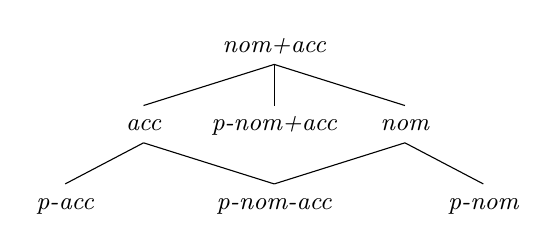
\begin{tikzpicture}[text height=1.5ex,text depth=.25ex,
  % inner sep=2pt,
  node distance=4em,
  baseline=5.25em]\small\itshape
\node (p-acc) {p-acc};
\node (p-acc1) [right of=p-acc] {};
\node (p-nom-acc) [right of=p-acc1] {p-nom-acc};
\node (p-nom1) [right of=p-nom-acc] {};
\node (p-nom) [right of=p-nom1] {p-nom};
\node (acc) [above of=p-acc1, node distance=3em, xshift=-1em] {acc};
\node (nom) [above of=p-nom1, node distance=3em, xshift=1em] {nom};
\node (p-nom+acc) [above of=p-nom-acc, node distance=3em] {p-nom+acc};
\node (nom+acc) [above of=p-nom+acc, node distance=3em] {nom+acc};
\draw (nom+acc.south) -- (acc.north);
\draw (nom+acc.south) -- (nom.north);
\draw (nom+acc.south) -- (p-nom+acc.north);
\draw (acc.south) -- (p-acc.north);
\draw (acc.south) -- (p-nom-acc.north);
\draw (nom.south) -- (p-nom.north);
\draw (nom.south) -- (p-nom-acc.north);
\end{tikzpicture}
% \mbox{}\\\includegraphics[scale=.35]{daniels20.png}
\caption{Case (sub)hierarchy encoding nominative/""accusative syncretism and underspecification}
\label{fig:daniels20} 
\end{figure}
Apart from the trivial renaming of \ftype{case} to the more explicit \ftype{nom+acc}, a~maximal type corresponding to this renamed non-maximal type is added here, namely, \ftype{p-nom+acc}.

Let us illustrate this approach with the two \ili{Polish} examples~\rref{ex-kogo-janek-lubi-a-jerzy-nienwaidizi} and
\rref{ex:dis:pl}, repeated below as \rref{ex:syn:pc:again} and \rref{ex:dis:pl:again}:
\eal
\ex
\label{ex:syn:pc:again} 
\gll Kogo Janek lubi a Jerzy nienawidzi? \\
     who.\textsc{acc/gen} Janek.\textsc{nom} likes(\textsc{obj.acc}) and Jerzy.\textsc{nom} hates(\textsc{obj.gen})\hspace{-6pt}\\
\glt  `Who does Janek like and Jerzy hate?’
\ex\label{ex:dis:pl:again}
\gll Dajcie wina i całą świnię! \\
    give wine.\GEN{} and whole.\ACC{} pig.\ACC{}\\
\glt `Serve (some) wine and a whole pig!’
\zl
As these examples involve accusative and genitive, I will assume that the complete case hierarchy
contains a~subhierarchy such as that in Figure~\ref{fig:daniels20} above, but with all occurrences of
\ftype{nom} replaced by \ftype{gen} as in Figure~\ref{fig:case4}.
\begin{figure}
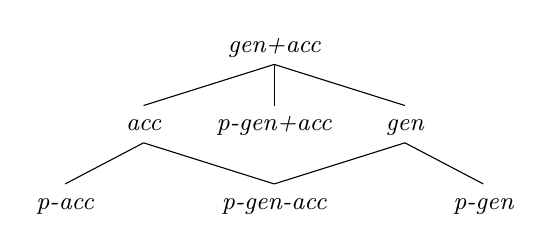
\begin{tikzpicture}[text height=1.5ex,text depth=.25ex,
  % inner sep=2pt,
  node distance=4em,
  baseline=5.25em]\small\itshape
\node (p-acc) {p-acc};
\node (p-acc1) [right of=p-acc] {};
\node (p-gen-acc) [right of=p-acc1] {p-gen-acc};
\node (p-gen1) [right of=p-gen-acc] {};
\node (p-gen) [right of=p-gen1] {p-gen};
\node (acc) [above of=p-acc1, node distance=3em, xshift=-1em] {acc};
\node (gen) [above of=p-gen1, node distance=3em, xshift=1em] {gen};
\node (p-gen+acc) [above of=p-gen-acc, node distance=3em] {p-gen+acc};
\node (gen+acc) [above of=p-gen+acc, node distance=3em] {gen+acc};
\draw (gen+acc.south) -- (acc.north);
\draw (gen+acc.south) -- (gen.north);
\draw (gen+acc.south) -- (p-gen+acc.north);
\draw (acc.south) -- (p-acc.north);
\draw (acc.south) -- (p-gen-acc.north);
\draw (gen.south) -- (p-gen.north);
\draw (gen.south) -- (p-gen-acc.north);
\end{tikzpicture}
\caption{Case (sub)hierarchy encoding accusative/""genitive syncretism and underspecification}\label{fig:case4}
\end{figure}


First of all, heads subcategorise for (or relevant case principles specify) “non-pure” cases, i.e., \ftype{acc}, \ftype{gen}, \ftype{gen+acc}, etc., but not \ftype{p-acc}, \ftype{p-gen}, \ftype{p-gen+acc}, etc.  For example, \emph{lubi} `likes’ and \emph{nienawidzi} `hates’ in~\rref{ex:syn:pc:again} expect their objects to have the case values \ftype{acc} and \ftype{gen}, respectively.  Moreover, \emph{dajcie} `give’ in~\rref{ex:dis:pl:again} specifies the case of its object as \ftype{gen+acc}.  On the other hand, nominal dependents bear “pure” cases.  For example, \emph{kogo} `who’ in~\rref{ex:syn:pc:again} is lexically specified as \ftype{p-gen-acc}.  Similarly to the analysis of the \ili{English} parasitic gap example above, this neutralised case is compatible with both specifications: \ftype{acc} and \ftype{gen}.

The analysis of~\rref{ex:dis:pl:again} is a~little more complicated, as a~new principle is needed to determine the case of a~coordinate structure.  The two conjuncts, \emph{wina} `wine’ and \emph{całą świnię} `whole pig’, have -- by virtue of lexical specifications of their head nouns -- the case values \ftype{p-gen} and \ftype{p-acc}, respectively.  Now, the case value of the coordination is determined as follows: take the “non-pure” versions of the cases of all conjuncts (here: \ftype{gen} and \ftype{acc}), find their (lowest) common supertype (here: \ftype{gen+acc}), and assign to the coordinate structure the “pure” type corresponding to this common supertype (here: \ftype{p-gen+acc}).  This way the coordinate structure in~\rref{ex:dis:pl:again} ends up with the case value \ftype{p-gen+acc}, which is compatible with the \ftype{gen+acc} requirement posited by the verb \emph{dajcie} (or by an appropriate principle of structural case assignment).  Obviously, a~purely accusative, purely genitive or accusative/genitive neutralised object would also satisfy this requirement.

One often-perceived – both within and outside of HPSG – problem with this approach is that it leads
to very complex type hierarchies for \ftype{case} and rather inelegant constraints
(\citealt[272]{sag:02}, \citealt[63–66]{dal:kin:sad:09}).  Let us, following \citet{dani:01},
simplify the presentation of type hierarchies such as that in Figure~\ref{fig:daniels20}, by removing all those “pure” types which are only needed to represent some
non-maximal types as maximal as in Figure~\ref{fig:daniels21}.
\begin{figure}
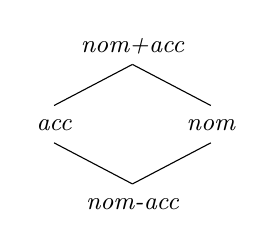
\begin{tikzpicture}[text height=1.5ex,text depth=.25ex,
  % inner sep=2pt,
  node distance=3em,
  baseline=2.5em]\small\itshape
\node (acc) {acc};
\node (accnom) [right of=acc] {};
\node (nom) [right of=accnom] {nom};
\node (nom-acc) [below of=accnom] {nom-acc};
\node (nom+acc) [above of=accnom] {nom+acc};
\draw (nom+acc.south) -- (acc.north);
\draw (nom+acc.south) -- (nom.north);
\draw (acc.south) -- (nom-acc.north);
\draw (nom.south) -- (nom-acc.north);
\end{tikzpicture}
\caption{Simplified case (sub)hierarchy encoding nominative/""accusative syncretism and underspecification}\label{fig:daniels21} 
\end{figure}
Hence, the representation in this figure corresponds to seven types shown explicitly in Figure~\ref{fig:daniels20}
(each non-maximal type in Figure~\ref{fig:daniels21} has an additional \ftype{p-} type, while the maximal
\ftype{nom-acc} in Figure~\ref{fig:daniels21} is the same as \ftype{p-nom-acc} in Figure~\ref{fig:daniels20}).
What would a~similar hierarchy for three morphological cases look like?  \citet[143]{dani:01}
provides the visualisation in Figure~\ref{fig:daniels22}, involving 18 nodes corresponding to 35 types in the full type hierarchy.
%\pagebreak
\begin{figure}
\hfill\hfill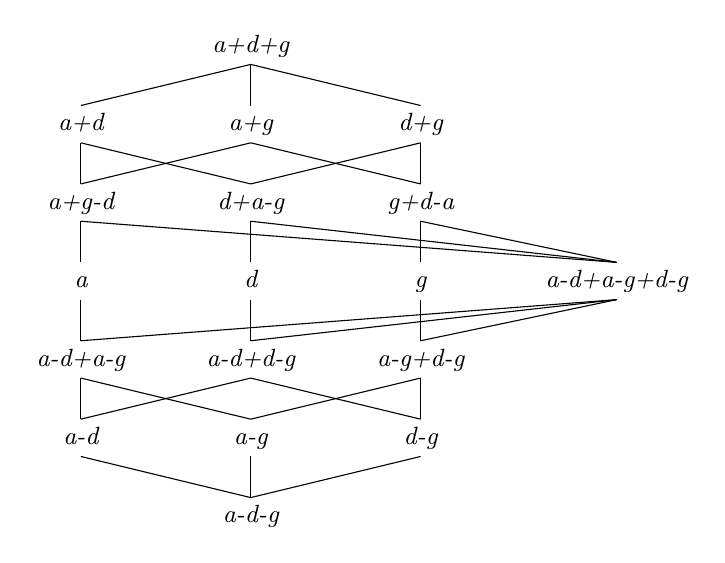
\begin{tikzpicture}[text height=1.5ex,text depth=.25ex,
  % inner sep=2pt,
  node distance=6.5em,
  baseline=8em]\small\itshape
\node (a) {a};
\node (d) [right of=a] {d};
\node (g) [right of=d] {g};
\node (a-d+a-g+d-g) [right of=g, xshift=1em] {a-d+a-g+d-g};
\node (a+g-d) [above of=a, node distance=3em]  {a+g-d};
\node (d+a-g) [above of=d, node distance=3em] {d+a-g};
\node (g+d-a) [above of=g, node distance=3em] {g+d-a};
\node (a+d) [above of=a+g-d, node distance=3em] {a+d};
\node (a+g) [above of=d+a-g, node distance=3em] {a+g};
\node (d+g) [above of=g+d-a, node distance=3em] {d+g};
\node (a+d+g) [above of=a+g, node distance=3em] {a+d+g};
\node (a-d+a-g) [below of=a, node distance=3em] {a-d+a-g};
\node (a-d+d-g) [below of=d, node distance=3em] {a-d+d-g};
\node (a-g+d-g) [below of=g, node distance=3em] {a-g+d-g};
\node (a-d) [below of=a-d+a-g, node distance=3em] {a-d};
\node (a-g) [below of=a-d+d-g, node distance=3em] {a-g};
\node (d-g) [below of=a-g+d-g, node distance=3em] {d-g};
\node (a-d-g) [below of=a-g, node distance=3em] {a-d-g};
\draw (a+g-d.south) -- (a.north);
\draw (a+g-d.south) -- (a-d+a-g+d-g.north);
\draw (d+a-g.south) -- (d.north);
\draw (d+a-g.south) -- (a-d+a-g+d-g.north);
\draw (g+d-a.south) -- (g.north);
\draw (g+d-a.south) -- (a-d+a-g+d-g.north);
\draw (a+d.south) -- (a+g-d.north);
\draw (a+d.south) -- (d+a-g.north);
\draw (a+g.south) -- (a+g-d.north);
\draw (a+g.south) -- (g+d-a.north);
\draw (d+g.south) -- (d+a-g.north);
\draw (d+g.south) -- (g+d-a.north);
\draw (a+d+g.south) -- (a+d.north);
\draw (a+d+g.south) -- (a+g.north);
\draw (a+d+g.south) -- (d+g.north);
\draw (a.south) -- (a-d+a-g.north);
\draw (d.south) -- (a-d+d-g.north);
\draw (g.south) -- (a-g+d-g.north);
\draw (a-d+a-g.south) -- (a-d.north);
\draw (a-d+a-g.south) -- (a-g.north);
\draw (a-d+d-g.south) -- (a-d.north);
\draw (a-d+d-g.south) -- (d-g.north);
\draw (a-g+d-g.south) -- (a-g.north);
\draw (a-g+d-g.south) -- (d-g.north);
\draw (a-d.south) -- (a-d-g.north);
\draw (a-g.south) -- (a-d-g.north);
\draw (d-g.south) -- (a-d-g.north);
\draw (a-d+a-g+d-g.south) -- (a-d+a-g.north);
\draw (a-d+a-g+d-g.south) -- (a-d+d-g.north);
\draw (a-d+a-g+d-g.south) -- (a-g+d-g.north);
\end{tikzpicture}\hfill\mbox{}
% \\\includegraphics[scale=.35]{daniels22.png}
\caption{Simplified case (sub)hierarchy encoding accusative\slash dative\slash genitive syncretism and underspecification}
\label{fig:daniels22} 
\end{figure}
As mentioned in~\citet[225]{lev:pol:01}, the size of such a~type hierarchy grows double exponentially with the number of grammatical cases, so it would already be next to impossible to visualise such a~hierarchy for \ili{German}, with its four cases, not to mention \ili{Polish} with its seven cases or \ili{Finno-Ugric} languages with around 15 cases.  And matters are further complicated by the fact that sometimes form syncretism simultaneously involves a~number of grammatical categories, so perhaps such type hierarchies should combine case information with person, gender and number (\citealt[145]{dani:01}, \citealt{Crysmann2005c}), and by the fact that coordinated elements may be specified for different categories (e.g., an NP specified for case may be coordinated with a~sentence, see also \crossrefchapteralt[Section~\ref{coordination:sec-unlikes}]{coordination}), in which case it is not clear what categories should be borne by the coordinate structure as a~whole (see, e.g., the inconclusive fn.\,10 in \citealt[277]{sag:02}).

After the early 2000s, such complex \ftype{case} hierarchies do not appear in HPSG work.  A~possible
reason for this is the increasing popularity of ellipsis-based accounts of various coordinate
constructions, including unlike category coordination cases, of which the “case underspecification”
examples %\rref{ex:dis:pl}–\rref{ex:dis:ru}
\rref{ex-case-underspecification} may be seen as special cases.\footnote{Another HPSG
  approach to unlike category coordination which obviates the need for such complex hierarchies is
  that of \citet{yata:04}, according to which the – perhaps disjunctive or underspecified –
  requirements of the head independently distribute to all conjuncts, in a~manner similar to (but
  more general than) distributivity within coordinate structures assumed in LFG
  \citep{DK2000a,dal:kin:sad:09,prz:pat:12a}.}  Such ellipsis accounts are usually formulated within
the linearisation approach of \citet{Reape92a,Reape94a} and \citet{Kathol95a}, and they have
been claimed to deal with some of the cases discussed in this section, e.g., by
\citet{Crysmann2003c}, \citet{BS2004a}, and \citet{chav:06,chav:08}.  However, such
linearisation-based approaches to coordination have more recently come under attack: see
\citet{levi:11} and \citet{kub:lev:15} (see also \citealt{yata:12,Yatabe2016a-u} and, especially,
\citealt{yat:wai:18} for a~defence of ellipsis-based accounts of some cases of coordination).\footnote{%
See also the chapters by \citet{chapters/ellipsis} and \citet{chapters/coordination} for discussions of HPSG analyses of ellipsis and coordination, respectively.}
Hence, it is difficult to predict at the moment whether ellipsis-based analyses will permanently
remove the need for complex type hierarchies modelling neutralisation and underspecification in
coordination.  But even if they do, some of the examples given at the beginning of this section,
namely \rref{ex:syn:gfr}–\rref{ex:syn:epg}, demonstrate that feature neutrality is not limited to
coordinate structures, but also occurs at least in free relatives\is{relative clause!free} and multiple \isi{gapping}, so case
hierarchies of the kind illustrated in Figure~\ref{fig:daniels18}, with separate types representing syncretic cases, are still needed in contemporary HPSG, regardless of the analysis of coordination; an example of a~more recent analysis which does assume such a~case hierarchy (to account for gapping and resumptive pronouns in Modern Standard \ili{Arabic}) is \citet{AB2013a-u}.\footnote{But see \citet{crys:17} for a~reanalysis which does not need to refer to such a~case hierarchy.}\is{coordination|)}



\section{Other HPSG work on case}
\label{sec:case:other}

Apart from the two clearly identifiable strands of HPSG work described in the two preceding sections, there are also single papers concerned with various theoretical and implementational aspects of grammatical case.  Of these, the report by \citet{drel:08} on modelling complex case phenomena in the \isi{Grammar Matrix} \citep{BFO2002a-u} has the widest typological scope.  It describes the treatment of various case systems in the multilingual platform for implementing HPSG grammars: not only the pure nominative-accusative, ergative-absolutive and tripartite systems, but also systems with various types of split ergativity, systems – known from \ili{Austronesian} languages, including \ili{Tagalog} – in which case marking interacts with focus marking, and so-called “direct-inverse” systems, exemplified by \ili{Algonquian} languages, in which case marking partially depends on the hierarchies – or scales – of nominal phrases, e.g., based on person and/""or animacy.  Similarly to the non-configurational case assignment principles discussed in Section~\ref{sec:case:str} above, such systems are described – via constraints on specific lexical types – by specifying case values of elements on \path{arg-st}.  Also, a~typologically very interesting language, \ili{Nias}, usually assumed to display the ergative-absolutive alignment but with the typologically exceptional property of marking the absolutive – rather than the ergative – case, is reanalysed as a~nominative-accusative language in \citet{Crysmann2009b-u}, with the sole argument of intransitive verbs mapped to the grammatical function of object, rather than subject.

Two other works mentioned here are concerned with two very different aspects of case systems of
particular languages.  \citet{ryu:13} investigates the issue of case spreading from an argument of
a~verb to certain nominal dependents of this argument in \ili{Korean}.  He investigates the semantic
relations that must hold between the two nominals for such “case copying” to occur and proposes
a~repertoire of 16 semantic relations (collected in five coherent groups, further classified into
two general classes) which make the spreading of the nominative possible, 10 of which (three of the
five groups, one of the two classes) license the spreading of the accusative.  On the syntactic
side, the dependents of such nominal arguments are raised to become valency elements of the
governing verbs.  In particular, dependents of the subject are raised to the valence list
for subjects \path{subj}, resulting in multiple elements within the \subjl of a single verb. Configurational
case assignment rules constrain the value of case of each valency subject to nominative, and of each
valency complement to accusative.  The paper does not discuss the (im)possibility of formulating
such case assignment rules non-configurationally, within local \path{arg-st} (or \path{deps}), but
the challenge for the non-configurational case assignment seems to be the fact that multiple
argument structure elements may correspond to valency subjects (and multiple to valency
complements), so – looking at the argument structure alone – it is not immediately clear how many
initial elements of this list should be assigned the nominative case, and which final elements
should get the accusative.

Finally, a~very different aspect of \ili{Hungarian} case is investigated in \citet{thui:11}, namely,
whether case affixes should be distinguished from postpositions and, if so, where to draw the line.
In \ili{Hungarian}, postpositions behave in some respect just like case affixes (e.g., they do not
allow any intervening material between them and the nominal phrase), which has led some researches
to deny the existence of the affix/postposition distinction.  \citet{thui:11} shows that, in this case, the
traditional received wisdom is right, and that case affixes and postpositions differ in a~number of
morphological and syntactic ways.  The proposed tests suggest that the essive element
\emph{k{\'e}nt}, normally considered to be a~case affix, should be reanalysed as a~postposition,
thus establishing the number of \ili{Hungarian} cases as 16.  The resulting analysis of
\ili{Hungarian} case affixes and postpositions is couched within Sign-Based Construction
  Grammar\indexsbcg \citep{BS2012a-ed}.

In summary, while HPSG is perhaps not best known for its approach to grammatical case, it does offer
a~range of interesting accounts of a~variety of case-related phenomena in diverse languages ranging
from \ili{German}, \ili{Icelandic} and \ili{Polish} through \ili{Finnish} and \ili{Hungarian} to
\ili{Korean} and \ili{Nias}; it provides perhaps the only formal implementation of the influential
“case tier” idea; and it successfully captures somewhat conflicting intuitions concerning the
locality of case assignment.

\is{case|)}
\section*{Abbreviations}

\begin{tabularx}{.99\textwidth}{@{}lX}
\textsc{ill} & illative\\
\end{tabularx}


\section*{\acknowledgmentsEN}

I~would like to thank the following colleagues for their comments on a~previous version of this chapter: Rui Chaves, Tony Davis, Jean-Pierre Koenig, Detmar Meurers, Stefan Müller and Shûichi Yatabe.  I~wish I~could blame them for any remaining errors and omissions.


{\sloppy 
\printbibliography[heading=subbibliography,notkeyword=this] 
}


\end{document}

%      <!-- Local IspellDict: en_GB-ise-w_accents -->

%%% Local Variables:
%%% mode: latex
%%% TeX-master: t
%%% mode: flyspell
%%% eval: (ispell-change-dictionary "british")
%%% eval: (turn-off-auto-fill)
%%% End:

\chapter{Verbs} \label{Verbs}
Verbs describe actions \xref{ex:verbex}, types of movement \xref{ex:verbex2}, states or characteristics \xref{ex:verbex3}, ways of existing \xref{ex:verbex4}, mental activities \xref{ex:verbex5}, perceptions \xref{ex:verbex6}, and object locations \xref{ex:verbex7}. They also function as “nouns” (\sectref{“Nouns” (words functioning as nouns)}), “adjectives” (\sectref{ch:’Adjectives’ (words that function as adjectives)}) and “adverbs” (\sectref{ch:’Adverbs’ (words and affixes that function as adverbs)}).

\ea\label{ex:verbex} actions
\ea kdakseˀ ‘I am running’
\ex ę́:ge:k ‘I will eat’
\ex dęyǫ́na̱hsgwahk ‘she will jump’
\ex ęgaǫgidagráhdęˀ ‘they are going to trip me, make me fall’
\z
\z

\ea\label{ex:verbex2} movement
\ea dagę́:neˀ ‘they are coming
\ex ǫkníˀdreˀ ‘we two are riding along in a vehicle’
\ex swatahí:neˀ ‘you all are walking’
\z
\z

\ea\label{ex:verbex3} states or characteristics
\ea hahnę́:ye:s ‘he is tall’
\ex aknó:shę: ‘I am envious’
\ex aknǫhǫkdá:nih ‘I am sick’
\z
\z

\ea\label{ex:verbex4} existence (or non-existence)
\ea 
\gll To: gi̱ˀ tsǫ: ní:yǫ:.\\
that just only it.is\\
\glt ‘That’s just all there is.’
\ex iheˀs ‘he is here’
\z
\z

\ea\label{ex:verbex5} mental activities, feelings
\ea ihse: ‘you want, hope, think’
\ex gonǫ́hkwaˀ ‘I love you’
\ex desaˀnigǫ́hęhdǫh ‘you are sad’
\z
\z

\ea\label{ex:verbex6} perceptions
\ea ęsé:gęˀ ‘you will see’
\ex ęsa:tǫ́:dęh ‘you will hear it’
\ex ęwágeshoˀ ‘I will smell it’ (unintentionally)
\ex ęwádehswaht ‘I will smell it’ (on purpose)
\z
\z

\ea\label{ex:verbex7} object location
\ea gá:yę:ˀ ‘it is lying’
\ex ganí:yǫ:t ‘it is hanging’
\z
\z

Verbs are the only required element in a sentence. As such, they often express the meaning of an entire sentence \xref{ex:verbex8}.

\ea\label{ex:verbex8} verbs as sentences
\ea degaǫdatgǫhsóhaeˀ ‘they are washing each other’s faces’
\ex ahadadrihwagwé:nyęˀ ‘he had earned it for himself’
\z
\z

Verbs minimally require a pronominal prefix. They also usually require an aspect suffix (\cite{chafe_seneca_1967}). However, \textsc{no-aspect} verbs, including “commands” and “suggestions” (described in \sectref{Commands (imperatives) and suggestions}) do not have an aspect suffix (for which, see \sectref{Meaning of no-aspect verbs}).

Verbs will be classified according to the criteria in \xref{ex:verbcriteria}, which are defined in the following sections.

\ea\label{ex:verbcriteria} criteria for verb classification
\ea noun incorporation 
\ex transparent or fixed expressions
\ex aspect
\ex pronominal prefix type
\z
\z


\section{Verbs and noun incorporation} \label{Verbs and noun incorporation}
Verbs can be classified according to their ability to \textsc{incorporate} (include) a noun stem (\sectref{ch:Noun Incorporation}). This criterion yields three types of verbs, described next.


\subsection{Verbs that optionally have an incorporated noun} \label{Verbs that optionally have an incorporated noun}
Some verbs can take an \textsc{incorporated noun} but do not require one. For example, the verbs in \xref{ex:verbex21} and \xref{ex:verbex22} have an incorporated noun and are well-formed -- they sound like words. However, the same verbs -- \textit{ęhsní:nǫˀ} and \textit{ęgyę́:to} -- lack an incorporated noun and are still perfectly good words. 

\ea\label{ex:verbex21}
ęyagw\exemph{ahgwęnya}hnínǫnyǫ:ˀ ‘we all will buy clothes’
\cfex{ \exemph{ahgwę́ny}aˀ ‘clothes’}
\cfex{ ęhsní:nǫˀ ‘you will buy it’}
\z


\ea\label{ex:verbex22}
hęk\exemph{hǫnaˀdá}yętoˀ ‘I will plant potatoes there’
\cfex{ o\exemph{hǫ́naˀda}ˀ ‘potatoes’}
\cfex{ ęgyę́:toˀ ‘I will plant it or something’}
\z


\subsection{Verbs that cannot have an incorporated noun} \label{Verbs that cannot have an incorporated noun}
Some verbs cannot take an incorporated noun because their meaning does not allow for it. These are “activity” or “action” verbs that only express one \textsc{role} (\sectref{Pronominal prefixes and role}). For example, the verbs shown in \xref{ex:verbex23} express just one role, that of “doer” (either a single “doer” or multiple “doers”). However, their meaning does not include that of an undergoer. In contrast, the verb in \xref{ex:verbex22} above, \textit{hękǫna̱ˀdáyętoˀ}, requires both a “doer” (‘I’) and an undergoer (‘potatoes’).

\ea\label{ex:verbex23}
\ea\label{ex:verbex23a} ga̱hnih ‘it is barking’
\ex\label{ex:verbex23b} gadá:węh ‘I am swimming’
\ex\label{ex:verbex23c} hęnadawęhs ‘they (males) are swimming’
\ex\label{ex:verbex23d} saˀe:yǫˀ ‘she returned’
\ex\label{ex:verbex23e} nǫdáhse:ˀ ‘you came from there’
\ex\label{ex:verbex23f} haˀgáge:t ‘I stopped by there’
\ex\label{ex:verbex23g} agiˀ ‘I said’
\z
\z


\subsection{Verbs requiring an incorporated noun} \label{Verbs requiring an incorporated noun}
Some verbs require an incorporated noun. (As such, they are unlike \textsc{minimal} verbs, which only require a pronominal prefix, a verb stem, and an aspect suffix.) For example, the verb \stem{+i:yo:} ‘be good, nice’ never occurs without an incorporated noun. It incorporates the noun \stem{nahsgw} ‘domestic animal’ in \xref{ex:verbex24a} but instead takes the noun \stem{yęhsr} ‘blanket’ in \xref{ex:verbex24b}. A plus ‘+’ sign before a verb stem means that the verb in question requires an incorporated noun.

Many obligatorily incorporating verbs function as “adjectives”, describing attributes of the incorporated noun \xxref{ex:verbex24}{ex:verbex25}. 

\ea\label{ex:verbex24} \stem{+i:yo:} ‘be good, nice’
\ea ganahsgw\exemph{í:yo:} ‘a nice pet’\label{ex:verbex24a}
\cfex{ga\exemph{náhsgw}aˀ ‘tame animal’, ‘pet’, ‘domestic animal’}
\ex oyęhsr\exemph{í:yo:} ‘nice blanket’\label{ex:verbex24b}
\cfex{o\exemph{yę́hsr}aˀ ‘blanket(s)’}
\z
\z


\ea\label{ex:verbex25} \stem{+owa:nęh} ‘be big’
\ea ga̱hǫhsr\exemph{owá:nęh} ‘big box’\label{ex:verbex25a}
\cfex{ ga̱\exemph{hǫ́hsr}aˀ ‘box’}
\ex ojǫˀd\exemph{owá:nęh} ‘big fish’\label{ex:verbex25b}
\cfex{ o\exemph{jǫ́ˀd}aˀ ‘fish’}
\z
\z

\largerpage
\section{Transparent vs fixed expressions} \label{Fixed and transparent expressions}
Verbs can be classified as either \textsc{transparent} or \textsc{fixed expressions}.\footnote{Fixed expressions are the verb \textsc{bases} described in \citet{foster_base_1989}.} 

Transparent expressions just have one straightforward (literal) meaning. For example, in example (\ref{ex:verbex24a}, previous page), the transparent verb \textit{ɡanahsgwí:yo:} has parts meaning ‘pet’ \stem{nahsgw} and ‘nice’ \stem{+iyo:}, and the word straightforwardly means ‘nice pet’. As well, substituting the pronominal prefix and the incorporated noun results in a new word, \textit{oyęhsrí:yo:}, which also has a straightforward meaning, ‘nice blanket’ \xref{ex:verbex24b}.

In contrast, fixed expressions have both a transparent (or literal) meaning and a \emph{non}-transparent meaning. The non-trans\-parent meaning is dominant. For example, in \xref{ex:verbex26a}, the intended, fixed meaning is ‘sandpiper’ (a type of shore bird) and the transparent (and not usually relevant) meaning of the word is ‘good sand’. 

\largerpage
\ea\label{ex:verbex26} 
\ea o\exemph{ˀnehs}í:yo: \\\label{ex:verbex26a} 
\glt ‘sandpiper’ (fixed meaning); ‘good sand’ (transparent meaning)
\cfex{ o\exemph{ˀnéhs}aˀ ‘sand’}

\ex ga\exemph{niga:hęhsr}í:yo: \\\label{ex:verbex26b} 
\glt ‘cotton’, ‘silk’ (fixed meaning); ‘good material’ (transparent meaning)
\cfex{ o\exemph{nigá:hęhsr}aˀ ‘material’, ‘cloth’}
\z
\z

In order to convey the fixed meaning of ‘sandpiper’ in \xref{ex:verbex26a}, the pronominal prefix, incorporated noun, and verb must remain constant or fixed, while other parts can change as needed. (For example, one could add the \stem{-ˀs} {\plural} suffix to create \textit{oˀnehsí:yoˀs} ‘sandpipers’.) Similarly, all other fixed expressions require specific prefixes, incorporated nouns, or suffixes in order to fully express their non-transparent meaning.


\largerpage
\subsection{Types of fixed expression} \label{Types of fixed expression}
For fixed expressions, the verb stem and at least one other part remain fixed or constant. The various types of fixed expression are described in this section.

In some cases, the combination of \stem{incorporated noun-verb} stem conveys a fixed meaning. For example, in \xref{ex:verbex28a}, the meaning of ‘offending someone’ is conveyed by the combination of \stem{ˀnigǫha+ˀe:k} ‘mind+hit’. 

\ea\label{ex:verbex28} fixed expressions with incorporated noun \stem{ˀnigǫha} ‘mind’
\ea\label{ex:verbex28a} ęhshe\exemph{ˀnigǫ́ha}ˀe:k ‘you will offend someone’ (literally, ‘you will hit someone’s mind’) 
\ex\label{ex:verbex28b} ho\exemph{ˀnigǫhá}ędaˀs ‘he understands’ (literally, ‘his mind settles’)
\ex\label{ex:verbex28c} ęhshe\exemph{ˀnigǫh}ǫ́:niˀ ‘you will influence, persuade someone’ (literally, ‘you will make someone’s mind’)
\z
\z

In other cases, the combination of \stem{prefix-…verb stem} conveys a fixed meaning. Example \xref{ex:verbex29a} illustrates the verb \stem{yena:} ‘to catch or receive something’. In the related expression in \xref{ex:verbex29b} the fixed parts are the \stem{t-} \textsc{\dualic} prepronominal prefix and \stem{yena:}; this combination means ‘to do something together’. In \xref{ex:verbex29c}, the fixed parts include the incorporated noun \stem{rihwa} ‘word’ and \stem{yena:}, which together mean ‘to accept advice’. Finally, in \xref{ex:verbex29d}, the \stem{adag-} \textsc{\reflexive} prefix and \stem{yena:} together mean ‘to wrestle’.

\ea\label{ex:verbex29} the transparent expression \stem{yena:ˀ} ‘to catch, receive, accept’, and related fixed expressions
\ea\label{ex:verbex29a} ag\exemph{yé:na:ˀ }’I caught, received it’ (minimal verb, \stem{yena:ˀ} transparent expression)
\ex\label{ex:verbex29b} a\exemph{t}hadi\exemph{yé:na:ˀ} ‘they did it together’, ‘they were accomplices’ (\stem{\dualic-…yena:} fixed expression)
\ex\label{ex:verbex29c} ęhs\exemph{rihwayé:na:ˀ} ‘you will accept advice, a suggestion’ (\stem{rihwa-yena:} fixed expression)
\ex\label{ex:verbex29d} ęhs\exemph{adagyé:na:ˀ} ‘you will wrestle’ (\stem{\reflexive-yena:} fixed expression)
\z
\z

Like other verbs, fixed expressions may also have free elements: for example both of the words in \xref{ex:tsiex} begin with \stem{tsi-} \textsc{\coincident}, which can be freely added to the relevant verbs to transparently mean ‘when’. Meanwhile, the words in \xref{ex:tsiex} also include fixed \stem{incorporated noun-verb stem} combinations -- the combination \stem{ǫgweˀd-ase:} \xref{ex:tsiexa} means ‘young person’, while \stem{ksaˀd-ase:} \xref{ex:tsiexb} means ‘teenager’.

\ea\label{ex:tsiex} \stem{tsi-verb} ‘while, when’
\ea\label{ex:tsiexa} 
 \gll \exemph{tsi}hǫgwe̱ˀda:sé: hohsę: \\
while.he.was.young he.is.fat\\
\glt ‘When he was young, he was fat.’ 
\cfex{hǫgwéˀdase:\\
	\gll h-ǫgwéˀd-ase:\\
	\textsc{3s.m.a}-person-new.{\stative}\\
	\glt `young man'}
\ex \exemph{tsi}yeksa̱ˀdá:se: ‘when she was a teenager…’ \label{ex:tsiexb}
\cfex{eksaˀdasé:ˀah\\
	\gll e-ksaˀd-asé:-ˀah\\
	\textsc{3s.fi.a}-child-new.{\stative}-{\diminutive}\\
	\glt `teenage girl'}
\z
\z


\section{Verbs and aspect} \label{Verbs and aspect}
Verbs can be classified according to the types of aspect suffixes they take. Before getting into details, some background information is provided next.

The three main types of aspect suffix are the punctual, habitual, and stative (see \sectref{Aspect suffixes}). While there is only one punctual suffix, \stem{-ˀ} {\punctual}, there are several habitual and stative suffixes. For example, the habitual endings include \stem{-s}, \stem{-haˀ}, and \stem{-h}. As shown in \xref{ex:habitexampleagain}, a given verb normally takes just one of the possible habitual (or stative, not shown) aspect endings.

\ea\label{ex:habitexampleagain} verbs in the habitual aspect
\ea degáˀswe:\exemph{s} ‘I am going deaf’
\ex hęnáˀswa̱ht\exemph{haˀ} ‘they are firemen’
\ex sgegę̱hęˀda:ni\exemph{h} ‘you are sick of me’
\z
\z

In this work, verbs with the punctual suffix are described as “punctual verbs”, while verbs with any of the habitual suffixes are “habitual verbs”, and verbs with any of the stative suffixes are “stative verbs”.


\subsection{Verbs occurring only in one aspect (stative or habitual)} \label{Verbs occurring only in one aspect (stative or habitual)}
Some verbs occur only in one aspect, either the stative or the habitual. \textsc{Stative-only} verbs take only a stative aspect suffix \xref{ex:verbex12}. A smaller set of \textsc{habitual-only} verbs exclusively occur in the habitual aspect \xref{ex:verbex13}.

\ea\label{ex:verbex12} stative-only verbs
\ea ohsnó:weˀ ‘it is fast, quick’ 
\ex go̱haˀdí:yo: ‘she is a good singer, she has a good voice’ 
\ex ogá:yǫh ‘it is old’ 
\z
\z

\ea\label{ex:verbex13} habitual-only verbs
\ea gagrahs ‘it stinks’
\ex agadǫ̱hswéˀdanih ‘I am hungry’ 
\ex gotgǫ́:nyohs ‘she has high standards’ 
\ex akneˀdraˀdá:nih ‘I feel nausea’, ‘I am nauseous’
\z
\z

\subsection{Three-aspect verbs (habitual, punctual, stative)} \label{Three-aspect verbs (habitual, punctual, stative)}
\textsc{Three-aspect} verbs can take three all aspects -- the habitual, punctual, and stative. The three-aspect verb in \xref{ex:verbex93} takes the \stem{-h} \textsc{\habitual} \xref{ex:verbex93a}, the \stem{-ˀ} \textsc{\punctual} \xref{ex:verbex93b} and the \stem{-:} \textsc{\stative} \xref{ex:verbex93c} aspect endings.

\ea\label{ex:verbex93} \stem{hsęnǫni} ‘store something’
\ea\label{ex:verbex93a} se̱hsę:nǫ́:nih\\
\gll s-e̱-hsę:nǫ́:ni-h\\
 \exsc{2s.a-joinerE-}store-{\habitual}\\
\glt `you are storing it right now'
\ex ęhsehsęnǫ́:niˀ\\\label{ex:verbex93b}
\gll ę-hs-e-hsęnǫ́:ni-ˀ\\
 \fut-\exsc{2s.a-joinerE-}store-{\punctual}\\
\glt `you will store it'
\ex ga̱hsę:nǫ́:ni:\\\label{ex:verbex93c}
\gll ga̱-hsę:nǫ́:ni-:\\
 \textsc{3s.a}-store-{\stative}\\
\glt `stored items'
\z
\z 

Verbs that take other types of habitual and stative endings are shown in \xref{ex:verbex91} and \xref{ex:verbex92}. (The punctual suffix only has one form, \stem{-ˀ}.\footnote{The punctual suffix is not pronounced in words ending with a consonant, which is why the verbs in \xref{ex:verbex91b} and \xref{ex:verbex92b} do not have an overt \stem{-ˀ} \textsc{\punctual} ending. The term \textsc{zero punctual} ({\zeropunctual}) describes this state of affairs.})

\ea\label{ex:verbex91} \stem{ˀhoweg} ‘cover something’
\ea geˀhó:we:s\\\label{ex:verbex91a}
\gll g-e-ˀhó:we:-s\\
 \textsc{1s.a}-{\joinerE}-cover-{\habitual}\\
\glt `I am covering something'
\ex ęhseˀhó:we:k\\\label{ex:verbex91b}
\gll ę-hs-e-ˀhó:we:k\\
 \fut-\textsc{2s.a}-{\joinerE}-cover.{\zeropunctual}\\
\glt `you will cover something'
\ex ageˀhowé:gǫh\\\label{ex:verbex91c}
\gll ag-e-ˀhowé:g-ǫh\\
 \textsc{1s.p}-{\joinerE}-cover-{\stative}\\
\glt `I did cover something'
\z
\z

%
%
% \ea\label{ex:verbex91} \stem{-ˀhoweg} ‘cover something’
%     \ea   geˀhó:we:s\\
%     \gll g-e-ˀhó:we:-s\\
%     1s.a-joinerE-cover-\textsc{habit}\\
%     \glt ‘I am covering something’
%
%     \ex    ęhseˀhó:we:k\\
%     \gll ę-hs-e-ˀhó:we:k\\
%     \textsc{fut-2s}-{\joinerE}-cover.\textsc{ø.punct} \\
%     \glt ‘you will cover something’
%
%     \ex    ageˀhowé:gǫh \\
%     \gll ag-e-ˀhowé:g-ǫh\\
%     \textsc{1s.p}-{\joinerE}-cover-\textsc{stat}\\
%     \glt ‘I did cover something’
%     \z
% \z


\ea\label{ex:verbex92} \stem{de-…-ęnahsgwahgw} ‘jump’
\ea deyǫna̱hsgwáhkwhaˀ\\
\gll de-yǫ-na̱hsgwáhkw-haˀ\\
 {\dualic}-\textsc{3s.fi.a}-jump-{\habitual}\\
\glt `she is jumping'
\ex dęyǫ́na̱hsgwahk\\\label{ex:verbex92b}
\gll d-ę-yǫ́-na̱hsgwahk\\
 {\dualic}-{\future}-\textsc{3s.fi.a}-jump.{\zeropunctual}\\
\glt `she will jump'
\ex desęna̱hsgwáhgwęh\\
\gll de-s-ę-na̱hsgwáhgw-ęh\\
 {\dualic}-\textsc{2s.a}-{\semireflexive}-jump-{\stative}\\
\glt `you have jumped'
\z
\z



\subsection{No-aspect verbs} \label{No-aspect verbs}
\textsc{No-aspect} verbs lack an aspect suffix. The example shown in \xref{ex:commandexample} is a type of command. In contrast, the comparative example in \xref{ex:commandexample} illustrates a verb with a punctual suffix, which functions as a statement. For the meaning of no-aspect verbs, see \sectref{Meaning of no-aspect verbs}.

\ea\label{ex:commandexample}
sadahǫ́:dǫ:\\\label{ex:commandexamplea}
\gll s-ad-ahǫ́:dǫ:\\
 \textsc{2s.a}-{\semireflexive}-ask.{\noaspect} (a command)\\
\glt `ask!'
\cfex{ęsada̱hǫ́:dǫ:ˀ\\
	\gll ę-s-ad-a̱hǫ́:dǫ:-ˀ\\
	\fut-\textsc{2s.a}-{\semireflexive}-ask-{\punctual} (a statement)\\
	\glt `you will ask'}
\z


\subsection{E-verbs} \label{Verbs of motion}
\textsc{E-verbs} \xref{ex:motionverbsagain} are different from the three-aspect verbs described earlier. The differences are too great to be summarized here and are covered in \sectref{ch:E-verbs}.

\ea\label{ex:motionverbsagain}
\ea í:geˀ ‘I am walking, moving’ 
\ex dagę́:neˀ ‘they (z) are coming’ 
\z
\z


\section{Verb classes and pronominal prefix type} \label{Verb classes and pronominal prefix type}
Verbs are also classified by the type of pronominal prefix they take \xref{ex:verbex80}. Verbs either take interactive (\textsc{int}-, \textsc{a}- and \textsc{p}-series) or non-interactive (\textsc{a}- or \textsc{p}-series) prefixes. The verbs taking non-interactive prefixes also subdivide into personal and neuter types \xref{ex:verbex80b}. (For definitions of \textsc{int}, \textsc{a}- and \textsc{p}-series prefixes, see \sectref{Three types of pronominal prefix}.) 

\ea\label{ex:verbex80}Verb classes, distinguished by pronominal prefix type
\ea\label{ex:verbex80a}\textsc{interactive} -- taking \textsc{int}-, \textsc{a}- and \textsc{p}-series prefixes
\ex\label{ex:verbex80b}\textsc{non-interactive} -- exclusively taking either \textsc{a}- or \textsc{p}-series prefixes 
\ea\label{ex:verbex80c}\textsc{personal} -- either taking all of the \textsc{a}-series prefixes or all of the \textsc{p}-series prefixes
\ex\label{ex:verbex80d}\textsc{neuter} -- taking only the neuter \stem{ga-} \textsc{3s.a} or \stem{(y)o-} \textsc{3s.p} prefix
\z
\z
\z



Interactive verbs \xref{ex:verbex80a} can take all of the interactive pronominal prefixes -- the \textsc{int} series \xref{ex:verbex90a}, the \textsc{a}-series \xref{ex:verbex90b} and the \textsc{p}-series \xref{ex:verbex90c}. (For this type of verb, the \textsc{a}- and \textsc{p}-series prefixes have a special interactive meaning, with an implied ‘it’ (shown in brackets in \ref{ex:verbex90}).

\newpage
\ea\label{ex:verbex90}
\ea\label{ex:verbex90a} a\exemph{gǫ́:}gęˀ ‘I saw you’ (singular) (\textsc{int} prefix)
\ex\label{ex:verbex90b} a\exemph{há:}gęˀ ‘he saw (it)’ (\textsc{a}-series prefix, used in an interactive sense with implied object ‘it’)
\ex\label{ex:verbex90c} a\exemph{hó:}gęˀ ‘(it) saw him’, ‘he was seen’ (\textsc{p}-series prefix, used in an interactive sense with implied subject ‘it’)
\z
\z

In contrast, non-interactive verbs \xref{ex:verbex80b} exclusively take either the \textsc{a}-series \xref{ex:verbex910a} or the \textsc{p}-series \xref{ex:verbex910b}. 

\ea\label{ex:verbex910}
\ea\label{ex:verbex910a}\exemph{ha}hnę́:ye:s ‘he is tall’ (\textsc{a}-series exclusively)
\ex\label{ex:verbex910b}\exemph{ho}hsę: ‘he is fat’ (\textsc{p}-series exclusively)
\z
\z


Non-interactive verbs \xref{ex:verbex80b} further divide into \textsc{personal} or \textsc{neuter} types. Personal verbs take a full range of \textsc{a}-series \xref{ex:verbex920a} or \textsc{p}-series \xref{ex:verbex920b} prefixes. In contrast, neuter verbs only take neuter ‘it’ prefixes \xref{ex:verbex930}. 


\ea\label{ex:verbex920} personal verbs 
\ea\label{ex:verbex920a} \exemph{ha}hnę́:ye:s ‘he is tall’, \exemph{e}hnę́:ye:s ‘she is tall’, \exemph{ga}hnę́:ye:s ‘it (animal) is tall’, \exemph{k}hnę́:ye:s ‘I am tall’ (etc.) (\textsc{a}-series exclusively)
\ex\label{ex:verbex920b} \exemph{ho}hsę: ‘he is fat’, \exemph{go}hsę: ‘she is fat’, \exemph{o}hsę: ‘it is fat’, \exemph{ag}áhsę: ‘I am fat’ (etc.) (\textsc{p}-series exclusively)
\z
\z


\ea\label{ex:verbex930} neuter verbs 
\ea \exemph{gá:}dę:s ‘it is thick, dense’ (\textsc{a}-series prefix)
\ex \exemph{w}agyé:sęh ‘it is easy’ (\textsc{a}-series prefix)
\ex \exemph{o}tó:weˀ ‘it is cold (weather)’ (\textsc{p}-series prefix)
\z
\z

That being said, neuter verbs can also take non-neuter, \textsc{p}-series prefixes, but only in order to denote the ownership of an incorporated noun (\ref{ex:verbex94}, see \sectref{Neuter stative-only verbs, incorporating, conveying possession}). 


\ea\label{ex:verbex94} \stem{+es} ‘long’, i:yǫ:s ‘it is long’ (\textsc{a}-series prefix)\\
\exemph{sa}nóˀje:s ‘your tooth is long’ (non-neuter \textsc{p}-series prefix, denoting possession)
\cfex{\exemph{o}nóˀjaˀ ‘tooth’ (\textsc{p}-series prefix)}
\z



\section{Verb classes (subdivided by aspect, pronominal prefix type)} \label{Verb classes (subdivided by aspect, pronominal prefix type)}
To summarize, verbs can be classified according to the criteria of noun incorporation, meaning (fixed or transparent), aspect, and pronominal prefix type. The main criteria used in this work are aspect and pronominal prefix type.\footnote{In the Verb dictionary (\sectref{verb dictionary}) information about noun incorporation and fixed expressions is also provided where relevant.} The verb classes defined by these criteria are summarized in \xxref{ex:verbex361}{ex:verbex362}. 

The stative-only and habitual-only verbs in \xref{ex:verbex361}, described earlier in \sectref{Verbs occurring only in one aspect (stative or habitual)}, either take \textsc{a}- or \textsc{p}-series prefixes exclusively. Their prefix type, together with the neuter vs. personal distinction, results in four sub-classes of verb.

\ea\label{ex:verbex361} stative-only or habitual-only verbs (including \textsc{NV} fixed expressions)\footnote{\textsc{NV} is an abbreviation for fixed expressions that require an \stem{incorporated noun-verb} combination.}
\ea with \textsc{a}-series prefixes
\ea \textsc{neuter} verbs (only taking \stem{ga-} \textsc{3s.a} or \stem{w(a)-} \textsc{3s.p} prefix)
\ex \textsc{personal} verbs (taking any personal prefix)
\z
\ex with \textsc{p}-series prefixes
\ea \textsc{neuter} verbs (only taking \stem{o-} \textsc{3s.p} prefix)
\ex \textsc{personal} verbs (taking any personal prefix)
\z
\z
\z

The three-aspect verbs in \xref{ex:verbex362}, described earlier in \sectref{Three-aspect verbs (habitual, punctual, stative)}, fall into two major types. The first type \xref{ex:verbex362a} takes \textsc{a}-series prefixes in the habitual and punctual, but \textsc{p}-series prefixes in the stative. The second type \xref{ex:verbex362b} takes \textsc{p}-series prefixes in all three aspects. The pronominal prefix type, together with the neuter, personal, and interactive distinction, results in the following sub-classes in \xref{ex:verbex362}. 

\ea\label{ex:verbex362} three-aspect verbs (including \textsc{NV} fixed expressions)
\ea with \textsc{a}-series prefixes in the habitual and punctual and \textsc{p}-series prefixes in the stative\label{ex:verbex362a}
\ea \textsc{neuter} verbs
\ex \textsc{personal} verbs
\ex \textsc{interactive} verbs
\z
\ex with \textsc{p}-series prefixes in the habitual, punctual, and stative\label{ex:verbex362b}
\ea \textsc{neuter} verbs 
\ex \textsc{personal} verbs
\ex \textsc{interactive} verbs
\z
\z 
\z

Pronominal prefix choice is described further in \sectref{Pronominal prefix choice for stative-only verbs} (stative-only and habitual-only verbs) and in \sectref{Pronominal prefix choice for three-aspect verbs} (three-aspect verbs).

Finally, for \textsc{e-verbs}, see \sectref{ch:E-verbs}. 



\chapter{“Adverbs” (words and affixes functioning as adverbs)} \label{ch:’Adverbs’ (words and affixes that function as adverbs)}
Words functioning as “adverbs” modify the meaning of verbs or sentences by specifying (or questioning) the time, manner, place, or degree of an activity, happening, or state. The order of “adverbs” in phrases is described next, and then a description of the words, prefixes, and suffixes that function as “adverbs” follows.


\section{“Adverb” order in phrases} \label{ch:’Adverb’ order in phrases}
“Adverbs” tend to occur in specific positions in a phrase. For example, some must be first in the phrase (or before the verb, as in \textit{honákwę̱ˀǫh} in \ref{ex:advorder1}). Others have to occur after another word, but close to the beginning of the sentence, \xref{ex:advorder2}. Many other “adverbs” can appear wherever they make sense in the sentence \xref{ex:advorder3}. The typical positions of \textsc{particles} functioning as “adverbs” are described in \sectref{ch:particle order}.

\ea\label{ex:advorder1} clause-initial\\
 \gll \exemph{ahsǫh} ne:ˀ honákwę̱ˀǫh. \\
still it.is he.is.angry\\
\glt ‘He is still angry.’
\z

\ea\label{ex:advorder2} after another word, close to the beginning of the sentence
\ea
 \gll jidwáhshe:t \exemph{e:ˀ} \\
let’s.count again\\
\glt ‘Let’s count again!’

\ex
 \gll I:ˀ gęh \exemph{e:ˀ} sgwatró:wi:? \\
I Q again you.talk.about.me\\
\glt ‘Are you talking about me again?’ (said jokingly)
\z
\z

\ea\label{ex:advorder3} wherever relevant in the sentence
\ea
 \gll \exemph{Gǫdagyeˀ} ętsahdę́:diˀ. \\
right.away you.will.leave\\
\glt ‘You will leave right away!’

\ex
 \gll Tę́ˀ. Hęgyę́ˀ-tsǫ:. Shede̱hjí:hah ní:ˀ ęgahdę:díˀ \exemph{gǫdagyeˀ}.\\
no, never.mind-just early.morning I I.will.leave right.away\\
\glt ‘No, never mind, I’ll go there right away, early in the morning.’ (\cite[494]{mithun_watewayestanih_1984}, Ękníyętoˀ dialogue)
\z 
\z



\section{“Adverbs” of time} \label{ch:’Adverbs’ of time}
“Adverbs” of time either describe or question \emph{when} an activity or action takes place \xref{ex:advtimeex}. 

\ea\label{ex:advtimeex}
\gll Neˀ giˀ ę:ˀ \exemph{e:ˀ} toh iheˀs. \\
The just affirm again that.one he.is\\
\glt ‘He is here again!’
\z


\subsection{“Adverbs” of time (particles)}
The following \textsc{particles} function as “adverbs” of time and are described in the \textit{Particle dictionary}, \sectref{ch:particle dictionary}.

\begin{CayugaRelated}
    
\item{}\textit{Ahsǫh} \trs{still}, \trs{yet}

\item{}\textit{Daji:hah gwaˀ} \trs{soon}, \trs{a short while}

\item{}\textit{E:ˀ} \trs{again}, \trs{still}

\item{}\textit{Gaę niyo:weˀ tsǫ:} \trs{whenever}

\item{}\textit{Gaoˀ nawahtgeh} \trs{the time before then}

\item{}\textit{Gę:s} \trs{generally}, \trs{used to}, \trs{usually}, \trs{normally}

\item{}\textit{Giˀ} \trs{just}

\item{}\textit{Gǫdagyeˀ} \trs{immediately}, \trs{right away}

\item{}\textit{Gwaˀ} \trs{immediately}, \trs{right then}, \trs{just then}, \trs{finally}

\item{}\textit{Gwahs hwaˀ} \trs{this time for sure}

\item{}\textit{Gwahs waˀ-heh tsǫ:} \trs{just now}, \trs{just a few seconds ago}

\item{}\stem{\textit{-heh}} element related to time

\item{}\textit{Hwaˀ} \trs{this time}, \trs{next}

\item{}\textit{Hwę:dǫh} \trs{when}

\item{}\textit{Hwę:dǫh gwaˀ} \trs{sometime}, \trs{whenever}, \trs{once}

\item{}\textit{Hya:ˀ} \trs{first}, \trs{before anything else}

\item{}\textit{Naˀgę:ˀ, ohnaˀgę:ˀ} \trs{late}

\item{}\textit{Ne:ˀ giˀ gyę:ˀ hya:ˀ} \trs{before all else}, \trs{first}

\item{}\textit{Ne:ˀ hwaˀ} \trs{this (coming) time}

\item{}\textit{Ne:ˀ seˀ gę:s neˀ} \trs{back then}, \trs{a long time ago}

\item{}\textit{Nę: hwaˀ waˀ-ne:ˀ} \trs{nowadays}

\item{}\textit{Nę:-gyęh hwaˀ} \trs{this time}

\item{}\textit{Ogwęhę:gyeˀ} \trs{now and then}, \trs{now and again}

\item{}\textit{Ohę:dǫ:} \trs{early}, \trs{first}

\item{}\textit{Ohnaˀgę:ˀ, naˀgę:ˀ} \trs{late}

\item{}\textit{Ohnaˀgęhjih} \trs{late}, \trs{back then}

\item{}\textit{O:nęh, neˀ o:nęh} \trs{now}, \trs{when}, \trs{then}, \trs{at this time}

\item{}\textit{O:nęh e:ˀ} \trs{again!}

\item{}\textit{O:nęh gwaˀ} \trs{suddenly}, \trs{already}, \trs{finally}, \trs{all at once}

\item{}\textit{O:nęh to:hah} \trs{soon}, \trs{almost}

\item{}\textit{Tęˀ ahsǫh} \trs{not yet}

\item{}\textit{Tęˀ hwę:dǫh} \trs{never}, \trs{not ever}

\item{}\textit{Tgǫhaǫgyeˀ} \trs{sometimes}

\item{}\textit{Tgwahaǫ:ˀ} \trs{sometimes}

\item{}\textit{Tgwęhę:ˀ} \trs{sometimes}

\item{}\textit{To: niyonisheˀ to:} \trs{a certain amount of time}

\item{}\textit{To: niyo:weˀ ne:ˀ} \trs{when}

\item{}\textit{Tǫ:-hwaˀ} \trs{that time}

\item{}\textit{To:hah} \trs{a place}, \trs{a time}

\item{}\textit{Waˀ-} element meaning \trs{current moment}

\item{}\textit{Waˀ-gyęh} \trs{presently}, \trs{so now}, \trs{then}

\item{}\textit{Waˀ-heh} \trs{just now}, \trs{finally}

\item{}\textit{Waˀ-heh-geha:ˀ} \trs{finally}, \trs{at long last}

\item{}\textit{Waˀ-jih} \trs{after a while}, \trs{eventually}, \trs{just a while ago}

\item{}\textit{Waˀ-ji-:hah} \trs{presently}, \trs{a little later}, \trs{after a bit}, \trs{after a while}, \trs{afterwards}, \trs{later}

\item{}\textit{Waˀ-ne:ˀ} \trs{today}, \trs{now}

\end{CayugaRelated}


\subsection{Prefixes and suffixes functioning as “adverbs” of time}
Several verb prefixes and suffixes function as “adverbs” of time. For example, the \stem{ts(i)-} \textsc{\coincident} prefix means ‘at the same time’ as another activity (\ref{ex:advex4}, see \sectref{[tsi-] (coincident) prefix}).

\ea\label{ex:advex4} 
 \gll De̱ˀagowihsrá:t \exemph{tsaˀ}ǫ́nagraˀt. \\
she.had.no.breath while.she.was.born\\
\glt ‘She had no breath when she was born.’
\z

Similarly, the combination \stem{shęh n(i)-\textsc{verb}} ‘that \textsc{\partitive}-\textsc{verb}’ can describe actions extending over a certain period of time, or occurring while some other action happens (\ref{ex:advex5}, see \sectref{[ni-] (partitive)}).

\ea\label{ex:advex5} 
 \gll Agiˀda̱ˀǫ́h ǫ \exemph{shęh} \exemph{naˀonishéˀ} hohta:ˀ. \\
I.was.sleeping I.guess that it.took.time he.was.speaking\\
\glt ‘I slept while he spoke.’
\z

The \stem{s-, j-} \textsc{\repetitive} prefix can also function as an “adverb” of time, describing a repeated action (\ref{ex:advex6}, see \ref{[s-, j-, ji-] (repetitive)}).

\ea\label{ex:advex6}
\ea \exemph{s}awada̱hǫ́:dǫ:ˀ ‘it asked again’
\cfex{awada̱hǫ́:dǫ:ˀ ‘it asked’}
\ex \exemph{j}ago:kǫ́:ni: ‘she is cooking again’
\cfex{ gokǫ́:ni: ‘she is cooking’}
\z
\z



\subsection{Verbs functioning as “adverbs” of time}
Several \textsc{verbs} function as “adverbs” of time, identifying the time of an activity, happening, or state \xref{ex:advex7}. For more examples, see “Related”.

\ea\label{ex:advex7}
\ea sǫ́:deˀ ‘last night’ (atypical \textsc{verb})
\ex Awędędáˀǫh ‘Monday (present)’ (literally, ‘the day was finished’, \textsc{verb})
\z
\z


\begin{CayugaRelated}
\item Months, \ref{months}

\item Periods of time in the day, \ref{periods of time in the day}

\item Yesterday, today, and tomorrow, \ref{yesterday, today, and tomorrow}

\item Seasons and years, \ref{seasons and years}

\item Weekdays, \ref{weekdays}

\item Clock time, \ref{clock time}
\end{CayugaRelated}

\section{“Adverbs” of place} \label{‘Adverbs’ of place}
“Adverbs” of place specify (or question) where an activity or action takes place \xxref{ex:advex19}{ex:advex190}. For more examples, see “Related”.

\ea\label{ex:advex19}
 \gll \exemph{To} \exemph{hǫ:} hayę́hęˀ. \\
there place he.puts.it\\
\glt ‘He is always putting it there.’
\z

\ea\label{ex:advex190}
 \gll \exemph{Tohgeh} gęh \exemph{nhǫ:wéˀ} toh naˀá:weh? \\
there-on Q place that it.happened\\
\glt ‘Where did that happen?’
\z

\begin{CayugaRelated}
\item Location, \ref{ch:Location}

\item Place names, \ref{place names}
\end{CayugaRelated}

\subsection{“Adverbs” of place (particles)} \label{‘Adverbs’ of place (particles)}
\textsc{particles}, \textsc{particle groups}, and \textsc{particle}-\textsc{verb} combinations may function as “adverbs” of place, specifying the location of an action or activity. The following “adverbs” of place are described in the \textit{Particle dictionary}, \sectref{ch:particle dictionary}.

\begin{CayugaRelated}
    \item{} \textit{Ahsdeh} \trs{outside}, \trs{outdoors}

\item{} \textit{Akda:gyeˀ} \trs{beside}, \trs{the edge}

\item{} \textit{Da: gwa:dih} \trs{over here}, \trs{this side}

\item{} \textit{Da: hǫ:weh hǫ:} \trs{this is where}

\item{} \textit{E: gwa:dih} \trs{on the other side}

\item{} \textit{E: ni-\textsc{noun}+adih} \trs{on the other side of \textsc{noun}}

\item{} \textit{Gaę gwaˀ gwa:dih} \trs{whichever way}, \trs{whichever side}

\item{} \textit{Gaę gwaˀ hǫ:weh} \trs{somewhere}, \trs{someplace}, \trs{wherever}, \trs{around}

\item{} \textit{Gaę gwaˀ…ni-\textsc{noun}} \trs{wherever \textsc{noun} is}

\item{} \textit{Gaę gwaˀ tsǫ:} \trs{wherever}, \trs{somewhere}

\item{} \textit{Gaę niyó:weˀ} \trs{how far}, \trs{which distance}

\item{} \textit{Gaoˀ} \trs{this side}, \trs{this way}

\item{} \textit{Gaˀ-} element referring to a location

\item{} \textit{Gaˀ-to:hah} \trs{somewhere}, \trs{someplace}, \trs{around}, \trs{anywhere}, \trs{thereabouts}

\item{} \textit{Gaˀ-to:hah tohgeh} \trs{thereabouts}

\item{} \textit{Gwa:dih, gwai} \trs{to one side}

\item{} \textit{Hehdaˀgeh gwa:dih} \trs{below}, \trs{low}

\item{} \textit{Hehdaˀgeh hǫ:} \trs{downstairs}

\item{} \textit{Hehdage̱hjih} \trs{the bottom}, \trs{low}

\item{} \textit{Hejo:yaˀ tsǫ:} \trs{elsewhere}

\item{} \textit{He:tgęh} \trs{above}, \trs{up}, \trs{superior}

\item{} \textit{He:tgę̱hjih} \trs{the very top}, \trs{high up}

\item{} \textit{He:yo: dagwaishǫ:} \trs{straight ahead}

\item{} \textit{Hę:gyeh gaę hǫ:weh} \trs{no matter where}, \trs{no matter which place}

\item{} \textit{Hǫ:weh} \trs{where}

\item{} \textit{I:nǫh} \trs{far}

\item{} \textit{I:wa:kˀah} \trs{near}

\item{} \textit{Neˀ gwaˀ toh} \trs{here (rather than there)}

\item{} \textit{Neˀ to gyę:ˀ hǫ:weh} \trs{it is where}

\item{} \textit{Nę: toh gwa:dih} \trs{on this side}

\item{} \textit{Nę:-gyęh gwa:dih} \trs{here}, \trs{this side}, \trs{over here}

\item{} \textit{Nę: toh} \trs{here}

\item{} \textit{Nigwa:dih} \trs{-ward, direction}

\item{} \textit{Niyo:weˀ, ni:yo:ˀ, nyo:ˀ} \trs{a certain distance}, \trs{a certain time}

\item{} \textit{Ohę:dǫ: shęh} \trs{ahead}, \trs{in front}, \trs{forward}

\item{} \textit{Ohnaˀgę: gwa:dih shęh} \trs{behind}

\item{} \textit{Ohnaˀgęhjih} \trs{late}, \trs{back then}, \trs{the bottom}

\item{} \textit{Ohnaˀgǫ:} \trs{underneath}, \trs{beneath}, \trs{under}

\item{} \textit{Senyęˀsgwadih} \trs{to your left}

\item{} \textit{Sewaihǫhsdǫh gwa:dih} \trs{to your right}

\item{} \textit{Sganyęˀsgwadih} \trs{to its left}

\item{} \textit{Shęh hǫ: heyodokdaˀǫh} \trs{the bottom}

\item{} \textit{Si:} \trs{over there}

\item{} \textit{Si gwa:dih} \trs{over there}

\item{} \textit{Si gwa:di:hah} \trs{just this side of}

\item{} \textit{Si hne:ˀ si gwa:dih} \trs{over there}

\item{} \textit{Si: hǫ:weh} \trs{way over there}

\item{} \textit{Sǫ: gwadih} \trs{on some other side}

\item{} \textit{Tęˀ gaˀ-toh} \trs{nowhere}, \trs{not anywhere}

\item{} \textit{To:, toh, tǫ:} \trs{there}, \trs{that place}

\item{} \textit{To: gwa:dih} \trs{on that side}

\item{} \textit{To: hǫ:weh} \trs{there}, \trs{where}

\item{} \textit{Toh-geh} \trs{there}
\end{CayugaRelated}



\subsection{Prefixes that function as “adverbs” of place} \label{Prefixes and suffixes that function as ‘adverbs’ of place}
Verb prefixes functioning as “adverbs” of place include the \textsc{partitive} \xref{ex:advex230a}, \textsc{cislocative} \xref{ex:advex230b}, \textsc{translocative} \xref{ex:advex230c}, and \textsc{coincident-dualic} \xref{ex:advex230d} prepronominal prefixes, which are described in the “Related” sections.

\ea\label{ex:advex230} 
\ea\label{ex:advex230a}\exemph{ni}ta:wé:nǫ: ‘a stranger’ (literally, ‘he comes from somewhere’) 
\ex\label{ex:advex230b}\exemph{de}sáˀdre: ‘drive over here’ 
\ex\label{ex:advex230c}\exemph{heˀ}sáˀdre: ‘drive over there’ 
\ex\label{ex:advex230d}\exemph{tsaˀd}ę́hsyę:ˀ ‘you will put, lay them side by side’
\z
\z

\begin{CayugaRelated}
\item{}\stem{tsi-} (coincident) prefix, \ref{[tsi-] (coincident) prefix}

\item{}\stem{ni-} (partitive) prefix, \ref{[ni-] (partitive)}

\item{}\stem{d-} (cislocative) and \stem{heˀ-} (translocative) prefixes, \ref{[d-] (cislocative) and [heˀ-] (translocative)}
\end{CayugaRelated}




\section{“Adverbs” of manner} \label{ch:’Adverbs’ of manner}
“Adverbs” of manner describe (or question) how an activity takes place \xref{ex:advex8}. 

\ea\label{ex:advex8} 
 \gll \exemph{Sgę:nǫ:ˀǫ́h} hodrihsdǫ̱hǫ́:gy.eˀ \\
slowly he.is.sneaking.around\\
\glt ‘He is sneaking around slowly.’ 
\z

\subsection{Prefixes and suffixes that function as “adverbs” of manner}
Several verb prefixes and suffixes function as “adverbs” of manner, describing or questioning how an activity takes place. For example, the combination \stem{shęh ni-} ‘that \partitive’ means something like ‘how’, ‘the manner in which’ \xref{ex:advex11}.
	
\ea\label{ex:advex11} 
 \gll Dękde:níˀ \exemph{shęh} \exemph{ni}wagri̱hóˀdę:\\
I.will.change that how.I.do.things\\
\glt ‘I am going to change my outlook’
\z

Similarly, verbs with \stem{ti- … -ˀah} \textsc{\contrastive-…-\diminutive} have the “adverb”-like meaning of ‘any old way’ \xref{ex:advex12}.

\ea\label{ex:advex12} 

 \gll \exemph{ti}he:\exemph{ˀáh} tsǫ: \\
he.is.walking.along-ish just\\
\glt ‘He is just walking along any old way.’
\cfex{ iheˀ ‘he is walking, moving’}

\z 

The \stem{de-} \textsc{\dualic} prefix can function as an “adverb” of manner describing a two-part motion \xref{ex:advex13}.

\ea\label{ex:advex13} \exemph{d}ęhadagyáˀda̱hgwaˀt ‘he will do push ups’ 
\z
	
The \stem{-ge:} \textsc{\augmentative} suffix can function as an “adverb” of manner, describing an activity done ‘in a big way’ \xref{ex:advex14}.

\ea\label{ex:advex14} 
ahęnatgwéni̱ˀ\exemph{ge:} ‘the big win’, ‘victory’ (literally, ‘they won big’)
\cfex{ęhsa:tgwé:niˀ ‘you will win’}
\z

The \stem{-sgǫ:} \textsc{\facilitative} suffix also functions as an “adverb” of manner \xref{ex:advex15}.

\ea\label{ex:advex15} 
sadahǫdǫ́\exemph{sgǫ:} ‘you are nosy’ (literally, ‘you ask easily', ‘you are always asking questions') 
\cfex{sadahǫ́:dǫ: ‘you ask’}
\z

The above affixes are described in the “Related”  sections listed below.

\begin{CayugaRelated}
\item{}The \stem{ti-} (contrastive) prefix, \ref{[ti-] (contrastive)}

\item{}The \stem{ni-} (partitive) prefix, \ref{[ni-] (partitive)}

\item{}The \stem{de-} (dualic) prefix, \ref{[de-] (dualic)}

\item{}\stem{-ge:} (augmentative), \ref{[-ge:] (augmentative)}

\item{}\stem{-sgǫ:} (facilitative), \ref{[-sgǫ:] (facilitative)}
\end{CayugaRelated}

\subsection{Verbs functioning as “adverbs” of manner}
Several \textsc{verbs} function as “adverbs” of manner, describing how an activity takes place \xxref{ex:advex16}{ex:advex191}. In \xref{ex:advex16}, \textit{ohsnó:weˀ} ‘it is fast’ modifies the meaning of \textit{adwákyuˀkdęˀ} ‘it gets dull’.

\ea\label{ex:advex16}
 \gll \exemph{Ohsno:wéˀ} gę:s adwákyuˀkdęˀ.\\
it.is.fast usually it.gets.dull\\
\glt ‘It gets dull fast.’ (\cite[159]{mithun_watewayestanih_1984}, Enǫhsǫnyaˀdaˀsǫ:ˀǫh dialogue) 
\z

\ea\label{ex:advex17}
 \gll …\exemph{tręhs} gę:s \exemph{wagyesˀagéh} aˀosdagwá:ęh. \\
…too.much usually it.is.easy it.gets.dirty\\
\glt ‘…because it gets dirty too easily.’ (\cite[225]{mithun_watewayestanih_1984}, Agyaˀdawíˀtraˀ dialogue)
\z

\ea\label{ex:advex191} 
 \gll \exemph{Wę:dó:ˀ} da:ga̱hyadǫ̱hsríyaˀksǫ:k.\\
it.is.hard the.paper.should.be.cut\\
\glt ‘The paper is hard to cut.’
\z
	
Some verbs also express an “adverb”-like meaning that is not specifically spelled out in a prefix or suffix \xref{ex:advex18}.
	
\ea\label{ex:advex18}
\ea ętsę́hsga:ˀ ‘you take off \textit{abruptly, quickly, suddenly}’
\ex hahsgyáǫhaˀ ‘he walks \textit{quickly}’, ‘he gives someone encouragement’
\z
\z



\section{“Adverbs” of degree} \label{ch:’Adverbs’ of degree}
“Adverbs” of degree describe the extent or degree of a characteristic or activity \xref{ex:advex27}. For more examples, see \textit{Comparisons}, \sectref{ch:Comparisons (more, the same, or less)}.

\ea\label{ex:advex27} 
\ea 
 \gll \exemph{Stǫ:háh} segę́i:s.\\
a.little move\\
\glt ‘Move a little bit!’

\ex
 \gll  \exemph{Trǫhgeh} \exemph{tsǫ:} jǫgwaihóˀdeˀ. \\
barely just we.are.working\\
\glt ‘We’re barely working.’
\z
\z



\subsection{Particles functioning as “adverbs” of degree} \label{Particles and verbs functioning as ‘adverbs’ of degree}
\textsc{particles} may function as “adverbs” of degree, specifying the degree or extent of an action or activity⁠. The following “adverbs” of degree are described in the \textit{Particle dictionary}, \sectref{ch:particle dictionary}.

\begin{CayugaRelated}
 \item{}  \textit{Ahsǫh} \trs{more}

\item{} \textit{Aǫgo̱hdǫh} \trs{exceptional}, \trs{over the top}, \trs{extremely}, \trs{too much so}

\item{} \textit{Do:gęhs} \trs{really}, \trs{very}

\item{} \textit{Do̱hgá:ˀah} \trs{a few}

\item{} \textit{Do:s} \trs{really}, \trs{very}

\item{} \textit{Giˀ gyę:ˀ} \trs{quite}, \trs{kind of}

\item{} \textit{Gwahs} \trs{really}, \trs{just}, \trs{quite}, \trs{intensifier}

\item{} \textit{Gwahs ǫ:weh} \trs{really}

\item{} \textit{Gwe:gǫh, agwe:gǫh, ogwe:gǫh} \trs{completely}, \trs{totally}

\item{} \textit{Heyohe:ˀ} \trs{more}

\item{} \textit{I:soˀ} \trs{much}, \trs{many}, \trs{lots}, \trs{very}

\item{} \textit{I:so:ˀah} \trs{a fairly big bit}

\item{} \textit{Ji} \trs{too much}

\item{} \textit{Ji aǫgo̱hdǫh} \trs{too much so}

\item{} \textit{Ji trehs} \trs{more (than usual)}, \trs{too much so}

\item{} \textit{Ne:ˀ tsǫ:} \trs{that is only}, \trs{that is all}


\item{} \textit{Nę: tsǫ: gwaˀ toh ni-} \trs{just a little bit}, \trs{very little}

\item{} \textit{Nę: tsǫ: ni-} \trs{just}

\item{} \textit{O:weh, neˀ ǫ:weh} \trs{really}

\item{} \textit{Stǫ:hah, stǫ:hǫh} \trs{a little bit}

\item{} \textit{Tęˀ degę:hęh} \trs{not too many}

\item{} \textit{To hę:gyeh shęh} \trs{really}

\item{} \textit{Trǫhgeh tsǫ:} \trs{barely}

\item{} \textit{Tsǫ:} \trs{just}, \trs{only}

\item{} \textit{Waˀ-jih gyę:ˀ} \trs{almost}, \trs{just about}
\end{CayugaRelated}




\subsection{Suffixes functioning as “adverbs” of degree}
Several suffixes may function as “adverbs” of degree. The \stem{-ˀah} and \stem{-hah} \textsc{\diminutive} suffixes convey the idea that a quality exists to a more modest degree \xref{ex:advex31}.

\ea\label{ex:advex31}
\ea sgęnǫgowá:\exemph{hah} ‘slowly’, ‘\textit{fairly} slow’
\cfex{sgęnǫ:ˀǫh ‘slowly’}
\ex gowa:nę́:\exemph{hah} ‘it is \textit{fairly} big’
\cfex{ gowá:nęh ‘it is big’}
\ex niyǫ́:s\exemph{ˀah} ‘just \textit{a little bit} long’
\cfex{í:yǫ:s ‘it is long’}
\z
\z

The \stem{-jih} \textsc{\intensifier} and \stem{-jihwęh} \textsc{completely} suffixes convey the idea that a quality exists to a more extreme degree \xref{ex:advex30}.

\ea\label{ex:advex30}
\ea owíh\exemph{jih} ‘it is \textit{over}cooked’
\cfex{ deyó:wi:h ‘it is undercooked’, ‘it is not ripe’}
\ex ohę́h\exemph{ji̱hwęh} `it is \textit{really} dried out'\\
\cfex{ohę: `it is dry'}
\z
\z


\subsection{Verbs functioning as “adverbs” of degree}
Several \textsc{verbs} may function as “adverbs” of degree, describing the extent of a quality or activity: when \textit{áǫgo̱hdǫh} modifies the meaning of other verbs, it means ‘extremely’ or ‘too much’ \xref{ex:advex28}. For more examples, see \sectref{Particles and verbs functioning as ‘adverbs’ of degree}
\ea\label{ex:advex28} 
\ea
 \gll \exemph{Aǫgohdǫ́h} ohdrǫhk.\\
it.surpasses it.is.dangerous\\
\glt ‘It is extremely dangerous.’
\ex
 \gll \exemph{Aǫgohdǫ́h} ǫgeˀdra̱héhs tsęh nagadekǫ́:niˀ.\\
it.surpasses I.went.overboard that how.much.I.ate\\
\glt ‘I ate too much.’
\z
\z




\section{Negative “adverbs”} \label{ch:Negative ‘adverbs’}
Negative “adverbs” begin with \textit{tęˀ} \trs{not}. The following negative “adverbs” are described in the \textit{Particle dictionary}, \sectref{ch:particle dictionary}.

\begin{CayugaRelated}
    \item \textit{Tęˀ ahsǫh} \trs{not yet}

\item{} \textit{Tęˀ hwę:dǫh} \trs{never}, \trs{not ever}

\item{} \textit{Tęˀ gaˀ-toh} \trs{nowhere}, \trs{not anywhere}
\end{CayugaRelated}


 
\section{Basic syntax}\label{sec:10}



\subsection{Noun phrases}\label{sec:10.1}


The Ik \textsc{noun phrase} consists first and foremost of a noun ‘head’, either a lexical noun or a nominalized lexical verb. As a head-initial language, Ik places its \isi{noun phrase} head first in the phrase. Any subordinate, supporting elements follow the head. These optional elements may include \isi{anaphoric} demonstratives, possessive markers, relative pronouns/temporal demonstratives, number markers, and spatial demonstratives. The Ik \isi{noun phrase} structure can be formalized as follows, where elements in parentheses are optional:


\newpage 
\ea\label{ex:syn:1}
Ik NP structure: \\
\textsc{head (anaph)(poss)(num)(rel/temp) (dem)}
\z


The syntactical structure of noun phrases formalized in \REF{ex:syn:1} is fleshed out among the real Ik noun phrases presented below in examples \REF{ex:syn:2}-\REF{ex:syn:10}:




\ea\label{ex:syn:2}
\gll \textsc{head} \\
 wikᵃ    \\
\glt ‘children’ 
\z





\ea\label{ex:syn:3}
\gll \textsc{head} \textsc{anaph} \\
wika díí    \\
\glt ‘those (specific) children’ 
\z





\ea\label{ex:syn:4}
\gll \textsc{head} \textsc{poss} \\
wika \'{ɲ}cì    \\
\glt ‘my children’ 
\z





\ea\label{ex:syn:5}
\gll \textsc{head} \textsc{anaph} \textsc{poss} \\
wika díí \'{ɲ}cì    \\
\glt ‘those (specific) children of mine’ 
\z





\ea\label{ex:syn:6}
\gll \textsc{head} \textsc{anaph} \textsc{poss} \textsc{num} \\
wika díí \'{ɲ}cìè lèɓètsè    \\
\glt ‘those two (specific) children of mine’ 
\z





\ea\label{ex:syn:7}
\gll \textsc{head} \textsc{anaph} \textsc{poss} \textsc{rel}  \\
wika díí \'{ɲ}cie [ni leɓetse]\textsc{\textsubscript{rel}}    \\
\glt ‘those (specific) children of mine, two in number’ 
\z





\ea\label{ex:syn:8}
\gll \textsc{head} \textsc{anaph} \textsc{poss} \textsc{num} \textsc{rel} \\
wika díí \'{ɲ}cie leɓetse [ní dà]\textsc{\textsubscript{ rel}}    \\
\glt ‘those two nice (specific) children of mine’ 
\z





\ea\label{ex:syn:9}
\gll \textsc{head} \textsc{anaph} \textsc{poss} \textsc{num} \textsc{rel} \textsc{dem} \\
wika díí \'{ɲ}cie leɓetse [{ní daa}]\textsc{\textsubscript{rel}} ni    \\
\glt ‘those two nice (specific) children of mine, these’ 
\z





\ea\label{ex:syn:10}
\gll \textsc{head} \textsc{anaph} \textsc{poss} \textsc{num} \textsc{temp} \textsc{dem} \\
wika díí \'{ɲ}cie leɓetse níi ni    \\
\glt ‘those two (specific) children of mine from earlier, these’ 
\z






\subsection{Clause structure}\label{sec:10.2}
\subsubsection{Intransitive}\label{sec:10.2.1}

Ik \textsc{intransitive} clauses consist minimally of a verb (\textsc{v}) and a subject (\textsc{s}) in a \textsc{vs} \isi{constituent order}. The subject may be explicit, in which case it follows the verb, or it may be implicit, in which case it is merely marked on the verb. Basic \isi{intransitive} \isi{clause structure} is illustrated in example \REF{ex:syn:11}:




\ea\label{ex:syn:11}
\gll Epa\textsc{\textsubscript{v}}\textsc{}    ŋókᵃ\textsc{\textsubscript{s}}. \\
sleep:\textsc{3sg}   dog:\textsc{nom}    \\
\glt ‘The dog sleeps.’ 
\z


When a \isi{tense} \isi{adverb} is needed, it comes directly after the verb and before any explicit subject. And any other adverbial elements like extended objects (\textsc{e}) or adverbs, in that order, come after the subject. This word order is shown in \REF{ex:syn:12}:



\ea\label{ex:syn:12}
\gll Epá\textsc{\textsubscript{v}}=bee\textsc{\textsubscript{tense}}   ŋóká\textsc{\textsubscript{s}}     kurú\textsc{\textsubscript{e}}. \\
sleep:\textsc{3sg}=yester-   dog:\textsc{nom}   shade:\textsc{abl}    \\
\glt ‘The dog slept in the shade yesterday.’ 
\z




\subsubsection{Transitive}\label{sec:10.2.2}

Ik \textsc{transitive} clauses consist minimally of a transitive verb (\textsc{v}), an agent (\textsc{a}), and an object (\textsc{o}) in a \textsc{vao} \isi{constituent order}. The subject may be explicit, in which case it comes between the verb and object, or it may merely be marked on the verb with a suffix. The object may also be dropped, in which case it is inferred from the context. Example \REF{ex:syn:13} illustrates basic transitive \isi{clause structure}:




\ea\label{ex:syn:13}
\gll Átsʼá\textsc{\textsubscript{v}}    ŋóká\textsc{\textsubscript{a}}    ɔkákᵃ\textsc{\textsubscript{o}}\textsc{.} \\
gnaw:\textsc{3sg}  dog:\textsc{nom}  bone:\textsc{acc}    \\
\glt ‘The dog gnaws the bone.’ 
\z


When a \isi{tense} \isi{adverb} is needed, it comes directly after the verb and before any explicit subject. And any other adverbial elements like extended objects (\textsc{e}) or adverbs, in that order, come after the subject. This syntax is shown in \REF{ex:syn:14}:



\ea\label{ex:syn:14}
\gll Átsʼá\textsc{\textsubscript{v}}=bee\textsc{\textsubscript{tense}}   ŋóká\textsc{\textsubscript{a}}     ɔkáá\textsc{\textsubscript{o}}         ódàtù\textsc{\textsubscript{e}} \\
gnaw:\textsc{3sg}=yester-  dog:\textsc{nom}  bone:\textsc{acc}  day:\textsc{ins}    \\
\glt ‘The dog gnawed the bone all day yesterday.’ 
\z




\subsubsection{Ditransitive}\label{sec:10.2.3}

Ik \textsc{ditransitive} clauses consist minimally of a ditransitive verb (\textsc{v}), an agent (\textsc{a}), an object (\textsc{o}), and an extended object (\textsc{e}) in a \textsc{vaoe} \isi{constituent order}. If the agent is not mentioned explicitly, then it will still be marked with a suffix on the verb. The object and extended object may be left implicit but will be understood from context. The basic ditransitive \isi{clause structure} is illustrated in \REF{ex:syn:15}:




\ea\label{ex:syn:15}
\gll Maa\textsc{\textsubscript{v}}     ƙaƙaama\textsc{\textsubscript{a}}   ɔkáá\textsc{\textsubscript{o}}     ŋókíkᵉ\textsc{\textsubscript{e}}. \\
give:\textsc{3sg}   hunter:\textsc{nom}   bone:\textsc{acc}   dog:\textsc{dat}    \\
\glt ‘The hunter gives a bone to the dog.’ 
\z




\subsubsection{Causative}\label{sec:10.2.4}

By adding an extra element in the form of a causing agent, Ik \textsc{causative} verbs change the structure of a clause. If the original clause was a \textsc{vs} \isi{intransitive} one, then the \isi{causative} changes it to a transitive \textsc{vao}. If the original clause was a transitive \textsc{vao}, then the \isi{causative} changes it to a ditransitive \textsc{vaoe}. The following two examples, \REF{ex:syn:16}-\REF{ex:syn:19}, show \isi{causative} verbs making these structural changes:\\




Intransitive \textsc{vs} → Causative \textsc{vao}
\ea\label{ex:syn:16}
\gll Fekíà\textsc{\textsubscript{v}}     \`{ŋ}kᵃ\textsc{\textsubscript{v}}. \\
laugh:\textsc{1sg}   I:\textsc{nom}    \\
\glt ‘I laugh’. 
\z




\ea\label{ex:syn:17}
\gll Fekitéídà\textsc{\textsubscript{va}}   {\`{ŋ}kᵃ}\textsc{\textsubscript{o}}. \\
laugh:\textsc{caus:2sg} I:\textsc{nom}    \\
\glt ‘You make me laugh.’ 
\z





Transitive \textsc{vao} → Causative \textsc{vaoe}
\ea\label{ex:syn:18}
\gll Wetía\textsc{\textsubscript{ v}}     ŋka\textsc{\textsubscript{a}}     cue\textsc{\textsubscript{o}}. \\
drink:\textsc{1sg}   I:\textsc{nom}   water:\textsc{nom}    \\
\glt ‘I drink water.’ 
\z




\ea\label{ex:syn:19}
\gll Wetitéída\textsc{\textsubscript{va}}   ŋka\textsc{\textsubscript{o}}     cuékᵉ\textsc{\textsubscript{E}}. \\
drink:\textsc{caus:2sg} I:\textsc{nom}    water:\textsc{dat}    \\
\glt ‘You make me drink water.’ 
\z




\subsubsection{Auxiliary}\label{sec:10.2.5} 

Ik has both true \textsc{auxiliary} verbs and \textsc{pseudo-auxiliary} verbs. Both types modify sentence syntax. The true auxiliaries, shown in \tabref{tab:syn:aux1}, function as the syntactic main verb in a clause, while the \textit{semantic} main verb follows the subject (\textsc{s/a}) in a morphologically defective form that consists of the bare verb stem plus a suffix \{-a\} (which may be the realis marker from \sectref{sec:8.9.2}). This means the \isi{constituent order} of clauses with true auxiliary verbs is \textsc{auxSV} for intransitives, \textsc{auxAVO} for transitives, and \textsc{auxAVOE} with extended objects. Again, in all these constructions, the \textsc{aux} acts as the main verb from a syntactic perspective, while the defective verb carries the main meaning of the verbal schema. Another way to analyze this construction would be to say that the \isi{auxiliary verb} and the defective verb \textit{together} fill the single verb slot of the clausal syntax.

The true auxiliaries have both lexical and aspectual meanings, which are nevertheless practically identical in their semantics. However, in their lexical function, the verbs in \tabref{tab:syn:aux1} do not require a second, morphologically defective verb to augment them; in their strictly lexical usage, they stand alone:


\begin{table}
\caption{Ik true auxiliary verbs}
\label{tab:syn:aux1}


\begin{tabularx}{.66\textwidth}{lXX}
\lsptoprule

Root & Lexical & Aspectual\\
\midrule
erúts- & ‘be fresh, new’ & \textsc{recentive}\\
ŋ\'{ɔ}r- & ‘do already/early’ & \textsc{anticipative}\\
sár- & ‘be still/not yet’ & \textsc{durative}\\
\lspbottomrule
\end{tabularx}
\end{table}
Example \REF{ex:syn:20} illustrates the use of the recentive aspectual \isi{auxiliary verb} \textit{erúts-} in an \isi{intransitive} clause with the structure \textsc{auxSVE:}




\ea\label{ex:syn:20}
\gll Erúts{íma}\textsc{\textsubscript{AuxS}}   atsa\textsc{\textsubscript{v}}     sédàᵒ\textsc{\textsubscript{e}}. \\
\textsc{recent:1pl.exc}   come     garden:\textsc{abl}    \\
\glt ‘We just came from the garden.’ 
\z


Example \REF{ex:syn:21}, on the other hand, shows the use of the anticipative verb \textit{ŋ\'{ɔ}r-} in a transitive clause with the structure \textsc{auxAVOE}:



\ea\label{ex:syn:21}
\gll Ŋ{\'{ɔ}rá}\textsc{\textsubscript{AuxA}}=naa   cɛa\textsc{\textsubscript{v}}   riáá\textsc{\textsubscript{o}}        baratso\textsc{\textsubscript{e}}=nákᵃ. \\
\textsc{anticip:3sg=pst1}   kill   goat:\textsc{acc} morn:\textsc{ins=dem.pst1}    \\
\glt ‘He already killed the goat earlier this morning.’ 
\z


Lastly, sentence \REF{ex:syn:22} exemplifies the durative aspectual verb \textit{sár-} in a simple transitive clause working with the defective verb \textit{tsʼágwa-}:



\ea\label{ex:syn:22}
\gll Sárá\textsc{\textsubscript{Aux}}  séda\textsc{\textsubscript{s}}     tsʼágwà\textsc{\textsubscript{v}}. \\
\textsc{dur}:\textsc{3sg}   garden:\textsc{nom}   unripe    \\
\glt ‘The garden is still unripe.’ 
\z


In contrast to the above examples, the pseudo-auxiliary verbs only mimic true auxiliaries in that they are fully lexical verbs yet ones with potentially aspectual meanings, including the completive, \isi{inchoative}, and occupative. However, because they are not \textit{syntactically} auxiliary, they take complements as any lexical verb would (direct objects for the transitive ones and extended objects for the \isi{intransitive} one). The pseudo-auxiliaries are presented in \tabref{tab:syn:aux2} with their lexical and aspectual meanings and the cases required in their complements:


\begin{table}
\caption{Ik pseudo-auxiliary verbs}
\label{tab:syn:aux2}


\begin{tabularx}{\textwidth}{XXXX}
\lsptoprule

Stem & Lexical & Aspectual & Case required\\
\midrule
náb-ʉƙɔt- & ‘end, finish’ & \textsc{completive} & \textsc{nom/acc}\\
itsyák-ét- & ‘begin, start’ & \textsc{inchoative} & \textsc{nom/acc}\\
toɗó- & ‘alight, land’ & \textsc{inchoative} & \textsc{nom/acc}\\
isé-ét- & ‘begin, start’ & \textsc{inchoative} & \textsc{nom/acc}\\
c\`{ɛ}m- & ‘fight, struggle’ & \textsc{occupative} & \textsc{ins}\\
\lspbottomrule
\end{tabularx}
\end{table}
Each of the aspectual meanings listed in \tabref{tab:syn:aux2} are given one example in the following sentences. The brackets in example \REF{ex:syn:23} signify that the bracketed \isi{noun phrase} as a whole is the object of the verb:\\



Completive
\ea\label{ex:syn:23}
\gll Nábʉƙɔt{\Í}áa\textsc{\textsubscript{va}}    [isóméésá   ɲáɓúkwi]\textsc{\textsubscript{o}}. \\
finish:\textsc{1sg:prf}   to.read:\textsc{nom}   book:\textsc{gen}    \\
\glt ‘I have finished reading the book.’ 
\z




Inchoative
\ea\label{ex:syn:24}
\gll Itsyaketátaa\textsc{\textsubscript{va}}  wáánàkᵃ\textsc{\textsubscript{o}}. \\
begin:\textsc{3pl:prf}   praying:\textsc{acc}    \\
\glt ‘They have begun praying.’ 
\z




Occupative
\ea\label{ex:syn:25}
\gll Cɛma\textsc{\textsubscript{v}}    wika\textsc{\textsubscript{s}}       wáákᵒ\textsc{\textsubscript{e}}. \\
fight:3   children:\textsc{nom}   playing:\textsc{ins}    \\
\glt ‘The children are busy playing.’ 
\z




\subsubsection{Copular}\label{sec:10.2.6}

Ik \textsc{copular} clauses have relational rather than referential meanings. They link a \textsc{\isi{copular} subject} (\textsc{cs}) to a \textsc{copular} \textsc{complement} (\textsc{cc}) which represents an entity or attribute, depending on the specific \isi{copular} verb involved. The \isi{constituent order} of \isi{copular} clauses is therefore \textsc{v-cs-cc}. Ik has three distinct \isi{copular} or ‘be’ verbs that can express five \isi{copular} relationships between them. These \isi{copular} verbs are presented in \tabref{tab:syn:cop} below, along with the case markings their subjects and complements are obligated to have:


\begin{table}
\caption{Ik \isi{copular} verbs}
\label{tab:syn:cop}


\begin{tabularx}{\textwidth}{XXXX}
\lsptoprule

Verb & Meaning & \textsc{cs} case & \textsc{cc} case\\
\midrule
ì- & Existence & \textsc{nom} & \textsc{–}\\
& Location & \textsc{nom} & \textsc{dat}\\
ìr- & Attribution & \textsc{nom} & (\isi{adverb} only)\\
m{\Ì}t- & Identity & \textsc{nom} & \textsc{obl}\\
& Possession & \textsc{nom} & \textsc{gen}\\
\lspbottomrule
\end{tabularx}
\end{table}
The three \isi{copular} verbs in \tabref{tab:syn:cop} and their five potential meaning are each exemplified briefly in the example sentences \REF{ex:syn:26}-\REF{ex:syn:30}:\\




Existence
\ea\label{ex:syn:26}
\gll Ia\textsc{\textsubscript{v}}     didigwarí\textsc{\textsubscript{cs}}. \\
be:\textsc{3sg}   rain.top:\textsc{nom}    \\
\glt ‘Heaven [i.e. God] is (there).’ 
\z




Location
\ea\label{ex:syn:27}
\gll Ia\textsc{\textsubscript{v}}   lɔŋ\'{ɔ}tá\textsc{\textsubscript{cs}}     muceékᵉ\textsc{\textsubscript{cc}}. \\
be:3   enemies:\textsc{nom}   way:\textsc{dat}    \\
\glt ‘Enemies are on the way.’ 
\z




Attribution
\ea\label{ex:syn:28}
\gll Ira\textsc{\textsubscript{vcs}}     tíyé\textsc{\textsubscript{adv}}. \\
be:\textsc{3sg}   like.this    \\

\glt ‘It is like this.’ 
\z




Identity
\ea\label{ex:syn:29}
\gll Mɨt{\Í}á\textsc{\textsubscript{v}}   ŋka\textsc{\textsubscript{cs}}    bábò\textsc{\textsubscript{cc}}.\\
be:\textsc{1sg}   I:\textsc{nom}    father.your:\textsc{obl}\\
\glt ‘I am your father.’ 
\z




Possession
\ea\label{ex:syn:30}
\gll Mɨta\textsc{\textsubscript{v}}     [awa=na]\textsc{\textsubscript{cs}}   ŋgóᵉ\textsc{\textsubscript{cc}}.\\
be:\textsc{3sg}   home:\textsc{nom}=this   we:\textsc{gen}\\
\glt ‘This house is ours.’ 
\z




\subsubsection{Fronted}\label{sec:10.2.7}

Ik can put special emphasis on any core nominal element by moving it to the front of the clause, before the verb, subject, and other constituents. Doing so obviously disrupts the usual syntactic structure of main clauses. Two kinds of fronting are observed in the language: 1) a \textsc{cleft} construction and 2) \textsc{left-dislocation}. In a \isi{cleft construction}, the emphasized noun is moved to the front and given the \isi{copulative case}. This puts it in an identifying relationship with the original clause out of which it just came. As a result, the newly arranged clause can be viewed as a kind of \isi{copular} clause where the fronted element is the \isi{copular} subject and the original clause the \isi{copular} \isi{complement}. This can in turn be formulized as: [NP:\textsc{cop}]\textsc{\textsubscript{cs}}\textsc{ [clause]}\textsc{\textsubscript{cc}}. To make this more concrete, the next examples show the \isi{cleft construction} with a simple transitive clause in \REF{ex:syn:31} whose object (\textit{m\`{ɛ}s}) gets fronted and marked with the \isi{copulative case} in \REF{ex:syn:32}:\\ 




Cleft construction
\ea\label{ex:syn:31}
\gll B\'{ɛ}ɗ{\Í}mà\textsc{\textsubscript{v}}    {\`{ŋ}gwà}\textsc{\textsubscript{a}}    m\`{ɛ}s\textsc{\textsubscript{o}}. \\
want:\textsc{1pl.exc}   we:\textsc{nom}  beer:\textsc{nom}    \\
\glt ‘We want beer.’ 
\z




\ea\label{ex:syn:32}
\gll Mɛsɔɔ\textsc{\textsubscript{cc}}     [ŋgóá    b\'{ɛ}ɗ{\Í}m.]\textsc{\textsubscript{cs}} \\
beer:\textsc{cop}    we:\textsc{acc}   want:\textsc{1pl.exc}    \\   
\glt ‘It is beer (that) we want.’ 
\z


Whereas the \isi{cleft construction} involves removing a clausal element from a clause and building a new clause, \isi{left-dislocation} simply relocates the element to the front of the clause, but still within the same clause. In this fronted position it is given the \isi{nominative case}. This type of fronting can be formulized as: [NP:\textsc{nom} \textsc{‖}\textsc{ clause]}\textsc{\textsubscript{clause}}, where the double vertical line symbolize a short pause. This type of \isi{left-dislocation} is illustrated between example sentences \REF{ex:syn:33}-\REF{ex:syn:34}:\\




Left-dislocation
\ea\label{ex:syn:33}
\gll Mée   eníí     kaúdza=díí. \\
not:\textsc{prf}   see:\textsc{1sg}   money:\textsc{nom}=\textsc{anaph}    \\
\glt ‘I haven’t seen that money.’ 
\z




\ea\label{ex:syn:34}
\gll Kaúdza=díí,     mée     ení. \\
money:\textsc{nom}=\textsc{anaph}   not:\textsc{prf}   see:\textsc{1sg}    \\
\glt ‘That money, I haven’t seen (it).’ 
\z






\subsection{Subordinate clauses}\label{sec:10.3}
\subsubsection{Overview}\label{sec:10.3.1}

The \isi{constituent order} of Ik \textsc{subordinate} clauses differs from that of \textsc{main} clauses. Ik subordinate clauses exhibit an \textsc{sv} order with \isi{intransitive} verbs, an \textsc{av} order with transitives, and an \textsc{ave} order with ditransitives – in short ‘\textsc{sv}’ instead of the usual ‘\textsc{vs}’. Case marking in subordinate clauses is also different: The fronted subject/agent and \textit{every} direct object take the \isi{accusative case}. 

The next two subsections deal with two key kinds of Ik \isi{subordinate clause}, the \isi{relative clause} (\sectref{sec:10.3.2}) and the \isi{adverbial clause} (\sectref{sec:10.3.3}).


\subsubsection{Relative clauses}\label{sec:10.3.2}

\textsc{relative clauses} are subordinate clauses that modify a noun within a \isi{main clause}. Ik relative clauses are restrictive, meaning they can only narrow the reference of their head noun rather than merely adding extra details about it. Relative clauses are introduced by the tensed relative pronouns discussed back in (\sectref{sec:5.7}), which, within the \isi{relative clause}, stand in for a noun in the \isi{main clause} called the \textsc{common argument} (\textsc{ca}). As such, the \isi{common argument} is a full verbal argument in the \isi{main clause}, while in the \isi{relative clause}, the \isi{relative pronoun} fills its syntactic slot.

As a \isi{subordinate clause}, an Ik \isi{relative clause} exhibits a different \isi{constituent order} than typical main clauses. Specifically, an \isi{intransitive} \isi{relative clause} has the order \textsc{sv} (instead of \textsc{vs}), and a transitive \isi{relative clause} has the order \textsc{oav} (instead of \textsc{vao}). In the former (\isi{intransitive}), the subject slot (\textsc{s}) is filled by the \isi{relative pronoun}, and in the latter (transitive), it is the object (\textsc{o}) that is represented by the \isi{relative pronoun}. Furthermore, apart for the relative pronouns themselves, all subjects and direct objects in relative clauses are marked with the \isi{accusative case} – another sign of grammatical subordination in Ik.

These attributes of Ik relative clauses are illustrated in examples \REF{ex:syn:35}-\REF{ex:syn:36}. In \REF{ex:syn:35}, the \isi{common argument} in the \isi{main clause} is \textit{emuta} ‘story’, which is modified by the \isi{relative clause} \textit{nɛ \'{ɛ}f} ‘that is funny’. Note how the subject slot of the \isi{relative clause} is filled by the \isi{relative pronoun} \textit{nɛ} (\textit{na} with its vowel assimilated). Then, in \REF{ex:syn:36}, the \isi{common argument} of the \isi{main clause} is \textit{ima} ‘child’, modified by the \isi{relative clause} \textit{náa ɲcia tákí} ‘that I mentioned’. Since the verb of the \isi{relative clause} is transitive (\textit{tákés} ‘to mean, mention’), it requires an object, which in this case is fulfilled by the \isi{relative pronoun} \textit{náa} representing the noun \textit{ima}:\\




Intransitive (\textsc{sv})

\ea\label{ex:syn:35}
\gll Nesíbimaa     emuta\textsc{\textsubscript{ca}}=[nɛ\textsc{\textsubscript{s}}   \'{ɛ}f\textsc{\textsubscript{v}}{]}\textsc{\textsubscript{rel}}. \\
hear:\textsc{1pl.exc:prf}  story:\textsc{nom}=\textsc{rel}   sweet:\textsc{3sg}    \\
\glt ‘We’ve heard a story that is funny.’ 
\z


Transitive (\textsc{oav})
\ea\label{ex:syn:36}
\gll Atsáá       ima\textsc{\textsubscript{ca}}=[náa\textsc{\textsubscript{o}}   ɲcia\textsc{\textsubscript{a}}   tákí\textsc{\textsubscript{v}}{]}\textsc{\textsubscript{rel}}. \\
come:\textsc{3sg}:\textsc{prf}   child=\textsc{rel}   I:\textsc{acc}   mention:\textsc{1sg}    \\
\glt ‘The child I mentioned earlier has come.’ 
\z




\subsubsection{Adverbial clauses}\label{sec:10.3.3}

The category of \textsc{adverbial clauses} is rather broad as it includes any \isi{subordinate clause} that modifies a \isi{main clause} adverbially. Adverbial clause are subordinate or ‘dependent’ precisely because they cannot stand alone but must be linked to an independent \isi{main clause}. As subordinate clauses, adverbial clauses exhibit a \isi{constituent order} that differs from both main clauses and relative clauses. Specifically, \isi{intransitive} adverbial clauses have the order \textsc{sv}, while transitive adverbial clauses have the order \textsc{avo}. Another correlate of subordination seen in most adverbial clauses – except for the conditional and hypothetical ones – is accusative case-marking on all core constituents (\textsc{s/a/o}) if they are explicitly mentioned. 

Among the main kinds of \isi{adverbial clause} in Ik are the following: \textsc{temporal}, \textsc{simultaneous}, \textsc{conditional}, \textsc{hypothetical}, \textsc{manner}, \textsc{reason}/\textsc{cause}, and \textsc{concessive}. Most types of \isi{adverbial clause} – except for \textsc{manner} – have their own dedicated connective (or ‘conjunction’) or set of connectives, many of which are listed back in \tabref{tab:morph:subordconn} under \sectref{sec:3.14}. Without exception, the subordinating connectives come first in the \isi{adverbial clause}. Lastly, in terms of position, Ik adverbial clauses may come before or after the \isi{main clause} they modify. Each of these types of \isi{adverbial clause} is given one example apiece in \REF{ex:syn:37}-\REF{ex:syn:43}:\\



Temporal
\ea\label{ex:syn:37}
\gll [Noo   ntsíá     baduƙotâdᵉ]\textsc{\textsubscript{temp}},   ƙ\'{ɔ}ɗɨakᵒ. \\
when   he:\textsc{3sg}   die:\textsc{3sg:dp}     cry:\textsc{1sg:seq}    \\
\glt ‘When he died, I cried.’ 
\z



Simultaneous
\ea\label{ex:syn:38}
\gll [Náa   ntsíá     badúƙótìkᵉ]\textsc{\textsubscript{simul}},   ƙ\'{ɔ}ɗ\'{ɛ}sɨakᵒ. \\
as   he:\textsc{3sg}   die:\textsc{3sg:sim}    cry:\textsc{ipfv}:\textsc{1sg:seq}    \\
\glt ‘As he was dying, I was crying.’ 
\z



Conditional
\ea\label{ex:syn:39}
\gll [Na   ntsa     badúƙótùkᵒ]\textsc{\textsubscript{cond}},   ƙ\'{ɔ}ɗɨakᵒ. \\
if   he:\textsc{nom}   die:\textsc{3sg:seq}     cry:\textsc{1sg:seq}    \\
\glt ‘If he dies, I’ll cry.’ 
\z



Hypothetical
\ea\label{ex:syn:40}
  \ea
  \gll [Na   ƙánoo   ntsa    badúƙótùkᵒ]\textsc{\textsubscript{hypo}},  \\
  if   would’ve   he:\textsc{3sg}  die:\textsc{3sg:seq}    \\ 
  \glt ‘If he would’ve died,
  \ex
  \gll ƙ\'{ɔ}ɗɨaa   ƙánòkᵒ. \\
  cry:\textsc{1sg:seq}  would’ve    \\
  \glt  I would’ve cried.’ 
  \z
\z



Manner
\ea\label{ex:syn:41}
\gll Badúƙótuo   [(ntsíá)   tisílíkᵉ]\textsc{\textsubscript{manner}}. \\
die:\textsc{3sg:seq}   (he:\textsc{acc})  peaceful:3\textsc{sg:sim}    \\
\glt ‘And he died peacefully (lit. ‘he being peaceful’).’ 
\z



Reason/cause
\ea\label{ex:syn:42}
\gll Baduƙotáá   [ɗúó     ídzanâdᵉ]\textsc{\textsubscript{reason}}. \\
die:\textsc{3sg:prf}   because   shoot:\textsc{ips:3sg:dp}    \\
\glt ‘He has died because he was shot.’ 
\z



Concessive
\ea\label{ex:syn:43}
\gll [Áta   ntsíá     badúƙótìkᵉ]\textsc{\textsubscript{concess}},   ńtá   ƙ\'{ɔ}ɗ{\Í}. \\
even   he:\textsc{acc}   die:\textsc{3sg:sim}    not   cry:\textsc{1sg}    \\
\glt ‘Even if he dies, I will not cry.’ 
\z






\subsection{Questions}\label{sec:10.4}
\subsubsection{Overview}\label{sec:10.4.1}

Questions in Ik can be formed in two mutually exclusive ways: 1) by leaving the final word in the question in its non-final form (along with a questioning \isi{intonation}) or 2) by using \isi{interrogative} pronouns and often rearranging the syntax of the sentence. The first method is employed with what is called \textsc{polar} or yes/no questions: those whose answer is either ‘yes’ or ‘no’. The second method is used for \textsc{content} or wh-questions: those whose answer is a substantive response to such \isi{interrogative} pronouns as \textit{who?}, \textit{what?}, \textit{when?}, \textit{where?}, etc. These two types of question are briefly described in the following two subsections.


\subsubsection{Polar questions}\label{sec:10.4.2}

Polar questions are those that elicit a ‘yes’ or ‘no’ in response. In Ik, they are formed by leaving the last word or \isi{particle} of the question in its non-final form (revisit \sectref{sec:2.3} and \sectref{sec:2.4.3} for a review). This open-endedness of form is a fascinating way the grammar reflects the open-endedness of a question – open to a response. Besides the non-final form of the last word, polar questions are identified by a change in \isi{intonation}. This \isi{interrogative} \isi{intonation} is enacted by what is called a \textsc{boundary} low tone: a low tone that attaches to the final \isi{syllable}. If the final \isi{syllable} already has a low tone, then the \isi{boundary tone} is not audible. But if the final \isi{syllable} has a high tone, the \isi{boundary tone} manifests as a high-low glide. 

Examples \REF{ex:syn:44}-\REF{ex:syn:45} illustrate these features of polar questions. Note in the first part of \REF{ex:syn:44} how the present perfect suffix \{-\'{}ka\} shows up in its non-final form (\textit{{}-\'{}à}), while in the second part, the final form is used (\textit{{}-\'{}k\ᵃ}). Then, \REF{ex:syn:45} shows the \isi{interrogative} boundary low tone attaching to the high tone on the final \isi{syllable} of \textit{cekúó} ‘is a woman’, creating a high-low down-glide (\textit{cekúô}):




\ea\label{ex:syn:44}
  \ea
  \gll Nábʉƙɔtáà?\\
finish:\textsc{comp:3sg:prf}[\textsc{nf}]  \\
  \glt ‘Is it finished?’    
  \ex
  \gll Ee, nábʉƙɔtákᵃ. \\
     yes finish:\textsc{comp:3sg:prf[ff]}   \\
  \glt ‘Yes, it is finished.’
  \z
\z





\ea\label{ex:syn:45}
  \ea
  \gll Cekú{ô}? \\
woman:\textsc{cop[nf]}    \\
  \glt ‘Is it a woman?’    
  \ex
  \gll Ee, cekúó     ntsaᵃ. \\
     yes woman:\textsc{cop}   she:\textsc{nom}    \\
  \glt ‘Yes, it’s a woman.’
  \z
\z





\subsubsection{Content questions}\label{sec:10.4.3}

In contrast to polar questions, content questions cannot logically take ‘yes’ or ‘no’ for an answer. Rather, answers to content questions – as their name implies – must contain content relevant to the specific \isi{interrogative} pronoun used to make the inquiry (Ik \isi{interrogative} pronouns are listed in \tabref{tab:pro:inter}). So if the question contains the pronoun \textit{ǹdò-} ‘who?’, the answer must include a person. Or if the question contains the pronoun \textit{ndaí-} ‘where?’, the response must refer to a specific location, and so on. Ik forms content questions by placing an \isi{interrogative} pronoun in the syntactic slot of the unknown entity being queried (i.e. a person, place, time, manner, etc.). For example, in \REF{ex:syn:46}, the \isi{interrogative} pronoun \textit{ndaí-} ‘where?’ is filling the normal place where an object encoding the destination of \textit{ƙà-} ‘go’ would go. A similar thing occurs in \REF{ex:syn:47}, where the pronoun \textit{ìsì-} ‘what?’ fills the direct object slot required by the verb \textit{b\'{ɛ}ɗ-} ‘want’:




\ea\label{ex:syn:46}
\gll Ƙeesída     ndaíkᵉ? \\
go:\textsc{int:2sg:real}   where:\textsc{dat}    \\
\glt ‘You are going where? 
\z




\ea\label{ex:syn:47}
\gll B\'{ɛ}ɗá       ìsìkᵃ? \\
want:\textsc{3sg:real}   what:\textsc{nom}    \\
\glt ‘He wants what?’ 
\z


However, what is more common is for the \isi{interrogative} pronoun to be fronted for emphasis. As in other instances of fronting in Ik (see \sectref{sec:10.2.7}), the fronted element takes the \isi{copulative case} marker \{-ko\}. In \REF{ex:syn:48}-\REF{ex:syn:49}, examples \REF{ex:syn:46}-\REF{ex:syn:47} are repeated in their fronted (focused) forms, and two other \isi{interrogative} pronouns are used in \REF{ex:syn:50}-\REF{ex:syn:51} to illustrate content questions:



\ea\label{ex:syn:48}
\gll Ndaíó   ƙeesídàdᵉ? \\
where:\textsc{cop}   go:\textsc{2sg:real:dp}    \\
\glt ‘Where are you going?’ 
\z




\ea\label{ex:syn:49}
\gll Isio     b\'{ɛ}ɗᵃ? \\
what:\textsc{cop}   want:\textsc{3sg:real}    \\
\glt ‘What does he want?’ 
\z




\ea\label{ex:syn:50}
\gll Ndoo     óá       \'{ɲ}cìkᵃ? \\
who:\textsc{cop}   call:\textsc{3sg:real}   I:\textsc{acc}    \\
\glt ‘Who calls me?’ 
\z




\ea\label{ex:syn:51}
\gll {\'{N}t\'{ɛ}\'{ɛ}n\'{ɔ}\'{ɔ}   tákîdᵃ?} \\
which:\textsc{cop}   mean:\textsc{2sg:real}    \\
\glt ‘Which (one) do you mean?’ 
\z






\subsection{Quotations}\label{sec:10.5}


Quotations involve reporting someone’s speech (or thought) – the speaker’s own or someone else’s – directly or indirectly. Ik fulfills this communicative need through the use of the verb \textit{k\`{ʉ}t-} ‘say’ followed by the actual quotation treated as an add-on clause. That is, unlike complements described below in \sectref{sec:10.6}, a quoted sentence in Ik is technically \textit{not} an object of the verb \textit{k\`{ʉ}t-}. Instead, it is tacked on ‘extra-syntactically’ and given the \isi{oblique case} (the ‘leftover’ case). This is proven by the fact that when the pronoun \textit{ìsì-} ‘what?’ appears to be the object of \textit{k\`{ʉ}t-} with a \textsc{3sg} or \textsc{3pl} subject, \textit{ìsì-} takes the \isi{oblique case} instead of the \isi{accusative case} as one would expect otherwise from case grammar (\sectref{sec:7.3}).

Many languages, English included, distinguish between direct and indirect \isi{quotative} formulas, for example the direct “I said, ‘I will come’” versus the indirect “I said I will come”. By contrast, Ik does not distinguish the two grammatically. Instead, the proper sense has to be discerned from the context (and possibly from \isi{intonation}). So the statement \textit{Kʉt{\Í}á naa atsésí} could mean either “I said, ‘I will come’” or “I said I will come”, depending on factors other than syntax. 

In Ik \isi{quotative} sentences, if there is an addressee of the quotation, they will appear in the \isi{dative} case. And the \isi{quotative} \isi{particle} \textit{tàà} ‘that’ is often inserted just before the quotation, though by all appearances it is optional. The example sentences \REF{ex:syn:52}-\REF{ex:syn:53} provide a demonstration of the \isi{quotative} construction:



\ea\label{ex:syn:52}
\gll Kʉt{\Í}á     bie   [Pakóícéo=noo   dzígwì]\textsc{\textsubscript{quotation}} \\
say:\textsc{1sg}   you:\textsc{dat} Turkana:\textsc{cop=pst4} buy:\textsc{plur}    \\
\glt ‘I’m telling you it was the Turkana who used to buy.’ 
\z




\ea\label{ex:syn:53}
\gll Kʉtana ŋgóé  taa   [atsúó   ɗ\`{ɛ}m\`{ʉ}s]\textsc{\textsubscript{quotation}}  \\
say:\textsc{ips} we.\textsc{exc}:\textsc{dat}  that   come:\textsc{imp}   quickly    \\
\glt ‘They are saying to us, ‘Come quickly!’.” 
\z






\subsection{Complements}\label{sec:10.6}


\textsc{Complements} are individual clauses that function as an ‘argument’\textsc{} of the verb – as either subject or object. In other words, they are clauses within clauses. Unlike subordinate clauses which are added \textit{onto} main clauses, \isi{complement} clauses are added \textit{into} other clauses. The main type of Ik \isi{complement} clause is introduced by the \textsc{complementizer} \textit{tòìm\`{ɛ}nà-} ‘that’, which is combination of a form of the verb \textit{tód-} ‘speak’ and the noun \textit{mɛná-} ‘issues, words’. This compound word gives some evidence that Ik \isi{complement} clauses (of this particular type) evolved from \isi{quotative} clauses like those described above in \sectref{sec:10.5}.

Because a \isi{complement} clause fits within the clausal grammar, it must somehow be declined for case (because all arguments of a verb in Ik take case, without exception). To meet this requirement, the \isi{complementizer} \textit{tòìm\`{ɛ}nà-} bears the burden of case on behalf of the whole \isi{complement} clause it is introducing. So technically, it is the \isi{complementizer} – not the \isi{complement} clause alone – that is the verbal argument. But because \textit{tòìm\`{ɛ}nà-} plus the \isi{complement} is a frozen \isi{quotative} formula, the whole construction can be analyzed as an argument.

To illustrate this, \REF{ex:syn:54} presents a simple \isi{complement} clause governed by the cognitive verb \textit{èn-} ‘see’. The \{curly brackets\} indicate the boundaries of the \isi{main clause} from the point of view of the syntax, in which the verb \textit{èn-} ‘see’ selects its object \textit{tòìm\`{ɛ}nà-} ‘that’ for the \isi{accusative case}. The [square brackets] mark the boundary of the \isi{complement} clause seen from the point of view of semantics, for the actual content of ‘seeing’ is the clause \textit{that we have become very rich}:




\ea\label{ex:syn:54}
\gll \{Enáta  [toimɛnaa\}\textsc{\textsubscript{obj}} barʉƙɔt{\Í}máà   zùkᵘ]\textsc{\textsubscript{compl}} \\
see:\textsc{3pl}   that:\textsc{acc}    rich:\textsc{comp:1pl.exc:prf}   very    \\
\glt ‘They see that we have become very rich.’ 
\z


In addition to a direct object, an Ik \isi{complement} clause can also function as an indirect object or even the ‘\isi{complement}’ of a \isi{copular} clause. For instance, in \REF{ex:syn:55} below, \textit{tòìm\`{ɛ}nà-} and by extension the whole \isi{complement} clause is acting as the indirect object of the verb \textit{x\`{ɛ}ɓ-} ‘be afraid of, fear’, which requires the \isi{ablative case}. Then, in \REF{ex:syn:56}, the verb is the \isi{copular} verb \textit{m{\Ì}t-} ‘be’, which requires its nominal compliment to be in the \isi{oblique case}, as is seen with \textit{tòìm\`{ɛ}nà-}:



\ea\label{ex:syn:55}
\gll Xɛɓ{\Í}á     [toimɛnɔɔ   maíá     sílím]\textsc{\textsubscript{compl}} \\
fear:\textsc{1sg}   that:\textsc{abl}   ill:\textsc{1sg}   AIDS:\textsc{nom}    \\
\glt ‘I am afraid that I’m ill with AIDS.’ 
\z




\ea\label{ex:syn:56}
\gll Mɨta ʝa   [toimɛna   ńtá   nesíbi       mɛnákᵃ]\textsc{\textsubscript{compl}} \\
be:\textsc{3sg} just   that[\textsc{obl}]   not   hear:\textsc{3sg} words:\textsc{acc}    \\
\glt ‘It is just that she doesn’t understand instructions.’ 
\z






\subsection{Comparatives}\label{sec:10.7}


\textsc{Comparatives} are grammatical constructions that allow the comparison of two entities on the basis of some shared characteristic. Ik has two strategies for doing this: 1) the mono-clausal, which involves one simple clause, and 2) the bi-clausal, which involves a complex clause. Mono-clausal comparatives place the \textsc{comparee} (entity being compared) in the \isi{nominative case} and the \textsc{standard} (entity the comparee is being compared to) in the \isi{ablative case}. Since most comparable attributes are expressed as \isi{intransitive} verbs in Ik, the \textsc{parameter} (attribute) of the comparison is also an \isi{adjectival} verb in such constructions. For example, in \REF{ex:syn:57}-\REF{ex:syn:58} below, the \isi{intransitive} verbs \textit{zè-} ‘big’ and \textit{dà-} ‘nice’ are acting as the parameters, while their subjects are the comparees in the \isi{nominative case} and their extended objects the standards in the \isi{ablative case}:




\ea\label{ex:syn:57}
\gll Zeíá     \'{ŋ}kà     bù. \\
big:\textsc{1sg}   I:\textsc{nom}   you:\textsc{abl}    \\
\glt ‘I am bigger than you.’ 
\z




\ea\label{ex:syn:58}
\gll Daa     ɗa=na       kɨɗ\'{ɔ}\'{ɔ} \\
nice:\textsc{3sg}   this.one:\textsc{nom}=this   that.one:\textsc{abl}    \\
\glt ‘This one is nicer than that one.’ 
\z


Bi-clausal comparatives, on the other hand, combine a \isi{main clause} with a subordinate or ‘co-subordinate’ clause (\sectref{sec:10.8.2}). Both types are introduced by the verb \textit{ɨl\'{ɔ}-} ‘exceed, surpass’, which acts as the \textsc{index} of the comparison (the gauge of the degree of difference between compared entities). If the indexical verb introduces a \isi{subordinate clause}, it takes the \isi{simultaneous aspect}, while if it introduces a co-\isi{subordinate clause}, it takes the \isi{sequential aspect}. In such bi-clausal comparatives, the comparee is still the subject of the \isi{main clause}, while the standard is the object of the dependent clause. The parameter remains with the \isi{main clause} verb (as in mono-clausal comparatives). But unlike mono-clausals, bi-clausal comparatives can have \isi{intransitive} or transitive parametric verbs. In other words, actions as well as attributes can be compared in this type of construction.

In \REF{ex:syn:59}, the parameter lies with the verb \textit{tɔk\'{ɔ}b-} ‘cultivate’, and ‘he’ (marked as 3\textsc{sg} on the verb) is being compared with ‘us’ (\textit{ŋgó-}). The index of the comparison is the verb \textit{ɨl\'{ɔ}{\Í}ɛ} ‘he surpassing’, which reveals the inequality of the compared actions of the two entities. Example \REF{ex:syn:60} follows the exact same logic, only that the indexical verb \textit{ɨl\'{ɔ}ɨnɨ} is in the \isi{sequential aspect} instead of the simultaneous: 



\ea\label{ex:syn:59}
\gll Tokóbia     eɗíá        [ɪl\'{ɔ}{\Í}ɛ     ŋgókᵃ]\textsc{\textsubscript{sim}} \\
cultivate:\textsc{plur:3sg} grain:\textsc{acc} surpass:\textsc{3sg:sim} we:\textsc{acc}    \\
\glt ‘He cultivates grain more than us.’ 
\z




\ea\label{ex:syn:60}
\gll Sáɓúmósáta     [ɨl\'{ɔ}ɨnɨ          toni  ɲeryaŋ]\textsc{\textsubscript{seq}} \\
kill:\textsc{recip:3pl} exceed:\textsc{3pl:seq} even government[\textsc{obl}]    \\
\glt ‘They’re killing each other even more than the government.’ 
\z






\subsection{Clause combining}\label{sec:10.8}
\subsubsection{Clause coordination}\label{sec:10.8.1}

Two or more clauses can be linked in Ik through clause \textsc{coordination}. This can result in clause \textsc{addition} (‘and’), which joins two independent clauses of equal status. It can result in \textsc{contrast} (‘but’), which joins clauses of equal syntactic status, the second of which is a counterexpectation to the first. And thirdly, clause coordination can result in \textsc{disjunction} (‘or’), in which two clauses of equal status are presented as different possible options.

Clause addition is achieved in two ways: 1) simply adjoining the clauses with a pause in between (represented by a period or comma in writing) or 2) linking the clauses with a coordinating connective like \textit{kòtò} ‘and, but, then’ or \textit{ńdà} ‘and’. These first two methods are illustrated in \REF{ex:syn:61}-\REF{ex:syn:62}. A third way to add one clause to another is to nominalize it – change all its main parts to nouns, put them in a \isi{noun phrase}, and link it up to the other clause with \textit{ńdà}. Note from \REF{ex:syn:63} that with this third method, because the word \textit{ńdà} ‘and’ is acting as a sort \isi{preposition}, it requires its head noun(s) to be in the \isi{oblique case}. Its head nouns in \REF{ex:syn:63} are the subject (\textit{ŋgo}) and \isi{infinitive} (\textit{ŋƙ\'{ɛ}s{\Í}}) – both in the \isi{oblique case}:




\ea\label{ex:syn:61}
\gll M{\Í}n{\Í}a     ɲécáyᵃ.   M{\Í}ná       ntsa   m\'{ɛ}s\`{ɛ}kᵃ. \\
love:\textsc{1sg}   tea:\textsc{nom}   love:\textsc{3sg} she:\textsc{nom}   beer:\textsc{acc}    \\
\glt ‘I love tea. She loves beer.’ 
\z




\ea\label{ex:syn:62}
  \ea
  \gll Ƙaƙiésána=noo       ńtí, \\
hunt:\textsc{plur:ipfv:ips:real=pst}   how \\
  \glt ‘How did people used to go hunting,
  \medskip
  \ex
  \gll ńda   ƙaíána=noo         waa   waicíkée     ńtí?  \\
     and   go:\textsc{plur:ips:real=pst} pick:\textsc{nom} greens:\textsc{gen} how  \\
  \glt and how did they used to go picking greens?’
  \z
\z




\ea\label{ex:syn:63}
  \ea
  \gll Itétimaa awákᵉ, \\
return:\textsc{1sg:seq} home:\textsc{dat}     \\
  \glt ‘We returned home, 
  \medskip
  \ex
  \gll ńda  ŋgo     ŋƙ\'{ɛ}s{\Í}     tɔbɔŋ\'{ɔ}ᵉ. \\
and   we:\textsc{obl}   to.eat:\textsc{obl}   mush:\textsc{gen}    \\
  \glt and we ate mealmush.’
  \z
\z

Contrast between two clauses in Ik can be expressed in two primary ways: 1) by simply adjoining the two clauses with a brief pause in between (marked with by a comma or period in writing) or 2) by linking the two clauses with the contrastive connective \textit{kòtò}, which can mean ‘but’ as well as ‘and, then, therefore, etc.’. These two types are demonstrated in examples \REF{ex:syn:64}-\REF{ex:syn:65}, respectively:



\ea\label{ex:syn:64}
\gll Bɛna     \'{ɲ}cùkᵒ.     Bùkᵒ. \\
not:\textsc{3sg}   I:\textsc{cop}     you:\textsc{cop}    \\
\glt ‘It’s not me. It’s you. 
\z




\ea\label{ex:syn:65}
  \ea
  \gll Bɛɗʉƙɔt{\Í}a=naa     ɲ\'{ɛ}mɛlɛk\'{ʉ}, \\
search:\textsc{comp:1sg=pst1}   hoe:\textsc{nom}    \\
  \glt ‘I went and looked for the hoe, 
  \medskip
  \ex
  \gll koto   máa=naa   ŋunetí. \\
but   not=\textsc{pst1}   find:\textsc{1sg}    \\
  \glt but I did not find (it).’
  \z 
\z

Lastly, the idea of \isi{disjunction} is expressed in Ik through the use of the connectives \textit{kèɗè} ‘or’ or \textit{kòrì} ‘or’, as illustrated in example sentences \REF{ex:syn:66}-\REF{ex:syn:67}:



\ea\label{ex:syn:66}
  \ea
  \gll Tɔk\'{ɔ}bɛs{\Í}da       eɗa,  \\
farm:\textsc{ipfv:2sg}   grain:\textsc{nom}    \\
  \glt ‘Are you farming grain, 
  \medskip
  \ex
  \gll keɗe   ńtá   tɔk\'{ɔ}bɛs{\Î}d\ᶤ? \\
or   not   farm:\textsc{ipfv:2sg}    \\
  \glt or are you not farming (it)?’
  \z  
\z


\ea\label{ex:syn:67}
  \ea
  \gll Enída       mɛna     gaanaakátìkᵉ, \\
see:\textsc{2sg}   things:\textsc{nom}   bad:\textsc{distr:3pl:sim}    \\
  \glt ‘Do you see things being bad all around, 
  \medskip
  \ex
  \gll kori   maráŋaakátìkᵉ? \\
or   good:\textsc{distr:3pl:sim}    \\
  \glt or as being good all around?
  \z  
\z


\subsubsection{Clause chaining}\label{sec:10.8.2}

But in fact, the most common way Ik links independent clauses is through clause ‘co-subordination’ or \textsc{clause chaining}. To create a chain of clauses, the grammar starts with an anchoring phrase or clause to set the stage modally or temporally, and then it puts all the following mainline verbs in the \isi{sequential aspect} (see \sectref{sec:8.10.7}), creating a chain of two or more clauses. When \isi{clause chaining} is used in a story, the temporal ‘anchor’ can be a simple \isi{time expression} like \textit{ka{\Í}n{\Í}kò nùk\ᵘ} ‘in those years’ or a tensed statement like \textit{Atsa noo ámá ntanée taa Apáálɔr\'{ɛ}ŋ} ‘There came a man named Apaaloreng’. In \REF{ex:syn:68}, the clause chain is anchored by the initial adverbial phrase \textit{Na kónít}\textit{ó ódoue baratsoó} ‘One day, in the morning’, which puts the whole sentence in a temporal frame. Thenceforth, the clause chain proceeds clause by clause, each marked as \textsc{seq1}, \textsc{seq2}, etc:




\ea\label{ex:syn:68}
  \ea
  \gll [Na     kónító      ódoue   baratsoó]\textsc{\textsubscript{adv}} \\
when    one    day:\textsc{gen}   morning:\textsc{ins}     \\  
  \glt ‘One day, in the morning,  
  \medskip
  \ex
  \gll [ipu\textbf{{o}}            taƙá{\Í}kakᵃ]  \textsc{\textsubscript{seq1}} \\
cast:\textsc{3sg:seq}   shoes:\textsc{acc}    \\
  \glt he cast (his) shoes (in divination),
  \medskip
  \ex  
  \gll [eɡu\textbf{{o}}           taƙá{\Í}ka         \'{ɛ}bakᵃ]\textsc{\textsubscript{seq2}} \\
put:\textsc{3sg:seq}   shoes\textsc{:nom}     gun:\textsc{acc}    \\
  \glt and the shoes made (the shape of) a gun,
  \medskip
  \ex
  \gll [ipu\textbf{{o}}            naɓó]\textsc{\textsubscript{seq3}} \\
cast:\textsc{3sg:seq}   again    \\
  \glt and he cast (them) again,
  \medskip
  \ex
  \gll [eɡ\textbf{{ini}}      \'{ɛ}bakᵃ]\textsc{\textsubscript{seq4}} \\
put:\textsc{3pl}:\textsc{seq}     gun:\textsc{acc}    \\
  \glt and they made a gun.’
  \z  
\z

Although the \isi{sequential aspect} and clause chains are common in narratives, they are also used extensively for other types of discourse, for example, exposition and instruction. The following expository clause chain in \REF{ex:syn:69} details some of the steps taken in the process of grinding tobacco leaves. Note that there are two anchoring adverbial clauses, one at the beginning and one in the third line. After each one, there is a string of one or more verbs set in the \isi{sequential aspect}:



\ea\label{ex:syn:69}
  \ea
  \gll [Náa   iryámétan{\Í}\'{ɛ}   gwasákᵉ]\textsc{\textsubscript{adv1}} \\
when   get:\textsc{ips:sim}   stone:\textsc{dat}    \\
  \glt ‘When a stone is acquired, 
  \medskip
  \ex
  \gll [ŋɔ\'{ɛ}\textbf{ɛsɛ}     ɲaɓáláŋɨtᵃ]\textsc{\textsubscript{seq1}} \\
grind:\textsc{inch:sps}   soda.ash:\textsc{nom}    \\
  \glt soda ash is ground up.
  \medskip
  \ex
  \gll [náa   ɲaɓáláŋɨt{\Í}á     iwíɗímètìkᵉ]\textsc{\textsubscript{adv2}} \\
when   soda.ash:\textsc{acc}   pulverize:\textsc{mid:sim}    \\
  \glt When the soda ash is ground to powder,
  \medskip
  \ex
  \gll [páka ɲapúɗúmùƙòtù\textbf{k\ᵒ}{]}\textsc{\textsubscript{seq4}} \\
until powdery:\textsc{comp:seq}    \\
  \glt until it becomes fine powder.’
  \z  
\z 

 
 
Finally, the \isi{sequential aspect} and \isi{clause chaining} is often found operating in a set of commands or instructions. Such a clause chain may begin with one or more \isi{imperative} verbs, followed by the sequential verbs in a chain of further commands or instructions. This type of clause chain is shown in \REF{exa}:



\ea\label{exa}
  \ea
  \gll [Na   b\'{ɛ}ɗɨdɔ\textbf{ɔ}     bɛr\'{ɛ}sá   hoe]\textsc{\textsubscript{adv}} \\
if   want:\textsc{2sg:seq}   to.build:\textsc{nom}  house:\textsc{gen}    \\
  \glt ‘If you want to build a house, 
  \medskip
  \ex
  \gll [kawete   titíríkᵃ,   kɛɗɨt{\Í}n,   ńda   sim]\textsc{\textsubscript{imp2}} \\
cut:\textsc{imp}   pole:\textsc{pl}   reed:\textsc{pl}    and   fiber    \\
  \glt Cut poles, reeds, and fiber,
  \medskip
  \ex
  \gll [iréɲuƙoidu\textbf{o}     bác{\Í}kᵃ]\textsc{\textsubscript{seq1}} \\
clear:\textsc{comp:2sg:seq}   area:\textsc{nom}    \\
  \glt clear away the area,
  \medskip
  \ex
  \gll [úgidu\textbf{o}   ripitín]\textsc{\textsubscript{seq2}} \\
dig:\textsc{2sg:seq}   hole:\textsc{pl:nom}    \\
  \glt dig holes,
  \medskip
  \ex
  \gll [otídu\textbf{kó}é     titíríkᵃ]\textsc{\textsubscript{seq3}} \\
pour:\textsc{2sg:seq:dp}   pole:\textsc{pl:nom}    \\
  \glt and put the poles into them.’
  \z  
\z 
\newpage  %needed for example ref to resolve due to redefinition of clearpage 
 
\endgroup%close removal of pagebreaks in chapters
\chapter{Prepared script for all interviews of JAMPRO informants}\label{appendix1}
104 informants were interviewed using this script. 82 of these interviews were recorded and transcribed phonetically for later sociolinguistic analysis.

\begin{enumerate}
	\item  Was the informant told of the purpose of the interview? 13 (yes)
\end{enumerate}

\section{Personal data collected}
\begin{enumerate}
\item Sex: 82 (female), 22 (male)
\item Age: 35 (20--29), 33 (30--39), 16 (40--49), 20 (50--65)
\item Residence: 65 (Portmore), 4 (Franklin Town), 21 (Liguanea), 9 (Red Hills), 4 (Stony Hills), 1 (no data)
\item Race: 53 (black), 35 (brown), 1 (Chinese), 1 (Indian), 14 (no data noted)
\item Years at \isi{JAMPRO}: 30 (10+), 38 (5+), 28 (–5), 8 (new)
\item Level of Education: 4 (primary), 10 (secondary), 43 (post-secondary), 22 (tertiary), 24 (graduate)
\item Salary Scale: 7 (ancillary), 31 (secretarial), 42 (professional), 10 (director), 14 (\isi{senior management})
\item Spouse’s Occupation: 1 (“cleaner”), 7 (“artisan”), 23 (“teacher”), 11 (“doctor”), 2 (business), 60 (none)
\item Parent’s Occupation: 17 (“cleaner”), 39 (“artisan”), 30 (“teacher”), 8 (“doctor”), 6 (business) 4 (no data)
\item  Floor: 32 (1), 17 (2), 14 (3), 28 (4), 10 (5), 3 (overseas posting)
\item  Job Description: 24 (frontline - local clients), 39 (frontline - local \& foreign clients), 41 (no clients)
\item  Employment History: 26 (never promoted), 37 (one promotion), 30 (multiple), 11 (no data)
\item  Transport to Work: 30 (bus), 50 (own car), 24 (lift)
\item  Organizational Section: 24 (\isi{JNIP}), 15 (\isi{JNEC}), 3 (\isi{JIDC}), 1 (JNIC), 61 (none)
\end{enumerate}


\section{Data on patterns of workplace interaction}
\begin{enumerate}
\item Which members of staff do you lunch with?
\item Which members of staff live in your residential community?
\item Are any members of staff related to you?
\item Which members of staff do you consider friends?
\item Which members of staff do you see outside of work?
\item Are you active on the Staff Association (\isi{JSA}, hereafter)?
\item Do you hold any (elected) position on the \isi{JSA}?
\end{enumerate}

\section{Data on working at JAMPRO}
\begin{enumerate}
\item What type of person does well and moves ahead in \isi{JAMPRO}?
\item Why do you think staffers feel as they do about the \isi{JSA}?
\item Who is responsible for your promotion?
\item Do you see yourself here in 5 or 10 years? 36 (yes), 50 (no), 18 (don’t know)
\item How important do you think these are in determining who does well here:
\item \isi{gender} (36.5\%)     b) colour (16\%)     c) class (40\%)      d) education (87.5\%)     e) other (15\%) (These percentages are calculated out of a possible 104 mentions of a particular social factor.)
\item Which levels in \isi{JAMPRO} do you think have authority and constitute top management?
\end{enumerate}
 

%%%%%%%%%%%%%%%%%%%%%%%%%%%%%%%%%%%%%%%%%%%%%%%%%%%%
%%%                                              %%%
%%%             Backmatter                       %%%
%%%                                              %%%
%%%%%%%%%%%%%%%%%%%%%%%%%%%%%%%%%%%%%%%%%%%%%%%%%%%%

\backmatter 
\phantomsection 
\addcontentsline{toc}{chapter}{\lsIndexTitle} 
\addcontentsline{toc}{section}{\lsNameIndexTitle}
\ohead{\lsNameIndexTitle} 
\printindex 
\cleardoublepage
  
\phantomsection 
\addcontentsline{toc}{section}{\lsLanguageIndexTitle}
\ohead{\lsLanguageIndexTitle} 
\printindex[lan] 
\cleardoublepage
  
\phantomsection 
\addcontentsline{toc}{section}{\lsSubjectIndexTitle}
\ohead{\lsSubjectIndexTitle} 
\printindex[sbj]
\ohead{} 
 
\is{some term| see {some other term}}
\il{some language| see {some other language}}
\issa{some term with pages}{some other term also of interest}
\ilsa{some language with pages}{some other lect also of interest}
 
\end{document} 
 
